\PassOptionsToPackage{unicode=true}{hyperref} % options for packages loaded elsewhere
\PassOptionsToPackage{hyphens}{url}
%
\documentclass[
  12pt,
  twoside,
  banjiao]{ctexbook}
\usepackage{lmodern}
\usepackage{amssymb,amsmath}
\usepackage{ifxetex,ifluatex}

\usepackage{unicode-math}
\defaultfontfeatures{Scale=MatchLowercase}
\defaultfontfeatures[\rmfamily]{Ligatures=TeX,Scale=1}

% use upquote if available, for straight quotes in verbatim environments
\IfFileExists{upquote.sty}{\usepackage{upquote}}{}
\IfFileExists{microtype.sty}{% use microtype if available
  \usepackage[]{microtype}
  \UseMicrotypeSet[protrusion]{basicmath} % disable protrusion for tt fonts
}{}

\usepackage[table]{xcolor}
\usepackage{xurl} % add URL line breaks if available
\usepackage{bookmark}
\usepackage{hyperref}
\usepackage{placeins}
\hypersetup{
  pdftitle={内科疾病鉴别诊断学},
  pdfauthor={github},
  pdfborder={0 0 0},
  breaklinks=true,
  bookmarksdepth=4}
\urlstyle{same}  % don't use monospace font for urls
\usepackage{longtable,booktabs}
% Allow footnotes in longtable head/foot
\IfFileExists{footnotehyper.sty}{\usepackage{footnotehyper}}{\usepackage{footnote}}
\makesavenoteenv{longtable}
\usepackage{graphicx,grffile}
\makeatletter
\def\maxwidth{\ifdim\Gin@nat@width>\linewidth\linewidth\else\Gin@nat@width\fi}
\def\maxheight{\ifdim\Gin@nat@height>\textheight\textheight\else\Gin@nat@height\fi}
\makeatother
% Scale images if necessary, so that they will not overflow the page
% margins by default, and it is still possible to overwrite the defaults
% using explicit options in \includegraphics[width, height, ...]{}
\setkeys{Gin}{width=\maxwidth,height=\maxheight,keepaspectratio}

\setlength{\emergencystretch}{3em}  % prevent overfull lines
% Redefines (sub)paragraphs to behave more like sections
\ifx\paragraph\undefined\else
  \let\oldparagraph\paragraph
  \renewcommand{\paragraph}[1]{\oldparagraph{#1}\mbox{}}
\fi
\ifx\subparagraph\undefined\else
  \let\oldsubparagraph\subparagraph
  \renewcommand{\subparagraph}[1]{\oldsubparagraph{#1}\mbox{}}
\fi

% set default figure placement to htbp
\makeatletter
\def\fps@figure{htbp}
\makeatother

\sloppy
\usepackage[version=4]{mhchem}
\usepackage{framed}
\usepackage{multirow}
\usepackage{ctex}
\usepackage{rotating}
\usepackage{tablefootnote}
\usepackage{caption}
\setCJKmainfont{思源宋体}
\setCJKfallbackfamilyfont{\CJKrmdefault}{宋体}
\setmainfont{思源宋体}
\usepackage[a4paper,top=1in, bottom=1in, left=0.8in, right=0.8in]{geometry}
\setlength{\parindent}{2em}
\setlength{\parskip}{0em}
%\usepackage[table, dvipsnames]{xcolor}
%\newfontfamily\apostrophefont[Ligatures=TeX,Color=FF0000]{Liberation Serif}
\newfontfamily\apostrophefont[Ligatures=TeX]{Liberation Serif}
\XeTeXinterchartokenstate=1
\newXeTeXintercharclass \apostrophe

% Assign the new class to all Latin capital letters
\makeatletter
\@tempcnta=`'
\loop\unless\ifnum\@tempcnta>`'
  \XeTeXcharclass \@tempcnta \apostrophe
  \advance \@tempcnta by 1
\repeat
\makeatother

% Setup font change
\XeTeXinterchartoks 0 \apostrophe   = {\begingroup\apostrophefont}
\XeTeXinterchartoks \apostrophe 0   = {\endgroup}
\XeTeXinterchartoks 4095 \apostrophe = {\begingroup\apostrophefont}
\XeTeXinterchartoks \apostrophe 4095 = {\endgroup}

\renewcommand {\thetable} {\arabic{chapter}-\arabic{table}}
\renewcommand {\thefigure} {\arabic{chapter}-\arabic{figure}}
\usepackage{chngcntr}
\counterwithin*{figure}{chapter}
\counterwithin*{table}{chapter}
\setcounter{secnumdepth}{0}
\title{内科疾病鉴别诊断学}
\author{github \\ 项目主页:\url{https://github.com/scienceasdf/medical-books}\\ 新书下载:\url{https://github.com/scienceasdf/medical-books/releases/latest}}


\begin{document}
\maketitle

{
\setcounter{tocdepth}{1}
\tableofcontents
\addcontentsline{toc}{chapter}{目录}
}
\newpage
{
\listoftables
\addcontentsline{toc}{chapter}{表格}
}
\newpage

\chapter{住院病人的营养评价}

\hypertarget{text00002.htmlux5cux23mllj1}{%
\section{ 住院病人营养不良现状和营养筛查}\label{text00002.htmlux5cux23mllj1}}

\hypertarget{text00002.htmlux5cux23mllj2}{%
\subsection{住院病人营养不良现状}\label{text00002.htmlux5cux23mllj2}}

先从小儿来讲,营养不仅是维持机体内环境稳定的基本物质,也是儿童自身生长发育所需要的基本物质。如果儿童营养不良,其免疫系统和其他脏器功能易受机体内外因素影响,易发生感染,营养相关并发症和死亡率增高。婴幼儿早期营养不良,可以导致远期认知功能和行为发育落后。Renaudin研究发现重度营养不良的患儿死亡率明显增高,30%的患儿死亡与营养不良有关。数十年来随着社会进步和经济发展,儿童营养不良发生率有所下降,但超重和肥胖发生率上升成为美国等发达国家儿童的重要问题。美国1981年198例住院儿童中急性营养不良发病率为54%。Hendricks对波士顿一家医院住院儿童营养状况研究时发现,1992年急性和慢性营养不良发生率明显低于该院1976年水平。而Cynthia发现美国6~11岁儿童超重发生率从20世纪60年代的6%上升到80年代的11%,到20世纪末,甚至高达15.3%。但在发展中国家,儿科病人营养不良发生率仍然很高。1983年,40492例阿富汗住院患儿中,67%具有不同程度的营养不良。泰国1995年住院患儿营养不良的发生率和10年前相似,达到50%~60%。2003年巴基斯坦1878名<3岁的儿童中,患急、慢性营养不良者的比例分别为26%、55%,同时兼有急性和慢性营养不良的比例为15%。2000年发展中国家<5岁儿童低体重的发病率与1980年的37.4%相比有所下降,但仍高达26.7%。而患儿的营养状况往往被临床医生所忽视。2003年我们对上海3家儿童医院2274例住院儿童进行营养评价,发现生长迟缓(HAZ<-2)、消瘦(WAZ-2)、低体重(WAZ<-2)发生率分别为20.6%、21.5%、22.2%,表明营养不良发生水平较高。因此,有必要对所有儿科住院病人进行营养评价。

据国内研究显示,住院病人营养不良的发生率为15%~60%,其中约50%属于严重营养不良。营养不良可能导致并发症发生率上升、住院时间延长、疾病恢复缓慢、医疗费用增加,而进行营养评价并进行合理的营养支持有利于改善上述情况。据最新研究报道,在家庭居住的老年人营养不良发生率占5%~10%,住院或在老年院居住者高达30%~60%,由于各种急、慢性疾病短期或长期影响,营养不良在老年人中有较高的发生率。北京协和医院于康等的调查显示,外科老年住院病人营养不良高达41.6%,有发生营养不良危险者占20.8%,两者都高于中青年病人。有资料分析,住院病人死亡病例中的1/3死因并非是疾病本身,而是营养不良所致。如果病人在1个月内体重急剧减轻达20%以上,不管其发病原因是什么,都会因营养衰竭而死亡。经临床确认,住院病人的蛋白质热量营养不良的发生率高达40%~60%。因此,营养治疗与药物、手术、护理及其他专门疗法具有同等重要性,给病人住院提供足够的营养,可以增强机体抵抗力,减少并发症,促进伤口愈合,防止营养不良的发生。

\hypertarget{text00002.htmlux5cux23mllj3}{%
\subsection{营养状况筛查}\label{text00002.htmlux5cux23mllj3}}

营养状况筛查应该简单且快速,否则繁忙的医护人员难以有效地进行筛查。营养筛查还应该具有足够的敏感度,能够检测到几乎所有病人营养缺乏的危险性。在检查营养状况的同时需考虑病人所患其他疾病的严重性,有助于进行正确的判断,因为这两者经常互相作用,如中度营养不良伴有严重疾病时,两者相互影响就会比较明显。筛查的结果应该以能量化且可以审核的指标表示,之后应该进行合适和准确的处理。

大多数营养筛查会筛查4个方面的问题:近期体重的变化;近期膳食摄入状况;近期体质指数以及近期疾病的状况或其他导致营养不良的危险因素。在2003年,欧洲肠外与肠内营养学会(ESPEN)制定了社区、医院及老年人群营养状况筛查的原则,即预测性、稳定性和实用性。对于成年住院病人的营养筛查推荐使用“2002营养不良危险因素筛查表”,即进行第一步预筛查(表1-1)。如果根据这个筛查表得分≥3则病人需要制定营养改善计划,如果病人存在营养不良的风险,但同时存在代谢或功能问题,无法实施一般的营养改善方案,或不确定病人是否存在营养不良风险时,就必须转诊请专家作进一步更为详细的营养评价,即进行第二步正式筛查(表1-2)

\begin{table}[htbp]
{\centering
\caption{第一步预筛查}
\label{tab1-1}
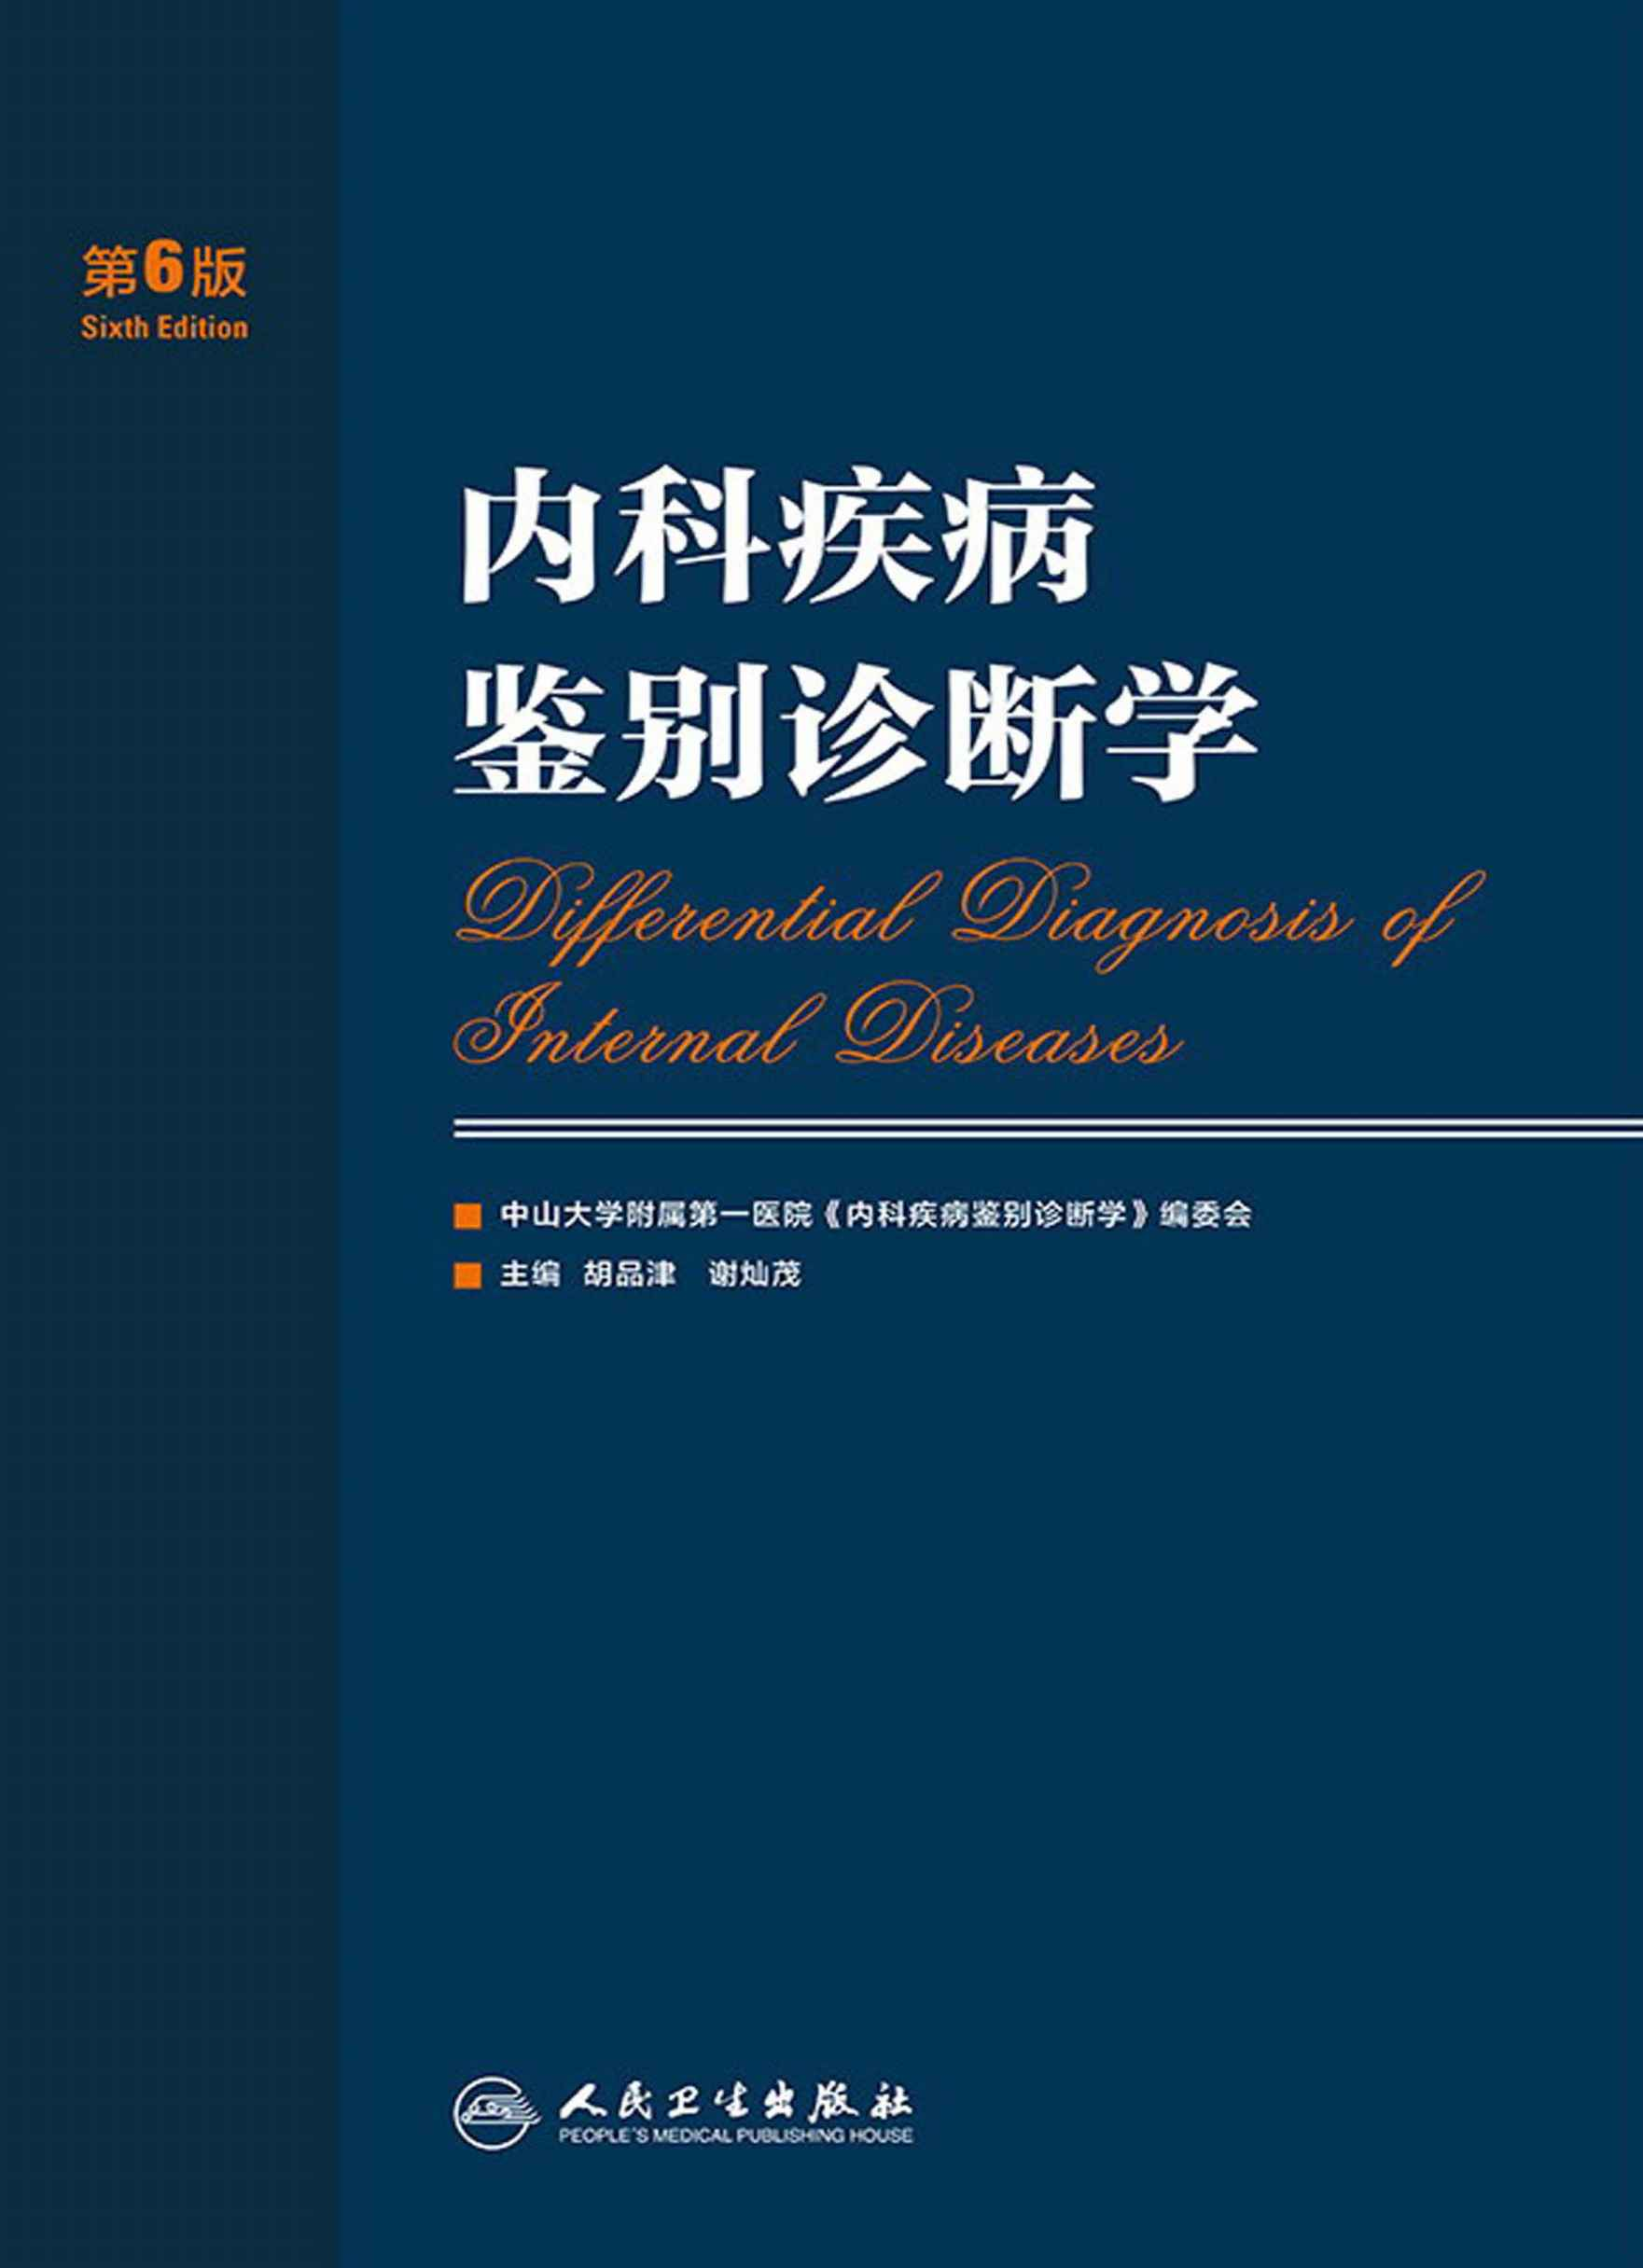
\includegraphics{./images/Image00000.jpg}}

注:以上如有1个问题的回答为“是”,则进行第二步筛查;如每个问题的回答都为“否”,病人在以后每周进行1次初步筛查。
\end{table}



\begin{table}[htbp]
{\centering
\caption{第二步正式筛查}
\label{tab1-2}

\includegraphics{./images/Image00001.jpg}}

{注:NRS 2002的制定依据现有的随机临床试验}

{*表明确诊的病人可直接归为此类。用黑体字标注的病例按照下面介绍的疾病严重程度标准进行归类:}

{营养不良危险因素是指机体目前的营养状况以及因此可能导致的机体损害,因为在病理状况下机体代谢压力加大,对营养素的需要量也有所增加。}

{营养干预对于下列病人是必需的:}

{1)严重的营养不良(3分);}

{2)严重疾病(3分);}

{3)中度营养不良+轻度疾病(2分+1分);}

{4)轻度营养不良+中度疾病(1分+2分)。}

{1分:病人患有慢性疾病并因并发症而住院,身体虚弱但可以定时下床活动。病人对蛋白质的需要量增加,但对于大多数病例通过正常膳食或口服营养素补充剂就可以满足需要。}

{2分:病人卧床休息,如胃部外科大手术。病人对蛋白质的需要量大大增加,一些病人必须通过人工喂养才能满足需要。}

{3分:重症监护病人,如使用呼吸机的病人。病人对蛋白质的需要量增加,并且通过人工喂养也不能满足需要。蛋白质分解和氮丢失显著减少。}
\end{table}



\hypertarget{text00002.htmlux5cux23mllj4}{%
\section{营养评价内容及方法}\label{text00002.htmlux5cux23mllj4}}

\hypertarget{text00002.htmlux5cux23mllj5}{%
\subsection{疾病及饮食史}\label{text00002.htmlux5cux23mllj5}}

疾病史包括急、慢性疾病回顾以及既往营养丢失情况。饮食史多采用24小时膳食回顾或3天连续食物称重法,应该同时考虑食物的数量和质量,将能量、蛋白质和微量营养素与推荐摄入量(DRIs)进行比较。Beck使用体重和食欲下降对入院病人进行初筛,然后通过主观全面评价法对营养不良疑似病人进一步评价,发现其中营养不良比例高达63%。膳食评价可以在病人入院早期发现营养问题,给予营养支持,改善病人预后。

\hypertarget{text00002.htmlux5cux23mllj6}{%
\subsection{体格测量}\label{text00002.htmlux5cux23mllj6}}

{1.体重}
 体重是临床上最常用的体格检查指标,但目前还没有完全做到记录每个住院病人的体重。短期体重变化是反映体液平衡的最佳指标。较长期的体重改变能够反映总体营养状况改变,根据病前3~6个月的体重变化或实际体重占理想体重的百分比,来判断是否需要进一步检查评估。3个月内非自愿的体重减轻是评价机体营养状况的有用指标,体重减轻<5%为轻度,体重减轻>10%为重度。如果病人体重持续减轻,临床医师应该对此警惕并找出原因。在儿科病人中,联合应用体重和身高,可以转换成多种指标对营养状况进行监测,如身高别体重(W/H)可以判断是否存在急性营养不良及其程度,年龄别身高(H/A)用来判断是否存在慢性营养不良及其程度。身高别体重比年龄别体重更能反映近期或进行性体重丢失,与预后相关,而年龄别体重(W/A)低下并不会导致患儿死亡率的明显升高。

体质指数(BMI)是目前临床上常用的另一项体重/身高关系指数,等于体重与身高平方的比值,多用于成人或肥胖儿童营养评价。亚洲人的BMI
18.5~24为正常,>24为超重,<18.5为营养不良,<14为严重营养不良,这种病人存活的可能性很小。个体BMI不仅要与以上标准进行比较,而且还要与本人近期的数值进行比较,这样意义会更大。Tienboon将BMI应用于身高<145cm的儿童,如BMI在13.0~14.5代表轻度营养不良,11.5~12.9为中度营养不良,<11.5为重度营养不良。

{2.皮褶厚度测量}
 可用来估计体脂含量,因为总体脂肪和某些特定部位的皮褶厚度之间存在一定的比例关系,通常选择测量上臂肱三头肌皮褶厚度(TSF),其次是选择肩胛下角处皮褶厚度。慢性营养不良的病人常见有皮褶厚度的减低。由于重症病人TSF受总体脂肪变化的影响,而且不同人群由于年龄、性别及疾病的不同,皮下脂肪与总体脂肪的比值可以在0.2~0.7之间变动,测量精确性差,往往高估消瘦病人的体脂含量,而低估肥胖者的体脂含量。不同部位皮褶厚度测量值之和可以更为准确反映病人体脂含量。

{3.中臂围(MAC)}
 是用卷尺测量肩峰和尺骨鹰嘴中点的手臂围,这个指标易测量且误差也较小。中臂围与某些疾病的死亡率、发病率等指标有很好的相关性,它主要是测量身体的总成分,包括肌肉、骨骼、体液和脂肪组织等,当蛋白质及脂肪储备下降时MAC迅速减少。根据TSF和MAC可以计算中臂肌围、臂脂肪面积、臂肌面积,用于反映脂肪和瘦体组织含量。

{4.头围(HC)}
 HC是3岁以内儿童生长发育和营养状况评价的常用指标,可以间接反映大脑发育情况,如婴儿期头围增长缓慢,将来出现发育问题的风险明显增高。中臂围与头围比值(MAC/HC)受体液变化的影响较小,是新生儿、婴儿营养评价及监测中筛选营养不良的敏感指标。

\hypertarget{text00002.htmlux5cux23mllj7}{%
\subsection{生化指标}\label{text00002.htmlux5cux23mllj7}}

(一)蛋白质营养状况

{1.白蛋白}
 白蛋白的代谢半衰期是18天,所以其代谢变化对浓度的影响需要一段时间才能显现出来。白蛋白从血液中正常流失的速度是其合成速度的10倍。营养不良的病人,机体内脏蛋白储备丧失,血浆蛋白尤其是快速转化蛋白多有降低。血浆白蛋白是评价营养状况的常用指标,白蛋白浓度明显降低常常导致感染发生率和死亡率增高。

{2.前白蛋白和转铁蛋白}
 前白蛋白和转铁蛋白半衰期短,前者为2天,后者为7天,它们对营养状况变化敏感,是判别蛋白质营养不良的良好指标。实验证明,血清前白蛋白浓度在肠外营养应用1周后明显升高(P<0.001),而应用白蛋白则无改变。Staffan对28位极低体重出生儿进行11种血浆蛋白质测定,发现前白蛋白、转铁蛋白、视黄醇结合蛋白最适合该人群蛋白质营养状况评价。

{3.纤维连接蛋白}
 纤维连接蛋白在饥饿状态下迅速降低,给予营养补充后很快恢复正常,因此也可以作为营养评价的指标。

{4.血红蛋白}
 营养性贫血是最常见的营养问题,美国第三次营养与健康调查发现1~3岁儿童缺铁性贫血发生率为15%。上海新华医院对上海3家儿科医院进行调查,贫血发生率为29.3%。血红蛋白和血细胞比容测定可以诊断营养性缺铁性贫血,转铁蛋白浓度与总体铁储备密切相关,是正常人体铁状况的敏感指标。为病人进行血常规检查,对营养状况评价很有意义。

{5.肌酐}
 肌酐主要由肌氨酸代谢分解产生,因此尿肌酐清除率可作为估计瘦体组织的可靠指标。肌酐身高指数(CHI)常用来估计肌肉蛋白质储备,CHI在60%~80%为中度蛋白质缺乏,<60%为重度蛋白质缺乏。

{6.其他}
 3-甲基组氨酸测定结果也可以反映肌肉蛋白储备和运转情况,但它和肌酐清除率都存在一定问题,如难以准确收集24小时尿量,受饮食和肾功能影响很大,尚不推荐常规应用。肝脏中酶的活性以及电解质水平(钙、磷、镁等)都应常规检测。锌、硒和铁的检测对于胃肠道病人尤其重要。

(二)免疫功能测定

慢性阻塞性肺病(COPD)病人的营养状况与其细胞免疫功能密切相关,一般把免疫功能的评价作为营养状况评价的重要组成部分。

{1.外周血总淋巴细胞计数}
 外周血总淋巴细胞计数(TLC)指外周血中总淋巴细胞的数量,可反映细胞免疫功能。TLC=白细胞×淋巴细胞百分比,正常值≥1.5×10\textsuperscript{9}
/L,营养不良时TLC下降。

{2.迟发型超敏皮肤试验}
 于前臂屈侧皮内注射不同的抗原制剂0.1ml,待48小时测量接种处硬结直径。常用的抗原包括链激酶、腮腺炎病毒、白色念珠菌提取液、植物血凝素、结核菌素纯蛋白衍生物等。营养不良时细胞免疫功能受损,迟发型超敏皮肤试验为无反应或反应减弱,即接种处不出现硬结或硬结直径很小。

{3.外周血T细胞亚群}
 机体T细胞的免疫应答反应对抵抗力或免疫功能非常重要,其中目前临床上常用的指标主要是$\text{CD}^+_3$
、$\text{CD}^+_4$
、$\text{CD}^+_8$
、$\text{CD}^+_4$
/$\text{CD}^+_8$ 等,营养不良时下降。

\hypertarget{text00002.htmlux5cux23mllj8}{%
\subsection{机体组成测定}\label{text00002.htmlux5cux23mllj8}}

构成机体的基本化学成分是蛋白质、脂质、碳水化合物、无机盐和水等。由于中性脂肪并不结合水和电解质,假设人体去脂体质(fat-free
mass, FFM)或瘦体群(lean body mass,
LBM)的组成是恒定的,那么通过分析其中一种组成(如水、钾或钠)的量可估计FFM的多少,然后用体重减去FFM的重量即为体脂(body
fat,
BF)。因此,机体的组成按照二元件模型可分为BF和FFM两部分。FFM可再分为体细胞群(body
cell mass, BCM)和细胞外群(extracellular mass,
ECM)。BF是机体储备能量的主要组织,约占体重的25%,其主要成分是脂肪。脂肪中仅有1.0kg脂肪为生命活动所必需,其余可在需要时被动员用于能量消耗。BCM是能够利用氧进行代谢活动的组织,约占人体总重量的40%。ECM主要是细胞外支持组织,用于支持细胞的功能和活动,约占人体重量的35%。在人体组成分析中,显然FFM较BF在生命活动和机体代谢方面更具有重要作用。测定人体组成及其变化比单纯体重指数更能客观反映病人实际的营养状况。

早在1940年,水中称重法应用于人体机体组成测定,来推算体脂和去脂体质的重量。空气置换体积描记术是一项新的密度测定方法,尤其适合那些无法耐受水中密度测定的儿童等特殊病人,David等在9~14岁儿童中应用发现该法比水中称重等方法能更精确测定体脂含量。因为水与钾仅存在于瘦体组织,且含量相对恒定,脂肪不含水和钾。因此通过放射性核素稀释法总体水测定和总体钾测定都可以计算总体脂肪和廋体组织含量。双能X线吸收法是测定人体骨骼无机盐、体脂、去脂组织等机体组成的常用方法,与总体钾测定相关性较好。但多用于研究机构,较少应用于临床评价。迟发性中子激活分析法能够测定氮、钠、氯、钾、钙、磷等多种原子的绝对水平,如测定总体氮可用于机体蛋白质组成分析。CT及磁共振能获得体脂分布的精确图像。

许多机体组成测定方法由于存在一些缺点,如费用昂贵、放射暴露、需要专门的测量仪器和场所,或是需要检查对象合作,而难以在临床上推广引用。生物电阻抗法(BIA)是近年来广泛用于机体组成测定的新方法,具有可床边进行,操作简便、快捷、安全、无创等优点。它的原理是利用不同生物组织对电流导电的差异性,低频电流主要通过细胞外液传导,高频电流可以穿透细胞膜,同时通过细胞内液和细胞外液,推测组织各部分的含量。基于此特性可推测总体水、瘦体组织、细胞外液和细胞团块等多种机体组成成分。Phillips使用BIA和放射性核素稀释法两种方法对青春期女性进行测定,认为BIA法能精确反映她们月经前和月经后去脂组织和体脂含量变化。

\hypertarget{text00002.htmlux5cux23mllj9}{%
\subsection{营养平衡研究}\label{text00002.htmlux5cux23mllj9}}

营养平衡研究一直用于营养评估,通过计算出入量,可进行氮、无机盐、维生素、微量元素等多种物质的平衡研究。氮平衡测定是一项重要的营养平衡研究方法,可直接判断蛋白质摄入情况,常用于营养治疗过程中观察病人的营养摄入是否足够以及了解分解代谢的演变。氮平衡首先测量人体通过尿液、粪便、皮肤以及其他途径(汗液、分泌液等)流失的氮,将摄入氮减去以上各种途径排出的氮就可以计算出氮平衡。为了确定蛋白质的需要量,氮平衡测定需在蛋白质从缺乏到过剩几种不同的摄入水平下进行。每个摄入水平的测定都需要持续几天,使机体保持代谢稳定。由于技术上的原因,目前按照以上要求进行的代谢试验较少,仍缺乏可用于临床病人的标准化方法。正氮平衡常常意味着预后改善,病人营养支持的目的是达到正氮平衡。但氮平衡不能反映机体的蛋白质储备或营养状态,需结合机体组成等测定综合评价。

\hypertarget{text00002.htmlux5cux23mllj10}{%
\subsection{复合型营养评定方法}\label{text00002.htmlux5cux23mllj10}}

{1.主观全面营养评估法(SGA)}
 SGA是Detsky在1987年首先提出,是根据病史和体格检查的一种主观评估方法,特点是以详细的病史与临床检查为基础,省略人体测量和生化检查。其理论基础是:身体组成改变与进食改变、消化吸收功能的改变、肌肉的消耗、身体功能及活动能力的改变等相关联。在重度营养不良时,SGA与身体组成评定方法有较好的相关性。此方法简便易行,适于在基层医院推广(表1-3)。

\begin{table}[htbp]
\centering
\caption{营养状态的SGA(subjective global assessment)评估内容和指标}
\label{tab1-3}
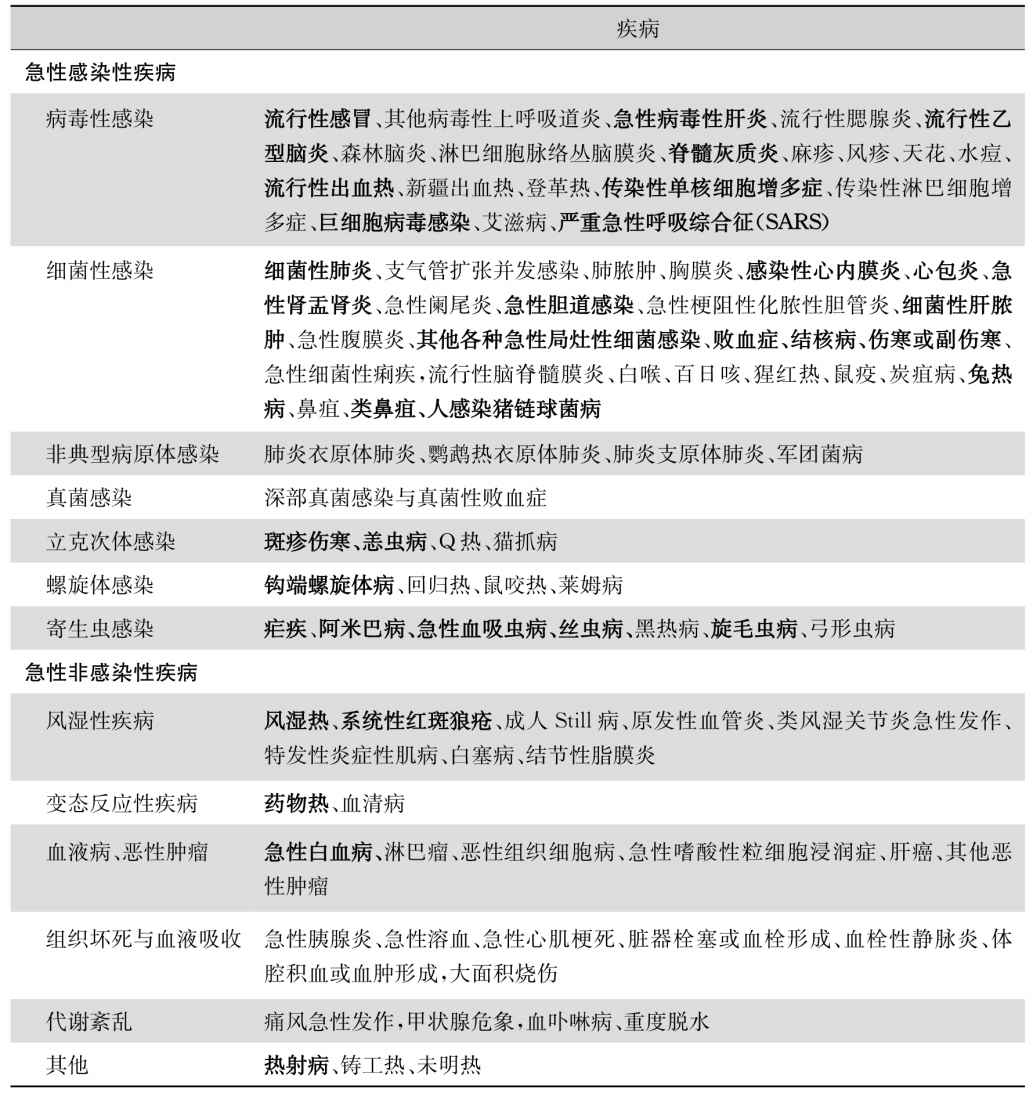
\includegraphics{./images/Image00005.jpg}
\end{table}

{2.预后营养指数(PNI)}
 PNI是由Mullen等对4种营养状态评价参数与外科手术病人预后的相关性进行了分析统计之后提出来的一种综合性营养评价方法。

PNI(%)=158-16.6(ALB)-0.78(TSF)-0.20(TFN)-5.80(DHST)

式中ALB为血清白蛋白(单位:g%);TSF为三头肌皮褶厚度(单位:mm);TFN为血清转铁蛋白(单位:mg%);DHST为迟发性超敏皮肤反应试验(硬结直径>5mm者,DHST=2;硬结直径<5mm者,DHST=1;无硬结反应者,DHST=0)。

评定标准:若PNI<30%,表示发生术后并发症及死亡的可能性均很小;若30%≤PNI<40%,表示存在轻度手术危险性;若40%≤PNI<50%,表示存在中度手术危险性;若PNI≥50%,表示发生术后并发症及死亡的可能性均较大。

Mullen等对161例非急诊手术病人的PNI测定调查显示,手术危险增加与术后并发症发生率及死亡率升高相关,其灵敏度为86%,特异性为69%。

{3.微型营养评定(MNA)}
 是一种简单、快速,适用于评价病人(特别是老年人)营养状况的方法,由Guigoz、Vallas和Garry于1994年提出。MNA评价内容包括: ①人体测量;②整体评定;③膳食问卷;④主观评定等。各项评分相加即得MNA总分。具体评价问卷内容如下所列(见[附])。

\begin{center}\rule{0.5\linewidth}{\linethickness}\end{center}

[附]

营养评价问卷

(一)姓名 性别 出生 年 月 日

(二)家庭住址

(三)原有疾病

(四)体重(kg) 身高(m) 血压(mm Hg)

1.筛选(按不同程度给予量化评分)

(1)既往3个月内是否有食欲下降、消化问题、咀嚼或吞咽困难而摄食减少?

0=食欲完全丧失□ 1=食欲中等度下降□ 2=食欲正常□

(2)既往3个月内体重下降

0=>3kg□ 1=不知道□ 2=1~3kg□ 3=无体重下降□

(3)活动能力

0=需卧床或长期坐着□ 1=能不依赖床或椅子,但不能外出□ 2=能独立外出□

(4)既往3个月内有无重大心理变化或急性疾病?

0=有□ 1=无□

(5)神经心理问题

0=严重智力减退或抑郁□ 1=轻度智力减退□ 2=无问题□

(6)BMI(kg/m\textsubscript{2} )

0=<19□ 1=19~<21□ 2=21~<23□ 3=≥23□

筛选总分(14):≥12正常,无需以下评价;≤11可能营养不良,继续以下评价

2.评价

(1)独立生活(无护理或不住院)?

0=否□ 1=是□

(2)每天应用处方药3种?

0=是□ 1=否□

(3)压疮(褥疮)或皮肤溃疡?

0=是□ 1=否□

(4)每天几次吃完全部饭菜?

0=1餐□ 1=2餐□ 2=3餐□

(5)蛋白质摄入情况:

*每天至少一份奶制品? A是□ B否□

*每周2份以上菜果或蛋? A是□ B否□

*每天肉、鱼或家禽? A是□ B否□

0.0=0或1个“是”□

0.5=2个“是”□

1.0=3个“是”□

(6)每天2份以上水果或蔬菜?

0=否□ 1=是□

(7)每天饮水量(水、果汁、咖啡、茶、奶等):

0.0=<3杯□ 0.5=3~5杯□ 1.0=>5杯□

(8)喂养方式:

0=无法独立进食□ 1=独立进食稍有困难□ 2=完全独立进食□

(9)自我评定营养状况:

0=营养不良□ 1=不能确定□ 2=营养良好□

(10)与同龄人相比,你如何评价自己的健康状况?

0.0=不太好□ 0.5=不知道□ 1.0=好□ 2.0=很好□

(11)中臂肌围(cm):

0.0=<21□ 0.5=21~22□ 1.0=≥22□

(12)腓肠肌围(cm):

0=<31□ 1=≥31□

评价总分(16):

筛选总分:

总分(30):

MNA分级标准:上述各项评分相加,若MNA≥24,表示营养状况良好;若17≤MNA≤23.5,表示存在发生营养不良的危险;若MNA<17,表示有确定的营养不良。

\begin{center}\rule{0.5\linewidth}{\linethickness}\end{center}

{4.住院病人预后指数(HPI)}

HPI=0.92(ALB)-1.00(DH)-1.44(SEP)+0.98(DX)-1.09

式中:ALB为血清白蛋白(单位:g/L);DH为延迟超敏皮肤试验(有1种或多种阳性反应,DH=1;所有均呈阳性,DH=2);SEP:败血症(有败血症,SEP=1;无败血症,SEP=2);DX表示诊断患有癌症(有癌,DX=1;无癌,DX=2)。

评价标准:若HPI为+1,表示有75%的生存概率;若HPI为0,表示有50%的生存概率;若HPI为-2,表示仅有10%的生存概率。

{5.营养风险指数(NRI)}
 美国退伍军人协会肠外营养协作研究组(VATPNCSG)于1991年在《新英格兰医学杂志》上首先提出NRI评价方法。NRI=10.7(ALB)+0.0039(TLC)+0.11(Zn)-0.044(Age)。

式中:ALB为血清白蛋白;TLC为淋巴细胞计数;Zn为血清锌水平;Age为年龄。

评定标准:若NRI>60,表示危险性低;若NRI≤55,表示存在高危险性。

Clugston等于2006年对梗阻性黄疸病人的研究表明,NRI风险升高与住院时间延长和死亡率增加相关。

完整的营养评价包括:疾病及饮食史、体格测量、生化指标、机体组成、营养平衡研究等。在营养评价过程中,体格测量与生化指标是营养评价的最常用方法,具有简单、方便、重复性好、能提供定量资料、不需要特殊仪器等特点。很多测量值与机体组成营养状况分析在统计学上具有显著相关性。然而,简单的体格测量和实验室检查常不能体现营养状况的急性改变,不能反映轻度和中度营养不良,也就不足以作为营养评价的唯一方法。同时,由于置信限较宽,敏感性和特异性差,更适用于流行病学人群调查,评价特定人群的营养状态。近年来,为了提高营养评价方法的敏感性和特异性,人们结合预后和大量的营养学指标,通过多因素回归分析,选择其中有意义的参数,组成最佳的预测模式,建立了多种营养评价方法,为营养状况评价提供了定性、定量的可信指标。

{参考文献}

[1]陶晔璇,徐远飞,汤庆娅,等.儿科病人入院时营养状况评价.中国临床营养杂志,2007,15(4):214~217

[2]蔡威.临床营养基础.第3版.上海:复旦大学出版社,2004,61~18

[3]Tienboon P. Nutrition problems of hospitalised children in a
developing country: Thailand. Asia Pacific J Clin Nutr, 2002, 11 (4):
258~262

[4]Renaudin P. Evaluation of the nutritional status of children less
than 5 years of age in Moundou, Chad: correlations with morbidity and
hospital mortality. Article in French. Med Trop(Mars), 1997, 57 (1):
49~54

[5]Hendricks KM, Duggan C, Gallagher L, et al. Malnutrition in
hospitalized pediatric patients. current prevalence. Arch Pediatr
Adolesc Med, 1995, 149: 1118~1122

[6]Ogden CL, Flegal KM, Carroll MD, et al. Prevalence and trends in
overweight among US children and adolescents, 1999~2000. JAMA, 2002,
288 (14): 1728~1732

[7]Ah SM, Selwyn BJ, Luby S, et al. Prevalence and correlates of
stunting among children in rural Pakistan. Pediatr Int, 2003, 45 (1):
49~53

[8]Jacobs DO, Wong M. Metabolic assessment. World J Surg, 2000, 24
(12): 1460~1467

[9]Phillips SM, Bandini LG, Compton DV, et al. A longitudinal
comparison of body composition by total body water and bioelectrical
impedance in adolescent girls. J Nutr, 2003, 133 (5): 1419~1425

[10]Kuczmarski RJ, Ogden CL, Guo SS, et al. 2000 CDC growth charts for
the United States: methods and development. Vital Health Stat 11, 2002,
(246): 1~190

[11]Ronald E. Pediatric nutrition handbook. 6th ed. American: American
Academy of Pediatrics, 2009, 559~576

\protect\hypertarget{text00003.html}{}{}


\chapter{颅脑}

\section{检查方法}

\subsection{常规检查}

横断面(或轴位)扫描:病人仰卧,有3个主要扫描平面。其扫描基线为:①听眦线(orbitomeatal
line,OML):亦称为眶耳线,简称OM线,即外眦至外耳孔中点的连线。②听眉线(superior
orbitomeatal
line,SML):亦称为上眶耳线,简称SM线,即眉毛上缘中点与外耳孔中点的连线。③瑞氏基底线(reid's
base
line,RBL):亦称人类学基线,简称RB线,即眶下缘与外耳孔中点的连线。检查幕上病变常用OM线;幕下病变常用SM线;眶内病变常用RB线。

冠状面扫描:病人仰卧或俯卧位,头部过伸,使冠状面与OM线垂直扫描。

\subsection{增强扫描}

一般认为,对急性颅脑外伤、急性卒中可只做平扫;对于脑瘤术后复查或只有增强检查才能显示病变的复查病例可只行造影增强;对于脑肿瘤、脑血管疾病、感染性疾病均需做增强扫描,外伤患者平扫正常时亦可行增强扫描。一般造影剂用量为60~100ml或儿童以2ml/kg用量,团注或快速滴注。

其显影机制分为两类:①血管内显影:如动脉瘤、动静脉畸形,其显影时间短,应注药后扫描或边注边扫。②血管外显影:强化机制在于血脑屏障的破坏(如胶质瘤)或血供丰富(如脑膜瘤、听神经瘤、脓肿壁)。由于垂体血供丰富,垂体增强扫描有利于缺乏血供的垂体瘤尤其微腺瘤的检出。

\subsection{脑池造影CT扫描}

造影剂可应用阳性非离子型水溶性碘造影剂(伊索显和欧乃派克等)和阴性造影剂(空气),后者主要用于小听神经瘤的诊断。一般阳性造影剂的用量为8~10ml,空气3~5ml,经腰穿注入。水溶性造影剂取头低脚高位或病变侧在低下部位,气体反之。一般注入造影剂15分钟后扫描,观察脑室多于6小时后扫描,延时的目的在于降低碘液浓度。如欲观察脑脊液的动力变化,则于注入造影剂2小时、6小时、12小时和24小时后进行扫描,必要时可于48小时或72小时后扫描。

\subsection{脑CT血管成像}

脑部CT血管成像或称为脑部CT血管造影(CT
angiography,CTA),是指经静脉注入造影剂后利用CT对包括靶血管在内的受检层面进行连续的薄层立体容积扫描,然后进行图像后处理,最终使靶血管立体显示的血管成像技术。

扫描从后床突下30mm开始,向上达后床突上50~60mm。其常用扫描参数如下:螺距1~2,层厚1~2mm,重建间隔1mm,造影剂用量(300mg/ml)80~120ml,注射流率2.5~3.5ml/s,延迟时间15~25秒。双层或多层螺旋CT可增加螺距、减小层厚,以取得更优质的图像。图像后处理可采用MIP、SSD和VR,以MIP最常用。

脑CT静脉成像(CT venography,CTV)扫描方法同上,只是扫描延迟时间为40秒。

CTA(包括CTV)可用于显示脑底动脉环(willis环)和大脑前、中、后动脉主干及其2~3
级分支血管;CTV
可显示大脑内静脉、大脑大静脉、皮质静脉、上矢状窦、直窦、横窦和乙状窦等。CTA(包括CTV)可用于动脉瘤、血管畸形(主要是AVM)、肿瘤血管、静脉病变及头皮血管瘤等的诊断。

\subsection{脑CT灌注成像}

CT灌注成像在中枢神经系统的应用包括:①作为颅外颈动脉或椎动脉闭塞性疾病的功能性检查方法,研究颅内血流量和侧支循环情况。②早期发现梗死或缺血,并显示其范围。③血管炎或继发性蛛网膜下腔出血时估计血管痉挛情况。④AVM估计分流情况。⑤研究肿瘤的血液灌注情况。

\subsubsection{检查技术}

CT灌注成像的质量受造影剂注射的总量、速度、患者的心功能状态以及CT扫描伪迹、部分容积效应等多种因素的影响。扫描时经肘静脉注射加热至37℃的造影剂40~50ml(儿童约为1ml/kg体重)。开始注射造影剂的同时启动快速动态扫描程序,以1层/秒的速度连续扫30~40秒以上,重建30~40幅灌注图像。注射流率多为8~9ml/s,最快达20ml/s,国内有学者采用2.5ml/s也获得较满意的CT灌注图像。通常包括最大强度投影(MIP)图、脑血流量(CBF)图、脑血容量(CBV)图、局部灌注达到峰值的时间(TTP)等图像。这些图像可通过数字化形式存储,均可彩色显示,以突出病变区域的对比度。

\subsubsection{灌注参数}

1.脑血容量(cerebral blood
volume,CBV):是指存在于一定量脑组织血管结构内的血容量,单位为ml/100g。根据时间-密度曲线下方封闭的面积计算得出。

2.脑血流量(cerebral blood
flow,CBF):CBF=CBV/MTT,指在单位时间内流经一定量脑组织血管结构的血流量,单位为ml/(100g·min)。它反映脑组织的血流量,CBF值越小意味着脑组织的血流量越低。正常值一般>50~60ml/(100g·min),<10~20ml/(100g·min)将导致膜泵衰竭和细胞死亡。

3.平均通过时间(mean transit
time,MTT):开始注射造影剂到时间-密度曲线下降至最高强化值一半的时间,主要反映的是造影剂通过毛细血管的时间,单位为秒(s)。

4.峰值时间(time to
peak,TTP):为开始注射造影剂至强化达到峰值的时间,由时间-密度曲线测得,单位为秒(s)。

此外,还有表面通透性(permeability of surface,PS)等参数。

\section{正常解剖和CT表现}

\subsection{颅盖软组织(头皮)}

颅盖软组织在额、顶、枕部分为皮肤、皮下组织、帽状腱膜、帽状腱膜下层和颅骨骨膜5层。前3层紧密连接,CT不能识别。帽状腱膜下层由疏松结缔组织构成,内含少量血管,CT呈低密度带,头皮裂伤出血亦在此层,如有化脓感染可蔓延到整个颅顶,并可经导静脉扩散到颅内。颅盖软组织在颞部则由皮肤、皮下组织、颞浅筋膜、颞深筋膜、颞肌和颅骨骨膜6层构成。

颅骨外膜CT不能识别,在颅缝处连接紧密并深入缝间成为缝间膜,故骨膜下血肿不超过此缝,并可据此与帽状腱膜下血肿相鉴别。

\subsection{脑颅骨和颅缝闭合的时间及顺序}

脑颅骨由枕骨、额骨、蝶骨、筛骨各一块及颞骨、顶骨各两块组成。颅骨分为3层,即外板、板障和内板。成人内外板CT表现为高密度,CT值>250Hu。新生儿板障为低密度,随年龄增长密度增加,50岁后板障层钙化与内外板融合为一层致密层。成人颅缝宽约0.5
mm。新生儿各骨之间为一片等密度的结缔组织膜相连,称为囟。

颅缝闭合约在30岁以后开始。一般矢状缝先闭合,继为冠状缝。而人字缝和枕骨乳突缝闭合最晚,且可终生不闭合。额缝在出生6个月后开始闭合,而在5~6岁时应完全闭合,此缝亦可终生存在。颅底缝多在出生时闭合,只有蝶枕缝到青春期闭合。

此外,应注意识别脑膜中动脉、板障静脉沟、静脉窦、导静脉、蛛网膜颗粒等常见的脉管压迹,以免误诊为骨折。

\subsection{颅底各颅窝的特点和孔道}

颅底骨内面由蝶骨嵴和颞骨岩部嵴分为前、中、后颅窝。

\subsubsection{各颅窝的结构特点}

1.前颅窝:筛骨板菲薄,外伤易造成骨折、损伤嗅神经及形成脑脊液漏。额骨眶板上面凹凸不平,脑外伤时底部的滑动易引起脑挫伤。

2.中颅窝:孔、洞较多,外伤骨折或肿瘤破坏通过这些结构引起相应的症状。如骨折累及蝶窦出现鼻出血、脑脊液鼻漏;岩锥骨折可损伤面神经和听神经;鼓室盖骨折引起脑脊液耳漏;脑膜中动脉损伤引起硬膜外血肿。

3.后颅窝:有大量肌肉覆盖,骨折较少见。但与颈段相连,可有畸形发生。

\subsubsection{。}

\begin{table}[htbp]
\centering
\caption{颅底主要孔道及内容物}
\label{tab2-1}
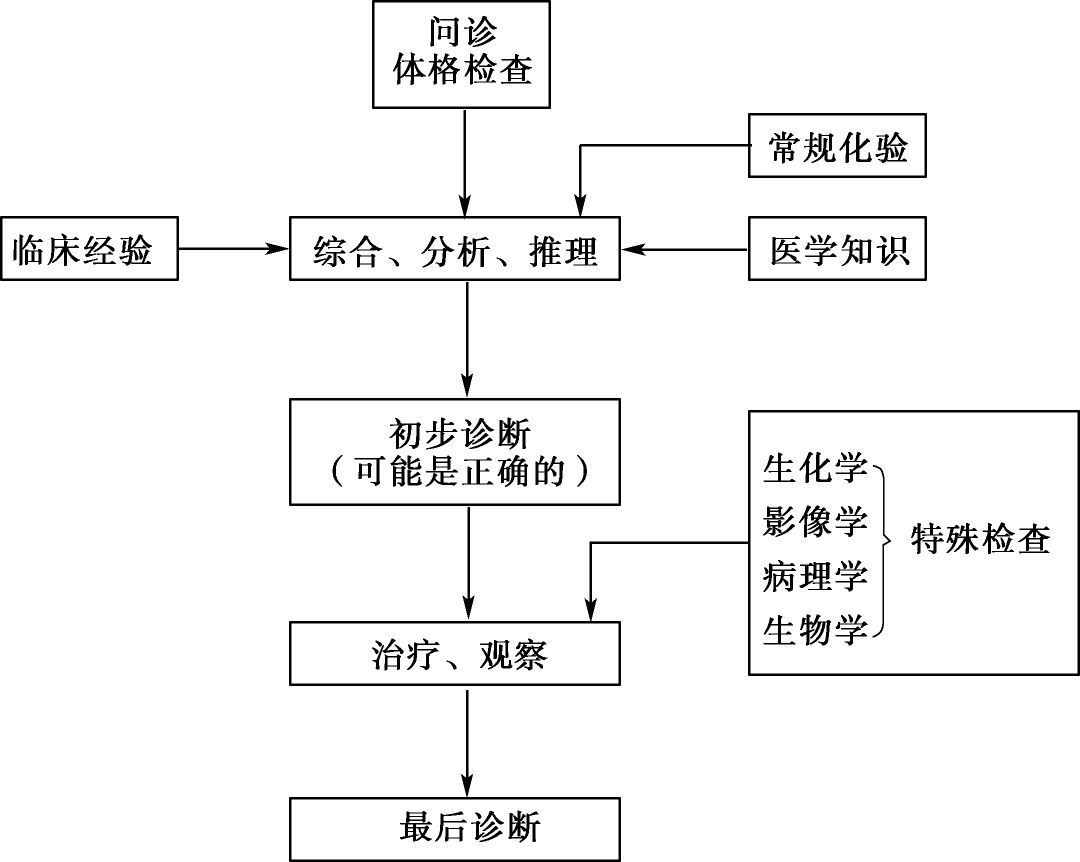
\includegraphics[width=\textwidth,height=\textheight,keepaspectratio]{./images/Image00004.jpg}
\end{table}

\subsection{脑膜}

脑的表面有3层被膜:①软脑膜:紧贴脑的表面,富血管、随脑回起伏。②蛛网膜:位于中层,由薄而透明、疏松成网的纤维构成,无血管结构(故增强扫描无强化),与硬脑膜走行一致。③硬脑膜:位于外层,由致密结缔组织构成,厚而坚韧,与颅骨内面的骨膜完全融合,故通常说硬脑膜为两层结构组成。正常CT不能直接显示3层结构。由于硬脑膜有丰富的血供且无血脑屏障,可以发生明显强化。

硬脑膜内层向颅腔内反折形成双层皱襞有支持、保护作用。主要形成物为:①大脑镰:前端附着于鸡冠,后缘呈水平形与小脑幕相续。大脑镰上、下缘两层分开分别形成上、下矢状窦。轴位像CT呈略高密度线状影,40岁后可钙化。②小脑幕:呈帐篷状分隔大脑枕叶和小脑。后方附着于枕骨横沟,两侧附着于岩椎,上缘正中与大脑镰相续,两侧前内缘形成小脑幕切迹,围绕中脑。轴位呈两侧对称的略高密度影,冠状位呈人字形线状略高密度影。③小脑镰:附着于枕内嵴上的一窄条状突起,分隔小脑半球。④其他:三叉神经半月节(Meckel腔)、海绵窦、直窦、横窦、乙状窦等。

\subsection{蛛网膜下腔和脑池}

脑蛛网膜在脑沟裂处不随之凹入,与软脑膜之间形成宽窄不一的蛛网膜下腔(或称蛛网膜下隙),内含脑脊液。某些局部宽大处称为脑池。主要的有:①大脑纵裂池;②胼胝体池;③小脑延髓池(又称枕大池
);④小脑溪(又称小脑谷);⑤延池;⑥桥池;⑦桥脑小脑角池;⑧脚间池;⑨视交叉池;⑩终板池;⑪外侧裂池;⑫环池;⑬四叠体池;⑭大脑大静脉池;⑮小脑上池(是四叠体池向后的延续);⑯帆间池(又称中间帆腔或第三脑室上池)。

鞍上池为CT和MR等轴位图像所特有。由于扫描体位的影响可呈:①六角星:前角为纵裂前部的后端(紧贴前角后端的横行部分主要是交叉池);两前外侧角为两外侧裂池;两后外侧角为围绕中脑的环池;后角为大脑脚间的脚间池(图\ref{fig2-1})。②五角星:与六角星不同的是,两后外侧角为围绕桥脑上部的桥小脑角池,后角不显示。鞍上池前方是额叶底部直回,两侧壁是颞叶海马钩回,后方为大脑脚或桥脑上部。

\begin{figure}[!htbp]
 \centering
 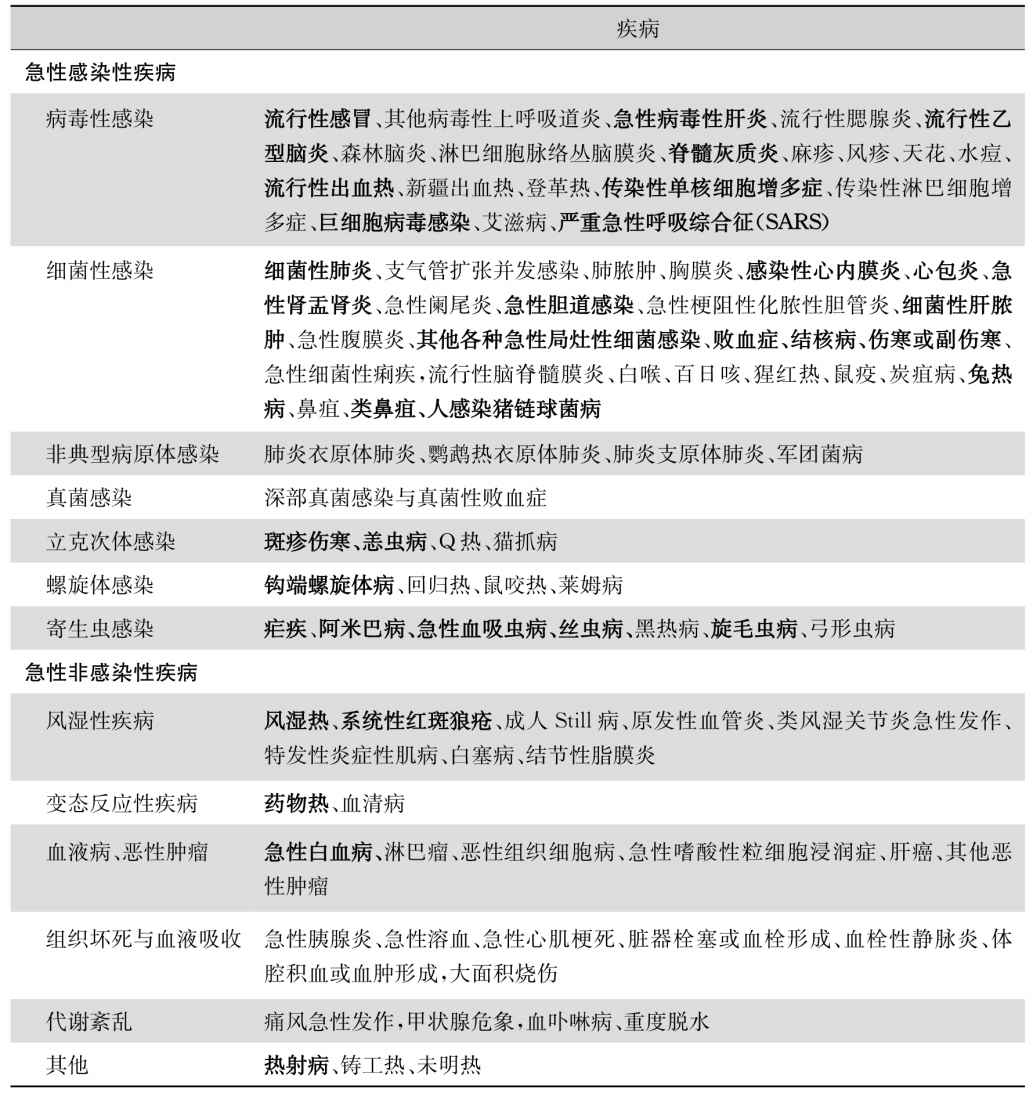
\includegraphics[width=.7\textwidth,height=\textheight,keepaspectratio]{./images/Image00005.jpg}
 \captionsetup{justification=centering}
 \caption{鞍上池 \\{\small 呈六角形水样密度区}}
 \label{fig2-1}
  \end{figure} 



鞍上池内前部可见两条视束,横径约12mm,前后径约8mm,外侧可见两条颈内动脉,中央可见垂体柄,正常垂体柄粗<4mm。

帆间池与第三脑室顶部的区别:帆间池位于第三脑室顶的上方、穹隆体和穹隆连合的下方,呈尖向前的三角区,两前外侧界为穹隆的内侧缘,后界为胼胝体压部。与第三脑室的区别为:①帆间池的层面较第三脑室顶高;②帆间池后界为胼胝体压部,而第三脑室顶部的后界为松果体;③帆间池前部的尖不与侧脑室相连,而第三脑室前端可达侧脑室前角。

此外,枕大池可发育巨大(但一般不产生临床症状)呈对称性和非对称性。结合其有无张力、颅骨有无压迹等可与蛛网膜囊肿相鉴别(图\ref{fig2-2}),有文献将其列入发育异常。因终板较薄不显影,常看到终板池与第三脑室下部相通的假象。小脑溪位于两侧小脑扁桃体之间,呈一细长的间隙,后通小脑延髓池,前通第四脑室。

\begin{figure}[!htbp]
 \centering
 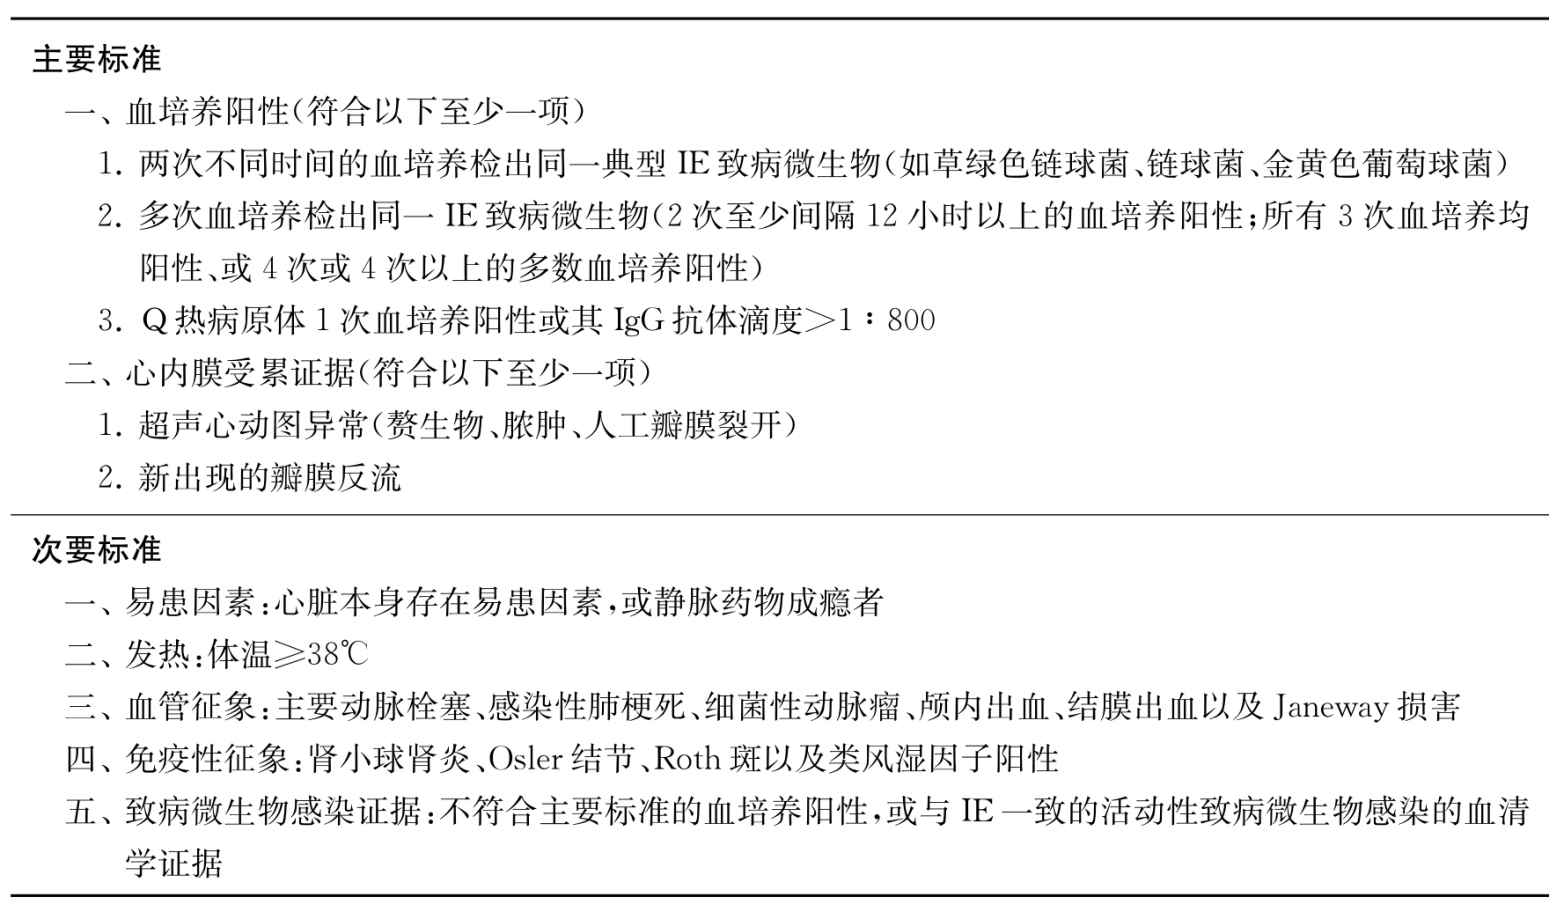
\includegraphics[width=.7\textwidth,height=\textheight,keepaspectratio]{./images/Image00006.jpg}
 \captionsetup{justification=centering}
 \caption{巨大枕大池 \\{\small 显示枕骨内板下至岩锥后缘有新月形水样密度区}}
 \label{fig2-2}
  \end{figure} 


\subsection{大脑半球的分叶及边缘系统}

分叶:大脑由中线的半球间裂分为左右两半,中间由胼胝体相连。大脑半球由脑沟裂分为下列5叶。①额叶:位于前上部。内侧以纵裂和大脑镰与对侧分开,后方由中央沟与顶叶分开,外下方经外侧裂与颞叶分开,前下方为额骨和眶顶。②颞叶:经外侧裂垂直部和水平部与额叶分开。顶枕裂(沟)与枕前切迹(枕极前4~5mm)的连线为颞、枕叶的分界。③顶叶:经中央沟与前方的额叶分开,下方以外侧裂与颞叶分开,后方以顶枕沟与枕叶分开。④枕叶:经顶枕沟与顶叶分开,与颞叶的分界线为顶枕沟与枕前切迹的连线。⑤岛叶:隐藏于外侧裂深部的近三角形的独立区域,四周有环形沟,由额、顶、颞叶皮质沿外侧裂深部凹入形成岛盖。

边缘系统:大脑半球内侧面的扣带回、海马回、钩回、海马、杏仁核等相连构成一个弯弓形脑回,因位置在大脑和间脑交界处的边缘,所以称为边缘系统或边缘叶。通过控制下丘脑来调节内脏及情绪活动。

此外,颞、顶、枕叶的分界线是假设的,因此很不清楚,这一区域也称为颞顶枕交界区。

\subsection{大脑半球的白质}

\subsubsection{半卵圆中心}

髓质占大脑半球的大部分,较厚的皮质下纤维在横断面图像、侧脑室上层面呈半卵圆形,故称为半卵圆中心,是影像学的一个概念。

\subsubsection{大脑白质纤维分类}

大脑白质的纤维结构复杂,大体分为以下3种:

1.联络纤维:在一侧半球内部各回、各叶间的往返纤维称为联络纤维。短的是联系在相邻脑回之间的弓状纤维;长的是联系在各叶皮质间的纤维,如钩束、扣带束、上纵束、下纵束及枕额上、下束等。

2.连合纤维:指联系左右半球的纤维,主要有胼胝体、前联合和海马联合等。①胼胝体:位于大脑纵裂底部,呈拱桥状。前端弯向腹后方称嘴,由嘴向前上方弯曲部称为膝,由膝向后延伸为体部(构成侧脑室壁的大部分),后端较厚称为压部。②前联合:位于胼胝体嘴的后下方,呈卵圆形,是两半球的嗅球和海马旁回的联合。

3.投射纤维:大脑皮层与其下部的间脑、基底节、脑干和脊髓的连接纤维称为投射纤维。包括内囊、穹隆、外囊和最外囊。①内囊:两侧内囊横断面呈“><”型,中央顶点为膝,前后分别为前肢和后肢。内囊位于丘脑、尾状核和豆状核之间。内囊后肢边缘模糊的低密度区(约位于膝部到豆状核后缘距离的2/3~3/4处)为正常皮质脊髓束,勿误为缺血灶。②外囊:在豆状核外,居豆状核和屏状核之间,两侧在横断面呈“()”型。③最外囊:位屏状核外侧,岛叶内侧,CT难以显示。

\subsection{基底节}

基底节包括尾状核、豆状核、屏状核和杏仁核。其中豆状核有两个白质板将其分为3部分,外部最大称为壳,内侧两部分称为苍白球。但CT不能显示其白质板。尾状核和豆状核合称为纹状体,与维持肌张力及运动频率有关。杏仁核与情绪变化有关。

\subsection{间脑}

间脑(通常将端脑和间脑合称为大脑)连接大脑半球和中脑,包括以下4部分。

1.丘脑:为一大卵圆形核团。内侧构成侧脑室侧壁,借中间块使左右丘脑相连;其外侧为内囊后肢;其前端尖圆为丘脑结节;后端圆钝为丘脑枕;丘脑枕的外下部有两个隆起为内、外侧膝状体。丘脑是各种感觉体传向大脑皮层的中间站。

2.下丘脑:构成侧脑室底和侧壁的一部分,包括视交叉、漏斗、灰结节、乳头体和垂体神经部。它是皮质下植物神经中枢,并通过下丘脑---垂体柄和垂体门脉系统调节垂体功能。

3.底丘脑:为丘脑和中脑的移行区。接受来自苍白球和运动区的纤维,并发出纤维到达红核、黑质及中脑被盖,功能上与苍白球密切相关。

4.上丘脑:位于三脑室后部,包括丘脑髓纹、缰三角和松果体,参与嗅反射通路。松果体为一退化的内分泌结构,分泌抑制青春期激素。松果体呈锥形,长5~8mm,宽4mm,向左偏移1~2mm是正常现象,但向右偏移却有病理意义。CT扫描75%以上成人于三脑室后部可显示松果体与缰联合钙化。缰联合钙化居前,范围不超过1cm;松果体钙化居后,一般不超过5mm。

此外,有文献将内、外侧膝状体称为后丘脑。

\subsection{脑干}

脑干上接间脑,下续颈髓,与小脑之上、中、下脚相连,分为以下3部分。

1.中脑:在间脑和脑桥之间,从前向后为大脑脚、被盖和四叠体(顶盖)组成。大脑脚与被盖之间以黑质为界;被盖与四叠体之间以中脑导水管为界。腹侧两束粗大的纵行纤维为大脑脚,其间形成脚间窝,动眼神经从脚间窝出脑。中脑背部有上丘和下丘两对隆起总称为四叠体。上、下丘分别与外、内侧膝状体借上、下丘臂相连,分别是皮质下视觉和听觉反射中枢。下丘后方连接前髓帆,滑车神经自下丘下方发出。

2.桥脑:桥脑在中脑的下方,从前向后为基底部和被盖部。前面正中浅沟内可见基底动脉。横行基底部的纤维向两侧聚成脑桥臂,经小脑中脚进入小脑。基底部与桥臂之间有三叉神经发出。桥脑腹侧与延髓交界的沟内,由内向外有外展神经、面神经和前庭蜗神经发出。桥脑背面下半部即菱形窝的上半部为第四脑室底(CT轴位第四脑室前为桥脑)。

3.延髓:上接桥脑,下续颈髓。腹侧面中线(前正中裂)两旁有锥体(由皮质脊髓束和皮质脑干束组成)。在延髓的下方由纤维交叉形成锥体交叉。锥体外侧有椭圆形隆起称为橄榄。锥体和橄榄之间有舌下神经穿出。橄榄背侧自上而下依次有舌咽神经、迷走神经和副神经根发出。

\subsection{小脑和小脑核}

小脑位于桥脑和延髓的后方,中间相隔第四脑室。小脑正中的蚓部与两侧小脑半球间无明显分界。小脑半球下面近枕骨大孔部分突出称为小脑扁桃体。小脑前后均向内凹称为小脑前切迹和后切迹。小脑半球借上、中、下脚分别与中脑背侧、桥脑腹侧和延髓的背侧相连接,小脑表面为灰质,内部为白质。

小脑白质内有灰质团块,称为小脑中央核。共有4对,分别为齿状核、顶核、栓状核、球状核。其中齿状核最大,位于小脑半球的中心部,是小脑传出纤维的主要发起核。

\subsection{脑室系统}

1.侧脑室:左右各一,分为以下5部分:①前角:又称额角,位于额叶内,在室间孔以前。顶为胼胝体,内侧壁是透明隔,倾斜的底及外侧壁为尾状核头。②体部:位于顶叶内,由室间孔至三角部。顶为胼胝体体部;内侧壁是透明隔;底由外侧到内侧分别为尾状核体、丘脑背面终纹、丘脑上面的外侧部、脉络丛和穹隆外侧缘。③三角区:即体、后角、下角分界处,内容脉络球。CT上是区分颞、枕、顶叶的标志。④后角:又称枕角,位于枕叶内,形状变异很大,有时缺如。顶和外侧壁由胼胝体放散形成;内侧壁上有两个纵行膨大,上方的称后角球(由胼胝体大钳构成),下方的称禽距。⑤下角:在颞叶内,又称颞角。在丘脑后方弯向下,再向前进入颞叶。顶大部分由胼胝体构成,内侧小部分由尾状核尾和终纹构成,底由内至外为海马伞、海马和侧副隆起。

正常成人两侧前角之间的距离<45mm,前角间最大距离与头颅最大内径之比<35%,在2岁以下其比值应<29%,两侧尾状核内缘之间的距离<25mm,为15mm左右。

2.第三脑室:两侧间脑间的狭窄腔隙。成人男性宽为2.8~5.9mm,女性为2.5~5.3mm。经室间孔与左右侧脑室相通,后经中脑导水管与第四脑室相通。顶有第三脑室脉络丛;底为下丘脑;前壁为前联合和终板;后壁为缰联合、松果体和后联合。

3.第四脑室:腹侧为桥脑和延髓,背侧为小脑,上接中脑导水管,下续脊髓中央管。经侧孔与桥脑小脑角池相通;经下端正中孔与小脑延髓池相通。第四脑室底为菱形窝,顶为前髓帆和后髓帆,呈马蹄形,宽(前后径)约9mm。

4.中脑导水管:位于中脑背侧,是中脑被盖和四叠体的分界,长约7~18mm,直径约1~2mm。正常CT难以显示。

此外,第五、第六脑室即透明隔间腔和穹隆间腔属两种解剖变异。但第五脑室如积液过多,向外膨隆并影响室间孔的引流,可称为透明隔囊肿。

\subsection{静脉和静脉窦}

\subsubsection{脑动脉}

脑的血供来自颈内动脉和椎动脉,前者供应大脑半球的前2/3,后者供应脑干、小脑和大脑半球的后1/3。

1.大脑前动脉:供应额、顶叶近中线内侧面约1.5cm的范围,呈长条形。其水平段分出细小前穿质动脉供应尾状核头、壳核和内囊前部,另有部分供应下丘脑。

2.大脑中动脉:皮质支供应额、顶、颞叶的外表面大部分。中央支供应尾状核和壳核的一部分,以及苍白球、内囊前后肢,称为豆纹动脉。

3.大脑后动脉:供应枕叶和颞叶底面,中央支供应部分间脑。

4.椎基动脉:两侧椎动脉在延髓腹侧汇合为基底动脉。基底动脉走行于桥脑前面,到脚间池分为左右大脑后动脉。基底动脉分出成对的桥脑支、内听道支、小脑前支和小脑上支。小脑后支来自椎动脉。

颅底动脉环即Willis环,由前交通动脉、两侧大脑前动脉、两侧后交通动脉和大脑后动脉相互吻合构成的六角形动脉环,是沟通两侧颈内动脉和椎动脉的侧支循环通路。其变异较大,完整者仅占53.8%。

\subsubsection{脑静脉}

大脑半球静脉分为深、浅两组。①浅静脉:收集大脑皮质和白质浅层的静脉血,包括大脑上静脉、大脑中静脉和大脑下静脉分别汇入上矢状窦、海绵窦、横窦、岩上窦和岩下窦,其间有吻合静脉相沟通。②深静脉:主要收集脑深部的血液。透明隔静脉和纹丘静脉在室间孔后缘汇合成大脑内静脉,两侧的大脑内静脉以及基底静脉在松果体后方汇合成大脑大静脉。大脑大静脉与下矢状窦相连终于直窦。

\subsubsection{静脉窦}

在两层硬脑膜之间引流静脉血液入颈内静脉,包括上矢状窦、下矢状窦、直窦、横窦、海绵窦、岩上窦、岩下窦和乙状窦。其中海绵窦位于蝶鞍两侧高约5~8mm,横径5~7mm,前后径为10~15mm,增强后呈高密度,平扫不易显示。

\subsection{Brodmann功能定位区和大脑皮质的主要功能区}

正常脑皮质的密度高于髓质,易于分辨。脑皮质CT值为32~40Hu,脑髓质CT值为28~32Hu,两者平均相差(7.0±1.3)Hu。含脑脊液的间隙为水样密度,CT值为0~20Hu。

图\ref{fig2-3}A~I为正常颅脑CT轴位像,按Brodmann功能定位法共分47个区。如图\ref{fig2-3}A~I和图\ref{fig2-4}A、B、C、D所示,大脑皮质主要的功能区定位如下:

1.第Ⅰ躯体感觉区:位于中央后回和中央旁小叶的后半,主要是3、1、2区。

2.第Ⅰ躯体运动区:位于中央前回和中央旁小叶的前半,主要是4区。

3.视觉区:位于枕叶内侧面,距状裂(沟)两侧,包括舌回和楔叶的一部分,即17、18、19区。

4.听区:位于颞横回,主要是42区,接受听辐射的投射。其特点是一侧听区接受双侧的听觉冲动传入,但以对侧为主。故一侧听区损伤,可使双侧听力下降,但不会完全耳聋。

5.味觉区:在中央后回下端。

6.语言中枢:在左侧半球的皮质产生了4个分析区,总称为语言中枢。①说话中枢:在额下回后部,即44区。此区损伤产生失语症。②书写中枢:位于额中回后部。此区损伤产生失写症。③阅读中枢:位于顶下小叶的角回,即39区。此区损伤产生失读症。④听话中枢:在颞上回后部。功能是理解别人的语言和监听自己所说的话。此区损伤,对听到的语言不能理解,自己说话错误、混乱而不自知,称为感觉性失语症。

7.其他:5、7区为触摸识别物体的实体感觉皮质区,为顶上小叶。额上回从前向后为9、8、6区。8区和枕叶19区为皮质眼球运动区,受刺激时产生双眼向对侧同向偏盲。8和6区为锥体外系皮质区,与共济运动有关。9、10、11区为额叶联合区,与智力和精神活动密切相关。40区位于顶下小叶缘上回,优势半球为运用中枢,是人类后天经复杂的动作和劳动技能所建立的运动区。损伤后,手的运动功能正常,但不能完成过去掌握的复杂动作和操作技法。


\begin{figure}
  \centering
  \subfloat[经海绵窦层面]{
  \begin{minipage}[b]{0.7\textwidth}
    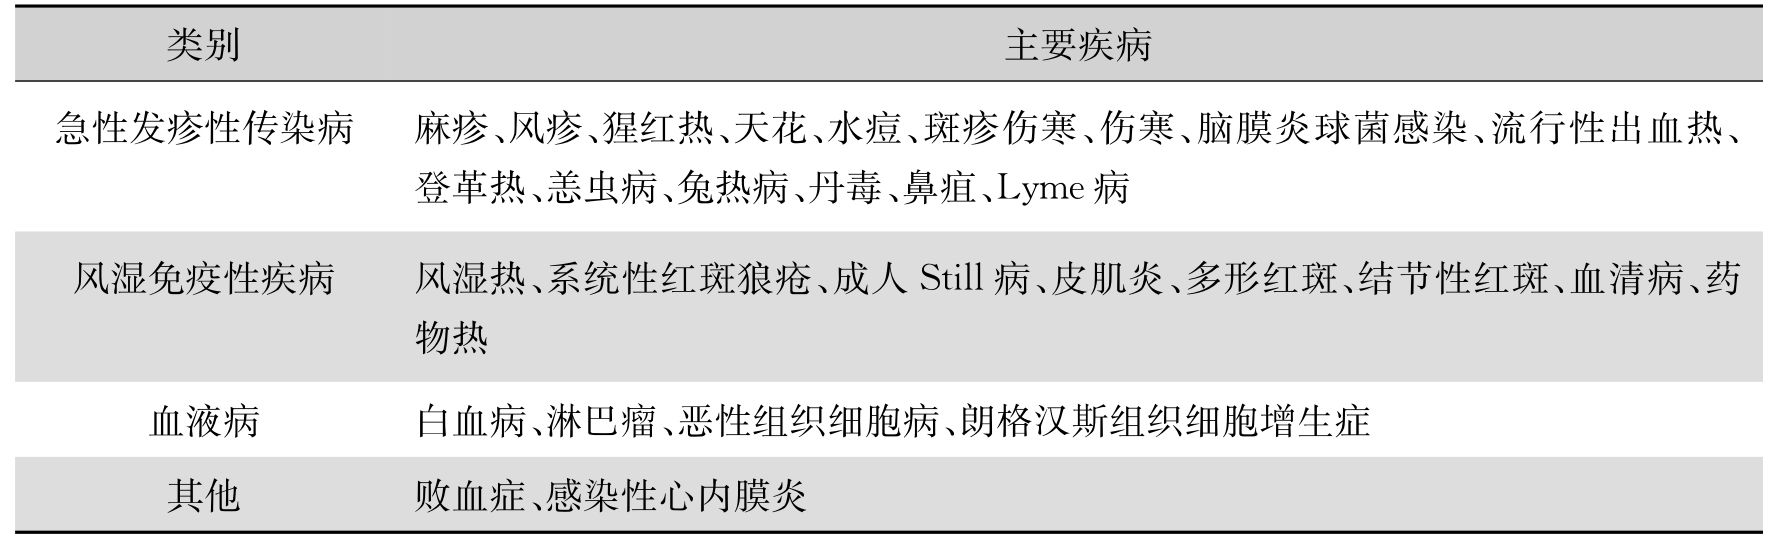
\includegraphics{./images/Image00007.jpg}
  \end{minipage}}\\
  \subfloat[经鞍上池层面]{
  \begin{minipage}[b]{0.7\textwidth}
    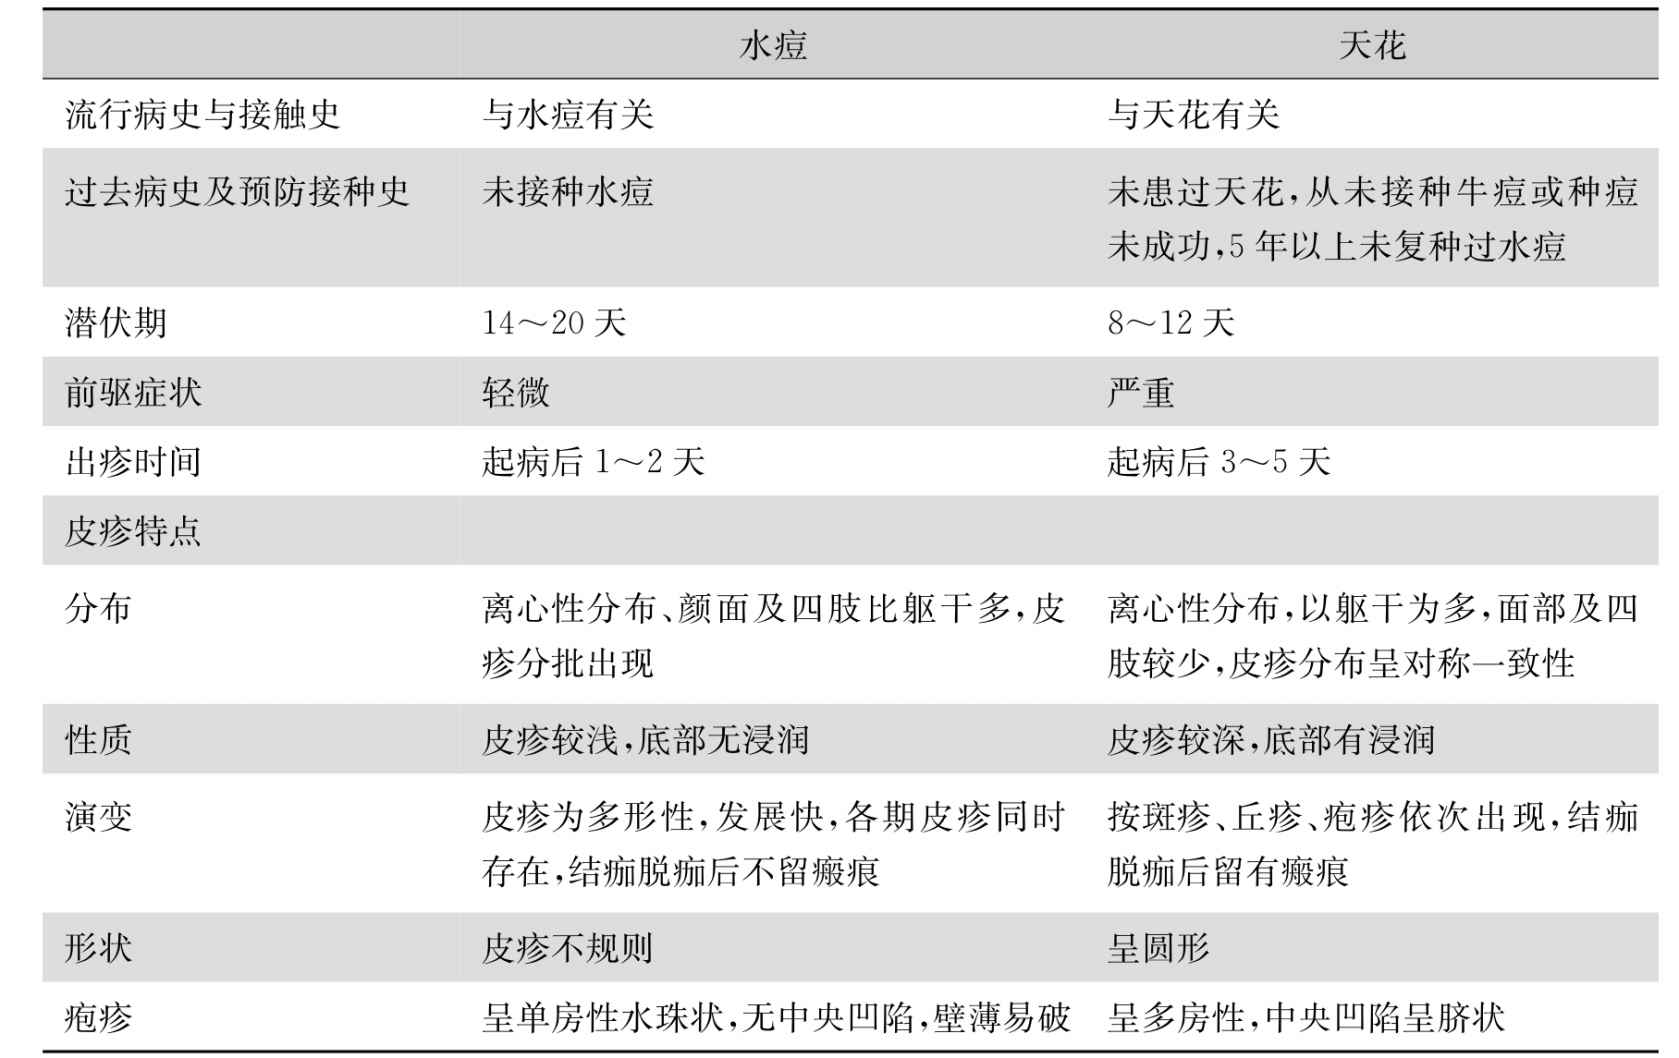
\includegraphics{./images/Image00008.jpg}
  \end{minipage}}\\
  \subfloat[经三脑室下部层面]{
  \begin{minipage}[b]{0.7\textwidth}
    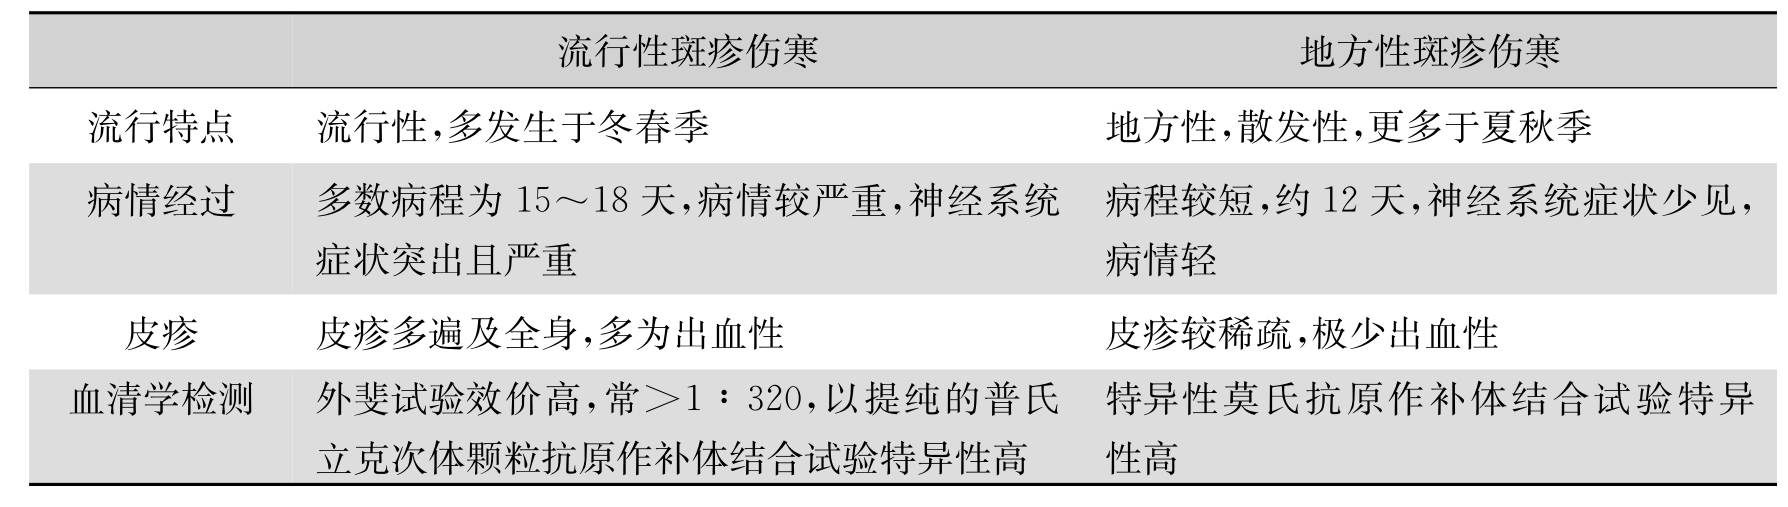
\includegraphics{./images/Image00009.jpg}
  \end{minipage}}
  \caption{}
  \label{fig2-3}
  \end{figure}

  \begin{figure}
    \ContinuedFloat             %%<-- put this in subsequest figures.
    \centering
    \subfloat[经松果体层面]{
      \begin{minipage}[b]{0.7\textwidth}
        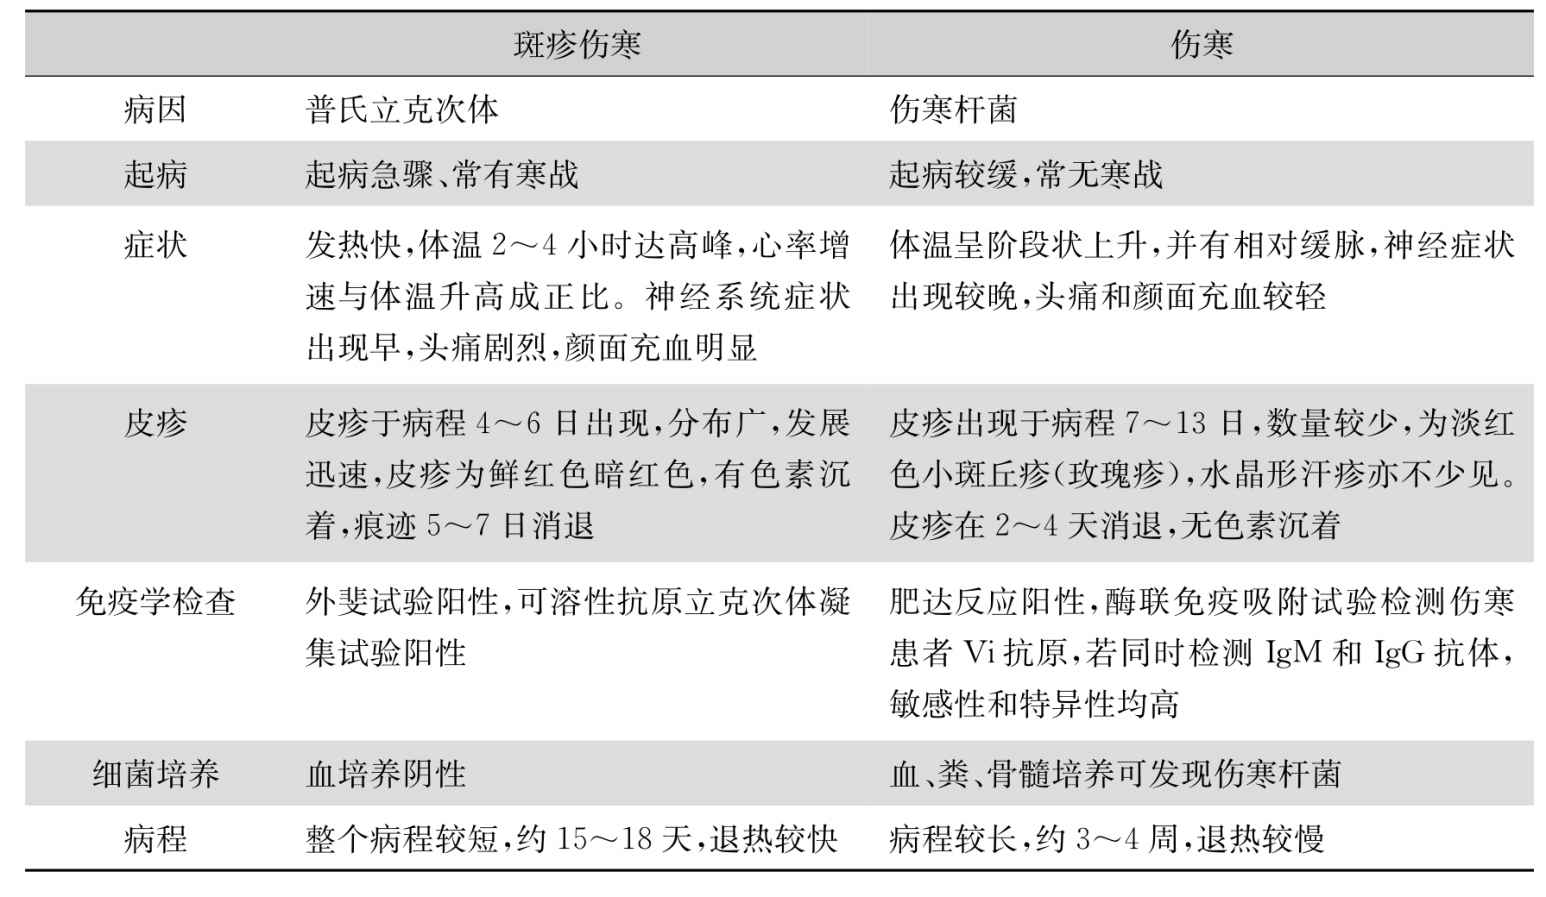
\includegraphics{./images/Image00010.jpg}
      \end{minipage}}\\
      \subfloat[经三脑室上部层面]{
      \begin{minipage}[b]{0.7\textwidth}
        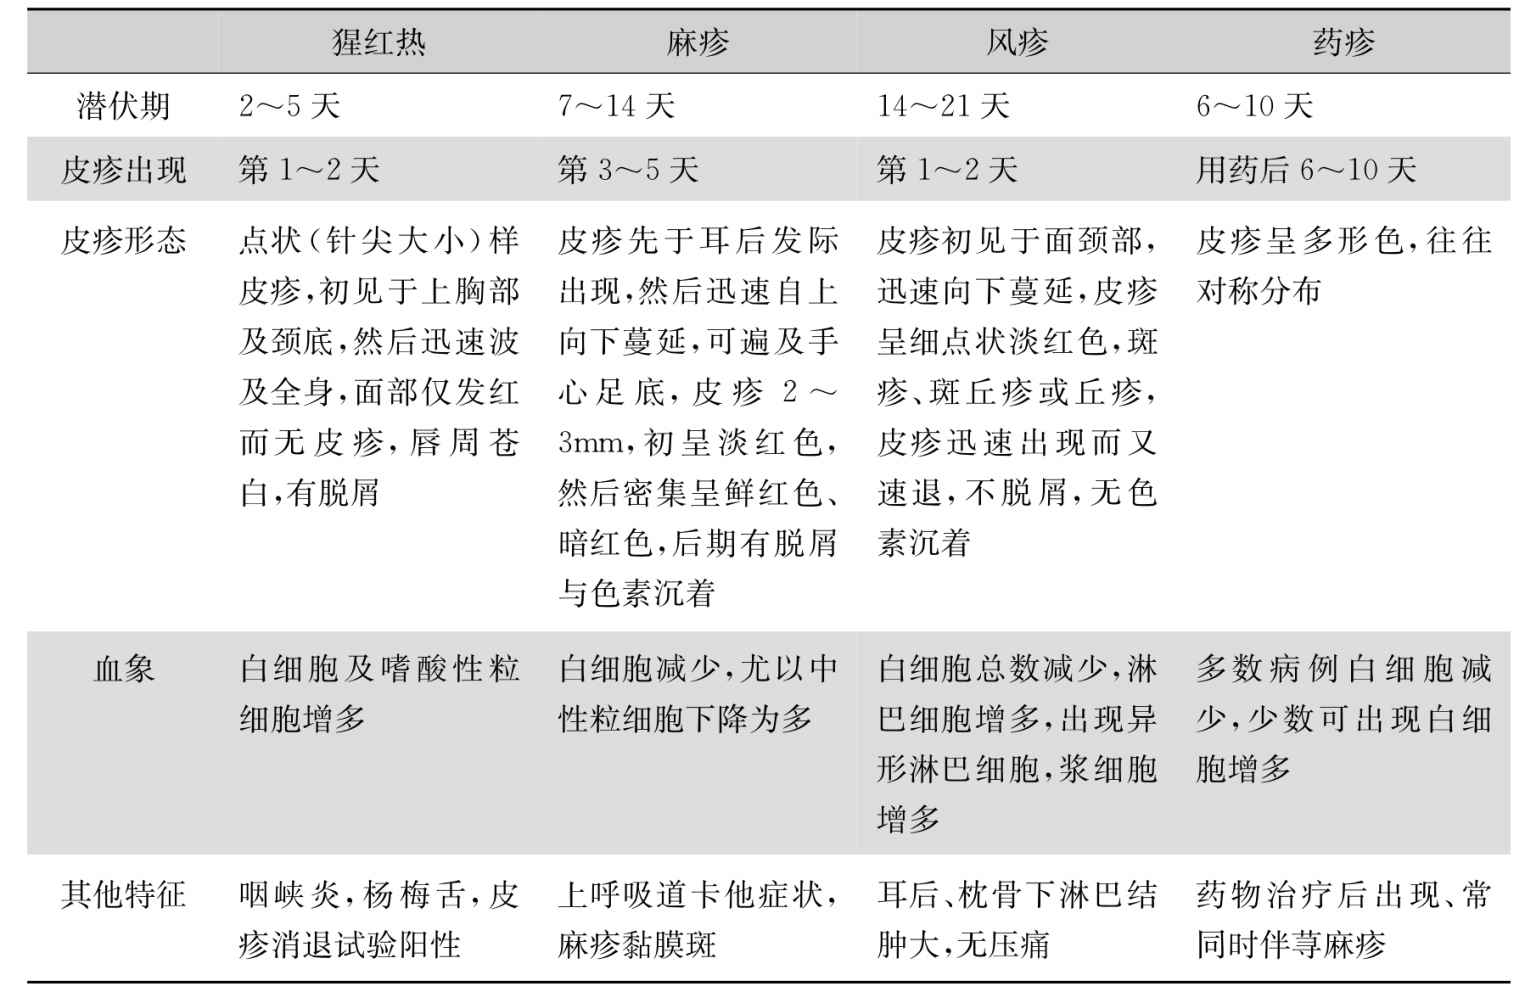
\includegraphics{./images/Image00011.jpg}
      \end{minipage}}\\
      \subfloat[经侧脑室体部层面]{
      \begin{minipage}[b]{0.7\textwidth}
        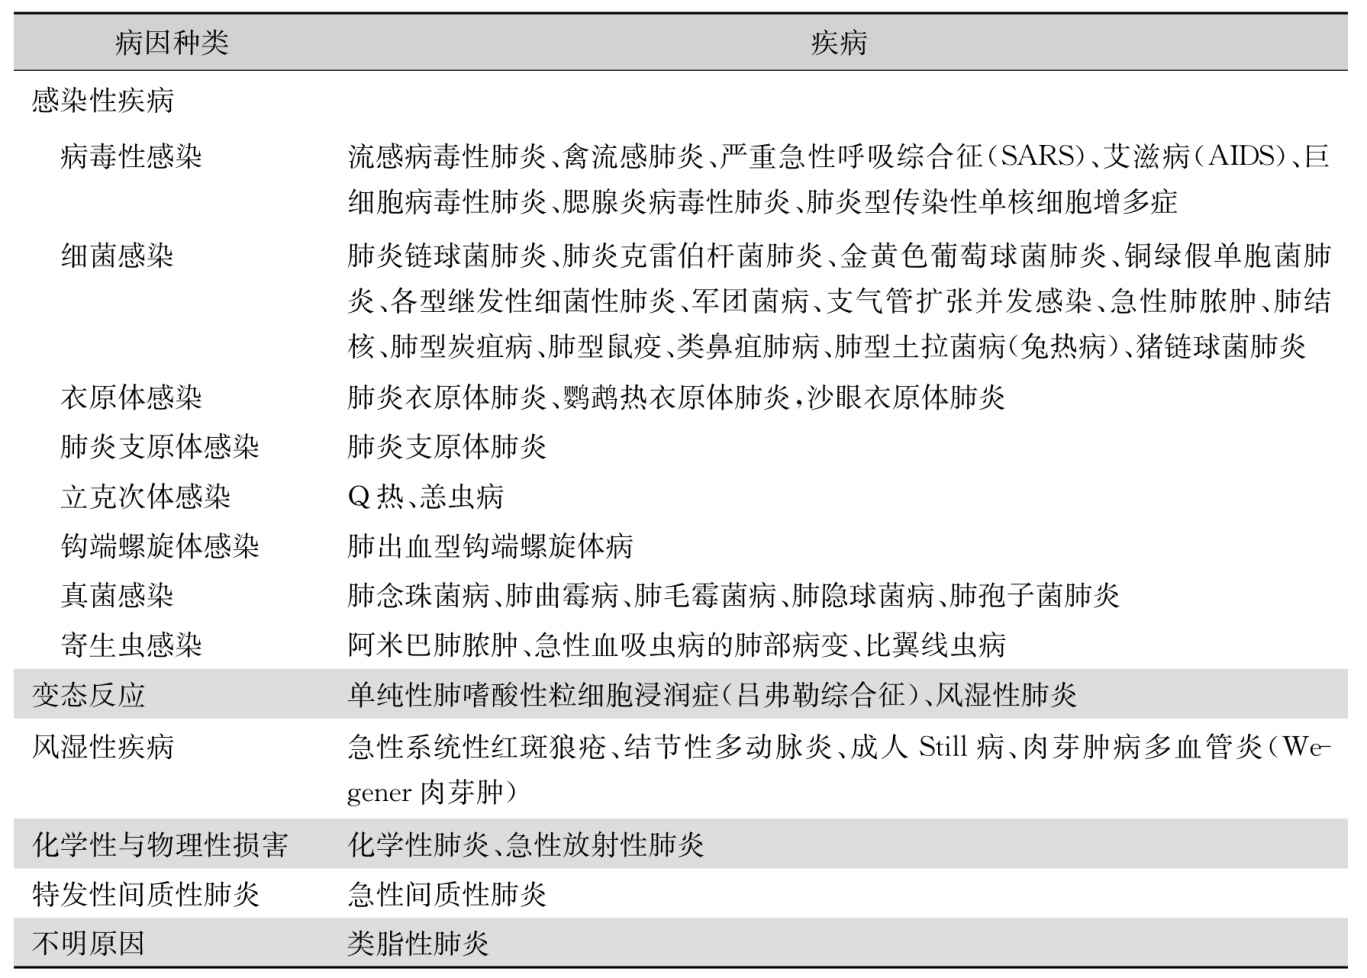
\includegraphics{./images/Image00012.jpg}
      \end{minipage}}
      \caption[]{}
  \end{figure}

  \begin{figure}
    \ContinuedFloat             %%<-- put this in subsequest figures.
    \centering
    \subfloat[经胼胝体体部层面]{
      \begin{minipage}[b]{0.7\textwidth}
        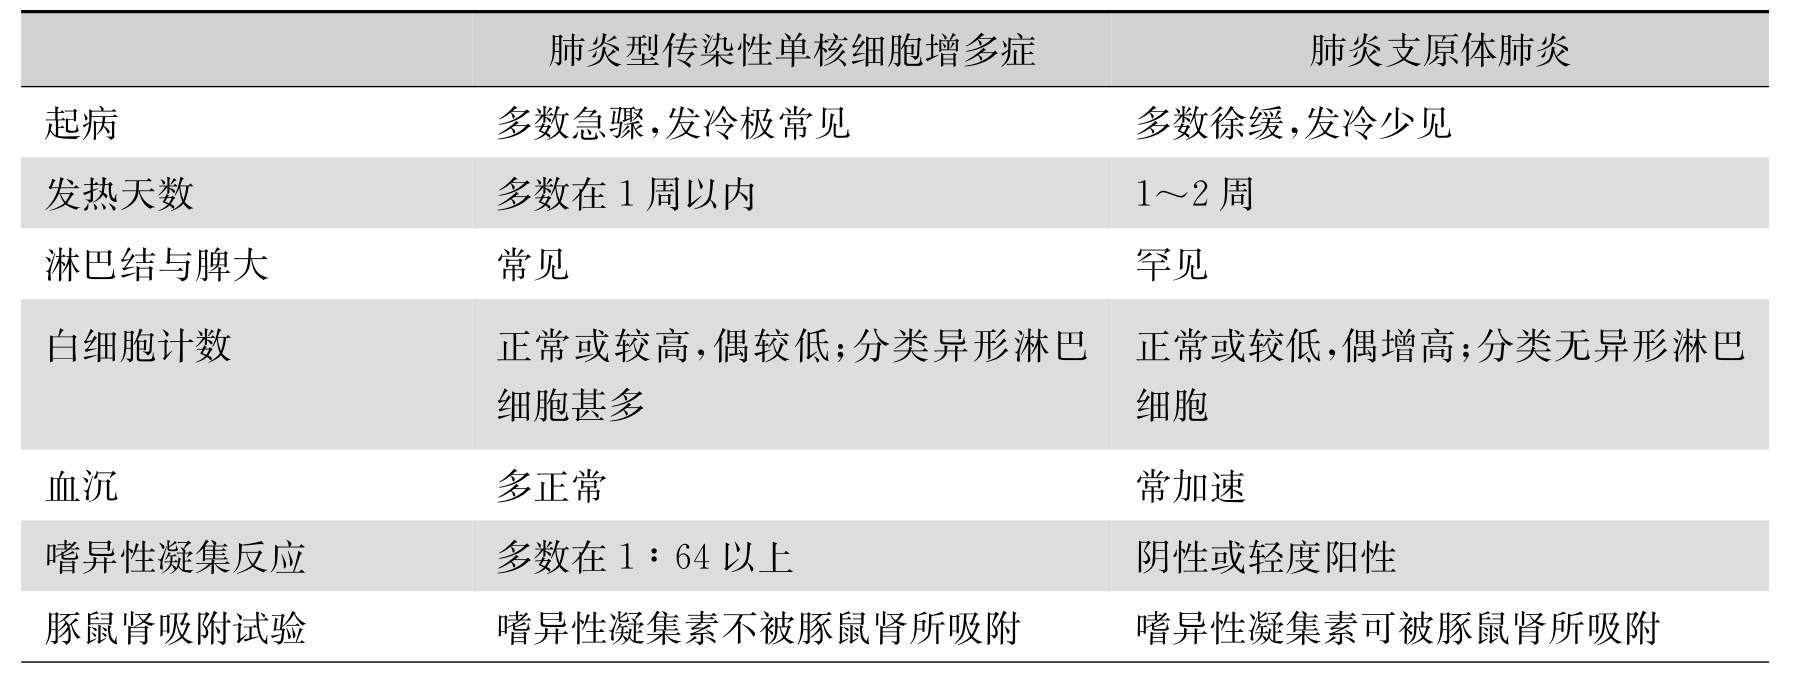
\includegraphics{./images/Image00013.jpg}
      \end{minipage}}\\
      \subfloat[半卵圆中心层面]{
      \begin{minipage}[b]{0.7\textwidth}
        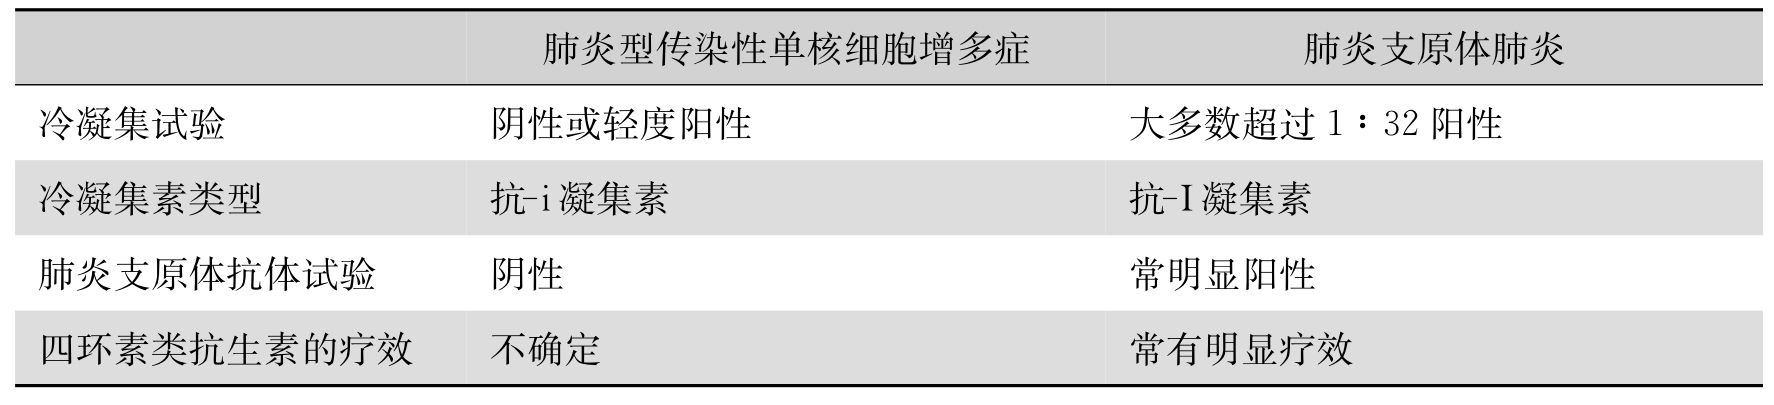
\includegraphics{./images/Image00014.jpg}
      \end{minipage}}\\
      \subfloat[半卵圆中心以上层面]{
      \begin{minipage}[b]{0.7\textwidth}
        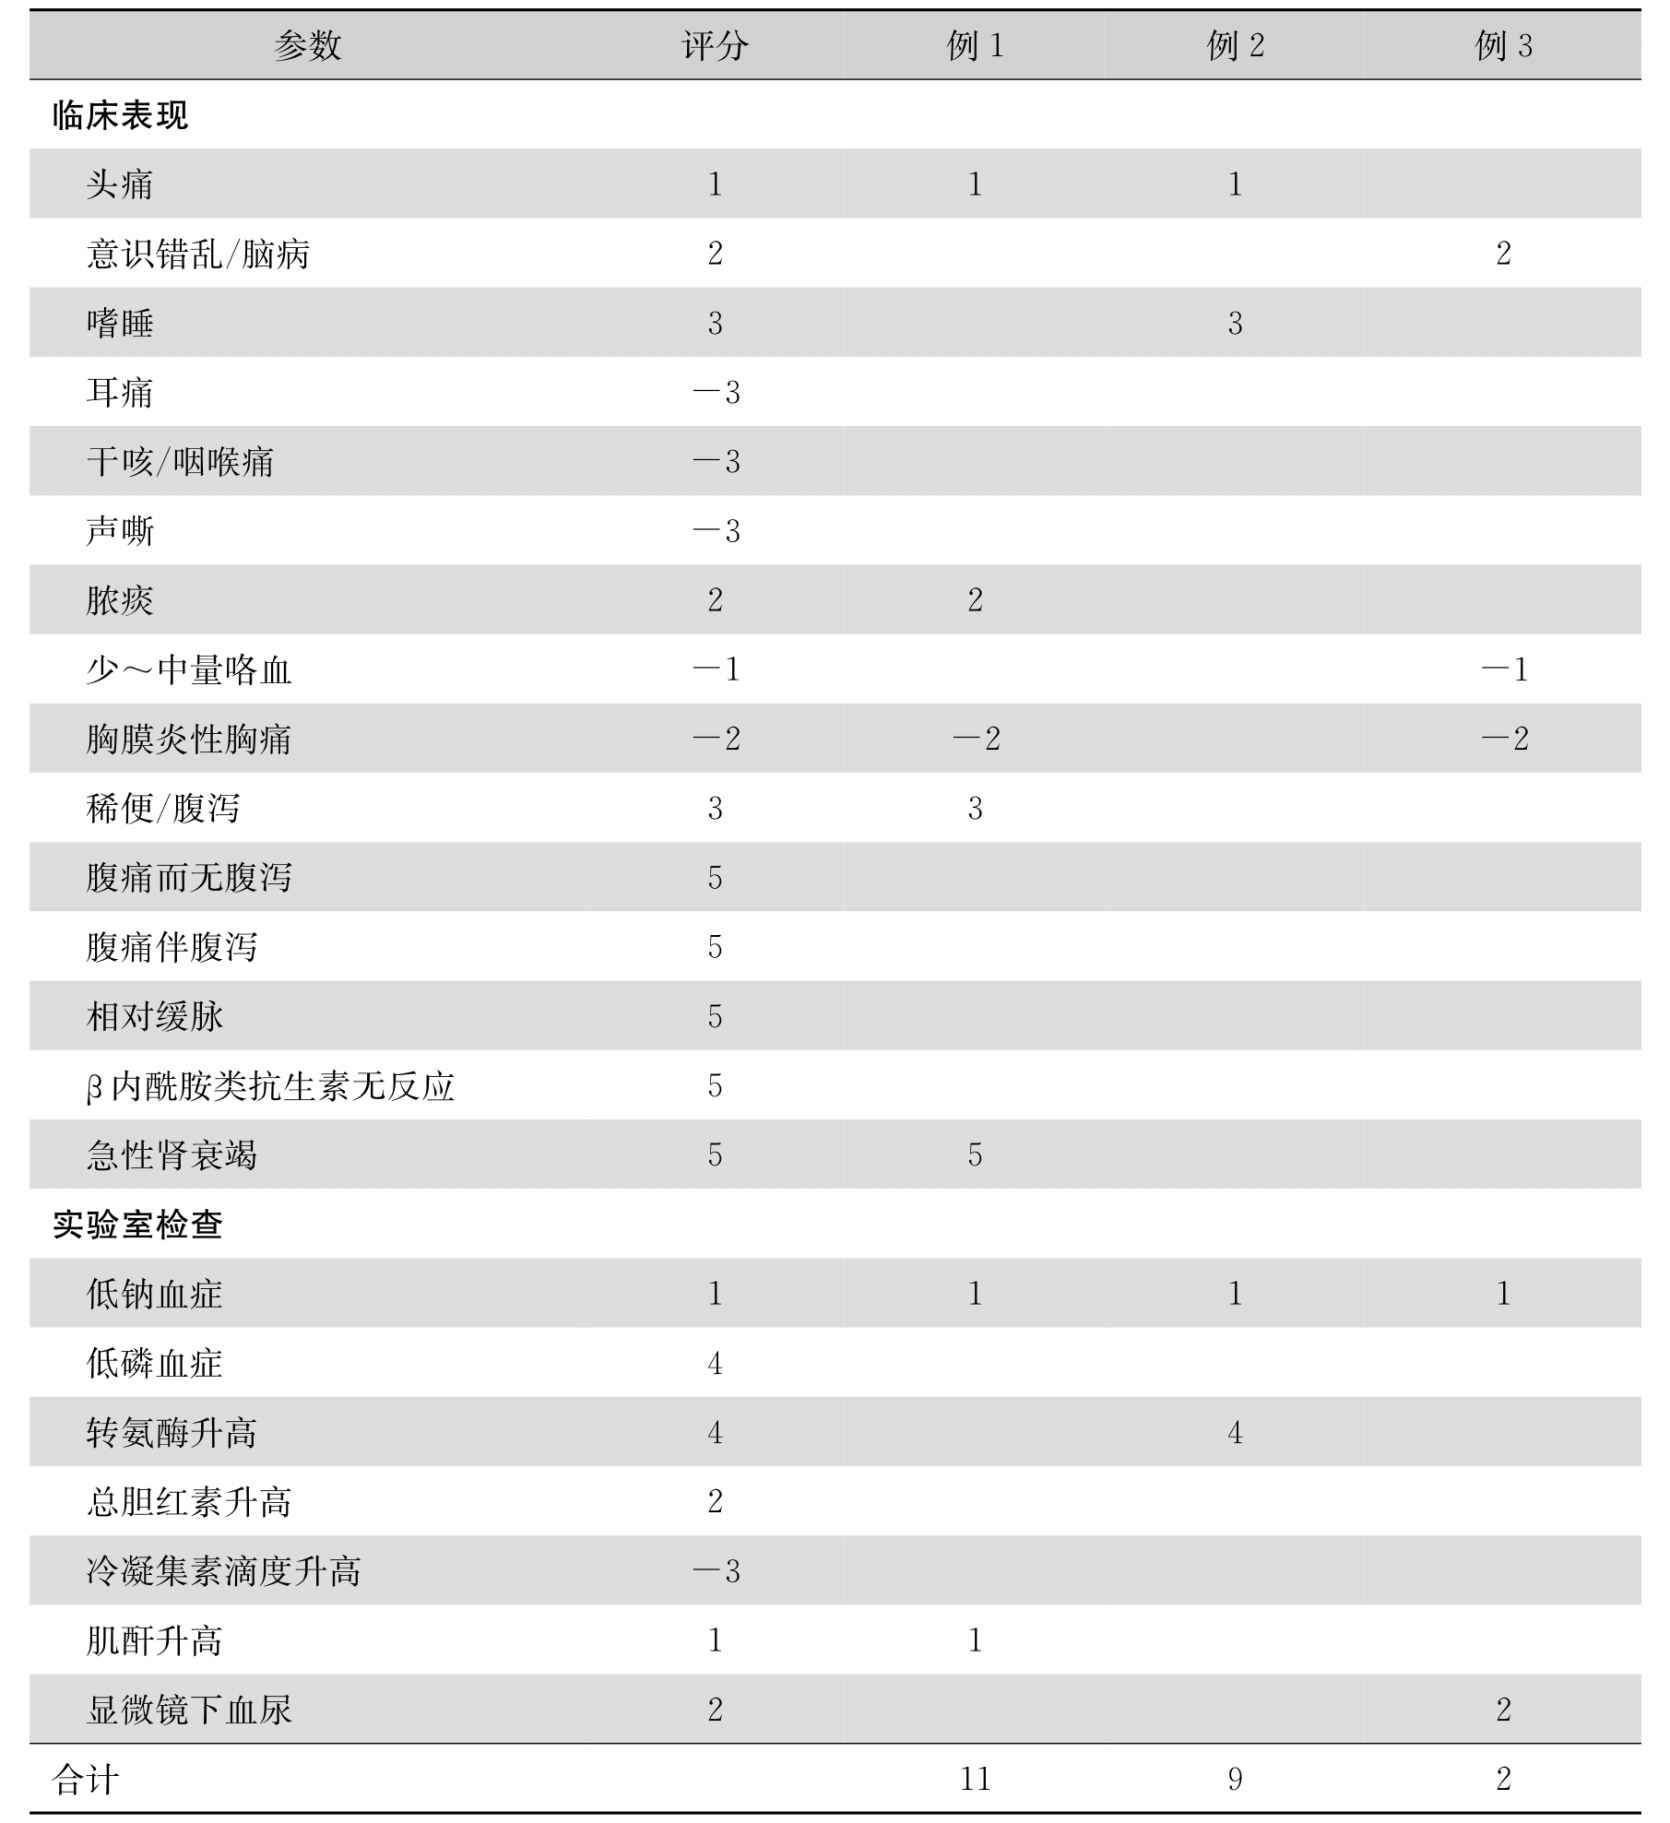
\includegraphics{./images/Image00015.jpg}
      \end{minipage}}\\
      \caption[]{}
  \end{figure}

  \begin{figure}
    \centering
    \subfloat[大脑半球外侧面的主要沟回]{
    \begin{minipage}[b]{0.7\textwidth}
      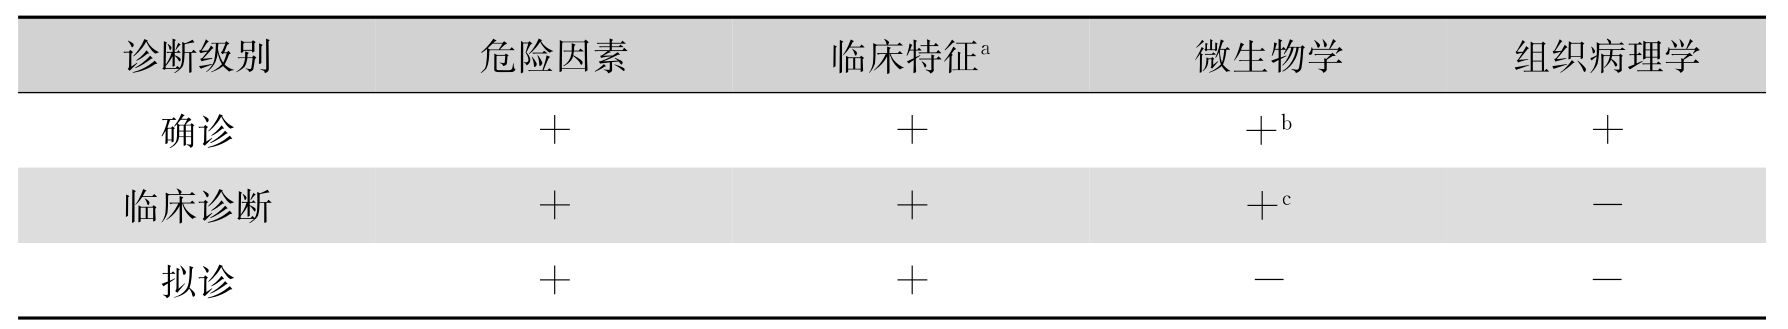
\includegraphics{./images/Image00016.jpg}
    \end{minipage}}\\
    \subfloat[大脑半球内侧面的主要结构]{
    \begin{minipage}[b]{0.7\textwidth}
      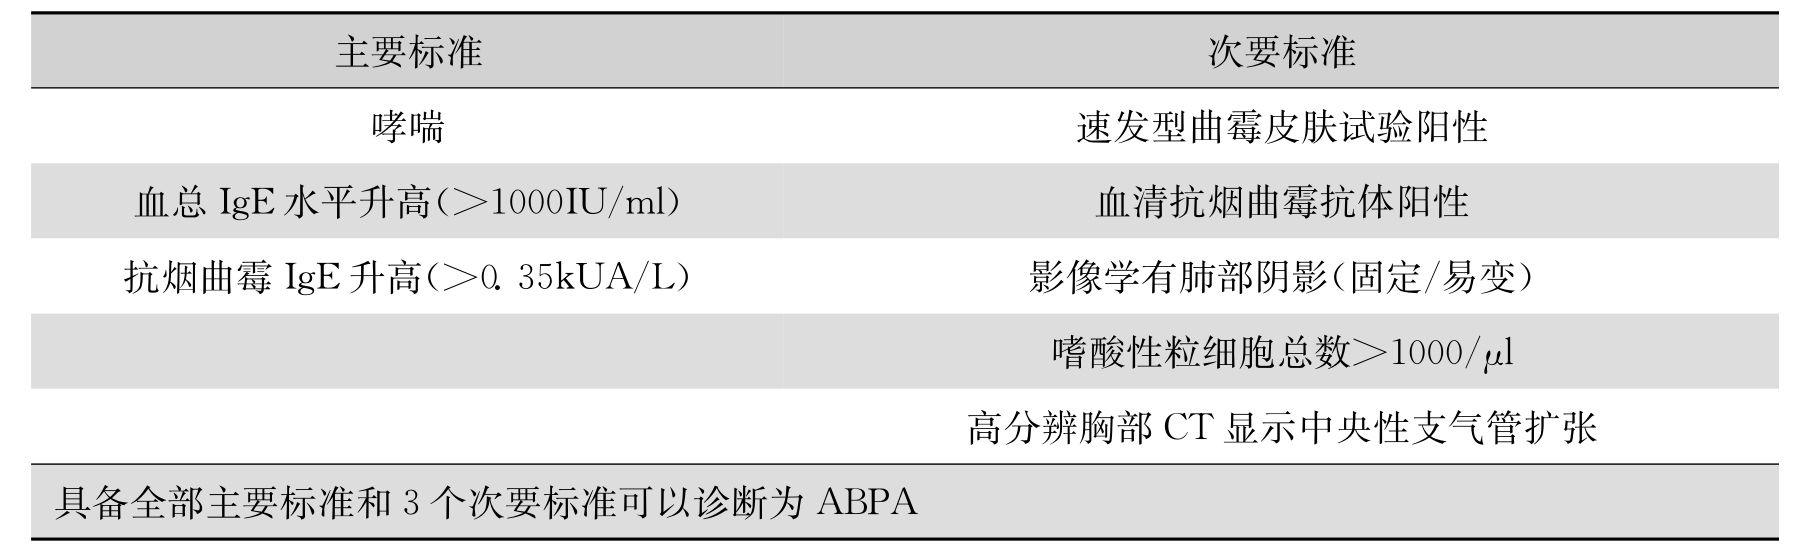
\includegraphics{./images/Image00017.jpg}
    \end{minipage}}\\
    \caption{}
    \label{fig2-4}
    \end{figure}

    \begin{figure}
      \ContinuedFloat             %%<-- put this in subsequest figures.
      \centering
      \subfloat[大脑半球背外侧面功能分区示意图]{
    \begin{minipage}[b]{0.7\textwidth}
      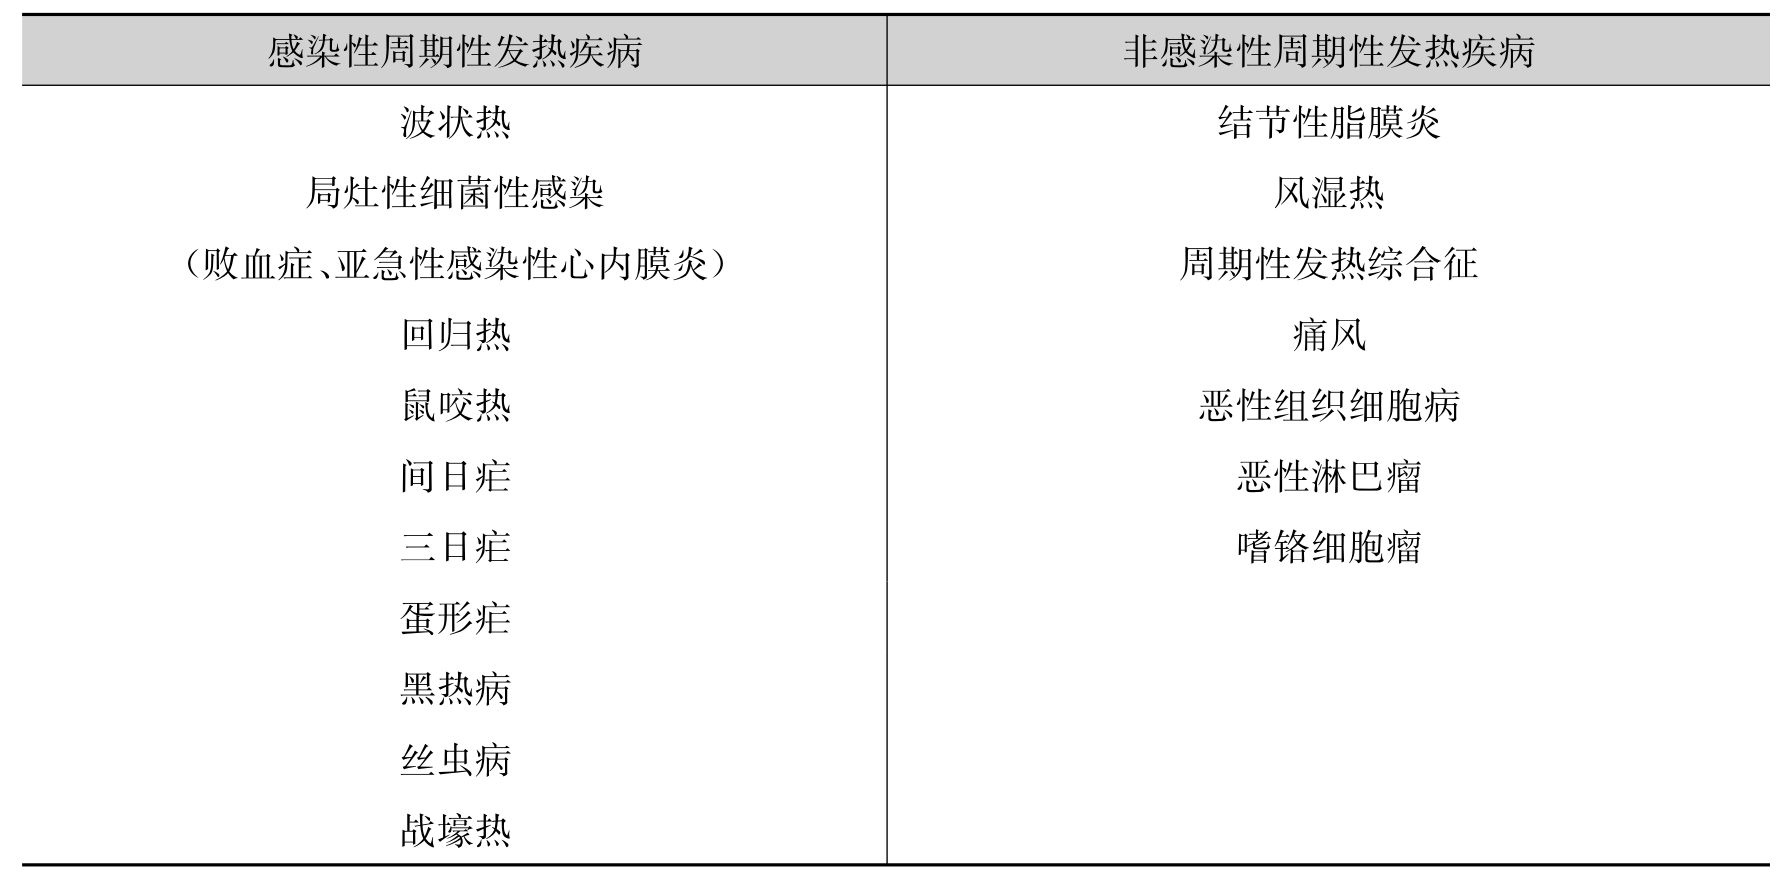
\includegraphics{./images/Image00018.jpg}
    \end{minipage}}\\
    \subfloat[大脑半球内侧面功能分区示意图]{
    \begin{minipage}[b]{0.7\textwidth}
      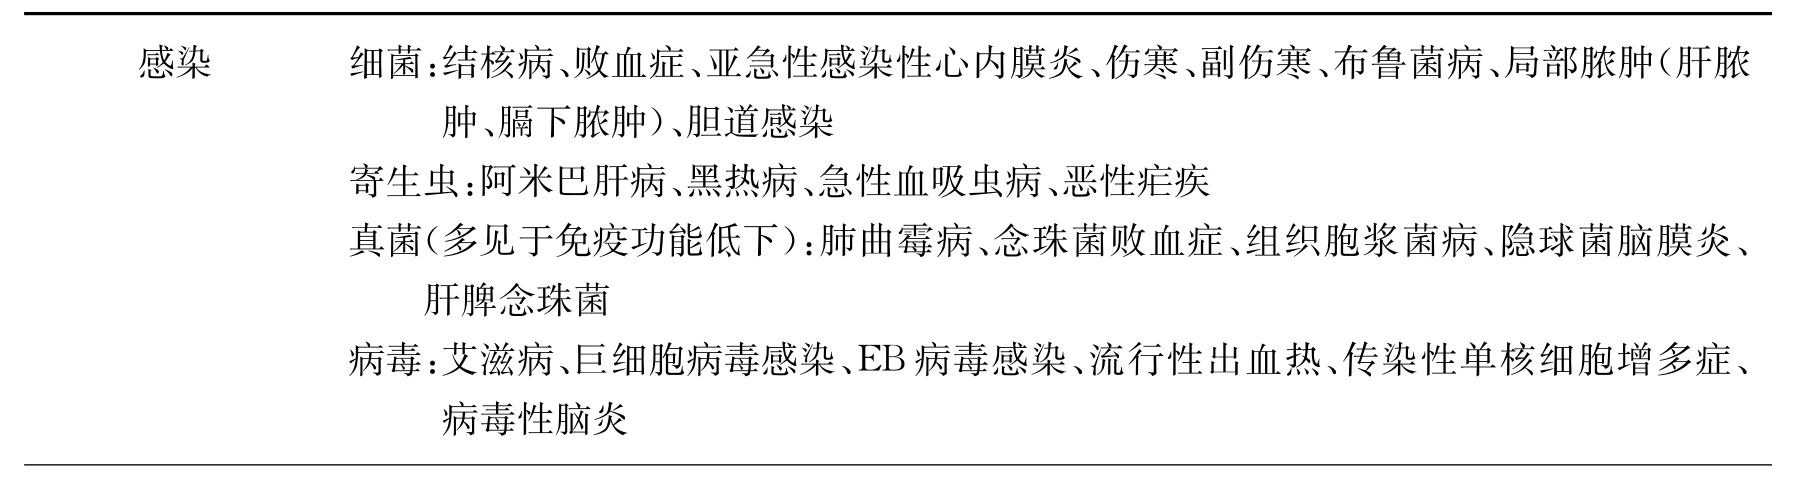
\includegraphics{./images/Image00019.jpg}
    \end{minipage}}\\
        \caption[]{}
    \end{figure}

\section{先天颅脑发育畸形和变异}

\subsection{概述}

所谓畸形是指胚胎期或胎儿期发生的脏器、系统或全身的形态异常或形成异常,不包括出生时的损伤和生后发育成长中产生的障碍。

先天性颅脑发育畸形的发病原因是由于胚胎期神经系统发育异常所致,约40%为遗传因素和子宫内环境的共同影响所致。前者包括染色体变异、显性或隐性遗传;后者包括宫内缺氧、感染等。其余60%病因复杂,机制不详。目前,可分为以下3大类:

1.器官形成障碍:①神经管闭合障碍:以脊髓脊膜膨出最常见,主要包括颅裂畸形(脑膜膨出、脑膨出、无脑畸形)、小脑扁桃体延髓联合畸形(Chiari畸形)、胼胝体发育不全、胼胝体脂肪瘤、先天性四脑室中侧孔闭锁(Dandy-Walker综合征)。②脑裂形成障碍:前脑无裂畸形(单叶、半叶、全叶)、视隔发育不良。③神经元移行异常:又称脑沟及细胞移行障碍,主要包括脑裂畸形、无脑回、灰质异常(巨脑回、多微脑回、灰质异位)。④大小异常:包括脑大、脑小畸形。⑤破坏性病变:包括积水性无脑畸形、脑穿通畸形。

神经管闭合不全是指胚胎期神经沟发育形成神经管的过程中,由于发育障碍而造成神经系统及其周围结构缺陷的一类中枢神经系统先天畸形,可能与孕妇叶酸缺乏有关。除表现出神经症状和体征外,更为常见的是周围组织的异常,包括颅骨、脑膜、椎体及其附件、皮肤和皮下组织(如先天性皮毛窦)等。该类疾病相当常见,其中尤以脊柱的畸形为多,是脑部的10倍或更多。

大脑皮层的神经元来自胚胎时期的脑室壁即神经管上皮。胚胎第6周末神经管经分化形成4个胚胎带,由内向外分别为脑室带、脑室下带、中间带和边缘带。脑室带和脑室下带的细胞具有分化成各类神经元的功能,故又称为生发基质层。胚胎7周时生发基质层的成神经细胞逐渐向外移行,大部分穿过中间带在边缘带内分化成神经元,形成有6层结构的正常脑皮质。26~30周脑回完全形成。神经元移行的过程复杂漫长,此间受到干扰则造成移行障碍。临床均以癫痫、智力障碍为最常见症状。

2.组织发生障碍:总体脑结构正常,但有异常细胞存在并持续分化。①神经皮肤综合征:包括神经纤维瘤病、脑颜面血管瘤病(Sturge-Weber综合征)、结节性硬化、视网膜小脑血管瘤病(又称Von
Hippel-Lindan病)。②血管性病变。③先天性肿瘤。

3.细胞发生障碍:①先天性代谢异常:包括氨基酸尿症、黏多糖沉积病、脂质沉积病等。②脑白质营养不良。③神经元变性。④轴索营养不良。

\subsection{脑膜膨出和脑膜脑膨出}

本病即显性颅裂畸形或称囊性颅裂畸形。临床可见颅外软组织肿物,大多于出生时即可发现。如仅有颅骨缺损,而无内容物自缺损处膨出称为隐性颅裂。

\textbf{【病理】}
颅裂多发生于中线或中线旁(斜坡除外),硬膜常缺如。脑膜(软膜和蛛网膜)或(和)脑突出于脑外,严重时可含部分脑室,可合并其他神经管闭合障碍(如Chiari畸形、胼胝体发育不全)等畸形。

\textbf{【临床表现】}
囊性肿物与头部相连,于出生时即可发现,也可于生后几个月或几年发现。哭闹或咳嗽时肿物增大,张力增加;压迫肿物,则前囟突出;局部可扪及骨缺损的边缘。一般无神经系统症状,也可表现为智力低下、抽搐及脑损害表现。

\textbf{【CT表现】}
软组织疝出的部位可见边缘硬化的颅骨缺损,枕部占70%,顶部占10%~20%,额上部占10%,颅底部占10%。应注意向颅外膨出的软组织,是否含有脑脊液和脑组织;颅底部膨出应注意与鼻息肉或鼻咽部肿瘤相鉴别(图\ref{fig2-5}\footnote{16岁女性,枕骨局限缺损,可见疝出之少量软组织密度灶})。同时,可合并胼胝体缺失、Chiari畸形、灰质异位等畸形。

\begin{figure}[!htbp]
 \centering
 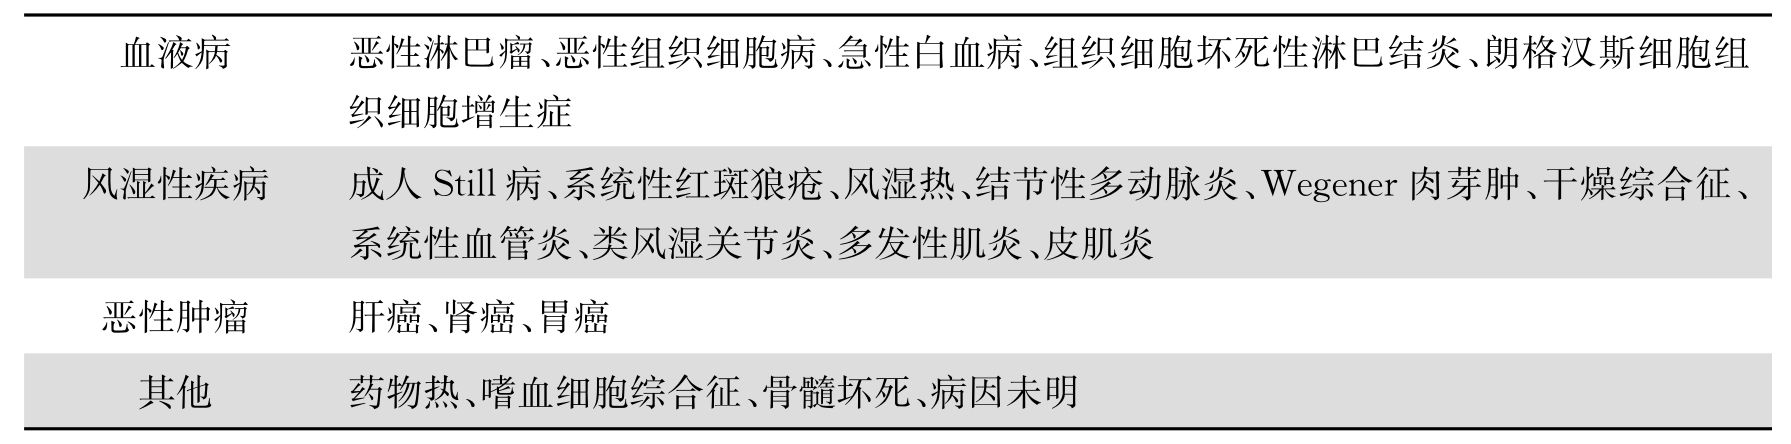
\includegraphics[width=.7\textwidth,height=\textheight,keepaspectratio]{./images/Image00020.jpg}
 \captionsetup{justification=centering}
 \caption{脑膜脑膨出}
 \label{fig2-5}
  \end{figure} 

\subsection{小脑扁桃体延髓联合畸形}

本病又称Chiari畸形,为后脑先天性发育异常。扁桃体过长、变形,经枕大孔疝入上段颈椎管,延髓和第四脑室可同时向下延伸。常伴脊髓空洞症、脊髓纵裂、脑积水和颅颈部畸形等。

\textbf{【病理】} 可分为以下4型。

Ⅰ型:多见。最可能的发病机制是胚胎枕节发育不良导致后颅窝狭小,难以容纳正常发育的后脑,使小脑扁桃体下疝。小脑扁桃体与小脑下部疝入颈椎管上端,无延髓移位。一般认为小脑扁桃体下端低于枕大孔≥5mm为下疝,<3mm为正常,二者之间临床意义不确定。通常不伴其他脑畸形,临床可无症状,或有轻度运动障碍和小脑症状。

Ⅱ型:最常见。小脑扁桃体和蚓部同时疝出枕大孔,脑桥下部及延髓下移,第四脑室延长。几乎总是伴有某种神经管闭合不全如脑膜膨出、脊髓脊膜膨出(腰骶部多见)、脑积水和脊髓空洞症。常有上述Ⅰ型症状。

Ⅲ型:十分罕见。为Ⅱ型伴有低枕部或高颈部脑膜脑膨出,临床症状较Ⅱ型更严重。

Ⅳ型:非常罕见。伴有严重的小脑发育不良,结构独特,可能不单独存在。该型归为小脑发育不良可能更合适。

\textbf{【临床表现】}
本病可无症状,尤其畸形轻者可无,也可直到成年甚至50~60岁始有症状。神经损害症状主要是颅神经和颈神经受损、延髓和上颈髓受压,可有小脑症状、颅内高压及脊髓空洞症表现。

\textbf{【CT表现】}
CT可显示下列特征:①小脑扁桃体、小脑蚓部及小脑、脑干和第四脑室下移;②脑积水;③大脑镰和天幕发育不良;④部分脑组织过度增生或脑发育异常导致脑室系统畸形;⑤后颅窝内容物的挤压引起的颅骨和蛛网膜下腔的改变。但只有通过脑池造影CT扫描或MR显示扁桃体下移、其下端变尖才能明确诊断。

\subsection{侧孔先天性闭锁}

本病又称Dandy-Walker综合征,第四脑室正中孔、外侧孔闭锁为发病主要原因。

\textbf{【病理】}
此病是一组先天性后脑发育畸形,包括脑积水、小脑发育障碍(小脑蚓部不发育或发育不全,约25%蚓部缺如)和与第四脑室相通的巨大后颅窝囊肿。囊肿大小变化很大,囊壁由下髓帆组成,包括室管膜、胶质、小脑组织、软脑膜和蛛网膜等,囊壁可钙化,可合并大脑发育异常。

\textbf{【临床表现】}
男女发病率相近。大多于2岁前产生症状,常因运动发育迟缓而就诊。部分因颅内高压或小脑症状而就诊,头颅明显增大。

\textbf{【CT表现】}
在出生时脑积水是不常见的,75%在生后3个月出现。典型者小脑蚓部体积变小或缺如,小脑半球分离;巨大的后颅窝“囊肿”与扩大的第四脑室相通。脑干前移,桥前池、桥小脑角池消失,后颅窝扩大,枕骨变薄,天幕上移。可合并胼胝体发育不良、多微脑回、灰质异位、枕部脑膨出等。

\textbf{【鉴别诊断】}
①后颅窝巨大蛛网膜囊肿:第四脑室与囊肿不相通,而是受压前移,必要时通过脑池造影CT鉴别。②巨大枕大池:第四脑室无受压,无蚓部发育不全、无后颅窝扩大等,但与下蚓部几乎完整的Dandy-Walker畸形不易鉴别。上述两者均可偶有轻度脑积水,但小脑发育基本正常。

\subsection{Joubert综合征}

\textbf{【病理】}
病理特征是小脑蚓部不发育或发育不全而形成异常的“中线裂”,还有小脑齿状核的变形、下橄榄核和旁橄榄核的发育不良、背侧柱核的异常以及锥体交叉缺如。

\textbf{【临床表现】}
男性多见,有发作性呼吸过度和(或)呼吸暂停、眼球活动异常(眼球震颤、斜视等)和儿童期发育迟缓。还可伴有其他异常如小头畸形、面部畸形、胼胝体发育不全、多指畸形和先心病等。

\textbf{【CT表现】}
在桥脑和中脑连接水平,第四脑室呈“蝙蝠翼状”。于第四脑室底部紧贴小脑半球中线处可见小脑半球间形成的切迹即“中线裂”。小脑上脚增粗,由于交叉的缺乏而向外分开,并导致中脑背侧局部缺失,形成所谓的“磨牙征”。第四脑室中部呈倒立三角形状,与不连接的小脑半球间的脑脊液间隙相连形成“酒杯状”表现,无后颅窝囊肿和脑积水。

\subsection{胼胝体发育不全}

\textbf{【病因病理】}
胼胝体在妊娠12~20周时形成。本畸形偶然发病,病因一般不明,多为先天性。在某些病例中,母体的血管性、外伤性、中毒性或感染性损伤为致病因素。产期缺血缺氧性损害也可引起获得性胼胝体发育不全。本病可为全部或部分缺如,常伴发其他畸形(最高达50%),如前脑无裂畸形、多微脑回、厚脑回、灰质异位、脑小畸形、视隔发育不良、胼胝体脂肪瘤或纵裂池蛛网膜囊肿等。

\textbf{【临床表现】}
临床症状各不相同,视伴发的其他神经系统畸形而定。许多患者可无症状或仅有轻度视觉障碍;或有交叉触觉定位障碍而智力正常;严重者可有癫痫和智力不全。

\textbf{【CT表现】}
由于胼胝体完全或部分缺如而表现不一。可见纵裂池前部明显向后伸展,靠近第三脑室前壁。侧脑室额角和体部间距增大,而且两侧脑室平行分离,并可见其内壁呈弓形外突,冠扫额角呈“八”字形分离。枕角不对称性扩大(憩室),第三脑室轻度扩大并上移。正常时,两侧脑室的脉络丛常在室间孔间会聚,并形成45\textsuperscript{o}
~70\textsuperscript{o} 夹角,本病此夹角多<35\textsuperscript{o}
~40\textsuperscript{o}
(图\ref{fig2-6}\footnote{A~D为同一患者,可见纵裂池前部明显向后伸展,靠近第三脑室前壁;第三脑室轻度扩大并上移;侧脑室额角和体部间距增大,两侧脑室平行分离}),有时可见半球间裂(纵裂池)的蛛网膜囊肿等畸形。本病应注意与脑室周围白质软化症(PVL)相鉴别。



\begin{figure}[!htbp]
 \centering
 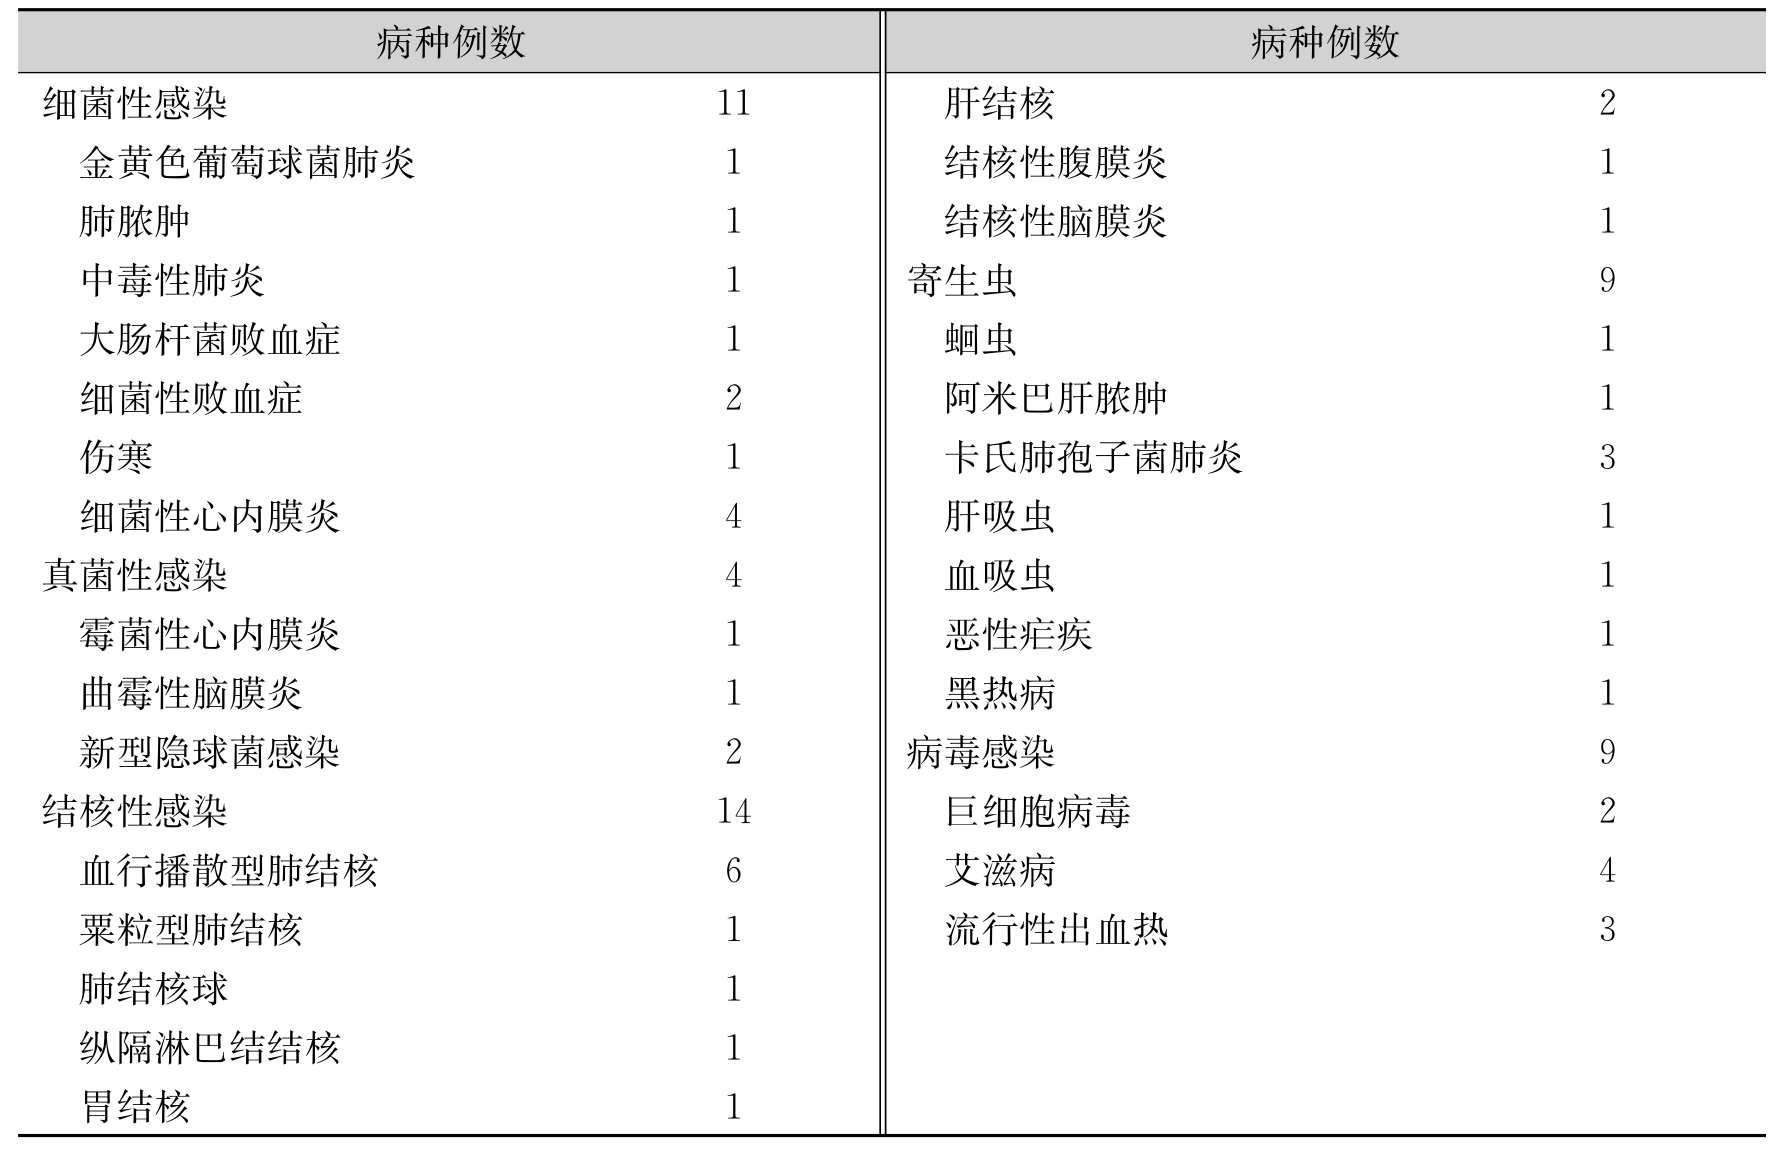
\includegraphics[width=\textwidth,height=\textheight,keepaspectratio]{./images/Image00021.jpg}
 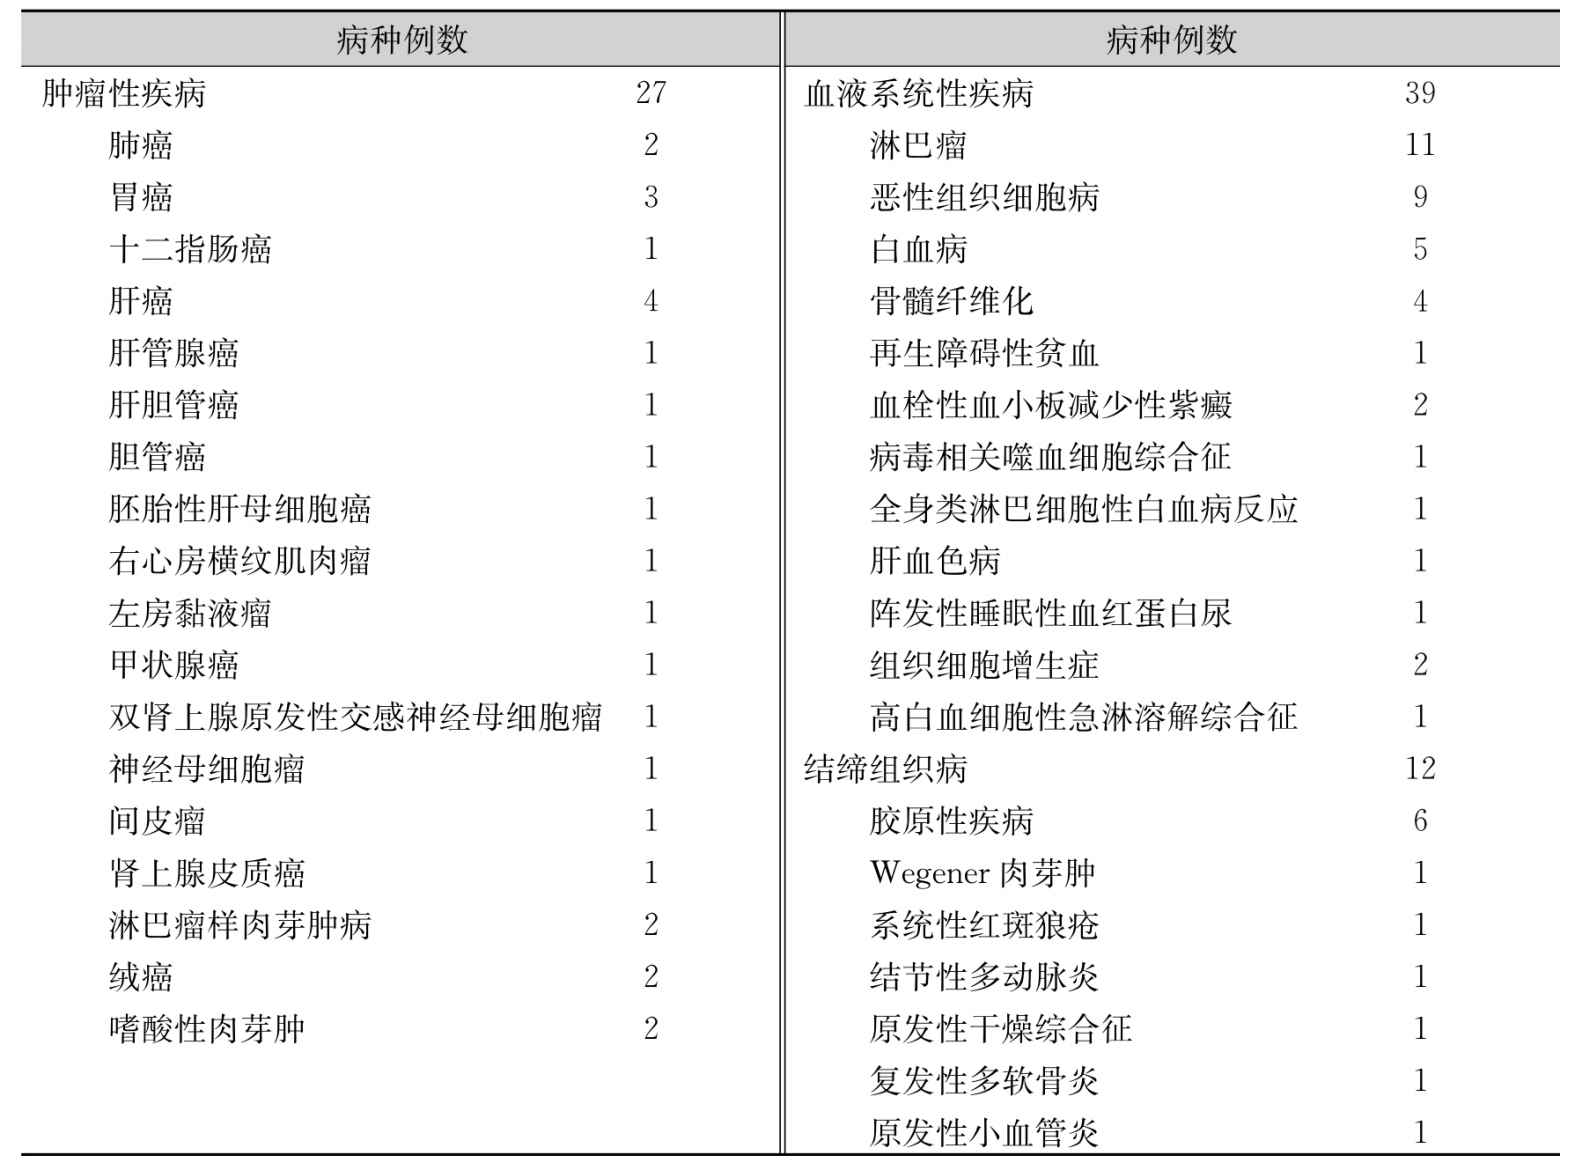
\includegraphics[width=\textwidth,height=\textheight,keepaspectratio]{./images/Image00022.jpg}
 \captionsetup{justification=centering}
 \caption{胼胝体发育不全}
 \label{fig2-6}
  \end{figure} 


\subsection{前脑无裂畸形}

本病又称全前脑畸形,是胚胎发育过程中由前脑发育障碍引起的一组复杂的颅脑与面部畸形。

\textbf{【病因病理】}
其病因不明,部分为常染色显性和隐性遗传。大脑不能分裂成两侧大脑半球,有时也不能在横向上分裂成端脑和间脑,可分为无脑叶型、半脑叶型、脑叶型3种类型,代表了畸形的不同程度。

\textbf{【临床表现】}
男女发病相近,因婴儿多数死于流产或出生后不久,故临床少见。脑叶型可活到成年,并有运动迟缓、智力低下等神经精神症状。

\textbf{【CT表现】} 3种类型分别表现如下。

1.无脑叶型:又称全前脑无裂畸形。脑呈小圆球形,丘脑融合,中央单脑室,第三脑室成为扩大脑室的一部分。正常中线结构如透明隔、大脑镰、胼胝体和纵裂均缺失,50%以上有多处面颅畸形。

2.半脑叶型:中央单脑室较小,初步形成了额、枕角,胼胝体、大脑镰、透明隔仍缺如。大脑半球前部仍保持融合,但后部半球间裂已形成。丘脑往往部分分离,故第三脑室是小的,面部畸形不重。

3.脑叶型:CT表现比前两者轻微。前部半球间裂较浅,仍存在融合表现。脑室系统形态良好,透明隔缺如。脑镰和胼胝体至少部分形成,丘脑无融合。

此外,少数病例额部和枕部半球间裂均存在,融合发生于半球额后顶区域,属半脑叶型,CT诊断困难。

\subsection{视隔发育不良}

本病罕见,主要是透明隔发育不全,常见于先天性垂体性侏儒,可能是脑叶型前脑无裂畸形的轻度形式。

\textbf{【病理】}
透明隔发育不全,有原始的视泡及视交叉、视神经,漏斗发育不全而使视神经孔狭小。

\textbf{【临床表现】}
眼部症状包括眼球震颤和视敏度下降,但可有正常视力。约2/3有下丘脑-垂体功能障碍而出现尿崩、生长发育障碍。

\textbf{【CT表现】}
透明隔缺如,额角在横断面呈倒三角形或盒状。严重者可见视神经、视交叉细小,视神经管小和视交叉位置异常,视交叉和下丘脑发育不全使鞍上池扩大。

\subsection{透明隔疾病}

透明隔是一厚约1.5~3.0mm的双层半透明膜,上起胼胝体的体部、膝部和嘴部,向下延伸至穹隆的表面,前后伸延从终板、胼胝体的嘴至胼胝体的压部。它含有一定数量的胶质细胞、散在的神经元和神经纤维。这些神经纤维构成了海马和下丘脑之间的重要联系,且是中继下丘脑到海马、杏仁核、缰核和脑干网状结构的内脏信息的相关中心及边缘系统到脑干网状结构的重要环路。所以,它参与意识、睡眠以及环境作用所表现出来的情绪反应,例如饮食、性活动等,并有助于精神活动的自我平衡。

透明隔疾病有:①透明隔间腔:即第五脑室。②透明隔缺如:原发或继发。③透明隔囊肿:与第五脑室并无严格界限,表现囊壁向两侧突出而不是平行,宽达10mm以上,并可引起室间孔狭窄导致脑积水,邻近神经组织受压而引起神经功能障碍。当宽径<5mm时,则不引起症状(图\ref{fig2-7})。④肿瘤:罕见,如星形细胞瘤、少突胶质细胞瘤、室管膜瘤和成星形细胞瘤,近来亦有亚室管膜瘤、局限性脂肪瘤的报道。⑤血管瘤。⑥钙化。⑦移位。⑧萎缩。

\begin{figure}[!htbp]
 \centering
 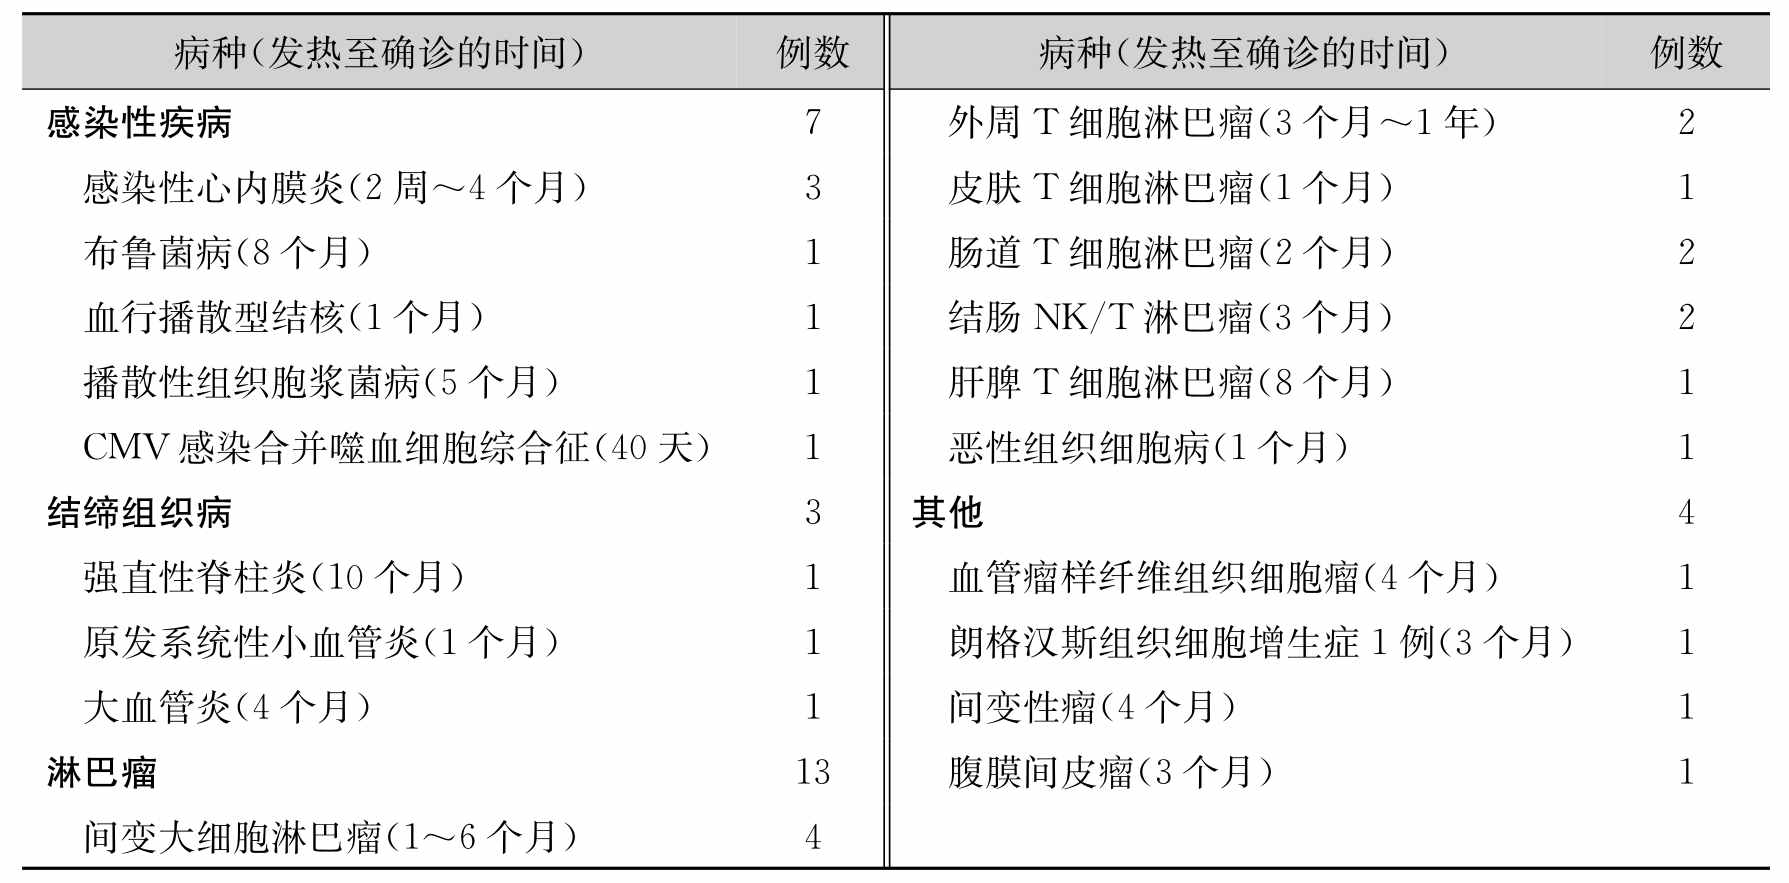
\includegraphics[width=.7\textwidth,height=\textheight,keepaspectratio]{./images/Image00023.jpg}
 \captionsetup{justification=centering}
 \caption{透明隔囊肿\\{\small 透明隔区囊状水样密度灶,囊壁向两侧突出,宽达12mm}}
 \label{fig2-7}
  \end{figure} 



\subsection{侧脑室黏合}

侧脑室不对称在正常人中常见,部分原因是侧脑室黏合,侧脑室黏合是正常变异。

\textbf{【病理】}
本症是在生长发育过程中侧脑室内面部分融合,造成侧脑室不对称、变形。发生在胎儿期4~6周,此时脑白质发育迅速,白质膨大可使邻近的室管膜表面挤压在一起。黏合多发生在额角上侧面及体部,单侧或双侧性。

\textbf{【CT表现】}
侧脑室黏合可以是单侧性或双侧性,或与透明隔间腔同时存在。额角的前部融合,致额角前部消失,额角变短,两壁夹角为锐角,使两壁相交处圆钝的正常表现消失,透明间隔居中。额角中部的两壁尖角状突起,中部间隙消失或接近消失,透明隔居中。透明隔移向一侧,偏移程度从轻度到非常明显,致同侧侧脑室体部变小,对侧相对增大。透明隔的移位必然伴有体部变小侧的额角变窄、变形,但透明隔始终呈直线状走行。双侧基底节区形态结构对称,脑室、脑实质内无异常,增强扫描无异常强化。

\subsection{脑裂畸形}

\textbf{【病因病理】}
有学者认为,妊娠第2个月出现的病理干扰可造成脑壁某部位生发基质层不能正常发育,致使神经元移行不能发生或过早停下来而导致脑裂畸形。其主要病理改变为大脑半球内有自脑表面向内延伸达室管膜下的横行裂隙,邻近皮层卷入衬于裂隙两侧,其表面的软脑膜与室管膜融合形成软脑膜-室管膜缝。脑裂畸形可分为闭合型和分离型两型,常合并透明隔缺如、胼胝体发育不良及其他神经元移行异常等畸形。

\textbf{【临床表现】} 主要有癫痫、智力低下和运动功能障碍。

\textbf{【CT表现】}
大脑半球表面有单侧或两侧的裂隙,从脑表面延伸到室管膜下区。脑皮质沿裂隙内折,居裂隙两侧,多位于中央前后回附近。根据其表现可分为两型:①Ⅰ型:即融合型(或称闭唇型)脑裂畸形,裂隙关闭不与侧脑室相通,但脑室壁可有憩室样突起(图\ref{fig2-8});②Ⅱ型:即分离型(或称开唇型)脑裂畸形,特点为内折的皮质分离,形成较大裂隙并多与侧脑室相通,且脑室壁在内压作用下外突,形成憩室。

\textbf{【鉴别诊断】}
①脑穿通畸形:为大脑成形后的损害(坏死腔),多呈圆形,无脑皮质沿囊肿壁内折为鉴别要点。有时鉴别困难,但穿通畸形的两缘向病灶外方突出,而分离型脑裂畸形两缘向内突出有助于鉴别。②孤立性灰质异位:当融合型裂隙不明显时应注意与其鉴别。脑裂畸形皮质柱内端相邻的侧脑室外壁常有憩室状突起,外端脑表面有楔形凹痕,可与其相鉴别。

\subsection{多微脑回畸形和鹅卵石样脑回畸形}

\subsubsection{无脑回}

大脑皮质表面光滑、无沟回,故又称光滑脑。灰质增厚,白质变薄,灰白质正常手指样交界消失,也可与巨脑回相伴发。

\subsubsection{巨脑回}

局限性或弥漫性脑回异常增宽,皱褶减少,表现为宽、平、厚的脑回,灰白质正常手指样交界亦可消失(图\ref{fig2-8},图\ref{fig2-9})。

\begin{figure}[!htbp]
 {\centering
 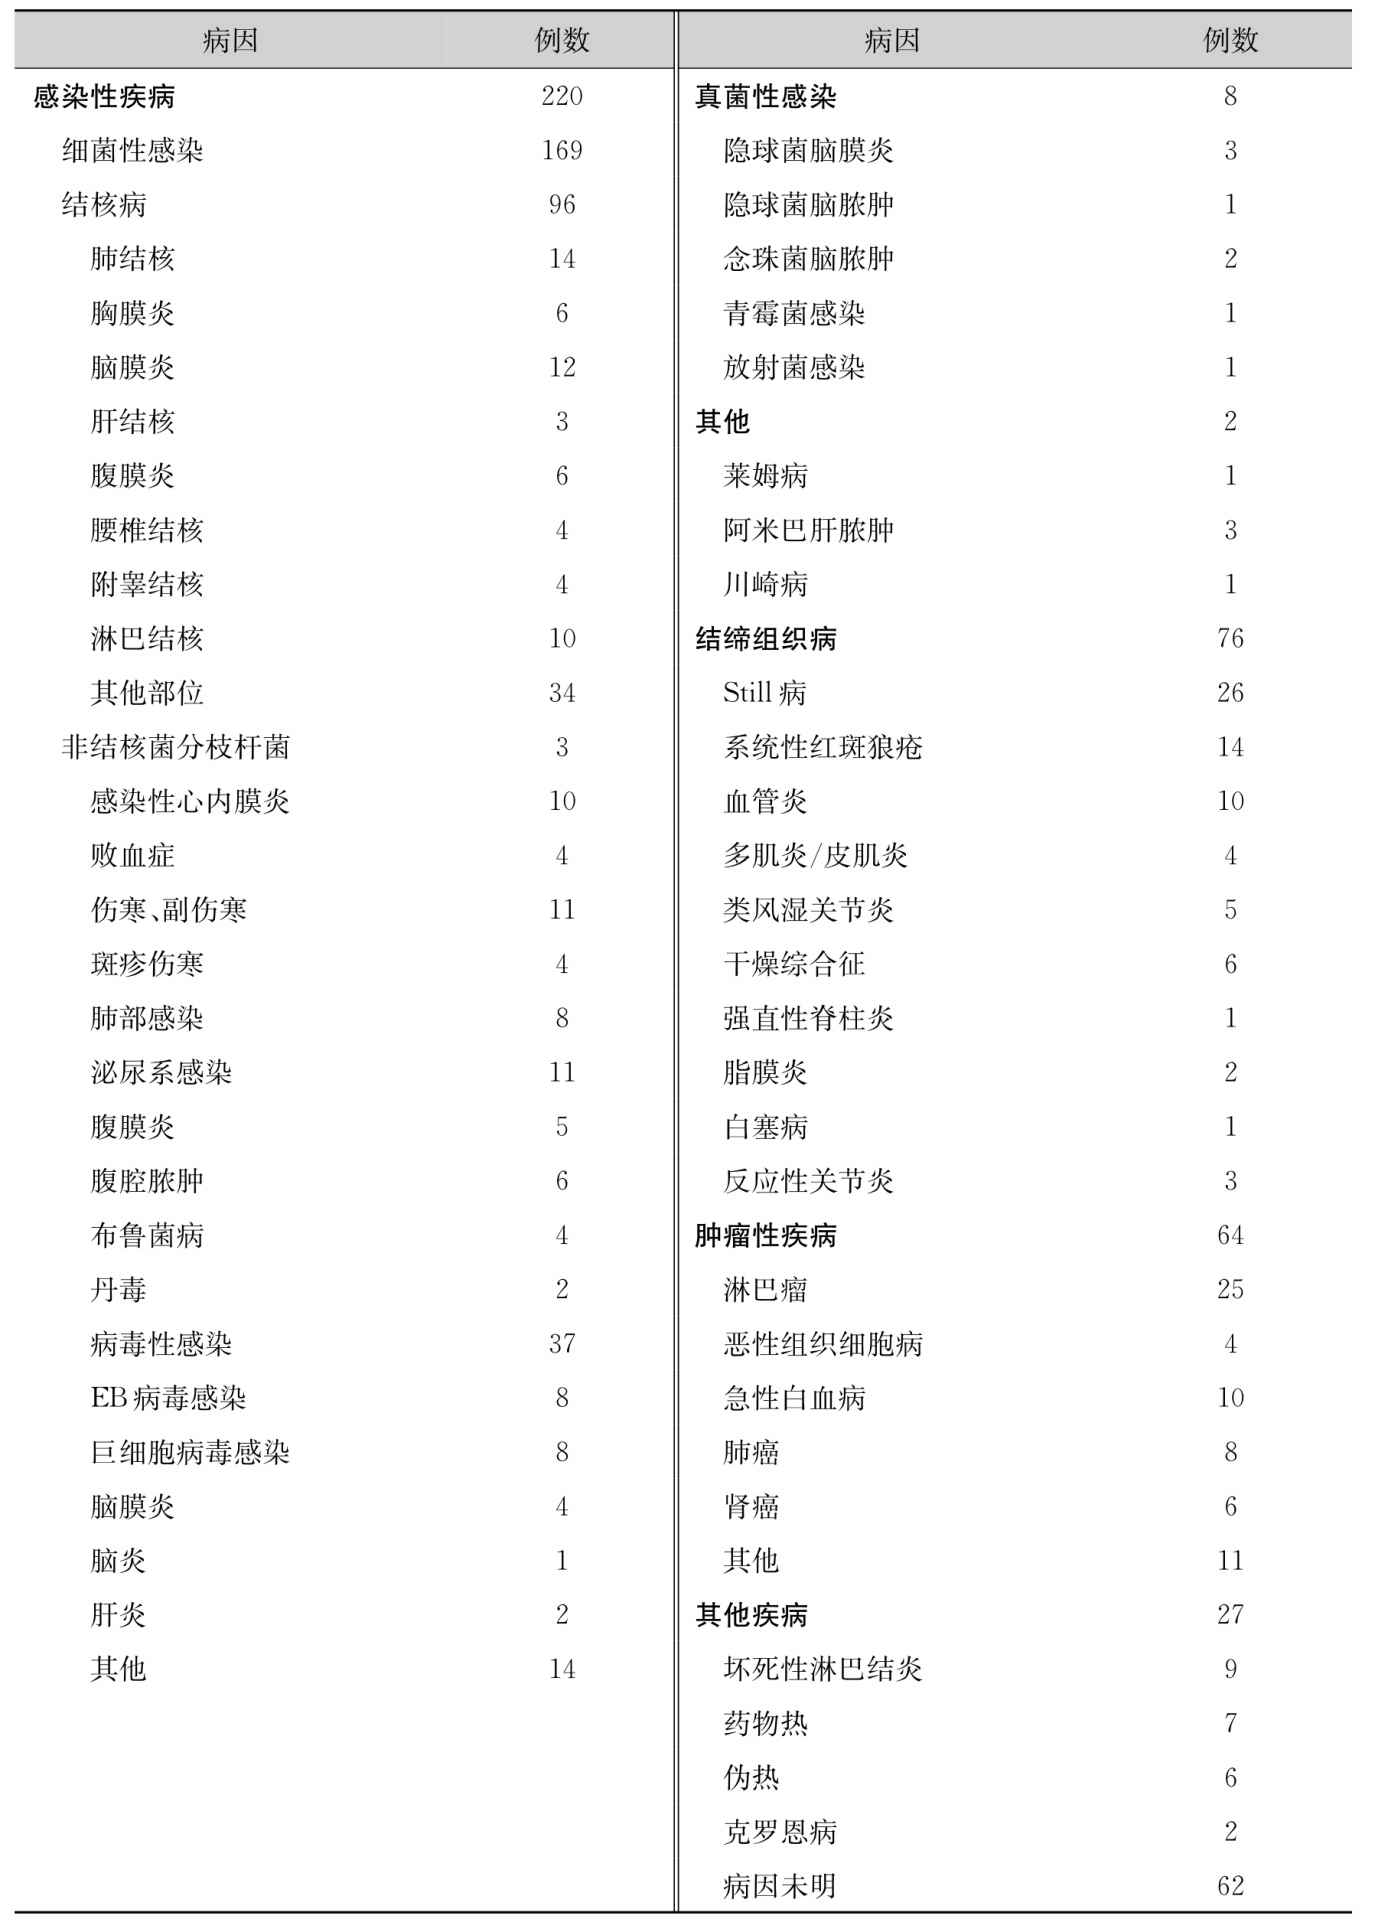
\includegraphics[width=.7\textwidth,height=\textheight,keepaspectratio]{./images/Image00024.jpg}
 \captionsetup{justification=centering}
 \caption{脑裂畸形、双侧额叶巨脑回\\{\small  A、B为同一患者,大脑半球表面两侧均有裂隙,脑皮质沿裂隙内折,位于裂隙两侧,裂隙关闭不与侧脑室相通,灰质相应内移,双侧额叶巨脑回}}
 \label{fig2-8}}
  \end{figure} 



\begin{figure}[!htbp]
 {\centering
 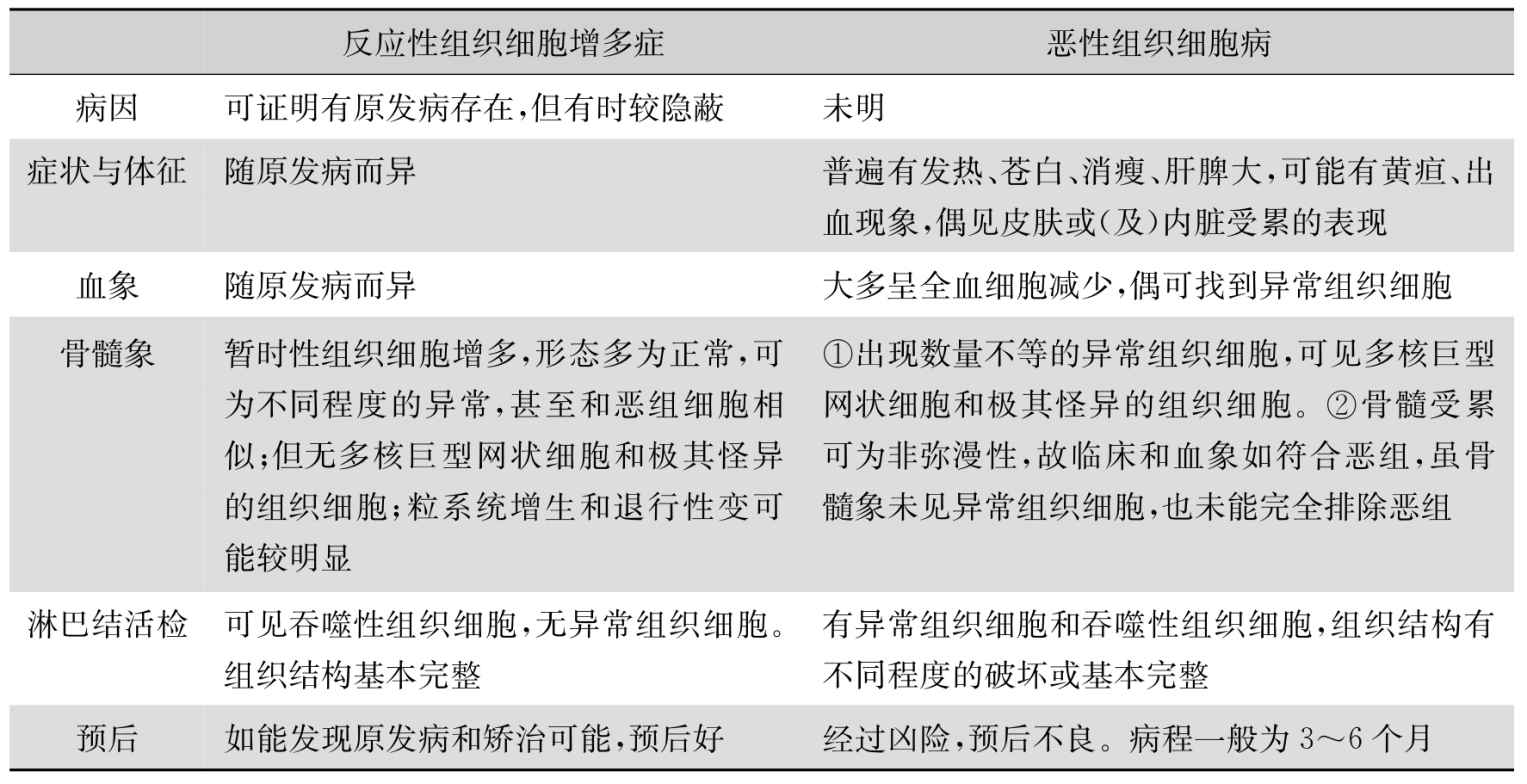
\includegraphics[width=.7\textwidth,height=\textheight,keepaspectratio]{./images/Image00025.jpg}
 \captionsetup{justification=centering}
 \caption{巨脑回}
 \label{fig2-9}}

 右侧额、顶叶脑回弥漫性异常增宽,皱褶减少
  \end{figure} 



\subsubsection{多微脑回畸形}

亦称多小脑回畸形(但该名称易与小脑病变混淆),脑回小且数目增多。

\subsubsection{鹅卵石样脑回畸形}

为复杂的脑畸形,包括鹅卵石样皮质、白质异常、脑室扩大,及脑干、小脑变小并伴有小脑的多微脑回。皮质的异常为无脑回、巨脑回和多微脑回的混合。

\subsection{灰质异位}

本病为灰质在异常部位的聚集。

\textbf{【病因病理】}
原因不明,可能与遗传性、血管性、感染性、环境因素(中毒、辐射、胎儿酒精综合征等)等有关。病理上根据异位灰质灶是否与室管膜相连分为室管膜下型和非室管膜下型,根据病变范围又可分为局灶性和弥漫性。弥漫性90%为女性,往往具有家族史。本病还可伴有其他畸形。

\textbf{【临床表现】}
单纯的灰质异位预后好,可无症状或仅有癫痫。病灶较大或同时伴有其他畸形可表现为中度或严重发育延迟、偏瘫伴癫痫。

\textbf{【CT表现】}
白质内有与灰质密度相等的异常影,增强扫描密度与灰质一致。本病有多种分型方法,通常可分为以下3型。①结节型:呈结节状分布于侧脑室旁,并可突向脑室。②板层型:不规则分布于白质内。③带状型:呈带状分布于白质或皮层下(是最严重的类型,常伴有难治性癫痫,预后相对差)。前两型可单发或多发、单侧或双侧,灰质结节直径1~30mm,无水肿和占位效应。带状型多分布对称,且表面脑回多正常,故较难分辨,易漏诊。

\subsection{脑大畸形}

本病又称头大畸形、巨脑症,为先天性大脑皮质增厚及神经胶质细胞增生。

\textbf{【病因病理】}
本病病因不明,可与遗传因素有关。有学者认为包括体积过大和质量过重两种情况,并将它分为解剖型和代谢型巨脑症。解剖型指细胞体积或数目大于正常,可伴软骨发育不全、神经纤维瘤病、结节性硬化和Chiari畸形等。代谢型是指异常代谢产物积蓄致脑细胞增大,部分伴白质发育不良。本病出生时脑重即可达1600g,或生后头颅迅速增大,皮质和髓质均增厚,可有髓鞘形成不良,无脑积水。

\textbf{【临床表现】}
儿童期发病,常有癫痫和智能低下。头颅周径增大,似先天性脑积水,但无眼球下斜征象(落日征),常有视、听力障碍。

\textbf{【CT表现】}
头颅和颅腔明显增大,大脑皮质增厚,但脑组织密度正常。脑室正常或轻度扩大,脑沟、池正常,中线结构居中。前囟较大、闭合延迟,颅板较薄。

\textbf{【鉴别诊断】}
应注意与继发性巨脑症(如较弥漫的肿瘤、结节性硬化、海绵状硬化及脑积水)、单侧巨脑畸形相鉴别。

\subsection{脑小畸形}

本病又称小脑症、小头畸形或脑小症,发病率为2.5/10万。

\textbf{【病因病理】}
病因不明,可包括先天性遗传因素和胎儿期、新生儿期的各种致病因素如感染、出血、缺氧、产伤等。病理表现为脑小,重量为正常的1/4~1/3,并且脑回结构简单,皮质发育不全,神经元数目减少、排列不整齐,颅骨和颅腔发育小,可合并其他脑发育畸形。

\textbf{【临床表现】}
常表现智能低下甚至呈白痴,也可合并癫痫、运动功能障碍等,出生时头小、外形特殊。

\textbf{【CT表现】}
轻度者可无阳性表现,病变明显时脑室系统和蛛网膜下腔可扩大,皮质光滑,缺乏脑沟、回。严重者可合并胼胝体发育不全、透明隔发育异常、穿通畸形等。颅腔缩小以额部明显,颅板较厚,板障增宽,内板平坦光滑。

\textbf{【鉴别诊断】}
狭颅畸形是颅缝过早闭合限制了脑的发育所致。颅腔常有变形,颅骨脑回压迹增多,且脑室、脑沟、脑池及脑实质常无明显异常,不难与脑小畸形鉴别。此外,一侧大脑半球发育不全与脑小畸形病因病理一样,临床和CT表现相近,不难诊断和鉴别。

\subsection{积水型无脑畸形}

本病是一组少见的先天性前脑畸形,见于婴幼儿,发生率新生儿中占0.2%左右。

\textbf{【病因病理】}
可能与胚胎期脑供血障碍有关,也有人认为是全脑穿通畸形。主要病理改变为双侧大脑半球的额、顶、颞叶完全或大部分缺如,由充满脑脊液的囊性区域取代,其内衬由软脑膜构成(不含室管膜)。基底节、丘脑、中脑可部分或大部分破坏,小脑、桥脑、延髓可发育正常或畸形,脑室系统偶可保存完好,脑膜正常存在,颅骨颅腔大小形态正常或增大。

\textbf{【临床表现】}
头围逐渐增大,多智力低下,可有眼球不规则运动、眼落日征,以及肌张力高、腱反射亢进、抽搐或惊厥、运动机能障碍等。

\textbf{【CT表现】}
幕上双侧大脑半球、脑室大部分缺失,整个颅腔大部分呈脑脊液密度。仅于脑底部见残存的部分枕、额或(和)颞叶组织,基底节、丘脑部分存在,大脑镰完整存在。幕下结构正常,但脑干可略变细。

\textbf{【鉴别诊断】}
有学者把极其严重的双侧性开唇型脑裂畸形归类于积水性无脑畸形中,影像学二者难以鉴别,但后者还能识别脑室轮廓,特别是前角的下部和后角。还应注意与无脑叶型前脑无裂畸形、穿通畸形、巨大蛛网膜囊肿及重度脑积水鉴别。

\subsection{脑穿通畸形}

本病是在脑组织分化发育充分之后,由于各种原因造成的脑组织破坏缺损,并与蛛网膜下腔或脑室相通。

\textbf{【病因病理】}
有先天性和获得性之分。先天性病因不明,可能与胎儿期血管闭塞或发育畸形有关;获得性是由于外伤、感染、缺氧、血管疾病引起正常脑组织坏死液化。缺损边缘为胶质瘢痕,不含神经细胞。

\textbf{【临床表现】} 依病变范围而定,可表现运动障碍、癫痫等。

\textbf{【CT表现】}
脑实质内巨大的脑脊液密度样囊肿,界限清楚,增强扫描无强化。与脑室或(和)蛛网膜下腔相通是诊断的关键,同侧侧脑室一般相应扩大。

\subsection{先天性中脑导水管狭窄}

本病亦属脑的发育畸形。

\textbf{【病理】}
狭窄多位于导水管口以下3~4mm处。狭窄的形态多样,可呈线状、鸟嘴状、漏斗状、隔膜状或分叉状,狭窄以上脑室积水。

\textbf{【临床表现】} 临床症状常开始于幼儿,呈慢性脑积水表现。

\textbf{【CT表现】}
侧脑室及第三脑室对称性扩大,第四脑室正常或略小。侧脑室周围有带状低密度区,代表阻塞性脑积水的典型表现。重度积水患者,可表现幕上大脑半球区为水样低密度,额、顶、颞叶脑实质几乎消失或残留极少,部分枕叶、基底核和丘脑保存,小脑和脑干发育一般正常,第四脑室位置、形态正常,可见正常大脑镰结构(图\ref{fig2-10}),MR可显示狭窄的形态。

\begin{figure}[!htbp]
 {\centering
 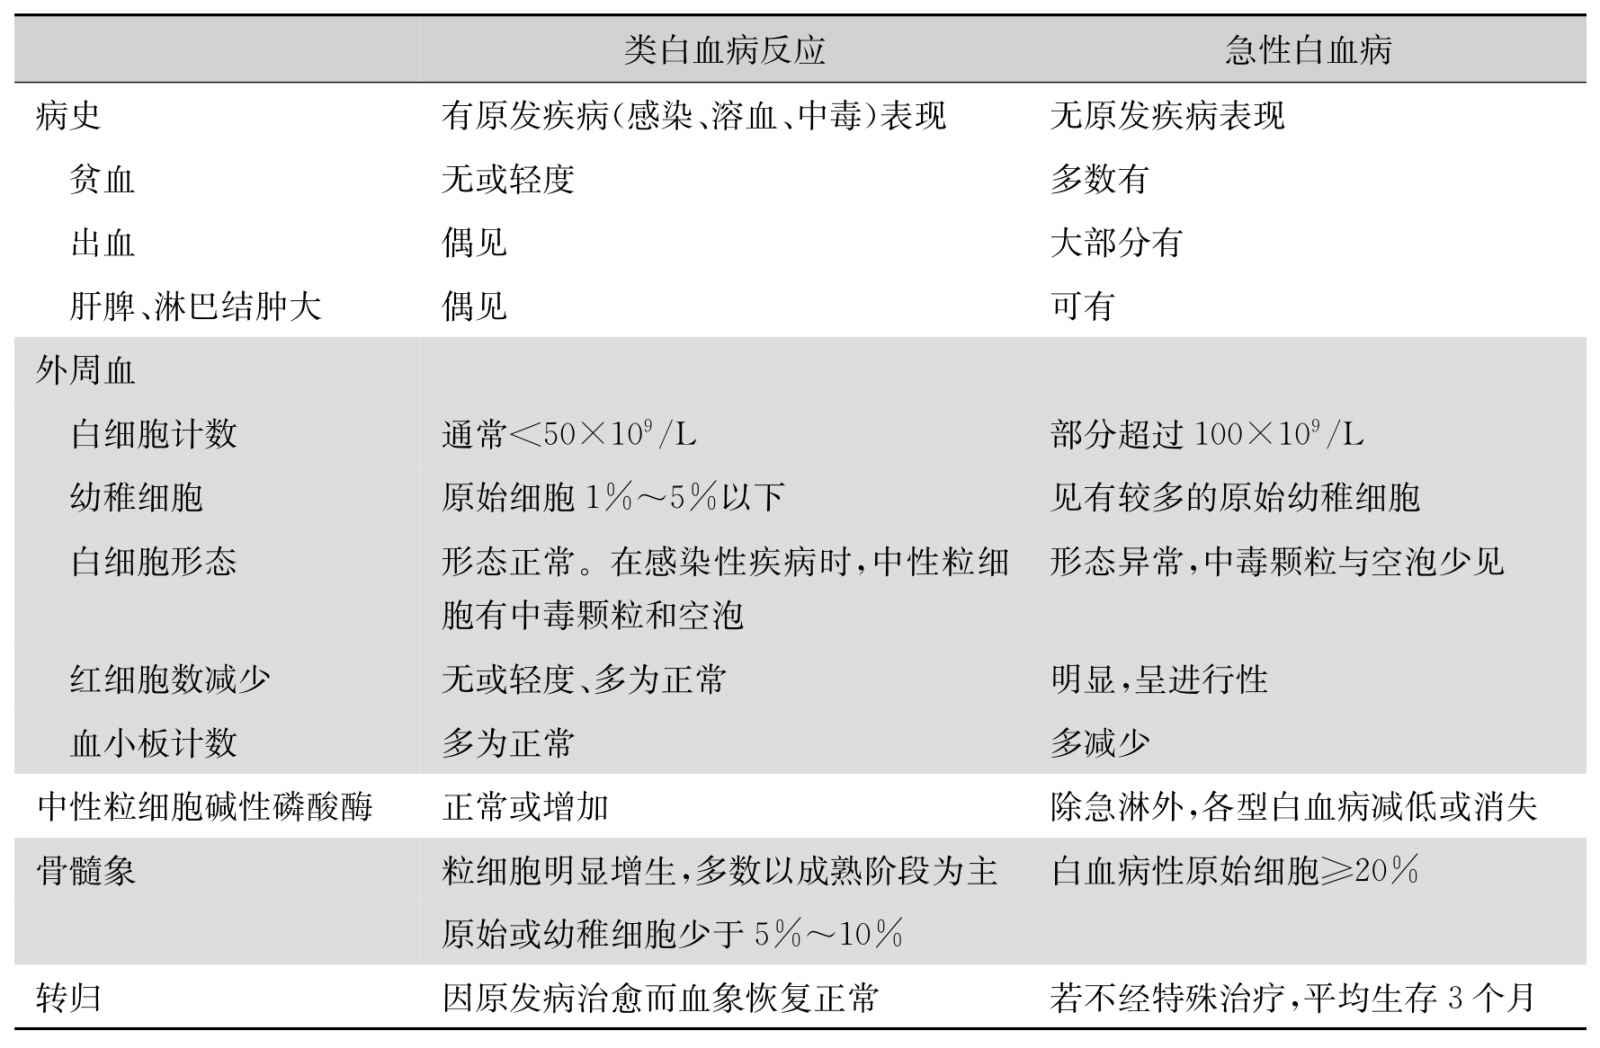
\includegraphics[width=.7\textwidth,height=\textheight,keepaspectratio]{./images/Image00026.jpg}
 \captionsetup{justification=centering}
 \caption{先天性中脑导水管狭窄\\{\small  A、B为同一患者,可见第三脑室、侧脑室积水扩张,额、顶、颞叶脑实质部分残留,枕叶、部分基底核和丘脑保存,小脑和脑干发育正常,第四脑室正常}}
 \label{fig2-10}}
  \end{figure} 



\textbf{【鉴别诊断】}
应注意与松果体区和中脑肿瘤压迫所致的导水管狭窄相鉴别,但肿瘤有占位表现且导水管有移位。炎性粘连所致的导水管狭窄与本病不易鉴别。此外,积水性无脑畸形大脑结构几乎完全消失、脑室基本无残留,枕叶一般相对完整,可予鉴别。

\subsection{结节性硬化症}

本病又称为Bourneville病,是一种较少见的常染色体显性遗传病,发病率约为1/50000~2/10000。

\textbf{【病理】}
病理特征为皮质结节、白质内异位细胞团和脑室内的小结节。结节可发生于皮质、室管膜下,皮质结节最常位于额叶,其次枕叶,偶见于基底节、丘脑、小脑和脑干。皮质结节内含有细胶原纤维、奇异的胶质细胞或不典型的神经元,多数有钙化。脑白质内异位细胞团也是由胶质细胞和神经节细胞组成。室管膜下结节最易钙化,易伴发室管膜下巨细胞型星形细胞瘤,也可伴有视网膜的错构瘤及其他内脏肿瘤。皮质腺瘤由皮质腺、结缔组织和血管组成,但国外有学者认为面部多发的不是皮脂腺瘤,无皮脂腺样结构,而是血管纤维瘤。

\textbf{【临床表现】}
典型的三联征为:①皮质腺瘤占90%;②癫痫发作;③智力低下。但三者不一定同时出现。皮质腺瘤主要位于面颊、鼻、额或两耳处,为对称散发、针头大小、黄红色透亮的坚硬蜡状丘疹。本病还可有眼、心、肾、肺、骨骼病变。

\textbf{【CT表现】}
有以下几方面:①皮质结节:可见脑回扩大、增宽,结节呈低密度,周围为等密度厚皮质围绕。一般无强化,故有人称为空心型病灶。此外,还可呈“H”型皮质结节(低密度病灶中间有一等密度横道)和高密度团块。②室管膜下结节:位于脑室边缘,50%以上双侧对称多发,结节大小不等,部分钙化,未钙化部分强化著(图\ref{fig2-11})。③室管膜下区星形细胞瘤:常位于室间孔附近。④脑白质内异位的细胞丛:皮髓交界区或更广泛的白质内见一些更低密度区。⑤其他:可有脑沟增宽等脑萎缩表现;阻塞室间孔可有脑积水表现。

\begin{figure}[!htbp]
 \centering
 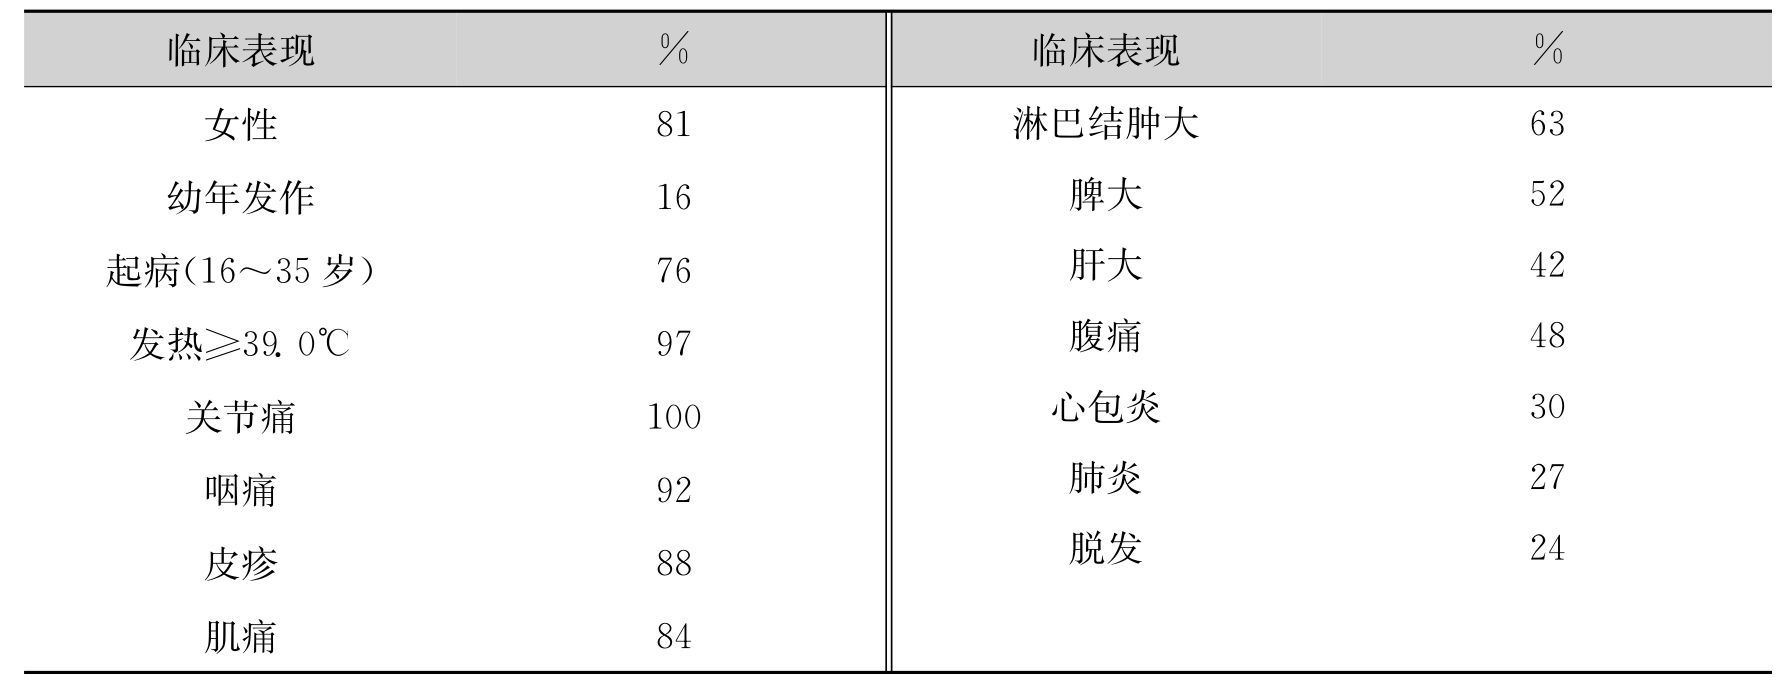
\includegraphics[width=.7\textwidth,height=\textheight,keepaspectratio]{./images/Image00027.jpg}
 \captionsetup{justification=centering}
 \caption{结节性硬化症\\ {\small 左右侧侧脑室边缘可见多个钙化结节,大小不等;右侧额叶有局限性萎缩表现}}
 \label{fig2-11}
  \end{figure} 



\subsection{脑颜面血管瘤病}

本病又称Sturge-Weber综合征或软脑膜血管瘤病。

\textbf{【病因病理】}
此病多为散发,很少有家族遗传史,偶为常染色体显性遗传。病变的分布特点为面部三叉神经分布区皮肤毛细血管瘤和同侧颅内软脑膜血管瘤,病侧大脑发育不良或萎缩。由于软脑膜血管瘤长期压迫或继发性脑缺血可引起皮质梗死,神经节细胞减少、变性,神经胶质增生伴皮质钙化,30%可发生青光眼与脉络膜血管瘤。

\textbf{【临床表现】}
癫痫、痴呆、智力低下,轻偏瘫、偏盲,先天性青光眼、牛眼症(先天性白瞳症)等,还可合并阴睾、脊柱裂等。面部分布葡萄酒色的血管痣,称作火焰痣或葡萄酒斑,出生时即可存在,主要分布在一侧三叉神经分布区,一般同颅内软脑膜血管瘤位于同一侧,但少数也可位于双侧或对侧面部。此外,约5%~15%的患者无面部血管痣。

\textbf{【CT表现】}
患侧皮层曲线状或脑回状钙化为本病特征(图\ref{fig2-12})。患侧大脑皮质萎缩伴脑沟裂、脑池增宽增深及同侧脑室扩张,钙化周围可见梗死灶,偶见出血灶。同侧脑室脉络丛有时增大,颅盖骨板障可增厚。增强扫描钙化灶周围及钙化区可明显强化;增大的脉络丛(亦属血管瘤)有明显强化。在发现脑实质内的缺血缺氧、胶质增生和脱髓鞘改变方面CT不及MR。

\begin{figure}[!htbp]
 \centering
 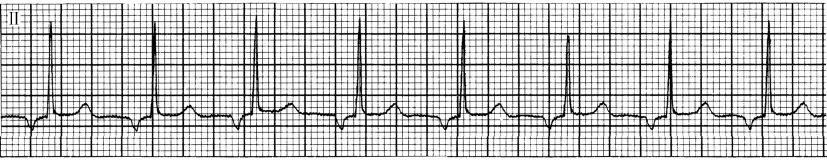
\includegraphics[width=.7\textwidth,height=\textheight,keepaspectratio]{./images/Image00028.jpg}
 \captionsetup{justification=centering}
 \caption{Sturge-Weber综合征\\{\small 右侧额叶皮层曲线状钙化,局部脑沟增宽增深}}
 \label{fig2-12}
  \end{figure} 



\textbf{【鉴别诊断】}
颅内类似的脑回状钙化也可见于胶质瘤、脑梗死、化脓性脑膜炎、骨化性脑膜脑病,故应结合本病的其他征象及临床特征予以鉴别。

\subsection{共济失调性毛细血管扩张症}

本病又称Louis-Bar综合征,是一种常染色体隐性遗传性疾病,发病率约1/40000,主要发生在儿童,男女发病相近。

\textbf{【病理】}
主要病理改变是小脑皮质萎缩,尤以蚓部为甚,齿状核-橄榄体退变、脑干中的轴索肿胀。小脑血管异常可能是其病因。

\textbf{【临床表现】}
主要特征是小脑机能障碍(共济失调),进行性眼皮(可涉及眼结膜)毛细血管扩张。患儿易患鼻窦炎、肺部感染,以及淋巴系统肿瘤。

\textbf{【CT表现】}
主要表现为以蚓部为主的小脑萎缩。小脑沟增宽增深、数目增多,小脑下蚓发育不良,四脑室扩张,小脑周围蛛网膜下腔、脑池增宽。如伴脑实质毛细血管扩张破裂,可出现脑出血。有时可见脑梗死,由来自肺内血管畸形的栓子所致。

\subsection{神经纤维瘤病}

本病是中胚层和神经外胚层的常染色体显性遗传病。

\textbf{【病理】}
主要是神经外胚层结构的过度滋生、中胚层异常发育及多发性肿瘤形成,可累及全身各系统和器官。有学者将本病分为以下5型。Ⅰ型:为局限性神经纤维瘤病,以丛状神经瘤为特征;Ⅱ型:为全身性皮肤神经纤维瘤病,以多发性皮肤结节及皮肤色素斑为主要表现;Ⅲ型:为深部周围神经干的神经瘤、神经纤维瘤和神经鞘瘤,以深部神经干过分受累为特征;Ⅳ型:为颅神经干的神经瘤、神经纤维瘤、神经鞘瘤,以双侧听神经瘤为多见;Ⅴ型:为并发脑瘤和脑瘤样变,可合并脑膜瘤、胶质瘤、血管瘤、黑色素瘤、结节性硬化、脊髓空洞症、播散性胶质结节增生等。其中Ⅰ型最常见,约1/1000神经纤维瘤可恶变。

颅内最常见的肿瘤有听神经瘤(多为双侧)、视神经胶质瘤、三叉神经瘤、基底节和丘脑部胶质瘤及多发性脑膜瘤等。此外,还可有脊神经根或马尾的神经纤维瘤、脊膜瘤,颅骨和脊柱发育异常也较常见。

\textbf{【临床表现】}
本病可见于任何年龄,但在10~20岁和50~70岁有两个发病高峰期,男多于女。其临床特点是皮肤可见特征性棕色斑(奶油咖啡色素斑)伴皮肤软组织肿块以及各组织的肿瘤形成,可有轻度思维障碍和癫痫。约1/2病例有骨骼改变(系中胚叶发育障碍和神经纤维瘤侵蚀所致),还可并发甲状旁腺功能亢进和肢端肥大症。

\textbf{【诊断标准】}
美国国立卫生研究院的诊断标准如下:①体表至少有5个直径>5mm的咖啡斑;如果是青春前期,则应有6个以上且直径>15mm;②临床或组织学证实有2个以上的神经纤维瘤或丛状神经纤维瘤;③在腋窝或腹股沟部出现多发性雀斑;④蝶骨翼结构不良或伴有骨发育畸形;⑤双侧视神经的神经胶质瘤;⑥裂隙灯检查示虹膜有2个或更多的Lish结节;⑦患者一级亲属中患有本病。具备其中两条或两条以上即可诊断为本病。

\textbf{【CT表现】}
颅内肿瘤常见的是听神经瘤,其次为三叉神经和颈静脉孔区神经纤维瘤;脑膜瘤约半数多发;偶并发胶质瘤,可发生于视交叉、脑干与基底核处。脑发育异常可有脑大畸形、胼胝体发育不全、Chiari畸形、巨脑回畸形、灰质异位等。脑血管异常有动脉瘤、动静脉畸形和动静脉瘘等。眶内肿瘤可为视神经纤维瘤、脑膜瘤或胶质瘤。脊髓肿瘤可以是马尾神经纤维瘤、脊膜瘤或室管膜瘤。

\subsection{小儿21-三体综合征}

本病又称先天愚型、Down综合征,是常见的染色体异常疾病,21号染色体三体是生殖细胞在减数分离过程中,发生不分离所致。

\textbf{【病因病理】}
与母亲妊娠时的年龄(年龄越大发病率越高)、遗传因素、妊娠时化学药物堕胎、放射线、自身免疫性疾病有关。本病主要病理变化为中枢神经系统发育异常。患儿染色体核型为47,XX(XY),+21,双亲核型正常。

\textbf{【临床表现】}
患儿表现在出生时就很显著,有的体征到1岁时才明显。根据其特殊的愚型面容、皮纹特征和智能落后容易诊断。

\textbf{【CT表现】}
①脑内钙化:多见于基底节区,呈点状或小圆形;②大脑发育不良:侧裂、额顶区蛛网膜下腔增宽;③小脑发育不良:轻度对称性小脑发育不良常见于本病;④脑干可变小,桥小脑角池、枕大池相应增大;⑤
<1岁的婴儿CT可表现正常,可能与病程演变有关。

\textbf{【鉴别诊断】}
本病应注意与结节性硬化、甲状旁腺功能减退(图\ref{fig2-13})、弓形体病、Fahr病相鉴别。

\begin{figure}[!htbp]
 {\centering
 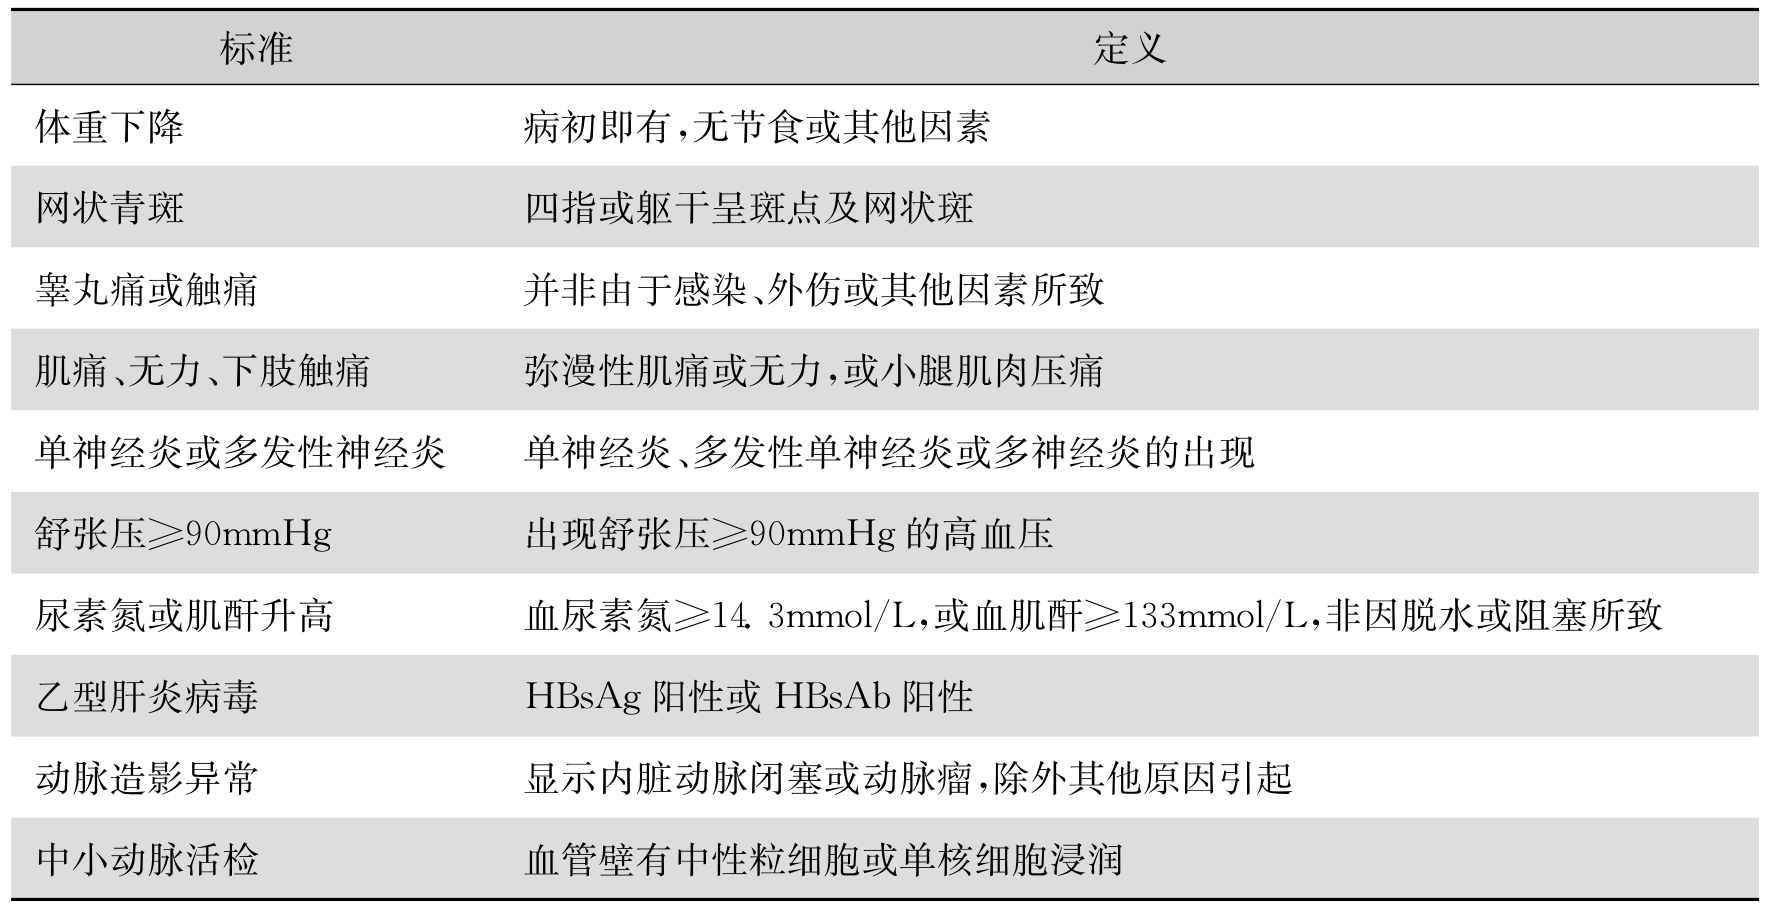
\includegraphics[width=.7\textwidth,height=\textheight,keepaspectratio]{./images/Image00029.jpg}
 \captionsetup{justification=centering}
 \caption{甲状旁腺功能减退\\{\small  A、B为同一患者,男14岁,左右侧基底核、左右侧丘脑、皮髓质交界处广泛对称性钙化}}
 \label{fig2-13}}
  \end{figure} 



\section{新生儿及婴幼儿脑疾病}

\subsection{正常新生儿和早产儿脑的CT特点}

\subsubsection{正常新生儿的脑CT表现}

1.白质密度较低:与新生儿脑组织水分含量多(且与胎龄成反比)有关。正常新生儿的脑白质密度为18~28Hu(平均>21Hu),脑灰质为26~39Hu(平均31Hu)。

2.灰白质分界模糊:人脑传导系统从胎龄7个月开始发育,神经纤维逐渐从白质伸向灰质,但出生时为数尚少,且髓鞘形成尚不完全;同时小儿脑富含蛋白质,而脂类含量少,故灰白质交界缺乏密度差异。

3.硬膜窦密度高:与窦内血流缓慢、血容量大、富含红细胞和血红蛋白等有关。

4.基底部脑池和第四脑室宽大:是因胎儿及新生儿大脑发育优于小脑和脑干所致,故桥前池和桥小脑角池亦显示较宽,纵裂池相对较窄。

5.透明隔间腔:8个月以前胎儿全部存在,新生儿82%存在,随年龄增长发生率下降。2~5周岁时为5%~6%,5~9周岁时为2.7%,10~14周岁为2.3%。

\subsubsection{早产儿的脑CT表现}

早产儿脑发育不成熟,脑组织含水量高,脑髓质化不完全,缺乏髓鞘形成,在颅脑CT扫描时可存在较广泛的或弥漫性白质低密度区,皮层灰质较薄,密度相对较高(图\ref{fig2-14}B),灰白质分界清楚,且与颅骨、脑室间形成良好的对比。

\subsection{新生儿缺氧缺血性脑病}

本病是围产期缺氧引起的脑部损害,在小儿CT检查中占7.2%,在新生儿CT检查中占94%,甚至有报道达94%~100%。

\textbf{【病因病理】}
主要病因是窒息,由宫内窒息引起的占50%,娩出过程窒息的占40%,其余10%由生后肺部疾病、呼吸暂停、红细胞增多症、败血症、先心病等所致。缺氧导致细胞内水肿、血管源性水肿,进而发生脑坏死,并由于血管通透性增加和脑血管调节失调、静脉压升高而发生颅内出血。

\textbf{【临床表现】}
可分为3度:①轻度:表现兴奋、易激惹、肢体颤动、肌张力高、反射活跃,症状于1天内好转。②中度:嗜睡、反应迟钝、肌张力低、反射减弱、惊厥、呼吸不规则,症状于1周内消失,可有后遗症。③重度:神志不清、肌张力松软、反射消失、反复发生惊厥、呼吸不规整、瞳孔不对称、对光反应消失,常在1周内死亡,存活者可有脑瘫、脑积水、智力低下、癫痫等后遗症。

\textbf{【CT表现】}
主要为脑水肿、颅内出血及脑组织坏死。①脑水肿:是早期重要征象,脑实质密度(主要是白质密度)减低,CT值≤18Hu,好发于额、顶叶。前囟隆起、颅缝增宽,脑沟、回浅扁且脑室变窄,脑室、脑池受压(图\ref{fig2-14}A)。②颅内出血:多为蛛网膜下腔出血,但脑外伤亦可致蛛网膜下腔、硬膜下、脑室内或脑室周围出血。③脑组织坏死:早产儿脑组织坏死好发于室旁白质又称为室旁白质软化,也可液化形成软化灶。

\begin{figure}[!htbp]
 {\centering
 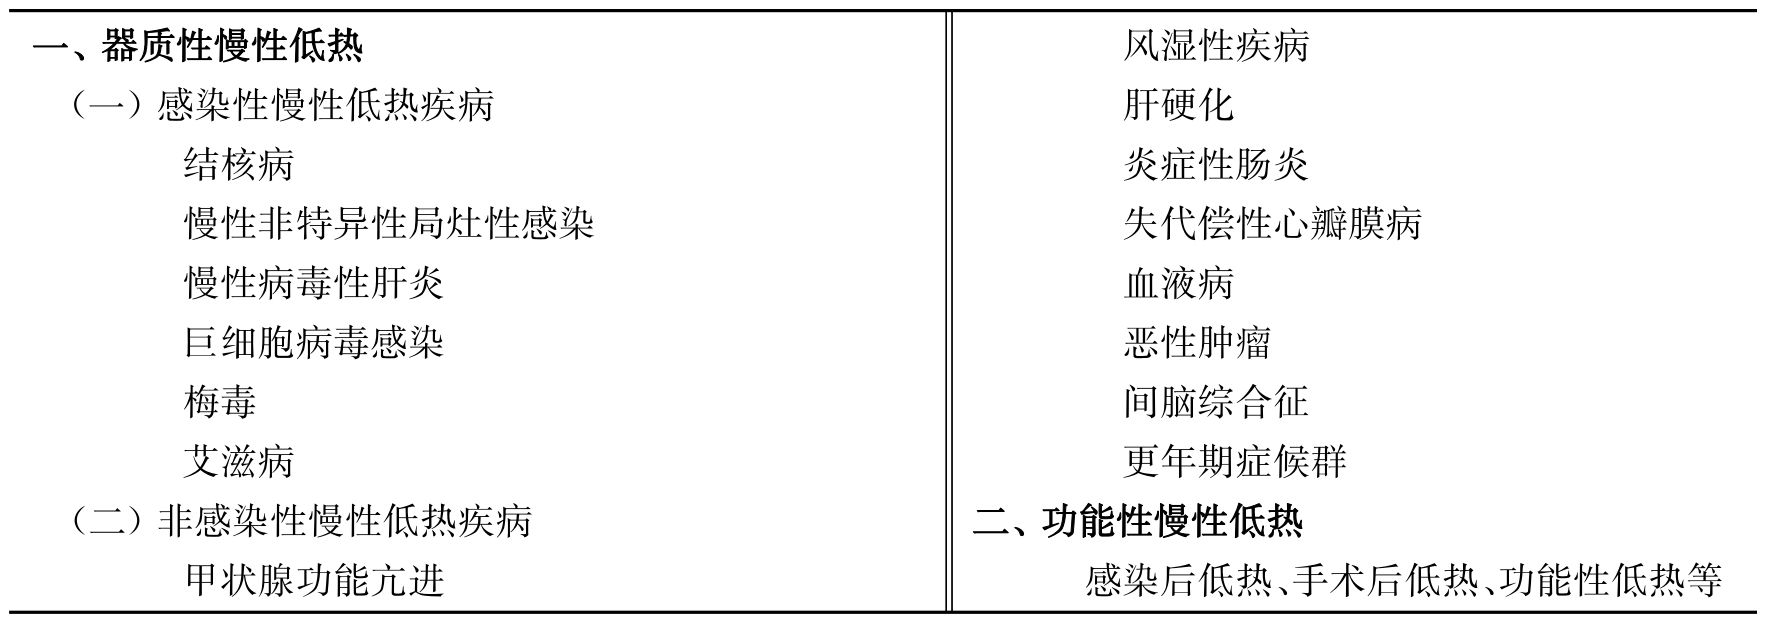
\includegraphics[width=.7\textwidth,height=\textheight,keepaspectratio]{./images/Image00030.jpg}
 \captionsetup{justification=centering}
 \caption{新生儿缺氧缺血性脑病\\{\small  A.左右额、顶叶白质区云絮状低密度灶,CT值约14~16Hu;B.皮层灰质薄,密度相对较高,灰白质分界欠清楚}}
 \label{fig2-14}}
  \end{figure} 



\textbf{【CT分度】}
①轻度:脑实质低密度影分布于1~2个脑叶,少数合并少量颅内出血(多为蛛网膜下腔出血)。②中度:低密度影超过2个脑叶,灰白质界限模糊,部分脑沟消失,约1/3合并颅内出血。③重度:弥漫性低密度影,灰白质界限消失。基底节、丘脑密度正常,脑室受压变窄,并发颅内出血者约占80%。

但我们认为对于超过2个脑叶者,如位于各叶的病灶面积均较小,且灰白质界限较清晰者,应诊断为轻度,以便于与临床分度相对应。

\textbf{【并发症】}
①轻度者于1~2个月病变多吸收,无明显后遗症。②中度者大多数亦可治愈,少数可出现外部性脑积水、脑发育不良、脑萎缩等。③重度者约35%于1周内死亡,存活者多有后遗症如脑萎缩、脑皮质变薄、脑白质减少、脑白质变性、脑软化、脑穿通畸形、钙化等。有报道病变处CT值<12Hu的重度患者多有并发症。

\textbf{【鉴别诊断】}
早产儿脑CT表现为较广泛的或弥漫性白质低密度区;皮层变薄、密度相对增高,呈花环状改变;灰白质分界清楚,脑室系统未见异常,中线结构无移位。早产儿缺氧性脑损伤灰白质界限模糊(图\ref{fig2-14}B),有颅内出血和脑室旁出血性脑梗死、脑室周围白质和脑白质发育不良及脑梗死等。两者CT表现有所区别,但早产儿合并缺氧性脑损伤时,CT难以分级。

\subsection{新生儿颅内出血}

本病是新生儿常见的急症,为新生儿死亡和以后神经发育障碍的主要原因之一。

\textbf{【病因病理】}
病因主要有新生儿缺氧缺血性脑病、产伤、早产,少数为出血性疾病、颅内先天性血管畸形。①缺氧使脑组织充血、水肿、脑血管壁通透性增高,引起渗血或点状出血;同时缺氧可使肝脏合成凝血因子发生障碍,从而加重出血。②产伤可造成硬膜窦撕裂或皮质桥静脉、脑内的静脉以及脉络丛静脉破裂。出血常见部位为硬膜下,其次为蛛网膜下腔,也可发生于脑实质、脑室内或硬膜外。③原发性出血性疾病、颅内先天性血管畸形引起的出血很少见,前者多位于蛛网膜下腔,后者可在蛛网膜下腔或脑实质内。

\textbf{【临床表现】}
少量出血时可无症状,量多时可出现激惹、尖叫、惊厥、烦躁不安、呕吐等症状,2天后出现抑制症状如嗜睡、拒奶、昏迷、四肢张力低下及呼吸不规则、青紫等。

\textbf{【CT表现】}

1.硬膜下出血:多见于足月儿,常有头皮血肿、颅骨骨折、颅缝分离。

2.蛛网膜下腔出血:最常见,有3个特征性征象。①空三角征:又称矢状窦旁征,血液积聚于矢状窦旁呈高密度,静脉窦内流动的血液呈相对低密度,底边为颅骨,形成空心形△征象。②高脚杯征:又称天幕缘征,即血液沉积于小脑幕缘上下形成“Y”或“V”形高密度影。③纵裂池边缘模糊征:即纵裂池内出血高密度影边缘模糊。以上3个征象的出现率可达50%~80%(图\ref{fig2-15})。此外,有学者认为“直窦”宽>5mm可认为有出血。

\begin{figure}[!htbp]
 {\centering
 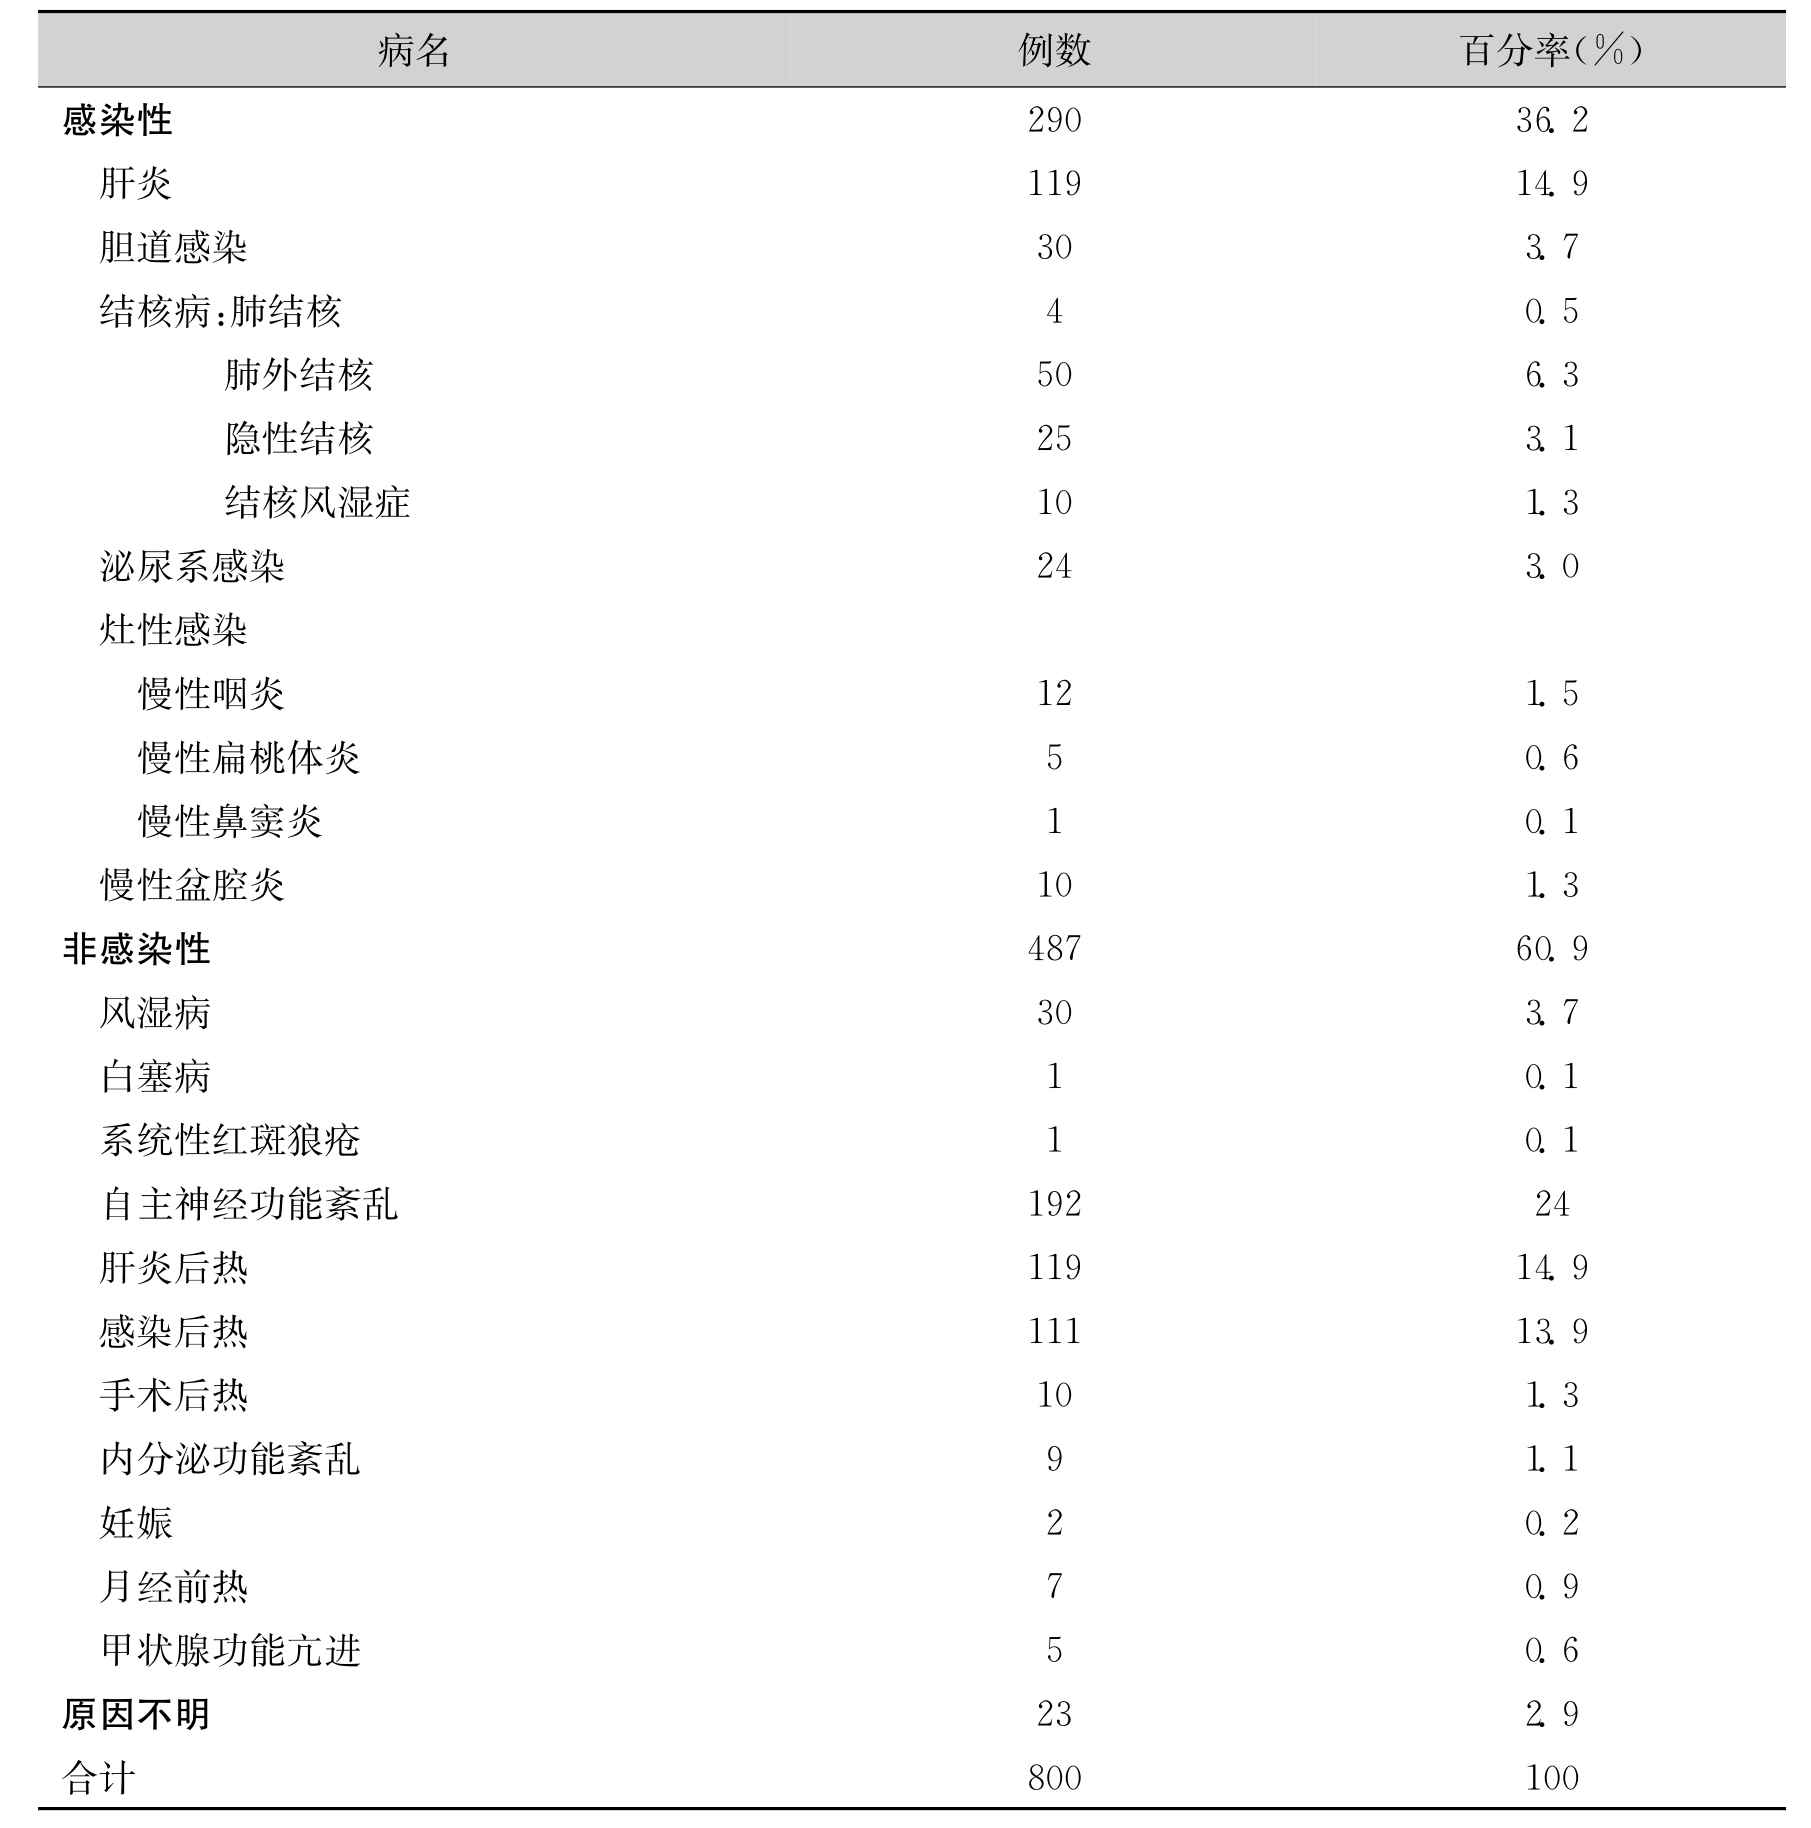
\includegraphics[width=.7\textwidth,height=\textheight,keepaspectratio]{./images/Image00031.jpg}
 \captionsetup{justification=centering}
 \caption{新生儿蛛网膜下腔出血\\{\small  A.高脚杯征;B.空三角征,伴有脑室内出血;C.纵裂池边缘模糊征}}
 \label{fig2-15}}
  \end{figure} 



3.脑实质内出血:呈点状或斑片状高密度灶,有或无水肿带。

4.室管膜下及脑室内出血:常见于早产儿。因室管膜下胚胎生发层组织发育不成熟,血液极易渗出,多量渗出可破入侧脑室,并可致脑积水。

5.其他:包括硬膜外出血和小脑出血,均较少见。

\textbf{【鉴别诊断】}
①钙化:新生儿颅内出血CT值为50~80Hu,新生儿颅内钙化少见且均为病理性,CT值>80Hu,因此不难鉴别。②晚发性维生素K缺乏症:发病年龄多在1~2个月小婴儿,出血量大、部位多,常有血团块形成、液平面出现及伴有脑梗死、大面积水肿,可予鉴别。

\subsection{婴儿维生素K缺乏症}

本病又称迟发性维生素K缺乏症、晚发性维生素K缺乏症,是指新生儿晚期(出生后2周)至乳儿期,因缺乏维生素K而引起的出血性疾病。

\textbf{【病因病理】}
常见的原因有3种:①维生素K摄入不足;②合成障碍;③吸收不良。维生素K是合成多种凝血因子所必需的辅酶,缺乏凝血因子凝血活性丧失,造成自发出血。

\textbf{【临床表现】}
发热、惊厥抽搐、呕吐、烦躁不安、拒乳、嗜睡等;可伴皮肤、消化道、上呼吸道出血等,并出现相应表现。婴儿期特别是1~4个月内母乳喂养儿若出现进行性贫血、全身出血倾向并伴急性颅内高压等精神症状应首先考虑本病。实验室凝血时间、凝血酶原时间延长及部分凝血活酶原时间延长可肯定诊断。

\textbf{【CT表现】}
①颅内出血:特点为出血量大,多发部位出血(脑实质内、外或脑室等);②脑水肿、脑梗死:是由于血管受挤压或痉挛所致,可呈广泛小片状水肿表现或大面积梗死,甚至半球缺血性改变;③脑疝;④一侧侧脑室闭塞,对侧侧脑室扩张积水;⑤并发症:存活者可致外部性脑积水、脑软化、脑萎缩、脑穿通畸形或脑发育不良。

\subsection{新生儿胆红素脑病}

持久性或明显的新生儿高胆红素血症可以导致脑部损伤。

\textbf{【病因病理】}
最常见的原因是红细胞溶血,其他原因包括红细胞增多症、胆红素结合方面的遗传或获得性缺陷、消化道运转方面的疾患及激素的紊乱等。未结合胆红素进入脑组织,结合于脑细胞膜,抑制细胞线粒体酶的活性,使脑细胞能量代谢障碍,致脑部损伤。

\textbf{【临床表现】}
足月儿常在生后2~5天,早产儿常在7天左右发生本病。典型的临床表现分为4期:①警告期;②痉挛期;③恢复期;④后遗症期。

\textbf{【CT表现】}
尚无报道本病有特异性CT表现。MR在急性期呈短T1和长T2信号;慢性期苍白球、下丘脑和海马显示长T2信号。

\subsection{血钠过高性脱水}

\textbf{【病因病理】}
最常见的原因是严重的腹泻,钠在细胞间隙中浓度升高致细胞内液体减少并皱缩。脑离开颅板导致桥静脉撕裂,另外血液的高渗致毛细血管增粗,易发生毛细血管破裂及脑实质出血。

\textbf{【临床表现】}
年幼儿童,尤其是未成熟儿对血钠过高有易感性。病儿极度冷漠、对刺激易激性高,另外还有肌肉强直、反射亢进,偶有癫痫。

\textbf{【CT表现】}
间质水肿引起脑实质密度降低,在大脑和小脑灰白质交界处可见高密度出血灶。

\subsection{新生儿低血糖症}

低血糖的标准是足月儿血糖低于16.7mmol/L(300mg/L),未成熟儿低于11mmol/L(200mg/L)。大多数低血糖的新生儿发病早,持续时间短,对葡萄糖反应迅速。但足月小样儿在子宫内就遭受营养不良,大多有临床症状,低血糖程度相对较重,持续时间可以延长,治疗需大量的葡萄糖。引起脑损害最通常的原因是继发于胰腺β细胞的先天性肿瘤或增生性胰岛素分泌过多。

\textbf{【CT表现】}
围产期低血糖脑损害表现为:①急性期:皮质和皮质下白质的脑水肿,以顶枕部最重;②慢性期:皮质和皮质下白质萎缩。

\subsection{外部性脑积水}

本病亦称良性蛛网膜下腔增宽,是一种特殊的交通性脑积水。一般2岁内自愈。

\textbf{【病因病理】}
有新生儿缺氧缺血性脑病、出血、外伤、感染等,半数病因不明为特发性。其发病机制可能为蛛网膜颗粒对脑脊液的吸收障碍所致。多数学者认为颅缝开放是其发生的前提。

\textbf{【临床表现】}
抽搐(约占50%以上)和头围增大(占1/3~2/3);部分患儿无症状。抽搐的发生与本病的严重程度密切相关。本病好发于2~24月前囟未闭的小儿,但可在生后数天发生,3~6个月为典型期,9个月~1岁开始好转,2岁前或囟门闭合前基本恢复正常。

\textbf{【CT表现】}
额叶或额、顶叶蛛网膜下腔间隙>5mm,而后部不宽。前纵裂池增宽>7mm,后纵裂池不宽。外侧裂池增宽>7mm。鞍上池稍大。额、顶叶脑沟部分增宽,但增深不著。大脑后半部及小脑正常。脑室正常或轻度扩大(图\ref{fig2-16})。

\begin{figure}[!htbp]
 {\centering
 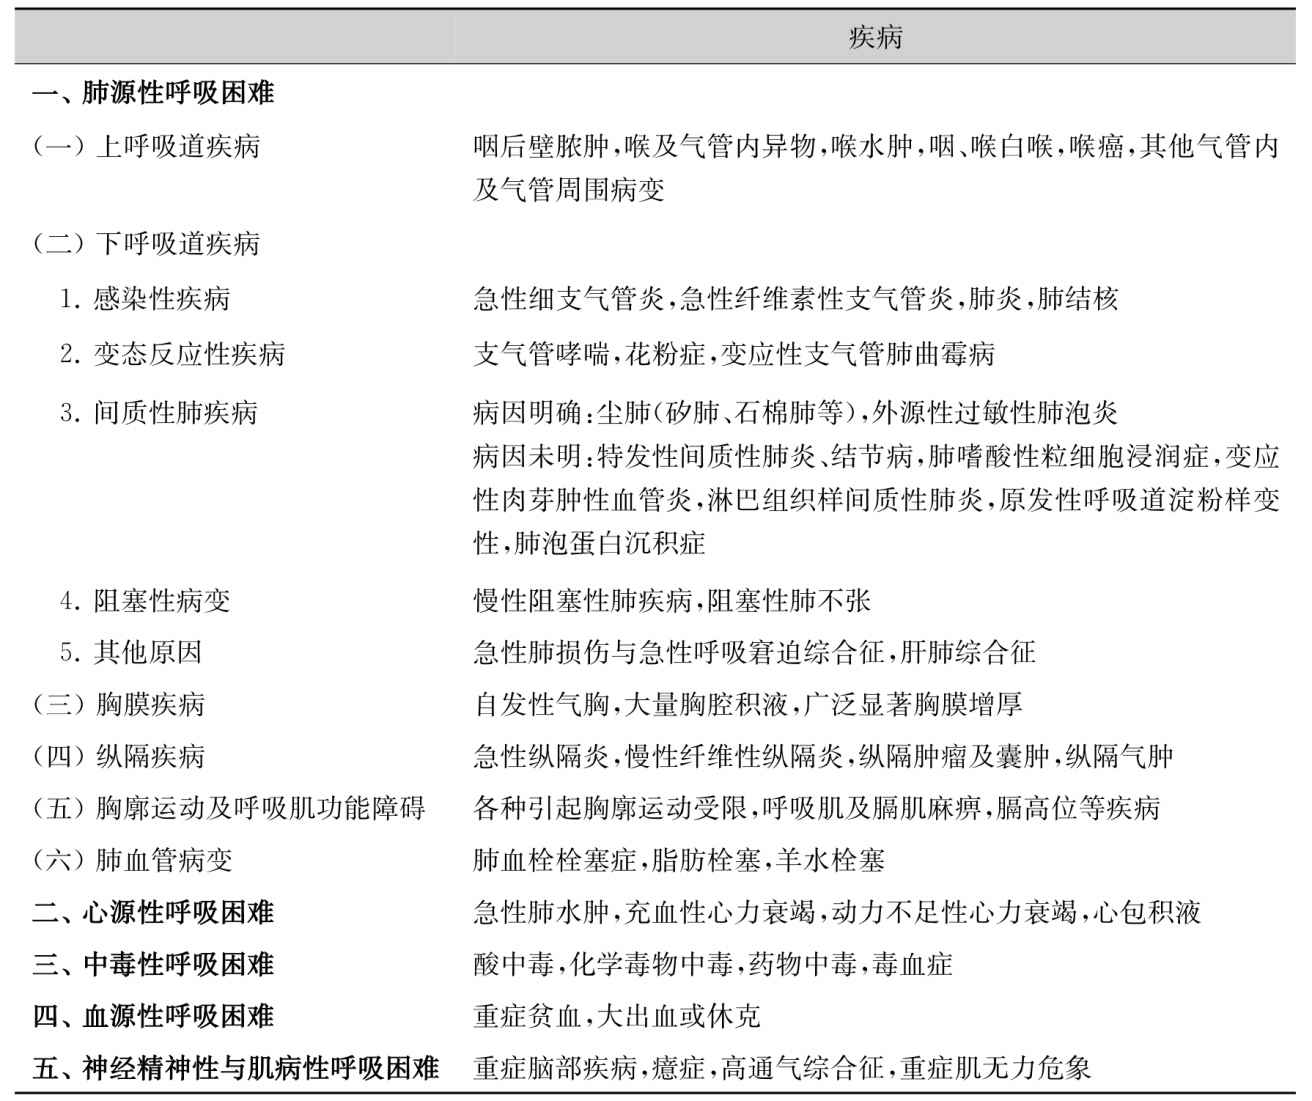
\includegraphics[width=.7\textwidth,height=\textheight,keepaspectratio]{./images/Image00032.jpg}
 \captionsetup{justification=centering}
 \caption{外部性脑积水\\{\small  A、B为同一患者,额、顶叶蛛网膜下腔间隙>5mm,而后部不宽;前纵裂池增宽>7mm,后纵裂池不宽;外侧裂池增宽>7mm}}
 \label{fig2-16}}
  \end{figure} 



总之,本病诊断的依据是:①前囟未闭的婴儿及头颅增大;②脑前部脑外积液增多,脑实质无改变;③2岁后脑外积液自然吸收。

\textbf{【鉴别诊断】}

1.在诊断外部性脑积水时,应除外其他因素引起的蛛网膜下腔增宽,其中包括促肾上腺皮质激素和皮质类固醇的治疗、脱水、营养不良以及癌肿化疗等。

2.脑萎缩:①外部性脑积水头围大,常有抽搐,无智力低下及运动障碍;而脑萎缩头围小,常有智力低下及运动障碍。②前者仅脑的前部蛛网膜下腔增宽;而脑萎缩常全脑蛛网膜下腔及脑沟增深、增宽。③前者纵裂池增宽限于前部;而后者则为整个增宽。④前者脑皮质厚度正常,脑沟可增宽但增深不著;而后者脑皮质变薄,密度减低及脑沟普遍加深。⑤脑室大小不能用于两者的鉴别,因为外部性脑积水可有轻度脑室增大。但脑萎缩时脑室与颅脑横径之比大于正常,而外部性脑积水正常。双额叶局限性脑萎缩时鉴别有一定难度,其双侧额角的局限扩大有助于与外部性脑积水鉴别。

3.硬膜下积液:本病多为单侧,双侧时常不对称,脑沟相互聚拢而不是加深加宽,不难鉴别。

4.脑发育迟缓:多表现为灰白质比例失常,常合并其他多种神经系统畸形。

\subsection{儿童脑室周围白质软化症}

本病又称为脑室周围萎缩、脑室周围白质发育不良,多认为好发于早产儿及产后窒息存活的儿童。

\textbf{【病因病理】}
与缺血缺氧及感染有关,主要损伤轴索及少突胶质细胞,但发病机制尚不清楚。病变主要分布于侧脑室三角区及枕角周围白质、额角附近白质。病理上脑白质由于缺血缺氧发生水肿、凝固、坏死,继而吸收或形成瘢痕和胶质增生,弥漫或局限的胶质损伤使髓鞘化延迟、白质减少,从而导致侧脑室扩张。

\textbf{【临床表现】}
本病可以导致脑瘫(主要是痉挛性下肢瘫或四肢瘫)、智力落后、抽搐,以及各种眼的异常如眼颤、斜视、视力下降等。

\textbf{【CT表现】}
显示脑室周围和半卵圆中心的脑白质明显减少,皮质与脑室缘距离甚小或消失,也可见呈斑片状或长条状的软化灶(图\ref{fig2-17})。一侧或两侧侧脑室扩大,扩大的脑室轮廓不规则可与脑积水鉴别。

\begin{figure}[!htbp]
 \centering
 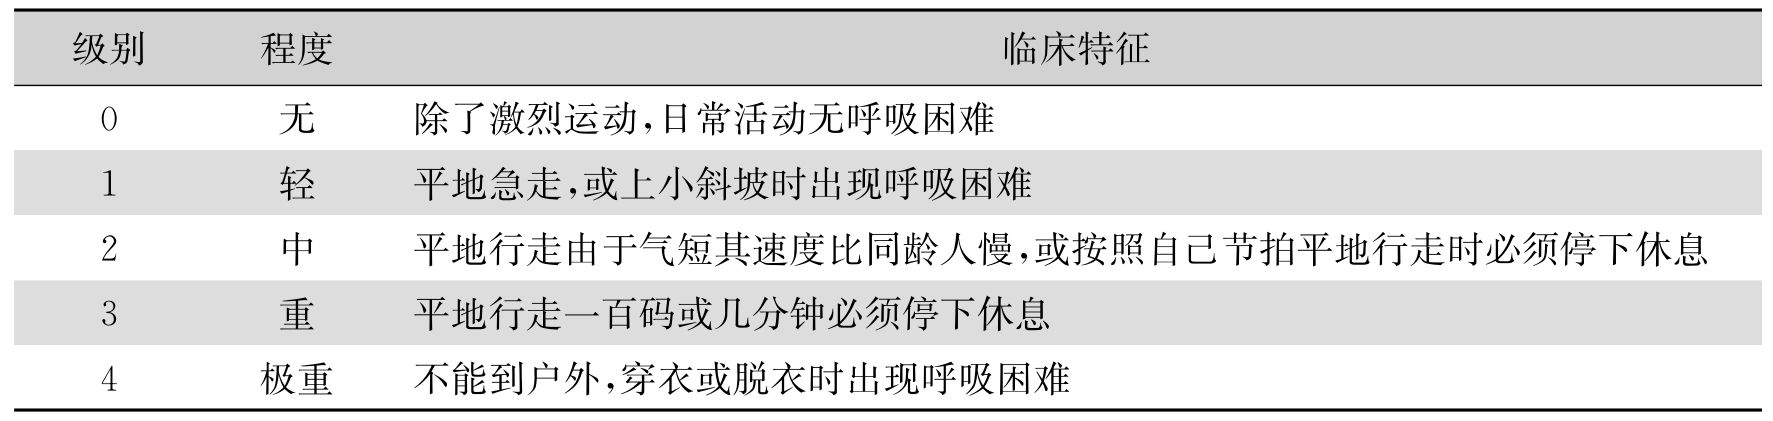
\includegraphics[width=.7\textwidth,height=\textheight,keepaspectratio]{./images/Image00033.jpg}
 \captionsetup{justification=centering}
 \caption{脑室周围白质软化症\\{\small 脑室周围和半卵圆中心的脑白质明显减少(右侧显著),皮质与脑室缘距离甚小,右侧有斑片状软化灶}}
 \label{fig2-17}
  \end{figure} 



\subsection{儿童脑性瘫痪的相关疾病}

本病是指出生前至出生后1个月内各种原因所致的非进行性脑损害综合征。临床表现为中枢性运动障碍及姿势异常,可伴智力低下、癫痫、视力障碍及行为异常。其CT改变可分为以下6种类型。

1.脑发育畸形:可分为器官源性和组织源性(已于上节详述)。

2.脑萎缩:大多由于缺血性损害或颅内感染导致脑白质或灰质减少、丧失,是脑性瘫痪最常见的CT表现。①可表现为脑沟裂增宽、增深,脑室增宽等。②其中脑室周围白质软化(PVL)约占脑萎缩的65%。③小脑萎缩可见小脑上沟增多(3条或3条以上)。

3.脑软化灶:多发生于较成熟的脑组织,可能与新生儿缺氧缺血性损害及颅内出血有关。

4.基底节病变:多由于脑血管阻塞致脑缺血缺氧性损害以及颅内感染、出血或中毒引起苍白球、丘脑区铁钙质沉着及神经细胞变性坏死。CT表现一侧或两侧对称性钙化灶或软化灶。

5.混合型:即上述两种以上病变混合存在。

6.正常:其原因可能为:①CT未能显示全部病灶或遗漏;②少数脑瘫与病变部位神经递质异常有关,CT不能显示;③胎儿期囊性病灶出生后自行消失;④CT检查的局限性,如CT难以显示矢状窦旁区脑损害及髓鞘形成延迟或发育不良。

\section{脑积水}

\subsection{概述}

1.脑积水:是指由于脑积液的产生和吸收不平衡所致的脑室扩大。按其发病机理可分为两大类:①脑脊液循环或吸收障碍;②脑脊液分泌增加。后者非常少见,主要见于脑室肿瘤如脉络丛乳头状瘤。脑脊液的吸收过去认为是通过蛛网膜颗粒,20世纪70年代后认为它不是惟一的吸收途径,并有学者认为主要是通过中枢神经系统表面吸收。

2.交通性脑积水:是指第四脑室出口以下的正常脑脊液通路受阻或吸收障碍所致的脑积水。国外有学者提出交通性脑积水应改称为动脉搏动限制性脑积水。动脉搏动明显减弱可能是由于动脉壁变硬或蛛网膜下腔顺应性降低所致。但动脉压并没有降低且传递的更远,使脑内脉压增高,大脑皮层压力梯度增大,脑室系统扩大。

3.阻塞性脑积水:又叫做非交通性脑积水,是指脑室系统即第四脑室出口以上任何部位发生阻塞所造成的脑积水,是最常见的脑积水。

脑积水时侧脑室旁白质内,CT上可见不规则低密度,是由于间质性水肿所致。即在脑室内压力增高时,室管膜受损出现小裂隙,水分子由此进入侧脑室周围白质内形成间质性水肿。高血压、动脉硬化及部分脑萎缩病人也可在室旁白质内出现上述CT表现(或异常MR信号),但其机理与脑积水不同,可能与局部组织变性、胶质增生、细胞萎缩后间隙扩大等有关。

\subsection{交通性脑积水}

\textbf{【病因】}
主要有蛛网膜下腔出血、脑膜炎、颅脑损伤以及静脉栓塞,亦可见于脑膜瘤病、脑脊液吸收功能障碍等。

\textbf{【临床表现】} 主要表现为颅内压增高的症状和体征。

\textbf{【CT表现】}
典型表现是脑室系统普遍扩大;另一特征是脑沟变浅、变平(但也可正常甚至扩张)。早期为颞角扩大和钝圆,稍后为额角扩大,进一步加重出现第三脑室扩大,第四脑室扩大较晚,与脑萎缩相比第三脑室扩大更明显。但有时交通性脑积水表现不典型,特别合并脑萎缩时,诊断较困难。此外,蛛网膜下腔出血和化脓性脑膜炎可表现为急性脑积水,脑室系统短时间内明显扩大。

交通性脑积水的特征之一为脑沟变浅、变平且灰白质界限清楚,常据此帮助诊断。但有时脑沟、脑池扩大,特别是纵裂池、基底池和桥小脑角池扩大。这种情况多见于基底池等有关脑池的炎症或肿瘤所致的部分脑脊液循环通路受阻及脑脊液吸收障碍。

脑室旁白质水肿发生率约为40%,且长期存在的交通性脑积水往往不出现这种征象。这是因为长期室内高压所致的室管膜受损,发生胶质增生形成室管膜瘢痕,阻止了脑脊液渗漏。

\subsection{正常压力性脑积水}

本病是交通性脑积水的一种特殊类型,多发生在慢性交通性脑积水的基础上,部分完好的脑脊液循环吸收功能代偿,且脑脊液的分泌功能下降,从而形成新的平衡。此时,虽然脑室系统仍明显扩大,但脑脊液压力正常,故又称为常压性脑积水。但实际上,大多并不一直正常,呈波动性。

\textbf{【临床表现】}
一般无颅内高压征,可能由于扩张侧脑室对周围白质的压迫,出现痴呆、步态不稳等症状。

\textbf{【CT表现】}
多不典型。由于脑室内压力正常,可在脑室扩大的同时出现脑沟加深,但两者不呈比例,脑室扩大更著。

\subsection{阻塞性脑积水}

\textbf{【病因病理】}
主要有先天性疾病、感染性疾病和肿瘤。病理表现为脑实质变薄,并可继发脑萎缩、白质脱髓鞘、胶质增生和神经细胞退行性变。

\textbf{【临床表现】}
主要为颅内压增高的症状和体征。其中先天异常、胎儿期或出生过程中发生该病者多在婴幼儿期出现症状,有的至10岁后或成年才表现异常。患儿有头颅增大,两眼球下旋形成“落日征”等甚有特点。

\textbf{【CT表现】}
阻塞近侧脑室扩大,阻塞远侧脑室形态正常或缩小(图\ref{fig2-18})。侧脑室旁间质水肿较明显而且范围广泛,脑沟也可变浅平,有时可见脑室疝。但病因诊断较困难。

\begin{figure}[!htbp]
 {\centering
 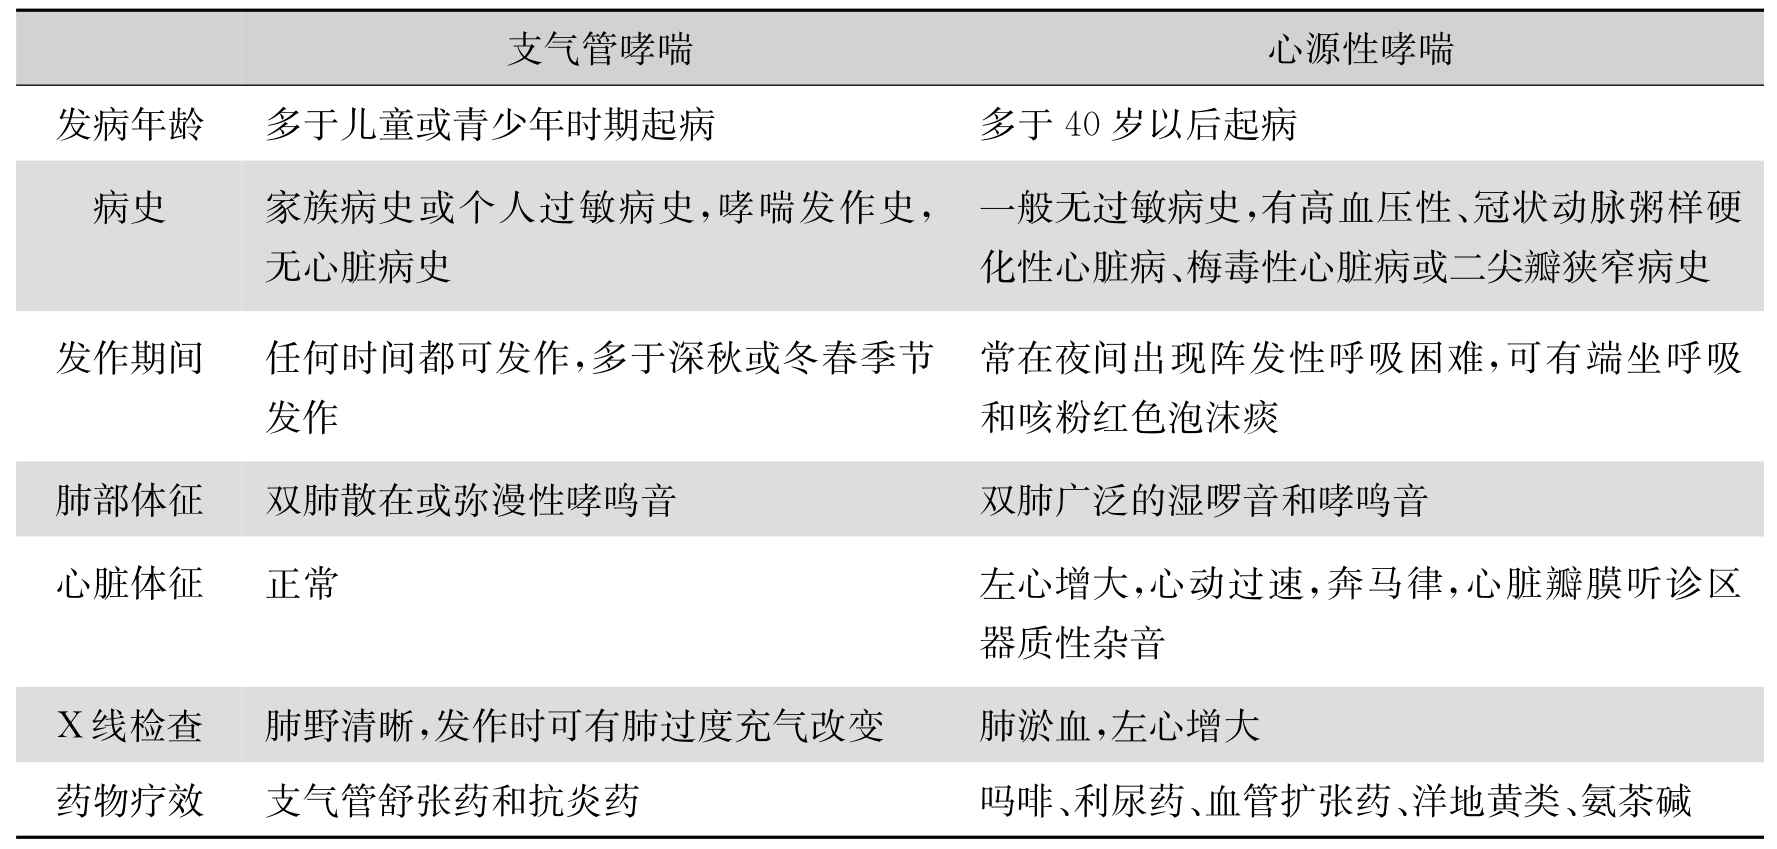
\includegraphics[width=.7\textwidth,height=\textheight,keepaspectratio]{./images/Image00034.jpg}
 \captionsetup{justification=centering}
 \caption{阻塞性脑积水\\{\small  A、B为同一患者,第三脑室、侧脑室扩大(第四脑室正常)}}
 \label{fig2-18}}
  \end{figure} 



先天性患者可重度积水,表现幕上大脑半球区为水样低密度,额、顶、颞叶脑实质几乎消失或残留极少,部分枕叶、基底核和丘脑保存(图\ref{fig2-10})。

\textbf{【鉴别诊断】}
与交通性脑积水鉴别时,如果阻塞在中脑导水管或以上,由于第四脑室不扩大,则两者容易鉴别。如阻塞部位在第四脑室出口时则两者难以鉴别。脑池造影观察第四脑室与蛛网膜下腔的通畅情况有助于鉴别。

\subsection{脑积水与脑萎缩的鉴别诊断}

主要有以下几点:①脑积水的扩大是均匀性和中心性扩张,尤其侧脑室前角呈气球状;而脑萎缩的脑室形态改变不及脑积水明显,特别是室旁脑组织较少的部位变形轻微,如第三脑室前壁、漏斗隐窝和视隐窝。②脑积水时由于颅内压力较高,脑沟变浅或消失,脑池亦不增大;而脑萎缩涉及皮质时脑沟加深、脑池扩大。③阻塞性脑积水和脑萎缩均可致一侧脑室扩大或一侧脑室扩大明显。在阻塞性脑积水时脑室可向扩大或扩大明显的对侧移位;而脑萎缩则向同侧移位。④脑积水侧脑室旁白质内可见间质性水肿所致的低密度;但脑萎缩因室旁白质变性亦可出现低密度灶。⑤脑萎缩是以白质为主的萎缩,表现为侧脑室边缘不规则,有助于与脑积水鉴别。

\section{脑萎缩}

\subsection{概述}

\subsubsection{脑变性疾病和脱髓鞘疾病的概念}

这是两组病变累及部位不同的神经系统疾病。前者累及神经元(灰质);后者累及髓鞘(白质),为髓鞘脱失,而轴索相对完好(见本章第十一节)。但两者均可引起脑萎缩。

变性疾病的特点是某一或二个功能系统的神经细胞发生萎缩和死亡,星形细胞增生。受累部位不同,临床表现也不同。如累及大脑皮质主要表现为痴呆;累及基底节、锥体外系则引起功能障碍;累及小脑引起共济失调。

脑变性疾病按部位分为:①大脑皮质:如Alzheimer病、Pick病。②基底节及脑干:如Jakob-Creutzfeldt综合征、Huntington舞蹈病、Parkinson病、进行性核上麻痹、Sky-Drager综合征。③脊髓及小脑:如橄榄桥脑小脑萎缩、原发性小脑萎缩、共济失调性毛细血管扩张症。④运动神经元:如脑萎缩性侧索硬化、脊髓性肌萎缩。

\subsubsection{脑萎缩的概念}

1.脑萎缩:是指由于各种原因所引起的脑组织减少而继发的脑室和蛛网膜下腔扩大。这种脑组织减少可分别或同时累及脑白质和脑灰质,其病因很多。根据其累及范围可分为局限性和弥漫性两类,但有时两者很难完全分开。

2.局限性脑萎缩:脑实质以局限性容积缩小为主,表现为局限性脑沟增宽和脑室、脑池扩大,有时仅发生于一侧半球。此外,还可见局部脑组织密度下降。

3.弥漫性脑萎缩:脑实质的减少为弥漫性,表现为脑室和蛛网膜下腔扩大广泛(图\ref{fig2-19})。可根据累及灰、白质程度的不同将其分为皮质型和中央型。前者以累及灰质为主,脑沟增宽明显,而脑室扩大次之;后者主要累及白质,以脑室扩大为主,脑沟扩大为次。

\begin{figure}[!htbp]
 \centering
 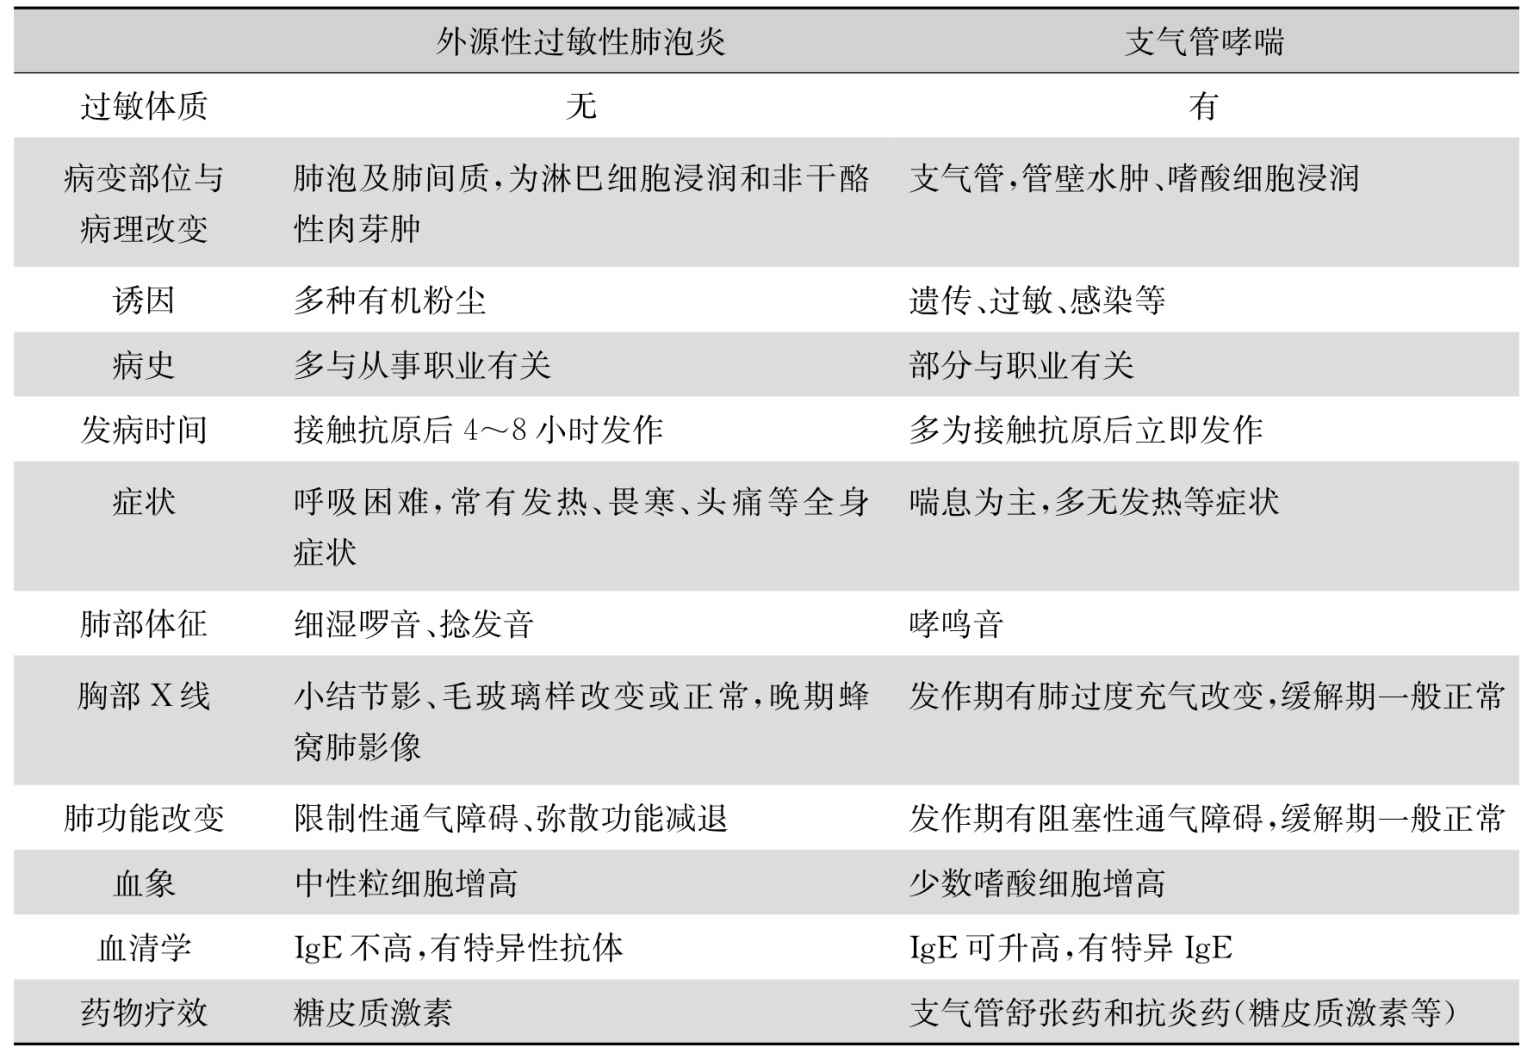
\includegraphics[width=.7\textwidth,height=\textheight,keepaspectratio]{./images/Image00035.jpg}
 \captionsetup{justification=centering}
 \caption{弥漫性脑萎缩\\{\small 脑室和蛛网膜下腔广泛扩大,室旁白质内有低密度灶,侧脑室边缘不规则}}
 \label{fig2-19}
  \end{figure} 



\subsubsection{局限性脑萎缩的病因}

1.外伤性脑萎缩:一般发生在外伤3~6个月后,少数外伤可造成弥漫性脑萎缩。

2.感染后脑萎缩:多继发于脑脓肿,颅内低毒性感染有时可造成弥漫性脑萎缩。

3.脑梗死后脑萎缩:一般发生在发病后3~6个月。

4.Pick病:又称脑叶萎缩症,系常染色体显性遗传性疾病。多见于女性,病程5~6年,呈进行性恶化。临床表现智力低下、痴呆、共济失调等,与Alzheimer病难以区别。但本病以额叶和颞叶萎缩为主,尤其以两额叶为著;而Alzheimer病为弥漫性脑萎缩,且以颞叶较著,额叶多不明显。

5.大脑半球萎缩:由于胎儿期或新生儿期血管阻塞引起的大块脑梗死所致,一般在青少年期才被发现。

\subsubsection{弥漫性脑萎缩的病因}

临床上较局限性脑萎缩更常见,多见于正常老年人,亦可见于许多病理情况。①Alzheimer病;②Huntington病;③Parkinson病;④Wilson病;⑤脑缺氧;⑥Jakob-Creutzfeldt综合征;⑦肿瘤和代谢失调:均与脑组织营养障碍有关(肿瘤患者虽无脑转移瘤,但可有营养障碍),同样情况也可见于AIDS、肝性脑病、血液透析者、慢性酒精中毒和肥胖病人;⑧药物性脑萎缩:如类固醇、氨基甲叶酸、度冷丁、酒精等使用不当。

\subsection{老年脑(生理性脑萎缩)}

关于老年脑的临床意义,目前认识尚不统一。这是因为正常情况下随着年龄的增加,脑组织和其他器官一样,逐渐老化而发生萎缩即所谓生理性萎缩。但随着年龄的增加,易发生的高血压、脑动脉硬化等因素均可损害脑组织而发生萎缩,这种萎缩虽与年龄有关,却为病理性。相对而言生理性萎缩较病理性萎缩轻,但两者无明显界限。

\textbf{【CT表现】}
老年脑主要表现为脑室、脑池轻度扩大和脑沟轻度增宽,多为两侧对称。脑沟增宽以额叶、镰旁顶叶显著,脑室扩大以侧脑室额角、颞角和第三脑室显著。

\subsection{Alzheimer病(爱茨海默病)}

本病以往曾称为早老性痴呆或老年前期痴呆,是一种以弥漫性脑萎缩(但以颞叶为主)为特征的痴呆。本病与老年性痴呆只有年龄上的差异而无本质的区别,故国际上将两病合并称为Alzheimer型痴呆。

\textbf{【病理】}
主要病理表现为脑萎缩,尤其是颞叶海马萎缩为主。镜下脑组织神经细胞减少,尤其有大量老年斑和神经纤维缠结时有定性价值,神经元空泡颗粒变性和淀粉样血管病变,但均为非特异性的,可见于老龄脑。

\textbf{【临床表现】}
其特征为进行性记忆力减退,语言和行为障碍。生前主要依据神经心理测验确立诊断。其病程不可逆转,一般持续3~10年,最后继发感染和全身衰竭而导致死亡。

\textbf{【CT表现】}
①弥漫性脑萎缩表现,与老年性脑萎缩相似,无特征性。②内侧颞叶萎缩是本病最早、最敏感的指征,以海马萎缩最突出,其次为额顶叶。主要表现为颞角扩大,颞叶皮质萎缩和海马回密度减低。有人取负于听眦线20\textsuperscript{o}
平面为扫描基线,层厚5mm,在环池水平测量颞角内侧边与环池外侧边的最小距离即中颞叶最小宽度,其参考值为8.67mm,小于此值即为中颞叶萎缩。③胼胝体萎缩为本病的另一指征,以嘴部和压部最为明显。④在海马萎缩的同时,MR、ECT(PET)等所显示的特异性区域血流量下降也可作为本病的特异性表现。

\textbf{【鉴别诊断】}
主要应于血管性痴呆鉴别。后者在我国老年人中占痴呆疾病的首位(西方占第二位),其颞角扩张不及Alzheimer病明显。严重的皮层下和脑室周围白质病变是多发性梗死型痴呆较典型的表现。

\subsection{慢性进行性舞蹈病}

本病又称遗传性舞蹈病、亨廷顿(Huntington)病,是基底节和大脑皮质变性的一种常染色体显性遗传性疾病。

\textbf{【病理】}
以尾状核及壳核萎缩明显,后期则额、顶叶皮质萎缩。镜下见神经元减少和胶质细胞增生。其生化改变为基底节中多巴胺含量过多,而γ-氨基丁酸及胆碱的含量减少。

\textbf{【临床表现】}
好发于20~50岁,其特征为慢性进行性舞蹈样动作和痴呆,多有遗传和家族史。

\textbf{【CT表现】}
主要为尾状核及壳核的萎缩。两侧尾状核头、体部相对缩小,可伴或不伴侧脑室(尤其额角)扩大和脑沟增宽,两侧壳核对称性低密度。一般只要出现尾状核萎缩即可以做出诊断,小脑和脑干也可萎缩。

\subsection{Parkinson病(帕金森病)}

本病又称震颤麻痹,可分为原发性和继发性两类。前者病因不明;后者可因脑动脉硬化、挫伤、基底节肿瘤、药物和化学物质中毒所致,又被称为Parkinson综合征。

\textbf{【病理】}
肉眼变化的特点是黑质和兰斑脱色。镜下可见该处的神经黑色素细胞丧失。黑质和苍白球神经元明显减少,局部萎缩及黑色素退变。中脑黑质致密带色素细胞大量丢失,桥脑兰斑色素细胞明显减少,脑有对称或非对称萎缩。黑质与兰斑均属儿茶酚胺能核团,分泌多巴胺;尾状核、壳核的神经元属胆碱能细胞,分泌乙酰胆碱。由于黑质神经元大量丧失,使多巴胺含量下降,从而使得对纹状体区乙酰胆碱的抑制作用下降,出现震颤麻痹。

\textbf{【临床表现】}
发生于中年以上,起病很缓慢,逐渐加剧。主要症状包括震颤、肌张力高(强直)、运动障碍、假面具样面容等。

\textbf{【CT表现】}
无特异性,主要为脑室扩大和弥漫性脑萎缩,有时合并基底节钙化,后者亦可见于正常人。CT所示的脑萎缩与临床所见的震颤麻痹的严重程度无明显关系。MR可有黑质(致密带)的萎缩及异常铁质沉积所致的低信号。

\subsection{肝豆状核变性}

本病又称Wilson(威尔逊)病,是一种常染色体隐性遗传的铜代谢障碍性疾病。

\textbf{【病理】}
由于肝脏合成血浆铜蓝蛋白的能力下降,引起肝脏、大脑基底节区和角膜的铜沉积,亦可累及额叶皮质、红核、黑质及齿状核及肾等处。脑受累部位变性、萎缩、胶质增生,甚至缺血坏死、软化。以豆状核软化、角膜色素环(K-F环)及小叶性肝硬化为三大主征。

\textbf{【临床表现】}
好发于10~25岁青少年,约1/3有家族史。基底节损害症状包括进行性加剧的震颤、僵直与多动症,皮质损害为衰退型精神障碍,有肝硬化和角膜色素环表现。

\textbf{【CT表现】}
少数可无异常发现。主要表现为豆状核低密度区,多为双侧,使豆状核界限不清。低密度区还可累及尾状核、齿状核、红核、额叶和丘脑等,部分还可见尾状核、大脑和小脑萎缩。

\textbf{【鉴别诊断】}

1.代谢性疾病:其中以肝豆状核变性最常见,还有亚急性坏死性脑脊髓病(Leigh病)、维生素B\textsubscript{1}
缺乏症,以及线粒体脑病、Kearns-Sayre综合征、海绵状脑白质营养不良、黏多糖病、Hallervorden-Spatz病、岩藻糖苷沉积症、先天性丙酮酸代谢障碍。

2.感染性疾病:EB病毒性脑炎、乙脑和腮腺炎病毒性脑炎等。

3.中毒性疾病:以一氧化碳中毒最常见,还有变质甘蔗中毒、大量硫化氢吸入中毒、甲醇中毒和氰化物中毒等。

此外,纹状体黑质变性(40~50岁发病,病程渐进,以帕金森综合征为首见症状,为锥体外系疾病或列入多系统变性)也可出现双侧壳核对称性低密度及全脑萎缩。国内有学者报道1例静脉窦血栓形成致双侧基底节对称性低密度。我们遇见1例尿毒症患者,表现为以内囊后肢为中心,部分涉及双侧豆状核的低密度。

\subsection{皮质纹状体脊髓变性}

本病又称Jakob-Creutzfeldt综合征、亚急性海绵状脑病、传染性病毒性痴呆。过去一直被纳入变性范围,现多认为是一种病毒感染性疾病。

\textbf{【病理】}
出现以灰质为主的明显脑萎缩。镜下皮质、大脑基底节、脊髓、小脑、丘脑、脑干及脊髓前角神经元变性。神经细胞脱失,脑实质空泡化伴胶质细胞增生,病灶区如海绵状,无炎性变化,白质多正常,晚期可受累。

\textbf{【临床表现】}
好发于40~70岁,主要表现为迅速发展的精神衰退和痴呆,并可出现锥体束、锥体外系及共济失调症状。80%死于发病后1年左右。

\textbf{【CT表现】}
大脑皮质弥漫性萎缩,脑沟、裂增宽增深,亦可见两侧脑室扩大。晚期脑白质受累可见低密度,无占位效应,无强化。本病进展快,短时间随访明显加重。

\subsection{小脑萎缩}

\textbf{【病因】}
本病可由变性性疾病、中毒、慢性酒精中毒、滥用药物等引起。发生于儿童的共济失调性毛细血管扩张症亦表现为以蚓部为主的小脑萎缩。此外橄榄桥脑小脑萎缩(或称橄榄桥脑小脑变性)也是共济失调的一个类型。

\textbf{【病理】}
病变主要在小脑、小脑脊髓束、锥体束、橄榄核,甚至累及大脑皮质,小脑萎缩皮质重于髓质。橄榄桥脑小脑萎缩除小脑萎缩外,还有桥脑、橄榄的明显萎缩,大脑皮质也可受累。

\textbf{【临床表现】}
成年发病,病程缓慢,可为10~40年。表现为小脑性共济失调,锥体束征、锥体外系征、视神经萎缩。

\textbf{【CT表现】}
应包括以下两个或两个以上征象(图\ref{fig2-20}):①小脑沟增宽>1mm(也有人认为\textgreater{}2mm);②小脑沟在半球超过2条,蚓部超过4条;③桥小脑角池扩大>1.5mm(应测量小脑上边缘与岩骨边缘间的距离);④第四脑室扩大;⑤小脑上池扩大。

\subsection{精神分裂症}

本病多有脑结构的异常。

\begin{figure}[!htbp]
 \centering
 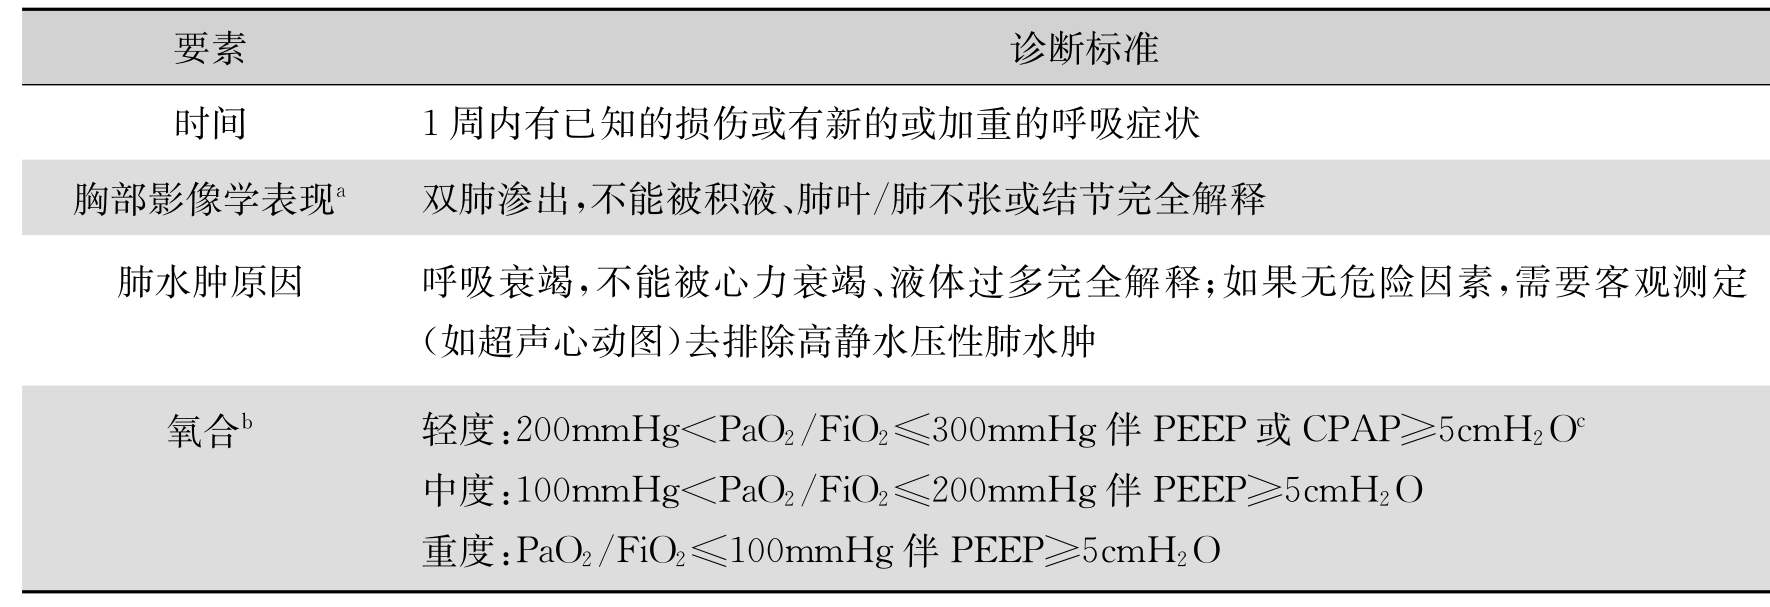
\includegraphics[width=.7\textwidth,height=\textheight,keepaspectratio]{./images/Image00036.jpg}
 \captionsetup{justification=centering}
 \caption{小脑萎缩\\{\small 小脑沟显著增宽、增多,以蚓部为著}}
 \label{fig2-20}
  \end{figure} 



\textbf{【CT表现】}
第三、第四脑室扩大,两侧裂池增宽、脑沟扩大,有时出现侧脑室扩大和小脑萎缩。两侧室旁核和小脑的密度可增加,其意义尚不肯定。

\subsection{颞叶癫痫}

颞叶癫痫的常见原因为海马硬化(又称安蒙氏角硬化和颞叶中内侧硬化)。

\textbf{【病理】} 特征为神经元丢失和胶质细胞增生,导致海马的萎缩。

\textbf{【CT表现】}
其CT诊断价值较小,仅约23.8%有异常。表现为:①颞叶内侧低密度灶;②颞角扩大;③侧裂池增宽。

\textbf{【MR表现】} 海马的萎缩(为神经元丢失的反应)、T\textsubscript{2}
WI海马高信号(为胶质细胞增生的反应)、颞叶前部萎缩以及颞角扩大。

\section{脑缺血、出血和脑血管病变}

\subsection{动脉缺血性脑梗死}

脑组织因血管阻塞引起缺血性坏死或软化称为脑梗死。广义的脑梗死除动脉缺血性脑梗死外,还包括静脉血流受阻所致的脑梗死即静脉性脑梗死。但大多习惯于狭义的将动脉缺血性脑梗死称为脑梗死。

\textbf{【病因】}
引起梗死的原因很多,可分为两大类。①脑血管阻塞:又分为血栓形成和栓塞。前者最常见的是在动脉粥样硬化的基础上形成血栓;后者是指外来栓子堵塞血管所致。②脑部血液循环障碍:是指在脑血管原有病变的基础上(亦可无原发血管病变),由各种原因造成的脑组织供血不全而引起的梗死,故又称非梗阻性脑梗死。

\textbf{【病理】}
过去将脑梗死分为3个时期,即梗死期、吞噬期、机化期。目前通常将脑梗死分为:①超急性期:6小时以内;②急性期:6小时后~2天;③亚急性期:2天后~2周内;④慢性早期:2周~1个月;⑤慢性晚期:1月后(见表\ref{tab2-2})。

\begin{table}[htbp]
\centering
\caption{脑梗死的病理过程及CT表现}
\label{tab2-2}
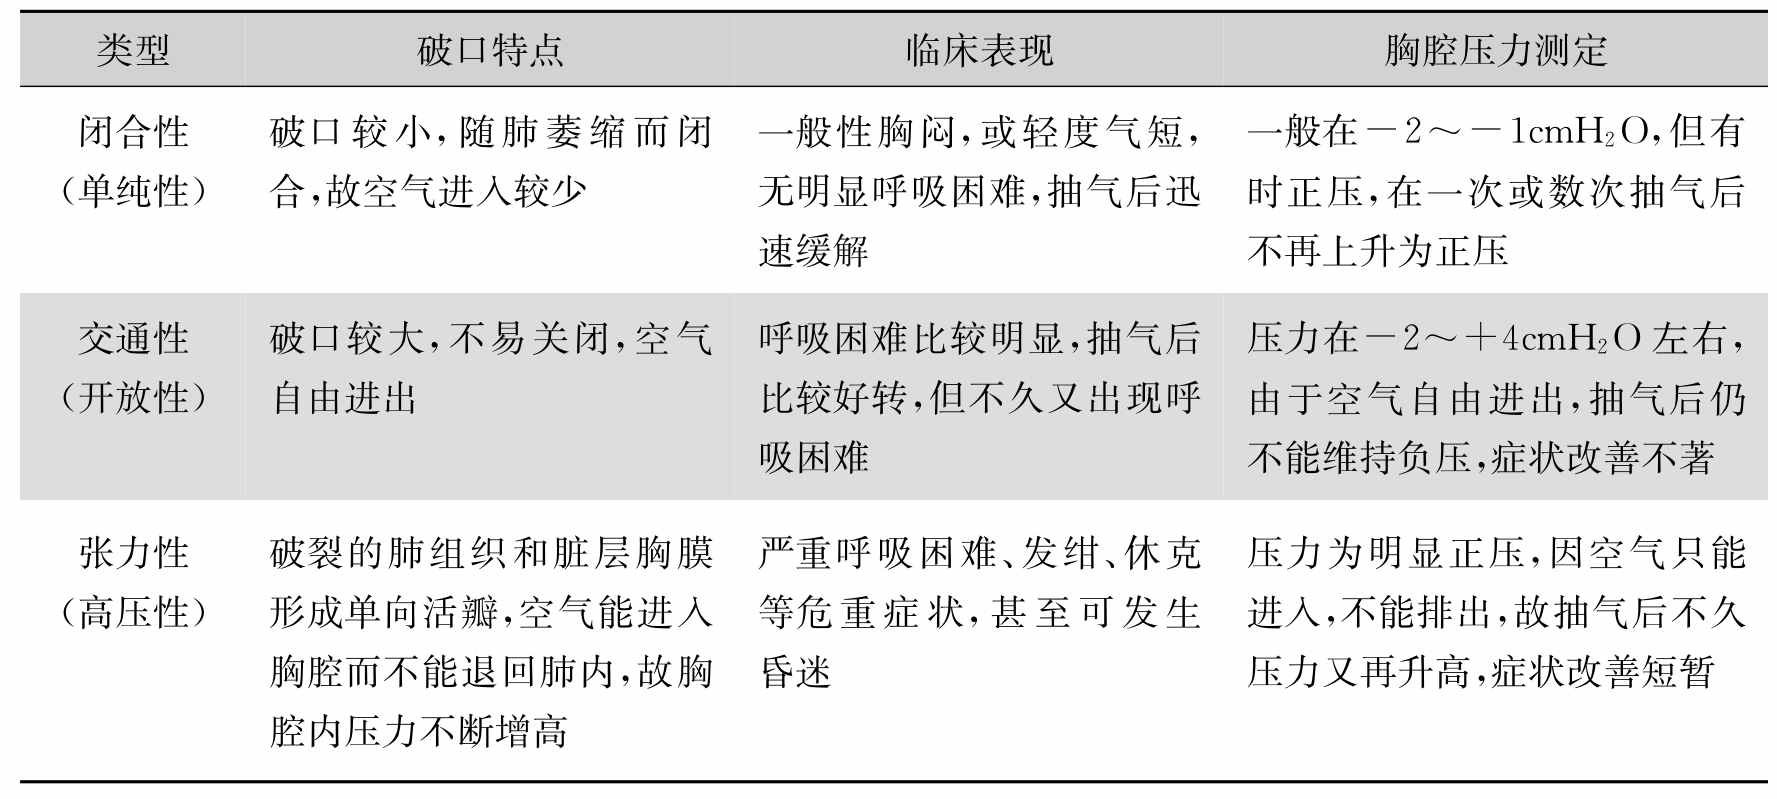
\includegraphics[width=\textwidth,height=\textheight,keepaspectratio]{./images/Image00037.jpg}
\end{table}

脑供血完全终止后数秒钟神经元电生理活动停止,持续5~10分钟以上就有不可恢复的细胞损伤。但是临床上供血血管闭塞可能不完全和(或)存在侧支循环,仅使局部血流降低到一定程度。故部分脑组织虽有缺血损伤,但仍可恢复正常,这部分脑组织区域称为缺血半暗带。它位于缺血坏死核心与正常脑组织之间。但如超急性期治疗不及时或治疗无效可发展成为完全脑梗死。

少数缺血性脑梗死在发病24~48小时后可因再灌注而发生梗死区内出血,称为出血性脑梗死。

\textbf{【临床表现】}
临床表现复杂,取决于梗死灶大小、部位及脑组织的病理生理反应。主要表现为头昏、头痛,部分有呕吐及精神症状,可有不同程度的昏迷。绝大多数出现不同程度的脑部损害症状,如偏瘫、偏身感觉障碍、偏盲,亦可失语、抽搐,较重者可有脑疝症状。从解剖学可知,皮质脊髓束有10%的纤维不交叉下降,加入同侧皮质脊髓侧束。皮质脊髓前束也有少量纤维不交叉,止于同侧颈、胸髓。这些不交叉的运动传导纤维支配了同侧肢体运动,当这些纤维受损时,导致同侧肢体出现不同程度的运动功能障碍如麻木、无力,甚至偏瘫。

\textbf{【CT表现】}

1.超急性期脑梗死的CT表现:①大脑中动脉高密度征:为高密度血栓或栓子所致,出现率约占35%~45%(敏感度78%,特异度93%),但需除外血管硬化因素。最近研究表明,此征可见于近60%的正常人(尤其用7mm以下层厚扫描),故此征的诊断价值值得怀疑。②脑实质低密度征:可能为细胞内水肿所致,可见于脑的凸面、基底节区、岛叶,有时可伴侧裂池受压。③局部脑组织肿胀征:可能为血管源性水肿所致,局部脑沟变窄以至消失,脑回增厚、变平(图\ref{fig2-21}A)。脑CT灌注成像有利于超急性期脑梗死的诊断。

此外,脑血管CTA可显示闭塞部位、程度和侧支循环情况。

许多学者研究证实,CT灌注成像可以预测半暗带,即脑血流量(rCBF)中度减低时,局部脑血容量(rCBV)无明显变化或仅有轻度下降或轻度升高,此时缺血区微血管管腔受压、变形、闭塞的程度较轻。当rCBF和rCBV均明显减低时,提示脑局部微血管管腔闭塞程度明显、微循环发生障碍、脑组织发生梗死。国内有学者将面积\textsubscript{CBV}
定义为预测的梗死面积,则面积\textsubscript{CBF} -
面积\textsubscript{CBV} 为预测的半暗带面积。

2.典型CT表现:①脑组织低密度灶,呈楔形或三角形,病灶部位、范围与闭塞动脉供血区相吻合。大脑中动脉主干闭塞,病灶呈三角形低密度区,尖端指向第三脑室;大脑中动脉闭塞在豆纹动脉的远端,病灶多为矩形低密度区,出现“基底核回避现象”。大脑前动脉闭塞表现为位于大脑镰旁的长条状低密度区。大脑后动脉闭塞在顶叶后部及枕叶可见半圆形的低密度区,位于大脑镰旁的后部。局灶性脑皮质梗死,表现为脑回丢失。室管膜下脑梗死,脑室边缘呈波浪状。一般在发病24小时后出现以上表现(图\ref{fig2-21}B、C)。②2~3周时由于“模糊效应”,病灶可偏小或消失。③脑梗死后2~15天为水肿高峰期,可有占位效应,占位效应一般见于病变范围大的病例。如占位效应超过1个月,应注意有无肿瘤可能。④增强扫描病灶周围和病灶内出现脑回状、线状、团块状强化。⑤1个月后病灶开始软化呈水样密度,病变范围大的病例可继发局限性脑萎缩。

此外,出血性脑梗死在梗死区内可见高密度出血灶(图\ref{fig2-21}D)。



\begin{figure}[!htbp]
 \centering
 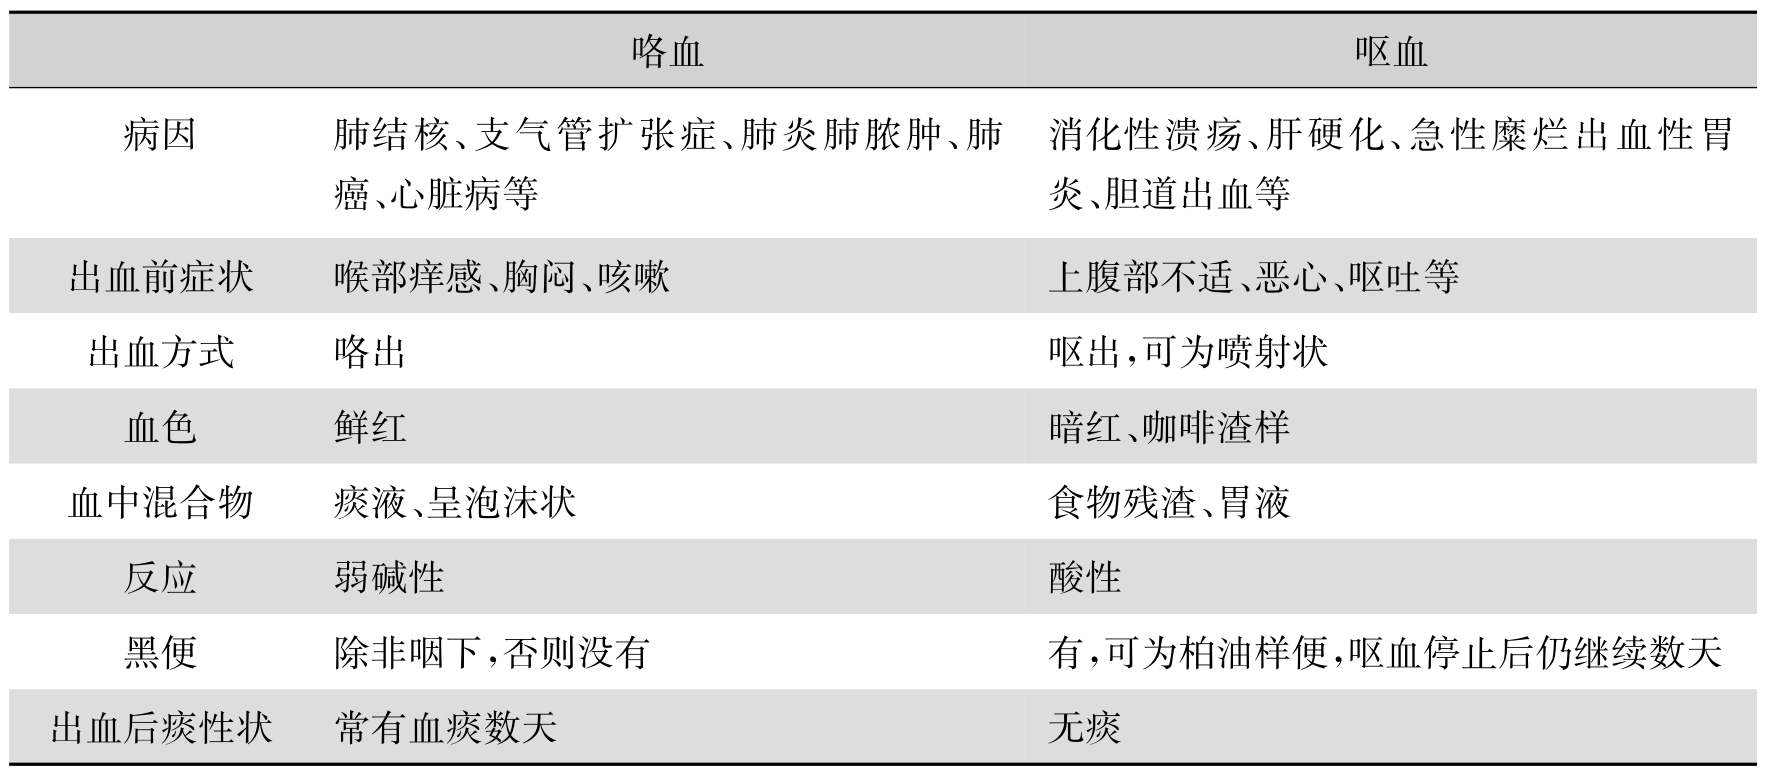
\includegraphics[width=\textwidth,height=\textheight,keepaspectratio]{./images/Image00038.jpg}
 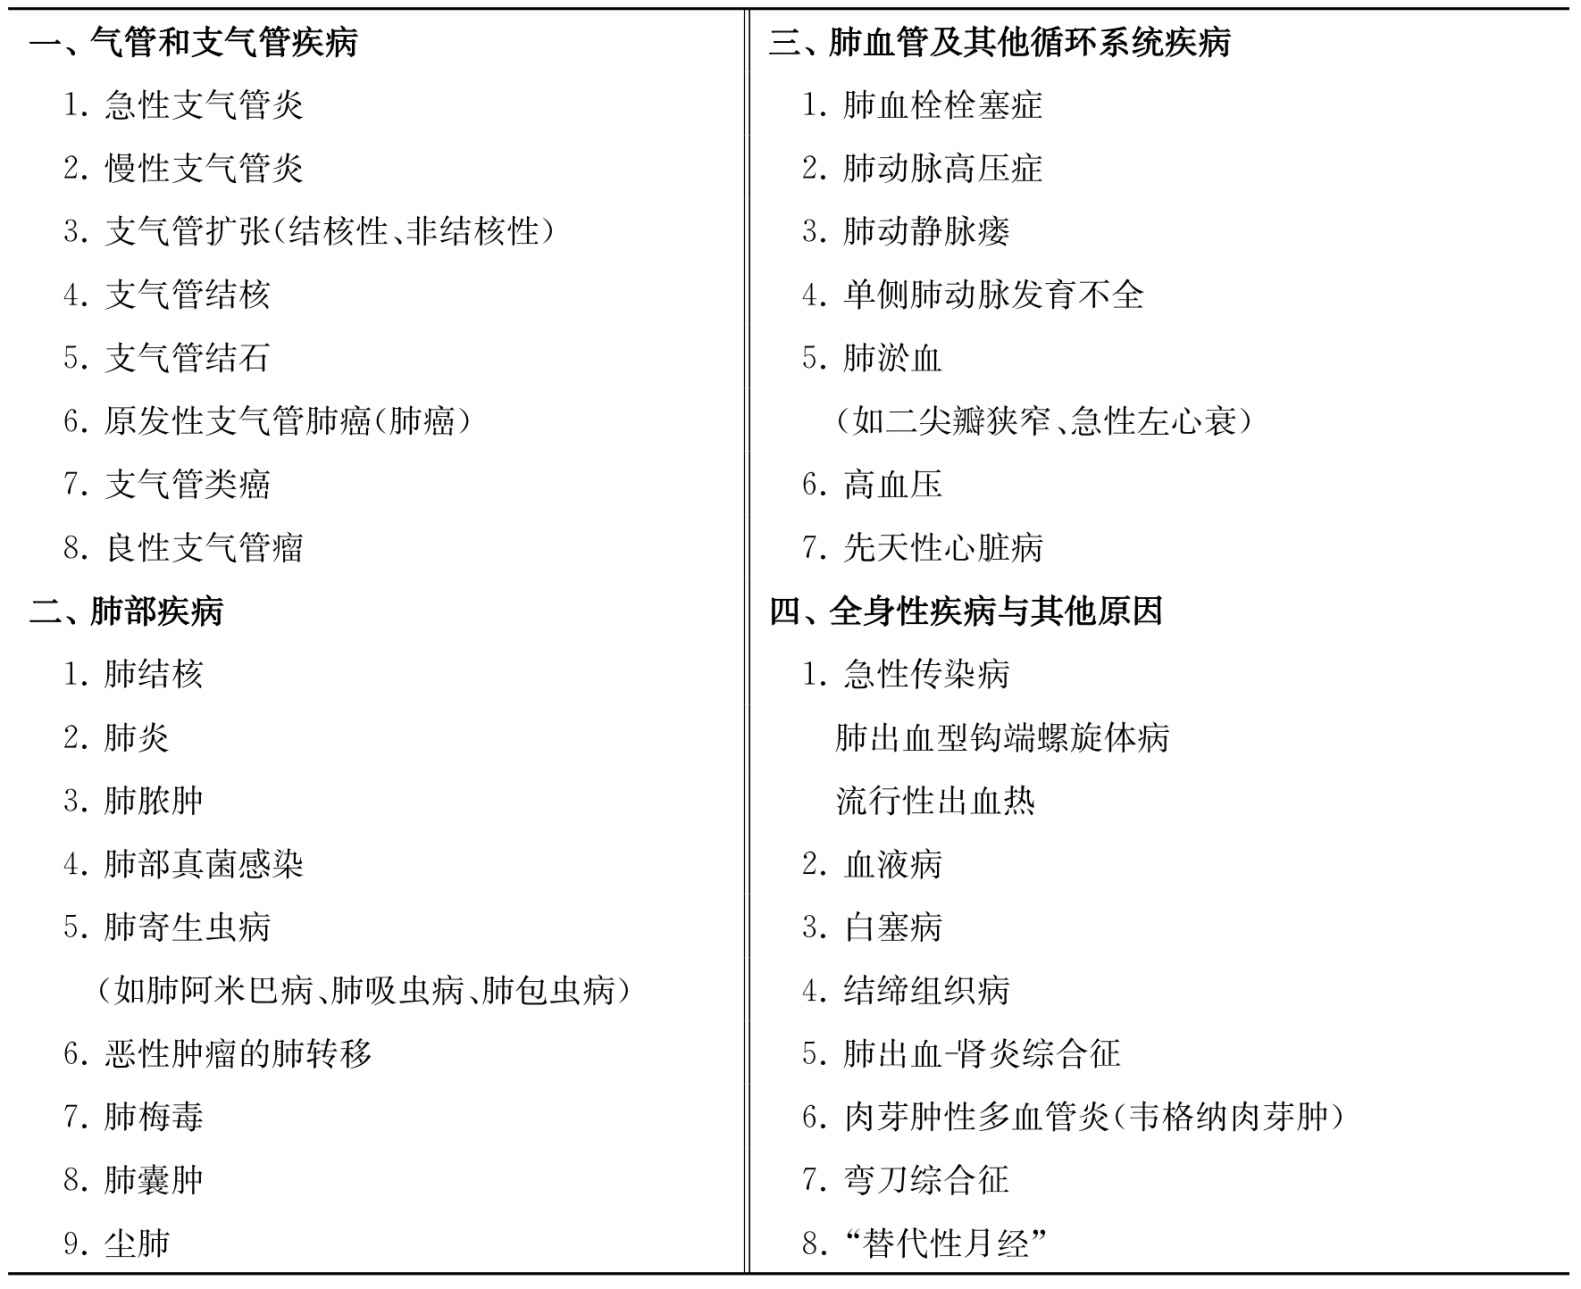
\includegraphics[width=\textwidth,height=\textheight,keepaspectratio]{./images/Image00039.jpg}
 \captionsetup{justification=centering}
 \caption{脑梗死\\{\small A、B为同一患者。A.超急性期,发病后4小时,右侧额顶叶脑沟消失,皮髓质交界不清晰;B.发病后42小时,右侧颞额顶叶大片状低密度灶,界限清晰,显著占位效应;C.亚急性期脑梗死,左侧顶额叶区有大片楔形低密度区,占位效应较显著;D.出血性脑梗死,右侧颞额叶区有大片楔形低密度区,占位效应显著,其内见大片状高密度出血灶,左侧基底节区可见水样密度的软化灶}}
 \label{fig2-21}
  \end{figure} 

3.增强扫描CT表现:梗死灶强化的形态多种多样,可表现为脑回状、线状、片状、环状,可出现在病灶的边缘和中心。而延迟30分钟~3小时扫描可显示皮质下白质强化,可能与梗塞区皮质内大量毛细血管破坏,造影剂漏出有关。其强化机制与缺血区血脑屏障受损,新生的毛细血管大量增生,以及局部血流量增加有关。但在1周内,虽有血脑屏障的破坏,却因局部缺血坏死严重,造影剂浓度亦相应很低,故一般不出现强化。梗死7~10天后因局部大量毛细血管增生,血流量增大而出现明显强化。2~3周发生率最高,强化最明显,可持续1个月或更久。

\textbf{【鉴别诊断】}
应注意与胶质瘤、转移瘤、脱髓鞘病变和脑脓肿等鉴别。①脑梗死常累及皮质和白质两部分;而上述病变一般只造成白质低密度。②脑梗死的分布为某一动脉区或分水岭区,有一定特征;而脑肿瘤和炎症水肿沿白质通道扩散,无明显分布规律,常呈指状低密度区;脱髓鞘低密度灶常对称性分布在侧脑室周围。③增强扫描胶质瘤常出现不均匀强化,有时可见壁结节;转移瘤常可见多灶强化。

\subsection{脑梗死前期}

从脑血流量(CBF)变化过程看,脑血流量的下降到急性脑梗死的发生经历了3个时期。首先,由于脑灌注压下降引起的脑局部的血流动力学异常改变;其次,脑循环储备力失代偿性低灌注所造成的神经元功能改变;最后,由于CBF下降超过了脑代谢储备力才发生不可逆转的神经元形态学改变即脑梗死。国内高培毅将前两者称为脑梗死前期,它不同于超急性期脑梗死。

他们根据脑局部微循环的变化程度以及CT灌注成像表现包括局部脑血流量(rCBF)、局部脑血容量(rCBV)、平均通过时间(MTT)和峰值时间(TTP)参数图,将脑梗死前期分为2期4个亚型:

Ⅰ期:脑血流动力学发生异常变化,脑血流灌注压在一定范围内波动时,机体可以通过小动脉和毛细血管平滑肌的代偿性扩张或收缩来维持脑血流相对动态稳定。

Ⅰ\textsubscript{1}
:脑血流速度发生变化,脑局部微血管尚无代偿性扩张。灌注成像见TTP延长,MTT、rCBF、rCBV正常。

Ⅰ\textsubscript{2} :脑局部微血管代偿性扩张。灌注成像见TTP
和MTT延长,rCBF正常或轻度下降,rCBV正常或轻度升高。

Ⅱ期:脑循环储备力失代偿,CBF达电衰竭阈值以下,神经元的功能出现异常,机体通过脑代谢储备力来维持神经元代谢的稳定。

Ⅱ\textsubscript{1}
:CBF下降,由于造成局部星形细胞足板肿胀,并开始压迫局部微血管。灌注成像见TTP
和MTT延长,以及rCBF下降,rCBV基本正常或轻度下降。

Ⅱ\textsubscript{2}
:星形细胞足板明显肿胀,并造成局部微血管受压变窄或闭塞,局部微循环障碍。灌注成像见TTP
和MTT延长,rCBF和rCBV下降。

\subsection{分水岭性脑梗死}

即指两条主要脑动脉供血交界区发生的脑梗死。

\textbf{【病因】}
①血液动力学障碍:低血压(如心肌梗死、心律失常、体位性低血压)等所致的血液动力学障碍;②血管调节功能失常:如糖尿病并发植物神经功能紊乱、长期低血压;③高血压病过分降压治疗;④心脏附壁血栓脱落沿血管进入脑皮质支和深穿支。

\textbf{【CT表现】}
①皮质下型:多为白质内低密度,常呈条形或类圆形。灰质由于血流再灌注而呈等密度,但灰质可出现明显强化。②皮质前型:额顶叶交界区三角形、条形低密度灶。③皮质后型:颞顶枕叶交界区三角形、条形低密度灶。

\subsection{血液动力性脑梗死}

当脑外动脉狭窄、部分阻塞和痉挛时,一般情况下尚能维持脑组织的血供。但当某些原因引起较长时间的血压下降时,可造成狭窄动脉供血脑组织的严重缺血而发生脑梗死,这种梗死称为血液动力性脑梗死。

\textbf{【病因病理】}
心律失常、心功能不全、休克、高血压过分降压等是其常见原因。严重的低血压和心搏量降低如心肌梗死、外科手术等,即使患者无颅内外血管病变,也可引起大脑半球的广泛梗死。血液动力性脑梗死多为分水岭性脑梗死。

\textbf{【CT表现】}
与分水岭性梗死的表现相似,可见条形或类圆形低密度,也可广泛梗死,这种梗死以分水岭区最著。可累及基底节区和小脑,皮质可强化。

\subsection{腔隙性脑梗死}

即指脑深部2~15mm大小的脑梗死。

\textbf{【病因】}
多为高血压、糖尿病、动脉硬化、高脂血症所致。好发于基底节、丘脑、内囊区、深部室旁白质及脑干。这些部位的血管多远离大脑主干,细长且走行弯曲,对血液动力学变化敏感,易受缺血影响。

\textbf{【临床表现】}
纯运动性偏瘫、纯感觉障碍、下肢运动受限、构音困难、视力障碍、失语、短小步态及共济失调等。

\textbf{【CT表现】}
梗死灶在2~15mm之间,呈圆形或卵圆形低密度,边缘不清,无水肿和占位效应。3~4周后可形成边缘清楚的囊性软化灶(图\ref{fig2-22})。

\begin{figure}[!htbp]
 \centering
 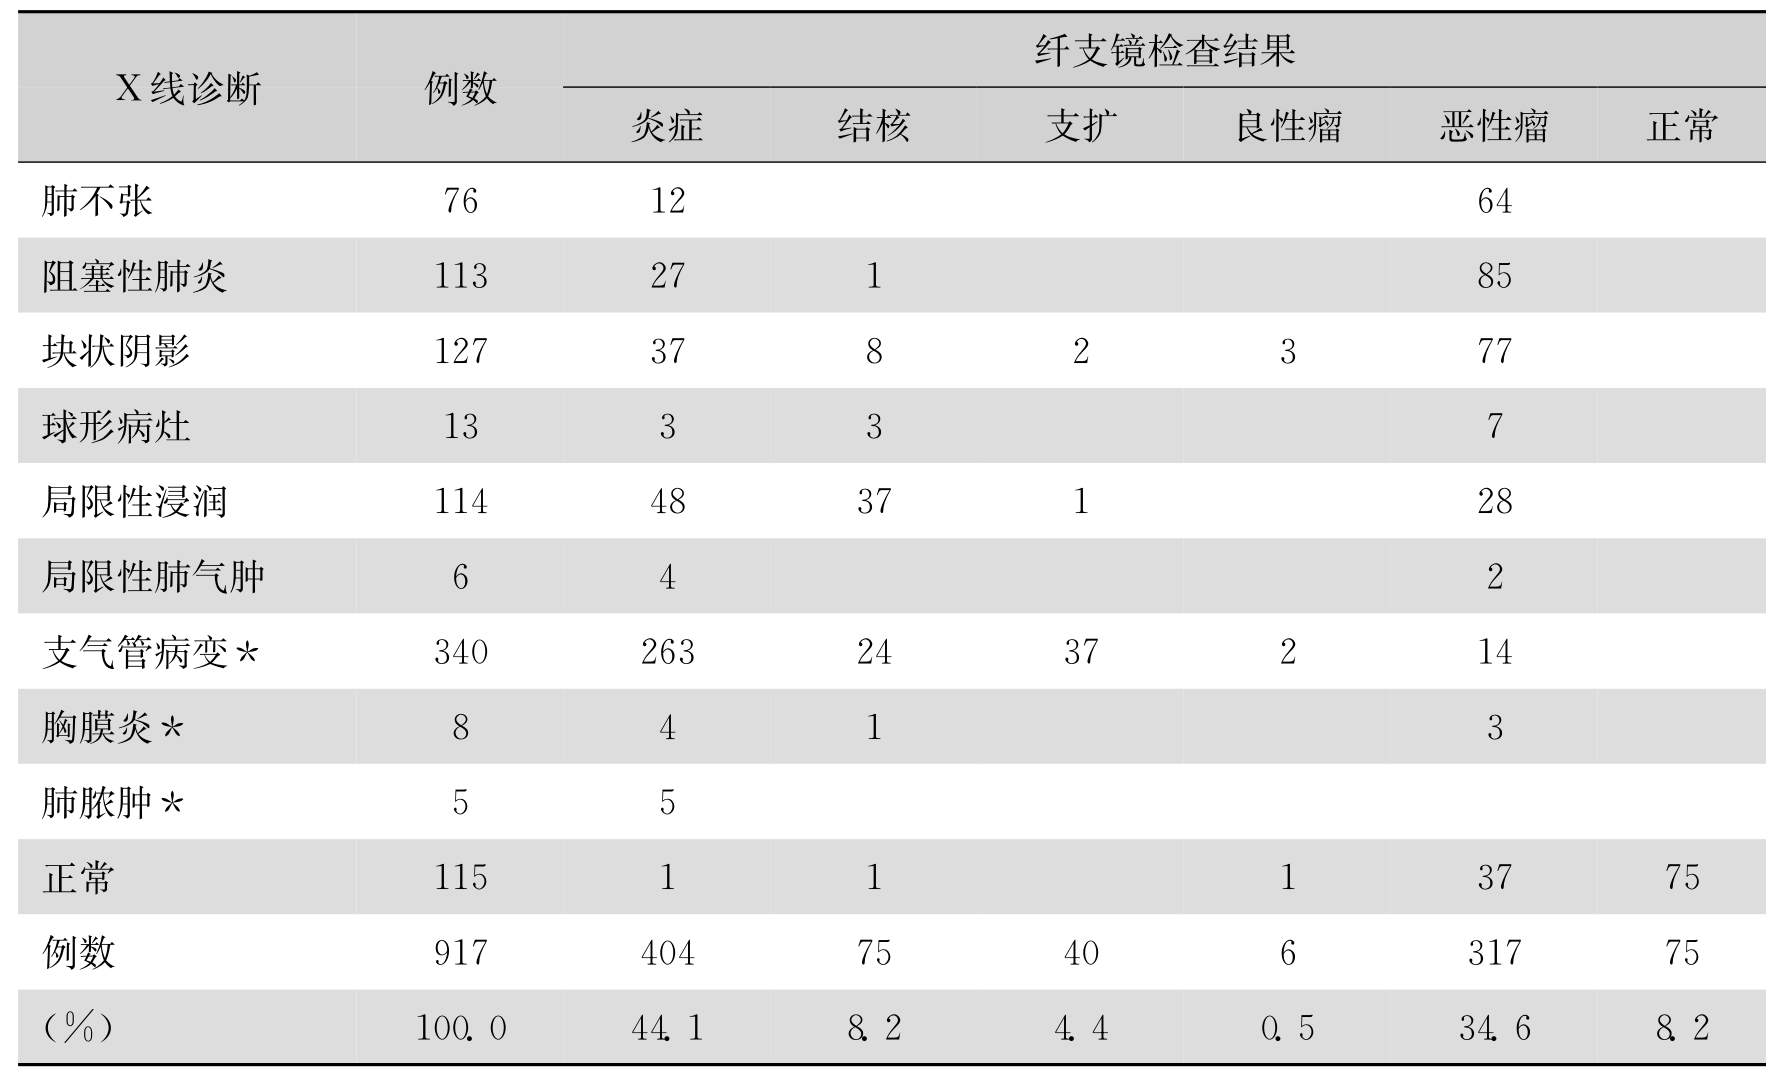
\includegraphics[width=.7\textwidth,height=\textheight,keepaspectratio]{./images/Image00040.jpg}
 \captionsetup{justification=centering}
 \caption{腔隙性脑梗死\\{\small A.病灶位于左侧基底节区和左侧额叶白质区;B.病灶位于脑干}}
 \label{fig2-22}
  \end{figure} 

\textbf{【鉴别诊断】}
脑腔隙在病理上为一脑实质内含水分的<15mm的潜在腔,包括穿支动脉等病变所致的腔隙性脑梗死和非血管病变引起的腔隙病变。发病机制包括血管因素所致的缺血即腔隙性梗死,以及血管因素(如出血、动脉炎等)和血管外因素(如炎症、变性、中毒、机械损伤等)所形成的腔隙性病变,应注意分析。此外,还应注意与前联合及基底节区的扩大的血管周围间隙(多在0.2~1.2cm大小)相鉴别,MR检查有独到鉴别价值。

\subsection{皮质下动脉硬化性脑病}

本病又称Binswanger病,是一组以脑深部小动脉硬化、痴呆、皮质下白质变性、皮质下腔隙或软化为特征的综合征。但有人认为“皮质下动脉硬化性脑病”一词未能正确反映所看到的组织学改变,且过高的估计了临床意义。因此,有关文献应用的非特异性名词较合适,如深部脑白质缺血或老年性白质高信号(MR)。我们认为称为“动脉硬化性脑白质病”或“深部脑白质慢性缺血”更趋合理,同时我们认为有关文献所述及的“脑白质疏松症”亦属本病的范畴。

\textbf{【病因病理】}
主要病因为慢性高血压,其病理特征为弥漫性不完全的皮质下梗死,在侧脑室旁和半卵圆中心的白质内髓鞘肿胀或脱失,皮质下弓状纤维与胼胝体不受累。常有皮质萎缩及皮质下、基底节区腔隙性脑梗死,在髓动脉内有狭窄性动脉粥样硬化。

\textbf{【临床表现】}
见于60岁以上老人,多隐形起病,呈进行性记忆力障碍、严重精神衰退、言语不清,反复发生的神经系统局部体征如偏瘫、失语、偏盲等。病情可缓解和反复加重,常伴有高血压。

\textbf{【CT表现】}
脑白质内斑片状或云絮状稍低密度灶,界限不清,其密度降低不如脑梗死明显。以侧脑室周围分布最明显,其次为半卵圆中心,多为两侧对称性(图\ref{fig2-23})。基底节---内囊区、丘脑、半卵圆中心常伴多发的腔隙性梗死灶,可有脑室系统扩大,脑沟、脑池增宽的弥漫性脑萎缩改变。

\begin{figure}[!htbp]
 \centering
 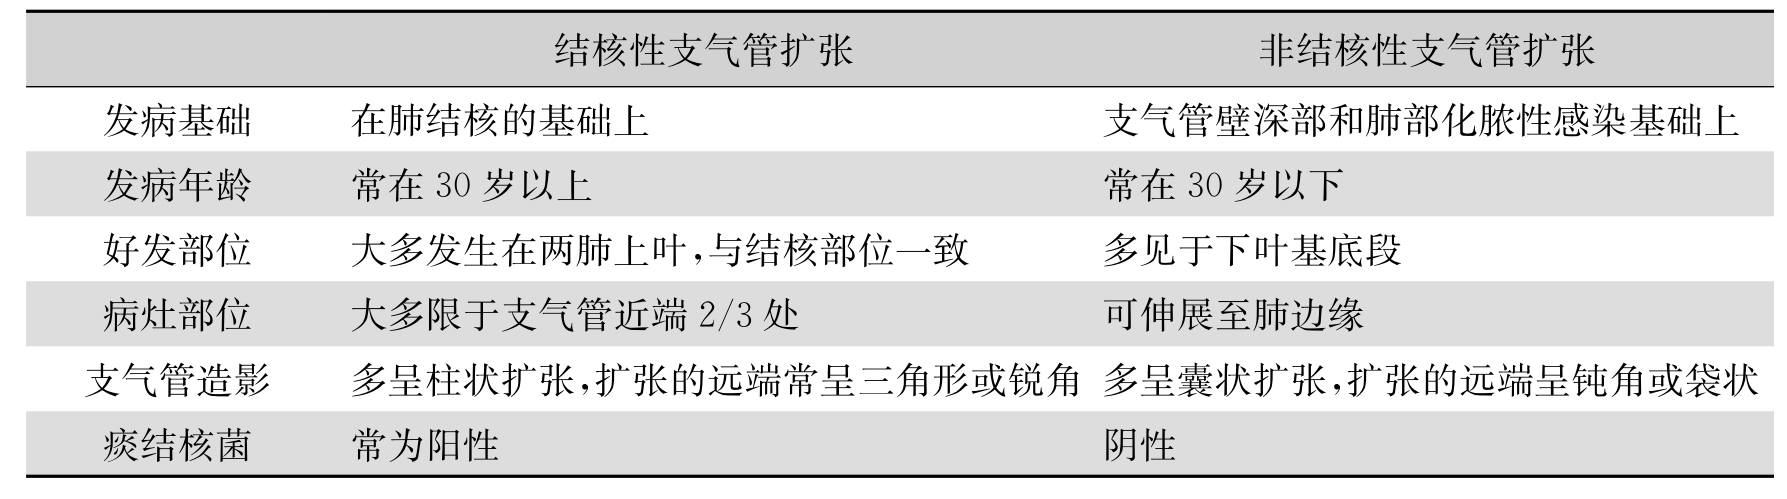
\includegraphics[width=.7\textwidth,height=\textheight,keepaspectratio]{./images/Image00041.jpg}
 \captionsetup{justification=centering}
 \caption{动脉硬化性脑白质病\\{\small 侧脑室周围白质和半卵圆中心区对称性片絮状低密度灶}}
 \label{fig2-23}
  \end{figure} 

\subsection{脑缺氧}

\textbf{【病因病理】}
脑缺氧包括乏氧性缺氧、血液性缺氧、循环性缺氧和中毒性缺氧。常见病因有:高空高原缺氧,呼吸功能不全和某些先心病循环短路、CO中毒以及各种严重贫血、各种休克和心衰,氰化物、硫化氢、磷中毒。脑组织局部循环性缺氧包括颅脑外伤、脑血管意外、脑血流障碍、颅内感染、脑肿瘤急性恶化等。主要病理改变为早期脑组织坏死、水肿,进行性脱髓鞘,晚期脑萎缩。

\textbf{【CT表现】}
①弥漫性脑水肿:以大脑为主,可出现大脑密度普遍减低,而丘脑、脑干和小脑密度相对较高的所谓CT反转征。②局部脑水肿:以脑动脉边缘带(分水岭区)、脑室周围白质最常见,基底节次之,也可见于丘脑和小脑。③缺氧性脑出血:脑实质、脑室周围-脑室、蛛网膜下腔、硬膜下或硬膜外。④脑萎缩:晚期可出现,也可见囊状软化灶。

\subsection{脑静脉窦血栓形成}

颅内静脉血流受阻即脑静脉和静脉窦血栓形成所导致的脑梗死称为静脉性脑梗死,占中风病人的1%~2%。

\textbf{【病因】}
近1/3病因不明。可分为:①全身因素:脱水、糖尿病、高凝血状态、血小板增多症、口服避孕药、妊娠、产后、近期手术、长期应用激素、肾病综合征、心脏病、结缔组织病、新生儿窒息等;②局部因素:局部感染、中耳乳突炎、鼻窦炎、脑膜炎、颅面中耳手术、颅脑外伤、动静脉畸形、动静脉瘘、腰穿等。

\textbf{【临床表现】}
多见于20~35岁女性,其表现各异。头痛最常见,15%急性起病,类似蛛网膜下腔出血,常伴头晕、恶心及视乳头水肿等颅内高压症状。1/3~1/2病人有局灶性神经症状,如颅神经麻痹和意识障碍,半数出现癫痫,还可有偏瘫。小脑静脉血栓可有共济失调等症状。

\textbf{【CT表现】}
最常见于上矢状窦、横窦和乙状窦,其次为海绵窦和直窦。特征性改变为致密静脉征(或索条征)和空三角征,但缺乏特异性。①早期(1~2天):平扫静脉窦内血栓密度与硬脑膜相似,可高达150Hu。增强扫描呈“空三角征”,即三角形的硬膜窦断面,中心不强化而周围强化。②第3~第10天:平扫窦内血块渐吸收,CT值约80Hu左右。③11天后:血凝块基本吸收,窦内CT值约50Hu。④静脉栓塞常伴有弥漫性非对称性脑肿胀、梗死性脑水肿、出血性梗死或单纯出血(脑实质和硬膜下)。静脉性出血其血肿周围界限不清,多靠近脑表面,而且周围环以大片低密度灶有别于动脉性出血。

\textbf{【鉴别诊断】}
高位分叉的上矢状窦、硬膜下脓肿和血肿、蛛网膜下腔出血及窦内窗孔和分隔均可类似空三角征;儿童的流动性静脉血常呈轻度高密度类似血栓,应注意鉴别。

\subsection{高血压脑病}

本病是指在血压迅速剧烈升高时,引起的急性全面性脑功能障碍,属可逆性后部白质脑病综合征(还见于妊娠高血压、慢性肾衰、使用免疫抑制剂和激素等)的范畴。

\textbf{【病因病理】}
可发生于各种原因(原发或继发)引起的动脉性高血压。病理上大多有不同程度的脑水肿,脑表面动脉、静脉和毛细血管扩张,脑切面可见斑点状、裂隙状出血和小动脉壁的坏死。

\textbf{【临床表现】}
该病一般起病急骤,病程短暂,所有症状历时数分钟或1~2小时,最多数天。主要表现为严重头痛、惊厥、偏瘫、失语、黑蒙、神志不清甚至昏迷。

\textbf{【CT表现】}
主要为广泛性脑水肿,呈对称性、弥漫性、边界不清的低密度区,以大脑半球后部最为显著,也可累及小脑。脑室系统变小,脑沟、脑池变浅。血压改善后一段时间随访,完全恢复正常。

\subsection{脑出血}

脑出血是指脑实质内的出血,又称为脑溢血或出血性脑卒中。

\textbf{【病因病理】}
其原因很多,临床上概括为损伤性和非损伤性两大类。后者又称为原发性或自发性脑出血,是指脑内血管病变、坏死、破裂而引起的出血。自发性脑出血绝大多数由高血压和动脉硬化(引起脑小动脉的微型动脉瘤或玻璃样变)所致,其次为脑血管畸形和动脉瘤所致。其他原因还有颅内肿瘤出血、出血性梗死、脑血管淀粉样变、全身出血性疾病、维生素缺乏、新生儿颅内出血、重症肝炎(可合并脑出血、梗死)等。

出血好发于壳核和内囊区(约占50%)、中心部脑白质、丘脑和下丘脑、小脑半球、桥脑,以及脑室内。病理可分为3期:①急性期:血肿内含新鲜血液或血块,周围脑组织有不同程度的水肿,还可有点状出血;②吸收期:血肿内红细胞破坏、血块液化,周围出现吞噬细胞,并逐渐形成含有丰富血管的肉芽组织;③囊变期:坏死组织被清除,缺损部分由胶质细胞及胶原纤维形成瘢痕,血肿小可由此类组织充填,血肿大时则遗留囊腔。

\textbf{【临床表现】}
本病常突然发生剧烈头痛、意识障碍、恶心、呕吐、偏瘫、失语、脑膜刺激征等,按病情发展可分为急性期、亚急性期和慢性期。

临床预后与出血的部位及出血量的多少有关。出血位于皮质下白质区,血肿及水肿引起占位效应,导致出血区功能丧失,但预后相对较好,出血量>30ml为手术指征。小脑或脑干出血压迫四脑室,继发急性颅内压升高,常伴延髓生命中枢损害,直接危及生命,血肿直径>3cm应立即手术。

\textbf{【CT表现】}
血液形成影像的主要成份为含铁的血红蛋白,血液的密度高于脑组织,故CT表现呈高密度。由于脑血管较细,受部分容积效应影响,故血管内血液多不能显示。严重贫血的患者急性期脑出血亦可呈等密度甚至低密度。

\subsubsection{出血量的估计}

一般采用以下公式计算:V(ml)=1/6
π(A×B×C),A为血肿前后径,B为左右径,C为上下径。A、B、C的单位均为厘米。

\subsubsection{CT分期}

通常将脑内血肿分为急性期(1周内)、吸收期(2周~2个月)和囊变期(2个月后)。也有学者根据密度分为:高密度期、等密度期、低密度期、慢性期(图\ref{fig2-24})。

\begin{figure}[!htbp]
 \centering
 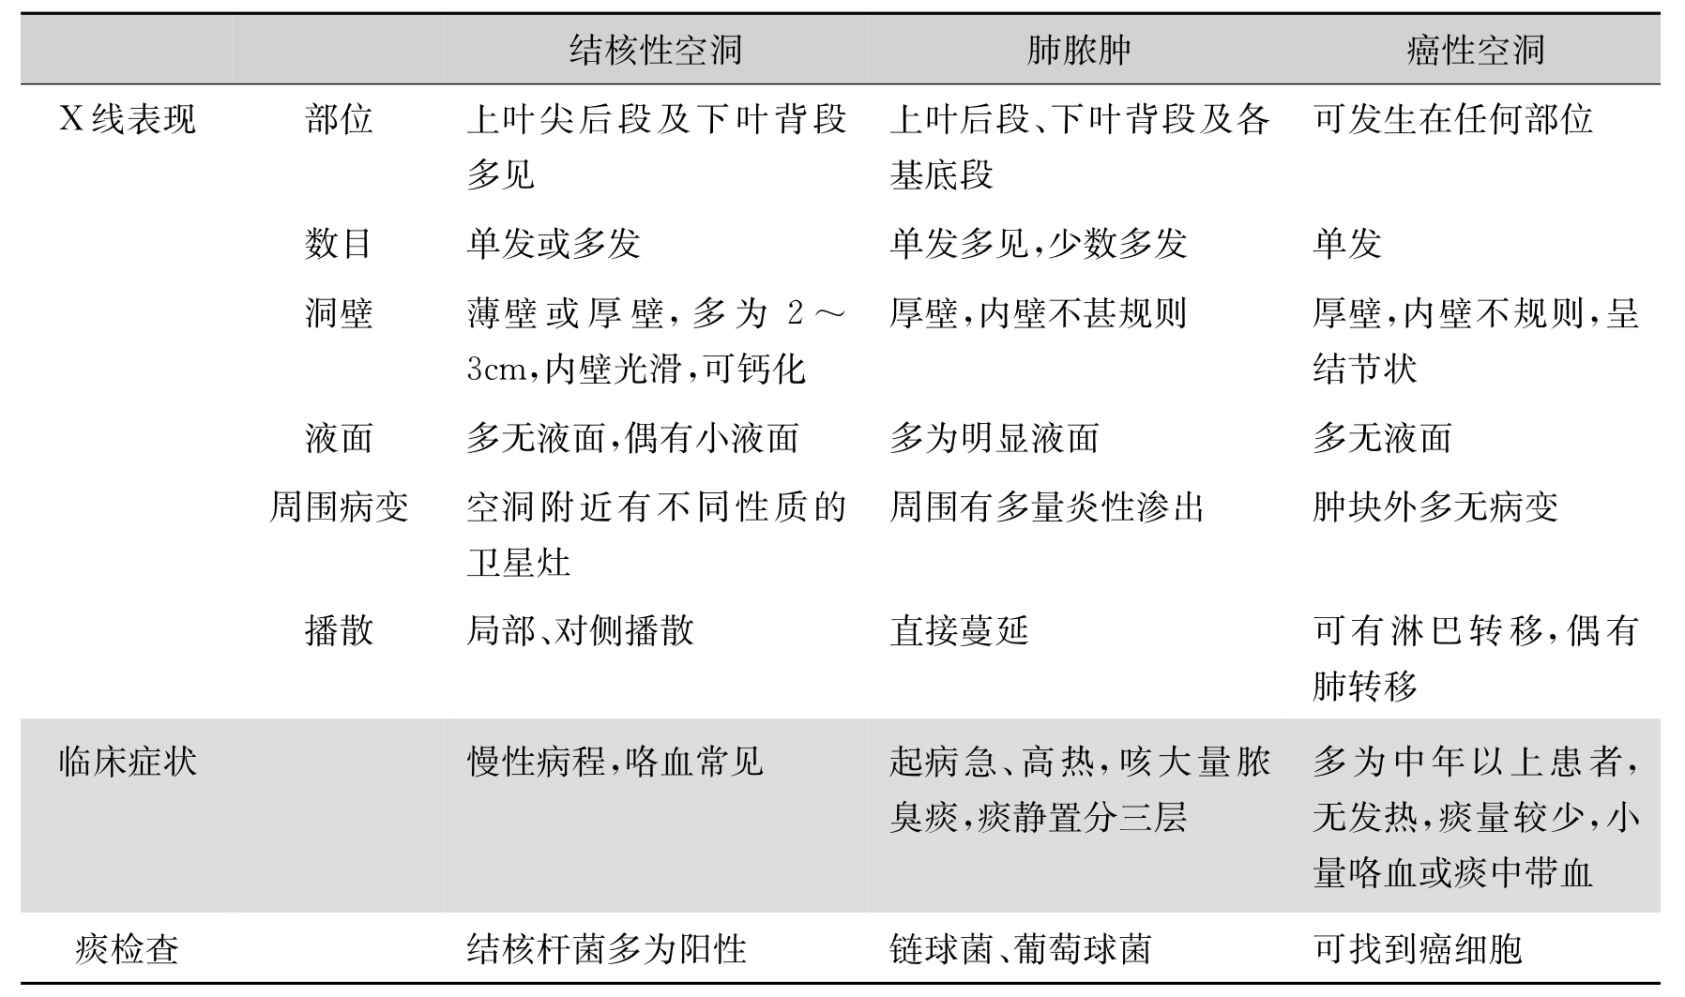
\includegraphics[width=.7\textwidth,height=\textheight,keepaspectratio]{./images/Image00042.jpg}
 \captionsetup{justification=centering}
 \caption{脑出血\\{\small A.右侧丘脑-外囊区血肿破入左右侧脑室内,右外侧裂内亦有血液充填;B.脑出血吸收期,血肿边缘开始吸收呈环状低密度,低密度外可见肉芽组织形成的等密度环}}
 \label{fig2-24}
  \end{figure} 

1.高密度期(1~14天):血液逸出血管后,红细胞分解释放含铁的血红蛋白,表现为高密度区,CT值约50~80Hu。出血3~4天因血液凝固成血块,血浆被吸收,红细胞压积增加,血肿密度达到高峰,甚者达90Hu,周围有水肿。严重贫血者可为等密度,甚至低密度,但血肿有占位征象。

2.等密度期(14~64天):血红蛋白分解,含铁血黄素开始被吸收,血肿呈等密度。但仍有占位效应,水肿仍存在,增强扫描呈环状强化。

3.低密度期(30~84天):血肿周围的新生血管及神经胶质增生形成血肿壁,血肿内含铁血黄素及血红蛋白被吸收,CT呈低密度灶。水肿消失,无占位效应,增强扫描仍呈环状强化。

4.慢性期(3个月后):少量脑出血被胶质和胶原纤维替代而愈合,CT呈略低密度灶。大量脑出血形成囊腔,CT近水样密度,并可出现牵拉现象,增强扫描无或轻微强化。

\subsubsection{脑室内出血}

单纯脑室出血与脑实质内出血破入脑室系统表现一样。少量出血时多沉积在侧脑室后角、第三脑室后部或第四脑室顶部,大量出血常呈脑室“铸型”样表现(图\ref{fig2-25})。早期可有分层现象,以后呈等或低密度,脑室内出血可形成脑积水。

\begin{figure}[!htbp]
 \centering
 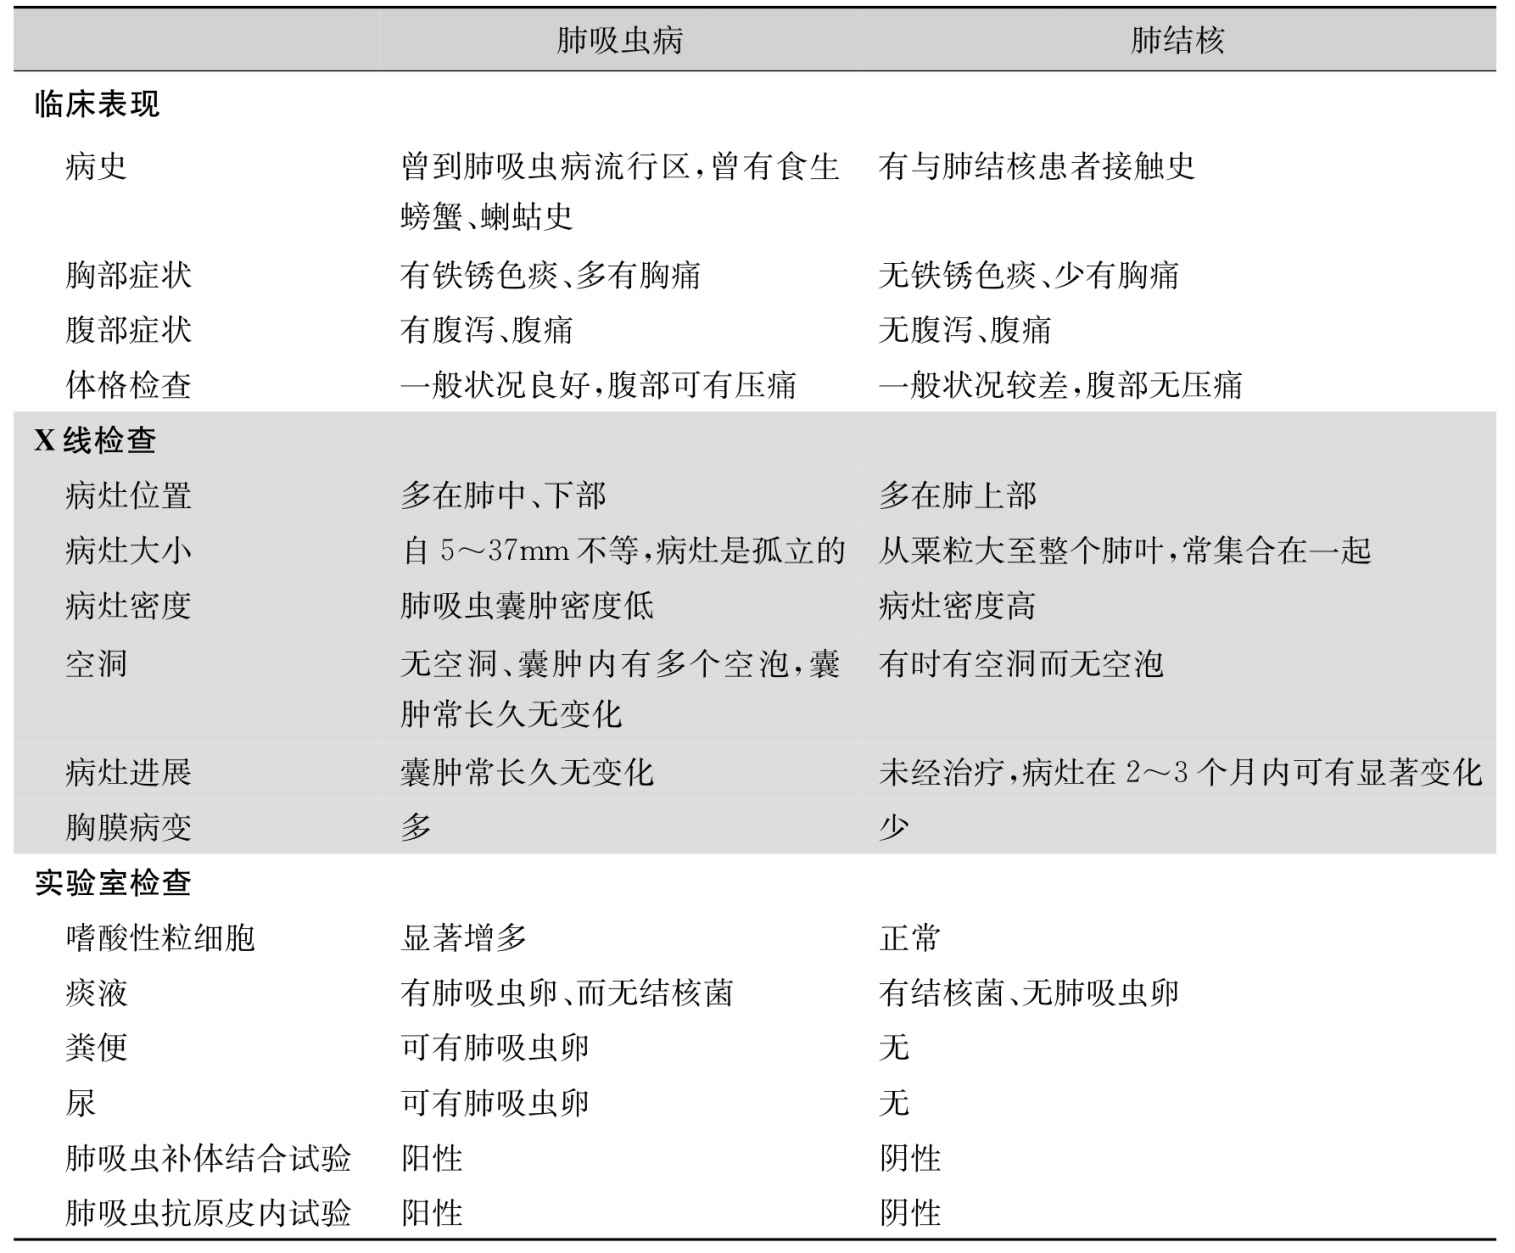
\includegraphics[width=.7\textwidth,height=\textheight,keepaspectratio]{./images/Image00043.jpg}
 \captionsetup{justification=centering}
 \caption{脑室内出血\\{\small 左右侧脑室内有大量血液充填,右侧呈“铸型”样表现}}
 \label{fig2-25}
  \end{figure} 

此外,在诊断时应注意:①急性脑出血大的血肿可形成脑疝。②脑出血可直接破入脑室系统和蛛网膜下腔,亦可由脑室系统进入蛛网膜下腔。③出血周围水肿,在第1天内可出现或表现轻微;3~7天达高峰;出血16天左右占位效应开始减退。④发现灶周水肿与血肿期龄不符时,应考虑肿瘤出血可能。⑤如局部伴有钙化或血肿密度不均等表现,除考虑到肿瘤出血外,也应考虑到脑血管畸形的可能。

\subsection{慢性扩展性脑内血肿}

本病是自发性脑内血肿的一种特殊类型,临床及影像学表现无特异性,易与肿瘤卒中、囊肿合并出血感染等混淆。

\textbf{【病因病理】}
其病因认为与隐匿性血管畸形、血管硬化、外伤、放射损伤、凝血功能障碍有关,一般没有高血压和脑外伤病史。隐匿性血管畸形或微小动脉瘤破裂出血,血肿及其代谢产物不断刺激周围组织产生炎性反应,毛细血管、纤维组织增生,并由增生的毛细血管、纤维组织形成包膜。而其丰富的毛细血管壁脆弱,反复出血、渗出,包膜内液化,使血肿体积逐渐增大。

\textbf{【CT表现】}
多为边缘清楚、密度均匀或不均匀的高、低混杂囊性病灶,且其内可见液-液平面。增强扫描病灶多无强化;部分血肿周围环状强化,为病灶周围脑组织或肉芽组织强化所致。

\subsection{蛛网膜下腔出血}

本病是指颅内血管破裂后血液注入蛛网膜下腔。

\textbf{【病因】}
临床可分为两大类,即外伤性与自发性。自发性原因很多,但以颅内动脉瘤(约占51%)、动静脉畸形(6%)和高血压动脉硬化所致(15%)最多见。此外,20%病因不明。

\textbf{【临床表现】}
自发性常有明显的诱因,如体力劳动过度、咳嗽、用力排便、情绪激动等。绝大多数起病急,剧烈头痛、呕吐、意识障碍、抽搐、脑膜刺激征等,同时可有偏瘫,腰穿有确诊价值。

\textbf{【CT表现】}
一般在出血3天内检出率最高,可达80%~100%,一周后很难检出。特征性表现为基底池、侧裂池和脑沟内等广泛的高密度影(图\ref{fig2-26})。如出血量少或严重贫血均不易发现。大脑前动脉破裂血液多积聚于视交叉池、纵裂前部;大脑中动脉破裂血液多积聚于一侧的外侧裂附近,也可向内流;颈内动脉破裂血液也以大脑外侧裂为多;椎基动脉破裂血液主要积聚于脚间池和环池。但出血量大者可难以估计出血部位。

\begin{figure}[!htbp]
 \centering
 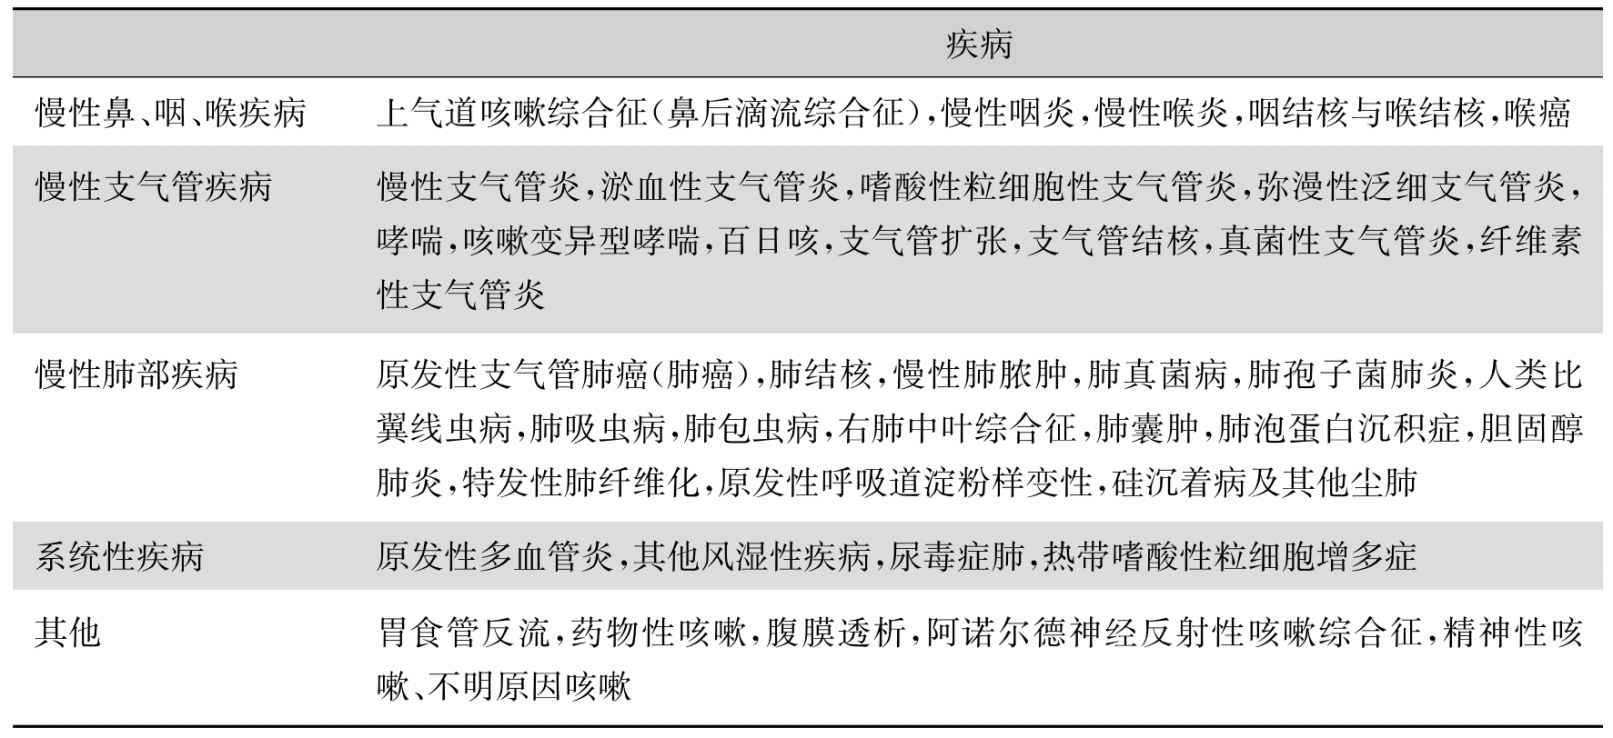
\includegraphics[width=.7\textwidth,height=\textheight,keepaspectratio]{./images/Image00044.jpg}
 \captionsetup{justification=centering}
 \caption{蛛网膜下腔出血\\{\small A、B为同一患者,鞍上池、左右外侧裂池、纵裂池前部、环池、四叠体池、大脑大静脉池内均有大量高密度血液充填}}
 \label{fig2-26}
  \end{figure} 

\textbf{【并发症】}
①脑积水:脑积水早期为梗阻性,发生率约为20%。可演变成交通性。②脑动脉痉挛:造成脑缺血和脑梗死,发生率约25%~42%。③伴发脑内血肿和(或)硬膜下血肿、脑室内出血:常与动脉瘤、动静脉畸形或脑肿瘤出血有关。

\subsection{颅内动脉瘤}

动脉壁呈局限性病理性扩张,与动脉腔有一颈部相连。

\textbf{【病因病理】}
其病因有先天性因素、动脉粥样硬化、感染因素和外伤4个方面。根据影像学可分为5种病理类型:①粟粒状动脉瘤;②囊状动脉瘤;③假性动脉瘤;④梭形动脉瘤;⑤壁间动脉瘤。

\textbf{【临床表现】}
好发于20~70岁。在破裂前90%无特殊临床症状,少数可影响到邻近神经或脑结构而产生症状。破裂后引起蛛网膜下腔出血和颅内血肿而出现相应的症状体征。

\textbf{【CT表现】}
颅内动脉瘤好发于脑动脉,约90%~95%分布于颈内动脉系统,5%~10%分布于椎动脉系统。颈内动脉瘤约占20%~40%,大脑中动脉瘤约占21%~31%,前交通及大脑前动脉瘤约占30%~37%,多发性约占4%~5%。

1.颅底较小动脉瘤:平扫难以显示,增强扫描呈高密度。

2.较大动脉瘤:平扫呈圆形等或高密度,边缘光整,有时瘤壁可见钙化。增强扫描呈均匀强化,而血栓无强化。

3.巨大动脉瘤:即直径>2.5cm的动脉瘤,其CT表现可分3型。①无血栓形成型:平扫呈圆形或椭圆形等或略高密度,瘤壁钙化较其他类型少见。增强扫描均匀强化。②部分血栓形成型:最常见,呈圆形或卵圆形略高密度,壁多有弧形钙化。增强扫描流动的血液强化明显,血栓不强化,从而形成高密度影内的低密度点称为“靶征”。周围很少有水肿。③完全栓塞型:平扫为圆形或卵圆形混杂略高密度,瘤壁常有钙化,周围无水肿。增强扫描呈环状强化。

此外,CTA显示动脉瘤的敏感性可达95%,特异性近83%。

\textbf{【并发症】}
①颅内出血:蛛网膜下腔出血、脑内血肿和脑室内积血,甚至可穿破蛛网膜造成硬膜下血肿。②脑血管痉挛:蛛网膜下腔出血所致,并导致相应区域的水肿、梗死。③脑积水:蛛网膜下腔出血所致。

\textbf{【鉴别诊断】}
动脉瘤周围多无水肿,瘤壁可有环形强化,动态CT扫描时间-密度曲线呈速生速降型,与血管相同。而肿瘤则表现为缓慢上升和下降的时间-密度曲线是鉴别的关键。

\subsection{脑动静脉畸形}

脑血管畸形分为5型:①动静脉畸形(AVM);②海绵状血管瘤;③静脉畸形(又称静脉血管瘤);④毛细血管扩张症(又称毛细血管瘤,以MR诊断为佳);⑤血管曲张(包括大脑大静脉畸形等)。其中AVM最常见,约占90%以上。毛细血管扩张症一般只被病理诊断,CT或MR很难显示,偶见钙化。

AVM是最常见的血管畸形,但有相当一部分脑血管造影阴性,称为隐匿性AVM。

\textbf{【病理】}
AVM由一条或多条供血动脉、畸形血管团、一条或多条引出静脉组成。常见于大脑中动脉分布区的脑皮质,亦可发生于侧脑室(如脉络丛)、硬脑膜、软脑膜、脑干和小脑。

\textbf{【临床表现】}
好发于20~30岁,男性多于女性,10%~15%无症状。常见的症状有:①头痛:偏头痛或全头痛,阵发性;②出血:出现相应症状和体征;③癫痫:约30%为此就诊;④脑缺血症状:脑梗死、脑萎缩;⑤部分颅外听到杂音。

\textbf{【CT表现】}
AVM平扫呈局灶性高、低或低、等混杂密度区,多呈团块状,也可见点、线状影,边缘不清,但有时可不显示。常伴斑点状或条状钙化,轻度或无占位征象。病灶周围无水肿表现,但有时可出现脑室扩大和交通性脑积水。增强扫描呈团块状强化,有时可见迂曲的血管影,造影剂充盈及排出均较快。CTA多可有效显示其供血动脉、畸形血管团和引流静脉(图\ref{fig2-27})。



\begin{figure}[!htbp]
 \centering
 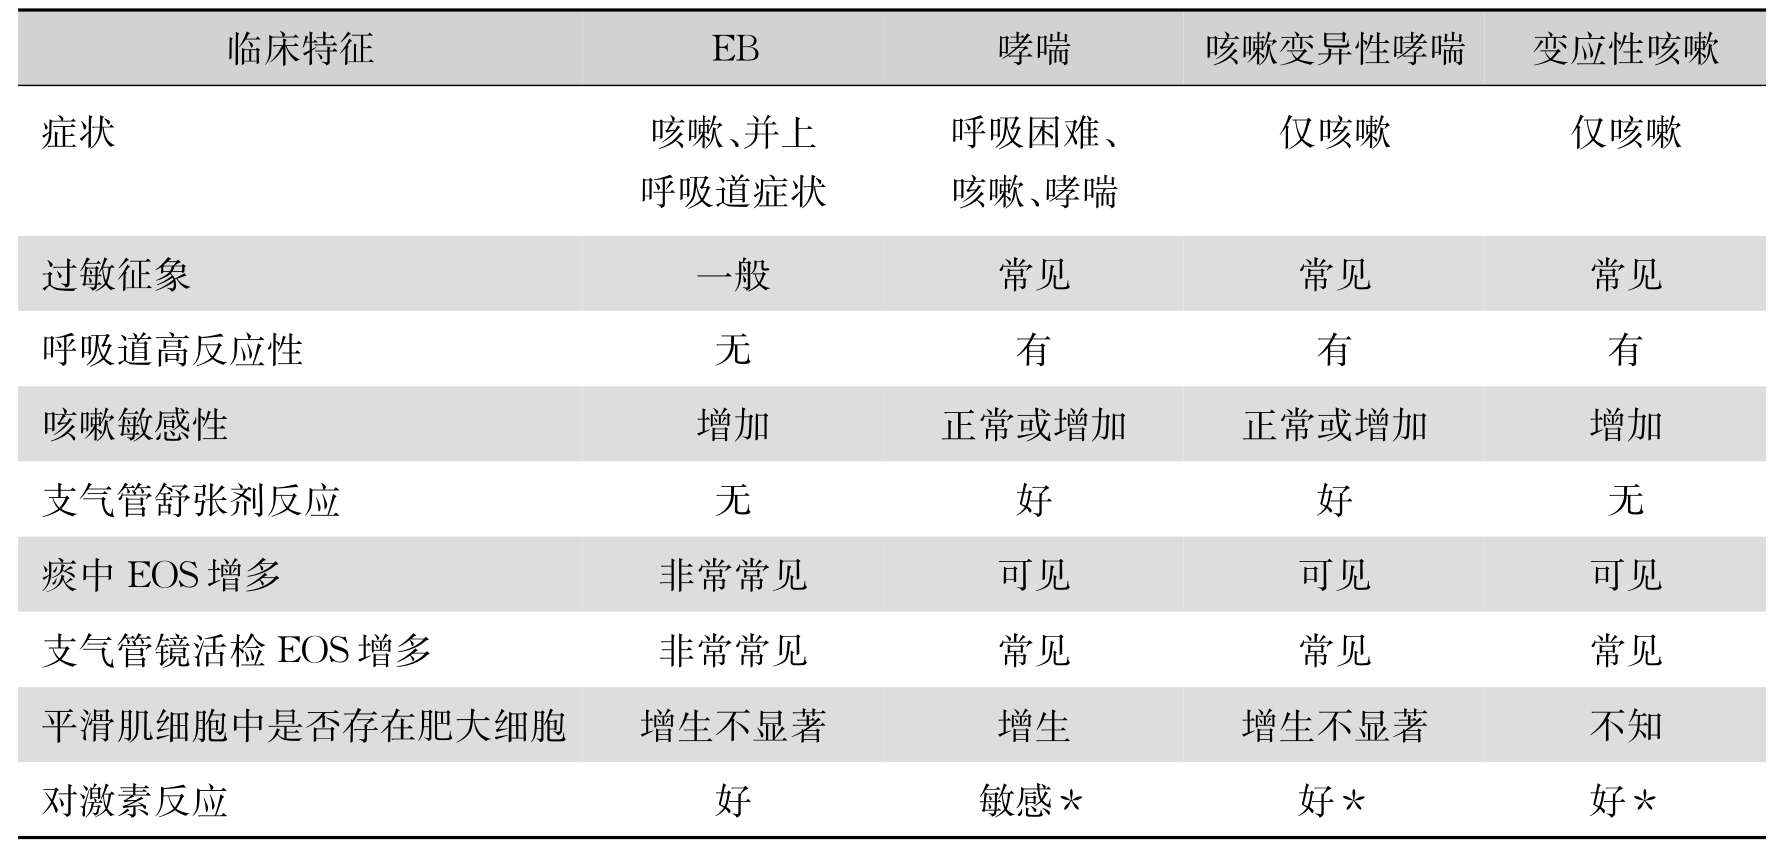
\includegraphics[width=\textwidth,height=\textheight,keepaspectratio]{./images/Image00045.jpg}
 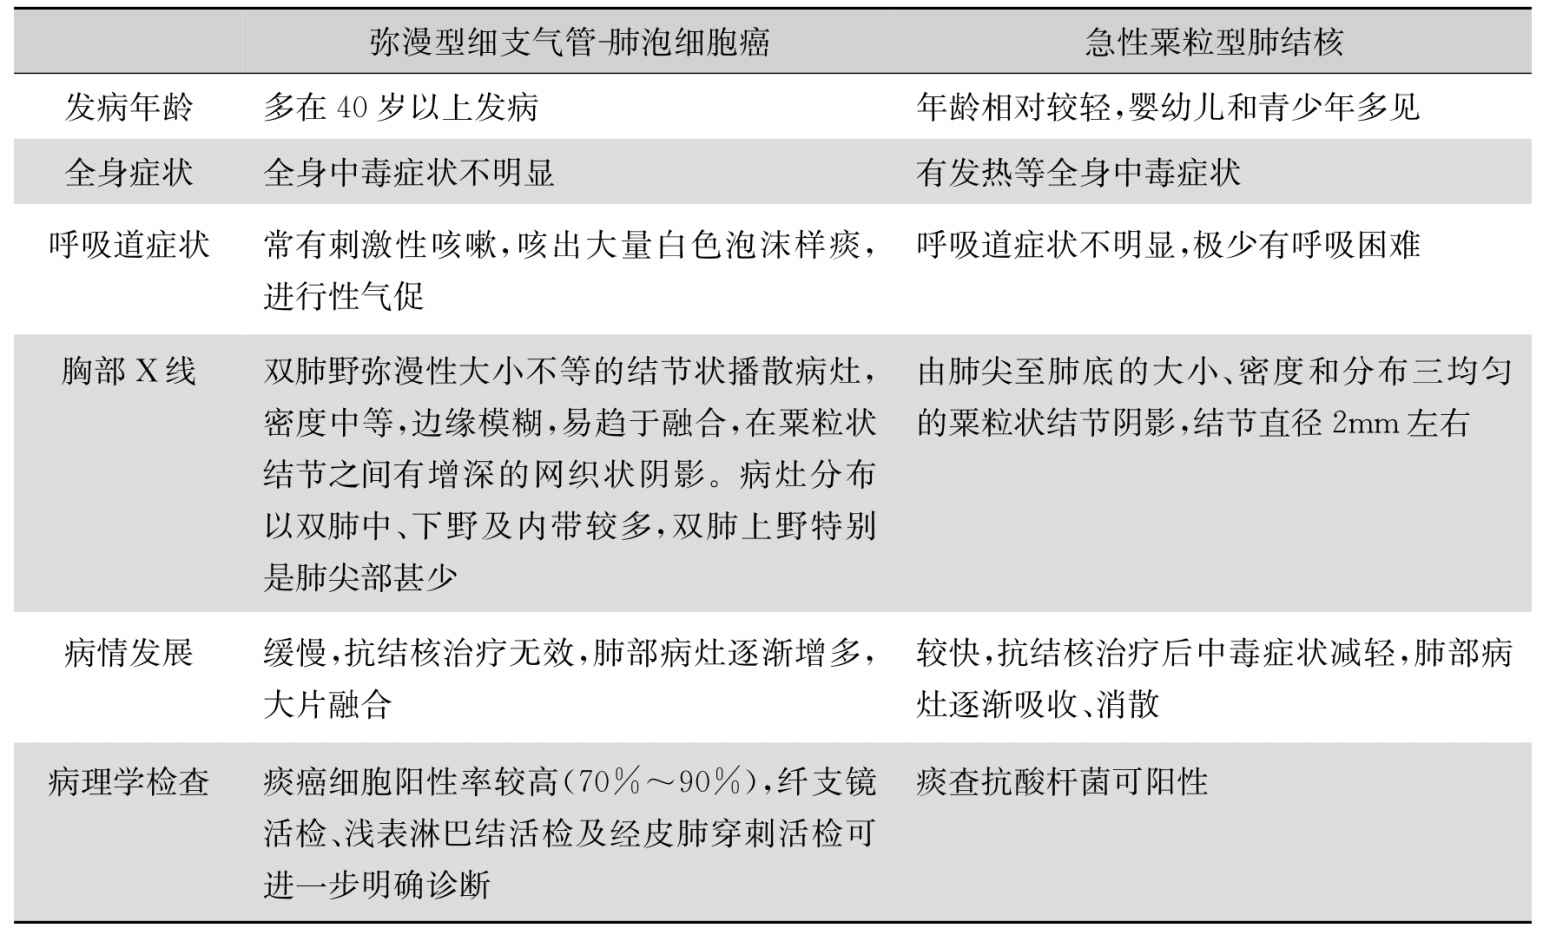
\includegraphics[width=\textwidth,height=\textheight,keepaspectratio]{./images/Image00046.jpg}
 \captionsetup{justification=centering}
 \caption{脑动静脉畸形\\{\small A~D为同一患者,平扫(A、B图)左侧颞叶有局灶性高、等混杂密度区,形态不规则,其边缘有蚯蚓状高密度影(引流静脉);增强扫描(C图)呈团块状强化,并见迂曲的引流静脉影;CTA(D图)清晰显示畸形血管团和粗大的引流静脉}}
 \label{fig2-27}
  \end{figure} 

其并发症有出血、梗死、软化灶及局限脑萎缩表现。

\textbf{【鉴别诊断】}
钙化明显的肿瘤以及强化明显的肿瘤(如胶质瘤)其水肿及占位效应均较显著,可与AVM鉴别。AVM增强扫描的时间-密度曲线与血管相似亦是与肿瘤鉴别的重要依据。

\subsection{颅内海绵状血管瘤}

本病占脑血管疾病的7%,近年来的研究显示其属不完全染色体显性遗传性疾病。目前多认为其发生源于脑内毛细血管水平的血管畸形,可位于脑内或脑外,为非真性肿瘤。

\textbf{【病理】}
病灶由微动脉延伸出来的、血流缓慢的、大小不等的丛状薄壁的血管窦样结构组成,其间有神经纤维分隔,窦间没有正常脑组织。由于其血管壁薄而缺乏弹性,且易于发生玻璃样变、纤维化,因而易出血,并可有胶质增生、坏死囊变、钙化,病灶可全部钙化形成“脑石”。病灶周围可见含铁血黄素沉着或有机化的血块。病灶无明显的供血动脉及引流静脉。

\textbf{【临床症状】}
好发于40~60岁,常以颅内出血为首发症状。典型表现为癫痫发作、突发性头痛和进行性神经功能障碍等。

\textbf{【CT表现】}
80%位于幕上,好发于额、颞叶,也可发生于蛛网膜下、硬膜下,脑外者多位于鞍旁海绵窦区。多表现为界限清楚的圆形或卵圆形的等至稍高密度影(图\ref{fig2-28})。其内可见“颗粒征”颇有特征,即在略高密度背景内含有数量不一的颗粒状高密度影和低密度影,前者为钙化,后者为血栓形成。除急性出血或较大病灶,灶周一般无水肿及占位征象。可能因为供血动脉太细或已有栓塞,也可能因病灶内血管床太大,血流缓慢使对比剂稀释,致使增强扫描不强化或仅见周边强化。其强化程度取决于病灶内血栓形成和钙化的程度,血栓形成轻、钙化不明显者强化明显。国外报道脑外者可有骨侵蚀。

\begin{figure}[!htbp]
 \centering
 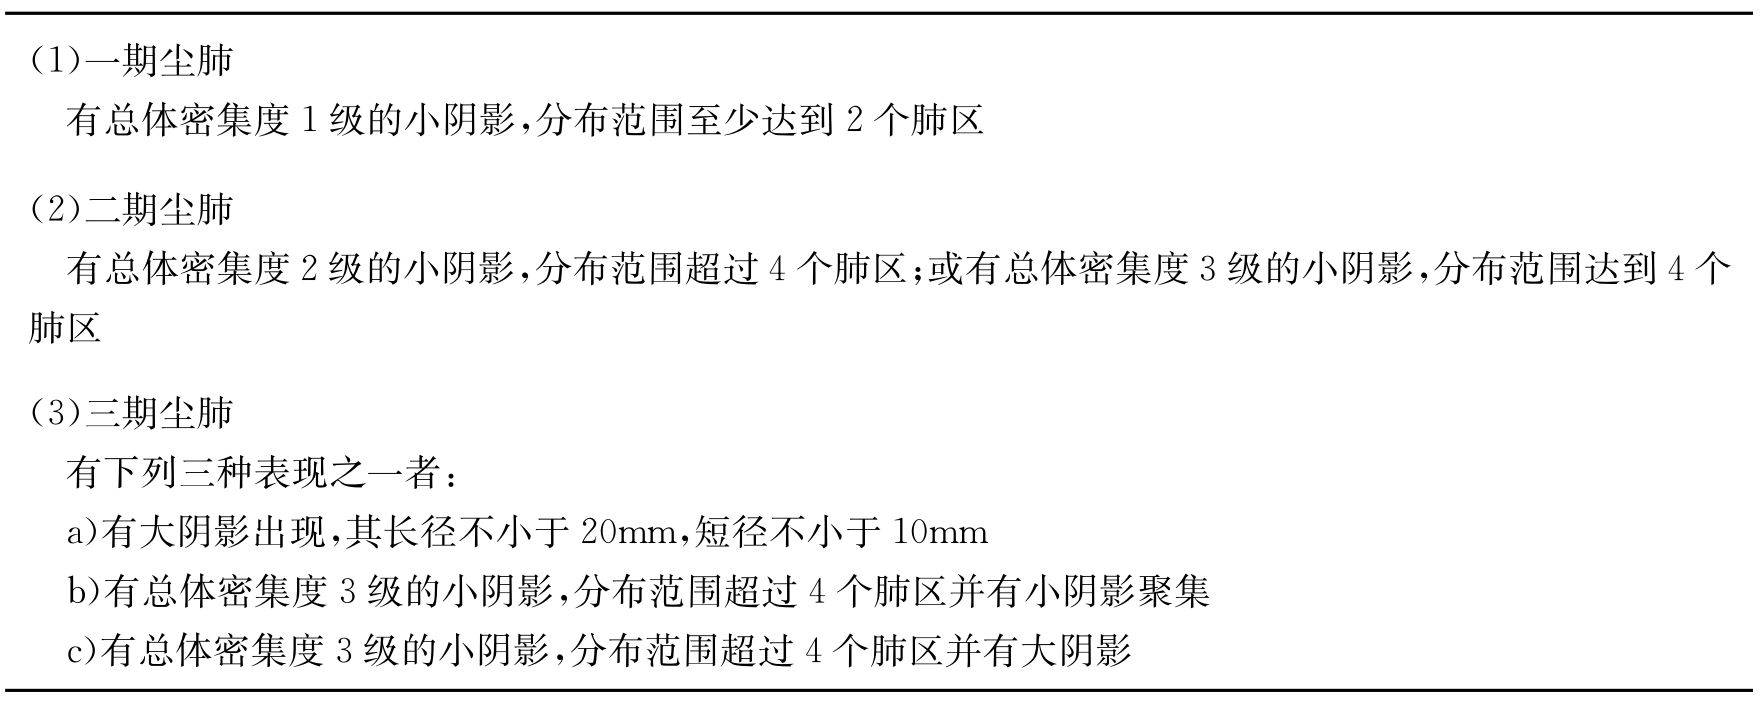
\includegraphics[width=.7\textwidth,height=\textheight,keepaspectratio]{./images/Image00047.jpg}
 \captionsetup{justification=centering}
 \caption{颅内海绵状血管瘤\\{\small A、B非同一患者,A示病灶位于小脑左侧半球,B示病灶位于脑干;病灶均呈近圆形稍高密度灶,周围无水肿}}
 \label{fig2-28}
  \end{figure} 

\textbf{【鉴别诊断】}
①主要应与脑膜瘤鉴别。后者平扫密度多均匀一致,增强扫描明显强化,常有明显占位征象,并可出现水肿征象及颅骨增生和吸收有助鉴别。②少数血管瘤呈环状并伴壁结节,偶有出血,病灶内显示血-液平面伴周围水肿,不易与胶质瘤等相鉴别。

\subsection{脑静脉性血管畸形}

本病又称脑静脉性血管瘤、脑发育性静脉异常,是一种组织学上由许多扩张的髓静脉和一条或多条引流静脉组成的血管畸形。国外有学者认为是一种正常引流静脉的非病理性变异。

\textbf{【病因病理】}
其病因不明,多认为是胚胎发育时宫内意外因素导致静脉阻塞,由侧支代偿所致。其形成时间在脑动脉形成之后,故仅含静脉成分。畸形血管由许多扩张的放射状排列的髓静脉汇入一条或多条引流静脉组成,向皮质表面和静脉窦或向室管膜下引流,可分为皮层表浅型、皮层下型和脑室旁型。

\textbf{【临床表现】}
好发于35~40岁,男女发病率相近。一般无症状,少数可产生癫痫、头痛,出血者可有感觉和运动障碍、共济失调等。

\textbf{【CT表现】}
它可发生在脑静脉系统的任何部位,但以额叶侧脑室前角附近的髓质区和小脑深部髓质区最常见,其次为顶叶、颞叶和脑干。

CT平扫阳性率不到50%。最常见的表现为圆形高密度影(34%),系扩张的髓静脉网,无水肿和占位效应,可见高密度的含铁血黄素沉着或钙化。

增强扫描阳性率为87%,可见3种表现:①白质中圆形强化影(32.5%),系髓静脉网或引流静脉;②穿越脑的线形增强影(32.5%),为引流静脉;③两者同时出现(18.6%)。

特征性表现是三维CT血管造影(CTA)静脉期脑静脉成像(CTV)出现“海蛇头”样的深部髓静脉汇集到单根粗大的引流静脉,然后汇入到表浅的表层静脉或硬膜窦等征象。但发生于脑室壁上者“海蛇头”征象不明显。

\subsection{Galen静脉瘤}

本病又称大脑大静脉扩张、大脑大静脉瘘、大脑大静脉畸形等。

\textbf{【病因病理】}
本病是由于动静脉短路,流入Galen静脉(即大脑大静脉)内的血流增多引起局部管腔扩张。这些短路血管多来源于颈内动脉系统或基底动脉系统,多异常扩大迂曲。静脉窦闭塞引起大脑大静脉回流受阻也是其重要的致病原因。压迫中脑导水管可致脑积水。

\textbf{【临床表现】}
在新生儿、幼儿中常因动脉血直接进入静脉造成心功能不全。脑积水后可出现头痛、痉挛性抽搐、颅内压增高等症状。

\textbf{【CT表现】}
平扫可见第三脑室后部中线处之大脑大静脉池区等密度或高密度的圆形肿块,病灶边缘多光滑,与窦汇之间有扩张的直窦相连为特异性表现。可伴有病灶边缘钙化、局部脑萎缩、血肿或脑积水。增强扫描病灶呈均匀性强化,偶可显示强化的供血动脉和引流静脉。

\subsection{颈动脉海绵窦瘘}

本病是指颈动脉及其分支与海绵窦之间异常沟通所致的一组临床综合征。海绵窦为中颅凹两层硬脑膜构成的硬脑膜窦,眼上静脉、眼下静脉、蝶顶窦静脉、外侧裂静脉和基底静脉汇入其中,颈动脉穿行其间。这是体内惟一动脉通过静脉的结构。当任何原因造成颈内动脉壁破裂后,动脉血直接流入海绵窦,就形成海绵窦区动静脉瘘。

\textbf{【病因】}
病因分为两大类:①外伤性:多见,大多由颅底骨折所致;②自发性:病因较多,主要见于颈内动脉虹吸部动脉瘤破裂、硬膜型动静脉畸形及遗传性胶原纤维缺乏病等。此外,动脉硬化、炎症、妊娠等也可造成自发性。根据解剖部位分为颈动脉海绵窦瘘和硬脑膜动脉海绵窦瘘,前者多为外伤性,后者多为自发性。

\textbf{【临床表现】}
头痛、癫痫、耳鸣、视力障碍、搏动性突眼、眼球运动障碍、颅内杂音,甚至因颅内出血而出现相应症状。

\textbf{【CT表现】}
①患侧海绵窦扩大,密度增高;②眼上静脉增粗;③眼球突出;④增强示扩大的海绵窦及迂曲的眼上静脉显著强化(图\ref{fig3-8},见第三章)。此外,眼外肌肥厚和眶内软组织肿胀、突眼,患侧脑组织水肿、出血、萎缩是引流静脉压力增高及“盗血”引起的继发改变。

\subsection{颅骨膜血窦}

本病又称血囊肿、局限性静脉曲张或骨血管瘤,是指紧贴颅骨外板的扩张静脉,它们穿过颅骨的板障静脉与硬膜窦相交通。

\textbf{【病因】}
其原因不明,可由先天性、自发性或外伤性所致。有学者认为外伤是本病的最主要因素。

\textbf{【临床表现】}
多见于儿童,通常以头皮肿块就诊。头皮中质软的膨隆性肿块,无搏动,局部皮肤可以微红或青紫色。通常位于中线部位,偶尔位于侧旁,以额部为主,偶有头痛、恶心、乏力等。肿块随颅内压力的变化而改变其大小,即平卧或头低时肿块增大为其特征性症状。

\textbf{【CT表现】}
大多位于颅外中线部位或附近,上矢状窦近端,以额、顶部多见。表现为颅外头皮下均匀的软组织密度肿块,边缘清晰,无钙化,随体位大小可变化。颅外板可有轻度压迹,颅骨内有孔状骨质缺损。增强扫描静脉窦内对比剂可通过颅骨的缺损弥散至囊腔内,呈均匀或不均匀显著强化。

\subsection{颅内血管延长症}

本病是指颈内动脉及椎基底动脉有规律的直径增大和普遍而有规律的延长为特征的血管异常。颈内动脉及椎基动脉的延长属于一种少见的先天性血管壁异常。

\textbf{【病理】}
延长的血管均伴有不同程度的动脉粥样硬化、弹性内膜的破坏及其肌壁的纤维化,最终导致血栓形成或栓塞。

\textbf{【临床表现】}
其发病特点主要取决于受累血管的范围、病变大小及所压迫的邻近组织情况。基本分为3类:①脑血管意外;②颅神经受压症状:如Ⅲ、Ⅴ~Ⅷ颅神经受压;③占位效应对脑组织功能的影响:如痴呆、共济失调、震颤麻痹等,也有阻塞性脑积水的可能。

\textbf{【CT表现】}
本病所涉及的血管有基底动脉、颈内动脉幕上段、大脑中动脉、大脑后动脉。CTA可发现异常扭曲扩张的颈内或基底动脉段,管壁可钙化。其中,基底动脉病变的诊断标准为上段基底动脉的直径增大达4.5mm和基底动脉上段超过床突平面6mm以上,且延长的血管可伴有迂曲移位和血管袢形成。

\subsection{烟雾病}

本病又称Moyamoya病、脑底动脉环闭塞、脑底异常血管网症等,是一种脑动脉进行性狭窄、闭塞性疾病。

\textbf{【病因】}
其病因不明,凡能引起颈内动脉末端、大脑前动脉和大脑中动脉近端慢性进行性闭塞的先天因素(发育不良)或后天因素(外伤、感染、动脉硬化)均可导致本病。近来遗传因素受到重视。

\textbf{【临床表现】}
以10岁以前儿童多见,亦可见于成人。主要有缺血性和出血性两大类表现。脑血管造影是确诊的主要手段。

\textbf{【血管造影】}
特点为:①大脑前、中动脉起始处狭窄或闭塞;②脑底异常血管网形成;③侧支循环广泛建立;④两侧颞、额、顶叶、基底节区梗死或出血。本病即因造影时异常血管网和侧支循环的显影似烟雾状而得名。

\textbf{【CT表现】}
无特异性。①脑梗死、软化灶:常见于颞、额、顶叶,很少见于基底节,小脑、脑干不发生。②脑萎缩:多为双侧性,额叶为甚,脑室扩大以侧脑室和第三脑室显著。③出血灶:可为脑内或蛛网膜下腔。④颅底、基底节区有点状、迂曲、不规则的网状影,并可见强化。

\section{颅脑外伤及其他损害}

\subsection{头皮损伤}

颅盖软组织在额、顶、枕部分为皮肤、皮下组织、帽状腱膜、帽状腱膜下层和颅骨骨膜5层。前3层紧密连接CT不能识别。帽状腱膜下层由疏松结缔组织构成,内含少量血管,CT呈低密度带。而在颞部则由皮肤、皮下组织、颞浅筋膜、颞深筋膜、颞肌和颅骨骨膜6层构成。

头皮损伤包括:①头皮血肿或称颅外血肿,包括位于头皮与帽状腱膜间的皮下血肿、帽状腱膜下血肿(图\ref{fig2-29})和骨膜下血肿;②头皮撕裂伤、擦伤和挫伤等。

\begin{figure}[!htbp]
 \centering
 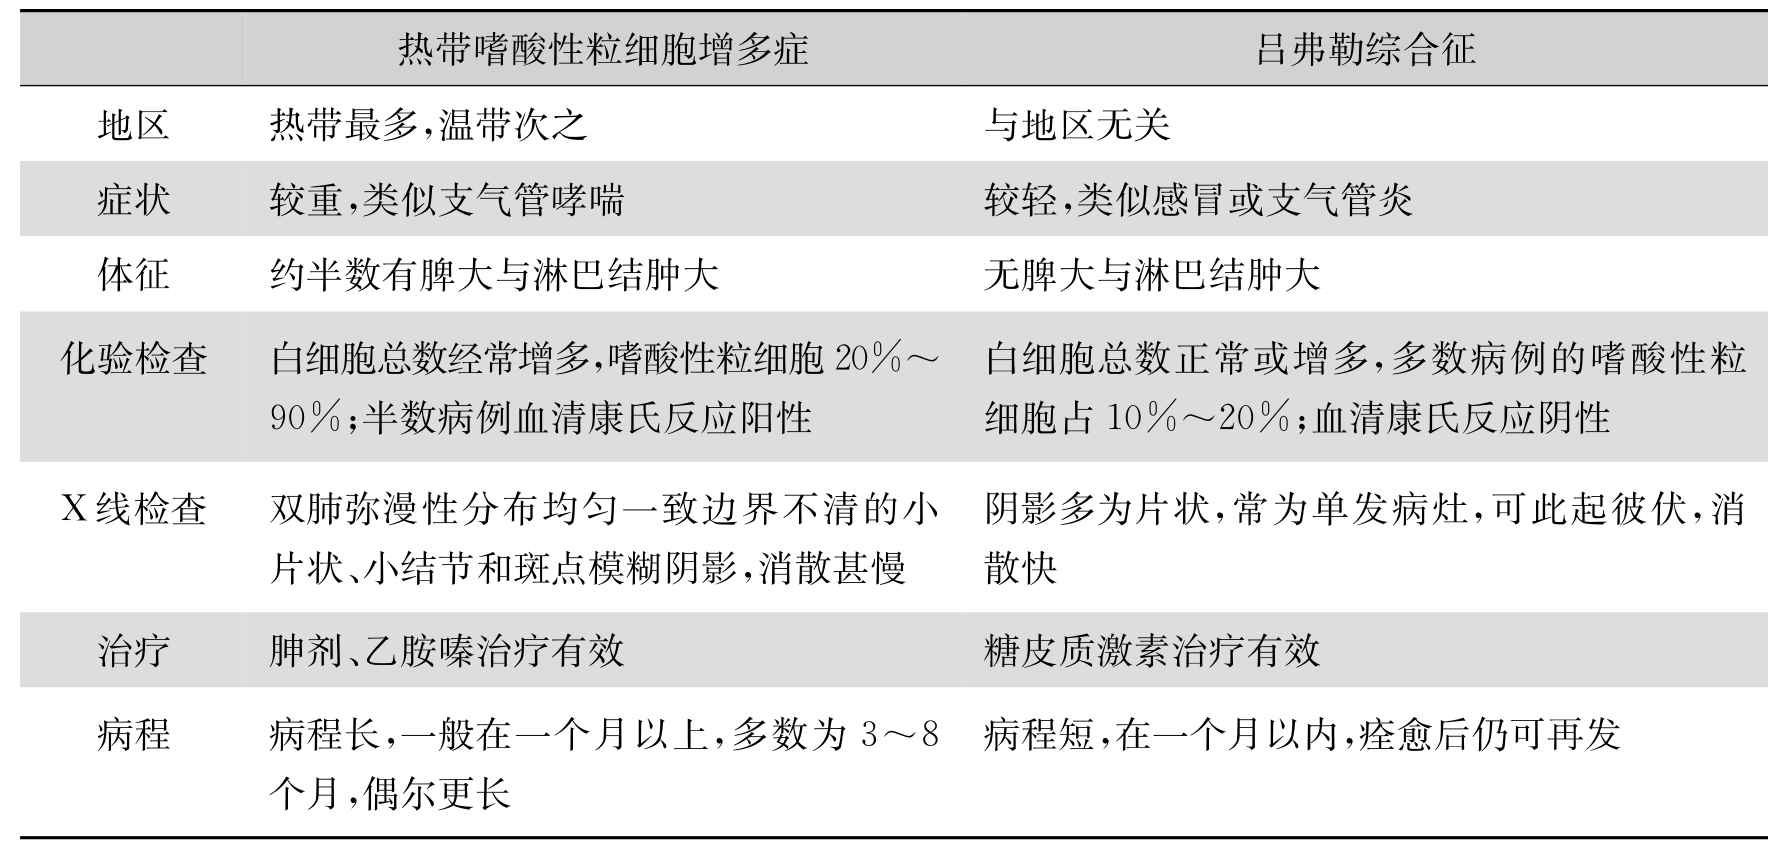
\includegraphics[width=.7\textwidth,height=\textheight,keepaspectratio]{./images/Image00048.jpg}
 \captionsetup{justification=centering}
 \caption{帽状腱膜下血肿\\{\small 出血位于左侧额顶枕部帽状腱膜下}}
 \label{fig2-29}
  \end{figure} 

头皮血肿多由于头皮血管破裂引起,也可因板障静脉或硬脑膜血管破裂,血液沿骨折缝聚集于骨膜下,后者多伴硬膜外血肿。

\subsection{颅骨骨膜下血肿}

骨膜下血肿是颅外血肿的少见类型。

\textbf{【病因病理】}
多发生于新生儿产伤和婴幼儿头部外伤。血肿位于颅骨外板与对应的骨膜之间的潜在腔隙,好发于顶骨,其次为枕骨。

\textbf{【临床表现】}
产伤所致者几乎均因头皮下出现软组织包块,未消散且逐渐变硬而就诊。

\textbf{【CT表现】}
特征性表现是新鲜血肿范围达到受累骨的整个表面,中止于颅缝或不跨越颅缝,边缘清楚锐利。而头皮下及帽状腱膜下血肿不受颅缝限制有助于鉴别。2~3周后血肿包膜出现弧形、壳状钙化,从边缘开始逐渐形成一个完整的包壳,这一过程大约需要3~6个月。与此同时血肿逐渐吸收机化,血肿完全机化约需1年,此时血肿包膜钙化或骨化形似颅骨外板,血肿机化钙化形似板障。再经过长期的塑形与颅骨融合,致局部颅骨增厚、外突隆起,并可成为永久性后遗表现。

此外,少数在血肿部位出现或大或小的囊状骨缺损,可持续数年或更久。与颅骨表皮样囊肿、嗜酸性肉芽肿、韩雪柯氏病相类似,应注意鉴别。

\subsection{颅骨骨折}

1.按骨折形态分类:①线状骨折。②凹陷骨折:婴幼儿颅骨质软,骨折部位凹陷,但不出现骨折线,称为乒乓球样凹陷骨折。③粉碎性骨折:大多数凹陷骨折被分离为多个骨碎块,则被称为粉碎性骨折。④穿通骨折:多为锐器直接损伤,少数为火器伤。局部头皮全层裂伤,可有各种类型骨折,还可见颅内血肿、异物及脑损伤。⑤颅缝分离:两侧不对称或颅缝宽>2mm。

2.按骨折部位分类:①颅盖骨骨折。②颅底骨折。

3.诊断骨折应注意的问题:①颅骨血管沟:仅有内板压迹,边缘为硬化边。②板障静脉:常不规则,可见于对侧,并终端于静脉湖。③颅骨缝:特有的部位及走行,是区别骨折线的标志。④是否有颅内积气:积气可见于蛛网膜下腔、脑室系统、硬膜下腔,以及硬膜外血肿内,甚至脑实质内。

\subsection{硬脑膜外血肿}

硬脑膜紧贴颅骨内板,当颅骨骨折或脑膜血管破裂、出血使其与颅内板分离时则形成硬膜外血肿。

\textbf{【病理】} 多发生于头颅直接损伤的部位。约
95%伴颅骨骨折,70%~80%病例因骨折所致脑膜中动脉及其分支断裂,少数因骨折伤及板障静脉、静脉窦和蛛网膜粒。血肿可单发或多发,呈凸透镜形,多不伴有脑实质损伤。

\textbf{【临床表现】}
伤后有短时原发昏迷,清醒后头痛、呕吐逐渐加重并再度昏迷。清醒时间的长短,由出血量多少和出血速度决定。重者如不及时处理,可形成脑疝。

\textbf{【CT表现】}
因硬膜与颅骨紧密相连,故血肿局限呈梭形高密度,CT值为50~70Hu。血肿的脑侧缘光滑(图\ref{fig2-30}),好发于骨折处。由于硬膜在颅缝处与骨结合紧密,故血肿不超越颅缝。但骨折如跨越颅缝,则血肿亦可跨越颅缝,也可从幕上延及幕下或跨越中线。血肿有占位效应,但较硬膜下血肿轻,多不伴脑实质损伤,但压迫邻近血管时可发生脑水肿或脑梗死。少数受伤时无症状,以后才发生慢性硬膜外血肿。慢性硬膜外血肿其壁机化增厚并可钙化。

\begin{figure}[!htbp]
 \centering
 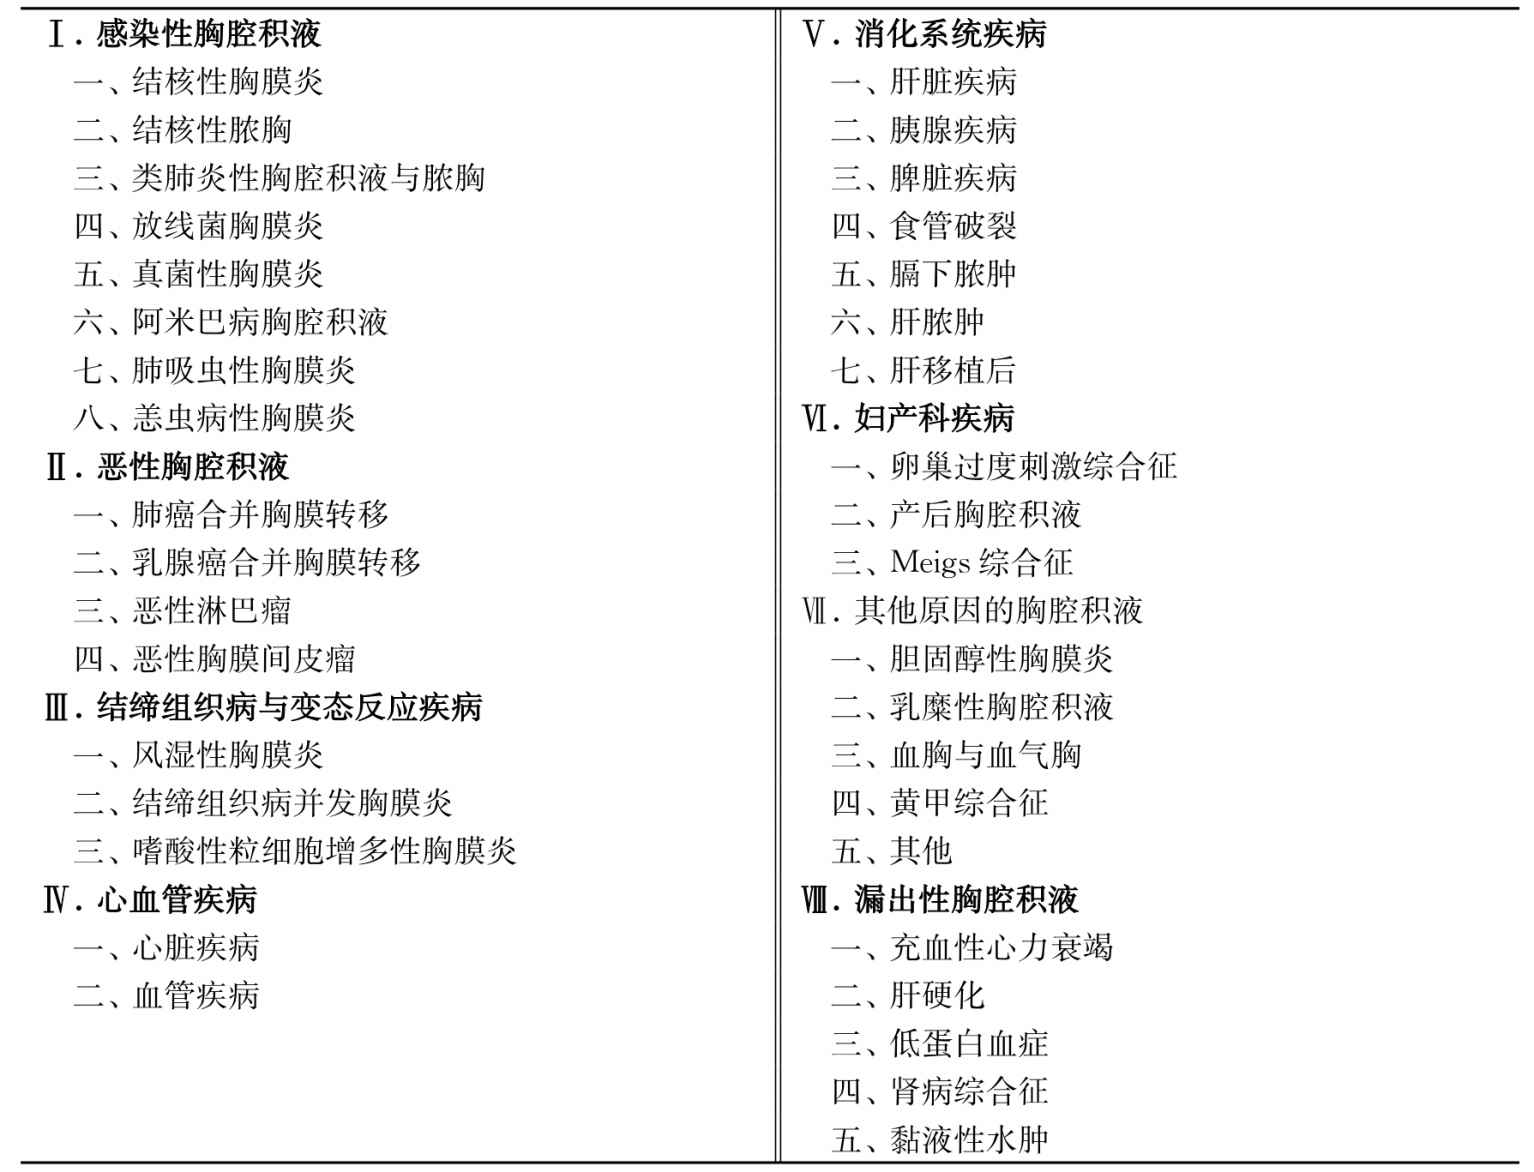
\includegraphics[width=.7\textwidth,height=\textheight,keepaspectratio]{./images/Image00049.jpg}
 \captionsetup{justification=centering}
 \caption{硬膜外血肿\\{\small 右侧颅骨内板下有梭形高密度区,边缘清晰锐利}}
 \label{fig2-30}
  \end{figure} 

\subsection{硬脑膜下血肿}

硬膜下血肿位于硬膜和蛛网膜之间,多因减速性挫伤(对冲伤)所致,无颅骨骨折或骨折仅位于暴力部位。

\textbf{【病理】}
其血源多为脑对冲伤处的静脉、小动脉或由大脑向上矢状窦汇入的桥静脉撕裂所致。呈新月形包绕在大脑表面,在伤后不同时间形态变化各异,约50%合并脑挫裂伤。临床、病理和影像均分为急性、亚急性和慢性3期。

CT上等密度硬膜下血肿占硬膜下血肿的16%。据有关文献报道,多发生在初次损伤后30~90天,亦有报道可达120天,甚至150余天。等密度硬膜下血肿的原因为:①血肿由高密度向低密度发展过程中血肿密度与脑组织密度相近时;②偶有低蛋白血症(如贫血)病人的急性期血肿呈等密度;③再出血或慢性出血进入到慢性硬膜下血肿,而形成等密度慢性硬膜下血肿。

\textbf{【临床表现】}
急性者病情多较重,且发展迅速,出现中间清醒期或意识好转期者较少,颅内压增高、脑受压和脑疝症状出现早。慢性硬膜下血肿患者年龄常较大,只有轻微外伤史,在伤后数周或数月出现颅内压增高症状,呈慢性过程。

\textbf{【CT表现】}

\subsubsection{三期表现}

1.急性期:伤后3天内。一般呈均匀高密度的新月形(图\ref{fig2-31}A),血肿可跨颅缝,但不超过中线。占位效应著,常伴脑挫裂伤,可形成脑疝。有3种非典型表现:①血肿密度不均:可能与急性出血还未凝固、凝血早期血清外溢或蛛网膜破裂脑脊液进入硬膜下有关;②血肿呈梭形表现:可能与出血没有及时散开有关;③血肿同侧侧脑室扩大:可能与同侧室间孔被迅速挤压梗阻所致。

此外,多不伴骨折,但骨折后硬膜撕裂也可形成急性硬膜下血肿。

2.亚急性期:伤后4天~3周内。血肿可逐渐变为等密度,而表现为皮质区均匀受压,脑沟消失,灰白质交界处被均匀向内推移。但双侧均有血肿,中线推移可不著。亚急性血肿的较早期出现细胞沉淀效应可出现密度上低下高的液体界面。

3.慢性期:伤3周后。此时血肿包膜形成,凝血块液化,逐渐变成液性低密度(图\ref{fig2-31}B),血肿壁机化增厚或钙化。血肿内肉芽组织增生、机化形成包膜,故可见慢性硬膜下血肿有分隔表现。

\subsubsection{等密度硬膜下血肿}

平扫表现为中线结构及脑室受压移位、变形,脑沟、裂池变窄消失、灰白质界面内移等,均属间接征象(图\ref{fig2-31}C)。增强扫描可显示血肿的位置、大小、形态而确诊。



\begin{figure}[!htbp]
 \centering
 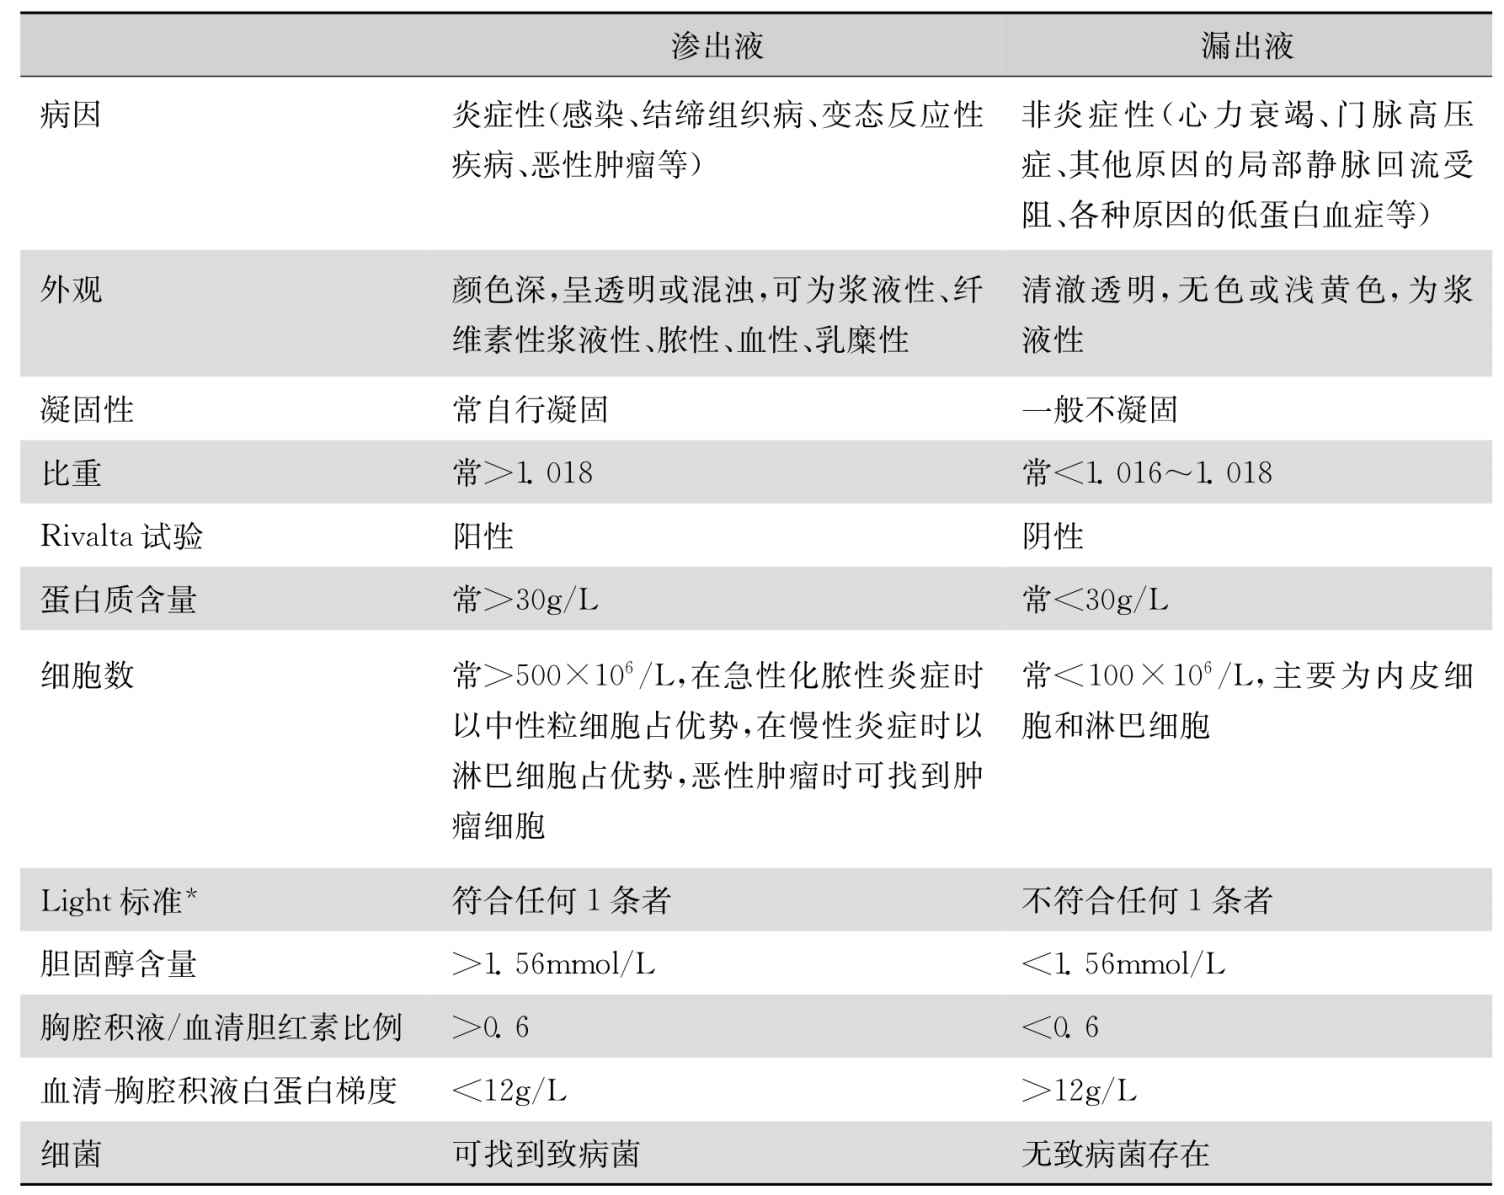
\includegraphics[width=.7\textwidth,height=\textheight,keepaspectratio]{./images/Image00050.jpg}
 \includegraphics[width=.7\textwidth,height=\textheight,keepaspectratio]{./images/Image00051.jpg}
 \captionsetup{justification=centering}
 \caption{硬膜下血肿\\{\small A.急性期硬膜下血肿,病灶位于左侧额顶骨内板下;B.慢性期硬膜下血肿,病灶位于左侧额顶枕骨内板下,有密度上低下高的液体界面;C.慢性等密度硬膜下血肿,病灶位于左侧额顶枕骨内板下和右侧额部}}
 \label{fig2-31}
  \end{figure} 

\subsection{特殊部位的硬脑膜下血肿}

特殊部位的硬膜下血肿主要指大脑镰、小脑幕硬膜下血肿。

\textbf{【病因病理】}
其受力方式可以是加速运动或减速运动的直接作用力,也可以是引起大脑镰、小脑幕严重移位的内在推力。目前,普遍认为是该处的桥静脉与静脉窦连接部撕裂,血液进入硬膜下腔所致。

\textbf{【CT表现】}

1.大脑镰硬膜下血肿:正常大脑镰宽为<3mm,硬膜下血肿表现为大脑纵裂呈带状增宽,密度增高,宽为3~12mm,CT值达68~85Hu,可有占位效应。硬膜侧有坚硬的硬膜阻挡,故其内缘平直而光整;外缘因蛛网膜的张力低和脑沟、脑回的阻力不均衡呈局限的弧形或波浪状。但与脑沟不通为其特点,并可依此与蛛网膜下腔出血相鉴别(图\ref{fig2-32}A、B)。

2.小脑幕硬膜下血肿:呈扇形、片状、新月形等形状的高密度,内缘止于小脑幕切迹处。边缘光滑锐利,占位效应不著(图\ref{fig2-32}C、D)。由于小脑幕凹面向下,横断扫描像一般显示:血肿位于小脑幕上者,其内侧缘清晰,外侧缘模糊;位于小脑幕下者反之。



\begin{figure}[!htbp]
 \centering
 \includegraphics[width=\textwidth,height=\textheight,keepaspectratio]{./images/Image00052.jpg}
 \includegraphics[width=\textwidth,height=\textheight,keepaspectratio]{./images/Image00053.jpg}
 \captionsetup{justification=centering}
 \caption{特殊部位硬膜下血肿\\{\small A~D为同一患者;A、B血肿位于大脑镰旁,大脑纵裂呈带状增宽,边缘清晰、平直而光整;C、D血肿位于右侧小脑幕处,呈扇形高密度,内缘止于小脑幕切迹处,边缘光滑锐利}}
 \label{fig2-32}
  \end{figure} 

以上两者均可因部分容积效应或同时合并该区域的蛛网膜下腔出血而使血肿边界不清。

\textbf{【鉴别诊断】}
大脑镰旁和小脑幕处的硬膜下血肿主要应与蛛网膜下腔出血相鉴别。①前者边界光整清楚;后者则模糊不规则,因向脑沟延伸而多呈羽毛状,常波及相邻脑池和脑室。②前者大脑镰部占位效应常见;后者较少见。③前者血肿不能触及胼胝体膝部;后者可紧贴。④前者急性期密度多为55~75Hu,多在2周后吸收或变为低密度;后者CT值多在55Hu以下,且多在1周内(甚至24h)消失。⑤采用薄层扫描,特别冠状和矢状面重建可较清楚显示血肿的形态和解剖位置。此外,脑膜钙化CT值明显高于血肿可资鉴别。

\subsection{硬脑膜下积液}

本病又称硬膜下水瘤,是指硬膜下只含有脑脊液成分。

\textbf{【病因病理】}
它是由于外伤后蛛网膜破裂,脑脊液流入硬膜下所造成的,并多认为其形成机制是蛛网膜破口的活瓣效应的结果。常在外伤后几周内产生,少数因伴有慢性渗血而转化为慢性硬膜下血肿。

\textbf{【临床表现】}
多见于老年人及儿童。急性者(伤后72小时内)与急性颅内血肿症状相似,主要表现为头痛、恶心、呕吐等颅内压增高症状,亦可有局部脑受压症状。慢性者(3周后)可见嗜睡、朦胧、定向力差、精神障碍。

\textbf{【CT表现】}
多位于额、颞部,老年人双侧多见。呈颅骨内板下新月形水样密度区,因受压脑沟变浅、脑回变平(图\ref{fig2-33})。少数经复查液体密度增高,而转化为等密度或稍低密度慢性硬膜下血肿。

\begin{figure}[!htbp]
 \centering
 \includegraphics[width=.7\textwidth,height=\textheight,keepaspectratio]{./images/Image00054.jpg}
 \captionsetup{justification=centering}
 \caption{硬膜下积液\\{\small 双侧额颞骨内板下新月形水样密度区,脑沟变浅、脑回变平}}
 \label{fig2-33}
  \end{figure} 

\textbf{【鉴别诊断】}
①慢性硬膜下血肿:有人认为硬膜下血肿吸收后也可称为硬膜下积液。但慢性血肿CT值偏高,包膜有强化,常呈梭形,可予鉴别。②脑萎缩:脑沟裂增深、增宽,甚至脑室扩大等有别于硬膜下积液之脑沟、回变浅平。

\subsection{外伤性蛛网膜下腔出血}

\textbf{【病因病理】}
出血来源于外伤后软脑膜和皮层血管的断裂、脑挫裂伤的渗血及脑内血肿破入。单独蛛网膜下腔出血少见,多伴脑挫裂伤。

\textbf{【临床表现】}
因脑膜刺激引起剧烈头痛、恶心呕吐,查体可发现颈强直、Kernig征阳性。

\textbf{【CT表现】}
高密度血液充填于脑表面脑沟中或脑裂、脑池中。吸收消散快,长者1周,短者1~2天,最快可达10小时左右。可伴脑挫裂伤的水肿、出血等表现。

此外,少数(包括自发性)出血点因远离宽大的脑池、脑裂,而且出血较快,局限于局部颅骨内板下,与硬膜下血肿相似,但其内缘不锐利、密度较低且不均匀,且短期内能快速吸收。

\subsection{外伤性脑室内出血}

本病是一种较少见的重型脑损伤,预后差,死亡率高。

\textbf{【病因病理】}
本病可分为两类:①原发性:为外伤致脑室内血管破裂出血;②继发性:为脑内血肿破入脑室。其发生机理有以下几种学说:①脑外伤瞬间,外力(尤其矢状方向外力)使脑室扩大变形,撕裂室管膜下血管引起脑室出血。②弥漫性轴索损伤,由于剪切力的作用脑室壁破裂,引起室管膜下血管损伤出血。③室管膜下潜在的畸形血管破裂出血。④凝血功能障碍,外伤作为诱因。⑤脑内血肿破入脑室。

\textbf{【临床表现】}
多伴有其他类型的脑损伤,故缺乏特征性。可有以下表现:①意识障碍;②脑膜刺激征:脑室内出血流入蛛网膜下腔所致;③体温升高:是血性脑脊液的吸收热,并与出血刺激丘脑下部体温调节中枢有关。伴有其他部位的损伤时有相应表现和体征。

\textbf{【CT表现】}
少量出血时多沉积在侧脑室后角、第三脑室后部或第四脑室顶部,大量出血常呈脑室“铸型”样表现。早期可有分层现象,以后呈等或低密度。可并发不同程度的阻塞性脑积水,多合并其他类型脑损伤。

\subsection{脑挫裂伤}

脑组织外伤后发生水肿、静脉淤血、渗血及毛细血管的散在点状出血,病理上称为脑挫伤;而当软脑膜和脑组织及其血管断裂时称为脑裂伤。因而两者多合并存在,且临床和影像检查难以区分,故统称为脑挫裂伤。

\textbf{【病因病理】}
直接打击的外力可造成受力处的脑挫裂伤,此种较少。多由于运动中的撞击造成的对冲伤引起。病理改变有局部脑水肿,静脉淤血、渗血及毛细血管的散在点状出血,严重者出血较多,形成脑内血肿,还可有坏死液化等改变。

\textbf{【临床表现】}
都有意识丧失,出现一过性昏迷,重者持续昏迷。患者有头痛、呕吐等颅内压升高或脑膜刺激征。损伤部位不同可出现偏瘫、偏盲、肢体张力和腱反射的异常。

\textbf{【CT表现】}

1.常见表现:①局部脑组织呈低密度水肿,界限不清,多位于皮层区。水肿区内有一处或多处点片状出血灶称为灶状出血。②一处或多处脑内血肿(出血灶>2cm称为血肿),形态边缘不规整(图\ref{fig2-34})。血肿周围有不同程度水肿和占位效应。③灶状出血及小血肿可在数小时内扩大融合,并可引起脑疝如镰下疝、天幕疝等。

\begin{figure}[!htbp]
 \centering
 \includegraphics[width=.7\textwidth,height=\textheight,keepaspectratio]{./images/Image00055.jpg}
 \captionsetup{justification=centering}
 \caption{脑挫裂伤\\{\small 双侧额颞叶有许多斑片状不规则出血灶,鞍上池、四叠体池内有积血}}
 \label{fig2-34}
  \end{figure} 

2.外伤性迟发性脑内血肿:伤后首诊CT扫描未发现血肿,相隔数小时、数天复查或手术发现有新的血肿者称为外伤性迟发性脑内血肿。属于原发性脑损伤,可发生于伤后1.5小时至数天,90%以上出现在伤后24~48小时,也有报道多见于3日至1周内。此外,颅脑损伤的迟发性表现还有脑挫裂伤、硬膜外血肿、硬膜下血肿、蛛网膜下腔出血、脑水肿等。

3.其他伴发的外伤性颅内病变:硬膜外或硬膜下血肿、蛛网膜下腔出血、弥漫性脑水肿、硬膜下积液、DAI等。

\subsection{脑干损伤}

脑干损伤较少,多合并大脑半球的弥漫性损伤。

\textbf{【病理】}
本病可分为原发性和继发性。原发性病理改变有脑干震荡、挫裂伤、出血、软化和水肿。有人把其分为4类:①弥漫性轴索损伤(DAI);②原发性多发斑点状出血;③桥脑、延髓撕裂;④直接表浅撕裂或挫伤。其中以DAI最常见,且多为非出血性。继发性脑干损伤是由颅内血肿、脑水肿所致的天幕裂孔疝压迫脑干并使脑干血管受牵拉,进而导致脑干缺血和出血。

\textbf{【临床表现】}
病情严重,常见表现有意识障碍、去大脑强直、肌张力增高和眼球位置异常。患者常见双侧瞳孔缩小。

\textbf{【CT表现】}
因受后颅窝伪影干扰和分辨率限制对非出血性脑干损伤诊断困难。①原发性:常表现为局部脑池消失,亦可显示小灶状出血。②继发性:可见出血、梗死,并可见幕上血肿、弥漫性脑肿胀、弥漫性脑水肿、天幕裂孔疝和脑干受压移位等表现。

\subsection{弥漫性脑损伤}

弥漫性脑损伤包括弥漫性脑水肿、弥漫性脑肿胀和弥漫性轴索损伤(DAI)。弥漫性轴索损伤有文献也称为弥漫性脑白质损伤。

\textbf{【病因病理】}
DAI是因外伤造成的剪切力(旋转暴力)作用于脑灰白质交界处、大脑深部结构和脑干区,导致神经轴索的广泛挫伤、断裂及脑组织小灶出血、水肿。

脑水肿和脑肿胀的病理改变分别为细胞外液和细胞内液增多。两者常同时存在,很难区分和鉴别,因此统称为脑水肿(脑组织液体含量增多引起的脑容积增大和重量增加)。

\textbf{【临床表现】}
脑水肿和脑肿胀轻者无明显症状和体征,重者出现头痛、头晕、呕吐等颅内高压征;可出现半身轻瘫和锥体束征;严重者可发生脑疝,以至死亡。

DAI因广泛轴索损伤使皮层及皮层下中枢失去联系而致伤后即刻意识丧失,多持久昏迷,甚至处于植物人状态,死亡率高。

\textbf{【影像学表现】}

1.弥漫性脑水肿和(或)脑肿胀:CT表现为低密度,密度低于邻近脑白质,CT值多<20Hu。两侧弥漫性病变可致脑室普遍受压变小,重者可致脑室、脑沟和脑池消失。

2.DAI的诊断标准:①受伤机制:受伤时头部处于运动状态,由旋转暴力所致。②临床表现:伤后有原发性昏迷伴躁动不安,无明确神经定位体征,亦无窒息及低血压等脑缺氧情况。③CT表现:脑组织弥漫性肿胀(灰白质密度普遍降低,但其密度减低不及脑水肿),灰白质分界不清,其交界处有散在斑点状出血灶(<2cm),伴有蛛网膜下腔出血。脑室、脑池受压变小,无局部占位征象。④MR表现:脑肿胀、脑室脑池因受压而减小或闭塞,脑白质及胼胝体、脑干、小脑可见点状、片状或散在小出血灶(<2cm),中线结构无明显移位。⑤合并症:可合并其他颅脑损伤,如蛛网膜下腔出血、脑室出血、硬膜下及硬膜外血肿及颅骨骨折等。

DAT的分期:目前有学者将DAI分为3期。Ⅰ期:较轻,损伤仅见脑叶白质,常见于额、颞叶。Ⅱ期:损伤较重,胼胝体出现病灶。Ⅲ期:严重损伤,脑干出现病灶。

总之,因DAI有80%为非出血性病灶,仅20%有小的中心出血,故CT难以发现。其CT检出率不到30%,而MR可高达90%。

\subsection{外伤性脑疝}

\subsubsection{天幕疝}

分为3型:①颞叶型:常为单侧,占位效应显著,颞叶组织(钩回、海马回)疝入幕下;②中央型:常为双侧颅内压升高,脑干向下移位而不向一侧移位,双侧外侧裂池、环池变窄或消失;③小脑型:幕下压力升高,脑干和(或)小脑上移,环池及枕大池狭窄或消失,第三脑室后部上抬。

颞叶天幕疝的诊断标准:①颅内压增高征象:中线结构明显移位,患侧环池增宽,除环池外的基底池(如四叠体池、鞍上池)及侧裂池浅小甚至闭塞;②颞叶伸至幕下≥3.0mm,但必须存在上述同侧颅内压增高征象,<3.0mm为可疑。同时可见脑干受压变形、病侧环池增宽;③如无颅内压增高征象存在,颞叶轻度下移,应视为正常变异。

此外,斜坡垂直线的扫描法有助于显示疝入幕下的与颞叶相连的脑组织,并进而结合脑干、脑池之形态与正常小脑组织相鉴别。

\subsubsection{镰下疝}

表现为扣带回和大脑前动脉移向对侧,较硬的大脑镰一般移位不著。侧脑室前角受压变窄(图\ref{fig2-35})。

\begin{figure}[!htbp]
 \centering
 \includegraphics[width=.7\textwidth,height=\textheight,keepaspectratio]{./images/Image00056.jpg}
 \captionsetup{justification=centering}
 \caption{镰下疝\\{\small 右侧颞额顶部硬膜下血肿及局部脑沟内有血液充填,右侧额叶脑组织经大脑镰下跨越中线移向左侧}}
 \label{fig2-35}
  \end{figure} 

此外,还可见脑组织通过缺损颅骨外疝、小脑扁桃体疝(枕骨大孔疝)。

\subsection{外伤性脑梗死}

外伤性脑梗死常发生在外伤后1周内。

\textbf{【病理机制】}
其发病机理大致归纳为以下几方面:①血管壁发生直接机械性损伤造成器质性狭窄或闭塞,致供血中断;②血管壁损伤引起局部脑血管痉挛,血液微循环发生障碍,致脑组织供血不全;③血管内皮损伤激活内源性、外源性凝血系统,促使血栓形成;④外伤后血管痉挛与血液流变学发生变化,脑血管反应性降低,脑血流量减少,引起血中自由基反应增强,造成细胞内环境紊乱,从而加重脑缺氧、坏死、溶解,导致脑梗死;⑤脑挫裂伤、蛛网膜下腔出血以及脑血肿、水肿等可使脑血管扭曲、痉挛收缩,加重原有的缺血、缺氧,导致脑梗死。此外,外伤后无明显症状的情况下,可发生腔隙性脑梗死,可能也与外伤后神经调节功能紊乱所致的脑血管痉挛有关。

\textbf{【CT分型】}
国内有学者将其分为5型:①腔隙性:多见于幼儿和儿童,呈卵圆形或裂隙状;②单脑叶型(或局灶型):多位于一侧脑叶或脑叶交界区,呈楔形或不规则形(图\ref{fig2-36});③多脑叶型(大面积型):是指2个以上脑叶的梗死;④挫伤出血型(混合型):表现为沿血管走向分布的低密度,多有规则边界,而脑挫伤低密度比梗死出现早,且密度不均、形态不规则,出血呈高密度,脑肿胀密度轻微减低、界限不清、双侧半球受累为其特点;⑤小脑与脑干型梗死。

\begin{figure}[!htbp]
 \centering
 \includegraphics[width=.7\textwidth,height=\textheight,keepaspectratio]{./images/Image00057.jpg}
 \captionsetup{justification=centering}
 \caption{外伤性脑梗死\\{\small A、B为同一患者,左侧颞部有硬膜外血肿,左侧枕叶呈大片状低密度,密度均匀、边缘平直}}
 \label{fig2-36}
  \end{figure} 

\subsection{脑外伤的并发症和后遗症}

1.并发症:①感染;②梗死;③脑膨出;④颈内动脉海绵窦瘘等。

2.后遗症:轻度挫裂伤可完全恢复正常而无后遗症。常见后遗症有:①脑软化;②脑萎缩;③脑穿通畸形(图\ref{fig2-37});④脑积水(交通性或阻塞性);⑤蛛网膜囊肿等。

\begin{figure}[!htbp]
 \centering
 \includegraphics[width=.7\textwidth,height=\textheight,keepaspectratio]{./images/Image00058.jpg}
 \captionsetup{justification=centering}
 \caption{右侧额叶脑穿通畸形\\{\small 脑挫裂伤1年后复查,右侧额叶水样密度灶,有张力,并与右侧脑室额角相通连}}
 \label{fig2-37}
  \end{figure} 

\subsection{放射性脑病}

本病是一种由各种原因放疗所致的脑组织放射性反应综合征。

\textbf{【病理】}
放射性损伤急性期和早期常表现为放射性诱导的脑水肿,晚期则主要以放射性坏死为主要特征。光镜观察有以下特征:①凝固性坏死;②脱髓鞘;③巨噬细胞反应;④血管周围细胞浸润;⑤血管纤维素样坏死、栓塞、玻璃样变或纤维素样变;⑥神经胶质增生;⑦无细胞性纤维化。

\textbf{【临床分期】}
国外有学者根据放疗后症状出现的时间分为3期:①急性期:多发生于放疗后几天至2周内,为血管源性水肿所致的颅内压增高,激素治疗有效;②早期迟发反应期:多发生于放疗后几周至3个月,大多数较短暂,预后较好;③晚期迟发反应期:多发生于放疗后几个月至10年或10年以上,该期主要病理改变为局限性放射性坏死、弥漫性脑白质损伤、大动脉损伤钙化性血管病及脑萎缩等不可逆性损害,局限性坏死和弥漫性脑白质损伤可分别或同时发生。

\textbf{【临床表现】}
①颅内压增高表现;②癫痫大发作;③局限性神经功能损害表现,如视障碍、同向偏盲、复视、失语、单侧运动和感觉障碍;④其他:头昏、嗜睡、反应迟钝、记忆力减退等,也有诱发脑膜瘤、纤维肉瘤、胶质瘤等脑肿瘤的报道。

\textbf{【CT表现】}
①急性期及早期迟发反应期:广泛性非特异性低密度水肿区,增强无强化,短期随访病灶消失。②局限性放射性坏死:病灶呈低密度,CT值约17Hu。灶周水肿明显,可见坏死、出血。增强扫描病灶多无强化,少数呈环形、片状、地图样不均匀强化。③弥漫性脑白质损伤早期:平扫可见脑室周围及半卵圆中心广泛低密度区。增强后多无强化,少数可见不均匀强化,提示有白质坏死存在。④弥漫性脑白质损伤晚期:可见钙化性微血管病和脑萎缩。前者可见多发钙化(占25%~30%),常见于基底节区,有时可见于皮层。弥漫性脑白质损伤一般在放疗早期出现,可持续几个月甚至几年。

\subsection{有机磷农药中毒的脑部损害}

有机磷农药中毒时主要毒性作用是抑制神经系统的乙酰胆碱酯酶,导致所有胆碱能神经传导部位的神经递质---乙酰胆碱的蓄积,引起中毒效应。

\textbf{【病理】}
其脑部损害的机制存在多种学说,但可以肯定的是有机磷中毒可损害脑部引起急性中毒性脑病,出现脑肿胀、水肿的病理改变。还有学者认为,有机磷中毒可使脑微血管内皮细胞和基底膜损伤,致通透性升高、毛细血管壁损伤而发生漏出性出血。此外,也可由于呼吸衰竭等原因而使脑组织缺血缺氧发生脑萎缩。

\textbf{【临床表现】}
毒蕈碱样症状、烟碱样症状和中枢神经系统症状。中枢神经系统症状可表现为神志不清、烦躁、谵妄、抽搐,或中枢性呼吸衰竭。

\textbf{【CT表现】}
①中毒3天内多表现为脑肿胀、水肿,可见脑沟裂变浅、脑室狭小、灰白质分解不清。②3天后可在基底节、皮质区出现较局限低密度灶。③因基底节区血管较丰富,故出血可对称性位于基底节区;出血吸收后形成低密度软化灶。④少数可继发脑萎缩。

\section{颅内肿瘤和囊肿}

\subsection{概述}

颅内肿瘤及肿瘤样病变的病理分型及命名较为混乱,其分类方法多达一二十种。1977年WHO将其分为12大类(见表\ref{tab2-3},表内所列各类肿瘤仅为常见者);2000年WHO将神经系统肿瘤(包括颅外,但未将肿瘤样病变列入)分为7大类(见表\ref{tab2-4})。\footnote{/0为良性肿瘤;/1为低度恶性、恶性倾向不肯定或边界性恶性;/2为原位病灶,神经系统无原位病灶;/3为恶性。每个肿瘤后的Ⅰ~Ⅳ数字表示其分级;未标明数字的肿瘤,由于其生物学行为多变,WHO未明确分级。该表未将肿瘤样病变列入,也未列入垂体瘤}

\begin{table}[htbp]
\centering
\caption{中枢神经系统肿瘤和肿瘤类似疾患的组织学分类(WHO,1977)}
\label{tab2-3}
\includegraphics[width=\textwidth,height=\textheight,keepaspectratio]{./images/Image00059.jpg}
\end{table}

\begin{longtable}{c}
\caption{神经系统肿瘤的组织学分类和分级(WHO,2000)}
\label{tab2-4}\\
\endfirsthead
%\caption[]{神经系统肿瘤的组织学分类和分级(WHO,2000)}
%\endhead
\includegraphics[width=\textwidth,height=\textheight,keepaspectratio]{./images/Image00060.jpg}\\
\includegraphics[width=\textwidth,height=\textheight,keepaspectratio]{./images/Image00061.jpg}\\
\includegraphics[width=\textwidth,height=\textheight,keepaspectratio]{./images/Image00062.jpg}\\
\includegraphics[width=\textwidth,height=\textheight,keepaspectratio]{./images/Image00063.jpg}
\end{longtable}


\subsubsection{颅内肿瘤的定位}

包括脑内和脑外、幕上和幕下、脑室内和脑室外等。

1.脑内和脑外的鉴别:①肿瘤边缘:前者欠清或界限不清;而后者清楚锐利。②内板骨质改变:前者罕见;而后者常见增生或侵蚀性破坏。③蛛网膜下腔或脑池:前者受压变窄或闭塞;而后者扩大。④脑灰质位置:前者正常;后者受压内移,出现白质塌陷征(即灰质下指状突出的白质受压和内移)。⑤肿瘤与骨板接触所呈角度:前者呈锐角;而后者呈钝角。

2.脑室内和脑室外的鉴别(见表\ref{tab2-5}):较小的肿瘤诊断不难,肿瘤较大并同时骑跨脑室内外时不易鉴别。如肿瘤邻近脑室呈“杯口状”扩张多提示为脑室内病变。

\begin{table}[htbp]
\centering
\caption{脑室内、外病变的鉴别}
\label{tab2-5}
\includegraphics[width=\textwidth,height=\textheight,keepaspectratio]{./images/Image00064.jpg}
\end{table}

\subsubsection{颅内肿瘤的基本CT征象}

1.直接征象:①密度:钙化(CT值100Hu以上)、新鲜出血(60~80Hu)、富血管组织及胆固醇物质(10Hu以上)、囊液(0~10Hu)、液化坏死(0~20Hu)、脂肪(-100Hu以上);②部位;③肿瘤的数目、大小、形态和边缘;④增强扫描所见。

2.间接征象:①瘤旁水肿:范围≤2cm为轻度,>2cm但小于大脑半球横径为中度,大于大脑半球横径为重度(图\ref{fig2-38})。但这一分法,并不适用于后颅窝肿瘤。水肿的程度与肿瘤恶性程度、大小、生长速度和生长部位有关,故并不完全代表恶性程度。②占位效应。③骨变化:受压变薄、侵蚀破坏以及骨质增生、腔道扩大等。

\begin{figure}[!htbp]
 \centering
 \includegraphics[width=.7\textwidth,height=\textheight,keepaspectratio]{./images/Image00065.jpg}
 \captionsetup{justification=centering}
 \caption{脑水肿\\{\small 肺癌脑转移瘤,右侧额顶叶、左侧额叶髓质区大片指状低密度区}}
 \label{fig2-38}
  \end{figure} 

\subsubsection{特殊部位的肿瘤}

1.鞍内鞍上区:最常见的肿瘤为垂体瘤、颅咽管瘤,其次为脑膜瘤、动脉瘤、胶质瘤和表皮样囊肿等,淋巴瘤和生殖细胞瘤少见。

2.鞍旁区:最常见的肿瘤为神经鞘瘤和脑膜瘤,其次为脊索瘤、硬膜外转移瘤、海绵状血管瘤、软骨瘤等。

3.桥脑小脑角区:听神经瘤、三叉神经鞘瘤、表皮样囊肿、脑膜瘤、蛛网膜囊肿、化学感受器瘤、畸胎瘤、血管瘤等。

4.松果体区:最常见的肿瘤为生殖细胞瘤,其次为胶质瘤、脑膜瘤和松果体细胞瘤,偶见畸胎瘤、皮样囊肿、表皮样囊肿、蛛网膜囊肿、松果体母细胞瘤等。

5.脑室内:室管膜瘤和中枢神经细胞瘤最常见,其次为脑膜瘤、脉络丛乳头状瘤、胶样囊肿,室管膜下巨细胞星形细胞瘤、表皮样囊肿等少见。

6.小脑半球和蚓部:小脑半球常见的肿瘤有血管母细胞瘤、星形细胞瘤、转移瘤;小脑蚓部常见的有髓母细胞瘤等。①儿童脑肿瘤约
65%
位于小脑,最常见的小脑肿瘤为星形细胞瘤、髓母细胞瘤和室管膜瘤。②成人脑肿瘤大多位于幕上,最常见的小脑肿瘤是转移瘤和血管母细胞瘤。成人小脑星形细胞瘤和髓母细胞瘤罕见,占成人小脑肿瘤的
2% 以下。

7.跨中后颅窝的肿瘤:多属脑外肿瘤,常见的有脑膜瘤、三叉神经瘤、听神经瘤和胆脂瘤,其他如颅咽管瘤、脊索瘤、颈内动脉颅内段及后交通支巨大动脉瘤等均可跨中后颅窝。

8.脑干肿瘤:绝大多数为胶质瘤,偶尔为转移瘤、淋巴瘤或血管性肿瘤。脑干肿瘤常见于儿童,其发病率占儿童脑肿瘤的10%~15%,甚至有人认为高达30%。

\subsection{胶质细胞瘤的分类和分级}

神经上皮肿瘤统称为胶质瘤,是颅内最常见的恶性肿瘤,约占40%~50%,而星形细胞瘤占胶质瘤75%以上。

胶质细胞瘤的来源:神经胶质细胞包括星形胶质细胞、少突胶质细胞、小胶质细胞和室管膜细胞4种。故胶质细胞瘤常见的有星形胶质细胞瘤、少突胶质细胞瘤、室管膜瘤以及少见的小胶质肉瘤。广义的胶质瘤如表\ref{tab2-4}所述,还可包括胚胎性肿瘤(如髓母细胞瘤)、脉络丛肿瘤、松果体实质肿瘤、神经元和混合性神经元-神经胶质肿瘤(如神经节细胞瘤)等。

星形胶质细胞瘤的分级:①传统采用Kernohan的4级(Ⅰ-Ⅳ)分类法。②WHO曾采用3分法:即低级星形细胞瘤、间变型星形细胞瘤和多形性成胶质(胶质母)细胞瘤,目前也分为4级。③国内多采用张福林4级法,主要是在Kernohan法基础上改进而来。Ⅰ级:肿瘤内异形细胞<25%;Ⅱ级:25%~50%;Ⅲ级:50%~75%;Ⅳ级:>75%。其中Ⅰ级为良性,Ⅱ级为良、恶过渡性,Ⅲ、Ⅳ级为恶性。按照旧名称,星形胶质细胞瘤相当于张氏分法之Ⅰ-Ⅱ级;星形母细胞瘤相当于Ⅱ级;极性成胶质细胞瘤相当于Ⅱ、Ⅲ级;多形性胶质母细胞瘤相当于Ⅲ、Ⅳ级。

\subsection{星形胶质细胞瘤}

星形细胞瘤占胶质瘤75%以上,可发生于脑和脊髓各部,成人75.7%发生于幕上,儿童71.4%位于幕下。幕上以额叶多见,幕下以小脑半球多见,少数有多发病灶。

\textbf{【病理】}
星形细胞瘤组织学分为:纤维型、原浆型、肥大细胞型、毛发细胞型4个亚型(其分级见上述)。

分化良好的星形细胞瘤,多位于大脑半球白质,少数可位于灰质并向白质或脑膜浸润。没有包膜,有时沿白质纤维或胼胝体纤维向邻近脑叶或对侧半球发展。肿瘤含神经胶质纤维多,质软易碎;可有单发或多发囊变;肿瘤血管近于成熟。

分化不良的星形细胞瘤,呈弥漫性浸润生长,形态不规整,界限不清。半数以上有囊变,易发生大片坏死和出血;肿瘤血管形成不良,血脑屏障结构不完整。

小脑星形细胞瘤,多位于小脑半球,也可位于蚓部,有时可突入第四脑室;多为毛发细胞型,分化较好。肿瘤一部分为囊性,界限清楚;一部分为实性,呈浸润性生长,界限不清。

\textbf{【临床表现】}
可发生于任何年龄,以20~40岁最为常见,男女之比约为3∶2。Ⅰ级病程较长,多在1年以上,常见于青年和儿童;Ⅲ、Ⅳ级发病急剧,多在中年以上。常见症状为颅内压增高症状及精神改变、感觉障碍、癫痫发作、对侧肢体瘫痪和同向偏盲等。下视丘(下丘脑及视束)胶质瘤多见于儿童,少数可有发育迟缓、多饮多尿及性早熟等内分泌紊乱症状。

\textbf{【CT表现】}

\subsubsection{幕上星形细胞瘤}

CT平扫时多呈边界不清、不规则的低密度病灶或以低密度为主的混合密度灶。增强扫描呈均匀或不均匀增强或不增强病灶,可伴瘤周水肿(图\ref{fig2-39})。



\begin{figure}[!htbp]
 \centering
 \includegraphics[width=.7\textwidth,height=\textheight,keepaspectratio]{./images/Image00066.jpg}
 \includegraphics[width=.7\textwidth,height=\textheight,keepaspectratio]{./images/Image00067.jpg}
 \captionsetup{justification=centering}
 \caption{星形胶质细胞瘤\\{\small A、B为同一患者,Ⅱ~Ⅲ级星形胶质细胞瘤;A为平扫,右侧额叶低密度灶,密度均匀,界限清晰;B为增强扫描,病灶无明显强化。C、D为同一患者的平扫表现,胶质母细胞瘤(Ⅳ级)}}
 \label{fig2-39}
  \end{figure} 

1.低级星形细胞瘤(Ⅰ级):平扫多呈均匀低密度或等密度,可类似水肿,亦可表现囊性。90%不出现水肿,少数有轻、中度水肿。根据生长方式又可分为2型。①局限型:出血少见,瘤周水肿轻微或无,15%~20%有钙化,可见囊变;②弥漫型:呈略低密度,界限不清,可侵犯一侧大脑半球。增强扫描大多无强化,少数囊壁或囊内间隔轻微强化。

2.间变型星形细胞瘤(Ⅱ级):具有Ⅰ级和Ⅲ、Ⅳ级肿瘤的部分特点。①平扫多呈水肿型和囊性,密度不均,钙化少见,界限不清,占位效应较著。弥漫浸润型占位效应可不著。②增强扫描有不同程度的强化,连续或断续的环形强化最常见,可见附壁结节和花环状强化。有时可见靠近肿瘤附近脑凸面的正常脑皮质有造影剂摄入,可被误认为肿瘤本身的强化。③瘤周水肿程度不一。

3.多形性胶质母细胞瘤(Ⅲ-Ⅳ级):占胶质瘤的5%。①平扫多呈结节形、环形及混合型,表现为低、等混合密度灶。瘤周90%以上有水肿,瘤内出血、坏死多见,钙化少见。②96.5%有强化,且强化明显,强化高峰约在注射造影剂后10分钟出现。多呈不规则及厚壁花环状强化,可见强化不一、大小不一的壁结节。花环不连续更有助于诊断,尤其有利于与脓肿鉴别。③胼胝体附近肿瘤可侵及双侧额叶。④偶可广泛侵犯大脑半球,无明显肿块,易误为脑炎。⑤该类型亦可呈多灶性、多中心病灶而称为胶质瘤病。

此外,应注意低密度的肿瘤组织向周围浸润生长,与水肿掺杂在一起,CT不能区分。

\subsubsection{幕下星形细胞瘤}

1.小脑星形细胞瘤:儿童和青少年好发。①可呈囊性伴壁结节、实性和囊实性3种形态。平扫囊性区密度略高于脑脊液,壁结节呈等密度。②增强扫描呈不同程度的强化,实性肿瘤强化较明显。囊性者有时囊壁光滑、不强化,只有壁结节强化,但壁结节小或者靠近颅骨时常不易显示。③多有水肿,常见占位征象为第四脑室、脑干受压移位,可见阻塞性脑积水。

2.脑干星形细胞瘤:常见于儿童,占脑干肿瘤的90%以上。肿瘤常呈浸润性生长致脑干增粗。①平扫呈低密度区,增强呈不同程度强化。②CT诊断的重要依据是脑干周围的脑池变形或闭塞,第四脑室受压变形、移位甚至闭塞(图\ref{fig2-40})。③30%可伴有脑积水。④脑池造影有助于诊断。

\begin{figure}[!htbp]
 \centering
 \includegraphics[width=.7\textwidth,height=\textheight,keepaspectratio]{./images/Image00068.jpg}
 \captionsetup{justification=centering}
 \caption{脑干胶质瘤\\{\small 患者为7岁女性。A示脑干(桥脑和中脑)增粗、密度不均匀减低,周围的脑池闭塞,第四脑室受压变形;B示病灶涉及左侧丘脑,第三脑室受压}}
 \label{fig2-40}
  \end{figure} 

此外,幕下星形细胞瘤水肿以轻中度者为多。

\textbf{【鉴别诊断】}

1.幕上星形细胞瘤的鉴别:①脑梗死:常需与偏良性的低密度无强化的星形细胞瘤相鉴别。脑梗死发病突然,其形态多呈与脑血管分布相对应的楔形,动态复查有助于鉴别。②动静脉畸形:可呈不规则混合密度,但无占位效应和水肿,有时可伴局限脑萎缩和钙化等。③脑膜瘤:也可呈非均质性,且可有明显的瘤周水肿。但其好发于大脑凸面,强化程度高于星形细胞瘤,有白质塌陷征,多伴颅骨改变。④转移瘤:发病年龄大,病灶小而水肿广泛。但单发较大的病灶,可呈不规则环状强化,与星形细胞瘤鉴别困难。⑤胶质细胞增生:是在致病因素(如缺氧、中毒等)作用下的结果,常见于梗死的亚急性期,以及脑肿瘤和脓肿的周边部。无论CT还是MR与良性星形细胞瘤很难鉴别,有时病理亦难区分。⑥少枝胶质细胞瘤:特征性改变是病灶内有条带状大而不规则的钙化。但由于发病率的关系,钙化仍以星形细胞瘤多见。⑦脑脓肿:有感染史,其强化环多规则、连续、无中断,厚薄相对均匀,界限清楚。⑧室管膜瘤:起源于脑实质或由侧脑室突入脑实质者与星形细胞瘤可鉴别困难。但室管膜瘤常呈分叶状,其内有细小斑点钙化,有助于与呈圆形、片状或弧状较大钙化的星形细胞瘤鉴别。此外,下视丘胶质瘤应注意与颅咽管瘤、生殖细胞瘤和侵袭性垂体瘤鉴别。

2.幕下星形细胞瘤的鉴别:①髓母细胞瘤:好发于小脑蚓部(93%),多呈略高密度、界限清楚、强化均匀,常侵入或累及第四脑室,有时发生囊变则鉴别困难。②血管母细胞瘤:可呈大囊、壁小结节,囊壁及结节强化明显,水肿较轻。而星形细胞瘤结节大,强化相对轻、水肿著,但有时鉴别困难。③小脑转移瘤:多发于40岁以上,以坏死、明显的水肿和环形强化为特征。④室管膜瘤:常呈分叶状,囊变率低,并可见细小斑点钙化,与第四脑室关系密切。

\subsection{少突胶质细胞瘤}

本病又称少枝胶质细胞瘤,属较良性的胶质瘤,约占原发性肿瘤的5%。

\textbf{【病理】}
多见于半球皮质或皮质下,额叶最常见,颞叶次之,脑室内罕见。肿瘤生长缓慢,边界可较清楚,但无包膜。瘤体向外生长,有时可与脑膜相连。钙化达70%以上,部分可囊变,出血坏死少见。镜下50%左右合并有星形细胞成分,属混合性胶质瘤。

\textbf{【临床表现】}
好发于35~40岁,儿童少见,男性略多于女性。因肿瘤生长缓慢,故病程较长。常见首发症状为局灶性癫痫,可出现局部神经功能障碍,晚期出现颅内压增高,还可有精神症状。

\textbf{【CT表现】}
平扫多呈稍低、等、稍高混合密度灶,特征性改变为病灶内有弯曲条带状、斑块状、皮层脑回状钙化(图\ref{fig2-41})。有时可见囊变区、出血区,占位效应轻,水肿轻微(37.9%)或无。少数近脑表面者可引起骨膨胀性改变。增强扫描多不强化或轻度强化;少数分化差者强化明显,且多为均匀强化,少数为环形强化,同时伴瘤周水肿和占位效应。

\begin{figure}[!htbp]
 \centering
 \includegraphics[width=.7\textwidth,height=\textheight,keepaspectratio]{./images/Image00069.jpg}
 \captionsetup{justification=centering}
 \caption{少突胶质细胞瘤\\{\small 右侧颞叶等、低混杂密度灶,其内有条带状钙化}}
 \label{fig2-41}
  \end{figure} 

应注意与星形细胞瘤、AVM、脑膜瘤、Stugre-Weber综合征、结核球相鉴别。

\subsection{室管膜瘤}

本病多属良性,约占颅内肿瘤的7.6%和胶质瘤的18.2%。近3/4位于幕下,1/4位于幕上。大多位于脑室内,以第四脑室多见;少数位于大脑或小脑脑实质。

\textbf{【病理】}
幕上者多见于侧脑室且向脑组织浸润,第三脑室少见。肿瘤与周围脑组织多界限清晰,脑实质内者易出血、坏死、囊变,部分可见钙化。组织学可分为以下亚型:上皮型、乳头型、黏液乳头型、室管膜下瘤等。

\textbf{【临床表现】}
好发于小儿和青少年,成人较少见,老年人罕见,男性多于女性。发生于第四脑室者可早期出现颅内压增高征象,以头痛为首发症状。累及小脑、脑干及颅神经出现相应症状。幕上者颅内高压出现较晚,脑实质内者以癫痫为首发症状。

\textbf{【CT表现】}
平扫呈不规则形、分叶状等或稍高密度灶,少数可呈低密度。可有出血、坏死囊变区,常见小斑点状钙化。脑室内者一般无瘤周水肿,但可见脑积水和(或)室管膜种植。脑实质内者好发于侧脑室三角区附近,可有轻度脑水肿并见占位效应,囊变率高。增强扫描83.7%有强化,非囊变区呈中度以上强化。室管膜母细胞瘤罕见,坏死囊变率稍高、瘤周水肿较重,其余表现与良性室管膜瘤无明显差别。

脑实质内囊变室管膜瘤如无钙化,则难与分化差的星形细胞瘤鉴别。第三脑室的室管膜瘤多位于第三脑室后部,与来自松果体的肿瘤鉴别困难。

\subsection{脉络丛乳头状瘤和脉络丛乳头状癌}

前者为少见的颅内良性肿瘤,约占颅内肿瘤的0.4%~0.6%,起源于脉络丛上皮细胞,1/3发生在10岁以内。好发部位依次为第四脑室、侧脑室和第三脑室。成人常见于第四脑室,儿童好发于侧脑室。偶有发生于脑实质内和脑外者。脉络丛乳头状癌更少见,约占颅内肿瘤的0.05%~0.1%,多见于儿童。

\textbf{【病理】}
肿瘤呈菜花状,血供丰富,20%可见钙化灶。镜下瘤细胞与正常脉络丛相似,少数可恶变成乳头状癌(10%)。瘤内可坏死出血,良恶性均可沿脑脊液播散。

\textbf{【临床表现】}
主要表现为因阻塞和脑脊液分泌增加所致脑积水高颅压症状。涉及小脑和大脑半球则出现小脑共济失调及大脑局部功能障碍表现。

\textbf{【CT表现】}
脑室内等或稍高密度灶,边缘清楚、光滑或分叶状;25%以上可见点片状钙化;较大或恶变时,可见大小不等的低密度坏死囊变区。大多呈均匀一致强化,极少数强化不明显。另一特征为脑积水,即因肿瘤分泌过多的脑脊液和(或)阻塞所致。当肿瘤超出脑室侵及脑实质、密度混杂、灶周水肿显著、中线结构移位明显时应疑为恶性可能,出血和钙化是恶性的另一个特点,但无特异性。

\textbf{【鉴别诊断】}
①室管膜瘤:钙化、囊变较脉络丛乳头状瘤常见,脑积水程度较轻。②脑室内脑膜瘤:多不呈分叶状,交通性脑积水少见。③星形细胞瘤:脑室内少见(来源于脑室周围星形细胞),密度多不均,呈浸润性生长,多见囊变、坏死、出血,及花环状强化。

\subsection{小胶质肉瘤}

本病是一种少见的颅内恶性肿瘤,异名甚多。

\textbf{【病理】}
肿瘤主要源于淋巴造血系统的巨噬细胞成分之一的小胶质细胞,并有较强的嗜银性,故称为小胶质肉瘤。组织学有时难与恶性淋巴瘤相鉴别,并有人将该肿瘤称之为恶性淋巴瘤的组织细胞型。

\textbf{【临床表现】}
多见于免疫抑制病人,以40~60岁多见,男女发病率相近。起病急,进展快。主要症状为颅内压增高,其次为局限神经功能障碍。

\textbf{【CT表现】}
肿瘤好发于基底节、丘脑、胼胝体、额颞叶及小脑蚓部等深部白质内。约2/3为等密度,1/3为高密度。单发病灶通常较大,并可坏死囊变,部分可多发。肿瘤虽大,但脑室移位和病灶周围水肿较轻。增强扫描呈局限性、均匀一致的强化。

\subsection{中枢神经元肿瘤}

神经元肿瘤是指起源于神经细胞的中枢神经系统肿瘤,主要包括以下几种。

\subsubsection{神经节胶质瘤}

最早报道于1928年,由神经细胞和胶质细胞混合而成。该肿瘤生长缓慢,相对良性(Ⅰ~Ⅱ级/WHO),预后较好。好发于儿童和青年,男性略多于女性。

\textbf{【CT表现】}
最常见于颞叶(73%)。70%的肿瘤呈低密度或低、等混合密度;38%出现囊变,且多为大囊;35%可见钙化;50%有轻微边缘强化表现。

\subsubsection{神经节细胞瘤}

罕见的良性肿瘤(Ⅰ级/WHO),来源于交感神经系统,以儿童和青年多见。主要由成熟的神经节细胞组成,不含星形细胞。

\textbf{【CT表现】}
好发于第三脑室底部,其次为颞叶底部,也可见于额叶、顶叶、小脑和延髓。平扫呈略高密度,界限不清,无明显囊变和钙化;占位效应不著;增强后基本无强化。MR
T\textsubscript{2} WI呈低信号也有一定特点。

\subsubsection{神经细胞瘤}

1982年首先报道,基本属于分化好的良性肿瘤,但少数有恶性倾向。发病年龄平均25岁(20~30岁),男女之比约为2∶1。

\textbf{【CT表现】}
好发于侧脑室内,邻近或来源于透明隔,故多位于孟氏孔区,偶可位于脑实质内。平扫呈等或稍高密度,界限清晰;通常瘤体较大,形态不整,可囊变;约50%有钙化。增强扫描呈轻至中度均匀或不均匀强化。总之,青年人位于透明隔的肿瘤应考虑神经细胞瘤的可能。

鉴别诊断:①脑膜瘤好发于侧脑室三角区,强化均匀;②脉络丛乳头状瘤好发于10岁以下儿童,亦多位于侧脑室三角区,伴交通性脑积水;③室管膜瘤、星形细胞瘤及少枝胶质细胞瘤常位于侧脑室体部,有助于鉴别。

\subsubsection{成神经细胞瘤和成神经节细胞瘤}

2000年WHO新分类将二者归属于幕上原始神经外胚叶瘤,并将其与幕下的髓母细胞瘤并列同属于原始神经外胚叶瘤。成神经细胞瘤一般起源于幕上脑实质,为浸润性恶性肿瘤(Ⅳ级/WHO),好发于儿童。成神经节细胞瘤为十分罕见的高度恶性肿瘤(Ⅳ级/WHO),生长迅速,易出血,可转移。

\textbf{【CT表现】}
平扫多为等密度,易囊变出血和钙化;瘤周无明显水肿或水肿较轻。增强后实质部分可出现轻到中度强化;可引起阻塞性脑积水;还可引起脑脊液转移,甚至出现远处转移。

\subsubsection{副神经节瘤}

起源于神经嵴原始细胞,多为良性,但有侵袭性。

\textbf{【CT表现】}
颅内者可见于松果体区、鞍区及中颅窝等处。平扫多以低密度为主,可出血和钙化。增强后除囊变区呈较均匀、不均匀或周边显著强化。

\subsection{胚胎发育不良性神经上皮瘤}

本病是一种少见的神经上皮源性良性肿瘤,2000年WHO在脑肿瘤组织分类中,将其归为神经元和混合神经元-神经胶质肿瘤类,WHO分级为Ⅰ级。

\textbf{【病理】}
多认为来源于中枢神经系统发育过程中的中间生发层,这些细胞群由具备分化能力的基质细胞组成,可分化为神经元、胶质细胞等成分;本病还被认为不是在完全正常发育的脑皮质基础上继发的,而是由于神经基质细胞分化偏差所致。与常见胶质瘤不同的是,本病可伴有脑皮质发育不良,这提示本病与胚胎发育不良有关。瘤组织由不同成分组成,呈多样化改变,最主要和最具特点的细胞为类似少枝细胞的小圆核细胞,常呈簇状排列在血管周围,或平行于纤维带排列而形成特殊的结构模式,被称为“特殊胶质神经物质”,这些特点有助于诊断。肿瘤细胞弥漫分布、胞浆较空、存在黏液糊,肿瘤内富含薄壁分支状血管。免疫组化检测不具特异性。本病病理有时诊断困难,且有时与各型胶质瘤很难区别。

\textbf{【临床表现】}
好发于儿童和青少年,偶见于成人。常伴有复杂性癫痫发作,颅内压升高少见,多无神经系统体征。病史较长、生长缓慢、预后良好。

\textbf{【CT表现】}
病灶一般位于幕上皮质内,最常见于颞叶,其次为额、枕、顶叶。个别位于深部灰质核团包括丘脑、基底节,也可位于幕下小脑、脑干。表现为皮质内低密度灶(囊性为主),有时可见钙化(文献报道23%、46%不等);少部分为等低混杂密度灶。在形态上病灶呈三角形或扇形,病灶靠近脑凸面的部分明显大于靠近脑深部指向脑室的一侧。病灶邻近的颅骨可受压变薄,病灶界限多清晰,周围多无水肿,占位效应轻微。增强扫描病灶多无明显强化,少数(18%~21%)可见局部结节样强化。因肿瘤富含黏液基质,肿瘤细胞胞浆较空,故MR
T\textsubscript{1} WI为低信号,T\textsubscript{2}
WI为高信号,可见分隔。总之,本病具有皮质内生长、无占位效应和无瘤周水肿等特点。

\subsection{脑膜瘤}

本病约占颅内肿瘤的15%~20%,多起源于蛛网膜颗粒的蛛网膜细胞或蛛网膜帽状细胞,故多位于硬膜窦附近。其多分布于矢状窦旁(30%~40%)、蝶骨嵴(15%~30%)、嗅沟或蝶骨平台(10%)、鞍上(10%)、大脑镰(5%)、后颅窝(5%~10%)。脑室内少见,起源于脉络组织或脉络丛基质,好发于侧脑室三角区。亦有报道发生于鞍内者,但少见。

\textbf{【病理】}
病灶形状与发生部位有关,可呈球形、扁平状,肿瘤有包膜,多有钙化或骨化,少有囊变、坏死和出血。肿瘤血供丰富,可嵌入脑内,使脑皮质受压;除恶变者外,一般不浸入脑实质内。其组织学形态多种多样,分类不统一。目前多分为以下5型:①脑膜上皮细胞(合成细胞)型;②纤维母细胞型;③过渡细胞型;④血管母细胞型;⑤恶性型。其中,恶性型罕见,可向脑内浸润,并可向颅外转移至肺、胸膜、肝和其他腹部脏器、淋巴结和骨。

\textbf{【临床表现】}
好发于40~60岁中老年人,女性为男性的2~4倍。成人恶性脑膜瘤少见,发病年龄平均为28岁,男女之比为8∶1。本病起病慢,病程长。初期症状不著,以后逐渐出现颅内高压征及局部定位症状和体征。与乳腺癌有相关性,妊娠期间发病率高。

\textbf{【CT表现】}
成人脑膜瘤1%~2%为恶性,5%~7%为不典型的,1%~2%为多发性。

1.常见表现:平扫呈圆形或类圆形均匀稍高或高密度灶,少数呈等密度,低密度和混杂密度少见。肿瘤密度多均匀、界限清晰,以广基与骨板或脑膜密切相连,有白质塌陷征。20%~25%可见钙化,钙化大小不等,形态各异,可呈斑点状或弧形,也可整个瘤体均匀钙化(图\ref{fig2-42}A~C)。60%可见瘤周水肿;瘤周低密度环除水肿外,亦可由扩大的蛛网膜下腔、白质脱髓鞘及局部脑软化所致。增强扫描90%出现明显均匀强化,5分钟增强达高峰,可持续20分钟;10%呈轻度强化或环状强化,提示出血、囊变、化生等;密集钙化者可不强化。MR示脑膜面重度强化为脑膜瘤所特有(因此处为双重供血);其较特征性的硬膜尾征为结缔组织增生所致(但多有肿瘤细胞)。另一特征性且较常见的表现是骨质改变,发生率约15%~20%,可表现为弥漫性或局限性增生,亦可为局部骨质破坏或侵蚀。



\begin{figure}[!htbp]
 \centering
 \includegraphics[width=.7\textwidth,height=\textheight,keepaspectratio]{./images/Image00070.jpg}
 \includegraphics[width=.7\textwidth,height=\textheight,keepaspectratio]{./images/Image00071.jpg}
 \captionsetup{justification=centering}
 \caption{脑膜瘤\\{\small A、B为同一患者,右侧额部脑膜瘤;A为平扫呈等密度,周围有水肿,B为增强扫描瘤体显著强化;C为右侧颞部脑膜瘤瘤体全部钙化,周围有水肿;D为右侧脑室三角区脑膜瘤}}
 \label{fig2-42}
  \end{figure} 

2.恶性脑膜瘤:影像学上无特异性征象或明确诊断标准。明显的瘤周水肿,无可见的钙化,可见囊变区域,瘤组织中度以上非均一强化,可供参考。形态不整,边界不清,颅骨广泛破坏,多为恶性。有人指出不能以水肿轻重来判断,因为脑膜瘤的水肿除与病理类型及良恶性有关外,还与肿瘤的部位、大小有关。

3.特殊表现:①低密度脑膜瘤:典型者呈高密度或等密度灶,少数病例由于病灶内广泛出血、坏死、囊变、瘢痕化、胶质增生或脂肪浸润,致病灶呈低密度改变。但强化明显、边界清楚者,仍需考虑脑膜瘤。②囊性脑膜瘤:约占脑膜瘤的
2%~4%,分瘤内、瘤周和混合型囊变。③多发性脑膜瘤:可能为血行播散(自发性或术后)、经脑脊液种植或多中心瘤灶。一般认为多中心起源可能性大,但有经脑脊液播散的可能。各瘤灶呈典型脑膜瘤
CT
征象。④侧脑室三角区脑膜瘤:不少见(图\ref{fig2-41}D)。而室管膜瘤多形态不规则、囊变、坏死,常向脑实质内浸润(但分化好者与脑膜瘤不易鉴别);脉络丛乳头状瘤发病年龄小,使脑脊液分泌增多、脑室积水明显可资鉴别。⑤少见部位的脑膜瘤:主要指异位脑膜瘤,包括颅骨板障内、鼻窦、鼻腔及颈部软组织内等。甚至颅骨骨折时蛛网膜细胞嵌入骨折缝内,亦可产生异位脑膜瘤。⑥斑块状脑膜瘤:有学者报道1例酷似硬膜外血肿。⑦合并蛛网膜下腔出血和(或)硬膜下血肿:出血可能并非肿瘤本身,而是合并的异常改变如血管畸形。此外,上、下矢状窦旁脑膜瘤压迫和侵蚀上、下矢状窦可造成其阻塞并可继发脑积水。

\textbf{【鉴别诊断】}

1.大脑凸面脑膜瘤:应与位置靠近凸面的胶质瘤、转移瘤和淋巴瘤相鉴别。①胶质瘤和转移瘤的密度多不均匀,可与低密度和囊变的脑膜瘤相似,但后者的脑外占位征象以及强化程度高于胶质瘤和转移瘤有助鉴别;②淋巴瘤强化亦不及脑膜瘤且无脑外占位表现。

2.鞍上脑膜瘤:主要与垂体瘤鉴别。垂体瘤呈等或低密度,囊变常见,钙化罕见,强化不及前者。

3.桥小脑角区脑膜瘤:主要应与听神经瘤鉴别。后者无钙化,囊变多,密度不均,常有内听道改变,较少以广基与岩锥相连,但常以内听道为中心生长。

4.颅底脑膜瘤应注意与血管瘤、胆脂瘤鉴别。侧脑室脑膜瘤的鉴别上已述及。

\subsection{儿童脑膜瘤}

儿童脑膜瘤相对少见,仅1%~2%的脑膜瘤发生于16岁以下的儿童,在几种颅内肿瘤中占1%~3%,且7%~16%的脑膜瘤是恶性的。

临床特点:①男女发病率相近;②发病部位相对不典型,除大脑凸面外,以脑室内及后颅窝多见;③恶性脑膜瘤发病率高,国外报道7%~16%,国内高达40%;④CT表现不典型者相对多见,低密度、囊性变、出血及多发被称为非典型表现。

总之,儿童患者发生于少见部位如鞍区、后颅窝、脑室内的肿瘤,具有典型脑膜瘤的CT表现者应首先考虑本病。脑室内大的占位病变,伴不均匀强化者,在儿童应首先考虑恶性脑膜瘤。低、混杂密度病变,实体部分明显强化者鉴别诊断应考虑到脑膜瘤,因绝大多数脑膜瘤血供丰富。

\subsection{颅内血管外皮细胞瘤}

血管外皮细胞瘤是罕见的恶性肿瘤,只占血管性肿瘤的1%。大多数学者认为它是脑膜瘤的血管外皮型。1993年WHO将其从脑膜瘤中划分出来,认为它是一个独立的间质性肿瘤。

\textbf{【影像学特点】}
本病影像学与脑膜瘤表现相似。以下特点可与脑膜瘤鉴别:①多发生于颅底、矢状窦或大脑镰旁、小脑幕等硬脑膜或静脉窦附近,年轻男性多见;②肿瘤血供丰富,常出现出血、坏死、囊变,很少有钙化;③有占位效应,而水肿轻;④肿瘤实质强化显著,且多为不均匀强化;⑤肿瘤组织多见窄基底与脑膜相连(以MR显示为优);⑥具有明显的侵袭性,常破坏周围邻近的骨质,但缺少增生硬化;⑦常跨叶生长;⑧MR检查肿瘤内偶见流空的血管;⑨可发生颅内甚至颅外转移。

\subsection{脑原发性恶性淋巴瘤}

本病几乎全为非何杰金淋巴瘤,主要来源于脑内 B
淋巴细胞。过去认为罕见,占脑内肿瘤的
0.8%~1.5%,但随着爱滋病和免疫缺陷、免疫抑制患者的增多而有快速增多的趋势。

\textbf{【病理】}
肿瘤无固定形态,界限欠清,也可弥漫性浸润,有沿血管或血管周围间隙播散倾向。由于瘤组织中淋巴细胞排列紧密,细胞间质水分少,核浆比例高,决定了其密度常较高。

\textbf{【临床表现】} 好发于 40~60
岁,男女发病相近。临床症状与其他肿瘤类似,如头痛、恶心和呕吐等颅内压增高症状,无特异性;病程较短,对放疗敏感。

\textbf{【CT表现】}
好发于深部脑组织,如丘脑和基底节区、胼胝体区、脑室周围白质和小脑,85%
靠近脑室或脑膜,75%~85%
位于幕上。可单发或多发,以单发多见。平扫呈边缘相对锐利的圆形、卵圆形、团块状等或高密度灶,亦可呈多结节、囊实性、混杂密度、多灶性片状、沿脑室壁的匍匐状、皮层大片状病灶。免疫功能正常者一般无囊变。灶周常见轻、中度水肿,占位效应相对较轻。增强扫描常呈均匀强化,偶可不均匀强化。少数可沿室管膜下播散或侵及脑膜。

总之,病灶密度均匀、界限较清楚、水肿及占位效应较轻,出血、坏死、钙化非常少见为其特点。但与胶质瘤、转移瘤等鉴别困难。

\subsection{脑内恶性纤维组织细胞瘤}

此肿瘤又称为纤维组织细胞肉瘤。

\textbf{【病理】}
四肢多见,颅内罕见。多数学者认为起源于间叶细胞,可向纤维细胞和组织细胞分化,具有多种细胞成分。颅内的起源也有争议,多支持来自脑膜组织即伴随血管进入脑内的血管周围的软脑膜鞘;但也有学者认为来自脑内深层血管壁。可分为
5 种病理类型:①纤维型,约占 2/3
;②巨细胞型;③黏液型;④炎症型;⑤黄色肉芽肿型。肿瘤多血管丰富,常有假包膜。

\textbf{【临床表现】}
无特异性。多表现为头痛、恶心和呕吐等颅内压增高症状,可有局部定位症状和体征。

\textbf{【CT表现】}
缺乏特异性。①多呈团块状略高密度肿块,肿瘤内常有出血、坏死、囊变及钙化;②边界较清晰,占位效应和瘤周水肿明显;③部位常较表浅,易侵犯硬脑膜和静脉窦;④增强扫描实质部分强化。

\subsection{松果体细胞瘤和松果体母细胞瘤}

两者起源于松果体实质细胞和原始成分,仅占颅内肿瘤的1%~2% 。

\textbf{【病理】}
松果体含有主质细胞(即大细胞和小细胞)以及胶质细胞和胚胎残余细胞,故可发生松果体细胞瘤、胶质细胞瘤、生殖细胞瘤、畸胎瘤、表皮样囊肿和皮样囊肿等。最多见为生殖细胞瘤(50%),其次为畸胎瘤。

1.松果体细胞瘤:属良性肿瘤,来源于相对成熟的上皮样细胞,分化较好,界限清晰。

2.松果体母细胞瘤:为高度恶性肿瘤,来源于原始的细胞,在细胞学和生物学行为方面均类似于髓母细胞瘤和神经母细胞瘤,有很强的侵袭性,并可沿脑脊液通道播散至脑室和蛛网膜下腔。

\textbf{【临床表现】}
松果体细胞瘤以成人多见;松果体母细胞瘤以儿童多见。男女发病率相近。多无明显症状或症状轻微,压迫阻塞中脑导水管引起颅内压增高等症状。

\textbf{【CT表现】}

1.松果体细胞瘤:呈圆形或类圆形等或稍高密度灶,边缘清楚光整,大小一般2~3cm。可见三脑室后部“杯口”状受压。很少出现坏死、囊变及出血、钙化,一般呈高度强化。

2.松果体母细胞瘤:比松果体细胞瘤大,常呈分叶状浸润性生长,可侵犯被盖和背侧丘脑;瘤体内可见低密度坏死、囊变区。增强扫描强化明显,且增强后易于发现播散病灶。

\textbf{【鉴别诊断】}
①松果体囊肿:有时囊变的松果体母细胞瘤与其鉴别困难。但如果出现液化特征的中央低密度,则松果体母细胞瘤的机会较多。②松果体区生殖细胞瘤:本病发病年龄小,男性占绝大多数,松果体钙化常被肿瘤包埋。而松果体细胞瘤发病年龄高,钙化常被推压后移。但松果体母细胞瘤如扩散到第三脑室和侧脑室,则与生殖细胞瘤难以区分。③如肿瘤扩散至小脑蚓部与髓母细胞瘤鉴别困难。

\subsection{颅内生殖细胞瘤}

此肿瘤也称胚生殖细胞瘤。占颅内肿瘤的 1%,占松果体区肿瘤的 30%~40%
。肿瘤好发于松果体区,其次为鞍上(占全部颅内生殖细胞瘤的 30%
);也可发生于背侧丘脑和基底节( 5%~10%
),以及额、颞叶深部;亦有位于小脑的报道。

\textbf{【病理】}
起源于胚生殖细胞,病理多数表现为高度恶性特征。体积多较小,呈球形浸润性生长,可沿室壁匍匐生长,可有出血、坏死、囊变和钙化。肿瘤含有上皮样细胞和淋巴样细胞两种细胞成分。

\textbf{【临床表现】}
本病以男性青少年多见,但鞍上者以女性多见。突出的表现是内分泌紊乱,表现为性早熟和上视障碍,同时可伴下丘脑功能障碍如尿崩、烦渴、嗜睡及肥胖。鞍区肿瘤首先出现视力障碍,继而头痛、呕吐、多饮多尿,并出现垂体功能低下症状(如性欲减退、发育矮小、毛发脱落和闭经等)。其他部位可出现相应的神经功能障碍表现。本病对放疗非常敏感。

\textbf{【CT表现】}

1.松果体区型:平扫多为圆形、类圆形等或稍高密度灶,灶周多无水肿。肿瘤本身钙化少见,但常包埋松果体的生理性钙化灶,少数也可推移松果体的钙化至瘤周。沿第三脑室向前浸润,使第三脑室后部受压且部分闭塞呈“笔尖”样;无浸润时可使第三脑室后部局限受压呈“杯口”状扩大;可有阻塞性脑积水。少数可通过脑脊液播散至室管膜和蛛网膜下腔。增强扫描呈显著强化,并有助于发现种植转移灶。

2.鞍上型:鞍上池区类圆形等密度灶,边缘光滑,可呈分叶状。肿瘤可侵及第三脑室、阻塞孟氏孔甚至压迫垂体。

3.基底节区型:位于基底节区,但可侵及颞叶和背侧丘脑。较特征性的表现是稍高或高密度灶,边缘清楚。可有坏死、囊变,灶周水肿和占位效应轻。增强扫描多呈均匀强化。

此外,少数可见多部位多发病灶。

\subsection{颅内畸胎瘤}

本病是一种少见的先天性肿瘤,约占颅内肿瘤的 0.5%
。本病主要发生于松果体区,其次为鞍上池、前颅窝和后颅窝。

\textbf{【病理】}
病理分类中属于生殖细胞肿瘤,目前认为其发生机制是胚胎第3~5周的原始生殖细胞移行异常导致的生殖细胞残留,残留的生殖细胞为一种多能细胞,在多种因素作用下转化为畸胎瘤。由内、中、外胚层组织构成,故肿瘤内可同时见到骨、软骨、牙齿、毛发、脂肪及皮脂腺等成分。按大体结构分为囊性和实性;按生物学行为分为良性和恶性;按组织分化程度分为成熟型、未成熟型和畸胎瘤恶变。

\textbf{【临床表现】}
青少年多见,男性多于女性。多数出现颅内高压症状,常出现内分泌紊乱的症状如性早熟等。鞍区者可有尿崩症和视力、视野改变等;小脑者出现共济失调。

\textbf{【CT表现】}
①平扫呈低、等、高混杂密度灶,其中低密度主要为脂肪,等密度为软组织,高密度为钙化或骨骼、牙齿等(图\ref{fig2-43}A、B)。增强扫描实性部分可有强化,囊性部分不强化。②病灶多呈圆形或结节状,亦可分叶状或不规则形,边缘清楚,灶周一般无水肿。良性者以囊性低密度为主;恶性则以实性为主。③当囊腔破裂、囊液破入脑室或蛛网膜下腔内,可见到油滴样影像(图\ref{fig2-43}C、D),脑室内可见到脂-液平面。

\begin{figure}[!htbp]
 \centering
 \includegraphics[width=.7\textwidth,height=\textheight,keepaspectratio]{./images/Image00072.jpg}
 \captionsetup{justification=centering}
 \caption{颅内畸胎瘤\\{\small A~D为同一患者,右侧额叶有不规则分叶状低密度灶,以脂肪为主,其内有高于脂肪的发团样病灶(A图),并有牙齿样钙化(B图);C图显示左侧额角,D图显示右侧脑室三角区和额角,均有低密度脂肪滴}}
 \label{fig2-43}
  \end{figure} 

\textbf{【鉴别诊断】}
①皮样囊肿:起源于外胚层。内容物为角化物、毛发和液态胆固醇。囊壁为皮肤组织及其附属器,常见钙化。CT呈不均匀脂肪密度,多位于后颅窝,可有不完全囊壁钙化,形态较畸胎瘤规则。如畸胎瘤内无骨骼、牙齿,其鉴别可存在困难。②表皮样囊肿:起源于外胚层。内容物为角化物、胆固醇结晶、蛋白质等,无毛发和皮脂腺,囊壁为鳞状上皮,通常无钙化。③生殖细胞瘤:形态较规则,钙化少见,强化较畸胎瘤明显。

\subsection{颅内绒毛膜上皮癌}

\textbf{【病因病理】}
本病可分为两类:①原发性:源于胚生殖细胞,属畸胎类肿瘤,极为罕见,以松果体区及中线区域多见;②继发性:源于水泡状胎块的滋养叶细胞或胎盘组织,以大脑中动脉分布区多见。病理上原发性可见绒癌成分与生殖细胞瘤成分相混杂;而颅内继发性与身体其他部位绒癌相同。

\textbf{【临床表现】}
原发性多见于小儿,男性多于女性,常伴性早熟等内分泌症状。继发性发生于生产期妇女,常与妊娠、生产有关。均可出现颅内压增高症状、癫痫和神经系统损害的症状和体征。

\textbf{【CT表现】}
①原发性:与生殖细胞瘤相似,但其密度趋向不均匀,邻近脑组织受侵和脑内其他部位转移灶发生率较高。②继发性:好发于皮质下,呈多发高密度的斑块状病灶,增强扫描有强化。

\subsection{颅内脂肪瘤}

本病占颅内肿瘤的 0.1%,以中线部位最多,30%~50%
位于胼胝体区,其次为四叠体池、环池、脚间池、视交叉池、桥小脑角池,大脑凸面、侧裂池及岛叶少见。

\textbf{【病因病理】}
其发病机制目前多倾向于“原脑膜发育不全”学说,认为它既不是畸胎瘤,也不是其他类真正肿瘤,而是由于原脑膜长期异常存在、分化不良形成的先天畸形。病理上以成熟的脂肪组织为主,但无恶性征象。脂肪瘤与周围组织交错混杂,界限不清,少部分脂肪细胞内可见钙化。

\textbf{【临床表现】}
男女发病几乎相等或男性略高。临床表现无特异性,常与合并的颅内其他发育异常有关。

\textbf{【CT表现】} 呈边界清楚的低密度区,CT
值为-40~-100Hu,密度均匀。有时可见曲线状、斑片状钙化;周边弧形钙化可能仅见于胼胝体脂肪瘤(图\ref{fig2-44})。增强扫描无强化。胼胝体脂肪瘤约50%与不同程度的胼胝体发育不良伴发。脂肪瘤还可合并其他发育异常如蛛网膜囊肿、脑穿通畸形、透明隔缺如、灰质异位、脑及脑膜膨出等。

\begin{figure}[!htbp]
 \centering
 \includegraphics[width=.7\textwidth,height=\textheight,keepaspectratio]{./images/Image00073.jpg}
 \captionsetup{justification=centering}
 \caption{颅内脂肪瘤\\{\small A、B非同一患者,A示病灶位于胼胝体区,B示病灶位于右外侧裂池区}}
 \label{fig2-44}
  \end{figure} 

\textbf{【鉴别诊断】}
①畸胎瘤:一般多种密度混杂存在,有助于鉴别。②皮样囊肿:多呈球形,边缘光滑。有时可难以区分。③表皮样囊肿:密度较脂肪高,有“见缝就钻”的特点。

\subsection{颅内黑色素瘤}

本病是高度恶性肿瘤,仅占颅内肿瘤的
0.4%。可分为原发性和转移性(继发性)两种,前者均发生于脑膜,后者可发生于脑膜或脑实质。

\textbf{【病理】}
呈不规则斑块状或结节状,大小差异较大。镜下肿瘤大都含有丰富的黑色素颗粒。

\textbf{【临床表现】}
中年人多见,男女发病率之比约为3∶1。临床表现多无特征性,可类似脑出血和(或)颅内其他肿瘤。

\textbf{【CT表现】}
平扫为单个或多发结节状高密度灶,常有出血,一般不钙化,灶周水肿明显。增强扫描病灶强化明显,可呈均匀一致或环状强化。少数病灶完全被出血掩盖,仅表现为脑内、蛛网膜下腔或硬膜下出血,少部分平扫不能显示。脑膜型极易漏诊,可沿蛛网膜下腔播散,并可在脑室系统种植出现阻塞性脑积水。

\subsection{颅脑转移瘤}

颅脑转移瘤占颅内肿瘤的3%~10%,中老年多见。

\textbf{【病因病理】}
①脑内转移瘤:常为多发(60%~85%),亦可单发,幕上占80%
。好发于大脑中动脉供血区的灰白质交界区,也可见于小脑及鞍区。其来源有两类:一是颅内原发瘤转移而来;二是颅外原发瘤经血行播散而至。原发癌多为肺癌、乳癌、肾癌,也可见于胃肠道癌、甲状腺癌、卵巢癌、前列腺癌等。且约有14%~50%
首先发现颅内转移瘤,后发现原发肿瘤。肿瘤中心常发生坏死、囊变和出血,少数有钙化,周围水肿明显。②颅内脑外转移瘤:较少见,包括脑膜转移和颅骨转移,中枢神经系统原发肿瘤主要通过瘤细胞的脱落进入脑脊液播散;其他系统的原发肿瘤主要通过血行播散侵及脑(脊)膜。肿瘤呈弥漫性或局灶结节性生长。此外,还有垂体转移瘤的报道。

\textbf{【临床表现】}
多与肿瘤的占位效应有关,主要有头痛、恶心、呕吐、共济失调、视乳头水肿等。有时表现甚似中风,极少数表现为痴呆。

\textbf{【CT表现】}

1.脑内转移瘤:①平扫呈等密度、低密度和高密度,其密度取决于细胞成分、肿瘤血供以及瘤组织有无坏死、囊变、出血、钙化。60%~70%为多发病灶,87%灶周有水肿。水肿明显(57%)、占位效应著是一个显著特征。尤其所谓的“病灶小、水肿大”有助于本病的诊断(图\ref{fig2-45})。②绝大多数血供丰富,呈轻、中度环形或结节样强化。坏死者强化的囊壁厚薄不均,可有结节状突起。

\begin{figure}[!htbp]
 \centering
 \includegraphics[width=.7\textwidth,height=\textheight,keepaspectratio]{./images/Image00074.jpg}
 \captionsetup{justification=centering}
 \caption{脑转移瘤\\{\small A.左右大脑有许多高密度结节,左侧额叶有轻度水肿;B.左侧额叶、右侧枕叶均有高密度结节,周围水肿;C.病灶呈壁厚薄均匀的水样密度灶}}
 \label{fig2-45}
  \end{figure} 

不典型表现:①高密度灶:多为瘤内有较多砂粒体钙化所致,而不是出血,CT值可高达95Hu;②无强化;③无水肿;④无占位效应。

2.脑膜转移:①平扫可表现正常或呈交通性脑积水、间质性水肿等非特异性征象,有时可显示脑池、脑沟变模糊。②增强扫描脑膜转移瘤可呈两种强化类型:Ⅰ 硬膜-蛛网膜增强:为肿瘤累及硬膜或同时累及蛛网膜的强化表现。其特点为沿颅骨内板走行的弯曲线状强化,局部可伴有结节状强化,但不伸入脑沟或基底部脑池。Ⅱ 软膜-蛛网膜下腔增强:是软膜、蛛网膜及蛛网膜下腔受累的强化表现。典型征象为蛛网膜下腔内出现弥漫性或结节状强化,延伸入脑沟、脑池。可由于病变侵及软脑膜下方的脑实质,在浅表皮质内有灶性或不规则强化。

\textbf{【鉴别诊断】}
①脑脓肿:无论呈环状还是结节状,边缘均较规则;而转移瘤边缘不规整,可有浅分叶,增强扫描呈厚薄不均性强化。②胶质瘤:转移瘤的环形强化多是皮质侧厚、髓质侧薄(由于皮质侧血供较髓质侧丰富),肿瘤环内缘多不规则,外缘较胶质瘤相对规则。胶质瘤起源于髓质,环的髓质侧较厚,且环内外缘均不规则、不光滑,多有切迹和结节,若有钙化更趋向于胶质瘤。但孤立的、较大的转移瘤不结合临床和病史常难与胶质瘤鉴别。此外,脑实质内病灶呈圆形且体积较小时应多考虑转移瘤的可能。③脑(脊)膜转移瘤的上述表现亦可见于感染性脑膜炎、结节病、组织细胞增生症、脑膜黑色素细胞增生症等,应注意结合临床鉴别。

\subsection{颅咽管瘤}

多认为本病起源于胚胎期颅咽管残存的鳞状上皮,属良性肿瘤,约占颅内肿瘤的5%
。

\textbf{【病理】}
肿瘤大多数为囊性或部分囊性。病灶界限清楚,内含胆固醇结晶的草绿色或浓稠的脱屑物质,并含蛋白样物质。85%以上实性部分或包膜有钙化。可分为釉质细胞型(发生于儿童)、乳头型(即鳞状上皮型,多发于20
岁以上,儿童罕见)和混合型。

\textbf{【临床表现】}
好发于青少年,也可见于中老年人,男性略多于女性。主要表现有内分泌症状、视觉症状和颅内压增高。因垂体、垂体柄及下丘脑受压,约2/3出现垂体功能低下的内分泌症状如生长发育障碍、侏儒、尿崩症、肥胖、嗜睡和精神障碍。

\textbf{【CT表现】}
肿瘤好发于鞍上且向前上方生长,鞍内少见,亦可位于蝶骨、蝶窦、咽顶等部位,还有报道1例位于颞部。儿童期占鞍区肿瘤的
54%,成人期占鞍区肿瘤的20% 。可分为 3 种类型:①囊性:约占60%
。鞍上圆形或卵圆形囊性低密度灶(少数为等密度、高密度),少数可呈多囊性。囊壁可有连续或不连续钙化,极少呈斑块状钙化。增强扫描未钙化囊壁轻度强化。②囊实性:约占30%
。实性部分呈等或略低密度,囊性部分边缘为蛋壳样钙化,实性部分呈斑点、斑块状钙化。增强扫描实性部分及囊壁轻度强化。③实性:约占10%。呈等密度肿块,其内或边缘可见斑块、斑点状钙化,极少数为蛋壳样钙化。增强扫描实性肿块轻至中度强化。

总之,颅咽管瘤以囊性为主、囊性及实性部分有钙化,且钙化(本病钙化率约占85%
)有其特异性,即囊性或囊性部分以壳状钙化为主,实性或实性部分以斑块状钙化为主(图\ref{fig2-46})。而且囊性部分多位于肿瘤的前上方或一旁,较少位于肿瘤中间。灶周一般无水肿,室间孔阻塞易出现脑积水。

\begin{figure}[!htbp]
 \centering
 \includegraphics[width=.7\textwidth,height=\textheight,keepaspectratio]{./images/Image00075.jpg}
 \captionsetup{justification=centering}
 \caption{颅咽管瘤\\{\small A、B为同一患者,鞍上池区有以囊性为主的囊实性占位,其内有弧状、斑点状钙化}}
 \label{fig2-46}
  \end{figure} 

\textbf{【鉴别诊断】}
根据以上特点可与脑膜瘤、垂体瘤、蛛网膜囊肿、表皮样囊肿以及下丘脑胶质瘤(好发于儿童,除颅内高压症状外,10%
可有发育迟缓,多饮、多尿及性早熟等症状;CT
呈等、低密度或混杂密度的分叶状肿块,出血、钙化少见)相鉴别。但如位于非典型部位,病灶无钙化、无囊变、非环状强化以及有邻近骨质压迫性吸收破坏等非典型性表现,则难以诊断。

\subsection{垂体腺瘤}

垂体前叶细胞可呈小灶性增生,称为腺瘤性增生。这种增生较大并压迫周围间质伴包膜形成时即称为腺瘤。垂体腺瘤较常见,约占颅内肿瘤的
15%~18%。有人将其分为非侵袭性、侵袭性、恶性和良性,但多为良性。根据其大小分为:直径>10mm
者称为大腺瘤;直径 3~10mm 者称为微腺瘤。

\textbf{【病理】}
脑垂体可分为腺垂体和神经垂体两部分。而腺垂体又可分为结节部、中间部和远侧部3部分。远侧部即垂体前叶,在常规HE染色标本上其细胞可分为嗜酸、嗜碱和嫌色细胞。根据腺瘤的细胞来源及其分泌功能情况分为
3 大类(见表\ref{tab2-6})。\footnote{此外,还有混和性功能性垂体瘤}

\begin{table}[htbp]
\centering
\caption{垂体腺瘤的分类}
\label{tab2-6}
\includegraphics[width=\textwidth,height=\textheight,keepaspectratio]{./images/Image00076.jpg}
\end{table}

垂体及腺瘤的血供:垂体的血供较复杂,上、下垂体动脉首先通过垂体漏斗部下降到垂体前叶形成垂体门脉系统。正常垂体前叶通过门脉系统,由上、下垂体动脉间接供血。垂体后叶的血供直接来源于颈内动脉的分支。一般认为垂体腺瘤的血供与垂体同样来源于垂体门脉系统。

\textbf{【临床表现】}
发生于成年人,男女发病率相近,但催乳素的微腺瘤多发于女性。本病最具特征的症状为内分泌症状,特别是内分泌功能亢进的症状,如停经泌乳综合征见于PRL
腺瘤,肢端肥大症和巨人症见于HGH 腺瘤,库欣综合征见于ACTH
腺瘤等。当无功能性腺瘤长到较大时,压迫和破坏了邻近分泌细胞时可引起内分泌功能低下的症状,还可因下丘脑、垂体柄受压出现中枢性尿崩症。此外,头痛亦为常见的症状,与肿瘤对邻近结构的推压和阻塞性脑积水有关。压迫视交叉时可出现视力障碍和两颞侧偏盲等。

\textbf{【CT表现】}
正常垂体的高度:男性<7mm,女性<9mm(但这一标准并非绝对,正常高度内可有微腺瘤);垂体柄粗<4mm
。但高度<3mm
亦可认为异常。正常垂体上缘和垂体柄交界处可略上凸。如哺乳期、妊娠期及青年女性的垂体上缘可轻度上凸,高度可达10~12mm,故临床症状不典型者不可贸然诊断为微腺瘤。

1.垂体大腺瘤:平扫表现为鞍上池前部肿物,可呈圆形或椭圆形,少数呈分叶状(图\ref{fig2-47})。肿瘤可呈等密度或稍高密度,多密度均匀(67%)。少数可见坏死囊变,肿瘤越大囊变机会越高,2%~4%可见钙化。多数有蝶鞍扩大、鞍底骨质吸收、海绵窦外缘膨隆、颈内动脉受压包裹等占位效应表现,甚至可突入蝶窦内。增强扫描98%可见强化,多呈均匀明显强化,也可呈环形强化。肿瘤强化的速度慢于正常垂体,但强化时间长。

\begin{figure}[!htbp]
 \centering
 \includegraphics[width=.7\textwidth,height=\textheight,keepaspectratio]{./images/Image00077.jpg}
 \captionsetup{justification=centering}
 \caption{垂体瘤\\{\small 鞍上池区有稍高密度结节}}
 \label{fig2-47}
  \end{figure} 

垂体瘤卒中偶见,即垂体腺瘤发生出血或缺血坏死,肿块短期内急剧增大,而表现为肿块内高密度出血区(也可见血-液平面)或低密度区,增强扫描呈周边强化。

2.垂体微腺瘤:平扫难以发现,呈等密度或低密度。增强早期微腺瘤呈局限性圆形或类圆形低密度。其间接征象有:鞍底局限性变薄下陷、垂体柄偏移、垂体高度增加和上缘局限性隆凸。

注意:肿瘤血管对物质的通透性与正常垂体的血管有差异。可能由于肿瘤内血流缓慢的缘故,增强扫描正常垂体(无血脑屏障,对比剂进入快、廓清快)快速强化至高峰,而腺瘤组织峰值低且出现较晚(腺瘤的强化峰值出现在90~200s,廓清也慢)。故利用垂体组织先于瘤组织强化的特点,采用增强冠状位薄层扫描的早期进行观察,是检出微腺瘤的关键。

\subsection{髓母细胞瘤}

本病恶性程度高,起源于后髓帆外颗粒层的残余胚细胞。新的WHO分类将其归为幕下的原始神经外胚层(叶)瘤,并将幕上的成神经细胞瘤和节细胞神经母细胞瘤亦归属于原始神经外胚层(叶)瘤。

\textbf{【病理】}
肿瘤多界限欠清晰,有时有假包膜而界限清晰;质地较脆;血供丰富,坏死、囊变、出血、钙化少见。肿瘤分化程度很差,为Ⅳ级。镜下瘤细胞丰富、细胞核多而胞浆少,约1/3形成假性玫瑰花结样典型表现。易发生脑脊液播散。

\textbf{【临床表现】}
主要见于小儿,占儿童颅内肿瘤的15%~20%,居小脑星形细胞瘤之后为第二位。75%发生在15岁以下,40岁以上罕见,男性多于女性。主要表现为头痛、呕吐、步态不稳和共济失调、复视和视力减退。病情发展快,对放疗敏感。

\textbf{【CT表现】}
绝大部分位于小脑蚓部(93%),极少数位于小脑半球(7%)。①典型者表现为后颅窝中线处高密度肿块,少数为等密度;边缘清楚,密度均匀,出血、坏死囊变少见,钙化亦较少(10%~15%)。②肿瘤血供丰富,故多呈均匀性中度以上强化,强化曲线呈速生速降型。③约46%瘤周有水肿,多较轻;第四脑室多呈“一”字型前移,幕上脑室可明显扩大。④易经脑脊液在脑室和蛛网膜下腔内种植转移,甚至转移至大脑和脊髓(少见);此外,还可见血行转移至骨、淋巴结、肺、胸膜、肝,但均罕见。

不典型表现:①小脑多发结节样病灶;②肿瘤可发生于第四脑室、小脑半球甚至侵犯桥臂及脑干,亦可见于幕上;③表现为单纯囊性病变;④病变轻度强化或不强化。

\textbf{【鉴别诊断】}
①室管膜瘤:多位于第四脑室,瘤体的钙化、坏死、囊变较髓母细胞瘤常见,边缘多呈分叶状。髓母细胞瘤的位置常较室管膜瘤高,多伸延至上蚓部和幕切迹处;而室管膜瘤多经第四脑室向枕大孔区生长。②星形细胞瘤:多发生于小脑半球,密度较低,易坏死囊变,强化多不均匀。③血管母细胞瘤:多见于中青年人,小脑半球多见。肿瘤多呈囊性,平扫为低密度,边界清晰。肿瘤的壁结节或实性部分明显均匀性强化,囊壁多不强化。

\subsection{血管母细胞瘤}

血管母细胞瘤又称血管网状细胞瘤,是一种良性脑肿瘤,约占颅内肿瘤的2%。起源于残存的胚胎间质细胞,可发生于中枢神经系统的任何部位,是成人最常见的幕下原发性肿瘤。80%以上位于小脑,10%位于脊髓,5%见于延髓,约2%位于幕上。多发性者尤其幕上者可合并Von
Hippel-Lindau病。

\textbf{【病理】}
肿瘤主要由大小不等、致密的毛细血管网或海绵状毛细血管网,以及呈团块、网状或弥漫分布的网状内皮细胞组成。

Von
Hippel-Lindau病,即视网膜及中枢神经血管瘤病,又称Hippel综合征、血管母细胞瘤病、小脑和视网膜综合征。本病是神经、皮肤病综合征的一种,为全身性疾病,较罕见。文献报道其病变有25种,最常见的特征是视网膜、中枢神经系统和腹腔脏器多发肿瘤,包括小脑血管母细胞瘤(13%~60%)、视网膜多发血管瘤(>50%)、嗜铬细胞瘤(>10%)、脊髓或脊柱血管母细胞瘤(<10%)和肾癌(25%~38%),以及肝、肾、胰腺的囊肿或肿瘤等。

\textbf{【临床表现】}
本病以中青年男性多见。主要表现为缓慢进展性高颅压,小脑肿瘤多伴有眼球震颤和共济失调,也常见头晕、复视。

\textbf{【CT表现】}
本病分为囊性、囊实性和实性3种类型。但以囊性多见,可高达80%。其影像学特点是:①有一富含血管的结节位于最靠近软脑膜的壁上,且突出于囊腔内;②壁结节或实性部分显著强化是其另一特征,强化程度与静脉窦相似;③肿瘤异常血管是其特征之一,瘤周可见一根或数根粗大的异常血管伸入瘤灶;④灶周无水肿有助于诊断。

此外,应注意壁结节或实性部分多呈等密度或稍低密度;囊液因含蛋白质或合并出血而高于脑脊液;部分肿瘤无壁结节;部分肿瘤囊壁有强化(囊壁多无强化);偶见液-液平面。

\textbf{【鉴别诊断】}
囊性血管母细胞瘤应与下列疾病鉴别:①脑脓肿:脓肿壁较光滑,厚薄一致,强化明显,无壁结节,周围水肿明显,结合临床不难鉴别;②小脑星形细胞瘤:多见于儿童,边界不清,可见钙化,周围水肿明显,胶质瘤壁结节较大且偏脑实质,肿瘤囊壁有强化;③蛛网膜囊肿:密度和脑脊液一致,且有脑外占位病变的特征。

此外,实性血管母细胞瘤需与脑膜瘤、听神经瘤和单发转移瘤鉴别。脑膜瘤和听神经瘤有脑外占位的特征多易鉴别,而转移瘤多伴有明显的瘤周水肿等可予鉴别。

\subsection{听神经瘤}

本病发病率在颅内仅次于星形胶质细胞瘤和脑膜瘤,居第3位,约占颅内肿瘤的8%~10%,占成人后颅窝肿瘤的40%左右,在桥小脑角区占70%~80%。

\textbf{【病理】}
①神经鞘瘤:肿瘤大多数起源于听神经前庭支(少数为耳蜗神经)的神经鞘膜的雪旺氏细胞,故又称为雪旺氏细胞瘤或神经膜纤维瘤。②神经纤维瘤:亦起源于雪旺氏细胞,但也有人认为起源于神经束底纤维结缔组织。单发于颅神经者罕见,往往为颅、脊神经和周围神经的多发肿瘤,称为多发性神经纤维瘤病。

肿瘤为圆形、卵圆形,有完整包膜,大部分有囊性变或完全呈囊性。镜下神经鞘瘤和神经纤维瘤其特点同其他部位的该类肿瘤。

\textbf{【临床表现】}
多发于中年人,以30~50岁多见,女性略多于男性。多为单侧,少数为双侧。本病首发症状为第Ⅷ颅神经耳蜗支及前庭支受压表现,即耳鸣、听力下降、眩晕等。国外有学者描述其症状发生顺序为:听觉及迷路功能丧失→颞枕部疼痛→小脑功能障碍→邻近颅神经麻痹、颅内压增高→吞咽困难、小脑危象。

\textbf{【CT表现】}
形式多样,以下几点可作为定性的可靠依据:①平扫时肿瘤50%~80%为均匀等密度,其余为低密度、高密度和混杂密度;多呈圆形、椭圆形,有时不规则;瘤周不足50%出现水肿,且水肿轻。②增强前病灶边界欠清,增强后边界清晰、光滑或略呈分叶状;50%~80%有强化,可呈均匀性强化,70%因坏死囊变或瘤内脂肪变性致强化不均匀或单环、多环状强化。③肿瘤多以内耳道为中心生长,与岩锥多呈锐角(图\ref{fig2-48}A、B)。④内耳道扩大呈漏斗状是诊断本病的可靠征象(图\ref{fig2-48}C),可有骨质破坏、吸收。⑤第四脑室变形以至闭塞、脑干移位、幕上脑室积水等。⑥对<10~15mm的肿瘤和内耳道内微小听神经瘤显示困难,CT脑池造影和MR有助于病灶的检出。

\textbf{【鉴别诊断】}
本病需注意与脑膜瘤、表皮样囊肿、三叉神经瘤,甚至与内耳道内脑膜瘤和面神经瘤相鉴别。



\begin{figure}[!htbp]
 \centering
 \includegraphics[width=.7\textwidth,height=\textheight,keepaspectratio]{./images/Image00078.jpg}
 \includegraphics[width=.7\textwidth,height=\textheight,keepaspectratio]{./images/Image00079.jpg}
 \captionsetup{justification=centering}
 \caption{听神经瘤\\{\small A示右侧桥小脑角区椭圆形均匀等密度灶,邻近小脑有水肿,第四脑室受压。B、C为同一患者,左侧桥小脑角区有近椭圆形均匀等密度灶,第四脑室略受压,内耳道呈漏斗状扩大}}
 \label{fig2-48}
  \end{figure} 

\subsection{三叉神经瘤}

本病占颅内肿瘤的0.2%~1.5%,但在颅神经肿瘤中仅次于听神经瘤居第二位。

\textbf{【病理】}
以神经鞘瘤最常见,神经纤维瘤及恶性神经鞘膜瘤罕见。按肿瘤部位分为中颅窝型、后颅窝型、中后颅窝型(哑铃型、骑跨型)、颅外型、中颅窝颅内外沟通型、中后颅窝颅内外沟通型。

\textbf{【临床表现】}
中年人多见。首发症状为三叉神经刺激或破坏症状,表现为三叉神经分布区疼痛、麻木,咀嚼肌、颞肌萎缩或复视等。三叉神经眼支损害可有顽固性角膜炎。肿瘤增大后,相继出现其他颅神经或颅高压症状。

\textbf{【CT表现】}
平扫呈圆形、椭圆形等或低密度灶,大者呈低、等混杂密度灶。常位于中颅窝,80%跨颅窝生长呈哑铃状是重要的形态学特征(图\ref{fig2-49})。瘤周多无水肿。岩锥前缘、岩尖、蝶骨体、前床突可受压变薄,三叉神经分支受累可见相应孔道(圆孔、卵圆孔、眶上裂)扩大或破坏。较大者可有占位征象如中颅窝膨大,鞍上池、桥脑、颞叶、第三脑室、第四脑室及中脑导水管受压的表现。增强扫描呈轻、中度强化,70%合并囊变坏死而呈环状强化。

\begin{figure}[!htbp]
 \centering
 \includegraphics[width=.7\textwidth,height=\textheight,keepaspectratio]{./images/Image00080.jpg}
 \captionsetup{justification=centering}
 \caption{三叉神经瘤\\{\small A、B为同一患者,右侧中颅窝有跨颅窝生长的哑铃状肿块,局部岩锥骨质有吸收}}
 \label{fig2-49}
  \end{figure} 

\textbf{【鉴别诊断】}
①听神经瘤:两者鉴别的关键是三叉神经瘤位于三叉神经节附近且不累及内耳道,呈哑铃状生长,常伴岩尖骨质破坏。②鞍旁脑膜瘤:鞍旁脑膜瘤强化明显而囊变少见,邻近骨质增生而非受压变薄,少见跨颅窝生长,瘤内可见钙化,瘤周可见水肿带。③鞍旁巨大动脉瘤:平扫为高密度肿块,强化显著且均匀,骨窗可见颈动脉沟扩大。

\subsection{颅内其他神经鞘瘤}

\subsubsection{颈静脉孔区神经鞘瘤}

起源Ⅸ、Ⅹ、Ⅺ颅神经,可引起听力下降、声音嘶哑、进食呛咳等症状。

\textbf{【CT表现】}
早期可见颈静脉孔局部扩大,岩枕裂破坏。肿瘤增大后表现为整个颈静脉孔扩大及邻近骨质受压。肿瘤可轻、中度强化。需与颈静脉球瘤和脑膜瘤相鉴别,后两者强化显著等表现有助于鉴别。

\subsubsection{面神经鞘瘤}

临床有面神经麻痹的症状,以及泪腺、颌下腺、舌下腺分泌障碍,角膜干燥,舌前2/3味觉障碍。

\textbf{【CT表现】}
起源于内听道者与听神经瘤CT表现相似,无法鉴别。颞骨内的面神经鞘瘤主要引起面神经管扩大、软组织肿物和骨质破坏,结合临床症状可提示诊断。

\subsubsection{舌下神经鞘瘤}

临床有舌肌瘫痪、萎缩,伸舌时舌尖偏向患侧。

\textbf{【CT表现】} 可见舌下神经管扩大,肿瘤有强化。

\subsection{表皮样囊肿}

表皮样囊肿亦称为胆脂瘤、珍珠瘤等,是神经管闭合期间外胚层细胞移行异常所致,约占颅内肿瘤的1%。好发于桥小脑角区和矢状中心线附近。

\textbf{【病理】}
囊肿壁薄而透明,内容物为角化物、胆固醇结晶、蛋白质等,其内不含毛发、皮脂腺,囊壁为鳞状上皮,通常无钙化。可分为:①脑内型:多位于第四脑室、侧脑室前角和脑组织内;②脑外型:多位于桥小脑角池、鞍上池、中颅窝、纵裂池、四叠体池、枕大池、侧裂池、颅骨板障。

\textbf{【临床表现】}
以20~60岁青壮年多见,男性多于女性,症状、体征与病变的部位有关。其中,桥小脑角区病灶多以三叉神经痛为首发症状。颅中窝者也多表现为三叉神经损伤症状。

\textbf{【CT表现】}
①典型者呈水样低密度灶,密度不均,内见絮状物,少数可为不均匀脂肪密度,包膜偶可钙化。少数不典型者呈等密度或高密度。高密度的原因为高蛋白成分,囊内陈旧性出血,大量多核白细胞、钙质或含铁物质沉积,角化脱屑物的皂化及钙化。②扁平型有“见缝就钻”(即沿脑池塑型)的特点,囊肿沿蛛网膜下腔蔓延或位于脑室内。③团块型多位于硬膜外呈球形混杂密度影。④增强扫描绝大多数无强化,囊肿边缘偶可轻微强化。⑤邻近颅骨骨质可受压吸收。颅骨板障内者明显少于硬膜内者,呈膨胀性改变,侵蚀内板生长至硬膜外。⑥囊肿破裂可见脑室内脂-液平面或充满脂肪,蛛网膜下腔广泛散布脂肪小滴。

\subsection{皮样囊肿}

本病更少见,约占颅内肿瘤0.2%,起源于外胚层。

\textbf{【病理】}
与表皮样囊肿不同的是其内常见皮肤的各种成分呈干酪样物质。内容物为角化物、毛发和液态胆固醇,囊壁为皮肤组织、鳞状上皮、皮肤附属器、皮脂腺,常见钙化。本病好发于脑中线附近,好发部位依次为小脑中线、鞍上池和前颅窝。

\textbf{【临床表现】}
以20岁以下的青少年多见,男性多于女性。肿瘤较小时可无明显症状,增大时有颅高压症状,后颅窝者常伴皮毛窦,且可并发脑膜炎。

\textbf{【CT表现】}
典型者位居上述中线部位,呈球形病灶,且无灶周水肿,呈不均匀脂肪密度,密度多低于脑脊液但高于脂肪。内部有时可见毛发团为其特点。囊壁较厚,可见不完全钙化环。囊肿破裂囊内容物可破裂进入蛛网膜下腔。增强扫描多无强化,合并感染可强化。

\textbf{【鉴别诊断】}
本病需与表皮样囊肿鉴别。后者密度多高于皮样囊肿,有“见缝就钻”的特点,且囊内无毛发团结构。

\subsection{蛛网膜囊肿}

\textbf{【病因病理】}
本病是指脑脊液被包裹在蛛网膜形成的袋状结构内而构成的囊肿,囊壁完全由蛛网膜构成。①先天性:多见于儿童和青年。好发于外侧裂池、交叉池、枕大池、鞍上池和大、小脑表面,偶发于脑室内。其囊腔与蛛网膜下腔完全隔开,为一真正闭合性囊肿,故称为真性蛛网膜囊肿。②继发性:多由创伤、炎症引起,常见于青壮年。好发于鞍上池、侧裂池、枕大池、四叠体池等。其囊腔多有狭窄的通道与蛛网膜下腔相通,实际为蛛网膜下腔的局部扩大,故又称为假性蛛网膜囊肿。

\textbf{【临床表现】}
多无症状,大者可产生与颅内其他占位相似的症状(如轻瘫、癫痫)而需手术治疗。幕下者可有相应的小脑症状。位于枕大池者可阻塞中间孔造成脑积水。

\textbf{【CT表现】}
主要依据其密度、形态和部位诊断。①平扫表现为局部脑裂、脑池囊性扩大呈椭圆形,侧裂池内病灶可呈矩形;囊腔内液体密度和脑脊液完全一致;囊肿呈膨胀性生长压迫、推压周围脑组织,并可压迫颅骨变薄(图\ref{fig2-50})。②增强前后均无法显示囊壁;脑池造影可显示囊肿轮廓,并显示囊肿是否与蛛网膜下腔相通及通畅情况。③脑室内囊肿因囊壁无法显示而仅表现为局部膨隆扩大。但是,脑室内是否发生蛛网膜囊肿值得商榷,可能应属于或称为室管膜囊肿。



\begin{figure}[!htbp]
 \centering
 \includegraphics[width=.7\textwidth,height=\textheight,keepaspectratio]{./images/Image00081.jpg}
 \includegraphics[width=.7\textwidth,height=\textheight,keepaspectratio]{./images/Image00082.jpg}
 \captionsetup{justification=centering}
 \caption{蛛网膜囊肿\\{\small A~D非同一患者,低密度囊肿分别位于右外侧裂池、左外侧裂池、右侧额部、枕大池}}
 \label{fig2-50}
  \end{figure} 

\textbf{【鉴别诊断】}
后颅凹蛛网膜粒最常见于窦汇两侧的小脑下静脉汇入横窦处。CT特征性表现为距窦汇3cm以内的枕骨内板呈凹状压迫或穿凿样骨质缺损,最大横径可达3cm。

\subsection{脉络膜裂囊肿}

脉络膜裂是胚胎时期脉络襞突入侧脑室形成脉络丛所残留的裂隙,位于颞叶内侧(海马)与间脑之间,是潜在的脑脊液间隙,斜行沿后上方至前下方分布。海马及间脑表面的软脑膜在脉络膜裂处紧密相邻并向内折入,组成由双层软脑膜构成的脉络膜组织,并通过脉络膜裂到达侧脑室。该裂与侧脑室内的脉络丛走行一致,从室间孔经过体部、三角区到达颞角末端。该裂相应分为体部、房部、颞部。颞部位于颞角,在穹隆伞和丘脑的下外侧方下表面,从颞角打开脉络膜裂,可显示环池和脚间池后部,是大脑重要的解剖结构之一。横断面该裂颞部位于大脑脚外侧,呈前内向后外走行,其前、内、外分别于杏仁体、环池翼部和侧脑室颞角相邻;冠状位该裂颞部位于丘脑外下方、海马上方,呈横行裂隙,内侧邻环池,外侧邻侧脑室颞角。在胎儿发育时期,沿脉络膜裂形成原始脉络膜丛时如果发生问题,就可能在该裂隙形成脉络膜裂囊肿。

\textbf{【病因病理】}
其成因尚不十分清楚,神经外胚层及血管软膜的残留可能是其形成的原因。国内有学者认为脉络膜裂囊肿属于蛛网膜囊肿。也有学者认为属神经上皮囊肿,具有原始室管膜和(或)脉络膜丛的特征,其内衬有上皮组织,可以同时具有或缺乏基底膜。

\textbf{【临床表现】}
多无明显症状,为偶然发现。可因头痛、头晕等原因就诊,但其神经症状、体征和其他检查均提示临床表现与该囊肿无明确关系。但国外也有学者认为本病与癫痫等临床表现有关。

\textbf{【CT表现】}
囊肿多发于单侧颞部,体积较小,多<2cm。脉络膜裂处呈圆形或椭圆形近水样低密度灶,边缘清晰锐利。周围无水肿,占位效应不著(图\ref{fig2-51})。增强扫描无强化。

\begin{figure}[!htbp]
 \centering
 \includegraphics[width=.7\textwidth,height=\textheight,keepaspectratio]{./images/Image00083.jpg}
 \captionsetup{justification=centering}
 \caption{脉络膜裂囊肿\\{\small 右侧颞部有椭圆形近水样低密度灶,边缘清晰锐利}}
 \label{fig2-51}
  \end{figure} 

应注意与发生于脉络膜裂附近的其他囊肿及颞叶表浅部位的脑内病变相鉴别。

\subsection{神经上皮性囊肿(胶样囊肿)}

本病罕见,约占颅内肿瘤的0.1%,起源于神经上皮组织,故又称为神经上皮性囊肿。国内多称为胶样囊肿。因起源有争议而命名繁多,如室管膜囊肿、脉络丛囊肿、脉络膜上皮囊肿、蛛网膜下室管膜囊肿等,目前多采用神经上皮性囊肿命名。其与发生于脑内的神经胶质囊肿非同一疾病。

\textbf{【病因病理】}
可能是胚胎发育过程中,内衬于原始脑室系统的神经上皮发生折叠形成囊腔,突向脑室内或外,囊袋颈断离后与脑室隔离。囊壁外层为纤维结缔组织,内衬柱状上皮、单层立方上皮或扁平上皮;内容物为含蛋白、氯化物等淡黄色、乳白色液体或乳白色胶冻状物。

\textbf{【临床表现】}
本病以中青年多见,女性多于男性;以进行性颅内压增高症状为主,缺乏特征性。

\textbf{【CT表现】}
多位于第三脑室前上方近室间孔处,还可发生在第四脑室、桥小脑角区、侧脑室以及鞍区、小脑蚓等部位。一般认为平扫多呈均匀性、边缘光滑的圆形高密度,边缘光滑。病灶呈高密度或等密度,与囊内蛋白含量高或出血有关。但国内有文献报道1病例以低密度占绝大多数,且大小为2~6cm。增强扫描多无强化,仅少数呈环状强化。因室间孔受压可有侧脑室积水。

\textbf{【鉴别诊断】}
应注意与第三脑室前上方好发的神经细胞瘤、室管膜下巨细胞星形细胞瘤以及脑膜瘤、颅咽管瘤、生殖细胞瘤相鉴别,增强扫描有助于鉴别。

\subsection{松果体先天性囊肿}

\textbf{【病因病理】}
本病的形成机理有多种观点:①可能起源于第三脑室胚胎憩室残余细胞,这种残余细胞可分化为室管膜细胞或胶质细胞;②也有人认为属正常变异;③松果体变性、液化坏死;④第三脑室顶部闭合障碍留下小囊肿。

囊内容物分为胶样和非胶样两类。大多数松果体囊肿的壁为胶质细胞,囊内偶见出血。

\textbf{【临床表现】}
由于囊内上皮具有分泌功能,可使囊肿逐渐增大而产生占位效应,故多在成年后发病。本病常见于40岁左右中年人,男女发病相近。多无症状或因其他原因就诊而偶然发现。囊肿较大者(≥9mm)可有头痛、头胀,甚至癫痫表现。

\textbf{【CT表现】}
松果体部圆形或椭圆形水样均匀性低密度影,边缘光滑;有完整囊壁,且囊壁与灰质密度类似。<10mm者无占位效应,>10mm者有轻度占位效应。增强扫描可有或无囊壁强化。其诊断要点是无明显占位效应、无异常强化,且无与松果体肿瘤相关的临床表现。

\subsection{脉络丛单纯性囊肿}

本病较少见,一般无症状而偶然发现。

\textbf{【病因病理】}
囊肿的形成可能与脉络丛中心部的结缔组织发生退行性变性有关。囊壁为单纯纤维结缔组织构成,无上皮细胞作衬里,故称为单纯囊肿。囊内为无结构粉红染色物质。

\textbf{【CT表现】}
单侧侧脑室增大,并见脑室有局限性扩张。囊肿密度与脑脊液一致,囊壁菲薄。增强扫描无强化。与脑室内蛛网膜囊肿等难以鉴别。

\subsection{肠源性囊肿}

本病少见,多发生于椎管内,颅内罕见。颅内多位于脑干前蛛网膜下腔。发病年龄多在40岁以下,男性多于女性。

\textbf{【病理】}
囊壁为有纤毛结构的单层柱状、立方状上皮细胞和纤维结缔组织构成,囊内为清亮或黄色液体。

\textbf{【CT表现】}
平扫为圆形或椭圆形水样均匀性低密度,边缘光滑,无强化。脑干可见受压。本病不易与蛛网膜囊肿相鉴别,但同时伴有其他畸形时应考虑到本病。

\subsection{Rathke's囊肿}

本病又称为颅颊裂囊肿,极罕见。

\textbf{【发病机制】}
在胚胎发育第4周时,消化管的颊泡发育成一憩室样结构,称为Rathke's囊袋。继而该囊袋内细胞向颅侧生长形成颅咽管,颅咽管末端与来源于神经管的漏斗部相连。大约在胚胎第11~12周时颅咽管消失,随后Rathke's囊袋的前、后壁增生形成垂体的前、中部,漏斗部增生形成垂体后叶。在垂体的前部、中部之间仍有一间隙,当这一腔隙内分泌物增加扩大时即形成Rathke's囊肿。

\textbf{【临床表现】}
本病以40~60岁多见,男女发病相近。因囊肿压迫周围组织结构而表现为视力下降、视野缺损、内分泌紊乱,以及脑积水和颅内压增高症状。

\textbf{【CT表现】}
病变绝大多数以垂体窝为中心,由鞍内突向鞍上,少部分完全位于鞍上或主要位于鞍上。呈类圆形水样低密度,偶可呈低、等混杂密度,囊肿不发生钙化。囊壁多无强化,少部分轻度强化。鞍区囊性病变内出现强化可排除本病。

\textbf{【鉴别诊断】}
蛛网膜囊肿和颅咽管瘤位于鞍上,而且颅咽管瘤可出现钙化与本病不难鉴别。但完全位于鞍上的Rathke's囊肿可与蛛网膜囊肿鉴别困难。囊性垂体瘤壁较厚且增强较本病明显亦不难鉴别;还有学者认为由于Rathke's囊肿比较柔软并且起源于垂体腺中心区,其增大时容易通过鞍隔的裂隙延伸至鞍上区,形成葫芦状,从而不造成蝶鞍扩大,这一点也有别于囊性垂体瘤。

\subsection{空泡蝶鞍}

本病又称空蝶鞍或部分空蝶鞍,于1951年由Bush命名,1969年Colby报告并称为“空蝶鞍综合征”。

\textbf{【发病机制】}
其形成机制不明,有以下几种假设:①鞍内或鞍外囊肿破裂;②垂体腺或垂体腺瘤梗死;③垂体增大继之萎缩;④脑脊液搏动压力传导于先天性鞍隔缺损,使蛛网膜下腔向鞍内疝入。目前多倾向于第四种观点。

\textbf{【临床表现】}
本病以女性多见。部分患者可有头痛、头晕、视力障碍及视野改变,甚至可出现血压增高、肥胖、女性闭经,以及尿崩症。国外有学者报道中枢性尿崩症中10.9%为空蝶鞍。中枢性尿崩症分原发性和继发性,继发性除空蝶鞍外还包括炎症性、肿瘤性(下丘脑或邻近肿瘤的侵犯致抗利尿激素分泌不足)、创伤性。

\textbf{【影像学表现】}
①“空蝶鞍”:平扫或CT可见蝶鞍呈球形扩大,鞍底变薄;②脑池造影可见气体进入鞍内,位于鞍隔线以下诊断可靠;③CT或MR可见鞍内充满脑脊液密度或信号(图\ref{fig2-52});④垂体扁平压向鞍底,矢状位呈弧形,冠状位呈“锚形”;⑤垂体柄居中。MR在显示脑脊液方面优于CT,所以对本病的诊断和鉴别诊断更有意义。

\begin{figure}[!htbp]
 \centering
 \includegraphics[width=.7\textwidth,height=\textheight,keepaspectratio]{./images/Image00084.jpg}
 \captionsetup{justification=centering}
 \caption{空蝶鞍\\{\small 鞍内充满脑脊液密度}}
 \label{fig2-52}
  \end{figure} 

\subsection{颈静脉球瘤}

本病又称为血管球瘤、副神经节瘤和化学感受器瘤,起源于颈静脉孔或颈静脉球区的非嗜铬性神经节细胞。多属良性肿瘤,少数为恶性。

\textbf{【病理】}
该瘤生长缓慢,多有侵袭性,偶可见广泛骨质破坏,并可侵犯中耳、桥小脑角区。组织学很像血管肉芽组织,由丰富的血窦组成,供血动脉来源于咽升动脉、耳后动脉等。

\textbf{【临床表现】}
中年女性多见,男女之比为1∶6,好发年龄30~50岁。常表现为单侧搏动性耳鸣及外耳道流血、流脓、耳痛,面神经麻痹、头晕、眩晕、头痛和第7~12对颅神经麻痹,以及Honer综合征。耳镜表现为紫红色或蓝色鼓膜。

\textbf{【影像学表现】}

1.CT表现:平扫为等密度或略高密度灶,常伴颈静脉孔及邻近骨质破坏,并可呈不规则穿凿样破坏。增强扫描呈显著均一强化,强化类似静脉畸形即充盈及排空均呈快速变化。偶见囊变、坏死、钙化。此外,还可继发脑室扩张或脑干移位,以及鼓室被肿瘤所填塞。

2.MR表现:为颈静脉孔区软组织肿物,沿颈静脉孔上下延伸,瘤体内出现迂曲线状或点状流空信号,形成“盐和胡椒征”是其特征性表现。

\textbf{【鉴别诊断】}
颈静脉孔区的神经鞘瘤与本病CT表现相似,但强化程度明显低于本病。此外,还应注意与该区附近的血管变异、感染和非感染性胆脂瘤鉴别。

\subsection{颅底脊索瘤}

本病来源于异位的胚胎性脊索组织,是一种少见的低度恶性肿瘤。骶尾部约占55%,颅底约占35%,脊椎约占10%,颅内脊索瘤占全部脑肿瘤的0.1%~0.67%。

\textbf{【病理】}
肿瘤大小差异很大,可有或无包膜,其内大多有囊性变和出血灶。瘤细胞为类似腺体的上皮细胞,内含黏液,呈囊泡状。肿瘤可钙化和骨化。

\textbf{【临床表现】}
以30~60岁多见,男性略多于女性。根据肿瘤累及的部位可出现不同的症状。最常见的症状为头痛,其次为视力减退、颞侧偏盲、面部麻木和内分泌功能低下等。

\textbf{【CT表现】}
其好发部位依次为蝶鞍部、斜坡、中颅凹、桥小脑角区、颈静脉孔区等。病变处呈溶骨性、膨胀性骨质破坏,其中可见残存碎骨片及小梁间隔,常伴软组织肿块及钙化。无瘤旁水肿,破坏区边缘可有硬化。增强扫描呈轻、中度不均匀性强化或无强化。

\subsection{颅底软骨瘤和软骨肉瘤}

本病起源于胚胎软骨残余,颅底是软骨化骨,故颅内软骨瘤多见于蝶骨、岩骨尖和枕骨处。软骨肉瘤可由软骨瘤恶变而来。

\textbf{【病理】}
软骨瘤类似正常软骨,但结构紊乱,呈现小软骨团,瘤细胞大小不均,无清楚的软骨束。如瘤组织内细胞密集,核分裂多或双核细胞多则为恶性。

\textbf{【临床表现】}
本病以中年女性多见。其表现视肿瘤所在部位而异,与邻近神经结构的受压和侵犯有关。

\textbf{【CT表现】}
平扫表现为颅底区高而密度不均匀的不规则肿块,可累及筛窦区、上颌骨、蝶骨平板及蝶窦。典型的钙化为多发小环状、弧形或螺纹状,黏液变区呈低密度。增强扫描呈不均匀性强化或不强化。软骨肉瘤与软骨瘤表现相仿,但其肿瘤常较大,侵及范围广,钙化相对较少,且钙化边缘欠清晰。

\subsection{颅骨巨细胞瘤}

本病起源于骨的非成骨性结缔组织,发生于颅骨者很少见。

\textbf{【病理】}
肿瘤位于硬脑膜外,可发生出血坏死,有时形成囊肿,可含有血性或浆液性液体。镜下可在梭形成纤维细胞之间有散在的多核巨细胞。

\textbf{【临床表现】}
一般认为多见于女性,好发于20~40岁。临床表现多与邻近神经结构的受压和侵犯有关。突入颅腔后可引起相应部位的局灶症状。

\textbf{【CT表现】}
多位于颅底,常位于蝶骨和中颅窝,也可累及筛骨。平扫为边缘清楚的膨隆状略高密度灶,其内可见更高密度的分房间隔及残留骨质,可有多发囊变区,周围多为薄层不完整骨壳包绕。增强扫描为中度强化。

附表

幕上、幕下常见脑肿瘤和颅内囊性病变的CT诊断要点,见表\ref{tab2-7}、表\ref{tab2-8}、表\ref{tab2-9}。

\begin{longtable}{c}
  \caption{幕上常见脑肿瘤的CT诊断要点}
\label{tab2-7}\\
\endfirsthead
\caption[]{幕上常见脑肿瘤的CT诊断要点}
\endhead
\includegraphics[width=\textwidth,height=\textheight,keepaspectratio]{./images/Image00085.jpg}\\
\includegraphics[width=\textwidth,height=\textheight,keepaspectratio]{./images/Image00086.jpg}
\end{longtable}



\begin{longtable}{c}
  \caption{幕下常见脑肿瘤的CT诊断要点}
  \label{tab2-8}\\
  \endfirsthead
  \caption[]{幕下常见脑肿瘤的CT诊断要点}
  \endhead
\includegraphics[width=\textwidth,height=\textheight,keepaspectratio]{./images/Image00087.jpg}\\
\includegraphics[width=\textwidth,height=\textheight,keepaspectratio]{./images/Image00088.jpg}
\end{longtable}



\begin{longtable}{c}
  \caption{颅内囊性病变的CT诊断要点}
  \label{tab2-9}\\
  \endfirsthead
  \caption[]{颅内囊性病变的CT诊断要点}
  \endhead
\includegraphics[width=\textwidth,height=\textheight,keepaspectratio]{./images/Image00089.jpg}\\
\includegraphics[width=\textwidth,height=\textheight,keepaspectratio]{./images/Image00090.jpg}
\end{longtable}



\section{颅内感染性和其他炎性疾病}

\subsection{化脓性脑炎和脑脓肿}

本病是由化脓性细菌侵入脑实质内形成的炎症和脓肿。幕上多见,小脑少见,偶见于垂体。

\textbf{【病因病理】}
其感染途径有:①邻近病灶的直接扩散如耳源性、鼻源性;②血源性;③开放颅脑外伤感染性;④原因不明者称为隐源性。常见致病菌有金黄色葡萄球菌、链球菌、肺炎球菌等。

病理一般为3期。①初期:为急性脑炎期。局部脑组织有炎性细胞浸润,出现明显脑水肿和小血管炎,小血管栓塞引起局部脑组织软化、坏死,继而出现许多小的液化区。②中期:为脓腔形成期。液化区扩大融合形成脓腔,周围为一薄层不明显且不规则的炎性肉芽组织。邻近脑组织有严重水肿和胶质细胞增生。③后期:为包膜形成期。脓腔外围的肉芽组织因血管周围结缔组织和胶质细胞增生逐渐形成脓肿的包膜。但包膜形成快慢不一,通常在1~2周初步形成,4~8周形成良好,但也有6~12个月仍未形成者。

脓肿壁内层为炎症细胞带,中层为肉芽和纤维组织,外层是神经胶质层。脓腔内可呈液态、干酪或凝块。脓肿破溃可形成多房脓肿。

\textbf{【临床表现】}
具有3类症状:①急性感染症状,表现为发热、头痛、呕吐等,血WBC升高,包膜形成后,上述症状好转或消失;②颅内压增高症状;③脑局部损害症状如偏瘫、失语、偏盲及症状性癫痫等。临床表现轻重差别很大,发病急骤者可在数天内意识不清,十分危重;也可发展缓慢,甚至感染后长达20年开始出现明显脑部症状。

\textbf{【CT表现】}

1.急性脑炎期:发病10天内,病灶表现为边缘模糊的低密度区,脑炎早期占位效应不显著。脑炎晚期(发病4天后)有占位效应和水肿。增强扫描一般无强化,偶可有斑片状及脑回状强化。

2.化脓期和包膜形成期:平扫脓肿壁为等密度,约50%可显示脓腔。一般第10~14天即可见完整的壁和厚度均一的明显环状强化,壁厚约5mm左右,囊套囊征象有助于诊断(图\ref{fig2-53})。脓肿形态可为圆形、椭圆形或不规则形。脓肿吸收后可遗留钙化灶。

\begin{figure}[!htbp]
 \centering
 \includegraphics[width=.7\textwidth,height=\textheight,keepaspectratio]{./images/Image00091.jpg}
 \captionsetup{justification=centering}
 \caption{脑脓肿\\{\small 化脓性中耳乳突炎所继发,左侧小脑半球有近圆形低密度灶,呈环状强化}}
 \label{fig2-53}
  \end{figure} 

3.小脓肿:平扫脓肿与水肿融为一体,脓肿壁及腔显示模糊。增强扫描壁厚、水肿及占位效应轻,可呈结节状强化。

4.非典型脑脓肿:不典型者平扫只显示低密度,未显示脓肿壁。增强扫描强化环不连续、部分片状强化或分房状强化。

\textbf{【鉴别诊断】}
脑脓肿的环状强化并无特异性,需结合临床与胶质瘤、转移瘤、脑梗死、脑内血肿、术后残腔等相鉴别。

\subsection{硬脑膜外脓肿}

本病为颅骨内板与硬脑膜之间的脓液积聚,可同时伴硬膜外积脓。

\textbf{【病因病理】}
多由额窦炎、乳突炎、颅骨骨髓炎及头颅手术所致,很少由颅内感染引起,但可累及脑组织。与硬膜外血肿相似,硬膜与颅骨分离,病灶呈豆状。可同时伴硬膜下脓肿和脑膜炎,板障的感染也可突破骨外板形成帽状腱膜下或骨膜下脓肿。

\textbf{【临床表现】}
较小的脓肿可无症状。主要表现为一般感染症状,颅内压增高与局灶性症状较不显著。脓肿部位的颅骨可有骨髓炎表现。如出现进行性加重的神志改变、脑膜刺激征、抽搐及神经功能障碍,则提示感染已累及脑组织。

\textbf{【CT表现】}
在感染初期及非增强扫描时不具有特异性表现。平扫呈颅骨内板下边缘清楚或模糊的梭形低或等密度影,脑皮质侧有弧形壳状高密度。增强扫描脓肿壁呈波浪状强化。如不并发脑炎,其下的脑组织表现正常。较大的脓肿可见皮质受压和推移,甚至有脑中线结构向对侧移位。

\subsection{硬脑膜下脓肿}

本病为硬脑膜与蛛网膜之间的脓液积聚。

\textbf{【病因病理】}
常见原因是鼻窦炎、乳突炎所致的骨髓炎,以及外伤或手术污染,血行感染较少见。病理上脓肿的严重程度和波及范围差异很大,有时仅有少量纤维素和多形粒细胞,容易并发脑血栓性静脉炎及静脉窦炎。

\textbf{【临床表现】}
临床症状多较严重,可有头痛、呕吐、发热、痉挛发作及意识障碍,还有脑膜刺激征、颅内压增高及局灶定位体征。

\textbf{【CT表现】}
多位于大脑凸面,少数位于大脑镰旁、颅底或天幕下。脓肿呈可跨越颅缝的新月形或豆状低密度或等密度区。位于纵裂时表现为纵裂内条带状低密度灶(可为脑脊液密度),也有文献认为多呈长梭形。增强扫描软膜、蛛网膜线样或带状强化,相邻受感染的脑可呈炎性反应,表现脑回有强化。

总之,颅板下或纵裂内有带状的低或等密度,伴中线结构受压移位,增强后脓肿壁强化为本病的诊断依据,并进而与陈旧性血肿和硬膜下积液相鉴别。

\subsection{急性化脓性脑膜炎}

由化脓性细菌引起的脑膜炎症称为化脓性脑膜炎,常合并蛛网膜下腔积脓,并可累及室管膜。因脑膜的炎症常波及邻近脑实质,故临床上常有脑膜脑炎之称。

\textbf{【病因病理】}
其感染途径主要为血源性,可来源于上呼吸道感染、头面部病灶、外伤感染、细菌栓子、败血症等。常见致病菌有脑膜炎双球菌、肺炎链球菌、流感杆菌、变形杆菌、大肠杆菌等。病理表现为:①化脓菌所致脑膜急性炎症;②小血管常有阻塞,常伴发邻近皮质的脑炎与小梗死灶;③晚期产生脑膜粘连、增厚,并引起交通性或梗阻性脑积水,还可发生硬膜下积液或积脓、脑室积脓、脑脓肿等。

\textbf{【临床表现】}
本病以儿童多见。起病急,常有全身中毒症状及脑膜刺激征、脑实质受损的症状。腰穿脑脊液检查白细胞及蛋白含量显著升高,涂片约一半可查到致病菌。

\textbf{【CT表现】}
早期无异常发现。随病情发展,基底池及脑沟显影模糊或密度增高;并发脑炎时,局限或广泛的脑水肿表现为不规则形低密度区。增强扫描软膜及蛛网膜可见线形强化,局部脑实质可强化;影响脑室则脑室壁条状强化或脑室呈分隔状。晚期可有脑表面或室管膜钙化等表现。

\textbf{【并发症】}
①脑脓肿;②弥漫性脑水肿;③脑积水(梗阻性或交通性);④硬膜下积液(好发于较大儿童);⑤硬膜外、下积脓;⑥脑室炎和脑室积脓;⑦颅内积气;⑧脑梗死(软化灶);⑨脑萎缩(图\ref{fig2-54});⑩外部性脑积水(婴幼儿)。



\begin{figure}[!htbp]
 \centering
 \includegraphics[width=.7\textwidth,height=\textheight,keepaspectratio]{./images/Image00092.jpg}
 \includegraphics[width=.7\textwidth,height=\textheight,keepaspectratio]{./images/Image00093.jpg}
 \captionsetup{justification=centering}
 \caption{化脓性脑膜炎并发脑萎缩\\{\small 37岁女性癫痫患者,1岁时患化脓性脑膜炎。左右颞顶叶局限性脑萎缩,脑膜可见不规则钙化}}
 \label{fig2-54}
  \end{figure} 

\subsection{脑室炎和脑室积脓}

本病多因颅脑外伤、术后感染及血源性感染引起,是颅内化脓性感染的严重并发症之一。

\textbf{【病理】}
室管膜炎的病理过程与脑膜炎相似,主要表现为充血水肿和脑室内脓性渗出物积聚。

\textbf{【临床表现】}
可有头痛、精神异常、体温升高和脑膜刺激症状,可昏迷。临床上曾有1病例,CT见两侧脑室后角有“液-液平面”,其下层密度略高于脑脊液,临床无急性发热等症状,因突然昏迷就诊,经引流确诊。

\textbf{【CT表现】}
主要是脑室扩大、变形,脑室壁增厚伴强化;脑室脓肿形成时,可见典型脓腔壁环形强化。有时可见脑室内密度异常或有“液-液平面”,其下层密度略高于脑脊液。但应注意CT扫描包括增强为阴性时,不能排除脑室炎存在的可能性,应行脑室穿刺脑脊液检查。

主要应与脑内肿瘤如髓母细胞瘤和恶性室管膜瘤等经脑脊液扩散蔓延的疾病相鉴别,结合临床和脑脊液化验不难鉴别。

\subsection{颅内结核}

本病好发于儿童和青年,可有肺结核或密切接触史,感染途径几乎都由血行播散而来。

\textbf{【病理】}
在神经系统可引起渗出性和增殖性病变。可分为3种病理类型:①结核性脑膜炎;②结核瘤;③结核性脓肿。其中,以结核性脑膜炎最常见。

结核性脑膜炎多由原发性肺结核血行播散至软脑膜所致。小的结核性肉芽肿形成于脑膜或脑实质内,以后可钙化。结核病灶可蔓延累及软脑膜、蛛网膜及脑室即引起结核性脑膜炎,伴基底池慢性肉芽肿性炎症(因重力关系大量浆液蛋白渗出物易沉积于此所致)。可累及后组颅神经,亦可引起脑膜动脉内膜及间质炎进而导致脑缺血与梗死,还可引起交通性或阻塞性脑积水。合并的结核瘤位于脑表浅部或深部,中央干酪坏死液化则转化为结核性脓肿,伴明显水肿。

\textbf{【临床表现】}
①有身体其他部位结核病灶或结核病史;②有发热、体重减轻、血沉增快及颅内压增高征;③有明显脑膜刺激征;④结核瘤可发生头痛、癫痫、偏瘫、失语、感觉异常等局灶损害症状,幕下结核瘤可出现小脑功能失调的症状。

\textbf{【CT表现】}

1.脑膜炎表现:平扫基底池、大脑外侧裂池密度增高,增强扫描示基底池及凸面脑膜可强化,并可见小的结核结节,还可出现脑水肿、脑积水和脑梗死。国外有学者认为大脑中动脉周围的串珠样或粗毛刺状强化提示血管感染可能,预示着可能出现脑梗死。结核性室管膜炎表现为沿侧脑室边缘的线状强化。脑积水是小儿结核性脑膜炎最早的异常表现(可在4天出现),其次为脑梗死(可在3天出现)。此外,可并发脊髓脊膜损害。总之,与其他脑膜炎表现相似,需密切结合临床诊断。

2.脑实质粟粒性结核:可见脑实质散在粟粒状结核灶,平扫为等密度或低密度结节,分布于大脑、小脑区,增强后强化较著。

3.脑结核瘤表现:平扫早期为等密度灶,中期为圆形略高密度灶,后期为圆形或不规则形高密度钙化灶。早、中期灶周有水肿,后期消失。增强扫描可呈小环状或结节状强化,大的病灶甚至可呈多环状强化。环状强化者多连续而厚薄均匀,壁亦可厚薄不均而难与囊性或中心坏死的胶质瘤区分。国外有学者称“靶样征”即环形强化包绕着中心结节状钙化或强化的病灶是结核瘤的典型表现。

4.结核性脑脓肿:极少见,与化脓性脓肿表现相似。但该类脓肿多伴有脑膜和脑池的异常改变。

5.并发症:以结核性脑膜炎并发症最显著,主要有脑积水、局限性梗死或软化灶、弥漫性或局限性脑萎缩及脑膜钙化等。

\subsection{病毒性脑炎}

常见的病毒性脑炎有流行性乙型脑炎、单纯疱疹病毒脑炎、带状疱疹病毒脑炎、巨细胞病毒性脑炎、EB病毒性脑炎、腮腺炎病毒性脑炎、风疹病毒脑炎、人体免疫缺陷病毒(HIV)性脑炎等。相关的疾病有进行性多发脑白质病(由乳头状瘤多瘤空泡形病毒所致)、亚急性硬化性脑炎(一般认为由麻疹病毒所致)、亚急性海绵状脑病(又称Creutafeldt-Jakob病即克罗伊茨费尔特-雅格布病、皮质脊髓纹状体变性)等。

\textbf{【病理】}
其特征为神经细胞广泛变性、坏死和小软化灶形成,胶质细胞增生形成结节,脑实质血管高度扩张充血,血管周围有浆细胞渗出及淋巴细胞和单核细胞浸润,并可发现病毒包涵体。其钙化较少见,属营养不良性钙化,可能与局部碱性磷酸酶升高和pH值的变化有关。

\textbf{【影像学表现】}
①主要位于皮质、皮质下及基底节-丘脑区,部分累及白质;多为双侧性,分布多不对称,但基底节区病灶多为对称性分布;②病变范围大多相对较小,一般无占位效应,范围大者有轻度占位效应;③CT平扫呈均匀低密度,界限多不清楚,而MR
T\textsubscript{2} WI呈均质高信号,界限清楚;④病变区灰质MR
T\textsubscript{2}
WI呈斑片状、脑回样更高信号;⑤病灶可呈斑片状、脑回样强化;⑥慢性期常有脑萎缩,部分可伴软化灶及钙化灶等,一般在发病后3周可出现钙化和脑萎缩。

\subsubsection{几种病毒性脑炎的CT特点}

1.单纯疱疹病毒脑炎:①Ⅰ型多见于成人,Ⅱ型常见于小儿;②平扫低密度位于两侧颞叶或额叶,偶见于顶叶;与豆状核之界限清楚(壳核一般不受累)是与其他病毒性脑炎的鉴别点;③增强可呈斑点状强化或线样、脑回样强化;④可伴点、条状出血;⑤慢性期有脑萎缩及脑软化等并发症。

2.带状疱疹病毒脑炎:①可见于小儿及成人;②主要累及双侧颞、额叶下部,不累及豆状核;③可出现线状、脑回状或环状强化;④可有斑片状出血;⑤病变晚期可见严重的脑萎缩、脑软化和白质内多发钙化。

3.巨细胞病毒脑炎:多见于新生儿。CT可见脑实质炎症改变及特异性室旁钙化,部分病灶有强化。

4.亚急性硬化性全脑炎:一般认为由麻疹病毒所致。①多见于20岁以下,尤以12岁以下儿童多见;②早期可正常;③随病情进展可见局部脑肿胀;④进行性皮质萎缩;⑤基底节及白质低密度;⑥病灶无强化。

此外,EB病毒性脑炎以及乙脑和腮腺炎病毒性脑炎主要引起两侧基底节区(主要累及豆状核和尾状核)对称性低密度,特点显著。

\subsubsection{几种病毒性脑炎钙化的分布特点和鉴别诊断}

单纯疱疹病毒脑炎钙化主要在皮层,多呈脑回状;巨细胞病毒脑炎钙化主要分布在脑室壁或室管膜下,呈小点状;风疹病毒脑炎钙化主要在基底节或脑室周围白质。

儿童脑内钙化的其他原因有:①脑结核:主要分布在脑池或脑沟、裂,以颅底、鞍区多见,呈不规则斑片状。②脑囊虫病:大脑半球内散在分布、大小较一致,特征表现是“靶征”。③脑包虫病:囊壁完整或不完整的壳状钙化。④脑血吸虫病、真菌性脑炎和非特异性感染:少见,多位于灰质,钙化量小,密度较低,呈小点状或砂粒状。⑤弓形虫感染:主要分布在基底节区,呈小点状或弧线状。⑥新生儿缺氧缺血性脑病:常位于软化灶周围,室管膜下少见。⑦甲状旁腺功能减退、假性甲状旁腺功能减退、假-假性甲状旁腺功能减退:双侧基底节、丘脑、小脑齿状核、大脑髓质或皮髓交界处对称性钙化,钙化面积较大。⑧Sturge-Weber综合征:局限性脑回状或花纹状钙化,一般为单侧。⑨结节性硬化:沿侧脑室外侧壁分布的室管膜下多发的胶质结节或结节样钙化,并突向脑室,部分位于脑实质。⑩Fahr氏病:双侧苍白球、壳核、丘脑、小脑齿状核大片对称性钙化,双侧脑室旁“火焰”、“骨针”样的放射状钙化,皮髓交界处点状、线状钙化。⑪Cockayne(科克因)综合征:双侧基底节区和脑其他部位的钙化。以光敏性皮炎、智力低下、侏儒、特殊面容、颅骨和脑膜增厚、视网膜萎缩、耳聋等为特征。

\subsection{颅内真菌感染}

真菌感染常以菌丝或酵母方式存在,颅内最常见的为慢性、亚急性脑膜炎或脑膜脑炎。临床最常见的神经系统真菌感染为新型隐球菌脑膜炎。

\textbf{【病因病理】}
真菌主要通过呼吸道并经血液循环到达脑部,也可由真菌性骨髓炎和淋巴结炎侵犯颅内。酵母菌感染常导致单发或多发的肉芽肿或脑脓肿,还可侵及脑室和椎管。某些真菌可侵及脑血管引起梗死、出血。

\textbf{【临床表现】}
发病徐缓,多无前驱症状。首发症状多为头痛,逐渐加重并伴有恶心、呕吐等颅内压增高症状和脑膜刺激征,多数有低热。轻度精神障碍常见,严重者意识昏浊或昏迷。

\textbf{【CT表现】}
40%病人无明显异常,而且其CT表现无特征性,类似结核性脑膜炎。可表现为:①脑基底池模糊、密度增高而变窄、闭塞等;②脑表面脑沟边缘性强化;③脑积水;④室旁白质内小片状梗死灶;⑤可有硬膜下积液;⑥可出现蛛网膜下腔、脑室内出血;⑦脑实质内可有单发或多发的结节状强化灶;⑧脑实质内脓肿,但无特异性;⑨颅骨破坏等。

\subsection{脑囊虫病}

本病是人体吞服链状绦虫(猪肉绦虫)的虫卵,经胃肠道消化孵化出蚴,进入脑膜、脑实质、脑室等处引起脑囊虫病。人生食及半生食感染绦虫的猪肉和吞服被绦虫卵污染的蔬菜及食物后,虫卵在十二指肠中孵化出囊蚴钻入肠壁,通过肠系膜静脉进入体循环,再至颅内引起病变。本病主要分布于我国长江以北,以东北、华北、西北地区多见。中间宿主为猪、狗、羊等,人也可作为中间宿主。人类是绦虫的惟一终宿主。

\textbf{【病理】}
脑内囊蚴被脑组织形成的包囊包绕,包囊周围脑组织自内向外分为4层:①细胞层;②胶原纤维层;③炎性细胞层;④神经组织层。囊壁分为2层膜,外层为细胞浸润,内层为玻璃体样变。囊内为囊蚴,其内膜上可见囊虫头结突起。囊蚴死亡液化后,囊内为含大量蛋白质的混浊液体,液体吸收后囊腔变小,壁皱缩增厚。囊蚴死后亦可钙化。

1.分期:根据其病程及病理变化可分为5期。①活动囊虫期;②变性脑炎期;③肉芽肿期;④完全钙化期;⑤复杂期(多指同时具备上述两项者)。MR有利于上述各期的显示。

2.分型:按囊肿所在部位可分为3型。①脑实质型:为圆形或卵圆形,豌豆大小,常多发。多位于皮质,尤以皮质深部和基底节区多见。早期脑组织因炎症而肿胀,后期产生脑萎缩。②蛛网膜下腔型:常位于基底池,尤以脚间池和交叉池为多。可因慢性蛛网膜炎和粘连而导致交通性脑积水。③脑室型:囊尾蚴一般较大,单发或多发,可达1~3cm。可游离于脑室中或附着于脑室壁、脉络丛,最常见于第四脑室而引起阻塞性脑积水。

\textbf{【临床表现】}
极为复杂,常见症状为癫痫。脑弥漫性水肿、脑积水等可出现颅内压增高的症状、体征和意识障碍、精神症状,还可出现锥体束症状、小脑症状、锥体外系症状及颅神经障碍。囊虫补体结合试验可阳性。

\textbf{【CT表现】}
根据影像特征可分为:①典型影像:小囊型、钙化型;②非典型影像:脑炎型、小脓肿型、肉芽肿型、类多发梗死型、类脑瘤型。

典型CT表现包括:①钙化:脑实质内散在圆形不对称分布,大小不一,周围无水肿,偶呈线条状或小环状钙化。②囊性低密度灶:位于脑实质或脑室内,多发或单发,国内报道1例呈局限于一个脑叶的多囊状。一般囊腔直径为0.3~0.5cm;2.0~3.5cm属大囊型,>3.5cm为超大囊型(较少见)。活动期囊内可见直径为0.2~0.3cm偏一侧壁的头节;变性脑炎期(亦称退变死亡期)头节分解消失、囊腔肿胀,周围可伴水肿及炎症改变。脑室内和蛛网膜下腔内囊肿壁常不能完整显示。③脑积水:多见。脑室内者常合并脑积水,亦可表现基底池或脑裂内呈不规则小串珠状囊腔伴点状钙化和脑积水。④结节密度阴影:可表现为多发的局限性低密度区,界限模糊。有明显中心强化,个别可有囊壁强化。还可表现为3~5mm大小的等密度或高密度影,数目可由数个至数百个不等,周围常有水肿带。

1.脑实质型:①急性脑炎型:表现为不规则小片状低密度,不强化。②囊泡型:呈水样多囊或单囊,典型者其内可见头节影,囊泡周围可有水肿。多不强化,偶见小结节状或环状强化。③多发结节或环状强化型:呈多发性不规则低密度区。增强呈结节状或环状强化,也可呈周围环状、中心点状强化,直径3~5mm,周围有轻度水肿。④慢性钙化型:多发点状钙化,CT值多在60Hu以上,直径2~5mm,钙化可在囊壁或囊内容物。典型表现为圆形或椭圆形的环状钙化和中央1~2mm的头节钙化。灶周无水肿,增强扫描无强化。

2.脑膜型:平扫多不能显示,而仅表现为交通性脑积水。偶见外侧裂池、鞍上池囊性扩大,蛛网膜下腔扩大、变形。增强后脑膜有强化,偶见囊壁强化。

3.脑室型:以第四脑室常见,其次为第三脑室,侧脑室偶见。由于囊壁很薄,CT难以显示。可见脑室局部不对称扩大和阻塞性脑积水,极少数在囊尾蚴死后呈等密度区,偶见环状强化或钙化。

4.混合型:具有以上两型或两型以上表现。

此外,根据影像学可判断脑囊虫感染的病程。未经治疗,囊尾蚴在人体内的平均寿命为3~10年,个别长达15~17年。一般认为,囊尾蚴囊肿内的头节是判定囊虫是否存活的重要指标。①囊虫活动期头节可见;变性脑炎期头节消失、囊腔胀大。②囊虫活动期人体对囊虫的变态反应轻,囊虫囊肿周围往往无水肿,增强扫描囊壁无强化;变性脑炎期囊肿周围出现水肿,囊壁环形强化及结节样强化。

\subsection{脑包虫病}

包虫病是一种人畜共患的疾病,脑包虫病是因细粒棘球绦虫的幼虫---包虫(棘球蚴)寄生于颅内而发病。畜牧区的狗为其终宿主,虫卵随狗粪排出,人食入虫卵后作为中间宿主而发病。虫卵在十二指肠中孵化为六钩蚴,经血循环进入颅内而发育为包虫囊。在我国主要流行于内蒙、西北及华北一带。

\textbf{【病理】}
包虫囊分为内、外两个囊。内囊是真正的包虫囊,外囊是由包虫所引起的脑组织反应而形成的一层纤维包膜。两层囊膜之间有丰富的血管供应内、外包囊,包囊可长至10cm以上。原发包囊为单个,偶为两个,多发极少。包虫死后囊壁可钙化。继发性包虫囊由原发包囊破裂种植形成子囊,一般为多发小囊泡,内含胶冻状液体。

\textbf{【临床表现】}
主要为颅内高压、癫痫发作及局部占位性症状,常伴颅外包虫病如肝与肺包虫病。周围血象及脑脊液中可见嗜酸粒细胞增高,补体结合试验及包囊液的皮内试验阳性。

\textbf{【CT表现】}
本病多分布在大脑中动脉灌注区,顶叶、颞叶多见,小脑、脑室、颅底少见,也可在硬膜外。①原发性包虫呈边缘清楚的类圆形水样巨大囊肿;灶周无水肿,但因囊肿大而占位效应显著;脑室有受压并可有积水表现。②增强扫描一般无强化;在有异物反应性炎症时,可见囊肿周围环状强化;硬膜外的包虫其脑侧壁可强化,为硬膜强化所致。③囊壁可有连续或不连续的壳状钙化。④囊肿破裂时可形成多发类圆形囊肿。

\textbf{【鉴别诊断】}
①脑脓肿:壁较厚,增强显著,水肿广泛。②胶质瘤:囊变的胶质瘤边缘增强显著而不规则,也有较明显水肿。③蛛网膜囊肿:大多靠近颅骨内板,位居脑外,多为局部脑裂、池的扩张,可呈椭圆形、方形或长方形。

\subsection{脑血吸虫病}

本病是血吸虫卵在脑组织的异位性损害,占所有血吸虫病人的2%~4%,可见于大脑、小脑、脑干、软脑膜及脉络丛,以顶叶多见。

\textbf{【病理】}
典型的改变是结节状的虫卵性肉芽肿,侵及软脑膜及其下的皮质与白质。可继发脑水肿、脑软化、脉管炎及反应性胶质细胞增生。

\textbf{【临床表现】}
本病好发于疫区青年,20~50岁多见,男性多于女性。常表现为颅内高压和局灶性癫痫。

\textbf{【CT表现】}
急性期主要为大小不一、程度不等的低密度脑水肿。慢性期主要为局灶性肉芽肿,呈等密度或略高密度,界限不清,有强化,灶边有水肿。国内王承缘等将其CT表现分为水肿结节型和瘢痕萎缩型。彭仁罗等将其分为4型:脑炎型、梗死型、结节型和萎缩型。

1.脑炎型:属急性,约占10%,是由门静脉成虫和虫卵分泌的毒素、代谢产物和过敏机制引起的脑膜脑炎,脑组织内可无虫卵沉积,病理及CT无特异性。

2.脑梗死型:约占10%。病理特点为嗜酸性肉芽肿和假结节形成,伴有明显的小动脉炎为主的血管炎变,其中还可见到虫卵栓塞。但脑内无成虫存在的报道。虫卵大小多<100μm。CT出现扇形低密度梗死表现。

3.结节型:最常见,约占50%。虫卵沉积于脑内形成肉芽肿和较弥漫性水肿。CT特征是水肿区域内的皮质旁有不规则结节。

4.脑萎缩型:约占30%,是否为单独一型尚有争议。因为这种脑瘢痕和萎缩性改变,是炎性病变转归的共有表现,属后遗改变,无特异性。

\subsection{脑肺吸虫病}

本病是肺吸虫的成虫或虫卵进入颅内引起的感染。

\textbf{【病理】}
早期可见到组织坏死、出血伴急性炎症反应。成虫在脑内穿行形成隧道样脓肿,常为多房性,脓肿可破入脑室。后期脓肿内容物吸收,病变最后机化形成瘢痕,脑实质萎缩。

\textbf{【临床表现】}
早期为颅内压增高症状,后期由于脑萎缩出现脑组织损害症状如瘫痪、感觉丧失、癫痫等。患者都有慢性咳嗽或肺吸虫病史,痰液或脑脊液中可找到虫卵。

\textbf{【CT表现】}
多位于颞、枕叶。平扫为等密度或混合密度肿块,病灶周围可见水肿;增强扫描病灶呈环状或结节状强化。脑室内病灶呈与脑脊液相仿的囊肿,无强化。后期病灶可出现较特征性的多发蛋壳样钙化,有时可见斑点状钙化。

\textbf{【鉴别诊断】}
本病与其他感染性病变和脑转移瘤常难以鉴别。慢性期典型钙化者结合有肺吸虫病史则可诊断。

\subsection{脑弓形体病}

本病为人畜共患的传染性寄生虫病。人和鸟类、鱼类及爬行类为中间宿主,猫科动物为终宿主(猫亦是中间宿主)。

\textbf{【病因病理】}
本病感染途径有2种:①先天性:是妊娠早期妇女感染后经血流使胎儿受染;②后天性:为食入了未熟的肉类或受卵囊污染的水及食物所致。后天性多由于人体免疫力降低时(如使用激素或免疫抑制剂时、艾滋病患者)出现急性感染。本病脑部损害的主要病理改变为局部脑炎和脑膜炎。

\textbf{【临床表现】}
孕妇感染后可引起早产、流产和死产,幸存者也常造成胎儿畸形、弱智、脑瘫等,眼部也常受累。后天性多为脑炎或脑膜炎的临床表现,可有癫痫、智力下降,以及淋巴结肿大、皮疹、心肌炎、肺炎及肝炎等症状。

\textbf{【CT表现】}
①脑内钙化灶:为特征性表现,呈点状或弧线状,多见于基底节,亦可见于室管膜下及额叶、顶叶内。②侧脑室旁或灰白质交界处有小片状低密度区,可有水肿;病灶周围可有不规则状、环状、结节状强化,也可不强化。③阻塞性脑积水。④先天性常合并大脑发育不全和神经系统畸形(如脑裂畸形、松果体区肿瘤、脑穿通畸形、胼胝体发育不全等),以及晶体缺如。

\subsection{颅内梅毒}

本病由性接触感染,并经血行侵入颅内。

\textbf{【病理】}
①梅毒性脑膜炎:为慢性炎症,包括广泛的脑膜增厚、血管周围间隙的淋巴细胞浸润及血管炎,晚期可并发脑积水和脑软化。②脑梅毒瘤:很少见,常位于皮质下,与结核瘤相似。中心为坏死区,外层为肉芽组织和纤维包膜。

\textbf{【临床表现】}
梅毒性脑膜炎病程较缓慢,常累及颅神经而出现眼肌麻痹、面瘫、视力和听力障碍等。梅毒瘤的临床表现与脑瘤相似。

\textbf{【CT表现】}
无特异性,定性有赖于实验室检查。①肉芽肿性颅底脑膜炎、皮层萎缩和多发性小梗死灶;②有时可见到广泛的类似皮层下动脉硬化性脑病或进行性多灶性白质脑病的表现;③梅毒瘤很少见,与结核瘤表现类似。

鉴别诊断应考虑到自身免疫性血管炎和感染性脑膜炎。

\subsection{莱姆(Lyme)病的脑部损害}

本病是经蜱传播、由螺旋体引起的炎性疾患,病原属伯氏包柔氏螺旋体(Borrelia
burgdorferi)。最早于1975年在美国康涅狄格州的Lyme镇出现,故称为Lyme病。近年来在我国也有报道。该病通常于夏季及早秋发病,患者多为有林区生活史的儿童及青年人。

\textbf{【病因病理】}
螺旋体经叮咬部位的皮肤进入皮肤,在皮肤内繁殖扩散,通过淋巴蔓延或经血行传播到其他器官,在脑部出现脑膜炎或脑膜脑炎。

\textbf{【临床表现】}
早期为皮肤损害,慢性游走性皮肤红斑。病后数日到数周出现神经系统症状,心脏或关节异常。

\textbf{【CT表现】}
可见类似脱髓鞘样改变的双侧深部白质内的异常低密度灶。对脑膜炎或脑膜脑炎MR有助于诊断。

\subsection{艾滋病(AIDS)的脑部病变}

本病又称获得性免疫缺陷综合征,是以某种T细胞减少引起的细胞免疫反应丧失为特征的病毒性感染。该病毒称为人类免疫缺陷病毒(HIV),是一种亲淋巴性及亲神经性的反转录病毒。它是通过血液、精液及阴道分泌物传播的。

\subsubsection{}

\textbf{【病理】}
是由HIV直接侵入脑引起的病理改变,主要累及脑白质及基底节区。主要改变为脑萎缩,特定区域的弥散性早期脱髓鞘,以及小胶质细胞在血管周围浸润,局限空泡变性。脑灰质内可见小胶质细胞结节。

\textbf{【临床表现】}
不典型,早期可有精神迟缓,也可有运动障碍;晚期表现为重度痴呆、精神运动迟缓、共济障碍、肌强直、无力、震颤及二便失禁等。

\textbf{【CT表现】}
缺乏特异性。大多仅见到脑萎缩改变,而不能发现特异性的脑实质改变,即可表现为正常或轻微脑萎缩,有时萎缩可较重,偶尔可见脑白质弥漫性低密度区。

\subsubsection{合并脑病}

①感染:最常见合并感染为弓形体病、进行性多灶性白质脑病、隐球菌及念珠菌感染,其他有巨细胞病毒及疱疹病毒等病毒性脑炎、结核、放线菌病、曲霉菌病、球孢子菌病及梅毒等。②肿瘤:最常见合并肿瘤为恶性淋巴瘤,Koposi肉瘤少见(亦可累及脊髓,呈占位性病变)。

\subsection{颅内结节病}

结节病以进行性、多发性、多器官损害的小结节形成为特征。小结节的性质是非干酪性上皮样慢性肉芽肿。

\textbf{【病因病理】}
病因不明,有人认为与免疫功能低下有关,也有人将其列为结缔组织疾病,可侵犯皮肤、淋巴结、眼、腮腺、骨髓、各内脏器官及神经系统。神经系统受累占2%~7%。本病累及中枢系统的病理改变有2种:①肉芽肿性脑膜炎:最常见,经血管周围间隙可浸润脑实质,偶可累及脑血管引起脑梗死;②脑内肉芽肿。

\textbf{【临床表现】}
以20~50岁女性多见。有的类似于脑膜炎症状,可有面神经、视神经等颅神经受累。有的表现为尿崩及内分泌失调症状,也可有颅内压增高症状,少数出现癫痫。

\textbf{【CT表现】}
①脑膜炎:表现为基底池模糊、脑室扩大;增强后呈线条状、片状、小结节状弥漫或局限强化;血管受累可见脑室旁白质内低密度病灶和脑梗死表现。②脑外肉芽肿:可达数厘米,常位于脑底部。③脑实质内肉芽肿:结节呈略高密度,边缘清楚,周围轻度水肿;有不均匀、结节状或环状强化;多位于皮质下或室管膜下。④脑积水:脑室内病灶可致阻塞性脑积水。

总之,如无其他部位结节病表现,难与脑膜转移瘤、其他脑膜炎及脑内肿瘤鉴别。

\section{脑白质病及少见的代谢性疾病}

\subsection{概述}

人类脑髓鞘的发育是从胎儿5个月开始的,妊娠晚期及出生后2年内是发育最快的时期,10岁时基本完成。脑不同区域的髓鞘按一定的规律发育,通常是从尾侧向头侧(脑干---小脑---大脑),从背侧向腹侧,从中心部分向外缘部分,感觉神经纤维先于运动神经纤维。胼胝体则是在胎儿期12~20周从头端向尾端发育,出生后4~20个月髓鞘化从尾端向头端发展。

脑白质内可发生许多疾病,脑白质对各种有害刺激的典型反应是脱髓鞘变化。病因常不明确,亦可继发于感染、中毒、退行性变、外伤后、缺血、营养不良等。除上述继发性脑白质病外,通常将原因不甚明确的脑白质病分为两大类。①脱髓鞘性疾病:在髓鞘发育正常的情况下发病。目前大多认为属自体免疫性疾病,也可能与病毒感染有关,如多发性硬化、进行性多灶性脑白质病、急性播散性脑脊髓炎、弥漫性硬化、播散坏死性脑白质病、胼胝体变性、脑桥中央髓鞘溶解症等。②髓鞘形成不良性疾病:主要由于先天性代谢障碍,以及染色体遗传缺陷或酶的缺乏而导致的弥漫性髓鞘脱失,如异染性脑白质营养不良、海绵状脑病、类球状细胞脑白质营养不良、巨脑性婴儿脑白质营养不良、皮质外轴突发育不良、肾上腺性脑白质营养不良等。

此外,有文献将髓鞘形成不良称为先天性脑白质病,其他称为继发性脑白质病(见表\ref{tab2-10})。

\begin{table}[htbp]
\centering
\caption{继发性脑白质病的分类}
\label{tab2-10}
\includegraphics[width=\textwidth,height=\textheight,keepaspectratio]{./images/Image00094.jpg}
\end{table}

脑白质病的共性CT表现为:①早期两侧对称性白质内低密度,晚期局限性或弥漫性脑萎缩。②大多数的脱髓鞘疾病在活动期增强扫描可出现强化,而髓鞘形成不良性疾病通常不出现强化征象。这与前者脱髓鞘区血管周围有炎性反应、血脑屏障受损有关,而后者一般无此改变。③前者少数可发生占位征象,而后者则无。

一旦出现占位效应时需注意与脑肿瘤、脑炎、脑水肿、脑囊肿等病相鉴别。尤其脱髓鞘假瘤(又名肿胀性脱髓鞘病变,此病可能是介于多发性硬化与急性播散性脑脊髓炎之间的一种中间型病变,表现为孤立或多发的肿块,呈不均匀强化)甚难与肿瘤鉴别。

\subsection{多发性硬化}

多发性硬化(MS)是最常见的脱髓鞘疾病。其病因不明,可能与遗传、感染有关,或者是多种诱发因素的变态反应性疾病。

\textbf{【病理】}
按损害部位可分为脊髓型、脑干或脑干小脑型、大脑型,以脊髓型最常见。其特点是中枢神经系统内血管周围或脑室周围炎性浸润和脱髓鞘改变,晚期病灶胶质化成为硬化斑,灰质也可受累。病灶呈圆形或不规整,大小1mm至数厘米不等。如脱髓鞘区与有髓鞘区相交替,形成同心圆样结构则称为同心圆硬化(又称Balo病),这种情况可能是经典型MS的阶段表现。但Balo病与MS的关系尚有争议。如病变发生于大脑皮质下白质,且广泛融合,而皮质下弓状纤维髓鞘不受累则称为Schilder病;如累及脊髓及视神经即为Devic病(也称视神经脊髓炎)。病变久者易发生脑萎缩,其硬化斑块偶可发生胶质瘤。

\textbf{【临床表现】}
以20~40岁女性多见。病程为几年到几十年,以反复发作与缓解交替为特点,缓解期长短不定。其临床表现多种多样,可有大脑、小脑、脑干、脊髓和视神经损害等症状,如肢体无力、感觉异常、痉挛性瘫痪、共济失调、眼肌麻痹、膀胱功能障碍等,但首发症状以视力障碍多见。

\textbf{【CT表现】}
可分为急性期、稳定期和恢复期。其特点为病灶小、多发对称、位于脑室旁且垂直于脑室分布。CT发现斑块机率为42%~47%。斑块呈低密度,分布于大脑各叶白质,尤以额角、枕角与三角区周围多见,脑干、小脑和脊髓也可存在。病灶多发,多较小,但大者可达4~5cm,边缘清楚或模糊,可有占位效应(图\ref{fig2-55})。增强扫描急性期与进展期斑块有均一或环状强化,稳定期则无强化。恢复期35%~46%有脑萎缩。CT对最大径线<7mm的病灶易于漏诊。

\begin{figure}[!htbp]
 \centering
 \includegraphics[width=.7\textwidth,height=\textheight,keepaspectratio]{./images/Image00095.jpg}
 \captionsetup{justification=centering}
 \caption{多发性硬化\\{\small 患者,女,47岁。左右侧脑室旁均可见斑块状低密度灶,界限欠清晰}}
 \label{fig2-55}
  \end{figure} 

MR发现斑块的敏感性95%以上。斑块形态、分布、大小、边缘等与上述CT表现相一致。冠状位大脑半球的斑块呈条状垂直于侧脑室称为“直角脱髓鞘征”具有一定的特征。对同心圆硬化,MR平扫或增强扫描均可清楚的显示出同心圆样结构。

\subsection{急性播散性脑脊髓炎}

本病又称感染后脑脊髓炎,较常见,见于病毒(麻疹、风疹、水痘、腮腺炎、流感)感染后或疫苗(牛痘、狂犬疫苗)接种后。一般在感染后2~4天或接种后10~14天发病,还有特发性者。目前多认为与自身免疫机制有关。

\textbf{【病理】}
多见大脑半球严重脱髓鞘,范围较广泛,病变多发,有融合趋向。皮质下弓状纤维不受累,灰质与轴索相对完整。病变特点是静脉周围的脱髓鞘并炎性水肿和炎性细胞浸润。视神经、脑干和脊髓也受累,软脑膜也有炎性浸润。暴发型者脑内有多发点状出血,故又称多发出血性脑白质病。

\textbf{【临床表现】}
多见于儿童与青少年,男女发病相近。可表现为发烧、头痛、呕吐、癫痫、意识障碍、精神症状、颅神经麻痹、肢体瘫痪、双侧锥体束征和肌萎缩等。轻者康复,重者死亡。本病发展快,有自限性,很少复发。

\textbf{【CT表现】}
主要位于皮层下及侧脑室周围白质区的低密度灶,呈多发、散在且多为不对称分布。病灶形态多为斑点状或斑片状,部分可见“垂直”征。增强扫描可呈斑点状、环形强化,无脑回样强化,大多见于病程急性期。慢性期可有脑萎缩。MR显示病灶比CT敏感。

\subsection{进行性多灶性脑白质病}

目前认为进行性多灶性脑白质病(PML)由病毒(JC病毒又称乳头状瘤多瘤空泡形病毒)感染所致,主要见于白血病、淋巴瘤、结核、红斑狼疮、肾移植、AIDS、结节病以及接受免疫抑制治疗的病人,少数亦可无上述疾病。

\textbf{【病理】}
脑白质内多发、散在、虫蚀样脱髓鞘区,呈不对称分布,可融合成片。主要在皮质下白质区,小脑与脑干少见。病变区呈显著的坏死、炎性浸润和胶质增生,晚期病变呈囊性萎缩。

\textbf{【临床表现】}
多见于50~70岁男性。表现为进行性昏迷,多于3~6个月内死亡。

\textbf{【CT表现】}
大脑皮质下多发、圆形或类圆形低密度病灶,好发于顶、枕区。开始较小,进行性增大,重者可有占位效应。

\textbf{【鉴别诊断】}
本病与多发性硬化(MS)的鉴别要点是病灶分布于顶、枕叶皮质下白质,而不是室管膜下区,且呈进行性增大。本病与MS相比很少见,确诊靠脑穿刺活检。

\subsection{弥漫性硬化}

本病由Schilder首先报告故又称Schilder硬化,非常少见。本病可能是炎症性脱髓鞘。

\textbf{【病理】}
大脑白质呈广泛脱髓鞘,多不对称,有血管周围炎性细胞浸润和脑实质水肿。白质病变常从枕叶开始,逐渐累及颞、顶、额叶,也可始于额叶。可累及胼胝体,但弓状纤维不受侵犯,视神经、视交叉、脑干、小脑、脊髓亦可受累。

\textbf{【临床表现】}
主要见于儿童,半数在10岁以下。呈亚急性病程,表现为痴呆、同侧偏盲、皮质盲、皮质性听力障碍以及不同程度的偏瘫或四肢麻痹,常于1年内死亡。

\textbf{【CT表现】}
可见两侧大脑皮质下广泛不对称的低密度区,多为融合性,急性期有强化。可有囊变与占位效应,晚期有脑萎缩。

\subsection{播散性坏死性脑白质病}

本病是使用甲氨蝶呤并发的疾病。该药用于治疗白血病、淋巴瘤等肿瘤或预防白血病的脑膜及脊髓浸润。

\textbf{【病理】}
脑白质内出现多灶性凝固性坏死,并扩散融合。病变发展则出现广泛对称性脱髓鞘改变。晚期在基底节与白质交界区出现钙化。

\textbf{【临床表现】}
于应用甲氨蝶呤后发生癫痫、嗜睡、肢体瘫痪、共济失调和痴呆,重者昏迷、直至死亡。

\textbf{【CT表现】}
平扫可见半卵圆中心与脑室周围出现多发性低密度病灶,偶呈高密度肿块伴水肿及占位效应,晚期可出现对称性钙化。主要靠用药史诊断,并与其他脑白质病区别。

\subsection{桥脑中央髓鞘溶解症}

本病又称脑桥中央溶化症,是一种罕见的致命性脱髓鞘疾病。

\textbf{【病因病理】}
大多认为酒精性营养不良者长期处于低血钠状态是导致本病的主要原因。主要为桥脑中央广泛脱髓鞘,少突胶质细胞缺乏。神经纤维束之间存在巨噬细胞,吞噬溶解的髓鞘及脂肪颗粒。

\textbf{【临床表现】}
典型病例为中年酒徒。有严重电解质紊乱,主要为低血钠,可出现嗜睡、吞咽困难、四肢瘫痪、假性眼球麻痹等症状。

\textbf{【CT表现】}
桥脑基底部出现低密度区,无占位效应。病灶常侵及到桥脑外的前颞叶,但较少累及到内囊、丘脑、大脑皮质,一般不向上侵犯中脑和向后侵犯中央纤维束,常伴有小脑和皮质弥漫性萎缩。增强扫描一般无强化。

总之,病灶常限于桥脑,多为慢性酒精性营养不良患者,血钠低为其诊断要点。

\subsection{胼胝体变性}

本病又称胼胝体萎缩或Marchiafava-Bignami病,是慢性酒精中毒罕见的并发症之一。

\textbf{【病因病理】}
其病因尚不清楚,可能与酒精中毒和(或)营养不良有关。慢性酒精中毒可引起严重营养缺乏,尤以蛋白质、硫胺素、叶酸等缺乏为著,从而引起脑内髓磷脂代谢障碍,导致脑内的脱髓鞘改变。因胼胝体髓磷脂含量相对较高,故易受累。病理特征性改变是胼胝体中央部坏死、脱髓鞘及软化灶形成,也可侵犯前、后联合及其他白质区。

\textbf{【临床表现】}
多见于40~60岁的中老年男性,女性罕见。急性发病者表现为昏迷、癫痫和严重的神经紊乱;亚急性者表现为严重的持续性呆傻;慢性发病者则表现为大脑半球间联系障碍综合征(胼胝体前1/3损害引起失写、失语及精神障碍、人格改变等;中1/3损害可发生失用症、不能完全精细运动、共济失调等;后1/3损害可引起偏盲)。此外,还可有偏瘫、渐进性痴呆等症状。

\textbf{【CT表现】}
呈片状低密度和囊性病变。急性发病者以膝部和压部常见,并可见膨胀性改变,以膝部显著。国外有学者认为急性发病者多累及膝部和压部,而慢性表现的病例体部受累多见。由于血脑屏障的破坏,病变可有圆形或不规则片状异常强化。一般认为异常强化持续不超过20天,发病3周以后将不出现异常强化。晚期胼胝体病变区萎缩,并可伴额叶皮质萎缩。

胼胝体梗死一般累及单侧,而本病为对称性累及双侧胼胝体,结合病史不难鉴别。

\subsection{系统性红斑狼疮脑病}

本病是一种全身胶原性结缔组织病,常侵及人体3大部位,即皮肤黏膜、肾脏、中枢神经系统。中枢神经系统损害发生率占13%~70%,且发病多在起病后1~3年内,主要表现有脑部、脊髓病变,颅内或椎管内硬膜下、外血肿和蛛网膜下腔出血等。

\textbf{【病因病理】}
其病因可分为SLE自身导致的脑损害,继发于高血压、肾性脑病或感染所致的脑损害,或兼而有之。典型改变是血管炎,主要累及微血管和中、小动脉。在脑部导致脑皮质、白质和脑干多发性梗死和颅内出血,发生脑变性和脑白质病。病灶分布可局限或弥漫。

\textbf{【临床表现】}
国外有学者将SLE脑部损害的症状分为3型。Ⅰ型:精神障碍型,包括器质性脑病,思维、情感、行为障碍等。Ⅱ型:神经损害型,包括颅神经损害和癫痫,肢体活动无力等。Ⅲ型:混合型,上述二者并存。

\textbf{【CT表现】}
主要包括脑梗死、出血、脑萎缩、脓肿、脑膜炎和弥漫性白质病变等。常可见顶枕叶或颞顶叶单侧或双侧皮质下白质内低密度区,可能与血脑屏障破坏以及细胞毒素诱导的血管炎有关,占位效应不明显,无明显强化;还可见基底节区或其他区域脑梗死,可见弥漫性中度以下脑萎缩,少数有对称性基底节钙化。

\subsection{韦尼克(Wernicke)脑病}

本病即维生素B\textsubscript{1} 缺乏性脑病。

\textbf{【病因病理】}
常发生于酗酒、营养不良、静脉高营养等人群,妊娠剧吐者亦有报道。婴儿患者主要发生于一些盛产稻米而又吃精白米的地区。维生素B\textsubscript{1}
在糖的代谢中起重要作用,在体内参与糖代谢过程中α-酮酸(如丙酮酸)的氧化脱羧反应,并有助于乙酰胆碱的合成。维生素B\textsubscript{1}
缺乏时丙酮酸等代谢产物在体内堆积,机体能量减少;乙酰胆碱的合成也减少,使神经传导受阻,而出现神经和消化系统的症状、体征。病理上毛细血管高度扩张充血、出血,毛细血管内皮细胞增生,使管腔狭窄或闭塞。其主要影响基底节、丘脑区,形成缺血及软化改变,脑神经细胞慢性退变,另外可有白质脱髓鞘改变。

\textbf{【临床表现】}
多呈急性或亚急性发病,主要以抽搐、精神萎靡、目光呆滞和呕吐等症状发病。眼肌麻痹、共济失调、意识障碍为该病典型的三联征。可通过测量血液、脑脊液内的丙酮酸含量确诊,亦可通过维生素B\textsubscript{1}
实验性治疗进行临床诊断。

\textbf{【CT表现】}
主要为双侧豆状核、尾状核头部及丘脑对称性低密度改变,其中以豆状核受累最多;此外,还可累及内囊、外囊和脑室旁白质区,使其呈对称性低密度改变。急性期可有斑片状显著强化,急性期病灶还可表现为出血。由于神经细胞慢性退变,晚期可有脑萎缩表现。

\subsection{海洛因海绵状白质脑病}

本病最早报道于1982年,以其独特的病理学变化即脑白质大量空泡样变而有别于传统的急、慢性海洛因中毒脑病。

\textbf{【病理】}
大体标本白质肿胀,有时伴囊变。小脑半球、大脑半球、小脑上脚、孤束、内侧丘系损害最严重,锥体束脱髓鞘改变较轻。光镜和电镜下显示脑白质海绵样变区内空泡融合成较大的空洞、局造性坏死,空泡周围有纤细的有髓鞘纤维,少突胶质细胞减少,轴突减少,线粒体肿胀,髓鞘片层之间及轴突内部空泡形成,细胞外间隙增大及水分增加,但多见不到髓鞘分解产物。一般弓状纤维保留,颞叶、脑干和脊髓不受损害,皮层灰质细胞无明显脱失、变性。

导致脑白质海绵样变的原因有3种:①髓鞘空泡样改变;②细胞肿胀及空泡形成;③细胞外间隙扩大。海洛因所致脑白质海绵样变可能不是海洛因本身所致,可能与吸毒方式---通过铝箔加热吸入海洛因蒸气有关,或者与吸食不纯的掺入其他物质的海洛因有关。但下列海洛因添加剂如咖啡因、苯巴比妥、安眠酮、普鲁卡因、利多卡因等均不产生此种病理改变。

\textbf{【临床表现】}
多为急性或亚急性起病,以小脑受损为首发症状,渐至影响锥体系。可表现为不同程度的小脑共济失调、构音障碍、反应迟钝,部分患者有四肢无力、抽搐、昏迷等。

\textbf{【诊断要点】}
①烫吸海洛因史(时间可长可短,2周至数年不等)。②数日戒断期之后出现症状。③小脑症状与体征。④CSF未见异常,血清HIV抗体阴性。⑤影像学表现对称性、多灶性白质为主的损害,部位在小脑、小脑脚、脑干、大脑脚、内囊后肢和半卵圆中心,弓状纤维不受累。

\textbf{【CT表现】}
病变以白质广泛损害为主,呈两侧对称性、多灶性分布。以小脑半球、内囊后肢、中脑小脑上脚交叉为最常受累和最先累及的部位,其次为枕叶、额后和顶前白质、胼胝体压部和小脑中脚。病变沿神经传导束扩展。小脑病灶最具特征性,呈卵圆形或蝴蝶状。病灶无占位效应,增强后无强化。脑回变平,脑沟变窄,脑室系统无扩大。皮质、中线结构不受侵,但偶可累及灰质核团、脊髓。MR较CT显示病灶更清楚。其影像学表现是可逆的,随着临床的好转病灶可缩小、消失,表明病变可能处于脱髓鞘期而未达到坏死期,但影像学恢复时间较长,晚于临床恢复。

\subsection{异染性脑白质营养不良}

本病又称硫脂沉积症,属常染色体隐性遗传性疾病,非常少见。

\textbf{【病因病理】}
由于溶酶体缺乏硫酸脂酶A,致硫酸脂不能分解成脑脂及无机硫,硫酸脂沉积于脑白质及周围神经中故而得名。硫酸脂以甲苯酚紫处理,不呈紫色而呈黄褐色具有异染性,因而得名为异染性脑白质营养不良。病理示白质中髓鞘广泛形成不良、轴索变性,星形细胞增生、少突胶质细胞减少甚至消失,弓状纤维不受累。异染性脂质沉积于神经元和巨噬细胞胞浆中有诊断意义。视网膜、视神经和周围神经也常受累,脑室扩大。

\textbf{【临床表现】}
婴儿型常见,而少年型及成人型少见。①婴儿型:多见于2~3岁。主要表现为下肢无力,腱反射弱、双侧巴氏征阳性。后期有吞咽困难,说话不清,智力弱,最后痴呆。病后3~4年死亡。②少年型及成人型:主要表现为智力差,逐渐痴呆,预后不良。此外,无论哪型血及尿中均缺乏硫酸脂酶A。

\textbf{【CT表现】}
大脑深部白质以半卵圆中心为主的、对称性、广泛性低密度,呈扇贝状。低密度为髓鞘脱失所致,不是脂代谢产物。病变往往始于额角周围,呈向后发展趋势,基底节、皮质一般不受累。增强扫描无强化。晚期呈局限性或弥漫性皮、髓质脑萎缩改变。此外,MR有利于小脑白质、脑干锥体束病灶的显示。

\subsection{类球状细胞脑白质营养不良}

本病又称Krabbe病,是罕见的常染色体隐性遗传性疾病。

\textbf{【病因病理】}
由于β-半乳糖脑苷酶缺乏,致β-半乳糖脑苷沉积,使髓磷脂大量丧失,以致不能髓鞘化。病理示大脑及脊髓白质广泛髓鞘形成不良,弓状纤维不受累。白质中出现特征性的上皮样及球样细胞。此外,还可见局灶性神经元缺失、轴索消失和反应性星形细胞增生。

\textbf{【临床表现】}
通常分为婴儿型、迟发少年型及青年型。①婴儿型多为3~6个月时发病,烦躁、呕吐、惊厥、发热、精神迟滞。有快速自发性眼颤和体温不稳两个临床特点。以后智力与发育退化,视力障碍、皮质盲、视神经萎缩,肌力增高,腱反射亢进。晚期去皮质强直、感觉与深反射丧失,吞咽困难,肌张力低,多于1~2年内死亡。②迟发少年型及青年型罕见。

\textbf{【CT表现】}
早期无异常,以后逐渐出现半卵圆中心及脑室周围白质内对称性低密度改变。深部灰质及侧脑室周围可见孤立性对称性高密度灶,其形成原因不明。病灶一般无强化,偶有边缘性强化。晚期在放射冠区可见对称性斑点状钙化,并有弥漫性脑萎缩。明确诊断可行针刺活检。

\subsection{肾上腺脑白质营养不良}

本病又称黑皮病性脑白质营养不良、嗜苏丹红性脑白质营养不良伴肾上腺皮质萎缩、性链遗传性Schilder病,系性链隐性遗传,极少数为常染色体隐性遗传。

\textbf{【病因病理】}
可能由于缺乏某种酶,导致长链脂肪酸在脑白质和肾上腺皮质内沉积。病理可见大脑白质广泛性脱髓鞘,从大脑后部开始,病变沿白质由后向前发展。前缘呈炎性反应,血脑屏障破坏;后部病灶变陈旧,有胶质增生与钙化。后期小脑白质受累,也可累及脑干,晚期可见脑与肾上腺皮质萎缩。电镜下可见长链脂肪酸大量沉积。

\textbf{【临床表现】}
本病男孩多见,3~10岁发病,多于1~5年内死亡。可表现行为异常、智力低下,视力、听力下降,共济失调,四肢痉挛性瘫痪直至痴呆。晚期有肾上腺皮质功能不全乃至出现危象,皮肤色素沉着。

\textbf{【CT表现】}
早期两侧脑室枕角周围出现蝶翼状低密度区,不断向前发展,病灶前缘呈弥漫性强化,说明病灶处于活动状态,是本病的影像学特点。继而病灶累及额叶及颞叶白质,晚期两侧脑室周围白质区广泛低密度、不再强化,枕角周围可见钙化,有弥漫性脑萎缩、脑室扩大且以枕角为著。

\subsection{枫糖浆尿病}

本病为常染色体隐性遗传性疾病。

\textbf{【病因病理】}
由支链α-酮酸脱羧酶缺乏所致。酮酸是在亮氨酸、异构亮氨酸和缬氨酸等氨基酸支链分解时产生的,这种α-酮衍生物部分氨基被转移,部分从尿中排出并产生特征性枫糖浆气味。出生数天后出现弥漫性急性脑水肿。更为特征的改变是小脑深部白质、脑干背侧、大脑脚和内囊的侵犯,呈海绵状,在3~8周时最显著。脑水肿约在生后2个月消退,被脑萎缩替代。髓鞘化明显延迟,特别在皮质脊髓束中。

\textbf{【临床表现】}
生后几天发病,表现为呕吐,生长发育停顿,随之出现癫痫。如不及时治疗,则发生颅内高压、昏迷,数周内死亡。

\textbf{【CT表现】}
生后数天无异常。特征性表现为小脑深部白质、脑干背侧、大脑脚和内囊后肢、中央回周围白质极度水肿而呈低密度,有时水肿涉及苍白球。受累区域相应于出生时已髓鞘化或正在髓鞘化的区域。大脑半球普遍水肿可附加于这些局部异常之上。

\subsection{纤维蛋白样脑白质营养不良}

本病又称亚历山大(Alexander)病、巨脑性婴儿脑白质营养不良,罕见,可能为常染色体隐性遗传,发病机制不清。

\textbf{【病理】}
特点是脑增大、增重。广泛对称性脱髓鞘,以半卵圆中心最明显,而弓状纤维与轴索相对光整。在灰质和白质内均有称为Rosenthal纤维(RF)的不定形的嗜酸体沉积为其特征的病理改变,一般认为是反应性胶质纤维变性衍变而来。导水管被增生的星形细胞阻塞引起脑积水。

\textbf{【临床表现】}
多于1岁内发病,2年内死亡。进行性头增大,早期肌肉弛缓,以后肌张力增高、强直、四肢瘫痪、癫痫和进行性痴呆。本病偶可见于少年及成人。

\textbf{【CT表现】}
头大、巨脑及脑室扩大,大脑半球白质区对称性、弥漫性低密度,脑室周围可见点状钙化。尾状核、穹隆柱、脑室周围可见强化。此外,MR除可见CT所见的形态改变外,可见视交叉、视放射、穹隆柱和纹状体受累,这种分布有一定特点。

\subsection{皮质外轴索发育不良}

本病又称家族性脑中叶硬化、慢性婴儿脑白质硬化症和佩-梅(Pelizaeus-Merzbacher)病,罕见,为性链隐性遗传性脑白质营养不良,病因不明。

\textbf{【病理】}
大脑、小脑、脑干和脊髓弥漫性萎缩。髓鞘严重脱失,从脑室壁向外对称性发展,血管周围有形如虎斑的小片髓鞘保留区是病理诊断的根据。皮质下弓状纤维与轴索多不受累。晚期胶质细胞大量增生,而引起脑硬化。

\textbf{【临床表现】}
仅见于男性,1岁前起病,进展慢。表现为眼球震颤、发育迟滞、智力低下、肌张力高、下肢瘫痪、共济失调。病程迁延5~6年,出现痴呆,可活到20岁以上。

\textbf{【CT表现】}
脑室周围及半卵圆中心对称性弥漫性密度减低,不强化。还可见进行性白质萎缩,脑室扩大,脑沟、脑裂、脑池增宽。累及少年时上述表现明显,在成人脑萎缩较轻。但影像学无特征性,诊断靠临床及家族史。

\subsection{科克因(Cockayne)综合征}

本病为罕见的常染色体隐性遗传性疾病,病因不清。

\textbf{【病理】}
晚期改变为弥漫性脑萎缩,包括大脑、小脑和脑干。脑异常缩小,重量减轻;白质数量减少,脱髓鞘区域呈斑片状改变;在大脑、小脑和基底节的血管周围有铁、钙质沉积。

\textbf{【临床表现】}
常于生后6~12个月发病,以光敏性皮炎、智力低下、侏儒、视神经萎缩、皮下脂肪减少、进行性神经功能障碍以及特殊面容(耳大、鹰钩鼻、蝴蝶状分布的皮炎)为特征。其中,以光敏性皮炎、智力低下为主。

\textbf{【CT表现】}
可显示广泛的脑白质异常和脑萎缩改变。白质异常MR显示更佳,有时可呈“虎斑状”或“豹皮状”表现。CT可显示特征性的广泛脑内钙化,主要位于基底节中,以苍白球和尾状核头部为主,也可位于皮质下和小脑齿状核。

\subsection{海绵状脑白质营养不良}

本病又称海绵状脑病、脑白质海绵状变性或Ganavan病,是婴儿性链隐性遗传性疾病。

\textbf{【病因病理】}
本病由天门冬氨酰酶缺乏所致,导致N-天门冬氨酸(NAA)中毒。脑重量与体积均增加,有脑水肿。脑白质呈明显海绵状空泡变性,累及基底节、脑干、小脑与脊髓。髓鞘明显形成不良,而轴索相对完整。

\textbf{【临床表现】}
常见于犹太人,2~9个月时发病,发展快,2~3年内死亡。主要表现为消瘦、肌张力低,癫痫、进行性痴呆,失明、眼球震颤和头增大。

\textbf{【CT表现】}
头颅巨大、颅缝分离,表现为巨颅症。双大脑半球增大,脑室大小多正常。脑白质区呈对称性密度减低,苍白球几乎总受侵犯,而不侵及邻近的壳核,丘脑也常受侵。增强扫描病变区无强化,但也有文献认为可强化。晚期有脑萎缩表现。有文献认为MR表现特殊的是病变可累及皮质和弓状纤维,皮质变薄。

\subsection{黏多糖病}

本病共分为7型,其中Ⅱ型由性链遗传,其他各型均为常染色体隐性遗传,其中Ⅰ、Ⅱ、Ⅲ、Ⅳ和Ⅶ型有中枢神经系统受累。

\textbf{【病因病理】}
本病是一组遗传性溶酶体疾病,由涉及葡萄糖胺葡聚糖(GAGs)降解作用的各种溶酶体酶缺乏所致。不同类型的黏多糖病有一种或数种GAGs沉积,GAGs中包括硫酸皮肤素、硫酸角质素、硫酸肝素和硫酸软骨素。黏多糖沉积于血管壁致使壁增厚、弹性降低,影响脑供血;沉积于脑神经元,使细胞肿胀、变性,膨胀成透亮气球样。

\textbf{【临床表现】}
在全身各组织的细胞内和尿内有过多的黏多糖酸,并有特殊的丑陋面容、骨骼异常、侏儒、运动和智力障碍、角膜混浊等特征。

\textbf{【CT表现】}
本病特征性CT表现为脑室周围及半卵圆中心区、胼胝体、基底节区无强化的筛状低密度影。病理上为增宽的血管旁间隙。黏多糖广泛沉积于软脑膜,使其增厚并影响脑脊液循环时,形成脑积水。脑体积增大,同时脑室、脑沟增宽。颅穹隆骨增大使桥静脉拉长,轻度外伤可致硬膜下血肿,是该病较常见的并发症。

\subsection{Zellweger脑肝肾综合征}

本病是常染色体隐性遗传性疾病。

\textbf{【病因病理】}
其过氧化物酶体的数目减少和功能降低,在肝细胞和肾近曲小管细胞内过氧化物酶体缺如;在肝、脑、肌肉和心脏中缩醛磷脂明显缺乏等表现,缩醛磷脂是髓鞘中的成分;肝内缺乏磷酸二羧丙酮酸基转移酶;极长链脂肪酸、植烷酸等沉积于髓鞘中,形成髓鞘脱失,伴胶质增生。

\textbf{【临床表现】}
出生后即可发病。具有肌张力过低、Moro反应、吮吸及吞咽反射减弱或缺乏等表现。典型的面貌为高而突出的前额,睑上嵴向上倾斜,内眦赘皮和眼间距增宽等。巨脑伴囟门大,肝大、腹水、肝功异常和黄疸,肾囊肿和蛋白尿,骨骼异常以及软骨、关节和关节周围软组织钙化(尤其在髌骨、髋臼和大转子区)。

\textbf{【CT表现】}
①神经元移行异常:表现为脑回异常,呈局限性巨脑回、多小脑回样表现,皮质增厚、白质减少。有时在白质内见灰质核团。②髓鞘改变:白质区低密度。③其他:胼胝体发育不全,有时可出现生发基质溶解性的室管膜囊肿。

\subsection{线粒体脑肌病}

Shapira等于1977年对具有线粒体肌病伴中枢神经系统紊乱的疾病采用线粒体脑肌病这一名称。本病根据临床表现、病理、生化和遗传等特点分为多种类型,表现为多种临床综合征。Leigh综合征与伴乳酸酸中毒和卒中的线粒体脑病(MELAS综合征)、Kearns-Sayer综合征、戊二酸尿症Ⅰ型、肌阵挛癫痫发作等均属线粒体脑肌病。常见的有3型:MELAS综合征、Kearns-Sayer综合征(Kss)、肌阵挛癫痫-破碎红色肌纤维综合征(MERRF)。

\textbf{【病因病理】}
线粒体广泛存在于生物体细胞内,它通过呼吸链酶系统、氧化磷酸化酶系统及三羧酸循环酶系统进行生物氧化,以脂肪酸、丙酮酸为底物,经呼吸链传导系统产生ATP,是人体能量的主要来源。由线粒体基因或细胞核基因突变导致线粒体结构和功能异常所致的疾病称为线粒体病。病变以侵犯骨骼肌为主时称为线粒体肌病;如同时累及中枢神经系统则称为线粒体脑肌病。线粒体病有先天遗传性的,也有后天获得性的,如缺氧、缺血、感染中毒等;既有家族性的,又有散发的。本病的生化缺陷和遗传方式尚不十分清楚。卒中样发作可能是由于线粒体功能障碍,影响了小动脉的平滑肌细胞导致脑梗死;电镜下显示软脑膜小动脉平滑肌和内皮细胞肿胀。病变反复发作、进行性加重,以至造成脑萎缩。病变较轻的患者,由于脑细胞长期能量代谢障碍,造成神经元生长缓慢和数量减少时,也会出现脑萎缩。

\textbf{【临床表现】}
任何年龄均可发病,但以儿童、青少年和成人早期多见。常见的表现有身材矮小或侏儒、智力低下、癫痫、精神异常、肌无力、不能耐受运动、视力下降或丧失、听力丧失、偏瘫等,但往往症状并不典型。部分病例伴有心肝肾和内分泌脏器受损。血清测定丙酮酸和乳酸常可增高;肌电图、脑电图常有异常;肌肉活检多可见破碎的红纤维、线粒体形态和数量的改变。

MELAS综合征伴乳酸酸中毒和卒中;进行性眼外肌麻痹、心脏传导阻滞与色素性视网膜炎为Kss特殊三联症;MERRF生后无症状,数年后发生肌阵挛性癫痫和进行性共济失调,还有构音障碍和眼球震颤。

\textbf{【CT表现】}
可表现为大面积、多灶性低密度的脑梗死样区,病变区与血管分布不相关。病变可对称或不对称侵及双侧大脑半球,主要侵犯高代谢区域的颞、顶、枕叶皮层或皮层下白质,也可侵及深部灰质核团。随访病灶吸收后反复出现,并可迁移至其他部位。部分患者还可并发大脑、小脑、脑干萎缩。

本病以MR检查为优。有文献认为Kss综合征MR表现为皮层和白质异常信号;MELAS综合征的特征性MR表现为皮层层状异常信号;MERRF综合征MR表现主要为大脑白质病变和小脑萎缩。

本病影像学易误诊为脑梗死、脑炎等疾病。

\subsection{亚急性坏死性脑脊髓炎}

本病又称Leigh综合征。

\textbf{【病因病理】}
Leigh综合征为常染色体隐性遗传性代谢病,由线粒体功能障碍所致。其与丙酮酸脱氢酶系缺乏有关,丙酮酸和乳酸堆积,导致神经系统不能充分获得能量而受损。

\textbf{【临床表现】}
发生于1岁左右的婴儿。表现为肌张力减低,精神、运动发育退化,共济失调,眼肌麻痹,上睑下垂及吞咽困难。

\textbf{【CT表现】}
典型表现为两侧壳核对称性低密度区,一般无强化,继之累及尾状核。此外,也可累及丘脑及苍白球、下丘脑、中脑、室前白质及半卵圆中心和皮层灰质。晚期可见幕上、下结构萎缩及脑室扩大。脊髓及视神经偶可受累,多需MR检查。应注意与维生素B\textsubscript{1}
缺乏性脑病鉴别。

\subsection{Kearns-Sayer综合征与眼外肌麻痹综合征}

进行性眼外肌麻痹、心脏传导阻滞与色素性视网膜炎为Kearns-Sayer综合征特殊的三联症,如无后两个症状则应归为眼外肌麻痹综合征。一般认为这两种疾病是同一缺陷的不同表现。

血清内辅酶Q\textsubscript{10}
下降,骨骼肌内有线粒体碎片,呼吸链复合体Ⅱ有缺陷,肌肉、脊髓和脑内有线粒体DNA的缺失。

\textbf{【临床表现】}
症状往往出现于20岁以前。可有内分泌功能不全、上睑下垂和肌无力以及线粒体脑肌病的共同症状。

\textbf{【CT表现】}
病变主要累及脑白质和灰质核团,尤其是苍白球、丘脑和小脑齿状核,并有皮质和白质的萎缩。上述部位呈低密度改变,白质病变累及皮质下弓状纤维,脑室周围的白质不受累,基底节可有钙化。总之,特殊的三联症加灰质核团和白质的病变可提示此病。

\subsection{戊二酸尿症Ⅰ型}

本病为常染色体隐性遗传性疾病。

\textbf{【病因病理】}
由戊二酸-辅酶A脱氢酶缺乏所致,该酶位于线粒体内。异常代谢产物的积聚导致基底节神经元的丧失和星形胶质细胞增生,在大脑白质中呈海绵状改变。

\textbf{【临床表现】}
病人出现急性脑病伴巨脑;或为渐进性神经系统功能衰退,其中包括张力低下、进行性张力紊乱或手足徐动性舞蹈病,以及四肢瘫痪等。

\textbf{【CT表现】}
基底节病变表现为低密度,通常见于壳核,其次为尾状核,苍白球内不常见。白质病变位于脑室周围,呈低密度灶。可有弥漫性脑萎缩,有报道额叶和颞叶的萎缩使两侧侧裂池对称性扩大呈蝙蝠翼状改变为本病的特征性表现。

\subsection{GM\textsubscript{2}神经节苷脂沉积症}

本病为常染色体隐性遗传性疾病。

\textbf{【病因病理】} 由己糖胺酶缺乏所致。GM\textsubscript{2}
神经节苷脂降解为GM\textsubscript{3}
神经节苷脂取决于溶酶体中的N-乙酰己糖胺酶,其缺乏导致代谢中断,引起GM\textsubscript{2}
神经节苷脂积聚于神经元胞质中,使广泛的神经元丧失和白质变性而致脑萎缩。

\textbf{【临床表现】}
病儿在出生后半年内正常,早期出现巨脑,然后发育停滞,进行性运动无力、痉挛状态、张力紊乱、舞蹈样动作,最终出现去大脑僵硬状态、失明、眼底有樱红斑。声响激发肌阵挛反应为特征性表现,多在3岁前死亡。

\textbf{【CT表现】}
早期显示丘脑的高密度和白质的低密度。后期出现大、小脑萎缩,表现为皮质变薄、脑室扩大、脑沟及脑池增宽。

\subsection{Reye综合征}

本病又称为脑病脂肪肝综合征、脑病合并内脏脂肪变性综合征。1963年首先由Reye发现并报道,是一种少见病。

\textbf{【病因病理】}
本病发病机理不明,目前许多资料表明是一种线粒体病,其发病原因可能与病毒感染有关。脑细胞变性、水肿、坏死,严重脑水肿可引起脑疝。其次为严重肝细胞损害,线粒体异常可造成脂肪酸、有机酸血症和乳酸酸中毒及高氨血症,从而导致脑水肿加重。

\textbf{【临床表现】}
起病急。发热(38℃左右)并出现反复呕吐、腹痛、惊厥、抽搐、意识障碍及昏迷等。

\textbf{【CT表现】}
无特异性,但可及早发现明显的脑白质水肿,并可见肝脂肪变性。

\subsection{先天性氨基酸代谢异常}

先天性氨基酸代谢异常是一组遗传性代谢障碍性疾病,以某种氨基酸及其代谢产物在血内大量积蓄及经尿大量排出为特征,常伴有不同程度的神经系统损害症状。发病原因包括酶的缺陷致使氨基酸代谢过程阻滞及肠道、肾小管对氨基酸的吸收运转功能障碍,大都以常染色体隐性遗传为特征。本类疾病常见的有苯丙酮尿症、丙氨酸血症、甲基丙二酸尿症、非酮病性高甘氨酸血症,以及鸟氨酸转氨甲酰酶异常等。临床表现各异,如智力低下、行为异常和癫痫等。

\textbf{【病理】} 其特点为髓鞘形成延迟及脑白质海绵状变性。

\textbf{【CT表现】}
多为对称性白质内低密度,可弥漫分布;部分可累及苍白球、脑皮质,并可继发脑萎缩。

\subsection{黑质苍白球变性}

本病又称Hallervorden-Spatz综合征(病)、进行性苍白球变性综合征。

\textbf{【病因病理】} 本病由常染色体20p\textsuperscript{12.3}
-p\textsuperscript{13}
的突变所致。苍白球、黑质和红核细胞变性,有大量含铁质的色素沉积,导致这些区域高色素性和对称性的破坏。

\textbf{【临床表现】}
发病于青春发育期,以进行性步态损害、由双下肢开始的全身性强直、自主动作缓慢、构音障碍和智力衰退为特征。少数有色素性视网膜炎及视神经萎缩。

\textbf{【CT表现】}
可显示在苍白球中的低密度和(或)高密度改变。低密度病灶可能反映了组织的破坏,而高密度病灶是铁质的沉着以及随破坏而发生钙化的结果。

\subsection{神经元蜡样褐质沉积症}

本病为儿童时期最常见的进行性脑病之一,其发病率为存活新生儿的1/25000。主要分为4种类型:婴儿型、婴儿晚期型、青少年型和成人型,成人型又称为Kufs病。

\textbf{【病因病理】}
该病可能与脂肪酸过氧化酶缺失有关。其电镜依据为神经细胞胞质内有呈局限分布的类似脂褐素的沉积物伴有脂质空泡、微小膜性胞质体、指纹体或指纹样体。沉积物也可见于脑内毛细血管周围的胶质细胞突起内,甚至影响毛细血管功能。

\textbf{【临床表现】}
儿童中最早的临床表现为视力障碍,随之出现进行性痴呆、癫痫以及讲话和运动功能进行性受损害。成人可有性格改变、记忆力和智力减退、行为退缩,呈进行性发展;多肌张力高、病理征阳性;也可有肢体抽搐或轻瘫。

\textbf{【影像学表现】}
本病主要表现为大脑半球和(或)小脑不同程度的萎缩,多为弥漫性,亦可呈局限性,灰白质均可受累。此外,Kufs病还可有以下表现:①可显示脑白质病变,CT呈边界欠清的斑片状低密度灶,无占位效应。MR
T\textsubscript{2} WI呈高信号,T\textsubscript{1}
WI呈等、低信号。②有报道T\textsubscript{2}
WI有基底节低信号,无占位效应,亦伴脑萎缩。③国内有报道桥脑、双侧尾状核、屏状核、丘脑及内、外囊白质MR有异常信号灶,但均无明显脑萎缩表现。

\subsection{岩藻糖苷沉积症}

\textbf{【病因病理】}
本病是由L-岩藻糖苷酶缺乏所引起的溶酶体疾病,属糖蛋白沉积症之一。病理显示灰质中神经元显著丧失,尤其在丘脑、下丘脑、大脑皮质以及小脑Purkinje细胞和齿状核中。受影响儿童有弥漫性血管角质瘤体(最初发生于躯干),伴有非进行性肝脾大、多发性骨发育不全。

\textbf{【CT表现】}
影像学显示为弥漫性灰质丧失的特征性表现。CT表现为脑萎缩,以及脑室周围白质和苍白球的低密度。

\subsection{Niemann-Pick病}

本病为常染色体隐性遗传性疾病,以进行性肝脏肿大、水肿为特征,有些病人具有神经系统变性表现。

\textbf{【病因病理】}
由于神经鞘髓磷脂酶缺乏,导致脂质沉积于整个网状内皮系统中,在若干类型中也沉积于脑中,进而导致脑萎缩,且主要是灰质萎缩。

\textbf{【临床表现】} 有A~E
5种类型,其中A、C和D型侵犯神经系统,主要为运动和智力功能丧失。A型发生于婴儿早期,迅速恶变;C和D型发生于儿童早期,进展缓慢。

\textbf{【影像学表现】}
非特异性的灰质萎缩,表现为脑沟、脑裂增宽增深和脑室扩大。MR可见到胼胝体变薄。

\subsection{Fahr病}

本病又称特发性家族性脑血管亚铁沉着症,是一种少见病。多于青春期或成人发病,进展缓慢,男女发病无差异。多为家族性常染色体显性或隐性遗传,也有性染色体遗传,散发病例不多见。

\textbf{【病理】}
本病是不伴有动脉硬化的脑小血管周围钙化,主要病理特征为基底节区、齿状核、大脑皮质下灰白质交界处对称性钙化,呈团块状、条状或片状。常见钙化部位的发生顺序是基底节区、丘脑、大脑灰白质交界处、齿状核及小脑白质。钙化部位常有神经元的丧失和胶质细胞增生,少数有脱髓鞘改变。

\textbf{【临床表现】}
主要症状为进行性精神智力障碍、语言障碍、锥体系症状、锥体外系症状及共济失调、癫痫等,血清钙、磷正常,轻者可无明显症状。

\textbf{【诊断标准】}
①影像上有对称性双侧基底节等区域钙化。双侧苍白球、壳核、丘脑、小脑齿状核大片对称性钙化,双侧脑室旁“火焰”、“骨针”放射状钙化,皮髓交界处点状、线状钙化,钙化由少到多进行性发展。②无甲状旁腺功能减退及假性甲状旁腺功能减退表现。③血清钙、磷正常。④肾小管对甲状旁腺素反应功能正常。⑤无感染、中毒、代谢等原因。

\subsection{颅内基底节及皮髓交界区多发对称性钙化疾病的鉴别诊断}

基底节钙化分为生理性与病理性。钙化仅限于苍白球,年龄大于40岁,且神经系统无异常表现者可以认为是生理性钙化。病理性钙化的发病机理尚未完全阐明,已知相关疾病20多种,其中甲状旁腺功能减退和假性甲状旁腺功能减退约占2/3。

1.结节性硬化:CT表现为沿侧脑室外侧壁分布的类圆形结节状钙化,多突向侧脑室,边界清楚,脑沟、裂可增宽等。结合其临床三联症有助于诊断和鉴别诊断。

2.甲状旁腺功能减退和假性甲状旁腺功能减退:CT显示钙化灶常多发,大小不一,呈斑块状、条状、片状、月芽状、点状等。主要对称分布在双侧基底节、丘脑、小脑、齿状核、皮髓交界处,内囊不钙化。结合骨骼改变及血钙降低、血磷升高等可予确诊。假性甲状旁腺功能减退经注射甲状旁腺激素治疗不能奏效是与甲状旁腺功能减退的根本区别点,但两者症状、体征、化验均完全一样。

3.弓形体病:CT表现以基底节区点状或弧形钙化为主。但有多发或单发的片状低密度灶,边缘模糊,可有或无强化。结合临床可与其他疾病相鉴别。

4.Fahr病:其临床和CT表现与21-三体综合征相似,有对称性双侧基底节等区域钙化。结合临床及染色体检查可予鉴别。

5.21-三体综合征:根据其特殊面容、异常体征和智能落后容易诊断。CT虽有基底节钙化,但大脑和小脑的发育基本正常,有助于同其他疾病相鉴别。

6.肾上腺白质营养不良:顶枕区、三角区深部白质内有时可出现广泛、对称性钙化,呈簇状,但不位居基底节。结合其他脱髓鞘CT表现可予鉴别。

7.线粒体脑病:可表现灰白质低密度、弥漫性脑萎缩,偶可出现基底节钙化。

8.科克因(Cockayne)综合征:双侧基底节区和脑其他部位的钙化。以光敏性皮炎、智力低下、侏儒、特殊面容、颅骨和脑膜增厚、视网膜萎缩、耳聋等为特征。

此外,脑囊虫病之钙化呈不对称、散在分布的米粒状,大小不一致,偶尔呈线条状或小环状钙化应注意鉴别。

\subsection{代谢性脑病的脑白质营养不良的鉴别诊断}

1.受侵犯白质位于皮质下还是脑室周围:①脑室周围白质早期受侵犯者:肾上腺脑白质营养不良(ALD)、异染性脑白质营养不良(MLD)、球形细胞性脑白质营养不良(GLD);②皮质下白质早期受侵犯者:纤维蛋白样脑白质营养不良(AD)、海绵状脑白质营养不良(CD)、佩-梅病(PMD)、科克因综合征(CS)。

2.白质病变分布于大脑前部还是后部:①分布于后部者:ALD、部分MLD、GLD;②分布于前部者:AD、部分MLD、极少数ALD。

3.白质病变无局灶性占优势分布者:CD、Van der knaup病、PMD、CS。CD与Van
der knaup病白质病变均匀分布,但CD有苍白球和丘脑的侵犯,而Van der
knaup病无基底节侵犯。

4.增强表现:ALD、GLD、AD有强化表现。ALD为周边强化;GLD为受侵犯的脑室周围白质与未受侵犯的皮质下白质交界边缘处强化;AD为白质病变内近侧脑室额角处斑、条状强化。

5.伴巨脑者:AD、Van der knaup病、CD、GM\textsubscript{2}
神经节苷脂沉积症、黏多糖病。

6.丘脑高密度:GLD、GM\textsubscript{2} 神经节苷脂沉积症,后者伴巨脑。

7.伴钙化者:CS、GLD、ALD。CS在基底节、大脑半球和小脑有广泛对称性钙化;GLD钙化在放射冠区;ALD在侧脑室三角区周围。

\subsection{代谢性脑病基底节病变的鉴别诊断}

1.基底节低密度者:肝豆状核变性(WD)、亚急性坏死性脑脊髓病(SNE,Leigh病)、伴乳酸酸中毒和卒中的线粒体脑病(MELAS综合征)、Kearns-Sayer综合征(Kss)、戊二酸尿症Ⅰ型、CD、黏多糖病、苍白球黑质变性即Hallervorden-Spatz病(HSD)、岩藻糖苷沉积症。①发病年龄的区别:CD在出生后半年内;Leigh病在1岁左右;MELAS综合征和WD通常在10岁以后;HSD在青春发育期;Kss在20以前。②特殊的临床表现:MELAS综合征有卒中样发作;Kss有进行性眼外肌麻痹、心脏传导阻滞与色素性视网膜炎;WD有角膜K-F环;CD有巨脑;MPS面容丑陋、骨骼异常、侏儒、角膜混浊等;HSD表现为僵硬、自主动作慢;岩藻糖苷沉积症皮肤有弥漫性血管角质瘤体。③影像学:Kss病变主要累及脑皮质下白质和灰质核团,尤其苍白球、丘脑和小脑齿状核,并有皮质和白质的萎缩,上述部位呈低密度,但基底节亦可钙化;HSD苍白球低密度和(或)高密度,高密度是由于铁质沉积或坏死后钙化;纹状体(壳核与尾状核)侵犯应考虑Leigh病和WD;MPS基底节病变呈多发腔隙性改变。

2.基底节钙化:线粒体脑病、Fahr病、科克因综合征(CS)。线粒体脑病钙化一般局限于基底节;后两者钙化广泛,但CS有特殊面容、光敏性皮炎、智力低下、颅骨和脑膜增厚、视网膜萎缩、耳聋等。

\protect\hypertarget{text00010.html}{}{}


\chapter{药品不良反应}

\section{药品不良反应的基本概念}

药品不良反应最早可追溯到19世纪中叶的氯仿事件。曾广泛用于麻醉的氯仿被认为与水一样安全,但1877年英国医学协会经过多年调查与研究,认为氯仿是一种危险药物,小剂量会产生心脏毒性,大剂量时可抑制呼吸。随着20世纪初制药工业的兴起,特别是磺胺类药物及抗生素的先后问世,标志着疾病的药物治疗进入了一个新纪元。药物挽救了无数患者的健康和生命,但同时也不可避免的带来了药品不良反应。20世纪60年代初,导致数千例海豹肢畸形的沙利度胺(thalidomide)事件发生后,震惊了世界各国。自此,药品不良反应开始受到各国政府管理部门和医药界的重视。此后,世界各国纷纷成立了药品不良反应监测中心或委员会,加强了对药品上市前的安全性试验和上市后的不良反应监测。

\subsection{药品不良反应(adverse drug reaction,ADR)的定义}

世界卫生组织(WHO)对药品不良反应的定义是:药品不良反应是指在预防、诊断、治疗疾病或者调节生理功能的过程中,人接受正常剂量的药物时出现的任何有伤害的和与用药目的无关的反应。这个定义排除了药物过量、药物滥用和治疗错误。2011年7月1日起施行的《药品不良反应报告和监测管理办法》对药品不良反应的定义是:合格药品在正常用法用量下出现的与用药目的无关的有害反应。例如,采用抗菌药物治疗时,抗菌药物引起的患者皮疹、腹泻等反应以及抗肿瘤药物治疗时引起的患者脱发、骨髓抑制等皆属于药品不良反应。

\subsection{药品不良反应的危害性}

药品不良反应的危害很大。从20世纪初至今,在全世界范围内引起很多患者死亡或重大伤残事件的药品不良反应达数十起之多。随着制药工业的飞速发展,临床应用的治疗药物品种越来越多,药品不良反应越来越常见和严重。据报道,20世纪70年代美国住院患者中28%发生药品不良反应;据20世纪90年代末美国150家医院39项研究报告估计,美国每年有200多万患者由于药品不良反应导致病情恶化,其中10.6万人死亡。WHO有报告指出,临床用药实践中药品不良反应发生率高达5%~20%,在住院患者中为10%~15%。我国每年约250万住院患者与药品不良反应有关,每年因药品不良反应消耗的费用超过15亿元。近年来,我国陆续报道的严重药品不良反应事件有酮康唑导致肝坏死、左旋咪唑导致间质性脑炎、龙胆泻肝丸导致肾功能损害等。

\subsection{药品不良反应的分类}

\subsubsection{按病因学分类}

根据病因学,WHO将药品不良反应分为A、B、C三种类型。
\paragraph{A型不良反应}

A型不良反应又称剂量相关性不良反应,是由药物本身或其代谢物所致,是药物固有药理作用的增强和持续所导致。具有明显的剂量依赖性和可预见性,且与药物常规的药理作用密切相关,发生率高而致死率相对较低。例如,镇静催眠药引起的中枢抑制不良反应随剂量增加而加重。本类型不良反应发生的频率和强度与用药者的年龄、性别、机体的生理和病理状态都有很大关系。临床表现为副作用、毒性作用、首剂效应、后遗效应、继发效应等。
\paragraph{B型不良反应}

B型不良反应又称剂量不相关不良反应,是由于药物性质的变化或者用药者的特异体质引起。反应的性质通常与药物的常规药理作用无关,反应的强度与用药剂量无关(对不同的个体来说,本类不良反应的发生以及严重程度与剂量无关;对于同一个敏感个体来说,药物的量与反应的强度相关),难以预见,发生率较低而致死率相对较高。这类不良反应由患者的敏感性增高所引起,表现为药物反应发生质的改变,可能是遗传药理学变异引起的,大多数具有遗传药理学基础的反应一般在患者接触药物后才能发现,因而难以在首次用药时预防这类不良反应发生。例如,先天性缺乏血浆假性胆碱酯酶的患者,在应用琥珀胆碱时易出现严重骨骼肌松弛、呼吸抑制。临床表现为变态反应和特异质反应等。
\paragraph{C型不良反应}

C型不良反应发生机制尚不十分明确,大多是发生在长期用药之后,潜伏期长,且没有明确的时间联系,难以预测。例如,长期服用避孕药导致的乳腺癌、血管栓塞;孕期服用乙烯雌酚会导致子代女婴甚至是第三代女婴发生阴道腺癌。本类型的不良反应主要包括致畸、致癌、致突变。三型药品不良反应的区别如表\ref{tab3-1}所示。

\begin{table}[ht]
    \caption{三型药品不良反应的区别}
    \label{tab3-1}
    \centering
    \begin{tabular}{cccc}
    \toprule
    项目 & A型 & B型 & C型 \\
    \midrule
    计量 & 有关 & 无关 & 正常\\
    潜伏期 & 短 & 不定 & 长 \\
    重现性 & 能 & 能 & 不能\\
    遗传性 & 无关 & 显著 & 可能\\
    体质 & 无关 & 有关 & 可能有关\\
    家族性 & 无关 & 显著 & 可能有关\\
    种族性(民族性) & 无关 & 有关 & 无关\\
    毒理筛选 & 易 & 难 & 不定\\
    预后 & 一般良好 & 不定 & 不定\\
    \bottomrule
    \end{tabular}
\end{table}


\subsubsection{按严重程度分类}

根据发生的严重程度,药品不良反应分为轻度、中度、重度三级。
\paragraph{轻度药品不良反应}

轻度药品不良反应是指患者可忍受,不影响治疗进程,对患者康复无影响。对于轻度药品不良反应患者,不需特别处理,但应注意观察。
\paragraph{中度药品不良反应}

中度药品不良反应是指患者难以忍受,需要撤药或作特殊处理,对患者康复有直接影响。对于中度药品不良反应患者,应立即撤销引起不良反应的药品,并针对其临床表现和类型进行特殊治疗。
\paragraph{重度药品不良反应}

重度药品不良反应是指危及患者生命,致残或致死。对于重度药品不良反应患者,需立即停药并紧急处理。

\subsection{药品不良反应的临床表现形式}

\subsubsection{副作用(side effect)}

副作用是指在治疗量时出现的与治疗目的无关且机体感觉不适的药理反应。如局部麻醉药物引起的头昏、低血压等。随着治疗目的的不同,副作用也可转化为治疗作用。如阿托品具有抑制腺体分泌、解除平滑肌痉挛、加快心率等作用,在全身麻醉时利用它抑制腺体分泌的作用,其松弛平滑肌引起腹胀或尿潴留是副作用;在利用其解痉作用时,口干和心悸成为副作用。副作用是在治疗剂量下发生的,是药物本身固有的作用,一般较轻微并可以预料,所以可采取预防措施来避免或减轻。

\subsubsection{毒性反应(toxic reaction)}

毒性反应是指在剂量过大或药物在体内蓄积过多时发生的危害性反应,一般比较严重,但是可以预知并应该避免。急性毒性多损害循环、呼吸及神经系统功能,慢性毒性多损害肝、肾、骨髓、内分泌等功能;致癌(carcinogenesis)、致畸(teratogenesis)、致突变(mutagenesis)反应,即通常所指的“三致作用”,也属于慢性毒性范畴。企图增加剂量或延长疗程以达到治疗目的是有限度的,过量用药是十分危险的。

\subsubsection{后遗效应(residual effect)}

后遗效应是指停药后血药浓度已降至阈浓度以下时残存的药理效应。例如,服用巴比妥类催眠药后,次晨出现乏力、困倦现象;长期应用肾上腺皮质激素,停药后肾上腺皮质功能低下,数月内难以恢复。

\subsubsection{停药反应(withdrawal reaction)}

停药反应也称撤药反应,是指突然停药后原有疾病加剧,主要表现是症状反跳。例如,长期服用可乐定降血压,停药次日血压将激烈回升;癫痫
患者长期服用苯妥英钠,突然停用时,诱发更严重的癫痫
发作。

\subsubsection{继发反应(secondary reaction)}

继发反应是由于药物的治疗作用所引起的不良后果,又称为治疗矛盾。如广谱抗生素可引起菌群失调而致某些维生素缺乏,进而引起出血和二重感染;免疫抑制药降低机体的抵抗力也可致二重感染;阿司匹林诱发雷耶氏综合征等。

\subsubsection{首剂效应(first-dose response)}

某些药物在开始作用时,由于机体对药物的作用尚未适应而引起较强的反应。若一开始即按常规剂量易导致过度作用。例如,哌唑嗪按常用治疗量开始用药,易致血压骤降,故对于这些药物应从小剂量开始,逐渐加量至常用量。

\subsubsection{变态反应(allergic reaction)}

变态反应是一类免疫反应。非肽类药物作为半抗原与机体蛋白结合为抗原后,经过接触10d左右的敏感化过程而发生的反应,也称为过敏反应(hypersensitive
reaction)。药物变态反应可波及全身各组织和器官,可分为全身性反应和皮肤反应两大类。

药物变态反应分为四型:Ⅰ型反应为速发反应,常见药物有青霉素、胰岛素等;Ⅱ型反应为细胞毒性反应,常见药物有青霉素、甲芬那酸等;Ⅲ型反应为免疫复合物型反应,常见药物如磺胺、巴比妥;Ⅳ型反应为迟发型反应,常见药物如磺胺、四环素等。

\subsubsection{特异质反应(idiosyncrasy)}

特异质反应是指少数患者由于遗传因素对某些药物的反应性发生了改变。反应性质也可能与常人不同,但与药物固有药理作用基本一致,反应严重程度与剂量成比例,药理性拮抗药救治可能有效。例如,乙酰化酶缺乏患者服用肼苯达嗪时容易引起红斑狼疮样反应;红细胞内缺乏葡萄糖-6-磷酸脱氢酶的患者,体内还原型谷胱甘肽不足,服用某些药物如伯氨喹后,容易发生急性溶血性贫血和高铁血红蛋白血症。

\subsubsection{药物依赖性(drug dependence)}

连续使用某些作用于中枢神经系统的药物后,用药者为追求快感而要求定期连续地使用该药,为精神依赖性。一旦停药会产生严重的戒断症状,这种反应又称为生理依赖性。

\subsection{药品不良反应因果关系评定}

药品不良反应的发生与否与所用药物有关,怎样评价两者之间的相关性,这是确定某些药品不良反应的重要一环。

\subsubsection{药品不良反应报告因果关系等级评价准则}

(1)开始用药的时间和不良反应出现的时间有无合理的先后关系。

(2)所怀疑的不良反应是否符合该药品已知不良反应的类型。

(3)停药或减量后,反应是否减轻或消失。

(4)再次接触可疑药品是否再次出现同样的反应。

(5)所怀疑的不良反应是否可用并用药的作用、患者的临床状态或其他疗法的影响来解释。

\subsubsection{药品不良反应报告因果关系的判定}

将因果关系的确定程度分为肯定、很可能、可能、可能无关和肯定无关5级标准,可参照表\ref{tab3-2}进行判断。

\begin{table}[ht]
    \caption{药品不良反应判断标准表}
    \label{tab3-2}
    \centering
    \begin{tabular}{cccccc}
    \toprule
    标准 & 肯定 & 很可能 & 可能 & 可能无关 & 肯定无关\\
    \midrule
    合理的时间顺序 & 是 & 是 & 是 & 是 & 否\\
    属已知药物的反应类型 & 是 & 是 & 是 & 否 & 否\\
    停药可以改善 & 是 & 是 & 是或否 & 是或否 & 否\\
    再次给药可重复出现 & 是 & \multicolumn{3}{c}{为患者健康不宜重复给药} & 否 \\
    以已知疾病可以解释 & 否 & 否 & 是或否 & 是或否 & 是\\
    \bottomrule
    \end{tabular}
\end{table}

\subsection{中药不良反应}

“是药三分毒”,即使是服用中药,同样有可能产生药品不良反应。在汉代以前曾有记载,在400种中药中有毒者占60多种。《神农本草经》将中药分成上、中、下三品,“下品多毒,不可久服”,如大戟、莞花、甘遂、乌头、狼毒等,后来的实践证明,当时认为“无毒”、多服和久服不伤人的“上品”也发生了中毒死亡病例,如人参等。而“中品”中的百合、麻黄等也被实践证明是有一定毒性的药物,不可滥用。

\section{药品不良反应监测方法与报告系统}

\subsection{药品不良反应监测方法}

鉴于药品不良反应的严重性,许多发达国家从20世纪60年代开始,先后开展了药品不良反应的监测工作。我国卫生部于1988年在北京、上海两地进行了药品不良反应监测工作的试点,并在全国范围内逐步扩大。我国于1989年组建了国家药品不良反应监测中心。1998年加入WHO国际药品监测合作中心。2001年将药品不良反应报告制度纳入修订的《中华人民共和国药品管理法》中,且已在31个省级及1个军队系统建立药品不良反应监测中心,并逐渐完善了分支机构,还于2003年9月开始发布药品不良反应信息通报,2004年实施《药品不良反应报告和监测管理办法》。目前,常用的药品不良反应监测方法有自愿呈报系统、集中监测系统、病例对照研究、队列研究、记录联结和记录应用等。

\subsubsection{自愿呈报系统(spontaneous reporting system)}

自愿呈报系统是一种自愿而有组织的报告系统,国家或地区设有专门的药品不良反应登记处,成立有关药品不良反应的专门委员会或监测中心,委员会或监测中心通过监测报告单位把大量分散的不良反应病例收集起来,经加工、整理、因果关系评定后储存,并将不良反应信息及时反馈给监测报告单位以保障用药安全。目前,世界卫生组织国际药物监测合作中心的成员国大多采用这种方法。

自愿呈报系统的优点是监测覆盖面大、监测范围广、时间长、简单易行。药品上市后自然地加入被监测行列,且没有时间限制。药品不良反应能够得到早期警告。由于报告者及时得到反馈信息,可以调整治疗计划,合理用药。缺点是存在资料偏差和漏报现象。

\subsubsection{集中监测系统}

集中监测系统即在一定时间、一定范围内详细记录药品不良反应的发生情况。根据研究目的分为病源性和药源性监测。病源性监测是以患者为线索,了解患者用药及药品不良反应情况。药源性监测是以药品为线索,对某一种或几种药品的不良反应进行监测。

集中监测系统通过对资料的收集和整理,对药品不良反应的全貌有所了解,如药品不良反应出现的缓急和轻重程度,不良反应出现的部位和持续时间,是否因不良反应而停药,是否延长住院期限,各种药品引起的不良反应发生率及转归等。

\subsubsection{病例-对照研究(case control studies)}

病例-对照研究是对比有某病的患者组与未患病的对照组的研究,其目的是为了找出两组对先前药物暴露的差异。即在人群中患有拟研究的疾病------患者组(病例组)与未有患那种疾病的人群(对照组)相比较,研究前者拥有假说因素是否更高。在药品不良反应监测中,拟研究的疾病为怀疑药品引起的不良反应,假说因素则是可疑药品。可疑药品在病例组的暴露率与对照组比较,如果两者在统计学上有意义,说明它们的相关性成立。Herbst等发现母亲孕期服用己烯雌酚与女儿阴道腺癌的关系,就是采用病例-对照法研究的。

\subsubsection{队列研究(cohort studies)}

队列研究是将样本分为两个组进行观察,一组为暴露于某一药品的患者,另一组为不暴露于该药品的患者,验证两组间结果的差异,即不良事件的发生率或疗效。一般分为前瞻性队列研究、回顾性队列研究和双向性队列研究。前瞻性队列研究在药品不良反应监察中较常用。前瞻性调查是从现在时点起,对固定人群的观察。优点主要有①可收集到所有的资料;②患者的随访可持续进行;③可以估计相对和绝对危险度;④假设可产生,亦可得到检验。缺点主要有①资料可能偏性;②容易漏查;③假若药品不良反应发生率低,为了得到经得起统计学检验的病例数,就得扩大对象人群或延长观察时间,但有时不易做到;④费用较高。英国西咪替丁的上市后监测就是采用队列研究进行的。

\subsubsection{记录联结(record linkage)}

记录联结是指通过独特方式把各种信息联结起来,可能会发现与药品有关的事件。通过分析提示药品与疾病间和其他异常行为之间的关系,从而发现某些药品的不良反应。如通过研究发现安定类药与交通事故之间存在相关性,证实安定类药有嗜睡、精力不集中的不良反应,因此建议驾驶员、机器操作者慎用。阿司匹林与脑出血间也存在统计学关系。记录联结是一种较好地监测药品不良反应的方法,计算机的广泛应用将大大有利于记录联结的实施。

\subsubsection{记录应用}

是指在一定范围内通过记录使用研究药品的每例患者的所有相关资料,以提供没有偏性的抽样人群,从而了解药品不良反应在不同人群的发生情况,计算药品不良反应发生率,寻找药品不良反应的易发因素。根据研究的内容不同,记录应用规模可大可小。

\subsection{药品不良反应的报告系统}

各国情况不同,监测系统各不相同。我国药品不良反应监测报告工作由国家食品药品监督管理局主管,监测报告系统由国家药品不良反应监测中心和专家咨询委员会、省市级中心监测报告单位组成。

\subsubsection{药品不良反应报告要求}

2011年7月1日起施行的《药品不良反应报告和监测管理办法》明确指出:药品生产、经营企业和医疗机构应当主动收集药品不良反应,获知或者发现药品不良反应后应当详细记录、分析和处理,填写《药品不良反应/事件报告表》并报告。

\subsubsection{药品不良反应报告范围}

(1)新药监测期内的国产药品应当报告该药品的所有不良反应;其他国产药品,报告新的和严重的不良反应。

(2)进口药品自首次获准进口之日起5年内,报告该进口药品的所有不良反应;满5年的,报告新的和严重的不良反应。

(3)药品生产、经营企业和医疗机构发现或者获知新的、严重的药品不良反应应当在15d内报告,其中死亡病例须立即报告;其他药品不良反应应当在30d内报告。有随访信息的,应当及时报告。

\subsubsection{严重药品不良反应的定义}

严重药品不良反应是指因使用药品引起以下损害情形之一的反应:①导致死亡;②危及生命;③致癌、致畸、致出生缺陷;④导致显著的或者永久的人体伤残或者器官功能的损伤;⑤导致住院或者住院时间延长;⑥导致其他重要医学事件,如不进行治疗可能出现上述所列情况的。

\subsubsection{新的药品不良反应定义}

新的药品不良反应是指药品说明书中未载明的不良反应。说明书中已有描述,但不良反应发生的性质、程度、后果或者频率与说明书描述不一致或者更严重的,按照新的药品不良反应处理。对上市5年以上的药品,对已知的比较轻微的不良反应不要求报告,如三环类抗抑郁药引起的口干、阿片类药物所致便秘,地高辛引起的恶心等。

\section{药品不良反应的防治}

对医师和药师来说,药物治疗所带来的不良反应是个几乎天天面临的课题。药物治疗在取得疗效的同时也伴随着药品不良反应的风险。因此,只有充分认识药品不良反应产生的各种影响因素,才能合理有效地防止药品不良反应。理想的药物治疗是以最小的药品不良反应风险取得最佳的药物治疗效果。

\subsection{引起药品不良反应的常见因素}

临床应用的药品种类繁多,用药途径不同,体质又因人而异,因此药品不良反应发生的原因也是复杂的。引起药品不良反应的常见因素主要有三大类,即药物因素、机体因素和其他因素。

\subsubsection{药物因素}
\paragraph{药物作用的性质}

药物在体内的作用具有选择性,当一种药物对机体的组织和器官有多种作用时,若其中一项为治疗作用,其他作用就成为不良反应。如麻黄碱兼有平喘和兴奋中枢作用,当用于防治支气管哮喘时,兴奋中枢神经引起的失眠便为不良反应。这类不良反应常常是难以避免的。
\paragraph{药物剂量与剂型}

用药的剂量过大,或者连续用药时间过长发生不良反应的可能性大。同一药物剂型不同,由于制造工艺和用药方法的不同,可以改变药物的生物利用度,影响药物的吸收与血中药物的浓度,如不注意掌握,即会引起不良反应。
\paragraph{药物杂质}

由于技术原因,药物在生产过程中常残留微量中间产物或杂质,这些物质虽有限量,但也可引起不良反应。青霉素引起的过敏性休克就是由于发酵生产过程中,由极少量青霉素降解产生的青霉烯酸和酸性环境中部分青霉素分解产生的青霉噻唑酸所引起。另外,由于药物在储存过程中有效成分分解生成的某些物质也会对机体产生不良反应。例如,四环素在温暖条件下保存可以发生降解,生成棕色黏性物质4-差向脱水四环素,该降解产物可以引起肾脏近曲小管弥漫性损害,称为范科尼综合征。
\paragraph{药物添加剂}

药物生产过程中加入的溶剂、赋形剂、稳定剂、增溶剂、着色剂等也可引起各种不良反应。例如20世纪60年代,澳大利亚某制药公司将苯妥英钠的赋形剂碳酸钙改为乳糖,结果导致癫痫
患者用药后出现共济失调、精神障碍和复视等神经系统症状。其原因是碳酸钙能与苯妥英钠形成可溶性复盐减少苯妥英钠的吸收,乳糖则不与苯妥英钠发生相互作用,因而使苯妥英钠吸收率增加20%~30%,服药后产生不良反应。苯妥英钠注射液静脉注射后,出现的低血压与其溶剂丙二醇有一定关联。防腐剂对羟基苯甲酸酯则可以引起荨麻疹。

\subsubsection{机体因素}
\paragraph{生理因素}

(1)特殊人群。少年、儿童对药物反应与成年人不同,药品不良反应发生率较成年人高。小儿特别是新生儿和婴幼儿各系统器官功能不健全,肝脏对药物的解毒作用与肾脏对药物的排泄能力低下,肝酶系统发育尚未完善,因而易发生药品不良反应。例如,新生儿应用氯霉素后易出现灰婴综合征,这是由于新生儿肝酶发育不完善,葡萄糖醛酸的结合力差,以及肾脏排泄能力降低致使氯霉素在体内蓄积而引起循环衰竭。又如四环素和新形成的骨螯合,产生四环素-钙正磷酸盐络合物,在新生儿可引起骨生长抑制及幼儿牙齿变色和畸形,但对成人则无影响。老年人不良反应发生率随年龄增加而升高,50~60岁药品不良反应发生率为14.4%,61~70岁为15.7%,71~80岁为18.3%,81岁以上为24%。老年人不良反应发生率高与多种因素有关。老年人肝肾功能减退,药物的代谢和排泄能力降低;此外,老年人组织器官功能改变,靶器官对某些药物敏感性增高。这些因素均能促进药品不良反应的发生。例如,地西泮在青年人体内的平均半衰期为40h,在老年人体内则可延长至80h。

(2)性别。一般而言,药品不良反应的发生率女性高于男性。例如,保泰松引起的粒细胞减少及氯霉素引起的再生障碍性贫血,女性的发生率分别比男性高3倍和2倍。女性也较男性容易发生药物性红斑狼疮。由于男女生理功能不同,妇女在月经期和妊娠期对泻药及其他刺激性强烈的药物敏感,有引起月经过多、流产及早产的危害。女性在妊娠期间应用某些药物还有导致胎儿发育异常的不良反应。
\paragraph{遗传因素}

(1)个体差异。不同个体对同一剂量的相同药物有不同反应,这种生物学差异普遍存在。例如,水杨酸钠在男性患者中引起不良反应的剂量可相差10倍,75%的患者在服用水杨酸总量为6.5~13.0g时出现不良反应,少数患者在总量为3.25g时出现不良反应,个别患者在总量达30.0g左右时才出现反应。遗传基因的多态性是导致不同个体之间药品不良反应发生差异的重要原因。例如,编码药物代谢酶、药物转运体、药物受体或离子通道的基因发生突变,导致由这些基因编码的蛋白功能改变,进而影响药物的代谢或药物的效应。乙酰化是许多药物,如磺胺类、异烟肼等在体内灭活的重要代谢途径,乙酰化的速度也受遗传基因的控制而表现为快型和慢型两种。慢型乙酰化者可能因体内缺乏乙酰化酶,因此,消除药物的速度比其他人慢。例如,慢型乙酰化者长期服用异烟肼,约有23%的患者患多发性外周神经炎;而对快型乙酰化者,其发生率只有3%左右。

(2)种族。如果人群的种族不同,发生的药品不良反应也有所不同。日本人和因纽特人群中有不少人是快型乙酰化者,使用异烟肼易产生肝功能损害;而英国人和犹太人群中慢型乙酰化者达60%~70%,这些人使用异烟肼易产生周围神经炎。在葡萄糖-6-磷酸脱氢酶(G-6-PD)缺乏者中,非洲黑人主要缺乏G-6-PD-A,在服用伯氨喹、磺胺等药物出现溶血性贫血时,红细胞的损害不太严重;而高加索人主要缺乏G-6-PD-B,使用上述药物时,红细胞的损害就比较严重。

(3)特异质反应和变态反应。少数患者的特异性遗传素质使机体产生特异质反应,这种反应是有害的,甚至是致命的,但只在极少数患者中出现。例如,某些患者体内缺乏G-6-PD,患者的红细胞易受氧化性药物(如伯氨喹、氨苯砜、阿霉素等)的损害,最终导致溶血性贫血。卡马西平引起的特异质反应主要表现为肝脏损害、恶血质、多器官超敏反应,主要由卡马西平代谢产物作为半抗原或全抗原刺激机体而发生的非正常免疫反应,有时也称过敏反应。药物引起的变态反应占全部药品不良反应的6%~10%,其发生与剂量无关,而与患者的特异体质和免疫机制有关。

(4)病理因素。疾病可以造成机体器官功能改变,继而影响药物在体内的药效学和药动学改变,诱发药品不良反应。例如,对于便秘患者来说,口服药物在消化道内停留时间长,吸收量多,易发生不良反应。慢性肝病患者由于蛋白合成作用减弱,血浆蛋白含量减少,使血中游离药物浓度升高,易引起不良反应。肝硬化患者服用地西泮,其{t}
{1/2} 可达105h(一般患者{t} {1/2}
为46h),从而易致不良反应。肾病患者因肾功能减退,使许多药物的排泄受到影响,导致药物蓄积而诱发不良反应。如对于多黏菌素,患者的肾功能正常时,其神经系统的不良反应发生率约为7%,而肾功能不良时可达80%。因此,肝肾病患者不宜使用与一般患者相同的剂量和用药间隔时间,否则就易发生不良反应。支气管哮喘患者因气道的高反应性,使用普萘洛尔可导致哮喘发作,但普萘洛尔并不明显增加正常人的气道阻力。

(5)营养状态。饮食的不平衡亦可影响药物的作用。如异烟肼引起的神经损伤,当处于维生素B{6}
缺乏状态时则较正常情况更严重;对缺乏烟酸饲养的动物,当用硫喷妥钠麻醉时,作用增强。

\subsubsection{其他因素}
\paragraph{给药方法}

注射药物配伍使用是临床上最常用的给药方法之一。在实际应用、操作过程中,由于药物配伍不当、溶媒选择不合理等原因,使药物发生沉淀、浑浊、结晶、变色等理化反应,不仅可使药效降低,还可对人体造成损害。万古霉素与美洛西林配伍连续静脉滴注,两药可以相互反应,在输液管中生成白色浑浊乳状液,两者连续使用时存在配伍禁忌。氯化钾用于低血钾者,只宜口服或缓慢静脉滴注给药,若静脉推注可导致心搏骤停,应绝对避免。

给药途径不同关系到药物的吸收、分布,也影响药物发挥作用的快慢、强弱及持续时间。例如静脉给药直接进入血液循环,立即发生效应,较易发生不良反应;口服刺激性药物可引起恶心、呕吐等。
\paragraph{联合用药}

当多种药物不适当联合应用后,不良反应的发生率亦随之增高。据报告:5种药物合用,其不良反应的发生率为4.2%,6~10种为7.4%,11~15种为24.2%,16~20种为40%,21种以上达45%。联合用药增加不良反应发生概率的原因是多方面的,其中最常见的原因是药物在体内的相互作用影响了药物在体内的代谢过程,造成血药浓度显著升高,导致不良反应的发生。例如,苯妥英、华法林在体内主要经细胞色素P450酶(CYP450)2C9代谢,氟尿嘧啶可以抑制CYP450
2C9,当氟尿嘧啶与苯妥英或华法林合用时,可以使后两种药物代谢减少,血药浓度增高,易诱发不良反应。有些药物长期使用后能加速肝药酶的合成并增强其活性,使机体对另一些药物的代谢加速。在临床上酶诱导作用常可使药物稳态血药浓度降低,为了达到和维持疗效,必须加大剂量。一旦停用诱导剂,原来的血药浓度即升高,从而产生不良反应。

\subsection{药品不良反应的预防}

\subsubsection{新药上市前严格审查}

为了确保药物的安全有效,新药上市前必须进行严格、全面的审查。新药的临床试验必须遵循临床前试验和临床试验的指导原则,完成试验后应提供完整的试验研究报告和相关的临床试验观察资料。新药评审专家本着实事求是的原则对每个申报的资料进行全面、翔实、严格的审查,以确保新药的安全性。

\subsubsection{新药上市后的监测}

由于临床前研究和临床试验存在一定的局限性,故为了确保药物的安全性和有效性,必须继续进行新药上市后的监测。

\subsubsection{询问用药史}

用药前应仔细询问患者是否有药物过敏史或家族药品不良反应史。

\subsubsection{合理用药}

医师不合理使用药物也可能造成药品不良反应的发生。因此,提高医师合理用药的水平,同样能够避免不必要的药品不良反应的发生。

\subsection{药品不良反应的处理}

一旦发生不良反应,医护人员必须迅速采取有效措施,积极进行治疗。

(1)及时停药,及时救治。在药物治疗过程中,若怀疑出现的病症是由于药物所引起而又不能确定为哪种药物时,如果治疗允许,最可靠的方法是首先停用可疑药物甚至全部药物,这样处理不仅可及时终止致病药物对机体的继续损害,而且有助于药品不良反应的识别。若治疗不允许中断,对于A型药品不良反应往往可通过减量,或者换用一种选择性更高的同类药物;对于B型药品不良反应则必须更换药物。

(2)加强药物排泄,延缓药物吸收。如口服给药,可经洗胃(1∶1000~1∶5000高锰酸钾溶液、稀过氧化氢溶液、浓茶或淡盐水反复洗胃)、催吐等方法加强药物的排泄;有些药物在胃内尚未被吸收而又不能洗胃排空时,可给予解毒剂,常用的解毒剂为活性炭,在必要及有条件时进行人工透析,以排除体内滞留的药物。

(3)利用药物的相互作用来降低药理活性,减轻不良反应的发生。如阿托品对抗毛果芸香碱的毒性反应,纳洛酮解救吗啡中毒等。

(4)药物过敏的救治。当发生药物过敏时,可应用抗组胺药、皮质激素、皮肤局部治疗药或抗感染药物进行及时治疗。


\chapter{咯 血}

\section{12 咯血}

咯血是指喉及喉以下呼吸道或肺组织任何部位的出血,经口腔咳出者。咯血大多数为呼吸系统及(或)循环系统疾病所致,口腔、鼻腔或上消化道的出血有时易和咯血混淆。鼻腔出血多从前鼻孔流出,并常在鼻中隔前下方发现出血灶,较易诊断。有时鼻后部的出血量较多,特别是在睡眠时不自觉地坠入气道而于清晨咳出,较易误诊为咯血;如见血液从后鼻孔沿软腭或咽后壁下流,用鼻咽镜检查可以确诊。此外,还须检查有无鼻咽癌、喉癌、口腔溃疡、咽喉炎及牙龈出血的可能性。

呕血为上消化道出血,经口腔呕出,出血灶多位于食管、胃及十二指肠。咯血和呕血可根据病史、体征及其他检查方法进行鉴别,参见表\ref{tab4-1}。

\begin{table}[htbp]
\centering
\caption{咯血与呕血的鉴别}
\label{tab4-1}
\includegraphics[width=5.89583in,height=2.59375in]{./images/Image00038.jpg}
\end{table}

区别咯血和呕血一般不难,但如患者出血急骤,量多或病史诉说不清时,有时鉴别并不容易;因此须详细询问有关病史,作细致的体格检查,及时作出诊断。

如已明确为咯血,须进一步探索其原因。引起咯血的原因很多(表\ref{tab4-2}),其中最常见的疾病是肺结核、支气管扩张、肺脓肿、支气管肺癌。此外支气管结石、肺寄生虫病、心血管疾病(特别是二尖瓣狭窄)、结缔组织病、钩端螺旋体病等也可引起咯血。

\begin{table}[htbp]
\centering
\caption{引起咯血的常见疾病分类}
\label{tab4-2}
\includegraphics[width=5.89583in,height=4.80208in]{./images/Image00039.jpg}
\end{table}

如咯血量较大,应即采取急救措施,以尽早确定出血的部位。当X线检查的条件未具备时,可应用听诊法以确定。如咯血开始时一侧肺部呼吸音减弱或(及)出现湿啰音,而对侧肺野呼吸音良好,常提示出血即在该侧。气管和支气管疾病所致出血,全身症状一般不严重,胸部X线检查基本正常,或仅有肺纹理增粗;肺部病变所致出血,有比较明显的全身症状,胸部X线检查常发现病变阴影;必须指出,咯血可为全身疾病表现的一部分,临床医生必须对咯血患者做全身检查,以作出正确的诊断。

对于咯血患者,全面分析病史资料常可对咯血原因做出初步估计,同时还需要进一步做下列有关检查:

\subsection{1.病史}

须询问出血为初次或多次。如为多次,与以往有无不同。发生于幼年可见于先天性心脏病;儿童少年慢性咳嗽伴小量咯血和低色素性贫血,须注意特发性肺含铁血黄素沉着症;青壮年咯血多注意肺结核、支气管扩张等疾病;40岁以上有长期大量吸烟史(纸烟20支/
日×20年以上)者,要高度警惕支气管肺癌的可能性;年轻女性反复咯血也要考虑支气管结核和支气管腺瘤。在既往史上需注意幼年是否曾患麻疹、百日咳。在个人史中须注意结核病接触史、多年吸烟史、职业性粉尘接触史、生食螃蟹与蝲蛄史、月经史等。

细致观察咯血的量、颜色,有无带痰。肺结核、支气管扩张、肺脓肿、支气管结核、出血性疾病咯血颜色鲜红;肺炎球菌大叶性肺炎、肺卫氏并殖吸虫病和肺泡出血可见铁锈色血痰;烂桃样血痰为肺卫氏并殖吸虫病最典型的特征;肺阿米巴病可见脓血样痰呈棕褐色,带腥臭味;砖红色胶冻样血痰主要见于克雷伯杆菌肺炎;二尖瓣狭窄肺淤血咯血一般为暗红色;左心衰竭肺水肿时咳浆液性粉红色泡沫样血痰;并发肺梗塞时常咳黏稠暗红色血痰。大量咯血常由于空洞型肺结核、支气管扩张、慢性肺脓肿、动脉瘤破裂等所致;国内文献报告,无黄疸型钩端螺旋体病也有引起致命的大咯血。而痰中带血持续数周或数月应警惕支气管肺癌;慢性支气管炎咳嗽剧烈时可偶有血性痰。

详细询问伴随症状如发热、胸痛、咳嗽、痰量等。咯血伴有急性发热、胸痛常为肺部炎症或急性传染病,如肺出血性钩端螺旋体病、流行性出血热;咯血、发热同时伴咳嗽、咳大量脓痰多见于肺脓肿;长期低热、盗汗、消瘦的咯血应考虑肺结核;反复咳嗽、咳脓痰不伴有发热多见于支气管扩张。

\subsection{2.体格检查}

活动期肺结核和肺癌患者常有明显的体重减轻,而支气管扩张患者虽反复咯血而全身情况往往较好。有些慢性心、肺疾病可伴有杵状指(趾)。锁骨上淋巴结肿大在中老年患者要注意肺内肿瘤的转移。肺部闻及局限性哮鸣音提示支气管有狭窄、阻塞现象,常由肿瘤引起。肺部湿性啰音可能是肺部炎症的体征,也应考虑是否为血液存积在呼吸道所致。对咯血患者还应注意有无全身的出血表现。

\subsection{3.实验室检查}

痰检查有助于发现结核杆菌、真菌、癌细胞、肺吸虫卵等。出血时间、凝血时间、凝血酶原时间、血小板计数等检查,有助于出血性疾病的诊断。外周血红细胞计数与血红蛋白测定可推断出血的程度。外周血中嗜酸性粒细胞增多提示寄生虫病的可能性。

\subsection{4.X线检查}

对于咯血患者,除个别紧急情况不宜搬动外,均应做胸部X线检查。肺实质病变一般都能在X线胸片上显示阴影,从而及时作出诊断。如疑有空洞、肿块,或见肺门、纵隔淋巴结肿大,可加做胸部X线体层摄片或CT检查,CT还有助于发现细小的出血病灶。对疑有支气管扩张者,可做高分辨CT检查等协助诊断。对疑为支气管动脉性出血所致大咯血,必要时可行CT支气管动脉造影(CTA)或数字减影血管成像(DSA)检查,明确出血部位,后者尚可同时进行栓塞介入治疗。

\subsection{5.纤维支气管镜检查}

原因未明的咯血,尤其伴有支气管阻塞者,应考虑纤维支气管镜检查,可发现气管和支气管黏膜的非特异性溃疡、黏膜下层静脉曲张、结核病灶、肿瘤等病变,并可在直视下钳取标本作病理组织检查,吸取分泌物或灌洗液送细菌学和细胞学检查。

\subsection{6.其他检查}

先天性心脏病的诊断往往借助右心导管检查。放射性核素67镓对恶性肿瘤组织较健康组织有更大的亲和力,因而枸橼酸67镓肺部扫描可能有助于肺癌与其他肺部肿物的鉴别诊断。PET/CT对肺部肿瘤引起的咯血的诊断也有帮助。

咯血量的多少视病因和病变性质而不同,但与病变的严重程度并不完全一致,少则痰中带血,多则大口涌出,一次可达数百或上千毫升。临床上常根据患者咯血量的多少,将其分为少量咯血、中量咯血和大量咯血。但界定这三种情况的咯血量多少的标准尚无明确的规定,但一般认为24小时内咯血量少于100ml者为小量咯血;100~500ml/d者为中量咯血;>500ml或一次咯血量>100ml者为大量咯血。

临床上无异常肺部X线征象的咯血病例并不少见,诊断较为困难,其主要原因可能为:①气管或大支气管的非特异性溃疡,一般表现为小量咯血或血痰,支气管镜检查可以发现。②气管或支气管的静脉曲张,多见于右上叶支气管开口处或隆突部分,常引起大咯血,无痰,可经支气管镜检查而发现。③肺动脉瘤、支气管小动脉粥样硬化破裂,肺动静脉瘘破裂。④小块肺栓塞,常不易发现,一般有心脏病、下肢深静脉血栓形成、外伤史、长时间卧床或处于产褥期病史。⑤钩虫蚴、蛔虫蚴、血吸虫毛蚴、比翼线虫在肺内游移引起咯血。⑥早期支气管肿瘤,轻度支气管扩张、支气管结核,肺结核早期等。纤维支气管镜的广泛应用,结合胸部X线检查大大提高咯血病因的确诊率,国内一组917例经胸部X线与纤维支气管镜检查而确定的咯血病因如表\ref{tab4-3}所示:\footnote{*既有临床表现又有X线表现}

\begin{table}[htbp]
\centering
\caption{917例咯血的病因分析(X线诊断与纤支镜诊断比较)}
\label{tab4-3}
\includegraphics[width=5.91667in,height=3.58333in]{./images/Image00040.jpg}
\end{table}

由表\ref{tab4-3}所示,有部分咯血患者虽经X线和纤维支气管镜检查,仍未能发现阳性结果,且患者亦无引起咯血的全身性疾病,此类咯血可称为特发性咯血。但仍有可能在以后随诊中,在这类“特发性咯血”患者的一部分中,检出呼吸系统疾病。

国内曾有报告一组390例胸片无明显异常的咯血患者,作纤维支气管镜检查,结果发现肺癌16例(4.1\%)、支气管结核2例、支气管腺瘤1例,支气管囊性静脉曲张出血l例。作者认为咯血患者40岁以上,吸烟指数(吸烟年限×每天吸烟支数)>400,咯血时间长,且为痰血而非纯咯血者,尤须警惕肺癌的可能性。

X线胸片是咯血患者的常规检查,但可能无阳性发现。X线胸片正常的咯血患者应进一步作病因学诊断。有作者推荐应先作CT检查,以期发现潜在的肺部病灶,并有助于以后做纤维支气管镜检查时,有目标地进行刷检、活检取材,提高咯血的病因学诊断率。

\protect\hypertarget{text00057.html}{}{}

\subsection{12.1 气管和支气管疾病}

\subsubsection{一、急、慢性支气管炎}

急、慢性支气管炎患者有时也可咯血,一般为小量或痰中带血,不需治疗,可在数天内自行停止,但易于再发。如出血量大,需注意其他原因。本病的咯血与支气管炎症加剧有一定的关系,故咯血前常有病情加重的表现。慢性支气管炎患者发生持续的小量咯血时,须小心寻找其他原因,特别是支气管肺癌。

\subsubsection{二、非结核性支气管扩张}

非结核性支气管扩张可分为原发性与继发性。继发性者是由于支气管内或支气管外阻塞,引起支气管腔与支气管壁的感染,从而损害支气管壁的各层组织所引起。原发性支气管扩张则无明显的引起支气管阻塞的因素,但多数有肺炎病史,特别是麻疹、百日咳、流感等所继发的支气管肺炎史。

咯血是非结核性支气管扩张的常见症状,文献报告约90\%患者有不同程度的咯血,并作为提示诊断的线索。咯血可从童年即开始,常伴有杵状指(趾)。

此病的咯血有两种不同表现:

\paragraph{1.小量咯血}

在经常有慢性咳嗽、脓痰较多情况下,同时有小量咯血;有时在咯血前先有咳嗽较剧烈的一段感染加重阶段。因感染导致支气管内肉芽组织充血及损伤小血管而出现咯血。

\paragraph{2.大咯血}

由于支气管有炎症病变,血管弹性纤维被破坏,管壁厚薄不匀或形成假血管瘤,加上炎症影响,易破裂引起大咯血。咯血量每次达300~500ml以上,色鲜红,常骤然止血(因此类出血常来自支气管动脉系统,压力高,而动脉血管壁弹性好,收缩力强,故可较快止血)。

患者病程虽长,但全身情况尚好。咳嗽和咳痰也为常有的症状,咳嗽可轻微,也可相当剧烈;咳嗽和咳痰常与体位改变有关,如在晨起或卧床后咳嗽可加剧,咳痰增多。痰量可为大量,每天达数百毫升(湿性型)。痰液静置后可分为三层:上层为泡沫状黏液,中层为较清的浆液,下层为脓液及细胞碎屑沉渣。有些患者痰量甚少(干性型),如合并感染,痰量随之增多,并有发热、咯血等。

支气管扩张的好发部位是下肺,以左下叶较右下叶为多见,最多累及下叶基底段,病灶可延伸至肺边缘。病变部位出现呼吸音减弱和湿性啰音,位置相当固定,体征所在的范围常能提示病变范围的大小。

胸部X线平片检查不易确诊本病。国内一组84例非结核性支气管扩张中,只1/3病例在胸部X线平片上有少许的征象,大部分甚至没有任何改变。胸部X线平片检查对排除慢性肺脓肿及慢性纤维空洞型肺结核颇有帮助。如患者有支气管扩张的临床表现,X线胸片又显示一侧或双侧下肺纹理增粗、紊乱以及蜂窝状小透亮区,或见有液平面则支气管扩张的可能性最大,胸部CT检查可确定诊断,并对明确病变部位及决定治疗方案有重要意义。

全内脏转位、支气管扩张、鼻窦病变三联症,又称Kartagener综合征,国内有少数病例报告。此综合征有咳嗽、咳痰、咯血等症状。咯血可从童年开始,反复发作,量不多。

\subsubsection{三、结核性支气管扩张}

结核性支气管扩张的症状因肺内结核病灶的情况而定,如肺结核病灶不严重,则可无明显症状。有时或可闻及少许干、湿性啰音。X线胸片上显示病灶似已硬结,而患者仍有或多或少的咯血,应考虑结核性支气管扩张的可能性。国内一组64例患者中,发病大多在30岁以上,90\%有咯血(痰中带血或大量咯血)。病灶部位大都在两肺上叶,尤以右上叶的后段、左上叶的尖后段多见。

结核性支气管扩张与非结核性支气管扩张的鉴别见表\ref{tab4-4}。

\subsubsection{四、支气管结核}

支气管结核一般为继发性,原发性者罕见。患者大多有咯血,其他常见症状为阵发性剧烈咳嗽、喘鸣、阵发性呼吸困难等。有时轻度动作即可引起呼吸困难与发绀。如发生支气管阻塞,则引起突然的发热、痰量减少,而阻塞解除后痰量突然增加,体温也下降。

\begin{table}[htbp]
\centering
\caption{结核性与非结核性支气管扩张的鉴别要点}
\label{tab4-4}
\includegraphics[width=5.94792in,height=1.65625in]{./images/Image00041.jpg}
\end{table}

支气管结核是发生于气管、支气管黏膜或黏膜下层的结核病变。据国内报告,肺结核合并支气管结核者占23.6\%~57.1\%。患者以青壮年为多,文献报告女性罹患多于男性,常发生于慢性纤维空洞型肺结核、慢性血行播散型肺结核、支气管淋巴结结核、浸润型肺结核及干酪样肺炎等基础之上。这些患者有下列情况提示有支气管结核的可能:①反复小量咯血或血痰而X线胸片未见明显病变者;②药物难以控制的刺激性咳嗽;③有喘鸣音;④有不同程度的呼吸困难而不能用肺实质病变解释者;⑤肺无明显病变而痰结核菌屡为阳性;⑥肺内有新播散病灶而不能用其他原因解释;⑦肺结核并发肺不张;⑧某些肺野空洞:在萎陷疗法后产生的张力性空洞;空洞时大时小;出现圆形、薄壁空洞;肺门附近的空洞等。

支气管结核的确诊须依靠纤维支气管镜检查。如临床症状典型,虽纤维支气管镜检查阴性,也不能除外此病的存在。

近年国内一组单纯气管、支气管结核病28例报道,误诊颇多,原因为:①胸片无异常发现;②胸片虽出现局限性肺气肿、肺纹理密集、肺纹理粗乱、叶间胸膜影移位等异常表现,但又非特异性而未加注意。作者建议对干咳、胸闷、喘息、咳黏液痰或咯血患者,经抗感染及对症治疗2周未见好转时.应及早作纤维支气管镜检查,镜下刷检涂片染色找抗酸杆菌,或钳取组织做病理检查。镜下所见仍疑似结核而实验室检查阴性时,2周后应再做纤维支气管镜检查。

目前将刷检标本或支气管肺泡灌洗液进行PCR检测结核分枝杆菌,可大大提高病原学诊断率。

结核感染T细胞斑点(T-SPOT.TB)试验是近年来的一项新诊断技术,通过检测外周血分泌γ-干扰素的T淋巴细胞数量来诊断结核感染,具有较高的特异性和敏感性,且不受卡介苗接种和环境分枝杆菌感染的影响,在肺结核的筛查和诊断中有较好的应用价值。

\subsubsection{五、支气管结石}

本病的特点为反复咯血,而肺部除有钙盐沉积之外,无其他原因可解释。患者或曾有咳出结石史。咯血通常为小量,但有些患者可有大咯血。X线检查发现有支气管结石阴影,以右中叶根部较为多见,结石远端可发现有阻塞性肺不张或肺部感染,CT检查可见支气管阻塞远端有钙化影。纤维支气管镜检查可帮助诊断。支气管结石常由肺结核病灶钙化引起。X线胸片上如炎症病变相应部位有钙化结节,在炎症消退后而咯血不断者,则支气管结石的可能性甚大。

据国内一组20例的报告中,以咯血为主要症状者占95\%,其中威胁生命的大咯血占40\%。误诊率60\%。并发症(占85\%)表现为肺不张、支气管扩张、阻塞性肺炎等。但手术治疗效果好。X线断层摄片、胸部CT和纤维支气管镜检查等综合检查对诊断有较大帮助。

\subsubsection{六、原发性支气管肺癌(肺癌)}

本病大多见于40岁以上男性,文献报告有咯血者占50\%~70\%,国内一组141例报告中,第一个月内出现咯血者有38.3\%。中央型肺癌较周围型肺癌易引起咯血。癌组织内小血管较多,患者又常有刺激性咳嗽,易引起癌组织损伤而致出血。其特点是痰中带血或小量咯血多见,而大量咯血少见,但晚期可有致命性大咯血。咳嗽是较常见的早期症状,无痰或有少量的白色黏液痰,可伴有胸痛。间断的或持续的小量咯血,对提示此病的诊断有重要意义。痰中可混有小颗粒状灰白色坏死组织,其中较易找到癌细胞。X线胸片、纤维支气管镜、胸部CT及活组织病理检查有助于诊断。

国内一组确诊肺癌患者1105例中,纤维支气管镜下直接见到肿瘤病灶(直接征象)者638例(57.7\%),只见肿瘤间接征象,即支气管黏膜改变者412例(37.3\%)。肺癌多见于段以上的支气管(中央型肺癌约占3/4),有些病例第一次活检及刷检均未能确诊,需做第二次,偶尔还要第3~4次检查。当发现有间接征象的可疑病例,应尽可能多部位活检多取标本,甚至看到癌体也应多点活检。

\subsubsection{七、支气管类癌}

支气管类癌罹患多为中年人,男女性别无差异,生长慢,具有恶性程度低和较少发生转移的特点。早期症状常为咯血,术后长期生存率较高。国内一组17例报告中,患者40岁以下者占64.7\%,中央型12例,周围型5例,2例有支气管旁淋巴结转移,主要临床表现为咳嗽、咳痰、咯血或痰中带血、发热和反复发作肺部炎症。临床上本病易误诊为肺癌、结核球或良性支气管肿瘤。X线检查与纤维支气管镜下活检对诊断帮助较大。

\subsubsection{八、良性支气管瘤}

良性支气管瘤少见,发病多在30~40岁之间。全身情况良好的中年患者如有反复的小量咯血或痰中带血,或类似哮喘发作,或屡次发作的呼吸道阻塞及感染症状,应考虑此病的可能。由于肿瘤生长缓慢,临床症状可延续多年。早期可无症状,或仅有气喘、干咳,有时甚至被误诊为支气管哮喘。肿瘤逐渐增大而堵塞支气管时,可发生相应肺叶的肺不张,并在肿瘤的远侧发生感染与支气管扩张。X线体层摄片、胸部CT,可了解较大的支气管内肿瘤的范围及部位,气道阻塞情况及继发性支气管扩张,对诊断有重要帮助。由于良性瘤多发生于较大的支气管内,纤维支气管镜检查的检出率可达85\%~90\%。

良性支气管瘤有腺瘤、平滑肌瘤、乳头状瘤等,此外较罕见的有纤维瘤、软骨瘤、脂肪瘤等。其中腺瘤比较多见,典型X线征象为肺门附近有圆形或类圆形阴影,密度均匀一致,边缘锐利,体层摄片或胸部CT检查更易于发现;由于多数腺瘤位于主支气管或肺叶支气管内,纤维支气管镜检查易作出诊断。

\protect\hypertarget{text00058.html}{}{}

\subsection{12.2 肺部疾病}

\subsubsection{一、肺结核}

咯血是肺结核患者常见的症状,且常为提示此病诊断的线索。咯血量多寡不一,少可仅为痰中带血,多则一次可达500ml以上,血色鲜红。咯血与结核病变的类型有一定关系,多见于浸润型肺结核、慢性纤维空洞型肺结核、干酪样肺炎,而少见于原发综合征(原发型肺结核)和急性血行播散型肺结核。咯血严重程度并不一定与病灶大小成正比,小的病灶可有较多的咯血,而病灶广泛的也可无咯血。出血量常和血管损害程度有关,血管壁渗透性增高所致的咯血,出血量少,但持续时间较长;小血管的破裂则多引起小量出血,这往往由于慢性活动性肺结核所致;大咯血多为肺动脉分支破损所致,其中以空洞内形成的动脉瘤破裂所致的大咯血多见,此类出血来势甚急,而由于洞壁纤维化不易收缩止血,或血凝块虽能填塞空洞压迫血管暂时止血,但又可因血块溶解而再次出血。

肺结核患者以青壮年占大多数,不少患者以咯血为初发症状而就诊。咯血之后常有发热,是由于病灶播散及病情发展所致。患者常同时出现疲乏、纳差、体重减轻、午后潮热、盗汗、脉快和心悸等全身中毒症状。

肺结核的诊断主要依靠症状、体征、X线胸片和痰结核菌检查。如在青壮年人一侧肺尖部经常听到湿性啰音,又有上述全身性中毒症状,则支持活动性肺结核的诊断。X线胸片是诊断肺结核的重要方法,可以发现早期轻微的结核病变,确定病灶的范围、部位、形态、密度、与周围组织的关系,判断病变的性质、有无活动性、有无空洞、空洞大小和洞壁特点等。因此,定期进行胸部X线检查能及早发现病灶,有助于早期治疗。

痰结核菌检查阳性可确诊为肺结核,且可肯定病灶为活动性。但痰结核菌阴性并不能否定肺结核的存在,对可疑病例需反复多次痰液涂片检查,如有需要,可采用浓集法、培养法、PCR法等,在咯血前后,因常有干酪性坏死物脱落,此时的痰菌阳性率较高。

长期被误诊为肺结核咯血的肺部疾病并非少见,文献报道有支气管扩张、支气管囊肿、肺癌、肺脓肿、肺吸虫病等。

年轻患者反复咯血,痰结核菌检查阴性,全身情况较好,而病灶又处于中、下肺野,用一般抗菌药物治疗能改善炎症表现者,则可认为是非结核性支气管扩张,胸部CT检查有助于确定诊断。支气管囊肿在胸部平片及透视下一般可确定诊断。非结核性支气管扩张或支气管囊肿合并普通细菌感染时,其症状的出现通常较早,可追溯到童年时期,特别是在患麻疹、百日咳之后常有咯血及呼吸道炎症症状,其与肺结核病的鉴别是前两者在长期的病患过程中,全身一般状况仍较好,无结核病的全身中毒症状,可伴有杵状指(趾),痰结核菌阴性。

肺癌被误诊为肺结核者颇为常见。在下列情况下,应考虑肺癌的可能:①年龄在40岁以上,尤其是长期重度吸烟的男性患者,新近出现反复的咯血或持续的痰中带血,或近肺门处有致密的异常阴影,或出现肺不张合并感染,而多次痰液检查未发现结核菌者,应首先考虑肺癌的可能;但痰中结核菌阳性也不能除外肺结核与肺癌并存。②肺癌组织内部发生坏死破溃,坏死组织排出后形成空洞,其X线征象可酷似结核性空洞。但癌性空洞常呈偏心性,其内侧壁凹凸不平,外缘多呈毛刺状、分叶状,常无病灶周围卫星灶,多次痰结核菌检查阴性,经规律的抗结核治疗无效,病灶逐渐增大,这些均可与肺结核鉴别。③肺癌和肺结核并存,肺癌可发生在陈旧性肺结核瘢痕的基础上,而肺癌又能促使结核病灶恶化。如在陈旧性或活动性结核病灶处出现新的、致密的圆形病灶,且经积极抗结核治疗一个月后,病灶仍逐渐增大,或出现肺不张、肺门阴影增大,癌性空洞等改变,应考虑并存肺癌的可能。

\subsubsection{二、肺 炎}

在急性肺炎时,肺实质处于高度充血状态,小血管通透性增加并可发生破裂而致咯血。由于小血管可发生血栓性脉管炎,致血管腔闭塞,通常不易引起大量咯血。

肺炎链球菌肺炎的患者,痰中混有血液者并不少见,有时血量可达20~30ml,病期第2、3天转为铁锈色痰。在整个病程中均呈血性痰的甚少。

肺炎杆菌性肺炎多为砖红色稠胶样痰;化脓性链球菌肺炎咳粉红色稀痰;葡萄球菌肺炎可为血性痰、脓性痰;绿脓杆菌肺炎咯血少见,典型者咳翠绿色脓痰。军团菌肺炎少量黏液痰中可带血丝,并有发热、咳嗽、肌痛、关节痛、腹泻、蛋白尿、转氨酶升高、直接荧光抗体阳性或间接荧光抗体1∶256。肺炎支原体肺炎约1/4病例有血性痰,但绝无铁锈色痰;流感病毒性肺炎常引起反复的小量咯血。

\subsubsection{三、肺脓肿}

肺脓肿多由于吸入感染或血源性感染所引起,约50\%患者伴有咯血,常伴有大量脓痰或脓血样痰。急性肺脓肿的早期可有大量的咯血而无脓痰,但此时有寒战、高热、胸痛、血白细胞和中性粒细胞增高,提示急性细菌性感染,1周后可出现大量脓性痰。慢性肺脓肿常有大量的脓痰或脓血痰,痰量每天可达300~500ml,带臭味,痰静置分层,多数患者伴有杵状指。慢性肺脓肿常被误诊为肺结核病,前者可根据急性发病史、X线胸片见大片浓密模糊浸润阴影,脓腔内出现圆形透亮区及气液平面,痰培养可有致病菌生长以及抗菌治疗有效,一般鉴别不难。慢性肺脓肿与肺癌的区别,可根据肺脓肿过去的急性发病史、空洞的特点及痰中癌细胞检查等加以鉴别,X线胸片、纤维支气管镜、胸部CT扫描有利于诊断。癌性空洞与肺脓肿空洞、结核性空洞的鉴别参见表\ref{tab4-5}。

\begin{table}[htbp]
\centering
\caption{癌性空洞与肺脓肿空洞、结核性空洞的鉴别}
\label{tab4-5}
\includegraphics[width=5.97917in,height=3.53125in]{./images/Image00042.jpg}
\end{table}

\subsubsection{四、肺部真菌感染}

肺部真菌感染是最常见的深部真菌病,主要由念珠菌、曲霉、毛霉、新型隐球菌等真菌感染所致。老年、幼儿及体弱者易患此病,多为痰中带血或小量咯血。常见症状有发热、乏力、盗汗、纳差、消瘦、咳嗽、胸痛;痰的特点是量少,不同种类的真菌感染时,其痰的性状不一。肺白念珠菌感染,为胶样黏稠痰,带乳块或血丝;肺曲霉病反复咯血或咳出大量泡沫痰(可带酒味);肺新型隐球菌病则咳小量黏液性痰或血丝痰。病原学检查可找到致病菌,胸部X线检查,肺组织病理检查有助于诊断。

\subsubsection{五、肺寄生虫病}

\paragraph{1.肺阿米巴病}

阿米巴性肺脓肿为肝阿米巴病并发症之一,也可来自肠道病灶。多数起病较慢,常有发热、乏力、消瘦、咳嗽、咳痰、右下胸痛并放射至右肩,少数呈急性发病,高热、胸痛、呼吸困难等,可有肝脏肿大体征。典型的痰液呈棕褐色而带腥臭味,有助于此病的诊断。如合并出血或混合感染,可呈血性或黏液脓血痰。痰液、胸腔积液或纤维支气管镜取病变坏死组织中查找到溶组织阿米巴滋养体可确诊。

\paragraph{2.肺吸虫病}

本病有严格的地区性,患者都曾有在疫区进食未煮熟的含有肺吸虫囊蚴的石蟹或蝲蛄史。病程中常反复的小量咯血,痰血混合多呈特殊的棕黄色或铁锈色,烂桃样血痰是肺吸虫病最典型特征。早期症状有畏寒、发热、脐周隐痛、腹泻,并有乏力、盗汗、纳差,2~3周后出现咳嗽、胸痛、咯血等,患者虽有长期的反复咯血,但全身情况尚好,胸部体征多不明显,可有皮下结节。常有血嗜酸性粒细胞增多,痰中发现肺吸虫卵即能确诊,阳性率90\%以上。粪便虫卵检查、肺组织病理检查、免疫学检查、X线检查等有助于诊断。

胸部X线检查有较特别的征象,病灶多位于中、下肺野及内侧带,因病变的不同时期而有下列的表现:①早期呈边缘模糊的弥漫阴影,大小约为1~2cm;②中间期为边缘清楚、多房或单房的、实质或囊状的大小不等的阴影,多房性囊状阴影是本病的X线特征;③晚期为纤维增殖性变及硬结钙化阴影。此外,可有肺门增大、肺纹理增粗紊乱、胸腔积液或胸膜增厚等征象。对一些疑难的、不典型的病例,流行病学调查和免疫学检查,在诊断上有重要意义。

如患者有上述的流行病学史和胸痛、咳铁锈色痰等症状,血嗜酸性粒细胞增多,痰中虽未发现肺吸虫卵,而肺吸虫抗原皮内试验阳性,并已除外血吸虫病、华支睾吸虫等感染时,则大致可作出肺吸虫病的临床诊断,并应进行特效药物(如吡喹酮)的诊断性治疗;如疗效显著,可进一步确立诊断。肺吸虫病主要须与肺结核相鉴别(表\ref{tab4-6})。

\begin{table}[htbp]
\centering
\caption{肺吸虫病与肺结核鉴别}
\label{tab4-6}
\includegraphics[width=5.94792in,height=4.91667in]{./images/Image00043.jpg}
\end{table}

在四川及福建发现的肺吸虫病,临床表现较特别,其症状轻,咯血量较小,痰中虫卵检出率较低,有游走性皮下结节者甚多(多分布于胸壁及上腹壁),血中嗜酸性粒细胞显著增多。

国内报道肺吸虫病误诊率较高。主要原因是由于肺吸虫病临床表现及X线胸片大多无特异性,且典型的游走性皮下结节,肺空泡、结节和隧道线条等X线表现又少见。一组报道34例肺吸虫病在入院前全部误诊为肺结核。

由于肺吸虫病免疫学诊断的敏感性和特异性高,且简便易行,在流行区内患者有生食石蟹或蝲蛄史,而反复出现咳嗽、咯血或痰中带血、发热等症状,应即作肺吸虫抗原皮内试验,上述一组误诊为肺结核的34例患者,肺吸虫抗原皮内试验全部为1∶2000以上阳性。应用混合单抗双抗体夹心ELISA法诊断疑难肺吸虫病,效果更佳。

\paragraph{3.肺包虫病}

肺包虫病是棘球绦虫的幼虫(棘球蚴)寄生于人体肺内所引起,主要流行于畜牧区,以青壮年农民和牧民为主,早期可无症状。当包囊肿大破裂时可出现咯血或痰中带血,并可咳出类似粉皮样的角皮膜;合并感染时则出现咳嗽、咳痰、胸部不适,或胸痛及劳力后气促等症状。可有肝脏或其他部位囊肿征象。囊肿破裂,囊液亦可阻塞气管而引起窒息。X线胸片或CT扫描有助于诊断,可显示包虫圆形或卵圆形,略呈分叶状阴影,边缘清晰,密度均匀,壁可钙化,阴影随呼吸而变形;包虫囊壁破裂,空气进入,则顶部呈现半月形透亮带。包虫抗原皮内试验及补体结合试验对本病有重要的诊断意义,阳性率可达90\%以上。此外,痰检查、B超检查、放射性核素扫描等对诊断也有帮助。

\subsubsection{六、恶性肿瘤的肺转移}

恶性肿瘤转移至肺部时,可引起咯血。较常发生肺部转移的恶性肿瘤有鼻咽癌、乳腺癌、食管癌、胃癌、肝癌、结肠直肠癌、前列腺癌、睾丸畸胎瘤、精原细胞瘤、绒毛膜上皮细胞癌、恶性葡萄胎及类癌等。以绒毛膜上皮细胞癌、睾丸畸胎瘤和恶性葡萄胎的肺转移的咯血发生率最高。对成年女性原因未明的咯血,患者阴道曾排出水泡样胎块,或兼有流产后持续的不规则阴道出血,应考虑恶性葡萄胎或绒毛膜上皮细胞癌的可能性,尿妊娠诊断试验有助于此病的诊断。

转移性肺恶性肿瘤常为多发,但也可为单发,后者较少见。X线胸片显示多发性肺转移肿瘤的形态多为圆形、卵圆形或粟粒状阴影,大小相仿,边缘不整,发展较快。转移性肺恶性肿瘤原发病灶的诊断有时不易,须设法寻找。

\subsubsection{七、肺梅毒}

本病极为少见,国内仅有二例感染报告,均有咯血。病程进展缓慢,往往有咳嗽、咯血、胸痛等症状,虽然X线胸片显示下肺野呈大片状实质模糊阴影,但全身情况良好。诊断须依据梅毒感染史、梅毒血清反应阳性与驱梅治疗的疗效。肺梅毒须与其他肺部疾病相鉴别,特别是肺结核病。

\subsubsection{八、肺囊肿}

肺囊肿可区分为先天性与后天性两类,以前者较为多见,后者是由肺部感染性疾病或寄生虫所引起。多发性先天性肺囊肿常伴有支气管扩张,多在儿童期出现症状,其临床表现与支气管扩张相似,患者往往因突然小量咯血或痰中带血而就诊,由于病变多位于中、上肺,引流较好,较少出现发热。X线胸片检查呈圆形透亮影,其壁菲薄而整齐;多发者大小不一,可分布于任何肺野,但以中、上肺野较多见。

多发性先天性肺囊肿需与支气管扩张鉴别。肺囊肿继发感染时可出现大片状模糊阴影,类似浸润性肺结核,但经抗生素治疗后感染较快消退,而有别于肺结核。肺囊肿合并感染时,其临床症状和X线胸片的改变与肺脓肿相似,需加以鉴别。

国内曾报告一组82例的成年患者中,52例(63.4\%)有咯血,多数在200ml以下,认为如有下列情况应考虑本病:①肺部阴影长期存在;②阴影在同一部位反复出现;③无播散灶;④阴影新旧程度一致;⑤肺门及纵隔淋巴结不大。患者虽反复咯血而无结核中毒症状。胸部CT检查有助于对本病的诊断。

近年肺囊肿有一组38例报告,发病常在青少年期,5例初发年龄在10岁以下。全部患者(38例)在院外均被误诊为肺结核。初发症状以咯血或痰中带血多见(21/38),咳嗽、咳痰、发热次之。6例无症状患者经体检而发现本病。21例有长期反复出现咯血或痰中带血史,最长者达20年。

肺囊肿的胸部X线表现常缺乏特征性。作者认为以下几点有利于肺囊肿的早期诊断:①发病年龄在30岁以下,特别是男性,有反复咯血或痰中带血、咳嗽、发热史。②动态观察X线胸片阴影的形态变化不大,无肿瘤的淋巴结、淋巴道远处转移的改变。③结核菌素试验阴性或经积极的抗结核治疗无效。④胸部X线显示其病变虽无固定部位但与支气管走向有关;虽经反复感染但病变部位固定不变;在非囊肿部位不出现新的病灶。⑤有条件时应作高分辨胸部CT检查加以鉴别。⑥经上述不能确诊时应考虑肺活检或外科手术探查。

\subsubsection{九、尘 肺}

包括硅沉着病和其他尘肺,是由于长期吸入某种粉尘所致的以肺实质弥漫性纤维病变为主的疾病。主要发生于从事粉尘作业的工人,可有慢性、顽固性咳嗽,咳泡沫状痰、咯血或痰中带血,气短和胸痛。早期症状不明显,常为干咳或带黏稠痰,晚期咳嗽加重,痰多,如合并肺结核或支气管扩张,可反复大咯血。晚期病情重,有发绀、杵状指、肺气肿、肺源性心脏病等表现。胸片可见中、下肺野呈网状、条索状或结节状阴影改变,肺门淋巴结肿大。其诊断主要依据为职业病史、临床表现、胸部X线征象及肺功能检查。

硅沉着病合并肺结核比无硅沉着病的发病率高4~5倍,其特点是肺结核的发生率和严重程度与硅沉着病的发展程度成正比,硅沉着病愈严重,其并发肺结核的可能性愈大,肺结核病的病变发展也愈迅速,病情愈严重。石棉肺合并肺结核比较少见,但合并肺癌者却较多。

\protect\hypertarget{text00059.html}{}{}

\subsection{12.3 肺血管及其他循环系统疾病}

\subsubsection{一、肺血栓栓塞症}

肺血栓栓塞症是肺栓塞的最常见类型,占肺栓塞中的绝大多数,多继发于右心或体循环深静脉系统的血栓形成,偶尔也见于肺动脉炎、感染性心内膜炎等病例中,是以各种栓子阻塞肺动脉系统为其发病原因的一组疾病或临床综合征。主要症状为呼吸困难及气促、胸痛、小量咯血(大咯血少见)、咳嗽、心悸、发热等。心瓣膜病(特别是合并心房颤动)患者发生咯血、未能解释的短期发热时,须考虑肺血栓栓塞症的可能。X线胸片可显示区域性肺纹理变细、稀疏或消失,肺野透亮度增加;也可显示肺组织的继发改变,如肺野局部的片状阴影,尖端指向肺门的楔形阴影,肺不张或膨胀不全,有肺不张侧可见横膈抬高。X线胸片对鉴别其他胸部疾病有重要帮助。螺旋CT、放射性核素肺通气/血流灌注扫描、磁共振显像(MRI)及肺动脉造影都是肺血栓栓塞症的重要确诊方法。

\subsubsection{二、肺动脉高压}

肺动脉高压可由许多心、肺和肺血管疾病引起,根据发病的原因是否明确,曾被习惯性分为“原发性”和“继发性”肺动脉高压。2008年世界卫生组织第4届肺动脉高压会议重新修订了肺动脉高压分类,目前按照病因或发病机制、病理与病理生理学特点分为五个大类:①动脉性肺动脉高压;②左心疾病所致肺动脉高压;③肺部疾病及(或)低氧所致肺动脉高压;④慢性血栓栓塞性肺动脉高压;⑤未明多因素机制所致肺动脉高压。继发性肺动脉高压较原发性肺动脉高压常见,早期临床表现以基础疾病如慢性支气管炎、COPD等的临床表现为主,晚期以右心功能不全的表现为主。原发性肺动脉高压是一少见病,被世界卫生组织改称为“特发性肺动脉高压”,是一种不明原因的肺动脉高压。早期通常无症状,仅在剧烈活动时感到不适;随着肺动脉压力的增高,可逐渐出现呼吸困难、胸痛、头晕或晕厥、咯血。咯血量通常较少,有时也可因大咯血而死亡。其他症状还包括疲乏、无力,雷诺现象,声嘶(Ortner综合征)等。胸部X线检查、超声心动图和多普勒超声检查、放射性核素肺通气/灌注扫描、右心导管术、肺活检都对诊断有重要的作用。

\subsubsection{三、肺动静脉瘘}

肺动静脉瘘是先天性肺血管的血管瘤样畸形,也可为获得性,临床上少见。可有咳嗽、间歇小量咯血、发绀、杵状指(趾)及红细胞增多症。体格检查可发现在相应胸壁部位触及震颤,闻及来回性血管杂音。X线胸片和胸部CT在诊断上起重要作用,可见边缘整齐、密度均匀的圆形或卵圆形阴影,多位于中下肺野,且与肺门之间有条索状阴影,病变无钙化,无空洞形成。肺动静脉瘘发病常与遗传性出血性毛细血管扩张症有关,可误诊为肺结核球或支气管肺癌,肺动脉造影可协助明确诊断。

\subsubsection{四、单侧肺动脉发育不全}

本病少见,患者大多有不同程度的咳嗽、咳痰、痰中带血、胸痛、气促等表现,体格检查可发现患侧胸廓扩张稍受限、语颤及呼吸音减弱、多可听到干、湿性啰音,可被误诊为肺气肿、气胸、支气管扩张等。诊断主要依靠胸部X线检查,尤其是胸部CT的肺动脉造影对诊断极有帮助。

\subsubsection{五、肺淤血}

常见于风湿性心脏病二尖瓣狭窄,且多发生在较严重的瓣口狭窄的慢性充血期,也可见于急性左心衰、复张后肺水肿、高原性肺水肿等,多表现为痰带血丝、小量咯血或咳出粉红色泡沫样痰。结合心脏病史、胸腔快速抽液(气)及快速登山等病史,心尖部舒张期隆隆样杂音,超声心动图和多普勒超声检查等可作出诊断。二尖瓣关闭不全较少引起咯血。

\subsubsection{六、高血压}

在恶性或急进型高血压,由于血压持续增高时,可引起肺毛细血管破裂而出现咯血。也可由于并发急性肺水肿而咳粉红色泡沫样痰。

\subsubsection{七、先天性心脏病}

某些有血液分流的先天性心血管病如房间隔缺损、室间隔缺损、艾森曼格综合征等,均可伴有显著的肺动脉高压,由此可引起咯血。

\protect\hypertarget{text00060.html}{}{}

\subsection{12.4 全身性疾病及其他原因}

\subsubsection{一、急性传染病}

1.肺出血型钩端螺旋体病
肺出血型钩端螺旋体病也称钩端螺旋体性出血性肺炎,是钩端螺旋体病的严重类型,如不注意常易误诊。钩端螺旋体病以夏秋季多发,以青壮年为主,从事牧、渔业劳动者发病率高,大多起病急骤,症状主要有畏寒或寒战、高热、头痛、全身肌肉酸痛、衰弱无力、眼结膜充血、腓肠肌疼痛、淋巴结肿大,多在毒血症过程中出现心悸、烦躁、呼吸和心律逐渐增快。初为痰中带血,以后咯血量增多。严重的肺弥漫性出血型者,可引起致命的大咯血,其特点是发生突然、发展迅猛,临终时多数患者出现从口鼻涌出大量血液,立即窒息而死。X线胸片和胸部CT显示双侧肺野斑片状模糊阴影,以中、下肺野尤其显著。需与其他原因的肺炎、肺结核鉴别。病原学和血清学检查有助于明确诊断。

2.流行性出血热
由汉坦病毒引起,经呼吸道、消化道、母婴、虫媒及动物源传播,流行季节以3~5月份或5~7月份以及11月份至次年1月份间为高峰,青壮年多见,主要损害全身小动脉和毛细血管。患者起病急,典型病例具有发热、出血与肾损害三大主要特征以及发热期、低血压休克期、少尿期、多尿期和恢复期五期经过。其主要临床表现为发热、头痛、腰痛、眼眶痛、口渴、呕吐、酒醉貌、球结膜充血水肿,皮肤和黏膜广泛出血、鼻出血、咯血、呕血、便血、血尿,软腭及腋下有出血点,肾区有叩击痛。早期外周血白细胞正常或偏低,有尿蛋白,尿红、白细胞及管型改变;肾功能损害,约有半数出现肝功能损害。特异性血清学试验有助于确诊。

\subsubsection{二、血液病}

某些血液病如血小板减少性紫癜、白血病、再生障碍性贫血、血友病等均可出现咯血,与原发病有关。除咯血外,尚伴有其他部位的出血倾向。血常规、骨髓细胞学检查、血小板功能与凝血因子检查可确诊。

\subsubsection{三、白塞病(Behcet disease)}

本病由病毒感染、遗传因素、免疫功能及体内微量元素异常等因素引起。初发年龄主要是16~40岁的青壮年,以女性多见。基本病变是血管炎,可累及毛细血管和细小动静脉,可因肺部血管受累而反复咯血,多为小量咯血,也有因肺脉管炎而引起多发性肺栓塞。主要的临床表现为反复发作的口腔黏膜、舌尖及其边缘、齿龈、上下唇内侧等处的痛性小溃疡;外生殖器损害与口腔基本相似;眼部损害主要为结膜炎、角膜炎、虹膜炎、视网膜炎,其他表现有皮肤损害、消化道损害、关节损害及神经系统损害等。活动期多有血沉、黏蛋白、唾液酸、α2球蛋白增高,部分患者血浆铜蓝蛋白及冷球蛋白阳性。本病并发肺脉管炎引起咯血时的胸部X线表现,可类似肺炎支原体肺炎、肺部转移癌,或出现大片密度增高的圆形阴影。病理学检查及有关脏器病变的相应检查有助于诊断。针刺反应阳性是一特征性表现,若能同时检查HLA-B5,对本病的诊断更有帮助。

\subsubsection{四、结缔组织病}

该类疾病如系统性红斑狼疮、结节性多动脉炎、重叠综合征等,其发病与遗传、某些药物、物理因素、病毒感染、内分泌因素、免疫异常等有关,多见于20~40岁的女性。可有小量咯血,如伴有肺动脉受侵害,可发生大咯血。若患者有多个器官系统功能的损害,胸部X线检查见肺部有阴影,而抗菌药物治疗效果不佳时,应考虑结缔组织病伴有肺部损害的可能性。诊断结缔组织病所致的咯血时,须认真除外肺结核、支气管扩张、肺肿瘤等疾病。实验室检查和肺组织病理检查有助于诊断。

\subsubsection{五、肺出血-肾炎综合征}

国外文献曾有多例重度肺出血合并肾小球性肾炎报告,并命名为Goodpasture综合征,病因未明,也有将此病归入结缔组织病,临床上少见。此病多见于20~40岁男性,病程数月至数年,预后不良。临床经过可分为两个阶段:①肺部病变阶段,87\%~96\%以上的病例的首发症状表现为间歇的咯血,轻者为血痰,重者出现大咯血,反复出血可致贫血;病变广泛者可有呼吸困难、发绀与胸痛,X线胸片上显示短暂的弥漫性细小或大片状阴影,但X线检查也可呈阴性。②肾脏病变阶段:多数患者在咯血后数周或数月出现肾炎症状,肾脏病变表现为肾小球性肾炎,起病隐袭,当肺部病变显著时,尿检查发现蛋白尿、镜下血尿与管型尿,早期肾功能正常,当肾脏病变为进行性,尿毒症症状迅速出现,并掩盖肺部症状。X线、痰涂片、尿常规、血液检查、免疫学检查、肺功能检查都有助于诊断。肾组织活检免疫荧光检查,发现抗肾小球基底膜抗体则可明确诊断。通常由于尿毒症导致死亡。

除肺、肾两脏器之外,其他脏器很少受累。高血压少见。

\subsubsection{六、肉芽肿性多血管炎(韦格纳肉芽肿)}

是一种原因未明的综合征,被认为是机体对未知抗原的异常超敏反应所致。以30~50岁男性多见,具有上下呼吸道坏死性肉芽肿性血管炎,肾小球肾炎和小血管炎的临床表现。常有小量咯血,严重者可发生大量肺泡性出血,患者可伴有发热、乏力、纳差、关节痛、肌痛;上呼吸道症状有鼻分泌物增多、口咽部溃疡、声嘶;肺部症状有咳嗽、胸痛、呼吸困难;肾损害表现有不同程度的蛋白尿、镜下血尿或红细胞管型;其他表现可有皮肤黏膜损害、血疱、结节、红斑、结膜角膜炎、多发性神经炎、心肌炎、耳部损害。胸部X线检查表现为肺单侧或双侧多发或孤立结节影,大小不等,边界清楚,多有空洞形成,空洞壁薄而形态不规则,罕有液平存在。口咽、肺、肾组织活检及实验室检查有助于诊断,典型病例胞浆型抗中性粒细胞胞浆抗体(c-ANCA)阳性。

\subsubsection{七、弯刀综合征}

弯刀综合征为一种罕见的先天性血管畸形,其特征为右肺静脉开口于下腔静脉,X线胸片显示血管形态类似古代土耳其武土佩带的弯刀。患者常有反复咳嗽、咯血、右肺感染,易被误诊为“支气管扩张”。胸部X线检查为:①右肺发育不全;②X线检查沿右心缘的肺静脉呈弯刀样阴影;③心脏向右移位,状似右位心,据此可作出诊断。

\subsubsection{八、替代性月经}

成年女性发生与月经期相应的周期性咯血,须考虑为“替代性月经”。国内文献报告一例每次咯血都在月经周期前2~3天开始,待月经过后即能自行停止。此种异常现象罕见,原因未明,有人认为体内雌激素的周期性浓度增高,引起肺毛细血管充血、出血所致。部分患者在咯血周期前1周,应用黄体酮治疗可预防出血。此外,气管或支气管子宫内膜异位也可引起此现象,但罕见。

对此类与月经周期有明显关系的周期性咯血,须经细致检查与长期观察,而不能发现咯血

的其他原因时,方可下“替代性月经”的诊断。

(周燕斌 谢灿茂)

\protect\hypertarget{text00061.html}{}{}

\section{参考文献}

1.孙书明,等.138例咯血患者的胸部X线检查与纤维支气管镜检查对照分析.中华结核和呼吸杂志,1995,18(4):226

2.来孺牛.纤维支气管镜、螺旋CT对咯血的诊断价值.现代中西医结合杂志,2004,6:352

3.姜静波,等.CTA与DSA对支气管动脉性咯血临床应用价值的比较.医学临床研究,2012,29(7):1334-1337

4.宋美君,等.多层螺旋CT支气管动脉造影与数字减影下经股动脉支气管动脉造影在咯血诊治中的对比.中国呼吸与危重监护杂志,2012,11(4):378-381

5.胡华成,等.X线胸片正常咯血患者病因的进一步诊断.中华结核和呼吸杂志,1994,17(6):377

6.陈志烈,等.胸片无明显异常的支气管扩张症青年患者咯血的诊断与鉴别.宁夏医学院学报,2001,23
(1):28

7.林金学,等.单纯气管、支气管结核病28例临床分析.中华结核和呼吸杂志,1997,20(6):368

8.杨远,等.纤维支气管镜检讨胸片正常的支气管内膜结核.中华结核和呼吸杂志,1995,18(1):12

9.陈文彬,等.酷似肺癌的支气管结核六例.中华结核和呼吸杂志,1995,18(4):246

10.张立华,等.T-SPOT与结核菌素试验对结核病患者的临床诊断价值.中华临床医师杂志(电子版),2012,6(14):4107-4108

11.高明乐,季卫星.支气管壁内结石致大出血介入治疗1例.临床荟萃,1998,13(22):1040

12.林耀广,等.肺癌在支气管镜下的特征.中华内科杂志,1998,37(4):235

13.张逊,等.支气管类癌外科治疗11例报告.中华结核和呼吸杂志,1995,18(1):40

14.张兵,雷发国.34例肺吸虫病误诊临床分析.中华传染病杂志,1998,16(1):54

15.刘云霞,等.混合单抗双抗体夹心ELISA法诊断疑难肺吸虫病二例.中华内科杂志,1997,36(6)420

16.王维山,等.38例支气管囊肿临床及X线形态分析.中华结核和呼吸杂志,1994,17(5):314

17.易善国,等.弯刀综合征一例.中华内科杂志,1992,31(3):176

18.陈庆荣,等.Goodpasture综合征(附7例)报告及文献复习.中华肾脏病杂志,1991,7(2):93

19.毕经瑞.支气管子宫内膜异位症引起咯血1例报告.吉林医学,1998,19(6):333

\protect\hypertarget{text00062.html}{}{}


\chapter{第五章 肿瘤}

\chapterabstract{本章着重介绍肿瘤的概念、肿瘤的异型性、肿瘤的生长扩散,良性肿瘤与恶性肿瘤的区别,癌与肉瘤的区别及常见良恶性肿瘤举例。要求重点掌握肿瘤异型性的概念和形态学表现;肿瘤的生长扩散方式;肿瘤的分级和分期;良性肿瘤与恶性肿瘤的区别及交界性肿瘤的概念;肿瘤的命名原则。熟悉肿瘤对机体的影响、常见肿瘤的临床病理特点和肿瘤生物学特征的相关基本概念。了解肿瘤的病因学和发病机制。}

肿瘤(tumor,neoplasm)是一类常见病、多发病,其中恶性肿瘤是危害人类健康最严重的疾病之一,也是国内外医学、生物学领域的重要研究课题。全世界每年死于恶性肿瘤者约700万,中国约150万。目前肿瘤已成为我国城市人口死亡的第一位原因,农村则为第三位死亡原因。据近年流行病学资料表明,某些恶性肿瘤发病率有逐渐上升趋势。随着年龄的增加,其肿瘤发病率也增加,尤其是40岁以上的人群,恶性肿瘤发病率显著增加。

世界各国在肿瘤研究方面付出了巨大的人力和物力,取得了显著成绩,然而我们仍未完全搞清肿瘤的发生发展规律,所以需要进一步深入研究。胃癌、食管癌、大肠癌、肝癌、肺癌、鼻咽癌、乳腺癌、子宫颈癌、淋巴瘤和白血病在我国最常见,成为研究和防治的重点。对肿瘤的早期发现、早期诊断和治疗方法的改进,显著提高了肿瘤患者的疗效和生存期。

\begin{framed}
{案例5-1}

{【病例摘要】}

李××,男,23岁。上腹不适3年,入院前两月加重,并伴上腹疼痛、进行性黄疸、消瘦、贫血。CT检查提示胰腺肿瘤。剖腹探查发现胰头部鸡蛋大肿块,质硬,术中快速冰冻切片,病理确诊为胰腺癌。术后半年死亡。

{【问题】}

1. 肿瘤是何种性质疾病?

2. 肿瘤以何面目出现?

3. 肿瘤为什么可怕?

4. 肿瘤是如何发生的?
\end{framed}
\section{肿瘤的概念}

肿瘤是机体在各种致瘤因素作用下,局部组织的细胞在基因水平上失去对其生长的正常调控,导致其克隆性异常增生而形成的新生物,这种新生物常表现为局部肿块。一般认为,肿瘤细胞是单克隆性的。

肿瘤的异常增生主要表现为:

{1. 肿瘤细胞的形态、结构、代谢和功能的异常}
 正常细胞转变为肿瘤细胞后,在不同程度上失去了分化成熟的能力,甚至接近幼稚的胚胎组织。在形态方面瘤细胞大小、形态不一,核染色质增多、深染,核浆比例增大,核分裂象增多。瘤细胞缺乏正常细胞的功能,例如白血病细胞失去了正常白细胞抵御微生物感染的能力。

{2. 肿瘤生长的相对自主性}
 肿瘤细胞生长与机体不协调,丧失了正常细胞对生长抑制的反应,与生理性生长、炎性增生、再生、激素等引起的病理性增生不同。这些非肿瘤性增生的细胞在质和量方面均在正常生理范围之内,受一定限制,适应机体的需要。

{3. 肿瘤生长的持续性}
 肿瘤细胞一旦形成,即使致瘤因素去除后,肿瘤仍继续生长。因为致瘤因素已使基因(DNA分子结构)发生改变,并使这种改变的遗传物质代代相传。

\section{肿瘤的命名与分类}

\subsection{肿瘤的命名}

人体任何部位、组织和器官几乎都会发生肿瘤,因此肿瘤种类繁多,命名也较复杂。肿瘤的命名应能显示肿瘤的来源,又能反映肿瘤性质,便于国际间交流。

{(一)肿瘤的一般命名原则}

{1. 良性肿瘤的命名}
 任何组织来源的良性肿瘤一般称为瘤。其命名方式为肿瘤的生长部位和来源组织名称后加“瘤”字(英文后缀为-oma),如背部纤维组织来源的良性肿瘤称背部纤维瘤,以此类推,如子宫平滑肌瘤、肠腺瘤。有时还结合肿瘤的形态特点来命名,如外耳道鳞状上皮乳头状瘤、卵巢囊腺瘤等。

{2. 恶性肿瘤的命名}
 恶性肿瘤主要有两大类,即癌和肉瘤。人们一般所称的癌症(cancer)系泛指所有恶性肿瘤。

(1)癌(carcinoma):指来源于上皮组织的恶性肿瘤。其命名原则是肿瘤起源部位和来源组织名称后加上“癌”字,如膀胱移行上皮来源的恶性肿瘤称膀胱移行上皮癌,胃的腺上皮来源的恶性肿瘤称胃腺癌,食管鳞状上皮来源的恶性肿瘤称食管鳞状上皮癌。有时还加上肉眼或显微镜下形态性描述,如甲状腺乳头状癌。

(2)肉瘤(sarcoma):指来源于间叶组织的恶性肿瘤。间叶组织包括纤维、脂肪、横纹肌、脉管、骨、软骨组织等。其命名原则为肿瘤起源部位、来源组织名称之后加上“肉瘤”两字,如胃平滑肌肉瘤、股骨骨肉瘤、后腹膜脂肪肉瘤等。

{(二)少数其他肿瘤的命名}

有少数肿瘤命名同上述命名原则不符合,应格外注意。这类肿瘤主要有:

{1. 以“母细胞瘤”(-blastoma)命名的肿瘤}
 该组肿瘤大部分为恶性肿瘤,细胞处于分化幼稚状态,类似胚胎发育时的母细胞,如肾母细胞瘤、视网膜母细胞瘤、髓母细胞瘤。但少数“母细胞瘤”为良性肿瘤,如肌母细胞瘤、软骨母细胞瘤。

{2. 以“瘤”命名的恶性肿瘤}  如精原细胞瘤、黑色素瘤等。

{3. 以“病”命名的恶性肿瘤}  如白血病。

{4. 以“恶性”为字首命名的肿瘤}
 有的肿瘤与一般命名原则不符,为区分良恶性则在恶性肿瘤前加上“恶性”两字,如恶性神经鞘瘤、恶性畸胎瘤等。

{5. 以人名命名的恶性肿瘤}  如尤文(Ewing)瘤、霍奇金(Hodgkin)病等。

{6. 以肿瘤细胞形态命名的肿瘤}  如印戒细胞癌、骨巨细胞瘤、燕麦细胞癌等。

{7. 癌肉瘤(carcinosarcoma)}  指一个肿瘤中既有癌的成分,又有肉瘤成分。

\subsection{肿瘤的分类}

肿瘤的分类主要依组织来源将肿瘤分类,每一大类再依其分化程度和对机体影响的不同分为良性和恶性两大类。举例如表\ref{tab5-1}所示:

\begin{longtable}[]{lm{3cm}m{3cm}m{3cm}}
    \caption{肿瘤分类简表}
    \label{tab5-1}\\
    \toprule
    组织来源 & 良性瘤 & 恶性瘤 & 好发部位
    \\
\midrule
一、上皮组织 & & &
\\\hline
\quad 鳞状上皮&
鳞状细胞乳头状瘤& 鳞状细胞癌&
乳头状瘤见于皮肤、鼻、鼻窦、喉等处。
鳞状细胞癌见于子宫颈、皮肤、食管、鼻咽、肺、喉、阴茎等处
\\\hline
\quad 皮肤及附件的基底细胞& &基底细胞癌&头面部皮肤
\\\hline
\quad 尿路上皮&尿路上皮乳头状瘤&尿路上皮癌&膀胱、肾盂
\\\hline
\quad 腺上皮&腺瘤&腺癌(各种类型)&多见于乳腺、甲状腺、胃、肠等处
\\\hline
&黏液性或浆液性囊腺瘤&黏液性或浆液性囊腺癌&卵巢
\\\hline
&多形性腺瘤&恶性多形性腺瘤&涎腺
\\\hline
\quad 胎盘上皮&葡萄胎&恶性葡萄胎、绒毛膜癌&子宫
\\\hline
二、间叶组织&&&
\\\hline
\quad 纤维组织&纤维瘤&纤维肉瘤&四肢皮下、筋膜、肌腱
\\\hline
\quad 纤维组织细胞&纤维组织细胞瘤&恶性纤维组织细胞瘤&四肢
\\\hline
\quad 脂肪组织&脂肪瘤&脂肪肉瘤&皮下、腹膜后
\\\hline
\quad 平滑肌组织&平滑肌瘤&平滑肌肉瘤&子宫及胃肠
\\\hline
\quad 横纹肌组织&横纹肌瘤&横纹肌肉瘤&四肢、头颈
\\\hline
\quad 血管和淋巴管组织&血管瘤&血管肉瘤&皮肤、舌唇等处
\\\hline
&淋巴管瘤&淋巴管肉瘤&皮肤、舌、唇等处
\\\hline
\quad 骨组织&骨瘤&骨肉瘤&骨瘤见于长骨、颅骨骨肉瘤见于长骨两端,以膝关节上、下多见
\\\hline
\quad 软骨组织&软骨瘤&软骨肉瘤&软骨瘤见于手足短骨软骨肉瘤见于盆骨、肋骨、股骨、肱骨等
\\\hline
\quad 滑膜组织&滑膜瘤&滑膜肉瘤&膝、踝、腕、肩、肘等关节附近
\\\hline
\quad 间皮&间皮瘤&恶性间皮瘤&胸膜、腹膜
\\\hline
三、淋巴造血组织&&&
\\\hline
\quad 淋巴组织&&恶性淋巴瘤&颈部、纵隔、肠系膜和腹膜后淋巴结
\\\hline
\quad 造血组织&&各种白血病&造血组织
\\\hline
&&多发性骨髓瘤&椎骨、胸骨、肋骨、颅骨和长骨
\\\hline
四、神经组织&&&
\\\hline
\quad 神经鞘细胞&神经鞘瘤&恶性神经鞘瘤&头颈、四肢皮神经
\\\hline
\quad 胶质细胞&&胶质细胞瘤&大脑
\\\hline
\quad 原始神经细胞&&髓母细胞瘤&小脑
\\\hline
\quad 脑膜组织&脑膜瘤&恶性脑膜瘤&脑膜
\\\hline
\quad 交感神经节&节细胞神经瘤&神经母细胞瘤&良性见于纵隔和腹膜后;恶性见于肾上腺髓质
\\\hline
五、其他肿瘤&&&
\\\hline
\quad 黑色素细胞&黑痣&黑色素瘤&皮肤等
\\\hline
\quad 生殖细胞&&精原细胞瘤&睾丸
\\\hline
&&无性细胞瘤&卵巢
\\\hline
&&胚胎性癌&睾丸及卵巢
\\\hline
\quad 性索&支持细胞瘤&恶性支持细胞瘤&卵巢、睾丸
\\\hline
&间质细胞瘤&恶性间质细胞瘤&卵巢、睾丸
\\\hline
\quad 性腺或胚胎残件&畸胎瘤&恶性畸胎瘤&卵巢、睾丸、纵隔和骶尾部
\\
\bottomrule
\end{longtable}


为了便于统计和分析,WHO国际疾病分类(International Classification of
Diseases,ICD)的肿瘤学部分(ICD-O)对每一种肿瘤性疾病进行编码,用一个四位数组成的主码代表一个特定的肿瘤性疾病,同时,用一个斜线和一个附加的数码代表肿瘤的生物学行为,置于疾病主码之后。例如,肝细胞癌的完整编码为8170/3。在这个编码系统中,/0代表良性肿瘤,/1代表交界性或生物学行为未定或不确定的肿瘤,/2代表原位癌,包括某些部位的Ⅲ级上皮内瘤变以及某些部位的非浸润性肿瘤,/3代表恶性肿瘤。

确定肿瘤类型除了临床和病理形态学特点外,还需借助检测肿瘤细胞表面或细胞内的一些特定的分子,常通过免疫组化、原位杂交等方法确定肿瘤的来源、分化,估计生物学行为及预后,并为肿瘤治疗方案提供依据。免疫组织化学已成为多数病理科的重要辅助手段。表\ref{tab5-2}列举了常见肿瘤的免疫组化标记。

\begin{table}[ht]
    \caption{常见肿瘤的免疫组织化标记}
    \label{tab5-2}
    \centering
    \begin{tabular}{lcccccc}
    \toprule
    肿瘤 & Keratin & EMA & HMB45 & S-100 & Desmin & LCA\\
    \midrule
    癌 & + & + & - & -&-&-\\
    肉瘤&-/+&-/+&-/+&-/+&+/-&-\\
    淋巴瘤&-&-&-&-&-&+\\
    黑色素瘤&-&-&+&+&-&-\\
    \bottomrule
    \end{tabular}
  \end{table}

\section{肿瘤的基本特征}

\subsection{肿瘤的肉眼观形态}

肿瘤的肉眼观形态多种多样,往往与肿瘤的发生部位、组织来源有关,并在一定程度上反映出肿瘤的良、恶性。

{(一)肿瘤的形状}

肿瘤的形状取决于肿瘤生长部位的深浅、生长方式和周围组织的性质。生长在皮肤、黏膜的肿瘤可呈息肉状、乳头状、蕈伞状、绒毛状或弥漫肥厚状(图\ref{fig5-1})。瘤组织崩解坏死后可形成溃疡状。发生在深部和实质器官的良性肿瘤常呈结节状、分叶状、哑铃状或囊状等,边界清楚。恶性肿瘤多呈不规则结节状,并像树根样或蟹足样长入周围组织。

\begin{figure}[!htbp]
 \centering
 \includegraphics[width=0.5\textwidth]{./images/Image00068.jpg}
 \caption{肿瘤的大体(模式图)}
 \label{fig5-1}
  \end{figure}

{(二)肿瘤的大小}

肿瘤的大小相差悬殊,与其良恶性、生长时间、发生部位有一定关系。肿瘤早期往往体积较小,有的甚至在显微镜下才能发现。生长在体表、腹膜腔、盆腔的肿瘤可以长得较大,重达数千克,甚至几十千克,如背部脂肪瘤、盆腔的卵巢囊腺瘤。恶性肿瘤生长迅速,较早危及患者生命,因此,体积一般不会太大。生长在颅内、椎管内、声带等处的肿瘤,因发展空间有限,体积一般亦不会太大。长得特别大的肿瘤,多为生长在非要害部位的良性肿瘤。

{(三)肿瘤的数目}

肿瘤大多为单个,少数可呈多个,如子宫多发性平滑肌瘤。有时同一个体不同部位同时或先后出现两种或两种以上原发性恶性肿瘤,称为多原发癌。

{(四)肿瘤的颜色}

肿瘤一般与其起源组织颜色相同,多数呈灰白或灰红。富于血管的血管瘤或内分泌肿瘤呈灰红或暗红色,黑色素瘤呈棕褐色或黑色,脂肪瘤呈淡黄色,分泌黏液的肿瘤呈灰白半透明状。据此,有时可对肿瘤来源作一初步估计。

{(五)肿瘤的硬度}

肿瘤的硬度取决于来源组织、实质和间质的比例及有无变性坏死。肿瘤中如钙盐较多,骨质形成、纤维成分多则质硬。反之当这些成分少,肿瘤细胞多或有出血、囊性变者则质较软。

\subsection{肿瘤的组织结构}

肿瘤的组织结构多种多样,但任何肿瘤在显微镜下都由实质和间质组成,两者有密切的关系。

{1. 肿瘤的实质(parenchyma)}
 肿瘤的实质是肿瘤细胞的总称,是肿瘤的主要成分,决定肿瘤的性质和起源。根据肿瘤的实质可作出肿瘤的命名、分类和病理诊断。一种肿瘤通常只有一种实质,少数肿瘤可含两种或多种实质成分。

{2. 肿瘤的间质(mesenchyma,stroma)}
 主要由结缔组织(纤维、基质)和血管组成,有时可有淋巴管和少数残存的神经纤维。肿瘤间质在不同肿瘤中基本相同,无特异性,它对肿瘤细胞起着营养、支持作用。间质中纤维组织丰富的肿瘤质地较硬,反之则较软。血管丰富的肿瘤往往生长较快,反之则较慢。恶性肿瘤细胞还可释放肿瘤血管形成因子,刺激间质毛细血管增生,促进肿瘤生长,而且同恶性肿瘤的浸润和转移有密切关系。此外,间质中常可见数量不等的淋巴细胞、巨噬细胞和浆细胞等浸润。一般来说,间质中炎细胞的浸润起着抗肿瘤的协同作用,限制肿瘤的生长,体现宿主对肿瘤的免疫反应。间质中有大量淋巴细胞、巨噬细胞浸润者较无浸润者预后好,如乳腺的髓样癌和不典型髓样癌。但是研究发现,炎细胞具有两面性,其所释放的部分炎症介质可能促进肿瘤生长和扩散。

\section{肿瘤的异型性}

肿瘤组织在细胞形态和组织结构上,都与其来源的正常组织有不同程度的差异,这种差异称为异型性(atypia)。异型性的大小可用肿瘤组织分化成熟的程度来表示。分化(differentiation)在胚胎学中指原始幼稚细胞在胚胎发育过程中,向不同方向演化趋于成熟的程度。病理学将此术语引用过来,指肿瘤细胞与其发生部位成熟细胞的相似程度。肿瘤细胞异型性小,表示它和正常来源组织相似,分化程度高,则恶性程度低。反之,肿瘤细胞异型性大,和正常来源组织相似性小,肿瘤细胞分化程度低,往往其恶性程度高。异型性是判断良、恶性肿瘤的重要组织学依据。间变(anaplasia)在现代病理学中指肿瘤细胞缺乏分化的状态。由未分化细胞构成的恶性肿瘤称间变性肿瘤。间变性肿瘤多为高度恶性的肿瘤。

\subsection{肿瘤组织结构的异型性}

肿瘤组织结构的异型性是指肿瘤实质和间质的关系紊乱,失去相应正常组织的结构和层次。良性肿瘤组织结构与其来源组织相似,较易判断其起源。例如肠腺瘤的腺体较丰富,腺腔可扩张,腺腔大小不一,但瘤细胞排列整齐。恶性肿瘤的组织结构异型性明显,细胞排列紊乱,失去正常的层次和结构。例如肠腺癌的腺体大小不一,形态十分不规则,甚至不形成腺腔,排列紊乱,腺上皮细胞排列紧密或呈多层(图\ref{fig5-2})。

\begin{figure}[!htbp]
 \centering
 \includegraphics[width=0.68\textwidth]{./images/Image00069.jpg}
 \caption{恶性肿瘤的组织学异型性}
 \label{fig5-2}
  \end{figure}

\subsection{肿瘤细胞的异型性}

良性肿瘤细胞异型性小,与其来源的正常细胞相似,有时单从细胞学上无法同其来源的正常细胞区别,其异型性主要表现在组织学方面。恶性肿瘤的瘤细胞具明显的异型性,表现为:

{1. 肿瘤细胞的多形性}
 表现为瘤细胞大小不一,形态不规则,甚至出现胞体特大的瘤巨细胞。少数分化差的肿瘤细胞较相应组织的正常细胞小,圆形,且大小较一致。

{2. 核的多形性}
 细胞核大小不一,形态不规则,甚至出现多核、巨核、畸形核瘤细胞。肿瘤细胞核明显增大,因而使核/浆比例增大,从正常的1∶4~6增至1∶1.5~2,甚至1∶1。核染色质呈粗大颗粒状,分布不匀,常靠近核膜分布,使核膜显得增厚。核仁肥大,数目增多。核分裂像多见,并可出现病理性核分裂,即多极性、不对称性、顿挫性核分裂(图\ref{fig5-3},图\ref{fig5-4})。恶性肿瘤细胞核多形性与染色体呈多倍体或非整倍体有关。以上这些改变均有助于病理诊断。

\begin{figure}[!htbp]
 \centering
 \includegraphics{./images/Image00070.jpg}
 \caption{恶性肿瘤细胞的病理性核分裂像}
 \label{fig5-3}
  \end{figure}

\begin{figure}[!htbp]
 \centering
 \includegraphics{./images/Image00071.jpg}
 \captionsetup{justification=centering}
 \caption{恶性肿瘤的细胞异型性\\{\small (恶性纤维组织细胞瘤,HE染色,高倍)\\
 瘤细胞大小不一,可见多极病理性核分裂像(箭头所示)}}
\label{fig5-4}
  \end{figure}



{3. 胞质的改变}
 恶性肿瘤细胞的胞质一般由于分化低而减少,但有时也可以增多。由于胞质内核蛋白体增多,故多呈嗜碱性染色。有些肿瘤细胞内尚可出现黏液、糖原、脂质、色素等肿瘤分泌、代谢产物,并可作为肿瘤鉴别诊断的依据。

\subsection{肿瘤超微结构的异型性}

肿瘤细胞同正常细胞之间或良、恶性肿瘤细胞间未发现有质的差别,而仅有量的差别。主要有以下几个特点:

{1. 同型性}
 即肿瘤细胞与其来源的正常组织的细胞在超微结构上有相似之处。如鳞状细胞癌有张力原纤维、桥粒,从而有助于诊断。

{2. 低分化性}
 恶性肿瘤细胞分化程度较低,甚至未分化,如有些横纹肌肉瘤分化低,光镜不见横纹,电镜下可见原始肌节,从而得以确诊。

{3. 异型性}
 瘤细胞特别是恶性肿瘤细胞、胞核、细胞器显示一定程度的畸形。一般而言,瘤细胞分化越低,细胞器越简单,包括线粒体、内质网、高尔基器、张力微丝等数量减少,发育不良。如鳞癌细胞之间桥粒减少,使瘤细胞易脱落、浸润。又如瘤细胞线粒体呈球形,而非杆状,线粒体嵴呈纵向平行排列,说明其无氧酵解供能的特点。

总的说来,鉴别肿瘤的良、恶性主要靠光学显微镜,而电镜则对鉴别肿瘤的类型和组织来源发挥重要作用。

\subsection{肿瘤细胞的代谢特点}

同正常细胞比,肿瘤细胞的核酸合成代谢明显增强,分解代谢减弱,有利细胞分裂和增殖。其糖代谢在有氧或无氧条件下,均以糖酵解过程占优势,该特性可能与线粒体功能障碍有关。肿瘤的蛋白质合成、分解与代谢均增强,合成代谢又超过分解代谢,并可夺取正常组织营养,这是造成恶病质的重要原因之一。肿瘤还可合成肿瘤蛋白,作为肿瘤特异抗原和相关抗原,引起机体免疫反应。有的肿瘤蛋白与胚胎组织有共同抗原性,称为肿瘤胚胎性抗原,如肝细胞癌能合成胎儿肝细胞所产生的甲种胎儿蛋白(AFP),又如大肠癌可产生癌胚抗原(CEA),临床上检测这些抗原有助于诊断相应的肿瘤和判断疗效。肿瘤的酶代谢活性多数无改变,少数情况表现酶活性增高,如前列腺癌患者酸性磷酸酶(ACP)增高,肝癌、骨肉瘤患者碱性磷酸酶(AKP)活性增高,临床血清学检查可作为辅助诊断。在一些细胞分化原始幼稚者,其酶变化特点主要表现为特殊功能酶接近或完全消失,从而导致酶谱的一致性,同胚胎细胞的酶谱相似。

\section{肿瘤的生长与扩散}

\subsection{肿瘤的生长}

{(一)肿瘤的生长方式}

{1. 膨胀性生长}
 为多数良性肿瘤的生长方式。良性肿瘤生长缓慢,随着肿瘤体积逐渐增大,推挤周围正常组织呈结节状生长,常有完整的包膜,同周围组织分界清楚,易于手术摘除,术后不易复发(图\ref{fig5-5}A)。

{2. 浸润性生长}
 为多数恶性肿瘤的生长方式。肿瘤侵入周围组织间隙,浸润破坏周围组织,犹如树根长入泥土一样,因而肿瘤无包膜,与正常组织无明显界限(图\ref{fig5-5}B)。触诊时,肿瘤固定不动,手术不易切除干净,术后易复发,要加放疗、化疗消灭残留的瘤细胞。

关于恶性肿瘤浸润性生长机制,研究颇多,主要有关因素为:瘤细胞具有旺盛的增殖能力,内部压力加大,促使其侵入周围间隙;瘤细胞附着器官后即伸出伪足,以阿米巴样运动侵入,电镜发现伪足中有丰富的微丝;瘤细胞间黏着力下降,可能与瘤细胞膜钙离子含量减少和细胞间连接装置不发达有关;瘤细胞释放溶解酶,溶解周围正常组织,有利于恶性肿瘤细胞的浸润。

{3. 外生性生长}
 体表、体腔或自然管道表面的肿瘤,常向表面生长,形成突起的乳头状、息肉状、蕈伞状新生物(图\ref{fig5-5}C)。外生性生长可见于良性肿瘤,也可见于恶性肿瘤,但恶性肿瘤在外生性生长的同时还有基底部的浸润性生长,形成基底部浸润性肿块。

\begin{figure}[!htbp]
 \centering
 \includegraphics[width=0.66\textwidth]{./images/Image00072.jpg}
 \caption{肿瘤生长方式}
 \label{fig5-5}
  \end{figure}

{(二)肿瘤生长动力学}

肿瘤细胞有别于正常细胞的重要表现之一是它们能持续地生长。良性肿瘤分化程度高,生长缓慢,而恶性肿瘤,特别是那些分化程度甚低的肿瘤,其生长速度快,短期内就可形成巨大肿块。生长缓慢的良性肿瘤若生长速度突然加快或体积迅速增大可能为恶性变,但有时亦可为肿瘤继发性出血、坏死及囊性变造成的假象,如甲状腺腺瘤出血囊性变。肿瘤的生长速度与以下三个因素有关:

{1. 肿瘤细胞倍增时间(doubling time)}
 过去认为,恶性肿瘤生长迅速与肿瘤倍增时间缩短有关。目前实验发现,多数恶性肿瘤细胞的倍增时间与正常细胞相似或者更长。因此恶性肿瘤的生长速度快并不是由于其细胞倍增时间缩短造成的。

{2. 生长分数(growth fraction)}
 生长分数指肿瘤细胞群体中处于增殖阶段(S期+G{2}
期)细胞的比例。显然生长分数越高肿瘤生长速度越快。在细胞恶性转化的初期,绝大多数的细胞处于复制期,所以生长分数很高。但是随着肿瘤的持续生长,不断有瘤细胞发生分化,离开增殖阶段的细胞越来越多,使得大多数肿瘤细胞处于G{0}
期。即使是生长迅速的肿瘤,如小细胞肺癌,其生长分数也只在20%左右。

{3. 瘤细胞的生成与丢失}
 瘤细胞的生成大于丢失导致肿瘤不断长大。由于营养供应不足、坏死脱落以及机体抗肿瘤反应等因素的影响,有相当一部分瘤细胞失去生命力,在形态学上表现为凋亡。

综上所述,肿瘤的生长速度取决于生长分数和肿瘤细胞的生成和丢失之比,而与倍增时间关系不大。肿瘤细胞动力学的知识在肿瘤的化学治疗上有重要意义。目前几乎所有的抗癌药物均针对处于增殖期的细胞。因此高生长分数的肿瘤(如高度恶性的淋巴瘤为40%)对于化学治疗特别敏感;而常见的实体瘤(如结肠癌)生长分数低(约5%),故对化学治疗不够敏感。临床上治疗这些肿瘤的战略是先用放射或手术治疗将肿瘤缩小或去除,让残存的瘤细胞从G{0}
期进入增殖期后再用化学治疗。

{(三)肿瘤血管生成}

血液供应是决定肿瘤生长速度最重要的外部条件。临床与动物实验都证明,如果没有新生血管形成来供应营养,肿瘤在达到1~2
mm的直径或厚度后(约10{7}
个细胞)将不再增大。因此诱导血管生成的能力是恶性肿瘤能生长、浸润与转移的前提之一。肿瘤刺激宿主血管持续生长,为其供应营养的过程叫做肿瘤血管形成(angiogenesis)。研究发现,肿瘤细胞及炎细胞能产生血管生成因子,如血管内皮生长因子(vascular
endothelial growth
factor,VEGF),诱导新生血管的生成。目前,抑制肿瘤血管生成正成为一个治疗肿瘤的新途径。

{知识链接}

1999年美国Maniotis等根据对人眼葡萄膜黑色素瘤微循环的研究,首次提出了一种与经典肿瘤血管生成途径不同,不依赖机体内皮细胞的全新肿瘤微循环模式,即血管生成拟态(vasculogenic
mimicry,VM)的概念。VM的提出对以内皮依赖性血管是肿瘤微循环唯一方式的传统观念提出了挑战,同时也是对肿瘤血管生成理论的重要补充。VM的形态特点为:肿瘤组织PAS染色可见相互连接成环状的网络通道,这些PAS阳性管道与周边的正常血管联系紧密,且部分管道呈vWF、CD34和VEGFR-2等内皮细胞标记物染色阳性。在透射电镜下,可见血管通道由内衬的薄层基板构成血管壁,但没有内皮细胞。基板上可见侵袭性强和失去分化能力的肿瘤细胞,管腔里面可观察到红细胞。

{(四)演进和异质性}

肿瘤的演进(progression)指恶性肿瘤在生长过程中变得越来越富有侵袭性的现象,包括生长加快、浸润周围组织和远处转移等。肿瘤的异质性(heterogeneity)指肿瘤细胞的不同亚克隆在侵袭能力、生长速度、对生长信号的反应、对药物敏感性等方面的差异。

\subsection{肿瘤的扩散}

肿瘤的扩散是恶性肿瘤的重要特征之一,肿瘤的扩散有直接蔓延和转移两种方式。

{(一)局部浸润和直接蔓延}

肿瘤细胞连续不断地沿着组织间隙、淋巴管、血管、神经束衣等侵入和破坏邻近正常组织或器官,并继续生长称做直接蔓延(direct
spread)。例如晚期子宫颈癌可蔓延侵及膀胱、直肠、阴道壁及盆腔组织。

肿瘤局部浸润和直接蔓延的机制比较复杂,大致可分为四个步骤:①癌细胞表面黏附分子减少:正常上皮细胞表面有各种黏附分子,它们之间的相互作用,有助于使细胞黏附在一起,阻止细胞移动。肿瘤细胞表面黏附分子减少,使细胞彼此分离;②癌细胞与基底膜的黏着增加:正常上皮细胞与基底膜的附着是通过上皮细胞基底面的一些分子介导的,如层粘连蛋白受体。癌细胞有更多的层粘连蛋白受体,并分布于癌细胞的整个表面,使癌细胞与基底膜的黏着增加;③细胞外基质的降解:癌细胞产生蛋白酶,溶解细胞外基质成分,使基底膜产生局部缺损,让癌细胞通过;④癌细胞迁移:癌细胞借阿米巴样运动通过基底膜缺损处移出。癌细胞穿过基底膜后,进一步溶解间质结缔组织,在间质中移动。到达血管壁时,又以相似的方式穿过血管的基底膜进入血管。

{(二)转移(metastasis)}

恶性肿瘤的瘤细胞从原发部位侵入淋巴管、血管或体腔,被带到它处继续生长,形成同原发瘤同样类型的肿瘤,这个过程称做转移。所形成的肿瘤称做继发瘤或转移瘤。良性肿瘤不转移,恶性肿瘤常有转移。一般来说,恶性肿瘤分化程度越低,浸润性越强,转移率越高。转移这一过程的完成至少包括三个基本步骤:①侵入:瘤细胞侵入局部淋巴管、血管、体腔或自然管道。②管腔内转运:瘤细胞随淋巴液、血液或腔道运送至他处。③停驻和增殖:瘤细胞停驻下来,在新的部位增殖,形成与原发瘤同样组织类型的肿瘤。影响恶性肿瘤转移的因素很多,包括瘤细胞本身、局部血液供应、生化环境(如甲状腺、胰腺不利于生长)、组织或器官结构功能(脾血窦、肌肉收缩不利于转移)及全身免疫状况等。常见的转移途径有以下三种。

(1)淋巴道转移:淋巴道是癌最常见的转移途径,即瘤细胞侵入淋巴管,随淋巴液到达局部淋巴结,停留下来生长形成转移瘤(图\ref{fig5-6},图\ref{fig5-7})。如甲状腺癌转移到颈部淋巴结,阴茎癌转移至腹股沟淋巴结,乳腺外上象限区的乳腺癌首先到达同侧腋窝淋巴结,其中肿瘤原发部位淋巴液引流的第一站淋巴结称前哨淋巴结,对前哨淋巴结的活检有助于判断是否有淋巴结转移。转移至淋巴结的癌细胞首先到达被膜下边缘窦,以后累及整个淋巴结,使淋巴结肿大、质较硬,切面灰白色。淋巴道转移一般由近到远,但有时会越过引流淋巴结而累及更下一站的淋巴结,即“跳跃性转移”,也可逆流至附近淋巴结群引起转移。了解肿瘤的淋巴道转移规律,有助于发现原发瘤,有助于采取合理治疗措施及提示预后,如胃癌若发生左锁骨上淋巴结转移,则提示肿瘤已发生广泛转移和预后不良。

\begin{figure}[!htbp]
 \centering
 \includegraphics[width=0.6\textwidth]{./images/Image00073.jpg}
 \caption{恶性肿瘤经淋巴道转移的模式图}
 \label{fig5-6}
  \end{figure}

\begin{figure}[!htbp]
 \centering
 \includegraphics[width=0.5\textwidth]{./images/Image00074.jpg}
 \caption{淋巴结转移癌(HE染色,中倍)\\ {\small 淋巴结被膜下边缘窦内为转移的癌组织}}
 \label{fig5-7}
  \end{figure}



(2)血道转移:恶性肿瘤细胞侵入血管后,随血流到达远隔器官继续生长,形成转移瘤。肉瘤组织血管丰富,瘤细胞弥散分布与血管关系密切,故血道转移是肉瘤最常见的转移方式。此外,未分化癌和癌的晚期也可发生血道转移。瘤细胞主要侵入壁薄、管内压力较低的毛细血管和小静脉内,少数也可经淋巴管入血。进入血流的瘤细胞,以瘤栓的形式随血流方向运行而阻塞在被滞留的部位,瘤细胞在此增殖,然后穿出血管壁形成转移瘤。

血道转移的运行途径与血栓栓塞的运行过程相似,一般情况下与血管解剖部位及血流方向有关。侵入体静脉系统的瘤细胞多经右心到肺,引起肺转移;肝接受门静系统的血液,故胃肠道肿瘤易于经门静脉引起肝转移;侵入肺静脉的瘤细胞,经左心进入主动脉系统,形成全身器官的广泛转移;侵入胸、腰、骨盆静脉的瘤细胞可经吻合支进入椎静脉系统,引起椎骨及中枢神经系统的转移,如前列腺癌可以没有肺转移而发生椎管的转移。少数情况下,当静脉回流受阻(如咳嗽引起腹腔内压增高),可发生逆行性转移。

血道转移性肿瘤常为多发性散在分布的圆球形结节,边缘较整齐。位于器官表面的转移瘤,中央部位常因缺血坏死而塌陷,形成所谓“癌脐”(图\ref{fig5-8}),有助于同原发瘤区别。由于肺、肝为最易发生转移瘤的器官,所以在诊断肿瘤或肿瘤病人手术前,必须仔细检查肝和肺。

(3)种植性转移:体腔内器官的肿瘤蔓延至器官浆膜面时,瘤细胞可脱落下来,像播种一样种植在体腔浆膜的表面,形成许多转移瘤,这种转移方式称为种植性转移(图\ref{fig5-9})。胸膜或腹膜腔内肿瘤的瘤细胞脱落后可种植到肋膈角、直肠膀胱陷窝、膀胱子宫陷窝等处。晚期胃癌可致双侧卵巢表面种植性转移,称作克鲁根勃瘤(Krukenberg
tumor)。脑、脊髓肿瘤可经脑脊髓腔种植于颅底、脊髓背侧和马尾等处。

浆膜腔的种植性转移,可致下列后果:由于浆膜下淋巴管或毛细血管被癌栓阻塞,或由于小血管受损通透性增加与破裂,引起浆液性或血性积液,抽取积液涂片寻找恶性瘤细胞有助于诊断;有时胃肠、卵巢等处的黏液腺癌转移可致大量黏液积聚,称之为“腹膜假黏液瘤”;瘤细胞浸润使浆膜面相互融合或纤维蛋白渗出导致机化,使浆膜面粘连,引起肠梗阻等后果。

\begin{figure}[!htbp]
 \centering
 \includegraphics{./images/Image00075.jpg}
 \caption{肝转移性胃癌 \\ {\small 肝脏表面满布瘤结节,可见癌脐(箭头所示)}}
 \label{fig5-8}
  \end{figure}



\begin{figure}[!htbp]
 \centering
 \includegraphics{./images/Image00076.jpg}
 \caption{胸膜壁层转移性卵巢癌 \\ {\small 胸膜表面布满大小不等瘤结节,此为卵巢癌种植性转移}}
 \label{fig5-9}
  \end{figure}



种植性转移在少数情况也可为医源性的,见于外科手术时,肿瘤细胞沾染了手术野,引起手术切口等处种植性转移。

{(三)原发瘤和转移瘤的鉴别}

在临床病理工作中,鉴别原发瘤和继发瘤十分重要,有时相当困难,需要综合临床、病理、免疫病理等资料,作出较为准确的诊断。

{1. 病史}
 多数情况下,身体两个以上部位的肿瘤,先出现者为原发瘤,后出现者为转移瘤。

{2. 数目}
 原发瘤常为单个,转移瘤常为多个。但应注意肝、肺的原发瘤也可呈多结节状,肺的转移性恶性肿瘤也可呈单个结节。

{3. 癌周组织}
 癌巢附近的组织对鉴别有参考价值。如颈部、皮下癌组织旁见到残余的淋巴组织,则有利于转移癌的诊断,乳腺癌伴有囊性增生等则有利于原发癌的诊断。

{4. 癌组织的形态和结构}
 转移瘤多保持原发瘤的形态结构特点。但部分转移瘤可因微环境的改变与原发瘤在形态上不尽一致,如部分胃腺癌分化程度低,不形成腺腔,但转移灶中可出现明显腺腔。

{5. 部位}
 肝与肺的多发性瘤结节常是转移瘤。肺的转移瘤多来自肾、肝、子宫和乳腺等的各种癌或肉瘤。肺癌常转移至肝、肾上腺、骨和脑等。骨的转移瘤多来自甲状腺、前列腺和肾。乳腺癌易转移到肾上腺、卵巢等处。

{6. 免疫病理和电镜检查}
 有时据上述方法仍无法判别原发瘤和继发瘤,则可根据肿瘤的特点,进行免疫标记或电镜观察等加以确诊。

\subsection{肿瘤的复发}

肿瘤的复发指肿瘤经外科手术切除或放射治疗后,临床上获得过一段治愈期或缓解期后又重新出现同样的肿瘤。复发性肿瘤可发生在原部位、相邻部位或远隔部位。引起肿瘤复发的原因可为肿瘤细胞残留,如因肿瘤的浸润性生长,手术难以切除干净。亦可为隐性转移灶的存在,当机体免疫机能下降时,转移灶瘤细胞增殖形成临床上所见的肿块。肿瘤的复发主要见于恶性肿瘤,但有些良性肿瘤,如腮腺多形性腺瘤、血管瘤、韧带样纤维瘤,由于它们与周围组织分界不清难以切除干净,故易复发。少数良性肿瘤多次复发后还可恶变。

\subsection{肿瘤的分级与分期}

{(一)肿瘤的分级}

肿瘤的分级(grading of
tumor)是根据肿瘤细胞分化程度的高低、异型性的大小及核分裂像的多少来确定恶性程度的级别。分级方法从两级分级法(低级别和高级别)至四级分级法,在临床病理工作中都有所应用,不同的肿瘤有不同的分级方法。

{(二)肿瘤的分期}

肿瘤的分期(staging of
tumor)是根据肿瘤的大小范围、浸润深度和转移的程度来确定肿瘤病程发展的早晚。目前常用的有国际抗癌组织(UICC-Union
International Control
Cancer)的TNM系统(图\ref{fig5-10}),即根据肿瘤的范围(T{1~4}
),淋巴结有否转移及转移情况(N{0~3} ),远处转移的有无(M{0~1}
)给予定期。此外还有美国癌分期联合学会(AJCS-American Joint Committee on
Cancer
Staging)的肿瘤分期法,即据肿瘤的范围(原位、器官内、器官外、侵入邻近器官、远处转移)将肿瘤分为五期,该分期法临床更为实用。

\begin{figure}[!htbp]
 \centering
 \includegraphics{./images/Image00077.jpg}
 \caption{肿瘤分期示意图}
 \label{fig5-10}
  \end{figure}

\section{肿瘤对机体的影响}

\subsection{良性肿瘤对机体的影响}

良性肿瘤由于分化成熟,生长缓慢,总的来说对机体影响较小,主要对周围器官产生压迫和阻塞作用,一般无致命后果。如几十千克的卵巢囊腺瘤患者可长期带瘤生存,但生长在颅内或椎管内的良性肿瘤可引起颅内压增高或脊髓受压,产生相应的神经系统症状。肾上腺的嗜铬细胞瘤,可引起阵发性高血压,胰岛细胞瘤可引起阵发性低血糖,分泌生长激素的垂体腺瘤可引起巨人症和肢端肥大症。另外,良性肿瘤若产生并发症,后果也是严重的。如卵巢囊腺瘤可发生蒂扭转(图\ref{fig5-11}),使瘤体出血坏死,必须紧急手术处理。少部分良性肿瘤可恶性变,一般为多发性或易复发的良性肿瘤,如肠多发性息肉病中的一半患者可恶变为腺癌;膀胱移行上皮乳头状瘤易恶变为移行上皮癌。

\begin{figure}[!htbp]
 \centering
 \includegraphics[scale=1.2]{./images/Image00078.jpg}
 \caption{卵巢肿瘤蒂扭转}
 \label{fig5-11}
  \end{figure}

\subsection{恶性肿瘤对机体的影响}

恶性肿瘤由于分化不成熟,生长较快,浸润破坏组织器官,发生远处转移,并常引起出血、坏死、溃疡、穿孔和感染等继发性改变,对机体影响较大,后果更为严重。除上述良性肿瘤对机体的影响外,恶性肿瘤尚有下述影响:

{(一)浸润和转移}

常常是恶性肿瘤致死的主要原因,如癌的脑转移。

{(二)发热}

恶性肿瘤常可引起发热,多为肿瘤代谢产物、坏死组织毒性产物或合并感染所致。

{(三)副肿瘤综合征}

一些来自非内分泌腺肿瘤也可产生激素或激素样物质(异位激素),引起相应症状和体征,称为异位内分泌综合征。如支气管燕麦细胞癌、胸腺瘤、淋巴瘤等可产生抗利尿激素,葡萄胎、睾丸胚胎癌、前列腺癌等可产生促甲状腺素等。产生异位激素的肿瘤称为异位内分泌肿瘤,多见于癌,但也可见于肉瘤如纤维肉瘤、平滑肌肉瘤等。除上述异位内分泌综合征外,肿瘤患者还可出现一些原因不明的临床表现(常由肿瘤产物、异常免疫反应等引起),包括神经、肌肉、皮肤、骨关节、软组织、造血及肾损伤等,上述异常临床综合征统称副肿瘤综合征(paraneoplastic
syndrome)。

{(四)恶病质(cachexia)}

恶病质指由于恶性肿瘤或其他慢性消耗性疾病导致机体严重消瘦、贫血、虚弱、全身衰竭的状态(图\ref{fig5-12})。恶病质多见于晚期恶性肿瘤患者。有些肿瘤如食管癌,因梗阻进食困难,恶病质出现较早。恶病质发生机制为诸因素综合作用所致,包括精神因素、肿瘤生长消耗大量营养物质、肿瘤代谢产物堆积引起机体代谢紊乱、食欲下降、失眠、疼痛、出血、感染等。

\begin{figure}[!htbp]
 \centering
 \includegraphics{./images/Image00079.jpg}
 \caption{恶病质 \\ {\small 原发性肝癌晚期患者,极度消瘦、衰弱}}
 \label{fig5-12}
  \end{figure}



\section{良性肿瘤与恶性肿瘤的区别}

根据肿瘤的分化程度、生物学行为及对机体的危害程度等将其分为良性肿瘤和恶性肿瘤。区别良性肿瘤和恶性肿瘤,对于正确诊断和治疗具有重要的实际意义,肿瘤的良恶性区别见表\ref{tab5-3}。

\begin{table}[ht]
    \caption{良性肿瘤与恶性肿瘤的区别}
    \label{tab5-3}
    \centering
    \begin{tabular}{lp{5cm}p{5cm}}
    \toprule
    & 良性肿瘤&恶性肿瘤\\
    \midrule
    组织分化程度&分化好,异型性小&分化不好,异型性大\\
核分裂&无或稀少,无病理性核分裂像&多见,可见病理性核分裂像\\
生长速度&缓慢&较快\\
生长方式&膨胀性和外生性生长,前者常有包膜,同周围组织一般分界清楚,常可推动&
浸润性和外生性生长,前者无包膜,同周围组织分界不清,不易推动,后者同时伴有浸润性生长\\
继发改变&很少出血、坏死&常有出血、坏死、溃疡\\
转移&不转移&常有转移\\
复发&很少复发&较多复发\\
对机体影响&较小,主要为局部压迫、阻塞&较大除压迫阻塞外还可引起出血,合并感染,甚至恶病质\\
    \bottomrule
    \end{tabular}
  \end{table}

判断良恶性肿瘤的根据是多方面的,转移是判断良恶性最重要的标准。一个肿瘤只要发生了转移,即使异型性很小,都属恶性肿瘤,如甲状腺滤泡性腺癌有时异型性并不大,却发生了转移。而又有一些良性肿瘤,如非典型性纤维黄色瘤,虽有瘤细胞的异型性,却没有浸润转移。可见肿瘤的形态学表现和生物学行为有时并非一致。另外,良性肿瘤也可发生恶变,如肠腺瘤性息肉可恶变为肠腺癌。罕见情况下,有些恶性肿瘤可转化为良性肿瘤,如神经母细胞瘤转变为节细胞性神经瘤。

良性肿瘤与恶性肿瘤之间无绝对界限。还有一些肿瘤不能截然划分为良性、恶性,而需要根据其形态特点评估其复发转移的风险度(低、中、高)。肿瘤从良性到恶性之间还存在交界性肿瘤(borderline
tumor),即指组织形态和生物学行为介于良性与恶性之间,有恶变倾向的一类肿瘤。如卵巢交界性浆液性乳头状囊腺瘤,在一定条件下可向恶性发展,转变为浆液性乳头状囊腺癌。认识交界性肿瘤,以便临床上进行适度的积极治疗和随访工作。

\section{常见肿瘤举例}

\subsection{上皮性肿瘤}

{(一)良性上皮性肿瘤}

{1. 乳头状瘤(papilloma)}
 由被覆上皮发生,向表面呈乳头状增生,乳头中央为纤维结缔组织和血管组成的轴心(图\ref{fig5-13})。乳头表面被覆增生的上皮因部位不同,可为分化成熟的鳞状上皮、柱状上皮或移行上皮。乳头状瘤的间质和上皮(实质)如同手指和手套的关系。瘤细胞分化好,无浸润现象,常见于皮肤、口腔黏膜、鼻、鼻窦、喉头、外耳道、膀胱等。发生在外耳道、膀胱、阴茎及喉部的乳头状瘤手术后易复发,其中部分可转变为乳头状癌。

\begin{figure}[!htbp]
 \centering
 \includegraphics{./images/Image00081.jpg}
 \caption{皮肤乳头状瘤\\{\small 乳头表面的瘤细胞与正常鳞状上皮相似,乳头的中央为肿瘤间质}}
 \label{fig5-13}
  \end{figure}



{2. 腺瘤(adenoma)}
 由腺上皮发生,常见于甲状腺、卵巢、乳腺、涎腺和胃肠道,也见于汗腺、皮脂腺、垂体、肾上腺皮质、肾脏等。腺瘤的腺体在结构上与其来源腺体相似,且常具有一定的分泌功能。不同之处在于腺体大小、形态不规则,排列紧密,缺乏典型的小叶和导管,有时腺管扩张成囊肿。较常见的腺瘤类型有:

(1)囊腺瘤:好发于成年女性卵巢,单侧多见,肿瘤呈结节状,切面见大小不等的囊腔。根据腺上皮的不同又可分为:①浆液性囊腺瘤:腺上皮分泌浆液,部分可呈乳头状生长,易发生恶变。②黏液性囊腺瘤:腺上皮分泌黏液,常呈多房性,囊壁光滑,少有乳头状生长。

(2)纤维腺瘤:为年轻妇女乳腺常见的良性肿瘤,多为单个,结节状,境界清楚,有包膜,切面灰白。镜下由增生的腺管及纤维结缔组织共同组成肿瘤的实质。

(3)息肉状腺瘤:多见于结肠。肠黏膜腺上皮增生,呈息肉状,有蒂同肠黏膜相连。多发性者又称结肠多发性息肉病,是一种具有家族倾向的遗传性疾病,可造成肠梗阻,有的早期就可发生癌变。

(4)多形性腺瘤:多发生于唾液腺的闰管和肌上皮。肿瘤由腺体、鳞状上皮、肌上皮、黏液样及软骨样成分构成,形态多样,习惯又称混合瘤。中年人好发,肿瘤呈结节状或分叶状,表面有纤维包膜,该肿瘤较易侵犯包膜,切除后易复发或恶变。

{(二)恶性上皮性肿瘤}

由上皮组织起源的恶性肿瘤称为癌。癌是人类最常见的一类恶性肿瘤,中、老年人好发。癌生长速度较快,以浸润性生长为主,与周围组织界限不清,发生在皮肤、黏膜的癌常呈菜花状、蕈伞状或息肉状,表面常有坏死出血和溃疡形成;发生在器官内的癌常为不规则结节状,呈树根样或蟹足状向周围组织浸润。癌组织因间质较多而质地较硬,切面灰白色、干燥。镜下观:癌细胞紧密排列呈条索状或腺腔样结构,称为癌巢。癌巢与间质分界清楚,网状纤维染色可见网状纤维存在于癌巢周围,而癌细胞之间无网状纤维。癌在早期多经淋巴道转移,一般到晚期才发生血道转移。

癌的几种较常见类型如下:

{1. 鳞状细胞癌(squamous cell carcinoma)}
 简称鳞癌,常发生于正常被覆鳞状上皮的部位,如皮肤、唇、咽、喉、食管、宫颈、外阴、阴茎等处,但也见于正常没有鳞状上皮被覆的部位,通过鳞状上皮化生、增生和异型增生而发展为鳞癌,如支气管、胆囊、肾盂等处。镜下见癌细胞形成大小不一的团块状或条索状的癌细胞巢,并向真皮或黏膜下浸润。癌巢的最外层癌细胞排列整齐,相当于基底层的细胞,其内可见多边形癌细胞,似棘细胞层。分化高者,细胞间还可见细胞间桥,在癌细胞巢的中央出现同心圆性层状排列的角化物,称为角化珠(keratin
pearl)或癌珠(图\ref{fig5-14})。分化差的鳞癌无角化形成,细胞间桥消失,癌细胞异型性明显,核分裂多见,间质较少。

\begin{figure}[!htbp]
 \centering
 \includegraphics{./images/Image00082.jpg}
 \captionsetup{justification=centering}
 \caption{鳞状细胞癌(HE染色,低倍)\\{\small 图中可见肿瘤细胞排列成巢团状,中央是呈同心圆状结构的角化珠(黑箭头所示);右上小图显示细胞间桥(红箭头所指)}}
 \label{fig5-14}
  \end{figure}



{2. 基底细胞癌(basal cell carcinoma)}
 来自皮肤及皮肤附件的基底细胞,多见于老年人面部,如眼睑、鼻翼、颊部等处,因癌组织常形成边缘不规则的溃疡,故本癌又称鼠咬状溃疡。镜下见癌细胞巢主要由基底细胞样的癌细胞组成。此癌属低度恶性,生长缓慢,很少发生转移,对放射线敏感,预后较好。

{3. 尿路上皮癌(urothelial carcinoma)}
 由膀胱或肾盂等处的移行上皮发生,膀胱最多见,肾盂次之,输尿管较少发生。肿瘤外形呈乳头状,有蒂,单发或多发。镜下见癌细胞似尿路上皮样多层排列,有不同程度异型性,分化好者形成乳头结构,分化差者不形成乳头,细胞异型明显,广泛浸润膀胱壁。

{4. 腺癌(adenocarcinoma)}
 由腺上皮、导管上皮及柱状上皮覆盖的黏膜发生的恶性肿瘤,多见于胃肠道、呼吸道、子宫、乳腺、甲状腺、胰腺等组织器官。根据形态结构和分化程度可分为分化较好的具有腺体结构的管状腺癌(图\ref{fig5-15})和乳头状腺癌、以实性癌巢为主要表现的低分化腺癌及分泌黏液较多的黏液腺癌。

\begin{figure}[!htbp]
 \centering
 \includegraphics{./images/Image00083.jpg}
 \caption{腺癌(HE染色,低倍)\\{\small 癌细胞形成腺管状结构,与正常腺体相比,有明显的组织结构异性性和细胞异性性}}
 \label{fig5-15}
  \end{figure}



(1)管状腺癌(tubular
adenocarcinoma):常见于胃肠、胆囊、子宫体等,肉眼观:肿瘤常呈息肉状、菜花状或结节状,常伴溃疡形成。镜下观:癌细胞呈单层或多层,排列成大小不一、形态多样的腺样结构,瘤细胞核分裂像多见。如腺腔高度扩张呈囊状者,称为囊腺癌。

(2)乳头状腺癌(papillary
adenocarcinoma):腺癌组织内若癌细胞主要排列成乳头状结构时即称为乳头状腺癌。以甲状腺最为多见。如果细胞向囊腔内呈乳头状生长时称为乳头状囊腺癌。

(3)黏液癌(mucoid
carcinoma):主要见于胃肠道,镜下有两种表现:一种为黏液积聚在癌细胞内,并逐渐将核挤向一侧,使癌细胞呈印戒状,当这种印戒样细胞弥漫成片,而腺样结构很少时,称为印戒细胞癌或黏液细胞癌;另一种为癌细胞产生大量细胞外黏液,形成大小不一的“黏液湖”,癌细胞则成堆或散在漂浮在黏液湖中,称为黏液腺癌。黏液癌大体上呈灰白色、湿润、半透明似胶冻,故又称胶样癌。

{5. 未分化癌}
 来源于上皮组织,分化程度低,难以辨别其来源上皮类型的恶性肿瘤。镜下观:癌细胞呈弥漫分布,多不形成明显巢状结构,细胞异型性大,核分裂像多见,常需同肉瘤加以区别。未分化癌恶性度高,常发生血道转移,预后差,但对放射线和化疗药物敏感。

\subsection{间叶组织肿瘤}

间叶组织肿瘤来源广泛,发病年龄较上皮性肿瘤者轻,良恶性的相对性更为突出。间叶组织可相互转化的特点造成肿瘤成分复杂,形态多样,如纤维瘤中可出现骨成分。肿瘤特点不但与组织发生有关,而且与生长部位有关。

{(一)良性间叶组织肿瘤}

{1. 纤维瘤(fibroma)}
 由纤维组织发生的良性肿瘤。多见于皮下、肌腱、筋膜等处。常为单发,呈圆形、椭圆形或分叶状,可有或无包膜,边界清楚,质地坚韧。瘤组织由成熟的纤维细胞及成束状排列的胶原纤维组成,间质为血管及少量疏松的结缔组织。纤维瘤生长缓慢,切除后多不复发。

需要指出的是还有组织形态和纤维瘤相似的一大组病变,统称为纤维组织瘤样增生或纤维瘤病(fibromatosis)。常见的有韧带样纤维瘤、瘢痕疙瘩、结节性筋膜炎等。病变特点为纤维组织增生形成瘤样肿块,但并非真性肿瘤。增生的瘤样纤维组织比较成熟,但在局部常呈浸润性生长,无包膜,有时纤维母细胞生长较活跃,细胞丰富,核肥大,甚至具有一定的异型性,如切除不完全,可多次复发,但不转移。此种病损可发生在身体任何部位的软组织,以皮下、筋膜、肌肉为多,尤以四肢及腹壁多见。

{2. 脂肪瘤(lipoma)}
 是最常见的一种良性肿瘤,多发生于人体躯干和四肢的皮下组织,以颈部和肩背部最常见,腹膜后、胃肠道及肾脏也可发生。大多为单发,也可多发。生长较慢,肉眼观多呈分叶状,质软,有薄的纤维结缔组织包膜与周围组织分界。切面呈黄色,脂肪样。镜下见瘤组织由成熟的脂肪细胞组成,与正常脂肪组织的区别为有完整包膜。脂肪瘤手术易切除。

{3. 脉管瘤}
 脉管瘤由血管及淋巴管发生,分别称为血管瘤(hemangioma)及淋巴管瘤(lymphangioma),其中以血管瘤较多见。两者均常见于婴儿及儿童,多为先天性脉管组织发育异常,而非真性肿瘤。血管瘤多见于面部、颈部、唇、舌、口腔及肝、脾等内脏器官,常呈紫色或红色,可平坦或隆起于表面,无包膜,与周围界限不清。其组织结构有两种类型:一种系由多数毛细血管密集而成,管腔明显或不明显,称毛细血管瘤;另一种由内皮细胞增生形成大小形状不一的血窦,似海绵状结构而称海绵状血管瘤。两种类型的瘤组织也可混合存在。血管瘤可随身体的发育而长大,成年后即停止发展,甚至可自然消退。

淋巴管瘤常见于唇、舌、颈部及腋下等处。肿瘤呈灰白色,半透明,无包膜,与周围组织境界不清。切面可见多个囊腔,内含淋巴液。发生于颈部的巨大淋巴管瘤,瘤组织内淋巴管扩张呈囊状,称为囊性淋巴管瘤或水瘤。

{4. 平滑肌瘤(leiomyoma)}
 平滑肌瘤最多见于子宫,其次为胃肠道。肉眼观:肿瘤多为结节状,境界清楚,质地坚实,可有或无包膜,切面常呈编织状或漩涡状。镜下观:见瘤细胞与正常平滑肌细胞相似,由形态较一致的梭形细胞构成编织状排列,核分裂像很少,在细胞形态和组织结构上有时与纤维瘤很相似,但平滑肌瘤细胞的胞浆较红染,核呈长杆状,两端较钝,V.G染色有助于区别,平滑肌纤维呈黄色,而胶原纤维呈红色。

{(二)恶性间叶组织肿瘤}

恶性间叶组织肿瘤统称肉瘤。肉瘤较癌少见,好发于青少年,肉眼观:肿瘤呈结节状或分叶状,可挤压周围组织形成假包膜,或有清楚的边界。由于生长较快肉瘤体积常较大、质软,切面灰红色,均质性,细腻,湿润似鱼肉状,故称肉瘤。镜下观:肉瘤细胞大多弥散排列,不形成细胞巢,与间质界限不清。网状纤维染色可见肉瘤细胞间存在网状纤维。肿瘤间质富于血管,故肉瘤多先由血道转移,这些特点均与癌有所区别(表\ref{tab5-4})。正确区分癌和肉瘤,具有十分重要的临床意义。

\begin{table}[ht]
    \caption{癌与肉瘤的区别}
    \label{tab5-4}
    \centering
    \begin{tabular}{lp{5cm}p{5cm}}
    \toprule
    &癌&肉瘤\\
    \midrule
    组织来源&上皮组织&间叶组织\\
    发病率&较常见,约为肉瘤的9倍,多见于40岁以上成人
    &较少见,多见于青少年\\
    大体特点&质较硬、色灰白、较干燥&质软、色灰红、湿润、鱼肉状\\
    组织学特点&多形成癌巢,实质与间质分界清楚&瘤细胞多弥漫分布,实质与间质分界不清,间质内血管丰富\\
    网状纤维染色&网状纤维围绕癌巢,癌细胞间多无网状纤维&肉瘤细胞间多有网状纤维\\
    免疫组织化学&癌细胞表达上皮标记(如细胞角蛋白)&肉瘤细胞表达间叶标记(如波形蛋白)\\
    转移&淋巴道转移为主&血道转移为主\\
    \bottomrule
    \end{tabular}
  \end{table}

常见肉瘤列举如下:

{1. 纤维肉瘤(fibrosarcoma)}
 纤维肉瘤的发生部位与纤维瘤相似,以四肢皮下及深部组织多见。肉眼观:肿瘤呈巨块型或结节状,与周围组织分界清楚,可形成假包膜,切面粉红或灰白均质。镜下观:肿瘤组织由大小不一的梭形或短梭形细胞构成,瘤细胞产生胶原纤维,呈编织状或旋涡状排列(图\ref{fig5-16})。纤维肉瘤的恶性程度不等,既与分化有关,也与生长部位有关,部位表浅者恶性度较低。

\begin{figure}[!htbp]
 \centering
 \includegraphics{./images/Image00085.jpg}
 \caption{纤维肉瘤}
 \label{fig5-16}
  \end{figure}

{2. 脂肪肉瘤(liposarcoma)}
 多发生于40岁以上成人,极少见于青少年,是软组织肉瘤中较常见者。多发生于大腿、腘窝、腹膜后,也见于肾周和深部的软组织内。肉眼观:脂肪肉瘤的大体形态差异很大,可似一般的脂肪瘤,也可呈鱼肉状或黏液样外观,大多呈分叶或结节状,表面有假包膜。镜下观:脂肪肉瘤的组织形态多种多样,分化好的其组织结构与脂肪瘤相似,分化差的瘤细胞具有明显的异形性,并有多量的瘤巨细胞。

{3. 平滑肌肉瘤(leiomyosarcoma)}
 好发于胃肠道和子宫,以中老年多见。肉眼观呈实体性圆形或结节状肿块,边界清楚,部分有假包膜,切面灰红或灰棕色鱼肉状或编织状,较大者可有出血、坏死、囊性变。镜下观:分化好的平滑肌肉瘤同平滑肌瘤较难区分,分化差者瘤细胞具有明显的异型性,核分裂像多见。

{4. 骨肉瘤(osteosarcoma)}
 是骨组织中最常见、恶性度最高的一种肿瘤,以青年人多见。好发于股骨两端、胫骨上端及肱骨上端,肿瘤起自于干骺端,向髓腔及骨膜下生长,并穿破骨膜,侵入周围软组织,形成放射状新骨,与骨干纵轴垂直或斜行,X线片上形成日光放射状条纹;被瘤组织掀起的骨膜,因有较多骨组织增生,X线片上形成Codman三角,是骨肉瘤的特点。肉眼观:若骨质形成少则呈灰红色鱼肉状,若骨质形成多则较硬。镜下观:瘤细胞高度异型,细胞大小不一、形态不规则,并有瘤巨细胞,核分裂像多见。肿瘤性骨组织的出现是诊断本瘤的组织学依据(图\ref{fig5-17})。本病恶性度极高,发展迅速,早期即可发生血道转移,危及生命。

\begin{figure}[!htbp]
 \centering
 \includegraphics{./images/Image00086.jpg}
 \caption{骨肉瘤}
 \label{fig5-17}
  \end{figure}

\subsection{神经组织肿瘤}

{(一)周围神经组织肿瘤}

{1. 神经纤维瘤(neurofibroma)}
 神经纤维瘤多发生在皮下,可单发也可多发。多发性神经纤维瘤又称神经纤维瘤病(neurofibromatosis)。肉眼观:单发者肿瘤境界明显,无包膜,质实,切面灰白色略透明,常不能找到其发源的神经。如发生肿瘤的神经粗大,则可见神经纤维消失于肿瘤中。镜下观:肿瘤由增生的神经鞘膜细胞和纤维母细胞构成,排列紧密,成小束并分散在神经纤维之间,伴多量网状纤维和胶原纤维及疏松的黏液样基质。神经纤维瘤较易复发,可恶变。

{2. 神经鞘瘤(neurilemmoma)}
 神经鞘瘤可发生在周围神经、颅神经或交感神经。颅神经鞘瘤占颅内肿瘤的5%~10%,发生于听神经者,又称听神经瘤,位于小脑桥脑角。患者多为中老年,女多于男(2∶1)。肉眼观:神经鞘瘤有完整的包膜,呈圆形或结节状,常与其所发生的神经粘连在一起。切面为灰白或灰黄色略透明,可见旋涡状结构,有时还有出血和囊性变。镜下观:瘤细胞紧密平行排列呈栅状或不完全的漩涡状,或瘤细胞稀少排列成稀疏的网状结构。

临床表现随其大小与部位而异,小肿瘤可无症状,大多数肿瘤可手术根治,极少数与脑干或脊髓等紧密粘连未能完全切除者可复发,复发肿瘤仍属良性。

{(二)中枢神经系统肿瘤}

中枢神经系统肿瘤无论组织分化程度如何,都可引起明显的临床症状,一方面肿瘤压迫或破坏周围组织引起局部神经症状,另一方面肿瘤可引起脑实质继发性充血、水肿,脑室积水扩张,导致颅内高压,产生相应症状,甚至危及生命。原发性中枢神经系统肿瘤以胶质瘤和脑膜瘤多见,胶质瘤中又以星形胶质细胞瘤多见。

{1. 星形胶质细胞瘤(astrocytoma)}
 本瘤多见于成人,可发生于中枢神经系统的任何部位,但以大脑半球的白质最多见,儿童则多见于小脑。肉眼观:肿瘤无包膜,与周围脑组织并无明显分界,质地较硬,往往呈暗灰色胶冻样或细颗粒状。镜下观:瘤细胞的形态和分化程度可有很大差异,肿瘤细胞形态可相似于纤维型、原浆型或肥胖型星形胶质细胞,它们分别称为纤维型、原浆型和肥胖型星形胶质细胞瘤。高度恶性的星形胶质细胞瘤称为多形性胶质母细胞瘤。在临床实际工作中,根据星形胶质细胞瘤分化程度分为四级。一般而言,Ⅰ级的恶性程度较低,Ⅱ、Ⅲ、Ⅳ级的恶性程度逐渐增高。

{2. 脑膜瘤(meningioma)}
 多数由蛛网膜颗粒中的蛛网膜细胞发生,一般生长缓慢。患者多为40~50岁中年人,女性较男性多。好发于上矢状窦旁大脑镰两侧、蝶骨嵴的侧面等处。肿瘤呈球形、分叶状或不规则形,质实或硬,边界清楚。切面灰白色,颗粒状或条索漩涡状,或有砂粒体(钙化物)形成。大多数脑膜瘤为良性,少数瘤组织可呈明显的异型性、浸润性生长和转移,称恶性脑膜瘤。

\subsection{多种组织构成的肿瘤}

畸胎瘤(teratoma)由三个胚层成分所构成的肿瘤,起源于有多向分化潜能的生殖细胞。好发于卵巢、睾丸、躯干中线及躯体两端,如颅底、松果体区、纵隔、腹膜后、骶尾等部位。本瘤根据肉眼观察分为囊性和实性畸胎瘤两种;根据分化程度分为成熟性(良性)和未成熟性(恶性)畸胎瘤。囊性者绝大多数为成熟性良性畸胎瘤;实性者多为未成熟性恶性畸胎瘤。

卵巢畸胎瘤多数是成熟性囊性畸胎瘤,约手拳大小,有包膜,囊腔内含黄色油脂样物质及毛发、牙齿等,囊壁可有增厚的结节状区域(图\ref{fig5-18})。镜下观:囊壁内衬多为复层鳞状上皮,有毛囊、皮脂腺等组织,故又称皮样囊肿。此外,亦可见软骨、支气管黏膜、胃肠黏膜或甲状腺组织等。肿瘤内所含的各种成分都可以发生恶变,但最常见的是鳞状上皮发生癌变。如杂有幼稚的神经管和神经上皮者也属于恶性。发生在睾丸的畸胎瘤多数为实性未成熟性,镜下见未成熟的胚胎性组织。未成熟性畸胎瘤属恶性畸胎瘤,可发生远处转移。

\begin{figure}[!htbp]
 \centering
 \includegraphics{./images/Image00087.jpg}
 \caption{卵巢囊性畸胎瘤}
 \label{fig5-18}
  \end{figure}

\section{癌前病变、异型增生及原位癌}

因为中晚期恶性肿瘤治疗效果很差,所以肿瘤防治工作中一条重要的原则就是要做到三早(早期发现、早期诊断和早期治疗)。癌前病变和原位癌是肿瘤形成过程中非常重要的阶段,正确识别癌前病变和原位癌,并在这两个阶段进行早期治疗,具有非常重要的意义。

\subsection{癌前病变}

癌前病变(precancerous
lesion)是指一类具有癌变倾向,但不一定都会转变为癌的良性病变。癌前病变可能是肿瘤形成过程中的一个阶段,由于基因不稳定而具有潜在恶变的危险。在癌前病变恶变过程中,上述异型增生是非常重要的一个阶段。一般认为,正常细胞从增生发展到恶性肿瘤是个逐渐演变的过程:一般增生→异型增生→癌变。癌前病变出现异型增生则发生癌变的几率较大。

临床上常能观察到一些可能发生癌变的良性疾病,如黏膜白斑、慢性子宫颈炎、纤维囊性乳腺病、结肠多发性息肉病、慢性萎缩性胃炎、皮肤慢性溃疡、肝硬化、慢性胃溃疡等。临床上将这类具有癌变倾向的疾病列为癌前病变,然而有人主张应称之为癌前疾病或癌前状态,当这些病变中出现异型增生时,才能称之为癌前病变,进而可能癌变。

\subsection{异型增生}

异型增生(dysplasia),指细胞增生活跃,并伴一定程度异型性的病变,本身尚不具备癌的诊断标准。异型增生在组织学上表现为增生的细胞大小不一,形态多样;核大而深染,核浆比例增大,核分裂可增多,但多属正常核分裂像;细胞排列紊乱,极性消失。可发生于皮肤黏膜的被覆上皮,也可发生于腺上皮。根据其异型性程度及累及范围可分为轻、中、重三级。如发生在鳞状上皮,轻度异型增生累及上皮层下部1/3,中度累及下2/3,重度则超过下2/3但未及全层。轻度和中度异型增生,病因去除后多可恢复正常,重度异型增生较难逆转,常转变为癌。

\subsection{原位癌}

原位癌(carcinoma in
situ)是指局限于上皮层内,未突破基底膜侵犯到间质的恶性上皮性肿瘤(图\ref{fig5-19})。临床上可见于子宫颈、食管及皮肤的原位癌及乳腺小叶原位癌等。原位癌的诊断主要依赖于病理组织学。临床或肉眼检查往往无明显异常,或仅见有轻微糜烂、粗糙不平、局部增厚等。

\begin{figure}[!htbp]
 \centering
 \includegraphics[width=0.7\textwidth]{./images/Image00088.jpg}
 \caption{异型增生、原位癌、早期浸润癌的演变过程模式图}
 \label{fig5-19}
  \end{figure}

有少数原位癌可自行消退而恢复正常,或长期保持不变,也可数年后突破基底膜发展为浸润癌。由于上皮层内无血管、淋巴管,瘤细胞靠血液弥散获得营养,所以原位癌不发生转移。及时发现原位癌并给予治疗,可以完全治愈。

WHO最近提倡用“上皮内瘤变”(intraepithelial
neoplasia)的概念。将轻度和中度异型增生分别称为上皮内瘤变Ⅰ级和Ⅱ级,重度异型增生和原位癌称为上皮内瘤变Ⅲ级。例如:宫颈上皮内瘤变Ⅲ级。另外在胃肠道等上皮病变中,将轻度和中度异型增生称为低级别上皮内瘤变,而将重度异型增生和原位癌称为高级别上皮内瘤变。其用意可能是表达从异型增生到原位癌是一个连续的过程,无绝对界限,同时也表达了对原位癌的病人在术后无需进一步综合治疗,不给原位癌的病人戴上“癌”帽子的看法,这有利于患者。“上皮内瘤变”的概念被广泛应用于食管、子宫颈、前列腺等多个器官。

\section{肿瘤的病因及发病机制}

\subsection{肿瘤的病因}

肿瘤的病因甚为复杂,既包括外界环境中的各种刺激因素,也包括机体内在因素,而且往往是多因素交叉作用。一种致癌因素可通过不同途径引起不同部位的肿瘤,而同一类肿瘤又可由不同致癌因素引起。

{(一)外环境致瘤因素}

{1. 化学性致瘤因素}
 是最主要的致瘤因素。随着工业的迅速发展,将产生更多的化学性致瘤物质,污染环境,使一些癌肿发病率呈不断上升趋势,这一全球性问题已经引起高度重视。常见的化学性致瘤物质有:

(1)多环芳香烃类化合物:以3,4-苯并芘、1,2,5,6-双苯并蒽为代表广泛存在于煤烟、沥青、内燃机废气、烟草烟雾中,人工合成的如3-甲基胆蒽等。这些致癌物经体内代谢活化后可致癌。

(2)芳香胺类及氨基偶氮染料:如奶油黄、猩红等可引起大鼠实验性肝癌。印染厂空气中的乙萘胺,在体内代谢转变为氨基苯,由肾脏经膀胱排出,可致膀胱癌。

(3)亚硝胺类:该类化合物广泛存在于自然界,具有强烈的致癌作用。其前身物亚硝酸盐及二级胺可在胃内酸性环境下形成亚硝胺,致癌谱很广,可引起胃肠道及其他部位肿瘤。不同结构的亚硝胺有不同的器官亲和性,而与给药途径无关。亚硝胺类是间接作用的化学致癌物,在体内经羟化作用活化后,具有致癌作用。

(4)真菌毒素:某些真菌毒素有强烈的致癌作用,如黄曲霉毒素。黄曲霉毒素主要存在于霉变的花生、玉米及谷类中,其中以黄曲霉毒素B{1}
致癌性最强,与人肝癌的发生有关,动物实验中能诱发大鼠肝癌,其作用环节为黄曲霉毒素在内质网内氧化成环氧化物与DNA结合致癌。

(5)微量元素:对人类有致癌性的微量元素有砷、镍、铬、镉等。砷、铬、镍与肺癌的发生有关,镉可引起前列腺癌,钼或硒的缺乏与肿瘤的发生有一定关系。

(6)其他:在塑料工业中广泛应用的氯乙烯,可诱发大鼠肺、骨及皮肤等处的肿瘤,也可引起人的肝血管肉瘤。

{2. 物理性致瘤因素}
 包括电离辐射(X线、放射性同位素)、紫外线、热辐射、异物(片状异物、石棉纤维)等。如原子弹爆炸的电离辐射使受染区人群白血病发病率明显增高,过量紫外线照射可致皮肤癌,石棉纤维可致胸膜恶性间皮瘤。物理性致瘤因素多与损伤染色体有关,其致瘤所需时间长,肿瘤发生率相对较低。由于致瘤因素较明确,防护措施较易奏效。

{3. 生物性致瘤因素}

(1)病毒:自从20世纪初发现鸡白血病可用无细胞滤液传递以来,现已知有600多种动物的致瘤病毒,其中1/3为DNA病毒,2/3为RNA病毒,前者如乳头状瘤病毒、多瘤病毒、空泡病毒、腺病毒、疱疹病毒等,后者如人类T细胞白血病/淋巴瘤病毒Ⅰ(HTLV-1)。

科学家对人类肿瘤的病毒致瘤问题进行了深入研究,发现人的白血病、乳腺癌、鼻咽癌、子宫颈癌、霍奇金病等肿瘤细胞内查见有“病毒颗粒”;鼻咽癌、子宫颈癌患者血清中有特异性抗病毒抗体;HTLV-1与人T细胞白血病/淋巴瘤有关;人类乳头状瘤病毒(HPV)与人子宫颈和肛门生殖器区域的鳞状细胞癌有关;Epstein-Barr病毒(EBV)与人的伯基特淋巴瘤和鼻咽癌有关;乙肝病毒(HBV)与肝细胞癌的发生有密切关系。但迄今为止,这些病毒既不能使正常细胞转化,也未能在动物中诱发肿瘤,因此病毒在人类肿瘤发病中的作用须进一步研究。

(2)细菌:幽门螺杆菌(H.
pylori)为革兰阴性杆菌,是慢性胃炎和胃溃疡的重要病原因素。幽门螺杆菌感染与胃的黏膜相关组织(mucosa-associated
lymphoid
tissue,MALT)发生的MALT淋巴瘤密切相关。幽门螺杆菌胃炎与一些胃腺癌的发生也有关系,特别是局限于胃窦和幽门的幽门螺杆菌感染。

{ {(二)影响肿瘤发生发展的内因} }

{1. 遗传因素}
 动物实验中发现在同一外界致瘤因素刺激下,不同基因型的动物发病率不同。人类某些肿瘤有明显家族遗传倾向。如结肠多发性息肉、视网膜母细胞瘤、神经纤维瘤、肾母细胞瘤等。也有一些患者有肿瘤家族史,父母兄妹中易患肿瘤,但肿瘤类型可各不相同。肿瘤家族史或遗传因素在肿瘤发病中仅是一种“易感性”,作为环境致癌因素作用的基础。

{2. 年龄因素}
 某些肿瘤的发生有一定的年龄分布,如儿童易患急性白血病、肾母细胞瘤等。青年人则以骨肉瘤、横纹肌肉瘤多见。40岁以上中老年则癌的发病率增高。幼儿和儿童的肿瘤,常与遗传性基因缺陷有关,老年人癌肿发病率高的原因可能与某些致癌物质长期积累,引起体细胞突变及免疫机能下降有关。

{3. 内分泌因素}
 某些肿瘤的发生与内分泌激素的刺激有密切关系,如雌激素过高与乳腺癌、子宫内膜癌的发生、发展有关,切除卵巢对乳腺癌有治疗作用。某些激素与肿瘤浸润、转移有关,如垂体前叶激素可促进肿瘤的生长和转移,而肾上腺皮质激素则对淋巴造血系统肿瘤的生长和转移有抑制作用。

{4. 免疫因素}
 实验和临床观察均证明,肿瘤的发生发展、疗效和预后都与机体的免疫状态有关。动物实验发现,无胸腺、无脾脏的裸鼠诱癌的敏感性明显高于正常小鼠;先天性免疫缺陷或后天免疫缺陷如器官移植术后大量应用免疫抑制剂的患者,恶性肿瘤的发生率,特别是淋巴瘤的发生率明显增高。

肿瘤抗原引起的宿主免疫反应主要是细胞免疫。四种免疫细胞在肿瘤免疫中起重要作用:T细胞,尤其是T杀伤细胞,可释放淋巴因子和溶解酶杀伤肿瘤细胞;自然杀伤细胞(NK)无需预先致敏,可直接杀伤肿瘤细胞;K细胞在淋巴细胞依赖性抗体的参与下对癌细胞起杀伤作用(ADCC);巨噬细胞在淋巴因子如白细胞介素-2、巨噬细胞活化因子等作用下聚集到肿瘤周围,并在嗜细胞抗体协同下,杀伤肿瘤细胞。体液免疫在破坏溶解肿瘤细胞中也有一定作用。

肿瘤可破坏宿主免疫机能,保护肿瘤细胞免受宿主攻击,使肿瘤继续生长和转移,这种现象称为“免疫逃逸”。根据肿瘤与宿主相互作用的免疫机制,临床上对肿瘤患者作免疫功能检测,对病人预后的估计有重要参考价值。现代免疫治疗的发展,成为肿瘤综合治疗的重要组成部分。

\subsection{肿瘤的发病机制}

{(一)正常细胞的癌变}

肿瘤的发生是细胞生长异常,分化失控的结果。正常细胞转变为癌细胞首先要经过转化阶段,形成转化细胞,表现为染色体畸变,核大深染,增殖加快,并产生某些新的肿瘤抗原。这种细胞能进一步形成肿瘤,也可能死亡或恢复正常。目前认为下面几种分子的结构或功能异常是肿瘤发生的重要分子基础。

{1. 癌基因(oncogene)}
 正常细胞或病毒中存在一类基因,具有高度进化保守性和重要的生理功能,参与胚胎发育、细胞增殖和分化调控等。在正常情况下,该类基因不表达或表达水平较低,没有致癌性,称为原癌基因或细胞癌基因。在致癌因素作用下,原癌基因被激活,诱导细胞恶变,此时即称之为癌基因。激活的途径包括点突变、染色体重排(图\ref{fig5-20})和基因扩增等。癌基因的产物有生长因子及其受体、信号转导分子、转录因子、细胞周期调控蛋白等,这些产物增加即促进细胞增殖(图\ref{fig5-21})。目前发现的癌基因颇多,重要的如ras、myc、sis等。

\begin{figure}[!htbp]
 \centering
 \includegraphics[scale=1.2]{./images/Image00089.jpg}
 \caption{染色体重排与肿瘤发生的关系}
 \label{fig5-20}
  \end{figure}

\begin{figure}[!htbp]
 \centering
 \includegraphics{./images/Image00090.jpg}
 \caption{原癌基因激活的后果}
 \label{fig5-21}
  \end{figure}

{2. 肿瘤抑制基因}
 是正常细胞中存在的一类对细胞增殖起负调节作用的基因,这类基因产物直接或间接地抑制细胞增生和肿瘤性转化,故又称为抑癌基因(anti-oncogene)。抑癌基因的失活或突变均可引起细胞癌变、浸润或转移等。目前已发现多种抑癌基因,如乳腺癌、白血病、低分化结肠癌等肿瘤中的p53基因(图\ref{fig5-22}),视网膜母细胞瘤、骨肉瘤中的Rb基因和肺癌、胰腺癌中的p16,结肠腺瘤性息肉病的APC基因,神经纤维瘤病的NF-1基因等。

\begin{figure}[!htbp]
 \centering
 \includegraphics[scale=1.1]{./images/Image00091.jpg}
 \caption{p53基因突变或丢失的后果}
 \label{fig5-22}
  \end{figure}

恶性肿瘤的发生是一个长期的、多因素造成的分阶段的过程。单个基因的改变不能造成细胞的完全恶性转化,大多数肿瘤的发生需要几个癌基因的激活和抑癌基因的丧失或突变。

{3. 凋亡调节基因和DNA修复调节基因}
 除了原癌基因的激活与肿瘤抑制基因的失活外,近年来还发现调节细胞进入凋亡或程序性细胞死亡(programmed
cell
death,PCD)的基因及其产物在某些肿瘤的发生上也起着重要作用。如Bcl(B-cell
lymphoma/1eukemia)家族中的Bcl-2蛋白可以抑制凋亡,而Bax蛋白则可以促进细胞凋亡。正常情况下Bcl-2和Bax在细胞内保持平衡。如Bcl-2蛋白增多,细胞则长期存活;如Bax蛋白增多,细胞则进入凋亡。

人类在生活中接触到许多致癌物,如电离辐射、化学物质等。这些致癌物引起的DNA损害如果超过细胞能够忍受的范围,受损细胞会以凋亡的形式死亡;如果引起轻微的DNA损害,正常细胞内的DNA修复机制可及时进行修复。这对维持机体遗传基因组的稳定非常重要。在一些有遗传性DNA修复调节基因突变或缺陷的人中,肿瘤的发病率极高。

{4. 端粒、端粒酶和肿瘤}
 正常细胞分裂一定次数后就进入老化阶段,失去了复制的能力,称为复制老化。近来的研究已证明细胞的复制次数是由一种位于染色体末端的叫做端粒(telomere)的特殊DNA重复序列控制的,端粒对保持染色体稳定具重要作用。随细胞DNA复制次数增加而逐渐缩短,故又称生命计时器。在染色体末端的端粒酶(telomerase)能通过逆转录作用不断合成缩短的序列,从而维持端粒长度,维持细胞增殖潜能。大多数体细胞不含端粒酶,大多恶性肿瘤细胞端粒酶活性上调。

{5. 表观遗传调控与肿瘤}
 表观遗传调控是一种不涉及DNA碱基序列改变的基因表达调控方式。常通过DNA甲基化、组蛋白乙酰化等途径进行调节。微小RNA(microRNA)和长链非编码RNA(lncRNA)为近年发现的表观遗传调控新成员,它们不编码蛋白质,但对基因表达有直接或间接影响。

{(二)肿瘤发生的过程}

目前经病理学、分子生物学、遗传学和流行病学等多方面的研究表明,肿瘤的发生是一个多步骤多基因改变共同作用的过程。例如,目前已知结肠的上皮增生、异型增生、腺瘤到最终形成腺癌的过程中包括APC抑癌基因失活、ras基因的活化、18号染色体长臂上Smad2基因和Smad4基因的丢失,最后p53和TGF-β受体Ⅱ基因的失活。

综上所述,环境因素及遗传因素等导致细胞DNA发生突变,细胞的进一步恶性转化涉及癌基因的激活和抑癌基因的失活及凋亡调节基因和DNA修复基因的异常改变导致瘤细胞单克隆增殖,并进一步发生肿瘤细胞的异质化,形成恶性肿瘤(图\ref{fig5-23})。

\begin{figure}[!htbp]
 \centering
 \includegraphics[scale=1.2]{./images/Image00092.jpg}
 \caption{恶性肿瘤发生示意图}
 \label{fig5-23}
  \end{figure}

\section*{复习与思考}

{一、名词解释}

肿瘤的实质 异型性 直接蔓延 转移 种植性转移 癌 肉瘤 癌前病变 胶样癌
畸胎瘤 交界性肿瘤 恶病质 异型增生 原位癌 癌基因 抑癌基因

{二、问答题}

1. 肿瘤性增生与炎症、损伤修复时组织增生有何不同?

2. 列表比较良性肿瘤与恶性肿瘤的区别。

3. 何谓异型增生和原位癌?

4. 常见上皮性恶性肿瘤有哪些?各有何特征?

5. 简述肿瘤的组织结构。

6. 何谓肿瘤异型性?其形态表现如何?

7. 何谓肿瘤转移?转移方式有几种?

8. 癌与肉瘤有何区别?

9. 简述肿瘤的命名原则。

10. 什么叫癌前疾病?常见的癌前疾病有哪几种?

11. 肿瘤的生长方式有哪几种?肿瘤生长方式与肿瘤的良性、恶性有何关系?

12. 试述良性、恶性肿瘤对机体的影响。

13. 常见上皮性良性肿瘤有哪些?各有何特征?

14. 常见上皮性恶性肿瘤可分哪几类?各有何特征?

{三、临床病理分析}

病史摘要:男性,75岁,上腹部隐痛4年余,去年起腹痛加剧,经常呕吐。两个月来,面部及手足水肿,尤以左上肢为显著,尿量减少,食欲极差。半小时前,排黑色大便,呕吐大量鲜血,突然昏倒而急诊入院。体检:消瘦,面色苍白,四肢厥冷,血压60/40
mmHg,心音快而弱。两侧颈部、左锁骨上及腋下淋巴结显著肿大,血红蛋白60
g/L。血浆总蛋白42 g/L,白蛋白14 g/L。抢救无效死亡。

尸检所见:发育尚好,体形消瘦,营养较差,下肢有轻度凹陷性水肿。左锁骨上淋巴结肿大约枣子大小,粘连。右侧胸腔积液约400
ml。腹部膨隆,腹腔内有黄色半混浊液体4 000
ml,大网膜和胃壁粘连,表面有灰白大小不等结节多个。胃内容物为咖啡渣样液体,窦部小弯侧有5
cm直径的溃疡一个,边缘呈围堤状隆起,底部见一小凝血块。肝、肺表面有灰白小结节。左锁骨上淋巴结灰白色、肿大。胃溃疡取材镜检:瘤细胞以立方形为主,呈条索或团块状,偶见腺样结构形成。肿瘤细胞异型性明显,细胞核大小、形态不一,核分裂像多见。少数瘤细胞核偏位,胞质中含有黏液颗粒。瘤组织和周围正常组织分界不清,累及胃壁全层。其他脏器病变组织学检查与胃相似。

讨论题:

1. 胃及其他器官病变的病理诊断是什么?

2. 试述各脏器病变的发生发展关系。

3. 试述上述病变的临床和病理联系。

4. 分析病人的死亡原因。





\chapter{胸腔积液}

健康人胸膜腔的两层胸膜之间被以薄层的浆液,此薄层润滑性浆液的量保持相当稳定,是由于胸腔内液体持续滤出和吸收并处于动态平衡。目前认为液体由于压力梯度从壁层和脏层胸膜的体循环血管通过有渗漏性的胸膜进入胸膜腔,然后通过壁层胸膜的淋巴管微孔(stomas)经淋巴管回吸收,而任何因素使胸膜腔内液体形成过快或吸收过缓,即产生胸腔积液。胸腔积液可由于胸膜炎症、肿瘤、结缔组织病、局部淤血以及全身性疾病(例如慢性肾炎与营养不良所致的低蛋白血症)等所引起。目前报道有50种以上的疾病可以产生胸腔积液,不同病因可引起渗出性或漏出性胸腔积液(表\ref{tab6-1})。

\begin{table}[htbp]
\centering
\caption{胸腔积液疾病的分类}
\label{tab6-1}
\includegraphics[width=5.95833in,height=4.55208in]{./images/Image00049.jpg}
\end{table}

胸腔积液又可区分为原发性与继发性两类。前者起因于胸膜本身的病变;后者则起因于其他器官的或全身性病变,例如大叶性肺炎、慢性充血性心力衰竭,各种原因的低蛋白血症等。

\section{【胸腔积液的诊断步骤】}

\subsection{(一)确定有无胸腔积液}

中量以上的胸腔积液诊断不难,症状和体征均较明显。少量积液(0.3L)仅表现为肋膈角变钝,有时易与胸膜粘连混淆,可行患侧卧位胸片,液体可散开于肺外带。体征上需与胸膜增厚鉴别,胸膜增厚叩诊浊音,听诊呼吸音减弱,但往往伴有胸廓扁平或塌陷,肋间隙变窄,气管向患侧移位,语音传导增强等体征。B超、CT等检查可确定有无胸腔积液。

\subsection{(二)区别漏出液和渗出液}

尽快行诊断性胸腔穿刺区别积液的性质,见表\ref{tab6-2}\footnote{\textsuperscript{*}
Light标准:①胸腔积液/血清蛋白比值>0.5;②胸腔积液/血清LDH比值>0.6;③胸腔积液LDH水平>血清正常值高限的2/3。符合3条中任何1条可诊断为渗出液,无1条符合者为漏出液}。

\begin{table}[htbp]
\centering
\caption{渗出液与漏出液的鉴别}
\label{tab6-2}
\includegraphics[width=5.94792in,height=4.71875in]{./images/Image00050.jpg}
\end{table}

Light标准被认为是鉴别漏出液与渗出液的“金标准”,其敏感性和特异性分别达到99\%
和98\%。但也有例外。胸腔积液的蛋白质含量与比重常和积液存在时间的长短有关。胸水存在时间较短,蛋白质含量与比重可能较低,反之则可较高。强烈利尿也可引起假性渗出液,在这种情况下,有作者提出血清与胸腔积液蛋白浓度差>31g/L,或血清-胸腔积液白蛋白梯度>12g/L作为进一步判断是否漏出液的标准。

以下漏出液的临床特点对病因的分析和确定是重要的。充血性心力衰竭多表现为双侧胸腔积液,积液量右侧多于左侧,强烈利尿可引起假性渗出液。肝硬化胸腔积液多伴有腹水。肾病综合征胸腔积液多为双侧,可表现为肺底积液。低蛋白血症的胸腔积液多伴有全身水肿。心包积液引起的胸腔积液多在左侧。如不符合以上特点,或伴有发热、胸痛等症状应行诊断性胸腔穿刺进行积液分析,以避免漏诊其他原因引起的渗出液。

有些积液难以确切地划入漏出液或渗出液,见于恶性胸腔积液,系由于多种机制参与积液的形成。

\subsection{(三)寻找胸腔积液的病因}

如确定为漏出液,应寻找引起漏出液的原因,其主要原因有充血性心力衰竭、肝硬化、肾病综合征、低蛋白血症等,可根据临床特点和检查作出诊断。如确定为渗出液,则应通过积液的检查和分析,或借助器械检查作出诊断。

\section{【胸腔积液的症状、体征与X线征】}

\subsection{(一)小量胸腔积液}

小量胸腔积液常无症状,但如为胸膜急性炎症所致,则多有胸痛与干咳,肺部听诊可闻胸膜摩擦音。此种小量的积液只有在X线透视下方能确诊。立位透视可见肋膈角变钝或填平,患侧膈肌呼吸运动减弱;仰卧位透视则积液散开,肋膈角复呈锐利。超声检查能发现小量胸腔积液。

\subsection{(二)中等量胸腔积液}

缓慢增长的中等量胸腔积液,患者较能适应,但往往在活动后出现气促与心悸。视诊发现患侧胸廓较为饱满、呼吸运动减弱、肋间隙增宽,触觉语颤减弱或消失,叩诊呈浊音或实音,听诊呼吸音减弱或消失,根据这些典型的胸腔积液体征,往往不需做X线检查而能确定诊断,但有时仍须与下列两种情况相区别:

\subsubsection{1.胸膜增厚}

胸膜增厚时,叩诊与听诊的体征可与胸腔积液相同;胸膜增厚不严重时,语颤可增强或与健侧相等,据此可作为与胸腔积液鉴别之助。如慢性胸膜增厚兼有患侧胸廓下陷,气管、心脏向患侧移位等表现,则一般不难与胸腔积液相鉴别。

\subsubsection{2.一侧膈肌升高}

在膈肌升高的胸部下方叩诊可呈现浊音,平静呼吸时呼吸音也可减弱,可与胸腔积液混淆。嘱患者坐位,作腹式深呼吸,如浊音部位呼吸音仍然减弱或消失,语颤也减弱,则为胸腔积液;如深呼吸时呼吸音不减弱,则为膈肌升高。如为膈肌麻痹,则须经X线透视方能区别。

中等量积液时,X线透视下或后前位胸片见患侧胸下部或中下部显示密度较高的均匀阴影,积液上缘呈现向外、向上的弧形。有时渗液的上缘可呈圆顶状阴影,可被误认为膈肌升高,如嘱患者仰卧位透视,此时积液散开,患侧整个肺野的透亮度降低,并可观察到膈肌的真正位置。

\subsection{(三)大量胸腔积液}

如积液为大量,则由于纵隔向健侧移位、肺呼吸面积减少,患者常有心率加快、气促、呼吸困难。体检发现患侧胸廓饱满,气管与心浊音界向健侧移位,胸腔积液征也更明显。X线透视下或胸片见患侧胸部大部分呈均匀的致密阴影,肺尖一般仍可见到含气的肺组织,气管和纵隔向健侧移位,膈肌下降,患侧肋间隙增宽。

\subsection{(四)不典型的胸腔积液}

如包裹性积液,叶间隙、肺底等处的局限性积液,易与肺内或胸膜肿瘤相混淆,须利用X线检查与超声检查,结合临床表现加以鉴别。

\subsubsection{1.肺下积液}

系指积聚于肺底与膈上的胸腔积液,立位X线表现与横膈升高相似,须与膈高位及膈肌麻痹相鉴别。肺下积液可区分为流动型与包裹型两类,流动型可采用变换体位的X线透视法诊断之,嘱患者向患侧倾斜,可见液体部分溢入肋膈角或腋缘前方。包裹性肺下积液时,则可用胸部CT检查等方法而与膈下病变鉴别,并经诊断性穿刺阳性而确定为积液。超声波探查也有助于积液的诊断,且能提示穿刺的定位。

\subsubsection{2.叶间积液}

在侧位片上呈梭形的致密阴影,上下有明显的边缘,按解剖位置可决定积液发生在哪些肺叶之间。

\subsection{(五)多发性浆膜腔积液}

除了双侧胸腔积液外,其他浆膜腔也可同时或先后出现积液,如胸腔积液伴心包积液、胸腔积液伴腹腔积液或胸腔积液伴心包和腹腔积液。心包疾病引起的胸腔积液多在左侧,或为双侧胸腔积液。

\section{【诊断性胸腔穿刺】}

对明确积液性质及病因诊断均十分重要。疑为渗出性积液必须做胸腔穿刺,如有漏出液病因者则避免胸腔穿刺。胸腔积液可从外观、气味等估计胸腔积液的病因。

\subsection{(一)外观}

浆液性渗出液常见于结核性胸膜炎、脓胸的早期和胸膜转移癌的早期,有时见于风湿热与结缔组织病。

血性胸腔积液多见于胸膜创伤,偶尔见于自发性气胸、主动脉瘤破裂等。文献报道恶性积液中血性者占50\%~85\%。胸腔积液中红细胞数>100×10\textsuperscript{9}
/L者,多由恶性肿瘤、创伤和肺梗死引起。

浆液血性胸腔积液可见于胸膜转移癌、胸膜间皮瘤、血液病、炭疽杆菌性胸膜炎,有时见于肺吸虫病、结缔组织病、结核性胸膜炎等。

脓胸常由于葡萄球菌、肺炎链球菌等引起,也可由于结核分枝杆菌、化脓性链球菌等引起。结核性脓胸、慢性非特异性脓胸、肺胸膜放线菌病及肋骨骨髓炎所致的脓胸,均可有胸壁瘘管形成。

乳糜性胸腔积液,常由于胸导管阻塞、破裂或受压所引起,病因为胸部手术、恶性肿瘤、丝虫病或淋巴结核、创伤等。也可由于肺淋巴管肌瘤病(LAM)引起。

巧克力色积液考虑阿米巴肝脓肿破溃入胸腔的可能。

黑色积液多为曲霉感染。

黄绿色积液见于类风湿关节炎。

\subsection{(二)气味}

大多数胸腔积液并无特殊气味,厌氧菌感染的胸腔积液则有恶臭,尿毒症胸腔积液可有氨味。大肠杆菌、粪产碱杆菌性脓胸,脓液常带有粪臭味。

诊断性胸腔穿刺对多浆膜腔积液也有重要意义。如果临床上有漏出液的病因,可不作诊断性穿刺,疑为渗出液者则必须行诊断性穿刺。多浆膜腔积液临床上并不少见,一般各浆膜腔积液的性质相同,故诊断性穿刺在一个胸膜腔已足够提供资料诊断分析。文献报道以结核病占大多数(62.5\%),其次为肿瘤(31.2\%),再次为结缔组织病(6.3\%)。

\section{【胸腔积液分析】}

对诊断性胸腔穿刺得到的胸腔积液进行化验检查,结果的分析可明确约70\%的病因。

\subsection{(一)渗出液和漏出液鉴别的常用化验检查}

参见表\ref{tab6-2}。

\subsection{(二)葡萄糖pH}

漏出液与大多数渗出液葡萄糖含量正常。而脓胸、类风湿关节炎、系统性红斑狼疮、结核和恶性胸腔积液中含量可<3.3mmol/L。肿瘤患者胸腔积液葡萄糖含量很低者提示肿瘤广泛浸润,预后不佳。pH在上述情况下也降低,在食管破裂引起的胸腔积液和脓胸时一般<7.0。由于葡萄糖和pH与感染关系较大,如炎症性积液pH<7.0,葡萄糖<2.2mmol/L应肋间插管引流。如肿瘤性积液则预后不良。

\subsection{(三)酶学}

乳酸脱氢酶(LDH)是反映胸膜炎症程度的指标,其值越高,表明炎症越明显。胸腔积液LDH>500U/L,胸腔积液/血清LDH比值>3.0,LDH的同工酶LDH\textsubscript{2}
升高者常提示为恶性胸腔积液。

胸腔积液溶菌酶(LZM)活性<65mg/L时,提示可能为恶性胸腔积液,而>80mg/L时提示可能为结核性胸腔积液;数值愈高,则结核的可能性愈大。结核性胸腔积液时溶菌酶活性与LDH活性同时升高,而恶性胸腔积液时则溶菌酶活性降低而LDH活性升高,这种矛盾分离现象是恶性胸腔积液的特点。

腺苷脱氨酶(ADA)在结核性胸膜炎时胸腔积液中ADA多高于45U/L,其诊断结核性胸膜炎的敏感性和特异性均较高。但HIV感染或AIDS合并结核性胸膜炎时胸腔积液ADA可不升高。

胸腔积液淀粉酶升高可见于急性胰腺炎、恶性肿瘤等。急性胰腺炎伴胸腔积液时,淀粉酶溢漏致使该酶在胸腔积液中含量高于血清中含量。淀粉酶同工酶测定有助于肿瘤的诊断,如唾液型淀粉酶升高而非食管破裂,则恶性肿瘤可能性极大。

\subsection{(四)细胞因子和免疫学检查}

γ-干扰素在结核性胸腔积液增高,多>200pg/ml,对区别良恶性胸腔积液有重要价值,且敏感性和特异性均较高。胸腔积液中细胞因子在良恶性病变的变化国内已经作了大量的研究,有报道胸腔积液中肿瘤坏死因子(TNF)和白介素8(IL-8)在结核性胸腔积液明显高于恶性胸腔积液,而胸腔积液中外周血多形核白细胞上黏附分子CD11b/CD18在结核性胸腔积液则明显低于肿瘤性胸腔积液,但这些患者血清中CD11b/
CD18在结核性则明显高于肿瘤性胸腔积液,呈胸腔积液和血清含量的分离现象。这三项指标都有很高的敏感性、特异性和正确性,如2项或3项指标联合检测,其敏感性、特异性和正确性达96\%~100\%。

系统性红斑狼疮及类风湿关节炎引起的胸腔积液中补体C3、C4成分降低,免疫复合物的含量增高。系统性红斑狼疮胸腔积液中抗核抗体滴度可达1∶160以上。

\subsection{(五)肿瘤标志物}

癌胚抗原(CEA)在恶性胸腔积液的早期即可升高,且比血清更显著。若胸腔积液CEA升高或胸腔积液/血清CEA>1,常提示为恶性胸腔积液,其敏感性约60\%,特异性则90\%以上。近年来还开展了许多肿瘤标志物检测,端粒酶是近年备受重视的一种特殊的逆转录酶,国内报道一组30例恶性胸腔积液中90\%含量升高,而良性胸腔积液5.7\%升高,但活性较低。诊断恶性胸腔积液的敏感性、特异性和正确性均超过90\%,明显高于CEA。其他的肿瘤标志物如肿瘤糖链相关抗原(CA50、CA125、CA153、CA19-9等)、细胞角蛋白19
(CK19)片段、神经元特异性烯醇酶等,可作为鉴别诊断的参考。联合检测多种肿瘤标志物,可提高阳性检出率。

\subsection{(六)细胞学}

胸腔积液找癌细胞的阳性率为40\%~90\%,平均约60\%。而胸腔积液沉淀细胞染色体检查阳性率达81\%,但技术要求较高。胸膜间皮细胞有时易误诊为肿瘤细胞,组织化学染色可鉴别。

\section{【其他辅助诊断检查】}

\subsection{(一)结核菌素皮内试验}

阳性特别是强阳性反应时,常见于结核性胸腔积液;但阴性反应并不能排除结核性胸腔积液。

\subsection{(二)超声检查}

用于估计胸腔积液的深度和积液量,可以鉴别胸腔积液、胸膜增厚、胸腔积液兼有胸膜增厚以及液气胸等不同情况。对包裹性积液、肺下积液、叶间积液和少量积液也能提示相当准确的定位诊断,有助于诊断性和治疗性穿刺。

\subsection{(三)胸部CT}

能检出常规胸片分辨困难的病变,显示肿块、结节、胸膜斑块、钙化和包裹性积液的程度和部位。壁层胸膜增厚往往是渗出液的征象。胸部CT见到以下征象:①外周胸膜增厚;②结节状胸膜增厚;③壁层胸膜增厚>1cm;④纵隔胸膜受累或有原发肿瘤的证据,则可以提示恶性胸腔积液,据报道其特异性22\%~56\%,敏感性88\%~100\%。

\subsection{(四)\textsuperscript{18} F-FDG PET/CT}

在肿瘤早期诊断、临床分期、疗效检测等方面已得到广泛应用。应用于良恶性胸膜病变的鉴别时,胸膜恶性病变SUV值明显高于良性病变,以体重较正后SUV>2.2为切点,诊断的准确率为82.3\%。文献报道PET/CT显像鉴别恶性胸膜疾病的灵敏度、特异性、阳性预测值、阴性预测值、准确度为95\%、80\%、91\%、89\%、90\%,PET上胸膜FDG的异常摄取是鉴别良、恶性胸腔积液最精确的标准。使用注射\textsuperscript{18}
F-FDG后1小时、2小时的图像(双时相\textsuperscript{18} F-FDG
PET)用于鉴别良恶性胸膜病变,其发现良恶性胸膜病变在不同时相SUV值改变的比例(\%SUV)有明显差别。以\%SUV增加9\%作为鉴别诊断的标准,其敏感性67\%,特异性94\%。或最大SUV≥2.4及(或)\%SUV≥9\%作为判断标准,其敏感性增加至100\%,特异性94\%,阴性预测值100\%。

\subsection{(五)经皮闭式胸膜活检}

如疑为胸膜结核、胸膜转移癌或胸膜间皮瘤等,可考虑经皮闭式胸膜活检以助诊断。恶性病变的阳性率约为40\%~80\%,结核性胸膜病变阳性率约为60\%,多次活检可提高阳性率。拟诊结核病时,活检标本除做病理检查外,还应作结核分枝杆菌培养。CT或B超引导下活检可提高成功率。

\subsection{(六)胸腔镜检查}

胸腔镜能窥视整个胸膜腔,在直视下活检,安全且阳性率高,是疑难胸膜疾病病因诊断的最佳方法。国内一组245例原因不明的胸腔积液经胸腔镜检查后92.7\%得到确诊。

\subsection{(七)开胸探查}

经上述方法仍未能确诊者如无特殊禁忌可考虑开胸探查。

\protect\hypertarget{text00070.html}{}{}

\section{18 感染性胸腔积液}

\subsection{一、结核性胸膜炎}

在我国渗出性胸膜炎以结核性占最多数。患者多为青壮年,发病颇急,发热、患侧胸刺痛,呼吸、咳嗽时加剧,并有干咳、全身不适、潮热、盗汗、消瘦等结核中毒症状。热型多为不规则型或弛张型,个别不典型病例可无发热。早期积液量少时无明显体征,或有胸膜摩擦音。如积液大量时,胸痛减轻或消失,出现气促、心悸,体检发现胸腔积液体征,甚至出现心脏、气管向健侧移位的征象。慢性胸腔积液量虽不少,但由于患者逐渐适应,可无明显的气促、心悸等症状。

实验室检查血象白细胞总数正常或轻度增多,急性期常有中等度中性粒细胞增多与核左移。胸腔积液为渗出液,常呈透明的草黄色,胸腔积液有易凝固的倾向,比重常高于1.018,Rivalta试验阳性,蛋白质含量30~60g/L,多>40g/L,细胞数为数百~数千,以淋巴细胞为主,间皮细胞<5\%。胸腔积液ADA及γ干扰素增高。胸腔积液中结核分枝杆菌检出率不高(包括培养与动物接种),应用PCR技术可大大提高检出率。结核菌素试验强阳性,但老年患者可无发热,结核菌素试验亦常阴性。通常根据患者的临床表现与胸腔积液常规检查,即能确定结核性渗出性胸膜炎的诊断,而抗结核治疗的良好疗效能进一步证实此诊断。经皮闭式胸膜针刺活检阳性率可达60\%~80\%。内科胸腔镜诊断阳性率更高。X线胸片检查可同时发现有无肺结核病灶存在,疗程中前后对比,也有助于观察病情变化。

结核性胸腔积液有时可为浆液血性,须与肺癌转移所致血性胸腔积液相区别。前者经抗结核治疗后颜色渐转为草黄色,抽液后液量渐减少;胸腔积液ADA和γ干扰素升高。后者有明显的血性,积液量和颜色不因抽液及抗结核治疗而好转,并有发展的倾向;胸腔积液CEA或其他肿瘤标志物升高。此外,根据患者的年龄较大、血痰史、消瘦、持续性胸部闷痛、淋巴结转移、痰及胸腔积液中癌细胞或胸膜活检发现癌细胞浸润等情况,通常可与结核性血性积液相鉴别。必要时可行内科胸腔镜检查确诊。

\subsection{二、结核性脓胸}

结核性脓胸主要由于肺内结核病灶向胸腔穿溃,或未及时治疗的结核性浆液性胸膜炎转变所致。结核性自发性气胸也可并发结核性脓胸。自从抗结核药物的广泛应用以来,结核性脓胸已少见。结核性脓胸临床主要表现为结核性全身性中毒症状与胸腔积液体征。急性脓胸和混合感染性脓胸的中毒症状较重,慢性脓胸的症状则较轻,可不发热,但贫血及消瘦较明显,患侧胸廓可塌陷,肋间隙变窄,患侧呼吸音减低,常有杵状指(趾)。

胸腔穿刺脓性积液为淡黄色,稀薄,含有干酪样物质,白细胞数在10
000×10\textsuperscript{6}
/L以上,脓细胞多,应用涂片法、培养法或PCR可发现结核分枝杆菌,其中尤以后一项检查阳性率较高。

慢性结核性脓胸常并发支气管胸膜瘘、胸壁瘘,最易混合感染。有支气管胸膜瘘时,胸腔穿刺注入1\%亚甲蓝溶液或乙醚1ml,则咳出带蓝色痰液或痰中有乙醚气味,有助于此并发症的诊断。支气管胸膜瘘患者咳嗽多频繁,痰有臭味,咳嗽与咳痰常与一定的体位有关。

患者有下列条件之一项,可确诊为结核性脓胸:①脓液中结核分枝杆菌检查(涂片法、培养法或PCR)阳性;②胸膜活检证明有结核性病变。如脓胸患者有肺结核存在,而无肺与邻近器官化脓性病变及外伤史,虽脓液中未发现结核菌,结核性脓胸的可能性仍甚大。有时结核性脓胸混合普通致病菌感染而形成混合性脓胸。

\subsection{三、类肺炎性胸腔积液与脓胸}

类肺炎性胸腔积液(parapneumonic
effusions)多继发于肺炎、肺脓肿、支气管扩张、外伤感染,以及邻近器官的化脓性感染,如肝脓肿、膈下脓肿、化脓性心包炎、化脓性纵隔炎的蔓延。早期表现为类肺炎性胸腔积液,继后才有化脓性变称为脓胸。败血症也可经由血行播散而引起脓胸。

此病的临床表现为先有肺炎、肺脓肿等原发病的表现,然后出现胸腔积液,积液量一般不多,患者有发热、咳嗽、咳痰、胸痛等症状,血白细胞升高,中性粒细胞增加伴核左移。若肺部感染未能控制,致病菌直接侵袭、穿破入胸腔则造成胸腔积脓。脓胸的致病菌大多为肺炎链球菌、金黄色葡萄球菌、化脓性链球菌,少数为大肠杆菌、副大肠杆菌、肺炎克雷伯杆菌、伤寒杆菌、粪产碱杆菌、布氏杆菌、真菌、放线菌、奴卡菌等,且多合并厌氧菌感染。急性脓胸常表现为高热、畏寒、寒战、剧烈胸痛、气促、咳嗽等;慢性脓胸有胸膜增厚、胸廓塌陷、慢性消耗和杵状指(趾)等。符合下列任何一项者可诊断为脓胸:①胸腔积液呈脓性、黏稠;②涂片革兰氏染色找到细菌;③或脓液细菌培养阳性。

继发于肺炎的肺炎链球菌性脓胸,其胸腔积液多为黄色或黄绿色而黏稠。链球菌性脓胸,其脓液较稀薄而呈淡黄色。金黄色葡萄球菌性脓胸,脓液稠厚而带黄色,并有脓块形成。铜绿假单胞菌性脓胸,脓液呈淡绿色。大肠杆菌、粪产碱杆菌性脓胸,脓液常带有粪臭味。厌氧性链球菌、梭状杆菌、螺旋体性腐败性脓胸,脓液常具有强烈的腐败恶臭味。如为产气性细菌性脓胸,则形成脓气胸。

\subsection{四、放线菌胸膜炎}

肺放线菌病在我国少见,此病常累及胸膜、肋骨、胸壁,易误诊为肺结核、脓胸、肺癌。最初表现为肺炎性浸润,病变多发生于肺下部,但也可在肺任何部分。肺部病变发展缓慢而直接向周围蔓延,侵犯胸膜则产生渗出液与脓胸,累及肋骨与胸壁则引起肋骨损害与胸壁瘘管形成。

胸膜放线菌病主要须与结核性脓胸、肺癌胸膜转移等相区别。放线菌病的肺、胸膜与肋骨三部分病变直接连在一起,发生在同一个部位,是此病的特点,与结核病、肺癌有所不同。结核性脓胸虽可并发肋骨损害与胸壁瘘管,但胸壁炎症反应较轻;放线菌病引起的胸壁病变,除红肿与压痛之外,其周围组织变硬,有胸壁脓肿和瘘管形成,分泌物中可找到“硫磺颗粒”,其中含有放线菌,有助于此病的确诊。肺癌虽可侵及胸膜与肋骨,但罕有形成胸壁瘘管者。

\subsection{五、真菌性胸膜炎}

真菌感染引起的胸腔积液。较为罕见,仅占所有胸腔积液病因的1\%以下。引起真菌性胸膜炎的病原体主要有烟曲霉、皮炎芽生菌、组织胞浆菌、粗球孢子菌、新型隐球菌、念珠菌和马内菲青霉等。多继发于肺部真菌病,或肺部真菌性肺脓肿穿破入胸腔,少数由血流或邻近器官的真菌感染引起。念珠菌性胸膜炎部分是由食管穿孔所致。曲霉感染多因手术后感染所致,如肺癌、肺结核和曲霉肿肺叶切除后,多伴有支气管胸膜瘘。部分真菌性胸膜炎合并细菌感染。

大多患者有真菌感染的危险因素,如中性粒细胞减少、接受免疫抑制剂和糖皮质激素治疗、创伤、大手术等。表现为发热(可高热或低热)、咳嗽、咳痰或咯血,胸痛和呼吸困难。除了侵袭性肺曲霉病外,变应性支气管肺曲霉病(ABPA)也可引起胸腔积液。粗球孢子菌胸膜炎多为原发性感染,胸痛症状较为突出。组织胞浆菌病多伴有肺门纵隔淋巴结肿大和心包炎。病程长者还有中毒症状如消瘦、疲乏等。如继发于艾滋病、白血病、淋巴瘤等有基础病的相应症状。

有胸腔积液相应的体征,但大多数患者积液量较少,积液体征并不明显。

外周血白细胞可升高,粗球孢子菌病和APBA嗜酸性粒细胞可升高。胸腔积液中涂片或培养可发现真菌。隐球菌和接合菌以外的侵袭性真菌病其血清1,3-β-D葡聚糖抗原检测(G试验)可阳性。侵袭性曲霉病的血、尿、脑脊液及肺泡灌洗液曲霉半乳甘露聚糖测定(GM试验)可阳性。皮炎芽生菌、荚膜组织胞浆菌和粗球孢子菌病补体结合试验的滴度在部分患者升高,前者不足25\%,后两者则大多数阳性。隐球菌和组织胞浆菌胸膜炎血清和胸腔积液的隐球菌抗原可阳性。

胸腔积液中涂片或培养真菌阳性,或活体组织标本病理检查发现真菌可确诊。本病需与其他感染性胸腔积液如结核性胸腔积液鉴别。

\subsection{六、阿米巴病胸腔积液}

阿米巴病并发胸膜炎比较少见,主要由于阿米巴性肝脓肿向右膈肌破溃所致;其次是继发于肺阿米巴病。阿米巴肝脓肿可向上刺激胸膜,引起胸膜反应,造成胸膜渗液。这种积液清晰,且不含阿米巴,此时可被误诊为结核性胸膜炎。如阿米巴肝脓肿向胸腔穿破,则形成巧克力色积液。国内一组737例阿米巴肝病并发脓胸者58例次(7.9\%)。如同时累及肺组织则称为肺、胸膜阿米巴病。偶尔也有左叶肝脓肿向左侧胸腔穿破,引起左侧胸膜阿米巴病者。

常见的临床表现是:患者先有发热、消瘦,肝脓肿的症状与体征,继而出现一侧(多为右侧)胸痛、咳嗽、胸膜炎的症状与体征。肝脓肿向胸腔穿破时往往有突然发生的剧烈胸痛与呼吸困难。如有胸膜支气管瘘形成,则有咯血及咳出棕褐色(巧克力色)痰,痰液中可检出溶组织阿米巴。注入1\%亚甲蓝溶液于胸腔后,痰液迅速染成蓝色。

此病可被误诊为结核性胸膜炎、脓胸等疾病,肝脏病变也可能被忽略。临床上应注意到膈下病变易蔓延到膈上,而膈上病变少蔓延到膈下的规律,如患者有肝脏病变,继而出现胸膜或肺、胸膜病变,须警惕阿米巴病的可能性。

\subsection{七、肺吸虫性胸膜炎}

肺吸虫病患者胸片检查常有胸膜病变,有的报告约15\%并发胸腔积液。积液为草黄色、透明,也可为乳白色,个别呈血性或脓性。胸腔积液含嗜酸性粒细胞较多,有时可发现夏科-雷登晶体。胸腔积液或痰液中发现肺吸虫卵可确定诊断。抗肺吸虫药物治疗及穿刺抽液后可治愈胸膜炎症。

此病须与结核性胸膜炎相区别,后者在机体过敏反应显著时,积液中也可有多数嗜酸性粒细胞。据临床报告,肺吸虫性胸膜炎被误诊为结核性胸膜炎者并非少见。如患者曾在流行地区居住,并有生食螃蟹、蝲蛄的历史,经抗结核治疗无效,应考虑此病的可能。近年应用ELISA法、放射免疫法(RIA)检测,结果阳性率较高且较特异性。

\subsection{八、恙虫病性胸膜炎}

恙虫病肺部受累常见,表现有肺充血,伴有支气管肺炎和胸腔积液。国内报道一组31例患者中累及胸膜者有8例(26\%),胸腔积液量大多为少到中等量,可单侧或双侧,一般随病情好转可自行吸收(参见第3.1.5节)。

\protect\hypertarget{text00071.html}{}{}

\section{19 恶性胸腔积液}

恶性胸腔积液为恶性肿瘤胸膜转移或恶性胸膜间皮瘤引起者,前者占恶性胸腔积液病因的90\%以上,其中最主要的是肺癌、乳腺癌和淋巴瘤直接侵犯或转移至胸膜所致,约占恶性胸腔积液的75\%。其他如泌尿生殖系统肿瘤、胃肠道肿瘤、血液系统肿瘤等也可引起,但多有原发肿瘤的症状和体征,有些病例以胸腔积液作为首发表现,则应仔细寻找病因。有些恶性肿瘤患者其胸腔积液并非由肿瘤直接侵犯或转移至胸膜,而是其他原因引起者,如淋巴管阻塞,则称为“类恶性胸腔积液”(paramalignant
pleural effusions)。

\subsection{一、肺癌合并胸膜转移}

肺癌合并胸膜转移颇为常见,易被误诊为结核性胸膜炎,特别是当有大量积液而肺实质情况未明时,易于误诊。凡40岁以上患者出现胸腔积液,无发热,有胸部钝痛、咳血丝痰和消瘦等症状,胸腔积液多呈血性、量大、增长迅速,而结核中毒症状不明显,胸腔积液中未找到抗酸杆菌,胸腔积液CEA升高、胸腔积液/血清CEA>1、LDH>500U/L时应考虑恶性胸腔积液的诊断。其他多种肿瘤标志物如糖类抗原CA19-9(CA19-9)、鳞状细胞癌抗原(SCC)、神经元特异性烯醇化酶(NSE)、细胞角蛋白19片段(CYFRA21-1)及端粒酶测定也有助诊断。胸腔积液细胞学检查、经皮针刺闭式胸膜活检、胸部影像学、纤维支气管镜以及胸腔镜等检查,有助于进一步明确诊断和鉴别。

\subsection{二、乳腺癌合并胸膜转移}

乳腺癌合并胸膜转移为晚期征象,文献报道其发生率仅次于肺癌,约占恶性胸腔积液的25\%。国内报告一组乳腺癌170例,其中有5例合并肺与胸膜转移。

\subsection{三、恶性淋巴瘤}

淋巴瘤的胸膜侵犯率为7\%~30\%,霍奇金淋巴瘤(HL)、非霍奇金淋巴瘤(NHL)、淋巴肉瘤等均可引起胸、腹水。淋巴肉瘤所致的胸、腹水可为血性,可被误诊为恶性肿瘤的胸、腹膜转移或结核性多发性浆膜腔炎。HL和NHL并发的胸腔积液多数为少量积液,积液的发生与淋巴管、静脉阻塞有关;部分为中到大量的血性积液则为胸膜转移所致。国内报告一组50例HL,并发胸水及腹水者各9例,其中胸、腹水并存者4例,2例胸、腹水均找到史-雷(Sternberg-Reed)细胞。

\subsection{四、恶性胸膜间皮瘤}

恶性胸膜间皮瘤(MPM)是原发性胸膜肿瘤,来源于间皮组织,可区分为局限型与弥漫型。本病临床上少见,多在40岁以上发病。目前认为发病可与石棉接触有关。但国内综合报告310例中,只2.9\%有石棉接触史;60.3\%病例有胸腔积液,其中3/4为血性胸腔积液。弥漫型胸膜间皮瘤多有胸腔积液,其临床特点是进行性胸痛、呼吸困难、血性胸腔积液及胸膜增厚,此外尚有乏力、体重减轻与刺激性咳嗽;X线胸片检查胸膜呈不规则状、波浪状起伏,或结节状增厚,而不伴有胸廓凹陷,相反甚至可能凸出,与慢性炎症引起胸膜增厚不同。胸腔积液检查可发现肿瘤细胞。胸腔积液透明质酸增高>250mg/L。

据国内一组30例报告,平均年龄为40.1岁,有下列几种不同的X线征:①胸部孤立性肿块,X线定位来自胸膜,且密度高、边缘光滑,呈分叶状;②多发性胸膜分叶状肿块;③胸膜肿块伴同侧胸腔积液;④胸腔积液在抽液注气之后,X线显示形态不规则的明显胸膜增厚和胸膜上结节影;⑤胸膜肿块并侵蚀邻近软组织或(及)骨质。B超或CT亦显示胸膜有实质性肿块、或胸腔积液伴有明显的胸膜不规则增厚。

如患者有长期石棉接触史,或病变区胸痛进行性加重,或有骨关节疼痛、低血糖症、发热和贫血,或血性胸腔积液抽液后又迅速增长,并有胸腔积液中透明质酸含量增高,或胸膜肿块活检或胸腔积液细胞学检查发现间皮瘤细胞,则诊断更为明确。电视胸腔镜或内科胸腔镜胸膜肺活检术对病变范围观察完整,对组织标本获取确切,并且微创,已成为MPM的最佳诊断和鉴别诊断方法之一。

\subsection{五、类恶性胸腔积液}

类恶性胸腔积液(paramalignant
effusion)是指在伴发于恶性肿瘤而没有胸膜直接受侵袭或胸腔积液中未找到恶性细胞的胸腔积液。目前关于该类胸腔积液的数据及病因有限。国外报道在975例胸腔积液患者中,恶性胸腔积液占15\%,类恶性胸腔积液占16\%。后者可表现为漏出液或渗出液,最常见于肺癌患者,其机制可能与淋巴管堵塞有关。

\protect\hypertarget{text00072.html}{}{}

\section{20 结缔组织病与变态反应疾病}

\subsection{一、结缔组织病并发胸膜炎}

结缔组织病并发胸膜炎,以类风湿关节炎(RA)、系统性红斑狼疮(SLE)较多见,其他如Churg-Strauss综合征、进行性系统硬化、混合性结缔组织病(MCTD)、Wegener肉芽肿、皮肌炎、白塞病、结节性多动脉炎等也可导致胸腔积液,临床上较少见。

\subsubsection{(一)类风湿胸膜炎}

胸膜炎是RA最常见的胸部病变,多见于年龄60岁以上男性患者,RA史多10年以上。临床上有咳嗽、胸痛、活动后气促、关节疼痛;或无明显症状而于胸部X线检查时发现。胸腔积液多为单侧,或双侧性,多为少量或中等量,为渗出液,黄色或黄绿色,也可为乳状或血性。胸腔积液白细胞增高,(1000~3000)×10\textsuperscript{6}
/L,以淋巴细胞为主,蛋白质含量常>40g/L,LDH增高,多>1000IU/L。较为特征的是胸腔积液葡萄糖含量明显降低,常<1.68mmol/L,静脉输注葡萄糖也不能提高胸腔积液中葡萄糖含量;胸腔积液pH<7.30;胸腔积液补体C4升高,类风湿因子常阳性(比血清阳性率高),滴度常>1∶320。少数患者可发生无菌性脓胸。1/3患者合并有肺间质或肺实质病变。

\subsubsection{(二)狼疮性胸膜炎}

SLE合并胸膜炎者约50\%~75\%,胸腔积液可发生于病程的任何阶段,通常为双侧性,单侧较少,积液常为小量或中等量,大量者需考虑继发感染。胸腔积液为草黄色渗出液,有易凝的倾向,但有时也可为血性。胸腔积液白细胞数较类风湿胸膜炎低,常<1500×10\textsuperscript{6}
/L,单核细胞为主。蛋白质含量多>35g/L,LDH升高,但不超过500IU/L,胸腔积液葡萄糖含量高于类风湿性胸膜炎,常>3.36mmol/L,胸腔积液pH>7.30,补体含量甚低。有诊断价值的指标包括:胸腔积液抗ANA、ds-DNA抗体阳性,ANA滴度>1∶160或胸腔积液/血清ANA比值>1。

年轻女性的胸腔积液为中等量与血性,伴有多个器官损害的表现,应考虑狼疮性胸膜炎的可能性(参见第5.3节)。病程中可发生肺部病变,X线检查呈片状、块状或小结节状阴影,多侵犯下肺,常为双侧性,有游走与复发的倾向,对抗生素治疗无效,而对糖皮质激素治疗有良效。胸膜炎如出现于其他病征(尤其是面部蝶形红斑)之前常易被误诊为结核性。

药物性狼疮综合征最多由普鲁卡因胺与肼屈嗪引起。常见的临床表现是急性胸膜炎,出现胸腔积液与纤维性变。血清中抗核抗体滴度常增高。

\subsection{二、风湿性胸膜炎}

风湿性胸膜炎为急性风湿热表现之一,临床上比较少见,常见症状为发热、咳嗽、胸痛和呼吸困难。半数病例的胸腔积液为双侧性,为纤维素性浆液,量一般不多。急性期胸腔积液显示为渗出液,细胞以中性粒细胞为主,并混有红细胞,后期淋巴细胞及嗜酸性粒细胞增多。个别病例呈血性积液。

风湿性胸膜炎的诊断依据为:①患者有风湿热的临床表现;②胸膜炎的体征与X线征;③抗风湿药物治疗有良好效应;④除外其他原因的胸膜炎。

风湿性胸膜炎主要须与结核性胸膜炎相区别,前者对抗风湿药物治疗有良好效应,病程短,吸收快而无典型的胸膜粘连过程。风湿性胸膜炎常为风湿热的部分表现,可伴有风湿性肺炎,肺炎多为双侧性、游走性,且多呈局限性炎症性改变。

\subsection{三、嗜酸性粒细胞增多性胸膜炎}

嗜酸性粒细胞增多性胸膜炎实际上并非独立的疾病,临床上少见。文献报道此病可见于大叶性肺炎、肺栓塞、胸廓创伤、人工气胸、肺结核、吕弗勒综合征、Churg-Strauss综合征、肺包虫病、霍奇金淋巴瘤、全身性皮炎、支气管肺癌、花粉症、阿米巴性肺脓肿、肺吸虫病、蛔虫病、脓胸等。以气胸及血胸多见,既往认为恶性肿瘤引起者少见。但文献报道约占20.5\%~26.1\%。

通常胸腔积液中嗜酸性粒细胞计数与周围血的数值是相近的,一般不超过1\%~5\%,而本病的胸腔积液中嗜酸性粒细胞显著增多,大部分达50\%以上,有时可达90\%以上,而周围血中嗜酸性粒细胞计数正常或仅轻度增多。胸腔积液可澄清、混浊或血性。

\protect\hypertarget{text00073.html}{}{}

\section{21 心血管疾病}

\subsection{一、心脏疾病引起的胸腔积液}

胸腔积液是心脏病的常见表现,当基础心脏病严重到足以引起充血性心力衰竭时,大多数患者将会产生漏出性胸腔积液。心包疾病较少见,但是无论是急性或慢性心包疾病也可以引起胸腔积液,甚至在没有心力衰竭的情况下也可发生。心包疾病原因不同,胸腔积液可呈漏出液或渗出液。

住院的充血性心力衰竭患者常规X线胸片检查发现,58\%~73\%患者有胸腔积液。对CCU患者的超声检查则有半数患者有胸腔积液。如用敏感的CT技术,充血性心力衰竭患者高达87\%有胸腔积液。早期研究尸解发现死于心力衰竭的患者90\%有胸腔积液。88\%的积液是双侧的,8\%和4\%仅表现是右侧或左侧积液。

心包疾病引起胸腔积液决定于其病因,各种病因的心包疾病常规X线检查约35\%有胸腔积液。仅37\%为双侧积液,大多数(60\%)为左侧积液。胸内恶性肿瘤、结核病和结缔组织病如类风湿关节炎等均可累及心包和胸膜,引起心包和胸腔积液。

患者有典型的充血性心力衰竭表现,呼吸困难、端坐呼吸和水肿。较少有胸膜炎性疼痛。如积液量大,呼吸困难更加明显。体征有颈静脉怒张、肺部啰音、收缩期第3心音奔马律和外周水肿。肺基底叩诊浊音、震颤减弱,可闻支气管呼吸音。

心包炎患者有明显胸痛以及呼吸困难。典型者可闻及心包摩擦音,如有低血压、心率快、奇脉则要警惕心脏压塞。如心包炎是系统性疾病的表现时,如系统性红斑狼疮或类风湿关节炎,有基础疾病的其他表现。

由于充血性心力衰竭引起的胸腔积液为漏出液,蛋白低(胸腔积液/血清蛋白比<0.5),LDH不高,细胞数<1.0×10\textsuperscript{9}
,大多为淋巴细胞和间皮细胞。必须注意的是,如病程中强烈利尿可引起假性渗出液。

心包炎产生的积液多为渗出液。一般来说,心包液和胸腔积液性质相同,检查胸腔积液可能发现病因。如胸腔积液涂片发现恶性细胞或抗酸杆菌,心包液和胸腔积液ANA升高提示红斑狼疮。心力衰竭本身可伴有心包积液,但和胸腔积液相比较少发生,失代偿心衰约20\%有心包积液,为漏出液。后前位胸片示大多数患者双侧胸腔积液和心影增大。心力衰竭的其他征象包括肺血管淤血、间隔纹理增多和肺泡水肿。胸腔积液多为游离,中等量,不超过半个胸腔,积液量右侧多于左侧。超声检查有助于局限性或包裹性积液的诊断,对心脏疾病、心功能、心包积液和有无心包增厚的诊断优于常规X线检查。胸部CT检查可鉴别或排除肺内疾病。

\subsection{二、血管疾病引起的胸腔积液}

\subsubsection{(一)肺栓塞}

国内文献报道其发生率40.5\%,首诊误诊率达44\%。可引起渗出液或漏出液。肺栓塞患者主要表现为3组症状:①胸膜炎性胸痛或咯血;②呼吸困难;③循环障碍引起的晕厥。体格检查依发生频率可见气促,啰音,心率快,出汗,喘息,发热,胸膜摩擦音和Homans征。胸腔积液外观黄色或血性,WBC可<0.1×10\textsuperscript{9}
或>50.0×10\textsuperscript{9}
,细胞分类无特异性。虽然对已诊断为肺栓塞的患者胸腔积液检查意义不大,但对于合并发热的患者排除胸腔感染是必要的。诊断主要依赖影像学和其他检查。

\subsubsection{(二)脓毒性肺栓塞}

当血栓含有微生物时可发生脓毒栓子,可以是细菌、真菌或寄生虫。多数脓毒栓子来源于心脏的三尖瓣或室间隔缺损的心内膜炎或血栓性静脉炎。常见细菌为金黄色葡萄球菌。

患者多有系统性炎症反应综合征(SIRS)的临床表现。胸部X线检查肺周边可见多发的、边界不清的、圆形或楔状的阴影,阴影大小可相似或不一致,反映栓子栓塞的情况。空洞常见,许多发展迅速,通常是薄壁空洞没有气-液平面。

右心内膜炎的患者约25\%有胸腔积液,为渗出液,多数细菌培养阴性。积液细胞多为中性粒细胞、淋巴细胞或单个核细胞。积液特征性改变是乳酸脱氢酶明显升高。

\subsubsection{(三)Lemierre综合征}

此综合征是脓毒栓子的一种特殊情况,系口咽部感染后引起颈内静脉血栓性静脉炎和转移性栓子,常常转移到肺和关节。症状包括呼吸困难、胸膜炎性胸痛、发热和咯血。最常见细菌是厌氧的G\textsuperscript{-}
菌坏死梭杆菌。如有转移性感染和颈内静脉血栓性静脉炎可诊断。辅助诊断方法包括颈-胸的对比增强CT,典型影像学表现为静脉曲张静脉壁增厚、腔内充盈缺损和局部软组织水肿。约32\%患者有胸腔积液,14\%合并脓胸,12\%有气胸。

\subsubsection{(四)肺静脉阻塞性疾病}

较为罕见。可有反复的肺静脉血栓形成,临床表现为肺动脉高血压和肺水肿,病因不清。典型表现为缓慢发展的呼吸困难和急性肺水肿引起的强迫性端坐呼吸。胸部X线检查显示大多数患者有少量胸腔积液和Kerley
B线,可能系慢性肺毛细血管高血压使液体进入肺间质腔所致。胸腔积液为漏出液,此病诊断只能通过外科肺活检。预后较差,多在诊断后2年死亡。

\protect\hypertarget{text00074.html}{}{}

\section{22 消化系统疾病引起的胸腔积液}

胸膜腔与腹腔解剖上仅间隔几毫米,中间有膈肌分开。因为膈肌有很小的淋巴管穿过,所以任何腹腔液体只要接触到膈肌的腹腔侧可引起胸腔积液;同时,膈肌血管丰富,腹腔感染或非感染的炎症也可引起膈肌血管的炎症而产生胸腔积液。另外,由于手术、导管或外伤引起膈肌任何部位的破裂,也可使腹腔液体通过膈肌裂口进入胸腔而引起胸腔积液。

\subsection{一、肝脏疾病}

\subsubsection{(一)肝硬化}

肝性胸水定义为肝硬化和门脉高压的患者合并胸腔积液,并排除原发于心脏、肺或胸膜疾病的胸腔积液。伴有腹水的肝硬化患者约6\%有胸水。一般认为,如没有腹水,诊断肝性胸水必须小心。但仍有20\%左右的肝性胸水患者没有检测到有腹水。肝性胸水大多发生在右侧,约79.5\%,左侧17.5\%,双侧6\%。胸水性质为漏出液。

肝硬化患者尤其是伴有腹水者如产生胸水时应考虑为肝性胸水。患者可无症状或症状变化范围很大,如活动后气促到呼吸衰竭,决定于积液量的大小,如腹水量,胸水产生的速度和是否伴有肺部疾病等。

胸腹水性质相同,均为漏出液。证实胸腹腔之间有无相通最好的方法是闪烁显像,用放射性标志物质如\textsuperscript{99m}
锝硫磺胶体或\textsuperscript{99m}
锝巨聚白蛋白直接注入腹水,然后进行胸部间歇扫描,24小时内间歇扫描胸水显像阳性,大多在45分钟内阳性。无腹水者可腹腔内置入导管,注入含有放射性标志物的生理盐水500ml后进行胸部显像。

\subsubsection{(二)肝脓肿}

20\%伴有胸腔积液,胸腔积液的病因和胸腔积液的性质与膈下脓肿相似。由于未经治疗的肝脓肿死亡率极高,因此,对右侧胸腔积液为渗出性、白细胞占优势者应考虑是否有肝脓肿。

多数患化脓性肝脓肿的患者有发热,厌食,约50\%患者有寒战。约半数患者有肝胆道疾病。腹痛最为常见,但并不一定在右上腹部。大多数患者肝大质软。实验室检查可有白细胞升高、贫血、碱性磷酸酶升高和高胆红素血症。诊断依靠腹部CT或超声,确诊可在CT或超声引导下经皮穿刺抽吸脓液做出。

\subsubsection{(三)肝移植后}

几乎所有接受肝移植的患者(77\%~100\%)术后都发生胸腔积液。一般在移植后72小时内95\%发生右侧胸腔积液,5\%发生左侧积液。也有报道1/3是双侧,其余是右侧,右侧的积液量明显多于左侧。

\subsection{二、胰腺疾病}

胰腺炎是最常引起胸腔积液的疾病。胰腺炎相关胸腔积液有两个不同的类型。

\subsubsection{(一)急性胰腺炎}

最常见伴有胸腔积液的类型。主要表现腹痛、恶心、呕吐及腹胀,多数患者有发热,如重症胰腺炎时可有低血压或休克和水、电解质和酸碱平衡紊乱。50\%患者可伴有胸腔积液,多同时伴有腹腔积液和心包积液。由于有些患者积液时可伴有肺不张。胸腔积液多数是小量,当胰腺炎好转时可自行吸收。积液检查为渗出液,中性粒细胞占优势,淀粉酶明显升高,一般为血清浓度的2倍以上。

\subsubsection{(二)胰管破裂}

大多由于慢性胰腺炎伴有胰管狭窄或结石引起,也可因胰腺手术后、胰管内肿瘤或外伤引起。胰管破裂早期胰液通过网膜引起胰性腹水;后期腹水则位于腹膜后继而进入胸膜腔。这些瘘管会持续存在直到胰液排除减慢,胰管引流重建,或异常部分的外科切除。胰管破裂引起的胸水其淀粉酶极高,往往超过100
000IU/L。

有时,胰腺假性囊肿可移行到膈肌表面,虽然完整的假性囊肿可移行到纵隔,或罕见地移行到胸腔,表现为肿块性病变,但是,更常见的是囊肿渗漏或破裂入膈肌下、纵隔或胸膜腔。由于胸腔是负压,假性囊肿液进入胸腔没有阻力。来自假性囊肿或胰腺瘘管的胸水为渗出液,量大,中性粒细胞占优势,血性胸水嗜酸性粒细胞可升高。必须注意的是胸水淀粉酶在某些情况下可升高,如食管破裂、肿瘤、卵巢癌或异位妊娠,临床上应鉴别诊断。

\subsection{三、脾脏疾病}

脾梗死、脾血肿和脾脓肿常引起胸腔积液。临床和实验室特点表现积液多在左侧并往往伴有胸膜炎性疼痛;胸水为渗出液,小量,中性粒细胞升高,往往不需要特殊处理。但是,脾的基础疾病临床上应仔细鉴别,罕见的脾病变有脾肿瘤、上皮样囊肿、脾静脉栓塞和淀粉样变时的脾自发性破裂。

脾梗死是血管阻塞引起,脾动脉是单一的动脉,没有侧支循环。这种解剖上的特点使脾容易被镰状细胞所阻塞,在高原镰状细胞杂合子可以发生。治疗性脾栓塞处理脾功能亢进时当80\%脾梗死时可发生胸腔积液。

脾血肿常由外伤引起,胸腔积液常伴有膈下血肿。有些患者可能自诉无脾外伤史,因为很轻的外伤可引起脾血肿。胸腔积液可以是血性的或非血性的,如血肿持续较长时间时,积液可能超过2周才能完全吸收。

脾脓肿较罕见,有报道镰状细胞贫血和静脉吸毒者可发生脾脓肿。其他原因还有脾外伤、邻近部位感染和心内膜炎。脾结核也有报道。

\subsection{四、食管破裂}

常伴外伤,多由内镜或手术引起。自发性食管破裂少见,有食管肿瘤、Barrett溃疡、放疗、食管克罗恩病、疱疹性食管炎或结核性食管炎,笔者还见过急速吞食肉块引起食管破裂的患者。

医源性食管破裂伴有胸腔积液最常见的原因是食管狭窄接受食管扩张后引起的,其他的内镜检查或治疗引起的还有食管异物的取出,食管静脉硬化治疗。主要的症状是胸痛,可持续数小时。如内镜检查或治疗后出现胸痛,应马上进行食管造影以建立诊断,然后禁食和使用抗生素。外伤或术后食管也可穿孔,如食管癌手术易有吻合口渗漏,胸腔手术导致食管的损伤等。

胃食管连接部贴近纵隔胸膜,任何原因引起的食管破裂可使食管液进入纵隔。由于食管黏液不是无菌的,可引起纵隔炎和脓胸。食管穿孔死亡者多由于需氧和厌氧菌引起纵隔炎所致。如发生脓胸则应积极引流。

胸腔积液的特征为淀粉酶升高,大多来自唾液淀粉酶。胸腔积液pH低,系由于细菌代谢产物和中性粒细胞代谢所致。积液可大量、单侧或双侧,单独右侧积液少见。有时胸腔积液还可见食物。

应尽可能迅速做出诊断,如患者有干呕或食管检查治疗操作并有肺部症状应马上评价有无食管破裂。站立位胸片可确定是否有胸腔积液或纵隔是否有气体,并可提示食管穿孔的部位。食管下段的穿孔引起左侧液气胸,食管中段的穿孔引起右侧胸腔积液。胸部CT比胸部平片对纵隔积液和积气诊断敏感性和特异性高。

\subsection{五、膈下脓肿}

约80\%有胸腔积液,多数来自外科手术后,腹部手术约1\%发生膈下脓肿,发生时间约为术后1~3周。一些膈下脓肿并没有腹部手术史,如胃、十二指肠和阑尾穿孔,憩室炎,胆囊炎,胰腺炎或外伤,这些患者往往容易漏诊。胸腔积液系膈下炎症引起膈肌毛细血管通透性增加所致,胸腔积液培养多阴性。

患者可有胸部或腹部症状,大多数患者术后有发热、白细胞增多和腹痛;胸部症状是胸膜炎性胸痛,X线表现为胸腔积液、下肺炎症和压缩性肺不张,以及患侧膈肌抬高。胸腔积液大多为少量,也可大量,性质为渗出液,多形核白细胞占优势。

\subsection{六、其他少见原因}

胃淋巴瘤、胃癌、小肠和大肠病(如Menetrier病、HIV肠病、重度Crohn病)、胆囊疾病、炎症性肝病、食管静脉曲张硬化治疗等均可伴有胸腔积液,诊断时须注意鉴别。

\protect\hypertarget{text00075.html}{}{}

\section{23 妇产科疾病引起的胸腔积液}

各种妇产科疾病可伴有胸腔积液。除了怀孕期间肺炎、病毒感染或肺栓塞等常见原因外,妇科和产科有些疾病可发生胸腔积液,如卵巢过度刺激综合征、产后胸腔积液等。

\subsection{一、卵巢过度刺激综合征}

卵巢过度刺激综合征(OHSS)是绒毛膜促性腺激素(hCG)促排卵的一种严重并发症,氯米芬偶然也可引起。此综合征以卵巢增大和液体移位为特征,引起血管内血容量严重不足。严重的OHSS可威胁生命,临床表现为大量腹水或胸水,以及呼吸困难、血黏度升高、肾/肝功能障碍或全身性水肿。重症OHSS也包括肾衰竭、血栓栓塞、大量腹水或急性呼吸窘迫综合征。

使用促性腺激素的患者约3\%~7\%发生严重OHSS,其中29\%有胸腔积液。胸腔积液的原因尚未清楚,可能与:①卵巢增大伴有卵泡、黄体、出血性卵巢囊肿和间质水肿形成;②短期内液体从血管内移出到血管外有关。OHSS的危险因素包括年龄<35岁,虚弱体质,多囊卵巢综合征,妊娠,使用hCG,高雌二醇血症(>2500pg/ml)和多滤泡。

发生OHSS最初多主诉腹部不适或腹胀,继而恶心、呕吐和腹泻。如果症状加重,多与发生腹水、胸水或呼吸困难有关。呼吸症状在注射hCG后7~14天发生,在最严重阶段,患者血黏度增高,凝血功能异常和肾功能减退。胸腔积液多发生在右侧(53\%),左侧18\%,双侧29\%。积液为渗出液。

\subsection{二、产后胸腔积液}

产后胸腔积液可在产后立即发生或1周后发生,其胸腔积液的病因不同。

\subsubsection{1.产后早发性胸腔积液}

系产后24小时内发生的胸腔积液。目前报道经阴道分娩早发性积液发生率约46\%~67\%,其中双侧积液55\%~75\%,这些病例均在分娩后24小时内摄正侧位胸片诊断。但是,如用超声诊断,仅2\%~17.6\%有胸腔积液。因所报道的病例数不多,其差别的原因还不清楚。产后早发性积液的原因还不清楚,推测与下列因素有关:①妊娠期间胶体渗透压降低,胸腔积液形成增加;②第二产程用力时憋气(Valsalva呼吸方式)由于系统静脉压升高可影响胸膜腔的淋巴回流。大多数患者无症状,不需要治疗。

\subsubsection{2.产后迟发性胸腔积液}

指产后数周内发生的胸腔积液。发生率较低,目前仅有少数病例报道。其原因可能与抗磷脂抗体的存在有关。典型的临床表现是产后数周内发热、胸腔积液和肺部渗出。患者往往有胸痛,有些患者有心包炎及(或)静脉血管栓塞。抗磷脂抗体阳性,但不符合SLE的诊断标准;所有报道的患者梅毒试验呈假阳性反应。必须注意的是抗磷脂综合征其中的一个并发症是自发性流产,多发生在妊娠中期。

抗磷脂抗体阳性的孕妇产后应仔细观察,早期发现胸膜、肺、心脏或血栓的症状或征象。如发生这种并发症时,应产后再测定抗磷脂抗体,如阳性,排除肺栓塞和感染后可给予免疫抑制治疗。

\subsection{三、Meigs综合征}

此综合征是Meigs于1937年首次描述,指良性实体卵巢肿瘤的患者伴有腹水和胸腔积液。而且,如卵巢肿瘤切除后,胸腹水应同时吸收。但是,此定义目前已经扩大到盆腔的其他疾病,包括良性囊性卵巢肿瘤、子宫良性肿瘤(纤维肌瘤)、无转移的恶性程度低的卵巢肿瘤和子宫腺肌瘤。因此,伴有胸腹水的盆腔肿瘤只要外科切除后胸腹水永远消失者可诊断为Meigs综合征。

腹水可能与原发肿瘤大量分泌液体有关,大的肿瘤分泌的液体更多。胸腔积液则可能是腹水通过膈肌的小孔进入胸膜腔,类似于肝硬化发生胸腹水的机制。因为:①胸腹水的性状一样;②胸腔穿刺抽液后胸水很快再发;③有些卵巢肿瘤的患者只有腹水没有胸水。也有认为腹水由淋巴管经膈肌进入胸腔而产生胸腔积液。

Meigs综合征患者以消瘦、胸腔积液、腹水和盆腔肿块为特征,与胸水有关的唯一症状是气短。胸腔积液发生在右侧70\%,左侧10\%,双侧20\%。胸腔积液蛋白多>30g/L,因此是渗出液。必须认识到的最重要的一点是并非有胸腹水的患者都有不能切除的盆腔恶性肿瘤,同时,有部分Meigs综合征患者血清肿瘤标志物CA-125升高,但并不是恶性肿瘤。

女性有盆腔肿块、胸腹水多认为是患有不能切除的肿瘤,因此,应在体液或活检标本中寻找恶性肿瘤的证据。最初的评价应包括胸腹水的细胞学,如果细胞学阴性,而且没有其他部位恶性肿瘤的依据,患者应接受手术探查。如果是良性肿瘤,可切除原发肿瘤。如手术后胸腹水吸收而且不再发生,则诊断可以成立。胸腹水一般在术后2周内吸收。

\subsection{四、其 他}

子宫内膜异位症曾有报道30\%有腹水和胸腔积液,其发生机制和Meigs综合征相似。积液多发生在右侧,呈血性或巧克力样,CA-125可升高。

月经期血气胸多伴有盆腔或腹腔子宫内膜异位症,右侧血气胸多发。其机制推测子宫内膜组织经膈肌进入胸腔,患者经期来临时,内膜组织脱落入胸膜腔从而产生血气胸。患者多为未产妇,平均年龄32岁。症状为呼吸困难或胸痛。

\protect\hypertarget{text00076.html}{}{}

\section{24 其他原因胸腔积液}

\subsection{一、胆固醇性胸膜炎}

胆固醇性胸腔积液是以胸腔积液中含有大量胆固醇为特点的一种慢性脓胸,是一种少见的慢性胸膜疾病。因病因及发病机制尚不清楚,其发生与结核病关系最大,此外有人认为也与糖尿病、梅毒,或二者合并结核时,以及慢性酒精中毒、肺吸虫病或肿瘤有关。发病以青壮年人较多,男性多于女性,国内报告24例中,男性占20例。右侧胸腔积液多于左侧,双侧受累较少见。临床症状较轻,多数表现为轻度咳嗽、胸闷、胸部钝痛,仅少数患者有午后低热、盗汗及乏力等结核中毒症状。X线胸片多示包裹性胸腔积液。也有以纤维板形成为主要表现。

积液吸收缓慢而有再发的可能性。积液无色、混浊或带血性,或呈乳白、淡黄、橙黄、黄绿、暗褐等不同色泽,而以黄白色较多见。比重大多在1.020~1.030之间。其突出的特点是积液中常混有浮动的鳞片状、绢丝状、带有光泽、折光性强的胆固醇结晶,静置后可见结晶沉积于管底。沉淀物镜检可见众多的板状、针状、斜方形结晶体,也可见红细胞、脂肪颗粒。有些病例积液沉淀涂片检查结核菌为阴性,但豚鼠接种试验可呈阳性。

本病的诊断依据为在胸腔积液中检出大量胆固醇结晶。胸腔积液中胆固醇含量>150mg/dl可诊断为本病。必须指出,胆固醇结晶存在与否,与积液中胆固醇总量高低无相应因果关系。

\subsection{二、乳糜性胸腔积液}

乳糜聚集于胸腔即称为乳糜性胸腔积液,外观呈乳状无味。乳糜性胸腔积液少见,常系胸导管直接破裂或阻塞引起淋巴液反流,使胸膜淋巴管扩张造成许多小瘘管所致,病因可归纳为:①良性病变,如炎症、寄生虫(丝虫病性肉芽肿)、免疫性疾病等;②肿瘤,如纵隔肿瘤、恶性淋巴瘤等;③胸导管外伤或手术损伤破裂;④特发性,如先天性淋巴管病;⑤肺淋巴管肌瘤病(LAM);⑥不明原因。

乳糜定性试验可诊断乳糜胸,但偶有假阳性;甘油三酯>1.11g/L为乳糜液,<0.5g/L可排除之;介于两者间若脂蛋白分析有乳糜微粒亦可确诊。胸腔积液找抗酸杆菌、癌细胞、微丝虫及细菌培养等可鉴别病因。参见第97节。

\subsection{三、血胸与血气胸}

血胸临床上多见于外伤。血性胸腔积液则多见于恶性肿瘤,有时也见于结核病、肺炎、结缔组织病与风湿热。风湿热所致的血性胸腔积液国内有个别病例报告。炭疽杆菌性胸膜炎时也出现血性胸腔积液。血气胸可见于胸壁外伤与自发性气胸。国内曾有一组7例血气胸报告,患者并无活动性肺结核病灶或外伤,只因大声讲话、背部入针过深、或无明显诱因而发生。白血病所致血性胸腔积液也有时见到。

血胸、血气胸与血性胸腔积液,须经胸部体格检查、X线胸部透视与诊断性胸腔穿刺而确诊。

\subsection{四、黄甲综合征}

黄甲综合征(yellow nails
syndrome,YNS)是一种罕见的疾病,其特征是甲色变黄伴淋巴水肿。1972年Hiler等提出黄甲、淋巴水肿、胸腔积液三联症中出现2个症状即可诊断黄甲综合征,淋巴管造影显示淋巴管发育异常或淋巴结缺如可明确诊断。到目前为止全世界报道了100多例,国内报道10余例。50\%以上病例为双侧胸腔积液,积液为淡黄色透明渗出液,蛋白含量常>40g/L,白细胞分类以淋巴细胞为主,胸水呈慢性进行性生长,胸水出现前常有呼吸道反复感染史。

\subsection{五、其 他}

有报道登革热、猫抓病、痛风等可引起胸腔积液。膈下脓肿、急性胰腺炎等有时可引起胸腔积液,国内也称反应性胸膜炎,积液一般为少量。急性胰腺炎可并发渗出性胸膜炎或腹膜炎,也有同时并发胸、腹膜炎者。胸(腹)水中淀粉酶含量增高,基本上与血清淀粉酶相平行。

目前由于介入技术和治疗的发展,医源性胸腔积液也时有报道,医源性原因包括药物、放射治疗、消化内镜检查和治疗(胃镜检查和食管静脉曲张硬化剂治疗)、支气管动脉栓塞术,卵巢过度刺激综合征、液体负荷过大、冠脉搭桥手术、中心静脉置管穿破和腹膜透析等,都可以引起胸腔积液,临床上应加以注意。

\protect\hypertarget{text00077.html}{}{}

\section{25 不明原因胸腔积液}

特发性胸膜炎

偶有胸腔积液患者即使经过全面的胸腔积液检查和胸腔镜活检,或开胸胸膜活检,临床上仍不能明确病因,而病理诊断为非特异性胸膜炎。综合国外数篇文献报道有194例胸腔积液患者经开胸手术或胸腔镜检查仍不明原因,经34~62个月的随访,其中有70例(36.6\%)仍未能明确原因,诊断为特发性胸膜炎。最近有文献报道在间皮瘤高发地区对142例接受了内科胸腔镜检查的患者进行了为期58个月的追踪观察,结果发现44例(31\%)的患者诊断为非特异性胸膜炎/胸膜纤维化,这些患者再经过9.8(±4.6)个月的随访后5例(12\%)诊断为恶性病变。仅26例患者未能发现病因。因此,大多数胸腔镜病理诊断为非特异性胸膜炎的患者经过密切随访可以找到病因,仅有小部分患者无明确病因。临床上称为真正的“特发性胸膜炎”,其病程呈良性过程,其特点如下:①一般情况稳定;②无体重减轻;③PPD阴性;④无发热(T<38℃);⑤胸腔积液中淋巴细胞不超过95\%;⑥积液量不超过胸腔的50\%。

\protect\hypertarget{text00078.html}{}{}

\section{参考文献}

1.何长清.关于胸水的鉴别诊断问题.中华结核和呼吸系疾病杂志,1980,3(1):59

2.高育瑶.恶性胸腔积液81例临床分析.中华结核和呼吸系疾病杂志,1983,6:211

3.李基业.溶菌酶对胸膜渗出液诊断的探讨.中华内科杂志,1984,23:392

4.陈继烈.原发性肺放线菌病三例.中华内科杂志,1959,7:188

5.邵令方.胸膜肺阿米巴病.中华医学杂志,1964,50:34

6.刘顾岗.胸膜间皮瘤30例报告.中华结核和呼吸系疾病杂志,1983,6:89

7.胡秀媛.米格氏综合征二例报告.中华妇产科杂志,1978,13:128

8.计威康,等.结缔组织疾病的肺脏表现(综述).中华结核和呼吸系疾病杂志,1980,3:191

9.容中生.自发性血气胸10例临床分析.新医学,1984,15:210

10.彭志军,等.结核性多浆膜腔积液25例临床分析.中华结核和呼吸杂志,1998,21(5):283

11.曾三如.猫抓热合并急性非特异性心包炎和胸膜炎一例.中华传染病杂志,1998,16(1):62

12.曾传生.肺吸虫病胸腔积液37例临床分析.中华传染病杂志,1993,11(2):118

13.杨志仁,等.胸腔积液端粒酶和癌胚抗原测定对良恶性胸腔积液诊断价值对比研究.中华结核和呼吸杂志,2001,24(4):201

14.黄毓东,等.肿瘤坏死因子、白细胞介素8、可溶性细胞间黏附分子1和CD11b/CD18在良恶性胸腔积液的价值.中华结核和呼吸杂志,2001,24(1):35

15.李嫣红,等.Th1/Th2免疫应答系统在结核性胸膜炎患者中的表达.中华结核和呼吸杂志,2004,27
(5):324

16.唐可京,等.多指标检测对结核性和恶性胸积液的鉴别诊断.中华结核和呼吸杂志,1999,22(8):508

17.刘运秋,等.糖链抗原153与癌胚抗原测定对良恶性胸腔积液的诊断价值.中华结核和呼吸杂志,2003,26
(8):508

18.徐峰,等.细胞角蛋白19mRNA定量检测在鉴别胸腔积液性质中的作用.中华结核和呼吸杂志,2003,26
(8):501

19.薛立福,等.胸腔镜术在内科的应用价值.中华结核和呼吸杂志,2001,24(4):198

20.崔姝梅,等.胸腔积液中间皮细胞在鉴别结核性和恶性胸腔积液的价值.中华结核和呼吸杂志,1998,21
(10):622

21.江涛,等.白念珠菌感染胸腔积液二例.中华结核和呼吸杂志,2001,24(11):654

22.沈庄夫,等.33例肺吸虫性胸腔积液临床分析.中华结核和呼吸杂志,1997,20(3):188

23.瞿跃进.恙虫病致肺损害31例临床分析.中华结核和呼吸杂志,2000,23(2):98

24.中华结核和呼吸杂志编辑委员会.胸膜间皮瘤310例综合分析.中华结核和呼吸杂志,1990,13:216

25.王仁本,等.恶性胸膜间皮瘤12例临床分析.中华结核和呼吸杂志,2001,24(8):454

26.陈应泰,等.恶性胸膜间皮瘤及其诊疗进展.中华胸心血管外科杂志,2004,20(4):253

27.胡红,等.肺淋巴管肌瘤病的临床分析.中华医学杂志,2001,81(20):1256

28.喻延,等.重度卵巢过度刺激综合征合并大量胸腔积液23例临床分析.中国医师进修杂志,2007,30(15):14-16.

29.徐伟健,等.26例非创伤性乳糜胸临床分析.中华结核和呼吸杂志,1999,22(12):754

30.王秋月,等.结节病伴双侧血性胸腔积液一例.中华结核和呼吸杂志,2001
24(2):110

31.刘昌起.胸膜疾病的病因和发病机制.中华结核和呼吸杂志,2001,24(1):15

32.Alkhawaldeh K,Biersack HJ,Henke A,et al.Impact of dual-time-point
F-18FDG PET/CT in the assessment of pleural effusion in patients with
non-small-cell lung cancer.Clin Nucl Med.2011;36:423-428.

33.Davies HE,Nicholson JE,Rahman NM,et al.Outcome of patients with
nonspecific pleuritis/fibrosis on thoracoscopic pleural biopsies.Eur J
Cardiothorac Surg.2010,38:472-477.

34.Romero-Candiera S,Fernandez C,Martin C,et al.Influence of
diuretics on the concentration of proteins another components of pleural
transudates in patients with heart failure.Am J Med 2001,110:681-686

35.Gotsman I,Fridlender Z,Meirovitz A,et al.The evaluation of pleural
effusions in patients with heart failure.Am J Med 2001,111:375-378

36.Heffner JE.Diagnosis and management of malignant pleural
effusions.Respirology.2008;13:5-20

37.Toaff JS,Metser U,Gottfried M,et al.Differentiation between
malignant and benign pleural effusion in patients with extra-pleural
primary malignancies:assessment with positron emission
tomography-computed tomography.Invest Radiol.2005;40:204-209

38.Khaleeq G,Musani AI.Emerging paradigms in the management of
malignant pleural effusions.Respir Med,2008;102:939-948

39.A.Sahn.Plueral fluid characteristics of paramalignant
effusion.Chest,2009,136:44S-45S

40.戴新建,等.胸水嗜酸性粒细胞增多症23例临床分析.杭州医学高等专科学校学报,2002,23:14-16.

41.洪澜,等.胆固醇性脓胸1例.四川医学,2008,29(8):1101.

42.崔喜梅,等.肺栓塞合并胸腔积液36例分析.热带医学杂志,2007,7:885-887

43.王丰,等.肺栓塞合并胸腔积液临床分析.右江民族医学院学报,2011,33:432-433.

\protect\hypertarget{text00079.html}{}{}


\chapter{肺门增大与纵隔阴影增宽}

肺门增大与纵隔阴影增宽是X线检查所发现的病征。在临床上,常为提示疾病诊断的线索。

肺门是由肺动脉、肺静脉、支气管淋巴结、神经及结缔组织等所组成。正常时由于心脏和大血管偏左,左侧肺门部分为左心缘遮盖,故右侧肺门较左侧肺门易于观察到。

纵隔是两侧胸腔之间、胸骨之后和胸椎之前的间隔,其中有许多重要脏器。解剖上以胸骨角平面为界,将纵隔分为上下两部分。上纵隔以气管前壁为界,分为前后两部;下纵隔在胸骨与心包之间为前纵隔,胸椎与心包之间为后纵隔,其中间部分为中纵隔。在上纵隔中有气管、食管、胸腺、大血管、胸导管、迷走神经、左喉返神经、膈神经和交感神经干。下纵隔的前部有蜂窝组织和淋巴结;其中部有心脏、心包、升主动脉、肺血管、上腔静脉的下端、主支气管和膈神经;其后部有降主动脉、奇静脉、胸导管、食管和淋巴结(图\ref{fig7-1})。因此,从纵隔淋巴结的位置,可以预测到肺感染或肿瘤原发灶的所在处。

\begin{figure}[!htbp]
 \centering
 \includegraphics[width=3.9375in,height=2.6875in]{./images/Image00051.jpg}
 \captionsetup{justification=centering}
 \caption{胸部的矢状切面示意图:示纵隔与肿块的好发部位}
 \label{fig7-1}
  \end{figure} 

肺门或纵隔内任何器官和组织发生病变,均可导致肺门增大或纵隔阴影增宽。疾病分类见表\ref{tab7-1}。

\begin{table}[htbp]
\centering
\caption{肺门增大与纵隔阴影增宽疾病的分类}
\label{tab7-1}
\includegraphics[width=5.89583in,height=3.91667in]{./images/Image00052.jpg}
\end{table}

\protect\hypertarget{text00080.html}{}{}

\section{26 肺门增大}

凡构成肺门阴影的任何器官、组织有病变时,均可使肺门阴影增大,但能够构成肺门增大者通常以肺门淋巴结肿大较常见。引起肺门淋巴结肿大的原因颇多,主要有原发性或转移性肿瘤、结核病、结节病、病毒性或细菌性炎症和尘肺等。

肺门增大的临床症状在小儿常较明显,而在成人则较不显著,叩诊常未能证明浊音界有异常的扩大,听诊也甚少发现支气管呼吸音。在胸椎棘突上听诊的支气管语音,正常时仅达2~3胸椎,而在肺门增大时可达5~6胸椎(D'Espine征),但这项体征在成人远不及小儿明显。发作性、痉挛性类似百日咳的咳嗽,常提示肺门增大的存在。

肺门增大的诊断需依靠X线检查,而鉴别诊断则必须联系临床情况。在X线检查时鉴别肺门属正常抑或病理性增大,有时颇为困难。如仅根据测量肺门阴影的大小,不能发现早期病变,只能观察到肺门血管和支气管的结构形态,从其密度和形态的改变来判断。CT与MRI对观察肺门大支气管、血管和肿大的淋巴结有重要诊断价值。构成肺门阴影增大的原因很多,各种病变表现不同,有些疾病既可引起一侧肺门增大,也可引起两侧肺门增大。

在鉴别诊断上区分为单侧性与双侧性仍有一定的意义。

\subsection{26.1 双侧肺门增大}

\subsubsection{一、肺水肿}

\paragraph{(一)心源性肺水肿}

主要见于由风湿性心瓣膜病、高血压性心脏病、冠状动脉硬化性心脏病、心瓣膜功能障碍、急性重症心肌炎等引起的充血性心力衰竭,导致薄壁的肺静脉扩张引起肺淤血。X线征象是双侧肺门阴影增大和肺纹理粗乱,肺野透亮度普遍降低。如并发肺泡内渗出液,则肺门周围肺野密度增高,但肺门搏动不明显。透视下可见心脏增大。听诊双肺底中、小湿啰音与心瓣膜病理性杂音。B型利钠肽(BNP)>400ng/L,N末端B型利钠肽原(NT-proBNP)>1500ng/L,则心衰可能性很大,其阳性预测值为90\%。若BNP/NT-proBNP水平正常或偏低,则基本可排除急性心衰的可能性。此外,血流动力学监测心源性肺水肿时肺毛细血管楔压(PCWP)>18mmHg,心输出量CO<5L/min,心排指数(CI)<3.0~5.0L/(min·m\textsuperscript{2}
),脉搏指示剂连续心排血量监测(PICCO)显示:血管外肺水指数(ELWI)3.0~7.0ml/kg,在正常范围。

\paragraph{(二)非心源性肺水肿}

非心源性肺水肿的病因有:①肺毛细血管流体静水压增高,除各种原因引起的左心衰竭外,主要见于输液过量、肺静脉闭塞性疾病;②肺毛细血管通透性增加,主要见于病毒性肺炎、急性呼吸窘迫综合征(ARDS)、尿毒症、吸入性肺炎、血循环毒素(蛇毒等),吸入有害气体(光气、臭气、氮氧化合物)、过敏性肺泡炎;③血浆胶体渗透压减低,见于肝肾疾病、蛋白丢失性肠病、营养不良性低蛋白血症;④淋巴回流障碍。X线表现为以肺门为中心的蝶状或片状模糊阴影。肺功能检查提示肺顺应性下降,小气道闭合气量值增高。大部分非心源性因素所引起的肺水肿,其PCWP<18mmHg,心输出量CO>5L/min,心排指数CI>3.0L/(min·m\textsuperscript{2}
)。PICCO显示:血管外肺水指数(ELWI)>10ml/kg。

\subsubsection{二、肺动脉扩张}

\paragraph{(一)左向右分流的先天性心脏病}

肺动脉扩张是由肺循环血量增加所引起,最常见于有体循环血液分流至肺循环的先天性心脏病(如房间隔缺损、室间隔缺损、动脉导管未闭、鲁登伯综合征、艾森曼格综合征),肺静脉畸形引流、特发性肺动脉扩张等情况。

X线胸片上显示肺门的肺动脉及其分支明显增大,轮廓清楚。透视下可见扩张的肺动脉搏动明显。如在房间隔缺损、动脉导管未闭等病例中,往往出现肺门血管收缩期膨胀性搏动,形成所谓肺门舞蹈(肺门搏动),是诊断肺动脉扩张的重要体征。根据上述的X线检查所见,可与肺门淤血及肺门部淋巴瘤相区别。但直接位于主动脉上的淋巴瘤,可能伴有搏动(传导性搏动)而引起混淆,须注意观察区别。

\paragraph{(二)急性大面积肺血栓栓塞}

急性大面积肺血栓栓塞(massive
PTE)指:①收缩压<90mmHg或较平时下降≥40mmHg,持续时间≥15分钟,排除其他致血压下降原因;②影像学显示栓塞部位≥2个肺叶或7个肺段,符合上述2项任意1项者,即为大面积PTE,也即高危PTE;急性中危PTE(次大面积PTE):非达到大面积PTE标准,但有右心功能不全表现;急性低危PTE(小面积PTE):未达到大面积和次大面积标准PTE者。

急性大面积PTE的X线胸片也可表现为双肺门阴影增大,肺动脉段突出或瘤样扩张,右心(房室)扩大征,右下肺动脉干增宽或伴截断征;区域性肺纹理纤细、稀疏,肺透亮度增加,未受累部分可呈现纹理相应增多。如发生肺梗死,表现为局部肺野呈楔形浸润阴影,尖端指向肺门。但仅凭X线胸片不能确诊或排除本病,应结合病史(如下肢深静脉血栓形成)及危险因素、症状(如一过性血压下降,呼吸困难、胸痛、咯血等)和其他检查加以鉴别。

肺栓塞在CT上直接征象为肺动脉内低密度充盈缺损,部分或完全包围在不透光的血流之间(轨道征),或骑跨在左右肺动脉内的血栓(马鞍征),见图\ref{fig7-2},图\ref{fig7-3},或呈完全充盈缺损,远端血管不显影;间接征象包括肺野楔形条带状高密度区或盘状肺不张,中心肺动脉扩张及远端血管分支减少或消失等。CT肺动脉造影应结合患者临床可能性评分进行判断。低危者如果CT结果正常,即可排除PTE;高危者,即使CT结果正常也不能除外单发的亚段PTE,需进一步结合下肢静脉超声、核素肺通气/灌注扫描或肺动脉造影等检查明确诊断。

\begin{figure}[!htbp]
 \centering
 \includegraphics[width=2.75in,height=2.33333in]{./images/Image00053.jpg}
 \captionsetup{justification=centering}
 \caption{肺动脉内充盈缺损(轨道征)}
 \label{fig7-2}
  \end{figure} 

\begin{figure}[!htbp]
 \centering
 \includegraphics[width=2.41667in,height=2.34375in]{./images/Image00054.jpg}
 \captionsetup{justification=centering}
 \caption{骑跨在左右肺动脉内的血栓(马鞍征)}
 \label{fig7-3}
  \end{figure} 

\paragraph{(三)原发性肺动脉肉瘤}

原发性肺动脉肉瘤(primary arterial
sarcoma,PAS)是一种罕见的恶性肿瘤,在临床上极易与肺栓塞等肺血管疾病相混,前者抗凝治疗无效或加重。PAS的男女发病率大致相等,发病年龄在13~86岁,多为中年患者,确诊依赖手术病理学检查。胸部放射影像学表现多为:①肺门影扩大(占53\%),为扩张的肺动脉或肿物对肺组织的侵占,常被误诊为肺门淋巴结肿大;②肺内结节影(40\%),为肿瘤的直接侵犯及(或)转移所致;③心脏及(或)心包影扩大(33\%);④肺动脉远端血管影稀疏(18\%),肺动脉造影示肺动脉干及其分支充盈缺损,平均右室收缩压高达74mmHg,平均肺动脉压超过25mmHg,核素的通气及(或)灌注检查均示灌注异常;⑤肺门动脉影进行性扩大呈动脉瘤样扩张,而没有下肢及盆腔静脉系统血栓形成。与胸部X线片相比,增强胸部CT肺动脉造影对诊断PAS临床意义较大,造影多表现为主肺动脉及左、右肺动脉甚至右心室流出道内大块充盈缺损影,管腔外浸润影。见图\ref{fig7-4}。

\subsubsection{三、感 染}

\paragraph{(一)慢性支气管炎}

慢性支气管炎常引起肺门阴影增大,且常为此病表现之一。X线检查发现肺纹理普遍增多、紊乱、增厚、模糊,尤以下肺显著,并可见支气管及支气管周围呈索状、点状或斑块状阴影,肺门阴影加重,往往伴有肺气肿。

\includegraphics[width=5.54167in,height=2.15625in]{./images/Image00055.jpg}

\begin{figure}[!htbp]
 \centering
 \includegraphics[width=2.36458in,height=2.55208in]{./images/Image00056.jpg}
 %\captionsetup{justification=centering}
 \caption{患者男,29岁,曾误诊为右肺动脉及分支PTE患者,先后溶栓2次,抗凝治疗无效,反复胸闷气促,后来拟行右肺动脉剥脱术,术中于中间段动脉内切取部分肿物送冰冻病理,报告为内膜肉瘤,遂行右全肺切除术。术后一般情况好\\ A.右肺动脉主干、右肺上、中、下叶动脉及其分支栓塞并动脉瘤样扩张;B.肺动脉造影+测压示右肺动脉主干充盈缺损,右肺中下叶动脉闭塞,肺动脉干压力35/17(26)mmHg,右肺动脉压37/16(26)mmHg,右室压21mmHg,右房压7mmHg,上腔静脉压7mmHg}
 \label{fig7-4}
  \end{figure} 



\paragraph{(二)急性细支气管炎}

是一种以病毒为主的感染性细支气管炎,多发生于2岁以内的婴幼儿,偶见于年长儿童和成人。临床上以呼吸窘迫、喘吼、呼气阻塞和缺氧为特征。X线检查肺透亮度增加,肋间隙增宽,横膈平坦。双侧肺门阴影增大,肺纹理增多、增粗,支气管周围有自肺门起始的密度不均匀、不规则线状阴影。

\paragraph{(三)肺门淋巴结结核}

肺门淋巴结结核是原发型肺结核的主要组成之一,一般发生于儿童或青少年。成人病例大多来自农村或少数民族地区移居城市的人。

原发型肺结核的肺内原发病灶通常吸收较快,而较多见的是遗留下来的所属肺门淋巴结结核------即支气管淋巴结结核。随着病程的进展和机体抵抗力的不同,在X线胸片上表现为结节型与浸润型两大类。结节型表现为肺门区域突出圆形或卵圆形高密影,可见钙化灶。浸润型表现为肺门阴影增宽与边缘模糊,且向肺实质扩展。在活动性肺门淋巴结结核病例中,都有不同程度的呼吸道与结核中毒症状,如咳嗽、咳痰、胸痛、不规则发热或微热、乏力、盗汗等。血沉常加快。经抗结核治疗后,病灶吸收、痊愈,最后发生纤维化与钙质沉着。

本病在鉴别诊断上须注意与中央型支气管癌、纵隔原发性肿瘤、恶性淋巴瘤、结节病等相区别。诊断主要采用排除诊断法。恶性淋巴瘤发展比较迅速,并可伴有肝、脾大,症状较重。中央型支气管癌也可引起肺门肿块,但较常引起进行性支气管腔狭窄、充盈缺损及管腔外肿块(淋巴结转移,尤其晚期病例),而致食管压迫移位及膈神经麻痹等现象。结核菌素试验在活动性结核病时常呈强阳性,在与肿瘤、恶性淋巴瘤及结节病的鉴别诊断上有一定价值。诊断性抗结核治疗疗效的意义更大。

肺门淋巴结结核是否为活动性,不能只凭一次的X线检查与临床检查结果作出定论,须依靠一系列的X线摄片和胸部CT检查。如X线征象在数周或数月之内发生改变,不论恶化或好转,也可认为有活动性或曾有活动性。比较困难的是判断已痊愈的肺门淋巴结结核,这时肺门通常呈现无明显界限的条纹状,须与慢性非特异性炎症区别。这些病例有无活动性,可依靠一系列的X线摄片和胸CT检查作对比,并参考血F常规与血沉测定。如发现肺门区域内有钙化阴影,一般可确定为已痊愈的肺门淋巴结结核。

\paragraph{(四)肺真菌病}

肺部真菌感染时,肺门阴影常有单侧性或双侧性肿大,肺部并可呈现斑片状、大片状或圆形阴影,而这些表现无特异性,易与肺部炎症、肺结核、肺肿瘤、结节病等混淆。若存在以下情况应考虑肺部真菌病的可能性:①肺门阴影增大被诊为支气管炎或肺炎,经长期抗生素治疗无效或加重;②若有长期使用糖皮质激素、免疫抑制剂、放射治疗等病史,出现肺部感染的症状或体征;③血1,3-β-D-葡聚糖抗原检测、半乳甘露聚糖检测等阳性或定量检测水平升高;④痰、尿、粪便、分泌物、血液、脑脊液等涂片、培养、组织检查,找到真菌孢子及菌丝,是诊断的重要依据。

\subsubsection{四、硅沉着病}

硅沉着病常引起双侧肺门阴影对称性增大,密度增高,以支气管旁淋巴结肿大为明显,偶尔可在其周围发生钙化,如“蛋壳”样(约5\%病例有此征象),对诊断上有一定帮助。此病最明显的改变是肺野可见多发性结节状阴影(硅沉着症结节)、肺纹理扭曲或呈网状阴影或(及)大片融合病灶,以及继发胸膜增厚、肺气肿等改变。

在硅沉着病的早期,有时仅发现支气管旁淋巴结肿大,而肺部结节不明显。矽尘职业接触史提示重要的诊断依据。

\subsubsection{五、恶性淋巴瘤}

胸部淋巴瘤包括非霍奇金淋巴瘤与霍奇金淋巴瘤,其中以前者为主。根据胸部淋巴瘤的起源不同分为三类:①胸部继发性淋巴瘤;②胸部原发性淋巴瘤;③与免疫缺陷有关的胸部淋巴瘤。继发性胸部淋巴瘤发生率较高,其中霍奇金淋巴瘤胸部病变发生率为15\%~40\%。霍奇金淋巴瘤可引起肺门及纵隔的气管、支气管旁和气管分叉部的淋巴结肿大,在X线胸片上呈结节状或分叶状阴影,边界清楚,密度均匀,一般无钙化,大多数位于前纵隔,为双侧性肿大,但不对称。肿物可压迫食管或气管、支气管,使其移位或变窄,有时肺野可出现浸润性病变,也可侵犯胸膜,出现胸腔积液。对于不对称而境界清楚的肺门淋巴结肿大,应多注意本病。如无浅表淋巴结肿大,则诊断较困难。如患者同时有周期热、外周血淋巴细胞数减少(淋巴细胞增多不支持本病)与嗜酸性粒细胞增多,须考虑此病。如患者仅有肺门淋巴结肿大,而经2~6个月之后,尚未见有颈、腋窝等处淋巴结肿大者,则霍奇金淋巴瘤的可能性小。

非霍奇金淋巴瘤引起肺部病变,以肺结节为主要表现,结节大小不一,单个或多发,一侧或两侧,有时可见空洞,多呈偏心分布;较大的肿块实变中常见到含气支气管征,此种改变多为纵隔或肺门淋巴瘤直接蔓延的结果。

浅表淋巴结活检对本病的诊断有决定性意义。本病对氮芥类药物及深部X线照射治疗相当敏感,对高度怀疑的病例可作诊断性治疗,如治疗后肺门阴影显著缩小或消失,则强力支持此类恶性淋巴瘤的诊断。

\subsubsection{六、白血病}

白血病也类似恶性淋巴瘤,可引起双侧肺门淋巴结肿大,常为对称性,常累及纵隔和支气管旁的淋巴结。有些病例可合并肺实质浸润与胸腔积液。淋巴细胞性白血病导致的肺门阴影增大较粒细胞性白血病为多见。白血病胸部浸润的X线表现形式多种多样,可几种表现形式同时存在:表现为肺间质性改变、纵隔或肺门肿大、肺内多发粟粒灶、肺内结节灶及心脏、心包、胸膜受累等,但以肺间质性改变最为常见,纵隔、肺门、腋窝淋巴结肿大的发生率次之。进行性贫血、发热与出血倾向,有助于提示此病诊断。确诊依赖于骨髓细胞学检查或浅表淋巴结活检。

\subsubsection{七、结节病}

结节病(sarcoidosis)是一种原因未明、多器官受累的肉芽肿性疾病,其特征为病变部位T细胞和单核巨噬细胞积聚、活化和非干酪性类上皮肉芽肿代替正常组织结构。罹患年龄以20~45岁为多,女性略多于男性。2/3患者无症状,是偶然X线检查时被发现。

肺脏和胸内淋巴结是结节病最常累及的部位(>90\%)。肺结节病合并肺外结节病的情况,国内统计资料:浅表淋巴结肿大37.17\%(385/1020),皮肤病变19.7\%,其中皮下结节9.3\%(74/798),皮损10.4\%(83/798)。肝脏9.0\%(46/512),眼睛19\%(57/300),腮腺3.3\%
(24/729)。肺结节病大多有淋巴结受累,周围淋巴结的受累率达71\%。周围淋巴结受累以颈前、颈后、锁骨上多见,腹股沟、腋窝、肘窝次之。病因迄今尚未明确。

胸部X线的典型表现为双肺门及纵隔淋巴结对称性肿大,可伴有肺内结节状、网状或斑片状阴影。脾脏和腹膜后淋巴结也受累(图\ref{fig7-5})。

\includegraphics[width=5.51042in,height=4.86458in]{./images/Image00057.jpg}

\begin{figure}[!htbp]
 \centering
 \includegraphics[width=2.75in,height=2.32292in]{./images/Image00058.jpg}
 %\captionsetup{justification=centering}
 \caption{结节病患者在肺、纵隔、脾、腹膜后影像学表现:双肺弥漫分布1~2mm大小不一斑点状影,边缘不清。双侧肺门及纵隔内见多数大小不等淋巴结影,最大者约14mm,部分融合,以右侧肺门显著,未见钙化。双肺见支气管壁增厚,由肺门向外周放射分布,周围肺实质见粟粒状小结节。脾脏多发低密度结节,腹膜后淋巴结肿大}
 \label{fig7-5}
  \end{figure} 

临床表现和自然进程差异很大。2/3患者无症状而偶然X线检查时被发现。主要表现在呼吸系统,咳嗽、气短、或胸痛。可有低热、乏力、盗汗、纳差、肌肉酸痛、皮肤病损、眼部病变等。依据表现结节病分为:①伴结节红斑的急性结节病,以急性发作的结节红斑和双肺门淋巴结肿大为表现,常伴发热、多关节炎和葡萄膜炎,即Lofgren综合征。②肺结节病,其在肺内表现见表\ref{tab7-2}\footnote{*表中可见以肺间质纤维变和网状影较多。}。③肺外结节病,约占20\%。

\begin{table}[htbp]
\centering
\caption{465例肺结节病的肺内病变}
\label{tab7-2}
\includegraphics[width=5.92708in,height=2.33333in]{./images/Image00059.jpg}
\end{table}

不典型胸内结节病表现为肺不张、肺内孤立阴影、单侧或双侧肺实变、双肺粟粒样结节、胸腔积液以及单侧纵隔及(或)肺门淋巴结肿大等。须注意与肺门淋巴结结核、淋巴瘤和肺癌以及慢性增殖性结核病、荚膜组织胞浆菌病、波状热或异物性小结节鉴别。结节病的组织学改变是具有类上皮细胞与巨细胞的特别肉芽肿,类似结核病,但无干酪样变,也无结核菌发现,故病理活检有重要诊断价值。慢性增殖性结核病、荚膜组织胞浆菌病、波状热或异物性小结节,都可有类似的病变,须结合其他表现进行鉴别等。下列的临床资料有助于本病诊断:

1.结核菌素试验(PPD),5IU结核菌素的皮肤试验呈阴性或极弱反应,但须注意临床上也存在结节病合并结核病的情况。

2.确定其他器官的结节病病变。对怀疑为本病时,须注意检查其他器官的结节病病变,如多发性囊样骨炎(Jüngling病),X线检查发现指骨有局限性囊状透明区,但无骨膜反应。

3.结节病活动期,血钙增高、血尿酸增加,碱性磷酸酶增高。

4.血管紧张素转换酶(ACE)测定,50\%~75\%的结节病患者血和肺泡灌洗液中ACE水平升高。

5.结节病活动期外周血淋巴细胞减少,而支气管肺泡灌洗液(BALF)中淋巴细胞数明显增多>20\%,CD4/CD8T细胞比值>3.0,对结节病有诊断价值。BALF中的非细胞成分的中性粒细胞趋化因子(NCF)、肿瘤坏死因子(TNF-α)、α2-巨球蛋白(α2-MA)和弹性蛋白酶活性、白介素-2(IL-2)、内皮素-1(ET-1)、纤维连接素(FN)和免疫球蛋白G(IgG)均明显升高,且这些指标均与淋巴细胞百分比呈明显正相关,认为NCF、TNF-α、α\textsubscript{2}
-MA、IL-2、ET-1、FN等均可作为结节病肺泡炎活动性的标志。

6.组织病理学检查
选取肿大浅表淋巴结、纵隔淋巴结、支气管内膜结节进行活检及皮肤损害处活检,典型的病理特征为为非干酪性坏死性上皮细胞样肉芽肿,抗酸染色阴性。这是确诊结节病的主要依据,但必须结合临床考虑。

7.氟代脱氧葡萄糖正电子发射计算机断层显像(\textsuperscript{18} F-FDG
PET)及正电子发射计算机断层显像/计算机断层显像(PET/CT)在结节病诊断、分期及治疗中有一定的应用价值,①能较传统影像学发现更多的结节病累及部位,尤其体格检查、X线胸片或CT等常规方法未发现的隐匿病变部位,如骨骼、后腹膜、颈部及肝脾活动性病变;②评价结节病的活动性,较血清ACE敏感度更高,在血清ACE水平正常时更有价值;③对于指导治疗及评价疗效有价值,肺实质代谢活性增高时需要治疗,并且治疗后能改善肺功能,治疗后病灶的SUV\textsubscript{max}
值降低提示治疗有效,与患者临床症状的改善有相关性;④\textsuperscript{18}
F-FDG和\textsuperscript{11} C-MET
PET联合应用以及双时相\textsuperscript{18} FFDG
PET能提供结节病预后信息;⑤联合应用\textsuperscript{18} F-FDG
PET与\textsuperscript{18} F-FMT PET可鉴别结节病与恶性病变。

\subsubsection{八、血管免疫母细胞性淋巴结病}

免疫母细胞性淋巴结病是一组免疫性淋巴系统疾病,可呈急性、亚急性或慢性经过。本病可有肺部病变,胸片示双侧(或单侧)肺门淋巴结肿大,双肺弥漫性或小结节状阴影,以双下肺为显著,少数病例还有胸腔积液。

\protect\hypertarget{text00081.html}{}{}

\subsection{26.2 单侧肺门增大}

\subsubsection{一、肺门淋巴结结核(参见第26.1节)}

\subsubsection{二、肺部肿瘤}

好发于较大气道或段以上支气管的肺部肿瘤,如原发性支气管癌、支气管类癌、腺样囊性癌(圆柱瘤)和黏液表皮样癌等,常引起单侧肺门或纵隔旁淋巴结肿大,X线检查可发现一侧肺门阴影增大。胸部CT扫描诊断价值更大:①CT能发现普通X线检查不能显示的隐藏部位病灶,特别是心脏后、脊柱旁沟、肺尖、近膈面上下部、侧胸壁处等;②可辨认有无肺门和纵隔淋巴结肿大;③显示肿瘤有无直接侵犯邻近器官;④能发现>3mm的病灶。通过纤维支气管镜检查及病理组织检查有助于确诊,了解不同病理类型。

原发性支气管癌以低分化大小细胞癌及鳞状上皮细胞癌多见。多为一侧肺门类圆形阴影,边缘大多毛糙,有时有分叶表现,或癌肿与转移性肺门或纵隔淋巴结融合而形成单侧性不规则的肺门肿块;也可与肺不张或阻塞性肺炎并存,形成所谓“S”形典型中央型肺癌的X线征象。

支气管类癌、腺样囊性癌(圆柱瘤)和黏液表皮样癌原归属于支气管腺瘤,是来源于气管、支气管上皮及腺体的有恶变倾向的肿瘤,现已废弃支气管腺瘤这一名称。支气管类癌的瘤细胞内含有神经分泌颗粒,可分泌具有激素及生物活性物质,如5羟色胺、组胺和促肾上腺皮质激素等20余种肽类激素,因此部分类癌患者除有呼吸系统症状外,还伴有类癌综合征:皮肤潮红、腹泻、哮喘、心动过速、心瓣膜病和糙皮病,并有毛细血管扩张或出现紫癜等。测定24小时尿5-羟基吲哚乙酸(5-H1AA),尿5-羟基色胺(5-HT)、血小板5-HT及嗜铬粒蛋白A,对诊断或术后的复发判断有意义;腺样囊性癌起源于黏液腺上皮,生长缓慢,多发生于较大的气管;黏液表皮样癌来源于气管、支气管树的唾液腺,较罕见,瘤呈灰色,突出于支气管腔内。它们X线检查早期可无任何特殊改变,如继发局限性肺炎或腺瘤向腔外生长,则可出现单侧肺门增大。胸部CT检查、纤维支气管镜检查及活组织病理检查,有助于诊断。

\subsubsection{三、巨大淋巴结增生症}

本病也称良性淋巴瘤、血管滤泡性淋巴结增生、血管滤泡性纵隔淋巴组织增生、淋巴结错构瘤等,临床上少见,本病可发生在任何年龄,10~45岁多见。发病部位以胸腔多见,易误诊为肺癌、肺炎性假瘤等。突出的临床表现为无痛性淋巴结肿大。病理上分为3型:透明血管型(HV)、浆细胞型(PC)及混合型。外科手术切除是首选治疗方案,由于包块有被膜,划界清楚,易于摘除,术后很少再发。

窦组织细胞增多症(Rosai-Dorfman disease,RDD)
1969年由Rosai和Dorfman首次报道,并将其描述为窦组织细胞增生伴巨大淋巴结病,是一种少见的组织细胞增生性病变。本病多发生于年轻人,典型表现为双侧颈部淋巴结无痛性肿大,可伴有发热、贫血及血沉增快,10\%患者可伴有免疫系统疾病。40\%的患者淋巴结内病变可累及淋巴结外组织器官,如眼眶、头颈部、上呼吸道、皮肤、骨及中枢神经系统。有23\%病例淋巴结外病变为唯一表现,而不伴有其他组织病变。呼吸系统原发性RDD极少见,大多发生于鼻腔鼻窦部,其次为鼻咽部、喉和硬腭。下呼吸道原发性RDD较上呼吸道更为少见。肺原发性RDD文献报道主要为肺门肿物、左肺上叶和下叶肿物。临床表现无特异性,容易与其他肿瘤性或炎症性疾病相混淆。主要表现为胸痛、发热及呼吸困难,影像学显示肺组织内软组织占位性病变;确诊RDD需组织病理学,镜下表现为淋巴细胞、浆细胞浸润,呈窦状排列,组织细胞胞质内可见吞噬的淋巴细胞和中性粒细胞;免疫组织化学染色S-100蛋白及CD68阳性。治疗方式为手术治疗。RDD的预后与病变范围有关,如仅有淋巴结内病变或单一器官病变,疾病有自限性或手术可完全切除者预后较好;如果累及多器官,尤其是重要器官或伴发相关免疫系统疾病,则预后较差。

\protect\hypertarget{text00082.html}{}{}

\section{27 纵隔阴影增宽}

纵隔内任何组织或器官的病变,皆可引起纵隔有块状阴影向外突出,形成纵隔阴影增宽、密度改变和肿物挤压所致的邻近器官移位。纵隔的分区在判断纵隔肿块的来源和性质有重要意义,现以五分法应用较广,上纵隔分前上纵隔、后上纵隔,下纵隔分前、中、后纵隔。X线检查从不同的位置进行观察和摄片肿块所在的部位,对推测肿瘤性质有一定帮助(见图\ref{fig7-1})。

上纵隔肿瘤常见:胸腺瘤、胸内甲状腺肿块、甲状腺旁腺腺瘤;前纵隔肿瘤常见:原发性生殖细胞肿瘤(畸胎瘤)、囊性淋巴管瘤;中纵隔肿瘤常见:纵隔淋巴腺瘤、支气管囊肿、淋巴转移瘤、非霍奇金淋巴瘤、淋巴结结核、心包囊肿;后纵隔肿瘤常见:神经源性肿瘤、食管畸形。

纵隔其他病变包括:纵隔炎、纵隔血肿、纵隔气肿、纵隔脂肪沉积、主动脉瘤。

超声检查能显示前纵隔肿瘤的形象、大小、内部性质,以及其与周围肺、胸膜、心脏、大血管的关系;并能在超声引导下进行活检,以至术前作出定位诊断。

由于纵隔内各种组织层次重叠,普通X线胸片或断层摄片上难以显示病变,CT扫描和磁共振成像(MRI)则可以清晰地显示纵隔内结构变化。CT可通过分析脂肪瘤、囊肿、实体瘤及血管病变间的不同点,对肿块提供较重要的诊断和鉴别诊断资料。

MRI在纵隔肿瘤的诊断中更具有优越性,在人体组织中,以脂肪的MRI信号最强、亮度最大,在图像上呈白色,而纵隔含有大量脂肪,当其他纵隔组织发生肿瘤时,则在白色的强信号背景上形成了鲜明的对照;对于内含液体的各种囊肿性病变,由于其信号强度较固体成分高而易于显示病灶。正电子发射扫描成像已用于纵隔疾病的诊断。

纵隔镜、胸腔镜、纤维支气管镜及超声内镜(EBUS)技术的开展,纵隔淋巴结针刺吸引细胞学检查等为纵隔病变的定性诊断提供重要资料,也可用于某些纵隔病变的手术治疗。

\subsection{27.1 纵隔肿瘤及囊肿}

纵隔肿瘤如体积小,尚无明显压迫邻近器官,则常无症状。但如肿物增大,压迫、侵蚀或贯通邻近组织和器官,则可出现胸痛、咳嗽、胸闷、呼吸困难、吞咽困难、声嘶、上腔静脉阻塞综合征等症状和体征。胸痛多见于神经源性肿瘤;咳嗽多见于畸胎瘤。纵隔良性囊肿大多呈圆形或椭圆形,密度较低,边缘光滑清晰,进展缓慢的阴影。纵隔肿物的定性诊断均有赖于手术切除后行病理学检查。

纵隔淋巴结结核少见,多为成人原发性结核,少数为原发综合征的表现。诊断主要依靠X线胸片及CT或MRI。

各种常见的纵隔肿瘤与囊肿的相互鉴别要点见表\ref{tab7-3}。原发纵隔肿瘤及囊肿的分类及其在国内的发生情况,大致如表\ref{tab7-4}所示。

\subsubsection{一、畸胎瘤及皮样囊肿}

畸胎瘤及皮样囊肿大多位于前纵隔心底部,位于后纵隔者极为少见,呈边缘清楚的、圆形或分叶状肿块阴影。如肿块与周围组织粘连,边缘不整齐,则呈尖刺状突出。恶性者有明显的分叶状。此类肿瘤往往为单侧性,大小不定。如发现肿块内有骨及牙齿阴影,为确诊本病的根据。

畸胎瘤与皮样囊肿可发生于任何年龄,但约3/4病例的症状出现在20~40岁之间。此瘤生长缓慢,常长到相当大时才产生症状。最常见的症状是胸骨后闷胀、胸痛、咳嗽、气短等,这是由于肿瘤压迫、侵蚀、穿透气管、支气管或肺组织引起。如并发感染则多伴咳脓痰与咯血史,易误诊为肺化脓性疾病。如痰中有毛发及皮脂样物质,有助于此瘤的诊断。

\subsubsection{二、神经源性肿瘤}

神经源性肿瘤包括神经纤维瘤、神经节细胞瘤和神经鞘瘤等,是纵隔内最常见的肿瘤之一。可发生于任何年龄,以青年人的发病率最高。临床上约30\%~50\%病例无症状,体格检查时偶然发现,余患者可有胸闷、胸痛、咳嗽等。肋间神经痛、臂丛压迫综合征、霍纳综合征等较少见。

\begin{table}[htbp]
\centering
\caption{几种常见纵隔肿瘤及囊肿的鉴别要点}
\label{tab7-3}
\includegraphics[width=8.76042in,height=5.29167in]{./images/Image00060.jpg}
\end{table}

\begin{table}[htbp]
\centering
\caption{20世纪60~90年代217例纵隔肿瘤各阶段纵隔肿瘤病理分型(例)}
\label{tab7-4}
\includegraphics[width=5.91667in,height=5.30208in]{./images/Image00061.jpg}
\end{table}

神经源性肿瘤大多位于后纵隔脊椎旁沟内,少数的神经鞘瘤可位于纵隔中部或前方。X线表现为圆形或卵圆形致密阴影,密度均匀,边界清楚,往往呈单侧性突出,少数有钙化现象。如来自脊髓神经根的肿瘤,同时突入脊髓腔及纵隔,呈哑铃状,常引起椎间孔的增大,位于肋间的可使肋间隙增宽,肋骨缘变形增厚。CT显示于后纵隔脊椎旁有圆形或卵圆形肿块,边缘清楚整齐,少数有钙化和囊性变,有时可见椎骨受压呈现骨质吸收和缺损。MRI呈现在T1加权像上肿瘤信号强度与脊髓相似,在T2加权像上肿瘤信号比脊髓明显增高;肿瘤边界清楚,信号强度均匀一致。在椎骨旁者也可发现椎骨被侵蚀破坏征象。

\subsubsection{三、胸腺肿瘤及囊肿}

胸腺瘤一般位于上前纵隔,在主动脉弓或心底部前方。X线检查时呈圆形或卵圆形边缘整齐的阴影,恶性者有明显分叶状。胸腺肿瘤局部复发及转移的倾向很大,故认为是低度恶性倾向的肿瘤。大部分胸腺瘤为单侧性,密度均匀,少数有钙化区;X线透视下可发现肿块在心脏搏动或呼吸时有移动现象。有报告约30\%~40\%胸腺瘤伴有重症肌无力的表现,注射新斯的明后迅速恢复,有助于此瘤的诊断。CT表现为在血管前间隙有肿块影,圆形或卵圆形,直径1~10cm,一般为软组织密度,可有囊变、钙化,注射照影剂后部分有所增强。MRI表现为在前纵隔有圆形肿块,在T1加权像上肿块信号强度高于肌肉信号强度,在T2加权像上肿块信号强度增高,边界整齐。肿块出现坏死时信号强度不均匀。

胸腺囊肿少见,患者症状轻微或无症状,多于体检行X线透视时发现。X线检查发现上前纵隔囊性肿物时,应考虑此病的可能性。纵隔的囊样肿物,超声检查也有诊断价值。

\subsubsection{四、胸内甲状腺肿块}

胸内甲状腺肿分两类:一类为位于纵隔内而与颈部甲状腺无联系的先天性迷走甲状腺肿,其血供来源于胸腔内动脉,较罕见,约占胸内甲状腺肿块的1\%~3\%;另一类为最常见的继发性胸骨后甲状腺肿,它起源于颈部甲状腺,由于肿大甲状腺的自身重力及胸廓入口以下胸腔负压的吸引,使它沿颈部筋膜向下坠入胸膜腔而形成,它的血供主要来源于甲状腺上或下动脉。胸骨后甲状腺肿位于前上纵隔或后上纵隔,胸部X线可见上纵隔阴影增宽或前上纵隔椭圆形阴影,上缘与颈部相连,气管移向对侧或受压变窄。透视下发现肿块阴影随吞咽动作而上下移动,部分病例的肿块可见钙化影。CT检查可见上纵隔边界清晰与颈部甲状腺相连,CT值高于周围肌肉组织,且密度不均匀,部分有钙化斑或伴气管移位。CT还可明确肿物与气管、食管和大血管的毗邻关系及其与周围组织的粘连情况。如该肿块为有功能的甲状腺组织,放射性核素131碘扫描检查,有助于诊断。约10\%~50\%病例出现甲状腺功能亢进的症状。

\subsubsection{五、纵隔气管支气管囊肿}

纵隔气管支气管囊肿是纵隔先天性发育异常性囊肿中最常见的一种,占40\%~50\%。多发生在后纵隔或中纵隔,依发生部位可分为气管旁、隆突周围、肺门旁、食管旁和其他部位五组。其中大多数位于隆突周围,多有蒂与大气道相连。囊肿多在肺门突出,呈卵圆形或圆形、边缘光滑、密度均匀的致密阴影,部分病例在阴影的边缘可见弧状钙化。X线透视下可见阴影随吞咽而上下移动,或胸膜腔内压改变时囊肿有变形现象。卵圆形密影有时可引起食管局限性压迫移位现象。囊肿较大可产生压迫症状,如气促、缺氧,压迫大气管则出现吸气性呼吸困难及喘鸣。如囊肿与支气管相通,则囊内有气体并出现液平面;如并发感染,则有发热、咳嗽、咳脓痰、胸痛等症状。如囊肿与气管支气管不相通,临床无症状。

\subsubsection{六、淋巴瘤}

淋巴瘤常形成孤立性纵隔肿瘤,并以平滑或波状轮廓为特征。全身症状较明显,从临床表现往往可推测恶性肿瘤的存在。淋巴瘤的下列特点有助于诊断:①症状发展迅速,很快出现上腔静脉与气管受压的症状,部分病例尚有吞咽困难、声带麻痹的表现;②肿瘤首先侵犯中纵隔,后前位X线摄片呈现肺门旁两侧分叶状或结节状肿瘤,边界欠清晰;③对深度X线照射治疗有高度敏感性,往往应用750~1000r的放射治疗量后,肿瘤即迅速缩小乃至消失。

原发性纵隔大B细胞淋巴瘤(PMLBCL)是一种发生于纵隔的、特殊类型的弥漫性大B细胞淋巴瘤,可能为胸腺B细胞来源,具有独特的临床、影像和病理学表现。PMLBCL发生于前上纵隔,肿块的体积巨大(直径>10cm),但无浅表淋巴结及肝脾大等系统性受累表现。临床上一般淋巴瘤的全身症状少见,而以肿瘤局部侵袭产生的压迫症状为主要表现,如气管支气管受压、上腔静脉压迫综合征、胸腔及心包积液等。70\%~80\%的PMLBCL患者血浆LDH升高,是发生中枢神经系统侵犯及预后不良的一个危险因素。

X线表现为上中纵隔影增宽,肿瘤边缘清楚,可呈分叶状。胸部增强CT显示瘤体实性部分轻中度强化,半数患者其内可见液化坏死区。由于PMLBCL病灶体积巨大,心脏和大血管常常被推压、移位非常明显,肿块周围脂肪间隙部分或全部消失,常侵蚀上腔静脉和无名静脉,也可合并胸腔积液、心包积液。需与胸腺瘤、畸胎瘤、内胚窦瘤及纵隔型肺癌等鉴别。

PMLBCL的诊断依靠组织病理学和免疫组织化学,手术和经皮穿刺是常用的活检方法。PMLBCL细胞体积中等至巨大,胞质丰富、透明,细胞核不规则圆形或卵圆形,核仁小,核分裂象较多,有时可见残留胸腺组织,免疫组织化学染色显示肿瘤表达B细胞系特异性表面分子,如CD19、CD20等,而CD3、CD10等阴性,Ki-67阳性率>50\%,提示恶性程度较高。手术治疗不能改善预后,化疗是主要的治疗方法。病变局限于上纵隔,预后相对较好,侵犯胸膜和心包及血浆LDH值明显升高者预后较差。

\subsubsection{七、纵隔原发性绒毛膜癌}

绒毛膜癌(简称绒癌)起源于合体滋养细胞,是一种能分泌HCG的高度恶性肿瘤,可分为:①妊娠性绒癌,又称继发性绒癌,50\%发生在葡萄胎后,30\%发生于流产后,20\%发生于看似正常的妊娠后;为最常见的绒癌类型,化疗效果好;②非妊娠性绒癌,又称原发性绒癌,发生于男性、未婚或绝经后女性的绒癌,极少见,躲在早期发生远处转移,肺为常见转移器官,预后不良。纵隔原发性绒癌主要临床表现为刺激性干咳、胸痛、发热或痰中带血,年龄在20~30岁,X线胸片及胸部CT可见前中上纵隔占位性病变,常伴肺内多发转移灶。临床上不易想到本病,极易误诊,常被误诊为恶性胸腺瘤、畸胎瘤、淋巴瘤、甲状腺癌肺转移。男性患者可见乳房发育,血和尿HCG明显升高,具有较高的特异性及敏感性,其滴度与肿瘤负荷有关,可作为诊断及评估预后的重要指标,通过HCG测定及动态观察,并在B超引导下行纵隔穿刺活检可明确诊断。病理免疫组织化学染色为人绒毛促性腺激素(HCG)阳性,甲胎蛋白(AFP)和CEA阴性,角蛋白上皮细胞阳性。多于早期发生血行转移,且易发生坏死。

\subsubsection{八、纵隔卵黄囊瘤}

卵黄囊瘤又称为内胚窦瘤,是一种由胚外结构------卵黄囊发生的高度恶性生殖细胞肿瘤,发生于性腺器官(卵巢和睾丸),纵隔卵黄囊瘤较少见。多发生于14~35岁男性,临床表现为胸痛、发热、寒战、呼吸困难及上腔静脉阻塞综合征等。体格检查可发现颈静脉怒张、一侧肺呼吸音减低或消失、肝脏肿大、患侧上肢肌力下降等。卵黄囊肿细胞可产生一种特异蛋白------AFP,因此,所有纵隔卵黄囊瘤患者血清AFP水平均明显升高>1000μg/L。X线胸片表现为上中纵隔影增宽,瘤体常较巨大,肿瘤边缘较清,偏向一侧胸腔,部分病例可见胸腔积液。胸部CT表现为前纵隔软组织肿块,密度不均,瘤体内常有出血、坏死及囊变而形成低密度区。增强CT扫描显示肿块不均匀强化,周边强化明显,可出现自周边向中心的不规则条状强化,有的形似血管,这种强化特征在胸腺瘤、淋巴瘤、畸胎瘤等其他纵隔肿瘤中很少见到,对纵隔卵黄囊瘤具有诊断意义。其确诊依靠组织病理学,手术、经皮肺穿刺、彩超引导下活检是常用的活检手段,病理结果较复杂,含有网状、内胚窦样、腺样及实体结构等,免疫组织化学AFP表达阳性。纵隔卵黄囊瘤恶性程度极高,肿瘤生长十分迅速,短期内可发生广泛转移,预后非常差。

\subsection{27.2 急性纵隔炎与纵隔脓肿}

急性纵隔炎是纵隔结缔组织的急性化脓性炎症,多为继发性感染,成年人多见,常出现于食管穿孔、气管破裂、开胸手术、外伤后的感染,口咽部及颈深部的炎症通过器官间隙和筋膜间隙下达纵隔也可引起。纵隔炎病情发展迅速,死亡率高达26.7\%~50\%,因此早期诊断非常重要。临床表现以全身感染中毒症状为主,伴呼吸和吞咽困难,白细胞异常增高。X线表现为纵隔阴影增宽,边缘模糊,纵隔气肿征象,有时可发现脓气胸。侧位观察胸骨后间隙模糊变暗,但无明确的肿块影像。CT表现为纵隔增宽,纵隔内软组织肿胀,纵隔内器官边缘模糊不清,脂肪组织可因炎症渗出而致CT值增高。

纵隔脓肿多由继发感染所致,常见的原因为食管穿孔,少数由纵隔内器官和组织如淋巴结等化脓性感染所引起。颈部和咽部化脓性感染也可沿气管前间隙和椎前间隙向下蔓延至纵隔引起脓肿。发热、胸痛、吞咽困难与呼吸困难是常见症状。白细胞常升高至20
000×10\textsuperscript{9}
/L或以上。脓毒血症症状明显。胸部X线平片呈现纵隔增宽、纵隔内液气面和皮下软组织气带影。CT与MRI检查的诊断价值更大。结核性纵隔脓肿有时不易与肿瘤相鉴别。X线检查如发现颈椎或上段胸椎结核时,可有助于结核性纵隔脓肿的诊断。

\subsection{27.3 主动脉瘤}

主动脉瘤大多为梅毒性与动脉粥样硬化性,最常见于升主动脉,也可发生在主动脉弓部与降主动脉的上端,呈局限性边缘清晰的梭状或囊状致密阴影,在各种不同方向观察下均与主动脉壁紧密不能分开,肿块的边缘与主动脉壁相连贯,与动脉瘤边缘交接处的主动脉壁有被动脉瘤牵引而随之向外膨出的趋向。如主动脉瘤不呈囊状突出,而呈弥漫性仍保持主动脉的外形,则不难与附近肿瘤鉴别。局限性扩张的主动脉瘤与肿瘤鉴别较困难。

局限性梅毒性主动脉瘤常伴有主动脉其他部分的扩张。诊断梅毒性主动脉瘤时,须注意并非所有病例的血清康氏与华氏反应都呈阳性。如同时发现主动脉瓣关闭不全,则支持梅毒性主动脉瘤的诊断。除梅毒外,老年人主动脉粥样硬化所致的主动脉瘤,也可合并主动脉瓣关闭不全。

梅毒性主动脉瘤主要与纵隔肿瘤及中央型支气管肺癌相鉴别。在一般典型病例较易鉴别,个别疑难病例可行CT或MRI、多普勒超声波检查协助诊断。发生在左肺下叶背段的球形支气管肺癌,常易与纵隔衔接而类似升主动脉或降主动脉的主动脉瘤影像,从而引起诊断上的困难。临床上主动脉瘤的胸痛症状较支气管肺癌所致者早,而支气管癌的病程进展较主动脉瘤快;一般中央型支气管肺癌边缘模糊不清,其周围常有肺野的浸润现象,而主动脉瘤则边缘整齐,并与肺野的界限清晰;支气管癌一般不引起食管移位,但可牵拉气管发生移位,而主动脉瘤多引起推挤性移位。鉴别困难时可利用CT以及心血管造影检查。

主动脉造影术与数字减影血管造影术(DSA)是主动脉夹层动脉瘤最可靠的诊断方法,其敏感性近80\%,特异性约95\%。主动脉造影可提供满意的立体像,明确是否有主动脉瓣关闭不全,心脏的充盈与扩张,头臂血管和冠状动脉是否受累的信息。但该检查是有创性检查,且需要经皮动脉插管术以及注射较大量的对比造影剂,因此对于肾功能受损者慎用。

特发性主动脉瘤一般系由先天性动脉中层发育不良引起,常常是马方综合征表现之一,患者多为儿童与青少年,可被误诊为纵隔肿瘤。

\subsection{27.4 心包囊肿与心包憩室}

心包囊肿少见,多为先天性。如囊肿与心包腔连通,称为心包憩室。囊肿呈梭形或卵圆形,直径多为3~8cm,生长缓慢,不致压迫心脏。患者多无自觉症状,囊肿较大时可引起轻度心前区闷痛。

X线平片可见前纵隔心膈角处有一圆形或卵圆形阴影,均质性,边缘光滑,无钙化影,与心脏阴影常不能分开。超声检查可证明肿物为囊性,而非实质性。肿物在X线透视下,吸气时阴影略伸长,而呼气时略扁。立位、侧卧位、头低脚高位可使肿物变形。CT检查有助于明确阴影的囊性结构,但难与主动脉瘤区别时,可考虑行心血管造影术。本病还须与心包包虫囊肿、心室壁瘤鉴别:心包包虫囊肿可根据包虫病的流行病学史、补体结合试验、囊壁钙化现象以及发现体内其他脏器的包虫囊肿等进行鉴别;心室壁瘤一般起源于心肌梗死或外伤,可根据有关的病史、心电图而鉴别之,疑难病例必要时可借助心血管造影术检查。

\subsection{27.5 食管贲门失弛缓症所致的食管扩张}

在食管贲门失弛缓症时,可使贲门上方的食管部分发生高度扩张,从而引起纵隔阴影增宽。患者常有吞咽困难、食物反流等症状。钡餐X线透视易于诊断。

(曾勉 谢灿茂)

\protect\hypertarget{text00083.html}{}{}

\section{参考文献}

1.中华医学会心血管病学分会,中华心血管病杂志编辑委员会.急性心力衰竭诊断和治疗指南.中华心血管病杂志,2010,38:195-208

2.中华医学会心血管病学分会肺血管病学组,中国医师协会心血管内科医师分会.急性肺血栓栓塞症诊断治疗中国专家共识.中华内科杂志,2010,49(1):74-81

3.高元明,等.原发性肺动脉肉瘤的诊断和治疗.中国呼吸与危重监护杂志,2010,09(6):635-638.

4.尚延海,等.白血病胸部浸润的临床X线表现(附68例分析)医学影像学杂志,2002,12(6):449-451

5.董宇杰,等.气管原发性窦组织细胞增多症一例报道并文献复习.中华结核和呼吸杂志,2013,36(7):501-505

6.徐作军.结节病临床诊断方法的评价.中华结核和呼吸杂志,2011,34(7):484-485

7.李多,等.氟代脱氧葡萄糖正电子发射计算机断层显像在结节病诊断及治疗中的应用.中华结核和呼吸杂志,2013;36(6):447-450

8.谢灿茂,等.原发性纵隔肿瘤临床上的几个问题.新医学,1996,8:31-32

9.王星光,等.男性纵隔原发性绒癌肺转移一例.中华结核和呼吸杂志,2013;36(6):464-465

10.牟向东,等.纵隔巨大卵黄囊瘤一例.中华结核和呼吸杂志,2013;36(7):545-546

11.韩海林,等.纵隔炎2例报告.实用放射学杂志,2001,17(2):159-160

12.朱元珏,陈文彬.呼吸病学.北京.人民卫生出版社,2003,1049

\protect\hypertarget{text00084.html}{}{}


\chapter{颈部}

\section{检查方法}

\subsection{常用的扫描方法}

\subsubsection{平扫}

①横断面扫描,病人仰卧,颈部略垫高,头稍后仰,且使颈部尽量与扫描线垂直。两臂放于身体两侧并尽量下垂。常规扫描应包括整个颈部,层厚和间隔为10mm;病变区特别是小病灶区可选用2~5mm薄层。针对某一脏器如甲状腺应直接选用5mm层厚为宜。②上颈部近颅底特别是口腔病变,可直接冠状面扫描,多选用3~5mm层厚和间隔。

\subsubsection{增强扫描}

有利于显示血管结构和小病灶。采用静脉快速注射(团注法)碘造影剂50~100ml,扫描范围同平扫。根据扫描方式可分为:①普通增强扫描;②连续动态扫描即动床式动态扫描;③同层动态扫描。

\subsubsection{螺旋CT扫描}

其增强扫描效果好,血管清晰,易于和淋巴结区分,并可行三维重建。一般情况下可采用5~10mm准直(层厚),延时15~20秒,对比剂用量80~100ml,流率3ml/s。

\subsubsection{发声时CT检查、椎管造影CT检查等}

\subsection{颈动脉螺旋CT血管成像}

螺旋CT血管成像(SCTA)对颈动脉病变如动脉瘤、狭窄、中老年人的颈动脉分叉扩张症等的诊断价值日趋重要。扫描前需确定以下参数:准直宽度(层厚)、螺距、扫描时间、对比剂剂量、注射流率及延迟时间。扫描方向自下向上,99%的颈动脉分叉位于C\textsubscript{6}
~C\textsubscript{3}
之间。如欲行颈动脉内膜切除术,应加大螺距值,增加扫描范围,并增加对比剂用量。

常用扫描层厚为3mm,重建间隔为1mm(多层螺旋CT可用更薄的有效层厚和重建间隔)。一般延时15~20秒。常用对比剂用量90~150ml(多采用120ml),流率为3~5ml/s。但国内复旦大学中山医院的研究认为,流率超过4ml/s不仅无明显实际意义,而且导致扫描出现伪影;造影剂用量应按下列公式计算:造影剂总量=注射流率×(扫描延迟时间+扫描持续时间-5),因为对比剂从肘静脉进入左心至少需5秒。

三维血管重建一般采用SSD、MIP。重建的三维血管图像可旋转,既可单独显示血管结构,亦可加骨标志,还能做血管CTVE。

\section{正常解剖和CT表现}

\subsection{颈部的临床分区}

颈部上方以下颌骨下缘、上项线、枕外粗隆的连线与头部为界,下缘以胸骨颈静脉切迹、锁骨、肩胛骨肩峰至C\textsubscript{7}
棘突的连线为界。①临床上一般以斜方肌前缘为界前部称为颈部,后部称为项部。②根据淋巴结所在区域,可将颈部分为上颈、下颈和锁骨上区。上、下颈的界限在影像学上以舌骨平面划分。③临床上通常将颈部分为颏下三角、颌下三角、颈动脉三角、肌三角、枕三角和锁骨上三角6部分,其中枕三角和锁骨上三角合称为颈后三角(图\ref{fig8-1})。



\begin{figure}[!htbp]
 \centering
 \includegraphics[width=.5\textwidth,height=.5\textheight,keepaspectratio]{./images/Image00166.jpg}
 \includegraphics[width=.5\textwidth,height=.5\textheight,keepaspectratio]{./images/Image00167.jpg}
 \captionsetup{justification=centering}
 \caption{颈部分区\\{\small 1.颏下三角;2.颌下三角;3.颈动脉三角;4.肌三角;5.枕三角;6.锁骨上三角}}
 \label{fig8-1}
  \end{figure} 

\subsection{颈部的CT分区}

为叙述方便在CT下通常将颈部分为4个区。

1.脏器区:或称中央区。位于颈部最前面,主要的结构是下咽部、喉部和气管、食管、甲状腺和甲状旁腺。舌骨下带状肌起自喉软骨,止于前上胸壁,是内脏区的前缘。

2.两个外侧区:包括颈动脉间隙、咽后间隙、咽旁间隙等,也包括胸锁乳突肌。在CT轴位像上胸锁乳突肌多位于外侧,其下方是颈动脉鞘。在上颈部,颈内静脉位于颈动脉之后,在中颈部位于颈动脉之外侧,在下颈部位于颈动脉之前。颈动脉分叉大约在舌骨水平。

3.后区:主要是颈椎和肌肉。颈椎被两组肌群包绕。①伸肌群;位于颈椎横突后方;②屈肌群:位于颈椎前方。

\subsection{甲状腺}

甲状腺由两个侧叶及中间的峡部组成。两个侧叶不一定对称。甲状腺位于甲状软骨之下,紧贴第3、第4气管软骨环前方,但下极有时可达第5、第6气管环水平。每叶高约5.0cm,宽约2.5cm,厚约2.0cm;峡部较薄,高约2.0cm。正常腺体侧叶的后方被筋膜(假被膜)形成的甲状腺悬韧带固定在环状软骨下方的气管上,故吞咽时甲状腺可上下移动。甲状腺由颈内脏层筋膜所组成的鞘包绕称为假被膜。甲状腺本身还有一层纤维组织膜称为真被膜,其纤维伸入腺体,将腺体分成小叶。

其血液供应有来自颈外动脉和锁骨下动脉的甲状腺上、下动脉,经甲状腺上、中、下静脉回流。与甲状腺位置关系密切的神经有喉上神经和喉返神经。在甲状腺下极部喉返神经及甲状腺下动脉位于气管食管沟内。

CT表现:腺体常呈楔形或三角形,多边界清楚。含碘平扫密度高于周围以及前方的肌肉组织,一般密度较均匀。增强扫描时腺体强化明显,并可显示供血动脉。

\subsection{甲状旁腺}

甲状旁腺通常有上、下两对,但亦可多于或少于4个,正常为2~5个。直径约1cm。上一对位于甲状腺侧叶近上极部后面内侧;下一对多位于甲状腺下极的后外侧(喉返神经的外侧)、甲状腺下动脉附近。有时甲状旁腺可埋藏于甲状腺实质内,称为迷走甲状旁腺。甲状旁腺无独立的血管系统。正常情况下甲状旁腺在CT图像上不能显示。

\subsection{颈深筋膜的分层}

颈部器官大多呈纵向排列,周围被筋膜及疏松结缔组织包绕,下延至纵隔。颈筋膜有深、浅之分:①颈浅筋膜:在颈部皮下,附着于颈阔肌表面。②颈深筋膜:又分为浅、中、深3层,叙述如下:

1.颈深筋膜浅层:又称为封套筋膜。其上方附着于下颌骨下缘、乳突、上项线和枕外粗隆,下方附着于胸骨柄、锁骨和肩峰。自颈椎棘突开始向前分层包绕斜方肌、胸锁乳突肌和咀嚼肌,然后两侧于颈前中线对接,附着于舌骨后。在舌骨上再分层包绕颌下腺、腮腺,其浅表一层成为腮腺咬肌筋膜,附着于颧弓;深面一层延续成为颊咽筋膜,附着于颅底。在舌骨下则包绕舌骨下肌群。

2.颈深筋膜中层:又称为气管前筋膜或内脏筋膜。位于舌骨下肌群深层,向上附于舌骨、甲状软骨和环状软骨,并包绕颈部脏器(咽、食管、喉、气管、甲状腺和甲状旁腺)形成脏层间隙。包绕甲状腺部分形成其假被膜;向下经胸骨柄后方与纵隔筋膜相连;在气管前方形成气管前筋膜。

3.颈深筋膜深层:又分为翼筋膜和椎前筋膜。翼筋膜位于椎前筋膜前方,向两侧的部分包绕颈总动脉(或颈内动脉)、颈内静脉和迷走神经形成颈动脉鞘(间隙)。椎前筋膜覆盖于椎体、椎前肌和斜角肌表面,自颅底下延至后纵隔与心包膜相连。

\subsection{颈部的间隙}

颈部由颈深筋膜分为多个间隙(图\ref{fig8-2}):①在舌骨上有:咽黏膜间隙、嚼肌间隙、咽旁间隙、腮腺间隙、颈动脉间隙、咽后间隙和椎前间隙等。②在舌骨下有:脏层间隙、颈动脉间隙、咽后间隙、椎前间隙和颈后间隙。

\begin{figure}[!htbp]
 \centering
 \includegraphics[width=.7\textwidth,height=\textheight,keepaspectratio]{./images/Image00168.jpg}
 \captionsetup{justification=centering}
 \caption{口咽的横断面解剖\\{\small BS颊黏膜间隙;MS嚼肌间隙;PS腮腺间隙;CS颈动脉间隙;PVS椎前间隙;PPS咽旁间隙;PMS咽黏膜间隙;PCS颈后间隙;RPS咽后间隙;PSS椎旁间隙}}
 \label{fig8-2}
  \end{figure} 

有关咽黏膜间隙、嚼肌间隙、咽旁间隙、咽后间隙、腮腺间隙等已在有关章节(第六章第二节)中叙述。

1.颈动脉间隙:又称颈动脉鞘。自颅底向下延伸至主动脉弓。外侧为胸锁乳突肌;内侧为咽后间隙;前方以茎突与咽旁间隙(或称为咽旁间隙的前内部分)分界;后内以颈长肌、前斜角肌与椎旁间隙分界。其内主要含颈动、静脉(在舌骨上包含颈内动、静脉,在舌骨下包含颈总动脉、颈内静脉),颈静脉链淋巴结,Ⅸ~Ⅻ对颅神经及交感神经链。颈静脉链淋巴结位于颈动、静脉的外、前、后方。第Ⅸ~Ⅻ对颅神经及交感神经链在舌骨上区位于血管的内、后方,至舌骨下区第Ⅸ、Ⅺ、Ⅻ对颅神经已分出,只剩下迷走神经走行于颈动、静脉之间稍偏后,交感神经链仍位于血管的内、后方。颈动脉分叉大约在舌骨水平。在舌骨上颈内动脉位于颈内静脉前内。颈外动脉在颈动脉鞘外,位于颈内动脉更前方。在颈中部颈内静脉居颈动脉外侧,在颈下部位于颈动脉前方。一般颈内静脉较颈动脉粗大。双侧颈内静脉可不等大,右侧常较大,尤其在颈下段。

2.椎前间隙:在咽后间隙之后,咽后间隙是位于咽后壁颊咽筋膜(咽缩肌后面覆有颊咽筋膜)与椎前筋膜(椎前肌)之间的潜在间隙。椎前间隙位于椎前筋膜与脊柱之间,下延至后纵隔,此间隙内有头直肌、头长肌(第3颈椎以上)和颈长肌(下达第1~3胸椎水平)统称为椎前肌。双侧椎前肌在颈椎前中线有肌嵴和韧带分隔。横断面CT可显示,一般双侧对称。

3.椎旁间隙:位于颈动脉间隙之后,以前斜角肌和中斜角肌为其前、后界,此间隙通过颈部全长。在第3~5颈椎水平,前斜角肌之前的筋膜深部有膈神经,在第5颈椎至第1胸椎水平,前和中斜角肌间有脊神经臂丛及其分支。

4.气管前间隙:在气管与胸骨甲状肌之间,由颈内筋膜壁层与脏层形成的潜在间隙,向下达前上纵隔。

5.内脏间隙:位于颈内筋膜壁层与脏层之间,自颅底向下经后纵隔至横膈处。其内包含咽、食管、喉、气管、甲状腺、血管及淋巴组织。

\subsection{颈部淋巴结}

1.颈外侧深部淋巴结群:又分为3组,①颈深淋巴结链:沿颈内静脉分布,位于颈动脉鞘内。以舌骨平面和环状软骨为界分为上、中、下三组。颈深淋巴结链的最高部位位于下颌角处,最低部位为Virchow
淋巴结。该淋巴结链接受腮腺、咽后、颌下和颏下等淋巴结引流,形成颈淋巴干,引流入锁骨下静脉或颈内静脉,在左侧进入胸导管,而后进入静脉系统。②脊副淋巴结链:即颈后三角淋巴结链。沿副神经分布,位于颈后三角区内。该淋巴链接受枕部、乳突、头皮、外侧颈部淋巴引流,然后进入颈横淋巴结链。③颈横淋巴结链:又称锁骨上淋巴结链,位于锁骨上区并与锁骨平行,呈水平走向。接受颈后三角淋巴结链、颈深淋巴结链、锁骨上淋巴结、前上胸壁和颈前外侧皮肤的引流,最后进入静脉系统。

2.颈前淋巴结链:分为两组:①浅组:为颈前静脉组,沿颈外静脉走行,位于颈部浅层的筋膜间隙中,引流颈前部皮肤和肌肉的淋巴。②深组:为食管旁淋巴链,位于气管旁、甲状腺后方的气管食管沟内。

3.颌下-颏下淋巴结链:①颌下组:位于颌下三角的后外侧,邻近颌下腺,接受前半面部、皮肤、口腔等处的淋巴引流。②颏下组:位于颏下三角、二腹肌前支的前方。接受颏、唇、颊、口底、舌的淋巴引流,然后引流入颌下组,最后进入颈深上淋巴结组。

4.腮腺组:分为腺内组和腺外组,均位于腮腺间隙内。主要引流前额部和颞部皮肤、后颊、龈和颊黏膜淋巴,最后进入颈深淋巴结链。

5.咽后组:分为两组:①内侧组:靠近中线;②外侧组:位于咽后间隙的外侧、颈内动脉的内侧、椎前肌肉的前方。两组均接受鼻咽、口咽的淋巴引流,然后进入高位颈深淋巴结链。

颈部正常淋巴结直径一般在0.3~1.0cm,>1.5cm为异常。咽后组一般<0.7cm,>1.0cm为异常。

\section{先天性囊性病变}

\subsection{甲状舌管囊肿}

本病是儿童及成人最常见的颈部囊性病变。可在舌根至胸骨切迹之间沿正中线的任何部位形成囊肿。舌骨上方占65%,舌骨下方占20%,舌骨前方占15%。

\textbf{【病因】}
甲状舌管始于甲状腺原基,胚胎第4周原基组织开始下降,并向前发展成甲状舌管或甲状腺囊,此囊上止于舌盲孔,向下发育成甲状腺。如果第10周甲状舌管导管退化不全、没有消失,以后则有可能发展成甲状舌管囊肿,如舌甲管部分开放则形成瘘管。

\textbf{【临床表现】}
儿童期症状不明显,多数到青少年甚至中年才发现。囊肿较小时一般无自觉症状,较大时可有咽部压迫感、异物感。颈中线前方可扪及质地柔软或较硬的软组织肿块。合并感染时可有疼痛或穿破形成瘘管。本病应首先B超检查,因为它有利于鉴别囊实性。

\textbf{【CT表现】}
表现为舌骨上下区域的圆形低密度或等密度灶,边缘清楚光滑。囊液CT值与蛋白含量有关,约20Hu。有时可偏于一侧。舌甲囊肿可在舌骨外面、颈部皮下或喉外生长,也可部分骑跨舌骨甚至甲状软骨进入喉咽或喉腔,致甲状软骨板分离或压迫性骨质吸收。较小者需以2mm层厚扫描,以免因部分容积效应而误诊。增强扫描囊壁可明显强化。囊肿后缘有一柄状突起,伸入舌会厌韧带与甲状软骨后,为扩张的甲状舌管,其密度与囊肿类似,为本病的特征。继发感染,囊壁增厚,边缘模糊。如囊壁局部增厚、毛糙或囊壁局限软组织突起,应警惕恶变可能。

\textbf{【鉴别诊断】}
①腮裂囊肿:如甲状舌管囊肿偏离中线,应注意与鳃裂囊肿相鉴别。后者多位于下颌角后方,颌下腺与胸锁乳突肌前缘之间,尤其位于颈内、外动脉之间为特征性位置。②表皮样囊肿:前正中区附近表皮样囊肿多呈负值,有助于鉴别。此外,腮裂囊肿和表皮样囊肿不随吞咽而上下移动。

\subsection{鳃裂囊肿}

本病是一种颈部先天性囊性病变。

\textbf{【病因病理】}
胚胎发育至第5周有5对腮弓。每对腮弓的内胚层形成腮囊,外胚层形成腮沟。如腮囊和腮沟发育异常,未被吸收,可发生囊肿、窦道和瘘管。第二腮裂囊肿是第二常见的先天性颈部囊性肿物,约占腮裂囊肿的90%~95%;第一腮裂囊肿占5%~8%,第三、第四腮裂囊肿约占1%。来自腮沟的囊壁衬有鳞状上皮;来自腮囊的衬有呼吸道上皮,但反复炎症发作后可演变为鳞状上皮。腮裂囊肿很少恶变。

\textbf{【临床表现】}
多见于11~50岁之间,以30岁左右多见。主要表现为腮腺或外耳道周围肿物。常无明显症状,较大者可感咽部不适、吞咽有异物感。如伴有瘘管或反复感染,常在颈部胸锁乳突肌前有瘘口、溢脓。

\textbf{【CT表现】}
囊肿呈类圆形均质低密度区,平扫CT值在20Hu左右。有完整光滑的薄壁。囊腔大小不一。增强扫描囊壁有强化。如囊肿继发感染,囊壁可增厚,边缘不光滑,囊内容物CT值略增大。第二腮裂囊肿位于下颌角后方近颌下腺区,致胸锁乳突肌后移,颈动、静脉向后内移位(图\ref{fig8-3})。有时囊肿位于颈内和颈外动脉之间,这是其特征性位置。不典型时可位于咽旁区,表现为咽旁间隙肿物,可被误诊为腮腺深叶肿物。若继发感染,并有化脓性淋巴结增大可能被误诊为恶性肿瘤。

\begin{figure}[!htbp]
 \centering
 \includegraphics[width=.7\textwidth,height=\textheight,keepaspectratio]{./images/Image00169.jpg}
 \captionsetup{justification=centering}
 \caption{左侧先天性腮裂囊肿(瘘)\\{\small 左侧下颌角后方有水样密度灶,壁较厚(与感染有关,患者局部有瘘管)}}
 \label{fig8-3}
  \end{figure} 

\textbf{【鉴别诊断】}
本病需注意与神经源性肿瘤坏死囊变、颈部脓肿、颌下腺囊肿、囊性淋巴管瘤、坏死性转移瘤或炎症性淋巴结肿大鉴别。

\subsection{颈部淋巴管瘤}

\textbf{【病理】}
淋巴管瘤的病理改变是淋巴管扩张、增生和结构紊乱。可分为毛细淋巴管瘤、海绵状淋巴管瘤和囊样水瘤。头颈部以囊样水瘤最为常见,呈多囊状。囊壁甚薄,内含黄色淋巴液。

\textbf{【临床表现】}
多见于婴幼儿,2岁以内者占80%。颈侧部软性包块、无痛,有波动感,不易被压缩。生长缓慢,易并发感染和出血。

\textbf{【CT表现】}
常位于颈侧部的颈后三角区(75%)。①呈囊性病变,多囊或单囊,以多囊多见,囊内可有分隔,可广泛波及颈深部至皮下,易沿组织间隙生长是其特点;②呈均匀水样密度,囊内易有出血而使平扫密度增高或出现囊内液-液平面;③囊壁可轻度强化;④囊样水瘤可自行消退,但病变部位越深在、越复杂,复发可能性越大,抽吸还可能导致液体的迅速重新积聚。

\textbf{【鉴别诊断】}
腮裂囊肿与淋巴管瘤的区别主要在于前者单个多见,少有出血;而淋巴管瘤常多囊发生或囊内出现多个分隔状改变。

\subsection{颈部胸腺囊肿}

\textbf{【病因】}
原始胸腺源于第三咽囊,于胚胎第6周形成,第7周与咽囊的连接分离,第8周其始基在中线融合并贴于心包,在第12周胸腺组织达上纵隔。如退化不全可发生囊肿。胸腺囊肿可发生于自下颌角到纵隔之间的任何部位且与颈动脉鞘密切相连。国外有报道68%位于左侧,25%位于右侧,7%位于中央。

\textbf{【临床表现】}
本病3~8岁者占65%,男性是女性的3倍。颈部可触及软性包块,无其他症状。

\textbf{【CT表现】}
呈单囊或多囊性病变。边缘光滑锐利,病变至少有部分位于颈动脉鞘内。囊内密度因含蛋白的高低及是否出血而高低不一。

\subsection{颈部囊性病变的鉴别诊断}

颈部囊性病灶的发生部位是进行鉴别诊断的关键。

1.多数甲状舌管囊肿、皮样囊肿、喉囊肿发生于颈中线。甲状舌管囊肿与舌骨关系密切,特别是当囊肿部分延伸至舌骨后时更有意义。皮样囊肿也会发生于中线舌骨周围,但以舌下间隙更常见,且多含有脂肪有助于鉴别。

2.腮裂囊肿、淋巴管瘤和胸腺囊肿多发生于颈外侧。腮裂囊肿常位于上颈部的胸锁乳突肌前缘。而淋巴管瘤75%位于颈后三角区,呈分叶状互不相通的多囊状,向周围组织间隙侵入是其特点。颈部胸腺囊肿至少有部分位于颈动脉鞘内有助于鉴别。

3.颈部炎性淋巴结(包括结核)可见囊变,但常为多发。甲状腺增生可合并部分囊变,但同时可见甲状腺病变的其他表现。

此外,还应注意与囊变的神经鞘瘤相鉴别,神经鞘瘤囊变其壁多较厚,可有厚的间隔;但薄壁的完全囊变的神经鞘瘤不易诊断和鉴别。

\section{颈动脉间隙及其他颈外侧区病变}

\subsection{概述}

\subsubsection{颈部软组织肿瘤的分类}

国内有学者将颈部软组织肿瘤分为6类:①神经源性肿瘤;②涎腺肿瘤;③脉管性肿瘤;④淋巴结病变;⑤脂肪性肿瘤;⑥其他。其中颈部外周神经源性肿瘤(特别是神经鞘瘤)是颈部原发性软组织肿瘤中常见的一种。

\subsubsection{颈动脉间隙、颈后区病变}

1.颈动脉间隙病变:主要有颈动脉体瘤、颈神经鞘瘤或神经纤维瘤、颈动脉瘤以及恶性淋巴瘤或淋巴结转移瘤。

2.颈后区病变:比较少见,多与颈椎和神经组织有关,另外来源于间充质。如颈椎本身的结核及颈后区脓肿;动脉瘤样骨囊肿和骨母细胞瘤多位于颈椎横突和椎弓等;神经源性肿瘤可位于椎管内外。

\subsubsection{颈外侧区恶性肿瘤}

主要是淋巴结转移瘤,一般认为直径>1.5cm有意义,<1.0cm为阴性。鳞癌的淋巴结转移瘤易发生中心坏死。淋巴瘤是最常见的原发性颈部恶性肿瘤。儿童常见的恶性肿瘤是横纹肌肉瘤和纤维肉瘤,其他还有恶性纤维组织细胞瘤、血管外皮瘤等。CT可显示这些肿瘤及其浸润生长的特点,但确诊还需病理组织活检。

\subsubsection{}

\begin{table}[htbp]
\centering
\caption{颈部囊性、环形和实质性强化肿块病变}
\label{tab8-1}
\includegraphics[width=\textwidth,height=\textheight,keepaspectratio]{./images/Image00170.jpg}
\end{table}

\subsection{颈动脉体瘤}

副神经节来源于神经嵴的细胞,这些细胞在胚胎发育过程中,经迁移分散于身体各处,如肾上腺、头、颈、纵隔、腹膜后等。头颈部副节瘤均无分泌功能。头颈部副节瘤以颈动脉体瘤最常见,其次是颈静脉球瘤,眶内睫状体神经节瘤、喉内起源和喉返神经者最少见。

颈动脉体瘤亦称非嗜铬性副神经节瘤,是化学感受器瘤的一种,为少见的颈部肿瘤。颈动脉体绝大多数位于颈总动脉分叉处,少数位于颈部其他大动脉周围。颈动脉体大小约0.5~0.8mm,呈卵圆形,在胎儿期已渐增大,至青春期后渐萎缩。

\textbf{【病理】}
颈动脉体瘤质地中等、有丰富的滋养血管。显微镜下细胞呈巢形围绕血管纤维隔排列,组织学检查很难确定良恶性。淋巴或远处转移及切除后复发是恶性的主要特征。恶性者国内报道不超过5%。

\textbf{【临床表现】}
多发于青春期,女性多于男性。常表现为颈部无痛性肿物,可压缩,与皮肤无粘连。多位于下颌角的下方和胸锁乳突肌的前侧。较大时可压迫颈内、外动脉致晕厥、耳鸣、视力模糊等症状。颈交感神经受压时可出现Horner征。

\textbf{【CT表现】}
平扫于颈内、外动脉分叉处或附近可见椭圆形结节或肿块,密度均匀,边缘清楚。增强后肿瘤显著强化,CT值可达90~130Hu。有的瘤体内可见多数高密度强化的条状分隔,为瘤体内血管纤维间隔强化而成。其时间-密度曲线峰值与颈内动脉峰值相比幅度稍小、出现稍晚为其特征性征象。肿瘤可使颈内、外动脉之间的距离加大,血管受压变细以及产生不同程度的移位,具有重要的诊断价值。

\subsection{颈部神经鞘瘤和神经纤维瘤}

颈部神经源性肿瘤可分为神经鞘瘤和神经纤维瘤。前者起源于神经鞘细胞(雪旺细胞),后者起源于神经鞘的神经纤维母细胞。在颈部多数是神经鞘瘤,神经纤维瘤少见。可发生于颈部的任何神经如迷走、舌下、交感、膈、颈丛及臂丛神经等,但以来自颈交感神经、迷走神经者为最多,故常见于颈动脉鞘区。

\textbf{【病理】}

1.神经鞘瘤:大多由梭形细胞组成。有包膜,常有坏死囊变。病理主要有Antoni
A区和Antoni B 区组成。Antoni A区细胞排列紧密,Antoni
B区细胞少,排列稀疏呈网格状;细胞间有黏液变性和高脂质。各种神经鞘瘤两者的比例不同,可以从完全的Antoni
A 区,逐渐过渡到两者交错,甚至完全被Antoni
B区所占据。更有甚者可完全退变形成一个大囊。

2.神经纤维瘤:含有全部神经纤维组织成分,也可包含雪旺细胞或富脂质细胞,无包膜。神经常穿越在肿瘤之中而不受推移。常为实性,因肿瘤内含有各种成分,故亦可有坏死、囊变,但少见。

\textbf{【临床表现】}
多发生于30~40岁成人,男性多见。一般病程较长,除颈部肿块外,多无其他症状。肿块边缘清,表面光滑,呈囊性或较软的多为神经鞘瘤。其他压迫症状基本同颈动脉体瘤。

\textbf{【影像学表现的病理基础】}

1.神经鞘瘤:如以Antoni A区为主时则表现为均质高密度,以Antoni
B区为主时呈均质低密度肿块。如二者接近等同而混合存在时,即呈斑驳不均质密度肿块,并呈斑驳样强化,具有特征性。总之,神经鞘瘤因含有黏液和高脂质而密度常低于肌肉。增强程度多由平扫的20~50Hu增至60~70Hu,少数可增至90~98Hu。

2.神经纤维瘤:常呈实性,少有囊变,密度不均,因含脂质细胞而密度常低于肌肉。理论上讲应高于神经鞘瘤。

\textbf{【CT表现】}
肿瘤呈圆形或椭圆形边缘清楚的软组织肿块,就诊时肿瘤多>3cm。肿瘤呈软组织密度(但常低于肌肉),肿瘤较小者密度均匀,较大的神经鞘瘤易出现坏死、囊变,甚至偶可钙化(图\ref{fig8-4})。增强后两者均呈轻度强化,坏死区不强化。

\begin{figure}[!htbp]
 \centering
 \includegraphics[width=.7\textwidth,height=\textheight,keepaspectratio]{./images/Image00171.jpg}
 \captionsetup{justification=centering}
 \caption{颈部神经鞘瘤\\{\small A.右侧颈部近颈动脉鞘区有软组织肿块,界限清晰,其内有不规则低密度坏死区;B.右侧颈部椎旁有软组织肿块,界限清晰,其内有明显低密度坏死囊变区}}
 \label{fig8-4}
  \end{figure} 

瘤内出现坏死尤其是大的坏死区是神经鞘瘤有别于神经纤维瘤的重要CT表现;斑驳样不均质低密度肿块或斑驳样强化亦为神经鞘瘤较特征性表现。恶性神经源性肿瘤密度不一,无特征性。颈动脉间隙神经源性肿瘤多为单发。因位于颈动、静脉的内侧或后方,故推压血管向外侧或前方移位,在舌骨上区还推压茎突前移。肿块向前方推移颈内外动脉,颈内外动脉分叉可扩大,但不如颈动脉体瘤常见和明显。

颈部神经源性肿瘤有特定的解剖部位,为诊断提供了有利条件。如颅神经肿瘤位于颈静脉窝、咽旁间隙、颈动脉间隙,上交感神经链肿瘤位于颈动脉后方、颈长肌前方;脊神经根肿瘤位于椎旁间隙和椎间孔处;臂丛神经根肿瘤位于斜角肌间隙;膈神经肿瘤在前斜肌前方等。根据这些窝或孔有无扩大和骨质改变、间隙有无移位或消失,颈动、静脉和肌肉移位方向等可以推测肿瘤的起源。如:①椎间孔扩大为来自颈神经根的肿瘤;②颈动、静脉后移多为来自舌下神经的肿瘤(舌下神经者可使舌下神经管扩大,临床出现声嘶、吞咽障碍等症状);③颈动、静脉前移多为来自迷走神经的肿瘤,亦有人认为颈动、静脉分离为迷走神经肿瘤的特征性表现;④颈动、静脉前移同时伴有颈长肌后移则为来自交感神经链的肿瘤;⑤前斜角肌后移则为来自膈神经根的肿瘤;⑥斜角肌间隙消失则为来自臂丛神经根的肿瘤。

\subsection{颈动脉瘤}

本病为颈动脉壁局部薄弱扩张而形成,呈囊状或梭形。

\textbf{【临床表现】}
多见于中老年。生长速度慢,呈囊性或较软的肿块,压迫后可缩小,有波动感。

\textbf{【CT 表现】}
①平扫为类圆形软组织肿块(血液密度),密度均匀,边缘清楚,不分叶;②增强扫描呈高度强化,强化程度与同层颈动脉一致。

\textbf{【鉴别诊断】}
①颈动脉体瘤:亦可呈均匀显著强化,但其好发于颈内、外动脉分叉处,并致其间距增宽为其特征;且动脉瘤的强化与其他动脉强化一致。②神经源性肿瘤:轻度强化,且神经鞘瘤易坏死、囊变有助于与颈动脉瘤及颈动脉体瘤相鉴别。

\subsection{颈部血管瘤}

本病多为海绵状血管瘤。小儿较多见。病理上由许多海绵状血窦构成。

\textbf{【临床表现】} 肿块生长速度慢,较柔软,界限欠清。多无其他症状。

\textbf{【CT表现】}
平扫为软组织肿块,边缘清楚,可呈分叶状;如有钙化尤其静脉石样钙化有特征性。增强扫描高度强化,可呈多灶性结节状或迂曲的管状强化,且强化持续时间长。但我们曾见1例,含有一枚静脉石样钙化灶,仅轻度强化。

\textbf{【鉴别诊断】}
①颈动脉瘤:整个瘤体呈明显均匀强化,且与同层动脉一致,无分叶;而血管瘤呈多结节状显著强化,可有分叶,含有静脉石等有助于鉴别。②先天性颈静脉扩张:颈静脉壁先天发育缺陷或颈内静脉瓣关闭功能不全所致,结合增强扫描与其不难鉴别。

\subsection{颈淋巴结转移瘤}

颈部恶性肿瘤中20%为原发性,80%为转移性。其中转移瘤80%来自头颈部,20%来自胸腹部恶性肿瘤。

\textbf{【病因病理】}
颈部淋巴结转移多为鳞状细胞癌,主要来自口腔、鼻窦、喉及咽部,腺癌多来自甲状腺、涎腺和鼻腔;主要分布在颈内静脉区、胸锁乳突肌周围淋巴结。原发于胸腹腔的转移瘤以腺癌居多,多来自乳腺、胃肠道等,常分布在锁骨上区淋巴结。

\textbf{【临床表现】}
多在颈外侧部及锁骨上出现肿大淋巴结,其特点是质硬、多发、结节较固定、压痛。

\textbf{【CT表现】}
颈动脉鞘区及其周围有多个大小不等的软组织密度结节,有些结节融合成块,最大的淋巴结常>3cm(图\ref{fig8-5})。可侵犯颈内静脉(出现瘤栓)和甲状腺等。增强扫描病灶有轻度强化,密度可均匀或略不均匀。有的患者病灶边缘可出现环形强化,其中央部可以是坏死,也可以是实质性肿瘤。所以,如环形强化所包绕的中央部有强化常提示为转移瘤。如坏死的结节与无坏死的结节共存时,对本病的诊断有重要价值。

\begin{figure}[!htbp]
 \centering
 \includegraphics[width=.7\textwidth,height=\textheight,keepaspectratio]{./images/Image00172.jpg}
 \captionsetup{justification=centering}
 \caption{鼻咽癌并左侧颈部淋巴结转移瘤\\{\small A.左侧鼻咽部有软组织肿块,咽隐窝消失;B.左侧颈部胸锁乳突肌下有肿大淋巴结}}
 \label{fig8-5}
  \end{figure} 

淋巴结转移的CT诊断标准:综合国内外有关文献,淋巴结最大横径在颌下、颏下≥10mm,其他区域≥8mm,气管食管沟≥5mm,即视为转移。正常淋巴结趋向于槟榔形或豆状,而转移淋巴结则呈圆形和球形。

在临床工作中遇到原发灶不明时:①如淋巴结不均匀环状强化(偶可均匀环状强化),其内有小低密度区或不规则斑片状低密度区,应首先考虑头颈部鳞癌的可能;②如伴有咽后组淋巴结和(或)颈后三角区淋巴结增大时,在除外淋巴瘤的基础上,应首先考虑鼻咽癌;③如淋巴结边缘清楚、有明显强化,密度与正常甲状腺或甲状腺肿瘤一致,可考虑甲状腺癌;尤其伴有气管食管沟或上纵隔淋巴结肿大时,则可能性更大;④当颈部淋巴结内有囊性变,囊壁内有乳头状结节及细颗粒状钙化,无论甲状腺是否有肿物,都要考虑甲状腺癌(特别是乳头状癌)的可能;⑤此外,腮腺恶性肿瘤的转移淋巴结边缘常呈轻至中度环状强化,中央低密度;还应注意排除胸部(肺、乳腺、食管等),甚至腹部等原发肿瘤转移的可能。

\subsection{颈淋巴瘤}

颈淋巴瘤包括非何杰金和何杰金淋巴瘤。

\textbf{【临床表现】}
青壮年多见,以双侧颈部多发结节或肿块为主诉。患者可同时有发热、乏力、消瘦等症状。腋窝、腹股沟淋巴结亦可增大,肝、脾肿大可能是常见的体征。

\textbf{【CT表现】}
可侵犯颈部任何区域的淋巴结。表现为双侧或一侧颈外侧部有多个增大淋巴结,呈均匀软组织密度,边缘清楚。融合较大的病灶可达5cm以上。增强后瘤灶轻中度均匀强化。坏死和钙化少见。结节少有坏死是其与颈淋巴结转移瘤的重要鉴别点。

\subsection{颈淋巴结结核}

颈淋巴结结核既可发生于颈外侧部的颈深淋巴结,也可发生于颈浅淋巴结。肿大的淋巴结常多发,以一侧多见。

\textbf{【病理】}
分为4个阶段:①淋巴组织增生,形成结节或肉芽肿;②淋巴结内干酪或坏死液化;③淋巴结包膜破坏,互相融合且合并淋巴结周围炎;④干酪物质穿破至周围软组织形成冷脓肿或窦道。就诊时病理多已有干酪性变。

\textbf{【临床表现】}
多见于中青年女性,多以颈部结节就诊,无痛、可移动。实验室检查血沉可增快。

\textbf{【CT表现】}
病灶多位于中下颈部及颈后三角区。平扫见颈部胸锁乳头肌后方或前方、锁骨上下区有多个软组织密度结节,边缘较清楚且边缘密度较中央高。增强后多数结节呈边缘性环形强化、中央无强化(文献报道90.6%有此表现),且可见多个环形强化灶融合在一起。最大的淋巴结一般<2cm。环形强化常提示干酪性结核的存在,有一定特征,这是由于患者就诊时病灶多已发生干酪样变所致。结核性淋巴结炎易融合成团,与邻近肌肉粘连,常引起皮下脂肪层呈渔网状改变,局部皮肤增厚或破溃。

CT增强表现可分为3型:Ⅰ型:均匀等密度强化;Ⅱ型:薄环形周边强化;Ⅲ型:不均质强化。各种类型可同时存在。

国内有学者认为其影像学特点为“三多”:即病变数目多(常融合成团)、侵犯区域多和多种病理改变同时存在。

总之,中青年女性患者有颈部无痛性肿物时,由上述影像学表现者,应首先考虑淋巴结核。

\textbf{【鉴别诊断】}

1.颈淋巴结转移瘤:颈淋巴结结核与颈淋巴结转移瘤症状相近,后者可有原发肿瘤史。其CT表现可有以下不同:①颈淋巴结结核以环形强化多见,常多个聚集于一处呈花环状,淋巴结最大径常<2cm;而淋巴结转移瘤少有环形强化,如有环形强化也常多个发生,且其范围较淋巴结结核广泛,可双侧,淋巴结常>2cm。结核性淋巴结炎易融合成团,与邻近肌肉粘连,常引起皮下脂肪层呈渔网状改变,局部皮肤增厚或破溃,此征象少见于转移瘤和淋巴瘤。②前者发展到环形强化时,中央无强化;后者有时环形强化之中央可有一定程度的强化,而提示为淋巴结转移瘤。③如增大淋巴结多个或多处发生,且环形强化灶的中央部密度均匀(即中央部分已坏死),常提示结核可能;若部分病灶呈环形强化(提示中央部有坏死)、部分无环形强化(提示中央部尚无坏死),即表现为实性结节与坏死结节共存时,常提示为颈淋巴结转移瘤。④两者均可单个发生,当单个病灶且直径在1cm左右时,常提示为初期病变,此时鉴别困难。但若出现环形强化,常提示淋巴结结核;转移瘤单个较小时,较少发生坏死而出现环形强化。当然小的淋巴结核也可不发生干酪坏死,而表现为实性结节,单从CT难以鉴别。

2.颈部脓肿:颈部脓肿起病急,除颈部肿物外(多为单侧单个)还有局部疼痛、充血、肿胀和压痛等炎症表现。与颈淋巴结结核的CT不同点如下:①脓肿常以腔大、壁厚为特征(图\ref{fig8-6})。脓腔大小多在4~5cm;壁厚可达5mm,比淋巴结结核或淋巴结转移瘤的强化环厚。②脓肿周围的脂肪间隙模糊或消失,附近肌肉肿大、密度减低,提示其周围有蜂窝组织炎表现;有时附近的皮下也有肿胀。而淋巴结结核和淋巴转移瘤则无。

\begin{figure}[!htbp]
 \centering
 \includegraphics[width=.7\textwidth,height=\textheight,keepaspectratio]{./images/Image00173.jpg}
 \captionsetup{justification=centering}
 \caption{右侧颈部脓肿\\{\small 右侧颈部可见较大脓腔,壁厚;邻近皮下脂肪间隙及周围间隙模糊}}
 \label{fig8-6}
  \end{figure} 

\subsection{组织细胞坏死性淋巴结炎}

本病又名坏死性淋巴结炎、亚急性坏死性淋巴结炎、假淋巴瘤样增生等。本病于1972年由日本学者Kikuchi首先报道。确诊依靠病理活检和免疫组化检查。

\textbf{【病因病理】}
其病因不明,可能与病毒感染有关。如EBV、人T淋巴细胞病毒(HTLV)及巨细胞病毒(CMV)等,与诱发局部高敏反应及自身免疫有关,免疫功能异常的病人如系统性红斑狼疮(SLE)发生HNL的几率达12%~59%。据报道还与布鲁菌、耶尔森菌及弓形虫感染以及机体免疫功能紊乱,尤其是细胞毒性T细胞导致淋巴结内细胞凋亡有关。

组织学特点为淋巴结包膜完整,坏死区多局限在淋巴结的副皮质区。多表现为局限的嗜酸性纤维素样坏死物质,合并有显著的核碎屑散在分布于坏死区内,并有不典型的单核细胞。反应性免疫母细胞见于淋巴组织围绕的坏死区内,形成典型的“斑驳样”表现。罕有浆细胞及多核白细胞,有助于与猫抓热、性病淋巴肉芽肿、传染性单核细胞增多症等鉴别。

\textbf{【临床表现】}
多见于女性,男女之比约为1∶4,发病年龄11~75岁,中位年龄为30岁。多表现为无症状颈部淋巴结肿大,也可伴有发热、颈部淋巴结疼痛。实验室检查无特异性,如血白细胞可显著升高、血沉可显著增快、C反应蛋白可为阳性。30%病人可伴有多形性或药疹样皮疹,少数有恶心、呕吐、肝脾肿大和急性期外周血白细胞减少等。抗生素治疗无效,强的松等激素治疗有效;一般1~4个月后自愈。

\textbf{【CT表现】}
多为单侧颈部多发淋巴结肿大,聚集成簇、各自独立,直径多在0.5~2.5cm可达3.5cm以上(图\ref{fig8-7})。增强扫描呈均匀或不均匀强化。好发于颈静脉链及颌下淋巴结,亦可发生于纵隔、腋下、腹腔、腹膜后、肠系膜及腹股沟。国外有学者认为颈部与其他部位同时成簇出现的小淋巴结为本病的特征性表现。



\begin{figure}[!htbp]
 \centering
 \includegraphics[width=.7\textwidth,height=\textheight,keepaspectratio]{./images/Image00174.jpg}
 \includegraphics[width=.7\textwidth,height=\textheight,keepaspectratio]{./images/Image00175.jpg}
 \captionsetup{justification=centering}
 \caption{组织细胞坏死性淋巴结炎\\{\small 患者女性,12岁。左右颈部弥漫性分布有许多大小不一的肿大淋巴结,大者约3.5cm;部分出现液化坏死表现}}
 \label{fig8-7}
  \end{figure} 

\subsection{颈部实质性强化结节或肿块的鉴别诊断}

1.以增强后病变强化的程度分为两类:①显著强化者有:颈动脉体瘤、颈部血管瘤和颈动脉瘤;②病变轻度强化者有:神经鞘瘤、神经纤维瘤、淋巴瘤和淋巴结转移瘤。

2.颈动脉体瘤、颈部血管瘤和颈动脉瘤都以单个多见,且均显著强化。①颈动脉体瘤增强后多呈均匀性高度强化,少数可见富血管的纤维间隔呈条状或分隔状显著强化。②颈血管瘤多为海绵状血管瘤,呈多结节状强化,如平扫有钙化,尤其静脉石样钙化有助于定性。③颈动脉瘤密度及强化与颈动脉一致;有时与颈动脉体瘤鉴别困难,但颈动脉体瘤可引起颈内、外动脉之间距增大,强化幅度稍小、且稍晚于颈动脉瘤有助于鉴别。

3.神经鞘瘤、神经纤维瘤、颈淋巴瘤和颈淋巴结转移瘤均有轻度强化,以下几点有助于鉴别:①颈淋巴瘤和颈淋巴结转移瘤常为多发,而颈部神经鞘瘤和神经纤维瘤多为单个。故颈部多个结节,尤其是双侧多个,且有轻度强化者,应考虑为颈淋巴瘤或淋巴结转移瘤。颈淋巴瘤很少有坏死,而转移瘤可有坏死。故多发结节或肿块无坏死者淋巴瘤可能性大。②颈外侧部肿物单个且较大(直径>5cm),即“大而单个”,增强扫描轻度强化,且同侧颈动、静脉被推移向前或前外侧者,应多考虑为神经源性肿瘤。而颈淋巴瘤或淋巴结转移瘤虽亦可单个,但当其增大至>5cm时仍单个者少见,且同侧颈动、静脉多被推向内或内前方。③当颈外侧部见单个实质性轻度强化的小结节(直径≤3cm)时,鉴别诊断十分困难。此时,神经鞘瘤、神经纤维瘤、颈淋巴瘤和淋巴结转移瘤均有可能。④淋巴瘤可有全身其他表现,淋巴结转移瘤可有原发肿瘤病史等亦有助于鉴别。

\section{甲状腺疾病}

\subsection{异位甲状腺}

本症并不多见,是指在正常位置以外出现的甲状腺组织的统称,是先天因素所致。可分布于从口腔至膈肌的任何部位,甚至出现于腹、盆腔内。临床上较常见的是胸内甲状腺、舌甲状腺和颈部异位甲状腺。

\textbf{【病因病理】}
①舌甲状腺:系胚胎发育过程中甲状腺始基有部分或全部残留于舌根处。故可与正常部位的甲状腺共存或单独存在。单独存在者将成为体内甲状腺素的惟一来源。②胸内甲状腺:是指全部或部分位于胸骨切迹以下的甲状腺,可位于纵隔的任何部位,但以前上纵隔者最多见。胸内甲状腺又可分为完全胸内甲状腺(又称真性胸内甲状腺)和部分型胸内甲状腺。完全型与颈部甲状腺无组织学联系;部分型与颈部甲状腺相连称之为假性胸内甲状腺,可由甲状腺肿大或甲状腺异位而致。

上述异位甲状腺也可发生甲状腺肿、囊肿或肿瘤,但较少恶性。也可有甲状腺功能异常。当异位甲状腺为体内惟一甲状腺素来源时,切忌手术切除。

\textbf{【临床表现】}
无特征性。舌甲状腺部分无症状,肿块增大至一定程度可导致咽腔狭窄和吞咽困难。胸内甲状腺多无症状,压迫气管可出现咳嗽、呼吸困难或有哮喘;压迫膈神经、喉返神经、迷走神经、交感神经将出现相应症状。

\textbf{【CT表现】}

1.舌甲状腺:平扫可见舌根附近位于中线的实质性肿块,多呈圆形,边界清楚,大小不一;其密度多较软组织高且均匀,一般无钙化、囊变或坏死。增强扫描多呈均匀性明显强化。可见邻近组织受压推移甚至咽腔狭窄,但无浸润破坏。

2.胸内甲状腺:无固定位置,表现为圆形或类圆形软组织肿块,边缘多清晰,密度均匀且较高;增强扫描明显强化。部分型胸内甲状腺与颈部甲状腺组织相连有一定特征。压迫邻近组织器官有相应的表现。胸内迷走甲状腺由于位置不定极难辨认。

\subsection{甲状腺囊肿}

本病并非是一个单一的疾病,绝大多数甲状腺囊肿为良性。

\textbf{【病因病理】}
其形成主要由单纯性甲状腺肿、甲状腺瘤退变而来,单纯性囊肿少见。少数囊壁为鳞状上皮的囊肿,可能来源于化生上皮如甲状舌管及第四腮裂的残留。根据内容物性质可分为胶性囊肿、浆液性囊肿、坏死性囊肿、出血性囊肿和混合性囊肿,以前两型多见。胶性囊肿主要来源于胶性甲状腺肿;浆液性囊肿可来源于结节性甲状腺肿和甲状腺瘤退行性变。

\textbf{【临床表现】}
甲状腺部可触及柔软结节,有囊性感。囊内压力高时,触之较硬,难与实质结节鉴别。较大囊肿可有邻近结构的受压移位。

\textbf{【CT表现】}
平扫呈甲状腺区边缘清楚的近水样低密度灶;增强扫描无强化(图\ref{fig8-8})。胶质性甲状腺囊肿CT值略高于浆液性、单纯性囊肿及坏死后形成的囊肿,囊肿内出血亦使密度增高。

\begin{figure}[!htbp]
 \centering
 \includegraphics[width=.7\textwidth,height=\textheight,keepaspectratio]{./images/Image00176.jpg}
 \captionsetup{justification=centering}
 \caption{甲状腺囊肿\\{\small A、B非同一患者,囊肿分别位于右侧和左侧,为结节性甲状腺肿囊变所致}}
 \label{fig8-8}
  \end{figure} 

\textbf{【鉴别诊断】}
主要应与甲状腺囊腺瘤鉴别。后者周边部分构成的囊壁较厚、有强化,且内缘不及囊肿光滑锐利,是最重要的鉴别点。

\subsection{急性甲状腺炎}

甲状腺炎通常按病理及临床表现分为以下3类:①急性甲状腺炎;②亚急性甲状腺炎;③慢性甲状腺炎:又分为桥本甲状腺炎和Riedel甲状腺炎两类。甲状腺炎是由病毒、化脓性细菌、各种理化因素和自身免疫反应等引起的甲状腺炎症性改变。常伴有不同程度的全身反应。

\textbf{【病因】}
急性甲状腺炎少见。可分为化脓性和非化脓性,多由颈部化脓性细菌感染直接波及甲状腺所致。

\textbf{【临床表现】}
急性甲状腺炎表现为甲状腺局部红、肿、热、痛,重者形成脓肿,并伴有全身症状。一般无功能异常。临床易于确诊,一般无需CT检查。

\textbf{【CT表现】}
急性甲状腺炎多表现为局限性增大,边缘模糊,其内可发现低密度脓肿样改变,多有甲状腺邻近软组织的炎性改变。结合临床不难诊断。

\subsection{亚急性甲状腺炎}

本病又称为肉芽肿性甲状腺炎、巨细胞性甲状腺炎等,较常见。本病约占甲状腺疾病的5%。

\textbf{【病因病理】}
一般认为由病毒感染所致,包括流感病毒、柯萨奇病毒、腺病毒和腮腺炎病毒等,并且与HLA-B35相关。病理表现甲状腺轻度增大、水肿,甲状腺滤泡结构破坏。组织内存在许多大吞噬细胞,包括巨细胞。

\textbf{【临床表现】}
本病以40~50岁的女性多见。轻至中度甲状腺增大,局限于一叶、局部或弥漫性,且变化快,并伴疼痛。可伴有全身不适、食欲减退、肌肉疼痛、发热、心动过速、多汗等症状。少数颈部淋巴结增大。虽病程较短,且能够自行缓解,但易复发。甲状腺摄碘率下降,但T\textsubscript{3}
、T\textsubscript{4} 可一过性升高伴甲亢。

\textbf{【CT表现】}
多表现为甲状腺不对称性肿大,病灶可局限或弥漫。病变区局部密度明显降低,其边缘模糊。增强扫描可有轻度强化。

应注意结合临床与产后甲状腺炎相鉴别,后者是产后的一种亚急性自身免疫性甲状腺炎。

\subsection{慢性淋巴细胞性甲状腺炎}

本病于1912年由日本学者Hashimoto(桥本)首先报道,故称为桥本病或桥本甲状腺炎。本病为自身免疫性甲状腺炎。被分为甲状腺肿大性和甲状腺萎缩性两个临床亚型。前者甲状腺肿大;后者甲状腺萎缩并可能是前者的终末期。

\textbf{【病因病理】}
本病可能为病毒或其他理化因素所致。镜下主要表现为间质淋巴细胞浸润和滤泡上皮嗜酸性病变,可有纤维化和实质萎缩。①典型者呈弥漫性增大,有些一叶增大更著,但也可大小正常。有些呈明显的多结节外观。包膜完整、增厚,质地坚硬,易与癌混淆。但病变弥漫,与周围组织无粘连有别于癌。病变不向甲状腺外延伸,无坏死和钙化。②结节状生长者确有发生,结节的上皮性成分呈增生性改变;单个或多发结节亦可完全由嗜酸性细胞组成,但也有可能合并腺瘤。

\textbf{【临床表现】}
好发于中年女性,男女之比为1∶6~1∶20。起病隐匿,进展缓慢。常无特殊感觉,主要表现为甲状腺肿大,以峡部更著。通常约25%病例早期可有甲亢表现,大多逐渐出现甲状腺功能低下改变,少数甲状腺功能稳定。其临床特点为:病程为数月、数年或数十年;甲状腺中度增大,病程长者可有结节;大多表现为甲低、间或有甲亢。

\textbf{【CT表现】}
甲状腺两叶对称性弥漫性增大,或一叶增大更著。中等大小。密度均匀性明显减低,近软组织密度。无腺内更低密度结节影及钙化灶,边缘清楚。增强扫描呈均匀强化。以上表现可提示诊断;如临床有甲低症状或出现甲状腺自身抗体,可诊断本病。有些甲状腺密度不均匀减低,内见多个小结节,边缘呈结节外观,两叶改变大致相仿;增强扫描明显强化,结节区密度稍低,边界清晰,以上表现可考虑本病,结合临床多可确诊。但少数病例甲状腺增大不明显且密度均匀,常会造成误诊。

并发症:恶性淋巴瘤、白血病、乳头状癌和嗜酸性细胞肿瘤等,本病伴发单发结节应高度怀疑有恶变可能。

\textbf{【鉴别诊断】}
急性和亚急性甲状腺炎多有明显的临床症状和体征如发热、疼痛等易于提示诊断。但对慢性甲状腺炎的诊断尤其应慎重。桥本病应与下列疾病相鉴别。

1.弥漫性甲状腺肿:单纯弥漫性改变的桥本病与弥漫性甲状腺肿均多表现为弥漫对称性肿大,或一侧肿大更明显;密度多均一减低,腺内无结节,边缘清楚等特点,鉴别较为困难。但①应结合临床症状及体征,尤其结合化验予以鉴别。桥本病虽少数早期有甲亢症状,但最终表现为甲状腺功能低下,可与Grave病相鉴别。而单纯性弥漫性甲状腺肿,甲状腺功能多正常(但亦可有甲低表现)。②显著增大的弥漫性甲状腺肿内如因大量胶质积累(即弥漫性胶样甲状腺肿)而见多发低密度,且腺体边缘光滑,则有助于同桥本病鉴别。但如不结合临床与桥本病弥漫性改变伴多发结节亦可出现鉴别困难。③桥本病密度减低较弥漫性甲状腺肿更明显,密度与软组织相仿。④弥漫性甲状腺肿内残存之“岛状”的正常或相对正常的腺体结构常见。⑤桥本病中等大小,不及弥漫性甲状腺肿,包膜也不及后者清晰。

2.结节性甲状腺肿:多为甲状腺不对称性肿大,内见多个大小不一的低密度区,密度高低不一,可有囊变及钙化灶。可与桥本病弥漫性改变伴多发结节相鉴别。

3.甲状腺癌:多为甲状腺不对称性肿大,可见均质或不均质低密度区,可伴钙化(45%),病变可侵犯邻近结构,常有颈部淋巴结转移。但有时鉴别也较为困难。

\subsection{慢性纤维性甲状腺炎}

本病更为罕见,于1896年Riedel首先报道,故又称为Riedel甲状腺炎。

\textbf{【病理】}
甲状腺结构破坏,被纤维组织取代,可侵及周围组织。可能与硬化性胆管炎、Crohn病以及结缔组织病等免疫性疾病有相关性。

\textbf{【临床表现】}
甲状腺增大,本病累及一叶或一部分时不引起功能改变,但累及两叶时可导致甲状腺功能低下。

\textbf{【CT表现】}
无特异性。多显示甲状腺一叶或两叶增大,平扫为软组织密度。增强扫描强化不明显,对周围组织压迫明显。

\subsection{甲状腺肿的病因及分类}

\textbf{【病因】} 本病是由于下列因素导致的甲状腺非肿瘤性增生性疾病。

1.缺碘:包括①碘摄入不足:地方性甲状腺肿流行区的土壤、饮水、蔬菜、粮食中含碘量一般较非流行区低,以致碘摄入不足,是本病的主要原因;②碘需要量增加:见于儿童生长期、青春期、妊娠妇女、授乳期,或感染、创伤及寒冷等因素,使人体对甲状腺素和碘的需要量增加,在碘供应相对或绝对不足的情况下,可诱发和加重本病。

2.致甲状腺肿的物质:①某些食物如木薯含有氰基甙,在肠道内分解形成硫氰酸盐,抑制甲状腺摄碘;②饮水、土壤中某些金属离子过多,如钙和镁可以抑制碘的吸收;氟和碘在体内有拮抗作用;③某些药物如对氨水杨酸、保泰松、锂、硫氰酸盐、磺胺类及硫脲类,可影响甲状腺的吸碘及甲状腺素的合成;④长期服用含碘药物或高碘地区,由于摄碘过多,可阻碍甲状腺内碘的有机化,也可引起甲状腺肿。

3.先天性甲状腺素合成障碍:为儿童期散发性甲状腺肿的一种少见原因。主要由于先天性的某些甲状腺合成酶缺陷所致。

\textbf{【分类】}

1.根据有无功能亢进可分为:①非毒性甲状腺肿:亦称为单纯性甲状腺肿。无甲亢表现,甚至部分甲低,出现呆小病改变。②毒性甲状腺肿:有甲亢表现。

2.根据增生的形态学改变可分为:①弥漫性甲状腺肿;②结节性甲状腺肿。

3.单纯性甲状腺肿根据流行情况分为:①地方性:主要因碘摄入不足所致;②散发性:主要因碘的需要量增加所致。

\subsection{单纯性甲状腺肿}

\textbf{【发病机理】}
体内甲状腺素绝对或相对不足导致甲状腺滤泡上皮代偿性增生肥大,从而致甲状腺呈弥漫性增大,以使其分泌的甲状腺素能代偿性满足机体的需要,维持正常代谢。随着病程的延长将出现不同的病理改变。

\textbf{【病理】} 其病理过程分为以下3期:

1.增生期(弥漫性甲状腺肿):早期为滤泡均匀增生,导致腺体弥漫性增大,表面光滑。镜下见甲状腺充血,滤泡上皮呈立方状或柱状,并伴有小型滤泡增生。此期代偿功能增强。代偿后的增生上皮又可恢复原状(复旧)。

2.胶质储积期(弥漫性胶样甲状腺肿):长期持续缺碘,滤泡上皮反复增生、又复旧,小型滤泡变大。腔内充满胶样物质,使上皮细胞受压变扁平。甲状腺呈均匀弥漫性增大,包膜完整,表面光滑,质地较硬。

3.结节期(结节性甲状腺肿):在流行区较常见。由于甲状腺内不同部位的滤泡上皮增生与复旧变化不同步,逐渐发展成大小不等的结节,结节可出血、坏死、囊变及钙化等。镜下形态多样,有的滤泡高度扩张,腔内充满胶质,甚至形成囊肿;有的滤泡甚小,几乎不含胶质;还有的滤泡上皮细胞向腔内呈乳头状增生,这种改变易发生恶变。

\textbf{【临床表现】}
可发病于任何年龄,但以10~25岁多见,男女之比为1∶1.5~1∶3。以甲状腺增大而无全身症状为特征性表现。早期弥漫性增大,久而形成结节。肿块随吞咽活动、质软、表面光滑。有广泛钙化时,质地变硬。但活动度仍良好。肿块大者可有压迫症状,如压迫气管可有呼吸困难等症状。

\textbf{【CT表现】}

1.增生期(弥漫性甲状腺肿):即早期表现。甲状腺比较均匀的弥漫性肿大,大致形态正常。增强扫描明显强化。

2.胶质储存期(弥漫性胶样甲状腺肿):甲状腺密度可不均匀或减低,其内可见多发更低密度灶。增强扫描低密度灶更清晰且可无强化。

3.结节期(结节性甲状腺肿):甲状腺多呈明显不均匀增大,形态轮廓发生改变,并对邻近器官造成推移;其结节多呈大小不等的多个边界清楚的低密度灶,结节坏死、囊变时,密度明显减低,且不强化,钙化常见(图\ref{fig8-9})。结节出血时原肿块迅速增大,其内密度增高。当发生恶变时肿块向邻近器官浸润,周围淋巴结增大。甲状腺肿大亦可向下伸延至胸骨后,形成胸骨后甲状腺肿,它同样亦可出现低密度结节及其囊变、出血和钙化。

\begin{figure}[!htbp]
 \centering
 \includegraphics[width=.7\textwidth,height=\textheight,keepaspectratio]{./images/Image00177.jpg}
 \captionsetup{justification=centering}
 \caption{结节性甲状腺肿\\{\small A~D为同一患者,甲状腺弥漫性增大,密度不均且有粗颗粒状钙化;增强扫描其内有许多大小不等的低密度结节,结节边缘清晰光整}}
 \label{fig8-9}
  \end{figure} 

前两期形态学称为弥漫性甲状腺肿,结节期即结节性甲状腺肿。总之,对甲状腺肿的影像学检查以超声最为便捷,且可清晰显示,结合病史及检验等不难诊断。但影像学并无特异性,尤其是前两期(弥漫性甲状腺肿大)与Graves病、甲状腺炎等所致的甲状腺弥漫性增大相类似,鉴别主要依靠临床、实验室检查。

\subsection{弥漫性甲状腺肿伴甲亢(Graves病)}

甲亢是由多种原因引起的甲状腺素分泌过多所致的一种内分泌疾病,其病因很多,如甲状腺性甲亢(包括Graves病、多结节性甲状腺肿伴甲亢、自主性高功能性甲状腺腺瘤、新生儿甲亢、长期大量摄碘所致的碘源性甲亢、由于分泌甲状腺素过多所致的滤泡性甲状腺癌)、垂体性甲亢、异源性TSH综合征、卵巢甲状腺肿等。Graves病为甲亢中最常见的一类,临床所说的甲亢通常指这一种,因常伴有突眼故又称为突眼性甲状腺肿。本病可能主要与自身免疫反应有密切关系。

\textbf{【病理】}
甲状腺弥漫性增大,切面呈灰白色,质实如肌肉,胶质少。镜下除可见滤泡上皮细胞呈高柱状增生、常有乳头形成外,与非毒性弥漫性甲状腺肿的主要区别为滤泡内胶质减少、周边可见吸收空泡,无胶性囊肿形成;间质血管增生、明显充血,大量淋巴细胞浸润,并形成淋巴滤泡。此外,还可出现全身淋巴组织增生、胸腺肥大、骨质增生、骨骼肌(特别是股四头肌)变性,以及肝脂肪变或肝坏死、心脏肥大扩张等改变。

\textbf{【临床表现】}
多见于20~40岁女性,男女之比约1∶4~1∶6。主要表现为甲状腺肿大、高代谢症群和眼球突出三大症状,血中T\textsubscript{3}
、T\textsubscript{4} 升高。

\textbf{【CT表现】}
甲状腺弥漫性增大,边缘清楚,密度较均匀性减低。可有轻度强化。明显增大者可有气管受压表现。

\subsection{甲状腺腺瘤}

甲状腺良性肿瘤约占90%,以甲状腺腺瘤多见。甲状腺腺瘤又分为乳头状腺瘤、滤泡性腺瘤(又分为单纯性腺瘤、胶样腺瘤、嗜酸性细胞腺瘤)和不典型腺瘤;少见的甲状腺良性肿瘤有畸胎瘤、血管瘤及平滑肌瘤等。

\textbf{【病理】}
甲状腺腺瘤一般为单发的圆形或椭圆形肿块,包膜完整。肿瘤较大时,可出血、坏死、囊变、钙化和恶变。滤泡性腺瘤多见,为实性。乳头状腺瘤少见,多呈囊性,内为胶质成分,故又可称为乳头状囊腺瘤(应注意与高分化乳头状腺癌相鉴别)。不典型腺瘤更少见。

\textbf{【临床表现】}
好发于20~40岁,女性多于男性,男女之比约1∶2~1∶4。多无自觉症状。肿块较大时可产生邻近器官受压症状,但无侵犯表现。部分病例可恶变,亦可转化为毒性甲状腺腺瘤。

\textbf{【CT表现】}
平扫可见甲状腺内低密度灶,边缘光滑锐利、密度均匀;大小多在1~5cm之间;多为单个(图\ref{fig8-10})。少数瘤体内有颗粒状、斑片状钙化;出血可呈高密度血液表现。增强扫描示病灶有强化,但多不及甲状腺实质增强明显;实质性肿瘤较小时强化均匀,较大时强化不均;囊性腺瘤则表现为周边部分实质呈厚壁明显强化。增强后腺瘤与邻近组织界限更清晰。

\begin{figure}[!htbp]
 \centering
 \includegraphics[width=.7\textwidth,height=\textheight,keepaspectratio]{./images/Image00178.jpg}
 \captionsetup{justification=centering}
 \caption{甲状腺腺瘤\\{\small 左侧甲状腺有圆形低密度灶,边缘光滑}}
 \label{fig8-10}
  \end{figure} 

\textbf{【鉴别诊断】}
结节性甲状腺肿的甲状腺多呈明显不均匀增大,轮廓不规整,其内有多个大小不等的、边界较清楚的低密度灶,常见钙化。而甲状腺腺瘤一般为单发,周围甲状腺组织密度正常,肿瘤较小时甲状腺形态亦正常,肿瘤大时仅见局限性甲状腺增大外突,故有别于结节性甲状腺肿。B超对鉴别诊断应优于CT。

\subsection{甲状腺癌}

甲状腺恶性肿瘤约占10%,包括起源于实质的甲状腺癌和间质的肉瘤,以甲状腺癌多见。甲状腺癌又分为乳头状腺癌、滤泡状甲状腺癌、未分化癌、髓样癌;少见的恶性肿瘤有淋巴瘤、转移瘤、类癌和肉瘤等。

\textbf{【病理】}
甲状腺癌最常见的为乳头状腺癌,约占甲状腺癌的62%。多无包膜或包膜不完整,与正常甲状腺组织分界不清,常有纤维化、钙化(由于40%~50%的乳头状癌由沙砾体,细颗粒状钙化可能与其相关)。部分囊性变即囊性乳头状癌(约占乳头状癌的5%),囊内有棕色液体。滤泡状腺癌约占23%,肿瘤有完整包膜,较大者常突破包膜向周围侵犯。其他还有未分化癌(约占6%)及髓样癌等。

\textbf{【临床表现】}
多见于青壮年女性,男女之比约为1∶2~1∶3。多为单发,少数为双侧发病或多发。肿块质地坚硬,边缘不清,活动度差。可产生邻近器官受压、受侵症状。多无明显其他症状,少数有甲亢。颈淋巴结转移多发生于未分化癌。

\textbf{【CT表现】}
平扫可见甲状腺区不规则或分叶状不均匀低密度软组织肿块,与周围界限不清;病侧甲状腺增大或双侧不对称增大;瘤体内可见砂粒状或斑块样钙化(30%~50%),有文献认为细颗粒状钙化有特征性;肿瘤内出血时密度增高(图\ref{fig8-11})。增强扫描病变有不同程度强化,但低于正常甲状腺组织。晚期可见邻近器官(如气管、食管、颈动脉)受侵和局部淋巴结转移的表现。

\begin{figure}[!htbp]
 \centering
 \includegraphics[width=.7\textwidth,height=\textheight,keepaspectratio]{./images/Image00179.jpg}
 \captionsetup{justification=centering}
 \caption{甲状腺癌\\{\small 病变以右侧甲状腺为主。甲状腺密度不均,其内有许多不规则低密度灶,甲状腺边缘有“半岛状”瘤结节突出,局部包膜有中断即“残圈”征}}
 \label{fig8-11}
  \end{figure} 

由于肿瘤向包膜外浸润的深度不同可形成不规则的“半岛状”瘤结节。肿瘤侵及或突破腺体边缘的包膜或假包膜,形成瘤周“残圈”征象具有特征性。囊内钙化性壁结节、囊壁厚薄不均,壁结节周围可见多个小囊与之相连,小囊间有分隔,分隔粗细不均是囊性乳头状癌的主要征象。

直径1cm以下者(隐匿性甲状腺癌)多难以显示,也可仅见钙化灶、转移淋巴结,而难以诊断。

总之,甲状腺癌多表现为低密度,密度不均,边缘模糊且不规则。细颗粒状钙化(乳头状癌多见)、瘤周“半岛状”瘤结节及“残圈”征是其特征性表现。囊内乳头状壁结节和囊内钙化性壁结节是囊性乳头状癌的特征。

\textbf{【鉴别诊断】}
①甲状腺瘤与较小的结节状癌肿可表现相似。但前者边界清、有包膜,钙化相对少见;可见瘤周完整强化环,腺体包膜完整,无颈部淋巴结转移。②慢性甲状腺炎及弥漫性甲状腺肿与周围界限较清晰,且多呈对称性增大。③结节性甲状腺肿内有多个界限清晰的低密度结节,密度不均、钙化粗大;部分边缘模糊,可见壁结节,与正常腺体同步强化;腺体包膜完整,无颈部淋巴结转移。亦与甲状腺癌有别。④淋巴瘤以弥漫肿大型多见,单发或多发结节型少见。病灶密度多均匀,坏死和钙化少见或无。与密度不均的甲状腺癌有别。但有时甲状腺癌与上述疾病鉴别较为困难,需依据B超、核素扫描等联合诊断和鉴别。

\subsection{原发性甲状腺恶性淋巴瘤}

本病少见,约占甲状腺恶性肿瘤的2.5%~5.0%。是一种与自身免疫缺陷相关的疾病。

\textbf{【病理】}
国内报道1组均为B细胞来源的非何杰金淋巴瘤(NHL)。肿瘤可侵及一叶或两叶。本病多在桥本甲状腺炎的基础上发生,可能为桥本甲状腺炎激活B细胞分泌自身抗体,导致甲状腺的淋巴组织增生,继而发生恶变的结果。

\textbf{【临床表现】}
好发于老年女性,平均年龄60~70岁。主要表现为颈部肿块。尤其以往有桥本甲状腺炎病史,近期甲状腺突然增大者,应注意本病的诊断。其诊断标准为:①组织学证实为甲状腺的淋巴瘤;②除颈部见区域淋巴结肿大受累外,全身其他部位未见肿大淋巴结。本病目前多采用放、化疗治疗。

\textbf{【CT表现】}
以弥漫肿大型多见(占67%),单发结节型或多发结节型少见。弥漫肿大型表现为一叶或两叶腺体被低密度病变代替,密度均匀。单发结节型表现为密度均匀的低密度结节。多发结节型表现为甲状腺体积增大,其内有多个低密度结节。多数文献报道肿瘤密度多均匀,坏死和钙化少见或无;增强扫描强化不显著。本病可有周围组织侵犯,但发生率低。颈部淋巴结可受累,淋巴结的形态和强化各异。

国内外文献报道约80%在桥本甲状腺炎的基础上发生。故对于年龄>60岁的女性患者,有桥本甲状腺炎病史且近期甲状腺突然增大者,CT表现甲状腺弥漫性增大,密度均匀,强化不显著,应考虑恶性淋巴瘤可能。

\textbf{【鉴别诊断】}
应注意与桥本甲状腺炎、亚急性甲状腺炎、弥漫性甲状腺肿及甲状腺癌鉴别,但鉴别有一定困难。一般认为,密度不均、并出现坏死液化、半岛状瘤结节、细颗粒状钙化、边缘不清楚在甲状腺癌多见。而淋巴瘤密度均匀,坏死液化极少见。

\section{甲状旁腺疾病}

\subsection{甲状旁腺功能亢进的病因和分类}

本病可分为以下4类:

1.原发性:病因尚不十分清楚,常由甲状旁腺腺瘤、增生或腺癌引起甲状旁腺激素分泌过多,导致高血钙、低血磷、尿钙磷增多、骨损害及肾结石等表现。以腺瘤多见,占80%~87%;其次为增生,约占15%;腺癌少见,为0.5%~2%。

2.继发性:是由于慢性肾功能不全、维生素D缺乏或抵抗,以及妊娠、哺乳等情况下,甲状旁腺受低血钙、低血镁或高血磷的刺激增生而分泌过量的甲状旁腺激素,以提高血钙、血镁和降低血磷的一种慢性代偿性变化。此外,继发性甲状旁腺功能亢进症的病因还包括各种原因所致的骨软化症、甲状腺髓样癌分泌过多的降钙素、假性甲状旁腺功能低下、皮质醇增多症以及某些药物所致的钙、磷代谢紊乱。影像学改变有:骨质疏松、骨软化、纤维性骨炎、骨质硬化等。

3.三发性:是指在继发性甲状旁腺功能亢进的基础上,甲状旁腺对各种刺激因素反应过度或腺体受到持久性刺激增生肥大,继续发展导致一个或几个腺体由增生转变为腺瘤并呈现分泌功能自主性。会引起明显的纤维性骨炎。

4.假性:于1941年由Albright首次报道,是异位分泌综合征的一种。一般指除甲状旁腺以外的某器官,尤其是肺、肝、肾、胰腺等组织的肿瘤,分泌一种或数种升血钙的活性物质所致的疾病。

\subsection{甲状旁腺腺瘤和增生}

甲状旁腺占位性病变较少见,其中较为常见的为腺瘤,部分为增生,腺癌极少见。

\textbf{【病理】}
①甲状旁腺腺瘤:绝大多数为单发,占90%以上;少数为多发或累及多个腺体。一般好发于下部甲状旁腺(占70%),直径多在5cm以下。肿瘤和增生可并存。镜下见瘤细胞多数属主细胞,也可由透明细胞组成。肿瘤多有完整包膜,可有囊变、出血、坏死、钙化。②增生:主要为主细胞增生和多个腺体受累。无包膜,可形成假包膜,并可转变为腺瘤。

\textbf{【临床表现】}
腺瘤和增生多见于30岁以上女性。早期症状不典型。出现甲状旁腺功能亢进后可出现相应症状和化验结果的改变。高钙血症伴低磷血症是原发性甲状旁腺功能亢进的最重要依据之一。肿块较大者可触及肿块并可出现局部压迫症状,如喉返神经受压出现声音嘶哑等。

\textbf{【CT表现】}

1.甲状旁腺腺瘤:位于甲状腺后方、颈动脉和食管之间,也可位于气管食管旁沟内,部分位于甲状腺下内侧或完全被甲状腺包埋。一般为单侧。呈结节状,密度均匀,边缘清楚。增强扫描明显强化,但不及血管和甲状腺,且下降迟缓。肿瘤较大时可有坏死、囊变;也可钙化,但少见。异位的甲状旁腺腺瘤可位于颈根处、前上纵隔或胸骨后。

2.甲状旁腺增生:虽有增生,但腺体较小时很难显示,一般直径>10mm才能显示。甲状旁腺增生一般4个腺体都增生,但往往大小不同,以某一个增生为主,故需仔细观察以便与腺瘤鉴别。但与多发腺瘤鉴别困难。

\subsection{甲状旁腺腺癌}

本病极少见,生长缓慢,晚期才出现转移。

\textbf{【临床表现】}
以中老年男性多见。可触及肿块,喉返神经麻痹时可有声音嘶哑的症状。亦可有甲状旁腺功能亢进(原发性)的症状和化验结果的改变。故与甲状旁腺腺瘤和增生有相同之处。

\textbf{【CT表现】}
呈界限不清的低密度肿块,并可侵及邻近组织和器官,局部淋巴结可见转移。甲状旁腺腺癌较易发生钙化,如发现甲状旁腺肿物内钙化者,应怀疑癌的可能。但在无局部淋巴结转移和远处转移的情况下,很难与甲状旁腺腺瘤鉴别。

\subsection{甲状旁腺功能减退症}

本病可分为两类:①特发性:有家族性和散发性两种,病因不明,部分学者认为是自身免疫性疾病;②继发性:为甲状腺手术损伤、摘除了甲状旁腺等原因所致。

\textbf{【病理】}
本病脑内钙化的病理机制尚不明了。可能与低血钙时血管通透性增高有关;也可能是由于脑组织发生病理性水潴留,以致钙盐在脑组织内沉积发生钙化。另外高血磷促使钙离子自骨到软组织内沉积。由于基底节区毛细血管丰富、纵横交错、排列密集,故钙质易于沉着。本病的骨骼改变与破骨细胞活动停止或减弱、肾小管对磷的重吸收增多有关,以致尿排磷量减少、血磷升高、血钙降低。因由骨骼移向血中的钙和磷都减少,以致骨骼致密。

\textbf{【临床表现】}
其症状和体征均与低血钙有关。以手足抽搐最具特征性,可以癫痫(特别是患儿)为首发症状。手足抽搐发作前有手、脚及口周麻木,还可有呼吸困难。可有智能低下(10岁以前不同程度的存在),还可有精神症状如抑郁症。胃肠道症状表现为恶心、呕吐和腹泻。实验室检查血钙降低、血磷增高。部分病例有脑电图异常。

\textbf{【CT表现】}
脑部表现为双侧基底节、丘脑、小脑、齿状核、大脑皮质下及皮髓质交界区对称性高密度钙化灶,内囊不受累;钙化常多发、大小不一,呈斑片状、月芽状、点状、条状等(图\ref{fig8-12})。本病脑内钙化率约93%。

\begin{figure}[!htbp]
 \centering
 \includegraphics[width=.7\textwidth,height=\textheight,keepaspectratio]{./images/Image00180.jpg}
 \captionsetup{justification=centering}
 \caption{甲状旁腺功能减退\\{\small A~D为同一特发性患者,男14岁。小脑齿状核、左右侧基底核、左右侧丘脑、皮髓质交界处广泛对称性钙化}}
 \label{fig8-12}
  \end{figure} 

此外,平片可见骨密度普遍增高。

\textbf{【鉴别诊断】}

1.假性甲状旁腺功能减退症:本病症状、体征及实验室检查都与甲状旁腺功能减退症完全一样,但经注射甲状旁腺激素并不能奏效。可能系骨骼对甲状旁腺激素不反应而发病。患者有明显的发育异常、智力减退、短肢、面圆。慢性低血钙可并发肌肉、喉、手足或全身痉挛。骨骼有短指(趾)畸形,以第四、第五掌骨为著;有异常牙发生。关节周围软组织、颅内基底节可有钙化。

2.假-假性甲状旁腺功能减退症:本病与假性甲状旁腺功能减退症大致相同,惟其血清钙和磷都正常,无抽搐。以软组织钙化为主,极少发生基底节钙化。骨骼变化可伴有多发性家族性外生骨疣、Turner综合征,但无异常牙发生。

\protect\hypertarget{text00016.html}{}{}


\chapter{免疫应答}
\begin{framed}
\noindent\textbf{【知识体系】}
\begin{center}
\includegraphics{./images/Image00126.jpg}
\end{center}
\noindent\textbf{【课前思考】}

当病原体入侵或体内细胞癌变时,机体产生什么样的反应?机体是通过什么反应排除异物达到体内内环境稳定的?整个应答过程如何?针对不同抗原,机体是如何产生不同应答的?体内抗体的产生有什么规律?

\noindent\textbf{【本章重点】}

1.免疫应答的概念、类型、应答场所、过程;

2.T、B细胞介导的免疫应答过程、特点、效应;

3.抗体产生的规律及应用。

\noindent\textbf{【教学目标】}

1.熟悉单核吞噬细胞系统、树突状细胞、B细胞生物学特性、递呈抗原的基本特点;

2.掌握免疫应答的概念、类型、应答场所、过程;

3.掌握抗体产生的一般规律;

4.熟悉T、B细胞介导的免疫应答过程、特点、效应。
\end{framed}

\section{概述}


\subsection{概念}

免疫应答是指机体受抗原性异物刺激后,体内免疫细胞发生一系列反应以排除抗原性异物的生理过程。免疫应答最基本的生物学意义是识别“自己”与“非己”,从而清除“非己”的抗原性物质,保护机体免受异己抗原的侵袭。

免疫应答主要包括:(1)APC对Ag的加工、处理、递呈;(2)淋巴细胞识别Ag后,自身活化、增殖、分化产生免疫效应。

其生物学意义:及时清除体内抗原性异物,以保持内环境的恒定。但在某些情况下,免疫应答也会对机体造成损伤,如超敏反应。


\subsection{类型}

根据参与免疫应答和介导免疫效应的组分和细胞种类的不同,特异性免疫应答还可分为B细胞介导的体液免疫(humoral
immunity)和T细胞介导的细胞免疫(cellular immunity)。

在某些特定条件下,抗原也能诱导机体免疫系统对其产生特异性不应答状态------免疫耐受性或称负免疫应答。


\subsection{免疫应答场所与过程}

特异性免疫应答发生的场所主要在外周免疫器官(淋巴结和脾脏)。整个应答过程分为三个阶段:①感应阶段(Ag识别阶段):包括抗原的摄取、处理、递呈和特异性识别;②反应阶段(增生分化阶段):指免疫细胞(T、B细胞)识别抗原后传递活化信号,自身发生活化、增殖和分化;③效应阶段:引发T细胞介导的细胞免疫效应和B细胞介导的体液免疫效应。

\section{抗原递呈细胞}

抗原递呈细胞(antigen-presenting
cell,APC)是能摄取、加工处理抗原,并将抗原递呈给淋巴细胞的一类免疫细胞,在机体免疫应答过程中发挥重要作用(图\ref{fig9-1})。此类细胞能辅助和调节T细胞、B细胞识别抗原并对抗原产生应答,故又称为辅佐细胞(accessory
cell),简称A细胞。根据APC细胞表面膜分子表达情况和功能的差异,可将其分为:

专职(professiona)
APC:能表达MHC-Ⅱ类抗原和其他参与T细胞活化的共刺激分子,包括单核吞噬细胞系统(mononuclear
phagocyte system,MPS)、树突状细胞、B细胞等。

非专职APC:包括内皮细胞、纤维母细胞、上皮细胞等。它们通常情况下并不表达MHC-Ⅱ类分子,但在炎症过程中或受到IFN-γ诱导,也可表达MHC-Ⅱ类分子并处理和递呈抗原。

另外,机体有核细胞能将内源性蛋白抗原降解处理为多肽片段,后者与I类分子结合为复合物表达在细胞表面,并递呈给CD8\textsuperscript{+}
TC细胞。以前曾不将此类细胞归于严格意义上的APC,而是称其为靶细胞,但近年亦将其称为APC。目前对APC的定义为:所有表达MHC分子并能处理和递呈抗原的细胞。

\begin{figure}[!htbp]
 \centering
 \includegraphics[width=.7\textwidth]{./images/Image00127.jpg}
 \captionsetup{justification=centering}
 \caption{抗原递呈细胞}
 \label{fig9-1}
  \end{figure} 


\subsection{基本概念}

抗原加工:蛋白质抗原在细胞内被降解成能与MHC分子结合的肽的过程。

抗原递呈:MHC分子与抗原肽结合,将其展示于细胞表面供T细胞识别的过程(图\ref{fig9-2})。

\begin{figure}[!htbp]
 \centering
 \includegraphics{./images/Image00128.jpg}
 \captionsetup{justification=centering}
 \caption{抗原递呈示意图}
 \label{fig9-2}
  \end{figure} 

内源性抗原:细胞内产生的蛋白质抗原,包括自身抗原和非己抗原------MHC-Ⅰ类分子递呈。

外源性抗原:由细胞外摄入细胞内的蛋白质抗原,包括非己抗原和自身抗原------MHC-Ⅱ类分子递呈。


\subsection{树突状细胞(dendritic cell,DC)}

树突状细胞是由美国学者Steinman于1973年所发现,因其成熟细胞具有许多树突样或伪足样突起而得名。DC是目前所知体内功能最强的专职APC,与其他APC相比,其最大特点是能够刺激初始T细胞(naive
T
cell)增殖,而MM、B细胞则仅能刺激已活化的或记忆性T细胞,故DC是机体免疫应答的启动者,在免疫系统中占有独特的地位。对DC的研究不仅有助于阐明机体免疫应答的调控机理,也对认识肿瘤、移植排斥反应、感染、自身免疫病的发生机制并制订有效的防治措施具有重要意义。

(一) DC的来源、分化和种类

DC主要由骨髓中髓样干细胞分化而来,与单核吞噬细胞有共同的前体细胞,这些髓系来源的DC称为髓样DC(myeloid
DC,MDC)。部分DC由淋巴样干细胞分化而来,与淋巴细胞有共同的前体细胞,此类淋巴系来源的DC称为淋巴样DC(lymphoid
DC,LDC)(图\ref{fig9-3})。

\begin{figure}[!htbp]
 \centering
 \includegraphics{./images/Image00129.jpg}
 \captionsetup{justification=centering}
 \caption{树突状细胞的来源}
 \label{fig9-3}
  \end{figure} 

DC广泛分布于(脑以外)全身各组织和器官,但数量极少,分布在不同部位和处于不同分化阶段的DC具有不同的生物学特征和命名,主要有:

(1)郎格罕斯细胞(Langerhans
cell,LC):LC是位于表皮和胃肠道上皮部位的未成熟DC,其高表达FcgR、C3bR、MHC-I/II类分子,胞浆内含特征性Birbeck颗粒。

(2)并指状DC(interdigitating
DC,IDC):IDC存在于外周淋巴组织的胸腺依赖区,是由LC或间质性DC移行至淋巴结而衍生的成熟DC,其表面缺乏FcR及C3bR,但高表达MHC-I、-II类分子和B7,通过其突起与T细胞密切接触,将抗原递呈给T细胞,具有较强的免疫激发作用。

(二)生物学功能

DC是体内最重要的APC,并具有其他生物学功能。

1.抗原递呈功能。

2.调节免疫应答:DC能递呈抗原并激发免疫应答,尤其是能激活初始T细胞,此效应是启动特异性免疫应答的关键步骤,如图\ref{fig9-4}所示。

\begin{figure}[!htbp]
 \centering
 \includegraphics{./images/Image00130.jpg}
 \captionsetup{justification=centering}
 \caption{DC能递呈抗原并激发免疫应答}
 \label{fig9-4}
  \end{figure} 


\subsection{单核吞噬细胞系统(mononuclear phagovyte system,MPS)}

单核吞噬细胞系统包括骨髓中的前单核细胞(pre-monocyte)、外周血中的单核细胞(monocyte,Mon)以及组织内的巨噬细胞(macrophage,Mφ),是体内具有最活跃生物学功能的细胞类型之一。

(一)生物活性成分

单核吞噬细胞能产生各种溶酶体酶、溶菌酶、髓过氧化物酶等。Mφ(尤其是活化的Mφ)还能产生和分泌近百种生物活性物质,如细胞因子(IL-1、IL-6、IL-12等)、补体成分(C1、P因子等)、凝血因子,以及前列腺素、白三烯、血小板活化因子、ACTH、内啡肽等活性产物。随Mφ所受刺激、所处活化阶段和活化程度不同,上述活性分子的产生和分泌各异,并与Mφ功能状态密切相关。

(二)主要生物学作用

单核/巨噬细胞是参与非特异性免疫和特异性免疫的重要细胞,参与吞噬消化、杀伤肿瘤细胞、加工和递呈抗原、调节免疫应答、介导炎症反应,如图\ref{fig9-5}所示。

\begin{figure}[!htbp]
 \centering
 \includegraphics{./images/Image00131.jpg}
 \captionsetup{justification=centering}
 \caption{巨噬细胞的吞噬消化作用}
 \label{fig9-5}
  \end{figure} 


\subsection{B淋巴细胞}

B淋巴细胞是参与体液免疫应答的重要免疫细胞,也是一类重要的专职APC。B细胞高表达MHC-Ⅱ类分子,能摄取、加工处理抗原,并将抗原肽-MHC-Ⅱ类分子复合物表达于细胞表面,递呈给Th细胞,主要通过B细胞表面BCR可特异性识别和结合抗原,再进行内吞。此效应具有浓缩抗原的效应,在抗原浓度非常低的情况下是有效摄入和(向Th
细胞)递呈抗原的方式。另外,BCR在特异性识别和结合抗原的同时,也向B细胞提供了第一活化信号,故此途径对激发针对TD抗原的体液和细胞免疫应答均具有重要意义(图\ref{fig9-6})。

\begin{figure}[!htbp]
 \centering
 \includegraphics[width=.6\textwidth]{./images/Image00132.jpg}
 \captionsetup{justification=centering}
 \caption{B细胞与Th细胞间的相互作用}
 \label{fig9-6}
  \end{figure} 

\section{抗原递呈}

T细胞借助其表面TCR识别抗原物质,但一般不能直接识别可溶性蛋白抗原,而仅识别与MHC分子结合成复合物的抗原肽:CD4\textsuperscript{+}
T细胞识别APC表面抗原肽-MHC-Ⅱ类分子复合物;CD8\textsuperscript{+}
T细胞识别靶细胞表面抗原肽-MHC-I类分子复合物。细胞将胞浆内自身产生或摄入胞内的抗原消化降解为一定大小的抗原肽片段,以适合与胞内MHC分子结合,此过程称为抗原加工(antigen
processing)或抗原处理。抗原肽与MHC分子结合成抗原肽-MHC分子复合物,并表达在细胞表面,以供T细胞识别,此过程称为抗原递呈(antigen
presenting)。APC或靶细胞对抗原进行加工与递呈,是
TD抗原诱导特异性免疫应答的前提。

根据被递呈抗原的来源不同,可将其分为:

1.外源性抗原(exogenous
antigen):来源于细胞外的抗原,如被吞噬的细胞、细菌或某些自身成分等。APC加工处理外源性抗原后形成的抗原肽,常由MHC-Ⅱ类分子递呈给CD4\textsuperscript{+}
T细胞,此为溶酶体途径或MHC-Ⅱ类途径。

2.内源性抗原(endogenous
antigen):是细胞内合成的抗原,如病毒感染细胞所合成的病毒蛋白、肿瘤细胞合成的蛋白以及胞内某些自身正常成分等。内源性抗原在胞内加工后形成的抗原肽则与MHC-I类分子结合,递呈给CD8\textsuperscript{+}
T细胞,此为胞质溶胶途径或MHC-I类途径。


\subsection{外源性抗原的加工、处理和递呈}

(一)外源性抗原的加工处理

APC通过胞吞作用(endocytosis)或称内化作用(internalization)而摄入外源性抗原,包括吞噬、吞饮或受体介导的内吞作用。所摄入的外源性抗原由胞浆膜包裹,在胞内形成内体(endosome),逐渐向胞浆深处移行,并与溶酶体融合形成内体/溶酶体。内体/溶酶体中含有组织蛋白酶、过氧化氢酶等多种酶,且为酸性环境,可使蛋白抗原降解为含13~18个氨基酸的肽段,适合与MHC-Ⅱ类分子结合(图\ref{fig9-7})。

\begin{figure}[!htbp]
 \centering
 \includegraphics{./images/Image00133.jpg}
 \captionsetup{justification=centering}
 \caption{外源性抗原的加工、处理和递呈}
 \label{fig9-7}
  \end{figure} 

(二)MHC-Ⅱ类分子的生成和转运

MHC-Ⅱ类分子α链和β链在粗面ER中生成,并在钙联蛋白参与下折叠成异二聚体,插入粗面ER膜中。粗面ER膜上存在Ia相关的恒定链(Ia-associated
invariant
chain,Ii链),与MHC-Ⅱ类分子结合,形成九聚体(abIi)\textsubscript{3}
复合物。Ii链的作用是:①参与α链和β链折叠和组装,促进MHC-Ⅱ类分子二聚体形成;②阻止粗面ER中内源性肽与MHC-Ⅱ类分子结合;③促进MHC-Ⅱ类分子从ER移行,经高尔基体进入MIIC。

胞内合成的MHC-Ⅱ分子被高尔基体转运至一囊泡样腔室,后者称为MHC-Ⅱ类分子腔室(MHC
classIIcompartment,MIIC)。含外来抗原多肽的内体/溶酶体可与MIIC融合。随后,在酸性蛋白酶作用下,使与MHC-Ⅱ类分子结合的Ii链被部分降解,仅在MHC-Ⅱ类分子抗原肽结合槽中残留一小段,称为II类分子相关的恒定链多肽(classII-associated
invariant chainpeptide,CLIP)。

(三)MHC-Ⅱ类分子组装和递呈抗原肽

MHC-Ⅱ类分子的α\textsubscript{1} 和b\textsubscript{1}
功能区折叠为2个α螺旋和1个β片层,形成抗原肽结合沟槽,其两端为开放结构,使与之结合的多肽在N端及C端可适当延伸,最适的多肽长度在13~18个氨基酸之间。

存在于MIIC中的MHC-Ⅱ类分子,其抗原肽结合槽由CLIP占据,故不能与抗原肽结合。HLA-DM分子(属非经典MHC-Ⅱ类分子)可使CLIP与抗原肽结合沟槽离解,此时抗原肽才可与MHC-Ⅱ类分子结合为复合物。抗原肽-MHC-Ⅱ类分子复合物随MIIC向细胞表面移行,通过胞吐作用(exocytosis)而表达于细胞表面,供CD4\textsuperscript{+}
T细胞识别,完成外源性抗原肽递呈过程。


\subsection{内源性抗原的加工、处理和递呈}

(一)内源性抗原的加工处理和转运

胞内合成的内源性抗原在胞浆内被处理和转运。内源性抗原在多种酶和ATP的作用下与泛素结合,泛素化的内源性抗原被解除折叠,以线形进入蛋白酶体(proteosome)。蛋白酶体(20S)是存在于细胞内的一种大分子量蛋白质水解酶复合体,具有广泛的蛋白水解活性。蛋白酶体为中空(孔径约1~2nm)的圆柱体结构,内源性蛋白通过蛋白酶体的孔道,可被降解为含6~30个氨基酸的多肽片段。蛋白酶体由4个各含7个球形亚单位的圆环串接而成,其具有酶活性的组分主要是两种低分子量多肽(low
molecular weight
peptide,LMP),包括LMP2和LMP7(属于非经典MHC-Ⅱ类基因产物)(图\ref{fig9-8})。

\begin{figure}[!htbp]
 \centering
 \includegraphics[width=.6\textwidth]{./images/Image00134.jpg}
 \captionsetup{justification=centering}
 \caption{内源性抗原的加工、处理和递呈}
 \label{fig9-8}
  \end{figure} 

经蛋白酶体降解的抗原肽片段须进入内质网(ER)才能与MHC-I类分子结合,该过程依赖于ER的抗原加工相关转运体(transporter
associated with antigen
processing,TAP)。TAP由TAP1和TAP2两个亚单位组成,是ER膜上的跨膜蛋白,各跨越ER膜6次,共同在ER膜上形成孔道。

胞浆中的抗原肽先与TAP的胞浆区结合,在TAP分子的ATP结合结构域作用下,使ATP降解,导致TAP异二聚体结构改变,孔道开放,抗原肽通过孔道进入ER腔。

TAP可选择性转运适合与MHC-I类分子结合的肽段,其机制为:①TAP能选择性转运含8~12个氨基酸、适合与MHC-I类分子结合的抗原肽;②TAP优先选择C端为碱性或疏水性残基的多肽片段,这些残基乃抗原肽与MHC-I类分子结合的锚着残基。

(二)MHC-I类分子的生成和组装

MHC-I类分子的重链(α链)和轻链(β2m)在粗面ER中合成后,被转运至光面ER。在ER中,MHC-I类分子须立即与某些伴随蛋白(chaperone)[如钙联蛋白(calnexin)、钙网蛋白(calreliculin)和tapasin]
结合。此类蛋白的作用是:参与α链的折叠及与β2m组装成完整的MHC-I类分子;保护α链不被降解;帮助MHC-I类分子与TAP结合。

(三)MHC-I类分子组装和递呈抗原肽

在伴随蛋白参与下,MHC-I类分子组装为二聚体,其 α链的α\textsubscript{1}
及α\textsubscript{2}
功能区构成抗原肽结合沟槽,沟槽的两个侧面为α螺旋,底面为β片层结构。MHC-I类分子沟槽纵向的两端是封闭的,能结合含8~12个氨基酸的多肽。

MHC-I类分子与ER上的TAP相连,再与经TAP转运的抗原肽结合,形成抗原肽-MHC-I类分子复合物,然后与TAP、伴随蛋白解离,移行至高尔基体,通过分泌囊泡再移行至细胞表面,递呈给CD8\textsuperscript{+}
T细胞。

\section{APC与T细胞的相互作用}

APC将抗原递呈给特异性T细胞,该过程涉及两种细胞表面多种分子间的相互作用,形成免疫突触(immune
synapse)。


\subsection{T细胞与APC的非特异性结合}

初始T细胞进入淋巴结皮质区深部,即与该处APC(成熟DC等)接触,T细胞表面的黏附分子(LFA-1、CD2、ICAM-3)与APC表面相应受体(ICAM-1或ICAM-2、LFA-3)短暂结合(图\ref{fig9-9})。这种非特异性、可逆性的结合,可为TCR提供机会,从APC表面大量抗原肽-MHC分子复合物中筛选特异性抗原肽。若未能遭遇特异性抗原,T细胞即与DC分离,离开淋巴结而进入血循环。

\begin{figure}[!htbp]
 \centering
 \includegraphics{./images/Image00135.jpg}
 \captionsetup{justification=centering}
 \caption{T细胞与APC的非特异性结合}
 \label{fig9-9}
  \end{figure} 


\subsection{T细胞与APC的特异性结合}

上述APC与T细胞短暂结合过程中,若TCR遭遇特异性抗原肽,则T细胞与APC发生特异性结合,并由CD3分子向胞内传递特异性识别信号,导致LFA-1变构并增强其与ICAM的亲和力,从而稳定并延长APC与T细胞间的接触(可持续数天),以有效诱导抗原特异性T细胞激活和增殖。增殖的子代细胞仍与APC黏附,直至分化为效应细胞。

此外,在T细胞与APC的特异性结合中,T细胞表面CD4与CD8分子是TCR识别抗原的共受体(co-receptor)。CD4和CD8可分别与APC(或靶细胞)表面MHC-Ⅱ和MHC-Ⅰ类分子结合,从而增强TCR与特异性抗原肽-MHC分子复合物结合的亲和力,使T细胞对抗原应答的敏感性增强(约100倍)(图\ref{fig9-10})。

\begin{figure}[!htbp]
 \centering
 \includegraphics{./images/Image00136.jpg}
 \captionsetup{justification=centering}
 \caption{TCR与APC的特异性稳定结合}
 \label{fig9-10}
  \end{figure} 


\subsection{T细胞和APC表面共刺激分子的结合}

APC和T细胞表面均表达多种参与两类细胞相互作用的黏附分子对,又称共刺激分子(co-stimulatory
molecule),它们的结合有助于维持、加强APC与T细胞的直接接触,并为T细胞激活提供共刺激信号(co-stimulatory
signal)。


\subsection{T细胞活化、增殖和分化}

通常情况下,体内表达某一特异性TCR的T细胞克隆仅占总T细胞库的1/10\textsuperscript{5}
~1/10\textsuperscript{4}
。数量极少的特异性T细胞仅在被抗原激活后,通过克隆扩增而产生大量效应细胞,才能有效发挥作用。

(一)T细胞活化

接受抗原刺激后,T细胞的完全活化有赖于双信号和细胞因子的作用(图\ref{fig9-11})。

\begin{figure}[!htbp]
 \centering
 \includegraphics{./images/Image00137.jpg}
 \captionsetup{justification=centering}
 \caption{T细胞活化相关信号分子}
 \label{fig9-11}
  \end{figure} 

1.T细胞活化的第一信号

APC将抗原肽-MHC分子复合物递呈给T细胞,TCR特异性识别结合于MHC分子凹槽中的抗原肽,引起TCR交联并启动抗原识别信号(即第一信号),导致CD3和共受体(CD4或CD8)分子的胞浆段尾部相聚,激活与胞浆段尾部相连的酪氨酸激酶,促使含酪氨酸的蛋白磷酸化,启动激酶活化的级联反应,最终通过激活转录因子而导致细胞因子及其受体等的基因转录和产物合成。

2.T细胞激活的第二信号

仅有TCR来源的抗原识别信号尚不足以有效激活T细胞。APC和T细胞表面多种黏附分子对(如B7/CD28、LFA-1/ICAM-1或ICAM-2、CD2/LFA-3等)结合,可向T细胞提供第二激活信号(即共刺激信号),从而使T细胞完全活化。

CD28/B7是重要的共刺激分子,其主要作用是促进IL-2合成。在缺乏共刺激信号的情况下,IL-2合成受阻,则抗原刺激非但不能激活特异性T细胞,反而导致T细胞失能(anergy)。激活的专职APC高表达共刺激分子,而正常组织及静止的APC则不表达或仅低表达共刺激分子。缺乏共刺激信号使自身反应性T细胞处于无能状态,从而有利于维持自身耐受。

此外,CTLA4与CD28具有高度同源性,该分子与B7的亲和力比CD28高约20倍。CD28/B7参与T细胞的激活,但在T细胞激活至峰值后CTLA4表达则增加,后者与B7结合可启动抑制性信号,从而有效制约特异性T细胞克隆过度增殖(图\ref{fig9-12})。

\begin{figure}[!htbp]
 \centering
 \includegraphics[width=.5\textwidth]{./images/Image00138.jpg}
 \captionsetup{justification=centering}
 \caption{CD28/B7和CTLA4/B7介导的不同效应}
 \label{fig9-12}
  \end{figure} 

3.细胞因子促进T细胞充分活化

除上述双信号外,T细胞的充分活化还有赖于细胞因子参与。活化的APC和T细胞可分泌IL-1、IL-2、IL-6,IL-12等多种细胞因子,它们在T细胞激活中发挥重要作用。

(二)T细胞增殖和分化

1.T细胞增殖、分化及其机制

激活的T细胞迅速进入细胞周期,通过有丝分裂而大量增殖,并分化为效应T细胞,然后离开淋巴器官随血循环到达感染部位。多种细胞因子参与T细胞增殖和分化过程,其中最重要者为IL-2。IL-2受体由α、β、γ链组成,静止T细胞仅表达低亲和力IL-2R(β.γ);激活的T细胞可表达高亲和力IL-2R(α.β.γ)并分泌IL-2。通过自分泌及旁分泌作用,IL-2与T细胞表面IL-2R结合,介导T细胞增殖和分化。此外,IL-4、IL-12、IL-15等细胞因子也在T细胞增殖和分化中(尤其Th1与Th2细胞的分化调控中)发挥重要作用。T细胞的增殖、分化如图\ref{fig9-13}所示。

\begin{figure}[!htbp]
 \centering
 \includegraphics{./images/Image00139.jpg}
 \captionsetup{justification=centering}
 \caption{T细胞的增殖、分化}
 \label{fig9-13}
  \end{figure} 

T细胞经迅速增殖4-5天后,分化为可高表达效应分子(包括膜分子和分泌型细胞因子等)的效应T细胞(Th细胞或CTL)。同时,部分活化的T细胞可分化为长寿命记忆性T细胞,在再次免疫应答中起重要作用。

2.CD4\textsuperscript{+} T细胞的增殖分化

初始CD4\textsuperscript{+}
T被激活、增殖和分化为Th0细胞。局部微环境中存在的细胞因子种类是调控Th0细胞分化的关键因素,例如:IL-12可促进Th0细胞定向分化为Th1细胞;IL-4可促进Th0细胞分化为Th2细胞。Th0细胞的分化方向是决定机体免疫应答类型的重要因素:Th1细胞主要介导细胞免疫应答;Th2细胞主要介导体液免疫应答。

3.CD8\textsuperscript{+} T细胞的增殖和分化

初始CD8\textsuperscript{+} T细胞的激活主要有两种方式:

(1)Th细胞非依赖性:如病毒感染的DC,由于其高表达共刺激分子,可直接刺激CD8\textsuperscript{+}
T细胞合成IL-2,促使CD8\textsuperscript{+}
T细胞自身增殖并分化为细胞毒T细胞,而无需Th细胞辅助。

(2)Th细胞依赖性:CD8\textsuperscript{+}
T细胞作用的靶细胞一般仅低表达或不表达共刺激分子,不能激活初始CD8\textsuperscript{+}
T细胞,而需要APC及CD4\textsuperscript{+} T细胞的辅助。

(三)活化T细胞的转归

1.活化T细胞转变为记忆T细胞,参与再次免疫应答

机体对特定抗原产生初次免疫应答后,部分活化的T细胞可转变为记忆T细胞(Tm)。当抗原再次进入机体,仅需少量抗原即可激活Tm,迅速产生强烈、持久的应答。

2.活化T细胞发生凋亡,以及时终止免疫应答

活化的淋巴细胞发生凋亡有助于控制免疫应答强度,以适时终止免疫应答和维持自身免疫耐受。活化淋巴细胞凋亡涉及两条途径(图\ref{fig9-14})。

\begin{figure}[!htbp]
 \centering
 \includegraphics[width=.6\textwidth]{./images/Image00140.jpg}
 \captionsetup{justification=centering}
 \caption{活化T细胞的凋亡}
 \label{fig9-14}
  \end{figure} 

(1)活化诱导的细胞死亡(activation induced cell
death,AICD):激活的T细胞可高表达死亡受体Fas及Fas配体(Fas
ligand,FasL),二者结合后可启动Caspase酶联反应而导致细胞凋亡。AICD有助于控制特异性T细胞克隆的扩增水平,从而发挥重要的负向免疫调节作用。

(2)被动细胞死亡(passive cell
death,PCD):在免疫应答晚期,由于大量抗原被清除,淋巴细胞所接受的抗原刺激和生存信号及所产生的生长因子均减少,导致胞内线粒体释放细胞色素C,通过Caspase酶联反应而致细胞凋亡。

\section{B细胞介导的体液免疫应答}

许多引起感染性疾病的细菌存在于细胞外,同时多数胞内寄生病原体的传播是通过细胞外间隙从一个细胞转移至另一细胞。这些存在于细胞外的病原体主要由B细胞介导的体液免疫应答进行清除。

成熟的初始B细胞离开骨髓进入外周循环,这些细胞若未遭遇相应抗原,即在数周内死亡;若遭遇特异性抗原,则发生活化、增殖,并分化成浆细胞,通过产生和分泌抗体而发挥清除病原体的作用。在B细胞应答中,由浆细胞所产生的抗体(存在于体液中)是主要的效应分子,故将此类应答称为体液免疫应答(humoral
immunity)。

B细胞应答的过程随刺激机体的抗原种类不同而各异。在TD抗原刺激下,B细胞应答依赖Th细胞辅助(通常为Th2细胞);在TI抗原刺激下,B细胞可直接产生应答。


\subsection{B细胞对抗原的识别}

(一)B细胞对TI抗原的识别

细菌多糖、多聚鞭毛蛋白、脂多糖等属胸腺非依赖性抗原(TI抗原),其主要特征是不易降解,能激活初始B细胞而无需Th细胞辅助。TI抗原主要激活CD5\textsuperscript{+}
B1细胞,所产生的抗体主要为IgM。此类B细胞应答不受MHC限制,亦无需APC和Th细胞辅助。一般而言,由于无特异性T细胞辅助,TI抗原不能诱导抗体类型转换、抗体亲和力成熟和记忆性B细胞形成(即无免疫记忆)。

高剂量TI抗原(如LPS)可非特异性激活多克隆B细胞,故将其称为B细胞丝裂原。但是,低剂量TI-1抗原(为多克隆激活剂量的10\textsuperscript{-3}
-10\textsuperscript{-5}
)仅激活表达特异性BCR的B细胞,因为此类B细胞的BCR可从低浓度抗原中竞争性结合到足以激活自身的抗原量(图\ref{fig9-15})。

\begin{figure}[!htbp]
 \centering
 \includegraphics{./images/Image00141.jpg}
 \captionsetup{justification=centering}
 \caption{TI抗原诱导B细胞的激活}
 \label{fig9-15}
  \end{figure} 

(二)B细胞对TD抗原的识别

B细胞针对TD抗原的应答需抗原特异性T细胞辅助(图\ref{fig9-16})。与TCR不同,BCR分子可变区能直接识别天然抗原决定基,而无需APC对抗原的处理和递呈。必须指出的是,虽然抗原特异性B细胞与Th细胞所识别的表位不同,但二者须识别同一抗原分子的不同表位,才能相互作用。

\begin{figure}[!htbp]
 \centering
 \includegraphics{./images/Image00142.jpg}
 \captionsetup{justification=centering}
 \caption{B细胞对TD抗原的识别}
 \label{fig9-16}
  \end{figure} 

BCR识别抗原对B细胞激活有两个作用:①BCR特异性结合抗原,向B细胞内传递抗原刺激信号;②BCR特异性结合抗原,通过内化作用将其摄入胞内,并将抗原降解为肽段,形成抗原肽-MHC-Ⅱ类分子复合物,供抗原特异性Th细胞识别。


\subsection{B细胞活化、增殖和分化}

(一)B细胞活化

与T细胞相似,B细胞活化也需要双信号和细胞因子参与。

1.B细胞激活的特异性抗原识别信号(第一信号)

BCR与特异性抗原表位结合,启动第一信号,并由Igα/Igβ将信号传入B细胞内。B细胞表面的BCR共受体复合物(CD21-CD19-CD81)在B细胞活化中发挥如下重要作用:①可使B细胞对抗原刺激的敏感性明显增强;②对结合有补体片段的免疫复合物或抗原,BCR可特异性识别其中的抗原组分,而BCR共受体
的CD21可与补体片段(如C3d)结合,通过受体/共受体交联,使CD19胞内段相连的酪氨酸激酶和Igα/Igβ;相关的酪氨酸激酶发生磷酸化,通过一系列级联反应,促进相关基因表达,使B细胞激活和增殖(图\ref{fig9-17})。

\begin{figure}[!htbp]
 \centering
 \includegraphics{./images/Image00143.jpg}
 \captionsetup{justification=centering}
 \caption{B细胞激活的第一信号}
 \label{fig9-17}
  \end{figure} 

2.B细胞激活的共刺激信号(第二信号)

B细胞激活有赖于T细胞辅助,通过B细胞与Th细胞间复杂的相互作用,B细胞获得其活化所必需的共刺激信号。

(1)初始Th细胞激活:初始Th细胞特异性识别APC(主要是DC)所递呈的抗原肽-MHC-Ⅱ类分子复合物而被激活,在外周淋巴组织(如淋巴结等)的T细胞区增殖,并分化为效应Th细胞。

(2)Th细胞与特异性B细胞的结合:循环中的B细胞进入外周淋巴组织后,多数未受抗原刺激的B细胞迅速穿越T细胞区进入B细胞区(初级淋巴滤泡)。已被抗原刺激的特异性B细胞,与相应的抗原特异性Th细胞相遇,被阻留在T细胞区,并发生复杂的相互作用:①Th细胞的TCR特异性识别并结合B细胞表面抗原肽-MHC-Ⅱ类分子复合物,由此,T细胞和B细胞识别同一抗原的不同表位;②效应Th细胞与B细胞表面的多种黏附分子对(如LFA3/CD2、ICAM-1或-3/LFA1、MHC-Ⅱ类分子/CD4等)相互作用,使T细胞与B细胞的特异性结合更为牢固。

(3)特异性B细胞活化:效应Th细胞识别B细胞递呈的特异性抗原,诱导性表达多种膜分子,其中最重要者为CD40L。Th细胞表面CD40L可与B细胞表面CD40结合,是向B细胞提供共刺激信号的最重要分子对,其主要效应为:促进B细胞进入增殖周期;上调B细胞表达B7分子,以增强B细胞对Th细胞的激活作用;促进生发中心发育及抗体类别转换。

3.细胞因子的作用

巨噬细胞分泌的IL-1和Th2细胞分泌的IL-4等细胞因子也参与B细胞活化,诱导B细胞依次表达IL-2R及其他细胞因子受体,与Th细胞分泌的相应细胞因子发生反应。细胞因子的参与是B细胞充分活化和增殖的必要条件。细胞因子在B细胞活化中的作用如图\ref{fig9-18}所示。

\begin{figure}[!htbp]
 \centering
 \includegraphics{./images/Image00144.jpg}
 \captionsetup{justification=centering}
 \caption{细胞因子在B细胞活化中的作用}
 \label{fig9-18}
  \end{figure} 

(二)B细胞的增殖、分化

活化的B细胞表面表达多种细胞因子受体,可响应Th细胞所分泌细胞因子的作用。其中,IL-2、IL-4和IL-5可促进B细胞增殖;IL-5、IL-6等可促进B细胞分化为能产生抗体的浆细胞(plasma
cell,PC),一部分B细胞分化转化为记忆性B细胞(memory B
cell)。记忆性B细胞为长寿命、低增殖细胞,其表达膜Ig,但不能大量产生抗体,一旦再次遭遇同一特异性抗原,即迅速活化、增殖、分化,产生大量高亲和力特异性抗体(图\ref{fig9-19})。

\begin{figure}[!htbp]
 \centering
 \includegraphics{./images/Image00145.jpg}
 \captionsetup{justification=centering}
 \caption{B细胞活化过程示意图}
 \label{fig9-19}
  \end{figure} 


\subsection{抗体产生的一般规律}

病原体初次侵入机体所引发的应答称为初次免疫应答(primary immune
response)。在初次应答的晚期,随着抗原被清除,多数效应T细胞和浆细胞均发生死亡,同时抗体浓度逐渐下降(图\ref{fig9-20})。但是,应答过程中所形成的记忆性T细胞和B细胞具有长寿命而得以保存,一旦再次遭遇相同抗原刺激,记忆性淋巴细胞可迅速、高效、特异地产生应答,此即再次免疫应答(secondary
response)。

\begin{figure}[!htbp]
 \centering
 \includegraphics{./images/Image00146.jpg}
 \captionsetup{justification=centering}
 \caption{抗体产生的一般规律}
 \label{fig9-20}
  \end{figure} 

(一)初次应答

机体初次接受适量Ag
免疫后,需经一定的潜伏期,才能在血清中出现Ab,该种Ab含量低,持续时间短,这种现象称为初次应答。TDAg
以IgM 为主,IgG出现较晚。

(二)再次应答

同一抗原再次侵入机体,免疫系统可迅速、高效地产生特异性应答。由于记忆性B细胞表达高亲和力BCR,可竞争性结合低剂量抗原而被激活,故仅需很低抗原量即可有效启动再次免疫应答。再次应答过程中,记忆性B细胞作为APC摄取、处理抗原,并将抗原递呈给记忆性Th细胞。激活的Th细胞所表达的多种膜分子和大量分泌型细胞因子又作用于记忆性B细胞,使之迅速增殖并分化为浆细胞,合成和分泌Ab,Ab含量大幅度上升,且维持时间长久,这种现象称为再次应答。

特点:(1)潜伏期明显缩短,(2)产生高水平Ab,(3)Ab绝大部分为IgG。IgM与初次应答相似。

表\ref{tab9-1}中归纳出初次与再次免疫应答特性比较。

\begin{longtable}[]{@{}lll@{}}
    \caption{初次与再次免疫应答特性比较}
    \label{tab9-1}\\
\toprule
特性 & 初次 & 再次\tabularnewline
\midrule
\endhead
抗原递呈 & 非B 细胞 & B 细胞\tabularnewline
抗原浓度 & 高 & 高\tabularnewline
延迟相 & 5 ~ 10 天 & 2 ~ 5 天\tabularnewline
Ig 类别 & 主要为IgM & IgG 、IgA 等\tabularnewline
亲和力 & 低 & 高\tabularnewline
无关抗体 & 多 & 少\tabularnewline
\bottomrule
\end{longtable}


\subsection{B细胞应答的效应}

B细胞应答的主要效应分子为特异性抗体,它可通过多种机制发挥免疫效应,以清除非己抗原(图\ref{fig9-21})。

1.中和作用:中和毒素和病原体,阻止其入侵宿主细胞。

2.免疫调理作用:IgG、IgA抗体借助其Fab段与病原体结合,借助其Fc段与吞噬细胞表面FcR结合,从而促进吞噬细胞吞噬病原体,此效应即抗体介导的调理作用。

3.激活补体:IgG和IgM类抗体与抗原结合形成免疫复合物,可通过经典途径激活补体系统,从而发挥补体介导的杀菌、溶菌作用。另外,补体激活所产生的C3b结合在病原体表面,可与吞噬细胞表面C3bR结合,从而促进吞噬细胞吞噬病原体,此为补体介导的调理作用。

4.抗体依赖性细胞介导的细胞毒作用(ADCC):抗体IgG的Fab段与抗原结合,Fc段与NK细胞、巨噬细胞、中性粒细胞和嗜酸粒细胞的FcγRIII结合,介导效应细胞杀伤携带特异性抗原的靶细胞,此为ADCC作用。

5.分泌型IgA的局部抗感染作用:分泌型IgA分泌至呼吸道、消化道和生殖道黏膜表面,可阻止细菌、病毒和其他病原体入侵。

6.免疫损伤作用:

(1)超敏反应与自身免疫病:由抗体引起的免疫损伤可见于I、II、III型超敏反应和自身免疫病。I型超敏反应由IgE介导,II、III型超敏反应由IgG、IgM介导。某些自身免疫病损伤与II、III型超敏反应有关。

(2)移植排斥反应:受者体内存在针对移植物抗原的预存抗体(IgG),可导致超急性排斥反应。另外,体液免疫应答在急、慢性排斥反应中也有一定作用。

(3)促进肿瘤生长:肿瘤患者产生的某些IgG亚类可作为封闭因子,阻碍特异性CTL识别和杀伤肿瘤细胞,从而促进肿瘤生长。

\begin{figure}[!htbp]
 \centering
 \includegraphics[width=.6\textwidth]{./images/Image00147.jpg}
 \captionsetup{justification=centering}
 \caption{B细胞应答的效应}
 \label{fig9-21}
  \end{figure} 

\section{T细胞介导的细胞免疫应答}

T细胞介导的细胞免疫应答通常由TDAg引起,在多种免疫细胞和CK协同作用下完成(图\ref{fig9-22}),其中免疫细胞包括:①APC:如MM、树突状细胞,病毒感染的靶细胞。②CD4\textsuperscript{+}
TH 细胞:具有免疫调节作用。③效应T细胞:CD4\textsuperscript{+}
Th1、CD8\textsuperscript{+} T细胞(CTL)。

\begin{figure}[!htbp]
 \centering
 \includegraphics[width=.66\textwidth]{./images/Image00148.jpg}
 \captionsetup{justification=centering}
 \caption{细胞免疫应答的基本过程}
 \label{fig9-22}
  \end{figure} 


\subsection{效应T细胞的生物学特征}

由初始T细胞增殖、分化而来的效应T细胞具有如下特征:

1.合成并分泌多种效应分子:效应T细胞可分泌多种活性分子,如细胞毒素(穿孔素、颗粒酶等)、各种蛋白酶、细胞因子等。

2.膜分子表达及生物学活性发生明显改变:效应T细胞表达的膜分子不同于初始T细胞,并表现出生物学活性的明显改变。例如:高表达FasL可介导靶细胞凋亡;表达整合素(如VLA-4)可促使效应T细胞与炎症部位血管内皮细胞黏附,有助于效应T细胞向感染部位浸润并发挥效应;高表达CD2和LFA-1可增强T细胞与靶细胞结合的亲和力。


\subsection{CTL介导的细胞毒效应}

CTL主要杀伤胞内寄生病原体(病毒、某些胞内寄生菌等)的宿主细胞、肿瘤细胞等。CTL多为CD8\textsuperscript{+}
T细胞,可识别MHC-I类分子递呈的抗原;约10\%的CTL为CD4\textsuperscript{+}
T细胞,可识别MHC-Ⅱ类分子递呈的抗原。CTL可高效、特异性地杀伤靶细胞,而不损害正常组织。

1.效-靶细胞结合:CD8\textsuperscript{+}
T细胞在外周淋巴组织内增殖、分化为效应CTL,在趋化因子作用下离开淋巴组织向感染灶集聚。

效应CTL高表达黏附分子(如LFA-1、CD2等),可有效结合表达相应受体(ICAM、LFS-3等)的靶细胞。一旦TCR遭遇特异性抗原,TCR的激活信号可增强效-靶细胞表面黏附分子对的亲和力,并在细胞接触部位形成紧密、狭小的空间,使CTL分泌的非特异性效应分子集中于此,从而选择性杀伤所接触的靶细胞,但不影响邻近正常细胞。

2.CTL的极化(polarization):CTL的TCR与靶细胞表面肽-MHC-I类分子复合物特异性结合后,TCR及共受体向效-靶细胞接触部位聚集,导致CTL内亚显微结构极化,即细胞骨架系统(如肌动蛋白、微管)、高尔基复合体及胞浆颗粒等均向效-靶细胞接触部位重新排列和分布,从而保证CTL分泌的非特异性效应分子选择性作用于所接触的靶细胞。

3.致死性攻击:CTL主要通过两条途径杀伤靶细胞(图\ref{fig9-23})。

\begin{figure}[!htbp]
 \centering
 \includegraphics[width=.6\textwidth]{./images/Image00149.jpg}
 \captionsetup{justification=centering}
 \caption{CTL杀伤靶细胞的过程}
 \label{fig9-23}
  \end{figure} 

(1)穿孔素/颗粒酶途径:穿孔素(perforin)是储存于胞浆颗粒中的细胞毒素,其生物学效应类似于补体激活所形成的膜攻击复合体(MAC)。穿孔素单体可插入靶细胞膜,在钙离子存在的情况下,聚合成内径为16nm的孔道,使水、电解质迅速进入细胞,导致靶细胞崩解。

颗粒酶(granzyme)也是一类重要的细胞毒素,属丝氨酸蛋白酶。颗粒酶随CTL脱颗粒而出胞,循穿孔素在靶细胞膜所形成的孔道进入靶细胞,通过激活凋亡相关的酶系统而介导靶细胞凋亡。

(2)TNF与FasL途径:效应CTL可分泌TNF-α、TNF-β并表达膜FasL。这些效应分子可分别与靶细胞表面TNFR和Fas结合,通过激活胞内Caspase系统,介导靶细胞凋亡。

CTL的胞毒效应主要介导靶细胞凋亡,其生物学意义为:在清除感染细胞时,无细胞内容物(如溶酶体酶等)的外漏,可保护正常组织细胞免遭损伤;靶细胞凋亡过程中激活内源性核苷酸内切酶,可降解病毒DNA,从而阻止细胞死亡所释放的病毒再度感染旁邻正常组织细胞。

效应CTL杀死靶细胞后即与之脱离,并可再次与表达相同特异性抗原的靶细胞结合,对其发动攻击,从而高效、连续、特异性地杀伤靶细胞。


\subsection{Th1细胞介导的细胞免疫效应}

某些胞内寄生的病原体(如分支杆菌属的结核杆菌和麻风杆菌)可在巨噬细胞的吞噬小体内生长,并逃避特异性抗体和CTL攻击。针对此类胞内寄生病原体,Th1细胞可通过活化巨噬细胞及释放各种活性因子而攻击之(图\ref{fig9-24})。

\begin{figure}[!htbp]
 \centering
 \includegraphics[width=.6\textwidth]{./images/Image00150.jpg}
 \captionsetup{justification=centering}
 \caption{Th1细胞在抗胞内病原体感染中的作用}
 \label{fig9-24}
  \end{figure} 

1.Th1细胞对巨噬细胞的作用:Th1细胞可产生多种细胞因子,通过多途径作用于巨噬细胞。

(1)激活巨噬细胞:Th1细胞与巨噬细胞所递呈的特异性抗原结合,可诱导巨噬细胞激活,其机制为:Th1细胞诱生IFN-γ等巨噬细胞活化信号;Th1细胞表面CD40L与巨噬细胞表面CD40结合,可向巨噬细胞提供敏感信号,从而有效激活之。

活化的巨噬细胞通过不同机制杀伤胞内寄生的病原体,例如:产生NO和超氧离子;促进溶酶体与吞噬体融合;合成并释放各种抗菌肽和蛋白酶,等等。

另一方面,活化的巨噬细胞也可进一步增强Th1细胞的效应,其机制为:①激活的巨噬细胞高表达B7和MHC-Ⅱ类分子,从而具有更强的递呈抗原和激活CD4\textsuperscript{+}
T细胞的能力;②激活的巨噬细胞分泌IL-12,可促进Th0细胞向Th1细胞分化,进一步扩大Th1细胞应答的效应。

(2)诱生并募集巨噬细胞:其机制为 ①
Th1细胞产生IL-3和GM-CSF,促进骨髓造血干细胞分化为巨噬细胞;②Th1细胞产生TNF-α、TNF-β和MCP-1等,可分别诱导血管内皮细胞高表达黏附分子,促进巨噬细胞和淋巴细胞黏附于血管内皮,继而穿越血管壁,并通过趋化运动被募集至感染灶。

2.Th1细胞对T细胞的作用:Th1细胞产生IL-2等细胞因子,可促进Th1细胞、CTL等增殖,从而放大免疫效应。

3.Th1细胞对B细胞的作用:Th1细胞也具有辅助B细胞的作用,促使其产生具有强调理作用的抗体,从而进一步增强巨噬细胞对病原体的吞噬。

4.Th1细胞对中性粒细胞的作用:Th1细胞产生淋巴毒素和TNF-α,可活化中性粒细胞,促进其杀伤病原体的作用。


\subsection{细胞免疫应答生物学效应}

1.抗胞内寄生性病原体感染;

2.抗肿瘤免疫;

3.免疫损伤(某些自身免疫病、药物过敏反应和迟发型超敏反应);

4.参与同种移植排斥反应和介导移植物抗宿主反应。

\noindent\textbf{【理解与思考】}

1.如果你是一个单核巨噬细胞,当你发现病原微生物入侵时,会产生哪些生物学作用?

2.当一个正常的细胞发生癌变时,它即将遭遇什么?你能形象地叙述一下吗?

3.结合第二章免疫系统中的淋巴细胞的产生,你能描绘出淋巴细胞短短的一生,从产生、经历及结局吗?

4.结合免疫应答的整个过程,请分别给诸如造血干细胞、淋巴细胞、树突状细胞、单核-巨噬细胞、粒细胞、肥大细胞、红细胞等各种免疫细胞在体内的作用加以定位。

5.如果你是一位医生,你的病人在器官移植后,病人体内可能发生什么变化?你要采取哪些措施保证移植器官存活?

\noindent\textbf{【课外拓展】}

1.树突状细胞还有哪些种类?各有何特点及生物学作用?

2.细胞死亡或凋亡后,形态结构有何变化?

3.影响抗体类别转换的因素有哪些?

\noindent\textbf{【课程实验与研究】}

1.请设计检测某一种免疫细胞的活性的路线图。

2.如何证明诸如蜂皇浆等能促进免疫细胞生成和活性的特性?

3.美国加利福尼亚大学洛杉矶分校以及乔治•梅森大学的研究人员共同完成接种天花疫苗或可预防艾滋病的研究,如果你是其中的一员,请设计一实验路线图。

\noindent\textbf{【课程研讨】}

1.针对细菌、胞内病原微生物、癌变细胞,机体的免疫应答有何不同?为什么?

2.免疫细胞膜分子MHC-I类、MHC-II类的分布与免疫应答有何关系?为何有的肿瘤细胞会产生免疫逃逸?

3.一个自身的组织细胞,是否有可能遭遇免疫清除?为什么?

\noindent\textbf{【课后思考】}

1.单核吞噬细胞系统、树突状细胞、B细胞生物学特性是什么?

2.免疫应答包括哪些基本过程?

3.抗体的初次应答与再次应答各有何特点?

4.T、B细胞介导的免疫应答各有何特点?

\noindent\textbf{【课外阅读】}

\begin{center}
 \textbf{\Large HIV-1感染的T细胞免疫应答}
 \end{center}

HIV-1感染可以同时活化T细胞免疫与体液免疫。所活化的免疫反应尽管对病毒有一定的抑制作用,但不能清除病毒,因而,HIV-1感染均形成慢性持续性感染,最后大部分个体以免疫系统功能耗竭、严重的免疫缺陷为结局,感染者可因病发感染或肿瘤而死亡。大量的研究表明,HIV-1特异性T细胞在与HIV做斗争中起极其重要的作用。

\begin{center}
 {\large 一、T细胞的作用}
 \end{center}

HIV-1特异性CD8\textsuperscript{+}
T细胞可利用穿孔素和颗粒酶B或CD95L直接杀伤被HIV-1感染的细胞,从而消除感染原;也可产生细胞因子(比如IFN-γ)来抑制病毒的复制;或者释放趋化因子(比如MIP-1α、MIP-1β和RANTES)来阻断病毒进入新的靶细胞。控制HIV-1病毒复制的能力依赖于结构与功能健全的HIV-1特异性CD8\textsuperscript{+}
T细胞。许多HIV-1感染病人的CD8\textsuperscript{+}
T细胞上的CD3链和CD28受体有缺陷,或者CD8\textsuperscript{+}
T细胞合成细胞毒性分子(如穿孔素)与细胞因子(干扰素)有缺陷。这些缺陷可导致CD8\textsuperscript{+}
T细胞的功能受到损伤时,病人体内即使可检测到活跃的HIV-1特异性CD8\textsuperscript{+}
T细胞,病人依然不能有效控制病毒。另外,研究表明,HIV-1特异性CD8\textsuperscript{+}
T细胞识别表位区的突变可以导致病毒载量的急剧上升以及病情向AIDS期恶化。

HIV病毒破坏CD4\textsuperscript{+}
T淋巴细胞,当期数量下降到200个/uL以下时,就被诊断为患有艾滋病并且需要接受抗逆转录治疗。由于HIV-1可优先感染HIV-1特异性CD4\textsuperscript{+}
T细胞,随着病情的进展,HIV-1特异性CD4\textsuperscript{+}
T细胞会逐渐减少乃至完全耗竭。HIV-1特异性CD4\textsuperscript{+}
T细胞的主要功能在于维护HIV-1特异性CD8\textsuperscript{+}
T细胞上,而不是在直接抗击HIV-1中。以前的研究表明,CD4\textsuperscript{+}
T细胞在CD8\textsuperscript{+}
T细胞免疫反应的激活、记忆性CD8\textsuperscript{+}
T细胞的功能成熟等过程中起重要的作用。相应地,HIV-1感染导致CD4\textsuperscript{+}
T细胞的耗竭,可导致HIV特异性的记忆CD8\textsuperscript{+}
T细胞的成熟障碍,以及HIV-1特异性CD8\textsuperscript{+}
T细胞的功能受损。由于CD4\textsuperscript{+}
T细胞与B细胞间的相互作用对B细胞的分化成熟及其后抗体的产生极为重要,因而在HIV感染晚期,随着CD4\textsuperscript{+}
T细胞的缺失,感染者产生新的中和抗体的能力逐渐降低。

总之,HIV-1特异性的CD8\textsuperscript{+}
T细胞在直接抗击HIV-1中起主导作用,CD4\textsuperscript{+}
T细胞主要是辅助CD8\textsuperscript{+}
T细胞和B细胞。所以,有效的抗艾滋病疫苗应该能同时活化HIV-1特异性CD4\textsuperscript{+}
T细胞与CD8\textsuperscript{+} T细胞。

\begin{center}
 {\large 二、HIV-1的免疫逃逸}
 \end{center}

HIV-1感染后可同时活化T细胞免疫和体液免疫,逃逸免疫系统的攻击成为HIV-1生存的重要内容。

HIV-1逃逸机制主要包括:通过Nef蛋白下调I类HLA分子表达,从而降低病毒抗原的递呈;通过损伤T
细胞的功能,降低T
细胞的攻击能力;通过T细胞识别表位内的点突变,降低病毒表位与HLA分子的结合能力或完全取消结合,或者突变能够与T细胞受体结合并抑制T细胞功能的肽序列;也可以通过表位旁序列的突变使得机体的蛋白酶不能切割形成表位序列。尽管以上各种机制并存,但通过突变T细胞的免疫攻击仍然是病毒应用的最主要机制。

事实上,HIV感染后,突变性逃逸不断地发生并贯穿病毒的整个感染过程。病毒逃逸不同的表位特异性T细胞所需要的时间是不同的。在HIV-1感染者中发现,虽然B57限制性的GagTW10表位特异性CD8\textsuperscript{+}
T细胞与B27限制性的GagKK10表位特异性CD8\textsuperscript{+}
T细胞同样具有保护作用,且均在感染早期被激活,但病毒对前者的逃逸在感染早期就可以发生,而对于后者的逃逸通常发生在感染晚期。HIV-1病毒的逃逸一般来说是有代价的,代价的大小决定于CD8\textsuperscript{+}
T细胞免疫反应所攻击部位对病毒生存的重要性。针对HIV-1Gag的免疫反应对病毒造成的损伤较大,因而病毒难以逃脱。在B27限制性的GagKK10表位的逃逸中,主要的逃逸突变R264K(这一突变可导致表位不能与B27结合)可能发生在病毒载量升高之前,因为这一逃逸株并不能生存,而只有等到另外一个补偿性突变L268M发生时,病毒载量才可能升高,也就是说,在没有补偿性突变发生前,逃逸性突变对病毒是致命的。并不是每一个逃逸突变都需要病毒付出重大的代价。在HIV-1感染的人群中,大部分表位的逃逸突变对病毒伤害不大,从而在病毒的传播中获得保留。这样从整个HIV-1感染的群体考虑,对病毒抑制起显著作用的表位因很快地回复突变而在群体中保留下来,从而成为病毒序列中保守的序列;反之,在群体中显示多样性的序列对病毒的生存可能并不产生重要影响。有效的HIV疫苗应该能够有效活化针对病毒保守区免疫反应,我国科学家在国际上首次提出并尝试了一个新的疫苗策略,这一策略可以实现优先活化针对病毒保守区的免疫反应。

\begin{center}
 {\large 三、HIV感染后不同时期,T细胞免疫应答特征}
 \end{center}

从上面的叙述可知,HIV-1感染后的T细胞免疫应答在不同感染时期的特征有很大差异。

(一)感染早期

1.至少在感染之后10天内,机体外周血中检测不到明显的T细胞应答,病毒在这段时间内大量扩增,在不同的靶细胞中形成潜伏库,为病毒长期持续性感染奠定基础;

2.感染10天后(2~3周),随着病毒的进一步扩增,产生大量的T细胞免疫反应,病毒载量随着CD8\textsuperscript{+}
T细胞免疫反应的出现与升高开始下降,并逐步到达一个稳定点,这种病毒载量与HIV-1特异性CD8\textsuperscript{+}
T细胞免疫反应的逆向互动被认为是由于CD8\textsuperscript{+}
T细胞对病毒抑制所致;

3.活化的T细胞免疫应答以针对病毒的优势表位为主,免疫反应狭窄,其中以针对Nef与Gag的免疫反应为主;

4.病毒感染时,免疫系统依然健康,因而感染早期活化的HIV-1特异性T细胞具有多种功能,包括IL-2分泌功能与增殖功能,对病毒的抑制能力较强;

5.在感染早期,T细胞免疫反应越高,对病毒抑制越强,病程进展就越缓慢,预后就越好;

6.由于病毒的大量扩增,而HIV-1特异性CD4\textsuperscript{+}
T细胞被优先感染,因而,这一时期对HIV-1特异性CD4\textsuperscript{+}
T细胞的消耗严重;病毒载量越高,CD4\textsuperscript{+}
T细胞的损耗越重,病程进展也越快,预后越差;

7.在这一阶段内,免疫逃逸已经大量发生,逃逸株已经出现,逃逸的后果各不相同。

(二)感染进入慢性期

如果病毒复制得不到控制,随着感染的持续,免疫反应出现一些新的特征:

1.由于针对免疫优势表位的逃逸持续发生,越来越多的亚优势表位被免疫系统识别,因而免疫反应识别的表位越来越多,免疫反应更为广泛。

2.新活化的、针对亚优势表位的T细胞免疫反应引发,由于缺乏足够的CD4\textsuperscript{+}
T细胞辅助,功能上可存在缺陷。

3.由于免疫系统处于持续性的高度激活状态,T细胞处于大量扩展及随后的大量凋亡的循环更替中,这种状态的持续导致记忆性细胞库耗竭,只是体内以效应型T细胞为主。

4.HIV-1特异性T细胞出现功能损伤,表现为细胞病毒性分子的合成障碍、IL-2分泌性细胞减少、增殖能力下降甚至完全丧失增殖能力。

5.由于T细胞功能受损,抑制病毒能力下降甚至丧失,因而,这一时期可表现为HIV-1特异性T细胞随着病毒载量的升高而升高,但T细胞的升高却不能抑制病毒的复制,不能降低病毒载量。

6.针对病毒Gag保守区的免疫反应依然与病毒载量呈现负相关。

如果在感染早期机体能够控制病毒复制,那么,尽管机体不能清除病毒,但个体的疾病进展将非常缓慢,常成为长期不进展者,此时体内的T细胞免疫应答特征与感染早期的特征相似。

\begin{center}
 {\large 四、人体对HIV-2病毒的免疫应答有助于艾滋病疫苗研发}
 \end{center}

科学家发现,感染2型人类免疫缺陷病毒(HIV-2)但是不发病的人们能针对一种特定的病毒蛋白质产生很强的免疫应答。这项研究可能有助于开发艾滋病疫苗。

HIV-2与HIV-1不同,前者很少造成艾滋病发病,大约80\%的HIV-2患者从不表现出临床症状。来自冈比亚共和国、几内亚比绍共和国和英国的科学家分析了来自几内亚比绍的一组共64名无症状的HIV-2患者。
他们发现这些患者的免疫系统------特别是他们的一种免疫细胞T细胞------能够对一种名为Gag的病毒蛋白质做出显著的反应,这帮助了他们控制病毒的复制。Gag也是HIV-1病毒的成分。人体对Gag蛋白的反应越强,血液中的HIV-2病毒的水平就越低。那些反应最强的患者的血液中检测不到病毒。

证明了在HIV-2患者中,T细胞的免疫应答足够控制感染。这一发现很重要,因为科学家在设计疫苗的时候,必须决定应该激活哪种免疫系统(抗体还是T细胞),用于对抗HIV。
HIV患者产生针对Gag蛋白的T细胞用于控制病毒复制,知道这一事实可以开发基于T细胞的预防和治疗性疫苗。这是科学家首次研究无症状的HIV-2患者,这可以让科学家分析他们的保护性的免疫应答。一些无症状的HIV-1患者也对这种蛋白产生了很强的免疫应答。

\begin{center}
 \textbf{\Large 免疫细胞CD\textsuperscript{+} \textsubscript{8}T淋巴细胞帮助控制艾滋病毒}
 \end{center}


有些人对艾滋病有一种天生的免疫能力,他们能够控制艾滋病病毒侵入自己身体,医学专家发现他们体内有一种免疫细胞CD$_8^+$
T淋巴细胞,而且这种细胞的作用方式使人具有特别强的免疫能力。这一新的医学突破为艾滋病的防治指明了方向。

这项新的研究发表在权威杂志《免疫》(Immunity)上,分析了一些对艾滋病具有免疫能力的人的体内机制,解释了他们为什么能够控制病毒,以及如何消灭体内受艾滋病感染的细胞。美国马里兰州贝塞斯达的国立卫生研究院免疫学家、艾滋病毒疫苗研究者马克•康诺斯(MarkConnors)说:“这一发现是这一领域的一大突破。”

康诺斯说:“有些人(小于0.5\%)第一次感染艾滋病后几十年都不犯病,因为他们控制了病毒的扩散,同时让病毒死于无形之中。曾经有研究表明这种控制能力与体内的一种免疫细胞------CD$_8^+$
T淋巴细胞有关,这种免疫细胞能发现并消灭被病毒感染的细胞。但当时无法解释究竟为什么会这样。

现在康诺斯和他的研究团队发现有较多CD$_8^+$
T细胞的人通过将毒液输送到受感染的细胞,从而控制艾滋病的发作。为了获得这一发现,科学家们制订了一系列敏感的测试,分析存在的这些T细胞,以及它们消灭感染艾滋病毒的能力。他们发现CD$_8^+$
T细胞在受感染的人身上生长得非常迅速,从而比一般人更能控制艾滋病。

但他们同时还发现不仅仅是CD\textsuperscript{+} \textsubscript{8}
T淋巴细胞数量增多的问题,还与这些细胞的作用方式紧密相关,因为它们能够生长和提供一对特别的分子“穿孔素”和“颗粒酶B”。穿孔素,顾名思义,就是能够在靶细胞膜上穿孔的物质。细胞被穿孔了,颗粒酶B就能够进入并破坏受感染的细胞。

研究结果对长期持有的模式进行了挑战。康诺斯称,以前大家认为,我们的免疫记忆细胞,比如CD$_8^+$
T细胞,它们的作用就像是“一个装满子弹的枪,根据需要选择子弹杀死病毒”。康纳斯认为,在现实中,这些“记忆细胞”需要重新刺激,在反复接触病毒后需要重新刺激才能够保护我们。

美国马里兰州巴尔的摩市约翰霍普金斯大学医学科学家乔尔•布兰森(JoelBlankson)说:“这项研究成果对发展疫苗意义重大,研究成果为我们评估疫苗疗效提供了新的重要的参数。”他虽然并没有参与其中的工作,但又补充说这项研究“也是一个重要的概念证明,因为它表明,只要艾滋病毒特效杀手T淋巴细胞得到正确的刺激,就可以诱导它发挥作用,从而有效地杀死受艾滋病毒感染的细胞”。

这意味着我们未来能够生产出一种对抗艾滋病感染的治疗性疫苗,而不是单纯的保护感染艾滋病的预防性疫苗。

位于美国费城的宾夕法尼亚大学免疫学家乔托(GuidoSilvestri)称,他对这项研究抱有很大希望。“这样的研究可能将最终为以免疫为基础的干预铺平道路,这样可以利用人体免疫系统的方式,完全控制甚至消灭艾滋病毒。当然,我们还有很长的路要走,至少10年到20年。但是我们已经向正确方向迈出了重要的一步。”

康诺斯表示,下一步他们的研究重点将放在为什么大多数人的CD$_8^+$ T细胞缺乏杀死艾滋病毒感染的细胞的能力。

\begin{center}
 \textbf{\Large Immunity:T细胞记忆机制}
 \end{center}

澳大利亚国立大学医学研究所、化学研究所的科学家发现新的免疫理论,相关成果公布在《Immunity》上,并列为封面文章。

众所周知,B细胞具有记忆性。一般来说,B细胞的记忆性的形成与DNA序列的改变有联系,B细胞通过改变DNA序列来维持细胞的记忆性。但是,免疫细胞的记忆性机制研究比较多的是B细胞,相比之下,T细胞研究得比较少。

研究小组发现,记忆性T细胞的分化过程中,RNA重排起重要作用。研究小组以小鼠的研究模型,通过沉默一个记忆性T细胞分化的关键基因ptprc(产生记忆性T细胞CD45RO的重要基因),结果发现记忆性T细胞的比例发生改变。并且RNA结合蛋白hnRNALL发生改变,会导致RNA的识别区域变得不稳定。

研究者发现,hnrpll突变会导致T细胞不在外周淋巴结聚集,但不影响增殖。对这些突变细胞进行外显子检测分析,结果发现记忆性T细胞的mRNA结合过程发生的广泛的改变。并且相同的变化还出现在神经组织中,这可能是引发记忆性T细胞发生变化的原因。

(资料来源:Immunity,19 December 2008
doi:10.1016/j.immuni.2008.11.004)


\chapter{心 境 障 碍}

心境障碍又称情感性精神障碍(mood disorders, affective
disorder),是以显著而持久的情感或心境改变为主要特征的一组疾病。通常以情感高涨或低落为主要的或原发的症状,伴有相应的认知和行为改变,可有精神病症状,如幻觉、妄想或紧张综合征。间歇期精神状态基本正常,有复发倾向,预后一般较好,部分可有残留症状或转为慢性。

根据中国精神障碍分类方案与诊断标准第3版(CCMD-3),心境障碍包括躁狂发作、双相障碍、抑郁症和持续性心境障碍等类型。双相障碍具有躁狂和抑郁交替发作的临床特征,既往称躁狂抑郁性精神病双相型。躁狂症或抑郁症是指仅有躁狂或抑郁发作,临床上单纯躁狂发作少见。

\subsection{流行病学}

由于疾病概念、诊断标准、流行病学调查方法的不同,国内外患病率报道差异较大。国内在20世纪50、70和80年代做了大规模的流行学调查研究工作,1982年采用国际上较先进的科学方法,统一的诊断标准,同一工具、方法,调查结果心境障碍时点患病率为0.037%,终生患病率0.076%。1993年在上述的12个地区中的7个地区进行了第二次调查,心境障碍时点患病率为0.052%,终生患病率为0.083%,有增高趋势。近日中国疾病预防控制中心精神卫生中心提供的数据显示,近10年来,我国心境障碍(或情感障碍)的患病率在1.38‰~8.6‰,高于1993年的调查结果。

欧美报道为3.6%~25%,新西兰报道为0.24%。美国(2006年)双相心境障碍I型患病率为1.6%(男性1.6%,女性1.7%)。好发年龄在20~30岁。

\subsection{病因及发病机制}

本病的病因尚不清楚。可能与遗传、生化、生理、内分泌及心理社会等因素有关。

\subsubsection{遗传与心理社会因素}

1.遗传因素

(1)家系研究:心境障碍有明显的家族聚集性,双相情感障碍先证者的一级亲属心境障碍的患病率为一般人群的10~30倍。血缘关系越近,患病率越高,有早期遗传倾向(anticipation),即发病年龄逐代提早,疾病严重程度逐代增加。父母一方患病其子女患病率为30%~35%,双方患病其子女患病率为70%~75%。Chang(2000年)报道,约90%的双相障碍儿童伴有注意缺陷与多动障碍(ADHD)。

(2)双生子与寄养子研究:研究提示,单卵双生子(MZ)的同病率是65%,双卵双生子(DZ)约14%。有研究发现,患有心境障碍的寄养子,其亲生父母患病率为31%,而其养父母只有12%,这些研究说明遗传因素起着重要的作用。

但是,基因遗传的机制尚不清楚。有作者报道双相障碍的易感基因位于11p15.5,还有研究报道双相障碍与X染色体上遗传标记连锁,这些报道均未得到众多学者的重复和证实。

(3)分子遗传学研究:心境障碍的疾病基因或易感基因尚在研究中。分子遗传学研究涉及多条染色体和基因。

2.心理社会因素 一般认为,人的高级神经活动类型(气质)和认知模式是抑郁症发病的基础,负性社会生活事件是抑郁症发病的诱因,而社会支持系统是影响抑郁症发生发展及预后的一个重要因素。

(1)心理学因素:研究表明,抑制型气质及内向人格具有抑郁症的易感性。美国临床心理学家贝克(Beck)提出认知模型,他认为抑郁症患者的认知模型包括两个层次,即浅层的负性自动想法(negative
automatic thoughts)和深层的功能失调性假设(underlying dysfunctional
assumptions
schemas)。徐俊冕等曾对我国抑郁症患者的认知特征进行了研究,发现抑郁症患者比正常人及精神分裂症患者有更多的负性想法和功能失调性态度。抑郁越严重,负性自动想法出现越频繁;随着抑郁缓解,自动想法减少至正常。说明贝克的两层次认知模式在抑郁症的发生发展中起着重要作用。

(2)负性社会生活事件:负性社会生活事件对于抑郁症的发病起到诱因作用,有研究表明,负性生活事件(丧偶、离婚、婚姻不和谐、失业、严重躯体疾病、家庭成员去世)发生的6个月内,抑郁症发病危险系数增加6倍。Kessler(1997)对抑郁症的负性生活事件进行研究,结果显示,负性生活事件越多,性质越严重,抑郁症发病率就越高,抑郁症状也就越严重。

(3)社会支持系统:当遭遇负性生活事件后,如果能及时接受社会支持系统的物质精神安慰,可以减轻或消除负性生活事件对其的影响,削弱或消除其生理、心理反应,避免抑郁症的发生。即使抑郁症已经发生,良好的社会支持系统仍会对抑郁症的康复起到促进作用,并能够防止复发。

\subsubsection{神经生化因素}

心境障碍的发生不能归因于单一因素,但是,脑内神经递质的功能特别是去甲肾上腺素、5-羟色胺以及多巴胺等的功能障碍与心境障碍的发生有密切关系。

1.去甲肾上腺素能(NE)假说 NE能学说是由Schildkraut于1965年首先提出,他认为抑郁症是由于脑内NE浓度降低所造成的,其依据为:使用耗竭NE的药物利血平,可使NE耗竭,发生抑郁症;抑郁症时,尿中MHPG(脑内NE的主要产物)下降,说明NE合成、释放减少;而长期使用能增加NE的药物,如三环抗抑郁药、单胺氧化酶抑制剂可使尿中MHPG升高,NE生成增加,从而改善抑郁症状。Sulser(1975)又进一步提出,突触后β受体超敏,反馈使突触前α\textsubscript{2}
受体超敏,是导致NE生成释放减少,突触间隙NE数量下降的重要机理。

2.5-羟色胺(5-HT)假说 由Coppen于1965年首先提出,认为抑郁症是由于中枢神经系统5-羟色胺释放减少,突触间隙的含量下降而引起的。部分三环类抗抑郁药(TCA\textsubscript{s}
)、5-羟色胺再摄取抑制剂(SSRI\textsubscript{s}
)可阻滞5-HT的回吸收,有抗抑郁作用。单胺氧化酶抑制剂(MAIO)能抑制5-HT的降解,具有抗抑郁作用。利舍平(利血平)可耗竭5-HT,导致抑郁;选择性5-HT耗竭剂(对氯苯丙胺)可逆转三环类抗抑郁药单胺氧化酶抑制剂的抗抑郁作用,可导致抑郁。随着对5-HT系统研究的深入,发现5-HT受体不同亚型其作用有别,如新一代抗抑郁药5-HT\textsubscript{2}
拮抗剂奈法唑酮(nefazodone)和5-HT\textsubscript{1}
激动剂伊沙匹隆(ipsapirone)可能对5-HT受体系统有另外的作用。

3.多巴胺(DA)假说 研究发现,抑郁症患者脑内多巴胺功能减退,而躁狂症增高。降低多巴胺浓度的药物(如利血平)和多巴胺活性降低的疾病(如帕金森病)均可导致抑郁;多巴胺受体激动剂(溴隐亭、普拉克索等)有抗抑郁作用。新型的抗抑郁药安非他酮(bupropin)主要是阻断多巴胺再摄取。

4.γ-氨基丁酸(GABA)假说 GABA是中枢神经系统主要的抑制性神经递质,临床研究发现多种抗癫痫
药如卡马西平、丙戊酸钠具有抗躁狂和抗抑郁作用。它们的药理作用与脑内GABA含量的调控有关。有研究发现,双相障碍患者血浆和脑脊液中GABA水平降低。

\subsubsection{脑结构与脑功能的异常}

1.脑结构研究 CT研究发现心境障碍患者脑室较正常对照组扩大。脑室扩大的发生率为12.5%~42%。

2.功能性影像学检查 PET、SPECT研究发现,心境障碍患者前额叶皮层、杏仁核、海马、纹状体等相应脑区功能异常。易于发作患者fMRI研究在前额叶、边缘皮层、扣带回、下丘脑、海马等脑区激活有差异。

\subsubsection{神经内分泌功能异常}

1.下丘脑-垂体-肾上腺轴(HPA) 抑郁患者血浆皮质醇水平增高和尿皮质醇及代谢产物17-羟皮质类固醇排出增多,可能为下丘脑中NE能神经元抑制下丘脑分泌促皮质激素释放因子(CRF),从而控制与调节血中皮质醇水平。此外,研究发现抑郁症患者不仅血浆皮质醇水平增高,而且分泌的昼夜节律也有改变,无晚间自发性皮质醇分泌抑制。约40%的患者在晚上11时服用地塞米松1mg后,次日下午4时及晚上11时测定血浆皮质醇高于138nmol/L,即地塞米松不能抑制皮质醇分泌。

2.下丘脑-垂体-甲状腺轴(HPT) 甲状腺功能亢进可发生躁狂,甲状腺功能减退可出现抑郁,表明甲状腺功能状况与心境障碍关系密切。有研究报道,重性抑郁患者促甲状腺激素(TSH)对甲状腺激素(TRH)反应迟缓。

3.脑电生理研究 躁狂与抑郁患者都有睡眠障碍。多导睡眠图(polysomnogram)发现,抑郁症睡眠潜伏期延长,总睡眠时间减少,觉醒增多,早醒,睡眠效率下降,δ睡眠减少和睡眠时相转换增多。其特征性改变是快眼运动(REM)睡眠潜伏期缩短,只有40~50分钟(正常成人平均为70~90分钟),因此认为具有特征性生物学标志;另一特征性改变是REM密度增加,其敏感性为35%~95%,特异性为62%~100%。

\subsection{临床表现}

\subsubsection{躁狂发作}

躁狂发作的典型症状是情感高涨、思维奔逸和动作行为增多。

1.情绪高涨 病人主观体验特别喜悦,自我感觉良好,兴高采烈,洋洋自得,讲话时眉飞色舞,喜笑颜开,精神涣散,甚至感到天空格外晴朗,周围事物的色彩格外精彩,自己也感到格外地快乐和幸福。轻者以愉快欢乐、热情为主,颇具``感染力'',常博得周围人的共鸣;有时以愤怒、易激惹、敌意等为临床特征,他们可为一些小事暴跳如雷,在极度激惹时可产生破坏及攻击行为,但很快转怒为喜或赔礼道歉。

2.思维奔逸 主要表现为思维联想过程明显增快,言语增多,语速加快,自觉思维非常敏捷,话多滔滔不绝,或难以打断患者的话题。患者联想迅速,一个概念接着一个概念,典型的联想加快,出现``音联''、``意联'',严重时出现言语跳跃,类似破裂样思维。患者在言谈过程中随着环境的变化而转换话题,称为``随境转移''。患者自我评价过高,表现为高傲自大,目空一切,自命不凡,盛气凌人。

3.活动增多 患者精力旺盛,活动明显增多,时刻忙碌不停,但做事却有头无尾,有始无终;好管闲事,对自己的行为缺乏正确的判断,随心所欲,不顾后果;任意挥霍钱财,十分慷慨,随意将物品送给他人,社交活动增多,随便请客,行为轻浮,好接近异性。有时手舞足蹈,如演戏一般。对各项活动均感兴趣,主动积极参与。病情严重时,自我控制能力下降,举止粗鲁,甚至有冲动毁物行为。

4.注意转移 患者注意力易受周围环境影响,但不能持久,所以不断变换话题和活动内容。

5.严重病人可出现精神病性症状,可出现夸大观念或妄想,自我评价过高,认为自己是最能干的人、最有财富的人等,能力过人,目空一切,自命不凡,自我炫耀,趾高气扬,摆阔气;但其内容多与心境一致,一般持续时间不长。

6.躯体症状 由于患者自我感觉良好,故很少有躯体不适主诉。常表现为面色红润,两眼有神,体格检查可发现瞳孔轻度扩大,心率加快。如果患者极度兴奋,体力过度消耗,可引起脱水,体重减轻。患者食欲增加,性欲亢进,睡眠需要普遍减少。

7.其他 不同亚型及年龄其症状表现亦有差异,如轻躁狂,症状一般较轻,虽具有临床症状的特点,但尚能进行交谈,生活可以自理。躁狂发作极为严重者,则可有轻度意识障碍和严重的精神运动性兴奋,行为紊乱无目的指向,伴有冲动行为,可有短暂、片段的幻觉和妄想,思维的不连贯等,管理困难,有时出现躯体消耗性衰竭,称为谵妄性躁狂。老年躁狂症与成人相似,但活动多不明显,情感易激惹,以夸大为主。儿童躁狂症与成人不同,以行为障碍为突出,情感表达显得单调,而行为表现活动增多,要求多,无故捣乱,逃学,常具有攻击破坏行为。症状大多不够典型。

【\textbf{典型病例}
】 {张某,男性,27岁,已婚,工人。因话多、自吹、不眠3周由家人及同事送到医院急诊。3周来患者睡眠时间明显较少,整夜忙着打扫住处,购买了电脑、音响设备,而患者并不会使用这些电器,自吹已有3个女性与他发生了性关系,挥霍、用钱大方,近期经常饮酒。既往无饮酒习惯,无特殊药物使用史。精神检查:神志清楚,戴着橘黄色的帽子,两只袜子不匹配,兴高采烈,说话的声音高、语速快,话多,难以被打断,称自己是``伟人'',必定能成功,对被送到医院很生气,认为他们是``嫉妒他能与异性成功交往''而送他来医院。未引出幻觉,无自杀念头。}

\subsubsection{抑郁发作}

抑郁发作是最常见的发作形式。几乎所有的心境障碍的患者在病程中出现抑郁发作。临床上是以情感低落、思维迟缓、意志活动减退和躯体症状为主,严重者可出现幻觉、妄想等精神病性症状。

1.情绪低落 情绪症状是抑郁症的最显著、最普遍的症状。抑郁症病人的情绪症状主要包括两个方面:抑郁心情和兴趣的消失。主要表现为显著的情绪低落,郁郁寡欢,愁眉苦脸,长吁短叹,悲伤、焦虑、易怒。抑郁症病人的生活中,似乎充满了无助和绝望。典型的病例,抑郁情绪常有晨重夜轻的波动,抑郁症状在早晨最明显,患者往往觉得几乎没有力量从床上起来,随着一天的推移,情绪会慢慢好转一些,晚上的心情相对最好。另外一个情绪症状是兴趣的消失:抑郁症患者往往体会不到生活的乐趣,过去感兴趣的事物,喜欢参加的活动,现在一点也引不起他们的兴趣。部分患者可伴有焦虑、激越症状,特别是更年期和老年抑郁症患者更明显。时常表现``心烦''、``烦闷''。有的患者在诊视时强作笑颜,虽然内心抑郁,而表情上加以掩饰,应引起重视。

2.思维迟缓和消极 患者思维联想的速度缓慢,自觉``脑子好像是生了锈''、``脑子好像是涂了一层糨糊一样开动不了'',表现为主动语言减少,语速减慢,声音低沉,思考问题困难,工作和学习能力下降。抑郁症患者对自己的评价总是消极的,自罪、自责,夸大自己的缺点,缩小自己的优点,表现为认知上的不合逻辑性和不切实际性。这种消极的思维,为他眼中的自己和未来都蒙上了一层厚厚的灰色。一旦有挫折发生,抑郁症患者就会把全部责任归咎于他们自己。极度抑郁的患者认为他们应该为自己的``罪恶''而受到惩罚,主要是感到无兴趣,无价值,无望,无助,无用感,总把事物看成暗淡的,自知思考困难,工作能力下降,反省过去感到内疚、自责、自罪,有时夸大自己的``罪孽'',形成罪恶妄想。

3.意志活动减退 患者意志活动明显受到抑制。临床表现为行动缓慢,生活被动,不想做事,感到全身乏力,明明知道自己应该做什么,但缺乏动力,显得疏懒、力不从心;不想与周围人交往、接触,或整日卧床,不想去上班,不愿外出;兴致缺乏,对原本感兴趣的活动和业余爱好也不再感兴趣;严重患者吃、喝、个人卫生都不顾,甚至发展为不语、不动、不食,可达木僵状态,称为``抑郁性木僵'',但仔细检查仍可流露出痛苦抑郁的情绪体验。少有自发的活动,讲话语音低沉,思维活动过程缓慢,严重者可以呆坐不语或卧床不起、不食,陷于木僵状态。

严重抑郁发作的患者常伴有消极自杀的观念或行为。病人由于消极悲观的情绪以及自责自罪的思想而萌发绝望的念头,认为``自己活着是多余的,是累赘'',认为``结束自己的生命是一种解脱''等,这是抑郁症最危险的症状,应提高警惕。抑郁症患者的自杀已成为第3位的死亡原因,自杀行为不仅会发生在疾病严重阶段,也常发生在抑郁的缓解期,特别伴有明显焦虑的病人,应特别引起警惕。男性的自杀率比女性高4倍。

4.躯体或生物学症状 很常见。常有食欲减退、体重减轻、睡眠障碍、性功能低下和心境昼夜波动等生物学症状。典型的睡眠障碍是早醒,比平时早2~3小时,醒后不复入睡,陷入悲哀气氛中。有的病人表现为入睡困难,睡眠不深,少数患者表现为食欲增强,体重增加。

5.其他 抑郁发作时可出现焦虑、人格解体、现实解体及强迫症状。老年抑郁症患者除有突出的焦虑烦躁情绪外,还可表现为易激惹、精神运动性迟滞和躯体不适,较年轻患者更为明显。因思维联想明显迟滞以及记忆力减退,可出现明显的认知功能损害症状,类似痴呆表现,如记忆力、计算力、理解和判断能力下降,称之为``抑郁性假性痴呆''。产后抑郁症也叫产后忧郁症,是妇女在生产孩子之后由于生理和心理因素造成的抑郁症,症状有紧张、疑虑、内疚、恐惧等,极少数严重的会有绝望、离家出走、伤害孩子或自杀的想法和行动。

【\textbf{典型病例}
】 {程某,女性,37岁。因自觉生活难以应付、眠差、食欲减退一个月就诊。一个月前丈夫抛弃她和孩子而去,从此以后患者出现睡眠障碍,每晚仅睡3~4小时,凌晨3~4点醒后不能再入睡,对生活没有信心,不知这样的生活怎样活下去,觉得自己能力很差,对任何东西都没有兴趣,食欲下降,体重减少了15斤。精神检查:神志清楚,衣冠整洁,情绪沮丧,烦躁不安,近2周有时听到有声音说她``不好'',经常有自杀念头但没有自杀行为,没有自杀是因为孩子还需要她照顾。未引出幻觉,定向力正常。}

\subsubsection{双相障碍}

双相障碍(bipolar
disorder)临床特点是反复(至少2次)出现心境的明显改变,有时表现为心境高涨、精力充沛和活动增多,有时表现为心境低落、精力减退和活动减少。发作间隙期通常能完全缓解。

躁狂症状和抑郁症状可在一次发作中同时出现,患者既有躁狂又有抑郁的表现。如患者活动明显增多,讲话滔滔不绝,同时又有消极抑郁的情绪。躁狂症状和抑郁症状也可快速转换,因日而异,甚至因时而异。混合发作时,临床上躁狂症状和抑郁症状均不典型,易误诊,一般持续时间较短,多数转入躁狂相或抑郁相。

\subsubsection{环性心境障碍}

环性心境障碍(cyclothymia)是一种轻性的双相障碍,反复出现心境高涨与低落,但程度较轻,均不符合躁狂或抑郁的诊断标准。躁狂发作时表现为愉悦、活跃和积极,而转为抑郁时不再乐观自信,变得沉闷痛苦,随后进入心境相对正常的间歇期。一般新景象对正常的间隙期可长达数月,其主要特征是持续性心境不稳定。这种心境的波动与生活应激无明显关系,与患者的人格特征有密切关系,既往称之为``环性人格''。

\subsubsection{心境恶劣障碍}

心境恶劣障碍(dysthymic
disorder)指一种以持久的心境低落为主的轻度抑郁,从不出现躁狂,常伴有焦虑、躯体不适和睡眠障碍。患者有求治要求,但无明显的精神运动性抑制或精神病性症状,生活不受影响。许多心境恶劣状态始于儿童时期,而且普遍认为是一种带有抑郁素质的人格障碍。另外一些人认为心境恶劣其实是焦虑障碍。患者抑郁常持续2年以上,其间无长时间的完全缓解,如有缓解,一般不超过2个月。CCMD-2-R称之为``抑郁性神经症''。

\subsubsection{儿童、少年抑郁}

儿童和少年抑郁症表现学校恐怖,逃学,出走,哭闹,违拗,发脾气,厌倦不安,孤独退缩,对周围不感兴趣等,有的也以行为障碍突出。20%~30%的成年双向障碍患者初发年龄在20岁以前。儿童或青少年期表现有抑郁的往往隐藏着成年后发生双相障碍的可能。

\subsection{病程与预后}

\subsubsection{病程}

大多数为急性或亚急性起病,好发季节为春末夏初。躁狂发作年龄在30岁左右,抑郁发作年龄较晚。躁狂发作的自然病程一般持续数周到6个月,平均为3个月左右。而抑郁发作持续时间通常6个月至1年,平均为9个月。有人认为反复发作性躁狂,每次发作持续时间几乎相等。躁狂和抑郁的发作没有固定的顺序,可连续多次躁狂发作后有一次抑郁发作。也可能反过来,或躁狂和抑郁交替发作,但很少有混合发作发展成躁狂发作。发作间歇期症状可完全缓解,也有20%~30%的双相Ⅰ型和15%的双相Ⅱ型患者持续存在情绪不稳。间歇期的长短不一,可从数月到数年。随着年龄增长和发作次数的增加,正常间歇期有逐渐缩短的趋势。

\subsubsection{预后}

虽然双相障碍可有自限性,但如果不加治疗,复发几乎是不可避免的。未经治疗者中,50%的患者能够在首次发作后的第一年内自发缓解,其余的在以后的岁月里缓解的不到1/3,终生复发率达90%以上,约有15%的患者自杀死亡,10%转为慢性状态。在应用锂盐治疗双相障碍以前,患者一生平均有9次发作。抑郁症发作持续时间相对躁狂要长,平均病程为6~8个月。一般认为发作次数越多,病情越严重。伴有精神病性症状者病程持续时间较长。有人对心境障碍随访20年,发现单相抑郁平均发作次数为4~6次,双相抑郁为7~9次。预后可能与遗传、人格特点、躯体疾病、社会支持、治疗充分与否等因素有关。

\subsection{诊断与鉴别诊断}

心境障碍的诊断应根据病史、临床症状、病程及躯体、神经系统检查和化验检查,常规进行甲状腺功能的检查,以排除躯体疾病、药源性因素引起的继发性心境障碍。由于制定了各种检查工具和诊断标准,使临床检查、诊断标准化、计量化,结果更具有客观性、可比性和可重复性。

常用的量表有Bech-Refaelsen躁狂量表、Hamilton抑郁量表和Zung抑郁自评量表。各量表的项目包括主要和常见症状。每个症状按其严重度和出现频率分成若干等级。评分结果可以反映疾病性质和严重程度,如Hamilton抑郁量表17项,总分少于6分者,一般认为无抑郁症状,17~24分可以肯定为抑郁,大于25分为严重抑郁。

\subsubsection{诊断要点}

心境障碍诊断标准很多,当今世界上影响较大的两大诊断系统,为国际通用的《国际疾病分类手册第10版》(ICD-10)和美国《精神障碍诊断统计手册第4版》(DSM-Ⅳ)。中国精神障碍分类与诊断标准第3版(CCMD-3)于2001年中华精神科学会通过,并在全国范围内执行。

1.临床诊断特征 躁狂发作以显著而持久的情感高涨为主要表现,伴有思维奔逸、活动增多、夸大观念或夸大妄想、睡眠需要减少、性欲亢进、食欲增加等。抑郁发作以显著而持久的情绪低落为主要表现,伴有相应的思维迟缓、兴趣缺乏、快感缺失、意志活动减少、精神运动性迟缓或激越、自责自罪、继发性幻觉、自杀观念或行为、早醒、食欲减退、体重下降、性欲减退、抑郁心境的晨重晚轻的节律改变。根据患者症状特征的严重程度不同、持续时间长短分为不同的临床亚型。

2.病程特征 多数为发作性病程,发作间隙期精神状态可恢复至病前水平。既往有类似的发作,或病程中出现躁狂抑郁的交替发作,对诊断均有帮助。

3.躯体和神经系统检查以及实验室检查一般无阳性发现,影像学检查、神经电生理检查、量表评估可供参考。家族中特别是一级亲属有较高的同类疾病的阳性家族史。

\subsubsection{鉴别诊断}

1.继发性情感性精神障碍 脑器质性疾病、躯体疾病、某些药物和精神活性物质等均可引起继发性心境障碍,与原发性心境障碍的鉴别要点:①前者有明确的器质性疾病或有服用某种药物或使用精神活性物质史,体格检查有阳性体征,实验室及其他辅助检查有相应指标的改变。②前者可出现意识障碍、遗忘综合征及智能障碍,后者除谵妄性躁狂发作外,无意识障碍、记忆障碍及智能障碍。③器质性和药源性心境障碍的症状随原发疾病的病情消长而波动,原发疾病好转,或在有关药物停用后,情感症状相应好转或消失。④器质性疾病所致躁狂发作,其心境高涨的症状不明显,而表现为易激惹、焦虑和紧张,如甲状腺功能亢进;或表现为欣快、易激惹、情绪不稳,如脑动脉硬化,均与躁狂症有别。⑤前者既往无心境障碍的发作史,而后者可有类似的发作史。

2.精神分裂症 精神分裂症的早期常出现精神运动性兴奋,或出现抑郁症状,或在精神分裂症恢复期出现抑郁,类似于躁狂或抑郁发作,其鉴别要点为:①精神分裂症表现的精神运动兴奋或抑郁症状,其情感症状并非是原发症状,而是以思维障碍和情感淡漠为原发症状;心境障碍以心境高涨或低落为原发症状。②精神分裂症患者的思维、情感和意志行为等精神活动是不协调的,常表现言语零乱、思维不连贯、情感不协调,行为怪异;急性躁狂发作可表现为易激惹,精神病性症状,亦可出现不协调的精神运动性兴奋,但是情感症状的背景中出现,若患者过去有类似的发作而缓解良好,或用情绪稳定剂治疗有效,应考虑诊断为躁狂发作。③精神分裂症的病程多数发作进展或持续进展,缓解期常有残留精神症状或人格的缺损;而心境障碍是间歇发作性病程,间歇期基本正常。④病前性格、家族遗传史、预后和药物治疗的反应等均可有助于鉴别。

3.心因性精神障碍 心因性精神障碍中创伤后应激障碍常伴有抑郁,鉴别要点是:①前者常在严重的、灾难性的、对生命有威胁的创伤性事件,如被强奸、地震、被虐待后出现,以焦虑、痛苦、易激惹为主,情绪波动性大,无晨重夕轻的节律改变。②前者精神运动性迟缓不明显,睡眠障碍多为入睡困难,有与创伤有关的恶梦、梦魇,特别是睡梦中尖叫;而抑郁症有明显的精神运动性迟缓,睡眠障碍多为早醒。③前者常反复体验到创伤事件,有反复闯入性回忆,易惊。

\subsection{治疗}

\subsubsection{双相障碍的治疗}

双相障碍几乎终生循环反复发作,其发作的频率较抑郁障碍高,主要的治疗方法是心境稳定剂。也有主张在使用心境稳定剂的基础上联用抗抑郁药物,一旦抑郁症状缓解,可继续予心境稳定剂维持治疗,同时逐渐减少、停止抗抑郁药,避免转为躁狂。

1.常用的心境稳定剂 心境稳定剂是指对躁狂或抑郁发作具有治疗和预防复发作用,且不会引起躁狂与抑郁转相,或导致发作变得频繁的药物。不同的心境稳定剂对不同类型的作用不一致,如果单一的药物无效可加用第二种心境稳定剂。心境稳定剂长期维持治疗认为可防止发生新的发作并减少可能导致的更严重的发作。

(1)锂盐(lithium
carbonate):锂盐是最常用的心境稳定剂,最常用的药物是碳酸锂。国内自20世纪70年代广泛用于临床以来,主要用于躁狂症的急性发作及缓解期的维持治疗,有效率达80%,对躁狂的复发也有预防作用。

一般采用渐加法,始剂量常为每日0.5g,分2~3次口服,可在5~7天加至治疗量。急性躁狂的治疗量一般为每日900~2000mg,维持量每日500~1200mg。老人及儿童剂量应适当减少。治疗前肝、肾功能检查,甲状腺功能及其他生化检查是必要的。因锂盐的治疗指数低,治疗量与中毒量接近,因而需动态进行血锂浓度监测,每周1次,1个月后4~6周测定1次。如患者出现食欲不佳、发热、腹泻等怀疑有中毒可能时应随时检测。急性期治疗的有效血锂浓度为0.8~1.2mmol/L,维持治疗血锂浓度为0.5~0.8mmol/L。1.4mmol/L为有效治疗浓度的上限。

治疗急性躁狂发作时,在锂盐起效以前,为了控制患者的高度兴奋症状以防止患者衰竭,可合并抗精神病药或电抽搐治疗。当兴奋症状被控制后,逐渐减少、停止抗精神病药,继续使用锂盐,控制症状预防复发。

锂盐的作用机理、不良反应及处理参阅躯体治疗章节。

(2)抗癫痫
药(anticonvulsant):抗癫痫
药用于难治性的双相障碍、混合性发作或锂盐治疗无效或副作用明显难以耐受者。此类药物主要有酰胺米嗪(卡马西平)和丙戊酸盐。

卡马西平的剂量每日300~1200mg,分2~3次口服,治疗剂量血药浓度为6~12μg/ml;预防剂量是每日300~600mg,血药浓度为6μg/ml。

治疗初期常见的不良反应有眩晕、头痛、嗜睡、共济失调,可有皮疹,偶有白细胞减少、血小板减少、再生障碍性贫血等。严重可致剥脱性皮炎。超大剂量可导致精神错乱、谵妄,甚至昏迷,此时采用洗胃、服用活性炭和支持治疗。突然停药可致癫痫
大发作,所以必要时逐渐减量再停用。

丙戊酸盐:有丙戊酸钠、丙戊酸镁。丙戊酸钠也采用渐加法给药,开始每日400~600mg,分次服用,每隔2~3天增加200mg;治疗剂量每日800~1800mg,治疗血药浓度为50~100μg/ml。常见不良反应有厌食、恶心、腹泻等,偶见震颤、复视、运动失调,白细胞、血小板减少偶有发生。治疗期间定期检查血常规和肝功能,一旦出现异常立即停用。

如果疗效不好,可考虑换用或加用拉莫三嗪、托吡酯、加巴喷丁。

(3)抗精神病药:最近有研究显示,不典型抗精神病药物氯氮平、利培酮、奥氮平、喹硫平等,其长期效果如何尚待进一步研究。

2.电抽搐治疗和改良的电抽搐治疗 电抽搐治疗和改良的电抽搐治疗对急性重症躁狂发作的极度兴奋躁动、对锂盐治疗无效或不能耐受的患者有一定治疗作用。起效迅速,可单独应用或合并药物治疗,一般隔日一次,4~10次为1个疗程。合并药物治疗的患者应适当减少药物剂量。

\subsubsection{抑郁症的治疗}

抑郁症的治疗主要有:药物治疗、电休克治疗(ECT)、经颅磁刺激治疗(TMS)、迷走神经刺激治疗(VNS)、睡眠剥夺治疗、光照治疗、精神外科手术治疗以及心理治疗等。

1.药物治疗 抗抑郁药主要作用于5-羟色胺(5-HT)和去甲肾上腺素(NE)等神经递质。主要有单胺氧化酶抑制剂(MAOI)、三环类抗抑郁药(TCA)、四环类抗抑郁药、选择性5-羟色胺再摄取抑制剂(SSRI)、去甲肾上腺素再摄取抑制剂(NRI)、5-HT/NE再摄取抑制剂(SNRI)、NE和特异性5-HT能抗抑郁药(NaSSA)等。

(1)选择性5-羟色胺再摄取抑制剂(SSRI):共有5种,即氟西汀(Fluoxetine)、舍曲林(Sertraline)、帕罗西汀(Paroxetine)、西酞普兰(Citalopram)及氟伏沙明(Fluvoxamine)。SSRI的出现是抑郁症药物治疗的里程碑,其选择性地作用于5-HT系统,与TCA疗效相当,但不良反应明显减少,服用方便,治疗依从性好。已被作为各型抑郁症的一线治疗。氟西汀及帕罗西汀通常最小有效剂量为20mg/d,舍曲林及氟伏沙明为50mg/d,西酞普兰为40mg/d。

SSRI不良反应较少而轻微,尤其是抗胆碱能及心脏的不良反应少。常见的不良反应有恶心、呕吐、厌食、便秘、口干、震颤、失眠、焦虑等。在SSRI的代谢中,CYP酶系起重要作用,对合并其他躯体疾病的患者治疗时注意与药物的相互作用。

(2)三环类及四环类抗抑郁药(TCAs):TCAs主要包括丙米嗪、阿米替林、多塞平、氯米帕明等。曾认为是一类经典而有效的抗抑郁药。在新型抗抑郁药未应用于临床之前,TCAs常被作为一线抗抑郁药。该类药物引起的不良反应涉及面广、程度重、过量时易中毒致死,而且患者对药物的耐受性及依从性差。四环类抗抑郁药有马普替林、米安舍林。马普替林开始剂量为每次25mg,每日2次,最大剂量为每日100~225mg,老人剂量宜小。米安舍林剂量为每日30~60mg。不良反应类似三环类药物,但程度较轻。

(3)5-HT/NE再摄取抑制剂(SNRIs):代表药物为文拉法辛缓释剂(venlafaxine-XR,怡诺思)。初始剂量每日50~75mg,分3次服用,最大剂量可达每日200mg。本品不良反应较少。

(4)米氮平(mirtazapine,瑞美隆):属于NaSSAs,在对NE和5-HT的调节方面不同于其他抗抑郁药,它不阻断神经递质的再摄取,而阻断突触前NE能神经元末梢的肾上腺素自身受体和对突触前5-HT能神经元末梢有抑制作用的α受体,可同时增加NE和5-HT的释放,但不阻断神经递质的再摄取。治疗起始剂量应为15mg/d,逐渐加大剂量至获最佳疗效。有效剂量通常为15~45mg。

(5)MAOIs:MAOIs也是较早应用于临床的一类抗抑郁药,由于这类药物不良反应较多,临床应用受到限制。近几年研制出选择性A-MAOI,药物不良反应明显轻于无选择性的MAOIs,代表药物为吗氯贝胺。该药达峰时间为1~2小时,消除半衰期为1~2小时。MAOIs不能与SSRIs同时应用,两药的使用间隔时间至少为2周。

(6)盐酸安非他酮:安非他酮是去甲肾上腺素、5-羟色胺、多巴胺再摄取的弱抑制剂,对单胺氧化酶没有抑制作用。用药时从小剂量开始,起始剂量为一次75mg(1片),一日2次;服用3天后,逐渐增大剂量到一次75mg(1片),一日3次;以后逐渐增加至每日300mg的维持剂量。3日内剂量增加不超过一日100mg。最大剂量不超过一次150mg(2片),一日3次,用药间隔不得少于6小时。常见口干、失眠、头晕、头痛/偏头痛、易怒、恶心/呕吐、便秘、水肿、皮疹、尿频等不良反应。偶见肝功能异常、胃炎、幻觉、食欲减退和体重改变等。贫血、共济失调等罕见。

2.电抽搐治疗及改良的电抽搐治疗 对于有严重的消极自杀言行或抑郁性木僵的患者,电抽搐治疗应是首选的治疗;对使用抗抑郁药物无效的患者也可采用电抽搐治疗。6~10次为1个疗程。电抽搐治疗后仍需用药物维持治疗。

3.心理治疗 心理治疗主要有认知治疗、行为治疗、动力性心理治疗(dynamic
psychotherapy)、人际关系治疗(interpersonal
therapy),还有家庭治疗(family therapy)、集体治疗(group
therapy)和支持性心理治疗以及一些疗法的整合等。

4.难治性抑郁症的治疗 目前对难治性抑郁症的界定标准尚不统一,较多的学者认为,经过至少2种作用机制不同的抗抑郁药足够疗程和剂量的治疗仍无足够的疗效,可定为难治性抑郁症。还有学者认为,联用其他抗抑郁药后仍疗效欠佳者,才可定为难治性抑郁症。治疗建议有:①增加抗抑郁药的剂量,至最大治疗量的上限,在加药过程中应注意药物的不良反应;②抗抑郁药物合并增效,抗抑郁药与锂盐或甲状腺素或丁螺环酮或与非典型抗精神病药合用;③两种不同类型或不同药理机制的抗抑郁药的联用;④抗抑郁药合并电抽搐治疗,或采取生物-心理-社会综合干预措施。

\subsection{预防复发}

若第一次抑郁发作且经过药物治疗临床缓解的患者,药物的维持治疗时间多数学者认为需6月~1年;若为第二次发作,主张维持治疗3~5年;若为第三次发作,应长期维持治疗。维持治疗的药物剂量认为应与治疗剂量相同,已有学者认为可稍低于治疗剂量。

双相障碍的复发率明显高于单相抑郁障碍,锂盐对情感障碍复发有较好的预防作用,其有效维持治疗血锂浓度应在0.8~1.0mEq/L。每隔半年进行一次甲状腺功能检查,因为锂盐具有导致甲状腺功能低下的倾向。最近研究显示,丙戊酸钠对双相情感障碍的维持治疗效果与锂盐相当,而不良反应较少。

心理治疗和社会支持系统对预防心境障碍的复发也有非常重要的作用,应尽可能解除患者的心理负担和压力,帮助患者解决生活和工作中的实际困难,提高患者应对能力,并积极为其创造良好的环境,以防复发。
\chapter{神经症及癔症}

\section{概  述}

神经症(neuroses),旧称神经官能症,是以焦虑、抑郁、恐惧、强迫、疑病症状或神经衰弱症状为突出症状的,多种症状组合的一组精神障碍。患者有多种躯体或精神上的不适感,没有可以证实的客观器质性病变,与患者的现实处境不相称,但患者对存在的症状感到痛苦和无能为力,无持久的精神病性症状,自知力完整或基本完整,求治心切。患者病前多有一定的易患素质和个性特征,疾病的发生与发展常受心理社会(环境)因素的影响,病程多迁延,进入中年后症状常可缓解或部分缓解。

\subsection{共性}

虽然它不是指某一特定的疾病单元,而是包括各自不同的病因、发病机制、临床表现、治疗反应、病程与预后的一组精神障碍,但也存在一些共性。

\subsubsection{起病常与社会心理因素有关}

许多研究表明,神经症患者在病前较他人更多或更易遭受应激性生活事件。其特点为:强度常不十分强烈,但为多个事件反复发生,持续时间很长;应激性事件对患者往往具有某种独特的意义或患者对此特别敏感,且社会心理因素多为“变形”的,或是通过个性放大、变形了的;患者对心理困境或冲突有一定的认识,但常不能将自己解脱出来;应激性事件不仅来源于外界,更多地源于患者内在的心理欲求与对事件的不良认知。他们常常忽略和压抑自己的需求以适应环境,但又总是对他人和自己的作为不满,总是生活在遗憾和内心冲突之中。

\subsubsection{患者病前常有一定的易患素质和人格特征}

其个性特征常损害人际交往过程,导致生活中产生更多的冲突与应激。患者的个性特征一方面决定着个体罹患神经症的难易程度。如巴甫洛夫认为,神经类型为弱型,或强而不均衡型者易患神经症;Eysenck等认为,个性古板、严肃、多愁善感、焦虑、悲观、保守、敏感、孤僻的人易患神经症。另一方面,不同的个性特征可能与所患神经症亚型有关。如有强迫型人格特征者易患强迫症,有表演型人格特征者易患癔症,有A型行为倾向者易患焦虑症等。

\subsubsection{症状没有相应的器质性病变为基础}

神经症分类已不再包括存在“器质性”依据的“神经症样综合征”。当然,没有相应的器质性病变基础只是相对的,绝对的功能性症状是不存在的,异常的精神活动必然有异常的物质活动为基础。所谓的“功能性”是指目前科学技术水平还未能发现的、肯定的、相应的病理学和组织形态学变化。

\subsubsection{社会功能相对较好}

多数神经症患者的社会功能是较好的,他们一般生活能自理,勉强坚持工作或学习,他们的言行通常都保持在社会规范允许的范围内。但与正常人或与病前相比,其社会功能只能是相对较好,他们的工作、学习效率和适应能力均有不同程度的减退。有些神经症患者,社会功能受损可能相当严重,如严重的疑病症患者、某些慢性强迫症患者等。

\subsubsection{一般没有明显或持续的精神病性症状}

极少数患者可能短暂出现牵连观念、幻听等症状,但绝非主要临床相,明显或持续的精神病性症状罕见。个别强迫症患者的强迫行为可能显得非常古怪,但患者能就此作出心理学上的合理解释;某些疑病症患者的疑病观念可能达到妄想的程度。

\subsubsection{一般自知力完整,有求治要求}

多数神经症患者在疾病发作期亦保持较好的自知力,他们的现实检验能力通常不受损害。患者能识别他们的精神状态是否正常,哪些属于病态。他们常对病态体验有痛苦感,有摆脱疾病的求治欲望,一般能主动求治。

\subsection{分类}

国际疾病分类第十版(ICD-10)和《美国精神疾病诊断与统计手册第四版》(DSM-Ⅳ)抛弃了神经症这一术语。但将与神经症这一总的概念有相对稳定关系的几种神经症亚型,通过改变名称或类别,实质上在分类系统中保留了下来。我国的精神疾病分类体系中,保留了神经症这一疾病单元,但将抑郁性神经症归类于心境障碍,并将癔症单列出来。

CCMD-3将神经症分为:

1 恐惧症

1.1 场所恐惧症

1.2 社交恐惧症(社会焦虑恐惧症)

1.3 特定的恐惧症

2 焦虑症

2.1 惊恐障碍

2.2 广泛性焦虑

3 强迫症

4 躯体形式障碍

4.1 躯体化障碍

4.2 未分化躯体形式障碍

4.3 疑病症

4.4 躯体形式自主神经紊乱

4.4.1 心血管系统功能紊乱

4.4.2 高位胃肠道功能紊乱

4.4.3 低位胃肠道功能紊乱

4.4.4 呼吸系统功能紊乱

4.4.5 泌尿生殖系统功能紊乱

4.5 持续性躯体形式疼痛障碍

4.6 其他或待分类躯体形式障碍

5 神经衰弱

6 其他或待分类的神经症

\subsection{流行病学资料}

国内外的调查均显示,神经症是一组高发疾病。WHO根据各国和调查资料推算:人口中5%~8%有神经症或人格障碍,是重性精神病的5倍。我国1982年进行的12个地区精神疾病流行病学调查资料显示:神经症的总患病率为2.2%;女性高于男性;以40~44岁年龄段患病率最高,初发年龄最多为20~29岁年龄段;文化程度低、经济状况差、家庭气氛不和睦者患病率较高。我国1993年7地区的调查结果为:神经症患病率为1.5%。神经症的总患病率国外报道在5%左右,比国内高,差异的原因可能与样本的构成、诊断标准、东西方社会文化差异等因素有关。

\subsection{诊断与鉴别诊断}

\subsubsection{CCMD-3诊断标准}

神经症是一组主要表现为焦虑、抑郁、恐惧,强迫、疑病症状,或神经衰弱症状的精神障碍。本病有一定人格基础,起病常受心理社会(环境)因素影响。症状没有可证实的器质性病变作基础,与患者的现实处境不相称,但患者对存在的症状感到痛苦和无能为力,自知力完整或基本完整,病程多迁延。

1.症状标准 至少有下列1项:①恐惧;②强迫症状;③惊恐发作;④焦虑;⑤躯体形式症状;⑥躯体化症状;⑦疑病症状;⑧神经衰弱症状。

2.严重标准 社会功能受损或无法摆脱的精神痛苦,促使其主动求医。

3.病程标准 符合症状标准至少3个月,惊恐障碍另有规定。

4.排除标准 排除器质性精神障碍、精神活性物质与非成瘾物质所致精神障碍、各种精神病性障碍如精神分裂症、偏执性精神障碍、心境障碍等。

神经症的诊断标准包括总标准与各亚型的诊断标准。在作出各亚型的诊断之前,任一亚型首先必须符合神经症总的诊断标准。

\subsubsection{鉴别诊断}

神经症的症状在精神症状中特异性最差,几乎可以发生于任一种精神疾病和一些躯体疾病中,因此在作出神经症的诊断之前,常需排除以下疾病。

1.器质性精神障碍 各种神经症的症状均可见于感染、中毒、物质依赖、代谢或内分泌障碍及脑器质性疾病等多种躯体疾病之中,尤其在疾病的早期和恢复期最常见,此时不能诊断为神经症,称为神经症样综合征。器质性精神障碍的神经症样综合征具备:①生物源性的病因,如脑的器质性病变,躯体疾病的存在及其引起的脑功能性改变,依赖或非依赖性精神活性物质应用等;②脑器质性精神障碍的症状,如意识障碍(最常见为谵妄)、智能障碍、记忆障碍、人格改变等;③可有精神病性症状,如幻觉、妄想、情感淡漠等。通过详细询问病史、系统的体格检查和必要的实验室检查可以鉴别。

2.精神病性障碍 精神病性障碍中最常需要鉴别的是精神分裂症。一些精神分裂症患者早期常表现为神经症样症状,如头痛、失眠、学习工作效率下降、一些情绪变化,或出现一些强迫症状,易误诊为神经症。鉴别的要点是,对有神经症症状的患者,要仔细辨别有无精神分裂症的症状,尤其是易忽略的阴性症状,如懒散、孤僻、情感变淡漠、意志力减退等;分裂症患者常漠视自身症状,缺乏治疗要求或求治心不强烈;分裂症患者常缺乏现实检验能力,社会功能损害相对较重,而幻觉、妄想等阳性症状的存在则更使分裂症的诊断易于确定。

3.心境障碍 尤其是抑郁发作的患者,常伴有焦虑、强迫以及其他神经症的症状。此时的鉴别要点是心境障碍患者以抑郁(或躁狂)为主要临床相,其他症状大多继发于抑郁(或躁狂),而且情感症状程度严重,社会功能受损明显;而神经症的患者虽然也可有抑郁情绪,但大多程度轻、持续时间较短,不是主要临床相,多继发于心因或其他神经症症状。

4.应激相关障碍 神经症症状的发生与发展常常不完全取决于精神应激的强度,而与患者的素质和人格特征有关。起病与生活事件之间不一定有明显关联,因而其致病因素常不为患者所意识,病程常迁延或反复发作。而应激相关障碍的致病因素常为重大的生活事件,症状则是个体对应激性事件的直接反应,患者常能意识到症状的发生和发展与事件有关,病程多短暂,少有反复发作。

5.人格障碍 神经症的发生与发展常经历一个疾病过程,健康与疾病两个阶段明显不同;而人格障碍则是自幼人格发展的偏离常态,没有正常与异常的明显分界。人格障碍不是神经症发生的必备条件,如果神经症症状继发于人格障碍,可以下两个诊断。

应与各亚型重点鉴别的疾病见各亚型部分。

\subsection{治疗}

神经症的治疗以心理治疗为主,在一定治疗阶段可以有选择地配合药物治疗。一般来说,药物治疗对于控制神经症的症状是有效的。但由于神经症的发生与心理社会应激因素、个性特征有密切关系,可因生活事件的出现而反复发作,病程常迁延波动,成功的心理治疗可能更重要。心理治疗不但可以缓解症状、加快治愈过程,而且还能帮助患者学会新的应付应激的策略和处理未来新问题的技巧。这种结局显然对消除病因、巩固疗效是至关重要的,也是药物治疗所无法达到的。心理治疗方法的选择取决于患者的人格特征、疾病类型以及治疗者对某种心理治疗方法的熟练程度与经验。

药物治疗系对症治疗,可针对患者的症状选药。药物治疗的优点是控制靶症状起效较快,尤其是早期与心理治疗联合应用,有助于缓解症状,提高患者对治疗的信心,促进心理治疗的效果。但用药前需向患者说明所用药物的起效时间,及治疗过程中可能出现的不良反应,使其有充分的心理准备,以增加治疗的依从性;同时,也应该强调对于神经症的治疗以心理治疗为主,药物治疗为辅,否则会降低患者自我改变和调整动机。

\section{焦 虑 症}

\subsection{概述}

焦虑症(anxiety disorder)又称焦虑性神经症(anxiety
neurosis),是一种以广泛和持续性焦虑或反复发作的惊恐不安为主要特征,常伴有自主神经紊乱、肌肉紧张与运动性不安等症状的神经症。临床分为广泛性焦虑(generalized
anxiety disorder, GAD)与惊恐障碍(panic disorder, PD)两种临床类型。

自Freud(1895)首次提出焦虑性神经症的概念以来,焦虑症曾有许多别称,如心脏神经官能症、战士心脏(soldier's
heart)、神经循环衰弱、血管运动性神经症等,这是医学发展的不同阶段及不同的角度对焦虑症的理解。随着有效的抗焦虑药物问世,以及对焦虑状态的深入研究,在上世纪80年代初,逐渐形成了广泛性焦虑和惊恐障碍的诊断和分类体系。

\subsection{流行病学}

由于诊断标准和调查方法的不同,各国、各地区及不同时代的焦虑症发病率和患病率均不相同。1982年全国12地区的调查显示,在15~59岁的人口中,焦虑症的时点患病率为0.148%,占全部神经症病例的6.7%。1993年7地区的调查显示,焦虑症的时点患病率小于0.134%。2001年浙江省15岁以上的人群中惊恐障碍的时点患病率为0.176%,其中女性为0.27%,男性为0.076%;广泛性焦虑为0.489%,其中女性为0.68%,男性为0.286%。美国国家共病调查(National
Comorbidity Survey,
NCS)的数据表明,广泛性焦虑的终生患病率为5.1%,其中女性为6.6%,男性为3.6%;惊恐发作的终生患病率为3.5%,其中女性为5.1%,男性为1.9%。

广泛性焦虑症大多起病较早,平均21岁,早发者常与儿童期恐惧、婚姻/性生活紊乱有关,晚发者多与应激性事件、单身、失业有关;而惊恐障碍的起病年龄呈双峰分布,15~24岁为最高峰点发病率年龄段,45~54岁为第二峰点年龄段,65岁以后起病者罕见。两种临床类型的女性发病率均高于男性,约为2:1。

\subsection{病因}

\subsubsection{生物学因素}

1.遗传因素 ①家系调查:焦虑症具有家族聚集性。Noyes(1987)与Mendenhvicz(1993)分别报道广泛性焦虑与惊恐障碍先证者的一级亲属中本病的患病率远高于对照组。当然,这种家族聚集性,一方面与遗传有关,另一方面与环境因素(父母的性格和家庭教养方式等)有关。②双生子研究:早期的研究表明同卵双生子的焦虑障碍同病率远高于异卵双生子(Slater等,1969,1972)。Kendler等(1992)的一项对1033对女性双生子研究证实广泛性焦虑具有遗传倾向,但遗传度仅为30%(惊恐障碍的遗传度为30%~40%),认为女性患者中环境因素可能决定了广泛性焦虑遗传易感性的表达。③分子遗传学研究:最近,在95%的惊恐障碍人群(7%整体人群)中发现的15号染色体(15q24~q26,
DUP25)或许是惊恐障碍遗传易感性的有力证据(Gratacós, 2001)。

2.生化因素 惊恐障碍和广泛性焦虑存在多种神经递质、细胞因子及其相关受体的异常改变和脑功能的变化,但对于这些异常改变,至今尚不能明确与疾病的因果关系。对焦虑的生物学本质的理解,部分得益于抗焦虑药物的作用机制。这些作用机制主要涉及三大方面:①γ-氨基丁酸(GABA)受体-苯二氮䓬
受体-氯化物通道复合物;②去甲肾上腺素蓝斑核团和相关的脑干核团;③5-羟色胺系统,特别是中缝核及其投射系统(Ebert,
2002)。

关于焦虑形成的模式和假说主要有:

(1)乳酸盐假说:乳酸盐可引起异常的代谢活动。静脉注射乳酸钠、吸入5%~35%CO\textsubscript{2}
或应用重碳酸盐可引起惊恐发作。

(2)5-羟色胺能假说:焦虑的发生可能与5-HT突触后受体过度反应及5-HT\textsubscript{1A}
受体的低敏感性有关。主要影响5-HT能神经递质系统的药物(如氯丙咪嗪及SSRI等)对焦虑有较好的疗效,而促进5-HT释放的物质(芬氟拉明)可加剧和诱发焦虑,丁螺环酮主要是通过作用于海马的5-HT\textsubscript{1A}
受体使5-HT功能下调而产生抗焦虑效应。

(3)去甲肾上腺素能假说:焦虑症患者存在去甲肾上腺素(NE)能活动的增强现象。蓝斑含有整个中枢神经系统50%以上的NE神经元,焦虑状态时脑脊液中NE的代谢产物(MHPG)显著增加;儿茶酚胺(肾上腺素和NE)能诱发焦虑,并能诱发有惊恐发作史病人的惊恐发作。NE水平由蓝斑核的胞体及α\textsubscript{2}
受体调节,α\textsubscript{2}
受体拮抗剂如育亨宾(yohimbine)能使NE增加而致焦虑,而α\textsubscript{2}
受体激动剂可乐定对焦虑治疗有效。

(4)γ-氨基丁酸(GABA)假说:焦虑患者可能是由于苯二氮䓬
受体功能不足或缺乏内源性配体所致。苯二氮䓬
类药物是苯二氮䓬
受体激动剂,具有良好的抗焦虑作用,而苯二氮䓬
受体的拮抗剂(flumazenil)和逆转激动剂(β-carbdine)可诱发焦虑。

3.神经解剖 与广泛性焦虑联系最紧密的脑区是边缘系统。Gray(1982,
2000)确定了一个大脑环路,称之为行为抑制系统(BIS)环路,这个环路始于边缘系统的脑隔膜区和海马回区域,并延伸到额叶。它会被具有威胁性事件所产生的信号激活,使人产生焦虑、警觉性增高等反应。German等(1989)基于Klein的现象学模型提出惊恐障碍的神经解剖假说:惊恐发作与脑干特别是蓝斑密切相关;预期焦虑与边缘叶的功能损害有关;恐惧性回避与皮层的认知和意识活动有关。

\subsubsection{社会心理学因素}

1.应激性事件 应激性事件会触发产生焦虑的生物和心理易感性,威胁性应激事件尤与焦虑障碍有关(Finlay-Jones
\& Brown,
1981)。约80%的惊恐障碍患者起病之前常存在一个重要的应激性事件(Rappe,
1990);经历预料不到的负性事件(如父/母早亡、强奸、战争)、慢性应激源(家庭/婚姻功能紊乱)、缺乏温暖和回应的过度保护与广泛性焦虑的发病有关(Semple等,2005)。

2.个性特征 应激性事件可诱发焦虑反应,但反应的强弱程度与个体的个性特征有关。部分焦虑症患者存在敏感、易紧张、不安全感、过分自责及自卑等焦虑倾向的个性特征,与这种性格特征关系密切的焦虑称为特质性焦虑。此外,胆小羞怯、缺乏自信或躯体情况不佳者,对心理社会应激的应对能力较差,也易发生焦虑。

3.精神分析理论 精神分析理论认为焦虑源于内在的心理冲突,是童年或少年期被压抑在潜意识中的冲突在成年后被激活,从而形成焦虑。多项研究表明,早年的负性经历是其后产生惊恐发作和广泛性焦虑的原因之一(Brown
\& Harris, 1993)。

4.行为主义理论 行为主义理论认为焦虑是对某些环境刺激的恐惧而形成的一种条件反射,而继发的行为反应(如回避行为)是焦虑得以持续的重要原因。

5.认知理论 Beck(1963)认为焦虑是对面临危险的一种反应,相应的自动思维与认知歪曲是导致患者产生焦虑情绪的重要原因。惊恐障碍患者最常见的认知歪曲是选择性关注身体上的负性感觉(选择性负性关注,negative
filter)和灾难化思维(catastrophizing),在躯体症状的参与下,形成恶性循环,最终导致惊恐发作。而广泛性焦虑患者存在对潜在威胁的敏锐觉知,当面临事件时,灾难化的歪曲认知促发他们的警觉和担心,伴随着生理改变而最终焦虑形成(J.
S. Beck, 1995; Barlow, 1996, 2002)。

\subsection{临床表现}

任何人都可以体验到焦虑的情绪,适度的焦虑对个体的生存具有积极意义,但焦虑症患者的焦虑与正常人的焦虑不同,其具有以下特点:①是一种情绪状态:表现为害怕、惊恐或恐惧、提心吊胆;②痛苦情绪(濒死感、失常感);③指向未来,但危险实际不存在;④与诱发因素不相称;⑤伴躯体不适、精神运动、自主神经症状(Lewis,
1967)。根据临床症状和病理特点,CCMD-3将焦虑症分为广泛性焦虑与惊恐障碍两种临床类型。

\subsubsection{广泛性焦虑}

广泛性焦虑又称慢性焦虑症,是焦虑症最常见的表现形式。常缓慢起病,以经常或持续存在的焦虑为主要临床相。具有以下表现:

1.精神性焦虑 精神上的过度担心是焦虑症状的核心,表现为对未来可能发生的、难以预料的某种危险或不幸事件的经常担心。有的患者不能明确意识到他担心的对象或内容,而只是一种提心吊胆、惶恐不安的强烈的内心体验,称为自由浮动性焦虑(free-floating
anxiety,又称漂浮焦虑)。有的患者担心的也许是现实生活中可能发生的事情,但其担心、焦虑和烦恼的程度与现实很不相称,称为忧虑性期待(apprehensive
expectation),此为广泛性焦虑的核心症状。如担心家人出门会遭遇车祸等,患者常有恐慌的预感,终日心烦意乱、忧心忡忡,坐卧不宁,似有大祸临头之感。

2.躯体性焦虑 表现为运动不安与多种躯体症状。运动不安:可表现搓手顿足,不能静坐,不停地来回走动,无目的的小动作增多。有的病人表现舌、唇、指肌的震颤或肢体震颤。躯体症状:胸骨后的压缩感(胸闷)是焦虑的一个常见表现,常伴有气短、呼吸困难。肌肉紧张:表现为主观上的一组或多组肌肉不舒服的紧张感,严重时有肌肉酸痛,多见于胸部、颈部及肩背部肌肉,紧张性头痛也很常见。自主神经功能紊乱:表现为心动过速、皮肤潮红或苍白,口干,便秘或腹泻,出汗,尿意频繁等症状。

3.觉醒度增高 表现为过分的警觉,对外界刺激敏感,易出现惊跳反应,在入睡前与醒觉前尤易出现;注意力难于集中,易受干扰;难以入睡、睡中易惊醒;情绪易激惹;感觉过敏,有的病人能体会到自身肌肉的跳动、血管的搏动、胃肠道的蠕动等。

4.其他症状 患者感到头昏、行走不稳、虚弱或头晕;有的患者可出现早泄、阳痿、月经紊乱等症状。

\subsubsection{惊恐障碍}

惊恐障碍又称急性焦虑障碍。其特点是发作的不可预测性和突然性,反应程度强烈,病人常体会到濒临灾难性结局的害怕和恐惧,终止亦迅速。

1.惊恐发作 典型的表现为:患者正在进行日常活动时,突然感到心悸,胸闷,呼吸困难或过度换气,喉头堵塞感,窒息感;同时出现强烈的惊恐体验,如濒死感、失控感或短暂的人格解体体验等;伴有头昏、眩晕、四肢麻木和感觉异常、出汗、肉跳、全身发抖或全身无力等自主神经功能紊乱症状。发作一般历时5~20分钟,很少超过1个小时,但不久又可突然再次发作。发作期间意识始终清晰,高度警觉,发作后仍心有余悸,担心再发,此时的焦虑体验不再突出,代之以虚弱无力的表现,需数小时到数天才能恢复。

2.预期焦虑(anticipatory
anxiety) 患者在反复出现惊恐发作之后的间歇期常担心再次发病,因而惴惴不安,也可出现自主神经活动亢进的症状。

3.求助和回避行为 惊恐发作时由于强烈的恐惧及对死亡的担心,患者常立即要求给予紧急帮助,故患者有反复多次的急诊经历。在发作间歇期,60%的患者因担心发病时得不到帮助,而主动回避一些活动与场所,如不愿单独出门或独自在家,不愿到人多的热闹场所等。

\subsection{诊断和鉴别诊断}

\subsubsection{CCMD-3的广泛性焦虑诊断标准}

广泛性焦虑指一种以缺乏明确对象和具体内容的提心吊胆,及紧张不安为主的焦虑症,并有显著的自主神经症状、肌肉紧张及运动性不安。患者因难以忍受又无法解脱,而感到痛苦。

1.症状标准

(1)符合神经症的诊断标准;

(2)以持续的原发性焦虑症状为主,并符合下列2项:①经常或持续的无明确对象和固定内容的恐惧或提心吊胆;②伴自主神经症状或运动性不安。

2.严重标准 社会功能受损,患者因难以忍受又无法解脱而感到痛苦。

3.病程标准 符合症状标准至少已6个月。

4.排除标准

(1)排除甲状腺机能亢进、高血压、冠心病等躯体疾病的继发性焦虑;

(2)排除兴奋药物过量、催眠镇静药物,或抗焦虑药的戒断反应,强迫症、恐惧症、疑病症、神经衰弱、躁狂症、抑郁症或精神分裂症等伴发的焦虑。

\subsubsection{CCMD-3的惊恐障碍诊断标准}

惊恐障碍是一种以反复的惊恐发作为主要原发症状的神经症。这种发作并不局限于任何特定的情境,具有不可预测性。

1.症状标准

(1)符合神经症的诊断标准;

(2)惊恐发作需符合以下4项:①发作无明显诱因、无相关的特定情境,发作不可预测;②在发作间歇期,除害怕再发作外,无明显症状;③发作时表现强烈的恐惧、焦虑及明显的自主神经症状,常有人格解体、现实解体、濒死恐惧或失控感等痛苦体验;④发作突然开始,迅速达到高峰,发作时意识清晰,事后能回忆。

2.严重标准 患者因难以忍受又无法解脱,而感到痛苦。

3.病程标准 在1个月内至少有3次惊恐发作,或在首次发作后继发害怕再发作的焦虑持续1个月。

4.排除标准

(1)排除其他精神障碍,如恐惧症、抑郁症或躯体形式障碍等继发的惊恐发作;

(2)排除躯体疾病如癫痫
、心脏病发作、嗜铬细胞瘤、甲状腺功能亢进或自发性低血糖等继发的惊恐发作。

\subsubsection{鉴别诊断}

1.躯体疾病所致焦虑 多种躯体疾病可出现焦虑症状。如库兴综合征、甲状腺功能亢进、甲状旁腺功能减退及嗜铬细胞瘤等内分泌系统疾病,心肌梗死、冠状动脉供血不足、阵发性心动过速及二尖瓣脱垂等心脏疾病,哮喘、慢性阻塞性肺病、高通气综合征等呼吸系统疾病,脑血管疾病、颞叶癫痫
等神经系统疾病,系统性红斑狼疮、贫血等都易于出现焦虑症状。临床上对初诊、年龄大、无心理应激因素、病前个性素质良好的患者,要高度警惕焦虑是否继发于躯体疾病。焦虑症的焦虑症状是原发的;凡继发于高血压、冠心病、甲状腺功能亢进等躯体疾病的焦虑称为焦虑综合征。

2.药源性焦虑 许多药物在中毒、戒断或长期应用后可致典型的焦虑障碍。如某些拟交感药物苯丙胺、可卡因、咖啡因;某些致幻剂及阿片类物质;长期应用抗高血压药、抗心律失常药、抗胆碱能药、抗帕金森病药、甲状腺素、激素、抗生素、抗抑郁药、抗精神病药物、镇静催眠药的撤药等等。根据服药史可资鉴别。

3.精神疾病所致焦虑 精神分裂症病人可伴有焦虑,只要发现有分裂症症状,就不考虑焦虑症的诊断;抑郁症是最多伴有焦虑的疾病,当抑郁与焦虑严重程度主次难以分清时,二者的鉴别依据是症状的严重程度和发生的先后次序。就目前的诊断体系而言,不论焦虑有多严重,只要达到抑郁症的诊断标准,就应该首先诊断为抑郁症;其他神经症伴有焦虑时,焦虑症状在这些疾病中常不是主要的临床相或属于继发症状。

4.共患病 焦虑症患者常合并多种疾病,美国国家共病调查发现的广泛性焦虑共病率较其他焦虑障碍高,不同时共患其他精神障碍的“单纯”广泛性焦虑仅占总广泛性焦虑的1/3。90%的终生广泛性焦虑患者具有另一种终生精神病学诊断。广泛性焦虑:常见的是抑郁症和恶劣心境,其次是物质滥用、单纯恐惧、社交恐惧及“其他”躯体情况。广泛性焦虑患者当前共患抑郁症的发生率为39%,恶劣心境为22%。同样,具有终生广泛性焦虑诊断的患者中,共患抑郁症占62%,共患恶劣心境占39%。惊恐障碍:常见的是社交恐惧症、抑郁障碍、其他焦虑障碍(如社交恐惧症、强迫症等)、酒精和物质滥用及内科疾病。

\subsection{治疗}

\subsubsection{治疗原则}

焦虑症的治疗原则:①综合治疗:综合药物和心理治疗,有助于全面改善患者的预后;②全程治疗:焦虑症是一种慢性且易复发的疾病,应当采取全程治疗的原则。急性期控制症状,尽可能达到临床痊愈。巩固及维持期恢复患者社会功能和预防复发;③个体化治疗:全面考虑患者的年龄特点、躯体状况、既往药物治疗史、有无并发症等,因人而异地个体化合理治疗。

\subsubsection{药物治疗}

1.药物治疗策略 焦虑症的急性期治疗持续4~12周,巩固期至少2~6个月,广泛性焦虑需要维持治疗至少12个月以防止复发,而惊恐障碍需要维持更长的时间,常推荐为2年。尽可能单一用药,足量、足程治疗。

2.药物种类 我国食品药品监督管理局(SFDA)批准治疗广泛性焦虑的药物有文拉法辛缓释胶囊、丁螺环酮、曲唑酮、多塞平;冶疗惊恐障碍的药物有帕罗西汀、艾司西酞普兰、氯米帕明。

与三环类药物相比,SSRIs(帕罗西汀、西酞普兰和艾司西酞普兰等)、SNRIs(文拉法辛、度洛西汀)类药物的副反应较轻,常被推荐为治疗广泛性焦虑与惊恐障碍的一线药物。

苯二氮䓬
类药物治疗广泛性焦虑与惊恐障碍的疗效已经在早期多项研究中得到证实。但此类药物对广泛性焦虑共病的抑郁症状没有疗效,且容易出现过度镇静、记忆受损、精神运动性损害等不良反应,以及容易出现依赖或滥用,并在停药后易出现戒断症状,目前不推荐为一线药物。通常建议:在治疗初期一线药物疗效尚未表现出来时可以考虑合并苯二氮䓬
类药物,但最长使用2~3周,随后逐渐减药、停药。

其他药物:5-TH\textsubscript{1A}
受体部分激动剂(丁螺环酮、坦度螺酮)、5-HT受体拮抗和再摄取抑制剂(曲唑酮)、三环类和杂环类药物(TCAs)、β受体阻滞剂(普萘洛尔)、小剂量的非典型抗精神病药(惊恐障碍患者应避免使用)等,但这类药物皆非一线抗焦虑治疗药物。

\subsubsection{心理治疗}

焦虑症的心理治疗有多种,最常使用的是认知-行为治疗(cognitive-behavioral
therapy, CBT)、精神动力性心理治疗(psychodynamic psychotherapy,
PPT)、支持性治疗与生物反馈治疗等。

1.认识-行为治疗 众多对照研究显示,认识-行为治疗对广泛性焦虑与惊恐障碍的疗效至少与丙咪嗪相当,并且在预防复发方面具有药物治疗无可比拟的优势(Barlow等,2000)。完整的治疗分为引入治疗、治疗及结束治疗三个阶段。治疗中,治疗师主要教会患者识别引起焦虑的自动思维、中间规则及核心信念,并通过认知重建与行为矫正的方法调整患者的认知偏差,缓解焦虑症状,获得更持久的疗效。治疗一般持续12~16次(1次/周),对于伴有轴Ⅱ诊断(人格障碍)的患者,治疗时间可能会有所延长。

2.精神动力性心理治疗 这是推荐用于治疗广泛性焦虑与惊恐障碍的短程疗法。它主要针对患者过度的内心冲突,帮助协调超我、自我及本我的关系,从而能够自我控制情感症状和异常行为,同时能更好地处理一些应激性境遇。治疗一般持续10~20次(1次/周),少数患者可达40次。在治疗结束前一般安排2~3个月的随访,其间逐步拉长会谈见面的间歇期。

\subsection{病程与预后}

焦虑症一般缓慢或亚急性起病,病程为慢性并呈波动性,常在应激时病情加重。焦虑症的预后在很大程度上与个体素质有关,如处理得当,大多数患者能在半年内好转。一般来说,病程较短、症状较轻、病前社会适应能力完好、病前个性缺陷不明显及无共患疾病者,预后较好,反之预后不佳。也有人认为,有晕厥、激越、现实解体、癔症样表现及自杀观念者,常提示预后不佳。

\section{恐 惧 症}

\subsection{概述}

恐惧症(phobia),又称恐惧焦虑障碍,曾称恐惧症,是一种以过分和不合理地惧怕外界客体或处境为主的神经症。患者明知这种恐惧反应是过分的或不合理的,但在相同场合下仍反复出现,难以控制。恐惧发作时常伴有明显的焦虑和自主神经症状。患者极力回避恐惧的客观事物或情境,或是带着畏惧去忍受,因而影响其正常的社会功能。临床分为场所恐惧症(agoraphobia)、社交恐惧症(social
phobia,或社交焦虑症)和特定的恐惧症(specific phobia)三种临床类型。

在古代,人们就已认识到恐惧现象,如罗马帝国的奥古斯都大帝就害怕独自一人呆在黑暗的地方,但最早对恐惧现象进行系统性医学研究的可能是18世纪的Le
Camus(Errera,
1962)。现代精神病学关于恐惧概念的形成,则归功于Westphal(1872)。在20世纪60年代,根据行为治疗对恐惧症的不同疗效反应,建立起目前的三种类型恐惧症的诊断和分类体系(Marks,
Gelden, 1966; Klein, 1964)。

\subsection{流行病学}

由于应用的诊断标准和调查方法的不同,各国、各地区及不同时代的恐惧症患病率差异较大。1982年全国12地区的调查显示,在15~59岁的人口中,恐惧症的时点患病率为0.059%,占全部神经症病例的2.7%。1993年7地区的调查显示,恐惧症的时点患病率小于0.134%。2001年浙江省15岁以上的人群中,无惊恐障碍的场所恐惧症3个月的时点患病率为0.35%,其中女性为0.677%;社交恐惧症为0.045%;特定的恐惧症为1.201%,其中女性为1.839%,男性为0.512%(石其昌等,2005)。美国国家共病调查(NCS)的数据表明,场所恐惧症的终生患病率为6.7%,其中女性为9.0%,男性为4.1%;社交恐惧症为13.3%,其中女性为15.5%,男性为11.1%;特定的恐惧症为11.3%,其中女性为15.7%,男性为6.7%(Merikangas,
2005)。

特定的恐惧症的平均发病年龄为16.1岁,且发病年龄因不同的恐惧对象而不同。动物恐惧症常起病于少儿期,恐高症开始于青春期,情境恐惧发病晚,大多在青春后期。社交恐惧症多起病于童年后期或少年早期,5岁和11~15岁有两个峰点而呈双峰分布,但患者常到30多岁才就诊。场所恐惧症的发病年龄较其他恐惧症晚,首次发作年龄段较宽(15~35岁)且呈双峰分布,晚年的场所恐惧症状可能继发于身体虚弱,且与害怕躯体问题恶化或发生事故有关。除社交恐惧症男女比例相当外,其他恐惧症女性发病率均高于男性(Davidson等,1993)。

\subsection{病因}

\subsubsection{生物学因素}

1.遗传因素 恐惧症可能与遗传因素有关。Fyer(1993,
1995)等研究发现,31%的特定的恐惧症患者的一级亲属有同样的问题;社交恐惧症患者亲属中社交恐惧症的发病率比一般人群高。Kendler等(1992a)的一项对2000多对女性双生子的研究提出不同类型的恐惧症具有共同的病因模式:一定的遗传易感性与非特异性环境因素的相互作用。

2.生化因素 与其他焦虑障碍不同,迄今为止,人们对恐惧症的生理生化因素所知甚少。随着对社交恐惧症有效药物治疗的发现,激发了对这一障碍的生物学研究。

Tancer等(1993)研究发现:约50%的社交恐惧症患者出现恐惧症状时有血浆肾上腺素含量的升高,但在一般情况下,给患者快速静脉滴注肾上腺素并不引起社交恐惧现象;同时,乳酸盐静脉滴注可引起惊恐障碍患者的惊恐发作,对社交恐惧症患者几乎毫无影响,表明社交恐惧症与广泛性焦虑与惊恐障碍存在不同的生化背景。Levin等(1986)及Rapee等(1992)研究发现,社交恐惧症存在多巴胺能异常而提出多巴胺能假说。另外,Liebowitz等(1992)研究发现,肾上腺素能的过度活动可能参与操作性焦虑的形成和发展,而对广泛性社交焦虑障碍却无影响。

\subsubsection{社会心理因素}

1.人格因素 场所恐惧症患者常具有依赖性强、倾向于回避问题的特征,这种依赖性可能与幼年期的过度保护有关。回避型人格特征在社交恐惧症患者中普遍存在,Heimberg(1993)甚至认为回避型人格障碍也许是极端严重社交恐惧症导致的结果。

2.创伤性经验 ①自身的经验:很多特定的恐惧都源于特殊的创伤性事件,亲身经历的危险和痛苦经验容易导致个体对特定事物和情境的高度警觉反应。②替代性经验:观察到他人的创伤性事件或承受强烈恐惧的经历,也会形成恐惧症。③学习的经验:家长不断告诫儿童某种动物的危险性,可能引起儿童对这种动物的恐惧(成年期特定的恐惧症常常是童年恐惧的延续)。另外,报纸、广播、电视等媒体报道及网络也是重要的“学习”途径。

3.精神分析理论 精神分析认为特定的恐惧症的恐惧与明显的外界刺激无关,而是与内在的焦虑有关。此内在的根源通过压抑而被排除在意识之外,并通过置换将其附于外界物体上。对于场所恐惧症最初的焦虑发作,其产生是由潜意识的冲突所致,而冲突常与压抑的性或攻击冲动有关,这种冲动被起病环境间接促发。

4.行为理论 行为主义认为人类的许多行为(包括恐惧)都是在条件反射的基础上产生的。Watson(1920)通过著名的“Albert病例”提出条件反射理论来解释恐惧症的发生机制,认为恐惧症状的扩展和持续是由于症状的反复出现使焦虑情绪条件化,而回避行为则阻碍了条件化的消退。这也是行为治疗的理论基础。

5.认知理论 认知理论认为情绪困扰是由患者自身的不合理信念导致的,恐惧症患者对恐惧对象和情境存在多种不合理信念。社交恐惧症患者常常认为自己的行为表现不恰当或缺乏吸引力(贴标签,Labeling),并且坚信别人也能认识和注意到这一点(读心术,Mind
reading),患者同时又选择性注意到支持自己判断与评价的种种证据(选择性负性关注,negative
filter),而导致相应的焦虑发作;与场所恐惧症和特定恐惧症有关的不合理信念还有灾难化(catastrophizing)、情感推理(emotional
reasoning)等。

\subsection{临床表现}

正常人对某些事物或场合也会有恐惧心理,如毒蛇、猛兽、黑暗而静寂的环境等;同时,在一个人正常发育过程中,也都会经历短暂的社交羞怯和焦虑。但恐惧症患者的恐惧症状与正常明显不同,其具有以下特征:①某种客体或处境常引起强烈的恐惧,恐惧与处境不相称。②恐惧时常伴有明显的自主神经症状,如头晕、晕倒、心悸、心慌、战栗、出汗等。③对恐惧的客体或处境极力回避,或是带着畏惧去忍受。④患者明知这种恐惧是过分的、不合理的和不必要的,但无法控制。根据临床症状和病理特点,恐惧症分为场所恐惧症、社交恐惧症和特定的恐惧症三种临床类型。

\subsubsection{场所恐惧症}

场所恐惧症曾称旷野恐怖、广场恐怖,最早由Westphal在1872年描述的一种对大而开阔空间的病态恐惧。场所恐惧症的主要表现为对某些特定环境的恐惧。这些特定环境具有远离家、拥挤和受到限制的特点,具体包括空旷的广场、人多拥挤的公共场所、密闭的空间、公共交通工具上以及难以立即离开的场所等。当患者进入这类场所或处于这种状态时便感到紧张、不安,出现明显的头昏、心悸、胸闷、出汗等自主神经症状,严重时可出现惊恐发作、晕厥等。与其他恐惧症相比,场所恐惧症还具有其特有的症状:

1.惊恐发作 惊恐发作在场所恐惧症患者中出现极为频繁。超过1/3的场所恐惧症患者同时伴有惊恐发作,而30%~50%的惊恐障碍患者同时伴有场所恐惧,以至于在DSM-Ⅳ中,惊恐障碍的诊断价值甚至超过场所恐惧症本身。

2.头晕 在公共场所的头晕有时会成为患者的突出症状(Benedikt, 1870)。

3.回避 由于强烈的害怕、不安全感或痛苦的体验,常随之出现回避行为。严重者行为退缩,长期社会隔离。但是,有时甚至是一个小孩或一条小狗陪伴时,焦虑会明显减轻,甚至不出现对恐惧情境的回避。

4.预期焦虑 预期焦虑很常见,症状明显者可在进入恐惧场所前数小时就出现焦虑。

5.伴发症状 恐惧发作时还常伴有抑郁、强迫、人格解体等症状。

\subsubsection{社交恐惧症}

社交恐惧症又称社交焦虑障碍(social anxiety disorder,
SAD),其主要表现为对社交场合和人际接触的恐惧。社交恐惧症患者的核心症状为:在处于被关注并可能被评论的情境下,可产生不适当的焦虑。症状发作时可伴有脸红、发抖、恶心或尿急等自主神经症状,严重时可达到惊恐发作的程度。症状的存在可严重影响患者的生活质量及有效生命年。社交恐惧症患者常与回避性人格障碍共患,表现为自我评价低、害怕被批评、担心被人瞧不起等。部分患者常伴有突出的场所恐惧与抑郁障碍;部分患者还可能通过酒精等物质滥用来缓解焦虑而最终导致物质依赖。根据临床表现可分为:

1.广泛性社交焦虑障碍(generalized social anxiety
disorder) 占临床表现的多数,指患者在大多数社交场合都焦虑,包括社交场合操作性焦虑和与人交往的焦虑,操作性焦虑通常指对操作性事件的恐惧,例如面对公众讲话、在他人的注视下签署重要文件或支票、在公共场合吃东西等。与人交往的焦虑指怕赴约会、参加聚会等需要与人接触的社交场合的焦虑。此类患者常常害怕出门,不敢与人交往,甚至长期社会隔离。

2.非广泛性社交焦虑障碍(nongeneralized social anxiety
disorder) 指单纯的社交场合操作性焦虑。这些患者常常在非正式的社交场合很自在,但要在公共场合讲话或操作时就会感到窘迫或产生严重的焦虑。

有两种特定的社交恐惧症值得注意:①排泄恐惧:此类患者要么在公共厕所感到焦虑而无法排尿,要么常常感到急于排尿而害怕失禁。因此,他们将自己的活动限定在离厕所不远的范围内。少数患者的类似症状是关于排粪。②呕吐恐惧:此类患者担心自己会在公共场合呕吐,通常在公共汽车或火车上,当他们置身于这些环境时便感到焦虑和恶心。少数患者是担心别人会在这些地方呕吐。

\subsubsection{特定的恐惧症}

特定的恐惧症是指对广场恐惧症和社交恐惧症未包括的、特定的客体或情境感到强烈的、不合理的害怕或厌恶。当面对恐惧的物体或情境时,患者可出现明显的焦虑不安、恐慌,甚至出现惊恐发作,预期性焦虑也较为常见,回避行为依然突出。患者害怕的往往不是与这些物体直接接触,而是担心接触之后会产生可怕的后果。根据恐惧对象及临床特点,特定的恐惧症分成以下几种类型:

1.动物恐惧 害怕昆虫、蜘蛛、老鼠、蛇等。

2.自然环境恐惧 害怕雷电、黑暗、高处、临水等。

3.血液-注射-损伤恐惧 鲜血,暴露的伤口,接受注射、手术等情境引起的恐惧,但伴随的自主神经反应与其他恐惧症不同,在最初的心动过速之后便是心动过缓、面色苍白、眩晕、恶心甚至晕厥等血管迷走神经反应。

4.其他恐惧 有几类特殊的恐惧较为常见:①牙科治疗恐惧:约有5%的成人对牙科诊疗椅感到恐惧,严重者甚至回避所有的牙科治疗,以致满嘴龋齿。②飞行恐惧:与幽闭恐惧不同,患者对飞行而不是飞机的恐惧。有的飞行员在遭遇空中事故后可出现对飞行的恐惧。③疾病恐惧:患者反复担心自己可能患上癌症或其他严重的疾病,这种担心伴有对医院的回避,此与躯体形式障碍不同。

5.在DSM-IV系统中,特定的恐惧症有一个情境性恐惧类型,患者主要的害怕对象为一些特定的场景,如公共交通工具、隧道、桥梁、电梯或封闭的空间等,但在CCMD-3系统中,此类型归于场所恐惧症。

\subsection{诊断和鉴别诊断}

\subsubsection{CCMD-3恐惧症的诊断标准}

1.符合神经症的诊断标准。

2.以恐惧为主要临床相,符合以下各点:①对某些客体或处境有强烈恐惧,恐惧的程度与实际危险不相称;②发作时伴有自主神经症状;③有回避行为;④知道恐惧过分、不合理、不必要,但无法控制。

3.对恐惧情境和事物的回避必须是或曾经是突出症状。

4.排除焦虑症、精神分裂症、疑病症。

\subsubsection{场所恐惧症的诊断标准}

1.符合恐惧症的诊断标准。

2.害怕对象主要为某些特定环境,如广场、闭室、黑暗场所、拥挤的场所、交通工具(如拥挤的船舱、火车车厢)等。其关键的临床特征之一是过分担心处于上述情境时没有即刻能用的出口。

3.排除其他恐惧障碍。

\subsubsection{社交恐惧症的诊断标准}

1.符合恐惧症的诊断标准。

2.害怕对象主要为社交场合(如在公共场合进食或说话、聚会、开会,或怕自己做出一些难堪的行为等)和人际接触(如在公共场合与人接触,怕与他人目光对视,或怕在与人群相对时被人审视等)。

3.常伴有自我评价低和害怕批评。

4.排除其他恐惧障碍。

\subsubsection{特定的恐惧症的诊断标准}

1.符合恐惧症的诊断标准。

2.害怕对象是场所恐惧和社交恐惧未包括的特定物体或情境,如动物(如昆虫、鼠、蛇等)、高处、黑暗、雷电、鲜血、外伤、打针、手术或尖锐锋利物品等。

3.排除其他恐惧障碍。

\subsubsection{鉴别诊断}

1.正常人的恐惧 正常人对某些事物或场合也会有恐惧心理,如毒蛇、猛兽、黑暗而静寂的环境等。从个体发展的角度来看,合理的恐惧对于个体生存有重要意义,这能使个体避免接触到有危害的事物或情境。恐惧情绪正常与否的判断,一方面要看引起恐惧情境本身的性质和频率,另一方面要综合考虑患者出现这种恐惧的合理性、发生的频率、恐惧的程度、是否伴有自主神经症状、是否明显影响社会功能及是否存在回避行为等。一般而言,如果恐惧情绪影响到一个人的社会适应能力并给其带来痛苦,那就成为一种病态了。

2.与其他类型神经症的鉴别

(1)恐惧症与广泛性焦虑:两者都以焦虑为核心症状,但恐惧症的焦虑由特定的对象或处境引起,呈境遇性和发作性,而广泛性焦虑的焦虑常没有明确的对象,常持续存在,而且通常不伴有回避行为。

(2)社交恐惧症与惊恐障碍:虽然社交恐惧症有可能会出现惊恐发作,而惊恐障碍的发作也可能在社交情境下发生,但两者存在多方面的不同。认知方面:社交恐惧症所恐惧的是由于自己不适当的操作或他人过分关注而引起的窘迫;惊恐障碍恐惧的常常是身体上的伤害或精神上的失控。回避行为:社交恐惧症回避与人交往,宁愿独处;惊恐障碍回避独自外出或独自在家,常需人陪伴。躯体症状:社交恐惧症的脸红最为常见;惊恐障碍多见心慌、胸闷、呼吸困难等,较少出现脸红。诊断较为困难的是两者的重叠或共病。

(3)强迫症与恐惧症:强迫症的强迫性恐惧源于自己内心的某些思想或观念,怕的是失去自我控制或带来的伤害等,并非对外界事物恐惧。再有恐惧症不具有强迫症的强迫与反强迫的特点。

(4)疑病症与疾病恐惧:疑病症患者由于对自身状况的过分关注而可能表现出对疾病的恐惧,但这类患者认为他们的怀疑和担忧是合理的,所恐惧的只是自身的身体状况而非外界客体或情境,恐惧情绪通常较轻;疾病恐惧患者常认为他们的担心和恐惧是不合理的,并伴有对与疾病有关的场所回避,恐惧情绪通常较重。

3.颞叶癫痫
 可表现为阵发性恐惧,但其恐惧并无具体对象,发作时的意识障碍、脑电图改变及神经系统体征可资鉴别。

4.共患病 恐惧症与其他精神障碍有较高的共患病率。场所恐惧症常见的是惊恐障碍、抑郁症、其他焦虑性障碍、酒精和物质滥用;社交恐惧症常见的是特定的恐惧症、场所恐惧症、惊恐障碍、广泛性焦虑、PTSD、抑郁/心境恶劣以及物质滥用;特定的恐惧症患者终生经历至少一种其他终生的精神障碍的风险超过80%,尤其是其他焦虑障碍(惊恐障碍、社交恐惧症)和心境障碍(躁狂、抑郁、心境恶劣),但物质滥用的发生率远少于其他焦虑障碍(美国国家共病调查)。

\subsection{治疗}

\subsubsection{治疗原则}

恐惧症的治疗原则是:①综合治疗:采取药物联合心理治疗的原则。②长程治疗:恐惧症患者常在患病后多年后才开始寻求治疗,病情无典型的急性期与缓解期之分。长程治疗可分为前期治疗和维持治疗。前期治疗(包括CBT等心理治疗和药物治疗)在于控制症状,改善患者的错误认知,减少恐惧性回避行为,尽可能达到临床痊愈;维持治疗在于改善患者的社会功能,提高患者的生活质量和预防复发。③个体化治疗:全面考虑患者的年龄特点、躯体状况、既往药物治疗史、有无并发症,因人而异地个体化合理治疗。

\subsubsection{药物治疗}

1.药物治疗策略 恐惧症的前期治疗通常持续8~12周,药物应从小剂量起始,根据治疗反应调节剂量。经过前期治疗有效后,至少维持6~12个月后,再根据临床特征考虑逐渐减药。

2.药物种类 我国食品药品监督管理局(SFDA)批准治疗恐惧症的药物有帕罗西汀、丁螺环酮、曲唑酮、多塞平等。

SSRIs与SNRIs类药物常作为恐惧症的一线治疗药物,一般情况下,药物治疗4~12周有效。

苯二氮䓬
类药物常与SSRIs与SNRIs类等一线药物合并使用来减轻焦虑,通常不主张长期使用,一般治疗时间掌握在2~4周,4周以后开始逐步减量,到最后停用。

其他药物:5-HT受体拮抗和再摄取抑制剂(曲唑酮)、三环类和杂环类药物(TCAs)、β受体阻滞剂(普萘洛尔)、单胺氧化酶抑制剂等药物对恐惧症有效,目前均不作为一线治疗药物。

\subsubsection{心理治疗}

1.行为疗法 越来越多的证据表明,行为治疗对恐惧症有效,尤其是特定的恐惧症和部分场所恐惧症,单用行为治疗即能奏效。具体方法可采用系统脱敏疗法或逐级暴露疗法,并与进行性放松训练结合起来。其治疗的基本原则:一是消除恐惧对象与焦虑恐惧反应的条件性联系;二是对抗回避反应。另需注意的是,对血液-注射-损伤恐惧而言,其伴随的自主神经反应与其他恐惧症不同,不宜使用肌肉放松疗法,而是在暴露练习中患者必须收紧肌肉,以保持足够高的血压来完成练习。

2.认知-行为治疗 对社交恐惧症常用的心理治疗方法为认知-行为治疗(CBT),它采用暴露、认知转变、放松训练和社交技巧训练等方法的整合,不同技术的整合有助于提高治疗效果,而且与药物治疗合用疗效更好。由Heimberg(1990,
2001)创立的小组形式的认知-行为治疗(CBGT)或许是治疗社交恐惧症最佳的心理社会干预方法,已有的资料表明,其有效率一般为45%~70%,且长期预后良好(Heimberg,
1998)。

3.其他治疗 精神分析(通过精神分析治疗试图寻找患者潜意识下的心理冲突)、催眠疗法以及支持性心理治疗,或具有中国特色的气功治疗、道家治疗等也具有一定的疗效。

\subsection{病程与预后}

恐惧症多数病程迁延,有慢性化发展的趋势。特定的恐惧症的病程最长,而且最为稳定。临床经验提示,起源于幼年的特定的恐惧症可持续多年,而在成年期应激事件后出现的预后较好。社交恐惧症的平均病程约20年,如共患抑郁障碍、酒精及物质滥用可导致较高的自杀率(Davidson,
1993; Schneier,
1992)。一般而言,各类恐惧症中的预后以特定的恐惧症相对较好,社交恐惧症次之,而场所恐惧症相对较差。起病的年龄晚、病程短、症状较轻、发病前存在诱因、病前社会适应能力完好、病前个性缺陷不明显及无共患疾病者预后较好,反之预后不佳。

\section{强 迫 症}

\subsection{概述}

强迫症(obsessive compulsive disorder,
OCD)又称强迫性神经症或强迫性障碍,是指一种以强迫症状为主要临床相的神经症。其特点是有意识的自我强迫和反强迫并存,两者强烈冲突使患者感到焦虑和痛苦;患者体验到观念或冲动系来源于自我,但违反自己意愿,虽极力抵抗,却无法控制;患者也意识到强迫症状的异常性,但无法摆脱。病程迁延者可以仪式动作为主而精神痛苦减轻,但社会功能严重受损。

强迫症的特点包括:①患者体验到这种反复进入患者意识领域的思想、表象或意向是自己的主观活动的产物,毫无意义,有受强迫的体验;②主观上感到必须加以有意识的抵抗,这种反强迫与自我强迫是同时出现的;③有症状自知力,患者感到这是不正常的,甚至是病态的,至少患者希望能消除这些症状,但似乎无能为力。

\subsection{流行病学}

Woodruff等(1964年)报道,充分发展的强迫症在人口中患病率为0.05%。美国国立精神卫生研究所报道(1984年)的患病率为1.3%~2.0%。Nemiah等(1985年)调查显示,普通人群的患病率为0.05%。Marvin等(1988年)对18500人的调查,患病率为1.2%~2.4%。我国(1982年)12地区精神疾病流行学调查,本病在15~59岁人口中患病率为0.03%,占全部神经症的1.3%

Goodwin等(1969年)发现,约65%的强迫性障碍患者起病年龄是在25岁以前,只有不到15%的人是在35岁以后发病,无论男女的平均发病年龄都是20岁。我国张守杰(1991年)的研究结果与此非常相近,而Beech(1974年)对354名个案的研究报告中显示,其中有大约1/3的人是在15岁之前开始发病。儿童与成年强迫症之间并非一定有联系。事实上相当一部分童年患强迫症者预后良好,成年后无强迫症状,而成年患者童年期并无强迫症病史。在性别上总体上女性发病率略高。

\subsection{病因}

\subsubsection{遗传因素}

有研究提示,强迫症一级亲属中焦虑性障碍的发病危险性显著高于对照组的一级亲属,但他们的强迫症的发病危险性并不多于对照组。如果把患者一级亲属中有强迫症状但达不到强迫症诊断标准的病例包括在内,则患者组的父母强迫症状的危险率为15.6%,显著高于对照组父母(2.9%)。Black等(1992年)研究也发现,这种强迫特征在单卵双生子中的同病率多于双卵双生子的同病率。另有一些研究报道表明,强迫症可与精神分裂症、抑郁症、惊恐障碍、恐惧症、进食障碍、孤独症和抽动秽语综合征同时存在。

\subsubsection{生理、生化因素}

巴甫洛夫的理论认为强迫症在强烈的情感体验影响下,大脑皮质兴奋或抑制过程过度紧张或相互冲突,形成了孤立的病理惰性兴奋灶。由于条件反射的形成,使强迫症状固定下来,持续存在,而强迫性对立思维则与超反常相有关。

生化方面,患者5-HT系统功能异常,证据为:①氯米帕明治疗强迫症有效,其他具有选择性5-HT回收抑制作用的药物也对强迫症具有较好的疗效,而缺乏抑制5-HT重摄取的其他三环类抗抑郁剂如阿米替林、丙咪嗪、去甲丙米嗪等对强迫症的治疗效果不佳;②强迫症状减轻常伴有血小板5-HT含量和脑脊液5-羟吲哚醋酸(5-HIAA)含量下降;③治疗前血小板5-HT和脑脊液中5-HIAA基础水平较高的病例,用氯米帕明治疗效果较佳;④给强迫症患者口服选择性5-HT激动药MCPP可使强迫症状暂时加剧等。以上均提示5-HT系统功能增强可能与强迫症发病有关。另外,强迫症患者基础血浆皮质醇和基础血催乳素含量均高于对照组,但地塞米松抑制实验(DST)未见脱抑制现象,不同于抑郁症,显示强迫症患者神经内分泌也存在异常。

\subsubsection{神经解剖与脑影像学}

有一些证据提示,强迫症存在一定的神经解剖学改变,强迫症发病可能与选择性基底核功能失调有关。如正电子成像技术(PET)显示额叶眶面皮质,包括尾状核与扣带回前部代谢活性与脑血流增加,难治性强迫症切断额叶或环绕纤维有效;MRI提示患者的右额白质T\textsubscript{1}
相延长;与基底核功能障碍密切相关的抽动秽语综合征患者中15%~18%患有强迫症状;脑CT检查可见到有些强迫症患者双侧尾状核体积缩小。

\subsubsection{社会心理因素}

生活事件在强迫症的发生、发展和转归中均发挥着一定的作用,它们既可能是诱发因素,也可能成为持续因素。人格特征在强迫症的发生中也起着一定的作用,以偏内向为主。但强迫性人格与强迫症并不存在必然关系,有强迫性人格特点的人并不一定就发展成为强迫症。

\subsection{临床表现}

强迫症的基本症状是以强迫观念和强迫动作或行为为基本特征。

\subsubsection{强迫观念}

强迫观念(obsession)是患者不想要的思想、想象和冲动,至少在早期阶段患者努力抵抗,企图减少这些思想出现的强度和频率。患者认识到这些思想是他们自己的,但与他们的愿望和人格不符合,为此感到痛苦。强迫观念主要有:

1.强迫性怀疑 是对自己言行的正确性及可靠性产生了怀疑,即自我怀疑(selfdoubt)。与其相联系的是犹豫不决和摇摆不定,严重者真实感发生障碍。患者总怀疑自己是否确实说过或做过某事,怀疑自己说错了或做错了,如怀疑门窗、煤气是否关了,投寄的信是否贴了邮票,反复检查仍不放心。刚说过的话或做过的事,总怀疑是否说过或做过,是否正确;出门时怀疑门窗是否关好,寄信时怀疑邮票是否贴好,虽然检查了很多遍,还是不放心、焦虑不安。

2.强迫性穷思竭虑 患者对日常生活中的一些事情或自然现象反复思索,寻根究底。患者可以相当一段时间内常固定在某一件事或某一个问题上,也可能碰到什么想什么,患者诉述脑子总是不能闲着。如反复思索“到底是先有鸡,还是先有蛋?”“花为什么会开?”“人为什么要分男女?”“为什么1+1等于2,而不等于3?”等。患者明知没有必要,但不能自控,无休止地想下去,无法解脱。

3.强迫性对立思维 患者脑子内出现一个观念,马上出现一个与其完全对立的另一观念。如听说某人去世了,认为死者真不幸,同时却想到他该死;想到“和平”,立刻联想到“战争”;脑子内出现“万岁”时,立即又出现“打倒”。当对立观念涉及父母、老师、公认的伟人时,患者会觉得“思想总是跟真理唱反调”。患者十分痛苦,紧张恐惧,苦恼不堪。

4.强迫性回忆 患者经历过的事件,不由自主地、频繁地在意识中反复呈现,无法摆脱。有时这种回忆是一种生动的、鲜明的形象,且往往是令患者难堪的或厌恶的。例如患者经常回忆起过去见过的一个乞丐肮脏的形象,使他感到十分厌恶。

5.强迫情绪 主要表现为对某些事物的担心或厌恶,对自己情感的恐惧,包括强迫性害怕失控。患者害怕自己丧失自控,害怕会发疯,会干坏事,内心极度紧张不安。明知不必要或不合理,自己却无法摆脱,无法克制。例如,担心自己会伤害别人,担心自己说错话,担心自己出现不理智的行为,或担心自己受到毒物的污染或细菌的侵袭,或看到棺材、出丧、某个人时,立即产生强烈的厌恶感。与强迫意向的区别是患者并没有马上要行动的内在驱力或冲动。

6.强迫意向 患者反复体验到想要做某种违背自己意愿的动作或行为的强烈内心冲动,但实际上并不直接转变为行动。患者强烈地感到意志失控,明知是非理性的、荒谬不可能的,并努力控制自己不去做,但无法摆脱。想要做的可以是无关紧要的动作,也可以是拿起刀来砍自己或砍别人的严重行为,把心爱的孩子丢在河里。患者感到强烈不安,感到他的意志失控。即使患者感到所想要做的完全是无伤大雅的小动作,他还是感到强烈的不安。

\subsubsection{强迫动作或行为}

强迫动作或行为(compulsive
behavior)与强迫观念有联系,患者不由自主地采取相应行为,以期减轻强迫观念引起的焦虑。但它的作用往往是轻微和短暂的,并不能有效地减少患者的焦虑,有时反而增加了克服强迫动作和行为的焦虑。

1.强迫性检查 患者为减轻强迫性怀疑引起的焦虑情绪而采用的措施,包括强迫核对。如出门时反复检查门窗是否关好,寄信时反复核对信中的内容,看是否写错了名字、地址等。

2.强迫性询问 强迫症患者常常不相信自己,为了消除疑虑或强迫性穷思竭虑带来的焦虑,患者常要求他人不厌其烦地给予解释或保证,一遍又一遍,患者仍不能释怀。

3.强迫性清洗 患者为了消除对受到污物毒物或细菌污染的担心,常反复洗手、洗澡、洗餐具和衣服,有的甚至把家具等不能清洗的东西也清洗。有的患者不仅自己反复清洗,而且要求与他一道生活的人,如配偶、子女、父母等也必须按照他的要求彻底清洗。患者对卫生的概念并非完全明确,有的患者可能集中于某一物特别怕脏,面对其他物品一概不管。如怕手受到污染,反复洗手,但对家中其他卫生可以不管。

4.强迫性仪式动作 通常是为了对抗某种强迫观念引起的焦虑而逐渐发展起来的。是一系列重复出现的动作,他人看来是不合理的,或荒谬可笑的,但对患者来说却很重要,可减轻或防止强迫观念引起的紧张不安。由于确有暂时缓解之效,动作逐渐被强化而难以摆脱。一种动作实行久了,不新奇了,转移注意和控制强迫观念的作用随之下降,患者只好增添新花样,逐渐形成复杂的动作程序,并且这套程序本身也具有强迫性。

例如,一位患者上床前脱衣服要先脱左边袖子,后再脱右边袖子,绕床3圈,再脱左边鞋子,脱后鞋尖朝一定方向放好。患者要求自己按严格的方式和程序行事,稍有差错,便一切作废,穿上衣服鞋子,从头开始再脱一遍,直到符合程序为止;出门前先向前走两步,再向后退一步,然后再出门。患者有时也可以表现为强迫性计数,如计数台阶、窗格、电线杆等,或强迫性地默念一些词语,目的都是为了解除某种担心或避免焦虑的出现。

5.强迫性缓慢 这些患者可能否认有任何强迫观念,缓慢的动机是努力使自己所做的一切非常完美。由于以完美、精确、对称为目标,所以常常失败,因而增加时间。患者举止行动缓慢,具明显仪式化特征,例如早晨起床后反复梳洗,使患者迟迟不能出门。严重时刷牙也许要花1小时,从房间门口走到桌子边也许要花半个小时,甚至可以在浴室一站就是3个多小时等。患者常考虑自己在思考行动的计划和步骤是否恰当,此时焦虑情绪不明显,除非被强行阻断。

多数强迫症患者强迫观念和强迫行为混合存在。

\subsection{诊断和鉴别诊断}

\subsubsection{CCMD-3强迫症的诊断标准}

1.症状标准

(1)符合神经症的诊断标准,并以强迫症状为主,至少有下列1项:①以强迫思想为主,包括强迫观念、回忆或表象,强迫性对立观念、穷思竭虑、害怕丧失自控能力等;②以强迫行为(动作)为主,包括反复洗涤、核对、检查或询问等;③上述的混合形式。

(2)患者称强迫症状起源于自己内心,不是被别人或外界影响强加的。

(3)强迫症状反复出现,患者认为没有意义,并感到不快,甚至痛苦,因此试图抵抗,但不能奏效。

2.严重标准 社会功能受损。

3.病程标准 符合症状标准至少已3个月。

4.排除标准

(1)排除其他精神障碍的继发性强迫症状,如精神分裂症、抑郁症或恐惧症等;

(2)排除脑器质性疾病,特别是基底核病变的继发性强迫症状。

\subsubsection{鉴别诊断}

1.精神分裂症 精神分裂症患者无论是早期还是发作缓解期都可合并有强迫症状。

如L.
Rosen(1957年)研究了英国2所精神病院的848例精神分裂症患者,发现其中30%当时存在或既往有强迫症状。近年来国内外这方面的报道也多不胜举。同时也有报道一部分强迫症患者经数十年后最后诊断为精神分裂症。

两者的区别主要在于:①强迫症患者往往有症状自知力,能感到是本人意志的产物,具有强烈的自我控制意向,要求治疗,而精神分裂症患者则相反;②强迫症患者往往怀疑自己,对自己的信念行为要反复考虑检查,而精神分裂症患者对自己的信念却坚信不疑;③强迫症患者是跟自己作对,而精神分裂症患者大多是针对他人;④精神分裂症患者往往会有一些精神分裂症的其他症状长期存在,而慢性强迫症患者病情加剧时可出现短暂的精神病性症状,但不久可恢复;⑤强迫症患者强迫症状出现可有明显的心理诱因,伴明显的焦虑情绪,但精神分裂症的强迫症状为分裂症症状表现的一部分,内容离奇,形式多变,起病缺乏明显的心理诱因,且常不伴有明显的焦虑情绪等。

2.抑郁症 对强迫症认识之初,曾将归之于情感性疾病。近年来,抗抑郁药对强迫症的明显疗效更促发了人们重新关注两者的联系。与此同时,抑郁症与强迫症之间有联系的生物学、遗传学研究也不断有报道,如抑郁症患者地塞米松抑制试验和睡眠脑电图的变化在强迫症患者身上也可见;强迫症患者父母、同胞躁狂抑郁的患病率与焦虑症、歇斯底里以及正常对照组比起来均明显增高。

但两者之间仍然存在一些不同:①抑郁症为发作性病程,而强迫症往往为持续慢性病程;②电休克治疗对内源性抑郁症疗效确切,而对强迫症疗效不肯定;③抑郁症与躁狂症常属于同一临床实体,而强迫症与躁狂症无明确联系;④强迫症患者病前有一定性格特点,而抑郁症与人格特征往往无显著相关;⑤两者的首发症状也不同,且随着抑郁情绪症状的改善;⑥两者的强迫症状结局不同,抑郁症缓解后强迫症状往往消失,而强迫症的强迫症状在情绪改善后往往只有部分缓解。两者常有交叉重叠的症状,在诊断时应根据首先出现的优势症状诊断,如果两组症状都存在且不占优势,则应该按等级诊断的原则诊断抑郁症。

3.恐惧症 强迫症可出现惊恐发作或伴有轻微的惊恐症状,但不妨碍强迫症的诊断。恐惧症患者也常常有类似强迫症患者的回避行为,但恐惧症的恐惧对象常来源于客观现实。恐惧症回避行为更突出,焦虑情绪常与客观现实可能产生的后果有关,而强迫症的强迫观念和行为常起源于患者的主观体验,有具体内容,且有意识的自我强迫和反强迫并存。焦虑是两者强烈冲突的产物。

4.Tourtte综合征、其他脑器质性精神障碍(特别是基底节病变)患者出现强迫症状,这些症状常仅为这类疾病的伴发症状,并不影响主要诊断。

5.强迫性人格障碍 患者多注重细节、追求完美、刻板固执等,患者往往习惯于自身的行为方式,并不认为有任何异常,缺乏自知力,极少主动就诊。该症患者缺乏明确的强迫性思维或动作,往往有较好的社会功能。

\subsection{治疗}

强迫症的病因错综复杂,虽然症状类似,但引起的原因可能大相径庭。因此,治疗的原则和目标也就可能完全不同。治疗的目标包括:①原发性强迫症状,这是患者精神痛苦或心理冲突的核心;②继发的强迫动作,如各种仪式化行为等;③强迫症伴有的各种生理功能障碍,如头痛、失眠及自主神经紊乱症状等;④社会适应不良;⑤抑郁、先占观念、恐惧等并发症症状;⑥患病引起的各种问题,如学习工作问题、个人生活的料理、夫妻和家庭关系问题等。

\subsubsection{心理治疗}

1.认知-行为治疗 是对强迫症治疗最有效的心理治疗方法。认知治疗主要针对患者的认知歪曲模式;行为治疗则重点在于改变患者应对强迫的策略和方法。

2.家庭治疗 强调通过分析和借助对家庭人际结构的思考解决问题,强调在人际关系的系统水平上进行治疗。

3.精神分析 通过顿悟、改变情绪经验以及强化自我的方法分析和解释各种心理现象之间的矛盾冲突,以达到治疗目的,对部分患者有效。

4.森田疗法 对强迫症治疗亦有效,特别是静卧期结束时患者症状改善幅度较大。

\subsubsection{药物治疗}

药物治疗以具有5-HT再摄取阻滞作用的氯米帕明和SSRI等疗效较好。焦虑明显者可并用苯二氮䓬
类药物类如氯硝西泮等。

1.5-HT回收抑制药 经典的为氯米帕明,这类药对强迫症状和伴随的抑郁均有较好的效果,临床疗效约为70%。本品宜从小剂量开始逐渐加量,治疗时间不应少于3~6个月,以免复发,有些较严重的患者需终生服药。另外,新型的选择性5-HT回收抑制药亦有很好的疗效。

2.其他药物 苯二氮䓬
类药,如氯硝西泮、阿普唑仑等,这类药对强迫症患者伴随的严重焦虑和激动不安,睡眠障碍有较好的疗效。必要时可加用锂盐、丁螺环酮等,或者抗精神病药氟哌啶醇、利培酮以及喹硫平等,以提高疗效。强迫症需要较长的治疗时间,一般需应用治疗剂量治疗10~12周。

\subsubsection{精神外科治疗}

对极少数慢性强迫症患者,药物治疗和心理治疗均失败,而患者又处于极度痛苦之中,目前国内外已开展了手术治疗,通过立体定向或γ刀破坏目前与强迫症成因有关的部位以达到治疗效果,但长期疗效如何尚需进一步观察。精神外科手术的指征为:症状严重、药物与心理治疗失败、自愿等,但必须从严掌握。

\subsection{病程与预后}

强迫症多在少年期发病,1/3病例症状首发于10~15岁,3/4的患者起病于30岁前,无明显原因,缓慢起病。就诊时病程已达数年之久,半数以上病例逐渐发展,病程波动,11%~14%的病例有完全缓解的间歇期,常伴有中度及重度社会功能障碍。病前人格健康、发作性病程、不典型症状,尤其伴显著焦虑或抑郁、病程短者,预后好。病前有严重的强迫性人格障碍、症状严重而且弥散、童年起病、病程长、从未明显缓解过,预后不良。

综合研究报道,约3/4的患者呈慢性化趋势,1/3左右的患者的症状持续存在,变化不明显,1/4的患者为波动性,1/10的患者为一过性,总之本病预后不容乐观。

\section{躯体形式障碍}

\subsection{概述}

躯体形式障碍(somatoform
disorders)是一类以持久地担心或相信各种躯体症状的先占观念为特征的神经症。其主要特征是患者反复陈述躯体不适,不断要求医学检查,对于反复检查的阴性结果以及医生关于其症状并无躯体疾病基础的解释表示怀疑。即使患者有时存在某种躯体障碍,却不能用躯体障碍来解释其躯体症状的性质、严重程度以及患者的先占观念和痛苦体验,以致影响到日常的学习、工作和人际交往等。患者认为其疾病的本质是躯体性的,即使症状的出现和持续与不愉快的生活事件、困难或心理冲突密切相关,也拒绝探讨心理病因的可能。患者的躯体症状可累及全身多个系统,反复就诊于各大医院的诸多科室,不断更换医生,进行过大量不必要的或者重复的检查,服用过多种药物,甚至做过探查性手术,易形成药物依赖和药物滥用,延误诊断和治疗,医疗花费高,常引起医患关系问题,预后不佳。

\subsection{流行病学调查}

由于调查依据的诊断标准ICD-10与DSM-Ⅳ有所不同,躯体形式障碍及分类的患病率有很大的出入。美国一般人群中躯体形式障碍的患病率为4.4%,其中躯体化障碍的患病率为0.2%~2.0%,终身患病率为0.13%。Karvonen报道1966年出生的1598名人群中躯体化障碍的患病率为1.1%,女:男为5:1。Gabe等在一个4075名的普通人群样本的调查中,按DSM-Ⅲ-R诊断标准躯体形式疼痛的患病率为33.7%,按DSM-Ⅳ诊断标准患病率则降至12.3%。Fink在392名内科住院病人中,用ICD-10诊断标准,5%患躯体化障碍,而用DSM-Ⅳ标准则为1.5%。与此相反的是,在ICD-10标准下仅有0.7%患未分化躯体形式障碍,而DSM-Ⅳ标准下则为10%。Mde
Waal报道为16.1%。

Mullick在112名患躯体形式障碍的儿童及青少年中发现,女孩比男孩有更多的躯体化障碍和躯体形式疼痛的诊断,儿童未分化躯体形式障碍和躯体形式自主神经功能失调类型较多,青少年躯体化障碍较多。躯体形式疼痛障碍也多见于女性,常起病于成年或成年早期,也可发生于任何年龄。但一项对630名60岁以上的老年人的调查中发现,躯体形式疼痛很常见,71.8%的人报告了一个症状,50.5%的人报告了4个症状,23.4%的人报告了8个以上症状,与年轻组报告不一致,老年妇女没有报告比老年男性更多的躯体形式疼痛。疑病障碍男女比率相当,男性多起病于30~40岁,女性多于40~50岁起病,很少在50岁以后首次发病。在普通人群中,躯体变形障碍的患病率为1.19%。躯体变形障碍病例中男女比例大约为1.3:1。躯体变形障碍的发病年龄较小。大多数躯体变形障碍的患者未婚,病例报道中85%的患者大于19岁且单身。发病年龄从青春期早期到20多岁;19岁为已报道病例的平均发病年龄,但是患者通常平均在6年后才到精神科医师处就治。

国内崔利军等调查发现,河北省一般人群中躯体形式障碍的患病率为0.692%,躯体化障碍0.03%、未分化的躯体形式障碍0.24%、疼痛障碍0.56%、疑病症0.18%。女性(1.43%)明显高于男性(0.13%)。孟凡强等利用ICD-10诊断标准,发现综合医院门诊就诊患者18.2%为躯体形式障碍,躯体化障碍占门诊总就诊数的7.4%。一般认为,躯体化障碍患者以女性多见,女性人口中的患病率约为1%,起病多在30岁之前。

\subsection{病因}

\subsubsection{遗传因素}

有关遗传对躯体形式障碍发病的影响尚缺乏精确的结论性证据。有报道认为,女性更多地以躯体化障碍表达遗传倾向。躯体形式障碍具有家族聚集性,亲属患该病的风险比较高。男性患者一级亲属中社会病理性人格和嗜酒者显著较多,20%左右的女性患者一级亲属中患有“癔症”,比一般女性群体高10倍。

\subsubsection{个体因素}

多项研究发现,不少躯体形式障碍的患者存在人格障碍,其中以表演性人格障碍、反社会型人格障碍、强迫型人格障碍多见。患者敏感、多疑、主观、固执、自我中心、自怜、谨小慎微、对安全过分关注、对周围事物缺乏兴趣、要求十全十美,对自身健康状况过分关注等性格特点,为躯体形式障碍的发病提供了重要条件。男性患病前常具有强迫人格,女性则与癔症性格有关。患者常表现人际交往困难,婚姻生活不协调,有寻求注意的倾向,过分关注和夸大自身症状,暗示性高。一些证据表明,躯体形式障碍患者对躯体的感觉比一般人敏感,他们对躯体不适耐受的阈值较低。患者可能有认知功能缺陷,他们过分关注躯体感觉,将它们夸大,给它们错误解释,并被这些不适所困扰。对于文化程度较低的患者,其沟通表达能力受限,易于出现情绪障碍,情绪表达常以躯体不适来体现。而女性患病率受其生理功能特殊性的影响,明显高于男性,有时月经紊乱成为起病的信号之一。

\subsubsection{心理社会因素}

1.医源性因素 患者在错误的传统观念影响下,如对一些躯体疾病过分不恰当的宣传,亲友死于某种严重的疾病,以及医生不恰当的解释、检查,不恰当的态度,对疑病观念的形成都可产生不良影响,特别是医源性影响。当然不必要的重复大量检查和治疗,甚至进行探查性手术,不仅会造成药物滥用,还会因出现药物不良反应、药物依赖或手术后遗症,增加了躯体症状,强化了患者角色,使患者症状迁延难愈。

2.继发性获益 使得躯体症状迁延不愈,一方面,患者躯体症状的出现能缓解冲突;另一方面则可以回避不愿承担的责任,使其不良经历得到合理化的解释,并获得他人的关心和照顾,甚至改变人际关系。

3.其他 约1/3患者起病之前有躯体疾病,但躯体形式障碍的表现及症状严重程度与原有疾病不相符。处于青春期或更年期,较易出现自主神经症状,老年人生活孤独,机体各脏器机能衰退,都可促使疑病观念的产生。

\subsection{临床分型与临床表现}

CCMD-3将躯体形式障碍分成:躯体化障碍、未分化躯体形式障碍、疑病症、躯体形式自主神经紊乱、持续性躯体形式疼痛障碍和其他或待分类躯体形式障碍六种亚型。其共同特点是:①对身体健康或疾病过分担心,其严重程度与实际健康状况很不相称;②对通常出现的生理现象和异常感觉作出疑病性解释;③患者有牢固的疑病观念,缺乏充足的根据,但未达到妄想的程度,不是妄想;④由于疑病观念,患者反复就医或反复要求医学检查;⑤有生物、心理、社会环境等诱发因素,其中心理因素在医生启发下可能会充分暴露出来;⑥症状繁多,但含糊不清,涉及多系统,病程至少3个月,有的长达数年,病者为此不安;⑦不断拒绝多位医生关于其症状没有躯体病变解释的忠告和保证;⑧症状和其所致行为造成一定程度的社会和家庭功能损害;⑨患者常借这些症状应付精神压力,表达困扰,而家庭、学校、社会常间接地、不自觉地扮演了支持的角色;⑩患者可获得“社会性收益”,而另一方面却又增强了原先的心理生理症状。

各亚型的临床表现为:

\subsubsection{躯体化障碍}

躯体化障碍(somatization
disorder)又称Briquet综合征,主要特征为多种多样、反复出现变化的躯体症状。在转诊到精神科或心理科之前,大多数患者已有在综合性医院或其他专科医院反复就诊的经历,进行过多项检查,服用过多种药物,甚至进行过多次探查性手术,均未发现明显的器质性疾患,常有多个诊断。患者症状可累及身体的多个系统或部位,较常见的是胃肠不适(疼痛、打嗝、反酸、恶心、呕吐、饱胀等),皮肤症状(酸痛、刺痛、痒感、麻木感、烧灼感等),性功能障碍(性冷淡、阳痿、月经紊乱),多部位、多性质的疼痛等。患者过分关心和担心自己的主观症状,往往有夸大,有时出现戏剧性变化。同时,常伴有明显的抑郁、焦虑,甚至有自杀倾向,易形成药物依赖。患者的社会功能、人际交往及家庭职能均有可能长期存在严重的障碍。女性远多于男性,常在成年再起发病。

\subsubsection{未分化躯体形式障碍}

未分化躯体形式障碍(undifferentiated somatoform
disorder)可视为未充分发展的躯体化障碍,躯体主诉同样具有多样性、变异性和持续性,症状相对较少,涉及的部位不如躯体化障碍广泛,缺乏典型性。常见症状为:疲乏无力、食欲减退、胃肠不适、尿频、尿急等,病程多在半年以上、两年以下。

\subsubsection{疑病症}

疑病症(hypochondriasis)包括两个主要内容,一是疑病性障碍(hypochondriacal
disorder);另一种是躯体变形障碍(body dysmorphic disorder, BDD)。

疑病性障碍是指以担心或相信患严重躯体疾病的持久性优势观念为主要临床相。患者为此常反复就医,但各种医学检查阴性和医生的解释均不能打消其疑虑。患者认为检查结果阴性可能受医学发展水平的限制,对小概率事件紧追不放,常片面寻求诊断,对治疗并不关心,害怕药物及其不良反应,不遵医嘱。患者诉说的症状可限于某一器官,也可涉及全身,主要为各种异常的感受,如头颈部、下背部、右下腹部等疼痛,但对疼痛的描述通常含糊不清,其他还有胃肠不适、心悸、呼吸困难感、对血压的担忧、胸闷、尿频、尿急、恶心、吞咽困难、反酸、口腔异味、腹部胀气和腹痛等。患者的疑病观念比较牢固,但达不到妄想的程度。即使患者有时存在某种躯体障碍,也不能解释所诉症状的性质、程度,或患者的痛苦与优势观念,常伴有焦虑或抑郁。本障碍男女均有,无明显家庭特点,社会功能受损。

躯体变形障碍是指患者过分关注和放大身体上尤其是面部细微缺陷,坚信自己的外表如鼻子、嘴唇、皮肤皱纹、身高等存在严重缺陷,常就诊于整形或美容外科,要求实行矫正手术。医学干预往往难以纠正患者的先占观念,常伴有明显的抑郁情绪,患者感到自卑,甚至出现自杀倾向,有发展为精神病的风险,社会功能受损,预后不佳。常见于青少年或成年早期。

\subsubsection{躯体形式自主神经功能紊乱}

躯体形式自主神经功能紊乱(somatoform autonomic
dysfunction)主要表现为受自主神经支配的器官、系统出现各种躯体形式自主神经功能紊乱的症状,临床表现多样化,主要表现为:

1.转换性症状或假性神经系统症状 吞咽困难,失音,失聪,失明,复视,视物模糊,昏倒或意识丧失,记忆缺失,癫痫
样发作或抽搐,行走困难,肌肉乏力或麻痹,尿潴留或排尿困难,异常皮肤感觉等。

2.消化道症状 腹痛,恶心,呕吐(妊娠期除外),不能耐受某些食物,腹泻,便秘等。

3.生殖系统症状 性欲冷淡,性交时缺乏快感,性交疼痛,阳痿等;痛经、月经不规则、月经过多;整个妊娠期出现严重呕吐,不得不住院等。

4.疼痛 背、关节、四肢、生殖器等部位疼痛及排尿疼痛等。

5.呼吸及心血管症状 气促、气短、心悸、胸痛、头晕等。

6.过分担心、多虑过分担心年龄、体重、皮肤、瘢痕、水肿及性功能等。

患者可有个体特异性主诉,如部位不定的疼痛、沉重感、紧束感、肿胀感、搅拌感、烧灼感。反复医学检查均未发现器质性疾病依据,但患者坚持将症状归咎于某一特定的器官或系统,对存在的心理冲突和人际困难避而不谈,包括心脏神经症、心因性呃逆、胃神经症、心因性肠激惹综合征、心因性过度换气和咳嗽、心因性尿频和排尿困难等障碍。

\subsubsection{持续性躯体形式疼痛障碍}

持续性躯体形式疼痛障碍(persistent somatoform pain
disorder)主要表现为不能用生理过程或躯体障碍予以合理解释的、持久性、严重的疼痛。患者感到非常痛苦,常见疼痛部位是头面部、腰背部、盆腔等,身体其他任何部位皆可发生疼痛,疼痛的性质常为胀痛、钝痛、酸痛。情绪冲突或心理社会因素是导致疼痛发生的主要原因,患者有寻求注意的倾向,存在潜在的继发性获益,并由此强化症状,导致症状迁延不愈,常持续6个月以上,社会功能受损。患者反复求治,接受过多种药物或其他相关治疗,为明确病因甚至进行过手术探查,易形成药物依赖,同时伴有抑郁、焦虑等,社会功能受损。发病年龄在30~50岁,女性多见,有家族聚集倾向。

\subsubsection{其他或待分类躯体形式障碍}

其他或待分类躯体形式障碍(other or unspecified somatoform
disorders)指其他不是由客观性躯体疾病引起的,在时间上与负性生活事件密切相关的躯体不适,难以用上述疾病归类的躯体形式障碍,如癔症、心因性斜颈等。

\subsection{诊断与鉴别诊断}

CCMD-3躯体形式障碍诊断标准为:

1.症状标准

(1)符合神经症的诊断标准。

(2)以躯体症状为主,至少有下列1项:①对躯体症状过分担心(严重性与实际情况明显不相称),但不是妄想;②对身体健康过分关心,如对通常出现的生理现象和异常感觉过分关心,但不是妄想。

(3)反复就医或要求医学检查,但检查结果阴性和医生的合理解释均不能打消其疑虑。

2.严重标准 社会功能受损。

3.病程标准 符合症状标准至少已3个月。

4.排除标准 排除其他神经症性障碍(如焦虑、惊恐障碍或强迫症)、抑郁症、精神分裂症、偏执性精神病。

\subsubsection{躯体化障碍诊断标准}

1.症状标准

(1)符合躯体形式障碍的诊断标准。

(2)以多种多样、反复出现、经常变化的躯体症状为主,在下列4组症状之中,至少有2组共6项:①胃肠道症状:如腹痛,恶心,腹胀或胀气,嘴里无味或舌苔过厚,呕吐或反胃,大便次数多、稀便或水样便;②呼吸循环系症状:如气短、胸痛;③泌尿生殖系症状:如排尿困难或尿频、生殖器或其周围不适感、异常的或大量的阴道分泌物;④皮肤症状或疼痛症状:如瘢痕,肢体或关节疼痛、麻木或刺痛感。

(3)体检和实验室检查不能发现躯体障碍的证据,能对症状的严重性、变异性、持续性或继发的社会功能损害作出合理解释。

(4)对上述症状的优势观念使患者痛苦,不断求诊,或要求进行各种检查,但检查结果阴性和医生的合理解释,均不能打消其疑虑。

(5)如存在自主神经活动亢进的症状,但不占主导地位。

2.严重标准 常伴有社会、人际及家庭行为方面长期存在的严重障碍。

3.病程标准 符合症状标准和严重标准至少已2年。

4.排除标准 排除精神分裂症及其相关障碍、心境精神障碍、适应障碍或惊恐障碍。

\subsubsection{未分化躯体形式障碍诊断标准}

1.躯体症状的主诉具有多样性、变异性的特点,但构成躯体化障碍的典型性不够,应考虑本诊断。

2.除病程短于2年外,符合躯体化障碍的其余标准。

\subsubsection{疑病症诊断标准}

1.症状标准

(1)符合神经症的诊断标准。

(2)以疑病症状为主,至少有下列1项:①对躯体疾病过分担心,其严重程度与实际情况明显不相称;②对健康状况,如通常出现的生理现象和异常感觉作出疑病性解释,但不是妄想;③牢固的疑病观念,缺乏根据,但不是妄想。

(3)反复就医或要求医学检查,但检查结果阴性和医生的合理解释,均不能打消其疑虑。

2.严重标准 社会功能受损。

3.病程标准 符合症状标准至少已3个月。

4.排除标准 排除躯体化障碍、其他神经症性障碍(如焦虑、惊恐障碍或强迫症)、抑郁症、精神分裂症、偏执性精神病。

\subsubsection{躯体形式自主神经紊乱诊断标准}

1.症状标准

(1)符合躯体形式障碍的诊断标准。

(2)至少有下列2项器官系统(心血管、呼吸、食管和胃、胃肠道下部、泌尿生殖系统)的自主神经兴奋体征:①心悸;②出汗;③口干;④脸发烧或潮红。

(3)至少有下列1项患者主诉的症状:①胸痛或心前区不适;②呼吸困难或过度换气;③轻微用力即感过度疲劳;④吞气、呃逆、胸部或上腹部烧灼感等;⑤上腹部不适或胃内翻腾或搅拌感;⑥大便次数增加;⑦尿频或排尿困难;⑧肿胀感、膨胀感或沉重感。

(4)没有证据表明患者所忧虑的器官系统存在结构或功能的紊乱。

(5)并非仅见于恐惧障碍或惊恐障碍发作时。

\subsubsection{持续性躯体形式疼痛障碍诊断标准}

1.症状标准

(1)符合躯体形式障碍的诊断标准。

(2)持续、严重的疼痛,不能用生理过程或躯体疾病作出合理解释。

(3)情感冲突或心理社会问题直接导致疼痛的发生。

(4)经检查未发现与主诉相应的躯体病变。

2.严重标准 社会功能受损或因难以摆脱的精神痛苦而主动求治。

3.病程标准 符合症状标准至少已6个月。

4.排除标准

(1)排除检查出的相关躯体疾病与疼痛。

(2)排除精神分裂症或相关障碍、心境障碍、躯体化障碍、未分化的躯体形式障碍、疑病症等。

鉴别诊断:

1.躯体疾病 躯体形式障碍的患者躯体症状涉及范围较广泛,躯体主诉多且程度重,感到痛苦,但缺乏相应的体征和客观检查阳性的依据。但当患者年龄大于40岁,症状相对单一、固定且日趋加重时,需持慎重态度,完善各项检查,坚持严密观察,充分排除严重的器质性疾患,如多发性硬化、甲状腺和甲状旁腺疾病、全身性红斑狼疮等。应通过详细询问病史,躯体、神经系统检查和必要的辅助检查加以鉴别。

2.焦虑症及其他神经症 躯体形式障碍的患者常伴有明显的躯体性焦虑和精神性焦虑,亦可出现明显的自主神经功能紊乱,但其焦虑常继发于躯体不适及迁延不愈,对医生合理的解释难以接受,总是试图寻找器质性疾病。焦虑症患者常常感到莫名地焦虑,对医生合理的解释能够接受,愿意寻求心理病因,积极配合治疗,预后较好。神经衰弱、强迫症等均可有疑病观念,但在临床表现中并不占主导地位,且各自有其特殊的病程和主要的临床表现。

3.抑郁症 抑郁症患者常伴有躯体症状,多集中在胃肠系统,三低症状明显,抑郁症尚有一些生物学方面的症状,昼重夜轻的昼夜节律改变,体重减轻,精神运动迟滞,自罪等。抑郁症的疑病症状往往与其抑郁背景相联系,患者对疑病症状常作出自责自罪的解释。而躯体形式障碍的患者抑郁症状为继发,无典型的“三低”症状。40岁以后起病的患者需仔细问诊,排除有无抑郁症的可能。

4.精神分裂症及其他精神病性障碍 精神分裂症早期可出现疑病症状,内容多为离奇、较荒谬或不固定。这些患者对于疑病症状并不要求反复检查,亦无积极治疗的要求,并缺乏相应的情感体验。

5.诈病 诈病多发生在监狱、工伤、交通事故及司法鉴定的过程中,当事人为获取一定的利益,有目的、有意识地伪装疾病症状,需严加防范,密切观察。躯体形式障碍的患者其躯体不适是客观存在的,继发性获益受无意识支配,患者自己常意识不到这一点,是非自愿的。

\subsection{治疗}

躯体形式障碍的患者常首先辗转于各大综合性医院或基层医院,专科医生却很难遇到。提高综合性医院各临床科室医生对该疾病的认识相当重要,否则不仅增加患者的经济负担,不良的医源性暗示反而加重疾病,导致迁延不愈。本病治疗以心理治疗为主,辅以抗焦虑药等治疗。

\subsubsection{心理治疗}

1.支持性心理治疗 支持性心理治疗是治疗本病的基础。应该耐心和反复地用科学常识进行讲解,以肯定的态度说明患者的疾病性质,指导患者正确对待疾病。切勿迁就患者,给予过多的检查和随便开药以满足患者的要求,使疑病观念强化或固定下来。要逐步引导患者从对自身的关注转移到外界,通过参加各种社交或工娱疗活动,使之逐步摆脱疑病观念。

2.认知治疗 让患者充分认识心理社会因素,诸如应激性生活事件、人际关系冲突等,认识与躯体症状的关系,改善对疾病的不良认知,接受疾病系心因性而非器质性的说法,转移对躯体症状的过分关注,减少继发性获益,改善对应激源的应对策略。

3.行为治疗 躯体形式障碍的患者病程为慢性波动性,常形成特有的行为模式,可进行行为分析与行为治疗,达到行为矫正的目的,以减缓躯体症状。可采取暴露疗法、行为强化训练等。

4.婚姻和家庭治疗 改善夫妻关系、家庭关系,争取家庭成员的理解与支持,调动患者本身的积极资源。

5.其他 可采取精神分析治疗、催眠暗示治疗、生物反馈治疗。

治疗的形式可采取个体治疗、团体治疗等。

\subsubsection{药物治疗}

躯体形式障碍的患者往往伴有明显的抑郁、焦虑、失眠等症状。在心理治疗的基础上合并抗抑郁药、抗焦虑药及苯二氮䓬
类药物可有效改善上述症状。随着目前抗抑郁药的快速发展,选择性5-HT回收抑制药(SSRIs)因其疗效肯定、不良反应轻微,已经成为首选药物。5-HT、NE双受体回收抑制药(SNRIs),NE能与5-HT能抗抑郁药(NaSSAs)等药物亦证明有效。此类药物不良反应小、用药方便,患者易接受,用药依从性好。对经济能力相对较弱的农村地区,亦可应用三环类药物(阿米替林、多塞平),但因其不良反应大,宜小剂量起用,药量个体化,让患者对可能出现的不良反应做到心中有数,避免增加不必要的心理负担。

在治疗的早期,合并苯二氮䓬
类药物可尽快减少患者的焦虑,增强信心,在疗效稳定后需缓慢减量至停用,避免形成药物依赖。

\subsection{预后}

短暂的疑病反应在一般人中并不少见,当自己关系密切的亲友死于或患有某种严重疾病,正常人往往会有短哲的疑病反应;当自己大病初愈之后,往往也暂时残留疑病观念。这种情况往往不持久,因外在应激产生的疑病反应大多随应激事件的消失而消失。但如果受到周围人或者医生的不适当影响(医源性因素),疑病反应就可成慢性化,致残率高,预后差。

躯体形式障碍患者病情呈慢性波动性,反复求治,反复检查,花费大量的人力、物力,却难以得到规范化的专科治疗。本病起病常在30岁以前,症状持续2年以上,慢性波动性病程,女性多于男性,预后不佳。一般急性或亚急性起病无人格缺陷者,预后较佳。长期随访发现,疑病患者中约20%呈慢性化或波动病程,预后不佳。

与预后有关的因素:明显诱发因素、患者满怀信心努力求治者、伴有焦虑和抑郁、急性起病、不伴有人格障碍、社会经济地位较高、年轻、不伴有器质性疾病、在其他疾病的基础上发生预后好;具有疑病性格,慢性病程,信心不足者,预后不佳。在儿童期发病的疑病症大多在接近成年期或成年早期缓解。

\section{神 经 衰 弱}

\subsection{概述}

CCMD-3神经衰弱的概念为:一种以脑和躯体功能衰弱为特征的神经症,表现为精神易兴奋,但易疲劳,以及紧张、烦恼、易激惹等情绪症状和肌肉紧张性疼痛、睡眠障碍等生理功能紊乱症状。症状不是继发于躯体和脑的疾病,也不是其他任何精神障碍的一部分。

现今国际上影响最大且为很多国家所采用的国际精神疾病分类第10版(ICD-10)虽然保留了这一名词,但限制使用。在国际上影响很大的另一分类系统美国精神疾病诊断手册(DSM)从第三版开始取消了这一分类。中国的精神疾病分类(CCMD)到目前为止仍然保留这一名词,而且中国的精神病学家们同意以往在中国神经衰弱的诊断确实存在诊断泛化、扩大化的现象,但仍然认为在临床实践中确实存在这样一组疾病。

神经衰弱(neurasthenia)这一术语有着悠久的历史。1869年Beard
GM在有关神经衰弱的文章中提出神经衰弱系神经力量耗损和衰弱的结果,是和美国的工业化过程等有关的“文明病”,多见于社会中、上层脑力劳动者中。之后Mitchell
SW提出了一个详细而富有诱惑力的方案,即在优越舒适的条件下静养,辅以丰富的营养、按摩等休息疗法治疗。到了19世纪中后叶神经衰弱的概念才被大家认识和使用,并广泛流传开来,逐渐被医生及平民接受,甚至变成了“睡眠障碍”及伴失眠的其他疾病的代名词。

现在神经衰弱的名词已被美国和欧洲等大多数西方国家所抛弃。大致原因有:①由于Beard当时概括的神经衰弱症状有50余种,几乎概括了所有神经症的症状以及许多精神疾病(如抑郁症、精神分裂症等)的早期症状,特异性很差,神经衰弱的概念不明确、分界不清;②随着时代的发展,对焦虑和抑郁等问题的关注,精神疾病的治疗手段有了长足的发展,原来诊断为神经衰弱的部分患者经抗抑郁、抗焦虑治疗后病情明显好转,诊断分别改为焦虑症、抑郁症等;③精神疾病的分类逐渐细化,到目前为止无法确切地找到“衰弱”的证据;④确有神经衰弱概念泛化,诊断范围扩大,甚至变成一种流行的用语等原因。西方国家近半个世纪以来抛弃了这一概念和术语,改头换面以“疲劳综合征”来描述那些确有相应症状但又无法用其他疾病解释的现象。

虽然目前国际上许多发达国家已经取消了神经衰弱的诊断和分类学地位,但是,仍然有许多国家坚持认为存在这样一组以疲乏、失眠、精神活力下降等表现为主的疾病,其中尤其以东方国家及发展中国家为主。在我国经久不衰地使用的大致原因:①中医和传统文化习惯的影响;②概念名词的可接受性;③前苏联尤其是巴甫洛夫学派的影响等等。

\subsection{流行病学调查}

我国成都1959年对7种不同职业的10830人进行调查发现,神经衰弱的患病率为59‰。由于对神经衰弱有了新的认识,调查标准和方法随之改变,患病率也明显下降。1982年全国12个地区精神疾病流行病学调查神经衰弱的患病率为13.03‰,1993年全国7个地区精神疾病流行病学调查神经衰弱的患病率为8.39‰。ICD-10精神障碍现患病率见表\ref{tab11-1}\footnote{材料引自D. P. Goleberg and Lecrubier},各国ICD-10精神障碍的现患率见表\ref{tab11-2}。

\begin{table}
\centering
\caption{ICD-10精神障碍现患病率}
\label{tab11-1}
\begin{tabular}{cc}
\toprule
诊断 & 患病率(\%) \\
\midrule
抑郁症 & 10.4\\
广泛焦虑症 & 7.9\\
神经衰弱 & 5.4\\
有害使用酒类 & 3.3\\
酒精依赖 & 2.7 \\
躯体化障碍& 2.7 \\
心境恶劣 & 2.1 \\
惊恐发作 & 1.1 \\
广场恐怖伴惊恐发作 & 1.0 \\
疑病症 & 0.8 \\
广场恐惧症 & 0.5\\
两种或以上合病 & 9.5\\
\bottomrule
\end{tabular}
\end{table}

\begin{table}
    \centering
    \caption{各国ICD-10精神障碍的现患率}
    \label{tab11-2}
    \begin{tabular}{ccc}
    \toprule
    调查地区 & 精神障碍总患病率(\%) & 估计神经衰弱症状群患病率 \\
    \midrule
土耳其安哥拉 & 17.6 & 4.1(23.3\%)\\
希腊雅典& 22.1 & 4.6(20.8\%)\\
印度班加罗尔& 23.9 & 2.7(11.3\%)\\
德国柏林& 25.2 & 7.4(29.4\%)\\
德国美因茨& 30.6 & 7.7(25.2\%)\\
荷兰格罗宁根& 29.0 & 10.5(36.2\%)\\
尼日利亚伊巴丹& 10.4 & 1.1(10.6\%)\\
英国曼彻斯特& 26.2 & 9.7(37.0\%)\\
日本长崎& 14.8 & 3.4(23.0\%)\\
法国巴黎& 31.2 & 9.3(29.8\%)\\
巴西里约热内卢& 38.0 & 4.5(11.8\%)\\
智利圣地亚哥& 53.5 & 10.5(19.6\%)\\
美国西雅图& 20.4 & 2.1(10.3\%)\\
中国上海& 9.7 & 2.0(20.6\%)\\
意大利维罗纳& 12.4 & 2.1(16.9\%)\\
    \bottomrule
    \end{tabular}
    \end{table}

神经衰弱的患病率高低不仅存在着时代的特点,同样由于与对疾病本质、分类的认识及民族、文化差异,不同国家之间神经衰弱的患病率差距较大,存在着明显的地域及文化性。

\subsection{病因和发病机制}

神经衰弱的病因和发病机制至今尚无定论。

\subsubsection{素质、躯体、心理、社会和环境等的综合作用是病因}

1.生理基础 巴甫洛夫学派认为神经衰弱存在一定的生理基础,即神经活动类型属于弱型或中间型。其特点是神经系统的抑制过程较弱,而相对兴奋性较高,对刺激反应迅速,兴奋性阈值较低,但由于兴奋频繁且过度,易出现疲劳,最终由于疲劳及耗竭神经系统出现保护性抑制,神经系统调节功能削弱,出现自主神经功能紊乱。

2.心理基础 心理社会因素是否能成为神经衰弱的致病因素,决定于这些因素的性质、强度、作用持续时间,更重要的还取决于思考对这些因素的态度和情感体验等。神经衰弱者的性格存在一定的特点,如孤僻、胆怯、自卑、敏感、多疑、依赖性强、缺乏自信、主观、任性、好强、急躁、自制力差、易冲动等。

3.应激 生活事件引发的长期心理冲突和精神创伤,大脑和精神过度紧张和疲劳,易诱发神经衰弱。①社会心理因素:如工作学习生活不适应、恋爱婚姻家庭不顺利、亲人的丧亡及人际关系的紧张等负性情绪,以及各种突发生活事件、生活节奏改变等促发因素。②机体状态:如体质、感染、中毒、脑外伤、慢性躯体疾病等因素对机体状态的影响可能成为诱发条件。③影响程度:如促发因素和诱发条件的性质、强度、持续时间及累积作用等。④认知评价及应对策略:如对各种生活事件的认知评价导致不同的态度及情感反应,应对策略影响着应对效果及对机体影响程度等。

\subsubsection{发病机制}

早在1869年Beard
GM就提出了神经衰弱系神经力量耗损和衰弱结果,而杨德森等用“能量”消耗导致“疲劳”,即“疲劳”是“能量”消耗的结果,反过来又阻止机体过度消耗等解释神经衰弱的发病机制。

神经系统与机体其他各个系统或器官一样,均有较大的功能储备,代偿及容忍范围较宽,在一定范围内的负荷与消耗不至于导致功能失调。但当消耗和磨损持续存在,且超出一定范围时,系统或器官的功能储备、代偿及容忍范围会逐渐丧失,如进一步遭遇负荷和压力,就可能会出现功能紊乱及平衡失调。如果某人既存在一定的生理或心理基础,又在一定的时间范围内遭遇一定强度的应激,且修复、缓解不好,那么出现问题的可能性就大大增加。然而究竟出现哪种问题,是心身疾病、神经症,还是抑郁症、心因性精神障碍、精神分裂症等,则取决于各种因素的作用强度、相互作用、生理遗传性特点等。神经衰弱与此机制有关。

\subsection{临床表现}

1.紧迫感 感到任务迫在眉睫或事情太多而时间不够用。患者整天忙碌,好像天天都在赶任务,总有做不完的事,从来没有事情告一段落暂时松一口气的体验。其可以是陷于紧张状态后才有的,也可以是病前人格的一个特性。

2.负担感 感到肩负的责任重大,力不从心,也担心失职;感到名誉地位太高,能力和品德都不能胜任;感到任务太困难,尤其是人际关系太复杂,“内耗”太大,怎么努力也很难干好。因此,原有的工作乐趣和成就的满足感或喜悦都消失了,工作成了纯粹的精神负担。

3.效率下降感 感到工作、学习进展缓慢,质量不佳,失误太多,尤其是和过去比感到尽管更加努力成绩却下降了。实际上,成绩并未下降,至少别人还看不出来。

4.精神功能下降感 感到脑子不像过去好使了,注意力集中难于持久,容易分心,杂念多,记忆力变坏了。

5.感到过敏 感到自己变得不冷静了,容易着急、急躁和生气,容易因刺激(如突然的关门声、闪过一个人影子等)引起惊跳反应,常常因为一点小事而情绪久久不能平息,或由于情绪反应过于强烈而后悔,会伤了和气。

6.自控失灵感 感到必须加强自我控制,如果放松控制,似乎工作、学习和人际关系就会出大问题,担心自己会情绪暴发或有过激的言语行动。

7.缺乏轻松愉快的体验 总是不踏实,放心不下,似乎有重大的疏忽或像做了什么亏心事一样,完全体会不到轻松愉快的心情,过去喜欢的休闲活动和赏心乐事现在完全不能享受了。

除紧张状态外,神经衰弱主要以精神活力下降、情绪症状和生理功能紊乱等三组症状为主。

精神活力下降分为衰弱和兴奋两个方面。衰弱表现为精力不济,萎靡不振,用脑困难,注意力不能集中,四肢乏力,困倦嗜睡,工作效率下降等;而兴奋则表现为不自主的回忆与联想增多,思维活跃,但缺乏有效的指向性,怕光、怕吵等(这不同于情感性精神障碍躁狂的兴奋,没有相应的活动增多),伴有相应的不愉快感,兴奋症状在夜晚和入睡前常更加明显,严重影响睡眠。

情绪症状以烦恼和易激惹为主要表现,一方面感到困难重重,另一方面又感到能力不济,遇事容易激动、烦躁、易怒,常后悔,可伴有一定的焦虑和抑郁。此外还可能存在紧张不安、担心多虑,整天愁眉苦脸等。

生理功能紊乱表现为紧张性疼痛包括头痛,四肢、腰背部酸痛,还有头昏、头重,伴有紧缩感,头胀等;睡眠障碍,以入睡困难、多梦、易惊醒、自觉睡眠浅不解乏、无睡眠感、白天嗜睡等为主。睡眠问题常常是患者最关心及引起重视、迫切要求解决的问题,他们常认为只要能睡好,问题都可以得到解决,因此特别看重睡眠,越是睡不着越着急,常形成恶性循环。其他生理功能障碍还包括心悸、耳鸣、心慌、眼花、胸闷、多汗,腹胀、消化不良、性功能障碍等。

\subsection{诊断及鉴别诊断}

神经衰弱的症状表现多种多样,但缺乏特异性,常可见于各类神经症、抑郁症、精神分裂症的早期、某些脑器质性疾病的早期和恢复期等,诊断上一定要严格掌握,避免误诊。

\subsubsection{CCMD-3的诊断标准}

1.符合神经症的诊断标准。

2.以脑和躯体功能衰弱症状为主,特征是持续和令人苦恼的脑力易疲劳(如感到没有精神,自感脑子迟钝,注意力不集中或不持久,记忆差,思考能力下降)和体力易疲劳,经过休息或娱乐不能恢复,并至少有下列2项:

(1)情感症状,如烦恼、心情紧张、易激惹等,常与现实生活中的各种矛盾有关,感到困难重重,难以应付。可有焦虑或抑郁,但不占主导地位。

(2)兴奋症状,如感到精神易兴奋(如回忆和联想增多,主要是对指向性思维感到费力,而非指向性思维却很活跃,因难控制而感到痛苦和不快),但无言语运动增多。有时对声光很敏感。

(3)肌肉紧张性疼痛(如紧张性头痛、肢体肌肉酸痛)或头晕。

(4)睡眠障碍,如入睡困难、多梦、醒后感到不解乏,睡眠感丧失,睡眠觉醒节律紊乱。

(5)其他心理生理障碍,如头晕眼花、耳鸣、心慌、胸闷、腹胀、消化不良、尿频、多汗、阳痿、早泄或月经紊乱等。

3.严重标准 患者因明显感到脑和躯体功能衰弱,影响其社会功能,为此感到痛苦或主动求治。

4.病程标准 符合症状标准至少已3个月。

5.排除标准 排除任何一种神经症亚型;排除精神分裂症、抑郁症。

6.说明

(1)神经衰弱症状若见于神经症的其他亚型,只诊断其他相应类型的神经症。

(2)神经衰弱症状常见于各种脑器质性疾病和其他躯体疾病,此时应诊断为这些疾病的神经衰弱综合征。

\subsubsection{鉴别诊断}

神经衰弱的名词曾变成一种社会流行用语,人们往往把睡眠不好都归入神经衰弱范畴。精神医学界在20世纪80年代以前,诊断神经衰弱的比例也相当高。神经衰弱的鉴别诊断见表\ref{tab11-3}。

\begin{table}
    \centering
    \caption{神经衰弱的鉴别诊断}
    \label{tab11-3}
    \begin{tabular}{ccccc}
    \toprule
    & 神经衰弱 & 躯体形式障碍 & 心境恶劣 & 抑郁症 \\
    \midrule
    人格特征 & 衰弱、敏感 & 内激敏感、暗示性高 & ? & ?\\
    应激诱因 & 2+ & 2+ & $\pm$ & $\pm$\\
    抑郁程度 & $\pm\rightarrow+$ & $\pm$ & $+\rightarrow 2+$ &  $+\rightarrow 3+$\\
    紧张与担心 & + & $\pm$ & $\pm$ & $\pm$\\
    易激惹、克制力差 & 2+ & - & + & +\\
    注意力不集中 & 2+ & - & + &\\
    记忆力差  & 2+ & - & + &\\
    脑力易疲劳  & 2+ & - & + &\\
    躯体不适主诉 & 2+(恒定) & 2+(多变) & + & +\\
    睡眠障碍 & 2+ & $\pm$ & + & +\\
    \bottomrule
    \end{tabular}
    \end{table}

在诊断的方面应该充分认识到:

(1)以往神经衰弱的诊断确实存在泛化和扩大的过程,有滥用之嫌,今后应严格掌握标准。

(2)强调三组突出症状的作用和地位。

(3)按照等级诊断的原则,尤其是基层精神科医生和其他科医生使用时要特别注意,诊断时需充分排除神经、精神科的其他疾病,特别是脑器质性疾病、抑郁症、各类其他神经症及精神分裂症的早期后,方能诊断本病。

\subsection{治疗}

1.神经衰弱的治疗策略

(1)确立长期治疗和恢复的指导思想:由于神经衰弱系长期消耗和磨损的结果,那么治疗和恢复也必定是一个漫长的过程,不可能在短时间内达到治疗和恢复的目的。在治疗上,无论医生和患者均必须确立长期治疗和恢复的指导思想,切勿操之过急。

(2)以提高功能储备为首要目的:由于神经衰弱系消耗和磨损导致功能储备、代偿及容忍范围丧失后出现的功能紊乱及平衡失调,那么治疗的根本就在于重新恢复功能储备、代偿及容忍范围。治疗既要立足长期,更要注重功能储备、代偿及容忍范围的恢复。

(3)了解自身特点:每个人都有自己的生活和行为节奏、能力和容忍范围,在自己的节奏、能力和容忍范围内适应性良好,但一旦超出自己固有的节奏、能力和容忍范围,就会感到压力。因此,对自身特点的了解有助于根据实际情况采取适当的生活、行为方法,避免压力过大。

(4)适当改变行为模式(节奏)及摆脱应激:尽管每个人都有自己的生活和行为节奏、能力和容忍范围,但是人们始终生活在真实的社会环境中,逃避和寄希望于环境改变是不现实的。改变环境不如适应环境。因此,在充分了解自身特点的基础上,面对自己不能控制的环境,适当改变自己不良的行为模式、应对方式,将有助于适应环境,摆脱应激。

(5)不应拒绝用药:固然长期、大量用药不是好办法,会导致药物依赖,增加药物不良反应。但是由于神经衰弱发病机制是消耗、磨损与失衡,疲劳是机体自我保护的一种机制,治疗的根本在于重新恢复功能储备、代偿及容忍范围。对于神经衰弱患者而言,这种机体的自我保护已经变得苍白无力,必须用切实有效的方法加强保护、促进恢复,这时药物的作用是毋可置疑的。此外,如果拒绝用药或间断用药,不仅起不到保护和治疗的作用,相反会错过治疗的最佳时机,造成将来治疗上的困难。有些患者开始因各种原因拒绝用药或不规则用药,最后常不得不用药。所以,正确的治疗方法应是在治疗初期坚决用药,待症状缓解后再逐步考虑药物剂量等问题。

(6)治疗与预防并举:由于神经衰弱的发生存在一定的生理和心理基础,而这些基础有一些经过努力可以改变,还有一些则改变起来较困难。因此,在治疗神经衰弱的同时要对“基础”问题有一个清醒的认识,治疗应与预防并举,立足长远,通过锻炼、自我矫正等方法改变发病基础,根本治愈神经衰弱。

2.治疗方法

(1)药物治疗:到目前为止,治疗神经衰弱的各类各种药物很多,但尚未发现有哪类哪种药物有独特疗效。一般采取对症治疗。以抗焦虑药为主,酌情小剂量使用抗抑郁药、镇静催眠药、促脑代谢药等。

(2)心理治疗:认知疗法、森田疗法、放松训练、生物反馈等。

(3)中医治疗:中药、针灸、气功、艾灸等。

(4)其他:如按摩、水疗、脑功能保健、电磁治疗、光电子治疗、音乐治疗等。

\subsection{病程与预后}

神经衰弱常起病于成年早期,也有可能起病于青壮年。神经衰弱的治疗存在着相当的难度。其主要原因是早期症状不严重,对患者的社会功能损害不大,患者常未引起足够的重视,耽误了治疗的最佳时期,使疾病逐渐进入慢性状态;另一方面由于神经衰弱是一种耗损及失衡性疾病,而患者常一直生活在原有的环境及心理条件下,应激作用仍持续存在,加之缺乏特效及迅速的治疗方法,神经衰弱常迁延不愈。

\section{癔  症}

\subsection{历史与概述}

癔症(hysteria)又称歇斯底里,指一种有癔症性人格基础和起病常受心理社会因素影响的精神障碍。其主要表现为解离症状(CCMD-3称为癔症性精神症状)和转换症状(CCMD-3称为癔症性躯体症状)。这些症状没有可证实的器质性病变基础,并与病人的现实处境不相称。本症除癔症性精神病或癔症性意识障碍有自知力障碍外,自知力基本完整,病程多反复迁延。

癔症是精神病学诊断术语中最为古老的病名之一。在公元前已被描述,希腊人认为癔症是妇女特有的一种疾病,是子宫在腹腔内游走而致病。希波克拉底认为,怀孕和婚姻是最好的治疗方法。在中世纪,或者更晚一些时期,癔症很容易与魔法混淆,至19世纪后期才开始对本症进行科学的研究。Charcot强调暗示与自我暗示在本症发病机制中的作用;Janet认为本症是人格解离造成的;Freud从癔症研究开创精神分析理论,认为本症是由性创伤、特别是婴儿期本能被压抑引起,受到创伤的性本能通过转换机制,产生麻痹、痉挛等症状。Freud把具有这类症状者称为转换性癔症(conversion
hysteria),转换性障碍的名称也由此而来。

癔症的归属一直争论不休。历来将解离(转换)性障碍(dissociative
disorder)归入癔症的不同类型。ICD-10和DSM-Ⅳ都取消了“癔症”这一名称,理由是其含义太多且不确定,建议最好尽量避免用“癔症”一词。我国CCMD-2-R和CCMD-3虽然保留了“癔症”一词,但在临床描述、分型等方面注意和ICD-10的分类一致。近年来把癔症划出神经症的意见已占上风,CCMD-3把癔症单列一病。

解离(转换)性障碍的共同特点是部分或完全地丧失了对过去的记忆、身份意识、即刻感觉以及身体运动控制四方面的正常整合。我国学者将对过去经历、当今环境和自我身份的认知不符,称为解离症状;而将生活事件或处境影响下出现的躯体症状,称为转换症状,意指个人内在的冲突引起的不愉快情感以某种方式变形为躯体症状。转换症状的确立需排除器质性病变。

\subsection{病因和发病机制}

\subsubsection{心理、生理、社会和环境等的综合作用是病因}

解离(转换)性障碍的病因与精神因素关系密切,各种不愉快的心境,愤怒、惊恐、委屈等精神创伤常是初次发病的诱因,以后因联想或重新体验初次发作的情感可再发病,且多由于暗示或自我暗示引起。

有易感生理、心理素质者易发本症,发生本症具癔症性格特征者约占49.8%。其性格的主要特点为:

1.情感丰富,但肤浅,似一名蹩脚演员,看得出其在表演。凭情感分辨好恶,所谓情感逻辑,好者欲其生,恶者欲其死。

2.以自我为中心。

3.暗示及自我暗示性强。

4.丰富想象,甚至以幻想代替现实。

部分患者有遗传素质,而躯体疾患也可引起自我暗示,削弱神经系统功能,可成为发病的客观条件。

社会文化素质如风俗习惯、宗教信仰、生活习惯等,对本症的发生与发作形式及症状表现等也有一定影响。

\subsubsection{癔症的发病机制尚无定论}

根据文献报道,躯体疾病与癔症性症状有5种方式相关。

(1)独立的情绪紧张可能使患者不断地诉说器质性损害造成的不幸后果,而此器质性损害已经扰乱了正常的功能。因此,功能减弱的手可能会瘫痪。

(2)过去的或间断出现的躯体症状,如癫痫
,为癔症性症状提供了模式。心理刺激则更容易产生患者所了解的某种疾病的形式。曾发生在亲戚或熟人中的疾病也会起到这种作用。

(3)躯体疾病的不愉快的心理含义,如与躯体疾病有关的不适或恐惧,可能会使患者不断诉说已经存在的症状或产生的新症状。

(4)躯体疾病引起行为的衰退产生疾病角色。这种疾病角色的好处可能是收到祝福康复的卡片、水果或鲜花等礼物,也可能逃避痛苦的责任和心灵中进退两难的困境。

(5)脑损害可能以我们尚不知道的方式特异性地产生转换性症状。不管内在机制是什么,躯体疾病,尤其器质性脑病,是导致癔症性症状发展的重要因素。

癔症的发生和流行随着时间、地点及文化的不同而异。例如,在第一次世界大战期间,前线战士中可见到很高的发病率,而当今的精神临床中这种情况很罕见。美国妇女、非白人、社会经济地位低者发病率较高(Stefannson等,1976年)。瑞典对普通人群调查发现,癔症的发病风险为0.5%(Lazare,
1981年)。在精神科的会诊临床中,转换性症状的发病率高,为5%~16%(Lazare,
1981年)。疼痛是最常见的症状,转换性症状出现在器质性疾病患者中。多种躯体化症状在精神科住院患者中约为10%(Blbb和Guze,1972年),在精神科门诊患者中为5%~11%(Guze等,1971年)。在一些发展中国家,门诊报道的这类症状出现率更高。例如Hafeiz(1980年)发现在苏丹为10%。有转换症状和具有多种躯体化主诉的患者之间有相当一部分的重叠,因为后者较常见。有资料显示,最近几十年癔症的患病率不断下降。

\subsection{临床表现}

1.癔症性精神障碍 也称为解离性障碍,其临床表现主要为意识及情感障碍。DSM-Ⅲ和Ⅳ根据其临床表现分为心因性遗忘、心因性神游、多重人格、人格解体障碍及非典型解离性障碍几类。

意识障碍以意识狭窄、朦胧状态为多见,意识范围缩小,有的呈梦样状态或酩酊状态。意识障碍时,各种防御反射始终存在,并与强烈的情感体验有关,可以有哭笑打滚、捶胸顿足、狂喊乱叫等情感暴发症状。有时呈戏剧样表现,讲话内容与内心体验有关,因此容易被人理解。

解离性障碍有以下一些特殊形式:

(1)童样痴呆:较多见,其表情、行为、言语等精神活动都回到童年,稚气十足,且表现过分,看得出其做作色彩,装出两三岁无知孩子的样子。

(2)Ganser综合征:对问题能正确领悟,答案与标准近似,但不正确,给人以故意做作或开玩笑的形象。如问一患者:“2+2等于几?”,其答“3”或“5”,而在有些行为方面却不能显示痴呆。缓解后,其谓刚才似在梦中。

(3)假性痴呆:向其提简单问题,均回答“不知道”,或借口搪塞;相反,对复杂问题的回答,却能正确无误。

(4)癔症性遗忘症:主要表现为突然出现的、不能回忆自己个人重要的事情(例如姓名、职业、家庭等)。主要特点是记忆丧失,通常是重要的近期事件,不是由器质性原因所致。遗忘范围之广也不能用一般的健忘或疲劳加以解释。遗忘可以是部分性的和选择性的,一般都是围绕创伤性事件,如意外事故或意外亲人亡故。遗忘的程度和完全性每天均有不同,遗忘的阶段常与所受创伤的时间吻合,故为阶段性的,伴茫然的表情。不同检查者所见也不一样,但总有一个固定的核心内容在醒觉状态下始终不能回忆。该症患者在首次进入一种不同的意识状态时,也可能正在进行某项复杂的活动,为此他可能疑惑不解,常感到糊涂而迷失方向。这种状态可持续数分钟至数小时,随后意识到自己不能回忆一段时间内所发生的事情,有时甚至不能记得自己的身份。在这种时候,有些患者为自己的遗忘感到悲哀,有些则漠然视之。遗忘一般突然缓解,且很少复发。

(5)癔症性漫游症或神游症:表现为遗忘和身体的逃走,往往是离开一个不能耐受的环境。从某一地方向另一地方游荡,时间可达几天或更长些。在这期间的行为相当,过后完全遗忘。典型的神游极为少见。患者离开家去旅行,以一个新的身份,而对原来的自己不能回忆。可以是很短的一段生活,仅是一段不长的旅行;但也可以持续较久,甚至在另一个地方开始全新的生活(例如,一位男子可能离开家到了另一个城市,有一个新的工作,有一群新朋友)。该病往往出现在面对重大的创伤事件时,如自然灾害或战争。有些报道认为患者的病理心理素质和成长于破损家庭的历史可以使其易出现解离性漫游。许多有这种障碍的患者,具有强烈的解离性焦虑和自杀或杀人的冲动意念。

(6)癔症性身份障碍:以往称为多重人格障碍,主要表现为患者存在两种或更多种完全不同的身份状态,在一个人身上先后或交替出现,每种身份均有自己独有的记忆、观点和社会关系。每种身份都很突出并可决定患者在不同时间的行为。从一种身份向另一种身份的转换常常是突然的。这些身份侧面的表现常常截然不同,却是代表了患者身份中不能整合的各个方面。例如,一个患者可能有一个害羞的、拘束的身份;另一个却是热衷社交、男女关系随便的身份;第三个可能是充满敌意和怀疑的身份。每种身份均有相应的称呼。每种身份状态可有不同的声音、姿态、面部表情、手势,甚至对药物不同的反应或过敏性;心理测验得到不同的结果。各个身份之间并不意识到其他身份的存在,只是在另一身份活动时,该身份感到好像失去了一段时间的存在。有些患者各身份间彼此清楚对方的存在,可为工资争斗,亦可彼此妥协。这是一种特殊意识障碍,可以由特殊的环境、应激性处境或精神内部的冲突引发。

解离性身份障碍大多数患者(近98%)具有幼年性或身体虐待史。有的孩子适应了这种虐待性生活,成年后也成为有虐待行为的人。有可能某些孩子有进行解离的先天素质。这种素质加上不恰当的社会支持系统(例如离开家),应对创伤性事件缺乏其他防御方法,如此一来,会出现持久、广泛地使用解离性防御机制,从过分的、无法接受的环境逃开。

(7)癔症性精神病:在受到严重精神创伤后突然发病,症状多变,主要表现为明显的行为紊乱、哭笑无常、表演性矫饰动作、幼稚与混乱的行为、短暂的幻觉、妄想和思维障碍及人格解体等。本病女性多见,病程很少超过3周,可突然痊愈而无后遗症,但可再发。

2.癔症性躯体障碍 也称为转换性障碍。本组疾患临床表现有以下特点:

(1)临床症状主要表现为感觉、运动功能丧失或部分障碍。找不到可解释症状的躯体疾患,但患者的表现却恰似真“有病”。

(2)所见症状常反映出患者对躯体疾病的概念,即是其想象中的应该如此表现。与客观的生理或解剖机制不相符合。

(3)病前往往存在应激性事件。通过对患者精神状态和社会环境的评定,常可发现。功能障碍所致的残损有助于患者逃避不愉快的冲突,甚至有继发性获益。虽然他人能清楚地看到存在的问题已经解决,但患者对此一概否认。

(4)症状严重程度与周围环境有关,暗示性言语或行为可以造成症状的波动。

(5)患者不愿探究躯体症状的心理性病因,但对已有残疾表现出惊人的冷静接受,即“漠然置之”。通过观察,可发觉其关注与应激事件有关的问题。

其可分为以下三类:

①转换性运动障碍:多表现为一个或几个肢体的全部或部分丧失功能;瘫痪可为部分性的,即运动减弱或运动缓慢,也可为完全性的;可有各种形式和程度的共济失调,尤以双腿多见;也可有一个或多个肢端或全身的夸张震颤。总之,可以表现为近似以下疾病的任何形式:共济失调、失用症、运动不能症、构音困难、异常运动、瘫痪。

②转换性感觉障碍:主要表现为转换性感觉麻木和感觉丧失。症状表现不符合感觉神经的分布。其中,视觉障碍很少是完全性的,多为视野模糊或“管状视野”。感者虽有视觉丧失的主诉,却惊人地保留着完好的活动能力和运动表现。

③躯体化障碍:以多种多样、经常变化的躯体症状为主,可涉及任何系统和部位。其最重要的特点是应激引起的不快心情,以转化成躯体症状的方式出现。在此基础上,又附加了症状主诉的主观性,常坚持把症状归咎于某一特定器官和系统,尽管查体和各种辅助检查不能发现器质性病变。

其临床常见的表现有:

①抽搐大发作:发病前常有明显的心理诱因。抽搐发作无规律性,没有强直及阵挛期,常为腕关节、掌指关节屈曲,指骨间关节伸直,拇指内收,下肢伸直或全身强硬,肢体阵发性乱抖、乱动。发作时可伴哭叫,呼吸呈阵发性加快,脸色略潮红,无尿失禁,不咬舌。发作时瞳孔大小正常,角膜反射存在甚至反而敏感。意识虽似不清,但可受暗示使抽搐暂停。发作后期肢体不松弛,而大多为有力的抵抗被动运动;无病理反射,如发作后期出现阳性跖反射者,提示有器质性病变。一般发作可持续数分钟或数小时。例如,某市郊外一厂领导干部,自厂部乘车赴市区,途遇一车迎面而来,为避开对方,不幸双双翻车,患者未受伤,还在现场指挥抢救工作。可当他再次想起当时危险情境时,突然发生全身抽搐,神志欠清,经送医院救治方愈。以后每当他走过出事地点时就有同样的发作,只得绕道而行。

②瘫痪:可表现为单瘫、偏瘫、截瘫、四肢瘫痪(下肢多见),但不符合解剖特点,常以关节为界;要求瘫痪肢体运动时,可发现拮抗肌肉收缩。将瘫痪肢体上抬,检查者突然放手时,瘫痪肢体徐徐落下,而不与中枢性瘫痪远端重于近端、周围性瘫痪近端重于远端的特点相符。下肢瘫痪,腿拖着走,而不是借髋部力量先将腿甩到前面。虽走路歪斜,但会支撑,很少跌倒。下肢瘫痪者卧位时,下肢活动自如,但不能站立行走,如扶之行走,则比真正器质性患者还要困难。但当患者确信旁边无人时,则行走很好,没有提示器质性病变的肌张力及腱反射改变或阳性病理反应。

③各种奇特的肌张力紊乱、肌无力、舞蹈样动作,但不能证实有器质性改变。例如一青年男子,因儿子夭亡,哀伤不已,之后经常有手舞足蹈的怪异动作,有时日发数次。送医院注射一支葡萄糖酸钙溶液后即愈,以后改用氯化钠注射液注射并予暗示,均即愈。

④失音、失语,但没有声带、舌、喉部肌肉麻痹,咳嗽时发音正常,能轻声耳语。

⑤视、听、嗅如有功能性障碍,也均无病理改变。

⑥皮肤感觉障碍,痒、烧灼感、刺痛、麻木感、酸痛,但不符合神经分布特点,且有矛盾出现。如一患者可用“无感觉”的手凭借视觉扣扣子;针刺“麻木”的皮肤时均答“没有感觉”。

⑦若有转换性痛觉,可从患者夸张的言辞及表情,病变部位的弥散,所说的语意不详,局部封闭治疗不起作用,佐以既往病史、心理因素等予以诊断。

⑧躯体化障碍表现最常见的是胃肠道症状,如疼痛、打嗝、反酸、呕吐、恶心、食欲不佳等。性和月经方面的主诉也很常见。常存在明显的抑郁和焦虑。

⑨中医所谓“卒然无音”、“气厥”、“梅核气”等的症状,大多归属于此。

\subsection{诊断与鉴别诊断}

\subsubsection{诊断}

诊断本症的主要依据为:

1.有解离性障碍与躯体功能障碍,特别是神经系统功能障碍,有充分证据排除器质性病变。

2.心理需要和心理矛盾有关的精神刺激,与症状的发生、发展或恶化具有暂时性联系。

3.症状妨碍社会功能。

4.可有模拟症状及淡漠处之的表情。

5.不能以躯体疾病的病理生理机制解释,甚至和神经解剖生理相矛盾。

6.不是其他精神病。

据文献报道,原先诊断为转换性精神障碍者经追踪随访,其中13%~30%的患者系器质性疾病,大多是神经系统疾病。

\subsubsection{鉴别诊断}

本症特别要与下列疾病鉴别:

1.额叶病变者 精神症状出现较早,有的欣快,有的情绪低沉,50%的患者可有全身抽搐发作,有强握、摸索动作。

2.多发性硬化 早期易与转换性障碍相混。

3.脑震荡或严重脑外伤后的遗忘 通常是逆行性的,在严重病例也可见顺行性遗忘。解离性遗忘也常是逆行性的,但可经催眠或发泄加以改变。

4.癫痫
 尤为精神运动性癫痫 。

5.诈病 其动机是在意识上,只欺骗别人,不欺骗自己;而转换性障碍者既欺骗别人,又骗了自己。

6.精神分裂症、反应性精神病、躯体化障碍等。

7.反应性精神障碍 患者在遭到强烈的精神刺激后立即发病,表现有明显的意识障碍与狭窄,不能正确感知周围事物,对时间、地点或人物定向发生障碍,理解困难,同时常伴有表情迷惑与注意力涣散,言语凌乱,不连贯,使人难以理解。其精神症状的内容多与精神因素引起的情绪体验有一定的联系,当精神因素解除后症状很快消失。

8.拘禁反应 又称监狱精神病。患者在拘禁情况下,表现回答问题的方式及其行为具有荒谬特征,给人以严重痴呆的印象。例如患者答不出自己的姓名、年龄,不知有几只手、几个手指,分不清早和晚、左和右、白天黑夜。有时叫错或叫不出日常生活用品的名称,反应迟钝,动作不灵活,表情呆板,但拘禁情况解除后,患者一切表现正常。

\subsection{治疗}

\subsubsection{一般治疗}

以心理治疗为主,如说理开导、疏泄鼓励、支持保证、自我松弛、催眠暗示、行为疗法等。给患者以心理治疗时,需得其家属配合。有不少家属在患者发病时大惊失色,这样反而加重其症状。

如焦虑或抑郁症状严重者,可给予抗焦虑、抗抑郁药物。有时药物暗示也可起到一定的效果。

诊断过程即是治疗的开始,在采集病史及体检中发展的医患关系非常重要。偶尔初次交谈的发泄作用会彻底打消症状。不幸的是,在初次会谈结束时,有人试图劝说患者他们的躯体症状是“思想问题”,而这样的说法会给患者以误导。患者总是抗拒这种信息,精神科医生的任务是找到有效的方法来解决这个问题。直接向患者解释症状是无意识的,或告诉患者换个角度想,症状可能就会被治愈,对患者的这些说教都没有任何效果,甚至起反作用。在与患者第一次会谈时,不要唐突地作任何评论,在没有充分的支持证据时也不对患者说出任何定论,这是十分重要的。更为有用的是给患者以不确定和亲切的印象,让患者认为医生需要更多的时间来考虑出正确的观点,而不要向患者提出不能说服他们的非实质性的结论,以免遭到患者的反对。

对癔症性症状的治疗要求耐心、全面、逐步,但坚定地进步。我们很容易对患者说:“症状在你的思想中,我们需要改变你对疾病的认识”。患者会回答:“对,我也希望改变,但请你告诉我怎么做。”还有的患者可能一点也不相信他们的瘫痪实际上是不存在的。更好的做法是不直接向患者解释症状,直接的解释经常导致医患间的互不理解,有时甚至是直接的敌视态度。

与患者亲属的会谈可能会得到重要信息,有时会使亲属的态度转变,对患者很有帮助。在医生的询问下,患者可能会慢慢地改变看起来固定的态度或想法,尤其当他们开始讨论令人烦恼的人际关系和其他敏感问题时。

必需识别和排除伴随的器质性疾病。作者在临床实践中发现,表现为典型转换性症状的患者中约60%的人伴随躯体障碍。最常见的器质性原因是抗抽搐药物和其他药物达到中毒水平,常表现为吐词不清或神经反射异常,减少药物剂量后很容易治愈。转换性症状也可由抑郁症,偶尔由精神分裂症引起,对这些疾病的适当治疗也会治愈癔症性症状。

\subsubsection{特殊性心理治疗}

1.理解症状 如上所述,医生努力理解和减轻患者的症状会加强医患联系。另外,在治疗中逐步应用暗示方法,使患者减轻症状。症状缓解的部分原因是疏泄机制,但也可能仅仅因为患者的生活有所改变。对人际关系的重视可能通过精神动力学过程使症状缓解。

有些临床医生认为癔症性症状是发出者和接受者之间的信息所致,他们努力使患者明白交往的意义和原因,希望随着更直接和更恰当的行为被患者采纳,患者会放弃症状。

2.内省性心理治疗 长期的心理分析性治疗通常不是最好的方法,因为心理问题或者是太强烈,或者是根本看不到。但是,治疗者应安排6~10次会谈,一般性地探索情感问题,而不是仅仅集中在症状上。在其他简短的心理治疗中,治疗者应起到更主动的作用。在这些会谈中,应谨慎地处理甚至完全回避转移性的解释。这是因为患者的愤怒和敌视经常是表浅的,而集中在这些情感会使情况恶化而不会更好。如果谈论到敌视,最好是限制在患者的“情感”“精神紧张状态”、易激惹的情绪、对情景的担忧和他们对治疗的期待中,而不是医生对症状的象征意义做出的大胆解释。

麻醉分析既是诊断性的,也是一种心理治疗。通过注射异戊巴比妥钠或其他镇静药的麻醉分析被广泛地应用于刚从战争前线下来的士兵。对这种情况下的患者会收到很好的效果。通过口服镇静药及交谈可能也会得到同样的效果。Stengel认为麻醉分析与一系列的会谈所起到的效果相当,现代的证据也证明了这一点(Piper,
1994年)。

3.暗示 暗示是主要的传统治疗,现在仍在广泛应用。间接暗示也经常应用于心理治疗中。直接暗示包括再训练和行为技术。

引导患者说“ah”,再尝试更复杂的音节如“baa,
paa”直到恢复正常的语言。在心理和社会支持的背景下这种方法经常获得成功。暗示也可使瘫痪缓解。一个容易成功的方法是:躯体治疗者提供一系列难度进行性增加的躯体治疗程序,旨在提高运动功能,这样就不需要再担心患者的内心想法及能力。

有些治疗者喜欢催眠术,可能因为这是普遍接受的方法,且提供一个保留脸面的做法。但这可能并不优于暗示的方法。关于催眠状态是否为特殊的状态还有争议。催眠可能伴随意识的改变,在生理上不同于正常的清醒和注意。理论学者相信上述情况,认为催眠状态是特殊的生理改变。因为没有生理学证据,故这种观点也受到挑战(Merskey,
Bafber,
1969年),已证明任务动机性暗示与催眠术产生催眠性指导或暗示的过程常可以解除急性症状,但很少改变慢性症状。在没有给予患者持续性的间接或直接的心理支持保证的情况下,不主张进行催眠及用精神动力学方法进行治疗。

\subsection{病程与预后}

样本最大的随访调查(Ljungberg,
1957)发现,1年后43%男性及35%女性患者仍有症状,5年后仍有症状者分别为25%和22%,10~15年后没有改变。在已经恢复者中,大约7%在1年的随访中复发。年龄和智力对于复发没有影响,但发病前不良的人格对发病有不利作用。

Lewis(1975年)调查的预后令人较乐观,他的随访为7~12年,75例中7例死亡,其中3例有中枢神经系统疾病,1例自杀。存活者中2/3完全康复,能够工作和从症状中解脱。其余少数好转但仍有症状,也有的恶化。在战争中发生的癔症性症状或者流行性癔症均完全康复。在急性转换性症状较常见的发展中国家,也报道了乐观的预后(Hafeiz,
1980年)。

转换性与解离性症状的结局与疾病的严重性及缓急有很大关系。严重、表演性的症状可能对治疗反应良好。而许多其他障碍症状容易持续存在。在所有病例中,病程越短,预后越好。多数初次发病者恢复迅速。如果病程超过一年,可能要持续多年才能恢复。一般预后良好,恢复不理想的患者有癔症性人格障碍和社会适应困难。

歇斯底里一语至少有以下10种不同的含义或用法:

1.转换症状 转换(conversion)是S.
Freud的一种理论构想,用以说明歇斯底里躯体症状发生的机制。转换症状的描述性定义是:某一生活事件或生活处境引起了患者一定的情绪反应,通常是明显的,看上去是强烈的,接着出现某种躯体功能障碍(例如瘫痪、失明、失聪等),而躯体症状一出现,情绪反应便消失,并且患者往往不能回忆发生过的情绪,甚至连引起情绪反应的生活事件也不能回忆,这样的躯体功能障碍便叫做转换症状。其重点在于,先有情绪、后有躯体症状,且躯体症状一出现,情绪便消失。这与心理生理障碍根本不同。

2.与解剖生理学不符合,并且有明显直接相矛盾的躯体症状。例如,患者躺在床上,双下肢活动自如,神经系统检查无任何阳性体征,但患者不能站立和行走,有手套形或袜形感觉缺失,界线分明。

3.可以用暗示引起或消除症状 单纯或主要根据暗示性高而诊断歇斯底里是危险的。近几十年来,国内已经发生过多起因使用这种诊断方法造成严重医疗事故。

4.法国学者描述的对身体症状漠不关心或泰然处之的态度(la belle
indifference)。患者对表面上很严重的身体症状(如双下肢完全瘫痪)满不在乎,不主动求治,不主动提及,即使是患者力所能及的事也不主动配合医生治疗,甚至拒绝尝试。与此同时,患者对他的患者角色却相当重视,要求周围人对他在物质生活和精神生活上给予特殊的关怀与照顾,否则,患者会表现出不满和抱怨。如果医护人员或家属对患者关心体贴,患者的情感反应是生动的和合作的。这就是说,除了身体症状以外,患者并没有情感淡漠。

5.游离症状 游离(dissociation)现一般译作解离,因Separation也译作解离,而解离焦虑是儿童常见的一种情绪障碍,故改译成游离。游离是Janet
P首先提出的一个概念,带有Janet所特有的理论含义,似乎还无人给出过令人满意的描述性定义。这里只能满足于列举几种比较公认的精神症状或精神病理状态,如发作性身份障碍、附体体验、发作性意识改变状态(altered
state of
consciousness)、心因性遗忘症(指对精神创伤性事件或经历的遗忘,如结婚已年余的妻子忘记自己结过婚,视丈夫为陌生人,但近一年多发生的与婚姻无关的事都能回忆)。

6.一种特殊的情绪障碍 情绪暴发或短路反应带有明显发泄的性质;表面显得生动强烈但给人以肤浅、缺乏真情实感和作夸张印象的情绪;情感逻辑,即凭一时的情感评断别人的好坏,一下子把人家捧上天,一下子又把人家说得一文不值,同时以受骗上当者自居;缺乏稳定的心情,情绪几乎完全是反应性的等等。

7.反应的原始性 在精神打击下立即出现僵住不动、假死、机械地模仿别人的言语动作、盲目的躁动、非癫痫
性全身抽动或童样痴呆等。

8.反应目的性 行为具有满足愿望的性质或有明显的目的,但显然是异常的。例如,死了婴儿的母亲把枕头当孩子抱在怀里,喂奶把尿,像对待活着的孩子一样忙个不停;逃避现实困难处境的患者每次面临某种处境便犯病,使患者无法履行职责义务,而在其他场合下却不犯病。

9.自我戏剧化 用幻想代替现实,用想象激发情绪使自己感到满意,“进入角色”,“假戏真做”,沉溺于体验戏剧化的主观效应。

10.引人注意 经常把自己放在生活舞台的中心和聚光灯之下,极力引人注意,受重视时洋洋自得,不被注意时则十分不快或感到空虚无聊,也可能产生强烈的嫉妒和仇恨;喜欢凑热闹,赶时髦,出风头,追求刺激,热衷于激动人心的场面;为了引人注意,不惜说谎,捏造传奇式的经历;扮演“英雄”或小丑,可以不顾面子,甚至伤害自己的身体;行为的动机和设计几乎完全为了“剧场效果”。

在上述10个不同的定义中,有的只限于身体症状,有的只限于精神症状,有的只限于人格,但也有些兼指两者或三者。当然,这些定义涉及的病例事实上常常有重叠。然而,不论是哪一种定义,都与其他神经症的典型症状和临床相大不相同,格格不入。

许多精神病学家对歇斯底里与其他神经症之间的显著不同这一事实熟视无睹,主要有以下三方面的原因:

①随着19世纪神经病学的进步,各种器质性疾病陆续从神经症里区分了出去,神经症逐渐被公认为神经系统的功能性障碍。由于这一共同的阴性特征(无器质性病变作为基础)歇斯底里与其他神经症的差异被掩盖了。

②神经症的心因性学说首先且主要的是关于歇斯底里研究的产物。理论上设想的共同病因掩盖了临床事实和症状的巨大差异。

③自20世纪以来,Freud
S的精神分析学说在神经症领域里长期居于统治地位。正是Freud的无意识概念掩盖了歇斯底里与其他神经症在临床事实和症状上的巨大差异。

描述性定义要求我们把有争议的病因学说和病理机制学说暂时搁置一旁,而只考虑对患者行为的客观观察和患者对体验的叙述,也就是只考虑临床事实和症状。换言之,包括歇斯底里在内的神经症是症状学上或现象学上无法概括的一个杂类。摆在我们面前的有两条路。第一条路是坚持把歇斯底里看成一种神经症。第二条路是把歇斯底里从神经症里划分出去。这对歇斯底里和神经症(不包括歇斯底里的神经症)的理论和实践都大有好处。在理论上,两者描述性定义的发展将促进病因病理等许多问题的解决,在实践上,也将促进歇斯底里与诈病和多种神经科疾病的鉴别诊断、歇斯底里的特殊治疗的发展。

\protect\hypertarget{text00016.html}{}{}


\chapter{胆道系统}

\section{检查方法}

\subsection{检查前准备}

1.CT检查前1天中午吃多油脂食物,以便排出胆囊内浓稠的胆汁,因浓稠的胆汁密度较高,可掩盖泥沙样结石,且难以与造影剂混合均匀而被误诊为阴性结石。

2.扫描前1周不做胃肠造影,前1天晚吃少渣、少产气食物,以免形成伪影。

3.除急诊外,扫描前应禁食6~8小时,以免胆囊收缩而影响诊断。

4.扫描前半小时口服1%泛影葡胺500ml,但疑诊胆总管结石者可饮水。

5.需注射含碘造影剂做增强扫描者,应做碘过敏试验。

\subsection{常规CT检查方法}

1.平扫:病人仰卧,层厚和层距为10mm,从肝顶扫至胰头钩突,必要时或重点部位可作2~5mm的薄层扫描。

2.增强扫描:采用静脉团注法,以2~3ml/s流率注入造影剂80~100ml。扫描方法同平扫。对胆道富血供性病变及胆囊壁有较好的增强效果,有利于病变的检出。

\subsection{口服法胆道(胆囊及胆管)成像}

\subsubsection{方法}

1.给药:扫描前1天中午服高脂食物,晚饭吃无脂肪和蛋白类食物,时间不晚于下午6时。晚8时和11时分别口服3g(6片)碘番酸,总剂量6g。服用时每5分钟一片,30分钟服完。服药后禁食、不禁水。

2.扫描:于服药后10~12小时一次屏气螺旋扫描肝脏和胆管系统。扫描前口服适量水。准直宽度2~5mm,螺距1~1.5。由胰头部向上扫描,可屏气20秒扫描后,间断7秒,继续向上扫描。

为更好地显示肝内胆管,使用俯卧位及头低足高位,部分病人扫描前20~30分钟服高脂肪餐以提高胆总管的显影。部分病人扫描前20~30分钟注射山莨菪碱以放松Oddi's括约肌,显示胆总管末端。

3.重建方法:将所得的横断面图像,由工作站行MIP、SSD、MPR重建。

\subsubsection{适应证和禁忌证}

1.适就证:①可作为手术和治疗性ERCP前的筛选检查;②胆囊切除术后存在胆道症状者;③胆囊切除术前,特别是腹腔镜胆囊切除术前,可帮助了解胆系解剖结构,除外结石、肿瘤及解剖变异,以降低手术时间和减少术中胆系损伤;④ERCP失败或者ERCP检查后仍不明确者;⑤一侧肝管或肝内胆管癌病人,以评价对侧肝管或肝内胆管的结构和功能,做出术中可切除性评价。

2.禁忌证:①碘过敏者;②血清胆红素高于5mg/dl(85.5μmol/L)者,因胆道分泌对比剂的能力下降,胆管不显影;③肾功能不全,肌酐>1.3mg/dl(115μmol/L)者,因碘剂有肾毒性;④高尿酸血症,因为胆系造影剂可增加尿酸分泌。

\subsection{静脉法胆道成像}

1.给药:静注地塞米松10mg后,在30~45分钟内滴注10%(或10.3%)的胆影葡胺100ml(含碘约5.1g)。注射过程注意密切观察病人。

2.扫描:扫描前口服适量水。于开始注射后60~90分钟(平均75分钟)由胰头部向上螺旋扫描。可屏气20秒扫描后,间断7秒,继续向上扫描。准直宽度2~5mm,螺距1~1.5。

3.重建方法:MIP、SSD、MPR,也可应用VR(容积再现法)、CPR(曲面重建法)。

\subsection{胆管(或胆胰管)阴性成像}

所谓胆胰管阴性成像是借助血管对比剂来强化肝、胰实质,与低密度胆胰管形成密度差,从而使胆胰管显影,故该方法不受胆管压力限制,血管对比剂起到“阴性对比剂”的作用。

成像方法:①患者空腹12小时后,于扫描前15分钟口服2%泛影葡胺500~700ml,并肌注山莨菪碱10mg。②经肘静脉以3ml/s流率注入造影剂100ml。于开始注入造影剂后70秒(或50秒),由胰头向上扫描。屏气20秒扫描后,间断7秒,继续向上扫描。准直宽度2~5mm,螺距1~1.5。图像重建间隔1.5mm。③用最小强度投影(MinIP)和表面遮盖显示(SSD)法得到胰胆管阴性成像的图像。

\section{正常解剖、变异和先天异常}

\subsection{胆道系统的解剖结构}

正常胆道系统包括以下几部分(图\ref{fig12-1})。

\begin{figure}[!htbp]
 \centering
 \includegraphics[width=.7\textwidth,height=\textheight,keepaspectratio]{./images/Image00290.jpg}
 \captionsetup{justification=centering}
 \caption{胆道系统解剖图\\{\small 1.右主肝管;2.左主肝管;3.肝总管;4.胆囊管;5.胆囊;6.肝总管;7.胰管;8.Vater壶腹;9.十二指肠降部}}
 \label{fig12-1}
  \end{figure} 

1.肝内胆管和肝总管:肝内毛细胆管逐渐汇合成小叶间、肝段、肝叶和左、右肝管,左、右肝管汇合成肝总管。在肝内,胆管、门静脉和肝动脉三者伴行。肝内胆管分支直径<2~3mm,或小于伴行门静脉的1/3,分辨率较差的CT不能显示,但在分辨率高的增强图上,少部分可以显示。通常只有很少一部分可见近肝门区肝内胆管,并呈散在分布,与梗阻所致的广泛扩张不同。

2.胆囊管:多在距十二指肠上缘2.5cm处与肝总管汇合成胆总管。

3.胆总管:分为4段。①十二指肠上段;②十二指肠后段;③胰腺段;④十二指肠壁内段。约82%的人可见其正常胆总管影。其长度差异大,少数胆囊管与肝总管汇合的位置很低,以致其上段不存在。80%与胰管汇合成乏特氏壶腹,其余则单独开口。胆总管出口的口径约为0.2cm,有奥狄氏括约肌环绕。胆总管直径多<6mm,6~10mm者为可疑扩张,>10mm者为扩张。

在肝门水平,肝总管与肝动脉并列位于门静脉的右前方、肝动脉的右侧,三者在横断面上呈三角形关系。胆总管大多数(80%)位于下腔静脉的正前方,胆总管与下腔静脉间距<10mm。

4.胆囊:为一倒置的梨形囊状器官,可分为3型,即圆形、梨形和长形。又分为底、体、漏斗和颈部,位于左叶内段与肝右叶前段之间的胆囊窝内。其内容物CT值为-5~20Hu。其横径>5cm提示增大,壁厚>3mm提示增厚。

正常胆道系统的有关径线见表\ref{tab12-1}。

\begin{table}[htbp]
\centering
\caption{胆道系统的径线}
\label{tab12-1}
\includegraphics[width=\textwidth,height=\textheight,keepaspectratio]{./images/Image00291.jpg}
\end{table}

\subsection{胆囊和肝外胆管的先天性变异}

\subsubsection{胆囊的先天性变异}

①数目变异:胆囊缺如、双胆囊、三胆囊、胆囊闭锁;②体积变异:巨大胆囊、小胆囊;③形态变异:双房胆囊、叉状胆囊、葫芦状胆囊、三节胆囊、皱褶胆囊、扁平帽状胆囊及胆囊憩室;④位置变异:胆囊可位于肝右叶或肝左叶下方,以及肝后方(肝后胆囊常伴肝右叶萎缩或体积缩小);亦可埋于肝组织内(此型因胆囊收缩功能差,易感染并发结石);少数可呈游离胆囊(亦称漂浮性胆囊),是因胆囊支持韧带松弛,使胆囊呈游走状,多见于老年体瘦者,易发生扭转或通过网膜孔疝入小网膜囊内。

\subsubsection{肝外胆管的先天性变异}

①数目变异:副肝管、副胆囊管;②位置变异;③形态变异:先天性胆管狭窄或发育不良、先天性胆总管囊状扩张症。

\subsection{先天性胆管扩张症}

本病又称先天性胆管囊肿等。本病实际为先天性胆管的一部分囊状扩张。

\textbf{【发病机理】}
①胆管上皮增殖学说;②胰胆管合流异常学说:由于高浓度的胰液长期破坏胆管壁,引起炎性反应并逐渐扩张;③神经发育异常学说:类似先天性巨结肠改变,局部囊肿壁有神经节细胞缺陷。

\textbf{【病理】}
根据囊肿的形态、部位、范围等分为5型。Ⅰ型:最多见,约占80%~90%。为胆总管呈囊状或梭形扩张,胆囊及胆囊管多无明显异常。Ⅱ型:此型少见。为胆总管单发性憩室,多发生于胆总管之外侧壁,憩室蒂与胆总管可相通或闭塞不通。Ⅲ型:也少见。为胆总管下端十二指肠壁内段囊状扩张。Ⅳ型:较多见,约占18.9%。为多发囊状扩张,即肝内、肝外段多发囊状扩张,或肝外段多发囊状扩张。Ⅴ型:又称Caroli病(卡罗里病),属先天性常染色体隐性遗传病。为单发或多发的肝内胆管扩张,无肝外胆管扩张,即先天性肝内胆管扩张。其中Caroli病Ⅰ型多伴有结石和胆管炎,无肝硬化及门静脉高压;Caroli病Ⅱ型非常少见,伴有肝硬化及门静脉高压,不伴结石和胆管炎。Caroli病两型均可伴肾小管扩张,重者形成海绵肾。

\textbf{【临床表现】}
①先天性肝外胆管扩张:多见于10岁以下儿童,也可见于青年人,女性约为男性的3~4倍。黄疸、腹块及腹痛为本病的三大特征,但不一定同时出现。梗阻性黄疸多为间歇性,也可持续存在。②先天性肝内胆管扩张(Caroli病):主要表现为腹痛、肝大,也可有肝硬化和门静脉高压的症状和体征。③先天性肝内外混合型胆管扩张:兼有上述两种类型的特点。

\textbf{【CT表现】} 从影像学角度可分为下列3型。

1.肝外型:肝外胆管部分或全程囊样扩张,而肝内胆管不扩张(图\ref{fig12-2})。①囊肿位于肝门至胰头之间。②平扫或(和)增强扫描,囊肿均为圆形近水样低密度,不强化。囊壁可呈环形强化(厚约1~4mm),反复感染后壁较厚。囊肿大小不一,大者可达十几厘米。③胆囊及胆囊管多轻、中度扩张,但病程长者可缩小。④毗邻组织和器官受压、变形或移位,以胰头及十二指肠改变最具特点。⑤肝外多发胆管囊肿具有相应表现。

\begin{figure}[!htbp]
 \centering
 \includegraphics[width=.7\textwidth,height=\textheight,keepaspectratio]{./images/Image00292.jpg}
 \captionsetup{justification=centering}
 \caption{先天性胆管扩张症(肝外型)\\{\small 胆总管下端呈囊状显著扩张,左肾有积水表现}}
 \label{fig12-2}
  \end{figure} 

2.肝内型:即Caroli病。单独肝内胆管扩张,多见于远端肝内胆管,而肝外胆管不扩张。①肝内有多个囊状或柱状病变,呈水样密度,不强化。囊肿直径大小不一,大者可达4cm左右。②中心点征:异常扩张的胆管包绕相伴的门静脉小分支所致。③囊肿与柱状扩张的胆管相通,呈串珠状或分节状具有特征性,是与肝内非交通性囊肿的根本区别。④可合并胆管炎、胆石症、肝纤维化、肝硬化及门静脉高压、髓质海绵肾等。

3.肝内外混合型:即肝内外胆管同时扩张。其肝外改变同肝外型,而扩张的肝内胆管多为肝外扩张胆管向肝内的延续,主要累及近肝门区肝内胆管。肝内胆管扩张程度与胆总管扩张程度不成比例,有助于诊断。

\section{胆系结石、炎症和出血}

\subsection{胆系结石}

胆石症为胆道系统的最常见疾病,可发生在胆囊、肝内外胆管。

\textbf{【病因病理】}
其形成原因尚不完全明确,主要有以下几方面:①胆道感染;②胆道蛔虫;③代谢障碍;④神经功能紊乱和胆汁滞留。

胆系结石的化学成分主要为胆色素、胆固醇、钙质及其他少量的无机盐类。按化学成分可分为:①胆固醇结石:以胆固醇为主,其含量占80%左右,并含少量钙、蛋白及胆色素;②胆色素结石:此类结石在我国较多,呈砂粒状或桑椹状,可有少量钙盐和有机物质为核心;③混合类结石:是由胆色素、胆固醇和钙盐分层混合而成。

\textbf{【临床表现】}
与结石的位置、大小、胆道有无梗阻及并发症有关。多表现为右上腹不适及消化不良等症状;急性发作时,可有胆绞痛、呕吐、黄疸等;合并急性炎症时,出现高热等症状。

\textbf{【CT表现】}

\subsubsection{常见表现}

1.胆囊结石:①胆固醇结石:表现为单发或多发低密度及等密度结石,平扫多难以诊断,常需口服造影检查。②胆色素结石:表现为单发或多发的高密度灶,大小、形态各异(图\ref{fig12-3}A)。泥沙样结石沉积在胆囊下部呈高密度,与上部胆汁形成液平面。③混合性结石:表现为结石边缘呈环状高密度,中心为低密度或等密度(图\ref{fig12-3}B)。

2.肝外胆管结石:①胆管内圆形或环形致密影,近端胆管扩张(图\ref{fig12-3}B、C)。②结石位于胆管中心呈致密影,周围被低密度胆汁环绕,形成靶征;结石嵌顿于胆总管下端而紧靠一侧壁,则形成新月征或半月征。③胆总管扩张逐渐变细,且突然中断,未见结石和肿块,应考虑等密度结石可能。

3.肝内胆管结石:可局限于一叶或左、右叶均有,单发或多发,大小不等、形态各异。以管状、不规则状常见,亦可在胆管内形成铸型,并可见远侧胆管扩张。以高密度结石常见(图\ref{fig12-3}D)。

\begin{figure}[!htbp]
 \centering
 \includegraphics[width=.7\textwidth,height=\textheight,keepaspectratio]{./images/Image00293.jpg}
 \captionsetup{justification=centering}
 \caption{胆系结石\\{\small A.多发性胆囊结石;B.胆囊结石和胆总管结石;C.胆总管结石和胆囊颈部结石;D.多发性肝内胆管结石}}
 \label{fig12-3}
  \end{figure} 

但在诊断时应注意:①胆管结石排出后,胆总管因弹性减退或消失,不能恢复原状,可造成胆管梗阻的假象;肝内胆管周围受肝脏的保护,一般可恢复原状。②结石引起的梗阻常为不完全性或间歇性,其扩张可较轻或在临界范围内。

\subsubsection{结石成分的预测}

胆结石CT值与胆固醇含量呈负相关,与钙盐含量呈正相关。国外有学者对胆囊结石的体外研究认为:以CT值140Hu(范围135~145Hu)作为结石化学类型的预测阈值,其准确率达84%,即CT值<140Hu为胆固醇结石,>140Hu为混合性结石和胆色素结石。还有学者行鹅去氧胆酸溶石试验,结果结石CT值<50Hu或60Hu组大部分溶解,而>50Hu或60Hu组无一例溶解。

\subsubsection{CT分类}

国外有学者根据结石的CT表现,一般将结石分为以下几类。①高密度结石:CT值>90Hu者;②稍高密度结石:CT值26~67Hu;③环状高密度结石;④等密度结石:与盐水或胆汁相似;⑤分层状结石;⑥低密度结石。低密度、等密度、稍高密度结石以胆固醇性结石为主,其他则以非胆固醇性结石为主。

\subsubsection{钙胆汁}

胆汁中含有很高浓度的碳酸钙称为钙胆汁或石灰样胆汁。钙胆汁与胆结石有密切的关系。CT或X线表现为胆囊呈造影样高密度,在胆囊管区或胆囊内可见结石。有时可见胆汁分层。

\subsection{急性胆囊炎}

\textbf{【病因病理】}
本病多由结石嵌顿于胆囊颈部、胆囊管或细菌感染所致。病理可分为4类:①急性单纯性胆囊炎:胆囊黏膜充血、水肿、炎性细胞浸润。②急性化脓性胆囊炎:炎症波及胆囊壁全层,胆囊壁水肿、增厚,浆膜面纤维素渗出,胆囊内充满脓液。③急性坏疽性胆囊炎:胆囊壁缺血坏死及出血,胆囊内充满脓液,并可穿孔。④气肿性胆囊炎:由产气杆菌(多为梭状芽胞杆菌、产气荚膜杆菌,其次为大肠杆菌等)感染所致,胆囊内及其周围可见气体产生;30%发生于糖尿病患者,50%不存在结石。

\textbf{【临床表现】}
主要为急性右上腹痛,向肩胛区放射。多伴有高热、寒颤、恶心、呕吐、轻度黄疸。既往有胆绞痛发作史。莫菲氏征阳性。

\textbf{【CT表现】}
胆囊增大,为最常见的征象。胆囊壁弥漫性增厚为胆囊炎的重要依据,但不具特异性。增强扫描胆囊壁明显强化,且持续时间长。胆囊周围可见一周低密度环即“晕圈”征,为胆囊周围水肿所致(图\ref{fig12-4})。该征是胆囊炎,特别是急性胆囊炎的特征性征象。出血、坏死性胆囊炎时,胆囊内胆汁CT值升高。胆囊内或周围脓肿形成时,可见气体征象。有时可见胆囊扩张积液征象。气肿性胆囊炎可见胆囊壁内有气泡或线状气体,胆囊腔、胆道内及胆囊周围也可有低密度气泡影。

\begin{figure}[!htbp]
 \centering
 \includegraphics[width=.7\textwidth,height=\textheight,keepaspectratio]{./images/Image00294.jpg}
 \captionsetup{justification=centering}
 \caption{急性胆囊炎\\{\small 胆囊壁增厚,周围有水肿}}
 \label{fig12-4}
  \end{figure} 

此外,黄色肉芽肿性胆囊炎囊壁可高度不规则增厚,偶有钙化,容易穿孔并在肝内形成脓肿和肉芽肿,不易与胆囊癌鉴别。但是,黄色肉芽肿性胆囊炎增厚的囊壁内有大小不一、数目不等的圆形或类圆形低密度灶(主要由胆固醇、脂质及巨噬细胞构成),增强扫描无强化,是其特异性表现。

\subsection{慢性胆囊炎}

\textbf{【病因病理】}
本病为常见的胆囊疾病,可因细菌感染、化学刺激、乏特壶腹的炎症和肥厚等引起胆汁淤滞,以及代谢异常等所致。病理上胆囊黏膜萎缩、破坏;胆囊壁纤维化增厚,并可钙化;胆囊浓缩及收缩功能受损;胆囊可萎缩变小,亦可积水增大。

\textbf{【临床表现】}
主要为右上腹痛及反复发作性急性胆囊炎。其他有上腹不适、消化不良、饱胀等一般性症状。

\textbf{【CT表现】}
胆囊壁增厚为主要表现之一,增厚多较规则(图\ref{fig12-5})。一般认为胆囊扩张良好时,壁厚度≥3mm有诊断意义。胆囊壁钙化为特征性表现,如囊壁完全钙化称为“瓷胆囊”。胆囊可缩小或扩大,常合并胆囊结石。

\begin{figure}[!htbp]
 \centering
 \includegraphics[width=.7\textwidth,height=\textheight,keepaspectratio]{./images/Image00295.jpg}
 \captionsetup{justification=centering}
 \caption{慢性胆囊炎\\{\small 胆囊壁增厚、密度增高,周围无水肿}}
 \label{fig12-5}
  \end{figure} 

\subsection{急性化脓性胆管炎}

\textbf{【病因病理】}
本病因胆管梗阻及感染引起,多见于胆管结石、胆道蛔虫,其次有胆管狭窄、肿瘤以及胰腺病变等。梗阻多位于胆总管下端。病理表现胆总管明显扩张,其内充满脓性胆汁,管壁炎性增厚,肝内可见多发脓肿。左肝管易使胆汁引流不畅、结石不易排出,而容易或加重感染,且感染可致肝实质萎缩。此外,所谓的复发性化脓性胆管炎是感染性胆管炎的反复发作,最终导致胆管狭窄、胆管梗阻和胆管结石。

\textbf{【临床表现】}
起病急骤,右上腹剧痛、高热、寒颤,多数有黄疸,甚至昏迷及死亡。复发性化脓性胆管炎患者可出现反复发作的腹痛、脓毒症和黄疸。

\textbf{【CT表现】}
肝内外胆管均明显扩张,其内充满脓汁,CT值高于胆汁。肝内胆管扩张常呈不对称性或局限分布,以左叶为著,扩张的胆管呈聚集状,是因左肝管易使胆汁引流不畅、结石不易排出所致。同时,扩张的胆管常局限在一、二级分支,而周围胆管因炎性纤维增生丧失扩张能力,表现为“中央箭头征”。胆管壁弥漫性增厚,其增厚可呈弥漫偏心性,增强扫描多于急性发作期呈明显强化。胆管内有时可见积气表现,常伴有胆管内结石。肝内可有多发性小脓肿。由于反复炎性阻塞、破坏,可有肝体积缩小或局限性萎缩,以左肝多见。

复发性化脓性胆管炎的基础疾病是肝内外胆管不规则扩张、胆系结石、胆囊炎、胆汁性肝硬化,典型的影像学表现是肝内胆管多房性囊性扩张并周边渐进性强化为特征(MR平扫、增强和MRCP对本病的诊断具有重要意义)。

\subsection{慢性胆管炎}

本病常由急性胆管炎发展而来。

\textbf{【病理】}
胆总管下端纤维瘢痕组织增生及狭窄,胆总管明显扩张,管壁增厚。

\textbf{【临床表现】}
中上腹不适、腹胀。急性发作时与急性化脓性胆管炎相同,可有高热、寒颤、黄疸三联征。

\textbf{【CT表现】}
①肝内、外胆管明显扩张,内有多发结石,是其常见和主要的CT表现。结石密度从等密度到高密度不等。结石的形态多种多样。肝内大的胆管扩张,而分支不扩张或扩张不明显。②肝外胆管壁呈广泛性、不规则增厚,壁厚可达2~3mm。

\subsection{原发性硬化性胆管炎}

本病又称狭窄性胆管炎,其病因不明,是一种罕见的慢性胆管阻塞性疾病。

\textbf{【病理】}
以肝内、外胆管的慢性进行性炎症及纤维化,最终导致胆管的短段狭窄与扩张交替为特征的病变。80%的病变累及包括胆囊在内的整个胆系,20%仅局限于肝外胆道。受累的胆管壁增厚、管腔狭窄,外径变化不大,内径明显缩小或闭塞。后期可发生胆汁性肝硬化或门静脉高压,9%~15%合并胆管癌。

\textbf{【临床表现】}
好发于40岁左右,男女之比约为2∶1。以慢性进行性黄疸为主要表现,一般无上腹绞痛史。合并肝硬化、门脉高压等并发症可有相应表现。87%伴发溃疡性结肠炎,13%伴发Crohn病。

\textbf{【CT表现】}
其主要CT征象为跳跃性扩张、串珠征和剪枝征。①病变局限于肝外胆管者,呈典型的低位梗阻表现,狭窄处远端的胆总管仍可见。狭窄处胆管壁增厚,管腔狭小,密度增高;增强扫描管壁强化明显。可有或无胆囊壁增厚。如某段扩张的肝外胆管不与其他扩张的胆管相连称为“跳跃性扩张”,其形成基础是肝内胆管狭窄合并远段胆管扩张。②病变广泛者呈不连续的散在分布的串珠状或不规则状,反映了其多发性狭窄。段性分布的肝内胆管扩张也是其表现之一。在1个层面上见到3处以上狭窄与扩张交替出现,称为“串珠征”。但此征也可见于恶性病变。③剪枝征:即某1层面上见到长度≥4cm的肝内胆管或左右肝管,而无次级分支称为“剪枝征”。本病25%的可见此征,但13%~15%的恶性病变也可见此征。④晚期可见肝硬化、门脉高压表现,还可见大量的肝内胆管钙化影。

通常本病引起的肝内胆管扩张程度较轻,有明显扩张者要想到肿瘤性病变。

\textbf{【鉴别诊断】}
应注意结合病史与结石、胆系感染和手术等原因所致的继发性硬化性胆管炎相鉴别。

\subsection{胆道出血}

胆道出血是肝胆疾病的严重并发症。

\textbf{【病因】}
其病因很多,主要有肝内感染、肝内胆管结石、手术时的探查和肝损伤等。

\textbf{【临床表现】}
临床有不明原因的消化道出血。DSA有助于进一步确诊,并指导介入治疗。

\textbf{【CT表现】}
血液通过开放的胆总管进入胆囊,当出血量占胆囊容量的70%和出现血凝块时,表现为胆囊不均匀性密度增高。出血量更大时,胆囊内密度均匀性增加,CT值高达50~60Hu。胆系出血常合并胆道梗阻,引起扩张、积血,表现为胆管扩张,其内见管状或圆形高密度灶。

本病需注意与钙胆汁(其密度高于出血15~20Hu)、胆管结石相鉴别。结合临床对本病的诊断和鉴别有重要作用。

\section{胆囊息肉样病变}

\subsection{胆囊胆固醇沉着症}

本病是因胆固醇代谢障碍沉积于胆囊壁,在黏膜表面形成黄色小赘生物。

\textbf{【病理】}
根据其形态分为:①扁平型:病变广泛,黏膜增厚,表面粗糙,有多个类似绒毛状或草莓状小隆起;②息肉型:病变局限,多为单发或多发息肉样隆起,称为胆固醇息肉;大小多<1cm,有蒂或无蒂。

\textbf{【临床表现】}
一般无明显症状,合并胆石、慢性胆囊炎时可有相应临床症状。

\textbf{【CT表现】}
与胆囊炎性息肉形态无法区别。可为桑椹状,有蒂或无蒂,多为多发,大小多<5~6mm。一般CT检查难以发现,胆囊造影CT检查有助于病变的检出。

\subsection{胆囊腺瘤和炎性息肉}

胆囊腺瘤和炎性息肉病理是截然不同的两个疾病,但CT表现相似。

\textbf{【病理】}
胆囊腺瘤一般为单发,表面较光滑,也可不规则如小菜花状;多发生在体部,靠近底部;一般比炎性息肉稍大。炎性息肉为增生的纤维结缔组织,伴有淋巴及单核细胞等炎性细胞浸润,表面被覆增生的上皮;单发或多发,多位于胆囊底部,形态不规则,可有蒂。

\textbf{【临床表现】} 一般无明显症状,合并胆囊炎时可有相应临床症状。

\textbf{【CT表现】}
两者CT表现基本相同,普通CT检查难以发现。①薄层CT扫描有时可见小结节状病灶由胆囊壁突向腔内,CT值介于胆固醇结石与胆色素结石之间。②胆囊炎性息肉常多发,直径多在0.4~0.6cm;胆囊腺瘤常单发,直径0.5~4.0cm,表面相对较光滑。③口服胆囊造影可显示胆囊内充盈缺损,变换体位病灶位置固定有别于等密度或低密度结石。

\textbf{【鉴别诊断】}
两者均无胆囊壁浸润增厚有别胆囊癌,但与早期胆囊癌难以鉴别,一般认为息肉和腺瘤直径>1cm者有恶性变可能。

\subsection{胆囊腺肌增生症}

本病命名有20余种,国内多称为胆囊腺肌增生症,国外多称为胆囊腺肌瘤病。本病比较常见,发病率为2.8%~5.0%。

\textbf{【病因病理】}
病因尚不十分明了,有人认为与感染和结石有关;目前多认为与胚胎期胆囊芽囊化不全有关;也有作者认为与胆囊动力学障碍,胆囊内压力增高使黏膜伸入黏膜下层和肌层而形成罗-阿(Rokitansky-Aschoff)窦有关。病理表现主要是胆囊黏膜和肌纤维增生肥厚,增生的黏膜伸入肌层(甚至达浆膜面)形成罗-阿氏窦。这些窦腔与胆囊腔相通,窦内可有胆汁淤积、胆固醇沉积或小结石形成。窦腔多<0.8cm,>2.0cm者少见。根据其病理改变、病变范围和影像学表现可分为3型:①弥漫型:侵及全部胆囊;②节段型:侵及胆囊体部或颈部的一节段;③局限型或基底型:此型多见,侵及胆囊底部的一部分,中心常可见一脐样凹陷。

\textbf{【临床表现】}
无特异性,少数无症状。一般病程较长,症状轻重不一。主要为消化不良、食欲减退及上腹饱胀,常有右上腹隐痛,尤以进脂肪餐时症状加重或产生胆绞痛。如伴有结石,类似胆囊炎、胆石症症状。还有报道患者出现不明原因的发热。

\textbf{【CT表现】}
主要表现为胆囊壁增厚,以及伸入壁内的且与胆囊腔相通的多个小壁内憩室;增厚的胆囊壁内有结石影亦是其特征之一。胆囊造影有助于确诊,脂肪餐后罗---阿氏窦内造影剂充盈更著,分布在充盈造影剂的胆囊腔边缘,类似花环状称为“花环征”,为其特异性表现。增强扫描动脉期增厚的胆囊壁均表现为黏膜层和黏膜下区强化;门静脉期强化扩展;延迟期胆囊壁强化范围进一步扩大,胆囊壁全层呈不均匀显著强化或较均匀强化,这种强化方式其他疾病少见(图\ref{fig12-6})。胆囊与肝脏界限清晰。

\begin{figure}[!htbp]
 \centering
 \includegraphics[width=.7\textwidth,height=\textheight,keepaspectratio]{./images/Image00296.jpg}
 \captionsetup{justification=centering}
 \caption{胆囊腺肌增生症\\{\small A~D为同一患者,A为平扫,B~D为增强扫描。A.胆囊壁弥漫性较均匀增厚,其内有高密度结石;B.动脉期增厚的胆囊壁均表现为黏膜层和黏膜下区强化;C.门静脉期强化范围扩展;D.延迟期胆囊壁全层呈较均匀强化,壁内有小囊状低密度灶。胆囊与肝脏界限清晰}}
 \label{fig12-6}
  \end{figure} 

分型:①弥漫型:表现为整个胆囊壁增厚;口服胆囊造影CT可见“花环征”或“光环征”。②节段型:表现为胆囊壁中部(体部、颈部)节段性肥厚,胆囊腔局限性狭窄;口服造影亦可显示“花环征”或“光环征”。③局限型或基底型:胆囊底部局限性增厚状如三角形小帽,国内有学者称为“小帽征”,高度提示本病;口服造影可见壁内小憩室样突出或底部中心可见脐样凹陷。

\subsection{胆囊息肉样病变的鉴别诊断}

1.好发部位:胆固醇息肉和炎性息肉好发于体部;腺肌增生症好发于底部;腺瘤好发于颈、体部;腺癌好发于颈、底部。

2.病变大小:腺肌增生症>腺癌>腺瘤>炎性息肉>胆固醇息肉。

3.病变数目:胆固醇息肉和炎性息肉易多发;腺肌增生症、腺瘤、腺癌常单发。

4.与胆囊壁的关系:胆固醇息肉基底窄,常有细蒂;炎性息肉基底窄无蒂;腺肌增生症基底宽无蒂,可见罗-阿氏窦;腺瘤基底较宽可有蒂;腺癌基底宽无蒂,常有局部胆囊壁浸润增厚。

对此类病变的显示以B超显示为优。超声还可见病灶内部回声的强弱为:腺肌增生症>胆固醇息肉>炎性息肉>腺瘤>腺癌。

\section{胆系恶性肿瘤及肝外胆管梗阻}

\subsection{胆囊癌}

胆囊癌占恶性肿瘤的0.3%~5%,是胆道最常见的恶性肿瘤,65%~90%合并胆囊结石和慢性胆囊炎。早期预后好,但诊断困难。

\textbf{【病因病理】}
病因不明,多认为与胆石症和慢性胆囊炎对胆囊黏膜的长期刺激导致黏膜上皮细胞的突变有关。病理组织学以腺癌最常见,占70%~90%,鳞癌占10%,其他如未分化癌、肉瘤和类癌等罕见。腺癌又分为:①浸润型:约占70%,早期局限性胆囊壁增厚,晚期形成肿块、囊腔闭塞;②乳头状型:约占20%,肿瘤呈乳头状或菜花状从胆囊壁突向腔内,肿瘤易坏死、溃烂出血和感染;③黏液型:约占8%,胆囊壁往往有广泛浸润,肿瘤呈胶状易溃破,甚至引起胆囊穿孔。

转移途径:主要有直接侵犯、淋巴转移、血行转移、胆管内转移及腹腔内种植等,其中以直接侵犯及淋巴转移为主,而血行转移不常见。

\textbf{【临床表现】}
以50岁以上女性多见,早期症状多系伴发结石所致,无特异性。后期有进行性体重减轻、恶液质及右上腹持续性疼痛,甚至出现黄疸、发热和腹水。半数病人右上腹可扪及肿块。

\textbf{【CT表现】}

1.直接征象:其CT表现常分为以下4型。①肿块型:胆囊腔大部分或完全消失,被实性软组织肿块代替,与肝实质密度相似,其分界不清。此型多为晚期表现,常合并胆道梗阻,少数难以区分来自肝脏还是胆囊。②壁厚型:胆囊壁局限性或弥漫性不规则增厚,内缘凹凸不平,外缘多毛糙,胆囊壁密度多不均匀。少数均匀增厚,类似慢性胆囊炎。③结节型:表现为从胆囊壁向腔内突出的乳头状或菜花状肿块,单发或多发。其基底部的胆囊壁多浸润增厚(图\ref{fig12-7})。④阻塞型:肿瘤侵犯胆囊管造成阻塞,胆囊积液增大,胆囊壁略增厚或不增厚。因肿瘤小往往不易发现,增强扫描有时可见小的肿瘤。此外,还有个别报道呈外生型生长。

增强扫描肿瘤强化显著,且持续时间长,强化多不均匀(图\ref{fig12-7});胆囊黏膜线多破坏残缺。

\begin{figure}[!htbp]
 \centering
 \includegraphics[width=.7\textwidth,height=\textheight,keepaspectratio]{./images/Image00297.jpg}
 \captionsetup{justification=centering}
 \caption{胆囊癌\\{\small A~C为同一患者的增强扫描。A为动脉期,B为门静脉期,C为平衡期;胆囊底、体部有多个高密度强化的结节,边缘不规则,胆囊底部的邻近肝脏受侵}}
 \label{fig12-7}
  \end{figure} 

2.间接征象:①肝脏直接受侵:表现为胆囊床界限模糊,肝组织呈不规则低密度;②肝内转移灶;③淋巴结转移;④胆道梗阻征象:侵犯胆囊管及肝总管或淋巴结转移压迫肝总管所致;⑤门静脉浸润征象:甚至可形成瘤栓,但不及肝癌常见;⑥相邻器官受侵:如胃窦、十二指肠、胰头受侵;⑦合并胆囊结石及慢性胆囊炎征象,故胆囊无功能、“瓷胆囊”、胆囊内充满结石等,应警惕胆囊癌可能;⑧腹水。

\textbf{【CT诊断标准】}
结合有关资料,我们认为以下几点可作为其CT诊断标准:①不均匀增强的团块状肿块或胆囊壁增厚>1cm,且伴有病灶扩散或周围受侵可确诊为胆囊癌。②病灶>1cm不伴有扩散或周围受侵为胆囊癌可能。③病灶≤1cm不伴有扩散或周围受侵,基本排除胆囊癌。

胆囊癌的CT诊断虽很有价值,但仍有其局限性:①胆囊壁的增厚既见于慢性胆囊炎,也见于胆囊癌,有时难以鉴别。②某些晚期病例CT难以区分占位是肝癌侵及胆囊,还是胆囊癌侵犯肝脏。③个别早期胆囊癌可以漏诊,尤其厚层扫描时。④胆囊癌所致的胰头周围淋巴结增大,可以酷似胰腺癌。⑤胆囊癌的肝内胆管和胆总管内播散常难以被发现,一些阳性发现者可误为胆管细胞癌。

\textbf{【鉴别诊断】}

1.肝癌:①胆囊癌伴胆管扩张的几率高于肝癌;②胆囊癌强化明显,且峰值持续时间长,与肝脏界限不清;而肝癌的强化呈速升速降型,且峰值持续时间短;③软组织肿块内见到结石影,支持胆囊癌的诊断;④当胆囊窝只有肿块而未见胆囊,应首先考虑胆囊癌,并进一步增强扫描。

2.胆囊炎:多数胆囊壁炎性增厚可见:①呈双边或多边征象;②均匀增强,腔内面光滑;③周围见渗出性改变,有时出现气体征象;④增强扫描黏膜线多无中断。而胆囊癌胆囊壁增厚多呈结节状、胆囊壁增强明显、厚壁型胆囊癌黏膜线多中断,易出现胆管梗阻,并直接侵及肝脏等有别于胆囊炎。但国内有关文献报道厚壁型胆囊癌与慢性胆囊炎、黄色肉芽肿性胆囊炎的影像学表现相似,难以鉴别。

3.胆囊腺肌增生症:口服或静脉胆囊造影所见的罗-阿氏窦有助于鉴别。增厚的胆囊壁内有少量钙化(小结石)或罗-阿氏窦则为胆囊腺肌增生症可能,如见明显的钙化(小结石)或罗-阿氏窦则确诊为胆囊腺肌增生症。此外,其动态增强的强化方式有一定特点。

此外,①胆囊壁钙化、胆汁高度浓缩时附着于囊壁类似肿块,或囊腔充满浓缩胆汁应与增强效果较差的胆囊癌鉴别。②小的腔内型胆囊癌应与息肉、腺瘤、胆囊乳头状瘤等鉴别,但可有困难。

\subsection{胆管癌}

本病在胆道恶性肿瘤中的发病率仅次于胆囊,居第二位。

\textbf{【病因病理】}

1.按位置通常分为3型:①肝内胆管癌:又称周围型胆管癌(见第十一章第四节);②肝门区胆管癌:指起源于肝总管分叉和左、右主肝管胆管上皮者,约占67%;③远段胆管癌。还有人将其分为肝内、肝外型,肝外型包括肝门型、肝外胆管型和壶腹型。

肝门区胆管癌近年来有上升趋势,其发病与慢性胆道感染、结石、溃疡性结肠炎、Caroli病、硬化性胆管炎、胆管内乳头状瘤、华支睾吸虫感染及钍放射线损伤等多种因素有关。

2.按病理形态通常分为3型:①肿块型;②管壁浸润型;③管内型。其中以管壁浸润型多见。

3.本病病理组织学多为中或低分化腺癌,其中硬癌占87%~94%,乳头状癌占6%~13%。罕见的有鳞状上皮癌、腺鳞癌。

\textbf{【临床表现】}
本病多发生于50~70岁,以男性多见。起病隐匿,发病初期右上腹和上腹胀痛。随着病情发展,出现梗阻性黄疸,且进行性加重。可伴有胆管炎的症状。

\textbf{【CT表现】}

1.肝门区胆管癌

其CT表现分类方法很多,常分为两类。①浸润型:表现为近左、右肝管汇合处肝管管壁局限性不规则增厚,管腔不同程度狭窄。增强后管壁可有强化(图\ref{fig12-8}),多有延迟强化的特点。②结节型:局部有低或略低软组织肿块伴肝管狭窄或中断,肿块可向腔内生长,亦可向腔外生长。增强后轻度强化,强化期出现在门静脉期或延迟期。



\begin{figure}[!htbp]
 \centering
 \includegraphics[width=.7\textwidth,height=\textheight,keepaspectratio]{./images/Image00298.jpg}
 \includegraphics[width=.7\textwidth,height=\textheight,keepaspectratio]{./images/Image00299.jpg}
 \captionsetup{justification=centering}
 \caption{肝门区胆管癌\\{\small A、B为动脉期上下连续层面,C、D为门静脉期上下连续层面。B、D可见局部管壁不规则增厚,且均有强化;A、C可见近端胆管略扩张}}
 \label{fig12-8}
  \end{figure} 

其他征象:肝内胆管扩张,肝叶萎缩,肝脏、胆囊受侵,肝动脉、门静脉闭塞,肝内、腹腔、肝门区淋巴结转移等。

国外还有学者将肝门型胆管癌分为3类,即浸润型、外生型和腔内型,并认为浸润型动脉期强化率大;外生型在门脉期显示明显强化;而腔内型较少强化。还有学者报道肝门区胆管癌的增强扫描相对于肝脏密度呈高、低、高的强化趋势。75%门脉期和延迟期显示清楚,近70%出现延迟强化(延迟5~15分钟强化),15分钟后密度逐渐降低。

2.远段胆管癌

主要CT表现为胆道低位梗阻征象,肝内胆管及肝门区肝外胆管扩张,胆囊一般无扩大;扩张的胆总管突然狭窄和中断。薄层扫描可显示胆管内软组织结节或管壁的不规则增厚,以及梗阻以上胆管偏心性增厚等。增强扫描病灶有延迟强化表现。

国内有学者主张将肿瘤直径≤2cm的胆总管癌称为小胆总管癌。小胆总管癌的诊断关键是能够显示病灶,肿瘤在动脉期和门脉期明显强化,或者显示胆总管壁增厚超过2mm的强化,是诊断小胆总管癌的要点。同时,除肝内、外胆管扩张和胆囊增大外,胰管常不扩张。胆总管炎症时,其壁亦可呈环状强化,但其壁厚不超过2mm是鉴别的要点。

\subsection{壶腹区癌}

壶腹区癌又称为胆胰管十二指肠连接区癌。该区包括胆总管下端、胰管远端与十二指肠乳头及其周围2cm范围,故壶腹区癌是胰头癌、胆总管下端癌、Vater壶腹癌、十二指肠乳头癌的总称。还有人将Vater壶腹癌分为壶腹内型和十二指肠乳头型,即把十二指肠乳头癌归为Vater壶腹癌。

\textbf{【临床表现】}
主要表现为黄疸、腹胀,部分有发热、腹痛、体重减轻等。

\textbf{【CT表现】}

\subsubsection{常见表现}

1.胰头癌;多有胰头及钩突的增大,易伴体、尾萎缩。增强扫描病灶呈低密度区或不均匀低密度区。

2.胆总管下端癌及Vater壶腹癌:主要表现为胆管下端突然截断或管壁不规则、偏心性增厚,而肿块或结节可不能明确显示。增强扫描多有强化。

3.十二指肠乳头癌:由碘对比剂充盈良好的十二指肠可显示十二指肠乳头癌的软组织结节。

此外,壶腹区癌可靠的间接征象是胰、胆管高度扩张(出现双管征)和胆总管下端突然截断。但胆总管下端癌与Vater壶腹癌的鉴别有局限性,如壶腹区癌肿形成巨大肿块和周围浸润区别其来源更是困难的。

\subsubsection{壶腹区小癌灶}

所谓小壶腹区癌尚无统一影像学标准,多倾向于肿块≤3cm。国内学者报道有以下CT特点。

1.胰头及钩突癌:平扫、增强扫描为低密度区或不均匀低密度区,边缘模糊。可能是因癌巢间有大量纤维组织增生、血管少,周围胰腺组织呈炎性反应所致。

2.Vater壶腹癌:平扫可见边缘清楚的软组织结节;增强扫描有明显强化。是因其恶性程度低,癌组织接近正常组织,血供相对丰富所致。

3.胆总管癌:除管腔内结节、管壁局限性增厚外,常合并胆总管炎性增厚。CT可见结节及管壁增厚,并多有均匀强化(详见胆管癌部分所述)。

\textbf{【鉴别诊断】}

1.炎症:壶腹区肿瘤尤其是小肿瘤与炎症鉴别常较困难。主要鉴别点为:①炎症性胰头增大边缘无分叶和结节;肿瘤所致胰头增大常有分叶和结节表现。②胰头炎症边缘模糊,与周围结构界限不清;胰头癌边缘相对清楚。③胰头炎症密度均匀,胰腺实质内的小叶及其间的脂肪结构消失,或在均匀密度的基础上有散在分布的、小点状的水样低密度灶;胰头癌多表现为局限性、边缘模糊的低密度灶。④胆管的炎症管壁增厚与周围胰腺有分界;胆管癌则管壁与胰腺组织融合。胆管炎症患者可有胆道积气;而肿瘤一般则无。炎性(包括胰腺炎)胆管狭窄多为渐进性,且壁厚多<2mm,光滑规则;而肿瘤则为胆管突然截断及不规则管壁增厚,厚度多>2mm。但是,胆总管下端逐渐狭窄亦不能完全排除肿瘤可能,瘤细胞沿管壁浸润性生长或肿瘤合并炎症,均可出现此表现。

2.混合性胆管结石:密度如与软组织相似,需与壶腹区癌鉴别。①前者可见与胆管壁间有一圈或新月形近水样(胆汁)低密度环绕(即晕环征或新月征),增强扫描无强化;后者则见胆管突然截断,有强化。②胆总管结石的黄疸和临床症状可呈间断性;而肿瘤一般呈进行性加重。

3.十二指肠乳头水肿:可表现为十二指肠充盈缺损而与壶腹癌很难鉴别。但水肿边缘较光整,无进行性黄疸,治疗复查可明显缩小或消失。

\subsection{梗阻性黄疸的CT诊断}

\subsubsection{肝门区胆管梗阻}

常见病因:多见于恶性肿瘤。①胆管癌;②胆囊癌;③肝细胞癌;④肝门淋巴结转移癌;⑤肝总管结石。

\textbf{【CT表现】}
高位胆道梗阻,肝内胆管扩张。一般结石所致胆管扩张程度比肿瘤轻,恶性肿瘤可见局部软组织肿块。

\subsubsection{肝总管梗阻}

常见病因:①胆管癌:最常见,常造成胆管明显扩张。梗阻部位变化截然,肿瘤常较小而不易显示。薄层扫描有利于病灶显示。②结石:少见,胆管扩张程度较轻,可见结石影像。③胆囊癌:晚期直接侵犯或淋巴结转移压迫浸润肝总管。④淋巴结转移癌:压迫并可浸润肝总管。此外,也可由炎性狭窄所致。

\textbf{【CT表现】}
肝内胆管及肝门区肝外胆管扩张,一般胆囊无扩大,胆囊管无扩张。肿瘤、结石和炎症有相应的表现。

\subsubsection{胆总管梗阻}

常见病因:①胆管癌:胆管扩张较著,变化截然,胆管横断面从圆形扩张变为不规则形,薄层扫描可见管壁的不规则或偏心性增厚。②胰头癌:常合并胰管扩张,可见胰头部肿块。③胆总管结石:胆管扩张程度较轻,常可见肝外胆管逐渐变细(此表现亦可见于胆总管的炎性狭窄),于最下层面可见结石。④淋巴结转移癌:压迫并可浸润胆总管。此外,也可由炎性狭窄所致。

\textbf{【CT表现】}
较广泛的胆管扩张、胆囊扩大(但胆囊有慢性炎症时可不扩大)、胆囊管扩张。肿瘤、结石和炎症有相应的表现。

\subsubsection{壶腹部梗阻}

常见病因:①壶腹区癌:可合并胰管扩张,但常不能明确的显示胆总管及其周围肿块。②结石:胆管扩张程度常较轻,亦可见肝外胆管逐渐变细。此外,也可由炎性狭窄所致。

\textbf{【CT表现】}
低位胆道梗阻,全部胆道系统均显示扩张,胰管也扩张。特点是梗阻部位低,钩突内可见扩张的胆总管。

\subsubsection{肝内胆管扩张程度的判断}

1.依胆管扩张范围分为:①轻度:仅肝门附近胆管扩张;②中度:既有肝门,又有外围胆管扩张;③重度:肝门及外周胆管均明显扩张。

2.依胆管扩张宽度分为:①轻度:肝内胆管Ⅰ~Ⅱ级分支直径达0.5cm;②中度:直径0.6~0.8cm;③重度:直径0.9cm以上。

\protect\hypertarget{text00020.html}{}{}


\chapter{消化系统疾病的药物治疗}

\section{消化性溃疡}

消化性溃疡(peptic
ulcer,PU)指胃肠道黏膜被胃酸和胃蛋白酶消化而发生的溃疡,好发于胃和十二指肠,也可发生在食管下段、小肠、胃肠吻合术后吻合口及异位的胃黏膜。溃疡的黏膜坏死缺损超过黏膜肌层,有别于糜烂。胃溃疡(gastric
ulcer,GU)和十二指肠溃疡(duodenal
ulcer,DU)是最常见的消化性溃疡,故一般所谓的消化性溃疡,是指GU与DU。

\subsection{流行病学}

男性患消化性溃疡病的人数多于女性,男女之比GU为(4.4~6.8)∶1,DU为(3.6~4.7)∶1。DU比GU多见,在胃癌高发区则GU多于DU。DU多见于青壮年,GU多见于中老年。DU发病高峰比GU早10年。本病具有显著的地理环境差异性,我国南方患病率高于北方,城市高于农村,这可能与饮食习惯、工作节奏有关。发作有季节性,秋冬和冬春之交是高发季节。

\subsection{病因与发病机制}

胃十二指肠黏膜除了经常接触高浓度胃酸外,还受到胃蛋白酶、微生物、胆盐、乙醇、药物和其他有害物质的侵袭。但在正常情况下,胃十二指肠黏膜能够抵御这些侵袭因素的损害作用,维持黏膜的完整性。这是因为胃十二指肠黏膜具有一系列防御和修复机制,包括黏液/碳酸氢盐屏障、黏膜屏障、丰富的黏膜血流、上皮细胞更新、前列腺素和表皮生长因子等。消化性溃疡的发生是由于对胃十二指肠黏膜有损害作用的侵袭因素与黏膜自身防御修复之间失去平衡的结果。

\subsubsection{胃酸和胃蛋白酶}

胃酸与胃蛋白酶的自身消化是形成消化性溃疡的主要原因。盐酸是胃液的主要成分,由壁细胞分泌。胃蛋白酶原由胃体和胃底部的主细胞分泌,胃蛋白酶原经盐酸激活转化成胃蛋白酶,pH值1~3时胃蛋白酶最活跃,能水解食物蛋白、胃黏液中糖蛋白,甚至自身组织蛋白,pH值>4时活性迅速下降。胃酸和胃蛋白酶水平升高均可引起消化性溃疡,但胃蛋白酶原激活依赖胃酸的存在,因此胃酸的存在是溃疡发生的决定性因素。

\subsubsection{幽门螺杆菌}

大多数研究已证实消化性溃疡与幽门螺旋杆菌({H} .pylori,{HP}
)有密切相关性。约70%GU及95%~100%DU均感染{Hp} 。{Hp}
感染导致消化性溃疡的发病机制尚未完全阐明,{Hp}
造成的胃炎和胃黏膜屏障的损害是促使消化性溃疡发生和难于愈合的重要因素。

\subsubsection{非甾体类抗炎药}

非甾体类抗炎药(non-steroidal anti-inflammatory
drugs,NSAIDs)近年来临床应用越来越广泛,是引起消化性溃疡另一个重要的因素,常见的药物有阿司匹林、吲哚美辛、舒林酸、吡罗昔康、乙酰氨基酚和保泰松等。大约15%~30%应用NSAID的患者会发生消化性溃疡,其中2%~4%的患者可能发生溃疡出血或穿孔。NSAID溃疡并发症的危险因素包括既往消化道并发症、年龄(>65岁)、同时应用抗凝剂、糖皮质激素和其他NSAIDs,以及慢性病特别是心血管疾病。

由于胃黏膜接触摄入NSAIDs时间较十二指肠黏膜长,故溃疡好发于胃窦部和幽门前区,GU发病率为10%~20%,DU发病率为2%~5%。溃疡形态多样,大小为0.2~3.0cm不等,呈多发、浅表性溃疡。

\subsubsection{其他危险因素}
\paragraph{其他药物}

如糖皮质激素、抗肿瘤药物和抗凝药的广泛使用也可诱发消化性溃疡病,亦是上消化道出血不可忽视的原因之一。尤其应重视目前已广泛使用的抗血小板药物,能增加消化道出血的风险性,如噻吩吡啶类药物氯吡格雷等,该类药物通过阻断血小板膜上的ADP受体发挥抗血小板作用。与阿司匹林不同,ADP受体拮抗剂并不直接损伤消化道黏膜,但可抑制血小板衍生的生长因子和血小板释放的血管内皮生长因子,从而阻碍新生血管生成和影响溃疡愈合,即阻碍已受损消化道黏膜的愈合。当阿司匹林与氯吡格雷联合应用时危险性更高。
\paragraph{吸烟}

烟草刺激胃酸分泌增加,抑制胰液和胆汁的分泌而减弱其在十二指肠内中和胃酸的能力;使幽门括约肌张力减低,胆汁反流,破坏胃黏膜屏障。
\paragraph{不良的饮食和生活习惯}

咖啡、浓茶、烈酒、辛辣食品等,以及偏食、饮食过快等不良饮食习惯,均易引起消化不良症状,但尚无确切资料证明可增加溃疡的发病率。高盐可损伤胃黏膜,增加GU发生的危险性。
\paragraph{胃十二指肠运动异常}

部分DU患者的胃排空比正常人快,使十二指肠球部的酸负荷量增大,黏膜易遭损伤。部分GU表现为胃排空延缓和十二指肠-胃反流,刺激胃窦部G细胞分泌胃泌素,增加胃酸的分泌。
\paragraph{心理因素}

长期精神紧张、焦虑或情绪波动者易罹患消化性溃疡。应激事件往往可引起应激性溃疡或促发消化性溃疡急性穿孔。心理因素可能通过迷走神经兴奋影响胃十二指肠分泌、运动及黏膜血流的调节。

\subsection{临床表现}

本病患者临床表现不一,多数表现为中上腹反复发作性节律性疼痛,少数患者无症状,或以出血、穿孔等并发症发生作为首发症状。近年来由于抗酸剂、抑酸剂的广泛应用,症状不典型患者日益增多。

\subsubsection{疼痛}

(1)部位:大多数患者以中上腹疼痛为主要症状。少部分患者无疼痛表现,特别是老年人溃疡、维持治疗中复发性溃疡和NSAIDs相关性溃疡。胃或十二指肠后壁溃疡,特别是穿透性溃疡可放射至背部。

(2)程度和性质:隐痛、钝痛、灼痛或饥饿样痛,持续性剧痛提示溃疡穿透或穿孔。

(3)节律性:DU疼痛好发于两餐之间,持续不减直至下餐进食或服制酸药物后缓解,即“空腹痛”。部分DU患者,由于夜间的胃酸较高,可发生半夜痛。GU疼痛常在餐后0.5h内发生,经1~2h后逐渐缓解,直至下餐进食后再复出现,即“餐后痛”。

(4)周期性:反复周期性发作是消化性溃疡的特征之一,尤以DU更为突出。上腹疼痛发作可持续几天、几周或更长,继以较长时间的缓解。以秋末至春初较冷的季节更为常见。有些患者经过反复发作进入慢性病程后,可失去疼痛的节律性和周期性特征。

(5)影响因素:疼痛常因精神刺激、过度疲劳、饮食不慎、药物影响和气候变化等因素诱发或加重。可因休息、进食、服制酸药、以手按压疼痛部位、呕吐等方法而减轻或缓解。

\subsubsection{其他症状}

可伴有非特异性症状,如唾液分泌增多、胃灼热、反胃、嗳酸、嗳气、恶心、呕吐等其他胃肠道症状。

\subsection{特殊类型的消化性溃疡}

\subsubsection{无症状型溃疡}

约15%~30%消化性溃疡者无明显症状。这类消化性溃疡可见于任何年龄,但以老年人尤为多见。NSAIDs溃疡占无症状性溃疡的30%~40%。

\subsubsection{幽门管溃疡}

幽门管位于胃远端,与十二指肠交接。与DU相似,幽门管溃疡常伴胃酸分泌过高,餐后可立即出现中上腹疼痛,程度较为剧烈而无节律性,抑酸疗效差。由于幽门管易痉挛和瘢痕形成,常引起梗阻而呕吐,或出现穿孔和出血。

\subsubsection{难治性溃疡}

通常指经正规治疗(DU治疗8周,GU治疗12周)后,仍有腹痛、呕吐和体重减轻等症状的消化性溃疡。可能为穿透性溃疡或特殊部位的溃疡,如球后和幽门管溃疡,应与其他疾病如胃泌素瘤、克罗恩病、消化道淀粉样变性、淋巴瘤等鉴别。

\subsubsection{应激性溃疡}

指在严重烧伤、颅脑外伤、脑肿瘤、严重外伤和大手术、严重的急性或慢性内科疾病(如脓毒血症)等应激情况下,在胃或十二指肠、食管产生的急性黏膜糜烂和溃疡。严重烧伤引起的急性应激性溃疡称为Curling溃疡;颅脑外伤、脑肿瘤或颅内神经外科手术引起的溃疡称为Cushing溃疡。

\subsection{诊断}

根据本病具有慢性病程、周期性发作和节律性中上腹疼痛等特点,可作初步诊断。内镜检查是确诊的手段,对于内镜检查阴性仍然怀疑者,可行X线钡餐检查,钡剂填充溃疡的凹陷部分所造成的龛影是诊断溃疡的直接征象。

\subsection{治疗}

一般治疗为避免过度紧张与劳累。溃疡活动期伴并发症时,需卧床休息。戒烟酒,避免食用咖啡、浓茶、辛辣等刺激性食物;不过饱,避免可诱发溃疡病的药物,如NSAIDs、肾上腺皮质激素、利舍平等。常用治疗药物如下。

\subsubsection{降低胃酸药物}
\paragraph{碱性制酸药}

碱性制酸药可中和胃酸,降低胃蛋白酶活性,缓解疼痛,促进溃疡愈合。此类药物曾是治疗溃疡主要药物之一,但因为愈合溃疡的疗效低,目前仅作为止痛的辅助药物,如碳酸氢钠、氢氧化铝、氢氧化镁及其复方制剂等。
\paragraph{H$_{2}$ 受体阻断药(H$_2$ RA)}

H$_2$ RA选择性竞争结合H$_{2}$ 受体,使胃酸分泌明显减少,促进溃疡愈合。H$_2$
RA价格低廉,DU治疗需要8周,GU治疗时间应当更长。常用药物有西咪替丁、雷尼替丁、法莫替丁。

(1)西咪替丁:可抑制基础胃酸分泌5h。常用剂量为每次0.4g,每日2次口服,餐后服用或睡前1次服0.8g。注意西咪替丁有轻度抗雄性激素作用,用药剂量较大时可引起男性乳房发育、女性溢乳、性欲减退、阳痿、精子计数减少等,停药后消失;可抑制细胞色素P450催化的氧化代谢途径,与其他药物合用时可降低这些药物的代谢,致其药理活性或毒性增强,这些药物包括苯二氮䓬
类药、华法林、苯妥英钠、普萘洛尔、美托洛尔、甲硝唑、茶碱、咖啡因、氨茶碱、维拉帕米(异搏定)、利多卡因、三环类抗抑郁药等;制酸药可能会影响西咪替丁的吸收,故若合用,两者应至少相隔1h服用;肾功能不全者剂量减量。

(2)雷尼替丁:抑制胃酸作用为西咪替丁的5倍,常用剂量为每次0.15g,每日2次口服,不建议用于儿童特别是8岁以下者。

(3)法莫替丁:抑制胃酸分泌效果比西咪替丁强40倍,作用可维持12h以上,常用剂量为每次20mg,每日2次口服。该药物不与肝脏细胞色素P450酶作用,故不影响茶碱、苯妥英、华法林及地西泮等药物的代谢。
\paragraph{质子泵抑制药(proton pump inhibitions,PPI)}

是一种苯丙咪唑硫氧化物,需酸性环境才能被激活,吸收入血后进入壁细胞,在分泌小管的酸间隙内质子化,转化为活性物质次磺酰胺,后者与质子泵管腔面上的2个巯乙胺共价结合,对ATP酶产生不可逆的抑制作用,从而阻断酸分泌的最后步骤,待新的ATP酶合成后,酸分泌才能恢复,明显减少任何通路引起的酸分泌,抑酸作用较H$_2$
RA更强且作用持久。消化性溃疡通常采用标准剂量的PPI,每日1次,早餐前0.5h服药。治疗十二指肠溃疡疗程4周,胃溃疡为6~8周,通常胃镜下溃疡愈合率均在90%以上。对于存在高危因素及巨大溃疡的患者建议适当延长疗程。对胃泌素瘤的治疗,通常应用双倍标准剂量的PPI,分为每日2次用药。常用的PPI主要有以下5种。

(1)奥美拉唑:第一代PPIs。奥美拉唑在肝脏中经细胞色素P450(CYP)酶系完全代谢,其中主要依赖特异的同功型CYP2C19。治疗溃疡的标准剂量为每日20mg。

(2)兰索拉唑:第一代PPIs。兰索拉唑主要通过肝药物代谢酶CYP2C19和CYP3A4进行代谢,生物利用度较奥美拉唑提高30%。治疗溃疡的标准剂量为每日30mg。

(3)泮托拉唑:第一代PPIs。泮托拉唑具有独特的代谢途径,可通过肝细胞内的细胞色素P450酶系的第Ⅰ系统与第Ⅱ系统进行代谢。当与其他通过P450酶系代谢的药物合用时,泮托拉唑可通过第Ⅱ酶系统进行代谢,从而不易发生药物代谢酶系的竞争性作用,减少体内药物间的相互作用。其生物利用度比奥美拉唑提高7倍。治疗溃疡的标准剂量为每日40mg。

(4)雷贝拉唑:第二代PPIs。在CYP2C19抑制剂中,雷贝拉唑最弱,故个体差异小,与其他药物的相互作用较少。治疗溃疡的标准剂量为每日10mg。

(5)埃索美拉唑:第二代PPIs。奥美拉唑的S异构体,完全经细胞色素P450酶系统代谢,比奥美拉唑的抑酸更强且持久,疗效较稳定,个体差异低于奥美拉唑、兰索拉唑。治疗溃疡的标准剂量为每日20mg。

\subsubsection{胃黏膜保护药}

对于老年人消化性溃疡、难治性溃疡、巨大溃疡、复发性溃疡建议在抗酸、抗{Hp}
治疗同时,应用胃黏膜保护剂。

(1)铋剂:在酸性环境下与溃疡面的黏蛋白形成螯合剂,覆盖于胃黏膜上发挥治疗作用,促进胃上皮细胞分泌黏液,抑制胃蛋白酶活性,促进前列腺素的分泌,对胃黏膜起保护作用。能干扰{Hp}
的代谢,可用于根除{Hp}
的联合治疗。有舌苔、牙齿黑染、黑便等不良反应,慢性肾功能不全者慎用,为避免铋在体内过量积聚引起脑病,不宜长期使用。常用者如胶体果胶铋,每次100~200mg,每日3或4次,餐前0.5h服用。当患者同时口服铋剂及抑酸剂时,铋剂会因为失去酸性环境而不能发挥有效作用,而抑酸剂也会因黏膜保护剂而影响其药效,故需分时服用。

(2)硫糖铝:在酸性胃液中,凝聚成糊状黏稠物,附着于黏膜表面,阻止胃酸、胃蛋白酶侵袭溃疡面,有利于黏膜上皮细胞的再生和阻止氢离子向黏膜内逆弥散,促进内源性前列腺素合成。每次1g,每日4次,饭前1h及睡前空腹嚼碎服用。不良反应主要为便秘,甲状腺功能亢进、佝偻病等低磷血症患者不宜长期服用,因为可能会造成体液中磷的缺乏。

(3)米索前列醇(Misoprostol):能抑制胃酸分泌,增加胃十二指肠黏膜黏液/碳酸氢盐分泌,增加黏膜血流量,加速黏膜修复。主要用于NSAIDs溃疡的预防。不良反应主要是腹泻、皮疹等,能引起子宫收缩,孕妇慎用。

(4)铝碳酸镁:是抗酸抗胆汁的胃黏膜保护剂,每次0.5~1g,每日3或4次,饭后1~2h嚼服。大剂量服用可导致软糊状便和大便次数增多。

(5)替普瑞酮:可促进胃黏膜中高分子糖蛋白与磷脂的合成,增加胃黏膜中前列腺素的合成,促进胃黏液分泌和黏膜上皮细胞的复制能力,提高黏膜的防御能力。每次50mg,每日3次,饭后服用。可能出现便秘、口渴、肝酶升高或胆固醇升高等不良反应。

(6)瑞巴派特:增加胃黏膜中前列腺素的含量,抑制中性粒细胞产生过氧化酶,清除活性氧对胃黏膜上皮的损伤,抑制{Hp}
黏附与化学趋化因子的产生而发挥黏膜保护作用。每次0.1g,早、晚及睡前口服。可能出现便秘等胃肠道症状、月经异常、肝肾功能异常、过敏等反应。

\subsubsection{胃肠动力药物}

当部分患者出现恶心、呕吐和腹胀等症状,提示有胃潴留、排空迟缓、胆汁反流或胃食管反流者,可予促进胃动力药物,如甲氧氯普胺、多潘立酮、莫沙必利、伊托比必利等。

(1)甲氧氯普胺(胃复安):多巴胺D{2}
受体拮抗剂,同时还具有5-羟色胺第4(5-HT{4}
)受体激动效应,作用于延髓催吐化学感受区(CTZ)中的多巴胺受体,具有中枢性镇吐作用;还可促进胃及上部肠段的运动。每次5~10mg,口服,每日3次。静脉制剂每次10~20mg,每日剂量不超过0.5mg/kg。可能会出现昏睡、烦躁不安、疲怠无力等反应;因为阻断下丘脑多巴胺受体,抑制催乳素抑制因子,促进泌乳素的分泌,故有一定的催乳作用,可能引起溢乳与男性乳房发育;大剂量长期应用可能因阻断多巴胺受体,使胆碱能受体相对亢进而导致锥体外系反应,如肌震颤、发音困难、共济失调等,肾功能衰竭者更易发生。禁用对象:对普鲁卡因过敏者;癫痫
患者;嗜铬细胞瘤患者;因行化疗和放疗而呕吐的乳癌患者;胃肠道出血、机械性肠梗阻或穿孔患者,可因用药使胃肠道的动力增加,病情加重。

(2)多潘立酮:为外周多巴胺受体阻滞剂,直接作用于胃肠壁,可增加食道下部括约肌张力,防止胃-食道反流,增强胃蠕动,促进胃排空,协调胃与十二指肠运动,不易透过血脑屏障。每次10mg,每日3次,饭前15~30min口服。抑制胃酸的分泌药物会降低多潘立酮的口服生物利用度,故不宜同时服用;由于垂体位于血脑屏障外,多潘立酮可能会引起催乳素水平升高;多潘立酮主要经肝脏CYP3A4酶代谢,不宜与其他可能会延长Q-T间期的CYP3A4酶强效抑制剂合用,如氟康唑、伏立康唑、克拉霉素、胺碘酮;不建议大剂量长时间应用,特别是对于肝功能中度或重度受损者,已经存在心电活动异常或心律异常者,以及出现上述情况风险较高的患者应该慎用。

(3)莫沙必利:选择性5-HT{4}
受体激动剂,通过兴奋胃肠道胆碱能中间神经元及肌间神经丛的5-HT{4}
受体,促进乙酰胆碱的释放,从而增强上消化道的运动。每次5mg,餐前口服,每日3次。可能出现腹泻、腹痛、口干、皮疹、倦怠、头晕、肝酶升高等症状,无锥体外系不良反应。

(4)伊托必利:具有拮抗多巴胺D{2}
受体和乙酰胆碱酯酶抑制活性,通过两者的协同作用发挥胃肠促动力作用,由于有拮抗多巴胺D{2}
受体活性的作用,尚有一定的抗呕吐作用。每次50mg,餐前口服,每日3次。可能会产生腹泻、腹痛、过敏、肝功能异常等不良反应。

\subsection{消化性溃疡病的抗Hp 治疗}

\subsubsection{根除Hp 适应证和推荐强度}

消化性溃疡是根除{Hp} 最重要的适应证,对消化性溃疡{Hp}
阳性者,无论是溃疡初发或复发,活动或静止,有无并发症都应行{Hp}
感染治疗已得到国际上的共识。根除{Hp}
可促进溃疡愈合,显著降低溃疡复发率和并发症发生率。

应注意依据根除适应证进行{Hp}
检测,不应任意扩大检测对象(表\ref{tab13-1})。治疗所有{Hp}
阳性者,但如无意治疗,就不要进行检测。

\begin{longtable}[]{@{}lll@{}}
    \caption{根除{Hp} 适应证和推荐强度}
    \label{tab13-1}                                                                                     \\
    \toprule
    \endhead
    {Hp} 阳性疾病                                                      & 强烈推荐 & 推荐\tabularnewline
    \midrule
    消化性溃疡(不论是否活动和有无并发症史)                           & √        & \tabularnewline
    胃MALT淋巴瘤                                                       & √        & \tabularnewline
    慢性胃炎伴消化不良                                                 &          & √\tabularnewline
    慢性胃炎伴胃黏膜萎缩、糜烂                                         &          & √\tabularnewline
    早期胃肿瘤已行内镜下切除或手术胃次全切除                           &          & √\tabularnewline
    长期服用PPI                                                        &          & √\tabularnewline
    胃癌家族史                                                         &          & √\tabularnewline
    计划长期服用NSAIDs(包括低剂量阿司匹林)                           &          & √\tabularnewline
    不明原因的缺铁性贫血                                               &          & √\tabularnewline
    特发性血小板计数减少性紫癜                                         &          & √\tabularnewline
    其他{Hp} 相关性疾病(如淋巴细胞性胃炎、增生性胃息肉、Ménétrier病) &          &
    √\tabularnewline
    个人要求治疗                                                       &          & √\tabularnewline
    \bottomrule
\end{longtable}

\subsubsection{Hp 感染的治疗}
\paragraph{根除{Hp} 抗菌药物的选择}

流行病学调查表明,推荐用于根除治疗的抗菌药物中,甲硝唑耐药率达60%~70%,克拉霉素达20%~38%,左氧氟沙星达30%~38%,耐药显著影响根除率,治疗失败后易产生耐药(原则上不可重复应用)。阿莫西林、呋喃唑酮(痢特灵)和四环素的耐药率仍很低(1%~5%),治疗失败后不易产生耐药(可重复应用)。在选择抗菌药物时应充分考虑药物的耐药特性。
\paragraph{三联疗法}

详见表\ref{tab13-2},PPI或铋剂+表中抗菌药物中选择两种。

\begin{table}
    \centering
    \caption{三联疗法的剂量和疗程}
    \label{tab13-2}
    \begin{tabular}{ccccc}
        \toprule
        PPI        & PPI剂量    & 抗菌药物   & 抗菌药物剂量  & 疗程   \\
        \midrule
        奥美拉唑   & 20 mg bid  & 克拉霉素   & 0.5 bid       &        \\
        兰索拉唑   & 30mg bid   & 阿莫西林   & 1.0 bid       &        \\
        泮托拉唑   & 40mg bid   & 甲硝唑     & 0.4 bid       &        \\
        雷贝拉唑   & 10 mg bid  & 替硝唑     & 0.5 bid       & 7~14d \\
        埃索美拉唑 & 20 mg bid  & 四环素     & 0.75 bid      &        \\
        铋剂       & 铋剂剂量   & 呋喃唑酮   & 0. 1 bid      &        \\
        枸橼酸铋钾 & 220 mg bid & 左氧氟沙星 & 0.5qd或0.2bid &        \\
        \bottomrule
    \end{tabular}
\end{table}

\paragraph{四联疗法}

PPI+铋剂+抗菌药物中的两种(剂量同三联方案)。疗程为10~14d。以下为2012年我国江西井冈山{Hp}
共识会议推荐的根除方案。

(1)抗菌药物4种组成方案:①阿莫西林+克拉霉素;②阿莫西林+左氧氟沙星;③阿莫西林+呋喃唑酮;④四环素+甲硝唑或呋喃唑酮。这4种抗菌药物组成方案中,3种治疗失败后易产生耐药的抗菌药物(甲硝唑、克拉霉素和左氧氟沙星)分别属于不同方案,仅不易耐药的阿莫西林、呋喃唑酮有重复。这些方案的优点:均有相对较高的根除率;任何一种方案治疗失败后,即使不行药敏试验,亦可再选择一种其他方案治疗。方案③和④疗效稳定、价廉,潜在的不良反应发生率可能稍高。

(2)青霉素过敏者推荐的抗菌药物组成方案:①克拉霉素+左氧氟沙星;②克拉霉素+呋喃唑酮;③四环素+甲硝唑或呋喃唑酮;④克拉霉素+甲硝唑。需注意的是,青霉素过敏者初次治疗失败后的抗菌药物选择余地小,应尽可能提高初次治疗根除率。
\paragraph{方案的选择}

在克拉霉素高耐药率(>15%)地区,一线方案首先推荐铋剂四联方案;在克拉霉素低耐药率地区,除推荐标准三联疗法外,亦推荐铋剂四联疗法作为一线方案。对铋剂有禁忌者或经证实{Hp}
耐药率仍较低的地区,可选用非铋剂方案,包括标准三联方案等。在我国多中心随机对照研究中,序贯疗法(前5d为PPI+阿莫西林,后5d为PPI+克拉霉素+甲硝唑,共10d)与标准三联疗法相比并未显示优势。伴同疗法(同时服用PPI+克拉霉素+阿莫西林+甲硝唑)我国缺乏相应资料不予推荐,且后者需同时服用3种抗菌药物,不仅有可能增加抗菌药物的不良反应,还使治疗失败后抗菌药物的选择余地减小。

在四联方案中,如初次治疗失败,可在剩余方案中再选择一种方案进行补救治疗。如果经过上述四联方案中的两种方案治疗失败后再次治疗时,再失败的可能性很大。在这种情况下,需再次评估根除治疗的风险-获益比。胃MALT淋巴瘤、有并发症史的消化性溃疡、有胃癌危险的胃炎(严重全胃炎、胃体为主胃炎或严重萎缩性胃炎等)或有胃癌家族史者,根除{Hp}
获益较大。
\paragraph{后续治疗}

对于{Hp} 阳性的消化性溃疡常规行{Hp}
根除治疗结束后,仍应继续使用PPI至疗程结束。再予2~4周DU或4~6周GU抑酸分泌治疗。

\subsection{难治性溃疡的治疗}

首先需排除{Hp}
感染、服用NSAIDs和胃泌素瘤的可能,排除其他病因如克罗恩病所致的良性溃疡及早期溃疡型恶性肿瘤。难治性溃疡去除病因后(如根除{Hp}
感染、停服NSAIDs等),使用PPI或加倍剂量后大多数溃疡均可愈合。如果药物治疗失败者宜考虑手术。

\section{胃食管反流病}

胃食管反流病(gastroesophageal reflux
disease,GERD)系指胃内容物反流入食管,引起不适症状和(或)并发症的一种疾病。GERD可分为非糜烂性反流病(non-erosive
reflux disease,NERD)、糜烂性食管炎(erosive
esophagitis,EE)和Barrett食管(barrett's
esophagus,BE)三种类型。在GERD的三种类型中,NERD约占70%;EE可合并食管狭窄、溃疡和消化道出血;BE有可能发展为食管腺癌。

\subsection{流行病学}

GERD的发病率有明显的地理差异。西方国家较为常见,但亚洲的发病率正在逐年上升。

\subsection{病因与发病机制}

GERD的主要发病机制是抗反流防御机制减弱和反流物对食管黏膜攻击作用的结果。

\subsubsection{食管抗反流防御机制减弱}

抗反流防御机制包括抗反流屏障、食管对反流物的清除及黏膜对反流攻击作用的抵抗力。
\paragraph{抗反流屏障}

是指在食管和胃交接的解剖结构,包括食管下括约肌(lower esophageal
sphincter,LES)、膈肌脚、膈食管韧带、食管与胃底间的锐角(His角)等,上述各部分的结构和功能上的缺陷均可造成胃食管反流,其中最主要的是LES的功能状态。

LES是指食管末端约3~4cm长的环形肌束。正常人静息时LES压为10~30mmHg,为一高压带,防止胃内容物反流入食管。LES部位的结构受到破坏时可使LES压下降,如贲门失弛缓症手术后易并发反流性食管炎。某些因素可导致LES压降低,如某些激素(如胆囊收缩素、胰高糖素、血管活性肠肽等)、食物(如高脂肪、巧克力等)、药物(如钙拮抗药、地西泮)等。腹内压增高(如妊娠、腹水、呕吐、负重劳动等)及胃内压增高(如胃扩张、胃排空延迟等)均可引起LES压相对降低而导致GERD流。

一过性LES松弛(transient LES
relaxation,TLESR)是近年研究发现引起GERD的一个重要因素。正常情况下当吞咽时,LES即松弛,食物得以进入胃内。TLESR是指非吞咽情况下LES自发性松弛,其松弛时间明显长于吞咽时LES松弛的时间。TLESR既是正常人生理性GERD的主要原因,也是LES静息压正常的胃食管反流病患者的主要发病机制。
\paragraph{食管清除作用}

正常情况下,一旦发生GERD,大部分反流物通过1或2次食管自发和继发性蠕动性收缩将食管内容物排入胃内,即容量清除,是食管廓清的主要方式,剩余的则由唾液缓慢地中和。故食管蠕动和唾液产生的异常也参与发病机制。
\paragraph{食管黏膜屏障}

反流物进入食管后,食管还可以凭借食管上皮表面黏液、不移动水层和表面\ce{HCO3-}
、复层鳞状上皮等构成的上皮屏障,以及黏膜下丰富的血液供应构成的上皮屏障,发挥其抗反流物对食管黏膜损伤的作用。因此,任何导致食管黏膜屏障作用下降的因素(长期吸烟、饮酒以及抑郁等),将使食管黏膜不能抵御反流物的损害。

\subsubsection{反流物对食管黏膜的攻击作用}

在食管抗反流防御机制下降的基础上,胃酸与胃蛋白酶是反流物中损害食管黏膜的主要成分,胆汁反流时,非结合胆盐和胰酶也参与损害食管黏膜。

\subsubsection{裂孔疝和GERD}

裂孔疝是部分胃经膈食管裂孔进入胸腔的疾病,可引起GERD并降低食管对酸的清除,导致GERD病。不少GERD患者伴有裂孔疝,但裂孔疝并不都合并GERD,两者之间的病因关系还不明确。

\subsection{临床表现}

GERD的临床表现可分为典型症状、非典型症状和消化道外症状。典型症状有胃灼热、反流;非典型症状为胸痛、上腹部疼痛和恶心、反胃等;消化道外症状包括口腔、咽喉部、肺及其他部位(如脑、心)的一些症状。

\subsubsection{胸骨后烧灼感或疼痛}

本病的主要症状,多在餐后1h左右发生;半卧位、前屈位或剧烈运动可诱发,而过热、过酸食物则可使之加重,口服制酸剂后症状多可消失。但胃酸缺乏者烧灼感主要由胆汁反流所致,故服用制酸剂效果不显著。烧灼感的严重程度与病变的轻重不平行。严重食管炎尤其是瘢痕形成者可无或仅有轻微烧灼感。但注意烧心和(或)反流症状并不是GERD所特有,烧心症状也可见于消化性溃疡、功能性烧心、嗜酸性细胞性食管炎等,少数食管癌或胃癌患者也可有烧心和(或)反流症状。

\subsubsection{胃、食管反流}

每于餐后、躯体前屈或夜间卧床睡觉时,有酸性液体或食物从胃、食管反流至咽部或口腔,此症状多在胸骨后烧灼感或烧灼痛发生前出现。

\subsubsection{咽下困难}

初期常可因食管炎引起继发性食管痉挛而出现间歇性咽下困难。后期由于食管瘢痕形成狭窄,烧灼感或烧灼痛减轻,而出现永久性咽下困难,进食固体食物时可在剑突处引起堵塞感或疼痛。

\subsubsection{消化道外症状}

反流的胃液尚可侵蚀咽部、声带和气管而引起慢性咽炎、慢性声带炎和气管炎,临床上称之Delahunty综合征。胃液反流及胃内容物吸入呼吸道尚可致吸入性肺炎。近年来研究表明GERD与部分反复发作的哮喘、咳嗽、声音嘶哑、夜间睡眠障碍、咽炎、耳痛、龈炎、癔球症、牙釉质腐蚀等有关。婴儿LES尚未发育,易发生GERD并引起呼吸系统疾病甚至营养、发育不良。

\subsection{诊断}

反复胃灼热是GERD的特征性症状。胃灼热频率、程度及时间与内镜检查病变的轻重无关。对于伴有典型反流综合征又缺乏报警症状(吞咽困难、吞咽痛、出血、体重减轻或贫血)的患者,可行PPI诊断性治疗。PPI试验:服用标准剂量PPI,例如奥美拉唑20mg每日2次,疗程1~2周,服药后若症状消失或明显改善则为PPI试验阳性,支持GERD的诊断;若停药后症状复发,复治再次取得阳性效果,则比监测食管pH值更可信。反之,如症状未见改善,并非是选择抗反流手术的指征,而是需鉴别其他可引起胃灼热的疾病。PPI试验已被证实是GERD诊断简便、无创、敏感的方法,缺点是特异性较低。

对于PPI治疗无效或具有报警症状以及症状长期持续易造成BE危险的患者应该做进一步的检查。若内镜发现食管下段有明显黏膜破损及病理支持GERD的炎症表现,则EE诊断明确。对NERD的诊断,有限的资料显示大多数NERD在其演进过程中并不发展为EE。患者以胃灼热症状为主诉时,如能排除可能引起胃灼热症状的其他疾病,且内镜检查未见食管黏膜破损,可做出NERD的诊断。

\subsection{治疗}

\subsubsection{调整生活方式}

(1)体位:是减少反流的有效方法,如餐后保持直立,避免过度负重,不穿紧身衣,抬高床头等。

(2)饮食:肥胖者应减肥。睡前2~3h勿进食,以减少夜间食物刺激的胃酸分泌。饮食宜少量、高蛋白、低脂肪和高纤维素,限制咖啡因、酸辣食品、巧克力等。

(3)药物:许多药物能降低LES的压力,使抗反流屏障失效,如黄体酮、茶碱、PGE{1}
、PGE{2}
、抗胆碱药、β受体激动药、α受体阻滞药、多巴胺、地西泮和钙拮抗药等。

\subsubsection{药物治疗}

(1)质子泵抑制药(PPI):能持久抑制基础与刺激后胃酸分泌,是治疗GERD最有效的药物。目前临床应用的有奥美拉唑、兰索拉唑、泮托拉唑、雷贝拉唑、埃索美拉唑等,药物剂量分别为每次20、30、40、10、20mg,每日1或2次口服。PPI治疗仅部分有效的患者,增加至双倍剂量或更换不同的PPI可进一步缓解症状。PPI常规或双倍剂量治疗8周后,多数患者症状完全缓解,甚至愈合。但由于PPI只是减轻反流物刺激,患者LES张力未能得到根本改善,不能防止反流,故停药后约80%的病例在6个月内复发。所以推荐在愈合治疗后继续维持治疗1个月。若停药后仍有复发,建议在再次取得缓解后给予按需维持治疗。按需维持治疗即在PPI中任选一种,当有症状出现时及时用药控制症状,可节省患者的治疗费用。

(2)H$_2$
受体拮抗药:可缓解烧心症状,治疗GERD的疗效显著低于PPI,可用于NERD患者的维持治疗。有夜间反流客观证据者,如需要可在PPI日间治疗的基础上睡前加服H$_2$
RA,但有可能在服用1个月后出现快速耐药,疗效会有所降低。夜间酸突破的定义是PPI每日2次饭前服用,夜间(22∶00---06∶00)胃内pH值<4.0的连续时间>60min。

(3)抗酸药和黏膜保护药:近来较常用的有铝碳酸镁,尤其适用于非酸反流相关GERD患者。

(4)促动力药:如多潘立酮、莫沙必利等。

(5)用药个体化:不同患者用药要个体化。可根据临床分级,轻度GERD及反流性食管炎(RE)可单独选用PPI或促动力药;中度GERD及RE宜采用PPI和促动力药联用;重度GERD宜加大PPI口服剂量,或PPI与促动力药联用。对久治不愈或反复发作伴有明显焦虑或抑郁者,应加用抗抑郁或抗焦虑治疗。5-羟色胺再摄取抑制药(如氟西丁)或5-羟色胺及去甲肾上腺素再摄取抑制药(如文拉法辛)可用于伴有抑郁或焦虑症状的GERD患者的治疗。根除{Hp}
是否增加GERD发生危险性的问题尚有争议,我国第四次全国幽门螺杆菌感染处理共识报告支持对长期需要PPI治疗的患者根除{Hp}
。

\subsubsection{GERD的内镜治疗}

美国食品药品监督管理局批准两种新的内镜手术治疗GERD,即Stretta和EndoCinc法,初步结果提示两者可使GERD患者对药物治疗的依赖性降低30%~50%,但长期安全性及有效性仍然有待随访。对于并发食管狭窄的患者,应当首选扩张治疗;在进行内镜手术之前也宜先行扩张治疗。

\section{消化道出血}

消化道出血(gastrointestinal
bleeding)根据出血部位分为上消化道出血和下消化道出血。上消化道出血是指Treitz韧带以上的食管、胃、十二指肠和胰胆等病变引起的出血,包括胃空肠吻合术后的空肠上段病变。Treitz韧带以下的肠道出血称为下消化道出血。根据失血量与速度将消化道出血分为慢性隐性出血、慢性显性出血和急性出血。根据出血病因可分为非静脉曲张性与静脉曲张性出血两类。短时间内消化道大量出血称急性大出血,常伴有急性周围循环障碍,病死率约占10%。不明原因消化道出血占消化道出血的3%~5%,指常规消化内镜检查(包括上消化道内镜、结肠镜)和X线小肠钡剂检查(口服钡剂或钡剂灌肠造影)不能明确病因的持续或反复发作的出血。

\subsection{部位与病因}

\subsubsection{上消化道出血的病因}

临床上最常见的出血病因是消化性溃疡、食管胃底静脉曲张破裂、急性糜烂出血性胃炎和胃癌,这些病因约占上消化道出血的80%~90%。

\subsubsection{下消化道出血病因}

(1)大肠癌和大肠息肉:最常见。

(2)肠道炎症性疾病:细菌性感染、寄生虫感染、非特异性肠炎、抗生素相关性肠炎、缺血性肠炎等。

(3)血管病变:作为下消化道出血病因的比例在上升,如毛细血管扩张症、血管畸形、肠血管瘤及血管畸形。

(4)肠壁结构异常:如肠套叠等。

(5)肛管疾病:痔疮、肛裂等。

\subsection{临床表现}

消化道出血的临床表现取决于出血病变的性质、部位、失血量与速度,与患者的年龄、心肾功能等全身情况也有关。

\subsubsection{呕血、黑便和便血}

呕血与黑便是上消化道出血特征性表现。出血部位在幽门以上者常伴有呕血;幽门以下出血,若出血量大、速度快,亦可因为血反流入胃腔引起恶心呕吐而表现为呕血。呕血多棕褐色呈咖啡渣样,若出血速度快而出血量多,未与胃酸充分混合即呕出,则为鲜红色或血块。若少量出血则表现为黑便、柏油样便(黏稠发亮)或粪便隐血试验阳性。出血速度过快,在肠道停留时间短,则解暗红色血便。下消化道出血一般为血便或暗红色大便,一般不伴呕血。右半结肠出血时,粪便颜色为暗红色;左半结肠及直肠出血,粪便颜色为鲜红色。在空回肠及右半结肠病变引起小量渗血时,也可有黑便。

\subsubsection{失血性周围循环衰竭}

消化道出血因循环血容量迅速减少可致急性周围循环衰竭,多见于短时期内出血超过1000mL者。临床上可出现头昏、乏力、心悸、出冷汗、黑矇或晕厥、皮肤湿冷;严重者呈休克状态。

\subsubsection{贫血与血象变化}

慢性消化道出血在常规体检中发现小细胞低色素性贫血。急性大出血后早期因有周围血管收缩与细胞重新分布等生理调节,血红蛋白、红细胞和血细胞压积的数值可无变化,一般需经3~4h以上才出现贫血。此后,大量组织液渗入血管内以补充失去的血浆容量,血红蛋白和红细胞因稀释而降低。出血后24~72h,血红蛋白可稀释到最大限度。失血会刺激骨髓代偿性增生,外周血网织红细胞增多。

\subsubsection{氮质血症}

在大量消化道出血后,血液蛋白分解产物在肠道内被吸收,以致血中氮质升高,称肠源性氮质血症。一般出血后1或2d达高峰,出血停止后3或4d恢复。

\subsubsection{发热}

大量出血后,多数患者在24h内出现低热,持续数日至1周。发热的原因可能由于血容量减少、贫血、血分解蛋白的吸收等因素导致体温调节中枢的功能障碍。分析发热原因时要注意寻找其他因素,例如有无并发肺炎等。

\subsection{诊断}

\subsubsection{确定消化道出血}

必须排除消化道以外的出血因素。首先应与口、鼻、咽部出血区别;也需与呼吸道和心脏疾病导致的咯血相鉴别。此外,口服动物血液、骨炭、铋剂和某些中药也可引起粪便发黑,应注意鉴别。

\subsubsection{消化道出血的部位}

呕血和黑便多提示上消化道出血,血便大多来自下消化道。上消化道大出血可表现为暗红色血便,如不伴呕血,常难以与下消化道出血鉴别。而慢性下消化道出血也可表现为黑便,常难以判别出血部位,应在病情稳定后急诊内镜检查。

\subsubsection{出血严重程度的估计和周围循环状态的判断}

成人每日出血量达5~10mL时,粪隐血试验可呈现阳性;每日出血量达50~100mL时,可出现黑便;胃内积血量达250mL时,可引起呕血。1次出血量<400mL时,因轻度血容量减少可由组织液及脾脏贮血所补充,多不引起全身症状。出血量>400mL时,可出现头昏、心悸、乏力等症状。短时间内出血量>1000mL,可出现休克表现。

对于上消化道出血量的估计,主要应动态观察周围循环状态,特别是血压、心率。如果患者由平卧者位改为坐位血压下降幅度(>15mmHg)、心率加快(>10次/min),提示血容量明显不足,是紧急输血的指征。患者血红细胞计数、血红蛋白及血细胞比容测定,也可作为估计失血程度的参考。休克指数(心率/收缩压)也是判断失血量的重要指标,轻度出血为0.5,中度出血为1.0,重度出血为1.5以上。

\subsubsection{出血是否停止的判断}

有下列临床表现应认为有继续出血或再出血,需及时处理:①反复呕血,黑便次数增多,粪便稀薄,伴有肠鸣音亢进。②周围循环衰竭的表现经积极补液输血后未见明显改善,或虽有好转而又恶化。③红细胞计数、血红蛋白测定与血细胞比容持续下降,网织红细胞计数持续增高。④补液与尿量足够的情况下,血尿素氮再次增高。⑤管抽出物有较多新鲜血。

\subsubsection{出血病因诊断}

消化性溃疡患者多有慢性、周期性、节律性上腹疼痛或不适史。服用非甾体类抗炎药或肾上腺皮质激素类药物或处于严重应激状态者,其出血可能为急性胃黏膜病变。有慢性肝炎、酗酒、血吸虫等病史,伴有肝病、门脉高压表现者,以食管胃底静脉曲张破裂出血为最大可能。应当指出的是,肝硬化患者出现上消化道出血,有部分患者出血可来自于消化性溃疡、急性糜烂出血性胃炎、门脉高压性胃病。45岁以上慢性持续性粪便隐血试验阳性,伴有缺铁性贫血、持续性上腹痛、厌食、消瘦者,应警惕胃癌的可能性。50岁以上原因不明的肠梗阻及便血者,应考虑结肠肿瘤。60岁以上有冠心病、心房颤动病史的腹痛及便血者,缺血性肠病可能性大。

\subsection{治疗}

\subsubsection{一般治疗}

卧床休息,严密监测患者生命体征,必要时行中心静脉压测定。观察呕血及黑便情况。定期复查血红蛋白浓度、红细胞计数、血细胞比容与血尿素氮。意识障碍、排尿困难及所有休克患者留置尿管,记录每小时尿量。意识障碍的患者要将头偏向一侧,避免呕血误吸。

\subsubsection{补充血容量}

立即查血型与配血,尽快建立有效的静脉输液通道补充血容量,改善周围循环,防止微循环障碍引起脏器功能障碍,酌情输血,对于严重出血的患者,应当开放两条甚至以上的通畅静脉通路。在配血同时可先用葡萄糖酐或其他血浆代用品。紧急输血指征:改变体位出现血压下降、心率增快、晕厥;失血性休克;Hb<70g/L,血细胞比容<25%。应避免输血、输液量过多而引起急性肺水肿;对肝硬化门静脉高压患者,门静脉压力的增加会诱发再出血;肝硬化患者宜用新鲜血。需要注意的是,不宜单独输血而不输晶体液或胶体液,因患者急性失血后血液浓缩,此时单独输血并不能有效改善微循环缺血、缺氧状态。在积极补液的前提下如果患者的血压仍然不能提升到正常水平,为了保证重要脏器的血液灌注,可以适当地选用血管活性药物(如多巴胺),以改善重要脏器的血液灌注。

\subsubsection{急性上消化道出血的止血治疗}

(1)PPI:抑酸药物能提高胃内pH值,既可促进血小板聚集和纤维蛋白凝块的形成,避免血凝块过早溶解,有利于止血和预防再出血,又可治疗消化性溃疡。大出血者推荐大剂量PPI治疗。如奥美拉唑80mg静脉推注后,以8mg/h输注持续72h;埃索美拉唑80mg静脉推注后,以8mg/h的速度持续静脉泵入(滴注);泮托拉唑的使用方法为每次40mg,每日1或2次,静脉滴注。

(2)H$_2$
RA:止血效果较PPI差,注射剂有法莫替丁、雷尼替丁等。法莫替丁的使用方法为20mg缓慢静脉推注或滴注,每日2次。

(3)止血药物:疗效尚未证实,不推荐作为一线药物使用,对没有凝血功能障碍的患者,应避免滥用此类药物。对有凝血功能障碍者,可静脉注射维生素K{1}
。

(4)洗胃:对插入胃管者可用冰冻去甲肾上腺素溶液(去甲肾上腺素8mg,加入冰生理盐水100~200mL)。

(5)生长抑素及其类似物。生长抑素是由14个氨基酸组成的环状活性多肽,能够减少内脏血流、降低门静脉压力、抑制胃酸和胃蛋白酶分泌、抑制胃肠道及胰腺肽类激素分泌等,是肝硬化急性食道胃底静脉曲张出血的首选药物之一,也被用于急性非静脉曲张出血的治疗。生长抑素静脉注射后在1min内起效,15min内即可达峰浓度,半衰期为3min左右,有利于早期迅速控制急性上消化道出血。使用方法:首剂量250μg缓慢推注作为负荷剂量,继以250μg/h静脉泵入(或滴注),疗程5d。因其半衰期极短,滴注过程中不能中断,若中断超过5min,应重新注射首剂。对于高危患者(Child-Pugh
B、C级或红色征阳性等),选择高剂量(500μg/h)生长抑素持续静脉泵入(滴注),在改善患者内脏血流动力学、控制出血和提高存活率方面均优于常规剂量。难以控制的急性上消化道出血,可根据病情重复250μg冲击剂量快速静脉滴注,最多可达3次。少数患者用药后产生恶心、眩晕、脸红等反应,当滴注速度高于50μg/min时,患者会出现恶心和呕吐现象。由于生长抑素抑制胰岛素及胰高血糖素的分泌,在治疗初期会引起短暂的血糖水平下降。

生长抑素类似物保留了生长抑素的多数效应,也可作为急性静脉曲张出血的常用治疗药物,其在非静脉曲张出血方面的治疗作用尚待进一步研究证实。奥曲肽是人工合成的8肽生长抑素类似物。皮下注射后吸收迅速而完全,30min血浆浓度可达到高峰,消除半衰期为100min,常用剂量每次0.1mg,每8h皮下注射1次。静脉注射后其消除呈双相性,半衰期分别为10min和90min。使用方法:首剂静脉滴注100μg,继以25~50μg/h持续静脉泵入(滴注),必要时剂量加倍。最常见的不良反应为腹泻、腹痛、胃肠胀气以及注射部位局部疼痛或刺激。

(6)血管升压素及其类似物。垂体后叶素:对平滑肌有强烈收缩作用,尤对血管及子宫作用更强。剂量为0.2IU/min静脉持续滴注,可逐渐增加剂量至0.4IU/min。该药可致腹痛、血压升高、心律失常、心绞痛等不良反应,严重者甚至可发生心肌梗死,故对患有肾炎、心肌炎、血管硬化、骨盆过窄等患者不宜应用,对老年患者应同时使用硝酸甘油,以减少该药的不良反应。

特利加压素是合成的血管升压素类似物,是一种前体药物,本身无活性,在体内经氨基肽酶作用,脱去其N末端的3个甘氨酰残基后,缓慢“释放”出有活性的赖氨酸加压素,主要作用是收缩内脏血管平滑肌,减少内脏血流量(如减少肠系膜、脾、子宫等的血流),从而减少门静脉血流、降低门静脉压,同时也可作用于食道和子宫等平滑肌。与血管加压素相比,它作用持久,不引起危险性并发症,包括促纤维蛋白溶解以及心血管系统方面的严重并发症。

(7)抗菌药物:主要用于肝硬化急性静脉曲张破裂出血者,无论有无腹水,短期内预防性使用抗菌药物有助于减少感染,提高存活率。

\subsubsection{气囊压迫术}

使用三腔二囊管对胃底和食管下段作气囊填塞,常用于药物止血失败者,可有效控制出血,但患者痛苦大,复发率高,并发症多,如吸入性肺炎、窒息、食管黏膜坏死、心律失常等,严重者可致死亡。目前已很少单独应用,仅作为过渡性疗法,以获得内镜或介入手术止血的时机。

\subsubsection{内镜治疗}

经过抗休克和药物治疗血流动力学稳定者应立即行急诊内镜检查,以明确上消化道出血原因及部位。经内镜直视下局部喷洒5%孟氏液(碱式硫酸铁溶液)、8%去甲肾上腺素液、凝血酶。也可在出血病灶注射1%乙氧硬化醇、1∶10000肾上腺素或血凝酶。内镜直视下应用高频点灼、激光、热探头、微波、止血夹等。对于门脉高压者,如果仅有食管静脉曲张,还在活动性出血者,可予以内镜下注射硬化剂止血,止血成功率为90%。如果在做内镜检查时,食管中下段曲张的静脉已无活动性出血,可用皮圈进行套扎。胃底静脉出血,宜注射组织黏合剂。

\subsubsection{介入治疗(选择性血管造影及栓塞治疗)}

急性大出血无法控制的患者应当及早考虑行介入治疗。临床推荐等待介入治疗期间可采用药物止血,如持续静脉滴注生长抑素+PPI控制出血,提高介入治疗成功率,降低再出血发生率。选择性胃左动脉、胃十二指肠动脉、脾动脉或胰十二指肠动脉血管造影,针对造影剂外溢或病变部位经血管导管滴注血管加压素或去甲肾上腺素,使小动脉和毛细血管收缩,进而使出血停止。无效者可用明胶海绵栓塞。

经颈静脉肝内门体静脉支架分流术主要适用于出血保守治疗(药物、内镜治疗等)效果不佳、外科手术后再发静脉曲张破裂出血或终末期肝病等待肝移植术期间静脉曲张破裂出血等待处理。经颈静脉肝内门体静脉支架分流术对急诊静脉曲张破裂出血的即刻止血成功率高,但远期(≥1年)疗效不满意。

\subsubsection{外科手术}

药物、内镜及介入治疗仍不能止血、持续出血将危及患者生命时,需不失时机进行手术。而对于食管胃底静脉曲张破裂者,若患者肝脏储备功能为Child-pugh
A级可行断流术,但并发症多,病死率较高。

\subsubsection{下消化道大量出血的处理}

基本措施是输血、输液、纠正血容量不足引起的休克。再针对下消化道出血的定位及病因诊断做出相应治疗。

对于炎症及免疫性病变(如重型溃疡性结肠炎、Crohn病、过敏性紫癜等),应通过抗炎达到止血的目的。

(1)糖皮质激素:大出血时,应予琥珀酸氢化可的松每日300~400mg或甲强龙每日40~60mg静脉滴注。病情缓解后可改口服泼尼松每日20~60mg。

(2)生长抑素或奥曲肽:大出血时使用方法同前,少量慢性出血,可皮下注射奥曲0.1mg,每日1~3次。

(3)5-氨基水杨酸类:适用于少量慢性出血。

肠息肉多在内镜下切除,痔疮可通过局部药物治疗、注射硬化剂及结扎疗法止血。

对于血管畸形如有条件可在内镜下止血治疗。各种病因引起的动脉性出血,若内镜下不能止血,可行肠系膜上、下动脉血管介入栓塞治疗。对于弥漫出血、血管造影检查无明显异常征象者或无法选择性插管的消化道出血患者,可经导管动脉内注入止血药物,使小动脉收缩,血流量减少,达到止血目的。

经内科保守治疗仍出血不止,危及生命,无论出血病变是否确诊,均是紧急手术的指征。

对弥漫性血管扩张病变所致的出血,内镜下治疗或手术治疗有困难,或治疗后仍反复出血,可考虑雌激素和孕激素联合治疗。

\section{炎症性肠病}

炎症性肠病(inflammatory bowel
disease,IBD)是一种病因不清的慢性非特异性肠道炎症性疾病,包括溃疡性结肠炎(ulcerative
colitis,UC)和克罗恩病(crohn's
disease,CD)。溃疡性结肠炎是结肠黏膜层和黏膜下层连续性炎症,通常先累及直肠,逐渐向全结肠蔓延。克罗恩病为可累及全消化道的肉芽肿性炎症,非连续性,最常累及部位为末端回肠、结肠和肛周。

\subsection{流行病学}

IBD在西方国家较为常见,目前我国发病率也逐年上升,UC和CD的发病率分别为11.6/10万和1.4/10万。据我国IBD协作组调查,我国IBD发病率男性高于女性。青春后期或成年初期是IBD主要的发病年龄段。

\subsection{病因与发病机制}

\subsubsection{环境因素}

近年来,IBD的发病率在社会经济较发达的地区持续升高,如北美、北欧,继之西欧、日本、南美等。移民学研究提示,南亚裔发病率低,但移居至英国后IBD发病率增高,表明环境因素起着重要作用。流行病学研究提出不少与IBD相关的环境因素。目前确切的是吸烟对UC者起保护作用,被动吸烟者中发病率也明显降低,而吸烟却促进CD者恶化。

\subsubsection{遗传因素}

IBD一级亲属中发病率是普通人群的30~100倍。目前认为IBD不仅是多基因疾病,也是一种遗传异质性疾病,患者在一定环境因素作用下由于遗传易感性而发病。

\subsubsection{感染因素}

至今尚未发现直接特异性微生物感染与IBD的确切关系。肠道感染可能是疾病的一种诱发因素,特别是菌群的改变可能通过抗原刺激、肠上皮细胞受损、黏膜通透性增加,引起肠黏膜持续性炎症。肠道黏膜免疫反应异常激活是导致IBD肠道炎症持续性发生、发展和转归的直接因素。

目前,对于IBD的病因尚未完全明确。认为其发病机制可能为:环境因素作用于遗传易感者,在肠腔内菌丛或食物等抗原参与下,启动了肠道的免疫系统,引起肠道免疫炎症反应过度亢进且持续发展。UC和CD是同一疾病的不同亚型,均为免疫调节紊乱引起肠黏膜难以自限的炎症反应,由于致病因素和参与免疫的炎症因子不同,最终导致不同的组织损伤。

\subsection{临床表现}

一般起病缓慢,少数急骤。病情轻重不一。易反复发作,发作的诱因有精神刺激、过度疲劳、饮食失调、继发感染等。

\subsubsection{腹部症状}

(1)腹泻:血性腹泻是UC最主要的症状,粪中含血、脓和黏液。轻者每日2~4次,严重者可达10~30次,呈血水样。CD腹泻为常见症状,多数每日大便2~6次,糊状或水样,一般无脓血或黏液;与UC相比,便血量少,鲜红色少。

(2)腹痛:UC常局限于左下腹或下腹部,阵发性痉挛性绞痛,疼痛后多有便意,排便后疼痛暂时缓解。绝大多数CD均有腹痛,性质多为隐痛、阵发性加重或反复发作。部位以右下腹多见,与末端回肠病变有关,其次为脐周或全腹痛。餐后腹痛与胃肠反射有关。少数首发症状以急腹症手术,发现为克罗恩病肠梗阻或肠穿孔。

(3)里急后重:因直肠炎症刺激所致。

(4)腹块:部分CD可出现腹块,以右下腹和脐周多见,多由于肠粘连、肠壁和肠系膜增厚、肠系膜淋巴结肿大所致,内瘘形成以及腹内脓肿等均可引起腹块。

(5)肛门症状:CD偶有肛门内隐痛,可伴肛旁周围脓肿、肛瘘管形成。

\subsubsection{全身症状}

(1)贫血:常有轻度贫血,疾病急性暴发时因大量出血致严重贫血。

(2)发热:急性重症病例常伴有发热及全身毒血症状。1/3CD者有中度热或低热,间歇出现,为活动性肠道炎症及组织破坏后毒素吸收引起。

(3)营养不良:肠道吸收障碍和消耗过多,常引起患者消瘦、贫血、低蛋白血症等表现。年幼时患病者伴有生长发育迟缓的表现。

(4)肠外表现:包括口腔、眼部、皮肤、肝胆、骨关节、泌尿、血液系统都可出现相关病变。

\subsection{诊断}

主要手段包括病史采集、体格检查、实验室检查、影像学、内窥镜检查和组织细胞学特征。

\subsubsection{UC诊断标准}

若有典型临床表现为疑诊UC患者,应安排进一步检查;根据临床表现和结肠镜或钡剂灌肠检查中一项,可为拟诊者,若有病理学特征性改变,可以确诊;初发病例、临床表现和结肠镜改变均不典型,应列为“疑诊”随访;对结肠镜检查发现的轻度直肠、乙状结肠炎症不能等同于UC,需认真检查病因,观察病情变化。诊断包括疾病类型、病情程度、活动性、病变范围、并发症和肠外表现,以便选择治疗方案、用药途径和评估预后。
\paragraph{临床类型}

分为初发型、慢性复发型、慢性持续型和暴发型。
\paragraph{临床病情程度}

UC病情分为活动期与缓解期,活动期按照严重程度分为轻度、中度、重度。

(1)轻度:最常见,起病缓慢,排便次数增加不多,粪便可成形,血、脓和黏液较少,腹痛程度较轻,全身症状和体征少。

(2)中度:介于轻度和重度之间。但可在任何时候发展为重度。

(3)重度:起病急骤,有显著腹泻、便血、贫血、发热、心动过速、厌食和体重减轻,甚至发生失水和虚脱等毒血症状。常有严重腹痛、全腹压痛,发展成中毒性巨结肠。血白细胞计数增多,ESR加速,低白蛋白血症。改良的Truelove和Witts严重程度分型标准临床较实用,如表13-3所示\footnote{ESR表示红细胞沉降率(erythrocyte sedimentation rate)。}。

\begin{table}
    \centering
    \caption{改良的Truelove和Witts严重程度分型标准}
    \label{tab13-3}
    \begin{tabular}{ccccccc}
        \toprule
        严重程度分型 & 排便/(次/d) & 便血   & 脉搏/(次/min) & 体温/°C & 血红蛋白     & ESR  \\
        \midrule
        轻度         & <4          & 轻或无 & 正常          & 正常    & 正常         & < 20 \\
        重度         & ≥6          & 重     & > 90          & >37. 8  & < 75\%正常值 & >30  \\
        \bottomrule
    \end{tabular}
\end{table}

\paragraph{病变范围}

分为直肠炎、直肠乙状结肠炎、左半结肠炎、广泛性结肠炎以及全结肠炎。
\paragraph{肠外表现}

(1)皮肤黏膜:表现为口腔溃疡、结节性红斑、多型红斑、坏疽性脓皮病等。

(2)眼损害:虹膜炎、巩膜炎、葡萄膜炎等。

(3)骨关节损害:可有一过性游走性关节痛,骨质疏松和骨化。偶尔有强直性脊椎炎。

(4)肝胆系统:脂肪肝、慢性活动性肝炎、胆管周围炎、硬化性胆管炎等。

(5)血液系统:可有贫血、血液高凝致血栓栓塞。

(6)泌尿系统:盆腔瘘管、肾盂肾炎和肾石病。
\paragraph{疗效标准}

结合临床症状与内镜检查。

(1)临床疗效评定:

① 缓解:临床症状消失,结肠镜复查见黏膜大致正常或无活动性炎性反应。

② 有效:临床症状基本消失,结肠镜复查见黏膜轻度炎性反应。

③ 无效:临床症状、结肠镜复查均无改善。

(2)与糖皮质激素治疗相关的特定疗效评价:

①
激素无效:经泼尼松或相当于泼尼松每日0.75mg/kg治疗超过4周,疾病仍处于活动期。

②
激素依赖:虽能保持缓解,但激素治疗3个月后,泼尼松仍不能减量至每日10mg;在停用激素3个月内复发。

\subsubsection{CD诊断标准}

有典型临床表现为疑诊CD,若符合结肠镜或影像学检查中一项,可为拟诊;若有非干酪样性肉芽肿、裂隙状溃疡和瘘管及肛门部病变特征性改变之一,可以确诊;初发病例、临床表现和结肠镜改变均不典型,应列为“疑诊”随访。
\paragraph{临床类型}

分为狭窄型、穿透型和炎症型(非狭窄型和非穿透型),各型间有交叉或互相转化。
\paragraph{临床病情程度}

可分为缓解期、轻度、中度、重度。

(1)轻度:无全身症状、腹部压痛、包块与梗阻者为轻度。

(2)重度:有腹痛、腹泻及全身症状和并发症者。

(3)中度:介于两者间。

临床上用简化克罗恩病活动指数(CDAI)计算法评估疾病活动的严重程度,如表\ref{tab13-4}所示。

\begin{longtable}[]{@{}ll@{}}
    \caption{CDAI计算法评估疾病活动的严重程度}
    \label{tab13-4}\\
    \toprule
    \endhead
    项目        & 评分\footnote{≤4分为缓解期;5~8分为中度活动期;≥9分为重度活动期。}\tabularnewline
    \midrule
    一般情况    &
    良好(0分);稍差(1分);差(2分);不良(3分);极差(4分)\tabularnewline
    腹痛        & 无(0分);轻(1分);中(2分);重(3分)\tabularnewline
    腹块        & 无(0分);可疑(1分);确定(2分);伴触痛(3分)\tabularnewline
    腹泻        & 稀便每日1次记1分\tabularnewline
    伴随疾病\footnote{伴随疾病包括关节痛、虹膜炎、结节性红斑、坏疽性脓皮病、阿弗他溃疡、裂沟、瘘管、脓肿。} & 每种症状记1分\tabularnewline
    \bottomrule
\end{longtable}

\paragraph{病变范围}

分为小肠型、结肠型、回结肠型,此外消化道其他部位也可累及,如食管、十二指肠等。
\paragraph{肠外表现}

常见关节痛(炎)、口疱疹性溃疡、结节性红斑、坏疽性脓皮病、炎症性眼病、慢性活动性肝炎、脂肪肝、胆石症、硬化性胆管炎和胆管周围炎、肾结石、血栓性静脉炎、强直性脊椎炎、淀粉样变性、骨质疏松和杵状指等。

\subsection{治疗}

\subsubsection{一般治疗}

慢性疾病常伴有营养不良,主张高糖、高蛋白、低脂饮食,少渣饮食能减少排便次数。适当补充叶酸、维生素和微量元素,全肠外营养适用于重症患者及中毒性巨结肠、肠瘘、短肠综合征等并发症者。必要时予以输血。戒烟在CD患者中有益于疾病控制。应用止泻剂(洛哌丁胺)可减轻肠道蠕动,缓解便意窘迫。但严重结肠炎时,止泻剂、解痉剂、阿片制剂、NSAID等需禁忌,有诱发中毒性巨结肠的可能。对于中毒症状明显者可考虑静脉用广谱抗菌药物。因疾病反复发作,迁延终生,患者常见抑郁和焦虑情绪,需予心理问题的防治。

\subsubsection{治疗常用药物}
\paragraph{氨基水杨酸制剂}

5-氨基水杨酸(5-Aminosalicyliacid,5-ASA)是治疗的有效成分,几乎不被吸收,其作用机制是通过对肠黏膜局部花生四烯酸代谢多个环节进行调节,抑制前列腺素、白三烯的合成,清除氧自由基,抑制免疫反应。由于5-ASA在胃酸内多被分解失效,因此常通过下述给药系统进入肠道,发挥其药理作用。

1)柳氮磺吡啶(SASP)

5-ASA通过偶氮键连接于磺胺吡啶,使之能通过胃,进入肠道。在结肠释放,SASP的偶氮键被细菌打断,5-ASA得以释放,发挥其抗炎作用,是治疗轻、中度或经糖皮质激素治疗已有缓解的重度UC常用药物。服用SASP者需补充叶酸,多饮水,保持高尿流量,以防结晶尿的发生。不良反应主要分为两类,一类是剂量相关的不良反应,如恶心、呕吐、食欲减退、头痛、可逆性男性不育等,餐后服药可减轻消化道反应;另一类不良反应属于过敏,有皮疹、粒细胞减少、自身免疫性溶血、再生障碍性贫血等,因此服药期间应定期复查血象,一旦出现此类不良反应,应改用其他药物。对磺胺及水杨酸盐过敏者、肠梗阻或泌尿系梗阻患者、急性间歇性卟啉症患者、2岁以下小儿应避免使用。

2)5-ASA前体药

主要在结肠释放。

(1)巴柳氮:巴柳氮钠是一种前体药物,是5-ASA与P氨基苯甲酰丙氨酸偶氮化合物,口服后以原药到达结肠,在结肠细菌的作用下释放出5-ASA和4-氨基苯甲酰-β-丙氨酸。每日4~6g,分次服用。

(2)奥沙拉秦:是两分子5-ASA的偶氮化合物,到达结肠部位后其偶氮键在细菌作用下断裂,分解为两分子5-氨基水杨酸并作用于结肠炎症黏膜。每日2~4g,分次进餐时口服。

3)5-ASA

(1)美沙拉嗪(结构特点:甲基丙烯酸酯控释pH值依赖):释放特点是pH值依赖,药物释放部位在回肠末端和结肠。

(2)美沙拉嗪(结构特点:乙基纤维素半透膜控释时间依赖):释放特点是纤维素膜控释时间依赖,药物释放部位在远段空肠、回肠、结肠。美沙拉嗪一般活动期病变使用剂量为每日3~4g,维持期予每日2g,分3或4次口服。以5-ASA含量计,SASP、巴柳氮、奧沙拉嗪1g分别相当于美沙拉嗪0.4、0.36和1g。

(3)美沙拉嗪栓:每次0.5~1g,每日1或2次是治疗UC直肠炎的有效措施。
\paragraph{糖皮质激素}

通过抑制T细胞激活及细胞因子分泌发挥抗炎作用。经过多年循证医学已证明其无维持缓解作用,由于存在较多不良反应,限制了其长期应用。适用于IBD急性活动且对足量5-ASA无反应尤其是病变广泛者,治疗CD时可在初期即开始使用糖皮质激素。起始剂量需足量,否则疗效降低。常用剂量:泼尼松每日0.75~1mg/kg,达到症状缓解后开始逐渐缓慢减量至停药,若快速减量会导致早期复发,完全缓解后可每周减5mg。宜同时补充钙剂与维生素D。重症患者可先予大剂量静脉滴注,如甲泼尼龙每日40~60mg,或氢化可的松每日300~400mg,剂量再大不会增加疗效,但剂量不足会降低疗效。

局部用激素如氢化可的松琥珀酸钠盐(禁用酒石酸制剂)每晚100~200mg;布地奈德泡沫剂每次2mg、每日1或2次,适用于病变局限在直肠者,该药激素的全身不良反应少。

对急性重度活动性UC,静脉用糖皮质激素为首选治疗。在静脉用足量糖皮质激素治疗大约5d仍然无效,应转换治疗方案。转换治疗方案,一是转换药物的所谓“拯救”治疗,依然无效才手术治疗;二是立即手术治疗。转换治疗方案的选择取决于病情、内外科沟通和医患沟通。环孢素是“拯救”治疗的主要药物。
\paragraph{免疫调节剂}

通过阻断淋巴细胞增殖、活化或效应机制而发挥作用。适用于激素依赖或无效及激素诱导缓解后的维持治疗,能有效维持撤离激素的临床缓解或在维持症状缓解下减少激素用量。应用AZA和6-巯基嘌呤(Mercaptopurine,6-MP)对CD活动期及维持缓解期均有效,对UC也有一定疗效。

(1)AZA:欧美治疗剂量为每日1.5~2.5mg/kg,有认为亚裔人种剂量偏低,如每日1mg/kg,但尚未达成共识。AZA存在量效关系,剂量不足会影响疗效,剂量太大不良反应严重又不能接受,因此,在AZA治疗过程中应根据疗效和不良反应进行剂量调整。使用AZA维持撤离激素缓解有效的患者,疗程一般不少于4年,如继续使用,其获益与风险应与患者商讨。需要严密监测AZA的不良反应,不良反应以服药3个月内常见,又尤以1个月内最常见。但是骨髓抑制可迟发,甚至有发生在1年及以上者。用药期间应全程监测定期随诊。第1个月内每周复查1次全血细胞,第2、3个月内每2周复查1次全血细胞,之后每月复查全血细胞,半年后全血细胞检查间隔时间可视情况适当延长,但不能停止;前3个月每月复查肝功能,之后视情况复查。欧美推荐在使用AZA前检查硫嘌呤甲基转移酶基因型,对基因突变者避免使用或减量严密监测下使用,硫嘌呤甲基转移酶基因型检查预测骨髓抑制的特异度很高,但敏感度低(尤其在汉族人群),有一定局限性。

(2)6-MP:欧美剂量为每日0.75~1.5mg/kg。由于该类药物需3~4个月才能达到稳态血药浓度,不能单独用于诱导缓解,治疗时可与激素联用,待免疫调节剂起效后,激素再逐渐减量。

临床上,UC的治疗时常会将氨基水杨酸制剂与硫嘌呤类药物合用,但氨基水杨酸制剂会增加硫嘌呤类药物骨髓抑制的不良反应,应特别注意。

AZA不能耐受者可试换用6-MP。硫嘌呤类药物无效或不能耐受者,可考虑换用MTX。

环孢素(Cyclosporin,CsA)起效迅速,多小于1周,每日2~4mg/kg静脉滴注,因不良反应大,适于短期治疗严重UC且激素治疗无效患者,可缓解症状,避免急诊手术,使用期间需定期监测血药浓度,严密监测不良反应。有效者,临床症状缓解后可改为口服CsA治疗(4~6mg/kg)一段时间(不超过6个月),逐步过渡到硫嘌呤类药物维持治疗。不能耐受者改为MTX。
\paragraph{生物制剂}

(1)英夫利昔单抗(Infliximab,IFX):是目前治疗IBD应用时间较长的生物制剂,能使大部分IBD患者(包括儿童)得到长期维持缓解、组织愈合的作用。IFX是一种人-鼠嵌合型单克隆抗体肿瘤坏死因子(TNF-α)抑制剂,主要适用于CD者,经传统治疗即激素及免疫抑制剂治疗无效或不能耐受者;合并瘘管经传统治疗(抗生素、免疫抑制剂和外科引流)无效者,激素抵抗的顽固性重度UC者的治疗药物。静脉推荐注射5mg/kg,在第0、2、6周作为诱导缓解,随后每隔8周给予相同剂量作长期维持治疗。规律用药的缓解率优于间断给药,当治疗反应欠佳时,剂量可增至10mg/kg,或者缩短给药间期。单次使用IFX
5mg/kg的有效率可达58%,对瘘管者使用IFX
3次后,55%的CD者瘘管可愈合。在使用IFX前正在接受激素治疗时应继续原来治疗,在取得临床完全缓解后将激素逐步减量至停用。对原先已使用免疫抑制剂无效者无必要继续合用免疫抑制剂。对IFX治疗前未接受过免疫抑制剂治疗者,IFX与AZA合用可提高撤离激素缓解率及黏膜愈合率,但两药长期合用可增加机会感染和淋巴瘤的发生风险,尤其应避免年轻患者长期两药合用。目前尚无足够资料提出何时可以停用IFX。对IFX维持治疗达1年,保持撤离激素缓解伴黏膜愈合及CRP正常者,可以考虑停用IFX继续以免疫抑制剂维持治疗。对停用IFX后复发者,再次使用IFX可能仍然有效。

(2)阿达木单抗(Adalimumab):是一种全人重组人IgG{1}
抗TNF单抗,赛妥珠单抗(Certolizumab
Pegol)是人源化抗TNF单抗Fab段,两者分别通过每2周和每4周皮下注射给药。若对一种抗TNF药物无反应或不耐受,仍可尝试另一种抗TNF药物。
\paragraph{抗生素类}

抗生素常用于CD并发症的治疗,即肛周病变、瘘管、炎性包块及肠道狭窄时细菌过度增长等。甲硝唑和环丙沙星是最常用于CD的一线治疗抗生素,部分患者症状可缓解,但停药后会复发。尚无数据显示抗生素对UC有效,仅用于暴发性结肠炎。使用抗生素将增加艰难梭状芽孢杆菌相关疾病的风险。

\subsubsection{治疗原则和方案选择}

治疗前,首先应对病情进行综合评估,包括病变累积范围、部位,病程的长短、疾病严重程度以及患者的全身情况,给予个体化、综合化的治疗。原则上应尽早控制疾病的症状,维持缓解,促进黏膜愈合,防止复发,防治并发症和掌握手术治疗时机(见表\ref{tab13-5})。

\begin{longtable}{cp{4cm}p{4cm}p{4cm}}
    \caption{UC和CD的治疗原则和方案}
    \label{tab13-5}\\
        \toprule
               & 远端UC                                  & 广泛性UC                          & CD                                    \\
        \midrule
        轻度   & 直肠或口服5-ASA、直肠GCS                & 局部十口服5-ASA                   &
        无并发症时仅可给予5-ASA、肛周病变时予抗生素、回肠和(或)右半结肠病变时给予GCS                                                 \\
        中度   & 直肠或口服5-ASA、直肠GCS                & 局部+口服5-ASA                    & 口服GCS、AZA/6- MP、MTX抗TNF          \\
        重度   & 直肠或口服5-ASA、口服或静脉GCS、直肠GCS & 静脉GCS、静脉CsA或静脉IFX         & 口服或静脉GCS、皮下或肌肉MTX、静脉IFX \\
        顽固性 & 口服或静脉GCS+ AZA/6-MP                 & 口服或静脉GCS+ AZA/6-MP或IFX或CsA & 静脉IFX                               \\
        静止期 & 直肠或口服5-ASA、口服AZA/6- MP          & 口服5-ASA、口服AZA/6- MP          & AZA/6-MP或MTX                         \\
        肛瘘   & -                                       & -                                 & 口服抗生素、AZA/6-MP、静脉IFX         \\
        \bottomrule
\end{longtable}

UC首次发病时治疗效果较好,此后病情长期缓解和持续者各占10%,余者病情缓解与反复间歇发作常交替。而CD以慢性渐进型多见,部分自行缓解,常有反复,大多数患者经治疗后,可获得某种程度的缓解。急性重症病例常有严重毒血症和并发症,预后较差。

对所有患者一般均推荐长期或终生维持缓解。5-ASA每日1~2g常用于缓解期UC的维持治疗,对CD则作用有限;当5-ASA治疗无效时,免疫抑制剂可用于UC和CD维持缓解。CD术后给予5-ASA或6-MP/AZA口服,以减轻复发的频率及严重程度。GCS不用于维持疗法。

对病变局限在直肠或直肠乙状结肠者,强调局部用药(病变局限在直肠用栓剂、局限在直肠乙状结肠用灌肠剂),口服与局部用药联合应用疗效更佳。


\chapter{肝移植围手术期管理}

\section{前沿学术综述}

自1963年在人体成功地完成了世界第一例肝脏移植到现在,全球接受肝移植患者已达6万例,最长生存达29年。我国肝移植事业虽然起步较晚,但发展较快。1977年我国仅有2家单位共完成2例肝移植手术(不包括港澳台地区),而到2005年底,据中华器官移植杂志和全国肝移植协作组统计,我国肝移植累计完成例数已经超过8000例,仅2005年一年就施行了约3000例。肝移植作为目前治疗终末期肝病的唯一有效手段已被社会各界所接受。在经历了两次发展高潮以后,我国肝移植正逐步进入平稳发展期,这一阶段不再是单纯追求例数的增加,而是从提高术后长期存活率等多个层次提出更高的要求。

术前(Child-Turcotte-Pugh,Child评分)和(Unite Network for Organ
Sharing,美国纽约器官分级)分级曾经被广泛地用于供肝的合理分配,但该类分级所包含的等级较少,同一等级内可能会有大量患者,所以有时较难决定谁更需优先手术。2002年2月美国纽约器官分级将终末期肝病模型(Model
for End-stage Liver Disease)作为成人肝移植的新标准。Onaca等
\protect\hyperlink{text00020.htmlux5cux23ch1-19}{\textsuperscript{{[}1{]}}}
根据移植前的评分将患者分为<15、15~24、>25分3个层面,发现术后3、6、12、18及24个月生存率与终末期肝病模型评分有明显关系,分值越高患者移植后生存率越低。美国梅奥医学中心(Mayo
Medical Center)的Patrick认为
\protect\hyperlink{text00020.htmlux5cux23ch2-19}{\textsuperscript{{[}2{]}}}
,终末期肝病模型评分>24或终末期肝病模型评分>18伴有全身炎症反应综合征是慢性肝脏疾病急性加重致肝衰竭患者肝移植后死亡的高风险因素。因此移植前行终末期肝病模型评分对预测肝移植术后患者生存率有一定的意义。

Douglas等
\protect\hyperlink{text00020.htmlux5cux23ch3-19}{\textsuperscript{{[}3{]}}}
指出,终末期肝病模型评分<21时,终末期肝病模型评分、低钠血症和持续性的腹水均是患者早期死亡率的预测因子,当终末期肝病模型评分>21分时,仅仅终末期肝病模型分级本身是患者预后预测因子。众多研究
\protect\hyperlink{text00020.htmlux5cux23ch4-19}{\textsuperscript{{[}4{]}}}
\textsuperscript{~}
\protect\hyperlink{text00020.htmlux5cux23ch6-19}{\textsuperscript{{[}6{]}}}
表明,水和钠潴留是终末期肝病严重程度的决定因子和预后预测因子。血清钠值是对于终末期肝病患者待肝期间预后的良好预测指标。最近有学者指出,在部分伴有持续腹水、低钠血症(血清钠<135mmol/L)的患者中,虽然终末期肝病模型评分较低,却有较高的移植前死亡率。并且随着低钠血症的进一步恶化,死亡危险度逐渐增加
\protect\hyperlink{text00020.htmlux5cux23ch3-19}{\textsuperscript{{[}3{]}}}
。因此提出了终末期肝病模型---Na的概念。将血清钠应用于对终末期肝病患者预后评估的研究较多,其中来自我国台湾省的Teh-laHuo等
\protect\hyperlink{text00020.htmlux5cux23ch7-19}{\textsuperscript{{[}7{]}}}
提出了“终末期肝病模型评分/血清钠比率指数”,即“MESO指数”将终末期肝病模型评分/血清钠值用于评估肝硬化患者的预后。作者认为,终末期肝病模型评分/血清钠比率指数,可以预测肝硬化患者的近期和远期预后。但是,终末期肝病模型评分/血清钠比率指数本身具有分布范围狭窄的特点,故其在实际应用过程中具有一定的局限性。

随着肝移植例数的逐年增加,供体不足的问题已成为制约肝移植发展的瓶颈之一。肝移植手术的适应证逐步扩大,肝源则日益紧张,移植学家们为肝源的有效利用及新肝源的开拓也尝试了多种新移植术式,扩展供肝来源的方式也越来越多。这其中包括通过外科技术的进步而开展活体肝移植及劈离式肝移植、通过中国捐献体系的建立从而使供肝捐献数量增多、以及扩大标准供肝即边缘供肝的使用。

1989年Strong等
\protect\hyperlink{text00020.htmlux5cux23ch8-19}{\textsuperscript{{[}8{]}}}
利用成人左外侧叶肝对一个胆道闭锁的患儿成功实施了世界首例活体肝移植,1994年Yamaoka等
\protect\hyperlink{text00020.htmlux5cux23ch9-19}{\textsuperscript{{[}9{]}}}
成功开展了首例成人活体右半肝移植。进入21世纪,活体部分肝移植在全球范围内得到迅猛发展。依据中国肝移植注册系统统计数据,2007和2008年活体移植例数达到峰值,每年均达到400例以上,各占全年移植例数的19%或以上。截止2010年6月,国内共完成1483例活体肝移植,活体肝移植技术也随之日趋成熟。虽然活体肝移植能够取得良好的效果,但仍需重视活体肝移植受者的并发症。研究表明,胆道并发症是活体肝移植最常见的并发症,发生率为15%~30%,其中胆漏是最常见的并发症。肝动脉栓塞以及腹腔感染的发生率均高于尸体肝移植,而熟练的技术能够在很大程度上减少并发症的发生
\protect\hyperlink{text00020.htmlux5cux23ch10-19}{\textsuperscript{{[}10{]}}}
。

自体肝移植已有20余年历史,但开展很少。德国Pichlmayer教授于1988年最早实施自体肝移植
\protect\hyperlink{text00020.htmlux5cux23ch11-19}{\textsuperscript{{[}11{]}}}
,随后Hannoun等对该技术进行了改进和简化。自体移植是目前肝脏外科难度系数最高、最需多学科共同协作的一种外科技术,中国2005~2007年间仅开展8例。

多米诺肝移植是一种针对家族性淀粉样多发性神经病(familial amyloidotic
polyneuropathy,FAP)的手术术式。原位肝移植1990年被用于治疗FAP,并成为目前治疗该病的唯一方法。来自西班牙1999/2009肝移植统计网的数据显示,多米诺肝移植后的生存率稍高于尸体肝移植和活体肝移植。中国自2006年开展第1例多米诺肝移植,目前开展很少。

劈离式肝移植最早由Pichelmayr和Bismuth提出,并逐渐在世界各大移植中心开展。劈离式肝移植最常应用于一个成人受者和儿童,目前也越来越多应用于成人之间。随着劈离式肝移植技术的进步和手术医生水平的提高,采用劈离式肝移植的术后生存率不断提高,术后发生血管和胆道并发症的风险也在可接受的范围内
\protect\hyperlink{text00020.htmlux5cux23ch12-19}{\textsuperscript{{[}12{]}}}
。Yersiz等
\protect\hyperlink{text00020.htmlux5cux23ch13-19}{\textsuperscript{{[}13{]}}}
研究发现,该机构1991/2005间进行的110例劈离式肝移植,受体存活率、移植物存活率与全肝移植相当。来自英国的King'sCollegeHospital在1994~2000年为80例儿童实施劈离式肝移植。随访研究表明:术后1、3年受者生存率分别为93.5%和88.1%,移植物存活率为89.7%和86.1%。而肝血管并发症及胆道并发症发生率分别仅为7.5%和8.7%,与全肝移植相当
\protect\hyperlink{text00020.htmlux5cux23ch14-19}{\textsuperscript{{[}14{]}}}
。目前,劈离式肝移植在欧洲和澳洲开展较多,并逐渐扩展到双成人受者的肝移植,开展处于上升趋势。而国内2002年开展第一例劈离式肝移植,截止到2009年,仅进行72例
\protect\hyperlink{text00020.htmlux5cux23ch15-19}{\textsuperscript{{[}15{]}}}
。

辅助性肝移植能帮助急性肝衰竭的患者稳妥地渡过肝衰竭期,待受体原肝(native
liver,NL)肝细胞再生和肝功能恢复正常后可停用免疫抑制剂。辅助性肝移植的常用术式主要有3类,其中,辅助性部分原位肝移植(auxiliary
partial orthotopic liver
transplantation)现在已经成为肝移植的标准术式。该方法将原左半肝或右半肝切除,再植入劈裂的部分供肝于原位。随着手术方式的改进和上述各种技术问题的解决,辅助性肝移植的适应证将不断扩大,与原位肝移植互为补充。

心死亡供体近几年也开始有所增加。心脏死亡器官捐献(donation after cardiac
death)始于美国。1995年Pittsburgh和Madison的医疗团队首先报道了心脏死亡器官捐献移植案例
\protect\hyperlink{text00020.htmlux5cux23ch16-19}{\textsuperscript{{[}16{]}}}
\textsuperscript{,}
\protect\hyperlink{text00020.htmlux5cux23ch17-19}{\textsuperscript{{[}17{]}}}
。2009年11月底,中国红十字会总会在北京召开了心脏死亡器官捐献试点工作研讨会,会上决定制定心脏死亡器官捐献工作指南。随后,全国人体器官捐献试点工作正式开展。天津、浙江、广东等11个省市成为首批试点地区。截至2012年2月29日,通过人体器官捐献试点工作渠道,我国大陆实现心脏死亡器官捐献共196例,捐献大器官511个(其中肝脏161个、肾脏342个、心脏5个、肺3个)。

国外资料显示,应用心脏死亡器官捐献供体能够增加8%的移植数量,甚至能够达到25%
\protect\hyperlink{text00020.htmlux5cux23ch18-19}{\textsuperscript{{[}18{]}}}
。既往文献报道心脏死亡器官捐献供体原发性移植物失功的发生率高达12%,胆道并发症的发生率高达60%
\protect\hyperlink{text00020.htmlux5cux23ch19-19}{\textsuperscript{{[}19{]}}}
。而近来报道显示心脏死亡器官捐献供体并发症的发生率并不高于其他类别的供体。通过可控的程序性撤除生命支持所获得的心脏死亡器官捐献供体,其1年的患者和移植物存活率可高达100%,3年存活率分别为89.5%和68.4%,5年存活率分别为89.5%和63.2%
\protect\hyperlink{text00020.htmlux5cux23ch20-19}{\textsuperscript{{[}20{]}}}
。

在原位肝移植术后开始阶段,较典型的血流动力学状态是高心排出量、低体循环阻力及高氧输送状态,少有完全正常的血流动力学状态。如果患者早期不出现高血流动力学状态,常常病死率较高。血容量过多、右房压过高易导致肝淤血,对供肝造成损害。在2011年6月于西班牙举行的第17届国际肝移植学会(International
Liver Transplantation
Society)上,有专家认为在移植部分供肝时监测受者血流动力学是很有必要的
\protect\hyperlink{text00020.htmlux5cux23ch2-19}{\textsuperscript{{[}2{]}}}
。为避免开通血流即刻出现过高的灌注压,在处理时需考虑受者原始肝脏的门静脉压、临时性门腔静脉分流时的门静脉血流数据,有效的入肝血流调节有利于减小部分移植肝的体积。

关于移植术后感染方面,参加此次会议的法国巴黎第11大学(Université Paris
Ⅺ)Faouzi
Saliba教授则指出,感染是肝移植后受者死亡的主要原因,其中革兰阳性菌感染占69.1%,侵袭性真菌感染也不少见。巨细胞病毒感染使移植后1年受者病死率增加。一些移植中心还出现了较多的耐药菌株,如抗甲氧西林金黄色葡萄球菌、抗万古霉素肠球菌。出现耐药菌的风险因素包括抗生素使用史、反复住院、有创操作、二次移植和胆道并发症等。加强控制感染的措施包括对受者和环境进行微生物监测、对机会性感染进行预防和给予抢先治疗等。

另外一个常见并发症是代谢综合征。近年发生率呈逐渐上升的趋势,其中丙型病毒性肝炎和非酒精性脂肪肝病是重要的危险因素。移植后代谢综合征与移植后心血管疾病、终末期肾病、进展性丙型病毒性肝炎和恶性肿瘤的发生相关。防治措施包括监测血脂、血压和控制慢性肾病,以及进行减肥手术。

在免疫抑制剂的进展方面。免疫抑制剂的使用更加规范化,关于移植后免疫耐受的研究一直都是移植学专家们热衷的领域。一项关于可控性耐受在儿童和成人肝移植中的诊断和预测价值的研究发现,至少13个外周血中的基因组能预测成人和儿童可控性耐受的表型,其中在儿童中的预测更好。

此外,对术后如何预防乙型肝炎和丙型肝炎的复发以及肿瘤的复发也一直受到关注。乙型肝炎免疫球蛋白联合核苷类抗病毒药物,可以使移植术后乙型肝炎的复发和乙型肝炎变异问题得到部分解决,但对丙型肝炎的复发和移植肝内肝外肿瘤复发尚未找到满意的解决方法,也是尚待解决的难题。

另外,影像学在肝移植围手术期发挥越来越重要的作用,尤其是准确的供体影像学评估是开展活体肝移植的先决条件,也应进一步强化其在围手术期处理中的地位。

总之,随着新的移植术式的不断发展,以及供肝肝源多途径的扩展,肝移植患者的围手术期管理显得更为重要。更应该从供肝的获取、保存、植入以及术后管理等各个环节采取有效的措施,最大程度减少各种并发症的发生。

\section{临床问题}

\subsection{肝脏移植围手术期器官功能障碍}

\subsubsection{如何判断移植肝的活力?什么是原发性移植肝无功能?如何诊断?}

移植手术完成后,植入新肝功能能否恢复及恢复时间是人们最为关心的问题。通常情况下,肝功能在72~96小时内迅速改善至正常或接近正常水平
\protect\hyperlink{text00020.htmlux5cux23ch21-19}{\textsuperscript{{[}21{]}}}
。

移植肝无活力的判断有以下几点:①早期出现肝脏功能衰竭表现,钾离子浓度明显增高,代谢性酸中毒,急性低血糖,持续加重的凝血机制障碍,如术中留置T管,则胆汁呈水样或明显减少或消失,但目前由于手术方式的改进,T管已经基本不常规留置;②如为急性排斥,则表现为手术5~7天以后发热、食欲不振、腹部钝痛、精神症状、腹水、肝功能异常、血胆红素升高、凝血机制障碍等,急性排斥反应应通过移植肝活检证实;③多普勒超声检查确认肝血流状态,如有异常应行肝动脉造影、经T管胆管造影、腹部CT等检查确诊。

移植肝无活力的常见原因包括:①原发性移植肝无功能,多系缺血损伤,供肝冷、热缺血时间过长,肝脏感染(细胞或病毒)或药物损害等多因素所致;②技术因素引起术后出血、血管吻合口的栓塞、肝动脉血栓形成或胆道梗阻等;③出现严重的排斥反应。

原发性移植肝无功能(primary liver graft
nonfunction)一般指移植肝脏血流恢复后即可发生的无明确病因导致的移植肝的功能衰竭,需要紧急行再移植术,否则受体死亡则不可避免。其他病因不明的术后早期肝功能不良定义为初期的移植肝功能不良(initial
poor
function)。美国纽约器官分级为了更好的进行移植器官的分配,提出了以下诊断标准(表\ref{tab14-1}),并将发病时间延长到术后10天,可供参考。

\begin{table}[htbp]
\centering
\caption{美国纽约器官分级原发性移植肝无功能诊断标准(成人)}
\label{tab14-1}
\includegraphics{./images/Image00109.jpg}
\end{table}

美国JohnsHopkins提出初期移植肝功能不良的5个诊断标准:①转氨酶升高,提示持续加重的肝损害;②大量补充新鲜冰冻血浆,但国际标准化凝血酶原时间仍持续升高,提示肝脏合成功能恶化;③胆汁分泌量减少且稀薄;④血氨升高,提示肝脏代谢功能无法恢复;⑤彩色超声多普勒发现移植肝血流缓慢。在初期移植肝功能不良的基础上,若术后3天上述情况无改善,则原发性移植肝无功能的发生往往不可避免
\protect\hyperlink{text00020.htmlux5cux23ch22-19}{\textsuperscript{{[}22{]}}}
\textsuperscript{,}
\protect\hyperlink{text00020.htmlux5cux23ch23-19}{\textsuperscript{{[}23{]}}}
。

此外,活体肝移植术后出现的小肝综合征(small-for-sizesyndrome)也被认为是一种特殊类型的原发性移植肝无功能。

\subsubsection{肝移植患者血流动力学有何特点?}

肝移植患者有着自身的特殊性:①大部分患者循环动力学变化特征是高排低阻,同时有门脉高压,使门脉系统毛细血管床的滤过压增加,加上存在一定程度肝功能不全,使得血浆白蛋白的合成减少,血浆胶体渗透压降低;另外,体内醛固酮和抗利尿激素的代谢降低,体液经过再分布,第三间隙液增加,而体内液体总量实际不足
\protect\hyperlink{text00020.htmlux5cux23ch24-19}{\textsuperscript{{[}24{]}}}
;②肝移植术中无肝期、新肝期对循环的干预,血流动力学存在不同的变化;③术中及术后大剂量激素的使用引起水钠潴留,如果输液过量可能会加重机体各脏器的水肿。

Manthous等
\protect\hyperlink{text00020.htmlux5cux23ch25-19}{\textsuperscript{{[}25{]}}}
对术后患者的研究证实,术后3天内实现一天或以上的负平衡,生存率明显高于正平衡组。在肝移植术后肺部并发症方面,有研究认为持久的肺水肿是导致肺炎的高危因素,而且大量输液是发生肺水肿的主要原因,其发生机制与毛细血管渗漏所致毛细血管壁损伤、通透性增加、血浆蛋白漏出是一致的。

一般外科手术后36~72小时毛细血管壁通透性逐渐恢复正常,液体治疗中正平衡转为负平衡。而肝移植患者术后需要使用一段时间的激素,特别在术后几天内,激素用量较大,引起水钠潴留,负平衡出现时间将被推迟,所以术后早期应当限制补液并应用利尿药以利于术后早期液体负平衡的实现。

\subsubsection{肝脏移植术后患者的液体管理具体是如何实施的?}

判断液体复苏的标准以血流动力学稳定为基础,以纠正氧代谢紊乱和防止多器官功能障碍综合征为目的。

表\ref{tab14-2}为肝移植术后患者疾病严重程度分类表。此表中,依据高血流动力学状况、低钠血症、营养不良、门肺高压和心功能不全的存在与否及严重程度将患者分为4类。尽管此分类并未在临床试验中得以检验,但它确实帮助临床医师大致评估肝移植术后患者状况并据此给予重症监护治疗。例如Ⅰ类患者通常对液体治疗的反应近于正常,较Ⅱ类患者需要较少的液体补充。而Ⅱ类患者因慢性肝脏疾病更严重,会通过腹腔引流丢失更多的腹水和蛋白,需要更积极的纠正体液和蛋白损失的相应治疗。Ⅲ类和Ⅳ类患者则产生大量的腹水,并伴有一定程度的肾衰竭,对此类患者纠正其少尿和低血压的治疗,比Ⅰ类和Ⅱ类患者更需谨慎。水和电解质补充需严密监测以防钠盐和水补充过度,防止分别造成中央脑桥脱髓鞘和心肺损害。患者可承受一定程度的低钠血症,以防血管内液体负荷过多,损害本已脆弱的心肺系统
\protect\hyperlink{text00020.htmlux5cux23ch25-19}{\textsuperscript{{[}25{]}}}
\textsuperscript{~}
\protect\hyperlink{text00020.htmlux5cux23ch28-19}{\textsuperscript{{[}28{]}}}
。

\begin{table}[htbp]
\centering
\caption{肝移植术后患者疾病严重程度分类}
\label{tab14-2}
\includegraphics{./images/Image00110.jpg}
\end{table}

肝移植术后早期(24~36小时),由于术中血容量的丢失、大量的第三间隙体液丢失及早期的腹腔引流出大量液体,术后常表现出有效循环血容量明显减少,其监测的方法除了常用的中心静脉压及肺动脉嵌顿压为指标外,还有每搏量变异度(strokevolumevariation)以及被动抬腿试验(passivelegraising,PLR)。每搏量变异度是评估患者血容量状态的敏感指标,也是判断机体对液体治疗反应性的重要指标
\protect\hyperlink{text00020.htmlux5cux23ch29-19}{\textsuperscript{{[}29{]}}}
,可预测循环系统对液体负荷反应性
\protect\hyperlink{text00020.htmlux5cux23ch30-19}{\textsuperscript{{[}30{]}}}
。患者低血容量时每搏量变异度值明显增大,每搏量变异度>10%时提示血容量不足;每搏量变异度<10%时予容量负荷后很难出现心输出量增加,应避免输入过多液体。每搏量变异度、心输出量、心指数、中心静脉压等均用于血容量的判断,其中每搏量变异度与血容量变化的相关性最好
\protect\hyperlink{text00020.htmlux5cux23ch31-19}{\textsuperscript{{[}31{]}}}
。通过对每搏量变异度值分析可预测心血管系统对液体负荷反应的效果,判断其容量状态,对指导血流动力学调控具有较大价值
\protect\hyperlink{text00020.htmlux5cux23ch32-19}{\textsuperscript{{[}32{]}}}
。如中心静脉压<6cm H\textsubscript{2}
O、或每搏量变异度>10%、被动抬腿试验阳性,同时合并有少尿、血压和(或)心率波动较大时则提示血容量严重不足或出血,必须密切观察患者的腹腔引流量、腹围、血细胞比容和血流动力学情况,并采取相应措施。如为出血应立即探查止血;如为术后低血容量应给予扩容治疗。术后早期24~36小时内,纠正患者低血容量状态应以输注胶体为主。

另外,彩色多普勒血流显像(colour doppler flow
imaging)对术后血流动力学的监测及并发症的早期诊断和鉴别诊断也能提供重要的依据。彩色多普勒血流显像对血流的监测具有较高的敏感性及特异性,特别是门静脉血流量的定量分析、肝动脉频谱形态、阻力指数等在预测肝移植术的预后方面具有重要的价值。

在维持循环方面,腹腔出血是术后48小时内低血压的常见原因。术后应早期迅速补充术中、术后失血(血细胞比容<30%),维持血流动力学稳定在最佳状态。对于循环稳定的患者,肺动脉嵌顿压(或中心静脉压)低、提示容量不足时,应选用胶体液(白蛋白或新鲜血、新鲜冰冻血浆)扩容。在循环、容量皆稳定时(通常24~36小时后),使用最小量的晶体液保持静脉通道开放。在24~36小时后,第三间隙体液逐渐减少,补液过程中应避免液体负荷过重,中心静脉压不宜过度升高(<12cm
H\textsubscript{2}
O),容量正常时出现低血压,可使用钙剂(特别是在血钙低的情况下)和肾上腺素。早期注意应避免使用α受体兴奋剂。

在补液量方面,与普通手术后患者一样,肝移植患者术后的补液也必须遵循补液的基本原则,按生理需要量、额外损失量和累计损失量3个方面计算,应注意的是必须考虑到第三间隙体液的进行性丢失。肝移植患者多属择期手术,术前已有充分准备,累计损失量除术中损失外几乎为零。生理需要量和额外损失量的补充还必须考虑患者的心血管系统、肾脏功能及肝功能的恢复状况。

术后48小时内应密切观察腹腔引流管的引流量及管道的通畅与否,以防止腹腔内积血,并且还应该注意有无消化道出血的症状与体征。发生术后出血时应考虑患者术前有无凝血系统的功能障碍及纠正的程度,其次应考虑手术创伤的大小、术中是否彻底止血以及术中出血量的多少,并且与供肝复流后的肝功能好坏也有密切关系。

补液的类型应根据患者的具体情况而定,白蛋白与小分子羟乙基淀粉在生理影响较小的情况下能有效增加血浆胶体渗透压扩充血容量;新鲜冰冻血浆可扩充血容量及补充凝血因子;全血或单纯红细胞可纠正患者的失血以维持血细胞比容在30%;输入晶体液可维持生理需要量及补充第三间隙丢失的液体;一定量的胶体可扩充血容量并维持机体的胶体渗透压。补液过程中,应注意保证水、电解质和酸碱的平衡,尤其是纠正钾的异常和代谢性碱中毒。

\subsubsection{如何评价24小时乳酸清除率对肝移植术后患者预后的影响?}

既往的研究已经证明,血乳酸可以作为判断肝移植患者预后的有效指标
\protect\hyperlink{text00020.htmlux5cux23ch33-19}{\textsuperscript{{[}33{]}}}
。但在临床仍发现血乳酸监测的缺陷:基础血乳酸值与部分患者的预后关系不密切,特别是肝移植患者,手术创伤大、时间长,新移植的肝脏不能迅速产生功能,术后的血乳酸值不能准确反映患者病情的严重程度。可见单纯血乳酸水平尚不能充分反映患者术后的状态,因此提出了血乳酸清除率的概念
\protect\hyperlink{text00020.htmlux5cux23ch34-19}{\textsuperscript{{[}34{]}}}
:
\[
   \text{24小时血乳酸清除率}=\frac{\text{入重症医学科血乳酸值}-\text{24小时后血乳酸值}}{\text{入重症医学科血乳酸值}}\times 100\% 
\]


血乳酸清除率可作为评估预后的重要指标,在临床实践中也发现血乳酸清除率能更好判断严重感染患者预后
\protect\hyperlink{text00020.htmlux5cux23ch35-19}{\textsuperscript{{[}35{]}}}
。血乳酸得不到有效清除,说明其组织细胞灌注和氧合未得到改善,病情进展恶化,极易发展成多器官功能不全综合征,患者病死率升高;反之,如果临床抢救治疗得当,组织灌注和氧合得以迅速好转恢复,组织细胞内乳酸浓度下降,乳酸清除率升高,则病情好转。这种方法避免了以单纯的血乳酸水平来判断患者的疾病状态和预后,又能够动态观察血乳酸的变化
\protect\hyperlink{text00020.htmlux5cux23ch34-19}{\textsuperscript{{[}34{]}}}
。

研究结果证实了肝移植早期并发症的发生与24小时血乳酸清除率关系密切,通过受试者工作曲线下面积分析来确定肝移植患者发生早期并发症时乳酸清除率的阈值,以及敏感性和特异性,研究结果显示阈值为34.5%时,受试者工作曲线下面积达0.951,其敏感性和特异性分别为95.3%和86%,因此,当早期血乳酸清除率<34.5%可以很好预测肝移植早期并发症的发生
\protect\hyperlink{text00020.htmlux5cux23ch11-19}{\textsuperscript{{[}11{]}}}
。

\subsubsection{肝脏移植术后机体代谢有何变化?}

原位肝移植患者转入重症医学科时,多呈低体温(33~35℃)和高血糖状态,低温可能导致室性心率失常和凝血机制障碍。早期(术后24~48小时)须限制糖的输入,通常在血糖高于10mmol/L时使用胰岛素控制血糖,并根据血糖监测结果调整用量,于第一个24小时将血糖降至满意水平,维持于6~8mmol/L。约60%原位肝移植患者术后转入重症医学科时存在低血钾,血钾低于4.0mmol/L即开始补钾治疗。对于高钾患者应限制补钾,必要时给予胰岛素和钙剂。

\subsubsection{肝脏移植术后呼吸功能的改变有何特点?}

肝移植是上腹部的大手术,由于手术直接在膈下操作,手术时间长,术中分离肝脏及肝癌周围淋巴清扫时对膈肌的直接损伤、术后局部渗血、出血等刺激膈肌;切口疼痛及术后镇静、镇痛,以及术后发生的肺水肿、肺部感染、肺不张、胸腔积液等并发症,这些因素均对呼吸功能产生影响。加上术前部分患者已经存在低氧血症,故肝移植术后患者易发生术后呼吸功能不全。因此,机械通气是肝移植患者术后重症医学科的标准支持治疗。

然而,由于肝移植受者多身体状况衰弱,对血流动力学变化耐受力差,术中患者下腔静脉及门静脉阻断的无肝期内需输入较多液体,以至恢复肝循环后中心静脉液体负荷突然剧烈增加,从而极易引起肺水肿。另外,血流阻断时血管床内淤血及缺血再灌注时移植肝产生的炎性介质,也是导致术后肺动脉压力增高以及肺血管床通透性改变的重要因素
\protect\hyperlink{text00020.htmlux5cux23ch36-19}{\textsuperscript{{[}36{]}}}
。即使在应用静脉静脉转流的肝移植患者,也会因为转流过程中补体激活而导致肺损伤及肺间质水肿
\protect\hyperlink{text00020.htmlux5cux23ch37-19}{\textsuperscript{{[}37{]}}}
,加之患者术前已存在的广泛肺内分流及肝移植术后肺顺应性严重下降而导致的广泛肺泡萎陷,使术后呼吸衰竭在普通机械通气模式时常难以纠正,因此,人工通气时多采用呼气末正压促进肺氧合。

\subsubsection{肝脏移植术后呼吸功能管理有何特点?}

原位肝移植术后早期肺水肿及胸膜腔积液的常见原因是液体负荷量过大,通过严密的液体管理可将这类危险降到最低水平。值得注意的是,在术后24~36小时循环血容量通常有一个从较低转为逐渐升高的过程,需严密监测中心静脉压并使之维持在6~10cm
H\textsubscript{2} O。在灌注良好的情况下,只要中心静脉压>10cm
H\textsubscript{2}
O,就可采用限制液体及利尿措施。ARDS是较严重的并发症,发生率较低(1%~4%),低氧血症是ARDS的主要表现。低氧输送是术后多种并发症发生的主要诱因,引起全身重要脏器氧供需失衡,器官功能障碍,最后导致多器官功能衰竭。

术后早期呼吸机辅助呼吸时间视患者呼吸能力而定,一般手术后12~36小时内停机拔除气管插管。但是术中失血量多(>3000~5000ml)、术前已存在呼吸功能不全、肝肺综合征、术后供肝衰竭者,应延长辅助呼吸时间。

\subsubsection{肝脏移植术后如何设定呼气末正压?}

高水平的呼气末正压(PEEP)虽可使肺容量增加,但可引起静脉回流受阻及横膈下移,导致心输出量减少和中心静脉压升高。但是,由呼气末正压引起的肝血流量的减少却无法通过补充血容量恢复体循环血流动力学来纠正
\protect\hyperlink{text00020.htmlux5cux23ch38-19}{\textsuperscript{{[}38{]}}}
。因此,在应用PEEP过程中,应在满足基本氧分压需要的同时尽量降低PEEP值,以减少对心输出量的影响,而最大程度地维持血流动力学稳定,消除对肝血流量的影响。

文献报道,10cm H\textsubscript{2}
O的呼气末正压虽然可使肝血流量有相当程度减少,但对系统血流动力学及移植肝代谢无明显影响
\protect\hyperlink{text00020.htmlux5cux23ch39-19}{\textsuperscript{{[}39{]}}}
,当呼气末正压超过15cm H\textsubscript{2}
O后,动脉血氧分压并无明显提高,反而出现了明显的中心静脉压及门静脉血液流速变化,表现为中心静脉压增高,门静脉血液流速减慢。因此,使用过高的呼气末正压是危险的,特别是对于肺顺应性很差的患者而言。

因此,肝移植术后患者宜用4cm H\textsubscript{2}
O左右的低水平预防性呼气末正压,以防止肺泡膨胀不全,但不应高于15cm
H\textsubscript{2} O,以免影响血流动力学,特别是影响肝脏氧供需平衡。

\subsubsection{肝脏移植术后机械通气的撤机指征有哪些?}

当一般情况改善、生命体征稳定,并达下列标准时可考虑终止机械通气:①患者完全清醒;②咳嗽及呕吐反射正常;③气体交换正常;④气道峰压<20cm
H\textsubscript{2} O;⑤胸部X线片正常。

一旦停机拔管,即应开始胸部理疗,包括鼓励咳嗽和深呼吸、呼吸功能锻炼。如患者出现呼吸功能短时间内不能改善,呼吸机暂不宜撤离的情况,应加强气管管理,防止呼吸机相关性肺炎的发生。

\subsubsection{肝脏移植术后如何防治肾功能损害?}

肝脏移植术后常并发肾脏功能不全,临床上可以表现为轻度的血肌酐和尿素氮增高,也可以表现为少尿(少于每小时0.5ml/kg)或者无尿。其发生可能与术前存在肝肾综合征、手术中出血较多、无肝期阻断下腔静脉以及多种药物的损害有关。因此保护肾功能、预防肾功能损害比肾功能损害后的治疗更为重要。首先要避免过量液体负荷对肾脏的不利影响,严格控制液体的出入量,在维持满意的肺动脉嵌顿压的同时,以尽可能少的液体维持组织灌注,避免血压的大幅度波动。

术后需密切关注尿量的变化,一旦发现每小时尿量有所减少,如可排除由于有效血容量不足引起的肾前性少尿,就应高度警惕肾功能的损害。对于术前肾功能正常且手术过程平稳无较大血流动力学改变的患者,这种少尿常为自限性的,一般只需对症处理,少尿症状可在2~3天后消失。肾功能损害导致尿量减少时,尿量的维持可以采用利尿剂利尿治疗,如适量的袢利尿剂等,一般可以从小剂量开始,如果没有反应可以考虑成倍地加大剂量。另外,特利加压素可选择性地收缩内脏和皮肤的血管,并扩张肾小球动脉,增加肾小球灌注,改善肾脏微循环,有效治疗肝肾综合征所致的少尿。对于顽固的少尿或无尿,可予以甘露醇联合呋塞米(速尿),有时可有效改善尿量。但甘露醇对肾脏有一定的毒性作用,且输注速度快,使用时需权衡利弊,不宜滥用,尤其对年老体弱、心功能不全者更须小心谨慎。如果治疗后尿量仍无明显增加,则应限制液体的输入,量出为入。限制液体后,应调整其他药物的剂量,并尽可能减少肾毒性药物的使用,必要时可考虑透析治疗。肝移植术后肾功能不全进行透析治疗可延长患者生存时间,但对改善其预后作用不明显。可能因为肝移植术后肾衰竭出现少尿或无尿才行透析治疗的时机已偏晚。肝移植术后肾功能不全行血液透析的时机和指征仍需进一步探讨。

\subsubsection{肝脏移植术后如何进行凝血功能的管理?}

多数准备接受肝移植的患者存在凝血功能障碍,如无活动性出血,术前可暂不处理。

术后早期亦可出现凝血功能障碍,主要是因为:原发肝脏疾病及移植肝的功能不全致凝血因子合成不足,严重的手术创伤和移植排斥反应致凝血物质聚集性消耗及纤溶亢进,肝脏缺血灌注损伤产生类肝素样物质和酸性代谢产物影响血管的收缩功能和凝血机制,外源性的促凝和抗凝物质输入等。肝移植术后常见血小板减少,主要是由于血小板在创伤处和移植肝中被消耗、在脾脏被清除。

凝血酶原时间、部分凝血活酶时间如延长至2倍正常值,应予纠正。严重的持续的凝血功能障碍,通常提示移植肝原发性无功能或原发性移植肝功能不全。术后腹腔内出血,有时量很大但仅表现为血细胞比容下降和腹围增加,需密切检测血红蛋白、血细胞比容、血压、心率、引流液的质和量,行超声检查有助诊断腹腔内出血。如血红蛋白经积极输血仍无法纠正,或循环不稳定、腹腔内大量积血时,需在抗休克的同时剖腹探查,控制出血,清理血块。Budd-Chiarri综合征存在高凝状态,肝移植术后应适当使用抗凝剂以防止血栓再形成。

预防凝血功能障碍主要有以下几个方面:

(1)止血药物的应用 若无腹腔广泛渗血,无需应用止血药物。如果肝功能基本恢复,经肠内或肠外途径补充维生素K可纠正已延长的凝血时间。若部分凝血活酶时间明显延长、纤维蛋白原<2g/L并有出血时,可给予补充凝血酶原复合物与纤维蛋白原。

(2)血小板的应用 对术后血小板的合适维持范围一直存在争议。一般情况要求血小板在(20~30)×10\textsuperscript{9}
/L以上。无明显出血倾向如腹腔出血和静脉、胃肠道、泌尿道出血等则无需输注血小板。但应小心控制血压,自发性颅内出血的危险随血小板减少而增加,考虑有脑出血危险时酌情输注血小板。如果输入无效,须静脉应用人体丙种球蛋白(5g/天持续2天)以减少血小板的破坏。

(3)新鲜全血或新鲜冷冻血浆的应用 若凝血酶原时间延长超过18秒或INR比值超过1.8并伴有出血时,可酌情使用新鲜全血或新鲜冷冻血浆。当凝血机制正常时,提高血浆蛋白以补充纯白蛋白为主(10~30g/天),慎用大量新鲜血浆。

(4)疏通微循环药物 在凝血机制正常、临床上无明显出血的情况下,可使用10%低分子右旋糖酐250~500ml/天,前列腺素每分钟E120ng/kg,复方丹参注射液20ml/天,控制血细胞比容在30%以下。

(5)抗凝药物的应用 当血液处于高凝状态(血小板计数>300×109/L,血细胞比容>44%)时,可应用肝素50U/kg每8小时皮下注射1次,或潘生丁100~150mg/天,分2~3次口服。根据血小板、凝血功能的监测进行调整。

\subsubsection{肝脏移植术神经系统障碍主要表现有哪些?如何进行防治及处理?}

近10年来文献报道,肝移植术后中枢神经系统并发症总发生率为7%~47%
\protect\hyperlink{text00020.htmlux5cux23ch40-19}{\textsuperscript{{[}40{]}}}
\textsuperscript{~}
\protect\hyperlink{text00020.htmlux5cux23ch42-19}{\textsuperscript{{[}42{]}}}
,其中弥漫性脑病发生率为3.2%~21.1%,脑中央髓鞘溶解症为0.4%~3.8%,脑出血和脑梗死分别为0.3%~6.5%和0.4%~2.5%,癫痫为0.8%~7.2%,中枢神经系统感染为0.4%~1.6%,锥体外系病变为1.7%~4.3%。

肝移植术后神经系统病变的预后取决于对病情的判断和及时正确的处理。弥漫性脑病在治疗上必须强调综合治疗,包括积极的纠正全身代谢紊乱、有效控制感染、合理的使用免疫抑制药物等。在控制术后高渗透压、高血钠方面,单纯的限制钠摄入往往起效缓慢。连续肾脏替代治疗可以有效合理地降低过高的渗透压和血钠,维持水电解质的平衡,并可同时清除体内的毒素和代谢废物,值得推荐。与免疫抑制药物毒性有关的患者,可以减少或暂时停用这些药物。同时,免疫抑制药物之间的转换也有利于改善症状
\protect\hyperlink{text00020.htmlux5cux23ch43-19}{\textsuperscript{{[}43{]}}}
\textsuperscript{,}
\protect\hyperlink{text00020.htmlux5cux23ch44-19}{\textsuperscript{{[}44{]}}}
。

对癫痫的治疗因其多有明确的病因,针对病因的治疗更为重要。同时,应使用抗癫痫药,以避免再发。但必须明确,大多数抗癫痫药物会干扰细胞色素p450系统而影响免疫抑制药物的血中浓度,此时应严密监测血药浓度并适当调整免疫抑制药物的用量。随着病因的消除和全身状态的改善,多不需要抗癫痫药物持续治疗。

脑血管意外特别是脑出血的治疗更强调预防的重要性,应及早纠正凝血功能,一旦发病则预后较差。脑梗死的预后远好于脑出血,在临床处理中应区别对待。

脑中央髓鞘溶解症的预后与临床表现严重程度、原发病及影像学结果均无关。脑中央髓鞘溶解症患者如果没有出现并发症并能及时处理,就有生存的希望。治疗的关键在于积极防治其他并发症,如长期卧床导致的感染,并给以神经营养和康复训练。

中枢神经系统感染一旦发生,预后多较差,提高对本病的认识并预防性使用抗生素有利于防治该病的发生。

\subsubsection{肝脏移植术有哪些胃肠道并发症?如何管理?}

原位肝移植术后早期胃肠道较为严重的并发症是消化道出血,常见的原因是应激性胃炎、十二指肠溃疡、鼻胃管黏膜损害。所有原位肝移植术后早期患者应常规使用预防应激性溃疡药物。自发性小肠穿孔较少见,其原因常为大剂量的糖皮质激素、手术中电灼伤、肠道真菌损害。小儿患者应注意肠套叠的可能性。巨细胞病毒感染在术后早期1~2周较少见(多见于6~8周),但常表现为弥漫性出血性溃疡,肠道内应用抗真菌药物是最好的预防真菌感染的方法。

此外,肝移植术中需要阻断肝门,易发生肠组织缺血、缺氧,氧自由基增多,导致再灌注损伤
\protect\hyperlink{text00020.htmlux5cux23ch45-19}{\textsuperscript{{[}45{]}}}
。由于肝门部的血流被阻断,肠道内毒素增加,对肠黏膜有直接损伤作用的肿瘤坏死因子α增加,导致内毒素血症发生及免疫屏障受损,从而使肠道菌群失调的发生成为可能。而术后免疫抑制方案的调整、患者免疫状态的改变、抗生素的使用、肠外营养的治疗及各种术后并发症的发生也可能会在一定程度上造成肠道菌群失调,促进细菌移位的发生,使病情进展。

\subsubsection{肝移植术后患者营养代谢有哪些特点?}

尽管肝脏移植解决了肝脏代谢的紊乱,但肝移植患者术前多伴营养不良,术后又处于严重应激后的高分解代谢状态,积极的营养支持仍然非常必要。手术后应激反应及大量糖皮质激素的使用导致高糖血症更为明显,糖的利用减少。但过多的脂肪供给可导致脂肪廓清障碍,机体免疫抑制及网状内皮系统对内毒素清除障碍。因此,营养支持时须加强代谢及肝功能监测。

肝移植术后早期电解质紊乱较常见,胃液引流、胆汁引流和腹腔引流使电解质丢失增加,大量使用利尿剂使血钾、磷、镁迅速下降,大量血制品输入、激素、环孢素和FK506可导致高血钾和其他电解质紊乱(如高钠),环孢素还可加重镁和磷的丢失,另外移植术后患者食欲改善重新使血钾、磷、镁进一步下降,必须严密监测血清电解质的浓度。

\subsubsection{肝移植术后营养支持的原则是什么?}

多数研究表明,积极的营养支持有助于改善肝移植术后氮平衡,减少重症医学科停留时间、减少医院消费、减少移植后感染的发生,尤对于接受肝移植的儿童,营养支持应更为积极,术后立即营养支持有助于患儿更为容易地脱离呼吸机,减少感染的发生,加快伤口愈合
\protect\hyperlink{text00020.htmlux5cux23ch46-19}{\textsuperscript{{[}46{]}}}
。

肝移植术后代谢率增高,实测基础代谢率约是H-B公式估算的1.2~1.3倍,故移植术后应激状态及正处恢复期肝功能,热量提供可从每天83.7~104.6kJ/kg开始,糖脂比6∶4或5∶5。由于常伴高糖血症及可能出现的脂肪廓清障碍,须严密监测血糖及血脂的代谢,且因移植术后补液容量的限制,宜适当提高补充的营养底物密度。

肝移植成功后,血浆支链氨基酸/芳香族氨基酸比例在趋于正常,此时如无明显应激、氮质血症或肝性脑病,补充平衡氨基酸液或是强化支链氨基酸的复方氨基酸液,对于病情无明显影响。蛋白质供给量每天1~1.5g/kg。此外,必须严密监测血清电解质的浓度,并根据检验结果及时纠正肝移植术后的电解质紊乱。

肠内营养是肝脏移植术后的最佳营养途径,对合并营养不良的肝移植患者,推荐术中置入空肠营养管,术后数小时内即可低速泵入等渗的肠内营养制剂。能口服摄食时,肠内营养逐渐减量,至术后5~7天,过渡到正常经口摄食。

不能接受肠内营养的患者,术后立即给予肠外营养可使营养不良患者重症医学科停留时间缩短、氮平衡改善。但比较此类患者应用高支链氨基酸与平衡氨基酸对预后的改善方面并未显示出优势。不伴有营养不良且术后几天内很快进食者可以不给肠外营养,术后3~4天开始流质饮食,逐渐过渡至普通饮食。

\subsection{肝移植围手术期感染}

\subsubsection{肝移植术后患者的感染有何特点?}

细菌是肝移植术后严重感染的主要病原体,发生率是35%~70%,多发生在移植后2周内。由于肝移植手术较其他移植手术复杂,术程较长,且术中无肝期需阻断下腔静脉易造成肠道菌群易位,如果受者原发病为重型肝炎,则术前全身情况差,多合并营养不良、存在原发性腹膜炎和中毒性鼓肠,肠道屏障功能受损,使得术后更容易发生细菌感染。感染常发部位是腹腔和胆道、手术伤口、肺以及伴有或不伴有尿道感染的血液感染
\protect\hyperlink{text00020.htmlux5cux23ch46-19}{\textsuperscript{{[}46{]}}}
。

肝移植受者较其他器官移植受者更易发生真菌感染,深部真菌病可达50%,以白色念珠菌感染最常见,其次为曲霉菌感染。有研究报道,肝移植患者术后真菌感染的发生率为38%,其中白色念珠菌感染占71%,球拟酵母菌感染占20%,曲霉菌感染占11%。在尸体解剖中,肝移植发生率为25%,以曲霉菌感染最常见,占70.6%;其次为念珠菌感染,占25.5%。真菌感染的高危因素包括:营养不良,术前已反复、长期使用多种广谱抗生素、脾功能亢进导致白细胞计数减少、低丙种球蛋白血症、氮质血症等。80%的真菌感染发生在移植后第1个月,90%发生在移植后前2个月。曲霉菌感染的发生时间稍晚于念珠菌感染,50%的感染发生在移植后38天内。肝移植术后发生真菌感染的受者死亡率非常高,达25%~69%,曲霉菌感染更高达80%~100%
\protect\hyperlink{text00020.htmlux5cux23ch47-19}{\textsuperscript{{[}47{]}}}
。

腹腔感染是肝移植受者较为独特的感染方式。与其他器官移植相比,肝移植的手术时间更长,手术操作更复杂,出血量更大,而其特殊的手术方式如Roux-en-Y胆肠吻合术也是引起腹腔感染的潜在因素。

移植肝肝脓肿大多与手术操作有关,如胆道梗阻和肝动脉血栓,脓肿可以是单发或多发。肝脓肿可表现为发热和白细胞计数升高。常见的病原体包括肠道杆菌、肠球菌、厌氧菌。超声或CT可协助诊断。治疗方法为引流和静脉用抗生素,如果感染来源于胆道则应该纠正胆道的异常。在动脉血栓形成的病例中,感染症状可用抗生素控制。

胆道感染除与手术操作有关外,危险因素尚包括胆道梗阻和胆道放射性检查后引起的胆管炎,如胆管造影或逆行胰胆管造影。胆道梗阻的患者可周期性发生胆管炎,部分病例在行胆管扩张术后可以缓解,但其他的患者往往需要手术解除阻塞。胆道感染的诊断有一定困难,因为许多患者不表现典型的发热、腹痛和黄疸三联征,临床上很难和肝脏排斥反应相鉴别。如果出现菌血症或胆管周围组织活检显示有中性粒细胞聚集的胆管周围炎则可以诊断。当怀疑发生胆管炎时,治疗方面应选用针对革兰阴性肠道杆菌和厌氧菌的抗生素。行胆管造影和逆行胰胆管造影后,由于会发生胆管炎和菌血症,所以应该预防性使用抗生素。

腹膜炎常伴随其他的腹腔感染,比如腹腔脓肿、胆管炎、胆汁漏及腹腔器官破裂等。胆汁性腹膜炎发生在T引流管拔除后,患者对胆汁性腹膜炎的耐受性较好,常可以自行恢复,但有时持续的胆汁漏引起的化学性腹膜炎会引起二次感染。最常见的病原体是肠球菌和需氧的肠道革兰阴性杆菌,而葡萄球菌较少见。确诊腹膜炎后,治疗方法包括持续使用抗生素,脓肿穿刺引流和纠正胆汁漏等。

对于需要经常性进行腹腔内操作以及腹腔手术时间较长的患者,腹腔脓肿是常见的感染。仅有1/3的腹腔脓肿伴有菌血症。好发部位是肝脏周围,而脾脏周围、结肠周围、盆腔也可见脓肿发生。大多数发生脓肿的患者在过去30天内有移植或腹腔手术史。1/3的脓肿是多发性的,虽然厌氧菌和革兰阴性肠道细菌是主要致病菌,但凝固酶阳性或阴性的葡萄球菌也可引起感染。一般可以用放射学检查,如CT和超声来给脓肿定位,有时只有通过开腹手术才能发现脓肿。治疗方法是穿刺引流以及应用针对病原菌的抗生素。在多数病例中,患者会有发热,但也有一些脓肿患者,尤其是念珠菌引起的脓肿没有明显的发热。

\subsubsection{导致肝脏移植术后患者发生感染的危险因素有哪些?}

感染性并发症是肝移植患者术后其他各种并发症和病死率增加的主要原因之一,临床肝移植感染性并发症的有效预防与治疗极为重要。2005年,中华医学会外科学分会根据迄今为止的国内外临床总结,制定了应用抗感染药物防治外科感染的指导意见《临床肝移植细菌感染的预防与治疗》,指出呼吸道、腹部(胆道)及血液是最为常见的感染部位,主要由于终未期肝脏疾病患者的长期卧床,呼吸道分泌物清除困难、手术后机械通气时间延长、胆道缺血性损害、腹腔出血以及外源性(导管)污染等原因所致。肝移植围手术期感染的常见原因如下。

(1)手术前因素 肝移植患者原发肝脏疾病以及由此而产生的全身病理生理状况是固有的危险因素。如终末期肝脏疾病肝性脑病导致的术前气管插管使用呼吸机或坠积性肺炎病史、大量腹水(或自发性细菌性腹膜炎)病史、移植前进行的缓解手术等,均增加了手术后感染的机会,且致病菌通常具有多重耐药性。另外,长期营养不良也是儿童感染发生的诱因之一。

年龄是另一个重要的易感因素,肝移植患者免疫状态与感染表现的严重程度均与年龄密切相关,如儿童对呼吸道合胞病毒、副流感病毒、凝固酶阴性的葡萄球菌等病原体引起的严重感染,症状往往很轻,而成人则表现较为明显的临床症状。

在手术前因素中也必须考虑供体相关感染,肝移植受体患者直接暴露在供体可能存在的活动性或潜在性感染面前,如供体细菌、真菌或巨细胞病毒、艾滋病病毒和肝炎感染等。

(2)手术中因素 肝移植手术某些特殊性操作可能是手术后感染性并发症的诱因,如Roux-en-Y胆总管空肠吻合术以及胆总管吻合+T管引流;手术时间延长(>8小时);术中大最出血(>5000ml),术中手术野的污染等。这些因素均明确增加手术后感染性并发症的发生率
\protect\hyperlink{text00020.htmlux5cux23ch48-19}{\textsuperscript{{[}48{]}}}
。

(3)手术后因素 肝移植技术性问题、免疫抑制药物、动(静)脉导管和各种引流管的放置以及手术后医院内的暴露过程,是手术后主要的四大危险因素。

肝动脉栓塞虽然较少见,却是最严重的引起感染的肝移植技术性问题,可以导致肝内缺血区域坏死,继而发展为肝脓肿与严重感染
\protect\hyperlink{text00020.htmlux5cux23ch49-19}{\textsuperscript{{[}49{]}}}
;其次是胆道感染,可继发于供肝冷(热)缺血时间过长、肝动脉栓塞以及手术技术性问题
\protect\hyperlink{text00020.htmlux5cux23ch50-19}{\textsuperscript{{[}50{]}}}
。

免疫抑制药物是肝移植手术后受体感染性并发症最重要的危险因素。应用免疫抑制药物不仅在于控制排斥反应,同时应减少全身免疫功能损害和手术后并发症的发生率和病死率。与环孢霉素比较,FK506导致的感染发生率相似,但副作用和并发症的发生率以及病死率有明显的改善
\protect\hyperlink{text00020.htmlux5cux23ch51-19}{\textsuperscript{{[}51{]}}}
。急性排斥反应的大剂量免疫抑制药物冲击治疗,增加外源性感染和自身潜在感染的发病率。特别是使用OKT3治疗类固醇难以控制的急性排斥时,感染的程度与发生率均较常规免疫抑制药物治疗严重。

手术后,各种不同部位导管的使用也是导致感染的一个重要原因。中心静脉导管、Swan-Ganz肺动脉漂浮导管是术后发生严重感染的常见原因,同样,尿道感染和呼吸道感染(肺炎)与导尿管、气管插管的延长使用有关。

肝移植受体特别是老年人和儿童的手术后医院内空气暴露、接触、输血、输液以及用具等是导致常见病原体感染的一个重要原因,常见的有细菌(革兰阳性球菌)、真菌和病毒(乙型肝炎病毒、丙型肝炎病毒、巨细胞病毒),部分严重感染可致死。

\subsubsection{肝移植术后感染时间有何特性?}

Fishman和Rubin
\protect\hyperlink{text00020.htmlux5cux23ch52-19}{\textsuperscript{{[}52{]}}}
曾总结了各类感染发生的时间先后特点,即术后感染谱随时间的不同而变化。这种对感染在时间特点上的划分也有利于制定行之有效的移植术后感染预防方案。该“感染时刻表”将移植术后划分为3个阶段:移植术后第1个月、第2~6个月以及手术6个月之后。不同阶段感染的特点不同。

(1)移植术后第1个月往往是感染发生率最高的时间,根据受体的感染情况可分成3种类型:①病原体与接受相同时限重症监护的其他术后患者类似,为院内感染。95%的感染病原菌为细菌和真菌,患者可以表现为胆源性脓毒血症、肺炎、泌尿道和伤口感染。细菌仍然是移植术后早期最常见的病原菌。据报道,肝移植术后细菌感染高危因素包括急性排斥反应,重症医学科住院时间较长,术前合并急性肝衰竭等
\protect\hyperlink{text00020.htmlux5cux23ch53-19}{\textsuperscript{{[}53{]}}}
。②受体在术前的潜伏性感染,只是未被发现,移植后感染有所加重。③移植物携带细菌、真菌、寄生虫以及病毒造成的感染。临床95%以上的感染属于第一种类型。另外,在这段时间内,尽管免疫系统被严重抑制,但机会性感染并不多见,提示免疫抑制药物的持续应用时间是一个重要的感染相关因子。

(2)移植术后第2至第6个月,患者主要面临机会性感染的危险,绝大多数由巨细胞病毒和卡氏肺囊虫引起。部分可由术后第1个月发生的感染迁延或术后因技术、解剖并发症引起
\protect\hyperlink{text00020.htmlux5cux23ch54-19}{\textsuperscript{{[}54{]}}}
。

(3)移植术6个月之后,感染的类型主要取决于移植物的功能和制定的免疫抑制方案,80%以上的移植患者拥有功能良好的移植物且免疫抑制剂维持在最低水平,此类患者的感染并发症少,主要是肺部感染。大约10%的移植患者有慢性病毒感染。此类感染危害较大,可以引起移植物失功,如埃巴(Epstein-BarrVirus,EBV)病毒甚至可引起致命的移植后淋巴增生紊乱,乙型或丙型肝炎再感染引起病毒性肝炎和肝癌的复发。尚有另外10%的患者由于急、慢性排异反应而强化免疫抑制,则更容易面临危及生命的机会性感染
\protect\hyperlink{text00020.htmlux5cux23ch55-19}{\textsuperscript{{[}55{]}}}
。

\subsubsection{肝移植术后的机会性感染、二重感染和混合感染各有什么特点?}

实体器官移植后有7%~32%的受者会出现巨细胞病毒感染相关问题
\protect\hyperlink{text00020.htmlux5cux23ch56-19}{\textsuperscript{{[}56{]}}}
\textsuperscript{,}
\protect\hyperlink{text00020.htmlux5cux23ch57-19}{\textsuperscript{{[}57{]}}}
。结核的发生率根据所在地区传染性不同,发生率为1%~15%不等,其他像肺囊虫、弓形虫、诺卡菌属、李司忒菌属感染也并不少见。免疫抑制方案对机会性感染的发生率也有影响。对于术后正在使用环孢素、甲基强的松龙和FK506免疫抑制的患者,如果血清学阳性,其发展成为有症状感染即巨细胞病毒病的可能性为10%,如果使用OKT3,那么发展成巨细胞病毒病的可能性则>50%。

免疫低下和广谱抗生素的广泛应用是造成二重感染明显增多的原因,而肝移植受者比其他器官移植受者更易发生真菌感染,发生率是20%~42%,一旦发生其病死率高达25%~69%。念珠菌仍然是真菌感染中的主要致病菌,导致念珠菌感染发生的高危因素有血肌酐升高、手术时间过长、再次移植或者手术时念珠菌侵入。具有以上4种诱因的受者中有2/3的发生了侵入性真菌感染。其他的危险因素有术前或术后使用固醇类药物,长期使用广谱抗生素和巨细胞病毒感染。肝移植受者有1.5%发生侵袭性曲霉菌感染,其感染后死亡率更高达80%~100%。发生时间稍晚于念珠菌感染,50%的感染发生在移植后38天内。新生隐球菌是位列第三的常见病原菌
\protect\hyperlink{text00020.htmlux5cux23ch58-19}{\textsuperscript{{[}58{]}}}
。

由于越来越多的移植受者接受预防性抗真菌治疗,因此新出现的耐药真菌(或对抗真菌药物敏感性下降的菌种)感染也日渐增多。新出现的真菌病原体有球孢子菌、毛霉菌、组织胞浆菌和其他霉菌。球孢子菌感染的移植受者容易出现播散性感染,常见感染部位包括皮肤、骨、关节、中枢神经系统、淋巴结、脾脏和泌尿生殖系统
\protect\hyperlink{text00020.htmlux5cux23ch59-19}{\textsuperscript{{[}59{]}}}
。免疫受损患者多有肺外表现且预后较差,其感染多发生在移植术后1年内
\protect\hyperlink{text00020.htmlux5cux23ch60-19}{\textsuperscript{{[}60{]}}}
。毛霉菌病是一种新出现的危及免疫受损患者生命的严重感染,在原位肝移植、肾移植和心脏移植中均有报道。毛霉菌感染进展很快,虽经治疗,仍然会导致死亡。目前国内较少有对组织胞浆菌感染的报道,免疫功能正常者吸入该菌孢子可导致亚临床感染,然而移植患者可发生严重的播散性感染,感染高峰期为术后18个月内
\protect\hyperlink{text00020.htmlux5cux23ch61-19}{\textsuperscript{{[}61{]}}}
。

\subsubsection{肝脏移植围手术期的抗感染药物应用原则是什么?}

术前、术中及术后预防性应用抗感染药物,宜选择肝、肾损害与负担较轻的药物,多用头孢类或青霉素类(加酶抑制剂型)。慎用氨基糖苷类、磺胺类、大环内酯类。

术后早期,在无明确临床感染证据与感染危险因素的情况下,预防性使用抗感染药物时间是术后3~5天。

\subsubsection{肝脏移植围手术期的感染危险因素与可能的致病菌有何关系?}

根据术前、术中及术后危险因素不同,肝移植患者感染的致病菌也有所不同(表\ref{tab14-3})。

\begin{table}[htbp]
\centering
\caption{肝脏移植围手术期的感染危险因素与可能的致病菌}
\label{tab14-3}
\includegraphics[width=\textwidth,height=\textheight,keepaspectratio]{./images/Image00112.jpg}
\includegraphics[width=\textwidth,height=\textheight,keepaspectratio]{./images/Image00113.jpg}
\end{table}

\subsubsection{肝移植围手术期的感染预防策略有哪些?}

根据术前、术中及术后危险因素(表\ref{tab14-3}),有无感染情况、出现感染的部位及感染程度,推荐下列抗感染药物预防感染方案。

如肝移植受体无表\ref{tab14-3}中列出的各项感染性并发症危险因素,手术当天术前使用一次抗感染药物,术中4~6小时加用一次(如术前使用头孢曲松,术中不必加用),预防性使用时间是术后3~5天,抗感染药物可选用氨苄青霉素、氧哌嗪青霉素、三代头孢(头孢曲松或头孢他啶)其中之一。

如肝移植受体出现表\ref{tab14-3}中列出的非感染性危险因素一项以上,手术当天术前使用一次抗感染药物,术中4~6小时加用一次,预防性使用时间是术后1周以内。抗感染药物可选用四代头孢(头孢吡肟)、加酶抑制剂药物(如梭苄青霉素+克拉维酸、氧哌嗪青霉素+他唑巴坦、头孢哌酮+舒巴坦中的一种)。此外,需加用抗真菌药物氟康唑。

如肝移植受体出现表\ref{tab14-3}中列出的危险因素中的感染性合并症,手术前延续抗感染药物治疗,术中4~6小时加用一次,术后根据感染有无进一步加重决定使用抗感染药物时间。此类患者宜在术前及时明确病原微生物及药物敏感实验结果,以利于准确选用抗感染药物。经验性抗感染药物可选用四代头孢(头孢吡肟)、加酶抑制剂抗感染药物(如梭苄青霉素+克拉维酸、氧哌嗪青霉素+他唑巴坦、头孢哌酮+舒巴坦中的一种)。此外,需加用抗真菌药物。

\subsubsection{肝移植术后如何应用经验性抗感染药物?}

经验应用抗感染药物宜选择对肝、肾损害较轻的药物,一般选青霉素类或头孢菌素类(慎用氨基糖苷类、大环内酯类)。

如肝移植受体无表\ref{tab14-3}所列出的各项危险因素,经验性预防感染药物可选用氨苄西林、哌拉西林、三代头抱(头孢曲松、头孢他啶等)。手术当天术前30分钟静脉滴注一次抗感染药物。如手术时间延长,术中每3~4小时加用一次。预防性使用时间是术后3~5天。

如肝移植受体出现表\ref{tab14-3}中所列出的危险因素一项以上,经验性预防感染药物可选用加酶抑制剂的抗生素(如氨苄西林+克拉维酸、呱拉西林+他唑巴坦、头孢哌酮+舒巴坦)、四代头孢(头孢吡肟马斯平),须加用抗真菌药物(氟康唑)。手术当天术前使用一次抗感染药物,术中每3~4小时加用一次,预防性使用时间是术后3~5天。

如肝移植受体出现表\ref{tab14-3}中所列出的危险因素中的感染性并发症,经验性预防感染药物可选用加酶抑制剂的抗感染药物(如替卡西林+克拉维酸、哌拉西林十他唑巴坦、头孢哌酮+舒巴坦)或四代头孢(头孢吡肟马斯平)。须加用抗真菌药物(氟康唑)。手术前应使用抗菌药物进行有效控制。手术开始前使用一次抗感染药物,术中每3~4小时加用一次,术后根据感染是否得到控制决定使用抗感染药物的时间。此类患者宜在术前及时明确病原微生物及药物敏感试验结果,以利于手术后准确选用抗感染药物。

\subsubsection{肝移植术后真菌感染的预防策略有哪些?}

肝移植术后真菌感染防治重点应放在提高早期诊断率,发现更有效、毒性更低的药物方面。肝移植术后应常规做痰培养,预防性应用抗真菌药物。有研究表明,氟康唑预防移植后念珠菌感染安全、有效。而曲霉、隐球菌防治措施尚未明确。预防性应用氟康唑(口服100mg/天×28天)可明显减少真菌集落形成和浅表真菌病,深部真菌感染亦有下降趋势。在此剂量下无肝毒性发生,未出现与环孢素相互作用引起的不良反应
\protect\hyperlink{text00020.htmlux5cux23ch62-19}{\textsuperscript{{[}62{]}}}
。

肝移植术后接受透析治疗的患者中,深部其他真菌和曲霉菌感染发生率(分别为36%和14%)明显高于无需透析患者(7%和2%)。预防性应用两性霉素脂质体后,接受透析治疗的肝移植患者深部真菌病发生率自36%(8/22例)降为0(0/11例),但病死率无降低。

对具有下列两种以上危险因素的肝移植患者,美国感染性疾病协会推荐预防应用抗真菌药(氟康唑或两性霉素B)------危险因素包括再移植、肌酐水平>2.0mg/dl、胆管空肠吻合术、应用>40U的血制品及移植后3天内真菌集落形成。

\subsection{肝脏移植术后重症医学科的监测与治疗}

\subsubsection{肝脏移植术后在重症医学科应重点监测哪些内容?}

肝移植手术后,患者转入重症医学科时,一般带有气管插管、漂浮导管及动脉测压导管。进入重症医学科病房后,负责接收患者的重症医学科医生和护士应当迅速连接好各种监测通道,并详细阅读麻醉单和手术记录,了解手术经过和麻醉方式,术中的详细情况(包括术中出血量、液体出入量、血流动力学参数、免疫抑制药的应用方案及术中发生的其他情况),并对患者的生命体征和各脏器功能做好评估、监测和管理。重症医学科内管理内容包括血流动力学、供肝功能、凝血功能、呼吸、神经、血液常规及生化、代谢、腹腔引流、免疫抑制剂用法、用量和浓度、感染情况等。

(1)血流动力学监测 术前及术后早期常规保留有创动脉压监测及Swan-Ganz肺动脉漂浮导管监测,目前新开展的监测手段还有脉波指示剂连续心排血量和微截流技术,通过监测平均动脉压、心排血量指数、心脏每搏射血指数、血管外肺水、肺血管阻力、外周血管阻力、左心室收缩功指数、氧输送等血流动力学及氧动力学等指标,对了解术前心功能储备、心脏前后负荷变化、判断术后是否存在心肌功能抑制及程度、全身氧输送及利用状况意义较大,也对术后多器官功能衰竭的发生率的评估具有特别重要的意义。

(2)供肝功能 术后有意义的供肝功能良好的指标有:患者神志清楚、各项肝功能指标正常、术前代谢性酸中毒(如果存在)纠正、凝血功能稳定和改善、体循环阻力稳定或逐步升高。目前肝移植常规均不留置T管,如因特殊原因有T管留置,则24~48小时内T管应引出金黄色胆汁。

(3)凝血功能监测 凝血因子的测定反映供肝的合成功能。术毕转入重症医学科应立即监测的凝血功能指标是凝血酶原时间、部分凝血活酶时间、血小板、全血细胞计数、D-D二聚体和纤维蛋白降解产物。

(4)出入量监测 有效循环血容量及每小时出入量、腹腔引流量监测,了解腹腔内液体丢失及有无持续性出血情况,术后第三间隙血容量丢失较常见,计量时应予以考虑。

(5)神经系统 包括知觉水平、脑神经反射及感觉功能,除此以外还应检测意识状态、定向力、瞳孔、生理反射和病理反射的变化。这些监测对于确定患者是否存在有爆发性肝衰竭极其重要。

(6)呼吸系统 包括动脉血气分析、经皮氧饱和度、呼吸频率等监测。动脉血气分析显得尤其重要。持续经皮氧饱和度监测对评估呼吸功能变化也很有价值,但是必须注意末梢循环差、严重黄疸或血管内染料对经皮氧饱和度测定的干扰。在呼吸机上可以检测到呼吸频率、气道压力的峰值和每分钟通气量。自主呼吸的出现是患者从麻醉状态开始复苏以及脑干功能良好的证据。气道压力增加提示肺顺应性降低,常见于术后肺间质水肿或胸腔积液。有时也可以由于腹腔张力过高影响膈肌活动所致。每分钟通气量增加提示通气死腔增加和二氧化碳产生增加,死腔增加可能的原因是肺梗死或低血容量;二氧化碳增加可以是复温的结果,而二氧化碳减少常发生于移植肝无功能、肝动脉血栓形成、超急性排斥引起的肝脏梗死等情况。

(7)肾功能监测 肾功能通过尿量、血浆尿素氮、肌酐、血肌酐清除率的监测来判定。术后肾功能影响因素要注意到3个方面:低有效循环血容量、CsA或FK506毒性作用以及术前存在的肾功能不全。

(8)腹部情况 各引流管内容物每24小时统计一次,若引流量偏多,每小时计量一次,并监测血红蛋白的变化情况。术后第一天常规行床边彩色多普勒超声检查,观察有无胸腔积液、腹腔积液、肝脏大小、胆管情况,行多普勒超声检查观察肝动脉和门静脉的血流情况,术后1周内可复查肝脏彩超,之后视具体情况选择性行彩色多普勒超声检查。

\begin{center}\rule{0.5\linewidth}{\linethickness}\end{center}

参考文献

\protect\hyperlink{text00020.htmlux5cux23ch1-19-back}{{[}1{]}} .Onaca
NN,Levy MF,Sanchez EQ,et al.A correlation between the
pretransplantation MELD score and mortality in the first two years after
liver transplantation.Liver Transpl,2003,9:117-123.

\protect\hyperlink{text00020.htmlux5cux23ch2-19-back}{{[}2{]}}
.谢琴芬,徐骁.第17届国际肝移植学会年会纪要.中华移植杂志(电子版).2011,5(3):247-249.

\protect\hyperlink{text00020.htmlux5cux23ch3-19-back}{{[}3{]}} .Douglas
DM,Abouass Ia,Habib A,et al.Persistent ascites and low serum sodium
identify patients with cirrhosis and low MELD scores who are at high
risk for early death.Hepatology,2004,40:802-810.

\protect\hyperlink{text00020.htmlux5cux23ch4-19-back}{{[}4{]}} .Biggins
SW,Rodriguez HJ,Bacchetti P,et al.Serum sodium predicts mortality in
patients listed for liver transplantation,Hepatology,2005,41:32-39.

{[}5{]}.Shear L,Kleinerman J,Gabuzda GJ.Renal failure in patients
with cirrhosis of the liver Clinical and pathological
characteristics.Am J Med,1965,39:184-198.

\protect\hyperlink{text00020.htmlux5cux23ch6-19-back}{{[}6{]}} .Cai
C-J,Chen H-A,Lu M-Q,et al.Model for en-stage liver disease-sodium
predicts prognosis in patients with chronic sever hepatitis B.Chi J
Med,2008,121(20):2065-2069.

\protect\hyperlink{text00020.htmlux5cux23ch7-19-back}{{[}7{]}} .Huo
T-I,Wang Y-W,Yang Y-Y,et al.Model for end-stage liver disease score
to serum sodium ratio index as a prognostic predictor and its
correlation with portal pressure in patients with liver cirrhosis.Liver
Int,2007,27:498-506.

\protect\hyperlink{text00020.htmlux5cux23ch8-19-back}{{[}8{]}} .Strong
RW,Lynch SV,Ong TH,et al.Successful liver transplantation from a
living donor to her son.N Engl J Med. 1990,322:1505-1507.

\protect\hyperlink{text00020.htmlux5cux23ch9-19-back}{{[}9{]}} .Yamaoka
Y,Washida M,Honda K,et al.Liver transplantation using a right lobe
graft from a living related donor.Transplantation,1994,57:1127-1130.

\protect\hyperlink{text00020.htmlux5cux23ch10-19-back}{{[}10{]}}
.Shiffman ML,Brown RS,Olthoff KM,et al.Living donor liver
transplantation:summary of a conference at The National Institutes of
Health.Liver Transpl,2002,8:174:188.

\protect\hyperlink{text00020.htmlux5cux23ch11-19-back}{{[}11{]}}
.Oldhafer KJ,Lang H,Schlitt HJ,et al.Long-term experience after ex
situ liver surgery.Surgery,2000,5,127(5):520-527.

\protect\hyperlink{text00020.htmlux5cux23ch12-19-back}{{[}12{]}} .Suh
KS,Lee HW,Shin WY,et al.Split Liver Transplantation.The Journal of
the Korean Society for Transplantation. 2007,21(1):135-139.

\protect\hyperlink{text00020.htmlux5cux23ch13-19-back}{{[}13{]}}
.Yersiz H,Cameron AM,Carmody I,et al.Split Liver
Transplantation.Transplant Proc. 2006,38(2):602-603.

\protect\hyperlink{text00020.htmlux5cux23ch14-19-back}{{[}14{]}}
.Deshpande RR,Bowles MJ,Vilca-Melendez H,et al.Results of Split
Liver Transplantation in Children.Ann surg.2002,8:248-253.

\protect\hyperlink{text00020.htmlux5cux23ch15-19-back}{{[}15{]}}
.CLTR.2009年中国肝移植年度科学报告[R].

\protect\hyperlink{text00020.htmlux5cux23ch16-19-back}{{[}16{]}}
.Casavilla A,Ramirez C,Shapiro R,et al.Experience with liver and
kidney allografts from non-heart-beating donors.Transplant
Proc,1995,27(5):2898.

\protect\hyperlink{text00020.htmlux5cux23ch17-19-back}{{[}17{]}}
.D'Alessandro AM,Hoffmann RM,Knechtle SJ,et al.Successful
extrarenal transplantation from non-heart-beating
donors.Transplantation,1995,59(7):977-982.

\protect\hyperlink{text00020.htmlux5cux23ch18-19-back}{{[}18{]}} .Foley
DP,Fernandez LA,Leverson G,et al.Donation after cardiac death:the
University of Wisconsin experience with liver transplantation.Ann
Surg,2005,242:724-731.

\protect\hyperlink{text00020.htmlux5cux23ch19-19-back}{{[}19{]}}
.Nguyen JH,Bonatti H,Dickson RC,et al.Long-term outcomes of
donation after cardica death liver allografts from a single center.Clin
Transplant,2009,23:168-173.

\protect\hyperlink{text00020.htmlux5cux23ch20-19-back}{{[}20{]}} .Detry
O,Seydel B,Delbouille MH,et al.Liver transplant donation after
cardiac death:experience at the University of Liege.Transplant
Proc,2009,41:582-584.

\protect\hyperlink{text00020.htmlux5cux23ch21-19-back}{{[}21{]}}
.管向东,黄洁夫,陈秉学等.原位肝移植术后早期管理体会.新医学,1997,10:214-216.

\protect\hyperlink{text00020.htmlux5cux23ch22-19-back}{{[}22{]}}
.Uemura T,Randall HB,Sanchez EQ.Liver retransplantation for primary
nonfunction:analysis of a 20-year single-center experience.Liver
Transpl,2007,13(2):227-233.

\protect\hyperlink{text00020.htmlux5cux23ch23-19-back}{{[}23{]}} .Rull
R,Vidal O,Momblan D,et al.Evaluation of potential liver
donors:limits imposed by donor variables in liver
transplantation.Liver Transpl,2003,9:389-393.

\protect\hyperlink{text00020.htmlux5cux23ch24-19-back}{{[}24{]}}
.Tassani P,Schad H,Winkler C,et al.Capillary leak syndrome after
cardiopulmonary bypass in elective,uncomplicated coronary artery bypass
grafting operations:does it exist?J Thorac Cardiovasc
Surg,2002,123(4):735-741.

\protect\hyperlink{text00020.htmlux5cux23ch25-19-back}{{[}25{]}}
.Manthous CA,Amoatent Y,et al.Negative fluid balance as predictor of
mortality.Chest,2000,120:1424-1425.

{[}26{]}.Therapondos G,Flapan AD,Plevris JN and Hayes PC.Cardiac
morbidity and mortality related to orthotopic liver
transplantation.Liver Transplantation,2004;10(12):1441-1453.

{[}27{]}.McGilvrary ID,Greig PD,Critical care of the liver
transplantation patient:an update.Current Opinion in Critical
Care,2002,8:178-182.

\protect\hyperlink{text00020.htmlux5cux23ch28-19-back}{{[}28{]}}
.Wiklund RA.Preoperative preparation if patients with advanced liver
disease.Crit Care Med,2004;32(4 suppl.):S106-115.

\protect\hyperlink{text00020.htmlux5cux23ch29-19-back}{{[}29{]}}
.Cannesson M,Musard H,Desebbe O,et al.The ability of stroke volume
variations obtained with Vigileo/Flo Trac system to monitor fluid
responsiveness in mechanically ventilated patients.Anesth Analg.
2009,108(2):13-517.

\protect\hyperlink{text00020.htmlux5cux23ch30-19-back}{{[}30{]}}
.姚尚龙,尚游.每搏输出量变异度功能性血流动力学监测的重要指标.中华生物医学工程杂志,2008,14(4):241-243.

\protect\hyperlink{text00020.htmlux5cux23ch31-19-back}{{[}31{]}}
.王合梅,贾慧群,雍芳芳,等.每搏量变异度与患者血容量变化的相关性.中华麻醉学杂志,2010,30(7):914-916.

\protect\hyperlink{text00020.htmlux5cux23ch32-19-back}{{[}32{]}}
.Zimmermann M,Feibicke T,Keyl C,et al.Accuracy of stroke volume
variation compared with pleth variability index to predict fluid
responsiveness in mechanically ventilated patients undergoing major
surgery.Eur J Anaesthesiol,2010,27(6):555-561.

\protect\hyperlink{text00020.htmlux5cux23ch33-19-back}{{[}33{]}}
.管向东,陈规划,黄文起,等.原位肝移植术后早期超正常化氧输送对患者预后影响的研究.中国实用外科杂志,2001,11:321-322.

\protect\hyperlink{text00020.htmlux5cux23ch34-19-back}{{[}34{]}}
.吴健锋,管向东,陈娟,等.24h乳酸清除率预测肝移植早期发生并发症临床价值研究.中国实用外科杂志,2011,32(4):325-327.

\protect\hyperlink{text00020.htmlux5cux23ch35-19-back}{{[}35{]}}
.徐向东,吴健锋,管向东,等.早期乳酸清除率评估外科严重脓毒症预后的临床价值研究.中国实用外科杂志,2007,27(12):969-970.

\protect\hyperlink{text00020.htmlux5cux23ch36-19-back}{{[}36{]}}
.Tomasdottir H,Bengtson JP,Bengtsson A.Neutrophil and macrophage
actviation and anaphylatoxin formation in orthotopic liver
transplantation without the use of veno-venous bypass.Acta
Anaeasthesiol.Scand,1996,40:250-255.

\protect\hyperlink{text00020.htmlux5cux23ch37-19-back}{{[}37{]}} .Segal
H,Sheikh S,Kallis P,et al.Complement activation during major
surgery:the effect of extracorporeal circuits and high dose
aprotinin.J Cardiothorac Vasc Anesth,1998,12:542-547.

\protect\hyperlink{text00020.htmlux5cux23ch38-19-back}{{[}38{]}}
.Arvidsson D,Almquist P,Haglund U.Effects of positive end expiratory
pressure on splanchnic circulation and function in experimental
perionitis.Arch Surg,1991,126:631-636.

\protect\hyperlink{text00020.htmlux5cux23ch39-19-back}{{[}39{]}}
.Clause GK,Peter K,Bruno S,et al.Effects of positive end-expiratory
pressure on hemodynamics and indocyanine green kinetics inpatients after
orthotopic liver transplantation.Crit Care Med,2000,28:1760-1765.

\protect\hyperlink{text00020.htmlux5cux23ch40-19-back}{{[}40{]}} .Ghaus
N,Bohlega S,Rezeig M.Neurological complications in liver
transplantation.J Neurol,2001,248:1042-1048.

{[}41{]}.Araz C,Pirat A,Torgay A,et al.Early postoperative
complications of pediatric liver transplantation:experience at one
center.Transplant Proc,2004,36:214-217.

\protect\hyperlink{text00020.htmlux5cux23ch42-19-back}{{[}42{]}}
.蔡常洁,陆敏强,安玉玲,等.肝移植术后并发桥脑中央髓鞘溶解症的诊断和治疗.南方医科大学学报,2007,27(6):849-851.

\protect\hyperlink{text00020.htmlux5cux23ch43-19-back}{{[}43{]}}
.Mueller AR,Platz KP,Bechstein WO,et al.Neurotoxicity after
orthotropic liver
transplantation.Transplantation,1994,58(2):155-170.

\protect\hyperlink{text00020.htmlux5cux23ch44-19-back}{{[}44{]}} .Jain
A,Brody D,Hamad D,et al.Conversion to neoral for neurotoxicity after
primary adult liver transplantation under
tacrolimus.Transplantation,2000,69(1):172-176.

\protect\hyperlink{text00020.htmlux5cux23ch45-19-back}{{[}45{]}}
.蔡常洁,陆敏强,李敏如,等.重型肝炎患者肝移植术后细菌感染的防治.中华普通外科杂志,2006,21(11):804-806.

\protect\hyperlink{text00020.htmlux5cux23ch46-19-back}{{[}46{]}}
.蔡常洁.外科危重患者代谢改变及其对临床营养的指导.中国实用外科杂志,2012,32(2):125-127.

\protect\hyperlink{text00020.htmlux5cux23ch47-19-back}{{[}47{]}}
.蔡常洁,陈规划,管向东,等.肝移植术后细菌感染的流行病学分析.中国实用外科杂志,2003,23:163-164.

\protect\hyperlink{text00020.htmlux5cux23ch48-19-back}{{[}48{]}} .Rubin
RH.The direct and indirect effects of infection in liver
transplantation:pathogenesis,impact,and clinical management.Curr
Clin Top Infect Dis,2002,22:125-154.

\protect\hyperlink{text00020.htmlux5cux23ch49-19-back}{{[}49{]}}
.Tachopoulou OA,Vogt DP,Henderson JM,et al.Hepatic abscess after
liver transplantation:1990-2000.Transplantation,2003,75:79-83.

\protect\hyperlink{text00020.htmlux5cux23ch50-19-back}{{[}50{]}}
.Koivusalo A,Isoniemi H,Salmela K,et al.Biliary complications in
100 adult liver transplantations:a retrospective clinical
study.Transpl Int,1994,7(Suppl1):S119-S120.

\protect\hyperlink{text00020.htmlux5cux23ch51-19-back}{{[}51{]}}
.Alessiani M,Kusne S,Martin FM,et al.Infection with FK506
immunosuppression:preliminary results with primary therapy.Transplant
Proc,1990,22:44-46.

\protect\hyperlink{text00020.htmlux5cux23ch52-19-back}{{[}52{]}}
.Fishman JA,Rubin RH.Infection in organ-transplant recipients.N Engl
J Med,1998,338:1741-1751.

\protect\hyperlink{text00020.htmlux5cux23ch53-19-back}{{[}53{]}} .Blair
JE,Kusne S.Bacterial,mycobacterial,and protozoal infections after
liver transplantation partⅠ.Liver Transplant,2005,11:1452-1459.

\protect\hyperlink{text00020.htmlux5cux23ch54-19-back}{{[}54{]}} .Rubin
RH,Young LS.Clinical approach to infection in the compromised
host.New York:Kluwer Academic/Plenum,2002:573-679.

\protect\hyperlink{text00020.htmlux5cux23ch55-19-back}{{[}55{]}} .Liu
X,Ling Z,Li L,et al.Invasive fungal infections in liver
transplantation.Int J Infect Dis,2011,15:e298-304.

\protect\hyperlink{text00020.htmlux5cux23ch56-19-back}{{[}56{]}} .Hoppe
CA,Marroni R,Bressane L,et al.Risk factors associated with
cytomegalovirus infection in orthotopic liver transplant
patients.Transplant Proc,2006,38:1922-1923.

\protect\hyperlink{text00020.htmlux5cux23ch57-19-back}{{[}57{]}}
.蔡常洁,陆敏强,杨扬,等.肝移植术后巨细胞病毒性肺炎的临床特点和治疗方法.中华器官移植杂志,2006,27(6):361-363.

\protect\hyperlink{text00020.htmlux5cux23ch58-19-back}{{[}58{]}}
.Sanchez A,Larsen R.Fungal infections in solid organ
transplantation.Curr Opin Organ Transplant,2007,12:579-584.

\protect\hyperlink{text00020.htmlux5cux23ch59-19-back}{{[}59{]}} .Blair
JE.Coccidioidomycosis in liver transplant transplantation.Liver
Transpl,2006,12:31-39.

\protect\hyperlink{text00020.htmlux5cux23ch60-19-back}{{[}60{]}}
.Sachdev MS,Blair JE,Mulligan DC,Kusne S.Coccidioidomycosis masked
by symptoms of end-stage lever disease in transplant
candidates.Transplant Inf Dis,2007,9:153-155.

\protect\hyperlink{text00020.htmlux5cux23ch61-19-back}{{[}61{]}} .Oh
YS,Lisker-Melman M,Korenblat KM,et al.Disseminated histoplasmosis in
a liver transplant recipient.Liver Transplant,2006,12:677-681.

\protect\hyperlink{text00020.htmlux5cux23ch62-19-back}{{[}62{]}}
.蔡常洁,李敏如,陆敏强,等.肝移植术后真菌感染的防治新策略.中国实用外科杂志,2007,27(1):78-80.

\protect\hypertarget{text00021.html}{}{}


\chapter{重症急性胰腺炎}

\section{前沿学术综述}

重症急性胰腺炎的全病程大体可以分为3期
\protect\hyperlink{text00021.htmlux5cux23ch1-20}{\textsuperscript{{[}1{]}}}
(并非所有患者都有3期病程)------①急性反应期:自发病至2周左右,以全身炎症反应为特征,主要矛盾是全身炎症反应综合征(systemic
inflammatory response
syndrome,SIRS),常伴有休克、ARDS、急性肾衰竭和胰性脑病等主要并发症;②全身感染期:2周至2个月左右,以胰腺或胰周坏死感染为特征,局部的感染极易发展为脓毒症(sepsis),甚至多器官功能障碍;或双重感染为其主要临床表现;③残余感染期:时间为2~3个月以后,主要临床表现为全身营养不良,存在后腹膜或腹腔内残腔,常常由于引流不畅,导致窦道经久不愈,伴有消化道瘘。如果重症急性胰腺炎的局部炎症得到有效控制,局部坏死组织没有感染,病程可不进入感染期,而在2周左右直接转入恢复期。

\subsubsection{重症急性胰腺炎严重程度评估}

重症急性胰腺炎病情的变化迅速,预后凶险,单凭临床经验有时难以正确估计,严重度的评估有利于了解病情,以指导临床治疗,因而具有十分重要的临床意义。急性胰腺炎严重度估计包括3个方面:全身评分系统、局部估计以及多器官功能不全评分系统,有学者曾经研究过血清标记物,希望用C反应蛋白、中性粒细胞弹力蛋白酶和胰蛋白酶激活肽等单项生化指标评估严重度,但目前都无法作为临床应用的可靠指标。

(1)全身评分系统

Ranson评分 20世纪70年代初,Ranson
\protect\hyperlink{text00021.htmlux5cux23ch2-20}{\textsuperscript{{[}2{]}}}
提出的评分被认为是急性胰腺炎严重度估计指标的里程碑。当时采用腹腔灌洗治疗胰腺炎,然而哪些胰腺炎患者需要灌洗治疗呢?Ranson评分就在此背景条件下产生,该评分系统包括入院时的5项临床指标和入院48小时的6项临床指标,合计11分。当评分在3分以上时,即为重症胰腺炎,需要做灌洗治疗。同时发现胰腺炎患者的Ranson评分与病死率有明显的关系:3分以下的病死率为0.9%,3~4分为16%,5~6分为40%,6分以上为100%。

Imrie评分 为在Ranson评分的基础上改良而成。入院48小时评分包括白细胞计数、血糖、血尿素氮、动脉氧分压、血钙、肝功能等8项指标,其特点是包含了血浆白蛋白浓度。该评分在英国应用较广。Ranson评分和Imrie评分根据都是患者入院24或48小时内的病情,不能动态估计严重度,而且评分未包括患者以往的身体状况(例如对于一个原有门静脉高压的患者受到急性胰腺炎的打击,其预后与正常人发生急性胰腺炎有明显的差别)。

APACHEⅡ评分 1985年,Knaus对最初提出的APACHE评分进行修改,称为APACHEⅡ评分。该评分采用12个急性生理指数,结合年龄因素、慢性健康评分和Glasgow昏迷评分,共15项。由于APACHEⅡ评分也能对急性胰腺炎的严重度进行临床评估,在1992年美国亚特兰大举行的急性胰腺炎国际会议上
\protect\hyperlink{text00021.htmlux5cux23ch3-20}{\textsuperscript{{[}3{]}}}
,将Ranson评分在3分或3分以上,或APACHEⅡ评分在8分或8分以上规定为重症胰腺炎。会议指出,Ranson评分在发病48小时后不能应用(此处发病48小时等同于入院48小时,是假设患者发病后立即入院),而APACHEⅡ评分能在急性胰腺炎病程的任何时间内应用。会议还指出,在患者入院以及采用任何治疗方法时进行严重度评分,以便于不同医院和部门之间、国内和国际间比较临床资料,是学术交流的必备临床资料。

(2)局部严重度估计 所有的全身评分系统都仅针对疾病严重度,不具备对急性胰腺炎的特异性,因而研究人员又从胰腺病变的局部来研究对急性胰腺炎严重度的估计。

手术切除胰腺坏死组织称重 Beger采用称重手术切除胰腺坏死组织的方法估计胰腺坏死的程度,坏死面积3cm×5cm,切除的坏死组织少于50g时,胰腺坏死为30%;坏死面积5cm×8cm,切除的坏死组织少于120g,胰腺坏死为50%;大面积暗红色坏死组织,仅残留少许有生命力的黄色组织,坏死组织的重量超过120g,为次全胰坏死;无健康组织存在,坏死组织超过190g,为全胰腺坏死。但该方法只适用于手术患者,而且不能动态观察病情的变化。

根据腹腔渗液的量和颜色 Mcmahon根据腹腔渗液的量和颜色来表示急性胰腺炎病变的严重度。凡符合下列3个标准中任何1项即为重症胰腺炎:①抽吸游离腹腔渗液的量超过10ml(5年后Mcmahon将抽出的液体量改为20ml);②腹腔渗液为深紫红色,无论其量的多少;③用1L生理盐水灌洗腹腔后,仍抽吸到较深颜色的液体。该判断标准的缺点是只能在入院时采用,不能动态观察病情,对颜色的判断有主观差异,只能判别轻重型,因此目前已很少应用。

胰腺称重和抽吸腹水的观察都不是理想的估计急性胰腺炎严重度的方法。

CT评分 20世纪80年代中期,CT的临床应用已相当成熟,动态的增强CT扫描已经是临床诊断胰腺炎有无坏死和坏死程度的金标准,Balthazar
\protect\hyperlink{text00021.htmlux5cux23ch4-20}{\textsuperscript{{[}4{]}}}
的评分系统包括了胰腺和胰外的病变,定量较为准确,评分方法简单易掌握。由于CT检查是非创伤性的,可以动态观察、多次检查,观察胰腺病变是恶化还是改善,所以在局部估计的方法中具有独特的优点。在众多的CT检查评分中,Balthazar的CT评分系统在全世界范围影响较广,已广泛地应用于科研和临床工作中。

(3)多器官功能障碍的评价 全身评分系统和局部估计对急性胰腺炎严重度的评分和预测,不能代替对伴发多器官功能障碍综合征(MODS)及其病死率的评估和预测,APACHEⅡ评分中的慢性健康状况虽然涉及器官系统功能衰竭或免疫功能障碍,急性生理指标中包括部分脏器功能指标,如血肌酐、心率、Glasgow昏迷评分等,但也未能代表完整的器官功能。唯有多器官功能障碍综合征的评分系统能全面估测器官功能的变化。关于器官功能衰竭的评分系统非常多,如急性器官功能衰竭(acuteorgansystemfailure,ADSF)评分、多器官功能衰竭评分等都是针对终末期患者所制定,不适合早期重症胰腺炎的器官功能评估。重症胰腺炎的患者往往在发生多器官功能衰竭前先出现多器官功能障碍综合征,因此目前多采用Marshall
\protect\hyperlink{text00021.htmlux5cux23ch5-20}{\textsuperscript{{[}5{]}}}
的多器官功能障碍综合征评分系统评估器官功能。

由于重症胰腺炎患者既存在局部病变,又有全身病变和(或)伴器官功能损伤,重症急性胰腺炎的评估应结合全身、局部和多器官功能评估,目前通常分别采用APACHEⅡ评分、Balthazar的CT评分和Marshall的评分系统,这样可以获得良好的病情判断和预后评估。

(4)急性胰腺炎预后预测评分(the pancreatitis outcome prediction
score,POP评分) 该评分指标包括年龄、平均动脉压、氧合指数、动脉血pH值、血清尿素氮和血钙浓度。2007年提出来,但至今没有被广泛采用。

\subsubsection{重症急性胰腺炎早期病理生理特点}

(1)SIRS 重症急性胰腺炎通常是以局部非感染性炎症开始,在数分钟到数小时内就可能出现全身炎症反应,并逐渐影响全身多个器官的功能。炎症反应期从病程开始到7~10天临床表现为发热、心动过速、白细胞增多等症状,甚至发展为多器官功能障碍综合征。病情虽然危重,但在现代重症医学科内可争取较高的生存率。

(2)血流动力学改变 急性重症胰腺炎时的循环功能改变以血液分布异常为特点
\protect\hyperlink{text00021.htmlux5cux23ch6-20}{\textsuperscript{{[}6{]}}}
,循环容量不仅因为局部渗出、腹水、呕吐等原因而绝对不足,而且,由于血管的异常扩张导致相对不足。可以表现为心动过速、少尿、休克等。这时应首先根据临床表现密切注意循环容量的改变,应及时进行血流动力学监测,可以有效地指导早期治疗中的容量复苏及整个治疗过程中的精细容量调节。

急性重症胰腺炎时心脏可出现明显的损伤,重症胰腺炎可见骤然死亡病例,尸检时发现心脏有明显的损害,如心肌梗死、心内膜炎或传导系统损害。急性胰腺炎对心血管的损害,原因尚不甚明了。现今认为系胰酶进入血循环,引起冠状动脉痉挛,胰蛋白酶及多肽类物质直接损害心肌;胰腺炎性渗出液积存于腹膜后,刺激腹腔神经丛,反射性广泛性血管痉挛等因素所导致。有人认为系胰腺内含有心肌抑制因子,其根据是将胰腺做成匀浆注入动脉体内可抑制心肌用氧。亦有人提出在急性胰腺炎时释放某种物质,使心肌传导系统兴奋而致心律紊乱,以至心室纤维颤动。

重症急性胰腺炎和创伤对心肌的影响不同。创伤后机体的即刻反应是心肌收缩力增强。已经证实在创伤后的即刻阶段心室射血分数大于恢复期。重症急性胰腺炎往往与感染的情况相似,在重症急性胰腺炎情况下,心室射血分数明显下降。尽管内源性儿茶酚胺增多,但心肌收缩力并不增加,提示心肌β受体功能减弱。与创伤相比,重症急性胰腺炎早期需要更高的前负荷。重症急性胰腺炎患者经过早期容量复苏后,体循环阻力往往是降低的。这是由于炎性介质的作用使周围血管异常扩张,血液重新分布所致。这是重症急性胰腺炎出现顽固性低血压的主要原因。

(3)呼吸功能变化 重症急性胰腺炎是ARDS的强烈诱因,患者在早期所表现的过度通气往往被忽视。但随之而来的常是ARDS的典型临床过程。随着病程的延续,可在ARDS基础上出现肺部感染,甚至成为主要的感染源,对重症胰腺炎时呼吸系统的监测主要是炎症反应期对ARDS发生发展的监测和感染期对ARDS继续恶化及合并肺部感染的监测。在重症急性胰腺炎初期,患者可表现为轻度呼吸频率加快,多无明显呼吸困难,听诊两肺多清晰,无啰音。血气检查仅表现为过度通气,动脉二氧化碳分压下降,动脉氧分压在正常范围。这段时间可维持3~5天,如果观察不仔细则极易漏诊。之后,低碳酸血症逐渐加重并发生低氧血症,提高吸入氧浓度,动脉氧分压不能提高到相应水平,呼吸困难逐渐加重,可出现紫绀,听诊双肺啰音开始增多,胸部X线片表现为双肺弥漫性、对称性密度增高,以间质水肿为主。有时由于肺部合并感染,可使胸部X线表现不典型。此时已经表现出明显的ARDS,需用机械通气方能维持动脉氧分压在正常范围。如果病情进一步恶化,肺部感染加重,可出现大片肺实变、肺不张,低氧血症与高碳酸血症并存,患者出现昏迷、混合性酸中毒等。

对于重症急性胰腺炎合并ARDS的患者可以采取呼吸动力学监测。呼吸动力学监测是根据物理学的原理,采用物理学的参数对呼吸器官的功能进行监测,其监测指标主要包括容积、压力、阻力、顺应性和呼吸做功等项指标。目前,临床上已经可以同步、连续地测量上述有关指标的变化。如描记压力容量曲线不仅可以及时了解病情的演进,还可以反馈性指导临床治疗,目前较多用于对机械通气过程的监测。这些指标与血液动力学指标相结合会给治疗带来更大的帮助。

\subsubsection{重症急性胰腺炎的临床表现}

急性胰腺炎的病理变化的不同阶段,其全身反应亦不一样。同时由于发病时间、机体的状况亦可表现有较大的差异。概括的表现是:轻型胰腺炎主要症状为腹痛、恶心、呕吐、发热,而重症急性胰腺炎的症状除上述情况外,又因胰腺有出血、坏死和自溶,还可出现休克、高热、黄疸、腹胀以至肠麻痹、腹膜刺激征以及皮下出现淤血斑等。

(1)腹痛 为最早出现的症状,往往在暴饮暴食或极度疲劳之后发生,多为突然发作,位于上腹正中或偏左。疼痛为持续性进行性加重、似刀割样。疼痛向背部、胁肋部放射。剧烈的腹痛多系胰腺水肿或炎性渗出压迫、刺激腹腔神经丛引起。若为出血坏死性胰腺炎,发病后短暂时间内即为全腹痛,急剧腹胀,有向腹内打气感,同时很快即出现轻重不等的休克。

(2)恶心、呕吐 为炎性因子刺激迷走神经的表现,发作频繁,起初呕吐物为进入食物或胆汁样物,在病情进行性加重(或发展为出血坏死性胰腺炎)时,患者很快即进入肠麻痹,则吐出物为粪样。

(3)黄疸 急性水肿型胰腺炎出现得较少,约占1/4。而在急性出血性胰腺炎则出现得较多。黄疸的出现多由于:①同时存在胆管结石嵌顿;②胆总管开口水肿、痉挛;③肿大的胰头压迫胆总管下端;④因病情重笃、腹腔严重感染而造成肝功能损害。

(4)脱水 急性胰腺炎的脱水主要因肠麻痹、呕吐所致,这是轻型的原因。而重型胰腺炎在短短的时间内即可出现严重的脱水及电解质紊乱,主要原因是因后腹膜炎症刺激,可有数千毫升液体渗入后腹膜间隙,似无形丢失。出血坏死型胰腺炎,发病后数小时至数十小时即可呈现严重的脱水现象,无尿或少尿。

由于胰腺大量炎性渗出,以至胰腺的坏死和局限性脓肿等,可出现不同程度的体温升高。若为轻型胰腺炎一般体温在39℃以内,3~5天即可下降;重型胰腺炎则体温常在39~40℃,常出现谵妄,持续数周不退,并常常提示合并脓毒症。

少数出血坏死性胰腺炎,胰液以至坏死溶解的组织沿组织间隙可达到皮下,并溶解皮下脂肪而使毛细血管破裂出血,导致局部皮肤呈青紫色,有的可融成大片状,可在腰部前下腹壁出现(Grey-Turner征),亦可在脐周出现(Cullen征)。

(5)腹腔高压 腹胀和腹膜后渗液可导致腹腔高压,严重者可导致腹腔间隔室综合征。腹腔高压可带来一系列的病理生理变化,包括高气道阻力、低氧血症及高碳酸血症;回心血量及心输出量的减少、低血压;少尿、无尿;颅内压明显升高;器官灌注压明显降低、肝动脉血流减少、肠道灌注下降等。

胰腺的位置深在腹膜后,一般的轻型水肿型胰腺炎在上腹部深处有压痛,少数前腹壁有明显压痛,而重症急性胰腺炎,由于其大量的胰腺溶解、坏死,出血则前、后腹膜均被累及,全腹出现肌紧张、压痛,全腹胀气,并可有大量炎性腹水,可出现移动性浊音,肠鸣音消失,并且出现麻痹性肠梗阻。

由于渗出液的炎性刺激,可出现胸腔反应性胸水。临床以左侧多见,可引起同侧的肺不张,出现呼吸困难。

大量的坏死组织积聚于小网膜囊内,在上腹可以看到一隆起性包块,触之有压痛,往往包块的边界不清。少数患者腹部的压痛等体征不明显,但仍然有高烧、白细胞增高以至经常性出现“部分性肠梗阻”的表现,从而在腹腔或盆腔形成局限性脓肿,此时应做B超检查和肛门指检。

\subsubsection{重症急性胰腺炎的治疗}

目前国内外趋于一致的策略概括为:在重症急性胰腺炎的早期,采取以脏器功能支持为中心的非手术治疗,无菌性坏死尽量采取非手术治疗,出现坏死感染后采用手术治疗
\protect\hyperlink{text00021.htmlux5cux23ch1-20}{\textsuperscript{{[}1{]}}}
。

(1)非手术治疗 重症急性胰腺炎起病初期应在重症医学科内监护治疗,原则是补充体液、维持水电解质平衡、能量支持、防止局部及全身并发症的出现。监测内容包括生命体征、动脉血氧饱和度、尿量/小时、水电解质、肌肝、尿素氮、血常规、动脉血气、X线胸片。早期处理包括,液体复苏、氧疗、禁食、止痛,H\textsubscript{2}
受体拮抗剂、胃肠减压等,重点在于器官功能的维护;特殊治疗包括抑酶制剂、抗胰腺分泌药、血小板活化因子拮抗剂(如Leipafant)、预防性使用抗生素(在抗生素使用上,推荐有胰腺坏死者使用碳青霉烯类)。早期防治ARDS、急性肾衰竭、休克、DIC、代谢性脑病等并发症。

除此之外,目前世界各地在重症急性胰腺炎的非手术治疗方面都进行了多项探索,包括持续血液滤过
\protect\hyperlink{text00021.htmlux5cux23ch7-20}{\textsuperscript{{[}7{]}}}
\textsuperscript{,}
\protect\hyperlink{text00021.htmlux5cux23ch8-20}{\textsuperscript{{[}8{]}}}
、腹腔灌洗等,但其作用尚待进一步研究证实。

(2)微创治疗 当前重症急性胰腺炎的微创治疗方法包括辅助治疗的微创化和针对重症急性胰腺炎局部并发症的微创治疗,前者包括胆道引流微创化等,后者包括假性囊肿穿刺引流、胰周脓肿穿刺引流和胰腺坏死感染的微创治疗等,近年来最大的热点和进展在于胰腺坏死感染的微创治疗。

重症急性胰腺炎微创治疗实践开始较早,现大多已成熟,并广泛应用于临床。主要包括:①胆道引流,经皮胆囊穿刺置管引流、内镜下鼻胆管置管引流和内镜下鼻胆管置管引流加乳头肌切开术,目前这些技术可以替代绝大多数的急诊开腹胆道引流;②空肠喂养管的放置,目前可以在内镜、X线或无线电等引导下放置鼻空肠管,也可以在内镜引导下经皮穿刺放置空肠喂养管,这些技术同样可以替代绝大多数的开腹空肠造口术;③腹腔积液的引流,B超或CT引导下经皮穿刺引流腹腔积液,引流效果通常较好。然而,有学者不主张积极穿刺引流,主要是考虑其有自行吸收的机会及穿刺引流潜在的污染可能,也有学者主张应积极引流,因为积液较多可造成腹腔高压、并有致炎作用及潜在的感染风险,但目前仍缺乏更多的循证医学依据。

对于重症急性胰腺炎合并胰周脓肿的微创治疗,主要采用超声或CT引导下经皮穿刺置管引流和内镜引流,临床效果较为肯定,大部分指南都予以推荐。

对于重症急性胰腺炎合并胰腺坏死感染的微创治疗,既往认为感染的胰腺坏死组织是手术引流的绝对适应证,但自1998年Freeny
PC等首次在CT引导下经皮穿刺置管引流用于治疗感染的胰腺坏死组织以来,微创技术目前已广泛应用于治疗感染的胰腺坏死组织。近年来聚焦的热点在于经皮穿刺置管引流适应证的选择、内镜技术的发展以及各种引流技术的有效结合。我们的实践表明,感染的胰腺坏死组织CT密度平均值和CT范围值均为经皮穿刺置管引流治疗胰腺坏死组织感染的影响因素,其值越大,失败的风险性越高,不适合选择经皮穿刺置管引流;反之则建议首先选择经皮穿刺置管引流。与此同时,内镜技术的发展也明显提高了感染的胰腺坏死组织的引流效果。Seifert
H等采用内镜下经胃腔直接引流感染的胰腺坏死组织,Belle
S等则在内镜下通过置入自身扩张的金属支架引流坏死组织。近年来更重要的进展在于将穿刺引流技术和内镜技术有效结合引流感染的坏死组织。Raraty
MG等也同样报道了将穿刺引流技术和内镜技术有效结合引流感染的坏死组织的临床效果。

南京军区南京总医院从2010年开始发展了经皮穿刺持续负压冲洗引流结合内镜辅助坏死组织清除术,获得较好的疗效。从2008年至今,南京军区南京总医院重症急性胰腺炎合并坏死感染病人开腹手术的比例从2007年的100%下降到了2011年的21%,越来越多的重症急性胰腺炎病人避免了开腹手术。

(3)手术治疗 包括两种:①胰腺坏死组织清除术,采用钝性或用吸引法将坏死组织清除,在胰床、小网膜囊、双侧结肠后等部位放置引流,持续性局部灌洗引流。从临床资料来看,胰腺坏死组织清除术的手术有较为合理、简便易行、损伤性小、并发症少、病死率低等优越性。②腹部开放填塞,其方法是打开小网膜囊后充分游离胰腺,并清除坏死组织,于暴露的横结肠系膜、大血管上、胃后壁上盖以非粘性多孔纱布保护,再用生理盐水纱布堵塞。腹壁可以疏松缝合;亦可采用“三明治式”技术,将聚丙烯网片覆盖于暴露的内脏或网膜上,再缝于切口双侧筋膜边缘,外覆透明手术粘贴巾,吸引管置于两层之间;每次换药时去掉粘贴巾,切开网膜片入腹,手术结束时缝合网片,外覆透明粘贴巾,又恢复了“三明治式”结构。以上两种方法各有其利弊。亦有人提出若干种关腹方法,原则是要简单,便于再次换药,防止混合感染。

\section{临床问题}

\subsection{临床特征与诊断}

\subsubsection{Ranson评分和APACHEⅡ评分对评价急性胰腺炎有何利弊?}

Ranson评分是急性胰腺炎常用的评分系统,但要48小时后才能建立,一些指标受治疗等因素影响,不能重复应用。主要是用于酒精性胰腺炎,对胆源性的敏感性和特异性不佳。

APACHEⅡ评分的优点是不但有急性指标和年龄参数,还有慢性健康评分,其次是不受入院后的时间限制,可反复评估严重度,能在急性胰腺炎病程的任何时间内应用。评分降低表示病情好转,评分增加表示病情恶化,评分越高,病情越严重,因而达到动态观察、监测疾病过程的目的。但该评分非急性胰腺炎的特异评分。

\subsubsection{如何对重症急性胰腺炎患者进行CT评分?}

表\ref{tab15-1}对照CT根据胰腺炎症分级和胰腺坏死范围的两方面进行评分,所得积分评定3级严重度:Ⅰ级,0~3分;Ⅱ级,4~6分;Ⅲ级,7~10分。有研究表明,低于2分者无死亡,7~10分的病死率为17%,高于7分可以做手术治疗;A、B级无并发症,C、D、E级时脓肿发生率为34.6%,D级病死率为83%,E级病死率为17.4%。提示CT评分对急性重症胰腺炎的预后和并发症的发生具有较好的预测价值。

\begin{table}[htbp]
\centering
\caption{Balthazar的CT评分系统}
\label{tab15-1}
\includegraphics{./images/Image00114.jpg}
\end{table}

\subsubsection{如何对重症急性胰腺炎患者进行多脏器功能障碍评分?}

多器官功能障碍(MODS)评分系统用6个器官系统的简单生理指标来反映器官功能(表\ref{tab15-2})\footnote{*氧合指数的计算,不考虑是否应用呼吸机和呼气末正压水平;血清肌酐不考虑是否接受血液透析治疗;压力调整的心率=心率×(中心静脉压/平均动脉压)。},这些器官是肺、肾、肝、心血管、血液学和神经系统。肺、肾、肝功能分别用吸入氧浓度和动脉血氧浓度的比值、血肌酐浓度、血胆红素浓度来表示,心血管系统用心率、中心静脉压与平均动脉压的比值表示,血小板浓度表示血液系统功能,Glasgow昏迷评分评价神经系统功能。每个器官系统分为5个等级,分别为0、1、2、3、4分,正常为0分,异常有4个等级,器官系统功能异常的最高评分为24分。MODS评分系统可正确反映重症医学科危重患者、包括重症胰腺炎患者的病死率,反映出器官功能的改善或恶化,以指导临床治疗措施。评分在9~12分的患者病死率为25%;13~16分和17~20分的病死率分别为50%、75%;评分高于20分的病死率为100%。

\begin{table}[htbp]
\centering
\caption{MODS评分系统\textsuperscript{*}}
\label{tab15-2}
\includegraphics{./images/Image00115.jpg}
\end{table}



\subsection{治疗原则}

\subsubsection{胰腺炎患者收入重症医学科治疗的指征是什么?}

根据重症急性胰腺炎患者的管理指南(critical care medicine
2004,32:2524-2536)建议,重症急性胰腺炎应按照常规的入住标准收住重症医学科。另外,对于老年、肥胖、需要持续容量复苏和有实质胰腺坏死的患者,因其病情迅速恶化的风险高,必须考虑在过渡病房或重症医学科治疗(level5,D级)。

建议(1):危重的急性胰腺炎患者由重症医学科专家领导的多专业小组来治疗,小组人员含消化内镜、内镜下逆行胰胆管造影术技能的内科医师、外科医师和介入放射科医师组成。

建议(2):不管胰腺炎患者在什么病房治疗,都须严密观察病情。临床监测生命体征,评价容量(物理检查、尿量和酸碱情况)、肺功能(如低氧血症)和肾脏功能等。

建议(3):疾病特异评分和病情严重度评分,有助于判断出现并发症风险的高低,但不能替代连续的临床评估(level5,D级)。

\subsubsection{重症急性胰腺炎患者早期的液体复苏有哪些特殊性?}

充分的组织氧供是重症急性胰腺炎患者多器官功能障碍综合征(MODS)防治的重要环节。在治疗中,要注意早期液体复苏、维护组织供氧、防治休克和MODS。在重症急性胰腺炎早期,胰腺坏死出血,造成有效容量快速丢失,同时毛细血管通透性明显增加,造成“毛细血管渗漏”,大量液体自血管内向组织间隙转移,有效循环血量急剧减少,组织水肿。不充足的液体复苏往往导致早期器官功能障碍,及时纠正低血容量和低氧血症有助于维护氧输送,在中心静脉压或肺动脉嵌顿压指导下进行扩容治疗,适当增加胶体的补充,避免或减轻因组织低灌注所致脏器功能的损害。初期液体复苏达到末梢循环恢复,尿量充足,呼吸、心率和血压平稳后,要继续密切监测这些参数的变化。在重症急性胰腺炎早期,血管内皮通透性增加所致间质水肿、毛细血管渗漏等,会给液体复苏增加难度。因此,重症急性胰腺炎的液体复苏治疗往往有以下特殊注意事项:

(1)早期液体需求量大,病情越重患者液体缺失越多,补液量就越大。

(2)由于患者往往存在腹腔高压,导致中心静脉压和(或)肺动脉嵌顿压测量数值偏高,不认识到这一点,往往因这些测量数值误导治疗,中心静脉压和肺动脉嵌顿压则逐渐升高,已不能准确反映血管内容积状况。在这种情况下,如果根据中心静脉压和肺动脉嵌顿压的升高及心输出量的下降而快速利尿,会加重病情。此时,左室舒张末期容积指数是反映血管内容积状态的最佳指标,如不能监测,应结合患者的腹腔压力、尿量、心率、血压等综合判断。动态中心静脉压或肺动脉嵌顿压测量数值往往更有意义,必要时做补液试验观察中心静脉压或肺动脉嵌顿压的变化,对临床判断更有帮助。

(3)补充过多晶体液往往加重组织水肿、肺水肿,加重低氧血症、肠道水肿,加重腹腔高压和肠道功能障碍。因此,在液体复苏早期可以晶体为主,但后期应增加胶体比例,达到1∶1~2。

\subsubsection{重症急性胰腺炎患者腹腔高压会造成哪些不良影响?}

腹内高压在一定程度上反映重症急性胰腺炎患者的病情严重程度,因此在监护治疗中,要注意腹内压的监测。一方面,腹内压的进行性升高预示腹部情况未得到有效控制;另一方面,腹内高压还会引起或加重脏器功能障碍,最常受累的是心、肺和肾脏,还可以引起肝、肠道和大脑的功能障碍或紊乱。腹腔高压不利的病理生理学影响如下。

(1)胃肠道 是对腹腔内压力升高最敏感、受腹内高压及腹腔间隔室综合征影响最早的器官。当腹腔内压力达10mmHg时,小肠黏膜血流灌注减少17%;腹腔内压力达20mmHg时,血流灌注减少36%;腹腔内压力达40mmHg时,血流灌注减少67%,而此时肠系膜上动脉血流减少69%。当腹腔内压力>20mmHg时,肠道通透性显著增加,门静脉血内毒素含量可显著升高,肠道细菌可易位至肠系膜淋巴结及肝脏。腹腔内压力增高可使肠壁淋巴回流明显下降,组织间隙水肿和肠壁毛细血管压力增加,使内脏水肿进一步加剧,从而进一步加重腹腔内压力,导致恶性循环,以致胃肠血流灌注减少,组织缺血,肠黏膜屏障受损,发生细菌易位。

(2)肺脏 胸腔内压力亦随着腹腔内压力的升高而成比例地升高。合并腹内高压或腹腔间隔室综合征的患者在腹腔减压后,动脉氧分压与吸入氧浓度之比值急剧回升,其肺静态顺应性和潮气量也随之提高,动脉氧分压及血乳酸浓度均回落。腹腔内压力急剧升高造成的呼吸功能障碍主要表现为高通气阻力、低氧血症及高碳酸血症,其直接原因是机械性压迫。

(3)心血管系统 腹内高压和腹腔间隔室综合征对心血管的直接影响表现在回心血量及心输出量的减少,当腹腔内压力达10mmHg时即可发生。

(4)肾脏 腹腔间隔室综合征可导致肾功能障碍,主要表现为少尿或无尿、氮质血症。当腹腔内压力升高至15~20mmHg时出现少尿,达30mmHg时即出现无尿。此时给予液体复苏,心输出量恢复正常,但肾血流灌注及肾小球滤过率均不能恢复正常,应用多巴胺及利尿剂也没有明显效果,只有进行腹腔减压术和肾包膜切除术才有效。如果未能注意到腹腔内压力升高对肾功能的影响并及时进行腹部减压处理,常可导致不可逆转的肾衰竭。

(5)中枢神经系统 研究发现,在腹部放置水囊导致腹腔内压力显著升高后,患者的中心静脉压和胸腔内压快速升高,颅内压明显升高达3~4mmHg,此时肺顺应性下降而平均动脉压升高,这样可以保证在颅内压升高情况下的脑灌注压(cerebral
perfusion
pressure)维持稳定,从而对颅脑外伤患者起到保护作用。腹腔间隔室综合征时颅内压和脑灌注压的变化与心肺功能变化无关,而与胸腔内压升高及中心静脉压升高导致的脑静脉血回流障碍有关。此外,还与腰静脉丛血流降低致脑脊液压力升高及脑血流量增加有关。

(6)肝脏 腹内高压时由于心输出量下降,肝动脉血流减少;肝脏血流减少导致肝线粒体功能障碍,能量物质产生减少,乳酸清除率下降,因而血清乳酸浓度可作为反映腹内高压或腹腔间隔室综合征的严重程度及液体复苏的疗效。

(7)机体炎症介质 腹腔内压力急剧升高后与单纯休克相比机体应激反应加重,导致全身炎症反应进一步加剧,炎症介质大量释放是导致腹腔间隔室综合征后多器官功能障碍的重要原因。包括白介素1、白介素6、肿瘤坏死因子等浓度明显升高,肺组织中中性粒细胞浸润和炎症细胞丙二醛和髓过氧化物酶活性均明显增加,从而加重肺组织损伤。

腹内高压和腹腔间隔室综合征是继发或加重脏器功能障碍的重要因素,可加重胰腺炎造成的组织缺氧,脏器功能损害,致使多脏器功能障碍综合征难以逆转。腹内高压出现呼吸频率增快,气道峰压增高,心排量下降或少尿时,可诊断为腹腔间隔室综合征。在加强监护治疗中,一定要严密监测腹内压的变化,以及由此导致的脏器功能障碍,并做积极有效的处理。

\subsubsection{重症急性胰腺炎患者如何监测腹内压?}

尽管目前有多种多样的监测方法,如直接穿刺腹腔测压,经胃、膀胱、子宫或下腔静脉等间接压力测定。实验表明,经胃、膀胱或下腔静脉测定的压力与直接测定结果具有较高的相关性。但是当前在世界范围内最为普遍应用的、最简单和重复性最好的依然是膀胱压测定。

(1)胃内压 胃内压(intragastric
pressure)测定指在胃内容物排空后,经鼻胃管或胃造瘘管向胃内注入50~100ml生理盐水,连接至压力计或传感器,以腋中线为零点进行测量。虽然在动物实验中胃内压与直接测定的腹腔内压力相关性不是很好,胃蠕动、鼻胃管刺激和胃内气体难以完全排空等因素都会影响到测量结果的准确性,但人体实验结果发现,胃内压与膀胱压和直接测定的腹内压是相关的。

(2)下腔静脉压 通过股静脉插管至下腔静脉并连接压力传感器测量下腔静脉压(inferior
vena cava
pressure)。动物实验表明,通过股静脉插管测定的下腔静脉压和膀胱压(urinary
bladder
pressure)与直接测定的腹内压有很高的相关性。但考虑到其侵袭性以及有静脉血栓形成、容易污染而导致血行感染等危险,临床应用受到一定的限制。

(3)膀胱压 测定膀胱压最早是由Kron等在1984年提出并推广应用的。就膀胱压测定而言,文献报告的测量方法差异同样很大,对结果产生重要的影响,世界腹腔间隔室综合征协会(WSACS)建议的膀胱压监测的标准方法为:完全平卧位、腹肌无收缩情况下,以腋中线水平为零点,膀胱内注入最多25ml生理盐水,在呼气末读数、并以mmHg表示。具体方法是经尿道膀胱插管(Foley导管),排空膀胱后充入无菌生理盐水进行测量。膀胱压与直接测定的腹腔内压力在很大范围内(70mmHg)高度相关。由于该方法具有无创、简便易行、相关性好等特点,被认为是间接测定腹腔内压力的“金标准”。通过膀胱压进行腹腔内压力的测定,也是目前临床上最常用的方法。Sanchez等对77例随机抽取的住院患者通过测定膀胱压的方法测定腹腔内压力,结果显示正常平均腹腔内压力为6.5mmHg(范围0.2~16.2mmHg)。一般测定膀胱压为间歇性,目前也可采用膀胱造瘘插管后,以导管连接于床旁传感器进行膀胱压持续测量,以连续监测腹腔内压力。

(4)经直肠测压 也有研究经直肠测压监测腹腔内压力的变化者,但其准确性和相关性较差。

\subsubsection{重症急性胰腺炎合并腹腔间隔室综合征有哪些类型?应如何处理?}

国内有学者将重症胰腺炎后腹内高压或腹腔间隔室综合征分为由胃肠道功能障碍引起的Ⅰ型腹内高压或腹腔间隔室综合征(胃肠型)和腹膜后渗出或积液引起的Ⅱ型腹内高压或腹腔间隔室综合征(腹膜后型)。

Ⅰ型腹内高压或腹腔间隔室综合征主要由重症胰腺炎引起胃肠道功能障碍、胃肠高度胀气、肠壁水肿以及腹腔内渗液等因素引起,多发生在起病1~3日,临床表现为高度腹胀,叩诊呈鼓音,肠鸣音消失,但腹壁水肿不明显,皮下或脐周出血少见,双侧腰肋区无明显肿胀或水肿。Ⅰ型腹内高压或腹腔间隔室综合征对邻近脏器功能的影响主要表现为对呼吸功能的干涉影响,继而引起循环及其他脏器的改变。患者因限制性呼吸功能障碍而出现呼吸频率明显增快,动脉血氧饱和度显著下降,心率增加,但血压变化不明显,尤其是肾功能影响较Ⅱ型小,可以不出现无尿或明显少尿。相对于Ⅱ型腹内高压/腹腔间隔室综合征,Ⅰ型腹内高压或腹腔间隔室综合征患者膀胱压呈轻中度升高。CT上Ⅰ型腹内高压或腹腔间隔室综合征除腹腔间隔室综合征之共同特征,如腹腔膨隆、腹腔纵径/横径≥0.8外,还表现为胃肠道大量积气积液,后腹膜渗出、积液较少,腹膜后前后径/腹腔前后径比值较小,肾静脉、下腔静脉受压不明显等。Ⅰ型腹内高压或腹腔间隔室综合征对纠正水电解质及酸碱紊乱、胃肠减压、导泻等治疗措施较敏感,通过以上手段的综合处理往往可以在短期内使病情明显改善。

Ⅱ型腹内高压或腹腔间隔室综合征主要由腹腔后大量组织坏死、渗出等因素引起,临床以腰肋部大量水肿、皮下出血、少尿、无尿以及循环变化为特征,而对胃肠道和呼吸系统的影响相对较小。腹部叩诊往往呈实音,胃肠蠕动可以存在,动脉血氧饱和度下降不明显。相比Ⅰ型腹腔间隔室综合征,Ⅱ型腹腔间隔室综合征患者膀胱压多较高,可能是膀胱压对腹膜后压力变化反映更准确。CT显示腹膜后大量坏死组织或液体积聚,游离腹腔变小,腹膜后前后径/腹腔前后径比值较大,下腔静脉、肾静脉受压明显。

Ⅱ型腹内高压或腹腔间隔室综合征又可分为早发型和迟发型,早发型多见于发病3周以内,以胰周以及腹膜后大量组织坏死和致密性渗出为主,而迟发型多见于3周以上,以腹膜后大量积液为主。对于Ⅱ型腹内高压/腹腔间隔室综合征,早期可采取抗炎、纠正水电解质及酸碱紊乱等措施;当腹内高压发展至腹腔间隔室综合征时,则需要积极的手术减压。但早发型腹腔间隔室综合征由于坏死组织难以清除彻底,手术后多发生感染、出血以及肠瘘等并发症,患者术后恢复慢,部分患者需要多次手术;而迟发型腹腔间隔室综合征由于坏死组织与健康组织分界清楚,术中易清除彻底,术后并发症少,恢复过程短,因而效果更为满意。

腹腔间隔室综合征早期通过手术充分清除游离腹腔、网膜囊及腹膜后间隙积存的炎性渗液,即起到减容的作用。此外,应在重症医学科内进行器官功能支持治疗,如机械通气和血滤等治疗。

\subsubsection{预防重症急性胰腺炎继发感染的措施有哪些?}

预防和监测感染是重症急性胰腺炎治疗的重要环节。因为一旦感染失控,则可以引起或加重多器官功能障碍。患者渡过急性反应期后,面临的问题是全身感染的威胁,因此合理地防治感染也是加强监护治疗中的重要环节。预防措施包括以下3个方面:①早期肠内营养,目前有多个随机对照的临床研究提示,早期肠内营养可以显著降低感染发生率;②预防性抗生素应用,目前临床研究结果并不一致,多数研究认为预防抗生素应用可以降低感染发生率,但也有研究表明,预防抗生素与空白对照相比,并不能降低胰腺坏死感染的发生率;③预防静脉导管感染和呼吸机相关性肺炎。

抗生素的应用分两个阶段,第一阶段经验用药,第二阶段针对性用药。但在经验治疗期就要定期采集标本做细菌和真菌培养,根据药敏试验选择敏感的抗生素。真菌感染的防治应强调预防性用药,根据临床可疑症状,如不明原因的高热、精神状态改变、出血等,在两处或两处以上部位找到相同的真菌病原菌就可以做出深部真菌感染的诊断,要立即应用抗真菌药物治疗,不应等待血培养阳性,以免延误治疗时机。

近年来特别强调静脉导管和动脉导管的定期更换,只要疑有导管感染的任何表现,都要及时拔除,并做细菌和真菌培养。

胰腺坏死感染的诊断要结合临床和增强CT扫描,以动态监测坏死病灶的演变,了解有无坏死感染的迹象。出现脓毒综合征或不能解释的循环失代偿,要怀疑坏死感染。在有充足的转运设施的保证下,对循环不稳定的危重患者做CT扫描和手术治疗常常是可行的。不要因为病情危重,就放弃行CT扫描和手术治疗的考虑。

\subsubsection{重症急性胰腺炎不同阶段的代谢特点和营养支持策略是什么?}

(1)急性反应期 本阶段重症急性胰腺炎患者往往存在严重的代谢紊乱,其特点是高代谢、高分解,高血糖、高血脂、低蛋白血症、低钙和低镁等,由于代谢激素的紊乱和炎症介质的作用,机体对外源性营养物耐受不良。在发病初期,最突出的矛盾是高血糖、高血脂和迅速出现的低蛋白血症,因此本阶段营养支持的重点是处理高血糖、高血脂、低蛋白血症以及低钙和低镁血症等代谢紊乱。在此阶段必须清楚地认识到:重症急性胰腺炎患者存在的高代谢高分解几乎是不可避免的,只有当患者进入恢复期,营养状况才可能恢复,因此,试图在此阶段让患者获得正氮平衡,或从根本上改善患者的营养状况是不可能的,也是有害的。

急性期营养支持的目标是纠正代谢紊乱,尽可能将蛋白质的丢失减少到合适水平,既不因为营养物不足造成机体额外的分解,也不因为不合理的营养支持给呼吸循环系统和肝脏增加不适当的负荷。如果无禁忌证,可早期肠内营养。如肠内营养无法实施则给予肠外营养。该期总热量摄入在1.0~1.1倍静息能量消耗或每天83.7kJ/kg左右,氮量每天0.2~0.24g/kg,对无高脂血症的患者可应用脂肪乳剂,如果脂肪廓清良好,糖/脂比例可达到5∶5。随着胃肠功能的逐步恢复,腹胀减轻,可在内镜或X
线引导下将鼻空肠营养管放置到Treitz韧带下方,逐步恢复肠内营养。

(2)感染期 本阶段重症急性胰腺患者依然存在严重代谢紊乱,其最突出的特点是高代谢、高分解,持续负氮平衡,肌肉脂肪严重消耗,低蛋白血症更加严重,尤其在多次手术后可迅速出现严重的营养不良。高血糖、高血脂、低血钙虽然存在,但比急性反应期通常要轻。与此同时,患者合并不同程度脏器功能不全。

本期总热量摄入应在1.2倍基础代谢率,或每天104.6~125.5kJ/kg左右,氮量每天0.2~0.24g/kg,如果脂肪廓清良好,糖∶脂可达到5∶5。营养途径应尽可能以肠内营养为主,尽早建立空肠营养入路。

(3)残余感染期 营养代谢的特点是营养不良,但逐步恢复到正氮平衡,机体对外源性营养物耐受良好,患者各器官系统功能的恢复与营养状况的恢复息息相关,而在恢复营养状况的过程中,所提供营养物质必须超过机体消耗的营养物质,才能获得能量和氮量正平衡,而此时,由于脏器功能有所恢复,各系统对提高营养所增加的负荷也能逐渐耐受。因此,本阶段营养支持的重点是增加营养摄入,从而获得正氮平衡。

本期总热量摄入应在1.5~2.0倍基础代谢率或每天125.5~146.6kJ/kg之间,氮量每天0.24~0.48g/kg,糖∶脂比例可达到6∶4。营养途径以肠内营养为主,并最终过渡到经口饮食。仅当肠瘘存在,肠内营养无法实施时考虑用肠外营养
\protect\hyperlink{text00021.htmlux5cux23ch9-20}{\textsuperscript{{[}9{]}}}
。

\subsubsection{重症急性胰腺炎患者何时可以实施肠内营养?}

重症急性胰腺炎通常可在发病24~48内即可开始早期肠内营养。开始肠内营养的指征为:血流动力学稳定;腹腔压力不超过20mmHg;具备空肠营养通道
\protect\hyperlink{text00021.htmlux5cux23ch9-20}{\textsuperscript{{[}9{]}}}
。

\subsubsection{如何实施重症急性胰腺炎患者的肠内营养?}

目前有多种方法可以将喂养管放置到Treitz韧带下方,包括内镜、X线引导下、床旁无线电引导下和徒手盲放等。鼻空肠营养管放置成功后,应使用肠内营养输注泵调节输注速度,通常从10ml/小时开始,逐渐增加输注速度。通常先应用预消化肠内营养配方、之后切换成标准肠内营养配方,并逐步提高输注总量。只有当经过积极尝试仍无法实施肠内营养时才考虑肠外营养。

对于需要胃肠减压的患者可同时放置鼻空肠管和鼻胃管分别进行胃肠减压和肠内营养。近年来发展的内镜下经皮空肠造口技术,操作简便、安全,可以同时进行胃肠减压和肠内营养。

\begin{center}\rule{0.5\linewidth}{\linethickness}\end{center}

参考文献

\protect\hyperlink{text00021.htmlux5cux23ch1-20-back}{{[}1{]}}
.中华医学会外科学会胰腺学组.重症急性胰腺炎诊断治疗指南.中华外科杂志.2007,45(11):727-729

\protect\hyperlink{text00021.htmlux5cux23ch2-20-back}{{[}2{]}}
.Brisinda G,Vanella S,Crocco A,Mazzari A,Tomaiuolo P,Santullo
F,Grossi U,Crucitti A.Severe acute pancreatitis:advances and
insights in assessment of severity and management.Eur J Gastroenterol
Hepatol. 2011,23(7):541-551.

\protect\hyperlink{text00021.htmlux5cux23ch3-20-back}{{[}3{]}}
.Talukdar R,Swaroop Vege S.Early management of severe acute
pancreatitis.Curr Gastroenterol Rep. 2011,13(2):123-130.

\protect\hyperlink{text00021.htmlux5cux23ch4-20-back}{{[}4{]}} .Pandol
SJ,Saluja AK,Imrie CW,et al.Acute pancreatitis:bench to the
bedside.Gastroenterology. 2007,132(3):1127-1151.

\protect\hyperlink{text00021.htmlux5cux23ch5-20-back}{{[}5{]}} .Anand
N,Park JH,Wu BU.Modern management of acute
pancreatitis.Gastroenterol Clin North Am. 2012,41(1):1-8.

\protect\hyperlink{text00021.htmlux5cux23ch6-20-back}{{[}6{]}} .Grant
JP.Nutritional support in acute and chronic pancreatitis.Surg Clin
North Am. 2011,91(4):805-820.

\protect\hyperlink{text00021.htmlux5cux23ch7-20-back}{{[}7{]}} .Zerem
E,Imamovic G,Omerovic S,et al.Percutaneous treatment for symptomatic
pancreatic pseudocysts:Long-term results in a single center.Eur J
Intern Med.2010,21(5):393-397.

\protect\hyperlink{text00021.htmlux5cux23ch8-20-back}{{[}8{]}} .Tong
Z,Li W,Yu W,et al.Percutaneous Catheter Drainage for Infective
Pancreatic Necrosis:Is It Always the First Choice for All
Patients?Pancreas. 2011.

\protect\hyperlink{text00021.htmlux5cux23ch9-20-back}{{[}9{]}} .Raraty
MG,Halloran CM,Dodd S,et al.Minimal access retroperitoneal
pancreatic necrosectomy:improvement in morbidity and mortality with a
less invasive approach.Ann Surg. 2010,251(5):787-793.

\protect\hypertarget{text00022.html}{}{}


\chapter{免疫性疾病的药物治疗}

\section{类风湿关节炎}

类风湿关节炎(rheumatoid
arthritis,RA)是一种病因未明的、以关节滑膜炎为特征的慢性全身性自身免疫性疾病,主要特征为对称性、慢性、进行性多关节炎。关节滑膜的慢性炎症、增生,形成血管翳,侵犯关节软骨、软骨下骨、韧带和肌腱等,造成关节软骨、骨和关节囊破坏,最终导致关节畸形和功能丧失,可伴有发热、皮下结节及淋巴结肿大等关节外表现,血清中可出现多种自身抗体,病变呈持续、反复发作过程。

RA呈全球性分布,发病高峰在30~50岁,女性多发,我国的患病率约为0.32%~0.36%。

\subsection{病因和发病机制}

\subsubsection{病因}

可能与环境、细菌、病毒、遗传和性激素等相关。
\paragraph{感染因素}

已经证明某些病毒和细菌微生物可通过其体内的抗原性蛋白或多肽片段介导RA患者的自身免疫反应。

(1)细菌因素。A组链球菌及菌壁的肽聚糖长期存在于体内成为持续的抗原,刺激机体产生抗体,发生免疫病理损伤而致病。结核分枝杆菌的热休克蛋白也与机体有共同的序列,提示可能与RA有关。

(2)病毒因素。EB病毒的gp110糖蛋白可能通过分子模拟机制在RA的发生和演变中发挥作用。77%的RA患者滑膜中有细小病毒B19基因,活动性滑膜炎患者的滑膜组织均表达B19抗原VP-1,而骨关节炎及健康对照组无VP-1表达。与RA有关联的病毒还包括巨细胞病毒、肝炎病毒及多种反转录病毒,它们对于本病致病中的机制尚待研究。
\paragraph{遗传因素}

流行病学调查显示,同卵孪生子同患RA的概率为27%,而异卵孪生子同患RA的概率为13%,说明有一定的遗传倾向。
\paragraph{性激素}

RA患者雄激素及其代谢产物的水平明显降低。妊娠期间病情减轻,服避孕药的女性发病减少,更年期女性RA的发病明显高于同龄男性及老年女性。
\paragraph{其他因素}

寒冷、潮湿、疲劳、营养不良、吸烟、创伤和精神因素等,常为本病的诱发因素。

\subsubsection{发病机制}

一般认为,RA是一种自身免疫性疾病,RA发病是多种因素共同作用的结果,由易感基因参与、感染因子及自身免疫反应介导的免疫损伤和修复是RA发病及病情演变的基础。
\paragraph{人类白细胞抗原}

人类白细胞抗原(human leukocyte
antigen,HLA)是由单一链组成的HLA-DR、HLA-DP、HLA-DQ跨膜蛋白,主要功能是结合抗原、与T细胞受体形成HLA-抗原-TCR三分子复合物,并激活T细胞。
\paragraph{T细胞的免疫反应}

T细胞是RA滑膜组织中的主要炎性细胞。CD$_4^+$
细胞占大多数,而CD$_8^+$细胞相对较少。
\paragraph{滑膜细胞的免疫反应}

正常滑膜关节的滑膜只有一、二层细胞厚度,但在RA时由于滑膜细胞大量增加,每个细胞的体积增大,滑膜明显增厚。大多数病程长的患者增厚的滑膜层下有淋巴细胞浸润。滑膜细胞可分为两大类:类似巨噬细胞的甲型滑膜细胞,类似成纤维母细胞的乙型滑膜细胞。甲型滑膜细胞在RA中起主要作用。近年来研究发现,RA滑膜出现异常凋亡与增殖,其中包括RA成纤维样滑膜细胞凋亡不足,导致炎症反应持续。
\paragraph{自身抗体}

RA患者B细胞产生自身抗体,其中类风湿因子(rheumatoid
factor,RF)是最常见的一种,RF可在RA患者出现临床症状之前出现。RF包括IgM、IgG、IgA和IgE四型。RF与RA的滑膜炎症及关节外病变有关。RF可在关节腔内形成的抗原抗体复合物,可陷于透明软骨和纤维软骨,激活补体,刺激滑膜细胞增生,激活成纤维细胞,引起关节局部或其他部位病损。目前,在RA患者血清中还发现了抗核周因子及抗环状胍氨酸抗体等多种抗体。

\subsection{临床表现}

\subsubsection{好发人群}

女性好发,发病率为男性的2或3倍,可发生于任何年龄,高发年龄为40~60岁。

\subsubsection{症状体征}

可伴有体重减轻、低热及疲乏感等全身症状。
\paragraph{关节表现}

(1)晨僵:早晨起床时关节活动不灵活的主观感觉,它是关节炎症的一种非特异表现,其持续时间与炎症的严重程度成正比。

(2)关节受累的表现:①多关节受累,呈对称性多关节炎(常≥5个关节)。易受累的关节有手、足、腕、踝及颞颌关节等,其他还可有肘、肩、颈椎、髋、膝关节等。②关节畸形,手的畸形有梭形肿胀、尺侧偏斜、天鹅颈样畸形、钮孔花样畸形等。足的畸形有跖骨头向下半脱位引起的仰趾畸形、外翻畸形、跖趾关节半脱位、弯曲呈锤状趾及足外翻畸形。③其他,可有正中神经/胫后神经受压引起的腕管∕跗管综合征等表现。
\paragraph{关节外表现}

(1)一般表现:可有发热、类风湿结节(属于机化的肉芽肿,与高滴度RF、严重的关节破坏及RA活动有关,好发于肘部、关节鹰嘴突、骶部等关节隆突部及经常受压处)、类风湿血管炎(主要累及小动脉的坏死性小动脉炎,可表现为指、趾端坏死、皮肤溃疡、外周神经病变等)及淋巴结肿大。

(2)心脏受累:可有心包炎、心包积液、心外膜、心肌及瓣膜的结节、心肌炎、冠状动脉炎、主动脉炎、传导障碍、慢性心内膜炎及心瓣膜纤维化等表现。

(3)呼吸系统受累:可有胸膜炎、胸腔积液、肺动脉炎、间质性肺疾病和结节性肺病等。

(4)肾脏表现:主要有原发性肾小球及肾小管间质性肾炎、肾脏淀粉样变和继发于药物治疗(金制剂、青霉胺及NSAIDs)的肾功能损害。

(5)神经系统:除周围神经受压的症状外,还可诱发神经疾病、脊髓病、外周神经病、继发于血管炎的缺血性神经病、肌肥大及药物引起的神经系统病变。

(6)贫血:是RA最常见的关节外表现,属于慢性疾病性贫血,常为轻至中度。

(7)消化系统:可因RA血管炎、并发症或药物治疗所致。

(8)眼:幼年患者可有葡萄膜炎,成人可有巩膜炎,可能由血管炎所致。还可有干燥性结膜角膜炎、巩膜软化、巩膜软化穿孔和角膜溶解。

\subsection{诊断}

\subsubsection{实验室检查}
\paragraph{一般检查}

血、尿常规、肝功能损害、C反应蛋白(C reactive
protein,CRP)、生化(肝肾功能,A/G)、免疫球蛋白、蛋白电泳、补体等。
\paragraph{自身抗体}

RF-IgM、抗环状胍氨酸抗体、RF-IgG及RF-IgA、抗核周因子、抗角蛋白抗体,以及抗核抗体、抗ENA抗体等。
\paragraph{遗传标记}

HLA-DR4和HLA-DR1亚型。
\paragraph{影像学检查}

(1)X线片。关节X线片可见软组织肿胀、骨质疏松及病情进展后的关节面囊性变、侵袭性骨破坏、关节面模糊、关节间隙狭窄、关节融合及脱位。X线可分4期;Ⅰ期,正常或骨质疏松;Ⅱ期,骨质疏松,有轻度关节面下骨质侵袭或破坏,关节间隙轻度狭窄;Ⅲ期,关节面下明显的骨质侵袭和破坏,关节间隙明显狭窄,关节半脱位畸形;Ⅳ期,上述改变合并有关节纤维性或骨性强直。胸部X线片可见肺间质病变和胸腔积液等。

(2)CT检查。胸部CT可进一步提示肺部病变,尤其高分辨CT对肺间质病变更敏感。

(3)MRI检查。手关节及腕关节的MRI检查可提示早期的滑膜炎病变,对发现RA患者的早期关节破坏很有帮助。

(4)超声。关节超声是简易的无创性检查,对于滑膜炎、关节积液以及关节破坏有鉴别意义。研究认为其与MRI有较好的一致性。
\paragraph{特殊检查}

(1)关节穿刺术。对于有关节腔积液的关节,关节液的检查包括关节液培养、RF检测、抗CCP抗体检测、抗核抗体等,并做偏振光检测鉴别痛风的尿酸盐结晶。

(2)关节镜及关节滑膜活检:对RA的诊断及鉴别诊断很有价值,对于单关节难治性的RA有辅助的治疗作用。

\subsubsection{RA的诊断标准、分期、功能及活动性判断}
\paragraph{美国风湿病学会1987年修订的RA分类标准}

标准具体见表\ref{tab16-1}:其中≥4条可以确诊RA。①晨僵至少1h(≥6周);②3个或3个以上关节受累(≥6周);③手关节(腕、MCP或PIP关节)受累(≥6周);④对称性关节炎(≥6周);⑤有类风湿皮下结节;⑥X线片改变;⑦血清RF阳性(滴度>1∶32)。
\paragraph{病情分期}

(1)早期:有滑膜炎,无软骨破坏。

(2)中期:介于上、下间(有炎症、关节破坏、关节外表现)。

(3)晚期:已有关节结构破坏,无进行性滑膜炎。
\paragraph{关节功能分级}

(1)Ⅰ级:功能状态完好,能完成平常任务无碍(能自由活动)。

(2)Ⅱ级:能从事正常活动,但有1个或多个关节活动受限或不适(中度受限)。

(3)Ⅲ级:只能胜任一般职业性任务或自理生活中的一部分(显著受限)。

(4)Ⅳ级:大部分或完全丧失活动能力,需要长期卧床或依赖轮椅,很少或不能生活自理(卧床或轮椅)。

\begin{longtable}[]{ll}
    \caption{2010年ACR/EULAR关于RA新的分类标准}
    \label{tab16-1}\\
    \toprule
    关节受累                           & 血清学(至少需要1条)\tabularnewline
    \midrule
    \endhead
    1个大关节                          & RF和ACPA均阴性\tabularnewline
    2~10个大关节                      & RF和(或)ACPA低滴度阳性\tabularnewline
    1~3个小关节(伴或不伴大关节受累) &
    RF和(或)ACPA高滴度阳性\tabularnewline
    \vtop{\hbox{\strut 4~10个小关节(伴或不伴大关节受累)}\hbox{\strut >10个关节(至少1个小关节受累)}\hbox{\strut 急性时相反应物(至少需要1条)}}
                                       & \tabularnewline
    CRP和ESR正常                       & 症状持续时间<6周\tabularnewline
    CRP或ESR异常                       & 症状持续时间≥6周\tabularnewline
    \bottomrule
\end{longtable}
\paragraph{活动性指标}

(1)关节疼痛≥4个。

(2)晨僵>30min。

(3)ESR≥30mm/h。

(4)CRP增高。

(5)血小板计数增高。

(6)贫血。

(7)RF(+)1∶20以上。

(8)有关节外表现(发热、贫血、血管炎等)。

\subsection{治疗}

\subsubsection{药物治疗}

本病尚缺乏根治方案以及预防措施,当前应用的药物均不能完全控制关节破坏。治疗目的主要:①控制关节及其他组织炎症,延缓病情的进展;②保持关节功能和防止畸形;③修复受损关节以减轻疼痛和恢复功能。为达到上述目的,早期诊断和早期治疗极为重要。

治疗原则:①早期诊断,尽早治疗。早期发现进行性或侵袭性疾病患者,尽早应用改变病情药物以控制RA病变的进展。②联合用药:对重症患者应联合应用两种以上改变病情的药物,以使病情完全缓解。联合用药可减少单独用药的剂量,减少不良反应的发生。③治疗方案个体化:根据患者的病情、对药物的作用及不良反应等多方面情况选择个体化治疗方案。④功能锻炼:除急性期、发热以及内脏受累的患者需卧床休息和关节制动外,只要患者可以耐受,应及早地进行关节功能锻炼,以免过久的卧床导致关节废用,甚至促进关节强直。

\subsubsection{药物分类和作用机制}

根据药物作用机制,WHO将抗RA药物分为:①改善症状抗风湿药(symptom
modifying anti-rheumatic
drugs,SM-ARDs):这类药物改善炎症性滑膜炎的症状和临床表现,包括NSAIDs、糖皮质激素(glucocorticoid)、改变病情抗风湿药(disease-modifying
anti-rheumatic drugs,DMARDs);②控制疾病的抗风湿治疗药(disease
controlling anti-rheumatic
therapy,DC-ART):这类药物能改变RA的病程。其作用为:①改善并维持关节功能,降低滑膜炎症;②防止或明显降低关节病变的进展,且至少维持1年。迄今尚无堪称DC-ART的药物。习惯上把治疗RA的药物分为一线、二线及三线药物(具体见表\ref{tab16-2})。一线药物主要是NSAIDs;二线药物是指DMARDs;三线药物是糖皮质激素类药物。

\begin{longtable}[]{lp{8cm}}
    \caption{RA的主要治疗药物}
    \label{tab16-2}\\
    \toprule
    分类       & 药物\tabularnewline
    \midrule
    \endhead
    NSAIDs     &
    \vtop{\hbox{\strut 布洛芬、双氯芬酸、塞来昔布}\hbox{\strut 萘丁美酮、美洛昔康、依托度酸}}\tabularnewline
    DMARDs     &
    柳氮磺吡啶、羟氯喹、金制剂、青霉胺、MTX、来氟米特、环孢素A、AZA、雷公藤\tabularnewline
    糖皮质激素 & 泼尼松、泼尼松龙、醋酸曲安西龙、得宝松\tabularnewline
    \bottomrule
\end{longtable}

\paragraph{NSAIDs}

此类药物作用机理是抑制环氧化酶(cyclooxygenase,COX),导致炎症介质前列腺素合成减少,从而使炎症减轻,达到消炎止痛的作用。特点是起效快,可缓解关节疼痛及晨僵等症状,但不能控制病情进展。现已发现COX有两种亚型,即COX-1和COX-2,COX-1为结构酶,其底物PGs主要参与调节机体的生理功能,如调节外周血管张力,维持肾血流量,保护胃黏膜及调节血小板聚集等功能。COX-2是诱导酶,存在于白细胞中,炎症和疼痛时合成PGs,临床宜选用不良反应小的COX-2选择性抑制剂。常用的NSAIDs用法及不良反应如表\ref{tab16-3}所示。 

\begin{longtable}[]{p{5cm}p{5cm}p{5cm}}
    \caption{常用的NSAIDs用法及不良反应}
    \label{tab16-3}\\
    \toprule
    
    药名                                                             & 用法用量                                                  & 常见不良反应\tabularnewline
    \midrule
    \endhead
    \vtop{\hbox{\strut 布洛芬}\hbox{\strut (Ibuprofen)}}           &
    每次0.4~0.6g,每日3或4次,RA比骨性关节炎用量稍大                &
    20%~30%的患者有胃肠道不良反应,严重者有上消化道出血\tabularnewline
    \vtop{\hbox{\strut 吲哚美辛}\hbox{\strut (Indometacin)}}       &
    初量每次25~50mg,每日2或3次,每日最大量不超过150mg              &
    不良反应较多,包括胃肠道反应、神经症状、肾脏受损等\tabularnewline
    \vtop{\hbox{\strut 萘普生}\hbox{\strut (Naproxen)}}            &
    每次0.25g,每日早晚各1次,如无医师意见疗程不超过10d              &
    与吲哚美辛比较,胃肠道和神经系统不良反应发生率和严重程度均较低\tabularnewline
    \vtop{\hbox{\strut 双氯芬酸}\hbox{\strut (Diclofenac sodium)}} &
    每日75~150mg,分3次服用,疗效满意后可逐渐减量                   &
    胃肠道不良反应常见,服药量大于每日20mg时胃溃疡发生率明显增高,中性粒细胞减少、头痛等\tabularnewline
    \vtop{\hbox{\strut 美洛昔康}\hbox{\strut (Meloxicam)}}         &
    每次15mg,每日1次                                                &
    胃肠道反应、肝酶升高、肾功能损害、头痛、皮疹等\tabularnewline
    \vtop{\hbox{\strut 依托度酸}\hbox{\strut (Etodolac)}}          &
    400~1000mg,每日1次,应根据患者病情和临床疗效增减剂量           &
    胃肠道不良反应较少\tabularnewline
    \vtop{\hbox{\strut 塞来昔布}\hbox{\strut (Celecoxib)}}         &
    每日0.2g一次服用,疗效不明显者可增加至每日0.4g,分2次服用。每日最大剂量0.4g
                                                                     & 胃肠道不良反应、头痛、磺胺过敏反应、浮肿等\tabularnewline
    \vtop{\hbox{\strut 萘丁美酮}\hbox{\strut (Nabumetone)}}        &
    每次1g,每日1次,每日最大量为2g,分两次服。体重不足50kg的成人以每天0.5g起始,逐渐上调至有效剂量
                                                                     & 胃肠道不良反应、神经症状、皮疹、瘙痒等\tabularnewline
    \bottomrule
\end{longtable}
\paragraph{DMARDs}

该类药物可以减轻RA的关节症状和体征并延缓关节病变的进展。本组药物包括传统的青霉胺、金制剂、柳氮磺吡啶、抗疟药(氯喹、羟氯喹)等。由于这组药物起效时间平均在6周以上,且其中多数药物并不具备阻止关节破坏的性能,故曾称为慢作用抗风湿药(slow
acting anti-rheumatic
drugs,SAARDs)。近年来本类药物包括了起效迅速的治疗关节炎的生物制剂(TNF阻滞剂,IL-1阻滞剂),故倾向用DMARDs名词。在广义上,DMARDs类药物中也应包括某些免疫抑制剂,通过抑制细胞和体液免疫反应使组织损伤得以减轻,如MTX、来氟米特、环磷酰胺、AZA等。此外,还包括多种用于RA的植物药制剂,如白芍总苷、雷公藤等,对缓解关节肿痛、晨僵均有较好的作用,但长期缓解病变的作用还需进一步研究。本类药物中常用的药物及其作用机制如表\ref{tab16-4}所示。

\begin{longtable}[]{p{3cm}p{4cm}p{4cm}p{4cm}}
    \caption{常用治疗RA的DMARDs}
    \label{tab16-4}\\
    \toprule
    药名                                                                                                                                                                                       & 作用机制                                                                                                                                & 用法                                                                                                                                                                               & 主要不良反应                                                                                                                                 \\
    \midrule
    \endhead
   
    青霉胺(penicilamine)                                                                                                                                                                       & 其值基可破坏血浆中的巨球蛋白,使RF滴度下降,抑制淋巴细胞转化,使抗体生成减少,稳定溶廓体酶                                                & 初用时,每日口服125~ 250 mg,以后每1~2个月增加125~250mg.平均日剂量为500~750 mg,最大量一般每日不超过1.0g,常用维持量为250mg                                                           & 不良反应较多,剂量大时更为明显.有蛋白尿、白细胞和血小板计数减少.胃扬道反应、骨髓抑制、皮疹、口异味、肝肾功能损害等。青霉素过敏者对本品亦过敏
    \\
    柳氮磺此啶(sulfaselazine)                                                                                                                                                                  & 抑制前列腺素合成、抑制脂氧化酶代谢物的形成、抑制白细胞功能                                                                              & 每日1.5~3.0g.分2次服用,与饭同时服用。用法:初始每日用量宜小,每周或2周递增剂量,达到日所需剂量                                                                                      & 恶心、呕吐、白细胞计数减少、皮每I用量宜小每疹.男性不育等,对磺胺过敏者禁用
    \\
    环磷酰胺(cyclophosphamide, CTX)                                                                                                                                                            & 其活性产物与细胞成分的功能基因发生烷化作用。影响DNA的结构和功能。主要作用于B淋巴细胞而发挥免疫抑制作用                                  & 活动性SLE\footnote{SLE表示系统性红斑狼疮(systemic lupus erythematosus)。}、狼疮肾炎、静脉给药,按体表面职每次500~1000 mg/m$^2$.每34周1次;每次200mg.每日或隔日1次。口服给药每日100mg 1次服用,维持量减半                                            & 骨髓抑制,白细胞及血小板计数下降、肝脏毒性及消化道反应脱发、闭经和出血性膀胱炎等
    \\
    甲氨蝶呤(methotrexate, MTX)                                                                                                                                                                & 可引起细胞内叶酸缺乏抑制细胞增生 和复制,抑制白细胞的趋向性,有直接的抗炎症作用                                                           & 治疗各种关节炎的起效期为6~8周,故评价疗效必须在8周后,口服初始剂量每次7.5mg.每周1次,可耐情增加,20mg每周1次.分1次或2次服用。对口服吸收不良者可改用肌内注射或静脉注射,10~15mg,1周1次 & 恶心、呕吐、口轻溃疡腹泻、肝功能损害、肺泡及肺间质浸润、骨髓抑制等。同时服用甲酰四氢叶酸钙可减少不良反应的发生,不影响疗效
    \\
    环孢素(cyclosporin)                                                                                                                                                                        & 对诱导期的细胞免疫和胸腺依赖性抗原的体液免疫有较高的选择性抑制作用。可明显缓解RA的病情并可降低ESR.CRP及血清RF滴度                       & 每日按体重3~3.5mg/kg.每日1次(也可分为2次)口服。4-8周后疗效不佳者,可增量至每日5 mg/ kg,病情稳定后减量                                                                               & 主要不良反应为肾毒性.要注意监测肾功能尽量避免与NSAIDs合用,防止加重肾毒性反应
    \\
    金制剂(gold compounds)                                                                                                                                                                     & 抑制淋巴细胞和DNA合成,抑制单核和中性粒细胞的趋化反应,降低免疫球蛋白的产生及抑制溶酶体酶释放                                            & 口服金(瑞得)服用方便,每日3mg,每日1次,2周后增到每日6mg,每日1次.维持治疗直到病情控制起效于3~9个月后,适用于早期或轻型患者                                                          & 皮疹和腹泻、口腔溃疡、白细胞及血小板计数减少、蛋白尿                                                                                         \\
    氯喹(chloroquine)                                                                                                                                                                          & 抑制巨噬细胞释放氧离子和APC的递呈功能,可减少炎症渗出,减轻关节症状,防止关节挛缩                                                          & 氯喹:每日0. 25~0.5g,每日2次;羟氯喹:每日0.15~0.2g,每日3次。1~3月起效,6个月无效停药                                                                                                  & 胃肠道反应如恶心、呕吐、食欲减退等,长期使用须注意视网膜的退行性变和视神经萎缩
    \\
    硫唑嘌呤(azathioprine, AZA)                                                                                                                                                                & 嘌呤类似物,可抑制腺嘌呤和鸟嘌呤的合成.最终影响DNA的合成                                                                                 & 起始剂量每日100 mg,1次服用,每日最大剂量为150mg。疗效明显,将剂减至每日50mg                                                                                                          & 服药期间需监测血象及肝肾功能量
    \\
    来氟米特(leflunomide)                                                                                                                                                                      & 抗代谢性免疫抑制剂.抑制二氢乳酸脱氢酶和酪氨酸激酶的活性,可明显减轻RA的关节肿痛和晨僵                                                    & 每次20mg,每日1次。病情控制后可每日10~20mg                                                                                                                                          & 胃肠道反应、皮疹及白细胞计数减低\\
    雷公藤(tripterygiumwilfordii hook)
                                                                                                                                                                                               & 抑制CD$_4^+$T细胞和B细胞的功能,并能活化CD$_8^+$T细胞、促使其增生,降低CD$_4$/CD$_8$比值,抑制外周血单核细胞和滑膜细胞产生TNF、IL-1和IL-6 &
    雷公藤多苷片,口服.每日1~1. 5mg/kg,分次服。一般为每次10mg,每日4次,或1次20mg,每日3次。必要时在医师密切观察下可短期应用1. 8~2.0mg/kg。病情控制后可减量或采用间歇疗法,疗程根据病种及病情而定 & 性腺抑制,导致男性不育和女性闭经,引起纳差、恶心呕吐、腹泻等,有骨髓抑制作用,并有可逆性肝酶升高和血肌酐清除率下降等                                                                                                                                                                                                                                                                                                                                                           \\
    \bottomrule
\end{longtable}


\paragraph{糖皮质激素(Glucocorticoid)}

糖皮质激素可有效减轻炎症肿痛、迅速缓解病情,但效果不持久,对病因和发病机理无影响,其主要机制是与靶细胞胞浆内的受体结合,抑制多种炎症因子介导的炎症。

\subsubsection{治疗药物的选用}
\paragraph{NSAIDs}

NSAIDs的功效并无太大差异,影响其选用的主要因素包括药物不良反应、服药是否方便、作用持续时间和费用等。无论选择何种NSAIDs,剂量都应个体化;只有在一种NSAIDs足量使用1~2周无效后才更改为另一种;避免同时服用2种或2种以上NSAIDs;老年人宜选用半衰期短的NSAIDs药物,对有溃疡病史的老年人,宜服用选择性COX-2抑制剂以减少胃肠道不良反应。
\paragraph{常用的DMARDs}

DMARDs不能迅速地抗炎止痛,但有改善和延缓病情进展的作用。从疗效和费用等考虑,一般首选MTX,并将它作为联合治疗的基本药物。一般对单用一种DMARDs疗效不好或进展性、预后不良和难治性RA患者可采用机制不同的DMARDs联合治疗。目前常用的联合方案有:①MTX+SSZ;②MTX+羟氯喹(或氯喹);③MTX+青霉胺;④MTX+金诺芬;⑤MTX+AZA;⑥SSZ+羟氯喹。国内还可采用MTX和植物药(雷公藤多甙和白芍总甙等)联合治疗。如患者对MTX不能耐受,可改用来氟米特或其他DMARDs,难治性RA可用MTX+来氟米特或多种DMARDs联合治疗。治疗RA应迅速给予NSAIDs缓解疼痛和炎症,尽早使用DMARDs,以减少或延缓骨破坏。早期积极、合理使用DMARDs治疗是减少致残的关键。症状缓解后,为防止病情复发原则上不停药,但也可依据病情逐渐减量维持治疗,直至最终停用。
\paragraph{糖皮质激素}

一般说来激素不能作为治疗RA的首选药,一旦停药短期内复发,长期应用可导致严重不良反应。

\subsubsection{治疗药物的相互作用}

(1)糖皮质激素与MTX合用可加重后者的毒性作用,两者联用应减少MTX的用量。两药长期联用有可能引起膀胱移行细胞癌,应定期尿检。糖皮质激素与环磷酰胺联用可提高免疫抑制作用,并减少用量。

(2)几乎所有的NSAIDs都可抑制MTX肾排泄,增加MTX毒性;老人、肾衰者及叶酸耗竭者易受影响,老人和肾功能不全者慎用。

\subsubsection{常用治疗方案的选用}
\paragraph{金字塔模式}

金字塔模式的原则是对RA初发患者从一线药物开始,即以NSAIDs为首选药物。如果不能控制病情或患者不能耐受时,再改用二线药物,即DMARDs。如仍不能控制病情则改用三线药物,即糖皮质激素。在使用二线、三线乃至更高层次的药物时,底层的基础治疗仍可继续。
\paragraph{下台阶模式}

对病情较重的RA患者,一般在2年内发生骨侵蚀性改变。如果遵循金字塔模式易错过治疗时机。Wilske于1990年提出了下台阶模式,其原则是早期使用起效快的糖皮质激素(或NSAIDs)和MTX控制炎症,一旦炎症得到控制,即逐渐停用第一台阶的药物而改用DMARDs,最大限度地发挥各种药物的不同作用。下台阶模式的目的是为了在关节出现损害之前控制病情,并缩短DMARDs的使用时间减轻其不良反应。目前下台阶模式已被广泛采用。
\paragraph{锯齿形模式}

1990年Fries提出了锯齿形模式,其原则是RA一旦确诊,早期使用DMARDs;一旦发现病情加重或复发,即改变DMARDs,重新控制病情,使RA的病程呈锯齿形。

\subsubsection{免疫净化}

RA患者血中常有高滴度自身抗体、大量循环免疫复合物、高免疫球蛋白等。因此,除药物治疗外,可选用免疫净化疗法,快速去除血浆中的免疫复合物和过高的免疫球蛋白、自身抗体等。如免疫活性淋巴细胞过多,还可采用单个核细胞清除疗法,从而改善T、B细胞及巨噬细胞和自然杀伤细胞功能,降低血液黏滞度,以达到改善症状的目的,同时提高药物治疗的效果。目前常用的免疫净化疗法包括血浆置换、免疫吸附和淋巴细胞/单核细胞去除术,被置换的病理性成分可以是淋巴细胞、粒细胞、免疫球蛋白或血浆等,应用此方法时需配合药物治疗。

\subsubsection{功能锻炼}

必须强调,功能锻炼是RA患者关节功能得以恢复及维持的重要方法。一般说来,在关节肿痛明显的急性期,应适当限制关节活动。但是,一旦肿痛改善,应在不增加患者痛苦的前提下进行功能活动。对无明显关节肿痛,但伴有可逆性关节活动受限者,应鼓励其进行正规的功能锻炼。在有条件的医疗机构,应在风湿病专科及康复专科医师的指导下进行。

\subsubsection{外科治疗}

经内科治疗不能控制及严重关节功能障碍的RA患者,外科手术是有效的治疗手段。外科治疗的范围从腕管综合征的松解术、肌腱撕裂后修补术至滑膜切除及关节置换术。

\section{系统性红斑狼疮}

系统性红斑狼疮(systemic lupus
erythematosus,SLE)是严重危害人体健康的常见病,由自身免疫介导,以免疫性炎症为突出表现的弥漫性结缔组织病。患者体内出现大量自身抗体(以抗核抗体为代表)和多系统累及是SLE的两个主要临床特征。本病女性约占90%,常为育龄妇女。我国患病率约为70/10万。

\subsection{病因与发病机制}

\subsubsection{病因}

SLE病因尚不清楚,可能与环境、性激素、药物和遗传等多种因素有关。
\paragraph{遗传素质}

SLE有遗传倾向性及家族发病聚集性,同卵孪生者共患SLE的频率(25%~50%)明显高于异卵孪生者(5%),SLE患者近亲中本病的发生率高于一般人群SLE的发病率,说明SLE存在遗传的易感性。
\paragraph{环境因素}

(1)日光。日光过敏见于40%的SLE患者,表现为光照部位出现红斑,皮疹加重或全身情况恶化等,称为光敏感现象。使SLE患者出现光敏感现象的紫外线主要是波长为290~320nm的紫外线B,具有较强的穿透能力,可穿过云雾层和玻璃。

(2)感染。许多间接依据提示SLE的发病与某些感染因素有关,特别是病毒感染,可通过分子模拟或超抗原作用引起自身免疫反应。

(3)药物。含有芳香族胺基团或联胺基团的药物可诱发药物性狼疮,可分为两类:第一类是诱发SLE症状的药物,如青霉胺、磺胺类、保泰松和金制剂等;第二类是引起狼疮样综合征的药物,如肼屈嗪、普鲁卡因胺和苯妥英钠,这类药物在应用较长时间和较大剂量后患者可出现SLE的临床症状及实验室改变,SLE患者应慎用。
\paragraph{性激素}

SLE在女性多发,在育龄妇女多发,妊娠期和产后哺乳期可诱发本病或使病情活动,提示雌激素对SLE的发病及加重有促进作用。目前研究发现,SLE患者体内雌激素水平增高,雄激素降低,同时泌乳素增高可能对SLE病情有影响。

\subsubsection{发病机制}

本病发病机制尚未完全清楚。一般认为是在遗传、环境和性激素等多种因素作用下,引起机体免疫调节功能紊乱,出现T、B淋巴细胞和巨噬细胞功能异常,造成免疫耐受异常,致使淋巴细胞不能正确识别自身组织,导致自身免疫反应的发生和持续。
\paragraph{B淋巴细胞}

SLE的突出特点是B淋巴细胞功能亢进,95%以上的患者抗核抗体呈阳性。可能是环境因素(感染)或超抗原等刺激B淋巴细胞引起B细胞丧失自身耐受,或T辅助淋巴细胞功能亢进促使B细胞保持持续的高活跃状态而产生多种自身抗体,特别是抗核抗体(antinuclear
antibodies),这是本病的免疫学特点,也是本病发生和延续的主要因素之一。
\paragraph{T淋巴细胞}

T细胞是产生和保证自身免疫耐受的主要原因,SLE存在T细胞的多种异常。表现为T抑制细胞(CD$_8^+$
)减少,T辅助细胞(CD$_4^+$
)功能过强及“双阴性”(CD$_4^-$CD$_8^-$
)T细胞增加。SLE中大多数致病性自身抗体的产生都是依赖于T细胞。
\paragraph{细胞因子异常}

研究发现SLE患者细胞因子分泌异常。狼疮中单核细胞自发产生IL-1和IL-6增加,在活动期更明显,这些细胞因子引起B细胞多克隆活化产生自身抗体。IL-1可诱导IL-8、IL-6、TNF等炎症因子产生,与狼疮肾炎有关,IL-1活性与光过敏亦有关。几乎所有SLE患者血清中IL-2水平均升高,且活动期比缓解期高,IL-2为T细胞的生长因子,由CD$_4^+$
细胞产生。在SLE活动期,IL-10水平升高,IgG生成增加。

\subsection{临床表现}

\subsubsection{全身症状}

起病可急可缓,多数早期表现为非特异的全身症状,如发热,尤以低热常见,以及全身不适、乏力、体重减轻等。病情常缓重交替出现。感染、日晒、药物、精神创伤、手术等均可诱发或加重。

\subsubsection{皮肤和黏膜}

皮疹常见,约40%患者有面部典型红斑称为蝶形红斑。急性期有水肿、色鲜红,略有毛细血管扩张及鳞片状脱屑,严重者出现水疱、溃疡、皮肤萎缩和色素沉着。手掌大小鱼际、指端及指(趾)甲周红斑,身体皮肤暴露部位有斑丘疹、紫斑等。出现各种皮肤损害者约占总患病数的80%,毛发易断裂,可有斑秃。15%~20%的患者有雷诺现象。口腔黏膜出现水泡、溃疡,约占12%。少数患者病程中发生带状疱疹。

\subsubsection{关节、肌肉}

约90%以上患者有关节肿痛,且往往是就诊的首发症状,最易受累的是手近端指间关节,膝、足、髁、腕关节均可累及。关节肿痛多呈对称性。约半数患者有晨僵。X线检查常无明显改变,仅少数患者有关节畸形。肌肉酸痛、无力是常见症状。

\subsubsection{肾脏}

约50%患者有肾脏疾病临床表现,如蛋白尿、血尿、管型尿、白细胞尿、低比重尿、浮肿、血压增高、血尿素氮和肌酐增高等,电子显微镜和免疫荧光检查几乎均有肾脏病理学异常。

\subsubsection{胃肠道}

部分患者可表现为胃肠道症状,如上消化道出血、便血、腹水、麻痹性肠梗阻等,这是由于胃肠道的血管炎所致,如肠系膜血管炎。肠系膜血管的动、静脉伴行,支配胃肠营养和功能,如发生病变,则所支配的部位产生相应症状,严重时累及生命。肠系膜血管炎可以导致胃肠道黏膜溃疡、小肠和结肠水肿、梗阻、出血、腹水等,出现腹痛、腹胀、腹泻、便血和黑粪、麻痹性肠梗阻等临床表现。如不及时诊断、治疗,可致肠坏死、穿孔,造成严重后果。

\subsubsection{神经系统}

SLE的神经累及又称为神经精神性狼疮,往往与SLE活动性相关。轻者仅有偏头痛、性格改变、轻度认知障碍;重者可表现为脑血管意外、昏迷、癫痫
持续状态等。癫痫
是中枢神经系统受累的最常见表现,以大发作多见。神经精神狼疮以弥漫性的高级皮层功能障碍为表现的多与抗神经元抗体、抗核糖体P蛋白抗体相关,以局灶性神经定位体征为表现的多伴有抗磷脂抗体阳性或有全身血管炎或明显病情活动。

\subsubsection{肝}

SLE引起的肝功能损害主要表现为肝肿大、黄疸、肝功能异常以及血清中可存在多种自身抗体等。其中,肝肿大约占10%~32%,多在肋下2~3cm,少数可明显肿大。红斑狼疮引起黄疸的原因很多,主要有溶血性贫血、合并病毒性肝炎,胆道梗阻及急性胰腺炎等。约30%~60%的红斑狼疮患者可有肝功能试验异常,主要表现为转氨酶水平升高、血清白蛋白水平降低、球蛋白水平及血脂水平升高等。红斑狼疮合并肝功能损害常常为轻、中度肝功能异常,严重肝功能损害者较少见。SLE可并发I型自身免疫性肝炎(狼疮性肝炎),多发生于年轻的女性,临床上可表现为乏力、关节痛、发热、肝脾肿大、黄疸等。

\subsubsection{心脏}

约10%~50%的患者出现心脏病变,可能由于疾病本身,也可能由于长期服用糖皮质激素治疗引起。心脏病变包括心包炎、心肌炎、心内膜及瓣膜病变等,依个体病变不同,表现有胸闷、胸痛、心悸、心脏扩大、充血性心力衰竭和心律失常等。

\subsubsection{肺}

肺和胸膜受累约占50%,其中约10%患狼疮性肺炎、胸膜炎和胸腔积液较常见,肺实质损害多数为间质性肺炎和肺间质纤维化,引起肺不张和肺功能障碍。狼疮性肺炎的特征是肺部有斑状浸润,可由一侧转到另一侧,激素治疗能使影消除。在狼疮性肺损害基础上,常继发细菌感染。

\subsubsection{血液系统}

SLE患者常有贫血、白细胞和血小板计数减少。活动性SLE约60%的患者有慢性贫血,10%属溶血性贫血,约40%患者白细胞计数减少或淋巴细胞绝对数减少,本病所致的白细胞计数减少一般发生在治疗前或疾病复发时,大多对激素敏感,与细胞毒药物所致细胞减少不同。约20%患者有血小板计数减少,发生各系统出血如鼻出血、牙龈出血、皮肤紫癜、血尿、便血、颅内出血等。

\subsubsection{其他}

部分患者在病变活动时出现淋巴结和腮腺肿大。眼部受累较普遍,如结合膜炎和视网膜病变,少数视力障碍。患者可有月经紊乱和闭经。

\subsection{诊断}

\subsubsection{实验室改变}

活动期ESR增快,IgG、IgA和IgM均增高,75%~90%的患者血补体C{3} 、C{4}
降低,50%~60%的患者抗心磷脂抗体IgG型或IgM型阳性,80%~95%的患者抗核抗体(ANA)阳性,血清ANA效价≥1∶80,对结缔组织病有诊断意义,狼疮带实验SLE阳性率为70%,IgG沉着诊断意义更大。

\subsubsection{SLE的分期}

(1)轻型SLE:约占25%,实验室检查符合,症状较轻,仅有皮疹,或虽有轻度活动性,但症状轻微,如疲倦、关节痛、肌肉痛、皮疹等,而累及的靶器官功能正常或稳定。

(2)重型SLE:活动程度较高,病情较严重,患者有发热、乏力等全身症状,实验室检查有明显异常。

(3)急性暴发性危重SLE:指SLE患者病情突发恶化,狼疮高热持久不退、急性肾衰竭、狼疮脑病癫痫
发作、狼疮心肌损害、狼疮血液危象等。

\subsubsection{诊断标准}

根据1972年及1982年的美国风湿医学会标准,凡具有下列11项准则中的任意4项以上,可诊断为红斑性狼疮:①面颊有红斑------脸上之蝶形皮疹;②圆盘红斑;③阳光过敏;④口腔溃疡;⑤非糜烂性关节炎;⑥浆液膜炎包括有肋膜炎或心包膜炎;⑦肾功能障碍,出现蛋白尿或尿中有圆柱体;⑧神经障碍如抽搐或精神病;⑨血液障碍主要是溶血性贫血,网状血球增多,加上下列之一:白细胞计数过低(<4000/mm{3}
)、淋巴细胞数量过少(<1500/mm{3} )、血小板计数过少(<100000/mm{3}
);⑩免疫系统障碍有下列之一:狼疮细胞阳性反应、DNA抗体、核酸核蛋白抗体、梅毒血清假阳性反应半年以上;⑪抗核抗体(ANA)阳性反应。

\subsection{治疗}

\subsubsection{药物治疗}

SLE目前虽不能根治,但合理治疗可以缓解,尤其是早期患者。强调早期诊断、早期治疗,以避免或延缓不可逆的组织脏器的病理损害,维持重要脏器功能。在疾病的活动期应积极控制病情,使其逐步稳定,达到缓解或长期平稳。SLE的治疗主要包括控制炎症反应、免疫抑制、免疫调节和对症治疗。

\subsubsection{药物分类和作用机制}

治疗SLE药物主要包括抗炎药物如NSAIDs、抗疟药和糖皮质激素;免疫抑制剂有环磷酰胺、AZA和CsA。

抗疟药有抗光敏和稳定溶酶体膜作用,并具有在皮肤积蓄较多的特点,对控制皮损、光敏和轻度关节炎有效。该类药物的主要不良反应是引起视网膜退行性病变,服药期间应定期检查眼底,一般在治疗开始用药6个月后检查1次,以后每隔3个月复查。另有心脏病患者,特别是心动过缓或传导阻滞者禁用。

糖皮质激素直接作用于G{0}
期细胞及免疫效应淋巴细胞,抑制炎症反应,对炎症细胞及炎症介质也有强力的抑制作用,是目前治疗SLE的主要和基本药物。适用于有内脏损害或血液病变和病情活动者。

环磷酰胺(CTX)作用于免疫系统的定向干细胞S期,抑制细胞分化、增殖,从而抑制免疫效应细胞,作用较缓慢但持久。对体液免疫的抑制作用较强,能抑制B细胞增殖和抗体生成,对T细胞介导的免疫非特异性炎症反应也有效。AZA主要抑制非特异性炎症反应,抑制细胞免疫。其不良反应较CTX少,尤其对肿瘤免疫监视系统和性腺影响小。CsA可特异性抑制T淋巴细胞IL-2的产生,发挥选择性的细胞免疫抑制作用,主要影响G{0}
和G{1} 早期细胞,对已合成DNA的细胞无明显作用。

\subsubsection{治疗药物的选用}
\paragraph{轻型SLE}

症状轻微,无明显内脏损害。平时要避免日光刺激,穿保护性衣服,外出时用光防护系数在15以上的遮光剂,避免日光浴;如只有皮疹者,可短期局部应用激素,但脸部应尽量避免使用强效激素类外用;皮疹多,外用无效者可用抗疟药,氯喹每日200mg,每日1次,或羟氯喹每日200~400mg,每日1或2次,治疗2~3周。氯喹对光过敏和关节症状也有一定疗效。也可用NSAIDs如双氯芬酸25mg,每日3次。如上述治疗无效,应及早服用小剂量糖皮质激素治疗,必要时加用免疫抑制剂。应注意轻型SLE可因过敏、感染、妊娠生育、环境变化等因素而加重。
\paragraph{重型SLE}

治疗主要分诱导缓解和维持治疗两个阶段。诱导缓解目的在于迅速控制病情,阻止或逆转内脏损害,力求疾病完全缓解,多数患者的诱导缓解期需要超过半年至1年,但应注意过分免疫抑制诱发的并发症,尤其是感染、性腺抑制等。

(1)糖皮质激素:通常选用中效制剂泼尼松,常规剂量为每日60~100mg,病情较轻可采用中小剂量如每日30~40mg。足量激素持续6~8周,病情明显好转后缓慢减量,最后以最小有效剂量长期维持(≤每日10mg)。在治疗过程中应同时或适时加用免疫抑制剂,如环磷酰胺、AZA等,以便更快地诱导病情缓解和巩固疗效,并避免长期使用较大剂量激素导致的严重不良反应。SLE的激素疗程较漫长,应注意保护下丘脑---垂体---肾上腺轴,避免使用对该轴影响较大的长效激素。

(2)细胞毒类药物与激素合用能有效地诱导疾病缓解,提高疗效,阻止和逆转病变的发展,改善远期预后,并有助于激素顺利撤减。该类药物中环磷酰胺为首选,其次为AZA。CTX口服每日1.0~2.5mg/kg,也可静脉用CTX
200mg/kg,每周3次,或400mg/kg,每周2次;或采用大剂量静脉冲击疗法。用药期间应密切注意血象监测,避免导致白细胞计数过低。AZA在控制肾脏和神经系统病变效果较差,而对浆膜炎、血液系统、皮疹等较好,可引起造血危象,严重粒细胞和血小板缺乏症。MTX通过抑制核酸的合成发挥细胞毒作用,疗效不及环磷酰胺冲击疗法,但长期用药耐受性较佳。主要用于关节炎、肌炎、浆膜炎和皮肤损害为主的SLE。如大剂量激素联合环磷酰胺或AZA使用4~12周,病情仍不改善,应加用CSA,每日5mg/kg,分2次服用,服用3个月,以后每月减1mg/kg,至每日3mg/kg作维持治疗。其主要不良反应为肝肾功能损害,使用期间应予以监测。在需用CTX的病例,由于血白细胞计数减少而暂不能使用者,亦可用本药暂时替代。

SLE达到诱导缓解后,应继续巩固治疗。目的在于用最少的药物防止疾病复发,尽可能使患者维持在“无病状态”。口服泼尼松7.5~20mg和每日口服硫唑嘌呤50~100mg维持,部分患者需终身服用激素治疗。必须强调对患者的长期随访。
\paragraph{急性暴发性危重SLE}

在SLE有重要脏器累及,乃至出现狼疮危象的情况下,如急性爆发性狼疮、重症狼疮性肾炎、中枢神经狼疮和急性自身免疫性贫血、血小板减少性紫癜等需应用以下冲击疗法。

(1)甲基泼尼松龙(Methylprednisolone,MP)冲击疗法:即甲基泼尼松龙用至500~1000mg,每日1次,加入5%葡萄糖200mL,静脉滴注1h左右,连续3d为1个疗程,疗程间隔期5~30d,间隔期和冲击后需每日口服泼尼松0.5~1mg/kg,疗程和间隔期长短视具体病情而定。MP冲击疗法只能解决急性期的症状,随后的治疗必须有一定量的激素与环磷酰胺冲击疗法配合使用,否则病情容易反复。需强调的是,在大剂量冲击治疗前或治疗中应密切观察有无感染发生。如有感染应及时给予相应的抗感染治疗。对活动程度严重的SLE,加用细胞毒药物有利于更好地控制SLE活动,减少SLE暴发,同时减少激素的需用量。

(2)目前推荐采用美国国立卫生院的CTX冲击疗法:即0.5~1.0g/m{2}
体表面积,静脉注射,每月1次,连续3~6个月后每3个月1次,共2年。多数患者6~12月可缓解病情而进入巩固治疗阶段。由于对环磷酰胺的敏感性存在个体差异,年龄、病情、病程和体质等使其对药物的耐受性有所区别,所以治疗时应根据患者的具体情况,掌握好剂量、冲击间隔期和疗程。除白细胞计数减少和诱发感染外,环磷酰胺冲击治疗的不良反应包括性腺抑制、胃肠道反应、脱发和肝功能损害等。狼疮性脑病、肾炎或严重血小板计数减少可静脉注射大剂量丙种球蛋白,本疗法是一种强有力的辅助治疗措施,对危重的难治性SLE也颇有效。常用剂量200~400mg/kg静脉注射,每日1次,连续3~5d,必要时每3~4周重复1次。对狼疮脑病癫痫
发作者、急性肾衰竭者、狼疮心肌损害严重者,除使用甲泼尼龙冲击疗法和CTX冲击疗法外,还需进行对症治疗。狼疮癫痫
发作者,宜地西泮肌注或用卡马西平等抗癫痫
药;急性肾衰竭者,宜在血液透析或腹膜透析基础上加强免疫干预治疗;心力衰竭者,宜减轻心脏前后负荷和适当使用洋地黄制剂。

\subsubsection{常用治疗方案的选用}

SLE病程迁延、病变活动与缓解可反复出现,治疗后只能得到不同程度的缓解,而治疗药物常带来严重不良反应。因此,在制定治疗方案时应认真考虑如何达到最大治疗效果与最小药物不良反应之间的平衡。要考虑个体化原则,又要掌握治疗的风险与效应之比,制定具体的治疗方案(见表\ref{tab16-5})。

\begin{longtable}[]{p{5cm}p{5cm}}
    \caption{SLE治疗方案举例}
    \label{tab16-5}\\
    \toprule
    症状                 & 药物治疗\tabularnewline
    \midrule
    \endhead
    关节炎症             & ①NSAIDs;②抗疟药;③激素和/或MTX\tabularnewline
    发热                 & ①NSAIDs;②抗疟药;③激素\tabularnewline
    皮疹                 & ①紫外线防护;②局部使用激素;③抗疟药;④激素\tabularnewline
    雷诺现象             & ①戒烟、保暖;②钙拮抗剂;③哌唑嗪\tabularnewline
    浆膜炎               & ①NSAIDs;②激素\tabularnewline
    肺部疾病             & ①激素\tabularnewline
    血小板计数减少、贫血 &
    ①激素;②静脉用丙种球蛋白;③免疫抑制剂;④脾切除\tabularnewline
    肾小球肾炎           &
    ①激素;②甲基泼尼龙+环磷酰胺冲击;③免疫抑制剂\tabularnewline
    中枢狼疮             &
    ①焦虑、抑郁治疗;②激素;③抗癫痫
    药物;④免疫抑制剂\tabularnewline
    \bottomrule
\end{longtable}

\subsubsection{其他治疗}

所有SLE患者均应进行包括心理及精神支持、避免日晒或紫外线照射、预防和治疗感染或其他并发症及依据病情选用适当的锻炼方式。对于常规治疗不能控制或重症患者,可选用大剂量免疫球蛋白冲击,血浆置换等方法进行治疗。
\chapter{恶性肿瘤的药物治疗}

\section{概述}

\subsection{概述}

肿瘤是指机体在各种致瘤因素作用下,局部组织的细胞异常增生而形成的局部肿块。恶性肿瘤又称癌症,近年来的发病率呈上升的趋势,是一种严重危害人类生命与健康的疾病。

早期,肿瘤细胞处于活跃的增殖分裂阶段,这时进入增殖周期的细胞数量较多,生长率高,对化疗药物敏感,随着瘤体的增大,生长率降低,对化疗药物的敏感度下降。

肿瘤诊断时的分期和治疗后的再分期对治疗和预后均有重要影响,分期越低,治疗效果越好,预后也越好。临床上多用4期分类法:Ⅰ期为局限性肿瘤,Ⅱ期和Ⅲ期分别为局部和区域性扩散性肿瘤,Ⅳ期表示远距离转移的肿瘤。

目前治疗恶性肿瘤的主要方法有手术治疗、放射治疗(放疗)和化学治疗三种。药物化疗的目的在于杀灭癌细胞,在手术前后应用可缩小瘤体,抑制肿瘤细胞的扩散和杀灭残存的肿瘤细胞。对于不能手术切除者,化疗作为临床治疗的主要手段,可起到控制肿瘤生长、缓解症状,以及延长患者生命和改善患者生活质量的作用。

\subsection{常用化疗药物}

\subsubsection{烷化剂}

烷化剂属于细胞毒类药物,在体内能形成碳正离子或其他具有活泼的亲电性基团的化合物,进而与细胞中的生物大分子(DNA、RNA、酶)中含有丰富电子的基团(如氨基、巯基、羟基、羧基、磷酸基等)发生共价结合,使其丧失活性或使DNA分子发生断裂,导致肿瘤细胞死亡。常用烷化剂有环磷酰胺(Cyclophosphamide,CTX)、异环磷酰胺(Ifosfamide,IFO)、噻替哌(Thiotepa)、卡莫司汀(Carmustine,BCNU)、洛莫司汀(Lomustine)等。

\subsubsection{抗代谢药}

抗代谢药是指能与体内代谢物发生特异性结合,通过抑制DNA合成叶酸、嘌呤、嘧啶及嘧啶核苷的合成途径,从而抑制肿瘤细胞的生成和复制所必需的代谢途径,导致肿瘤细胞死亡的抗肿瘤药物。常用抗代谢药物有氟尿嘧啶(5-Fluorouracil,5-FU)、卡培他滨(Capecitabine)、阿糖胞苷(Cytarabine,Ara-C)、吉西他滨(Gemcitabine)、MTX等。

\subsubsection{抗生素类}

抗生素类抗肿瘤药主要通过抑制细胞DNA或RNA的合成,从而导致肿瘤细胞死亡。常用抗生素类有丝裂霉素C(Mitomycin
C,MMC)、多柔比星(Doxorubicin,ADM)、表柔比星(Epirubicin,EPI)、柔红霉素(Daunorubicin,DNR)、米托蒽醌(Mitoxantrone,MIT)等。

\subsubsection{植物碱类}

植物碱类是指从天然植物中发现的具有抗肿瘤活性的药物及其衍生物。常用的有长春碱(Vinblastine,VLB)、长春新碱(Vincristine,VCR)、长春地辛(Vindesine,VDS)、长春瑞滨(Navelbine,NVB)、伊立替康(Irinotecan,CPT-11)、托泊替康(Topotecan,TPT)、喜树碱(Camptothecine,CPT)、羟基喜树碱(Hydroxycamptothecin,HCPT)、紫杉醇(Paclitaxel,TAX)、多西他赛(Docetaxel,TXT)、高三尖杉酯碱(Homobarringtoni,HHRT)、依托泊苷(Etoposide,VP-16)、替尼泊苷(Teniposide,VM-26)等。

\subsubsection{铂类配合物}

铂类配合物为金属铂的配合物,可作用于DNA链间和链内交链,干扰DNA的复制,或可与核蛋白和胞质蛋白结合从而导致肿瘤细胞的死亡。常用铂类配合物有顺铂(Cisplatin,DDP)、卡铂(Carboplatin,CBP)、奥沙利铂(Oxaliplatin,L-OHP)等。

\section{肺癌}

\subsection{概述}

肺癌是肺部的恶性肿瘤。近50年来,许多国家都报道肺癌的发病率和病死率均明显增高,男性肺癌发病率和病死率均占所有恶性肿瘤的第一位;女性发病率占第二位,病死率占第二位,严重威胁人们的健康和生命。

肺癌的病因与发病机制至今尚未明确,流行病学研究表明肺癌的发病与吸烟、职业和环境因素、电离辐射、既往肺部感染、遗传等因素有关。

肺癌的临床表现比较复杂,症状和体征的有无、轻重以及出现的早晚,取决于肿瘤发生部位、病理类型、有无转移和并发症,以及患者的反应程度和耐受性的差异。肺癌早期症状常较轻微,甚至可无任何不适。中央型肺癌症状出现早且重,周围型肺癌症状出现晚且较轻,甚至无症状,常在体检时被发现。肺癌的症状大致分为局部症状、全身症状、肺外症状等。局部症状有咳嗽、痰血或咯血、胸痛、胸闷气短、声音嘶哑等;全身症状有发热、消瘦和恶病质等;肺外症状以肺源性骨关节增生症较多见,其次还有内分泌紊乱和神经肌肉病变等。

\subsection{肺癌的治疗}

肺癌的治疗方法主要有手术治疗、放射治疗和药物治疗三种。肺癌的治疗要根据患者的身体状况、肿瘤的病理类型、侵犯的范围和病程早晚合理运用治疗手段,制定治疗方案,提高患者的治愈率和生活质量。

根据肺癌的生物学特点,临床多将肺癌分为非小细胞肺癌和小细胞肺癌两大类,其中非小细胞肺癌占80%以上,小细胞肺癌占10%~15%,两者的治疗原则和方案不同。

\subsection{肺癌的药物治疗}

由于肺癌患者在诊断时有2/3已经超过了手术切除的范围,1/2已经有了临床或潜在的播散,因此化疗在肺癌的治疗上占有较重要的地位。化疗对小细胞肺癌的疗效无论早期或晚期均较肯定,甚至有约1%的早期小细胞肺癌通过化疗治愈。化疗也是治疗非小细胞肺癌的主要手段,化疗治疗非小细胞肺癌的肿瘤缓解率为40%~50%。

\subsubsection{常用药物}

常用的治疗非小细胞肺癌的药物有长春瑞滨(NVB)、紫杉醇(TAX)、多西他赛(TXT)、吉西他滨(Gemcitabine)、伊立替康(CPT-11)、托泊替康(TPT)、奥沙利铂(L-OPH)等;治疗小细胞肺癌的药物有异环磷酰胺(IFO)、卡铂(CBP)、替尼泊苷(VM-26)、长春地辛(VDS)、顺铂(DDP)、表柔比星(EPI)等。

\subsubsection{小细胞肺癌的化疗}

小细胞肺癌的治疗主要是全身化疗,目前多采用先化疗再手术,术后再辅助化疗的手段。局限期小细胞肺癌和广泛期小细胞肺癌的常用化疗方案如表\ref{tab17-1}和表\ref{tab17-2}所示。

\begin{longtable}[]{lp{7cm}}
    \caption{局限期小细胞肺癌的常用化疗方案}
    \label{tab17-1}\\
\toprule
方案 & 药物、剂量、给药方法和疗程\tabularnewline
\midrule
\endhead
EP & DDP 20mg/m{2} ,静脉滴注,d1~5或者50mg/m{2} ,d1~3;VP-16
100mg/d,静脉滴注,d1~5,第3周重复1次,至少3个周期\tabularnewline
CE & CBP 300mg/m{2} ,静脉滴注,d1;VP-16
100mg/d,静脉滴注,d1~5,每3或4周重复1次,至少连用3次\tabularnewline
COMVP(OME) & CTX 500mg/m{2} ,静脉滴注,d1,d8;VCR
1~2mg,静脉滴注,d1,d8;MTX 10~20mg,静脉滴注,d1,d8;VP-16
100mg/d,静脉滴注,d1~5,第3周重复1次,至少连用3个周期\tabularnewline
\bottomrule
\end{longtable}

\begin{longtable}[]{lp{7cm}}
    \caption{广泛期小细胞肺癌的常用化疗方案}
    \label{tab17-2}\\
\toprule
方案 & 药物、剂量、给药方法和疗程\tabularnewline
\midrule
\endhead
VIP & VP-16 75mg/m{2} ,静脉滴注,d1~5;IFO 1.29g/m{2}
,静脉滴注,d1~5;DDP 20mg/m{2}
,静脉滴注,d1~5,第3周重复1次,至少连用3个周期\tabularnewline
IME & IFO 1.29g/m{2} ,静脉滴注,d1~4;MTX
20mg,静脉滴注,d1,d8;VP-16
100mg/d,静脉滴注,d1~5。第3周重复1次,至少连用3个周期\tabularnewline
CTE & CBP 300mg/m{2} ,静脉滴注,d1;TAX 135mg/m{2}
,静脉滴注,d1;VP-16 100mg/m{2} ,静脉滴注,d1~5\tabularnewline
\bottomrule
\end{longtable}

\subsubsection{非小细胞肺癌的化疗}

Ⅰ-Ⅱ期非小细胞肺癌的治疗以手术为主,化疗一般作为术后辅助治疗应用,ⅢA期可采用术前化疗,Ⅳ期则以化疗为主,适当进行放疗。常用方案见表\ref{tab17-3}所示。
 
\begin{longtable}[]{p{5cm}p{5cm}p{5cm}}
    \caption{非小细胞肺癌的常用化疗方案}
    \label{tab17-3}\\
\toprule
适用范围&方案&药物、剂量、给药方法和疗程\tabularnewline
\midrule
\endhead
术前或术后辅助&CAP&CTX 500mg/m{2} ,静脉滴注,d1;ADM 40mg/m{2} ,静脉滴注,d1;DDP
40mg/m{2} ,静脉滴注,d1~3,每4周重复1次\\
术前或术后辅助&NP&NVB 35mg/m{2} ,静脉滴注(8~10min),d1;DDP 40mg/m{2}
,静脉滴注,d1~3,每3周重复1次\\
晚期非小细胞肺癌治疗&TP&TAX  135mg/m{2} ,静脉滴注,d1;DDP 60mg/m{2}
,静脉滴注,d3,每3周重复1次\\
晚期非小细胞肺癌治疗&CT&TAX 135mg/m{2} ,静脉滴注,d1;CBP 300mg/m{2}
,静脉滴注,d2,每3周重复1次\\
晚期非小细胞肺癌治疗&TXT+P&TAX 60~75mg/m{2} ,静脉滴注,d1;DDP 60mg/m{2}
,静脉滴注,d2,每3周重复1次\\
\bottomrule
\end{longtable}

\section{胃癌}

\subsection{概述}

胃癌是最常见的消化道恶性肿瘤,是发病率最高的恶性肿瘤之一。其中,男性的发病率是女性的1.5~2.5倍,发病高峰年龄为50~80岁,30岁以下年轻人发病率近年来有所升高。

胃癌的病因可能与{Hp}
感染、摄取含硝酸盐和亚硝酸盐食物、环境因素、家族遗传等因素有关。

胃癌早期无明显症状,随着病情的发展,可逐渐出现非特异性的酷似胃炎或胃溃疡的症状,进展期胃癌常见上腹痛,同时伴有食欲缺乏、食无味和体重减轻,当肿瘤侵袭及较大血管或黏膜下层血管受到广泛浸润破坏时,可发生大量呕血或黑便。

\subsection{胃癌的治疗}

手术治疗是唯一有可能根治胃癌的治疗方法,胃癌的诊断一经建立,应尽早施行根治性手术,因各种原因不能进行手术者,亦要争取原发灶的姑息性切除,并配合术后化疗。进展期胃癌即使进行根治手术,仍有较高的复发和转移率,术前术后均应进行辅助放疗、化疗和免疫疗法。

\subsection{胃癌的药物治疗}

常用于治疗胃癌的药物有5-FU、顺铂(DDP)、多柔比星(ADM)、依托泊苷(VP-16)等,常用的联合化疗方案如表\ref{tab17-4}所示。

\begin{longtable}[]{lp{8cm}}
    \caption{胃癌的常用化疗方案}
    \label{tab17-4}\\
\toprule
方案 & 药物、剂量、给药方法和疗程\tabularnewline
\midrule
\endhead
FAM & 5-FU 600mg/m$^2$ ,静脉滴注,d1、d8、d39、d36;ADM 30mg/m$^2$
,静脉滴注,d1、d29;MMC 10mg/m$^2$
,静脉滴注,d1,每6周为1疗程\tabularnewline
EAP &  ADM 20mg/m$^2$ ,静脉滴注,d1、d7;VP-16
120mg/m$^2$ (60岁以上,100mg/m$^2$
),静脉滴注,d4~d6;DDP 40mg/m$^2$
,静脉滴注,d2、d8,水化;每4周重复,3周期为1疗程\tabularnewline
ELF &  CF(亚叶酸钙)200mg/m$^2$
,静脉滴注(10min),d1~3;5-FU 500mg/m$^2$
,静脉滴注(10min),d1~3; VP-16 120mg/m$^2$
,静脉滴注(50min),d1~d3,每4周重复\tabularnewline
\bottomrule
\end{longtable}

\section{肝癌}

\subsection{概述}

肝癌即肝脏恶性肿瘤,是外科疾病中的常见病和多发病,是我国高发的恶性肿瘤。肝癌可分为原发性和继发性两大类。原发性肝癌起源于肝脏的上皮或间叶组织;继发性或称转移性肝癌系指全身多个器官起源的恶性肿瘤侵犯至肝脏,一般多见于胃、胆道、胰腺、结直肠、卵巢、子宫、肺、乳腺等器官恶性肿瘤的肝转移。自1990年代以来,我国肝癌的发病率已升至恶性肿瘤发病率的第二位,我国每年肝癌死亡病例占全球肝癌病死率的42%,肝癌的高发年龄为35~45岁,其中男性发病率高于女性,比率为2~5∶1。

原发性肝癌的病因及确切分子机制尚不完全清楚,目前认为其发病是多因素、多步骤的复杂过程,受环境和遗传双重因素影响。乙型肝炎病毒(HBV)和丙型肝炎病毒(HCV)感染、黄曲霉素、饮水污染、乙醇、肝硬化、亚硝胺类物质等都与肝癌发病相关。在我国,HBV感染是主要的致癌因素,而继发性肝癌(转移性肝癌)可通过不同途径,如随血液、淋巴液转移或直接浸润肝脏而形成疾病。

早期肝癌缺乏典型症状,中晚期肝癌常见的临床表现有肝区疼痛、肝肿大、黄疸、脾肿大、腹水、肝硬化征象,如发生转移还会出现相关症状与体征。

\subsection{肝癌的治疗}

手术是治疗肝癌的首选,包括根治性肝切除、姑息性肝切除等。对不能切除的肝癌可根据具体情况,采用术中肝动脉结扎、肝动脉化疗栓塞等手段。

\subsection{肝癌的药物治疗}

常用的药物是多柔比星(ADM)和5-FU,其他药物有奥沙利铂(L-OPH),吉西他滨、卡培他滨等,常用的化疗方案如表\ref{tab17-5}所示。

\begin{longtable}[]{lp{10cm}}
    \caption{肺癌的常用化疗方案}\\
    \label{tab17-5}\\
\toprule
方案 & 药物、剂量、给药方法和疗程\tabularnewline
\midrule
\endhead
PDF & DDP 20mg/m$^2$ ,静脉滴注,d1~4;ADM 40mg/m$^2$
,静脉滴注,d1;5-FU 400mg/m$^2$ ,静脉滴注,d1~4;干扰素50万/m$^2$
,sc(结膜下注射)d1~4;3~4周重复\tabularnewline
AFP & DDP 60mg/m$^2$ ;ADM 30mg/m$^2$ ;5-FU 600~800mg/m$^2$
,分别加0.9%生理盐水40~80mL,依次经肝动脉灌注,3~4周1次\tabularnewline
FAM & MMC 8~12mg/m$^2$ ;ADM 30mg/m$^2$ ;5-FU 600~800mg/m$^2$
,分别加0.9%生理盐水40~80mL,依次经肝动脉灌注,3~4周1次\tabularnewline
EMP & 5-FU 450mg/m$^2$ /d,静脉滴注,d1~5;MIT 6mg/m$^2$
,静脉滴注,d1;DDP 80mg/m$^2$ ,静脉滴注,d1;每4周重复\tabularnewline
\bottomrule
\end{longtable}
\chapter{躯体治疗}

\section{概  述}

精神障碍的躯体治疗主要包括药物治疗、物理治疗和功能外科手术治疗。药物治疗是临床最常用的治疗方法;物理治疗目前主要是电抽搐治疗,用于严重抑郁、木僵和兴奋躁动的控制;功能外科手术治疗用于一些难治性精神障碍的治疗,同时符合功能外科手术治疗的适应证。

\section{药物治疗}

精神药物(psychotropic
drugs)是指主要作用于中枢神经系统以影响精神活动的药物。这类药物在治疗剂量内并不影响意识和智能。

Cade
1949年最早提出锂盐可以治疗躁狂,但因当时未能解决其毒性反应,故未引起广泛重视。1950年法国化学家Paul
Charpentier合成了一种新的酚噻嗪类衍生物氯丙嗪,当时主要用于辅助麻醉。1952年5月Jean
Dely和Pierre
Deniker首先报道,应用氯丙嗪治疗精神病人获得成功,从此翻开了精神疾病治疗学新的一页,首次点燃了人类用药物治疗疾病的希望,使精神病学有了炫目的现代医学的色彩。

随着精神药物品种的增多,就有了分类的必要,一般分为四类:

1.抗精神病药(anti-psychotics) 主要用于治疗精神分裂症,对幻觉、妄想及行为紊乱等精神病性症状疗效较佳。

2.抗抑郁药(anti-depressants) 主要用于治疗各种抑郁。

3.抗焦虑药(anti-anxiety
drugs) 主要用于治疗焦虑症状,也可作为催眠药用。

4.抗躁狂药(anti-manic
drugs)和情感稳定剂(mood-stabilizers) 主要用于躁狂和双相情感障碍。

\section{抗精神病药}

抗精神病药(anti-psychotics)是一组主要用于治疗精神分裂症及其他精神病性精神障碍的药物。曾被赋予许多不同的术语,如精神松弛剂(psycholeptics)、安适剂(ataraxics)、强安定剂(major
tranquillisers)、神经阻滞剂(neuroleptics)等,这些名词目前已被废弃,作为简单描述性术语------抗精神病药,正逐步被广泛接受。

\subsection{分类}

其分类见表\ref{tab18-1}。

\begin{table}[ht]
    \caption{抗精神病药}
    \label{tab18-1}
    \centering
    \begin{tabular}{llll}
    \toprule
    & & 二甲胺类&氯丙嗪\\
    \midrule
    \multirow[t]{6}{3cm}{第一代抗精神病药(传统抗精神病药、典型抗精神病药) }&  酚噻嗪&哌嗪类&奋乃静、氟奋乃静、三氟拉嗪
\\
~&&哌啶类&甲硫哒嗪、哌普嗪
\\
~&硫杂蒽类 && 泰尔登、三氟噻登、氯噻登\\
~&丁酰苯类&&氟哌啶醇、五氟利多、哌迷清\\
~&萝芙木类&&利血平\\
~&苯酰胺类&&舒必利\\
\multirow[t]{3}{3cm}{第二代抗精神病药(新型抗精神病药、非典型抗精神病药)}&5-羟色胺/多巴胺受体平衡拮抗剂&&
维思通、齐哌西酮\\
~&多巴胺受体作用&&
奥兰扎平、奎太平、氯氮平\\
~&多巴胺系统稳定剂&&
阿立哌唑\\
    \bottomrule
    \end{tabular}
\end{table}

\subsection{第一代抗精神病药物}

第一代抗精神病药物亦被称为传统抗精神病药或经典抗精神病药,以氯丙嗪、氟哌啶醇等为代表。其共同特点有:主要阻断中枢多巴胺受体,对阳性症状有效,对阴性症状、认知损害基本无效,锥体外系反应严重,引起血浆催乳素增高。

\subsubsection{化学结构}

酚噻嗪类的基本结构如下:
\begin{center}
\includegraphics[width=.3\textwidth]{./images/Image00015.jpg}
\end{center}
R\textsubscript{1}
位上基团决定药物的效价,一般规律为F\textgreater{}Cl\textgreater{}H;R\textsubscript{2}
基团的不同,决定酚噻嗪类亚型的划分。化学结构中含氯者,对心脏、肝功能、血象影响较大,含氟者,具有振奋激活作用,适用于淡漠、退缩的病人。有人按抗精神病药效价简单分为强效和低效两大类,强效抗精神病药有效剂量低,镇静作用弱,较少自主神经功能副作用,对心脏、肝脏、血象影响小,但锥体外系副作用较重。代表性药物有三氟拉嗪、氟哌啶醇、五氟利多等。低效抗精神病药,治疗剂量高,有较强的镇静作用和自主神经系统反应,对心脏、肝脏、血象影响较大,锥体外系反应轻。代表性的药物有氯丙嗪、泰尔登、甲硫哒嗪、氯氮平等。

\subsubsection{药理作用}

1.对中枢神经系统的影响

(1)镇静作用:引起感觉阈的轻度增高,兴奋性降低,不引起皮层明显抑制,遇到刺激仍有完善的觉醒反应,其镇静机制是阻断脑干网状结构上行激活系统外侧部的α受体。

(2)抑制条件反射:能使凶猛的动物驯服,不能抑制非条件反射。

(3)镇吐作用:小剂量氯丙嗪能抑制延脑第四脑室底部极后区催吐化学感受器,大剂量直接抑制呕吐中枢。小剂量氯丙嗪即可对抗去水吗啡(兴奋延脑第四脑室极后区催吐化学感受器)引起的呕吐,不能对抗硫酸铜的催吐作用,硫酸铜的催吐作用是由于刺激胃黏膜,反射性引起呕吐中枢兴奋所致,大剂量氯丙嗪才能对抗。

(4)降温作用:抑制下丘脑体温调节中枢,使体温调节功能减低,导致体温随外界温度而变化。人工冬眠与物理降温同时应用,降温作用明显。但在炎热天气,则可使体温升高,导致中暑。

(5)对脑电的影响:引起脑电频率的改变,出现大量θ波,δ波稍增多,β波减少,可出现爆发活动及峰形波,同步增加伴电压增高。有人观察抗精神病药治疗精神分裂症无效时,脑电图一般无变化,极快波减少越多,疗效越佳。出现异常大幅波,预示病人对药物不能耐受。

(6)精神病作用:中枢神经系统目前已知存在四条多巴胺神经通路,黑质-纹状体、结节-漏斗、中脑-边缘系统、中脑-大脑皮层,氯丙嗪抗精神病的作用机制可能是阻断中脑-边缘系统、中脑-大脑皮层通路的多巴胺受体有关。

2.对自主神经系统的影响

(1)降压作用:氯丙嗪可阻断血管上α受体,扩张血管,降低血压,故可导致体位性低血压。血压下降可反射性地引起心动过速。降压作用由于连续用药而产生耐受,不适合高血压的治疗。当氯丙嗪过量引起血压下降时,不能用肾上腺素纠正。这是因为血管上同时存在α、β受体,α受体兴奋,血管收缩,血压升高;β受体兴奋,血管扩张,血压下降。肾上腺素既能兴奋α受体,又能兴奋β受体,在正常情况下表现出α受体兴奋的作用。当氯丙嗪过量中毒时,阻断了血管上α受体,使得肾上腺素不能与α受体结合,只能作用于β受体,导致血管进一步扩张,血压进一步下降。因此氯丙嗪过量引起的血压下降不能用肾上腺素纠正,只能用仅兴奋α受体对β受体无作用的去甲肾上腺素或阿拉明。

(2)缩瞳作用:氯丙嗪阻断虹膜辐射肌上的α受体,辐射肌松弛,瞳孔缩小。

(3)抗胆碱能作用:氯丙嗪具有微弱的抗胆碱能作用,可引起口干、便秘、视物模糊等。

3.对内分泌的影响 结节-漏斗通路中的多巴胺可促使下丘脑分泌多种激素,从而间接促进多种激素的分泌。氯丙嗪阻断该通路的多巴胺受体,减少下丘脑释放催乳素抑制因子,从而引起持续性催乳素增高,乳房肿大及泌乳,抑制促性腺激素的释放而使排卵延迟、月经紊乱,抑制ACTH的释放而使糖皮质激素分泌减少。

\subsubsection{药代动力学}

氯丙嗪口服、肌注均易吸收,约有90%与血浆蛋白结合,口服后2~4小时血药浓度达高峰,能够分布到脑、肺、肝、肾等器官,脑内浓度是血浆浓度的4~5倍。半衰期的个体差异较大,为8~35小时,体内可以积蓄,主要在肝脏中代谢,代谢产物复杂。

\subsubsection{临床应用}

1.治疗精神分裂症和其他精神病性障碍,不应滥用于神经症或作催眠药应用。

2.人工冬眠用于创伤性休克、中毒性休克、高烧、甲亢危象的辅助治疗,增加肌体对有害刺激的耐受力。

3.用于多种药物和疾病引起的呕吐,如洋地黄、吗啡、尿毒症及癌症引起的呕吐,也可用于顽固性呃逆。

\subsubsection{副反应}

1.精神方面

(1)过度镇静:病人表现无力、嗜睡。

(2)药源性精神病:①精神运动性兴奋:在治疗过程中出现明显的兴奋躁动或使原有精神运动性兴奋加剧,表现为焦虑不安、激动、凶狠、敌意、冲动、攻击行为。以强效药物或有轻度脑器质性损害者较易出现。②意识障碍:有1%~3%病人出现不同程度的意识障碍。多见于用药早期,午后晚间明显;大剂量用药或剧增骤停,联合用药,特别是与三环类抗抑郁药或抗胆碱能药物联用,老年人或有器质性病变者易出现。③药源性抑郁:病人表现为焦虑、烦躁、消极悲观、情绪不稳、自责自罪、自残自伤等,以利血平、氟哌啶醇、氯丙嗪、奋乃静、三氟拉嗪较易发生。④紧张症候群:主要表现缄默、木僵、违拗、蜡样屈曲,重者吞咽困难,生活不能自理。

2.神经系统方面

(1)惊厥:可诱发癫痫
,以低效价药物为多。

(2)锥体外系反应:锥体外系反应的发生率与药物的种类、剂量、疗程及个体因素有关,发生时间最早可在服药后0.5~48小时出现,多数在用药后2~5周内发生。①药源性类帕金森综合征:表现为肌肉强劲、震颤、运动不能、自主神经功能紊乱。②静坐不能:表现不可控制的烦躁不安、不能安定、反复走动或原地踏步。③急性肌张力障碍:表现个别肌群持续痉挛,表现为各种奇怪动作或姿势,如下颌不能闭合,面肌、颈肌痉挛、口眼歪斜、角弓反张、扭转性痉挛。静坐不能多见于中年女性,急性肌张力障碍多见于男性青少年。处理:减药、停药或使用拮抗剂。产生的机制是氯丙嗪阻断了黑质-纹状体通路的多巴胺受体,使得纹状体中多巴胺功能减弱,乙酰胆碱功能增强而引起。④迟发性运动障碍:多发生于长期大剂量用药的病人,发生率为5%~20%,老年、女性、伴脑器质性疾病者发生率较高。临床表现为不自主的、有节律的刻板式运动,其特点为肌张力低下。这些症状在睡眠时消失,情绪紧张、激动时加重,可以与药源性帕金森综合征同时存在,且症状往往被掩盖,在减药或停药后迅速暴露。处理:减药、停药或换用锥体外系反应小的药物,停用一切抗胆碱药物,对症处理,给予非那根、安定、神经营养剂等。目前认为发病机制是由于多巴胺受体去神经增敏所致。

3.自主神经系统副作用

(1)抗胆碱能作用:表现为口干、视物模糊、心动过速、便秘、肠麻痹、尿潴留、眼压升高等。

(2)抗肾上腺素能作用:头昏、头晕、体位性低血压等。

(3)抑制体温调节中枢:在炎热夏季、皮肤散热功能降低,可导致高热、中暑。

(4)性功能障碍:偶可引起勃起困难、射精不能、性欲减退。

(5)心电图改变:常见T波改变、ST段压低、QRS波增宽、QT延长、心律改变或传导阻滞。

4.内分泌方面的影响 女性病人排卵延迟、月经周期紊乱、溢乳、性欲改变,常可出现体重增加。

5.肝脏副作用 20%~30%的病人在服药1个月内有一过性谷丙转氨酶升高,少数病人出现肝细胞内微胆管阻塞性黄疸,多数在用药后2~4周内发生,目前认为这是一种过敏反应。

6.血液系统副作用 氯丙嗪对骨髓有毒性作用,抑制骨髓造血功能,导致粒细胞减少或再生障碍性贫血。

7.皮肤方面副作用 可出现药疹、接触性皮炎、光敏性皮炎、皮肤色素沉着。

8.恶性综合征 这是一种少见而危险的副反应,表现为持续高热,锥体外系症状加剧,全身肌张力增高,自主神经功能紊乱,碱性磷酸酶增高。

\subsubsection{给药方法}

1.剂量 以达到理想治疗效果的最低有效量和最小的副作用为标准,不应千篇一律,力求剂量个别化。有时中小剂量病人病情无进步,大剂量有明显进步;有时则相反,中小剂量反应好,大剂量病情反而恶化。常用剂量范围为300~600mg/d。

2.显效时间 恰当的剂量兴奋躁动在一周左右控制,幻觉妄想需要1~2个月,若仍不见效,可能剂量不足或对此药不敏感。恰当的剂量必然会出现疗效或锥体外系反应,若两者均不出现,可能是剂量不足。

\subsubsection{硫杂蒽类}

以泰尔登为代表,抗兴奋躁动、幻觉妄想作用不如氯丙嗪,镇静作用较强,具有较弱的抗抑郁、焦虑作用,适用于带有焦虑抑郁情绪的精神分裂症,其抗肾上腺素和抗胆碱能作用较弱,锥体外系反应也较轻,易引起癫痫
发作,常用剂量为100~600mg/d,另外还有三氟噻登、氯噻登。

\subsubsection{丁酰苯类}

以氟哌啶醇为代表,主要用于控制兴奋躁动、躁狂状态、幻觉妄想为主的精神障碍,对慢性精神分裂症有一定的振奋激活作用,对儿童行为障碍如活动过度、多发性抽动秽语综合征疗效较佳。抗肾上腺素与抗胆碱能作用弱,阻断多巴胺作用强,镇静作用弱,镇吐作用强。副作用为锥体外系反应重,对肝肾功能、血象、心血管影响小,少数可导致失眠、药源性抑郁,常用剂量为8~40mg/d。另外还有哒哌啶醇、五氟利多等。

\subsection{第二代抗精神病药}

亦被称为新型抗精神病药或非典型抗精神病药,以氯氮平为代表,其共同特点为,对中枢多种受体有亲和力,锥体外系副反应小或无,作用广泛,对阳性、阴性和认知缺陷症状均有效,基本不影响催乳素水平或影响很小。

\subsubsection{氯氮平}

氯氮平于1959年合成,化学结构与丙咪嗪相似,最初作为抗抑郁药使用,不久发现具有抗精神病作用,而基本无抗抑郁作用,很快就得到广泛应用。由于1974年芬兰出现8例因使用此药导致粒细胞缺乏,且部分病人死亡,之后又有陆续报道,此药的应用明显减少。美国Kane
1988年发现此药对难治性病人有效,才开始此药的新纪元。氯氮平被认为可能是目前最有效的抗精神病药,且只要常规监测白细胞,此药具有较好的安全性。氯氮平与第一代抗精神病药区别在于其与D\textsubscript{2}
受体的亲和力很低,可与其他广泛的不同类型受体结合,在多巴胺系统中,可与D\textsubscript{1}
、D\textsubscript{2} 、D\textsubscript{3} 、D\textsubscript{4}
受体结合,且与D\textsubscript{4}
亲和力较高;与5-羟色胺受体也有较高的亲和力,特别是5-HT\textsubscript{2A}
、5-HT\textsubscript{2C} 、5-HT\textsubscript{6} 、5-HT\textsubscript{7}
,另外还与α\textsubscript{1} 和α\textsubscript{2} 、H\textsubscript{1}
、M受体结合。

氯氮平控制精神运动性兴奋奏效快,控制幻觉妄想与氯丙嗪相似,对慢性退缩症人也有一定疗效,对经典抗精神病药物治疗无效的病人,改用氯氮平治疗大约有1/3的病人仍可获得显效。常见副作用有流涎、便秘、低血压、心动过速、心电图改变、诱发癫痫
,偶可引起粒细胞减少或缺乏,无锥体外系反应。常用剂量为200~600mg/d。

\subsubsection{奥兰杂平(奥氮平)}

奥氮平是一种噻吩苯二氮䓬
类衍生物,其结构和药理特性与氯氮平相似,与多种神经递质受体有亲和力。口服后5小时达峰浓度,健康年轻人清除半衰期为27~38.6小时,主要经肝脏代谢,其代谢产物无活性。主要不良反应为过度镇静、口干、便秘、肝脏转氨酶增高和体重增加。常用剂量为5~15mg/d。

\subsubsection{利培酮(维思通)}

维思通对中枢多巴胺D\textsubscript{2} 受体和5-HT\textsubscript{2}
受体均有较强的拮抗作用,有人认为维思通拮抗边缘系统多巴胺受体,缓解阳性症状;拮抗5-羟色胺受体,缓解阴性症状;对黑质纹状体通路中5-羟色胺受体的拮抗,可促进多巴胺的释放,降低锥体外系的副作用。口服易吸收,服药后1小时达峰浓度,主要在肝脏中代谢,其代谢产物9-羟利培酮仍具活性,快代谢型者消除半衰期利培酮为3小时,9-羟利培酮为20小时,慢代谢型者消除半衰期利培酮为20小时,9-羟利培酮为20~29小时。主要不良反应为锥体外系反应,与剂量有明显的相关性,超过6mg/d,锥体外系发生率显著增加,低于6mg/d,锥体外系发生率明显减少。该药无明显的镇静作用。常用剂量为2~6mg/d。

\subsubsection{喹硫平}

喹硫平是一种二苯硫西平类药物,与5-羟色胺受体的亲和力远高于多巴胺α\textsubscript{2}
受体亲和力,与组胺受体和α肾上腺素能受体也有较高的亲和力,与胆碱受体几乎没有亲和力。口服迅速吸收,在1~1.5小时后达峰浓度,主要由细胞色素P450
3A4系统在肝脏代谢,代谢产物无活性。喹硫平总体耐受性较好,0.5%病人出现心电图QTc间期延长。常用剂量150~750mg/d。

\subsubsection{阿立哌唑}

阿立哌唑是一种喹诺酮衍生物,为多巴胺部分激动剂和部分激动5-HT\textsubscript{1A}
和拮抗5-HT\textsubscript{2A}
受体的作用,因此被称为多巴胺-5-羟色胺系统稳定剂。吸收良好,生物利用度为87%。总体耐受性较好,少部分病人有锥体外系反应,其主要表现为静坐不能。常用剂量为10~30mg/d。

\subsection{用药原则}

1.个体化原则 每个病人对精神药物的耐受性、疗效,存在明显的个体差异,药物的选择和剂量要个体化,不能千篇一律,参考病人的年龄、性别、躯体情况,是否初次治疗等因素来决定药物的剂量。

2.剂量原则 最小剂量达到最佳疗效。剂量过低达不到疗效,剂量过大有时不但不能进一步提高疗效,反而导致许多副作用。恰当的剂量治疗一段时间,必然会出现疗效或副作用,如两种效应都不出现,要高度怀疑病人未服或少服药,其次考虑剂量不足。

3.药物选择 ①根据靶症状:各种精神药物均有各自的靶症状,依据病人的症状选择药物。②病人既往用药经验:如果过去同样症状用某药有效,这次仍可能有效;同样上次无效,这次仍可能无效。但也有例外。③借鉴家族史:如家族中有同样的患者对某药有效,则可能对此病人也有效。

4.疗程 一般从达到治疗剂量之日开始计算,急性病人观察4~6周,病情无效可考虑换药。慢性病人要延长观察时间,有人认为需2~3个月,甚至半年,无效方可考虑换药。

\subsection{联合用药}

支持此观点的理由:①单一用药疗效,同类药物联用疗效可能相加,副作用因各种药物的剂量不大而可能减少;②各种精神药物作用的靶症状不相同,合用可兼顾、全面;③各种精神药物的作用机制不尽相同,疗效可互补。反对此观点的理由:①合并用药并没有减少剂量,相反按效价折算,总量大为超过单一用药的有效剂量,而每种药物因合并用药而剂量不足,反而达不到治疗量,结果疗效没有增加,副作用却增加;②按照突触药理学的观点,药物联用是协同或拮抗作用,难以确定;因而疗效的增加或减弱也难以确定,但副作用增加;③临床研究亦证明联合用药不能提高疗效,但副作用增加。

目前国内的观点:尽可能地单一用药,不主张联合用药,只有当单一用药无效时方可考虑联合用药,且不超过两个。

1.抗精神病药与抗抑郁药的联用 对伴有抑郁症状的精神分裂症,采取合用可收到较好的效果,对分裂情感性精神病和带有精神病性症状的抑郁症亦可。但对精神分裂症无抑郁症状的病人没有单用抗精神病药治疗效果好,相反还可能恶化精神分裂症症状。对无精神病性症状的抑郁症,联用没有单用抗抑郁药治疗效果好。有人报道新型抗精神病药联用SSRIs治疗慢性精神分裂症比单一用药效果好。

2.抗精神病药与锂盐的联用 锂盐虽为躁狂治疗的首选药物,但由于起效时间慢,若与抗精神病药联用可较快地控制症状。Cohen报道54例锂盐合并氟哌啶醇治疗的病人,有4例出现不可逆的脑损害,这一情况是由于血清锂浓度过高,长期合用所致。目前认为两者短期合用是有益的。

3.抗精神病药物与镇静催眠药的联用 抗精神病药可加强麻醉药、催眠药等的作用,联用时注意过度镇静。氯丙嗪与巴比妥类药联用时,巴比妥类药可诱导肝细胞微粒体酶的活性,加速氯丙嗪的代谢。

4.抗精神病药物与抗震颤药的联用 目前国内的观点为,除非出现锥体外系症状,尽可能不用或少用抗震颤药,不能作为抗精神病药锥体外系反应的常规、预防用药。理由是:①不是所有的病人均出现锥体外系反应,约有61.1%的病人并不出现锥体外系症状;②抗震颤药物本身有副作用;③增加迟发性运动障碍的发生率;④降低氯丙嗪的血浓度,从而影响疗效。

5.抗精神病药与中枢兴奋剂的合用 抗精神病药可降低大脑的惊厥阈,两者合用容易诱发抽搐,应避免使用。

\subsection{影响药物作用的因素}

同样的药物,同时同量给患同一种病的一批病人服用或同一病人不同时间服用,都常会发生不相同的效果。这是因为除了药物的品种和剂量外,尚存在许多其他因素影响药物的作用。

\subsubsection{药物方面的因素}

药物剂量不同,产生的药效不同;不同厂家生产的同一药物,因其制造工艺不同而影响药物在体内的崩解、溶解、吸收,导致生物利用度不同而影响药效;给药途径不同,可因影响药物吸收量和速度不同,而影响药物作用的强度和速度,甚至可改变药物的性质,如硫酸镁肌注可止惊,口服则导泻。

\subsubsection{肌体方面的因素}

1.年龄 儿童处在生长发育期,器官功能尚未成熟,老人则处在衰退期,器官功能下降,影响药物的代谢、排泄,因而老人与儿童剂量应减低。

2.性别 女性病人在月经、怀孕、分娩、哺乳等期间,用药应特别注意。妊娠前3个月避免使用精神药物和其他药物,哺乳妇女服精神药物有部分从乳汁中分泌,因此维持治疗的妇女应避免哺乳。

3.营养代谢 营养不良的病人由于体重轻,血浆蛋白含量低,肝药酶活性低,脂肪组织储存量较少,导致血药浓度增高,易产生毒性反应。

4.心理因素 患者对医务人员或药物的信任程度可以影响疗效,对神经症更为明显。

5.遗传因素 有的患者小剂量则可显效,有的患者大剂量才显效。遗传还可能影响药物的效应,有的病人出现疗效或副反应,有的则无。



\section{抗抑郁药物}

抗抑郁药物(antidepressant
drugs)是用于治疗各种抑郁状态的药物,但它与兴奋剂不同,不会使正常人的情绪得到提高,相当一部分抗抑郁药物特别是一些新型的抗抑郁药物,在治疗病人抑郁情绪的同时,对强迫、惊恐和焦虑情绪有治疗效果。而且对心境障碍的双相病人,在治疗抑郁情况下,可诱发躁狂的发作。

抗抑郁药物也是在20世纪50年代初开始应用于临床,最初发现的是单胺氧化酶抑制剂,当时曾广泛应用,并且取得一定效果。但由于它的毒副作用和在临床使用中对病人的选择上要求高,故随着50年代末,三环类抗抑郁药(TCAs)的研制成功,逐渐取代了前者,而广泛用于临床。至80年代,新的可选择性可逆性的单胺氧化酶抑制剂问世,在抑郁症的治疗中取得明显疗效,而且毒副作用明显下降。至90年代,选择性5-羟色胺再摄取抑制剂(selectine
serotonin reuptake inhibitors,
SSRIs),及其他类的抗抑郁药问世,在抑郁症的治疗中得到了广泛的应用,这一类要也称为新一代抗抑郁药。此外一些新型抗精神病药具有抑制5-羟色胺再摄取作用,而达到治疗抑郁症的效果。

\subsection{分类}

抗抑郁药物的分类主要依据它的作用机制或化学结构等来分类,根据目前临床使用的药物,大致可以分为四类:①单胺氧化酶抑制剂(monoamina
oxidase inhibitors, MAOIs);②三环类抗抑郁剂(tricyclic antidepressants,
TCAs);③选择性5-羟色胺再摄取抑制剂(selectine serotonin reuptake
inhibitors,
SSRIs);④其他递质机制的抗抑郁药。根据作用机制和研发的时间和临床的应用,前两类也称之谓传统的抗抑郁药物,而后两类为新型抗抑郁药物。具体见表18-2。

\begin{longtable}[]{lcc}
    \caption{抗抑郁药的分类}
    \label{tab18-2}\\
    \toprule
    药物名称&作用优点&作用劣势
    \\
\midrule
单胺氧化酶抑制剂(MAOIS)&
\multirow[t]{2}{4cm}{耐受性好,无抗胆碱能作用对心脏传导无抑制作用}&
\multirow[t]{2}{4cm}{不宜进食大量含氯酪氨食物,不宜与其他药物联合使用}\\
\quad 吗氯贝胺(moclobemide)&~&~\\
三环类(TCAs)&
\multirow[t]{5}{4cm}{疗效明确长期使用没有严重的毒性作用,有较好的镇静作用,价格便宜}&   
\multirow[t]{5}{4cm}{过量时有心脏毒性和危险作用,抗胆碱能副作用认知损害,长期治疗体重增加}\\
\quad 丙咪嗪(imipramine)&~&~\\
\quad 阿米替林(amitriptyline)&~&~\\
\quad 氯丙咪嗪(clomipramine)&~&~\\
\quad 多塞平(doxepin)&~&~\\
选择性5-羟色胺再摄取抑制剂( SSRIs)&
\multirow[t]{6}{4cm}{过量时相对安全,无心脏毒性证据,无抗胆碱能作用,无认知损害,使用方便}&
\multirow[t]{6}{4cm}{
长期的毒性作用不清楚,有
胃肠道症状,最初可以出现
失眠加重和焦虑症状,药物
相互作用的危险性大,价格
比较贵}\\
\quad 帕罗西汀(paroxetine)&~&~\\
\quad 舍曲林(sertraline)&~&~\\
\quad 西酞普兰(citalopram)&~&~\\
\quad 氟伏沙明(fluvoxamine)&~&~\\
其他&
\multirow[t]{3}{4cm}{过量时相对安全,无心脏毒性证据,无抗胆碱能作用,有较好的镇静作用}&
\multirow[t]{3}{4cm}{过高剂量范围大认知损害,对严重抑郁症疗效比较差,价格比较贵}\\
\quad 曲唑酮(trazodone)&~&~\\
\quad 米安舍林(mianserin)&~&~\\
NE及5-HT再摄取抑制剂(SNRIs)&
\multirow[t]{3}{4cm}{过量时相对安全,耐受性好起效相对快,抗胆碱能作用轻,镇静作用轻}&
\multirow[t]{3}{4cm}{过高剂量会引起持续高血压,剂量范围大}\\
\quad 万拉法新(venlafaxine)&~&~\\
\quad &~&~\\
NE及选择性5HT再摄取抑制剂(NESSAS)&
\multirow[t]{3}{4cm}{无心脏毒性证据,耐受性好,无抗胆碱能作用,有较好的镇静作用}&
\multirow[t]{3}{4cm}{长期治疗体重增加,嗜睡,价格比较贵}\\
\quad 米氮平(mirtazapine)&~&~\\
&~&~\\
\bottomrule
\end{longtable}

\subsection{作用机制}

三环类抗抑郁药物和选择性5-羟色胺再摄取抑制剂的主要作用机理为:通过抑制细胞膜上的相关的回吸收去甲肾上腺素和/或5-HT的回吸收而提高突触间隙内的去甲肾上腺素和/或5-HT的浓度,以提高它们的活性,从而达到治疗作用。而MAOIs则是抑制单胺氧化酶的活性,使突触间隙内的去甲肾上腺素和/或5-HT降解作用减缓,而提高它们的活性。这些作用在治疗开始后的几个小时内就能观察到。但在临床显示治疗效果仍需几周后才能显示。具体的机制仍不太清楚,故在对抗抑郁药的疗效评价一般应该在用药后的6周做出。在某种程度上有些研究表明,治疗作用的延迟是由于药代动力的原因,例如大多数的三环类抗抑制剂的半衰期为24小时,一般在到达血象稳定、血药浓度水平是在用药5~7天后,这也不能完全解释抗抑郁药的延迟作用。

抗抑郁药物对去甲肾上腺素和5-HT等的作用,也是它们抗抑郁的作用。此外,还有阻断胆碱能受体、α受体和组织胺受体,因此在临床上会产生一系列的不良副反应,而影响在临床上的使用,这一类主要以传统的抗抑郁药为主。而新型的抗抑郁药,已大大减少了这方面的副作用(见表\ref{tab18-3})。
{\small
\begin{longtable}[]{lllllllll}
    \caption{{\normalsize 常用抗抑郁药的作用特点和剂量}}
    \label{tab18-3}\\
    \toprule
    药物种类和名称&镇静&\tabincell{l}{抗胆碱\\ 能作用}&\tabincell{l}{体位性\\低血压}&\tabincell{l}{性功能\\障碍}&\tabincell{l}{胃肠道\\作用}&\tabincell{l}{激活/\\失眠}&\tabincell{l}{半衰期\\(h)}&\tabincell{l}{剂量范围\\(mg/d)}\\
\midrule
三环类(TCAs)&&&&&&&&\\
\quad 多塞平(doxepin)&VH\footnote{VH是非常高,H是高,M是中等,L是低,VL非常低,N是无。}&VH&VH&H&VL&N&8~25&50~300\\
\quad 阿米替林(amitriptyline)&VH&VH&VH&H& VL& N&9~46&50~300\\
\quad 丙咪嗪(imipramine)&H&VH&VH&H&VL&N&6~28&50~200\\
\quad 氯丙咪嗪(clomipramine)&VH& VH&VH&VH&VL&N&23~122&50~250\\
\multicolumn{2}{l}{选择性5-羟色胺再摄取抑制剂(SSRIs)}&&&&&&&\\
\quad 氟西汀(fluoxetine)&N&N&N& VH &H& VH&24~72&20~80\\
\quad 舍曲林(sertraline)&VL&N&N&VH&VH& M&25&50~200\\
\quad 帕罗西汀(paroxeting)&L&L&N&VH&H&L&20&20~50\\
\quad 氟伏沙明(fluvoxamine)&M&N&N&VH&H&L&15&100~300\\
\quad 西酞普兰(citalopram)&VL&N&N& VH& H& VL& 35& 10-60\\
其他&&&&&&&&\\
\quad 麦普替林(Maprotiline)&M&M&M&M&VL&N&51&50~200\\
\quad 曲唑酮(trazodone)&VH&VL&VH&&N&M&6~11&150~600\\
\quad 文拉法新(venlafaxine)&L&N&VL&H&VH&M&3~5&75~375\\
\quad 米氮平(mirtazapine)&H&N& N&N&VL&N&20~40&15~45\\
\bottomrule
\end{longtable}}

在动物试验中,抗抑郁药物在促进NE和5-HT神经传递的急性效应之后,随后而来的是NE和5-HT通路出现继发性生化改变(Heninger
et al.
1983a)。饶有趣味的是,这些适应性改变于数天之后出现,由此与药物治疗的抗抑郁临床效应延迟相平行。另外,许多不同种类的抗抑郁治疗会造成某些神经递质受体出现同样的改变,尽管我们还不知道这些改变中究竟哪一种与抗抑郁作用有关。

NE和5-HT通路共有的一个重要特征就是中脑部位细胞体含有抑制性自受体,这种自受体兴奋时会减少细胞的点燃效应。能够迅速增加突触间隙NE和5-HT神经递质水平的药物(如三环类和MAOIs),可以通过末梢释放NE和5-HT间接激活这些自受体,从而减少细胞体点燃并反馈性地降低抗抑郁药导致地神经传递增强。

生化和行为研究发现,抗抑郁治疗持续数天之后,NE和5-HT细胞体上地自受体就会变得不太敏感(Green
et al.
1986)。这一结果使NE和5-HT神经元得以摆脱抑制性反馈调节的控制,在突触间隙NE和5-HT神经递质浓度增加的情况下仍能使细胞体点燃率恢复至正常水平。另外还可以使抗抑郁药促进NE和5-HT活动的能力得到进一步提高。因此抗抑郁药治疗的临床效应可能来自于随时间推移而日益增强的NE和5-HT功能。

近来美国的系列临床调查为这一观点提供了部分支持。通过饮食控制减少大脑5-HT氨基酸前体色氨酸的摄取,可暂时性地迅速减弱大脑5-HT功能活动。在近期地抑郁性疾病康复患者中,相当一部分患者在接受这种饮食控制后出现急性临床复发。这种复发在那些接受主要药理作用是通过5-HT机制的药物治疗,例如SSRIs治疗的患者中尤为突出(Delgado
et al.
1992)相反,如果所接受的药物其主要效应在于抑制NE再摄取,如三环类抗抑郁药中的去甲丙咪嗪,当NE神经传递被NE合成抑制剂α甲基-酪氨酸阻断时,患者即倾向临床复发(Salomon
et al.
1993)。这些发现均支持这样一种说法,即抗抑郁药物的治疗效应乃是基于NE和/或5-HT神经传递的持续增加。

\subsection{单胺氧化酶抑制剂}

单胺氧化酶抑制剂(MAOIs)是最早用于临床治疗抑郁症的抗抑郁剂,在20世纪50年代被发现有抗抑郁作用后,广泛用于临床。但由于它对肝脏的毒性作用和出现不可逆的致死性的高血压危象,而又大大限制了它们的使用,很快为三环类抗抑郁药所取代这类药的代表有苯乙肼、异唑肼等。至80年代,随着生化科学技术的发展,对单胺氧化酶有了新的认识和发展,而研制了新的一代可选择性可逆性抑制单胺氧化酶的抗抑郁剂,如吗氯贝胺。它大大降低了原有的毒副作用,并且被临床所接受,作为一类抗抑郁药而存在。

\subsubsection{作用机理}

单胺氧化酶(MAO)主要是对具有重要生理功能的单胺NE、5-HT、DA等降解作用,使其相应的产物失去活性。抑郁症的发病机理研究提示,可能与突触间隙的单胺类递质浓度不足有关。故MAOIs可以抑制MAO活性,使单胺类递质在突触间隙内的降解减少,相应提高了在突触间隙内单胺类递质的浓度,而起到治疗作用。生化方面的研究进一步发现MAO具有两种形式存在,即MAO-A和MAO-B。而前者主要是选择性使NE、5-HT脱胺,而后者优先使苯乙胺脱胺,故提示如果能抑制MAO-A的作用,即可以提高NE、5-HT的浓度,而起到治疗抑郁的作用,同时也发现大多数严重的副作用可能与MAO-B的被抑制有关。目前在我国临床广泛使用的吗氯贝胺即是一个可选择的可逆性的氧胺氧化酶A的抑制剂。它可以提高突触间隙的NE、5-HT的浓度,而达到抗抑郁的作用,并且减少可能出现的严重的副作用。

\subsubsection{临床应用}

1.适应证、禁忌证和注意事项 MAOIs适用于各种抑郁症,特别对不典型、重症和难治性抑郁有效,同时对伴有焦虑、惊恐和恐惧症状的抑郁同样有效。此外可以用于惊恐发作、恐惧症、神经性厌食和神经性贪食和创伤后应激障碍等的治疗。

本品禁与TCAs、SSRIs和交感胺联用,防止出现5-HT综合征;第一代MAOIs应用时禁食含丰富酪氨酸的食物,如啤酒、奶酪等,因可能引起高血压危相,当单氨氧化酶活性受药物抑制,酪氨酸的生成大量儿茶酚胺,引起高血压危象,新一代MAOIs也不宜大量进食含酪氨酸的食物。目前最早在临床使用的不可逆性MAOIs,即肼类化合物及反苯环丙胺,因副作用大,禁忌较多,已不用。

2.剂量和用法 新一代的MAOIs吗氯贝胺已在国内外推广使用,疗效确切,一般开始剂量300~450mg/d,分两次服用,最大可加至600mg/d。因为是选择性的MAO抑制剂,副作用明显减少,特别是高血压危象。但在服用该药时,对一般饮食无特别限制,但避免一次大量进食含有色氨酸的食物。

\subsubsection{不良反应及其处理}

副作用有头痛、头晕、恶性、口干、便秘、失眠、低血压等,一般症状比较轻,不需特别处理。

\subsection{三环类抗抑郁剂}

三环类抗抑郁剂(TCA)是由一个三环结构,附有一个侧链所组成,中心环或侧链发生改变,可以产生具有不同药理特征的衍生物。这是一类继单胺氧化酶抑制剂不久后用于治疗抑郁症的药物。在20世纪60至80年代,使用最为广泛,至90年代,新型的抗抑郁药的出现,由于它的副作用明显在使用上已受到一定限制,但目前仍是临床上常用的抗抑郁药之一。

\subsubsection{药理作用及机制}

TCAs主要的作用机理是抑制单胺类递质的摄取,使突触间隙的单胺类递质浓度增加而达到治疗作用。而TCAs作用于NE比5-HT强。TCAs在抑制NE和5-HT过程中,它们也有拮抗其他各种神经递质受体的作用。一般说来,引起的副作用也由于这些受体的被阻断,TCAs有奎尼丁样膜稳定作用。这可以解释,在过度剂量时会出现损害心脏传导和引起高的毒性反应,如可以阻断M\textsubscript{1}
、α\textsubscript{1} 和H\textsubscript{1} 等受体,而出现相应的副作用。

\subsubsection{临床应用}

1.适应证和禁忌证 适用于各类以抑郁症状为主的精神障碍的治疗,主要适用于各种内源性抑郁症、心因性抑郁以及器质性抑郁,对精神分裂症后的抑郁也有治疗作用,同时需用抗精神病药物。此外相应的一些药物对焦虑症、强迫症、神经性贪食或神经性厌食症,以及遗尿症有效。癫痫
病人需用时,必须在有效的抗癫痫
的基础上使用,因TCAs可致脑波的异常而诱发癫痫
发作。应用剂量不宜过大,目前已少用。对老年病人慎用,在初始剂量可以减半开始,总量也不宜太大。

严重的肝、肾、心脏疾病、青光眼、前列腺肥大、妊娠前和头3个月禁用。

2.药物的选择 三环类和四环类抗抑郁药对各种内源性抑郁均有效,但一般初始剂量为25~50mg/d,一般1~2周内加至治疗量,如多虑平、阿米替林、氯丙咪嗪,最大量可至250mg/d,分2次服用,而丙咪嗪、麦普替林最大量在200mg,同时分2次服用。如抑郁伴有明显焦虑,睡眠不好的,可以选用多虑平和阿米替林等镇静作用较强的药。如伴有强迫症状可以选用氯丙咪嗪,它们之间可以互相替换。一般抗抑郁的疗效要在2~4周才出现,一种药物的有效治疗至少6周,如无效,才考虑换药。可以通过监测血药浓度而调控治疗剂量。

在抑郁症急性治疗结束后,即疾病得到缓解后,仍需维持治疗,这是大家公认的,但需维持多长时间,有待进一步探讨。因为在下面谈到的新型抗抑郁药物,一般来说治疗量就是维持量。人工三环类抗抑郁剂由于副作用大,而且服用的剂量也大,在维持期需减少剂量,减量应缓慢,防止太快出现撤药反应。一般来说在症状完全缓解1~2个月后,可以考虑减量,具体的维持量只能因人而异。一般来说第一次发病维持在1年左右,如多次发作,维持时间需更长,或许将终身服药。

\subsubsection{不良反应及其处理}

三环类引起的副作用比较多见,主要有以下几种:

1.心血管作用 最常见的为心动过速,此外可以出现体位性低血压,使病人出现头昏和跌倒,故在体位改变时要缓慢。最严重的为奎尼丁样的作用,出现传导阻滞,但如果发现及时,经对症处理,可以很快缓解,故需定期给予心电图的检查。

2.抗胆碱能副作用 主要是抗毒蕈
碱作用引起的,早期可以表现口干、便秘、视物模糊等,大多数病人能耐受而适应。严重的可以出现尿潴留和肠麻痹,出现这种情况需减少剂量或换药,必要时加拟胆碱能药物对抗副作用,如尿潴留可以肌注新斯的明1mg。

3.中枢神经系统的副作用 常见的为过度镇静作用,这与阻断组织胺受体有关,大多数人能耐受或适应。严重的可以出现癫痫
样发作,特别在剂量较大时,故对这类病人应减少剂量和加用抗癫痫
药,以苯二氮䓬
类为主,可以有效预防。此外对一些老年患者或躯体状况较差的病人,易引起药源性意识模糊或谵妄,对这类病人应缓慢加药,剂量也应适当减少。

4.体重增加 这也是较常见的副作用,这与阻断组织胺受体有关,大多数人一般较轻微,而且体重增加到一定范围会自限,可以适当控制饮食,加强锻炼。此外极少数病人可以出现皮疹,偶有粒细胞缺乏的发生,这时需停用原药物,给予对症处理,少数病人可以出现性功能障碍。

5.过量中毒 由于有些病人因病情的原因,过量服用或误服,可能发生严重的毒副反应,严重的可以危及生命,一般来说超过常规剂量10倍以上,可能会导致死亡。最常见和严重的毒副反应主要对心脏,其次为惊厥和中枢神经系统抑制,这些也是致死的主要原因。在处置上关键需及时发现,给予洗胃,支持疗法,保持呼吸道通畅,及时给予拮抗药,如毒扁豆碱,以及并发症的及时处理。

\subsection{选择性5-羟色胺再摄取抑制剂}

选择性5-羟色胺再摄取抑制剂时新型的抗抑郁剂,它的疗效确切,不良反应轻,安全性好,而且使用方便,在临床上已得到广泛使用,并且已成为一线的抗抑郁药。

\subsubsection{药理机制}

SSRIs首先主要通过抑制5-HT的回吸收,而使突触间隙的5-HT浓度增高,起到治疗作用,继后对突触前胞体膜上的5-HT\textsubscript{1A}
体有下调作用,减少对突触前胞体的反馈抑制,而促使突触前胞体的树突末梢释放5-HT,最终达到治疗抑郁的目的,这也提示抗抑郁药的迟后作用。

\subsubsection{临床应用}

1.适应证和禁忌证 适用于各种原因引起的抑郁障碍,包括内源性抑郁、应激性抑郁、器质性抑郁、精神分裂症后的抑郁,以及躯体疾病伴发的抑郁或并发的抑郁等。此外可用于治疗焦虑症、强迫症和贪食症及厌食症等。因为该类药物是新型的抗抑郁药,在临床使用的世界不是太长,至今没有明确的禁忌证。

2.药物的选择 氟西汀:半衰期最长,治疗抑郁症大部分病人,初始剂量为20mg/d,有少部分重症抑郁病人可能需加到40mg/d,最大量可达80mg/d,对强迫症和贪食症的治疗需加大剂量。帕罗西汀:在治疗抑郁症时,治疗剂量一般为20mg/d,少部分用到40mg/d,最高量为50mg/d,对伴有焦虑的老年抑郁病人效果较好,也可以用于治疗强迫症,以上两种药因无镇静作用,一般均在早晨服用。舍曲林:用于治疗抑郁症,初始剂量为50mg/d,根据病情可加到150mg/d,可以早晨服用,也可以晚上服用,根据病人的具体情况而定。氟伏沙明:在治疗抑郁症时,初始剂量为50mg/d,可酌情加量,最高量为300mg/d,可以分2次服用,如顿服应在晚上,因为它有轻度的镇静、催眠作用,可以用于治疗强迫症,量需较大。西酞普兰:初始剂量为10~20mg/d,治疗剂量在20~40mg/d,主要用于治疗抑郁症,此外对焦虑障碍、酒依赖、经前心境恶劣等有效。由于它对肝脏细胞色素P450酶的影响较小,故药物的配伍禁忌也较小,可以与其他药物联合应用。

3.艾司西酞普兰(S-西酞普兰,Escitalopram,商品名:Lexapro,
Cipralex)与上述选择性5-羟色胺再摄取抑制剂有所不同,通过结合5-HT能神经突触前膜5-HT转运体蛋白(Serotonin
transporters)而发挥抑郁5-HT再摄取的功能。5-HT转运体蛋白至少存在2个结合位点:一个基本位点,亲和力高,调节5-HT再摄取而达到抗抑郁作用;另一个为异构位点,亲和力弱,但可以强化它与基本位点的结合,而增强疗效。本品对5-HT转运体选择性更好;对5-HT受体、多巴胺受体、肾上腺素能受体α\textsubscript{1}
,α\textsubscript{2} 和β,组胺受体H\textsubscript{1~3}
、毒蕈 碱受体M\textsubscript{1~5}
和BZ受体没有或仅有极低的亲和力;且对Na\textsuperscript{+}
、K\textsuperscript{+} 、C1\textsuperscript{-}
和Ca\textsuperscript{2+}
离子通道也无亲和力。本品通过CYP3A4、CYPO2C19和CYP2D6代谢成S-DCT;且对CYP1A2、CYP2C9、CYP2C19、CXYP2D6、CXYP2E1和CYP3A4的活性无影响或影响甚小,因此不会导致有临床意义的药物相互作用。用于治疗抑郁症和焦虑症,治疗剂量10~20mg/d,初始剂量为5~10mg/d,临床表明起效比较快。

\subsubsection{不良反应及处理}

1.胃肠道的副作用 可以引起恶心、腹泻等症状,一般症状比较轻,病人能耐受,不需作特殊处理,少部分病人症状可能较重,可以首先减少用药剂量,严重时需换药,这是由于肠道神经系统的5-羟色胺神经元较丰富的原因。

2.中枢神经系统的影响 可以引起激惹、焦虑、失眠、头痛和影响性功能等,一般病人能耐受,也可以进行对症处理。

3.撤药综合征 该类药物如果在长期应用过程中给予突然停用,病人会出现恶心、呕吐、激越、头晕、疲乏、头痛和睡眠障碍,所以不能突然停用,而应缓慢减量。此外可以出现较少见的5-羟色胺综合征,主要发生在与MAOIs或其他5-HT强化剂协同作用时,如在MAOIs换用SSRIs药物时,清除期不够就可能出现腹痛、腹泻、发热、出汗、血压升高、谵妄、激惹、肌阵挛等表现,严重时可导致高热、昏迷,甚至死亡。所以在换药过程中需足够的清洗期(一般在2周左右),禁与MAOIs合用。

\subsubsection{其他新型的抗抑郁剂}

1.米氮平(Mirtazapine)(瑞美隆Remeron) 是近年来开发的具有去甲肾上腺素和5-羟色胺双重作用机制的新型抗抑郁药,被称为NE和特异性5-HT抗抑郁药(NaSSA),它的机理主要是对NE和5-HT具有双重再摄取抑制作用,增加突触间隙内的NE和5-HT的浓度,而起到抗抑郁作用。此外有抗焦虑作用,它对组织胺(H\textsubscript{1}
)的受体亲和力高,而对M\textsubscript{1}
受体亲和力低,故有镇静作用,小剂量时可用于改善睡眠。部分病人可以出现体重增加,但对性功能的影响和胃肠道的影响较小。该药由于有镇静和抗焦虑作用,故对抑郁伴有焦虑和睡眠障碍的病人效果较好,初始剂量为15~30mg/d,治疗剂量一般在15~45mg/d。

2.文拉法新(Venlafaxine) 也是一个NE和5-HT再摄取双重抑制剂,但根据其剂量的不同作用特点不同,低剂量主要以抑制5-HT再摄取为主,而中至高剂量时具有NE和5-HT双重抑制再摄取作用,在极高剂量时,同时还增强了对DA再摄取阻滞作用,故用于治疗抑郁症的剂量为低剂量至高剂量范围,初始剂量为25~75mg/d,根据病情渐增大剂量,最大量可达375mg/d。量副作用主要有失眠、恶心、激越、头痛、性功能障碍等。此外可有撤药反应,如胃肠反应、头晕、出汗等。

3.度洛西汀(Duloxetine) 它的化学名称为(S)-(+)-N-甲基-3-(1-萘氧基)-3-(2-噻吩)-丙胺盐酸盐,是一种5-HT与NE再摄取的强效、高度特异性双重抑制剂。临床前研究表明,度洛西汀(⩾60mg/d)能平衡地抑制5-HT和NE再摄取,显著提高大脑额叶皮层和下丘脑细胞外5-HT和NE水平;与其他抗抑郁症药物相比,度洛西汀平衡抑制放射性配体结合至5-HT和NE再摄取转运体,NE/5-HT比值为9,是目前该领域内最平衡的双通道抑制剂。口服剂量大约1%以原型经尿液排泄、70%以代谢产物形式经尿液排泄、20%以代谢产物形式经粪便排泄。肝、肾功能不全可影响药物排泄,不推荐在肝、肾功能不全患者中使用度洛西汀。主要用于抑郁症治疗,特别伴有躯体不适症状效果更好。起始剂量为40mg/d,治疗剂量可至60mg/d。常见的副作用有失眠、镇静作用、恶心、腹泻、食欲减退、性功能障碍、出汗和轻微血压升高等,也可以出现撤药反应,如胃肠反应、头晕、出汗等。在未控制的狭窄的闭角型青光眼和需服用MAOIs或甲硫达嗪时应禁用该药。

4.噻奈普汀(Tianeptrne) 也称达体郎(tatinol)。它与其他抗抑郁药有着不同的作用机制,其主要是通过增强5-HT在突触间隙的重吸收和拮抗HPA轴(下丘脑-垂体-肾上腺轴)在抑郁状态中的兴奋以及修复海马神经元在抑郁症状中的结构萎缩而达到抗抑郁作用,同时对焦虑也有一定作用,初始剂量12.5mg/d,渐加大至37.5mg/d分三次服用,可能的副作用为疲倦、失眠、食欲不振等,也可能会出现撤药反应,故停药时应缓慢减量,妊娠或哺乳,15岁以下儿童禁用,不能与MAOIs合用。

5.瑞波西汀(Reboxetime) 属选择性去甲肾上腺素再摄取抑制剂,主要用于治疗抑郁症,与传统的TCAs比较副作用较小,常见的不良反应为口干、便秘、过度出汗、头痛、失眠、恶心、眩晕及心动过速等,常用剂量为8mg/d分两次服用,最高为12mg/d。

6.曲唑酮(Trazodone)和奈法唑酮(nefazodone) 作用机理为阻滞5-HT受体同时又选择性抑制5-HT再摄取。主要适应证:伴有焦虑、激越、睡眠障碍的抑郁症,5-HT阻滞的作用会出现思睡(少见)和乏力等副作用,当CYP2D6缺乏或抑制时,其代谢产物M-氯苯哌嗪(MCPP)生成增多,可以引起头晕、激越、失眠、恶心等症状,故缺CYP2D6酶者需慎用,少数病人还可引起阴茎异常勃起。

7.安非他酮(Buproion) 又称布普品。它的抗抑郁机制目前还不十分清楚,一般认为与它的抑制多巴胺及去甲肾上腺素的摄取有关,对迟滞性抑郁、睡眠过多的抑郁,效果较好,对中、重度抑郁有效,起始剂量为200mg/d,分两次服用;推荐剂量300mg/d,分3次服用;最大量为450mg/d。它的转躁率比较低,故更适合双相情感障碍抑郁发作的病人。它的常见副作用为焦虑不安、口干、便秘、运动失调、恶心、头痛、失眠等症状,极少数病人在治疗过程中会出现精神病性症状,停药后消失,也可用于戒烟和兴奋剂的戒断症状。

8.圣·约翰草提取物片(路优泰) 圣·约翰草提取物片具有多重抗抑郁作用,可同时抑制突触前膜对去甲肾上腺素(NE)、5-羟色胺(5-HT)和多巴胺(DA)的重吸收,使突触间隙内三种神经递质的浓度增加。同时还有轻度抑制单胺氧化酶(MAO)和儿茶酚氧位甲基转移酶(COMT)的作用,从而抑制神经递质的过多破坏。主要用于抑郁症、焦虑或烦躁不安的治疗;一般治疗剂量为一次1片,一日2~3次;主要副作用是可能引起皮肤对光的敏感性增加,故暴露在强阳光下可能出现类似晒伤的反应。特别是皮肤有过敏素质者较为明显。

\subsection{药物的相互作用}

抗抑郁药物有着广泛的药理作用,经肝酶代谢,在与其他药物共同使用时,可能会产生相互作用或影响其代谢过程,会对治疗作用和毒副作用产生明显的影响,故在临床使用时要注意。

MAOIs不宜与拟交感药物合用,也不与其他抗抑郁药物联合应用,传统的MAOIs在换用其他抗抑郁药时,应间隔2周左右,新型的吗氯贝胺要求已没有这么严格,其他抗抑郁药物换用MAOIs,特别是SSRIs类药物,也应间隔2周左右。

TCAs的代谢可以受多种药物的影响,如可以诱导药物代谢酶作用的药物(如卡马西平、酒精、苯妥英钠、苯巴比妥等),增加TCAs代谢,影响其疗效;而可以抑制药物代谢酶作用的药物(如氯丙嗪、氟哌啶醇、甲状腺素、雌激素、奎宁、利他林等),可使TCAs血浆浓度增高,增加其毒副作用,因此在和以上药物必须联用时,应以血浓度的监测来指导临床用药。此外,TCAs对心脏的影响,具有奎宁丁样作用,加重酒精、安眠药等的中枢抑制。

大多数SSRIs类药物对肝脏P450酶系的同工酶有抑制作用,故对经该酶系代谢的药物,均会产生影响,故在使用上应注意药物的配伍禁忌。



\section{心境稳定剂}

心境稳定剂(mood
stabilizers)主要是指用于治疗病人的情绪障碍的一类药物,主要用于治疗躁狂,也可以用于预防躁狂或抑郁发作,故临床也称之谓抗躁狂药物。目前心境稳定剂包括以下几类:首先为碳酸锂(锂盐)是最常用的药物;其次,抗癫痫
药物如卡马西平、丙戊酸盐、妥泰等;再次为抗精神病药物,包括传统的抗精神病药物(如氯丙嗪、奋乃静、氟哌啶醇等)和新型抗精神病药物(奥氮平、维思通、思瑞康等),特别在躁狂的急性期或伴有明显的精神病性症状以及对于一些反复发作躁狂的维持期治疗,均可以联合或单独使用抗精神病药物。目前新型的抗精神病药物,由于相对副作用比较小,使用也比较广泛;最后是苯二氮䓬
类,如氯西泮、劳西泮等,利用较强的镇静催眠作用,帮助控制兴奋症状和改善睡眠,作为联合用药,对躁狂发作有一定的效果。因为后两类药物在相关章节已详细介绍,在本节不再介绍。

\subsection{碳酸锂}

碳酸锂(lithium
carbonate)是锂盐的一种口服制剂,用于治疗躁狂疗效确切,相对比较安全,为最常用的抗躁狂药。

\subsubsection{作用机制}

锂盐的作用机制就像躁狂发病原因一样仍不太清楚,可能的作用与以下几个方面有关:首先,锂盐通过置换细胞内Na\textsuperscript{+}
,降低细胞的兴奋性,此外与K\textsuperscript{+}
、Ca\textsuperscript{2+} 、Mg\textsuperscript{2+}
相互作用,改变细胞内外离子分布,降低生理波动或纠正内部生理的节律失调,而起到治疗作用;其次,动物研究显示,锂盐对细胞间信号分子或“第二信使”有重要作用。当神经递质或拮抗剂与特定的受体结合时,第二信使即被激活,临床治疗剂量的锂盐可以抑制腺苷酸环化酶(cAMP)形成,也可减少各种肌醇类脂衍生介质的形成影响,这些神经通路中有许多是采用上述信使系统的。有人提出,当第二信使的逆转或再生增加时,锂盐的效应尤其显著,由此可见锂盐可能更倾向于抑制过于兴奋的神经递质系统,从更高的层面看,锂盐使大脑5-HT功能的某些方面大为增强,这一作用被认为与锂盐的抗抑郁和抗攻击行为有关。

\subsubsection{临床应用}

1.适应证和禁忌证 主要适用于躁狂症的治疗和维持治疗,此外对双相情感障碍的躁狂或抑郁发作有治疗和预防作用。对分裂情感性精神病、精神分裂症的情绪障碍和兴奋躁动,可以和抗精神病药联合应用。此外对人格障碍具有攻击行为的也能应用,对有些难治性抑郁症作为增效剂与抗抑郁药联合应用,能起到一定的效果。

严重心肾疾病、低钠血症、重症肌无力和孕妇应禁用,对儿童、老年人、躯体状况不良者应减量使用,在哺乳期妇女也不宜使用,在做无抽搐电休克治疗时应停用,甲状腺功能低下、癫痫
、糖尿病等应慎用。

2.用法和剂量 初始剂量500~750mg/d,分2~3次服用,如服用时消化道刺激作用明显,可改为饭后服用,一般病人不超过1500mg/d,少数病人可达2000mg/d。锂盐的有效治疗血浓度与中毒浓度非常接近,一般有效治疗的血锂浓度在0.8~1.2mmol/L,而当血锂浓度超过1.4mmol/L时可能会出现中毒反应,故在治疗过程中,要注意血药浓度的监测,特别在最初。

3.维持治疗 对预防双相情感性障碍和躁狂症的复发有一定效果,可以减少发作次数,降低发作的严重程度,一般维持剂量为500~750mg/d,有效血药浓度为0.4~0.8mmol/L,具体应做到个体化。

4.副作用及处理 最初的副作用可能由于锂盐对消化道的直接刺激作用,如出现恶心、呕吐、厌食、上腹部不适、腹泻等症状,一般采用饭后服用,大多数病人均能缓解,随着服用时间延续,血锂浓度的增高,可能会出现无力、思睡、手指震颤、多尿、口干,一般病人能耐受,如症状明显,可减少剂量或给予静脉给药,生理盐水等补液,加快锂盐的排泄。明显的副作用可能引起甲状腺肿大、甲状腺功能下降、黏液性水肿,还可以出现类似低钾血症的心电图改变,如对症处理有效,可继续使用,如无效,要考虑停用。

5.锂中毒及处理 一般血锂浓度超过1.4mmol/L就可能出现中毒症状,表现粗大震颤、抽动、呆滞、困倦、构言不清和意识障碍,严重者出现共济失调、肌肉抽动、言语不清、癫痫
样发作、高热、昏迷,如不及时抢救,可能会死亡。在处理上要及早发现,有效地监测血锂浓度,及时停用锂盐,大量给予生理盐水或高渗钠盐加速锂的排泄,病情相应的对症处理,抢救成功率还是比较高的。引起锂中毒的原因有严重的肾脏疾病,过量的服用,年老体弱,以及病情控制后未及时减量等。

\subsection{具有心境稳定作用的抗癫痫药物}

一些抗癫痫
药物由于临床治疗躁狂症和双相情感性障碍已有将近20年的时间,大量研究证明,它们是有效的,而且起效比锂盐来的更快些。此外对一些难治的抑郁症有增效作用,对不能耐受锂盐副作用的病人也适用,目前在精神科临床使用比较广泛。常用的有卡马西平、丙戊酸盐等,以及一些新型的抗癫痫
药如托吡酯、加巴喷丁、拉夫三嗪等,也开始在应用。

1.卡马西平(carbamazepine) 是较早用于治疗躁狂的抗癫痫
药物之一,它具有阻断神经钠通道,但是否作为稳定剂机制仍不清楚。此外在人类有促进脑内5-HT功能的作用,对它的抗躁狂作用机理仍不清楚。对急性躁狂和预防复发有效,对双相情感障碍躁狂相和快速循环者有效,可以与锂盐合用于急性期治疗和预防复发,也可用于其他精神障碍的病人,如人格障碍等。初始剂量为400mg/d,分2~3次服用,根据病情渐加大剂量,治疗剂量范围在400~1600mg/d,加量太快,老年人易致眩晕和共济失调。有效血药浓度为4~15mg/ml,肝功不全、孕妇应慎用。常见的副作用有:转氨酶升高、过度镇静、共济失调、过敏、震颤;少见的和严重的副作用:中毒性肝炎、粒细胞缺乏、剥脱性皮炎等。由于其副作用比较明显,临床使用已受到一定限制。此外它还是一种很强的肝酶诱导剂,会影响其他药物的血药浓度,在和其他药物联合使用时,要注意相互作用。

2.丙戊酸盐(valproate) 临床常用的有丙戊酸钠和丙戊酸镁,由于它的副作用相对较小,在临床上使用较广泛。它的作用机制仍不清楚,有些研究表明,它可以缓慢地破坏抑制性神经递质γ-氨基丁酸(GABA)的作用,这与抗癫痫
有关,但是否与抗躁狂有关不清楚。对急性躁狂症的疗效与锂盐相当,对混合型躁狂、快速循环型疗效较好,锂盐无效的它可能会有效。成人初始剂量400~600mg/d,分2~3次服用,治疗剂量范围在800~1200mg/d,孕妇禁用。它的副作用较少,常见的副作用为:厌食、恶心、腹泻等胃肠道症状,肝转氨酶轻度增高,也可出现震颤和过度镇静,这与剂量有关,一般能耐受,随时间推移可以减轻或消失。少见的副作用:血小板功能受损,一过性的脱发。严重的副作用:是与个体的特异性有关,与剂量无关,如不可逆性肝功能衰竭、出血性胰腺炎和粒细胞缺乏症。对年幼、伴有明显的躯体和神经系统疾病以及用其他抗癫痫
药的病人,尽量避免使用。

3.托吡酯(topiramate,
TPM) 也称为妥泰,是一种新型抗癫痫
药物,它是一种氨喷基单糖,其作用机制不明,有研究表明能增强脑内主要抑制神经递质γ-氨基丁酸(GABA)的活动,并能阻断谷氨酸对非氮甲基右旋天门冬氨酸(NMDA)受体的作用。此外TPM可能对神经元状态依赖性钠通道起阻断作用。目前已有许多报道该药用于躁狂病人的治疗,或作为增效剂用于双相情感障碍的躁狂治疗,但具体的用量、疗效,目前还无客观的评价,需继续研究。


\section{抗 焦 虑 药}

抗焦虑药物是一类主要用于减轻焦虑、紧张、恐惧,稳定情绪,部分药物兼有镇静催眠作用的药物。1954年以前,治疗焦虑主要用溴剂、巴比妥类药物,这些药物疗效不明显、副作用较大而遭淘汰。20世纪50年代后期合成了苯二氮䓬
类新型抗焦虑剂,它安全、高效、方便为社会公认,成为当代消耗量最大的药品之一。80年代推向市场的丁螺环酮,是与苯二氮䓬
类结构不一样的新的抗焦虑药,被认为有很多的优越性,是苯二氮䓬
类的强力竞争者。抗焦虑药的治疗作用只是对症的,并不能消除引起焦虑的病因,应积极治疗其原发疾病。即使对以焦虑为主要症状的神经症,抗焦虑药也不能完全取代心理治疗,它只能减轻症状,而不能使病人真正摆脱精神上的痛苦。目前临床用于治疗焦虑的药物主要有以下几类:①苯二氮䓬
类;②丁螺环酮;③β受体阻滞剂;④抗抑郁药;⑤部分抗精神病药。

\subsection{苯二氮䓬类}

苯二氮䓬
类(benzodiazepines)目前有2000多种衍生物,国内常用的只有10余种。

\subsubsection{药理作用}

1977年发现人脑中存在BZ受体,且苯二氮䓬
类药物抗焦虑作用与BZ受体亲和力呈平行关系。

1.BZ-R-GABA-R-C1
channel复合学说 GABA-R调节单位由GABA-R、GABA-Modulin(GM
GABA调控蛋白)、BZ-R、Chloride
channel(Cl-通道)组成。在正常情况下,GABA-R被GM掩盖,阻止GABA-R的暴露和激活,使GABA-R处于低亲和力状态。GM受PK(蛋白激酶)活性的影响。当BZ与BZ-R结合时,可激活PK,能解除GM对GABA-R的掩盖,使GABA易与GABA-R结合,当GABA与GABA-R结合后,引起C1\textsuperscript{-}
通道开放,C1\textsuperscript{-}
由膜外大量内流,引起超极化,降低神经细胞的兴奋性,而发挥抑制效应。细胞处于静息状态时,GABA-R处于低亲和力状态,需突触前膜释放足够的GABA方能与GABA-R结合,发挥生理效应。当给予外源性的BZ时,BZ与BZ-R结合,激活PK,解除GM对GABA-R的掩盖,使GABA-R处于高亲和力状态,只要突触前膜释放小量的GABA即可激活GA-BA-R,使C1\textsuperscript{-}
通道开放,而发挥抑制效应。

2.肌松作用 BZ抑制网状结构对脊髓Y-运动神经元的易化作用,减少肌梭传入的冲动,加强脊髓突触前抑制,阻断脊髓的多突触反射,从而产生肌松作用。

3.镇静作用 抑制脑干网状上行激动系统,产生镇静催眠作用。

\subsubsection{药代动力学}

这类药口服吸收完全,迅速分布到机体脂肪组织中,血浆中大部分与血浆蛋白结合,根据半衰期可分为短效、中效、长效三类,短效类有三唑仑、舒宁、氯硝安定;中效类有佳乐定、安定、硝基安定;长效类有氟安定、二钾氯氮草。主要要在肝脏中代谢。

\subsubsection{临床应用}

1.抗焦虑 适用于治疗焦虑性神经症和其他各原因引起的焦虑状态。此药仅是对症治疗,需注意治疗原发疾病。

2.抗抑郁 佳乐定有一定的抗抑郁作用,比TCA副作用小,治疗作用也较小,可试用于轻型抑郁。

3.抗癫痫
 安定对各类型的癫痫
均有疗效,安定静脉注射可控制癫痫
的持续状态。

4.镇静催眠目前常用的有氟安定、硝基安定、三唑仑等。对早醒者,选长效药如氟安定;对睡眠较浅者,选中效药如硝基安定;对入睡困难者,选短效药如三唑仑、咪达唑仑。

\subsubsection{副作用}

1.过度镇静表现 疲惫、困倦、无力、共济失调、构音障碍。这些副反应与剂量过大有关。较易发生于老年和血浆蛋白浓度低的病人。

2.攻击行为 有人报道可出现敌对、愤怒、狂暴、破坏行为,但非常少见,认为是原先人格问题的脱抑制。

3.滥用与成瘾 虽然大量应用此类药物可形成滥用或成瘾,其戒断症状出现较慢较轻。

\subsection{非苯二氮䓬类}

\subsubsection{丁螺环酮(Buspirone)}

1.药理作用与药代动力学 丁螺环酮对突触前膜DA受体有阻断作用,它作用于中缝核5-HT\textsubscript{1}
受体,使5-HT神经原的功能下调,对GABA有拮抗作用。此药口服吸收良好,95%以上与血浆蛋白结合,半衰期为1~14小时,大部分在肝内代谢,部分代谢产物仍有活性作用。

2.临床应用与副反应 主要适用于广泛性焦虑症,对惊恐发作的疗效不肯定,有一定的抗抑郁作用。副反应较轻,此药无成瘾性及对驾驶功能的影响大大低于苯二氮䓬
类。此药的主要禁忌证为过敏,严重肝肾疾病。治疗广泛性焦虑,使用剂量为20~30mg/d,治疗抑郁症使用剂量为40~60mg/d。此药起效较慢,急性焦虑宜联用其他药。

\subsubsection{β受体阻滞剂}

β受体阻滞剂中的心得安于1966年即已被用于治疗广泛焦虑症,特别是心血管症状明显者。对考试前、上台讲演或表演前的焦虑特别有效,对于因性格或心因引起的慢性焦虑无明显作用。

\subsubsection{抗抑郁剂}

几乎所有的抗抑郁药物均有一定抗焦虑作用。


\section{电抽搐治疗}

\subsection{概述}

电抽搐治疗(electroconvulsive therapy,
ECT)又称电休克治疗。自20世纪30年代国外开始把电抽搐治疗用于精神科的临床治疗。我国自40年代后期,南京脑科医院(当时称为国立精神病院)引进了第一台电休克治疗仪,开创了治疗精神病的新纪元,特别在五六十年代,由于抗精神病药物的缺乏,电休克治疗在精神科临床起到非常重要的作用,直至现在电抽搐治疗仍然是精神科的重要治疗手段之一。研究表明对精神病的治疗疗效明确,对脑结构无损害(Dewanand
D.
P.等,1994)。ECT的作用机理还未明确,国内外这方面报道比较少,国内外有些这方面的研究,但仍未明确。如Dewanand等否认了以往的报道,认为ECT的中枢作用机制与加压素和催产素无直接关系。而Mann等报道,ECT能影响脑内的许多神经递质系统,如增强去甲肾上腺系统、5-HT系统、γ-氨基丁酸和多巴胺系统的神经递质的传递。另一方面降低了胆碱系统的递质传递,这可能解释对治疗抑郁症的机理。对神经递质和一些激素的影响国内也有一些研究报道,但对精神分裂症和躁狂症的治疗机理就不清楚。故就目前来讲ECT的治疗机理仍未明确,需要我们进一步去研究。近年来国内在临床从疗效和机制及副作用等方面开展了全方位的研究,特别对难治性精神病有明确的疗效,而且可以作为维持治疗的方法,在副作用方面,如常见的对认知功能的影响,通过电生理的研究表明,发现该治疗可以改善因精神障碍而导致认知功能的损害,在认知心理研究中,表明对认知功能的影响是短暂的,这些研究表明电休克治疗对认知功能的影响是比较小的,基本都能恢复。上世纪90年代初,美国Abrams和Swartz教授集几十年ECT治疗的经验和研究,结合计算机技术,发明了醒脉通(thymatron)ECT多功能监测系统治疗仪(目前国内大部分医疗机构使用的该仪器),具备了电休克治疗的客观生理指标功能,即从过去的经验性转变为可以观察客观指标的治疗,保证了治疗成功率。

\subsection{醒脉通治疗仪抽搐质量指标}

醒脉通有三个独立的计算机自动计算装置来确定抽搐质量指标:抽搐能量指数、发作后抑制指数和抽搐一致性指数,这些指标为ECT提供了更多生理质量的特定依据。

1.抽搐能量指数 求出整个抽搐过程中EEG波幅的总数并将这一数值(总的平均波幅X抽搐时间)作为抽搐能量指数打印在治疗后的报告上,低于550的抽搐能量指数提示需要用较高的电量重新刺激。低于13的平均总波幅提示需要用较高的电量全新刺激。

\[
    \text{平均EEG波幅}=\frac{\text{抽出能量指数}}{\text{计算机测得的EEG时间}}
\]

2.抽搐后抑制指数 指示抽搐末EEG波幅下降(“平台”)的速度和程度。它是在抽搐结束0.5秒后开始计算3秒内平均波幅以它除以抽搐过程中平均3秒峰波幅,并用百分数形式打印在报告上(从0到100%),低于80%的发作后抑制指数提示需用更大的电量重新刺激。

3.其他指标 最大持续功率:是指整个抽搐期间平均功率最大的脑电图片段(时间为10秒);最大功率时间:指从电刺激结束到最大脑电图功率时点的时间。

\subsection{治疗方法、适应证和禁忌证}

目前国内主要为两种治疗方式。第一种为抽搐性电治疗(ECT),即给予一定量的电流通过大脑,引起病人意识丧失,而出现类癫痫
样的痉挛发作,而达到治疗目的;第二种为无抽搐性电治疗(NECT),即在通电前,在麻醉师的配合下,给予麻醉剂和肌肉松弛剂,治疗过程中病人不发生抽搐,而取得同样的疗效,这项治疗技术近几年来在国内开展越来越广泛,特别在一些大型精神病专业机构中已普遍开展,这也是今后发展的趋势。

\subsubsection{无抽搐电治疗(NECT)}

1.治疗前准备 ①获取知情同意书。②详细的病史、体格检查和必要的实验室检查,如心电图、胸片、血常规和血生化等;有条件的可查头颅CT。③停止服用抗癫痫
药(癫痫
病人除外)和抗焦虑药及锂盐。④禁食禁水6小时以上,治疗前测体温、脉搏和血压,体温一般在38℃以上和血压过高应暂停,当控制在正常范围后再恢复治疗。⑤排空大小便,取出假牙,解开衣带和领口,取下发卡等。⑥需要固定的治疗室和醒复观察室及完整一套抢救设施(包括设备和药物);治疗设备准备,接通电源,打开治疗仪和监护仪的电源,检查是否在正常工作状态,检查氧气面罩是否完好,根据年龄设置能量百分比。⑦药物准备。

2.操作方法 病人仰卧治疗台上,用25%葡萄糖液开通静脉缓慢维持注射,同时在前额两侧固定好电极和其他相关电极,接通氧气,戴好氧气面罩,静脉推注阿托品0.5mg,然后根据病人体重缓慢静脉推注麻醉剂,同时观察至睫毛发射消失,最后根据体重快速静脉推注肌松药,把牙托放入口腔牙齿之间,并托住下颌,在推注肌松药后3分钟内完成通电治疗。

3.疗后处理 给予气囊人工呼吸,观察血氧饱和度和自主呼吸及呼吸道是否通畅,一旦自主呼吸恢复,可停止人工呼吸,如分泌物过多要及时清除,在观察室观察30分钟,然后回病房继续卧床休息1~2小时,待病人完全清楚后,起床活动进食。

4.治疗次数 一般每周3次,病情严重需要快速控制的,可以每天1次,连续3天后,改为每周3次,疗程一般为6~10次。对极少数病人在药物控制不佳时,在疗程完后,可以每周1次,用于维持治疗。

5.副作用的处理 少部分病人治疗后出现头痛,一般不要处理,会自然缓解,极少数病人治疗后出现呕吐,不严重的一般不要处理,极个别需要停止治疗,有一部分病人出现短暂、可逆性的记忆障碍,一般在2~3周后恢复。在治疗中可能会出现麻醉意外和呼吸心跳异常,需要做好应急抢救准备工作。及少部分病人连续治疗后可能出现短暂的谵妄状态,一般无需特别处理或可以对症处理,如可以给20%甘露醇250ml静脉滴注每天一次,一般使用2~3天,主要是加强生活护理。

6.适应证 严重的抑郁、自伤、自杀和拒食病人,极度兴奋、冲动伤人和毁物的躁狂病人,精神分裂症的木僵、紧张性兴奋、由于在严重的精神症状支配下出现的异常行为(如自伤、冲动毁物、拒食和治疗的病人),此外难治性的抑郁症和精神分裂症以及暂时不适合药物治疗病人,一些难治性的强迫症。该项治疗对老年病人尤其适合,有时比药物更安全,特别在伴有一些躯体疾病时。此外还有恶性综合征在控制恶性高热后的病人等。

7.注意事项和禁忌证 心血管系统伴发症(如急性心肌梗死、心室纤颤、心跳停止、动脉瘤破裂)是ECT致死的最主要原因。颅内压升高被认为是绝对禁忌证,高血压不是ECT的禁忌证,在控制血压后行治疗。未经治疗的大脑动脉瘤在出血之后即有再出血的倾向,因此行ECT将有明显的危险。妊娠和16岁以下儿童要慎重,继发于ECT的骨折危险性已被大大减少。

8.与药物之间的相互作用 利血平及其衍生物的化合物应避免在ECT时使用。与抗精神病药合用,应用高效价的量不要大,合并三环类是安全的,但必须减小剂量,单胺氧化酶抑制剂应减至最小量,因能缩短抽搐时间。而在行ECT时应停用锂盐,锂盐会使病人抽搐后意识混乱的时间延长,程度加重,锂盐还能增加琥珀酰胆碱的神经肌肉阻断作用。癫痫
患者在行ECT期间应持续服用抗癫痫
药,以预防无法控制的或延长性抽搐,而用于抗精神病时应停用。氨茶碱能延长抽搐时间。

9.NECT的优点

(1)安全、有效。

(2)治疗范围扩大,特别对老年病人的治疗是安全的。

(3)避免传统的电休克的副反应,如骨折等。

(4)对认知功能的损害影响小。

\subsubsection{抽搐性电治疗(ECT)}

1.治疗前准备 基本与无抽搐电治疗相似,此外通常于治疗前30分钟皮下注射阿托品0.5~1.0mg,以便减少分泌物,如呼吸恢复不好,同样在治疗前30分钟皮下注射洛贝林3.0~6.0mg。

2.电极放置 一般安置于病人的头顶部和非优势侧颞部或两侧颞部。

3.电量的调节 依据不同类型的电抽搐仪选择电量,一般以引起痉挛发作的最小量为准,通电一般2~3秒,可以根据每次治疗后病人的反应情况,来调节电量和通电时间。

4.治疗次数 一般为6~10次。

5.治疗时应注意事项 首先病人平卧在硬板床上,用牙垫放置两侧上下臼齿间,用手紧托下颌,另有助手保护病人的肩肘和髋膝关节及四肢。治疗结束后的处理见无抽搐电治疗。

6.适应证和禁忌证 适应证:除老年病人外,见无抽搐电治疗。禁忌证:包括脑器质性疾病、心血管疾病、骨关节疾病、出血或不稳定的动脉瘤畸形、青光眼、急性的全身感染、发热、严重肝肾疾病和呼吸系统疾病、利血平治疗者、老年人、儿童及孕妇。

\subsection{机理和展望}

ECT的作用机理还未明确,虽然已有了一些这方面的研究报道,但是仍然不是很清楚,还需在多方位开展研究工作,特别在功能影像学方面的研究,了解电休克治疗在脑部功能影像学的变化与疗效和副反应之间的关系以及对认知功能的影响,为临床作为长期治疗提供科学的依据,更好为病人服务。


\section{重复经颅磁刺激}

\subsection{概述}

经颅磁刺激(transcranial magnetic stimulation,
TMS)是一种在体外刺激脑特定部位的技术。它是由Barker等在1985年首先开创,后在欧美地区迅速研发和临床应用,对一些疾病具有良好的疗效。其操作原理是:把一绝缘线圈放在特定部位的头皮上,当线圈中有强烈的电流通过时,就会有磁场产生,后者无衰减地透过头皮和颅骨,进入皮质表层数毫米处并产生感应电流,从而抑制或促进神经细胞的功能。当重复给予刺激时,即称为重复经颅磁刺激(repetitive
transcranial magnetic stimulation,
rTMS),刺激频率在1Hz(每秒1次)或以下为低频rTMS,1
Hz以上称作高频rTMS。有研究发现,不同频率的rTMS对皮质有不同的调节作用,高频刺激增加大脑皮质的兴奋性,低频刺激使皮质的兴奋性下降。具有安全、无创伤性特点。

关于rTMS的作用机制:研究表明,rTMS治疗后,额叶皮质多巴胺功能降低,纹状体和海马处多巴胺功能升高,并引起与抗抑郁剂作用类似的受体结合改变,包括调节皮质去甲肾上腺素β受体,降低额叶皮质5-羟色胺(5-HT)受体,增加额叶和扣带回皮质的5-HT\textsubscript{1A}
体。功能影像学研究表明,rTMS治疗后,抑郁症患者左额叶的局部脑血流灌注较前增加。rTMS还可改变即刻早期基因表达,尤其是丘脑PVT核及其他调节昼夜节律脑区的基因表达。

\subsection{临床应用}

1.适应证与疗效 rTMS对抑郁发作有肯定的疗效,已被一些国家批准应用于临床。rTMS对精神分裂症是否具有治疗作用,目前是国内外研究的一个热点。Nahas等发现,rTMS作用于精神分裂症患者的左背侧前额叶皮质,患者的阴性症状、注意力得到改善。Hoffman等使用1
Hz
rTMS治疗伴有幻听的12例精神分裂症患者,4天后大多数患者幻听的频率或强度降低。最近的研究发现,低频rTMS可改善精神分裂症的幻听症状,20Hz的高频刺激对精神分裂症的阴性症状有改善作用。随访表明,这种改善在部分患者中可持续2个月以上。虽然以上发现尚需进一步验证,不同的刺激频率、不同的刺激位点等对不同的症状是否具有相同的作用也还需要确定,但目前的初步结果令人鼓舞,提示rTMS有希望成为治疗精神分裂症的一种新方法。

在我国,一些精神专科医疗机构也开始将该治疗应用于临床,特别对临床表现为抑郁、焦虑、紧张、失眠等症状的病人开展治疗,取得较好的疗效,并且开展对精神分裂症研究性治疗,也已经取得一定疗效,需要继续扩大临床应用,以便获得更多有益的资料,更好地为临床服务。

主要的适应证:精神分裂症(阴性症状)、抑郁症、强迫症、焦虑症、创伤后应激障碍(PTSD)等疾病。

2.疗程和副作用 该治疗1个疗程需要4周的时间,每日1次,每周5次,每次治疗需20~30分钟。RTMS治疗精神障碍的研究多使用80%~110%的运动阈值,最大不超过120%。刺激的频率范围为0.3~20Hz。治疗前、治疗期间及治疗后需要进行一些检查,如认知功能检查、心电图、生化检查。

因为rTMS是一种干预性治疗措施,治疗期间有可能出现短暂的头痛、失眠等,但很快即可恢复,并且治疗时有相应的保护措施,以保证患者的安全。治疗仪的使用和注意事项详见使用说明书。


\protect\hypertarget{text00023.html}{}{}


\chapter{心 理 治 疗}

\section{概  述}

\subsection{基本概念}

心理治疗(psychotherapy)是一组治疗方法的总称,在这种治疗中,由经过训练的专业人员根据自己的理论定向,与病人建立某种特殊职业关系,向病人灌输某种理论和生活态度,同时采用某些特殊心理学技术或程序,帮助病人解决某些心理障碍,达到消除、减轻或防止症状,调节紊乱的认知和行为模式,促进正性人格成长或发展。

这个定义包含六个要素:①心理治疗是一组治疗,据不完全统计,目前有各种治疗技术达到800余种;②心理治疗的主体是由接受专门训练的专业人员,包括临床心理学家、精神科医师、心理治疗师、心理咨询师、婚姻和家庭治疗师、精神科护士和临床社会工作者;③采用治疗手段是心理学的,有心理学的理论基础,而且必须是临床实验验证有效的技术;④心理治疗的客体是符合某个诊断系统的病人,处理的是病人的心理问题或由心理因素所致的躯体问题;⑤心理治疗只能在某种特殊职业关系基础上才能生效,这是一种新型的、特殊的、亲密的人际关系;⑥心理治疗的目标有不同的层次,不同学派的目标有所不同,近期目标是消除或减轻症状或防止症状进一步发展,中期目标是调节紊乱的认知和行为模式,最终目标是促进正性人格成长或发展。

\subsection{发展简史}

非正式心理治疗或许在几个世纪前就已存在,我国的中医就隐含许多心理学思想和技术。早在9世纪,Baghdad精神病院Rhazes就发展了以理论为基础的目的定向的心理治疗,然而西方国家直到18世纪还是把精神疾病看作魔鬼附体或躯体疾病,实施驱魔治疗或物理治疗。18世纪,奥地利医生Mesmer开始使用催眠术,后来被法国神经病学家Charcot用于治疗心理障碍。

19世纪末,奥地利医生Freud发现许多心理障碍患者并没有躯体或脑器质性改变,认,为可能与童年期创伤经历和潜意识冲突有关,发展了自由联想、移情解释、梦的分析和心理结构分析等心理治疗技术,创建了精神分析学派,这是第一个科学的心理治疗技术。后来,Freud弟子对他的基本理论加以发展,并提出一些新概念和理论,形成了各自的心理治疗系统,这些治疗系统被统称为精神动力治疗。

在20世纪20年代,出现了行为主义,并成为以后30年的主要流派,他们基于经典条件反射、操作条件反射和社会学习理论创建了许多行为矫正技术,对某些情绪和行为障碍取得较好的效果,J.
Wolpe、H. Eysenck和BF. Skinner等是该学派的主要代表人物。

20世纪50年代,在欧洲出现了存在-人本主义治疗。存在主义哲学关注个人能力发展,强调人生的目的和意义,该学派主要代表人物试图发展一些对生命危机有效的治疗方法,最有影响的治疗体系当属C.
Rogers创建的当事人中心治疗,其他还有Fritz和Perls创建的格式塔治疗、Rosenberg创建的非暴力交流和Berne创建的交流分析。这些人本主义治疗的共同特点是通过支持、真诚和通情性治疗关系促进个体正性整体改变,体现人生意义和自我价值,达到自我实现。

20世纪50年代,在认知主义思潮的影响下,美国心理学家A.
Ellis创建了理性情绪治疗(1995年改称为理性情绪行为治疗),随后AT.
Beck创建了认知治疗,在80年代认知治疗和行为治疗联合产生了认知行为治疗。这种治疗不同于精神动力治疗和人本主义治疗,它们是相对短程的、结构式的和当前定向的,采用积极指导性策略建立协作式的治疗关系,评估和矫正来访者的不合理信念和功能失调。认知和行为治疗“第三浪潮”发展的心理治疗技术还包括接受和许诺治疗、辩证行为治疗。

此外,近30年还出现了叙述治疗和依从治疗等后现代心理治疗、系统治疗、人际治疗、女权治疗、短程治疗和表达治疗等。

\subsection{主要体系}

心理治疗虽然很多,历史上也出现过许多治疗流派,但目前许多治疗流派趋向于整合,目前国内临床上开展的心理治疗可以大致归为五个主要体系。

1.精神动力治疗 精神动力治疗的具体方法很多,但都起源于精神分析。尽管各种动力治疗的理论基础不尽相同,但都认为潜意识心理冲突和童年期创伤体验是心理障碍的根本原因,不过20世纪80年代以后发展起来的动力治疗基本是短程的,以缓解或消除症状为主要目的,不再过度强调人格改变。在技术上,除引用Freud的传统技术外,不同理论定向的动力治疗都有自己独特的技术,同时也采用其他学派的技术。

2.认知行为治疗 认知行为治疗是一组以行为主义的学习理论和认知心理学的有关理论为基础,通过目标定向的系统程序,以改变认知、情绪和行为功能障碍为目标的心理治疗方法。该治疗有几个基本假设:①人的情绪和行为是受认知调节的,不合理的信念、错误的思维和非真实的评价是心理障碍的根本原因;②不合理的信念、错误的思维和非真实的评价是通过不良学习获得的,而且被病理的情绪和不断强化;③不合理的信念、错误的思维和非真实的评价通过再学习、去学习和现实检验是可以改变的。在治疗上以识别和矫正不合理信念的认知技术为主,同时也采用情绪和行为技术。

3.人本主义治疗 代表性治疗技术是Rogers的当事人中心治疗,认为每个人都有自我现实的潜能和动机,治疗目的就是创造一个有利于来访者发展的人文环境,否认决定论、强调主观意义和正性成长,通过无条件接受、积极关怀和设身处地理解等技术构建和谐的治疗关系,激发来访者的内在潜能,达成自我实现的目标。

4.系统治疗 临床上实施的家庭治疗和婚姻咨询属于系统治疗,它是以系统为理论基础的治疗方法,认为人不能独善其身,与周围环境和人有千丝万缕的联系,也就是说人是在特定的关系中成长的。人的心理问题也是个体与特定关系系统相互作用的结果,要治疗个体的心理问题,首先必须改变系统的关系模式和动力学特征。

5.综合治疗 综合治疗是目前心理治疗的发展趋势,许多资深的心理治疗师都有自己的综合治疗方法。综合治疗不是简单的技术杂合,而是不同学派理论和技术的融合和发展所产生的新型治疗系统。

\subsection{基本技术}

心理治疗技术的内容很多,每种治疗都有自己专门的技术,同时也有一些共同的基本技术。每种治疗的专门技术在相应的治疗中介绍,这里只介绍一些基本技术。

1.建立有效的治疗关系 心理治疗关系是一种不批评、不包办代替、不偏倚的新型人际关系;无条件接受、信任、尊重、理解、投情的亲密的人际关系;促进来访者自我理解、增进自信自尊和独立自主、增强责任感,有利于潜能发挥的建设性人际关系。要发展有效的治疗关系,治疗者必须做到:无条件地接受来访者;积极地关心和尊重来访者;设身处地地理解来访者;专注和投情地听来访者的倾诉;准确地表达来访者的内心感受。

2.询问和观察 询问和观察是获取信息和澄清问题的重要手段,同时询问还可以促使来访者自我检查和自我理解。在探索问题时用开放式提问,在澄清问题时用封闭式提问,所有询问要保持中立态度,不带任何批评和指责语气,一切以弄清问题、促进来访者自我理解为宗旨,观察要全面,不能有任何偏见。询问和观察的内容很广,重点观察来访者的情绪和行为反应、谈话方式和行为方式,询问问题的发生发展过程、内心感受、采用的应对策略和对问题成因的解释。

3.用“心”倾听 倾听是治疗者的基本功和获得信息的重要途径,无论在诊断性或治疗性会谈中都是重要的,耐心的倾听能增强来访者的信心,激发来访者的求助动机,投情性倾听有助于建立有效的咨询关系,重点倾听来访者的人生故事、内心感受、心声和期望以及谈话的弦外之音。

4.接受和理解 每个人都希望被别人接受和理解,接受和理解不仅能提高来访者的自信、自尊和价值感,而且能激发来访者的内在潜能。要使来访者感到被接受和理解,治疗者要做到无条件地接受、积极地关怀、设身处地地理解和通情性表达。

5.构建工作假说 在治疗开始前,治疗构建对来访者问题性质和前因后果的工作假说,在治疗过程中可以不断修正,在治疗结束前,治疗者必须明确如下问题:来访者的主要问题是什么,来访者的问题是怎样产生的,使问题持续存在的因素是什么,来访者自己做过哪些努力,问题与来访者的人格有什么关系?

6.促进自我理解 心理治疗目的是帮助来访者自我理解,在治疗过程中,治疗者要帮助来访者做到如下几点:了解自己的需要,在条件允许的情况去满足他;了解自己的优点,树立自信,做力所能及的事;了解自己的人格特点,做自己喜欢做的事;了解问题产生的根源,在现实生活中去克服它。

\subsection{基本过程}

1.初次晤谈 初次晤谈对来访者和治疗者而言都是关键性的,初次晤谈不仅是收集资料,更重要的是引导来访者进入治疗过程,建立起相互依存的治疗关系,要让来访者知道你有能力和愿意帮助他,使来访者知道谈自己的内心感受是适当的和重要的,要让来访者知道治疗者只能帮助来访者解决问题,不能代替来访者解决问题。在初次晤谈中,治疗者的主要工作包括:①建立治疗关系,让来访者放心谈话;②探索问题的性质和引发事件;③了解来访者的期望和治疗动机;④作出处理决定和建立病历档案。

2.评估与诊断 将晤谈、测验和观察所获得的资料加以分析、整理和归纳,对来访者的人格特征、主要问题、接受心理治疗的可能性提出一个整体看法,这便是诊断工作,如:是否面临紧急状况,是否存在重性精神病,自我强度如何,有无改变的动机,是否适合做心理治疗等。

3.解决问题 ①使来访者了解问题的根源,如用技巧性提问使来访者了解问题的前因后果,检验自己的反应模式和内心感受;通过假设和比喻来加深来访者对问题的认识;通过现实检验分清期盼、想象、幻想和现实;用“面质”技术让来访者直接面对事实,进而了解自己的行为后果;用解释来联结来访者未能觉察到两组现象之间的关系。②将过去与现在加以联结,如初次晤谈中,要仔细评估来访者的生活经历;从情绪发展角度评估来访者困惑内容和行为模式;从家庭和社会文化背景考察来访者的早期经历;从过去的生活来看来访者目前的问题;找出过去经历与目前问题的联系,并解释给来访者听。③采用支持、鼓励和教育等技术提升来访者的自尊、自信和自立。④采用接受、探索和解释等技术克服阻抗。⑤处理治疗过程中的一些特殊问题。

4.结束治疗 ①结束的时机和标准:症状消失主要问题或冲突已解决,能独立地处理问题,能认同自己和享受生活。②处理结束期反应:失望、愤怒、失落感、被遗弃感、分离焦虑。③再见和随访。


\section{精 神 分 析}

\subsection{基本概念}

1.精神分析(psychoanalysis) Freud的精神分析学说既是治疗神经症和研究人类心理奥秘的方法,也是解释人类心理功能的重要理论。作为一种治疗方法有其确定的规范,主要采用自由联想技术探索潜意识冲突,用解释(尤其是移情关系的解释)来诱发病人对目前症状与遗忘的潜意识冲突之间关系的理解(领悟),以达到消除症状,促进人格更加成熟。精神分析治疗有四个基本假设:过去的心理创伤,尤其是童年期创伤对目前的心理功能有决定性影响;症状是被压抑在潜意识中的欲望和冲动,通过异常渠道释放的后果;不成熟的防御机制,对现实体验的错误解释和预期性创伤使症状持续存在;暴露潜意识冲突,使之意识化,即可消除症状,通过移情关系处理可使人格更趋成熟。

2.潜意识 Freud把人的心理活动分为三个层次:最上层为意识,指人在清醒状态时对自己的思维、情感和行为的目的和动机能自我觉察到的心理活动领域,即当前心理活动的焦点;中层为潜意识,乃指其心理活动虽不为自己察觉,但经集中注意或努力回忆即可明了其活动的目的和动机;最下层为潜意识,潜意识的心理活动则深深埋藏在不能察觉的境界里,虽经人提醒或自己努力回想,也无法明了活动的目的和动机,只有在特殊情况下,如幻想、梦境、催眠状态或用自由联想时,才会呈现于意识中。潜意识与潜抑有密切关系,其心理活动原本可以意识到,或曾经意识到过,但因所发生的事情过分尴尬、痛苦或难为情,而把部分心理体验,潜抑到意识不到的境界里,并没有消失,仍在影响个体的行为、思维和情感,如遗忘、口误、笔误、神经症症状等都是潜意识心理活动的结果。

3.本能 本能是动物(包括人类)内在的强大的动力或称内驱力,Freud认为人类有两种本能:生存本能和死亡本能。每种本能具有以下特征:①本能代表着基本的生理需要,来源于体内的兴奋;②本能有一种推动力,决定人的行为;③本能的目的是要求满足,这种满足可通过发泄增强了的兴奋而得到;④本能有求得满足的对象。按照Freud的观点,人的思想、情感和行为不可能是“偶然发生的”或“自由意志决定的”,而是由非理性动力、潜意识动机、生物本能和童年早期的某些心理事件所决定的。即使是那些好像是偶然的行为(口误、笔误和遗忘)都有意识上不知道的动机。同样,根据这一原则,神经症的每一症状都有它的意义和起因。不论症状看来多么荒谬,病人本人也不能理解,实际上都有一种潜意识的动机和欲望在起作用。这些意识不到的动机和欲望,可用自由联想法逐渐暴露出来,使病人意识到它们,症状会因此失去存在的意义而消失。

4.人格结构 Freud提出人格由原我、自我和超我三个部分组成。原我是人格中最原始、最模糊而不易把握的部分,运作三个人格系统的心理能量库,因此原我仅能通过反射和欲望达成获得满足;自我是人格的执行机构,介于原我、超我和外界之间的复杂心理组织,具有防御和自治的双重功能,通过选择能降低紧张,带来愉快的适当客体和时机,合理地满足原我的冲动,最终控制原我的大多数心理能量;超我作为人格中的道德机构,用良心阻止能量的异常释放,或通过自我理念引导能量释放。一个原我占优势的人可能有冲动倾向,超我占优势的人可能过分道德化或完美化,自我使个体避免两个极端。一个健康的人,原我、自我或超我必须均衡发展。

\subsection{发展简史}

1880年J.
Breuer在治疗一个癔病少女时发现,当她在催眠状态下,说出与症状有关的痛苦经历后,症状就暂时缓解或消除,称之为谈话疗法。1882年Breuer把这种情况告诉了Freud,给他留下很深的印象,后来在临床实践中试用这种疗法。1890年,Freud与Breuer合作研究癔病,于1895年在《癔病之研究》一书中发表了他们的观察结果。他们认为癔病是创伤性经历被压抑的结果,与经历有关的心理能量被阻滞,不能达到意识层面,而转向异常渠道发泄,以致出现种种症状;在催眠状态下,这些能量从正常渠道发泄出去,症状因此消失,称之为疏泄法。后来在治疗病人露西时,病人拒绝接受催眠,只好向病人提出一些引导性问题,鼓励她回忆有关经历,结果渐渐回忆起创伤性经历,这启发Freud改进治疗方法。1896年后,Freud逐渐放弃催眠疗法,一度采用精神集中法(或称前额法)。在使用这种方法时,又发现有的病人不说出真实的思想,同时按压前额和不断地提问,干扰了病人的思路,遂改用自由联想,加之1901年梦解释技术的发现,使精神分析治疗趋于完善,即弗氏经典精神分析。

由于精神分析技术的突破,精神分析的理论也达到空前发展和完善。1902年开始,维也纳的一些年轻医师对精神分析疗法产生兴趣,聚集在Freud周围,自然形成了“周三晚会”,讨论问题,交换意见。他们中有Adler、Federn、Rank、Rie等。1907年后,各国对精神分析感兴趣的人,如Jung、Eitingon、Binswanger、Abraham、Brill和Jones等陆续到维也纳,参加讨论,以后相关学会相继成立,学术期刊相继创刊,使精神分析学说得到广泛传播。与此同时,精神分析学派内部出现了意见分歧。首先是Adler对婴儿性欲发难,认为儿童心理发展的主要动力是自主冲动,而不是性冲动,于1912年脱离Freud学派,自创个人心理学。自1911年起,Jung也逐渐对Freud观点持不同意见,否认婴儿性欲,认为Libido是普遍的生命能量,在神经症发病方面强调当前激发因素的作用,于1913年正式与Freud学派决裂,自称分析心理学。这些理论观点分歧,也使治疗技术发生相应的改变,对儿童期经历较少强调。

\subsection{主要体系和治疗目标}

1.治疗体系 精神动力定向的治疗方法很多,虽然治疗的最终目的是使人格产生建设性改变,但达到这一目的理论假设和具有方法不完全相同。这些方法大概可分为四类:弗洛伊德精神分析、自我分析、新弗洛伊德式精神分析和分析定向的心理治疗。弗洛伊德精神分析或多或少采用弗洛伊德的基本观点和技术。自我分析保持经典的治疗形式,重点分析自我的适应功能。新弗洛伊德式精神分析包括Horney、Sullivan、Rank、Jung和Adler的方法,采用修改的、更积极的治疗技术。分析定向的心理治疗是精神动力定向治疗中最积极的治疗方法。除上述四种主要类型外,尚有克氏精神分析和交流分析。

2.治疗目的 各种动力性心理治疗的近期目标不完全相同,但它们的最终目标却是相似的。如:降低不合理冲动和欲望的压力,以便使它们能被控制;发展成熟的防御机制,并灵活使用这些防御机制;放松良心的苛刻性,改变价值系统,使病人能适应现实和内在需要。这些目的是令人望而生畏的,因为人格的各成分已逐渐形成一个制约系统,几乎不受外界的影响。

\subsection{特别治疗技术}

精神分析治疗技术是使潜意识材料转换到意识层面,对病人的行为获得理性洞悉,理解症状的意义,通过分析、解释,使病人领悟症状起因和意义,以达到消除症状和人格的改变。主要有五种技术。

1.自由联想 精神分析的主要技术是自由联想,病人靠在躺椅上,分析者坐在他的后面,尽可能避免干扰。要求病人把头脑里浮现的任何感情、思维、记忆不经选择地立即报告出来,不管它们是怎样地痛苦、可笑、不合逻辑或没有意义,也就是说无偏见、无选择地说出想到的一切事情。自由联想是分析者探索潜意识欲望、幻想、冲动和动机的钥匙,这一技术常导致过去经验的重视和被阻抑的强烈情感的释放。分析者借此技术收集潜意识资料,分析理解这些资料间及与症状的关系,然后向病人解释这些资料,指导他们逐渐领悟到原本未意识到的基本动力学。

2.解释 解释是暴露潜意识冲突和干预的重要手段,向病人指出潜意识欲望,说明梦、自由联想、阻抗和治疗性关系中呈现行为的意义,使他对自己一直没有理解的心理事件变为可理解的,把表面看来似乎没有意义的心理事件与可以理解的事件联系起来,以帮助病人对自己的领悟。解释的功用是允许自我吸收新资料,加速暴露潜意识资料的过程。解释必须遵循以下三条规则:①被解释的现象已接近意识层面时,病人还不能看清,但能接受和理解它们,应机智地作出解释;②解释应由表及里、步步深入;③在解释情感或冲突时,最好同时指出阻抗或防御。解释有时要求反复进行多次,才能使来访真正理解。这种用同样内容一而再地对付病人自我的过程,称之为扩通。

3.梦的分析 释梦是发现潜意识材料,使病人领悟未解决问题的主要方法。在治疗中,病人报告他的梦,分析者鼓励他自由地联想显梦中的某些要素,回忆其激发的情感,共同研究显梦的象征意义,发掘梦的隐意,帮助病人理解过去的人际关系模式,梦与目前行为的关系。这种由显梦的分析和自由联想求得梦的隐意的过程,就是释梦。梦是病人所遇困难的反映,释梦是使病人获得对目前行为的意识。

4.阻抗的解析 阻抗是精神分析实践的基本概念,它影响治疗进程,使病人可以不遵守自由联想的规则拒绝把潜意识材料带到意识表面。在分析治疗中,可以发现病人不愿把某些思维、情感和经验报告出来,想方设法借口逃避。因为他们意识到这种被压抑的冲动和情感,就可能产生焦虑。阻抗出现意味着分析已触及病根之所在。另外,阻抗从另一角度为我们提供许多以往生活的重要材料,所以只要分析者的技术精巧,便可将之转化为莫大助益。分析解释它们,克服这些阻抗,乃是分析的基本工作。

5.移情的解析 在经典弗氏分析中,认为病人最终发展为移情性神经症,分析者不仅不加制止,反而鼓励和助长其产生。在移情中,病人表达了被压抑在潜意识中的感情冲突,体验了被压抑的情感,通过统合,适当解释和早年情感修通的过程,病人能改变某些长期稳定的行为模式,重建新的行为模式。操纵这种移情是精神分析的关键技术,分析者需要告诉病人,他的情感不是起源于目前的情境,也和分析者本人无关,只是重演其以往经验而已。请他将这种重演作为回忆的起点,可由此揭示出内心的隐事,如处理成功,不论是爱或恨的感情都可变成治疗的助力。指出它目前的感情仍固着于童年期,这种固着阻碍他的感情成长,使病人领悟到过去情感对目前功能的影响,通过修通治疗关系中类似的情感冲突,就能消除早年关系的影响。

\subsection{适应证和禁忌证}

1.适应证 弗氏认为精神分析主要适用于转换性癔症、强迫性神经症和自恋性神经症,后人研究表明对其他神经症、物质滥用、抑郁症和早期精神分裂症也有一定效果。如果来访者的心理冲突由来已久,并且已深深嵌入其人格中,精神分析可能比精神分析心理治疗更适合,因为其具有很深的分析度。同时要求病人有心理学头脑、人格相对完整和有适当的家庭和社会背景。

2.禁忌证 精神分析不适合那些患严重抑郁症、精神分裂症、人格障碍和器质精神病患者,对攻击性或冲动性障碍、偏执状态和急性危机等均不合适。


\section{行 为 治 疗}

\subsection{定义}

行为治疗(behavioral
therapy)或行为矫正的基本理念是:对具体的、可以观察的、不良的、不适应的或自伤行为,可以通过学习新的、更为合适的行为来加以替代。

\subsection{发展过程}

从孩子抚养到罪犯改造,奖励和惩罚一直被用来影响和纠正个体行为。现代行为治疗起源于20世纪50年代Skinner
B. F.和Joseph
Wolpe的著作。Wolpe用其发展起来的系统脱敏技术来治疗恐惧症来访者。系统脱敏法中来访者被逐级暴露在一个焦虑情境中,直到焦虑反应被消除为止。

Skinner使用了一种他称之为操作性条件反射的行为技术。操作性条件反射的理念是个体在以往行为结果经验的基础上选择自己的行为。如果一个行为与既往积极强化或奖励有关,个体就会选择这种行为而回避惩罚性行为。

到20世纪70年代,行为治疗作为一种治疗方法得到广泛使用。在过去20年中,行为治疗师的注意已转向来访者的认知过程,许多治疗师开始用认知行为治疗中更积极的思维方式替代消极思维,从而来改变来访者的不健康行为。

\subsection{基本治疗技术}

行为治疗或行为矫正的基本假设是情绪问题与任何行为问题一样是一些习得的对环境的反应,因此可以被消除。与心理动力治疗不同,他们不对不良行为背后的潜意识动机加以探讨或分析。换句话说,行为治疗师不对来访者这样做的原因进行探讨,只教他们如何改变行为。

行为治疗最初几次访谈主要用来解释有关行为治疗的基本原则及建立起治疗师与来访者之间积极的工作关系。行为治疗是一种合作性和以行为为中心的治疗方式。来访者在治疗过程中起着积极的作用,不允许像其他治疗过程中那样对治疗师较为依赖。国外,行为治疗师由心理治疗师、临床社会工作者或精神科医生担任,他们需要接受行为治疗专业训练。与其他心理治疗相比,行为治疗疗程较短,一般平均不超过16周。

行为治疗有许多不同技术帮助来访者改变行为。这些技术包括:

1.行为家庭作业布置 治疗师通常要求来访者在两次访谈之间完成家庭作业。这些作业包括现实生活中的一些行为实验。实验过程中,来访者被鼓励对新情境做出新反应。

2.意外事件协议治疗 师对治疗目标列出一份书面或口头协议。这个协议包括对合适行为积极强化(奖励)或对不良行为消极强化(惩罚)。

3.示范 来访者通过观察治疗师的行为学习一种新行为。

4.行为演习 治疗师和来访者通过角色扮演对相应情境做出合适行为反应。

5.技能训练技术 来访者通过一个教育计划系统学习社交、扶养子女或其他相关生活技能。

6.强化 治疗师使用鼓励强化来访者某个具体行为。例如,一个多动症孩子注意力集中并完成某项布置任务后,每次都能得到一个红五星,这个红五星能强化和增强某种目标行为。强化同样可以通过阴性强化消退某种问题行为。

7.系统脱敏 来访者想象某个他们害怕的情境,治疗师使用相关技术帮助来访者放松,应对他们感到恐惧的情境,最后消除焦虑。例如,对一个治疗中的广场恐惧症患者,治疗师指导他放松,然后让他(或她)想象自己走在自家旁边一条人行道上。下一次访谈中,他(或她)再次放松,然后想象自己到超市去购物。这种想象的焦虑随诱发情境逐渐增加,最终治疗师和来访者一起到某个导致其焦虑的真实情境中,如去超市购物。暴露可以达到“彻底暴露”程度,即彻底暴露在一个真实情境中的目标,通过放松反应来应对一种让人焦虑的情境,来访者逐渐变得对原来的恐惧反应不敏感,学会用放松去作出反应。

8.暴露 暴露疗法是系统脱敏的一种快速形式。在治疗过程中,来访者被直接暴露于让来访者感到最紧张的情境中,或通过想象,或真实生活情境,以消除其恐惧反应。

9.渐进式放松 顾名思义,渐进式放松包括全身肌肉的全部放松,甚至呼吸,直到身体紧张全部释放为止。这被行为治疗师作为放松练习,用于消除焦虑和压力,或为系统脱敏做准备。渐进式放松的具体方法是先紧张,后根据全身不同肌肉群逐个放松。治疗师可以建议来访者使用事先录好的放松练习录像带在家练习。

行为治疗将传统认知重建整合进行了行为校正,形成了介于行为治疗和认知治疗之间的认知行为治疗。在认知行为治疗中,治疗师与来访者鉴别出引起问题的思维,使用相应认知行为治疗技术改变问题行为。

\subsection{治疗准备}

来访者可以独立寻找治疗,或由内科医生、心理治疗师及精神科医生转诊来。因为来访者与治疗师为达到具体治疗目标需要密切合作,所以他们的工作关系必须让人感到舒服,目标必须一致。开展治疗前,来访者与治疗师必须先见一次面。通过这次见面,治疗师可以对来访者做一个初步评估,同时也为来访者提供机会了解治疗师治疗有关情况,如治疗特点、职业资格证书及其他相关问题。

有些治疗场合,在来访者与治疗师见面前需要安排一次面谈。在国外,这种面谈通常由精神科护士、咨询员或社会工作者通过面谈或电话来完成。

\subsection{治疗研究}

行为矫正技术用于治疗各种精神卫生问题早已广泛见诸医学文献。行为治疗是否应视为某些精神疾病的一线治疗方式,在业内尚存不少争议。但毫无疑问,行为治疗技术是帮助来访者改变问题行为的一种强有力的治疗方法。

\subsection{培训及资格认证}

在国外,行为治疗师通常是由心理治疗师、临床社会工作者及精神科医生担任。其他卫生工作者可以做简单行为干预,但要求更高的行为治疗应优先让位于那些受过系统行为治疗培训的治疗师来完成。

\subsection{适应证和禁忌证}

1.适应证 行为治疗是一种对许多精神疾病或不良行为有益的治疗方法,如物质滥用、攻击性行为、愤怒处理、摄食障碍、恐惧症和焦虑障碍。另外,还被用于治疗尿失禁或失眠等。

认知行为治疗是认知治疗的一个分支,主要通过改变错误思维方式来改变不良行为。它可用作许多精神障碍的备用治疗选择,如情感障碍、人格障碍、社交恐惧症、精神分裂症、强迫症(OCD)、广场恐惧症、创伤后应激性障碍(PTSD)、阿尔茨海默病、注意力缺陷与多动症(ADHD)。另外,它还被用于治疗患风湿性关节炎及肿瘤等引起的慢性疼痛。行为治疗有时还可与药物治疗合并使用。可以根据来访者的具体情况及行为问题严重程度灵活使用。

2.禁忌证 行为治疗可能不适合有些来访者。那些没有具体行为问题但希望找人倾诉的来访者,其治疗目标只是想对过去经历过的事有所顿悟,因此最好接受心理动力治疗。在行为治疗中,来访者必须积极参与治疗。

行为治疗也不适合于某些认知功能严重受损的来访者,如有脑外伤和器质性脑病变者。


\section{人本主义治疗}

\subsection{定义}

人本主义治疗(humanistic
therapy)是一种强调人的唯一性及有能力控制自己命运的理论和治疗方法。人本主义的典型治疗方法是Rogers提出的来访者中心疗法。来访者中心疗法是一种将治疗过程的责任放在来访者身上,治疗师只起到非指导作用的治疗方法。

\subsection{发展过程}

人本主义心理学产生于20世纪60年代,当时是作为对心理动力学及行为主义的反叛而崛起的。人本主义者反对心理动力学有关人对快乐自私追求是其行为根源的悲观主义论点。他们还认为,行为主义有关人的行为取决于环境影响,将人看成机器的观念并不能充分解释人类行为。

人本主义纠正了心理动力心理学家及行为主义者把人的行为看作受个人控制以外的因素主宰的观点,强调人的内在潜能,人有决定自己命运的能力。人本主义心理学的最终目的是帮助人发挥自己的潜能,实践自己的能力。人本主义心理治疗有两个理论取向。

第一个理论是Rogers倡导的“来访者中心疗法”。其基本理念是,相信人的经验,并且认为自我是自我实现的最重要因素。在来访者中心疗法中,变态行为被看作是个体不相信经验的结果,导致对自我歪曲和错误的看法,现实的“我”和理想的“我”之间存在一种不协调。来访者中心治疗师试图通过传递共情、温暖和无条件关注帮助来访者认识到,不管来访者说什么做什么,始终是一个有价值的人,从而让他们获得自我理解和自我接纳。

Rogers认为心理治疗应放在一个来访者和治疗师密切关系建立起来的支持性环境中。Rogers所讲的“来访者”不是“患者”。传统意义上医生和患者之间的关系带有强烈的医生优越感和权威性,充满了对患者的藐视和拒绝。这样会破坏治疗师与来访者之间的平等关系。在来访者中心疗法中,来访者决定治疗的总体方向,而治疗师只是通过非正式的提问来帮助来访者提高其对问题的顿悟和对自我的了解。

人本主义第二个影响较大的理论是Abraham
Maslow的理论。Maslow认为人的天性是善良的,并且天生有一种自我实现的潜能。他还认为,人的需要发展呈金字塔状,从低级到高级逐个实现,最后达到自我实现。首先是满足生理和安全需要,然后满足归属需要,继而是人自尊的需要,最后才是自我实现的需要。Maslow认为心理问题源于自尊需要的满足困难,因此影响自我实现。治疗的目标是纠正人对自我的错误看法,提高自尊,并使他们继续朝自我实现方向发展。

\subsection{对治疗师的要求}

Rogers认为成功治疗的关键不是治疗师的技能及所受训练,而是治疗师的态度。治疗师的三种态度,即一致性、无条件积极关注及共情,对来访者中心疗法的成功至关重要。

1.一致性 指的是治疗师的开放性和坦诚,愿意抛弃治疗师的职业面具,坦诚地与来访者进行沟通。这样做的治疗师在治疗过程中能获得来访者所有的体验,并与来访者进行最大限度的分享。但是一致性并不意味着治疗师将自己的个人隐私告诉来访者,或将治疗的重点通过任何形式转移到治疗师自己身上。

2.无条件积极关注 指的是治疗师无条件、全方位接受来访者的思想、情绪、行为和个性特点等。治疗师在与来访者沟通时通常使用的方法是耐心倾听,不随便打断、下判断及提出建议。这样做的目的是为来访者创造一个安全气氛,让其畅所欲言,自由地探索和分享个人痛苦、敌意、防御性或变态思想和情绪,而不用担心会遭到治疗师的拒绝。

3.共情 即精确的、共情的理解。治疗师需要站在来访者的角度努力理解来访者的想法和情绪,治疗过程中对来访者表达的一切表现出敏感和理解。在其他心理治疗过程中,共情是开展治疗的先决条件。但在来访者中心疗法中,实际上共情就是治疗过程的一个主要组成部分。传递共情的主要方法是对来访者所说内容进行细致入微和准确地积极倾听。另外,来访者中心疗法中治疗师还使用一种叫反映的技术,主要是必要时,治疗师用自己的话对来访者所说的内容加以解释或概括。这种技术表明治疗师在细心准确倾听,并且通过另外一个人的复述给来访者机会,检查其思想和情绪。总之,在治疗师传递共情过程中,来访者会将其表达的内容逐渐细化和精确化。

\subsection{治疗目标}

来访者中心疗法的两个主要目标是提高自尊和经验开放性。在治疗过程中,治疗师应努力培养来访者作相应改变,包括理想的“我”和现实的“我”之间的一致性,更好地理解自我,减少防御性、罪恶感及不安全感,与他人建立更为积极和舒适的关系,提高现实情境下体验和表达自我情绪的能力。20世纪60年代初,来访者中心疗法与人类潜能运动结为联盟。Rogers采用了如“个人中心疗法”和“存在方式”等术语,并开始关注个人成长和自我实现,他甚至创造性地使用了邂逅小组(encounter
group),采用了Kurt Lewin等人首创的敏感性训练。

\subsection{治疗影响}

尽管来访者中心疗法与精神分析、认知治疗和行为治疗一样被看作是主要心理治疗流派之一。但Rogers的基本治疗理念对其他学派的影响甚至大于对来访者中心疗法本身的影响。他提出的许多理念和方法早已在世界范围内被不同流派的心理咨询师和治疗师以一种折中的观点整合进各自的咨询和治疗中。


\section{认知行为治疗}

\subsection{基本概念}

认知行为治疗(cognitive behavioral therapy,
CBT)是一组以行为主义的学习理论和认知心理学的有关理论为基础,通过目标定向的系统程序,以改变认知、情绪和行为功能障碍为目标的心理治疗方法。

上述定义包含三个要素:基本假设、治疗方法和治疗目标。CBT是以学习理论和认知理论为基础的,它有几个基本假设:①人的情绪和行为是受认知调节的,不合理的信念、错误的思维和非真实的评价是心理障碍的根本原因;②不合理的信念、错误的思维和非真实的评价是通过不良学习获得的,而且被病理的情绪不断强化;③不合理的信念、错误的思维和非真实的评价通过再学习、去学习和现实检验是可以改变的。CBT是行为治疗和认知治疗联姻的产物,是一组治疗方法的总称,包括认知治疗、理性情绪行为治疗和多通道治疗等,在具体技术上是综合性的,每种方法都可能涉及认知技术、行为技术和其他技术,这些技术适用于个别治疗、团体治疗和自助。CBT是限时和目标定向的,强调此时此地,目标在于用合理信念代替不合理信念、消除情绪和行为症状。许多研究证实CBT对某些心理障碍是有效的,包括焦虑障碍、心境障碍、人格障碍、进食障碍、物质滥用和某些精神病性障碍。

\subsection{发展简史}

CBT起源于20世纪早期的行为治疗和20世纪60年代的认知治疗,于20世纪80~90年代两种治疗在理论和技术上真正走向融合,形成目前的认知行为治疗。行为治疗始于1924年MC.Jones的工作,他用去学习技术成功地治愈了一名儿童恐惧症,然而它真正的发展还是20世纪50~70年代的事,在这段期间,英、美和南非的一些研究者受I.
Pavlov、JB. Watson和CL.
Hull等行为主义学习理论的影响,创建了一系列行为治疗技术。在英国,J.Wolpe把动物实验结果用于临床,创建了系统脱敏治疗,H.
Eysenck受K.
Popper著作的影响转向行为治疗,他们的主要治疗对象是神经症性障碍。在美国,许多心理学家把BF.
Skinner的操作条件反射理论应用于临床,设计了一些行为治疗技术,他们的主要治疗对象是慢性精神病性障碍,如慢性精神病的退缩行为和儿童孤独症。

虽然早期的一些行为治疗技术在神经症性障碍的治疗中获得成功,但在抑郁症的治疗中收效甚微,又因“认知革命”的影响,行为主义渐渐失去了市场,而AT.
Beck和A.Ellis的认知治疗技术受到行为治疗师的青睐。Ellis的治疗系统始于1955年,当时称为理性治疗,以后相继用过语义治疗、理性行为训练和理性情绪治疗。Beck在Ellis的鼓励下,于20世纪60年代创建了认知治疗,在70年代后,认知治疗很快成为心理治疗的主要流派,在80年代认知治疗和行为治疗联合产生了认知行为治疗,与此同时,AA.
Lazarus创建了更广谱的认知行为治疗,1995年Ellis把他的治疗方法改称为理性情绪行为治疗。

\subsection{主要体系和治疗目标}

1.治疗体系 认知行为治疗由许多具体治疗方法或治疗体系组成,因为处于不断发展中,很难确定到底有多少种,最常见的治疗体系包括Beck的认知治疗、Ellis的理性情绪行为治疗、Lazarus的多通道治疗、Meichenbaum的认知行为矫正和Cormier的认知重建治疗。这些治疗的理论体系尽管不完全相同,但都坚持一个最基本的理论假说:人的行为受认知调节,认知偏差是心理障碍的根本原因,治疗的焦点是改变认知。

2.治疗目标 CBT治疗认为病人的情绪和行为问题是由不合理信念或适应不良的认知模式造成的,因此治疗的总体目标是改变适应不良的认知模式,以合理信念代替不合理信念,消除各种情绪和行为问题,最终使病人达到无条件的自我接受。具体目标有以下几个方面:

(1)消除一些外显症状,如情绪和行为问题,降低病人的焦虑(自我责备)和敌意(责备别人和环境)。

(2)通过理论教育和实践检验,使病人了解思维与情绪行为的关系,认识到适应不良认知是情绪和行为障碍的根源。

(3)教给病人一些自我观察和自我评价的方法,使他们能识别和改变不合理信念,以适应的思维、态度和行为对抗适应不良的、自我挫败的思维和行为。

(4)矫正适应不良的概念和功能失调的认知图式,减少病人的自我挫败行为,获得更现实的、高耐受的人生观。

(5)长期目标是帮助病人积极参与各种有意义的活动,治疗者的主要任务不是告诉病人什么能使他们幸福,而是帮助他们发现他们是怎样阻碍自己获得幸福的及他们怎样才能排除那些障碍。

\subsection{特别治疗技术}

CBT是一种相对灵活的治疗体系,对其他体系的治疗技术有很大的包容性,能针对不同心理障碍个体灵活地选用各种有效的治疗技术,这里只介绍CBT体系共有的特别治疗技术。

1.认知性家庭作业 认知性家庭作业是要求病人根据REBT原理确定激发事件(A)和目前的主要症状(C),然后去找A与C之间的不合理信念(B),并对不合理信念进行质疑式的辩论(D),感受信念改变的情绪和行为效果(E)。在辩论时,病人需回答如下具体问题:①在事件发生与情绪行为反应产生前,我想到了什么(信念)?②这些信念是否正确?别人在这种情况下会怎样想?③是什么东西使我得出这样的结论?若从别的角度去想又有什么结论?④这种信念产生的结果是什么,换种方式去想又会产生什么结果?

2.不合理信念的识别与抵制 在不合理信念识别中,治疗者详细倾听病人诉说病状的发生、发展过程,了解他们生活中发生过一些什么事情,他们对事件的看法是什么,是如何评价的,产生了什么样的情绪和行为反应。通过分析找出病人可能存在的不合理信念,在与病人对质的过程中,进一步确认不合理信念的存在,向病人指出这些不合理信念可能是心理问题产生的原因。在不合理信念抵制中,治疗者与病人先就不合理信念展开辩论,帮助病人认清其信念的不合理性,以后利用病人人格中的合理部分和不合理部分就不合理信念展开自我辩论,并在现实生活体验不合理信念和合理信念对情绪行为的影响,最终以合理信念代替不合理信念。

3.认知重建 认知重建就是教病人用正性的、自我强化的思维和行动代替负性的、自我挫败的认知。这种方法是教训式的和指导式的,治疗者必须积极投入,给病人示范适应应激情境的自我强化思维和行为。Cormier(1991)建议治疗者在重建病人的认知结构时,可采取六个步骤:①言语准备,包括方法的介绍、目的、采用的理由;②确认病人在问题情境中的思想;③应对思维的介绍和练习;④从自我挫败思维转向应对思维;⑤正性或自我强化评价的介绍和练习;⑥布置家庭作业和随访。通常,治疗者和病人协作通过这六个步骤,治疗者充当顾问、帮助者、良师和教练等角色,重要的是病人必须了解整个过程、想改变自己、遵守双方制订的行动计划。在用认知重建时,常同时联用其他技术,如放松训练、想象、示范、再加工、复述、应激预防和思维暂停等。

4.认知示范 认知示范是许多治疗家在实践中总结出来,在具体细节上不完全一致。它的目的是克服病人的自我挫败性思维和行为。具体做法分为以下几个步骤:①治疗者详细了解病人问题发生的情境,在那种情境病人脑子里出现过的信念、自我评价和态度,有什么样的情绪和行为反应。根据这些资料设计具有情境针对性的有效的思维和行为,并以此作为指导。②用想象再现当时的情境,治疗者示范以有效的方式面对问题情境,完成预定的任务。③病人在治疗者有声指导下,完成治疗者示范的任务。④病人用大声的自我指导完成同样的任务。⑤病人用耳语指导完成同样的任务。⑥最后病人用无声的内部语言指导完成预定的任务。

5.现实检验 布置一些家庭作业,让病人去面对一些原来不敢从事或回避的活动,通过实践来检验他的不现实看法或歪曲的认知。如作业布置恰当,就可以使病人不需依赖治疗家,自己去修正那些适应不良性行为,自己发现哪些假设是不正确的,以便发展新的、更适当的假设,发展一些新的、更有效的行为。为了使家庭作业达到预期效果,治疗家必须将任务交代清楚,阐明布置这些作业的道理,所有作业必须用书面形式,以便以后检查。由于家庭作业在治疗中如此重要,如果在作业中遇到困难时要及时讨论,如病人对作业不完全理解,不相信自己能完成这些作业,不相信作业真正对他有帮助,讨厌做家庭作业,担心做不好等。

\subsection{适应证和禁忌证}

1.适应证 从理论上讲,认知行为治疗可以用于治疗任何病态行为。这种治疗可以治疗许多精神障碍,如情感障碍、人格障碍、社交恐惧症、强迫症、摄食障碍、物质滥用、焦虑或惊恐发作障碍、广场恐惧症、创伤后应激性反应及注意力缺失和多动症。有关研究表明,它还可以用于对肿瘤、风湿性关节炎及其他慢性疼痛的辅助治疗。另外,它还能治疗失眠症。

2.禁忌证 认知行为治疗可能不适合有些来访者。那些没有具体行为问题但希望找人倾诉的来访者,其治疗目标只是想对过去经历过的事有所顿悟,因此最好接受心理动力治疗。在认知行为治疗中,来访者必须积极参与治疗。认知行为治疗也不适合于某些认知功能严重受损的来访者,如有脑外伤和器质性脑病变者。


\section{家庭治疗}

\subsection{定义}

家庭治疗(family
therapy)是一种将家庭成员纳入治疗过程的心理治疗形式。它可以由两个或多个治疗师组织开展。多数情况下,治疗师通常由男女两位组成,用来治疗性别相关问题,或者作为家庭成员的角色楷模。尽管有些家庭治疗本质上是行为主义或心理动力学的,但其治疗基础是家庭系统理论。这种治疗将家庭成员作为一个治疗整体,强调家庭成员之间的互动关系。

\subsection{发展过程}

家庭治疗有许多不同历史渊源。长期以来精神分析和其他心理动力学研究发现,早年家庭关系在个体人格和心理障碍的形成中起着重要作用。家庭治疗产生的另外一个原因是,临床研究发现,来访者在治疗过程中取得的进步一回家就消失了。有些治疗师开始对个别治疗效果表示不满,因为个别治疗无法解释不良家庭关系与来访者问题之间的关系。

家庭治疗作为一种全新心理治疗形式出现于二次大战后。当时治疗精神分裂症的医生注意到来访者与家庭成员之间的沟通非常混乱。另外,他们还发现来访者的症状随其父母的焦虑水平而起落。这一发现使他们将家庭视为一个有其内部规则、功能及拒绝变化的有机体或系统。治疗师开始将精神分裂症来访者家庭成员作为一个整体来治疗,而不是把注意力单独集中在来访者身上。他们发现,当将来访者置于家庭系统中,精神分裂症来访者家庭成员之间的问题也随之得到改善。尽管家庭问题会使病情恶化,但不能将精神分裂症误解为由家庭问题引起。这种将整个家庭纳入治疗计划的家庭治疗方法随后被用于精神分裂症之外的问题家庭处理中。随着家庭结构的变化,家庭治疗将逐渐成为一种常见治疗方法。

\subsection{主要理论}

家庭治疗有许多不同类型。最著名的是Salvador
Minuchin创立的结构化家庭治疗。这是一种关注当前而不是过去的短程心理治疗。这一流派是将家庭行为模式看作导致个体问题的重要原因。沟通技能缺乏是导致家庭内部破坏性人际关系形成的主要原因,如家庭中一些成员结盟对抗另外一些成员。结构化家庭治疗的目标包括强化父母的领导地位,规定家庭成员之间人际关系界线,提高应对技能,将家庭成员从家庭中所处不利位置摆脱出来。Minuchin将家庭成员间相互作用方式分成两种基本类型,即困境型(enmeshed)和分离型(disengaged),并将此看作两种极端病理行为。大多数家庭都处于这个连续体的中间。Minuchin认为问题家庭系统使个体无法情绪健康。其原因是由于整个家庭系统无法摆脱来自问题成员的消极影响,而且这种消极影响具有相当惰性,一旦形成很难改变。

心理动力学家庭治疗强调的是,一个家庭成员无法接受的人格特质投射到另外一个家庭成员的潜意识过程,及父辈家庭早年未解决的冲突对当前问题的影响。这些诸如父母离异和孩子受虐待等创伤性经验在治疗过程中得到分析。这种家庭治疗更关注家庭历史而不是症状,因此持续的时间很长。治疗师还使用客体关系强调让父母与祖父母共同解决冲突的重要性。有些治疗师将祖父母纳入家庭治疗中的目的是为了帮助家庭成员更好理解代际动力学和行为模式的根源。Ivan
Boszormenyi-Nagy是这种治疗方法的积极倡导者,只对由三代人组成的家庭进行家庭治疗。

行为主义家庭治疗将家庭成员间的相互作用看成是一系列奖励或惩罚性的行为。行为治疗师教育家庭成员如何用一些积极或消极的强化,对其他成员的行为作出反应。例如,为了消除孩子某种消极行为,家庭成员可以使用取消其该行为特权或限定时间等方法。积极行为则可以通过使用标有奖励和惩罚标志的激励图加以强化,如累积得了多少红五星可以获得某种具体奖励,反之获得某种惩罚。行为主义家庭治疗中有时还在家庭成员之间签订行为协议,具体注明行为规则及奖罚措施,由此强化或消退某种行为。

另外,还有其他一些家庭治疗方式,如Virginia
Satir强调人际沟通,Satir强调教育家庭成员沟通技能,增进自尊,排除影响个人成长的障碍。

\subsection{主要技术}

家庭治疗是一种短程心理治疗,通常持续几个月,用于解决一些具体问题,如摄食障碍、学习困难、亲人丧失或搬家等。对严重功能障碍性家庭则通常需要长程治疗。

在家庭治疗中,家庭中所有成员和治疗师均参加大多数治疗。治疗师将家庭成员之间相互作用和沟通作为一个整体来分析,不将某些成员放在一边。治疗师会偶尔提醒家庭成员需要考虑的某些行为模式或结构。家庭治疗师作为一个团队在治疗过程会通过相互沟通向家庭成员展示新行为。

家庭治疗的基础是家庭系统理论。该理论将家庭看成一个有生命的有机体,而不是家庭成员的简单相加。家庭治疗使用系统理论将家庭成员对有机体中的一个部分来加以评价。解决问题的方法也是从改变这个系统着手而不针对某个具体成员。有关家庭治疗的基本概念有以下几个:

1.有问题的来访者 有问题的来访者是家庭中一员,因为其症状治疗师才将全家人整合进行治疗。家庭治疗师使用有问题的来访者这个概念是想让家庭成员不要做来访者的“替罪羊”。

2.动态平衡 动态平衡这个概念指的是家庭系统维持其习惯性功能,它倾向于拒绝改变。家庭治疗师使用动态平衡这个概念来解释为什么家庭问题存在那么长时间,为什么家庭成员会成为来访者,家庭成员开始变化时可能会出现哪些迹象等。

3.家庭范围扩展 家庭范围扩展指的是一个小家庭,加上其长辈在内的大家庭。这个概念用于解释代与代之间的态度、问题、行为及其他问题的形成。

4.差异 差异指的是每个家庭成员保持其独立意识的一种能力,而在情感上依赖于家庭成员。一个健康家庭的标志是,一方面允许其成员保持其个性,另一方面家庭成员仍然感觉能在这个家庭中找到相应位置。

5.三角关系 家庭系统理论认为家庭内的情感关系通常是三角形的。家庭系统中任何两个人彼此之间发生矛盾,就会找一个第三者来平衡他们的关系。家庭系统中的这种三角关系通常相互作用,从而维持家庭动态平衡。常见家庭三角关系包括父母和一个孩子,两个孩子和父母一方,父母一方、一个孩子和一个祖父母,三个兄弟姐妹,或丈夫、妻子和一个女婿或媳妇等。

\subsection{治疗的准备}

有些情况下,家庭成员是被儿科医生或其他医护人员转诊找家庭治疗师的。通常情况下,综合性医院儿科门诊中大概有50%的孩子都与发育问题有关。在国外,有些医生还会使用症状问卷或心理筛查量表对一个家庭是否需要接受家庭治疗做相应评估。

家庭治疗通常由精神科医生、临床心理治疗师或其他在婚姻和家庭治疗领域接受过系统训练的专业人员担任。他们通常在治疗前为家庭成员安排数次面谈,包括问题来访者、家庭中与问题来访者有密切接触或也有问题的成员。这样做的目的是让治疗师发现家庭中每个成员是如何看待问题的,并且对其家庭功能形成一个初步印象。家庭治疗师通常还要寻找家庭中情绪表达的水平和类型、主宰和服从模式、家庭成员各自起的作用、沟通方式等。他们还会观察这些模式是否刻板或相对灵活。

准备工作通常还包括画一张家谱图,图上标出家族成员及家庭主要生活事件。家谱图还注明疾病史及每个成员的个性特点。家谱图有助于揭开代与代之间行为模式、婚姻选择、家庭联盟和冲突、家族内秘密,还有有关家庭目前状况的信息。

\subsection{治疗的风险}

家庭治疗的主要风险是可能无法解决家庭成员的刻板性心理防御或改善脆弱的夫妻关系。深度家庭治疗对有精神疾病成员的家庭开展起来较为困难。

\subsection{治疗的结果}

理想情况下,正常家庭治疗结果应该是家庭成员对问题有更深的领悟,家庭成员间的差异性增加,家庭内部沟通改善,以前病态自动化行为模式消退,家庭寻求治疗的问题得到解决。

八.适应证和禁忌证

1.适应证 家庭治疗通常适用于下列情况:

(1)对患有精神分裂症或多种人格障碍的家庭人员进行治疗。家庭治疗帮助家庭其他成员理解其家人所患精神障碍,并调整状态为来访者症状改善创造条件。

(2)家族问题:这些问题通常由于祖孙三代同居一家,由祖父母们通过遗传和教养方式世代相传下来。

(3)偏离社会常模的家庭:如未婚同居、同性恋同居者抚养孩子等。这些家庭可能没有内部问题,但得忍受来自外界舆论的压力。

(4)家庭成员来自不同种族、不同文化及宗教背景的家庭。

(5)为某一家庭成员当“替罪羊”或对某一家庭成员治疗起破坏作用的家庭。

(6)家庭某一成员是来访者,而且其问题与家庭内其他成员密切相关的家庭。

(7)有适应困难的混合家庭。

2.禁忌证 有些家庭不适合做家庭治疗:

(1)家庭中父母亲一方或双方患精神疾病或有反社会或偏执型人格障碍的。

(2)家庭成员中文化或宗教信仰对心理治疗开展有抵触的。

(3)家庭成员中有因为躯体疾病或相关缺陷无法参加治疗的。

(4)家庭成员中有非常刻板的人格结构,或成员间可能引发一场情绪或心理危机的。

(5)家庭成员中有不能或不愿意定期接受治疗的。

(6)处于崩溃边缘的家庭。


\section{团 体 治 疗}

\subsection{定义}

团体治疗是一种由一小组来访者和治疗师通过定期交谈、讨论问题等方式解决来访者心理问题的心理社会治疗方式。

\subsection{发展过程}

团体治疗在第二次世界大战之后才得以广泛传播,并吸收了许多心理治疗技术,如心理动力学、行为主义、现象学等。Fritz
Perls格式塔团体治疗中,治疗师每次只对一个团体进行治疗。其他如JL
Moreno的心理剧则强调成员之间互动,心理剧要求团体成员在治疗师的指导下将相关具体情境表演出来。在Moreno心理剧影响下,20世纪60年代出现了许多新的团体治疗方式,如邂逅小组、敏感性训练、马拉松团体、互动分析等。马拉松团体持续很长时间,为的是消磨成员心理防御,鼓励更多互动。除了满足团体中个别治疗的需要,团体治疗还使用了团体治疗以外的一些方法,其中包括Kurt
Lewin 20世纪40年代的T-小组训练。

团体治疗可以在不同地方开展,包括病房和门诊。团体治疗可以用来治疗的精神障碍也有许多种,如焦虑、情感障碍、人格障碍等。从20世纪80年代开始,从团体治疗中借鉴来的治疗技术也被广泛用于自助小组。这些小组主要由一些某方面存在具体问题的人组成,如单亲、摄食障碍、毒品成瘾、儿童受虐待等。这些小组与传统意义上的团体治疗的主要区别在于没有精神卫生专业人员指导。

严格来说,自助小组如对滥用酒及控制体重等治疗,均不属于心理治疗范畴。这些自助团体因为给成员提供了社会支持、认同和归属感等,因而对团体中绝大多数人有益。自助团体成员定期聚会并讨论一些共同关心的问题,如酗酒、摄食障碍、亲人丧失或扶养孩子等。团体治疗不受治疗师管理,而是由一个非专业的小组长、团体成员或全体成员管理。

\subsection{治疗的目的}

团体治疗的目的是努力给成员提供一个安全舒适的地方。成员不但可以理解他们自己的思想和行为,而且还能给其他人提供建议和支持,最终解决相关问题。另外,如果治疗安排科学,那些有人际交往问题的成员就可以从团体治疗中获益。

\subsection{主要治疗技术}

团体治疗通常由心理治疗师、精神科医生、社会工作者及卫生专业人员来开展。有些治疗团体还安排两位治疗师负责治疗。成员是根据他们想从团体治疗中获得什么及他们能给团体成员提供什么来选拔的。

治疗团体可以是同质或异质的。在同质性团体中,成员通常有类似问题,如患有抑郁症。异质性团体中则将不同心理问题的人放在一起。参加团体治疗的成员人数不等,通常不超过12人。团体治疗在治疗次数上也有限定的和不限定两种。团体治疗开始以后对新成员也有不接纳和接纳两种。

治疗次数根据团体组成及目标而定。例如,如果团体治疗是物质滥用住院来访者治疗计划的一部分,即短程团体治疗。长程团体治疗可以长达半年、一年或更长。治疗方法根据团体治疗的目标及治疗师的经验而定。基本技术包括心理动力学、认知行为和格式塔等。

1.鼓励成员开放和诚实讨论问题 在团体治疗中,成员被鼓励开放和诚实讨论他们的问题,帮助其他成员就遇到的问题提供建议、理解和共情。团体治疗没有规则,只要成员在团体中能最大限度地发挥其潜能就行。但大多数治疗团体通常有其基本要求,并在第一次访谈中讨论清楚。来访者被告知不得将治疗过程的所见所闻告诉团体以外任何一人。这样做是为了保护其他成员的隐私权。他们另外还被要求不允许在治疗以外的地方与成员见面,因为其所带来破坏作用可能对团体治疗产生负面影响。

2.治疗师主要任务是指导团队自我发现 根据团队的目标、训练及治疗师的风格,治疗师可以指导团体互动或允许团体自己决定行动方向。通常情况下,治疗师都采用这两种方法,当团队走得太远时指导一下,或由他们自己来设置进度。治疗师可以单纯通过强化积极行为来指导团体。例如,如果一个成员向另外一个成员传达共情,或提出一个建设性建议,治疗师即时点评该行为对团体的价值。在几乎所有团体治疗情境中,治疗师都强调团体成员的共同特质,以便让成员获得一种团体认同感。通过这一技术,团体成员认识到其他人跟自己一样有着类似问题,并为以后分享、互动和改变打下基础。

3.团体互动是心理治疗的一部分 团体治疗有比个别治疗无可比拟的优点。有些来访者在团体治疗中会感觉比与治疗师单独在一起时更加真实自如。治疗师通过观察成员间的互动,向成员提供成员无法获得的信息。来访者能通过倾听其他人讨论问题获得帮助,他们同样可以通过目睹别人症状改善看到希望,或体验到帮助别人后的成就感。团体治疗还向个体提供学习的机会。成员可以通过模仿别人的积极行为而习得该行为。除了彼此学习外,团体中培养起来的信任和凝聚力可以促进成员的自信和人际交往技能。团体治疗还给个体提供了一个安全环境,那里成员新学到的技能可以得到使用和检验。另外,在纠正不良家庭互动方面,团体治疗可以向成员提供观察学习的机会。最后,团体治疗的特点是成本低效益高,因此客观上减少了治疗师的时间消耗。

当然团体治疗也有弊端。例如,有些成员会因为在团体中公开谈论自己的问题和感受而感到不舒服。有些团体反馈对成员有伤害作用。另外,团体互动过程本身会成为一个讨论焦点,会花费大量时间,甚至成员来参加治疗的主要目的有时会被忽视。

\subsection{治疗准备}

成员通常由心理治疗师或精神科医生转诊参加团体治疗。团体治疗开始前,治疗师通常会安排一次简短的面谈来决定该团体是否适合该来访者。这种面谈同样需要治疗师决定来访者的加入是否对团体有益。治疗开始前,治疗师通常会向来访者提供一些有关治疗的基本信息,主要是成功的秘诀,如开放性、倾听别人、风险等,及一些团体规则如隐私保密等。另外,还有一些有关团体治疗的教育性信息。

\subsection{治疗结果}

长程团体治疗结束时可能会引起有些成员悲伤、被遗弃、愤怒及被拒绝等体验。团体治疗师应努力鼓励成员探索其体验或使用新习得解决问题的方法来培养一种治疗结束感。治疗收尾工作是治疗过程的重要部分。

相关研究表明,无论是团体还是个别治疗,最多只有85%的来访者能从中受益。在理想情况下,通过团体治疗,成员能对他们自己的问题获得一种更好的理解及习得一些人际关系应对技能。有些成员可能会在团体治疗结束后继续参加治疗,或者个别,或者团体。

\subsection{治疗风险}

有些脆弱的来访者可能无法忍受来自团体成员的攻击性或充满敌意的评价。那些在团体情境中有沟通障碍的来访者可能有治疗脱落风险。如果对他们的沉默不作出反应或不与他们交往,他们可能会感到更加孤独而不能将自己认同为团体中一员,因此,治疗师通常需要努力鼓励沉默寡言的成员在治疗一开始就加入进来。

\subsection{禁忌证}

有自杀、他杀、精神障碍或正处于急性发病期的来访者不适合参加团体治疗,除非其行为或情绪状态比较稳定。根据心理和行为功能水平不同,认知功能受损的来访者,如患器质性脑病或脑外伤的人同样也不适合团体治疗。有些社会功能存在病理性缺陷的来访者也不适合通常意义上所说的团体治疗。

\section{心理治疗在临床治疗中的应用}

\subsection{来访者对心理治疗合理及不合理的期望}

在临床心理治疗过程中,常常会出现来访者因为不了解什么是心理治疗,对心理治疗抱有不切实际的期望而出现频繁治疗脱落现象。因此治疗一开始,一位训练有素的治疗师会了解来访者对心理治疗的了解程度,来访者期望通过心理治疗获得哪些结果,不能获得哪些结果,并对其所持的相关错误观念及时予以纠正。这对心理治疗顺利开展,避免来访者脱落,鼓励来访者更加积极参与到心理治疗中来有积极作用。

1.来访者对心理治疗合理的期望

(1)促进自己更加成熟起来(例如减少家人对自己过多关心,增加自己的独立性,减少自己只索取不付出的行为,多理解别人的需要等)。

(2)改变自己的思维方式,包括改变自己的认知方式及不合理信念。

(3)减少自己的紧张心理,不过分依赖不成熟的心理防御机制。

(4)增加不同情境中的沟通应对技巧。

2.来访者对心理治疗不合理的期望

(1)症状完全消失。

(2)听治疗师一讲症状就消除。

(3)彻底摆脱不合理信念。

(4)不努力就取得成功。

(5)彻底忘掉过去,使自己脱胎换骨。

\subsection{来访者选择}

不是所有想接受心理治疗的来访者都适合接受心理治疗。除了来访者应该对心理治疗抱有合理期望外,治疗师在选择来访者过程中应该注意把握好下面一些基本要求:

1.来访者的问题必须在治疗师的解决能力范围之内。

2.来访者必须具备一定自知力。

3.来访者必须对自己的问题有一定陈述能力。

4.来访者必须对治疗师的话具有一定理解能力。

5.来访者必须遵守赴约、付费及其他治疗规定。

6.来访者必须对心理治疗有一定了解,明确双方在治疗过程中的职责。

7.来访者必须对治疗关系有一定了解和驾驭能力。

\subsection{心理治疗的基本过程}

1.第一次访谈 评估来访者问题。必要时,第一次访谈需要对来访者做一次医学检查,以排除相关躯体疾病,并对来访者的精神状态进行系统评估。这种面谈通常是开放式的。

第一次访谈应该完成下列三件事:

(1)治疗师需要对来访者作一个临床诊断。

(2)治疗师检查来访者与治疗师之间的合作适合程度。

(3)随着来访者对自己问题的陈述,治疗师应该能够理解来访者问题性质及精神病理学原因,并且有一种“胜任感”。

2.第二次访谈 了解心理治疗过程及治疗协议。第二次访谈中,治疗师需要解决的问题如下:

(1)来访者对第一次访谈的想法和反应。

(2)就来访者问题作更细致的探索,并且排除其他新问题。

(3)初步建立治疗关系。

(4)来访者需要不需要接受药物治疗。

(5)心理测验是否必要。

(6)来访者应该选择何种形式心理治疗及治疗频率。

有关心理治疗,治疗师有必要向来访者解释清楚以下问题:①心理治疗的名称、频率、时间长度以及收费标准。②该治疗给来访者可能带来的结果。③其他治疗选择的特点及相关问题。

3.第三次访谈 第三次访谈是治疗的开始。对来访者来说,从治疗师答应对其做心理治疗开始,心理治疗就开始了。但是对治疗师来说,评估与真正意义上的心理治疗是两个概念。无论治疗性质如何,治疗开始阶段都由两个部分组成:

(1)来访者接受治疗契约,进入治疗阶段。因为不同治疗结构,“来访者进入治疗阶段”的含义也有不同。精神分析中,只有当来访者感到其在情感上对治疗师或治疗师来访者这种关系产生依恋时,才能说来访者“进入治疗”。在认知治疗或家庭治疗中,当来访者能向治疗师主动谈出其对上一次访谈的想法时,才能说来访者“进入治疗”。

(2)来访者的问题在治疗师和来访者面前得以逐渐暴露和展开。来访者用来访者的语言,治疗师用治疗师的语言,彼此陈述双方对问题的理解和看法,然后在相互沟通中努力寻找一种默契。治疗师始终会用一种带明显理论倾向(如精神分析、认知行为、家庭治疗等)或视角去审视来访者的问题,而来访者会以自己独特建构理解知识的方式看待自己的问题。一旦问题得以最终定位,开始阶段宣告结束。

4.治疗中间阶段 治疗中间阶段开始前,来访者和治疗师之间的合作关系应该相对比较稳固,并且在来访者核心问题上双方达成一致共识。治疗的中间过程就是双方协同解决问题的过程。在精神分析中,这一过程可以表现为移情与反移情。在认知行为或家庭治疗中,治疗师的角色是顺着来访者意识潜意识的态度和行为,通过共情、探索、澄清、面质和解释等技术与来访者共同寻找解决问题答案的过程。

(1)行为宣泄:行为宣泄这个术语有不同用法,但通常指的是治疗过程中情感性宣泄行为。在治疗过程中,来访者因为受意识潜意识动机驱使,通常会表现出不同行为。有些行为具有冲动性,有时会影响治疗的正常开展,如迟到、失约、不付费、突然中止治疗、自杀行为、物质滥用行为或午夜给治疗师打电话等行为。如果治疗师缺乏处理这些突发性行为的能力,他(或她)在治疗过程中会显得很被动。

(2)治疗关系维护:有时来访者做的一些事会让治疗师感到尴尬,随时有越过工作关系、破坏治疗关系的可能。例如,有些来访者会给治疗师礼品,问治疗师私生活有关的问题,穿很性感的衣服,邀请治疗师外出喝茶或吃饭等。这时就需要治疗师熟练处理这些不利于治疗的问题,不但需要治疗师具有同情心、灵活性和客观性,而且还需要掌握有关人际关系界限的知识、医疗道德及相关精神病理学知识。治疗师在缺乏经验的情况下,宁可直言拒绝其要求,也不可无原则地默许来访者的不合理要求。必要时,治疗师可以就此话题与来访者进行探讨,直至其放弃为止。

(3)对峙:对峙有许多含义,但其核心内容是来访者因为没有取得显著进步而对治疗不满,甚至想中止治疗。这种现象传统上被认为是治疗过程中阻抗的一部分。当代治疗理论则将其看作是对治疗师和来访者关系的一种评价。这时候治疗师及时对这种状态做一些积极解释,甚至适当发表一些自己的想法是必要的,因为它有利于恢复治疗合作关系。

(4)第三方干预:在治疗过程中,可能出现第三方对治疗过程进行干预的情况。例如,丈夫会因为嫉妒不停地敲治疗室的门,妈妈会因为认为“去精神病院都是脑子有毛病的”而将正在接受治疗的儿子拽出治疗室等。这时,治疗师需要用敏感性、灵活性、勇气、智慧和力量来保护来访者在治疗过程中的隐私、权利和利益。

(5)其他负面效应:治疗师的弱点在治疗过程中也会暴露无遗。首先治疗师在移情和反移情过程中不但随时有超越治疗师来访者关系界线的风险,而且还会受来访者不良情绪影响。其他负面效应还有:治疗师工作一天下来会感到精疲力竭,甚至情绪低落,在治疗过程中,治疗师应该保持好中立和客观性,同时又不对来访者的观点和情绪过分认同。

5.结束治疗 结束治疗可以出现不同的表现,有的双方皆大欢喜,有的则充满痛苦或具有伤害性。

(1)双方满意,结束治疗:这种情况是最让人满意的。治疗师和来访者通过协作达到预期治疗目标,来访者已经摆脱或基本摆脱过去问题行为,自己能独立开始生活。

结束治疗前,治疗师通常会教来访者一些常用应对症状复发的技能。目的是让来访者在未来可能的症状再次出现时作出相应的应对性反应。另外,治疗师还需要对来访者家属及其密切接触者进行心理健康教育。内容可以包括如何控制或减少导致来访者症状复发的相关风险因素及相关应对策略。

在成功心理治疗中,治疗师与来访者之间的工作关系应该不受到破坏。双方应该是相互尊重的,治疗关系不能超越工作关系允许的界限。

(2)双方基本满意,结束治疗:双方对治疗效果不完全满意的原因很多,有治疗师对治疗总体时间限制的原因,有来访者资源有限,在治疗过程中不能充分利用和发挥的原因,有治疗师心理诊断和治疗经验不足的原因等。这种治疗虽然某种程度上让来访者感到有些痛苦,但并不具有创伤性和伤害性。

(3)治疗突然中止:有些情况下,突然中止心理治疗对来访者具有创伤性和伤害性。例如治疗师另就高职或移居他乡、来访者因为缺乏资金来源而不得不中止治疗等。反过来,如果来访者突然不辞而别,对治疗师或多或少也是一次创伤性经验。在这种情况下,治疗师仍然需要保持治疗师角色,要客观冷静思考和处理所遇到的问题。虽然来访者的做法多少让人感到无法理解,但其人格必须受到尊重。必要时,治疗师有义务为来访者安排一次访谈,讨论如何结束治疗。这种情况下,治疗师仍然有责任向来访者推荐其他可能合适的心理治疗师。这样对来访者来说,寻医过程本身就是一个对自己问题及心理治疗了解的过程。

总之,处理治疗突然中止时,治疗师需要敏锐、智慧、技巧、毅力和勇气。

\subsection{心理治疗在临床主要精神障碍治疗中的应用}

1.精神分裂症 绝大多数精神分裂症来访者在急性期症状控制后都能或多或少受益于心理治疗。一般来说,对精神分裂症来访者不建议做精神分析。但行为治疗通常能帮助来访者重新恢复其日常生活和社会交往技能。行为治疗通常可以和工作治疗(工疗)合并使用,最终恢复来访者的职业功能。

家庭治疗对精神分裂症来访者十分重要。它能帮助家庭成员消除对来访者的消极态度和情绪,而家人对来访者的态度和行为恰恰是导致疾病复发的重要因素。一方面,家庭治疗能帮助家庭成员为来访者创造一个相对宽松、积极的环境;另一方面,也能帮助家庭成员学会来访者发病时的积极应对策略。国外,许多精神分裂症来访者的家庭成员常常能够受益于类似精神分裂症家庭成员组成的支持小组。

总之,精神分裂症心理治疗的主要治疗目标有以下几点:

(1)帮助来访者理解其所患精神障碍的性质,尤其是对某个具体应激源作出反应。

(2)对环境的快速整合和适应。

(3)长程治疗目标可以考虑训练来访者应对疾病复发相关技能,尤其是来访者或家庭成员应对复发早期症状采取相关措施。

2.抑郁症 心理治疗通常与药物治疗合并使用。抑郁症相关临床对照研究表明,认知行为治疗、家庭治疗合并药物治疗与控制组对比,这些治疗的效果证明是显著的。抗抑郁药物治疗在改善快感缺乏、精神运动性迟滞、睡眠障碍、食欲不振、精神病性幻觉及妄想等方面有优势,而心理治疗在改善来访者兴趣、心境、社会关系和职业问题等方面有优势。传统精神分析治疗因为研究数量不足,不能证明其有效。

认知行为治疗的理论基础是帮助来访者理解和纠正其错误信念,消除其情绪痛苦。相关临床研究证明,认知行为治疗在消除除内源性抑郁之外的轻中度抑郁症状方面有效。认知行为治疗因为具有比较持久的效果,所以在预防抑郁症复发方面有效。对比较严重的抑郁症,无论是认知行为治疗还是其他治疗,均不如药物治疗效果好。

家庭治疗主要针对家庭因素在来访者抑郁症发病过程中所起的重要作用。研究表明,改善相关家庭关系可以改善抑郁症状以及抑郁症复发。

3.焦虑症 绝大多数焦虑障碍来访者一般同时接受药物和心理治疗。许多来访者对顿悟认知相关的心理治疗效果比较明显,如精神分析,因为这些治疗能够帮助来访者理解其症状背后的潜意识心理冲突及心理防御机制。解决潜意识心理冲突从而消除躯体焦虑症状,这是传统精神分析对焦虑形成机制的经典精神病理学解释。

另外,行为治疗和认知行为治疗两种心理治疗方法对焦虑症有效。行为治疗主要通过帮助来访者进行渐进式肌肉放松来缓解焦虑。如果来访者刻意回避使其产生焦虑的情境,渐进式系统脱敏法对消除该症状有效。

还有一种心理治疗方法是认知行为治疗。该治疗主要针对纠正导致来访者焦虑的错误认知,从而消除或缓解焦虑情绪。这些来访者通常对自我、他人或将来抱有错误认知。对威胁或危险的灾难性夸大是导致其过度焦虑的原因。认知行为治疗帮助来访者认识到具体情境与病理性认知歪曲之间的关系。治疗关键是帮助来访者认识到其错误信念背后的错误基本信念系统。通过治疗,来访者能学会用更加积极健康的思维方式替代那些错误信念,最终消除自动性思维及由此产生的焦虑。

4.强迫症 强迫症行为治疗有暴露和反应阻止。根据学习理论,强迫症来访者习得了一种对焦虑不恰当的回避反应。治疗师必须鼓励来访者置身于厌恶情境(暴露),并且不允许其执行强迫性仪式行为(反应阻止)。单纯逐级暴露能减少焦虑,但不能消除强迫行为。所以反应阻止至关重要。通过逐级暴露,加上反应阻止,来访者开始可能表现得异常焦虑,但随着暴露的进一步深入,焦虑的持久时间及强度会逐渐下降。

相关研究表明,强迫症来访者具有完美主义、行为刻板等特点,而这些特点与其早年家庭中父母亲依恋和教养方式有着密切关系。通常这些来访者的主要依恋对象,父母亲或祖父母至少一方有类似行为或个性问题。因此让来访者及与其密切接触的主要家庭成员认识到来访者这种症状与其依恋及教养方式之间的关系,这样做有利于为来访者创造一个相应解决问题的家庭环境,帮助来访者纠正其完美和刻板行为。另外,家庭成员治疗过程中需要鼓励来访者多用一些积极灵活的行为,减少刻板完美行为,尤其是强迫性仪式行为。为了协调家庭成员之间的关系,治疗过程中来访者和家庭成员之间可以签订一份协议来规范相互间的治疗行为。

5.人格障碍 精神病学中,只有在人格障碍上,心理学和生物学才真正走到了一起。人格主要由两个主要成分组成的:一个是气质,即神经活动类型,主要通过遗传获得;另一个是性格,主要受后天环境及教育等因素影响。

一些临床心理治疗师认为,精神分析心理治疗对那些适合接受顿悟相关心理治疗的人格障碍来访者有用。这些人格障碍来访者包括依赖型、强迫型及回避型人格障碍。对自恋型及边缘型人格障碍通常适合做个体心理治疗,如国外许多临床研究表明,辩证行为治疗(DBT)对边缘型人格障碍很有效。但顿悟性心理治疗对偏执型和反社会型人格障碍不适合,因为这些治疗可能会增加来访者对治疗师的憎恨,认为治疗师想控制他们。支持性治疗看来最适合于分裂样人格障碍。

因为人格障碍本身具有顽固性特点,因此人格障碍的心理治疗非常富有挑战性和艰巨性。有临床研究表明,人格障碍合并精神障碍的心理治疗效果并不理想。有一项研究对抑郁症伴人格障碍的来访者进行心理治疗和药物治疗,结果表明,接受两种治疗的来访者与同样接受两种治疗、但无人格障碍的抑郁症来访者相比,无显著差异。

6.摄食障碍 摄食障碍很久以来就有心理治疗合并抗抑郁药治疗的传统。对神经性厌食和神经性贪食的心理和药物合并治疗相关临床研究主要有以下发现:

(1)在减少神经性厌食和贪食引起的呕吐及暴饮暴食方面,认知行为治疗要优于单纯支持性治疗。

(2)接受药物和心理治疗的摄食障碍来访者与安慰剂合并心理治疗的摄食障碍来访者相比,前者在暴饮暴食及抑郁症状改善方面优于后者。

(3)认知行为治疗合并抗抑郁药物治疗的效果要优于单纯药物治疗。

\textbf{【附】 生物反馈}

\subsection{定义}

生物反馈是一种由来访者来操纵的治疗方式,主要通过放松、显示设备及其他认知控制技术训练个体控制肌肉紧张、疼痛、体温、脑电波等。生物反馈这个词的意思是指将被反馈的生物信号给来访者,为的是让来访者通过学习来控制它们。

\subsection{发展过程}

1961年,一位名叫Neal
Miller的实验心理学家发现,自主神经系统反应如心率、血压、胃肠道反应、局部血流等能够受人的意志控制。作为实验结果,他认为自主神经系统过程是可以人为控制的。这项工作导致了生物反馈治疗的诞生。Wilier的工作得到了其他研究人员进一步延续和发展。20世纪70年代加州大学洛杉矶分校的研究人员Barry
Sterman博士发现老鼠和猴子可以通过训练控制其脑电模型。Sterman继而将他的研究技术用于癫痫
来访者,并通过生物反馈技术取得了60%癫痫
降低的效果。20世纪70年代后,其他研究人员陆续发表了许多有关生物反馈用于治疗心律不齐、头痛、Raynaud综合征、胃酸分泌过多,甚至深度放松的报告。从Miller和Sterman早年工作至今,生物反馈已发展为一种用于治疗众多障碍和症状的前沿性行为治疗技术。

\subsection{主要治疗技术}

在生物反馈过程中,一些特殊传感器被安置在人体上。这些传感器测量的是引起来访者症状的身体变化,如心率、血压、肌肉紧张(Emg或肌电图)、脑电波(EEG或脑电图)、呼吸、体温(体温反馈),并将这些信息输入一个可视或可听的输出设备,如图纸、光显示或声音。

尽管来访者从生物反馈监视器中看到瞬时反馈,但可以知道是什么想法、恐惧及心理想象影响了其生理反应。通过控制心理与生理这种关系,来访者可以使用相关思维和心理想象作为精细线索,如这个动作代表深放松而不是焦虑。这些暗示同样可以控制心率、脑电波、体温及其他身体功能。这些是通过放松练习、心理想象及其他认知治疗技术取得的。

这些生物反馈反应发生后,来访者可以立即通过生物反馈感官输出设备直接看到和听到他(或她)努力的结果。一旦这些技术被习得,来访者就能够分辨出用来缓解症状的放松状态或可视化信号。这时候生物反馈设备就不再需要了,来访者可以通过使用习得的生物反馈技术来解决其症状了。

通过生物反馈,个体可以在一个训练有素的专业人员指导下通过30课时的学习习得这种疗效长久的可以控制其症状的技术。治疗师建议来访者可以在家里同时做生物反馈和放松练习。

\subsection{治疗准备}

在做生物反馈治疗前,治疗师和来访者会有一次面谈,以记录来访者的病史、治疗情况,并讨论治疗目标。

生物反馈通常在一个安静和放松气氛下,来访者在舒服坐姿下进行。根据治疗的类型和目标,至少一个以上的感受器用传导凝胶安置在来访者身上。这些感受器包括:

1.肌电(Emg)感受器 测量肌肉的电生理活动,尤其是紧张。

2.流电皮肤反应(GSR)感受器 电极安置在手指上,以监测出汗或汗腺活动。

3.温度感受器 测量体温及血流变化。

4.脑电(EEG)感受器 电极安置于头皮,以测量脑电活动。

5.心率感受器 脉搏监测器安置于指尖,以测脉搏频率。

6.呼吸感受器 呼吸感受器监测氧摄入及二氧化碳呼出。

\subsection{治疗师的培训训练与资格认证}

目前国外经资格论证的生物反馈治疗师通常由执业心理治疗师、精神科医生、内科医生等受过生物反馈系统培训的专业人员来担任。

\subsection{适应证和禁忌证}

1.适应证 生物反馈已被成功用于治疗许多疾病,如颞颚关节障碍(TMJ)、慢性疼痛、肠易激综合征(IBS)、Raynaud综合征、癫、注意力缺失及多动症(ADHD)、偏头痛、焦虑症、抑郁症、脑外伤及睡眠障碍。

部分由应激引发的疾病也可用生物反馈治疗。常见头痛、高血压、磨牙、创伤后应激性反应、摄食障碍、物质滥用及某些焦虑障碍,均可以通过训练来访者使用肌肉和心理放松等方法进行成功治疗。对某些障碍来说,生物反馈通常是综合治疗方案中的一个组成部分。

2.禁忌证 装有心脏起搏器的个体应在生物反馈开始前自动告知治疗师,以免生物反馈感受器干扰起搏器正常工作。

生物反馈对有些来访者不适合。来访者必须愿意在治疗过程中起积极作用。因为生物反馈严格控制在行为变化层面上,那些希望对其症状做深刻理解的来访者最好考虑是否可以接受精神分析及其他形式心理治疗。生物反馈对认知功能受损的来访者同样不适合,如患有器质性脑病及脑外伤等。
\chapter{疼痛的药物治疗}

\section{疼痛概述}

1979年世界卫生组织和1986年国际疼痛研究协会(International Association
for the Study
Pain,IASP)为疼痛所下的定义是“疼痛是组织损伤或潜在组织损伤所引起的不愉快感觉和情感体验”。

对患者而言,疼痛一方面是机体面临损害或疾病产生的信号,另一方面又是影响生活质量的重要因素之一。提醒患者应加以重视,及早就医,积极治疗以防机体遭受更大和更长久的损害。对医师而言,疼痛既是机体对创伤或疾病的反应,也是疾病的症状。急性疼痛起病急,常伴有心血管、呼吸、消化以及代谢、内分泌甚至免疫功能的改变。而慢性疼痛持续数月以上,常可降低食欲,影响睡眠,导致抑郁、焦虑等生理、心理和社会功能的改变。因此,疼痛需要及早治疗,必须合理应用镇痛药,缓解疼痛和减轻患者痛苦。

1995年美国疼痛学会主席JamesCampbell提出“将疼痛列为血压、脉搏、呼吸、体温之外的第五大生命体征”。在2000年欧洲疼痛大会和2001年亚太地区疼痛论坛上提出“消除疼痛是患者的基本权利”。在2002年第10届国际疼痛研究协会(IASP)大会上,与会专家达成基本共识,即慢性疼痛是一种疾病。2004年IASP确定10月11日是第一个“世界镇痛日”。

从医学伦理学和尊重人权的角度出发,每个医务工作者都应充分认识到患者有陈述疼痛、表达疼痛程度、得到完全镇痛、受到尊重并得到心理和精神上支持的权利和知情权。

\subsection{病因}

疼痛通常由导致组织损伤的各种伤害性刺激引起,包括物理性刺激(如刀割、棒击、电流和高温等)、化学性刺激(如强酸、强碱等)和生物性刺激(如蚊虫、蜂类叮蛰等)。此外,组织细胞炎症或损伤时释放入细胞外液中的钾离子、5-羟色胺、乙酰胆碱、缓激肽、前列腺素和组胺等生物活性物质亦可引起疼痛或痛觉过敏。

\subsection{发病机制}

关于疼痛的发生机制,早在1965年人们就提出了疼痛的闸门控制学说。该学说认为脊髓后角胶质中的某些神经细胞对疼痛信息的传递具有闸门作用,控制着疼痛信息向中枢传递,其本身也受周围神经粗、细传入纤维活动和高级中枢下行控制作用的影响。因而,任何使细纤维活动增强和(或)粗纤维活动减弱的因素均可导致疼痛。1970年,人们又进一步发现轻度电刺激中脑导水管周围灰质或向该处注射微量吗啡,可引起极明显的镇痛效果,并据此提出内源性疼痛抑制系统的概念。随后又发现导水管周围灰质中的神经细胞含有丰富的阿片肽受体,其周围存在大量的阿片肽(opioid
peptides)。现在认为,阿片受体和阿片肽共同组成了机体的抗痛系统。内源性阿片肽(如脑啡肽)可激动感觉神经突触前、后膜上的阿片受体,通过G-蛋白耦联机制,抑制腺苷酸环化酶,促进\ce{K^+}
外流、减少\ce{Ca^2+}
内流,使突触前膜递质释放减少、突触后膜超级化,最终减弱或阻滞痛觉信号的传递,产生镇痛作用。除内源性阿片肽及其受体外,5-羟色胺、前列腺素等递质及其相应的受体也参与下行控制或内源性疼痛控制系统。在成人,疼痛还可由心理原因引起,而无明显直接的物质基础。一般来说,疼痛易受注意、暗示和期待等心情的影响,一个人的既往经历和当时的情境均可给疼痛感受带来很大的影响。

\subsection{临床表现}

疼痛的表现复杂,这与疼痛的发生部位、影响因素和体位等均有关系。一般来说,疼痛部位多为病变或损伤所在部位,如胸痛、腹痛、腰背痛或关节痛等。疼痛性质有胀痛、闷痛、刺痛、切割痛、灼痛和绞痛等;疼痛程度有轻微疼痛至剧烈疼痛;持续时间有阵发性(1~5min)疼痛,也有持续性(数小时或更长)疼痛;某些体位可使疼痛加剧或减轻,有可能成为诊断的线索;疼痛的伴发症状可有发热、寒战、恶心、呕吐甚至休克等,伴随症状还可有焦虑、睡眠紊乱、食欲减退、便秘、个性改变等自主神经功能障碍,以及社会、家庭、心理多方面不适应的心理障碍,并可引发交感神经系统功能异常。

\subsection{分类}

\subsubsection{按起病缓急、病程长短分类}

(1)急性疼痛:有明确的开始时间,持续时间较短,常用的镇痛方法可控制疼痛,如软组织及关节急性损伤性疼痛、手术后疼痛、产科疼痛、痛风等。

(2)慢性疼痛:通常由慢性病理过程造成,逐渐发生,开始时间不很明确,并可能持续加重。如软组织及关节劳损性或退变性疼痛、椎间盘源性疼痛、神经源性疼痛等。

\subsubsection{按疼痛程度分类}

(1)微痛或似痛非痛:常与其他感觉复合出现,如痒、酸痛、沉重、不适感等。

(2)轻度疼痛的痛:反应较轻,常不影响正常的工作和生活。

(3)中度疼痛的痛:反应较强烈,能影响机体的正常活动和功能发挥。

(4)剧痛的痛:反应剧烈,难以忍受,可导致昏厥,应采取紧急救治措施。

\subsubsection{按疼痛性质分类}

可有钝痛、酸痛、胀痛、闷痛、锐痛、刺痛、切割痛、灼痛和绞痛等,也可有钻顶样痛、爆裂样痛、跳动样痛、撕裂样痛、牵拉样痛和压榨样痛等。

\subsubsection{按病理生理学角度分类}

(1)伤害性疼痛:是对组织损伤产生的一种病理生理过程,是机体对潜在组织损伤的一种保护性指示信号。

(2)神经病理性疼痛:通常定位较差,多较为稳定,也可表现为间断性针刺、撕裂感,或表现为感觉迟钝、麻木、感觉过敏或感觉异常。

(3)混合性疼痛:兼有上述两种性质的复杂疼痛,通常表现为慢性疼痛或者急性疼痛,治疗效果不理想。

\subsubsection{按疼痛来源分类}

(1)躯体疼痛:疼痛部位明确,如临床上手术后疼痛或躯体损伤后疼痛。

(2)内脏疼痛:定位常不明确,且经常扩散到相应的皮肤区域或形成皮肤痛觉过敏带,典型的内脏痛如胆绞痛、心绞痛。

(3)神经疼痛:癌肿浸润或治疗引起的神经末梢或中枢神经系统受损所致,表现为烧灼样、钳夹样的阵发性疼痛,往往伴有感觉或运动功能丧失。

\subsection{疼痛的诊断与评估}

诊断疼痛性疾病时,首先要明确疼痛诊断的内容和诊断的思路。疼痛诊断的程序和内容主要包括采集病史、临床检查、疼痛评估结果,最后做出疼痛的诊断和鉴别诊断。

\subsubsection{详细询问病史}

疼痛患者病史的采集:除采集一般病史外,重点询问疼痛的特征,疼痛首次出现的时间、环境、活动动态、疼痛部位、疼痛时间、疼痛程度、疼痛性质以及与体位的关系、影响因素、发作规律(持续时间、间隔时间,疼痛加重缓解原因)、治疗过程、治疗方法及效果等。系统且重点地采集病史,对疼痛的诊断很有价值,约半数以上的疼痛病例可根据病史做出诊断。

\subsubsection{体格检查、实验室检查和影像学检查}

疼痛的体格检查包括望诊、触诊、叩诊、听诊,在脊柱四肢还应该包括动量诊,必要时还需进行神经病学检查。

应酌情进行实验室检查,如血常规、尿常规及尿液检查、电解质、红细胞沉降率、血生化等,可提高诊断的准确性。

影像学检查,如X线、CT、MRI和超声检查等,也常具有重要诊断价值。

\subsubsection{疼痛强度评估}

疼痛是患者的一种主观感受,因此疼痛强度的评估并没有客观的医疗仪器可供选择,主要依靠患者的主观描述。目前常用的疼痛评估方法有以下几种。
\paragraph{视觉模拟评分法(Visual Analogue Scale,VAS)}

VAS基本的方法是使用一条游动标尺,正面是无刻度10cm长的滑道,“0”端和“10”端之间有一个可以滑动的标定物,“0”分表示无痛,“10”分表示难以忍受的最剧烈的疼痛,背面有“0~10”的刻度。使用时,将有刻度的一面背向患者,患者根据疼痛的强度滑动标定物至相应的位置,疼痛测量尺的背面有具体的刻度,根据标定物的位置可以直接读出疼痛程度指数。临床评定以0~2分为“优”,3~5分为“良”,6~8分为“可”,>8分为“差”。VAS简单易行、有效,相对比较客观且敏感。在表达疼痛强度时,是一种较少受到其他因素影响的测量方法。一般VAS方法用于8岁以上,能够正确表达自己感受和身体状况的患者。
\paragraph{疼痛强度简易描述量表(Verbal Rating Scale,VRS)}

本方法是将疼痛测量尺与口述描绘评分法相结合构成,特点是将描绘疼痛强度的词汇通过疼痛测量尺图形表达,使描绘疼痛强度的词汇梯度更容易使患者理解和使用。在使用该方法时,观察者应注意患者在表达疼痛强度时会受到情绪的影响,要正确对待患者的情绪化因素并进行评价。

0级:无疼痛。

I级(轻度):有疼痛但可忍受,生活正常,睡眠无干扰。

II级(中度):疼痛明显,不能忍受,要求服用镇痛药物,睡眠受干扰。

III级(重度):疼痛剧烈,不能忍受,需用镇痛药物,睡眠受严重干扰可伴自主神经紊乱或被动体位。
\paragraph{数字疼痛强度量表(Numerical Rating Scale,NRS)}

NRS是VAS方法的一种数字直观的表达方法,其优点是较VAS方法更为直观。患者被要求用数字(0~10)表达出感受疼痛的强度,由于患者易于理解和表达,明显减轻了医务人员的负担,是一种简单有效和最为常用的评价方法,通常可用疼痛与睡眠的关系提示疼痛的强度。若疼痛完全不影响睡眠,疼痛应评为<4分,为轻度痛;若疼痛影响睡眠但仍可自然入睡,疼痛应评为4~6分,为中度痛;若疼痛导致不能睡眠或睡眠中痛醒,需用镇痛药物或其他手段辅助帮助睡眠,疼痛应评为7~10分,为重度痛。此法的不足之处,是患者容易受到数字和描述字的干扰,降低了其灵敏性和准确性。NRS方法可以以口述或书面的形式使用,也可用于生活质量的评价。NRS方法可以教会患者及其家属使用,在评价疼痛治疗效果时,患者在家中能够详细记录每天的动态变化,利于对比治疗前后疼痛强度的变化,为治疗提供参考依据。
\paragraph{疼痛强度Wong-Baker脸谱量表(Face Rating Scale,FRS)}

FRS由6张从微笑直至流泪的不同表情的面部像形图组成,适用于交流困难,如儿童(3~6岁)、老年人、意识不清或不能用言语表达的患者,如图\ref{fig20-1}所示。

\begin{figure}[!htbp]
 \centering
 \includegraphics[width=.7\textwidth]{./images/Image00025.jpg}
 \captionsetup{justification=centering}
 \caption{疼痛强度脸谱}
 \label{fig20-1}
  \end{figure} 

\subsection{疼痛治疗原则}

\subsubsection{疼痛治疗的基本原则}

规范化疼痛处理(good pain
management,GPM)是近年来倡导的镇痛治疗新观念,唯有强调规范化才能有效提高疼痛的诊疗水平,减少疼痛治疗过程中可能出现的并发症。
\paragraph{明确治疗目的}

缓解疼痛,改善功能,提高生活质量。包括身体状态、精神状态、家庭、社会关系的维护和改善。
\paragraph{制定治疗计划}

治疗计划的制定要考虑疼痛强度、疼痛类型、基础健康状态、合并疾病以及患者对镇痛效果的期望和对生活质量的要求。规范化疼痛治疗原则为:有效消除疼痛,最大限度地减少不良反应,把疼痛治疗带来的心理负担降至最低,全面提高患者的生活质量。规范化治疗的关键是遵循用药和治疗原则。控制疼痛的标准是:数字评估法的疼痛强度小于3或达到0;24h内突发性疼痛次数小于3次。
\paragraph{处理不良反应}

对不良反应的处理,要采取预防为主,镇痛药与控制不良反应药应合理配伍,同等考虑。此外,要重视对心理、精神问题的识别和处理。
\paragraph{采取有效的综合治疗}

采用多种形式综合疗法治疗疼痛。一般以药物治疗为主,此外还有非药物治疗。主要镇痛药物为NSAIDs和阿片类镇痛药。对于轻度疼痛可应用非甾体抗炎止痛药;对中度疼痛主要应用弱阿片镇痛药及其复方制剂;对重度疼痛,弱阿片镇痛药无效时可采用吗啡等强效阿片类药。在治疗时可根据具体情况应用辅助药,如抗抑郁药、抗惊厥药等。对癌性疼痛患者,应遵循世界卫生组织提出的三阶梯镇痛原则。非药物疗法可在慢性疼痛治疗全过程中任何一时间点予以使用,可供选用的方法有外科疗法、神经阻滞疗法、神经毁损疗法和神经刺激疗法等。药物疗法与非药物疗法宜结合使用。

\subsubsection{药物治疗原则}

用药前应尽量明确病因,同时应积极对因治疗;原因不明者慎用镇痛药,以免掩盖症状、延误诊治。严禁滥用阿片类镇痛药。
\paragraph{选择适当的药物和剂量}

镇痛药物主要为NSAIDs和阿片类药物,应基于患者的疼痛类型和疼痛强度与当前治疗的相互作用而定。如癌痛属长期治疗计划,应按WHO的三阶梯治疗方案来指导用药。
\paragraph{选择给药途径}

应以无创给药或口服为首选途径。有吞咽困难和透皮贴剂禁忌证的,可选择经舌下含化或经直肠给药;仍无明显改善者可经肌内或静脉注射给药;产生难以控制的不良反应时可选用椎管内给药或复合局部阻滞疗法。
\paragraph{制定适当的给药时间}

依据药物不同的药动学特点来制定合适的给药间期。定时给药不仅可提高镇痛效果,还可减少不良反应。如各种盐酸盐或硫酸盐控释片的镇痛作用在用药后1h出现,2~3h达高峰,持续作用12h;而静脉给药可在5min内起效,持续1~2h。而定时给药是非常重要的,如芬太尼透皮贴剂的镇痛作用在6~12h起效,持续72h,每3d给药1次即可。
\paragraph{调整药物剂量}

在治疗之初要调整药物剂量。如患者突发性疼痛反复发作,需根据个体耐受情况不断调整追加药物剂量,增加幅度一般为原用剂量的25%~50%,最多不超过100%,以防各种不良反应造成危害。对于因其他辅助性治疗使疼痛已经减轻的患者,可逐渐下调药物剂量,一般每天减少25%~50%,但应在保证镇痛效果良好的基础上调整。当出现不良反应而需调整药物剂量时,应首先停药1或2次,再将剂量减少50%~70%,然后加用其他种类的镇痛药,逐渐停用有不良反应的药物。
\paragraph{处理不良反应}

应密切观察疼痛缓解程度和身体反应,采取必要措施减轻药物不良反应,避免药物依赖性。
\paragraph{善用辅助治疗}

辅助治疗的方法应依不同疾病、不同类型的疼痛而定。一般包括辅助药物和非药物疗法,如抗抑郁药、神经阻滞疗法等;通过联合治疗,可达到增强镇痛效果、减少镇痛药剂量、减轻镇痛药不良反应等目的。

总之,疼痛治疗时,选用多种药物联合应用、多种给药途径交替使用、按时用药、个体化用药,可提高镇痛效果。但在药物选择上应予以重视,避免盲目联合用药,力争用最少的药物、最小的剂量来达到满意的镇痛效果。

\section{慢性疼痛的治疗}

国际疼痛研究会(IASP)将慢性疼痛定义为“超过正常的组织愈合时间(一般为3个月)的疼痛”,但就实际而言,一般认为持续超过6个月的疼痛才算慢性疼痛。慢性疼痛的特点是病因复杂,常与其基础病变不相符或没有可解释的器质性病变,其发生、发展、持续加重与心理因素密切相关。根据病因可分为非癌性疼痛和癌性疼痛,有些还属于顽固性慢性疼痛,如三叉神经痛、带状疱疹后遗神经痛、幻肢痛、癌痛等。目前主要治疗方法有药物治疗、神经阻滞、外科手术治疗、心理治疗和其他治疗如针刺、物理疗法等。

\subsection{药物治疗原则}

慢性疼痛治疗应遵循WHO用于癌痛治疗的三阶梯镇痛原则。

\subsubsection{口服给药}

尽可能采用口服给药,便于患者长期用药,简单、无创,可增加患者的独立性;阿片类镇痛药口服给药还不易产生药物依赖性。

\subsubsection{按时给药}

即按照规定的间隔时间给药,以保证疼痛缓解的连续性。

\subsubsection{按阶梯给药}

应根据疼痛程度由弱到强的顺序逐级提高镇痛药的类型;辅助药物则针对有特殊适应证的患者,如有心理情绪障碍患者(见表\ref{tab20-1})。


\begin{longtable}[]{lp{5cm}}
    \caption{三阶梯镇痛方法}
    \label{tab20-1}\\
\toprule
疼痛程度 & 治疗药物\tabularnewline
\midrule
\endhead
轻度 & 非阿片类药物+辅助药物\tabularnewline
中度 & 弱阿片类药物+非阿片类药物+辅助药物\tabularnewline
重度 & 强阿片类药物+非阿片类药物+辅助药物\tabularnewline
\bottomrule
\end{longtable}

\subsubsection{个体化给药}

应注重具体患者对疼痛强度的实际体验和药物实际疗效。如剂量应根据患者需要从小到大逐渐增加,直到患者疼痛感觉被解除为止,而不应对药量限制过严,导致用量不足。

\subsubsection{注意具体细节}

严密观察患者用药后的变化,及时处理各种不良反应,观察评价药物疗效,及时调整药物用量,以期获得最佳疗效且不良反应最小。

\subsection{治疗药物的选用}

\subsubsection{NSAIDs}

该类药物主要通过抑制环氧酶(COX)减少前列腺素(PG)等炎症物质的合成而产生外周镇痛作用。对头痛、牙痛、关节痛、神经痛、肌肉痛及痛经等中度钝痛疗效较好,对轻度癌痛也有较好效果,对外伤性剧痛及内脏绞痛无效。

虽然该类药物无成瘾性、无中枢抑制作用,但不良反应较多,且存在封顶效应,因此应避免同时使用两种以上同类药物和超量使用。但一种药物无效时可换用另一种药物。常用药物有阿司匹林、对乙酰氨基酚和吲哚美辛等(见表\ref{tab20-2})。

\begin{table}[ht]
    \caption{常用NSAIDs的应用、用法用量}
    \label{tab20-2}
    \centering
    \begin{tabular}{p{4cm}lp{4cm}p{4cm}}
    \toprule
    分类 & 代表药 & 临床应用 & 用法及剂量\\
    \midrule
水杨酸类&  阿司匹林&感冒发热、关节痛、神经痛、肌肉痛、痛经;轻中度癌痛&每次0.3~0.6g,每日3次,必要时每4 h1次\\
苯胺类 & 对乙酰氨基酚&感冒发热、关节痛、神经痛、肌肉痛、痛经;轻中度癌痛&每日0. 6~1.8g,每日量不超2g,疗程不超10d\\
吡唑酮类 & 保泰松&风湿性关节炎;类风湿性关节炎;强直性脊柱炎;急性痛风&每次0. 1~0.2g,每日3次,每日量不超0.8g,后渐减至维持量每日0. 1~0.2g\\
有机酸类 & 布洛芬&风湿性关节炎和类风湿性关节炎引起的疼痛&每次0. 2~0.4g,每4~6h 1次,成人每日量不超2.4g\\
有机酸类 &吲哚美辛&急慢性风湿性关节炎、痛风性关节炎;偏头痛、痛经、轻中度癌痛&每次25mg,每日2或3次\\
选择性COX-2抑制剂&塞来昔布&  急慢性骨关节炎和类风湿性关节炎&每次0.1~0.2g,每日2次\\
    \bottomrule
    \end{tabular}
\end{table}

\subsubsection{中枢性镇痛药}

非阿片类和弱阿片类常用于中度疼痛患者。而一般40岁以上、疼痛病史超过4周、无阿片类药物滥用史的中重度慢性疼痛患者,在其他镇痛方法无效时,可考虑采用强阿片类。常用药物有吗啡、芬太尼、喷他佐辛等(见表\ref{tab20-3})。

\begin{longtable}[]{llp{5cm}p{5cm}}
    \caption{常用中枢性镇痛药的应用及用法和用量}
    \label{tab20-3}\\
\toprule
分类&代表药&临床应用及作用特点&用法及剂量\\
\midrule
\endhead
强阿片类&吗啡&其他药无效的急性锐痛或癌症诱发的剧痛;强效,久用易成瘾&口服:每次5~15mg,每日15~60mg,极量每次60g,每日100mg;皮下注射:每次5~15mg,每日15~40mg,极量每次20mg每日60mg;静脉注射:5~10mg\\
强阿片类&吗啡控释片&晩期癌痛患者;强效&整片吞服,宜从每12h服用10mg或20mg开始,再根据疗效调整剂量\\
强阿片类&芬太尼&各种剧痛;合用氟哌利多可“神经松弛镇痛”;超强效,成瘾性较小&肌肉注射:0.05~0.1mg;透皮贴剂:每贴2.5mg,72h一换\\
强阿片类&哌替啶&各种剧痛;合用阿托品治疗胆.肾绞痛;较吗啡弱效,成瘾性也较轻 &口服:每次50~ l00mg,每日200~400 mg;皮下注射或肌内注射:每次25~ 100mg.每日100~ 400mg;极量每次150mg.每日600mg,用药间隔不小于4h\\
强阿片类 &喷他佐辛&慢性剧痛;较强效,非成瘾性& 口服:每次25~50mg,必要时3~4h 1次;注射:每次30mg\\
中效阿片类& 羟考酮&中重度疼痛 ,无封顶效应,不易成瘾&整片吞服,初始剂量5~10mg,12h 1次,再根据疗效调整剂量\\
弱阿片类  &可待因&中度疼痛,如头痛、背痛等;较吗啡弱效,不易成瘾&每次15~30mg,每日3次\\
非阿片类 & 罗通定&消化性溃疡的疼痛痛经、分娩后宫缩痛等;尤其适用因疼痛而失眠者;非成瘾性&口服:每次60~ 120mg,每日1~4次;肌内注射:每次60~90mg\\
非阿片类 &曲马多& 中、重度疼痛及癌痛,非成瘾性&每次50~100mg,每日2次,每日用量<400mg\\
\bottomrule
\end{longtable}


\subsubsection{M受体阻断药}

该类药通过阻断M受体松弛胃肠平滑肌而缓解内脏疼痛。阿托品用于胃肠绞痛(包括消化性溃疡疼痛)、胆肾绞痛时,皮下注射每次0.5mg;山莨菪碱用于消化性溃疡疼痛时,肌内注射或静脉注射,每次5~10mg。

\subsubsection{辅助药物}
\paragraph{糖皮质激素}

通过减轻炎症对组织的刺激而缓解疼痛。应严格掌握适应证,尽量不用或短期少量应用;常规小剂量使用,若长期大剂量使用则应积极防治并发症。常用药物有泼尼松、泼尼松龙、倍他米松等。
\paragraph{中枢抑制药}

(1)镇静催眠药:改善情绪、提高睡眠质量而辅助镇痛,如地西泮、艾司唑仑等。

(2)三环类抗抑郁药:常用于伴有抑郁状态的慢性疼痛患者,应从小剂量开始(较抗抑郁作用剂量小、显效早),无抑郁者亦有协同镇痛作用,常用药物有阿米替林、氟西汀等。

(3)抗惊厥药:可用于神经痛和放、化疗后疼痛,常用药物有卡马西平、苯妥英钠等。

\subsubsection{局部麻醉药}

利多卡因对慢性疼痛合并电击样痛疗效好,如用5%利多卡因贴剂可获得12h长效,几乎无全身不良反应效果。

\subsection{药物不良反应与防治}

\subsubsection{NSAIDs}

(1)胃肠道反应。轻者恶心、呕吐,停药后多可消失;重者诱发胃溃疡出血、穿孔,需及时就诊。因此常采用肠溶片或饭后服用来减轻不良反应,有活动性溃疡或消化道出血者禁用。

(2)长期应用会影响造血系统。如阿司匹林可引起出血,应定期检查出血时间和凝血时间,可用维生素K预防,有出血倾向者应停用或禁用。如吲哚美辛可致再生障碍性贫血,应定期检查血常规。

(3)长期或大剂量可致肝、肾功能损害,应定期检查肝、肾功能。

(4)少数可致过敏反应,此类药物之间有交叉过敏现象,应避免再次选用同类其他药物。

(5)阿司匹林的其他不良反应。某些哮喘患者可诱发“阿司匹林哮喘”或14岁以下的病毒感染伴发热者可致瑞夷综合征,均应慎用。长期大量服用可引起水杨酸中毒反应,应及时对症抢救。

\subsubsection{阿片类镇痛药}
\paragraph{耐受性和成瘾性}

吗啡连续使用3~5d即可产生,表现为对吗啡的需求量增大及间隔时间缩短;1周以上可致成瘾,停药6~10h后即可出现戒断症状。哌替啶连续应用也易成瘾,均应避免长期应用。
\paragraph{中毒反应}

多因过量使用引起。吗啡中毒的典型表现为昏迷、呼吸深度抑制,针尖样瞳孔等,除及时进行对症治疗外,可用阿片受体阻断药纳洛酮解救;哌替啶中毒除可抑制呼吸外,偶有震颤、反射亢进甚至惊厥等表现,故还应配合使用巴比妥类药物。
\paragraph{其他}

如便秘,应选用适当的药物软化或促进排便;如呕吐,可选用止吐药缓解。

\subsubsection{M受体阻断药}

常见口干、视物模糊、排尿困难、心悸等,一般停药后逐渐消失,无须特殊处理。

\subsubsection{辅助药物}

主要是中枢抑制作用所致的嗜睡等反应。

\subsection{药物相互作用}

\subsubsection{NSAIDs}

同类药不可联合应用;与抗凝血药、溶栓药合用会增加出血危险;与糖皮质激素合用会增加胃溃疡和出血危险;有机酸类与强心苷合用会增加其毒性,应调整剂量;会降低呋塞米的利尿作用而加重肾功能损害。

\subsubsection{阿片类镇痛药}

与中枢抑制药或局部麻醉药有协同作用,可致呼吸暂停,应及时调整剂量;哌替啶与单胺氧化酶抑制剂合用可致中枢先兴奋后抑制,甚至死亡。
\chapter{盆腔}

\section{检查方法}

\subsection{检查前准备}

1.胃肠道准备:空腹状态下,于检查前2~3小时左右分次口服2%泛影葡胺1000ml。必要时对直肠和乙状结肠于清洁灌肠后注入2%泛影葡胺或生理盐水150~300ml。

2.膀胱准备:①排泄法:CT检查前静脉注射泛影葡胺20ml;或让患者饮水,由尿液自然充盈。②逆行注入法:用Foley导管放尽尿液,注入2%~3%的泛影葡胺150~300ml,小儿酌减;亦可注入100~300ml气体和100ml泛影葡胺作双重对比CT检查。

3.其他准备:女性病人应常规放置阴道塞。

\subsection{CT扫描方法}

1.平扫:①常规仰卧位,从耻骨联合下缘扫描至髂嵴水平。特殊病例如发现盆腔内及腹膜后淋巴结转移、隐睾患者盆腔内未发现者等情况,扫描范围可扩至肾门水平或以上。②常规应用10mm层厚和间隔,发现小病灶后可3~5mm薄层扫描。③以软组织窗宽、窗位观察图像,特殊情况加骨窗或窄窗。④必要时可行冠状或矢状面扫描或重建。

2.增强扫描:经肘静脉以2~3ml/s的流率注入60%碘造影剂80~100ml。扫描方法同平扫。

\section{正常解剖和CT表现}

\subsection{精囊}

1.位置:位于膀胱后方、紧贴前列腺的上缘、直肠的腹侧。儿童期全部被腹膜覆盖,成人除外侧尖端外几乎全部在腹膜外。精囊与水平面交角约50°~60°,输精管行经其内侧缘,输尿管位于其前方,膀胱、前列腺静脉丛位于其外侧。精囊背缘以盆膈上筋膜与直肠相分隔。

2.形态:呈双侧对称性卵圆形软组织密度影。

3.大小:在CT图像上双侧共长6cm(亦有文献为7~8cm),在中线处两侧精囊汇合。

4.膀胱精囊角:精囊前缘与膀胱之间形成三角形脂肪间隙,称为膀胱精囊角或膀胱精囊三角(亦有文献称为精囊三角)。该角仰卧位时清楚;俯卧位时由于精囊前移贴近膀胱,可能消失。

\subsection{前列腺}

1.位置:紧贴膀胱尿道开口(膀胱颈)下缘、耻骨联合后方。其后缘由直肠膀胱筋膜相分隔,下缘与支撑盆腔脏器的尿生殖膈紧贴。

2.形态:其大体形态呈尖端向下的栗子形或圆锥形。CT图像上呈圆形、卵圆形密度均匀的软组织影,边缘清晰锐利。

3.大小:30岁左右,上下径平均约30mm,前后径约23mm,左右径约31mm;60~70岁则分别约50mm、43mm和48mm。

4.分叶和分区:由前叶、后叶、中叶和两个侧叶组成。成人除两侧叶外,其他3叶都很小(图\ref{fig21-1})。前叶很小,位于尿道前方;中叶呈上宽下尖的楔形,位于尿道后方,射精管之前;后叶位于射精管的后下方;两个侧叶紧贴尿道的侧壁,在后叶的前面。前列腺由腺体组织和非腺体组织构成,腺体组织主要分为3个区,即周边带(约70%)、中央带(约25%)和移行带(约5%)。

\begin{figure}[!htbp]
 \centering
 \includegraphics[width=.7\textwidth,height=\textheight,keepaspectratio]{./images/Image00397.jpg}
 \captionsetup{justification=centering}
 \caption{前列腺的横断面解剖}
 \label{fig21-1}
  \end{figure} 

\subsection{睾丸和阴囊}

1.位置:睾丸位于阴囊内,从外到里睾丸的被膜有阴囊皮肤、肉膜、提睾筋膜、提睾肌、睾丸精索鞘膜、睾丸固有鞘膜及白膜。两个睾丸通常不在一个高度,往往左侧低于右侧。

2.大小:睾丸上下径3~4cm,左右径1~2cm,前后径2~3cm。

3.CT表现:①阴囊壁:阴囊皮肤较松弛,带有小皱襞,密度较高;其下为密度较低的肉膜,厚度<1mm;肉膜至中线向深部形成阴囊隔。②睾丸:呈密度均匀的卵圆形软组织密度影;其四周由白膜包裹,呈细白轮廓线。当睾丸紧贴阴囊壁时,阴囊皮肤、肉膜、鞘膜及白膜呈现一条白线,难以区分。③鞘膜腔:一般显影不明显,正常含少量液体(0.5ml),如液体量增加称为鞘膜腔积液。

睾丸与附睾密度差异小,在CT上难以区分。

\subsection{子宫和卵巢}

1.子宫:①位置:膀胱位于子宫和阴道上段的前缘,前屈子宫紧贴膀胱后上缘,后屈子宫突入子宫直肠陷窝。②形态:分为底、体、颈3部分。在阴道上方CT层面上,子宫略呈圆形,横径约3~5cm;再上层面略呈纺锤形或三角形,位置可偏前、偏后或偏于一侧。子宫体中央密度略低。阔韧带由子宫侧缘伸延至盆腔内侧壁。③大小:在婴儿期宫体的大小与宫颈之比为1∶2;成年后则为2∶1。成年的子宫长(自宫颈至宫底)约7~9cm,左右径4~5cm,厚3~4cm。产后子宫可略大,绝经后子宫萎缩变小。

生育期妇女如子宫内膜厚度>10mm、绝经后如>5mm,为子宫内膜增厚。子宫体前后径>50mm为增大。

2.卵巢:位于子宫的两旁、阔韧带的后下缘,大小约4cm×2cm×2cm。输卵管在子宫上缘两侧,长约10cm。卵巢和输卵管通常不能被CT显示。

\subsection{盆腔壁侧和脏侧淋巴结}

盆腔淋巴结分为壁侧和脏侧。前者多位于盆壁内面,沿盆部血管排列;后者沿盆腔脏器分布。

1.盆腔壁侧淋巴结:①髂总动脉淋巴结:位于髂总动脉周围,每侧2~6个,又可根据与髂总动脉的关系分为髂总外侧、内侧和髂总中间淋巴结。②髂外淋巴结:沿髂外动、静脉排列,有3~10个,分为外侧、内侧和中间3群。③髂内淋巴结:沿髂内动脉干及其壁支排列,它包括闭孔、臀上和臀下淋巴结。在CT图像上一般位于骶髂关节下前方及闭孔内肌附近。④髂间淋巴结:位于髂内、外动脉起始部所形成的夹角内。⑤主动脉分叉下淋巴结:位于腹主动脉分叉的下方,相当于L\textsubscript{5}
椎体及骶骨岬的前面。

2.盆腔脏侧淋巴结:①膀胱旁淋巴结:位于膀胱的侧面及前面,其输出管注入髂内及髂间淋巴结。②阴道旁淋巴结:位于阴道上部侧方的结缔组织内,接受阴道上部及宫颈的集合淋巴管,其输出管注入髂间淋巴结。③直肠旁淋巴结:位于直肠壶腹部的后部及两侧,一般直径小于8mm,接受壶腹部的集合淋巴管,其输出淋巴管注入肠系膜淋巴结。

\subsection{男性盆腔的CT表现}

1.耻骨联合下缘层面:①在两侧耻骨前皮下脂肪中,可见密度不均的圆形软组织影为精索。其外方可见股静脉、股动脉及腹股沟浅淋巴结,正常淋巴结直径<1cm。②盆腔中线前方为前列腺,后方为直肠。前列腺呈椭圆形,正中为尿道,但尿道不能显示。③直肠不扩张时呈圆形软组织影,与周围脂肪界限清晰,外侧有提肛肌等组成条索状软组织影,或称直肠周围筋膜,其外后方为脂肪。④在此层面,盆腔外界为闭孔内肌。

2.耻骨联合上缘层面:盆腔中线内从前往后为膀胱、前列腺和直肠。两外侧界仍为闭孔内肌。

3.耻骨联合上方3cm层面:①充盈膀胱略呈长方形,壁厚<3mm。②膀胱后方为精囊,膀胱精囊角为锐角。③在两侧精囊外方,可见小点状软组织影,为膀胱静脉丛。④精囊以脂肪间隙与后方的直肠为界,直肠周围脂肪组织内可见小点状软组织影,为直肠静脉丛。⑤盆腔两侧界为闭孔内肌。

4.耻骨联合上方5cm层面:①盆腔前界为腹直肌,后方为骶骨。②两侧从前向后为髂外血管、闭孔内肌、梨状肌所构成。③坐骨神经位于梨状肌前方,CT上呈软组织密度影。

\subsection{女性盆腔的CT表现}

1.耻骨联合层面:①阴道由于填充阴道塞而呈圆形气影,其外周为阴道壁,壁外方有斑点状的阴道静脉丛。②阴道前方为膀胱,后方为直肠。

2.耻骨联合上3cm层面:①可见阴道塞影或宫颈的软组织影。②宫颈旁可见斑点状子宫静脉丛。③宫颈与盆腔侧壁的闭孔内肌或梨状肌之间有清晰的脂肪间隙,宫颈与后方的直肠间亦有脂肪间隙。④宫颈或阴道前方可为充盈的膀胱或小肠。

3.耻骨联合上5cm层面:①中央为子宫,呈横置的纺锤形,偶于两侧见阔韧带伸向前外方。②宫旁两侧脂肪中有斑点状的输尿管及子宫静脉丛。③子宫与直肠间、直肠与骶骨间有脂肪相分隔。④子宫两旁有时可见卵巢影,两侧大小可不对称,但与无造影剂的肠管不易区分。

4.耻骨联合上7cm层面:子宫呈三角形。在两侧梨状肌前内方,可见斑点状的髂内血管及细小淋巴结,正常淋巴结直径<1cm。子宫后方为乙状结肠。

\section{前列腺、精囊及睾丸病变}

\subsection{前列腺炎症和脓肿}

正常男性尿道远端5cm范围内及尿道黏膜下腺体内均有散在的病原体存在。正常的前列腺液中可有革兰氏阴性和阳性菌。前列腺外周区腺管开口于邻近膜部尿道处。腺管与后尿道呈直角关系,分泌物不易排出,尿道内细菌易进入腺体。而且因前列腺管长而弯曲、开口小,如有炎症或纤维化易致分泌物滞留,引起感染,故前列腺炎易发生于外周区。根据病因可分为细菌性和非细菌性。细菌性前列腺炎约95%是由革兰氏阴性杆菌引起的,常伴精囊炎。

\textbf{【病因病理】}
由于上述的解剖生理特殊所在,若饮酒过渡、纵欲或不正常性交、受寒、骑车、骑马等引起前列腺充血,是潜在的病原体繁殖而诱发前列腺炎。病原体可通过直接蔓延、血行和淋巴等途径而感染,尤以直接蔓延最常见。

急性者革兰氏阴性杆菌为最常见的致病菌,感冒和其他病毒也可诱发急性前列腺炎。慢性者可由急性前列腺炎迁延而来,但多无急性过程;常见致病菌为大肠杆菌、变形杆菌、葡萄球菌和链球菌等,还可见真菌、病毒、滴虫、支原体等致病;对原因不明的病例,称为慢性非细菌性前列腺炎或前列腺病态。

病理上急性者病变范围可为局限性或弥漫性。腺体有充血水肿及浆液纤维素性、血性和脓性渗出,以及炎性细胞浸润。严重者可形成单发或多发脓肿。慢性者渗出较少,呈慢性炎症改变;腺体也可因纤维性变而缩小、变硬即发生前列腺纤维化。

\textbf{【临床表现】}
急性者起病急,可有寒颤、发热、会阴部疼痛、排便或射精后疼痛,尿道有分泌物,尿流变细、尿频、尿急或尿潴留等。肛诊压痛明显,体积增大、光滑规则、质地柔软。一般临床即可诊断,勿需影像学检查,影像学以B超为首选。

慢性前列腺炎轻者可无症状。有症状者常为晨起时尿道外口被分泌物黏合,排尿不适或烧灼感、尿痛、尿频、尿急,会阴部不适,性功能障碍,腰骶部、睾丸或小腹胀痛。肛诊前列腺可大可小、表面不规则,部分变硬或有小结节。

\textbf{【CT表现】}

1.急性前列腺炎症和脓肿:常见体积增大,密度略减低(20~30Hu),边缘光滑。有液化坏死即脓肿形成时可有更低密度灶存在,增强扫描脓肿呈环状边缘强化。常伴精囊炎而表现为双侧精囊对称性肿大,密度减低;当排泄管不畅时,可单侧精囊增大或形成潴留性精囊囊肿。

2.慢性前列腺炎:有时在形态上难与前列腺良性增生鉴别,但也可因前列腺纤维化而表现为前列腺体积缩小。同样,慢性精囊腺炎亦可表现为对称性体积缩小。当然,前列腺纤维化也可为老年性退行性变所致,但影像学与感染所致者难以鉴别。

\subsection{前列腺结核}

\textbf{【病因病理】}
本病多继发于肾结核和其他泌尿生殖系结核,其中多继发于泌尿系结核。肾脏病变愈严重则合并男性生殖系统结核的几率越大。继发于尿路的结核,首先侵犯前列腺或精囊,然后沿输精管到达阴囊及睾丸。前列腺内形成结核病灶者,其体积增大、形态不规则;病情进展可出现坏死、干酪样变及钙化等病理改变。

\textbf{【临床表现】}
前列腺结核早期多无症状,严重者可出现会阴部坠胀不适、尿频、尿急、尿痛、尿混浊等慢性前列腺炎的表现。肛诊早期可正常,严重者腺体肿大呈不规则结节状,亦可呈坚硬肿块。可形成冷脓肿,甚至向周围溃破。

\textbf{【CT表现】}
无特异性,依其不同时期的病理变化而不同。典型者表现为前列腺体积略大或缩小,边缘凹凸不平,其内常见多个大小不等的不规则低密度坏死区,且常伴有斑点状钙化。增强扫描前列腺呈不均匀强化。

如无钙化存在,需与其他化脓性感染鉴别,有时需组织活检确诊。

\subsection{前列腺结石或钙化}

本病可发生于发育成熟男性的任何年龄组,但以40~70岁多见。

\textbf{【病因病理】}
病因不明,其发生可能与前列腺分泌液中淀粉样小体有关,这种小体由核蛋白、少量脂肪和晶体嘌呤包围脱落上皮细胞形成,在成人可随年龄的增长而增多。在前列腺有炎症或其他病理情况下,常以淀粉样小体、细菌团、血凝块或坏死组织为核心,发生钙化而形成结石。

本病可分为两类:①原发性:发生于前列腺的腺泡和导管。一般多发、细小,大小约1~5mm。可通过前列腺管排入尿道,常无症状。②继发性:常与感染、阻塞有关,钙化表示以往有炎症和梗死的病理过程,以后由于纤维化和钙盐沉积而形成,有时亦可见于放疗后。结石可伴癌瘤而发生,但与癌无因果关系。

\textbf{【临床表现】}
多数患者无特殊症状。但可有尿频、排尿困难,腰骶、会阴或阴茎部疼痛。如继发感染可出现寒颤、发热等全身症状。也可引起性功能障碍,如阳萎、早泄、射精时疼痛或血精等。

\textbf{【CT表现】}
无论原发性还是继发性,结石或钙化常为CT扫描偶然发现。多呈点状或圆形,亦可表现为较大的块状,边缘不规则,但一般<5mm(图\ref{fig21-2})。

\begin{figure}[!htbp]
 \centering
 \includegraphics[width=.7\textwidth,height=\textheight,keepaspectratio]{./images/Image00398.jpg}
 \captionsetup{justification=centering}
 \caption{前列腺结石\\{\small 前列腺内有多个沙粒状高密度灶}}
 \label{fig21-2}
  \end{figure} 

\subsection{前列腺增生症}

本病是老年男性的常见病之一。40岁以前很少发生,50岁以后发病率约50%,60岁以上为60%~75%,而80岁后高达85%以上。

\textbf{【病因病理】}
其增生的原因较复杂,多认为与人体雄性激素与雌性激素的平衡失调有关。本病起源于中央区及移行区,尤其是后尿道旁区的腺组织、结缔组织及平滑肌组织。这些组织逐渐增生而形成多发性球状结节,真正的前列腺组织受到挤压,并推向外周而形成假性包膜。增生的组织很少发生癌变。

国内有学者报道根据病理和CT表现,前列腺体积偏大者以腺体或(和)平滑肌增生为主,体积不大者以纤维组织增生为主,密度不均为扩大囊变的腺体所致。CT强化部分为增生的前列腺中央区,不强化部分为萎缩的周边区,其中部分皱缩呈锯齿状。

\textbf{【临床表现】}
主要表现为尿频、尿急、夜尿、排尿困难。尿频为早期症状,后出现排尿困难、残留尿,甚至尿潴留。临床表现有时与腺体大小不成正比。可出现血尿,合并结石时更易出现终末血尿和排尿疼痛。肛诊表面光滑、质地中等硬度且有弹性。本病可并发膀胱憩室、精囊病变、尿道扩张及肾盂积水。

\textbf{【CT表现】}
正常前列腺上界不超过耻骨联合上缘10mm。当前列腺超过耻骨联合上缘20mm或更高,或(和)左右径超过50mm,即可诊断为增大(图\ref{fig21-3})。通常显示前列腺呈球形或椭圆形扩大,两侧对称、边缘光滑、密度均匀,常有钙化。周围脂肪间隙清晰,膀胱精囊三角正常。增生前列腺常向上推挤膀胱底部形成“双叶”征象。有时明显突入膀胱,似膀胱内肿块,但膀胱壁均匀完整有助于鉴别。增强扫描前列腺的中央区围绕尿道周围或略偏一侧(即增生的区域)可有圆形明显强化区,而周边区无明显强化。

\begin{figure}[!htbp]
 \centering
 \includegraphics[width=.7\textwidth,height=\textheight,keepaspectratio]{./images/Image00399.jpg}
 \captionsetup{justification=centering}
 \caption{前列腺增生\\{\small 前列腺体积增大,密度较均匀}}
 \label{fig21-3}
  \end{figure} 

\subsection{前列腺囊肿}

\textbf{【病因病理】}
有先天和后天之分。①先天性前列腺囊肿:又称前列腺小囊。发生于中肾管或副中肾管系统残余部分的上皮,囊肿常位于前列腺上方、膀胱后面的正中线处,体积可很大。②后天性前列腺囊肿:主要指潴留性囊肿。囊壁为腺泡上皮,由立方或扁平上皮所覆盖。囊肿可位于任何部位,或突至膀胱颈部,直径多为1~2cm。囊液澄清,亦可为暗褐色或血色,囊液内可含精子。

\textbf{【临床表现】}
无特异性,可有尿急、尿频、排尿费力、尿流变细、残留尿及尿潴留。先天性常伴尿道下裂、阴睾、肾发育不全或不发育。

\textbf{【CT表现】}
前列腺内边缘清晰、光整的水样密度灶,CT值10Hu左右。病灶与周围正常腺体组织界限清晰。增强扫描无强化。

\subsection{前列腺癌}

本病为欧美男性癌症患者死亡的主要原因之一,我国发病率较低。

\textbf{【病理】}
95%以上为腺癌,其余为移行细胞癌、鳞癌和肉瘤。75%起源于后叶包膜下区,常累及侧叶,其次为移行区,少见于中央区。常为多病灶,常伴有增生。

转移途径:①局部转移:可侵犯尿道、膀胱颈和精囊,甚至输尿管膀胱入口,一般不侵及直肠。②淋巴转移:最常侵犯髂内、外等盆腔组和腹膜后淋巴结。③血行播散:以骨骼转移最多见,常见的部位为骨盆、腰椎、胸椎、肋骨等。实质脏器转移以肺、肝、肾上腺等多见。

\textbf{【临床表现】}
早期多无症状或出现前列腺增生相似的症状。晚期出现腰骶或髂部疼痛、膀胱区或阴茎疼痛、直肠或会阴部疼痛,并可有便秘、消瘦、乏力和进行性贫血。直肠指检常可触到前列腺硬结,质地坚硬、表面不规则。晚期血清酸性磷酸酶常升高。

\textbf{【CT表现】}
早期仅显示前列腺增大,而密度无异常改变;增强扫描肿瘤与前列腺强化类似,而无助于诊断局限于被膜内的肿瘤。

进展期诊断要点:平扫前列腺常呈不匀称增大或局限性向外突出(图\ref{fig21-4});癌灶密度多数低于正常前列腺组织(癌灶内可见钙化);增强扫描结节边缘多数清楚,但密度均较正常区域低。较早累及精囊、膀胱是其另一特征。此外,淋巴和血行转移表现有利于进一步确诊。

\begin{figure}[!htbp]
 \centering
 \includegraphics[width=.7\textwidth,height=\textheight,keepaspectratio]{./images/Image00400.jpg}
 \captionsetup{justification=centering}
 \caption{前列腺癌\\{\small 前列腺显著增大,密度不均,边缘不规则;膀胱和直肠显著受压(本例伴有髂内、外组淋巴结转移)}}
 \label{fig21-4}
  \end{figure} 

\textbf{【鉴别诊断】}

1.前列腺增生:①前列腺边缘尤其是后缘、外后缘结节状隆起和边缘毛糙,并见局限性密度减低是CT诊断前列腺癌的主要征象。若低密度位于前叶或中叶,伴有前列腺匀称性体积增大、边缘光整常为前列腺增生的表现。②前列腺增生前列腺的中央区有强化而周边无明显强化,有别于增强扫描呈低密度灶的前列腺癌。

2.膀胱癌侵犯前列腺:常以直接浸润的方式累及前列腺,但一般无前列腺增大,有时两者因果关系不易区分。

3.后尿道球部肿瘤:表现为紧贴前列腺的不规则肿物,大部突出于前列腺外,密度不均,靠膀胱尿道镜检确诊。

4.前列腺炎性肉芽肿:在前列腺增大基础上,内有不规则模糊低密度区,范围较大(占居约1/2),难与肿瘤鉴别。

5.前列腺结核:多与肾、附睾、膀胱结核并存。前列腺正常、增大或缩小,其内有低密度区伴钙化,轮廓欠清楚,需结合其他检查确诊。

6.前列腺囊肿、脓肿:①囊肿呈前列腺内一边缘清楚的薄壁囊状水样密度灶,可向外突出;②脓肿可呈多房、壁厚,边缘欠清,内容物为水样或脓液性物,与癌灶的不规则低密度、边缘模糊影有别。

7.前列腺良性肿瘤:可为实性、囊性(甚至多囊状)或囊实性密度灶,CT表现无特异性。

\subsection{精囊炎}

\textbf{【病因病理】}
多由细菌感染或寄生虫引起(结核性感染后述)。精囊炎由细菌经尿道上行蔓延、来自精路或血行感染。病原菌多为葡萄球菌、链球菌、大肠杆菌等。开始时精囊黏膜充血水肿,继而形成局部脓肿,甚至破至精囊周围。精囊感染时,常同时有前列腺炎或后尿道炎。

\textbf{【临床表现】}
急性精囊炎常有发热、寒颤等全身症状,局部可有下腹痛,并可延及腹股沟和会阴。常因后尿道受累而出现尿急、尿频、尿痛、排尿困难、血尿及尿道分泌物等症状,血精为其特征。慢性精囊炎与慢性前列腺炎不易区别,常同时存在,但慢性精囊炎有血精的特征。

\textbf{【CT表现】}
精囊体积增大,形态饱满,密度减低,CT值多为20Hu左右。增强扫描常见精囊呈不均匀强化,并可见条状显著强化及不规则无强化的水样密度区。

\subsection{精囊结核}

\textbf{【病因病理】}
男性生殖系结核多与泌尿系结核同时存在(50%~80%)。男性生殖系结核多继发于泌尿系结核,部分肺结核病灶血行播散时,肾和生殖系同时受累,也有少数仅有生殖系受累。男性生殖系统结核往往从前列腺、精囊开始,后蔓延到输精管、睾丸及附睾。病理显示精囊形态不规则,可出现坏死、干酪样变及钙化等病理改变。

\textbf{【临床表现】}
多无明显症状,常在附睾结核出现临床症状时,肛诊发现精囊硬结。患者可出现血精及精液量减少,病变波及输精管可导致不孕。

\textbf{【CT表现】}
精囊大小不等,可有低密度脓肿。典型表现为体积缩小、形态不规则,密度欠均匀,内有散在的钙化灶。增强扫描呈不均匀强化,其内有不规则的无强化的低密度坏死区。

\subsection{精囊结石}

\textbf{【病因病理】}
多由于精囊的慢性炎症、腺管黏膜粗糙,引起无机盐(如磷酸钙和碳酸钙)结晶附着在脱落的上皮细胞和炎性渗出物上而形成的。一般为棕色光滑的多发性小结石。

\textbf{【临床表现】}
腹股沟处疼痛,常延及睾丸和会阴。结石可嵌顿于射精管中阻碍精液的排出,引起如输尿管结石相似的疼痛,在有性冲动及射精时加剧,血精较常见。

\textbf{【CT表现】}
平扫示精囊内单个或多个斑点状高密度灶,大小一般为1~3mm,呈块状高密度灶者少见。

\subsection{精囊囊肿}

本病较为罕见。

\textbf{【病因】}
①先天性:由于射精管的先天闭锁,导致精囊全部或部分阻塞,形成单个或多个囊肿。国外有学者还认为与常染色体显性遗传的成人多囊肾有关。②后天性:可因多种原因造成的射精管阻塞,如炎症、膀胱颈部疾病或血精等。

\textbf{【临床表现】}
以20~40岁多见。较小者无症状,偶然发现。大者可出现下腹部的烧灼感、不适感或疼痛,排尿困难和尿频,如合并感染和结石可引起血精、血尿和不育症。

\textbf{【CT表现】}
典型者见精囊部单侧或双侧偏离中线且边缘规整的薄壁水样低密度灶,亦可呈边缘不规则的多囊腔。密度不均为囊内出血和结石所致,囊壁偶见钙化。大小不一,多<5cm,大者可达10cm以上。增强扫描无强化。

\textbf{【鉴别诊断】}
应注意排除罕见的精囊肿瘤,如平滑肌肉瘤有坏死囊变时可类似本病,但平滑肌肉瘤多界限不清。

\subsection{精囊肿瘤}

\textbf{【病因病理】}
精囊原发性肿瘤少见,多为继发性。原发精囊癌以来自上皮的乳头状瘤或癌占多数;间质的肉瘤来源于精囊的纤维肌肉组织。继发性的肿瘤多来自前列腺癌、膀胱癌及直肠癌的直接蔓延,也可继发于胃癌等在盆腔内的播散。

\textbf{【临床表现】}
精囊肿瘤尤其是精囊癌的早期症状为血精。肿瘤较大时可有尿频、尿急、血尿及排尿障碍,可有腹股沟区及睾丸的疼痛。晚期可有消瘦、乏力及直肠压迫所致的排尿困难。

\textbf{【CT表现】}
平扫示精囊不规则增大,形态不规整,密度不均,周围脂肪间隙消失。增强扫描呈不均匀强化,与周围正常组织界限不清晰。

\subsection{隐睾}

睾丸未下降至阴囊内通称为隐睾。

\textbf{【病理】}
可分为3类:①先天性无睾丸:约占3%~5%;②移行睾丸:约占70%,间歇性位于阴囊内,其退缩为提睾肌收缩所致;③真性睾丸下降不良:约占30%,睾丸可能位于接近腹外环的高位阴囊中,亦可在腹股沟内或超过腹内环位于腹内。隐睾可单侧或双侧发病,后者占10%;停留在腹膜后占25%,腹股沟70%,阴囊上部及其他部位占5%;50%~70%伴腹股沟斜疝。

病理上,隐睾较正常睾丸小而软,常并发附睾、睾丸连接处畸形。镜检尤其3岁以后可见隐睾曲精管退变,上皮细胞萎缩,致生育功能障碍。

\textbf{【临床表现】}
隐睾无症状,多因阴囊内无睾丸而就诊。常在腹股沟处触及小而活动的睾丸,多无内分泌障碍。

\textbf{【CT表现】}
①沿正常睾丸下降途径区,可见未下降睾丸呈软组织块影,圆形或卵圆形,边缘一般清楚。②当未下降睾丸特别大时,应疑有恶变(图\ref{fig21-5})。③萎缩的睾丸和邻近结构的鉴别有时困难。增强扫描有助于与血管相鉴别。

\begin{figure}[!htbp]
 \centering
 \includegraphics[width=.7\textwidth,height=\textheight,keepaspectratio]{./images/Image00401.jpg}
 \captionsetup{justification=centering}
 \caption{隐睾恶变\\{\small 双侧隐睾患者,盆腔内可见巨大软组织肿块,密度不均,其内有低密度坏死和高密度钙化表现,界限欠清晰,病理为精原细胞瘤}}
 \label{fig21-5}
  \end{figure} 

\subsection{睾丸炎}

\textbf{【病因病理】}
睾丸炎性病变可由各种致病菌引起,可分为非特异性、寄生性和自发性(找不出致病因素)等类型。常见的为非特异性睾丸炎和腮腺性睾丸炎。

非特异性睾丸炎病理表现为睾丸肿大,阴囊壁水肿,鞘膜脏层充血红肿,鞘膜腔内渗出液。局部坏死、白细胞浸润、曲精管上皮细胞破坏,有时整个睾丸化脓。慢性期鞘膜增厚、鞘膜腔闭锁,睾丸纤维化萎缩。腮腺炎性睾丸炎多为单侧(2/3),曲细精管有炎性细胞浸润。

\textbf{【临床表现】}
非特异性睾丸炎常有寒颤、发热,睾丸疼痛向腹股沟放射,可有恶心、呕吐,阴囊皮肤明显红肿且有压痛。腮腺炎性睾丸炎与非特异性睾丸炎类似,但病情较轻。

\textbf{【CT表现】}
睾丸密度尚均匀,密度较正常睾丸略低,部分可伴有鞘膜积液表现。如为肉芽肿性睾丸炎,睾丸呈不均匀性增大,边缘不整,密度不均,并可见小的坏死囊变区。

\subsection{睾丸结核}

\textbf{【病因病理】}
常由附睾结核直接蔓延而来,前列腺和精囊是生殖系结核的原发病灶,而附睾结核是生殖系结核的晚期表现。睾丸结核病理也为干酪样变、斑痕形成及钙化等,可并发鞘膜积液。

\textbf{【临床表现】}
除原发部位的症状和体征外,也可有局部的疼痛、阴囊皮肤红肿,常合并鞘膜积液或局部的脓肿,睾丸表面有结节感。

\textbf{【CT表现】}
睾丸普遍性增大或局部肿大,内部呈软组织密度,边缘可不清晰。如有脓肿形成及纤维增殖钙化时,内部密度不均,可显示斑点状高密度的钙化影。部分患者因睾丸鞘膜内积液而呈液性低密度。

\subsection{睾丸鞘膜腔积液}

\textbf{【病因病理】}
睾丸周围的鞘膜囊内存有过多的液体时称为鞘膜腔积液。其类型与鞘状突是否闭锁密切相关。其中以睾丸鞘膜积液最常见,其次为精索鞘膜积液、混合和交通性鞘膜积液,以及婴儿型鞘膜积液。

鞘膜积液的病因可分为原发性和继发性两种。前者多无明显的原因,起病缓慢,病理上常见鞘膜有炎症反应,可能与慢性创伤和炎症有关。小儿睾丸鞘膜的淋巴系统发育较晚,如睾丸与腹腔之间的鞘状突过早闭合,则鞘膜囊内的分泌液不能完全吸收,即形成先天性积液;当鞘膜的淋巴系统发育完善,积液可自行吸收。继发性鞘膜积液则有原发疾病,如急性睾丸炎、附睾炎、精索炎、创伤或疝修补、腹水、肿瘤等。

原发性积液呈清亮的淡黄色,如有出血呈棕色。炎症者为渗出液,严重时可呈脓性。鞘膜壁常有纤维化和钙化。慢性鞘膜积液可引起睾丸萎缩。

\textbf{【临床表现】}
一般无自觉症状。当大量积液时,张力高可有牵扯痛或下坠感。巨大者可影响排尿。继发性常有原发病的症状。

\textbf{【CT表现】}
睾丸侧方或(和)上方呈圆形、椭圆形或梨形囊状病灶,其内为水样密度(图\ref{fig21-6})。以固有鞘膜为主的囊壁厚薄均匀、规整光滑,病灶与睾丸关系密切。

\begin{figure}[!htbp]
 \centering
 \includegraphics[width=.7\textwidth,height=\textheight,keepaspectratio]{./images/Image00402.jpg}
 \captionsetup{justification=centering}
 \caption{鞘膜腔积液\\{\small 左侧睾丸周围大量水样密度区}}
 \label{fig21-6}
  \end{figure} 

\subsection{睾丸肿瘤}

睾丸肿瘤在我国发病率较低,占男性全部肿瘤的1%~2%。

\textbf{【病因病理】}
一般多为原发性,继发性极为罕见。原发性绝大多数为恶性,可能与隐睾、外伤、炎症、内分泌及致癌物等有关。原发恶性肿瘤多起源于原始生殖细胞(90%~95%)。生殖细胞肿瘤中最常见的为精原细胞瘤(占40%~70%),其次为胚胎性癌(占全部睾丸肿瘤的20%),偶见绒膜上皮癌。良性肿瘤少见,约占睾丸原发性肿瘤的3%~4%,且多起源于非生殖细胞如纤维组织、平滑肌、横纹肌、血管和淋巴组织,但也有文献认为良性者多为成熟畸胎瘤。继发性通过血行、淋巴途径或直接蔓延而至睾丸。

\textbf{【临床表现】}
生殖细胞瘤绝大多数发生于50岁以前,其中精原细胞瘤多见于30~40岁;胚胎性癌和畸胎瘤多见于20~30岁。早期症状不明显,典型表现为逐渐增大的无痛性肿块。偶可有内分泌失调的症状,如男性乳腺发育、性早熟或女性化。肿瘤出血、坏死可出现急性疼痛,类似感染的表现。

\textbf{【CT表现】}
原发病灶表现为两侧睾丸大小不对称,患侧睾丸明显肿大且边缘不甚规则的软组织肿块(图\ref{fig21-7})。肿块密度多不均匀,其内可有不规则低密度坏死区,部分可见出血。增强扫描呈不均匀强化,但有时与来源于阴囊的肿瘤不易鉴别。

\begin{figure}[!htbp]
 \centering
 \includegraphics[width=.7\textwidth,height=\textheight,keepaspectratio]{./images/Image00403.jpg}
 \captionsetup{justification=centering}
 \caption{睾丸恶性淋巴瘤(NHL)\\{\small 患者70岁。A示左侧睾丸显著增大,密度较均匀;B示增大的左侧睾丸前方和右侧睾丸上方有高密度小结节}}
 \label{fig21-7}
  \end{figure} 

CT扫描的主要作用是对诊断明确的睾丸肿瘤患者,发现其盆腔、腹腔、纵隔的转移淋巴结以及实性脏器(肺、肝、肾等)的转移,以明确分期。

\subsection{阴囊内闭合性损伤}

\textbf{【病因病理】}
睾丸损伤的常见致伤原因多为直接暴力。损伤可分为闭合性和开放性两类;按损伤程度可分为睾丸挫伤、裂伤、脱位和扭转。睾丸损伤常伴有鞘膜积液、积血或阴囊血肿等。

\textbf{【临床表现】}
局部疼痛,可放射到下腹或腰部。重者可发生疼痛性休克。但有时疼痛不重,而以局部肿胀或阴囊血肿为主,可有恶心、呕吐。

\textbf{【CT表现】}
①阴囊肿大;②肉膜增厚模糊;③鞘膜腔积液(图\ref{fig21-8}A);④睾丸肿大;⑤实质内出血(图\ref{fig21-8}B);⑥睾丸白膜破裂;⑦白膜下血肿;⑧阴囊隔肿胀偏移。

\begin{figure}[!htbp]
 \centering
 \includegraphics[width=.7\textwidth,height=\textheight,keepaspectratio]{./images/Image00404.jpg}
 \captionsetup{justification=centering}
 \caption{睾丸损伤\\{\small A、B非同一患者,A为双侧外伤性鞘膜腔积液,B为左侧睾丸内出血灶}}
 \label{fig21-8}
  \end{figure} 

上述征象的病理基础:阴囊增大主要是阴囊闭合性损伤后,鞘膜受损伤刺激黏膜分泌过多液体引起鞘膜腔积液以及睾丸损伤后水肿出血造成。其次,因阴囊间质结缔组织疏松,渗液、渗血可弥散到间质。国外有学者认为80%的阴囊血肿是睾丸破裂所致。但外伤性鞘膜腔积液多数由于睾丸破裂血液渗入所致,密度不均,CT值常在30Hu左右。肉膜损伤后水肿增厚常超过1mm,且边界模糊不清。

\section{子宫病变}

\subsection{子宫平滑肌瘤}

本病简称子宫肌瘤,是女性生殖器官中最常见的肿瘤。

\textbf{【病理】}
肿瘤可单发或多发,由平滑肌和结缔组织所组成,其外有一层疏松结缔组织假包膜。肿瘤90%起源于子宫体,5%发生在宫颈,少数位于阔韧带。按深度亦可分为黏膜下、肌层内和浆膜下,约5%~10%起源于黏膜下而突向宫腔。肿瘤大小不一,从米粒至足月妊娠大小。较大的肿瘤可因血供障碍而发生各种继发变性,如玻璃样变、囊性变、黏液样变、红色变性、坏死、钙化及脂肪变性等,有文献报道最常见的变性为玻璃样变(>60%),仅有4%发生囊性变,黏液样变则更少见。个别可恶变为平滑肌肉瘤(约0.5%)。子宫平滑肌瘤绝经后可渐萎缩,本病可合并多种良恶性病变。

\textbf{【临床表现】}
多发生于30~50岁,尤多见于不孕妇女。月经过多、月经持续时间长、间隔时间短或不规则阴道流血为主要症状。大者可有邻近脏器受压的症状。

\textbf{【CT表现】}

1.典型表现:①子宫大小及轮廓的改变:子宫外形呈分叶状增大或自子宫向外突出的实质性肿块,境界清楚,宫旁脂肪层存在(图\ref{fig21-9}A、B)。②密度:肌瘤一般密度均匀,多呈等密度,少数呈低密度,高密度少见。③肿瘤的轮廓及边缘:肿瘤大多呈圆形,边缘光滑,大的肿瘤边缘可见低密度的薄环围绕。④增强扫描:肿瘤可有不同程度的强化,多略低于正常子宫肌层的强化。

2.不典型表现:主要由于肿瘤位置特殊(子宫颈、阔韧带)、巨大及变性所致。①如发生坏死变性可见不规则的低密度区,甚至在增大增厚的肌层内呈囊性低密度区,亦可呈盆腔内巨大囊性或囊实性占位。②10%可伴斑点、条索或不规则钙化,子宫分叶状增大伴钙化对诊断有一定特异性(图\ref{fig21-9}C)。③带蒂肌瘤某些切面可显示肿块与子宫分离。④如原肌瘤突然增大或绝经后子宫扩大提示恶性变可能,但需排除妊娠或服用避孕药。⑤小的子宫肌瘤CT难以发现。

此外,还有良性转移性平滑肌瘤的报道,即组织学良性的子宫肌瘤,可出现肺内多发转移结节或腹膜后肿块(平滑肌瘤),界限清晰、密度均匀,无肿大淋巴结和腹水,强化程度不一,但良性转移性平滑肌瘤罕见。

\begin{figure}[!htbp]
 \centering
 \includegraphics[width=.7\textwidth,height=\textheight,keepaspectratio]{./images/Image00405.jpg}
 \includegraphics[width=.7\textwidth,height=\textheight,keepaspectratio]{./images/Image00406.jpg}
 \captionsetup{justification=centering}
 \caption{子宫肌瘤\\{\small A、B为同一患者,子宫后方有向外突出的等密度肿块。C示子宫内有近圆形等密度肿块,边缘钙化,子宫左侧低密度团块为卵巢畸胎瘤}}
 \label{fig21-9}
  \end{figure} 

\textbf{【鉴别诊断】}

1.子宫腺肌病:子宫腺肌病与子宫肌瘤都表现为子宫增大,病灶呈低或等密度。但前者边界不清,后者边界清楚;增强扫描子宫腺肌病尤其局限型呈点状或斑片状强化,后者未变性或钙化时呈均匀强化。

2.子宫其他肿瘤:子宫呈分叶状增大,肌层局限性增厚,宫腔变形,点状或不规则钙化,增强扫描与肌层强化一致等有助于诊断子宫肌瘤。①一些子宫肌瘤如继发变性、感染、出血、梗死可类似原发的宫颈、宫体癌,甚至难以鉴别。②伴有黏液样变的肿瘤有时难以与神经源性肿瘤鉴别,但一般后者相对较小。③浆膜下子宫肌瘤有时与卵巢肿瘤不易鉴别。④青少年女性,当CT检查发现盆腔内膀胱后上方有囊性肿块时,如果囊壁较厚,同时伴阴道扩张,又找不到正常子宫;结合患者周期性腹痛、没有初潮,可考虑诊断为处女膜阴道闭锁所致子宫阴道积血,勿误为囊变的子宫肌瘤。

此外,前屈和后屈子宫其前后径相应增大,故CT判断子宫增大应慎重。

\subsection{子宫腺肌病}

发生于正常子宫内膜部位以外的其他任何部位的子宫内膜组织称为子宫内膜异位症,多由于反复分娩损伤、流产等所致。可异位至盆腔内如卵巢(形成巧克力囊肿)、骶子宫韧带、盆腔腹膜反折、阴道直肠隔等处,亦可异位于肾、泌尿道、消化道、胸腔、体表等处,分别称为盆腔内在或外在性子宫内膜异位症。

\textbf{【病理】}
子宫内膜异位于子宫体肌层时称为子宫腺肌病。子宫腺肌病又分为两类。①弥漫型(子宫腺肌症):多见,子宫弥漫性增大,肌壁增厚。肌层内肌束增生,但无包膜,也不形成结节,其间散在由针尖至数毫米的小腔,其内充满暗红色或蓝色液体。②局限型(子宫腺肌瘤):在肌层内有单个或多个结节,无包膜,该处肌层增生夹杂出血小腔。

\textbf{【临床表现】}
好发于生育期妇女,以30~40岁多见,以继发性及逐月进行性加重的痛经为特点,患者月经紊乱。不孕是由于盆腔广泛粘连及卵巢功能异常所致,可出现性交痛和肛门坠感。

\textbf{【CT表现】}
子宫腺肌病尤其弥漫型者只能显示子宫增大,诊断意义不大。局限型者病灶呈低密度或等密度,界限不清,呈点状或斑片状强化。

有文献报道本病有21%~44%与子宫肌瘤并发,而且两者临床症状和体征相似,应注意鉴别。

\subsection{子宫颈癌}

本病是女性生殖器官中最常见的恶性肿瘤。

\textbf{【病因病理】}
本病可能与早育、多产、宫颈裂伤、宫颈糜烂及病毒作用有一定的关系。病理绝大部分为鳞状细胞癌,约占90%~95%;其次为腺癌,约占10%左右;还有其他少见类型。大体病理分为内生型、外生型和溃疡型。其主要播散途径为局部浸润、淋巴转移及血行转移。

\textbf{【临床分期】}
Ⅰ期:癌灶限于子宫颈(Ⅰa临床前期;Ⅰb临床期癌)。Ⅱ期:癌灶侵犯宫颈以外,但未累及盆壁;累及阴道上1/3段(Ⅱa无明显宫旁浸润;Ⅱb明显宫旁浸润)。Ⅲ期:病灶扩展至盆壁,已累及阴道下1/3段(Ⅲa未侵犯盆壁;Ⅲb侵犯盆壁)。Ⅳ期:肿瘤侵犯超出真骨盆或侵犯直肠、膀胱。

\textbf{【临床表现】}
以35~55岁多见,平均50岁左右,20岁以前极少发病,60岁以后发病率也有下降。早期症状可为自发或性交后阴道出血。晚期则出现阴道不规则出血、白带增多和疼痛;邻近组织器官受侵则出现相应症状和体征。

\textbf{【CT表现】}

1.肿瘤局限于子宫颈:①子宫颈增大,直径>3.5cm,边缘光整,轮廓对称或不对称(图\ref{fig21-10}A)。增强扫描呈低密度,其中可有更低密度区提示为瘤内的坏死或溃疡。②子宫颈旁未见明显的异常浸润。③输尿管末端周围脂肪间隙清晰。④子宫颈管阻塞可引起子宫腔积液。

2.宫颈旁肿瘤浸润:①子宫颈外缘不规则或模糊。②宫颈旁软组织内明显的不规则增粗条索影或软组织肿物。③输尿管末端周围脂肪间隙不清晰。但CT容易将正常的韧带、血管或子宫颈旁炎症性浸润误为宫颈旁浸润,误诊率可达40%~60%。

3.盆壁、直肠或膀胱受侵:①盆壁受侵表现为肿瘤与肌肉之间有粗条索状影相连,进而肿瘤与盆壁肌肉融合。②直肠或膀胱受侵表现为其周围脂肪层消失伴不对称性壁的增厚,进而直肠或膀胱壁有结节状或锯齿状压迹甚至腔内肿块,可有膀胱阴道瘘形成。

4.淋巴结转移:可累及宫旁淋巴结,髂内、髂外和闭孔组淋巴结,向后可累及骶前淋巴结,继而转移到髂总或主动脉旁淋巴结,甚至纵隔淋巴结。

\textbf{【术后复发的CT表现】}

术后复发可分为3型:①中央型:复发灶位于残端阴道处;②盆壁型:复发灶位于盆壁肌肉结缔组织内;③远处型。

CT表现:无论中央型还是盆壁型平扫表现为软组织肿块,缺乏特异性。增强扫描呈边缘性强化,其强化的内缘模糊,且呈边缘凹凸不平的不规则改变。有学者发现复发灶越小,强化越均匀。盆壁型需注意与盆腔内其他肿瘤相鉴别,但其他肿瘤一般无边缘性浸润性强化的特征性表现。

\textbf{【放疗后CT表现】}

①双侧宫旁呈特征性“胡须”样改变和宫旁模糊影,无盆腔侧壁改变(图\ref{fig21-10}B);②直肠旁、骶骨前间隙筋膜增厚和膀胱、直肠壁增厚;③盆腔脂肪密度增高及盆腔入口处小肠壁的增厚。

\begin{figure}[!htbp]
 \centering
 \includegraphics[width=.7\textwidth,height=\textheight,keepaspectratio]{./images/Image00407.jpg}
 \captionsetup{justification=centering}
 \caption{子宫颈癌\\{\small A、B非同一患者。A示宫颈显著增粗,界限清晰;B为宫颈癌放疗后,双侧宫旁呈“胡须”样改变和宫旁模糊影}}
 \label{fig21-10}
  \end{figure} 

但对纤维化改变与肿瘤复发的鉴别CT有一定限度,纤维化多位于宫旁,而复发一般常有盆腔和腹膜后多处肿块。

\subsection{子宫内膜癌}

本病又称子宫体癌,是指原发于子宫内膜的上皮性恶性肿瘤,其恶性程度低,发展缓慢。大多发生于50岁以上的更年期或绝经后。

\textbf{【病因病理】}
本病大部分由内分泌紊乱所致,雌激素是重要因素。其发病危险因素有肥胖、未孕、绝经晚、糖尿病、高血压、多囊卵巢综合征、卵巢肿瘤(主要是产生雌激素的颗粒细胞瘤和卵泡膜瘤)以及外源性雌激素等。

病理组织学以腺癌最多,约占75%~80%,预后较好。其他少见的有浆液性腺癌、黏液性腺癌、透明细胞癌、鳞癌、未分化癌等。大体病理分为局限型和弥漫型,以弥漫型为多。其转移途径亦分为直接蔓延、淋巴转移和血行转移。总之,本病最大特点是生长缓慢且发生转移迟缓。

\textbf{【临床分期】}
Ⅰ期:癌灶局限于子宫体;Ⅱ期:癌灶侵犯子宫体和宫颈;Ⅲ期:癌灶扩散到子宫以外,但未超出真骨盆腔范围;Ⅳ期:癌灶扩散到真骨盆腔以外或已侵犯膀胱或直肠。

\textbf{【临床表现】}
发病年龄平均55岁左右,40岁以下者仅占5%~10%。最常见的症状为阴道不规则出血,继发感染及晚期肿瘤压迫神经可出现疼痛等症状。早期可行刮宫和细胞学检查。

\textbf{【CT表现】}

1.Ⅰa期:子宫内膜癌肿位于子宫内膜内。CT表现可正常,或子宫内膜增厚,呈低密度,边缘可不规则。如果肿瘤位于一侧,则两侧的低密度内膜不对称。增强扫描肿瘤强化明显,但仍低于子宫肌层,肿瘤轮廓更清楚。

2.Ⅰb期和Ⅰc期:除Ⅰa期的表现外,子宫亦增大,肌层局部厚薄不均。增强扫描显示肿瘤边缘对肌层侵犯的深度。

3.Ⅱ、Ⅲ、Ⅳ期:①子宫腔扩大,内有软组织密度肿物,其密度低于强化的正常子宫肌。肿瘤不规则,周围可有更低密度的子宫内积液所环绕,也可充填全部子宫腔。②肿瘤侵犯肌层时正常强化的子宫肌内有局限性或弥漫性低密度,肌层变薄。③肿瘤侵犯子宫颈时,表现为子宫颈增粗、不对称、密度减低。④子宫下段、宫颈或阴道阻塞可有子宫颈积液、扩大表现。⑤肿瘤转移到附件和子宫周围时,表现为附件区及子宫颈周围囊状的低密度肿块。⑥淋巴结转移时可见髂血管周围的淋巴结增大、融合,还可见腹腔内播散表现。

\textbf{【鉴别诊断】}
子宫体低密度是一种非特异性CT表现,还可见于平滑肌瘤变性或坏死、宫腔内积液或宫颈癌侵犯到子宫内膜及其他子宫转移癌,鉴别诊断有一定限度。

\subsection{子宫肉瘤}

子宫非上皮性恶性肿瘤很少见。

\textbf{【病理】}

1.子宫平滑肌肉瘤:最多见,肉眼形态与子宫肌瘤相似,有清楚的假包膜,也可弥漫生长。

2.子宫内膜间质肉瘤:肉眼形态与腺肌病相似。

3.恶性苗勒管混合瘤:为来自多能性间质细胞的恶性混合苗勒管肿瘤,属癌肉瘤,呈息肉状突入宫腔。

\textbf{【CT表现】}
上述肉瘤的影像学表现均无特异性,可见子宫增大,病变侵及宫旁可有相应CT表现。

\subsection{子宫恶性淋巴瘤}

原发于生殖系统的恶性淋巴瘤罕见,约占结外淋巴瘤的1%。

\textbf{【病理】}
几乎均为NHL。肿瘤弥漫性侵及子宫肌层,可同时侵犯全子宫、子宫颈、阴道。整个子宫明显增大,甚至可达足月妊娠大小。

\textbf{【临床表现】}
当年轻女性,有阴道不规则流血和盆腔肿块,妇科检查有子宫颈和阴道肿物及溃疡时应考虑到淋巴瘤的可能。

\textbf{【影像学表现】}
无特异性,可见子宫体、宫颈或阴道呈等密度弥漫性增大,且仍大致保持“正常”形态结构,密度多均匀。

\subsection{葡萄胎}

本病又称水泡状胎块、良性葡萄胎。其病因及本质尚不明确,一种观点认为是肿瘤性疾病,另一种观点认为是胎儿发育障碍死亡后所致。

\textbf{【病理】}
以胎盘绒毛间质高度水肿,滋养层细胞不同程度增生为特征。大体病理见全部或部分绒毛呈半透明水泡状、大小不等,其间有细蒂相连成串,状如葡萄故称葡萄胎。主要发生于宫腔及蜕膜层。良性葡萄胎可转换为侵袭性葡萄胎(即侵入子宫肌层深部或转移至近处或远处器官),其相隔的时间不一,但多在葡萄胎清除后6个月内发生。

\textbf{【临床表现】}
①闭经:绝大多数有此症状,闭经时间多为8~12周或更长;②阴道流血:为不规则流血,如在流出的血液中发现水泡状物,诊断即明确;③腹痛:可有阵发性腹痛,为子宫阵发性收缩所致;④子宫增大异常:多比正常妊娠月份大,但也有不大甚至小者;⑤黄素囊肿;⑥妊娠高血压综合征;⑦贫血与感染。

\textbf{【CT表现】}
子宫体积较同孕期妊娠月份大,宫腔扩大,腔内呈不均质的混杂密度灶。增强扫描子宫壁明显强化,宫腔内胎盘绒毛间质因少血管而呈轻度强化。可表现为宫腔内水泡状或雪花状特征性改变,这是间质和小泡相互衬托下所致。水泡状表示水泡较大,绒毛间质相对较少;反之,水泡较小,绒毛间质相对较多则呈雪花状。胎盘与宫壁分界清晰,增强扫描胎盘与宫壁间有时可看到水样分界线,则有利于与侵袭性(恶性)葡萄胎鉴别。此外,约25%~60%可合并卵巢黄素囊肿。

\textbf{【鉴别诊断】}
一般孕龄8周前,子宫体积增大,宫壁增厚,密度均匀;宫腔扩大,腔内均匀水样密度影,胚胎组织尚均匀,仅大小有别。当在8周末时,胎盘密度可不均匀,但羊膜囊密度始终为均匀一致的水样密度,其范围可随胚胎组织的增大而缩小。

\subsection{侵袭性葡萄胎}

本病又称为恶性葡萄胎或破坏性绒毛膜腺瘤。大多继发于葡萄胎之后,也可开始即为侵袭性,或者说葡萄胎组织侵入子宫肌层深部或转移至近处或远处器官,即为侵袭性葡萄胎。

\textbf{【病理】}
葡萄胎组织侵入子宫肌层深部。胎盘绒毛水肿、液化、增生,变成无数大小不等的透明水泡样物,充满子宫腔。病灶穿破肌壁处可引起出血灶,其中含有一定异型性滋养细胞的水泡状绒毛。

\textbf{【临床表现】}
①阴道流血或内出血:葡萄胎清除后,阴道持续不规则出血;子宫略大而软,经再次刮宫排除葡萄胎组织残留后,仍不见好转;如瘤组织穿破子宫浆膜层,可引起腹腔内出血,因而引起腹痛。②转移灶表现:最常见的肺转移可致咳嗽、咯血;转移至子宫颈、阴道、消化道、脑等部位可有相应的症状和体征。

\textbf{【CT表现】}
①平扫:子宫不同程度增大,腔内充填水样密度影夹杂不同分布的斑点状、片状及环形边缘模糊的等密度影,有的可见条片状出血灶。腔内壁轮廓线均有不同范围的局限性消失。②增强扫描:由于肿瘤血运丰富,腔内平扫的等密度(软组织)灶显著强化。部分呈小圆形低密度环形强化称为“葡萄征”;部分融合成不规则的一簇,形似“火焰山”,边缘模糊;还可见腔内壁轮廓线消失处肌层呈不均质强化。③远处转移:可有肺、消化道、脑等部位的转移。④可合并一侧或双侧卵巢黄素囊肿,且刮宫后逐渐增大(一般黄素囊肿刮宫后变小)。

\subsection{绒毛膜癌}

绒毛膜癌是来自绒毛膜滋养层上皮的一种高度恶性肿瘤。绝大多数与妊娠有关,约40%~60%发生于葡萄胎后,20%~30%发生于流产后,其余病例发生于早产或正常分娩后。发病年龄以30岁左右为多。

\textbf{【病因病理】}
绒癌的发生原因不清,一般认为葡萄胎、侵袭性葡萄胎及绒癌是绒毛滋养层细胞增生由良性到恶性的肿瘤过程。有文献认为,葡萄胎排出1年以上恶变者应诊断为绒毛膜癌;6个月内恶变者则应诊断为侵袭性葡萄胎;6个月至1年内恶变者则侵袭性葡萄胎和绒癌的可能各占一半。

绒癌的肿瘤多位于子宫底前后壁,突入宫腔或向肌层浸润,甚至穿透浆膜。有时瘤体位于子宫肌内,也可侵及子宫颈、阴道、输卵管或阔韧带。瘤组织中由两种异型性明显的细胞组成:一种为类似细胞滋养层细胞,另一种为融合体细胞滋养层细胞。出血、坏死非常明显。瘤组织中无血管及其他间质组织存在,也无绒毛样结构形成,这一点有别于恶性葡萄胎。

\textbf{【临床表现】}
与侵袭性葡萄胎类似,主要有阴道流血及内出血、转移症状(常见为肺和阴道转移)。盆腔检查子宫增大、有时外形不规则等。

\textbf{【CT表现】}
无特征性。子宫大小正常或增大,有不规则低密度或高密度出血区。平扫和增强扫描可见子宫壁受侵,甚至宫旁受侵,可有远处转移表现。与侵袭性葡萄胎一样,常合并单侧或双侧卵巢黄素囊肿,且在刮宫后继续增大。

总之,滋养细胞肿瘤常根据临床表现及化验检查即可做出诊断,极少需做CT、MR检查。B超对侵袭性葡萄胎诊断价值很大。

\subsection{子宫脂肪类肿瘤}

该类肿瘤包括单纯脂肪瘤、纤维平滑肌脂肪瘤及脂肪细胞肉瘤样变,十分罕见,占子宫肿瘤的0.03%~0.2%,多见于50岁以上。

\textbf{【病理】}
肿瘤的组织学起源不同,大小多为5~10cm,常有完整包膜,发病部位以子宫肌壁间较多,也可发生于子宫颈或阔韧带。

\textbf{【CT表现】}
由于肿瘤中有成熟的脂肪组织,表现为边缘清楚的含脂肪成分的肿块而得以提示诊断。但确切诊断靠病理组织学。

\subsection{子宫转移癌}

本病为妇科恶性肿瘤,尤其是卵巢癌、宫颈癌可侵犯或转移至子宫。其他非妇科肿瘤转移至子宫者可来自乳腺、胃、结肠、胰腺、肾,亦可来自黑色素瘤。

转移瘤可累及子宫内膜或肌层,常有不规则阴道出血。影像学不能与原发性子宫内膜癌相鉴别。

\section{卵巢病变}

\subsection{概述}

卵巢肿物常见,是女性盆腔肿块的重要原因,主要包括非肿瘤性的卵巢巧克力囊肿和卵巢囊肿,以及各种类型的良、恶性肿瘤。

卵巢肿瘤约80%为良性,多见于育龄妇女,以囊腺瘤或成熟的畸胎瘤(主要为皮样囊肿,也可为实性)最常见;卵巢囊腺瘤在绝经前的良性肿瘤中约占50%,绝经后约占80%。卵巢囊腺癌则为最常见的恶性肿瘤。卵巢肿瘤基本上分为生发上皮性肿瘤、性索间质肿瘤和生殖细胞肿瘤3大类。

良性肿瘤主要有:①来源于生发上皮的浆液性和黏液性囊腺瘤。②来源于生殖细胞的皮样囊肿。③来源于性索间质的有纤维瘤、卵泡膜细胞瘤。

恶性肿瘤主要有:①来源于生发上皮的有浆液性囊腺癌(42%)、黏液性囊腺癌(12%)、子宫内膜癌(15%)、未分化癌(17%)、透明细胞癌(6%)。②来源于生殖细胞的有无性细胞瘤、不成熟畸胎瘤(即恶性畸胎瘤)、内胚窦瘤(又称卵黄囊瘤)、胚胎癌、绒毛膜癌。③来源于间质的以颗粒细胞瘤多见。此外,还有淋巴瘤和转移瘤等。

\subsection{卵巢及盆腔内子宫内膜异位症}

发生于正常子宫内膜部位以外的其他任何部位的子宫内膜组织称为子宫内膜异位症。

\textbf{【病因病理】}
多由于反复分娩损伤、流产等所致。卵巢子宫内膜异位症占子宫外子宫内膜异位症的80%,常为双侧性。如病灶内出血则产生卵巢的宫内膜囊肿,由于囊内含有陈旧性积血呈巧克力样糊状物,因此这种囊种又称为卵巢巧克力囊肿。在此基础上可发生卵巢的子宫内膜恶性肿瘤。囊肿一般5~6cm大小,最大可达25cm。

但也有学者认为其他卵巢囊肿出血,其内容物亦可呈巧克力状,故卵巢巧克力囊肿并非子宫内膜异位症所特有。

\textbf{【临床表现】}
主要症状为继发性及逐月进行性加重的痛经、月经紊乱。不孕是由于盆腔广泛粘连及卵巢功能异常所致。异位至盆腔内其他部位,以及肾、泌尿道、消化道等处,可出现肠道及尿路症状。

\textbf{【CT表现】}
①多为囊性,少数呈实性或囊实性,囊性和囊实性相对表现典型。②多发病变,由反复出血所致。出血的时间不一,而致密度不一;既可为水样密度,也可为高密度囊肿(图\ref{fig21-11})。③病变轮廓不光整,边缘模糊;肿物与邻近的子宫、膀胱、输尿管、直肠边界不清,由粘连所致。④增强扫描实性部分有近中度强化。

\begin{figure}[!htbp]
 \centering
 \includegraphics[width=.7\textwidth,height=\textheight,keepaspectratio]{./images/Image00408.jpg}
 \captionsetup{justification=centering}
 \caption{卵巢及盆腔内子宫内膜异位症\\{\small 左右侧附件区可见多个囊状水样低密度灶,病灶长径与同侧盆壁近乎平行}}
 \label{fig21-11}
  \end{figure} 

国内有学者报道,本病有以下特征:病灶上缘常不超过子宫上缘,且2/3的病灶长径与同侧盆壁近乎平行,50%的病灶长径大于横径达1.5倍;表现为多房样囊肿,占据子宫、直肠与盆壁之间的狭长间隙。此外,还有文献认为囊腔内片状高密度灶(为新鲜凝血块)是其特征性表现;囊壁厚而毛糙,囊液高密度或高低混杂密度,出现类液平面、分层征亦有一定特征性。实块型与肿瘤、肉芽肿鉴别困难。

\subsection{卵巢囊肿}

\textbf{【病理】}
主要为两类:①单纯囊肿;②功能性囊肿:与排卵有关,包括滤泡囊肿、黄体囊肿及黄素囊肿等。囊肿多为单个,直径一般<5cm。部分为多发或两侧同时有囊肿,也可能较大。多为单房、壁菲薄、边缘光滑,无分隔及软组织成分,囊液稀薄。

\textbf{【临床表现】}
常无症状,功能性者可有月经异常。较大者可有坠胀感或压迫症状。

\textbf{【CT表现】}
典型表现为附件或子宫直肠窝区圆形或椭圆形囊性肿块,边缘光滑、界限清晰;直径多<5cm;囊肿密度均匀,CT值近于水;壁菲薄而通常不能显示,内无间隔或软组织成分。无乳头状突起和结节状间隔对诊断和鉴别诊断甚为重要。

但大部分囊肿并不十分典型,①囊液密度较高,部分CT值高达40Hu左右,与囊内出血或部分容积效应有关;囊肿出血可呈均匀、条片状、新月形密度增高区,CT值可达30~60Hu;②囊肿与正常卵巢交界处局限性囊壁增厚,或出现细条状单个甚至多个间隔;③囊壁不规则增厚及乳头状软组织突起。不典型者与囊腺瘤或囊腺癌可不易鉴别。

\subsection{多囊卵巢综合征}

有文献将本病归为卵巢功能性囊肿。

\textbf{【病因病理】}
其病因不明,可能由于下丘脑的功能紊乱,引起肾上腺及卵巢功能失调所致。促黄体生成激素分泌增多,抑制排卵,使卵巢有很多滤泡聚集、双侧卵巢对称性增大。

\textbf{【临床表现】}
为继发性的月经稀少,继而闭经。患者闭经、多毛、肥胖,妇科检查可扪及增大的卵巢。

\textbf{【影像学表现】}
①盆腔充气造影:可显示双侧卵巢对称性增大,为正常卵巢的2~3倍,且保持原来外形。②CT与B超均无特征性,仅可显示双侧卵巢增大,难以显示小囊肿。MRT\textsubscript{2}
WI可显示其小的囊肿。

\subsection{卵巢浆液性和黏液性囊腺瘤}

\textbf{【病理】}

1.浆液性囊腺瘤:占卵巢良性肿瘤的25%,双侧发生者约10%。

肿瘤以单房为主,多房者少见。囊液稀薄,呈草黄色或棕色。囊壁内面光滑,部分伴乳头状软组织突起。肿瘤间质或乳头状组织中可有钙盐沉着,形成砂粒体是其特征。恶变率可达30%~50%。

2.黏液性囊腺瘤:占卵巢良性肿瘤的20%,双侧发生者占5%,是人体中最大的肿瘤之一。

肿瘤表面光滑,呈灰白色,约半数为多房性,内含草绿色或棕色黏液。若囊壁破裂,内容物流入腹腔,可种植于腹腔产生大量黏液,即“腹膜假性黏液瘤”。恶变率低于浆液性,为5%~10%,多见于绝经后。

\textbf{【临床表现】}
浆液性囊腺瘤多见于30~40岁;黏液性囊腺瘤多见于25~45岁。主要表现为盆腔肿块,较大肿块可产生压迫症状,造成大小便障碍等。

\textbf{【CT表现】}

1.浆液性囊腺瘤:①多为单房囊性肿块,内为均匀水样密度,少数可为多房。②囊壁薄而均匀,囊壁及间隔厚度<3mm。③肿瘤一般较大,直径可达10cm左右。④可有囊壁乳头状软组织突起及厚壁表现,但含量少,且不多见。⑤少数可见囊壁内或软组织中有沙砾样钙化。⑥囊内出血可呈均匀或条索状、新月形密度增高区。

2.黏液性囊腺瘤:①常为多房囊性肿块,囊液黏稠,CT值高于水,但低于软组织,CT值10~26Hu(图\ref{fig21-12}),囊内出血可有相应密度增高的表现。②囊壁较薄,但欠均匀,囊内常见由多个细条样间隔形成的多个小囊,囊壁及间隔亦多<3mm。③肿瘤一般较浆液性大,直径多>10cm。④软组织乳头状突起较浆液性少见。如果瘤内出现实性成分,则提示恶性可能。⑤如囊壁破裂产生大量黏液,形成腹膜假性黏液瘤而产生相应表现。

\begin{figure}[!htbp]
 \centering
 \includegraphics[width=.7\textwidth,height=\textheight,keepaspectratio]{./images/Image00409.jpg}
 \captionsetup{justification=centering}
 \caption{卵巢黏液性囊腺瘤\\{\small A、B为同一患者,盆腔内囊状水样密度灶,界限清晰,囊壁薄而规整}}
 \label{fig21-12}
  \end{figure} 

\textbf{【鉴别诊断】} 应注意与卵巢囊腺癌相鉴别(见表\ref{tab21-1})。

\begin{table}[htbp]
\centering
\caption{卵巢囊腺瘤与囊腺癌的CT鉴别诊断}
\label{tab21-1}
\includegraphics[width=\textwidth,height=\textheight,keepaspectratio]{./images/Image00410.jpg}
\end{table}

\subsection{卵巢畸胎瘤}

本病占所有卵巢肿瘤的11%~20%,占生殖细胞肿瘤的90%以上。其中97%为囊性成熟性,其余为未成熟性或单胚层高度特异性。

\textbf{【病理】}

1.成熟性畸胎瘤:由分化好的外、中、内胚层来源的组织构成,以外胚层成分最多。肿瘤多数为单侧性,双侧性占8%~15%。几乎均为囊性,呈圆形、卵圆形或分叶状,表面光滑,多呈单房,内含毛发和皮脂样物。镜下外壁为卵巢间质,内衬皮肤、毛发和皮肤附件。囊内壁常可见1个或多个大小不等的实性或囊实性突起,称为头结节。头结节表面有毛发及牙齿,切面可见骨、软骨和脂肪组织,镜下为3个胚层的多种组织。恶变率占2%,常为鳞癌、腺癌和类癌。

2.未成熟畸胎瘤:以实性为主,伴有囊性区,前者由来自3个胚层的成熟或未成熟组织(主要为神经上皮组织)构成。

3.单胚层高度特异性肿瘤:包括卵巢甲状腺肿、类癌、神经外胚层肿瘤和皮脂腺肿瘤等。以卵巢甲状腺肿多见,切面为被纤维分隔的甲状腺和少量胶样物。

\textbf{【临床表现】}
肿瘤多见于育龄期妇女,平均34岁,其中未成熟性发病年龄<20岁。通常无症状,大者可触及肿块,良性者发生扭转时或恶性者可疼痛。较大肿块可产生压迫症状。

\textbf{【CT表现】}

1.成熟性畸胎瘤:几乎全为囊性,大多数直径为4~15cm,少数1~2cm或巨大,93%~96%的肿瘤内可见脂肪密度为特征性表现(图\ref{fig21-13})。此外,液脂面表现也具有一定特征,当液-脂面上有漂浮物时,液面呈抛物线状。虽脂肪瘤等含有脂肪,但因非常罕见,一般不予考虑。

\begin{figure}[!htbp]
 \centering
 \includegraphics[width=.7\textwidth,height=\textheight,keepaspectratio]{./images/Image00411.jpg}
 \captionsetup{justification=centering}
 \caption{卵巢畸胎瘤\\{\small A、B为同一患者。子宫左上方有以脂肪密度为主的椭圆形肿块,其内有絮状高密度灶和牙齿状高密度灶;B图同时可见子宫内等密度的子宫肌瘤,边缘钙化}}
 \label{fig21-13}
  \end{figure} 

根据肿瘤内脂肪组织的含量,其CT表现可分为5型。①液性为主型:肿瘤主要为液性,含少量脂肪且常位于边缘。②液脂型:含相近数量的液体和脂肪。③头结节型:由脂肪成分和大小不等的头结节组成。④脂肪瘤型:由密度不均匀或均匀的脂肪组织构成。⑤囊肿型:完全由液性组织构成。

头结节是囊性畸胎瘤另一相对特异性征象,见于48%~80%的病例。结节通常为单个,亦可多个,直径一般为1.0~4.5cm大小;呈圆形或卵圆形,边缘清晰,与囊壁呈锐角相交;结节密度可为液性或软组织,常无强化。60%结节中见脂肪,45%见钙化或牙齿,65%可见源于结节的毛发。另外,头结节还是恶变的好发部位。

国外有学者认为直径>5cm的实性头结节,有明显强化并与囊壁呈钝角相交系恶变征象或提示为恶性囊性畸胎瘤。此外,约一半有钙化或牙齿,以单个点、片、线或结节状多见,大多位于头结上,其余在囊壁上。

2.未成熟畸胎瘤:多为实性,少数为囊性。常较大,呈分叶状,瘤内含散在不规则片状钙化及数量不等的脂肪,后者常提示诊断。瘤内亦可有出血和坏死。32%~58%的未成熟肿瘤易发生沿腹膜播散的种植转移。

3.卵巢甲状腺肿:呈分叶状、多房、厚分隔的囊实性肿块,可有环状、结节状钙化,实性区有明显强化,约50%合并成熟性畸胎瘤。

\subsection{卵巢纤维瘤}

本病为良性卵巢性索间质肿瘤,占所有卵巢肿瘤的2%~5%。

\textbf{【病理】}
本病是性索间质肿瘤中颗粒间质肿瘤的一个亚型,由卵巢间质细胞增生形成,其组织来源为卵巢间质或卵巢内非特异性纤维结缔组织。

常为单侧发病,右侧多见,仅4%~10%为双侧性。肿瘤中等大小,平均10cm左右,边缘光滑、质地硬(是质地最坚硬的卵巢肿瘤)。由成熟的纤维细胞和疏松的纤维结缔组织间质构成,呈束状彼此交叉排列,偶可恶变。

\textbf{【临床表现】}
多发生于40岁以上的中老年妇女,平均46岁。主要表现为下腹部肿块、疼痛以及肿块的压迫症状。因无内分泌功能,一般无月经紊乱。当合并腹水或胸腹水时称麦格斯(Meigs)综合征,肿瘤切除后胸、腹水可消失。 

\textbf{【CT表现】}
①盆腔内边界清楚的圆形或椭圆形肿块,常有分叶或不规则(图\ref{fig21-14})。②肿瘤多为实性,少数为囊性、囊实性,完全囊性者可见壁结节,实性部分与子宫等密度。③增强扫描常有轻度强化或几乎不强化。④50%可伴腹水,少数可伴大斑块钙化或出血、坏死囊变(呈囊实性)。

\begin{figure}[!htbp]
 \centering
 \includegraphics[width=.7\textwidth,height=\textheight,keepaspectratio]{./images/Image00412.jpg}
 \captionsetup{justification=centering}
 \caption{卵巢纤维瘤\\{\small 子宫右侧有椭圆形高密度肿块,密度欠均匀,边缘清晰锐利}}
 \label{fig21-14}
  \end{figure} 

本病需注意与子宫浆膜下肌瘤、阔韧带肌瘤及卵巢恶性肿瘤相鉴别,但常不易与恶性肿瘤鉴别。

\subsection{卵泡膜细胞瘤}

本病亦为卵巢性索间质肿瘤,少见,占全部卵巢肿瘤的0.5%~1.0%,约2%~5%为恶性。

\textbf{【病理】}
本病为来自卵巢性索间质的特殊间胚叶组织向卵泡膜细胞分化而形成的肿瘤,当其与颗粒细胞瘤共同存在时称为颗粒-卵泡膜细胞瘤。有些病例难以鉴别是纤维瘤还是卵泡膜细胞瘤,或者二者共同存在时,称为纤维-卵泡膜细胞瘤。

多为单侧发生,极少为双侧性。肿瘤大小不等,小者仅显微镜下可见,大者充满盆腹腔。常为圆形或卵圆形,也可呈分叶状。表面光滑,被覆薄的纤维包膜。常为实性,质地硬。

\textbf{【临床表现】}
更年期妇女多见,平均53岁,65%患者已经绝经。肿瘤增大可引起腹痛、腹胀和腹部包块等症状;肿瘤扭转可引起急腹症;少数可破裂或出血,也可有腹水或合并麦格综合征。可分泌雌激素,刺激子宫内膜增生、发生息肉,甚至腺癌,致子宫异常出血。

\textbf{【CT表现】}
无特异性。肿瘤多呈单侧圆形、卵圆形或不规则分叶状、实性或囊实性肿物,边缘光滑、清楚,少数可发生囊变、出血、坏死和钙化,肿瘤大小不一(图\ref{fig21-15})。我们还得见1例,大小约20cm×20cm×30cm,呈囊实性(囊性为主)。增强扫描呈轻度均匀或不均匀强化。虽然边界清楚,但常与恶性肿瘤难以鉴别,尤其囊实性者。

\begin{figure}[!htbp]
 \centering
 \includegraphics[width=.7\textwidth,height=\textheight,keepaspectratio]{./images/Image00413.jpg}
 \captionsetup{justification=centering}
 \caption{右侧卵巢卵泡膜细胞瘤\\{\small A、B为同一患者,可见囊实性肿块(实性为主),并可见盆腔积液(子宫直肠隐窝)。本例肿瘤有扭转,移向前方,子宫右侧可见扭转的蒂部}}
 \label{fig21-15}
  \end{figure} 

\subsection{卵巢浆液性和黏液性囊腺癌}

卵巢癌是最常见的恶性肿瘤,主要为浆液性囊腺癌和黏液性囊腺癌,而其他类型卵巢癌均少见。

\textbf{【病理】}

1.浆液性囊腺癌:占所有卵巢癌的50%以上,双侧者40%~60%,绝大多数由囊腺瘤恶变而来。肿瘤为囊实性,瘤内有许多大小不等的囊性区,内含陈旧性出血,囊壁上有明显的乳头状突起。

2.黏液性囊腺癌:占卵巢癌的15%~20%,双侧者不到10%。肿瘤为多房状,囊内有乳头状突起。

3.转移途径:包括局部侵犯、腹膜腔的直接种植和淋巴转移,而血行转移较为少见。在腹膜直接种植中,黏液性囊腺癌可形成腹腔假性黏液瘤。

\textbf{【临床表现】}
浆液性囊腺癌好发于40~70岁,黏液性囊腺癌好发于30~65岁。早期无特殊症状,晚期可有腹块及邻近脏器受压症状及消瘦、乏力、贫血等恶病质症状。

\textbf{【CT表现】}

1.浆液性囊腺癌:肿块约半数可>15cm,呈单房或多房的囊实性。囊壁厚薄不一,有乳头状突起或肿块,增强扫描强化显著。肿块内可见钙化。85%确诊时已有卵巢外播散、转移,淋巴转移等,如侵及输尿管可发生肾积水;侵及子宫可致子宫增大;侵及腹膜可形成腹膜结节、大网膜饼状增厚等。

2.黏液性囊腺癌:肿瘤巨大可达50cm,常为多房囊性或囊实性,极少数为实性。钙化少见。囊壁及间隔厚薄不一,有乳头状突起或肿块,强化也显著。确诊时也多有卵巢外播散、转移,淋巴转移等,还可有腹膜假性黏液瘤(图\ref{fig21-16})。

\begin{figure}[!htbp]
 \centering
 \includegraphics[width=.7\textwidth,height=\textheight,keepaspectratio]{./images/Image00414.jpg}
 \captionsetup{justification=centering}
 \caption{卵巢黏液性囊腺癌\\{\small A、B非同一患者。A示盆腔内巨大囊实性肿块,以囊性为主,可见一壁结节,伴盆腔积液(子宫直肠隐窝)。B示盆腔内巨大囊实性肿块,形态不规则,实性成分较多}}
 \label{fig21-16}
  \end{figure} 

\textbf{【鉴别诊断】}
卵巢恶性肿瘤以囊腺癌最常见,并有一定CT特征,其他如子宫内膜样癌、未分化癌、颗粒细胞瘤、无性细胞瘤、胚胎癌等则多为实性或囊实性肿块,其CT表现无特异性(见表\ref{tab21-2})。

\begin{table}[htbp]
\centering
\caption{几种主要卵巢恶性肿瘤的临床及CT特点}
\label{tab21-2}
\includegraphics[width=\textwidth,height=\textheight,keepaspectratio]{./images/Image00415.jpg}
\end{table}

\subsection{卵巢转移瘤}

转移性卵巢癌的发病率为5%~10%,任何恶性肿瘤都可以转移至卵巢。

\textbf{【病因病理】}
在亚洲以胃肠道肿瘤尤其是胃癌最常见,在西方国家则以结肠癌最常见。次为乳腺癌。含有大量印戒细胞而间质来自卵巢的转移瘤称为克鲁根勃(Krnkenberg)瘤,占卵巢全部恶性肿瘤的4%~10%,它主要来自胃,但亦可来自乳腺、肠或其他含黏液腺的器官。转移瘤倾向于双侧卵巢发病。转移途径可为直接侵犯、经输卵管转移、淋巴转移或血行转移,主要经淋巴转移。

\textbf{【临床表现】}
多见于40~50岁。往往转移瘤症状较原发瘤更明显,表现为下腹部肿块,生长迅速,并有腹胀和腹痛,常出现腹水和(或)胸腔积液。

\textbf{【CT表现】}
转移瘤以实性为主或为混合性肿块,界限欠清。Krukenberg瘤一般为双侧肾形实性肿块。国外文献认为,大部分来源于胃、子宫内膜及乳腺者有大量的实性成分,而来源于结肠者则倾向于囊性为主或混合性。

\textbf{【鉴别诊断】}
转移瘤CT表现非常类似于原发性癌,尤其类似黏液性囊腺癌,不结合临床常难以鉴别。但对年轻的女性患者,盆腔出现双侧混合性或以实性为主的肿块,且伴消化道病史者,应想到转移瘤可能,并进一步检查。

\subsection{卵巢淋巴瘤}

\textbf{【病理】}
卵巢无淋巴细胞,故淋巴瘤是否可来源于卵巢尚有争论。但文献报道淋巴瘤可原发于卵巢。其中Burkitt淋巴瘤是一种少见的特殊类型的高度恶性B细胞淋巴瘤,由于Burkitt在非洲发现而得名,发病高峰在大龄儿童,肿块常位于回盲部、腹膜后、卵巢、肾或乳腺。

\textbf{【CT表现】}
卵巢淋巴瘤常发病于一侧,偶为双侧。卵巢明显增大,或由多个软组织肿块融合而成,呈软组织密度,其内无脂肪、钙化及囊变。增强扫描可有轻度强化。肿块较大时可有邻近脏器如子宫和膀胱等受压表现。大的肿块不易判断其来源。

\subsection{小结}

\subsubsection{卵巢肿瘤的影像学分型}

可分为以下3型。Ⅰ型:为囊性。Ⅱ型:为囊实性,其中又分为3个亚型。Ⅱa型以囊为主(囊性成分>2/3);Ⅱb型为混合性(实性成分占1/3~2/3);Ⅱc型以实性成分为主(实性成分>2/3)。Ⅲ型:为实性。Ⅰ、Ⅱa型有单房或多房之分。

在分析肿瘤的囊壁与囊内间隔厚度时以3mm为界,<3mm为薄壁;>3mm为厚壁,并有规则与不规则之分。部分Ⅱ型者可出现囊内壁结节和(或)伴有不规则软组织成分,亦可有囊外壁结节。

良性囊腺瘤以Ⅰ型常见,恶性囊腺肿瘤以Ⅱa、Ⅱb型常见。转移瘤以Ⅱ型最常见,其次为Ⅲ型,Ⅰ型少见。其他恶性肿瘤亦以Ⅱ、Ⅲ型常见。

\subsubsection{卵巢恶性肿瘤的CT特征和腹膜种植的常见部位}

不同组织类型的卵巢恶性肿瘤其CT特征不同。①病灶可为单侧性或双侧性,但以双侧性多见。②肿瘤轮廓多数不规则,呈分叶状边缘,且常侵犯周围脏器。③病灶多呈囊、实混合性。囊性灶其囊壁和间隔厚薄不一(多>3mm),囊腔内壁凹凸不平或出现壁结节。实性灶常呈斑片或菜花状肿块突向囊壁内外。④少数病灶有钙化(约26%)。⑤病灶实性部分有强化,增强值常在25Hu以上。⑥病程短而病变范围较广,常在发现病灶的同时已有腹膜扩散种植(76%),而淋巴和血行转移较少(10%及5%)。腹膜转移灶也可有钙化表现。⑦可有胸、腹水表现。

腹膜种植是卵巢恶性肿瘤的主要播散途径,可累及所有腹膜面。种植的部位主要包括:腹膜凹陷处(子宫直肠窝、肝肾隐窝、右结肠旁沟)、膈下间隙、肝表面、肝门、肝裂、脾表面、网膜和肠系膜。国外有学者报道最常见部位是右膈下间隙(与呼气时膈下形成负压有关),其次为大网膜和子宫直肠陷凹。

\subsubsection{卵巢良恶性肿瘤的鉴别要点及与炎症的鉴别}

良恶性肿瘤的鉴别要点为:①良性肿瘤轮廓光滑,多为均一单房或多房水样密度肿块,囊壁及间隔均匀,厚度<3cm;虽可有乳头状软组织突起,但软组织成分相对较少,增强扫描无明显强化。②恶性肿瘤多为囊实性肿块或实性肿块伴有一定的坏死囊变,轮廓不光整,壁厚而不规则,增强扫描实性部分和壁多明显强化;病变范围多数广泛,常合并腹水和盆腔淋巴结增大。钙化无特异性,良恶性肿瘤均可见及。

但少数病例良、恶性不易鉴别,如纤维瘤、转移瘤、良性肿瘤小区恶变(如囊腺瘤)及交界性肿瘤,需病理组织学定性。而且良性病变也可出现较明显的实性肿块和壁结节,恶性病变有时壁结节不明显且囊壁较光滑、厚薄较均匀。

此外,输卵管、卵巢的急慢性炎症所致炎块和伴脓肿形成时,病灶边缘模糊不规则;增强扫描强化明显,易误诊为卵巢癌。但病灶内有气体时强烈提示脓肿形成。结合临床进行鉴别甚为重要。

\subsubsection{卵巢肿瘤与子宫肿瘤的鉴别}

两者应从以下3方面鉴别:①病灶与子宫的接触面是锐角还是钝角,即一般卵巢病灶与子宫呈锐角相交,而子宫肿瘤则与子宫呈钝角相交,不易分开。②病灶增强是否与子宫一致,子宫肿瘤多与子宫强化一致。③是否伴有腹水、网膜腹膜转移,除非子宫肿瘤巨大,一般不引起腹水,且网膜腹膜转移少。

但有时卵巢肿瘤与子宫浆膜下肌瘤可鉴别困难,亦可与下腹部肠道肿瘤、肠系膜肿瘤及腹膜后肿瘤难以鉴别。盆腔肿块的双侧性,有利于卵巢肿瘤的定位诊断。

\subsubsection{卵巢囊性病变的CT分析}

1.卵巢囊性病变可见于单纯囊肿、功能性囊肿、囊腺瘤、囊腺癌、囊性畸胎瘤、子宫内膜异位症、Krukenberg瘤、中肾管囊肿、陈旧性异位妊娠、卵巢脓肿及输卵管脓肿、炎症积水等。

2.CT在分析时应注意病变的位置、大小、形态、轮廓、密度、囊壁软组织成分多少,以及有无脂肪灶、钙化骨化和邻近直接浸润、种植、淋巴及血行转移、腹水等。

3.良性囊性病变常为圆形或椭圆形,囊壁及间隔薄而规则,厚度<3mm。

4.恶性病变多为双侧,形态不规则,囊壁及分隔厚(>3mm)呈不规则结节状,边缘模糊且强化明显。

5.钙化对良、恶性病变的鉴别无意义,但与脂肪成分并存有助于畸胎瘤的诊断。

\section{输卵管病变}

\subsection{输卵管积水}

\textbf{【病因病理】}
本病是由于输卵管伞端闭塞,继发液体聚集或出血性分泌而致。原因较多,最常见为输卵管炎或由于以往手术、子宫内膜异位引起粘连或输卵管肿瘤引起阻塞而致。

\textbf{【影像学表现】} 呈薄壁囊状水样低密度灶,无特异性。

\subsection{输卵管肿瘤}

原发性输卵管肿瘤罕见,约占所有妇科肿瘤的0.3%,最常见为腺癌。

\textbf{【临床表现】}
多见于产次少的妇女或未生育妇女,平均年龄为55岁。常有阴道流血和分泌物增多、盆腔肿块或疼痛。

\textbf{【影像学表现】}
难与卵巢肿瘤鉴别。①呈实性或囊实性附件区肿块,亦可难以显示。②约10%~15%为双侧性。③局部可累及卵巢、子宫、乙状结肠和其他盆腔内结构。④经管腔可致腹膜腔播散;淋巴转移率高,可转移到主动脉旁和髂组淋巴结。

\subsection{输卵管妊娠}

受精卵在子宫腔以外的部位种植发育者称为异位妊娠,又称子宫外孕。有输卵管妊娠、卵巢妊娠、腹腔妊娠、宫颈妊娠,约95%为输卵管妊娠。

\textbf{【病因】}
任何妨碍受精卵进入子宫腔的因素均可造成输卵管妊娠,慢性输卵管炎是其主要原因。此外,输卵管发育异常(如过长、过细、肌肉发育不良)、输卵管结扎后再通、输卵管子宫内膜异位症、盆腔肿瘤的压迫或牵引等均可可致受精卵的运行受阻或输送延迟,不能按时进入子宫,而在输卵管某个部位着床。

\textbf{【临床表现】}
输卵管妊娠流产或破裂前,往往症状及体征不明显,诊断比较困难,有时仅为停经后下腹隐痛或憋胀感。

临床所见多为破裂时或破裂后的症状。①腹痛:为其主要症状,患者突感下腹一侧撕裂样疼痛或阵发性绞痛;②阴道流血:为不规则点滴状,量少色褐红,也有无阴道流血者;③停经史;④休克;⑤腹部检查:腹部压痛、反跳痛,有时可摸到下腹部压痛的肿块等;⑥尿妊娠试验呈阳性或弱阳性。

\textbf{【CT表现】}

1.根据其CT特点可分为以下5类。①孕囊型:发现完整的妊娠囊样结构;②囊肿型:主要表现为囊性包块;③包块型:主要呈混杂密度肿块,部分可见变形的妊娠囊样结构;④陈旧包块型:也呈混杂密度块,周围有弧形钙化;⑤出血型:子宫旁大片状或不规则出血灶。其中以包块型最常见,其次为囊肿型和孕囊型。

2.直接征象:附件区发现完整或变形的妊娠囊。①包块软组织部分密度不均,显著强化;②孕囊约呈>1cm的近水样低密度灶,囊壁显著强化。

3.间接征象:①附件区囊性包块(可达5cm左右)中有强化的异常密度灶;②附件区混杂密度包块,以实性成分为主,增强呈轻中度不均匀强化;③盆腔内宫旁大片稍高密度影,无明显强化;④子宫直肠隐窝内见血性密度影。

4.陈旧性输卵管妊娠的特点:由于输卵管妊娠反复出血、新旧并存,流动后凝固,无血供及良性无侵犯的病理特点。其CT表现有以下特点:①盆腔内混杂密度肿块:平扫呈圆形或卵圆形,有时可见假包膜,巨大肿块有时可包绕子宫,但无侵犯征象。其内密度不均,以较高密度(CT值45~80Hu)为主,其间夹杂低密度区。增强扫描肿块无强化或轻度不均匀强化。②子宫直肠陷凹积液:有时其内可见高密度影呈液-液平面表现,可能在陈旧性积血的基础上又有新的出血。③大网膜聚集现象:由于输卵管妊娠流产或破裂后被大网膜包绕所致。

有学者认为,当发现宫旁有不规则软组织包块,界限不清,其内有新鲜出血所致的高密度灶,且增强后仅见包膜强化而内部不强化者,可以认为是陈旧性异位妊娠的特征性CT表现。

\textbf{【鉴别诊断】}

1.出血性输卵管炎:其症状、体征与异位妊娠相似,但前者一般无肿块形成。

2.原发性输卵管及卵巢的恶性肿瘤:发生囊变坏死时,也可呈高、低密度相间的肿块,但其软组织成分较多,多呈分叶状,增强扫描明显强化。如有转移则可进一步确诊。

3.卵巢良性肿瘤:多为囊性包块,壁光滑清晰,其内一般不伴高密度灶。

4.子宫体癌:子宫呈分叶状增大,宫腔变形,肌层局限性增厚,其内有低密度区。

5.阑尾周围脓肿:无闭经史,有转移性右下腹疼痛史,全身感染中毒症状明显。

\section{盆腔其他病变}

\subsection{盆腔脂肪增多症}

本病是一种大量脂肪组织非正常堆积于盆腔内,造成对盆腔内脏器包绕、压迫、推移和牵拉。

\textbf{【病因病理】}
本病可能与脂肪代谢、内分泌紊乱、过度肥胖造成的过度堆积有关。脂肪沉积以直肠、膀胱周围为著,从而造成直肠、下段输尿管、后尿道等一系列梗阻改变,往往并发腹腔及腹膜后脂肪增多。

\textbf{【临床表现】}
大多见于30~50岁,男女之比为28∶1。主诉以泌尿系感染症状为主,其次是下消化道症状,年老患者可并存前列腺增生而产生相应症状。

\textbf{【CT表现】}
盆腔内呈均匀低密度,CT值在-100Hu左右。直肠、乙状结肠、膀胱、前列腺等受压移位和变形。总之,如显示盆腔多量脂肪和部分脏器受压变形可以明确诊断。

\subsection{盆腔静脉淤血综合征}

也有学者称为盆腔充血综合征。本病由Aran于1858年首先报道,是由于盆腔静脉曲张淤血引起的一种妇科疾病。

\textbf{【病因】}
不十分清楚。多认为可能是卵巢静脉功能不良(卵巢静脉的扩张和血液返流)所致。本病主要发生于育龄妇女,尤其是多产妇,可能与妊娠期间血容量生理性增加(因为妊娠时盆腔血容量会增加60倍,并且会持续到产后6个月)有关。但还有其他因素,如子宫位置异常,造成盆腔静脉扭结、淤血;雌激素、精神因素作为病因也有报道。

\textbf{【临床表现】}
其临床特性是不同程度的下腹部疼痛,并且持续6个月以上。在腹部压力突然增加,如行走、弯腰、搬动重物时出现下腹部疼痛,通常疼痛是单侧的。本病的一个显著特征是几乎全部发生于育龄期妇女。其他的表现还有骶部疼痛、痛经、性交痛、脐周痛、急性外阴部及下肢静脉曲张。泌尿系统症状主要有尿急,还可出现尿频、尿痛。常有情绪不稳定。临床检查可有卵巢点压痛和腹部触痛。

\textbf{【CT表现】}
CT检查应在深吸气下(增加腹部静脉压),延迟30秒和70秒行动脉期和静脉期盆腔扫描。CT的诊断依据是扩张的、显著强化的卵巢静脉包绕子宫和卵巢,如静脉直径>5mm即有诊断价值。

正常情况下,动脉期仅有动脉系统和肾静脉显影,卵巢静脉不显影,如其提前显影,与肾静脉同时出现,说明卵巢静脉功能不全,其内有返流存在。卵巢静脉显影后,子宫静脉和宫旁静脉也显影。

\subsection{骶尾部畸胎瘤}

盆腔内非脏器起源的畸胎瘤好发于骶骨前区域,而且儿童骶前间隙最常见的肿瘤是骶尾部畸胎瘤,多为良性。

\textbf{【病理】}
骶尾部畸胎瘤根据其体内外肿瘤的相对大小分为4型。Ⅰ型:体外为主型(47%);Ⅱ型:体外盆内型(34%);Ⅲ型:体外腹内型(9%);Ⅳ型:单纯骶前型(10%)。

组织学表现与其他部位者一致。良性(或成熟性)由分化好的外、中、内胚层来源的组织构成,其中皮样囊肿外层为纤维组织,内层为皮肤构成(含有皮肤附件)。恶性(或未成熟性)以实性为主,伴有囊性区,由来自3个胚层的成熟或未成熟组织构成。

\textbf{【临床表现】}
如果肿瘤较小仅限于骶前则不易发现,往往于成年后出现症状和体检而发现。可有骶尾部或下腹部疼痛不适,也可有便秘、尿频、尿急等症状。可触及包块。

\textbf{【CT表现】}
①多数良性畸胎瘤含有脂肪、钙化或骨化、囊性低密度区及软组织成分而具有特征性,邻近脏器可受推压。皮样囊肿有时可呈均匀的、囊状水样低密度,亦可因富含蛋白等原因呈均匀的圆形或类圆形高密度灶。②恶性畸胎瘤软组织成分所占比例大,也有脂肪和钙化、骨化成分,常破坏骶骨或侵犯邻近脏器,与其他恶性病变较难鉴别。③50%患者合并其他脊髓异常,隐性骶裂最常见,其次为脊髓纵裂或分节畸性。

\subsection{骶尾骨脊索瘤}

本病为一种少见的低度恶性肿瘤,很少转移,可侵入盆腔累及直肠、膀胱及子宫等。

\textbf{【临床表现】}
好发于40~70岁,男女之比约2∶1。多有骶尾部疼痛,可向下肢放射,亦可出现大小便次数及性状的改变。直肠指诊多可触及直肠后方肿块。

\textbf{【CT表现】}
病灶常位于骶尾交界处,呈溶骨性膨胀性骨质破坏表现。穿破骨皮质向盆腔内突起形成软组织肿块,肿块内可有残余碎骨块和不规则钙化表现(图\ref{fig21-17})。肿块常推移或侵犯邻近器官,并向外侵犯臀部肌肉,突向体表。

\begin{figure}[!htbp]
 \centering
 \includegraphics[width=.7\textwidth,height=\textheight,keepaspectratio]{./images/Image00416.jpg}
 \captionsetup{justification=centering}
 \caption{骶骨脊索瘤\\{\small 骶骨有溶骨性膨胀性骨质破坏,局部有软组织肿块}}
 \label{fig21-17}
  \end{figure} 

\subsection{盆腔器官外软组织肿瘤}

\textbf{【病理】}
该类肿瘤是指位于盆腔内,起源于腹膜外、腹膜及腹膜内器官间隙的软组织肿瘤,转移性和骨组织起源的肿瘤不包括在内。起源于腹膜外的肿瘤最多见,常见的有间叶源性肿瘤(平滑肌肉瘤、脂肪和脉管性肿瘤、纤维肉瘤等),其次是神经源性肿瘤(神经纤维肉瘤、神经纤维瘤和神经鞘瘤等)、胚胎残余源性肿瘤(囊性畸胎瘤、脐尿管囊肿等)。源于腹膜的肿瘤如腹膜间皮瘤极为少见。

\textbf{【临床表现】}
以下腹部疼痛不适和触及包块为主要表现。少数有便秘、尿频、尿急、血尿等症状。

\textbf{【影像学表现】}
①囊性肿块:一般为良性,主要有囊性畸胎瘤、脐尿管囊肿、囊性淋巴管瘤等。②囊实性或实性肿块:多为恶性,以平滑肌肉瘤和神经纤维肉瘤较多见,其他还有纤维肉瘤、脂肪肉瘤、血管源性肉瘤。良性的脂肪瘤、平滑肌瘤、神经纤维瘤等亦可呈囊实性或实性肿块,但包膜完整、界限清晰,无邻近浸润及其他转移表现。

\protect\hypertarget{text00029.html}{}{}


\chapter{骨关节及软组织}

\section{概述}

在该系统的疾病诊断中,CT有许多优势,但必须与X线片相结合,才能提高其诊断水平。其优势为:①能显示平片不能发现的骨和软组织中的细小病变,如细小骨折、软组织脓肿、髓内骨肿瘤、病变向软组织的浸润情况等。②对解剖复杂的骨和关节,或者对不能获得充分有效的平片的部位如骨盆、脊柱、胸骨、骶髂关节、胸锁关节,甚至膝关节、踝关节等,都可显示出明确的解剖关系及其变化。③CT能够精确的测量CT值,以判断骨内、关节内病变的组织密度(如是否含有气体、水、脂肪等),有利于进一步的定性诊断。

\subsection{CT检查的注意事项}

1.在CT扫描前应做常规X线平片检查,以确定病变的位置,必要时体外标记定位。

2.CT扫描时一般用5mm层厚和层距连续扫描,较大的病变可10mm层厚、10~20mm层距扫描。必要时可行2mm层厚和层距薄层扫描。

3.要了解病变在某一解剖面的表现时,尽量以此平面作为扫描平面(如冠状位和矢状位扫描),不应依赖于重建图像,如鼻骨骨折时应根据骨折线的方向合理应用轴位和冠状位扫描,再结合三维重建,有利于明确诊断。

4.合理应用仰卧位或俯卧位,甚至根据需要采用特殊体位扫描。

5.四肢病变宜双侧同时扫描,以便于与健侧对照。

6.CT值虽可明确某些病变的性质,但有局限性,如狭窄的髓腔内病变,由于受骨皮质或部分容积效应的影响而致CT值不准确。

7.单纯骨内病变一般勿需增强扫描,但下列情况可行增强扫描:①怀疑有软组织肿物,但平扫不明显时;②因诊断或治疗需要,了解病变的血供情况时(但恶性肿瘤并不都是高血供的);③观察肿瘤与邻近血管的关系时。

8.膝关节充气或阴性造影剂造影CT有利于交叉韧带和半月板的显示。膝关节和其他关节的造影还有利于显示关节内滑膜增生、粘连及关节囊损伤等。

9.合理利用窗宽、窗位分别观察骨与软组织病变。必要时可行多平面图像重建和三维重建。

\subsection{螺旋CT的应用价值}

螺旋CT对骨关节疾病尤其是创伤有着平片不可比拟的优势。例如:①多平面重建有利于病变及其征象的充分显示。②三维成像可从整体上了解病骨的形态、骨折线的位置、骨折块的移位程度和旋转方向,以及病灶或骨折块与整体骨及周围结构的关系等。在骨盆和脊柱的骨折中应用较多,也可应用于膝关节等(图\ref{fig22-1})。③曲面重建技术是多平面重组技术的延伸和发展,尤其适用于下颌骨、骶尾骨创伤的诊断。

\begin{figure}[!htbp]
 \centering
 \includegraphics[width=.7\textwidth,height=\textheight,keepaspectratio]{./images/Image00417.jpg}
 \captionsetup{justification=centering}
 \caption{二分髌骨的多平面重建和三维重建}
 \label{fig22-1}
  \end{figure} 

\section{正常解剖和CT表现}

\subsection{肩关节}

肩关节由肩胛盂与肱骨头构成,又称为盂肱关节。

\textbf{【CT表现】}
轴位CT像表现:①紧邻肩胛骨后面的岗上肌和岗下肌。②肩胛骨前面是肩胛下肌,肩胛下肌的后下方是大圆肌和小圆肌。③肱二头肌和肱三头肌分别位于肱骨近端前、后方;三角肌围绕在肩关节的上外侧。④正常时肱骨头关节面中1/3与肩胛盂中1/3相关节,肱骨头表面的透明软骨呈光滑的弧线状。⑤在喙突平面肱骨头基本呈圆形,在喙突以下平面渐出现大、小结节,肱头外形不规则。大、小结节之间是肱二头肌长头。⑥肩胛盂关节面略凹,被覆的透明软骨中间薄、四周厚,周边演变为纤维软骨是盂唇,盂唇基本是三角形。⑦维持肩关节稳定的重要韧带包括肩袖、肱三头肌长头、肱二头肌长头。

\subsection{肘关节}

扫描方法:病人俯卧,将患肢上举,肘关节屈曲90°置于头顶上方,前臂中位(拇指向上)并与定位线平行。扫描范围从肱骨髁上至鹰嘴远端,以<5mm层厚和层距扫描,也可在肘关节伸直位时进行扫描。屈曲位扫描可清楚显示肱桡关节、肱尺关节。伸直位扫描可清楚显示肱骨远端及上尺桡关节。

\textbf{【CT表现】}
伸直位横断面图像示:①肱骨髁间平面:肱骨下端前后变扁,后缘偏内侧边缘微凹为肱骨滑车后关节面,它与其后的尺骨鹰嘴前面的关节面构成关节。鹰嘴的后缘显示肱三头肌腱。肱骨前面有肱肌,肱肌前为肱二头肌,内侧为旋前圆肌,这3块肌肉间隙内见肱动、静脉及正中神经。肱骨下端的内侧后缘可见尺神经。②尺骨冠突层面:冠突呈不规则形,外缘弧形凹面为桡切迹,它与圆形的桡骨头内缘之间有关节间隙。桡骨头外围有桡骨环状韧带,韧带的两头附着于冠突桡切迹的前、后缘。近侧桡尺关节的后面是肱三头肌,其外侧为桡侧腕长伸肌,后者的前方是肱桡肌。肱肌在尺、桡骨前,肱肌与肱桡肌之间有桡神经。肱肌前内方是旋前圆肌。肱肌前面是肱动、静脉和正中神经。冠突内侧有指浅屈肌和尺侧腕屈肌,它们与尺骨之间有尺神经。

\subsection{腕关节}

腕关节因解剖位置的关系,可行轴位、冠状位和矢状位三个方向的扫描。腕关节包括桡腕关节、腕中关节和掌腕关节3部分,以冠状位显示为佳。

1.桡腕关节:桡骨远端、尺骨的纤维性三角软骨盘与近排腕骨的舟状骨、月骨、三角骨构成桡腕关节。桡骨下端凹陷,容纳舟状骨和月骨。尺骨下端不直接参与桡腕关节。桡腕关节腔与下尺桡关节腔互不相通。

2.腕中关节:亦称腕骨间关节。由近排腕骨和远排腕骨构成,关节间隙呈S形。舟状骨、月骨构成凹形的尺侧半,容纳头骨近端。

3.腕掌关节:第2~5掌骨基底与远排腕骨构成第2~5掌腕关节。第1掌骨与大多角骨构成单独的拇指腕掌关节,与其他关节不通。

\textbf{【CT表现】}
远排腕骨横断层面显示远排腕骨沿手腕背侧面排列,呈凹向掌侧的弧线,大多角骨与钩骨相对,中间的空隙主要为腕管的断面。腕管内有指浅、深屈肌腱和拇长屈肌腱,共9条,正中神经位居前部。腕管和大多角骨前面为拇指对掌肌和拇短展肌。腕管正前方是掌腱膜,最内方为小指短展肌和小指对掌肌。手腕背侧亦有许多的深肌腱。

掌骨近端横断层面与远排腕骨层面相似,显示第1~5掌骨基底由内向外呈弓状依次排列,其掌侧为腕管的断面结构。

\subsection{髋关节}

髋关节由髂骨、耻骨、坐骨及股骨上端组成,股骨头与髋臼形成球窝形关节。

\subsubsection{儿童髋关节}

髋骨在成人是一块完整的不规则扁骨,在儿童有3个独立的骨块即髂、耻、坐骨所组成。胚胎时期这3骨各有1个初级骨化中心,出生后3者之间遗留1个Y形软骨,它实际是髂、耻、坐3骨共有的骺软骨。于8岁前后Y形软骨出现二次骨化中心。其闭合时间男性为16~17岁,女性为13~17岁。

股骨上端有3个骨骺,即股骨头骨骺和大小粗隆骨骺。

\textbf{【CT表现】}

儿童髋关节骨化过程呈以下CT表现:

4~5岁未骨化的Y形软骨,平片表现为髋臼顶波浪状钙化;CT可见到环形或斑点状钙化斑。8岁前后平片表现Y形软骨有多个二次骨化中心即小骨骺,Y形软骨偏上部骺板呈前后水平位;CT横断扫描可同时显示多个骨化中心。另外,Y形软骨的骨化带亦呈波浪状,故二者CT均可表现为环形钙化簇。

1.股骨头透亮环征:为股骨头骺与颈交界处的影像,中心密度高呈球形,外围可见透亮环,称为透亮环征。中心密度高的部分是网状紧密排列的骨小梁;外周透亮环为放射状纤细的骨小梁。环征由上往下逐渐变窄乃至消失,中心致密结构由模糊变清晰。

2.弧线征:为股骨头骨骺与干骺端之间形成的一透亮间隙,此透亮线为骺板软骨。此征在儿童髋关节半蛙式扫描时出现。

3.新月征:出现于较大儿童,因头骺增大,在股骨头的内侧面出现一个新月状骨骺。实际为头颈交界处的影像。

4.小凹征:位于头颈交界的前缘,呈0.5cm左右的圆形低密度,周围硬化,可单发或2~3个,其内无钙化。

此外,股骨大小粗隆可见多个骨化中心的不规则钙化,密度不均匀,勿误为骨折。

\textbf{【鉴别诊断】}

1.滑膜骨软骨瘤病:多见于30~50岁男性,多为单侧,钙化骨化位于关节腔内。而Y形软骨环形钙化发生于6~14岁,且为对称性,钙化斑位于髋臼顶的股骨头上缘。

2.髋臼缺血坏死:好发于青少年。常与股骨头缺血坏死和髋臼发育不良并存,多为单侧。影像学表现髋臼浅而宽,髋关节呈半脱位状态。髋臼密度不均,有囊变及周围硬化表现。股骨头骨骺变扁、增宽、囊变及破碎表现。

\subsubsection{股骨颈前倾角的测量}

小儿先天性髋关节脱位常需测量股骨颈前倾角。

\textbf{【测量方法】}
①患侧髋关节轴位扫描,并加扫股骨髁向后最突出层面。采用包括股骨颈图像层面和股骨髁最突出层面。②测量股骨颈中线与台面(水平面)角度(A)和股骨髁后缘连线与台面(水平面)所成角度(B)。③A角减去B角即为股骨颈前倾角(图\ref{fig22-2})。

\begin{figure}[!htbp]
 \centering
 \includegraphics[width=.7\textwidth,height=\textheight,keepaspectratio]{./images/Image00418.jpg}
 \captionsetup{justification=centering}
 \caption{股骨前倾角的测量}
 \label{fig22-2}
  \end{figure} 

\subsubsection{髋臼的X线解剖}

髋臼是由髂、坐、耻3骨和体部共同组成的,分别是髋臼的上2/5、后下2/5及前下1/5。根据形态学和力学原理,又将髋臼分为两个柱和两个壁。前壁小于后壁,且较少发生骨折,后壁骨折则多见。①前柱(髂耻柱)始于耻骨支,经髋臼前内侧面向前延伸达髂前上棘或髂嵴。②后柱(髂坐柱)始于坐骨大切迹,经髋臼负重区和髋臼后面后方向下至坐骨结节。

X线平片其重要标志线:①髂耻线:是前柱内缘线,自坐骨大切迹外缘,向前沿骨盆边缘经耻骨上支至耻骨联合。②髂坐线:代表后柱外缘线,自坐骨大切迹垂直经髋臼的泪滴外侧延伸至闭孔下缘。③泪点线:用于判断髂坐线是否内移。④髋臼顶线:代表髋臼负重区。⑤前后缘线:髋臼前后壁的边缘线,需多体位摄片观察。⑥前柱线:又称髂耻柱线,代表前柱形态。⑦后柱线:又称髂坐柱线,代表后柱形态。

掌握以上X线解剖有利于正确认识髋臼的CT解剖。

\subsubsection{成人髋关节}

\textbf{【CT表现】}
髋臼中心层面示膨大球形的股骨头位于口朝外的半月形髋臼内。股骨颈前后缘见关节囊影,呈厚2~3mm的线条影,内侧分别附着于髋臼的前唇和后唇。大转子在关节囊外。股骨头边缘光滑,可见股骨头凹。在头的中央层面骨小梁粗大分散呈星芒状,叫星芒征。髋臼的骨盆缘覆以梭形闭孔内肌。髋臼后方有坐骨神经断面,再后是臀大肌影。髋关节前外侧有臀中肌、阔筋膜张肌、缝匠肌及紧贴关节深层的肌肉(髂腰肌、股直肌),前内方之股三角由外向内依次排列有股神经、股动脉、股静脉及其它们的分支。髋关节前关节间隙宽为0.2~0.4cm;后关节间隙宽0.2~0.3cm,中间关节间隙0.5~0.8cm。

\subsubsection{正常成人髋臼前倾角的测量}

\textbf{【测量方法】}
选择通过股骨头中心的层面作为赤道面。髋臼前后缘连线与双侧股骨头中心连线垂直线的外侧夹角即为髋臼前倾角。

\textbf{【正常值】}
国内有学者测量了100例正常成年人髋臼前倾角,并首次制定了其标准。国内男性正常范围为:6.51°~21.53°;女性的正常范围为:8.32°~25.38°。该数值较外国人稍低,可能与人种及测量误差有关。多数学者同意该角女性比男性大2°~5°。

\textbf{【临床价值】}
成人髋臼发育不良为较常见的疾病,尤其多见于女性,易早期发生髋关节退行性变并影响其关节功能,髋臼发育不良患者该角增大。结合其他表现,可早期诊断成人髋臼发育不良。

\subsection{骶髂关节}

1.正常成人骶髂关节的解剖特点和CT表现

其解剖特点为:①骶髂关节分为中下2/3的滑膜部和后上1/3的韧带部。②骶髂关节的外形变异很大,多数呈耳状,有的呈C形或钝角形。足月胎儿的骶髂关节面是光滑平整的,随年龄增加,关节内突起与凹陷增加并发生绞锁。③关节面表面覆有软骨,滑膜并不覆盖于关节软骨上,而是在关节软骨边缘与之融合。滑膜部关节软骨骶骨侧厚度为髂骨侧的2~3倍,其浅层为纤维软骨,深层为透明软骨;而髂骨侧的软骨只有纤维软骨构成,通常在1mm以下。也有文献认为,骶髂关节的软骨是透明软骨还是纤维软骨,还与年龄有关,一般年轻者均为透明软骨,随年龄增加就逐渐有纤维成分加入。

\textbf{【CT表现】}
①关节前下部有软骨和滑膜,关节间隙宽度一致,宽约2mm,关节面清晰锐利;后上部是韧带性的,关节间隙稍宽而不规则,关节面薄而不锐利。②儿童骶髂关节前、后两部无明显区别,关节间隙较宽,前后间隙宽窄一致,关节缘轮廓模糊。③左右髂骨面骨皮质基本对称,但前后不均,由前向后逐渐变薄。前部皮质厚度约16%可>5mm,95%滑膜关节中1/3处皮质厚度在2mm以上。髂骨面上中部前份关节面下骨皮质明显增厚,呈底在前的小三角形,密度均匀。④骶骨侧骨皮质均匀一致,边缘清楚,皮质厚度亦较薄,1~2mm者占62.5%。骶骨侧皮质的韧带附着处常不规则,酷似骨侵蚀。⑤由于部分容积效应,关节面有时不清晰,多见于髂侧滑膜部与韧带部移行区。

2.正常青少年骶髂关节的CT解剖特点

正常青少年骶髂关节的几种表现易误为骶髂关节炎(与AS的鉴别见本章第七节),如骶骨骨骺、关节面的局限凹陷、髂骨侧关节面的囊样改变及骶骨侧关节面的侵蚀样改变。骶骨骨骺均位于骶髂关节的骶骨侧,一般呈三角形、类圆形骨块影,但有时不规则,有节裂,呈条状、碎片状。骨骺处关节面亦可有明显凹陷。总之,骶骨侧关节面出现骨骺、骶骨分节处及骶骨前上缘骶骨侧关节面的局限性凹陷是正常青少年骶髂关节的特点,真空现象的存在不能作为病变的征象(有人认为正常青少年出现积气,可能是检查时关节受牵拉关节腔形成负压氧气游离出来所致)。

\subsection{骨盆}

骨盆由髋骨和骶、尾骨组成。髋骨上部为髂骨,前下部为耻骨,后下部为坐骨,它们借助两个滑膜关节(即左右骶髂关节)和两个纤维软骨性联合(即耻骨联合与骶尾联合)及一些韧带相互连结而成。

\textbf{【CT表现】}
CT可很好的呈示髂骨、耻骨和坐骨的体部、上支和下支,其中髂骨翼中央菲薄,轴位像仅见由两层皮质构成,无松质骨。

\subsection{膝关节}

膝关节由股骨和胫骨的内外侧髁及髌骨组成,上胫腓关节不参与膝关节构成。

\textbf{【CT表现】}

1.髌骨下部伸膝层面:股骨内、外侧髁在前部相连呈马蹄形,前面凹陷,形成一个凹面向前的股骨髁间沟角,且与髌骨的凸面关节面构成髌股关节。后面有大而深的髁间窝,窝内的外侧髁内面有前交叉韧带断面,内侧髁外面有后交叉韧带。外侧髁的外缘有腓侧副韧带,内侧髁的内缘有胫侧副韧带。股骨髁的后方中央偏外侧有股动、静脉及胫神经,依次由前向后排列,它们的两旁为腓肠肌内、外侧头。外侧髁后缘是跖肌,内侧髁后方有半腱肌、半膜肌及缝匠肌。

2.膝关节中部伸膝层面:最前方是髌韧带、髌下脂肪垫,其后为胫骨髁关节面上的内、外侧半月板。两个半月板之间,是内、外侧髁间隆起的断面。内侧半月板的内侧有胫侧副韧带,外侧半月板的外侧有腓侧副韧带及股二头肌腱。

\subsection{踝部及足部}

主要解剖结构有:①踝关节由胫骨、腓骨下端及距骨滑车组成。距骨分为距骨头、颈、体3部分。距骨头关节面与舟骨构成距舟关节;体部上面为滑车;体部下方有前、中、后3个关节面,前、中关节面参与构成距跟舟关节,后关节面与跟骨关节面构成距跟关节,二者被跗骨管分开。②跗横关节由距舟和跟骰两关节合成。

\textbf{【CT表现】}

1.踝关节层面:显示居中的距骨上关节面,内、外两侧的内踝和外踝,以及距骨与内、外踝之间的踝关节内、外两侧方关节间隙。

2.跟距关节层面:显示前方的距骨和后方的跟骨以及两者之间的跟距关节。跟距关节由前内的支柱关节和后外的距下关节组成,前者较短小,呈水平走向;后者较宽大,呈斜行走向。

3.跖跗关节层面:显示第1~5跖骨基底由内向外下依次排开,呈“八”字排列,背面隆起,跖面凹陷,与腕管相似,内含屈趾肌腱、神经和血管。

此外,在CT图像上,肌腱呈边界清楚、圆形、密度均匀影,CT值比肌肉高,被周围脂肪组织清晰衬托。

\subsection{脊柱}

1.椎骨:由椎体和椎弓(习惯称为附件)构成,椎弓包括椎弓根、椎板、横突、关节突和棘突。椎体的横断面自上向下增大,颈椎体扁长,胸椎体近似圆形,后面凹形;腰椎体呈椭圆形。颈椎体侧缘有钩椎关节且关节面有软骨覆盖。

2.椎管:由椎孔连接而成,椎体、椎弓根和椎板围成椎管的骨环。椎管前壁为椎体、椎间盘后面及其表面的后纵韧带,后壁为椎板和黄韧带,侧壁为椎弓根内面和椎间孔。在CT轴位像上颈椎椎管为三角形;胸椎近圆形;腰上段为椭圆形,腰下段为三叶形;而在新生儿腰椎管全为椭圆形。由于胸椎椎板向后下方倾斜呈叠瓦状,因而在一个层面上可见到上、下两个椎体的椎板。

3.椎间小关节:由上、下关节突组成,在轴位CT图像上,左右关节面对称。①颈椎椎间关节间隙方向与水平面平均成45°角,下颈椎关节面趋于水平。②胸段椎间关节方向与水平面成60°角,与冠状面平行。③腰椎椎间关节方向与水平面成90°角,关节间隙由上至下由矢状位渐趋于冠状位。

\section{骨与关节创伤}

\subsection{肩关节骨折和脱位}

1.肩胛骨骨折:按部位可分为关节盂或关节面骨折、肩胛颈骨折、肩胛体骨折、肩胛冈骨折、肩峰骨折和喙突骨折,其中肩胛体骨折最常见,CT可予明确显示(图\ref{fig22-3})。

\begin{figure}[!htbp]
 \centering
 \includegraphics[width=.7\textwidth,height=\textheight,keepaspectratio]{./images/Image00419.jpg}
 \captionsetup{justification=centering}
 \caption{左侧肩胛骨骨折\\{\small A、B为同一患者}}
 \label{fig22-3}
  \end{figure} 

2.肱骨近端骨折:CT能很好的显示肱骨头、大结节、小结节、肱骨干上段的骨折及其移位的程度。

3.肩关节脱位:分为前脱位、后脱位、上脱位和下脱位4型,其中前脱位最常见,约占肩关节脱位的95%。CT能予以明确显示,并清楚地显示关节面的损伤、关节内碎骨片、X线片易于漏诊的后脱位等。①在CT上如果肱骨头关节面的中1/3不与肩胛盂的中1/3相对应,可诊断为肩关节脱位。②肩关节前脱位时,肱骨头后外侧撞击肩盂前缘,导致肱骨头后外缘V形骨折,称为希尔-萨克斯(Hill-Sachs)损伤。③前脱位时还可伴肩盂前下缘骨折或盂唇软骨的撕脱骨折,称为班克特(Bankart)损伤,是复发性肩关节脱位的主要原因。④肩关节后脱位合并肱骨头内侧缘撞击肩盂,导致肱骨头内侧骨折,在轴位图像中呈“Thoughline”现象。

\subsection{肘关节骨折和脱位}

1.肱骨远端骨折:①髁上骨折;②经髁骨折;③髁间骨折;④髁部骨折(内髁或外髁);⑤关节面骨折(肱骨小头和滑车);⑥内上髁骨折。

2.尺骨近端骨折:有鹰嘴骨折和冠突骨折。单纯冠突骨折少见,常伴肘关节后脱位,而肘关节前脱位常并鹰嘴骨折。

3.桡骨近端骨折:可分为桡骨头骨折和桡骨颈骨折。

CT扫描可显示相应骨折线、骨折片、移位程度及有无关节脱位等。

\subsection{腕关节骨折和脱位}

CT检查常用于显示复杂的腕骨骨折、不易显示的骨折、关节面受累与否、骨折愈合情况判断、下尺桡关节脱位以及软组织异常。

1.舟状骨骨折:是腕部最常见的骨折,可分为5类:近端骨折、腰部骨折、远端骨折、结节骨折、远端关节面骨折。诊断时应注意:①如果一侧骨皮质中断而骨小梁并无中断则可能是滋养动脉孔。②陈旧性舟状骨骨折远端骨质疏松,近端骨质硬化或出现囊变,提示缺血坏死可能。

2.钩骨骨折:最常见的是钩突部骨折,X线平片难以显示。CT可予明确显示,并可显示骨折片移位程度,以及腕管的扩大或缩小。

3.下尺桡关节脱位:是指尺骨向背侧或掌侧移位,以背侧半脱位最常见,平片常难以诊断,而进行旋前位、中立位和旋后位CT扫描对比观察可予明确诊断。

\subsection{髋臼骨折}

髋臼骨折的分类方法很多,目前国际公认分为10类:①前柱骨折;②后柱骨折;③双柱骨折;④前柱伴后半横行骨折;⑤后柱伴后壁骨折;⑥前壁骨折;⑦后壁骨折;⑧横行伴后壁骨折;⑨横行骨折:髋骨在髋臼部被横断分离为上方的髂骨和下方的坐耻骨;⑩“T”型骨折:横行骨折合并远折段的纵行骨折,后者骨折线经臼内侧壁向远侧延伸,可累及闭孔环。

CT对于髋臼骨折的分类意义有限。大多数学者认为CT检查的作用次于X线平片,CT的价值是提供骨折移位、旋转情况和关节、股骨头形态。

\subsection{髋关节脱位}

外伤性髋关节脱位可分为:①后脱位;②前脱位;③中心脱位;④半脱位;⑤双侧脱位;⑥外侧脱位;⑦陈旧性脱位。一般X线平片都能诊断。

CT检查的目的是为了确定髋臼和股骨头有无骨折及骨折块所在的位置,即是否位于关节内而阻碍复位;评价关节面的完整性及复位后股骨头的稳定性。对中心性髋关节脱位可评估骨盆口的大小及形状,对年轻生育女性的产道评估有重要意义。此外,由于关节内骨折,血液及髓内脂肪进入关节囊,形成关节脂血征(此征亦可见于其他关节内骨折;图\ref{fig22-4});如另有气体进入被称为关节积气脂血征,此征象对诊断关节内骨折甚有意义。

\begin{figure}[!htbp]
 \centering
 \includegraphics[width=.7\textwidth,height=\textheight,keepaspectratio]{./images/Image00420.jpg}
 \captionsetup{justification=centering}
 \caption{股骨远端骨折并膝关节内脂血征\\{\small 膝关节腔内有脂-血平面}}
 \label{fig22-4}
  \end{figure} 

\subsection{骨盆骨折}

骨盆骨折可分为4型。Ⅰ型:无损于骨盆环完整性的骨折,如髂骨翼骨折、撕脱骨折、单一耻骨支或坐骨支骨折;Ⅱ型:骨盆环一处骨折,如一侧耻骨上下支骨折、骶髂关节半脱位、耻骨联合分离;Ⅲ型:骨盆环两处以上骨折,如双侧耻骨上下支骨折、骨盆环前后联合损伤;Ⅳ型:髋臼骨折。Ⅰ型常是稳定骨折,其他为不稳定骨折。

国外有学者认为,以下损伤时应做CT检查:①骨盆环双侧垂直骨折脱位,一般X线平片难以正确判断骨盆的稳定性。②骨盆环骨折涉及髋臼。③半骨盆较重损伤考虑内固定治疗的。此外,单纯Ⅰ型骨折累及关节者亦常需CT检查。

\subsection{胫骨平台骨折}

其分类方法很多,可分为以下6型。Ⅰ型:单纯劈裂骨折;Ⅱ型:劈裂塌陷骨折;Ⅲ型:单纯中央塌陷骨折;Ⅳ型:内侧髁骨折;Ⅴ型:内外侧髁骨折;Ⅵ型:伴有干骺端和骨干分离的平台骨折。

对骨折评估来说,确认关节面塌陷的形状和程度非常必要,而常规X线平片对骨折粉碎程度估计不足;对塌陷程度测量不够准确,对平台前方及中心部位的塌陷估计过少,对后部塌陷往往估计过多。CT扫描则可补充X线平片所见,并准确估计和测量。

\subsection{髌股关节脱位}

髌股关节半脱位(关节紊乱)常规X线平片极难诊断,CT扫描可予准确的测量诊断。扫描时患者仰位,双膝伸直,以5mm层厚和层距扫描,取髌骨中央层面测量。

1.股骨髁间沟角:内外髁最高点与髁间沟最低点连线所成的夹角,正常值为142°角,范围从129°~150°,大于此值为髌股脱位(图\ref{fig22-5})。

\begin{figure}[!htbp]
 \centering
 \includegraphics[width=.7\textwidth,height=\textheight,keepaspectratio]{./images/Image00421.jpg}
 \captionsetup{justification=centering}
 \caption{股骨髁间沟角的测量}
 \label{fig22-5}
  \end{figure} 

2.适合角:先平分股骨髁间沟角,髌骨最低图像点与股骨髁间沟最低点连线与股骨髁间沟角平分线的夹角为适合角。平分线外侧为正,内侧为负。正常平均角度为-6°,>16°为异常(图\ref{fig22-6})。

\begin{figure}[!htbp]
 \centering
 \includegraphics[width=.7\textwidth,height=\textheight,keepaspectratio]{./images/Image00422.jpg}
 \captionsetup{justification=centering}
 \caption{适合角的测量\\{\small 实线为髌和股骨髁间沟最低点连线;虚线为髁间沟角平分线}}
 \label{fig22-6}
  \end{figure} 

3.外侧髌股角:内外髁最高点连线与髌骨外侧关节面切线所成的夹角。此角正常开口向外侧,但有30%为平行线。髌骨脱位者开口向内或平行(图\ref{fig22-7})。

\begin{figure}[!htbp]
 \centering
 \includegraphics[width=.7\textwidth,height=\textheight,keepaspectratio]{./images/Image00423.jpg}
 \captionsetup{justification=centering}
 \caption{外侧髌股角的测量}
 \label{fig22-7}
  \end{figure} 

\subsection{跟骨及踝关节骨折}

1.跟骨骨折:很常见,约75%累及距下关节。CT扫描能清楚地显示骨折块大小、数目、骨折移位、粉碎程度、关节面受累情况。跟骨后关节面在冠状位显示最好,并可确定有无关节面塌陷,且可在冠状面上显示内侧拇长屈肌腱和外侧腓骨长、短肌腱,跟骨骨折后常撞击这两条肌腱,造成肌腱炎,导致慢性足疼。有学者报道92%的跟骨骨折病人有腓骨肌腱的异常。

2.踝关节骨折:主要依靠X线平片,但特殊骨折需CT扫描协助,例如可精确判断三踝骨折之后踝骨折片大小及粉碎程度。

此外,肌腱部分断裂表现为肌腱周径增大,肌腱内有透明区。

\subsection{寰椎爆裂骨折和寰枢关节半脱位}

1.寰椎爆裂骨折:由垂直暴力产生,使寰椎前后弓骨折,双侧侧块分离移位。CT可精确测量寰椎侧块移位的程度,判断骨折的稳定性。测量方法为:在寰椎平面测量移位侧块间的距离,在枢椎平面测量枢椎关节面外缘之间的距离,如果前者超过后者7mm以上,说明寰椎之横韧带断裂,骨折不稳定;若差值<7mm,可以认为骨折稳定。

2.寰枢关节半脱位:齿突前缘和寰椎前弓后缘的正常平均距离在成人中为2mm,儿童为5mm,此间距增大即表示存在半脱位。常由寰椎横韧带断裂或其附着部位撕脱骨折引起。单独寰椎横韧带撕裂可致寰椎移位5mm;>5mm的位移则提示翼状韧带等结构的损伤;位移>10mm的则寰枢之间的一切韧带都断裂,脊髓必然受压。但寰椎横韧带撕裂导致的此间距增宽在颈椎前屈时最显著,而CT扫描是在中立位或后伸位进行的,影响了其诊断灵敏度。

\subsection{寰枢椎旋转性半脱位}

本病又称寰枢椎旋转固定,是指寰椎和枢椎在一个旋转半脱位位置上持续固定状态,使寰椎和枢椎作为一个单元而参与运动。共分为4型:Ⅰ型:横韧带完整,寰椎侧块以齿突为旋转中心,一侧向前旋转移位,一侧向后旋转移位;Ⅱ型:横韧带断裂,以一侧寰枢关节为旋转中心,另一侧侧块向前旋转移位;Ⅲ型:为Ⅱ型的加重状态,齿突前缘与寰椎前弓后缘的距离大于5mm;Ⅳ型:一侧寰椎侧块向后旋转移位,常伴齿突骨折。

轴位CT图像可见齿突与侧块之间的解剖位置关系异常,连续两个层面所显示的侧块移位程度不同。但是齿突与寰椎两侧块间距离轻度不等,可以是正常变异,不能作为寰椎脱位的依据。诊断寰枢椎旋转固定的最好方法是在颈椎中立位及头部向对侧最大旋转位两个位置进行轴位CT扫描。

\subsection{颈椎小关节半脱位}

其脱位可分为两侧和单侧。

1.两侧小关节脱位:由颈椎屈曲损伤造成,属不稳定型。

\textbf{【CT表现】}
在轴位CT图像上,脱位的小关节产生“小关节裸征”,上、下关节突的关节面不再对应,可见上关节突呈半月形,显露出平坦的后部关节面。

2.单侧脱位:由颈椎屈曲旋转损伤造成,最常见于C\textsubscript{5}
、C\textsubscript{6}
。单纯脱位是稳定的,而伴有神经损伤或关节面骨折的脱位则是不稳定的。

\textbf{【CT表现】}
在轴位CT图像上,即可见“小关节裸征”,又可见“背对背半月征”。后者即上下关节突“背部”(关节面的相对面)互相接触,而平坦的关节面构成了前后边界。

此外,无论单侧还是双侧关节损伤,还可表现为关节间隙增宽、关节积血、关节柱不对称、钩椎关节顺列异常等。

\subsection{脊柱骨折和脱位}

Denis将脊柱分为前、中、后三柱。①前柱由前纵韧带及椎体和椎间盘前2/3组成;②中柱为椎体和椎间盘的后1/3及后纵韧带组成;③后柱由椎弓及其附件、黄韧带、棘间韧带、棘上韧带组成。三柱中,中后柱是极为重要的,并把不稳定骨折规定为中、后柱脊柱断裂。

1.脊柱骨折的基本影像学征象

基本征象如下:①椎体压缩骨折:椎体前缘和侧缘皮质皱折、中断、嵌入、局限性隆起;椎体出现骨小梁中断、致密压缩带、椎体前上角骨片等。不能将椎体的单纯楔形变作为椎体压缩骨折的依据。②椎弓骨折。③关节突骨折。④椎板骨折。⑤横突骨折。⑥棘突骨折。⑦单纯环椎骨折少见,多伴有齿状突骨折。⑧椎轴成角(可X线平片、CT定位像或矢状重建观察)。

2.不稳定骨折

国外有学者提出不稳定骨折的4个放射学特征:①脱位;②椎板间隙增宽;③椎体骨突关节间隙增宽;④椎管增宽(椎弓根间距增宽)。

还有文献阐明临床常依以下3点判断脊柱失稳:①损伤累及三柱中的两柱或两柱以上;②骨性椎管变形狭窄;③骨折脱位和(或)较严重的后突畸形。

国外还有学者将椎管狭窄的程度分为3度:即椎管狭窄1/3为轻度、2/3为中度、2/3以上为重度。

3.脊椎爆裂性骨折

脊椎爆裂性骨折是压缩性骨折的一种特殊形式,是脊椎遭受垂直轴向压力,加上不同程度的前屈力,髓核向下位椎体内突入,导致下位椎体的爆裂而引起的椎体粉碎性骨折。占脊柱骨折的18.8%。绝大多数发生于T\textsubscript{9}
~L\textsubscript{5} 椎节,其中L\textsubscript{1}
占半数。骨折分类时,以中柱或椎体后缘是否受累来确定是单纯压缩型或爆裂型骨折。前者累及中柱的一部分而不累及椎体后壁,后者骨折线通过椎体后壁。

CT表现:①向心性椎体粉碎,后移骨片绝大多数均来自椎体的后上角。②椎体后壁骨折片向椎管内移位,导致椎管不同程度的狭窄。后移骨片以单个中央骨片居多,偶尔可见分离的骨片旋转移位。③半数病例可见椎体下部矢状方向骨折线,从基底静脉伸入到椎体前部。④后柱受累最多见的是一侧或两侧椎板垂直方向骨折。⑤其他伴随骨折有棘突、横突、椎弓根、关节突的骨折及小关节半脱位(图\ref{fig22-8})。

\begin{figure}[!htbp]
 \centering
 \includegraphics[width=.7\textwidth,height=\textheight,keepaspectratio]{./images/Image00424.jpg}
 \captionsetup{justification=centering}
 \caption{胸椎爆裂骨折\\{\small 椎体后上缘有后移骨片;关节突骨折及右侧小关节半脱位}}
 \label{fig22-8}
  \end{figure} 

此外,国外有学者发现所有爆裂骨折均有后壁骨折片突入椎管,平均椎管受压40%~60%,而伴神经损伤发生率为20%~40%,亦有学者报道椎管受压超过50%者或严重骨折脱位无神经损伤者并非罕见。但椎管受压越严重、骨折部位越高,发生神经损伤的可能性就越大。

4.老年性骨质疏松脊椎骨折与转移瘤性骨折

(1)老年性骨质疏松:①所有椎体都有骨质疏松,表现为椎体上、下面骨板密度相对增高。②压缩变形的椎体上、下面亦表现相对密度增高,而且是完整的。椎体皮质亦是完整的,随诊无椎体破坏。③椎旁无软组织肿块,但在椎体周围可出现薄环状或厚环状软组织影。有学者报道薄环状90%为良性;厚环状(>1cm)可为良性或恶性;肿块状为恶性。④压缩的椎体内出现真空现象,位于椎板下,呈线形,多认为是椎体缺血坏死的特征性表现,此征基本可排除恶性。⑤压缩的椎体上下骨板全部凹陷呈双凹征是良性病变的特征。⑥椎体后缘向后成角突出。

(2)转移瘤:与良性骨折相反。①唯独被压缩的椎体密度减低,有的发生明确的骨质破坏。②椎体上下面和四周骨皮质总有破坏消失之处。骨质破坏常累及椎弓根,椎弓根呈膨胀性改变是诊断恶性椎体压缩骨折的特异征象。③椎体周围出现半球形或非对称性软组织肿块,多不超过病椎上下椎体。但亦可无明显软组织肿块。④椎体上面或下面骨板呈弥漫性或局限性成角性凹陷或半圆形凹陷时,以恶性病变可能大。⑤椎体后缘向后呈球形突出。

\subsection{应力性骨折}

所谓应力性骨折是指肌肉运动作用于不能与之相适应的骨骼,无外伤而产生的骨折。分为疲劳性骨折和功能不全性骨折(亦称为衰竭性骨折)两大类。

1.疲劳性骨折

系因应力和肌肉力已超过了骨的正常弹性限度而引起的慢性骨折。常见病因为持续外力或长期积累性损伤如长期负重、跳跃、行军、跑步等。临床表现为局部疼痛和肿胀。

\textbf{【病理】}
骨小梁的断裂与新骨的增生同时进行。好发于第2、第3跖骨及胫骨,股骨、尺桡骨、肋骨、胸腰椎、跟骨等亦可发生。

\textbf{【影像学表现】}
骨折线大部呈横行、完全性或不完全性。大的管状骨骨折线常发生于一侧骨皮质。骨折线多不明显,而表现为边缘模糊的横行带状密度增高影。骨折线周围有骨膜反应、皮质增厚及髓腔硬化。

2.功能不全性骨折

又称衰竭性骨折,即为正常范围内应力作用于缺乏弹性的骨骼所致。常见病因为骨质疏松(老年性、闭经后、酒精中毒和大量皮质激素治疗后),其他还有类风湿性关节炎、放疗、关节置换、急性骨折和肢体废用,骨肉瘤术后等。典型症状为活动后加重、休息后缓解的患部疼痛。

\textbf{【病理】}
微骨折多首先发生于松质骨,骨小梁塌陷。3~4周后开始修复,可见病变区骨小梁聚集,内骨痂形成或骨内、骨周新生骨形成,并可出现骨坏死、骨髓出血、骨髓纤维化等。易发生于身体承重区或非承重区易受扭曲力作用的部位如骶骨、髂骨、耻骨、坐骨、髋臼、股骨颈及距骨等,且常双侧发病,有文献报道以骶髂关节(包括骶骨和髂骨)最常见。

\textbf{【影像学表现】}
根据累及部位可分为:①皮质骨型:主要累及长骨骨干,呈线样密度减低区或骨膜新生骨形成,断端一般不产生移位或成角畸形(图\ref{fig22-9});②松质骨型:累及长骨端、椎体、骶骨等部位。由于松质骨压缩、骨小梁嵌入重叠以及内骨痂形成,骨折线呈带状硬化。如在骶骨可见一侧或双侧骶骨翼松质骨内垂直硬化带,椎体则呈环状硬化带。可有软组织肿胀,厚度<10mm,但无软组织肿块。

\begin{figure}[!htbp]
 \centering
 \includegraphics[width=.7\textwidth,height=\textheight,keepaspectratio]{./images/Image00425.jpg}
 \captionsetup{justification=centering}
 \caption{衰竭性骨折\\{\small A~D为同一患者,左右侧股骨颈部有线样低密度带,边缘硬化(无骨质软化症)}}
 \label{fig22-9}
  \end{figure} 

\section{骨关节感染}

\subsection{化脓性骨髓炎}

本病系指骨骼全部组织发生化脓性感染,包括骨炎、骨髓炎及骨膜炎。

\textbf{【病因病理】}
致病菌以金黄色葡萄球菌最常见。感染途径以血行最常见,亦可邻近软组织感染蔓延或经伤口引起。

病变常起始于干骺端骨松质内。感染后24小时至10天间无明显骨质破坏,最早仅有软组织及髓腔内充血、炎性水肿。此后,破骨细胞沿哈氏管及伏克蔓氏管浸润吸收产生细微的骨质破坏。第10天后骨质破坏逐渐明显,脓肿形成。随着病情进展,脓肿可穿破骨皮质到骨膜下形成骨膜下脓肿;亦可沿骨髓腔蔓延至骨干形成多个脓肿,然后穿破骨皮质沿骨膜下形成骨膜下脓肿。以上骨膜下脓肿均可经哈佛氏系统又回骨髓腔,亦可穿破骨膜形成软组织脓肿后破溃成窦道。少数干骺端的脓肿可穿破关节囊内干骺端的骨皮质入关节腔合并关节炎。一般认为儿童的骺软骨板对化脓性感染有一定的阻挡作用,但亦可穿越骺板。骨膜下脓肿既刺激骨膜增生,又可引起骨膜的广泛掀起并切断骨膜血管,以及化脓菌的栓塞亦可中断骨的营养血管,而形成大片死骨。骨髓炎可同时累及全身多个骨骼与关节,称为多发性骨髓炎。

如急性化脓性骨髓炎治疗不及时或不彻底,引流不畅,在骨内遗留感染灶、死骨或死腔,则可转为慢性骨髓炎,以骨硬化为主,常有脓肿形成。另外,如果感染的细菌独力低或身体抵抗力好,则最初即可为慢性过程,形成所谓慢性硬化性骨髓炎、慢性骨脓肿等,属慢性骨髓炎的特殊类型。

\textbf{【临床表现】}

1.急性期起病急骤,可有寒颤、高热、白细胞计数升高等症状。起病数天后可出现患肢功能障碍及红、肿、热、痛等。

2.慢性期则全身症状轻微,一旦身体抵抗力低下可再次急性发作。病变可迁延数年、十余年甚至数十年。有的可形成窦道流脓,患肢可畸形。

3.慢性硬化性骨髓炎(亦称Garre骨髓炎)多发于抵抗力强的青年人。发病常与外伤有关。一般无全身症状,仅见局部软组织肿胀、疼痛,夜间为重。症状反复发作为其特征。

4.慢性局限性骨脓肿(亦称Brodie骨脓肿)多见于儿童和青年。一般症状轻微,疼痛多为阵发性,持续时间短,夜间可加重。常伴邻近关节的肿痛。

\textbf{【CT表现】}

1.急性化脓性骨髓炎:最早时髓腔密度增高,CT值由正常脂肪密度(-100~-120Hu)升至10~20Hu不等,有时髓腔内可见到气体和脂液平面;骨周围软组织肿胀、密度减低。此后,CT可见细微的皮质裂缝和局部骨破坏。进而可见骨膜反应,并可见骨内、外皮质不规则增厚。进一步发展出现松质骨及邻近皮质骨的明显破坏。增强扫描周围软组织内可见环形强化的脓肿。

2.慢性化脓性骨髓炎:骨质增生硬化著(图\ref{fig22-10}),亦可表现为骨质疏松。软组织脓肿呈低密度影,增强扫描可见脓肿壁强化。骨质增生硬化区可见圆形或卵圆形小空洞及死腔,腔内可有致密的小死骨;坏死腔周围也可见大小不等的致密死骨。骨膜反应显著,有时可见骨膜显著增生包绕骨干形成骨包壳;骨内膜增生致髓腔变窄甚至消失。

\begin{figure}[!htbp]
 \centering
 \includegraphics[width=.7\textwidth,height=\textheight,keepaspectratio]{./images/Image00426.jpg}
 \captionsetup{justification=centering}
 \caption{左侧胫骨慢性化脓性骨髓炎\\{\small 左侧胫骨中下段皮质增厚、髓腔密度增高、骨内膜增生}}
 \label{fig22-10}
  \end{figure} 

总之,其基本的征象有软组织肿胀、骨质破坏、骨质疏松、骨质增生硬化、骨膜反应及骨包壳6种。但以经久不愈的瘘管、大块状死骨以及死腔为其特征。

3.慢性硬化性骨髓炎:好发育长骨骨干如胫骨、腓骨、尺骨和跖骨等处。呈病变范围较大的骨密度增高区,骨皮质增厚,骨髓腔狭窄或消失。一般无骨质破坏,如有较平片易发现(图\ref{fig22-11})。相邻脂肪间隙内可有斑片状略高密度灶。

\begin{figure}[!htbp]
 \centering
 \includegraphics[width=.7\textwidth,height=\textheight,keepaspectratio]{./images/Image00427.jpg}
 \captionsetup{justification=centering}
 \caption{右侧股骨近端硬化性骨髓炎\\{\small 局部骨皮质增厚,骨髓腔基本消失}}
 \label{fig22-11}
  \end{figure} 

4.慢性局限性骨脓肿:常发生于胫腓骨上端、股骨下端、肱骨下端的干骺区。于长骨干骺端的中央有圆形或椭圆形密度较低的骨质破坏区,边缘较整齐;周围有高密度硬化圈,硬化带与周围正常骨质界限不清(图\ref{fig22-12})。少数不典型,有两个或多个分叶状的破坏区。破坏区一般无死骨,偶有很小的死骨。局部软组织无肿胀,亦无瘘管形成,很少有骨膜增生。

\begin{figure}[!htbp]
 \centering
 \includegraphics[width=.7\textwidth,height=\textheight,keepaspectratio]{./images/Image00428.jpg}
 \captionsetup{justification=centering}
 \caption{左侧髂骨体部慢性局限性骨脓肿\\{\small 左侧髂骨体部有圆形骨质破坏区,边缘较整齐,周围有高密度硬化圈}}
 \label{fig22-12}
  \end{figure} 

5.软组织异常对化脓性骨髓炎的诊断和鉴别诊断价值:①软组织肿胀通常骨髓炎较恶性肿瘤更为广泛;②软组织内脓肿样囊腔为骨髓炎的特异性征象;③软组织肿块多见于恶性骨肿瘤,是其最常见的征象之一;④软组织肿块边缘残留骨壳或壳样钙化见于恶性骨肿瘤;而骨膜下脓肿表面的骨膜化骨多围绕脓肿整个表面、粗细均匀,包绕低密度的脓液或液气;⑤软组织肿块内的肿瘤骨或瘤软骨钙化,分别为成骨肉瘤和软骨类恶性肿瘤的较特异征象;⑥软组织内气体、脂液平面和窦道均为骨髓炎的可靠征象。

\subsection{化脓性关节炎}

本病系化脓性细菌感染滑膜而引起的关节内感染。可发生于任何年龄,但以儿童和婴儿多见。

\textbf{【病因病理】}
致病菌主要有葡萄球菌、溶血性链球菌、肺炎链球菌、脑膜炎球菌、淋病球菌等。感染途径有血行感染、邻近软组织感染或骨髓炎直接蔓延、外伤或穿刺直接感染。

致病菌首先引起滑膜充血、水肿、白细胞浸润和关节内浆液性渗出。随后,滑膜坏死,关节腔内为脓液。白细胞分解释放出大量蛋白酶,它能溶解软骨和软骨下骨质。愈合期关节腔内形成肉芽组织,最后发生纤维化或骨化,使关节发生纤维性强直或骨性强直。

\textbf{【临床表现】}
发病急骤,常有寒颤、高热;受累关节剧痛,并有红、肿、热及功能障碍。实验室检查白细胞和中性粒细胞计数升高,ESR增快。

\textbf{【CT表现】}
最常受累的部位是膝、髋关节,其次为肘、肩和踝关节,骶髂关节亦可受累。

早期显示关节周围软组织肿胀,密度稍减低,界限不清,关节腔内可见多少不等的低密度积液,CT值20~40Hu。产气菌感染时,关节腔内或软组织内可有气体。增强扫描关节滑膜可呈线样强化,软组织强化不显著。

当关节软骨破坏后,关节间隙变窄,继而出现骨性关节面及相邻骨质侵蚀破坏和其周围不规则硬化,以关节持重区为著。感染严重时,可出现邻骨骨髓炎和关节病理性脱位。关节积液密度升高,CT值可达50~60Hu,甚至与关节囊和周围组织分辨不清,但增强扫描有利于显示无强化的脓液。脓液也可穿破关节囊在软组织内形成脓肿,增强扫描脓肿壁明显强化。

在小儿可显示中等偏高密度的关节软骨残缺不全,密度减低,边缘模糊毛糙。软骨下骨质有多囊状破坏,周围可有硬化,以持重部为著。周围骨质疏松。增强扫描可见关节囊内层强化明显、厚薄不均,部分可累及关节周围滑囊。

\subsection{骨关节结核(概述)}

骨与关节结核95%以上继发于肺结核。由血行播散的结核菌最易侵犯血供丰富的骨松质如椎体、干骺端、骨骺等,偶尔可累及长、短管状骨骨干以及扁骨。据王云钊统计,脊柱结核达50.9%;关节结核发生率依次为髋15.8%,膝12%,肘9%,踝4.7%,足3.9%,肩1.7%,手1.0%;骨干1.0%。但也有统计髋关节和膝关节约占80%,其次为骶髂关节和肘、肩、踝等。

\textbf{【病理】}
骨关节结核病理所见有渗出、变质、增殖3种基本病变。①渗出以淋巴细胞和单核细胞浸润为主;②变质性病变主要是干酪坏死;③增殖性病变主要是上皮样细胞的增殖及散在的郎罕巨细胞,中心常有干酪坏死。渗出和增殖性病变均可发生干酪样坏死。

成人骨结核较少发生骨膜反应,但在结核灶侵犯骨皮质表面时,可出现较局限的骨膜反应。儿童期骨结核均可出现骨膜反应。

\textbf{【临床表现】}
病程缓慢,各种病症均较轻,可有低热、血沉增速等。早期局部可有疼痛、肿胀和功能障碍等,无明显发红、发热。后期可有冷脓肿产生,穿破后形成窦道,可继发化脓性感染。长期病变可导致畸形和严重的功能障碍。

\textbf{【影像学征象】}
骨关节结核的基本影像学征象:①局部软组织肿胀;②患肢废用性骨质疏松、骨质破坏;③骨质增生硬化、骨膜反应;④死骨及干酪钙化等。

\subsection{骨骺与干骺端结核}

病灶多为局限性,好发于股骨上端、尺骨近端和桡骨远端,其次为胫骨上端、腓骨远端和股骨下端。病变可向关节方向发展为关节结核。本型结核较少穿破皮肤形成窦道。

\textbf{【CT表现】}
可分为中央型和边缘型,其中骨骺结核多为中央型,病灶多为单发。

1.中央型:表现为边缘较清楚的圆形或椭圆形骨质破坏区,也可多个融合成分叶状。周围有少量不规则骨质硬化,其内可有沙砾状死骨。病灶侵及皮质时可有轻微层状骨膜增生。病变常跨越骺板同时侵犯骨骺和干骺,而且病灶多向关节方向穿破、很少向骨干方向蔓延(这与化脓性感染相反),是结核的特点。

2.边缘型:多见于骺板融合后的干骺端,特别是长管骨的骨突处。早期局部骨皮质侵蚀糜烂,之后出现骨质边缘溶冰状的单纯溶骨性缺损,可伴薄层硬化。一般无死骨。

\subsection{长骨骨干结核}

其发病率最低,多见于儿童和青少年,30岁以上极少见。好发于无或少有肌肉附着的骨骼,如前臂和小腿骨等。为局限性慢性感染,渐渐的将骨松质吸收破坏,继而侵犯骨皮质,并可引起骨膜反应。

\textbf{【CT表现】}
通常为单发,病灶大多偏于骨干一侧,离干骺端有一定距离。病灶呈单个或多个、较小的圆形或椭圆形骨质破坏,边缘清晰,周围硬化较显著。常有层状骨膜增生。髓腔与皮质界限不清,但病变范围较局限。这种表现类似于慢性硬化性骨髓炎。有时呈膨胀性改变,使骨干呈梭形扩张有一定鉴别意义。

\subsection{扁骨结核}

扁骨结核分局限型和弥漫型,以前者多见。

\textbf{【CT表现】}
①局限型:呈囊样骨质破坏,时间久、病灶稳定者可有硬化边缘,病变多单发,亦可多发。②弥漫型:少见,表现为广泛的鼠咬状骨质破坏。

1.颅骨结核:好发于额、顶骨,其次为枕、颞骨,颅底骨少见,分为局限型和弥漫型。①局限型:表现为圆形或卵圆形骨质破坏,1~4cm不等。病灶边缘清晰锐利,有时可有硬化边,其内可见“纽扣样”死骨,邻近软组织肿胀。严重者颅内可有低密度灶,增强扫描脑膜可强化。②弥漫型:骨质破坏呈匍匐状向四周浸润,范围广泛且不规则,界限不清,可形成软组织脓肿和窦道。

本病的颅骨破坏不受颅缝限制;而骨髓炎骨质硬化大于破坏,死骨形成机会多,结合临床可予鉴别。嗜酸性肉芽肿破坏区呈地图样外观,边缘清楚,周围无明显骨质硬化,结合临床多可鉴别。

2.髂骨结核:必须不累及骶髂关节和髋关节才属该病的范畴。病灶常见于髂骨翼和髂骨嵴,多单发而局限。表现为界限不清的骨质破坏,边缘可稍有骨质增生硬化,其内可见死骨(但平片不易发现)。局部可见软组织肿块,增强扫描可见环状强化的脓肿。如软组织内有斑片状钙化则有助于结核的诊断。有时脓肿可达臀间肌、腹股沟、股上部等处。

化脓性病灶周围骨质增生硬化显著,常见明显死骨形成;且如病灶位于髂骨下部应多考虑为化脓性病灶。

3.胸骨结核:主要表现为骨质破坏,可呈较为局限的囊状或不规则破坏区,也可表现为较广泛而散在的不规则破坏或虫蚀样破坏。局部软组织肿胀。

4.肋骨结核:①局限型:局限于肋骨后侧,多表现为肋骨下缘局限的缺损,边缘规则,可有骨膜增生。②弥漫型:病变较广泛地累及肋骨的髓腔引起结核性骨髓炎。表现为多个不规则的骨质破坏区,可有骨膜增生,但呈囊状并使病骨膨大者较少见。

此外,无论是局限型还是弥漫型,破坏区总残留一些骨质或死骨存在,可伴有广泛胸膜增厚,还可见局部胸壁软组织肿胀,甚至形成脓肿。应注意与胸壁内非原发于肋骨的结核相鉴别。

5.坐骨和耻骨结核:病灶多呈囊状破坏,病骨膨大显著。破坏区边缘稍有硬化,可伴死骨,邻近可有骨膜反应。耻骨联合的结核多从一侧开始,但都会累及对侧,多有碎屑状死骨(图\ref{fig22-13})。邻近软组织可有肿胀、脓肿形成及斑片状钙化。

\begin{figure}[!htbp]
 \centering
 \includegraphics[width=.7\textwidth,height=\textheight,keepaspectratio]{./images/Image00429.jpg}
 \captionsetup{justification=centering}
 \caption{耻骨联合结核\\{\small A、B为同一患者。A.左右侧耻骨联合均有不规则囊状骨质破坏区,边缘稍有硬化,局部有碎屑状死骨;B.邻近的左侧深部软组织内有脓肿,其内也有斑点状钙化}}
 \label{fig22-13}
  \end{figure} 

\subsection{脊柱结核}

\textbf{【病理】}
可分为两大类:①椎体结核:又分为中心型、边缘型和韧带下型。②附件结核:发生于椎弓和骨突的结核。

椎体结核的中心型多见于10岁以下儿童,以胸椎多见;边缘型多见于成人,以腰椎多见。儿童供应椎体的主要血管为后脊椎动脉的一个分支,从后壁进入椎体的中央部分,此时椎体周围尚有一层较厚的软骨,因此病灶一般在椎体中央近前方开始。成年人时供应椎体的主要血管为肋间动脉和腰动脉,从前方进入,沿骨膜下分支,所以病灶多从椎体前缘、骨膜下以及前纵韧带下的椎间盘开始。

同时应认识到:①中心型因多见于儿童,椎体较软而松,而且皮质分化程度差,所以易向上下发展,可连续累及多个椎体和椎间盘。②边缘型病灶有较久的局限于一个椎体的趋势,亦可沿着骨膜下和前纵韧带向上、下进展而累及邻近椎体,但多只限于两个椎体,累及3个以上椎体者少见。椎体的破坏和塌陷一般不如中心型明显。还应认识到,脊柱结核亦可多个脊椎相间发病,即跳跃型病变。

\textbf{【临床表现】}
大多数病人发病隐匿,病程缓慢,症状较轻。有的病人已脊柱畸形,但仍能从事劳动。全身症状可有低热、乏力和食欲差。局部常有脊柱活动受限,颈、背或腰痛,多为酸痛或钝痛,少见剧痛。压迫脊髓、食管、气管可引起相应的症状。腰大肌脓肿可注入髂窝,甚至到达臀部。

\textbf{【CT表现】}

1.早期:可仅见椎前软组织肿胀,无明显骨质破坏和椎间盘受侵及其所致的椎间隙变窄。

2.进展期:①可见椎体或附件融冰样、碎玻璃样明显骨质破坏,邻近椎间隙变窄(图\ref{fig22-14})。②均伴周围脓肿形成,冷脓肿张力高,边缘多清晰,其内可有钙化影;增强扫描脓肿壁呈环状强化,厚薄均匀。此外,腰椎冷脓肿可沿腰大肌至股骨小转子处,甚至引起髋关节结核(图\ref{fig22-15})。③椎间盘大多数密度不均、椎间隙变窄。④椎体后缘或附件的骨质破坏,软组织突入椎管、死骨块突入椎管均可致椎管狭窄。



\begin{figure}[!htbp]
 \centering
 \includegraphics[width=.7\textwidth,height=\textheight,keepaspectratio]{./images/Image00430.jpg}
 \includegraphics[width=.7\textwidth,height=\textheight,keepaspectratio]{./images/Image00431.jpg}
 \captionsetup{justification=centering}
 \caption{脊柱结核\\{\small A、B为同一患者,病灶位于胸椎;C、D为同一患者,病灶位于腰椎;均表现为碎玻璃样显著骨质破坏。C可见椎旁脓肿,以及左髂窝脓肿}}
 \label{fig22-14}
  \end{figure} 

\begin{figure}[!htbp]
 \centering
 \includegraphics[width=.7\textwidth,height=\textheight,keepaspectratio]{./images/Image00432.jpg}
 \captionsetup{justification=centering}
 \caption{结核性椎旁脓肿\\{\small 胸椎结核冷脓肿位于右侧腰大肌内}}
 \label{fig22-15}
  \end{figure} 

3.愈合期:骨质破坏区边缘硬化,冷脓肿消失,弧形或不规则沙粒状钙化等仍存在。

4.并发症:①脊柱畸形:以后突最常见;②脊髓受累;③化脓性感染:表现为化脓性病变与结核病变共存。

总之,融冰样、碎玻璃样骨质破坏,破坏区内沙粒样死骨,冷脓肿形成是其典型表现。

\textbf{【鉴别诊断】}

1.化脓性脊柱炎:可分为椎间型、椎体型、骨膜下型和附件型。以胸腰椎多见,亦可多节段发生。①影像学表现与结核有许多相似之处,如椎体破坏、椎间隙狭窄、椎旁脓肿。但临床表现发病急,骨质破坏进展快,骨质增生出现早。早期诊断结合临床甚为重要,单纯影像学可难与结核鉴别。②结核继发化脓菌感染,亦可在骨破坏周围有增生表现,但其程度和范围均不及慢性化脓性脊椎炎那样广泛。此外,脊柱结核虽可有骨刺形成,但不至于形成慢性化脓性脊椎炎那样的骨桥。

2.椎间盘炎:多发生于儿童或手术后(包括介入治疗)并发症,致病菌主要为金黄色葡萄球菌。最常见的临床症状为腰背疼痛、肌肉痉挛,体温多为37.5~38℃,ESR增快。①影像学于术后2~4周即可见椎间隙变窄,椎间盘密度减低、边缘模糊且变扁变大,类似椎间盘膨隆;②随后可出现椎体骨质疏松、终板破坏及硬化表现,可有椎体融合表现(详见第二十三章第六节)。

3.布氏菌脊椎炎:常侵及多个椎体,骨破坏灶小(2~5mm)而多发,多局限于椎体边缘;病灶周围明显增生硬化,新生骨组织中又有新破坏灶形成;椎间盘破坏,关节面增生硬化,相邻骨密度增高;少或者无椎旁脓肿形成。

4.转移瘤:①结核以侵犯前半椎多见;而转移瘤未见仅破坏前半椎者,易累及椎弓根。②结核易侵及椎间盘而表现椎间隙狭窄,椎旁脓肿多呈对称性分布,范围较大,超出椎体上下的范围;而转移瘤及其他恶性肿瘤一般无椎间隙变窄,骨质破坏及椎旁软组织肿块均不对称,且软组织肿块范围局限。

但是应认识到:①胸、腰椎一侧性椎弓根破坏,除见于转移瘤外,亦可见于结核、先天性缺损。②并非恶性肿瘤一定无椎间隙变窄(即椎间盘受累所致)。

\subsection{关节结核}

本病占全身骨结核的30%~40%。多见于少年和儿童,男性稍多见,一般为单关节发病。好发于髋关节和膝关节,其次为骶髂关节和肘、肩、踝等。

\textbf{【病理】}
可分为两型:①滑膜型:是指结核杆菌经血源播散至滑膜形成的关节结核。②骨型:骨骺、干骺端结核直接蔓延并侵及关节滑膜和软骨者。但晚期关节和相邻骨质均有明显破坏时,则无法分型。

结核菌侵及滑膜,首先引起滑膜充血、水肿、渗出和增生,并逐渐形成特异性的肉芽组织。因关节渗出液中缺乏蛋白溶解酶,故出现关节软骨破坏较晚。随着病变进展滑膜肉芽组织首先破坏关节软骨,继而软骨下骨质。一般先破坏非持重部、接触面较小或非接触的关节边缘部分。但破坏一般比较缓慢,有时已完全剥离的软骨可长期存在,故关节间隙变窄出现较晚且不对称。

\textbf{【临床表现】}
多数发病缓慢。早期症状轻微,表现为关节酸痛和轻度肿胀,劳累后加重。活动期可有全身症状如发热、盗汗、食欲差、消瘦;关节肿痛、皮温不高、活动受限;血沉加快、结核菌素试验强阳性。病程长者,可伴有关节邻近肌肉萎缩。

\textbf{【CT表现】}
早期可见关节腔内和滑囊积液,呈水样密度。周围软组织肿胀,密度减低,脂肪间隙模糊、密度增高。增强扫描可见关节囊内层和滑囊壁轻到中度线样强化。

随病情进展可见关节囊膨大,内有大量略低于肌肉的肉芽组织,与周围软组织界限不清。关节腔内仍有水样密度的积液表现,与肉芽组织混杂存在。在小儿,骺软骨模糊、密度减低,严重者呈碎裂状表现。关节边缘可见不规则骨质破坏,边缘硬化,其内常有细小沙粒状死骨。骨型关节结核可清楚显示骨骺、干骺端的骨质破坏区及其内的细小死骨。增强扫描关节腔、滑囊内及破坏区肉芽组织呈显著不均匀强化,如破坏区内为干酪组织则无强化。脓液穿破关节囊在关节周围可形成脓肿,呈单囊或多囊状低密度灶,个别呈蜂窝状,增强扫描囊壁有明显强化。还可显示邻近的骨萎缩变细和骨质疏松、关节脱位和畸形等。痊愈期可见邻近骨端硬化、界限不清,还可见关节囊及周围软组织中有斑片状不规则钙化。

部分关节结核的特点分述如下:

1.肩关节结核:大多自肱骨头部开始,从滑膜开始者很少见,从肩峰开始者亦少见。肱骨头的病灶以肉芽组织增生为主,很少渗液,无脓肿形成,所以称为“干性骨疡”。

2.髋关节结核:发病率仅次于脊柱结核,在四肢关节结核中最多见。病变起自股骨头、颈部,亦可从髋臼上方开始侵入关节,从滑膜开始者较少见。

3.肘关节结核:早期骨质破坏多见于尺骨冠突和鹰嘴突,其次为肱骨外髁和内髁,桡骨小头较少累及。

4.腕关节结核:单纯滑膜型少见,以同时累及骨和滑膜多见。单纯滑膜型可仅表现为软组织肿胀和骨质疏松;骨型关节结核可见到某一腕骨或桡骨下端的骨质破坏。

5.膝关节结核:发病率仅次于髋部。膝关节为滑膜最丰富的部位,故病变多从滑膜开始,占80%;起源于股骨、胫骨、髌骨者占20%。

6.踝关节结核:滑膜型较骨型稍多见。骨结核多见于胫骨下端,外踝次之,内踝和距骨最少。

7.骶髂关节结核:多见于成人,多为单侧发病,常位于中下部。滑膜型早期可无明显异常,进而关节面糜烂、关节间隙增宽,随后有骨质破坏;骨型可见邻近原发病灶处的明显骨质破坏和小死骨。关节可有病理性脱位,邻近可有脓肿及窦道。病变附近骨质疏松不如其他关节结核,可见骨质硬化,晚期可有纤维性或骨性强直。

\textbf{【鉴别诊断】} 应注意与化脓性关节炎相鉴别(见表\ref{tab22-1})。

\begin{table}[htbp]
\centering
\caption{化脓性关节炎与关节结核的鉴别诊断}
\label{tab22-1}
\includegraphics[width=\textwidth,height=\textheight,keepaspectratio]{./images/Image00433.jpg}
\end{table}

\section{骨肿瘤及肿瘤样病变}

\subsection{概述}

\subsubsection{临床表现}

①发病率:如良性骨肿瘤以骨软骨瘤最常见,骨瘤、软骨瘤、骨巨细胞瘤次之。恶性骨肿瘤以转移性多见,原发恶性骨肿瘤以骨肉瘤多见。②年龄:每个年龄期有好发某种骨肿瘤的倾向。③性别:以男性多见。④症状:主要是疼痛和出现肿块。⑤体征:良恶性有别。⑥实验室检查:良性骨肿瘤在血液、小便、骨髓等检查方面均为正常,恶性骨肿瘤常有异常改变。

\subsubsection{影像学分析}

①来源:从骨和软骨发生的肿瘤以良性居多,亦有恶性的;骨髓肿瘤多为恶性;来自骨膜的也大多为恶性。②部位:每一种骨肿瘤都有一定的好发部位。③数目:原发性骨肿瘤多为单发、良恶性均可;多发者以恶性多见如多发性骨髓瘤、转移瘤,良性者多发少见。④骨质改变:良性为扩张性压迫改变;恶性则为进行性破坏,常无明显膨胀。⑤骨膜反应:良性者多无,恶性多有。⑥软组织肿块:以恶性者多见。

\subsubsection{}

\begin{table}[htbp]
\centering
\caption{良恶性骨肿瘤的鉴别诊断}
\label{tab22-2}
\includegraphics[width=\textwidth,height=\textheight,keepaspectratio]{./images/Image00434.jpg}
\end{table}

\subsection{骨瘤}

骨瘤系来源于膜内化骨的常见良性骨肿瘤,多发生于颅骨外板和鼻旁窦内,亦可见于舌、乳突、喉部、鞍结节等部位。其命名尚有争议。

\textbf{【病理】}
①致密型:整个瘤骨致密坚硬如象牙,故又称象牙质样骨瘤。②松质骨型:质地比较疏松或完全为疏松骨,环以菲薄骨壳,称为海绵样骨瘤。③混合型:具有以上两种成分,多表现为外部坚硬,而内部为松质骨。此外,病理学认为骨瘤以纤维骨化方式产生。因此,在其生长过程中,纤维组织和骨组织比例不同,有纤维瘤、骨化纤维瘤、纤维骨瘤和骨瘤之分。尚无恶变报道。

\textbf{【临床表现】}
多发病于30岁以下,男女比例约为1.4∶1。骨瘤一般待全身骨骼发育成熟后停止生长。常无症状,偶然发现。鼻窦口者可因继发鼻窦炎而出现相应症状。

\textbf{【CT表现】}
骨瘤为附着于颅骨内、外板或者突向鼻窦腔内的骨性突起。致密型似象牙质状;松质骨型结构疏松,又称疏松型。肿瘤一般不大,为1~2cm,较大者可同时累及内外板和板障。副鼻窦内可达6~7cm大小,可为多发(图\ref{fig22-16})。

\begin{figure}[!htbp]
 \centering
 \includegraphics[width=.7\textwidth,height=\textheight,keepaspectratio]{./images/Image00435.jpg}
 \captionsetup{justification=centering}
 \caption{筛窦骨瘤\\{\small 前组筛窦区可见致密骨密度灶,以左侧为主}}
 \label{fig22-16}
  \end{figure} 

Gardner(加德纳)综合征亦称家族性息肉症,系骨瘤合并结肠息肉病,以及软组织肿瘤(如脂肪瘤、纤维瘤、皮样囊肿等),为家族性常染色体显性遗传性疾病。

此外,四肢骨瘤可分为以下两型:①内生骨瘤:系起源于髓腔或骨内膜的良性肿瘤,有人称为“骨岛”,很少见。其特点是位于松质骨或髓腔,其余表现同骨瘤,发病部位不定。②骨旁骨瘤:系发生于四肢骨骨旁的骨瘤,少见。以双股骨远端后多见,其次为肱骨干。术后可复发或恶变为骨旁骨肉瘤。瘤体边缘可不规整,但清晰。骨皮质无侵蚀破坏征象。肿瘤多与骨皮质紧密相连,可生长巨大。

\textbf{【鉴别诊断】}
应注意与额骨内板增生症相鉴别。额骨内板增生症多见于40岁以上女性,绝大多数为绝经后老年妇女。可产生一些症状如头痛、肥胖、多毛、男性化及高血压,少数合并神经精神症状如迟钝、痴呆、抑郁、癔病,以及肢端肥大症、毒性甲状腺肿、糖尿病等。影像学表现额骨最为常见,少数累及顶骨前部。其特征性表现为颅骨内板和板障骨质增生,逐渐发展,双侧对称或基本对称。按增生形态可分为梭形或波浪状,按范围可分为局限性或弥漫性。增生最厚可达2cm,外板不受侵,亦不累及眶顶,蝶鞍正常。

骨瘤一般呈内板或外板的丘状骨性突起,多为致密型,而密度高于额骨内板增生症,且骨瘤几乎没有双侧对称性发生者。

此外,还有板障型脑膜瘤的报道,示脑膜肿瘤改变不明显,而颅骨内外板呈花边样、锯齿样明显增厚,板障变窄,应注意与骨瘤、额骨内板增生症等相鉴别。

\subsection{骨软骨瘤}

本病是软骨化骨中最常见的肿瘤,可单发或多发。主要发生于软骨内化骨的干骺端,以膝部多见,亦可见于扁骨及不规则骨。

\textbf{【病理】}
肿瘤大小不一,为1~10cm,沿肌肉牵拉方向生长。由骨性基底、软骨帽和纤维包膜3部分构成。根据骨性基底部形态不同,可分为带蒂和广基两种。软骨帽外为纤维膜,纤维膜深层可产生透明软骨组织,恶变一般由深层开始。单发者恶变占1%,多发者占11%~25%。此外,发生于骨盆、肩胛骨、脊柱和肋骨者恶变机会较多。较大的骨软骨瘤在顶部可有滑囊形成,内含滑液,可发生滑囊炎和滑膜骨软骨瘤病。

\textbf{【临床表现】}
好发于10~30岁,男女发病率相近,长骨干骺端为好发部位。早期无症状,肿瘤较大时可有轻压痛和畸形,并可有关节活动障碍。骨软骨瘤于成年后又突然加速生长,疼痛加剧,提示有恶变可能。

\textbf{【CT表现】}
①肿瘤的骨体:其皮质、松质与正常骨质相延续,与骨相连处呈蒂状或宽基底状。②软骨钙化:呈环形钙化,重叠在一起可类似菜花状。③肿瘤顶端的软骨帽:CT片可借助周围软组织等观察其厚度。

巨大菜花样骨软骨瘤表示肿瘤生长活跃,生长活跃的骨软骨瘤常在某一局部发生恶变。其恶变的影像学征象有:①肿瘤表面分叶状或环形钙化带突然中断不连续。②钙化带中断或消失的部位出现软组织肿块或软骨帽明显增厚。③该处的钙化带密度减低,软组织肿块内出现散在的斑点状或低密度钙化环。④大部钙化带模糊、密度减低,局部骨皮质发生破坏或出现骨膜反应。⑤瘤体内发生象牙质样瘤骨。

\subsection{长骨良性囊状肿瘤和肿瘤样病变}

长骨的良性囊状骨肿瘤和肿瘤样病变种类繁多,其诊断应以平片为主,但CT检查可提供更多的影像学征象甚至特征(图\ref{fig22-17}~图\ref{fig22-20})。螺旋CT三维重建的应用对其诊断有特殊的价值。本书对长骨良性囊状肿瘤和肿瘤样病变不作繁述,见表\ref{tab22-3}。

\begin{figure}[!htbp]
 \centering
 \includegraphics[width=.7\textwidth,height=\textheight,keepaspectratio]{./images/Image00436.jpg}
 \captionsetup{justification=centering}
 \caption{软骨黏液样纤维瘤\\{\small 右侧桡骨远端有偏心性、分叶状低密度区,其邻近骨质硬化明显,局部有软组织块}}
 \label{fig22-17}
  \end{figure} 

\begin{figure}[!htbp]
 \centering
 \includegraphics[width=.7\textwidth,height=\textheight,keepaspectratio]{./images/Image00437.jpg}
 \captionsetup{justification=centering}
 \caption{纤维性骨皮质缺损\\{\small 左右股骨远端局部骨皮质呈波浪状凹陷缺损,边缘硬化,无软组织块}}
 \label{fig22-18}
  \end{figure} 

\begin{figure}[!htbp]
 \centering
 \includegraphics[width=.7\textwidth,height=\textheight,keepaspectratio]{./images/Image00438.jpg}
 \captionsetup{justification=centering}
 \caption{邻关节囊肿\\{\small 左侧胫骨远端邻近关节的多房囊状低密度灶,偏心分布,边缘薄层硬化,并有骨嵴}}
 \label{fig22-19}
  \end{figure} 

\begin{figure}[!htbp]
 \centering
 \includegraphics[width=.7\textwidth,height=\textheight,keepaspectratio]{./images/Image00439.jpg}
 \captionsetup{justification=centering}
 \caption{骨纤维异常增殖症\\{\small 额骨右侧有大片状磨玻璃样高密度区,其内有多个囊样稍低密度区,界限欠清晰}}
 \label{fig22-20}
  \end{figure} 

\begin{figure}[!htbp]
 \centering
 \includegraphics[width=.7\textwidth,height=\textheight,keepaspectratio]{./images/Image00440.jpg}
 \captionsetup{justification=centering}
 \caption{骨肉瘤\\{\small 右侧股骨远端有溶骨性骨质破坏表现,并可见斑片状不规则瘤骨及不规则软组织块}}
 \label{fig22-21}
  \end{figure} 

\begin{longtable}{c}
  \caption{长骨良性囊状病变的诊断与鉴别诊断}
  \label{tab22-3}\\
  \endfirsthead
  \caption[]{长骨良性囊状病变的诊断与鉴别诊断}
  \endhead
\includegraphics[width=\textwidth,height=\textheight,keepaspectratio]{./images/Image00441.jpg}\\
\includegraphics[width=\textwidth,height=\textheight,keepaspectratio]{./images/Image00442.jpg}\\
\includegraphics[width=\textwidth,height=\textheight,keepaspectratio]{./images/Image00443.jpg}\\
\includegraphics[width=\textwidth,height=\textheight,keepaspectratio]{./images/Image00444.jpg}
\end{longtable}



\subsection{原发性恶性骨肿瘤}

CT检查有利于显示恶性肿瘤的生长情况、骨质破坏范围和形态,尤其有利于显示软组织肿块(图\ref{fig22-21})。增强扫描可显示与邻近血管的关系,甚至可以显示肿瘤血管,是平片所不及的。几种常见的原发性恶性骨肿瘤的诊断要点见表\ref{tab22-4}。

\begin{table}[htbp]
\centering
\caption{几种原发性恶性骨肿瘤的诊断要点}
\label{tab22-4}
\includegraphics[width=\textwidth,height=\textheight,keepaspectratio]{./images/Image00445.jpg}
\end{table}

\subsection{骨转移瘤}

\textbf{【病因病理】}
几乎所有的癌和肉瘤均可转移至骨骼,但以癌为多见,其中以乳癌、鼻咽癌、肺癌、甲状腺癌、肾癌、宫颈癌、卵巢癌、前列腺癌、食管癌、胃癌、肠癌及肝癌等常见。骨的原发肿瘤除尤文氏瘤可有骨转移外,其他少见。在儿童中以神经母细胞瘤多见。

肿瘤转移至骨骼可由血行、淋巴或者直接蔓延3种途径。其中主要通过血行转移。血行转移的途径如下:①腔静脉型;②门静脉型;③肺静脉型;④脊柱静脉型:脊柱静脉系统无静脉瓣,且与胸、腹、盆腔静脉丛相交通,随胸、腹腔压力增高,肿瘤栓子可直接进入该系统;⑤选择性转移:即某些原发肿瘤栓子经血行能够选择与原发肿瘤相同的环境停留下来,如骨髓瘤的转移即属此类。

任何骨骼均可发生骨转移瘤,但黄骨髓中没有血窦系统,小动脉和毛细血管完整,故很少发生转移。成年人脊柱、骨盆、颅骨、肋骨、股骨上端和肱骨终生为红骨髓,故易发生骨转移。病理上可分为溶骨型、成骨型和混合型转移。

\textbf{【临床表现】}
主要是疼痛,多为持续性、夜间加重,有时可出现肿块、病理骨折和压迫症状。实验室检查:成骨性转移者碱性磷酸酶升高、血清钙磷正常或偏低;溶骨性转移者血清钙磷常有轻度增高;前列腺癌转移者酸性磷酸酶增高。此外,还有体重减轻、贫血、发热和血沉增快等。

\textbf{【CT表现】}

1.溶骨型:最常见,多为甲状腺癌、肾癌、肺癌、宫颈癌及消化道癌肿。前列腺癌的骨转移虽多为成骨性,但亦有溶骨性者。也就是说,几乎所有的恶性肿瘤均可发生溶骨性转移。常为多发,单发少见。表现为受累骨骼呈点状、斑片状、虫蚀状骨质破坏,边缘不规则,随病变进展破坏区可融合成大片状(图\ref{fig22-22}A~C)。除非合并病理骨折,很少有骨膜反应,常有软组织肿块。

2.成骨型:较溶骨型少见。绝大多数来自前列腺癌,占80%~90%以上,少数为乳癌、膀胱癌、鼻咽癌及肺癌等,一般为多发性病灶。多在骨外形无何改变的情况下出现片状、圆形、椭圆形致密影,边缘不整;亦可呈地图状、小结节、棉絮状高密度灶(图\ref{fig22-22}D)。一般无软组织肿块,也少有骨膜反应。



\begin{figure}[!htbp]
 \centering
 \includegraphics[width=.7\textwidth,height=\textheight,keepaspectratio]{./images/Image00446.jpg}
 \includegraphics[width=.7\textwidth,height=\textheight,keepaspectratio]{./images/Image00447.jpg}
 \captionsetup{justification=centering}
 \caption{骨转移瘤\\{\small A、B为胃癌患者,右侧髂骨翼呈溶骨性骨质破坏,并可见巨大软组织肿块;C可见左侧多条肋骨有溶骨性骨质破坏,胸椎亦有骨质破坏;D膀胱癌患者,左右耻骨有片状不规则高密度灶,无软组织块}}
 \label{fig22-22}
  \end{figure} 

3.混合型:亦较少见,兼有上述两型的表现。

\subsection{小结}

原发性骨肿瘤可来源于骨组织、软骨组织、纤维组织、骨髓组织、脉管组织、神经组织、脂肪组织、间叶组织、脊索组织,还有一些来源不明。瘤样病变包括骨纤维异常增殖症、畸形性骨炎、骨囊肿、动脉瘤样骨囊肿、上皮样骨囊肿、骨内软骨下骨囊肿、骨内腱鞘囊肿。上述病变几乎均可发生于长骨和部分短管骨。

\subsubsection{胸壁原发性骨肿瘤及肿瘤样病变的病理分类}

原发性远较转移性少见,占全身原发性骨肿瘤病的5%~10%,其中80%发生于肋骨,其次为胸骨、锁骨、肩胛骨。

1.胸骨:以恶性居多,常见的有多发性骨髓瘤、淋巴瘤、骨肉瘤和滑膜肉瘤等。

2.肋骨:①恶性肿瘤:在成人常见的有多发性骨髓瘤、骨肉瘤、软骨肉瘤,其他小圆形细胞肿瘤、纤维肉瘤等均罕见。在儿童则以尤文氏肉瘤常见。②良性肿瘤及肿瘤样病变:较常见的有软骨类肿瘤(包括软骨瘤、骨软骨瘤、软骨黏液样纤维瘤,后者相对少见)、骨纤维异常增殖症、韧带样纤维瘤、血管瘤、巨细胞瘤及嗜酸性肉芽肿(年龄多较小)、囊肿等。

\subsubsection{肋骨囊状膨胀性骨质病变}

1.骨纤维异常增殖症:一般病变范围较长,多超过8cm;密度较高呈磨玻璃状;无骨膜反应。

2.肋骨结核:好发于第4~7肋骨中段,继发者位于肋骨头部,伴有椎体、附件结核病灶。破坏区总残留一些骨质或死骨存在,病变周围有骨质增生和骨膜反应,且可伴有广泛胸膜增厚及胸壁脓肿。

3.软骨瘤:与其他软骨类肿瘤一样好发于肋骨前端。可形成软组织肿块突入肺内,其内有点、弧、环形钙化。

4.骨巨细胞瘤:好发于肋骨头干骺处。病灶膨胀显著,无硬化缘及骨膜反应。

5.转移瘤:病灶可多发性,呈溶骨性破坏,无骨质增生及骨膜反应,软组织肿块局限(成骨性转移可无软组织肿块)且易向胸腔内突入。与骨髓瘤可难以鉴别,后者呈多发小圆形骨破坏,边缘清晰,软组织改变相对轻微。

\subsubsection{脊柱原发性骨肿瘤及肿瘤样病变的病理分类}

1.良性肿瘤及肿瘤样病变:主要有骨母细胞瘤、骨样骨瘤、血管瘤、骨软骨瘤、巨细胞瘤、动脉瘤样骨囊肿、嗜酸性肉芽肿、软骨黏液样纤维瘤、神经源性肿瘤。此外,畸形性骨炎易发生于脊柱(但骨盆和四肢多见,颅骨、股骨、胫骨易受累)。其中,骨母细胞瘤和骨样骨瘤以椎弓附件多见;巨细胞瘤和动脉瘤样骨囊肿主要涉及椎体,偶以附件为主,两者可难以鉴别。椎体血管瘤表现为局限性低密度区内的正常骨结构消失,代之以粗大稀疏的致密点,代表粗大稀疏的骨小梁;应注意与重度骨质疏松相鉴别,后者涉及椎体多、范围广泛、皮质变薄等有助于鉴别。

2.恶性肿瘤:主要有骨髓瘤、脊索瘤、骨肉瘤、软骨肉瘤、淋巴瘤,儿童还有尤文氏瘤。但是脊柱的恶性肿瘤以转移性多见,在诊断时应予注意。转移瘤好发于椎体中后部,且易累及椎弓根为其分布特点。

\subsubsection{骨盆原发性骨肿瘤及肿瘤样病变的病理分类}

1.良性肿瘤及肿瘤样病变:巨细胞瘤、动脉瘤样骨囊肿好发于骶骨,亦可发生于髋骨;骶骨神经源性肿瘤亦并非少见。此外,嗜酸性肉芽肿可发生于骶骨及髋骨,软骨母细胞瘤好发于髂骨体;骨盆软骨黏液样纤维瘤、韧带样纤维瘤、骨样骨瘤以及髂骨的骨纤维异常增殖症等亦时有报道。

2.恶性肿瘤:骶骨是脊索瘤的好发部位,骨髓瘤、骨肉瘤、软骨肉瘤、纤维肉瘤、淋巴瘤、恶性纤维组织细胞瘤、尤文氏肉瘤(见于儿童)均可发生于骨盆诸骨。但均不及转移瘤常见,应注意鉴别。

\subsubsection{颅骨原发性骨肿瘤和肿瘤样病变的病理分类}

1.良性肿瘤和肿瘤样病变:常见的有骨瘤、血管瘤、胆脂瘤、骨纤维异常增殖症、嗜酸性肉芽肿等。此外,骨软骨瘤、内生软骨瘤、巨细胞瘤、骨化性纤维瘤、骨囊肿、神经纤维瘤病等也时有发生。

但有时蛛网膜颗粒压迹可完全穿通颅骨骨板呈骨质缺损表现,甚至呈溶骨性破坏样表现。尤其在枕部,CT可表现为距窦汇3.0cm以内的、枕骨内板凹陷状压迹或穿凿状骨质缺损,最大可达3cm,应注意与骨肿瘤相鉴别(图\ref{fig22-23})。

\begin{figure}[!htbp]
 \centering
 \includegraphics[width=.7\textwidth,height=\textheight,keepaspectratio]{./images/Image00448.jpg}
 \captionsetup{justification=centering}
 \caption{枕骨蛛网膜颗粒压迹\\{\small 枕骨可见颅骨内板、板障近囊状骨质缺损}}
 \label{fig22-23}
  \end{figure} 

2.恶性肿瘤:常见的有骨髓瘤、颅底脊索瘤。此外,软骨肉瘤、淋巴瘤等亦时有报道。

\subsubsection{动脉瘤样骨囊肿与巨细胞瘤的鉴别}

部分动脉瘤样骨囊肿无论是在临床、影像学还是病理上很难与巨细胞瘤完全区别开。有学者甚至认为动脉瘤样骨囊肿必然是由外伤或其他骨病所致,如果不能确定有前期病变,则考虑为巨细胞瘤。

鉴别诊断应注意的几点:①动脉瘤样骨囊肿好发于10~20岁;而巨细胞瘤好发于20~40岁。②前者长径与骨干平行;而后者与骨干垂直。③前者囊变进展快,加上容易骨折,可见骨膜反应,稳定期囊间隔可有钙化;而后者则无骨膜反应和钙化。④增强扫描后者远高于前者,而且前者35%出现液-液平面。巨细胞瘤出血后血细胞与血浆分离也可产生液-液平面,但少见。还有学者认为影像学表现不典型者,应考虑到二者并存可能。

此外,软骨母细胞瘤、骨肉瘤、骨囊肿、骨纤维异常增殖症等均可见液-液平面,应注意鉴别。

\section{软组织病变}

\subsection{脂肪瘤}

本病为较常见的软组织肿瘤,任何含有脂肪组织的部位都可发生。

\textbf{【病理】}
多见于颈、肩、背、臀及肢体的皮下组织和腹膜后,也可见于肠系膜、肾周和筋膜下。瘤周有薄层纤维包膜,呈扁平或分叶状,质软。镜下由成熟的脂肪细胞构成,其间有不规则纤维组织分隔。脂肪瘤瘤内可含有其他的间叶成分,如纤维结缔组织、黏液、软骨和平滑肌组织等,分别称为纤维脂肪瘤、黏液脂肪瘤、软骨脂肪瘤和肌肉脂肪瘤。

此外,脂肪瘤还有许多变异类型,与脂肪瘤的临床和组织学表现明显不同,如血管脂肪瘤(血管瘤成分中有成熟的脂肪细胞)、成脂肪细胞瘤、梭形脂肪细胞瘤、多形性脂肪瘤等。

\textbf{【临床表现】}
好发于50~70岁,多见于肥胖人群。典型表现为生长缓慢的无痛性肿块。皮色正常,基底宽,触之柔软。

\textbf{【CT表现】}
呈均匀一致的、边缘清楚锐利的低密度灶,CT值-120~-80Hu,与皮下脂肪CT值相近(图\ref{fig22-24})。有时可见不规则钙化。在肌间脂肪瘤中可见到条索状肌间隔。增强扫描无强化。

\begin{figure}[!htbp]
 \centering
 \includegraphics[width=.7\textwidth,height=\textheight,keepaspectratio]{./images/Image00449.jpg}
 \captionsetup{justification=centering}
 \caption{脂肪瘤\\{\small 右侧颈部可见近圆形脂肪密度灶}}
 \label{fig22-24}
  \end{figure} 

此外,所谓浸润性脂肪瘤也是一种良性肿瘤,但呈浸润性生长,术后易复发。CT示边缘不规则,可明显强化。

\subsection{血管瘤}

\textbf{【病理】}
血管瘤为血管组织形成的良性肿瘤,可发生于任何组织。发生于软组织者多见于皮肤、肌肉、滑膜和结缔组织中。组织学可分为海绵状血管瘤、毛细血管瘤。此外,还有静脉性血管瘤、上皮样血管瘤和肉芽肿样血管瘤。但以毛细血管瘤最多见,海绵状血管瘤次之,其他少见。

\textbf{【临床表现】}
多见于婴儿和儿童,女性为男性的2~3倍。多无明显症状,可有间歇性疼痛、肿胀。持续发展可侵犯、破坏周围组织。

\textbf{【CT表现】}
呈边界较清晰或不清晰的不均质软组织肿块,病灶中常见环状钙化的静脉石为诊断的重要依据;增强扫描显著强化,有时可见囊状不规则扩张的血窦或粗细不均、迂曲扩张的供血动脉及引流静脉。邻近骨骼者可有骨侵蚀、破坏表现。

\subsection{淋巴管瘤}

\textbf{【病理】}
好发于颈部、腋窝、口腔等部位,属先天性淋巴管发育畸形,而非真性肿瘤。其病理改变是淋巴管扩张、增生和结构紊乱。由许多小管、小囊或大囊形成多层性囊状结构,内含淡黄色液体。淋巴管瘤可分为毛细淋巴管瘤、海绵状淋巴管瘤和囊样水瘤。骨、软组织和内脏器官出现弥漫性或多发性淋巴管瘤时称为淋巴管瘤病。

\textbf{【临床表现】}
多见于儿童,在出生时即可存在,也可在出生后任何时期出现。发生于表浅部位者,呈水泡状或丘状隆起。发生于深部软组织者,呈柔软、无痛性肿块。肿瘤大者可出现邻近器官的压迫症状。

\textbf{【CT表现】}
呈囊性病变,多囊或单囊,以多囊多见;囊内可有分隔;易沿组织间隙生长是其特点。在颈部可广泛波及颈深部至皮下。呈均匀水样密度;囊内易有出血而使平扫密度增高或出现囊内液-液平面。囊壁罕有钙化,可轻度强化。囊样水瘤可自行消退,但病变部位越深、越复杂,复发可能性越大,抽吸还可能导致液体的迅速重新积聚。

\subsection{血管球瘤}

本病又称血管神经瘤、血管肌肉神经瘤等。起源于动脉-静脉间的血管球,多发生于皮肤和皮下组织,可引起骨骼的受压受侵。

\textbf{【病理】}
正常血管球体是一个微小的球形终末器官,由输入动脉、吻合的血管、原发的侧支静脉、血管球间网、包囊等部分组成。婴儿没有血管球体,60岁以上也减少。血管球体收缩机能可控制皮肤动静脉循环的作用,因而能调节血流和体温。病理上血管球瘤体积较小,界限清楚;由多少不等的小血管构成。

\textbf{【临床表现】}
本病罕见,以成人多见,男女发病率相近。主要累及软组织,好发于末节指骨和甲下,也可见于足底、耳廓、鼻及臀部等处。指端者表现为皮下或甲下的浅蓝或紫红色小结节,直径一般在数毫米至1cm。有明显的疼痛和触痛,对冷热敏感;轻微的机械或冷热刺激即可出现针刺样剧痛。

\textbf{【CT表现】}
指(趾)端者可见局部软组织密度结节,肿瘤压迫侵蚀邻近骨质可见边缘不规整或局限性骨质吸收破坏,甚至呈囊状破坏,无钙化和残留骨。增强扫描可显著强化。

\textbf{【鉴别诊断】}
发生于指端的血管球瘤平片与表皮样囊肿(一般为外伤性植入性)鉴别困难,需注意密切结合病史和临床表现相鉴别,但增强扫描后者无强化。此外,还应注意与腱鞘巨细胞瘤相鉴别,后者因有含铁血黄素沉积,MRT\textsubscript{2}
WI表现为中等至低信号是其特点。

\subsection{神经源性肿瘤}

神经源性肿瘤可分为神经鞘瘤和神经纤维瘤。前者起源于神经鞘细胞(雪旺细胞),后者起源于神经内膜的神经母细胞。

\textbf{【病理】}

1.神经鞘瘤:大多由梭形细胞组成,通常完整的有包膜,常有坏死、囊变等。病理主要由Antoni
A区和Antoni B区组成。Antoni A区细胞排列紧密,Antoni
B区细胞少,排列稀疏呈网格状;细胞间有黏液变性和高脂质。各种神经鞘瘤两者的比例不同,可以从完全的Antoni
A区,逐渐过渡到两者交错,甚至完全被Antoni
B区所占据,更有甚者可完全退变形成一个大囊。

2.神经纤维瘤:含有全部神经纤维组织成分,也可包含雪旺细胞或富脂质细胞,肿瘤间质由含量不等的纤维黏液样基质构成,无包膜。神经常穿越在肿瘤之中而不受推移。常为实性,因肿瘤内含有各种成分,故亦可有坏死、囊变,但少见。

\textbf{【临床表现】}
多发生于20~50岁成人。一般病程较长,除颈部肿块外,多无其他症状。肿块边缘清,表面光滑,呈囊性或较软的多为神经鞘瘤。

神经鞘瘤可发生于身体各部,如颈部、胸膜、腋窝、腹壁、盆腔和臀大肌等处,其中以皮下组织多见,其次为肌肉组织。临床症状轻微,多在体检时偶然发现。

神经纤维瘤常发生于皮肤神经,极少累及较大的神经而发生于深部组织。90%左右单发,肿块较大时临床症状明显,否则可无明显症状。如肿块出现疼痛或增大,尤其存在多发病灶(神经纤维瘤病),应注意是否有恶变可能。

\textbf{【CT表现】}

1.神经鞘瘤:肿瘤呈边缘光滑的圆形、卵圆形或梭形肿块,因具有包膜,肿块与毗邻组织分界清楚。肿块密度与肌肉组织相近,可有坏死液化区,甚至偶可钙化。增强扫描包膜及实性部分有轻中度强化。

2.神经纤维瘤:肿瘤表现为界限清楚、密度均匀的软组织肿块,呈梭形,沿神经方向走行,位于肌间隙内。增强扫描可见强化。

\subsection{侵袭性纤维瘤病}

本病又称韧带样纤维瘤病,是一种很罕见的疾病。纤维瘤病又称瘤样纤维组织增生,是一组良性纤维组织增生的病变(有文献认为形成瘤样肿块,但非真性肿瘤),包括韧带样纤维瘤病、瘢痕疙瘩、结节性筋膜炎等,与良性纤维瘤的区别是无包膜、有侵袭性等。

\textbf{【病因病理】}
其发生与外伤、手术、激素水平有关。本病根据发病部位分为:①表浅或筋膜纤维瘤病:包括手掌、足跖纤维瘤病,阴茎纤维瘤病和婴儿指、跖纤维瘤病。②深部纤维瘤病:包括腹壁纤维瘤病、腹壁外纤维瘤病、腹腔和肠系膜纤维瘤病和婴儿纤维瘤病。

组织学上由成束分化好的成纤维细胞、成肌纤维细胞及多少不等的胶原构成,形成无包膜、轮廓不清的肿物,有时成纤维细胞生长活跃,甚至有一定的异型性,有时可有假包膜。本病虽属良性,但呈浸润性生长,且易复发,即其生物学行为介于良性纤维瘤与纤维肉瘤之间。

\textbf{【临床表现】}
好发于25~45岁成人(70%),少数发生于婴儿及儿童。男女之比为1∶2。多表现为体积较大的浸润性肿块,术后常复发。激素和放疗对肿瘤治疗有效。

\textbf{【CT表现】}

1.腹部侵袭性纤维瘤病:可发生于腹壁(50%)、肠系膜(41%)和腹膜后(10%),以侵犯腹直肌最多。本病腹部者可属于Gardner综合征的一部分。

CT显示肿瘤截面为梭形或卵圆形,沿腹直肌和(或)腹斜肌等长轴生长,边缘规则。密度基本均匀,平扫或增强扫描与肌肉密度相近。腹膜后者应注意与特发性腹膜后纤维化相鉴别。

2.腹壁外侵袭性纤维瘤病:多位于四肢、躯干深部软组织,以肩部最常见。以下依次为胸背部、大腿、颈、膈等。

CT显示肿瘤沿肌肉长轴生长,边缘不规则,范围广泛。肿瘤明显侵犯周围肌肉、骨骼等结构。肿瘤强化可略高于肌肉或密度欠均。

\subsection{腱鞘巨细胞瘤}

本病又称良性滑膜瘤、骨膜纤维黄色瘤、局限性结节性滑膜炎、巨细胞性腱鞘炎等。因其病理改变与色素绒毛结节性滑膜炎相同,多认为两者属同一疾病,并将其归为后者的腱鞘型。

\textbf{【病理】}
肿瘤来源于滑膜细胞,多呈结节状、分叶状肿块。肿瘤由不同比例的单核细胞、多核巨细胞、泡沫细胞(载脂细胞)、含铁血黄素细胞和慢性炎性细胞构成。肿瘤间质内含有胶原纤维,常有不同程度的玻璃样变性及含铁血黄素沉积。

\textbf{【临床表现】}
好发于20~40岁,男女之比约为1∶2。主要发生于手指的指端及指间关节处,其次为足趾、膝关节、足踝部、手腕甚至髋关节附近。多数呈无痛性结节,生长缓慢。

\textbf{【CT表现】}
多呈局限性密度增高的软组织结节,界限清晰,大小多不超过2~3cm。邻近骨质压迫性吸收破坏,或呈边缘清楚的囊状破坏。6%病灶内有钙化。

\subsection{肌肉内黏液瘤}

本病是一种深部肌肉的良性肿瘤。

\textbf{【病理】}
肌肉内条形肿块,质地硬、边缘清楚,肿瘤外常有薄层假膜。镜下肿瘤由均质性、含细胞结构少的黏液构成,细胞浸泡在黏液中。合并骨纤维异常增殖症时称为Mazabraud综合征。

\textbf{【临床表现】}
多见于40岁以上,男女发病相近。发病部位一般在肢体较大肌肉,常见部位为大腿、臀部和上臂。表现为局部生长缓慢的、无痛性肿块。

\textbf{【CT表现】}
病灶呈圆形或卵圆形软组织肿块,典型者密度低于周围肌肉,CT值多为10~30Hu,密度均匀,界限清晰。增强扫描无强化。

主要应与神经鞘瘤相鉴别,本病增强扫描无强化,而神经鞘瘤实性部分多有强化。

\subsection{脂肪肉瘤}

脂肪肉瘤是常见的软组织恶性肿瘤。通常认为是原发的,而不是由良性脂肪瘤恶变而来。

\textbf{【病理】}
通常体积较大,直径多在5~15mm。一般无包膜,可向周围组织浸润。瘤体组织因病理类型不同而呈灰黄色、胶冻样、脑髓样、鱼肉样。组织学上,脂肪肉瘤由脂肪细胞和各种软组织成分混合而成,因此其密度差异较大。肿瘤内可见出血、坏死或囊变,10%含有钙化。可分为4型,即脂肪瘤样型、黏液样型、圆细胞型和多形型。

\textbf{【临床表现】}
多见于中老年人,儿童极为少见,男女之比约4∶1。临床表现为深部无痛性肿块,边界不清,或部分固定于软组织内。晚期可有疼痛或功能障碍。

\textbf{【CT表现】}
呈边界不清、密度不均匀的肿块。病灶中可见脂肪密度和水样密度区域,如CT值<20Hu,一般认为是脂肪成分而不是坏死组织。分化不良的脂肪肉瘤呈软组织密度肿块,瘤内较少或无脂肪成分(图\ref{fig22-25})。增强扫描呈不均匀强化。

\begin{figure}[!htbp]
 \centering
 \includegraphics[width=.7\textwidth,height=\textheight,keepaspectratio]{./images/Image00450.jpg}
 \captionsetup{justification=centering}
 \caption{脂肪肉瘤\\{\small 右侧股部有巨大软组织肿块,密度欠均、CT值约24Hu,边缘欠清晰}}
 \label{fig22-25}
  \end{figure} 

\subsection{恶性纤维组织细胞瘤}

本病又称为纤维组织细胞肉瘤。

\textbf{【病理】}
四肢多见。多数学者认为起源于间叶细胞,可向纤维细胞和组织细胞分化,具有多种细胞成分。肿瘤呈结节状,多血管丰富,常有假包膜。瘤内可见出血或坏死灶,偶见钙化灶。显微镜下可见肿瘤细胞具有多形性,主要由成纤维细胞样细胞、异形巨细胞、泡沫样细胞等组成。组织学可分为5种病理类型:①纤维型:约占2/3;②巨细胞型;③黏液型;④炎症型;⑤黄色肉芽肿型。

\textbf{【临床表现】}
主要表现为软组织肿块和局部疼痛,病程长短不一。本病术后复发率高达45%,转移率为42%。

\textbf{【CT表现】}
呈界限不清的软组织肿块,密度略低,多无钙化。肿块内常有低密度坏死区。肿块可向周围侵犯邻近的血管、神经。增强扫描病灶强化不显著。

\subsection{横纹肌肉瘤}

本病约占全部软组织肉瘤的20%,是20岁以下软组织中最常见的肉瘤。

\textbf{【病理】}
可分为胚胎型、腺泡型和多形型。胚胎型大多以未分化细胞占优势,肿瘤以小圆形细胞为特征。腺泡型由未分化的小圆形、卵圆形细胞所组成,并聚集成为实质性小岛或小泡。多形型是一种具有球形细胞、梭形细胞、巨细胞和球拍状及蝌蚪样细胞的多形性肿瘤。

\textbf{【临床表现】}
胚胎型多见于6岁以下儿童,好发部位是头颅的腔道结构,以及头颅软组织内;腺泡型多见于青少年;多形型多见于老年人。后两型多见于四肢,尤其是下肢。肿瘤生长迅速,具有较大的侵袭性和破坏性。本病容易被早期发现;除邻近神经受压外,不引起疼痛。

\textbf{【CT表现】}
表现为不均匀的软组织肿块,界限较清晰,周围的骨质、血管、神经可被侵犯(图\ref{fig22-26})。但其表现无特异性,与其他恶性肿瘤无法鉴别。

\begin{figure}[!htbp]
 \centering
 \includegraphics[width=.7\textwidth,height=\textheight,keepaspectratio]{./images/Image00451.jpg}
 \captionsetup{justification=centering}
 \caption{横纹肌肉瘤(多形型)\\{\small 39岁男性,右上臂有巨大软组织肿块,密度不均,边缘欠清晰}}
 \label{fig22-26}
  \end{figure} 

\subsection{纤维肉瘤}

本病是较为常见的软组织恶性肿瘤,也易波及骨组织。

\textbf{【病理】}
起源于成纤维细胞。可发生于身体的各个部位,但以大腿和膝部最常见,其次是躯干和四肢远端。肿瘤质地硬或软,常侵犯周围组织,也可有假包膜。较大者可有出血、坏死、囊变。软组织深部者可侵入骨内,甚至达髓腔。镜下主要由似成纤维细胞的瘤细胞及其间的多少不等的胶原纤维、网状纤维组成,但组织结构变异很大。瘤细胞的间质可有骨和软骨化生及黏液变性,但不多见。

\textbf{【临床表现】}
多见于30~55岁的中年人,女性略多见。主要表现为生长缓慢的孤立性硬实肿块,一般无疼痛。生长部位深浅不一。

\textbf{【CT表现】}
表现为圆形或分叶状软组织肿块,界限清晰或不清晰,密度不均匀,钙化少见。发生于四肢者,易向近侧沿血管、神经束扩展。但其表现无特异性,与其他恶性肿瘤无法鉴别。

\subsection{肌肉淋巴瘤}

本病罕见,包括原发性和继发性两种,多见于广泛播散期或复发病例。国外报道原发性好发于四肢,尤其是大腿及上肢;继发性以腰大肌和髂肌最常见。近期国内报道1组,仅1例为原发性;继发性的好发部位为髂腰肌、腰大肌和髂肌,多为多块肌肉同时受累。

\textbf{【病因病理】}
肌肉淋巴瘤的发病机制包括:①经血液或淋巴途径侵犯肌肉;②邻近病变直接侵犯肌肉:例如骨或淋巴结的原发淋巴瘤可侵犯肌肉,相对较常见;③原发性:十分少见。无论原发还是继发,NHL占大多数。国内报道1组NHL占82%,HD占18%。

\textbf{【临床表现】}
各年龄层均可发病,以中老年多见。主要表现为疼痛、肿胀或全身不适,部分可无自觉症状。

\textbf{【CT表现】}
原发性与继发性表现相似。多表现为肌肉增大或肿物,可同时有多处相连或不相连的肌肉受侵,不同肌肉的受侵程度不同。若位置表浅,局部皮肤可增厚,皮下脂肪内可见条索、网状改变。平扫病灶密度略低或等于正常肌肉,增强扫描可等于、轻度高于或明显高于正常肌肉。病灶内常可见坏死或变性所致的低密度区。

此外,原发性骨淋巴瘤常伴软组织肿块。国外有学者认为伴有软组织肿块的骨淋巴瘤,即使CT没有骨皮质破坏,亦不能排除病变侵犯周围软组织的可能。

\subsection{软组织钙化与骨化}

1.钙化与骨化:所谓软组织钙化是指软组织内有钙盐沉着,呈均质性或斑点状高密度灶,其内不显示任何结构;而骨化则指浓密阴影内可显示骨结构者。但二者并无截然界限,钙化可移行至骨化,且钙化往往是骨化的开始。软组织钙化除生理性钙化外,可因创伤、感染(寄生虫、细菌)、肿瘤、代谢性疾病、血管性疾病等所引起,而且常与局部酸碱度的变化有关。

2.转移性钙化:为钙磷代谢障碍,钙盐自骨组织移入软组织内的结果。常见于各种引起高血钙的疾病,如甲状旁腺功能亢进、特发性高血钙、维生素D增多症和慢性肾功能衰竭等。

3.营养不良性钙化:为组织本身的退行性变、纤维化和坏死形成,体液中钙磷的含量正常。如血管壁钙化、血肿钙化、静脉淤滞所导致的皮下组织钙化和骨化、关节周围钙化、寄生虫钙化(囊虫病、丝虫病、旋毛绦虫病)等。

\subsection{局限性骨化性肌炎}

本病可分为外伤性和非外伤性,其中外伤性约占60%~75%。

\textbf{【病因病理】}
本病是因肌肉变性、出血或坏死所致。常于外伤后3~4周出现钙化和骨化,骨化自外周向中央发展。病灶呈圆形或卵圆形,最大径多为3~7cm,可达10cm。镜下具有特征性的分带现象:中央带为不成熟、富血管、增生活跃的纤维组织;中间带为类骨组织,形成不规则相互吻合的小梁,间杂有成纤维细胞和骨母细胞;外带为成熟的骨组织。最后整个病灶可以骨化。

\textbf{【临床表现】}
好发于青年男性。多位于易受外伤处,如股四头肌、骨内收肌及上臂肌肉内等。但不限于肌肉,还可见于肌腱、筋膜、骨外膜,甚至皮下脂肪组织内。外伤后早期局部明显肿胀、疼痛,可扪及软性肿块,邻近关节活动受限;后期(伤后10周至6个月)肿块逐渐缩小、变硬,症状减轻或消失,只遗留硬实性肿块。

\textbf{【CT表现】}
外伤后软组织内出现局限性肿块;3~4周肿块区出现毛糙不齐的密度增高区即钙化区,此后出现条状或层状骨化影,邻近骨骼可发生骨膜反应。

典型表现为环状钙化或骨化,边缘致密而中间较淡,呈卵壳状、囊肿样改变;数日后呈大片骨质影,肿块可部分或完全钙化或骨化。骨化多发生于邻近长骨的骨干部分,很少延及骨端及关节。

\textbf{【鉴别诊断】}
骨化性肌炎骨化后有骨小梁结构,无包绕骨干的生长趋势,且局部无浸润性软组织肿块。尤其后者与皮质旁骨肉瘤鉴别意义较大。

\subsection{进行性骨化性肌炎}

本病又称进行性骨化性纤维结构不良,是一种少见的先天性遗传性疾病。

\textbf{【病因病理】}
病因不明,可能为中胚层发生或发育异常。以韧带、腱膜和横纹肌发生进行性骨化为特征。病变开始于筋膜、肌腱及肌肉间纤维间隔结缔组织,而不是肌肉纤维本身,之后才相继侵犯肌肉。早期为肌肉和皮下组织的结节状肿胀(水肿及成纤维细胞增生);后期有胶原纤维增生,形成纤维性结节,随后发生钙盐沉着及骨化。

\textbf{【临床表现】}
多见于10岁以下儿童,10%有家族史,通常幼儿时期即发病。早期可有局部肿、痛、热,数天后消退遗留下发硬区;数周后发生骨化,引起收缩畸形。病变呈进行性,进展缓慢,缓解与进展交替出现,可造成患者终身残废以至死亡。常伴有先天性指(趾)畸形,如短小、缺如等。

\textbf{【影像学表现】}
病变多从颈背部开始,然后延及躯干和四肢,而且躯干和四肢常对称发病。早期表现为软组织肿胀,之后出现不规则点条状钙化,最后形成斑片状或带状致密影。钙化或骨化沿肌束、肌腱或韧带方向走行,断面上钙化由中央部开始逐渐向外扩展。骨化的肌肉呈扁平或条状,并与骨骼相连。脊柱韧带亦可广泛骨化,甚至呈竹节状。

\subsection{钙化性关节周围炎}

\textbf{【病因病理】}
本病多数为损伤和退行性变所致。钙质沉着于关节周围的肌腱、腱鞘、筋膜、关节囊或滑囊。常见于肩、膝、髋、肘、腕和手部关节附近,尤以肩部常见。

\textbf{【临床表现】} 表现为关节疼痛和活动受限。

\textbf{【影像学表现】}
钙化形态可呈斑点状、斑片状或条状。肩部钙化好发于冈上肌腱靠近它附着于肱骨大结节处。髋部钙化多见于股骨颈的上方、关节间隙外侧。膝关节周围的钙化或骨化多位于内收肌结节、内收肌腱及内侧副韧带外方的一层腱膜上。

此外,肘、腕、手以及髋部的钙化可在数周或数月后全部或部分吸收,部分则永久保留。

\subsection{特发性钙质沉着症}

本病为一种原因不明的独立疾病。其特征为皮肤、皮下组织、浅层肌肉、肌腱的钙质沉积。

\textbf{【病因病理】}
其病因不明,本病常与其他疾病如硬皮病、皮肌炎、甲旁亢等并存;也可能与维生素D应用过量、慢性肾病、骨折长期卧床、外伤、炎症、长期服用碱性药物等有关。病理主要改变为脂肪组织及结缔组织变性,并有不规则钙质沉着,钙化肿块有纤维包膜和分隔。根据病变的范围和形态可分为3型。①局限型:少数部位皮下发生钙化,常累及指(趾)骨末端及关节;②弥漫型:全身多处部位发生钙化,以女性多见,多见于小儿及青年;③肿瘤型:大关节周围分叶状钙化(该型目前认为属常染色体显性遗传,为先天钙磷代谢异常所致,多见于青壮年女性)。

\textbf{【临床表现】}
症状不一。邻近关节的病变常引起疼痛及肢体活动障碍,如钙化部位表浅可以触及。如病灶穿破皮肤流出粉笔末样物为本病较特征的表现。

\textbf{【影像学表现】}
呈大小不一的钙化影。四肢钙化可单侧发生,亦可双侧发分布,钙化呈细条状、砂粒状、团块状等。有的钙化沿血管周围发生,呈腊肠状或龙蟠柱状。①局限型:常见指(趾)末端及邻近软组织内,以掌侧多见。②弥漫型:病变呈进行性。钙化首先见于皮下,其后渐渐延及皮肤、肌腱和肌肉等,最后出现于关节周围的皮下组织。病变虽广泛分布,但常出现于四肢易受伤部位,并沿肢体长轴分布。③肿瘤型:常为较多的钙化结节聚在一起,形态不规则。有时呈多囊状肿块,囊壁有薄层钙化或高密度线样结构,囊腔中心呈低密度。

\textbf{【鉴别诊断】}
骨化性肌炎多继发于外伤后,呈点片状骨化影,与钙质沉着症的结节状钙化迥然不同。

\subsection{滑液囊肿}

滑液囊肿在关节周围经常见到,以膝关节最多见。

\textbf{【病因病理】}
滑液囊肿与关节创伤性退变、炎症有关,可伴关节积液。是滑膜通过关节囊的疝出,囊肿内通常含有液体。

\textbf{【临床表现】}
可发生于各个年龄组。囊肿大者可出现酸胀、不适、疼痛,并可出现关节疼痛及活动受限。

\textbf{【CT表现】}
囊肿位于关节边缘,呈圆形、椭圆形或分叶状,边缘清楚、密度均匀的水样密度病灶,增强扫描无强化(图\ref{fig22-27})。

\begin{figure}[!htbp]
 \centering
 \includegraphics[width=.7\textwidth,height=\textheight,keepaspectratio]{./images/Image00452.jpg}
 \captionsetup{justification=centering}
 \caption{腘窝囊肿\\{\small 右侧腘窝区可见近水样密度灶,向前与关节腔相通连}}
 \label{fig22-27}
  \end{figure} 

\subsection{软组织血肿}

软组织血肿常发生于外伤后,亦可见于凝血功能障碍如血友病患者。

\textbf{【CT表现】}
新鲜血肿呈高密度灶,随时间推移而逐渐降低,或血肿密度高低不均。反复多次出血者,平扫可见血肿呈分层状高低不均(图\ref{fig22-28})。1个月后血肿区变为边界清楚、均匀一致的低密度区。增强扫描血肿壁显著强化。

但应注意结合临床与软组织脓肿相鉴别(图\ref{fig22-29})。

\begin{figure}[!htbp]
 \centering
 \includegraphics[width=.7\textwidth,height=\textheight,keepaspectratio]{./images/Image00453.jpg}
 \captionsetup{justification=centering}
 \caption{软组织血肿\\{\small 右侧股部内侧可见巨大分层状等低密度灶,边缘清晰}}
 \label{fig22-28}
  \end{figure} 

\begin{figure}[!htbp]
 \centering
 \includegraphics[width=.7\textwidth,height=\textheight,keepaspectratio]{./images/Image00454.jpg}
 \captionsetup{justification=centering}
 \caption{软组织脓肿\\{\small 左肩关节周围有多个囊状和不规则状近水样密度区,边缘清晰}}
 \label{fig22-29}
  \end{figure} 

\section{关节疾病}

\subsection{类风湿性关节炎}

类风湿性关节炎(RA)是以多发性、非特异性慢性关节炎症为主要表现的全身性疾病,以对称性侵犯手足小关节为特征。

\textbf{【病因病理】}
病因不明。多认为本病是免疫系统调节功能紊乱所致的免疫性疾患,多是在遗传易患素质的基础上、加上环境因素而致病。遗传因素可能与人类白细胞抗原-DR\textsubscript{4}
(HLA-DR\textsubscript{4}
)有关;环境因素主要为病毒或细菌感染,以及寒冷、潮湿、疲劳、创伤及精神刺激等。主要病理变化为关节滑膜的非特异性慢性炎症。初期以渗出为主,随后滑膜血管翳形成,并侵蚀软骨和骨等结构。晚期关节面粘连、关节腔消失,软骨表面肉芽组织纤维化骨化,使关节融合强直。病人常有滑囊炎、肌腱炎和腱鞘炎。

\textbf{【临床表现】}
高发年龄为45~54岁,男女之比为1∶3。起病和发展均较缓慢,呈多关节、对称性、游走性发病,从四肢小关节开始。局部关节肿胀疼痛、活动受限、晨僵等。全身症状有低热、乏力、食欲下降等,血沉加快,10%出现皮下结节,90%类风湿因子阳性。晚期表现为多关节畸形。

\textbf{【影像学表现】}
①关节软组织肿胀;②关节间隙变窄和关节边缘侵蚀;③骨质内小囊状破坏;④骨质疏松;⑤关节畸形、脱位或骨性强直;⑥早期可见到骨膜反应,晚期可见到关节退行性变。

\subsection{强直性脊柱炎}

\textbf{【概述】}
强直性脊柱炎(AS)是一种原因不明的慢性非特异性炎症。主要侵犯中轴骨、骶髂关节受累和附着病(即肌腱、韧带、关节囊和骨间膜等附着部位的炎性及增生性反应,可见于股骨大小粗隆、坐骨结节、坐骨棘、髂嵴、棘突、跟骨、胫骨结节、尺骨鹰嘴、胫腓骨间和尺桡骨间)为其特征。20世纪60年代以前被列为类风湿性关节炎的一个型别即中心型,1963年在美国类风湿病学会的分类中将类风湿性脊柱炎改为强直性脊柱炎。近年来的研究发现无论从临床表现、遗传因素、免疫反应、病理变化、影像学方面两者皆有明显不同,如临床检验AS类风湿因子(RF)为阴性,而人类白血球抗原(HLA-B\textsubscript{27}
)多为阳性,且HLA-B\textsubscript{27}
阳性者AS发病率可达10%~20%,而普通人群仅0.1%~0.2%。本病可伴发胸肋锁骨肥厚症(现多称为SAPHO综合征,即滑膜炎、痤疮、脓疱疮、骨肥厚、骨炎综合征),亦可伴发类风湿性关节炎,与某些肠炎亦具有相关性。

\textbf{【病因病理】}
AS可能与细菌、病毒感染、内分泌失调、受潮湿、受累、营养不良有关。其病理改变主要为附着病和滑膜炎。虽与类风湿性关节炎相似,但与类风湿性关节炎相比,渗出性变化、炎性细胞浸润较轻,而增生性变化是明显的,从而引起关节囊及其周围韧带的钙化骨化。

\textbf{【临床表现】}
多发生于30岁以下男性,男女之比为5∶1。本病具有家族性和遗传性。全身症状出现在关节改变之前,如周身无力、酸痛、体重下降、食欲不振,甚至贫血。进展期血沉增快、WBC可升高。本病早期诊断困难,多有腰背酸痛,尤以腰骶部显著。外周关节痛多位于下肢,尤以髋关节显著;跟骨和跟腱亦可疼痛,约1/4发生虹膜炎,还可有主动脉炎、心肌病、肺纤维化和肾损害等。临床检验RF为阴性、HLA-B\textsubscript{27}
90%呈阳性、C-反应蛋白可升高;免疫组织化学分析浆细胞浸润以IgG、IgA型为主(而RA则以IgM为主)。随着病情的进展,症状可有所减轻而强直加重,患者出现驼背、呼吸困难、脊柱强直。

\textbf{【影像学表现】}
本病几乎100%侵犯骶髂关节,而且多为其前驱病变。据报道,最初的影像学表现99%以上为骶髂关节炎,随后绝大多数逐渐上行性侵犯脊椎,最终累及颈椎。极少数可有跳跃性病灶,即骶髂关节与胸椎和(或)颈椎受累,而腰椎正常。关于AS可呈下行性发病的说法难以定论。髋关节是AS最易受累的周围关节,其病变可早于骶髂关节,一般年龄小者易累及髋关节。

1.典型表现

早期可见双侧骶髂关节对称性病变,仅11.4%的病例开始发生于一侧骶髂关节,而对侧在几个月或一年内相继发生。病变自骶髂关节的下2/3开始。因髂骨侧的软骨较骶骨侧薄,所以髂骨侧关节面的改变早且显著。①早期骶髂关节边缘呈锯齿状伴小囊状破坏,继而范围进一步广泛,并出现明显硬化,最后变窄消失(图\ref{fig22-30}A、B)。②病变向上蔓延渐次侵及腰、胸椎。早期呈普遍性骨质疏松,椎间小关节模糊,进而消失(图\ref{fig22-30}C)。③不足10%的患者可见椎体前上角或前下角有局限性表浅而又短暂的侵蚀改变,病理上由增生的肉芽组织所致。该病灶很快被骨的增生及纤维环和前纵韧带的钙化骨化所充填消失。④由于椎间盘纤维环连同椎旁韧带的广泛钙化骨化,使脊柱成为竹节状的典型晚期表现(图\ref{fig22-30}D)。⑤髋关节病变表现为关节间隙变窄、关节面侵蚀、关节面外缘骨赘形成和骨性强直、关节囊钙化(图\ref{fig22-30}E)。⑥附着病早期表现为肌腱、韧带和关节囊附着部位的骨质疏松糜烂,继而增生硬化,肌腱、韧带及关节囊呈钙化骨化性改变(图\ref{fig22-30}F)。此外,还有学者报道73.5%AS早期有骶髂关节不全脱位(即关节前方两侧骶骨面与髂骨面的弧形曲线不相延续)。

\begin{figure}[!htbp]
 \centering
 \includegraphics[width=.7\textwidth,height=\textheight,keepaspectratio]{./images/Image00455.jpg}
 \includegraphics[width=.7\textwidth,height=\textheight,keepaspectratio]{./images/Image00456.jpg}
 \captionsetup{justification=centering}
 \caption{强直性脊柱炎\\{\small A为骶髂关节炎Ⅱ级表现,髂骨侧骨皮质局限硬化,关节面模糊、毛糙和软骨下微小囊变,左侧为著;B为骶髂关节炎Ⅲ级表现,软骨下骨质明显侵蚀破坏和弥漫性硬化;C示椎间小关节模糊,基本消失;D示前纵韧带广泛钙化骨化;E左右髋关节间隙变窄、关节面囊状侵蚀;F示左右股骨颈关节囊附着区、大粗隆骨质虫蚀样破坏(C、D为同一患者,E、F为同一患者)}}
 \label{fig22-30}
  \end{figure} 

总之,放射学对骶髂关节改变以及附着病的正确分析是AS早期诊断的关键。

2.骶髂关节改变的CT特点

(1)累及部位:骶髂关节病变以双侧,且以关节滑膜部(下2/3)髂骨侧受累多见。

(2)软骨钙化及关节间隙改变:表现为滑膜部关节间隙中与关节面穿行(横行)的高密度影(穿透性钙化),均由髂骨侧向骶骨侧发展。因关节滑膜只覆盖于关节边缘并不覆盖于关节软骨上,故国内有学者认为这种穿透性钙化是关节软骨钙化而非滑膜钙化。关节间隙可狭窄或增宽。

(3)关节面及其下骨结构的改变:关节面毛糙、高低不平或穿凿样破坏。①关节面下骨质吸收,明显的骨吸收可致原有骨性关节面呈条状高密度影;②骨吸收外侧骨质增生硬化;③关节面囊样改变,周围有环状硬化;④邻近骨质疏松。

(4)骶髂关节韧带部的韧带钙化。

3.骶髂关节炎的CT分级

目前尚无统一分级标准,参照X线分级可分为5级。0级:正常,关节面光整,间隙无变形。Ⅰ级:关节面模糊,骨皮质连续性欠佳,无关节面囊性变,无骨破坏、硬化增生,无关节间隙改变。Ⅱ级:骨皮质局限硬化,关节面模糊不清和斑块状脱钙,软骨下侵蚀、毛糙和软骨下微小囊变,关节间隙基本正常。上述异常始于髂骨面,骨质侵蚀和囊变最常见于关节中下部,很少累及韧带部。Ⅲ级:软骨下骨质明显侵蚀破坏和弥漫性硬化,关节面呈毛刷状和锯齿状,骨质疏松和囊变亦明显增多,关节间隙呈不规则狭窄或宽窄不均,可有部分强直。Ⅳ级:骶髂关节骨性强直,普遍骨质疏松,韧带部侵蚀和囊变更常见、更明显。

\textbf{【鉴别诊断】}
骶髂关节病变的病因可有血清阴性关节炎[包括强直性脊柱炎、Reiter综合征、牛皮癣关节炎、肠病性骨关节病(包括溃疡性结肠炎、Crohn氏病、Whipple氏病、沙门菌肠炎、小肠吸收不良综合征等)等]、类风湿性关节炎、化脓性关节炎、关节结核、退行性骨关节病、致密性骨炎、痛风性关节炎、复发性多软骨炎、肾性骨病、代谢性骨质软化、甲状旁腺功能亢进、布氏杆菌性关节炎、长期血液透析等。

AS之骶髂关节改变应注意与上述疾病相鉴别,还应注意与儿童骶髂关节的正常表现相鉴别。典型的AS常见双侧骶髂关节对称性受累且以下2/3为主,并逐渐累及腰椎小关节。

1.类风湿性关节炎:女性多于男性,以累及外周小关节为主。CT表现:骶髂关节受累多为单侧,以关节上部受侵多见,早期关节面下骨质疏松,继而出现小囊状骨质破坏。

2.感染性骶髂关节炎:多单侧,常伴明显的全身症状。CT可有关节间隙的增宽或狭窄,骨质破坏、增生,其周围软组织肿胀显著。

3.致密性髂骨炎:多见于经产妇。CT表现为髂骨的均匀性硬化,无骨质破坏及关节间隙改变,无软组织肿胀,骶骨一般不受累。

4.肠炎性骶髂关节炎的脊柱改变与AS相似,两者有相关性,需结合临床鉴别。

5.其他如牛皮癣关节炎、Reiter综合征等虽有脊柱改变,但其增生的骨赘是不连续、不对称的(而AS增生的骨赘连接于椎体间,呈对称性),且骶髂关节并非一定有改变,即便有改变亦不像AS那样典型,而呈不对称性。

6.正常儿童的骶髂关节(正常青少年骶髂关节的CT解剖特点见本章第二节):其髂骨侧关节面有囊样改变或局限性凹陷,皮质完整,但周围无硬化;骶骨侧关节面有骨侵蚀样改变,但周围无硬化,尤其髂骨侧关节面正常者不能诊断为骶髂关节炎。而强直性脊柱炎所致骶髂关节炎,其骨侵蚀的边缘有硬化,侵蚀灶主要位于髂骨面,没有仅侵蚀骶骨侧皮质者。

上述其他疾病的骶髂关节改变亦不像AS那样典型,且呈非对称性。结合临床不难鉴别。

\subsection{髂骨致密性骨炎}

致密性骨炎亦称为浓密性骨炎,系一种发生于髂骨、骶骨、椎体(L\textsubscript{4}
、L\textsubscript{5}
的上缘多见)、耻骨联合附近、跟骨、趾骨或股骨下端靠近关节边缘部的骨质硬化性疾病。

\textbf{【病因病理】}
病因未明。可能与身体负重劳损、血液供应异常、分娩期外伤、青年性驼背、慢性感染等有关。病理只是正常骨量的增多。

\textbf{【临床表现】}
髂骨致密性骨炎好发于20~25岁青年人,女性为男性的5~9倍,经产妇占绝大多数。站立位工作者发病率较高。主要表现为腰背部、骶髂部、耻骨联合处轻度疼痛,劳动后加重。

\textbf{【影像学表现】}
主要表现为髂骨耳状面中下2/3处有三角形、新月形或梨形均匀性高密度区。其内缘以骶髂关节为界,从不侵及关节。外缘多清晰,亦可边缘模糊逐渐移行于正常骨质中。病变可单侧或双侧先后发病。根据上述特点不难与AS相鉴别。

正常骶髂关节的髂骨侧有一生理性密度增高区,其形态近三角形,因很小X线不能显示,CT可予显示,它是通过躯干到下肢承受压力的反应。无论什么原因使该区压力增高,都能使该区增大,但仍保持其三角形形状,故髂骨致密性骨炎多呈三角形。

\subsection{退行性骨关节病}

本病可分为原发性和继发性,为软骨变性所致的关节病变。创伤性关节炎亦实为继发性退行性骨关节病。

\textbf{【病理】}
主要开始于关节软骨的退行变性,软骨退化变性后,机体的代偿修复使软骨下骨质增生,形成关节边缘骨赘和关节面增厚、硬化、变形。损坏变性的关节软骨可形成一个个小的陷窝和洞穴,滑液由此进入,在关节面下和骨内形成假囊肿。经常磨损使软骨、骨质碎裂甚至增生化生的滑膜脱落形成关节游离体。关节囊肥厚、纤维化。

\textbf{【临床表现】}
原发性骨关节病常见于老年人,发病缓慢,好发于髋、膝、脊柱及指间关节等,以关节活动不灵便、疼痛为主要症状,可有关节肿胀、积液表现。骶髂关节病变平片易被漏诊。

\textbf{【影像学表现】}
诊断要点为:关节间隙的不对称性狭窄、关节面硬化和变形、边缘性骨刺和骨桥、关节面下假囊肿及关节内游离体等,关节周围可有钙化(图\ref{fig22-31}、图\ref{fig22-32})。

\begin{figure}[!htbp]
 \centering
 \includegraphics[width=.7\textwidth,height=\textheight,keepaspectratio]{./images/Image00457.jpg}
 \captionsetup{justification=centering}
 \caption{退行性髋关节病\\{\small A~D为同一患者,为髋臼发育不良所继发。左右髋臼浅平,不能包绕股骨头的顶部;髋臼边缘硬化,股骨头负重部硬化、囊变;关节间隙不对称狭窄}}
 \label{fig22-31}
  \end{figure} 

\begin{figure}[!htbp]
 \centering
 \includegraphics[width=.7\textwidth,height=\textheight,keepaspectratio]{./images/Image00458.jpg}
 \captionsetup{justification=centering}
 \caption{关节面下假囊肿\\{\small 右侧股骨头关节面下有圆形囊状低密度灶,边缘硬化;髋关节面增生硬化}}
 \label{fig22-32}
  \end{figure} 

本病的软骨下变化可分为两期。①破坏期:以骨硬化和囊肿形成、骨性关节面变扁变形为特点,且以关节负重部显著,但无明显破碎、节裂表现,据此多可与缺血坏死尤其是股骨头缺血坏死相鉴别。②形成期:以关节非持重部有明显骨质增生为特点。

\subsection{色素沉着绒毛结节性滑膜炎}

本病为慢性关节病变,以关节滑膜高度增生、绒毛结节形成伴含铁血黄素沉着为特点。

\textbf{【分型】}
根据解剖部位可分为关节型、腱鞘型、滑囊型。根据病变范围又可分为弥漫型和局限型。弥漫型又称为弥漫性腱鞘巨细胞瘤,多见于大关节。局限型又称为腱鞘巨细胞瘤、结节性滑膜炎、滑膜纤维组织细胞瘤等,主要见于手足小关节。

\textbf{【病因病理】}
病因有炎症、肿瘤、外伤关节出血、代谢障碍、变态反应及感染等学说。现多认为本病具有炎症及肿瘤双重性质,由炎性增生逐渐过渡到瘤样增生,两者之间无明显界限。

病理以弥漫型较多见,与局限型的组织学表现完全一样,但肉眼所见却不相同。弥漫型可见滑膜不规则增厚,长满大小不等的棕色结节或细长绒毛,结节可有蒂或无蒂;局限型则以滑膜单个结节状肿块为特征。本病有恶性变和远处转移的报道。

\textbf{【临床表现】}
多见于青壮年,20~40岁占80%,男女之比约2∶1。发病部位以膝关节多见,其次为髋、踝、跗等关节,上肢关节少见。临床起病缓慢,半数以上有外伤史。早期无症状,逐渐出现疼痛、肿胀、关节积液、关节功能障碍、关节绞锁等表现。可触及局限性肿块,扪之如海绵,关节抽液呈巧克力色。

\textbf{【CT表现】}
①关节积液,密度较一般非血性液体密度高,CT值一般20~40Hu。②平扫时因增厚的滑膜或结节与血性积液的密度相近,因此难以显示。增强扫描呈关节腔内单个或多个强化的软组织结节影或滑膜不规则增厚伴关节积液是本病的特征性表现。③可见跨关节的骨质侵蚀破坏,边缘光滑,病变侵入骨内(关节面下)呈小囊状、虫蚀状,边缘锐利并有硬化,很少侵蚀关节面(图\ref{fig22-33})。一般无骨膜反应,可有一定的骨质疏松。④可继发退行性变。

\begin{figure}[!htbp]
 \centering
 \includegraphics[width=.7\textwidth,height=\textheight,keepaspectratio]{./images/Image00459.jpg}
 \captionsetup{justification=centering}
 \caption{色素沉着绒毛结节性滑膜炎\\{\small 右膝关节内滑膜广泛不规则增厚和软组织结节影;可见跨关节的骨质侵蚀破坏,关节面受侵}}
 \label{fig22-33}
  \end{figure} 

\textbf{【鉴别诊断】}

1.创伤性骨关节炎、关节结核、化脓性关节炎及血友病等均可有滑膜增厚,通常是均匀一致的,更无结节状改变。

2.类风湿性关节炎可有滑膜不均匀增厚,但一般无明显的结节形成;骨质疏松较明显,关节面下骨吸收以多个小囊样低密度影为特点。结合临床不难鉴别。

\subsection{滑膜骨软骨瘤病}

本病主要发生于具有滑膜组织的关节囊、滑囊和腱鞘,以滑膜面形成软骨性或骨软骨性小体为特征。

\textbf{【病因病理】}
本病病因不明。一般多支持化生学说,即滑膜本身有潜在的造骨功能,当受到各种刺激时,滑膜深层未分化的间叶细胞分化为软骨体,再通过软骨内化骨形成骨软骨体,乃称为滑膜骨软骨瘤病。

病理可见滑膜增生肥厚,表面分布大小不等的软骨或骨软骨体。软骨体从中心开始骨化,所以骨软骨体中心为骨组织,外部为软骨组织,周围为纤维组织与滑膜相连接。骨软骨体一旦脱落游离于关节腔与滑膜血管中断后,即停止骨化。由于滑液的营养,软骨的表层可能有少量增生。软骨体的表层为生长层,中层为软骨细胞增生肥大层,深层为软骨基质钙化层。来自滑膜的血管侵入钙化层而后成骨。

\textbf{【临床表现】}
多见于青壮年男性。多数单关节发病,最常受累的关节是膝关节,其次是髋、肘、踝、肩和腕关节。主要表现为受累关节疼痛、肿胀和活动受限,也可无症状,很少出现关节绞锁现象。

\textbf{【影像学表现】}
早期表现为软组织肿胀、滑膜不规则增厚;进展期呈大小一致的、多<1cm的骨软骨体;晚期继发退行性变,骨软骨体多>1cm。①骨软骨体可小如针尖、大如鸭蛋;数目少则几个,多则千余个。②形态呈圆形或椭圆形;有的聚集成堆,有的散在分布。③典型者中心浅淡稀疏,周边有一浓密硬化环,前者由松质骨构成,后者系软骨基质钙化层。④约1/3软骨体无钙化骨化,需结合关节造影确诊。⑤常继发关节退行性变。

\textbf{【鉴别诊断】}

1.退行性骨关节病:其关节游离体较小、较少,且缺少硬化环,有时不易鉴别。有学者认为骨性游离体超过4个即可诊为滑膜骨软骨瘤病,对此需进一步探讨。

2.剥脱性骨软骨炎:通常只有一个游离体,且邻近关节面有局限缺损。

3.神经营养性骨关节病:以关节无痛性肿大、关节结构严重破坏紊乱、半脱位及邻近散在不规则碎骨片为特征。

4.色素沉着绒毛结节性滑膜炎:其滑膜增厚远较滑膜骨软骨瘤病显著,但后者无骨质破坏且有特征性的骨软骨体而不难鉴别。

\subsection{邻关节囊肿}

本病又称为邻关节骨囊肿或骨内腱鞘囊肿,也有人曾称为骨内滑膜囊肿、软骨下囊肿或骨内黏液囊肿等。

\textbf{【病因病理】}
本病病因病机不明。①邻近软组织腱鞘囊肿或骨膜腱鞘囊肿向骨内侵蚀穿透形成,但该类少见;②骨内成纤维细胞化生、增殖并分泌黏液压迫骨质所形成;③骨表面机械性应激反应和反复轻微损伤引起骨内血液循环障碍而发生黏液变性;④外伤及骨折后,滑膜经外伤性缺损的关节软骨疝入骨内形成囊肿。

病理表现病灶为单房或多房,纤维组织包膜厚薄不均,囊内充满黏稠的白、黄色胶冻样物。液体浓缩干枯、蛋白组织释出氮气可形成囊内真空现象。镜下可见包膜由束状胶原纤维构成,有少量成纤维细胞。覆盖囊腔内面的扁平细胞似滑膜,但不见连续的滑膜层。

\textbf{【临床表现】}
发病年龄13~65岁不等,多见于青、中年。临床症状缺乏特征,表现为局部酸痛或不适,运动或体力活动时加重,病程通常较长。

\textbf{【CT表现】}
好发于长骨(特别是下肢)的骨端如股骨头、股骨远端、胫骨近端和内踝附近等。不规则骨可见于髋臼外上缘、腕骨、距骨、肩胛盂附近、髌骨、手足短管骨等。表现为邻近关节的圆形、椭圆形囊状低密度,大小1~5cm,常偏心分布。邻近皮质膨胀变薄,可有小段裂隙。病灶一般小的为单房、大的可多房,边缘薄层硬化,也可有骨嵴或斑状硬化(图\ref{fig22-34})。病灶可为软组织或水样密度,含有液体和气是其特征。无显著的关节退变表现。

\begin{figure}[!htbp]
 \centering
 \includegraphics[width=.7\textwidth,height=\textheight,keepaspectratio]{./images/Image00460.jpg}
 \captionsetup{justification=centering}
 \caption{邻关节囊肿\\{\small 左侧胫骨远端邻近关节的多房囊状低密度灶,偏心分布,边缘薄层硬化,并有骨嵴}}
 \label{fig22-34}
  \end{figure} 

\textbf{【鉴别诊断】}
主要应与退行性骨关节病相鉴别。本病无关节间隙变窄和明显的骨质增生硬化等显著退变表现,是与后者鉴别的关键。

\subsection{股骨颈疝窝}

本病又称股骨颈滑膜疝,有文献将其作为正常变异论述。

\textbf{【病因病理】}
本病系关节滑膜侵蚀股骨颈前部皮质后,滑膜(液)疝入松质骨内形成。可能与前部关节囊与相邻的股骨头基底部、股骨颈近段外侧皮质间存在长期的压迫和相互摩擦有关。病理为致密的纤维结缔组织,可伴黏液样变。

\textbf{【临床表现】}
好发于中老年人。多无明显症状,偶有髋部轻微不适,多为偶然发现。

\textbf{【CT表现】}
多单侧发生,偶为双侧。位于股骨头基底部和股骨颈近段前侧皮质下、股骨颈中轴线外侧,偶位于股骨颈中部。呈圆形或椭圆形低密度区,边缘清晰且多伴薄层硬化,部分开口于关节腔(图\ref{fig22-35})。病灶最大径多<1.0cm,有文献报道可达3.0cm。

\begin{figure}[!htbp]
 \centering
 \includegraphics[width=.7\textwidth,height=\textheight,keepaspectratio]{./images/Image00461.jpg}
 \captionsetup{justification=centering}
 \caption{股骨颈滑膜疝}
 \label{fig22-35}
  \end{figure} 

右侧股骨颈近段前侧皮质下有椭圆形低密度灶,边缘有薄层硬化\textbf{【鉴别诊断】}
与骨内腱鞘囊肿(邻关节囊肿)临床、病理、影像学表现相似,发病位置是鉴别的关键。根据其特殊的位置,结合其他表现也不难与退变性囊肿、骨样骨瘤等相鉴别。

\section{骨缺血性坏死}

\subsection{概述}

\subsubsection{定义}

骨缺血性坏死又名骨无菌坏死、骨坏死、骨软骨病、骨软骨炎,是指骨组织失去血运导致骨内细胞成分的死亡及丧失新陈代谢的能力,通常发生于骨端或骨骺。骨缺血坏死亦包括骨梗死,是指血管阻塞所致的骨坏死,多为干骺和骨干的骨坏死。

骨缺血坏死好发于股骨头,亦可发生于全身关节骨骼如肩、膝、踝、腕关节。骨梗死常见于股骨远端、胫骨近端和肱骨近端,可单侧或双侧对称发病或见多发性病灶。

\subsubsection{病因}

1.外伤:关节内骨折或关节脱位。最常见于股骨颈、手舟骨、距骨颈骨折,其次为肱骨小头、肱骨头骨折,髋脱位、月骨脱位亦常见。

2.骨梗死:分为原发性和继发性。原发性少见,后者多见于潜水减压病和糖尿病等。

3.药物诱发:大量接受甾族化合物,应用皮质醇为抑制器官移植后的排斥,以及应用止痛剂。

4.物理性损伤:如放射性损伤、电烧伤、冻伤等最易发生坏死。

5.造血系统疾病:如血友病、红细胞增多症、血红蛋白病、镰状细胞性贫血、地中海贫血等。

6.常见综合因素:如酒精中毒、慢性胰腺炎、痛风、血尿酸过多、糖尿病、脂肪代谢障碍、结缔组织疾病等,以及少见的综合因素如反复轻微外伤、铁中毒、铜代谢障碍等。

7.儿童期发生骨缺血坏死称为骨软骨病,有文献亦将儿童期骨缺血坏死称为特发性骨缺血坏死,其他原因所致者为继发性骨缺血坏死。骨软骨病常见部位有:股骨头、胫骨结节、跖骨头、足舟骨、椎体以及少见部位的跟骨结节、髌下极等。除发生于跖骨和跟骨的缺血坏死以女性多见外,其余部位以男性多见。

\subsubsection{病理}

骨的血供不足有3种类型。①血流的中断:如创伤(骨折或脱位)后的血管破裂;②栓塞或沉积:如镰状细胞病、胰腺炎、减压病及血管炎等疾病;③骨内血管受压:如骨髓内成分增多和(或)骨髓腔内压力增高。

骨缺血坏死病理分为3期。①坏死期:骨细胞陷窝空虚,骨细胞消失。缺血导致造血组织在6~12小时死亡,破骨细胞、骨母细胞在12~48小时内死亡,骨髓脂肪在2~5天内死亡。②修复期:新生血管和肉芽组织向坏死组织内伸入形成节裂征象,逐渐清除死骨,在周围存活的骨髓内产生成骨活动。受累骨骼因负重而碎裂、变扁。③愈合期:坏死骨质消失,骨结构恢复正常,但可遗留畸形。

\subsubsection{影像学表现}

有学者通过羊的股骨头实验发现:①X线和CT
7周前不能反映股骨头缺血坏死的病理变化,12周后因骨细胞大量坏死、脱钙才发现骨密度下降和小梁结构紊乱。②MR在1周即可检出异常信号改变。

骨缺血坏死主要有下列放射学征象:①初期:为坏死期,坏死骨组织呈相对性骨密度增高,均匀一致。②中期:为坏死吸收期,局限性吸收的早期密度减低区并不明显;随后界限清晰,并逐渐形成囊状或带状骨质吸收,可见大片死骨游离;并随死骨的吸收低密度吸收区逐渐增大或相互融合。③晚期:为关节变形、骨质增生期,随着死骨的吸收,可发生病理骨折甚至关节面塌陷。

另一方面随着疾病的进展,在带状和囊状骨质缺损周围由于新骨形成,可见骨质增生硬化,即出现骨密度增高表现。小的囊状骨缺损可被新生骨充填;大的囊状骨缺损造成关节面塌陷者,则产生不均匀性骨质硬化。在长期的慢性恢复过程中可见关节边缘骨质增生,骨端呈蘑菇状变形,关节间隙增宽、狭窄或宽窄不均等退行性骨关节病表现。但是中、晚期变化亦合并存在,难以截然分开。

总之,骨缺血坏死主要表现为患骨骨端或骨骺体积变小、密度增高,有节裂、囊变或破碎征;关节间隙早期多增宽,晚期呈骨端变形及关节退行性变表现。

\subsection{成人股骨头缺血坏死}

本病近年来有日益增多的趋势,其发病率远远超过儿童股骨头骨骺缺血坏死。

\textbf{【病因病理】}
其病因很多,可达40余种,常见的有创伤、皮质激素治疗和酒精中毒。股骨头血供主要来源于股深动脉发出的旋股内侧动脉和旋股外侧动脉,两者在股骨颈基底部形成动脉环,因此关节囊内骨折会导致股骨头血供减少,易并发股骨头缺血坏死。也有相当一部分找不到明确病因。病理上自坏死中心部位到正常骨质区域可分为4个带:细胞坏死带、缺血损伤带、充血反应修复带及正常组织。

\textbf{【临床表现】}
好发于30~60岁男性,50%~80%的病人最终双侧受累。主要表现为髋部疼痛、压痛、活动受限、跛行,“4”字试验阳性。晚期关节活动受限加重,同时还有肢体缩短、肌肉萎缩和肢体屈曲、内收畸形。

\textbf{【影像学表现】}

1.基本征象

①股骨头均匀一致性密度增高:这一征象是骨折的直接反映,股骨头全部缺血坏死的肯定征象;②股骨头局限性疏松囊变:这一征象间接反映了股骨头局部缺血坏死的征象;③股骨头不均匀性骨质硬化:这种不均匀性硬化并不是骨的坏死区,而是新生骨区,间接反映了有分散的小片状骨坏死。

2.继发改变

①股骨头变形:可变小或变大;②髋臼增大;③关节间隙的改变:早期增宽,晚期变窄;④股骨头死骨再骨折:多见于股骨头全部缺血坏死;⑤关节软组织变化:关节囊肥厚,CT示其厚>6mm或呈波浪状不规则;⑥股骨头内气体:多见于股骨头塌陷者;⑦关节积液及髂腰肌囊扩张。

3.早期CT表现

其主要早期征象为正常星芒状结构变形,股骨头内单纯或交织存在的簇状、条带状和(或)斑片状高密度硬化(单纯硬化病变),边缘较模糊(图\ref{fig22-36}A)。

条带状硬化粗细不均,主要有3种走行方式:①沿正常股骨头星芒状结构,自股骨头中心向周围延伸;②与正常股骨头星芒状结构交叉走行;③伴行于股骨头边缘皮质下或表现为皮质增厚。3种走行方式可单独存在或同时存在。

斑片状高密度硬化呈扇形或地图形,其内正常骨小梁结构模糊或消失,可呈磨玻璃样改变,周围多有条带状高密度硬化构成的边缘,颇具诊断特点。

4.股骨头缺血坏死的分期

综合有关文献可分为以下6期:

(1)X线分期:0期:正常;Ⅰ期:骨小梁模糊或轻度骨质疏松;Ⅱ期:广泛骨质疏松、斑片状骨硬化及不规则透亮区,无股骨头塌陷;Ⅲ期:骨硬化及透光区附近出现“新月征”即邻皮质新月状透亮影,股骨头塌陷,关节间隙正常;Ⅳ期:大块骨碎裂、塌陷及股骨头不完整,关节间隙开始变窄;Ⅴ期:合并退行性骨关节病及关节间隙狭窄。

(2)CT分期:0期:正常;Ⅰ期:骨小梁星芒状结构增粗、扭曲变形及斑片状高密度硬化区或(和)骨质疏松,可有滑膜增厚、关节囊肿胀、关节积液、关节间隙相对增宽;Ⅱ期:大小不等的局限性斑片状骨硬化及囊变区,骨小梁星芒状结构消失;Ⅲ期:在Ⅱ期的基础上出现“新月征”及轻度骨碎裂和关节面微陷(图\ref{fig22-36}B);Ⅳ期:明显骨碎裂及关节面塌陷,致股骨头失去完整性;Ⅴ期:合并股骨头肥大畸形、髋臼缘增生及关节间隙变窄。

\begin{figure}[!htbp]
 \centering
 \includegraphics[width=.7\textwidth,height=\textheight,keepaspectratio]{./images/Image00462.jpg}
 \captionsetup{justification=centering}
 \caption{成人股骨头缺血坏死\\{\small A为早期坏死,可见双侧股骨头正常星芒状结构变形,股骨头内交织存在的簇状、条带状和斑片状高密度硬化区,边缘较模糊;B为中晚期坏死,可见双侧股骨头局限性轻度骨破碎、节裂、囊变和关节面微陷}}
 \label{fig22-36}
  \end{figure} 

5.缺血性髋关节病

国外有学者将成人股骨头缺血坏死分为骨型和骨软骨型,后者即缺血性髋关节病。它与骨型的最大区别是早期出现股骨头表面的软骨损害,故放射学兼有股骨头缺血坏死的早期表现和关节间隙变窄。本病软骨坏死所致的关节间隙变窄,并非继发退变所致。因股骨头缺血坏死的放射学表现尚处于早期,与晚期继发退变所致的关节间隙狭窄有别。本病晚期与骨型缺血坏死的放射学表现相同,同时应注意本病与髋臼缺血坏死非同一概念。

6.髂腰肌囊积液

髂腰肌囊又称髂耻囊、腰大肌囊,是髋关节周围最大、最恒定的滑囊,约98%的成人出现此囊,一般均为双侧。它位于髋关节前方、髂腰肌与耻骨肌之间,外侧为股直肌,内侧为股血管及股神经束。呈卵圆形,长5~7cm,宽2~4cm,平均为6cm×3cm。15%的髂腰肌囊与髋关节囊相通,在病理情况下可达30%~40%,交通口大小为0.1~3cm。而国内报道髂腰肌囊与髋关节囊相通者可达80%。

积液的病因:该囊积液扩张通常与先前存在的髋关节疾病如类风湿、化脓性感染、结核性滑膜炎、滑膜骨软骨瘤病、色素沉着绒毛结节性滑膜炎、股骨头缺血坏死、痛风、创伤等有关。以上因素可致髂腰肌囊滑膜充血、水肿、分泌增多,引起囊腔充盈扩张;滑膜受刺激增生,可引起滑膜囊壁增厚。髋关节囊积液膨胀,少数情况下可通过两者之间的开口进入髂腰肌囊内;多数情况下因髂腰肌腱的异常磨损而破裂,液体通过破裂口进入滑囊而扩张。

其CT表现为:①位于髋关节前方、股直肌内侧、股血管神经束的外侧、髂腰肌腱后方、耻骨肌前方的液性低密度影,增强扫描囊壁呈线样轻度强化。②股骨头中心层面以上多呈卵圆形,股骨头中心层面以下呈卵圆形或倒水滴状,可被肌束或纤维分隔成多囊状。③积液扩张的髂腰肌囊可沿髂腰肌扩展,上达腹股沟韧带上方进入盆腔;向下逐渐移向前内方,止于股骨小转子,偶见向下延伸至膝部。

7.影像学对股骨头缺血坏死预后的评估

国外有学者将股骨头受累程度分为3度:坏死范围<15%为轻度,坏死范围在15%~30%为中度,坏死范围>30%为重度。还有人用MR评估:坏死范围<25%的很少发生股骨头塌陷,范围>50%的病灶塌陷率增加。亦有人指出:病变位于内侧很少进展;病变居中,预后差;病变位于外侧面,预后最差。对本病的预后评估还有许多其他见解。

\textbf{【鉴别诊断】}
退行性髋关节病与股骨头缺血坏死尤其与骨软骨型常易混淆,应注意鉴别:①退行性髋关节病的破坏期以骨硬化和囊肿形成,骨性关节面变扁、变形为特点,且以持重部为著。囊变局限于关节面下,呈囊肿位于增厚骨小梁之间的表现。尤其无破碎、节裂征象有助于与缺血坏死相鉴别。②退行性变(包括其他关节的退行性变)亦可存在着不同程度的局部缺血坏死改变和表现,两者有不可分割的联系。且合并于退行性关节病的骨坏死表现,常被与退变有关的骨硬化和囊变所掩盖。另一方面,退行性关节病时骨端变扁和塌陷可能很明显,但不一定提示存在着明显的骨坏死。③股骨头缺血坏死的晚期需结合病史与退行性髋关节病的形成期相鉴别,影像学多难以鉴别。

退行性髋关节病常被误诊为股骨头缺血坏死,关键在于把股骨头囊变和关节面平直塌陷误为缺血坏死的特异性征象。

\subsection{膝关节骨坏死和自发性骨坏死}

1.膝关节骨坏死

发病率仅次于股骨头缺血坏死而居第2位,它是指发生于股骨远端和胫骨近端的膝关节周围骨坏死。发病原因有多种因素,可为继发性(外伤、激素治疗、酗酒、减压病、血液病等)或自发性(见下述),亦有原因不明者。

\textbf{【临床表现】} 多见于成年人,男女发病相近,多表现为膝关节疼痛。

\textbf{【影像学表现】}
早期多正常,随后可见骨小梁模糊、稀疏,软骨下低密度或混杂硬化。

2.膝关节自发性骨坏死

本病亦称为膝关节特发性骨坏死或原发性骨坏死,是上述膝关节骨坏死中的一种独立的临床疾病类型。其病因不明,骨质疏松、半月板损伤、骨性关节炎、肥胖或关节术后可能是其发病因素,还可见于胰腺炎病人。其病理改变类似于剥脱性骨软骨炎,晚期为继发性骨性关节炎。

\textbf{【临床表现】}
多见于50岁以上的患者,男女之比约1∶3。以突发性膝内侧痛为特点,症状可持续6~8周,以后逐渐缓解。患膝肿胀、积液,晚期关节持续肿胀、活动受限或关节绞锁。

\textbf{【影像学表现】}
病变可位于股骨髁、胫骨平台和髌骨。但90%位于股骨内髁的负重部关节软骨下,且多为一侧发病。病变在胫骨平台和负重相对较轻的股骨外髁少见,髌骨则更为少见。早期无特征性表现,2~4个月内可出现内髁变平、软骨下低密度区(负重区骨坏死),继而出现边缘硬化(修复带),受累髁部皮质增厚或骨膜反应。最终发展为继发性骨性关节炎。需注意与早期神经性关节病相鉴别。

\subsection{骨梗死}

本病又称为骨髓梗死、骨脂肪梗死,是指发生于干骺端、骨干的骨性坏死。发生于骨端的骨性坏死称为骨坏死。

\textbf{【病因病理】}
病因主要有老龄(多由于动脉粥样硬化)、镰状细胞贫血、潜水病、糖尿病、Gaucher病、Niemann-Pick病、感染、辐射、胰腺炎、血管炎及化学治疗等。其发生机理是局部的血液循环障碍所致。

病理:①急性期:局部血供中断,脂肪细胞发生胶样化和液化坏死,骨小梁细胞死亡,骨小梁结构尚存。②亚急性期:骨质吸收、反应性新骨形成和充血。③慢性期:坏死组织被肉芽组织和纤维组织替代而发生纤维化和营养不良性钙化、骨化。

\textbf{【临床表现】}
急性期有明显的局部疼痛、活动障碍。慢性期通常无症状,累及关节面可出现疼痛和畸形。

\textbf{【影像学表现】}
多发生于股骨下端、胫骨近端、肱骨上端及肱骨和桡骨下端等,可呈单发或多发性、对称或非对称性改变。病变范围大小不一,可为数毫米或延伸至骨干的大部。X线平片和CT表现如下:①急性期:不能发现或仅出现骨质疏松。②亚急性期:出现小的虫蚀样吸收和斑点状钙化。③慢性期:骨髓腔内不规则硬化斑块,排列成串或散在分布,呈蜿蜒走行的条状或地图样钙化(图\ref{fig22-37}),还可有骨膜增生和骨皮质增厚。

\begin{figure}[!htbp]
 \centering
 \includegraphics[width=.7\textwidth,height=\textheight,keepaspectratio]{./images/Image00463.jpg}
 \captionsetup{justification=centering}
 \caption{骨梗死\\{\small A、B为同一患者,示肱骨上段骨髓腔内不规则硬化斑块;C示双侧胫骨近端蜿蜒走行的地图样钙化}}
 \label{fig22-37}
  \end{figure} 

此外,骨梗死可继发感染和肿瘤应予注意。

\textbf{【鉴别诊断】}
局限性骨梗死应与纤维结构不良、内生软骨瘤、软骨肉瘤等鉴别。本病无弓状弯曲和髓腔膨胀,皮质不变薄,无软组织肿块和骨质破坏;梗死边缘性硬化带呈匍匐状或地图样,可资诊断和鉴别。

\protect\hypertarget{text00030.html}{}{}


\chapter{急性腹泻}

正常人大便次数差异较大,每日1~3次或每周2~3次不等,一般重量为150~200g/d,含水量60\%~80\%。腹泻(diarrhea)是指排便次数增加(如每日超过3次)、排粪量增加(超过200g/d)、粪质稀薄(含水量超过80\%)。如每日排粪量超过1000g者为严重腹泻。

急性腹泻的病程一般在3周之内,往往伴有肠痉挛所致的腹痛。

急性腹泻最常见的原因是细菌性食物中毒与肠道感染。急性腹泻在诊断与鉴别诊断方面须特别注意下列情况:

\section{【病史采集要点】}

\subsection{(一)起病情况}

起病急、病程短而腹泻次数频繁者,应考虑各种感染所引起的急性腹泻。应注意流行病学调查,是否是集体或家人在短期内先后发病。食物中毒泛指源于食物的暴发性流行病伴痢疾、水样泻或胃肠道以外的症状,可由于有毒食物(如毒蕈、毒鱼)本身或细菌污染所致,后者又称细菌性食物中毒。非感染性腹泻如食物过敏,往往在进食后几小时突觉脐周剧烈疼痛、水样泻2~3次自愈,可能由耐热的蛋白质过敏原引起。可伴有荨麻疹、血中嗜酸性粒细胞增多。甲亢危象时,可因自主神经功能的紊乱而发生急性腹泻,奔跑者腹泻则可能为促胃液素、胃动素、血管活性肠肽及前列腺素释放之故。

小儿夏秋季流行性腹泻,经多次大便培养未发现致病菌者,须注意病毒性肠炎。较长期接受广谱抗生素治疗的患者,突然发生腹泻,须考虑抗生素相关性腹泻及假膜性肠炎。

\subsection{(二)大便量及性质}

从粪便肉眼观察及病史等,可区别源于小肠或结肠的腹泻(表\ref{tab23-1})。

\begin{table}[htbp]
\centering
\caption{小肠性腹泻与结肠性腹泻的鉴别}
\label{tab23-1}
\includegraphics[width=5.95833in,height=1.5in]{./images/Image00124.jpg}
\end{table}

大便量>500ml/d多为分泌性腹泻。脓血便为渗出性腹泻。如脓血和大便不混,常是直肠或乙状结肠炎症。果酱样便见于阿米巴痢疾,蛋花样便见于假膜性肠炎,大便有油脂光泽、有泡沫为脂肪吸收障碍,大便恶臭为蛋白质消化吸收不良,酸臭糊状便为糖吸收障碍。

急性腹泻可分水样泻和痢疾样泻。水样泻时肠黏膜可无破坏、不含血或脓,可不伴里急后重,腹痛较轻。痢疾样泻表示肠黏膜有破坏,有脓血便,常伴里急后重与腹绞痛。两者可并存(表\ref{tab23-2})。水样泻常系细菌毒素如霍乱弧菌等的肠毒素引起,痢疾样泻可见于细菌性痢疾、阿米巴肠病、急性溃疡性结肠炎等。

\begin{table}[htbp]
\centering
\caption{水样泻、痢疾样泻和混合型的鉴别}
\label{tab23-2}
\includegraphics[width=5.91667in,height=0.89583in]{./images/Image00125.jpg}
\end{table}

\section{【体格检查重点】}

全身状况包括生命体征、营养状况、贫血、恶病质、淋巴结肿大、皮肤黄染、突眼等。腹部检查应注意有无腹胀、腹部肿块、压痛、肠鸣音、肠蠕动等,并常规行肛门指检。

\section{【实验室及器械检查】}

主要是粪便检查,包括外观、量、镜检细胞、原虫、虫卵、隐血试验、涂片查菌群及细菌和真菌培养,这些检查均可初步确定是否是炎症性或感染性腹泻。

细菌性食物中毒的粪便常呈糊样或水样,红、白细胞无或量少。脓血便伴里急后重者以急性细菌性痢疾可能性大,空肠弯曲菌性肠炎、耶尔森菌性肠炎、侵袭性大肠杆菌肠炎等也可有同样表现。带恶臭的血样便,应注意出血性坏死性肠炎、阿米巴肠病等。米泔水样便应考虑霍乱。

粪便镜检应尽量采用新鲜标本,对检查阿米巴原虫尤为重要。致病菌的培养应在疾病早期并在应用抗菌药物治疗之前进行,应选取粪便的脓血部分送检。血清凝集反应检测致病菌抗体有助于细菌性食物中毒和某些急性肠道感染的诊断。

急性腹泻患者一般不行结肠镜检查。对疑有假膜性肠炎者,可行结肠镜或直肠镜检查,可发现假膜。

图\ref{fig23-1}为急性腹泻诊断思路。

\begin{figure}[!htbp]
 \centering
 \includegraphics[width=4.44792in,height=2.44792in]{./images/Image00126.jpg}
 \captionsetup{justification=centering}
 \caption{急性腹泻诊断思路}
 \label{fig23-1}
  \end{figure} 

急性腹泻的常见病因见表\ref{tab23-3}。

\begin{table}[htbp]
\centering
\caption{引起急性腹泻的常见病因分类}
\label{tab23-3}
\includegraphics[width=5.94792in,height=4.58333in]{./images/Image00127.jpg}
\end{table}

\protect\hypertarget{text00183.html}{}{}

\section{73 急性肠疾病}

\subsection{73.1 急性细菌性食物中毒}

细菌性食物中毒是临床上最常见的一种急性(胃)肠炎。本病是由于进食被细菌或其毒素污染的食物所致的中毒性疾病,往往有同席多人或在同一单位中集体发病的流行病学特点,急性呕吐与腹泻常是主要的临床表现。

\subsubsection{一、沙门菌属性食物中毒}

沙门菌属性食物中毒是细菌性食物中毒的主要形式,常由于食物(肉类、蛋类、鱼类)污染而暴发大、小的流行。往往同席多人或在集体食堂中多人发病。致病菌以肠炎、鼠伤寒与猪霍乱沙门菌较为常见。沙门菌属所致的食物中毒,不但表现为急性胃肠炎,而且还有发热等全身性感染的症状,早期还可出现菌血症。伤寒及副伤寒亦属沙门菌属,见后详述。

潜伏期一般为8~24小时。起病急骤,常伴有恶寒、发热,但热度一般不甚高,同时出现腹绞痛、胀气、恶心、呕吐等症状。继而发生腹泻,一天数次至十几次或更多,如水样,深黄色或带绿色,有些恶臭。粪便中常混有未消化的食物及少量黏液,偶带脓血。当炎症蔓延至结肠下段时,可有里急后重。病程大多为2~4天,有时较长。

偶有呈霍乱样暴发性急性胃肠炎型者,患者呕吐与腹泻均剧烈,体温在病初时升高,后即下降,脉弱而速,可出现严重脱水、电解质紊乱、肌肉痉挛、尿少或尿闭,如抢救不及时,可于短期内因急性肾衰竭或周围循环衰竭而死亡,此型须与其他细菌性食物中毒、霍乱、副霍乱及急性菌痢相区别(表\ref{tab23-4})。残留食物、患者呕吐物与粪便培养沙门菌属阳性,早期血培养有时阳性,恢复期患者血清沙门菌凝集效价明显增高,有助于鉴别诊断。

\begin{longtable}{c}
 \caption{各种细菌性食物中毒、副霍乱、霍乱、急性菌痢的鉴别}
 \label{tab23-4}
 \endfirsthead
 \caption[]{各种细菌性食物中毒、副霍乱、霍乱、急性菌痢的鉴别}
 \endhead
 \includegraphics[width=\textwidth,height=\textheight,keepaspectratio]{./images/Image00128.jpg}\\
 \includegraphics[width=\textwidth,height=\textheight,keepaspectratio]{./images/Image00129.jpg}
 \end{longtable}

\subsubsection{二、金黄色葡萄球菌性食物中毒}

产肠毒素性金黄色葡萄球菌,是较常见的细菌性食物中毒病原体之一。潜伏期甚短,一般于进食后2~3小时发病,病例暴发非常集中。患者均有不同程度的急性胃肠炎症状,恶心、呕吐最为突出而普遍,腹痛、腹泻次之。部分病例尚有发热、头晕、出汗、四肢麻木等症状。个别病例出现酸中毒与休克。病程一般为1~2天。预后良好。剧烈呕吐者可导致严重失水及继发性肾衰竭。

此病的临床特点是潜伏期短,病例暴发集中,来势凶猛,恢复迅速。由于金黄色葡萄球菌普遍存在于自然界中,正常人粪便中也可分离出此菌,因此单从患者粪便与食物中分离出此菌,不一定有诊断意义。另一方面,金黄色葡萄球菌肠毒素有相当的耐热性,即使食物在100℃中煮30分钟,仍不被破坏。虽然细菌已死亡,仍有可能中毒,此时标本培养虽为阴性,而未能排除金黄色葡萄球菌性食物中毒的可能性。因此,此病的诊断必须慎重,须结合流行病学调查、典型的临床表现以及细菌学检查结果,并排除其他原因所致的急性胃肠炎而确定之。

\subsubsection{三、变形杆菌性食物中毒}

变形杆菌可为食物中毒的条件性病原体,即在适于此菌繁殖和产生毒素的条件下有致病作用。潜伏期一般多为5~12小时,病程2天左右。国内报告流行最广的一组为2116例,此组的潜伏期中数为16.4小时,病程中数为15.2小时,预后均佳,无一例死亡。

变形杆菌性食物中毒的临床表现以急性胃肠炎为主,半数病例伴有发热、头痛。少部分患者除胃肠道症状外,可有过敏症状,如瘙痒、荨麻疹。诊断主要根据较短的潜伏期与病程,急性胃肠炎症状,并从食物与患者粪便中分离出菌型一致的变形杆菌,以及用获得的变形杆菌为抗原,做患者血清凝集反应,患者组较健康对照组凝集效价明显增高等特点。

此病与沙门菌属性食物中毒的主要临床区别点是:前者腹痛、腹泻较恶心、呕吐多见,病程大多不超过两天,预后佳良;后者病程多为2~4天,有死亡病例(早期由于败血症或休克致死)。

国内报告一组莫根变形杆菌性食物中毒病例潜伏期为19~45小时,平均为33小时。发病突然,有倦怠、乏力、恶心、腹泻与剧烈腹痛,但无里急后重,约35\%患者伴有呕吐。患者排黏液稀便,有时带血,气味腥臭。常有不同程度的发热,可达40℃或以上。少数重症患者有昏睡、脱水、酸中毒。病程3~4天。国内另一组病例报告,发病157人,发病率为74\%,病死率为8.3\%。诊断须根据:①上述的临床表现;②食物及粪便中检出莫根变形杆菌;③患者和未发病的同进食者血清与分离菌进行凝集反应,凝集效价明显增高,而健康对照组血清凝集反应阴性或低度阳性。

\subsubsection{四、嗜盐菌性食物中毒}

嗜盐菌引起的食物中毒在沿海一带颇为多见,病原体为一种嗜盐性细菌,学名为肠炎假单胞菌(Pseudomonasenteritis)。

此病主要流行于夏秋季,由于食用污染的海产品(章鱼、带鱼、墨鱼、蟹等)、肉禽类腌制品等所引起。潜伏期短,最短3小时,最长26小时,一般9~20小时。主要症状为腹痛、腹泻、发热、呕吐等。腹痛一般较其他急性肠道感染为重。腹泻每天三数次,10次以上少见,粪便呈血水样的情况较其他食物中毒为多见,也可呈水样或带脓血。粪便带血与黏液是常见的临床特征之一,半数以上病例被误诊为“痢疾”。文献报道重症患者有血压下降甚至休克。病原菌在粪便中消失特别快,多数在第二天即转为阴性,仅少数持续2~4天。病程一般为1~3天。诊断须根据流行病学调查,上述的临床表现以及疾病早期从粪便中分离出嗜盐菌,或(及)病期1~2天患者血清对嗜盐菌凝集效价增高(1∶80~320),一周后常显著降低或消失,最长者可持续两周。

菌痢型嗜盐菌性食物中毒易与细菌性痢疾混淆,下列几点有助于临床鉴别的参考:①前者可有集体发病史,可疑食品常为蟹、鱼等海产品;②前者腹痛较剧,一般多在脐周,少有里急后重,发热不如后者严重,但脱水现象较后者多见,而后者腹痛多在左下腹或中下腹,其程度虽有时较重,但少有以此为主诉而就医者。此病伴有血水样便时须与急性出血性坏死性肠炎或过敏性紫癜相区别。急性出血性坏死性肠炎为散发性,腹痛较为严重,中毒性休克较常见,左上腹或左中腹常有比较固定的压痛与肌紧张,肠鸣音常减弱。过敏性紫癜除血性便与腹痛之外,常有皮肤紫癜与血中嗜酸性粒细胞增多,也可有关节痛。个别嗜盐菌性食物中毒粪便呈黄水样者,须与沙门菌属或其他细菌所致的食物中毒、霍乱、败血症、中毒性肺炎等相区别。其他细菌性食物中毒并发休克者较少。霍乱患者的脱水现象较嗜盐菌食物中毒严重,腹泻次数也较多,大便量多,呈米泔水样,腹痛轻微或缺如,常无发热。败血症或中毒性肺炎伴休克者腹泻一般不严重,更少有剧烈的腹痛。

\subsubsection{五、肉毒杆菌性食物中毒}

本病由进食被肉毒杆菌毒素污染的食物引起,发病多由于进食罐头食品、发酵馒头、臭豆腐和豆瓣酱等被肉毒杆菌污染的食物所引起。此菌的外毒素对周围神经有特殊的亲和力。多数病例潜伏期为12~36小时,潜伏期愈短,则病情愈重,病死率愈高。其临床特点是:①前驱症状一般较轻,极少数有胃肠道症状,可能与食品种类有关。多数患者起病缓慢,有纳差、乏力、头晕、头痛等。少数有恶心、呕吐、腹胀、腹泻或便秘等胃肠道症状;②神经系统症状:患者体温、血压正常,神志清楚,感觉无障碍。典型症状及体征为对称性多数脑神经麻痹,可与前驱症状同时发生,多在其后出现眼部、口咽症状,面肌及呼吸肌等麻痹症状,它们并非单独出现,而是先后或交替出现。经抗毒治疗后其症状消失顺序与出现顺序恰好相反。本病的诊断依据是:①有进食可疑食物史;②出现进行性脑神经对称性麻痹;③可疑食品、血及大、小便均检出肉毒毒素,大便及可疑食品中能分离出肉毒杆菌;④用可疑食物滤液进行动物接种,实验动物的中毒表现和肉毒杆菌阳性。本病应与有机磷中毒、阿托品中毒、重症肌无力、多发性神经炎、低钙血症等鉴别。

\subsubsection{六、副溶血弧菌性食物中毒}

本病的病原菌为嗜盐杆菌或致病性嗜盐菌,海产品的带菌率很高,是夏秋季沿海地区食物中毒的重要致病菌,亦可通过各种污染的盐腌制品或咸菜、腌肉、咸蛋、酱菜等传播。潜伏期平均为6~12小时,短者不到1小时,长者可达100小时。起病急骤,初期有腹部不适,全身寒战,有阵发性加剧且部位不定的腹痛,伴恶心、呕吐,继之发热、腹泻,便次多少不一,多为每日7~8次,为水样便、糊状便、洗肉水样便或脓血便。白细胞总数轻度增加,中性粒细胞略升高。大便常规检查结果类似细菌性痢疾,大便及呕吐物在病初1~2天可培养出此菌。可疑食品中亦可分离出该弧菌。在流行季节进食可疑食物、集体发病、起病急骤、有腹痛腹泻发热等典型临床表现即可临床诊断。病原菌培养阳性可确定诊断。本病与细菌性痢疾的区别是:①前者有集体发病史,并进食过海产品;②前者腹痛较剧烈,一般多在脐周,少有里急后重,发热不如后者严重,但脱水现象较后者多见。后者腹痛多在左下腹或中、下腹,程度较轻。

\subsubsection{七、致病性大肠杆菌性食物中毒}

致病性大肠杆菌引起小儿与成人腹泻,国内有报告。此病可以食物中毒或医院内交叉感染的形式出现。国外文献也有报告,食物中含有一定量活的某些类型大肠杆菌,可引起成人的急性胃肠炎。在这些病例中,从食物与患者排泄物中均分离出致病性菌株,生物学和血清学检定均证明一致,用分离出的菌株做作患者血清凝集试验效价甚高。国内发病以5、6月最多,多因不洁饮食而致病,主要症状为腹泻,少数有发热、腹痛。目前认为,温带地方居民在热带地区罹患的“旅行家腹泻”,病原菌亦为致病性大肠杆菌。

\subsubsection{八、铜绿假单胞菌性食物中毒}

铜绿假单胞菌在自然界中分布甚广,食品受其污染机会很多,但食品污染后造成食物中毒事件的报道还不多见。铜绿假单胞菌性食物中毒在广东省曾有一组病例报告,患者以一岁以下婴儿最多,但成人也可罹患。小儿腹泻每天可达10次以上,并可引起脱水。大便多为水样、蛋花样。发热比一般腹泻者少见。有人认为小儿腹泻发病急、脱水快,用一般抗生素无疗效,须注意铜绿假单胞菌性食物中毒的可能性。食物及粪便中分离出铜绿假单胞菌可确定诊断。

\subsubsection{九、韦氏杆菌(耐热型)性食物中毒}

韦氏杆菌(B.Welchii,Cl.perfringens)食物中毒国外并不少见,但国内尚无报告。引起食物中毒者主要为A型和F型(中毒型),其中以A型最为多见。

潜伏期一般为8~20小时,短者仅3小时,长者可达50小时。主要通过受污染的食物传染,尤其是肉类与海产类食品。中毒多为集体发病,散发性甚少。主要临床表现是急性胃肠炎症状,腹痛、腹泻最为常见,腹泻每天数次至十几次,一般为稀便及水样便,很少为脓血便。其他症状为发热、呕吐、头痛、倦怠等。重病者可出现休克、痉挛、意识障碍以及肠出血坏死等现象。

韦氏杆菌菌型与临床表现有密切关系:由F型引起的食物中毒症状较为严重,呈出血性坏死性肠炎的临床表现,预后较差;由A型引起的中毒症状,则一般较轻,病程较短,预后良好。

韦氏杆菌性食物中毒的诊断主要根据流行病学调查,患者的临床表现以及可疑食物与患者呕吐物及粪便细菌学检查,确定病原菌的存在。

F型韦氏杆菌性食物中毒与急性出血性坏死性肠炎不易鉴别,也有人认为后者是由该菌引起的,但急性出血性坏死性肠炎为散发性,食物与大便中不一定能检出该菌。

\subsubsection{十、蜡样芽胞杆菌性食物中毒}

蜡样芽胞杆菌是一种需氧、有芽胞、革兰氏阳性杆菌,能产生不耐热的肠毒素和耐热的呕吐毒素。引起此种食物中毒的食品主要为含淀粉较多的谷类食物,如隔夜剩饭等。主要临床表现有突然起病,恶心、呕吐,腹痛、腹泻等。病情较轻,呈自限性,预后良好。

\subsubsection{十一、真菌性食物中毒}

真菌性食物中毒,主要是指由麦角菌、镰刀菌、青霉菌等所致的食物中毒。这些真菌是引起粮食作物发生病害的病原菌,粮食可在田间或保管不当而受污染,人畜进食受污染的谷物即可致病。

这类食物中毒与大多数的细菌性食物中毒不同,其毒性物质的产生是在真菌进入人体之前,且不被高温所破坏,因此在食品加热过程中,一般不能起消毒的作用。

真菌性食物中毒的潜伏期短,症状甚至可于半小时内出现,其临床表现因菌种不同而异,主要是胃肠道症状(呕吐、腹泻、上腹灼热感等)与中枢神经系统症状(头晕、头痛、烦躁、不安、惊厥、昏迷等)。由赤霉菌侵袭麦粒后导致的食物中毒,引起迷走神经刺激作用很明显,如头晕、恶心、流涎、腹痛、腹泻、冷汗、颜面潮红、步态蹒跚等症状,具有一定特征性。但也有引起造血系统、肝、肾、周围血管等病变和症状者,严重病例可因周围循环衰竭或呼吸麻痹而致死亡。

诊断主要根据胃肠表现及神经系统症状,从被污染食物中检出致病性真菌,必要时做动物毒性实验。

\protect\hypertarget{text00184.html}{}{}

\subsection{73.2 急性肠道感染}

\subsubsection{一、病毒性腹泻}

\paragraph{(一)轮状病毒性肠炎}

轮状病毒是最常见的腹泻病毒,是夏秋季婴儿腹泻的主要病原,主要经粪-口传播感染。该病毒分为七个组,其中只有A、B、C组能感染人。A组轮状病毒主要侵犯婴幼儿,起病较急,首发症状为发热、腹泻,部分患者为呕吐和咳嗽。轻至中度发热,1/3患儿伴有39℃左右的发热,大便每日十余次至数十次,水样便或黄绿色稀便,无黏液和脓血,有酸臭味。半数患者出现流涕、轻咳等上呼吸道感染症状,且先于腹泻出现,部分伴有支气管炎或肺炎。发热和呕吐2天后消失,腹泻可持续3~5天或1周,少数可达2周。40\%~80\%有轻、中度脱水,大多为等渗性,其次为高渗性,少数为低渗性。呕吐、腹泻严重者可出现重度脱水、酸中毒和电解质紊乱,甚至发生弥散性血管内凝血(DIC)及多器官衰竭。平均病程7天,可自愈。少数可迁延不愈,形成慢性腹泻,导致营养不良。重复感染普遍存在,同型及不同型别病毒均可重复感染。B组轮状病毒感染多为成人,称成人腹泻轮状病毒(ADRV)。感染后突然出现中等程度的腹泻,每日大便10次左右,重者每日超过20次,绝大多数为水样便,持续6~7天,呈自限性。病初2~3天伴有恶心、呕吐、腹痛、腹胀、乏力等,有轻度脱水。部分患者可有呼吸道症状,发热者很少。C组轮状病毒主要侵袭儿童,症状与A组感染相似,但持续时间较长。诊断主要根据临床表现及当地流行季节,婴幼儿应考虑A组;成人则应考虑B组;散发病例应考虑C组的可能。确诊主要依靠病原学检查,粪便浸液通过电镜见到特殊车轮状病毒颗粒即可确诊。也可做单克隆抗体检测,血清特异性IgA抗体滴度明显增高,也有诊断价值。

\paragraph{(二)肠腺病毒肠炎}

腺病毒主要引起呼吸道感染,但40型和41型主要侵袭小肠而引起肠炎,该病毒被WHO确认为引起儿童病毒性腹泻的第二重要病原。全年均可发病。肠腺病毒主要感染空肠和回肠,感染部位肠黏膜绒毛变短、变小,感染细胞核内出现包涵体,继之细胞变性、溶解,使小肠吸收功能障碍而引起渗透性腹泻。临床表现:潜伏期3~10天,平均7天。常先出现1~2天呕吐,继之水样腹泻,每日数次至数十次,持续1~2周,平均8~9天,少数可延续3~4周。近半数患者伴2~3天低热。20\%患者同时有鼻炎、咽炎、气管炎等上呼吸道症状。41型腺病毒引起的腹泻持续时间较长,而40型发病初期症状较重。周围血白细胞可轻度升高,大便镜检有白细胞。确诊有赖于病原学检查:①电镜或免疫电镜检测粪便中的病毒,但肠腺病毒在粪便中量少,阳性率不高,而且不能直接区分粪便中的其他种类腺病毒;②采用ELISA或间接免疫荧光法从粪便中可检测到病毒抗原;③核酸杂交或PCR从粪便中检测到病毒核酸,后者阳性率可达56\%,明显优于病毒分离。

\paragraph{(三)诺瓦克病毒肠炎}

全年均有发病,以冬季较多。从每年9月至次年4月,在密切接触的集体单位内突然暴发腹泻或呕吐,类似食物中毒,应考虑本病。成年人发病多见,该病大多数以腹泻或腹部痉挛性疼痛开始。大便每日4~8次,量中等,呈水样或稀粪便,无黏液及脓血。常伴有恶心、呕吐。少数病例仅有腹泻或仅有呕吐。12岁以上患者腹泻较多见。半数病例有中度发热或低热,可有全身不适、头痛、肌痛。病程持续1~2天,恢复后无后遗症。诊断依赖粪便中检出病毒抗原和血清抗体阳性。

\subsubsection{二、急性细菌性痢疾(急性菌痢)}

据近年国内成人感染性腹泻的分析,急性菌痢的致病菌以痢疾杆菌最常见,其他致病菌较少,依次为空肠弯曲菌、副溶血弧菌、沙门菌、白念珠菌、金黄色葡萄球菌等。

急性菌痢的病原菌目前以福氏与宋内痢疾杆菌为多见。发病多在夏秋季,往往形成大、小流行。潜伏期多为1~2天,长者可达7天。患者常以畏寒、发热和不适感急骤起病,体温可达39℃,可伴头痛、乏力、纳差,继而出现腹痛、腹泻,排便每天十余次至二、三十次,里急后重、恶心、呕吐与脱水。粪便初呈水样,以后排出脓血样或黏液血样便,里急后重更明显,大便量少,出现左下腹压痛和肠鸣音亢进,粪便镜检可见大量红、白细胞。取患者新鲜大便送培养检查,易检出痢疾杆菌。

中毒型菌痢以体质较好的儿童多见,成人甚少罹患。成人中毒型菌痢多发生于年龄较大、体质衰弱、营养欠佳的人。由于毒血症、呕吐和腹泻,休克出现较早而较重,中枢神经系统中毒症状并不少见。诊断须依据上述临床特点与粪便检查。

中毒型菌痢有时以高热、抽搐等毒血症症状为表现,可出现休克和(或)中毒性脑病,消化道症状可不明显。若患儿尚未排出脓血样便,以棉花竹签涂拭直肠,即有脓血黏着,镜检可见大量红、白细胞,培养发现痢疾杆菌,即可确定诊断。

急性细菌性痢疾与其他致病菌性肠炎的鉴别只能依靠粪便培养。

急性细菌性痢疾与急性阿米巴性痢疾的鉴别可参考表\ref{tab23-5}。

\begin{table}[htbp]
\centering
\caption{急性细菌性痢疾与急性阿米巴痢疾的鉴别}
\label{tab23-5}
\includegraphics[width=5.9375in,height=4.03125in]{./images/Image00130.jpg}
\end{table}

\subsubsection{三、霍乱、副霍乱}

副霍乱系由ElTor弧菌所引起,其流行特点与真性霍乱(霍乱)不同,大多为地方性流行,并为散发性或跳跃式。此菌的培养特点、所引起的临床症状与病理改变均与霍乱弧菌所致者相同。霍乱在我国以夏秋季为流行季节,有分布在沿海沿江为主的地理特点。

霍乱的潜伏期一般为2~3天,也可短至数小时或长达6天之久。发病急骤,呕吐与腹泻均剧烈。初排出黄色稀便,继而成为典型的米泔水样,呈无粪质的灰白色浑浊液体。腹泻不伴有腹痛与里急后重,每次排便量甚多。呕吐常为喷射性,反复不止,呕吐物也呈米泔水样(吐泻期)。由于剧烈的腹泻与呕吐,患者呈严重的脱水状态,体温下降,四肢厥冷,皮肤起皱纹。常有肌肉痉挛,尤以腓肠肌与腹肌为明显。患者渐出现血压下降,脉搏微弱(休克期),重症者如不及时救治往往死亡。

如患者周围循环衰竭现象较轻,则渐趋康复。如周围循环衰竭现象持续较长、中毒严重,则常出现发热性反应(反应期)。患者可有持续高热,少尿或无尿,最后发展为尿毒症与酸中毒,可因急性肾衰竭而死亡。

霍乱主要须与副霍乱及各种原因的细菌性食物中毒相区别。霍乱与副霍乱的区别主要根据特殊的细菌学与血清学检查。轻型霍乱临床上与一般细菌性食物中毒难以区别,主要须根据大便培养检查。流行期间,粪便涂片染色、动力试验及制动试验可作为快速诊断方法。

确定诊断应符合以下三项之一:①有泻吐症状,粪培养有霍乱弧菌生长者。血清抗体阳性也有诊断意义。②流行区人群,有典型症状,但粪培养阴性,经血清抗体测定效价呈四倍或四倍以上增长。③虽无症状但粪培养阳性,且在粪检前后五日内曾有腹泻表现,并有密切接触史者。

\subsubsection{四、大肠杆菌性肠炎}

大肠杆菌是人类肠道内的正常菌群,是一种条件致病菌,与人类腹泻有关的主要有以下五类:产肠毒素性大肠杆菌(ETEC)、肠致病性大肠杆菌(EPEC)、肠侵袭性大肠杆菌(EIEC)、肠出血性大肠杆菌(EHEC)、肠黏附性大肠杆菌(EAEC)。其中ETEC、EPEC及EAEC对小肠上段具有亲向性,引起小肠分泌而对肠组织无侵袭的倾向,临床上主要产生水样便,无脓血;而EIEC与EHEC大多侵犯结肠,引起侵袭性病变,开始为水样便,继之产生脓血便或血性便。诊断:主要为临床诊断,肠致病性大肠杆菌(EPEC)性肠炎主要发生在婴儿。ETEC是部分旅游者腹泻的病原体。EAEC则与世界各地慢性腹泻有关。

\subsubsection{五、耶尔森菌性肠炎}

本病系由小肠、结肠炎耶尔森菌(Yersiniaenterocolitica,简称耶氏菌)引起的急性传染病。临床上以小肠炎最为常见,但临床症状因年龄不同而异,成人常有肠外表现,婴幼儿以肠道症状为主。潜伏期4~10天,无明显前驱症状,婴幼儿的主要症状为腹痛、腹泻、发热等急性肠炎的表现。>5岁的儿童和青少年可出现阑尾炎样症状。除上述症状外,亦有恶心、呕吐、纳差、无力、头痛、体重减轻等。免疫功能抑制或原有其他疾病者,可发生败血症,预后较差,病死率达50\%,临床表现为急性中毒、亚急性感染。败血症并发其他脏器的炎症,病程中可出现结节性红斑、关节炎、关节痛,偶尔并发眼部炎症、赖特综合征或心肌炎。本病完全不同于炎症性肠病和其他原因的肠炎。耶尔森菌分布很广,可自牛奶、奶制品、蛋制品、肉类及水产品中分离出来,家畜家禽排泄物中常带有此菌。凡进食疑有被污染的食物,或与感染的动物接触后出现腹泻、腹痛、发热、结节性红斑、关节炎,或有局灶脓肿形成的患者,应疑有本病可能。诊断主要依据从肠内容物中分离出本菌或血清抗体滴度测定。确定本菌感染最可靠方法的是细菌培养,检查程序一般是通过增菌分离培养,挑选可疑菌落进行鉴定。

\subsubsection{六、空肠弯曲菌肠炎}

本病系由弯曲菌引起的肠道传染病。潜伏期1~7天,平均4天。起病急,仅极少数患者有前驱症状(如全身不适,头痛、肌肉痛等)。其主要症状有发热,体温38~40℃、腹痛、腹泻、呕吐等,程度不一。腹泻初为水样便、黏液便,2~4天后多为血性或脓血便。腹痛剧烈,常呈上腹部或脐周阵发性绞痛。胎儿弯曲菌亚种感染者常有肠外感染症状,如脑膜炎、胆囊炎、心包炎、败血症等。个别病例,特别是免疫缺陷患者常表现出反复菌血症和慢性肠炎的经过。另外,本病常并发反应性关节炎、溶血性尿毒症综合征和赖特综合征。当地流行情况,如有无家禽、家畜接触史,是否摄入可疑污染的食物,血液厌氧菌培养可分离出本菌。急性期和恢复期血清凝集素效价>4倍亦有诊断价值。病程一般7~10日,也有长至6周者,少数可形成慢性腹泻。红霉素和氨基糖苷类抗生素治疗有效。

\subsubsection{七、抗生素相关性腹泻(假膜性肠炎)}

抗生素相关性腹泻是指应用抗生素后继发腹泻,为较常见的药物不良反应,其发生率视不同抗生素而异,约为5\%~39\%。按病情严重程度不同,分为单纯腹泻、结肠炎或假膜性肠炎。假膜性肠炎指病情严重,在结肠黏膜有假膜形成的特殊类型,如不及时给予合理治疗,可导致并发症,死亡率高达15\%~24\%。抗生素可抑制肠道的正常菌群生长,使一些条件致病菌(主要是难辨梭菌)得以快速繁殖,从而产生抗生素相关性肠炎,引起此类腹泻的抗生素以广谱抗生素[氨苄西林、羧苄西林、氨基糖苷类、林可霉素、头孢曲松钠(菌必治)、头孢哌酮钠(先锋必)、亚胺培南-西拉司丁钠(泰能)等]最常见,临床以水样或糊状便为主,多发生在应用抗生素治疗后10天内,大便每日4次以上,重者20~30次,大便中有时可见片状的黄白色膜状物,伴有发热、腹痛、腹胀、毒血症,若不及时诊治,可出现中毒性巨结肠、肠梗阻、肠穿孔等并发症。诊断:病人在应用抗生素过程中,如出现腹泻,应警惕本病的可能。单纯腹泻病人症状轻微,结肠无假膜形成,停用有关抗生素后,腹泻自行好转。假膜性肠炎病人症状较重,每日有5次或5次以上的不成形便,可无肉眼血便或黏液便,这些病人大多有难辨梭菌感染,腹泻同时伴有腹胀、腹痛,并有发热,有时被误认为原有感染性疾病的恶化,须注意。在病变的发展中,可出现难以忍受的腹痛,类似急腹症。如持续用有关抗生素,则症状加重,可伴脱水、电解质紊乱,大量清蛋白丢失,甚则死亡。大便厌氧培养出难辨梭菌可确诊。95\%假膜性肠炎患者难辨梭状杆菌毒素检测阳性。结肠镜检查:病变为肠壁弥漫性炎症,覆有大小不一的黄白色斑块状假膜,通常为2~10mm宽,也可融合成片。病变常位于左半结肠,乙状结肠和直肠较多见,假膜脱落后似溃疡样改变。

\subsubsection{八、白念珠菌性肠炎}

白念珠菌属机会性致病菌,普遍存在于人体的体表开口处,如口腔、鼻腔、咽部、上呼吸道、消化道、肛门、外阴和皮肤上。当机体免疫力低下时,寄生于肠道的白念珠菌侵袭肠黏膜,引起肠炎。以营养不良、身体衰弱幼儿多见。患者的大便呈稀糊状或水样,夹带黏液,严重者呈黏液血便或脓血便,大便次数每日3~15次不等,多伴有腹痛,腹泻迁延不愈为本病的特点,可持续数月。长期大量应用抗生素或类固醇激素、免疫抑制剂治疗者出现大量水样腹泻,排除其他原因,应高度怀疑此病。粪便涂片发现大量念珠菌菌丝,尤其发现M型或伪菌丝念珠菌,结合临床即可诊断。念珠菌培养阳性率低,且阳性意义常难肯定。肠镜检查可见肠黏膜糜烂,有小的溃疡,在溃疡面上有白色假膜覆盖,活检标本可发现念珠菌的Y型和M型。血清抗体,抗原检测对诊断有一定意义,但须与临床相结合。因其临床表现为非特异性,常与其他致病性或条件致病性真菌或细菌混合感染,有时诊断十分困难。因此,必须根据流行病史、临床表现、粪便真菌学及肠镜检查结果综合分析,方可作出诊断。抗真菌药物治疗有效,也能进一步证实诊断。

\protect\hypertarget{text00185.html}{}{}

\subsection{73.3 急性肠寄生虫病}

\subsubsection{一、急性阿米巴肠病}

阿米巴病是人类感染溶组织阿米巴原虫引起的疾病,其中以肠阿米巴病为主,表现为肠炎或痢疾,并可引起肠外并发症。本病流行于世界各地,以热带和亚热带地区为多见,感染者中约有5\%~50\%为无症状带虫者,潜伏期为1~8周,一般为5~9日。临床表现多种多样,其表现取决于感染部位、感染的数量、肠道菌群状态、人体健康状况等。一般起病较慢,以腹痛、腹泻为主要症状,大便每天数次至十几次,甚少超过20次。全身中毒症状较轻,右下腹常有轻压痛,常无发热。因阿米巴肠病临床症状与其他腹泻病无明显区别,且各临床型的表现差异很大,故仅凭临床表现很难作出确切诊断,因此,对原因不明的腹泻,经抗生素治疗无效者,应进一步反复进行病原学检查以明确诊断。

实验室诊断:①粪便检查:典型粪便呈暗红色果酱状,有粪质、带脓血和黏液,有腥臭。显微镜检查可见成串聚集的陈旧红细胞、脓细胞。新鲜粪便脓血中易找到大量阿米巴滋养体,粪质部分涂片碘染色可找到包囊,常见有夏科-雷登晶体。采用PCR技术检测粪便中溶组织阿米巴原虫的DNA,是一种特异性强、敏感性高的诊断方法。②血清学检查:临床高度怀疑,但粪便原虫检查阴性者可采用免疫荧光、酶联免疫吸附法、间接血凝法等进行血清学检查,对肠内和肠外阿米巴病,血清学检测阳性率可达90\%。③乙状结肠镜检查:肠镜下可见溃疡表浅,大小不一,溃疡与溃疡间的肠黏膜多正常,典型的溃疡为散在的长圆形或圆形,边缘隆起充血。溃疡表面分泌物涂片可查到滋养体。④X线检查:钡灌肠X线检查对肠道狭窄、阿米巴肉芽肿等有一定的诊断意义。⑤治疗性诊断:对临床高度怀疑者,经上述检查仍不能确诊者,可给予抗阿米巴药物治疗,如疗效显著有助于诊断。

暴发型阿米巴肠病病情凶险,患者有严重中毒症状和严重腹泻,粪便呈米汤样乃至血水样,常混有片状黏膜脱落,恶臭。伴明显腹绞痛、里急后重甚至脱肛。粪便镜检可发现阿米巴滋养体。

\subsubsection{二、隐孢子虫病}

隐孢子虫(CSO)病是由微小隐孢子虫引起的人畜共患肠道传染病。腹泻是其主要症状,表现为水样便,或带泡沫和少量黏液。根据机体免疫功能不同,病情轻重有很大差别,免疫功能正常者,短期内自愈;免疫功能低下者,腹泻重且持续时间长,甚至死亡。

实验室检查:从大便或肠黏膜活检标本中查卵囊:①涂片染色:留取大便,经沉淀法或直接涂片用金胺酚-改良抗酸复染法染色,光学显微镜检查,阳性率较高,简易可行。②间接免疫荧光(IFAT)法:以单克隆抗体,用IFAT法,检测粪便中卵囊,敏感性比染色法高10倍,快速,20~30秒可出结果。③PCR法查卵囊:其检查阈值为每克粪便中含500个卵囊,敏感性比染色法提高100倍。④PCR结合地高辛标记的寡核苷酸探针法,敏感性比染色法提高5000倍,检测阈值相当一个卵囊的DNA含量,为目前敏感性、特异性均最强的方法。

血清抗体检测:采用ELISA或IFAT法,检测CSO特异性抗体IgG、IgA、IgM病后2~5周开始出现,持续约1年,与其他球虫目寄生虫无交叉免疫。免疫功能正常者,恢复期抗体滴度高,AIDS患者血中也有低水平循环抗体,但低丙种球蛋白血症者,抗体阴性。

诊断:凡原因不明之水样泻患者,来自农村,年龄在5岁以下,或因AIDS等致免疫功能低下者,均应疑及本病。从粪便或肠黏膜上发现CSO即可确诊。

\subsubsection{三、急性血吸虫病}

日本血吸虫病是日本血吸虫感染后寄生在人体门静脉系统引起的寄生虫病。在我国广泛流行于长江以南及沿岸地区。人感染后表现复杂多样,根据感染的轻重、病期早晚、虫卵附着部位以及机体免疫反应不同,可分为急性和慢性两种。临床表现急性期有发热、体温多在38~40℃,呈间歇热或弛张热型,伴畏寒、盗汗、腹痛、腹泻,大便次数不多,为稀水样便,继之为脓血便,类似痢疾样大便,有里急后重及局限性压痛。肝、脾大,有压痛,常伴有变态反应症状,如荨麻疹、血管神经性水肿、咳嗽、哮喘等症状。慢性血吸虫病常伴有贫血和肝、脾大。主要依据患者粪便中检出虫卵或结肠镜检查作黏膜活检发现虫卵明确诊断。

\protect\hypertarget{text00186.html}{}{}

\section{74 急性中毒}

\subsection{74.1 植物类急性中毒}

\subsubsection{一、“臭米面”中毒}

“臭米面”是东北地区农村将玉米等粮食,用水浸泡发酵制成,可制成各种食品,有时进食后可引起中毒。病因与发病机制尚未明确,初步认为是某些真菌和细菌的混合毒素所致。一般在食后数小时至十几小时发病,出现胃部不适、恶心、呕吐、腹胀、腹痛等症状,腹泻与食欲不振也常见。严重者可发生黄疸、神经精神症状(嗜睡、狂躁或昏迷)、心脏损害、休克及急性肾衰竭,表现为多个器官损害的症状。此病一旦发生,病死率甚高。

\subsubsection{二、发芽马铃薯中毒}

马铃薯在萌芽时期,幼芽含有大量龙葵碱,在皮质内含量尤多,龙葵碱对黏膜有腐蚀性,破坏细胞,重者致脑水肿或呼吸肌麻痹。食之可致中毒,出现头晕、头痛、喉干、发热、恶心、呕吐、腹痛、腹泻等症状。轻者1~2日可自愈,严重者发生呼吸困难、惊厥与昏迷,可因呼吸中枢麻痹而死亡。

\subsubsection{三、白果中毒}

白果毒性以绿色的胚为最剧,共肉质外种皮含有的毒性成分为银杏酚、白果酚、白果酸、氢化白果酸、氢化白果亚酸等,种仁含有微量的氰苷。大量进食后可引起中毒。中毒多发生于儿童,潜伏期1~12小时不等。中毒的主要表现是呕吐、腹泻、烦躁不安、发热、呼吸困难、发绀、惊厥;昏迷、瞳孔对光反应减弱或消失等。少数病例可出现末梢神经功能障碍的症状。脑脊液检查可有细胞增多与蛋白阳性反应。

\subsubsection{四、火麻仁中毒}

火麻仁(大麻仁)是润下药,剂量每服为9~15g。有人曾服用大量(60~120g)而引起中毒症状。食入量愈多则症状愈重,表现为恶心、呕吐、腹泻、四肢麻木、定向力消失等症状。重症病例出现瞳孔散大、抽搐与昏迷。

\subsubsection{五、毒蕈中毒}

毒蕈种类甚多,有些外观上与无毒者相似,误食之而致中毒者也有报告。中毒多发生于夏秋季。症状最早可于食蕈后数分钟出现。最迟的达18小时。其主要表现是急性胃肠炎、中毒性肝炎、溶血、精神异常与中枢神经损害的症状。早期出现大汗、流涎、流泪、瞳孔缩小等迷走神经兴奋症状。胃肠症状表现为恶心、呕吐、腹痛与腹泻。重症病例发生呕血、便血、黄疸、紫癜、谵妄、抽搐与昏迷,预后多不良。

\subsubsection{六、菜豆中毒}

菜豆又称扁豆、四季豆、刀豆、豆角、芸豆,中毒大多由于进食大量储存过久、烧煮不透的菜豆所致,多发生于秋季。毒性成分为皂素。发病急骤,可在进食后数分钟发病,潜伏期一般为1~5小时。主要表现为恶心、呕吐、腹痛、腹泻,也可出现头晕、头痛、四肢麻木等症状;部分患者有胃烧灼感、胸闷、心慌、畏寒等,体温多正常或伴有低热。病程较短,一般为数小时到1~2天,预后良好。少数重症者可发生呕血或溶血性贫血。

\subsection{74.2 动物类急性中毒}

\subsubsection{一、河豚中毒}

河豚毒素具有箭毒样作用,可阻断神经肌肉冲动的传导,对胃肠黏膜有刺激作用。可作用于周围神经与脑干中枢,使之发生麻痹。首先引起周围的知觉神经麻痹,继而引起运动神经麻痹,最后才累及脑干中枢,如呼吸中枢麻痹可引起呼吸停止,血管舒缩中枢麻痹引起血压下降与休克。

河豚毒素主要存在于河豚的睾丸、卵巢、卵子、肝、血液,肌肉中无毒。潜伏期约l/2~3小时。主要表现为不适感、颜面潮红、上脸下垂、瞳孔缩小(后散大)、恶心、呕吐、腹泻、乏力等症状,口唇、舌尖、指端等处麻木。重症者出现轻瘫或瘫痪、语言困难、发音不正、脉搏细数。特别严重者可因呼吸麻痹或心搏停止而死亡。死亡率可高达50\%,重症病例心电图多呈不同程度的房室传导阻滞。诊断上主要根据有摄入河豚或与河豚混放在其他鱼中的病史,食后迅速发病,进展快,首先出现胃肠症状,很快出现神经麻痹和呼吸循环中枢麻痹。

\subsubsection{二、动物肝中毒}

进食大量的狗、狼、狍、鳇鱼、鲨鱼的肝引起急性中毒,国内曾有报告。其主要原因是动物肝含有大量维生素A。症状轻重与进食量成正比。多在进食后3~6小时起病,主要症状是乏力、头痛、厌食、恶心、呕吐,常伴腹痛、腹泻,并有皮肤潮红灼热与皮肤脱屑现象。血常规与肝功能试验正常。

\subsubsection{三、鱼胆中毒}

鱼胆中毒近年有多例报告,主要见于东南沿海地区,一般先出现胃肠道反应症状,继而(第2~3天)出现肝肾损害症状。胃肠道反应主要有:①腹痛,多位于上腹部或脐周;②呕吐;③腹泻,多为黄色水样便或稀烂便,无脓血,最多者每天10余次。继而出现中毒性肝实质细胞损害与不同程度的急性肾衰竭。本病在早期,须注意与细菌性食物中毒和其他原因的急性胃肠炎相鉴别。后期出现肝大、黄疸与少尿时,须注意与急性病毒性肝炎和其他原因的肝肾综合征相鉴别。一旦出现重症急性肾衰竭,应迅速作腹膜透析或人工肾透析。

\subsection{74.3 化学毒剂急性中毒}

\subsubsection{一、急性有机磷农药中毒}

急性有机磷农药中毒一般在有机磷侵入人体后12小时以内发病,大量口服时能在20分钟左右发病。发病初期先出现乏力、头痛、眩晕等非特异症状,以后渐次出现多汗、流涎、恶心、呕吐、腹泻、缩瞳、视力模糊等毒蕈碱样中毒症状。瞳孔缩小至针头大,呼气及排泄物有大蒜臭味。血清胆碱酯酶活性测定有助于诊断。

\subsubsection{二、急性锌中毒}

在镀锌的容器中存放酸性食物或饮料,锌即可以有机酸盐的状态,大量污染食物或饮料,人进食后即可引起中毒。国内报告曾有用镀锌铜壶或铁筒装酸性饮料引起急性锌(及铜)中毒的病例。其主要临床表现是恶心、呕吐、腹痛、腹泻等,但无发热。食物或饮料中锌含量测定可确定诊断。

\subsubsection{三、急性砷中毒}

急性砷中毒主要表现为恶心、呕吐、腹痛、腹泻、排黄色或灰白色水样便等急性胃肠炎症状。国内报告有用三氧化二砷塞药治疗阴道滴虫病,引起中毒致出现呕吐腹泻,被误诊为细菌性食物中毒,甚至引起死亡的病例。

\subsection{74.4 药物刺激及毒性反应}

灭虫宁、哌嗪、利血平、氟尿嘧啶、新斯的明、垂体后叶素、秋水仙碱、胍乙啶等均可引起腹泻,停药后迅速缓解。

\protect\hypertarget{text00187.html}{}{}

\section{75 全身性疾病}

\subsection{一、急性全身性感染}

败血症、流行性感冒、脊髓灰质炎、急性病毒性肝炎、麻疹、大叶性肺炎、钩端螺旋体病、回归热、伤寒与副伤寒等急性全身性感染,在病程(尤其是早期)中可发生轻度乃至中度腹泻,排糊样或水样稀便但无脓、血或黏液等成分,也不伴有腹痛。如胃肠症状较重,而其他系统病征尚未明显,早期可被误诊为细菌性食物中毒。

胃肠型疟疾罕见,主要症状是频繁而严重的恶心、呕吐、上腹痛,并有频繁的腹泻,排水样便。但也有报告偶尔呈痢疾样便,伴里急后重,血涂片未发现疟原虫前有被误诊为痢疾者。

\subsection{二、过敏性紫癜}

过敏性紫癜(出血性毛细血管中毒症)引起急性腹泻者并非少见。皮肤紫癜、血中嗜酸性粒细胞增多、大便反复涂片检查与培养阴性均有助于此病的诊断。少数病例早期或偶尔在全病程中不出现皮肤紫癜,仅表现急性肠炎症状,则可致误诊。血中嗜酸性粒细胞增多、止血带(束臂)试验阳性、多发性对称性关节肿痛等,均提示此病的诊断。内镜检查黏膜水肿,有散在或密集的黏膜瘀斑、糜烂及浅溃疡,以十二指肠、回肠末端及升结肠病变明显,严重者有肠腔内积血。

\subsection{三、变态反应性胃肠病}

变态反应性胃肠病(gastroenteropathia
allergica)系指某些健康者进食一般人能耐受的食物之后,引起急性胃肠症状,表现为呕吐、腹痛与腹泻,常伴有荨麻疹、偏头痛样头痛、血管神经性水肿等表现。引起变态反应性胃肠病的食物甚多,常见者为虾、蟹、海鱼、乳类、蛋类等,发病与个体过敏体质有密切关系。有些病例表现为急性嗜酸性粒细胞性胃肠炎。

菠萝过敏症也属于变态反应性胃肠病范畴,任何年龄均可罹患,而以儿童为多见,症状轻重与进食量多少未见明显的关系。食用不久(10分钟至2小时)即发生肠绞痛、恶心、呕吐、腹泻等急性胃肠炎症状,多伴有结膜充血、荨麻疹,重症者有不同程度的过敏性休克。

\subsection{四、移植物抗宿主病}

移植物抗宿主病是异基因骨髓移植的主要并发症。虽已采用一定的预防措施,但由于主要组织相容性复合物的多态性,仍有50\%~70\%患者移植后发生不同程度的移植物抗宿主病。急性移植物抗宿主病临床表现为广泛性皮疹、血清胆红素增高以及不同程度的腹泻,也有重症腹泻,伴肠绞痛。

\subsection{五、尿 毒 症}

纳差、恶心、呕吐常为本病之首发症状,且常随病情进展而加剧,呈顽固性,由此造成水、电解质代谢紊乱和酸碱失衡加剧,反过来又加重尿毒症的症状。60\%~70\%病例有胃、十二指肠症状,亦有肠黏膜出血、溃疡和穿孔发生。腹泻因尿毒症性结肠炎所致,呈水样大便,每日数次,一般不伴有腹痛。腹泻由于尿素分泌增加,细菌分解成氨刺激黏膜引起,也与胃肠道内多肽类激素水平增高和代谢障碍引起黏膜屏障功能降低有关。酸中毒、低血钠及中枢神经系统受损亦可引起或加重原有胃肠道症状。

\subsection{六、甲状腺危象}

系甲状腺功能亢进时出现的严重表现,可危及生命,早期时患者原有症状加重,伴中等发热,体重锐减,恶心、呕吐,以后发热可达40℃或更高,心动过速、大汗、腹痛、腹泻、甚至谵妄、昏迷。

\subsection{七、其 他}

\subsubsection{(一)急性出血性坏死性肠炎}

急性出血性坏死性小肠炎是由厌氧的产气荚膜梭菌(产生B毒素的Welchii杆菌)感染引起的急性肠炎。春秋季多见,儿童和青少年发病率较高。本病为急性起病,剧烈腹痛、腹胀,可伴有呕吐、腹泻,便量较大,多呈血水样便,血便持续2~6天,长者可达1个月左右。严重者有发热、感染中毒症状重,可出现休克、呼吸困难、少尿或无尿,急性肾衰及弥散性血管内凝血(DIC)等,合并有肠穿孔、腹膜炎者病情更凶险,病死率可达40\%~50\%。体检可见腹胀,脐周压痛,伴肠穿孔、腹膜炎者则有全腹压痛、肌紧张和反跳痛,甚至出现中毒性肠麻痹体征。

实验室检查:可有末梢血白细胞计数增高、核左移;粪便检查肉眼可见为血水样,镜下有红细胞和白细胞;污染食物及患者粪便细菌培养可获阳性结果;亦可有低血钾、代谢性酸中毒的实验室检查所见。其他如腹部X线检查可见有肠管扩张,有腹水者会出现肠管浮游等。急性期不宜作胃肠钡餐或钡灌肠检查,以免引起肠穿孔。

诊断:有不洁饮食史,临床上急性起病、发热、腹痛、频繁腹泻,血水样便者或腹痛后休克或麻痹性肠梗阻等应考虑本病,从粪便和(或)污染食物的培养中获产气荚膜梭菌则可确诊。

\subsubsection{(二)急性放射性肠炎}

以急性肠黏膜改变为特征,轻症者肠上皮细胞分裂象减少,柱状细胞进行性变平,一周后可见绒毛变短变钝,停辐射后两周内恢复正常。急性期主要表现为腹泻、排鲜红色血样便或黏液、里急后重及恶心、呕吐。累及小肠时有剧烈腹痛。严重者可发生溃疡而致严重便血或形成肠瘘,甚至穿通输尿管、子宫或其他肠管,损伤严重的肠黏膜再生不全,肠壁纤维组织增生变厚、短缩,以及肠袢间粘连而致肠狭窄,可有肠梗阻征象。极少数病例可发生放射性全结肠炎,表现为结肠、直肠广泛的浅而不规则溃疡,常有血性腹泻、蛋白质丢失、消瘦、贫血等与溃疡性结肠炎类似的临床表现。

诊断:急性放射性肠炎放疗期间(1~2周)如发生腹泻或伴有便血,首先考虑为放射性肠炎;可做结肠镜检查,如见受辐射肠段黏膜出血水肿、增厚及散见红斑,表面粗糙呈细颗粒状质脆接触易出血;重症如见糜烂、浅溃疡及渗血,溃疡周边有特征性毛细血管扩张改变,基本可以确诊。检查时应注意肠穿孔的出现。

\subsubsection{(三)急性溃疡性结肠炎}

溃疡性结肠炎(ulcerative
colitis,UC)的病变以结肠黏膜广泛连续性的溃疡糜烂为主,多累及远端结肠和直肠。临床表现为黏液脓血便或黏液血便、腹泻、腹痛、里急后重。病程多缓慢,反复发作。亦有急性暴发者,常为重症。急性发作时频繁腹泻、血便或水样血性便,每日可达10~30次,腹部持续性钝痛或剧痛,可有腹膜刺激征。可有发热、毒血症、脉速、消瘦、贫血、水电解质失衡和营养障碍。可并发中毒性巨结肠、肠大出血、肠穿孔等。实验室检查可有明显贫血、中性粒细胞增高、血沉加快、血清蛋白降低、低血钾等。粪便见脓、血、黏液,无虫卵、致病菌及真菌。内镜检查肠黏膜水肿充血、脆易出血,多发性糜烂及溃疡,表面覆盖血性渗出物或黄白色脓性物。急性期重症者暂缓内镜检查,以防穿孔。

结肠镜检查并活检是UC诊断的主要依据。结肠镜下UC病变多从直肠开始,呈连续性、弥漫性分布,表现为:①黏膜血管纹理模糊、紊乱或消失、充血、水肿、质脆、自发性或接触性出血和脓性分泌物附着,亦常见黏膜粗糙、呈细颗粒状;②病变明显处可见弥漫性、多发性糜烂或溃疡;③可见结肠袋变浅、变钝或消失以及假息肉、黏膜桥等。

病理表现:

活动期:①固有层内弥漫性、急性、慢性炎性细胞浸润,包括中性粒细胞、淋巴细胞、浆细胞、嗜酸性粒细胞等,尤其是上皮细胞间有中性粒细胞浸润和隐窝炎,乃至形成隐窝脓肿;②隐窝结构改变:隐窝大小、形态不规则,排列紊乱,杯状细胞减少等;③可见黏膜表面糜烂、浅溃疡形成和肉芽组织增生。

缓解期:①黏膜糜烂或溃疡愈合;②固有层内中性粒细胞浸润减少或消失,慢性炎性细胞浸润减少;③隐窝结构改变:隐窝结构改变可加重,如隐窝减少、萎缩,可见帕内特细胞(Paneth
cell)化生(结肠脾曲以远)。

无条件行结肠镜检查的单位可行钡剂灌肠检查。检查所见的主要改变为:①黏膜粗乱和(或)颗粒样改变;②肠管边缘呈锯齿状或毛刺样改变,肠壁有多发性小充盈缺损;③肠管短缩,袋囊消失呈铅管样。

在排除其他疾病基础上,可按下列要点诊断:①具有上述典型临床表现者为临床疑诊,安排进一步检查;②同时具备上述结肠镜和(或)放射影像学特征者,可临床拟诊;③如再具备上述黏膜活检和(或)手术切除标本组织病理学特征者,可以确诊;④初发病例如临床表现、结肠镜以及活检组织学改变不典型者,暂不确诊UC,应予随访。

\subsubsection{(四)伤寒和副伤寒}

伤寒是由伤寒杆菌引起的急性消化道传染病。主要病理变化为全身单核-巨噬细胞系统的增生性反应、回肠远端微小脓肿及小溃疡形成。典型病例以持续发热、相对缓脉、神情淡漠、脾大、玫瑰疹和血白细胞减少等为特征,主要并发症为肠出血和肠穿孔。

本病的病原为伤寒杆菌,属沙门菌属D组。典型伤寒潜伏期10天左右,自然病程约4周,可分为4期:①初期:相当于病程第1周,主要症状为发热,可有咳嗽、乏力、全身不适等症状。②极期:相当于病程第2~3周,常有伤寒的典型表现。高热持续不退,多数呈稽留热,持续约10~14日。部分患者有腹泻、便血,部分患者可有便秘。其他典型临床表现有相对缓脉、脾大、玫瑰疹。③缓解期:相当于病程第3~4周,发热、纳差、脾大逐渐缓解。④回复期:相当于病程第4周后,一般1个月左右完全恢复。

在伤寒流行季节和流行地区有典型临床表现可临床诊断。从血、骨髓、尿、粪便或玫瑰疹刮取物中,任一种标本分离到伤寒杆菌可以确诊;血清特异性抗体阳性亦可确诊:肥达反应“O”抗体凝集效价≥1∶80,“H”抗体凝集效价≥1∶160,恢复期效价增高4倍以上者。应与发热、腹泻各种病因进行鉴别。

副伤寒由沙门菌A、B、C组引起,发病率较伤寒为低。发热较不典型,肠出血或肠穿孔发生率低,但胃肠炎症状发生较伤寒高。确诊有赖于细菌培养。

急性腹泻常见病的鉴别诊断见表\ref{tab23-6}。

\begin{longtable}{c}
 \caption{急性腹泻常见病的鉴别诊断}
 \label{tab23-6}
 \endfirsthead
 \caption[]{急性腹泻常见病的鉴别诊断}
 \endhead
 \includegraphics[width=\textwidth,height=\textheight,keepaspectratio]{./images/Image00131.jpg}\\
 \includegraphics[width=\textwidth,height=\textheight,keepaspectratio]{./images/Image00132.jpg}
 \end{longtable}

\protect\hypertarget{text00188.html}{}{}

\section{参考文献}

1.刘思纯.肠道正常菌群及菌群失调.新医学,1999,30(11):626

2.符立龙,等.2001~2005年湛江市食物中毒情况分析.国际医药卫生导报,2007,13(15):164-167

3.毕水莲,李琳,唐书泽,等.变形杆菌属食物中毒的特点与防控措施.现代食品科技,2009(6):690-695

4.姜晓清,施永林.一起金黄色葡萄球菌引起的食物中毒调查.现代预防医学,2008,35(22):4354

5.蓝弘.两起肉毒杆菌食物中毒事件的分析.第三军医大学学报,2007,29(21):2106-2107

6.李晓艳,吕碧锋,潘海晖,等.529例副溶血弧菌食物中毒分析.现代医药卫生,2008,24(5):778

7.张翔,浦政轶.一起铜绿假单胞菌引起食物中毒的调查分析.交通医学,2002,16(5):465

8.王琼,邱羽,曾凡胜,等.深圳地区秋冬季婴幼儿病毒性腹泻病原分析.中华检验医学杂志,2009,32(8):873-876

9.钟豪杰,常昭瑞,张静,等.中国2007年细菌性痢疾监测分析.中华流行病学杂志,2010,31(3):304-307

10.胡瑞华,任红,张培林,等.霍乱的流行病学和分子流行病学.国际流行病学传染病学杂志,2006,33(4):268-270,274

11.于恩庶.中国小肠结肠炎耶尔森氏菌病研究进展.中华流行病学杂志,2000,21(6):453-455

12.陈杰,孙新婷,曾争,等.急性空肠弯曲菌肠炎的临床特征及耐药性分析.传染病信息,2011,24(1):21-22,25

13.王颖.危重症患者抗生素相关性腹泻的临床特点及危险因素分析.中国医师进修杂志,2010,33(31):71-72,75

14.杨建国,吴凤友.喹诺酮类药物治疗急性阿米巴痢疾临床分析.中华内科杂志,1991,30(9):569-571

15.祖述宪.隐孢子虫病研究现状.安徽医科大学学报,2000,35(2):83-88

16.杭德荣,黄轶昕,洪青标,等.2002~2007年江苏省急性血吸虫病疫情分析.中国血吸虫病防治杂志,2008,20(5):350-353

17.曹先.急性臭米面中毒四例.中华急诊医学杂志,2007,16(3):286-286

18.常见植物性食物中毒及急救措施.继续医学教育,2007,21(24):36-40

19.刘定华,冯东侠,江莲,等.急性河豚中毒患者脑氧供需平衡变化的临床研究.中华急诊医学杂志,2004,13(11):766-768

20.周晶,王海珍,陈灵敏,等.血液净化治疗急性鱼胆中毒致多器官功能衰竭7例临床分析.中华危重症医学杂志(电子版),2012,5(4):39-41

21.钟勇,杨世永,杨芳智,等.血液灌流联合血液透析抢救重度有机磷农药中毒62例.中国危重病急救医学,2011,23(4):212

22.杨维良,张东伟,张新晨,等.成人急性出血性坏死性小肠炎78例的诊断与手术治疗.中华胃肠外科杂志,2005,8(3):260-261

23.炎症性肠病诊断与治疗的共识意见(2012年,广州).胃肠病学,2012,17(12):763-781

24.曾德唯,张静.症状监测在伤寒和副伤寒防治中的应用.中华流行病学杂志,2010,31(9):1053-1055

25.高翔,胡品津,郑瑶,等.炎症性肠病患者血清中自身抗体检测的临床意义.中华内科杂志,2005,44(6):428-430

\protect\hypertarget{text00189.html}{}{}


\chapter{慢性腹泻}

临床上如腹泻持续或反复超过4周可称为慢性腹泻,如超过6~8周则更肯定属于慢性腹泻。引起慢性腹泻的病因很多,最常见的是消化系统疾病特别是肠道本身的疾病,但全身性疾病也可以引起慢性腹泻。病因可为器质性,也可为功能性。慢性腹泻的病因学调查在国内较少报道,20世纪80年代湖南医学院一组433例住院病例报道中,以结肠癌占首位,慢性阿米巴痢疾第二位,慢性血吸虫病及肠结核又次之。此组约1/3病例为结肠癌,另1/3为各种病原体感染。但是,近年国内的一些调查显示,这一慢性腹泻的病因构成比发生了明显的变化,结肠癌仍居首位,感染性腹泻的比例逐步下降,非感染性腹泻如溃疡性结肠炎、克罗恩病、肠易激综合征、吸收不良综合征等所占的比例逐渐增加,这可能与我国现代化进程中发生的环境卫生改善及饮食习惯改变、患者的就医能力和医院的医疗水平提高等因素有关。慢性腹泻的病因分类见表\ref{tab24-1}。

\begin{longtable}{c}
 \caption{慢性腹泻疾病的分类}
 \label{tab24-1}
 \endfirsthead
 \caption[]{慢性腹泻疾病的分类}
 \endhead
 \includegraphics[width=\textwidth,height=\textheight,keepaspectratio]{./images/Image00133.jpg}\\
 \includegraphics[width=\textwidth,height=\textheight,keepaspectratio]{./images/Image00134.jpg}
 \end{longtable}

\section{【慢性腹泻的诊断步骤】}

慢性腹泻的诊断以病史和体格检查为基础,粪便检查(包括病原体检查)作为常规(可结合血常规及一般生化检查)。诊断未明确时进行结肠镜检查和(或)X线钡剂造影检查。如仍不明确者则视不同情况进行一些特殊检查以求确诊。当高度怀疑一些有特效疗法的疾病如肠结核、阿米巴肠病等而各种检查无法确诊,最后可进行诊断性治疗试验。

\subsection{(一)病史和体格检查}

重点注意以下方面:

\subsubsection{1.病史和一般资料重点注意}

①年龄、性别;②接触史、服药史、手术史、家族史和既往病史等;③起病情况、演变过程、患病期限。

\subsubsection{2.排便情况}

\paragraph{(1)排便规律:}

注意排便次数、发生时间、诱发因素。如每天排便十多次甚至数十次,量大和水样的粪便常为分泌性腹泻;排便频繁,但量小甚至只排脓血,常提示结肠的炎症或肿瘤。半夜或清早被便意扰醒者多属器质性疾病,而肠道易激综合征多在起床或餐后排便。腹泻与便秘交替常见于肠结核、肠易激综合征、糖尿病自主神经病变者,亦见于结肠憩室炎、结肠癌。禁食可止泻的常见于渗透性腹泻,如进食麦类食物加重见于乳糜泻,进食牛乳发生者可能为乳糖不耐受症。进食某些食物或使用某些药物诱发者见于变态反应性腹泻。禁食后腹泻仍严重者,见于分泌性腹泻。

\paragraph{(2)粪便的量和性质:}

粪便量以分泌性腹泻最大,每天达数升至数十升,小肠炎症和渗透性腹泻次之,结肠炎症量最少,每次甚至只排小量脓血而不含粪质。

粪便性质的改变:如分泌性腹泻为水样便,几如清水;小肠病变为稀烂液体粪;吸收不良综合征时,酸臭糊状便见于糖吸收不良,有油滴糊状便见于脂肪吸收不良,恶臭大便见于蛋白质吸收不良。结肠病变粪便常是糊状甚至成形,炎症时粪便常带脓血,肿瘤可有血便,肠易激综合征时可有大量黏液但无脓血。

\paragraph{(3)腹痛和腹块:}

腹痛轻微或缺如常见于分泌性腹泻;腹痛突出的以炎症性腹泻多见。小肠病变的疼痛和压痛位于脐周或右下腹(回肠病变);左下腹痛多见于结肠病变,直肠受累则多有里急后重。

腹块常是肿瘤或炎症性病变,其部位和性质可提示受累肠段和病变性质。肛门指检应列为常规,在粪便带血时特别重要,约50\%大肠癌发生在直肠,可被指检发现。

\paragraph{(4)其他伴随的腹部及全身症状和体征:}

发热、贫血、消瘦、肝脾大、肛周脓肿和瘘管,与腹泻有关的一些肠外表现如口腔溃疡、关节炎、皮疹等,对鉴别诊断大有帮助。此外,不要忽略非腹部疾患所引起的腹泻,并注意作相应检查。

\subsection{(二)实验室检查}

1.粪便检查

\subsubsection{(1)粪便常规检查:}

医师宜亲自观察患者所排的新鲜粪便,肉眼检查其量及性状已如前述。粪便常规检查包括隐血试验及显微镜检查红白细胞、原虫、虫卵、脂肪滴。

\subsubsection{(2)粪便培养:}

可发现致病菌,对感染性腹泻诊断尤为重要。

值得指出的是,慢性腹泻的病原体有时不易找到,如有怀疑,应作多次检查。如能视情况采取进一步检测手段,如血吸虫卵孵化、阿米巴或血吸虫的血清学检查、肠道厌氧菌培养、真菌培养等,可望有更多“未明原因”腹泻得到病原学的确诊。

2.血常规和生化检查可了解有无贫血、白细胞增多和糖尿病、尿毒症等,以及了解水、电解质和酸碱平衡情况。

3.怀疑肠结核要行PPD皮试和干扰素-γ释放试验(T-SPOT-TB)。疑及风湿性疾病相关的肠道病变时行自身免疫抗体的有关检查。

\subsection{(三)结肠镜、小肠内镜和放射影像学检查}

\subsubsection{1.结肠镜检查}

结肠镜检查是慢性腹泻鉴别诊断最常用的检查,检查时宜进入回肠末段。通过直接观察结直肠和回肠末段黏膜并结合活检以助诊断。

\subsubsection{2.胶囊内镜或(及)气囊辅助小肠镜}

有助于发现小肠病变。胶囊内镜对小肠病变的检出率高,但因不能活检,常不能定性。对发现小肠病变而不能定性者或虽无发现而高度怀疑小肠病变者可行气囊辅助小肠镜检查。

\subsubsection{3.CT小肠成像(CTE)或MR小肠成像(MRE)}

对显示小肠炎性病变有特殊价值,目前已成为炎症性肠病诊断和鉴别诊断的常规检查。

\subsubsection{4.X线钡餐或(和)钡剂灌肠造影}

可观察全胃肠道的功能状态、有无器质性病变,但敏感性低,有条件的医疗机构多以内镜或CTE/MRE取代之。

\subsection{(四)特殊检查}

\subsubsection{1.吸收功能检查}

各种不同的吸收功能检查用于吸收不良综合征的不同疾病的诊断。这些检查包括粪脂测定、D-木糖吸收试验、胰外分泌功能试验、\textsuperscript{75}
Se-牛黄胆酸潴留试验、葡萄糖或乳糖氢呼气试验等。

\subsubsection{2.血浆激素和介质测定}

铬粒素A(chromogranin
A,CgA)是目前公认最有价值的胃肠胰神经内分泌肿瘤通用肿瘤标志物,血清或血浆CgA升高诊断胃肠胰神经内分泌肿瘤的敏感度和特异度在70\%~100\%。对特定的有功能的胃肠胰神经内分泌肿瘤,测定其分泌的激素或介质有确诊价值,如促胃液素(胃泌素瘤)、5-羟色胺(类癌)、血管活性肠肽(VIP瘤)等。此外,血清甲状腺素测定对甲状腺功能亢进引起的腹泻有诊断价值,降钙素对甲状腺髓样瘤引起的腹泻有参考价值。

\subsubsection{3.B超和CT}

可了解肝、胆、胰等内脏病变。必要时还可辅以超声内镜检查。

\subsubsection{4.磁共振胰胆管成像(MRCP)或逆行胰胆管造影(ERCP)}

疑为胆道或胰腺疾病引起的腹泻,必要时可作ERCP或MRCP检查。

\section{【慢性腹泻的诊断思路】}

慢性腹泻的病因相当广泛,有时颇为复杂,其病因的诊断与鉴别诊断首先从临床病史及体检资料入手,以排便情况和粪便检查作为起点,推测腹泻发病机制分类以及腹泻来源于小肠还是大肠,然后按步骤、有重点地进行检查,最终找出病因。

\subsection{(一)功能性腹泻与器质性腹泻的鉴别}

门诊所见的慢性腹泻病例有相当部分为功能性腹泻(最常见为肠易激综合征),临床上有可能根据详细的病史询问和细致的体格检查将这部分功能性腹泻的病例与器质性腹泻作出初步的区分,从而尽快作出诊断,以减轻患者的痛苦和医疗费用。一般而言,年轻患者(<40岁)、病史长(>1年)而症状常为间歇性,一般状况良好而无体重下降,大便次数增加而总量增加不明显,粪便可带黏液而绝无脓血,多于早晨或餐后排便而无半夜或清早为便意扰醒,则可考虑多为功能性。如大便常规检查阴性,可作出初步临床诊断,必要时进行结肠镜检查则诊断基本确立。对于半夜或清早为便意扰醒,体重下降,腹部压痛明显或有包块,粪便带血或大便常规检查隐血试验阳性者,提示器质性腹泻,应进行彻底检查查明病因。对年龄在40岁或以上的慢性腹泻患者,宜常规结肠镜检查以免漏诊结肠癌。

\subsection{(二)按发病机制进行的腹泻分类}

1.渗透性腹泻是由于肠腔内含有大量不能被吸收的溶质,使肠腔内渗透压升高,大量液体被动进入肠腔而引起腹泻。引起渗透性腹泻的病因可分成两大类:一类是服食不能吸收的溶质,包括某些泻药和其他一些药物,如硫酸镁、乙二醇聚乙烯(PEG)、甘露醇、山梨醇、乳果糖等。另一大类为小肠对糖类吸收不良,见于各种疾病引起的吸收不良综合征[消化和(或)吸收功能障碍]。其中一些疾病是由单一的糖吸收不良所导致的渗透性腹泻,在我国以成人乳糖酶缺乏最为常见。另一些疾病除因糖吸收不良导致渗透性腹泻外,尚伴有脂肪和蛋白吸收不良,临床表现为脂肪泻(粪便含有大量脂肪,呈大容量、腐臭味、浅黄或灰白色稀水样便或糊状便,表面常漂浮油脂层),常伴有多种物质吸收障碍所致的营养不良综合征。渗透性腹泻在临床上的主要特点是禁食后腹泻停止或显著减轻,与脂肪消化、吸收不良有关的疾病有脂肪泻。

2.分泌性腹泻是由于肠黏膜上皮细胞电解质转运机制障碍,导致胃肠道水和电解质分泌过多或(及)吸收受抑制而引起的腹泻。典型的单纯性分泌性腹泻见于具有分泌促分泌物功能的肿瘤如类癌、胃泌素瘤、血管活性肠肽瘤、甲状腺髓样癌和分泌性直肠或结肠绒毛状腺瘤等。这类腹泻的临床特点是大量水样便,禁食后腹泻不减轻。

3.炎症性腹泻是由于肠黏膜的炎症、糜烂和溃疡等病变导致炎性渗出物进入肠腔。此时炎症渗出虽占重要地位,但因肠壁组织炎症而导致肠分泌增加、吸收不良和运动加速等病理生理过程在腹泻发病中亦起很大作用。炎症性腹泻是最常见的慢性腹泻,可分为感染性和非感染性两大类。前者包括细菌、病毒、寄生虫、真菌感染等;后者包括免疫因素、肿瘤、物理化学因素及血管性疾病等引起的肠道炎症病变。这类腹泻的特点是粪便含有渗出液和血。结肠特别是左半结肠病变多有肉眼脓血便:小肠病变渗出物及血均匀地与粪便混在一起,除非有大量渗出或蠕动过快,一般无肉眼脓血,需依靠隐血试验和显微镜检查发现。

4.运动功能异常性腹泻是由于肠蠕动加快,以致肠腔内水和电解质与肠黏膜接触时间缩短,而影响水分吸收,导致腹泻。肠腔内容量增加可引起反射性肠蠕动加快,因此上述3种类型的腹泻发病中亦必然有肠运动功能异常的机制参与。临床上,在腹泻发病机制中肠运动功能增加起主要作用的腹泻主要见于肠易激综合征。某些全身性疾病通过神经体液的因素可引起肠功能紊乱性腹泻,如甲状腺功能亢进、糖尿病性神经病、肾上腺皮质功能减退症等。单纯肠运动功能异常性腹泻的特点是粪便不带渗出物和血,一般表现为大便次数增加而大便总量增加不明显。

临床上根据排便的特点,如是否为大量水样便、是否有脂肪泻、禁食后腹泻是否可减轻、粪便中是否有肉眼或显微镜下脓血便(包括隐血试验)等,有可能大致推测慢性腹泻的发病机制分类,从而缩窄需要鉴别的病因的范围。应当指出,不少腹泻并非由某种单一机制引起,而是多种因素共同作用下发生的,因此对一些复杂病例需要更细致的分析和更深入的检查。

\subsection{(三)大肠性腹泻与小肠性腹泻的鉴别}

可以根据临床表现的特点粗略估计引起腹泻的病变部位可能在大肠还是小肠(表\ref{tab24-2})。结肠镜检查可以肯定或排除大肠的病变,因此对疑为器质性腹泻的患者结肠镜可作为首选检查。

\begin{table}[htbp]
\centering
\caption{小肠性腹泻与结肠性腹泻的鉴别要点}
\label{tab24-2}
\includegraphics[width=5.9375in,height=1.57292in]{./images/Image00135.jpg}
\end{table}

根据临床表现及粪便检查,按照上述思路,一般可以初步估计慢性腹泻病因的可能范围,对肠易激综合征或某些具有流行病学特征的感染性腹泻(如慢性阿米巴痢疾、慢性细菌性痢疾和慢性血吸虫病等)则多可作出临床诊断。再进行结肠镜检查,大部分慢性腹泻病例可获病因诊断。小部分病情复杂而诊断有困难的病例,可根据估计的病因范围,选择相应的检查,逐步深入,则绝大部分慢性腹泻病例可获病因诊断。

\protect\hypertarget{text00190.html}{}{}

\section{76 消化系疾病}

\subsection{76.1 肠道疾病}

\subsubsection{76.1.1 慢性肠道感染性疾病}

\paragraph{一、慢性细菌性痢疾}

慢性细菌性痢疾是由于急性细菌性痢疾治疗不当演变而成。慢性菌痢可区分为下列三型:①慢性隐匿型:患者过去有急性菌痢史,已隔两个月以上无症状,但结肠镜检有病理改变或同时大便培养痢疾杆菌阳性。②慢性迁延型:急性菌痢病情长期迁延不愈。患者有不同程度的腹部症状,如腹痛、腹胀、腹泻,或腹泻与便秘交替出现。大便间歇地或经常地带有黏液或脓血。大便间歇排菌,培养有时阳性,有时阴性。③慢性型急性发作:患者在慢性过程中,因某种原因(如受凉、饮食失调)的激惹而急性发作,腹痛与腹泻加重,便脓血,里急后重,可伴有发热,临床表现与急性菌痢相似。

慢性菌痢的诊断主要根据过去急性病史及大便检查的阳性结果。大便外观多为黏液性或脓血样,也有只呈糊样或水样,但镜检仍可发现白细胞。大便培养有特别重要的诊断价值。在结肠镜直视下,从病灶直接采取标本进行培养,会获得较高的阳性率。多次反复的大便培养(一般须连续三次)或在急性发作时进行培养,可提高阳性率。标本愈新鲜愈好。慢性细菌性痢疾大便培养阳性率比急性期明显下降,因而较易漏诊。对慢性腹泻特别是有急性痢疾样发作史,结肠镜检查显示慢性结肠炎的患者,不要轻易下“慢性结肠炎”的诊断,应进行多次大便培养,积极寻找病因。

慢性细菌性痢疾须与慢性阿米巴痢疾鉴别。慢性阿米巴痢疾主要根据大便镜检发现溶组织阿米巴或(及)抗阿米巴治疗的疗效而确定。近年研究发现,部分急性菌痢患者经治愈后,仍会有慢性腹泻症状,但经严格的细菌学检查证实已无痢疾杆菌感染,结肠镜检查亦无肉眼及组织学的病变,此种情况称为感染后肠易激综合征,要注意与慢性细菌性痢疾鉴别。

\paragraph{二、肠 结 核}

肠结核近年已较少见,但绝非罕见。多数患者同时有开放性肺结核,但亦有患者肺结核已痊愈或肺结核病史不明确。本病好发于中青年。临床表现为腹泻、腹痛、右下腹压痛,可有腹块。多伴有发热、盗汗等结核毒血症状。就诊时病程多较长,故体重下降常见。本病腹泻一般每日2~4次,粪便呈糊样,一般无肉眼脓血便,但大便常规检查隐血试验多呈阳性。有些患者会出现腹泻与便秘交替,这与病变引起的胃肠功能紊乱有关。肠结肠病变好发于回盲部,结肠镜检查发现主要位于回盲部(回肠末段、回盲瓣、盲肠升结肠)的肠黏膜炎症、溃疡、炎症息肉或肠腔狭窄,结合活检如见干酪样坏死性肉芽肿具确诊意义(但阳性率不高),活检抗酸杆菌染色阳性有助诊断,活检组织结核杆菌聚合酶链反应(TB-PCR)阳性有助诊断。同时行小肠放射影像学检查(CT小肠成像或X线小肠钡剂检查)见病变只局限在回肠末段亦有助诊断。PPD皮肤试验强阳性有助诊断,干扰素-γ释放试验(T-SPOT-TB)阴性倾向于排除结核。对中青年患者特别是伴有肺结核,具有典型临床表现和结肠镜检查及小肠放射影像学检查所见,可高度怀疑肠结核;如抗结核治疗(2~4周)症状明显改善,并于2~3个月后肠镜复查病变痊愈或明显好转,可作出肠结核的临床诊断;继续完成正规抗结核疗程,疾病痊愈无复发为临床确诊。对有手术指征者行手术探查,病变肠段或(及)肠系膜淋巴结病理组织学检查发现干酪样坏死性肉芽肿可确诊。

本病主要与克罗恩病鉴别,但有时两者鉴别十分困难。两病的鉴别要点参见第76.1.2节克罗恩病的相关内容。肠结核有时还要注意与小肠恶性淋巴瘤以及艾滋病合并肠道感染等疾病鉴别。

\paragraph{三、慢性阿米巴痢疾}

阿米巴痢疾发病缓渐,为慢性经过,有复发的倾向。病变较常侵及盲肠与右侧结肠,乙状结肠与降结肠次之。即使在急性发作期,患者的发热、排便次数、里急后重与腹痛的程度也不及细菌性痢疾。细菌性痢疾时,腹部压痛常以左下腹部较著,而阿米巴痢疾时,压痛常以右下腹部较著。两者的大便性状也有所不同,细菌性痢疾常为脓血便或鲜红色的黏液血便,无特别的恶臭;阿米巴痢疾大便色常暗红,有如果酱,如含有崩溃腐败的组织,大便常有特别的恶臭。也应指出,病例中粪便呈糊状而无上述情况者也不少。

阿米巴痢疾的诊断须根据大便镜检发现溶组织阿米巴滋养体或其包囊。在粪便检查应挑选含血、黏液部分,标本应尽快进行检查(新鲜大便),阴性结果时要反复多次检查,采用浓缩法可提高阳性率。如仍为阴性结果,可行结肠镜检查,镜下可见结肠黏膜散在分布的潜行溃疡,溃疡间黏膜正常,在溃疡边缘涂片及活检可见滋养体。如患者临床表现符合阿米巴痢疾,虽大便检查阴性,而抗阿米巴药物治疗有效,也可诊断为此病。此病与慢性菌痢及其他病因慢性结肠炎的鉴别,主要依靠病原体的检出及抗阿米巴疗效佳。

\paragraph{四、慢性血吸虫病}

慢性血吸虫病虫卵沉积于肠壁的黏膜和黏膜下层,反复感染和成虫产卵可导致肠壁炎症改变和纤维化。慢性血吸虫病由肠道炎症引起的慢性腹泻,多为每日2~3次,间或便中带黏液与血,也可呈腹泻便秘交替。可伴有腹痛。晚期患者可扪及左下腹包块或痉挛性条索状物(乙状结肠肉芽肿形成或纤维化)。肠镜下活动性炎性病变表现为黏膜红肿、糜烂和溃疡;慢性病变表现为颗粒状、结节状、息肉状或肿块状,病变形态缺乏特异性,活动性炎症可与慢性病变共存于同一部位或不同肠段。病变分布部位不一,但以乙状结肠和直肠最为明显。确诊依据找到血吸虫卵,粪便常规检查可检出血吸虫卵,病变黏膜活检或直肠黏膜活检压片显微镜下更易检出虫卵。

晚期血吸虫病也可引起小肠吸收不良,原因可能由于胰腺外分泌功能减退、门脉高压、肠系膜淋巴循环障碍或阻塞所致。

\paragraph{五、肠鞭毛虫病}

\subparagraph{(一)贾第虫病}

又称梨形鞭毛虫病,是蓝伯贾第虫寄生于小肠所致的疾病。患者一般因腹泻稀便而就诊,1/3病例有轻度腹痛,部分有固定的疼痛部位,可位于腹部任何区域。病程长,个别病例达30年。此虫所引起的腹泻一般较轻,大多为稀便或稀水便,往往被忽视而未及时诊断与治疗,尤以小儿为然。误诊为慢性菌痢或慢性阿米巴痢者也有之。急性菌痢或急性阿米巴痢同时合并此虫感染,若不同时进行治疗,大多遗留慢性腹泻而不易治愈。大便涂片镜检见贾第虫滋养体而确诊,大便中通常只有少数脓细胞与红细胞。甲硝唑治疗有特效。此虫引起胆道感染者国内也有报告。

\subparagraph{(二)迈氏唇鞭毛虫病}

迈氏唇鞭毛虫病和人肠滴虫病都有极高的传染性与致病性,据国内一组病例报告,腹泻、腹痛、腹胀等症状都很顽固。人肠滴虫病国内报告多急性起病,并反复发作,且经久不愈,有时甚至和肠阿米巴病、菌痢难以区别。大便镜检发现此虫而确诊。甲硝唑治疗有效。

\paragraph{六、结肠小袋纤毛虫病}

本病皆因与病猪接触而致感染,主要表现为腹痛与稀便,每天数次,带黏液,可混有血液,类似轻型菌痢,大便镜检找到此虫而确诊。结肠镜检可见黏膜小溃疡,多呈圆形或椭圆形,常被覆一层不牢固的白色假膜,拭去假膜即见基底充血与出血。此种假膜为本病所特有,有别于菌痢与阿米巴痢疾。在结肠镜检前不宜清洁灌肠,以免假膜剥落而难于发现。从假膜刮出的黏液作涂片检查,易找到此虫。

\paragraph{七、肠道蠕虫病}

重度的钩虫、姜片虫、绦虫、鞭虫、粪类圆线虫等感染,均可引起慢性腹泻、便溏,或伴有腹痛,大便镜检易找到虫卵或幼虫。

\paragraph{八、艾滋病合并肠道感染}

艾滋病临床C型即AIDS期合并肠道机会感染而表现为慢性腹泻,是艾滋病的常见症状。肠道感染的病原体有原虫(常见如隐孢子虫)、病毒(常见如巨细胞病毒、单纯疱疹病毒)、真菌(常见如白念珠菌)、细菌(鸟型分枝杆菌、沙门菌、弯曲菌属)等。病变可在小肠或(及)大肠,腹泻可表现为炎症性腹泻或(及)脂肪泻,结肠镜及X线胃肠钡餐检查可见各种病变表现。随着我国艾滋病的不断增加,艾滋病合并肠道感染在我国已有不少报道,诊断的关键是提高对艾滋病的警惕和认识,遇有难以解释的慢性腹泻,特别是伴有不明原因发热、消瘦的患者,要想到艾滋病的可能,询问接触史并及时进行HIV病原学检测。

\subsubsection{76.1.2 炎症性肠病}

目前,临床上普遍使用炎症性肠病(inflammatory bowel
disease,IBD)这一名称来表示溃疡性结肠炎和克罗恩病(Crohn病)。此外,这一概念也包括那些难于区分是溃疡性结肠炎还是克罗恩病的结肠炎,即未确定型结肠炎(indeterminate
colitis)。这类疾病发病率有明显的地域差异及种族差异,以北美、北欧白种人最高,亚洲黄种人较低。我国近年发病有明显增加趋势,其中以溃疡性结肠炎较多见。发病高峰年龄为20~40岁,亦可见于儿童或老年。

\paragraph{一、溃疡性结肠炎}

本病为直肠和结肠的慢性非特异性炎症,病变主要局限在黏膜层,呈从肛端直肠开始向近端扩展的连续性、弥漫性分布。

起病多数缓慢,少数急性起病,偶见急性暴发起病。病程呈慢性经过,多表现为发作期与缓解期交替。腹泻和便血是本病最常见和最突出的症状。大便次数及便血的程度反映病情活动性的轻重。病变限于直肠或直肠乙状结肠患者,除可有便频、便血外,偶尔反有便秘,这是病变引起直肠排空功能障碍所致。常伴腹痛,一般为轻度至中度,多为左下腹或下腹的阵痛。常有里急后重。中、重型患者活动期常有低度至中度发热,重症或病情持续活动可出现衰弱、消瘦、贫血、低蛋白血症等表现。本病可伴有多种肠外表现,包括关节、皮肤、口腔、眼等。

结肠镜检查是本病诊断与鉴别诊断的最重要手段。应作全结肠及回肠末段检查,直接观察肠黏膜变化,取活组织检查,并确定病变范围。本病病变呈连续性、弥漫性分布,从肛端直肠开始逆行向近端扩展,内镜下所见重要改变有:①黏膜粗糙呈细颗粒状,弥漫性充血、水肿,血管纹理模糊,质脆、出血,可附有脓性分泌物。②病变明显处见弥漫性糜烂或多发性浅溃疡。③慢性病变见假息肉及桥状黏膜,结肠袋往往变钝或消失。结肠镜下黏膜活检组织学见弥漫性炎症细胞浸润,活动期表现为表面糜烂、溃疡、隐窝炎、隐窝脓肿;慢性期表现为隐窝结构紊乱、杯状细胞减少。

X线钡剂灌肠检查所见X线征主要有:①黏膜粗乱及(或)颗粒样改变;②多发性浅溃疡,可有炎症性息肉;③肠管缩短、结肠袋消失呈铅管状。因结肠镜检查比X线钡剂灌肠检查准确,有条件宜作结肠镜全结肠检查,检查有困难时才辅以钡剂灌肠检查(重型或暴发型病例不宜作钡剂灌肠检查,以免加重病情或诱发中毒性巨结肠)。

溃疡性结肠炎的临床诊断主要基于临床表现、结肠镜检查和活检。具有持续或反复发作腹泻和黏液脓血便,在排除细菌性痢疾、阿米巴痢疾、慢性血吸虫病、肠结核等感染性肠炎及克罗恩病、缺血性肠炎、放射性肠炎等非感染性肠炎基础上,具有上述结肠镜检查重要改变中至少1项及黏膜活检组织学所见可以诊断本病。初发病例如临床表现、结肠镜及活检改变不典型者,可列为“疑诊”随访。应强调,本病肠镜所见及活检组织学所见虽有一定特点但均非特异性改变,各种病因均可引起类似的肠道炎症改变,故只有在认真排除各种可能有关的病因后才能作出本病诊断。其中,大便的病原学检查对感染性肠炎的鉴别至关重要,须反复进行。本病与病变局限在结肠的克罗恩病的鉴别详见下文克罗恩病。

\paragraph{二、克罗恩病}

本病是一种胃肠道的慢性炎性肉芽肿性疾病。与溃疡性结肠炎不同,其病变可累及全消化道,但以同时累及回肠末段与邻近结肠者为最多见,也可只累及小肠或局限在结肠。病变呈非连续性(节段性或跳跃性)分布,多累及肠壁全层。

起病隐匿、缓渐,慢性病程多呈活动期与缓解期交替。临床主要表现为腹痛、腹泻和体重下降。常伴发热等全身症状。病情发展可出现肠梗阻、瘘管、腹腔脓肿等并发症。可有肛周病变。可伴有多种肠外表现,包括关节、皮肤、口腔、眼等。本病腹泻程度轻重不一,但大多无肉眼血便及里急后重(累及肛门直肠者除外)。

结肠镜是诊断克罗恩病的首选检查方法。结肠镜作全结肠及回肠末段检查。病变呈节段性(非连续性)分布,纵行溃疡和卵石样外观是克罗恩病的主要特征,但不是每例都有此类典型病变。多部位多块活检见非干酪坏死性肉芽肿有助诊断。应同时行小肠检查,因为克罗恩病的病变可以只局限在小肠,再者,如发现小肠和结肠同时存在多处节段性病变有利于克罗恩病的诊断。小肠检查以CTE/MRE最常用,必要时辅以胶囊内镜或(及)气囊辅助小肠镜。

克罗恩病的临床诊断需要结合临床、内镜、放射影像学检查及活检进行综合分析。对治疗反应的随访(一般1年以上)有助确诊。手术切除肠段以及肠系膜淋巴结的病理大体及组织学检查见克罗恩病典型表现可确立诊断,适用于有手术指征的患者。作出临床诊断之前必须排除各种肠道感染性或非感染性炎症疾病及肠道肿瘤。

病变局限在结肠的结肠型克罗恩病须与溃疡性结肠炎鉴别,鉴别要点是:①溃疡性结肠炎病变从肛端直肠开始逆行向近端扩展,病变呈连续性和弥漫性,极少数病例可见回肠末段数厘米内黏膜炎症改变但无溃疡形成。如见直肠不受累的结肠病变、病变肠段间有正常黏膜的肠段(非连续性)、纵行溃疡间有正常黏膜(非弥漫性)则为克罗恩病特征。②复杂的肛周病变、瘘和腹腔脓肿仅见于克罗恩病。③肠腔明显狭窄多见于克罗恩病。④活检如见非干酪性肉芽肿支持克罗恩病诊断。然而,即使仔细鉴别,仍有少部分(西方文献报道约10\%)结肠IBD无论结肠镜及活检组织学所见仍无法肯定分类,对上消化道及小肠进行仔细检查亦未发现病变,此时临床可诊断为IBD类型待定(inflammatory
bowel disease unclassified,IBDU)。而未定型结肠炎(indeterminate
colitis,IC)指结肠切除术后病理检查同时具备克罗恩病及溃疡性结肠炎病理特征者。

在我国,克罗恩病与肠结核的鉴别尤为重要。肠结核与回结肠型克罗恩病鉴别常会相当困难,因为除活检发现干酪样坏死性肉芽肿为肠结核诊断的特异性指标外,两病在临床表现、结肠镜下所见及活检所见常无特征性区别,然干酪样坏死性肉芽肿在活检中的检出率却很低(不超过1/3)。因此强调,在活检未见干酪样坏死性肉芽肿情况下,鉴别依靠对临床表现、结肠镜下所见及活检进行综合分析。下列表现倾向克罗恩病诊断:肛周病变(尤其是肛瘘/肛周脓肿),疑为克罗恩病的肠外表现如反复发作口腔溃疡、皮肤结节性红斑等,并发瘘管、腹腔脓肿;结肠镜下见典型的纵行溃疡、典型的卵石样外观、病变累及≥4个肠段、病变累及直肠。TSPOT阴性有利排除肠结核而倾向克罗恩病诊断。下列表现倾向肠结核诊断:伴活动性肺结核,结核菌素试验强阳性;结肠镜下见典型的环形溃疡、回盲瓣口固定开放;活检见肉芽肿数目多、直径大(长径>400μm)、特别是有融合,抗酸染色阳性,TB-PCR阳性。小肠检查对两病鉴别有帮助,如回结肠病变与近段小肠(末段回肠以近)病变,特别是多节段病变共存,倾向克罗恩病诊断。鉴别仍有困难者,予诊断性抗结核治疗,治疗数周内(2~4周)症状明显改善,并于2~3个月后肠镜复查病变痊愈或明显好转,可作出肠结核的临床诊断。有手术指征者行手术探查,绝大多数肠结核可在病变肠段或(及)肠系膜淋巴结病理组织学检查中发现干酪样坏死性肉芽肿而获确诊。

\subsubsection{76.1.3 其他原因的肠炎}

\paragraph{一、缺血性结肠炎}

缺血性结肠炎是缺血性肠病(参见第71节)中最常见的一种类型,专指由结肠缺血所致的结肠病变。以老年人常见,但亦可见于年轻人。一般认为其发病是由结肠局部缺血及再灌流损伤所致。多为一过性的局部血管缺血而难以找到明确病因及血管解剖学的阻塞或狭窄。能发现明确病因者,如肠系膜动脉血栓形成或栓塞、脓毒血症、失血性休克、心力衰竭、结肠扭转等,则往往预后不佳。一些可能与发病有关的危险因素包括:血管炎和一些先天性或获得性凝血障碍疾病、各种药物如可卡因、止泻药、泻药、雌激素、非甾体消炎药、血管收缩剂等、巨细胞病毒或大肠杆菌O157∶H7感染;一些疾病状态如肠易激综合征、主动脉或冠脉手术、结肠机械梗阻等;长跑运动。病变可累及全大肠任何部位,呈节段性分布。原本血供较差而当发生缺血时侧支循环较难迅速建立的区域为好发部位,如乙状结肠或降结肠;单独累及直肠者少见;单独累及右半结肠者病情凶险,此常为肠系膜上动脉阻塞所致的急性肠系膜缺血的警报,常同时或继而累及小肠(又称“缺血性小肠结肠炎”)。

临床上多急性起病,表现为突然发作的左侧腹痛及便意,24小时内出现腹泻、血便。体检在病变累及肠段部位有轻至中度压痛。腹痛程度多为轻至中度,便血量一般未到需要紧急输血的程度。病程多呈自限性,可于数天内症状消失。如症状持续超过2周者,多提示存在慢性或进展性病变,可发展为瘢痕狭窄及至肠梗阻。“坏疽型缺血性结肠炎”少见但病情重,可并发坏疽和穿孔;呈暴发者罕见,可并发中毒性巨结肠。腹部平片可作为初筛检查,可见指压征。结肠镜检查是诊断该病的重要手段,具确诊意义。应尽早于起病48小时内完成检查,因为之后典型的出血性病变会消失或改变。本病内镜下病变呈节段性分布且病变肠段与正常肠段界限清楚,极少累及直肠。典型者病变具有3个演变期:①急性期,在起病48小时内,镜下可见黏膜充血、水肿、黏膜下出血,此期典型病变为出血性结节(相当于X线所见的指压征)。②亚急性期,起病数天至2周内,复查内镜见糜烂,或深或浅的溃疡,可呈环周或呈单条纵行,可见坏死渗出物或假息肉等改变;亦可见病变完全消失,黏膜恢复正常。③恢复期或慢性期,内镜下黏膜恢复的时间取决于病变的严重程度及演变,一般从起病1~2周至数月甚至6个月,内镜下病变逐渐改善至消失,此期症状多已消失或明显改善;少数病例可发展为纤维狭窄或慢性结肠炎。活检病理组织学特征性改变为梗死或空壳细胞;支持该病的改变为黏膜及黏膜下出血及毛细血管纤维性血栓形成伴中性粒细胞浸润。但亦常见类似IBD的改变,如隐窝脓肿、溃疡、黏膜及黏膜下纤维化等。血管造影无助诊断,因到出现症状时结肠血管已恢复正常。但下列情况除外:病变单独累及右半结肠或无法与急性肠系膜缺血鉴别,此时肠系膜血管造影的目的是及早判断有无肠系膜上动脉阻塞以便及时处理。

本病临床表现及结肠镜所见与炎症性肠病有相似之处,应注意鉴别。老年患者、临床表现为急性起病、先有腹痛继血便;48小时内内镜检查见节段性病变、出血性结节;病程呈自限性;内镜随访病变呈典型的演变过程;结合活检病理组织学所见,与IBD鉴别不难。但在病程中期就诊者常需与初发型IBD鉴别。鉴别诊断中年龄是一个重要因素,初发的IBD少见于50岁以上。缺血性结肠炎节段性分布与克罗恩病(CD)相似,如见纵行溃疡、卵石样外观,结合CD的肠外表现和肛周病变则支持CD;反之自限性临床过程及内镜下病变演变过程支持缺血性结肠炎。黏膜弥漫性充血、水肿、糜烂、溃疡,活检见隐窝脓肿与UC相似,但缺血性结肠炎呈节段分布,少见直肠受累,结合自限性临床过程及内镜下病变演变过程可作鉴别。

\paragraph{二、嗜酸性粒细胞性胃肠炎}

本病是一种较少见的胃肠疾病,以嗜酸性粒细胞(全部或为主)浸润胃肠道黏膜和黏膜下层,甚至肌层和浆膜层,但大多数情况下无腺体破坏为典型特点。本病临床表现随炎症累及肠壁层次不同而异。仅累及黏膜和黏膜下层时,表现为腹绞痛、恶心、呕吐、腹泻、体重下降;累及肌层时,表现为肠梗阻或幽门梗阻;累及浆膜层时,表现为腹水,腹水中见大量嗜酸性粒细胞。临床上以第一种情况最为常见。外周血嗜酸性粒细胞多增高,但也可在某一病期表现为正常。内镜检查结合活检是确立诊断的重要手段。病变可累及全消化道,多分布广泛而散在,但以胃及上段小肠最常见,一般先行胃镜检查,必要时再作结肠镜及小肠镜检查。内镜下所见无特异性,表现为充血、水肿、糜烂、溃疡、结节等,亦可肉眼正常,多部位(包括镜下病变部位及正常部位)活检甚为重要。本病诊断需符合下列标准:①有消化系统症状;②病理证实胃肠道一处或多处组织嗜酸性粒细胞浸润;③无胃肠道以外多器官嗜酸性粒细胞浸润,并除外引起肠道嗜酸性粒细胞浸润的其他疾病如寄生虫感染等。本病需特别注意与高嗜酸性粒细胞综合征鉴别,后者外周血嗜酸性粒细胞高达1.5×10\textsuperscript{9}
/L,有多器官嗜酸性粒细胞浸润表现。嗜酸性粒细胞肠炎对糖皮质激素治疗常有良好反应,停药后虽可反复,但一般预后良好。

\paragraph{三、显微镜下结肠炎(淋巴细胞性结肠炎和胶原性结肠炎)}

显微镜下结肠炎以非血性水样泻、结肠镜下黏膜正常或大致正常、活检病理组织学特征性改变为特点。根据病理组织学特征分为淋巴细胞性结肠炎和胶原性结肠炎。病因未明,可能与免疫因素相关,常见与多种自身免疫性疾病如乳糜泻并存,亦可与炎症性肠病并存。近年西方国家报道本病为慢性腹泻的常见病因,有报道占10\%~20\%,平均诊断年龄在53~67岁,但亦可见于任何年龄,女多于男。国内对本病尚无系统研究,有报道613例慢性腹泻患者中,淋巴细胞性结肠炎和胶原性结肠炎分别占9.6\%和4.6\%。由于本病临床上与肠易激综合征和功能性腹泻酷似,因此,对不明原因腹泻,应在结肠镜检查时行全结肠多处活检。显微镜下见100个上皮细胞内有≥20个淋巴细胞浸润可确诊淋巴细胞性结肠炎,见表面上皮层下嗜伊红的基底膜明显增厚(>10μm,正常<4μm),van
Gieson染色呈红色而刚果红不着色,可确诊胶原性结肠炎。

\paragraph{四、放射性肠炎}

盆腔和腹部接受放射治疗时受累肠段可发生一系列病理改变:炎症、溃疡形成、硬化性变、狭窄、坏死。一般情况下,在放射治疗时出现急性症状如腹泻、腹痛等,多数患者在放射治疗停止后急性病变好转,伴随症状亦自行消失。但个别患者可在数月至数年甚至10年(以1年居多)后发病。慢性放射性肠炎有时诊断较困难,特别是放疗后数年才发病者易误认为肿瘤复发或其他肠道疾病。直肠、结肠损害者症状类似溃疡性结肠炎;小肠损害者出现肠梗阻或(及)吸收不良综合征症状。结肠镜下见直肠、结肠黏膜呈颗粒状,色灰白,毛细血管扩张,斑片状溃疡,肠壁增厚,肠腔狭窄,重者坏死穿孔及瘘形成等。小肠病变X线钡剂造影见节段性僵硬及皱襞消失。如能考虑接受放疗史,慢性放射性肠炎诊断一般不难。

\paragraph{五、隐源性多发性溃疡性狭窄性小肠病}

隐源性多发性溃疡性狭窄性小肠病(cryptogenic multifocal ulcerous
stenosing
enteritis,CMUSE)是一种罕见的、病因不明的小肠疾病。病变好发于空肠和近段回肠,以多灶性的局限在黏膜和黏膜下层的浅溃疡及其下的纤维狭窄为特征。临床主要表现为反复发作腹绞痛和不完全性肠梗阻,可伴有发热、关节痛等症状。激素治疗常有良效,但可复发;因狭窄行肠切除术后亦有相当部分患者会复发。气囊辅助小肠镜有助于诊断。

本病诊断必须排除其他可引小肠溃疡的疾病。在与克罗恩病鉴别上,本病无透壁性病变、上皮样肉芽肿、并发瘘、累及结肠(本病亦极少累及回肠末段)、皮肤外表现和肛周病变。还要排除原发性小肠淋巴瘤、免疫增生性小肠疾病、药物(NSAID和化疗等)相关小肠病变、感染性小肠炎、各种病因引起的血管缺血(如血管炎、血栓等)等。

\subsubsection{76.1.4 弥漫性结缔组织病的肠道受累}

弥漫性结缔组织病可以侵犯全身多脏器,也包括消化道。消化道受累时临床可表现为腹痛、腹泻、血便等症状。内镜或放射影像学检查可见消化道非特异性炎症性病变,如黏膜充血水肿、糜烂和溃疡等。当消化道表现突出时,临床易误诊为炎症性肠病。弥漫性结缔组织病的肠道受累在出现消化道症状时,多同时伴发热、关节痛和(或)肌痛、皮肤损害等全身症状。实验室检查常有酶学升高、尿红细胞和(或)蛋白尿。注意检测免疫球蛋白、补体及自身抗体,一般不难诊断。易累及消化道的弥漫性结缔组织病常见的有系统性红斑狼疮、各种原发性血管炎、白塞病、系统性硬化症、多发性肌炎和皮肌炎、混合性结缔组织病等。

\paragraph{附:白塞病(Behcet's disease)}

约10\%~15\%白塞病累及肠道,肠道白塞病表现为腹痛、腹泻、发热等症状,可出现瘘管形成、肠狭窄、肠出血等并发症。白塞病多见于地中海周边国家、中东和东亚,我国并不少见,因此当肠道病变伴有反复发作痛性口腔溃疡时要警惕白塞病的可能。白塞病并无特异性标记,诊断依靠临床综合分析。国际研究小组于1990年制定的诊断标准为:复发性痛性口腔溃疡,加上以下两条:外阴溃疡(包括溃疡瘢痕);皮肤病变;眼部病变;皮肤针刺试验阳性。该标准未包括肠道病变及其他可能累及器官(神经、心、肺等),疾病初期上述各条亦不一定出现。因此,对疑为肠道白塞病者,除注意全面检查发现上述病变外,还要重点分析肠镜下病变特征。肠道白塞病肠镜下见单个或少数几个溃疡(大多数为单个),典型溃疡呈圆形或椭圆形、深、大、边缘清晰,绝大多数位于回盲部。根据特征性的肠道溃疡形状和分布,结合复发性痛性口腔溃疡,可拟诊肠道白塞病,如有上述全身表现可确诊。

肠道白塞病临床和肠镜下表现与克罗恩病酷似,以下表现倾向克罗恩病:肛周病变,肠道病变呈节段性分布,可同时累及小肠,肠镜下典型病变为纵行溃疡和卵石样外观,活检可见上皮样肉芽肿。但当缺乏上述表现,而又无白塞病的全身表现时,两病鉴别极困难,如见肠道白塞病特征性的肠道溃疡形状和分布,倾向肠道白塞病的诊断,所幸两病治疗原则相似。肠道白塞病还应与肠结核、阿米巴肠病、NSAID相关肠病鉴别,这些疾病与肠道白塞病肠镜下溃疡有相似,具体鉴别详见各有关章节。

\subsubsection{76.1.5 肠肿瘤}

\paragraph{一、大肠癌}

右半结肠癌腹痛、腹泻常见,可无肉眼血便但大便隐血试验呈阳性。直肠癌和左半结肠癌血便常见,有时可表现为痢疾样腹泻,伴里急后重。国内报道大肠癌占慢性腹泻病因的1/3,故对慢性腹泻病例应提高对大肠癌的警惕,特别是40岁以上(但我国青年大肠癌并不少见)、有大肠癌家族史、有血便或隐血试验阳性者应行常规结肠镜或X线钡剂灌肠检查,参见第65.3节。

\paragraph{二、幼年性息肉病综合征}

参见第69.3节。

\paragraph{三、Peutz-Jeghers综合征}

参见第69.3节。

\paragraph{四、Cronkhite-Canada综合征}

胃肠道多发性息肉-皮肤色素沉着-秃发-指(趾)甲萎缩综合征由Cronkhite和Canada于1955年首先报道而得名。本病罕见,国内有少数个案报道。胃肠道多发性息肉见于几乎所有病例。息肉分布可遍及整个消化道,以胃、结肠最常见。息肉弥漫分布,大小不等,无蒂或广基,以数十至数百计。组织学改变为炎性增生性、腺瘤性或错构瘤,具有腺体囊状扩张、囊内大量黏液、炎症细胞浸润及间质明显水肿等特征,少部分可发生癌变。临床上绝大多数病例表现为慢性腹泻,可伴腹痛、食欲下降、消瘦等,可因蛋白肠道丢失而发生低蛋白血症。皮肤、毛发、指(趾)甲等外胚层改变通常在腹泻发生数周至数月后出现,但亦有少数病例在腹泻发生前数周、数月甚至数年前已存在。本病多为成年发病,无家族史。诊断依据为胃肠多发性息肉伴皮肤、毛发、指(趾)等外胚层改变。其他胃、肠道多发性息肉病不伴有脱发、指(趾)甲萎缩,而多有遗传性,可与之鉴别。

\paragraph{五、原发性胃肠恶性淋巴瘤}

原发性胃肠恶性淋巴瘤临床主要表现为腹痛、发热、腹部包块、间歇性黑便。部分病例可发生腹泻,因肠段广泛浸润时可出现吸收不良综合征而表现为脂肪泻。小肠放射影像学检查和内镜(胶囊内镜和气囊辅助小肠镜)有助于诊断。肿瘤位于回肠末段或结肠者可进行结肠镜检查。确诊需病理组织学证实,参见第107.3节。原发性胃肠恶性淋巴瘤须与克罗恩病、肠结核以及其他小肠肿瘤相鉴别。一般情况下,依据影像学所见,结合活检病理,鉴别并不困难。但有一类少见的原发性胃肠T或T/NK细胞淋巴瘤,临床和内镜与克罗恩病酷似,病变亦可呈多节段分布,1次甚至数次活检可能找不到淋巴瘤证据,此时常会误诊克罗恩病,国内已有不少报道。如见自然病程不符合克罗恩病,特别是激素治疗过程中仍反复不规则发热者,要考虑到本病可能。反复活检、大块活检,并与病理科专家密切配合是诊断的关键。

\paragraph{六、免疫增生性小肠疾病}

免疫增生性小肠疾病(immunoproliferative small intestinal
disease,IPSID)早年称地中海淋巴瘤(mediterranean
lymphoma),后称α-重链病(alpha-heavy chain
disease),1976年WHO正式命名为免疫增生性小肠疾病。从淋巴瘤分类学角度,本病本质上属于一种特殊类型的小肠黏膜相关淋巴组织淋巴瘤(MALT淋巴瘤)。本病以小肠黏膜异常增生的淋巴样细胞浸润,伴分泌α-重链变异蛋白为特征。疾病早期为看似良性的淋巴组织增生性病变,部分病例可为抗生素治疗所逆转;后期最终进展为典型的恶性淋巴瘤。本病多见于地中海盆地和中东国家,亦见于中南部非洲、南美洲、亚洲,均为经济落后、卫生条件差的地区。本病罕见于欧美国家,我国亦少见报道。

本病好发于15~35岁,无明显性别差异。疾病呈慢性过程。突出症状为慢性腹泻,开始可为间歇性,后为持续性。多伴体重下降、食欲不振、杵状指(趾)、踝部水肿。可有低热、恶心呕吐、腹痛。病情重、病情进展者表现为吸收不良综合征。晚期可扪及腹部包块。合并肠梗阻或穿孔见于回肠部进展期淋巴瘤。小肠病变可通过放射学或内镜检查发现。病变可累及全小肠,病变多呈连续性、弥漫性分布。X线小肠钡剂检查见病变段小肠呈弥漫性肠管扩张、肠壁增厚,黏膜皱襞呈邮票边状(postage
stamp)。内镜下见黏膜肿胀、结节样隆起、溃疡、马赛克样改变,及至肠壁变硬、活动减弱或消失。血清蛋白电泳或免疫蛋白电泳检出α-重链蛋白伴尿本周蛋白阴性为本病特征。血清α-重链蛋白检出率约为80\%,检出率高低可能与本病病期有关,早期高、发展至进展期淋巴瘤时低。病变肠黏膜组织浆细胞或淋巴细胞中的α-重链变异蛋白均可通过免疫组化检出。病变肠黏膜活检可确诊。本病需与非IPSID的其他原发性小肠淋巴瘤鉴别。IPSID发病有明显地域性,慢性腹泻及吸收不良综合征的症状突出,而腹部包块及肠出血、梗阻或穿孔等并发症以及邻近器官及肠外远处转移较少见且出现较晚。α-重链蛋白的检出,以及病理组织学特点为鉴别的要点。

\subsubsection{76.1.6 吸收不良综合征}

吸收不良综合征是指由各种疾病所致小肠对营养成分吸收不足而造成的临床症候群。临床上可分为两大类,一类为小肠腔内消化酶缺乏造成营养物质消化不良,因而导致小肠吸收不良。常见病因有各种胰腺疾病导致的胰外分泌功能不足、各种病因引起的胆盐不足及小肠刷状缘酶缺乏。另一类为小肠黏膜异常造成已被消化的营养物质吸收不良或(及)运送异常。原发性的疾病如乳糜泻和热带性脂肪泻,继发性的常见病因为外科手术造成的短肠综合征、各种发生在小肠的广泛浸润性病变如克罗恩病、恶性淋巴瘤、淀粉样变等。虽病因各异,但营养物质吸收不良的临床表现及实验室检查却相似,主要表现为慢性腹泻(渗透性腹泻特点,常为脂肪泻)、体重减轻和低蛋白血症(可因此而发生水肿)、维生素及矿物质缺乏的临床表现(如贫血、口炎、夜盲、代谢性骨病等)。本节重点介绍原发性的吸收不良综合征。导致继发性吸收不良综合征的疾病多有自身的临床特点可资鉴别,可详见本章其他部分。

\paragraph{一、成人乳糖酶缺乏症}

成人乳糖酶缺乏症是最常见的选择性碳水化合物吸收不良疾病,又称成人乳糖不耐受症。一般人在儿童期之后乳糖酶活性减低,但一般仍可消化相当量的乳糖,但有些成人(特别是亚洲人)乳糖酶活性减低非常明显,以致小量的乳糖亦不能消化。据国内文献报道,对汉族成人应用50g、25g、12.5g乳糖作负荷进行氢呼气试验,乳糖吸收不良(氢呼气试验阳性)发生率分别为100\%、86.4\%和59.1\%,而乳糖不耐受(出现相关症状)发生率分别为100\%、77.3\%和36.4\%。本病临床表现为进食牛奶或乳制品后出现腹泻、腹胀、肠鸣、排气,大便呈糊状或水样、多泡沫、酸臭。本病避免牛奶及乳制品饮食症状即消失,故诊断不难,关键是病史询问。乳糖氢呼气试验有助诊断。

\paragraph{二、乳糜泻(celiac sprue,celiac disease)}

又称非热带性脂肪泻、麦胶敏感性肠病。本病在欧美国家不少见,但在我国罕见报道,可能与认识不够有关。本病属原发性吸收不良,病因目前认为是在某些具有未知遗传因素的患者,进食含麦胶的食物后,诱发免疫异常相关的小肠黏膜病变。内镜下见十二指肠、小肠黏膜次全或完全萎缩。病理组织学特征为绒毛完全失去正常结构而变平,隐窝加深并开口在平坦的黏膜表面,固有层大量浆细胞和淋巴细胞浸润。临床表现为慢性腹泻(典型病例呈脂肪泻)、体重下降及各种维生素缺乏的表现。病情轻重不一,轻者腹泻可不明显而仅表现为乏力、贫血、骨痛和不明原因体重下降,容易漏诊。24小时粪脂测定及D-木糖吸收试验可确定有小肠吸收不良。小肠镜检查及活检病理组织学特征性改变,结合无麦胶饮食(不含麦类,可食米、玉米和大豆)后症状缓解(一般1~2周,少数较慢)可确诊。血清学检查(抗麦胶蛋白IgG、IgA抗体)诊断敏感性高但特异性不高,可应用于流行病学筛查。

\paragraph{三、热带性脂肪泻(tropical sprue)}

热带性脂肪泻是一种原因未明的原发性吸收不良。见于热带地区,当地居民、外来游客或移民均可发生。呈地区性发病、季节性流行、广谱抗生素有效的特点。临床表现为慢性腹泻、体重下降、贫血和口炎等。巨细胞性贫血常见。X线钡餐、内镜及活检见有病变但缺乏特异性。近年研究认为病因可能与能产生毒素的大肠类细菌小肠污染有关。本病对广谱抗生素加口服叶酸及维生素B\textsubscript{12}
注射治疗反应良好,一般预后佳。治愈后移居温带不复发,但居住于热带流行区仍可复发。我国至今尚未见本病的正式病例报道。

\paragraph{四、Whipple病}

Whipple病是一种罕见的全身性疾病,主要侵犯小肠,病理特征为小肠黏膜内有含糖蛋白颗粒的巨噬细胞浸润,其中含有革兰氏染色阳性而抗酸染色阴性的小棒状杆菌。患者多为40~60岁的男性,临床上突出表现为以脂肪泻为特点的吸收不良综合征,可伴有发热和多发性关节炎,肺、心脏、中枢神经系统均可受累。十二指肠和空肠受累多见,内镜和X线钡餐检查可见病变但缺乏特异性。诊断依靠小肠(最好在十二指肠与空肠交界处)黏膜活检,切片见固有层有大量PAS阳性的巨噬细胞浸润,伴淋巴管扩张;电镜下见巨噬细胞内有小棒状杆菌。抗革兰氏阳性菌抗生素治疗可使腹泻和吸收不良症状在2~4周内缓解。该病至今国内只见1例报道。

\subsection{76.2 胃疾病}

引起慢性腹泻的胃疾病主要见于胃切除术后(尤其是BillrothⅡ术式者)引起的吸收不良,常表现为轻度脂肪泻。可能与下列原因有关:①十二指肠被搁置则胃内容物直接进入空肠,十二指肠内无胃酸刺激释放促胰液素和胆囊收缩素,导致胰外分泌功能不足;②可能存在输入袢内肠内容物淤滞,使近段小肠内细菌过度生长,进而引起胆盐代谢异常;③胃储存功能丧失,食糜在胃肠通过时间加快。这类患者常伴铁和钙吸收不良,而表现为贫血和代谢性骨病。

\subsection{76.3 胰源性腹泻}

胰源性腹泻是指由于胰腺外分泌功能不足而引起的吸收不良综合征,是吸收不良综合征的最常见病因之一。引起胰腺外分泌功能不足的疾病见于慢性胰腺炎、胰腺癌晚期、胰腺的其他疾病(如胰腺囊性纤维化、胰腺淀粉样变等)、胰腺切除术后。胰源性腹泻的诊断依据:①脂肪泻与肉质泻(大便常规检查及粪脂测定可证实);②D-木糖吸收试验正常而胰外分泌功能试验异常,胰外分泌功能试验常用的有胰功肽(BT-PABA)试验、Lundh试验、促胰液素刺激试验等;③临床表现结合腹部平片、B超、ERCP或MRCP、CT、超声内镜等检查发现胰腺原发疾病;④胰酶替代治疗有效。

\subsection{76.4 肝、胆道疾病}

各种严重肝脏疾病及各种病因引起的重度胆汁淤积性黄疸,可因胆汁生成减少或排泄不畅造成肠腔内胆盐不足,使脂肪消化吸收发生障碍,从而发生脂肪泻。肝硬化失代偿期可有不同程度腹泻,可能主要与门脉高压造成胃肠道淤血,而影响胃肠道消化吸收功能及动力障碍有关。

\subsubsection{附:胆盐性腹泻(bile acid diarrhea)}

事实上由于胆盐不足而引起的慢性腹泻和吸收不良综合征更常见于肠道而不是胆道的疾病。

\paragraph{(一)回肠功能不全}

回肠功能不全广泛的回肠病变或回肠切除术,尤当涉及回肠末段时,失去了胆盐的正常吸收部位,胆盐的肝肠循环减少,上段小肠胆盐浓度不足而导致脂肪消化吸收不良。加之,未被吸收的多量胆盐和脂肪酸进入结肠而刺激结肠分泌,从而发生脂肪泻。\textsuperscript{75}
Se-牛黄胆酸潴留试验有助了解回肠功能不全所致的胆盐吸收障碍。

\paragraph{(二)小肠细菌过度生长}

小肠细菌过度生长由于肠道结构异常(如小肠多发性憩室、盲袢)、肠动力障碍(如硬皮病、糖尿病)或进入小肠细菌增多(如空肠-结肠瘘)等原因,细菌在小肠内过度生长,可造成以胆盐代谢障碍为主要机制的脂肪和维生素B\textsubscript{12}
吸收不良及脂肪泻。其机制有:①小肠内细菌分解结合胆酸为游离胆酸,后者能在小肠上段被吸收,且对微胶粒形成作用差,因此微胶粒形成减少而致脂肪吸收不良;②小肠内细菌作用而产生胆盐及脂肪酸的细菌代谢产物刺激肠黏膜分泌;③肠内细菌和内因子竞争与维生素B\textsubscript{12}
结合。去除病因或(及)抗生素治疗可使症状明显缓解。葡萄糖氢呼气试验有助小肠细菌过度生长的诊断。

\protect\hypertarget{text00191.html}{}{}

\section{77 全身性疾病}

\subsection{77.1 内分泌、代谢障碍性疾病}

\subsubsection{一、神经内分泌肿瘤}

神经内分泌肿瘤(neuroendocrine
neoplasm,NEN)起源于具有胺前体摄取与脱羧能力的神经内分泌细胞,具很高异质性,其中以存在于消化道和胰腺的神经内分泌细胞瘤为最常见,称胃肠胰神经内分泌肿瘤(GEP-NEN)。GEP-NEN分为无功能及有功能两大类。有功能的NEN瘤细胞产生大量肽类和胺类激素或介质,通过促进胃肠道分泌或(及)肠蠕动的作用,而引起腹泻。

铬粒素A(chromogranin
A,CgA)存在于大部分GEP-NEN细胞的大分泌颗粒基质中,与肽类或胺类激素共同释放,是目前公认最有价值的GEPNEN通用肿瘤标志物。血清或血浆CgA升高诊断GEP-NEN的敏感度和特异度均在70\%~100\%之间。针对不同类型GEP-NEN还可通过检测血清或血浆中其分泌的特定激素或激素前体来诊断。影像学检查则是协助诊断和肿瘤定位诊断的重要方法。包括内镜、超声内镜、超声、CT、MRI、SST受体显像(somatostatin
receptor scintigraphy,SRS)、正电子发射体层摄影术(PET)等。

\paragraph{(一)类癌综合征}

类癌是发生在消化道和呼吸道的一种内分泌肿瘤,也可发生于胰腺、卵巢或睾丸等其他部位,以位于阑尾、直肠和末段回肠为多见。当出现一系列独特的全身症状和体征时称类癌综合征,往往是类癌的晚期表现,多已有肝转移(呼吸道、卵巢或睾丸类癌未转移亦偶有见之)。类癌综合征时因血中5-羟色胺增加,引起肠蠕动亢进及分泌增加而发生腹泻。腹泻常为类癌综合征的首发表现,见于约3/4病例,多呈水样泻,伴有发作性肠鸣和腹部绞痛。另一个主要体征是皮肤阵发性潮红,见于绝大多数病例,多发生于上半身,以面部为主,呈红色乃至紫红色,可伴有皮肤灼热感,通常持续数秒至数分钟。长期反复发作可在面部颧骨区遗留毛细血管扩张。静脉注射微量(5~10μg)肾上腺素可激发阵发性潮红,有助诊断。类癌综合征的其他表现包括发作性哮喘、右心纤维性心内膜炎等,见于少部分患者。典型类癌综合征不难诊断,24小时尿5-羟吲哚乙酸(5-HIAA)排量明显增高具有诊断意义,该试验特异性高,但少部分患者可正常(此时测血5-羟色胺仍增高)。通过各种影像学检查找寻原发病灶及肝转移瘤的证据,病理组织学检查可获确诊。

\paragraph{(二)胃泌素瘤(卓-艾综合征)}

腹泻是本病的第二个常见症状,国外报道见于约1/3病例(但国内仅见个案报道),少数患者可为首发症状。大便可为水样泻或脂肪泻。腹泻主要原因是大量胃酸进入肠腔,超过小肠的吸收能力。另外,大量胃酸进入十二指肠超过碳酸氢盐的中和能力,十二指肠及上段空肠低pH值导致胰脂酶和胰蛋白酶失活,引起类似胰外分泌功能不足的脂肪泻。本病同时有多发性、顽固性消化性溃疡。BAO>15mmol/L及血清促胃液素>200pg/ml,具有诊断价值,参见第81.2节。

\paragraph{(三)血管活性肠肽瘤(Verner-Morrison综合征)}

本综合征以大量水样泻(故又称胰性霍乱)、低血钾、无胃酸或低胃酸为特征,故又称WDHA(watery
diarrhea-hypokalemia-achlorhydria)综合征。是胰腺D1细胞增生或肿瘤,产生血管活性肠肽(VIP),所导致的典型分泌性腹泻。手术切除增生或肿瘤后可以治愈。该综合征国内有多篇个案报道。

\subsubsection{二、甲状腺功能亢进症}

甲状腺功能亢进症引起的轻度腹泻比较常见,通常不伴有肠痉挛性痛,大便消化也无明显障碍。仅个别病例以较严重的腹泻为主诉。这时甲状腺功能亢进的常见症状与体征可不明显,患者可表现为淡漠型甲状腺功能亢进症,高度疲乏与衰弱,偶尔无明显甲状腺肿大,可致漏诊。患者极似晚期癌或其他原因所致的恶病质,如不及时确诊与治疗,预后不良。

\subsubsection{三、慢性肾上腺皮质功能减退症}

慢性肾上腺皮质功能减退症起病常为隐袭性,且不少以原因未明的胃肠道症状,如食欲减退、腹痛、腹泻为首发症状。正常的胃肠蠕动在一定程度上与肾上腺皮质功能有关,但两者的关系仍未完全明了。如患者有原因未明的腹泻,特别是伴有衰弱感与神经衰弱症状时,应考虑此病的可能性。细致检查口腔黏膜与皮肤,多可发现色素沉着,或皮肤黝黑,与常人不同,常提示本病的诊断线索,可用相应的特殊内分泌实验室检验加以证实(参见第37节)。

\subsubsection{四、甲状旁腺功能减退症}

甲状旁腺功能减退症有时可并发腹泻,推测其原因可能与低钙血症所致的神经-肌肉应激性增高有关。腹泻伴有低钙血症还可见于吸收不良综合征与各种原因的脂肪泻。此外,甲状旁腺功能减退症本身也可引起脂肪泻;另一方面,又可引起类似吸收不良综合征的小肠X线征,而不伴有脂肪泻。

\subsubsection{五、糖尿病}

糖尿病所致的内脏自主神经变性可引起顽固的水样腹泻,有时为脂肪泻。神经损害可导致肠蠕动失常,肠蠕动失常又可造成肠内细菌过度生长而致消化吸收功能不良,以及胰外分泌功能不足均可能参与发病机制。

\subsubsection{六、酒精性腹泻}

饮酒后引起短暂的腹泻很常见。长期酗酒者可经常反复出现持续数天至数周的严重水样泻,其原因尚未明了。

\subsubsection{七、分泌性大肠绒毛状腺瘤}

大的直肠或乙状结肠绒毛状腺瘤可引起严重的水样泻。这种腹泻属分泌性腹泻,据研究水样泻可能与肿瘤分泌前列腺素有关。

\subsubsection{八、甲状腺髓样癌}

甲状腺髓样癌是起源于甲状腺C细胞或滤泡旁细胞的肿瘤,约70\%~80\%属非遗传性或散发性,其余属遗传性。后者近半数可为多发性内分泌性肿瘤综合征(MEN2型)的一部分而与甲状旁腺功能亢进及嗜铬细胞瘤共存。部分患者可发生腹泻,可能与肿瘤分泌多种促肠道分泌介质如前列腺素、VIP、5-羟色胺等介质有关。

\subsection{77.2 尿毒症}

尿毒症时的腹泻主要由于尿毒症性结肠炎。大便每天三数次,水样或糊样,不伴有肠绞痛。如伴肠绞痛,多由于继发感染。

\subsection{77.3 糙皮病}

糙皮病是由于食物中缺乏烟酸所引起,在国内发病率很低。其主要临床表现是皮炎、消化系症状与神经系症状,但三者出现的程序并无一定的规律。消化系症状主要是舌炎与肠炎。舌炎出现较早,舌尖乳头充血、红肿,后期舌乳头萎缩,舌面变为平滑,外观如生牛肉样。腹泻往往伴有腹胀、腹痛,大便水样并有恶臭,通常每天数次,有时呈脂肪泻。严重者每天排便数十次。半数患者胃酸减少或缺乏。常有不同程度的贫血。皮炎常出现于身体裸露部位,常呈两侧对称性分布。精神神经症状轻者与神经衰弱相似,重症者出现精神失常。X线钡餐检查可发现小肠功能与黏膜形态的改变,与乳糜泻的表现相似。

糙皮病的诊断主要根据:①长期进食缺少烟酸的食物,国外报告多见于以玉米为主食的地区;②上述的症状与体征;③除外其他原因的慢性腹泻,特别是各种原因引起的吸收不良综合征;④及时给予大量烟酰胺与改善饮食后症状缓解。

\subsection{77.4 淀粉样变}

淀粉样变是全身性疾病,消化系受累常见,可发生腹泻,多为脂肪泻。小肠壁浸润引起的吸收不良及胰腺淀粉样变引起的胰外分泌功能不足所导致的消化不良均可能参与发病。

\subsection{77.5 低丙种球蛋白血症}

约20\%的低丙种球蛋白血症(先天性或获得性的)并发脂肪泻。脂肪泻的发病机制未明,可能与小肠内反复感染有关。广谱抗生素的疗效不显著。定期注射丙种球蛋白可使病情改善。

\subsection{77.6 药源性腹泻}

很多临床用药可通过不同机制而引起腹泻,如各种泻药(包括一些含泻药成分的减肥药)、抗生素(如林可霉素、克林霉素、新霉素等)、降压药(如利血平、胍乙啶等)、肝性脑病用药(如乳果糖、乳山梨醇等)。药物引起的医源性腹泻临床并不少见,注意病史询问及停药后症状缓解有助识别。

\subsection{77.7 肠易激综合征}

肠易激综合征(IBS)是一种以腹痛或腹部不适伴排便习惯改变为特征的功能性肠病,临床相当常见。根据排便习惯改变情况,临床上分为腹泻为主型、便秘为主型和腹泻便秘交替型3型,我国患者以腹泻为主型多见。腹泻为主型患者表现为腹痛或腹部不适伴有腹泻,大便一般每日3~5次左右,个别严重时次数可更多,大便多呈稀糊状,也可为成形软便或稀水样。多于早晨或餐后排便而无半夜或清早为便意扰醒。有时腹泻可与便秘交替出现。大便常带有黏液,部分患者粪质少而黏液量很多,但绝无脓血。常有腹胀。相当部分患者有失眠、焦虑、抑郁、头昏、头痛等精神症状。

我国建议对肠易激综合征的诊断采用目前国际通用的罗马Ⅲ诊断标准,即反复发作的腹痛或腹部不适,诊断前症状出现至少6个月,且近3个月内每月至少发作3天,伴有以下2项或2项以上:①排便后症状改善;②发作时伴有排便频率改变;③发作时伴有粪便性状(外观)改变。在排除器质性疾病后,可建立IBS的诊断。

IBS的诊断主要依靠详细病史询问及体格检查。对年龄在40岁以下,一般状况良好,无发热、体重下降、便血或黑粪、贫血、腹部包块等情况,符合上述IBS诊断标准,粪便常规及病原体检查阴性者,可作出IBS的临床诊断。必要时可行结肠镜检查或钡剂灌肠X线检查排除结肠器质性疾病。但对年龄在40岁或以上,或有大肠癌家族史的初诊患者,即使IBS症状典型,仍以常规结肠镜检查为宜,以免漏诊大肠癌。

\subsection{77.8 功能性腹泻}

按照罗马Ⅲ提出的定义,长期持续或反复排稀烂或水样便而不伴有腹痛或腹部不适,排除器质性病变,称为功能性腹泻。事实上,临床上很难界别功能性腹泻与腹泻型IBS,因为腹泻时总会伴有不同程度的腹部不适,而且两者的治疗原则基本相同。临床上值得注意的是,对长期持续排稀烂或水样便而无典型IBS症状的患者下“功能性腹泻”诊断时一定要慎重,注意排除药物性腹泻、食物过敏、显微镜下结肠炎、各种病因的吸收不良综合征(如乳糖酶缺乏症、胰腺外分泌功能不全等)以及各种全身性疾病引起的腹泻。

\protect\hypertarget{text00192.html}{}{}

\section{参考文献}

1.施作榕,等.慢性腹泻的病因探讨------附433例分析.中华内科杂志,1986,25:165

2.欧阳钦.对腹泻病因构成比例变迁及对策浅议.中华内科杂志,1998,37:5

3.中华医学会上海分会内科学分会.关于慢性细菌性痢疾问题的座谈.中华内科杂志,1966,14:424

4.向居正,等.慢性迁延型菌痢鉴别诊断的一些经验.中华内科杂志,1965,13:605

5.苏州医学院第一附属医院.血吸虫病性大肠肉芽肿的临床与病理研究(附229例分析).中华医学杂志,1977,57:623

6.徐家裕,等.晚期血吸虫病的小肠吸收不良.中华内科杂志,1965,13(8):686

7.Cao J,Liu WJ,Xu XY,et al.Endoscopic findings and clinicopathologic
characteristics of colonic schistosomiasis:A report of 46cases.World J
Gastroenterol,2010,16(6):723-727

8.桂承礼,等.蓝氏贾第鞭毛虫病15例报告.中华内科杂志,1965,13:438

9.陈继烈,等.蓝氏贾第鞭毛虫病579例临床分析.中华内科杂志,1964,12:874

10.高学敏,等.蓝氏贾第鞭毛虫感染150例临床分析.中华内科杂志,1983,22:476

11.李毅宏,等.人毛滴虫病21例临床分析.新医学,1975,6(11):516

12.黄金森,等.乙状结肠镜观察结肠小袋纤毛虫病一例报告.中华内科杂志,1965,13:1003

13.山东省莒县人民医院.结肠小袋纤毛虫病一例报告.中华内科杂志,1966,14:39

14.武力力,等.结肠小袋纤毛虫病一例.中华内科杂志,1992,31:710

15.何登贤,等.粪类圆线虫病72例报告.中华内科杂志,1981,20(4):211

16.中华医学会消化病学分会炎症性肠病学组.炎症性肠病诊断与治疗的共识意见(2012年,广州).中华内科杂志,2012,51(10):818-831

17.潘国宗,等.克隆氏病Ⅰ.60例临床分析.中华内科杂志,1980,19:428

18.刘彤华,等.克隆氏病Ⅲ.克隆氏病与肠结核的鉴别诊断.中华内科杂志,1981,20:211

19.何瑶,等.回结肠克罗恩病与肠结核临床及内镜特征比较.中华消化内镜杂志,2012,29(6):325-328

20.Brandt LJ,Boley SJ.AGA technical review on intestinal
ischemia.Gastroenterology,2000,118(5):954-968

21.Feuerstadt P,Brandt LJ.Colon ischemia:Recent insights and
advances.Curr Gastroenterol Rep,2010,12:383-390

22.Brandt LJ,Feuerstadt P,Blaszka MC.Anatomic patterns,patient
characteristics,and clinical outcomes in ischemic colitis:a study of
313cases supported by histology.Am J Gastroenterol,2010,105:2245-2252

23.王礼建,等.嗜酸细胞性胃肠炎与高嗜酸性粒细胞综合征.中华消化杂志,2003,23(8):455

24.肖文斌,等.嗜酸细胞性胃肠炎的诊断和治疗.中华消化内镜杂志,2002,19(3):145

25.段丽萍,等.嗜酸细胞性胃肠炎的临床多样性.中华消化杂志,2001,21(1):32

26.Brown WR,Tayal S.Microscopic colitis.Journal of Digestive
Diseases,2013,14:277-281

27.Münch A,Aust D,Bohr J,et al.Microscopic colitis:Current
status,present and future challenges.Statements of the European
Microscopic Colitis Group.Journal of Crohn's and
Colitis,2012,6:932-945

28.Gu HX,Zhi FC,Hang Y,et al.Microscopic colitis in patients with
chronic diarrhea and normal colonoscopy findings in Southern China.Int J
Colorectal Dis,2012,27(9):1167-1173

29.李宁.放射性肠炎.中国实用外科杂志,2001,21(12):712

30.项平,等.肠镜对放射性直肠炎的诊断分析------附16例报告.中国内镜杂志,2002,8(1):98

31.武希润,等.Cronkhite-Canada综合征国内文献复习.中华内科杂志,2005,44(5):387

32.Freeman HJ.Multifocal stenosing ulceration of the small
intestine.World J Gastroenterol,2009,15(39):4883-4885

33.Grigg EL,Kane S and Katz S.Mimicry and Deception in inflammatory
bowel disease and intestinal Behcet's disease.Gastroenterology
&Hepatology,2012,8(2):103-112

34.Cheon JH,Kim ES,Shin SJ,et al.Development and validation of novel
diagnostic criteria for intestinal Behcet's disease in Korean patients
with ileocolonic ulcers.Am J Gastroenterol,2009,104:2492-2499

35.邹宁,等.克罗恩病与原发性肠道淋巴瘤临床表现的异同.中华消化杂志,2006,26(6):364-367

36.Salem PA,Estephan FE.Immunoproliferative small intestinal
disease:current concepts.Cancer J,2005,11:374-382

37.贝濂,等.乳糖酶缺乏.中华内科杂志,1990,29:752

38.黄辉德,等.应用氢呼气试验对乳糖酶缺乏的研究.中国医学影像技术,1998,14(3):208

39.王年生,等.Whippl病一例报告.中华消化杂志,1982,2(1):26

40.陈旻湖,陈洁.胃肠胰神经内分泌肿瘤诊治新进展.中华消化杂志,2011,31(8):505-508

41.胡益群,等.不同类型类癌的临床分析和比较.中华内科杂志,2004,43(12):900-902

42.朱预,等.胃泌素瘤------北京协和医院22例经验.中华肝胆外科杂志,2004,10(4):217

43.冯子坛,等.以长期腹泻为特征的胃泌素瘤.临床误诊误治,2001,14(1):76

44.徐家裕,等.胰性霍乱一例报告.上海医学,1979,2(3):40

45.刘春英,等.血管活性肠肽瘤一例.中华消化杂志,1998,18(4):203

46.白宏伟,等.血管活性肠肽瘤一例.中华外科杂志,1999,37(3):134

47.郭剑峰,等.甲状腺髓样癌33例临床分析.中山大学学报(医学科学版),2004,25(38):333

48.中华医学会消化病学分会胃肠动力学组.肠易激综合征诊断和治疗的共识意见(2007,长沙).中华消化杂志,2008,28(1):38-40

\protect\hypertarget{text00193.html}{}{}


\chapter{重症医学科获得性感染与感染控制}

\section{前沿学术综述}

过去10年中,严重感染发生率增加了91.3%,并以每年1.5%~8.0%的速度上升。虽然器官支持技术及抗感染治疗取得长足进步,但感染性休克患者病死率仍高达30%~70%,是重症患者最主要的死亡原因。

\subsubsection{重症医学科获得性感染的流行病学}

重症患者由于器官功能衰退、侵入性操作较多、免疫屏障破坏以及抗菌药物反复使用等容易发生院内感染,一旦发生院内感染病死率明显增高。院内感染的主要类型为呼吸机相关性肺炎、血管内导管相关血流感染、导尿管相关尿路感染、腹腔感染、切口感染等,其中以三管(气管导管、血管内导管、导尿管)引发的感染为重症医学科院内感染监控的重点和感染检查的必查项目。

院内感染的致病菌种近年来逐渐发生变迁。以导管相关血流感染为例,以往导致导管相关血流感染的病原菌主要为凝固酶阴性葡萄球菌、金黄色葡萄球菌、肠球菌等,且耐药菌占很大比例,如耐甲氧西林的表皮葡萄球菌、耐甲氧西林的金黄色葡萄球菌和耐万古霉素的肠球菌等。近年来,耐甲氧西林的金黄色葡萄球菌引起的导管相关血流感染有所减少,可能与手卫生等预防措施的实施有关
\protect\hyperlink{text00031.htmlux5cux23ch1-30}{\textsuperscript{{[}1{]}}}
\textsuperscript{,}
\protect\hyperlink{text00031.htmlux5cux23ch2-30}{\textsuperscript{{[}2{]}}}
;而耐三代头孢和碳青霉烯的革兰阴性菌和耐氟康唑的念珠菌在逐渐增多。最近疾病控制中心的统计数据显示,引起导管相关血流感染的病原菌中革兰阴性杆菌可达20%以上。另外,以往铜绿假单胞菌在院内革兰阴性菌感染中占第一位,而近来不动杆菌、尤其多重耐药的鲍曼不动杆菌感染明显增多,在重症医学科院内感染中明显高于铜绿假单胞菌。因此需建立各医院或科室的流行病学资料,以指导感控的管理和重症感染的早期经验性治疗。

\subsubsection{重症医学科获得性感染的防治进展}

近年来重症患者多重耐药菌所致的严重感染明显增加,成为当前重症患者抗感染治疗面临的重大挑战。对于院内感染,尤其是多重耐药菌感染,预防非常重要。严格的手卫生和单位隔离有利于减少耐药菌的传播。对于各种导管相关感染(导管相关血流感染、呼吸机相关性肺炎、导尿管相关尿路感染等)国内外均制定了相应的预防指南或集束化治疗策略,并在不断更新
\protect\hyperlink{text00031.htmlux5cux23ch3-30}{\textsuperscript{{[}3{]}}}
\textsuperscript{,}
\protect\hyperlink{text00031.htmlux5cux23ch4-30}{\textsuperscript{{[}4{]}}}
。如对于导管相关血流感染,2011年国际上推出最新的预防指南,提出导管置入和感染控制的集束化治疗策略,为临床血管内导管的管理提供了更加详细科学的指导。

早期有效的抗菌药物治疗能够明显降低严重感染及感染性休克的病死率。研究显示,若在严重感染发生低血压后1小时内应用广谱抗生素治疗,患者的生存率高达79.9%,但抗生素应用每延误1小时,存活率降低7.6%。由此可见早期、准确、有效抗生素应用对于严重感染和感染性休克的治疗是至关重要的。目前临床主要依据美国胸科学会指南提出的多重耐药菌感染高危因素进行多重耐药菌感染的筛查,并进行早期抗感染治疗
\protect\hyperlink{text00031.htmlux5cux23ch5-30}{\textsuperscript{{[}5{]}}}
。但新近研究发现,按照美国胸科学会指南进行预测重症患者入重症医学科时是否为多重耐药菌细菌感染,其阳性预测值仅为18%,假阳性率高达82%,提示美国胸科学会指南对多重耐药菌细菌定植及感染存在明显局限,可能导致抗生素的不必要使用,产生抗生素选择性压力诱导的细菌耐药,而早期病原微生物的携带筛查,有助于弥补美国胸科学会指南的不足,成为早期有效合理使用抗菌药物治疗的前提和基础。通过筛查患者转入及转出重症医学科的细菌携带情况,记录患者是否具有多重耐药菌定植或感染的高危因素,有助于明确重症患者多重耐药菌的流行病学特征,从而为多重耐药菌感染的早期合理抗生素治疗提供重要依据。而周期性的对病区环境、医护人员手部的病原菌筛查,有助于明确院内感染的传播途径,制定和采取有效的措施减少和控制院内感染、尤其是多重耐药菌导致的感染的发生。

病原菌的主动筛查包括以下内容:①入住重症患者的常规筛查,包括留取咽拭子、痰、血、分泌物以明确是否已携带多重耐药菌病原体;②对重症医学科环境和物品,如呼吸机、监护仪、呼吸囊、空气等进行定期标本培养,尤其在病区院感爆发时进行监测;③对医护人员的手部进行拭子培养,明确手卫生情况以及判断病原菌是否经手传播。

对于检出多重耐药菌细菌,且确定为感染而非定植或污染,则需要进行抗菌治疗。抗菌药物的目标性选择需根据药敏和病情严重度而定。近期针对重症医学科常见的不动杆菌推出《2011中国鲍曼不动杆菌感染诊治与防控专家共识》,为临床不动杆菌的防治提供了很好的参考
\protect\hyperlink{text00031.htmlux5cux23ch6-30}{\textsuperscript{{[}6{]}}}
。

\subsubsection{重症医学科获得性感染的问题与前景}

对于院内感染,尤其是重症医学科内各种导管引发的感染产生的费用问题,在国外已有明确规定,如美国联邦医疗保险与医疗救助服务中心规定,自2008年10月1日后出院的患者,如出现导管相关血流感染、导尿管相关泌尿系感染等八类情况,将不再支付给医院相关费用。在美国,导管相关血流感染控制目标为“零容忍”。在我国,目前尚无明确的限定值,但已作为重症医学科质量控制的指标之一和感控检查的重点。国家已开始建立健全全国医院感染监控网络,通过不断反馈与比较,相信不久的将来必定会出台各种导管相关感染率的控制目标。

多重耐药菌的防控与清除是重症医学科院内感染控制中的难点,除持续的手卫生监控外,设备的消毒也非常重要。很多院感的爆发与设备的污染相关。在国外,当一名患者转出后,其床边所有的仪器设备都将移出进行彻底的消毒。但在国内限于空间和经济的限制,在设备消毒方面仍存在很大欠缺,也是院内感染发生和爆发流行的潜在危险,有待于不断改善。

耐药菌的产生与抗菌药物的不合理使用有直接关系。2011年4月7日为第60个世界卫生日,其主题是:“抵御耐药性:今天不采取行动,明天就无药可用。”自2011年起,卫生部已对各级医院的抗菌药物种类进行了限制,并颁发了相应的抗菌药物临床应用管理规范,并督导医疗过程中的具体执行情况。反复的培训和抗菌药物合理使用的不定期检查将有助于改善抗菌药物滥用的现状。

\section{临床问题}

\subsection{重症医学科患者院内获得性感染概述}

\subsubsection{什么叫院内获得性感染,常见类型有哪些?}

院内获得性感染是指住院患者在入院48小时后获得的感染,包括在住院期间发生的感染和在医院内获得出院后发生的感染,但不包括入院前已开始或者入院时已处于潜伏期的感染。医院工作人员在医院内获得的感染也属医院感染。

常见的类型包括:上呼吸道感染、下呼吸道感染、血源性感染、胃肠道感染、皮肤感染、切口感染、泌尿系感染、腹腔感染、肝炎等。

\subsubsection{院内感染有何严重性?}

院内感染可在患者、医院、社会等各个方面产生不良影响。

(1)患者方面:增加患者的住院费用,延长住院时间,甚至导致患者死亡;导致耐药菌的出现与传播,引起抗菌药物选择压力增大。

(2)医院方面:如院内感染爆发,则需关闭病房,由此可带来巨大的经济损失和不良声誉,可能造成重大的公共影响。

(3)社会方面:美国联邦医疗保险与医疗救助服务中心规定自2008年10月1日后出院的患者,如出现以下八类情况,将不再支付给医院相关费用:①手术留下异物;②空气栓塞;③配血不合;④导尿管相关尿路感染;⑤压疮;⑥导管相关血流感染;⑦手术部位感染------冠状动脉搭桥术后纵隔感染;⑧医院内获得的外伤------骨折、脱臼、颅脑损伤、挤压伤、烧伤等。在我国,目前尚无明确的规定,但已将各种导管相关感染的发生率作为重症医学科质量控制的指标之一和感控检查的重点。

\subsubsection{重症患者院内获得性感染有哪些危险因素?}

重症患者由于病情重,多种有创性操作,反复抗菌药物使用,免疫力低下,更易发生医院获得性感染,且较难控制。常见的危险因素有患者个体因素和医源性因素两大类。

常见的患者个体因素包括:免疫功能低下、病情危重(休克、大出血、重大手术、多脏器功能衰竭)、严重的多发性创伤、原发病、营养不良、年龄、药物影响等。

医源性因素包括:长期使用各类抗菌药物使细菌耐药、各种侵入性操作(机械通气、动静脉置管测压、血液净化、静脉营养、留置尿管、胃肠引流等)、危重患者缺乏或丧失自理能力、与护理人员频繁接触引起的交叉感染等。

\subsubsection{重症医学科院内感染的常见部位及病原菌是什么?}

重症医学科的院内感染常见部位以呼吸道为主,其次为血液、泌尿系、胃肠道、手术切口及皮肤黏膜等。其中三管的感染,即导管相关血流感染、呼吸机相关性肺炎和导尿管相关泌尿系感染为临床监控的重点。

感染致病菌以革兰阴性菌为主,其次为革兰阳性菌和真菌,其中耐药菌感染比例高,如耐甲氧西林的金黄色葡萄球菌、耐万古霉素的肠球菌、产超广谱β-内酰胺酶的肠杆科细菌、多重耐药菌铜绿假单胞菌和鲍曼不动杆菌等。

近年来,病原学也在不断发生变迁。以导管相关血流感染为例,通常导致导管相关血流感染的病原菌为凝固酶阴性葡萄球菌、金黄色葡萄球菌、肠球菌等,且耐药菌占很大比例,如耐甲氧西林的表皮葡萄球菌、耐甲氧西林的金黄色葡萄球菌和耐万古霉素的肠球菌等。近来,耐甲氧西林的金黄色葡萄球菌引起的导管相关血流感染有所减少,可能与手卫生等预防措施实施有关;而耐三代头孢和碳青霉烯的革兰阴性菌和耐氟康唑的念珠菌在增多。最近疾病控制中心的统计数据显示由革兰阴性杆菌引起的导管相关血流感染可达20%。另外,以往铜绿假单胞菌在院内革兰阴性菌感染中占第一位,而近来不动杆菌尤其多重耐药的鲍曼不动感染明显增多,在重症医学院院内感染中占第一位。

\subsubsection{院内获得性感染防控的基本环节是什么?}

院内获得性感染防控的基本环节包括3个方面:①控制感染源。包括外源性的(如感染患者及其分泌物、病原菌携带者)和内源性的(如口咽部胃肠道的反流误吸)。②切断传播途径。传播途径分为接触传播(最常见的方式,有直接和间接之分)、空气传播和呼吸道飞沫传播。对于接触传播需要做好手卫生,必要时戴手套;对于呼吸道飞沫传播则需要戴口罩,而空气传播则需要更强的个人防护措施,如手套、口罩、护目镜、防水围裙、长外衣等,且宜单间隔离,有条件时可置于负压病房。③保护易感人群。管理好周边的患者,尤其免疫功能低下者。提高免疫力、减少有创操作、积极营养支持以及抗菌药物合理使用,将有助于患者避免获得或继发院内感染。

\subsection{医院感染爆发事件报告及处置标准操作流程}

\subsubsection{何谓医院感染爆发,如何上报?}

医院感染爆发是指在医疗机构或其科室的患者中,短时间内发生3例以上同种同源感染病例的现象。

疑似医院感染爆发指在医疗机构或其科室的患者中,短时间内出现3例以上临床症候群相似、怀疑有共同感染源的感染病例;或者3例以上怀疑有共同感染源或感染途径的感染病例现象。

医院感染爆发传播方式包括带菌者传播、交叉感染、空气传播或其他方式。

(1)出现医院感染爆发流行趋势时,临床科室经治医师立即报告科主任,同时报告医院感染管理科,确认后及时报告分管院长,并通报相关部门。

(2)经医院调查证实出现以下情况时,医院应于12小时内报告本市医院感染质控中心、卫生行政部门和疾病控制中心。包括5例以上疑似医院感染爆发以及3例以上医院感染爆发。

(3)当地卫生行政部门接到报告后,应当于24小时逐级上报至省级卫生行政部门。

(4)省级卫生行政部门接到报告后组织专家进行调查,确认发生以下情形的,应于24小时内上报至卫生部。包括5例以上医院感染爆发;由于医院感染爆发直接导致患者死亡;由于医院感染爆发导致3人以上人身损害后果。

(5)发生以下情形时应当按照《国家突发公共卫生事件相关信息报告管理工作规范(试行)》的要求进行报告。包括10例以上的医院感染爆发事件;发生特殊病原体或新发病原体的医院感染;可能造成重大公共影响或严重后果的医院感染。

\subsubsection{医院感染爆发的处置预案是什么?}

(1)临床科室发现3例或3例以上相同感染病例(包括症状相同或病原体相同等),应及时上报感染管理科。

(2)医院感染管理科接到报告后应立即到现场核查,在确认医院感染爆发时应立即报告院领导和上级有关部门。

(3)查找感染源及传播途径,隔离相关患者,加强消毒,必要时关闭病房。

(4)制定控制措施,分析调查资料,写出调查报告,总结经验,制定防范措施。

\subsubsection{医院感染爆发的具体调查步骤是什么?}

(1)成立调查小组,调查小组由分管院长、感染控制人员、医院流行病学专家、感染发生部门科主任及护士长、微生物学专业人员、药物学专业人员、后勤保障部主管等组成。

(2)对医院感染爆发病例进行查看,了解病史、核查实验室检查结果,开展相应的流行病学调查。

(3)进行核实会诊,确认是否为真正的医院感染爆发或流行的存在。

(4)调查感染爆发流行的起始时间及医院感染传播方式,列出潜在的危险因素。

(5)根据调查情况,制定临时控制措施。如隔离感染源或可疑感染源或保护性隔离其他患者等。必要时可采用停止手术或关闭病房等措施。

(6)根据感染爆发或流行的调查和控制情况,实时调整相应控制措施并及时完成调查报告。

(7)调查小组向医院感染管理委员会递交书面报告。

\subsection{院内感染与手卫生}

\subsubsection{对手卫生设施有哪些要求?}

(1)采用流动水洗手,手术室、产房、重症监护室等重点部门应当采用非手触式水龙头开关。

(2)固体肥皂应保持肥皂及皂盒的清洁与干燥;皂液宜使用一次性原装的挤压式液体皂,如使用分装液体皂,容器必须保持清洁,并每周至少消毒一次。皂液有浑浊或变色时应及时更换,并清洁、消毒容器。

(3)提倡使用一次性纸巾,或用干手毛巾(一用一消毒,并干燥),避免造成二次污染。

(4)配备合格的快速手消毒剂,并放置在医务人员便于取用的位置,包括流动使用诊疗车上。

\subsubsection{洗手指征有哪些?}

(1)接触患者黏膜、破损皮肤或伤口前后,接触患者的血液、体液、分泌物、排泄物、伤口敷料之后;

(2)直接接触患者前后及接触不同患者之间;穿脱隔离衣前后;

(3)戴手套前、脱手套后(戴手套不能替代洗手);

(4)进行无菌操作前后,处理清洁、无菌物品之前,处理污染物品之后;

(5)处理药物及配餐前;

(6)手有可见的污染物或者被患者的血液、体液等蛋白性物质污染后。

\subsubsection{如何规范洗手?}

(1)湿手:用水打湿双手;(2)涂皂:取适量皂液涂抹所有手部皮肤;(3)揉搓:认真揉搓双手,按照六步法洗手,时间不得少于15秒(见图\ref{fig25-1});

\begin{figure}[!htbp]
 \centering
 \includegraphics{./images/Image00290.jpg}
 \captionsetup{justification=centering}
 \caption{六步洗手法}
 \label{fig25-1}
  \end{figure} 

(4)冲洗:用流动水冲洗、清洗双手;

(5)干手:用纸巾或干手毛巾干燥双手;

(6)护肤:适量护肤用品护手。

\subsubsection{卫生手消毒的指征和方法有哪些内容?}

卫生手消毒的指征
\protect\hyperlink{text00031.htmlux5cux23ch7-30}{\textsuperscript{{[}7{]}}}
包括:

(1)检查、治疗、护理免疫功能低下的患者之前;

(2)出入隔离病房、重症监护病房等重点部门前后;

(3)需双手保持较长时间抗菌活性时;

(4)为不同患者进行诊疗之间;从同一患者污染部位移动到清洁部位时;手部无明显污染物时;

(5)接触具有传染性的血液、体液和分泌物以及被传染性致病微生物污染的物品后;

(6)双手直接为传染病患者进行检查、治疗、护理或处理传染患者污物之后。

卫生手消毒的消毒方法:

(1)取2~3ml的速干手消毒剂于掌心;

(2)涂抹手的所有皮肤,揉搓方法参照六步洗手法(图\ref{fig25-1}),揉搓时间至少15秒;

(3)揉搓时,保证手消毒剂完全覆盖手部皮肤,直至手部干燥;

(4)符合上述消毒原则第(5)、(6)条者,应先洗手,然后再进行卫生手消毒。

\subsubsection{如何进行外科手消毒?}

(1)卫生用品包括指甲剪、消毒皂液、非手触式清洗液出液器、一次性外科手消毒剂、无菌巾、灭菌洗手刷、计时钟。

(2)外科手术消毒原则:①先洗手、后消毒;②进行各类手术前均应进行外科洗手和外科手消毒;③手术中和不同患者手术之间、手套破损或手被污染时,应重新进行外科洗手和外科手消毒。

(3)外科手清洗、消毒方法 洗手方法:①洗手之前应当先摘除手部饰物,并修剪指甲,长度应不超过指尖;②取适量的清洗液清洗双手、前臂和上臂下1/3,并认真揉搓,清洁双手时,应清洁指甲下的污垢和手部皮肤的皱褶处;③流动水冲洗双手、前臂和上臂下1/3;④使用无菌巾彻底擦干双手、前臂和上臂下1/3。

消毒方法:取适量的免冲洗手消毒剂涂抹双手的每个部位、前臂和上臂下1/3,并认真揉搓直至消毒剂干燥,至少消毒两遍(手消毒剂的取液量、揉搓时间及使用方法遵循产品的使用说明)。

注意事项:①在整个手消毒过程中应保持双手位于胸前并高于肘部,使水由手部流向肘部;②洗手与手消毒双手相互揉搓要充分;③术后摘除外科手套后,应用清洗液清洁双手;④用后的清洁指甲用具、揉搓用品等,应放到指定的容器中;揉搓用品应每人使用后消毒或者一次性使用;清洁指甲用品应每日清洁与消毒。

\subsubsection{洗手能降低多重耐药菌检出率吗?}

院内感染的传播途径以接触传播最常见,手卫生作为院内感染防控中的重要一环,具有直接、简易、经济、有效等优势。但对降低革兰阴性菌和革兰阳性菌多重耐药菌感染的效果有差异。

随着洗手依从性的提高,耐甲氧西林的金黄色葡萄球菌导致的院内感染发生率和导管相关血流感染明显降低。研究表明,经过手卫生干预后,在重症医学科耐甲氧西林的金黄色葡萄球菌引起的定植或感染患者的百分比由9.3/100降至6.7/100,\emph{P}
=0.047;耐甲氧西林的金黄色葡萄球菌导致的血管内导管相关血行感染发生率(千导管日)明显下降(2.0/1000对比1.1/1000,\emph{P}
=0.018
\protect\hyperlink{text00031.htmlux5cux23ch1-30}{\textsuperscript{{[}1{]}}}
。另有研究显示,将洗手依从性从49%提高到98%,耐甲氧西林的金黄色葡萄球菌引发的院内感染发生率从0.52/1000降至0.24/1000
\protect\hyperlink{text00031.htmlux5cux23ch2-30}{\textsuperscript{{[}2{]}}}
。因此,在耐甲氧西林的金黄色葡萄球菌防控指南里明确指出,手卫生作为控制耐甲氧西林的金黄色葡萄球菌的重要一环
\protect\hyperlink{text00031.htmlux5cux23ch8-30}{\textsuperscript{{[}8{]}}}
。

在重症医学科革兰阴性菌院内感染中排在首位的为鲍曼不动杆菌,其为条件致病菌,对湿、热、紫外线、化学消毒剂有较强的抵抗力,在干燥的物体表面可以存活25天以上,常规消毒剂只能抑制其生长,不能杀灭。有大量研究表明,各种仪器设备(如吸引装置、呼吸机、血液净化仪等)可能是导致患者耐药菌传播和院内感染爆发的主要因素。单纯的手卫生可能不能明显控制革兰阴性菌导致的院内感染,尤其是多重耐药菌的鲍曼不动杆菌,单位隔离和加强设备的彻底消毒将有助于阴性菌院感爆发的控制
\protect\hyperlink{text00031.htmlux5cux23ch9-30}{\textsuperscript{{[}9{]}}}
。

\subsection{医院获得性感染防控基本要求}

\subsubsection{在感染控制方面,工作人员如何管理?}

(1)科室工作人员需穿工作服进入科室工作区,应保持服装清洁,每周更换2~3次。接触特殊患者如耐甲氧西林的金黄色葡萄球菌感染或携带者,或经治疗的患者可能出现血液、体液、分泌物、排泄物等污染工作服时,应穿隔离衣。

(2)工作人员接触已有或可能有传染性呼吸道感染患者时,或可能出现患者体液喷溅、进行无菌操作时应戴口罩。

(3)工作人员进入病室需更换清洁的工作用鞋,但不得穿露脚趾的拖鞋。

(4)通常工作人员接触患者时不必戴帽子。无菌操作或可能会有体液喷溅时,必须戴帽子。

(5)工作人员接触患者黏膜和非完整皮肤、进行无菌操作时,须戴无菌手套;接触患者血液、体液、分泌物、排泄物或处理被其污染的物品时,应戴清洁手套。护理患者后要摘除手套,护理不同患者或医护操作在同一患者的污染部位移位到清洁部位时应更换手套。特殊情况下如手部有伤口、给HIV/AIDS患者进行高危操作,应戴双层手套。

(6)严格执行手卫生规范。

(7)科室必须保证有足够的医护人员。医师和护士人数与重症医学科床位数之比必须为0.8~1∶1和2.5~3∶1以上。

(8)工作人员患感冒、腹泻等可能会传播的感染性疾病时,应避免接触患者。

(9)医护人员每年应接受医院感染控制相关知识的培训,卫生保洁人员应接受消毒隔离知识和技能的培训。

\subsubsection{在感染控制方面,患者如何管理?}

(1)应将感染与非感染患者分开安置。

(2)对于疑似有传染性病原体感染或重症感染的患者,应隔离于单独房间。对于经空气传播的感染,如开放性肺结核,应隔离于负压病房。

(3)耐甲氧西林的金黄色葡萄球菌、泛耐药鲍曼不动杆菌等感染或携带者,应有醒目的标识,尽量隔离于单独房间,如房间不足,应将同类耐药菌感染或携带者集中安置。

(4)对于重症感染、多重耐药菌感染或携带者或其他特殊感染患者,应分组护理,固定人员。

(5)接受器官移植等免疫功能明显受损患者,应安置于单间病房且有保护性隔离醒目标识。

(6)医务人员不可同时照顾负压隔离室内的患者和保护性隔离的患者。

(7)如无禁忌证,应将所有患者床头抬高30°。

(8)重视患者的口腔护理。对存在医院内肺炎高危因素的患者,采用洗必泰漱口或口腔冲洗,每日4次。

\subsubsection{在感染控制方面,对访视者如何管理?}

(1)尽量减少不必要的访客探视。

(2)若被探视者为隔离患者,建议穿访客专用的清洁隔离衣。访客着鞋较脏时(如雨天)应穿鞋套。

(3)探视呼吸道感染患者,应戴一次性口罩。对于疑似患有强传染性疾病如禽流感、SARS等的患者,应避免探视。

(4)进入病室探视患者前和结束探视离开病室时,应洗手或用酒精擦手液消毒双手。

(5)探视期间,尽量避免触摸患者周围物体表面。

(6)访客有疑似或证实呼吸道感染症状时,或婴、幼儿童,应避免进入重症医学科探视。

\subsubsection{在感染控制方面,对建筑布局有何要求?}

(1)放置病床的医疗区域、医疗辅助用房区域、污物处理区域和医务人员生活辅助用房区域等,应相对独立。

(2)每个重症医学科管理单元,至少配置1~2个单人房间,用于安置隔离患者。设置病床数量不宜过多,以8~12张床位为宜。尽量多设为单间或分隔式病房。

(3)重症医学科每病床使用面积不得少于15m\textsuperscript{2}
,床间距应在1m以上;单人房间的每床使用面积不少于18m\textsuperscript{2}
。

(4)配备足够的手卫生设施。医疗区域建议每2张床设置一个洗手池,单人房间应设置洗手池。采用脚踏式、肘式或感应式等非手接触式水龙开关,并配备擦手纸等干手设施。每张病床旁须放置手部消毒装置(酒精擦手液)1套。

\subsubsection{医务人员职业暴露预防标准操作流程有哪些方面?}

(1)医务人员在进行侵袭性诊疗、护理、实验操作过程中,要保证充足的光线,并特别注意防止被针头、缝合针、刀片等锐器刺伤或划伤。

(2)禁止将使用后的一次性针头双手重新盖帽,如需盖帽只能用单手盖帽,禁止用手直接接触污染的针头、刀片等锐器。

(3)手术中传递锐器建议使用传递容器,以免损伤医务人员。

(4)使用后的锐器应当直接放入耐刺、防渗透的利器盒中,以防刺伤。

(5)医务人员进行有可能接触患者血液、体液的诊疗、护理和实验操作时必须戴手套,操作完毕,脱去手套后立即洗手或进行手消毒。

(6)在诊疗、护理、实验操作过程中,有可能发生血液、体液飞溅到医务人员的面部时,医务人员应当戴口罩、防护眼镜;有可能发生血液、体液大面积飞溅或者有可能污染医务人员的身体时,还应当穿戴具有防渗透性能的隔离衣或者围裙。

(7)处理污物时严禁用手直接抓取污物,尤其是不能将手伸入到垃圾袋中向下压挤废物,以免被锐器刺伤。

(8)所有被血液、体液污染的废弃物均应焚烧处理。

\subsection{重症医学科患者多重耐药菌携带筛查与监控}

\subsubsection{何为MDR、PDR、XDR}

关于描述耐药菌的几个术语“多重耐药菌(MDR)”,“泛耐药菌(XDR)”和“全耐药菌(PDR)”的定义,国内外尚有些争议
\protect\hyperlink{text00031.htmlux5cux23ch10-30}{\textsuperscript{{[}10{]}}}
。为便于不同医疗机构和国家的流行病学监测数据收集和比较,2010年,美国、瑞典、以色列、希腊、荷兰、瑞士、澳大利亚等国家的一些专家共同提出了关于MDR、XDR、PDR术语国际标准化的建议(草案),并于2012年在ClinMicrobiol
Infect上正式发表
\protect\hyperlink{text00031.htmlux5cux23ch11-30}{\textsuperscript{{[}11{]}}}
\textsuperscript{,}
\protect\hyperlink{text00031.htmlux5cux23ch12-30}{\textsuperscript{{[}12{]}}}
。简言之,对青霉素类、β内酰胺类、喹诺酮类、氨基糖苷类、碳青雷烯类等抗菌药物中,一类以上超过3种抗菌药物不敏感称MDR,仅1~2种药物敏感称XDR,对所有可获得的药物均不敏感称PDR。

\subsubsection{多重耐药菌危险因素评估及其评价如何?}

早期有效的抗菌药物治疗能够明显降低严重感染及感染性休克的病死率。目前临床主要依据美国胸科学会指南提出的多重耐药菌感染高危因素进行多重耐药菌感染的筛查,并进行早期抗感染治疗。

美国胸科学会提出的高危因素包括:①先前90天内接受过抗菌药物治疗;②住院超过5天;③社区或医院特殊病房中存在高发细菌耐药;④存在卫生保健相关性肺炎(HCAP)的危险因素------过去90天内住院超过2天;住在护理院或需要延续护理设施;家庭输液治疗,包括抗菌药物;过去30天内接受过慢性透析;家庭伤口护理;有家庭成员携带多重耐药菌细菌;⑤存在免疫抑制性疾病和(或)正在使用免疫抑制剂治疗。

遵照美国胸科学会指南来判读重症患者是否具有多重耐药菌细菌的危险因素,指导早期选择广谱抗菌药物,能够使重症感染患者机械通气时间和重症医学科住院时间缩短,并能改善预后,但新近研究发现,按照美国胸科学会指南进行预测重症患者入重症医学科时是否为多重耐药菌细菌感染,其阳性预测值仅为18%,假阳性率高达82%,提示美国胸科学会指南对多重耐药菌细菌鉴定定植及感染存在明显局限,可能导致抗生素的不必要使用,产生抗生素选择性压力诱导的细菌耐药。

\subsubsection{重症医学科环境病原菌定植监测对象或部位有哪些?}

医疗环境中病原菌的污染或定植是导致院内感染爆发的重要传播途径之一,定期对医疗环境进行病原菌定植及其药物敏感性的监测有利于明确院内感染爆发的流行环节,并有利于采取有效的手段减少或控制由此产生的院内感染。

监测范围需涵盖以下方面:①科室工作人员,包括各级医师(本科室医师、进修医师、轮转医师、实习医师)、各级护士和病区护工;②患者所在病房及其床单元区域物品,如门把手、床栏、床单、枕头、床垫、床旁椅等、血压袖带、脉氧手夹;③公用医疗器械,如转运呼吸机或病房使用呼吸机表面、呼吸机管路、呼吸机排风扇和呼吸机模肺、呼吸囊、指脉氧监护仪、抢救箱、监护仪表面、CRRT排风扇,支气管镜及其存放柜等;④医护辅助用品表面,如洗涤槽、洗手液、屏风、湿化器、垃圾箱等;⑤医护工作区域物品表面,如护士站桌面、医护使用电脑桌面、计算机键盘、电话等;⑥病房空气和空调出风口等。

\subsubsection{重症医学科环境病原菌定植监测的监测方法是什么?}

(1)标本留取 医护人员手表面:被检人五指并拢伸直,将浸有无菌生理盐水采样液的咽拭子在双手指曲面从指根端来回涂擦各两次(一只手涂擦面积约30cm\textsuperscript{2}
),并随之转动采样咽拭子。将咽拭子放入装有10ml采样液的试管中送检。

一般物体表面:咽拭子在被测物体表面往返涂抹5次,并随之转动咽拭子,被采面积<100cm\textsuperscript{2}
,取全部表面;被采面积>100cm\textsuperscript{2}
,取100cm\textsuperscript{2} 。然后装入10ml采样液的试管中送检。

环境中灰尘:利用自然沉降法,采用普通营养琼脂平板。在采样点将平板盖打开,使平板在空气中暴露5分钟后送检。

呼吸机管路、模肺:利用自然沉降法,采用普通营养琼脂平板。将呼吸机打开,在呼吸机出口处,将平板盖打开,使平板在出气口处暴露5分钟后送检。

(2)标本送检 咽拭子:咽拭子采集后应立即送检,室温运送时间不超过2小时,若不能立即接种,需放入运送培养基中。

血标本:血培养如不能立即送检,需室温保存或置于35~37℃孵箱中,切勿冷藏。

痰标本:2小时之内送检,否则置于4℃冰箱内保存。

(3)咽拭子平板接种 将咽拭子直接轻涂于羊血琼脂培养皿或麦康凯琼脂培养皿平板上1/5处,然后左右来回以曲线形式做连续画线接种,标记后送至35~37℃孵育箱中培养,一般在18~24小时后观察结果。

(4)菌种鉴定和药敏检测 形态学鉴定:细菌在培养基生长18~24小时后形成菌落,根据菌落形状、表面形状、大小、边缘、颜色、质地及黏度挑选菌落。对于挑选出来的菌落进行革兰染色,选取革兰染色阴性细菌进行下一步鉴定。各单位依据具体情况进行菌种鉴定,采用纸片法或MIC法进行病原菌药物敏感性测定。

(5)特殊情况处理 如出现院内感染爆发流行,需进行病原菌的同源性分析,以分析或明确院内感染爆发流行的环节并采取相应控制措施。

\subsubsection{如何提高血培养的阳性率?}

感染患者血培养阴性的常见原因为:①局部感染;②抽血时机不对;③抽血量少;④患者在用抗菌药物。

为了提高感染患者血培养的阳性率,应注意以下几点
\protect\hyperlink{text00031.htmlux5cux23ch13-30}{\textsuperscript{{[}13{]}}}
\textsuperscript{,}
\protect\hyperlink{text00031.htmlux5cux23ch14-30}{\textsuperscript{{[}14{]}}}
:

(1)尽可能在应用抗菌药物前留取血培养。

(2)在寒战发热时采血。细菌或毒素释放入血后血中浓度逐渐增高,其血中浓度的峰值与热峰之间大约差半小时,但对于免疫功能低下的患者,可表现为发热不明显而直接出现血压下降。(图\ref{fig25-2})。

\begin{figure}[!htbp]
 \centering
 \includegraphics{./images/Image00291.jpg}
 \captionsetup{justification=centering}
 \caption{患者寒战后体温与细菌浓度的变化关系}
 \label{fig25-2}
  \end{figure} 

(3)各种不同病原体血培养的阳性检出率略有差异,金黄色葡萄球菌在首次血培养即可获得阳性结果的比例较高;而铜绿假单胞菌首次血培养即可获得阳性结果的比例较低。CLSI指南推荐:菌血症的患者行4次血培养,且每次采血量为10ml,可获得90%~95%的阳性检出率;当血培养次数增加到6次时,阳性率可增加至95%~99%。

2010年美国感染病学会制定的粒缺指南推荐至少在两个部位采血进行血培养,存在中心静脉插管者可从中心静脉及外周血管同时采血;无此插管者从两个不同部位采血。

(4)病原体血培养的阳性率与采血体积相关,采血量每增加1ml,阳性率随之增加3%。一般要求总采血量在20~40ml。若患者体重低于40kg,采血体积应低于总血容量的1%(一般人体血容量为70ml/kg)。

血培养时培养皿的孵化时间也同样影响血培养的阳性率,血培养时培养皿的孵化时间达72小时者,可获得96%的阳性率。

\subsubsection{常用的感染监测数据有哪些?}

(1)感染率及调整感染率的计算

感染率的表达方式有两种,即病例(例次)感染率和患者日感染率:

\begin{center}
\includegraphics{./images/Image00292.jpg}
\end{center}

(2)器械相关感染率的计算

\begin{center}
\includegraphics{./images/Image00293.jpg}
\end{center}

(3)器械使用率的计算

\begin{center}
\includegraphics{./images/Image00294.jpg}
\end{center}

\begin{center}
\includegraphics{./images/Image00295.jpg}
\end{center}

\subsubsection{感染患者临床病情分类标准是什么?}

每周一次(时间相对固定),按当时患者的病情进行病情评定,每次评定后记录各等级(A、B、C、D及E级)的患者数,每月统计平均,结合病情严重程度评分调整后的各指标可更准确评价不同月份和医院间的感染率差异(表\ref{tab25-1})。

\begin{table}[htbp]
\centering
\caption{感染患者临床病情分类}
\label{tab25-1}
\includegraphics{./images/Image00296.jpg}
\end{table}

\subsection{重症医学科主要院内感染的防控集束化策略}

\subsubsection{重症医学科呼吸机相关性肺炎的防控集束化策略有哪些?}

呼吸机相关性肺炎是指机械通气48小时后发生的肺实质感染性疾病,是一类严重的院内感染。随着重症患者的增多和机械通气的广泛应用,其发病率不断上升。患者一旦发生呼吸机相关性肺炎,平均机械通气时间和住院时间均延长,治疗费用明显增加,治疗困难,患者病死率高达30%左右。预防和控制呼吸机相关性肺炎的发生,是降低机械通气并发症、节约医疗资源和改善重症患者预后的必然要求,应引起重症医学工作者的高度重视。东南大学附属中大医院重症医学科制定了以下医疗工作中需采取的呼吸机相关性肺炎防控措施:

(1)控制环境因素、防止交叉感染 定期对重症医学科病房空气、医护人员、医疗器械和各种装置进行病原菌定植监测,定期进行环境和医疗器械的消毒。医护人员在接触患者前后严格洗手、戴手套和口罩、严格无菌操作,避免手污染和器械污染。

(2)保持患者口腔卫生 加强患者牙齿和口腔清洁,减少口咽部细菌定植。

(3)人工气道气囊压力监测和保持 维持人工气道气囊压力在25~30cm
H\textsubscript{2} O,防止口鼻腔内容物和胃内容物反流和误吸。

(4)声门下吸引 应用带有声门下吸引的人工气道,并保持吸引通畅,减少声门下内容物误吸。

(5)加强呼吸机管路的管理 频繁更换呼吸机管路可能增加呼吸机相关性肺炎的发生,故不需要定期更换呼吸机管道。当管道内有血、呕吐物或呼吸道分泌物时予以更换。防止管路积水杯中冷凝水溢流、及时清除冷凝水。

(6)半卧位 仰卧位是发生呼吸机相关性肺炎的独立危险因素。没有禁忌证的患者,应采取30°的半卧位,既具有临床可操作性,又有利于预防呼吸机相关性肺炎的发生。尤其在进行肠内营养过程中及其之后一段时间,应保持患者处于半卧位。

(7)避免不必要的应激性溃疡预防用药 胃液pH值和胃内细菌检出率显著相关,使用制酸剂后胃液pH值升高,胃内细菌检出率升高。因此对于发生消化道出血危险性低的机械通气患者,尽量避免使用应激性溃疡预防用药;当患者存在应激性溃疡出血的高危因素时,考虑预防用药,优选制酸剂,而不使用硫糖铝。

(8)避免机械通气患者持续镇静 持续镇静及镇静程度过深均增加呼吸机相关性肺炎的发生。对于机械通气患者,应实施每日唤醒的镇静,并进行镇静评分,防止镇静过深。

\subsubsection{中心静脉导管相关血流感染如何判断?}

根据导管是否仍有保留的必要性进行采血检测的方法有两种------保留导管的采血方法为:外周静脉血至少1份,中心静脉血1份;拔除导管的采血及培养方法为:导管血1份、2个不同部位的外周静脉血、导管尖端5cm培养。根据导管是否保留及相应血培养的结果进行导管相关血流感染的判断方法见表\ref{tab25-2},表\ref{tab25-3}。

\begin{table}[htbp]
\centering
\caption{保留导管者结果判读}
\label{tab25-2}
\includegraphics{./images/Image00297.jpg}
\end{table}

\begin{table}[htbp]
\centering
\caption{拔除导管结果判读}
\label{tab25-3}
\includegraphics{./images/Image00298.jpg}
\end{table}

\subsubsection{血管内导管相关感染防控的集束化策略有哪些?}

对于重症患者,血管内置管往往不可或缺,成为快速输液、应用血管活性药物、进行血流动力学监测、静脉营养支持以及血液净化的重要途径。但由于本身病情的严重性、皮肤黏膜的破坏、长时间的保留导管等,血管内导管相关感染,尤其血管内导管相关血行感染也随之发生,延长了患者住院时间,增加患者的病死率,加重医疗负担。预防和控制血管内导管相关感染是降低血管内导管使用并发症、节约医疗资源和改善重症患者预后的必然要求,应引起重症医学工作者的高度重视。结合国外研究,东南大学附属中大医院重症医学科制定了医疗工作中需采取的集束化的血管内导管相关感染防控措施:

(1)反复的教育培训,提高防护意识 平时加强医护人员的反复教育,并每年针对新入科室人员进行感染控制的强化培训。

(2)建立中心静脉置管操作规范与核查表 经过培训合格确认有资质的医师才可进行独立置管操作。在每次操作前填写中心静脉穿刺置管术操作与监测记录单。

(3)严格手卫生,督查与考核 在行各种操作,尤其与血液相关的,严格进行洗手和卫生手消毒。不定期检查手卫生的依从性。

(4)置管时采取最大的无菌屏障 行血管内置管时,医生洗手后穿无菌隔离衣,戴帽子、口罩、手套,穿刺点周围15cm严格消毒,周边加铺大的无菌治疗巾。

(5)非隧道式导管穿刺点选择尽量避免股静脉 除紧急情况或患者体位受限,非隧道式中心静脉导管穿刺点选择尽量避免股静脉置管。

(6)专人每日导管护理,每日评估留管的必要性,及时拔除不必要的导管 每日评估导管局部情况以及导管功能、留置的必要性,及时拔除不必要的导管。

(7)皮肤消毒 采用碘伏消毒皮肤,并注意待干后再行穿刺。如有条件优选2%洗必泰液。

(8)严格接口消毒 当接口打开时采用碘伏或70%乙醇严格消毒,尽量减少接口开放的次数。

(9)采用分隔膜式输液接头,减少回血 采用分隔膜式输液接头,并间断冲洗管路,减少回血,降低感染率。

\subsubsection{深静脉置管操作规范是什么?}

(1)经过培训考核合格,取得深静脉置管资质的医生方可独立进行此项操作。

(2)置管前须明确深静脉置管的适应证,排除禁忌证。适应证包括:①需要开放静脉通路,但又不能经外周置管者;②需要多腔同时输注几种不相溶药物者;③需要输注有刺激性或高渗性药液者;④需要血流动力学监测的危重患者;⑤需要为快速容量复苏提供充分保障的患者;⑥进行血液净化、放置肺动脉漂浮导管和临时起搏器。

本操作无绝对禁忌证,相对禁忌证有:①肝素过敏;②穿刺部位感染;③严重凝血功能障碍;④溶栓患者。

(3)置管前准备工作内容有:①签署知情同意书;②常规器械和物品准备,包括一次性消毒包、碘伏、无菌手套、导管包、大的(面积)无菌单、利多卡因、肝素水(浓度)、治疗车、测压装置;③在能满足管理患者需要的前提下,中心静脉导管的端口或者腔道应尽量少;导管留置时间预计超过5天的患者,如果成功地实施了感染控制综合措施仍不能降低导管相关血流感染的发生率,可使用含洗必泰/磺胺嘧啶银或者米诺环素/利福平浸渍的中心静脉导管;④术前适当镇静镇痛;⑤在推荐部位放置中心静脉导管时,相对于机械性并发症(如气胸、锁骨下动脉破裂、锁骨下静脉破损、锁骨下静脉狭窄、血胸、血栓、空气栓塞以及导管错位),应权衡利弊从而减少感染性并发症;应避免使用股静脉作为成人中心静脉通路,对于血液透析患者和终末期肾病患者避免使用锁骨下静脉作为穿刺部位,以免发生锁骨下静脉狭窄;⑥术前清洗穿刺点;⑦颈内或锁骨下静脉穿刺时降低呼吸机呼气末正压水平。

(4)穿刺步骤:①术前洗手、戴口罩、帽子、手套,严格执行无菌操作;②使用碘伏或70%乙醇消毒,有条件时使用浓度大于0.5%的洗必泰消毒术区皮肤,应等消毒剂充分干燥后再穿刺,碘伏消毒需待干2分钟;③最大化无菌屏障措施,在佩戴帽子、口罩、无菌手套的基础上穿无菌手术衣,并全身覆盖无菌消毒巾;④局部浸润麻醉,试穿;⑤静脉穿刺,确认穿刺针尖在中心静脉内------将钝头传感探头通过穿刺针阀门或将针筒脱开针头,如有搏动血流常提示穿入动脉(两种判断标准);或接换能器观察压力波形来判断;⑥以Seldinger法置入导管,确定置入深度,肝素水冲洗导管并封管;⑦妥善固定导管,有条件时使用免缝合装置固定装置;⑧选择适当敷料覆盖穿刺点,若患者易出汗或插管部位有出血或渗出,应首选纱布,不要在插管部位使用抗生素药膏或乳膏;⑨手术后处理(器械处理;利器处理;医疗垃圾处理);⑩洗手;⑪书写记录,包括穿刺并发症,开立术后医嘱;⑫颈内静脉和锁骨下静脉置管行床边胸片确认导管深度(导管尖端位于上腔静脉近右心房处)。

\subsubsection{深静脉导管穿刺点护理规范是什么?}

(1)经过培训且有能力进行外周和中心静脉置管和维护的人员从事此操作。

(2)注意手卫生及无菌操作,换敷料前后应执行手卫生程序,维护导管应持续无菌操作。更换导管敷料时可佩戴清洁或无菌手套。

(3)皮肤消毒使用碘伏或70%乙醇,有条件时使用浓度大于0.5%的洗必泰消毒皮肤:以穿刺点为中心使用0.5%碘伏溶液由内向外做圆周状消毒2遍待干2分钟,消毒面积应大于敷贴面积(固定导管于皮肤的装置下易积存血液、污渍应清除干净)。

(4)局部应覆盖无菌纱布、无菌透明贴膜、半透性敷料。无菌纱布宜选8层,大小为8cm×10cm,患者多汗或者置管部位有出血或渗出时,应使用纱布直到问题解决。

无菌透明贴膜的粘贴方法为:穿刺点周围皮肤处于伸展状态,贴膜中心置于穿刺点上方,向四周平压。颈内静脉留置导管的患者应嘱其头部偏向对侧,股静脉置管的患者,应保持同侧肢体外展45°,减少局部皮肤皱褶,增加透明贴膜与皮肤结合的紧密度,以减少粘贴后的不适感或局部形成张力性水泡。

去除贴膜时,一手指压穿刺点,另一手由贴膜外侧向外方向撕开,使贴膜松动,然后沿导管方向从穿刺点的远心端向近心端揭除贴膜,避免导管移动滑出。

(5)敷料更换时间:①纱布每2日更换一次;②贴膜每周更换1次;③当置管部位敷料潮湿、松弛或者有明显污染时应及时更换。

(6)每天动态观察有无穿刺点局部感染症状(导管入口处红肿、触痛、硬结、有脓性分泌物或弥漫性红斑)及全身症状,如有异常应及时汇报处理并记录。

(7)每天评价导管留置的必要性,达到治疗目的、病情允许后应尽早拔除中心静脉导管,缩短导管留置时间。

\subsubsection{深静脉导管输注装置管理规范是什么?}

(1)医务人员操作前后应洗手或消毒双手。

(2)连续使用的输注装置的更换时间:①不输注血液、血液制品或脂肪乳者4~7天更换一次。②输注血液、血液制品或脂肪乳者,输液开始后的24小时内更换,输注丙泊酚时每6~12小时更换输液瓶时更换输液管。

(3)接口使用前用0.5%碘伏消毒2次,然后再连接输液器;局部区域清洁可用无菌巾包裹,24小时更换一次,污染后及时更换;应减少不必要的附加装置,避免不必要的断开管路。

(4)使用静脉药物前注意检查药液的质量及有效期,不符要求者不得使用。

(5)输液过程中,应保持导管通畅。每次输液前应先抽回血,见回血后方可接上输液,输液过程加强巡视,防止导管受压、打折或输液器与导管接头脱开。

(6)尽量避免自中心静脉导管采血和输血。

(7)每日输液结束后先用生理盐水5~10ml冲洗管腔,再用12.5U/ml肝素钠盐水做脉冲式封管;但对于有些不宜用肝素的疾病及对肝素过敏者可使用生理盐水封管;封管时不要抽回血,关闭水止阀时支点位于注射器侧,避免接触患者侧,以免接触导管形成正压,离开后回血至导管内。

(8)导管脱出后勿再送入血管,并做好标记。

(9)中心静脉置管深度、通畅与否等作为交接班的内容记录。

\subsubsection{重症医学科导尿管相关泌尿系统感染的防控策略是什么?}

(1)严格掌握留置导尿的适应证,减少不必要插导尿管及不必要延长留置时间 留置导尿管的适应证为:①解除尿路阻塞;②允许神经源性膀胱功能失调和尿潴留的患者导尿;③泌尿道手术或生殖道手术的患者;④危重患者需要准确记录尿量。

如病情评估允许优先选择非侵入操作式导尿,行非侵入引留尿液与植入导尿管序贯治疗方法相结合,必要时插入导尿管。

不适宜留置导尿管的情况包括:①患者能够自主排尿;②仅为获得尿培养或某种诊断检查如尿电解质而采集尿标本;③对尿失禁患者安置留置导尿管而代替一般护理;④急性尿道炎,急性前列腺炎,急性附睾炎,月经期为其禁忌证。

(2)留置导尿的宣教 其内容包括:①对患者、家属、护工进行宣教;②对医护人员进行教育培训,规范诊疗过程监控、危险因素管理,全方位进行感染预防控制;③控制导尿管感染危险因素;④定期分析导尿管相关泌尿系感染发病率,用数据推行感染预防制度的完善与推行,达到全员参与感染控制。

(3)按照导尿管操作常规执行尿管留置 ①要求只有掌握无菌插管正确技术和导管护理的人员(如医院工作人员、家属或患者)才能操作导管;②应用无菌技术和无菌器材插管和护理导尿管;③维持持续的密闭无菌引流系统。

(4)采尿标本和更换导尿管频率 ①菌尿症不推荐频繁监测。每周常规做一次尿常规检查,如有尿路感染时及时采集标本做尿常规和细菌培养评估感染发生,指导诊治。尿液标本在室温下放置不能超过2小时,应及时送检微生物检验接种。②对于长期留置导尿管的患者,建议每4~6周更换导尿管;当患者有尿路感染征象时,在开始使用抗菌药物治疗之前就先更换导尿管,对降低留置导尿管相关尿路感染的效果较好。

(5)不推荐使用的处理方法 ①膀胱冲洗:除非患者病情需要,否则应避免膀胱冲洗。定期使用生理盐水、抗菌药物或消毒剂膀胱冲洗并不能降低导尿管相关尿路感染的发生率;②全身应用抗菌药物预防导尿管相关泌尿系感染。

(6)膀胱功能训练与评估 由患者自己控制,当有尿意时放开尿管,流尽尿液后再夹闭尿管,如此反复以训练膀胱收缩功能,促进及早拔管,可结合原发病治疗恢复情况决定拔管。

(7)尿管相关尿路感染的预防 插管前准备与插管时的措施包括:①尽量避免不必要的留置导尿;②仔细检查无菌导尿包,如过期、外包装破损、潮湿,不得使用;③根据年龄、性别、尿道情况选择合适的导尿管口径、类型。通常成年男性选16F,女性选14F;④规范手卫生和戴手套的程序;⑤尽可能选择单包装的灭菌润滑剂;⑥常规用0.25%~0.5%碘伏消毒尿道口及其周围皮肤黏膜------男性自尿道口、龟头向外旋转擦拭消毒,注意洗净包皮及冠状沟;女性先清洗外阴,其原则由上至下,由内向外,然后清洗尿道口、前庭、两侧大小阴唇,最后会阴、肛门,每一个棉球不能重复使用;⑦插管过程严格执行无菌操作,动作要轻柔,避免尿道黏膜损伤;⑧对留置导尿患者,应采用密闭式引流系统。

插管后的预防措施包括:①保持尿液引流系统通畅和完整,不要轻易打开导尿管与集尿袋的接口;如要留取尿标本,可从集尿袋采集,但此标本不得用于普通细菌和真菌学检查;②导尿管不慎脱落或导尿管密闭系统被破坏,需要更换导尿管;③集尿袋不得高于膀胱水平,也不可接触地面,如下床活动或搬运时,应临时夹闭并固定尿袋引流管,防止反流;④集尿袋达2/3满时要及时排放,放尿时尿袋末端管口防止污染;疑似导尿管阻塞应更换导管,不得冲洗;⑤不应常规采用膀胱冲洗预防泌尿道感染;⑥保持会阴部清洁干燥;⑦尿路感染使用抗菌药物前,应送尿培养,必要时拔除导尿管;⑧长期留置导尿患者,导尿管更换1次/2周,集尿袋更换1次/2周,更换时注意无菌操作;⑨每日评价留置导管的必要性,尽早拔除导尿管;⑩长期留置导管患者,建议每周检测尿常规一次;⑪定期对医务人员进行宣教,每月公布导尿管相关尿路感染发生率。

\begin{center}\rule{0.5\linewidth}{\linethickness}\end{center}

参考文献

\protect\hyperlink{text00031.htmlux5cux23ch1-30-back}{{[}1{]}}
.Harrington G,Watson K,Bailey M,et al.Reduction in hospitalwide
incidence of infection or colonization with methicillin-resistant
Staphylococcus aureus with use of antimicrobial hand-hygiene gel and
statistical process control charts.Infect Control Hosp
Epidemiol,2007;28(7):837-844.

\protect\hyperlink{text00031.htmlux5cux23ch2-30-back}{{[}2{]}} .Lederer
Jr JW,Best D,and Hendrix V.A comprehensive hand hygiene approach to
reducing MRSA health care-associated infections.Jt Comm J Qual Patient
Saf,2009;35(4):180-185.

\protect\hyperlink{text00031.htmlux5cux23ch3-30-back}{{[}3{]}} .O'Grady
NP,Alexander M,Burns LA,et al.Guidelines for the Prevention of
Intravascular Catheter-related Infections.Clin Infect
Dis,2011;52:e162-e193.

\protect\hyperlink{text00031.htmlux5cux23ch4-30-back}{{[}4{]}} .Hooton
TM,Bradley SF,Cardenas DD,et al.Diagnosis,Prevention,and Treatment
of Catheter-Associated Urinary Tract Infection in Adults:2009
International Clinical Practice Guidelines from the Infectious Diseases
Society of America.Clin Infect Dis,2010;50:625-663.

\protect\hyperlink{text00031.htmlux5cux23ch5-30-back}{{[}5{]}}
.Nachtigall I,Tamarkin A,Tafelski S,et al.Impact of adherence to
standard operating procedures for pneumonia on outcome of intensive care
unit patients.Crit Care Med,2009;37(1):159-166.

\protect\hyperlink{text00031.htmlux5cux23ch6-30-back}{{[}6{]}}
.陈佰义,何礼贤,胡必杰,倪语星,邱海波,石岩,施毅,王辉,王明贵,杨毅,张菁,俞云松.中国鲍曼不动杆菌感染诊治与防控专家共识.中华医学杂志,2012;92(2):76-85

\protect\hyperlink{text00031.htmlux5cux23ch7-30-back}{{[}7{]}}
.Tschudin-Sutter S,Pargger H and Widmer AF.Hand hygiene in the
intensive care unit.Crit Care Med,2010;38(8 Suppl):S299-305.

\protect\hyperlink{text00031.htmlux5cux23ch8-30-back}{{[}8{]}} .Coia
JE,Duckworth GJ,Edward DI,et al.Guidelines for the control and
prevention of meticillin-resistant Staphylococcus aureus(MRSA)in
healthcare facilities.J Hosp Infect,2006;63 Suppl 1:S1-44.

\protect\hyperlink{text00031.htmlux5cux23ch9-30-back}{{[}9{]}}
.Markogiannakis A,Fildisis G,Tsiplakou S,et al.Cross-transmission
of multidrug-resistant Acinetobacter baumannii clonal strains causing
episodes of sepsis in a trauma intensive care unit.Infect Control Hosp
Epidemiol,2008;29(5):410-417.

\protect\hyperlink{text00031.htmlux5cux23ch10-30-back}{{[}10{]}}
.Falagas ME and Karageorgopoulos DE.Pandrug
Resistance(PDR),Extensive Drug Resistance(XDR),and Multidrug
Resistance(MDR)among Gram-Negative Bacilli:Need for International
Harmonization in Terminology.Clin Infect Dis,2008;46:1121-1122.

\protect\hyperlink{text00031.htmlux5cux23ch11-30-back}{{[}11{]}}
.李春辉摘译,吴安华审校.医疗机构耐药菌MDR、XDR、PDR的国际标准化定义专家建议(草案).中国感染控制杂志,2011;10(3):238-240

\protect\hyperlink{text00031.htmlux5cux23ch12-30-back}{{[}12{]}}
.Magiorakos AP,Srinivasan A,Carey RB,et
al.Multidrug-resistant,extensively drug-resistant and
pandrug-resistant bacteria:an international expert proposal for interim
standard definitions for acquired resistance.Clin Microbiol
Infect,2012;18(3):268-281.

\protect\hyperlink{text00031.htmlux5cux23ch13-30-back}{{[}13{]}}
.Freifeld AG,Bow EJ,Sepkowitz KA,et al.Clinical Practice Guideline
for the Use of Antimicrobial Agents in Neutropenic Patients with
Cancer:2010 Update by the Infectious Diseases Society of America.Clin
Infect Dis,2011;52:e56-e93.

\protect\hyperlink{text00031.htmlux5cux23ch14-30-back}{{[}14{]}} .Towns
ML,Jarvis WR,and Hsueh PR.Guidelines on blood cultures.J Microbiol
Immunol Infect,2010;43(4):347-349.

\protect\hypertarget{text00032.html}{}{}


\chapter{慢性腹痛}

慢性腹痛是指起病缓慢、病程长,或急性发病后反复发作的腹痛。慢性腹痛是一个常见的症状,原因相当复杂,往往引起诊断上的困难。同时慢性腹痛与急性腹痛的病因,又往往互相交叉,故在诊断时应相互参考。有些慢性腹痛有一定的规律和特点,对鉴别诊断可有帮助。

临床上对于慢性腹痛病例的诊断与鉴别诊断,首先可参考下列几方面的临床表现:

\section{(一)既往史}

患者既往的急性阑尾炎、急性胆囊炎、急性胰腺炎、腹部手术等病史,对提供慢性腹痛的病因诊断有帮助,但仍须注意有无慢性腹痛的其他原因并存。

\section{(二)腹痛的部位}

慢性腹痛患者就诊时通常能明确指出腹痛的部位,这对病变的定位有一定的意义。

\section{(三)腹痛的性质}

溃疡病多呈节律性周期性中上腹痛,部分有季节性;肝癌的疼痛常呈进行性加剧;肠寄生虫病多为发作性隐痛或绞痛,常可自行缓解;结肠、直肠疾病常为阵发性痉挛性腹痛,排便后疼痛常可缓解。直肠炎也常伴有里急后重。

\section{(四)腹痛与体位关系}

胃黏膜脱垂症患者左侧卧位常可使疼痛减轻或缓解,而右侧卧位则可使疼痛加剧;在胃下垂、肾下垂与游走肾患者,站立过久及运动后疼痛出现或加剧,仰卧或垫高髋部仰卧时减轻或消失;胰体部痛患者仰卧时疼痛加剧,在前倾坐位或俯卧位时减轻;膈疝患者的上腹痛在食后卧位时出现,而在站立位时缓解;良性十二指肠梗阻或胰体癌时上腹胀痛可于俯卧位时缓解。

\section{(五)腹痛与其他症状的关系}

1.慢性腹痛伴有发热提示有炎症、脓肿或恶性肿瘤的可能性。

2.慢性腹痛伴有呕吐胃内容物,伴有宿食,伴或不伴胆汁,常见于胃十二指肠的梗阻性病变,如消化性溃疡病合并梗阻、胃黏膜脱垂症、胃癌、十二指肠壅积症、胰腺肿瘤等。反射性呕吐可见于慢性胆道疾病、慢性盆腔疾病等。

3.慢性腹痛伴有腹泻多见于肠道慢性炎症,也可见于慢性肝脏与胰腺疾病。

4.慢性腹痛伴有脓血便者应多考虑慢性感染性肠炎(如慢性痢疾等)与慢性非特异性肠炎(如溃疡性结肠炎等);便血者应注意肠肿瘤、肠结核、炎症性肠病等。

5.慢性腹痛伴有包块应注意鉴别炎症性包块、肿瘤、胃黏膜脱垂症、痉挛性结肠、慢性脏器扭转等疾病。

根据慢性腹痛的部位与特点,结合有关的病史、体征、实验室检查与器械检查,如大便常规、胃液分析、十二指肠引流液、血清生化学检查和B超检查、各种方式的X线检查、电子胃镜与结肠镜、胶囊内镜、双气囊小肠镜、电子计算机X线体层扫描(CT)、磁共振(MRI)、正电子发射体层扫描(PET)检查等,必要实行腹腔镜或剖腹探查,进行全面分析,对疑难慢性腹痛患者可作出正确的诊断。

有些慢性腹痛疾病,在内科临床上不能解决诊疗问题时,应商请其他有关的临床专科医生共同研究处理。

从临床实际出发,本文对慢性腹痛病例的讨论,按表\ref{tab26-1}的8个腹部分区(参见图\ref{fig25-1})进行。这种分区仍存在缺点,不少疾病的疼痛可不只在一个部位出现,甚至可变换部位;为了避免叙述重复,根据该病最常出现疼痛的位置,纳入相应的腹部分区进行讨论。

\begin{longtable}{c}
 \caption{慢性腹痛疾病的分类}
 \label{tab26-1}
 \endfirsthead
 \caption[]{慢性腹痛疾病的分类}
 \endhead
 \includegraphics[width=\textwidth,height=\textheight,keepaspectratio]{./images/Image00147.jpg}\\
 \includegraphics[width=\textwidth,height=\textheight,keepaspectratio]{./images/Image00148.jpg}
 \end{longtable}

\protect\hypertarget{text00203.html}{}{}

\section{80 慢性右上腹痛}

\subsection{80.1 肝脏疾病}

\subsubsection{一、慢性病毒性肝炎}

在慢性病毒性肝炎时可出现有上腹持续性隐痛,偶尔也可为相当剧烈的阵发性痛,这是由于肝包膜牵张、肝脏周围炎或胆道痉挛所致。慢性病毒性肝炎可与慢性肝胆道感染相混淆。慢性病毒性肝炎误诊为慢性肝胆道感染者甚少,而慢性肝胆道感染误诊为慢性病毒性肝炎者则有之。有时两者也可并存。慢性病毒性肝炎疼痛与慢性胆囊炎疼痛的鉴别是:前者疼痛与进食关系不明显,常伴有肝区压痛;后者疼痛常于进食油腻饮食后诱发或加重,胆囊区压痛明显,Murphy征阳性,必要时借助血清酶学和影像学检查结果进一步鉴别。此外尚须与肝脓肿、肝癌等相鉴别。

肝炎后综合征少数急性病毒性肝炎在恢复期之后仍有食欲减退、疲乏、腹部不适及其他胃肠道症状。肝炎后综合征就是指这种状态,是由急性病毒性肝炎衍变而来。常见的肝脏疾病肝功能检查和肝穿刺活检都无异常改变,影像学检查正常,一般认为患者的症状和精神体质因素有关。但是,有些活动性肝脏病也可无肝功能检查的异常,因此,如无正常的肝活检结果或较长时期的随诊,则不应草率作出肝炎后综合征的诊断。

\subsubsection{二、原发性肝癌}

原发性肝癌患者常有右上腹痛,但此时大多能触及大而硬的肝脏。由于在肝硬化基础上发生肝癌的发病率较高,因此肝硬化患者在短期内出现肝大与肝区疼痛时,须注意肝癌的可能性,病毒性肝炎或肝硬化病史,血清甲胎蛋白水平增高,B超、CT、MRI、PET及肝动脉造影及肝活检等有助于明确诊断。引起腹痛的原因主要是肝包膜过度牵张、肝脏周围炎、癌组织侵及腹膜或膈所致,肝癌患者出现肝区疼痛突然加剧,尤其是同时伴有发热应考虑肝癌破裂出血或缺血坏死的可能。肝癌在夜间或劳动后往往加剧,在诊断上易与肝脓肿或胆囊炎混淆。肝癌的疼痛是进行性加剧,肝呈进行性增大、质硬,表面凹凸不平,而肝脓肿与胆囊炎则无此征象。

\subsubsection{三、慢性肝脓肿}

慢性肝脓肿常呈右上腹持续性胀痛,肝大,局限性压痛比较明显,常伴有发热、消瘦等全身感染性症状,须注意与原发性肝癌相鉴别(参见第106.2节)。

\subsection{80.2 慢性胆道疾病}

慢性胆道疾病临床上常见,主要症状是反复发作的、不同程度的右上腹绞痛,病因多由于结石,而有些由于寄生虫(华支睾吸虫、蛔虫、梨形鞭毛虫)或功能性。此病的临床表现与慢性胃十二指肠疾病(如消化性溃疡、慢性胃炎等)、慢性胰腺疾病、肝(脾)曲综合征等有时相似,病程迁延,常有再发。B超和CT、MRCP、ERCP、PTC等已应用于胆道疾病的诊断,可取代许多其他的检查(如十二指肠引流液的检查等)。

慢性胆道疾病可区分为器质性与功能性两类,而以前者为多。单纯功能性的少见。据国外文献报道,慢性胆道功能障碍往往也有器质性因素为背景。

\subsubsection{一、胆囊位置与形态的异常}

胆囊位置的常态变异一般无多大临床意义。瘦长体型者的胆囊呈悬垂位,而肥胖体型者的胆囊呈横置位。如位置异常影响胆囊排空功能,或并发胆囊周围炎症性粘连,则可引起临床症状。悬垂型胆囊如为钟摆样,则可引起胆囊扭转或排空障碍而出现症状。患者大都是肌肉薄弱的瘦长体型的人。

胆囊形态异常有下列几种:胆囊基底部卷缩、胆囊中隔形成、葫芦形狭窄及憩室形成等。如形态异常发生于胆囊漏斗部、囊颈部或胆囊管,常有临床意义。

胆囊虹吸病胆囊漏斗部、囊颈部和胆囊管首段等三部分组成胆囊虹吸,由于它的管径小而弯,漏斗部与囊颈部、囊颈部与胆囊管之间各有瓣膜和括约肌,在解剖上是一个薄弱的部分,故当有炎性肿胀、纤维性硬化和增厚、瓣膜畸形、腹膜被覆异常,以及外部压迫等因素影响时,均可引起虹吸通路狭窄而发生胆囊虹吸病,出现胆囊运动功能障碍和胆绞痛。此病的主要诊断根据是:①反复发作的胆绞痛;②油腻饮食(包括胆囊造影的脂肪餐)可激发胆绞痛发作;③十二指肠引流时,B液胆汁量少,流出时间延长,流时作痛;④胆道造影显示胆总管正常,胆囊充盈饱满、张力强、收缩力大,漏斗部或囊颈扩张;⑤胆囊排空延缓;⑥患者无引起胆道运动功能障碍的十二指肠球后溃疡、胆道结石、慢性胰腺炎、慢性结肠炎、胆道华支睾吸虫感染等疾病。

\subsubsection{二、胆道运动功能障碍}

真正的胆道运动功能障碍是单纯的功能性排空障碍,而并非器质性病变。胆道运动功能障碍是少见的疾病,主要有下列两种临床类型:

\paragraph{(一)内分泌失调型}

此型是最常见的胆道运动功能障碍,发生于年轻妇女;典型的发作在月经前期,伴有雌激素过多的症状(乳房胀痛、盆腔部沉重感)。患者主诉右上腹部或上腹部疼痛,或向肩胛部放射。无发热与黄疸,但常有呕吐。体检发现胆囊触痛征阳性。症状的发生可与饮食有关,也可与饮食无关;情绪激动常为诱发因素。在月经前隔天肌注黄体酮10mg,连续数次,常有较好疗效。

\paragraph{(二)伴有偏头痛的胆道运动功能障碍}

在此型病例中,2/3的患者在长期罹患偏头痛之后发生胆道症状,1/3病例偏头痛与胆道症状同时出现。发病机制认为一方面由于血管舒缩中枢功能障碍,另一方面由于胆汁分泌的异常增多。后者乃因偏头痛发作时肝血流量高度增加所致,注射酒石酸麦角胺后则能抑制之。胆汁分泌的异常增多,而同时胆道口括约肌发生痉挛,易引起胆总管扩张。伴有偏头痛的胆石症患者,胆囊切除后大多数仍有偏头痛发作,且常因胆道口括约肌运动障碍而同时发生胆道痉挛性疼痛。

胆道运动功能障碍的诊断须细心排除器质性胆囊与胆管疾病、肝脏病、邻近器官(肾、胰、胃十二指肠)的疾病、膈疝、亚急性阑尾炎、结肠炎、结肠癌、结肠激惹综合征等疾病而确定之。静脉胆囊造影对诊断帮助甚大,因可使胆总管一并显影。在发作缓解期进行胆囊造影,其显影与排空均正常,胆总管充盈正常;而发作期胆囊排空困难或延迟,或胆总管异常扩张(由于胆道口括约肌痉挛引起),则甚有诊断价值。

胆道口括约肌痉挛可反射性由腹腔内各脏器的慢性炎症而引起,如慢性阑尾炎、慢性附件炎等。曾报告患者有典型的症状(右上腹痛、恶心、不耐受脂肪等),而静脉胆道X线造影无发现,经切除阑尾后症状消失。

\subsubsection{三、胆囊胆固醇病}

胆囊胆固醇病是一种胆囊代谢障碍疾病,发病机制多数认为是由于胆囊黏膜吸收胆固醇过多所致。临床表现可为消化不良症状,也可引起胆绞痛。胆囊胆固醇病可引起胆囊淤滞与发炎,故常为胆囊结石的前期。中年或中年以上、身体肥胖的患者,如有胆囊病征象,而过去无胆囊炎发作史,血清胆固醇增高,X线检查无胆结石发现,应考虑胆囊胆固醇病的可能性。此病往往须经手术方能确诊。

\subsubsection{四、石灰胆汁}

石灰胆汁是十分少见的疾病,发病机制尚未十分明了,国内仅有少数病例报告。石灰胆汁主要由碳酸钙及磷酸钙组成。临床表现与慢性胆囊炎相似。患者常有右上腹隐痛、厌油腻、食欲减退等症状,有时伴有恶心、呕吐。少数病例可无症状。X线平片检查有特异性表现,胆囊的影像极似造影时显影的胆囊,如胆囊同时有透放射线的结石存在时,常被石灰胆汁所衬托而清楚地显出。

\subsubsection{五、慢性胆囊炎}

慢性胆囊炎无典型症状。患者可能有持续性右上腹钝痛或不适感、胃灼热感、腹胀、嗳酸、嗳气、恶心等症状,有时可出现右肩胛区疼痛。患者如无急性发作,每难于诊断,临床上常易误诊为溃疡病、慢性胃炎、胃消化不良,甚至被诊为慢性病毒性肝炎或神经症。患者进食油腻饮食后往往恶心、疼痛加剧,此点与消化性溃疡病及慢性胃炎不同。体检可发现以下压痛点:①胆囊压痛点,即Murphy点,在右侧腹直肌外缘与肋弓的交点;②第8~10胸椎右旁压痛点;③右膈神经压痛点(在颈部右侧胸锁乳突肌两下脚之间),此压痛点尤有诊断意义。炎症发作时胆囊触痛征阳性。影像学诊断首选B超扫描。而十二指肠引流、腹部平片及胆囊造影等对慢性胆囊炎的诊断也有重要意义。十二指肠引流时,如B液胆汁中黏液增多,大量白细胞(特别是被胆汁染黄的白细胞),胆汁细菌培养有致病菌,则可诊断为胆囊炎。有时虽然白细胞不多,而多次B液胆汁培养某种致病性细菌持续阳性,或A、B、C液胆汁中培养出的细菌一致,也可肯定诊断。如仅有白细胞或细菌培养菌种变换不定,则属可疑,须反复引流以澄清诊断。胆汁中细菌以大肠杆菌为最常见,有时也可发现梨形鞭毛虫、华支睾虫卵、阿米巴等。十二指肠引流检查对临床不典型胆道感染和泥沙样结石有一定诊断意义,胆道X线检查阴性病例十二指肠引流可为阳性。但阳性率和检查次数与病程早晚有关,病程愈早和引流检查次数愈多,阳性率愈高。胆囊造影对慢性胆囊炎的诊断价值甚大,可发现透X线的胆石,胆囊肿大、缩小或变形,胆囊收缩功能不良,胆囊显影淡薄或不显影等征象。最有诊断价值的是发现胆石的存在。如患者无肝功能损害或胆红素代谢功能失常(如Dubin-Johnson综合征),而静脉胆囊造影不显影,甚至增大造影剂剂量时也不显影,对诊断慢性胆囊炎甚有价值。如胆囊不显影是由于肝功能损害,在造影前数天加强护肝饮食(基本原则是低脂肪、适量蛋白质、高糖)及护肝药物治疗,以改善肝功能,可使胆囊显影率提高。临床上一部分病例虽有明显的慢性胆囊炎症状,而X线胆囊造影却显示正常,十二指肠引流也正常。对这些病例,须考虑慢性胃十二指肠疾病、微小的胆石或胆囊胆固醇病、结肠肝曲综合征、胆道口括约肌的痉挛或纤维化等情况。后者可经由电子十二指肠镜作胆道逆行造影术(ERCP)以明确诊断。

胆囊息肉样变是胆囊黏膜局限性隆起病变的总称。绝大多数为良性,只少数为恶性。本病无特异临床表现,症状类似慢性胆囊炎或胆石症。约1/5患者无症状。B超是首选的诊断方法,检出率达89.0\%,特异性高达92.8\%。年龄大于50岁或合并胆囊结石者高度警惕恶性变的可能性。

胆囊腺肌增生病少见。本病是一种良性胆囊疾病,患者常有右上腹痛、发热,可出现黄疸,临床表现类似慢性胆囊炎。B超扫描可误认为恶性肿瘤,最后经手术探查而确诊。

梨形鞭毛虫性胆道感染少见,大多呈慢性经过,临床表现如同慢性细菌性胆囊炎,诊断主要依靠十二指肠引流胆汁检查。本病也可引起急性胆道炎症状。甲硝唑治疗疗效良好。

胆囊结石约70\%胆囊炎病例有之。胆囊结石的症状颇不一致。患者可有上腹或右上腹闷胀,或其他消化不良症状。体检可无特别体征,如并发胆囊炎则胆囊部位出现压痛。B超扫描对检测胆囊结石帮助较大,不少无症状结石可被检出,还可能预测胆石的成分与结构。腹部平片可见到不透X线的结石阴影。

\subsubsection{六、胆囊切除术后综合征}

胆囊切除术后综合征(post cholecystectomy
syndrome,PCS)是指胆囊切除术后原有的症状没有消失,或在此基础上又有新的症状发生的一组症候群,包括轻度非特异性的消化道症状(上腹闷胀不适、腹痛、肩背部疼痛不适、消化不良、食欲减退、恶心或伴呕吐、嗳气、大便次数增多等)和特异性的胆道症状(右上腹剧痛、胆绞痛、发热、黄疸等)。PCS又有广义及狭义之分,广义上的PCS是指各种原因所致,包括胆系和胆系以外器质性病变以及无器质性原因的PCS;狭义上,PCS仅指目前检查手段不能发现胆系内外有器质性病变而临床症状又持续存在的非器质性PCS。PCS的发病率约10\%~30\%,多于胆囊切除术后数周或数月内发生,女性多于男性,症状可由精神刺激、酒精、进油腻性食物等因素所诱发。多数PCS患者症状比较轻,但部分病例诊断较困难,且治疗较为棘手。PCS的病因包括胆系原因、胆系外原因以及非胆系内外原因。胆系原因包括胆囊管留置过长及残余胆囊,胆总管结石与损伤、胆道解剖变异及其他胆道疾病、Oddi括约肌功能障碍和十二指肠乳头憩室及乳头旁憩室;非胆系内外原因主要是指肠易激综合征、胃食管反流性疾病、消化不良、冠心病、食管裂孔疝、溃疡病、胰腺炎症及肿瘤、胃肠道肿瘤、阑尾炎、慢性肠系膜缺血、术后肠粘连、慢性肝炎以及内分泌功能紊乱、精神因素等,症状不因切除胆囊而缓解。PCS诊断比较困难。胆囊切除术后患者出现上述一系列症状,应进一步检查明确病因。白细胞计数、血尿淀粉酶、肝功能及胆酶谱等对胆道梗阻、感染的诊断有一定的价值。超声检查简便无创伤,可发现胆管扩张,胆石、胆道肿瘤、胰腺炎等,对肝胆管结石和残留小胆囊并结石有较好的诊断价值,可为首选,但有局限性,不能显示胆系全貌及全部病征。ERCP能确切显示胆胰管的结石、肿瘤、狭窄、扩张等病变,不仅可以观察残留胆囊管的长度及是否有残留胆囊的存在,而且可以显示胆囊管的走向和汇入胆总管的位置,并能观察胃十二指肠及乳头有无炎症、溃疡、憩室等,是目前常用、有效的检查方法。结合胆道测压,有助于了解胆胰系统和Oddi括约肌的功能,对PCS有确切的诊断价值,且大部分能确定病因。但ERCP系有创性检查,有可能诱发急性胰腺炎、胆管炎等应予注意。MRCP无创、易行,但不如ERCP的影像清晰准确。有时还须行CT、胃镜或消化道钡餐、结肠镜、泌尿系造影、胸部X线、心电图等相关检查,这有助于发现肝脏、胰腺、胃肠道、泌尿系甚至心胸病变。若怀疑有Oddi括约肌功能障碍,内镜下Oddi括约肌测压是最好的诊断选择,被认为是诊断Oddi括约肌功能障碍的金标准。Oddi括约肌内压40mmHg(5kPa)为阳性。在内镜下检测Oddi括约肌压力和肌电的同时,行吗啡-新斯的明激发试验,在测得基础压力和肌电后给予吗啡和新斯的明,再观察压力和肌电频率和幅度变化,有助于Oddi括约肌功能障碍的诊断。

\subsubsection{七、原发性胆囊癌}

原发性胆囊癌是较少见的疾病,多继发于慢性胆囊炎与胆石症,约占所有癌的1\%。女性发病多于男性,平均发病年龄约50岁。此病早期往往与慢性胆囊炎的症状混淆,故早期诊断颇为困难。国内文献报道主要症状是腹痛、进行性消瘦与腹块,而黄疸不多见。一般至各症状具备时,往往已属晚期。

70\%~85\%胆囊癌患者以疼痛为主要症状,且多在较早期出现。胆囊癌患者常有胆囊区持续性过敏性压痛及上腹部疼痛,疼痛性质多先为阵发性绞痛,以后转为持续性钝痛或刺痛,强度也逐渐加剧,此点可与慢性胆囊炎、胆石症的间歇性绞痛相区别。

40岁以上的患者,特别是女性,以往有慢性胆囊炎、胆石症病史,如自觉疼痛性质有所改变,转为局限而持续性加重,或由绞痛转为持续性钝痛或刺痛,经数周仍不缓解,并持续有食欲不振、恶心、呕吐、体重明显减轻等症状,应高度怀疑胆囊癌的可能性。诊断先作B超扫描,必要时须作胆囊造影与CT检查,早期手术探查可获得根治的机会。

胆囊癌最大的难题是早期发现者少,术前误诊率高。国内各大医院B超、CT诊断符合率在50\%~60\%上下。不少作者提出诊断胆囊癌的注意点为:①45岁以上的患者;②有较长时间的胆道病史;③腹痛由间歇性转为持续性;④多发性结石,直径>2.5cm的大结石,胆囊颈部结石;⑤胆囊萎缩,钙化,局部增厚;⑥直径>1.0cm的胆囊息肉;⑦胆囊的腺肌增生病;⑧胰胆管汇合畸形等。凡具有上述情况的患者应认为胆囊癌高危患者,须作深入和多次的检查。笔者认为摘除病变高危的、有病的、保守治疗无效的胆囊,也是值得考虑的问题。

\subsection{80.3 肝曲结肠癌}

肝曲结肠癌可出现右上腹不适感或疼痛,并可有便血与不完全性肠梗阻症状,但不易触及包块。原因未明的右上腹痛,伴便血或大便潜血持续阳性,提示此病的诊断。有些病例以便血为首发症状。腹部CT检查和钡剂灌肠造影有助于发现本病;电子结肠镜结合组织活检检查可明确诊断。

\subsection{80.4 肝(脾)曲综合征}

结肠肝曲(或脾曲)胀气的临床表现称为肝(脾)曲综合征。肝曲胀气表现为右上腹痛,与慢性胆囊炎和溃疡病的临床表现相似;脾曲胀气表现为左下腹与左上腹胀痛、不适、便秘等症状,可被误诊为胸膜炎与冠状动脉硬化性心脏病。轻症病例仅有上腹部发作性饱胀不适、嗳气及胀痛等;重症者则有较重的胀痛或剧痛,其疼痛程度与胀气程度往往一致,排便或清洁灌肠后胀气消失时疼痛也消失。症状可骤发或缓发,发作持续半小时至数小时不等,以冬季较为多见,一般与饮食关系不大,但可与情绪波动有关,发作时腹部X线透视结肠肝曲或脾曲有明显积气。

有人认为此综合征临床上并不少见,由于对此认识不足,常致误诊为溃疡病或胆囊炎,另一方面,此综合征也可能因邻近的腹腔脏器炎症,反射性引起肠功能失调所致。

空肠综合征是由于顽固性空肠积气引起,主要表现为中上腹持续性隐痛或钝痛,偶有绞痛,伴胀气、消化功能紊乱症状。X线检查可见积气位于近段空肠,呈明显的扩张。

\protect\hypertarget{text00204.html}{}{}

\section{81 慢性中上腹痛}

\subsection{81.1 食管疾病}

\subsubsection{一、食管裂孔疝}

中年以上的患者,尤其体型肥胖者,如常诉胸骨下段或上腹部灼痛(或不适感)、胃灼热、反胃等症状,在饭后或平卧时出现,应注意食管裂孔疝的可能性。

食管裂孔疝并非很少见,是成人中最常见的膈疝。过去临床上较少发现,可能由于注意不够,但近年来受到重视,且因诊断技术有了提高,故国内确诊的病例较前增加。也有不少患者无症状,经X线检查而偶然发现。其主要临床表现是中上腹部(胸骨后或剑突下)不适感或烧灼感、嗳气、反胃等症状,疼痛可向肩背部放射。症状常在进食时或食后出现。食后卧位易诱发症状,尤其睡前饱食,这是由于有利于胃液反流和胃底“疝”入胸腔之故。食后散步可使症状缓解。吃得少痛即轻,不吃即不痛,无饥饿痛,与溃疡病不同。但如食管下段或胃底黏膜并发炎症、糜烂或溃疡,则出现吞咽时胸骨后疼痛,有时发生相当严重的急性上消化道出血,并且往往因出血才注意到此病。国内报告176例中,92例有腹痛,且82例以腹痛为首发症状,多位于中上腹,以隐痛多见,其次为胀痛或剧痛。此病确诊主要依靠在特别体位时进行X线钡餐检查。根据食管裂孔疝的形态,可区分为滑动性裂孔疝、食管旁裂孔疝和混合型裂孔疝,以前者最多见。

在鉴别诊断上,轻症病例须与胃食管反流病、食管-贲门失弛缓症、贲门癌、食管静脉曲张等相区别,主要依靠细致的X线检查或(及)电子胃食管镜检查。

此病的临床表现可与心绞痛相似。如有冠心病的可疑,特别是当需作食管镜检查时,术前应作X线心脏检查及心电图检查,了解冠状动脉供血情况,查明疼痛的来源。但须注意,在老年人两病可以并存。

\subsubsection{二、贲门部癌}

贲门部癌(贲门癌或胃癌侵及贲门)国人发病年龄可在青壮年,早期多仅有一般的上消化道症状,如咽下哽噎感或咽喉部不适,中上腹及(或)胸骨后疼痛,经过相当时期方出现食欲减退、乏力、呕血、黑便等症状,至于吞咽困难与腹部包块乃属晚期症状。提示贲门部癌的诊断是上述的上消化道症状、胃酸减少或缺乏、大便潜血试验阳性等表现。电子胃镜检查结合组织学活检可确诊。若患者不能或不愿意行胃镜检查者,可考虑行X线钡餐或胃腔气钡双重造影检查,有助于明确诊断,但应排除食管贲门失弛缓症、胃食管反流病等。

\subsubsection{三、胃食管反流病}

由过多胃、十二指肠内容物反流入食管所致。主要症状是烧灼感和反酸,可伴有食管黏膜糜烂和咽、喉、气管等食管以外的组织损害。根据有无内镜下食管黏膜的破损,可分为糜烂性食管炎与非糜烂性反流病。胸骨后烧灼感或疼痛是本病最主要的临床表现,多在进食后1小时左右出现,平卧、躯干前屈或其他增加腹压的体位或行为均可加重或诱发,常伴有反酸、吞咽困难。也可伴有上腹部痛或不适、饱胀、嗳气等消化不良症状。糜烂性食管炎根据胃镜下有黏膜糜烂或溃疡而诊断。非糜烂性反流病则须进一步行24小时食管内pH值测定、质子泵抑制剂试验性治疗等确定症状与酸反流之间的关系,必要时随访而诊断。

\subsubsection{四、食管贲门失弛缓症}

食管贲门失弛缓症是由于食管神经肌肉功能障碍所致的疾病,其主要特征是食管缺乏蠕动,食管下端括约肌对吞咽动作的松弛反应减弱或消失。本病可发生于任何年龄,常见于20~40岁的中青年,男女发病率相等,主要临床表现是吞咽困难伴食物反流,胸骨后或上腹疼痛。可并发食管炎与食管溃疡。X线钡餐检查、高灵敏度食管测压等等检查对本病的诊断和分型最有价值,对于有怀疑不能确诊者,可行乙酰甲胆碱试验,皮下注射5~10mg乙酰甲胆碱后1~2分钟出现剧烈疼痛和呕吐,并可能诱发典型的食管贲门失弛缓症X线钡餐检查征象。

\subsection{81.2 胃、十二指肠疾病}

\subsubsection{一、消化性溃疡}

典型病史对溃疡病的诊断有重要意义,尤其是十二指肠球部溃疡。上腹痛是消化性溃疡最突出而较特别的症状,其特点是:①慢性上腹痛,病程长,可达十几年至数十年不等。②发作呈周期性,时发时愈,如无并发症,全身情况一般无明显影响。③发作有节律性,2/3的十二指肠溃疡患者疼痛开始出现于早餐后1~3小时,持续至午餐后缓解,约半数患者有夜间疼痛;1/3胃溃疡患者的腹痛有节律性,常在食后1/2~2小时发作,至下次进餐前消失;而精神紧张、饮食失调、过劳、天气转变等可使消化性溃疡疼痛加剧,进食或服药可缓解疼痛。④疼痛或压痛的部位:胃溃疡多位于上腹正中或稍偏左,十二指肠球部溃疡多于上腹稍偏右;前壁溃疡疼痛可放射至同侧胸骨旁,后壁溃疡可放射至脊椎旁相应部位。⑤大多数患者每年深秋至次年春末发作比较频繁。对许多溃疡病患者,据此即可做出相当正确的临床诊断,并大致可与慢性胃炎、胃癌、功能性消化不良、慢性胆囊炎胆石症、慢性胰腺疾病以及其他罕见的胃部疾病相区别。但应注意,溃疡病样节律性疼痛也可见于部分慢性胃炎或功能性消化不良,甚至可见于一些溃疡型胃癌;另一方面,相当大一部分消化性溃疡患者,尤其是一些特别类型的溃疡病常无节律性疼痛;再有少部分溃疡病病例可无疼痛,以消化性溃疡的并发症,如突然大出血或穿孔为首发症状始被发现。此外我院也曾发现为数不太少的十二指肠球部后壁溃疡患者,腰背部疼痛比上腹部痛显著,甚至只有腰背部痛而无上腹痛,被误诊为腰肌或肾脏疾病;但在前者,腰背痛在进食后或服碱性药物症状减轻或缓解,并伴有嗳气、反酸等症状,可与后两者相区别。这些患者手术时不一定有慢性穿透性溃疡。

溃疡病活动期通常有上腹部压痛,且往往是唯一的体征。压痛区比较局限,与慢性胃炎较弥漫的压痛不同。贲门部或小弯部溃疡压痛点多位于上腹部剑突下或稍偏左;幽门部溃疡多在脐上正中线或稍偏右处;十二指肠溃疡则多位于脐旁右上方。

溃疡病出现幽门梗阻时,腹痛变为持续性胀痛,无节律性,碱性药物治疗效果不显著,常伴有呕吐,呕吐物多为隔餐或隔宿食物,酸臭味,呕吐后腹痛可缓解。早晨无呕吐时作腹部检查可发现振水音,并可见到由左向右移动的或逆行的胃蠕动波。

胃镜是诊断本病最有价值的检查手段,结合组织学活检有助于排除溃疡型胃癌或胃溃疡癌变。对于不能耐受或不愿意行胃镜检查者,可行X线钡餐检查,X线钡餐检查80\%~90\%病例可发现龛影。消化性溃疡与其他疾病的鉴别诊断,在许多情况下,也须依赖胃镜检查与X线钡餐检查。值得注意的事,消化性溃疡应注意与其他疾病(如Crohn病、白塞病等)的消化道病变鉴别。

几种特别类型的溃疡病如下:

\paragraph{(一)复合性溃疡病}

(参见第67.2节)

\paragraph{(二)巨型溃疡}

胃溃疡直径大于2.5cm者称为巨型溃疡。发病率男性远远高于女性。巨型胃溃疡无并发症时,临床表现与一般溃疡病类似,但此病常有穿透、出血、广泛粘连等并发症,故常出现疼痛节律性消失、食欲减退、消瘦与贫血等症状。巨型胃溃疡往往在电子胃镜直视下作活组织检查方能区别为良性或恶性。

\paragraph{(三)穿透性溃疡}

相当多的病例对内科治疗疗效不佳,常有比较特殊的临床表现:①腹痛时常累及背部;②常夜间发作疼痛;③前腹壁疼痛的区域可改变或扩大;④疼痛的节律性消失;⑤药物治疗常不奏效。患者以男性较多,疼痛多甚剧烈,疼痛持续时间也较持久,因长期疼痛、饮食失调而一般情况较差,半数以上有明显的贫血。穿透性溃疡多不易愈合,往往也难以排除恶变。因此,如胃镜作出诊断后,经积极的短期内科治疗,溃疡无缩小时不能排除胃溃疡癌变或溃疡型胃癌,应考虑手术治疗。手术中有时也难与胃溃疡癌变或溃疡型胃癌相区别,应多处作冰冻切片病理检查,以助决定手术方法。

\paragraph{(四)十二指肠球后溃疡}

是指发生于十二指肠球部以下部位的十二指肠溃疡,是较少见的溃疡病类型。如不注意容易漏诊。十二指肠球后溃疡引起的右上腹痛常较严重而顽固,但疼痛特点基本与一般溃疡病相同,用碱性药物常能缓解。文献报道也有提到此型溃疡疼痛常不典型,有类似胆、肾绞痛者。X线钡餐检查在不同程度的右前斜位或左后斜位较易显示病变。

\paragraph{(五)幽门管溃疡}

较少见,与一般的消化性溃疡比较,其临床表现的特点:①常在餐后即可出现腹部疼痛,程度较剧烈,节律性不明显,抑酸药或制酸药效果差;②幽门梗阻的并发症发生率高,患者常有进食后呕吐,呕吐后腹痛有所缓解;③内科治疗效果常不理想。

\paragraph{(六)吻合口溃疡}

(参见第67.2节)。

\paragraph{(七)高促胃液素性的消化性溃疡}

国内有少数病例报告。溃疡病患者如在胃大部分切除后,又发生暴发性溃疡,经积极内科治疗无效者,应考虑本综合征的可能性。高促胃液素性溃疡是由于G细胞瘤(或增生),分泌大量促胃液素,促进胃酸分泌引起,G细胞瘤或增生可出现在胰腺及其他脏器。此消化性溃疡有下列特点:①胃分泌极度增高,夜间12小时空腹胃液多数超过1000ml(正常不超过400ml),游离盐酸多超过100mmol/L(正常不超过18mmol/L);②在一般溃疡病好发部位以外的十二指肠第二、三段及空肠的顽固性或多发性消化性溃疡,或溃疡易复发,特别是位于胃或十二指肠球部以外的;③部分病例伴有其他的内分泌腺瘤(如甲状旁腺、肾上腺、垂体);④注射组胺仅能使已有大量分泌的盐酸略有增加,而抗胆碱能药物不能使胃酸分泌减少,这提示有内分泌功能亢进。内科治疗和胃大部分切除术不能治愈溃疡和避免其再发。

近年实验室检查表明,如基础胃液分泌量>200ml/h、基础分泌胃酸>20mmol/h,或基础分泌胃酸(BAO)与最大酸分泌(MAO)的比例>60\%,对本综合征有诊断价值。

曾有文献报道55\%病例为单发的十二指肠球部溃疡,因此单发的球部溃疡不能除外本病。血清促胃液素异常增高,放射免疫法测定有重要诊断价值。

\subsubsection{二、慢性胃炎}

慢性胃炎是指各种原因引起的胃黏膜慢性炎症。慢性胃炎一般可分为萎缩性、非萎缩性(浅表性)胃炎和特殊类型的慢性胃炎三大类型。慢性胃炎患者可无症状,有症状的慢性胃炎患者表现为不同程度消化不良症状,表现为中上腹不适或隐痛、饱胀、嗳气、恶心、食欲下降等。这些症状及严重程度与内镜下所见及组织学改变无必然的联系。自身免疫性胃炎患者可伴有贫血及其他维生素B\textsubscript{12}
缺乏的临床表现。慢性胃炎的诊断须依靠胃镜检查及黏膜活检。

特殊类型的慢性胃炎:

\paragraph{(一)Ménétrier病}

是一种特殊类型的慢性胃炎,临床上十分罕见,病因尚未明了,国内有少数病例报告。患者男多于女,以50~60岁为多。主要特点是:①胃体、胃底皱襞粗大,肥厚,扭曲;②胃黏膜组织病理学见黏膜层增厚,胃小凹延长扭曲,深部伴有囊样扩张,伴壁细胞和主细胞较少;③胃酸分泌减少;④主要表现是胃消化不良或类似溃疡病的症状,上腹痛在饭后稍缓解,也可反而加重,同时因胃蛋白酶与胃酸分泌显著减少,故常有饱胀不适感,食欲减退;常引起上消化道出血,有时因肥厚黏膜脱垂入十二指肠而出现幽门梗阻症状;⑤部分患者可出现体重减轻、贫血、低蛋白血症、水肿等。胃镜检查结合病理组织检查方能确诊。

\paragraph{(二)化学性慢性胃炎}

长期服用某些药物(如NSAID、皮质激素等)或同其他环境或饮食因素(如为大部分切除术后胆汁反流、酗酒等)存在时,可引起慢性胃炎的胃黏膜改变,如黏膜上皮细胞的损害和炎症细胞浸润,从而出现上腹部疼痛不适等慢性胃炎的症状。

\subsubsection{三、胃 癌}

胃癌多见于40岁以上,但30~40岁者也非少见,男性多见。胃癌起病缓慢,症状轻而不典型,临床上易误诊为消化性溃疡病、慢性胃炎、功能性消化不良。早期常无症状。进展期胃癌可表现为上腹部隐痛、食欲不振、消瘦、贫血等。上腹痛兼有呕吐常见于胃窦部癌;上腹痛兼有吞咽困难,常见于贲门癌。溃疡型胃癌则可引起剧痛或出血。腹痛的情况大多与溃疡病不同,往往在进食后加重,抑酸剂或制酸药不能缓解。少数溃疡型胃癌的疼痛可与消化性溃疡相似,甚至经内科治疗后症状减轻。

胃癌早期诊断最易忽略,凡年龄在40岁以上患者,近期出现上腹痛或上腹不适感,恶心、呕吐、进行性体重减轻和不能用其他原因解释的贫血、黑便等症状,或已确诊为胃溃疡而疼痛节律性有明显改变,或上腹疼痛不明显却逐渐出现幽门梗阻的征象,或拟诊为溃疡病,经积极治疗而效果不显著或大便潜血持续阳性者,有一级亲属胃癌家族史,均应认真考虑胃癌的可能性。胃癌的确诊依靠下列检查:①胃镜检查,可直接探查胃内病灶作出诊断,在直视下作组织活检对早期胃癌、癌前疾病或癌前病变的诊断以及鉴别良性或恶性溃疡有重要作用。②X线钡餐检查对于中晚期胃癌的诊断有一定的价值,胃癌的典型X线征象为癌性龛影、不规则的钡剂充盈缺损、胃壁硬化、胃腔缩小等,诊断的正确率达80.7\%~91.9\%,但也有漏诊与误诊。胃底部癌最易漏诊,约3/4胃癌在胃窦部与幽门区,胃窦部痛也较常误诊,特别伴有幽门梗阻时;检查前洗胃、排空胃内容物可减少误诊的机会。由于胃镜可全面观察胃腔而无盲区,同时内镜细径化及使用安全,加上近年来开展无痛性胃镜,可明显减轻内镜检查的痛苦,且X线检查易于遗漏的胃前壁、贲门部及幽门部病变可由内镜发现,以及可做活检等,对怀疑癌变病例近年主张优先作内镜检查,X线钡餐检查仅适用于不能或不愿意采用胃镜检查的患者的初步筛选。

单凭主诉和临床表现对早期胃癌的诊断极不可靠。近年来,一些新型内镜,如NBI放大内镜、荧光内镜、共聚焦内镜和高清内镜等对早期胃癌的发现和检出非常有帮助;另外,一些内镜下染色(亚甲蓝、靛胭脂等)也有助于病灶的早期发现和检出。对慢性萎缩性胃炎、胃息肉、胃溃疡、残胃炎、肠上皮化生伴不典型增生等胃癌前期疾病或病变随访,对早期胃癌的及时发现有帮助。

\subsubsection{四、胃黏膜脱垂症}

胃黏膜脱垂症患者大多有中上腹痛。腹痛的病史长短不一。腹痛无周期性及节律性,多呈不规则的间歇及突然发作,但少数病例也可出现持续性疼痛伴有阵发性加剧,与溃疡病的疼痛截然不同。有些病例疼痛发作与精神激动有关,但也可无明显的诱因。疼痛一般不甚严重,无放射痛,性质大多是灼痛、胀痛,也可为刺痛。右侧卧位可使疼痛加剧,左侧卧位常可使疼痛减轻或缓解,有别于慢性胃炎。抑酸药或制酸药一般能减轻疼痛,但效果不如溃疡病显著,也有无效者。发作时常伴有恶心、呕吐。部分患者可并发上消化道出血。

患者有下列情况之一时,应考虑胃黏膜脱垂症的可能性:①无周期性及节律性的胃痛,每次发作时均伴有恶心、呕吐;②既往无溃疡病史,突然出现急性上消化道出血,并在出血前数天屡有严重的恶心及呕吐;③突然出现幽门梗阻症状而过去无胃病史,经非手术治疗后症状迅速消失。胃黏膜脱垂症的确诊有赖于X线钡餐检查,检查时采俯卧位或右侧卧位较易发现。其X线典型征象为球部呈“蕈状”或“降落伞状”变形,球基底部呈残缺阴影,幽门管加宽,并可见胃黏膜向球部突出。电子胃镜对胃黏膜脱垂症也有一定的诊断价值。

\subsubsection{五、胃下垂}

胃小弯弧线最低点下降至髂嵴连线以下,十二指肠球部向左偏移时,称为胃下垂。主要由于胃膈韧带与胃肝韧带无力松弛,以及腹壁肌肉松弛所致。胃下垂多见于瘦长体型的女性,特别是经产妇。症状轻重和患者神经敏感性有明显关系。主要症状是慢性腹痛与不适感、腹胀、恶心、嗳气与便秘等。轻度胃下垂多无症状。重度胃下垂患者往往进食后或多食之后即感腹部胀痛或不适,与慢性胃炎相似。疼痛的轻重和进食量的多少有关。站立及运动时疼痛加剧,仰卧及垫高臀部时疼痛减轻或消失。碱性药物不能使腹痛缓解。嘱患者立位,直接在剑突之下进行触诊,压痛明显,这是由于下垂胃的上部被牵引所致;继后使患者作仰卧位,将下垂胃推举上移再触诊此点,则压痛减轻或消失。嘱患者饮水一杯后或食后进行腹部叩诊,可叩出胃下极轮廓下移至骨盆内。根据以上临床表现,大致可推断胃下垂的存在。临床体征不明显的病例,确诊则须依靠X线钡餐检查。

\subsubsection{六、少见的胃部疾病}

\paragraph{(一)胃结核}

胃结核多见于20~40岁青壮年。国内有一些病例报告。主要症状是上腹部不适或隐痛、反酸、嗳气与呕吐。此病的临床表现与溃疡病及胃癌难以区别,钡餐检查往往误诊为溃疡病合并幽门梗阻,但患者有结核病史,在短期内出现幽门梗阻症状,呕吐,全身情况较差,疼痛无节律性,抑酸药或制酸药治疗无效,与溃疡病有所不同。此外,患者年龄较轻而病程较长,胃酸正常,并有身体其他部分活动性结核病灶而有异于胃癌。年轻患者体内有明显的结核病灶(尤其肺结核),既往无典型溃疡病病史,短期内出现幽门梗阻症状,血沉加快,应考虑胃结核的可能性。如患者无开放性肺结核,胃液中检出结核菌也有助于诊断。最确实的诊断为胃镜下采取活组织作病理学检查。

\paragraph{(二)胃血吸虫病}

胃血吸虫病主要症状是上腹部疼痛与不适感、恶心、呕吐、呕血、黑便等。国内报告的病例大都有幽门梗阻症状,须注意与溃疡病及胃癌等鉴别。患者有血吸虫病流行病学史,且多有其他脏器血吸虫病的征象,虽有长期上腹痛及呕血、黑便,但一般情况尚好,与胃癌有所不同。疼痛多无节律性,也不符合溃疡病。胃镜活检或手术探查方能确诊。

\paragraph{(三)胃石症}

胃石症,最常见胃柿结石症,可见于我国产柿地区,多因进食大量未成熟的柿、未经加工的鲜柿或未去皮核的柿或黑枣,由于内含胶质较多,致凝结于胃内而发病。主要临床表现是:患者于食柿后半小时至12小时内即出现急性胃炎症状,以后转为溃疡病样症状,慢性间歇性上腹痛,空腹时闷胀、钝痛、反酸及嗳气,夜间较重,进食后症状消失,有时出现幽门梗阻症状。临床上此病易误诊为溃疡病。如患者有上述病史,体检时可触及腹部包块,则此病可能性极大。X线钡餐检查发现圆形、椭圆形或不规则形,表面成网状的,有移动性的实体;或胃镜发现胃结石,即可明确诊断。

\paragraph{(四)胃蝇蛆病}

胃蝇的幼虫寄生于马的胃肠而引起胃肠蝇蛆病,见于我国部分牧区。牧民可能在刷洗马匹时,不慎将沾在手上的蝇卵或幼虫吞食而致感染。主要症状是上腹部钝痛或不适感、腹胀、乏力、贫血,时有恶心、呕吐或腹泻。血液学检查可发现巨幼红细胞性贫血,X线检查胃壁有小结节,结合流行病学史及消化道症状,有助于诊断。

\paragraph{(五)胃憩室与憩室炎}

胃憩室与憩室炎胃憩室是少见的疾病,可发生于胃的任何部位,有统计约85\%位于贲门附近,其次为幽门部,再次是前后壁,大弯的憩室较少见。大多数胃憩室无症状,约1/3患者可出现慢性上腹部或下胸部胀痛不适感,多在饭后或平卧时加重,空腹时减轻,有时伴有嗳气、恶心、呕吐或突然呕血;胃憩室可并发炎症或溃疡,有时甚至发生穿孔。此病的确诊主要依靠多体位的X线钡餐检查(特别采取仰卧右前斜位检查)或胃镜检查。

\paragraph{(六)慢性胃扭转}

慢性胃扭转临床上较为少见,病程较长,症状较轻,主要的临床表现是间歇性上腹部胀痛与呕吐发作。有些病例可出现与进食时间有关的餐后上腹痛,或发生上消化道出血,临床症状与溃疡病相似。其症状的轻重决定于扭转的范围、局部分泌与循环障碍的程度。慢性胃扭转的病因,一般认为有下列各种:胃张力减低与下垂,膈胃韧带、肝胃韧带、脾胃韧带的伸长与松弛,食管裂孔疝,结肠充气以及胃溃疡、胃肿瘤等。强烈的胃蠕动和腹腔内压力的骤然增高,也为胃扭转的诱因。

慢性胃扭转的诊断须靠X线透视检查。X线检查并能了解扭转的轴向、方向、程度与范围,大部分病例且可明确扭转的病因。

\paragraph{(七)其他的胃肿瘤}

胃内肿瘤如平滑肌瘤等十分少见;近年发现胃内一些间质瘤并不罕见。胃恶性肿瘤如胃平滑肌肉瘤、胃淋巴肉瘤、胃霍奇金淋巴瘤、胃网状细胞肉瘤等也少见;临床表现类似溃疡病或胃癌。胃霍奇金淋巴瘤多有不同程度的发热。这些恶性肿瘤在X线检查下常难与胃癌相鉴别,往往须经淋巴结活体组织检查、胃镜结合活体组织检查或剖腹探查活检方能明确诊断。

\subsubsection{七、十二指肠憩室与憩室炎}

十二指肠憩室在消化道憩室中占大多数,多见于中年以上,病史长,有的达20年以上。病变绝大多数发生在十二指肠降段内侧。约80\%~90\%患者无症状。上腹痛为本病主要症状之一,占有症状者的80\%~85\%,常为中度至高度的钝痛,或只有轻微的饱胀不适感,往往局限于脐右上方,疼痛持续几分钟至几小时,甚至数天之久。如憩室发炎则出现较明显的右上腹压痛,可伴有压痛,压痛点比胆囊位置低,患者常有饱胀感或不适感,可有恶心、呕吐,甚至呕血。疼痛可向背部放射,但很少向右肩胛部放射。症状往往于饱食后出现或加剧,呕吐后缓解。有认为屈膝仰卧时可使症状减轻。症状白天出现,夜间消失或减轻,可能与憩室内容排空有关。憩室压迫胆总管时除出现间歇性腹痛外,并可有间歇性黄疸。此病病程经过缓慢,临床上可被误诊为溃疡病、慢性胃炎、慢性胆囊炎或胃病。此病疼痛虽与饮食有关,但无节律性,抑酸药物或制酸类药物疗效不佳,与溃疡病有所不同。与胆囊炎不同之点为压痛点位置较低,疼痛很少向右肩胛部放射,无典型胆绞痛症状,B超或胆囊造影检查无异常。此病的确诊须依靠胃镜或十二指肠镜检查,以及X线钡餐检查。憩室发炎时,X线钡餐检查可见憩室边缘不规则,有钡剂潴留、压痛及附近十二指肠变形。

近年有作者综述小肠憩室133例,其中十二指肠憩室75例(56.4\%)、空肠憩室38例(28.6\%)、Meckel憩室20例(15.0\%)。憩室如无并发症,多无自觉症状,但如继发病理变化,可能由于肠内容物潴留,经常刺激憩室壁,引起炎症有关,进而可发生溃疡、出血、粘连、坏死或穿孔,偶可发生恶变。此组133例小肠憩室继发病理变化,主要为发炎、溃疡形成,也是引起慢性疼痛与局部压痛的原因(表\ref{tab26-2})。如发生肠穿孔或肠梗阻,则引起剧烈的急性腹痛。

\begin{table}[htbp]
\centering
\caption{133例小肠憩室继发病理变化分析}
\label{tab26-2}
\includegraphics[width=5.91667in,height=1.59375in]{./images/Image00149.jpg}
\end{table}

\subsubsection{八、慢性非特异性十二指肠炎}

有些慢性非特异性十二指肠炎(包括Crohn病或白塞病十二指肠病变),患者主诉上腹部疼痛,进食后或应用制酸剂后缓解,其节律性与周期性也与溃疡病相似,且约1/3病例有上消化道出血,而呕血较为多见。应用胃镜或十二指肠镜是首选的辅助检查手段,内镜下可观察到十二指肠黏膜充血、水肿与肥厚性改变,并可作黏膜活检协助诊断。X线钡餐检查也有一定的诊断参考价值,X线钡餐检查无溃疡龛影,而常发现十二指肠有刺激性改变、痉挛、蠕动过快、黏膜皱襞粗乱或不规则,结合临床情况支持非特异性十二指肠炎的诊断;有人提到由于十二指肠黏膜疣样增生引起的息肉样X线征象,可能是本病较有特异性的表现。

\subsubsection{九、良性十二指肠梗阻}

良性十二指肠梗阻(良性十二指肠壅积症)临床上少见,多发生于瘦长体型的年轻女性。临床上突出的表现是食后上腹部饱胀与不适感或轻度钝痛感,恶心,嗳气,呕吐;呕吐物含有胆汁及隔餐食物。呕吐常于食后2~3小时或夜间发作:患者进食后站立或坐位易诱发呕吐,采取俯卧位或右侧卧位时可使症状缓解。发作时上腹部可见蠕动波,偶可触到扩张的十二指肠。引起慢性十二指肠壅滞的原因颇多,主要是:①肠系膜上动脉分出部位过低,多长、过短;②肠系膜上动脉和腹主动脉之间的角度狭窄;③腹腔脏器粘连牵拉肠系膜上动脉;④内脏下垂牵拉肠系膜;⑤其他因素:先天性异常或畸形,胰或十二指肠肿瘤等。X线钡餐检查可确定本症的诊断,可见胃及十二指肠扩张,幽门通畅无阻,但钡剂不易通至空肠;采俯卧位透视时则钡剂较易排出。

\subsubsection{十、十二指肠结核}

十二指肠结核罕见,大多发生在球部与球后段,也可发生于降段,前者是由胃结核直接蔓延而来,后者可能是泛发性肠结核的一部分,也可单独发病;患者多为20~40岁的青壮年女性,临床表现与胃结核相似。如有大量肉芽组织增生,可阻塞肠腔,临床表现类似幽门梗阻。应用胃镜或十二指肠镜结合组织病理学活检是首选的辅助检查手段;X线钡餐检查对诊断有一定帮助,部分患者最后往往须依靠手术探查及冰冻切片方能确诊。

\subsubsection{十一、原发性十二指肠癌}

原发性十二指肠癌少见,80\%以上发生于壶腹周围及其上方。本病多发生于老年人,但中壮年也可罹患。临床症状可与溃疡病相似,出现慢性上腹痛、上消化道出血或梗阻等症状,但此病有以下特点:经内科积极治疗,大便潜血仍持续阳性;X线钡餐检查显示十二指肠降段或水平段有狭窄、充盈缺损、龛影、黏膜破坏等病变。胃镜或十二指肠镜结合组织病理学活检可确诊。鉴别诊断上须注意与十二指肠结核、憩室及环状胰等相区别。

国内报道原发性十二指肠恶性肿瘤18例中,腺癌16例、平滑肌肉瘤2例。最常见的症状为腹痛(17/18例),十二指肠恶性肿瘤虽少见,但占小肠恶性肿瘤的25\%~45\%,故值得重视。早期表现隐袭,无特征性症状。主要症状为与饮食无关且变化无常的上腹隐痛、体重下降与贫血。肿瘤最多位于降段,X线钡餐与胃十二指肠镜检查均能发现。

\subsection{81.3 胰腺疾病}

\subsubsection{一、慢性胰腺炎}

如患者有与进食有关的、反复发作的上腹痛,以及发热、恶心、呕吐等症状,应注意慢性胰腺炎的可能性,特别是有急性胰腺炎病史者。临床上诊断本病较少,也可能由于目前诊疗手段的限制,造成部分患者出现漏诊。发病多在20~50岁之间,男性多于女性。其病因也较复杂,以胆道疾病(包括胆道蛔虫病)、胰管阻塞、感染、饮酒等较为多见。患者大多数经年反复发作,每次发作均较前一次加重。腹痛及进行性体重下降是慢性胰腺炎的主要临床表现,疼痛多位于左上腹,可呈间歇性或持续性。疼痛部位以中上腹部为多见,其次是心窝部、右上腹部,可放射至腰背部与肩部,疼痛多为阵发性绞痛,少数为钝痛或胀痛。发作持续时间数小时至2~3天不等。饭后疼痛加剧。部分患者可能同时出现腹部包块、腹水、腹泻、黄疸等,黄疸往往在腹痛发作后2~3天出现。体格检查可发现不同程度的上腹部压痛、腹肌紧张,有时可触及肿块。发作期间血象白细胞增多,部分病例血清及尿淀粉酶增高与一过性血糖升高,葡萄糖耐量试验可呈糖尿病曲线。国内彭丽华等报道39例慢性胰腺炎患者,男27例,女12例,男女性别比例为2.25∶1;年龄为3~71岁,平均45.7岁。病程1个月至14年,平均33.9个月。对39例患者的病因分析发现,酒精性占23.1\%,平均饮酒时间(18.3±9.0)年,平均每日饮酒量(151.6±83.9)g;胆源性占46.1\%;特发性占28.2\%;其他类型占2.6\%。临床表现:腹痛占84.4\%,黄疸占12.8\%,便次增多、脂肪泻占12.8\%,体重下降占53.8\%,体重平均下降(12.1±6.7)kg。并发症:胰腺假性囊肿形成(20.5\%)、胆道梗阻(12.8\%)、胰腺癌(2.6\%)、糖尿病(17.9\%)。在缓解期患者可无症状,或有一般消化不良现象。有人认为急性腹痛发作后缓解期间,有左肋弓下深部压痛和两侧肋脊角压痛,往往提示慢性胰腺炎的可能性。脂肪泻、肉质泻、糖尿、体重减轻和营养不良,可出现于晚期病例。

X线腹部平片检查可发现胰腺结石及胰钙化阴影(最常位于第1~2腰椎的右侧);胃肠钡餐X线检查在部分病例可发现邻近器官因慢性胰腺炎症而造成压迫、移位、变形、梗阻或小肠运动功能不良。B超可显示胰腺肿大。近年来,超声内镜作为一种无创性的检查方法,可借助探头透过胃或十二指肠壁对胰腺进行超声探查以获取影像学资料,对胰腺周围结构及大血管的影响也能作出准确的判断,随着高新技术的不断发展,已能把常规的超声探头制作成直径仅1.8~2.0mm的微探头,使胰、胆管内超声(IDUS)检查成为可能。诸琦等报道IDUS对慢性胰腺炎的诊断率为85.7\%,国外文献报道可达95.5\%。

在胰腺外分泌功能试验方面,较有意义的有以下几种:

1.胰功定(BT-PABA)试验对胰腺癌和慢性胰腺炎的敏感性为70\%~87.5\%,特异性为85\%~90.9\%。此法简便,且易为患者所接受。

2.血清胰多肽测定试验餐对慢性胰腺炎的敏感性为85\%,特异性为100\%,均高于胰功定试验。

3.Lundh试验对胰腺癌及慢性胰腺炎的敏感性分别为78\%和83\%~90\%,是一项简便而有效的胰腺外分泌功能试验。

4.胰泌素(secretin)兴奋试验对诊断慢性胰腺疾病,敏感性为75\%~90\%,特异性为90\%。此法需时较久,较不易被患者所接受。

5.放射性核素碘-三油酸甘油酯试验有助于慢性胰腺功能不全的诊断。

慢性胰腺炎的诊断可根据患者的上述临床表现以及下列条件的任何一项而确定之:

(1)慢性胰腺炎组织病理学依据是诊断慢性胰腺炎最有力依据,也是诊断早期或不典型慢性胰腺炎最有力的依据,既往由于获取胰腺组织较困难,有关慢性胰腺炎组织活检尚不能成为常规检查项目,近年来由于开展B超引导下胰腺组织活体检查,对慢性胰腺炎的诊断和治疗将会有更深入地了解。

(2)X线腹部平片检查可发现胰腺结石及胰钙化阴影或胆总管、胰导管逆行造影(ERCP)提示胰管的局限性扩张或狭窄、变形以及假囊肿形成等,应用ERCP对诊断慢性胰腺炎甚有帮助,成功率80\%。但ERCP为侵入性检查法,且可能诱发炎症急性发作,故只在其他方法未能确诊时才考虑应用。

(3)胰腺外分泌功能检测显示有胰腺外分泌功能障碍。

(4)两次以上的上腹痛发作,发作时伴有显著的血清或尿淀粉酶增高(索氏法500U以上)。

(5)血清与尿淀粉酶在发作时虽无明显增高或不增高,但具有下列一种或一种以上的表现者:①胰泌素兴奋试验阳性,并已排除胆道疾病者;②X线腹部平片发现胰腺有钙化阴影或胰腺结石;③胰功定试验、Lundh试验餐、血清胰多肽测定或碘-三油酸甘油酯试验阳性;④其他:如CT、MRCP等对慢性胰腺炎的诊断也有一定的帮助。

慢性胰腺炎与慢性胆道炎症的鉴别有时困难,如患者有上述的诊断条件,而过去无胆绞痛史,X线检查又无胆道结石与胆道炎症征象,则可除外慢性胆道炎症。另一方面,胆囊炎、胆石症并发慢性胰腺炎者也不少见,因此既往急性胰腺炎病史对慢性胰腺炎的诊断有重要意义。

\subsubsection{二、胰腺癌、壶腹周围癌}

凡40岁以上的患者有顽固的上腹痛、厌食和进行性体重减轻等症状时,应注意胰腺癌或壶腹周围癌的可能性。发病年龄多在40~60岁,但30~40岁者也非太少。胰头、胰体与胰尾癌的临床表现有明显区别。黄疸和可触及的胆囊肿大是胰头癌的主要体征,未侵犯胰头的胰体、胰尾癌一般无此特征。

不论胰头癌或壶腹周围癌,腹痛是患者初诊时最常见的主诉,而胰体或胰尾部癌多于胰头癌。腹痛部位最多在中上腹,其次为右上腹,少数于左上腹。多为慢性持续性钝痛,有时呈阵发性剧痛,常放射至腰背部,有时也可放射至右肩部及前胸。疼痛于仰卧时出现或加剧,而前倾坐位或俯卧时可减轻或缓解,这是胰体癌常见的特征。有些早期病例可在左上腹出现短暂的局限性血管杂音,是由于胰体、胰尾癌压迫腹腔动脉的分支(尤其是脾动脉)所引起。结合原因未明的上腹痛,此病征有提示胰体、尾癌早期诊断的意义。国内成文武等总结202例胰腺癌患者的临床特点,发现202例胰腺癌患者,其中男141例,女61例,男女之比2.31∶1。年龄27~84岁,平均56.2岁,>45岁171例(84.65\%)。以胰头癌多见(55.45\%),胰体癌(23.76\%)和胰尾癌(20.79\%)发病率大致相等。临床主要症状与体征:疼痛(47.50\%),疼痛部位见表\ref{tab26-2};其次为消瘦(32.67\%)和黄疸(32.18\%),此外尚有食欲减退、腹胀、腹部不适等症状。

曾有作者对提高胰腺癌早期诊断水平,作出以下建议:40岁以上有下列情况之一者应做有关的检查:①不明原因的上腹痛;②难以解释的体重下降(>10\%);③突发性糖尿病,无肥胖及糖尿病家族史;④难以解释的胰腺炎反复发作。

怀疑胰腺癌的患者,宜选下列实验室或辅助检查,进一步明确诊断:初选B超,诊断的灵敏性与特异性约80\%,对直径≤2.0cm肿瘤诊断较难。螺旋CT双期快速连续扫描可检出直径0.5~1.0cm的肿瘤。B超联合CT灵敏度达到96.8\%。MRI诊断胰腺癌的价值与螺旋CT相似。B超、CT仍未确诊者,应选用ERCP或超声内镜(EUS)检查。EUS可检出直径≤10cm的胰腺癌。近年来,正电子发射体层扫描(PET)也应用于胰腺癌的诊断,尤其是有助于胰腺癌与胰腺良性肿瘤的鉴别。肿瘤标志物如CEA、CA19-9、CA50、C242、CA125等,灵敏性仅27\%~70\%,早期诊断价值有限,主要用于了解病情及术后复发的随访监测。B超或CT引导下经皮细针穿刺(FNA)细胞学诊断,在一组44例早期胰腺癌诊断中,灵敏度92\%,特异性100\%。文献报道,胰腺癌患者血清CA19-9、CA50、CA125、癌胚抗原(CEA)、碱性磷酸酶(ALP)、乳酸脱氢酶(LDH)、甲胎蛋白(AFP)及谷氨酰转肽酶(GGT)的阳性率分别为75.4\%、57.1\%、50\%、38.9\%、56.4\%、35.4\%、3.36\%及58.8\%。B超符合率88.57\%,CT符合率86.81\%,细胞学符合率94.87\%。

\subsubsection{三、胰腺结核}

胰腺结核十分少见,患者通常为青壮年人,一般由腹膜结核蔓延所致。主要临床表现是结核病的全身症状和慢性上腹痛,有时放射至腰背部,多呈胀痛,饭后最为明显,剧痛时弯腰曲背可使症状减轻。结核病患者如有未明原因的慢性上腹痛,脐周附近深部触及实质性包块,宜考虑此病的可能。与慢性胰腺炎不同,血清淀粉酶不增高,也无恶心与呕吐。X线钡餐检查可见十二指肠曲增宽与邻近器官移位。国内报告2例均经剖腹探查而确诊。经积极抗结核治疗后腹痛逐渐缓解,包块缩小至未能触及。

\subsubsection{四、异位胰}

异位胰又名副胰或迷走胰,临床上并非过于少见。这是一种先天性异常,大多数位于胃、十二指肠和空肠,只部分有症状,症状与异位胰所在的部位有关。年龄在13~67岁之间,平均年龄为37.4岁。有临床症状者18例。4例行胃镜下电凝切除;23例剖腹手术切除,其中3例术前确诊。异位胰腺分布部位:胃9例,十二指肠3例,空回肠14例,胆囊1例。胃异位胰最多位于胃幽门部及幽门窦部,多数有上腹部疼痛、不适感与呕吐,表现为溃疡病或幽门梗阻的症状,也可引起大出血,有的病例可误诊为胃痛。十二指肠异位胰引起症状的少见,但也可引起十二指肠溃疡、壅积、出血等并发症。空肠异位胰发生症状的不多,有时也可引起肠出血。以前异位胰须经手术切除标本病理组织标本方能确诊。近年来超声内镜(EUS)有助于异位胰腺的检出和判断;内镜下黏膜下剥离术(ESD)开展,为切除胃内异位胰腺的诊断提供方便。

\subsubsection{五、胰管结石}

胰管结石较少见,随着超声内镜(EUS)和ERCP检查的开展,其检出率有所增加。胰管结石的病因以酗酒为多,其次为胆道疾病、复发性胰腺炎、遗传因素、甲状旁腺功能亢进症等。本病最常见的症状为左上腹痛,呈持续性钝痛或发作性绞痛。其次为腹泻、消瘦及糖代谢异常。40\%患者有胰腺外分泌功能减退。确诊主要依靠X线平片检查。初期结石成分以蛋白质为主,X线检查常呈阴性,诊断须靠超声内镜(EUS)和ERCP检查。结石60\%发生于胰头部,27\%发生于胰体部,其余发生于主胰管尾部和副胰管等处。据报告胰腺结石并发胰腺癌发生率为3.6\%~25\%,故胰腺结石一旦确诊,须注意随诊,如近期症状加重,应考虑癌变可能。国内一组资料显示,癌变率为7.1\%。

\subsection{81.4 空、回肠憩室与憩室炎}

空、回肠憩室既往认为少见,近年来,由于双气囊小肠镜、胶囊内镜的开展,结合X线全消化道气钡双重造影,空、回肠憩室与憩室炎检出率有所上升,可分为先天性与后天性两型,而以后者为多见。多位于空肠上段,发病男多于女。先天型位于肠系膜附着部以外的肠壁,常孤立存在。后天性沿肠系膜边缘,血管经其底部,无正常肌层,因此为假性憩室,黏膜糜烂时可引起出血。患者发病年龄多在40岁以上,均有胃肠道胀气、呃逆、上腹及脐周围疼痛。少数有呕吐、腹泻、营养不良与出血,后者常引起贫血。症状的发生可能由于食物残渣潴留于憩室中,助长某些致病性细菌的繁殖,引起炎症、糜烂、溃疡形成,可并发出血甚至穿孔。

国内另有一组119例小肠憩室报告,便血或潜血阳性51例,上腹胀痛、不适43例,嗳气反酸16例,腹部包块5例,发热7例,肠穿孔5例,肠梗阻3例。憩室的部位位于十二指肠降部72例,十二指肠水平部7例;空肠10例,回肠9例,小肠多发憩室7例,Meckel憩室7例,结肠7例;十二指肠憩室合并食管憩室4例,合并胃部憩室3例。憩室伴肠内瘘3例。有3例在行其他手术时偶然发现。

\subsection{81.5 原发性小肠肿瘤}

既往由于受到检查手段的限制,原发性小肠肿瘤的检出率不高,临床上漏诊、误诊率较高。近年来由于胶囊内镜、小肠镜等应用,导致小肠肿瘤检出率和诊断率明显升高。根据目前的资料,原发性小肠肿瘤以间质瘤最常见,腹痛和消化道出血是最常见的症状。腹部疼痛多为持续性隐痛,但随病情进展而阵发性加剧。临床上未明原因的不完全性肠梗阻应考虑本病。疼痛部位与病变所在颇有关系。原发性小肠肿瘤的诊断主要依靠消化道造影、内镜、腹部B超、腹部CT或选择性腹腔血管造影检查。近年来开展的胶囊内镜和双气囊小肠镜结合活组织检查可显著提高小肠肿瘤的检出率和诊断准确率。

国内报道一组原发性小肠肿瘤132例,男性73例,女性59例,男女之比1.24∶1。发病年龄11~78岁,中位年龄47岁,40岁以上者占71.6\%。主要临床表现为腹部不适、腹痛87例(65.9\%),消化道出血57例(43.2\%),腹部肿块41例(31.1\%),慢性不全性肠梗阻34例(25.8\%),腹痛、出血、腹块同时出现21例(15.9\%)。其他症状还有黄疸、贫血、纳差、体重下降、发热、腹泻等。另一组报道116例原发性小肠肿瘤的病理学特征,其中良性肿瘤16例,腺癌48例,恶性间质瘤27例,恶性淋巴瘤20例,其他恶性肿瘤5例。

\subsection{81.6 肠系膜淋巴结结核}

肠系膜淋巴结结核是腹腔结核常见类型之一,发病多在儿童期与青少年,但壮年有时也可罹患。此病太多继发于肠结核或血行播散型结核病,故往往与肠结核或(及)结核性腹膜炎并存,以致具有复杂的临床表现。病程通常为慢性,在急性进展时可有较明显的发热与剧烈腹痛。局部症状以不同程度的腹痛为主,可为与饮食无关的泛发性腹痛,往往急骤发作,多位于脐部周围。患者尚伴有乏力、食欲减退、消瘦、发热、盗汗等全身中毒症状。腹泻、腹胀也常见。体检早期常无腹部阳性体征,渐而脐周可触及大小不等、质较硬的互相粘连的淋巴结团块,少移动性,伴有压痛。

凡儿童或青少年有原因未明的上述症状,即使未触及腹部肿块,也应考虑此病的可能性。结核菌素试验强阳性对诊断有帮助。腹部平片发现钙化影像也支持此病的诊断。鉴别诊断上主要须与腹内恶性淋巴瘤相区别,两者临床表现相似。如结核可能性较大,可作诊断性抗结核治疗。如经抗结核治疗一个月以上仍无病情改善,须考虑恶性淋巴瘤或其他恶性肿瘤的可能性,必要时腹腔镜下活检或剖腹探查,取得活组织病理标本以明确诊断。近年来开展的经自然腔道腹腔探查术(NOTES)也可取得活组织病理标本以明确诊断,我院目前已对8例腹痛伴不明原因腹水的患者通过NOTES术活检,取得明确诊断(2例间皮瘤、6例腹膜结核)。

\subsection{81.7 肠系膜动脉硬化}

肠系膜动脉硬化可引起发作性动脉痉挛而出现间歇性上腹部发作性疼痛。患者大都是老年人,同时伴有身体其他脏器动脉硬化征象。但确诊须依靠选择性肠系膜动脉造影术。

\subsection{81.8 腹主动脉瘤}

腹主动脉瘤发病常在中年以上,大多由于动脉硬化,少数因外伤、梅毒等所致。腹痛是主要症状之一,其部位可在上腹、脐周或下腹,疼痛大多为持续性钝痛,常因体位改变而加重或减轻,疼痛常放射至背部。体检多能触及搏动性腹块,听诊常听到滚筒样杂音。有作者认为CT
或MRI是值得推荐的诊断方法,只在CT或MRI未能显示瘤体或疑有主动脉分支闭塞时才应用腹主动脉造影术。

\protect\hypertarget{text00205.html}{}{}

\section{82 慢性左上腹痛}

\subsection{82.1 胰腺疾病}

参见第81.3节。

\subsection{82.2 结肠癌}

参见第82节。

\subsection{82.3 脾(肝)曲综合征}

脾(肝)曲综合征的发病可能精神因素、气候变化、饮食不节、结肠功能紊乱、结肠局部气体引起张力增加,结肠过长或下垂、消化道激素分泌异常等与有关,脾(肝)曲综合征系由于结肠功能紊乱所致的疾病。结肠起始于右下腹的盲肠,向上至右上腹后在肝脏下方,接着向左上腹延伸至脾脏下方,再向下行走。结肠在肝脏下方转折处为结肠肝曲,在脾脏下方转折处为脾曲。如果大量气体积聚在脾曲肠腔内,便可引起左下胸和左上腹胀痛,甚至左腰痛,个别可以发生心前区痛,颇似心绞痛,肠内气体排出后,腹痛、腹胀便可减轻或消失,称为脾曲综合征。如气体积聚在右上腹肝曲,则有右上腹或右下胸痛,易误诊为肝、胆疾病,称为肝曲综合征。肝、脾曲综合征大多数发生在从事脑力劳动的中年人中间。肝曲综合征具体表现为右上腹部胀痛或钝痛不适,伴嗳气,下蹲或弯腰不便现象。脾曲综合征以左上腹胀痛为主,严重时甚至出现阵发性剧痛,常伴有心悸、便秘、呼吸困难现象。肝、脾曲综合征发作时间长短不一,常为半小时到数小时,两种综合征体检时,可分别在左上腹或右上腹叩出鼓音。发作时作X线腹部透视,可见肝曲或脾曲明显胀气,但无液平面。肝、脾综合征腹痛症状明显时,容易误诊为慢性肝炎、慢性胆囊炎、十二指肠溃疡或慢性胰腺炎、脾周围炎、慢性胆囊炎,有的甚至还作了手术。目前一般认为脾(肝)曲综合征是结肠功能紊乱,可归入功能性结肠病(参见第79.5节)

\subsection{82.4 慢性脾周围炎}

慢性脾周围炎常为脾脓肿的并发症,也引起左上腹持续性疼痛,常伴有发热、局部压痛,有时可听到脾区摩擦音。

\protect\hypertarget{text00206.html}{}{}

\section{83 慢性左、右腰腹痛}

\subsection{一、肾下垂与游走肾}

肾下垂与游走肾多发生于瘦长体型的女性,以右侧多见,但也可为双侧性。肾脏能在腹部各方向自由活动者,称为游走肾。肾下垂与游走肾可无症状,但也可出现腰酸背痛、肾区钝痛、牵拉痛甚至绞痛等症状,严重时沿输尿管放射。行走、久立、久坐或劳累可诱发症状或使之加剧。在月经期或便秘时疼痛也加重。仰卧或卧向患侧往往使疼痛减轻或消失,有时卧向健侧也可引起患侧的酸痛,部分病例疼痛部位不在腰部而在上腹或下腹,易误诊为胆道疾病或阑尾炎,但肾下垂与游走肾时常明显触到肾脏,其可触程度在卧位与坐位或站位有显著的差异。并发剧烈腹部或腰部疼痛时,在患侧肋脊角至腹股沟可出现皮肤过敏区,与胆道疾病及阑尾炎有鉴别诊断意义。B超、CT或MRI检查与X线肾盂造影检查有助于诊断,参见第101节。

\subsection{二、慢性肾盂肾炎与泌尿道结石}

慢性肾盂肾炎与泌尿道结石可反射性引起肠道功能紊乱,而发生脐周阵发性腹痛。这些疾病同时伴有泌尿系统的症状与体征,鉴别诊断多无困难。

\subsection{三、结肠癌}

右侧结肠癌的腹痛常见而出现较早。国内一组62例中,44例(71\%)以右侧腹痛、上腹痛或全腹痛为最初的症状。有腹痛者60例(97\%),其特点是偶发的针刺样痛或钝痛,多能迅速缓解,以后逐渐加重,发作频繁,进而可伴有腹部鼓包、绞痛,饭后1~2小时疼痛加重,排便或排气后暂时好转。而左侧结肠癌较早的症状往往为大便次数增多,带黏液及血。由于癌变多致肠腔狭窄,又因粪便至此多已形成固体,所以进一步较易引起急性、亚急性或慢性肠梗阻,出现便秘、腹胀、腹鸣与肠绞痛等症状。肠绞痛往往是较晚期的表现。确诊主要依靠结肠镜结合肠黏膜活组织病理组织学检查。

\protect\hypertarget{text00207.html}{}{}

\section{84 慢性右下腹痛}

\subsection{一、慢性痢疾}

慢性痢疾包括慢性阿米巴痢疾和细菌性痢疾细菌性痢疾。慢性阿米巴性痢疾较常引起慢性腹痛,尤以右下腹痛,伴慢性腹泻。确诊靠大便或肠道活检组织找到阿米巴滋养体或包囊,参见第76.1.1节。

\subsection{二、慢性阑尾炎}

慢性阑尾炎是临床上较常见的疾病,主要临床表现为右下腹痛,多呈间歇性轻度疼痛、持续性隐痛或不适感,常局限在右下腹,行走过久过急、剧烈运动、长期站立均可诱发或使症状加重,体检发现右下腹阑尾点有压痛。根据上述临床表现与既往急性阑尾炎病史,一般不难作出诊断。不少患者出现上腹部不适感或疼痛、消化不良症状,易与溃疡病及慢性胆道疾病等相混淆;有时引起痉挛性便秘,类似肠易激综合征或功能性腹痛;女性患者有时可被误认为慢性输卵管炎等盆腔炎症。

慢性阑尾炎有下列特点可与上述疾病相鉴别:①大多数患者过去有急性阑尾炎病史;②上腹部疼痛或不适感无节律性、周期性,但可因进食碱性药物或刺激性小的食物而减轻;③直肠指检可发现直肠前壁右侧有轻度压痛,右下腹阑尾压痛点深触诊常有压痛或不适感,服用轻泻剂后可使疼痛暂时缓解;④X线检查可发现阑尾充盈不正常或不显影,最重要的征象是阑尾点压痛,且压痛随阑尾移动而移位。

临床诊断为慢性阑尾炎,伴有右下腹痛与压痛,而手术证明阑尾完全正常者也有之,故不能单纯以此两项局部症状作为诊断依据。明确的急性阑尾炎病史、上述的消化不良症状、阑尾点压痛、直肠指检、X线钡餐检查等全面检查材料,常有助于确定本病的诊断。

\subsection{三、肠结核}

近年来,结核病(包括肠结核)的发生率有所上升。肠结核多见于20~40岁青壮年,可分为溃疡型与增殖型两型,而以前者较为多见。回盲部是肠结核的好发部位。溃疡型肠结核的主要临床症状是腹痛、腹泻,并伴有发热、盗汗、疲乏、消瘦、贫血等全身症状。腹痛多发生于右下腹,脐周次之,也可波及全腹。疼痛多为轻度至中度阵发性绞痛,也可呈持续性隐痛,往往在食后即出现,以致患者有时怕多进饮食,或误认病在胃而不在肠,此现象的发生是由于食物进入胃后,引起胃结肠、胃回肠反射,而致病变肠段痉挛所致,排便后疼痛可缓解。增殖型肠结核由于黏膜下层、浆膜下层都有结核性肉芽组织增生,因而引起肠狭窄,常有低位肠梗阻症状,常在回盲部可触及压痛不显著的中等硬度腹部肿块。溃疡型肠结核时粪便检查可发现结核菌,但由于多伴有开放性肺结核,而肠内又有其他抗酸杆菌,故涂片染色检查意义不大。肠结核与克罗恩病、白塞病等常难于鉴别。本病的诊断主要依靠电子结肠镜结合肠黏膜活检行组织病理检查(结肠镜下见结肠溃疡呈环形溃疡、病灶<4个等有助于肠结核的诊断),X线全消化道钡餐或钡灌肠气钡双重造影检查有一定的诊断参考价值。其他检查,如PPD试验、血清PPD
IgG等检查参考价值有限。在临床诊治可疑患者时,如综合全面检查材料,以结核病可能性较大时,应即作诊断性抗结核治疗。

\subsection{四、阑尾结核}

阑尾结核临床上极少见,约占阑尾切除标本活检的0.5\%。本病好发于青壮年。可区分为:①粟粒型,最少见,为全身性粟粒型结核病或结核性腹膜炎的局部表现;②溃疡型,最多见,易引起继发感染而致壁内脓肿形成或穿孔;③增殖型,少见,阑尾管壁增厚,外观粗大,有时增大呈肿块状,可误诊为恶性肿瘤或右侧卵巢囊肿。

阑尾结核的体征常不一致,大多数为慢性阑尾炎加上结核病的病征。如患者有肺结核或肠结核病史,右下腹经常有微痛及阑尾点压痛,下午体温略高,兼有体重减轻、乏力、盗汗等症状,应考虑本病的可能性。本病在急性发作时很难与慢性阑尾炎急性发作相鉴别。诊断主要依靠手术探查。手术切除是阑尾结核的基本疗法。

\subsection{五、克罗恩病}

克罗恩病(Crohn病)常累及末段回肠及其邻近结肠。多数患者有腹痛,右下腹痛最多见,大多为隐痛、阵发性加重或反复发作(参见第24章)。

\subsection{六、白塞病}

白塞病的肠道表现可类似Crohn病,伴右下腹痛与消化道出血,常常难以鉴别。白塞病是一种全身性、慢性、血管炎性疾病,主要临床表现是复发性口腔溃疡(92\%~100\%)、生殖器溃疡(约75\%)、眼炎(约50\%)及皮肤损害(80\%~98\%),也可累及血管、神经系统、消化道、关节、肾脏和肺脏等脏器。患者以青壮年为主,30岁左右发病最多,女性稍多于男性。消化道损害发生率约为10\%~50\%,常表现为单发或多发性溃疡,从口腔到肛门均可累及,以回盲部多见。本病临床表现为上腹部饱胀不适、嗳气、吞咽困难、中下腹疼痛、腹泻、黑便及便秘等,严重者可合并穿孔或大出血,在内镜下和组织病理学上无法与Crohn病肠道病变鉴别。诊断标准多采用国际白塞病研究组1989年制定的标准:①复发性口腔溃疡(1年内发作3次或以上);②反复外阴部溃疡;③眼部病变(葡萄膜炎、玻璃体病变及视网膜病变);④皮肤病变(结节样红斑、假性毛囊炎、丘疹性脓疱及痤疮样结节等);⑤针刺试验阳性。复发性口腔溃疡并有其他4项中的2项,排除其他疾病可确诊。值得注意的是,目前临床上上述标准不符合大多数病例的诊断。

\subsection{七、盲肠癌}

盲肠癌在临床上少见,发病年龄多见于50岁以上,临床特点是病程短,进展快,在症状出现后一般即不再缓解,右下腹块的阳性率高,出现也较早。老年患者右下腹痛历时数周而不消失;并有质硬的腹部肿块出现,应考虑盲肠癌的可能性。结肠镜结合肠黏膜活组织病理学检查可明确诊断。

\subsection{八、慢性右侧输卵管卵巢炎}

参见第85节的“慢性盆腔炎”。

\protect\hypertarget{text00208.html}{}{}

\section{85 慢性下腹痛}

\subsection{一、慢性膀胱炎}

慢性膀胱炎常有反复发作的下腹部疼痛,伴有尿频、尿急、尿痛、腰骶部痛、脓尿与菌尿,一般诊断不难。此病可能继发于膀胱结石(参见第36章)。

\subsection{二、慢性前列腺炎、精囊炎}

慢性前列腺炎、精囊炎可引起轻度下腹部隐痛,常伴有早泄、遗精或射精痛,小便终末有黏性分泌物,并发急性炎症时分泌物可为血性。直肠指检可发现前列腺增大或缩小变硬,并有触痛,前列腺液或精液常规及病原体检查可协助诊断(参见第36章)。

耻骨骨炎是一种易被误诊为慢性前列腺炎的疾病,有报告一组28例男性患者,以会阴及下腹部疼痛伴尿痛、尿频及尿后睾丸不适为主诉,易误诊为慢性前列腺炎。但患者肛检前列腺正常,尿常规正常,前列腺液脓细胞<10个/HP。诊断须靠骨盆X线平片检查,明确耻骨病变,并与慢性前列腺炎相鉴别。

\subsection{三、慢性盆腔炎}

慢性盆腔炎患者大多有分娩、流产或阴道器械检查的感染史。腹痛位于下腹部,为持续性隐痛,每于经前期加剧,常伴有白带增多、月经异常、痛经、不孕等表现,下腹部常有轻度压痛。附件炎症以右侧为主者须与慢性阑尾炎相鉴别。妇科检查可发现附件增厚与触痛,结合全面检查材料可与慢性阑尾炎及生殖系结核病相鉴别。

\protect\hypertarget{text00209.html}{}{}

\section{86 慢性左下腹痛}

\subsection{一、慢性细菌性痢疾}

慢性细菌性痢疾较常引起左下腹痛,且常为发作性痉挛性痛,伴里急后重与黏液脓血便(参见第76.1.1节)。

\subsection{二、溃疡性结肠炎}

腹痛是溃疡性结肠炎主要症状之一,部位多在左下腹,常为阵发性绞痛,于排便后消退。腹痛在发作期加剧,缓解期仅有轻度不适甚至无痛(参见第76.1.2节)。

\subsection{三、直肠、乙状结肠癌}

直肠、乙状结肠癌早期症状不明显,一般以左下腹部隐痛、消化不良、体重减轻、便秘或腹泻、或大便习惯改变为多见。癌组织破溃则发生便血(参见第69.2节和第69.3节)。

\subsection{四、结肠憩室与憩室炎}

结肠憩室在儿童与青年少见,50岁以后发病率每10年而明显递增。憩室往往为多数性,主要侵犯乙状结肠与降结肠。患者大多无症状,但也可有左下腹胀痛或不适,间歇性腹胀、便秘、腹泻,或便秘与腹泻交替。如憩室发炎可引起左下腹疼痛与压痛、发热、白细胞增多与排便习惯改变,有时可引起大出血。此病的诊断主要依靠钡剂灌肠造影或电子结肠镜检查。

\subsection{五、慢性左侧输卵管、卵巢炎}

参见第85节“慢性盆腔炎”。

\protect\hypertarget{text00210.html}{}{}

\section{87 慢性广泛性与不定位性腹痛}

\subsection{一、结核性腹膜炎}

结核性腹膜炎是常见病之一,可发生于任何年龄,以21~30岁为多见。本病是继发性,原发病灶最多为肠系膜淋巴结结核、肠结核、输卵管结核、肺结核、胸膜结核等。

本病在病理学上可区分为渗出型、粘连型与干酪型,干酪型病情较重。本病起病可急可缓,缓起者占大多数。主要症状是发热、腹块、腹痛、腹泻,有时腹泻与便秘相交替。腹痛多呈持续性隐痛或钝痛,粘连型有时可出现剧烈的阵发性绞痛。粘连型由于腹膜发炎与显著增厚,腹部触诊多有柔韧感或搓面团感,以及轻度或中度压痛。约1/3病例有腹水征。必要时腹腔镜下活检或剖腹探查,取得活组织病理标本以明确诊断。近年来开展的经自然腔道腹腔探查术(NOTES)也可取得活组织病理标本以明确诊断,我院目前已对8例腹痛伴不明原因腹水的患者通过NOTES术活检,取得明确诊断(2例间皮瘤、6例腹膜结核)。

\subsection{二、腹型恶性淋巴瘤}

腹部恶性淋巴瘤以发生于小肠者最多,也常引起慢性腹痛,多为钝痛或隐痛。如发生不完全性肠梗阻,则引起阵发性肠绞痛。在腹腔脏器恶性淋巴瘤的进行性病例中,常表现为腹块型或腹水型。本病主要须与癌性腹膜炎及结核性腹膜炎相鉴别,往往须经探查方能明确鉴别。原发性肠恶性淋巴瘤是淋巴结以外的恶性淋巴瘤中最常见的。

\subsection{三、消化道多发性息肉综合征}

近年有作者报道消化道多发性息肉病一组,其中12例有腹痛史、8例有便血史。从3例患者的家系调查中,发现15人患本病,研究材料表明本病有很强的家族聚集和遗传性。12例有结肠息肉者,癌变3例,占25\%。

Peutz-Jeghers综合征即黑色素斑-胃肠息肉病,约40\%有家族史。一组18例中,便血16例,腹痛13例。癌变率2\%~3.8\%,可引起肠套叠、肠梗阻等并发症。

Cronkhite-Canada综合征常以慢性隐性腹痛为临床特点。本病特征为:①胃肠道错构瘤息肉病;②有外胚层病变(如脱发、指甲萎缩);③无家族史;④成年发病。

Gardner综合征三联症为:①大肠多发性息肉病;②骨瘤;③皮肤及皮下组织病变。本病为罕见的常染色体显性遗传疾病,肠外病变以皮肤及软组织肿瘤最多见(60\%),骨瘤次之(30\%)。

\subsection{四、腹型肺吸虫病}

据国内报告,腹型肺吸虫病症状以腹痛及压痛为主,有时腹部可触及肿块,可伴有腹泻、便血。当肺吸虫病患者有腹痛、压痛或肿块等症状时,应警惕腹型肺吸虫病的可能。如患者有生食石蟹或蝲蛄史,而无结核病史,有咳嗽及咯铁锈色痰史,痰中发现肺吸虫卵而无结核杆菌,则对此病临床诊断有重要意义。如经肺吸虫病药物治疗无效,可考虑剖腹探查。

\subsection{五、胃肠血吸虫病}

胃肠血吸虫病,最常见是的结肠血吸虫病,尤其是左半结肠更为多见。患者食欲可有不同程度减退,少数有恶心呕吐。半数以上患者病程中有腹痛,腹泻,每日3~5次,严重者可达二三十次。常带黏液和血,重症者粪便呈果酱状。部分患者可有便秘。腹部偶有压痛。少数患者可出现腹水,此可能由于肝、肠急性虫卵肉芽肿的广泛形成,导致肝内窦前高压和肠淋巴渗液增多而漏入腹腔所致。电子肠镜下可见:①急性期:结肠黏膜红肿,外观凹凸不平,部分黏膜表面呈细颗粒状隆起,似砂粒,灰褐色;以后部分黏膜溃破形成浅小的溃疡,大量虫卵由此排入肠腔,此时粪便检查虫卵为阳性。病理活检见肠壁各层均有急性虫卵结节,尤以黏膜下层为明显;结节中央部分坏死,向肠腔溃破形成小溃疡。②慢性期:结肠黏膜和黏膜下层形成假结核结节,最终纤维化,肠壁因纤维组织增生而变厚。肠黏膜萎缩,皱襞变平和消失,且表面粗糙,除有小溃疡外,还常可见黏膜增生形成多发性小息肉;有时可见斑块状分布的浅灰色肠壁不规则增厚区域(为大量钙化的虫卵沉积所致)。病理活检可见各种不同阶段的急性、慢性虫卵结节;晚期,因虫卵死亡或钙化,肠黏膜溃疡已愈合,增厚的肠壁难以使虫卵排出,故粪检虫卵可为阴性。此时,需要作肠黏膜压片或活组织检查才能找到虫卵而确诊。大肠血吸虫病癌变并发率高。有文献报道,经病理检查证实的血吸虫病患者166例中男132例,女34例,男女比约4∶1,平均年龄45.8岁,最大82岁,最小仅8岁,其中<20岁12例,20~39岁48例,40~60
岁71例,>60岁35例。病程3天至3年不等,多数为半年。临床表现主要为:腹泻(6.63\%)、腹痛(37.95\%)、腹痛与腹泻交替进行(3.01\%)、便血(33.73\%)、腹部包块(5.42\%)、食欲下降及消瘦(2.4\%)、排便困难(5.42\%)、呕血黑便(1.80\%)、发热等。病变部位以结肠(21.69\%)、直肠及肛管(32.53\%)、回盲部及阑尾(39.16\%)多见,其他为胃(6.02\%)、十二指肠、空肠、胃周淋巴结及系膜、肝脾、颞叶、附睾等。

\subsection{六、腹膜粘连}

手术后引起的肠粘连甚常见,外伤后或腹膜炎后也常发生肠粘连。粘连程度可轻可重,轻症者可无症状或仅有轻微的腹部不适,重症者可发生机械性肠梗阻。腹膜粘连的腹痛,严重时为绞痛性,多在食后发作,发作时腹部听诊可发现肠鸣音亢进。X线或腹腔镜检查有助于诊断。

\subsection{七、慢性假性肠梗阻}

肠假性梗阻是一种无机械性肠腔阻塞而具有肠梗阻症状和体征的无效性肠推进运动造成的一个临床综合征,可呈急性或慢性起病。发病机制尚未明了。

慢性病例可为原发性或继发性。原发性者又称为慢性特发性假性肠梗阻(CIIP)。继发性者则继发于进行性系统性硬皮病(PSS)、淀粉样变、Chagas病、使用某些药物如氯丙嗪后等。CIIP病程长,亦未发现有基础病,主要临床表现为中、上腹痛,腹胀,体重减轻,便秘或腹泻、呕吐等。体检腹部可见肠型蠕动、肠鸣亢进,也可有肠鸣消失。腹部平片显示小肠及(或)结肠扩张,严重者可见液平面。诊断应首先详细分析病史和症状,排除机械性肠梗阻,密切动态观察,进行一般支持疗法,有基础病或并发症者适当处理。

\subsection{八、腹膜癌}

腹膜癌是继发性,也可引起腹痛,但一般程度较轻(参见第94节)。

\subsection{九、血卟啉病}

血卟啉病也可反复出现腹部疼痛,持续时间由几小时至数天甚至数周不等。间隔期可长可短(参见第79.2节)。

\subsection{十、肠寄生虫病}

钩虫、蛔虫、绦虫、姜片虫、粪类圆线虫、长膜壳绦虫等肠道寄生虫均可引起慢性不定位腹痛,腹痛性质可为隐痛或绞痛;后者由蛔虫性肠梗阻引起。

\subsection{十一、腹型过敏性紫癜}

腹型过敏性紫癜可反复出现不定位的腹部疼痛。

\subsection{十二、内分泌功能紊乱}

垂体前叶功能减退症与慢性肾上腺皮质功能减退症均可出现痉挛性腹痛,提示低血钠与低血糖反应。甲状旁腺功能亢进或减退症也可引起不同程度的痉挛性腹痛,有时与消化性溃疡病腹痛相似,但一般无规律性。

\subsection{十三、系统性肥大细胞增多症}

系统性肥大细胞增多症亦称系统性肥大细胞病,病因不明,国内仅有少数病例报告。组织肥大细胞分布于全身各种组织,故患病时症状繁多。本病主要临床表现为:①皮肤症状:皮肤潮红、色素性荨麻疹等;②消化系症状:恶心、呕吐、腹痛、腹泻等,常伴有肝大;③心血管症状:心动过速、低血压等;④其他症状:发热、头痛、乏力、贫血、抽搐等。反复发作的不明原因腹痛(可蔓延及全腹)提示本病诊断的可能。骨髓呈组织嗜碱性细胞增生,血和尿液组胺浓度明显增高,可确定诊断。尿5-HIAA正常,可除外类癌综合征。

\subsection{十四、结缔组织病}

结节性多动脉炎引起腹痛者常见。国内文献报道系统性红斑狼疮约50\%病例有腹痛,部位大多局限于脐周。

\subsection{十五、Castleman病}

Castleman病是一种临床较为罕见的疾病,极易误诊。组织学特点主要为:血管玻璃体样改变的血管透明型(HV型),以浆细胞增生为主的浆细胞型(PC)型及混合型(Mix型)。主要以间歇性腹痛伴反复不完全性肠梗阻为特点(肠镜检查未发现异常),查体腹部无肿块,仅有压痛。腹腔淋巴结行免疫组化可确诊为Castleman病。

\subsection{十六、功能性胃肠病}

\subsubsection{1.肠易激综合征}

肠易激综合征及功能性腹痛是功能性胃肠病的其中两种类型。肠易激综合征是一组包括腹痛、腹胀、排便习惯和大便形状异常,常伴有黏液便,持续存在或反复发作,而又缺乏形态学和生化学异常者,其发病原因尚未完全明了。病程呈慢性经过,常长期反复发作,但对患者健康情况一般无大影响,与结肠癌症状呈进行性恶化者不同。主要症状是阵发性痉挛性肠绞痛,部位常在左下腹与下腹部,而甚少在脐周。情绪激动、劳累可诱发腹痛发作,排气或排便后症状缓解,腹痛发作时常伴有大便形状或(和)次数的改变,可表现为便秘或腹泻,或便秘与腹泻交替。大便可为稀烂或水样,也可坚硬如羊粪,常附有黏液。体检可触及痉挛的结肠,特别是乙状结肠。大便检查除有黏液外,无脓血或白细胞及其他病理成分。结肠镜检查、X线钡剂灌肠检查正常或仅见局部结肠痉挛而无其他异常。值得注意的是,本病的诊断需先排除其他消化系统和全身器质性疾病所致的这一症状群。

\subsubsection{2.功能性腹痛综合征}

功能性腹痛综合征(functional abdominal pain
syndrome,FAPS)又称慢性特发性腹痛或慢性功能性腹痛,是指持续或频繁发作的下腹痛,病程超过半年,但无胃肠道功能紊乱症状的一组临床症候群。FAPS患者常有抑郁、焦虑等心理障碍、并常伴随躯体其他部位的不适和日常活动受限。FAPS主要表现为起病缓慢、腹痛,腹痛呈持续性或反复发作,不受生理活动影响(如饮食、排便等),有些患者的病史可追溯到儿童时期。多无明显体征,无固定的压痛点。部分患者可伴有心动过速、出汗、血压改变和焦虑抑郁等症状。诊断功能性腹痛必须十分小心通过体检、实验室及器械检查排除器质性疾病,并进行较长时间的临床随访,以免遗漏器质性疾病引起的腹痛。

\protect\hypertarget{text00211.html}{}{}

\section{参考文献}

1.朱砚蕴,等.胃血吸虫病135例分析.中华医学杂志,1986,65:16

2.罗忠芬.慢性胃扭转12例分析.上海医学,1989,12:662

3.史在新.原发性胃淋巴瘤25例临床分析.中华内科杂志,1989,28:616

4.王维东.原发性十二指肠恶性肿瘤.上海医学,1990,13:572

5.徐家裕.Lundh试验的临床应用.中华消化杂志,1981,1:242

6.潘树平.消化道内异位胰12例报告.上海医学,1989,12:605

7.炳生.小肠平滑肌肿瘤.上海医学,1989,12:149

8.鲁重美.原发性肠恶性淋巴瘤------67例临床病理研究.中华内科杂志,1987,26:344

9.江石湖.消化超声内镜的应用.中华消化杂志,1990,18(3):131

10.黄志强.加强对胆囊癌的诊断与治疗.中华外科杂志,1997,35(11):643

11.吴云林.超声胃镜对肥厚胃黏膜性质的诊断.中华消化杂志,1994,14(6):318

12.牟善功,等.327例胃癌前病变胃镜随访报告.中华内科杂志,1994,33(6):406

13.关勋,等.胰腺结核的诊断和治疗.中华结核和呼吸杂志,1998,21(11):689

14.孙亚新,梁燕燕.假瘤型慢性胰腺炎五例.中华内科杂志,1993,92(5):392

15.李北申,等.胰管结石15例报告.中华消化杂志,1992,12(4):238

16.李盟,李庆瑞.成人环状胰腺20例报告.中华消化杂志,1995,15(1):58

17.张兆祥,等.阑尾结核15例临床病理观察.中华结核和呼吸杂志,1996.19(4):236

18.陈祖望,等.CT在腹主动脉瘤的诊断价值.中华心血管杂志,1997,20(6):361

19.梁浩,等.结肠镜检诊断小肠憩室141例资料分析.中华内科杂志,1995,34(9):624

20.何小东,等.119例小肠憩室的临床治疗分析.中国胃肠外科杂志,2000,3(4):245

21.梁浩,等.8例肠型白塞病临床分析.中华消化杂志,1997,17(1):61

22.姜军,等.肠系膜淋巴结结核的诊断和外科治疗.中华结核和呼吸杂志,1998,21(5):273

23.张立力,等.胃肠道多原发恶性肿瘤35例分析.中华内科杂志,1999,38(2):88

24.刘彤,等.116例原发性小肠肿瘤的临床病理分析.中华胃肠外科杂志,2002,5(4):259

25.姜海洋,等.耻骨骨炎------一种易误诊为前列腺炎的疾病.中华外科杂志,1991,29(9):579

26.张月彩,等.18例Peutz-Jeghers综合征临床病理分析.中华消化杂志,1996,16(5):310

27.杨利生,等Cronkhite-Canada综合征.中华消化杂志,1995,15(2):77

28.谷成明,等.Gardner综合征三例.中华消化杂志,1992,12(4):241

29.诸琦,等.胰管内超声在鉴别胰腺癌和慢性胰腺炎中的临床应用价值.中华消化杂志,2000,20:255-257

30.蒋国平,等.原发性小肠肿瘤的诊断(附132例临床分析).实用肿瘤杂志,2000,15(3):203

31.吴小平,等.溃疡性结肠炎398例结肠镜检查分析.中华消化杂志,2002,22(11):673

32.郑家驹,等.克罗恩病的临床多样性.中华消化杂志,2002,22(4):226

33.周宗斌,等.166例血吸虫病例分析.中华消化杂志,2004,24(2):122

34.张帆,姜军,杨新华,等.异位胰腺的诊断和治疗(附27例报告).消化外科,2004,05:31-33

35.张欣,厉有名.235例原发性小肠肿瘤的诊治分析.浙江大学硕士论文(2011)

36.郑树国,王小军.胆囊切除术后综合征.中国实用外科杂志,2008,28(6):510-512

37.DeVault KR.,Castell DO.Updated guidelines for the diagnosis and
treatment of gastroesophageal reflux disease.American Journal of
Gastroenterology,2005,100:190-200

38.中华医学会消化病学分会.慢性胰腺炎诊治指南(2005年,南京).中华内科杂志,2005,44(8):637-638

\protect\hypertarget{text00212.html}{}{}


\chapter{黄 疸}

黄疸是指血清中胆红素浓度升高,致使巩膜、皮肤和黏膜发黄的症状和体征。正常血清胆红素浓度最高为17.1μmol/L(1.0mg/dl),其中结合胆红素3.42μmol/L、非结合胆红素13.68μmol/L。胆红素在17.1~34.2μmol/L(1.0~2.0mg/dl)时,临床不易被觉察,称隐性黄疸,超过34.2μmol/L时出现黄疸。黄疸须与球结膜下脂肪积聚及胡萝卜素血症相区别。

\section{【黄疸的分类、诊断步骤和诊断思路】}

按引起黄疸的病因,可归纳为4大类,即:溶血性黄疸、肝细胞性黄疸、胆汁淤积性黄疸和先天性非溶血性黄疸。按胆红素性质分类,可分为以非结合胆红素增高为主的黄疸和以结合胆红素增高为主的黄疸2大类。临床上对黄疸病因的鉴别诊断一般是在详细病史询问和体格检查基础上,以胆红素增高类型的区分为起点,结合基本的实验室筛查(主要反映肝细胞损害及功能的指标和反映胆汁淤积的指标),可大致估计黄疸的病因属哪一类(表\ref{tab27-1})\footnote{TB:总胆红素;CB:结合胆红素;PT:凝血酶原时间}。在大致区分黄疸病因分类的基础上,再根据需要选择一些病因特异的实验室和辅助检查进行诊断和鉴别诊断,则黄疸的具体病因多可查明。

\begin{table}[htbp]
\centering
\caption{三大类黄疸实验室检查的区别}
\label{tab27-1}
\includegraphics[width=5.96875in,height=3.05208in]{./images/Image00150.jpg}
\end{table}


值得指出的是,从表\ref{tab27-1}可以看出,肝细胞性黄疸与胆汁淤积性黄疸的区分主要是胆红素升高的类型和血清酶学改变的不同,但两者常有重叠,鉴别有时会有一定困难。因此,需要密切结合临床表现,并在此基础上选择适当的相关检查进行鉴别。B超检查简便易行,对肝外胆汁淤积的诊断有特别价值,故常作为两者鉴别的常规筛查项目。先天性非溶血性黄疸临床少见,特点是大多全身状况良好,胆红素升高多不伴血清酶学改变,其诊断和鉴别诊断要点详见下文。

\section{【黄疸的伴随病征】}

\subsection{1.发热}

见于急性胆管炎、肝脓肿、钩端螺旋体病、败血症及其他严重感染性疾病。病毒性肝炎可先有发热后出现黄疸。急性溶血时先出现高热、寒战后有黄疸。

\subsection{2.腹痛}

胆石症或胆道蛔虫发作时右上腹阵发性绞痛。持续右上腹钝痛或胀痛多见于肝脓肿、肝癌。上中腹及腰背痛见于胰腺炎或胰腺癌。

\subsection{3.肝大}

在肝病多见。急性肝炎呈轻至中度肿大,质软而有触痛。慢性肝炎肝大可呈硬度增加、边缘变钝。肝硬化时肝大不明显,触及部位质硬,表面有结节感。肝癌时肝大常明显、质坚硬、表面凹凸不平。

\subsection{4.脾大}

病毒性肝炎、钩端螺旋体病、败血症、肝硬化及溶血性贫血均可有不同程度脾大。

\subsection{5.胆囊肿大}

癌性阻塞性黄疸(如胰头癌、壶腹周围癌、胆总管癌)时胆囊肿大且呈表面平滑、可移动性和无压痛特点。急性胆囊炎时胆囊肿大有触痛伴阳性Murphy征。

\subsection{6.腹水}

见于肝硬化、肝癌、重型肝炎等。

\section{【辅助检查】}

\subsection{1.B超检查}

对发现肝、胆、胰、脾等病变有帮助,对肝外胆管阻塞引起的胆管扩张征象在黄疸鉴别诊断中有特别价值。简便易行,常作为首选的筛查手段。

\subsection{2.CT上腹部扫描}

可显示肝、胆、胰、脾等病变。分辨率高,对B超不能确诊或B超检查阴性的病变诊断意义更大。

\subsection{3.内镜下逆行胰胆管造影(ERCP)和经皮肝穿刺胆管造影(PTC)}

能清晰显示胆管(ERCP并能显示胰管),可确定胆道梗阻的存在、部位及性质,因此对胆汁淤积性黄疸的诊断和鉴别诊断有重要价值。PTC创伤较大,适用于不宜行ERCP而有胆管扩张者。

\subsection{4.磁共振胰胆管成像(MRCP)}

诊断价值与ERCP相仿且为无创性。

\subsection{5.超声内镜}

可提高超声对胆、胰病变的分辨率。

\subsection{6.肝穿刺活检}

有助疑难黄疸病例如肝脏性质不明病灶、不明原因肝大、肝内非梗阻性与梗阻性胆汁淤积、Dubin-Johnson综合征等的诊断和鉴别诊断。常见并发症为出血和胆汁外溢,故对凝血机制障碍及严重胆汁淤积者要慎重并做好术前准备。某些病例可在腹腔镜直视下行肝活检。

\subsection{7.剖腹探查}

对上述各种检查仍无法诊断,黄疸进行性加深,而又高度怀疑肝外胆管阻塞者可考虑进行。

本章所述及的黄疸类型主要是肝细胞性黄疸及与内科关系较大的胆汁淤积性黄疸,并按表\ref{tab27-2}次序叙述。

\begin{table}[htbp]
\centering
\caption{黄疸疾病的分类}
\label{tab27-2}
\includegraphics[width=6in,height=5.73958in]{./images/Image00151.jpg}
\end{table}

\protect\hypertarget{text00213.html}{}{}

\section{88 溶血性黄疸}

溶血性黄疸的皮肤与黏膜黄染通常为轻度,呈浅柠檬黄色,且常因贫血而伴有皮肤苍白。溶血性黄疸的原因是:红细胞本身的内在缺陷,或红细胞受外在因素所损害。受损害的红细胞可在单核-吞噬细胞系统提早破坏,或直接在血管内破坏。

溶血性黄疸的诊断(参见第113节)主要依靠下列的实验室检查所见:①血清胆红素增加,非结合胆红素增高,CB/TB<15\%~20\%。在无并发症的溶血时,血清胆红素浓度一般很少超过正常上限5倍(5mg/dl)。②尿内尿胆原含量增加。③血中网织红细胞增多。④血清铁含量增加。⑤骨髓红系统增生旺盛。

旁路高胆红素血症:又称特发性红细胞异常增生性黄疸。临床上罕见,国内仅有个案报道。血中非结合胆红素增高不是由于血循环中红细胞破坏过多引起,而是由于骨髓中红细胞前身的早标记血红蛋白分解代谢异常(无效造血)。此外可来源于非红细胞成分,主要来自肝脏,由亚铁血红素及其产物(细胞色素、肌红蛋白、含有亚铁血红素的酶)转化而来。化验检查特点是:血清非结合胆红素增高,血清铁增高,血中网织红细胞增高,肝功能正常,各项溶血检查均无异常,骨髓检查示幼红细胞增生,肝活检见肝小叶边缘区的肝细胞及Kupffer细胞内含有很多含铁血黄素颗粒。本病须与先天性非溶血性黄疸的疾病鉴别,并排除恶性贫血、地中海贫血、血卟啉病等继发性旁路性高胆红素血症。

\protect\hypertarget{text00214.html}{}{}

\section{89 肝细胞性黄疸}

\subsection{一、病毒性肝炎}

病毒性肝炎是多种肝炎病毒引起的以肝脏炎症和坏死病变为主的一组传染病。目前已明确的病原有5种,即甲型、乙型、丙型、丁型和戊型,有关己型、庚型肝炎病毒及输血传播病毒的研究仍在进行中。公认的5型肝炎病毒中,甲型肝炎病毒和戊型肝炎病毒主要引起急性肝炎或隐性感染;乙、丙、丁型肝炎病毒可引起急性肝炎、慢性肝炎或隐性感染。

按我国2000年制定的“病毒性肝炎防治方案”,病毒性肝炎的临床分型为:

1.急性肝炎 ①急性无黄疸型;②急性黄疸型。

2.慢性肝炎 ①轻度;②中度;③重度。

3.重型肝炎 ①急性重型肝炎;②亚急性重型肝炎;③慢性重型肝炎。

4.淤胆型肝炎。

5.肝炎肝硬化。

本节只讨论与肝细胞性黄疸鉴别诊断有关的急性黄疸型肝炎、慢性肝炎和重型肝炎,淤胆型肝炎及肝炎肝硬化则放在本章其他相关部分讨论。

病毒性肝炎的诊断主要根据症状(如乏力、食欲减退、恶心等)与体征(如肝大并有压痛、肝区叩击痛、黄疸)、肝功能检查异常(最常见的是ALT升高)、流行病学史及病原学检测阳性而作出,必要时可行肝活检。关于病原学检测及流行病学史参见第106节。

\subsubsection{(一)急性黄疸型病毒性肝炎}

急性黄疸型病毒性肝炎的黄疸前期为数天至一周。最突出的症状是平时很健壮的人,很快发生疲乏、食欲不振、厌油、头晕、恶心、肝区痛或不适感,伴有或不伴有发热。有些病例的主要表现为消化不良与腹泻,常被误诊为胃肠消化不良;有些主要表现为上呼吸道炎症状,常被误诊为急性上呼吸道感染;少数病例可因发热与多发性关节痛,被误诊为风湿热。黄疸前期的临床诊断比较困难,但此时血清ALT常有明显升高(阳性率达100\%),最有早期诊断价值。

黄疸出现后,患者自觉症状可反而减轻,此时除消化道症状外,主要体征为黄疸、肝大伴有触痛,肝区叩击痛也常见。也可没有明显的肝大,国内报告一组466例患者中,能触及肿大的肝脏者只占67.8\%。此期血清胆红素升高、结合与非结合胆红素均升高,尿中尿胆原排量增多与胆红素阳性。黄疸出现后,转氨酶往往开始下降。血象改变通常为白细胞计数正常或偏低,淋巴细胞相对增多,这些改变与钩端螺旋体病鉴别有重要帮助。有时血内出现相当数量的异型淋巴细胞,须与黄疸型传染性单核细胞增多症相区别,详见下文。黄疸经过一般为2~6周,有时较长。

\paragraph{附:急性病毒性肝炎的临床诊断标准(引自中华医学会传染病与寄生虫病学分会、肝病学分会2000年制定的“病毒性肝炎防治方案”)}

\subparagraph{1.急性无黄疸型肝炎}

应根据流行病学史、临床症状、体征、化验及病原学检测结果综合判断,并排除其他疾病。

(1)流行病学史:如密切接触史和注射史等。密切接触史是指与确诊病毒性肝炎患者(特别是急性期)同吃、同住、同生活或经常接触肝炎病毒污染物(如血液、粪便),或有性接触而未采取防护措施者。注射史是指在半年内曾接受输血、血液制品及用未经严格消毒的器具注射药物、免疫接种和针刺治疗等。

(2)症状:指近期内出现的、持续几天以上但无其他原因可解释的症状,如乏力、食欲减退、恶心等。

(3)体征:指肝大并有压痛、肝区叩击痛,部分患者可有轻度脾大。

(4)化验:主要指血清ALT升高。

(5)病原学检测阳性。

凡化验阳性,且流行病学史、症状和体征三项中有两项阳性或化验及体征(或化验及症状)均明显阳性,并排除其他疾病者可诊断为急性无黄疸型肝炎。

凡单项血清ALT升高,或仅有症状、体征,或有流行病学史及2)、3)、4)三项中有一项阳性者,均为疑似病例。对疑似病例应进行动态观察或结合其他检查(包括肝组织病理学检查)作出诊断。疑似病例如病原学诊断阳性,且除外其他疾病者可确诊。

\subparagraph{2.急性黄疸型肝炎}

凡符合急性肝炎诊断条件,血清胆红素>17.1μmol/L,或尿胆红素阳性,并排除其他原因引起的黄疸,可诊断为急性黄疸型肝炎。

\subsubsection{(二)重型病毒性肝炎}

\paragraph{1.急性重型肝炎}

又称暴发型肝炎。以急性黄疸型肝炎起病,2周内出现极度乏力,消化道症状明显,迅速出现Ⅱ度以上(按Ⅳ度划分)肝性脑病,凝血酶原活动低于40\%(并排除其他原因引起)可诊断之。此时黄疸急剧加深(但应注意少数病例黄疸可很浅但上述表现明显),肝浊音界进行性缩小。

在我国急性肝衰竭主要由肝炎病毒(主要是乙型)感染所致,但其他少见原因还有妊娠急性脂肪肝及中毒性肝病(如药物、毒物、酒精)等,病史及其相应的临床、化验特征可资鉴别,详见下文。

钩端螺旋体病亦可出现深度黄疸、出血及精神症状,可误诊为急性重型肝炎,应注意流行病学史并作相应的病原学检查以免误诊,鉴别要点详见下文。

\paragraph{2.亚急性重型肝炎}

以急性黄疸型肝炎起病,15天至24周内出现极度乏力,消化道症状明显,同时凝血酶原时间明显延长(凝血酶原活动度低于40\%并排除其他原因引起),黄疸迅速加深(血清胆红素每天上升>17.1μmol/L或血清胆红素>正常上限10倍)。首先出现腹水者,称腹水型;首先出现Ⅱ度以上肝性脑病者(包括脑水肿、脑疝),称脑病型。亚急性重型肝炎一般以先发生腹水为多,肝性脑病出现较晚,凝血障碍严重。晚期有难治性并发症如肝肾综合征、消化道大出血、严重感染等。

肝炎病毒感染属最常见病因,但其他少见原因亦可引起(见急性重型肝炎所述)。

\paragraph{3.慢性重型肝炎}

在慢性肝炎或肝炎肝硬化基础上发生,临床表现同亚急性重型肝炎,随病情发展而逐渐加重,达到重型肝炎诊断标准(凝血酶原活动度<40\%而血清胆红素大于正常上限10倍)。应除外甲型、戊型或其他型肝炎病毒重叠感染引起的急性或亚急性重型肝炎。

\subsubsection{(三)慢性病毒性肝炎}

急性肝炎病程超过6个月,或原有乙、丙、丁型肝炎或HbsAg携带史,本次又因同一病原再次出现临床表现及肝功能检查异常者可诊断为慢性病毒性肝炎;发病日期不明确或无肝炎病史,但肝活检组织病理学符合慢性肝炎者也可作出诊断。

根据临床表现和实验室检查将慢性肝炎分为轻、中、重3度,有助估计预后及指导治疗。

\paragraph{1.轻度}

临床症状和体征轻微或缺如。一般无黄疸,ALT在不太高的幅度内波动。休息治疗后病情好转,ALT恢复正常,但可复发。

\paragraph{2.中度}

肝病症状明显,如乏力、食欲减退、腹胀、便溏等。肝大而质韧,脾亦常肿大。可有肝病面容、黄疸、蜘蛛痣、肝掌等。ALT和AST反复或持续升高,一般在50~300U/L范围内。

\paragraph{3.重度}

上述肝病症状和体征明显而持续,但尚无门脉高压症,血清ALT和AST反复或持续升高,且伴有下述至少1项异常:白蛋白<32g/L,胆红素大于5倍正常上限,凝血酶原活动度60\%~40\%,胆碱酯酶<2500U/L。

轻度慢性肝炎相当于以往所称慢性迁延性肝炎,中度慢性肝炎相当于以往所称慢性活动性肝炎。重度慢性肝炎时肝脏多已有不同程度的纤维化,有些甚至已达早期肝硬化。临床分度与病理学改变有良好的相关性,但临床分度轻而病理学改变已相当严重的患者并不少见,因此,有条件应尽可能将临床与肝活检病理两者结合起来。

慢性病毒性肝炎须与其他原因引起的肝炎如药物性肝炎、酒精性肝病、非酒精性脂肪肝、自身免疫性肝炎、遗传代谢性肝病等进行鉴别。慢性病毒性肝炎出现黄疸时须与各种引起黄疸的慢性疾病相鉴别,由于我国HBsAg携带者相当普遍,临床上有时会将一些少见的溶血性疾病、先天性黄疸、肝内胆汁淤积性黄疸误诊为慢性肝炎。

\subsection{二、黄疸型传染性单核细胞增多症}

传染性单核细胞增多症伴有黄疸者约5\%~7\%。黄疸一般为轻度。黄疸型病例与急性黄疸型病毒性肝炎有颇多相似之点,如发热、肝脾大、食欲减退、肝功能试验不正常、血内出现异型淋巴细胞等,两者有时不易鉴别。传染性单核细胞增多症通常为流行性,咽炎较为明显,常有明显的淋巴结(尤其是颈淋巴结)肿大,胃肠道症状较轻,且有典型的血细胞形态学改变与嗜异性凝集反应效价升高,如详细检查,仍有可能与黄疸型病毒性肝炎相区别。

急性病毒性肝炎时血内可出现异型淋巴细胞,但绝对值每立方毫米一般在900个以下,持续仅为数天(发热期),以后迅速减少;在传染性单核细胞增多症时,异型淋巴细胞绝对值每立方毫米常在1000个以上,且其出现常持续2周以上。

\subsection{三、巨细胞病毒感染}

巨细胞病毒(CMV)可引起不同的感染综合征;在新生儿可引起先天性CMV综合征;在正常健康人可致单核细胞增多症;在免疫缺陷患者可引起严重的疾病综合征。健康人群中CMV抗体阳性率高达80\%~100\%,提示CMV隐性感染相当普遍,仅在免疫功能下降时病毒才激活致病。正常健康儿童或成人CMV病毒感染少见,呈单核细胞增多症表现,与EB病毒感染所致的传染性单核细胞增多症的区别为:咽痛和颈淋巴结肿大较少见,嗜异性凝集试验阴性,确诊有赖病毒分离。

\subsection{四、钩端螺旋体病}

国内报道一组钩端螺旋体病,约有70\%~90\%伴有黄疸。本病主要通过与疫水接触而感染,在农村多见于稻谷收割季节。患者以寒战、高热急骤起病,全身肌痛,尤以腓肠肌明显,严重时步行与站立均感困难,被迫卧床,此种症状有重要诊断意义。颜面与结膜往往充血。约80\%病例有不同程度的黏膜与皮肤出血。肝脾往往肿大并有触痛。全身或局部淋巴结也常肿大,尤以腹股沟淋巴结肿大为明显。发病约4~6天后出现黄疸,此时全身症状往往略有改善,而出血症状反而加重,重病例可有咯血、便血与血尿。血象呈中性粒细胞增多与左移。肝功能试验呈不同程度的异常。尿常规检查可证明蛋白尿、管型尿与血尿。严重病例可出现肝肾综合征、脑膜刺激征与昏迷。

此病的诊断须根据:①流行病学史;②急起发热、球结膜充血、腓肠肌痛、出血倾向、黄疸、淋巴结肿大与肝肾功能损害等临床表现;③确诊有赖病原学或血清学阳性结果。

黄疸出血型病例与黄疸型病毒性肝炎,特别是与重症病毒性肝炎的鉴别有一定困难。后者除黄疸之外,也常有肾脏损害、出血倾向与白细胞增多。流行病史是首先考虑的鉴别要点。重症肝炎不如钩端螺旋体病急骤,常有中毒性鼓肠、腹水等症状,而无球结膜充血、腓肠肌痛与脑膜刺激征,肺部也无异常X线征,早期肾脏损害不显著。特殊的病原学与血清学检查的鉴别诊断意义更大。

\subsection{五、其他急性全身性感染所致的黄疸}

有些急性全身性感染如大叶性肺炎、回归热、疟疾、斑疹伤寒、伤寒、波状热、急性粟粒型结核等,均可并发黄疸。黄疸一般为轻度,其原因是肝实质损害或溶血,或两者兼而有之。急性感染性疾病并发黄疸,常提示病情较重,且黄疸程度常与病情轻重相平行。大叶性肺炎并发黄疸者,病变大多位于右侧,尤以右下叶多见。

\subsection{六、妊娠急性脂肪肝}

妊娠急性脂肪肝(acute fatty liver of
pregnancy,AFLP)是妊娠末3个月内特有的少见严重产科急症,病因未明,早期不易识别,而晚期与重型病毒性肝炎鉴别常有困难。发病多为初产孕妇,常发生于妊娠30~38周内(个别可早至21周或迟至产后即刻发病)。典型临床表现为:恶心、呕吐、倦怠乏力、腹泻、烦渴多尿常为首发症状,尤以恶心、呕吐、乏力为最常见;持续约1周左右后出现黄疸并迅速加深,很快进展为暴发性肝衰竭,其中以凝血障碍性出血表现尤为明显,肾衰竭常早期出现。该病如不能早期识别并及早终止妊娠,死亡率极高,多死于消化道及(或)阴道大出血、肝性脑病及脑水肿、肾衰竭等并发症。实验室检查在典型病例见血清胆红素及ALP明显升高而转氨酶轻至中度升高,以往曾认为尿胆红素始终阴性为本病特点,但近年已不再强调。肝脏B超、CT检查提示脂肪肝有助诊断,但假阴性率高,结果正常不能排除本病。早期在凝血因子水平正常或接近正常时行经皮肝穿刺活检病理证实肝细胞微泡性脂肪变性可确诊。

本病与重型病毒性肝炎的鉴别要点是:后者有流行病学史,不限于妊娠晚期发病,病毒标记物阳性,血清转氨酶升高更为明显而DIC不常见,肝组织学示肝细胞桥状坏死及肝小叶结构破坏。事实上,HbsAg阳性患者发生的妊娠急性脂肪肝与妊娠后期发生的重型病毒性肝炎在临床上有时很难鉴别。国内一组80例妊娠合并肝病的病理学报告妊娠急性脂肪肝占18.6\%,多于急性、亚急性重型病毒性肝炎(6.2\%),因此作者建议妊娠后期发生的急性肝衰竭应更多考虑妊娠急性脂肪肝,即便两者临床上一时难于鉴别亦应及早终止妊娠(因为重型病毒性肝炎妊娠不结束多难以存活)。

妊娠急性脂肪肝的诊断标准是:①妊娠晚期发生消化道症状、黄疸、肝功能损害和暴发肝衰竭;②排除现症病毒性肝炎、药物性肝病、中毒及妊娠合并其他肝病;③肝脏病理组织学检查符合妊娠急性脂肪肝改变。

\subsection{七、药物性肝损伤}

很多药物和毒物可以通过本身或其代谢物的直接或间接作用引起肝细胞变性、坏死,或干扰胆汁代谢和排泄机制而引起肝内胆汁淤积,或两种作用兼有;亦可作用于肝内外免疫机制引起免疫性肝损害。

药物性肝损伤定义为ALT或结合胆红素升高超过2倍正常上限,伴AST、ALP(碱性磷酸酶)和总胆红素升高且其中1项超过2倍正常上限。临床上将药物性肝损伤分为急性和慢性药物性肝损伤,以急性多见,指的是病程在3个月内(淤胆型可稍长)。根据ALT与ALP升高的比值及结合胆红素与非结合胆红素升高的比值,将急性药物性肝损伤分为3型:肝细胞损伤、胆汁淤积型和混合性。我国统计,以肝细胞损伤型最常见。

引起肝病的常见药物有:解热镇痛药如对乙酰氨基酚(扑热息痛)、保泰松;麻醉药如氟烷;抗惊厥药如苯妥英;抗精神病药如氯丙嗪;抗微生物药如大环内酯类抗生素(以红霉素最常见)、四环素、磺胺类药物、抗结核药(以异烟肼和利福平最常见)、抗真菌药如酮康唑、抗病毒药如某些核苷酸类似物;抗肿瘤及免疫抑制药如硫唑嘌呤、甲氨蝶呤(长期应用引起肝纤维化)、氟尿嘧啶、各种烷化剂(如常见的环磷酰胺);心血管疾病用药如甲基多巴、胺碘酮、多种抗血脂药;内分泌药物如雌激素类固醇、雄激素及同化类固醇、口服降糖药如磺脲类、抗甲状腺药如硫脲类;各种含毒性生物碱、毒性皂苷、毒性蛋白或不明成分毒性物质的中草药及中成药。据我国统计,以抗结核药和中草药最常见。

药物引起的肝损伤表现多样,可急可慢、可轻可重,可表现为肝炎或淤胆或两者兼有;一般停药后逐渐好转,但亦有表现为急性肝衰竭而死亡者,也有见隐匿起病、慢性过程而发展为肝硬化者。鉴别诊断的关键是:认真询问用药史和分析用药与反应的时序关系:用药史与发病的时间关系(急性药物性肝病多在给药后1~4周内出现),观察停药后临床表现及化验指标的经过,再用药的反应。由过敏因素引起的药物性肝损害在初发症状时可有发热、皮疹及瘙痒,周围血嗜酸性粒细胞比例>6\%。原有基础肝病的患者不明原因肝病发作或加重,不要忽略药物或毒物诱发的可能。确立药物性肝损伤必须建立在排除其他病因引起的肝损伤基础上。

引起肝内淤积性黄疸的药物性肝病药物性肝病有其特点,将在本章下文讨论。

\subsection{八、酒精性肝炎}

长期嗜酒者,尤其是近期有持续大量饮酒史,出现下列情况时,须考虑本病:①新近出现食欲不振、乏力、恶心、呕吐、黄疸与腹痛;②肝大与触痛,有时脾大,伴有不明原因发热;③血清胆红素升高,血清转氨酶升高,GGT升高,外周血象白细胞增加。严重患者合并肝性脑病等肝衰竭表现,称为酒精性重型肝炎。肝活检是确诊本病的依据。

根据中华医学会肝脏病学会提出的酒精性肝病诊疗指南,如未作肝活检,对符合酒精性肝病诊断标准者(参见第107.4节),并符合下列诊断标准和附加项目中3项或以上,亦可作出酒精性肝炎的诊断。诊断标准:①饮酒量增加可作为发病或恶化的诱因;②AST为主的血清转氨酶升高;③血清胆红素升高(>34.2μmol/L)。附加项目:①腹痛;②发热;③外周血象白细胞增加;④ALT升高>1.5正常上限;⑤GGT增高>2正常上限。

本病在我国其实并非罕见,近年已有不少经病理组织学证实的病例报告。本病须与病毒性肝炎、自身免疫性肝炎、药物性肝炎及代谢性肝病相鉴别。我国慢性病毒性肝炎和HbsAg携带者相当普遍,判断此次发病是否主要由酒精性肝炎引起主要依靠长期大量饮酒史及肝活检病理所见。AST/ALT>2、GGT明显升高、戒酒后转氨酶及GGT下降情况等可供参考。

\subsection{九、自身免疫性肝炎}

自身免疫性肝炎是一种病因未明的以高球蛋白血症、有多种自身抗体和病理组织学上存在界面肝炎和汇管区浆细胞浸润为特征的肝脏炎症性疾病。西方国家发病较多,我国及东南亚国家少见,多见于年轻女性。本病临床表现酷似慢性活动性病毒性肝炎,但亦有无症状或临床表现轻者,或以关节炎等类似风湿性疾病为突出表现者,故常易误诊。我国以往对该病认识较少,近年报道的病例不断增加,应引起临床注意。

本病的诊断依据包括:①除外活动性病毒性感染、酒精或药物性肝损害、遗传代谢性肝病等;②血清转氨酶明显升高;③高球蛋白血症,血清γ球蛋白或IgG大于正常上限1.5倍;④血中存在自身抗体,包括抗核抗体(ANA)、抗平滑肌抗体(SMA)、抗肝肾微粒体Ⅰ型抗体(anti-LKM1)等;⑤肝活检见界面肝炎而无胆管损害、肉芽肿等提示其他肝病的病变。本病诊断的关键是要先排除其他病因引起的慢性肝病,而诊断的重要参考依据是自身抗体的存在。

\subsection{十、肝硬化}

各类型肝硬化失代偿期均可出现不同程度的黄疸。

\subsection{十一、心源性黄疸}

轻度黄疸可见于各种原因引起的右心衰竭,尤其伴有相对性或器质性三尖瓣关闭不全时。反复发作右心衰竭者,心源性黄疸的发生率增高。但血清总胆红素通常不超过3倍正常上限。

心源性黄疸的原因复杂。最主要的是由肝淤血、肝细胞缺氧,以致肝细胞对处理胆红素的功能不良所引起。

心源性黄疸主要须与散发性黄疸型病毒性肝炎相区别。心源性黄疸无肝炎接触史,无黄疸前期症状,黄疸程度较轻,黄疸随心力衰竭的加剧与好转而有明显的波动,肝增大与回缩的幅度较为显著,肝功能试验常提示实质性损害较轻,无明显的转氨酶活性增高。

\protect\hypertarget{text00215.html}{}{}

\section{90 先天性非溶血性黄疸}

以往称为家族性高胆红素血症,系指肝细胞对胆红素的摄取、结合及排泄有先天性缺陷所致的黄疸。此类黄疸临床上少见,但与其他类型黄疸的鉴别诊断甚为重要,因治疗与预后均有所不同。这些患者由于长期持续性或波动性黄疸的存在,常长期被误诊为慢性肝炎或慢性胆道疾病,致增加患者不必要的精神与物质的负担,甚至遭受不必要的手术。因此临床医生对此必须有明确的认识。

临床上如慢性波动性黄疸患者临床症状轻微且全身状况良好,肝功能试验除胆红素代谢障碍外无其他明显的异常,病程经过不符合病毒性肝炎的一般转归规律时,特别是有家族病史者,应注意此类少见的黄疸。

\subsection{一、Gilbert综合征}

本病是非结合胆红素增高血症的常见病因。属常染色体隐性遗传病,国内有多宗家族发病的报道。黄疸在青春期前少被发现,大多出现在青年期,男性多见。临床表现为慢性波动性黄疸,常因疲劳、紧张、饥饿、饮酒、女性月经期或附加感染出现或加深。常无自觉症状,或仅有轻度疲乏,全身状况良好。肝大少见,脾不肿大。化验除血清非结合胆红素升高外,各项肝功能试验均基本正常。胆红素浓度一般在正常上限3倍(3mg/dl)以下,少数可达5~8mg/dl。

本病临床上一般依据慢性间歇性黄疸、无明显症状、全身状况良好,肝功能检查仅有非结合胆红素增高,并能排除溶血性、肝细胞性及胆汁淤积性黄疸即可作出诊断。本病饥饿试验阳性、肝活检正常,但少有必要用于临床诊断。本病呈良性过程,预后良好。

本病发病机制主要与二磷酸葡萄糖醛酸转移酶缺乏而不能有效将非结合胆红素转化为结合胆红素有关,亦可能涉及肝细胞从血液摄取胆红素功能障碍。国外报道不少病例可伴有不明原因的轻度溶血性贫血,但我国少见报道。

\subsection{二、Dubin-Johnson综合征}

本病是另外一种相对较常见的胆红素代谢缺陷的常染色体隐性遗传病。与Gilbert综合征不同之处在于:本病发病机制主要是肝脏对胆红素的摄取和结合功能正常,但肝细胞对结合胆红素及其他有机阴离子(如磺溴酞钠、X线造影剂)的运输和向毛细胆管排泄功能障碍,使结合胆红素反流入血而导致高结合胆红素血症。

本病多发病于青少年,常有家族史。临床表现为慢性波动性黄疸,黄疸一般不深,可因其他疾病或服用某些药物而加重。不少患者主诉肝区隐痛,约半数可触及肿大的肝脏并有触痛。有由于上腹痛、深色小便、血清结合胆红素升高及胆囊不显影等情况,而误诊为胆道疾病。本病呈良性过程,预后良好。

血清胆红素升高一般在正常上限2~5倍(2~5mg/dl),以结合胆红素升高为主。血清碱性磷酸酶不升高以及其他肝功能试验多在正常范围。胆囊造影不显影。确诊有赖于肝穿刺活检,发现肝细胞内有大量棕黑色颗粒(免疫组化染色显示这些色素为黑色素及脂褐素成分),此外无其他重要病变。确诊本病的重要意义在于可排除其他严重肝胆疾病。

\subsection{三、Roter综合征}

本病罕见,国内曾有个案报道。为常染色体隐性遗传病。多发病于儿童。血清胆红素升高一般在正常上限2~5倍(2~5mg/dl),表现为血清结合胆红素升高或结合与非结合胆红素同时升高,但血清碱性磷酸酶、胆汁酸不升高以及其他肝功能试验正常。胆囊显影良好,肝活检无明显异常。本病可能涉及肝细胞摄取非结合胆红素及转运、排泄结合胆红素过程的功能障碍,具体机制未明。本病呈良性过程,预后良好。本病须与其他先天性非溶血性黄疸鉴别。

\subsection{四、Crigler-Najjar综合征}

本病罕见,国内有个案报告。见于新生儿或儿童。因肝细胞缺乏二磷酸葡萄糖醛酸转移酶,致不能形成结合胆红素,故血清非结合胆红素浓度很高。可并发核黄疸,预后很差。本综合征分两型,Ⅰ型为二磷酸葡萄糖醛酸转移酶完全缺乏;Ⅱ型为部分缺乏,故与Ⅰ型比较,非结合胆红素浓度较低,症状较轻,预后较好。两型的鉴别除观察患者临床表现外,可用苯巴比妥试验,Ⅰ型无反应,Ⅱ型可使血清非结合胆红素下降25\%以上。

\protect\hypertarget{text00216.html}{}{}

\section{91 胆汁淤积性黄疸}

胆汁淤积是指胆汁流动或生成障碍,以致正常胆汁不能到达十二指肠。胆汁淤积而引起的黄疸则称为胆汁淤积性黄疸。胆汁淤积可由各种病因引起,淤积可发生在肝细胞(胆汁分泌)、毛细胆管、小胆管、肝内胆管及肝外胆管各个水平。无论何种病因、淤积发生于哪一水平,胆汁淤积性黄疸的共同表现为:黄疸(早期呈金黄色,稍后呈黄绿色,晚期呈绿褐色,甚至近于黑色),皮肤瘙痒与心动徐缓,血清胆红素升高(结合胆红素升高为主),血清碱性磷酸酶升高,血清胆汁酸升高,血清胆固醇升高,而血清转氨酶多不升高或轻至中度升高(与胆红素升高不平行)。胆汁淤积还可继发脂肪吸收不良、维生素K缺乏和骨病等临床表现。

胆汁淤积性黄疸与肝细胞性黄疸的鉴别至为重要,但有时亦颇困难,鉴别要点见本章前文所述,还要结合具体疾病相关表现进行分析。

胆汁淤积性黄疸根据淤胆发生的水平,可分为肝内胆汁淤积和肝外胆汁淤积两大类。前者病因及发病机制相当复杂,近年的认识已有很大提高。后者主要由肝外胆管的阻塞引起,引起肝外胆管阻塞的常见病因为结石、寄生虫、肿瘤及胆管狭窄(炎症、发育缺陷、外来压迫及术后并发症等引起)等。两者处理方法不同(后者多可通过手术治疗),因此鉴别十分重要。鉴别的要点首先是确定是否存在肝外胆管阻塞。有时病史及临床表现可提示肝外胆管阻塞,如胆石症、胆道蛔虫或以往胆道手术史,剧烈的上腹痛,扪及肿大胆囊或腹部包块等。绝大多数肝外胆管阻塞都有胆管扩张(急性早期阻塞可无),常规B超检查即可发现。然后选择B超、CT、ERCT或PTC、MRCP、超声内镜等影像学手段来辨明阻塞的部位及病变的性质。如排除肝外胆管阻塞而拟诊为肝内胆汁淤积,主要是通过病因分析进行鉴别,必要时可结合肝活检或(及)治疗试验进行诊断。对鉴别有困难而高度怀疑肝外胆管阻塞但病因未明的病例,必要时可行手术探查,术中还可结合术中B超及胆道镜进行诊断。

\subsection{91.1 肝内胆汁淤积性黄疸}

\subsubsection{一、肝内淤胆}

\paragraph{(一)淤胆型病毒性肝炎}

淤胆型病毒性肝炎是一种少见的病毒性肝炎类型,国内一组2633例肝炎中占2\%。此型病毒性肝炎的主要临床表现为较长时间的胆汁淤积性黄疸。起病类似急性黄疸型病毒性肝炎,黄疸逐渐加深,患者感觉皮肤瘙痒,但即使起病已数周,患者并无与黄疸深度相称的严重症状。常有明显肝大。肝功能检查血清胆红素明显升高,以结合胆红素为主,凝血酶原活动度>60\%或应用维生素K肌注1周后可升至60\%以上,血清ALP、GGT、胆汁酸、胆固醇均明显升高。黄疸持续3周以上,一般不超过3~6个月,少数可迁延1年以上。本病预后良好,极少数病例可演变为继发性胆汁性肝硬化。在慢性肝炎基础上发生上述表现者,则称为慢性淤胆型病毒性肝炎。

本病诊断的关键是有流行病史及血清肝炎病毒标志物阳性,并能排除其他原因引起的肝内及肝外胆汁淤积性黄疸,特别要注意与药物性肝病鉴别。

\paragraph{(二)表现为肝内淤胆的药物性肝病}

很多药物可引起急性肝内淤胆,根据其临床和病理特点可区分为两大类:

\subparagraph{1.伴有炎症反应的急性肝内淤胆}

此型黄疸以氯丙嗪黄疸最为多见。发病机制被认为是机体对药物的变态反应,有下列几项临床特点:①黄疸的发生与剂量大小无关系,通常于用药1~4周内出现;②临床上常同时伴有发热、皮疹与嗜酸性粒细胞增多症;③黄疸持续数周至数月不等,但再度用药后黄疸很快再发。病理活检可见肝内淤胆,毛细胆管内胆栓形成,汇管区周围嗜酸性粒细胞浸润,肝实质改变甚少,主要为肝细胞气球样变、糖原消失、胆色素堆积等。

国外文献报道此病偶尔可呈慢性经过,并发展为继发性胆汁性肝硬化。

引起此型黄疸的药物还有新胂凡纳明、氯磺丙脲、硫氧嘧啶、甲巯咪唑、磺胺类药物、氯噻嗪、对氨基水杨酸、红霉素丙酸酯等,但发病率很低,一般为用药者的1\%以下。

\subparagraph{2.不伴有炎症反应的急性肝内淤胆}

此型黄疸可见于应用甲基睾酮及口服避孕药等药物之后,其结构都含有17α-烃基,临床上有下列特点:①服用此类药物达到一定剂量后,部分病例出现黄疸;②临床上无发热、皮疹与嗜酸性粒细胞增多等现象;③停药后黄疸于数天至数月内消退,再次用药常引起再发;④肝活检仅显示肝内淤胆,而无炎症反应。

\paragraph{(三)妊娠期特发性黄疸}

发生于妊娠期的黄疸并不少见,大概由于下列几种原因:①妊娠中毒症;②并发病毒性肝炎;③并发胆道感染;④药物性黄疸;⑤妊娠期特发性黄疸;⑥妊娠急性脂肪肝等。

妊娠期特发性黄疸并非少见,国内已有不少病例报告。此型黄疸原因未明。主要特征是:伴或不伴有黄疸的瘙痒,妊娠期出现,产后消失。本病对母婴一般预后良好。黄疸多出现于妊娠第3个月。首发症状通常为皮肤瘙痒,可在黄疸出现前几周发生。患者可有深色尿与白陶土样大便,黄疸约在出现第一周后达到高峰。患者全身情况尚佳。时有轻度肝大。黄疸符合肝内淤胆性,在产后1~2周内迅速消退。黄疸消退后胆囊造影正常。黄疸常在再度妊娠时重新出现。也有姐妹妊娠期复发性黄疸病例报告。

此型黄疸的临床病象、肝功能试验与肝活检所见,与氯丙嗪黄疸者基本相同,但患者无应用此类药物历史。有些人曾疑为一种隐匿型肝炎,由于妊娠而加剧。在此病时,黄疸出现于妊娠3个月的后期,除皮肤瘙痒外,其他自觉症状轻微,转氨酶正常或轻度增加,黄疸在产后迅速消退,母儿预后良好,均有助于与妊娠并发急性黄疸型病毒性肝炎相区别。

本病又须与妊娠急性脂肪肝鉴别,后者类似暴发型肝炎,预后严重,详细参考第85节。

\paragraph{(四)术后良性黄疸}

多发生在大手术后的第3天,在8~10天达高峰,历经2~3周而消退。患者无发热,无皮肤瘙痒,无明显肝大。血清结合胆红素升高,转氨酶正常或中度增高,ALP轻至中度升高。肝活检证明为肝内小叶中心性淤胆而无实质性炎症。此型黄疸预后良好。

术后良性黄疸的病因和病理因素可能是综合的,与输入红细胞裂解、血肿吸收、血流动力学改变、麻醉剂应用等因素有关。应注意,术后黄疸病因复杂,在确定术后良性黄疸前必须排除各种可引起严重后果的术后黄疸,如手术引起的胆道感染或阻塞、术后右膈下感染、术后并发病毒性肝炎、严重感染及败血症等病因。

\paragraph{(五)良性复发性肝内胆汁淤积}

本病罕见,国内尚未见报道。其临床特征为反复发作无法用其他原因解释的胆汁淤积,期间间隔以很长的无症状期。本病预后良好。病因未明,近年研究认为是隐性遗传障碍,基因缺陷被定位在18号染色体,约10\%~15\%患者有家族史。肝活检除见小叶中心胆汁淤积外,不伴有肝实质及小叶胆管的病变。本病诊断前须排除其他原因引起的胆汁淤积性黄疸。

\paragraph{(六)进行性家族性肝内胆汁淤积}

进行性家族性肝内胆汁淤积是婴幼儿的一种严重肝内胆汁淤积性疾病,属常染色体隐性遗传病。近年国外研究已能阐明本病4种类型的遗传缺陷,国内则未见报道。Ⅰ型进行性家族性肝内胆汁淤积又称Byler病,具有明显的家族性,变异被定位在18q21~22染色体。临床表现为进行性的肝内胆汁淤积,可发展至肝硬化,血清胆汁酸升高,但血清GGT下降,胆固醇正常。

\paragraph{(七)原发性胆汁性肝硬化}

原发性胆汁性肝硬化是一种慢性肝内胆汁淤积性疾病,病理学上表现为进行性、非化脓性、破坏性小胆管炎,最终发展为肝硬化。病因未明,一般认为与自身免疫有关。由于诊断水平提高,国内近年已有多组病例报道。慢性肝内胆汁淤积,全身情况较好,以皮肤瘙痒和黄疸为突出症状,肝脾明显肿大,患者多为中年女性,提示本病可能,血清线粒体抗体检测及肝活检有助诊断,参见第107.5节。

\subsubsection{二、肝内阻塞}

\paragraph{(一)原发性硬化性胆管炎}

本病少见,其特征性病理改变为胆管纤维化性炎症,大部分病例病变同时累及肝内和肝外胆管,但亦有部分病例仅累及肝外胆管或仅累及肝内小胆管。近年国内已有数十例报道。多发生青壮年男性,男女比例为2~3∶1。起病隐袭渐进,就诊时多数患者已有明显症状,主要表现为黄疸、瘙痒、右上腹痛等。少部分患者有寒战、发热,可能与合并感染有关。肝常肿大,脾可肿大,实验室检查为胆汁淤积性黄疸表现,转氨酶可轻中度升高。随病程进展,可最终发展为继发性胆汁性肝硬化。国外报道半数以上原发性硬化性胆管炎患者合并溃疡性结肠炎,但我国报道中极少发现这一现象。本病诊断主要依靠胆管造影,ERCP显示肝外、内胆管呈广泛分布、多灶性狭窄,典型者肝内胆管呈“剪树枝样”或“枯树枝样”改变。肝活检并非诊断所必需,但有助除外其他疾病,对病变仅累及肝内小胆管的原发性硬化性胆管炎患者则有助诊断,典型病理组织学所见为“洋葱皮”样改变的纤维性胆管炎。本病诊断必须排除其他引起胆管狭窄的病因如胆道结石、胆道手术后、先天性胆管扩张症、胆管癌等及原发性胆汁性肝硬化。原发性胆汁性肝硬化临床表现与本病很相似,但前者以中老年女性最常见,血清线粒体抗体阳性,肝活检有助鉴别。

\paragraph{(二)Caroli病}

又称先天性肝内胆管囊性扩张,是一种先天性畸形,属常染色体隐性遗传病。本病在我国并不罕见,已有多篇大案病例报告。约有1/4~1/3Caroli病例同时有先天胆总管囊性扩张,这种类型的Caroli病亦可视为先天性胆总管囊性扩张的一种类型(参见第91.2节)。反复发作黄疸、腹痛、发热的复发性胆管炎症状为主要临床表现,可合并胆道出血而表现为上消化道出血。B超检查有重要诊断价值。ERCP或PTC胆道造影可见肝内胆管节段性扩张呈连珠状,而受累胆管末段则正常大小而不扩张。ERCP或PTC检查易发生造影剂滞留而诱发胆道感染,目前主张以MRCP检查替代。本病常合并胆管结石,并有恶变为胆管癌倾向,已有不少合并胆管癌的报道。本病须与肝内胆管结石引起的结石梗阻上方胆管继发性扩张鉴别,后者在取去结石后扩张胆管会逐渐缩小至接近正常,而前者不能。

\paragraph{(三)肝内胆管结石}

肝内胆管结石在我国颇为常见,结石可广泛分布在两叶肝内胆管,亦可局限在某叶胆管。若结石不排出,患者可无症状或诉肝区闷胀或隐痛。当结石向肝外胆管排出引起结石梗阻时,临床表现同肝外胆管结石(参见第91.2节)。结石长期堵塞在肝内胆管,可引起胆管慢性炎性增厚,继发节段性囊性扩张,在此基础上可发生复发性化脓性胆管炎。肝内胆管结石继发感染易引起胆源性肝脓肿。长期梗阻(特别是双侧肝管梗阻)及反复感染可发展为胆汁性肝硬化。诊断主要依靠B超、CT及ERCP。

\paragraph{(四)华支睾吸虫病}

重症华支睾吸虫感染可出现轻度肝内阻塞性黄疸。十二指肠引流与粪便检查(集卵法)可检出华支睾虫卵。

广西壮族自治区曾报道12例以黄疸为主要症状的急性华支睾吸虫病,患者发病前1个月左右均曾有生食淡水鱼史。由于忽略病史询问及粪便检查虫卵,致入院时被误诊为急性黄疸型病毒性肝炎。患者主要临床表现为皮肤巩膜黄染、发热、腹胀、食欲不振,肝区痛合并肝大与触痛。粪检虫卵阳性可确定诊断。

\paragraph{(五)蓝伯贾第虫性胆管炎}

本病临床上易与慢性无黄疸型肝炎相混淆,罕见病例可有轻度黄疸。十二指肠引流检出原虫,患者经甲硝唑治疗后症状缓解,黄疸消失,可证实本病的诊断。

\paragraph{(六)肝脏浸润性病变所致的胆汁淤积}

原发性肝癌或肝转移癌、淋巴瘤、白血病、肝淀粉样变等疾病均可因病变浸润压迫肝内或(及)肝外胆管而引起胆汁淤积性黄疸。

\protect\hypertarget{text00217.html}{}{}

\subsection{91.2 肝外胆汁淤积性黄疸}

肝外胆汁淤积性黄疸常称肝外阻塞性黄疸,临床上也称为外科性黄疸,阻塞的原因为:

1.胆管内因素如结石、蛔虫、华支睾吸虫、血凝块的堵塞等。

2.胆管壁因素如胆管狭窄、胆管癌、壶腹癌、胆管炎、先天性胆管闭锁等。

3.胆管外因素如胰腺癌、胰腺炎、肝门区淋巴结转移癌的压迫等。

\subsubsection{一、急性梗阻性化脓性胆管炎}

急性梗阻性化脓性胆管炎常发生于胆管结石、胆道蛔虫病、华支睾吸虫感染、胆管瘢痕性狭窄或癌梗阻等基础之上,患者常以恶寒或寒战、高热、右上腹痛而起病,常有恶心、呕吐。疼痛可相当剧烈,多为阵发性绞痛。发热呈弛张热型或败血性热型,伴有不同程度的阻塞性黄疸,可并发感染中毒性休克。肝多轻至中度肿大,伴有压痛。脾亦有时可触及。白细胞计数常明显增多,多在20×10\textsuperscript{9}
/L以上,分类中性粒细胞占优势。如患有急性右上腹痛、高热、黄疸则称Charcot三联症,示急性化脓性胆道感染。如伴有中枢神经中毒症状、休克则称Reynolds五联症,示急性梗阻性化脓性胆管炎。

影像学检查以B超最为实用,能及时了解梗阻部位及病变性质,必要时可行CT检查。结合临床典型的五联症表现、实验室及影像学检查可作出诊断。对于不具备五联症表现,当体温持续在39℃以上、脉搏>120次/分、白细胞>20×10\textsuperscript{9}
/L、血小板降低时,即应考虑为急性梗阻性化脓性胆管炎。本病须注意与阿米巴性或细菌性肝脓肿鉴别。

\subsubsection{二、胆总管结石}

胆总管结石的临床特点是阵发性上腹绞痛后出现黄疸,过去有同样发作史。如合并感染则还有寒战和发热。黄疸的程度及持续时间,取决于胆管梗阻的程度、梗阻持续的时间及是否合并感染。如梗阻为部分或间歇性,黄疸较轻且呈波动性;完全梗阻,特别是合并感染,则黄疸明显,且可呈进行性加深。化验检查显示胆汁淤积性黄疸性质。X线腹部平片见不透X线结石影像。B超、CT检查可发现结石。ERCP对胆总管结石的诊断最为准确。本病须与其他急腹症鉴别,还要与胆管癌、壶腹癌、胰头癌等引起的阻塞性黄疸鉴别,这些疾病起病缓慢,腹痛无或较轻,黄疸呈进行性加深,B超、CT及ERCP均有助鉴别。

\subsubsection{三、急性胆囊炎}

急性胆囊炎绝大多数患者合并有胆囊结石,急性发作的典型过程为突发右上腹绞痛,常在饱餐、进油腻食物后或在夜间发作,疼痛常放射至右肩部。伴恶心和呕吐。常有轻度发热。约10\%~25\%患者可出现轻度黄疸,可能是胆红素通过受损胆囊黏膜进入血循环,或邻近炎症引起Oddi括约肌痉挛所致。若黄疸重且持续,提示有胆总管结石并梗阻的可能。B超检查见胆囊结石及胆囊炎征象。

\subsubsection{四、先天性胆管扩张症}

先天性胆管扩张症曾称为先天性胆总管囊肿,本病好发于东亚国家,我国并非罕见。胆管扩张可发生在肝内、肝外胆管的任何部位,根据胆管扩张的部位、范围和形态可分为5种类型,以Ⅰ型最常见(囊性扩张累及肝总管、全部或部分胆总管),Ⅳ型次之(肝内胆管及肝外胆管囊性扩张),Ⅴ型为仅有肝内胆管囊扩张,即为前文所述的Caroli病。典型表现为腹痛、腹部包块和黄疸三联症。对于有典型三联症和反复发作胆管炎者诊断不难,但三联症俱全者仅占少部分病例(据北京协和医院的一组70例病例统计仅占10\%),故对怀疑本病者仍需借助影像学检查。B超检查有重要诊断价值,ERCP或PTC胆道造影可确诊,但因易诱发感染现建议以MRCP代替。本病可合并胆结石,有恶变为胆管癌倾向。

\subsubsection{五、胆囊癌}

胆囊癌晚期浸润可发生黄疸,胆囊区疼痛往往先发生于黄疸,详见第76.2节。

\subsubsection{六、胰腺癌}

胰腺癌以男性多见,发病多在40~60岁。癌最多发生于胰头部,临床表现为进行性阻塞性黄疸。胰体癌与胰尾癌一般不引起黄疸,主要症状为慢性上腹痛(参见第81.3节)。

胰头癌的主要表现是:①厌食,体重迅速下降,乏力,全身情况于短期内恶化;②慢性进行性黄疸,由不完全性阻塞发展为完全性阻塞;③常有上腹痛,典型者为持续性钝痛,常向腰背部放射;④肝大与胆囊胀大;⑤较晚期可能触及腹部肿块。

胰腺癌患者约半数可触及胀大的胆囊。如阻塞性黄疸患者同时有可触及的胀大的胆囊,对于鉴别胰头癌或壶腹癌与胆石症有很大的重要性。胆石症虽能引起阻塞性黄疸,但胆囊多因慢性炎症而缩小。实验室检查可发现:①血清淀粉酶与脂酶增加(早期由于胰导管阻塞而增加,后期因胰腺萎缩而减少);②血糖增高与轻型糖尿病样葡萄糖耐量曲线;③胰导管完全性阻塞时出现脂肪泻与肉质泻。X线钡餐检查胰头癌的主要X线征是十二指肠曲增大、十二指肠内侧壁受压及侵蚀、肠腔变窄以及胃窦部浸润或受压的征象。B超可作为筛查,CT的诊断价值甚大。ERCP/MRCP及超声内镜能提高诊断率。胰腺癌血清标志物如CA19-9检测有辅助诊断意义。

\subsubsection{七、壶腹癌}

壶腹周围癌统指来源于十二指肠大乳头2cm范围内的癌肿,包括胰头癌、胰腺内胆总管癌、壶腹癌和十二指肠癌。壶腹癌为起源于胆道口壶腹的癌,属壶腹周围癌的一种。因肿瘤阻塞胆总管出口,因此壶腹癌是所有壶腹周围癌中最易发生阻塞性黄疸的一种。早期出现黄疸是壶腹癌的主要症状,故也是能早期发现壶腹癌的原因。少数患者首发症状可以是黑便或上腹痛或不适,应予注意。壶腹癌病程中可并发胆管炎。B超、CT有助壶腹癌的诊断,但以ERCP的诊断价值最大。十二指肠镜下可见十二指肠乳头病变,内镜直视下活检多可取得病理确诊。对十二指肠乳头外观正常者行造影检查仍可发现胆总管末端不规则狭窄、充盈缺损等改变,可行乳头括约肌切开术后深部活检而取得病理确诊。及至晚期,各种壶腹周围癌均可发生广泛浸润至解剖部位分界不清,则互相之间鉴别有困难。据报道,壶腹癌术后5年生存率明显高于其他壶腹周围癌,故对壶腹癌的早诊早治十分重要。

\subsubsection{八、急性胰腺炎与慢性胰腺炎}

部分急性胰腺炎病例伴有黄疸。深度黄疸常提示病情严重。

在慢性胰腺炎时,肉芽组织增生有时可引起慢性阻塞性黄疸,甚至胆囊肿大并可触及,须与胰头癌相鉴别。但此种情况少见。CT、ERCP及剖腹探查冰冻切片活检,有助于两者鉴别。

\subsubsection{九、自身免疫性胰腺炎}

自身免疫性胰腺炎(autoimmune
pancreatitis,AIP)可引起阻塞性黄疸,因易误诊为胰腺癌而导致不必要的手术,近年来已引起重视。该病于1995年由Yoshida命名,是一种以自身免疫炎性反应为特点的慢性胰腺炎,组织学上主要表现为胰腺显著的淋巴细胞浸润和纤维化。目前认为该病属IgG\textsubscript{4}
相关性疾病(IgG\textsubscript{4} -related
disease),可与涎腺炎和泪腺炎(IgG\textsubscript{4} +Mikulicz's
disease)、硬化性胆管炎、腹膜后纤维化等IgG\textsubscript{4}
相关疾病共存,并可伴炎症性肠病。

本病多见于中老年男性,起病隐匿,少有急性起病。症状无特异性,约2/3病例出现黄疸,其他症状有上腹痛或不适一般不重、体重下降、胰内、外分泌功能不足等。日本1996年提出的诊断标准为:①胰腺影像学检查(CT、ERCP/MRCP、超声内镜等)提示主胰管弥漫性或节段性不规则狭窄以及胰腺弥漫性或局部肿大;②实验室检查提示血清γ球蛋白和IgG升高或IgG\textsubscript{4}
升高,或自身抗体(如ANA及RF)阳性;③组织学检查发现胰腺明显的叶间纤维化,以及腺管周围大量淋巴细胞、浆细胞浸润,偶见淋巴小结。第①条为必须,加上另两条中的一条,诊断可成立。但要注意排除胰腺癌及胆管癌。如加上有胰外脏器受累或(及)对糖皮质激素治疗有良好反应,有助鉴别。

\subsubsection{十、十二指肠球后溃疡}

十二指肠球后溃疡极少数病例可出现黄疸。黄疸为阻塞性,易误诊为胆道蛔虫病、胆道感染或胆道出血。阻塞性黄疸是由于溃疡瘢痕牵引导致胆总管狭窄或胆道口乳头水肿或胆道口括约肌反射性痉挛等所致。

\subsubsection{十一、Mirizzi综合征}

Mirizzi综合征是因胆囊管或胆囊颈部结石嵌顿引起肝总管梗阻的一组疾病。是一类少见的胆囊结石并发症。该病术前诊断困难,术中易被忽略,手术不慎会造成胆管损伤,故应予重视。本病常发生于症状反复发作且病史较长的胆囊结石患者。以阻塞性黄疸为最常见症状。但临床表现和实验室检查无特异性,表现为复发性胆囊炎、胆管炎、胰腺炎。在胆结石患者中发现Mirizzi综合征,术前诊断常较困难,主要依靠影像学诊断,包括腹部B超、ERCP及MRCP。

\subsubsection{十二、Lemmel综合征(乳头综合征)}

十二指肠乳头旁憩室并发胆、胰病变称为Lemmel综合征,主要临床表现为反复发作的、不同程度的发热、腹痛及血清胆红素增高与黄疸。发病机制是由于憩室内食物潴留、细菌生长繁殖,以及憩室对胆管的机械性刺激,诱发憩室与胆管炎症所致。ERCP可确定诊断,结合B超、CT及有关实验室检查可除外胆石症、胰腺炎及胆、胰肿瘤等疾病。

\protect\hypertarget{text00218.html}{}{}

\section{参考文献}

1.石朝选,等.旁路性高胆红素血症一例.中华内科杂志,1995,34:129

2.中华医学会传染病与寄生虫病学分会、肝病学分会.病毒性肝炎防治方案.中华肝脏病杂志,2000,8
(6):324

3.中华医学会肝病学分会,中华医学会感染病学分会.慢性乙型肝炎防治指南(2010年版).中华流行病学杂志,2011,32(4):405-415

4.邵安华,等.健康成人巨细胞病毒感染4例临床分析.上海医学,1980,3(6):5

5.钟惠澜,等.广东省粤中地区钩端螺旋体病的研究工作报告.中华内科杂志,1956,4:597

6.郭雁宾,等.急性脂肪肝与妊娠暴发型肝炎的临床病理分析.中华医学杂志,1992,72:177

7.丁薏,等.妊娠急性脂肪肝26例死亡分析.中华妇产科杂志,1996,31:558

8.孙溪宾,等.妊娠急性脂肪肝与重型病毒性肝炎的鉴别.中华传染病杂志,1994,12(2):108

9.中华医学会消化病学分会肝胆疾病协作组.全国多中心急性药物性肝损伤住院病例调研分析.中华消化杂志,2007,27(7):439-442

10.中华医学会肝脏病学分会脂肪肝和酒精性肝病学组.酒精性肝病诊疗指南.中华肝脏病杂志,2010,18(3):167-170

11.王泰龄,等.慢性酒精性肝病分类的探讨(附124例肝穿分析).中华肝脏病杂志,1995,3(4):205

12.於强,等.自身免疫性肝炎的临床和病理.中华肝脏病杂志,2000,8(1):43

13.姚光弼.关注我国自身免疫性肝炎的诊断和治疗.中华肝脏病杂志,2005,13(1):1

14.蒋德胜.Gilbert综合征3个家族4例报告.新医学,1985,16:34

15.何平.Gilbert综合征一家6例报告.天津医药,1982,10:565

16.陈希陶,等.Dubin-Johnson综合征9例报告.实用内科杂志,1983,3:138

17.侯世荣.慢性家族性非溶血性黄疸文献复习(附Rotor氏综合征一例报告).中华医学杂志,1994,50:308

18.上海儿童医院.Crigler-Najjar综合征一例报告.上海医学,1981,(12):61

19.徐锡权,等.54例胆汁淤积型病毒性肝炎的临床分析.中华内科杂志,1980,19:418

20.于世才,等.氯丙嗪引起的黄疸41例综合报告.中华神经精神科杂志,1965,9:302

21.北京第二传染病院.妊娠期黄疸96例临床分析.中华妇产科杂志,1978,13(1):45

22.汪正辉.妊娠期肝内胆汁淤滞症94例临床分析.中华消化杂志,1983,3:221

23.施淮锦.手术后黄疸35例分析.实用外科杂志,1982,(3):123

24.邝贺龄.手术后黄疸.新医学,1983,14:199

25.王吉耀,等.原发性胆汁性肝硬化的临床和病理学特征.中华肝脏病杂志,2002,10(5):334

26.张福奎,等.45例原发性胆汁性肝硬化的临床特征.中华内科杂志,2002,41:163

27.邱德凯,等.原发性胆汁性肝硬化-自身免疫性肝炎重叠综合征30例诊断和治疗分析.胃肠病学,2004,9
(6):340

28.蒋贻康.原发性硬化性胆管炎(附5例报告).中华外科杂志,1979,17:69

29.韩英,时永全.原发性硬化性胆管炎的临床诊治进展.中华肝脏病杂志,2010,18(5):329-331

30.刘萱,等.160例溃疡性结肠炎患者中原发性硬化性胆管炎的检出率.中华脏病杂志,2005,13(8):614

31.曹绣虎,Caroli病的诊治经验.临床外科杂志,1995,3(6):288

32.吴志棉,等.先天性肝内胆管囊性扩张症40例报告.中华外科杂志,1991,29(10):623

33.崔志邦,等.Caroli病的影像学综合诊断.中华消化杂志,1993,13(5):301

34.张东生,等.先天性胆管囊扩张症的外科治疗(附49例临床分析).肝胆外科杂志,1998,6(4):207

35.郝伟,等.先天性胆管囊性扩张的CT、MRI诊断(附40例分析).中国医学影像技术,2004,20(增刊):69

36.邵永孚,等.壶腹周围癌631例的临床病理表现和外科疗效.中华医学杂志,2005,85:510

37.陈萍,等.ERCP检查对壶腹癌的诊断价值.中国内镜杂志,2004,10(4):85

38.Okazaki K,Kawa S,Kamisawa T,et al.Clinical diagnostic criteria of
autoimmune pancreatitis:revised proposal.J
Gastroenterol,2006,41(7):626-631

39.Umehara H,Okazaki K,Masaki Y,et al.Comprehensive diagnostic
criteria for IgG4-related disease(IgG4-RD),2011.Mod
Rheumatol,2012,22:21-30

40.辛磊,等.中国自身免疫性胰腺炎临床特征分析:单中心81例总结.中华胰腺病学杂志,2012,12:294-298

41.易滨,张柏和,吴孟超,等.Mirizzi综合征15例的术前诊断分析.中华普通外科杂志,2001,16(3):147-149

42.戴希真.Lemmel症状群5例分析.中华消化杂志,1991,11:355

43.黄家清,等.恶性黄疸的常见原因及其鉴别诊断.中华内科杂志,1993,32:400

44.罗广元,等.以黄疸为主要症状的急性华支睾吸虫病(附12例临床分析).中华传染病杂志,1996,14
(2):124

\protect\hypertarget{text00219.html}{}{}


\chapter{腹 水}

腹水是指腹腔内游离液体积存过多。引起腹水的病因很多(表\ref{tab28-1})。据国内多组统计,最常见的腹水病因依次为肝硬化、恶性肿瘤、结核性腹膜炎,三种病因合共占全部腹水病例90\%~95\%。

\begin{table}[htbp]
\centering
\caption{腹水疾病的分类}
\label{tab28-1}
\includegraphics[width=5.95833in,height=4.33333in]{./images/Image00152.jpg}
\end{table}

\section{【确定腹水的存在】}

少量腹水(1000ml以下)可无症状;中等量以上腹水,常有腹胀;大量腹水时可出现呼吸困难。

确定腹水存在首先依靠体格检查。检查腹水可取仰卧位、侧卧位及肘膝位三种不同体位。大量腹水时,仰卧位见腹部两侧膨胀形如蛙腹,叩诊有波动感。中度腹水采用左右侧卧位相交替叩诊,可检出移动性浊音。少量腹水应取肘膝位进行叩诊,若平卧时脐部叩诊鼓音,而肘膝位变为浊音,提示有腹水存在。当腹水量少时,物理诊断常不易检出。如腹腔有粘连,腹水可被包裹分隔,影响流动,此时移动性浊音不明显。

B超检查是诊断腹水敏感而简便的方法,并可鉴别腹水是游离还是分隔,其他含液体的结构如卵巢囊肿、腹腔囊肿、脓肿或血肿亦可通过B超被发现和鉴别。

腹水穿刺是确定腹水存在最直接的方法,并可观察腹水外观及作腹水化验。

腹水与腹胀的鉴别 腹水必须与其他原因所致的腹部膨胀相鉴别:

\subsection{(一)巨大卵巢囊肿}

可引起高度腹部膨胀,叩诊浊音与波动感,易与腹水相混淆。巨大卵巢囊肿有以下特征:①患者仰卧时,肠被压向腹后部与两侧,因此前腹叩诊呈浊音、腹侧部呈鼓音;②腹部前后膨胀度大于两侧膨胀度;③脐下腹围大于脐部或脐上的腹围;④脐孔有上移现象;⑤脐至髂前上棘的距离两侧不相等;⑥囊肿的轮廓可明显触知,阴道检查提示囊肿起源于卵巢;⑦B超检查有助鉴别。

\subsection{(二)其他巨大腹腔囊肿与巨大肾积水}

大网膜、腹膜后或胰腺囊肿与肾积水,可达到极大的程度,而与腹水混淆。这些病变的特点是:①病史长,起病缓慢,无明显全身症状;②腹部膨大,但两侧不对称;③腰腹部(一侧或两侧)叩诊呈鼓音,该处并可听到肠鸣音;④X线钡餐透视发现胃肠受压现象,结合静脉肾盂造影等检查,可证明囊肿起源于腹腔内或腹膜后器官;⑤超声检查也有助鉴别。

\subsection{(三)肥胖}

肥胖的人除腹壁由于脂肪堆积增厚,致腹部呈球形膨胀外,身体其他各部位也有脂肪堆积现象。无蛙腹,脐下陷,也无移动性浊音。

\subsection{(四)肠胀气}

高度鼓肠时腹部膨胀,但叩诊呈鼓音,无移动性浊音。

\section{【腹水病因鉴别诊断的相关检查】}

\subsection{(一)病史和体格检查}

详细的病史询问及全面的体格检查多可提供引起腹水病因的线索,可根据提示优先选择有关的实验室及其他辅助检查。对疑有结核或肿瘤的妇女应常规作妇科检查,对疑有肿瘤者常规作直肠指检,男性必要时作前列腺检查。

伴随病征的鉴别诊断意义概述如下:

\subsubsection{1.腹水与水肿的关系}

\paragraph{(1)单纯腹水而无全身水肿,或腹水出现在其他部位水肿之前者:}

多见于肝硬化失代偿期,腹、盆腔脏器癌肿的腹膜转移,结核性腹膜炎,恶性淋巴瘤,肝或门静脉血栓形成等。

\paragraph{(2)腹水伴有全身水肿者:}

常发生于心、肾疾病,营养障碍等。

\paragraph{(3)腹水出现在下肢水肿之后者:}

应注意充血性心力衰竭、心包炎、营养障碍、下腔静脉阻塞的可能。

\subsubsection{2.腹水伴有黄疸}

轻度黄疸可见于门脉性肝硬化、充血性心力衰竭、肝静脉阻塞;深度黄疸可见于重症急性肝炎、坏死后性肝硬化、肝癌。

\subsubsection{3.腹水伴有肝大}

须考虑肝硬化、肝癌、充血性心力衰竭、心包炎、重症肝炎、下腔静脉或肝静脉阻塞等。

\subsubsection{4.腹水伴有脾大}

常见于肝硬化、门静脉阻塞。

\subsubsection{5.腹水伴有腹壁静脉曲张}

多见于肝硬化,门静脉、肝静脉、下腔静脉阻塞。侧胸壁静脉曲张显著,且下腹壁静脉血流方向自下而上者,有利于下腔静脉阻塞的诊断。下腹壁静脉血流方向向下者,则多为门静脉阻塞。

\subsubsection{6.腹水伴有腹部肿块}

应考虑结核性腹膜炎、腹腔恶性肿瘤,女性患者并须注意梅格斯(Meigs)综合征的可能。

\subsection{(二)需要常规进行的实验室及影像学检查}

\subsubsection{1.血、尿、粪常规检查}

外周血白细胞及血小板减少常见于肝硬化脾功能亢进,而白细胞增高、中性粒细胞增高提示自发性细菌性腹膜炎;大量尿蛋白见于肾病综合征;多次粪便潜血强阳性提示消化道肿瘤。

\subsubsection{2.肝功能检查、肝炎病毒血清标记物、AFP检查}

因为肝病是腹水的最常见病因,这些检查应列为常规。

\subsubsection{3.B超检查}

不仅可确定腹水的存在及量的多少,且可了解腹腔、腹膜后及盆腔脏器病变,亦可测定门静脉直径。

\subsection{(三)腹水的实验室检查}

是腹水病因鉴别诊断的重要步骤,即使有明显肝硬化的患者在初次住院时亦应常规检查,因为有10\%或更多住院的肝硬化患者有腹水合并感染,而腹水感染并不一定都有明显症状,而且肝硬化也可有引起腹水的其他并发症及共存病。

\subsubsection{1.常规检查}

根据腹水外观及常规化验(比重、蛋白质定性和定量、细胞计数和分类)可分为漏出液、渗出液、血性及乳糜性等。漏出液为淡黄清亮,比重低于1.018,Rivalta试验阴性,蛋白质定量少于25g/L,白细胞计数少于100×10\textsuperscript{6}
/L。渗出液常混浊或为脓黏性,比重高于1.018,Rivalta试验阳性,蛋白质定量大于30g/L,白细胞计数常在500×10\textsuperscript{6}
/L以上,白细胞分类有助渗出液病因鉴别。血性腹水外观暗红或淡红,镜下见大量红细胞,由穿刺引起的出血呈不均匀血性,有凝块可资鉴别。乳糜性腹水外观呈乳白混浊,首先要区别真性与假性乳糜腹水,真性乳糜腹水富含淋巴液,乳糜试验阳性;假性乳糜腹水常因坏死降解的肿瘤或炎症细胞碎片形成,放置后可分层、乳糜试验阴性。

血清-腹水白蛋白梯度(SAAG) 同时抽血及抽腹水分别作白蛋白含量测定,血清白蛋白浓度减去腹水白蛋白浓度之差即为SAAG。以往根据腹水总蛋白浓度、白细胞计数等指标将腹水分为漏出液和渗出液,但因腹水总蛋白浓度常受多种因素影响,如血清白蛋白浓度、利尿剂使用等,据统计约20\%无并发症的肝硬化患者和过半数使用大量利尿剂后的肝硬化患者的腹水总蛋白超过25g/L;相反,肝硬化腹水合并感染最常发生在腹水总蛋白低于10g/L者;心源性腹水患者腹水总蛋白常大于25g/L。近年国内外研究认为根据SAAG分为高SAAG(≥11g/L)和低SAAG(<11g/L)对腹水性质进行分类优于漏出液和渗出液的分类法,高SAAG常提示门脉高压引起的腹水,而低SAAG则不存在门脉高压(表\ref{tab28-2})\footnote{*肝硬化伴结核性腹膜炎或肝硬化伴腹膜转移癌}。以SAAG作为腹水分类指标时应注意由于腹水白蛋白浓度有时很低,故必须对实验室检测白蛋白的标准曲张下限作相应调整。我国目前尚未广泛推广使用SAAG作为腹水性质分类标准,有待积累经验。

腹水特殊外观的病因提示 ①血性腹水:最常见于癌性腹水,结核性腹膜炎腹水也可呈血性,但较少见。肝硬化偶见一过性血性腹水但少有持续。少数Budd-Chiari综合征有血性腹水。急性发病的血性腹水见于急性胰腺炎。当腹腔穿刺液为不凝固的血液时,称为血腹,最常见于肝癌破裂或异位妊娠破裂,亦有其他原因引起的肝、碑破裂等。②乳糜性腹水(见下文)。③胆汁性腹水(见下文)。

\begin{table}[htbp]
\centering
\caption{根据SAAG所作的腹水病因分类}
\label{tab28-2}
\includegraphics[width=5.9375in,height=2.55208in]{./images/Image00153.jpg}
\end{table}


\subsubsection{2.特殊检查}

\paragraph{(1)细菌培养:}

一般细菌培养,必要时加作厌氧菌培养,阳性对感染性腹水有确诊意义。强调必须采用床边血瓶接种培养法以提高阳性率。腹水找抗酸杆菌及结核菌培养阳性率很低,对结核性腹膜炎的临床诊断价值有限。

\paragraph{(2)细胞学检查:}

是诊断癌性腹水的重要依据。所取腹水量要够多(>250ml),待腹水细胞自然沉淀后离心,可提高阳性率。如高度怀疑而1次检查阴性者可重复抽取腹水检查。如方法得当,该检查对腹膜转移癌诊断的阳性率很高。

\paragraph{(3)葡萄糖含量:}

腹水葡萄糖含量低于空腹血糖值常提示腹水感染。

\paragraph{(4)乳酸脱氢酶(LDH):}

正常腹水与血清LDH比值为0.4左右,腹水感染或癌性腹水时,腹水LDH增高,腹水与血清LDH比值可>1.0。

\paragraph{(5)腺苷脱氨酶(ADA):}

结核性腹膜炎腹水ADA升高而其他疾病少有升高。

\paragraph{(6)肿瘤标记物:}

腹水癌胚抗原(CEA)及CA19-9在恶性肿瘤时常升高,有诊断参考价值。

\paragraph{(7)腹水淀粉酶:}

疑为胰性腹水,可查腹水淀粉酶,如腹水淀粉酶明显高于血淀粉酶含量,提示胰性腹水。

\subsection{(四)其他检查}

视诊断需要选择各种有关的实验室、影像学及其他辅助检查,目的是寻找引起腹水的原发病因。对于腹水病因诊断有困难的病例,腹腔镜检查结合直视下活检常可获确诊,特别是对结核性腹膜炎与腹膜转移癌的鉴别诊断、腹腔恶性肿瘤的诊断以及一些罕见疾病的发现,腹腔镜检查有其独特的价值。

\section{【腹水鉴别诊断的思路】}

以腹水为突出临床表现的鉴别诊断,一般根据腹水常规检查将腹水区分为漏出液和渗出液两大类,前者常见病因为肝硬化,其他病因有未有腹膜转移的肝癌、重症急性肝炎、心血管疾病、肾脏疾病、营养障碍疾病、甲状腺功能减退症等;后者常见于结核性腹膜炎和腹膜转移癌,其他病因有恶性淋巴瘤、胰源性腹水、胆源性腹水、结缔组织病或过敏性疾病引起的腹水Meigs综合征等。鉴别诊断先考虑引起腹水的常见病因,通过病史询问、体格检查,结合常规实验室和B超检查(见前述),一般可作出诊断或拟诊,必要时选择有关检查多可作出诊断。对常见病因不能解释的腹水病例,要考虑到少见病因并作有关检查,可避免延诊或误诊。

\protect\hypertarget{text00220.html}{}{}

\section{92 心血管疾病}

\subsection{一、慢性充血性右心衰竭}

慢性充血性右心衰竭发展至严重阶段时可发生腹水,但常伴有其他部位的重度水肿,病因多为风湿性。三尖瓣狭窄所引起的腹水常出现较早,且显著而持久,而其他部位的水肿较轻。此类患者多同时合并心源性肝硬化,表现为大量腹水,肝大、质硬,脾大等。腹水为漏出液性质,但腹水总蛋白含量多偏高,而SAAG≥11g/L。

\subsection{二、心包炎}

\subsubsection{(一)渗出性心包炎}

渗出性心包炎时可出现腹水,并伴有颈静脉怒张、肝大、肝颈反流征阳性、静脉压增高、下肢水肿等,酷似右心衰竭;但此病时心尖搏动消失、心音邈远,大量渗液时心浊音界向两侧增大、心浊音均呈绝对浊音,常有奇脉,与右心衰竭不同。

\subsubsection{(二)慢性缩窄性心包炎}

此病比较常见,患者多为青壮年人,病因最多为结核性,非特异性心包炎为其次,此外化脓性、放射治疗或心脏手术后等。主要症状为劳累后呼吸困难、腹水、下肢压陷性水肿、颈静脉怒张(吸气时更加扩张)、肝大、静脉压升高、脉压变小、奇脉、心脏搏动减弱、心音邈远等。患者临床上表现一种非常特殊的对照是:一方面并无心脏体积增大与心肌肥厚的体征,另一方面却有明显的淤血性肝大及其他体循环淤血现象。

慢性缩窄性心包炎常引起腹水,腹水的程度与全身水肿不相平衡,且常出现较早而较明显。部分患者可无全身水肿,而以腹水为主要表现,易误诊为肝硬化。其主要鉴别点是肝硬化无静脉压增高等体循环淤血的表现与奇脉,且失代偿期肝硬化有明显肝功能异常。X线检查发现心包钙化和心电图QRS波群、T波和P波改变有助慢性缩窄性心包炎诊断。CT或MRI可证实心包增厚,明确诊断。此病应注意与原发性限制型心肌病鉴别。

\subsection{三、原发性限制型心肌病}

本病临床表现与慢性缩窄性心包炎相似,可有肝大、腹水、足肿、心悸、气急等,但X线胸片上有心影增大(特别是呈球形增大)、心内膜有线状钙化而无心包钙化影、心电图呈心室肥厚、超声心动图见心尖部心脏闭塞及心内膜增厚等有助于与缩窄性心包炎相鉴别。对于诊断有困难病例可作心室造影和心内膜活栓(参见第52.3节)。

\subsection{四、Budd-Chiari综合征}

中文译文以往译为布-加综合征,后又改为柏-查综合征。该综合征是指肝静脉和(或)肝段下腔静脉狭窄或梗阻,致肝静脉和(或)下腔静脉血液回流障碍而表现为门静脉高压和(或)下腔静脉高压症候群。狭窄和梗阻主要由静脉隔膜和(或)血栓形成所致。大多数病因未明,少数可找到原发病因(如原发性血小板增多症、真性红细胞增多症、迁徙性血栓性静脉炎、口服避孕药、妊娠分娩后、系统性红斑狼疮、肾病综合征等易引起血液凝固异常的疾病,静脉癌性栓塞,肝脏病变、心包或纵隔病变侵犯或外压静脉等)。本病在我国并不少见,可见于任何年龄段,但多发于20~40岁,男女患病大致相等。其病程经过可分为急性和慢性两型。急性型少见(约占5\%),起病急骤,表现为急性腹痛、肝大和触痛、腹水及轻度黄疸,肝静脉完全闭塞时常出现肝衰竭,多死于肝性脑病。慢性型发展较慢,可先出现上腹痛、肝大和消化不良症状,亦可呈隐袭起病。临床表现为门脉高压症候群包括:肝大、腹水、脾大、腹壁静脉曲张、食管静脉曲张及上消化道出血,下腔静脉受累者同时有下腔静脉高压症候群包括:下肢静脉曲张、水肿、色素沉着及慢性溃疡形成、侧胸及腰背部静脉显露或曲张。该病腹水性质为漏出液,多量大而顽固。胸腹曲张静脉血流方向均向上。

慢性型Budd-Chiari综合征最常误诊为肝硬化腹水,主要与医师对本病认识不足有关。本病与肝硬化的鉴别要点为:①突发性肝区疼痛及进行性肝大,脾不大或稍大,而肝硬化则肝缩小,常伴有脾大及脾功能亢进;②腹水生长迅速,且疗效不佳;③常伴有下腔静脉血栓形成,故可出现明显的侧胸腹壁静脉曲张,且下腹壁静脉血流方向自下而上,一般无脐周静脉曲张;④肝功能试验(除晚期或伴有其他慢性肝病之外)通常无明显改变,而肝硬化伴有腹水时均有明显的肝功能异常;⑤B超检查可发现肿大的肝脏尾叶,有时可发现肝静脉狭窄。如疑本病必须进行彩色多普勒血流成像检查,多可提示诊断。确诊有乃下腔静脉和选择性肝静脉造影检查。本病还需与肝小静脉闭塞症、门静脉血栓形成及下腔静脉阻塞综合征鉴别(详见下文)。慢性缩窄性心包炎亦可引起肝淤血和腹水,但有颈静脉怒张、奇脉及心脏病征。

\subsection{五、肝小静脉闭塞症}

肝小静脉闭塞症少见,见于服用某些含有毒性生物碱草药(如狗舌草、土三七)、血液患者大剂量化疗或骨髓移植后、肝区放疗后等。由于肝小静脉内膜炎与纤维化,致管腔变窄,甚至闭塞或血栓形成,血流受阻,引起肝脏急剧肿大与腹水等症状,常有黄疸。临床表现与Budd-Chiari综合征很相似。鉴别要点是:①本病常有明确致病因素;②肝静脉造影,Budd-Chiari综合征有肝静脉梗阻现象,而本病则无;③肝活检示中央静脉及小叶下静脉内膜显著肿胀,肝窦明显扩张淤血,不同程度的肝细胞肿胀、变性、坏死,红细胞渗入肝窦,呈典型的出血坏死性改变,可出现中央静脉周围纤维化;④增强CT见肝实质密度减低,延时期肝实质内呈地图样强化,肝脏密度减低不均匀强化,肝静脉显示不清或不显影。

\subsection{六、门静脉血栓形成}

门静脉血栓形成临床较少见,可分为急性与慢性两型。急性型常继发于脾切除术、门静脉手术、全身感染或创伤后。慢性型比较多见,其中最多继发于肝硬化,其次见于肝癌或腹内其他脏器肿瘤、腹内脏器炎症及引起血液高凝状态的疾病。

急性型门静脉血栓形成主要临床表现为急性腹痛、腹胀、呕吐、呕血与便血,但腹水不常见。如一旦出现腹水,则量多,生长迅速,为漏出液。慢性型门静脉血栓形成的临床表现以门脉高压症状为主:腹水、静脉侧支循环形成、脾大与脾功能亢进。

急性或慢性型门静脉血栓形成,肝脏均很少肿大,而脾大显著,可与肝静脉阻塞相区别。B超检查有重要诊断价值,见门静脉主干和(或)分支阻塞或闭塞,在阻塞或闭塞门静脉周围形成许多微小的静脉血管腔(超声诊断为门静脉海绵样变性)。彩色多普勒血流显像或(和)MRI可进一步证实诊断。必要时可行门静脉造影。部分病例须经手术探查方能确定诊断。

\subsection{七、小儿门静脉海绵样变性}

发生在小儿的门静脉海绵样变性是一种较罕见的小儿门静脉系统疾病,由先天性或后天性因素所致门静脉主干或分支完全或部分阻塞所致。

\subsection{八、下腔静脉阻塞综合征}

下腔静脉阻塞综合征少见,主要由于血管本身的病变如血栓形成、栓塞性静脉炎,以及肿瘤压迫等所致。病变可分为急性与慢性两型。下腔静脉阻塞如发生在肝静脉入口处以上,其临床表现与Budd-Chiari综合征相似。本综合征较突出的特点是下肢静脉压比上肢的显著增高。下腔静脉造影检查对此病的诊断有重要意义,可显示阻塞的部位。

\protect\hypertarget{text00221.html}{}{}

\section{93 肝脏疾病}

\subsection{一、肝硬化}

各种类型肝硬化在失代偿期时均常有不同程度的腹水,漏出性腹水(或SAAG≥11g/L)绝大部分见于肝硬化,肝硬化患者出现腹水已为肝功能失代偿期,应同时具有比较明显的肝功能不全及门脉高压的临床表现,结合实验室及B超检查,诊断一般并不困难(参见第107.5节)。

对已确诊的肝硬化腹水要警惕合并原发性细菌性腹膜炎(据报道约占住院病例10\%~20\%)。典型病例有腹膜炎的临床表现,腹水白细胞总数>500×10\textsuperscript{6}
/L或多形核细胞(PMN)>250×10\textsuperscript{6}
/L、细菌培养阳性,诊断并不困难。但有相当部分病例,腹膜炎临床表现不典型,此时应仔细分析,腹水细菌培养阴性也不能完全排除腹水合并感染的诊断,如腹水白细胞计数或多形核细胞达到上述标准则应按合并原发生细菌性腹膜炎治疗。

容易误诊为肝硬化腹水的疾病常见于慢性缩窄性心包炎、Budd-Chiari综合征、肝小静脉闭塞症。当肝大明显而肝功能检查常无明显异常或变化与腹水严重程度不平行时,应考虑这些疾病的可能,通过彩色多普勒检查和血管造影可助鉴别。鉴别要点见上文。

\subsection{二、肝 癌}

原发性肝癌并发腹水者常见,主要由于门静脉受压、癌栓阻塞或(及)腹膜转移所致。原发性肝癌腹水的特点是:生长迅速,且为进行性;性质为漏出液或渗出液,血性者不少,有广泛腹膜转移者细胞学检查可发现癌细胞。原发性肝癌发生腹水时一般已属晚期,肝大已达相当程度,故通常与肝硬化不难区别。有时因大量腹水而致肝脏触诊不满意,放腹水后再行触诊,往往较易触到肝脏呈结节状硬实的肿块。约80\%原发性肝癌AFP升高,B超或(及)CT检查常可确诊。

肝转移癌如转移位于肝门或肝门附近,可压迫门静脉而引起腹水。

\subsection{三、病毒性肝炎}

病毒性肝炎在病程中并发腹水者并非太少见,但只见于重症病例。腹水的多少与病情呈正比,腹水一般发生于黄疸加重后,为漏出液。

\protect\hypertarget{text00222.html}{}{}

\section{94 腹膜疾病}

\subsection{94.1 腹膜炎症}

\subsubsection{一、结核性腹膜炎}

腹水是渗出型结核性腹膜炎的重要临床表现,而结核性腹膜炎又是渗出液性质腹水最常见的病因之一。以下情况应考虑本病:①儿童或中青年患者,有结核病史,伴有其他器官结核病证据;②发热原因不明2周以上,伴有结核病毒血症状,并有腹痛、腹胀、腹泻、腹水、腹部压痛和腹壁柔韧感;③腹水为渗出液性质,以淋巴细胞为主,普通细菌培养阴性;④血常规白细胞计数稍增高或正常,分类大致正常,血沉降增快。

对于青少年患者,如起病较急,伴有明显结核病毒血症状,特别是有结核病史和伴有其他器官结核病证据,根据上述表现一般可作出临床诊断,予抗结核治疗(2周以上)有效可确诊。

但对于病程较长,全身结核病毒血症状不明显,以腹水为主要表现的患者,诊断有时颇困难。主要是与同样表现为渗出液性质的腹膜转移癌鉴别。临床不时会见到肿瘤原发灶相当隐蔽而已有广泛腹膜转移的病例,这些患者就诊时不一定已呈恶病质,相反结核性腹膜炎病程长的患者亦会有明显消瘦。如腹水量中等或少量,抽液后腹水生长较缓慢;PPD皮肤试验呈强阳性则临床上较多支持结核性腹膜炎。腹水腺苷脱氨酶(ADA)活性增高多见于结核性腹膜炎,腹水CEA含量明显升高多见于腹膜转移癌,有临床参考价值。此时最关键的检查是腹水细胞学检查,如采样及检查方法恰当(见上文),该法对腹膜转移癌诊断的阳性率颇高,如腹水找到癌细胞,腹膜转移癌即可确诊。可同时通过B超、CT、内镜等检查寻找原发癌灶(一般以肝、胰、胃肠道及卵巢癌肿常见)。对反复腹水细胞学检查未找到癌细胞而结核性腹膜炎与腹腔肿瘤鉴别有困难者,腹腔镜检查结合活检可明确诊断。原发性肝癌或肝转移癌、恶性淋巴瘤在未有腹膜转移时,腹水细胞学检查为阴性,此时主要靠B超、CT等检查寻找原发灶。必要时行腹腔镜检查结合活检以明确诊断。

\subsubsection{二、急性胰腺炎并发腹膜炎}

急性胰腺炎并发腹膜炎,常示病情严重。国内曾报告7例以急性弥漫性腹膜炎为临床表现,均有移动性浊音,腹水淀粉酶值在800~3200U之间,故有人认为腹水淀粉酶超过300U,即有诊断意义。

\subsubsection{三、肺吸虫性腹膜炎}

肺吸虫幼虫可侵入腹膜,引起渗出性腹膜炎症,临床上有腹痛、腹水等症状。在鉴别诊断上须注意与结核性腹膜炎鉴别。腹膜肺吸虫病患者均有相应的流行病学史与肺内肺吸虫病变,痰多呈铁锈色,痰内常可发现肺吸虫卵,肺部X线检查可见肺吸虫囊肿征象,腹膜炎经过比较急,常在数月之内可能自愈,与结核性腹膜炎不同。

\subsubsection{四、系统性红斑狼疮并发腹膜炎}

系统性红斑狼疮并发腹膜炎时也可引起腹水,腹水多呈渗出液性质,量一般不多。

\subsubsection{五、多发性浆膜炎}

多发性浆膜炎是指各浆膜(包括腹膜、胸膜、心包膜等)先后或同时发生渗出性炎症。病因以结核病多见,也见于风湿热、结缔组织病等。临床表现取决于原发疾病,腹水为渗出液。

\subsubsection{六、嗜酸性粒细胞性腹膜炎}

嗜酸性粒细胞性腹膜炎少见,病因未明,一般认为是一种变态反应性疾病,也有报道可与嗜酸性粒细胞性肠炎并存。本病有自发性缓解与周期性发作的倾向,患者一般情况多良好。腹水为渗出液,腹水中有大量嗜酸性粒细胞。血中嗜酸性粒细胞可增多也可正常。糖皮质激素治疗有效。值得指出的是,不少医院腹水常规检查细胞分类中只区分单个核细胞和多形核细胞,此时如遇患者腹水常规有白细胞明显增高并以多形核细胞为主,而患者并无明显发热及中毒症状时,应考虑本病可能,将腹水离心沉淀、涂片作瑞氏染色,如发现分类以嗜酸性粒细胞为主,即可诊断本病。

\subsubsection{七、胆固醇性腹膜炎}

胆固醇性腹膜炎罕见,国内仅有少数病例报告。腹水呈黄色、淡黄色或褐色混浊的液体,并可见浮游发亮的结晶;比重多在1.020~1.030之间;Rivalta试验大多呈阳性;镜检可见大量扁平、长方形或梭形的胆固醇结晶体,细胞数约为(100~2300)×10\textsuperscript{6}
/L;普通致病菌与结核杆菌培养均阴性,血清胆固醇多增高。病因方面多数与结核病有关。此类患者大多数有较长期的渗出性腹膜炎的病史,积液长期积聚于腹腔中未被吸收,以致胆固醇性结晶的出现。

\subsubsection{八、糖衣肝}

糖衣肝罕见。本病的特点是由于严重慢性肝周围炎,肝脏表面覆盖一层厚而发亮坚韧的纤维膜,类似冻糖。病因尚未完全明了,一般认为是毒力较弱的细菌引起的浆膜结缔组织慢性增生。本病多发生于中年,早期无症状,晚期出现重度腹水及类似肝硬化腹水期的体征。国内报告病例的腹水为漏出液。腹水一般较顽固,虽然如此,但通常无明显恶病质,也罕有黄疸与上消化道出血,这是与一般肝硬化不同之处,也是提示本病诊断的线索。本病腹水形成的机制较复杂,与腹膜慢性炎症、腹腔淋巴循环障碍、门静脉高压及低蛋白血症有关。腹腔镜检查对糖衣肝的诊断有帮助。国内报告的病例则经手术探查而确诊。肝穿刺活检常不适宜。

\subsubsection{九、原发性细菌性腹膜炎}

又称自发性细菌性腹膜炎,腹腔内无原发病灶。细菌进入腹腔的途径有:血行播散(如肺炎、泌尿系感染、皮肤软组织感染等);上行感染(如女性生殖道感染);直接扩散(如泌尿系感染,细菌可通过腹膜层直接到腹腔);透壁性感染(在某些情况下肠腔内细菌通过肠壁移行至腹腔,在肝硬化腹水、肾病综合征或营养不良时发生的原发性细菌性腹膜炎即属此类)。本病有弥漫性腹膜炎的临床表现而找不到腹腔内原发灶,但有原发感染病史或病灶可寻,血常规白细胞增高及中性粒细胞增加,腹腔穿刺液呈脓性(性质与细菌种类有关)。应注意肝硬化腹水合并原发细菌性腹膜炎临床表现可不典型,腹水总蛋白不高,临床应警惕避免漏诊,详见本章肝硬化所述。肾病综合征或营养不良合并的原发性细菌性腹膜炎也可出现类似肝硬化的情况。

\subsubsection{十、继发性细菌性腹膜炎}

为继发于腹腔脏器穿孔、炎症扩散或腹部手术、创伤的细菌性腹膜炎。有明确病因和明显的急性弥漫性腹膜炎表现,诊断不难。

\protect\hypertarget{text00223.html}{}{}

\subsection{94.2 腹膜肿瘤}

\subsubsection{一、腹膜转移癌}

腹膜转移癌是腹腔脏器癌的晚期表现,多由胃、肠、肝、胰、卵巢等脏器的癌播散所引起。其主要临床表现是原发癌的局部症状、恶病质与腹水。腹水生长迅速,穿刺排液后有迅速再行渗聚的倾向。腹水呈渗出液性质,常为血性,腹水细胞学检查可找到癌细胞。有明显原发癌局部症状者,通过内镜、B超或X线影像学检查证实原发癌的存在,结合腹水细胞学检查找到癌细胞,则腹膜转移癌的诊断并不困难。有些病例肿瘤原发灶相当隐蔽(有些甚至直至死亡亦未能检出),但已有广泛腹膜转移,腹水一时又未找到癌细胞,此时诊断有困难,需进行渗出液的鉴别诊断,主要与结核性腹膜炎进行鉴别,鉴别要点见本章结核性腹膜炎。

\subsubsection{二、腹膜间皮瘤}

间皮瘤罕见。肿瘤发生于体腔上皮(即间皮),可见于胸膜、腹膜、心包及睾丸鞘膜。国外报道间皮瘤与石棉粉尘接触关系密切,因为从接触石棉到发病需要20~40年时间,因此发病年龄一般大于40岁。但是,我国一组22例腹膜间皮瘤报道,未能证实石棉接触史,平均年龄33岁,80\%病例在40岁以下。腹膜间皮瘤可分为局限性和弥漫性两类,前者呈局限性肿块,边界清楚;后者呈浆膜面上散在大小不一的多数肿块,但常有一肿块较其他肿块明显为大(称母瘤)。根据细胞学形态区分为良性和恶性两类,良性多见于局限性间皮瘤,弥漫性间皮瘤多为恶性。但以临床所见肿瘤生物学行为来看,即使组织形态良性者仍有恶性可能,上述我国22例腹膜间皮瘤报道,弥漫性间皮瘤11例无论良性与恶性均全部死亡;局限性间皮瘤中7例良性亦仅有2例术后长期存活。腹膜间皮瘤主要临床表现为腹痛、腹部肿块和腹水,恶病质见于晚期病例。腹痛为常症状,大部分患者有腹痛,呈剧烈者不少见。腹部肿块见于绝大部分病例。腹水主要见于弥漫性腹膜间皮瘤,但局限性腹膜间皮瘤亦可有腹水,血性腹水多见。B超和CT检查可见腹盆腔肿块、腹膜局限性增厚或腹膜结节、肠袢粘连及肠壁增厚等表现。本病诊断困难,误诊率极高。腹水细胞学检查如见大量间皮细胞,应考虑本病,如见形态不典型有明显恶性特征的间皮细胞有助诊断。确诊有赖于腹腔镜或剖腹探查,活检或手术标本常需结合免疫组化与腹膜转移癌鉴别。

\subsubsection{三、腹膜假性黏液瘤}

腹膜假性黏液瘤少见。本病是一种以黏液外分泌性细胞在腹膜或网膜附着而导致腹腔内大量胶冻状黏液腹水为特征的疾病。主要由阑尾或卵巢的黏液囊肿、囊腺瘤、囊腺癌破裂,黏液细胞散播于腹腔所致。该病不同于腹膜转移癌,黏液细胞形态学上呈良性或低度恶性,一般无淋巴转移或远处转移,亦很少浸润邻近脏器,但这些细胞有无限生长的特征,故属低度恶性肿瘤。女性多于男性,多见于中年。起病缓慢。主要临床表现是腹胀、腹痛和腹部包块,虽有腹水存在但不一定能检查出移动性浊音。B超检查的典型表现为移动性差且有回声的不均质腹水、黏液腹水包绕肝、脾周围呈扇贝样改变,CT与B超有类似表现。用粗针头进行腹腔穿刺,可抽出胶冻状液体。随着对本病的认识,目前已有可能通过B超检查及B超引导下腹腔穿刺拟诊本病。但确诊有赖腹腔镜或剖腹探查及病理学。本病治疗采取手术清除配合化疗,一般预后良好,但术后易复发。

\protect\hypertarget{text00224.html}{}{}

\section{95 肾脏疾病}

慢性肾炎肾病型及肾病综合征可有明显的腹水,为全身性水肿的局部表现。腹水为漏出液。常伴有大量蛋白尿、低蛋白血症、血清胆固醇增高等(参见第125节)。

\protect\hypertarget{text00225.html}{}{}

\section{96 营养障碍疾病}

各种原因的营养障碍均可引起全身性水肿,严重时出现腹水。腹水为漏出液,营养改善后症状迅速消失。主要是由于低蛋白血症,或同时伴有维生素B\textsubscript{1}
缺乏所致。

\protect\hypertarget{text00226.html}{}{}

\section{97 其他原因}

\subsection{一、乳糜性腹水}

乳糜性腹水少见。引起乳糜腹水的病因包括肿瘤、肝硬化、结核、丝虫病、外伤或创伤、先天性淋巴管发育异常等,在心衰、Budd-Chiari综合征等门脉高压情况下因淋巴回流受阻亦可引起乳糜性腹水。肾病综合征时亦偶见乳糜腹水,机制未明。国内一组22例乳糜腹水病因分析,首要病因是恶性肿瘤、其次是肝硬化和结核,儿童则以先天性淋巴管畸形多见。乳糜腹水呈乳白色或肉色、浑浊不透明,比重1.012~1.018,总蛋白>30g/L,甘油三酯明显高于血清(一般高于5.2mmol/L)。苏丹Ⅲ显色及乳糜试验阳性是诊断乳糜性腹水的重要检查,腹腔感染时,脓细胞脂肪变性、坏死,亦可呈乳糜外观,称假性乳糜液,其主要成分是胆固醇,上述两项检查均阴性,可资鉴别;有时真性乳糜液可仅为微浊,易漏诊,如作上述两项检查可避免乳糜性腹水漏诊。

放射性核素淋巴管显像或X线淋巴管造影常可发现病变部位,但不能显示肠干淋巴管及其分支的病变,口服\textsuperscript{13}
C-软脂酸后,检查腹水\textsuperscript{13}
C含量,可反映乳糜液经肠干淋巴管漏入腹腔,且有助于判断漏出程度。

\subsection{二、胰源性腹水}

胰源性腹水罕见。腹水是由于胰液通过胰管裂隙或包裹不全的胰腺假性囊肿缓慢渗漏至腹腔形成的。腹水多发生在慢性胰腺炎的基础上,患者多有酗酒史,少数有腹部外伤史,极少数有急性胰腺炎发作史。主要症状为逐渐加重的腹胀,伴食欲减退、乏力、消瘦等。主要特点是腹水淀粉酶高于血清淀粉酶。腹水蛋白量大多增高。ERCP可发现胰管瘘口。

\subsection{三、胆汁性腹水}

胆汁性腹水是指腹腔内胆汁样积液,而不伴有典型腹膜炎的症状和体征。病因为胆系手术后,以及肝硬化腹水伴黄疸,肝胆系损伤等。

\subsection{四、腹腔恶性淋巴瘤}

腹腔恶性淋巴瘤平均发病年龄较腹膜癌病约低10年。患者常有不同程度的发热,呈不规则型或弛张型热。腹水为漏出液,借此可与结核性腹膜炎相鉴别。本病的腹水一般不呈血性,而腹膜癌病腹水不少为血性。腹腔恶性淋巴瘤的诊断参见第111.3节。

\subsection{五、甲状腺功能减退症}

甲状腺功能减退症有时可出现腹水,发病机制未明。腹水可较大量,可伴有胸腔与心包积液,临床上易误认为结核性腹膜炎。甲状腺制剂治疗后,甲状腺功能减退症症状缓解,则腹水完全消退。

\subsection{六、梅格斯(Meigs)综合征}

此综合征少见,有三大病征:盆腔肿瘤(绝大多数是卵巢纤维瘤)、腹水与胸水。国内报告的病例,腹水比重1.016~1.020,细胞数常在400以下,蛋白质含量常在3g\%以上,量多少不一。也有个别病例有大量胸水而无明显的腹水。肿瘤出血时腹水可呈血性。此综合征具有重要鉴别诊断意义,如及时确诊,即使患者的全身状况较差,也可进行手术治疗,术后一切症状迅速消失。

\subsection{七、POEMS综合征}

国内文献报道以腹水为首发症状的POEMS综合征1例。腹水为渗出液。患者出现腹水3个月之后,才出现POEMS综合征的典型周围神经病变等症状和体征。作者认为当渗出性腹水不能用常见肿瘤、结核病、结缔组织病等病因解释时,应考虑POEMS综合征的可能,给予有关的检查,以期早期明确诊断。

本综合征是罕见的与浆细胞有关的多系统疾病。表现为慢性进行性多发性神经病,肝、脾等脏器肿大,内分泌功能障碍如闭经、阳痿等,普遍性淋巴结肿大伴血请M蛋白出现,皮肤病变如弥漫性色素沉着、皮肤增厚粗糙、多毛等。可并发浆膜腔积液。上述症状中多发性神经病与浆细胞病多存在,当有上述5项中3项以上且排除其他慢性周围神经病可诊断。

\protect\hypertarget{text00227.html}{}{}

\section{参考文献}

1.陈旻湖,等.331例腹水病因分析.新医学,1995,(增刊):11

2.刘方旭,等.血清腹水白蛋白梯度与渗漏出液概念临床价值的比较.中华消化杂志,2002,22(3):175

3.吴晓芝,等.702例浆膜腔积液恶性细胞学检查分析.中国医科大学学报,2000,29(5):385

4.周曾芬,等.腹腔镜、腹腔穿刺液细胞学和影像学检查对腹部疾病诊断的比较.中华普通外科学杂志,2001,16(3):161

5.宋群生,等.腹腔镜对腹水疑难病因诊断的价值-附72例病例分析.北京医科大学学报,1995,27(3):223

6.胡丽霞,等.心包缩窄209例临床分析.中华内科杂志,1983,22(3):134

7.张玉珍,等.柏-查综合征100分析.中华消化杂志,1988,8:300

8.管珩,等.布加氏综合征58例报告.中华医学杂志,1991,71:144

9.秦成勇,等.柏-查综合征的病学探讨.中华内科杂志,1999,38(6):397

10.姚树新,等.彩色多普勒血流成像与彩色多普勒能量图对布加综合征的诊断价值.中国超声诊断杂志,2004,5(6):422

11.徐克,等.Budd-Chiari综合征血管病变的分型.中华放射学杂志,2003,37(10):896

12.叶定国,等.以柏-查综合征为首症状的急性淋巴白血病一例.中华血液学杂志,1998,19(1):9

13.史丹,等.原发性肾病综合征合并布加综合征16例.实用医学杂志,2004,20(11):126

14.侯景贵,等.肝小静脉闭塞病-附二例报告.中华内科杂志,1980,19(3):187

15.陈卫星,等.土三七致肝小静脉闭塞病2例.中华肝脏病杂志,2005,13(5):394

16.胡亮钉,等.骨髓移植后肝静脉闭塞病四例.中华血液学杂志,1999,20(8):440

17.许建明.肝小静脉闭塞病全国多中心临床调研分析.中华医学会第11次全国消化系疾病学术会议,2011

18.徐小林,等.多层螺旋CT对肝小静脉闭塞病的诊断价值.中国医师杂志,2013,15(4):530-532

19.董晓秋,等.门脉海绵状变性的病因病理及其声像图特点.中华超声影像学杂志,2001,10(8):510

20.祝缮珠,等.结核性腹膜炎330例临床分析.中华内科杂志,1983,22(6):352

21.陈旻湖,等.嗜酸性粒细胞性腹膜炎2例报告.新医学,1996,27(1):29

22.杨钟坦,等.胆固醇性胸膜炎及腹膜炎各一例.中华医学杂志,1957,(4):309

23.徐成斌,等.“糖衣肝”一例报告.中华内科杂志,1965,13(3):284

24.李德霖,等.糖衣肝一例.中华内科杂志,1985,24:610

25.王承培,等.腹膜间皮瘤24例分析.中华医学杂志,1982,62(12):741

26.刘珠凤,等.恶性腹膜间皮瘤九例报告.中华医学杂志,1995,75(2):120

27.李洪君,等.腹膜假性黏液瘤14例临床分析.中华肿瘤杂志,1997,19(6):469

28.张桂英,等.25例腹膜假性黏液瘤的临床分析.中华消化杂志,2002,22(7):443

29.杨维良,等.腹膜假性黏液瘤18例的诊断与治疗.中华普通外科杂志,2002,17(8):493

30.凌奇荷,等.乳糜腹水八例报告及病因探讨.中华内科杂志,1980,19(1):51

31.梁秀珍,等.乳糜腹水22例的病因分析.中华内科杂志,1999,38(8):530

32.王景平,等.口服\textsuperscript{13}
C-软脂酸诊断乳糜腹水.中华内科杂志,1996,35(6):382

33.冯晚宏,等.胰源性腹水一例.中华内科杂志,1996,35(9):586

34.宋少伟,等.胰源性腹水2例报告.中国实用外科杂志,1997,17(9):534

35.马富,等.外伤性胰源性腹水3例.肝胆外科杂志,1997,5(6):363

36.张启宇,等.以腹水为首先症状的POEMS综合征一例.中华内科杂志,1996,35(1):54

37.刘海燕,等.以腹水和肝脾大为主要表现的POEMS综合征二例.中华消化杂志,2005,25(5):310

38.许显福,等.内科所见梅格斯综合征二例报告.中华消化杂志,1985,5:263

\protect\hypertarget{text00228.html}{}{}


\chapter{腹部肿块}

腹腔内的器官和组织由于各种原因而发生肿大、膨胀、增生、粘连或移位,致形成腹腔内异常的包块而被触及,称为腹部肿块。腹部肿块多数来自腹腔内疾病,少数来自腹膜后病变。其性质可归纳为肿瘤性、炎症性、梗阻性、潴留性、损伤性和先天性等,涉及内、外、妇、儿科疾病,是临床诊断难题之一。

\section{【腹部肿块与腹壁肿块、假性肿块的区别】}

腹部肿块须和腹壁病变所致的肿块相区别。腹壁肿物如脂肪瘤、腹壁脓肿、脐部囊肿等,位置较表浅,可随腹壁移动;当患者坐位或收紧腹肌时,肿物更显著,腹肌松弛时肿物即较不明显。

进一步则须判定该肿块是腹腔内真性肿块抑或假性肿块。正常腹部可触及的包块包括:腹直肌肌腹、横结肠、腰椎椎体、腹主动脉等。长期便秘者,粪块可积聚于乙状结肠甚至盲肠内,触诊时可在局部摸到相当硬实的包块,清洁灌肠或服泻药排除积粪后包块即消失;膀胱尿潴留时在耻骨上部也可触及圆形隆起的肿物,排尿或导尿后肿物即消失。成年女性腹部包块需注意子宫妊娠的可能性,此时有停经史及其他妊娠征象可助诊断。腹外疝如脐疝、腹股沟疝、股疝,其特征是时隐时现,增加腹压时包块增大,咳嗽时可触到膨胀性冲动感,如疝内容物是肠管,听诊可闻肠鸣音。须注意腹股沟疝包块经常可坠入阴囊,体检不要漏掉外生殖器检查。

\section{【腹部肿块的---般鉴别诊断】}

腹部肿块有下列的一些规律性和特点,有助于提示诊断:

\subsection{(一)年龄、性别与个人史}

婴幼儿多考虑先天性疾病或肠套叠,青少年多为肠结核、克罗恩病,女性患者注意妊娠和排除妇科疾病,牧区患者注意包虫病(棘球蚴病)。

\subsection{(二)腹部肿块形成的过程}

腹内肿块长时间存在,且生长缓慢而无明显症状者,大多属良性,如脂肪瘤、囊肿等。在腹部受撞击后短期内迅速出现的肿块常为内出血并有血肿形成。如肿块在腹部受伤后一段时间始出现者,应考虑胰腺或肠系膜囊肿的可能。如患者曾与狗有密切接触,则应考虑腹腔内包虫病(棘球蚴病)的可能。肿块如在高热、寒战、腹痛与白细胞增多等情况下发生者,提示腹腔内有脓肿形成。

\subsection{(三)腹部肿块的部位}

腹部肿块一般起源于所在部位的脏器(参见图\ref{fig25-1}及表\ref{tab29-1}),但肿块过小时不易触及,过大时则难以确定其起源部位。尤以腹腔内炎性包块、恶性肿瘤,往往范围广泛,部位不一,难以确定其起源的部位。有些发生解剖上变异,如游走肾、游走脾可离开原位出现;高位阑尾肿块也可移至肝下。肿块的定位诊断有时还需行有关的腹外检查,如上腹部肿块有时是由膈下脓肿或胸腹主动脉瘤引起的,这时需行胸部检查协助诊断。下腹部肿块有时是因睾丸未下降引起,这时应行外生殖器检查以明确诊断。

\begin{table}[htbp]
\centering
\caption{腹部肿块的部位与疾病分类}
\label{tab29-1}
\includegraphics[width=5.91667in,height=7.61458in]{./images/Image00154.jpg}
\end{table}

\subsection{(四)腹部肿块的性状}

1.右上腹梨形肿块常为增大的胆囊。表面平滑、质硬而有弹性,下极(或两极)呈半圆形者提示为肾脏。呈香肠形者多见于肠套叠、肠梗阻等。如包块大小变化不定,甚至可消失,可能为充气的肠曲引起。通过腹部叩诊和听诊可以鉴别空腔脏器和实质脏器肿块。

2.肿块表面平滑呈囊样感者,可见于胰腺、胆总管、肠系膜、网膜以及卵巢等器官的囊性肿物,或腹部包虫病(棘球蚴病),或肾盂、胆囊的积水。

3.肿块外形不规则或表面呈结节状而质地坚硬者,常提示为腹腔内恶性肿瘤。

4.肿块上缘的境界清楚,而下缘模糊不清者,应多考虑为卵巢的肿瘤。

5.包块能用手推动者,可能来自胃、肠或肠系膜。肠系膜肿块可左右移动,但上下移动则受限,移动范围广、距离大的肿物多为带蒂肿物。肿块随体位改变而上下移动者,可能为内脏下垂。肿块在未与周围组织粘连或尚未蔓延至附近组织时,可随呼吸上下移动者,多起源于胃、横结肠、肝、脾、肾等(肝、脾随呼吸移动性较显著);起源于胰、腹膜后、下腹部脏器的肿块及腹主动脉瘤,一般不随呼吸移动。

6.肿块随大量排尿后迅速缩小,尿量减少时则增大,多为巨大肾积水。

7.肿块有膨胀性搏动者,常见于腹主动脉瘤与三尖瓣关闭不全所致的肝搏动。

8.有明显压痛的肿块多为炎性肿块,如结核性腹膜炎、阑尾周围脓肿、肝脓肿等。绞窄性肠梗阻出现的包块也有压痛。

\subsection{(五)腹部肿块与伴随症状及体征}

1.腹部肿块伴有腹痛、呕吐、腹胀、腹泻或便秘症状,多见于肠梗阻、慢性肠道肉芽肿、胃肠恶性肿瘤、克罗恩病等。

2.腹部肿块伴有黄疸,提示为肝、胆道与胰腺疾病或其他病变压迫胆道出口。伴恶病质者肿块常为恶性。脾大伴有黄疸可能为溶血性贫血。

3.腹部肿块伴有腹水,多见于结核性腹膜炎、原发性或继发性肝癌、腹膜转移癌、卵巢肿瘤等。

4.腹部肿块伴柏油样便可见于胃或小肠肿瘤;伴有血便应注意结直肠肿瘤、肠结核、克罗恩病以及肠套叠等。

5.腹部肿块伴有膀胱刺激征、血尿、脓尿或尿潴留者,多为泌尿系统疾病,如膀胱肿瘤、多囊肾、肾肿瘤、肾积水(积脓)等。

6.腹部肿块伴有闭经或阴道出血者,应注意卵巢与子宫肿瘤、妊娠等。

7.腹部肿块伴有阵发性高血压、多汗,应考虑嗜铬细胞瘤。

8.腹部肿块伴有锁骨上淋巴结、腹股沟淋巴结肿大,应行淋巴结活检。肛门指检及妇科检查也可为诊断提供线索。

9.腹部肿块伴有寒战、高热、腹痛、血白细胞增高,多为炎性包块。

\section{【腹部肿块的实验室检查与器械检查】}

\subsection{(一)血液检查}

1.白细胞计数升高、中性粒细胞核左移者提示感染性疾病;嗜酸性粒细胞增多提示过敏及寄生虫疾病;严重贫血多见于恶性疾病;全血细胞减少可见于脾功能亢进、黑热病。

2.肝功能检查有助于肝胆疾病的诊断。

3.血中儿茶酚胺测定有助于嗜铬细胞瘤诊断。

4.卵巢绒毛膜癌者可有β-绒毛膜促性腺激素(β-HCG)升高。

5.血中肿瘤标志物如AFP、CEA、CA19-9、CA50、CA72-4、CA125、CA242等检查,有助于消化道肿瘤的诊断,联合检测意义更大。前列腺特异抗原(PSA)在前列腺癌时明显升高。

6.血清乳酸脱氢酶(升高)有助于良恶性肿块鉴别。

\subsection{(二)尿液检查}

尿常规有助于泌尿系统肿块的诊断,24小时尿中3-甲氧基-4-羟苦杏仁酸(VMA)及尿儿茶酚胺的测定有助于嗜铬细胞瘤诊断。

\subsection{(三)粪便检查}

大便常规检查可了解有无寄生虫疾病;长期大便隐血阳性应考虑胃肠道及胆道肿瘤的可能。

\subsection{(四)超声波检查}

B超可诊断腹腔实质性脏器的占位性病变,对病变大小、范围、周围淋巴结以及与邻近器官关系可作出判断,并可判断肿块的良恶性。还可以在超声引导下穿刺活检进行病理组织学检查。近年腔内超声因更接近检查脏器,受肠气等影响小,因而准确性更高,如经直肠前列腺超声检查和经阴道妇科B超检查。还可根据需要进行术中超声检查。

\subsection{(五)X线检查}

1.腹部平片可明确是否存在肠梗阻;有无膈肌抬高、运动受限及是否合并腹水;以及有无钙化、牙齿、骨阴影,以帮助确定是否为畸胎瘤。

2.X线钡剂造影检查钡餐可观察胃、小肠有无狭窄、充盈缺损、憩室、受压表现、蠕动情况及扭转征象,钡剂灌肠也可同样了解大肠上述情况。

3.胆道造影经皮经肝穿刺胆管造影(PTC)、内镜下逆行胰胆管造影(ERCP)对胰胆管、胆囊及壶腹部病变有较高的诊断价值。

4.肾盂造影及腹膜后充气造影有助于泌尿系统及腹膜后疾病的诊断。

\subsection{(六)内镜检查}

胃镜、十二指肠镜、(单)双气囊小肠镜、结肠镜可以直接观察胃肠黏膜病变,膀胱镜也可直接观察病变,并可取活检行病理检查,常可帮助明确诊断。无创伤性胶囊内镜检查主要观察小肠黏膜,可帮助诊断小肠疾病,缺点是不能调控方向及行病理学检查。胶囊结肠镜可帮助筛查结肠肿瘤和息肉以及观察结肠IBD情况,尤其是溃疡性结肠炎的诊断和病情评估。腹腔镜检查对腹部肿块诊断有重要意义,可直接观察腹腔内及腹膜病变,并取活检明确诊断,对某些疾病还可同时进行治疗。超声胃镜、超声肠镜有助于黏膜下肿瘤、外压性病变、肿瘤浸润深度以及周围淋巴结肿大的诊断,对诊断胃、肠、胰、胆道肿瘤及肿瘤术前分期有较大意义,对个别腹部超声、腹部CT未能诊断的胆总管及胰腺病变,选择超声胃镜检查可帮助诊断。CT仿真内镜通过三维模拟成像可帮助无创诊断胃肠病变。

\subsection{(七)CT检查}

CT对腹部实质性脏器病变及腹腔、空腔脏器占位病变诊断具有重要价值,可清晰显示病灶大小、与邻近器官关系、有无淋巴结肿大,帮助诊断炎症性、损伤性、先天性及肿瘤性病变。目前在急腹症的诊断与鉴别诊断中,被认识到正发生日益重要的作用。CT小肠造影(CTE)对小肠克罗恩病(CD)的诊断意义较大。可观察肠壁、肠系膜、淋巴结及腔外并发症如瘘、脓肿、窦道等,是诊断和随访CD的重要检查。具有扫描速度快、图像质量高、费用相对较低等特点。

\subsection{(八)MRI检查}

主要用于肝内占位性病变的鉴别诊断,通过磁共振胰胆管造影(MRCP)可帮助诊断胰胆病变。近年磁共振小肠造影术(magnetic
resonance
enterography,MRE)的应用日益增多,它无辐射,也可观察肠壁及肠外病变,缺点是扫描速度慢,费用比CT高。

\subsection{(九)放射性核素检查}

可用于梅克尔憩室异位胃黏膜显像以及肝胆道显像,由于特异性较差,目前较少选用。

\subsection{(十)选择性腹腔动脉造影}

对动脉瘤、肝脏占位病变及腹腔内脏器官肿瘤具有很好的诊断价值。

\section{【腹部肿块的病因分类】}

腹部肿块的病因很多,为了叙述方便,按腹块的部位及其常见的疾病(见表\ref{tab29-1})顺序讨论于下。

\protect\hypertarget{text00229.html}{}{}

\section{98 右上腹部肿块}

\subsection{98.1 肝大}

参见第30章。

\subsection{98.2 胆囊肿大}

\subsubsection{一、急性胆囊炎}

急性胆囊炎时胆囊往往肿大,但常因腹壁紧张而难于触及,少数病例可在右肋缘下能触及梨形肿大的胆囊(参见第78.1节)。

\subsubsection{二、胆囊积水(化学性胆囊炎)}

胆囊积水是由于胆囊管阻塞,胆汁滞留于胆囊内,胆色素渐被吸收并引起化学性刺激,而发生轻度慢性胆囊炎,同时胆囊黏膜不断分泌黏液,使胆囊逐渐扩大。腹部检查在胆囊区可触及表面平滑而有囊样感的梨形肿块,有轻度压痛或无压痛,临床症状类似慢性胆囊炎。超声检查可协助诊断。此病的确诊主要依靠手术检查,其治疗方法是摘除积水的胆囊。

\subsubsection{三、淤胆性胆囊肿大}

由于肝外胆道梗阻所致的无痛性淤胆性胆囊肿大,可见于壶腹癌及胰头癌,B超、CT检查有一定的鉴别诊断意义,必要时可行ERCP或PTC检查。

\subsubsection{四、胆道蛔虫症}

蛔虫钻入胆道可引起疼痛,当合并胆道感染时,可出现畏寒、发热和黄疸,感染严重时,胆囊可触及肿大并有压痛。超声检查、胃镜及ERCP可帮助诊断。

\subsubsection{五、先天性胆总管囊肿}

先天性胆总管囊肿(先天性胆总管囊性扩张症)是并不十分少见的先天性疾病。患者大多数是女性青少年与儿童。在右上腹可触及表面平滑、富有弹性和轻度压痛的椭圆形肿块。此病的临床诊断主要根据是:①腹痛、黄疸和腹块为本病的典型症状,但很少同时发生;②右上腹肿块比较固定,不随呼吸移动,肿块与肝脏分隔,可在数天内迅速增大;③腹痛多为不经常的钝痛,偶呈绞痛,多无放射痛,疼痛发作时常伴有恶心、呕吐;④间歇性发热;⑤间歇性出现阻塞性黄疸。B超与X线检查对诊断有很大意义,特别是囊肿不太大,临床上不易触及时,必要时可行腹部CT检查。腹部平片可见右上腹致密肿块阴影。钡餐检查可见十二指肠受压向左下移位,结肠肝曲较正常位置为低。

此病一般根据以上临床特点与B超或X线、CT检查,术前多可获得正确诊断,必要时可行PTC或ERCP检查,但少数病例须经手术探查方能最后确诊。

此病在临床上需注意与肝包虫囊肿、胰腺囊肿、肠系膜囊肿相鉴别(参见本章有关内容)。

\subsubsection{六、原发性胆囊癌}

原发性胆囊癌临床少见,多发生于50岁以上的女性。癌肿的类型以弥漫型腺癌为多。最常见而较早期的症状是右上腹痛。其他主要症状是阻塞性黄疸、食欲不振、体重明显减轻与上腹部肿块。胆囊癌转移较迅速,癌细胞可直接浸润邻近器官,如肝、十二指肠、胃、结肠与腹膜。当肿瘤发生胆囊外浸润时可与邻近组织粘连成块。较晚期病例,在右上腹可触及无明显触痛、较固定而质坚实的肿块。B超与CT有助于诊断。必要时可行剖腹探查以确诊。

\subsubsection{七、胆囊扭转}

胆囊完全扭转发病急剧,突发右上腹剧烈持续性绞痛,放射至肩胛背部,常伴有恶心呕吐。在右上腹出现有明显压痛,可随呼吸移动的肿块(参见第78.3节)。

\subsection{98.3 肝曲部结肠癌}

肝曲部结肠癌可形成右上腹部坚实的结节性条状肿块而被触及(参见第80.3节)。

\protect\hypertarget{text00230.html}{}{}

\section{99 中上腹部肿块}

\subsection{99.1 胃部肿块}

\subsubsection{一、消化性溃疡}

单纯的胃十二指肠溃疡不产生上腹部包块。慢性穿透性溃疡与周围组织粘连,有时可在上腹部形成边缘不清、有压痛的包块。患者腹痛较剧烈,无节律性,疼痛常向背部放射,药物疗效不佳。常伴有食欲不振、体重减轻、贫血、消瘦。大便潜血可持续阳性。临床上易与胃恶性肿瘤混淆,内镜与X线胃肠钡餐检查可助诊断。

幽门梗阻常伴有胃部振水音,可见胃逆蠕动波。溃疡病并发器质性幽门梗阻时,通过病史问诊、体格检查与内镜检查可作出诊断。

\subsubsection{二、胃 癌}

胃癌患者在能触及腹部肿块时一般已属中晚期。肿块位于中上腹者最多,右上腹者次之,左上腹者最少。

胃癌的肿块较为坚实,境界不清,外形不规则,多无明显压痛,多数可以推动,早期可随呼吸移动,但晚期则固定。如癌已直接浸润或转移至邻近器官(如淋巴结、大网膜),则可形成较大的团块。晚期胃癌的典型征象是:腹部肿块、恶病质和呕吐,呕吐物往往呈咖啡渣样。此时常已有淋巴结转移,尤其左锁骨上淋巴结转移。X线钡餐、CT和胃镜检查对胃癌有重要诊断价值(参见第81.2节)。

\subsubsection{三、胃黏膜脱垂症}

较重的胃黏膜脱垂症,有时可在幽门区触及一软性肿块,如核桃大(参见第81.2节)。

\subsubsection{四、胃间质瘤}

胃肠道间质瘤(gastrointestinal stromal
tumor,GIST)是消化道最常见的间叶源性肿瘤,胃最多见,其次见于小肠;胃肠道外间质瘤较少见,主要见于肠系膜、腹膜、腹膜后。患者最常见消化道出血,包括呕血、便血或大便隐血,通常由黏膜溃疡引起,其他症状包括上腹不适、腹痛、腹部肿块等。

\subsubsection{五、其他原发性胃肿瘤}

良性胃肿瘤(如腺瘤)体积较小,一般难以触及。

恶性胃肿瘤除胃癌之外,还有各类型胃肉瘤与胃霍奇金淋巴瘤。

\paragraph{(一)胃肉瘤}

胃肉瘤是比较罕见的胃恶性肿瘤,其中以淋巴肉瘤较为多见。国内报告有胃淋巴肉瘤、胃平滑肌肉瘤等。患者多为青壮年。胃肉瘤多生长于胃小弯与胃后壁,生长在幽门部者较少。肿瘤体积大,易出血,无明显消化障碍症状,长时间内不引起狭窄或向邻近器官转移与腹水。腹块并非早期常见的症状。患者常因上消化道急性出血或腹痛而就诊,症状与胃癌相似,但患者年龄大多较轻,病程较长,全身情况一般较好,与胃癌不同。X线检查可发现圆形、表面平滑与界限明显的充盈缺损。此瘤需经内镜或手术探查活检方能确定诊断。

胃平滑肌肉瘤有溃疡形成与继发感染时,可引起局部淋巴结肿大,在剖腹探查时难与胃癌区别,或认为是已发生广泛蔓延的胃癌而放弃手术。如肿瘤位于胃体部,须考虑平滑肌肉瘤的可能性。此瘤转移较晚,恶性度低。即时作冰冻切片有助于鉴别;如为平滑肌肉瘤,可使患者获得手术根治的机会。

\paragraph{(二)胃霍奇金淋巴瘤}

胃霍奇金淋巴瘤是比较少见的胃部疾病,多发生于青壮年男性。常见的症状是上腹痛、恶心、呕吐、消化不良、消瘦、黑便、呕血、贫血,晚期左上腹部可触及肿块。此病在X线检查时也常难与其他胃部肿瘤鉴别,往往需经胃镜病理活检与手术探查方能确诊。

\subsubsection{六、其他少见的胃部疾病}

\paragraph{(一)胃扭转}

胃扭转有时可在上腹部触到拳头大肿块,其边缘不清,质软,有振水音。症状缓解时此肿块也消失。患者的主要症状为发作性上腹部胀痛、呕吐,也可有呕血与便血。胃扭转多为慢性型,X线检查和胃镜有助于明确诊断(参见第81.2节)。

\paragraph{(二)胃放线菌病}

胃放线菌病临床上非常罕见,其主要临床表现是上腹部肿块,轻度胀痛,伴有食后不适、嗳气、反酸、上腹闷胀、体重明显减轻。肿块质韧,表面平滑,境界不清,可移动,无明显压痛。此病往往需经内镜或手术探查病理活检方能确诊。

\paragraph{(三)胃石症}

胃石症由毛发、植物纤维果实构成,在我国以柿子为多见。柿子在胃酸作用下形成团块,不能通过幽门而滞留于胃,不断堆积增大。患者可有上腹闷胀不适或疼痛,伴有恶心呕吐,上腹可触及一包块,质较硬,可自由推动无压痛,患者有进食上述异物病史可提示本病诊断,胃镜检查可以确诊。

\subsection{99.2 胰腺肿块}

\subsubsection{一、急性胰腺炎}

少数重型急性胰腺炎患者,有时在上腹部或脐部可触及边缘不清、有压痛的肿块,可能由于局限性腹膜炎、胰腺脓肿或囊肿形成所致。

\subsubsection{二、胰腺囊肿}

胰腺囊肿可分为真性和假性两大类,前者临床上少见,囊肿体积较小,无特殊临床表现;后者临床上较多见,约2/3病例继发于急性或慢性胰腺炎,其余是由于胰腺创伤及其他原因所致。假性囊肿患者多有急性胰腺炎或腹部外伤史。囊肿发展迅速,数天或数星期内即可被触及,多位于上腹偏左(因多发生于胰腺体部或尾部),肿块大小不一,呈球形或椭圆形,表面平滑,有囊样感,压痛不明显,一般不易推动,此点可与肠系膜或网膜囊肿区别。大的胰腺囊肿可向下伸延至盆腔,因此在女性患者应与卵巢囊肿鉴别;卵巢囊肿是自下向上伸展,此病则相反,且早期即出现消化不良症状。若囊肿向上发展达胃、肝之间,需与肝肿瘤、肝包虫囊肿或巨大胆囊积水相区别。此病与肾囊肿或其他腹膜后囊肿,在位置上不易鉴别,须靠X线及泌尿系检查。在临床上凡有下列情况者应考虑到胰腺假性囊肿的可能性:①急性胰腺炎或胰腺创伤后,上腹部出现囊性肿块,并逐渐增大;②伴有上腹痛或不适感,食后腹胀闷、恶心、呕吐、食欲不振等消化功能紊乱;③超声检查提示为囊性肿块。X线检查对此病的诊断有重要意义。胃肠钡餐透视及腹平片可发现上腹部有密度增高的圆形或椭圆形阴影,有的可见囊壁钙化,胃、十二指肠、结肠因受压而移位与变形。B超和CT检查可确诊此病。

\subsubsection{三、胰腺囊腺瘤}

此病临床上少见,多发生于中年女性。腹部肿块往往是唯一的体征,临床上与胰腺囊肿难以区别,但其质较硬,患者并无急性胰腺炎史。早期可无症状。后期当肿块增大时可出现腹痛、疲乏、无力、体重减轻等症状。此病生长缓慢,多位于胰腺的体尾部或尾部。如肿块位于左上腹、近脐处有凹陷时触及,可误诊为脾大。B超与X线钡餐和CT检查可协助诊断。

\subsubsection{四、胰腺癌}

胰腺癌与壶腹周围癌能触及肿块时已属晚期。腹部肿块在上腹部偏左或偏右,外形多不规则,呈结节状,质较硬,大都固定,少数可随呼吸稍有移动,可有轻度压痛(参见第81.3节)。近年,胃肠胰神经内分泌肿瘤发病有增多趋势,多学科联合有助于早期诊断。

\subsubsection{五、自身免疫性胰腺炎}

自身免疫性胰腺炎(autoimmune
pancreatitis,AIP)是一种以梗阻性黄疸、腹痛不适等为主要表现的特殊类型的胰腺炎,AIP的临床特征与胰腺癌有相似之处,常表现为胰腺肿块或肿胀,仅以临床表现不能明确鉴别两者。AIP可伴有胰腺外器官受累,如硬化性胆管炎、硬化性涎腺炎、类干燥综合征、肺门淋巴结肿大、间质性肺炎、间质性肾炎及腹膜后纤维化等。影像学:胰腺弥漫性或局灶性增大,有时伴有包块、边缘呈低密度;胰胆管弥漫性、局灶性狭窄。血清学:血清IgG或IgG\textsubscript{4}
升高,其他自身抗体阳性。组织学:胰腺活检示淋巴浆细胞浸润伴纤维化,有大量IgG\textsubscript{4}
阳性细胞浸润。类固醇药物治疗可显著改善胰腺及胰腺外症状。对AIP及时正确的诊断可以指导其合理的治疗方案,避免不必要的手术。

\subsubsection{六、胰腺实性假乳头状瘤}

胰腺实性假乳头状瘤(solid pseudopapillary tumor of
pancreas,SPTP)是一种少见的低度恶性肿瘤,占胰腺肿瘤1\%~3\%,国内报告1180例荟萃分析,女性多见,男∶女为1∶8.37。发病年龄9~83岁,平均29岁。主要表现腹痛、腹胀(44.9\%),无明显症状体征,体检发现者(39.6\%),发现腹部肿块就诊者(11.2\%)。手术切除是首选治疗方法。肿瘤部位,胰体尾部(53.1\%),胰头(36.8\%),胰颈(8.7\%),偶发于胰腺旁、肠系膜、腹膜后。总体预后较好,5年生存率为95\%。

\subsection{99.3 肝左叶肿块}

肝左叶肿块可由于左叶肝癌、左叶阿米巴肝脓肿、左叶肝囊肿等所致。肝左叶肿块有时难与巨大胰腺囊肿相区别,但后者在胃肠钡餐X线检查时位于胃的后面,CT检查可明确诊断。

\subsection{99.4 肠系膜与网膜肿块}

\subsubsection{一、肠系膜淋巴结结核}

肠系膜淋巴结结核常为腹腔结核的一部分,单独存在者甚少。多见于儿童与青少年。肿大的肠系膜淋巴结常互相粘连成较大的团块,多在脐周或右下腹被触及,边界不明显,位置较深,质呈中等硬度,一般压痛不显著,移动性甚小。急性期常伴有右下腹或脐周剧痛、高热。慢性病例腹部X线平片可见钙化现象。可疑病例应作抗结核诊断性治疗,如疗效不佳时,宜考虑腹腔镜检查或手术探查以明确诊断(参见第81.6节)。

\subsubsection{二、肠系膜囊肿}

肠系膜囊肿是罕见的疾病,绝大多数发生于小肠系膜,多为淋巴管囊肿。可发生于任何年龄,小儿多见。淋巴管囊肿是一种先天性良性错构瘤,主要见于颈部、腋下,发生于小肠系膜很少见。大多无自觉症状或仅有腹部下坠感,体检则可发现脐部或右下腹肿块。囊肿显著增大压迫肠腔时,则出现腹痛与肠梗阻征象。肿块大多位于脐部右侧,表面平滑或稍隆凸,质较软,有囊样感与波动感,可向左右移动,但向上下活动度较小,也不随呼吸移动,如囊肿与周围组织粘连,或囊肿体积过大时,则无活动性。胃肠钡餐检查可发现肠外占位性变,由外伤、炎症、感染、腹部手术等因素导致局部淋巴管粘连、阻塞扩张、淋巴液淤滞,形成的囊肿属假性肠系膜囊肿。临床上须注意与胰腺囊肿、卵巢囊肿、腹膜后肿瘤、胃肠道肿瘤等鉴别。超声、CT检查提示为囊性肿块,细针抽吸穿刺活检可提高诊断率。此病往往需经手术探查方能确诊。

\subsubsection{三、大网膜囊肿}

大网膜囊肿临床上也属罕见,女性罹患多于男性。囊肿可为单房性或多房性,囊液可为浆液性、血性或乳糜性。其主要临床表现是腹部包块、腹痛或下坠感、贫血、消瘦、腹泻。肿块性质与肠系膜囊肿相似。巨大的囊肿往往易与腹水相混淆,但此病时胁腹部叩诊呈鼓音,并可听到肠鸣音,与腹水不同。X线检查对诊断有一定的帮助,钡餐透视与肾盂造影可排除消化道与泌尿系肿瘤。超声、CT检查提示囊性肿块。确诊往往须靠手术探查及病理学检查。

\subsection{99.5 小肠肿瘤}

原发于小肠的肿瘤,无论良性或恶性,均较其他部位为少。约2/3以上为恶性肿瘤,发病率男多于女,肉瘤发病年龄较癌平均约小10岁。

小肠良性肿瘤以腺瘤、间质瘤为最多见,多无症状,仅于出血、发生肠梗阻等并发症或其他腹部手术时始被发现。

小肠恶性肿瘤以腺癌及恶性淋巴瘤为多。患者有以下情况之一项或多项时,应注意小肠恶性肿瘤的可能:①最近体重明显减轻,食欲不振,经常有腹痛或未明原因的柏油样大便;②慢性腹泻、发热伴急性或慢性肠梗阻;③腹部肿块;④X线钡餐上消化道及钡剂灌肠检查或胃、肠镜检查胃及结肠均正常。

\subsubsection{一、小肠原发性淋巴瘤}

此瘤多发生于中年男性。病变部位以回肠较多见,其次为空肠;病理分类以网状细胞肉瘤、淋巴肉瘤最多,其次为霍奇金淋巴瘤;其主要症状是腹痛、局部压痛与肿块,腹部检查约50\%病例可触及肿块,多见于脐周。X线检查、内镜(小肠镜、结肠镜)检查对此病的诊断很有价值。必要时可剖腹探查,尤其是发现小肠扩张性病变及肠梗阻征象时有重要诊断意义。

\subsubsection{二、小肠癌}

小肠癌少见,多为腺癌,早期以腹部不适、腹痛、食欲减退、消瘦、贫血及腹泻等症状较为常见,晚期则可出现肿块、肠梗阻或(及)肠道出血等征象。诊断主要根据小肠X线检查,CT小肠造影。近年胶囊内镜及双气囊小肠镜的应用大大提高了本病的术前诊断率。

\subsubsection{三、其他少见的小肠肿瘤}

小肠良性肿瘤有腺瘤、平滑肌瘤、血管瘤、纤维瘤等,其中以腺瘤较为多见。小的肿瘤常无症状。如肿瘤向肠腔内增长,引起肠狭窄、肠套叠或肠扭转等并发症,则表现为急性肠梗阻的征象。在平时比较健康的情况下,出现急性肠梗阻而未发现任何原因,须注意小肠肿瘤的可能性。小肠平滑肌肉瘤是低度恶性的肿瘤,如向邻近组织或器官浸润、粘连,形成肿块时也可触及。

\subsection{99.6 横结肠癌}

主要表现便血、贫血、排便改变及肠梗阻表现,部分患者可在中上腹触及较硬肿块。

\subsection{99.7 腹主动脉瘤}

腹主动脉瘤少见,肿块多位于上腹部,可在腹部脊柱前被触及。肿块有膨胀性搏动,不随呼吸移动,多有压痛,消瘦的患者可触到震颤与听到滚筒样杂音。患者常有不同程度的腹痛。此病的诊断根据是:①有动脉硬化、梅毒或外伤的病史与上述的体征;②梅毒所致的腹主动脉瘤,梅毒血清反应常呈阳性;③X线平片可发现动脉瘤钙化斑、脊椎体受侵蚀现象,而椎间盘正常。多普勒超声与CT显示增宽的腹主动脉,可确定诊断。必要时可作腹主动脉造影以协助诊断。

\protect\hypertarget{text00231.html}{}{}

\section{100 左上腹部肿块}

\subsection{一、脾大(参见第31章)}

\subsection{二、游走脾}

脾脏离开其解剖位置而游动于腹腔其他部位时,称为游走脾。产生游走脾的原因颇多,主要是脾大及脾蒂与韧带的松弛,此外腹壁松弛和外伤也是诱因之一。游走脾临床上极少见,多发生于中年妇女,尤其是多次妊娠的经产妇或内脏下垂的患者。

游走脾的临床症状随其附近器官受牵引与压迫情况而异。胃被牵引时可出现腹痛、恶心、呕吐、嗳气;肠道受压可产生便秘;压迫子宫可使子宫移位;膀胱受压则有排尿困难;压迫直肠则有里急后重症状。

游走脾的诊断主要根据触诊与叩诊。正常脾脏所在部位的浊音区消失,而在腹腔其他部位出现无痛性、表面平滑、能活动且有弹性感而有切迹的肿块。超声波检查提示腹腔内实质性肿块,而脾区并无脾脏进出波,提示此处无实质性器官。如脾脏甚为活动,则臀高头低体位时能回复到左上腹。游走脾有时与左侧的肾脏不易区别,其不同点是:左肾的位置较为垂直且接近正中线,容易向上滑动,叩诊时其上有鼓音,边缘较为圆钝,无切迹可触及。游走脾发生扭转时,常易误诊为卵巢囊肿扭转或其他急腹症,往往须经手术探查方能明确诊断。

\subsection{三、胰腺肿瘤与胰腺囊肿(参见第99.2节)}

\subsection{四、脾曲部结肠癌}

脾曲部结肠癌有时可因癌组织增生并向周围组织浸润,致形成左上腹部坚实的肿块而被触及,但一般以肠梗阻、排便紊乱、便血等为主要表现,参见第82.2节。

\protect\hypertarget{text00232.html}{}{}

\section{101 左、右腰腹部肿块}

\subsection{一、肾下垂与游走肾}

正常肾脏在腹腔内一般不能触到,身体瘦弱的人则可触及位置较低的肾脏下极,钝圆形,质实而有弹性,表面平滑,当被触及时被检查者可出现恶心与不快感。肾脏移位可分为三级:第1级,仅能触及肾脏下极或肾体的一半;第2级,能触及整个肾脏;第3级,肾脏容易越过脊柱游动至对侧腹腔内(游走肾)。先天性异位肾与肾移位不同,前者肾脏不能被推回肾窝内。

超声检查与静脉肾盂造影检查有助于肾下垂的诊断。正常人仰卧位与直立位肾造影,肾脏上下活动度的差异为20~50mm,超过50mm时则诊断为肾下垂。

肾下垂与游走肾多发生于20~40岁之间的瘦长体型的女性。多见于右侧,但也可为两侧性。临床上多无症状,如有症状,一般为腰酸、腰痛、血尿、消化不良、厌食、嗳气、神经衰弱症状等。

\subsection{二、先天性多囊肾}

先天性多囊肾分婴儿型与成人型,前者病情严重,多于1岁内死亡,后者病变较轻,起病缓慢,多于成人以后才发病,此病大多数是双侧性,但往往一侧比较明显。一侧性者以左侧较常见。多囊肾可以很大,常较正常肾增大5~6倍,形状近似球形,表面呈结节状,质较韧,波动感多不明显。其临床表现随肾功能损害的程度而异。最早期囊肿较小,患者无症状或仅有腰部不适或钝痛,随囊肿的增大,腰痛因体力劳动而加剧,从一侧发作性腰痛转为双侧持续性;中期则出现头痛、呕吐、高血压、血尿、管型尿与蛋白尿等症状,晚期则出现尿毒症症状。

临床上若患者有下列表现之一时,应考虑先天性多囊肾的可能:①双侧肾区触及肿块,特别是呈结节状者;②单侧肾脏肿大,尿比重低而固定者;③肾区肿块并有血尿或(及)高血压表现者。

先天性多囊肾须与单纯性肾囊肿及肾包虫囊肿相鉴别。后两者无类似肾炎的病征与高血压。肾包虫囊肿患者体内常同时有其他器官的包虫病(棘球蚴病),血中嗜酸性粒细胞增多,包虫抗原皮内试验阳性。巨大多囊肾与卵巢囊肿的区别,可行双合触诊检查,后者囊肿起源于盆腔,肿块是自下向上生长。此外,本病也常需与肾肿瘤及肾积水鉴别,多囊肾为双侧性,肿大肾脏表面呈凹凸不平的囊肿而稍能移动,与晚期肾肿瘤坚实而固定不同。多囊肾波动感多不明显,有别于肾积水。超声(或CT)检查及肾盂造影对本病的诊断有重要价值。

\subsection{三、巨大肾积水}

一般以内容1000ml以上的肾积水称为巨大肾积水,可由于先天性肾盂、输尿管连接部狭窄、肿瘤或结石等阻塞所致。此病临床上少见,主要症状是腹部囊性肿块,此外可伴有腹痛、腰痛、血尿等症状。如为间歇性巨大肾积水,则大量排尿后肿块骤然缩小,或尿量减少时肿块迅速增大。此病的诊断根据是:①腹部有一侧性逐渐胀大的囊性肿块;②肿块向后伸延至骶棘肌外缘,有波动感;③尿液检查一般无明显异常;④超声检查提示为腰腹部充满液体的囊性肿块;⑤静脉肾盂造影患侧不显影,而健侧显影正常,逆行肾盂造影显示患侧输尿管向对侧移位及输尿管上端有梗阻。疑难病例经上述检查仍未能确诊时,可试行B超定位经腰部穿刺肾盂作肾盂造影,此法是诊断肾积水的一种有重要价值的方法,并可明确肾积水的原因和部位,为手术治疗提供一定的指征。

巨大肾积水往往易误诊为卵巢囊肿、肠系膜囊肿、胰腺囊肿、肾上腺囊肿、肾囊肿、多囊肾等,但巨大肾积水有其特殊的体征,且根据上述的检查一般不难鉴别。

肾积水继发化脓性细菌感染时,则发生肾积脓,患者出现恶寒或寒战、高热、肾区压痛与叩击痛、血中白细胞增多与中性粒细胞核左移,引流通畅则排出脓尿与菌尿,致病菌以大肠杆菌为最多。

\subsection{四、马蹄形肾}

马蹄形肾是罕见的先天性异常。临床上可无症状,或出现上腹部或脐部疼痛,可放射至腰背部,以及胃肠道紊乱症状。如合并肾积水、肾盂感染、结石等则症状复杂。腹部深触诊可发现肿块,质韧实、表面平滑、可有轻度压痛。腹部平片有时可显示马蹄形肾的阴影,但较可靠的诊断方法是B超及静脉肾盂造影检查。

\subsection{五、肾包虫囊肿}

肾包虫囊肿少见,国内一组报告的28例中,7例伴有肝、肺等其他脏器多发性包虫囊肿,21例为单发性。包囊的外囊厚韧,能隔绝囊液中有毒蛋白质的吸收,故对人体无直接中毒损害。但通过不断生长而压迫周围正常组织影响其功能,有时如发生破裂引起过敏反应,也可引起继发感染。其主要临床表现为肾区不适,腰腹部可及囊性肿块。患者常有犬、羊接触史。包囊增长缓慢,病程长,界限清楚,表面光滑,可随体位与呼吸略上下移动,无明显压痛。患者血中嗜酸性粒细胞常增多,Casoni皮内试验常呈阳性或强阳性。包虫囊肿由于外囊厚韧和囊液饱满,故张力较大而具有弹性,可试出震颤感,据此项特征可与巨大肾积水或多囊肾相鉴别。B超检查诊断率高,CT、MRI对发现隐匿病灶,鉴别多子囊病灶,囊壁小钙化、破裂感染等情况具有优势。另一组大宗2039例肝包虫囊肿术前影像学资料对照手术病理所见,影像学诊断可分为7型:单发型、多发型、子囊型、钙化型、突变型、感染型、破裂型。

\subsection{六、肾脏肿瘤}

肾良性肿瘤较肾恶性肿瘤少见,且体积较小,能触及的机会很少。

肾恶性肿瘤的三项主要症状是:血尿、腰部疼痛与腰腹部肿块。这些症状不一定全部出现,全部出现已是晚期现象。肾恶性肿瘤主要有下列几种:

\subsubsection{(一)肾癌}

肾癌是肾实质的恶性肿瘤,也是最常见的肾脏癌,约占肾脏肿瘤的85\%。男性发病远多于女性,约50\%,发生于40~60岁之间,30岁以下很少见。20\%~30\%病例可触及肿块。

\subsubsection{(二)肾盂癌}

肾盂癌比较少见,最常见的症状是血尿(约占90\%病例),但仅约2\%病例可触到肿块。发病也以男性为多,绝大多数病例在41~60岁之间。

\subsubsection{(三)肾胚胎瘤}

肾胚胎瘤(Wilms瘤)是婴幼儿常见的恶性肿瘤之一。多发生于5岁以前。肿块是最常见和最重要的病征。如婴幼儿于左或右上腹部(或腰部)可触及无痛性进行性增大的光滑肿块,应考虑本病的可能性。

\subsubsection{(四)肾肉瘤}

肾肉瘤更少见。平均发病年龄较癌为早。肉瘤生长很快,短期内可形成巨大肿块。

肾脏肿瘤一般有以下特点:①肿瘤位于腰部或可被推回腰部;②肿瘤可呈肾形;③能随呼吸移动;④患侧腰部叩诊呈浊音。

B超与CT是无创性检查方法,应首选应用于诊断。

膀胱镜检查与肾盂造影是恶性肾瘤可靠的诊断方法。膀胱镜检查可发现病侧输尿口喷血,此种现象在肾盂癌更多见。静脉与逆行肾盂造影显示充盈缺损和肾盂肾盏变形,部分病例的肾盂或肾盏因受肿瘤的压迫可发生肾积水。

\subsection{七、肾上腺肿瘤}

\subsubsection{(一)肾上腺皮质肿瘤}

肾上腺皮质肿瘤可表现为有功能或无功能性肿瘤,可因有症状或腰腹部包块就诊而被发现。

福州医学院曾报道一组肾上腺皮质肿瘤46例,其中腺瘤26例,腺癌20例。皮质肿瘤表现为醛固酮症者多为良性。此组20例腺癌中,无功能肿瘤2例(平均年龄49.7岁)、功能性肿瘤8例(平均年龄8.8岁)。8例功能性肿瘤患者均为小儿,表现为小儿皮质醇增多症,因就诊晚,预后差。而12例无功能肿瘤患者因发现较晚,预后亦差。此组12例无功能肿瘤,其中仅3例因腹部包块就诊而被发现,其余病例则经常规B超,或因其他疾病作B超、CT或静脉尿路造影(IVP)而被发现。

\subsubsection{(二)肾上腺囊肿}

肾上腺囊肿很少见,国内仅有个别病例报告。囊肿小者无症状,囊肿较大时患者有腰部胀闷感与不同程度的疼痛,体检腰腹部可触及肿块。当囊肿内部有较大量的出血时,可突然发生剧痛,伴有恶心、呕吐及虚脱等症状,类似急性胰腺炎。以后囊肿可渐增大,出现发热与贫血,但有内分泌异常的表现者并不多见。肾上腺囊肿因无典型症状,且常无内分泌异常现象,早期诊断甚为困难。即肿物出现后,也不易与其他腹膜后囊肿相鉴别。如囊肿巨大,且X线检查发现肾脏及胃受挤压而移位的现象,则有助于鉴别诊断。疑难病例须经手术探查方能确诊。

\subsubsection{(三)嗜铬细胞瘤}

嗜铬细胞瘤好发于20~40岁之间,多位于肾上腺髓质,90\%属良性,由于瘤细胞阵发性或持续性分泌大量去甲肾上腺素和肾上腺素,约半数病例触诊肿块时可诱发症状发作。患者出现阵发性或持续性血压升高、代谢增高及糖代谢障碍的临床表现,少数患者可出现低血压及休克,约15\%患者可触及腰腹部肿块,参见第40.2节。

\subsection{八、原发性腹膜后肿瘤}

原发性腹膜后肿瘤系发生在腹膜后间隙的肿瘤,肿瘤的来源有脂肪组织、筋膜、肌肉、血管、神经以及淋巴组织、胚胎残余等,不包括肾、胰腺、肾上腺等器官。但包括有腹膜后子宫内膜异位症。肿瘤可为良性或恶性。全身情况较差,肿瘤增长快、质硬而外形不规则者常为恶性;全身情况较好,肿瘤增长慢、边缘光滑而呈囊性者常为良性。腹膜后肿瘤解剖位置特殊,毗邻结构疏松,常缺乏特征性临床表现。患者早期常无症状,直至肿瘤生长到相当大时方出现症状。主要临床表现是腰腹部肿块、腹胀和腹痛。能触到肿块时,肿瘤已相当巨大,硬度可呈囊性,也可较为坚硬,一般无压痛,半数患者的肿块有移动性。腹痛大多为胀痛或隐痛,一般不剧烈,腹痛部位有时是肿块所在之处。肿瘤继续增大,可出现邻近器官受压或移位所致的症状,较常见者是恶心、呕吐、腹胀、腹泻、便秘、下肢水肿等。较晚期则有食欲不振、乏力、消瘦等症状,此时几乎所有病例均可触及肿块。恶性肿瘤转移可引起持续性腰背痛、下肢痛和神经根痛。

腹膜后充气造影、B超扫描、电子计算机X线体层扫描、MRI等,对诊断腹膜后肿瘤有重要的帮助。剖腹探查可确诊。

国内报道一组200例中,女性105例,男性95例,平均年龄50(11~77)岁,病程平均7个月。肿瘤平均长径18cm。良性占21\%,恶性占79\%,肿瘤性质以脂肪肉瘤多见(37.3\%),其余依次为平滑肌肉瘤、神经鞘瘤、横纹肌肉瘤、恶性纤维组织细胞瘤等。恶性肿瘤中有17例来源不明。

特发性腹膜后纤维化是十分罕见的慢性系统性自身免疫疾病,可被误诊为腹膜后肿瘤(参见第147节)。该病最常见临床表现是腹痛、腰背酸痛、腹部包块、腹水、泌尿系症状、肠梗阻等,临床症状无特异性,影像学检查非常重要,CT可显示腹膜后软组织块影及输尿管梗阻或占位,但无法判断组织成分,MRI能从T1、T2加权像上异常信号的强弱来推测其组织成分,对确诊有一定优势,有梗阻症状者应及早手术治疗。国内一组61例年龄22~80岁,平均55.7岁,男女为3.7∶1,自发病到确诊时间平均为8个月。47例有腹膜后软组织影、输尿管梗阻或占位,38例行手术治疗,5例经皮肾盂造瘘姑息治疗,10例单纯药物治疗(泼尼松、免疫抑制剂),2例单纯透析治疗,6例未进行治疗。

\protect\hypertarget{text00233.html}{}{}

\section{102 右下腹部肿块}

\subsection{一、阑尾周围脓肿}

阑尾周围脓肿是急性阑尾炎的主要并发症。急性阑尾炎未及时治疗而致发生穿孔,在穿孔前阑尾已为大网膜及肠段所包裹,穿孔后化脓性感染局限于阑尾周围,因而形成阑尾周围脓肿。患者一般均有恶寒或寒战、发热、白细胞增多等表现。右下腹可触及圆形、边缘不甚清楚、压痛明显的肿块,局部并有肌紧张,其他部位则柔软无压痛。肠蠕动音正常或亢进。此病的诊断主要根据有急性阑尾炎病史,肿块于病后2、3天始出现,局部有压痛,肠镜可发现阑尾口有脓液流出。CT、超声可发现炎性包块。

\subsection{二、回盲部结核}

增殖型肠结核常在盲肠与升结肠部形成肿块。此型肠结核较少见,患者大多是情况较好的青壮年。病程经过缓慢,早期症状不显著,仅有轻度腹胀感、腹痛与腹泻。病程继续进展时,最突出而常见的症状是不完全性肠梗阻。多数在回盲部可触及中等度、稍可移动或固定的肿块。此病的临床症状与回盲部恶性肿瘤相似,但恶性肿瘤发病年龄较大,病程较短,贫血较严重,大便潜血持续阳性,X线检查回盲部充盈缺损境界分明,大多数无活动性肺结核,与回盲部结核不同。X线钡餐和结肠镜检查有助诊断,必要时可做诊断性抗结核治疗,但往往须经剖腹探查方能与回盲部结核鉴别。

\subsection{三、克罗恩病}

克罗恩病多见于回肠末段和邻近结肠,以消化道全层病变和非干酪性肉芽肿为特征。约有1/3患者可发现腹部包块,以右下腹为多见。其主要临床表现是腹痛、腹泻、腹部肿块、贫血、发热、消瘦、肠梗阻,后期可有瘘管形成(参见第76.1.2节)。国内一组回盲部炎性包块241例报道,克罗恩病83例,阑尾周围脓肿79例,回盲部结核54例,回盲部淋巴瘤8例,未明确病因17例。12例以阑尾周围脓肿手术治疗,术后再发回盲部炎性包块,病理检查确诊为克罗恩病。并发肠梗阻69例,克罗恩病占44例,回盲部结核25例;并发上消化道溃疡24例(口腔、食管、十二指肠),肠瘘7例,均为克罗恩病。

\subsection{四、盲肠癌}

右下腹肿块是盲肠癌最常见的体征。盲肠癌有以下临床特点:①发病年龄多在50岁以上;②病程短,大多有下腹不适感、食欲不振、腹泻、黏液便或便秘等消化不良症状,症状出现后,往往不再缓解;③90\%以上患者在右下腹部可触及质硬实而边缘不规则的肿块;④往往有便血与继发性贫血。此病应注意与回盲部结核及克罗恩病相鉴别。X线钡剂灌肠检查对盲肠癌的诊断有意义,可见盲肠充盈缺损征象。结肠镜活检可明确诊断。

\subsection{五、回盲部阿米巴性肉芽肿}

阿米巴性肉芽肿最常发生于盲肠,其次为乙状结肠及降结肠,在局部形成可触及的肿块。盲肠阿米巴性肉芽肿早期即可出现肠梗阻征象。本病主要须与盲肠癌相鉴别,但患者有阿米巴痢疾病史,大便可找到溶组织阿米巴,经抗阿米巴治疗后肿块显著缩小或消失,但也需注意两者并存的可能性。结肠镜活检有诊断价值,疑难病例须手术探查才能明确诊断。

\subsection{六、回盲部血吸虫性肉芽肿(参见第108节)}

\subsection{七、阑尾类癌}

阑尾类癌一般出现于中年或老年。患者可有类似阑尾炎的症状。肿物增大时可被触及。患者可有腹泻,也可出血,但不常见。此病诊断主要依靠手术探查与病理活检。

\subsection{八、阑尾黏液囊肿}

阑尾黏液囊肿是很少见的疾病。此病易与阑尾周围脓肿或回盲部结核相混淆,术前不易确诊。患者往往无明显的自觉症状,主要表现是右下腹出现缓慢肿大、质较硬、一般呈椭圆形、稍可移动、有轻度压痛的肿块。当囊肿破裂时,黏液外流,黏液细胞种植于周围腹膜。形成腹膜假性黏液瘤时,肿块则呈结节状。X线检查可见右下腹局限性阴影及附近肠段受压与移位,有时囊壁上有钙质沉着。患者腹围逐渐增大,但无移动性浊音,腹穿常不能抽出腹水,偶尔抽出少量胶冻样物质。B超、CT对诊断有较大帮助。此病往往须经手术探查与病理活检方能确诊。

\subsection{九、回盲部放线菌病}

放线菌病多发生在面颊部,腹部放线菌病只占18\%~23\%。腹部放线菌病可发生在任何部位,但一般以回盲部为多,其次为肝脏。

腹部放线菌病是一种慢性消耗性疾病,发病比较缓慢,缺乏典型的临床体征,发病过程也无一定规律,并多有混合感染,故临床上常被误诊为慢性化脓性炎症、结核病、肿瘤等,也有误诊为慢性阑尾炎、十二指肠球部溃疡或膈下脓肿者。肝放线菌病可被误诊为肝脓肿。腹部放线菌病在手术探查前甚至手术中也难以诊断,常需经病理组织活检方能确诊。即使病变严重,如诊断与治疗及时,仍可获得良好的预后。

\subsection{十、右侧卵巢肿瘤}

卵巢肿瘤是女性生殖系统肿瘤中最常见的一种,在住院的各种妇科病例中其发病率约占9\%;良性卵巢肿瘤(包括非赘生性囊肿)与恶性卵巢肿瘤之比为9∶1。大多数卵巢肿瘤发生于20~50岁之间的妇女,而恶性肿瘤多发于年龄较大者。

良性卵巢肿瘤以假黏液性囊腺瘤,浆液性囊腺瘤最常见。此瘤生长缓慢,多从下腹部一侧向上增大,常可形成巨大的肿块。肿块呈球形,一般表面光滑,有囊样感和波动感,上缘境界清楚可触及,阴道检查在前穹隆可触到肿块的下缘。巨大的囊腺瘤可占据腹腔的大部分,使腹部呈圆形隆起,腹中央叩诊呈浊音,两侧腹部呈鼓音,无移动性浊音,与腹水有所不同。B超有助于明确诊断。其中一些囊腺瘤可发生癌变。如囊腺瘤破裂种植于腹膜,也可发展形成为腹膜假性黏液瘤。

梅格斯(Meigs)综合征卵巢瘤(通常为纤维瘤)伴有腹水及胸水时,称为梅格斯综合征,临床上少见。临床上易与恶性卵巢瘤相混淆。发病常在中年以上,月经多不正常。将肿瘤摘除后,腹水与胸水均随之消失。

恶性卵巢瘤大多为癌,肉瘤较为罕见。卵巢癌可分为囊腺癌与腺癌,多发生于年长的妇女,绝大多数在40~60岁之间。下腹部肿块是癌的重要病征,开始时往往为单侧性,近晚期则常变为双侧性。癌表面光滑或凹凸不平。患者常有不同程度的下腹痛与腹胀,或伴有子宫出血、月经紊乱。可出现腹水,并可为血性。腹水中可找到癌细胞。

卵巢肉瘤较为罕见,常发生于年轻妇女或幼女,多数为双侧性。肉瘤可为原发性,但也可继发于纤维瘤。

卵巢男性化肿瘤主要有以下几种:

(一)卵巢含睾丸细胞瘤卵巢含睾丸细胞瘤(arrhenoblastomas)此瘤罕见,国内仅有少数病例报告,多为单侧性,多数为良性,也有认为具有一定的恶性。由于含睾丸细胞分泌大量雄激素,故多毛及性征改变是其临床主要特征。罹患多在青壮年,早期先呈女性性征减退如闭经、乳房萎缩、外阴退化、头发变稀、体型改变等;以后逐渐出现男性化如体毛增多,阴毛呈男性分布,阴蒂增大,语音低沉等现象。体检可触到肿大的卵巢肿瘤,借此可与肾上腺性征异常症相鉴别。尿中17-酮类固醇可增多,但不及皮质醇增多症的显著。

(二)卵巢肾上腺皮质瘤卵巢肾上腺皮质瘤此瘤甚罕见,是由于肾上腺残余组织遗留于卵巢周围,分泌大量肾上腺皮质激素与雄激素所致。临床表现与肾上腺性征异常症或Cushing综合征相似。出现男性化现象(阴蒂增大、多毛症、粗声)、月经失调或闭经、乳房萎缩等。肿瘤多发生于20~30岁,单侧性多见,以右侧卵巢较多。应用皮质激素时,不能抑制肿瘤,尿17-酮类固醇不下降。妇科检查可触及肿大的卵巢肿瘤。

此瘤与卵巢含睾丸细胞瘤难以区别,但前者常伴有类似Cushing综合征的代谢障碍表现,尿中17-酮类固醇含量较高等有助于与后者鉴别的参考,最后确诊还须剖腹探查。

恶性与良性卵巢肿瘤的鉴别可参考表\ref{tab29-2}。

\begin{table}[htbp]
\centering
\caption{良性与恶性卵巢肿瘤的鉴别}
\label{tab29-2}
\includegraphics[width=5.90625in,height=2.33333in]{./images/Image00155.jpg}
\end{table}

卵巢克鲁根堡(Krukenberg)瘤

是一种转移性黏液腺癌,绝大多数继发于胃肠道癌,临床上比较少见。患者多以腹部肿块为主诉,常伴有消化系症状。此瘤的临床特点是:①多发生于中年妇女;②有消化系症状,并比盆腔症状先出现;③肿块生长极迅速,多为双侧性,实质性,大小不等,一般如拳头大,外形多保持卵巢原形或类似肾形,表面光滑。

\subsection{十一、双侧性多囊卵巢综合征(Stein-Leventhal综合征)}

病因未明。发生多毛者约占38\%~50\%。多毛一般不显著,常不为患者所注意,仅于体检时才被发现。其主要临床特征为:逐渐进行的月经稀少或闭经,不育,部分患者可伴有肥胖或乳腺发育延迟,卵巢双侧对称性增大,尿17-酮类固醇正常或稍高。B超检查示双侧囊性肿块。腹腔镜检或剖腹探查可明确诊断。特点是:①多发生于中年妇女;②有消化系症状,并比盆腔症状先出现;③肿块生长极迅速,多为双侧性,实质性,大小不等,一般如拳头大,外形多保持卵巢原形或类似肾形,表面光滑。

\subsection{十二、大网膜扭转}

大网膜扭转罕见,本病多发生在右侧腹,可能与右侧网膜体积与活动度较左侧大有关。当存在大网膜疝入疝囊、腹部手术后大网膜游离缘粘连、大网膜包裹炎性病灶、大网膜囊肿、大网膜肿瘤等病理因素时,大网膜易继发扭转,大网膜扭转术前不易诊断,易误诊为急性阑尾炎、腹膜炎等急腹症。CT检查在诊断大网膜疾病有较高的准确性,因此对怀疑大网膜病变者,行螺旋CT检查十分必要。

\protect\hypertarget{text00234.html}{}{}

\section{103 下腹部肿块}

\subsection{一、膀胱肿瘤}

膀胱肿瘤主要的症状是间歇性血尿、尿频与排尿困难。上皮细胞性肿瘤一般向腔内生长或向壁内浸润,腹部触诊触不到肿块,但少数发生于膀胱顶部肿瘤,可在耻骨联合之上触及质硬实的肿块。脐尿管癌好发于中老年人,发病率较低,占膀胱肿瘤的0.55\%~1.20\%。该病常发生于膀胱顶部前壁,肿瘤集中于膀胱壁肌层,可浸润至膀胱壁深层、脐、前腹壁,患者可因腹壁下肿块或脐部有血性溢液就诊,最终诊断依赖病理。非上皮细胞性肿瘤(如肌瘤、纤维瘤、肉瘤等),以耻骨上肿块、排尿困难为主,血尿较少见。膀胱镜检查或膀胱造影对本病的诊断有重要价值,B超可了解肿瘤浸润深度及范围(参见第119.1.4节)。。

\subsection{二、膀胱憩室}

膀胱憩室临床上少见,男多于女,症状多出现在40~60岁。可为先天性,但多继发于尿路梗阻。巨大憩室可于耻骨上部触及肿块。本病一般无症状,部分患者有“两段排尿”现象。膀胱造影或膀胱镜检查可确诊。

\subsection{三、子宫肿瘤}

\subsubsection{(一)子宫肌瘤}

子宫肌瘤是女性生殖器中常见的良性肿瘤,多发生于30~50岁。

一个比较大的肌瘤,下腹部肿块常是患者的主诉之一。其他主要临床症状是月经失常、压迫症状(如盆腔部沉坠感、尿频或尿潴留、便秘、下肢水肿等)、痛经、白带增多等。肿瘤质韧实,表面光滑,位于耻骨上部深处,可向前后及两侧移动,但上下移动度较小;如肿瘤增大,仰卧位也可触及肿瘤上缘的轮廓。此瘤一般根据患者年龄、不育史,以及上述主要的症状与体征,妇科检查发现子宫呈不规则增大、质硬,或触到子宫腔内肿物的下缘便可作出诊断。较大的、呈囊性变的子宫肌瘤常易与卵巢囊肿相混淆;后者无月经过多与痛经,妇科检查可扪到子宫体,肿块位于子宫体旁,与此病不同。在鉴别困难的病例,如患者血压不高,可肌注垂体后叶素5~10U,注射后作腹部触诊,如发现肿块变硬,则有利于子宫肌瘤的诊断。B超对诊断有很大帮助。

\subsubsection{(二)子宫肉瘤}

子宫肉瘤是罕见的恶性肿瘤,大多发生于40岁以上的妇女。子宫肉瘤往往使子宫迅速增大(尤其是在经绝期后的妇女),同时常伴有大量不规则的阴道出血。多数患者有下腹痛。如肉瘤发生溃烂,则有恶臭液体自阴道排出。子宫肉瘤的诊断主要依靠从子宫内刮出肿瘤组织,或手术切除后作病理活检。

\subsubsection{(三)子宫体癌}

子宫体癌多发生于50~60岁的妇女,发现子宫体癌前,往往有功能性子宫出血的存在。当癌弥漫至邻近组织时,有时可在耻骨上部深处触及形状不规则、质坚硬、呈结节状的肿块。宫腔刮出物病理活体组织检查是诊断子宫体癌的可靠方法。B超、CT检查可协助诊断。

\protect\hypertarget{text00235.html}{}{}

\section{104 左下腹部肿块}

\subsection{一、溃疡性结肠炎}

本病主要累及直肠和远端结肠,可向近端发展,以至累及整个结肠,主要症状是腹痛、腹泻、里急后重、黏液脓血便,极少数患者表现为便秘。溃疡性结肠炎的部分病例可在左下腹部触及香肠形肿块,均为挛缩或增厚的结肠。诊断主要依靠结肠镜和病理检查和X线钡灌肠。本病应与结肠癌、结肠克罗恩病等相鉴别。(参见第76.1.2节)。

\subsection{二、乙状结肠癌、直肠癌}

乙状结肠癌逐渐生长,或向邻近组织浸润,可在左下腹触及质硬、不移动的肿块,常表现为便秘、腹泻、大便变细、血便,可伴有低位肠梗阻征象。诊断主要依靠结肠镜检查和X线钡灌肠。直肠癌位于盆腔,腹部触诊不易触及包块,但肛门指检可有阳性发现。主要的临床症状是便血(参见第69.2节)。

\subsection{三、直肠、乙状结肠血吸虫性肉芽肿}

血吸虫病往往侵及直肠、乙状结肠,也可累及盲肠。由于虫卵沉着于肠壁,形成肉芽组织,肠壁增厚,触诊时可触及增厚、变硬的肠管。患者曾有疫水接触史。临床表现主要是腹泻、便血与肝脾大。此病的确诊须靠粪便虫卵孵化法或直肠黏膜活检。较晚期病例孵化法阳性率不高,可在结肠镜窥视下,从直肠黏膜的颗粒样变或黄色小结节处,采取活体组织;或在直肠与乙状结肠交界处及直肠壶腹皱襞之间(约离肛门10~15cm处)的背侧(12点)采取活体组织,虫卵阳性率较高。术后局部涂布次硝酸铋或次碳酸铋粉剂可防止出血,并可避免患者术后下腹疼痛。

\subsection{四、乙状结肠阿米巴性肉芽肿}

乙状结肠及降结肠阿米巴性肉芽肿可在局部形成可触及的肿块。常见的症状是局限性腰痛、体重减轻与肠梗阻。结肠阿米巴性肉芽肿可在晚期出现肠梗阻征象。本病的诊断主要依据:①大便中检出溶组织阿米巴;②钡剂灌肠发现病变肠段狭窄有锯齿状阴影,钡剂通过障碍;③结肠镜检查可见肿块呈葡萄状突入肠腔:附近常有散在性肉芽组织或溃疡存在。此病需与结肠癌鉴别。下列临床表现有助于两者的区别:①患者有痢疾既往史;②阿米巴性肉芽肿常为多发性,而癌则多为单发性;③大便可找到溶组织阿米巴;④阿米巴补体结合试验阳性;⑤经抗阿米巴治疗临床症状迅速好转或消失,肿块显著缩小或消失。

\subsection{五、左侧卵巢肿瘤(参见第102节)}

\subsection{六、乙状结肠憩室炎}

好发于老年男性,多有长期便秘史,急性发作时的表现可酷似左侧阑尾炎,反复发作慢性病例可因多次发生憩室嵌塞性炎症,引起憩室壁炎性增生、肠痉挛性水肿或局部脓肿形成,在左下腹可触及腊肠性肿块,固定而有压痛。诊断主要依靠钡剂灌肠检查,可见肠段呈管状狭窄、充盈缺损及憩室影,肠镜检查可见肠腔狭窄、黏膜炎症,有时可见憩室。但急性期禁忌作肠镜检查,以免引起肠穿孔。

\subsection{七、缺血性结肠炎}

好发于中老年人,90\%发生于60岁以上老年人。典型症状为腹痛、腹泻及血便。可分为非坏疽型和坏疽型,非坏疽型以腹泻为主要临床表现;坏疽型表现为腹痛、便血,可并发肠坏死及肠穿孔。由于供应结肠的动脉发生阻塞导致局部肠壁缺血引起,发病部位左半结肠占80\%,尤其坏疽型多见于结肠脾区和乙状结肠。国内一组报告16例,年龄72~98岁,平均75岁,病程6~32天,多合并高血压、糖尿病、心脑血管疾病及便秘。主要表现腹部肿块,均于腹部左侧触及边界不清的压痛性肿块,其中伴腹痛14例、腹泻7例、便血5例、发热9例。结肠镜示:结肠脾区或乙状结肠黏膜水肿、糜烂呈暗红色,部分有纵行溃疡,黏膜呈结节状,伴有肠管外压性改变,但病变边缘与正常黏膜界限清楚。CT发现左侧腹部肿块呈囊实性或实性,与周围组织界限不清。超声或CT引导下穿刺出脓液或炎性组织支持本病诊断。

\protect\hypertarget{text00236.html}{}{}

\section{105 广泛性与不定位性腹部肿块}

\subsection{一、结核性腹膜炎}

下列两种类型的结核性腹膜炎可形成腹部肿块:

\subsubsection{(一)干酪型结核性腹膜炎}

此型患者以成年人为多,常伴有不规则的发热与其他结核性全身症状。腹部触诊可发现大小不等、界限不清楚、有轻压痛的肿块,叩诊可发现不规则的鼓音区与浊音区,此浊音区的位置常固定。B超提示腹块的存在。此型易被误诊为腹部恶性淋巴瘤或腹膜癌病,但此病多见于30岁以下,大多数有腹膜外结核病灶存在,抗结核治疗疗效佳。腹腔镜检查对诊断帮助颇大。

\subsubsection{(二)粘连型结核性腹膜炎}

此型病例也以成年人为多,经过缓慢,常有顽固性便秘,常因肠绞痛而就诊。体检全身情况一般良好,腹部视诊可见肠蠕动波,触诊有时可发现规则的、境界不清楚的肿块,但无压痛。X线钡餐或(及)腹腔镜检查可证明腹膜粘连。但腹腔镜检查对粘连明显者属禁忌,以防止肠穿孔。偶尔患者因未明原因的急性机械性肠梗阻而住院,经剖腹探查而确诊。

结核性腹膜炎(除已痊愈的粘连型之外)应及早进行抗结核治疗。对高度怀疑本病的病例,也应作抗结核诊断性治疗,既可帮助诊断,又可及时治疗。经诊断性治疗而疗效不佳的病例,手术探查可明确诊断。

\subsection{二、腹型肺吸虫病}

肺吸虫病也可引起广泛性腹膜炎,而产生腹痛、腹泻、腹部压痛与腹块等症状,与结核性腹膜炎相似,但此病是一种地方性寄生虫病,有相应的流行病学史提示诊断(参见第13节)。

\subsection{三、腹部包虫囊肿}

包虫囊肿是人体感染狗绦虫的囊蚴所致的寄生虫病,多见于畜牧地区。患者以20~40岁为多,但在流行病区儿童罹患者也不少见。此病经过缓慢,早期多无自觉症状。腹腔内的包虫囊肿腹部触诊是主要的诊断方法。肿块呈球形,表面光滑而硬韧,以指压之可出现凹陷,并有富于弹性的囊样感,在少数病例可试出震颤感(所谓包虫囊震颤)。早期肿块移动度一般比较大。

女性生殖系统包虫病(棘球蚴病)可发生于卵巢、输卵管、子宫阔韧带和阴道后穹隆等处,下腹部肿块是首先出现的体征,触之呈囊样感,或有波动感。女性的下腹部包虫囊肿须与卵巢囊肿鉴别;位于腰腹部者须与肾囊肿相区别;位于右上腹者须与胆囊积水及肝内非寄生虫性囊肿鉴别。囊肿继续增大,可使全腹膨隆超过足月妊娠的腹围,并引起腹腔器官受压的症状。囊肿突然破裂时可引起过敏性休克。

在疾病过程中常在腹部其他部位发生与原肿块性质相同的新肿块而呈多发性,此与其他原因的囊肿不同,有鉴别诊断意义。B超和CT检查可帮助诊断,包虫皮内试验阳性可帮助确诊。

\subsection{附:包虫囊震颤检查法}

检查者以左手中间三指按压囊肿部位,中指紧压,旁边两指轻轻加压;然后右手中指反复重叩左手中指,每叩之后,叩指应在被叩的左手中指上停留片刻,此时旁边两指即有叩后震颤的感觉。这种感觉和低音级音叉的震动很相似,但不是特征性,在卵巢囊肿时也可出现。

\subsubsection{四、腹膜转移癌}

腹膜转移癌多起源于胃、小肠、肝、胰、结肠、直肠等消化系癌以及卵巢癌、前列腺癌。腹部检查如触及大小不等、形状不规则、质硬实的肿块,可在B超引导下穿刺取标本送病理检查。有弥漫性播散时常产生大量腹水,致肿块难以触及,须放腹水后方能触及,如不能触及包块,可行腹水沉淀找肿瘤细胞,甚至腹腔镜检查。患者常伴有贫血、消瘦与血性腹水。

\subsubsection{五、肠套叠}

肠套叠是婴幼儿中最多见的急性肠梗阻疾病,约90\%患儿在2岁以下。成人和年长儿童,症状较不典型,便血的现象较少。

腹部肿块出现的部位,随肠套叠的类型与病程进展程度而不同。小肠套叠的肿块多在脐周,较小,移动性较大。回盲部套叠肿块通常在右下腹,呈香蕉形,质较硬,表面平滑,稍可移动。肿块在腹痛发作时变硬,而在间歇期质较软。阵痛每发作一次,肿块就加大范围而推进一步。肠套叠的肿块应在无痛的间歇期间触诊;柔软而能推动的肿块,是其特征。在腹绞痛发作时,用听诊器可听到增强的肠鸣音。诊断有怀疑时,用水合氯醛溶液灌肠,使患者腹肌松弛,可增加触诊的阳性率。钡剂灌肠检查有确诊价值,但对小肠套叠无帮助,可行腹部CT检查。

\subsubsection{六、肠梗阻}

肠梗阻可由肠腔内因素、肠壁因素和肠外因素引起。临床上以腹痛、腹胀、呕吐、腹块和肛门停止排气排便为主要表现,症状随梗阻的程度、梗阻部位的高低,以及梗阻原因等的不同而有所区别。不完全性肠梗阻仍有肛门排气排便,完全性肠梗阻在梗阻远端的肠内容物未排净之前,患者也可继续排气排便。高位肠梗阻者呕吐频繁,腹胀不明显,而低位肠梗阻则呕吐出现较晚,且不如高位肠梗阻者频繁,腹胀比较明显。若梗阻在结肠,可仅有腹胀而无呕吐。机械性肠梗阻因肠蠕动增加,常有阵发性腹痛伴肠鸣。持续性腹痛伴阵发性加剧是早期绞窄性肠梗阻的特点,病情继续发展可出现剧烈的持续性腹痛,甚至休克。X线检查显示小肠有多个气液平面,结肠肠腔明显扩张,并可见结肠袋,多为结肠梗阻。

腹茧症为一罕见的腹膜病变,即腹腔部分或全部脏器被一层膜样物质包裹,形似蚕茧。好发于青少年女性,尤其是有月经不调及不孕史者,常表现腹痛、腹胀、腹部包块、呕吐等急性或慢性肠梗阻症状。对反复出现急性或慢性肠梗阻症状,而无其他原因解释或合并腹部包块者应考虑腹茧症可能,术前放射学检查及腹腔镜检查对本病诊断很有价值。确诊依靠术中所见及术后纤维膜病理学检查。腹茧症还需与腹膜包裹症鉴别,腹膜包裹症患者小肠被包绕在一层相对正常的腹膜中,其内壁与小肠肠管并无粘连,肠梗阻的发生率低。

\subsubsection{七、肠扭转}

肠扭转临床表现为急性机械性肠梗阻,占肠梗阻的10\%~20\%,以小肠最多见,占肠扭转的80\%,其次为乙状结肠与盲肠。饱餐后剧烈或过度用力常为诱因。肠发生扭转时,患者出现阵发性剧烈腹痛、呕吐与腹胀。结肠扭转时呕吐出现较晚,而腹胀最为显著,腹部常可触及有弹性、压痛的肿块,叩诊呈鼓音。X线检查见肠梗阻征象及双袢肠曲,肠管呈倒“U”字形排列,CT显示肠系膜上动脉呈“漩涡征”、血管变细或突然中断。钡灌肠钡剂通过受阻及出现“鸟嘴”征。

\subsubsection{八、腹膜假黏液瘤(pseudemyxoma peritonei,PMP)}

是一种少见的临床综合征,特点为腹腔内充满黏液样液体和胶冻状肿物。国内一组报告33例,男性11例,女性22例,平均年龄50岁,发病至确诊中位间期为12个月,误诊率为84.8\%。主要表现为腹胀、腹部包块、腹痛不适、腹围增大等,病灶主要分布于回盲部、腹膜、网膜、卵巢附件、膈下、直肠前凹等。腹部B超、CT可发现具有回声的流动性差的腹水征、腹膜及网膜饼样增厚、肝脾表面扇形压迹等,腹水难以抽出。确诊靠B超引导下穿刺活检、腹腔镜及手术探查。33例中良性22例,中间性7例,恶性4例。

\subsubsection{九、腹部Castleman病}

Castleman病又称血管滤泡性淋巴组织增生或巨大淋巴结增生,是一种原因不明的慢性淋巴组织增生性疾病,常为不明原因的淋巴结肿大,以纵隔、颈部、腋下好发,腹腔及腹膜后少见。国内一组腹部Castleman病17例报告,男6例,女11例,年龄11~58岁,平均36.8岁。11例无任何症状,因腹部B超发现,2例可扪及腹部包块,2例表现为口腔溃疡、皮疹,1例表现为上腹隐痛、恶心、呕吐,1例表现为水肿、气短。病灶位于腹膜后12例,肠系膜3例,肾上腺周围2例,直径为1.5~9.0cm,其中13例为单发,3例为腹膜后多发,1例为大网膜和腹膜后多发。4例术前经CT诊断为Castleman病,其余13例未明确诊断,确诊依赖术后的病理检查。

\subsubsection{十、腹膜恶性间皮瘤}

腹膜恶性间皮瘤是原发于腹腔浆膜的恶性肿瘤。临床表现无特异性,常为腹胀、腹痛、腹部包块、腹水增长较快,为血性或浆液性。B超、CT检查发现腹水、腹腔包块、腹膜不规则增厚。腹水细胞学检查、腹腔镜检查、活检病理可明确诊断,必要时剖腹探查。

\subsubsection{十一、炎症性肌纤维母细胞瘤(inflammatory myofibroblastic tumor,IMT)}

IMT是主要发生于软组织和内脏的少见的间叶性肿瘤,目前已将IMT归入中间性(偶有转移性)的肌纤维母细胞(成纤维细胞)肿瘤中。该病常见发生部位在肺部,人体多个器官均可发生。肺外IMT的好发部位是大网膜、肠系膜、腹膜后,多发生于儿童及年轻人,临床表现为发病部位出现肿块,及随发病部位而异的症状,如腹痛、肠梗阻、腹水等,诊断依赖病理检查。

\protect\hypertarget{text00237.html}{}{}

\section{参考文献}

1.北京市肿瘤防治研究所,等.胃肉瘤36例的临床和胃镜表现.中华内科杂志,1978,17:361

2.吴新彦,等.胃恶性淋巴瘤的临床X线诊断.中华医学杂志,1977,57:155

3.柳凤轩.胃肠道恶性平滑肌肿瘤的诊断与预后的关系.中华内科杂志,1985,24:149

4.陆星华.原发性小肠肿瘤97例分析.中华内科杂志,1986,25:31

5.周惠邦.胃扭转7例报告.北京医学,1985,7:82

6.田文彪,等.胃扭转17例报告.中华放射学杂志,1979,13:168

7.郑显理,等.胰腺囊肿的诊断与外科治疗.中华外科杂志,1979,17(4):238

8.陈海琼,等.胰腺囊腺瘤四例报告.中华内科杂志,1965,13:837

9.朱人瑞.胰腺囊肿的诊断和治疗.上海医学,1981,4:327

10.王一川,等.大网膜肿瘤与囊肿的诊断与治疗.中华外科杂志,1979,17:136

11.方大维,等.腹主动脉瘤的诊断和治疗(附10例分析).新医学,1980,11(1):13

12.龙子雯,等.原发性腹膜后肿瘤200例诊治分析.中国实用外科杂志,2013,73(2):127

13.李运康.巨大肾积水25例报告.中华外科杂志,1982,20:459

14.韩莘野.肾区肿块的X线诊断与鉴别诊断.上海医学,1979,2(5):42

15.陈宜和.巨大肾积水.中华外科杂志,1964,12(11):1069

16.高洪深.蹄铁形肾三例报告.中华外科杂志,1964,12(4):358

17.黄席珍.化学感觉器瘤的诊断和治疗.中华内科杂志,1978,17:193

18.唐振铎,等.回盲部病变的鉴别诊断.中华内科杂志,1965,13:411

19.胡秀媛.麦格氏综合征二例报告.中华妇产科杂志,1978,13:128

20.顾人勋,等.14例卵巢克鲁根堡氏瘤临床病理分析.中华妇产科杂志,1964,10:211

21.罗惠文.卵巢含睾丸细胞瘤一例报告.中华妇产科杂志,1963,9:236

22.陈壁华.卵巢肾上腺皮质瘤一例.中华妇产科杂志,1979,14:18

23.杜心.双侧卵巢多囊综合征.中华妇产科杂志,1963,9:145

24.陆湘云.多囊卵巢综合征.上海医学,1984,7:172

25.苏州医学院第一附属医院.血吸虫病性大肠肉芽肿的临床与病理研究.中华医学杂志,1977,57:623

26.梁圣保.肠阿米巴肉芽肿附五例报告.中华内科杂志,1964,12:561

27.侯家珠.女性生殖系统包虫病(综述).中华妇产科杂志,1981,16(2):115

28.顾倬云,张国华.假性胰腺囊肿20例临床分析.中华消化杂志,1995,15(5):238

29.陈伟光,等.小肠平滑肌肉瘤26例误诊分析.中华消化杂志,1997,17(2):76

30.王为服,等.肾上腺囊肿的诊断及治疗.中华外科杂志,1998,36(2):127

31.李澍,等.原发性腹膜后肿瘤.中华外科杂志,1997,35(11):648

32.江玮,等.肾上腺皮质腺癌20例报告.中华外科杂志,1995,33(10):621

33.孔垂泽,等.无功能肾上腺肿瘤29例临床分析.中华外科杂志,1995,33(9):557

34.袁祖荣,等.对原发性小肠肿瘤的几个问题的探讨------附86例临床分析.中华消化杂志,1991,11(5):264

35.陈祖望,等.CT在腹主动脉瘤的诊断价值.中华心血管病杂志,1992,20(6):361

36.阿斯甫江,阿斯亚.肾包虫病的诊断及治疗(附28例报告).中华泌尿外科杂志,2000,21(10):602

37.徐明谦,等.肝囊性包虫病的影像学诊断与分型.中华医学杂志,2002,82(3):176

38.李坤鹏,等.特发性腹膜后纤维化61例临床特征并文献分析.中华内科杂志,2009,48(11):912

39.何晓东,等.先天性胆总管囊肿56例诊治经验.中华外科杂志,2000,38(3):235

40.郑家驹,等.克罗恩病的临床多样症状.中华消化杂志,2002,22(4):226

41.王爱英,林三仁.小肠双重造影1182例总结.中华消化杂志,2005,25(5):262

42.钟捷,等.双气囊小肠镜与胶囊内镜诊断小肠出血病因比较.中华消化杂志,2004,24(12):741

43.程邦君,等.腹茧症的临床特点及诊疗进展.中华消化杂志,2012,32(1):68

44.沈旺,等.胃肠道及胃肠道外间质瘤216例临床病理学特点分析.中国实用外科杂志,2011,31(8):693

45.井方方,等.国内胰腺实性假乳头状瘤1180例临床荟萃分析.中华胰腺病杂志,2013,13(2):98

46.李乐,等.肠系膜囊肿的诊断与治疗.中华消化外科杂志,2013,12(6):469

47.余晨,肖香佐.多排螺旋CT小肠造影在评估小肠克罗恩病中的应用.世界华人消化杂志,2013,21(3):233

48.王柏棻,钟捷.影像学诊断在炎症性肠病中的应用.国际消化病杂志,2013,33(1):3

49.孟欣颖,周长宏.胶囊结肠镜的临床应用.胃肠病学,2013,18(1):55

50.刘允怡,等.自身免疫性胰腺炎与胰腺癌的鉴别诊断.中华消化外科杂志,2013,12(2):96

51.方薛泉,等.腹部Castleman病的临床诊断和治疗.中华消化外科杂志,2010,9(4):273

52.李晓伟,等.盆腔腹膜后肿瘤16例临床分析.中华医学杂志,2013,93(17):1327

53.王宁,等.回盲部炎性包块241例临床特征分析.中华消化杂志,2013,33(2):97

54.彭伟彬,等.脐尿管癌的临床诊断及治疗.国际外科学杂志,2013,40(1):33

55.吴朝阳,等.自身免疫性胰腺炎误诊为胰腺癌原因辨析.临床误诊误治,2013,26(5):26

56.张小文,王炳煌.大网膜扭转.中国医师进修杂志,2008,31(5):8

57.郭宏荣,等.以腹部肿块为主要表现的老年缺血性结肠炎16例.人民军医,2013,56(2):209

58.宋志强,等.腹膜假黏液瘤的临床病理特征和预后分析.中华内科杂志,2005,44(12):894

59.宋保平,岳志红.间断腹痛、腹部肿块1年余.新医学,2008,39(10):631

\protect\hypertarget{text00238.html}{}{}


\chapter{肝 大}

\section{【如何确定肝大】}

如成年人仰卧和侧卧位吸气时,可触及肝脏称肝大(hepatomegaly)。肝脏的触诊和叩诊是检查肝脏增大的重要临床方法。正常成年人肝脏上界一般在右锁骨中线第5肋间,下界在肋缘下大多不可扪及。正常情况下肝右叶下缘在剑突下2~3cm,但由于被腹直肌掩盖,常不易扪及。正常肝脏大小为25cm(长径)×15cm(上下径)×16cm(前后径)。

影响肝脏触诊结果的因素颇多。5岁以下儿童、少数正常成人尤其青年人、瘦长体型、多孕妇女在深吸气时,肋缘下1~2cm可触及到肝脏,边缘锐利,质软,无压痛。多饮水、饭后及运动后肝脏也可暂时性增大。在肺气肿、右胸腔大量积液、膈下脓肿、严重胸廓畸形时,肝脏因位置下移也可触及。病理性肝大除根据可触及肝脏外,还要了解其形态、质地、表面及边缘情况、有无压痛及叩痛,以及其他检查结果来确定。

病理性肝大质地多不正常,表面不光滑,有压痛。大小可分轻度(肋下触及1~3cm)、中度(肋下3~5cm)、重度(平脐)。肝脏的硬度通常也可区分为三度:一度(Ⅰ°),质柔软,触诊时有如指按口唇的硬度,这是正常肝脏的硬度;二度(Ⅱ°),略硬,有如指按鼻尖的硬度,一般见于各期肝炎、肝脓肿、血吸虫病、脂肪肝等;三度(Ⅲ°),硬度明显增加,有如指按两眉之间的硬度,可见于慢性肝炎、肝硬化、晚期血吸虫病、恶性肿瘤等。按病变范围可分为弥漫性和局限性肝大,前者由于普遍性肝脏病变所致,后者由于肝内占位性病变如肿瘤、脓肿、囊肿等所致。

\section{【肝大的诊断步骤】}

临床上对已发现的肝脏肿大,首先要判断是否为病理性,体格检查要注意了解肝脏的质地、表面与边缘情况,有无触痛、压痛及叩击痛,以及某些特殊表现如波动感、搏动、震颤等,并结合其他临床表现与实验室检查资料加以全面分析。

临床诊断时大致有两种思路:一是先将其分为感染性与非感染性疾病,再将其分为几个亚类,逐步缩小、过滤具体到某一种疾病;另一种思路是根据突出的伴随症状或体征与疾病的关联性确定诊断方向,再逐一鉴别筛查。临床上一般可两种思路交叉、综合应用。

\subsection{(一)病史采集要点}

\subsubsection{1.病史资料}

流行病史常能为肝大提供诊断线索。患者是否来自血吸虫病、包虫病(棘球蚴病)、疟疾、黑热病流行地区;有无进食生鱼;有无输血、注射史。肝硬化患者往往有肝炎、黄疸、慢性乙醇性中毒等病史。

\subsubsection{2.伴随症状}

\paragraph{(1)发热:}

急性病毒性肝炎起病时常有短暂低度发热。细菌性感染如细菌性肝脓肿、化脓性胆管炎、胆囊炎常有寒战、高热、伴明显毒血症。原发性肝癌多数不热或仅有低热,少数亦可有持续高热或周期性发热,肝结核、肝结节病、肉芽肿性肝炎可有长期低热。

\paragraph{(2)肝区疼痛:}

病毒性肝炎引起者多为隐痛。肝脓肿、肝癌可有剧烈而持续的痛。胆囊炎、胆管炎的疼痛常为阵发性。

\paragraph{(3)黄疸:}

出现于发热、乏力和消化道症状数天后者,为黄疸型病毒性肝炎典型表现。胆石症、肿瘤引起明显胆道梗阻压迫时,黄疸为主要症状。胆石引起的黄疸常在腹痛后迅速出现,如梗阻缓解,黄疸可迅速消退。

\subsection{(二)体格检查重点}

\subsubsection{1.肝}

对肝大要注意其程度、形态、质地、表面状态,有无压痛、叩痛、波动或搏动等。

\subsubsection{2.注意有无肝硬化特有征象}

如皮肤色素沉着、蜘蛛痣、肝掌、男性乳房发育、睾丸萎缩、杵状指等。门脉高压症如腹壁静脉曲张、脾大、腹水等。

\subsubsection{3.皮肤改变}

皮肤的色素、瘙痒抓痕、紫癜、黄疸等。

\subsubsection{4.心脏检查}

有无心率增速、杂音、心音遥远以及有无颈静脉怒张、气急、下肢水肿等,可提示主要疾病是否在心脏。

\subsubsection{5.脾}

同时引起脾大者要注意慢性肝炎、肝硬化、血吸虫病、慢性疟疾、慢性白血病、骨髓纤维化等。

\subsubsection{6.一般状态}

显著消瘦、恶病质见于肿瘤患者及肝硬化失代偿期。

\subsection{(三)实验室及器械检查}

\subsubsection{1.血液学检查}

白细胞增多提示有细菌性感染或阿米巴肝脓肿,白细胞减少提示病毒性感染或有脾功能亢进。红细胞及血红蛋白增多可偶见于原发性肝癌,红细胞及血红蛋白减少见于脾功能亢进等。血涂片还应注意有无幼稚细胞及疟原虫等病原体。

凝血机制异常见于肝硬化、重症肝炎、长期阻塞性黄疸等。

高球蛋白血症见于慢性自身免疫性肝炎、慢性病毒性肝炎及肝硬化。胆汁性肝硬化时,IgM增高尤为明显。

\subsubsection{2.粪便检查}

粪便中找到溶组织阿米巴滋养体,提示肝大为阿米巴病。疑为华支睾吸虫病或血吸虫病时,应从粪便找虫卵或孵化。

\subsubsection{3.肝功能检查}

有肝脏肿大者应行肝功能检查,包括胆红素、转氨酶、碱性磷酸酶、γ-谷氨酰转肽酶、白蛋白、球蛋白、蛋白电泳、凝血酶原时间、ICG滞留试验等,可根据病情做全部项目或选择一部分。肝细胞损害时转氨酶可明显升高,阻塞性黄疸时血清胆红素、碱性磷酸酶、γ-谷氨酰转肽酶可显著升高,慢性活动性肝炎和肝硬化时白蛋白下降、球蛋白升高。如胆红素、各种酶类、蛋白质、凝血酶原时间均正常而肝大原因不明,可做ICG滞留试验。在一些肝病如肝硬化、肝转移性肿瘤、肝肉芽肿性病变、肝淀粉样变及药物不良反应,ICG滞留可能是唯一的最早的改变。

\subsubsection{4.免疫学检查}

各型肝炎病毒的血清特异性抗原和抗体的检测对诊断病毒性肝炎有重要意义。其他的病毒性肝炎如黄热病、风疹、巨细胞病毒感染和传染性单核细胞增多症,均可通过血清抗体效价增高或病毒分离阳性而获诊断。钩端螺旋体病、梅毒、弓形虫病、血吸虫病、华支睾吸虫病、阿米巴病等也可通过血清抗体的检测而协助诊断。甲胎蛋白的检测对诊断原发性肝癌很有价值。原发性胆汁性肝硬化除IgM明显增高外,血清抗线粒体抗体阳性率可高达90\%以上。慢性活动性肝炎和自身免疫性肝炎可有自身抗体如抗核抗体及抗肝细胞膜抗体、抗肝特异性蛋白抗体等阳性。

\subsubsection{5.B超检查}

可作为肝大患者首选的影像学检查方法。对肝脓肿、肝囊肿、脂肪肝、肝癌、肝血管瘤、肝硬化、胆石症等肝胆疾病均有很高的诊断准确率。在B超引导行肝穿刺活检组织学检查,则可进一步提高诊断正确率。

\subsubsection{6.CT检查}

CT对软组织器官成像无重叠现象,不受脂肪组织和胃肠积气的影响,分辨率高,定位准确,可增强扫描,能使肿瘤更清楚显示,以及更好地区别肝脏良恶性占位性病变。

\subsubsection{7.其他影像学检查}

X线胸腹平片在肝脓肿时可有右侧膈肌抬高、运动受阻、胸腔积液和右下肺阴影等,在肝肿瘤、脓肿或囊肿时常有局限性肝大或右膈局限性隆起。磁共振显像可显示肝静脉、门静脉系统的血管结构,对肝内占位性病变的鉴别诊断也有重要价值。肝血管造影可测定门静脉压力、了解门静脉和肝静脉系统的梗阻情况,对肿瘤的诊断及手术切除可能性、切除范围的估计也有一定帮助。

\subsubsection{8.肝穿刺活组织检查}

对难以确诊的黄疸型肝炎、肝硬化、肝肿瘤、乙醇性或药物性肝病、肝脏肉芽肿病、代谢异常性肝病等可通过肝穿活检获得确诊。肝穿刺也是细菌性和阿米巴性肝脓肿诊断和治疗的重要方法。近年来在B超引导下肝穿刺,其安全性及诊断正确性均有很大的提高。

\subsubsection{9.腹腔镜检查}

各期肝炎的肝脏外观在腹腔镜窥视下呈一定的特征性表现。腹腔镜检查及在直视下肝穿刺活组织检查对诊断原发性肝癌、转移性肝癌、肝硬化、肝炎、肝结核、肝血吸虫病及其他不明原因的肝大均有较大价值,对鉴别肝外梗阻和肝内胆汁淤积也有一定的帮助。

\section{【肝大的常见原因】}

常见的引起肝大的疾病见表\ref{tab30-1}。

\begin{longtable}{c}
 \caption{常见的引起肝大的疾病分类}
 \label{tab30-1}
 \endfirsthead
 \caption[]{常见的引起肝大的疾病分类}
 \endhead
 \includegraphics[width=\textwidth,height=\textheight,keepaspectratio]{./images/Image00156.jpg}\\
 \includegraphics[width=\textwidth,height=\textheight,keepaspectratio]{./images/Image00157.jpg}
 \end{longtable}

\protect\hypertarget{text00239.html}{}{}

\section{106 感染性肝大}

\subsection{106.1 病毒性感染}

病毒性肝炎的临床分型及临床诊断依据已在第27章讨论。临床诊断必须有肝炎病毒学检测结果的证实,并做出病原学诊断。我国2000年制定的病毒性肝炎防治方案中,关于病原学诊断的标准有:

\subsubsection{(一)病原学分型}

目前病毒性肝炎的病原至少有五型,即甲型肝炎病毒(HAV)、乙型肝炎病毒(HBV)、丙型肝炎病毒(HCV)、丁型肝炎病毒(HDV)及戊型肝炎病毒(HEV)。

关于GBV-C/HGV和TTV的致病性问题尚有争议,且目前国内外尚无正式批准的诊断试剂可供检测,因此,不宜将GBV-C/HGV和TTV纳入常规病毒性肝炎的实验室检测。

\subsubsection{(二)各型病毒性肝炎病原学诊断依据}

\paragraph{1.甲型肝炎}

急性肝炎患者血清抗-HAV
IgM阳性,可确诊为HAV近期感染。在慢性乙型肝炎或自身免疫性肝病患者血清中检测抗-HAV
IgM阳性时,判断HAV重叠感染应慎重,须排除类风湿因子(RF)及其他原因引起的假阳性。接种甲型肝炎疫苗后2~3周约8\%~20\%接种者可产生抗-HAV
IgM,应注意鉴别。

\paragraph{2.乙型肝炎}

有以下任何一项阳性,可诊断为现症HBV感染:①血清HBsAg阳性;②血清HBV
DNA阳性;③血清抗-HBc IgM阳性;④肝内HBcAg和(或)HBsAg阳性,或HBV
DNA阳性。

\subparagraph{(1)急性乙型肝炎诊断:}

必须与慢性乙型肝炎急性发作鉴别。诊断急性乙型肝炎可参考下列动态指标:①HBsAg滴度由高到低,HBsAg消失后抗-HBs阳转;②急性期抗-HBc
IgM滴度高,抗-HBc IgG阴性或低水平。

\subparagraph{(2)慢性乙型肝炎诊断:}

临床符合慢性肝炎,并有一种以上现症HBV感染标志阳性。

\subparagraph{(3)慢性HBsAg携带者诊断:}

无任何临床症状和体征,肝功能正常,HBsAg持续阳性6个月以上者。

\paragraph{3.丙型肝炎}

\subparagraph{(1)急性丙型肝炎诊断:}

临床符合急性肝炎,血清或肝内HCV
RNA阳性;或抗-HCV阳性,但无其他型肝炎病毒的急性感染标志。

\subparagraph{(2)慢性丙型肝炎诊断:}

临床符合慢性肝炎,除外其他型肝炎,血清抗-HCV阳性,或血清和(或)肝内HCV
RNA阳性。

\paragraph{4.丁型肝炎}

\paragraph{(1)急性丁型肝炎的诊断:}

\subparagraph{1)急性HDV、HBV同时感染:}

急性肝炎患者,除急性HBV感染标志阳性外,血清抗-HDV IgM阳性,抗-HDV
IgG低滴度阳性;或血清和(或)肝内HDVAg及HDV RNA阳性。

\subparagraph{2)HDV、HBV重叠感染:}

慢性乙型肝炎患者或慢性HBsAg携带者,血清HDV
RNA和(或)HDVAg阳性,或抗-HDV IgM和抗-HDV IgG阳性,肝内HDV
RNA和(或)肝内HDVAg阳性。

\paragraph{(2)慢性丁型肝炎诊断:}

临床符合慢性肝炎,血清抗-HDV IgG持续高滴度,HDV RNA持续阳性,肝内HDV
RNA和(或)HDVAg阳性。

\paragraph{5.戊型肝炎}

急性肝炎患者血清抗-HEV阳转或滴度由低到高,或抗-HEV阳性>1∶20,或斑点杂交法或逆转录聚合酶链反应法(RT-PCR)检测血清和(或)粪便HEV
RNA阳性。目前抗-HEV IgM的检测试剂尚未标准化,仍需继续研究,但抗-HEV
IgM检测可作为急性戊型肝炎诊断的参考。

\subsubsection{(三)确立诊断}

凡临床诊断为急性、慢性、重型、淤胆型肝炎或肝炎肝硬化病例,经病原学或血清学特异方法确定为某一型的肝炎时即可确诊。两种或两种以上肝炎病毒同时感染者称为同时感染(co-infection)。在已有一种肝炎病毒感染基础上,又感染另一型肝炎病毒称为重叠感染(super-infection)。

确诊的肝炎病例命名是以临床分型与病原学分型相结合,肝组织病理学检查结果附后。例如:

(1)病毒性肝炎,甲型(或甲型和乙型同时感染),急性黄疸型(或急性无黄疸型)。

(2)病毒性肝炎,乙型(或乙型和丁型重叠感染),慢性(中度),G2S3(炎症活动程度2;纤维化程度3)。

(3)病毒性肝炎,丙型,亚急性重型,腹水型,早期(或中期或晚期)。

(4)HBsAg携带者近期感染另一型肝炎病毒时可命名如下:①病毒性肝炎,甲型(或戊型),急性黄疸型;②HBsAg携带者。

对甲、乙、丙、丁、戊五型肝炎病毒标志均阴性者可诊断为:急性肝炎,病原未定;或慢性肝炎,病原未定。

其他多种病毒性感染(如传染性单核细胞增多症、巨细胞病毒感染等)均可引起肝细胞损害而表现为肝大、转氨酶升高,但多有该病自身临床特征及实验室检查的变化,可资鉴别。

\protect\hypertarget{text00240.html}{}{}

\subsection{106.2 细菌性感染}

\subsubsection{一、急性梗阻性化脓性胆管炎}

急性梗阻性化脓性胆管炎可因肝充血与胆汁淤积而致肝大。本病以寒战(或恶寒)与发热、右上腹痛、胆汁淤积性黄疸为主征(参见第91.1节)。

\subsubsection{二、慢性胆囊胆管肝炎}

国内文献报道曾有从慢性无黄疸型肝炎病例中查出此病多例。其主要症状是右季肋部隐痛、食欲不振、厌油腻、恶心、腹胀、腹泻、消瘦等。微热也常见。肝轻度或中等度肿大,质多较硬,并有轻压痛。胆囊区压痛常存在。常规肝功能试验多属正常。十二指肠引流胆汁细胞数每高倍镜视野往往20个以上,半数以上培养阳性,最多为大肠杆菌。多次的十二指肠引流阳性结果,有助于此病的诊断。部分病例胆囊造影不正常,有些经手术证明为慢性胆囊炎或兼有胆石症。

目前,对这些病例的诊断尚存在疑问,该病名亦未为多数学者所认同。

\subsubsection{三、细菌性肝脓肿}

细菌性肝脓肿常以恶寒或寒战、高热、右上腹疼痛、肝大与压痛为主要症状起病。疼痛可向右肩放射(右叶脓肿)。有时出现黄疸。白细胞常明显增多与中性核左移。提示细菌性肝脓肿的诊断是,在腹腔化脓性感染或败血症病程中出现肝大与疼痛。如患者急性阑尾炎或其他腹腔化脓性疾病手术之后,突然出现上述症状,应考虑此病的可能性。国内报告隐源性者有达40.5\%之多。

细菌性肝脓肿尚可区分为单发性与多发性两种,但临床上难准确判别。通常可根据临床表现以初步鉴定之。多发性细菌性肝脓肿发病通常急骤,病程短,且高热、寒战、恶心、呕吐等症状皆较严重,肝两叶同时肿大,多有脾大,白细胞增多较显著,原发病如化脓性阑尾炎、化脓性胆管炎、败血症等较易查出。原发病灶不明与起病缓慢者以单发性脓肿为多见。有局限性隆起者也支持单发性肝脓肿。肝大为常见体征,达60\%~90\%,肝区压痛或叩击痛更常见。病变浅在者可有局限性腹膜刺激症状。小而深的脓肿可无任何体征。

细菌性肝脓肿的病原菌主要为大肠杆菌与金黄色葡萄球菌,少数为铜绿假单胞菌、变形杆菌等。伤寒杆菌性肝脓肿罕见,通常为单发性,位于右叶。

应用B超诊断肝脓肿,对其部位、数量、大小都能较明确的提示。但是,超声诊断肝脓肿也有时误诊,主要是将已有液化的肝内肿瘤误诊为肝脓肿,也有将肝脓肿误诊肝癌等者,密切的临床动态观察可减少误诊率。过去常将肝脓肿误诊为急性胆囊炎,自超声检查广泛应用以来已大为减少。胆囊炎常有各种原因的胆道梗阻为发病基础,胆囊区压痛与肌紧张较明显,且有胆囊触痛征。CT检查也有重要诊断价值。

细菌性肝脓肿须与阿米巴肝脓肿相区别,后者40\%~50\%患者有肠阿米巴病或腹泻病史,起病较慢,常无高热与明显的白细胞增多,肝大常较明显,脓液呈巧克力样(棕褐色)色,有时可找到溶组织阿米巴滋养体,脓液常较细菌性肝脓肿多,一次穿刺抽得100ml以上者多见,抗阿米巴治疗有效。

由于胆总管结石或胆道蛔虫梗阻所致的肝脓肿,通常为两叶多发性,这是由于胆道系统感染后,细菌(通常为大肠杆菌)沿肝内小胆管播散所致,同时被堵塞的肝内胆管有明显的扩张或憩室形成,并于局部形成脓肿,故也称为“胆管性肝脓肿”。

细菌性肝脓肿又须与右膈下脓肿相区别。膈下脓肿同样也发生于腹部手术后或腹部化脓性感染之后。在上述情况时患者仍有脓毒血症症状存在,而未发现化脓性病灶,且触诊右肋缘或右背部沿第12肋骨有压痛,听诊右肺底呼吸音减弱或消失,提示此病的诊断线索。X线透视发现横膈上升与固定、膈下有气泡与液平面,即可确定诊断。超声也可有助于与肝脓肿相鉴别,并有助于穿刺的定位。B超引导下定位穿刺排脓对肝脓肿的诊断和治疗有重要价值,必要时可置管引流。脓液细菌培养可指导抗生素的使用。

\subsubsection{四、肝结核}

患者有原因未明的肝大,尤其是青壮年人,合并发热、食欲不振、乏力、消瘦、盗汗等结核中毒症状,应警惕肝结核的可能性。如同时有体内其他脏器的结核病灶,则可能性更大。发病大多在青壮年,发热特点是多呈弛张型热,不伴发冷而多有盗汗。肝大多伴自觉痛与触痛。血沉加快。中等度贫血。白细胞计数多属正常或减少。半数有肝功能损害,为胆红素增高、白蛋白降低和球蛋白升高、ALP增高及染料排泄试验异常。

肝结核不是一个独立的疾病,常系全身性结核播散的一部分。也有些病例,临床上主要表现为肝脏病病征,而缺乏体内其他结核病灶的病征,且有些肝脏病的临床表现已很明显,并经肝活检证明为肝粟粒型结核,但X线肺部检查仍为阴性。因此,临床上一般对以肝脏病表现为主的肝内结核,同时伴有不大明显或隐伏的体内其他结核病灶,均称之为“原发性”肝结核。

由于肝结核无特异性病征,临床上难以作出诊断,每易误诊为伤寒、慢性黄疸型或无黄疸型肝炎、肝硬化、肝脓肿、慢性胆囊炎甚或肝癌与恶性淋巴瘤。多数病例需要肝穿刺活检才能明确诊断。有认为青年人未明原因的发热,伴肝或上腹胀痛、肝大伴触痛、食欲减退、中度贫血、白细胞数减少或正常、血沉加快、肝功能损害,提示本病的诊断。结核菌素试验多呈阳性,有结核瘤或脓肿者,B超、CT或MRI可发现占位性病变。腹腔镜检查诊断肝结核安全而可靠,在直视下作粟粒结节活检,效果远胜于盲目的肝穿刺。可作抗结核治疗。

\subsubsection{五、布鲁菌性肝病}

布鲁菌性肝病临床上可表现为急性肝炎、慢性肝炎与肝硬化三型。急性肝炎型类似急性无黄疸型病毒性肝炎,有发热、食欲减退、厌油、腹胀、恶心、呕吐、肝大与压痛、血清絮状与浊度反应阳性等表现,但患者有相应的波状热流行病史,发热较高较长,有关节痛、多汗等症状,血清布鲁菌凝集反应阳性、血培养可证明布鲁菌,均有助于两者的鉴别。

慢性肝炎型常有间歇的微热,病程迁延,主要表现为原因未明的肝、脾大,如同时伴有关节炎及睾丸炎,则有助于与慢性无黄疸型病毒性肝炎相鉴别。慢性肝炎型布鲁菌病时,血及骨髓培养阳性率较低,血清布鲁菌凝集滴度可较低甚至阴性。故上述检查阴性结果未能除外此病,有怀疑时宜进一步作组织培养。

肝硬化型可出现门静脉高压症状与显著脾大,如病原学与血清学检查未能证实此病,可考虑肝穿刺活检以确定之,一般发现布鲁菌性肉芽肿的机会较高。

\subsubsection{六、肝梅毒}

肝梅毒临床上罕见,国内仅有少数病例报告,均系在解放前感染者。成年人梅毒都为后天性,常发生于感染后的第二期与第三期,因此有早期梅毒与后期梅毒之分。

早期肝梅毒的特点是弥漫性肝炎,多有黄疸、肝大的症状,临床上可与散发性病毒性肝炎相混淆。其不同点为患者有梅毒接触史或感染史,缺乏明显的胃肠道症状,而有其他二期梅毒病征,血沉加快,血清梅毒反应常为阳性。驱梅治疗有佳良效应,也有助于诊断。

后期肝梅毒的特点是树胶肿形成。树胶肿痊愈时形成瘢痕组织,引起肝脏变形,在肝表面形成深沟,将肝脏分为多个大小不等的部分------此即所谓分叶肝。肝大而表面凹凸不平,质硬,一般无压痛。驱梅疗程往往显著缩小。患者全身情况佳良,梅毒血清反应阳性率高达90\%,甚有助于诊断。鉴别诊断上须注意者为肝癌,因也可有不规则的肝大。肝癌为进行性恶性变,当有明显肝大时全身情况较差,甲胎蛋白放射免疫测定、梅毒血清反应等检查,均有助于与肝梅毒鉴别。

\subsubsection{七、伤 寒}

伤寒是由伤寒杆菌经消化道侵入而引起的急性传染病。典型病例以持续发热、全身中毒症状、相对缓脉、玫瑰疹、脾大与白细胞减少等为特征。30\%~40\%有肝大,多为轻至中度肿大,重者可有黄疸。实验室检查:病程中白细胞数减少,分类中淋巴细胞相对增加,嗜酸性粒细胞减少或消失。血培养、骨髓培养等发现病原体。血培养早期可阳性,第七至九日时阳性率可达90\%。骨髓培养阳性率较血培养高,尤适用于已用抗生素治疗但血培养阴性者。肥达反应中“0”效价≥1∶80和“H”效价≥1∶160者,可以诊断为伤寒。一般在第二周阳性率增高。

\subsubsection{八、肝放线菌病}

本病系肠道放线菌病的后果,尤其是阑尾和盲肠放线菌病。放线菌可直接扩散,或经门静脉散布至肝脏。多需病理活检或术后病理检查才能诊断。病变呈灰白色肿块,液化后形成脓肿,被纤维隔所分开,呈蜂窝状。脓液中可检出放线菌菌落,脓肿周围可见大量巨噬细胞、淋巴细胞。

\subsubsection{九、回归热}

回归热是回归热螺旋体引起的急性传染病。其临床特点是急起急退的发热,伴全身酸痛、肝脾大,重症有黄疸和出血倾向。继无热间歇期后,又可出现周期性一次或多次的反复发作。临床表现:潜伏期平均约一周(虱传型2~14天,蜱传型4~9天)。有时可有头昏、乏力、低热等l~2天的前驱症状。绝大多数起病急骤,畏寒、寒战,继以高热,剧烈头痛和全身肌肉骨骼疼痛为突出症状,以腓肠肌明显。2/3肝大伴压痛,3/4脾脏明显肿大。部分患者有恶心、呕吐等。体温在1~2天可达40℃左右,大多呈持续型,少数为弛张型或间歇型。发热持续6~7天后体温骤降,伴以大汗,甚至出现休克症状。在无热间歇期间,患者除感虚弱无力外,其他症状减退或消失,肝脾大及黄疸等也随之消失。经过平均7~9天的间歇期后,多数患者再度出现全身症状,复发后往往症状较轻,病程也较短。以后间歇期逐渐延长。诊断:有典型的临床表现,如急起发热,伴剧烈头痛、全身肌肉和关节酸痛、肝脾大、皮疹及黄疸等,结合当地流行情况、季节、个人卫生或野外作业史作出初步诊断。当发热呈回归型并有多次复发者则诊断可基本成立。从周围血液或重症患者的尿、脑脊液中发现螺旋体或接种小白鼠阳性均可确立诊断。血清特异性抗体增高4倍以上也有助于诊断。

\protect\hypertarget{text00241.html}{}{}

\subsection{106.3 寄生虫性感染}

\subsubsection{一、阿米巴肝病}

阿米巴肝炎与阿米巴肝脓肿合称为阿米巴肝病。此病是肠阿米巴病的重要并发症。

阿米巴肝病的早期表现是阿米巴肝炎。阿米巴肝炎无特征性症状,通常表现为原因未明的持续发热,其特点是缓慢起病而无寒战,一般为中等度弛张热,肝轻度乃至中等度肿大并有压痛。血象白细胞常轻度或中等度增多(一般不超过15
000/mm\textsuperscript{3}
),分类计数中性粒细胞85\%~90\%,合并轻度左移。黄疸少见,有之亦为轻度。如患者有痢疾病史或证实曾患肠阿米巴病,尤值得怀疑。如已排除其他原因(特别是败血症)的感染性肝大,应进行甲硝唑诊断性治疗,以免酿成肝脓肿。

如已形成肝脓肿,全身症状较为明显,肝区痛较剧,常向肩部放射,局限性压痛也较显著。局限性压痛通常位于右侧腋前线与腋中线之间的第7、8肋间,对提示诊断有意义,在未有超声波诊断之时,诊断性穿刺部位通常在压痛点进行。80\%的脓肿位于右叶,如位于顶部,X线透视可发现右膈局限性隆起;如位于左叶,钡餐透视可发现胃压迹与移位。超声诊断肝脓肿有重要价值,可显示脓肿的大小与部位,对诊断性与治疗性穿刺(左叶脓肿时须慎重)有帮助。阿米巴肝脓肿的特征性表现是脓液呈棕褐色,镜检可发现溶组织阿米巴滋养体,但阳性率不高。形成肝脓肿后肝脏肿大更加显著,下界可平脐,压痛明显。

国内报告在阿米巴肝病患者作反复的十二指肠引流,约2/3病例可在胆汁(尤以丙胆汁)中检出阿米巴滋养体。此法对阿米巴肝病有早期诊断价值,尤以高度怀疑此病而超声检查阴性时。

阿米巴肝病是容易误诊与漏诊的肝脏疾病之一。此病在国内分布甚广,尤以华南、华东一带比较多见。误诊的原因大多由于对此病注意不够,同时也可能由于此病的表现多样化。有些病例可能由于病变在肝内进展缓慢,或曾接受不规则的抗生素(四环素族、红霉素)治疗,致病情稍受抑制,肝脓肿呈慢性经过,此时患者全身情况较差、发热、消瘦、肝大而硬、压痛可不明显,易被误诊为肝癌。另一方面,晚期肝癌的中心部液化,超声表现与肝脓肿相似,也应注意。诊断性抗阿米巴治疗以及血清甲胎蛋白测定常有助于两者的鉴别。如无禁忌证(如出血倾向等),在超声定位下小心进行诊断性穿刺,对两者鉴别有重要帮助。

阿米巴肝病的血清学诊断,目前认为以间接血凝试验(IHA)检测阿米巴抗原较有价值,特异性高,高滴定度(1∶128以上)常见于阿米巴感染。阿米巴肝脓肿脓液中仅20\%~50\%病例可检出阿米巴滋养体,可采取脓液沉淀的上清液作阿米巴抗原检查,阳性结果对诊断有较大的帮助。

少数阿米巴性肝脓肿合并细菌感染,大多为大肠杆菌,脓液有粪臭味。

\subsubsection{二、疟 疾}

疟疾是疟原虫经蚊传播而引起的寄生虫病。疟原虫经血液侵入肝细胞和红细胞内寄生繁殖,使红细胞成批破裂而发病。其临床特点为间歇性定时发作的寒战、高热,继以大汗而缓解。多次发作后脾脏明显肿大,伴贫血。半数以上伴有肝大,多为轻度肿大,约1/3病例有压痛。临床表现:潜伏期:间日疟潜伏期短者为13~15天,长者达6个月以上;三日疟约为24~30天;恶性疟为7~12天;卵形疟为13~15天。部分患者有前驱症状,如疲倦、乏力、头痛、肌肉酸痛、食欲减低等。典型的发作为周期性寒热发作,隔日一次或3天一次。发热时有明显的寒战、高热和大汗,伴头痛、肌肉酸痛、乏力、恶心呕吐。继以症状明显缓解。恶性疟者可出现凶险发作如脑型疟疾,表现为急起高热,剧烈头痛、呕吐、谵妄。血片中易查见疟原虫。严重者可发生脑水肿、呼吸衰竭而死亡。过高热型表现为持续高热,可达42℃,谵妄,继以昏迷、抽搐,可于数小时内死亡。

诊断:①流行病学资料:有在疟疾流行地区居住或旅行史,近年有疟疾发作史或近期接受过输血。②有典型的临床表现。③血象中白细胞正常或减少,分类中大单核细胞增多。寒战发作时取血涂片染色查疟原虫,或做厚血片检查及骨髓穿刺涂片检查疟原虫。血中或骨髓查到疟原虫是确诊的最可靠依据。④亦可用氯喹(3天)作诊断性治疗。治疗后体温下降,症状消失不再出现者可拟为疟疾。

\subsubsection{三、血吸虫病}

急性血吸虫病约80\%有肝大。肝大的程度与病情相平行,其出现也早,至病程的4~5周达高峰,重症者肝下缘可达脐下,叩击痛与压痛都很明显。特别是剑突下的压痛是本病的重要体征。重症病例肝区可有剧痛,放射至肩部,右上腹壁紧张,每被误诊为肝脓肿。肝功能改变主要表现为间质反应,而肝实质损害较轻(清蛋白与球蛋白比值的异常百分率随肝大程度而增加,但转氨酶升高程度较轻,大多在200U以下)。其他的表现包括发热、腹痛、腹泻及咳嗽、胸痛、气喘等呼吸道症状。

轻症慢性血吸虫患者多无自觉症状,或有轻度消化不良症状,体检常可发现轻度肝、脾大。血吸虫尾蚴接触史提供重要的诊断线索。血吸虫抗原皮内试验与超声检查也有辅助诊断意义。直肠镜活检血吸虫卵阳性率相当高,对此病诊断有重要意义。

重症病例晚期发展为肝硬化,肝脏此时多已缩小,但部分病例仍可触及,表面呈结节状,硬度明显增加。可出现脾大、腹水、食管胃底静脉曲张、下肢水肿等肝硬化失代偿期的表现。此时诊断应追溯既往病史,血吸虫抗原皮内试验也有辅助诊断价值。有人发现晚期病例直肠黏膜活检仍易找到虫卵。

\subsubsection{四、华支睾吸虫病}

华支睾吸虫寄生于肝内胆管中,对肝实质损害较轻。轻症华支睾吸虫感染无肝大,也无自觉症状,但重症感染则常有轻度或中等度肝大。国内一组病例报告有肝大者为59.9\%,且多伴有压痛。患者多诉倦怠无力,或尚有食欲减退、上腹饱胀、腹痛、腹泻、恶心、呕吐等症状。吃生的或未熟透的鱼(受感染的鱼)史提供此病的诊断线索。超声检查有比较特别的波形,肝内胆管可有扩张,有一定的辅助诊断价值。粪便和胆汁虫卵检查可确定诊断。集卵法较易从大便中发现虫卵。逆行胆管造影可显示胆总管扩张及成虫在胆管聚积形成的充盈缺损。

由于上述的症状和部分病例血清谷-丙转氨酶活性升高,此病易误诊为病毒性肝炎。此病时,谷-丙转氨酶活性升高通常在300U以下,全身症状与消化系症状一般也较肝炎轻,且各有不同的流行病学史,肝炎病毒标志物检测有助于两者的鉴别。

特别是急性华支睾吸虫病,症状酷似急性病毒性肝炎,诊断主要依据病史与华支睾吸虫抗原皮试。

另一方面,华支睾吸虫病常为肝胆道感染和胆石症的发病基础,并由此导致胆囊炎、胆石症或胆管炎性肝炎,反复的十二指肠胆汁引流有助于诊断。血中嗜酸性粒细胞增多,ELISA可检查血清特异性抗体或血清循环抗原。

\subsubsection{五、肝包虫病(棘球蚴病)}

包虫病多见于牧区,最多发生于肝脏。肝大为肝包虫病必有的体征,最多位于右叶,通常为单房性(囊型肝包虫病)。早期往往有类似胆囊炎的症状,心窝部有胀满感,进食后上腹部不适,恶心,有牵引性钝痛,或伴有肩部放射痛。囊肿位于右叶顶部时,X线透视下右膈肌呈半圆形隆起;囊肿位于肝脏中心时,常引起肝脏普遍性肿大;囊肿靠近肝下缘时,往往可触及肋缘下一个半圆形突出的、表面平滑的硬块,随呼吸而上下移动,指压之呈硬韧而富有弹性的囊样感;在巨大的单房性囊肿可试出包虫囊震颤感。囊肿压迫胆总管时引起阻塞性黄疸;压迫门静脉时可引起腹水。

多房性肝包虫病也称泡型肝包虫病,是肝包虫病的一种异型,肝呈软骨样硬度,表面凹凸不平,酷似肝癌、肝硬化或肝梅毒,超声检查表现多样性与复杂性、类似肝癌的波型,须结合全面检查材料鉴别之。

肝包虫病的诊断主要根据:

1.患者有与犬密切接触史,肝大(尤其是局限性者)而肝脏病症状不明显,血中嗜酸性粒细胞增多。

2.X线检查右膈变形或蛋壳样钙化的囊壁;超声检查肝内含充满液体的囊腔。

3.皮内抗原试验(Casoni法):取0.2ml
1∶4~100倍稀释的无菌包虫抗原液注入患者皮内,阳性反应时出现一个潮红硬结、直径23mm以上,典型者呈蟹足状红斑。单纯性包虫病阳性率75\%左右,有囊肿破裂等合并症后,初期阳性率高达95\%,但在某些变态反应疾病和蠕虫病也可呈假阳性。阴性反应约95\%可除外包虫病。

4.血清补体结合试验:约70\%~80\%患者(有活包虫寄生的)血清中可证明特异性补体结合抗体。

近年日本学者通过简单的酚/氯仿法从粗制的泡球蚴提取物中分离出一种C抗原,对诊断泡型肝包虫病的敏感性和特异性,分别为95\%与100\%。

肝顶部包虫囊肿有时与位于肺底者甚难鉴别,下列X线征象可供参考:①肺包虫囊肿与胸腔内壁之间可有空隙,肋膈角常存在,而肝顶部囊肿间膈肌突出,并占满胸腔下部,与胸腔内壁之间的空隙和肋膈角均消失。②肝顶部包虫囊肿常使心脏移位,而肺底部囊肿仅在较大之时才使心脏轻度移位。③肺包虫囊肿与膈肌所形成的角度多为锐角,而在肝顶部囊肿多为钝角。必要时可采用人工气腹以鉴别之。

\subsubsection{六、肝片吸虫病}

肝片吸虫病主要在家畜中传播,以羊为主要终宿主,人饮用被囊蚴污染的生水或食用被囊蚴污染的水生植物而感染。国内有局部流行的存在。

本病急性期以发热、腹痛、进行性肝大与贫血、肝功能损害、嗜酸性粒细胞增多、高球蛋白血症为主要表现。慢性期表现为右上腹疼痛、恶心、纳差、肝大、阻塞性黄疸等,易被误诊。诊断须根据流行病学史、粪便或十二指肠引流中找到肝片吸虫卵。

\protect\hypertarget{text00242.html}{}{}

\section{107 非感染性肝大}

\subsection{107.1 中毒性肝大及药物性肝损伤}

药物和化学制剂进入人体引起的肝损害,常导致肝大和黄疸。近年来,药物性肝病的发病率在逐渐增高,临床表现可多样化,从仅有轻度肝功能损害到暴发性肝衰竭均可出现。中毒性肝炎一般有肝毒物质的直接接触史,病变严重程度与剂量有直接关系,所有接触者均可致病。药物过敏性肝损害由药物过敏所致,某些药物可造成胆汁分泌功能障碍而引起黄疸,长期过量用药所致的肝损害可能是过多的药物增加了肝脏代谢负担。这类疾病的特点是:①中毒性肝炎潜伏期较短,而药物性肝炎则长短不一。②临床表现与病毒性肝炎类似,有黄疸、肝大并有压痛,有时脾大。伴有恶心、呕吐、纳差、乏力、尿黄等。严重者可有亚急性肝坏死等。停药后大都于短期内恢复,少数患者可形成肝硬化。③中毒性肝炎无黄疸前期的发热及周身症状,而药物性肝炎常迅速出现过敏反应性周身症状,如发热、腹泻、皮疹、瘙痒、关节痛等,并常伴以纳差、恶心、呕吐、腹痛等。黄疸往往与其他过敏症状相继出现,严重者有白细胞减少、血小板减少、血管神经性水肿、剥脱性皮炎等。

药物性肝损伤诊断标准:①有与药物性肝损伤发病规律相一致的潜伏期:初次用药后出现肝损伤的潜伏期一般在5~90天内,有特异质反应者潜伏期可<5天,慢代谢药物(如胺碘酮)导致肝损伤的潜伏期可>90天。停药后出现肝细胞损伤的潜伏期≤15天,出现胆汁淤积性肝损伤的潜伏期≤30天。②有停药后异常肝脏指标迅速恢复的临床过程:肝细胞损伤型的血清ALT峰值水平在8天内下降>50\%(高度提示),或30天内下降≥50\%(提示);胆汁淤积型的血清ALP或TB峰值水平在180天内下降≥50\%。③必须排除其他病因或疾病所致的肝损伤。④再次用药反应阳性:有再次用药后肝损伤复发史,肝酶活性水平升高至少大于正常值上限的2倍。符合以上诊断标准的①+②+③,或前3项中有2项符合,加上第④项,均可确诊为药物性肝损伤。

\subsection{107.2 淤血性肝大}

\subsubsection{一、心源性肝大}

淤血性肝大是心包炎或右心衰竭的重要病征。急性心包炎时,表现有心前区疼痛,心包填塞症状和全身症状。心包积液迅速发生时,表现为心动过速,心浊音界扩大、心音遥远、奇脉,心排出量明显下降,可导致休克。缓慢发生的心包积液或缩窄性心包炎,除心率加快外,可见静脉压显著升高,肝大伴触痛、腹水、颈静脉怒张、皮下水肿、肝颈静脉反流征阳性等循环淤血表现,收缩压下降、脉压减少、脉搏细弱、出现奇脉。肝大和压痛系右心衰竭早期表现,多发生于皮下水肿之前。肝大以剑突下为明显,肝区疼痛且有触痛。右心衰竭突然加重时,肝脏急剧肿大,随心力衰竭好转而缩小。长期慢性右心衰竭引起心源性肝硬化时,肝脏触诊质地较硬,压痛不明显,常伴黄疸、腹水及慢性肝功能损害。

\subsubsection{二、Budd-Chiari综合征}

本病是指肝静脉流出道阻塞所引起的以肝脏排血障碍为主要表现的综合征。临床表现和阻塞部位、程度及起病缓急有关。常分为急性、亚急性和慢性三种。以慢性型最常见,易和肝硬化混淆,但一般无病毒性肝炎病史。患者肝窦扩张淤血,肝脏肿痛,大量腹水,肝尾叶增大为其特征。该病的诊断参见第92节。

\subsubsection{三、肝小静脉闭塞病}

本病少见,可引起肝大与腹水,病征与Budd-Chiari综合征相似,应注意鉴别,参见第92节。

\subsection{107.3 淤胆性肝大}

多种病因引起的胆汁淤积均可引起不同程度的肝大,病程长者可发展为胆汁性肝硬化。发生胆汁淤积的疾病详见第91节。

\subsection{107.4 代谢性肝大}

\subsubsection{一、脂肪肝}

脂肪肝是由多种疾病和病因引起的肝脏脂肪性变。患者常有慢性长期饮酒史,或因蛋白质、热量摄入不足而营养不良,或有肥胖症、糖尿病史。随着我国居民饮食结构的变化及乙醇消耗量的增加,脂肪肝的发病率在上升。脂肪肝一般分为乙醇性脂肪肝和非乙醇性脂肪肝。乙醇性脂肪肝是乙醇性肝病中的一个类型。在乙醇性肝病的组织学改变,乙醇性脂肪肝出现最早,出现率也最高,但临床症状并不明显,可有轻微肝区不适、隐痛、肝大、纳差等。酒精性肝病诊断标准:①有长期饮酒史,一般超过5年,折合乙醇量男性≥40g/d,女性≥20g/d,或2周内有大量饮酒史,折合乙醇量>80g/d。但应注意性别、遗传易感性等因素的影响。乙醇量(g)=饮酒量(ml)×乙醇含量(\%)×0.8。②临床症状为非特异性,可无症状,或有右上腹胀痛、食欲不振、乏力、体重减轻、黄疸等;随着病情加重,可有神经精神症状和蜘蛛痣、肝掌等表现。③血清AST、γ-谷氨酰转肽酶、TBil、Pr、平均红细胞容积(MCV)和缺糖转铁蛋白(CDT)等指标升高。其中AST/ALT>2、GGT升高、MCV升高为酒精性肝病的特点,而CDT测定虽然较特异但临床未常规开展。禁酒后这些指标可明显下降,通常4周内基本恢复正常(但GGT恢复较慢),有助于诊断。④肝脏超声检查或CT检查有典型表现。⑤排除嗜肝病毒现症感染以及药物、中毒性肝损伤和自身免疫性肝病等。符合第1~3项和第5项或第1、2、4项和第5项可诊断酒精性肝病;仅符合第1、2项和第5项可疑诊酒精性肝病。符合第1项,同时有病毒性肝炎现症感染证据者,可诊断为酒精性肝病伴病毒性肝炎。

非酒精性脂肪性肝病诊断标准:明确NAFLD的诊断需符合以下3项条件:①无饮酒史或饮酒折合乙醇量小于每周140g(女性<每周70g);②除外病毒性肝炎、药物性肝病、全胃肠外营养、肝豆状核变性、自身免疫性肝病等可导致脂肪肝的特定疾病;③肝活检组织学改变符合脂肪性肝病的病理学诊断标准。鉴于肝组织学诊断难以获得,NAFLD工作定义为:①肝脏影像学表现符合弥漫性脂肪肝的诊断标准且无其他原因可供解释;②有代谢综合征相关组分的患者出现不明原因的血清ALT和(或)AST、GGT持续增高半年以上。减肥和改善IR后,异常酶谱和影像学脂肪肝改善甚至恢复正常者可明确NAFLD的诊断。

\subsubsection{二、血色病(hemochromatosis)}

血色病又名古铜色糖尿病,是一种铁储存过多疾病,属常染色体隐性遗传。具有明显家族性。临床上罕见。典型病象有皮肤色素沉着、肝大、糖尿与性功能减退。肝轻度或中等度增大,表面平滑,中等硬度,可有轻压痛,发展为肝硬化时肝缩小而硬度明显增加。病程长,发病多在中年以后,但国内报告也有发生于青壮年。男性罹患远多于女性。皮肤灰棕色或古铜色色素沉着可遍及全身,但以颜面、颈项及前臂等暴露部位较明显,黏膜多不受累,此点与慢性肾上腺皮质功能减退症有别。

此病具有典型病象者不多,故甚易漏诊。如发现患者有皮肤色素沉着与硬度增加的肝大,应考虑此病的可能性。皮肤试验(Fishbach法)在本病时显示普鲁士蓝反应,有辅助诊断价值,但肝组织活检的诊断意义更大。可见含铁血黄素或黑色素沉积。

血清铁蛋白(ferritin)水平是反映体内铁储存量的指标,其血清中浓度与血色病病情相平行。血色病时血清铁蛋白可达到正常人的5~10倍,有重要诊断意义。血清铁及转铁蛋白饱和度也可显著增高。CT或MRI检查肝有过量铁沉积的改变。

血色病须与继发性含铁血黄素沉着症相区别:前者与机体铁代谢失常有关;后者常起于长期大量输血或长期大量应用铁剂之后。

血色病可发展为肝硬化,与门脉性肝硬化的临床表现相似。

\subsubsection{三、肝淀粉样变性}

肝淀粉样变性非常少见,可分为继发性与原发性两型,继发性者均为全身性,常可证明原发病的存在。国内仅有少数全身性淀粉样变伴有肝淀粉样变病例报告。临床上如患者有质硬、无压痛、表面光滑而边缘钝的肝大,同时伴有慢性化脓性感染(特别是慢性骨髓炎、慢性肺脓肿等)、结核病、类风湿关节炎等疾病时,应考虑此病的可能性。可有巨舌症,对提示原发性型的诊断有意义。黄疸一般不存在。肝功能损害极轻,甚至有广泛的肝淀粉样变性时也是如此。如有大量蛋白尿、血清胆固醇升高而血压正常,提示兼有肾淀粉样变性。还可累及心、胃肠道等,引起充血性心力衰竭、小肠吸收不良。阳性刚果红试验(90\%~100\%可被吸收)是诊断此病的重要检查方法,但阴性未能排除此病。如试验结果不满意,可考虑肝穿刺活检,活检标本也可采自牙龈、皮肤、肌肉等组织。近年来发现一些没有上述相伴疾病的原发性全身性(包括肝脏)淀粉样变性病例,其临床表现与上述形同,但脏器中的淀粉样物质对刚果红的亲和力可甚低,故刚果红试验不少呈阴性而需由活检来确诊。

伴有肝、脾大的淀粉样变性,须与门脉性肝硬化相区别,主要仍根据肝大的性质、较轻的肝功能损害、其他脏器的淀粉样变性、刚果红试验与病理组织活检。

\subsubsection{四、肝豆状核变性(Wilson病)}

此病发病与铜代谢失常有关,有明显家族史,属于常染色体隐性遗传,多见于儿童和青少年,一般起病缓慢,少数急性发病。多数病例有肝功能损害,并可发展为肝硬化,但临床上可有不同程度的表现。患者多以神经症状为主而就诊,如震颤、流涎、手足徐动、特殊步态等。较少以肝病为主要症状而就诊,少数患者就诊时神经症状可未出现,此时易被误诊为肝炎肝硬化。

目前公认,患者血清铜蓝蛋白浓度和血清铜氧化酶活性,均较正常人明显降低,因而是诊断肝豆状核变性最有用的指标,也是本病与原发性胆汁性肝硬化和慢性活动性肝炎相鉴别的主要生化学指标,因后两者血清铜蓝蛋白浓度和血清铜氧化酶活性均在正常范围。角膜可见色素环亦有助诊断。肝活检肝细胞有铜颗粒沉积。

\subsubsection{五、肝糖原累积病}

糖原累积病是一种罕见的先天性碳水化合物代谢失常疾病,主要侵犯肝、心肌、肾及肌肉等器官。此病通常发生于幼儿或儿童时期,主要临床表现是肝大、低血糖、高血脂与高胆固醇、酮尿、发育迟滞等。患儿常有软弱、乏力、厌食、体重减轻、腹胀、呕吐等症状。肝明显肿大,表面平滑,质较硬而无压痛。多数患儿不能存活至成年。葡萄糖耐量曲线上升后降落甚慢;胰高血糖素试验血糖升高反应不敏感(正常注入0.5mg后10~20分钟空腹血糖上升3~4mmol/
L,本病患者上升<0.1mmol/L),均为诊断此病比较可靠的试验。疑难病例肝活检有决定性诊断意义,可见大量糖原颗粒累积。

\subsubsection{六、其他原因的代谢障碍性疾病}

戈谢(Gaucher)病、尼曼-匹克(Niemann-Pick)病等也可引起肝大,但通常以脾大较明显,参见第109.3节。

\subsection{107.5 肝硬化}

肝硬化是各种慢性肝病发展的最终结局。引起肝硬化病因很多,包括:①病毒性肝炎(乙型、丙型和丁型肝炎病毒感染),称肝炎性肝硬化;②长期大量饮酒(一般为每日摄入酒精80g
达10年以上),称酒精性肝硬化;③非酒精性脂肪性肝炎;④长期胆汁淤积,称胆汁性肝硬化:⑤肝静脉回流受阻(如慢性充血性心力衰竭、缩窄性心包炎、Budd-Chiari综合征等;⑥遗传代谢性疾病(如肝豆状核变性、血色病、α1-抗胰蛋白酶缺乏症等),由心脏病引起的肝硬化称心源性肝硬化;⑦长期接触工业毒物或药物;⑧自身免疫性肝炎;⑨血吸虫病,称血吸虫性肝硬化。在我国以肝炎肝硬化多见,欧美国家以酒精性肝硬化多见。有些病例经各种检查仍然病因不明者称隐源性肝硬化,约占肝硬化病例的5\%~10\%。新近国外研究证明,相当部分非酒精性脂肪性肝炎可发展为肝硬化,因此认为非酒精性脂肪性肝炎是仅次于酒精和病毒性肝炎导致肝硬化的笫3大病因,亦可能是所谓隐源性肝硬化的真正病因,目前我国尚缺乏有关研究资料。

多数肝硬化患者起病隐匿,病程发展缓慢,可隐伏数年至10年以上(少数因短期大片肝坏死,可在数月后发展为肝硬化)。早期可无症状或症状轻微,当出现腹水或并发症时,临床上称之为失代偿期肝硬化。

代偿期肝硬化:症状轻且无特异性。可有乏力、食欲减退、腹胀不适等。患者营养状况一般,可触及肿大的肝脏、质偏硬,脾可肿大。肝功能检查正常或仅有轻度酶学异常。常在体检或手术中被偶然发现。

失代偿期肝硬化:临床表现明显,可发生多种并发症。此时肝反缩小而不被触及。失代偿期肝硬化临床上以肝功能减退和门静脉高压为主要表现(表\ref{tab30-2})。\footnote{\textsuperscript{A}
门静脉高压参与(胃肠道充血水肿并致胃肠运动功能失调);\textsuperscript{B}
门静脉高压参与(脾亢);\textsuperscript{C}
肝功能减退参与(肝合成白蛋白减少致低蛋白血症)}

\begin{table}[htbp]
\centering
\caption{肝硬化的主要临床表现}
\label{tab30-2}
\includegraphics[width=5.90625in,height=2.38542in]{./images/Image00158.jpg}
\end{table}

失代偿期肝硬化诊断并不困难,依据下列各点可作出诊断:①有病毒性肝炎、长期大量饮酒等可导致肝硬化的有关病史;②有肝功能减退和门静脉高压的临床表现;③肝功能试验有血清白蛋白下降、血清胆红素升高及凝血酶原时间延长等指标提示肝功能失代偿;④B超或CT的辅助诊断,以及内镜发现食管胃底静脉曲张。代偿期肝硬化的临床诊断常有困难,对慢性病毒性肝炎、长期大量饮酒者长期密切随访,注意肝脾情况及肝功能试验的变化,如发现肝硬度增加,或有脾大,或肝功能异常变化,B超检查显示肝实质回声不均等变化,应注意早期肝硬化,必要时肝穿刺活检可获确诊。

在肝硬化的病因学鉴别诊断中应注意的一些问题:有些少见的遗传代谢性疾病(如肝豆状核变性)常易漏诊,已如前述;慢性缩窄性心包炎可引起肝大、腹水,如不注意会误诊为肝炎肝硬化;Budd-Chiari综合征常有明显门脉高压表现如脾大、腹水、腹壁静脉曲张及食管胃底静脉曲张,常被误诊为隐源性肝硬化。这些疾病均有明显肝大、病情与常见病因的肝硬化(如肝炎肝硬化和酒精性肝硬化)失代偿期肝功能试验的异常程度常不平行,此时应考虑这些少见疾病,相应检查多可鉴别(详见有关章节)。鉴别的重要意义在于这些疾病如能及早解除病因,病情多可恢复。

血吸虫病性肝硬化与肝炎肝硬化或酒精性肝硬化不论在病理学上与临床上均有差别。血吸虫病性肝硬化引起门静脉高压症状常较早和较重,脾大的发生率较多,巨脾症也多,食管与胃底静脉曲张破裂出血较多见。另一方面,平均发病年龄较轻,肝功能损害常较门脉性肝硬化为轻,因上消化道大出血而诱发肝性脑病的也较少见,因此,患者在脾切除术与门脉分流术后,预后也较门脉性肝硬化为好。此外,并发原发性肝癌者也较门脉性肝硬化为少。

\subsubsection{附:原发性胆汁性肝硬化}

原发性胆汁性肝硬化(PBC)病因未明,发病与免疫机制有关。罹患大多为中年妇女,起病缓慢,最常见的首发症状为无黄疸的皮肤瘙痒。常在黄疸发生前数月至两年出现瘙痒。黄疸亦可与皮肤瘙痒同时出现,但很少先有黄疸然后才有皮肤瘙痒。中年女性,有皮肤瘙痒,特别是不伴有黄疸,而有血清碱性磷酸酶活性增高,应考虑PBC的可能。

体检发现肝脾大,色素沉着常见。黄疸患者并发症可有脂肪泻、低血钙、高胆固醇血症、脂溶性维生素缺乏症、病理性骨折等。血清抗线粒体抗体(AMA)阳性率为84\%~96\%,对本病有诊断价值。B超、CT、ERCP有助于明确肝外胆管有无阻塞,有鉴别诊断意义。

中年妇女,起病徐渐,主诉皮肤瘙痒,伴有或不伴有黄疸,体检肝脾大,实验室检查符合胆汁淤积性黄疸,血清AMA阳性,滴度常在1∶128以上,具有特征性意义,或伴血清IgM增高,肝活检符合PBC的组织学改变,可确诊为原发性胆汁性肝硬化。

原发性与继发性胆汁性肝硬化均可并发黄色瘤,有人称为黄色瘤胆汁性肝硬化。此病临床上少见,国内仅有少数病例报告。发病在30~50岁之间,几全为女性。黄色瘤可分为斑状与结节状两种。前者好发于眼睑;后者好发于四肢的伸侧,尤以肘关节的伸侧多见,呈对称性分布。

\subsection{107.6 肝肿瘤与肝囊肿}

\subsubsection{一、原发性肝癌}

原发性肝癌在国内的发病率甚高,尤以华东与华南地区。发病年龄多在31~50岁之间。大批病理材料显示:肝细胞癌占82.9\%,胆管细胞癌11.5\%,混合细胞癌5.6\%;男性发病显著高于女性(8.54∶1),与病毒性肝炎及肝硬化多见于中青年男性有关。

起病缓慢,早期症状常不明显,不少患者因进行性消瘦、食欲不振而就诊,体检方发现肝大。凡年龄在30岁以上的男性患者,有进行性消瘦,肝大而硬、呈结节状,或兼有右季肋部疼痛者,须考虑原发性肝癌。此病多发生于肝硬化基础之上,两者的硬度与表面情况相似,但如患者无黄疸而血清γ-谷氨酰转肽酶活性明显增高,则有利于原发性肝癌的诊断。甲胎蛋白(AFP)现已广泛用于肝细胞癌的普查、诊断、判断治疗效果、预测复发。肝细胞癌AFP阳性率为70\%~90\%。在生殖腺胚胎瘤、少数转移性肿瘤如胃癌以及孕妇、肝炎、肝硬化、AFP可呈假阳性,但升高不如肝癌明显。目前多用放射免疫法(RIA)或AFP单克隆抗体酶免疫(EIA)快速测定法检测。两者方法灵敏、准确、便捷,无需特殊设备,适于普查。AFP浓度通常与肝癌大小呈正相关。在排除妊娠、肝炎和生殖腺胚胎瘤的基础上,AFP检查诊断肝细胞癌的标准为:①AFP大于500μg/L持续4周;②AFP由低浓度逐渐升高不降;③AFP在200μg/L以上的中等水平持续8周。

活动性慢性肝炎和肝硬化病例有20\%~45\%的AFP呈低浓度阳性,多不超过200μg/L,常先有血清ALT(GPT)明显升高,AFP呈同步关系,一般在1~2个月内随病情好转、ALT下降而下降。如AFP呈低浓度阳性持续达2个月或更久,ALT正常,应特别警惕亚临床肝癌的存在。

AFP异质体,临床上常遇到良性肝病的AFP值明显升高(>400μg/L)或原发性肝癌的AFP值偏低(<400μg/L),因此根据血清AFP浓度难以鉴别良恶性肝病。近年采用扁豆凝集素(LCA)亲和双向放射免疫电泳方法检测,显示人体血清AFP可分成LCA结合型和LCA非结合型两种AFP异质体。两者同时存在但各占总量的比值因病而异。在肝癌血清中结合型比值高于25\%,而在良性肝病中,结合型比值均低于25\%。根据两型异质体的比值可鉴别良恶性肝病,对肝癌的诊断率为87.2\%,假阳性仅2.5\%,且诊断不受AFP浓度、肿瘤大小和病期早晚的影响。

AFP单克隆抗体,选用针对LCA结合型AFP的单克隆抗体建立特异性强、灵敏度高的方法,或将抗体用核素标记,可有助于鉴别肝癌和良性肝病以及肝癌的定位。

当肝癌细胞脱落在循环迁移过程中可从周围血中测出AFPrnRNA,可用于预测肿瘤的复发和转移。

在AFP阴性的原发性肝癌,可联合检测γ-谷氨酰转肽酶同工酶Ⅱ(γ-GTⅡ)、异常凝血酶原、岩藻糖苷酶(AFU)等,可提高诊断阳性率。

肝癌的定位诊断,各种影像学检查方法依次为:肝动脉造影1~2cm直径,CT≤2cm,B超灰阶扫描2~3cm,放射性核素肝扫描3~5cm。选择性肝动脉造影国内报告成功率达96\%,且能发现直径1cm的小肝癌,诊断价值大,但为侵入性检查方法。CT和MRI为非侵入性检查法,临床较常应用。近年来发展的正电子发射计算机断层显像(PET)对诊断和鉴别诊断有重要价值。也可用B超或CT引导下肝穿刺活检进行诊断。

\subsubsection{二、继发性肝癌}

肝内转移癌最多起源于胃、肠、胰腺、子宫、卵巢、前列腺、膀胱、乳房、肺与腹膜后组织的癌。确诊须发现原发癌与肝内转移癌的存在。肝内转移癌通常为多数性,触诊可发现肝大而质硬,常有数量不定的大小结节,呈弥漫性浸润者甚少。碱性磷酸酶、乳酸脱氢酶、γ-谷氨酰转肽酶活性在相当早期可有较明显的增高。B超、CT、MRI、PET等影像学检查方法对鉴别原发性肝癌和继发性肝癌以及发现继发癌灶有重要意义。但也有少数患者可始终不能发现原发癌灶。

\subsubsection{三、其他肝脏肿瘤和囊肿}

\paragraph{(一)肝囊肿}

肝囊肿是指先天性、非寄生虫性肝囊肿;可单发或多发,常合并其他脏器的囊肿。囊肿可孤立单发也可局限累及一叶或弥漫性累及全肝,囊肿大小不等,大者可达数十厘米,小者如针尖。多数患者囊肿发展非常缓慢或发展至一定程度即停止。但少数人虽缓慢生长,最终压迫周围脏器而产生症状。肝囊肿近半数合并肾囊肿,部分多囊肝合并胰腺囊肿,合并脾囊肿者极少。

临床表现:本病女性多见,大多无明显症状,全身情况良好,有症状者多在40~50岁时出现。有症状者多呈上腹胀,部分伴有右上腹隐痛、肝区不适、消化不良症状,或以上腹部肿物为首发症状。

并发症:少见。囊内出血肝区疼痛加重,囊肿急剧增大,但多为小量出血。囊肿破裂致腹膜炎,囊液对腹膜刺激较轻微,故腹膜刺激征不明显。囊肿继发感染多发性弥漫性囊肿至晚期常发生门脉高压、腹水、胸水以及肝衰竭。个别孤立性囊肿有报道发生癌变,特别是囊壁有不规则结节时应疑及癌变。

辅助检查:B超检查是当前最有效而无创伤的一种检查方法,它能确定病灶大小、数量,分布部位,并能与肝外囊肿、寄生虫性囊肿以及病灶液化相鉴别,同时发现是否伴有肾、胰、脾等脏器囊肿。腹部平片检查可见肝影增大,如囊肿位于肝膈面,可见到局限性膈肌膨出或抬高。CT检查也是有效的诊断方法,显示囊肿大小、形状、部位,及有无合并其他脏器囊肿,能确定病灶的性质。MRI检查诊断价值同CT、B超检查。核素检查可以定位,但不能鉴别囊肿性质,且囊肿小者不能发现,其诊断价值不如B超和CT。通过病史、体检、特殊检查,诊断多无困难。

\paragraph{(二)肝海绵状血管瘤}

肝脏血管瘤比其他内脏的血管瘤为多见,其中尤以海绵状血管瘤为多。可发生于任何年龄,常在成年出现症状,女性多见。国内报道以单发性血管瘤为多,分布似以左叶为多。最常见的体征为上腹部包块。起病缓慢,病程长,体积小者无症状,常在B超检查时偶然发现。部分的海绵状血管瘤逐渐增大,形成右上腹包块,可被触及,并使人感觉肿块来自肝脏。病灶大于5cm时可伴腹部不适、肝大、消化不良等。肝功能一般正常。血窦中的血量可增加或减少,故肿块可有暂时性缩小,有时在肿块上可听到静脉营营音,用手压之此音可明显减弱或消失,是此瘤可靠的阳性征。肝功能试验大致正常。此瘤可被误诊为肝硬化、肝癌、肝包虫病、胰腺囊肿及胃癌等。B超、CT、MRI有助于诊断和鉴别诊断。血管瘤穿刺活检可导致严重出血,属禁忌。如临床上遇见病程长、全身情况良好、发展缓慢的上腹部肿块,须注意血管瘤的可能性。

此瘤迅速增大引起自发性出血时,可突然发生剧烈上腹痛与休克,易误诊为其他急腹症,往往须经剖腹探查方能明确诊断。

\paragraph{(三)原发性肝肉瘤}

本病少见,近年国内报道一组8例,年龄17~60岁,均以右上腹部隐痛或胀痛和右上腹肿块为主要临床表现。影像学检查均提示肝内占位性变,但术前定性诊断困难,致全部病例均误诊。由于此瘤体积多较大,常有中心部组织坏死、液化形成囊腔,影像学检查易误诊为肝囊性病变。早期手术切除肿瘤,可望提高生存率。

\paragraph{(四)肝母细胞瘤}

肝母细胞瘤是一种肝脏的胚胎性恶性肿瘤。其病因和发病机制目前尚不清楚,可能与染色体基因变异有关。临床表现:本病最常见于儿童期。文献报道5岁以下患儿占90\%,平均年龄16个月,男女比为2∶1。本病的主要临床表现为右上腹肿块并呈进行性增大,体检肝大可扪及质坚肿块。若出现明显症状和体征,包括发热、消瘦、贫血、食欲不振、黄疸、体重下降等常提示处于晚期。罕见情况下肿瘤细胞分泌HCG,导致青春期早熟、出现阴毛、生殖器增大以及声音变粗,多发生于男孩。诊断:血AFP升高。AFP水平与疾病过程平行,当肿瘤完全切除时,AFP降至正常而随病变复发,AFP水平可再度升高。可有其他实验室指标异常包括血清胆固醇、胆红素、碱性磷酸酶以及天冬氨酸转移酶水平的升高。CT可显示肝内单个或多个肿物,50\%病例有钙化灶。MRI及CT有助于将肝母细胞瘤与婴儿型血管内皮瘤、间叶性错构瘤等相区别。MRI还可显示肝母细胞瘤的上皮及间叶成分。

\paragraph{(五)肝细胞腺瘤}

肝细胞腺瘤是一种少见的肝细胞来源的良性肿瘤,通常由类似正常肝细胞组成。近年国外报道认为与口服避孕药有密切关系。在口服避孕药问世之前,本病极为罕见。而20世纪70年代以后随着类固醇激素避孕药的广泛应用,本病的发病率明显增高。肝细胞腺瘤由于生长缓慢常无特征性症状,随着肿瘤逐渐增大可出现腹胀、隐痛等压迫症状。有17.2\%~30\%的患者由于外伤造成瘤体破裂或瘤内自发性破裂导致腹腔大出血,出现失血性休克,甚至死亡。本病术前诊断较难,容易与肝癌相混淆诊断主要依据影像学检查,尤以CT检查最具价值。B超检查可见肝内孤立的圆形、椭圆形、边界清楚的低回声或中等回声肿块,肿瘤较大则回声杂乱、强弱不等。CT平扫呈圆形稍低密度,与周围肝组织相差10Hu,病灶边界清楚,有包膜,其内有更低密度的陈旧性出血、坏死灶增强扫描早期可有短暂的均匀性增强,和正常肝组织对比十分明显,然后密度下降为等密度,延迟扫描为低密度。

\paragraph{(六)肝错构瘤}

肝错构瘤是一种极罕见的肝脏先天性肿瘤样畸形。该肿瘤常见于肝脏创伤或穿刺后,近年来有人认为与口服避孕药有关,病因一直不清楚。可能与肝细胞酶系统缺损、激素类药物的刺激、肝细胞坏死后再生有关。本肿瘤多见于婴幼儿,男性多于女性,成人极罕见。早期无任何症状,少数病例为尸体解剖时偶然发现,绝大多数病例以腹围进行性增大或上腹部触及质硬肿块为主要临床特点。当肿瘤增大压迫邻近器官时,可出现恶心、呕吐、腹胀、黄疸、腹水等。肿块可随呼吸上下移动,通常无压痛。腹部X线平片、放射性核素扫描、血管造影、B超及CT等辅助检查对诊断有一定帮助。但易与肝母细胞瘤、神经母细胞瘤、肝癌、肝血管瘤和淋巴管瘤等相混淆。确诊须依据剖腹探查做病理检查或细针穿刺细胞学检查。

\paragraph{(七)肝脂肪瘤}

肝脏脂肪瘤罕见,多见于肥胖者。其由脂肪组织构成,周围可有完整的薄层纤维组织包膜,瘤体有成群的正常脂肪细胞被纤维组织束分成叶状,有的脂肪瘤可有较多的纤维组织随着肝脏显像技术的进步和肝脏外科的迅速发展,这种肝脏良性肿瘤的发现可能会有所增加。肝脂肪瘤一般无症状,多在体检时被B超、CT检查发现,B超图像表现为极强的回声光团,光点特别细小、致密,内有血管通过。边缘锐利,略有分叶感,整个图像类似个“太阳球”;CT检查有其特征性表现:即脂肪瘤的吸收系数为负值。本病治疗以手术切除为主,对确诊的较小脂肪瘤可暂观察,如有明显增大,可再手术治疗。脂肪瘤不会恶变,预后良好。

\subsubsection{四、肝脏炎性假瘤}

肝脏炎性假瘤少见。发病机制不明。本病以一个(也有多发)包块的形式发生于肝内。多数病变为有包膜的实性肿物,多呈圆形或椭圆形,直径大小1~25cm,病程长,多为有症状时经B超检查发现。症状无特异性,主要临床表现为原因不明的发热、右上腹部疼痛、体重减轻、黄疸、右上腹包块等。肝功能可有轻度异常。绝大多数AFP阴性,也有少数呈阳性。AFP阳性机制未明,可能与肝细胞增生有关。超声、CT、MRI对病灶定位很有价值,但一部分患者不能准确显示病变性质,易误诊为肝癌。B超引导下细针穿刺活检是有效的定性诊断方法。手术切除是主要治疗方法。

\subsubsection{五、肝脏结节性再生性增生}

肝脏结节性再生性增生罕见,发病年龄为8~81岁,以50岁中年患者多见。病因未明。病理特点为多发性小结节弥漫分布于全肝。临床表现差别甚大,从无症状乃至严重的门脉高压症。是引起非硬化性门脉高压症的主要原因。半数伴有门脉高压。超声可呈等回声,在多个小回声肿物中如出现无回声的中心区,则可能为小结节内出血。CT显示为一个或多个低密度区。核素肝脏扫描显示多个分散小肿物,有诊断价值。开腹探查见肝表面布满大小1~3mm的苍白至褐黄色小结节,膨出肝表面,边界清楚,无包膜。病理活检可确诊。可B超引导下穿刺或腹腔镜直视下取活检。

\subsection{107.7 血液病性肝大}

红细胞系统病变,如真性红细胞增多症、阵发性睡眠性血红蛋白尿、蚕豆病、血红蛋白病、遗传性铁粒幼细胞性贫血等均可引起轻重程度不同的肝大。白细胞系统病变,如白血病、恶性淋巴瘤、多发性骨髓瘤、恶性组织细胞病等均可导致肝损害、肝大。上述疾病所致肝大均有原发病的表现。

\subsection{107.8 结缔组织病性肝大}

本病有肝功能异常者不多见,仅系统性红斑狼疮、结节性多动脉炎、类风湿关节炎的某些类型、系统性硬化、干燥综合征及多发性风湿肌病有轻度肝大。如系统性红斑狼疮约1/3病例有肝大,肝功能异常表现为转氨酶升高,偶有AKP及胆红素增高。大部分发生在SLE的活动期。类风湿关节炎伴Felty综合征者,有脾大及粒细胞减少、肝脏有结节增生。干燥综合征有多种组织和器官抗体的自身免疫现象,可有抗核抗体、壁细胞抗体、抗甲状腺抗体阳性等。

类狼疮性肝炎(lupoid
hepatitis)是一种特别类型的活动性慢性肝炎伴有系统性红斑狼疮的表现,病情常严重,预后不佳,最后发展为坏死后性肝硬化。患者几全为女性,临床表现与系统性红斑狼疮相符,但肝脏方面的表现较为突出,有肝、脾大与明显的肝功能损害,其他症状为多发性关节炎、胸膜炎、血小板减少性紫癜、血沉加快、血清丙种球蛋白增加、蛋白尿、镜下血尿、血中出现狼疮细胞等。目前公认本病是以肝脏损害为主的系统性红斑狼疮,是系统性红斑狼疮的特别类型。

\protect\hypertarget{text00243.html}{}{}

\section{参考文献}

1.中华医学会传染病与寄生虫学分会、肝病学分会.病毒性肝炎防治方案.中华肝脏病杂志2000,8(6):324

2.陆志檬.丙型肝炎的临床特征和血清、病毒学试验.胃肠病学,2002,7(6):360

3.杨柳明,等.肝活检对转氨酶正常的慢性乙型肝炎感染的临床意义.中华消化杂志,2001,21(10):590

4.覃肇源,等.儿童传染性单核细胞增多症的肝损害和心肌酶异常.新医学,2005,36(10):580

5.孙经利,等.巨细胞病毒性肝炎四例.临床肝胆病杂志,2005,21(1):6

6.刘庆全.细菌性肝脓肿90例临床诊治体会.肝胆外科杂志,2002,4(10):116

7.刘思纯.肝胆胰感染性疾病的抗菌药物应用.新医学,2004,35(3):171

8.刘梅华,等.布-加综合征临床特点及治疗转归分析.中华消化杂志,2002,22(6):382

9.郑冬,等.前列地尔对造血干细胞移植中肝静脉闭塞病的预防作用.新医学,2003,34(5):296

10.张莉,等.肝小静脉闭塞症一例.中华内科杂志,2005,44(5):391

11.李堂,等.88例儿童肝豆状核变性临床分析.中华肝脏病杂志,2003,11(2):118

12.赵新颜,等.30例淀粉样变患者的临床特点分析.中华肝脏病杂志,2005,13(1):42

13.形迎红.肝移植治疗糖原贮积症一例.新医学,2002,33(6):356

14.杨绍基.肝硬化的临床分类与实验室检查.新医学,2002,33(3):182

15.王吉耀,等.原发性胆汁性肝硬化的临床及病理学特征.中华肝脏病杂志,2002,10(5):334

16.崔儒涛,等.异常凝血酶Ⅱ在肝细胞癌诊断价值的评价.中华消化杂志,2001,21(11):701

17.刘丽,等.超声在肝脏疾病中的应用.新医学,2001,32(11):695

18.钟崇,等.肝脏炎性假瘤18例临床特点与治疗探讨.新医学,2005,36(7):391

19.杨冬华,等.肝脏结节性再增生性增生的临床诊治.新医学,2001,32(2):119

20.张烜,等.96例系统性红斑狼疮的肝脏损害分析.中华内科杂志,1998,37(1):45

21.中华医学会肝病学分会脂肪肝和酒精性肝病学组.酒精性肝病诊疗指南(2010年修订版).中华肝脏病杂志,2010,18(3):167-170

22.中华医学会肝脏病学分会脂肪肝和酒精性肝病学组.非酒精性脂肪性肝病诊疗指南(2010年1月修订).中华内科杂志,2010,49(3):275-278

23.蒲从伦,郭春宝,金先庆,等.肝母细胞瘤患儿及其母亲孕期特点回顾性分析.中华肝脏病杂志,2009,17
(6):459-461

24.彭利,王顺祥,张风瑞,等.肝细胞腺瘤的诊断和治疗.中华肝胆外科杂志,2002,8(12):721-722

25.郭子军.肝错构瘤1例.中国医师进修杂志,2006,29(32):70

26.李金龙,李荣祥.肝脂肪瘤一例.中华肝胆外科杂志,2001,7(1):45

27.刘坤,林斌,汪启乐,等.细菌性肝脓肿影响因素分析.肝胆外科杂志,2012,20(1):40-42

28.贾国葆,周毅力,骆定海,等.肝结核的临床特点及诊治分析.中华临床感染病杂志,2010,03(5):280-282

29.顾青,王关顺,包颜明,等.肝梅毒的MRI表现一例.放射学实践,2006,21(2):206

30.杨光耀,丁志强,俞亚红,等.肝放线菌病一例.临床外科杂志,2011,19(5):340

31.董剑宏,宋炎阳,李小争,等.阿米巴肝脓肿74例治疗分析.中华传染病杂志,2000,18(4):273-274

32.于建武,孙丽杰,康鹏,等.华支睾吸虫病88例流行病学和临床特征分析.中华传染病杂志,2008,26(12):744-746

33.戴季蓬,邵英梅,温浩,等.肝包虫病的诊断与治疗进展.中华肝胆外科杂志,2011,17(5):432-433

34.黄正美,邢兰燕,范波,等.肝片吸虫病1例报告.中国热带医学,2006,6(9):1624

35.刘思纯,马博.药物性肝损害的诊断和治疗现状.新医学,2007,38(9):564-566

36.邱新运,于成功,钱铖,等.以肝大为特征的肝淀粉样变性1例.胃肠病学,2011,16(2):127-128

37.李光明,范建高.肝豆状核变性的诊断与治疗进展.实用肝脏病杂志,2012,15(6):493-495

38.申德林,焦栓林,朱晓红,等.肝糖原累积病13例误诊分析.中华消化杂志,2004,24(6):357

39.尧颖,徐智媛,高建鹏,等.60例原发性胆汁性肝硬化患者的临床与病理特征及预后分析.中华肝脏病杂志,2008,16(6):457-460

40.樊嘉,史颖弘.原发性肝癌研究:基础与临床的转化.中华肝胆外科杂志,2011,17(5):357-358

41.江建军,郭怀斌.多囊肝与单纯性多发肝囊肿的诊断与治疗.中国综合临床,2010,26(5):534-536

42.黄志强,黄晓强,张文智,等.肝海绵状血管瘤外科治疗20年的经验与反思.中华消化外科杂志,2009,8
(3):161-167

43.曹利平,胡均安,阙日升,等.成人原发性肝肉瘤四例诊治分析.中华普通外科杂志,2009,24(8):617-620

44.耿兴聪,史长涛,潘延涌,等.肝脏炎性假瘤诊治分析.中国临床实用医学,2010,04(10):215-216

45.中华医学会消化病学分会肝胆疾病协作组.急性药物性肝损伤诊治建议(草案).中华消化杂志,2007,27
(11):765-767

\protect\hypertarget{text00244.html}{}{}


\chapter{脾 大}

脾脏是体内最大的免疫器官和血液滤过、破坏场所,具有免疫、调节血容量、贮血及造血(髓样化生时)等功能。脾脏位于左上腹深部,于腋中线第9~11肋间,前界不超过腋前线,正常情况下肋缘下不能触及。凡在仰卧位或侧卧位在肋缘下触及脾脏均可称为脾大(splenomegaly)。游走脾、左侧胸腔积气或积液、内脏下垂等致脾位置下移均不属脾大。如影像学B超检查显示脾厚度超过4cm或最大长径超过11cm以及左肋缘下探及脾,也可判定为脾大。临床按脾大程度分为:①轻度脾大:深吸气时脾下缘可触及但不超过肋下2cm。②中度脾大:脾下缘超出肋下2cm,在脐水平线以上。③高度脾大,即巨脾:脾下缘超出脐水平线或脾大超出前正中线。

脾大的发病机制:①感染:脾脏具有血液过滤、隔离和清除异物或病原体、产生抗体的功能。当某种病原体如细菌、寄生虫、真菌等侵入人体引起急性感染时,病原体刺激脾脏,脾淋巴细胞、巨噬细胞及血管系统反应性增生,血流量增多而导致脾脏肿大。病原体侵入人体引起慢性感染时,病原体长期反复刺激脾脏或直接引起局部炎症,脾单核巨噬细胞和淋巴细胞明显增生伴纤维组织大量形成,脾脏可呈中度肿大。②脾脏淤血:肝硬化、门静脉、脾静脉栓塞或受压时,脾静脉压力增高,脾脏淤血,静脉窦明显扩张,脾索增宽,红髓网状纤维增生、脾小梁增宽,导致脾大。③脾脏髓样化生:婴儿期正常脾脏已不再具有造血功能,但在骨髓纤维化等时,脾脏可发生髓样化生而恢复造血功能,脾脏红髓造血干细胞、巨噬细胞等增生,造成脾大。④脾脏异常物质沉积:血细胞主要通过脾索、血窦间的基膜小孔进入血窦,再进入脾静脉,这些基膜小孔直径为2~3μm,而红细胞直径为7~9μm,必须通过变形才能通过。但球形红细胞变形能力差,常无法通过,故长期阻滞在脾索而被巨噬细胞破坏,当红细胞内铁粒、变性珠蛋白小体等物质被巨噬细胞剔除后,红细胞才能通过,多次剔除使细胞易发生溶血,含铁血黄素等物质沉积,在脾索中大量被隔离、堆积,脾索和血窦扩张、充血,内皮细胞增生,导致脾大。⑤肿瘤细胞浸润:白血病、恶性淋巴瘤、恶性组织细胞病及真性红细胞增多症时肿瘤细胞可在脾脏内浸润增生,造成脾大。引起脾大的疾病很多,按病因可分为感染性脾大与非感染性脾大两大类(表\ref{tab31-1})。

脾大患者在临床诊断思路方面要着重注意以下几点:

\section{【病史】}

详细询问病史对脾大疾病的诊断常能提供重要线索,除一般询问外,应特别询问下列情况:

\subsection{(一)注意传染病和流行病}

注意患者所在地区、患者籍贯、旅居地,发病季节,询问有关接触史、预防接种史和当地流行情况。患者如居住于疟疾高发区应考虑疟疾的可能,在长江沿岸的血吸虫病区,无其他原因可解释的脾大且有疫水接触史者应疑及血吸虫病。

\subsection{(二)起病缓急}

急性起病、脾进行性肿大应多考虑急性感染、恶性血液病。慢性感染性疾病起病缓慢。自幼脾大伴贫血、黄疸、浓茶尿应疑及遗传性溶血性贫血。

\subsection{(三)传染病史、家族史}

既往患过肝炎,症状未愈且出现明显脾大应注意有无肝硬化,有否疟疾、血吸虫病等病史。有无海洋性贫血、血红蛋白病等家族史。

\subsection{(四)重视伴随症状}

脾大伴不规则发热、进行性无痛性浅表淋巴结肿大应考虑恶性淋巴瘤。脾大伴发热、皮疹、关节痛应注意有无自身免疫病。脾大伴发热、贫血、出血倾向者应注意有无恶性血液病、重症感染。脾大伴高热寒战者,多属感染性疾病或恶性血液病合并感染。脾大伴皮肤黄染、发热应注意重症肝炎、急性溶血、钩端螺旋体病。

\section{【体征】}

\subsection{(一)一般检查}

注意有无发热;注意皮肤有无苍白、紫癜、瘀斑,黏膜有无苍白、出血。脾大伴急性发热、贫血、出血点等应考虑有无败血症、亚急性感染性心内膜炎、恶性血液病、SLE。急性感染一般呈急性面容。伤寒、副伤寒患者表情淡漠,呈“伤寒面容”。面部蝶形红斑提示活动性SLE。真性红细胞增多症患者结膜充血,面色绛红,口唇和耳垂发绀。斑疹伤寒和恙虫病者可呈醉酒面容。皮肤或软组织脓肿可为败血症的来源。胸骨下段压痛强烈提示白血病。发现心脏明显器质性杂音需注意感染性心内膜炎。

\begin{longtable}{c}
 \caption{脾大疾病的分类}
 \label{tab31-1}
 \endfirsthead
 \caption[]{脾大疾病的分类}
 \endhead
 \includegraphics[width=\textwidth,height=\textheight,keepaspectratio]{./images/Image00159.jpg}\\
 \includegraphics[width=\textwidth,height=\textheight,keepaspectratio]{./images/Image00160.jpg}
 \end{longtable}

\subsection{(二)淋巴结}

注意全身浅表淋巴结有无肿大。脾大伴全身淋巴结肿大应注意有无传染性单核细胞增多症、急、慢性淋巴细胞性白血病、恶性淋巴瘤、急性髓系白血病、朗格汉斯组织细胞增生症、组织细胞坏死性淋巴结炎、急性粟粒型结核等。肿大的淋巴结质软、有压痛、可移动支持急性感染性疾病;质韧实、无压痛且富有弹性提示恶性淋巴瘤;质坚硬无压痛,移动性差提示淋巴结转移癌。

\subsection{(三)肝脏}

肝脾均大,需注意有无慢性肝病、肝硬化、右心衰竭、各种传染病、血液病、类脂质沉积症等。

\subsection{(四)脾脏}

注意脾大程度、质地、有无摩擦感、有无压痛。轻度脾大、质软、有轻度压痛提示急性感染性疾病;轻度脾大、质中、无明显压痛见于SLE、MDS、真性红细胞增多症、原发性血小板增多症、多发性骨髓瘤、恶性组织细胞病、慢性溶血性疾病、血色病、结节病、急性髓系白血病等。中度脾大、质地较硬、无明显压痛见于脾结核(部分可有压痛)、部分慢性疟疾、少数慢性粒细胞白血病和大多数慢性淋巴细胞白血病、部分慢性血吸虫病、门脉性肝硬化、脾门静脉血栓形成、部分毛细胞白血病、部分幼淋细胞白血病、急性淋巴细胞白血病、恶性淋巴瘤、朗格汉斯细胞组织细胞增生症、部分真性红细胞增多症、原发性血小板增多症、部分遗传性溶血性贫血病等。高度脾大(巨脾)、质较硬、无压痛提示部分慢性疟疾、部分血吸虫病、大多数慢性粒细胞白血病、毛细胞白血病、部分幼淋细胞白血病、骨髓纤维化、少数恶性淋巴瘤(如脾淋巴瘤)、黑热病、镰状细胞性贫血、脂质沉积病等。脾质地软、有囊性感见于脾囊肿。脾压痛明显有摩擦音见于脾周围炎、脾梗死。脾大有压痛见于脾脓肿、脾梗死。脾表面不光滑者应注意脾恶性肿瘤。

\section{【实验室和特殊检查】}

\subsection{(一)血象}

\subsubsection{1.白细胞总数及分类计数}

多数病毒感染白细胞总数正常。白细胞增多、分类以中性粒细胞为主常见于急性化脓性细菌感染、钩端螺旋体病、急性血吸虫病。白细胞增多且原始及幼稚细胞超过20\%者强烈提示急性白血病。白细胞减少见于伤寒、副伤寒、病毒感染、立克次体感染、疟疾、急性非白血病性白血病、恶性组织细胞病、风湿性疾病、脾功能亢进、骨髓增生异常综合征、严重感染而反应性差者。嗜酸性粒细胞增多见于寄生虫感染如急性血吸虫病、肝吸虫病、恶性淋巴瘤、骨髓增殖性肿瘤(包括慢性粒细胞白血病)等。嗜碱性粒细胞增多见于慢性粒细胞白血病和嗜碱性粒细胞白血病。单核细胞增多见于传染性单核细胞增多症、组织细胞坏死性淋巴结炎、某些活动性结核病、亚急性细菌性心内膜炎,急性单核细胞白血病、慢性粒-单核细胞白血病等。严重感染时中性粒细胞胞质内可见中毒颗粒、嗜碱性包涵体(Dohle小体)、核变性及空泡变性等。异常淋巴细胞>10\%应注意传染性单核细胞增多症。血涂片见疟原虫可确诊疟疾。

\subsubsection{2.红细胞计数与血红蛋白量}

急性严重感染,如败血症、感染性心内膜炎、粟粒型结核,患者可在短期内出现贫血,而慢性感染、脾功能亢进、溶血性贫血、风湿性疾病等,可出现轻至中度贫血,而恶性血液病常出现中至重度贫血。红细胞>7.0×10\textsuperscript{12}
/L或血红蛋白>200g/L提示真性红细胞增多症。

\subsubsection{3.血小板计数}

血小板重度增多,超过1000×10\textsuperscript{9}
/L提示原发性血小板增多症。血小板减少见于严重感染、脾功能亢进、恶性血液病、骨髓增生异常综合征、系统性红斑狼疮等。

\subsubsection{4.全血细胞减少}

全血细胞减少可见于严重感染、败血症、脾功能亢进、系统性红斑狼疮、骨髓增生异常综合征、急性非白血病性白血病、恶性组织细胞病、急慢性肝病等。

\subsection{(二)骨髓象}

多次、多部位骨髓穿刺均干抽,骨穿进、出针费力,应疑及骨髓纤维化,需作骨髓活检证实。骨髓有核细胞极度或明显增生,早幼粒以下各阶段粒细胞均增生,伴嗜酸粒及嗜碱性粒细胞增多、中性粒细胞碱性磷酸酶活性明显减低或缺如,提示为慢性粒细胞白血病。原始粒(单核或淋巴)细胞+早幼粒(或幼稚单核或淋巴细胞)>20\%应诊断为急性白血病。骨髓见组织细胞增多且呈异质性,特别是同时可见到多核巨细胞时应考虑恶性组织细胞病。骨髓呈全骨髓增生伴巨核细胞增多应注意原发性血小板增多症、真性红细胞增多症。如见到疟原虫则疟疾的诊断可成立;如见到利什曼原虫则可确诊黑热病。骨髓二系或以上病态造血是骨髓增生异常综合征的佐证。骨髓见戈谢细胞应注意戈谢病。见尼曼匹克细胞应考虑尼曼匹克病。

\subsection{(三)大便}

集卵法检查到华支睾吸虫卵可诊断肝吸虫病、检查到血吸虫卵可确诊血吸虫病。

\subsection{(四)病原体与血清学检查}

疑为急性感染性脾大时应适时取血、骨髓液、痰、尿培养等以利寻找病原对因治疗。同时可行血清学检查如肥达反应、外-斐反应、嗜异性凝集试验、EB病毒抗体、钩端螺旋体检测、血吸虫病有关抗体、抗原检测。血清蛋白免疫固定电泳和尿本周蛋白电泳可确定有无多发性骨髓瘤、巨球蛋白血症。抗核抗体、抗双链DNA抗体、抗Sm抗体、补体C3、补体C4、免疫球蛋白定量测定有助于风湿性疾病系统性红斑狼疮的诊断。肝炎系列血清学检查可诊断各型肝炎病毒感染的有无。

\subsection{(五)影像学检查}

腹部B超可测定肝脾大小,有无脾囊肿、脾脓肿、脾占位性病变。有无腹膜后淋巴结肿大。彩色多普勒可查明门脉和脾静脉宽度、血管内有无栓塞等。X线胸片可明确肺部有无感染、肿块,纵隔淋巴结有无肿大,肋间、胸骨、胸椎有无破坏。食管吞钡见胃底、食管静脉曲张支持门脉高压的诊断。必要时可行CT或MRI检查。PET-CT显像能同时提供功能和解剖信息,大大提高了诊断的准确性。

\subsection{(六)病理学检查}

脾大伴淋巴结肿大者可行淋巴结活检以明确诊断,可确诊恶性淋巴瘤、恶性组织细胞病、朗格汉斯细胞组织细胞增生症、组织细胞坏死性淋巴结炎等。脾大患者凝血功能无异常者可在B超引导下行脾穿刺活检,可确诊脾结核、恶性淋巴瘤、脾囊肿、脾原发肿瘤、淀粉样变性、黑热病、恶性组织细胞病等。不明原因发热伴脾脏肿大脾切除病理诊断率约为64\%~77\%左右,对于诊断性脾切除术的手术指征并没有明确的标准。

\subsection{(七)其他}

如PPD皮试协诊粟粒型肺结核。溶血试验诊断各种溶血性疾病。Ph染色体检测阳性、BCR/ABL融合基因检测阳性可确诊慢性粒细胞白血病。肝功能检查肝功能损害,白蛋白(A)减低,球蛋白(G)升高、A/G比值倒置、凝血功能检查示凝血酶原时间延长提示重症肝病、肝硬化。

\protect\hypertarget{text00245.html}{}{}

\section{108 感染性脾大}

\subsection{一、病毒感染}

传染性单核细胞增多症的主要症状为发热、咽痛、皮疹、淋巴结肿大(质软有轻压痛)、脾大(多为轻度质软有轻压痛)。白细胞总数可升高也可正常或减低,淋巴及单核细胞增多,异常淋巴细胞>10\%,肝功能异常。血清抗体(此抗体抗羊红细胞、不被豚鼠肾细胞吸收)嗜异性凝集试验在起病4~5天至两周内可阳性,EB病毒抗体尤其是VCA-IgM阳性。多数病程为两周,有内脏损害的重症患者病程延长至数月。

\subsection{二、细菌感染}

\subsubsection{(一)亚急性感染性心内膜炎}

有先天性或风湿性瓣膜性心脏病史。可有发热、乏力、肌肉关节疼痛。约60\%以上患者有轻度脾大、质软有轻压痛,伴脾梗死者左上腹有剧痛。可有皮肤瘀点及其他脏器梗死的表现。超声心动图检查可发现瓣膜赘生物、反复血培养(包括细菌、真菌等)可获阳性结果。

\subsubsection{(二)败血症}

起病多急骤、寒战后高热、大汗,皮肤可出现瘀点。脾大一般为轻度,且可有轻压痛。如未接受有效的治疗,体内多处可出现转移性脓肿,疑为此症应多次血培养(包括细菌、厌氧菌、真菌),用抗生素前、寒战时抽血作培养可望提高阳性率,必要时可作骨髓液培养找病原体,阳性时作药敏试验。

\subsubsection{(三)伤寒}

典型病例初期体温逐步上升,5~7天后呈高热稽留不退约二周,中毒症状较严重,相对缓脉,有显著神经系统症状,表情淡漠、嗜睡甚至谵妄、昏迷,腹胀、轻度腹痛。脾大多为轻度,质软、可有轻度压痛。部分病例有蔷薇疹。肥达试验在本病起病一周后即可出现阳性反应,“O”抗体1∶80以上阳性,H在1∶160以上,若动态观察,抗体滴度逐步上升诊断意义更大。

\subsubsection{(四)脾结核}

主要为全身粟粒性结核所致。起病缓慢,多有发热、苍白、乏力、消瘦、厌食、衰弱、体重减轻、恶心、腹胀、腹痛。脾大多为中度,质较韧实,压痛不明显,常伴肝大。部分病例可找到脾外结核,PPD皮试多数阳性,少数阴性。在有条件的医院,诊断有困难时可在B超指引下行脾穿刺活检术,有助确诊。可疑病例试验性抗结核治疗如疗效明显,包括全身症状减轻、热退、脾(及肝)明显缩小亦可确定诊断。

\subsubsection{(五)布鲁菌病}

由布鲁菌属引起,多有从事屠宰、饲养、皮毛加工与家畜及畜产品接触史,3~6月份多见,临床常见表现有发热、食欲不振、多汗、倦怠无力等,伴咳嗽、咳痰、头痛、心悸、关节疼痛或肿胀、肝脾大、肝肾功能异常、血沉、C反应蛋白升高等。布鲁菌凝集试验阳性,静脉血或穿刺液培养阳性,经细菌学鉴定为布鲁菌可诊断。

\subsection{三、螺旋体感染}

\subsubsection{(一)钩端螺旋体病}

脾大在本病无重要鉴别诊断意义。本病早期骤发高热、头痛、全身肌痛尤其是腓肠肌剧痛、明显压痛,中期的多器官(肺、肝、肾、脑)损害,晚期的后发热、眼后发症、神经系统后发症,白细胞增多,贫血和血小板减少,全身浅表淋巴结肿痛但局部皮肤无充血、发炎,也不化脓等临床特点。病原体分离、动物接种和酶联免疫吸附试验或钩端螺旋体IgM抗体检查可明确诊断。

\subsubsection{(二)梅毒}

脾大对梅毒无重要鉴别诊断意义。梅毒的诊断主要依据:①不洁性交史。②各期临床表现,如初期腹股沟淋巴结无痛性肿大、硬性下疳,二期全身性轻至中度淋巴结肿大,肿大的淋巴结无压痛、不粘连,各期梅毒疹,不加热的血清素(USR)试验阳性,扁平湿疣、下疳或黏膜损伤活组织暗视野直接镜检可发现梅毒螺旋体。

\subsection{四、寄生虫(原虫、吸虫、小体)病}

\subsubsection{(一)疟疾}

间日疟、三日疟的典型发作为寒战、高热、盛汗三阶段,每隔48、72小时重复发作,常伴寒战、畏寒、头痛、肌痛、恶心、呕吐、烦渴等。脾渐增大,病程越长,发作次数越多,脾大越显著,晚期形成巨脾。诊断根据流行区居住史、典型临床症状、脾大、血涂片查见疟原虫等。

\subsubsection{(二)血吸虫病}

脾明显大多见于慢性血吸虫病。慢性血吸虫病病程由数月至数十年不等。巨脾多因多次反复小量感染血吸虫引起。临床表现为肝硬化、腹胀、腹泻、食欲缺乏、营养不良、肝脾大(肝大不如脾大明显)、常有腹水、上消化道出血。诊断依据:①流行区疫水接触史;②临床表现;③兼用沉淀集卵法及毛蚴孵化法粪便查虫卵,反复进行可提高检出率;④血吸虫抗原皮内试验阳性;⑤直肠黏膜活检发现血吸虫卵。

\subsubsection{(三)黑热病}

旧称内脏利什曼病。起病缓慢,早期发热、畏寒、出汗,热型不定,典型为双峰热,发热可反复发作数月至一年以上。脾脏随病程迁延而逐渐增大,终至巨脾,常伴全血细胞减少,血浆球蛋白增高。诊断依据:①流行区居住史。②长期发热、脾大、全血细胞减少,多克隆高丙种球蛋白血症等临床特点。③骨髓涂片或肝、脾、淋巴结穿刺涂片找到利什曼小体可确诊。补体结合试验阳性率90\%以上,阳性有助于诊断。

\subsection{五、真菌感染}

深部真菌感染可引起全身各个脏器的广泛播散,肝脾是最常受累器官之一。组织胞浆菌病临床表现主要为发热、寒战、咳嗽、咳痰、胸痛、腹痛等,可合并神经系统症状或出现淋巴结肿大、贫血、体表包块,可以发生巨脾,患者多有基础免疫受抑情况,诊断主要依据骨髓检查发现组织胞浆菌。播散性肝脾念珠菌病表现为持续性发热、广谱抗生素治疗无效、上腹胀痛、恶心、呕吐、肝脾大伴叩痛,B超或CT主要表现为肝脾多发性圆形或椭圆形低密度影,部分可见典型牛眼征。肝脾穿刺组织培养和病理学有念珠菌感染证据支持诊断。

\protect\hypertarget{text00246.html}{}{}

\section{109 非感染性脾大}

\subsection{109.1 风湿性疾病}

\subsubsection{一、系统性红斑狼疮}

本病多见于青年女性,常累及多个器官,包括皮肤、肌肉、关节、浆膜、心脏、肾脏、消化道、中枢神经系统、眼等。脾大仅见于20\%左右患者,多为轻度肿大且多无压痛。对本病的鉴别诊断意义不大。肝大及肝功能损害见于约30\%患者。诊断依据临床表现,面部蝶形红斑,抗核抗体高滴度阳性,抗Sm抗体阳性(特异性98\%,敏感性30\%),抗双链DNA抗体阳性(特异性95\%,敏感性70\%),皮肤狼疮带阳性,低补体C4等。

\subsubsection{二、Felty综合征}

临床表现为进行性类风湿关节炎。脾常中度大,质较韧实而无压痛。浅表淋巴结及肝轻度大,有脾功能亢进的症状、体征及骨髓象表现。

\subsubsection{三、结节病}

本病主要临床表现为咳嗽、胸闷、气促、发热、浅表淋巴结肿大,半数左右患者可有肝脾轻度大,质中而无压痛。但脾大在本病无重要鉴别诊断意义。本病诊断主要依据:①X胸片示双侧肺门及纵隔对称性淋巴结肿大,伴或不伴有肺内网状、结节状、片状阴影,PET-CT成像SUV值往往升高,与转移癌、淋巴瘤十分相似,难以鉴别。②组织活检特征为非干酪样坏死性类上皮细胞肉芽肿,证实或符合结节病,并需排除其他肉芽肿性疾病。此外,血清血管紧张素转换酶活性升高、PPD皮试阴性或弱阳性以及高血钙、高尿钙、碱性磷酸酶增高、血浆免疫球蛋白增高等也有助于本病的诊断。

\subsubsection{四、自身免疫性肝炎}

本病女性易患,主要表现为乏力、食欲减退、上腹部不适、发热,常有蜘蛛痣、高球蛋白血症、伴其他自身免疫性疾病等,大多数患者存在一种或多种高滴度的自身抗体,如抗核抗体、肝肾微粒体抗体、平滑肌抗体等。肝外表现可有关节炎、女性闭经、男性乳房发育、桥本甲状腺炎等,腹部CT表现为肝脏质地不均、密度减低、肝硬化,胆囊壁增厚、胆囊结石、脾脏增大,腹腔多发淋巴结,腹腔积液等。特征性病理组织学表现是界板炎症,可出现肝脏纤维化和肝硬化的病理表现。

\protect\hypertarget{text00247.html}{}{}

\subsection{109.2 淤血性脾大}

\subsubsection{一、肝硬化}

门脉性肝硬化多数伴有脾大,脾大常与肝大成反比,即肝愈缩小时脾大往往愈显著。坏死后性肝硬化也常伴脾大,一般为轻度。胆汁性肝硬化的脾大大多为轻度或中度。诊断主要依据:①病史;②乏力、食欲缺乏、恶心、右上腹不适、消瘦等肝功损害的症状;③门脉高压表现:脾大、胃底或(及)食管静脉曲张、腹水(胸腔积液、水肿);④肝功能损害实验室检查结果,特别是低白蛋白血症和高球蛋白血症(A/G比值倒置);⑤肝穿刺活检为金标准,需一定的条件和技术水平。原发性胆汁性肝硬化常伴有其他自身免疫性疾病,如干燥综合征、自身免疫性甲状腺炎等,免疫学指标血清抗线粒体抗体(AMA)或AMA-M2亚型阳性。

\subsubsection{二、胰源性区域性门脉高压症}

本病最常见的原因是慢性胰腺炎和胰腺假性囊肿,其次为胰腺肿瘤。主要表现为胰腺疾病和门脉高压两组症候群,首发症状以腹痛、腹泻、黑便、贫血多见,部分患者无任何症状或仅有腹痛、消瘦和上腹部肿块等胰腺疾病的症状,腹水较少发生,脾亢多为轻到中度,肝功能多正常。本病诊断的金标准是腹部血管造影和经皮穿刺门静脉造影,腹腔动脉造影见静脉像的脾静脉不显影,脾静脉与门静脉间其他侧支显影,肠系膜上动脉造影的静脉像见正常的门静脉显影,冠状静脉不显影,选择性脾动脉造影示脾静脉阻塞。

\subsubsection{三、慢性右心衰竭}

心瓣膜病并发慢性右心衰竭时,脾脏通常不仅不因静脉淤血而肿大,反而常因缺氧而致脾脏萎缩,但发展至心源性肝硬化时则多有脾大。

\subsubsection{四、慢性缩窄性心包炎}

慢性缩窄性心包炎约50\%病例具有脾大。

\subsubsection{五、门静脉海绵样变性}

门静脉海绵样变性是由于门静脉主干或其分支部分或完全血流受阻,机体为减轻门静脉高压,在肝门区形成大量侧支血管丛,是形成肝前型门静脉高压症的原因之一。临床少见,分为原发性和继发性,前者主要是肝门及其分支门静脉管腔的缺失,结构先天发育异常,狭窄或闭锁所致;后者多继发于急性门静脉血栓或癌栓后,其次与门静脉纤维组织炎、各种凝血系统疾病、消化系统疾病及外界压迫有关。大多数患者胃镜检查可见食管胃底静脉曲张,肝脏本身常无明显异常改变,肝功能多不受影响,患者不易出现黄疸和腹水,门静脉海绵样变性一般通过影像学检查即可明确。

\protect\hypertarget{text00248.html}{}{}

\subsection{109.3 血液病}

\subsubsection{一、白血病}

\paragraph{(一)急性白血病}

起病急,进展快,早期即可有高热、贫血、出血。肝、脾、淋巴结可肿大,以急性淋巴细胞白血病较显著。胸骨下段有压痛具诊断意义。外周血白细胞可明显增高或正常亦可减少,增高者分类可见大量原始及幼稚细胞。骨髓检查最具诊断意义:骨髓中原始+早幼粒(幼稚单核或淋巴)细胞≥20\%,具异质性(形态学上畸形明显)即可成立诊断。组织化学染色、免疫学分型、细胞遗传学检查及分子生物学检测可进一步分型确诊。

\paragraph{(二)慢性粒细胞白血病}

慢性期无症状或低热、乏力、多汗、上腹胀、体重减轻、胸骨中下段压痛。脾大多较显著,多为巨脾,除非合并脾周围炎,一般质较硬而无压痛。血象白细胞明显升高,多为(100~300)×10\textsuperscript{9}
/L,分类粒细胞占绝大多数,可见早幼粒以下各阶段粒细胞增多,伴嗜酸性、嗜碱性粒细胞同时明显增多,多数有轻度贫血和血小板增多。骨髓增生明显活跃或极度活跃,以粒系占绝大多数,分类似外周血象。红细胞系比例明显减低、巨核细胞及血小板常增多。粒细胞碱性磷酸酶活性明显降低或缺如。患者Ph染色体或BCR/ABL融合基因阳性。

\paragraph{(三)慢性淋巴细胞白血病}

多于中老年发病,早期多无症状,病情进展慢,进展中淋巴结、肝脾渐大。脾大多为中度,个别晚期可极度大,质中至较硬,无压痛。贫血和出血见于晚期。血象白细胞增多,多为(30~80)×10\textsuperscript{9}
/L,分类计数见60\%以上为成熟小淋巴细胞及少量幼稚淋巴细胞。骨髓示小淋巴细胞明显增多,>40\%,可见少量幼稚淋巴细胞。

\paragraph{(四)毛细胞白血病}

少见。发病年龄多在40岁以上,常有贫血症状,出血常不严重,易并发感染。体征脾大突出,多为巨脾,质较硬而无压痛。血象示贫血、血小板减少,白细胞多为减少(全血细胞减少),但也可正常或增高,分类以淋巴细胞为主,可见数量不等的毛细胞(白细胞>10×10\textsuperscript{9}
/L时,毛细胞常占30\%以上)。骨髓增生明显活跃,以淋巴细胞为主,毛细胞≥30\%。毛细胞中等大小,胞浆量多,呈灰蓝色,胞浆周边不规则,有许多纤毛状突起,形似伪足,胞浆与胞核之间有明显淡染区,核染色质疏松,多数未见核仁,少数可见1~2个核仁,透射电镜可见这些细胞质有核糖体板复合物。细胞化学染色、酸性磷酸酶染色阳性且不被酒石酸盐所抑制。毛细胞除具B细胞免疫表型(CD19\textsuperscript{+}
、CD20\textsuperscript{+}
)外,细胞膜单克隆抗体典型表型(CD11c、CD25以及CD103)阳性,TPA反应阳性。

\paragraph{(五)幼淋细胞白血病}

幼淋细胞白血病好发于60岁以上的老人,中位年龄70岁,其主要临床表现为发热、多汗、乏力、消瘦、腹胀、脾明显肿大,周围淋巴结不增大或轻度增大。诊断标准为血液循环的淋巴细胞中幼淋细胞比例>55\%。多数患者WBC>100×10\textsuperscript{9}
/L,部分患者伴有贫血和血小板减少。幼淋细胞外形较大,大约是小淋巴细胞的两倍大小,核质比例高,有少量的淡蓝色胞浆和圆形的核,核染色质呈中度块状,有一个明显的中央核仁。这种细胞与一般所见的急性淋巴细胞白血病的幼稚淋巴细胞不同(有一至多个核仁,核染色质均匀细致),应特别注意区分。根据免疫分型分为B细胞和T细胞-幼淋细胞白血病两大类型,临床以前者多见。

\paragraph{(六)大颗粒淋巴细胞白血病}

本病与急性淋巴细胞白血病不同的是,外周血与骨髓分类大颗粒白血病性淋巴细胞(体积大,胞浆丰富且多含有粗大的嗜苯胺蓝颗粒)占多数,常无浅表淋巴结肿大,而脾大突出,可为巨脾,质较硬而无压痛。大颗粒细胞可为CD3\textsuperscript{-}
的NK细胞或T细胞。T细胞型常伴中性粒细胞减少、红细胞增生不良和类风湿关节炎(但不属Felty综合征),常见免疫表型为CD3\textsuperscript{+}
、CD4\textsuperscript{-} 、CD8\textsuperscript{+}
、CD16\textsuperscript{+} 、CD56\textsuperscript{-}
、CD57\textsuperscript{+} 、TCRαβ\textsuperscript{+} 。

\paragraph{(七)全身性肥大细胞病}

该病的首发症状是多发性皮肤色素性荨麻疹,以后波及至淋巴结、肝、脾及胃肠等内脏,表现为淋巴结、肝、脾大。脾大较突出,常为巨脾。累及骨髓则表现为贫血、血小板减少,但外周血白细胞常超过30×10\textsuperscript{9}
/L,肥大细胞常占50\%以上,此时称为组织嗜碱细胞(肥大细胞)白血病。累及胃肠则多表现为腹痛、腹泻。肥大细胞体积较大,无纤毛,胞浆充满嗜苯胺蓝颗粒。此外,肥大细胞产生的组胺等可引起潮红、哮喘、面部四肢水肿、头痛、甚至休克,是本病的特征,具鉴别诊断意义。

\subsubsection{二、骨髓增殖性肿瘤}

\paragraph{(一)真性红细胞增多症}

特点为多血症,如皮肤、黏膜绛红、脾可肿大(多为轻至中度、晚期伴骨髓纤维化时可为巨脾)。红细胞增多(男>6.5×10\textsuperscript{12}
/L,女>6.0×10\textsuperscript{12}
/L)。血红蛋白增多(男>180g/L,女>170g/L)。\textsuperscript{51}
Cr标记红细胞容量增加(男>36ml/kg,女>32ml/kg,血氧饱和度≥92\%)。如无条件测红细胞容量,则血红蛋白增多以男>200g/L,女>190g/L为宜。白细胞或(及)血小板轻度增高。骨髓示全骨髓三系细胞均增生,尤以红系明显。中性粒细胞碱性磷酸酶积分>100分,血清维生素B\textsubscript{12}
>900pg/ml(>666pmol/L)。

\paragraph{(二)原发性血小板增多症}

主要有出血、血栓形成引起的症状和体征,脾大(可轻~高度)。血小板计数常>1000×10\textsuperscript{9}
/L。白细胞总数可轻度增多。血涂片可见大片成堆血小板,巨大血小板易见。骨髓巨核细胞增多,体大浆多,血小板大片成堆分布。

\paragraph{(三)骨髓纤维化}

中位发病年龄为65岁,主要的临床特点是:①巨脾是本病的特征,约50\%的病例于确诊时脾大已达盆腔,右缘超过腹中线,肿大的脾质多坚硬,表面光滑,无触痛。50\%~66\%的患者有轻到中度的肝大。②贫血、外周血涂片可见幼稚粒细胞及有核红细胞,可见泪滴形红细胞,血小板计数可正常或减少。③骨髓穿刺觉骨质坚硬,多次“干抽”或呈“增生低下”。④肝、脾、淋巴结病理检查示有髓外造血灶。⑤骨髓活检示胶原纤维或(及)网状纤维明显增生。其他常见的不典型症状有乏力、多汗、消瘦、上腹部闷胀感,严重者有骨痛、发热、贫血、出血、痛风性关节炎等。少数患者并发肾结石、听力减退、肺功能减退、腹水、血尿、尿频等。晚期还可有皮肤紫癜、瘀斑,面色苍白及下肢水肿表现。

\subsubsection{三、骨髓增生异常综合征(MDS)}

临床以贫血为主要表现,兼有出血或(及)发热。体征可有轻度脾大。血象呈全血细胞减少或一至二系细胞减少,有巨大血小板、巨大红细胞、有核红细胞、粒细胞核不分叶或分叶过多等病态造血表现。骨髓示增生活跃(少数增生减低)以红系增生较明显,三系或任何二系病态造血(注意除外红白血病、骨髓纤维化、慢性粒细胞白血病等引起的病态造血)。

\subsubsection{四、恶性淋巴瘤}

分霍奇金淋巴瘤和非霍奇金淋巴瘤两大类。

\paragraph{(一)霍奇金淋巴瘤}

无痛性淋巴结肿大,不同部位的淋巴结肿大可能引起的相应部位的器官压迫症状,可伴发热、盗汗、消瘦、皮肤瘙痒等全身症状。血象可有嗜酸性粒细胞增多、可出现贫血。晚期侵犯肝、脾、骨、骨髓等结外组织并引起相应症状、血象可出现全血细胞减少或1~2系细胞减少。确诊需靠病理诊断,或骨髓象发现典型Reed-Sternberg细胞。少数患者可并发Coombs试验阳性或阴性的溶血性贫血。

\paragraph{(二)非霍奇金淋巴瘤}

临床表现以无痛性淋巴结肿大为主,韦氏咽环、胃肠道、睾丸、腹腔内淋巴结病变均较霍奇金淋巴瘤多见。往往一开始即为全身性广泛分布的病变,临床谱广,部分患者表现为长期或周期性发热,常侵犯骨髓而可发展为淋巴瘤细胞性白血病。确诊依靠淋巴结或受犯组织病理检查或骨髓见淋巴瘤细胞。当临床上高度怀疑淋巴瘤时,不能凭一两次病理检查阴性而轻易放弃诊断。

\subsubsection{五、浆细胞病}

\paragraph{(一)POEMS综合征}

本病主要临床特点包括:慢性进行性对称性肢体远端感觉运动障碍,病变为神经轴突变性及节段性脱髓鞘改变;肝脾及淋巴结肿大;内分泌功能障碍,以男性乳房增大和性功能减退、女性闭经、糖尿病、甲状腺功能减退症多见;血清中单克隆免疫球蛋白(M蛋白),多为I
gG及IgA,IgM少见,轻链多为λ型;皮肤病变以弥漫性色素沉着最为常见。尚有全身性水肿包括两下肢水肿、胸腔积液、腹水、心包积液、视乳头水肿、低热、多汗、多毛、杵状指或红细胞、血小板增多等表现。但几个主要临床表现可以不同时出现,其中多发性周围神经及异常M蛋白血症为诊断必备条件。

\paragraph{(二)重链病}

本病罕见,本病分γ、α、μ、δ四种类型。各型的确诊均依赖免疫电泳证实仅有某一单克隆重链而轻链缺如。

\paragraph{(三)原发性巨球蛋白血症}

本病的特点是IgM增高引起血液黏滞度增高、眼底出血或静脉曲张,全血细胞减少而脾大突出,血清IgM>10g/L,骨髓、肝、脾、淋巴结中有淋巴样浆细胞浸润。此外,常有中枢或(及)周围神经系统症状,如脑血管意外,弥漫性或局灶性脑病症状、蛛网膜下腔出血、多发性神经炎以及雷诺现象。

\subsubsection{六、组织细胞增生性疾病}

\paragraph{(一)恶性组织细胞病}

起病急骤,进行性衰竭,长期高热,淋巴结、肝、脾大,病程中常出现黄疸、浆膜腔积液、皮肤损害、出血等症状。血象示全血细胞减少,血涂片偶可见异常组织细胞。确诊依据以上临床表现,加上骨髓涂片及淋巴结、肝、脾活检可见较多异常组织细胞、特别是多核巨组织细胞。近年对恶性细胞的系别来源研究发现绝大多数异型组织细胞前体细胞为T细胞系,少数为B细胞系,伴有吞噬性组织细胞的反应性增殖,亦即所谓的恶组病例大多是伴噬血细胞综合征的恶性淋巴瘤,而真正源自单核-巨噬细胞系统的恶组极为罕见。

\paragraph{(二)朗格汉斯细胞组织细胞增生症}

多见于小儿,Letterer-Siwe综合征和Hand-Schüller-Christian综合征预后差,骨嗜酸细胞肉芽肿预后较好。本症成人罕见,本院近年经病理证实为朗格汉斯细胞组织细胞增生症的数例成人患者临床表现多种多样,主要有如下临床特点:①长期高热,多种抗生素治疗无效。②骨、关节疼痛。③反复一过性皮疹、颅骨缺损、突眼、尿崩。④肝、脾、淋巴结轻度肿大,质软,无明显压痛。⑤咽痛,抗生素治疗无效。⑥白细胞总数正常或升高,可达50×10\textsuperscript{9}
/L,分类以中性粒细胞为主,未见原始、早幼、中幼、晚幼粒细胞,轻度贫血,血小板多为正常。⑦血沉明显增快,>100mm/h。⑧血清铁蛋白显著升高(>1000μg/L),C反应蛋白明显增高,类风湿因子、ANA、抗ds-DNA、抗Sm、抗RNP等抗体均阴性。⑨骨髓示组织细胞增多。⑩淋巴结活检见朗格汉斯细胞,免疫组化染色S-100或CD1a阳性,电镜检查可见Berbeck颗粒。一般情况下,具有典型的组织学和免疫组化特征即可诊断。

\paragraph{(三)类脂质沉积病}

\subparagraph{1.尼曼-匹克病}

见于小儿,肝脾大突出,常为巨脾。成人(巨型)诊断依据骨髓涂片或肝、脾、淋巴结活检见尼曼匹克细胞或(及)测定鞘磷脂累积量为正常4~6倍酶活性却正常而确定。

\subparagraph{2.戈谢病}

又名葡糖脑苷脂沉积病,多见于小儿。亚急性神经病变型见于成人,进展缓慢,肝、脾大显著,常为巨脾,常伴贫血和病理性骨折,后期才出现神经症状。确诊依据骨髓涂片或肝、脾、淋巴结活检见戈谢细胞而确定。血清酸性磷酸酶增高,β葡萄糖脑苷脂测定示活性减低。

\subsubsection{七、溶血性疾病}

\paragraph{(一)遗传性球形红细胞增多症}

贫血、黄疸、脾大是本病三大特征,脾大多为轻至中度,质较硬而无压痛,几乎所有患者有脾大,且随年龄增长而逐渐显著,肝脏多为轻度肿大。贫血程度差异较大,大多为轻至中度贫血。黄疸可见于大部分患者,多为轻度,呈间歇性。确诊依据血涂片及骨髓涂片发现小圆形红细胞>10\%,溶血临床表现,红细胞渗透脆性增加,阳性家族史等。在慢性溶血性贫血的过程中易出现急性溶血危象,常因感染、劳累或情绪紧张等因素诱发,贫血和黄疸突然加重,伴有发热、寒战、呕吐,脾大显著并有疼痛。病程中还可出现再生障碍危象,此危象与微小病毒感染有关,呈自限性过程。

\paragraph{(二)遗传性椭圆形红细胞增多症}

具溶血性贫血特点,脾大多为轻至中度,质较硬而无压痛,确诊依据血涂片见大量(25\%~90\%)椭圆形红细胞、自体溶血试验阳性,加入ATP可纠正等。

\paragraph{(三)海洋性贫血}

成人病例多为轻型,自幼黄疸,贫血。脾大多为轻度,质较硬而无压痛。确诊靠血红蛋白电泳、HbA2、HbF测定等。家族史有助于诊断。

\paragraph{(四)自身免疫性贫血}

除具一般溶血性贫血临床特点之外,Coombs试验常阳性,糖皮质激素治疗常有良效。本病脾大多为轻度,质软无压痛,病情反复发作者脾可中度肿大且质地较硬,但一般无压痛。

\paragraph{(五)镰状细胞贫血}

国内罕见。临床除慢性溶血性贫血外,脾大突出,可为巨脾,质较硬而无压痛,全身痛,脊椎X线片示“鱼口形”椎体改变有诊断意义,作血涂片封闭乏氧试验可见大量镰状红细胞可确立诊断。

\protect\hypertarget{text00249.html}{}{}

\subsection{109.4 原发性脾肿瘤}

原发性脾肿瘤罕见,良性者有脾囊肿(触之有囊性感)、脾血管瘤(触之质较软、病变广泛者触之有海绵感,可伴血小板减少),脾脏血管瘤早期多无症状,肿瘤增大后患者可能会诉左上腹隐痛不适,常伴轻度贫血,或无意中发现左上腹包块,或体检发现脾大,一般情况好,长期追踪无明显变化。B超或CT检查可发现脾内有占位性病变,据脾血管瘤的信号强度特征和强化类型,即使没有组织学证实也可作出脾血管瘤的诊断。脾原发性恶性肿瘤也罕见,如原发性脾(型)淋巴瘤(临床多长期发热、乏力、左上腹胀、腹痛、体重减轻。最突出的体征是脾明显肿大,质坚实而无压痛,浅表淋巴结不大)、脾血管肉瘤(脾表面可不光滑,CT可提示脾肿瘤,确诊常需剖腹探查)。上述脾肿瘤行脾穿刺活检需十分慎重,最好行剖腹探查并脾切除术,一举达到确诊和治疗的目的。

\protect\hypertarget{text00250.html}{}{}

\subsection{109.5 其他}

\subsubsection{一、血色病}

本病分原发性和继发性,继发性多继发于多次反复输血,导致铁广泛沉积于许多器官组织。临床表现多脏器受累:皮肤色素沉着,性功能减退,阴毛和(或)腋毛减少、男性可伴睾丸萎缩,肝、脾轻度大,部分患者血清转氨酶升高、血糖增高、尿糖阳性。实验室检查示血清铁蛋白升高,血清铁及血浆转铁蛋白饱和度增高,去铁胺排铁试验阳性。病理检查:肝、皮肤等活检有含铁血黄素沉积。

\subsubsection{二、特发性肺含铁血黄素沉着症}

原因未明,罕见。特点为肺泡大量出血,肺大量含铁血黄素沉积伴缺铁性贫血的临床和实验室检查特点。反复咯血、气急、贫血。晚期肺动脉高压可出现心功能不全、杵状指,肝、脾常轻度至中度大,质中无压痛。痰或肺活检见大量含铁血黄素的巨噬细胞为确诊依据。

\subsubsection{三、脾功能亢进}

诊断依据:①各种疾病引起的脾大。②外周血全血细胞(或其中一至两种)减少。③用\textsuperscript{51}
Cr标记的红细胞注入体内,脾区体表放射性比率大于肝脏2~3倍,提示标记的血细胞在脾内过度破坏或滞留。④骨髓增生活跃或明显活跃,可伴轻度成熟障碍。⑤脾切除后可使外周血象接近或恢复正常。

\subsubsection{四、淀粉样变性}

本病主要是由于均一性嗜酸性淀粉样蛋白在全身各脏器沉积引起,分原发性和继发性。原发性主要累及肾、心脏、舌(巨舌)、消化道、神经系统、皮肤。继发性则以肝、脾、肾为主而引起肝、脾大及肾损害。多继发于慢性感染、自身免疫性疾病、霍奇金淋巴瘤、其他癌肿。经适当染色方法证实病变组织中存在有淀粉样蛋白即可确诊(必要时可在B超指导下行肝或脾穿刺活检)。

\subsubsection{五、噬血细胞综合征}

临床特征是发热、肝脾、淋巴结肿大、黄疸、一过性皮疹、神经系统症状等,实验室检查可发现全血细胞减少、高甘油三酯血症、低纤维蛋白血症、肝功能异常、凝血功能异常、血清铁蛋白明显升高、血浆可溶性CD25升高、NK细胞活性下降或缺乏。骨髓细胞学或肝脾、淋巴结病理检查均发现组织细胞增生并有噬血现象。表现复杂多样,病情进展迅速,分为原发性与继发性两类,原发性又称家族性,为常染色体隐性遗传病,继发性多与感染(病原体包括病毒、细菌、真菌及寄生虫,其中EB病毒感染占大多数)、肿瘤(其中淋巴瘤最常见)、自身免疫性疾病等有关。

\protect\hypertarget{text00251.html}{}{}

\section{参考文献}

1.钱杰,等.感染性心内膜炎93例临床分析及两种国际诊断标准的比较.中华心血管病杂志,2003,31
(10):745

2.陈松松,等.18例脾结核临床分析.中国防痨杂志,2010,32(5):264

3.曾仲,等.脾胃区门静脉高压症的病因探讨及治疗对策.中华普通外科杂志,2006,21(5):324

4.张连海,等.120例急性期布鲁杆菌病肝脾大患者的治疗观察.中国地方病防治杂志,2011,26(6):473

5.周泱,等.深圳市15例输入性疟疾临床特征分析.中华实验和临床感染病杂志,2009,3(1):56

6.王兆俊,等.新中国黑热病流行病学与防治成就.中华流行病学杂志,2000,21(1):51

7.王顺文,等.全身性组织胞浆菌病累及结肠1例.中华内科杂志,2000,39(9):602

8.杨志英,等.诊断性脾切除术对不明原因发热伴脾大的临床意义.中华医学杂志,2006,86(48):3385

9.於强,等.自身免疫性肝炎的临床和病理.中华肝脏杂志,2002,2(8):43

10.中华医学会血液学分会.中国成人急性淋巴细胞白血病诊断与治疗专家共识.中华血液学杂志,2012,33
(9):789

11.姜道滋,等.1193例慢性粒细胞白血病细胞及分子遗传学分析.中华血液学杂志,2007,28(1):1

12.李增辉,等.263例慢性淋巴细胞白血病临床及实验室检查分析.中华血液学杂志,2008,29(9):300

13.张艳茹,等.RFC治疗B细胞幼淋巴细胞白血病一例并文献复习.白血病淋巴瘤,2013,22(2):121

14.郭振兴,等.18例毛细胞白血病的临床分析.临床血液学杂志,2008,21(3):123

15.赵馨,等.T大颗粒淋巴细胞白血病临床及实验室特征.中华血液学杂志,2009,30(3):179

16.朱卫国,等.POEMS综合征32例临床分析.中华内科杂志,2006,45(2):108

17.皋岚湘,等.肥大细胞增生症临床病理学观察.诊断病理学杂志,2010,17(1):23

18.梅开勇,等.22例淋巴结朗格汉斯细胞组织细胞增生症病理学分析.中华血液学杂志,2004,25(1):54

19.迟玉丽,等.一家四代五例尼曼-匹克病报告.中华血液学杂志,2012,33(5):432

20.段彦龙,等.酶替代治疗戈谢病7例.中华儿科杂志,2006,44(9):653

21.杨毅军,等.原发性脾肿瘤的临床诊治总结.中华肝胆外科杂志,2002,8(1):34

22.钟玉萍,等.淀粉样变性71例临床分析.中华内科杂志,2003,42(5):303

23.王旖旎,等.多中心72例噬血细胞综合征诊疗分析.中华血液学杂志,2009,30(12):793

\protect\hypertarget{text00252.html}{}{}


\chapter{浅表淋巴结肿大}

淋巴结广泛分布于全身,不但是免疫器官,也是造血器官,是机体接受抗原刺激产生免疫应答的场所。其主要功能是对细菌、异物的吞噬产生免疫球蛋白和淋巴因子及参与髓外造血。正常淋巴结多呈卵圆形或豆形、质地软、光滑、无压痛、可以滑动,与毗邻组织无粘连,直径一般不超过0.5cm,除在颌下、腋窝、腹股沟可触及1~3个淋巴结以外,一般不容易触及。如在枕后、耳周、滑车上、锁骨上等部位触及淋巴结则属异常。浅表淋巴结按组群分布,每一个部位的淋巴结属一组,一个组群的淋巴结收集一定区域的淋巴液,局部的炎症或肿瘤转移,首先引起相应区域的淋巴结肿大。当一组淋巴结肿大时,称为局限性淋巴结肿大,若两组以上的淋巴结肿大则称为全身性淋巴结肿大。按淋巴结肿大的发生机制可将淋巴结肿大分类为:①免疫应答所致的淋巴结肿大,这是由全身或局部感染,机体发生免疫应答反应而导致淋巴结肿大。②淋巴结感染所致的淋巴结肿大。③原发于淋巴结的肿瘤或肿瘤的淋巴结转移。④原因不明的疾病所致淋巴结肿大。表\ref{tab32-1}列举了常见的导致淋巴结肿大的病因。

浅表淋巴结肿大的诊断思路和检查步骤:淋巴结肿大往往是全身性疾病的局部表现,所以必须通过详尽询问病史,全面准确的体格检查,除常规实验室检查外,针对根据病史、体检、常规实验室检查综合分析后疑及的诊断有选择地做相应的特殊检查,必要时行淋巴结穿刺、印片或整个淋巴结切除病理活检,或其他组织活检,或淋巴系统造影等,综合分析,以便尽快确定诊断。

\section{【病史】}

流行病史对急性传染病所致的淋巴结肿大往往能提供重要的诊断线索。口腔和咽喉感染常引起颌下淋巴结肿痛。下肢和外生殖器感染,常导致腹股沟淋巴结肿痛。胸锁乳突肌后淋巴结肿大时,应询问有无鼻塞、鼻出血,并作鼻咽部检查以排除或证实鼻咽癌的存在等。对于有野外活动、有皮肤焦痂伴焦痂附近淋巴结肿痛者,应做外-斐反应或补体结合试验,以证实恙虫病的诊断。性病性肉芽肿引起的淋巴结肿大,往往能询问到冶游史(或配偶冶游史)。进行性无痛性淋巴结明显肿大,往往提示恶性淋巴瘤。服用苯妥英后出现淋巴结肿大应考虑苯妥英所致,停药后淋巴结消退可以验证这一推断。毒蛇咬伤常引起相应部位淋巴结肿大。

\section{【体征】}

\subsection{(一)部位}

\subsubsection{1.全身性淋巴结肿大}

可见于某些全身性感染(如结核病、传染性单核细胞增多症等)、白血病、恶性淋巴瘤、过敏性疾病、艾滋病、结缔组织病等。

\subsubsection{2.局限性淋巴结肿大}

常由于局限性感染引起,但也可见于全身性疾病,如恶性淋巴瘤、恶性肿瘤的转移、全身性感染性疾病如弓形虫病等。如发现女性患者单侧腋窝淋巴结明显肿大时,应仔细检查同侧乳房有无乳腺癌的体征,应考虑乳腺癌、黑色素癌转移或淋巴细胞为主型的霍奇金淋巴瘤。枕部淋巴结肿大伴斑丘疹,则是风疹(或弓形虫病)的典型表现。锁骨上淋巴结肿大应考虑淋巴结转移癌(左侧锁骨上淋巴结转移多见于胃癌,右侧可见于支气管癌)。双侧颈部淋巴结肿痛最常见的局部感染是病毒、支原体、链球菌、金葡菌或表葡菌所致的咽炎或扁桃体炎,单侧颈部淋巴结肿痛通常是化脓性扁桃体炎、腮腺炎或牙周脓肿的结果。

\begin{table}[htbp]
\centering
\caption{淋巴结肿大的分类}
\label{tab32-1}
\includegraphics[width=5.86458in,height=6.875in]{./images/Image00161.jpg}
\end{table}

\subsection{(二)数量和大小}

儿童颈部如串珠状的多个淋巴结肿大应警惕淋巴结结核的可能。由于小儿和青少年更易受到新抗原的刺激,致使小儿和青少年淋巴结/体重的比值比成年人大,所以同样的肿大在成年人中有意义而在小儿和青少年中则可能无意义。局限性淋巴结明显肿大可见于癌症转移、恶性淋巴瘤等。全身性淋巴结明显肿大可见于白血病、恶性淋巴瘤、Castleman病等。

\subsection{(三)质地}

感染引致的肿大淋巴结通常质地软,且通常具有表面粗糙的特点(如在一些腔道内形成肿块,则应注意一些特殊的感染,如曲菌病、结核病、放线菌病。所有感染所致的淋巴结肿大通常都会随感染的消除而缩小)。免疫因素所致的肿大淋巴结质地也常常是软的。淋巴结转移癌通常质地坚实,无痛、逐渐增大,表面皮肤正常,常多个互相粘连并与基底黏着,移动性差。淋巴瘤所致的淋巴结肿大则通常质韧实有弹性,触之如橡胶,大多数情况下移动性好,但少数淋巴结巨大者或淋巴结互相融合者则移动性差,但质地坚硬而有弹性。值得注意的是,Ki-1(+)的间变性大细胞性非霍奇金恶性淋巴瘤有类似感染性淋巴结炎的征象。

\subsection{(四)压痛}

颌下、腹股沟淋巴结正常可被触及,但无压痛。如这些淋巴结有自发性疼痛或(及)压痛,提示为病理性。大多数情况下,有压痛或自发痛的通常为炎症性(感染、药热、血清病)。但转移癌或恶性淋巴瘤增大过快时,也可有自发痛和压痛。局限性淋巴结肿痛,常提示其收纳范围组织或器官有活动性感染灶。腹股沟淋巴结剧烈肿痛(痛性下疳)见于软性下疳链杆菌感染,淋巴结易于化脓溃破形成穿凿状溃疡(溃疡基底脓液涂片可找到软性下疳链杆菌)。猫抓病受累的淋巴结肿大为局限性、疼痛也较明显,也可化脓且偶有形成瘘管者。

\subsection{(五)移动性}

肿大的淋巴结互相粘连,或与基底组织粘连,可见于晚期恶性淋巴瘤和结核性淋巴结炎。癌细胞浸润也可导致淋巴结与基底组织粘连而移动性差。

\subsection{(六)波动感和瘘管}

淋巴结有波动感提示淋巴结化脓、坏死软化。结核性淋巴结炎、放线菌病或性病性腹股沟淋巴肉芽肿可引起淋巴结破溃形成瘘管,瘘管愈合后遗留瘢痕;而淋巴结转移癌和恶性淋巴瘤的淋巴结一般不溃破形成瘢痕。

\section{【实验室检查与器械检查】}

\subsection{(一)血常规检查}

外周血发现原始及幼稚细胞提示白血病;白细胞及中性粒细胞增高提示细菌感染;白细胞增多(或正常)伴异形淋巴细胞>10\%提示传染性单核细胞增多症。

\subsection{(二)血沉}

明显增快提示活动性结核、风湿性疾病活动期、淋巴瘤、白血病等。

\subsection{(三)骨髓涂片(包括活检)检查}

可确诊白血病、淋巴瘤(当淋巴瘤细胞侵犯骨髓时)、黑热病(当发现杜氏利什曼原虫,可确诊黑热病)。

\subsection{(四)病原体检查}

如急性全身性感染性疾病血培养、淋巴结瘘管分泌物找病原体、性病性肉芽肿时做分泌物衣原体分离培养或(及)Frei试验。

\subsection{(五)免疫学检查}

如疑及恙虫病时做外-斐反应。疑及弓形虫病时可查弓形虫抗体。疑及自身免疫性疾病时可作相应抗体检查。

\subsection{(六)特殊器械检查}

胸部X线检查可发现肺部与纵隔病变。B超、CT、MRI或PET-CT检查更有利于发现纵隔、腹膜后淋巴结肿大,但未能代替病理活检。PET-CT能同时提供功能和解剖信息,且能够发现全身隐匿病病灶,提供合适的活检部位。

\subsection{(七)病理检查}

淋巴结穿刺、印片及活体组织检查各有其优缺点,可根据具体情况选择进行。由于穿刺吸取组织细胞较少,涂片厚薄不均致阳性物质定位不清而出现假阳性,更不能根据需要连续切片,故有条件者尽可能行淋巴结活检,但应注意淋巴结活检有时可呈阴性结果,当高度怀疑为某一疾病时应反复检查,有时需多次活检才能确诊。如有多个淋巴结肿大原则上应选取最大的淋巴结作活检,并整个切下。如多部位淋巴结肿大,优先考虑作锁骨上淋巴结活检,其次是颈后、腋下,最后才考虑腹股沟淋巴结。

\subsection{(八)淋巴系统造影}

用X线淋巴系统造影可了解淋巴结的改变,帮助鉴别诊断。例如,炎症性淋巴结肿大,其边缘及内部结构正常;转移癌侵犯的淋巴结则边缘不规则如虫蚀样,结内有充盈缺损,如果淋巴结完全被癌组织所占据则无此征象,但有继发性淋巴管阻塞。恶性淋巴瘤则淋巴结数目和大小均增加,边缘光滑,但内部结构被破坏成泡沫状,霍奇金淋巴瘤淋巴结中心还可见充盈缺损。超声造影借助造影剂增强后散射回声,能明显提高超声诊断的分辨力、敏感性和特异性。

淋巴结肿大在临床上可分为急性和慢性两大类,病因很多(表\ref{tab32-2})。现按表中顺序讨论如下。

\begin{table}[htbp]
\centering
\caption{淋巴结肿大的病因}
\label{tab32-2}
\includegraphics[width=5.89583in,height=3.72917in]{./images/Image00162.jpg}
\end{table}

\protect\hypertarget{text00253.html}{}{}

\section{110 急性淋巴结肿大}

\subsection{一、急性单纯性淋巴结炎}

一般局部都有明显的红、肿、热、痛,常为肿痛性局限性淋巴结肿大,皮肤可潮红,质地软至中等硬度,有自发痛和压痛,表面光滑,无粘连,肿大到一定程度即停止,与原发病灶部位有关,因此,应寻找局部淋巴结收纳范围的原发病灶。如头皮感染可引起枕部和耳后淋巴结炎,口腔和咽部急性炎症可引起颌下淋巴结炎。往往白细胞升高,中性粒细胞增多。

\subsection{二、病毒性感染}

常见者有风疹、麻疹、传染性单核细胞增多症、病毒性肝炎、登革热等。风疹可伴有轻度淋巴结肿大,其特征是位于乳突内侧的耳后、枕骨下和颈后淋巴结肿大,有压痛,与皮疹同时出现,流行病学资料,发热,向心性皮疹(掌心和足底无皮疹),风疹抗体阳性。麻疹特征是发热、上呼吸道卡他症状,起病第2~3天(出疹前)在双侧近臼齿颊黏膜处出现麻疹黏膜斑对出疹早期诊断极有帮助,病情进展极期出疹,疹退后留下色素斑伴糠麸样脱屑。病毒性肝炎可伴淋巴结肿大,但各型病毒性肝炎均可通过常规检测其病毒抗原或抗体的标志和肝功能等而获确诊。传染性单核细胞增多症可引起全身性淋巴结肿痛,尤以颈部为多见,发热、咽痛、血象淋巴细胞增多,异形淋巴细胞>10\%,骨髓象除异形淋巴细胞增多(比外周血比例低)外无特殊改变,嗜异性凝集试验及EB病毒IgM抗体阳性可确定诊断。登革热全身淋巴结可轻度肿大,鞍形热、头痛,眼眶痛,关节肌肉剧痛,热后两天出现皮疹、白细胞和血小板减少,出血倾向,病毒分离和补体结合试验可确诊。

\subsection{三、立克次体感染}

\subsubsection{(一)恙虫病}

可引起局限性(焦痂附近)或全身性淋巴结肿大,肿大的淋巴结皆有自发痛与压痛,常伴发热、头痛、疲倦、食欲不振、咳嗽等表现,肝脾大、肺部少量湿性啰音、肝功能异常较为常见。焦痂为本病的特征性体征,有极其重要的诊断意义。局部淋巴结肿痛常提示焦痂所在的部位。疫区野外活动史,外-斐反应阳性,补体结合试验、间接免疫荧光试验或固相放射免疫试验可协助确诊。巢式聚合酶链反应特异性和敏感性较高。

\subsubsection{(二)猫抓病}

有与猫狗等宠物接触并被猫狗等抓、咬伤史,典型的表现是在被猫抓伤或咬伤的部位出现类似昆虫咬伤的小皮损,3~10天后在抓痕处形成圆形、棕红色、无痛的丘疹,脓疮、1~2周后出现1枚或1枚以上引流区域的淋巴结肿大,受累淋巴结以肘部、腋部、颈部常见,多数有触痛,少数可化脓触之有波动感,偶可引起瘘管,部分患者有发热、全身不适及肝脾大等,特异性抗原皮内试验阳性可验证诊断。主要病理特征是淋巴结微脓肿性肉芽肿性炎,Warthin-starry银染色可见汉氏巴尔通体,新型抗汉赛巴尔通体单克隆抗体染色法检出汉赛巴尔通体的阳性率显著高。

\subsection{四、衣原体感染}

性病性淋巴肉芽肿(第四性病):患者因感染性病性淋巴肉芽肿衣原体引起腹股沟淋巴结肿大。病初首先在外生殖器上出现无痛性溃疡或丘疹,继而出现腹股沟淋巴结炎。分泌物衣原体分离培养、直接涂抹染色及(或)Frei试验阳性有助于明确诊断。

\subsection{五、原虫感染}

弓形虫病:患者有与病狗或病猫接触史,约90\%患者有淋巴结肿大,可为全身性或局限性淋巴结肿大,淋巴结可有压痛,但不化脓,伴发热或无发热,可有头痛、肌肉痛、皮疹、肝脾大。常侵犯中枢神经系统和眼。确诊依据病原体检查阳性(血片、骨髓涂片、淋巴结印片)弓形虫素试验与补体结合试验阳性。

\subsection{六、特殊细菌性感染}

软性下疳:是由软性下疳链杆菌引起的性病性阴部溃疡。溃疡触诊时异常疼痛。腹股沟淋巴结肿痛较剧烈且易于化脓溃破而形成穿凿样溃疡,以单侧腹股沟淋巴结炎最常见,溃疡基底脓液、涂片或发炎淋巴结的穿刺脓液涂片中找到大量软性下疳链杆菌可确诊。少数布鲁菌病患者伴有轻度淋巴结肿大且有压痛。流行病学资料、波状热形、多汗、关节剧痛、乏力明显、病毒分离及血清学检查可明确诊断。腺鼠疫潜伏期三天至三周。患者常有较重的全身症状,最常受累者为腹股沟淋巴结,其次为腋窝淋巴结。淋巴结肿痛明显,可能软化穿破,流出脓液,脓液中可找到鼠疫杆菌。发病淋巴结的穿刺液中也可找到鼠疫杆菌,据此可确定诊断。第一例腺鼠疫的确诊,对鼠疫流行的及早防治有特别重要的意义。

\subsection{七、钩端螺旋体感染}

钩端螺旋体病:常伴全身淋巴结肿痛,但无充血、发炎,也不化脓。该病早期的骤发高热、头痛、全身肌痛尤其是腓肠肌剧痛、压痛明显,中期的多器官(肺、肝、肾、脑)损害,晚期的后发热、眼后发症、神经系统后发症、白细胞增多,贫血和血小板减少等临床特点,病原体分离、动物接种和酶联免疫吸附试验(ELISA)或钩体IgM抗体检查可明确诊断。

\subsection{八、过敏反应性或变态反应性疾病、药热}

有用药史,伴发热,常伴皮疹,虽可见淋巴结肿痛,但非主要体征。停药后病情好转。血清病:有输注生物制品史和接种卡介苗、使用青霉素、链霉素、磺胺类、水杨酸盐、保泰松、苯妥英,以及右旋糖酐等巨分子药物史,常伴发热、皮疹、全身淋巴结肿大等表现,严重者有喉头水肿,肾小球炎或(和)心肌炎。

\subsection{九、毒蛇咬伤}

有毒蛇咬伤史,有毒蛇蛇毒中毒临床表现,肿大淋巴结与伤口、收纳范围的淋巴管炎相关,可资鉴别。

\protect\hypertarget{text00254.html}{}{}

\section{111 慢性淋巴结肿大}

\subsection{111.1 慢性感染性淋巴结炎}

\subsubsection{一、非特异性慢性淋巴结炎}

淋巴结肿大,质地较硬而无压痛,由所引流区域过去的慢性炎症引起,如颌下淋巴结的慢性炎症性肿大,是以往鼻、咽或口腔急性炎症所遗留的淋巴结瘢痕组织所形成的,最终淋巴结可缩小或消退。

\subsubsection{二、艾滋病}

患者常有不洁性交史、同性恋史、吸毒史或输血制品史;潜伏期长,有长达数月的发热、消瘦、慢性腹泻与全身性淋巴结肿大的前驱症状;典型患者有Kaposi肉瘤的组织学证据或各种机会性感染如马尔尼菲青霉菌的病原学证据;血清抗HTLVⅢ抗体阳性或分离出HTLⅢ型病毒;外周血中淋巴细胞数减少,其中辅助T细胞(TH)数正常或增多,抑制性T细胞(TS)数明显减少,免疫球蛋白增多(但正常免疫球蛋白减少);用ELISA检测血清抗HTLⅧ型抗体阳性,HIV-1抗原法阳性可确诊(HIV-1抗原法的敏感性100\%,特异性100\%)。

\subsubsection{三、淋巴结结核}

\paragraph{1.颈淋巴结结核}

常见于青壮年,颈部淋巴结肿大早期症状不典型,特别是全身症状不明显,原发病灶多位于扁桃体,少数在牙龈。主要累及颌下及颈前三角沿胸锁乳突肌前缘,有时也累及锁骨上淋巴结。肿大淋巴结初期较硬、无压痛,与霍奇淋巴瘤病容易混淆,抗结核治疗有效,PPD皮试阳性,支持淋巴结结核的诊断,如淋巴结增大迅速,可有自发痛和压痛。中期,肿大的淋巴结往往互相粘连而成团块。如淋巴结继续肿大,则往往发生软化,表面皮肤变为淡蓝色,皮肤移动性差,如未治疗可进一步形成冷性脓肿,可向外溃破而遗留瘘管(放线菌感染引起的淋巴结肿大也可出现瘘管),愈合后可形成瘢痕,脓液病原体检查可确定诊断。

\paragraph{2.血行播散性淋巴结结核}

原发病灶为肺尖结核、结核性多发性浆膜炎,以增殖性变为主,极少发生干酪样坏死。淋巴结硬实、与皮肤无粘连,大小自豌豆大至小核桃大,部位也以颈部为主,常发生于颈部血管周围,多发性,病理活检往往必须进行才能确诊,PPD皮试和结核血清学试验阳性有提示诊断作用。抗结核治疗有效。

\subsubsection{四、梅 毒}

梅毒也可引起淋巴结肿大。初期多为腹股沟无痛性淋巴结肿大,二期多为全身性轻至中度淋巴结肿大,肿大的淋巴结无压痛、不粘连、永不溃破。患者多有不洁性交史,早期的硬性下疳、各期梅毒疹、不加热的血清素(USR)试验阳性,下疳、扁平湿疣或黏膜损伤活组织暗视野直接镜检可发现梅毒螺旋体。

\subsubsection{五、黑热病}

本病的淋巴结肿大无重要鉴别诊断意义。本病根据流行病学特点病程中复发与间歇交替发生的反复长期不规则发热、乏力、消瘦、出血倾向,几乎100\%患者均有全血细胞减少和进行性肝脾大,肿大淋巴结、皮肤(结节)活检、骨髓涂片检到利什曼原虫可确诊。

\subsection{111.2 风湿性疾病}

\subsubsection{一、系统性红斑狼疮(SLE)}

本病有多器官损害和血清免疫学多项试验异常,如抗SM抗体阳性,抗双链DNA抗体1∶20以上阳性、抗核抗体阳性。皮试活检见狼疮带、面部蝶形红斑等可确诊。淋巴结肿大对SLE无重要诊断意义。

\subsubsection{二、成人Still病}

本病可有轻度无痛性淋巴结肿大。三大临床特点是:发热主要为高热,呈弛张热或稽留热;皮疹为一过性淡红色斑丘疹,有时呈多形性,多分布于躯干和上肢,发热期出现,热退疹消;关节症状表现为关节痛、关节炎,以大关节膝、肘、腕、踝最常累及,也可累及指关节。常伴咽痛、肌痛、脾大、白细胞>15×10\textsuperscript{9}
/L、血沉增快、肝酶轻度升高、血清铁蛋白升高。通常需要除外淋巴瘤等恶性疾病和结核等感染后,对肿大的淋巴结进行活检对本病的鉴别诊断有帮助。

\subsubsection{三、IgG\textsubscript{4} 相关硬化性疾病}

IgG\textsubscript{4}
相关硬化性疾病是一种累及多器官、以血清IgG\textsubscript{4}
升高、组织IgG\textsubscript{4}
阳性浆细胞浸润为特点的浆细胞病,一个或多个器官弥漫或局部肿大、肿块形成、结节、增厚,主要表现为自身免疫性胰腺炎、硬化性胆管炎、硬化性涎腺炎、腹膜后纤维化和淋巴结肿大等,检查多种自身抗体阴性,累及器官或淋巴结活检组织病理学检查发现IgG\textsubscript{4}
阳性细胞增多,同时应除外恶性肿瘤(包括恶性淋巴瘤、癌症)、表现相似疾病(如原发性硬化性胆管炎、干燥综合征)、支气管哮喘及Castleman病等。

\subsection{111.3 肿瘤性淋巴结肿大}

\subsubsection{一、恶性淋巴瘤}

包括霍奇金淋巴瘤(HL)和非霍奇金淋巴瘤(NHL),常发生于某一组淋巴结(尤以颈部多见),然后向他处转移,但也可一发病即出现全身性淋巴结肿大。70\%~100\%霍奇金淋巴瘤患者有浅表淋巴结肿大,以颈淋巴结肿大最多。非霍奇金淋巴瘤除滤泡性外,多为全身性淋巴结肿大。淋巴结质地韧实如橡皮、霍奇金淋巴瘤的肿大淋巴结质地较NHL肿大的淋巴结硬,但两者均富有弹性感,通常无压痛,但当病情进展迅速、淋巴结增大过快时可有自发痛和压痛。多数情况下,淋巴结移动性好,但疾病晚期淋巴结互相融合者或淋巴结巨大者移动性差。通常淋巴结无坏死溃破发生。少数例外,如Ki-1(+)的间变性大细胞性NHL有类似感染性淋巴结炎的征象。大多数情况下,恶性淋巴瘤只有通过淋巴结活检及免疫组化检查才能确定诊断。有时须多次活检才能确诊,笔者所在医院曾对同一患者先后行5次淋巴结(5个)活检才确诊其为NHL。

\subsubsection{二、白血病}

白血病尤其是淋巴细胞白血病常伴有全身性淋巴结肿大,但由于各型白血病的血象和骨髓象均有其各自的特点,所以淋巴结肿大的性质对各型白血病的鉴别诊断无重要意义。通常淋巴细胞白血病比髓细胞白血病有较明显的淋巴结肿大。在外周白细胞减少且未见幼稚细胞的非白血病性淋巴细胞白血病,可从以下4方面与淋巴结结核相鉴别:①淋巴结肿大部位广泛。②肿大淋巴结常无压痛,无互相粘连,无破溃倾向。③常伴有肝、脾大。④抗结核治疗无效。当然,对疑似患者应行骨髓象检查或(及)淋巴结活检,直至诊断确立,因两者的治疗和预后截然不同。

\subsubsection{三、恶性组织细胞病}

本病的特点是长期发热(抗生素和皮质激素治疗无效)、进行性衰竭、常伴肝脾淋巴结肿大、全血细胞减少,肿大的淋巴结质地较硬,不粘连。骨髓涂片、活检,淋巴结活检可找到较多的异形组织细胞,是确立诊断的关键。近年研究认为所谓的恶组病例大多是伴噬血细胞综合征的恶性淋巴瘤,而真正源自单核-巨噬细胞系统的恶组极为罕见。

\subsubsection{四、淋巴结转移癌}

常可找到原发癌病灶。淋巴结转移癌有一种特殊的硬实感,从触诊结果:硬实、无压痛、表面皮肤正常、常多个互相粘连并与基底部粘着而不能移动,常可作出初步诊断。乳突尖下与下颌角之间的淋巴结肿大伴头痛、鼻出血需要注意鼻咽癌。女性患者腋窝淋巴结肿大要警惕乳腺癌。左锁骨上淋巴结肿大要注意胃癌。腹股沟淋巴结肿大则需注意泌尿生殖系统肿瘤。

\subsection{111.4 原因未明的淋巴结肿大}

\subsubsection{一、嗜酸性粒细胞肉芽肿}

又称Kimura病,原因未明,起病缓慢,好发于青壮年男性,经过良性,多累及头颈部浅表淋巴结和软组织的慢性肉芽肿性病变肿物质软,多发生于颌面部,特别是腮腺区,常以肿块或结节的形式生长于头颈部的皮下组织或大唾液腺内,局部或全身浅表淋巴结。常伴有皮肤干燥、瘙痒、色素沉着、脱皮等改变,外周血嗜酸性粒细胞增多,IgE升高,还可合并肾病综合征、皮肤苔藓样淀粉样变性、口腔溃疡等。病理活检有助于诊断的确立。

\subsubsection{二、组织细胞坏死性淋巴结炎}

又称Kikuchi病,病因未明,40岁以下女性较常见,患者发病前多有上呼吸道感染,多有不规则热,高热常见,发热多可自行或经小剂量激素治疗后消退。全身性淋巴结肿大,颈部最多见,其次为腋下,也可累及锁骨下、腹股沟等部位,甚至可见于肺门。肿大的淋巴结质地较软,常有局部不适或隐痛、轻压痛,边界清楚,局部无明显急性炎症表现,可随发热高低而增大或缩小。伴一过性、多形性、非特异性皮疹,持续几天后自行消退,关节酸痛、乏力、轻度肝脾大,热退后恢复正常。可有白细胞及中性粒细胞比例减少、一过性蛋白尿。骨髓象多数呈感染性骨髓象。PET/CT淋巴结SUV值异常增高,不易与淋巴瘤相鉴别。淋巴结活检是本病确诊的依据,典型的病变是在淋巴结副皮质区出现不同程度的凝固性坏死伴多种形态的组织细胞、淋巴细胞浸润,无中性粒细胞浸润,早期可能并无典型的坏死改变,有时需多次不同部位淋巴结活检。可进展为Graves病、自身免疫性肝炎和系统性红斑狼疮等。

\subsubsection{三、结节病}

本病为一种原因未明的多系统器官受累的肉芽肿性疾病,主要临床表现为咳嗽、胸闷、胸痛、咯血、气促、发热、浅表淋巴结肿大等,伴或不伴肺外表现,如侵袭皮肤、眼、喉、关节、心脏等。肿大浅表淋巴结可达核桃大,质硬,永不软化,与皮肤无粘连,淋巴结互相之间也不粘连,而是形成个别游离的小肿物。最常累及胸部,几乎除肾上腺外所有器官均可累及,双侧肺门及纵隔对称性淋巴结肿大为其特征性影像学表现,PET-CT成像与淋巴瘤鉴别有一定困难,Kvien试验阳性,淋巴结活检是确诊本病的金标准,组织病理特征为非干酪样坏死性类上皮细胞肉芽肿,并需排除其他肉芽肿性疾病。血清血管紧张素转换酶活性升高、PPD皮试阴性或弱阳性有较明确的辅助诊断价值。

\subsubsection{四、Castleman病}

又称巨大淋巴结增生症,特点为无痛性巨大淋巴结肿大,临床上分为局灶性、多中心性两型。多数为无全身症状的局灶性型。多中心型患者有贫血、发热、疲乏、消廋、血沉增快、多克隆免疫球蛋白增高及多系统受累、肝脾大。淋巴结活检是确诊该病的关键,病理学类型分为透明血管型、浆细胞型和混合型。

\subsubsection{五、窦组织细胞增生伴巨大淋巴结病}

本病是一种病因不明的良性组织细胞增生性疾病,临床罕见,多见于青中年,临床特点多表现为双侧颈部无痛性巨大淋巴结肿大、发热、皮肤黄瘤样斑结节、白细胞增多、血沉增快、球蛋白增高,同时约有30\%的病例伴有结外组织受侵,诊断主要依靠病理活检。

\subsubsection{六、IgG重链病}

本病属浆细胞病,与多发性骨髓瘤相比,本病淋巴结、肝脾大较明显而且多伴有发热、衰弱、体重减轻、全血细胞减少、持续的蛋白尿(4~15)g/24h,但临床与X线片无骨骼损害征、血沉正常或仅轻度增快(多发性骨髓瘤常超过100mm/h)。血清蛋白免疫固定电泳或尿免疫电泳示IgG重链可确诊。

\subsubsection{七、移植后淋巴组织增生性疾病(PTLD)}

临床较少见,发生在实体器官移植或造血干细胞移植后,最常见的症状体征是发热、淋巴结肿大、肝脾大、咽炎及中枢神经系统症状等,可表现为伴败血症样综合征迅速恶化的淋巴瘤、或伴发热、扁桃腺肿大或(和)颈部淋巴结肿大的单核细胞增多症样疾病,可快速进展为呼吸道梗阻、呼吸衰竭、部分患者数天内出现多器官功能衰竭。常有白细胞降低伴异形淋巴细胞增多和血小板降低,贫血,肝肾功能损伤,尿酸和LDH升高,外周血EBV病毒负荷升高,病理学PTLD分为4类:早期病变(反应性浆细胞增生,感染性单核细胞增多症样的PTLD;多形性的PTLD;单形性的PLTD,包括B、T细胞淋巴瘤;霍奇金淋巴瘤和霍奇金淋巴瘤样PTLD。PTLD的诊断标准:①HLA不相合造血干细胞移植、移植物去除T细胞、使用ATG以及其他免疫抑制剂或单克隆抗体等高危因素;②发热、肝脾大、淋巴结肿大等临床表现或相应的影像学检查结果;③病理活检证实病变具有PTLD的特征;④定量PCR检测血清中EBV-DNA的含量。其中以病理最为重要。

\protect\hypertarget{text00255.html}{}{}

\section{参考文献}

1.陈南山,等.猫抓病性淋巴结炎22例临床分析.中华内科杂志,2005,44(8):620

2.查震球,等.175例恙虫病病例的临床和流行病学特征研究.中华疾病控制杂志,2010,14(8):720

3.中华医学会感染病学分会艾滋病学组.艾滋病诊疗指南.中华传染病杂志,2006,24(2):133

4.沈定霞.布鲁菌感染的临床特性及实验室检测.中华检验医学杂志,2012,35(1):8

5.姜淑芳,等.我国弓形虫病研究进展.实用寄生虫病杂志,2002,10(1):37

6.中华医学会结核学分会.肺结核诊断和治疗指南.中华结核和呼吸杂志,2001,24(2):71

7.陈劲峰,等.艾滋病合并马尔尼菲青霉菌病12例.中华传染病杂志,2005,23(3):195

8.罗兰妹,等.风疹暴发流行的血清学检测.中国卫生检验杂志,2005,15(6):764

9.秦刚,等.成人传染性单核细胞增多症21例.中华传染病杂志,2006,24(3):192

10.马卫英,等.黑热病30例临床分析.新疆医科大学学报,2005,28(8):798

11.许杰州,等.系统性红斑狼疮淋巴结肿大的临床意义.中国误诊学杂志,2009,9(31):7606

12.赵绵松,等.对六种成人斯蒂尔病分类标准的验证与评价.中华风湿病学杂志,2003,7(4):208

13.黄晓燕,等.IgG4相关硬化性疾病.中华内科杂志,2010,49(10):891

14.佟红艳,等.伴噬血细胞综合征的外周T细胞淋巴瘤临床特点及生存分析.中华血液学杂志,2007,28
(10):698

15.文菁菁,等.681例弥漫大B细胞淋巴瘤患者的临床特征分析.中华血液学杂志,2012,33(12):1007

16.周康,等.Kimura病.中华血液学杂志,2005,26(4):253

17.倪莲芳,等.组织细胞坏死性淋巴结炎68例临床分析.中华医学杂志,2010,90(44):3147

18.丁可,等.结节病59例治疗及随访分析.中华内科杂志,2007,46(1):52

19.张新红,等.92例结节病诊断分析.中华实用诊断与治疗杂志,2010,24(5):494

20.邹外一,等.Castleman病14例报告及文献复习.中国肿瘤临床,2007,34(22):1298

21.徐缓,等.窦组织细胞增生伴巨大淋巴结病四例并文献复习.中华病理学杂志,2004,33(6):585

22.张彦宁,等.移植后淋巴组织增生性疾病的临床病理分析.中华病理学杂志,2006,35(4):209

\protect\hypertarget{text00256.html}{}{}


\chapter{贫 血}

贫血是指外周血中单位体积内血红蛋白(Hb)浓度、红细胞(RBC)计数和(或)血细胞比容(HCT)低于相同年龄、性别和地区的正常标准。一般认为,成年男性Hb<120g/L,成年女性Hb<110g/L,孕妇<100g/L;成年男性RBC<4.5×10\textsuperscript{12}
/L及(或)HCT<42\%,成年女性RBC<4.0×10\textsuperscript{12}
/L及(或)HCT<37\%可以诊断为贫血。其中,以Hb浓度低于正常最为重要。贫血严重程度划分标准为:Hb>90g/L为轻度,Hb
60~90g/L为中度,Hb
30~60g/L为重度,Hb<30g/L为极重度。贫血仅是一个症状,而非一种疾病。引起贫血的原因很多,临床上贫血的诊断第一步骤是明确贫血存在与否,贫血的程度与类型;第二步骤是查明贫血的原因或引起贫血的原发病。贫血分类方法很多,可根据其发生的病理生理或红细胞形态进行分类,但这两种分类法仍有一定缺陷。

按贫血发生的病理生理,贫血可分为三大类(表\ref{tab33-1})。

(1)失血后贫血:由于外出血或内出血所致的血液丧失。

(2)红细胞破坏过多:由于先天性遗传性因素或后天获得性因素所致。后者又分为免疫性与非免疫性溶血性贫血两类。

(3)红细胞生成减少:因造血营养物质的缺乏,或造血细胞、组织结构和功能的不正常,以致红细胞与血红蛋白生成障碍。

根据红细胞平均容积(MCV)和红细胞平均血红蛋白浓度(MCHC)进行形态学的分类(表\ref{tab33-2}),可将贫血区分为下列三种类型:

(1)大细胞性贫血:红细胞平均容积增大,红细胞平均血红蛋白浓度正常。如巨幼细胞性贫血、溶血性贫血、骨髓增生异常综合征、肝病及甲状腺功能减退等。

(2)正细胞性贫血:红细胞平均容积和红细胞平均血红蛋白浓度均正常。属于此类贫血的主要有急性失血后贫血、溶血性贫血、再生障碍性贫血、脾功能亢进、慢性肾衰竭引起的贫血等。

(3)小细胞低色素性贫血:红细胞平均容积减小,红细胞平均血红蛋白浓度明显减少。如缺铁性贫血、珠蛋白生成障碍性贫血、慢性病性贫血及铁粒幼细胞性贫血等。

病因及发病机制分类法对贫血的病因及发病机制有所说明,利于对贫血的诊断和治疗,但病因分类也有不足之处,一个由多种因素所致的贫血,其发病原因往往不单纯为一种,两种或两种以上的发病原因也非罕见。如对慢性疾病所致的贫血就无法进行简单的归类;慢性失血性贫血同时又是一种缺铁性贫血等。

\begin{table}[htbp]
\centering
\caption{贫血疾病的分类}
\label{tab33-1}
\includegraphics[width=5.91667in,height=7.08333in]{./images/Image00163.jpg}
\end{table}

\begin{table}[htbp]
\centering
\caption{贫血的细胞形态学分类}
\label{tab33-2}
\includegraphics[width=5.90625in,height=1.08333in]{./images/Image00164.jpg}
\end{table}

形态学分类可提供对贫血的诊断与鉴别诊断的线索,但测定MCV和MCHC要求十分准确,否则可得出错误的结论,而且形态学分类过于简单机械,有些情况不能单纯依靠形态学的分类进行诊断及鉴别诊断。例如巨幼细胞性贫血伴有缺铁性贫血即所谓“混合性”贫血时,红细胞平均容积可以正常。如溶血性贫血可为大或正细胞性贫血,但当长期反复发作血红蛋白尿时,也可能因缺铁出现小细胞性贫血。一般认为,贫血的分类应一方面根据形态学分类而同时又紧密地结合病因学分类来考虑,这样才能对贫血作出较准确而全面的诊断。

贫血首先应与“生理性贫血”或“假性贫血”相区别。“生理性贫血”可见于妊娠等,“假性贫血”出现在低白蛋白血症、充血性心力衰竭、全身性水肿等。“生理性贫血”或“假性贫血”时总的血红蛋白量和总的红细胞数并无减少,其所以表现出贫血,主要是由于血容量增加,血液稀释致血红蛋白量和红细胞数偏低。

贫血的诊断确定以后,应作出贫血病因或引起贫血的原发病的诊断。贫血的病因有时很明显,但有时很隐蔽。诊断贫血首先必须深入了解病史、全面细致的体格检查、做好一般的实验室检查,从而作出初步的诊断,然后再有目的地进行某些必要的、复杂的特殊检查,最后根据所有的资料进行综合分析,得出正确结论。

\section{(一)病史和体征}

病史和体征在贫血病因诊断上占重要地位,但往往易为一些医生所忽略。急性失血后贫血多有消化道、子宫等大出血病史,诊断一般不难,而慢性失血后贫血,则诊断易被忽略,应强调详细收集隐匿性失血(如钩虫病、溃疡病、胃肠道肿瘤、痔疮等)病史。溶血性贫血多有发热,黄疸,血红蛋白尿(酱油色尿)与肝、脾大。先天性(遗传性)溶血性贫血尚可有家族遗传病史。红细胞生成减少引起的贫血由多种原因所引起,如营养缺乏或营养物质的消化、吸收、转运、贮存及利用失常。临床上可有营养不良、胃肠功能紊乱、肝脾疾病、中毒、感染及慢性全身性疾病等病史。

\section{(二)实验室检查}

应准确地测定红细胞平均容积和红细胞平均血红蛋白浓度。无条件的单位可从周围血涂片的检查中,估计红细胞大小和血红蛋白浓度的异常,或红细胞形态学改变,往往也能提供病因学的诊断线索(参考上文形态学分类)。要确诊某些贫血病例的病因,有时尚需沿着这条线索有选择地作一些特殊的血液学检查(详见本章下文)。

从临床实际出发,贫血的诊断及鉴别诊断按表\ref{tab33-1}的顺序讨论如下。

\protect\hypertarget{text00257.html}{}{}

\section{112 失血后贫血}

失血是最常见的贫血原因。临床上将短期内大量出血后所致的贫血称为急性失血后贫血,而将长期小量出血后所致的贫血称为慢性失血后贫血。

\subsection{一、急性失血后贫血}

如贫血的原因是由于外出血,如外伤、胃肠道出血致呕血、黑便等,则诊断并无困难。如为内出血,例如腹腔内出血或胃肠道出血而未有血液排出、妇科黄体破裂或宫外孕时,早期诊断困难。因在出血的初期,由于血管反射性收缩,血液重新分配,储存于脏器内的血液进入循环中,可使血红蛋白量及红细胞数暂时不致减少。此时的主要症状是血压急降与休克,血红蛋白量及红细胞数的测定均不能反映出真实情况。于出血后3~24小时,从周围组织中吸入组织液以增加血流量和维持循环功能,此时血液被稀释,才出现贫血的血液学改变。

急性出血后贫血的血液学改变是红细胞计数与血红蛋白量平行下降,周围血液内红细胞形态改变不大。网织红细胞增多开始在24~48小时之后,高峰是在急性失血后第8~10天,可达5\%~15\%,如网织红细胞计数持续在高水平,提示有继续出血的情况。白细胞在出血后数小时可上升至(10.0~20.0)×10\textsuperscript{9}
/L,一般在出血后3~5天恢复正常。血小板计数在出血期间可减少,但停止出血15分钟后会迅速增高,甚至达1000×10\textsuperscript{9}
/L。在失血后第2天行骨髓穿刺涂片,可见红细胞系增生活跃,粒/红比值倒置。

急性脏器内或体腔内大出血,可出现黄疸,易被误诊为急性溶血,但前者的红细胞数及血红蛋白量下降与黄疸深度不平行,且黄疸一般比溶血时为轻,也无血红蛋白尿出现,可资鉴别。急性出血后贫血有时表现为中等度发热伴有白细胞总数增加,而需与急性感染区别,如贫血征象逐渐明显而感染灶缺如,可作为鉴别的参考。

\subsection{二、慢性失血后贫血}

慢性失血后贫血大多由于潜在出血病灶慢性反复小量出血所致。由于铁损耗过多,血红蛋白合成的速度落后于红细胞新生的速度,故血红蛋白降低比红细胞减少为明显。红细胞呈低色素性。血象出现红细胞大小不等,异形红细胞及较多的多色性红细胞,有些红细胞出现嗜碱性点彩。网织红细胞中等程度增多。白细胞数及血小板数正常(严重贫血时白细胞数及血小板数可低于正常)。血清铁由于血红蛋白大量丧失而降低。

临床上贫血患者如有上述的血液学改变,而无明显的出血史时,不要忽略寻找潜在出血的来源,尤须注意胃肠道慢性出血疾病(如溃疡病、钩虫病、痔疮、肿瘤、胃炎、憩室炎、膈疝、胃肠道动静脉畸形或遗传性毛细血管扩张症等)。如为女性,应注意有无月经过多或多次分娩失血的病史。

\protect\hypertarget{text00258.html}{}{}

\section{113 溶血性贫血}

由于红细胞过早并过多地破坏,骨髓造血功能不能代偿红细胞的损耗,临床上具有溶血和贫血的明显表现称为溶血性贫血。溶血引起血清胆红素增高致出现黄疸时,此种黄疸称为溶血性黄疸。若骨髓造血功能足以补偿红细胞的损耗,临床上虽有溶血但无贫血现象则称为溶血性疾病。

\subsection{1.溶血性贫血的分类}

溶血性贫血按遗传因素存在与否分为先天性(遗传性)溶血性贫血与后天获得性溶血性贫血两大类。后天获得性溶血性贫血按有无免疫因素存在又分为免疫性与非免疫性溶血性贫血;先天性(遗传性)溶血性贫血患者多在幼年发病,有地域性和溶血性贫血的家族病史,慢性经过,肝脾大较明显,红细胞在血涂片可有形态学改变(靶形、球形、卵圆形及镰刀形等)及(或)在生化分析时出现异常的改变(血红蛋白分子的异常及红细胞酶系统的异常等)。其发病机制主要为红细胞的内在缺陷,容易在巨噬细胞内破坏,因而多具有血管外(细胞内)溶血的特点。后天获得性溶血性贫血多在成年期发病,多有明显的致病因素,无溶血性贫血家族病史,呈急性经过,肝脾大不太明显;发病机制多为红细胞外(血浆内)存在着某种溶血因素,作用于结构正常的红细胞,致红细胞容易在血管内溶解,因而多具有血管内溶血的特点(表\ref{tab33-3})。免疫性溶血性贫血,以抗人球蛋白试验阳性证明有免疫抗体存在为特征。非免疫性溶血性贫血无抗体存在,但有明显的致病因素,如理化因素、生物因素、熟睡及行军等。详细询问病史可获得重要的诊断线索。

\begin{table}[htbp]
\centering
\caption{血管内溶血与血管外溶血的鉴别}
\label{tab33-3}
\includegraphics[width=5.95833in,height=5.66667in]{./images/Image00165.jpg}
\end{table}

\subsection{2.溶血性贫血的临床表现}

溶血性贫血按起病的急缓分为急性溶血性贫血与慢性溶血性贫血。急性溶血性贫血表现为突然发病,背痛、四肢疼痛、头痛、高热、黄疸,可有周围循环衰竭、无尿或少尿(急性肾衰竭)等。慢性溶血性贫血起病缓慢,呈慢性经过(但病程中常有病势加剧,酷似急性溶血),有轻度巩膜黄染或隐性黄疸,常伴有肝、脾大。

临床上急性溶血性贫血应与败血症区别。急性溶血性贫血,呈正色素性,中性粒细胞无中毒颗粒,骨髓以红细胞系统增生为主,血培养阴性;而败血症,贫血呈低色素性,骨髓以粒细胞系统增生为主,中性粒细胞有中毒颗粒,血培养阳性。

慢性溶血性贫血所致黄疸须与慢性黄疸型病毒性肝炎相区别。前者无肝炎接触史,消化系统症状不明显,有贫血,网织红细胞增多,肝功能检查正常,非结合胆红素升高而结合胆红素变化不大;病毒性肝炎肝功能检查异常,结合和非结合胆红素均见升高。

\subsection{3.溶血性贫血的实验室检查}

确诊溶血性贫血主要依靠实验室检查。应首先确定是否有溶血存在(表\ref{tab33-4}),然后再确定溶血的病因或类型(表\ref{tab33-5})。溶血性贫血实验室检查项目繁多,可按图\ref{fig33-1}所示,有步骤地进行检查。

\begin{table}[htbp]
\centering
\caption{溶血的实验室诊断}
\label{tab33-4}
\includegraphics[width=5.91667in,height=5.63542in]{./images/Image00166.jpg}
\end{table}

\begin{longtable}{c}
 \caption{溶血病因或类型的实验室诊断}
 \label{tab33-5}
 \endfirsthead
 \caption[]{溶血病因或类型的实验室诊断}
 \endhead
 \includegraphics[width=\textwidth,height=\textheight,keepaspectratio]{./images/Image00167.jpg}\\
 \includegraphics[width=\textwidth,height=\textheight,keepaspectratio]{./images/Image00168.jpg}
 \end{longtable}

\begin{figure}[!htbp]
 \centering
 \includegraphics[width=7.25in,height=4.54167in]{./images/Image00169.jpg}
 \captionsetup{justification=centering}
 \caption{溶血性贫血病因学或类型诊断的检查步骤}
 \label{fig33-1}
  \end{figure} 

(+)表示阳性 (-)表示阴性

各类型溶血性贫血的鉴别诊断讨论如下。

\protect\hypertarget{text00259.html}{}{}

\subsection{113.1 先天性(遗传性)溶血性贫血}

临床上发现原因未明的贫血,周围血液有红细胞增生过度的表现,幼年发病而又兼有家族病史者,应考虑先天性(遗传性)溶血性贫血的可能性。此类贫血的发病原因主要是由于红细胞本身的遗传性缺陷。此类贫血的发病机制基本上可区分为三组:①血红蛋白病;②红细胞膜结构和功能异常;③红细胞酶的缺乏(图\ref{fig33-2})。

临床上发现患者自幼有难治性低色素性贫血,应考虑某些血红蛋白病的可能性。到2001年底,全世界报道的异常血红蛋白已达827种,我国进行了近100万人群的异常血红蛋白普查,已发现84种以上血红蛋白变异体,其中有35种以上为世界首次发现。β\textsuperscript{-}
地中海贫血以华南五省(广西、广东、四川、福建、贵州)最多见。

红细胞形态学的改变(球形、椭圆形及口形等),提示红细胞膜结构和功能异常所致溶血性贫血。由于对红细胞糖代谢途径的了解,已明了参与红细胞糖代谢的各种酶缺乏,可使红细胞不能维持自身的完整性而引起溶血性贫血。这类红细胞酶缺乏所致的溶血性贫血,红细胞形态正常,称为遗传性非球形红细胞性贫血。

\subsubsection{113.1.1 血红蛋白病}

血红蛋白是成熟红细胞的主要蛋白质,占细胞干重的96\%。血红蛋白由珠蛋白和血红素组成,珠蛋白由两对不同珠蛋白链构成四聚体。血红蛋白分子中的珠蛋白由两对多肽链构成。血红素由原卟啉与铁组成。正常血红蛋白是四条珠蛋白链和四个血红素分子构成的四聚体。在个体发育过程中,血红蛋白的珠蛋白链有所不同。正常成人的血红蛋白是血红蛋白A
(α2β2),占血红蛋白总量的97\%,其次是血红蛋白A2(α2δ2),占2\%~3\%,血红蛋白F(α2γ2)占1\%。

血红蛋白病包括两类疾病,一种是珠蛋白的一级氨基酸构成异常引起的异常血红蛋白病,另一种是珠蛋白合成不足所致的珠蛋白生成障碍性贫血(地中海贫血)。

异常血红蛋白病是一组遗传性珠蛋白链分子结构异常的疾病。血红蛋白的异常表现为珠蛋白链中单个氨基酸的替代(占90\%)、多个氨基酸的替代、氨基酸缺失、氨基酸插入、肽链延长及肽链融合等。目前世界上已发现并分析的异常血红蛋白达827种,我国至少发现有84种,其中35种是世界上首次发现。异常血红蛋白最初按英文字母次序命名,后发现的异常血红蛋白则以发现地的地名、民族或国名命名。虽然异常血红蛋白的种类繁多,但多数无临床症状。

镰形细胞综合征又称血红蛋白S病,其分子病理是β基因发生单一碱基突变,正常β基因第6个密码子为GAG,突变后变为GTG。临床上,镰形细胞综合征有三种表现形式:纯合子状态,即镰形细胞性贫血;杂合子状态;与其他异常血红蛋白的双杂合子状态。

不稳定血红蛋白是由于α或β珠蛋白链氨基酸组成改变致使血红蛋白分子结构不稳定,发生变性和沉淀,形成红细胞内变性珠蛋白小体(Heinz小体)。目前已发现100多种不稳定血红蛋白,80\%是β链异常。

氧亲和力增高血红蛋白是由于血红蛋白氨基酸组成的改变,使血红蛋白对氧的亲和力增高、向组织释放氧减少,导致组织缺氧、红细胞代偿性增多。

\begin{figure}[!htbp]
 \centering
 \includegraphics[width=7.3125in,height=3.29167in]{./images/Image00170.jpg}
 \captionsetup{justification=centering}
 \caption{先天性(遗传性)溶血性贫血分类}
 \label{fig33-2}
  \end{figure} 

血红蛋白M病是由于珠蛋白链氨基酸组成的改变所致的高铁血红蛋白。

珠蛋白生成障碍性贫血是指由于遗传的基因缺陷致使血红蛋白中一种或多种珠蛋白链合成缺如或不足所导致的贫血或病理状态。由于基因缺陷的复杂多样性,珠蛋白缺陷的类型、数量及临床表现不一。根据所缺乏的珠蛋白链种类及缺乏的程度进行分类,α链缺乏称为α珠蛋白生成障碍性贫血(α地中海贫血),β链缺乏称为β珠蛋白生成障碍性贫血(β地中海贫血)。

\paragraph{1.α珠蛋白生成障碍性贫血}

当α珠蛋白链合成障碍时,没有足够的α珠蛋白链与β珠蛋白链合成血红蛋白A,剩余的β链组合成血红蛋白H(β4),剩余的γ链组合成血红蛋白Bart's
(γ4)。β4亲氧力过高,不宜运输氧,且不稳定,容易发生沉淀,形成包涵体,导致溶血。γ4有极高的亲氧力,不能向组织释放足够的氧,导致胎儿缺氧死亡。根据不同的组合,α珠蛋白生成障碍性贫血分为血红蛋白H(β4)病、血红蛋白Bart's(γ4)病及血红蛋白H复合Bart's病三种类型。

\paragraph{2.β珠蛋白生成障碍性贫血}

从遗传学观点又可分为纯合子型和杂合子型。在纯合子型,β链合成没有或极少,正常血红蛋白中唯一含有β链的HbA产生受抑制,由于β链的减少,多余的α链就与γ链或δ链结合,结果血红蛋白A减少,而血红蛋白F含量明显增高,血红蛋白A2含量也增高。在杂合子型,β链合成抑制比纯合子型轻,血红蛋白A2含量增高,血红蛋白F含量轻度增高。

\paragraph{}{一、异常血红蛋白病}

\subparagraph{(一)镰状细胞综合征}

1.镰状细胞贫血%}

本病又称纯合子型镰状细胞血红蛋白病。β链第6位上的谷氨酸被缬氨酸替代后形成血红蛋白S,红细胞含有血红蛋白S,在缺氧条件下,这些血红蛋白聚合成细长的结晶,使红细胞变成镰状。镰状红细胞僵硬,变形性差,难于通过毛细血管,可引起毛细血管阻塞,导致临床上出现溶血性贫血和血栓形成。由于早年发病,患者生长和发育受影响,一般情况差,易发生感染,除有贫血、黄疸、肝脾大等症状外,常出现心肺、肾、神经系统、眼部等病变。本病在稳定时,患者尚可耐受贫血及其他症状,但当病情加重时,出现镰状细胞危象。根据临床表现的不同,可将镰状细胞危象分为五型:梗死型(疼痛型)、再生障碍型、巨幼细胞型、脾滞留型和溶血型。

本病的诊断依据:①贫血,黄疸,网织红细胞增多;②腹痛和腿痛;③脾脏于早期可肿大,但后期则不肿大(多次脾梗死形成大量瘢痕组织使脾脏缩小);④溶血危象;⑤镰变试验(sickling
test)阳性;⑥血红蛋白电泳主要成分为血红蛋白S。

感染、妊娠、外科手术可诱发溶血危象。在溶血危象并发各脏器的血栓形成(血栓性危象)时,容易造成复杂的临床病象,常可误诊为急腹症、风湿热、肺炎及骨骼系统疾病。血红蛋白电泳易作出鉴别诊断。本病尚需与其他慢性溶血性贫血相鉴别。

2.镰状细胞特性%}

镰状细胞特性又称杂合子型镰状细胞血红蛋白病。红细胞含有血红蛋白S(通常占20\%~45\%)和正常血红蛋白A,患者平时无临床症状,血象可正常,但在缺氧情况下,可有血尿、肾功能损害或肺、脾梗死的临床表现。

3.血红蛋白S-β珠蛋白生成障碍性贫血%}

血红蛋白S-β珠蛋白生成障碍性贫血又称双杂合子状态。临床表现取决于患者双杂合子的性质,若从父母一方继承了血红蛋白S基因,从另一方继承了杂合子β珠蛋白生成障碍性贫血的基因,患者尚有部分正常的β链生成,患者临床表现轻;若从父母一方继承了血红蛋白S基因,从另一方继承了纯合子β珠蛋白生成障碍性贫血的基因,患者完全没有正常的β链生成,患者临床表现与镰状细胞性贫血相似,有严重的溶血性贫血、血管梗死,常早年夭亡。

\subparagraph{(二)血红蛋白E病}

本病是一种不伴性、不完全显性遗传性疾病。血红蛋白E(HbE)是由于正常血红蛋白(HbA)的珠蛋白β链的第26个残基上,原有的谷氨酸为赖氨酸所取代而形成。血红蛋白E病纯合子型临床表现为轻度乃至中度小细胞低色素性贫血,发育正常,脾不大。血片中靶形红细胞占25\%~75\%。血红蛋白电泳检查血红蛋白E占92\%~95\%。单纯杂合子型又称血红蛋白E特征,是血红蛋白E与血红蛋白A的杂合子,患者无贫血,红细胞形态基本正常,涂片中只有少量的靶形红细胞,血红蛋白电泳检查血红蛋白E占30\%~45\%。混合杂合子型多数合并地中海贫血(血红蛋白E-地中海贫血)。血红蛋白E病在汉族、瑶族与壮族均有发现。国外以东南亚多见。国内在南方各省较多见。

\subparagraph{(三)不稳定血红蛋白病}

α珠蛋白基因或β珠蛋白基因突变导致相应的珠蛋白链氨基酸成分的改变。至今为止所发现的不稳定血红蛋白病均为杂合子,尚未见纯合子的报道。患者的异常血红蛋白分子有不稳定的理化性质,在红细胞内形成变性的珠蛋白小体,附于红细胞膜上,使膜的变形性降低,最终在脾脏中破坏。不稳定血红蛋白病有百余种,多数不稳定血红蛋白病患者,由于骨髓红系代偿性增生而不出现症状,但当发生感染或服用氧化剂类药物时,不稳定血红蛋白沉淀加剧,溶血性贫血加重。

本病特点:红细胞呈低色素性贫血,大小不均,可见多染性、嗜碱性点彩红细胞;红细胞含有变性珠蛋白小体;网织红细胞增多,与贫血不平行;高铁血红蛋白血症。不稳定血红蛋白常用的检查方法有:热变性试验、异丙醇试验、乙酰苯肼试验。异丙醇试验不仅使不稳定血红蛋白沉淀,也可使血红蛋白F沉淀,应注意鉴别。血红蛋白电泳在鉴别不稳定血红蛋白上作用有限。

不稳定血红蛋白病的红细胞,多含有变性珠蛋白小体。变性珠蛋白小体并非本病所特有,在6-磷酸葡萄糖脱氢酶(G6PD)缺乏所致药物性溶血性贫血及血红蛋白H病中,其红细胞内也有变性珠蛋白小体形成,须与本病区别。6-磷酸葡萄糖脱氢酶缺乏时,血红蛋白并不具有热不稳定性,6-磷酸葡萄糖脱氢酶活性减低,可与不稳定血红蛋白病相区别。血红蛋白热不稳定性测定方法(热变性试验):将溶血产物加温至50℃,可见不稳定血红蛋白的沉淀物。血红蛋白H的分子虽有不稳定的理化性质,但其肽链结构并无异常,根据血红蛋白电泳法可与本病区别。

\subsubsection{二、珠蛋白生成障碍性贫血}

\subparagraph{(一)β珠蛋白生成障碍性贫血}

β珠蛋白生成障碍性贫血原名地中海贫血,本病广泛分布于世界各地,东南亚是高发地区之一,我国广东、广西、四川较多见,长江以南各省、市有散发病例。

本病是显性(或隐性)基因遗传性疾病。从遗传学观点可分为两型:

1.纯合子型%}

自父母双方各继承了一个异常β基因,没有或极少β链合成,病情较重。

2.杂合子型%}

自父母一方继承了一个异常β基因,从另一方继承了一个正常β基因,有半量β链合成,病情较轻。

纯合子型病例的临床特点:①有家族病史或地域史,幼年发病;②严重溶血性贫血,发育不良,呈呆滞面容;③肝轻度或中度大,脾明显大;④血液学改变表现为小细胞低色素性贫血,外周血出现大量靶形红细胞,并有或多或少的有核红细胞,网织红细胞增多,红细胞脆性降低,血清非结合胆红素升高,骨髓象呈增生活跃,红系显著增多,铁染色显示含铁血黄素颗粒和铁粒幼细胞增多;⑤X线颅骨及长短骨照片检查可见颅骨及长短骨髓腔增宽,骨质疏松,骨皮质变薄,颅骨骨小梁条纹清晰呈辐射状或直毛发样排列。

杂合子型病例大多无明显临床症状,通常无贫血,一般在普查或合并有其他疾病进行检查时发现,检查可见或有轻度小细胞性低色素性贫血,靶形红细胞增多,红细胞脆性降低。

血红蛋白电泳或碱变性试验见血红蛋白F显著增高,对诊断纯合子型β珠蛋白生成障碍性贫血有重要意义。血红蛋白电泳示血红蛋白A2含量增高(3\%~8\%),血红蛋白F正常或轻度增高(<5\%),对诊断杂合子型β珠蛋白生成障碍性贫血病例有重要意义。

虽然血红蛋白F(胎儿血红蛋白)增多对诊断重型β珠蛋白生成障碍性贫血有重要意义,但仍需结合临床及其他化验检查,进行全面分析,才能确诊。因在某些恶性肿瘤、再生障碍性贫血和白血病等,其胎儿血红蛋白含量也可升高,甚至可达35\%,但血红蛋白A2多下降,可作为鉴别诊断。重型β珠蛋白生成障碍性贫血尚需与高血红蛋白F综合征相鉴别。后者除血红蛋白F含量明显增高外(常在30\%以上),无任何临床症状,血象也基本正常,这些特点显然与重型β珠蛋白生成障碍性贫血不同,两者的鉴别不难。

本病因属小细胞性低色素性贫血,还应与缺铁性贫血相鉴别。在缺铁性贫血,多有引起缺铁的原因或病史,红细胞的异常增生现象较轻,靶形红细胞增多不显著,红细胞脆性减低不明显,血清铁、铁蛋白低,铁粒幼细胞减少,无家族病史及其他溶血征象,用铁剂治疗有效,据此可与地中海贫血相鉴别。

\subparagraph{(二)α珠蛋白生成障碍性贫血}

1.胎儿水肿综合征%}

胎儿父母均为α珠蛋白生成障碍性贫血的杂合子,胎儿继承了父母双方有缺陷的α基因,即4个α基因均缺失,正常胎儿血红蛋白(血红蛋白F)缺如,红细胞内含有多量血红蛋白Barts(γ4),这种异常的血红蛋白与氧结合很紧密,向组织释放氧很少,导致胎儿窒息死亡。本病胎儿大多在妊娠30~40周时成为死胎或早产后数小时死亡。

2.血红蛋白H病%}

患者自父母双方继承了不同的异常α基因,有3个α基因异常,仅能生成少量的α珠蛋白链,无足够α链配对的β链自行聚合成β4四聚体(血红蛋白H)。患者出生时可有轻度贫血,临床表现似轻型β链地中海贫血。由于血红蛋白H(β4)的分子具有不稳定性质,患者接触某些化学物品或药物,可加重溶血。

3.α珠蛋白生成障碍性贫血性状%}

患者是正常α基因与异常α基因的杂合子,分为静止型和标准型。由于仅有轻度的α珠蛋白链缺失,患者可无贫血或其他症状,没有或仅有轻度的红细胞形态改变,偶见血红蛋白H,测定α/β链合成比率可以明确诊断。

含有血红蛋白H的红细胞,在活体染色条件下,可见红细胞包涵体;用含有氧化作用的染色剂孵育,可见变性珠蛋白小体形成。血红蛋白Bart's则可用血红蛋白抗碱试验检出。上述三项检验如为阳性,则强烈提示本病的可能性。血红蛋白电泳发现血红蛋白H和血红蛋白Bart's则可确诊。

\subsubsection{113.1.2 先天性(遗传性)红细胞膜结构和功能异常}

\paragraph{一、遗传性球形红细胞增多症}

本病又名先天性(或家族性)溶血性黄疸,是一种红细胞膜蛋白基因异常的常染色体显性遗传性疾病,少数为非显性或隐性遗传。常有明显的家族病史。遗传性球形红细胞增多症见于世界各地,北欧及美国发病率较高,本病是我国最多见的遗传性膜缺陷病。患者的红细胞膜有先天性异常,表现为红细胞膜的脆性增加而易在脾内滞留遭受破坏;另一方面的缺陷表现为红细胞膜对钠盐进入细胞的通透性增加,导致ATP的损耗,这也可能为溶血原因之一。

贫血、黄疸、脾大是遗传性球形红细胞增多症最常见的临床表现,三者可同时存在或先后出现。感染、持久的体力劳动会增加脾的血流量,可加重溶血。根据不同的临床表现,遗传性球形红细胞增多症分典型遗传性球形红细胞增多症、轻型遗传性球形红细胞增多症、无症状携带者和重型遗传性球形红细胞增多症。

本病确诊除结合病史、临床表现外,尚需依靠以下血液学检查:①外周血片小球形红细胞增多,占10\%以上;②红细胞渗透脆性实验:开始溶血或(和)完全溶血的盐水浓度超过正常对照的0.08\%以上;③48小时自身溶血试验:溶血超过5\%,葡萄糖或ATP能明显减少溶血;④酸化甘油溶血试验阳性。

虽然外周血出现小球形红细胞增多和红细胞渗透脆性增高是遗传性球形红细胞增多症的两大特征,但也可见于温抗体型自身免疫性溶血性贫血、新生儿ABO血型不相容性贫血、G6PD缺乏症、不稳定血红蛋白病等,脾切除可使遗传性球形红细胞增多症贫血减轻,但温抗体型自身免疫性溶血性贫血也有效,需进行鉴别。

溶血危象的发作常表现为畏寒、发热、黄疸、脾大与腹痛,红细胞数迅速下降,常因感染而诱发,易被误诊为胆道感染。如患者在腹痛同时,还有贫血、小腿溃疡、家族病史,则强烈支持本病而不支持胆道感染。本病可同时合并胆石症,因此,如患者有胆绞痛史,作切脾手术治疗时,应同时探查胆囊,以排除并存胆石症的可能性。

由于本病以黄疸为常见症状,故易误诊为Gilbert综合征或先天性遗传性非球形红细胞贫血,鉴别诊断参考表\ref{tab33-6}。

\begin{table}[htbp]
\centering
\caption{先天性(遗传性)非球形红细胞贫血、遗传性球形红细胞增多症、免疫性溶血性贫血、Gilbert综合征的鉴别诊断}
\label{tab33-6}
\includegraphics[width=5.98958in,height=5.15625in]{./images/Image00171.jpg}
\end{table}

\paragraph{二、遗传性椭圆形红细胞增多症}

遗传性椭圆形红细胞增多症是一组异质性家族性常染色体显性遗传性疾病,特点是外周血中有大量的椭圆形成熟红细胞。目前认为,本病是一组由于红细胞膜蛋白异常引起的遗传性溶血病,临床上分为四种类型:普通型遗传性椭圆形红细胞增多症、遗传性热变性异形红细胞增多症、球形细胞性遗传性椭圆形红细胞增多症、口形细胞性遗传性椭圆形红细胞增多症。

遗传性椭圆形红细胞增多症患者临床表现可轻重不等,有的除红细胞形态异常外,没有临床异常表现,仅10\%~15\%可有显著溶血的表现,少数病例可因感染而诱发溶血危象。偶见慢性小腿溃疡形成。少数症状明显的病例,可有脾大。

根据临床表现、红细胞形态和家族调查,大多数患者可明确诊断。椭圆形红细胞在正常人很少超过15\%,本病时可达60\%~90\%。一般认为>25\%时有诊断意义,如无家族史,外周血椭圆形红细胞>50\%时有诊断意义。另外,椭圆形红细胞也可见于其他血液系统性疾病,如缺铁性贫血、骨髓纤维化、骨髓病性贫血、骨髓增生异常综合征、巨幼细胞性贫血、珠蛋白生成障碍性贫血和丙酮酸激酶缺乏症等,上述疾病除有椭圆形红细胞外,常有其他特殊的异形细胞和临床征象可资鉴别。

\paragraph{三、口形红细胞增多症}

本病属常染色体显性遗传性溶血病。主要病变是细胞内钠含量显著增高,大量钠内流导致细胞水肿、肿胀,体积增大,ATP利用增加,葡萄糖消耗增加,乳酸堆积。血液学特点是:红细胞内有一条像鱼嘴样的中心苍白区(超过5\%),而在血片上则呈碗形。临床上可有中、重度溶血性贫血,外周血口形红细胞达10\%~30\%,红细胞渗透脆性增加,脾切除无效。

\subsubsection{113.1.3 先天性(遗传性)红细胞酶缺乏}

先天性(遗传性)红细胞酶缺乏又称红细胞酶病,是指参与红细胞代谢的酶由于基因缺陷,导致活性改变而发生溶血的一组疾病。近年来由于对红细胞糖代谢途径的进一步了解,因而陆续发现多种红细胞酶缺乏所致的溶血性贫血。目前已知19种因酶缺陷、1种因酶活性增高引起的溶血,这些酶分布于红细胞无氧糖酵解途径、红细胞磷酸戊糖旁路、谷胱甘肽代谢和红细胞核苷酸代谢。这类贫血主要分为两大类:①无氧酵解途径的酶缺乏;②己糖磷酸旁路途径酶和有关成分的缺乏(见图\ref{fig33-3})。这两类溶血性贫血患者的红细胞不呈球形,且脆性正常,故其中某些种类的贫血又称先天性(遗传性)非球形红细胞贫血。

成熟红细胞的糖代谢:成熟红细胞不含糖原,必须经常摄取葡萄糖,以保证一定的能量代谢,有效维持其正常生理功能。葡萄糖自血浆进入红细胞后,主要通过两种途径进行代谢:无氧酵解途径(EMP)及己糖磷酸旁路途径(HMP)。无氧酵解途径起主要供能作用:每分子葡萄糖经过酵解途径,能产生两个三磷酸腺苷(ATP)。ATP是“钠-钾泵”的重要能源,对维持红细胞的完整性有很重要的作用。当这一途径中某种酶缺乏时(丙酮酸激酶、己糖激酶缺乏),糖代谢发生障碍,导致ATP生成不足,从而无法维持红细胞膜上钠、钙泵的运转,破坏了红细胞内的离子平衡和红细胞膜的柔韧性,细胞形态发生改变,导致红细胞溶解。另一途径己糖磷酸旁路途径则是需氧途径,红细胞内约5\%~10\%的葡萄糖进入该通路。与无氧糖酵解途径不同,磷酸己糖通路不产生任何高能磷酸键,此通路的功能在于还原NAPD\textsuperscript{+}
为还原型辅酶Ⅱ(NAPDH),后者是谷胱甘肽还原酶(GR)及高铁血红蛋白还原酶反应所必需。通过此反应,氧化型谷胱甘肽(GSSH)还原为还原型谷胱甘肽(GSH),变性血红蛋白和高铁血红蛋白还原为氧合血红蛋白,以抵抗H\textsubscript{2}
O\textsubscript{2}
和游离基团(红细胞自然产生或与药物接触后产生)的氧化作用,维持红细胞的完整性。当NADPH和GSH不足时,红细胞膜的稳定性即遭到破坏。综上所述,任何引起ATP或NADPH生成障碍的红细胞酶缺乏或缺陷,均可影响红细胞的正常代谢和功能,导致红细胞酶病。

\begin{figure}[!htbp]
 \centering
 \includegraphics[width=5.01042in,height=6.38542in]{./images/Image00172.jpg}
 \captionsetup{justification=centering}
 \caption{成熟红细胞糖代谢途径及其酶缺乏图解}
 \label{fig33-3}
  \end{figure} 

圆圈内数字代表酶缺乏种类及其作用部位:①己糖激酶;②葡萄糖磷酸异构酶;③磷酸果糖激酶;④磷酸果糖醛缩酶;⑤丙糖磷酸异构酸;⑥磷酸甘油醛脱氢酶;⑦二磷酸甘油变位酶;⑧磷酸甘油激酶;⑨2,3二磷酸甘油磷酸酶;⑩丙酮酸激酶(PK)\textcircled{11}
6磷酸葡萄糖脱氢酶(G6PD)\textcircled{11}
谷胱甘肽还原酶 ;\textcircled{13}
谷胱甘肽过氧化物酶 \textcircled{14}
高铁血红蛋白还原酶。ATP三磷酸腺苷;ADP二磷酸腺苷;DPN二磷酸吡啶核苷;DPNH还原型二磷酸吡啶核苷;TPN三磷酸吡啶核苷;TPNH还原型三磷酸吡啶核苷;GSH还原型谷胱甘肽;GSSG氧化型谷胱甘肽;E-M(Embden-Meyerhof)。虚线示某些步骤被省略

\paragraph{一、参与无氧糖酵解途径的酶缺乏}

\subparagraph{(一)丙酮酸激酶缺乏症}

本病又名先天性(遗传性)非球形红细胞性贫血(Ⅱ型),是红细胞无氧糖酵解通路中最常见的红细胞酶病,属常染色体隐性遗传。纯合子和双重杂合子表现为溶血性贫血,单纯杂合子可没有临床表现。患者的红细胞缺乏丙酮酸激酶(PK),这是参与催化酵解途径的一种重要激酶。在葡萄糖无氧酵解的过程中,该酶催化磷酸烯醇式丙酮酸(PEP)转变为丙酮酸,同时ADP转变为ATP。PK缺乏时红细胞内ATP生成不足,导致红细胞膜的离子通透性增加,K\textsuperscript{+}
大量外流,使红细胞内渗透压降低,细胞内水丧失,细胞体积变小,因而出现各种皱缩红细胞。这些皱缩红细胞相互之间黏度增加,难于通过脾窦而被破坏,从而导致溶血。患者多有家族病史,多于新生儿或婴儿期发病。脾大及血涂片发现皱缩红细胞,提示本病的可能性。

本病的临床特点:①本病虽属遗传性,但可无家族病史;②主要表现为慢性溶血性贫血(贫血、黄疸和脾大),严重者可在婴儿早期出现中度以上的贫血和黄疸,需多次输血才能存活。但也有患者贫血表现很轻微,一直到青少年或成人才出现;③外周血涂片可见皱缩红细胞和有核红细胞;④红细胞脆性正常;⑤自身溶血试验多阳性,经48小时的盐水温育可见明显的溶血增加,加入葡萄糖不能纠正;⑥红细胞不含异常血红蛋白;⑦红细胞丙酮酸激酶缺乏,这是确诊该病的主要实验室依据;⑧脾切除术治疗可改善病情,使血红蛋白增加10~20g/L,减少输血次数,但不能治愈本病。诊断主要根据病史和实验室检查,如果患者有溶血的证据,有PK活性缺乏,即可诊断本病。

本病与遗传性球形红细胞增多症有时鉴别不易,其主要鉴别点为前者溶血程度常较重,红细胞脆性正常,自身溶血试验溶血不被葡萄糖纠正,而遗传性球形红细胞增多症的溶血则明显地被葡萄糖所纠正。有条件时作酶活性测定,对两者的鉴别诊断有决定性意义。本病与先天性(遗传性)G6PD缺乏性溶血性贫血、遗传性球形红细胞增多症的实验室鉴别诊断参考表\ref{tab33-7}。

\begin{table}[htbp]
\centering
\caption{先天性非球形红细胞性贫血与遗传性球形红细胞增多症的实验室鉴别诊断}
\label{tab33-7}
\includegraphics[width=5.9375in,height=2.15625in]{./images/Image00177.jpg}
\end{table}

\subparagraph{(二)其他酵解酶缺乏所致的先天性(遗传性)溶血性贫血}

其他酵解酶(glycolytic
enzymer)包括己糖激酶(hexokinase),葡萄糖磷酸异构酶(glucosephosphate
isomerase),丙糖磷酸异构酶(triosephosphate
isomerase),磷酸果糖激酶(phosphofructokinase),二磷酸甘油变位酶(diphosphoglycerate
mutase),磷酸甘油激酶(phosphoglycerate
kinase),磷酸果糖醛缩酶(phosphofructoaldolase)。三磷酸甘油醛脱氢酶(glyceraldehyde-3-phosphate
dehydrogenase)及2,3-二磷酸甘油磷酸酶(2,3-diphosphoglycerate
phosphatase)等也参与糖酵解途径。这些酶缺乏引起的溶血性贫血国外已有报告。这些溶血性贫血的临床表现类似先天性(遗传性)丙酮酸激酶缺乏性溶血性贫血。作有关酶的活性测定,有助于这些溶血性贫血类型的鉴别诊断。

\paragraph{二、参与己糖磷酸途径和谷胱甘肽代谢的酶缺乏}

\subparagraph{(一)葡萄糖-6-磷酸脱氢酶(G6PD)缺乏症}

是指红细胞G6PD活性降低和(或)酶性质改变导致以溶血为主要表现的疾病。其导致溶血的机制主要为,在G6PD缺乏时,由于NADPH生成不足,GSSG还原为GSH速率减慢,红细胞内GSH下降,细胞内过氧化氢酶(Cat)的抗氧化活性亦降低,因而在摄入氧化药物或感染等氧化损伤加重的情况下,血红蛋白和红细胞膜均易于发生损伤。血红蛋白氧化损伤的结果,导致Heinz小体及高氧血红素生成;红细胞膜的过氧化损伤可表现为膜脂质和膜蛋白巯基的氧化。上述改变导致红细胞膜通透性增加、红细胞变形能力降低,从而引起溶血的发生。大多数红细胞G6PD缺乏者无临床表现,有溶血的患者与一般溶血性疾病的临床表现大致相同。G6PD缺乏所致溶血性贫血有以下5种临床类型。

1.先天性非球形红细胞性溶血性贫血(CNSHA)%}

是一组红细胞酶缺陷所致的慢性溶血性贫血,其中约1/3病例由G6PD缺乏所致。主要表现为不同程度的慢性自发性血管外溶血,在感染或药物存在时溶血加重,引起溶血危象或再障危象。重型患者新生儿期发病,呈持续性溶血性黄疸一至数月,幼儿期呈中至重度贫血,多数肝脾大明显。轻型青年期发病,平时无明显贫血症状,感染、药物可诱发轻度溶血性黄疸及贫血。中间型介于两者之间,儿童或青少年期发病,每于感染诱发急性溶血性黄疸后呈慢性轻至中度溶血性贫血,无明显肝脾大。本病临床表现与PK缺乏性溶血性贫血相似,但有以下特点,可与PK缺乏性溶血性贫血相区别:①血涂片无皱缩红细胞出现;②慢性溶血性贫血,药物、感染与糖尿病酮血症可使溶血加重;③自身溶血试验溶血正常或增加,能被葡萄糖或ATP所纠正;④高铁血红蛋白还原试验还原速度减慢;⑤红细胞G6PD活性减低。

高铁血红蛋白还原试验证明红细胞G6PD缺乏,对本病诊断有一定意义。G6PD缺乏时,NADPH生成不足,高铁血红蛋白在NADPH不足的条件下还原受障碍。故G6PD缺乏时,高铁血红蛋白还原速度显著减慢(图\ref{fig33-3})。但须注意的是,如患者处于康复期,新生红细胞(网织红细胞)增多,酶不表现缺乏,此试验结果可呈假阴性。此试验也可能反映高铁血红蛋白还原酶缺乏,故只能作为一种筛选试验。

2.蚕豆病%}

是指G6PD缺乏患者食用蚕豆、蚕豆制品或接触蚕豆花粉后所发生的急性溶血性贫血。蚕豆导致溶血是由于蚕豆中含有的某些物质及其衍生物如蚕豆嘧啶和异脲脒具有氧化剂性质(在体内能产生较多的活性氧),其作用于G6PD缺乏的红细胞,造成红细胞膜的脂质过氧化损伤而致溶血。本病有明确的食蚕豆诱发溶血史。吃蚕豆后1~2天,出现精神不振、黄疸及酱油色样尿,提示本病的诊断。

蚕豆病是我国农村中比较常见的溶血性贫血。据目前所知,在国内分布颇广,广东、四川、湖南、广西、云南、贵州、福建、浙江、江苏、江西、安徽等省(自治区)均有发现,尤以广东为多见。往往发生于蚕豆扬花与收获的季节,华南地区为三月下旬至四月上旬。各年龄均可罹病,但2/3病例为9周岁以下的小儿。此酶的缺乏是按照伴性遗传规律传给后代,故男性发病显著高于女性,其比率约7∶1。

本病的临床特点是:①约1/3患者有同样的既往病史,可多次反复发病。②有家族病史的病例多达40\%。③前驱症状有发热、全身不适、头晕、乏力,消化系统症状如食欲不振、恶心、呕吐等,持续1~2天;继而发生急性溶血性贫血,出现急剧面色苍黄、黄疸、酱油样小便。④部分病例可有肝、脾大。⑤严重者嗜睡,甚至昏迷,发生失水和酸中毒。⑥实验室检查显示红细胞数与血红蛋白量下降,白细胞数增多及中性粒细胞核左移,网织红细胞增多,红细胞内可出现Heinz小体。

本病的诊断根据是:①患者有食蚕豆史、溶血性黄疸的家族病史及既往史;②呈急性血管内溶血经过;③高铁血红蛋白还原试验还原速度减慢;④红细胞G6PD活性减低。

3.葡萄糖-6-磷酸脱氢酶(G6PD)缺乏所致的药物性溶血性贫血%}

本病发生于红细胞缺乏G6PD的基础上,患者有明确的服用氧化性药物史。目前已明确的可引起G6PD缺乏者溶血的药物,有抗疟药(伯氨喹、扑疟喹啉)、磺胺类(磺胺甲唑、磺胺吡啶、对氨苯磺酰胺)、解热镇痛药(乙酰苯胺类)等,这些药物在G6PD缺乏的患者,应禁忌使用。其他还有些药物如氯喹、奎宁、磺胺甲嘧啶、阿司匹林、非那西丁等,目前认为在非CNSHA患者,在常规治疗剂量下不引起溶血,只有在超过治疗用量或患者合并有感染或同时使用其他氧化性药物时方引起溶血。这些药物引起溶血的机制为在体内代谢所产生的中间产物有氧化剂的作用,从而使患者还原能力已有缺陷的红细胞发生氧化性损伤。

临床表现视药物剂量和机体状态的不同而有差异。溶血一般在服药后48~96小时出现。溶血有自限性,约在7~10天后消退,可能与富含G6PD的新生红细胞与网织红细胞代偿性出现于周围血有关。在发病初期,常出现贫血、黄疸和血红蛋白尿。实验室检查高铁血红蛋白还原速率减慢,红细胞Heinz小体生成试验阳性,谷胱甘肽含量下降,G6PD活性下降。除药物剂量可影响溶血程度以外,糖尿病酸中毒、低血糖状态、病毒或细菌感染也可使溶血加剧。有人认为感染时,由于吞噬性白细胞产生过氧化物而激发溶血。

药物性溶血性贫血的诊断除病史外,主要依靠实验室检查。实验室诊断方法有:①G6PD活性测定;②谷胱甘肽稳定试验;③红细胞Heinz小体计数;④亮甲酚蓝染料还原试验;⑤高铁血红蛋白还原试验。其中以G6PD活性测定最为可靠。

4.G6PD缺乏所致新生儿高胆红素血症%}

是新生儿(特别是男婴)核黄疸最常见原因之一。G6PD缺乏的新生儿和正常的新生儿在出生时,血清胆红素浓度无显著差异,而出生后10天内,前者高胆红素的发生率较后者明显为高。诱发G6PD缺乏的新生儿高胆红素的诱发因素有感染、各种药物如水溶性维生素K及樟脑丸、川连等,或与一些内源性因素,如新生儿中某些生理性、暂时性的异常因素(酸中毒、低氧血症),及新生儿红细胞的氧化易感性有关。某些病婴红细胞的G6PD活性正常,在生后数天内谷胱甘肽不稳定。谷胱甘肽的不稳定性在试管内可加入葡萄糖以纠正之,故有认为新生儿血糖过低可增加新生儿发生黄疸的危险。

G6PD缺乏新生儿高胆红素血症的临床特点有:①黄疸:多于生后2~4天发生,迟至2周出现,黄疸为中至重度,生后第5~9天开始消退。②核黄疸发生率高。③严重者中至重度贫血,甚至发绀、棕色尿。④可有肝脾大。⑤实验室检查发现高铁血红蛋白还原试验还原速度减慢,红细胞G6PD活性减低。

5.感染诱发的溶血性贫血%}

G6PD缺乏的患者,在发生细菌性肺炎、病毒性肝炎和伤寒、流感等感染时,常可诱发溶血发作。多于感染后数日出现血管内溶血,大多表现轻微,但有时也可发生严重溶血。

\subparagraph{(二)其他参与己糖磷酸途径的有关成分缺乏}

谷胱甘肽还原酶(GR)缺乏症:红细胞、白细胞及血小板均含有谷胱甘肽还原酶,该酶对维持细胞内GSH浓度非常重要,其缺乏可引起溶血性贫血、白细胞减少及血小板减少。本病是常染色体显性遗传性疾病,患者可伴有痉挛状态(spasticity)。给予氧化剂可导致严重的全血细胞减少症。

谷胱甘肽合成酶缺乏症:红细胞谷胱甘肽含量减少也可由于缺乏谷胱甘肽合成酶(GSH-Syn)所致。这种酶促进谷氨酸、半胱氨酸及甘氨酸结合成还原型谷胱甘肽(GSH)。本病是常染色体隐性遗传性疾病。临床表现为溶血性疾病而无贫血。给予氧化剂可加重溶血的程度。

谷胱甘肽过氧化物酶(GSH-Px)缺乏:红细胞缺乏谷胱甘肽过氧化酶可引起轻型溶血。此酶能保护红细胞不受过氧化作用的损伤;似乎用氧化剂可诱发溶血,但未见有报告。本病很可能为常染色体隐性遗传性疾病。

G6PD缺乏症:G6PD催化6-磷酸葡糖酸转化为5-磷酸核酮糖,生成NADPH。G6PD缺乏患者轻者可完全无溶血表现,重者有明显黄疸及贫血、肝脾大。该病极为少见。

\protect\hypertarget{text00260.html}{}{}

\subsection{113.2 后天获得性溶血性贫血}

根据血浆内有无免疫抗体的存在,可将后天获得性溶血性贫血区分为免疫性与非免疫性两类。

\subsubsection{113.2.1 免疫性溶血性贫血}

由于抗原的刺激,在身体内产生抗体的过程,称为免疫。由于免疫作用所致的溶血性贫血,称为免疫性溶血性贫血。免疫性溶血性贫血可由各种类型抗体所引起,主要抗体的类型有:①根据抗原来源的不同,可分为同种抗体(抗原是同种异体物质)和自身抗体(抗原多是改变了的自身物质)。②按引起反应的条件不同,将抗体分成完全抗体与不完全抗体(仅有一个结合点的抗体,无法使两个或两个以上红细胞凝集在一起)。③根据抗体免疫学性质的不同,将抗体分成IgG、IgM和IgA等。④根据抗原-抗体反应的适宜温度,将抗体分为温暖型抗体与寒冷型抗体。

利用实验室检查方法证明上述各型抗体的存在,对后天获得性免疫性溶血性贫血的诊断与鉴别诊断有重要意义。各种实验室检查(参见表\ref{tab33-5})中,抗人球蛋白试验(Coombs试验)较为重要(图\ref{fig33-4}),此试验用于检查不完全抗体,免疫性溶血性贫血多呈阳性。用抗人球蛋白血清检查被检查者红细胞上有无不完全性抗体,称为直接抗人球蛋白试验;用正常红细胞检查被检者血清中有无游离的不完全抗体者,称为间接抗人球蛋白试验。直接抗人球蛋白试验的原理是:不完全抗体与相应红细胞在盐水介质中结合后不表现凝集反应。这种结合了不完全抗体的红细胞称为致敏红细胞。人的球蛋白本身作为抗原,可以免疫动物,使之产生抗人球蛋白抗体,这种抗体是完全抗体,即有多个结合位点,可与多个不完全抗体的Fc段结合,起搭桥作用而导致致敏红细胞在盐水介质中发生凝集反应。间接抗人球蛋白试验:当体内自身抗体大量产生或致敏红细胞大量破坏时,血清中即出现游离的自身抗体。以正常人Rh基因型的O型红细胞,与患者的血清共同孵育,使正常人红细胞致敏,然后将致敏红细胞做直接抗人球蛋白试验,阳性结果说明患者血清中存在游离抗体或补体。

以下将免疫性溶血性贫血分为三类讨论:①自身免疫性溶血性贫血;②同种免疫性溶血性贫血;③药物诱发的免疫性溶血性贫血。

\paragraph{一、自身免疫性溶血性贫血}

自身免疫性溶血性贫血可由于温暖型抗体或寒冷型抗体所致(图\ref{fig33-5})。温抗体一般在37℃时作用最活跃,可分为温性不完全抗体和温性溶血素。冷性抗体在20℃下作用最活跃,冷凝集素性IgM多见于冷凝集素综合征,D-L(又称冷热抗体)见于阵发性冷性血红蛋白尿。

\begin{figure}[!htbp]
 \centering
 \includegraphics[width=5.09375in,height=3.32292in]{./images/Image00178.jpg}
 \captionsetup{justification=centering}
 \caption{抗人球蛋白试验反应示意图}
 \label{fig33-4}
  \end{figure} 

(1)完全抗体可使具有抗原受体的红细胞发生凝集作用;
(2)不完全抗体使红细胞致敏,但无凝集作用;
(3)加入抗人球蛋白血清后,可使致敏红细胞发生凝集作用

\begin{figure}[!htbp]
 \centering
 \includegraphics[width=5.5625in,height=2.53125in]{./images/Image00179.jpg}
 \captionsetup{justification=centering}
 \caption{自身免疫性溶血性贫血分类}
 \label{fig33-5}
  \end{figure} 

\subparagraph{(一)温抗体性自身免疫性溶血性贫血}

\hypertarget{text00260.htmlux5cux23CHP33-5-4-1-1-1-1}{}
1.急性特发性获得性溶血性贫血

本病又名Lederer贫血,是一种少见的原因未明的特发性急性溶血性贫血,患者多为小儿。严重的溶血性贫血、发热、血培养及其他检查除外感染的存在及输血有良效时,提示本病的诊断。

本病的诊断根据是:①起病急骤,具有急性溶血性贫血的临床表现;②周围血液中白细胞数增多;③部分病例直接抗人球蛋白试验阳性;④部分病例有温暖型自身凝集素和温暖型自身溶血素;⑤输血治疗有良好效果。此病应与慢性特发性温抗体性免疫性溶血性贫血相区别,根据前者多见于小儿,病情急重,抗人球蛋白试验不一定呈阳性,且输血有良好的效果,可与后者相区别。

\hypertarget{text00260.htmlux5cux23CHP33-5-4-1-1-1-2}{}
2.原发性温抗体性自身免疫性溶血性贫血

为原因未明的自身免疫性溶血。机体可能在B细胞克隆受到激活、T细胞亚群失调导致辅助性T细胞活化、或红细胞表面抗原性改变等原因下,引起自身抗体的产生。溶血主要发生于血管外,红细胞经吸附自身不完全抗体或补体而致敏,抗体不能使红细胞直接发生凝集,但其Fc段部分暴露于红细胞膜上,当红细胞经过肝窦和脾窦时,被巨噬细胞的Fc受体所识别,导致抗体与部分红细胞膜被吞噬消化。红细胞膜内蛋白质及磷脂物质的丧失,使得红细胞形态趋于球形,难于通过脾窦而遭到破坏。如用含有抗凝剂的血标本作血常规检查时,发现明显的红细胞凝集颗粒,加温后不能防止,则提示本病诊断的可能性。

本病呈慢性起病,病史多年。患者感全身不适、乏力,体检发现贫血、黄疸与肝脾大。慢性经过中常有急性发作。网织红细胞计数与血清黄疸指数测定为估计溶血程度的良好指标。有些急重病例,可有血红蛋白尿出现。肾上腺皮质激素治疗有良效。

本病的实验室检查特点是:①贫血为正常细胞、正常色素性,程度轻重不一;②外周血片可见多量球形红细胞,及有核红细胞,网织红细胞比例增高;③多数病例直接抗人球蛋白试验呈阳性,间接抗人球蛋白试验多呈阴性;主要抗体为IgG,同时具有IgG和C3者较多见;④极少数病例有温性自身溶血素,主要为IgM,体外可使酶处理的红细胞直接溶解;⑤红细胞脆性试验正常(仅在急性发作时脆性增高);⑥康氏或华氏反应可呈假阳性反应(因患者血清中同时存有抗类脂质抗体)。

本病的诊断依据:对获得性溶血性贫血患者,直接抗人球蛋白试验阳性,为IgG和(或)C3型,4个月内无输血或特殊药物史,结合临床表现,可考虑温抗体性自身免疫性溶血性贫血。

抗人球蛋白试验对本病的诊断有重要意义。抗人球蛋白试验方法近年有了发展,大多数病例用抗免疫球蛋白G特异性(anti-IgG
specificity)的抗人球蛋白血清作直接Coombs试验,呈阳性反应。用抗补体特异性(anti-complement
specificity)的抗人球蛋白血清作直接Coombs试验,也呈阳性反应(红细胞表面有补体成分序贯被覆)。必须指出,少数患者直接Coombs试验可呈阴性,此时可选用高效价的抗人球蛋白血清定期作直接Coombs试验,可获阳性结果。文献报道在这些直接Coombs试验阴性的患者血浆中检出温性溶血素,对诊断也有帮助。

对抗人球蛋白试验应有正确的估价。抗人球蛋白试验一般在原发性红细胞结构异常所致的溶血性贫血时为阴性,而在后天性免疫性溶血性贫血时为阳性。在各类型获得性非免疫性溶血性贫血时,则此试验为阴性。但当出现以下情况时,Coombs试验可呈假阴性:①红细胞未洗涤充分,使得血清残存的非温抗体类球蛋白中和了抗人球蛋白;②红细胞膜上结合的温抗体数较少;③某些温抗体与红细胞亲和力低,洗涤时脱落。以下情况则会导致Coombs假阳性:①正常人在感染时可导致红细胞被C3致敏;②某些疾病如PNH、肾炎使得体内C3水平升高;③红细胞C3受体结合了免疫复合物。

患者酸化血清试验(Ham)偶可呈阳性,须注意与阵发性睡眠性血红蛋白尿相区别(参见第113.2.2节)。本病偶尔临床上有被误诊为遗传性球形红细胞增多症者。本病除缺乏遗传因素和发病年龄较迟外,红细胞脆性试验的动态观察为重要鉴别诊断依据。

本病红细胞的凝集作用,往往使配血发生困难,有因此而误诊AB型或Rh阳性血型者,有怀疑时可将患者红细胞洗涤处理后再作配血试验,可防止发生这种错误。

\hypertarget{text00260.htmlux5cux23CHP33-5-4-1-1-1-3}{}
3.继发性温抗体性自身免疫性溶血性贫血

据报道,自身免疫性溶血性贫血大约40\%~60\%可以找到明确病因,为继发性。

肿瘤性疾病(白血病、恶性淋巴瘤、多发性骨髓瘤、卵巢囊肿、某些实体瘤等)、自身免疫性疾病(系统性红斑狼疮、类风湿关节炎、溃疡性结肠炎、自身免疫性甲状腺炎等)及感染(传染性单核细胞增多症、病毒性肝炎、结核病等)均可引起溶血性贫血。最常见诱发AIHA的药物是嘌呤核苷酸类似药,主要包括氟达拉滨和克拉屈滨,几乎均为温抗体型AIHA,多数见于慢性淋巴细胞白血病治疗中,发生率为5\%~22\%;另一种常可引起AIHA的药物是干扰素,见于丙型病毒性肝炎、慢性粒细胞白血病、肾癌长期干扰素治疗中。也有报告由于奎宁、乙酰非那西丁、非那西丁、对氨基水杨酸、大量青霉素、甲基多巴等药物所引起。本病的临床和实验室检查所见,与原发性温抗体性自身免疫性溶血性贫血相似,两者抗人球蛋白试验均呈阳性,但本病同时有原发病作为发病的基础。

\subparagraph{(二)冷抗体型自身免疫性溶血性贫血}

最适反应温度在30℃以下的自身红细胞抗体为冷抗体,由冷抗体引起的溶血性贫血称为冷抗体型AIHA。

\hypertarget{text00260.htmlux5cux23CHP33-5-4-1-1-2-1}{}
1.慢性原发性冷凝集素综合征

本病又名可逆性低温冷凝集素症所致的慢性溶血性贫血,临床上少见,伴血红蛋白尿则更少。本病多见于中年人及老年人。

患者冷凝集素效价比正常人的冷凝素效价明显增高,这种冷凝集素是免疫球蛋白M
(18M),含有单一类型的轻链,为单克隆(monoclone)B细胞所产生。高效价的冷凝集素在低温时有凝集自身红细胞的作用,成堆的红细胞可阻塞周围毛细血管,红细胞也因而破裂。患者受寒诱发溶血性贫血伴有血红蛋白尿及手足发绀和肢端疼痛(雷诺现象),提示本病诊断的可能性。血清冷凝集素效价增高则可确诊。

本病因寒冷诱发症状,须与阵发性寒冷性血红蛋白尿相区别(见下文“3”部分)。本病直接抗人球蛋白试验阳性,应与温抗体性自身免疫性溶血性贫血相鉴别。后者溶血程度较重,发病与寒冷无关,用抗IgG的或抗补体的抗人球蛋白血清作直接Coombs试验呈阳性反应。在慢性冷凝集素综合征,溶血程度较轻,发病与寒冷关系密切,用抗IgG的或抗IgM的抗人球蛋白血清作直接Coombs试验呈阴性反应,用抗补体C3或C4的抗人球蛋白血清作直接Coombs试验则呈阳性反应。

\hypertarget{text00260.htmlux5cux23CHP33-5-4-1-1-2-2}{}
2.急性冷凝集素综合征

为冷凝集素效价增高所致的急性溶血性贫血,常见于肺炎支原体肺炎(原发性非典型肺炎)及传染性单核细胞增多症,此外也可发生于巨细胞病毒感染、梅毒、盘状红斑狼疮、锥虫病、螺旋体病、重症贫血、疟疾、多发性骨髓瘤和肝硬化等。实验室检查结果与慢性原发性冷凝集素综合征基本相同,即冷凝集素效价明显增高,效价可高至1∶1000,甚至1∶16
000(正常人<1∶64)。

肺炎支原体肺炎合并溶血常出现在病程的第三周,发生于肺炎的恢复期,正当冷凝集素的效价处于高峰阶段,也有少数在肺炎急性起病时发作。溶血多为自限性,常持续1~3周。其效价增高的冷抗体是抗I凝集素。这种冷抗体也是一种免疫球蛋白M(IgM),它含有两种类型的轻链,因此提示来源于多克隆(polyclone),可作为与慢性原发性冷凝集素综合征相区别的参考。

传染性单核细胞增多症合并溶血时,溶血多与原发病同时出现。溶血发生时往往突然体温升高,有重度贫血,肢端发绀。效价增高的冷抗体是抗Ⅰ凝集素,而不同于慢性原发性冷凝集素综合征和肺炎支原体肺炎的抗Ⅰ凝集素的冷抗体。

\hypertarget{text00260.htmlux5cux23CHP33-5-4-1-1-2-3}{}
3.阵发性寒冷性血红蛋白尿

本病是在全身或局部(手泡在冷水中或进食冷饮料)受冷后,突然出现的以血红蛋白尿为特征的少见的急性溶血性疾病。本病多与先天或后天梅毒感染有关,也有少数非梅毒所致的病例报告,如水痘、传染性单核细胞增多症、支原体肺炎等。本病的抗体(D-L抗体或称冷热抗体)为寒冷型抗体IgG,而不同于温暖型抗体IgG。前者所导致的溶血主要为血管内,当患者受冷后,流经皮肤毛细血管的红细胞(一般在20℃以下)即与D-L抗体结合,随之抗体结构发生变异,使其补体结合位点暴露,从而激活系列补体,形成膜攻击复合物,破坏红细胞,导致溶血。

冷热溶血试验(D-L试验)对诊断本病有重要意义。此试验的原理是:D-L抗体系非凝集素性IgG,仅在寒冷条件下(冷相)结合红细胞,而在正常体温时(热相)分解消失。如果存在补体,被抗体致敏的红细胞则发生溶解。D-L试验时将患者血清与正常人红细胞在4℃孵育,然后加入鼠血清或与患者红细胞血型相配的血清,以供应补体,在加热至37℃即可观察到溶血的发生。

阵发性寒冷性血红蛋白尿的诊断根据为:①受冷后有棕黑色尿发作史,化验证明为血红蛋白尿;②D-L试验阳性;③血清梅毒反应与Rosenbach试验阳性。

无论患者有无感染梅毒,华氏反应几乎均可呈阳性,但在梅毒病例发作后,华氏反应却可转为阴性(由于介体的消耗)。对有怀疑的病例,则需隔数天后复查,因此追查梅毒病史相当重要。在非梅毒病例,华氏反应仅呈假阳性,可用螺旋体制动试验区别之。

本病直接抗人球蛋白试验呈阳性反应,可能是由于二相反应性抗体能固定补体成分,使补体被覆红细胞表面,因而用含有抗补体的抗人球蛋白血清作直接抗人球蛋白试验呈阳性。如用仅含有抗IgG的抗人球蛋白血清作直接抗人球蛋白试验,则呈阴性,借此可与慢性特发性温暖型抗体免疫性溶血性贫血相区别。当-蓝试验为更重要的鉴别诊断试验。

与阵发性寒冷性血红蛋白尿极易混淆的是阵发性睡眠性血红蛋白尿(PNH),因前者溶血乃由IgG结合补体所致,故可出现酸溶血试验和蔗糖溶血试验阳性,很像PNH。但PNH患者没有D-L抗体,阵发性寒冷性血红蛋白尿患者没有PNH细胞(缺乏CD55、CD59等GPI锚接蛋白的细胞),借此可鉴别之。

本病尚需与特发性慢性冷凝集素病所致血红蛋白尿相鉴别(参见上文“(二)”部分)。

\paragraph{二、同种免疫性溶血性贫血}

同种免疫抗体不作用于自身的红细胞,而仅作用于异体的红细胞,此为与自身免疫抗体不同之点。此型溶血性贫血常发生于:①ABO血型不合溶血性输血反应;②Rh血型不合溶血性输血反应;③新生儿ABO溶血病与新生儿Rh溶血病。

\subparagraph{(一)ABO血型不合溶血性输血反应}

ABO血型不合溶血性输血反应原因有二:①供血者红细胞溶血。最多由于ABO血型不合所致;有些AB型受血者血浆中含有不规则抗体,也可使供血者红细胞溶血。②受血者红细胞溶血。临床常见以下情况:将A型血错输给B型或O型血患者,或将B型血错输给A型或O型血患者,多由于配血或输血错误引起,是最常见的溶血反应原因。另外,以前认为O型血为“万能给血者”,可把O型血输给任何非O型血患者,但其实因30\%~40\%的O型人血浆中含有免疫性抗A及抗B抗体,若效价高则不能被可溶性血型物质中和。把这种O型全血输给A、B或AB型患者后,供者血浆内的抗A及抗B抗体则可破坏受血者的红细胞而发生溶血。因此,除非在万分紧急而又无同型血的情况下,不应将O型全血输给其他血型患者。

由于ABO血型抗体是IgM型天然完全抗体,其在生理盐水中可与具有相应抗原的红细胞直接发生凝集,故血型不合,首次输血即可发生输血反应。ABO血型不合溶血性输血反应的溶血多属血管内溶血,其典型临床表现为:输入少量血液后,患者突然发生剧烈腰痛、寒战、高热、恶心、呕吐,甚至苍白、大汗、脉细弱、血压下降等休克症状;酱油样小便;反应严重者可发生急性肾衰竭;少数患者可有出血倾向,表现为伤口出血、手术野渗血不止等。从开始输血到出现症状,时间长短不一,取决于抗体效价,输入血量和溶血速度。若凝集素效价高,输入10~15ml即可产生症状。

偶尔溶血反应轻微,可无症状;仅在输血后血红蛋白量达不到预期上升水平,或在输血150mL后一周内血红蛋白量比输血前的水平更低。

疑有溶血反应,应立即停止输血,并按下列方法进行诊断:①重作血型鉴定及配血试验;②取患者血液离心沉淀后观察血浆内有无游离血红蛋白;③血红蛋白尿检查(取反应后第一次尿);④取患者血作直接及间接抗人球蛋白试验;⑤取患者血清作黄疸指数、胆红素定性与定量测定(反应后3~6小时取血);⑥如有需要,可对少见的血型抗体进行测定;⑦输血瓶内血液细菌学检查。

血型不合的输血所致溶血反应与其他输血反应的特点参考表\ref{tab33-8}。

\begin{table}[htbp]
\centering
\caption{各种输血反应的特点}
\label{tab33-8}
\includegraphics[width=5.96875in,height=3.96875in]{./images/Image00180.jpg}
\end{table}

\subparagraph{(二)Rh血型不合溶血性输血反应}

Rh系统血型共有6个抗原,即C、D、E、c、d、e,它们的抗原性强弱依次为D>E>C>c>e>d,D抗原的抗原性最强,是引起Rh血型不合溶血反应的主要抗原。临床上通常将含有D抗原的红细胞通称为Rh阳性,无D抗原者称为Rh阴性。我国人Rh阴性的百分率甚低,综合文献报道约平均为0.9\%,是以因Rh因子所致的输血意外较少见。但我国少数民族Rh阴性的百分率却较高,有人曾在贵州省某些地区,发现苗族居民的Rh阴性的百分率为29.4\%。输血事故虽多由Rh(D)抗原引起,但近年由于Rh血型系统的其他抗原,如抗E和抗C抗体引起的输血反应也有报道。

Rh阴性人的血浆内并无相应的抗Rh抗体,但当有下列情况之一时则有抗Rh抗体(多为不完全抗体)形成:①输入Rh阳性的红细胞后;②女性妊娠Rh阳性的胎儿时。

如将Rh阳性的血液输给上述Rh阴性致敏的人,则抗原(存在于供血者红细胞内)与抗体(存在于受血者血浆内)相结合,使输入的红细胞发生溶血。红细胞主要在单核-吞噬细胞系统内破坏,即所谓血管外溶血。曾接受多次输血的人或孕妇因输血而发生溶血现象时,应考虑此种情况的可能性。可用Rh血型鉴定及直接或间接抗人球蛋白试验证明之。

\subparagraph{(三)新生儿溶血病}

是由于孕妇与胎儿血型不合,母体产生了与胎儿红细胞血型抗原相对应的抗体,经胎盘进入胎儿体内而引起溶血的一组疾病。

新生儿周围血涂片出现众多的有核红细胞(有核红细胞与白细胞的比例达10∶100),提示本病的可能性。此外,败血症、先天性心脏病、早产婴及早产婴核黄疸等也可有周围血有核红细胞增多,须注意鉴别。新生儿溶血病的黄疸尚需与其他疾病所致新生儿黄疸相区别。前者一般出现于生后24小时以内,而新生儿生理性黄疸和感染性黄疸的出现时间较迟,在鉴别诊断上有一定意义。先天性胆道畸形所致阻塞性黄疸于出生后2~3周起病,以阻塞性黄疸为主,并无贫血,有助于与本病相鉴别。新生儿溶血病的母亲分娩史中多有前胎次婴儿发生黄疸的病史(Rh不合者常见于第3、4胎;ABO不合者常见于第一胎),母血中检出不完全抗体等对鉴别诊断也甚有帮助。

新生儿溶血病通常分为新生儿Rh溶血病和新生儿ABO溶血病两种:

\hypertarget{text00260.htmlux5cux23CHP33-5-4-1-2-3-1}{}
1.新生儿Rh溶血病

Rh溶血病时,胎儿具有孕母所缺乏的Rh抗原,当胎儿血液有机会通过胎盘进入母体,经过8~9周或6个月的时间,孕妇产生同种免疫。该妇女如再次怀孕具有相同抗原的胎儿时,孕母即产生大量抗胎儿红细胞的IgG抗体,经胎盘进入胎儿,导致溶血的发生。本病以水肿、黄疸、贫血、肝脾大及血液中出现众多的有核红细胞为特征。国内有少数病例报告。

新生儿Rh溶血病的产生需要有下列四个条件:

(1)父为Rh阳性,母为Rh阴性,胎儿为Rh阳性。

(2)母血含有抗Rh抗体。

(3)母血中的抗Rh抗体必须流入胎儿血循环中。

(4)母血中的抗Rh抗体作用于胎儿的红细胞使之破坏。

新生儿出生24小时内出现黄疸且迅速加重,实验室检查母亲和新生儿Rh血型不同(母Rh阴性,新生儿Rh阳性),强烈提示本病的诊断。

新生儿Rh溶血病的诊断主要根据下列的实验室检查:①患儿血型为Rh阳性,母亲为Rh阴性;②患儿红细胞直接抗人球蛋白试验阳性,表明患儿的红细胞与免疫抗体结合,对新生儿Rh溶血病的诊断具有重要意义;③产妇血清与其丈夫或患儿红细胞作木瓜酶试验、间接抗人球蛋白试验、胶体介质试验均呈阳性。如产妇与其丈夫或患儿ABO血型不合,作以上试验前,应先用特异性血型物质中和产妇血清中的天然抗A或抗B抗体。上述任一试验结果阳性,均表明产妇血清中含有与其丈夫或患儿红细胞血型抗原相应的免疫抗体,诊断即可确立;④还可进一步用一套标准抗原红细胞,检测产妇体内抗体的特异性。

\hypertarget{text00260.htmlux5cux23CHP33-5-4-1-2-3-2}{}
2.新生儿ABO溶血病

新生儿ABO溶血病较Rh溶血病多见,与母亲、婴儿ABO血型不同有关。母亲血液中含有免疫性抗A或抗B抗体,它通过胎盘作用于胎儿的A或B型红细胞而引起溶血。新生儿ABO溶血病中,母亲为O型,新生儿为A或B型者占90\%以上,而极少见患儿与A或B型的母亲血型不合导致的溶血。由于大多数母体并无产生抗A或抗B免疫抗体的能力,所以虽然我国汉族母婴ABO血型不合妊娠达26.9\%,新生儿ABO溶血病仅占极少数。新生儿红细胞膜上的A和B抗原位点较少,因此能结合的免疫抗体也不多,ABO溶血病一般较轻。患儿黄疸多于出生后2天内出现,5天时达高峰,以后即迅速消退,且大多除黄疸外无其他症状。

新生儿黄疸而母亲和新生儿的血型不同(通常母亲为O型而新生儿为A或B型),强烈提示本病的可能性。

以下试验有助于新生儿ABO溶血病的诊断:①患儿红细胞直接抗人球蛋白试验阳性(必须指出,以惯用的抗人球蛋白血清作试验极少阳性,而用有较高效价的抗人球蛋白血清,则60\%~70\%病例可呈阳性)。②产妇血清先用特异性血型物质将天然抗A或抗B抗体中和,然后与其丈夫或患儿红细胞作木瓜酶试验、间接抗人球蛋白试验及胶体介质试验均阳性。③产妇溶血素试验阳性(1∶8以上)。

\paragraph{三、药物诱发的免疫性溶血性贫血}

本病的致病机制为药物或其代谢产物与红细胞膜成分发生作用,疏松或紧密结合后,导致新抗原的形成,引起免疫性溶血。

按其引起溶血的机制,可分为以下三类:

\subparagraph{(1)免疫复合物型:}

对氨基水杨酸、异烟肼、利福平、奎宁、非那西丁等属于此类。药物作为半抗原,与血清蛋白质结合形成抗原,刺激机体产生抗体。若重复应用该药物,则导致药物-抗体免疫复合物形成,吸附于红细胞膜上并直接激活补体,破坏红细胞。其临床特点为:①过去有服药史,引起溶血的药量常很少;②起病急,病情较重;③溶血常为血管内,补体直接导致溶血;④停用药物,溶血迅速好转;⑤直接抗人球蛋白试验阳性,间接试验阴性。

\subparagraph{(2)半抗原型:}

青霉素、氨苄西林、甲氧西林等属此类。药物作为半抗原与红细胞膜及血清内蛋白质形成全抗原,所产生的抗原与吸附在红细胞膜上的药物发生反应,导致红细胞破坏。其特点为:①通常诱发溶血的药物为超大剂量应用;②起病稍快但非急性;③溶血方式为血管外,脾阻留红细胞导致其破坏;④停药后病情常持续几天至几星期;⑤直接抗人球蛋白试验阳性,间接试验阴性。

\subparagraph{(3)自身抗体型:}

代表药物为甲基多巴、左旋多巴等。此类药物结合红细胞,改变红细胞的抗原性而致溶血。其临床特点是:①一般长期用药致病;②起病慢,发生轻度溶血;③溶血主要为血管外,脾脏阻留致敏红细胞而使之破坏;④停药后溶血可持续6个月至1年,甚至更长;⑤直接及间接抗人球蛋白试验均可阳性。该型临床表现与原发性AIHA甚难区分。

凡出现自身免疫性溶血性贫血者,均应仔细询问病史,有肯定服用上述药物史者,诊断一般不难,实验室检查可肯定溶血性质及与药物之间的关系。

\subsubsection{113.2.2 非免疫性溶血性贫血}

此类溶血性贫血与免疫机制及遗传因素关系不大,溶血多由于药物、化学药品或细菌毒素直接作用于红细胞所引起。

\paragraph{一、化学物品及某些药物所致溶血性贫血}

某些药物及化学物品可引起溶血。症状发生的缓急与中毒轻重及机体反应性等因素有关。黄疸在溶血发生后迅速出现,血红蛋白尿只见于重症病例,某些病例可伴有发绀,此乃由于高铁血红蛋白血症所致。

引起溶血的药物及化学物品可分为三类:①直接损害红细胞的药物及化学物品:如砷、砷化氢、苯、硝基苯、苯胺及铅等,引起溶血的剂量较大。此类溶血起病较慢,红细胞有海涅茨小体形成。②损害缺乏G6PD的红细胞的药物(参见第103.1.3节)。③某些药物通过免疫作用损害红细胞,如奎宁、奎尼丁及非那西丁等,直接抗人球蛋白试验可检出温暖型抗体(参见第103.1.3节)。

诊断的主要根据为:①有关的药物及化学物品接触史;②急性血管内溶血的临床表现;③红细胞有海涅茨小体形成;④高铁血红蛋白还原试验还原速率减慢。

\paragraph{二、感染性溶血性贫血}

此类贫血可见于疟疾(疟原虫在红细胞内繁殖导致红细胞破裂),黑热病(参见第120节)、病毒感染、败血性细菌感染(如产气荚膜梭菌、溶血性链球菌、葡萄球菌、大肠杆菌、伤寒杆菌)等。

某些感染所致溶血性贫血,可能与患者红细胞缺乏G6PD有关。

由感染导致的溶血,通常在原发病得到迅速有效的控制后,血液学异常可完全恢复。

\paragraph{三、脾大性溶血性贫血}

本病大都有明显的脾大。溶血并非由于原发性红细胞结构异常而被脾脏所破坏,也不是由于机体产生自身免疫抗体,而是因为脾脏处理衰老的红细胞和异常红细胞的场所,起过滤和处置作用。当脾大时,红细胞在脾索中行进时间长,有更多机会接触周围的吞噬细胞,某些变形性低的老化红细胞更易在脾索中受阻,而遭到破坏。脾大患者在一周内需两次输血,提示有溶血发生的可能。化验检查可发现粪胆原排量增多,周围血网织红细胞增多,骨髓中红细胞系统增生旺盛。脾大的原因为:慢性白血病、恶性淋巴瘤、骨髓纤维化、结节病、戈谢病及门脉高压症等。

\paragraph{四、阵发性睡眠性血红蛋白尿(PNH)}

阵发性睡眠性血红蛋白尿是一种获得性造血干细胞克隆缺陷性疾病,其血细胞(红细胞、粒细胞及血小板)膜对补体异常敏感而被破坏,导致持续性血管内溶血,常有阵发性、睡眠后血红蛋白尿发作,全血细胞减少。本病在国内并非少见,患者多为男性青壮年,起病大多徐缓,但少数也可较急。轻型病例可无血红蛋白尿发作,仅长期有慢性溶血的表现。

由于分子克隆技术的开展,目前已经明确本病是由于造血干细胞发生X染色体上PIG-A基因突变,导致PNH异常血细胞的细胞膜上缺乏糖肌醇磷脂连接蛋白(GPI连接蛋白),引起细胞功能的改变。其中较显著的变化是细胞对补体敏感性增加,导致溶血和全血细胞减少。

针对PNH红细胞对补体敏感及缺少GPI连接蛋白的有以下试验,对诊断有重要意义。①蔗糖溶血试验:PNH异常细胞在等渗低离子强度的溶液中更易遭到补体破坏。本试验敏感性高,但特异性较差,容易出现假阳性,常作为诊断本病的初筛试验。②酸化血清溶血试验(Ham试验):补体在酸性条件下活性增高,因此PNH病态红细胞在pH
6.4时更易遭到破坏,而正常细胞则不会。本实验特异性较强,通常作为诊断PNH的主要依据。③蛇毒因子溶血试验:蛇毒本身没有溶血作用,但可在血清成分的协同下通过替代途径激活补体,导致PNH细胞溶解。本试验特异性及敏感性均高。④补体溶血敏感试验:用冷凝集素和抗人红细胞抗体致敏红细胞,通过经典途径激活补体,观察能使红细胞溶解所需要的补体量,判断红细胞对补体的敏感性。⑤PNH异常血细胞的检测:衰变加速因子(CD55)和膜攻击复合物攻击因子(CD59)作为GPI连接蛋白,存在于所有系列的血细胞上,且与临床表现关系密切。以流式细胞仪,利用CD55、CD59单抗检测PNH患者外周血细胞,可发现CD55\textsuperscript{-}
、CD59\textsuperscript{-}
细胞的比例明显高于正常人。本实验是目前诊断本病最特异、最敏感且可定量的方法。

PNH的诊断标准:①临床表现符合PNH;②上述实验室检查中有两项以上阳性;或只有一项阳性但结果可靠,并有血管内溶血的证据,能除外其他溶血性贫血者。符合以上条件即可确诊。

国内作者回顾性分析76例PNH患者的临床资料,60.5\%患者以溶血为主要表现,21.1\%以骨髓衰竭为主要表现,18.4\%以血栓形成为主要表现。其中2例进展为骨髓增生异常综合征/急性髓系白血病。该病临床表现多样,延诊或误诊者颇多。因此建议对原因不明的贫血需注意本病的可能,Ham试验阴性亦不能除外本病,须综合全面检查材料甚至长期密切随诊以落实诊断。

PNH应注意与以下疾病鉴别:

\subparagraph{1.再生障碍性贫血(AA)}

由于PNH的细胞膜缺陷涉及各系血细胞,因此常有外周血三系减少,易与AA相混淆。不同的是典型的PNH骨髓造血多活跃(特别是红系),有溶血的表现,酸溶血、蛇毒因子溶血试验多阳性,可检出PNH细胞。AA则骨髓增生减低,非造血细胞增多,网织红细胞百分率和绝对值常显著降低,无溶血表现。若骨髓增生减低而又能查出类似PNH的异常红细胞,或是有PNH的临床及实验室所见但骨髓增生低下者,应怀疑是否有疾病的转化或是兼有两病。

\subparagraph{2.骨髓增生异常综合征(MDS)}

少数PNH患者骨髓象可有病态造血现象,骨髓原始粒细胞比例轻度增加,甚至在外周血见到原始粒细胞,但通常为一过性,可以自行消失。但极个别的患者会经过数年后转化为MDS。

\subparagraph{3.缺铁性贫血(IDA)}

PNH因长期血管内溶血,产生血红蛋白尿而致失铁,但不同的是,本病经补铁后不能使贫血完全纠正,大量补铁反而会加重溶血的发生。

目前发现,PNH与AA、MDS、急性白血病及骨髓纤维化关系密切。原有肯定的PNH而后转化为AA,而原有的PNH的表现包括实验室检查已不存在;或原有明确的AA其后转化为PNH,AA的表现消失:或PNH伴有AA特征,AA伴有PNH特征,通称为PNH-AA综合征。PNH亦可经过数年转化为MDS;一些骨髓纤维化的患者并发PNH;一些AA、PNH及骨髓纤维化患者,可能发展为急性白血病。因此,在诊断PNH时,要注意患者可能合并存在另一些血液系统疾病,以及PNH可能发展为另一种血液疾病。上述四种关系密切的疾病,可能由于都是造血干细胞克隆性疾病的结果。

必须指出,酸化血清试验对诊断阵发性睡眠性血红蛋白尿有特异性,但在下述两种少见的情况下,酸化血清试验也呈阳性:①先天性或后天性溶血性贫血,当其红细胞呈明显球形时;②某些自身免疫性溶血性贫血(热溶血素或冷凝集素所致者)。下述两项试验对鉴别诊断有意义:①患者红细胞加酸化正常血清(试验前加热灭活),如发生溶血见于球形红细胞增多症,无溶血发生见于阵发性睡眠性血红蛋白尿及自身免疫性溶血性贫血;②正常红细胞加患者酸化血清,溶血发生在自身免疫性溶血性贫血而不发生在阵发性睡眠性血红蛋白尿。少数PNH病例,直接抗人球蛋白试验也可呈阳性,但根据上述两个试验结果及红细胞寿命测定(表\ref{tab33-9}\footnote{*包括温暖型抗体自身免疫性溶血性贫血及冷凝集素病}),不难与各型自身免疫性溶血性贫血相鉴别。近年文献报道一些先天性红细胞生成异常性贫血Ⅱ型(congenital
dyserythropoietic anemia
typeⅡ),酸化血清试验也呈阳性,但这种病例以骨髓有核红细胞含有多个细胞核为特征。

\begin{longtable}{c}
 \caption{5种溶血性贫血鉴别诊断}
 \label{tab33-9}
 \endfirsthead
 \caption[]{5种溶血性贫血鉴别诊断}
 \endhead
 \includegraphics[width=\textwidth,height=\textheight,keepaspectratio]{./images/Image00181.jpg}\\
 \includegraphics[width=\textwidth,height=\textheight,keepaspectratio]{./images/Image00182.jpg}
 \end{longtable}



\paragraph{五、红细胞碎片综合征}

红细胞碎片综合征(red cell fragment
syndrome)包括微血管病性溶血性贫血(microangiopathic hemolytic
anemia)和心源性溶血性贫血(cardiac hemolytic
anemia)。前者见于急性肾衰竭、恶性高血压、转移癌、血栓性血小板减少性紫癜、弥散性血管内凝血、妊娠中毒症、胎盘早期剥离、溶血性尿毒症综合征、阵发性行军性血红蛋白尿、暴发型紫癜、肝肾移植排斥、败血症及海绵状血管瘤等。后者见于心脏外科手术后或重症心瓣膜病患者。

微血管性溶血性贫血的机制为,上述各种疾病引起微血管广泛的纤维蛋白及血小板沉积、血栓形成,或其他因素导致微血管管腔变窄,红细胞在流经时受到过多的挤压、撕裂,而导致溶血。其实验室特点是:①血管内溶血:血浆游离血红蛋白含量增加,结合珠蛋白含量下降,出现血红蛋白尿或含铁血黄素尿。②周围血出现红细胞碎片,皱缩红细胞、刺细胞、三角形及钢盔形细胞等异形红细胞。③网织红细胞增多。④血小板减少。

心源性溶血性贫血的血涂片检查结果似微血管性溶血性贫血,但前者有心脏外科手术史或重症心瓣膜病病征,心脏瓣膜和大血管异常导致血流动力学改变,红细胞在循环中受涡流的拍打、冲击而受到机械性损伤,导致溶血。

\paragraph{六、动植物因素所致的溶血性贫血(参见第120节)}

\paragraph{七、物理因素所致的溶血性贫血(参见第120节)}

\protect\hypertarget{text00261.html}{}{}

\section{114 造血不良性贫血}

造血不良性贫血可分为血红蛋白合成障碍、核成熟障碍及骨髓衰竭所致贫血三大类。血红蛋白合成障碍所致的贫血,多为低色素性贫血,通常对铁剂(有些对维生素B\textsubscript{6}
等)治疗反应良好。核成熟障碍性贫血,为高色素大细胞性贫血,通常对维生素B\textsubscript{12}
或叶酸治疗反应良好。骨髓衰竭所致贫血为正细胞性贫血,一般抗贫血治疗效果不佳;仅部分病例在除去原发病因或脾摘除后贫血得到缓解。对于造血不良性贫血的诊断与鉴别诊断,病史的询问和体格检查应力求详细,特别要注意饮食、营养、职业、药物或放射能接触、月经、生育、哺乳及全身性慢性病等病史。体检须注意外胚叶组织,神经系统,肝、脾、淋巴结及骨骼系统等的异常体征。

\subsection{114.1 血红蛋白合成障碍}

原卟啉与铁原子组成血红素,后者与珠蛋白肽链结合形成血红蛋白分子。其中任何一种物质缺乏或发生代谢紊乱,均会引起血红蛋白合成障碍导致贫血。这类贫血包括缺铁性贫血和其他非缺铁所致低色素性贫血。

\subsubsection{114.1.1 缺铁性贫血}

缺铁性贫血是由于体内储存铁缺乏,不能满足正常红细胞生成的需要时所发生的贫血。临床上见到的血红蛋白合成障碍所致贫血,大多是由于铁缺乏。铁是人体必需的微量元素,存在于人体所有的细胞内,其不仅是合成血红蛋白所必需,还参与体内的多种生物化学过程,多种酶发挥活性也需要铁的存在。因此,缺铁除导致贫血外,还可导致黏膜组织变化和外胚叶组织营养障碍等其他细胞功能紊乱。

膳食中缺铁或慢性失血病史,体检发现外胚叶改变尤其是反甲,以及实验室检查证明为小细胞低色素性贫血,强烈提示缺铁性贫血诊断的可能性。

缺铁性贫血的血象呈小细胞低色素性贫血。血色指数常下降至0.5。小红细胞增多,并有红细胞大小不等与异形红细胞。红细胞变薄,中心缺色。往往出现较多的多色性与嗜碱性点彩红细胞。红细胞直径曲线(Price-Jones曲线)高峰左移(图\ref{fig33-6}),基底增宽。网织红细胞不增多或轻度增多。重症病例白细胞数和血小板数也减少。

\begin{figure}[!htbp]
 \centering
 \includegraphics[width=2.76042in,height=3.01042in]{./images/Image00183.jpg}
 \captionsetup{justification=centering}
 \caption{红细胞直径曲线图}
 \label{fig33-6}
  \end{figure} 

铁缺乏如同时伴有胱氨酸缺乏时,临床表现为外胚叶组织病变:头发蓬松,皮肤萎缩、干燥、羊皮纸样,指、趾甲脆薄而扁平或凹陷(反甲)、易分裂成层等。铁缺乏伴有B族维生素缺乏时,可有舌炎、口角炎、食管黏膜萎缩。部分患者有吞咽困难,须与食管癌区别。如吞咽困难伴有低色素性贫血及胃盐酸缺乏,称为普-文综合征。

缺铁性贫血的诊断标准是:①小细胞低色素性贫血:男性Hb<120g/L,女性Hb<110g/L,孕妇Hb<100g/L;MCV<80fl,MCH<26pg,MCHC<310g/L;红细胞有明显低色素表现。②有明确的缺铁性病因和临床表现。③血清铁<10.7μmol/L,总铁结合力>64.4μmol/L。④血清铁饱和度<15\%。⑤骨髓铁染色显示骨髓小粒可染铁消失,铁粒幼细胞<15\%。⑥红细胞游离原卟啉>0.9μmol/L。⑦血清铁蛋白<14μg/L。⑧铁剂治疗有效。符合第1条和第2~8条中任何两项以上者可确诊(图\ref{fig33-7})。

\begin{figure}[!htbp]
 \centering
 \includegraphics[width=2.875in,height=3in]{./images/Image00184.jpg}
 \captionsetup{justification=centering}
 \caption{各种疾病的血清铁和铁结合力}
 \label{fig33-7}
  \end{figure} 

T.I.B.C总铁结合力; U.I.B.C不饱和铁结合力; S.I血清铁

本病需与其他非缺铁所致低色素性贫血相区别。这类贫血发病率较低,包括:珠蛋白生成障碍性贫血、铁粒幼细胞性贫血、慢性疾病性贫血、慢性铅中毒及载铁蛋白缺乏性贫血等。这类贫血根据以下的共同特点有别于缺铁性贫血:①体内贮备铁含量增加,包括骨髓含铁血黄素含量增加、骨髓铁粒幼细胞或含铁红细胞(siderocytes)增多;②总铁结合力多减低。

与几种常见的非缺铁低色素性贫血的具体鉴别如下:地中海贫血时,患者常有家族史,血片中可见多量靶形红细胞,血红蛋白电泳测定血红蛋白F与A2含量增多,患者血清铁、转铁蛋白饱和度及骨髓可染铁均增多。铁粒幼细胞性贫血,主要原因为铁利用障碍,血清铁增高而总铁结合力正常,骨髓中铁颗粒明显增多,可见多数环状铁粒幼细胞,粗而多的铁质颗粒常排列成衣领状,围绕着有核红细胞的胞核。慢性疾病性贫血,其机制较为复杂,有慢性原发病的存在,实验室检查特点为血清铁蛋白增高,骨髓中铁粒幼细胞减少,巨噬细胞内铁及含铁血黄素颗粒明显增多。慢性铅中毒的特点为点彩红细胞增多,尿中粪卟啉半定量阳性。

缺铁性贫血是许多疾病的共同表现,在明确贫血性质为缺铁后,还必须查明导致缺铁的病因。缺铁性贫血病因甚多,一般分为四类:①慢性失血;②铁需要量增多;③铁吸收障碍;④食物中铁缺乏。致病原因可为单项或几项联合致病,有人统计47例缺铁性贫血,单项原因者21例,两项原因或两项以上者占26例(表\ref{tab33-10})。

\begin{longtable}{c}
 \caption{47例缺铁性贫血发病原因的分析}
 \label{tab33-10}
 \endfirsthead
 \caption[]{47例缺铁性贫血发病原因的分析}
 \endhead
 \includegraphics[width=\textwidth,height=\textheight,keepaspectratio]{./images/Image00185.jpg}\\
 \includegraphics[width=\textwidth,height=\textheight,keepaspectratio]{./images/Image00186.jpg}
 \end{longtable}

\paragraph{一、慢性失血性贫血}

慢性失血是缺铁性贫血最常见的病因之一,长期小量出血比一次大量出血更易发生缺铁性贫血。失血后贫血是各类贫血中最常见的原因,且占各种病因的大多数。缺铁原因乃由于失血。出血来源最常为胃肠道疾病如痔疮、胃十二指肠溃疡、息肉及钩虫病等,缺铁性贫血常是胃肠道肿瘤的首发表现。其次为月经过多,此外多次献血、多次妊娠、咯血、PNH也是慢性失血的常见原因。

\paragraph{二、铁需量增加性贫血}

本病由于多种缺铁原因致病,主要是由于妊娠、分娩、哺乳和月经等生理铁需要量明显增加,而食物中铁含量和肠道吸收铁的功能,均不能补偿这种需要增加所致。

\subparagraph{(一)原发性低色素性贫血}

本病又称晚期萎黄病(late
chlorosis),其特点是:①患者几乎全部为中年女性(30~45岁);②外胚叶组织病变及普-文综合征特别明显;③胃液从低酸至无酸,但盐酸并非必然缺乏,对组胺也非全无反应,完全的胃酸缺乏罕见。

\subparagraph{(二)早期萎黄病}

本病近年甚少发现。发病年龄在少女青春期,而胃酸分泌正常,可与晚期萎黄病相区别。

本病是以面色苍白带绿色及血清铁明显降低为特征。主要症状是全身衰弱、乏力、嗜睡以及其他贫血症状。患者颜面苍白并带绿色与轻度水肿,月经减少。有静脉血栓形成倾向,胃酸分泌并无障碍。致病因素比较复杂,一般认为少女青春期生理性铁需要量增加为主要原因。

\subparagraph{(三)妊娠期缺铁性贫血}

根据中山医学院检查1332名孕妇血象,发现362名合并贫血,占27.2\%。年龄大,胎数多较易罹患。此组贫血以正常红细胞性贫血最多,小细胞低色素性贫血次之,而巨幼细胞性贫血只占2例。临床上所见绝大多数缺铁性贫血为小细胞低色素性贫血,但根据笔者医院材料,孕妇合并缺铁,常呈正常红细胞性贫血,只有轻度低色素现象。这可能与贫血程度较轻及罹病时间较短有关。

在临床上,孕妇有苍白和水肿,血红蛋白在100g/L以下,骨髓无巨幼红细胞,可诊断为妊娠期缺铁性贫血。本病需与妊娠期间血容量增加所致的“生理性贫血”(“假性贫血”)相区别。后者血红蛋白量仅波动在正常低值附近,较少下降至100g/L以下,且红细胞并无缺铁特征,可与本病相区别。

\paragraph{三、铁吸收障碍性贫血}

食物中所含的铁,大都为三价铁,需转化为二价铁方能被上段小肠所吸收。对铁吸收有重要关系的因素是:①胃盐酸;②十二指肠液;③维生素C;④小肠蠕动速度;⑤身体对铁的需要(缺铁的机体较已被铁饱和的机体吸收铁更多)。

由于铁吸收障碍所致缺铁性贫血,可见于胃大部分切除后、胃癌、膈疝、慢性痢疾、吸收不良综合征等。

\paragraph{四、食饵性缺铁性贫血}

肉类与青菜中含有足量的铁,一般可得到足够的铁供应。解放后我国人民生活水平大大提高,现在国内仅偶见于少数习惯偏食的人,罹患此型贫血。

\subsubsection{114.1.2 铁粒幼细胞性贫血}

铁粒幼细胞性贫血(sideroblastic
anemia)是由于多种不同原因引起的铁利用障碍性贫血。其发病机制主要与血红素的合成障碍有关。血红素的生物合成过程是先由甘氨酸和琥珀酰辅酶A等合成氨基酮戊酸,再转化为卟胆原、尿卟啉、粪卟啉和原卟啉,最后在血红素合成酶的作用下与二价铁结合成血红素。一旦上述合成过程中某些酶有缺陷,均会影响血红素的合成。此时红细胞对铁的摄入增加,而铁不能得到很好利用,堆积在线粒体中,形成环状铁粒幼细胞。

此型贫血分为遗传性铁粒幼细胞性贫血和获得性铁粒幼细胞性贫血两大类。后者又分为特发性与继发性。

遗传性铁粒幼细胞性贫血发病率甚低,为伴性隐性遗传性疾病,见于男性,出生后还可存活多年,肝活检可证明有大量含铁血黄素沉着,并可发展为含铁血黄素沉着症,未见有临终期转变为白血病的报道。

原发性获得性铁粒幼细胞性贫血发病年龄较晚,多在60岁以上发病,呈慢性经过,少数病例临终期转变为急性粒细胞型或单核细胞型白血病。目前认为本病是造血干细胞克隆性疾病,与遗传无关。骨髓中除有较多的环形铁粒幼细胞外,常伴有红系、粒系和(或)巨核系的病态造血。目前已将此病归为骨髓增生异常综合征的一种,称难治性铁粒幼细胞性贫血。临床贫血程度轻重不一,常伴有白细胞和(或)血小板减少。

继发性的原因有铅中毒、抗结核药物作用、酒精中毒、支气管癌、类风湿关节炎、地中海贫血等。继发于铅中毒者可由于铅抑制血红素的合成所致;继发于抗结核药物,如异烟肼等可能是维生素B6的拮抗物。药物或毒物引起的铁粒幼细胞性贫血,只要停止服用或接触有关的药物或毒物,贫血即可逐渐消失。

患者有低色素性贫血而对铁剂治疗无效,且骨髓中证实大量铁粒幼细胞存在时,需考虑本病的诊断。实验室检查特点为:①呈正常细胞低色素性或小细胞低色素性贫血;②网织红细胞正常或轻度增多;③骨髓幼红细胞明显增生,铁染色示含铁血黄素显著增多,铁粒幼红细胞增多,可见环形铁粒幼细胞>15\%,后者主要累及较晚期幼红细胞,粗大的铁颗粒排列于胞核周围,形成完全的或不完全的环形;④血清铁、铁蛋白增高,血清总铁结合力减低。

\subsubsection{114.1.3 载铁蛋白缺乏性贫血}

载铁蛋白缺乏性贫血(atransferrinemia)罕见。在先天性者,贫血较为严重,常有含铁血黄素沉着症。在获得性者,可见于肾病综合征、渗出性肠疾病、低蛋白血症、感染等疾病。这些疾病有载铁蛋白的丧失、合成障碍、分解增加及转移入炎症组织中,因此可引起载铁蛋白缺乏。载铁蛋白的缺乏使铁转运功能降低,血红蛋白合成障碍。临床特点是出现小细胞低色素性贫血,血清铁和总铁结合力非常低,血清蛋白电泳显示载铁蛋白含量明显下降,骨髓铁含量降低,铁剂治疗无效。

\subsection{114.2 核成熟障碍}

此类贫血少见,仅约占全部贫血病例的5\%以下。原因是缺乏维生素B\textsubscript{12}
或(及)叶酸;有些病例虽然不缺乏这类物质,但机体丧失了吸收或利用这类物质的功能。这两种物质的缺乏或代谢紊乱,主要引起骨髓幼稚红细胞核的成熟障碍。缺乏维生素B\textsubscript{12}
与叶酸时,脱氧核糖核酸(DNA)形成障碍,细胞核分裂周期中的DNA合成期(S期)延长,核成熟发生障碍,而胞浆中血红蛋白的合成正常。导致胞核与胞浆的发育不同步,细胞体积增大,呈现形态与功能均不正常的巨幼改变。这种改变可涉及红细胞、粒细胞及巨核细胞,且细胞未发育成熟即在骨髓内破坏,为无效生成。除造血细胞外,在更新较快的细胞,如胃肠道上皮细胞中也存在类似的改变,故本病常伴胃肠道症状。维生素B\textsubscript{12}
缺乏者,神经系统的细胞和髓质也常发生改变,出现神经系统症状。

此类贫血的临床特点是:①缓慢进行的大细胞性贫血,外周血红细胞平均体积增大,平均血红蛋白量增高,平均血红蛋白浓度正常,红细胞体积分布宽度曲线右移并扩大。白细胞和血小板也可减少;中性粒细胞常出现核分叶过多现象。②骨髓的有核细胞明显增多并有巨幼变。幼红细胞可占30\%~60\%,其中多为巨型幼红细胞,该类细胞的特点是体积较大,胞核的发育较胞质迟缓,核染色质排列成细网状。粒系和巨核系亦有类似改变。③常有口腔、胃肠道及神经系统的损害。④维生素B\textsubscript{12}
与叶酸治疗对大多数病例奏效。此类贫血应与正常幼红细胞性大细胞性贫血(normoblastic
macrocytic
anemia)相区别,后者仅周围血出现大细胞而骨髓幼红细胞形态正常,且其原因并非缺乏维生素B\textsubscript{12}
与叶酸,而是继发于其他疾病如某些类型溶血性贫血。

从治疗观点出发,对巨幼细胞性贫血要进一步区分为维生素B\textsubscript{12}
或叶酸缺乏,或两者同时缺乏。临床表现和原发病在鉴别诊断上最为重要。叶酸缺乏的消化道症状较明显,维生素B\textsubscript{12}
缺乏则神经系统症状较明显;胃游离盐酸缺乏多见于维生素B\textsubscript{12}
缺乏;继发于营养不良、吸收不良综合征、妊娠、肝硬化、慢性溶血性贫血及抗癫痫药物治疗所致的巨幼细胞性贫血,有利于叶酸缺乏的诊断;分别用维生素B\textsubscript{12}
或叶酸作诊断性治疗是一个有鉴别意义的方法;有条件的实验室还可测定血清维生素B\textsubscript{12}
与血清叶酸的含量,提供确实的诊断根据。

核成熟障碍所致贫血主要分为下列三组:

\subsubsection{114.2.1 恶性贫血}

恶性贫血国内少见,本病的基本缺陷在于胃内因子分泌障碍。胃内因子产生于胃体和胃底,这是一种胃黏蛋白,有加速维生素B\textsubscript{12}
在小肠黏膜吸收的作用。因此本病患者存在维生素B\textsubscript{12}
吸收障碍,产生维生素B\textsubscript{12}
的相关临床表现。胃内因子缺乏的发病机制尚待阐明,可能与遗传或自身免疫因素有关。

典型病例有下列三组病征:①巨幼细胞性贫血;②舌炎与胃酸缺乏;③周围神经变性与脊髓联合变性。神经系统症状主要有:周围神经变性引起肢体麻木感或感觉异常;脊髓后索变性引起腱反射消失,肌张力减弱,位置觉紊乱;反射亢进与肌张力增强等。神经系统症状可为本病的突出表现,甚至患者被疑为周围神经炎或多发性硬化而首先就诊于神经科。

血象出现巨红细胞,骨髓显示巨幼红细胞增生。胃酸缺乏,空腹血清促胃液素显著增高。有条件可检测内因子及其抗体。

本病的诊断一般可根据临床特征、血象与骨髓象、胃液分析、维生素B\textsubscript{12}
的疗效以及长期随诊而确定。血清维生素B\textsubscript{12}
测定、放射性核素维生素B\textsubscript{12}
吸收试验(表\ref{tab33-11}),也有助于诊断。

表\ref{tab33-11} 维生素B\textsubscript{12}
和叶酸缺乏时的放射性核素维生素B\textsubscript{12} 吸收试验

\includegraphics[width=5.92708in,height=4.03125in]{./images/Image00187.jpg}

本病首先应与红白血病相区别,后者用维生素B\textsubscript{12}
治疗无效,且幼稚红细胞形态有明显的病理改变。在再发期病例常有溶血现象,应注意与其他类型溶血性贫血相区别。患者有食欲减退、胃游离盐酸缺乏,尚需与胃癌相区别;但须注意,本病可为胃癌的前期。

\subsubsection{114.2.2 非恶性贫血所致核成熟障碍贫血}

\paragraph{一、营养性巨幼细胞性贫血}

营养性巨幼细胞性贫血的原因大多是膳食质量不佳,缺乏新鲜蔬菜或肉、蛋类食物,或烹调时间过长,叶酸遭到破坏。并且常伴有叶酸的需要增加,导致叶酸缺乏。维生素B\textsubscript{12}
缺乏相对少见,因为维生素B\textsubscript{12}
的吸收存在肠肝循环,完全素食者(不吃任何动物来源的食物)也需10~15年才出现维生素B\textsubscript{12}
缺乏的表现。临床症状以消化系统症状和贫血症状较为突出。可并发贫血性心脏病。常有舌乳头萎缩及维生素缺乏症的其他表现,但无深感觉异常与神经病理反射。

本病的诊断主要根据:①有维生素B\textsubscript{12}
及(或)叶酸生理需要量增加或偏食而致营养不良的病史;②巨幼细胞性贫血的血液学改变;③叶酸及维生素B\textsubscript{12}
浓度测定;若无条件进行该项检查,可予叶酸和维生素B\textsubscript{12}
进行治疗性实验,疗效显著亦支持诊断;④除外其他原因所致的巨幼细胞性贫血。

本病根据下列几点可与恶性贫血相区别:①胃游离盐酸大多存在;②无脊髓联合变性的神经系改变;③维生素B\textsubscript{12}
、叶酸治疗都有效,治愈后不给药也不复发;④常合并缺铁性贫血,形成所谓“二形性”贫血------低色素性巨幼红细胞性贫血。

\paragraph{二、斯泼卢(Sprue)}

本病常以慢性腹泻(脂肪泻)为临床特征,可引起巨幼细胞性贫血。本病与恶性贫血的区别,主要根据:①本病时胃液分析有游离盐酸存在;②脂肪泻;③X线钡餐检查小肠有特征性改变,而恶性贫血则无此改变;④无脊髓联合变性的表现。

\paragraph{三、肝病性巨幼红细胞性贫血}

肝病可合并贫血,也可不合并贫血。国外有人统计一组肝病患者132例,其中不合并贫血者占22.7\%,大细胞性贫血占32.6\%,正细胞性贫血占30.3\%,小细胞贫血占14.4\%。肝病呈巨幼细胞性贫血者有慢性弥漫性肝实质病变的证据,较常见者为肝硬化。其原因可能由于肝病时食欲不振而致食入叶酸(主要)与维生素B\textsubscript{12}
(次要)不足所致。

\paragraph{四、并发于胃癌或胃切除术后巨幼细胞性贫血}

胃癌与胃切除术后可有胃内因子分泌不足,影响维生素B\textsubscript{12}
(所谓外因子)的吸收而致病。

\paragraph{五、慢性肠病所致巨幼细胞性贫血}

肠狭窄、肠瘘管、肠切除术或吻合术后、糙皮病、慢性痢疾或慢性胰腺炎等,可由于维生素B\textsubscript{12}
与叶酸吸收不足,或微生物与宿主对维生素B\textsubscript{12}
的竞争作用而引起巨幼细胞性贫血。

\paragraph{六、阔节裂头绦虫病}

本病的血象和骨髓象可与恶性贫血相似,唯一病情较急,胃酸多存在。维生素B\textsubscript{12}
的缺乏由于阔节裂头绦虫在肠内与宿主竞争维生素B\textsubscript{12}
所致。本绦虫在国内曾发现于东北地区。

\paragraph{七、药物所致巨幼红细胞性贫血}

乙胺嘧啶、苯妥英钠等可干扰人体内叶酸代谢,引起巨幼细胞性贫血。

\subsubsection{114.2.3 其他类型巨幼细胞性贫血}

少数巨幼细胞性贫血并非由于缺乏维生素B\textsubscript{12}
或叶酸所致。有人将白血病、恶性肿瘤、某些感染性疾病及慢性肾衰竭所致的巨幼细胞性贫血,归类入“难治性”巨幼细胞性贫血范畴。这些疾病骨髓涂片呈巨幼细胞性贫血骨髓象,伴有或不伴有周围血大细胞性贫血改变。诊断时须首先除外维生素B\textsubscript{12}
或叶酸缺乏所致的巨幼细胞性贫血。

\subsection{114.3 骨髓衰竭}

骨髓衰竭所致贫血包括:慢性疾病性贫血、中毒性贫血、脾大的脾功能亢进性贫血(内分泌障碍性贫血、骨髓痨性贫血、再生障碍性贫血等。骨髓衰竭可分为真性衰竭(true
failure)与相对性衰竭(relative
failure)。前者骨髓造血功能减低,不足以代偿红细胞生理性的损耗(如再生障碍性贫血等);后者骨髓造血功能虽有一定程度的增加,但远不如正常的骨髓功能足以代偿红细胞病理性的加速损耗(如骨髓痨性贫血等)。

临床表现和实验室检查如能排除失血后贫血、溶血性贫血,以及造血不良性贫血中的血红蛋白合成障碍所致贫血与核成熟障碍所致贫血,并有损害骨髓造血功能的病因存在时,符合骨髓衰竭所致贫血的诊断。

\subsubsection{114.3.1 慢性疾病导致的贫血}

慢性疾病性贫血本身并非一个独立的疾病,而是感染或某些慢性全身性疾病的一种表现。慢性病贫血的发病率甚高,仅次于缺铁性贫血,是住院患者中最多见的贫血。慢性病贫血一般都伴有基础疾病,持续时间多在1~2个月以上。这种情况可见于慢性感染(如肺结核、肺脓肿)、结缔组织病(系统性红斑狼疮、类风湿关节炎)、恶性肿瘤(乳腺癌、恶性淋巴瘤)及某些系统性慢性疾病(如肾病、肝病及内分泌疾患)等。在临床上,本型贫血较为常见,尤其常见于内科住院患者。因此,对未明原因的贫血,须注意有无各种慢性感染或全身性疾病;而这些慢性感染和全身性疾病的确诊又能提供此种贫血的诊断根据。从全面的与细致的临床检查与各项辅助检查,所获得的原发病的证据,是诊断慢性疾病性贫血的首要步骤。这些贫血的特点是贫血长期保持稳定,且程度较轻而无需治疗,但有少数也可较为严重,如见于肾衰竭或恶性肿瘤时。

本类贫血的发生机制复杂,目前认为主要与红细胞寿命缩短、EPO分泌不足或骨髓对EPO反应下降、铁的释放及利用障碍等因素有关。实验室检查特点:①贫血通常为正细胞性正色素性,偶呈小细胞性低色素性,白细胞总数和血小板数一般在正常范围。②血清铁、血清总铁结合力(图\ref{fig33-7})、载铁蛋白饱和度(tansferrin
saturation)及骨髓铁粒幼细胞数均下降,血清铁蛋白及单核-吞噬细胞系统铁含量正常或增多。以放射性铁标志的无生存能力的红细胞输给患者,仅有不到40\%(正常人55\%~70\%)的铁被用于血红蛋白的合成。证明铁自单核-吞噬细胞系统流入血浆受到障碍,即所谓网状内皮铁阻滞(RE
iron
block),是本型贫血的特点之一。因此有人又称本型贫血为缺铁性贫血合并网状内皮组织铁质沉着症。③用放射性核素测定可见患者的红细胞寿命缩短,但血清胆红素正常。本型贫血和通常的缺铁性贫血,骨髓铁粒幼细胞数目均减少,但前者的骨髓涂片细胞外铁含量仍保持正常或增多,而缺铁性贫血则减少。本型贫血对一般抗贫血治疗效果欠佳,尚需与单纯红细胞再生障碍贫血相区别,根据原发病的存在可资区别。

下面根据具体的原发疾病分类讲述:

\paragraph{一、感染性贫血}

急、慢性感染均可引起贫血,常见感染病原体有细菌、病毒、寄生虫等。感染的疾病有呼吸道炎症、慢性肠炎、妇科炎症、细菌性心内膜炎、伤寒、结核等。感染性贫血的发病机制是:①骨髓对贫血的代偿功能失常:动物实验证明,缺氧和给予红细胞生成素只能引起部分反应,而不能引致红细胞增多症,可能由于骨髓对红细胞生成素反应性降低所致;②单核-吞噬细胞系统受感染刺激,对红细胞的破坏增加,红细胞寿命缩短;③网状内皮铁阻滞,幼红细胞铁利用不良;④慢性胃肠道炎症、营养不良致铁吸收减少,合并慢性出血时铁丢失过多。

实验室检查特点:①慢性感染所致贫血,程度多为轻到中度,一般表现为正色素、正细胞性,有些可为小细胞低色素性贫血。②血清铁和载铁蛋白饱和度降低。③骨髓涂片有核红细胞及粒/红比值大致正常,无明显红系增生表现。铁粒幼细胞减少,单核-巨噬细胞内铁储存量增加。本病的诊断主要是找到引起贫血的原发感染性疾病,并除外其他原因引起的贫血。

\paragraph{二、恶性肿瘤所致贫血}

恶性肿瘤所致贫血是指造血组织以外的各种肿瘤引起的贫血。其贫血表现类型和程度因恶性肿瘤种类、病程、治疗方法不同而差别较大。恶性肿瘤所致贫血的形成机制复杂多样,主要与以下因素有关:①造血祖细胞功能减低,对EPO反应低下;②溶血:单核-吞噬细胞功能亢进;某些肿瘤(如卵巢癌、恶性淋巴瘤、淋巴细胞白血病)可产生自身抗体导致自身免疫性贫血;晚期肿瘤可并发DIC;③胸腺肿瘤可导致纯红细胞再生障碍性贫血;④某些肿瘤可继发铁粒幼细胞性贫血;⑤恶性肿瘤骨髓内转移,侵占造血组织;⑥消化道肿瘤、子宫癌合并出血,导致缺铁性贫血。

该类贫血,凡病因明确者诊断容易。但部分患者在肿瘤确诊之前即有贫血,甚至贫血为肿瘤患者的首发症状,常见于消化道肿瘤。因此,对贫血原因不明的患者,应该在鉴别诊断时考虑到肿瘤的可能。

\paragraph{三、慢性肾性贫血}

肾脏疾病的存在是诊断肾原性贫血的必备条件,但不一定需有血中非蛋白氮升高。显著的贫血常见于慢性肾小球肾炎尿毒症期。肾发育异常所致贫血则易误诊,因往往无尿的改变和血压升高。

肾脏既有排泄功能,又有内分泌功能,肾性贫血与这两种功能密切相关。肾原性贫血的主要机制为:①红细胞生成素(EPO)生成减少:肾功能不全时,肾脏组织和肾小球旁复合体受到破坏,EPO分泌减少,导致红细胞生成、成熟、释放障碍,引起贫血;红系祖细胞对EPO的反应性亦降低;②红细胞破坏过多:肾功能不全时,体内的毒素累积,作用于红细胞,使之膜表面ATP生成减少,Na\textsuperscript{+}
-K\textsuperscript{+}
泵能量供应不足,红细胞脆性增加,而发生溶血性贫血;③出血倾向:尿毒症时,血小板黏附、聚集功能减弱,约有1/3至1/2患者可发生紫癜、胃肠道及泌尿道出血,使原有贫血加重;④血液稀释:慢性肾衰患者常有肾脏排泄水、钠功能减低,反复发生水钠潴留和水肿,血容量增加导致血液稀释。

患者可见一般贫血表现,如面色苍白、乏力、心悸等,但常常被原发肾脏疾患及肾衰竭的症状所掩盖。贫血程度与肾脏原发疾患无关,与肾衰程度粗略相关。实验室检查:①贫血大多为正细胞、正色素性贫血,但也可因出血、溶血等原因使患者呈小细胞或大细胞贫血表现;②血涂片可见棘状、盔形、三角形等异形红细胞及红细胞碎片;③骨髓象基本正常,在尿毒症晚期,可见骨髓增生低下,幼红细胞成熟受阻现象;④铁的代谢:血清铁一般正常或轻度减低。随肾衰原发病不同或合并症不同,铁代谢亦呈相应变化,如合并慢性感染则可见血清铁下降,总铁结合力及铁饱和度均下降。如合并出血或因患者胃纳不佳,摄食减少则呈缺铁性贫血表现,血清铁下降,总铁结合力上升,铁饱和度明显下降。

\paragraph{四、肝脏疾病所致贫血}

肝性贫血最常见于Laennec肝硬化,其他肝脏疾病如:胆汁性肝硬化、血色病、坏死后性肝硬化、急性肝炎等。肝性贫血的发病机制目前认为与以下因素有关:肝脏作为叶酸、维生素B\textsubscript{12}
的储存场所,在其功能发生障碍时,可导致叶酸、维生素B\textsubscript{12}
缺乏引起巨幼细胞贫血;多种凝血因子在肝脏合成,肝病时发生凝血机制障碍导致出血;肝硬化时因脾脏增大、红细胞膜脂质异常导致红细胞寿命缩短;血浆容量增加导致血液稀释。

在各种原因的肝病的基础上出现一个轻至中度贫血,贫血呈正细胞、正色素性,或呈巨细胞样贫血,外周血可见棘状红细胞或口形红细胞,骨髓红系增生明显活跃,可见大幼红或巨幼红细胞,诊断可初步成立。

\paragraph{五、内分泌疾病所致贫血}

许多内分泌激素参与调节红细胞系的造血功能,如调控EPO的分泌,影响酶的代谢及与某些受体结合来影响血红蛋白及红细胞膜的形成等。当内分泌功能紊乱时,可影响红细胞的生成而导致贫血。该类贫血一般均为轻度,多为隐匿性发生。血红蛋白很少低于90g/L,一般为正细胞、正色素性或正细胞低色素性贫血。比较常见的引起贫血的内分泌疾病为垂体(肿瘤、缺血坏死、炎症等各种原因导致的垂体功能减退)、甲状腺(甲状腺功能低下或亢进)、肾上腺(肾上腺皮质功能减退)、性腺等部位疾病。

\subsubsection{114.3.2 中毒性贫血}

\paragraph{一、铅中毒性贫血}

铅是一些巯基酶的抑制剂,可抑制血红素合成途径中酶的活性,且可诱导血红素氧化酶加速血红素的分解。本病以出现众多的嗜碱性点彩红细胞、多色性红细胞和网织红细胞为特征。当铅阻滞原卟啉合成正铁血红素(heme)时,珠蛋白就有剩余,用以合成珠蛋白的核糖核酸也堆积,这些核糖核酸就构成了上述三型较幼稚红细胞中的嗜碱性物质。部分病例出现溶血,直接抗人球蛋白试验阳性,应与慢性特发性温暖型抗体免疫性溶血性贫血相区别。铅中毒与其他疾病鉴别诊断较为重要的试验是尿卟啉半定量阳性,尿中d-氨基酮戊酸增多及尿铅定量增加,但这些检查结果必须同时伴有铅中毒的临床症状方有诊断价值。如无临床症状,则仅为铅携带者。

\paragraph{二、苯中毒性贫血}

苯中毒的血象无特别。较严重的中毒,白细胞数减少,血小板减少可甚显著。重症中毒可引起继发性再生障碍性贫血。

\subsubsection{114.3.3 脾大的脾功能亢进性贫血}

脾功能亢进引起骨髓血细胞的成熟抑制与释出困难。网织红细胞不增加。周围血红细胞减少常伴有粒细胞或(及)血小板减少,而骨髓象对应地出现红细胞系统、粒细胞系统或(及)巨核细胞系统的增生。临床上有脾大及上述血液学改变,提示本病的诊断。

\subsubsection{114.3.4 骨髓痨性贫血}

此类贫血,乃指骨髓被异常细胞或组织侵占时所引起的贫血。贫血原因过去认为由于失血、营养障碍及正常骨髓组织受异常细胞的机械性排挤,但近年认为主要由于:①患者的红细胞寿命缩短;②骨髓虽受到红细胞过度损耗的刺激而代偿地增加造血功能,但代偿能力远比正常骨髓的代偿能力为低,因此所增加的红细胞数量不足以代偿红细胞的损耗而导致贫血。

周围血出现有核红细胞与未成熟的粒细胞,或周围血有核红细胞数与贫血程度不成比例(幼稚红细胞数量多而贫血不严重),或周围血出现有核红细胞而原因未明时,提示本病诊断的可能性。临床表现随原发疾病而异,可有骨痛、贫血、出血或肝脾大。骨髓穿刺或骨髓活检发现异常细胞或组织对诊断有重要意义。此类贫血见于骨髓增生异常综合征、白血病、红白血病、恶性组织细胞病、霍奇金淋巴瘤、骨髓纤维化、大理石骨病、骨髓转移癌、多发性骨髓瘤等。本节仅讨论骨髓异常增生综合征、几种少见的白血病类型、多发性骨髓瘤、骨髓纤维化及大理石骨病,其他疾病详见有关章节。

\paragraph{一、骨髓增生异常综合征}

骨髓增生异常综合征(myelodysplastic
syndrome,MDS)是一组获得性干细胞疾病,由于克隆性造血干、祖细胞发育异常,导致无效造血以及恶性转化危险性增高。其特点是外周血表现为红细胞、白细胞和血小板一系、两系或三系减少,骨髓增生亢进,并有形态的异常,包括病态红系生成、病态粒系生成和病态血小板生成。此综合征可以是原发的,也可继发于长期的化疗、放疗,在疾病过程中可以转化为急性白血病。MDS一般起病相对较缓,往往在起病后数周或数月方才就诊。患者的症状轻重不一,难治性贫血(RA)和环状铁粒幼细胞性难治性贫血(RAS,RARS)患者一般以顽固性贫血为主要表现,出血及感染等并发症较为少见,难治性血细胞减少伴有多系病态(RCMD)和原始细胞过多难治性贫血(RAEB)患者则除贫血外,多有出血以及感染,临近或者已经转化为白血病的患者,其临床表现与白血病基本相同。

MDS的实验室检查特点:

1.骨髓穿刺涂片
有核细胞增生程度增高或正常,原始细胞比例正常或升高,红系细胞百分比常明显增高。最主要的是,粒、红、巨核系至少有一系出现病态造血:①粒系病态造血表现为原始粒细胞增多,成熟粒细胞分叶过少或过多,颗粒缺如、减少或增多,幼粒细胞出现巨型变,可见环形核粒细胞。②红系病态造血表现为红系增生旺盛,巨幼样变,多核或碎核等畸形,成熟红细胞大小不等,周围血中出现有核红细胞和巨大红细胞。③巨核系病态造血表现为骨髓巨核细胞数目正常或增多,出现原始、幼稚巨核和小巨核细胞,小巨核的大小类似淋巴细胞、核周围有伪足样的胞浆及血小板;这种小巨核和巨大畸形的血小板同时出现于骨髓和外周血中。此种病态造血通常累及一系、两系甚至三系。

2.外周血
全血细胞减少是MDS最普遍也是最基本的表现。少数患者在病程早期可表现为贫血和白细胞或血小板减少。极少数患者可无贫血而只有白细胞和(或)血小板减少。但随着病情进展,绝大多数都发展为全血细胞减少。外周血可见少数原始细胞,不成熟粒细胞或有核红细胞。

3.骨髓染色体核型分析
①核型异常:已报道的MDS骨髓细胞核型异常有多种,其中以-5、-7、+8、5q-、7q-、11q-、12q-、20q-较为多见。②姊妹染色单体分化延迟:是细胞周期延长的反应。MDS患者有无染色体核型异常以及异常的类型对于诊断分型、估计预后和治疗决策都具有极为重要的意义。因此,现已推荐将细胞遗传学检查作为MDS常规检测项目之一。2006年7月由美国NCCN、MDS国际工作组、欧洲白血病网在维也纳工作组会议中通过了一个MDS最低诊断标准。还提出一个新的术语“意义未明的特发性血细胞减少”(idiopathic
cytopenia of uncertain significance,ICUS)。

MDS诊断标准:目前多采用维也纳最低诊断标准。

1.必备条件

(1)持续一系或多系血细胞减少:血红蛋白<110g/L;中性粒细胞<1.5×10\textsuperscript{9}
/L或PLT <100×10\textsuperscript{9} /L。

(2)除外可作为初始原因导致血细胞减少、发育异常的其他所有造血系统或非造血系统的疾病。

2.确诊条件

(1)骨髓涂片示一系或多系病态造血,病态造血细胞占该系细胞至少10\%以上,或环状铁粒幼红细胞(铁染色)>15\%。

(2)骨髓涂片示原始粒细胞5\%~19\%。

(3)典型的染色体异常(常规核型分析或FISH)。

3.辅助条件

(1)用流式细胞术检测,骨髓细胞异常表型明确提示红系或(和)髓系细胞有克隆性细胞群;

(2)HUMARA分析、基因表达档案分析或点突变分析(如RAS突变)有一单克隆性细胞群;

(3)骨髓集落(±集从)形成或(和)外周血祖细胞(CFU分析)显著和持续减少。

如要诊断MDS,需满足1以及同时满足2条件中的任何一条,如果患者满足1而不能满足2条件,则辅助条件可能有助于确定高度怀疑为MDS的患者。

WHO关于MDS的最新分类(2008):

1.难治性血细胞减少伴单系发育异常(RCUD)
包括难治性贫血(RA)、难治性中性粒细胞减少(RN)、难治性血小板减少(RT)。血象表现为单系细胞减少或两系细胞减少,原始细胞<0.01或无。骨髓(BM)示单系别发育异常,一个髓系细胞系列中发育异常的细胞≥10\%,环状铁粒幼细胞在有核红细胞中<0.15。原始细胞<0.05,无Auer小体。26\%的患者可有染色体异常(20q-、+8和5号及7号染色体异常)。生存中位数为66个月,约6\%的患者转化为急性白血病(AL)。

2.难治性贫血伴有环状铁粒幼细胞性(RARS)
临床表现以正细胞正色素性贫血为主,亦可伴有低色素性。血象与BM象与RA相似,但BM中环状铁粒幼细胞(有核红细胞有≥10个铁粒,绕核排列≥核周1/3)在有核红细胞中≥0.15。10\%的患者可有染色体异常。1\%~2\%的患者进展为AL,生存中位数约6年。有些RAS有血小板增高,WHO意见应归属到骨髓增生异常或骨髓增殖性疾病不能分类中。

3.难治性血细胞减少伴有多系发育异常(RCMD)
血象两系或全血细胞减少。有病态造血,单核细胞<1×10\textsuperscript{9}
/L,原始细胞无或<0.01,无Auer小体。BM≥2系髓系细胞有病态造血现象(病态细胞>0.10),无Auer小体,环状铁粒幼细胞<0.15,原始细胞<0.05,环状铁粒幼细胞≥0.15应诊为RCMD
RA。50\%患者可有染色体异常(+8、7q-、-5、5q-、20q-和复合畸变)。生存中位数约33个月,11\%患者可转为AL。

4.难治性贫血伴原始细胞过多(RAEB)
血象显示三系血细胞不等程度减少,均有病态造血现象,单核细胞<1×10\textsuperscript{9}
/L。原始粒细胞0.05~0.19。BM增生,一系以上髓系细胞有病态造血现象。少数(0.10~0.15)可增生减低,Auer小体可有可无。原始粒细胞0.05~0.19。BM活检易见幼稚前体细胞异常定位(ALIP)。细胞遗传学检查30\%~50\%的患者有克隆性异常(+8、-5、5q-、-7、7q-、20q-及复杂核型)。根据原始细胞百分比、Auer小体、RAEB又分为两型。①RAEBⅠ型特点:血细胞减少,血象中原始细胞<0.05,BM中原始细胞0.05~0.09,无Auer小体;②RAEBⅡ型特点:血细胞减少,可有Auer小体,原始细胞0.05~0.19,BM中原始细胞0.10~0.19,可有Auer小体,预后不良。25\%RAEBⅠ型患者可转化为AL,生存中位数约18个月;RAEBⅡ型生存期10个月,33\%的患者可转为AL。

5.MDS不能分类(MDS-U)
MDS不符合RA、RAS、RCMD、RAEB诊断标准。血象示中性粒细胞减少或血小板减少,无贫血,原始细胞无或<0.01。BM增生亦可减低,病态造血现象限于粒系或巨核系之一,无Auer小体,原粒细胞<0.05。细胞遗传学检查正常或有其他类MDS的异常核型。其生存期与转化为AL百分比不清,随病程进展,有的可确诊为其他MDS类型。

6.5q-综合征MDS
具有5q-为唯一的细胞遗传学异常,其特点:①主要见于中、老年女性;②难治性大红细胞性贫血;③血小板数常正常或增多;④无Auer小体,血中原始粒细胞<0.05;⑤骨髓增生,红系病态,巨核细胞数正常或增多,核分叶少,原始粒细胞<0.05,无Auer小体;⑥细胞遗传学异常唯有5q-;⑦预后良好,生存期长。

骨髓增生异常骨髓纤维化综合征少见,近年国内有少数病例报道。本综合征有认为是独立的临床-病理学实体,也有认为是骨髓增生异常综合征的一种亚型。其特征性表现为全血细胞减少,幼粒、幼红细胞血象及泪滴状红细胞。肝脾多不肿大。骨穿常干抽。骨髓增生度不一,三系多见病态造血。骨髓活检常显示明显的纤维化,多为网硬蛋白增多。

\paragraph{二、白血病}

贫血是白血病的一个主要症状,且常为提示诊断的线索。当患者有原因不明的进行性贫血时,不论有无肝、脾、淋巴结肿大,要考虑白血病的可能性。大多数白血病类型已分别在不同节论及。本节段内仅对几种尚未述及的、少见的白血病类型作补充的讨论。

\subparagraph{(一)全髓细胞白血病}

全髓细胞白血病或称全髓白血病,是罕见的白血病类型,国内仅有少数病例报告。本病的临床特点为:①贫血是一个主要的症状;②周围血中白细胞数与血小板数增减不定,但多数减少;③无明显的肝、脾、淋巴结肿大,但晚期可增大;④骨髓增生明显;⑤晚期可有多脏器的多系幼稚细胞浸润;⑥预后不良。诊断主要根据临床表现、血象与骨髓象检查。全髓呈现红系、粒系和巨核系细胞异常增生与幼稚化,以及外周血中出现幼红、幼粒细胞和异形血小板等。

\subparagraph{(二)巨核细胞白血病}

巨核细胞白血病是一种特殊类型的白血病,国内、外报道较少,甚至还有作者怀疑是否为独立的疾病。近年来多认为是白血病的一种特殊类型。本病的主要症状是贫血,周围血中全血细胞减少,而无明显的肝、脾、淋巴结肿大,或仅有轻度肿大。光镜及电镜骨髓细胞学检查可见巨核细胞异常增生,不仅数量异常,且有质的异常,即以原始巨核细胞为主。细胞核浆发育紊乱以及出现异常众多的小巨核细胞。骨髓中见有较多的巨核细胞分裂象,提示巨核细胞为肿瘤性增生。曾有作者认为本病不是白血病,而系由于骨髓纤维化所引起的代偿性髓外造血,但并无骨髓纤维化的“干抽”现象和骨髓增生减低,与骨髓纤维化不符。也有作者认为,本病只有应用电镜作细胞化学及超微结构的检查,方能明确诊断。

\subparagraph{(三)浆细胞白血病}

浆细胞白血病比较少见,患者以男性居多,其起病、经过类似多发性骨髓瘤。国内报告的一组病例中,多发生于年龄偏高的男性,平均年龄为58岁,病程短。

主要临床表现为贫血,消瘦,骨痛,纳差,肝、脾、淋巴结肿大等症状。经过常为急性,临床表现与急性白血病相似。也有作者认为可由多发性骨髓瘤转变而来。前者称原发性浆细胞白血病,后者称为继发性浆细胞白血病。但也有不同意见。

周围血与骨髓中有不同程度的原始与幼稚浆细胞增多,血清丙种球蛋白增多,血沉明显增快与蛋白尿等。

浆细胞白血病需与多发性骨髓瘤终末期相鉴别。有作者认为除临床表现之外,鉴别诊断上需重视周围血中浆细胞的数量与质量。在浆细胞白血病时,白血病细胞数量一般较多,且为经常出现,且以原始浆细胞、幼稚浆细胞为主,间有小浆细胞;胞体较大,边缘完整,结构清晰,核仁清楚,着色鲜明,无空泡或仅有小空泡,无肿胀。多发性骨髓瘤时,周围血中浆细胞的出现为间歇性,数量不多且不恒定,绝大多数为小浆细胞、或有变异或退变的多发性骨髓瘤细胞。

曾有作者提出表\ref{tab33-12},可有助于浆细胞白血病与多发性骨髓瘤终末期的鉴别。浆细胞白血病主要需与反应性浆细胞增多症相鉴别。反应性浆细胞增多症可继发于一些疾病,如感染、类风湿关节炎、风湿热、系统性红斑狼疮、过敏反应、肝硬化及霍奇金淋巴瘤等情况。本症周围血中浆细胞一般不超过10\%,形态上为正常的浆细胞,骨髓流式细胞检测为非克隆性浆细胞。血清免疫球蛋白为多克隆性增高,骨髓中浆细胞增多只为暂时现象,原发病控制后则恢复正常骨髓。但浆细胞型白血病的瘤细胞多为原始和幼稚浆细胞,且在血中持续大量出现,直至患者死亡。

\begin{table}[htbp]
\centering
\caption{浆细胞白血病与多发性骨髓瘤终末期的临床鉴别}
\label{tab33-12}
\includegraphics[width=5.90625in,height=2.27083in]{./images/Image00188.jpg}
\end{table}

\paragraph{三、多发性骨髓瘤}

多发性骨髓瘤是恶性浆细胞病中最常见的一种类型,其特征是单克隆的浆细胞恶性增生浸润骨骼和软组织,伴有大量单克隆的免疫球蛋白(M蛋白)的出现和沉积。正常多克隆浆细胞增生和多克隆免疫球蛋白分泌受到抑制,从而引起广泛骨质破坏、反复感染、贫血、高钙血症、高黏滞血症、肾功能不全等一系列临床表现。本病占血液系统恶性肿瘤的10\%,多于50~70岁发病,40岁以下者少见,高峰是55岁。我科统计的资料显示中位发病年龄为53岁。男∶女=3∶1,随着人口老龄化,近十年MM发病率有所上升。

多发性骨髓瘤引起贫血的机制:①瘤细胞增生致红系生长受抑制;②红细胞寿命缩短;③促红细胞生成素减少;④转铁蛋白浓度下降;⑤肾衰竭。本病贫血的诊断标准为Hb低于正常值的20g/L或低于100g/L。

实验室检查:①血清蛋白电泳中出现异常条带,主要在于β、γ球蛋白区域,M蛋白峰表现为以窄底单株峰,而多克隆免疫球蛋白增殖性疾病时表现为宽底高峰(β、γ区大量增殖,两区之间的间隙消失,也称γ-β)。②免疫固定电泳检查发现异常沉淀弧,蛋白质在pH
8.8电泳缓冲液先分离,电泳后的蛋白与相应的5种抗血清γ(IgG)、α(IgA)、μ(IgM)和轻链κ、λ(包括游离、非游离)形成复合物,并被固定在相应的位置上,比血清蛋白电泳更敏感、特异。目的是为鉴别血清蛋白电泳中出现的异常条带或M蛋白量少,以致用血清蛋白电泳方法无法鉴定时。③免疫球蛋白的定量,可发现某一类别(双克隆型有2种)的免疫球蛋白含量增高,同时伴其他类别的免疫球蛋白含量下降。④常规的X线检查可发现弥漫性骨质疏松、穿凿样或虫蚀样溶骨性病变、病理性骨折等改变。⑤骨髓内出现异常浆细胞,比例>15\%。应注意的是,当浆细胞在5\%~10\%时(占MM的5\%),要特别注意浆细胞的形态特点,异常浆细胞(瘤细胞)的特点是:细胞体积较大,圆形或卵圆形,核仁1~2个,核染色质细致,核周淡染区消失,胞浆量丰富,嗜碱性强,可见空泡与少量的嗜苯胺蓝颗粒,若发现成堆明显异常的浆细胞,即可明确诊断。由于骨髓瘤细胞早期常为灶性分布,当诊断有怀疑时,应做多部位特别是疼痛部位的骨髓穿刺(图\ref{fig33-8})。

正常γ球蛋白用免疫电泳法可分成五种:即IgM、IgG、IgA、IgE及IgD。免疫球蛋白分子是对称的,系二条轻链和二条重链由二硫键连接而成。轻链分成二种抗原型:κ型和λ型。五种免疫球蛋白的重链结构则各有不同,分别以μ、γ、α、ε及δ表示。本周蛋白仅由轻链构成。番木瓜酶能将免疫球蛋白分子分成F与S两种碎片。S碎片又称Fab段,由轻链与一部分重链(Fd段)构成。F碎片由重链余下的部分(Fc)及与其连接的碳水化合物所构成。多发性骨髓瘤应与以下疾病相鉴别:

\begin{figure}[!htbp]
 \centering
 \includegraphics[width=2.66667in,height=1.98958in]{./images/Image00189.jpg}
 \captionsetup{justification=centering}
 \caption{免疫球蛋白分子结构}
 \label{fig33-8}
  \end{figure} 

\subparagraph{1.未定性单克隆丙球蛋白血症(意义未明的单克隆丙球蛋白血症)}

与多发性骨髓瘤鉴别要点有:①未定性单克隆丙球蛋白血症血清中M蛋白一般<30g/L,尿轻链<0.5g/L;②骨髓中浆细胞<10\%;③无贫血,肾功能不全及高钙血症,无溶骨性损害;④β2微球蛋白水平正常。

\subparagraph{2.能产生M蛋白的恶性疾病}

原发性巨球蛋白血症、重链病、慢性淋巴细胞白血病、恶性淋巴瘤(B细胞型)、POEMS综合征、原发性轻链型淀粉样变、Castleman病、髓外浆细胞瘤、孤立性浆细胞瘤、浆细胞性白血病、血管免疫母细胞性T细胞淋巴瘤。

\subparagraph{3.反应性浆细胞增多症------多克隆免疫球蛋白增殖性疾病}

可以引起反应性浆细胞增多的疾病有:恶性肿瘤、慢性感染性疾病、慢性风湿性疾病、肝病、过敏性疾病、再生障碍性贫血等。这些疾病与多发性骨髓瘤的主要鉴别点为:①浆细胞增多有限,骨髓中浆细胞<10\%;②浆细胞分化良好,行流式细胞术检查浆细胞多为非克隆性;③分泌增多的免疫球蛋白多为多克隆性,血清蛋白电泳可见基底部增宽峰或带,免疫固定电泳无M蛋白;④反应性浆细胞增多症本身无临床症状,不需治疗。

\subparagraph{4.骨转移癌、骨结核的溶骨损害}

骨髓转移癌多伴有成骨表现,在溶骨缺损周围有骨密度增加,而且血清碱性磷酸酶常升高。骨痛多在安静时尤其夜间更明显。应详细找寻原发性肿瘤灶。此外在极个别严重全身性骨结核时也可见溶骨损害。

\paragraph{四、系统性肥大细胞增多症}

本病亦称系统性组织肥大细胞病或系统性肥大细胞病,是由于组织肥大细胞异常增殖而引起的一种全身性疾病。主要临床表现有疲倦、乏力、发热、皮肤潮红、皮疹、体重减轻、牙龈出血、恶心呕吐、腹痛、贫血、骨痛以及肝、脾、淋巴结肿大等。病变累及多个器官,无典型临床表现,但皮肤潮红与色素性荨麻疹是本病常有的症状。由于过去对本病认识不足,诊断甚为困难。诊断主要根据骨髓检查中发现大量组织肥大细胞的存在。血与尿液组胺排量增多亦有诊断意义。自1982年上海华山医院报告一例以来(上海医学,5:347,1982),国内又陆续有报道,我科2012年报道3例系统性肥大细胞增多症(中华内科杂志,2012第9期)。原因不明的贫血伴皮肤潮红与慢性皮疹是提供本病诊断的线索。

\paragraph{五、骨髓纤维化}

作骨髓穿刺遇到骨质特别坚硬,且难以获得骨髓成分,提示本病诊断的可能性。同时周围血内有幼稚红细胞和幼稚粒细胞出现,肝脾大尤其是脾大明显,则本病的可能性甚大,骨髓活检常可得到最后的确诊。

骨髓纤维化时,骨髓呈不规则的纤维组织或骨质增生。临床与血液学方面有三项特征:①贫血与进行性脾大;②骨髓活检可见正常骨髓被纤维组织所替代;③周围血中出现众多的幼稚红细胞和幼稚粒细胞。本病并非过于少见。有人将本病分为原发性与继发性。继发性者可继发于结核病、骨髓转移癌、恶性淋巴瘤、白血病和化学物品中毒等。在确定原发性骨髓纤维化前应尽可能除外上述各病的可能性。引起继发性骨髓纤维化的原发病容易从临床表现或特殊检查中获得诊断。偶有原发病不明显,需要多次或多部位的骨髓涂片及活体组织检查,才能确定继发性骨髓纤维化的诊断。原发性骨髓纤维化主要应与慢性粒细胞型白血病相区别(表\ref{tab33-13})。

\begin{table}[htbp]
\centering
\caption{原发性骨髓纤维化与慢性粒细胞型白血病的鉴别}
\label{tab33-13}
\includegraphics[width=5.95833in,height=4.63542in]{./images/Image00190.jpg}
\end{table}

有人根据放射性铁的研究,帮助本病的诊断,并可作为估计脾脏的造血功能和溶血功能的参考。若脾脏造血和溶血两种功能均旺盛,不宜切脾;若脾脏造血功能不佳而溶血功能旺盛,则切脾是一种合理的治疗方法。

骨髓纤维化与真性红细胞增多症及慢性粒细胞型白血病关系密切,三者可互相转化。

\paragraph{六、大理石骨病(石骨症)}

本病可能是遗传性疾病,较常由放射科作骨照片时发现。石骨症可引起自发性骨折。骨髓管与海绵质均变为致密的骨质。国外文献报道约1/4病例出现骨髓痨性贫血。但据中山医学院报告的四例均无明显的贫血。国内陆续有个案报道本病,患者通常有脾大及呆滞、起皱的面容。

\paragraph{七、再生障碍性贫血}

\subparagraph{(一)再生障碍性贫血}

再生障碍性贫血(再障)是一组由化学物质、生物因素、放射线或不明原因引起的骨髓造血功能衰竭,以造血干细胞损伤、骨髓脂肪化、外周血全血细胞减少为特征的疾病。抗肿瘤药、解热镇痛药、磺胺药、苯化合物、肝炎病毒及放射线是引起再障的中高危因素。其发病机制可能为:造血干/祖细胞内在性缺陷;异常免疫反应损失造血干/祖细胞;造血微环境支持功能缺陷;遗传倾向。其中,机体免疫异常导致造血干/祖细胞损伤被认为是再障最重要的发病机制。

再障的临床表现主要为贫血、出血和感染。临床症状的轻重取决于血红蛋白、白细胞和血小板减少的程度。根据患者的临床表现、血象和骨髓象,可将再障分为急性和慢性两型。两者起病的快慢、严重性以及病变的广泛程度不同,导致完全不同的预后。两者主要鉴别要点见表\ref{tab33-14}。急性再障又称重型再障Ⅰ型,慢性再障在疾病过程中可出现急性再障的表现,称为重型再障Ⅱ型。

\begin{table}[htbp]
\centering
\caption{急性和慢性再生障碍性贫血的鉴别}
\label{tab33-14}
\includegraphics[width=5.9375in,height=2.42708in]{./images/Image00191.jpg}
\end{table}

再生障碍性贫血的诊断根据是:①全血细胞减少(三系细胞减少的先后或程度可以不同);②无明显肝、脾、淋巴结肿大;③血象显示网织红细胞绝对值减少;④骨髓检查显示至少一部位增生不良(包括增生减低或重度减低);如增生良好,须有巨核细胞的减少;⑤能除外其他引起全血细胞减少的疾病(如阵发性睡眠性血红蛋白尿、骨髓增生异常综合征、急性造血功能停滞、轻型地中海贫血、脾功能亢进、急性白血病、骨髓纤维化等)。

再障应着重与以下可引起全血细胞减少的疾病相鉴别:

\hypertarget{text00261.htmlux5cux23CHP33-6-3-4-7-1-1}{}
1.阵发性睡眠性血红蛋白尿

本病的主要表现为慢性贫血,有的病例全血细胞减少,如无血红蛋白尿发作,则与再障易混淆,尤其是有些病例造血功能减低,其骨髓也增生低下,更与再障的骨髓近似。但PNH是造血功能低下并生成带有PNH缺陷的红细胞,其Ham试验、糖水试验、蛇毒因子试验等均阳性。而再障为阴性,可与之鉴别。

\hypertarget{text00261.htmlux5cux23CHP33-6-3-4-7-1-2}{}
2.骨髓增生异常综合征

其中难治性贫血以贫血为主要症状,外周血可呈全血细胞减少,故易与慢性再障相混淆。但前者以病态造血为特征,骨髓象增生明显活跃,尤以红系显著,可见红系、粒系及巨核系病态造血。这些改变不应见于再障。

\hypertarget{text00261.htmlux5cux23CHP33-6-3-4-7-1-3}{}
3.恶性组织细胞病

本病虽全血细胞减少,与再障相似,但患者常伴有非感染性高热,肝、脾、淋巴结肿大,黄疸,多部位骨髓检查可找到异常组织细胞,可与之鉴别。

\hypertarget{text00261.htmlux5cux23CHP33-6-3-4-7-1-4}{}
4.急性白血病

骨髓检查原始细胞明显增多,≥20\%,与再障鉴别一般不难。

\hypertarget{text00261.htmlux5cux23CHP33-6-3-4-7-1-5}{}
5.急性造血功能停滞

常由感染或药物引起,起病快,以高热、贫血、外周全血细胞减少为主要表现,易与再障相混淆。但本病有如下特点可与再障区别:贫血重,网织红细胞可为0,伴粒细胞减少,但血小板减少多不明显,出血轻;骨髓增生多活跃,二系或三系减少,但以红系减少为著,片尾部可见巨大原始红细胞;病情为自限性,不需特殊治疗,2~6周可恢复;血清铜显著增高,红细胞铜减低。

\subparagraph{(二)先天性再生障碍性贫血(Fanconi贫血)}

本病罕见。临床特点:①几乎全发生在儿童,仅偶见于成人;②有家族史;③周围血呈全血细胞减少,骨髓增生极度减低;④部分病例可伴有其他系统发育异常(皮肤色素沉着、睾丸发育不全、骨骼畸形等)。

\subparagraph{(三)纯红细胞再生障碍性贫血(pure red cell aplasia,PRCA)}

是以骨髓单纯红系造血衰竭为特征的一组疾患,其临床特征以贫血为主。外周血红细胞、血红蛋白和网织红细胞减少,骨髓象幼红细胞明显减少或缺如。国内已有不少病例报告。

纯红细胞再生障碍性贫血骨髓象的M/E比值增高。本病又名幼红细胞减少症(erythroblastopenia),包括溶血性贫血再障危象、先天性红细胞增生不良性贫血及获得性红细胞增生不良性贫血三种类型。

\hypertarget{text00261.htmlux5cux23CHP33-6-3-4-7-3-1}{}
1.溶血性贫血再障危象

溶血性贫血患者突然出现贫血加重,此时并非溶血加剧,而是造血障碍。此外,感染和变态反应疾病等非溶血性贫血患者也可出现这种现象。上述疾病出现贫血或原有贫血加剧(白细胞数及血小板数有时也可减少)及网织红细胞有不同程度的减少时,提示红系造血功能的急性停滞。

本病骨髓象特点是:①红细胞系统明显减少,为各细胞系统受阻最突出者;②粒细胞系统相对值虽明显增加,但中性粒细胞呈巨幼样改变,表示该系统发育受阻;③巨核细胞系统明显增加,但多为无血小板形成和退行性变者;④巨型原始血细胞多在涂片的两侧和尾部可找到。

\hypertarget{text00261.htmlux5cux23CHP33-6-3-4-7-3-2}{}
2.先天性红细胞增生不良性贫血(Backfan and Diamond型)

本病患者多系婴儿,发病年龄在6个月以内者占多数,其主要表现为慢性进行性贫血,白细胞及血小板计数正常。骨髓象呈红细胞系统受累,红细胞系统增生减低及成熟阻滞(阻滞于中幼红阶段),分类计数中淋巴细胞略高,粒细胞系统及巨核细胞系统正常。

\hypertarget{text00261.htmlux5cux23CHP33-6-3-4-7-3-3}{}
3.获得性红细胞增生不良性贫血

本病罕见,约1/3病例并存良性胸腺肿瘤;在发病机制上,两者可能有一定的关系。患者的周围血呈正色素性正细胞性贫血,白细胞及血小板数正常。骨髓象特征为:有核红细胞消失或接近消失,而粒细胞系统和巨核细胞系统正常。胸腺切除术后,约30\%PRCA患者无需其他治疗而获得完全缓解(CR)。有的在应用免疫抑制剂后达CR。

\protect\hypertarget{text00262.html}{}{}

\section{参考文献}

1.第八届全国贫血学术会议纪要.中华血液学杂志,1997,18(12):670

2.阮长耿.造血性疾病的分子生物学研究.中华血液学杂志,1996,17(3):115

3.曾溢涛.血红蛋白病的诊断和治疗.中华血液学杂志,1996,17(8):393

4.邵家鸿,等.我国临床血液学研究现况与展望.中华血液学杂志,1995,16(4):171

5.卢新天.遗传性球形红细胞增多症发病机制、诊断及治疗进展.中国小儿血液与肿瘤杂志2009,14(6):243-245

6.任兆瑞,等.遗传性血液病的产前诊断.中华血液学杂志,1991,12(12):660

7.孙佩艳,等.缺铁性贫血研究进展.中华血液学杂志,1996,17(6):327

8.李蓉生.缺铁性贫血的临床研究.中华血液学杂志,1997,18(11):561

9.曾瑞萍,等.α与β地中海贫血双重杂合子基因诊断.中华血液学杂志,1998,19(10):525

10.王沙燕,戴勇.地中海贫血分子诊断的研究进展.中国生育健康杂志,2003,14(3):189

11.邹农.等.76例阵发性睡眠性血红蛋白尿症患者临床特点分析.中华血液学杂志,2012,33(6):471-474

12.张之南,等.阵发性睡眠性血红蛋白尿的临床诊断经验.中华内科杂志,1995,34(8):540

13.高维强.阵发性睡眠性血红蛋白尿症发病机制的研究进展.国外医学·内科学分册,2001,28(11):475-479

14.杜涛,等.阵发性睡眠性血红蛋白尿的研究进展.中华血液学杂志,1997,18(10):557

15.曹琼.新生儿溶血病的产前诊断方法研究进展.中国输血杂志,2003,16(1):67-68

16.张健.Rh血型系统的分子遗传学及其医学应用.中华医学遗传学杂志,2002,19(3):246-249

17.许莹,等.63例自身免疫性溶血性贫血的病因探讨.中华血液学杂志,1996,17(8):428

18.黄振东,等.自身免疫性溶血性贫血免疫病理机制及免疫抑制治疗策略.国际输血及血液学杂志,2012,35
(1):81-84

19.陈琳,等.急性巨核细胞白血病三例.中华内科杂志,1999,38(2):131

20.敖忠芳,徐大为.药物所致急性骨髓衰竭的临床探讨.中华血液学杂志,1992,13(6):299

21.王沁馨.再生障碍性贫血的发病机制与临床治疗的研究进展.国外医学·临床生物化学与检验学分册,2000,21(1):30-32

22.童秀珍,等.系统性肥大细胞增生症三例并文献复习.中华内科杂志,2012,51(9):716-718

23.金洁,等.骨髓增生异常综合征诊断分型标准.中华血液学杂志,2012,33(7):507-508

24.肖志坚.进一步规范我国骨髓增生异常综合征的诊治策略.中华血液学杂志,2012,33(7):505-506

25.张静楠,等.纯红细胞再生障碍性贫血的研究进展.诊断学理论与实践,2010,9(3):280-284

26.李蓉生.慢性病贫血.中华检验医学杂志,2012,34(2):190-192

27.中国多发性骨髓瘤诊治指南(2011年修订).中华内科杂志,2011,50(10):892-896

28.李娟.继发性单克隆免疫球蛋白血症的诊断与治疗.中国实用内科杂志,2007,27(19):1497-1499

\protect\hypertarget{text00263.html}{}{}


\chapter{出血倾向}

人体的血管受到损伤时,机体将通过一系列的生理反应进行止血。由皮肤、黏膜、组织器官自发性出血或轻微损伤后出血不止则称为出血倾向,这是出血性疾病的主要表现。出血性疾病可由血管壁结构与功能异常,血小板数量与质量异常与凝血机制障碍三方面因素引起,可单独存在,也可合并发生。

\section{【正常止血机制】}

正常情况下血液在循环系统保持血流通畅不发生凝固,一旦局部发生破损时又能迅速止血,这一复杂过程是由血管、血小板和凝血因素共同完成的。

\subsection{(一)血管因素}

当血管受损时,局部小血管首先发生自主神经反射性收缩,血流减慢或阻断,血小板易于在受损血管局部黏附、聚集而加速止血。同时,内皮细胞合成和释放的血管性血友病因子(von
Willebrand
factor,vWF)是血小板膜糖蛋白的配体,血小板通过vWF与内皮细胞基质层黏附,进而激发血小板的聚集反应形成血小板血栓。血小板激活后释放血栓烷A\textsubscript{2}
(thromboxane A\textsubscript{2} ,TXA\textsubscript{2}
)、5-羟色胺(5-hydroxytryptamine,5-HT)等活性物质。同时因子Ⅻ激活,组织因子(tissue
factor,TF)释出,分别启动了内外凝血系统加强止血作用。

血管的止血作用:①局部血管收缩;②血小板的激活;③凝血系统被激活;④局部血黏度增高。

\subsection{(二)血小板因素}

血小板除一般细胞具有的内质网、高尔基体、线粒体、溶酶体外,还含有两种特殊颗粒------致密颗粒及α颗粒。当血管受损,血小板膜糖蛋白Ⅰb~Ⅸ经vWF介导迅速黏附于暴露的内皮细胞基质层,激活的血小板膜糖蛋白Ⅱb/Ⅲa经纤维蛋白原(Fg)介导发生黏附(聚集)。同时血小板在二磷酸腺苷和已形成的起始凝血酶作用下继续激活,发生释放反应。血小板致密颗粒释放ADP、ATP、5-HT、抗纤溶酶,α颗粒释放血小板第4因子(platelet
factor 4,PF4)、β血小板球蛋白(β\textsuperscript{-}
TG)、vWF、凝血酶敏感蛋白(thrombin sensitive
protein,TSP)等更加速血小板聚集。TXA\textsubscript{2}
和5-HT等致血管收缩,同时血小板收缩蛋白使纤维蛋白网收缩,血栓更坚固,止血更完善。

血小板在止血过程中的作用十分重要,不论其数量减少或功能缺陷均可导致出血。

\subsection{(三)凝血因素}

生理条件下,凝血因子处于无活性状态。当血管、组织损伤,立即从内外源两条途径启动凝血。再进入共同途径完成血液凝固。这个过程是一系列酶解反应的过程,它有下列特点:①连续不断,环环相扣;②快速而具爆发性;血液凝固的过程大致分三个阶段:第一阶段是凝血活酶形成(即活动性因子Ⅹ的形成);第二阶段是凝血酶的形成;第三阶段是纤维蛋白形成。凝血活酶形成又分内源和外源性凝血途径(图\ref{fig34-1})。

内源和外源凝血途径是相互密切联系的,在病理性凝血过程中,外源性凝血途径的作用更加重要。体内任何凝血因子的活性减低,无论是遗传性或获得性(如肝脏疾病、维生素K活性减低、DIC等)均可导致出血。

\begin{figure}[!htbp]
 \centering
 \includegraphics[width=3.79167in,height=3.32292in]{./images/Image00192.jpg}
 \captionsetup{justification=centering}
 \caption{内源和外源性凝血途径}
 \label{fig34-1}
  \end{figure} 

\section{【出血性疾病的分类】(表\ref{tab34-1})}

\section{【出血性疾病的一般诊断和鉴别诊断】}

对出血倾向的患者,首先应区分是局部因素还是出血性疾病,凡多部位或多系统出血,自发性深部组织或关节腔出血,与创伤不相吻合的大出血或创面经清创,缝合仍出血不止,拔牙或小手术后出血不止应考虑出血性疾病。患者的出血特点、出血诱因、基础疾病和家族史等有助于做出诊断和鉴别诊断。应结合病史、体检和实验室检查综合分析。病史应注意询问出血部位(皮肤、黏膜、牙龈、鼻腔、关节腔、深部组织、尿液、月经),出血程度及出血诱因,家族中有无同类病史。

以自发性皮肤、黏膜的紫癜为主要的临床表现者,是血管或血小板出血的特征。凝血机制异常型的出血主要以外伤后深部组织的出血与血肿形成,或发生非损伤性关节积血,或皮肤黏膜持续渗血为特征。如患者有自发的广泛或局部(皮肤、黏膜、关节、肌肉等)的出血,或外伤、手术后出血不止,或兼有家族成员中易出血史,提示有止血与凝血机制异常的可能性。

遗传性止血与凝血机制异常有自幼出血史及亲属中有出血异常;获得性者多发生在成年期以后,有原发病病史的或药物(或化学物品)接触史。通过病史、家系调查及特殊检查,初步确定为先天性、遗传性或获得性,对先天或遗传性疾病,应进行基因及其他分子生物学检测以明确病因。

出血性疾病实验检查项目繁多(表\ref{tab34-2}),应根据筛选、确诊及特殊试验的顺序进行。

\begin{longtable}{c}
 \caption{出血性疾病的分类}
 \label{tab34-1}
 \endfirsthead
 \caption[]{出血性疾病的分类}
 \endhead
 \includegraphics[width=\textwidth,height=\textheight,keepaspectratio]{./images/Image00193.jpg}\\
 \includegraphics[width=\textwidth,height=\textheight,keepaspectratio]{./images/Image00194.jpg}
 \end{longtable}

\begin{longtable}{c}
 \caption{常用止血与凝血机制的实验室检查}
 \label{tab34-2}
 \endfirsthead
 \caption[]{常用止血与凝血机制的实验室检查}
 \endhead
 \includegraphics[width=\textwidth,height=\textheight,keepaspectratio]{./images/Image00195.jpg}\\
 \includegraphics[width=\textwidth,height=\textheight,keepaspectratio]{./images/Image00196.jpg}
 \end{longtable}

\protect\hypertarget{text00264.html}{}{}

\section{115 紫癜}

紫癜通常为血管因素及血小板因素所致出血性疾病的主要表现,约占出血性疾病总数的1/3。凝血机制异常所致出血性疾病虽也有紫癜的出现,但非显要的体征。

血管因素所致出血疾病,临床表现以瘀点、瘀斑为特征,通常少有血肿发生;实验室检查出血时间、束臂试验、阿司匹林耐受试验及毛细血管镜检查等呈阳性。血小板因素所致出血性疾病,自发性瘀点、瘀斑远较血管外因素和血管因素严重,并可有胃肠道、阴道出血,内腔出血提示预后不良,颅内出血常为致死原因之一;实验室检查血小板计数、出血时间、血块回缩试验、束臂试验等有一项或多项异常。

\subsection{115.1 血管壁的异常}

血管因素所致的出血性疾病按病因的不同分为先天性(遗传性)与获得性两种类型。

\subsubsection{115.1.1 先天性(遗传性)}

\paragraph{一、遗传性出血性毛细血管扩张症}

本病临床少见,也称Rendu-Osler-Weber病。若固定在一部位的皮肤或黏膜有毛细血管扩张,伴有固定在一部位皮肤或黏膜的反复出血时,应怀疑本病的可能性。本病是显性常染色体遗传疾病,男女均可罹患。80\%病例可有阳性家族史。主要病变为累及小动脉和毛细血管,形成毛细血管扩张。毛细血管扩张可分布于全身各处,但以面部、上肢的皮肤,口腔、鼻及消化道黏膜较为常见。凡有毛细血管扩张的部位,均可出血。故本病也有并发消化道出血者。毛细血管镜检查甲床可见扩张的毛细血管袢,其余实验室检查无异常发现。

毛细血管扩张的特点为:形态大小不一,颜色紫红,可为点状、结节状或蜘蛛样改变。直径1~3mm,压之退色。临床上应与蜘蛛痣相区别,后者分布很少发生在腰部以下,也不见于黏膜,直径常超过3mm,大小形态较为一致,颜色颇鲜红。此外,本病局部表皮无过度角化征,可与角化性血管瘤(红痣)相区别。

本病的诊断根据是:①同一部位反复出血;②典型的毛细血管扩张;③阳性家族史。

\paragraph{二、爱-唐综合征}

本综合征为一种遗传性间叶发育异常的疾病,也称Ehlers-Danlos综合征,临床上罕见,国内曾有少数病例报告。本综合征的特点为:①皮肤弹性过强;②关节过伸;③轻微外伤或关节过伸可引起出血。

\paragraph{三、遗传性家族性单纯性紫癜}

本病国内尚无报告。临床特点为:①自发性瘀斑;②有阳性家族史;③多数病例止血带试验阳性,其他止血及凝血机制试验正常。

\subsubsection{115.1.2 获得性}

\paragraph{一、过敏性紫癜}

患者多数为儿童或青年,发病在20岁以下者占半数以上,无明显性别差异。大多数病例找不到明确病因,可能的病因较多。较重要的为:①感染:值得注意的病原菌为溶血性链球菌、病毒,部分患者发病前1~3周有明确的呼吸道感染史;②药物:如磺胺类、水杨酸钠、奎宁等;③食物:如虾、蟹等;④其他:如植物花粉、寄生虫感染、昆虫叮咬等。这些因素可能具有过敏原的作用,使人体发生过敏反应。发病高峰在冬春季节。

本病特点为皮肤紫癜伴有其他渗出性病变,而实验室止血及凝血机制检查无明显改变。

根据临床表现分为单纯型(紫癜型)、腹型(Henoch型)、关节型(Schonlein)型、肾型、混合型。皮肤症状见于所有病例,而腹部症状,关节痛仅见于半数以下。如以持续性显微镜下血尿为肾损害的最低诊断条件,则肾损害占46.6\%。皮肤表现为对称性各种各样的皮疹、小型荨麻疹或淡红色圆形丘疹,多伴有轻度痒感,于数小时内其色增深,变为各种形态的红斑,或经数小时后红斑的中心发生点状出血,出血点的红晕于短期内消失,与一般紫癜不易区别。皮疹孤立存在或融合成片,几乎均见于四肢及臀部,而以近关节处的伸侧为多,在面部及躯干甚少。关节症状可自轻微的疼痛乃至明显的红、肿、热、痛,可单发或多发。紫癜未出现时,可误诊为风湿性关节炎,但过敏性紫癜多有过去紫癜和过敏史。腹部症状临床表现无特异性,腹痛剧烈而部位多变、腹部体征轻微,是其临床特点之一。表现为不同程度的腹痛甚至绞痛,有的病例腹痛先于皮肤紫癜,可类似外科急腹症,但腹肌强直较轻,无固定压痛点,血中白细胞数不增多而嗜酸性粒细胞增多,大致可除外外科急腹症,腹型过敏性紫瘫患者的胃肠黏膜广泛散在大小不一的出血点和雪花状多发性溃疡。肾损害以血尿表现为主,少数病例发生局灶性或慢性肾炎。实验室检查血小计数正常,出血时间、凝血时间、血浆凝血酶原时间及血块回缩试验均正常;血中嗜酸性粒细胞计数多增加;骨髓巨核细胞计数与分类均正常。多数病例束臂试验阳性。

过敏性紫癜的诊断主要根据:①上述的感染、药物或食物等过敏史,但绝大部分病例查不出明确的致敏原;②皮肤紫癜呈对称性分布,罹患部位主要为四肢与臂部,尤以四肢伸侧,并多伴有关节、腹部及肾脏的症状;③上述的实验室检查所见。

\paragraph{二、症状性非血小板减少性紫癜}

症状性非血小板减少性紫癜系一继发的现象,其原发病的病象或致病因素十分明显,束臂试验多呈阳性。紫癜仅为原发病伴随症状之一,无明显的关节与腹部症状,据此可与过敏性紫癜相区别。血小板计数一般正常,可与血小板减少性紫癜相区别。此型紫癜可见于:

\subparagraph{(一)感染}

许多感染都可引起紫癜,虽可伴有血小板减少,但血小板计数正常者更为多见。在亚急性细菌性心内膜炎时,紫癜通常起于细菌性栓塞。脑膜炎双球菌败血症的紫癜也可引起细菌性栓塞,但主要则为毒素对毛细血管的损害。实验证明肺炎双球菌的自身溶解产物可引起紫癜。其他可引起非血小板减少性紫癜的感染尚有伤寒、流感、猩红热、肾病综合征、出血热、钩端螺旋体病、回归热、鼠疫、结核病、疟疾、麻疹、白喉、恙虫病、斑疹伤寒和各种细菌所致败血症等。感染并发紫癜时常提示病情较重。出血性麻疹的紫癜常在皮疹之前出现,易被误诊为其他疾病。

\subparagraph{(二)化学性因素}

碘化物、颠茄、阿托品、奎宁、青霉素、普鲁卡因、铋剂、汞剂、非那西丁、水杨酸制剂、水合氯醛及其他安眠药等化学物品,均可引起非血小板减少性紫癜。

\subparagraph{(三)维生素C缺乏症}

维生素C缺乏症(坏血症)在国内未见有成年人病例报告,但曾有小儿病例报告。本病的诊断可根据:①病史方面有食物中长期缺乏新鲜蔬菜与水果,或有消化不良、吸收障碍和需要增加等病史;②出血部位见于皮肤、肌肉和黏膜,牙龈红肿出血为本病特征;③四肢肿胀、压痛,出现坏死性肋骨串珠;④贫血;⑤假性瘫痪;⑥束臂试验阳性;⑦血浆维生素C测定含量降低;⑧补给维生素C后症状迅速好转;⑨X线征象是诊断维生素C缺乏症的重要依据,主要X线征有:长骨骺线增厚、骨膜下出血、骺线外展形成横突骨刺、全身性骨质疏松,尤其重要的是骨骺成骨中心脱钙,密度减低,围绕有密度增加的圈环。

\subparagraph{(四)某些慢性内科病}

有些慢性内科病可并发非血小板减少性紫癜,文献报道有慢性肾炎、肝功能不全、糖尿病等。

\subparagraph{(五)暴发性紫癜}

此型紫癜分两型。一型最常见于脑膜炎双球菌败血症,也称为华-弗(Waterhouse-Friderichsen)综合征。患者往往于短期内因中毒性休克而危及生命。华-弗综合征一般有下列五项临床特点:①突然发病;②短期内全身出现广泛性瘀点和瘀斑,并有迅速发展的倾向;③伴有严重周围循环衰竭,脉搏弱而速,血压显著下降,呼吸急促,面色苍白,口唇发绀;④瘀斑、脑脊液或血液细菌检查或培养阳性;⑤如抢救不及时可于短期内死亡。尸检可发现一侧或双侧肾上腺严重出血。目前认为暴发性紫癜与弥散性血管内凝血有关。此型暴发性紫癜可被误诊为急性原发性血小板减少症,但后者并无周围循环衰竭、发热与虚脱状态。

另一型暴发性紫癜可能是许兰-亨诺综合征的一种变异型。虽然死亡率也很高,但发病不如上述一型之急,且病程较长(2~7天)。这是一种罕见病,主要见于小儿。多发生于急性感染疾病时(尤其是猩红热),在感染过程中并发严重而往往致死的急性血管炎(vasculitis)、广泛性梗死及组织坏死,并有弥散性血管内凝血,酷似Schwartzman现象。尸检可见坏死性血管炎(necrotizing
vasculitis)及血栓形成。透明血栓在肾脏明显,腔静脉及髂静脉也有血栓形成。临床特点:起病急骤,寒战高热,循环衰竭,对称性皮肤紫癜和明显的皮肤与皮下组织的炎症性血管炎及坏死,黏膜也可出血,最后可出现出血性休克,中枢神经系统症状,甚至发生昏迷。实验室特点为:血小板计数正常或减少,第Ⅷ、Ⅴ因子减少,抗凝血酶及纤维蛋白溶酶含量增加。此型暴发性紫癜应与血栓性血小板减少紫癜相区别。前者溶血较为罕见,中枢神经系统症状为晚期症状,且中枢神经系统症状一经出现则呈不可逆性,皮肤与皮下组织有坏死性血管炎。后者溶血常见,且程度严重,反复出现神经精神症状,组织学检查无血管炎症性改变。

\paragraph{三、老年性紫癜}

老年人皮肤发生高度的老年性退行性变时,组织变松弛,毛细血管壁脆性增加,致毛细血管与小血管稍受不经意的轻微外伤,即引起破裂溢血而形成紫癜。出血部位多见于手、足、前臂的伸侧与桡侧以及上臂较大静脉和静脉分布之处。患者常无自觉症状,维生素C治疗无效。

\paragraph{四、恶病质性紫癜}

恶病质患者由于营养缺乏,皮肤萎缩,皮下脂肪消失,皮肤毛细血管受轻度外伤而易发生紫癜。

\paragraph{五、其他血管异常所致紫癜}

这组疾病的共同特点为:①大多数有紫癜或瘀斑,黏膜出血极其少见;②病因和发病机制有待阐明;③止血及凝血机制检查仅有束臂试验阳性,有些束臂试验也呈阴性。

\subparagraph{(一)单纯性紫癜}

此型紫癜经过和缓而较为慢性,患者几乎全为女性,尤常发生于月经期间。临床表现有下列特点:无外伤或其他诱因而不时出现皮肤瘀斑或瘀点,但无黏膜出血;患者无家族性易出血;血液学检查无明显的改变。

\subparagraph{(二)机械性紫癜}

当患者发作强力的肌肉收缩(例如百日咳发作)或惊厥时,或受止血带的长时间压迫时,可使受压迫部位的皮肤毛细血管发生破裂、溢血而形成紫癜。出血通常发生于头部、颈部及上肢。

\subparagraph{(三)直立性紫癜}

有些人在长期站立之后,可在下肢皮肤出现紫癜,可能为毛细血管壁脆弱所致。

慢性充血性心力衰竭患者可在下垂的肢体(下腿、足部)发生紫癜,这是由于静脉压升高与低氧血症所致的局部毛细血管通透性增加所引起。

\subsection{115.2 血小板的异常}

血小板在止血过程中占很重要的地位。血小板异常所致出血常由于血小板计数减少、血小板功能异常。其中以血小板计数减少为较常见的出血原因。

临床上要注意假性血小板减少。这是由于血液中存在抗凝剂依赖性或不依赖性的凝集素引起血小板凝集而发生假性血小板减少。患者常无出血倾向,通过反复多次血小板计数、更换抗凝剂、血涂片观察血小板分布可以诊断。

继发性血小板减少性紫癜发病数远较原发性者为多。继发性血小板减少性紫癜是指在有明确病因或某些疾病基础上发生的血小板减少。血小板减少伴有下列征象时,应考虑为继发性:①发病前有用药物史;②淋巴结肿大、明显的脾大及骨骼压痛;③发热;关节、肌肉痛;④失血量不多而贫血较重;⑤血沉加快;⑥骨髓穿刺涂片可发现:再生障碍性贫血、白血病及骨髓异常细胞浸润(多发性骨髓瘤、骨转移癌)等;⑦脾脏切除后作病理学检查,可发现引起血小板减少的病因。

\subsubsection{115.2.1 血小板生成减少}

血液病引起血小板生成减少性紫癜者常见,尤其是急性白血病、再生障碍性贫血、脾功能亢进、非霍奇金淋巴瘤等。此外叶酸或维生素B\textsubscript{12}
缺乏,严重缺铁性贫血、可导致骨髓造血功能抑制的物理、化学因素、严重感染、药物等也可导致血小板生成减少。

出血是急性白血病常见症状之一,多见于皮下、牙龈、口腔、鼻黏膜、眼底及中枢神经系统等部位。其中尤以颅内出血最为严重。如患者皮肤与黏膜出血,同时有剧烈头痛、恶心、失眠和烦躁不安,提示颅内出血的可能性。急性白血病出血原因主要由于血小板减少所致,此外尚有纤维蛋白溶解,凝血酶原减少和白血病细胞浸润使小血管破裂及弥散性血管内凝血等因素。

先天性血小板减少性紫癜少见,系婴儿疾病,国内仅有少数病例报告。

周期性血小板减少症罕见,国内只有个案报告。综合报告表明女性为男性的2倍,平均发病年龄女性为28岁,男性为52岁。血小板数变化周期为20~40天,平均30天。女性周期通常与月经一致,来潮时血小板数最低。血小板减少时可出现瘀点、瘀斑、鼻出血、胃肠出血、月经过多,甚至子宫大出血等,一般持续6~7天。病因尚未明了。对有周期性出血的患者须注意本病的可能性。

\subsubsection{115.2.2 血小板破坏或消耗过多}

\paragraph{一、原发免疫性血小板减少症}

原发免疫性血小板减少症(primary immune
thrombocytopenia,ITP)是比较常见的血液病,约占出血性疾病总数的1/3。在青壮年患者中,女性发病约为男性的2倍。综合国内文献,急性型占40\%,慢性型占60\%,年龄在20岁以下者占76\%,出血症状以鼻出血、皮下出血、牙龈出血、月经过多、血尿为多见,皮肤紫癜以四肢为主,黏膜出血则多见于鼻腔、口腔。

该病主要发病机制:①体液和细胞免疫介导的血小板过度破坏;②体液和细胞免疫介导的巨核细胞数量和质量异常,血小板生成不足。

ITP诊断是临床排除性诊断,其诊断要点如下:①至少2次检查血小板计数减少,血细胞形态无异常;②脾脏一般不增大;③骨髓检查:巨核细胞数增多或正常、有成熟障碍;④须排除其他继发性血小板减少症,如自身免疫性疾病、甲状腺疾病、药物诱导的血小板减少、同种免疫性血小板减少、淋巴系统增殖性疾病、骨髓增生异常[再生障碍性贫血(AA)和骨髓增生异常综合征(MDS)]、恶性血液病、慢性肝病、脾功能亢进、血小板消耗性减少、妊娠血小板减少、感染等;排除假性血小板减少以及先天性血小板减少等;⑤诊断ITP的特殊实验室检查:血小板抗体的检测和血小板生成素(TPO)水平检测。

ITP按疾病发生的时间及其治疗情况分期:

\subparagraph{(1)新诊断的ITP:}

指确诊后3个月以内的ITP患者。

\subparagraph{(2)持续性ITP:}

指确诊后3~12个月血小板持续减少的ITP患者。包括没有自发缓解的患者或停止治疗后不能维持完全缓解的患者。

\subparagraph{(3)慢性ITP:}

指血小板减少持续超过12个月的ITP患者。

\subparagraph{(4)重症ITP:}

指PLT<10×10\textsuperscript{9}
/L,且就诊时存在需要治疗的出血症状或常规治疗中发生新的出血症状,且需要采用其他升高血小板药物治疗或增加现有治疗的药物剂量。

\subparagraph{(5)难治性ITP:}

指满足以下3个条件的患者:①脾切除后无效或者复发;②仍需要治疗以降低出血的危险;③除外其他原因引起的血小板减少症,确诊为ITP。

急性型多见于儿童,发病急骤,黏膜与皮肤出血较重,发病前有呼吸道感染史。白细胞数轻度增多,据此可与脾功能亢进区别。红细胞数下降与失血程度相一致。鉴别诊断须注意再生障碍性贫血与急性非白血性白血病。本病白细胞计数不减少,骨髓巨核细胞正常或增多,为与再生障碍性贫血的主要鉴别点。与急性非白血性白血病的鉴别主要依据骨髓穿刺涂片检查或淋巴结活检。急性白血病患者周围血片和骨髓有原始幼稚的白血病细胞,本病多于几天至几周内出血停止,少数可迁延半年左右。急性型约1/5病例演变为慢性。

慢性型多见于成年人,病程数月至多年,出血现象常有反复发作与缓解。紫癜以下肢为多。女性患者常以月经过多而起病,经详细的血液学检查方发现为此病。有的病例可因牙龈出血而由口腔科首先发现。

颅内出血为ITP的严重并发症,但不常见,急性型较慢性型为多;头痛与头晕常为提示轻度颅内渗血的指征。患者可出现神志不清或谵妄,以致被疑为脑部感染。

急性型与慢性型ITP的鉴别诊断见表\ref{tab34-3}。

\begin{table}[htbp]
\centering
\caption{急性和慢性ITP的鉴别}
\label{tab34-3}
\includegraphics[width=5.875in,height=2.09375in]{./images/Image00197.jpg}
\end{table}

\paragraph{二、伊文斯(Evans)综合征}

本综合征为同时或相继发生AIHA和ITP,以血小板减少起病而后发生AIHA为多。本综合征的诊断主要依据:①原发免疫性血小板减少症;②除外其他原因的溶血性贫血;③抗人球蛋白试验阳性。

血涂片无红细胞碎片,抗人球蛋白试验阳性和活体组织检查无毛细血管内血栓形成,可与血栓性血小板减少性紫癜区别。

有报道84例Evans综合征患者中50例同时出现AIHA及血小板减少,20例以血小板减少起病,14例以AIHA起病。34例出现第二种血细胞减少从而诊断为Evans综合征的患者从起病到诊断经过了2个月至22年。起病时3例患者伴有白细胞减少,7例为全血细胞减少。疾病进展过程中2例出现白细胞减少,6例出现全血细胞减少。

\paragraph{三、血栓性血小板减少性紫癜}

本病少见,凡临床表现有:微血管性溶血性贫血、血小板减少及中枢神经系统表现发热及肾功能损害五联症或仅前三项表现三联症的症状和体征,则提示本病的可能性。本病的典型表现是:①血小板减少性紫癜,出血时间延长,血块回缩不良;末梢血片红细胞碎片>2\%;②急性血管内溶血性贫血;③反复出现神经精神症状;④肾功能障碍;⑤高热,有时呈败血性热型;⑥轻度黄疸,肝、脾大;⑦有些病例周围血液中出现暂时性类白血病反应。患者多在数周之内死于惊厥、尿毒症或肺炎。也有少数病例有多年缓解者。皮肤、肌肉、淋巴结或骨髓活检可见动脉或毛细血管内有透明血栓形成。以外周血破碎红细胞为特征的微血管病性溶血性贫血(Coombs试验阴性)和消耗性血小板减少仍是TTP诊断必备的条件。

临床上将TTP分为特发性、家族性和继发性三大类。继发性因素包括HIV病毒感染、骨髓干细胞移植、妊娠、药物相关性、风湿免疫性疾患等。

本病有溶血性贫血和毛细血管内透明血栓形成,可与特发性血小板减少性紫癜区别。鉴别诊断上尚须注意与败血症、系统性红斑狼疮、Evans综合征相区别。本病因血培养始终阴性,抗生素治疗无效,溶血明显,不支持败血症。测定ADAMTS13活性可以帮助鉴别TTP与其他具有TTP样临床表现的血栓性微血管疾病。

\paragraph{四、结缔组织病所致的血小板减少}

血小板减少是系统性红斑狼疮(systemic lupus
erythematosus,SLE)主要并发症之一,发生率约为7\%~30\%,其中5\%~10\%的患者PLT严重减少(≤40×10\textsuperscript{9}
/L)。血小板减少性紫癜可为系统性红斑狼疮早期的主要表现,可被误诊为ITP。中山医学院曾报告有数例,早期仅表现为血小板性紫癜,无SLE多系统损害的任何表现,历经3~5年,最长者达8年才出现典型的SLE症状体征和实验室指标异常。对年轻女性兼有白细胞减少时应注意SLE并进行抗ds-NDA、抗DNA、抗SM、抗SS-A、抗SS-B脂抗体以及肝、肾功能检测。

抗磷脂抗体综合征主要临床表现为无菌性血栓形成、流产、血小板减少、皮肤瘀斑等。本病可为原发性与继发性。国内有少数病例报告。如发生于系统性红斑狼疮等基础上则为继发性。实验室检查血小板减少,抗心磷脂抗体IgG(+)。

\paragraph{五、药物免疫性血小板减少性紫癜}

国内报道引起血小板减少性紫癜的药物,有碘化物、奎尼丁、异烟肼、氯霉素、青霉素、碘胺类等,紫癜的发生和药量关系不大。发病前有用药史,停药后症状缓解,但虽再用小剂量,又可引起较重的反应而再现紫癜,可与特发性血小板减少性紫癜相区别。

\paragraph{六、感染性血小板减少性紫癜}

伤寒、副伤寒甲引起血小板减少性紫癜者国内有数例报告。紫癜大多发生于病程14~15天,其发生似与感染的轻重程度无关。

结核病引起的血小板减少性紫癜的发生率,国内两组病例报告分别为1.4\%与2.7\%。绝大多数发生于女性患者。紫癜的出现多表示结核病已达严重阶段。

恶性疟、间日疟、传染性单核细胞增多症、波状热、蛔虫病、亚急性感染性心内膜,病毒性肝炎引起血小板减少性紫癜者国内也有报告。

\paragraph{七、溶血性尿毒症综合征}

本综合征临床上少见,发病多见于2岁以下的小儿,但也可见于成人。其发病机制可能是由于体内单核-吞噬细胞系统对革兰氏阴性细菌的内毒素的去毒作用不全,以致出现全身弥散性血管内凝血所致。也有报告与病毒感染有关;也有认为是由于全身性或肾小球局限性脉管炎所致。也有报告发生于产后。

本综合征的临床特点是:①重度的微血管病性溶血性贫血伴有周围血出现异形红细胞如刺细胞,三角形、新月形、钢盔样红细胞或红细胞碎片;②血小板减少、凝血机制障碍,广泛性出血;③肾功能障碍;④中枢神经系统症状如抽搐、木僵或昏迷。此外,在疾病的早期,患者常有发热、上呼吸道症状、呕吐、腹泻、排黏液样或血腥臭大便等。

血小板减少甚常见,可能是由于血小板过多破坏所致。临床上本综合征常需与血栓性血小板减少性紫癜相鉴别。有人认为两者为同一种疾病,仅发病年龄有所不同,本综合征多见于小儿,预后稍好;血栓性血小板减少性紫癜多见于成人,预后较差。此外,从病理改变和临床经过也有助于区别,本综合征除了肾损害以外,其他器官损害较轻,病情恢复后一般无反复发作;血栓性血小板减少性紫癜,常伴有其他器官的严重损害,呈慢性反复发作过程。

\paragraph{八、其他原因所致的血小板减少性紫癜}

血小板减少偶见于甲状腺功能亢进症;短期内输入大量的血库藏血后,也可引起短暂的重度血小板减少持续数天之久,血小板减少的程度与输入的血量有关,可能因受血者血小板的浓度被库血稀释所致。此外尚有妊娠期血小板减少、输血后紫癜、肝素诱导的血小板减少性紫癜、周期性血小板减少症、低温麻醉所致血小板减少等因素导致血小板减少。

\subsubsection{115.2.3 血小板增多}

无原发病的血小板增多伴出血现象,称为原发性出血性血小板增多症。

血小板增多伴出血现象还可见于真性红细胞增多症、慢性粒细胞型白血病、急性出血或溶血、恶性肿瘤、骨髓纤维化及脾切除术后等,这统称为继发性出血性血小板增多症。患者血小板计数超过正常(一般在1000×10\textsuperscript{9}
/L以上),并伴有出血现象,以黏膜出血(尤其是胃肠道出血)为主。本病血小板数虽然增多,但活动性凝血活酶生成迟缓,可能由于血小板功能异常,具有血小板病的异常特征。活动性凝血活酶生成迟缓为出血原因之一。偶尔血小板增多也可引起血栓形成的倾向。

\subsubsection{115.2.4 血小板功能异常}

血小板功能异常包括遗传性与获得性,出血原因主要由于血小板功能障碍而并非由于血小板数减少所致。出血性血小板增多症的出血可能也与血小板功能障碍有关。获得性血小板功能异常包括影响血小板功能的系统性疾病(尿毒症、重症肝病)、浆细胞疾病(多发性骨髓瘤、原发性巨球蛋白血症等)、甲状腺功能减低症、药物性血小板功能障碍(如阿司匹林等)。

\paragraph{一、血小板无力症}

血小板无力症(thrombasthenia)又称Glanzmann病,是一种隐性常染色体遗传疾病。本病主要缺陷是血小板GPⅡb和(或)GPⅢa质或量的异常,原因为其基因突变,包括替代、缺失,插入等造成的错义、无义或移码突变。临床上罕见,国内有少数病例报告。本病的临床特点是:①多发性瘀斑及反复鼻出血多主要临床表现;②有家族出血病史;③血小板数正常;④出血时间延长;⑤血块回缩不良;⑥血小板黏附性异常;⑦患者富含血小板的血浆中加入ADP,血小板聚集速度缓慢(正常人血小板则迅速发生聚集);⑧胶原和肾上腺素均不能诱导患者的血小板发生聚集而对瑞斯托霉素聚集正常。

出血时间延长、血小板计数正常、血块回缩不良及血小板黏着性异常,DOADP胶原、肾上腺素均发生聚集,加瑞斯托霉素则聚集正常。是诊断本病的要点。

本病因血小板数正常而出血时间延长,需与甲型假性血友病区别。后者以出血时间延长为唯一的实验室阳性发现,可与本病区别。

\paragraph{二、巨大血小板综合征}

巨大血小板综合征(Bernard-Soulier
syndrome,BSS)为常染色体隐性遗传性疾病,发病机制为血小板膜糖蛋白(GP)Ⅰb/Ⅸ/Ⅴ减少或缺乏。其特征性表现包括出血时间延长,血小板减少,巨大血小板和不同程度的出血症状。外周血片可见为巨大血小板,血小板直径可达8~10μm。血小板对ADP、胶原和肾上腺素聚集正常,但瑞斯脱霉素不能诱导血小板聚集。本病需与ITP、MYH9综合征、血管性血友病及血小板无力症相鉴别。

\paragraph{三、MYH9综合征}

MYH9综合征为常染色体显性遗传性疾病,MYH9基因编码非肌性肌球蛋白重链ⅡA,其突变引起了MYH9相关性疾病,大多数MYH9基因的突变为误义突变并且影响了NMMHC-ⅡA的启动子或卷曲状结构域。患者表现为血小板巨大,血小板减少和中性粒细胞包涵体。部分患者在儿童期或成人期,出现感觉神经性听力丧失、白内障、和(或)肾小球肾炎的症状。

\protect\hypertarget{text00265.html}{}{}

\section{116 凝血机制异常}

凝血机制异常有下列三类原因:

(一)血浆凝血因子缺陷

(二)抗凝及纤维蛋白溶解异常

(三)复合性止血机制异常

\subsection{116.1 血浆凝血因子缺陷}

任何一种血浆凝血因子缺乏都可引起异常出血,但Ca\textsuperscript{2+}
和第Ⅻ因子则为例外。第Ⅻ因子缺乏临床上无出血现象。Ca\textsuperscript{2+}
下降达到引起出血症状水平之前,心血管系统与神经肌肉系统早已出现严重障碍。单独一种凝血因子缺乏见于遗传性异常;获得性异常则有多种凝血因子同时累及。各种凝血因子缺乏所致疾病见表\ref{tab34-4}分述于下。

\begin{longtable}{c}
 \caption{血浆凝血因子名称及其缺乏时所致疾病}
 \label{tab34-4}
 \endfirsthead
 \caption[]{血浆凝血因子名称及其缺乏时所致疾病}
 \endhead
 \includegraphics[width=\textwidth,height=\textheight,keepaspectratio]{./images/Image00198.jpg}\\
 \includegraphics[width=\textwidth,height=\textheight,keepaspectratio]{./images/Image00199.jpg}
 \end{longtable}

\subsubsection{116.1.1 第一阶段凝血异常}

此类疾病表现为凝血过程第一阶段发生障碍,包括以下遗传性出血性疾病:血友病A(第Ⅷ因子缺乏症)、血友病B(第Ⅸ因子缺乏症)、第Ⅺ因子缺乏症及第Ⅻ因子(Hageman)缺乏症等。

此组出血性疾病的实验检查结果,有下列的共同特点,可与其他出血性疾病相区别:出血时间正常、全血凝血时间延长、血块回缩时间正常、血小板计数正常、凝血酶原时间正常、血浆纤维蛋白原含量正常、血钙含量正常、凝血酶原消耗不良、部分凝血活酶时间延长、凝血活酶生成纠正试验异常及束臂试验阴性。

上述出血性疾病实验室检查相互鉴别参考表\ref{tab34-5}和表\ref{tab34-6}\footnote{+:不正常;-:正常;±:轻度不正常,仅在严重时呈不正常}。

上述四种出血性疾病的相互鉴别,可依靠凝血酶原消耗纠正试验,或更敏感的凝血活酶生成纠正试验,见表\ref{tab34-7}\footnote{+:存在;±:小量存在;-:不存在}和表\ref{tab34-8}\footnote{*红细胞素有血小板第3因子作用}。

血友病是一组比较常见的先天性凝血因子缺乏而致凝血功能异常的出血性疾病,有以下特点:①幼年出现,持续终生,反复轻微外伤或小手术出血不止,甚至自发出血;②大关节,下肢关节及其附带肌群出血多见;③多有家族史并极少发生于女性;④临床仍以医院治疗为主。在男性人群中血友病A的发病率约为1/5000,血友病B的发病率约为1/25
000;血友病A占血友病患者80\%~85\%,血友病B占15\%~20\%。而女性血友病患者极其罕见。

\paragraph{一、血友病A}

血友病A又称遗传性抗血友病球蛋白缺乏症或FⅧ:C缺乏症,是一种X染色体连锁的隐性遗传疾病,发病多限于男性,而依赖女性传递。只有极个别情况下,当男性血友病者与女性带病者结婚时,其女儿可能罹患本病。因其致疾基因位于X染色体,由于男性只有一条X染色体,具有病变染色体的男性均为患者。而具有致病基因的女性临床上一般无症状,称为携带者。血友病患者与正常女性结婚所生的男孩均正常,女孩均为携带者。女性携带者与正常男性结婚所生的男孩为正常人或患者的几率各为50\%,所生女孩为正常人或携带者的几率各为50\%。

本病有四项临床特征:①家族出血史,多限于男性患病,自幼有易出血史;②轻微外伤引起迁延难止的出血;③反复出现关节积血或其他深部组织的血肿;④全血凝血时间(PT)延长及APTT延长。

典型病例自幼即有易出血的倾向,一般常人所能经受的轻度外伤(例如拔牙)即可使患者发生持久的出血。四肢与内脏皆可出血,但以关节、四肢等易受伤的部位为常见。

\begin{table}[htbp]
\centering
\caption{出血性疾病的初步试验与特殊试验}
\label{tab34-5}
\includegraphics[width=5.91667in,height=6.17708in]{./images/Image00200.jpg}
\end{table}

轻型病例平素虽无明显的出血,但在外伤之后,甚至小手术后,可发生持久的出血,甚至危及生命,因此临床医生对此类疾病应予注意。如需进行手术的患者,过去有外伤易出血史,且家庭中也有类似的易出血者,在术前宜进一步作有关血友病的特殊检查,以明确诊断,如能作充分准备,可免发生意外。

血友病的确诊依靠下列的实验室检查:①全血凝血时间延长;②凝血酶原消耗不良;③血浆凝血酶原时间及出血时间正常;④活化的部分凝血活酶时间(APTT)延长;⑤作凝血酶原消耗纠正试验时,凝血酶原消耗不良能被吸附正常血浆纠正;⑥凝血活酶生成纠正试验(用患者吸附血浆),生成迟缓。血友病患者实验室检查的特点为活化的部分凝血活酶时间(APTT)延长,可被正常人混合血浆纠正。

\begin{table}[htbp]
\centering
\caption{止血及凝血机制异常的实验室鉴别诊断}
\label{tab34-6}
\includegraphics[width=8.80208in,height=3.95833in]{./images/Image00201.jpg}
\end{table}

\begin{table}[htbp]
\centering
\caption{各种血液制剂所含的因子}
\label{tab34-7}
\includegraphics[width=5.9375in,height=1.07292in]{./images/Image00202.jpg}
\end{table}

\begin{table}[htbp]
\centering
\caption{凝血酶原消耗纠正试验}
\label{tab34-8}
\includegraphics[width=5.91667in,height=2.21875in]{./images/Image00203.jpg}
\end{table}

对某些试验要有正确的评价。全血凝血时间延长见于重度第Ⅷ因子缺乏,凝血酶原消耗试验消耗不良见于中等度第Ⅷ因子缺乏,而部分凝血活酶时间延长及凝血活酶生成纠正试验生成迟缓,则见于轻度凝血因子减少状态,故后两项为较敏感的试验。个别极为轻型的病例,上述试验全在正常范围内,此时作血浆第Ⅷ因子定量测定可以确诊。Ⅷ因子或Ⅸ因子抗原及活性测定是诊断血友病的可靠依据,根据FⅧ或FⅨ的活性水平可将血友病分为3型(表\ref{tab34-9})。

\begin{table}[htbp]
\centering
\caption{血友病A/B临床分型}
\label{tab34-9}
\includegraphics[width=5.97917in,height=1.21875in]{./images/Image00204.jpg}
\end{table}

中、重型血友病患者的诊断一般比较容易,轻型或亚临型血友病患者出血较轻或无出血史,APTT仅轻度延长,容易漏诊。不应仅凭APTT及纠正试验诊断血友病,而应根据凝血因子活性测定,有条件的,应同时测定凝血因子抗原。

血友病A要与血管性血友病,获得性血友病、遗传性FXI缺乏症等相鉴别。获得性因子Ⅷ缺乏症自幼无出血史,无家族病史,实验室检查患者循环血中不存在抗因子Ⅷ抗体。非血友病患者血中产生因子Ⅷ抑制物,临床称为获得性甲型血友病。

轻型血友病A与血管性血友病(VWD)的鉴别见表\ref{tab34-10}。

\begin{table}[htbp]
\centering
\caption{轻型血友病A与血管性血友病(vWD)的鉴别}
\label{tab34-10}
\includegraphics[width=5.88542in,height=6.77083in]{./images/Image00205.jpg}
\end{table}

\paragraph{二、血友病B}

本病也称第Ⅸ因子(PTC)缺乏症,即Christmas病。国内有少数病例报告。遗传规律、出血症状及严重性与真性血友病大致相同。典型病例的诊断可依靠凝血酶原消耗纠正试验,而轻型病例的诊断可依靠凝血活酶生成纠正试验,或第Ⅸ因子定量测定低于正常(正常60\%~140\%)而确定之。本病男女均可罹患。近年基因诊断已用于血友病B。

第Ⅷ因子和第Ⅸ因子均参与内源性凝血活酶的形成,两者的基因也都位于Ⅹ染色体上,其临床表现、遗传方式相似。需依靠实验室鉴别(表\ref{tab34-11})。

\begin{table}[htbp]
\centering
\caption{简易凝血活酶生成试验(STGT)}
\label{tab34-11}
\includegraphics[width=5.90625in,height=1in]{./images/Image00206.jpg}
\end{table}

检测第Ⅷ因子和第Ⅸ因子凝血活性及抗原性很易将两者鉴别开来。

\paragraph{三、血浆凝血活酶前质缺乏症}

本病少见。

本病临床上与血友病A及血浆凝血活酶成分缺乏症的不同点是:①本病为不完全隐性常染色体基因遗传疾病,可见于两性;②本病出血症状较轻,关节积血少见;③血浆凝血时间及部分凝血活酶时间延长仅属轻度,而全血凝血时间多正常。

确诊须依靠凝血酶原消耗纠正试验、部分凝血活酶时间及凝血活酶生成纠正试验。应用实验室检查,本病难与第Ⅻ因子缺乏症鉴别(见表\ref{tab34-6})。有人提议用试管涂膜试验(glasscoating
test),可作出鉴别诊断。其原理为第Ⅻ因子缺乏所致的血浆凝血时间延长可被小量正常血清(涂膜于试管表面)所纠正,而本病则不能被纠正。更精确的试验是测定第Ⅺ因子的含量,如第Ⅺ因子降低(正常为65\%~135\%)也有诊断与鉴别诊断意义。

\paragraph{四、第Ⅻ因子缺乏症}

本病又称Hageman特性。血浆凝血时间(再钙化时间)轻度延长及一期法血浆凝血酶原时间正常,而临床上无出血症状,提示本病诊断的可能性。本病多在外科手术前作止血、凝血机制实验室检查时偶然被发现。确诊须靠凝血活酶生成纠正试验(见表\ref{tab34-6})。本病与第Ⅺ因子缺乏症鉴别见上文。

本病为常染色体隐性遗传疾病,男、女皆可罹患。

\subsubsection{116.1.2 第二阶段凝血异常}

此类疾病大多为获得性,极少为遗传性,包括低血凝血酶原血症、第Ⅶ因子缺乏症、第Ⅴ因子缺乏症及第Ⅹ因子缺乏症等四种出血性疾病。其共同特点为一期法血浆凝血酶原时间延长,但此种情况也可见于血浆纤维蛋白原缺乏症。血浆纤维蛋白原缺乏症可用血浆纤维蛋白原定量法证明。第Ⅹ因子缺乏症可用凝血活酶生成纠正试验确诊。低凝血酶原血症、第Ⅴ因子缺乏症及第Ⅶ因子缺乏症,可用凝血酶原时间纠正试验区别之(表\ref{tab34-12})。

\begin{table}[htbp]
\centering
\caption{凝血酶原时间纠正试验}
\label{tab34-12}
\includegraphics[width=5.9375in,height=1.875in]{./images/Image00207.jpg}
\end{table}

\paragraph{一、低凝血酶原血症}

低凝血酶原血症分为先天性(遗传性)与获得性两种。遗传性低凝血酶原血症罕见,可分两型:①全凝血酶原减少症:为常染色体隐性遗传,出血仅见于同型合子,全凝血酶原时间延长;②游离凝血酶原减少症:为常染色体显性遗传,全凝血酶原时间正常。

获得性低凝血酶原血症较为常见,可分为三型:①维生素K缺乏,见于阻塞性黄疸、吸收不良综合征、广谱抗生素疗程、新生儿出血症、双香豆素抗凝疗程等;②严重肝病;③弥散性血管内凝血。

低凝血酶原血症的出血一般发生在皮肤、肌肉及黏膜,关节内出血则极其少见。遗传性低凝血酶原血症的发病多自幼年开始,但轻症也可延至成年期发病,有时不易与获得性低凝血酶原血症相鉴别,以下两项有利于获得性低凝血酶原血症的诊断:①临床上有上述原发病的存在;②除凝血酶原缺乏外,尚有第Ⅴ、Ⅶ、Ⅷ、Ⅸ、Ⅹ等因子缺乏。

肝脏为蛋白质合成的场所,第Ⅴ、Ⅶ、Ⅸ、Ⅹ因子以及凝血酶原和纤维蛋白原主要有肝脏合成,因此,在严重肝病时主要为上述各凝血因子的减少,尤其以第Ⅴ因子减少最为显著。维生素K缺乏时,第Ⅷ、Ⅸ、Ⅹ因子和凝血酶原减少,但以第Ⅴ因子正常为特征。弥散性血管内凝血时,主要是第Ⅴ、Ⅷ因子以及凝血酶原和纤维蛋白原减少。

\paragraph{二、第Ⅴ因子缺乏症}

第Ⅴ因子(易变因子)缺乏症极少单独发生。单独发生者一般都为先天性常染色体遗传性疾病,男女均可罹患。患者凝血活酶生成纠正试验也可呈生成迟缓,有人称之为副血友病。本症国内已有病例报告。其与真性血友病实验室检查的不同点为,本病一期法血浆凝血酶原时间延长。因子Ⅴ活性及抗原测定能确定诊断。

获得性第Ⅴ因子缺乏症可见于大手术后最初数周之内,约在手术后第3天达高峰,此外,又可见于接受大量放射性物质之后,用放射性核素32磷治疗真性红细胞增多症或白血病时,也可引起第Ⅴ因子缺乏。获得性第Ⅴ因子缺乏症常与低凝血酶原血症并发,因这两种物质均受相同因素的影响。

\paragraph{三、第Ⅶ因子缺乏症}

先天性第Ⅶ因子(稳定因子)缺乏症是一种常染色体隐性遗传性疾病。常引起自发性出血(鼻出血、血肿、血尿等),或在外科手术、外伤时严重出血。此病在国内已有报告。

获得性第Ⅶ因子缺乏症可见于许多病理状态:肝脏疾病、维生素K缺乏、应用抗凝药物。此症往往与低凝血酶原血症并发。因两者的合成须有正常的肝功能。维生素K必须充分得到利用。患者的APTT、TT、BT均正常,PT延长,能被正常血清纠正,而不能被吸附血浆纠正。确诊需要测定因子Ⅶ:C及因子Ⅶ:Ag。

\paragraph{四、第Ⅹ因子缺乏症}

本病又称Stuart因子缺乏症,临床上罕见,是常染色体遗传疾病,男、女均可患病。本病除先天遗传性之外,尚可为获得性(肝病、双香豆素抗凝疗程中及淀粉样变性等)。

本病临床表现与实验室检查所见,除凝血活酶生成迟缓和凝血酶原消耗不良以外,与第Ⅶ因子缺乏症甚为相似。本病可有皮肤、黏膜及关节出血。实验室检查一期法血浆凝血酶原时间延长能被陈旧血浆所纠正,而不被吸附血浆所纠正,蛇毒时间延长,强烈提示本病的可能性。确诊须测定因子Ⅹ活性及抗原。

本病一期法血浆凝血酶原时间延长,须与第Ⅶ因子缺乏症区别。本病蛇毒时间延长而第Ⅶ因子缺乏时则正常。本病的凝血活酶生成纠正试验结果与第Ⅸ因子缺乏相同,但本病同时有一期法血浆凝血酶原时间延长,而第Ⅸ因子缺乏则正常。

\subsubsection{116.1.3 第三阶段凝血异常}

纤维蛋白原缺乏症

纤维蛋白原缺乏症的实验室检查特点是凝血酶时间延长、血浆纤维蛋白原测定含量下降。

纤维蛋白原缺乏症可分为先天性或获得性,但如血浆纤维蛋白原完全缺乏,一般为先天性。先天性无纤维蛋白原血症国内未见报告。获得性纤维蛋白原缺乏症可见于重症肝损害、弥散性血管内凝血以及继发性纤维蛋白溶解症。

\subsubsection{116.1.4 维生素K缺乏症}

维生素K缺乏引起第Ⅱ、Ⅶ、Ⅸ、Ⅹ以及蛋白C和蛋白S活性的降低。其原因包括先天性维生素K依赖性凝血因子缺乏症、食物性维生素K缺乏症、胆汁阻塞综合征和吸收不良综合征、肝脏疾病、双香豆素类作用以及鼠药中毒、某些中草药或抗生素使用等。除原发病的表现外,主要表现为皮肤、黏膜出血、内脏出血、外伤或手术后伤口出血、新生儿出血症。

实验室检查PT、APTT延长,FⅦ、FⅨ、FⅩ、凝血酶原抗原及活性降低。

诊断要点:存在引起维生素K缺乏的基础疾病;皮肤、黏膜及内脏轻、中度出血;PT、APTT延长,FⅦ、FⅨ、FⅩ、凝血酶原抗原及活性降低;维生素K治疗有效。

\subsubsection{116.1.5 异常蛋白血症}

此组疾病包括巨球蛋白血症、冷球蛋白血症、多发性骨髓瘤及淀粉样变性等。此组疾病的共同特点为血浆中出现M蛋白。M蛋白与凝血因子结合,使后者灭活,为出血的主要原因之一。

\paragraph{一、原发性巨球蛋白血症}

又名Waldenstrom巨球蛋白血症。是一种原因未明,源自B淋巴细胞,具有合成和分泌IgM能力的淋巴样浆细胞恶性增殖性疾病,男女发病率大致相等,多见于中、老年人,起病隐匿。以贫血,肝、脾、淋巴结肿大,高黏滞综合征,出血倾向,中枢及周围神经系统症状为特征。

临床上有出血倾向。血中淋巴细胞增多及血沉增快时,提示本病诊断的可能性。

本病临床上主要有以下两种病征:

\subparagraph{1.巨球蛋白增多所致的病征}

①血浆黏稠度增加,引起血循环障碍,表现为乏力、气短(脑及体循环障碍);轻瘫、意识障碍(脑循环障碍);视力障碍,眼底出血渗出、静脉曲张及淤血(眼底循环障碍)。②有些巨球蛋白具有冷凝集作用的性质,可能是一种巨冷球蛋白(macrocryoglobulin),能引起雷诺现象及冷荨麻疹。③巨球蛋白可直接损伤血管壁,与凝血因子结合并干扰血小板功能,可有出血倾向。④血沉增快。

\subparagraph{2.淋巴样浆细胞增生所致的病征}

①骨髓淋巴细胞增高,淋巴浆细胞样细胞和组织嗜碱细胞也增多。②外周血全血细胞减少,淋巴细胞增多。③肝、脾、淋巴结肿大。

实验室检查:血浆球蛋白在50g/L以上为诊断本病的线索。超速离心法及免疫电泳从血浆中检出大量巨球蛋白(19S,IgM
10~120g/L)可以确诊。

血清蛋白电泳巨球蛋白呈基底部狭窄和高而尖锐的顶峰的图形,即单克隆蛋白(M球蛋白)图形。M球蛋白也见于多发性骨髓瘤和良性单克隆丙种球蛋白病(benign
monoclonal gammopathy)。

本病的诊断依据是:①患者年龄多在60岁以上,伴原因不明的贫血。②骨髓与淋巴结内有淋巴细胞、浆细胞,特别是淋巴样浆细胞浸润。③血清中出现大量单克隆IgM,其浓度超过10g/L。④血沉加快,多有高黏度血及眼底改变(出血或静脉扩张)。①、④两项可作为重要的辅助诊断依据。

诊断原发性巨球蛋白血症时,尚需除外继发性巨球蛋白血症,后者继发于淋巴细胞型白血病、恶性淋巴瘤、癌、结缔组织病、慢性感染及肝硬化等,这些疾病也可有巨球蛋白增多,但很少超过血清蛋白的15\%,且有原发病存在。

\paragraph{二、意义未明单克隆γ球蛋白症(monoclonal gammopathy of undetermined}
significance,MGUS)

患者血液和(或)尿液中出现单克隆免疫球蛋白式轻链,能除外恶性浆细胞病或淋巴增强性疾病及其他能够引起单克隆免疫球蛋白增高的疾病,其自然病程、预后和转归暂时无法确定的疾病状态。本病又名“良性”高丙种球蛋白血症或良性单克隆丙种球蛋白病,病因未明。临床和实验室特点:①无明显的临床症状,也无骨髓的损害征,偶可有轻微出血倾向;②血液中出现单克隆免疫球蛋白,但含量<30g/L;③骨髓浆细胞数增多,但比例<10\%。

实验室检查是发现本病的主要手段,表现为血清球蛋白增高,血清蛋白电泳呈现浓染的条带,大多位于γ区,少数分布在β区,极少数分布在α\textsubscript{2}
区。

大多数病情保持长期稳定,部分患者经过若干年后发展为多发性骨髓、原发性淀粉样变、巨球蛋白血症等恶性浆细胞病。个别患者可能是恶性淋巴增强性疾病的早期,因此所有患者均需长期随访。

本病需与原发性巨球蛋白血症及多发性骨髓瘤相区别。虽然本病与多发性骨髓瘤有相似的电泳蛋白图形,但无骨质破坏区,骨髓浆细胞计数下降(或轻度增多),副蛋白的浓度1~2年内无改变,可与多发性骨髓瘤相区别。

\protect\hypertarget{text00266.html}{}{}

\subsection{116.2 抗凝及纤维蛋白溶解异常}

\subsubsection{一、获得性凝血抑制物}

获得性凝血抑制物是一些能够直接中和血液中凝血蛋白或干扰凝血反应的病理性大分子成分,多以抗体形式出现。最常见的获得性凝血抑制物是抗磷脂抗体,包括狼疮型抗凝物和抗心磷脂抗体,继发于系统性红斑狼疮等自身免疫性疾病;获得性因子Ⅷ抑制物常见于血友病A因子Ⅷ替代治疗后。出血患者实验室检查显示全血凝血时间延长、血浆凝血时间延长,一般提示凝血因子缺乏或抗凝物质所致出血性疾病的可能性,作抗凝物质检定试验可区别之。

根据抗凝物质的作用和发生机制的不同,获得性抗凝物质可分为:①阻止凝血活酶形成的抗凝物质,如发生在血友病患者反复接受输血之后,系统性红斑狼疮,妊娠,老年人等;②对已形成的凝血活酶有阻抑作用的抗凝物质,可见于系统性红斑狼疮;③类肝素作用的抗凝物质,可见于系统性红斑狼疮、肝病、老年人、恶性肿瘤等。

1.阻止活动性凝血活酶形成的抗凝物质凝血酶原在凝血时的消耗受到显著的障碍。采血时加入大量的凝血活酶可部分纠正上述障碍。一期法血浆凝血酶原时间正常或略延长,凝血活酶生成纠正试验的结果显示很少活动性凝血活酶形成。

2.存有对抗已经形成的活动性凝血活酶的抗凝物质凝血酶原消耗仅受轻度障碍,但一期法血浆凝血酶原时间延长,加入大量组织凝血活酶后,仅能得到部分纠正。

3.存有类肝素作用的抗凝物质凝血过程中所有阶段多少都要受到影响:①血浆凝血酶原的活动度轻度减低;②凝血酶原消耗也受障碍;③血浆抗凝血酶浓度增高,加硫酸鱼精蛋白或甲苯胺蓝后,这些患者的止血障碍完全被纠正。

通常的抗凝疗法时所应用的抗凝剂,如肝素或双香豆素,如用量过大,也可引起出血。肝素可使全血凝血时间延长,双香豆素可使一期法血浆凝血时间延长。在施行抗凝疗法时,应作上述的实验室检查作为确定剂量或断续给药的参考。

\subsubsection{二、原发性纤维蛋白溶解症}

在病理情况下,纤维蛋白溶酶活性显著增强,超过了抗纤维蛋白溶解系统的功能,导致纤维蛋白或纤维蛋白原的过度分解,往往引起出血现象。原发性纤维蛋白溶解症的病因与发病机制大致归纳为:①前纤维蛋白溶酶活化素(plasminogen
activator)增多,可见于恶性肿瘤、手术、创伤、缺氧、败血症、休克及链激酶(streptokinase)等药物疗程中。②抗纤维蛋白溶解系统功能不足,例如失代偿性肝硬化。③与纤维蛋白溶酶有相同作用的蛋白分解酶的释放,例如晚期白血病。

在上述基本疾病的基础上发生出血现象,血不凝或凝固以后迅速溶解,提示原发性纤维蛋白溶解症。

前纤维蛋白溶酶活化素与蛋白分解酶可能具有凝血活性,也可引起血管内凝血。

原发性纤维蛋白溶解症的血液实验室检查有以下特点:血块回缩试验回缩时间延长。血块松脆,凝血酶时间延长,凝血酶原时间延长,纤维蛋白原定量减少,第Ⅴ因子、第Ⅷ因子中度减少,纤维蛋白(原)降解产物(FDP、Bρ1-42、Bρ15-42等)增高。前纤维蛋白溶酶减少及优球蛋白溶解时间缩短,后者有确诊的意义。

弥散性血管内凝血与原发性纤维蛋白溶解症都有血管内凝血和纤维蛋白(原)溶解。从治疗角度对两者进行鉴别诊断有一定意义。前者为抗凝疗法的适应证,6-氨基己酸慎用;后者为应用6-氨基己酸的适应证,抗凝疗法慎用。

\protect\hypertarget{text00267.html}{}{}

\subsection{116.3 复合性止血机制异常}

\subsubsection{一、血管性血友病}

血管性血友病(von Willebrand
disease,vWD)包括遗传性血管性血友病(cvWD)和获得性血管性血友病(avWD)。cvWD是VWD是常染色体显性遗传。avWD最常见的原因为自身性疾病、非霍奇金淋巴瘤(NHL)、多发性骨髓瘤(MM)、实体瘤、某些药物(丙戊酸钠、环丙沙星)。

vWD是由于血浆中与Ⅷ因子相关的vWF在结构和(或)功能上异常所致。皮肤黏膜出血,特别是轻微创伤后持续出血是VWD患者特征性的临床表现。

实验室检查包括出血时间延长、活化的部分凝血活酶时间(APTT)延长、阿司匹林耐量试验异常;确诊靠瑞斯托霉素辅因子检测,vWF抗原测定和Ⅷ因子水平测定。vWD多聚体分析有助于vWD分型诊断。

\subsubsection{二、弥散性血管内凝血}

弥散性血管内凝血(disseminatedintravascularcoagulation,DIC)是一种病理过程,发生在许多疾病基础上,由不同原因引起,是以全身性血管内凝血系统被激活为特征的综合征,可引起微血管系统损伤。常导致广泛出血,严重时可导致器官功能衰竭。

诱发DIC的基础疾病种类如下:

\paragraph{(一)组织损伤}

1.产科重症妊娠中毒症,胎盘早期剥离,羊水栓塞,死胎滞留,感染性流产,子宫破裂,葡萄胎,刮宫等。

2.外科广泛性手术,血管外科手术,挤压综合征,大面积烧伤,前列腺手术,胰腺手术。

3.肿瘤 前列腺癌,支气管癌,甲状腺癌,绒毛膜上皮癌。各种黏液腺癌的广泛浸润和转移。

4.白血病 各型急性白血病,特别是早幼粒细胞型。

5.化学药物治疗之后。

\paragraph{(二)内皮损伤}

1.革兰氏阴性细菌败血症 脑膜炎双球菌、大肠杆菌、铜绿假单胞菌、肺炎克雷伯菌、阴沟肠杆菌。

2.革兰氏阳性细菌败血症 肺炎双球菌、金黄色葡萄球菌、肠球菌。

3.病毒血症 病毒性心肌炎、病毒性肺炎、病毒性脑膜(脑)炎等。

4.长期低血压。

5.其他 中暑、巨血管瘤。

\paragraph{(三)血小板或红细胞损伤}

1.免疫性 暴发型紫癜、系统性红斑狼疮等。

2.溶血性 血型不合溶血、输血反应、溶血性贫血、微血管病性溶血性贫血等。

3.疟疾。

\paragraph{(四)单核-吞噬细胞系统损伤}

1.肝损害 急性暴发型肝炎、失代偿性肝硬化等。

2.脾切除后。

凡在上述疾病中,出现低血压、出血、少尿、尿闭、恶心、呕吐、腹痛、腹泻、背痛、呼吸困难和发绀等症状,提示弥散性血管内凝血的可能。

临床上弥散性血管内凝血主要特点为:①出血不止与血液不凝(或血凝减慢),或血凝后的血块又发生溶解,出血常发生的皮肤、黏膜、内脏、手术切口、外伤创面等部位,皮肤紫斑与大片瘀斑,在注射或手术部位易发生持续性渗血。这是DIC的一个很特殊的表现。内脏出血表现咯血、呕吐、血便、血尿。②栓塞现象,主要是微循环的栓塞,可有休克、少尿、无尿及急性肾衰竭,偶有大血管栓塞,如脑动脉栓塞、肺栓塞及多发性静脉栓塞等;DIC的栓塞往往是全身性的。③微血管病性溶血。主要表现为贫血,很少像急性溶血那样出现发热、黄疸或血红蛋白尿。这是由于DIC时微血栓的形成可使红细胞变形与碎裂导致溶血。④实验室检查:血小板计数<100×
10\textsuperscript{9}
/L或呈进行性下降;血浆纤维蛋白原浓度<1.5g/L,或呈进行性下降;3P试验阳性或血浆FDP>20mg/L;凝血酶原时间缩短或延长3秒以上,肝病延长5秒以上,或APTT缩短或延长10秒以上。2001年国际血栓与止血协会提出的积分系统获得了大多数学者的认可。

血管内凝血的过程中,由于机体一种代偿防御反应,或由于凝血酶直接激活前纤维蛋白溶酶,可引起继发性纤维蛋白溶解,此时出血更为严重,优球蛋白溶解时间缩短。临床上须与原发纤维蛋白溶解症及重症肝炎相区别(表\ref{tab34-13}和表\ref{tab34-14})。

DIC与血栓性血小板减少性紫癜(TTP)鉴别:TTP有血小板减少和微血管病性溶血而出现的贫血和红细胞碎片以及微血栓导致的肾损害,神经精神异常等与DIC相似。但TTP患者的神经精神异常症状变化不定,发热多是TTP患者常见的首发表现。TTP患者无纤溶亢进,因此无纤维蛋白原进行性下降,FDP动态上升及D-二聚体升高等与DIC的显著区别。

DIC与血小板减少性紫癜(ITP)鉴别:虽两者均有血小板减少及出血表现,但ITP出血以皮肤紫癜为主要表现。ITP实验室检查除血小板计数明显下降外,无凝血因子减少及纤溶亢进等指标异常。

\begin{table}[htbp]
\centering
\caption{弥散性血管内凝血与原发纤维蛋白溶解症的鉴别}
\label{tab34-13}
\includegraphics[width=5.9375in,height=4.59375in]{./images/Image00208.jpg}
\end{table}

\begin{table}[htbp]
\centering
\caption{DIC与重症肝类的鉴别}
\label{tab34-14}
\includegraphics[width=5.9375in,height=2.78125in]{./images/Image00209.jpg}
\end{table}

\protect\hypertarget{text00268.html}{}{}

\section{参考文献}

1.易彦,等.遗传性出血性毛细血管扩张症的研究进展.国外医学输血及血液学分册,2004,27(1):27-29

2.齐薇薇,等.成人过敏性紫癜35例临床分析.中国实用内科杂志,2009,29(2):147-149

3.张安忠,等.成人腹型过敏性紫癜的临床和内镜特征.中华消化内镜杂志,2005,22(2):108-110

4.杨海燕,等.遗传性巨大血小板病的研究进展.国外医学输血及血液学分册,2005,28(5):459-462

5.中华医学会血液学分会血栓与止血学组.成人原发免疫性血小板减少症诊治的中国专家共识(修订版).中华血液学杂志,2011,32(3):214-216

6.Rawi Hazzan,et al.Risk factors for future development of systemic
lupus erythematosus in children with lidiopathic thrombocytopenic
purpura.Pediatr Blood Cancer,2006,47:657-659

7.Roberto Stasi.Idiopathic thrombocytopenic purpura:Current concepts in
pathophysiology and management. Thromb Haemost,2008,99:4-13

8.董恂玮,等.84例成人Evans综合征临床资料分析.中华血液学杂志,2010,31(7):475-477

9.邓明扬,等.血栓性血小板减少性紫癜研究进展.国际输血及血液学杂志,2010,33(2):122-125

10.许洪志,等.血栓性血小板减少性紫癜8例临床分析.临床血液学杂志,2003,16(2):85-86

11.徐亮,等.系统性红斑狼疮合并重症血小板减少的临床特征.中华风湿病学杂志,2003,7(12):749-751

12.中华医学会血液学分会.血栓与止血学血友病诊断与治疗中国专家共识.中华血液学杂志,2011,32(3):212-213

13.王兆铖.血友病诊治的进展与展望.临床血液学杂志,2004,17(2):63

14.丁凯阳,等.先天性纤维蛋白原减少症患者伴有血小板连结蛋白的增高.中华血液学杂志,2002,23(3):143-146

15.郑昌成,等.获得性维生素K依赖性凝血因子缺乏.中华血液学杂志,2010,31(5):351-352

16.姜波,等.弥散性血管内凝血积分系统及其评价.中华血液学杂志,2007,28(12):853-855

\protect\hypertarget{text00269.html}{}{}


\chapter{尿量异常}

健康成人每24小时排尿量在1000~2000ml之间(日尿量与夜尿量之比为2∶1~3∶2),大约相当于每分钟排尿1ml。尿量一般与摄入的水量成正比例。许多情况如饮食、气温、环境、精神紧张、劳动或运动、疼痛等均能影响尿量。如饮大量水、浓茶或咖啡后,尿量增多;高温作业或剧烈运动时,可因大量出汗而使尿量减少。许多病理的情况也能影响尿量,如在糖尿病、尿崩症时,尿量增多;在急性肾炎、急性肾衰竭的早期及少尿期,则尿量减少;当尿路完全梗阻时,则无尿液排出。此等尿量的改变称为尿量异常。

尿量异常可分为少尿或无尿和多尿两种病理情况。

\section{117 少尿或无尿}

24小时内尿量少于400ml或每小时尿量少于17ml者,称为少尿;24小时内尿量少于100ml,或12小时内完全无尿者称为无尿(或尿闭)。

\subsection{(一)少尿或无尿的病因及临床分类}

大致可分为肾前性、肾性及肾后性三大类,其中疾病很多,按表\ref{tab35-1}顺序讨论如下。

\begin{table}[htbp]
\centering
\caption{少尿或无尿疾病的分类}
\label{tab35-1}
\includegraphics[width=5.95833in,height=3.08333in]{./images/Image00210.jpg}
\end{table}

\subsection{(二)少尿或无尿的诊断和鉴别诊断}

在临床上,当患者12~24小时排尿甚少或无尿排出时,即应考虑少尿或无尿的可能性,但首先应排除机械性下尿路梗阻(如前列腺肥大等)或膀胱功能障碍所致的膀胱尿潴留。当有膀胱尿潴留时,在耻骨上区可见到及摸到膨胀的膀胱,叩诊呈浊音,稍压之,患者有尿意;导尿检查可证实之,且是重要的治疗措施。确定为少(无)尿后,其病因的诊断要根据病史、体征及有关的实验室检查,进行综合性分析、拟诊。

1.肾前性少尿常有引起血容量不足的明确病因(如休克、脱水、心力衰竭等),并有相应的各自特征性的临床表现,尿检查一般较少异常,尿比重>1.020,渗透压>600mOsm/kg。如疾病继续发展可进展为肾性少尿。

2.肾性少尿或无尿导致肾性少尿的病因很多。急性肾小球肾炎与急进性肾小球肾炎起病均较急,均可出现少尿,但急性肾炎的少尿持续时间较短,经1~2周后,尿量会逐渐增多,症状也随之减轻,绝大部分病例可痊愈;而急进性肾炎的少尿持续时间长,病情呈进行性,肾功能急剧恶化,经数周至数月,即进入尿毒症期。慢性肾小球肾炎急性发作所致少尿,可根据患者既往有肾炎病史如水肿、高血压及蛋白尿等,近期内有促发因素存在或肾病本身恶化,一般诊断不难。各种慢性肾脏病所致肾衰竭期的少尿,患者多存在各种肾病的临床特征。但亦有些患者平时无明显肾病表现,在某些应激状态下,可突然发生少(无)尿,类似于急性肾衰竭。这类患者在诊断上应通过详细的询问病史、细致的检查,发现一些慢性肾病的迹象,如水肿、血压高、不可解释的贫血、蛋白尿、血尿、低蛋白血症及长期夜尿增多等,中年以上的患者应注意心、脑、眼底等器官有否动脉硬化表现,同时可选择有关特殊检查以助确诊。双侧肾皮质坏死所致的少(无)尿,因多见于妊娠后期妇女,尤其合并胎盘早期剥离患者,或严重创伤患者,少尿时间长,多出现无尿,肾功能呈进行性急剧恶化,据此可与ATN鉴别。必要时可做肾活检以确诊。重症急性肾盂肾炎、肾乳头坏死的少(无)尿,常伴有高热、明显肾区痛、尿频、尿中白细胞数多,常有白细胞管型,尿细菌检查阳性,肾乳头坏死者可从尿中找到坏死乳头组织块。急性间质性肾炎所致少尿,可根据药物过敏,或感染史。药物过敏引起者可有发热、皮疹、关节痛、血嗜酸性粒细胞增多等,本病与ATN的鉴别诊断较困难,肾活检有助诊断。恶性高血压所致的少(无)尿,多见于患有高血压的中年人,血压明显升高达200/130mmHg以上,常伴有心力衰竭、高血压脑病、视乳头水肿、视网膜出血等全身小动脉受累的表现。至于因系统性红斑狼疮、结节性多动脉炎、其他坏死性血管炎、过敏性紫癜、高尿酸血症、肾动脉血栓形成或栓塞、肾静脉血栓形成、糖尿病、溶血性尿毒症综合征及血栓性血小板减少性紫癜所致的肾损害造成的少(无)尿,可根据原发病的特征性表现进行诊断。

ATN的少(无)尿:患者多有原发病因如休克、中毒、严重感染、外伤或血管内溶血等,一般诊断不难。但常需与肾前性(功能性)少尿相鉴别,因两者的治疗和预后完全不同,及时诊断十分重要。这时可根据患者的血生化和尿改变鉴别(表\ref{tab35-2})。

3.肾后性少尿或无尿在临床上,如患者原来尿量正常而突然出现完全无尿,或少(无)尿与多尿交替出现,则应考虑肾后梗阻性少(无)尿。如伴有肾绞痛、血尿或肾盂积液,或触到肿大的肾脏,一般诊断容易确立。对诊断困难的病例或需要明确梗阻的部位,可作腹部平片、静脉肾盂造影、逆行肾盂造影、放射性核素肾图、B超或CT等以助诊断。

现就主要的疾病讨论如下:

\protect\hypertarget{text00270.html}{}{}

\subsection{一、肾前性少尿或无尿}

肾前性少尿或无尿的常见病因有:休克、低血压、心功能不全、脱水与电解质紊乱、重症肝病(如黄色肝萎缩、肝衰竭、肝肾综合征等)、重症低蛋白血症等,偶也可见于双侧肾动脉血栓形成、栓塞或严重狭窄等。这些病因可引起全身有效血容量减少,及(或)肾血液灌流量不足;肾小球有效滤过压降低,肾小球滤过率减少,导致尿量减少,甚至无尿。同时,可伴有继发性醛固酮增多,血管升压素分泌增加及交感神经兴奋等因素参与,使尿量更加减少。若这些因素能及时得以纠正,血容量或肾血液灌流量恢复正常后,尿量可迅速复原,否则可进一步发展为肾性少尿。

肾前性少尿或无尿的临床特点是:尿量仅为轻度或中度减少,一般不会出现无尿,尿比重增高(在1.020以上),渗透压升高;此时不存在肾实质损伤,当病因已矫治,血压或血容量恢复正常后尿量可迅速增多。在临床上患者有上述病史存在,而出现尿少时,即应考虑肾前性少尿的可能。对于休克或严重脱水所致少尿,应注意与急性肾衰竭相区别。因前者常是急性肾衰竭的早期表现,如病情严重,治疗不及时或不恰当,可使病势进展而成为急性肾衰竭(ARF)。表\ref{tab35-2}可供参考。

\begin{table}[htbp]
\centering
\caption{急性肾衰竭与肾前性少尿或无尿的鉴别}
\label{tab35-2}
\includegraphics[width=5.95833in,height=4.55208in]{./images/Image00211.jpg}
\end{table}

*肾衰指数:尿钠(mmol/L)/尿肌酐和血肌酐的比数

**FeNa(\%)=$\frac{\text{尿}\ce{Na+}/\text{血}\ce{Na+}}{尿肌酐/血肌酐}$

***液体补充诊断性治疗
用500ml液体于30~40分钟静脉滴完。选择液体因病而异,失血者用全血,烧伤者用血浆或右旋糖酐,失水失盐者用生理盐水,单纯失水者用5\%葡萄糖液。此法易导致心肺功能不全,故应严格掌握适应证,主要适用于临床上认为有血容量不足者,在高度怀疑急性肾衰竭者,一般不宜采用

\protect\hypertarget{text00271.html}{}{}

\subsection{二、肾性少尿或无尿}

\subsubsection{(一)肾小球疾病}

可分为原发性、继发性和遗传性。原发性肾小球疾病的病因未明,继发性肾小球疾病系指全身性疾病(如系统性红斑狼疮、糖尿病、过敏性紫癜等)所致的肾小球损害,遗传性肾小球病为遗传变异基因所致的肾小球疾病(如Alport综合征等)。尽管病因不同,但它们可有相似的临床表现,下文着重介绍原发性肾小球疾病。

\paragraph{1.急性肾小球肾炎}

急性肾小球肾炎(简称急性肾炎)由于肾小球急性炎症,滤过膜被损害,肾内小动脉发生收缩,毛细血管腔变窄、阻塞,导致GFR下降,而肾小管病变较轻,重吸收功能相对尚好;造成所谓球-管失衡,以致少尿。这种少尿的特点是高渗性少尿(比重>1.018,渗透压>600mOsm/kg)。

本病诊断依据为:

(1)部分病例有急性链球菌感染或其他病原微生物感染史,多在感染后1~3周发病。

(2)尿改变有血尿、蛋白尿、管型尿(如红细胞管型、颗粒管型等)。

(3)临床表现常有高血压及水钠潴留现象(如水肿等)。可有短暂的氮质血症。

(4)B超示双肾无缩小。

\paragraph{2.急进性肾小球肾炎}

急进性肾小球肾炎(简称急进性肾炎)引起少尿的原因主要是由于广泛的肾小球(>50\%)的球囊腔内大新月体形成,GFR进行性降低所致。其少尿的特点与急性肾炎综合征相似,但呈进行性少(无)尿。

本病诊断依据为:

(1)起病急、病情重、进展迅速,多在发病数周或数月之内出现较重的肾功能损害。

(2)临床表现一般有明显的水肿、蛋白尿、血尿、管型尿等。也常有高血压、低蛋白血症及迅速发展的贫血。

(3)肾损害常呈进行性加重,多早期出现少尿或无尿。

(4)病理为新月体肾小球肾炎。

\paragraph{3.慢性肾小球肾炎}

慢性肾小球肾炎(简称慢性肾炎)的诊断依据为:

(1)起病缓慢,病情迁延,病情进展可出现肾功能减退、贫血、电解质紊乱等情况。

(2)可有不同程度的水肿、高血压、蛋白尿、血尿、管型尿,部分或全部出现。

(3)病程中可有肾炎急性加重,可能由于某种应激因素(如严重感染、休克,失血或脱水与电解质紊乱、手术、外伤、各种过敏与中毒等)加重肾负担所致;也可能是原来肾小球病变加重或广泛新月体形成,使原来代偿的肾功能呈急剧恶化,导致GFR明显降低,而发生少尿或无尿。

\paragraph{4.隐匿性肾小球疾病}

隐匿性肾小球疾病(无症状血尿或蛋白尿)的诊断依据为:

(1)患者无急、慢性肾炎及其他肾脏病病史,肾功能基本正常。

(2)患者无明显临床症状与体征,临床表现为单纯性蛋白尿或(及)肾小球性血尿。

(3)除外非肾小球性血尿与功能性血尿。

此型肾炎一般不出现尿量减少。

\paragraph{5.肾病综合征}

肾病综合征的诊断依据为:

(1)大量蛋白尿。24小时尿蛋白定量>3.5g。

(2)低蛋白血症。血浆白蛋白浓度<30g/L。

(3)水肿。

(4)高脂血症。

其中第(1)、(2)项为必需。重症肾病综合征的患者可出现尿量减少。

\subsubsection{(二)肾小管间质性肾炎(TIN)}

可分为急性小管间质性肾炎(AIN)和慢性小管间质性肾炎(CIN),AIN常出现少尿或非少尿性急性肾衰竭,而CIN则多表现为夜尿多,低比重和低渗透压尿。急性小管间质性肾炎出现尿少的原因主要是由于肾间质炎症、水肿、出血等使肾小球囊内压升高,致GFR减低;同时,肾小管上皮细胞坏死,引起原尿回漏、管腔阻塞,妨碍原尿排出,引起少尿。

肾小管间质性疾病(TIN)于1985年WHO曾制定新的分类方法,值得参考,简介如下:

\paragraph{1.感染性肾小管间质性肾炎}

感染性肾小管间质性肾炎病原为急性细菌性肾盂肾炎、全身性感染的直接蔓延、特异性感染(如结核、麻风、梅毒)等。

\paragraph{2.药物介导性TIN}

药物介导性TIN可为急性或慢性。急性病例通常是由于药物直接对肾小管的毒性损害或过敏反应所致。前者主要表现为急性肾小管损伤或坏死,而药物过敏性TIN临床上可表现为发热、恶心呕吐、急性肾功能不全、镜下或肉眼血尿、血沉加快、皮疹及血象嗜酸性粒细胞增多等。

药物介导性TIN较轻者引起急性肾小管损伤(ATD),表现为肾小管功能障碍引起的电解质紊乱(低钾血症、高钾血症、低钠血症)以及肾小管酸中毒等。而损害严重时则可引起急性肾小管坏死(ATN),导致少尿、无尿的严重情况。肾毒性药物主要有氨基糖苷类、万古霉素、头孢菌素类、两性霉素B、环孢素类、转换酶抑制剂、利尿剂(氨苯蝶啶、呋塞米等)、非甾体消炎药物(吲哚美辛、保泰松、布洛芬等)、抗肿瘤药物(如顺铂、卡莫司汀、丝裂霉素等)、重金属等。此外,碘造影剂也可以引起肾小管间质损害。

\paragraph{3.免疫疾病相关性TIN}

免疫疾病相关性TIN由于不同的免疫学机制可通过相同的介质导致组织损伤,因而相关致病因子的识别是免疫疾病相关性TIN正确分类的最可靠依据。

\paragraph{4.梗阻性尿路病}

梗阻性尿路病是尿路梗阻引起的结构改变,其症状与体征取决于梗阻发生的原因、部位、持续时间、严重程度以及是否合并尿路感染及肾脏损害等。其病理改变为肾盂积水、肾盏扩张、肾皮质萎缩及肾间质纤维化。如并发感染,则出现急、慢性肾盂肾炎的病象。B超、X线等影像学检查有助于诊断。

\paragraph{5.反流性肾病}

反流性肾病指膀胱输尿管尿液反流引起的肾皮髓质瘢痕化。诊断通常是依据膀胱镜及影像学检查而确定。根据排尿性膀胱尿路造影本病可分为五级:Ⅰ级:造影剂反流只达到输尿管;Ⅱ级:造影剂反流到输尿管、肾盂及肾盏,但肾盏或输尿管无扩张;Ⅲ级:输尿管轻度或中度扩张及(或)扭曲,肾盂轻度或中度扩张,但无或仅有轻度肾盏变钝;Ⅳ级:输尿管中度扩张及(或)扭曲,肾盂中度扩张,肾盏锐角完全消失,但大部分肾盏保持乳头压痕;Ⅴ级:输尿管严重扩张和扭曲,肾盂肾盏严重扩张,大部分肾盏不能见到乳头压痕。

\paragraph{6.与肾乳头坏死相关的TIN}

在本组病例中,糖尿病肾病与止痛剂肾病的肾乳头坏死的鉴别较为重要。前者通常呈急性,病情重,预后差,肾盂造影显示单侧或双侧多个肾乳头处于同一坏死阶段。组织学上肾乳头坏死的周边有中性粒细胞浸润带,但无囊性变,钙化罕见,并可见到糖尿病肾病肾小球损伤的改变。而止痛剂肾病经过慢性,常反复发作,预后较好;肾盂造影几乎两侧所有肾乳头均受累,且处于不同坏死阶段。组织学上肾乳头坏死的周边无中性粒细胞浸润带,坏死区由肾乳头末端向髓质延伸,常见钙化。坏死肾乳头覆盖的皮质区呈慢性TIN改变。

\paragraph{7.重金属中毒TIN}

此组患者常有重金属接触史。一次大剂量接触可导致急性肾衰竭,长期接触可引起慢性小管间质性肾炎。组织学上比较具有特征的重金属中毒性TIN,是急性或亚急性铅中毒,肾小管细胞核内出现圆形嗜伊红性包涵体。急性汞中毒则表现为典型的急性肾小管坏死,以近端小管病变最为明显。此外,镉、金、锂、砷、铜、铂等重金属也可引起中毒性TIN。需要指出的是,顺铂作为一种有效的抗癌药物,亦可引起类似其他重金属的肾脏损害。顺铂用量过大时可引起肾小管变性坏死而导致急性肾衰竭。慢性顺铂中毒晚期可出现钙化管型及间质炎性纤维化。

\paragraph{8.急性肾小管损伤/坏死}

本组TIN主要是指中毒、肾缺血、异型输血后溶血及严重肌肉损伤释出肌红蛋白等所致的急性肾小管坏死。详见本章急性肾衰竭。

\paragraph{9.代谢紊乱引起的TIN}

当血钙>2.75mmol/L时可引起高钙血症性肾病,常见钙管型,肾小管基膜及肾间质内钙沉积。尿酸盐肾病或草酸盐肾病在集合管内可见到尿酸盐或草酸盐结晶沉积。其他代谢性肾病通过肾活检组织学检查亦多能确定诊断。必须指出,代谢紊乱引起的TIN多为慢性,临床上多表现为夜尿多,低比重和低渗透压尿。

\hypertarget{text00271.htmlux5cux23CHP35-1-4-2-10}{}
10.遗传性TIN

此组疾病包括髓质囊性病,病因不明的家族性间质性肾炎及Alport综合征。患者家族史、家系调查及基因诊断,有助于确定。

\hypertarget{text00271.htmlux5cux23CHP35-1-4-2-11}{}
11.肿瘤相关性TIN

此类患者具有恶性肿瘤的临床表现、实验室检查及影像学检查特点。组织学检查对建立诊断甚有帮助。骨髓瘤肾病的病理改变是在远端小管和集合管出现大量的层状透明管型,周围常有上皮或多核巨细胞包绕,近端小管内可见大量透明小滴。轻链肾病则表现为近端小管细胞内包涵体及肾小管与肾小球基膜上线性沉积物,免疫荧光显示沉积物主要由κ或λ链组成。

\subsubsection{(三)肾血管疾病}

包括肾脏的大血管疾患及原发性和继发性肾小血管炎肾损害。前者见于一侧或两侧肾动脉栓塞或肾静脉血栓形成;后者见于各种原发性或继发性肾小血管的坏死性、过敏性血管炎以及恶性高血压所致的小血管炎。此外,妊娠子痫、胎盘早剥、溶血性尿毒症综合征、DIC等也可由于血栓性微血管病导致肾损害。上述原因的肾血管疾患均可引起肾小球滤过率急剧下降而出现少尿或无尿。

\subsubsection{(四)急性肾衰竭(ARF)}

急性肾衰竭是由各种原因引起的肾功能在短时间(几小时至几天)内突然下降而出现的临床综合征。主要表现为血肌酐和尿素氮进行性上升,水电解质和酸碱平衡紊乱,常伴有少尿或无尿,但也可以无少尿表现。急性肾衰竭患者血肌酐平均每日增加≥44.2mmol/L。

急性肾衰竭有广义和狭义之分,广义的急性肾衰竭可分为肾前性、肾性和肾后性。狭义的急性肾衰竭是指急性肾小管坏死(ATN),是肾性急性肾衰竭最常见的类型。

引起ATN的原因很多,文献报道达100余种,主要为:

\paragraph{1.严重肾缺血、缺氧}

主要由于急性循环衰竭,如各种原因的休克、严重的创伤、大面积烧伤、严重的水电解质紊乱(如重度脱水)以及严重急性感染等。

\paragraph{2.急性血管内溶血}

如血型不相合的输血、黑尿热、蚕豆病等。

\paragraph{3.肾中毒}

特别是肾毒性药物如氨基糖苷类抗生素、头孢菌素类抗生素、万古霉素等,或药物过敏反应,均可引起急性肾衰竭。

其他如重金属、生物毒素(蛇毒、蕈毒、棉酚、蜂毒、鱼胆汁)导致急性肾衰竭者也有报道。

急性肾衰竭出现少尿的机制是由于肾缺血(尤其肾皮质),入球小动脉痉挛,肾小球毛细血管内皮肿胀,肾间质水肿,肾小球囊内压升高,导致GFR极度下降(常<5ml/min)。此外,肾小管上皮细胞因缺血或毒素作用而坏死,管壁溃破,致原尿外溢,渗向肾间质;脱落的上皮细胞聚结或因色素管型(如血红蛋白、肌红蛋白)等阻塞管腔,使原尿不能排出。这些因素的共同作用,乃引起少(无)尿。这种少尿的特点是低渗性少尿(尿比重<1.015,渗透压300~400mOsm/kg)。

急性肾衰竭诊断依据:

1.既往无肾病史,发病前有明确病因(如肾缺血或肾中毒)。

2.短时间内肾小球滤过率进行性下降,血清肌酐和尿素氮迅速明显上升,平均每日增加44.2~88.4mmol/L和3.6~7.1mmol/L。高分解代谢者,血肌酐和尿素氮升幅更高。

3.补液扩容,纠正心衰后,尿量仍不增加。

4.尿比重低而固定,等渗尿,尿钠>20mmol/L,FeNa>1\%,肾衰指数>1。

5.排除肾前性、肾后性因素。

必须注意,排除了肾前性和肾后性因素后,对原因不明的急性肾衰竭患者,肾活检病理检查对诊断和治疗均有很大价值。

此时应每日(甚至每小时)检测尿量,并作准确的尿比重测量。如患者原先并无心、肾疾病,而血容量估计已经补足,但患者仍尿量少(<40ml/h),且尿比重低于1.018时,应高度警惕ARF。如尿比重低于1.015更有诊断价值。患者尿有蛋白,尿沉渣镜检可见红细胞、白细胞、肾上皮细胞管型及/或肾衰竭管型等。

\subsubsection{(五)慢性肾衰竭}

慢性肾衰竭是慢性肾脏疾病或累及肾脏的系统性疾病所致的慢性肾功能减退,以及由此产生的各种临床症状与代谢紊乱所组成的综合征。慢性肾衰竭进展至肾衰竭期和尿毒症期,由于GFR极度降低,可出现少尿或无尿。其少尿的特征为低渗性少尿,尿比重低而固定(在1.010左右)。如患者既往有长期慢性肾病史,有慢性肾衰竭各系统表现者,诊断不难。对过去病史不明者,有时需与急性肾衰竭鉴别,尿毒症面容,贫血、高磷血症、低钙血症、血PTH水平升高、影像学检查提示双肾缩小,均支持慢性肾衰竭的诊断。

慢性肾衰竭一般可区分为四期:

1.肾功能不全代偿期肾小球滤过率(GFR)50~80ml/min(临床常用肌酐消除率代表GFR)。血清肌酐(Scr)133~177μmol/L。临床无症状。

2.肾功能不全失代偿期(氮质血症期)GFR 50~20ml/min,Scr
186~442μmol/L。临床出现乏力、轻度贫血、食欲减退等症状。

3.肾衰竭期GFR 20~10ml/min,Scr
451~707μmol/L。临床上出现贫血,钙磷代谢紊乱、水电解质紊乱、酸中毒等。

4.尿毒症期或肾衰竭终末期GFR<10ml/min,Scr>707μmol/L。全身各系统症状明显。

\subsubsection{(六)肾移植后急性排异反应}

主要是由于免疫反应,致GFR下降而产生少尿。

\protect\hypertarget{text00272.html}{}{}

\subsection{三、肾后性少尿或无尿(梗阻性肾衰竭)}

肾后性少尿或无尿,基本上属外科范畴。一切导致尿路梗阻的原因均可能发生肾后性少尿或无尿。

诊断主要依据:

1.有导致尿路梗阻的原发病如结石、肿瘤、前列腺肥大,输尿管瘢痕性狭窄等病史。

2.少尿或无尿常突然发生。

3.可有肾绞痛,胁腹或下腹部疼痛,肾区叩痛。

4.B超、CT、MRI等影像学检查可帮助确诊,常显示肾脏体积增大,肾盂、肾盏、输尿管扩张、积液。并可显示盆腔及腹后壁肿块、输尿管结石等病变。

5.逆行输尿管造影对诊断也有帮助,输尿管肾盂镜对诊断与治疗上尿路梗阻性疾病效果满意。

\protect\hypertarget{text00273.html}{}{}

\section{118 多尿}

24小时尿量经常超过2500ml以上者,为多尿。健康人当饮水过多或食用含水分较多的食物时,可出现暂时性生理性多尿现象。此外,黏液性水肿患者应用甲状腺素治疗时、水肿患者应用利尿剂时、充血性心力衰竭患者在使用洋地黄类或利尿药物治疗时、巨大肾盂积水突然通畅时,也能出现暂时多尿现象。

\subsection{【多尿的病因和临床分类】}

能引起多尿的疾病很多(表\ref{tab35-3})。

多尿的产生一般认为与下列因素有关:

\subsubsection{(一)内分泌代谢功能障碍}

①尿崩症:是由于原发性或继发性下丘脑-神经垂体损害,血管升压素(ADH)分泌减少或缺如,影响远端肾小管及集合管对水分重吸收而致多尿;②糖尿病:是由于血糖过高,肾小球滤过的糖增多,尿中含糖高,肾小管腔内渗透浓度增高,限制了水分的重吸收,因而出现多尿,多饮也是其重要原因之一;③原发性甲状旁腺功能亢进:是由于甲状旁腺激素分泌增多,引起持续性高钙血症,引起烦渴、多饮,同时可损害肾小管的浓缩功能,加之近端肾小管重吸收磷酸根也受抑制,大量磷酸根从尿中排出而引起多尿;④原发性醛固酮增多症:是由于肾上腺皮质分泌醛固酮增多,作用于远端小管,而起潴钠排钾作用,血钠增高刺激下视丘口渴中枢而致烦渴、多饮引起多尿;另一方面也可因从尿中大量失钾,引起严重低钾血症,以致失钾性肾炎,影响小管-间质的浓缩尿液的功能,以致多尿。

\begin{table}[htbp]
\centering
\caption{引起多尿疾病的分类}
\label{tab35-3}
\includegraphics[width=5.88542in,height=3.33333in]{./images/Image00213.jpg}
\end{table}

\subsubsection{(二)肾小管间质功能障碍}

各种原发性或继发性肾小管-间质损害的疾病均可导致多尿。大概与以下因素有关:

1.肾小管对血管升压素反应性降低或无反应,或对某些溶质重吸收的先天或后天性障碍。

2.肾小管、髓袢、肾髓质的高渗功能障碍,以及肾直血管的血循环障碍,影响肾小管浓缩功能。

3.肾小管重吸收碳酸氢盐及(或)酸化尿功能障碍。

\subsubsection{(三)精神、神经性因素}

\subsection{【多尿的诊断与鉴别诊断思路】}

\subsubsection{(一)确定多尿}

准确收集每日总尿量,连续3天,每日总尿量均超过2500ml,可诊断为多尿。但要排除尿频、尿急所致排尿次数增多,其全日总尿量不足2500ml。检查期间要停用利尿剂、输注葡萄糖或其他溶液。

\subsubsection{(二)确定多尿的病因}

一般根据详尽的病史、细致体检及有关的实验室检查,进行综合分析。临床上以多尿为突出症状者,主要是糖尿病、尿崩症、遗传性肾性尿崩症、精神性多饮、多尿症,以及各种原发性或继发性肾小管-间质损害的疾病等。典型的糖尿病症状,尿糖阳性,血糖增高,一般诊断糖尿病不难。精神性多饮、多尿症患者,多为女性,伴有神经症表现,尿量波动大,禁水试验,尿量会逐渐减少,尿比重随即上升(>1.018),渗透压升高,必要时可作高渗盐水试验,若滴注后尿量明显减少,尿比重上升至1.018以上,尿渗透压升高,即可诊断为精神性多饮、多尿症。尿崩症的尿量较多,常达8000~10
000ml以上,饮水量常与尿量相等,尿比重低(1.001~1.005),尿渗透压低(50~200mOsm/L),禁水试验后,尿量不减少,尿比重与渗透压上升不多,一般不会超过1.010,尿渗透压一般不超过血浆渗透压。注射加压素后,则可使尿量明显减少,甚至全部接近正常,尿比重及尿渗透压可进一步升高,但对高渗盐水试验则无反应,或者尿量仅轻度减少(不能减至原来尿量50\%以下)。血浆ADH测定有助于确诊。遗传性肾性尿崩症多尿,患者多从幼年起病,均为男性,临床表现与尿崩症相似,但较轻,多有家族病史,对禁水试验、注射加压素试验和高渗盐水试验均无反应,但血浆ADH明显升高。若为继发于其他各种慢性肾病所致的肾性尿崩症多尿,可根据各种肾病的临床特征,结合注射加压素试验可作出诊断,注射后尿量轻度减少,因继发性者肾小管还可能存在一定的对ADH的反应性。肾小管-间质功能障碍性疾病引起的多尿,有原发性和继发性,除了上述肾性尿崩症外,以多尿为突出症状者有:近端或远端肾小管性酸中毒;约50\%患者有多尿,甚至误认为尿崩症。但本病有高氯性代谢性酸中毒,水、电解质平衡失调,肾结石或肾钙化及(或)肾性骨病等表现,一般诊断不难。肾性糖尿和肾性氨基酸尿虽有多尿表现,但一般不是主要表现。原发性醛固酮增多症患者可有烦渴、多尿,尿量可高达4000ml/d,但患者主要临床表现是高血压、低钾血症、碱血症等,血、尿醛固酮增高,螺内酯试验可使血压下降,血钾恢复正常,B超或CT检查肾上腺可助确诊。甲状旁腺功能亢进引起高血钙性多尿(约1/3病例),不是本病突出症状,主要表现是高血钙、尿路结石、骨质疏松或纤维性骨炎等,仔细检查颈部发现肿大的甲状旁腺可确诊。对于体内有过剩水分须排出的多尿,则有水肿、腹(胸)水等体征或心力衰竭表现,故不难诊断。

本节仅重点讨论某些临床意义较大的疾病。

\paragraph{一、内分泌代谢障碍性疾病}

\subparagraph{(一)尿崩症}

尿崩症是由于下丘脑-神经垂体受损,血管升压素分泌减少或缺乏,以致影响远端肾小管及集合管对水分重吸收而大量排尿所致。病因可分为原发性与继发性两类。原发性病因未明者,其中部分患者证明与遗传有关,可为常染色体显性或伴性遗传。继发性即病因已查出者。在继发性尿崩症中,肿瘤占最多数(52\%),其次为炎症(20\%),如脑炎、脑膜炎、结核、梅毒等,此外为颅外伤(脑震荡、颅底骨折)、脑血管病变、肉芽肿(如嗜酸性肉芽肿、黄脂瘤病、结节病等)、颅内或垂体手术伤及视上-垂体束等。在脑肿瘤中,颅咽管瘤最常见,约有20\%~30\%病例有尿崩症。视交叉部异位松果体瘤则以尿崩症、视力障碍、垂体功能减退及颅内压增高为主要临床特征;发病多在10~20岁,幼年期发病常有性早熟现象,此为早期提示本病的重要线索。黄脂瘤病(韩-薛-柯综合征)国内报告43例中,引起尿崩症者占32.5\%,此外尚有眼球突出、颅骨缺损及肝、脾大等。

一般认为下丘脑损害所致尿崩症较神经垂体受损所引起的严重,因后者需要90\%以上的组织被破坏才会患病,而且还必须在腺垂体、肾上腺皮质和甲状腺功能完整的情况下始能产生尿崩症。当病变进一步侵犯腺垂体而出现腺垂体功能减退时,则尿崩症症状明显减轻或消失。

尿崩症的主要临床特征为多尿,相继引起多饮和烦渴。每日尿量及饮水量多在5升以上,甚至可高达10余升。尿比重低,多为1.000~1.004(如水分补充不足时,尿比重也可达1.010),尿中无其他病理成分。此外,患者常有食欲不振、疲倦乏力、皮肤干燥、口干、便秘、头痛、失眠、精神焦虑、体重减轻以及血钠升高等现象。

根据上述典型表现,一般诊断不难。其特点为:①尿量多,一般4~10L/d。②低比重尿,低渗尿,尿渗透压<血浆渗透压,一般低于200mOsm/L,尿比重多在1.001~1.006,部分性尿崩症患者尿比重可大于1.010,尿渗透压可高于290mOsm/L。③禁水试验不能使尿渗透压和尿比重增加。④ADH或去氨加压素(DDAVP)治疗有明显效果。

尿崩症需与精神性多尿症、遗传性肾性尿崩症相区别。一般根据病史、临床表现即可鉴别(表\ref{tab35-4})。

\begin{table}[htbp]
\centering
\caption{尿崩症与精神性多尿症、遗传性肾性尿崩症的鉴别}
\label{tab35-4}
\includegraphics[width=5.86458in,height=3.72917in]{./images/Image00214.jpg}
\end{table}

有时还需进行以下特殊检查以助诊断。

\hypertarget{text00273.htmlux5cux23CHP35-2-2-2-1-1-1}{}
1.血浆精氨酸加压素(AVP)测定

正常人血浆AVP为2.3~7.4pmol/L,禁水后可明显升高。本病患者血AVP减少,禁水后也不增加或增加不明显。

\hypertarget{text00273.htmlux5cux23CHP35-2-2-2-1-1-2}{}
2.血管升压素反应试验

这对尿崩症、精神性多尿症及遗传性肾原性尿崩症三者有鉴别诊断价值。方法:试验前排空膀胱,测定尿量及尿比重,然后肌注长效血管升压素5单位,随之收集数小时尿,并测定尿量及比重。如为尿崩症则尿量迅速显著减少,尿比重增高达1.015以上,烦渴缓解,自觉舒适,但也有少数尿崩症对之无反应;精神性多尿症,尿量也可减少,但烦渴、多饮依旧,自觉更不适;遗传性肾性尿崩症则无反应或反应极微。

\hypertarget{text00273.htmlux5cux23CHP35-2-2-2-1-1-3}{}
3.高渗盐水试验

本试验的目的是提高血浆渗透压,间接测定下丘脑-神经垂体系统分泌血管升压素的能力。这对尿崩症、精神性多尿症及遗传性肾性尿崩症的鉴别诊断有帮助。如为尿崩症,静脉滴注高渗氯化钠溶液后不但尿量不减少,反而增加,只在注射血管升压素后方见减少;在精神性多尿症时,滴注高渗氯化钠溶液后,刺激垂体神经释出血管升压素,而使尿量显著减少;遗传性肾性尿崩症对高渗氯化钠溶液及血管升压素全无反应。

少数精神性多尿症患者,因长期抑制血管升压素的分泌,滴注高渗氯化钠溶液后也不会引起抗利尿反应而呈类似尿崩症的试验结果。此外,严重肾脏病患者对此试验也无明显反应,而类似遗传性肾性尿崩症,有时由于盐渗透性利尿作用,使尿量改变不大或无改变。故在试验时,应辨识此等情况,参考其他材料以进行诊断。

尿崩症有时还须与糖尿病及各种肾脏疾病所致的多尿相鉴别。

尿崩症的诊断确定后,需更进一步找寻病因,如症状出现于脑膜炎、脑炎或颅部外伤之后,则病因大致易于确定。患者有播散性结核病时,提示病因可能为结核性。梅毒病史、血清华氏反应阳性及其他脏器的梅毒性病变,支持病因为梅毒。X线颅骨摄片上有蝶鞍增大、骨质破坏、蝶鞍钙化等征象时,提示尿崩症大约由于蝶鞍部位的肿瘤所致。头颅CT、MRI检查可发现垂体或下丘脑肿瘤。

\subparagraph{(二)糖尿病}

糖尿病患者有尿多和烦渴、多饮的症状,其尿量一般不超过5L/d,并以尿比重高及尿中含糖为特征。国内病例约半数以上有多尿与多饮现象。尿量增加乃是尿中含有糖分以致渗透性利尿的结果,其与糖尿病的严重程度成正比。诊断糖尿病,主要根据其典型症状:即三多(多饮、多尿、多食)、一少(体重减少),以及尿糖阳性、血糖增高等。

部分症状不明显的糖尿病患者,长期未知已罹患本病,致发现此病时往往已有并发症,且常因并发症而进一步检查才发现糖尿病。例如:以白内障、视力减退而就诊于眼科;以反复发作的疖疮或痈而就诊于外科;女性患者则以外阴瘙痒而就诊于妇科;或以四肢麻木、周围神经炎而就诊于神经科。对年龄较轻的冠状动脉硬化性心脏病、抗结核治疗疗效不显著的肺下野或空洞型肺结核、顽固性泌尿道感染、未明原因的肥胖或消瘦等情况,要注意患有糖尿病的可能。

如患者经尿检查发现有葡萄糖尿之后,需测定血糖浓度以证实糖尿病的诊断。正常人空腹血糖值为80~120mg/dl,如有糖尿病症状加上任意时间血浆葡萄糖≥11.1mmol/L
(200mg/dl)或空腹血糖≥7.0mmol/L(126mg/dl)或葡萄糖耐量试验2小时≥11.1mmol/L
(200mg/dl),则糖尿病的诊断可以成立。

\subparagraph{(三)原发性甲状旁腺功能亢进症}

原发性甲状旁腺功能亢进症通常是由于甲状旁腺腺瘤所致,部分也可由于腺体增生或腺癌所致。由于甲状旁腺激素分泌增多,抑制近曲小管重吸收磷酸根,以致磷酸根从尿中排出增多而引起多尿。继之出现口渴、多饮、尿比重偏低。有时被误诊为尿崩症,而不同者乃患者常有骨质疏松、泌尿系结石或顽固性溃疡病等。血钙高、血磷低、血碱性磷酸酶增高、尿磷和尿钙增高也是其特征(参见第131节)。

\subparagraph{(四)原发性醛固酮增多症}

多尿、夜尿和烦渴是原发性醛固酮增多症常见症状,其中以夜尿增多更为突出。多尿的原因主要是由于肾上腺皮质分泌醛固酮增多,作用于远曲小管,而有明显的潴钠排钾作用,血钠增高刺激下视丘烦渴中枢而致烦渴,多饮引起多尿;另一方面也可能由于尿大量排钾,引起失钾性肾病而致多尿。夜尿增多可能与体位有关,因平卧时血管容量扩张,水及盐类排泄增多所致。患者的尿比重较低,一般不超过1.014。本病的诊断根据主要为高血压、低钾血症、肌无力或麻痹、碱血症及血浆容量增多等(参见第40.2节)。

\subparagraph{(五)Wolfram综合征}

本综合征为常染色体隐性遗传病,主要病征为:①糖尿病;②视神经萎缩;③尿崩症;④神经性耳聋。尿崩症为中枢神经性。尿崩症发生率为32\%。

\subparagraph{(六)韩-薛-柯综合征}

本综合征以颅骨破坏、尿崩症和眼球突出为其三大临床特征。报道一组4例中,2例有尿崩症。尿崩症的发病与脑垂体柄或下丘脑受累有关。

\paragraph{二、肾脏疾病}

\subparagraph{(一)慢性肾炎}

慢性肾炎后期由于肾小管浓缩功能减退,故有多尿、夜尿增多、尿比重低(固定于1.010)等表现。

\subparagraph{(二)慢性肾盂肾炎}

慢性肾盂肾炎主要侵犯肾间质,影响肾小管重吸收功能,故可引起多尿与尿比重低,也可引起肾小管性酸中毒、低钾血症等。本病诊断参见第121.1.1节。

\subparagraph{(三)慢性间质性肾炎(CIN)}

病因可多种多样,除全身疾病(如干燥综合征、高尿酸血症等)可继发CIN外,长期接触肾毒性药物、重金属或放射线也可引起慢性间质肾炎。

CIN起病较隐匿,早期有夜尿多尿、肌无力、抽搐、低渗透压尿及低比重尿等肾小管浓缩功能和酸化功能障碍的表现。晚期,肾小球功能受损可出现夜尿、少尿、血肌酐逐渐升高。患者尿常规改变轻微,仅有轻度蛋白尿,少量红、白细胞及管型。对本病的诊断,据临床表现可高度疑诊,但确诊仍常需肾活检病理检查。肾活检主要表现为肾小管萎缩、间质纤维化。

\subparagraph{(四)高血压性肾病}

本病的后期,由于肾浓缩功能减退,可引起多尿、夜尿、低张尿或等张尿等。患者都有长期高血压的病史。

\subparagraph{(五)肾小管疾病}

肾小管疾病是一组以肾小管转运功能缺陷为主要表现的疾病,有的与遗传有关,有的在后天受毒物或炎症损害或免疫反应损伤所引起。临床上常以水、电解质平衡失调、代谢性酸中毒及易发生尿路结石为主要表现;晚期如累及肾小球,则可出现氮质血症等慢性肾衰竭症状。

\hypertarget{text00273.htmlux5cux23CHP35-2-2-2-2-5-1}{}
1.肾性糖尿

肾性糖尿的病因多为原发性,为常染色体隐性遗传病,也可为显性遗传,多有家族史,又称家族性肾性糖尿。偶尔亦可继发于慢性间质性肾炎、肾病综合征、多发性骨髓瘤肾损害等,此时,肾性糖尿多伴有肾小管其他多项转运缺陷。由于近端小管不能将正常滤过的葡萄糖重吸收,于是尿中出现葡萄糖。

绝大多数患者无任何症状,少数可有轻度多饮、多食、多尿、体重减轻。

肾性糖尿的诊断依据:①尿中经常出现尿糖,而血糖正常或偏低,口服糖耐量试验正常,糖贮存及利用正常;②葡萄糖氧化酶试验阳性,显示尿糖为葡萄糖;③无糖尿病和肾脏病证据,肾功能正常;④可有阳性家族史。继发性肾性糖尿除上述特征外,还有原发性肾脏病的特征。遗传性肾性糖尿需与糖尿病鉴别,后者血糖升高,葡萄糖耐量试验异常。

\hypertarget{text00273.htmlux5cux23CHP35-2-2-2-2-5-2}{}
2.肾性氨基酸尿

肾性氨基酸尿是指近端肾小管重吸收氨基酸障碍以致尿中排出大量氨基酸。此类疾病很多,由于氨基酸大量从尿中丢失而引起多尿,但非主要症状。其中主要的疾病有De
Toni-Debré-Fanconi综合征(肾性葡萄糖氨基酸磷酸盐尿)、儿童期发病的Lignac-Fanconi综合征等,是近曲小管对氨基酸、葡萄糖、磷酸盐的重吸收障碍所致。疾病的早期由于上述物质大量从尿中排出而致多尿、等渗尿。此外,患者常有糖尿、代谢性酸中毒、佝偻病(儿童)或软骨病、严重贫血及其他畸形等。

Lowe综合征也是近曲小管对氨基酸、磷酸盐、碳酸氢盐、葡萄糖等重吸收功能障碍所致;除了上述症状外,本病还有眼症状(白内障、青光眼、眼球震颤等)及脑症状(如严重智力发育迟缓、腱反射减弱或消失),故又称为“脑-眼-肾综合征”。

\hypertarget{text00273.htmlux5cux23CHP35-2-2-2-2-5-3}{}
3.抗维生素D佝偻病

此病多为家族性遗传病,由于肾近曲小管对磷酸盐重吸收障碍,而引起多尿,但非主要特征。尿磷增多而血磷降低,以致产生佝偻病,应用一般剂量维生素D治疗无效。本病须与De
Toni-Debré-Fanconi综合征区别,后者尿中有葡萄糖、氨基酸等可作鉴别。

\hypertarget{text00273.htmlux5cux23CHP35-2-2-2-2-5-4}{}
4.Liddle综合征

Liddle综合征(假性醛固酮增多症)为常染色体显性遗传病,甚为罕见。由于远曲小管或集合管不依赖醛固酮的对钠重吸收增加,排钾及H\textsuperscript{+}
增多所致。其特征为高血压、低血钾和碱中毒,多尿、烦渴、肌无力及软瘫,与原发性醛固酮增多症相似,但血及尿中醛固酮水平不高,对醛固酮合成抑制剂或拮抗剂不起反应。给予氨苯蝶啶及补钾盐可改善症状。

在作出诊断之前需排除下述疾病:①原发性醛固酮增多症:其血和尿中醛固酮含量均增高,螺内酯试验阳性。②Bartter综合征:虽有低血钾和碱中毒,但其血压正常,血和尿中醛固酮含量均增加,血浆肾素活性增加,螺内酯试验阳性,肾活检可见肾小球旁器细胞增生。③11-β-羟类固醇脱氢酶缺乏症:其高血压、低血钾性碱中毒与Liddle综合征相似,但尿4-羟皮质醇增多,对螺内酯有反应。

\hypertarget{text00273.htmlux5cux23CHP35-2-2-2-2-5-5}{}
5.肾性尿崩症

肾性尿崩症在临床上罕见,属伴性隐性遗传疾病,亦可继发于某些肾脏病。遗传性的患者均为男性,女性仅能传递此病,是由于远曲小管的先天性缺陷,对血管升压素无应激性能所致。临床症状与垂体性尿崩症完全相同,但血中血管升压素含量正常,对血管升压素无效应。其与尿崩症及精神性多尿症的鉴别诊断,参考表\ref{tab35-4}。

\hypertarget{text00273.htmlux5cux23CHP35-2-2-2-2-5-6}{}
6.特发性高钙尿症

本病尿钙增多,血钙正常,而原因未明,可能与肾曲小管重吸收钙功能障碍及(或)肠道吸收钙亢进以致尿钙增多。典型临床表现:由于尿钙增多,大多数患者有多尿、烦渴、多饮,尿路结石、肾绞痛、血尿等;体内钙呈负平衡,严重者可有骨质疏松,甚至骨软化。诊断主要根据临床表现及尿钙增多(男性>300mg/24小时尿,女性>250mg/24小时尿)。低钙饮食试验(每日摄入钙<300mg,共3日,第4日测24小时尿钙):尿钙排量高于正常。钙耐量试验(低钙低磷饮食3日后,第4日给钙15mg/kg,静脉滴入,于5小时内滴完后第3小时测血钙,并留24小时尿测尿钙):尿钙排量除减去每日基础尿钙排量外,超过滴入钙量的50\%;尿磷排量在滴钙后的第4~12小时较0~4小时降低20\%,表示试验阳性。对诊断有帮助。但必须排除其他引起尿钙增多的疾病如原发性甲状旁腺功能亢进症、肾小管性酸中毒、结节病等。

\hypertarget{text00273.htmlux5cux23CHP35-2-2-2-2-5-7}{}
7.巴特(Bartter)综合征

本病是常染色体隐性遗传病,临床罕见。其发病机制可能是由于肾小管髓袢升支粗段功能障碍,对氯化钠重吸收减少,导致细胞外液量减少,继发高肾素、高醛固酮血症和肾小球旁器增生或肥大。大多数患者表现为多尿、烦渴、夜尿、遗尿及失水。低血钾表现为全身肌无力,但软瘫少见。儿童患者可有特殊容貌如身材矮小、大头、突耳及嘴下翻等,及其他如厌食、嗜盐食、便秘等症状。患者虽有高肾素、高醛固酮血症,但血压正常,无水肿为本病重要特征。

根据低血钾、低血氯、代谢性碱中毒,伴有高肾素、高醛固酮血症,但无高血压及水肿的临床特征,可作初步诊断。肾活检显示肾小球旁器细胞增生和肥大,有助确诊。需与肾小管性酸中毒、原发性醛固酮增多症、Liddle综合征等引起的低钾血症及其他原因引起的低钾血症鉴别,如镁缺乏、使用利尿剂、严重呕吐和腹泻引起的低钾血症和高肾素、高醛固酮血症等(详见有关章节)。

\hypertarget{text00273.htmlux5cux23CHP35-2-2-2-2-5-8}{}
8.失盐性肾炎

失盐性肾炎常继发于慢性肾盂肾炎、肾髓质囊性病、多囊肾、梗阻性肾病等。由于肾小管丧失重吸收钠盐的能力,因而出现多尿。患者突出表现为低钠血症,临床上有乏力、衰弱、低血压、食欲不振、贫血、肌肉抽搐等表现,与慢性肾上腺皮质功能减退症相似,必须注意区别。失盐性肾炎皮肤色素沉着较深,均匀分布,黏膜色素沉着少见,而慢性肾上腺皮质功能减退症色素沉着多见于口腔黏膜及皮肤受压或皱褶处;失盐性肾炎无碳水化合物代谢障碍或低血糖等表现,肾上腺皮质功能正常,尿中17-酮类固醇排量不减少,用去氧皮质酮治疗无效,有助于两者的鉴别。

\hypertarget{text00273.htmlux5cux23CHP35-2-2-2-2-5-9}{}
9.肾小管性酸中毒

肾小管性酸中毒(RTA)是由于肾小管功能不全引起的机体代谢性酸中毒的一种临床综合征。较多见,多数为常染色体显性遗传,也可继发于各种原因的肾小管损害。其临床特征为:高氯性酸中毒,水、电解质紊乱,可有低血钾或高钾血症、低钠血症、低钙血症及多尿、多饮、肾性佝偻病或骨软化症、肾结石等。

临床上可将肾小管酸中毒区分为下列四型:

(1)Ⅰ型肾小管性酸中毒(RTAⅠ):原发性与遗传有关,为常染色体显性遗传,自幼发病。继发性者,最常见于慢性肾小管-间质肾炎,其他先天性遗传性肾脏病如海绵肾、Fabry病、特发性高钙尿症等均可引起。由于远端肾单位功能障碍,排泌H\textsuperscript{+}
和生成氨减少,H\textsuperscript{+}
离子滞留体内,引起酸中毒。加以Cl\textsuperscript{-}
排泄减少,肾小管重吸收NaCl增多,Na\textsuperscript{+}
-K\textsuperscript{+} 离子交换增多,致K\textsuperscript{+}
大量丧失,引起低钾血症与高氯血症性酸中毒。此型临床上最多见,可发生于任何年龄,但以20~40岁之间出现症状者较多。临床表现有疲乏,烦渴、多尿、全身骨痛以及肌肉乏力、软瘫、骨质疏松、病理性骨折和尿钙增多所致尿路结石形成等。由于临床表现往往与尿崩症、类风湿关节炎、神经肌肉疾病、周期性瘫痪等相似,易致误诊与漏诊。根据上述临床表现及高氯低钾血症性代谢性酸中毒,而尿pH不能降至6.0以下,则可确诊。轻型者可作氯化铵负荷试验[停用碱性药物2~3天,口服氯化铵0.1g/(kg·d),分3~4次服,连服3天],试验后血pH
或CO2CP降低(pH<7.34,或CO\textsubscript{2}
CP≤20mmol/L,而尿pH不能降至5.5以下,有助确诊。

(2)Ⅱ型肾小管性酸中毒(RTAⅡ):本型系由于近端肾小管对\ce{HCO3-}
的重吸收缺陷引起;大量\ce{HCO3-}
的丢失引起高氯血症性酸中毒。原发性者大多数为男性儿童,多伴有其他肾小管缺陷。主要表现为生长发育障碍(由于酸中毒),可有低血钾症状(肌无力、多尿、烦渴、多饮)。或有继发性醛固酮增多、骨质疏松、骨软化等,通常只有轻度高钙尿症,罕有结石形成。继发性者常有其他肾小管缺陷,形成范可尼综合征。重症者可表现为高血氯性酸中毒。因远端肾小管酸化功能正常,氯化铵负荷试验时尿pH可<5.5。根据患者的临床表现和实验室检查,一般诊断不难。确诊可作碳酸氢盐重吸收试验。给患者口服或静脉滴注碳酸氢钠,纠正血浆\ce{HCO3-}
浓度至正常,测定尿\ce{HCO3-}
排量,及计算滤过的\ce{HCO3-}
排泄率,如尿\ce{HCO3-}
排泄率大于滤过量的15\%,则可确诊。

(3)Ⅲ型肾小管性酸中毒(RTAⅢ):本型兼有近端和远端肾小管功能障碍,故兼有Ⅰ型和Ⅱ型的表现,症状较严重,高血氯性酸中毒明显,尿中大量\ce{HCO3-}
丢失,尿可滴定酸和铵排出减少。从尿中丢失的\ce{HCO3-}
约占肾小球滤出量的5\%~10\%左右。

(4)Ⅳ型肾小管性酸中毒(RTAⅣ):本型RTA又称高血钾型远端肾小管性酸中毒,由于醛固酮不足或对醛固酮拮抗,远端肾小管排泌H\textsuperscript{+}
、K\textsuperscript{+}
减少,故发生酸中毒和高钾血症。多伴有低肾素、低醛固酮血症。因常有轻、中度氮质血症,需与肾小球功能不全所致的酸中毒鉴别,本病的酸中毒和高钾血症较重,与GFR降低程度不平行,可作鉴别。

\hypertarget{text00273.htmlux5cux23CHP35-2-2-2-2-5-10}{}
10.急性肾小管坏死多尿期

急性肾小管坏死经过10~14天的少尿期后,每天尿量可达数升(参见本章上文)。

\subparagraph{(六)失钾性肾病}

本病主要是由于长期而严重的失钾(如胃肠道失钾、肾性失钾等)所致,严重的低钾可使肾小管上皮细胞空泡变性,肾浓缩功能降低,出现明显的夜尿、多尿及烦渴,严重者可出现肾性尿崩症,对血管升压素反应不佳。部分患者由于肾间质损害还可引起肾小管性酸中毒,此外,患者常有低钾血症的一系列临床表现。

根据上述症状,结合原发病史,一般即可成立诊断。此病常需与原发性醛固酮增多症鉴别,因两者均可出现多尿、多饮、低钾血症等,但后者有高血压、碱血症、血容量增高等以助鉴别。

\subparagraph{(七)高血钙性肾病}

此病是由于长期血钙增高所致的肾损害及肾功能障碍。主要的病理改变是远曲管及集合管细胞变性、坏死和钙化,严重者肾间质、肾小球或血管钙化导致瘢痕形成及肾硬化。引起高血钙的病因主要有:甲状旁腺功能亢进症、结节病、维生素D中毒症、多发性骨髓瘤、转移性恶性骨瘤等。

早期主要表现为肾脏浓缩功能减退,患者出现多尿、夜尿、烦渴、尿比重和尿渗透压降低,甚至可发生肾性尿崩症,此外,患者有血钙增高(>2.75mmol/L)和尿钙增多,常有肾钙化或肾结石,容易发生尿路感染。晚期病变累及肾小球,可出现进行性肾功能不全。

根据上述临床表现,结合原发病特征,一般即可确立诊断。

\paragraph{三、精神性多尿症}

本症的烦渴、多饮、多尿为暂时性,多尿是由于狂饮所致,尿量每日2~5L不等。临床上尚可发现其他神经症症状。患者较能耐受口渴,此时排尿量可相对减少,而尿比重可升高至1.015以上。尿崩症患者停止饮水时,出现极度烦渴、神经过敏、虚弱与体温过低,而仍继续排出大量低比重尿。高渗盐水试验对两者鉴别帮助较大。此外,尚需与遗传性肾性尿崩症鉴别。

\protect\hypertarget{text00274.html}{}{}

\section{参考文献}

少尿或无尿

1.黄兴,等.成人原发性肾小球疾病205例的临床与病理.中华肾脏病杂志,1995,11(5):297

2.章友康,谌贻璞.肾脏病学1997年进展.中华医学杂志,1997,77(12):887

3.郑法雷.药物性肾损害.中华内科杂志,1996,35(9):642

4.余英豪,等.肾小管间质疾病新分类法.中华肾脏病杂志,1994,10(1):55

5.陈惠萍,等.急性间质性肾炎的临床与病理研究.中华肾脏病杂志,1994,10(5):284

6.章友康,赵明辉.原发性小血管炎及其肾损伤的治疗.中华肾脏病杂志,1998,14(1):58

7.魏林,等.原发性小血管炎肾损害(综述).中华肾脏病杂志,1996,12(1):56

8.孙志熙,等.肾后性肾功能衰竭的诊断和治疗.中华外科杂志,1997,35(8):501

9.尹广,黎磊石.药物性间质性肾炎的临床及病理研究.中华肾脏病杂志,1997,13(2):833

10.史继学.静脉滴注20\%甘露醇诱发急性肾损害12例.中华内科杂志,1996,35(6):381

11.周福德,等.中草药引起的肾损害.中华肾脏病杂志,1996,12(1):54

12.许国章.药物引起免疫性肾小管间质性肾炎.中华内科杂志,1996,335(6):422

13.卢延,等.磁共振泌尿道造影对泌尿道扩张及梗阻的诊断价值.中华医学杂志,1998,78(9):670

14.李寒,等.急性肾功能衰竭为首发表现的多发性骨髓瘤.中华老年多器官疾病杂志,2003,2(2):143

15.杨焕荣,等.新型隐球菌致急性间质性肾炎一例.中华肾脏病杂志,2002,18(2):126

多 尿

1.胡曼东.21例干燥综合征的肾损害分析.中华肾脏病杂志,1998,14(2):130

2.石长虹,等.母女同患Wolfram综合征二例.中华内分泌代谢杂志,1998,14(2):92

3.江水娣,等.Bartter综合征的诊断和治疗(附4例报告).中华内分泌代谢杂志,1995,11(1):57

4.陈有才,等.遗传性垂体性尿崩症一个家系分析.中华内分泌代谢杂志,1997,13(4):253

5.周浩,等.抗结核药引起多尿一例.中华内科杂志,2001,40(7):441

6.章振林,田慧.骨痛、乏力、多饮、多尿20年.中华内分泌代谢杂志,2000,16(1):58

7.崔义才,董俊玲.躁狂症伴多饮多尿一例.中华精神科杂志,1999,32(2):111

\protect\hypertarget{text00275.html}{}{}


\chapter{尿色异常}

正常新鲜排出的尿液呈淡黄色而透明。尿色主要由尿色素(urochrome),尿胆素(urobilin)和尿红素(uroerythrin)所致。当尿液放置后可形成微量絮状沉淀,这是由于少量上皮细胞、核蛋白和黏蛋白所构成。尿的颜色改变和颜色深浅受尿量的多少、尿渗透压和尿pH的影响。尿量多时,尿色浅而透明;尿量少、尿液浓缩时,尿色深而黄。酸性尿色深,碱性尿色浅。尿色还受内源性含色素的食物、药物、体内代谢产物、内源性血红蛋白、肌红蛋白、脓尿、乳糜尿的影响。新鲜尿液放置后发生混浊可能由于:①尿酸盐沉淀:加热或加碱可溶解。②磷酸盐和碳酸盐沉淀:加酸后可溶解,碳酸盐加酸后可产生气泡(二氧化碳)而逸出。

通常地,通过详细询问饮食和服药史,并结合常规尿检可初步了解色素来源。

\section{【临床意义较大的尿色异常】}

\subsection{(一)黄绿色、黄褐色尿}

尿胆素、胆红素、胆绿素引起,可见于阻塞性黄疸、肝细胞性和溶血性黄疸。食物和药物色素也可引起。

\subsection{(二)暗绿色或蓝色尿}

铜绿假单胞菌感染、药物(亚甲蓝)、阻塞性黄疸、先天性肾性氨基酸尿等引起。

\subsection{(三)酱油色、棕黑色尿}

尿液呈酸性时血红蛋白引起、尿黑酸、黑色素瘤、药物(左旋多巴、苯酚)引起。

\subsection{(四)红色尿}

肉眼血尿、血红蛋白、肌红蛋白、卟啉病、食物色素和药物(利福平、刚果红)等引起。

\subsection{(五)乳白色尿}

乳糜尿、脓尿、大量盐类结晶尿排出。

另外,大黄、番泻叶等在酸性尿中呈黄褐色,而在碱性尿中呈红色。胡萝卜素、核黄素等可使尿色变黄色或橙色。对于红色尿,尤其要注意血尿、血红蛋白、肌红蛋白的鉴别,因为血红蛋白和肌红蛋白会引起急性肾衰。

\protect\hypertarget{text00276.html}{}{}

\section{119 血尿}

正常人尿中可有(0~2个红细胞/高倍视野)或不含有少量红细胞,当尿液中含有较多的红细胞,称为血尿。仅在显微镜下才发现红细胞者称为镜下血尿(>3个红细胞/高倍视野),肉眼即能见红色或血样尿,甚至有血凝块者称为肉眼血尿,通常每升尿量含血量大于1ml以上,肉眼可见血色。血尿的颜色因尿中含血量和尿酸碱度的不同而各异,当尿液呈酸性时,颜色为棕色或暗黑色,而当尿呈碱性时则呈红色。

血尿的诊断标准为:将中段尿液离心(取10ml尿,1500转/分钟,离心5分钟)沉淀后,弃上清,留0.5ml沉渣混匀,作显微镜检查。如在高倍视野下可见>3个红细胞/高倍视野则称为血尿。在剧烈运动、重体力劳动或久站时,尿中也有可能出现暂时性微量红细胞。但如尿中经常出现红细胞,即使其量极微(每高倍视野1~3个),也要注意追踪随访。

血尿可有持续性和间断性血尿,有无痛性和有痛性血尿,症状性和无症状性血尿,肾小球性和非肾小球性血尿等。对于血尿患者的诊断,要有逻辑诊断思维。首先是根据病史、体格检查、尿色和尿检查等基本资料,确定是否为血尿,并排除假性血尿;然后根据其伴随症状、体征,分析血尿与年龄、性别,血尿与疼痛以及血尿与排尿的关系,初步判断出血的性质和部位;并进一步作尿红细胞形态学检查以确定是否肾小球性血尿或非肾小球性血尿,如肾小球性血尿可通过系列的血生化和免疫学检查以及肾活检来确诊是哪一类型的肾脏疾病;如非肾小球性血尿,则经尿液细菌学、抗酸杆菌、B超、泌尿系X线平片或造影检查等初步筛选后,评估是哪一类疾病,如炎症、结石、肿瘤;如需要应再进行必要的检查,如细胞学检查、膀胱镜检查、计算机断层扫描(CT)、磁共振(MRI)、血管造影(DSA),进一步明确出血的部位和病变性质。

\subsection{【血尿的诊断步骤】}

\subsubsection{(一)确定是真性血尿还是假性血尿}

\paragraph{1.血尿与尿的污染血相区别}

月经、子宫、阴道出血或痔出血等常污染尿液,其他外源性的因素污染也可造成的假性血尿。女性最好在月经的前一周或月经干净后一周作尿检,尿标本一定要留清洁中段尿。

\paragraph{2.血尿与血红蛋白尿相区别}

血尿可呈鲜红色或暗红色,尿液常混浊,震荡可呈云雾状,放置后可有少量红色沉淀,镜检发现多量的红细胞。血红蛋白尿一般为均匀的暗红色,如含大量血红蛋白时可呈酱油样,震荡时不呈云雾状,放置后无红色沉淀,镜检无红细胞或仅发现少数红细胞,而联苯胺试验阳性。临床上尿检潜血呈强阳性但镜检无红细胞时则提示血红蛋白尿。

\paragraph{3.血尿与卟啉尿相区别}

由于吡咯新陈代谢障碍所致的血卟啉病或铅中毒时,可产生大量卟啉而引起卟啉尿。尿放置或晒太阳后尿色变为红色或棕红色或葡萄酒色,均匀不混浊,镜检无红细胞,联苯胺试验阴性,尿卟胆原试验阳性。

\paragraph{4.血尿与其他相区别:}

如某些药物、蔬菜、色素、染料、试剂等含色素类所致的红色尿相区别:如氨基比林、山道年或大黄(在碱性尿中)、刚果红、氨苯磺胺、酚磺酞(酚红)、碘溴酞钠(四溴酚钠)等药物色素所致的红色尿相区别。后者尿液虽呈红色,但镜检无红细胞,联苯胺试验阴性。

\subsubsection{(二)判断出血的部位及确定病变性质}

1.按照血尿的排尿时间先后来分析 血尿依其排尿时间先后可分为初始血尿、终末血尿和全程血尿。初始血尿为前尿道病变引起,如尿道损伤、肿瘤、肉阜,前列腺炎等;终末血尿为膀胱颈部和三角区,后尿道,精囊病变或前列腺病变所引起,如急性膀胱炎、膀胱肿瘤或结石、前列腺病变等;全程血尿则来自上尿路或膀胱。无排尿时尿道出血称尿道流血。

临床为鉴别血尿的来源常作尿三杯试验。即在排尿的初始、中段和终末段各留一杯尿,如第一杯(即初始段)尿呈红色或镜下有较多红细胞,表示病变位于前尿道;如第三杯(终末段)尿呈红尿或镜下有较多红细胞,表示病变在膀胱颈、三角区或后尿道等部位;如三杯尿均呈均匀血色,表示病变在膀胱、输尿管或肾脏。

2.根据尿红细胞的形态来判断 由于肾实质出血时,红细胞经过肾小球滤过膜和肾小管渗透压梯度时红细胞变小和变形,故通过相差显微镜检查血尿的红细胞形态,或用微粒容积自动分析仪测定尿红细胞容积分布曲线来初步分析,肾小球性血尿则为小细胞(红细胞平均体积<72fl),且细胞形态畸形多样或以畸形红细胞为主(>80\%畸形红细胞);非肾小球性出血则否。如用尿沉渣自动分析仪与相差显微镜相结合,更有利于对血尿来源(如肾小球血尿)的鉴别诊断。

3.根据出血特点的不同进行分析 通常地,血尿中混有血凝块常提示非肾小球性出血,大块血凝块常见于膀胱出血;小的蠕虫状的血块见于上尿路出血;血尿伴尿频、尿急、尿痛应考虑急性膀胱炎;如血尿伴严重和反复发作的尿频、尿急、尿痛则要排除泌尿系结核或膀胱肿瘤;如血尿伴肾绞痛或输尿管部位疼痛则可能为结石或血块堵塞。上呼吸道感染后1~3天内出现血尿者常见IgA肾病,如上呼吸道感染7~21天后出现血尿则常为急性链球菌感染后肾炎,感染后出现肉眼血尿伴肾功能进行性恶化要排除急进性肾炎(新月体性肾炎),血尿伴水肿和高血压则可能是急、慢性肾炎,血尿伴神经性耳聋或(和)眼科晶状体、黄斑病变要排除遗传性疾病(Alport综合征),镜下血尿伴家族史考虑薄基底膜肾病或IgA肾病。

(1)肾脏病变血尿常有下述特点:

1)血尿为全程性,均匀,常为暗棕色;尿蛋白含量多,常超过1.0克/24小时。

2)常伴发肾区钝痛或肾绞痛。

3)血块多呈条束状(输尿管铸型),三角形,有时可发现红细胞管型或其他管型。

4)一般无明显排尿不适症状,如伴有膀胱病变时,可出现排尿不适症状,当血块堵塞尿道时,可发生排尿困难。

(2)膀胱或膀胱颈部病变血尿特点:

1)常伴有尿频、尿急、尿痛、排尿灼热感等排尿不适的症状,但肿瘤出血也可无排尿不适。

2)血尿颜色较鲜红,可为终末血尿,血块可大而不规则。

除根据上述特点进行鉴别外,尚可用经导尿管冲洗膀胱的方法以判断血尿来源。如为膀胱出血,经连续冲洗膀胱,还可见血性液体回流;如为肾脏出血,当膀胱内的血尿被冲洗净后,再注入生理盐水随即抽出,回流液体可澄清;如将生理盐水停留于膀胱内片刻然后才抽出,则可因血尿间歇自输尿管排入膀胱,污染生理盐水而显血色。

(3)前列腺、尿道病变引起的血尿的特点:

1)血尿呈鲜红色,前列腺及后尿道出血多为终末血尿,前尿道出血可呈尿道滴血或初始血尿。

2)多伴有尿频、尿急、尿痛及排尿困难,排尿不净,尿液分叉等表现。

4.结合血尿的伴随症状及发病年龄进行分析。

(1)血尿伴随症状

1)疼痛:血尿伴肾绞痛,疼痛沿输尿管向同侧下腹部、同侧大腿的内侧、同侧阴部放射,是肾、输尿管结石的特征;输尿管部位疼痛,多为输尿管结石或血块堵塞所致;排尿时痛、尿流突然中断或排尿困难,为膀胱或尿道结石的症状。

2)尿频、尿急、尿痛:出现尿频、尿急、尿痛等膀胱刺激症状如病程短,两次发作间症状完全消除者,多为非特异性膀胱炎、前列腺炎等;但如病程较长,病情起伏,此症状始终未能消除或反复发作者,应注意排除泌尿系结核和膀胱肿瘤;如同时伴有高热、寒战、腰痛,则考虑为肾盂肾炎。

3)水肿、高血压:应考虑为急、慢性肾炎,高血压性肾病。

4)肾脏肿块:如肾肿块为单侧性应考虑肾肿瘤,肾囊肿,输尿管肿瘤,肾结石,肾结核所致的肾积水,肾下垂及异位肾等;如为双侧性,则多考虑为先天性多囊肾。

5)合并尿路邻近器官疾病:有生殖系结核(如附睾结核)者,尤其是有活动性肺结核者提示肾结核的可能性。合并妇科疾病如阴道、子宫、输卵管、附件的炎症和脓肿以及盆腔如直肠、结肠炎症和肿瘤。

6)伴有身体其他部位出血:应考虑血液病、感染性疾病、中毒、过敏及其他全身性疾病等。

7)合并乳糜尿者:应考虑淋巴结核和肿瘤,以及丝虫病,尤其在有丝虫病地区更应注意。

8)合并咯血要考虑ANCA相关性血管炎、Goodpasture综合征、系统性红斑狼疮、肾结核、血液系统疾病等。

(2)血尿的发病年龄与性别

1)小儿时期的血尿多见于急性肾炎、上呼吸道感染、泌尿系畸形、特发性高钙尿、遗传性疾病以及胡桃夹现象(左肾静脉压迫综合征)等。

2)青少年或青年出现血尿,应考虑为泌尿系一般细菌感染(尤其生育期妇女)、结核、结石、风湿性免疫性疾病、原发性肾炎、遗传性疾病等。

3)40~60岁以上血尿应多考虑膀胱和肾肿瘤,结石、感染、代谢性疾病;女性以泌尿系感染、膀胱肿瘤和代谢性疾病多见。

4)60岁以上者,男性以前列腺增生或肿瘤、代谢性疾病、泌尿系感染;女性以膀胱肿瘤或泌尿系感染、代谢性疾病多见。

5.特殊检查 根据上述尿液常规、红细胞形态学检查结合病史、临床症状和体征,一般可作出血尿的出血部位和病变性质的初步估计。如诊断尚未明确,可按照患者的具体情况,选作下列几种常用的特殊检查:

(1)尿液细菌学检查:泌尿系感染性疾病如肾盂肾炎、结核等,可在尿中直接找到或培养出病原菌。

(2)尿液脱落细胞检查:新鲜尿液的脱落细胞或膀胱冲洗液的细胞学检查对于膀胱移行细胞癌的诊断非常有帮助,对于40岁以上的血尿患者,怀疑泌尿系肿瘤者应该作尿细胞学检查。

(3)B超、彩色多普勒超声:B超检查简单无创,对肾囊肿、结石、肾肿瘤、输尿管梗阻以及了解肾脏的形态学有帮助,可作为血尿的常规检查。但对小结石和肿瘤,膀胱肿瘤诊断率较低。

(4)泌尿系X线检查:包括腹部平片(适用不透X线的结石和钙化)、静脉肾盂造影对泌尿系结石(包括透X线的结石)、肿瘤、结核、畸形等有帮助,如肾功能较差、肾不显影或碘过敏者可行逆行肾盂造影、膀胱造影等,也有助于进一步的确诊。

(5)膀胱镜检查:在肉眼血尿发作期间作膀胱镜检查,对无伴随症状的血尿有诊断价值,可确定血尿来自哪一侧肾脏和输尿管;如出血病灶位于膀胱,则可直接发现病灶及其病变性质,有助于确诊。尤其适用膀胱癌的诊断。

(6)肾穿刺活检:如以小细胞、畸形红细胞血尿为主,疑似肾脏实质性疾病者,可考虑肾活检以明确肾脏病的病理诊断。

(7)放射性核素肾图:对于了解尿路梗阻和分肾功能有所帮助。

(8)计算机断层扫描(CT)、磁共振(MRI):对于占位性病变的诊断较好,尤其是较小的占位性病变(<3cm)较B超和静脉肾盂造影敏感。对于囊性病变而不能排除肿瘤者也应考虑。通常平扫和显影剂加强有助于明确诊断。

(9)肾动脉和静脉造影:适用于肾血管性疾病如血管瘤、血管畸形、动静脉瘘、动脉血栓、肾静脉血栓等。

根据上述的检查、分析和判断,一般即可明确产生血尿的部位与原因。如经检查及分析仍未确诊,则应作出一个最大可能的诊断给予治疗,并继续密切观察,以期落实正确的诊断。

总之,引起血尿的疾病繁多,有泌尿系统疾病、生殖系统疾病、全身性疾病、泌尿系邻近器官疾病以及其他特发性血尿等。但以泌尿系统疾病引起的血尿最为常见,其中又以肾炎、泌尿系结石、细菌感染为最多,其次为结核、代谢性疾病、过敏性疾病、肿瘤等(参见表\ref{tab36-1})。

\includegraphics[width=4.6875in,height=5.58333in]{./images/Image00223.jpg}

血尿的诊断程序

\begin{table}[htbp]
\centering
\caption{血尿的原因及疾病}
\label{tab36-1}
\includegraphics[width=5.95833in,height=7.52083in]{./images/Image00224.jpg}
\end{table}

\protect\hypertarget{text00277.html}{}{}

\subsection{119.1 泌尿生殖系疾病}

\subsubsection{一、免疫性炎症}

主要是原发性肾小球疾病和间质性肾炎。

原发性肾小球疾病(primary glomerular
diseases)是指不明原因导致的双侧肾脏弥漫性或局灶性肾小球病变。具有:①肾小球性蛋白尿(以白蛋白为主)伴管型尿和(或)肾小球性血尿;②肾外表现为高血压及水肿;③肾小球滤过功能损害先于并重于肾小管功能障碍的临床特点。原发性肾小球疾病常合并肾小管间质炎症性病变,是发展为肾衰竭的主要原因和影响因素。血尿可呈持续性镜下血尿和(或)反复发作性肉眼血尿,尿血细胞常以小细胞和畸形红细胞为主,可有红细胞管型。

原发性肾小球疾病的分类:通常有临床和病理分型:

\paragraph{(一)原发性肾小球疾病的临床分型}

根据症状、体征和生化检查分为

1.急性肾小球肾炎(acute glomerulonephritis)。

2.急进性肾小球肾炎(rapidly progressive glomerulonephritis)。

3.慢性肾小球肾炎(chronic glomerulonephritis)。

4.无症状性血尿或(和)蛋白尿(隐匿性肾小球肾炎)[asymptomatic hematuria
and(or)proteinuria]。

5.肾病综合征(nephrotic syndrome)。

\paragraph{(二)原发性肾小球疾病的病理分型(表\ref{tab36-2}):}

\begin{table}[htbp]
\centering
\caption{1995年世界卫生组织(WHO)关于原发性肾小球疾病的病理学分类}
\label{tab36-2}
\includegraphics[width=5.91667in,height=2.61458in]{./images/Image00225.jpg}
\end{table}

继发性肾小球疾病是指全身或系统性疾病引起肾小球损害,如糖尿病或系统性红斑狼疮等。临床表现与特发性者相同,但有其原发疾病的各自特征。发作期均可出现血尿,重者呈肉眼血尿。但血尿不是这类肾炎的主要或唯一症状,常伴有蛋白尿、高血压、水肿及肾功能损害等。病因包括系统性疾病、血管性疾病、代谢性疾病、遗传性疾病等,根据临床、生化、免疫学和肾活检,多数能诊断(表\ref{tab36-3})。\footnote{这个分类将致密物沉积病从原发性肾小球疾病划为继发性肾小球疾病。但是,目前多数学者倾向于将IgA肾病归于原发性肾小球肾炎}

常见的以血尿为主要症状的原发性肾小球疾病:

(一)急性链球菌感染后肾小球肾炎
又称为毛细血管内增生性肾小球肾炎(简称急性肾炎),本病可见于各个年龄组,以儿童和青少年好发。大部分患者有前驱感染病史,咽部感染后的潜伏期为7~21天,平均为10天。皮肤感染后的潜伏期长一些,约为14~21天。临床多表现为急性肾炎综合征,也可表现为急进性肾炎和肾病综合征,病情严重程度波动很大。

\begin{table}[htbp]
\centering
\caption{1995年世界卫生组织(WHO)关于继发性肾小球疾病的分类}
\label{tab36-3}
\includegraphics[width=5.91667in,height=6.10417in]{./images/Image00226.jpg}
\end{table}



血尿常为本病的首发症状,几乎所有患者都有血尿,约40\%患者有肉眼血尿。严重者可有尿频和尿道不适,数天至两周即消失,但无典型的尿路刺激症状。尿中无血凝块,镜下红细胞少数可迁延数月至1~2年。血尿通常伴有短暂的少尿或无尿,偶尔这种状况持续存在,则提示有新月体形成。较轻的亚临床病例,可全无水肿、高血压和肉眼血尿,仅仅尿常规发现镜下血尿,有时尿检也正常,仅血中C3呈典型的急性期明显降低,而6~8周恢复。此类患者行肾活检可见典型的毛细血管内增生及特征型的驼峰样改变。

(二)IgA肾病
IgA肾病是一种免疫复合物介导的肾小球肾炎,以肾小球IgA沉积为主要特征,可表现为不同类型的病理改变。IgA肾病约占所有原发性肾小球疾病的20\%~40\%。早期认为IgA肾病是一种比较良性的肾脏病,但现在发现高达20\%~40\%的患者最终可发展至肾衰竭。IgA肾病好发于青年男性,发病年龄多见于20~30岁之间,IgA肾病主要表现为血尿、蛋白尿、氮质血症和高血压等。约30\%~50\%IgA肾病可表现为发作性血尿或持续性镜下血尿。血尿常表现为两种类型:①发作性肉眼血尿:此型约占所有IgA肾病的40\%~50\%;常于上呼吸道感染后数小时或1~3天后发生肉眼血尿,偶有胃肠道感染后或运动后血尿发作,儿童患者80\%以上可有肉眼血尿,成人则只有40\%左右发作肉眼血尿。②持续性镜下血尿:本型约占所有IgA肾病的30\%~50\%,无明显肉眼血尿,镜下血尿持续存在,可伴有蛋白尿,可见于各种年龄段。

IgA肾病的病程个体差异较大,多数患者病情呈慢性进行发展,可多年表现为良性血尿和正常肾功能,部分表现为急进性肾小球肾炎,肾功能急剧恶化和终末期肾衰。个别IgA肾病可在病理改变较轻和临床表现呈良性过程的基础上,突然出现毛细血管袢坏死和新月体的形成,病理上表现为新月体肾炎,并伴有较严重的肾小管-间质病变。这些患者与上述病理改变较轻的急性肾功能不全临床上不容易鉴别。一般地,对于无症状血尿患者(不伴有血压升高及血肌酐升高者),不主张积极进行肾活检检查。中山医一院肾内科资料显示:表现为单纯性血尿的IgA肾病病理改变比较轻,78.6\%患者病理分级为Lee氏Ⅰ~Ⅲ级,但仍有20.4\%患者为Ⅳ~Ⅴ级,提示这些患者虽然临床表现轻,但病理分级可以相当严重,显示病理和临床可能存在不一致性。因此,单纯血尿伴在下列情况时:①24小时尿蛋白排泄量大于1.0g/d或表现为肾病综合征;②血肌酐升高;③血尿明显伴短时间内血肌酐升高;④伴有高血压;⑤怀疑继发于全身性疾病肾小球疾病,如糖尿病肾病、狼疮肾炎或肝炎相关性肾炎等;⑥怀疑合并其他肾小球疾病,应该进行肾活检:对于没有行肾活检者,临床上必须密切观察,出现上述指征时应及时肾活检,为临床上采取针对性措施提供依据。

(三)系膜毛细血管性肾小球肾炎(MCGN)又称膜增殖性肾小球肾炎(MPGN)
本病开始时,患者几乎总有血尿,包括镜下或者肉眼血尿。血尿常为镜下持续性血尿,约有10\%~20\%患者常于呼吸道感染后呈发作性肉眼血尿,为严重的、尿红细胞多样畸形的肾小球性血尿。本病25\%~30\%表现为急性肾炎综合征,30\%表现为无症状性蛋白尿,50\%的患者表现为肾病综合征,90\%以上患者蛋白尿选择性差。约30\%以上患者伴有高血压。患者常于起病后即有较严重的正细胞正色素性贫血,并且贫血的程度与肾功能减退程度不成比例。至少有半数的患者出现急性或慢性肾功能不全。

本病的一个特征性改变就是血补体的降低,约有75\%的本病患者C3持续性降低。尿FDP和C3可升高。原发性肾小球疾病,除链球菌感染后肾炎外,少见C3降低。由于该病常表现为急性肾炎综合征,常可有前驱呼吸道感染史,40\%在起病前有抗“O”滴度升高和链球菌感染的其他证据。故应与链球菌感染后肾小球肾炎相鉴别。毛细血管性肾小球肾炎补体持续降低,多大于2个月。与本病不同,链球菌感染后肾小球肾炎的C3水平常下降,但在6~8周多恢复到正常水平。而持续的低补体血症则应怀疑该病。并且链球菌感染后肾炎的病理常表现为毛细血管内增生性肾小球肾炎,结合肾活检的病理检查不难区分两者。因此,持续性的低补体血症,持续无选择性的蛋白尿(或肾病综合征)伴有严重的多样变形的红细胞尿,与肾功能下降不成比例的贫血,常提示该病发生。

继发于狼疮性肾炎、晚期肝病、单克隆球蛋白病、白血病和转移癌的肾病综合征可以出现C3下降,病理检查有时与本病有些混淆,但是注意结合临床其他表现和免疫荧光检查的C\textsubscript{1}
q的阳性程度以及血清免疫学等检查可加以鉴别。其他糖尿病肾小球硬化或者轻链沉积病有时光镜改变相似,但是免疫荧光和电镜的结果可以容易地将本病和其他疾病区分开,结合临床表现,血生化和血清免疫学检查就更容易鉴别。与其他的继发性系膜毛细血管性肾炎相鉴别。如乙肝相关性肾炎,根据病毒血清学及肾脏组织乙肝病毒抗原标志物可以鉴别。冷球蛋白血症临床与病理均与该病相似,但很少见,并且前者有相应的全身表现,病理有肾脏小血管炎和透明血栓形成提示为继发性的病变。

常见的几种感染后发作血尿的疾病的鉴别(参见表\ref{tab36-4})。

\begin{table}[htbp]
\centering
\caption{三种肾小球肾炎伴血尿的鉴别}
\label{tab36-4}
\includegraphics[width=5.95833in,height=2.84375in]{./images/Image00227.jpg}
\end{table}

(四)系膜增生性肾小球肾炎(MsPGN)
MsPGN是以病理形态特征为肾小球呈弥漫性系膜细胞增生和(或)不同程度的系膜基质增多,伴或不伴IgG,C3系膜沉积而毛细血管壁正常的一组肾小球疾病。MsPGN可见于任何年龄,以儿童和青少年多见,男性稍多于女性,男性与女性之比为1.5∶1至2.3∶1,国外本病在原发性肾综中,成人占10\%,儿童占15\%,在我国成人中约占30\%,40.3\%的患者病前有前驱上呼吸道感染症状。

MsPGN常隐匿发病,临床表现可为孤立性血尿、无症状性蛋白尿、蛋白尿合并血尿,60\%~70\%的患者可有镜下血尿,偶有肉眼血尿,肉眼血尿发生率为IgA肾病的1/3~1/2。59\%表现为肾病综合征,肾病综合征的发生率是IgA肾病1.5~3.0倍。本病国外报道事先常无激发或感染因素,但国内北京和上海有学者报道部分患者有前驱感染病史。约20\%~40\%患者有轻中度高血压,其与病变程度有关。肾功能一般正常,重度系膜增生可发展为慢性肾功能不全。部分肾病综合征患者血清IgG水平轻度减低,约30\%的患者血清IgM水平升高,补体水平正常,极少数患者有C4水平下降,有些患者可有含IgM或IgG的循环免疫复合物,ASO滴度正常。

(五)微小病变肾病
微小病变肾病好发于儿童,大部分患者起病隐匿,无明显诱因。少部分患者起病前有上呼吸道感染史(多为不典型病毒感染)或过敏之后,或有药物反应史,如非甾体消炎药、干扰素、青霉素及异胭肼等,血尿发生率约15\%~20\%,儿童血尿少见,成人较多血尿。水肿常为首发症状,多有大量蛋白尿和肾病综合征。病理检查肾小球基本正常,无免疫复合物沉积及电子致密物,电镜下肾小球上皮细胞足突弥漫性融合。临床上很难区分轻微系膜增生性肾小球肾炎与微小病变肾病。MsPGN好发于青少年,血尿发生率为60\%~70\%,病理检查肾小球具有轻度系膜细胞及基质增生,有免疫复合物沉积于系膜区,电镜检查部分病例见电子致密物。有学者认为,微小病变肾病可演变成MsPGN,此二种病理类型是同一疾病的不同阶段,两者均可并发局灶性节段性硬化。

(六)局灶性节段性肾小球硬化
局灶性节段性肾小球硬化(FSGS)临床上主要表现为肾病综合征或慢性肾炎综合征。血尿比微小病变常见,大约有一半患者有镜下血尿,但肉眼血尿则少见。局灶性节段性肾小球硬化大多数临床表现为肾病综合征,成人50\%以上呈肾病综合征的表现,常伴有肾功能的减退,约有1/3就诊时有肾功能不全。在诊断FSGS时,应注意各种可能的继发性因素,如HIV感染、吸毒、肥胖等。病理检查见局灶性节段性肾小球硬化及玻璃样变,IgM及C3呈团块状沉积于病变部位上,电镜发现弥漫性肾小球脏层上皮细胞足突融合。FSGS有时误诊为微小病变,主要是由于FSGS的病变呈局灶性分布,肾活检时可能没有取到有节段性硬化或玻璃样变的肾小球而漏诊。鉴别FSGS和微小病变具有重要意义,因为前者对糖皮质激素的敏感性不如后者,常需要较大剂量和较长疗程的糖皮质激素进行治疗。此外,需与MsPGN鉴别,MsPGN有约30\%的病例表现为肾病综合征,20\%~30\%的病例表现为肾炎综合征,肾功能的减退较少见。病理表现为肾小球弥漫性系膜细胞及基质增生,IgG/IgM及C3呈颗粒状弥漫沉积于系膜区,以肾综大量蛋白尿为表现的患者电镜检查见有足突融合。重度MsPGN病例,在肾小球的某些节段上系膜基质亦可呈高度结节状增多,周围毛细血管腔塌陷,出现局灶性节段性硬化。

(七)急进性肾炎
急进性肾炎可有前驱感染,起病急,主要表现为血尿、蛋白尿等肾炎综合征的表现,但突出的表现是肾功能急剧恶化和进行性少尿或无尿,并很快发展为尿毒症。肉眼血尿比较常见,但蛋白尿呈轻至中度,一般不表现为肾病综合征。本型是我国最常见的新月体肾炎,主要见于青少年,血中可检测到免疫复合物,血补体C3可降低。总体来说,可分为原发性急进性肾炎和继发性急进性肾炎,继发性急进性肾炎多继发于SLE、Goodpasture综合征、ANCA相关性血管炎和过敏性紫癜等。Goodpasture综合征、ANCA相关性血管炎的患者可有咯血、气促和肺出血等肾外表现,系统性红斑狼疮有其他全身性症状和原发病的表现。急进性肾炎的患者大多数为免疫复合物型急进性肾炎。10\%~20\%患者血中有抗GBM抗体。少数为寡免疫复合物型急进性肾炎,常常有ANCA阳性,该型的临床和病理改变比抗GBM型和非免疫复合物型要稍轻。

对于临床上呈急性肾炎综合征表现的患者,如果出现肉眼血尿,并有少尿或无尿、肾功能不全,应警惕急进性肾炎的可能。在排除了肾前性和肾后性梗阻等因素后,应及时行肾活检确诊。同时检查血抗GBM抗体、P-ANCA(MPO)或C-ANCA(PR3)。免疫荧光对进一步分型有重要作用,如果不能及时获得抗GBM抗体的检测结果,可根据免疫荧光IgG沿基底膜呈细线状沉积初步诊断为抗基底膜肾炎,及时给予血浆置换,以免延误治疗时机。肺出血死亡率高,应注意早期诊断,包括肺部X光片检查、痰吞噬含铁血黄素巨噬细胞的检查和血气分析等。对于突然发生的贫血应注意肺出血的可能。血补体C3降低提示继发于感染后肾小球肾炎、狼疮性肾炎、系膜毛细血管肾炎或冷球蛋白血症的肾损害。抗核抗体(ANA)和抗双链DNA(dsDNA)的检测有助于狼疮性肾炎的诊断。双肾B超检查有助于排除肾后性梗阻所致的急性肾衰竭和了解疾病的可逆性。本病还应注意与各种病因的急性肾衰竭及各种原发性肾小球疾病相鉴别。

\subsubsection{二、感染性炎症}

肾盂、输尿管、膀胱、尿道、前列腺、尿道旁腺的细菌或寄生虫感染,使尿路黏膜产生炎性病变,可引起镜下血尿,甚至肉眼血尿。下面重点叙述肾盂肾炎、肾结核、膀胱尿道炎及前列腺炎。

\paragraph{(一)肾盂肾炎}

一般情况下,肾盂肾炎引起血尿,以镜下血尿为常见。少数重症急性肾盂肾炎或慢性肾盂肾炎急性发作的患者,可产生肉眼血尿,称之为“出血性肾盂肾炎”。此外,患者常同时伴有畏寒、发热、明显腰痛和膀胱刺激症状,出现脓尿,尿培养细菌阳性等现象(参见第3节)。

\paragraph{(二)肾结核}

肾结核发病年龄最多在20~40岁之间,男性约为女性的二倍。早期病变约80\%以上侵犯双侧肾,以后绝大多数(约85\%以上)为单侧性;如为双侧性,则一侧往往较重。发病过程比较缓慢,早期常无特殊不适,只于尿常规检查时发现异常。据国内文献报道1011例肾结核临床分析,首发症状常为尿频(78.9\%)、血尿(77.6\%)和尿痛(46.3\%),而且进行性逐渐加重,这是由于脓液刺激或结核杆菌侵犯膀胱所致。血尿可来自肾脏或膀胱,但以后者为主,故临床上多呈“终末血尿”,少数可呈大量全程血尿;因此血尿和尿频对本病的诊断有相当重要性。此外,患者多伴有肺结核或其他肺外结核,约有50\%~80\%的肾结核的男性患者伴有男性生殖系统结核,因此附睾结核在肾结核患者中是常见的。附睾结核可发生于肾结核出现症状之前或同时,故可作为肾结核诊断的线索。同时所有患者几乎都有不同程度的全身性结核中毒症状,如微热、盗汗、衰弱、贫血等。在诊断上,典型病例一般不难。有下列情况者则提示肾结核的可能性。

(1)肺结核或肺外结核(尤其附睾结核)患者,如有血尿出现,则有肾结核存在的可能;如同时伴有膀胱刺激症状,则可能性很大。

(2)患者有慢性逐渐加重的膀胱刺激症状,出现脓血尿,尿呈强酸性反应,尿沉渣镜检所见以红细胞为主,而尿普通细菌培养反复多次为阴性(阳性也不能排除,因可合并感染),用普通抗菌药物治疗无效者,应考虑肾结核的可能;如为男性患者,则可能性更大。

(3)青、壮年人(40岁以下)出现无其他症状的严重血尿,应考虑肾结核的可能。

(4)单侧的慢性腰痛而伴有原因未明的间歇发热,如同时有尿改变者。应考虑肾结核的可能。

如有上述情况,应按常规步骤进行24小时尿沉渣直接涂片抗酸染色,找寻结核杆菌[注意与耻(包皮)垢杆菌区别],阳性率约70\%。必要时可作尿结核杆菌培养与豚鼠接种(阳性率达约90\%),这对肾结核的确诊有决定性意义。其他可有结核菌素(PPD)皮试、血PPD
IgG、PPD
IgM检查有助于诊断。在怀疑病例未能确诊时,可进行静脉肾盂造影检查;如仍未能确定,则进一步作膀胱镜检查,可见膀胱黏膜充血、水肿、结核结节或结核性溃疡等,同时可进行逆行肾盂造影术;据国内统计,91\%的病例逆行肾盂造影可发现典型的结核性破坏现象,但只有42.5\%的患者能作这种造影。X线照片上的典型改变为,肾盏阴影模糊、变形、边缘不整齐如虫蛀状或破坏缺损,严重者可见空洞形成、肾盂狭窄、变形;输尿管呈节段性狭窄、僵直、变形等。少数钙化型肾结核,在X线腹部平片上可见钙化阴影,但需注意与肾结石、肾肿瘤等所致的钙化影区别。肾结石阴影位于肾盂、肾盏内,密度均匀,呈完整结石状,而肾结核的钙化影在肾实质。密度不均匀,呈斑点状。

肾结核与慢性肾盂肾炎非常相似,均可出现血尿和膀胱刺激症状,但后者出现血尿时多数在急性发作阶段,伴有畏寒、发热,出现明显脓尿,膀胱刺激症状为间歇反复发作性,时轻时重。尿普通致病菌培养阳性,菌落计数10万个/毫升或更多,但找不到结核杆菌。亚硝酸盐还原试验,肾盂肾炎呈阳性反应(约80\%),而肾结核则阴性,但肾结核并发感染时也可呈阳性,故只对单纯肾结核才有一定的鉴别意义。此外,肾盂肾炎用一般抗菌药物治疗常奏效,而对肾结核无效。

肾结核也常与慢性非特异性膀胱炎(尤其是女性患者)相似。后者常以脓尿为主,膀胱刺激症状时轻时重,无全身中毒症状/普通尿培细菌阳性。尿中找不到结核杆菌。

有时肾结核又与膀胱结石或膀胱肿瘤相混淆;后者在膀胱刺激症状出现之前已先有原发病的表现,如大量血尿、排尿困难等。

肾结核引起的无痛性血尿须与肾肿瘤区别,但后者血尿多较严重且为全程血尿,有肾肿块,发病年龄多在40岁以上。

少数肾结核患者因血块或脓块通过输尿管时,引起单侧肾绞痛,与肾结石相似,但后者绞痛先于血尿,或与血尿同时出现。如输尿管完全梗死引起结核性肾积脓形成巨大肾肿块时,则须经超声波检查、细菌学检查、肾图、X线肾盂造影或CT、MRI检查;才能与肾肿瘤、肾积水、腹腔内或腹后壁肿瘤等相鉴别。

肾结核发病潜隐,经尸解证实的病例,仅20\%生前作出诊断。临床诊断病例多属晚期,早期诊断率仅6\%。早期患者可无症状,而尿中常有结核分枝杆菌排出。但由于排菌量少,常规方法不易检出。PCR技术检测尿标本中结核菌,敏感性为90\%,但特异性和稳定性不高,而PCR仍存在着假阳性与假阴性的问题,目前较少使用。用ELISE法检测者血清中结核抗体,敏感性为87\%,与PCR技术相似,但特异性比PCR更强,可作为一项有价值的辅助诊断方法。

\paragraph{(三)膀胱尿道炎}

本病是最常引起血尿的疾病。女性多见,尤以生育期妇女为多。血尿多为终末血尿,严重者可呈全程血尿,同时伴有明显膀胱刺激症状,如尿频、尿急及尿痛等。发病多为急性,也可呈慢性而反复急性发作。此病常易被误诊为肾结核、肾盂肾炎等。本病一般无发热,很少有腰痛,肾功能正常,尿改变有时无,阴道指检压尿道有脓液流出,脓液培养细菌阳性等可资鉴别。

骨髓移植后出血性膀胱炎:近年渐多报告。研究材料表示与骨髓移植类型、腺病毒感染的移植物抗宿主病等因素有明显的相关性。有报告一组发生率为23.3\%(14/60)。B超检查为无痛性、无创伤、简便、快速的方法,可作为出血性膀胱炎的常规检测手段。

\paragraph{(四)前列腺炎}

本病也是引起血尿的一种常见而易忽略的疾病。多为终末血尿。必须强调,原因未明的血尿患者,虽患有前列腺炎,而前列腺炎不一定是血尿的病因。

\subsubsection{三、泌尿系结石}

\paragraph{(一)肾、输尿管结石}

肾、输尿管结石是常见的疾病。任何年龄均可发生,但多在20~50岁之间。男性多于女性。典型的临床表现为突发性肾区绞痛,呈刀割样痛,且沿输尿管行径向下放射至同侧阴部,甚至同侧大腿内侧;也有呈间歇性或持续性肾区钝痛者。在疼痛发作期间或发作后出现不同程度的血尿,镜下血尿多于肉眼血尿。少数无尿路梗阻的肾、输尿管结石患者可呈无痛性血尿,故青壮年人运动后出现无痛性全程血尿,首先应除外肾结石。急腹症患者尿常规检查,如尿中有红细胞,也应考虑肾、输尿管结石的可能性。对怀疑为肾结石而尿常规检查阴性时,在患者病情许可的情况下,可嘱患者按耐受程度作适当的跳跃运动,然后再作尿常规检查,如发现尿液中有红细胞存在,则提示泌尿系结石的可能。过去有肾绞痛、血尿、排尿石史是重要的诊断根据。

B超和X线检查是诊断肾、输尿管结石的重要方法。绝大多数(约95\%)患者在腹部B超和平片上可显示结石的致密阴影,但少数(5\%)由于结石太小或为可透X线的结石(如尿酸石)而呈阴性。因此,B超和腹部平片无结石阴影发现也不能完全排除结石的存在,应进一步作静脉肾盂造影。腹部平片上的结石阴影,应注意与肾钙化灶、钙化淋巴结、静脉石、阑尾炎结石、肠结石、粪石或骨岛等相鉴别。必要时可作静脉肾盂造影(在肾功能尚好的情况下)或逆行肾盂造影。血和尿的钙和尿酸定量测定对诊断也可有所帮助。在诊断上要着重于全面的临床综合分析,不要单凭X线检查来决定,因为不恰当的选用X线检查或不正确的X线造影技术,常常造成诊断的错误。对X线检查阴性或在未做X线检查时,可嘱患者在肾绞痛发作后,每次排尿时注意有无砂石排出,如有砂石排出,则为泌尿系线结石的有力证据。

少数无痛性血尿的肾结石常需与肾结核、肾肿瘤相区别。后两者以无痛性肉眼血尿为主,血量较多,且常于自发性血尿之后发生肾绞痛,乃因血凝块或脓块排出堵塞输尿管所致;此外,尚有原发病的临床表现以供临床鉴别诊断。

有时不典型的右侧肾、输尿管结石的临床表现与胆石症和急性阑尾炎相似,甚至误诊而进行手术,应注意鉴别。胆石症不引起血尿;盲肠后位阑尾发炎时可波及右输尿管而引起轻微镜下血尿,直肠指检有助于鉴别。

偶尔肾结石患者表现腹部锐痛、呕吐、腹胀和排气停止等症状,与急性梗阻相似,须与各种原因所致的肠梗阻区别。肠梗阻一般无血尿,腹部平片及尿常规检查有助于鉴别。

肾、输尿管结石常伴有膀胱刺激症状,尤其输尿管下1/3段的结石更明显。如同时并发感染或继发膀胱结石,则膀胱刺激症状更严重,常误诊为急性或慢性肾盂肾炎、急性膀胱炎等。相反,对经久不愈的肾盂肾炎,尤其是有复杂细菌感染者应考虑肾结石共存的可能。此外,还需注意与膀胱肿瘤相鉴别。部分急性前列腺炎合并精囊炎患者,可引起类似肾石绞痛的临床表现,也需注意区别。

还有少数双侧输尿管结石患者,病程长,无绞痛,临床表现与慢性肾炎后期、尿毒症相似,故对于不典型的后期慢性肾炎患者,如无明显的肾炎病史,代谢性酸中毒和氮质血症严重,经常有血尿而无明显蛋白尿及管型尿的患者,应作X线腹部平片检查以排除双侧输尿管结石阻塞的可能。

\paragraph{(二)膀胱结石或尿道结石}

膀胱或尿道结石多由肾、输尿管结石下降而来,也可原发于膀胱或尿道。老年人和10岁以下的男童较为多见。由于肾结石对膀胱、尿道黏膜的刺激、损伤可引起出血,因此血尿是其主要症状。膀胱与后尿道结石多呈“终末血尿”,有时滴出数滴鲜血。此外,患者常有耻骨上或会阴部钝痛或剧痛,明显的尿频、尿急、尿痛;患者于排尿时常排出小石等。探子探查、肛门指检、X线照片检查有助于诊断;极少数为可透X线的结石,需作膀胱镜检查或膀胱造影才能确诊。

\paragraph{(三)草酸盐尿}

草酸盐尿阻塞及损伤肾小管引起血尿者文献有报告。国外文献报道有些患者的症状与尿路结石相似,尿沉淀有大量草酸钙结晶与红细胞,尤其进食大量西红柿、菠菜之后易于发生,但症状在运动后不加剧,X线检查也未能证明尿路结石的存在。其中以血尿为主。但也有无痛性者。好了部位为输尿管下段,常累及膀胱。膀胱镜检及X线尿路造影术对此病的诊断有重要帮助。如X线肾盂造影显示肾积水而原因未明时,应考虑此疾病的可能性。

\subsubsection{四、泌尿系肿瘤}

\paragraph{(一)输尿管息肉和膀胱肿瘤}

输尿管息肉也甚少见。主要症状为血尿,多为间歇性无痛性血尿。其次为肾区痛及腹部肿块,乃由于输尿管阻塞引起肾积水所致。因息肉不易产生完全阻塞,故腹部肿块多不明显。X线肾盂造影和膀胱镜检查对诊断有帮助。常与输尿管原发肿瘤难以鉴别,但后者常为恶性,而息肉为良性。

膀胱肿瘤在泌尿系统中很常见,可分为原发性和继发性。原发性可分为膀胱上皮细胞性与非上皮细胞性肿瘤两大类,绝大多数为上皮细胞性肿瘤(97.5\%)。膀胱上皮细胞性肿瘤男性多于女性,发病年龄绝大多数在40~60岁之间,多发生于膀胱三角区及两侧壁。血尿为最常见和首发的主要症状,呈肉眼血尿或镜下血尿,但以肉眼血尿多见;为持续性或间歇性,可为“初始血尿”,也可为“终末血尿”或全程血尿,有时排出血块;晚期由于肿瘤增大、坏死或继发感染,引起膀胱刺激症状;也可由于肿瘤或血块阻塞尿路而致排尿困难,产生急性尿潴留。在诊断上,有人报告40岁以上大量血尿患者,约有半数以上是由于膀胱肿瘤所致。对于中年以上血尿或伴有膀胱刺激症状的患者,如体格检查不能发现明显的上泌尿系的病变,应考虑膀胱肿瘤的可能性。需进一步作膀胱镜检查或膀胱造影术以明确诊断。尿的细胞学检查可能有助于膀胱上皮细胞性肿瘤的诊断。临床上常需与肾结核和泌尿系结石相区别。

\paragraph{(二)前列腺肿瘤}

前列腺肿瘤多见于老年人(50岁以上),可分为良性(即前列腺肥大)和恶性(即前列腺癌),均可发生血尿。血尿轻重不一,可为肉眼血尿,也可为镜下血尿,为间歇性,多数出现于排尿后,呈“终末血尿”。前列腺肥大早期可无特殊症状,但在血尿发作前多有较长时间的尿频、排尿困难病史,血尿多因感染所致。经常发作肉眼血尿者,常为并发膀胱结石所致。前列腺癌早期的临床特点与前列腺肥大相似,发生血尿者占10\%,后期常伴有背或腰部疼痛的恶病质现象。

直肠指检是重要的诊断方法。绝大多数前列腺肥大和前列腺癌患者均有前列腺增大,指检时可触及。前者质呈中等硬度,有弹性感;后者则质坚硬,结节状且固定,如硬结很大则诊断当无问题,如硬结较小则需与前列腺结核或结石相区别。血清酸性磷酸酶测定前列腺癌多增高,有转移者更明显(不增高不能除外),但非特异性。血清前列腺特异性抗原(PSA)测定,诊断意义较大。作肛门、直肠前列腺活检诊断明确。

\paragraph{(三)肾脏肿瘤}

肾错构瘤在不同年龄均可发生,可有腹痛,镜下血尿等,B超、CT可明确诊断。

\subsubsection{五、遗传性肾脏病}

\paragraph{(一)遗传性肾炎(Alport综合征)}

遗传性肾炎(也即Alport综合征)是一种遗传性疾病,在文献中它被称为遗传性肾炎、遗传性进行性肾炎、家族性出血性肾炎、遗传性慢性肾炎。血尿是本病常见而首发的症状,且从幼年即出现,其他临床主要表现为神经性耳聋、眼疾和慢性肾功能不全,同时存在三种损害的病例少于5\%,男性的病情比女性重,有家族病史。肾组织电镜病理检查见肾小球基底膜广泛变厚、劈裂,并与变薄的GBM并存,与薄基底膜性肾病明显不同。

\paragraph{(二)薄基底膜性肾病}

本病也称“良性”家族性血尿,多数有家族史,但也见于非家族性血尿患者。任何年龄均可发病,以中青年多见。上呼吸道感染剧烈运动后可呈现肉眼血尿,无链球菌感染的证据,这与链球菌感染后急性肾炎不同。临床上以反复发作性血尿为特征,儿童可仅为无症状单纯性血尿,成人可有少量蛋白尿,不伴有水肿与高血压,也无肾功能损害,患者镜下血尿可持续很长时间,预后良好。

肾活组织检查光镜下常无明显病理改变,偶也可见轻度局灶性肾炎的表现。电镜下基底膜弥漫性变薄(成人基底膜<265nm,儿童基底膜<250nm)而无电子致密物可确诊。

\subsubsection{六、其他泌尿系疾病}

\paragraph{(一)肾下垂或游走肾}

肾下垂是指患者在吸气时检查者用双手可触到半个以上肾脏者;游走肾则指患者的肾脏能在腹部各方向自由活动者。本病多见于瘦长体型的女性,多数发生于右侧肾。有时可由于肾静脉暂时性弯曲以致肾淤血或继发肾盂感染而引起血尿。患者主要症状为腹部包块,肾区于劳动或站立后疼痛(卧床休息后好转),需与腹部其他肿块,肾肿瘤,肾结石、肾结核等所致的肾积水,先天性多囊肾等相区别。X线肾盂造影(平卧与站立位比较)可明确诊断。

\paragraph{(二)先天性肾异常}

\subparagraph{1.先天性多囊肾}

此病是由于先天性肾发育异常所致的疾病。部分患者以血尿为主征,血尿轻重不一,常为间歇性。此病多在35岁以后发现。多囊肾绝大多数为双侧性,可较正常肾增大2~6倍,故可触及两侧增大的肾脏,表面不平滑,稍有囊样感。肾区常感钝痛,偶可引起绞痛,大部分患者伴有高血压。晚期有包块进行性增大的同时,出现进行性肾功能不全。临床上如遇有原因未明的血尿、肾区痛、高血压、触及肿大的肾脏(双侧)、有肾衰竭的表现者,则先天性多囊肾的可能性很大,早期常常误诊为肾肿瘤、肾结核、肾结石、游走肾、单囊肾、肾包虫囊肿及腹部其他肿瘤等,需注意鉴别。B超肾区检查,提示肾区多个囊性包块;肾盂造影见肾盂变长、变窄,肾盏呈新月形压迹;CT等检查对本病诊断有重要意义。

\subparagraph{2.海绵肾}

海绵肾为先天性疾病。乃由于肾集合管呈囊状或梭形扩张,肾锥体内出现很多囊腔而呈海绵状所致。本病多发现于40岁以上的男性。病变多为双侧性(约占80\%),少数为单侧或局灶性。本症的临床特征:早期可无任何症状,但由于本病容易并发结石或感染,故可有血尿、尿路阻塞、肾绞痛及泌尿系感染症状等,病程中可出现高血压。本病多为泌尿系X线检查所发现。静脉肾盂造影可见到类似海绵状、葡萄状、花朵状及分枝状影。如囊腔内合并结石时,在X线平片中可见到相当于肾髓质部位有多数小钙化影,并于多次检查可发现钙化影的排列发生改变。

\subparagraph{3.先天性孤立肾}

此病是由于胚胎时期一侧生肾组织或输尿管芽发育障碍所致的一侧肾缺如。占肾畸形的15\%。患者常以血尿为主诉,但一般无症状。如发现一侧代偿性肿大的肾脏,即应考虑先天性孤立肾的可能,但须与肾肿瘤或其他腹部包块相区别。B超、X线肾盂造影、CT有助于诊断。

\paragraph{(三)膀胱内子宫内膜异位症}

此病是由于子宫内膜异位于膀胱内黏膜所致。以周期性血尿为主诉。血尿与月经来潮有明显关系,经期过后血尿即停止。此外还有膀胱刺激症状。

\subsubsection{七、理化物质或药物对泌尿系统的损伤}

肾、输尿管、膀胱、尿道等受外伤、器械检查或手术等,均可引起创伤出血而出现血尿。可根据病史、体征以及其他有关检查以确定损伤部位。

磺胺类药物引起的血尿临床上有报告,尤其大量静脉注射更常见。主要由于其晶体沉积于肾小管内,阻塞及损伤肾小管所引起。其特点为尿沉淀中有大量磺胺晶体。棉酚、斑蝥、酚、鱼胆汁、松节油、汞、砷、抗凝剂、环磷酰胺、放射线、异物等可损害肾脏或膀胱而致血尿。大量甘露醇或山梨醇静脉注入,也有引起血尿的报告。之外,近年来报道的中药马兜铃酸相关的肾损害也可有血尿。此类血尿的特点是:有应用化学药品或药物史,血尿为短暂性,停药则可自愈。

\protect\hypertarget{text00278.html}{}{}

\subsection{119.2 全身性疾病}

\subsubsection{一、血液病}

如血小板减少性紫癜、再生障碍性贫血、白血病、血友病、恶性组织细胞病等可因血小板减少、毛细血管通透性增加和凝血机制障碍等因素而引起血尿。多发性骨髓瘤也可伴蛋白尿、血尿。此外,患者全身各处均可出血。诊断时可根据各原发病特征进行鉴别。此外,近年来也注意到血浆性病因引起血尿。这是由于尿液中的尿激酶促使前纤维蛋白溶酶形成纤维蛋白溶酶,再作用于纤维蛋白,使其溶解而引起凝血机制障碍所致。对原因未明的血尿应考虑血液病的可能。应用6-氨基己酸等止血药治疗可奏效。

\subsubsection{二、感染性疾病}

如钩端螺旋体病、流脑、流行性出血热、猩红热、亚急性细菌性心内膜炎、天花等均可引起血尿,但多见于严重感染患者,诊断时可根据各原发病特征进行鉴别,原发病治愈后血尿消失。

丝虫病所致的乳糜血尿在丝虫病区常见。此类患者如尿中含乳糜不多,以血尿为主时,常被误诊为膀胱肿瘤或其他泌尿系疾病。因此,在诊断时应予以注意。详细询问病史可获得过去有过乳糜尿或丝虫病感染史。人类感染是由于进食含该虫幼虫的生鱼肉或半生鱼肉引起。乙肝相关性肾炎,HIV感染也可发生血尿,蛋白尿。HIV感染要了解有吸食毒品史。

\subsubsection{三、风湿免疫性疾病}

\paragraph{(一)系统性红斑狼疮(SLE)}

SLE是一种自身免疫性疾病,可累及全身多个系统,血清中出现多种自身抗体和循环免疫复合物(CIC),并有明显的免疫紊乱。SLE出现肾损害者,则为狼疮性肾炎(lupus
nephritis,LN)。

SLE女性多见,男女之比为1∶13,但男女患者有同样高的肾脏受累率,平均发病年龄约为27~29岁,85\%的患者年龄在55岁以下。SLE是一种全身性疾病,可累及多个系统和脏器,约70\%的患者有肾脏损害的临床表现,结合肾活检组织免疫荧光和电子显微镜检查,则SLE100\%有肾脏累及。狼疮性肾炎的临床表现多样,起病可隐袭也可急骤,症状可轻可重。可仅为单纯性血尿和(或)蛋白尿,也可出现明显的肾病综合征或肾功能损害。常因感染、受凉、日光照射、酗酒、应激、过度劳累或精神紧张等到因素导致疾病发作或加重,也可因激素应用不当,减量过快或骤然停药而引起复发。每一次复发,都会使受累的脏器损害更为加重,甚至出现功能衰竭。狼疮性肾炎累及的症状几乎包括肾小球,肾小管间质和肾血管损害的一系列症状,水肿很常见,1/6的患者在确诊时有肾功能不同程度的下降。

SLE多见于青、中年女性,大多数患者可出现全身乏力,体重下降、消瘦的表现,90\%的患者有发热,其中65\%作为首发症状。热型不定,可为间歇热、弛张热、稽留热或慢性低热。40\%可超过39℃,应注意是否因感染所致,特别是应用大剂量激素治疗的患者。SLE常有多系统、多器官受累。SLE的皮肤黏膜损害多种多样,发生率在80\%以上。50\%的患者可出现蝶形红斑,为鼻梁和双颧颊部呈蝶形分布的水肿性红斑(鼻唇沟处无皮损),可有毛细血管扩张和鳞屑,渗出严重时可有水泡和痂皮。红斑消退后一般不留瘢痕。20~30\%的患者可出现盘状红斑,多位于暴露部位的皮肤,为环形、圆形或椭圆形的红色隆起斑片,表面可覆有鳞屑及角质栓,皮损消退后常留有瘢痕。蝶形红斑和盘状红斑均为SLE的特征性皮损,日光或紫外线照射会加重。

35\%~58\%的SLE患者可有光过敏。50\%~71\%的患者可出现脱发,是SLE活动的敏感指标之一。约50\%的患者可出现血管性皮肤病变,为小血管及毛细血管炎症或痉挛所致。包括网状青斑、血管炎性皮肤损害、雷诺现象、甲周红斑、荨麻疹样皮损、冻疮样狼疮样皮损及毛细血管扩张等。7\%~14\%的患者可出现黏膜糜烂或无痛性溃疡。约95\%的患者可出现关节疼痛和关节炎,常见于四肢小关节。5\%~10\%的患者有无菌性股骨头坏死,多因长期、大量、不规则使用激素所致。SLE患者血沉快,γ球蛋白高,血中可出现多种自身免疫抗体,对诊断有重要意义。抗核抗体(ANA)阳性率高,达95\%,特异性约70\%,可作为良好的筛选试验;抗ds-DNA抗体阳性率约为72\%,特异性较高,可达96\%;抗Sm抗体:阳性率低,仅见于25\%的SLE患者,但特异性极高,可达99\%。肾活检结合免疫荧光和电镜检查,对SLE的确诊率几乎达100\%,并可确定狼疮性肾炎的病理类型及疾病的活动性和慢性变程度。

SLE的肾脏病变多种多样。其病理改变的特征为:①“铁线圈”样病损:由于内皮沉积物而使基膜增厚,电镜和免疫荧光检查有大量的内皮下沉积物,是SLE肾损害的重要特征;②苏木素小体:一般认为是抗核抗体在原位造成细胞损害所致,由高度凝固的细胞核染色而成;③坏死性血管炎:微动脉和毛细血管呈纤维素样坏死;④免疫荧光检查可见肾小球所有区域IgG、IgM、IgA、C\textsubscript{1}
q、C3、C4等呈颗粒状沉积,呈“满堂亮”现象;⑤电镜下可见电子致密物沉积、核碎裂、病毒样颗粒和包涵体。

典型的SLE诊断并不困难,但不典型或早期的SLE,须进一步与其他的风湿免疫性疾病鉴别、追踪随访,以明确诊断。

\paragraph{(二)过敏性紫癜(HSP)}

是一种伴IgA免疫球蛋白/复合物沉积于受累血管壁的血管炎临床综合征,主要表现为皮肤紫癜、黏膜出血、关节炎、腹痛及肾小球肾炎。本病肾脏受累的表现,称为过敏性紫癜肾炎,本病十分常见,国内报告在30\%~50\%。

HSP好发于2~10岁儿童,3~7岁为发病高峰,据统计,HSP肾炎在所有小儿肾小球疾病中约占15\%。成年人(>20岁)中少见,儿童患者中,男性好发,男女比例2∶1,成人患者无性别差异。本病好发生于寒冷季节,夏季发病率下降。大多数患者呈良性、自限性过程,多于数周内痊愈。但也有反复发作或迁延数月、数年者。约50\%患者病程反复发作。

发病有遗传易感性,与细菌与病毒感染,食物与药物过敏有关。约1/3患者有细菌、病毒等先驱感染史。细菌以β溶血性链球菌多见,但未能证明与链球菌感染的肯定关系。病毒感染常见的有风疹、水痘、流行性腮腺炎、麻疹、流感等。寄生虫感染是本病的常见诱因,有约1/4过敏性紫癜患者可找到相关诱因,可能与机体对寄生虫幼虫成长过程中的分解产物过敏所致变态反应有关。以蛔虫感染多见,约占3/4,其他有钩虫、鞭虫、丝虫、血吸虫、阴道滴虫、疟原虫等。

易过敏食物主要有鱼、虾、蟹、牛奶、鸡、鸡蛋等,可能由异体蛋白引起机体过敏所致。易过敏药物主要有常用抗生素(青霉素、链霉素、氯霉素、红霉素、磺胺类)、解热镇痛药(水杨酸类、氨基比林、保泰松、安乃近)、镇静药(苯巴比妥、水合氯醛、三氟拉嗪)、激素类(胰岛素、丙酸睾酮、人工合成雌激素)、抗结核药(对氨基水杨酸钠、异烟肼)、疫苗注射(结核菌素试验、乙肝疫苗),其他有洋地黄、奎尼丁、阿托品、麻黄碱、氯噻嗪、甲苯磺丁脲、丙硫氧嘧啶、奎宁、碘化物以及金、砷、铋、汞等。

其他诱发因素如寒冷、外伤、昆虫叮咬、花粉、内分泌紊乱、甚至精神因素等可诱发本病。起病可急可缓,50\%~90\%的儿童及30\%的成人于发病前1到3周内有上呼吸道感染、全身疲乏无力、纳差、低热等前驱症状。

所有患者均有紫癜性皮疹。特征性皮疹表现为大小不等、对称分布的出血性皮疹,多发生在四肢远端、臀部及下腹部,加压后不褪色,有痒感,1~2周后逐渐消退。常可分批出现,反复发作。约82\%患者出现多发性关节肿痛。多发生在踝、膝、肘等大关节。约25\%~63\%患者有腹部绞痛,常餐后加剧,伴有呕吐,可以并发呕血、黑便、稀便。孤立性镜下血尿是紫癜性肾炎最常见的临床表现,儿童患者出现肉眼血尿的较成人为多,这一症状通常是暂时的。当血尿持续存在,蛋白尿会逐渐增加,表现为慢性肾炎综合征,可伴有肾功能损害。成年人中10\%~25\%患者呈以急进性肾炎为表现的新月体肾炎,16\%~50\%呈肾病综合征表现。儿童患者表现为肾病综合征者稍微低于成人,约为8\%~32\%。

30\%~50\%患者束臂试验可阳性,3P试验可阳性,出、凝血时间及骨髓检查正常。约2/3患者血沉轻度增快,抗“O”一般不增高、血清总补体及补体C3一般正常。50\%~70\%患者血清IgA水平增高,可检出IgA型类风湿因子。抗中性粒细胞胞浆抗体(ANCA)一般阴性,但有时可发现IgG-ANCA阳性。紫癜性肾炎的特征性肾脏病理病变是系膜区广泛IgA颗粒状沉积并伴有巨灶和节段性增生性病变。

本病依靠临床典型的皮肤、关节、胃肠道及肾脏受累表现及IgA沉着为主的系膜增殖性病理改变,确诊并不难。因约25\%患者肾脏受累表现很轻,反复细致尿常规检查是检出肾受累的主要依据。本病需与小血管炎、IgA肾病等其他疾病进行鉴别诊断。

不同的小血管炎可出现相同的临床症状。例如,冷球蛋白血症性血管炎、显微镜下多血管炎、韦格纳肉芽肿、过敏性肉芽肿、狼疮性血管炎、类风湿血管炎和血清病性血管炎均可出现皮肤紫癜、腹痛、关节痛和肾炎,单靠临床表现难以进行细致区分。确诊需要免疫病理的进一步支持。临床具备上述小血管炎的症状和体征,如果血管壁或肾小球系膜区存在以IgA为主的免疫复合物沉积,可诊断为本病。如果存在相同临床表现,但存在循环冷球蛋白和血管壁存在冷球蛋白IgM、IgG颗粒沉积,可诊断为冷球蛋白血症性血管炎。如果具有相似临床表现,血管壁无免疫复合物沉积,但存在循环ANCA,则应考虑是否为寡免疫复合物性血管炎,这类小血管炎血管壁无或甚少免疫复合物沉积,包括显微镜下多血管炎、韦格纳肉芽肿、过敏性肉芽肿等疾病。

本病单根据肾脏病理与免疫病理的改变难以与IgA肾病相区别,但本病的肾小球毛细血管袢坏死及纤维素沉着的程度较重。IgA肾病不存在本病的肾外表现。且本病较多发生于儿童,呈急性疾病过程、病理改变大部分是非进行性的,其预后与起病时肾病理新月体的多少有关;而IgA肾病多见于成人,是一缓慢进展的慢性疾病,新月体形成并不明显,而节段性肾小球硬化较为突出。

在皮疹等肾外表现不明显时,应注意与急性链球菌感染后肾炎相鉴别,本病血清C3及抗链“O”滴度一般正常,而IgA及含IgA成分的循环免疫复合物等常可升高,注意检查肾外表现及必要时行肾活检均有助于鉴别诊断。

\paragraph{(三)原发性系统性血管炎}

血管炎是以血管壁发生炎症[包括炎性细胞浸润和(或)血管壁坏死]为特征的一组疾病综合征。血管炎分为继发性和原发性,继发性是指血管炎继发于另一种系统性疾病,如系统性红斑狼疮、感染、肿瘤等弥漫性结缔组织病,原发性是指无其他原因的系统性血管炎,又称为ANCA相关性血管炎,常见有显微镜下多血管炎(MPA)、韦格纳肉芽肿(WG)和过敏性肉芽肿型血管炎。目前,随着抗中性粒细胞胞浆抗体(ANCA)检查的开展,原发性血管炎的诊断率明显提高。

原发性血管炎临床上多见于中老年人,往往以原因不明的不规则发热、乏力、消瘦、皮疹、关节肌肉疼痛、腹痛、神经炎等非特异性症状出现。本病可累及几乎所有器官,最常见的是肾脏、皮肤、关节和肺等。肾累及者几乎均有血尿、肉眼血尿占1/3,蛋白尿较常见,部分患者可出现肾病综合征样病变。50\%患者出现急进性肾炎的临床表现,部分肾功能缓慢减退,部分患者有消化道症状或肺出血。

在鉴别诊断时要首先排除SLE、感染、恶性肿瘤和药物(肼屈嗪、丙硫氧嘧啶)等继发性因素引起的继发性血管炎。结缔组织病如系统性红斑狼疮、类风湿关节炎、干燥综合征等均可发生继发性血管炎,根据各自特有的临床表现和免疫学特征不难区别。其次,要注意与心黏液瘤、多发性胆固醇栓塞综合征等假性血管炎综合征以及细菌性心内膜炎、高血压性动脉炎、抗磷脂抗体综合征等鉴别。

某些临床症状往往能提示某一血管炎病,如鼻咽部血性及脓性分泌物常提示要注意韦格纳肉芽肿等。对于根据病史、体征及相关实验室检查不能确诊的病例,要考虑做血管活检或血管造影。皮肤活检对诊断一般不能提供很大帮助,肾活检对鉴别显微镜下多动脉炎和结节性多动脉炎有重要帮助。血管活检病理及血管造影结果要结合临床综合考虑。

显微镜下多血管炎主要累及小血管,肾脏受累常表现为急进性肾小球肾炎,部分患者出现肾功能不全,高血压不多见,肺受累主要表现为咯血、胸膜炎和哮喘,周围神经病变较为少见,ANCA阳性率较高,血管造影未见异常。出现下列情况时应考虑到显微镜下多血管炎的可能:①中年男性,存在系统性炎症性疾病的症状;②亚急性进行性肾功能不全;③肺出血,胸片示小泡状浸润影,需排除肺水肿或感染;④肾活检示系膜增殖和新月体形成的局灶节段性肾小球肾炎;⑤皮肤或其他内脏活检示白细胞碎裂性血管炎;⑥p-ANCA阳性。

原发性血管炎出现肺肾综合征时应与肺出血-肾炎综合征(Goodpasture综合征)相鉴别。后者多发于15~30岁,男性发病多见。发热、咯血及肾炎为其突出的临床特点,一般无系统性血管炎表现,抗肾小球基底膜抗体(GBM)阳性,而ANCA多阴性,肾脏病理原发性血管炎以血管的病变为主伴炎性细胞浸润,而肺出血-肾炎综合征可见IgG沿肾小球基底膜呈线状沉积。

结核性肉芽肿在临床和组织病理上与韦格纳肉芽肿(WG)有类似表现,但两者治疗截然不同,需注意鉴别,一般结核性肉芽肿常有结核菌素试验阳性,抗结核治疗有效。而典型的韦格纳肉芽肿可有上呼吸道炎症、肺部病变和肾小球肾炎三联症,血清C-ANCA是目前所发现的WG中最为特异的一个指标。

过敏性肉芽肿型血管炎患者过去常有支气管哮喘和(或)慢性呼吸道疾病病史,主要累及小血管及小静脉,常有肺血管损害,肾受累以坏死性肾小球肾炎为特点,嗜酸性粒细胞组织浸润,外周血象嗜酸性粒细胞增多,ANCA阳性率较高,可以鉴别。

如系统性红斑狼疮性、皮肌炎等,常常损害肾脏而产生血尿。此外,患者全身性多系统受累是此类疾病的特征。诊断时可根据全身多系统和各原发病特点进行鉴别。

肺出血-肾炎综合征(Goodpasture综合征)属于免疫性疾病,可能是由于肺及肾小球的毛细血管基底膜同时受免疫反应损害所致,但病因未明了。本病在临床上罕见。其临床特征是:反复咯血是首发症状,咯血常很严重,而导致呼吸困难及急性失血等表现,X线胸部检查见双侧点状或絮状阴影;于数天或数周后出现肾炎症状,血尿最常见,多为镜下血尿,也可有蛋白及管型尿,早期功能可正常,但病势发展迅速,一般于短期内产生尿毒症。抗肾小球基底膜抗体阳性,皮质激素冲击治疗,血浆置换治疗可有暂时缓解效果,但预后不良,常死于大量肺出血。

\subsubsection{四、心血管疾病}

高血压性肾损害、高血压动脉硬化并有高血压性肾病时,可引起镜下血尿;肾内小动脉破裂或肾小球出血时,可导致大量血尿。充血性心力衰竭也可因肾淤血而引起镜下血尿。遗传性出血性毛细血管扩张症也可引起血尿。近年心肾综合征的概念也明确心脏疾病和肾脏损害的相互关系。

\subsubsection{五、内分泌-代谢障碍性疾病}

痛风肾可引起血尿,血尿的轻重不一,主要是由于尿酸损害肾脏,或尿酸结晶通过尿路损害尿路黏膜所致。多见于晚期的老年痛风患者。在血尿出现之前多有反复发作的关节痛或皮下痛风结节等表现,血尿酸增高。

肾淀粉样变、糖尿病肾病也可引起轻度血尿,但较少见。根据原发病征不难鉴别。

甲状旁腺功能亢进症合并肾结石时可引起血尿。

\protect\hypertarget{text00279.html}{}{}

\subsection{119.3 尿路邻近器官疾病}

急性阑尾炎如炎症波及泌尿系统时可引起血尿,一般为短暂的镜下血尿。

女性盆腔器官发炎也可引起血尿。

直肠癌、结肠癌、宫颈癌、卵巢恶性肿瘤等均可侵犯泌尿系统而引起血尿。

可根据各原发病的特征进行鉴别诊断。

\protect\hypertarget{text00280.html}{}{}

\subsection{119.4 其他原因}

\subsubsection{一、肾活检后血尿}

经皮肾穿刺活检对肾脏病的病理诊断,指导治疗并提示预后均非常重要,目前,B超定位取材成功率很高,通常比较安全。但术后多有镜下血尿,少数有肉眼血尿,偶尔血尿相当严重提示可能穿到较大的血管。国内报道一组经皮肾穿刺并发症1000例中,重度血尿发生率0.4\%,严重时发生休克。文献报道出血发生率3\%~16\%,肾周围血肿发生率为5.2\%~7.8\%,有时血肿较大,个别需做肾切除。故术前需掌握适应证,禁忌证,术前检查出、凝血功能,控制血压,严格按B超定位方法及正规穿刺技术操作。

\subsubsection{二、运动性血尿}

有时健康人在剧烈运动后可出现血尿。其原因乃由于剧烈运动时肾脏血管床收缩,致肾脏血流量减少,氧供应暂时不足,致肾小球毛细血管壁的通透性增加,从而引起轻度的血尿。肾脏淤血、轻微外伤或膀胱也可能为引起血尿的原因;运动后血尿的特点为经休息后肉眼血尿很快转为镜下血尿和恢复正常,通常约需3~7天,除血尿外自觉良好,无其他系统性疾病,也无肾脏疾病的表现。

\subsubsection{三、腰痛-血尿综合征}

本病是一组以腰痛及血尿为表现的临床综合征。多见于应用口服避孕药物的青年妇女。病理检查:肾小球正常病变发生于叶间小动脉,荧光检查可见动脉壁C3沉着,但无免疫球蛋白沉积。临床特征为发作性肉眼血尿及一例或双侧腰部钝痛。可有少量蛋白尿,血压可升高,肾功能正常。肾动脉造影可见终末分枝动脉狭窄。停用口服避孕药可改善症状,预后未定。

\subsubsection{四、高原性血尿}

高原性血尿见于从平原进驻高原地区的人。此症诊断可根据:①患者有从平原进入高原史,或由低海拔进入更高海拔者;②有不同程度的高原适应不全症;③进入高原前或进入更高海拔前无血尿病史和泌尿系病史;④血尿发生于进入高原后,返回平原后血尿自行消失,而再次进入高原又复现血尿;⑤除外心、肾或其他系统性病变。

高原性血尿和高原性蛋白尿一般不单独存在,在急、慢性高原反应,高原红细胞增多症,高原肺水肿、高原昏迷,高原心脏病及高原高血压等高原病,均可造成肾小球滤膜受损,通透性增加,引起血尿或蛋白尿。高原性血尿的发生率与海拔高度无一定规律性,但随着移居时间的延长和活动量的增加而有所增加。高原地区出现血尿者,除了泌尿系统疾病及一些全身性疾病所引起外,尚有近1/2的血尿系高原性血尿,是高原病的并发症之一。在西藏的一项68例血尿患者的分析中,高原性血尿为23例。X线肾盂造影检查等影像学检查可作为一种辅助诊断的手段。

\subsubsection{五、“特发性”血尿}

临床上有少数以血尿为主诉的病例,患者全身状况良好,无泌尿生殖系统病变和全身或尿道邻近器官的病变,各项检查均未发现血尿的原因,可称为“特发性”血尿。约占血尿的6\%~8\%。

由于肾活检病理诊断的开展,许多以前临床诊断为“特发性”血尿已被发现是肾小球的轻微病变。如肾活检正常者,而出现较重的“特发性”血尿,可归纳为下列几种原因:①肾的小血管瘤或血管扩张;②肾盏-静脉通路;③微结石;④肾血管通透性增加性出血。大多数特发性血尿可能因肾淤血、血管神经功能紊乱、轻微的慢性炎症或过敏反应引起的肾血管通透性增加所致。在诊断时应注意体内有无感染病灶,病史中有无过敏性疾病,血尿与运动的关系,以及有无自主神经系统功能紊乱的临床表现。立位时作放射性核素肾图检查,注意肾脏血流量有无降低。详细观察泌尿系造影像,注意肾的位置、旋转度,以及肾盏、乳头、回流及钙化等微细的改变。上述资料对诊断“特发性”血尿有一定帮助,必要时还可作CT、MRI、血管造影并定期随诊。

\protect\hypertarget{text00281.html}{}{}

\section{120 血红蛋白尿}

尿内含有游离的血红蛋白称为血红蛋白尿,这是血管内溶血的证据之一。急性溶血时,血浆内的游离血红蛋白含量超过15~25mg/dl,则游离血红蛋白从肾脏排出,而发生血红蛋白尿。新鲜血红蛋白尿颜色粉红色,久置后在酸性环境呈酱油色,而在碱性环境下呈鲜红色。取新鲜尿标本离心、沉淀,镜检不见有红细胞或仅有少许红细胞,而联苯胺试验强阳性时,即可诊断为血红蛋白尿。

\subsection{【血红蛋白尿需与以下情况相区别】}

\subsubsection{一、卟啉尿(紫质尿)}

此尿也可呈暗红色或葡萄酒色,但联苯胺试验阴性,而尿卟胆原试验阳性。

产生卟啉尿主要是血卟啉病,但需与症状性卟啉尿相鉴别。引起症状性卟啉尿的疾病很多,如肝脏疾病(如肝硬化、肝癌、活动性肝炎等),血液病(如溶血性贫血、恶性贫血、再生障碍性贫血、白血病、红细胞增多症、血色病、淋巴网状细胞肉瘤等),糙皮病、高热和化学药物中毒(如铅、砷、硒、磷、双苯并蒽、磺胺、甲磺丁脉、巴比妥类、甲丙氨酯、利眠灵、鲁米特、苯妥英钠、麦角衍生物、氯霉素等)等。

\subsubsection{二、肌红蛋白尿}

肌红蛋白尿可发生在某些病理过程中所引起的肌肉组织变性、炎症与广泛损伤及代谢紊乱,致肌红蛋白自受损肌肉组织中渗出;肌红蛋白分子量小(17
500Da),易从肾脏排出而发生肌红蛋白尿,并可导致肾损害。

临床出现肌肉疼痛、无力,暗红色尿或棕黑色,伴严重肌肉损伤,严重时可有急性肾衰竭。确诊有赖于实验室检查。如尿液呈暗红色及联苯胺试验阳性而镜检无红细胞,血清肌酶(谷草转氨酶、乳酸脱氢酶、肌酸磷酸激酶)升高,而糖水试验阳性,Coombs试验阴性,则可能为肌红蛋白。肌红蛋白尿常需与血红蛋白尿相鉴别。血红蛋白不溶于硫酸铵,而肌红蛋白溶于硫酸铵;两者的分子量和等电点不同,在尿液蛋白电泳时,两者显示不同的电泳带可区别;肌红蛋白有肌肉症状,而血红蛋白有血管内溶血表现。

临床上肌红蛋白尿主要见于下列疾病:

(一)阵发性肌红蛋白尿 本病极罕见,国内尚无报道。患者可在运动后排出棕黑色尿,易与阵发性行军性血红蛋白尿混淆。本病患者表现特有的肌肉软弱无力乃至完全瘫痪,以及被动伸展时引起疼痛等症状,可作为两者的鉴别要点之一。

(二)挤压综合征 患者受挤压伤后有急性肾衰竭的临床表现,尿中测出肌红蛋白,可确立本病的诊断。

挤压综合征多由于意外事故,一肢体或多肢体经历数小时的严重挤压而致病。从损伤的肌肉渗出氧合肌红蛋白与变性肌红蛋白,并自肾脏排出。血液中肌红蛋白含量增高及休克,常导致急性肾衰竭。受伤严重的患者往往死于第六、七天间。尸检发现肾小管坏死,许多肾小管腔有肌红蛋白管型,肾小球似乎无改变。

(三)重度烧伤、电烧伤、大动脉血栓形成等 所致大块肌肉受损,也可引起肌红蛋白尿。

(四)“运动性”肌红蛋白尿。

(五)结缔组织病或感染 如皮肌炎、肌萎缩或急性多发性肌炎等。

(六)中毒 如海蛇咬伤,蜂毒,酒精中毒,纤维素厂所产生的化学毒物污染的鱼中毒(Haff病),海洛因中毒,两性霉素、甘草中毒等。

(七)MacArdle病 本病主要表现以运动后肌肉痉挛与乏力、间断性肌红蛋白尿、肌肉组织缺乏磷酸化酶活性为特征。

(八)其他
各种原因引起的动脉闭塞、剧烈痉挛或抽搐后、尿毒症酸中毒、低钾血症、急性全身性感染、恶性高热等。

\subsubsection{三、黑酸尿(alkaptonuria)}

黑酸尿罕见,国内仅有少数病例报告。此病可与血红蛋白尿相混淆。尿液长期暴露于空气中颜色变黑,提示本病,其原因是尿中有尿黑酸存在。患者有先天缺陷,根据“一基因一酶”假说,由于患者缺乏K基因,因而缺乏尿黑酸氧化酶,体内尿黑酸就不能转化为乙酰乙酸而从尿中排出。尿黑酸的存在可加碱以证明之:取患者新鲜尿液20ml,加10\%氢氧化钠溶液10滴,如有尿黑酸存在,尿液于30秒内逐渐由黄色→深黄色→红色,最后变为黑色。

尿黑酸长期积聚于身体各器官中,可引起褐黄病。黑色尿、皮肤棕黄色色素沉着与关节炎,是褐黄病独特的三联症。

\subsubsection{四、黑色素尿}

尿中含有大量黑色素可呈黑色,有时误为血红蛋白尿,需加区别。可见于广泛恶性黑色素瘤、慢性肾上腺皮质功能减退症、慢性肠梗阻伴有明显色素沉着等情况。有时服用左旋多巴、焦没食子酸也因药物色素而使尿呈黑棕色。

\subsection{【血红蛋白尿产生原因】}

主要有下列三项:

\subsubsection{一、在尿路中发生溶血}

血尿时如尿比重低于1.006,则红细胞在尿液中溶解,致形成血红蛋白尿(所谓假性血红蛋白尿)。

\subsubsection{二、肾梗死所致的血红蛋白尿}

肾梗死时可发生血红蛋白尿。溶血发生于梗死形成的肾实质区域内,血红蛋白从此处排入尿中。在单侧肾梗死时,膀胱镜检查可见棕色至深棕色尿从一侧输尿管排出,也有助于诊断。

上述两种情况极为罕见,其与血管内溶血的主要区别点为血浆游离血红蛋白与亲血色蛋白(haptoglobin)的含量均为正常。

\subsubsection{三、血管内溶血导致的血红蛋白尿}

此型血红蛋白尿最常见,其发病原因很多,是鉴别诊断的主要内容。分别讨论如下:

\paragraph{(一)先天性(遗传性)溶血所致血红蛋白尿}

如蚕豆病。

\paragraph{(二)后天获得性溶血性贫血所致血红蛋白尿}

\subparagraph{1.免疫性溶血性贫血所致血红蛋白尿}

(1)特发性慢性冷凝集素病:特发性慢性冷凝集素病常伴有手足发绀和肢端疼痛的雷诺现象,但国内报告引起血红蛋白尿者仅有一例。此病与阵发性寒冷性血红蛋白尿的溶血均由寒冷引起,两者的罗逊巴赫试验也可为阳性,临床上易混淆。其鉴别见表\ref{tab36-5}。

罗逊巴赫试验是将患者双手浸于冰水中10分钟,观察有无溶血现象发生。但此试验可能有危险性,一般不采用。

\begin{table}[htbp]
\centering
\caption{有血红蛋白尿出现的慢性溶血性贫血的鉴别诊断}
\label{tab36-5}
\includegraphics[width=5.9375in,height=3.54167in]{./images/Image00228.jpg}
\end{table}

(2)阵发性寒冷性血红蛋白尿较为少见,症状每因长时间暴露于寒冷环境中而诱发。

(3)血型不合溶血性输血反应所致血红蛋白尿。

\subparagraph{2.非免疫性溶血性贫血所致血红蛋白尿}

(1)药物或化学物品所致的血红蛋白尿:含砷的金属与稀硫酸成稀盐酸接触时,可产生砷化氢。砷化氢有高度毒性,吸入3~6小时后,可发生畏寒、头痛、腹痛、恶心、呕吐、软弱等症状,应考虑中毒的可能。如出现血红蛋白尿,则诊断可以肯定。

(2)感染所致的血红蛋白尿

1)黑尿热:黑尿热是一种急性血管内溶血现象。此病最多见于恶性疟疾区。患者以青壮年男性为多。发病最多由恶性疟引起,由间日疟及三日疟引起者甚少。如有疟疾发作,而后寒战发热与胆汁性呕吐及血红蛋白尿,提示本病的诊断。

2)伤寒并发血红蛋白尿:我院曾报道1208例伤寒患者中,有三例并发血红蛋白尿,均属男性患者,出现血红蛋白尿时间分别是病程的第3、11、13天。

(3)阵发性睡眠性血红蛋白尿:PNH主要典型表现为慢性血管内溶血。可有血红蛋白尿发作及贫血、黄疸等。但因本病临床的多样化表现极易误诊、漏诊。PNH的溶血机制,一般认为是由于睡眠时呼吸变浅,血中二氧化碳浓度增加,血pH值降低,在补体的作用下促使有缺陷的红细胞溶血。轻型病例可无血红蛋白尿发作,只有慢性溶血性贫血的表现。本病与阵发性寒冷性血红蛋白尿和特发性慢性冷凝集素病的鉴别诊断(参见表\ref{tab37-3})。

再生障碍性贫血-阵发性睡眠性血红蛋白尿症(AA-PNH)综合征:再生障碍性贫血和阵发性睡眠性血红蛋白尿症这两种疾病关系密切并可以互相转化,或同时存在。近年有报道在AA外周血及骨髓或单独从骨髓中检测出CD59\textsuperscript{-}
。细胞增多,虽然有关溶血试验阴性且无相关临床症状,但根据CD59\textsuperscript{-}
细胞增多可诊断为早期AA-PNH综合征。最新研究表明流式细胞术检测外周血粒细胞CD55、CD59和CD87有助于PNH、再障和骨髓异常增生综合征的诊断与鉴别诊断。

(4)阵发性行军性血红蛋白尿:患者有多次长跑后排出深棕色尿液的病史,提示本病的可能性。本病与阵发性肌红蛋白尿的主要区别点为:①后者有严重肌肉疼痛,而前者则不明显;②前者经长途步行或长跑后血浆游离血红蛋白明显上升而无肌红蛋白尿排出。

此病罕见,国内仅有少数病例报告。患者大都为青壮年男性战士或运动员,在长途行军或剧烈运动后两小时左右发生血红蛋白尿。发作血红蛋白尿之前常有全身不适与疲劳感,发作后腰部与下肢疼痛感、乏力等。个别病例可出现黄疸、肝脾大与贫血,或发生急性肾衰竭。根据血红蛋白尿仅发作于运动之后和经各项特殊检验,并排除其他血管内溶血性疾病,一般即可诊断。

溶血的发生是由于长途行军,阅兵训练,长时间的激烈运动,尤其是在硬地面进行运动容易导致红细胞在足底部的皮肤血管内受机械性损伤而破裂;这些患者血浆亲血色蛋白(haptoglobin)含量往往较正常人低,故易出现血红蛋白尿。本病与微血管性溶血性贫血(如见于溶血性尿毒症性综合征)及大血管性溶血性贫血又称心性溶血性贫血(如见于心脏外科并发症),均属于红细胞机械损伤所致溶血性贫血或红细胞碎片综合征。

(5)动植物因素所致血红蛋白尿

1)毒蛇咬伤所致的血红蛋白尿:蝰蛇的蛇毒有溶血作用,可引起溶血性黄疸与血红蛋白尿。蛇毒中所含的磷脂酶作用于人体的卵磷酸,使之成为溶血磷脂酰胆碱,后者具有溶血的作用,并能损害毛细血管内皮细胞,引起出血。蛇毒也可起抗凝血的作用。故人被蝰蛇咬伤后,伤口往往流血不止,并可发生溶血现象。近来有人认为蛇咬伤所致溶血或出血与弥散性血管内凝血有关。

2)招鸟棒中毒:招鸟棒为木本植物,有人认为内服其叶及根的煎剂可治风湿病。用量过大引起中毒而致出现血红蛋白尿者也曾见报告。

3)毒蕈中毒:马鞍蕈所含的毒物具有溶血作用。进食后6~12小时发病。除胃肠道症状外,表现为溶血现象:黄疸、贫血、血红蛋白尿等。

(6)重度烧伤所致血红蛋白尿:如烧伤面积超过20\%,有部分病例在烧伤后三天内可出现血红蛋白尿;如为电烧伤,由于有较多的肌肉坏死,可同时出现肌红蛋白尿。

\protect\hypertarget{text00282.html}{}{}

\section{121 脓尿}

正常尿液中可含有极少量白细胞,女性尿中白细胞数略多于男性。未经离心沉淀的新鲜清洁尿中,白细胞数少于1~3个/高倍视野可认为正常(尤其是女性)。通常10ml清洁中段尿离心(1500转/分,5分钟)后,每高倍视野白细胞计数超过5个可确定为脓尿。如尿常规正常或处于临界值者,可作12小时Addis计数,尿白细胞超过100万/12小时可视为异常;收集3小时清洁尿测定,1小时尿白细胞排出率<20万者为正常,20万~40万为可疑,>40万为脓尿(近来国内有人认为男性正常范围在<7万/小时,女性在<14万/小时)。脓尿的程度按尿中含白细胞的数量而定,如含白细胞数较少,仅于显微镜下发现,称为“镜下脓尿”;如含大量白细胞,肉眼见尿呈乳白色,甚至出现脓块者,则称为“肉眼脓尿”。

尿中白细胞数多少除与病变的严重程度有关,还受下列因素影响:①尿pH>6.8时,白细胞容易破坏,如尿pH>8.4时,则白细胞可于数分钟内被破坏。②大量饮水、尿稀释及尿渗透压低,使尿中白细胞解体。③尿标本放置于温度高的环境或放置时间过长,使白细胞破坏。故在检查及分析尿检验结果时,应加以注意。

脓尿的出现常表示泌尿生殖系统或其邻近器官或组织有感染病变存在。泌尿生殖系统感染有非特异性或特异性两种。非特异性感染最常见的致病菌为大肠杆菌(占50\%~90\%),其次为葡萄球菌、链球菌、副大肠杆菌、淋球菌、变形杆菌、产气杆菌、铜绿假单胞菌等。在慢性感染期中,有时也可有两种或多种细菌联合感染;特异性感染的致病菌主要是结核杆菌,目前支原体、衣原体感染率明显升高。此外,也可由梅毒螺旋体,寄生虫如血丝虫、埃及血吸虫、滴虫、包虫等所致。

对于脓尿的诊断,要注意以下两方面:

\subsection{(一)确定是“真脓尿”抑或“假性脓尿”}

“假性脓尿”是由于女性白带或其他化脓性疾病(如肛瘘、阴道炎、会阴部疖肿等)的脓性分泌物污染尿液而造成的,可于取尿标本时注意清洁尿道和会阴部,防止污染,取中段尿或导尿检查即可区别。此外,脓尿还需与乳糜尿及合有大量磷酸盐或碳酸盐结晶的碱性尿相鉴别,因这些尿肉眼观均呈白色混浊与脓尿相似,但显微镜检查无多量白细胞,同时乳糜尿于加乙醚后即澄清,盐类尿于加热、加酸后即澄清,是有助于鉴别的特点。

\subsection{(二)判断脓尿的病变部位及性质}

脓尿可来自泌尿生殖系及其邻近器官或组织的病变。其病变性质也很复杂。一般可根据以下特征进行分析和判断:

\subsubsection{1.脓尿的特征}

脓尿按排尿先后分为初始脓尿、终末脓尿和全程脓尿。初始脓尿表示病变位于尿道;终末脓尿表示病变位于膀胱颈部、三角区或后尿道、前列腺等;全程脓尿则表示病变位于膀胱颈以上尿路,如膀胱、输尿管及肾等处。临床上常用尿三杯试验以协助诊断。其临床意义见表\ref{tab36-6}。

按脓尿的程度,镜下全程脓尿多见于肾盂肾炎、早期肾皮质脓肿、早期肾结核等。肉眼全程脓尿则多见于肾脓肿向肾盂穿破肾积脓、严重肾结核、丝虫乳糜脓尿、肾肿瘤合并感染、泌尿生殖系邻近器官或组织的脓肿向尿路穿破、并发于结石、肿瘤、憩室等的膀胱化脓性感染等。

\begin{table}[htbp]
\centering
\caption{尿三杯试验所见与疾病的关系}
\label{tab36-6}
\includegraphics[width=5.94792in,height=1.25in]{./images/Image00229.jpg}
\end{table}

\subsubsection{2.脓尿伴随的症状}

\paragraph{(1)疼痛:}

脓尿伴有肾绞痛者,多提示病变位于肾脏,如肾结石合并感染、肾结核、肾积脓、肾脓肿、丝虫乳糜脓尿等;如伴有膀胱区痛者,则提示病变已侵及膀胱,如泌尿系结核。膀胱结石或感染,膀胱邻近器官脓肿如阑尾周围脓肿、盆腔脓肿等向膀胱穿破;如伴有尿道烧灼痛,则提示病变已侵犯尿道、前列腺,如尿道炎、前列腺炎等。

\paragraph{(2)膀胱刺激征(如尿频、尿急、尿痛等):}

上尿路感染在未侵犯膀胱之前或脓液不多,一般无膀胱刺激征或症状较轻;下尿路感染则此症状较严重。

\paragraph{(3)痛性肿块:}

如肿块位于肾区,应考虑肾脓肿、肾积脓、肾周围脓肿、肾肿瘤等;如肿块位于膀胱区,则应考虑巨大膀胱憩室或肿瘤;如肿块位于右(左)下腹部,应考虑阑尾周围脓肿,输卵管、卵巢脓肿等。如肾区同时伴有局部皮肤红、肿、热者,则多为肾周脓肿或肾周围蜂窝织炎。

\subsubsection{3.实验室检查}

尿常规检查,尿中含有轻度蛋白质或各种管型,尤其是白细胞管型者,则病变多位于肾脏,如肾盂肾炎等。白细胞酯酶试验可检测尿白细胞,亚硝酸盐试验对革兰氏阴性细菌诊断较敏感。此外,也可作尿Tamm-Horsfall蛋白包裹游离细胞检测(用荧光标记的抗人Tamm-Horsfall蛋白抗体检查尿中的游离细胞),如为阳性(>12\%),则有助于肾实质性疾病的定位诊断。相反。如尿中蛋白质及管型阴性,则以肾脏以下部位的感染的可能性大。如脓尿中含有较多的红细胞,则应考虑肾结石、肾盂肾炎、肾结核或肾肿瘤合并感染等可能。

如脓尿中含有乳糜尿则考虑丝虫病所致。此外,尿沉渣涂片找菌及寄生虫或虫卵(如微丝蚴、滴虫、血吸虫、包虫等),或尿培养等,对确定病原也有重要意义。

如对尿路细菌感染的部位不能确定是上尿路抑或下尿路感染时,可作以下检查:

①消毒膀胱后取尿作细菌培养或经膀胱镜插入输尿管收集肾盂尿作细菌培养,此法较复杂,对患者有一定的痛苦。②尿液抗体包裹细菌(antibody
coated
bacteria)检查,应用荧光标记的免疫球蛋白处理尿沉淀中的致病细菌,如发现细菌有荧光抗体包裹,则可确定为肾盂肾炎,阴性则为膀胱炎。但必须注意,慢性前列腺炎时尿中也可发现抗体包裹细菌。

如多次常规尿培养为阴性(能排除其他因素影响),呈“无菌性脓尿”,且尿经常呈酸性者,则应考虑泌尿系结核,作细致的尿结核杆菌检查。

肾功能检查:对肾盂肾炎和膀胱炎有一定鉴别诊断意义。如发现有尿浓缩功能或酚红排泄功能降低者,则多为肾盂肾炎而非膀胱炎。

\subsubsection{4.特殊检查}

根据上述临床表现及一般实验室检查,对脓尿的病变部位及性质常可作出比较正确的初步判断。如诊断尚未明确,则可有目的、有步骤地选用有关特殊检查,如膀胱镜检查、X线腹部平片及尿路造影术、超声波、放射性核素肾图或CT、MRI等检查,此类检查对确定病变部位及性质均有一定的诊断价值。

临床上能引起脓尿的疾病较多(表\ref{tab36-7})。大致可分为:①泌尿系统疾病(包括上尿路和下尿路疾病);②生殖系统疾病;③泌尿生殖系统邻近器官或组织疾病等三大类。现分述于下。

\begin{table}[htbp]
\centering
\caption{脓尿疾病的分类}
\label{tab36-7}
\includegraphics[width=5.94792in,height=3.84375in]{./images/Image00230.jpg}
\end{table}

\protect\hypertarget{text00283.html}{}{}

\subsection{121.1 泌尿系统疾病}

\subsubsection{121.1.1 上尿路疾病}

\paragraph{一、肾盂肾炎}

肾盂肾炎为常见的泌尿系感染性疾病。多见于生育期女性,尤其多发生于妊娠或产褥期,婴幼儿患者也不少。各种能引起尿路梗阻和尿液滞留的疾病。如结石、妊娠子宫压迫输尿管、前列腺肥大、肾下垂、游走肾、肿瘤、糖尿病等,是常见的诱因。尸检资料证明,有尿路梗阻较无梗阻者肾盂肾炎发病率高12倍。瘫痪患者和泌尿道畸形患者也较易患此病,手术及器械操作如导尿(特别是停留尿管)、膀胱镜检查之后也易引起感染。病原菌绝大多数为大肠杆菌,其次为葡萄球菌、副大肠杆菌、粪链球菌、变形杆菌、铜绿假单胞菌、产气杆菌等。

临床上分为急性和慢性两种:

\subparagraph{(一)急性肾盂肾炎}

急性肾盂肾炎是指病程不超过六个月者。其典型的临床表现为:①急起畏寒、发热;②有明显的腰酸痛、尿频、尿急、尿痛等尿路刺激症状;③明显肾区压痛及叩击痛;④不同程度的脓尿(可有白细胞管型),轻度蛋白尿约+~++(不超过1g/24h);⑤尿培养细菌阳性。

脓尿是本病诊断的关键,几乎全部患者均有不同程度的脓尿,但多数为镜下脓尿(白细胞多为+++~++++),结合临床表现一般即可确诊。有时在血行性感染性肾盂肾炎早期,常以发冷、发热等全身感染症状为主要表现,而泌尿系统感染症状不明显甚至缺乏时,如不注意尿液的检查,常被误诊为流感、疟疾、伤寒、大叶性肺炎或“发热待查”等;有的患者因有血尿、肾绞痛而被误诊为肾结石或肾结核;有的患者因恶心、呕吐、腹泻而被误诊为急性胃肠炎(尤其小儿患者更常见);也有以急性腹痛为主诉而误诊为急性阑尾炎或急性胆囊炎者。因此,最主要的鉴别方法为反复做尿沉渣检查,镜下脓尿为重要的鉴别根据之一。

急性肾盂肾炎常与单纯性急性膀胱炎相似,两者虽均有脓尿,但后者以耻骨上腹痛及压痛为主,而无腰痛和肾区叩压痛,膀胱刺激症状明显,较多出现终末血尿,一般无发热(小儿除外),也无管型尿和蛋白尿等。

\subparagraph{(二)慢性肾盂肾炎}

慢性肾盂肾炎系指症状迁延不愈,病程超过六个月以上者;或者病程不明确,但在肾盂肾炎症状控制后仍有肾功能不全或肾盂造影有X线异常表现者,也为慢性肾盂肾炎。本病通常由急性肾盂肾炎发展而来,但也有为潜行性而无明显的急性期症状。慢性肾盂肾炎发作期有较明显的全身与泌尿系统感染症状,而在间歇期中则往往以腰部隐痛、多尿(特别在夜间)及轻度脓尿为最常见的三项症状。诊断慢性肾盂肾炎的主要根据为:①半年以上反复发作的急性肾盂肾炎病史,或腰痛、尿频与脓尿史;②现有不同程度的腰痛、尿频、肾区叩击痛等泌尿系病征;③尿培养细菌阳性,或培养虽为阴性,而尿沉渣内白细胞增多始终存在,并除外其他泌尿系疾病者;④病程不明确,但已有不同程度的肾功能减退(尤以浓缩功能、酚红排泌功能)者。如有上述的典型表现,诊断一般较易。临床上常表现有典型和不典型两类。典型者有反复发作泌尿道感染症状,尿改变明显,间可出现肉眼血尿,而肾功能损害较少,称为慢性泌尿道感染型肾盂肾炎。不典型者常缺乏明显泌尿道症状,其中有部分患者呈慢性潜行性经过,无特殊不适,尿改变极轻,而持续有细菌尿,称为潜隐型慢性肾盂肾炎;又有部分患者常有原因未明的长期低热,腰痛,疲乏,消瘦,贫血,以后逐渐出现肾衰竭;此外,也可发生恶性高血压,出现早期心、肾功能障碍及眼底改变,称为慢性肾内感染型肾盂肾炎。因此,对各类型的慢性肾盂肾炎的诊断要加以注意。

黄色肉芽肿性肾盂肾炎是慢性肾盂肾炎的一种罕见的类型,常见于中老年人,多累及一侧肾。临床表现为反复尿感发作,肾区疼痛,发热、消瘦、贫血、体重下降、腰痛、伴腹部肿块。该病与肾结核临床表现及声像图极为相似,需加以鉴别。B超声和X线显示肾体积增大,形态失常,肾内多个低回声区合,伴钙化、梗阻。对于有反复发作脓、血尿迁延不愈,肾脏增大伴有积液的患者,应考虑本病的可能,及时做B超和X线影像学复查并与肾结核仔细鉴别。由于本病超声图像缺乏特异性,与肾结核弥漫型极为相似,必要时应做晨尿检查寻找泡沫细胞或超声引导下肾脏穿刺活检,本病常需病理检查才得以确诊。病变特征为肾实质破坏,有肉芽肿,脓肿和泡沫细胞。确诊有赖于CT,MRI和病理检查。

我院总结的297例肾盂肾炎中。呈典型反复发作泌尿道症状者仅为2/3左右,不典型表现者有:①呈“潜隐型”表现者约占17.7\%;②以反复发作寒热而无泌尿系症状类似感冒、疟疾、伤寒者约占3\%;③有以血尿为主要表现,易误诊为肾结石或肾结核者占3\%;④有以急腹痛为主要表现而误诊为急性阑尾炎或胆囊炎者约占1.3\%;⑤有以肾绞痛为主要表现而误诊为肾结石者约占2\%;⑥有病程缓慢,缺乏明显症状,而出现明显高血压或尿毒症症状方初次就诊者约占2.4\%;⑦有暴发类型而死于败血症或急性肾功能不全者约占1.3\%。据文献报道,肾盂肾炎除有上述不典型表现外,还可有高血压脑病、左心衰竭、类白血病反应和肾小管功能障碍等临床表现。

由于有些慢性肾盂肾炎的临床表现不典型,因此实验室检查对诊断极为重要。分述于下:

\hypertarget{text00283.htmlux5cux23CHP36-4-3-1-1-2-1}{}
1.尿常规检查

脓尿是诊断慢性肾盂肾炎的重要病征。其特点多为小量的镜下脓尿,常为+~++,间歇出现。有人认为,如尿沉渣检查发现白细胞每高倍视野5个或5个以上者提示为脓尿,但少于5个白细胞时却不能除外脓尿;未经离心沉淀的新鲜尿液中,如每高倍视野超过3个者,即可诊断为病理性白细胞尿,表示有泌尿系感染,可提供临床参考。由于肾盂肾炎患者的脓尿可间歇出现,因此,对可疑病例,不能只检查1~2次尿,而应反复多次检查新鲜晨尿。

\hypertarget{text00283.htmlux5cux23CHP36-4-3-1-1-2-2}{}
2.每小时尿白细胞排泄率的测定

此测定对慢性肾盂肾炎的诊断有较大的意义,尤其对普通尿沉渣检查无白细胞增多者更有价值。正常人每小时尿内白细胞数在20万个以下(近来国内有人认为男性正常值<7万/h,女性在<14万/h);20万~40万个之间为可疑:40万个以上者,则慢性肾盂肾炎的可能性极大。阳性率可高达91.7\%。由于本病常以间歇性脓尿为特征,怀疑病例如尿液中无肯定阳性结果时,应再次复查。如多次检查均在正常范围内,而临床又有尿路感染的依据,可考虑作肾上腺皮质激素尿白细胞排泄率测定。但要注意,本试验副作用较多,不能作为常规检多项目,有镜下血尿者不宜施行。

\hypertarget{text00283.htmlux5cux23CHP36-4-3-1-1-2-3}{}
3.12小时尿细胞计数(Addis计数)

对常规尿沉渣检查阴性的患者有协助诊断价值。如发现白细胞增多远较红细胞增多明显,且白细胞总数超过100万个时,则有助于慢性肾盂肾炎的诊断,可借此与慢性肾炎或高血压性肾病鉴别。

\hypertarget{text00283.htmlux5cux23CHP36-4-3-1-1-2-4}{}
4.尿细菌学检查

对慢性肾盂肾炎的诊断及治疗均有决定性意义,尤其对无症状、尿沉渣检查无白细胞或白细胞不多、仅有菌尿症的潜隐型慢性肾盂肾炎更为重要。一般可采用普通尿沉渣涂片染色检菌,或不染色直接找菌,中段尿培养和尿定量培养等方法。

\hypertarget{text00283.htmlux5cux23CHP36-4-3-1-1-2-4-1}{}
(1)清洁尿普通涂片染色检菌或不染色直接找菌:

此法简便,在设备条件差的医疗单位可以采用,阳性率可高达92.6\%,不但可找到细菌而且还可确定致病菌是杆菌或球菌,革兰氏染色还可分别为阳性菌或阴性菌。检菌阳性常示患者有活动性肾盂肾炎。

\hypertarget{text00283.htmlux5cux23CHP36-4-3-1-1-2-4-2}{}
(2)中段尿培养:

可确定病原,但一次培养阴性不能排除本病的存在。

\hypertarget{text00283.htmlux5cux23CHP36-4-3-1-1-2-4-3}{}
(3)细菌定量培养:

是最确定的诊断方法,据一般报告,中段尿定量培养每毫升尿中细菌数在10万个或更多时,可诊断为真性细菌尿;1万~10万之间为可疑,如同时并有明显症状时,仍有诊断价值,应复查;在1万个以下则感染的可能很小,在1000个以下则多为污染。对繁殖力低的细菌如肠球菌、粪链球菌等,如每毫升尿中细菌数达5000个者也有诊断意义。但须注意:在抗菌药物治疗期间或停药后不久,尿液因补液、利尿而稀释。尿在膀胱停留期间过短或因输尿管引流受阻以致肾盂尿进入膀胱的量过少,尿pH值过低或过高等因素,均可使细菌定量培养呈假阴性。此外,有部分尚未表现临床症状的肾盂肾炎患者尿细菌数可不高。故对此结果应密切结合临床具体情况,作全面的诊断分析。

\hypertarget{text00283.htmlux5cux23CHP36-4-3-1-1-2-5}{}
5.亚硝酸盐还原试验(Griess试验)

此试验简便、迅速,在缺乏尿培养条件的情况下对肾盂肾炎的诊断有以下帮助。此试验一般不发生假阳性,因此,当检查得到阳性结果时,大致可肯定肾盂肾炎的诊断,但阴性不能排除泌尿道感染的存在。对大肠杆菌、副大肠杆菌、肺炎杆菌、变形杆菌等所致的泌尿道感染阳性率高;对葡萄球菌、产气杆菌及铜绿假单胞菌则阳性率较低;对结核杆菌、链球菌、淋病双球菌、肠炎杆菌属及其他革兰氏阴性菌均呈阴性反应。因此,本试验除可应用作诊断泌尿道感染的方法外,还对单纯肾结核与慢性肾盂肾炎有鉴别诊断意义。但要注意,在抗菌治疗后,或在利尿过程中,或患者有尿频、尿急。尿液停留在膀胱内的时间短,因尿中含亚硝酸钠量少可导致阴性反应。

\hypertarget{text00283.htmlux5cux23CHP36-4-3-1-1-2-6}{}
6.白细胞酯酶试验

该方法可检测出25~50个白细胞/毫升,目前,临床用的快速浸渍试纸就是利用亚硝酸盐还原和白细胞酯酶试验结合而成,具有快速筛选尿感作用。

\hypertarget{text00283.htmlux5cux23CHP36-4-3-1-1-2-7}{}
7.尿液抗体包裹细菌检查

阳性可确定为肾盂肾炎,阴性为膀胱炎,但注意前列腺炎时也可呈阳性。

在一般病例中,根据病史、症状、尿沉渣检查及尿培养细菌阳性即可作出诊断。对不典型病例,则应提高本病诊断的警惕性,需结合各种实验室检查资料进行诊断。在少数诊断较困难或久治无效的患者,应作B超、X线腹部平片检查是否合并泌尿系结石,或进一步作静脉肾盂造影,如发现肾盏呈杵状,或轻度的肾盂肾扩张,或肾盂、肾盏轮廓不规则、瘢痕性畸形等,对诊断有一定帮助;此外,也可发现久治无效的影响因素,如先天性肾或肾盂、输尿管异常,肾下垂或游走肾,肾积水,进X线的肾结石,肾结核或肾肿瘤等病理状态等,对指导治疗也有重要价值。对极少数与其他肾脏疾病难以区别的病例,可作CT、MRI、血管造影等检查,必要时可作肾穿刺活体组织检查以助诊断(表\ref{tab36-8})。

\begin{table}[htbp]
\centering
\caption{慢性肾盂肾炎和慢性肾炎的鉴别诊断}
\label{tab36-8}
\includegraphics[width=5.98958in,height=2.82292in]{./images/Image00231.jpg}
\end{table}

慢性肾盂肾炎以血尿为主要临床表现时,常需与肾结石,肾结核相区别;此外,慢性肾盂肾炎无明显泌尿系症状,以高血压、尿毒症为主要临床表现时,常与慢性肾炎相混淆,两者治疗与预后均有很大的不同,故鉴别诊断很重要。其鉴别要点参见表\ref{tab36-6}。潜隐型慢性肾盂肾炎常与隐匿型慢性肾炎相混淆,从多次尿常规检查可发现前者以白细胞为主,而后者有较多的红细胞,或有红细胞管型;此外,观察患者有否低热、尿频等症状,尿培养有无细菌等也有助于鉴别。

慢性肾盂肾炎需与单纯慢性膀胱炎及慢性前列腺炎相鉴别。后两者有脓尿而无管型尿,无蛋白尿,尿三杯试验时白细胞在第三杯最多,尿抗体包裹细菌检查阴性,也无肾功能减退的表现。如患者有脓尿、排尿痛及终末血尿,支持慢性膀胱炎的诊断。慢性前列腺炎时,尿道口每有黏性脓性分泌物,前列腺触诊腺体肿大而有压痛,腺体的全部或局部变硬,按摩后尿道口常有分泌物流出(前列腺液),呈黏液脓性,镜检可发现白细胞增多超过10个/高倍视野,磷脂酰胆碱小体明显减少,干后染色或可找到细菌。慢性肾盂肾炎有时产生急进型高血压的表现,此时需与急进型高血压相鉴别。慢性肾盂肾炎发病年龄较轻,肾功能损害每于反复感染后加重,肾功能损害较重(肾小球滤过率低于30ml/min,尿比重低于1.012,且固定),12小时尿细胞计数有白细胞与红细胞分离现象(白细胞较红细胞显著增多)。

\subparagraph{(三)老年性肾盂肾炎}

老年人随着年龄增长,逐渐出现器官萎缩和功能减退,全身免疫功能减退,和泌尿生殖系统的局部免疫能力下降,抗病能力下降,容易导致感染,其中尿路感染即是其中常见病之一。老年人肾盂肾炎的临床特点,老年人肾盂肾炎患者约1/3无临床症状,无尿路刺激征,可仅表现无症状性菌尿、常在代谢性疾病,尿路不通畅等易感因素下诱发尿感,治疗效果也不佳。因此,临床上对于伴有糖尿病、前列腺疾病、尿路结石、近期导尿或留置导尿管或作过尿路检查、曾长期使用激素或免疫抑制剂以及习惯性便秘者应多加注意。及时送尿沉渣镜检,脓尿有助于诊断,但清洁中段尿培养对确定老年人尿路感染非常重要,必要时超声波、IVP、CT和MRI等检查。

\paragraph{二、反流性肾病(RN)又称膀胱输尿管反流}

反流性肾病是指膀胱输尿管反流导致肾瘢痕形成、缓慢发展而成的终末期肾脏病。临床上常有反复发作性尿感,伴膀胱刺激征,严重者有急性肾盂肾炎,如患者临床上有反复尿感,肾瘢痕或单则肾萎缩常常需考虑排除此病。成人患者还可有蛋白尿、高血压、夜尿、多尿、肾衰竭等症状。妊娠期高血压可为首发症状,并加重肾脏损害。诊断依靠排尿期膀胱尿路造影、放射性核素、静脉肾盂造影、超声波和膀胱镜。膀胱输尿管反流(VUR)诊断时,超声检查可作为筛选方法。尤以彩色多普勒检测。排尿性膀胱输尿管造影是重要的诊断手段,但敏感性较低。放射性核素检查有较高的敏感性,间接法还较直接法方便,还适用于尿路感染急性期。国内报道一组65例中,曾对一批慢性尿路感染患者作静脉肾盂造影加断层扫描、肾脏CT、MRI、排尿性膀胱肾盂造影、核素间接法膀胱造影等,检查发现肾盂变形,肾发育停滞,输尿管、肾盂扩张,不同程度的膀胱输尿管反流等改变,据此作出反流性肾病的诊断。

\paragraph{三、肾结核}

凡有明显尿频、尿急、尿痛等膀胱刺激征,如反复发作,抗菌治疗不佳或尿培养无细菌生长,均要考虑肾结核的可能。肾结核病尿呈酸性,几乎都有不同程度的脓尿,早期仅于镜下发现少量白细胞及红细胞,后期如发展为结核性肾积脓时,则尿中可出现干酪样物质,使尿呈米汤样混浊。肾结核常伴肾外结核如肺、附睾结核等,诊断需尿沉渣找抗酸杆菌、结核菌培养、静脉肾盂造影和膀胱镜检查来确诊。静脉肾盂造影显示肾乳头坏死、肾盂虫蚀状、空洞或肾盂完全不显影、输尿管僵直、虫蚀样边缘、管腔狭窄、有时可见钙化。肾结核表现为膀胱刺激征和血尿时常需与非特异性膀胱炎、结石和肿瘤等进行鉴别诊断。非特异性膀胱炎常突然发生,并可反复发作,时轻时重,血尿常与膀胱刺激症状同时发生,一般抗感染治疗效果较好。而肾结核引起的结核性膀胱炎以尿频开始,逐渐并持续加剧,而不呈间歇性发作,血尿都在膀胱刺激症状一段时间后才出现。但在结核性膀胱炎合并非特异性感染时,则需通过细菌学检查才能鉴别和确诊。此外,膀胱尿道梗阻性病变引起的尿频、尿急、尿痛均在排尿困难症状以后发生,多数伴有非特异性感染。膀胱结石的膀胱炎在排尿时可有尿线突然中断,伴有尿道内剧烈疼痛。膀胱肿瘤的膀胱刺激症状都在长期无痛血尿以后才出现,此时肿瘤已有浸润或邻近三角区,而肾结核血尿多在长时间尿频以后,以终末血尿为其特点(参见第1节)。

\paragraph{四、肾皮质多发性脓肿}

此病实际是血行性感染性肾盂肾炎。病变多为双侧性、肾皮质多发性小脓肿,也可侵犯肾髓质,如病变继续发展,小脓肿可互相融合、扩大而形成肾脓肿或肾痛。本病多继发于皮肤化脓性感染或上呼吸道感染,细菌经血道而感染肾脏。致病菌大多数为金黄色葡萄球菌。其临床特点与急性肾盂肾炎稍有不同,有持续高热、寒战、白细胞增高等菌血症表现,但无膀胱刺激征,有较明显腰痛、腰肌痉挛及肾区压痛和叩击痛;早期一般无脓尿,但当病变侵犯肾小管时,才发现镜下脓尿。尿沉渣涂片染色检查及(或)尿培养可发现葡萄球菌。如有上述典型的表现,即可成立。有时由于无明显泌尿系症状和脓尿,部分呈脓尿,尤其部分呈亚急性或慢性过程的患者,临床表现不典型而导致延误诊。故在临床上,如患者有化脓感染的原发病史,突然高热、寒战,同时伴有腰痛及明显肾区压痛和叩击痛,尿中有镜下脓尿者,即应考虑本病的可能,但需除外肾周围蜂窝织炎及肾周围脓肿。此外,本病常与腹腔器官(如胆囊、阑尾等)后腹膜的急性感染疾病相混淆,尿沉渣中白细胞增多和涂片染色中尿培养检菌是其重要的鉴别方法。

\paragraph{五、肾脓肿}

肾脓肿是由肾皮质多发性脓肿发展、融合扩大而成。如肾脓肿向肾盂穿破时即可引起明显肉眼脓尿,但临床上较少见;向肾周围渗出形成肾周围脓肿尿,由于尿路受脓液刺激或继发感染,可出现膀胱刺激症状,与此同时,因脓液向肾盂引流,腰痛可显著缓解,肾压痛及叩击痛也相应减轻。较大肾脓肿超声波检查可协助诊断。静脉肾盂造影见肾盂、肾盏变形或充盈缺损等征象,也有助于诊断。

\paragraph{六、肾积脓(脓肾)}

肾积脓是一种极严重的肾化脓感染,多并发于肾结核、肾结石、肾盂肾炎及肾积水合并感染等疾病。脓尿是其突出的表现,在输尿管与脓肾相通时,可出现持续大量肉眼脓尿。如果输尿管因脓肿或炎性瘢痕、水肿、痉挛而引起阻塞时,则脓尿可不明显或消失,也可呈间歇性脓尿。此外,本病发病过程有急、有慢,临床表现也有不同。如为急性感染引起者,除有全身感染中毒症状外,还有明显的局部症状,如腰痛、腰肌紧张、肾区明显压痛及叩击痛等,腹部检查可触及肿大的肾脏;如为慢性感染引起者,则呈慢性感染中毒现象,如微热、盗汗、消瘦、贫血等,局部症状较轻。上述的临床表现,一般诊断不难。肾超声检查对较大肾积脓有一定诊断意义。放射性核素肾图检查也有诊断价值。静脉肾盂造影,可见患肾不显影,表示肾功能丧失,也有助于诊断。

由于肾积脓的原发疾病的治疗和预后均有很大的不同,故原发病的鉴别诊断更为重要。如肾结核合并感染所致的脓肾,多为慢性过程,多有其他器官结核病,如肺结核、附睾结核等,脓尿中有干酪样物质,呈米汤样混浊,尿中有大量结核杆菌。肾结石继发感染引起的脓肾,多有反复肾绞痛、血尿病史。肾盂肾炎引起脓肾,多由于严重血行性感染性肾盂肾炎、肾皮质多发性脓肿侵犯肾盂所致,多呈急性过程,有明显全身性菌血症症状。肾积水继发感染所致的脓肾,多有肾结石或肾结核、或其他尿路阻塞的病史,腹部可摸到肿大的肾脏。

\paragraph{七、肾髓质坏死(坏死性肾乳头炎)}

本病是肾盂肾炎的严重并发症。病势凶险,症状严重,死亡率很高,故有人称之为“暴发型肾盂肾炎”。本病较少见,多发生于40岁以上,约有57\%患者并发于糖尿病。尿路梗阻也为重要的诱发因素(如前列腺肥大、输尿管梗阻、先天尿路畸形等),其他肾脏病变如肾血管病变等也可并发此病。国外文献报道,大量长期服用镇痛剂如非那西丁等可直接损害肾脏,故称为“镇痛药性肾病”,当其发生继发感染时可产生本病;其病理解剖特点多为双侧性及广泛性肾乳头炎症、化脓、坏死,且肾实质也有小脓肿形成。偶也可见单侧性或局限性病变。

临床上多数患者起病急骤,虽重型肾盂肾炎的临床表现,腰剧痛,大量脓尿、蛋白尿、管型尿及不同程度血尿,尿培养细菌阳性,尿中有时可见有坏死脱落的肾乳头组织块,严重者可发生少尿或无尿,进一步出现尿毒症、酸中毒,甚至引起昏迷及休克等危险现象。部分患者可呈亚急性经过,病程稍长,数周至数月,感染症状较轻,但常有进行性肾功能减退,有时因坏死乳头脱落阻塞输尿管而致肾绞痛,与肾结石相类似。

此外还有少数患者呈慢性经过(多见于“镇痛药性肾病”患者),病程可达数年,临床表现类似慢性肾盂肾炎,各种症状可间歇出现,或无任何症状,以后逐渐出现肾功能减退。

在临床上由于本病病情危重,早期诊治甚为重要,根据上述典型表现,结合患者原发病病史,发现尿中脱落的坏死乳头组织块等,即应考虑此病存在的可能。静脉肾盂造影有助于诊断。

\paragraph{八、肾或输尿管肿瘤合并感染}

肾、输尿管肿胀引起尿路梗阻或因肿瘤本身溃烂、坏死,容易合并细菌感染而出现不同程度的脓尿。但这些患者起初常以血尿为主,其临床特征参见第119.1.4节。

\paragraph{九、泌尿系寄生虫病}

\subparagraph{(一)丝虫病}

当丝虫病引起乳糜尿时,乳糜可刺激尿路或引起尿路梗阻,常合并感染而出现乳糜脓尿(参见第122节)。

\subparagraph{(二)肾包虫囊肿}

本病少见,国内仅有少数病例报告,多伴有身体其他脏器包虫囊肿。肾包虫囊肿向肾盂穿破或继发感染时,可出现脓尿及膀胱刺激症状。其主要特征为腹部检查可触及肿大的肾脏,偶尔尿中发现包囊虫卵即可确诊。一般病例结合流行史、皮内抗原试验、超声波、X线腹部平片及肾盂造影检查等可明确诊断。根据上述情况并可与肾单纯囊肿、多囊肾及肾积水并发感染相区别。

\subparagraph{(三)泌尿系阿米巴病}

患者有阿米巴痢疾史,出现发热、腰痛、膀胱刺激征,尿呈果酱色,镜检大量脓细胞,并有阿米巴滋养体。

\subsubsection{121.1.2 下尿路疾病}

\paragraph{一、膀胱炎}

膀胱炎几乎全为继发性。可继发于泌尿系疾病,如肾感染、尿道感染、结石、结核、肿瘤等,也可继发于泌尿系外的疾病,如生殖器官炎症、神经系疾病、胃肠道疾病等。女性较多见。急性期可有明显肉眼脓尿,膀胱刺激症状显著,但一般无发热;慢性期症状较轻,但反复发作。

对慢性反复发作、经久不愈的慢性膀胱炎患者,应仔细找寻原发病因。慢性膀胱炎常继发于肾盂肾炎、肾结核、前列腺炎、泌尿系结石等疾病。

\subparagraph{附:间质性膀胱炎}

本病国内少见,多见于成年女性,病因未明。临床表现与普通膀胱炎相似,其所不同者为;①间质性膀胱炎除于排尿和排尿终末时有疼痛外,于膀胱胀满时疼痛更剧;②患者虽有明显膀胱刺激症状,但尿中很少有炎性成分,甚至无白细胞或脓细胞;③尿培养细菌阴性;④膀胱镜检查见膀胱容量缩小,溃疡病变多见于膀胱圆顶及前壁。

\paragraph{二、膀胱憩室合并感染}

膀胱憩室一般无症状,如合并感染时可出现脓尿及膀胱刺激症状。少数患者可因感染产生炎症溃疡而出现血尿。部分患者可有“二段排尿”现象。膀胱镜或膀胱造影检查可确诊。

\paragraph{三、膀胱肿瘤合并感染}

当膀胱肿瘤产生溃疡或引起尿路梗阻时,常并发尿路感染而产生脓尿。主要的临床表现为血尿及膀胱刺激症状。

\paragraph{四、埃及血吸虫病}

本病主要侵犯膀胱,其次为输尿管下段。当炎症病变发生溃疡或合并细菌感染时可出现明显脓尿。其主要表现为血尿、膀胱刺激症状及尿中找到埃及血吸虫卵。国内未见有此病报告。

\paragraph{五、尿道炎}

尿道炎很常见,以大肠杆菌、链球菌和葡萄球菌所致的尿道炎为最常见。目前,淋病双球菌、支原体衣原体、所致尿道炎逐渐很多。

女性尿道炎非常常见。由于女性尿道短而直,常向上侵犯膀胱,易受肛门肠道感染故称之为“女性肠尿道炎”。常为蛲虫病和阴道滴虫病的并发症,小儿尿道远端梗阻、膀胱颈梗阻、后尿道瓣膜等解剖异常可诱发本病;成年妇女多于新婚期或生育期发病;常为尿道周围腺感染所引起;绝经期后的老年性尿道炎,则为雌激素活性降低、尿道黏膜萎缩所致。发病多为急性,也可呈慢性反复急性发作。其主要特点为:脓尿与显著的膀胱刺激症状,如尿频、尿急、尿痛等,严重者可出现血尿。临床上常误诊为肾盂肾炎,但本病一般无发热,很少有腰痛,肾功能正常。此外,部分慢性发作、经久不愈的患者,常需与泌尿系结核、膀胱结石或肿瘤等相区别,可作尿液结核菌检查、腹部X线平片、肾盂造影和膀胱镜检查等以排除。

男性尿道炎的临床表现也以脓尿、膀胱刺激征和尿道压痛为特点,可分为前尿道炎和后尿道炎。后尿道炎与前列腺炎常同时并存。采用尿三杯试验有助于前、后尿道炎的鉴别诊断。

由于男性慢性尿道炎多与各种原因的尿道梗阻,泌尿生殖系其他部分或其邻近器官炎症等同时并存,故在临床上,不要满足于单纯慢性尿道炎的诊断;必要时,还需作前列腺检查及膀胱尿道镜检查等进一步明确诊断。尿道脓性分泌物的细菌及寄生虫检查,对确定病因及治疗也有重要意义。

\paragraph{六、尿道憩室合并感染}

尿道憩室女性多见。临床表现与慢性尿道炎和膀胱炎相似,如尿频、尿急、尿痛、尿潴留、血尿、脓尿等,阴道检查于阴道前壁可触及一软性肿块,局部有压痛,可挤出脓液。尿道镜检查及尿道造影术有助于诊断。

\paragraph{七、尿道旁腺炎或脓肿}

女性尿道旁腺炎症或脓肿形成,均可由腺管排出脓液而成脓尿。症状与尿道炎相似。注意尿道口两侧尿道旁腺的检查,一般较易诊断。

\protect\hypertarget{text00284.html}{}{}

\subsection{121.2 生殖系统疾病}

\subsubsection{一、前列腺炎}

此病是成人男性较常见的疾病。绝大多数是由于前列腺长期充血、腺泡淤积、腺管水肿所致;少数患者也可由细菌感染所引起。本病多呈慢性经过,但也有急性发作者。在急性发作时可出现脓尿,甚至出现终末血尿,常伴有畏寒、发热。如炎症累及尿道或膀胱三角区时,则出现明显膀胱刺激症状如尿频、尿急、尿痛等,而误诊为肾盂肾炎、肾结核、输尿管或膀胱结石、膀胱肿瘤等;此外,常伴有会阴部、腰骨部及直肠内肿痛(大便时加剧);如并发精囊炎时,有时可因邻近器官伴发感染引起腹部疼痛需与急性阑尾炎、急性胆囊炎或肾绞痛等急性腹痛相鉴别;因此,在诊断时要注意区分。在慢性期,一般症状较轻,脓尿较少甚至尿完全正常,但常伴有不同程度的性功能异常和变态反应性疾病,如关节炎、神经炎、虹膜炎等。

前列腺炎的诊断,尿三杯试验有一定的帮助;此外,直肠指检和前列腺液检查有助确诊。直肠指检在急性期可扪及前列腺肿胀、压痛;在慢性期则腺体较硬,表面不规则。前列腺液检查:白细胞显著增加或成堆分布,而磷脂酰胆碱小体减少(正常前列腺液在每高倍视野下含白细胞少于10个,有多量磷脂酰胆碱小体)。借此,也可与肾盂肾炎、肾结核等鉴别,但前列腺炎常与泌尿系疾病同时并存,即使已确诊为前列腺炎,也不能排除其他泌尿系更重要的疾病,而延误治疗,必须加以注意。

\subsubsection{二、淋 病}

淋病是淋病双球菌通过不洁性交及其他性行为引起泌尿生殖道感染所导致的急性或慢性炎症性疾病,在“性传播病”中其发病率较高,近年发病率有升高趋势。好发于男性,有不洁性交史,常为淋球菌性尿道炎。初发时一般为前尿道炎,有明显的尿道刺激征,伴脓性分泌物从尿道流出。淋菌首先感染尿道外口,逐渐向前尿道黏膜蔓延,并发展至后尿道炎。机体在感染淋球菌后可产生局部免疫反应,中性粒细胞可大量吞噬淋球菌于细胞的胞浆内,大量的多核细胞的吞噬作用及细菌死亡释放内毒素,使尿道黏膜上皮发生多灶性坏死,形成大量黄绿色黏稠脓液外溢,2周后约60\%的患者病变继续向上逆行蔓延引起急性后尿道炎。后尿道脓液多时,会反流入膀胱与尿液混合使尿混浊出现大量脓细胞,而随尿排出。淋病的诊断主要依据病史、临床表现及实验室检查。实验室检查方法有直接涂片淋球菌检查、淋球菌培养和血清学检查等,血清学试验的敏感性、特异性较低,目前尚无可靠的血清学检查方法诊断淋病。淋球菌培养所需的营养条件、生长条件要求较高,一般较难培养出来。患者有脓性分泌物时,用脓性分泌物涂片,可检到革兰氏阴性双球菌。没有尿道分泌物,可用脓尿沉渣进行涂片检菌,如在尿沉渣涂片的中性粒细胞胞浆内检出革兰氏阴性双球菌。也有助于诊断。

\subsubsection{三、前列腺脓肿}

本病较少见,多数由急性前列腺炎恶化发展而来。临床上可出现大量脓尿,明显排尿异常症状,如尿频、尿急、尿痛、排尿困难与急性尿潴留等,以及显著的全身感染中毒症状。直肠指检发现前列腺肿胀、波动感、剧烈压痛,并有脓液被压出;必要时局部前列腺穿刺可抽出脓液,这对诊治均有实际意义。

\subsubsection{四、前列腺肿瘤合并感染}

前列腺肿瘤可并发感染而引起脓尿,本病特点参见相应章节。

\protect\hypertarget{text00285.html}{}{}

\subsection{121.3 泌尿生殖系统邻近器官和组织疾病}

\subsubsection{一、肾周围蜂窝织炎和肾周围脓肿}

肾周围蜂窝织炎和和周围脓肿可来自肾脏化脓感染(如肾皮质脓肿、肾积脓、肾盂肾炎等)直接的蔓延,也可来自肾外感染(如皮肤化脓病变、阑尾积脓、肝脓肿等)经血源或直接扩散。肾周围蜂窝织炎与肾周围脓肿的临床表现相似,但以肾周围脓肿为重。两者的临床特点为:①全身感染中毒症状如寒战、高热等,尤以肾周围脓肿为更显著;②患侧明显腰痛,腰肌紧张或强直,患侧肾区皮肤凹陷性水肿或红、肿、热及压痛和叩击痛,尤以肾周围脓肿更为严重;③患者向健侧弯腰时可引起剧痛,但向患侧弯腰时痛减轻,故患者腰椎常向患侧弯曲;④肾周围脓肿可于腰部或胁腹部触及痛性肿块。肾周围蜂窝织炎一般不引起尿改变,因常有肾感染,故尿中可有脓细胞,但临床表现远超出尿改变的程度。如肾周围脓肿向肾盂穿破时,则出现大量脓尿,而全身症状及局部表现可明显减轻,肿块很快缩小或消失。

对血行感染的早期,症状较轻,诊断较难,因此,对皮肤化脓性感染患者,如经过几天后突感全身发热、寒战,同时并有腹背肿痛者,应考虑本病的可能。对肾脏感染直接蔓延者,发现症状较原来加剧、肾区明显压痛者,也应考虑本病的可能。如出现大量肉眼脓尿时,则可能性更大,但应与肾脓肿相区别。X线腹部平片检查对肾周围脓肿的诊断很有价值。典型的X线征为:肾区显影增加,肾阴影及腰大肌阴影消失,腰椎向患侧弯曲,患侧膈肌上升或运动受限。借此可与肾脓肿或肾积脓相区别。

\subsubsection{二、输尿管周围炎和输尿管周围脓肿}

当输尿管周围炎和输尿管周围脓肿侵犯输尿管时可出现脓尿,但其为腹腔内局部炎症,应有局限性腹膜炎的表现。

\subsubsection{三、阑尾周围脓肿}

阑尾周围脓肿向右侧膀胱壁穿破时可出现大量脓尿。患者于出现脓尿之前,都有明显急性阑尾炎病史,右下腹剧痛,发热;体检右下腹肌痉挛,阑尾压痛点有明显压痛、反跳痛及可触及边缘较清楚的肿块。出现脓尿后,肿块往往较前缩小,而同时伴有明显膀胱刺激症状。

\subsubsection{四、输卵管卵巢炎和输卵管卵巢脓肿}

当输卵管、卵巢炎症累及膀胱壁或输卵管、卵巢脓肿向膀胱穿破时,可出现不同程度的脓尿,但临床上较少见;前者通常仅为镜下脓尿,后者常为突然出现的肉眼脓尿。右侧输卵管、卵巢脓肿于出现脓尿之前先有右下腹痛,同时伴以发热,右下腹明显压痛,需注意与急性阑尾炎区别。妇科检查:盆腔内有压痛,如有脓肿形成则于同侧摸到痛性肿块。如脓肿向膀胱穿破,肿块可明显缩小,脓尿刺激膀胱可引起膀胱刺激症状。

\subsubsection{五、盆腔脓肿}

盆腔脓肿向膀胱穿破时,可产生大量肉眼脓尿,但患者于出现脓尿之前,先有下腹痛、发热、耻骨上区域有明显压痛;妇科检查可于盆腔内触及肿块,特别在子宫直肠陷窝处,有波动感,明显压痛。如脓肿向膀胱穿破,脓肿常明显缩小,可伴有显著的膀胱刺激症状。

\protect\hypertarget{text00286.html}{}{}

\section{122 乳糜尿}

从肠道吸收的乳糜液(脂肪皂化后的液体)不能按正常淋巴道引流至血液,而逆流至泌尿系淋巴管中,以致该淋巴管内高压、曲张、破裂,乳糜液溢入尿中,使尿呈乳白色,临床上称此种尿为乳糜尿。

乳糜尿的混浊度及颜色可依乳糜含量的多少而异,而乳糜含量又常受患者的运动强度、食入脂肪量、淋巴管破裂程度等因素所影响。乳糜尿可呈乳白色、乳酪样或色泽稍混浊。其主要成分为磷脂酰胆碱、胆固醇、及少量纤维蛋白原和白蛋白等。此外,尚含有多少不等的血液;如含血液较多,呈粉红色,则为乳糜血尿。如合并泌尿系感染,可呈乳糜脓尿。

乳糜尿在体外容易凝结成白色透明胶状凝块。较严重的乳糜尿静置后可分3层:上层为脂肪;中层为乳白色成色泽较清的液体,常有小凝结块混悬于其中;下层为红色或粉红色的沉淀物,内含有红细胞及白细胞等。实验室鉴定:加乙醚于乳糜尿中,充分混合后,如能使尿液转澄清,即为乳糜尿。

乳糜尿应与脓尿、含多量盐类尿及脂肪尿相区别。脓尿于显微镜下可见大量脓细胞,临床上有泌尿生殖系感染表现;盐类尿于加热加酸后即转澄清;脂肪尿不含纤维蛋白原,无凝结现象,离心沉淀后脂肪浮于尿液的上层,镜检可见大量脂肪球,临床上常见于各种原因所致的肾病综合征,特别是类脂性肾病,其次亦可见于糖尿病肾病,狼疮性肾病,骨折,或砷、一氧化碳中毒,Fabry病等。

乳糜尿的发病机制目前尚无定论。文献中有些资料认为乳糜尿是由于胸导管及其支流阻塞所致,淋巴造影也有足够的资料阐明,也曾有作胸导管奇静脉吻合术治疗患者而获得颇为满意的疗效,故认为乳糜尿不是由于腹部淋巴道阻塞所致,乃因腹部淋巴管非常丰富;相互沟通形成淋巴管网,不易使乳糜的向上通道受阻而产生尿路淋巴瘘,但另一些资料却认为多数患者阻塞部位在胸导管之下。我院观感尿病例淋巴造影能显示胸导管者仅占少数。

一般地,乳糜尿的形成可有以下两方面的解释:

\subsection{一、广泛的腹部淋巴道阻塞}

正常从肠道吸收的乳糜液经肠干淋巴管达腹主动脉前淋巴结而至乳糜池。当腹主动脉前淋巴结或肠干淋巴管阻塞时,则乳糜液不能进入乳糜池,而通过腹主动脉前淋巴结与腹主动脉旁淋巴结之间的通路,流入腰干淋巴管而至乳糜池。如腰干淋巴管同时也有阻塞时,则乳糜液即逆流至泌尿系淋巴管,使其内压增高、曲张。终至破裂而产生乳糜尿。

\subsection{二、胸导管阻塞}

当胸导管下端阻塞时,则乳糜池内压增高,则乳糜液经腰干淋巴管反流至泌尿系淋巴管,使其内压不断增高,终至破裂而形成乳糜尿。

除上述淋巴道机械性阻塞的因素以外,淋巴管的先天异常(如淋巴管畸形及淋巴管瓣膜功能障碍等),也是产生乳糜尿的原因之一,但临床上极少见。

泌尿系淋巴管破裂的部位,最常见于肾盂(因肾脏的淋巴管最脆弱),其次为输尿管,有时也可见于膀胱、后尿道等处。

对于乳糜尿的诊断,应注意以下问题:

\subsubsection{(一)定位诊断}

乳糜尿的定位诊断包括乳糜液溢出部位和淋巴系阻塞病变部位两方面。在乳糜尿无特殊症状时,单凭临床表现以估计乳糜尿的来源较困难。当乳糜合并全程血尿或乳糜块经过输尿管而引起肾绞痛时,则可提示乳糜尿来自肾脏。至于来自单侧或双侧肾脏,则膀胱镜检查有一定的帮助。在间歇期,无乳糜尿时,膀胱镜检查意义不大。逆行肾盂造影术,如见有肾盂淋巴逆流现象,可能对乳糜液溢出的定位诊断有参考价值;但有人指出,正常逆行肾盂造影时也可因肾盂内压力增高,使肾穹隆部破裂,而出现同样逆流现象,故对定位诊断意义不大。

对于乳糜尿的定性诊断多数并不困难,淋巴系造影术检查,能直接了解肾内、肾周、盆腔及腹腔的淋巴管和淋巴结,乳糜池和胸导管,肾盂、肾盏、输尿管及膀胱等的显影情况对淋巴系异常改变及瘘道形成的定位诊断很有价值。为避免一部分患者定位失败、可多次检查,并留置输尿管导管并进牛奶、高脂食物。此外,对治疗方法的选择及临床疗效的观察,也有一定的指导意义。对于乳糜尿的定位诊断以往多采用足背淋巴管穿刺造影,但由于其创伤相对较大、成功率较低、技术操作相对复杂并易引起感染、肺栓塞等并发症;腹股沟淋巴结穿刺造影具有创伤小、成功率较高等优点,但由于淋巴结的条件限制了该方法在临床上的广泛应用;采用膀胱镜检查进行定位诊断,易掌握、成功率较高、但有一定的创伤性;近年来有采用放射性核素淋巴显像技术研究淋巴系统病变,这是一种安全无创、简便易行的诊断方法,无副作用和并发症,可作为乳糜尿定位诊断的新的选择方法,也可用于监测疗效或预后。

\subsubsection{(二)病因诊断}

乳糜尿的病因大致可分为寄生虫性和非寄生虫性两大类。国内报告,绝大多数是由于班氏丝虫所致;有极少数患者也可由于结核,肿瘤,胸、腹部创伤或手术,原发性淋巴管系统疾病(包括先天畸形)等所致,偶也见于妊娠,肾盂肾炎等。现分述于下:

\paragraph{1.丝虫病所致的乳糜尿}

乳糜尿是慢性期斑氏丝虫病的主要表现之一。这是由于丝虫在淋巴系统中引起反复炎症发作,大量纤维组织增生。使广泛的腹部淋巴管或胸导管阻塞所致。

丝虫病的乳糜尿多为间歇发作性,过劳、妊娠、分娩等是其常见的诱发因素。可间歇数周、数月或数年发作一次,但也有少数患者呈持续性。大多数间歇发作的乳糜尿患者,于发作时可有畏寒、发热,腰部钝痛或下腹不适等症状,休息后自行缓解。长期持续性乳糜尿患者,可因脂肪大量丢失而有明显消瘦,部分患者因大量乳糜血尿、营养不良以致贫血、低蛋白血症和水肿;也可因乳糜凝块阻塞输尿管而引起肾绞痛,这时需与肾结石相区别;如凝块阻塞膀胱出口,可导致尿潴留。乳糜尿患者常并发肾盂肾炎,故常出现乳糜脓尿和膀胱刺激症状。极少数患者可合并乳糜腹水、乳糜腹泻、乳糜胸水或象皮肿及睾丸鞘膜积液等现象。

在诊断上,乳糜尿是慢性期丝虫病的重要证据。在丝虫病病区或曾到过病区的乳糜尿患者,首先应考虑此病;如过去有丝虫病急性期病史者则可能性较大;若在血或尿中找到微丝蚴则可确诊。慢性期患者在血中常常找不到微丝蚴,可结合病史,在排除结核病、肿瘤、创伤或手术等所致的乳糜尿之后,作出临床诊断。必要时可选择肿大的淋巴结做活体组织检查,或进行诊断性治疗,对诊断也有一定的帮助。

一般认为乳糜尿大多数是丝虫病感染的晚期临床表现,是由于丝虫病感染后引起淋巴管及其瓣膜结构的机械性、炎症性损伤和破坏,最终导致淋巴系统动力学改变。由于乳糜尿大多数是丝虫病的晚期表现,因此血涂片绝大多数未能找到微丝蚴。

\paragraph{2.腹腔结核所致的乳糜尿}

广泛性腹腔结核累及腹部淋巴道时可引起乳糜尿,但临床较少见。国内曾报告一例,尸检证实有腹膜结核、肠淋巴结结核、腹膜后淋巴结结核,同时合并两侧肺结核。

在临床上,乳糜尿患者常与肾结核并存,其两者的因果关系如何,尚无定论。有人提出,可能是乳糜尿导致全身抗病力减低,继发肾结核所致。此类患者的临床特点为:有全身性结核性中毒症状及腹腔结核(如腹膜结核、肠系膜淋巴结结核等)的局部表现;患者可能还有肺结核,血沉加快等。胃肠钡餐及肺部X线检查有助于诊断。

\paragraph{3.肿瘤所致的乳糜尿}

原发于腹腔、腹膜后、纵隔等部位的肿瘤或转移癌,可因压迫或阻塞腹腔淋巴管或胸导管而引起乳糜尿,其中以淋巴瘤较易发生,但临床上极少见。纵隔肿瘤还可并发乳糜胸水。

恶性肿瘤所致的乳糜尿,病程发展快,发热或(及)消瘦等全身症状常较明显。腹部常可触及包块。血清乳酸脱氢酶往往增高。

\paragraph{4.胸、腹部创伤或手术所致乳糜尿}

由于胸、腹部创伤或手术损伤腹腔淋巴道或胸导管而引起乳糜尿者,极罕见。国内曾有病例报告系由于胸廓成形术时损伤胸导管所致。乳糜尿出现于创伤或手术之后。而能排除丝虫病或其他原因所致者,即可确诊。

\paragraph{5.原发性淋巴管系统疾病导致乳糜尿}

此类疾病临床上极少见,国内未有报告,国外也仅有少数病例报告,是由于胸导管先天性畸形、或腹部无功能的巨(大)淋巴管畸形或广泛淋巴管发育不全,使肠道吸收的乳糜液不能经正常途径引流,乃逆流至泌尿系淋巴管而产生乳糜尿;也可引流至其他组织成器官的淋巴系统而致乳糜腹水、乳糜胸水、子宫乳糜液、关节腔乳糜积液、象皮肿、皮下小淋巴管扩张成小白色囊肿及乳糜溢出等。

本类疾病发病于幼年。早期出现象皮肿,有的甚至为先天性。可发生于单肢体。也可发生于多个肢体,继后才逐渐出现乳糜尿、乳糜胸水或腹水等。有的可出现低蛋白血症。淋巴系造影术对诊断有重要价值。

\paragraph{6.其他原因所致的乳糜尿}

国外文献报道,肾盂肾炎可并发乳糜尿。此外,妊娠、包虫病、疟疾等也偶尔可引起乳糜尿,但国内尚未见有文献报道。

(郑智华 余学清)

\protect\hypertarget{text00287.html}{}{}

\section{参考文献}

血 尿

1.李效忠.血尿座谈会纪要.中华医学杂志,1975,55:207

2.杨文质.泌尿系结石症延误诊断的探讨.中华外科杂志,1964,12:467

3.刘士怡.肾输尿管结石174例临床分析.中华外科杂志,1962,10:457

4.李宗伉.吉安地区膀胱结石症(341例病案分析).中华外科杂志,1960,8:564

5.杨松森,等.肾结核1011例分析.中华外科杂志,1964,12:1192

6.黎磊石.IgA肾病.国外医学,1980,7(6):241

7.覃志明.输尿管息肉.中华外科杂志,1964,12:1072

8.李诚.海绵肾.中华医学杂志,1974,54:393

9.霍光莹.膀胱内子宫内膜异位症.中华外科杂志,1965,13:418

10.郑华山.急性斑蝥中毒.中华内科杂志,1966,14:265

11.张森康.肾膨线虫病.中华医学杂志,1981,61(3):167

12.刘兴汉,等.肺出血肾炎综合征.中华结核和呼吸杂志,1979,2:179

13.刘平,等.尿酸性肾病20例报告.中华内科杂志,1981,20(4):221

14.沈绍基.特殊原因的肾出血.中华外科杂志,1962,10:740

15.瞿德佩.紫癜性肾炎.天津医学院学报,1979,1:69

16.尹培达.血尿:一种简单鉴定肾小球出血的方法.国外医学,1982,11:562

17.张友康,等.国内首例薄基底膜性肾病.中华肾脏病杂志,1990,6(6):375

18.庄永泽,等.无症状性肾小球性血尿临床与病理.中华肾脏病杂志,1998,14(3):193

19.王皓,邱志林,计文明,等.用血细胞自动分析仪测定尿红细胞MCV及DC鉴别血尿来源的临床价值.中国血液流变学杂志,2002,12(4):351-352

20.单玉容,等.原发局限性肾盂输尿管淀粉样变性二例.中华外科杂志,1997,35(8):468

21.孪江威,吴燕祥,熊嗣玉,等.血尿患儿尿和肾组织中巨细胞病毒抗原检测及其临床意义.中华儿科杂志,2001,39(12):729-731

22.沈沛成,宦金星,膝杰,等.53例体检发现蛋白尿和(或)血尿患者临床病理分析.中国临床医学,2001,8
(4):373-375

23.张颖,等.流式尿沉渣自动分析仪检测肾小球性血尿的鉴别诊断意义.中华内科杂志,1997,36(5):340

24.许顺良,严森祥,史时芳.急性肾脏出血的CT检查及其临床意义.中华泌尿外科杂志,1999,20(9):545-557

25.间秀全,李志驴,滁桂芳.尿红细胞直径测量对血尿诊断的临床价值.现代诊断与治疗,2002,13(6):255-256

26.杨波,沈敏.肉芽肿性多血管炎合并急性肾功能衰竭临床及病理分析.中华医学杂志,2013,93(15):1159-1161

27.李凤娥,郭志,于海鹏,等.肝、双侧肾错构瘤合并左肾癌一例.中华医学杂志,2013,93(19):1519

28.全国儿童常见肾脏病诊治现状调研工作组.中国儿童IgA肾病治疗现状多中心回顾性研究.中华儿科杂志,2013,51(7):486-490

29.王智凤.1例妊娠合并HIV致肾病综合征的临床观察与防治探讨.中国优生优育,2012,18(3):186-187

血红蛋白尿

1.张之南.阵发性睡眠性血红蛋白尿的新诊断方法.中华内科杂志,1983,22:371

2.陈顺乐,等.黑尿酸症一例报道.上海医学,1980,3(12):63

3.董惠群.挤压综合征.国外医学参考资料,1977,4(2):49

4.陈镜清,黄英炜.非外伤性横纹肌溶解症致急性肾功能衰竭三例.中华肾脏病学,1998,14(2):113

5.董孝媛,徐从高,孙国瑞,等.阵发性睡眠性血红蛋白尿、再生障碍性贫血和骨髓增生异常综合征患者三种GPI锚蛋白的表达及临床意义.中华血液学杂志,2004,25(4):198-201

6.韩永胜,瞿志敏,丁帮胜,等.CD59检测在阵发性睡眠性血红蛋白尿症诊断中的意义.临床输血与检验,2003,5(3):176-178

7.林凤茹,王艳,王荣琦,等.再生障碍性贫血、阵发性睡眠性血红蛋白尿症和难治性贫血的临床分析.中华血液学杂志2002,23(5):270-271

8.李宁忱,等.\textsuperscript{99m}
锝标记单克隆抗体膀胱内灌洗诊断膀胱癌.中华外科杂志,1998,36(1):12

9.王梅,林小明,江黎明,等.电子致密物沉疾病的临床及病理研究.中华肾脏病杂志,2001,17(1):16-19

10.江祖胜.高原地区血尿68例临床X线分析.西藏医药杂志2001,21(1):39-40

11.挤压综合征急性肾损伤诊治协助组.挤压综合征急性肾损伤诊治的专家共识.中华医学杂志,2013,93
(17):1297-1300

12.李庭,蒋协远,陈辉,等.玉树地震骨折伤员的伤情分析.中华创伤骨科杂志,2013,15(6):486-489

13.田晶,鲁德生,朱晞群,等.醉酒后左上肢挤压综合征合并多器官功能不全1例.中国急救医学,2013,33
(4):383-384

脓 尿

1.李士梅,等.玻片培养法对尿路感染的诊断价值.中华内科杂志,1980,19:347

2.叶任高,等.尿沉淀涂片法找细菌在诊断肾盂肾炎上的评价.中华内科杂志,1964,12:830

3.尹培达,等.尿Tamm-Hosfall蛋白包裹游离细胞检测及其临床意义.中华内科杂志,1991,30(2):76

4.王同明,等.尿白细胞排泄率的生理与病理性波动及其临床意义.上海医学,1979,2(4):22

5.王兴国.肾周脓肿.中华外科杂志,1965,13:345

6.杨维良.前列腺脓肿.中华外科杂志,1966,14:176

7.麦灼基,等.泌尿系阿米巴病2例报道.中华医学杂志,1976,56:191

8.徐明谦.肾包虫囊肿8例分析.中华医学杂志,1966,52:177

9.李士梅,等.Griess试验在诊断泌尿系感染上的评价.中华医学杂志,1965,51:121

10.郑康桥.坏死性肾乳头炎.中华外科杂志,1965,13:191

11.董德琼,等.肾结核实验室诊断的临床研究.中华结核和呼吸杂志,1998,21(4):253

12.戴光熙,刘虹,柴世全,等.常规军事训练运动性血红蛋白尿研究.人民军医,2004,47(1):5-7

13.都青,张有忠.糖尿病患者尿路感染病原菌的耐药性探讨.中华医院感染学杂志,2013,23(10):2487-2488

14.马艳,胡必杰,周春妹,等.尿常规检查对尿路感染的诊断价值.中华医院感染学杂志,2013,23(7):1732-1734

15.李文格,马军庄,郑民洁,等.脑卒中患者留置尿管致尿路感染调查分析.中华医院感染学杂志,2013,23
(4):767-768

16.林慧萍,吴明东,丁汀,等.ICU患者尿路感染危险因素分析及预防措施.中华医院感染学杂志,2013,23
(4):762-764

17.金新德,王飞儿,金波,等.男性尿道分泌物1314份病原谱分析.中国皮肤性病学杂志,2013,27(2):174-176

乳 糜 尿

1.任树桥,等.淋巴系造影对乳糜尿的诊断.中华医学杂志,1966,52:97

2.肖惠根.黑尿酸3例分析.中华放射学杂志,1983,17:216

3.孙宏训.阵发性冷性血红蛋白尿1例报道.1956,4:558

4.周学章,等.黑尿热10例临床分析.中华内科杂志,1965,51:442

5.杨天楹,等.94例阵发性睡眠性血红蛋白尿的临床观测.中华内科杂志,1960,13:866

6.蔡汝海.经腹股沟淋巴结淋巴造影在乳糜尿定位诊断中的应用.现代诊断与治疗,1998,9(3):162-163

7.孙庭,胡锋,崔淑萍,等.放射性核素淋巴显像定位诊断乳糜尿.中华医学杂志,2002,82(4):247-248

8.魏海亮,陈孝柏,宋建美,等.CT淋巴管造影对乳糜尿的诊断价值.中国医学影像技术,2012,28(2):190-193

9.信建峰,孙宇光,夏松,等.直接淋巴管造影术在原发性乳糜尿诊断中的应用.中华医学杂志,2013,93(28):2212-2214

10.陈孝柏,魏海亮,张建梅,等.直接淋巴管造影对胸导管出口梗阻的诊断价值.中华放射学杂志,2013,47
(5):401-404

11.李建华,朱生云.双腹股沟深淋巴管静脉吻合术治疗乳糜尿的临床疗效观察.中华显微外科杂志,2011,34
(6):515-516

12.王雷,杨营利.应用显微外科技术治疗乳糜尿102例疗效分析.中华显微外科杂志,2010,33(5):427-428

\protect\hypertarget{text00288.html}{}{}


\chapter{蛋白尿}

蛋白尿是肾脏疾病的常见临床表现,而全身性疾病亦可表现为蛋白尿。血液流经肾脏时由于正常肾小球毛细血管壁的电荷和孔径屏障,阻挡了血液中高分子量的蛋白质通过,因此原尿中只有少量白蛋白和球蛋白片段,而且流经近端肾小管过程中又几乎被肾小管上皮细胞重吸收。虽然正常肾小管和尿路也分泌少蛋白,但多数健康成人尿蛋白排泄总量<150mg/24h,蛋白质定性检查时,呈阴性反应。当尿中蛋白质含量>150mg/24h或尿蛋白/肌酐>200mg/
g,或尿常规检查尿蛋白定性试验阳性,称为蛋白尿(proteinuria)。如果尿蛋白含量≥3.5g/
24h,则称为大量蛋白尿。

\section{【蛋白尿的发生机制】}

1.肾小球滤过屏障受损 肾小球滤过膜的孔径屏障或电荷屏障受损,系膜细胞调节功能受损和肾小球血流动力学的改变,使肾小球滤过膜通透性增高,导致血浆蛋白漏入肾小囊腔,超过肾小管重吸收能力而形成蛋白尿。

2.肾小管的重吸收功能障碍,使肾小球滤过的小分子量蛋白不能被近曲小管充分重吸收而产生的蛋白尿。

3.肾和尿路排泌的蛋白质增多。

4.血中异常蛋白增多,经肾小球滤出,超过肾小管的重吸收能力而产生的蛋白尿。

\section{【蛋白尿的分类】}

根据蛋白尿的发生机制可分为肾小球性蛋白尿、肾小管性蛋白尿、混合性蛋白尿、溢出性蛋白尿和组织性蛋白尿。

\subsection{(一)肾小球性蛋白尿}

由于肾小球滤过屏障受损所致。此类蛋白尿的特点是尿蛋白含量较多,常>2g/24h;以白蛋白为主,可含有少量大分子量蛋白。根据病变滤过膜损伤的程度及尿蛋白组分又分为两种:①选择性蛋白尿:尿蛋白以白蛋白为主,并有小量小分子量蛋白,无大分子量蛋白(IgG、IgA、IgM和C3),定性(+++)~(++++),多见于微小病变,治疗反应较好;②非选择性蛋白尿:反映肾小球毛细血管壁有严重的损伤断裂,尿蛋白呈血浆蛋白成分,有大分子量蛋白(如IgG、IgM和C3)、中分子量蛋白(如白蛋白)和小分子量蛋白(如β\textsubscript{2}
-微球蛋白),定性(+)~(++++),可见于其他各型肾小球肾炎,治疗反应不佳,预后不良。

临床上可见于:①生理性:可由剧烈运动、高温作业、严重受寒、长期直立等因素,使肾血管痉挛或充血,导致肾小球滤过膜通透性增加而发生。②病理性:可见于各种原发或继发性肾小球疾病;蛋白尿的程度与病变部位和性质有关,而尿蛋白量的多少不能反映肾脏病变程度和预后。

\subsection{(二)肾小管性蛋白尿}

由于肾小管重吸收功能障碍所致。此类蛋白尿的特点是尿蛋白量较少,定量常为1~2g/24h,一般不超过2.0g/24h;以小分子量蛋白(如溶菌酶、β2-微球蛋白)为主,白蛋白含量较少,定性(+)~(++)。

临床上可见于:①小管间质病变:如间质性肾炎、肾盂肾炎、遗传性肾小管疾病。②中毒性肾间质损害:如重金属、有机溶剂或药物等引起的肾损害。③中草药如马兜铃、关木通等引起的肾损害。

\subsection{(三)混合性蛋白尿}

肾小球和肾小管同时受损,导致尿中出现小分子量和大分子量蛋白质。

临床上可见于:①各种原因所致的小管间质疾病,先侵犯肾小管,后累及肾小球,使两者均受累,如肾盂肾炎、间质性肾炎等。②各种肾小球疾病后期,先侵犯肾小球,后累及肾小管,使两者均受累,如慢性肾炎、肾移植排斥反应等。③全身性疾病同时侵犯肾小球和肾小管,如狼疮性肾炎、糖尿病肾病等。

\subsection{(四)溢出性蛋白尿}

由于血浆中异常蛋白如免疫球蛋白轻链、游离血红蛋白、肌红蛋白或溶菌酶、淀粉酶等增加所致。此类尿蛋白定量0.2~10g/24h,定性为(+)~(++),可出现免疫球蛋白轻链或本-周蛋白。

临床上可见于:①浆细胞病,如多发性骨髓瘤、巨球蛋白血症、重链病和轻链病,体内产生过多Ig轻链。②急性血管内溶血,如阵发性睡眠性血红蛋白尿时尿中出现血红蛋白。③大面积肌肉损伤、炎症,如挤压综合征、横纹肌溶解综合征时尿中出现肌红蛋白。④其他:如急性白血病时尿中出现溶菌酶,胰腺炎时尿淀粉酶增高;极个别的人,食进过多机体不能利用的蛋白质而从肾小球溢出,而造成“食物性蛋白尿”。

\subsection{(五)组织性蛋白尿}

由于肾小管、下尿路分泌的蛋白或其他蛋白质渗入尿中所致。此类尿蛋白含量一般不多,定性常为(±)~(+),定量可为0.5~1g/24h。

临床上可见于:远端肾小管分泌的Tamm-Horsfall蛋白,尿路上皮分泌的IgA,尿路感染产生的脓、血和分泌物中的黏蛋白以及前列腺液或精液等混入尿中等。

此外,蛋白尿还有其他分类方法,如根据蛋白尿持续的时间分为一过性蛋白尿和持续性蛋白尿。根据尿蛋白量的多少分为轻度蛋白尿(<1.0g/24h尿)、中度蛋白尿(1.0~3.5g/24h尿)和重度蛋白尿(>3.5g/24h尿)。根据蛋白尿的性质分为生理性蛋白尿(包括功能性蛋白尿和体位性蛋白尿或直立性蛋白尿)和病理性蛋白尿。本章内容主要是按蛋白尿性质的分类(表\ref{tab37-1})进行论述。

\section{【诊断步骤】}

\subsection{(一)确定是否是真性蛋白尿}

当常规尿蛋白定性检查阳性时应首先注意排除以下可能引起假阳性的情况:①尿中混有血液和脓液,此时尿标本在沉渣中可见到多量红细胞或白细胞、扁平上皮细胞,离心沉淀或过滤后,蛋白定性检查会转为阴性;②高度浓缩尿(尿比重>1.025);③强碱性尿(尿pH>8.0);④X线造影剂、青霉素类、头孢菌素类、磺胺类、甲苯磺丁脲、甲苯酰吡酸和盐酸偶苯氮吡胺等药物所致;⑤防腐剂如氯己定溶液(洗必泰)、苯扎溴铵溶液(新洁尔灭);⑥下尿路蛋白尿:患者有下尿路疾病表现,尿沉渣中无管型,如发现较多扁平上皮细胞、精子等,则可确定蛋白质是来自下尿路。

\begin{table}[htbp]
\centering
\caption{蛋白尿疾病的分类}
\label{tab37-1}
\includegraphics[width=5.97917in,height=8.5625in]{./images/Image00232.jpg}
\end{table}

\subsection{(二)判定蛋白尿是生理性还是病理性}

确定真性蛋白尿后,其次应除外生理性蛋白尿(即功能性蛋白尿和体位性蛋白尿)。功能性蛋白尿有一定的原因,如发热、受冻、剧烈运动、高温作业、应激状态、右心功能不全等;体位性蛋白尿,与体位改变有密切关系;两者均为暂时性,原因去除后,蛋白尿亦消失。如蛋白尿呈持续性,则不论其尿蛋白量多少,均应视为病理性。

\subsection{(三)确定病理性蛋白尿的组分和分子量}

肯定为病理性蛋白尿后,可行尿蛋白SDS盘状电泳,以判断蛋白尿是低分子量、中分子量、高分子量还是混合型蛋白尿。低分子量蛋白尿,主要电泳区带在白蛋白及白蛋白以下,提示为肾小管性或溢出性蛋白尿。中分子量蛋白尿,主要电泳区带在白蛋白上下;高分子量蛋白尿,主要电泳区带在白蛋白及白蛋白以上;中高分子量蛋白尿提示为肾小球性蛋白尿。混合型蛋白尿,尿蛋白主要以白蛋白区带为主,但在白蛋白以上及以下均有分布,提示肾小球及肾小管均受累。

\subsection{(四)确定病理性蛋白尿的病因}

对于低分子量蛋白尿,应注意检测血清球蛋白和某些特定蛋白浓度或行血清蛋白电泳以区分溢出性蛋白尿还是肾小管性蛋白尿。如为溢出性蛋白尿,应行有关浆细胞病、溶血、肌病和白血病等检查,必要时行骨髓穿刺术。如为肾小球性、肾小管性和混合性蛋白尿,应行肾脏病的相关检查,必要时行肾活检。

\protect\hypertarget{text00289.html}{}{}

\section{123 功能性蛋白尿}

功能性蛋白尿是一种轻度、暂时性、良性蛋白尿,原因去除后尿蛋白质能迅速消失。此种蛋白尿主要是由于体内或体外某些因素刺激肾脏,使肾血管痉挛或充血,血pH下降,增加肾小球滤过膜通透性所致。临床特点:①蛋白尿的主要成分为白蛋白;②24小时尿蛋白含量一般为0.5g以下,甚少超过1g;③常发生于健康青年或成年;④原因去除后尿蛋白阴转;⑤可见于剧烈体力劳动或运动后、长途行军期间、高温作业或严重受寒、精神紧张后等,发热病的极期、充血性心力衰竭也常产生此种蛋白尿,进食高蛋白饮食后所出现的蛋白尿也属此类。据报道,室外高温作业人员尿蛋白阳性率为9.74\%,招飞体检青年运动后蛋白尿发生率分别为81.95\%和79.54\%。此种蛋白尿需与原有的肾脏病,因运动、发热等使蛋白尿加重的情况相鉴别。

\protect\hypertarget{text00290.html}{}{}

\section{124 体位性(或直立性)蛋白尿}

体位性(或直立性)蛋白尿的发生与体位改变密切相关。临床特点:①清晨尿无蛋白质,起床活动后渐出现蛋白尿,长时间直立、行走或加强脊柱前凸姿势时,尿蛋白含量增多,平卧休息1小时后尿蛋白含量减少或消失;②多发生于瘦长体型的健康青年或成人,多数认为在青少年的发生率约为2\%~10\%;③24小时尿蛋白一般小于1g,偶可达2~3g,属非选择性蛋白尿,但卧位12小时尿蛋白总量应小于75mg;④无任何与肾脏有关的疾病的表现,肾功能正常,健康情况良好;⑤一般预后良好。

据报道,83例体位性蛋白尿患者随访5~10年,81\%患者尿蛋白自然消失,19\%患者发展为持续性蛋白尿或伴发作性血尿。另报道,116例体位性蛋白尿患儿随访5~18年,93例(80.2\%)尿蛋白消失,17例发展为持续性蛋白尿(其中3例出现肾功能损害,肾活检结果示:11例无异常,3例为微小病变肾病,2例为系膜增殖性肾炎,1例为局灶硬化型),6例转为间歇性蛋白尿伴发作性血尿(其中4例肾活检结果显示:3例无异常,1例为系膜增生性肾炎)。

因此,一般认为,对一些反复体位性蛋白尿,且常伴有血尿、管型尿或其他表现的患者,则应注意存在肾病的可能,应密切观察。

\subsection{附:胡桃夹现象}

胡桃夹现象又称左肾静脉压迫综合征,是因主动脉和肠系膜上动脉挤压左肾静脉所致。临床表现为无症状性直立性蛋白尿,发作性(或持续性)肉眼或镜下血尿,腹痛及精索静脉曲张。国内报道258例诊断为胡桃夹现象的儿童中,表现为非肾小球性血尿有109例(42.2\%),直立性蛋白尿有108例(41.8\%),非肾小球性血尿伴直立性蛋白尿8例,肾小球性血尿伴(或)持续性蛋白尿33例。

\protect\hypertarget{text00291.html}{}{}

\section{125 病理性蛋白尿}

病理性蛋白尿的特点:①蛋白尿持续存在,尿中蛋白含量较多;②常合并有其他尿检异常,如血尿、白细胞尿、管型尿等;③常伴有肾脏病的其他表现,如高血压、水肿等或全身性疾病的原发表现。

病理性蛋白尿主要见于各种原发性和继发性肾小球疾病、肾小管间质疾病、遗传性肾病、肾血管疾病和其他肾脏病(如妊娠性肾病、放射性肾病和移植肾病)等。本节将重点阐述临床上引起蛋白尿的常见疾病。

\subsection{一、原发性肾小球疾病}

国内报道原发性肾小球疾病病例占肾活检病例的70.58\%,男女比例为1.73∶1。本病病理类型多样(表\ref{tab37-2}),临床表现各异(表\ref{tab37-3})。\footnote{NS:肾病综合征;Uab:尿检异常;ANS:急性肾炎综合征;ARF:急性肾衰竭;RPGN:急进性肾炎综合征;CRF:慢性肾衰竭;HT:高血压;iGH:孤立性肉眼血尿;rGH:反复发作性肉眼血尿;MCD:微小病变肾病;MsP:系膜增生性肾炎;MN:膜性肾病;FSGS:局灶节段性肾小球硬化;MPGN:膜增生性肾炎;EnPGN:毛细血管内增生性肾炎;CREGN:新月体性肾炎;IgAN:IgA肾病;IgMN:IgM肾病}

\begin{table}[htbp]
\centering
\caption{原发性肾小球疾病的病理分型(参照WHO标准)}
\label{tab37-2}
\includegraphics[width=5.96875in,height=2.92708in]{./images/Image00233.jpg}
\end{table}

\begin{table}[htbp]
\centering
\caption{原发性肾小球疾病各病理类型的临床表现(\%)}
\label{tab37-3}
\includegraphics[width=5.94792in,height=2.61458in]{./images/Image00234.jpg}
\end{table}

\subsubsection{(一)微小病变肾病(minimal change disease,MCD)}

MCD是肾病综合征的常见病理类型。好发于儿童,儿童男多于女,成人男女差别不明显。大部分无任何诱因而突然起病,也有部分有上呼吸道感染或过敏史。水肿为常见和首发的症状,一般无血尿,少数可有镜下血尿,高血压较少见。多见于成年人。

国内报道4298例成年肾小球疾病患者,MCD占原发性肾小球疾病的2.3\%,其中男女比例为2.75∶1,年龄分布主要在15~34岁(占85.4\%)。另报道MCD在婴幼儿和老年人原发性肾小球疾病的比例分别为29.1\%和2.6\%。

\subsubsection{(二)系膜增生性肾小球肾炎(mesangial proliferative}
glomerulonephritis,MsPGN)

MsPGN是一组以光镜下肾小球呈弥漫性系膜细胞增生和(或)系膜基质增多,而毛细血管壁正常为特征的肾小球性肾炎。根据系膜区免疫球蛋白沉积的不同,可分为IgA肾病和非IgA系膜增生性肾小球肾炎。这里论述的是非IgA系膜增生性肾小球肾炎。MsPGN是原发性肾小球疾病的常见病理类型之一。好发于青少年,男性居多。临床表现多样,可表现为无症状性蛋白尿、孤立性血尿、蛋白尿合并血尿、肾病综合征和慢性肾炎,此外尚有高血压和肾功能减退。

国内报道MsPGN占原发性肾小球疾病的比例,婴幼儿为49.5\%,成人为29.7\%,老年人为35.1\%。

\subsubsection{(三)膜性肾病(membranous nephropathy,MN)}

MN是成人原发性肾病综合征的常见病理类型。多见于成人,男多于女。多隐匿起病,少数有前驱感染。绝大多数呈大量蛋白尿,为非选择性蛋白尿;镜下血尿少见,一般无肉眼血尿;早期血压多正常,随病程进展,可有半数出现高血压;早期肾功能多正常,少数可逐渐出现肾功能不全、尿毒症。肾静脉血栓发生率较高(约50\%)。

国内报道,MN在原发性肾小球疾病中占9.5\%,在婴幼儿、成人和老年人中的比例分别为1.0\%、8.8\%和39.0\%,而在老年人肾病综合征中占44\%。另报道在老年人原发性肾病综合征中MN占28.57\%~30.43\%。一组214例成人MN病例中,发病年龄主要在21~50岁(71.0\%),男女比例为2.75∶1,临床表现为大量蛋白尿(29.9\%)、高血压(14.0\%)、肾功能不全(6.1\%)及镜下血尿(41.6\%),23.8\%的患者表现为肾病综合征,随访中16.2\%患者发生肾功能恶化。

\subsubsection{(四)局灶节段性肾小球硬化(focal segmental glomerulosclerosis,FSGS)}

FSGS是原发性肾病综合征的常见病理类型。好发于儿童和青少年,男性多见。多隐匿起病,少数发病前有上呼吸道感染或过敏史。常见临床表现为肾病综合征,可有部分为非肾病性蛋白尿,尿蛋白为非选择性;镜下血尿常见,可有肉眼血尿;肾功能损害可见于初诊者,但多在病程中逐渐出现;常有肾小管功能损害表现;高血压多见。

国内报道,FSGS在原发性肾小球疾病中占5.8\%,在婴幼儿、成人和老年人的比例分别为1.0\%、5.6\%和5.2\%。有报道114例原发性FSGS患者,男女比例为1.48∶1,表现为蛋白尿(93.0\%,其中肾病综合征21.9\%),血尿(51.8\%,肉眼血尿14.9\%,镜下血尿36.8\%),高血压(43.8\%),肾功能不全者(47.4\%),随访中22.2\%发展至尿毒症。另报道38例FSGS患儿,男女之比为1.92∶1,表现为蛋白尿(100\%,其中肾病综合征占89.5\%),血尿(63.2\%,肉眼血尿13.2\%),高血压(28.9\%),肌酐清除率降低(18.4\%)。

\subsubsection{(五)膜增生性肾小球肾炎(membranoproliferative}
glomerulonephritis,MPGN)

MPGN又称系膜毛细血管性肾小球肾炎,根据电镜下电子致密物的沉着部位及基底膜病变特点可分为Ⅰ、Ⅱ、Ⅲ三型,其中Ⅱ型又称为致密物沉积病(DDD)。好发于青少年,幼儿和老年人少见,男女比例大致相等。起病前常有上呼吸道感染史。临床表现主要为蛋白尿和血尿同时存在,几乎所有患者均有血尿,常为镜下血尿,可有肉眼血尿;蛋白尿一般为非选择性,约半数表现为肾病综合征,此外尚可表现为急性肾炎综合征、无症状性蛋白尿和(或)血尿。初诊时约1/3患者有高血压,1/4患者有肾功能减退,随病程进展,高血压和肾功能损害更多见。约半数以上患者有低补体血症。

国内报道,MPGN在原发性肾小球疾病中占4.2\%,在婴幼儿、成人和老年人的比例分别为4.9\%、5.8\%和1.3\%。国内报道5例致密物沉积病患者,起病时表现为间断血尿伴蛋白尿1例,肾病综合征2例,慢性肾炎2例。3例出现高血压,1例有肾功能异常,4例血清C3下降。

\subsubsection{(六)毛细血管内增生性肾小球肾炎(endocapillary proliferative}
glomerulonephritis,En-PGN)

EnPGN多见于儿童和青少年,临床表现主要为急性肾炎综合征,即血尿、蛋白尿、水肿、高血压和氮质血症,病情严重者可出现心力衰竭、高血压脑病和急性肾衰竭;部分也可呈现肾病综合征、隐匿性肾炎或慢性肾炎等表现。

国内报道,EnPGN在原发性肾小球疾病中占3.1\%,在婴幼儿、成人和老年人的比例分别为1.0\%、2.5\%和2.6\%。

\subsubsection{(七)新月体性肾小球肾炎(crescentic glomerulonephritis,CREGN)}

CREGN是指肾穿刺标本中50\%以上的肾小球有大新月体(新月体占肾小球囊面积50\%以上)形成,临床表现多为急进性肾炎,即在急性肾炎综合征(血尿、蛋白尿、水肿和高血压)基础上短期内出现少尿、无尿,肾功能迅速恶化达尿毒症的一组临床综合征。根据免疫病理学和血清免疫学特征分为3型:Ⅰ型[即抗肾小球基底膜(GBM)抗体型]:约占10\%~30\%,血清抗GBM抗体阳性,免疫荧光见IgG沿肾小球基底膜呈线形沉积,但不伴有肺出血。Ⅱ型(即免疫复合物型):约占20\%~30\%,血清抗中性粒细胞胞浆抗体(ANCA)和抗GBM抗体均阴性,可检出循环免疫复合物,免疫荧光可见大量免疫球蛋白和补体在肾小球呈颗粒状沉积。Ⅲ型(即寡免疫复合物型):约占40\%~50\%,血清抗GBM抗体阴性,而70\%~80\%患者血清ANCA阳性,免疫荧光无免疫球蛋白沉积,仅有纤维蛋白沉积。

国内报道,CREGN在原发性肾小球疾病中占1.6\%,在成人和老年人的比例分别为0.8\%和3.9\%。近来报道了两组CREGN病例,均以Ⅱ型多见(47\%和67.5\%),血清ANCA阳性均以Ⅲ型多见(53.1\%和52\%)。其中一组显示,Ⅰ型以青年男性为主,多有少尿或无尿,鲜有肾病综合征和多系统受累;肾活检示受累肾小球较广泛,预后最差;Ⅱ型以青中年女性较多,近半数有肾病综合征,约1/3有多系统受累,构成该型的疾病主要有IgA肾病和原发性免疫复合物性新月体性肾炎,预后介于Ⅰ型和Ⅲ型之间;Ⅲ型以中老年男性为主,53.1\%为ANCA阳性的小血管炎,可有多系统受累,贫血较为严重,预后较好。另一组则显示,临床表现为急进性肾功能不全(70.4\%),慢性进展性肾功能恶化(29.6\%),高血压(60.4\%),少尿(49.3\%),肾病综合征(44.2\%)及发作性肉眼血尿(33.8\%),贫血为最常见的肾外表现(88.3\%)。Ⅱ型以IgA肾病较为常见。Ⅲ型则以ANCA相关性小血管炎为主要病因。另有报道24例寡免疫复合物型CREGN患者,占CREGN的22.9\%,其中显微镜下型多动脉炎(33.3\%)和系统性血管炎(8.3\%)为常见的继发因素,临床表现为急进性肾功能减退(75.0\%),肉眼血尿(58.3\%),高血压(45.8\%),肾病综合征(41.7\%),少尿(25.0\%),除贫血外全身受累表现少见,ANCA阳性率52.2\%。

\subsubsection{(八)IgA肾病(IgA nephropathy)}

IgA肾病是原发性肾小球疾病最常见病理类型。多见于青壮年,男性多见。病理和临床表现多样,临床上可分为6型:①反复肉眼血尿型:特征是肉眼血尿反复发作,血尿发作有明显的诱因,通常在感染数小时后出现肉眼血尿;发病期间有腰酸胀痛感,血尿间歇期不伴大量蛋白尿和高血压;病理以系膜增生性病变为主,有时可见少量(<10\%)节段性细胞性新月体,无袢坏死,小管间质病变轻,无其他血管性病变。②大量蛋白尿型:突出表现为持续性蛋白尿,通常无肉眼血尿及高血压病史;根据是否合并其他症状将其分为经典型(A型)和非肾病型(B型)两个亚型(A型具有典型肾病综合征表现,病理以单纯轻度系膜增生为主,无肾小球硬化及明显的间质改变;B型有大量蛋白尿,但水肿不明显,常有夜尿增多,病理检查可见肾组织中有广泛肾小球硬化及间质纤维化等慢性化改变);此型病程迁延较长,预后不良。③无症状尿检异常型:多数起病隐匿,根据是否合并蛋白尿将其分为两个亚型(A型仅表现为持续性镜下血尿,无蛋白尿,亦无高血压及肾功能不全等表现,病理以系膜增生性病变为主,间质及血管病变不明显;B型表现为持续性镜下血尿伴轻中度蛋白尿(<2.0g/24h),不伴高血压及肾功能减退,病理改变变异较大,从肾小球系膜增生性病变至肾小球硬化不等,间质病变轻重不一)。④血管炎型:普遍起病较急,病情进展较快;血尿症状较突出,可合并有高血压及肾功能损害;部分患者血清ANCA阳性;病理改变除系膜病变外,有明显的血管袢坏死及间质血管炎等病变,新月体可>30\%。⑤高血压型:突出表现为血压持续升高,需用降压药控制;可伴有不同程度肾功能不全;除尿检异常外,可有孤立性肉眼血尿;病理检查示肾组织中有较多的废弃性病变(如FSGS或全肾小球硬化以及广泛的间质纤维化)。⑥终末期IgA肾病型(ESRD型):除表现蛋白尿、镜下血尿及高血压外,还合并尿毒症其他症状,血肌酐>442μmol/L;B超示肾脏缩小,双肾皮质变薄,反光增强。

国内报道,IgA肾病在原发性肾小球疾病中占39.6\%,在婴幼儿、成人和老年人的比例分别为13.6\%、36.9\%和9.1\%。报道524例IgA肾病病例,以青壮年多见(74.6\%),临床表现以非肾病性蛋白尿最多见(76.3\%),其次为镜下血尿(39.1\%)、反复性肉眼血尿(32.4\%)、高血压(22.5\%)、慢性肾衰(19.5\%)、肾病综合征(17.2\%)和急性肾衰(2.1\%)。另报道24例新月体IgA肾病病例,临床表现多为急进性肾炎(90\%)、肉眼血尿(75\%)、高血压(65\%)、肾病综合征(45\%)。

\subsubsection{(九)IgM肾病(IgM nephropathy)}

IgM肾病的主要临床表现为蛋白尿、血清胆固醇与IgM增高。临床上可表现为肾病综合征与显著蛋白尿,也有部分患者有显著血尿而无明显的蛋白尿。病理上表现为系膜增生性肾小球肾炎,系膜区有颗粒性IgM伴或不伴C\textsubscript{3}
沉积。

国内报道,IgM肾病在原发性肾小球疾病中占5.2\%,在婴幼儿、成人和老年人的比例分别为17.7\%、7.6\%和1.3\%。报道48例儿童病例中,77.1\%表现为肾病综合征,16.7\%为单纯性蛋白尿,6.2\%为迁延性肾炎,8.3\%合并一过性高血压,2.1\%有短时性肾功能异常。而42例成人病例中,表现为肾病综合征33例(78.6\%),反复肉眼血尿、持续性蛋白尿、蛋白尿伴镜下血尿各3例,伴有高血压3例,肾功能异常7例。

\subsubsection{(十)其他少见的肾小球病}

\paragraph{1.纤维连接蛋白肾小球病(fibronectin glomerulopathy)}

本病是近年来认识的一种罕见的遗传性肾小球病。男女均可发病,发病年龄最小3岁,最大64岁。首发症状常为蛋白尿,部分患者缓慢进展到肾病性蛋白尿;大多数患者可见镜下血尿,未见肉眼血尿的报道;高血压常见,肾功能减退进展缓慢;还可伴有冠心病、心肌梗死、脑血管意外和肾细胞癌等表现。病理特点:光镜下见肾小球肿大、分叶状,严重者40\%的肾小球硬化,未硬化的小球系膜细胞增加,系膜区及内皮下见均质的透明样物质(PAS阳性,刚果红染色阴性);免疫荧光可见纤维连接蛋白弥漫分布于系膜区和内皮下,呈强阳性;电镜可见毛细血管袢腔内充满纤细颗粒的电子致密物。

\paragraph{2.脂蛋白肾小球病(lipoprotein glomerulopathy)}

本病是新近认识的由载脂蛋白E变异诱导的肾脏脂质沉积症,为常染色体隐性遗传性疾病。目前全世界已报道38例,中国报道10例。发病年龄从4~69岁不等,男女之比为2∶1。临床表现主要以大量蛋白尿和肾病综合征为主,多数缓慢进展为肾衰竭;少数出现血尿及高血压;大都有不同程度高脂血症,以血载脂蛋白E明显增高最具特征意义。光镜下见高度扩张的肾小球毛细血管袢内充满脂蛋白“栓子”为特征。

\paragraph{3.胶原Ⅲ肾小球病(collagenⅢglomerulopathy)}

又称胶原纤维性肾小球病(collagenofibrotic
glomerulopathy),是指肾小球内出现了大量异常的Ⅲ型胶原而导致的一种特殊肾小球疾病。发病年龄以30~50岁为主,男性多于女性。以大量蛋白尿和肾病综合征为主要症状,部分患者合并镜下血尿,约一半患者就诊时出现高血压,无肾外表现。本病缓慢渐进性进展,最终出现肾衰竭。病理表现为:光镜下可见肾小球呈无细胞性分叶胀大(以成年人最显著);系膜区呈轻至中度弥漫性无细胞性增宽,无明显的插入现象;毛细血管基底膜广泛不规则增厚,常出现节段性“假双轨”征;系膜区及毛细血管基底膜内疏松层可见团块状浅淡的蛋白样物质沉积,但PAS、PASM染色呈阴性,而对阿尼林蓝(Aniline
blue)呈嗜染性;毛细血管腔狭窄。免疫荧光见Ⅲ型胶原在肾小球毛细血管基底膜内侧及系膜区呈强阳性。电镜下可见肾小球毛细血管基底膜的内疏松层及系膜区大量呈束状杂乱排列的粗大胶原纤维,直径在60~100nm之间。

\paragraph{4.塌陷性肾小球病(collapsing glomerulopathy)}

又称塌陷型局灶节段性肾小球硬化,是一新的临床病理诊断。大多数学者认为它是特发性局灶节段性肾小球硬化的一种严重类型,约占FSGS的4.6\%~15.5\%。其病理特征为肾小球毛细血管袢节段性或球性塌陷及不同程度肾小球上皮细胞肥大和增生,常常伴有明显的肾小管间质的损伤。发病年龄17~81岁,男性稍多。临床表现主要为肾病综合征、高血压、肾功能迅速恶化;大多数患者以肾病综合征、高血压、肾功能不全起病,前驱症状有发热、厌食、消瘦等非特异表现,可有服用非甾体消炎药的历史,无吸毒及HIV感染的高危因素。本病预后差,在15个月内半数以上患者进入终末期肾病。

国内学者首次报道3例本病患者,约占原发性FSGS的17.6\%。3例均为男性,2例表现为大量蛋白尿或肾病综合征,高血压,肾功能迅速恶化,6月内发展为慢性肾功能不全(1例为终末期肾衰竭);1例轻度蛋白尿,病变相对较轻,肾功能正常。光镜主要特点为局灶节段性肾小球硬化,脏层上皮细胞肥大、增生,可呈多核,广泛出现空泡样变,PAS染色可见肿胀的细胞质内有细颗粒沉积,球性和(或)节段性肾小球毛细血管壁皱褶、折叠、塌陷。

\protect\hypertarget{text00292.html}{}{}

\subsection{二、继发性肾小球疾病}

\subsubsection{(一)狼疮性肾炎(lupus nephritis,LN)}

LN是系统性红斑狼疮系统性红斑狼疮(SLE)累及肾脏的表现,是最常见的继发性肾小球疾病。根据临床表现,SLE肾脏受累者约50\%~70\%,而肾活检异常可达90\%,结合电镜及免疫病理其累及率达100\%。

LN多见于青年女性,尤其是育龄期妇女,男女之比为1∶5~12。临床与病理表现多样。其临床表现有肾病综合征、隐匿性肾炎、慢性肾炎、急进性肾炎和急性肾炎,此外,还有肾小管间质严重损害而表现为肾小管性酸中毒(表\ref{tab37-4})。病理上,ISN/RPS于2003年在历次WHO分类基础上制订了新的分型方案(表\ref{tab37-5})。

\begin{table}[htbp]
\centering
\caption{狼疮性肾炎的临床表现}
\label{tab37-4}
\includegraphics[width=5.91667in,height=1.57292in]{./images/Image00235.jpg}
\end{table}

\begin{longtable}{c}
 \caption{狼疮性肾炎的病理分型(ISN/RPS,2003年)}
 \label{tab37-5}
 \endfirsthead
 \caption[]{狼疮性肾炎的病理分型(ISN/RPS,2003年)}
 \endhead
 \includegraphics[width=\textwidth,height=\textheight,keepaspectratio]{./images/Image00236.jpg}\\
 \includegraphics[width=\textwidth,height=\textheight,keepaspectratio]{./images/Image00237.jpg}
 \end{longtable}

国内报道LN占成人继发性肾小球疾病的63.7\%,高发年龄为20~39岁,男女比例为1∶7,临床表现以尿检异常(62.9\%)和肾病综合征(20.42\%)为主。一组25例LN患者中,肾病综合征13例(52\%),其中Ⅳ型7例,Ⅴ型3例,Ⅱ型2例,Ⅲ型1例;肾炎综合征6例(24\%),Ⅳ和Ⅴ型各2例,Ⅱ和Ⅲ型各1例;肾衰竭4例(16\%),均为Ⅳ型。

\subsubsection{(二)紫癜性肾炎(Henoch-Schönlein purpura nephritis,HSPN)}

过敏性紫癜是一种以皮肤、关节、胃肠和肾脏损害为主的多系统疾病。其肾脏损害主要表现为血尿、蛋白尿,多数发生于紫癜出现后2~4周。国内报道肾脏累及率为39.8\%~56.5\%。HSPN好发于10岁以下儿童。病理上以肾小球系膜病变为主,可伴不同程度的新月体形成,免疫病理以IgA颗粒样弥漫性肾小球沉积为特征。临床表现多样,可分为5型:①轻型:表现为轻度无症状性血尿、蛋白尿,无高血压及肾功能损害,病理上多属轻微异常或肾小球局灶、节段性改变,预后好。②急性肾炎型:起病急,似急性肾炎,但只有少数患者同时具有水肿、血尿、高血压三大症状,病理改变多为局灶增生性肾炎或弥漫增生性肾炎。③肾病综合征型:具有典型肾病综合征表现,并以血尿、大量蛋白尿及明显水肿为突出症状,部分病例有肾功能减退,病理上呈弥漫增生性肾炎,伴有不同程度新月体形成,大量新月体(>50\%)者预后差。④急进性肾炎型:起病急骤,早期即出现肾功能减退症状,常伴有心、脑受累。如不及时处理短期内病情恶化,死于肾衰竭,病理上50\%~75\%肾小球有新月体形成。⑤慢性肾炎型:常为上述各型的转归,起病缓慢,肾损害持久存在,伴有慢性肾功能减退,成人多见。病理变化呈弥漫增生性改变,伴有肾小球硬化或新月体形成,预后差。

国内报道HSPN占成人继发性肾小球疾病的11.3\%,多见于13~19岁,男女比例为1.9∶1。有报道160例HSPN患儿,临床表现有单纯性血尿(13.1\%),蛋白尿伴血尿(68.8\%),肾病综合征伴血尿(18.1\%),无表现为急性肾炎综合征、肾病综合征伴肾炎综合征的病例。其中28例病理结果有:弥漫系膜增生性肾炎(43\%),弥漫增生伴新月体和(或)粘连、硬化等局灶性病变(46\%),弥漫性系膜增生伴新月体(比例>75\%)(4\%),膜增生性肾炎(7.1\%)。另报道145例HSPN患儿,临床表现为单纯性血尿(24.1\%),蛋白尿伴或不伴血尿(36.6\%),肾病综合征(24.8\%),急性肾炎(6.2\%),肾病综合征伴肾炎综合征(8.3\%)。

\subsubsection{(三)Goodpasture综合征}

本病是由于肺泡和肾小球毛细血管的基底膜受免疫损害而导致的不同程度咯血和抗GBM抗体性肾炎的临床症候群,罕见但死亡率高。临床特点:①发病以青年居多。②发病前部分患者有流感病毒感染或挥发性烃化物(如汽油)吸入史。③多数患者肺部症状在先,或肺、肾病变同时出现,仅极少数患者首先出现肾病变。④肺部表现:咯血为常见和最早的表现,轻者仅痰带血丝,重者可窒息死亡;常伴咳嗽及气憋,并常出现发热;痰中可见含铁血黄素细胞;胸片可见由肺门向两肺肺野扩散的蝶形阴影,肺尖及肺底很少受累,咯血控制后,此阴影能在1~2周内完全吸收,但反复出血的晚期病例,可呈永久性弥漫网状结节影,提示肺间质纤维化。⑤肾脏表现:病理为新月体性肾炎者临床呈现急进性肾炎,出现蛋白尿(很少呈现大量蛋白尿)、血尿(肉眼或镜下血尿)、水肿及高血压,肾功能急剧恶化,数周至数月即出现少尿或无尿,进入尿毒症期;少数非新月体性肾炎的轻症病例,仅表现为尿异常,肾功能并无变化。⑥贫血很常见,其严重程度常与咯血及肾衰竭程度不平行。

\subsubsection{(四)系统性硬化症肾损害}

系统性硬化症(systemic
sclerosis)是一种以局限性或弥漫性皮肤增厚和纤维化为特征,主要侵犯皮肤及内脏(心、肺、胃肠道和肾)的结缔组织病。好发于生育年龄女性。累及肾脏可表现为蛋白尿,常伴镜下血尿和轻中度高血压及慢性肾功能损害。严重者可发生肾脏危象,易发于老年男性,表现为突发的进展性高血压、急性肾功能不全、微血管内溶血性贫血、消耗性血小板减少伴高肾素血症。

国内报道93例本病患者,肾脏损害发生率为19.4\%,肾衰竭发生率为5.4\%。病理改变主要为肾血管病变。

\subsubsection{(五)干燥综合征(Sjögren's syndrome)肾损害}

是一个主要累及外分泌腺体的慢性炎症性自身免疫病。发病年龄多在40~50岁,也见于儿童,女性多见。

国内报道本病肾脏累及率约30\%~50\%。主要累及远端肾小管,表现为因Ⅰ型肾小管酸中毒而引起的低血钾性肌肉麻痹,严重者出现肾钙化、肾结石及软骨病。近端肾小管损害较少见。小部分患者出现较明显的肾小球损害,临床表现为大量蛋白尿、低白蛋白血症甚至肾功能不全。

已报道3组本病肾损害病例,临床表现均以远端肾小管酸中毒为主(分别为64.3\%,78.9\%和57.1\%),病理表现均以慢性间质性肾炎为主(分别为56.8\%,60.5\%和78.6\%);其中一组病理结果提示肾小球损害并非少见(约60.5\%)。此外本病高γ球蛋白血症的发生率为38.1\%~76.3\%。

\subsubsection{(六)多发性骨髓瘤肾损害}

多发性骨髓瘤(multiple
myeloma,MM)是单克隆浆细胞恶性增生引起的一系列器官功能障碍。多见于中老年人,男性较多。本病肾脏累及率约60\%~90\%,肾损害主要表现在3个方面:①慢性肾小管间质病变:常仅呈现少量蛋白尿(主要为轻链蛋白及肾小管性蛋白尿)及不同程度的肾小管功能损害;②肾小球病变:常出现大量蛋白尿、肾病综合征,若继发肾淀粉样变时,肾功能常进行性衰退;③急性肾衰竭:常突然发生,出现少尿、低比重尿、肾功能急剧恶化,并伴发水、电解质及酸碱平衡紊乱。

国内报道MM肾脏受累者占36.6\%,肾脏受累的表现主要以蛋白尿(68.3\%)和肾功能不全(急性肾衰16.3\%,慢性肾衰35.0\%)为主,血尿、高血压少见,晚期多出现慢性肾功能不全。另报道24例MM肾损害病例,临床上以肾功能不全最为常见(83.3\%),其次为肾病综合征、无症状尿检异常。病理改变以管型肾病最常见(62.0\%),还有慢性间质性肾炎、轻链沉积病、肾小球淀粉样变性和肾小球系膜增生性病变。该资料表明MM肾损害患者具有下列特征:①高血压发生率低;②部分患者在肾衰竭时仍存在大量蛋白尿,但常常不伴有低蛋白血症;③尿沉渣检查常无明显异常;④绝大多数患者合并明显的近端和远端肾小管功能损害;⑤虽然大多数患者已出现肾功能不全,但B超显示双肾并无明显缩小。

\subsubsection{(七)肝病相关性肾小球肾炎}

肝病患者常合并有尿检异常或肾功能下降,而在肝病并发的肾损害中以肾小球疾病最为多见。

\paragraph{1.HBV相关性肾小球肾炎(HBV associated glomerulonephritis,HBV-GN)}

男性多见,多见于儿童及青少年。肾脏病理改变依次为膜性肾病,膜增生性肾炎,系膜增生性肾炎,微小病变,局灶性肾小球硬化和IgA肾病样改变。

膜性肾病是最常见的病理类型,临床呈一良性过程,多表现为肾病综合征;部分表现为单纯性血尿或蛋白尿;1/4患者合并肾功能不全;1/3伴有高血压。系膜毛细血管性肾炎以肾病综合征伴镜下血尿多见,半数患者伴有高血压,1/3伴发肾功能不全。

国内报道62例HBV-GN病例,少儿发病率最高(67.7\%),临床上大多数无症状,常常是体检时发现尿常规异常、血乙肝抗原阳性行肾活检而发现;有症状者主要表现为肾病综合征、镜下血尿,部分可有转氨酶升高。青壮年症状较少儿重,多表现为肾病综合征、镜下血尿和(或)大量蛋白尿。中老年人发病率相对较低(9.7\%)。病理类型上,少儿以膜性肾病(45.2\%)最多见,其次是膜增生性肾炎、系膜增生性肾炎、局灶性节段性肾小球硬化;青壮年与中老年人则以膜增生性肾炎(分别为35.7\%和33.3\%)为最常见,其次是膜性肾病、系膜增生性肾炎、局灶性节段性肾小球硬化、IgA肾病样改变。

\paragraph{2.HCV相关性肾小球肾炎}

肾脏病理改变最常见为膜增生性肾炎,其次为膜性病变,IgA肾病样改变,感染后肾炎,局灶节段性肾炎,此外,尚有个别病例表现为免疫管状肾病、肾脏小血管炎、小叶间动脉坏死性炎症。

膜增生性肾炎临床表现为肾病性或非肾病性蛋白尿、镜下血尿、轻中度肾功能不全;如血清HCV抗体、HCV-RNA阳性、转氨酶升高、RF阳性及低补体血症均支持HCV相关的膜增生性肾炎,50\%~70\%患者伴有高冷球蛋白血症。膜性肾病多表现为肾病综合征,少数为单纯性蛋白尿或非肾病性蛋白尿,补体水平正常,肝功能正常,RF阴性,可伴有冷球蛋白血症。

\paragraph{3.肝硬化相关性肾小球肾炎}

约10\%的肝硬化成人患者合并镜下血尿和(或)中等量蛋白尿。肾脏病理类型主要包括继发性IgA肾病、肝性肾小球硬化,少数患者呈膜性病变、新月体性病变、系膜毛细血管性病变及毛细血管内增生性病变。

肝硬化继发性IgA肾病以酒精性肝硬化尤为多见,一般起病隐匿,进展缓慢,呈良性过程,表现为镜下血尿、少量蛋白尿或中度肾功能受损。

\subsubsection{(八)糖尿病肾病(diabetic nephropathy,DN)}

DN是糖尿病代谢异常引发的肾小球硬化症,是糖尿病的常见并发症,也是糖尿病患者的主要死亡原因之一。据统计,1型糖尿病肾病的发生率为30\%~40\%,2型则为20\%~60\%。1型糖尿病通常在确诊后15~20年发生糖尿病肾病,而2型则较1型短5~10年。国内报道2型糖尿病肾病的患病率为9.73\%,终末期肾病的患病率为5.47\%。另报道老年人继发性肾小球病以DN最常见(14.2\%)。

DN的基本病变是肾小球基底膜增厚和系膜基质的增生,包括弥漫型肾小球硬化和结节型肾小球硬化两种。临床特点:①1型DN自然病程较清晰,可参照Mogensen分期分为5期:Ⅰ、Ⅱ期仅有肾小球滤过率升高,肾脏体积增大,无其他临床异常;Ⅲ期为微量白蛋白尿期,其标志为尿白蛋白排泄率(UAER)持续位于20~200μg/min之间;若UAER>200μg/min或尿蛋白>0.5g/d,则进入Ⅳ期,临床上逐步加重,表现为肾病综合征、高血压、肾功能缓慢恶化;Ⅴ期为终末期肾病(ESRD),需要透析等替代治疗。临床上典型者约每5年进展1期。②2型DN与1型有如下不同:开始时,肾小球高滤过发生率较1型少见(50\%vs.90\%);高血压出现早、发生率高,在微量白蛋白尿期即有约60\%的患者合并高血压(1型约为20\%),进入肾病综合征后上升为80\%~90\%(1型约为60\%);病程经过多样;多数患者经由微量白蛋白尿进入肾病综合征直至ESRD,但有10\%~15\%的患者在诊断糖尿病同时出现大量蛋白尿,甚至肾功能不全。因此,临床上倾向于将2型DN分为隐性DN(早期)、显性DN及终末期DN,分别相当于1型中的Ⅲ、Ⅳ、Ⅴ期。

\subsubsection{(九)高尿酸血症肾病(hyperuricemic nephropathy)}

高尿酸血症肾病是指由于嘌呤代谢紊乱使血尿酸生成过多或由于肾脏排泄尿酸减少,尿酸盐在血中呈过饱和状态时沉积于肾脏而引起的肾脏病变。其主要表现有:①慢性高尿酸血症肾病(痛风性肾病):由于尿酸盐沉积肾小管间质所致,早期常无症状,肾小管功能,尤其是浓缩功能减退常为最早表现,尿检异常出现较晚且轻微,仅见轻度蛋白尿(以小分子蛋白尿为主)及少量红细胞,晚期肾小球滤过率下降,最终发展至慢性肾衰竭。②急性高尿酸血症肾病:常见于血尿酸急剧增高的患者,尿中尿酸排出增多,尿酸盐在集合管、肾盂及输尿管沉积,出现少尿以至无尿,尿中可见红细胞及尿酸结晶,起病突然,迅速发展为氮质血症,甚至肾衰竭。③尿酸结石。

国内报道痛风性肾病占原发性痛风的60\%,痛风性肾病患者中,以50岁以上的男性多见(79\%),81\%伴有肾功能减退,以肾小管功能损害更显著,22.6\%有泌尿系结石。另报道216例痛风患者,21.8\%合并有泌尿系透光结石,12.9\%发生肾功能不全。

\subsubsection{(十)自身免疫性甲状腺疾病相关性肾病}

自身免疫性甲状腺疾病,包括Graves病、慢性淋巴细胞性甲状腺炎和原发性甲状腺功能减退症,是临床常见的一类疾病,当患者出现肾损害时称为自身免疫性甲状腺疾病相关性肾病。本病均有蛋白尿,可为轻微蛋白尿,少数呈肾病综合征。

国内报道16例本病患者,均出现不同程度蛋白尿,其中5例(31.3\%)呈肾病综合征,10例(62.5\%)有不同程度的镜下血尿。其病理改变以非IgA系膜增生性肾炎(37.5\%)最常见,其次为膜性肾病(25\%)和局灶节段性肾小球硬化(25\%),此外还有微小病变和IgA肾病样改变。

\subsubsection{(十一)肾淀粉样变性病(renal amyloidosis)}

淀粉样变性病是一种以淀粉样物质沉积于心脏、肾脏、消化道等脏器所引起的疾病,国内报道肾脏累及率达75\%。淀粉样物质沉积于肾脏引起的肾病变称为肾淀粉样变性病。多见于50岁以上男性。临床上以肾病综合征为主要表现,晚期可导致肾衰竭。本病为老年继发性肾病综合征的常见病因。根据临床表现可分为4期:①临床前期:无任何临床表现,仅肾活检可作出诊断;②蛋白尿期:蛋白尿为常见的早期表现,可出现蛋白尿伴镜下血尿,但细胞管型少见,肉眼血尿罕见,可伴轻至中度高血压;③肾病综合征期:一旦出现肾病综合征,病情进展迅速,预后差;④尿毒症期:出现肾功能进行性减退,除肾小球受累外,肾小管间质均可受累,出现多尿、低比重尿、甚至尿崩症等。肾病理学特点为刚果红染色阳性和(或)电镜下可见8~10nm不分支的纤维丝样物质。

国内报道9例本病患者中,6例呈肾病综合征,其中伴肾衰竭2例,大量蛋白尿伴镜下血尿1例,单纯性蛋白尿2例;血肌酐增高6例。肾活检示肾小球或系膜区毛细血管壁刚果红染色阳性9例,肾小管上皮呈阳性4例,7例电镜下见毛细血管壁及系膜区细纤维管状结构沉积。另报道25例本病患者,临床表现有蛋白尿(100\%,其中48\%为肾病综合征)、镜下血尿(12\%)和肾功能不全(40\%)。

\subsubsection{(十二)高血压肾病}

原发性高血压发生5~10年后常伴有靶器官损害,肾脏是最易受累的器官之一。一旦发生肾损害,则称为高血压肾病。临床上常将高血压肾病分为良性小动脉性肾硬化和恶性小动脉性肾硬化。

良性小动脉性肾硬化是良性高血压发展的结果。其主要病变为入球小动脉玻璃样变,小叶间动脉及弓状动脉肌内膜肥厚;随着血管壁增厚,管腔狭窄发展,导致肾小球和肾小管缺血性病变,最终导致肾小球萎缩硬化,肾小管萎缩、间质纤维化。临床特点:①发病年龄一般在40~60岁,特别好发于合并糖尿病或长期高血压控制不良者。②轻度肾损害时,尿微量白蛋白排出增加,尿沉渣红细胞计数增加,可见畸形红细胞,尿β2-微球蛋白及N-乙酰\textsuperscript{-}
β\textsuperscript{-}
葡萄糖苷酶(NAG)排出增加,此时若血压控制良好上述变化可减轻。中度肾损害时,首发症状是夜尿增多,继之出现蛋白尿,一般表现为轻至中度蛋白尿(24小时尿蛋白定量一般不超过1.5~2.0g),很少出现大量蛋白尿,有些可合并有镜下血尿,蛋白尿排出量可随血压升高而增加,随血压控制而减少。重度肾损害,当肌酐清除率降至50ml/min时,患者可在发热、外伤、感染、药物中毒等应激情况下出现氮质血症,且不易恢复;但肾性贫血相对比较轻,并易发生高尿酸血症,少数发展成尿毒症。③常合并其他脏器损害,如高血压性左心室肥厚,脑动脉硬化引起的脑血管意外和视网膜动脉硬化等。

恶性小动脉性肾硬化是由恶性高血压所致的严重肾损害。主要病变是入球小动脉纤维素样坏死和肾叶间动脉纤维样动脉内膜炎。临床特点:①大多数发病前有良性高血压史,平均发病年龄为40~50岁。②恶性高血压发病急骤,表现为血压明显升高,舒张压一般都超过120~130mmHg,首发症状是头痛、头晕,伴视力模糊、视乳头水肿、体重下降、呼吸困难、恶心呕吐、疲劳、上腹痛、多尿、夜尿增多和肉眼血尿,严重时出现左心衰竭、昏迷、抽搐甚至脑出血。③恶性小动脉性肾硬化常首先表现为突发蛋白尿,24小时尿蛋白定量<2g、2~4g、>4g者各占1/3,伴无痛性肉眼血尿(20\%)或镜下血尿(50\%),甚至出现红细胞管型;大多数患者可出现白细胞尿;肾功能急剧恶化,BUN及Scr进行性升高,迅速进展至肾衰竭;肾脏大小正常或增大或轻度缩小。

\subsubsection{(十三)ANCA相关性肾炎(ANCA associated nephritis)}

原发性小血管炎(primary small vessel
vasculitis,PSV)包括Wegener肉芽肿、显微镜下型多血管炎和变应性肉芽肿性血管炎,由于其与抗中性粒细胞胞浆抗体(ANCA)密切相关,也称ANCA相关性小血管炎。本病好发于中、老年男性。

肾脏最易受累,国内报道肾脏累及率为94\%~96.4\%。早期表现有血尿,其中1/3为肉眼血尿;蛋白尿很常见,但很少出现肾病性蛋白尿;多数呈急进性肾炎综合征;高血压不多见或较轻;肾功能常进行性损伤,如能及时合理治疗,有些病例可完全恢复。肾脏病变以肾小球坏死性新月体病变为特征。光镜下可见:局灶节段性肾小球毛细血管袢坏死,新月体形成;髓质肾小管周围毛细血管炎;肾小管间质炎症细胞浸润,有时形成肉芽肿。免疫病理和电镜检查未发现免疫复合物。

国内报道34例本病患者,17例以急性肾衰竭起病,其余多表现为肾炎综合征,3例就诊时已为ESRD。急性肾衰竭者肾脏病理多为局灶节段性纤维素样坏死和新月体肾炎;而肾炎综合征者病理也可为局灶节段性纤维素样坏死和新月体肾炎,而且病理上病变可多种多样,也可以新鲜病变(如纤维素样坏死)和陈旧病变(如肾小球硬化)并存。另报道54例本病患者,临床表现为血尿(100\%,多为镜下血尿),蛋白尿(88.9\%,其中10.4\%为肾病综合征)和血肌酐增高(75.9\%,其中50\%为急性肾衰竭)。病理表现为新月体性肾炎(11/20),局灶坏死性肾小球肾炎(5/20),轻度系膜增生性肾小球肾炎(4/20)和肉芽肿性小血管炎(3/20)。

\subsubsection{(十四)类风湿关节炎(rheumatoid arthritis,RA)}

类风湿关节炎是一类临床常见的慢性炎症性自身免疫性结缔组织疾病,各年龄均可发病,多见于40~60岁。RA临床表现多样,可累及多系统、多脏器,其典型表现为全身任何关节的对称性多关节炎,以双手腕关节、掌指关节和近端指间关节最为常见,可伴有轻中度发热、贫血、类风湿性小结节、心包炎、肾炎、系统性血管炎及淋巴结肿大等关节外表现。RA最突出的病理表现为关节滑膜炎,引起关节畸形。RA的肾脏损害较为常见,以尿检异常为准,肾脏损害的发生率为20\%~55\%,肾活检资料提示肾脏病变发生率可达100\%。RA的肾脏损害主要分为3类:①原发性,包括多种,肾小球肾炎和肾小管间质性肾炎;②肾脏淀粉样变性;③继发性,多与治疗RA药物有关。肾脏损害的临床表现主要为单纯蛋白尿、单纯镜下或肉眼血尿、蛋白尿和血尿并存,尿比重及pH异常,甚至出现肾病综合征、慢性肾衰竭。

国内报道42例RA合并肾损害患者均存在蛋白尿,64.3\%伴血尿,50\%伴高血压,33.3\%血肌酐升高。病理改变以系膜增生性病变伴IgA沉积(28.6\%)和不伴IgA沉积(26.2\%)最常见,其次为膜性病变(23.8\%),节段坏死性肾炎(16.7\%),膜增生性肾炎(4.7\%)。另有报道20例RA合并肾损害患者,慢性肾炎是最常见表现(8例),其次为肾病综合征(4例),而系膜增生性肾炎、膜性肾病是RA并发肾炎的常见病理类型。

\subsubsection{(十五)感染性心内膜炎(infectious endocarditis,IE)}

感染性心内膜炎指由细菌、真菌或其他病原体(如病毒、立克次体、衣原体、螺旋体等)直接感染而引起的心瓣膜或心室壁内膜的炎症并伴赘生物形成,常多发于原有心瓣膜疾病、先天性心血管畸形、长时间经静脉治疗、静脉注射药物成瘾、由药物或疾病引起免疫抑制及人工瓣膜置换术后。IE典型临床表现包括发热、心脏杂音、贫血、栓塞、皮肤损害、脾大和血培养阳性等,但均非特异性表现。IE引起肾损害的临床及病理表现包括以下4个方面:①肾局灶梗死:为最常见肾损害,多由心瓣膜上赘生物脱落,引起肾脏小动脉栓塞及肾脏楔形坏死。临床表现主要为腰部疼痛,肉眼血尿,肾功能急剧恶化。出现肾梗死比较局限,一般肾活检均难以取到梗死灶。②肾小球肾炎:病情较轻者通常为局灶节段性肾小球肾炎,病理改变主要是节段内皮细胞、系膜细胞增生,少量中性粒细胞和单核细胞浸润,基膜正常。临床表现为持续性镜下血尿、白细胞尿、少至中等量蛋白尿,肾功能正常。病情严重者表现为急进性肾炎,病理改变为弥漫增生性肾炎,大量中性粒细胞和单核细胞浸润或伴袢坏死,基膜双轨,同时存在细胞性或纤维细胞性新月体,肾小管间质病变重。临床表现为大量蛋白尿、镜下血尿,伴肾功能不全,但高血压发生率不高,肉眼血尿少见。③急性间质性肾炎和急性肾小管坏死:心衰或败血症休克可导致急性肾小管坏死的出现。同时,由于肾小球病变相伴的小管间质病变以及抗生素的广泛应用,急性间质性肾炎也较为常见。④ANCA相关的肾血管炎:较为少见,血清C-ANCA或P-ANCA阳性。

国内报道155例IE患者,其中伴肾脏损害137例(88.4\%),表现包括无症状血尿和(或)蛋白尿(71.0\%)、急性肾炎综合征(6.5\%)、肾病综合征(2.6\%)、急进性肾炎综合征(1.3\%)、肾栓塞(1.3\%)、单纯白细胞尿(3.2\%)、非IE直接所致肾损害(2.6\%)。其中肾活检4例,分别为弥漫增生性肾小球肾炎、膜性肾病Ⅱ期、膜增生性肾小球肾炎及Ⅱ型新月体肾炎各1例。另报道75例IE患者,其中伴肾脏损害59例,表现为血尿和(或)蛋白尿(86.4\%),急性肾炎综合征(4.8\%),肾病综合征(1.7\%),急进性肾炎(3.4\%),肾栓塞(3.4\%)。另报道2例静脉吸毒继发感染性心内膜炎合并肾损害,主要表现为发热、水肿、蛋白尿(3+-4+)、血尿;肾脏病理示:重度系膜增生性肾小球肾炎,急性间质性肾炎。

\subsubsection{(十六)POEMS综合征}

POEMS综合征是少见的与浆细胞有关的以多系统损害为特征的临床综合征,具有多发性周围神经病变、肝、脾等脏器肿大、内分泌病变、单克隆免疫球蛋白和皮肤改变(polyneuropathy,organomegaly,endocrinopathy,monoclonal
gammopathy and skin
changes,POEMS)五大特点,POEMS由上述症状的英文首字母组合而成。本病首发症状出现顺序不一,表现复杂多变,但神经系统症状与浆细胞病一般都存在,当有以上五项主征中三项以上又排除了其他慢性周围神经病时即可确诊。POEMS综合征相关性肾病最常见表现为轻中度蛋白尿、水肿、镜下血尿、管型;急性肾衰竭伴恶心、呕吐,慢性肾功能不全以及需行替代治疗的终末期肾衰竭也较常见。肾脏的病理改变以肾小球为主,早期为三类病理变化特征:即肾小球膜增生样病变、微血管病变和系膜溶解性病变,晚期病变逐渐进展发生单侧或双侧肾脏变小及非炎性纤维化动脉内膜炎。

国内报道12例POEMS综合征患者,肾脏损害表现主要为水肿11例(91.7\%),少量蛋白尿8例(66.7\%),镜下血尿1例(8.3\%),血清肌酐升高6例(50\%),尿酸升高11例(91.7\%)。其中4例行肾活检,病理特点为:①肾小球系膜病变明显,以系膜区增宽、系膜细胞及基质增生、系膜溶解改变为主;②肾小球内皮细胞病变突出;③未见免疫复合物沉积。另有报道12例POEMS综合征患者,肾脏受累者占25\%,最常见的表现为轻度至中度蛋白尿、水肿、镜下血尿;病理呈现膜增生性肾小球肾炎样病变,个别肾小球见λ轻链沉积。

\subsubsection{(十七)IgG\textsubscript{4} 相关系统性疾病(IgG\textsubscript{4}}
-related systemic disease,IgG4-RSD)

IgG\textsubscript{4} 相关系统性疾病是新近被提出的与IgG\textsubscript{4}
淋巴细胞密切相关的慢性、系统性疾病,又称为IgG\textsubscript{4}
阳性多器官淋巴细胞增生综合征。常累及全身多部位腺体(如胰腺、泪腺、唾液腺)及全身多部位淋巴结、腹膜后组织、肾脏、垂体等,临床特点为单一或多个器官、组织肿胀增大,类似肿瘤;病灶组织浆细胞浸润伴IgG\textsubscript{4}
高表达、纤维化;血清IgG\textsubscript{4}
水平明显升高;对免疫抑制治疗反应良好。IgG\textsubscript{4}
-RSD临床表现主要有以下几个方面:①自身免疫性胰腺炎;②IgG\textsubscript{4}
相关淋巴结病;③IgG\textsubscript{4}
相关性桥本甲状腺炎;④米库利奇病(Mikulicz
disease);⑤其他器官受累:如垂体、腹膜后组织、肺部等。IgG\textsubscript{4}
-RSD引起肾脏受累主要包括以下2方面:①IgG\textsubscript{4}
-RSD累及肾脏:引起IgG\textsubscript{4}
相关的间质性肾炎、IgG\textsubscript{4}
相关膜性肾病、肾炎性假瘤,常表现为急性或慢性肾功能不全及蛋白尿(大部分尿蛋白定量<1g/24h,少数尿蛋白定量>1g/24h者可能合并肾小球损害);②IgG\textsubscript{4}
-RSD相关的腹膜后纤维化、前列腺炎或输尿管炎性改变所造成肾后性梗阻性肾病(伴或不伴肾脏间质损害)。多表现为非特异性的畏寒、发热、疲劳和体重减轻等症状,背部疼痛、侧腹或下腹部疼痛最常见。腹膜后纤维化包块可压迫输尿管致输尿管梗阻和肾积水。肾脏病理常表现为小管间质性肾炎(tubulointerstitial
nephritis,TIN),也可同时伴有肾小球病变(以膜性肾病多见)。

国内报道6例IgG\textsubscript{4}
-RSD泌尿系统损害患者,男女比例为4∶2,除肾脏、输尿管受累外,均同时存在泌尿系统外的多器官受累。肾脏损伤表现主要为肾功能异常、水肿和腹痛。所有患者均存在肾小管源性蛋白尿,无肉眼血尿,5例患者血清Cr显著升高。肾脏病理示弥漫纤维化伴肾间质大量淋巴细胞、浆细胞浸润的间质性肾炎表现,伴淋巴细胞、浆细胞IgG\textsubscript{4}
免疫组化染色阳性。另有报道2例IgG\textsubscript{4}
相关小管间质性肾炎,肾脏受累表现主要为少量蛋白尿、偶见镜下血尿伴肾功能损伤。肾脏病理特点为肾间质中大量IgG\textsubscript{4}
阳性浆细胞浸润、间质纤维化。

\subsubsection{(十八)轻链沉积病(light chain deposition disease,LCDD)}

轻链沉积病是一种少见的由异常浆细胞产生过多,引起单克隆免疫球蛋白轻链的大量产生并沉积于全身组织而导致的一种系统性疾病,多发于45岁以上中老年人。约60\%的LCDD继发于淋巴细胞增生性病变,如多发性骨髓瘤、淋巴瘤、华氏巨球蛋白血症等;其余40\%病例缺乏浆细胞病的证据。肾脏为其最常见的受累器官。以不同程度的蛋白尿和急性肾衰或进展型慢性肾衰最为常见,多表现为肾病综合征,部分可伴高血压及镜下血尿,有些可出现肾小管间质病变。肾脏典型病理改变为系膜结节状硬化性肾小球病,结节常为多个,肾小管基底膜增厚、皱缩及分层,其外侧可见均质粉染的蛋白物质沉积,刚果红染色阴性,免疫荧光检查发现单种轻链蛋白弥漫、线性沉积于肾小球、肾小管基底膜、结节内及各级血管壁上,具有决定性诊断意义。

国内报道26例本病患者中,急性肾衰3例,慢性肾衰17例,肾病综合征17例,肾脏病理改变以系膜结节样病变多见(53.8\%),中至重度小管间质慢性化病变为该组病例较特征性病变(92.3\%)。另有报道12例轻链蛋白沉积肾损害病例,其中6例表现为肾衰竭,5例表现为肾病综合征,病理均显示λ轻链蛋白主要沉积在肾小球系膜区、基底膜、肾小管基底膜及小动脉壁。

\subsubsection{(十九)重链沉积病(heavy chain deposition disease,HCDD)}

重链沉积病是一种罕见的、病因不明的淋巴浆细胞增生性疾病,以单克隆免疫球蛋白重链沉积于组织器官并造成功能障碍为特征。依据重链抗原的不同,该病可分为三种:γ(IgG)、α(IgA)和μ(IgM),其中γ重链可分为γ1、γ2、γ3、γ4等亚型。该病多发病年龄偏大,无明显性别差异;起病常缓慢,临床表现为贫血,反复感染,肝、脾、淋巴结肿大,常有腭部、腭垂水肿,伴Waldeyer扁桃体环等,罕见累及皮肤及甲状腺的病例。目前,本病肾脏累及率几乎100\%,并通过肾活检确诊。肾脏受累主要表现为肾病综合征、蛋白尿、水肿、镜下血尿、高血压和肾功能不全,多数快速恶化进展为终末期肾衰竭。多数可在血清、尿液或骨髓涂片检测到单克隆免疫球蛋白,尿中无轻链蛋白。肾活检病理多以系膜区增宽,基质增多,肾小球弥漫结节性硬化为特征表现,结节PAS染色阳性,细胞数轻度增多,可有新月体形成;肾小管可见不同程度萎缩、基膜增厚,并有PAS阳性、刚果红阴性的物质沿基膜外缘线样沉积。动脉、小动脉、管周毛细血管基膜均可以有相同性质的沉积物,小动脉壁玻璃样变和内膜纤维化。单克隆免疫荧光重链染色是确定HCDD的重要手段。

国内报道3例本病肾损害病例,临床表现为:大量蛋白尿(>5g/L)、镜下血尿,高血压伴肾功能不全及贫血。肾活检为弥漫肾小球结节样病变,免疫荧光染色示IgG沿肾小球毛细血管袢及肾小管基膜呈线样沉积,轻链染色阴性。

\subsubsection{(二十)人类免疫缺陷病毒感染相关性肾病(human immunodeficiency}
virus-associated nephropathy,HIVAN)

人类免疫缺陷病毒感染相关性肾病是由是人类免疫缺陷病毒(human
immunodeficiency
virus,HIV)感染导致的一种肾脏疾病。HIVAN是HIV感染患者肾脏损伤最常见的类型,可出现在HIV感染的任何阶段,以大量蛋白尿、快速进展性肾衰竭为主要临床表现,90\%患者蛋白尿可至肾病综合征水平,而且常早期出现,甚至个别高达20g/24h;多数患者伴有镜下血尿,可不伴有明显高血压、水肿、低蛋白血症及高脂血症。肾脏病理改变包括塌陷型局灶节段性肾小球硬化,足细胞增殖肥大,肾小管的空泡样改变-微囊性扩张、间质纤维化和间质炎性反应。电镜下可见肾小球内皮细胞和(或)肾小管上皮细胞内HIV病毒颗粒或细胞核内及胞质内管状网状包涵体。

国内报道2例HIV合并肾脏疾病患者,表现为大量蛋白尿(肾病综合征),肾功能不全,伴持续镜下血尿和高血压,其中1例肾活检示轻度局灶节段性肾小球硬化,肾小管空泡变性,肾间质淋巴细胞浸润。

\subsubsection{(二十一)肿瘤相关性肾病}

大多数恶性肿瘤包括:血液系统肿瘤,如白血病、淋巴瘤、多发性骨髓瘤等;实体肿瘤,如肺癌、胃肠道肿瘤、食管癌、乳腺癌等均可引起肾损害。多见于50岁以上男性。肾脏受累的临床症状多无特异性,且易被肿瘤症状所掩盖,典型的肾病综合征是最常见的肿瘤相关性肾病临床表现,肾小球性蛋白尿,少数可有血尿、高血压,肾功能可有不同程度的损伤,甚至终末期肾衰竭。肾脏病理类型主要有:膜性肾病、微小病变肾病和膜增生性肾炎;少见有局灶节段性硬化、新月体性肾炎等。多数患者肿瘤发现的时间常早于或同时于大量蛋白尿的出现,但少数患者恶性肿瘤发生在膜性肾病、微小病变肾病和膜增生性肾炎之后,甚至数十年之久。这类患者当肿瘤切除或化疗、放疗后,肾损害的症状可得到缓解。

国内报道15例肿瘤合并肾损害患者,其中肺癌最多(3例),表现为肾病综合征4例,慢性肾小球肾炎4例,慢性肾衰竭7例,该资料提示肾脏损害多为中老年肿瘤患者。另有报道8例实体肿瘤相关肾小球病患者,肺癌和结肠癌居多,各占3例,临床表现为从无症状性蛋白尿至肾病综合征,3/8合并镜下血尿,4/8有不同程度肾功能损伤,4/8存在与肾功能不相符的贫血,2/8存在不能用蛋白尿解释的低白蛋白血症,2/8出现IgG升高。4/8患者经肿瘤治疗后蛋白尿减少或肾功能改善。其中2例行肾活检分别示微小病变肾病和膜性肾病。该资料表明实体肿瘤可以肾小球损伤为首发症状。

\subsubsection{(二十二)肥胖相关性肾病(obesity-related glomerulopathy,ORG)}

肥胖相关性肾病是指由肥胖引起的肾脏损害,根据病理特征的不同,分为肥胖相关性肾小球肥大症(obesity-associated
glomerulomegaly,OB-GM)和肥胖相关性局灶节段性肾小球硬化(obesity-associated
focal and segmental
glomerulosclerosis,OB-FSGS)。本病多见于成年肥胖患者,老年及儿童肥胖者也可发生,男性多于女性。本病突出临床表现主要为肥胖和蛋白尿,早期仅为微量白蛋白尿,随病程逐渐增多至少到中等量蛋白尿,直到出现肾病范围的大量蛋白尿,但很少出现低白蛋白血症、水肿及肾病综合征;另有高脂血症、高血压等表现,一般无肉眼血尿,镜下血尿比例较低(约1/5患者);近半数患者存在肾小管功能异常,部分患者伴肾功能不全,可缓慢进展至终末期肾衰竭,需行肾脏替代治疗。肾脏病理特征为单纯性肾小球肥大和局灶节段性肾小球硬化伴肾小球肥大。前者仅表现肾小球体积增大,系膜区增宽、系膜细胞增生及基质增加可不明显,部分肾小球血管袢内皮细胞可见肿胀,甚至泡沫样变性,免疫荧光检查为阴性。后者与经典的FSGS相似,可见肾小球局灶、节段性硬化,以脐部、顶部较多见,未硬化的肾小球体积可增大,肾小管肥大,部分可见小灶性小管萎缩和纤维化肾间质炎症细胞浸润,免疫荧光可见病变肾小球受累区域IgM和C3沉积,电镜下可见不同程度的足细胞肥大、足细胞密度减少、足突融合。

国内报道15例ORG患者,80\%患者出现非肾病范围的以中等分子量为主的蛋白尿,33\%患者有镜下血尿,无贫血。血清三酰甘油升高者较胆固醇升高者多(分别为53.3\%和40\%),46.7\%的患者血尿酸升高,高胰岛素血症常见(3/5例),此外5例患者谷丙转氨酶升高(33.3\%),54.5\%的患者肝脏B超检查存在脂肪肝。病理改变为肾小球体积增大,伴/不伴节段硬化,其他形态学改变如透明变性、内皮性泡沫细胞及顶部病变等也见于ORG患者。电镜观察足突融合、微绒毛化不广泛,但早期即存在基膜增厚。另报道90例ORG患者,有如下特点:①ORG占所有肾活检的比例为0.89\%,以青年人为主,男性患者占67\%;②100\%为腹型肥胖,其中,轻度肥胖(BMI
28.0~<30kg/m\textsuperscript{2} )、中度肥胖(BMI
30~<35kg/m\textsuperscript{2}
)和重度肥胖(BMI≥35kg/m\textsuperscript{2}
)的患者分别占49\%、37\%和14\%;③平均尿蛋白为(1.48±1.2)g/24h,少量蛋白尿者(0.4~1.0g/24h)占51.1\%,大量蛋白尿者(>3.5g/24h)占10\%,表现为典型肾病综合征者仅2例(2.22\%);④42.2\%患者有肾小球高滤过,6.67\%有肾功能减退;⑤同时合并多种代谢紊乱,88.1\%有胰岛素抵抗,75.0\%有脂代谢异常及63.1\%有高血压;⑥病理特征是肾小球体积增大,70\%合并局灶节段性肾小球硬化(FSGS),并以“经典型”节段硬化为主;⑦随着BMI的增加,ORG患者的蛋白尿水平、肾小球滤过功能及足突宽度显著增加。

\subsubsection{(二十三)多发性肌炎与皮肌炎(polymyositis,PM,dermatomyositis,DM)}

多发性肌炎与皮肌炎是一种病因及发病机制尚不明确,以累及皮肤及横纹肌为主要病变的非化脓性自身免疫性疾病。其临床特征主要为肢体近端肌、颈肌及咽肌等肌组织出现炎症、变性改变,导致对称性肌无力和一定程度的肌萎缩,并可累及多个系统和器官,可能同时伴发肿瘤。若肌炎伴有特征性皮疹则为皮肌炎。女性多见,发病年龄呈现5~14岁和45~60岁两大高峰。该病合并肾脏损害可以表现为肾病综合征,可有镜下血尿、蛋白尿、管型尿,轻中度高血压,肾功能损害多较轻,但也可发生血肌红蛋白升高,阻塞肾小管导致急性肾衰竭。

国内报道146例PM和DM患者,其中30例患者(20.5\%)出现不同程度的肾脏损害,表现为单纯血尿者10例(33.33\%),单纯蛋白尿6例(20.00\%),蛋白尿合并血尿13例(43.33\%),高血压7例(23.33\%),水肿3例。10例单纯血尿患者中,镜下血尿>+++者7例;11例接受24h尿蛋白定量检测患者中,尿蛋白<1g/d者7例;4例行肾活检示局灶节段性肾小球硬化2例,肾小球轻微病变和狼疮性肾炎各1例。

\protect\hypertarget{text00293.html}{}{}

\subsection{三、肾小管间质疾病}

\subsubsection{(一)肾盂肾炎(pyelonephritis)}

急性肾盂肾炎是由于细菌侵入肾脏,引起急性间质性肾炎和肾小管损害。急性肾盂肾炎时离心尿行尿蛋白定性检查常阴性,或感染控制后,随着白细胞尿的阴转尿蛋白消失。一般为上行性感染,最常见的致病菌为大肠杆菌。临床表现为:①尿路局部症状,包括膀胱刺激症状(尿频、尿急、尿痛),腰部或肋脊角压痛和叩痛,偶可伴腹部疼痛;②全身感染症状,如寒战、发热等。若无复杂因素存在,一般极少发展为慢性肾盂肾炎和肾衰竭。

慢性肾盂肾炎多发生于尿路解剖或功能上有异常情况。病理改变除慢性间质性肾炎外,还必须有肾盂和肾盏的炎症、变形和纤维化或肾盏内有脓液。临床表现为:①尿路感染症状,但症状不典型或仅为无症状细菌尿;②慢性肾小管间质损害表现,肾小管功能损害往往比肾小球功能损害更为突出而不成比例。慢性肾盂肾炎一旦出现持续性蛋白尿提示肾小球出现进行性损害,蛋白尿是本病预后不良的指标之一。

\subsubsection{(二)间质性肾炎}

\paragraph{1.急性间质性肾炎(acute interstitial nephritis,AIN)}

AIN是由多种病因引起,起病急骤,以肾间质水肿和炎症细胞浸润为主要病变,以肾小管功能障碍和伴肾小球滤过功能下降为主要临床特点的一临床病理综合征。下面就感染相关性、药物相关性和特发性急性间质性肾炎分述如下:

感染相关性AIN可分为两类:由微生物直接侵袭肾脏并在肾内繁殖而引起间质化脓性炎症,即肾盂肾炎(前面已述);另一类为系统感染引起的变态反应所致的急性间质性肾炎,即反应性AIN。其临床特点如下:以肾性水肿或一过性急性肾功能减退最常见;尿检可见白细胞尿、蛋白尿、血尿、颗粒管型,偶见白细胞管型和嗜酸细胞尿,中段尿培养阴性;蛋白尿多为(+~++),24小时尿蛋白定量一般小于2g,肾病性蛋白尿不常见;轻度小管浓缩功能及酸化功能损害亦常见,多为可逆性,感染控制后可恢复。病理特点为皮质炎症,可见以浆细胞和淋巴细胞为主的细胞浸润于皮质、皮髓交界和小球周围,肾小球一般无明显病变。

药物相关性AIN是急性肾衰竭(ARF)的常见原因之一,据报道约3\%~14\%的ARF是由药物相关性AIN引起。临床特点为:①典型病例于用药后10~21日发病;②全身过敏症状:发热、皮疹、关节疼痛的“三联症”约占1/3,外周血嗜酸性细胞增多,血清IgE水平增加,部分可有关节痛、胁腹或腰部痛,淋巴结肿大及肾外器官的过敏反应症状;③ARF:可有少尿或非少尿型ARF,或轻者仅有尿沉渣异常,肾脏大小正常或稍大;④肾小管间质损伤表现:可有近端肾小管损伤的表现(如肾性糖尿、氨基酸尿,甚至Fanconi综合征)或远端肾小管损伤的表现(如低渗尿、失钠、肾性贫血和肾小管酸中毒);⑤尿检异常:可有镜下或肉眼血尿,轻至中度蛋白尿,一般不超过2g/24h,红细胞管型少见;⑥肾小球损伤:少数可出现大量蛋白尿或肾病综合征。肾脏病理改变表现为间质水肿和炎症细胞浸润,肾小管有损伤,而肾小球和肾血管基本正常。

特发性AIN:国内报道7例本病患者的临床病理特点如下:①可急性起病,也可隐匿起病;②没有肯定的感染、药物、毒物等诱因;③肾小球滤过功能进行性下降,多数表现为急性肾功能不全,但尿量往往无减少;④有肾小管功能障碍的表现;⑤患者往往伴有轻至中度贫血、血沉增快、γ球蛋白升高等肾外表现;⑥肾脏病理表现均为间质小管明显的炎症改变,如间质水肿、炎性细胞浸润(以单核及淋巴细胞为主,偶有嗜酸细胞),小管萎缩,晚期则可出现间质纤维化,而肾小球、肾血管正常或变化轻微。

\paragraph{2.慢性间质性肾炎(chronic interstitial nephritis,CIN)}

CIN是一组以小管萎缩和间质细胞浸润和纤维化病变为特征的临床综合征。病因多样,主要为感染、药物和代谢障碍等因素。临床表现常不典型。可有消瘦、乏力、中度贫血。常有夜尿增多。肾浓缩功能差,晨尿比重多在1.018以下。尿蛋白量少,不超过2g/24h,且为低分子蛋白尿。尿沉渣由不同程度的红、白细胞管型。多伴有脓尿。如尿pH经常高于6.5,需注意是否合并肾小管酸中毒。部分患者可有高血压。疾病早期肾功能尚无异常,疾病进展时出现夜尿增多,低比重尿,尿酸化功能也可能减退,显示肾小管功能受损表现。晚期病变累及肾小球时,则出现氮质血症甚至慢性肾衰竭。

\paragraph{3.多囊肾(polycystic kidney disease,PKD)}

多囊肾为肾脏的皮质和髓质出现较多囊肿的一种遗传性疾病,按遗传方式及起病年龄分为两类:常染色体显性遗传性多囊肾病(autosomal
dominant polycystic kidney
disease,ADPKD)和常染色体隐性遗传性多囊肾病(autosomal recessive
polycystic kidney
disease,ARPKD),前者临床常见,成年起病,因此称成人型多囊肾;后者多婴儿期即起病,故称为婴儿型多囊肾。ARPKD是造成小儿肾衰竭的主要疾病,患儿可能早期死于尿毒症。ADPKD患者约60\%有家族遗传史,以双肾进行性多发性液性囊肿为主要特征,也可累及肝、胰、脾、心、脑等器官。ADPKD患者早期多无症状,20~40岁患者中,仅20\%~40\%有轻度持续性蛋白尿,但24小时尿蛋白定量多低于1g,腰、腹部肿块或钝痛,间歇性全程镜下或肉眼血尿,高血压,晚期可有肾功能损害。肾脏影像学检查可见肾脏肿大和多囊改变。

国内报道271例ADPKD患者,有如下临床特点:①30岁以下及60岁以上患者各占19.9\%及23.6\%。各年龄组间在临床表现方面无显著差异,但年龄与GFR呈显著负相关;②相对于女性患者,男性患者血压及尿蛋白量较高,肉眼血尿、肾衰竭及肾结石的发生率也较高,而肝囊肿、贫血及泌尿系感染的发生率较低;③血尿的发生率为71.2\%.并有18.1\%的患者出现肉眼血尿;高血压的发生率为64.2\%,CKD5期患者中发病率为79.6\%;8.7\%的患者存在蛋白尿,CKD5期的患者中,67.7\%的患者存在蛋白尿;泌尿系感染的发生率为28.0\%,女性、老年、伴血尿(尤其是肉眼血尿)及高血压的患者泌尿系感染的发生率显著升高。另报道ADPKD合并大量蛋白尿1例,20岁,有多囊肾家族史,临床表现为低蛋白血症、重度水肿、高脂血症、多次24小时尿蛋白定量在l
g以上(0.98~2.89g),影像学检查示双肾存在多发囊性病变。

\subsubsection{附:马兜铃酸肾病(aristolochic acid nephropathy)}

根据临床和病理特点本病可分为3型:①急性马兜铃酸肾病:见于短期内大剂量服用含马兜铃酸的药物,或短期内频繁小剂量服用者。临床上,病情进展迅速,常呈非少尿性或少尿性急性肾衰竭,可伴近端及远端肾小管功能障碍,如肾性糖尿、低渗尿及肾小管酸中毒,且尿酶明显增高;可有轻度蛋白尿,为肾小管性低分子蛋白尿,伴少量红、白细胞及管型;常有消化道症状,如恶心、呕吐、上腹不适等,并可有轻度贫血,高血压不常见。病理上呈急性肾小管坏死。②慢性马兜铃酸肾病:可由急性马兜铃酸肾病进展而来,或在持续小剂量服药者逐渐发生。临床上,病变隐匿发展,逐渐出现肾小管及肾小球功能损害,呈氮质血症或终末期肾衰竭,贫血出现较早,可有轻中度高血压,B超示双肾缩小,且两肾大小可不对称,并可见膀胱等处实性占位病变。病理上呈肾间质少细胞性纤维化,肾小管萎缩或消失,肾小球呈缺血性基底膜皱缩,毛细血管袢塌陷,直至缺血性硬化。③肾小管功能障碍性马兜铃酸肾病:无明显服药特征。临床上,肾小管酸中毒,肾浓缩功能轻度受损,多尿,肾功能基本正常,伴有恶心、呕吐等消化道症状;贫血及血压大致正常;肾性糖尿明显;少量尿蛋白;B超示双肾大小基本正常。病理可见肾小管变性及萎缩。

\protect\hypertarget{text00294.html}{}{}

\subsection{四、遗传性肾病}

\subsubsection{(一)Alport综合征(Alport syndrome,AS)}

本病是一种以肾小球基底膜改变为特征的遗传性肾脏病。临床主要特点为反复性血尿、慢性进行性肾功能减退,部分患者合并耳聋及眼疾,故又称耳、眼、肾综合征。

据报道,本病占肾活检肾脏病例的7.30‰。本病有3种遗传方式:性连锁显性遗传、常染色体显性遗传和常染色体隐性遗传。临床和病理特点:①绝大多数患者于10岁前发病。②肾异常:几乎全部患者有血尿(肾小球源性血尿);蛋白尿一般不重,仅少数呈大量蛋白尿;肾功能随年龄增长呈进行性减退;性连锁显性遗传家系男患者多在30岁前进入终末期肾衰竭。③耳异常:呈高频性神经性耳聋。④眼异常:可呈多种表现,但特征性病变为前球形晶体及黄斑中心凹周围有黄或白色致密颗粒沉积。⑤病理上,电镜下可见肾小球基底膜增厚或厚薄相间,而光镜和免疫荧光检查无特异性。

国内报道77例Alport综合征患者的临床特征有:①起病多在16岁以前,尤以10岁以前居多;②血尿伴蛋白尿为常见首发症状,蛋白尿的发生率高且较重;③男性患者发生感音神经性耳聋的比例较高;④发生终末期肾脏病早且预后差。

\subsubsection{(二)Fabry病(Fabry disease)}

又称为Anderson-Fabry病,是一种缺乏α-半乳糖苷酶A
的X连锁隐性遗传的溶酶体病。典型表现主要见于半合子男性,女性多为携带者。临床特征:①肾脏受累最早的表现为轻度蛋白尿或无症状性非肾病性蛋白尿,偶尔并发血尿,罕见肾病综合征;可见轻度高血压;少数可有较严重的肾小管功能异常,如肾性尿崩症或远端肾小管酸中毒;肾脏病变多见于20岁者,40~50岁发展为终末期肾衰竭。②皮肤、黏膜血管扩张性疣(角质瘤),多见于躯干中部,常累及阴囊、臀部、大腿根部、脐部及口腔黏膜,皮疹红色带紫,压之不褪色,青春期病变尤其明显。③神经系统,早期即出现四肢末端烧灼样疼痛,阵发性发作,中枢神经系统一般不受累;自主神经系统受累多表现为体位性低血压及无汗、少汗等症状。④心脑血管受累,常可引发心绞痛甚至心肌梗死,可发生短暂性脑缺血甚至脑卒中。⑤其他病变还包括角膜混浊或萎缩,视网膜或结合膜扭曲,白内障等。⑥肾脏病理学的典型改变为肾小球脏层上皮细胞高度肿胀和空泡化及电镜下嗜锇环层小体的堆积。

\subsubsection{(三)薄基底膜肾病(thin basement membrane nephropathy,TBMN)}

又称良性家族性血尿(benign familial
hematuria,BFH),以持续性镜下血尿为主要临床表现,有阳性家族史,电镜下肾小球基底膜弥漫变薄。

国内报道本病占肾活检肾脏病例的2.50‰,亦有报道占肾活检病例的3.7\%。临床病理特点:①多见于中青年,女性多见,男女比例约为1∶2~3。②绝大部分患者以血尿为主要表现,其中大多数为持续性镜下血尿,少数在上呼吸道感染或剧烈运动后可呈现肉眼血尿;部分在血尿同时伴有轻中度蛋白尿,偶有肾病性蛋白尿,极少部分患者表现为孤立性蛋白尿;绝大部分患者预后良好,肾功能可长期维持正常,但少数(<10\%)可出现肾功能不全。③通常无耳聋和眼部病变。④电镜下弥漫性肾小球基底膜变薄为本病唯一或最重要的病理特征。

\subsubsection{(四)先天性肾病综合征(congenital nephrotic syndrome)}

本病通常指生后3个月内发生的肾病综合征。根据不同的发病机制和病因,可以分为特发型(如芬兰型肾病综合征、弥漫性系膜硬化等)、获得型(如先天性梅毒、其他感染等)及伴发其他先天异常的先天性肾病综合征(如Denys-Drash综合征、Frasier综合征等)。

芬兰型先天肾病综合征为常染色体隐性遗传性肾病。临床特点为:①突出表现为大量蛋白尿,开始于胎儿期。②母孕15~18周时羊水中已可检出α-胎球蛋白。③患儿多系35~38周早产,体重偏轻,特征性的是大胎盘(超过体重的25\%)。④生后迅速出现水肿(大多于1周内)、腹胀、腹水、脐疝。⑤部分患儿颅缝宽、囟门大、耳鼻软骨柔弱、鼻小、眼距宽、耳低位。⑥低白蛋白血症和高脂血症。⑦患儿有蛋白质营养不良,生长发育落后,易感染,常呈高凝状态,10\%发生血栓栓塞合并症;脂代谢的改变于1年后可致小动脉病变。⑧随年龄增长,肾功能缓慢减退,一般3岁后多已需透析移植治疗。

弥漫性系膜硬化亦称为法国型先天性肾病综合征,为常染色体隐性遗传性肾病。临床特点:孕母及分娩史正常。生后1年内出现大量蛋白尿等肾病综合征表现,少数起病可迟至2~3岁。起病后肾功能迅速减退,多于数月或1~2年内进入终末期改变。患儿常伴有血压增高。此外还可伴发Denys-Drash综合征、小头及智力低下。特征性病理改变为弥漫性系膜硬化。

\subsubsection{(五)指甲-髌骨综合征}

本病是一种罕见的常染色体显性遗传性骨-指甲发育不良。临床特征是指甲-髌骨四联症:①指甲缺损或发育不良;②髌骨发育不全或缺如;③髂骨后骨刺;④肘及髋关节外翻畸形。肾脏受累常表现为蛋白尿、血尿、高血压和酸化功能异常等,此外,可有尿路畸形,如重复集合管,尿道瓣膜,并常有结石、感染和肾积水,10\%患者晚期出现肾衰竭。

\subsubsection{(六)Fanconi综合征(Fanconi syndrome)}

本病是一种遗传性或获得性近端肾小管多种功能异常的复合转运缺陷病。主要临床表现为近端肾小管对多种物质重吸收障碍而引起的全氨基酸尿、葡萄糖尿、磷酸盐尿、碳酸氢盐尿和尿酸等有机酸尿。亦可同时累及近端和远端肾小管,伴有肾小管性蛋白尿和电解质过多丢失,以及由此引发各种代谢性继发症,如高氯性代谢性酸中毒、低血钾、低磷血症、低钙血症、高尿钙、脱水和骨代谢异常等。儿童患者主要表现为佝偻病和生长发育迟缓,成人骨病以骨软化和骨质疏松为主。本病患者常无原发性肾小球病变,肾小球功能多正常或与酸中毒相比不成比例。病理改变为典型的近端肾小管上皮细胞肿胀和退行性改变,如细胞空泡变性、管腔刷状缘丢失和灶性细胞脱落等,特征性改变是轻链降解中间产物在近端小管上皮细胞内沉积。

国内报道10例成人Fanconi综合征患者,①无明显性别差异,均有明显骨痛,其中8例行走困难,5例有佝偻病或软骨病表现;②所有患者均有氨基酸尿、肾性糖尿和低磷血症,7例患者有Ⅱ型肾小管性酸中毒;③X线和骨密度测定示:所有患者均有不同程度的骨密度降低,最常见受累部位为腰椎和骨盆,2例有甲状旁腺功能亢进的特征性表现。另报道19例儿童Fanconi综合征患者,男孩较女孩多发(16∶3),主要表现有多饮、多尿15例,生长发育延缓12例,无力、拒食11例,恶心、呕吐8例,腹泻、腹胀5例,发热4例,呼吸困难4例,消瘦3例,手足抽搐、骨痛2例,尿检异常3例,心律失常1例。并发症包括贫血11例,不同程度肾功能不全5例,泌尿系感染5例次,肾钙化4例。肾性佝偻病4例。低钾血症15例(78.9\%),低钙血症6例(31.6\%),低钠血症6例(31.6\%),低磷血症17例(89.5\%),高氯血症18例(94.7\%)。19例均有代谢性酸中毒。有轻度蛋白尿者占13/19,有氨基酸尿者占11/13,肾性糖尿占15/19。

\subsubsection{(七)Lowe综合征(Lowe syndrome)}

又称眼脑肾综合征(oculo-cerebro-renal
syndrome),是一种罕见的遗传病,包括X连锁隐性遗传和常染色体隐性遗传两种遗传方式,文献报道以前者发病多见。X连锁隐性遗传者的突变基因位于Xp25位点,患者出生后数月或儿童期出现症状。主要临床表现为:①眼部症状:双眼先天性白内障,可伴先天性青光眼,严重视力障碍,仅有光感甚至全盲,多有眼球震颤和畏光;②脑部症状:严重智力发育迟缓,全身肌张力低下,腱反射减弱或消失,但无麻痹;③肾小管功能障碍:常有管型蛋白尿,尿中可见红细胞、白细胞及颗粒管型;少数患者伴有肾性糖尿,出现中至重度多组分氨酸尿(赖氨酸、酪氨酸为多),尿磷增多,血磷低;肾小管对碳酸氢盐重吸收及酸化尿液功能障碍,出现高血氯性肾小管酸中毒,多为远端曲管酸中毒,后期可出现慢性肾衰竭;④其他表现:患儿可有头颅畸形,如长头、前额突出等;此外还可见到马鞍鼻、高腭弓等畸形;约1/4患儿有隐睾症、疝、佝偻病等表现。本病可分为三期:①早期(婴儿期)以眼及中枢神经系统症状为主,无代谢性酸中毒;②中期(幼儿及儿童期)为肾小球功能障碍及代谢性酸中毒期,Fanconi征较明显;③晚期(成人期)代谢异常消失,表现为肾功能不全期。肾脏病理改变为早期肾小管刷状缘缩短,线粒体肿大嵴消失;晚期肾小球肾小管基膜增厚纤维化。

国内报道2例17岁同胞姐妹本病患者,临床表现为自幼反复发生肾小管功能障碍引起的酸中毒,但可多次纠正;先天性白内障、先天性青光眼、角膜混浊、严重视力障碍、智力发育迟缓、高血氯性肾小管酸中毒、蛋白尿、尿样氨基酸组分含量异常、血磷低、马鞍鼻、佝偻病,余未见其他典型临床表现。另报道2例2~3岁男性患儿,临床表现为先天性白内障,智力发育落后,肾小管型蛋白尿,代谢性酸中毒,低磷酸血症性及佝偻病。

\protect\hypertarget{text00295.html}{}{}

\subsection{五、其 他}

高原性蛋白尿高原性蛋白尿可见于从平原进入高原居留的人。诊断依据为:①尿蛋白定性阳性或尿蛋白定量>400mg/24h;②既往或进驻高原前无蛋白尿,而进驻高原后发病;③除外其他引起蛋白尿的器质性疾病;④患者经吸氧后好转,返回平原后不治而愈。

\protect\hypertarget{text00296.html}{}{}

\section{参考文献}

1.张敏,等.广州市高温作业人员蛋白尿情况分析.中华流行病学杂志,1994,15(4):230

2.王林生,等.招飞体检青年运动后血尿、蛋白尿试验分析.中华航空航天医学杂志,2000,11(1):49

3.王林生,等.招飞青年运动试验后血尿和蛋白尿动态观察.中华航空航天医学杂志,2001,12(4):235

4.黄建萍,白克敏.病理意义小的蛋白尿(生理性或功能性蛋白尿).中国实用儿科杂志,1999,14(8):457

5.董淑兰,等.体位性蛋白尿的早期诊断及远期随访观察.中华儿科杂志,1996,34(2):135

6.董淑兰.儿童姿势性蛋白尿预后的远期随访和治疗分析.中国实用儿科杂志,2002,17(7):404

7.张敬军,杨霁云.B型超声诊断的胡桃夹现象258例临床分析.中华儿科杂志,2002,40(12):720

8.曾彩虹,等.22年肾活检资料的流行病学分析.肾脏病与透析肾移植杂志,2001,10(1):3

9.陈惠萍,等.10594例肾活检病理资料分析.肾脏病与透析肾移植杂志,2000,9(6):501

10.黎磊石,等.4298例成年人肾小球疾病病理类型及流行病学特点.肾脏病与透析肾移植杂志,1997,6
(2):103

11.刘光陵,等.婴幼儿肾小球疾病111例的临床与病理分析.中华儿科杂志,2004,42(6):460

12.曾彩虹,等.老年人肾脏疾病的流行病学及病理类型分析.肾脏病与透析肾移植杂志,1997,6(5):411

13.刘笑芬,黄英伟.老年肾病综合征临床和病理分析.中国中西医结合肾病杂志,2002,3(7):399

14.郭宗琳,等.35例老年肾病综合征病理与临床分析.中华医学丛刊,2003,3(1):37

15.宦红娣,等.成人膜性肾病的临床特点调查.临床内科杂志,2001,18(1):63

16.杨霁云.局灶节段性肾小球硬化诊治的进展.中华儿科杂志,2002,40(12):705

17.刘红,等.原发性局灶节段性肾小球硬化的临床病理及预后.肾脏病与透析肾移植杂志,1999,8(4):333

18.黄建萍,等.小儿局灶节段性肾小球硬化38例临床表现与病理特点.中华儿科杂志,2004,42(7):516

19.王梅,等.电子致密物沉积病的临床及病理研究.中华肾脏病杂志,2001,17(1):16

20.孙世澜.急进性肾小球肾炎的病因和分类.内科急危重症杂志,2002,8(3):148

21.唐政,等.各类新月体肾炎的临床特点.肾脏病与透析肾移植杂志,2001,10(2):110

22.赵明辉,等.100例新月体肾炎的免疫病理分型及临床病理分析.中华肾脏病杂志,2001,17(5):294

23.唐政,等.寡免疫复合物型新月体肾炎的临床病理分析(英文).中华医学杂志,2001,114(4):374

24.解放军肾脏病研究所学术委员会.IgA肾病诊断及治疗规范.肾脏病与透析肾移植杂志,2004,13(3):253

25.郝翠兰,等.524例IgA肾病的临床与病理分析.中华肾脏病杂志,2000,16(5):324

26.汪建国,等.新月体IgA肾病的临床和病理.中华内科杂志,2000,39(6):376

27.王梅,等.170例婴幼儿肾小球疾病病理类型分析.中华儿科杂志,2002,40(4):214

28.王兆全,等.48例儿童系膜IgM肾病的临床病理分析.肾脏病与透析肾移植杂志,1995,4(2):125

29.庄永泽,等.成人IgM肾病临床病理与预后的探讨.中华肾脏病杂志,1998,14(3):186

30.陈惠萍,朱茂艳.新近认识的三种肾小球疾病.肾脏病与透析肾移植杂志,1997,6(4):368

31.石岩.纤维连接蛋白肾小球病.肾脏病与透析肾移植杂志,2003,10(5):475

32.曾彩虹.脂蛋白肾小球病------由载脂蛋白E变异诱导的肾脏脂质沉积症.肾脏病与透析肾移植杂志,2000,9(2):171

33.姜傥.脂蛋白肾病:一种新型的与脂类代谢相关的肾小球疾病.中华肾脏病杂志,1997,13(3):179

34.姜傥,等.脂蛋白肾病------一种新型的肾小球疾病伴进行性硬化.中华肾脏病杂志,1997,13(3):134

35.邹万忠,周福德.胶原Ⅲ肾小球病.中华肾脏病杂志,1998,14(3):191

36.周福德,等.胶原Ⅲ肾小球病(附二例报告).中华肾脏病杂志,1998,14(2):75

37.牛余宗,周军平.塌陷性肾小球病.国外医学泌尿系统分册,2004,24(4):514

38.陈育青,章友康.塌陷性肾小球病.中华肾脏病杂志,1999,15(3):194

39.章友康,等.塌陷性肾小球病三例临床及病理报告.中华肾脏病杂志,1999,15(3):152

40.叶任高,张金黎.狼疮性肾炎的诊断和治疗进展.临床内科杂志,1995,12(3):9

41.胡伟新,等.狼疮性肾炎的诊断和治疗.肾脏病与透析肾移植杂志,1999,8(6):560

42.解放军肾脏病研究所学术委员会.狼疮性肾炎的诊断及治疗.肾脏病与透析肾移植杂志,2004,13(2):168

43.张庆红,等.25例狼疮性肾炎的临床与病理分析.临床内科杂志,2001,18(4):310

44.邹万忠,王海燕.狼疮肾炎病理学分类的演变和现状.中华肾脏病杂志,2004,20(5):377

45.王丽晖.紫癜性肾炎的研究进展.国外医学泌尿系统分册,1998,18(5):202

46.何威逊.儿童紫癜性肾炎诊断和治疗进展.临床儿科杂志,2002,20(1):59

47.何艳燕,等.过敏性紫癜和紫癜性肾炎临床分析及随访结果.中华儿科杂志,1998,36(9):565

48.任少敏,等.小儿紫癜性肾炎145例临床分析及36例随访结果.中华肾脏病杂志,2000,16(6):356

49.谌贻璞.Goodpasture综合征的诊断与治疗.中国实用内科杂志,2004,24(2):66

50.姜艳,等.系统性硬化症发生肾危象一例.中华风湿病学杂志,2000,4(2):88

51.曾学军,等.系统性硬化症的肾脏损害.中华肾脏病杂志,1998,14(2):110

52.中华医学会风湿病学分会.干燥综合征诊治指南(草案).中华风湿病学杂志,2003,7(1):446

53.任红,等.84例干燥综合征合并肾脏损害的临床与病理分析.中华内科杂志,2001,40(6):367

54.吴玉琼,等.原发性干燥综合征肾损害.中国中西医结合肾病杂志,2001,2(11):633

55.张波,等.原发性干燥综合征肾损害的临床病理分析.肾脏病与透析肾移植杂志,2002,117(6):519

56.胡曼东,高诵芬.21例干燥综合征肾损害临床分析.中华肾脏病杂志,1998,14(2):130

57.谌贻璞.多发性骨髓瘤肾损害.新医学,1996,27(5):235

58.史浩,等.多发性骨髓瘤患者肾脏损害的临床分析.中华内科杂志,2002,41(2):126

59.王金泉,等.多发性骨髓瘤患者肾损害临床与病理特征------附24例分析.中华老年多器官疾病杂志,2003,2(1):21

60.王文荣.肝病相关性肾小球肾炎.肾脏病与透析肾移植杂志,2004,13(3):274

61.李玉斌,等.乙肝病毒相关性肾炎62例的诊断与治疗分析.中国中西医结合肾病杂志,2002,3(8):463

62.陆菊明,潘长玉.糖尿病肾病的流行病学和诊断标准.中华老年多器官疾病杂志,2002,1(3):163

63.滕香宇,等.1059例2型糖尿患者糖尿病肾病患病率及其相关危险因素.中国糖尿病杂志,2001,9(3):131

64.谌贻璞.糖尿病肾病的病理表现.中华老年多器官疾病杂志,2002,1(3):167

65.刘刚,王海燕.糖尿病肾病的临床表现及诊断.中华老年多器官疾病杂志,2002,1(3):169

66.谌贻璞.高尿酸血症肾病.中国实用内科杂志,1995,15(6):328

67.余斌杰,翁建平.痛风和高尿酸血症──内分泌系统与代谢疾病(5).新医学,1994,25(6):325

68.楼春福,陈庆荣.痛风性肾病的早期诊断探讨.新医学,1995,26(10):527

69.翁建平,等.原发性痛风216例与原发性高尿酸血症108例临床分析.新医学,1996,27(4):185

70.张桦,等.自身免疫性甲状腺疾病相关性肾病的临床病理及预后分析.中国实用内科杂志,2004,24(1):41

71.章友康.肾淀粉样变的研究现状.中华肾脏病杂志,1995,12(2):114

72.张晓峰,等.肾淀粉样变九例分析.中华肾脏病杂志,2000,16(5):295

73.李航,李学旺.33例原发性淀粉样变性病临床分析.中华内科杂志,2003,42(3):195

74.沈汉超.高血压肾病诊治进展.心脑血管病防治,2002,2(2):5

75.李惊子,章友康.原发性小血管炎和肾损伤.中华内科杂志,1996,35(5):356

76.赵明辉,等.抗中性粒细胞胞浆抗体相关小血管炎的靶抗原及其临床病理特点.中华肾脏病杂志,1998,14
(6):357

77.赵明辉,等.抗中性粒细胞胞浆抗体相关小血管炎的系统表现.中华内科杂志,2000,39(1):50

78.曾彩虹,等.类风湿性关节炎相关肾损害的临床病理特征.肾脏病与透析肾移植杂志,2008,17(4):311

79.俞东容,等.类风湿关节炎肾脏损害20例临床分析.中华风湿病学杂志,2009,13(9):624

80.高瑞通,等.感染性心内膜炎的肾脏损害.中华肾脏病杂志,2005,21(8):438

81.王春艳,等.感染性心内膜炎致肾脏损害临床观察.内蒙古医学杂志,2010,42(2):176

82.成梅初,等.静脉吸毒继发右心感染性心内膜炎合并肾损害.中国现代医学杂志,2002,12(18):94

83.任昊,等.海洛因引起右心感染性心内膜炎并肾脏损害1例.广东医学,2007,28(6):1026

84.李霞,等.POEMS综合征相关性肾病研究进展.国外医学(泌尿系统分册),2003,23(5):580

85.王维平,等.POEMS综合征相关性肾病临床分析.中国实用内科杂志,2005,25(10):926

86.李世军,等.POEMS综合征相关肾损害临床及病理特征.肾脏病与透析肾移植杂志,2012,21(5):429

87.黄倩,等.IgG4相关系统性疾病的肾脏损害.肾脏病与透析肾移植杂志,2012,21(1):68

88.郑可,等.IgG4相关性疾病泌尿系统损害分析.中华肾脏病杂志,2012,28(12):937

89.刘红,等.免疫球蛋白G4相关小管间质性肾炎2例报告及文献复习.中国临床医学,2011,18(5):659

90.王素霞,等.轻链沉积病的病理诊断及研究进展.中华病理学杂志,2003,32(6):573

91.王庆文,等.轻链沉积病肾损害的临床和病理分析.肾脏病与透析肾移植杂志,2003,12(6):525

92.李子龙,等.轻链蛋白沉积肾损害12例临床及病理分析.中国实用内科杂志,2008,28(6):475

93.陈惠萍,等.重链沉积病.肾脏病与透析肾移植杂志,2008,17(6):577

94.全军肾脏病研究所学术委员会.高血压,大量蛋白尿,贫血,肾功能不全.肾脏病与透析肾移植杂志,2012,21(2):195

95.黄克强,等.重链沉积性肾病1例并文献复习.临床与实验病理学杂志,2012,28(10):1156

96.王文荣,等.人类免疫缺陷病毒相关性肾病及其治疗.肾脏病与透析肾移植杂志,2001,10(2):163

97.冯晓蓓,等.人免疫缺陷病毒感染合并肾脏疾病------附二例报道.中华肾脏病杂志,2008,24(1):8

98.成小苗,等.肿瘤相关性肾损害临床分析.中国现代医学杂志,2005,15(11):1674

99.牛红心,等.实体肿瘤相关肾小球病临床特征分析.广东医学,2011,32(22):2959

100.陈惠萍,等.肥胖相关性肾病:临床表现、组织学及超微结构特征.肾脏病与透析肾移植杂志,2003,12
(1):19

101.陈慧梅,等.肥胖相关性肾病患者流行病学资料及临床病理特征分析.肾脏病与透析肾移植杂志,2008,17(1):30

102.赵卫红,等.肥胖相关性肾病.临床肾脏病杂志,2013,13(4):148

103.刘爱学,等.皮肌炎肾损害.中华风湿病学杂志,2007,11(12):765

104.钱莹,等.多发性肌炎和皮肌炎的肾脏损害分析.上海交通大学学报(医学版),2011,31(4):451

105.余学清.尿路感染.新医学,2002,33(11):648

106.刘红.急性间质性肾炎.肾脏病与透析肾移植杂志,1999,8(3):262

107.尹广.药物性急性间质性肾炎的诊断及治疗.中华肾脏病杂志,1995,11(3):182

108.许国章.药物引起免疫性小管间质性肾炎.中华内科杂志,1996,35(6):422

109.金其庄,等.特发性间质性肾炎临床病理分析.中华医学杂志,1998,78(3):223

110.戎殳,等.271例常染色体显性遗传性多囊肾病患者临床分析.中华肾脏病杂志,2005,21(3):133

111.程桂凤,等.常染色体显性多囊肾合并大量蛋白尿1例.新医学,2010,41(12):811

112.陈文,谌贻璞.马兜铃酸肾病.中华内科杂志,2001,40(6):426

113.陈文,等.马兜铃酸肾病的临床与病理表现.中华医学杂志,2001,81(18):1101

114.张勉之.马兜铃酸肾病研究进展.国外医学泌尿系统分册,2004,24(2):268

115.谌贻璞.Alport综合征的研究现状.中华内科杂志,2002,41(8):559

116.王芳,等.中国Alport综合征临床特征.临床内科杂志,2003,21(10):601

117.陈惠萍,等.Fabry病.肾脏病与透析肾移植杂志,1997,6(3):285

118.王质刚,等.Fabry病及文献复习.中华肾脏病杂志,1999,15(6):395

119.章友康,陈育青.薄基底膜肾病的诊断与治疗.中国中西医结合肾病杂志,2002,3(11):623

120.任忠.薄基底膜肾病的研究进展.中华肾脏病杂志,1998,14(2):128

121.章友康,等.薄基底膜肾病27例研究.中华内科杂志,1997,36(11):736

122.杨霁云.有关婴儿期肾病综合征的一些进展.临床儿科杂志,2002,20(4):195

123.尼二超,等.指甲髌骨综合征(NPS)肾损害一家系五例.中华肾脏病杂志,1998,14(2):83

124.朱梅,等.范可尼综合征10例临床分析.中华内科杂志,2000,39(7):478

125.陈楠,等.范科尼综合征的诊断及治疗.医师进修杂志,2003,26(5):3

126.王文红,等.儿童范可尼综合征19例临床分析.中华肾脏病杂志,2010,26(5):394

127.张淳.眼脑肾综合征一例报告.北京医学,2000,22(2):105

128.韩艳.眼脑肾综合征1例.实用儿科临床杂志,2007,22(12):911

129.胡艳滨,等.眼脑肾综合征二例.中华眼科杂志,2011,47(9):844

130.陈代清,等.高原性蛋白尿63例分析.中华肾脏病杂志,1997,13(1):36

\protect\hypertarget{text00297.html}{}{}


\chapter{甲状腺肿}

正常成人的甲状腺形似“H”,重量约20~30g,面积为20cm\textsuperscript{2}
左右,女性的甲状腺稍大略重于男性,触诊时不能触及。正常人甲状腺存在一定的变异,以峡部缺失及出现锥体叶最为常见。由于甲状悬韧带将甲状腺固着于喉及气管壁上,吞咽时甲状腺可随喉上下移动,作为判断甲状腺是否肿大以及判断颈部肿块是否与甲状腺有关的依据之一。甲状腺肿(goiter)系指甲状腺增大至正常大小2倍或以上者。

\section{【甲状腺肿大的检查步骤】}

\subsection{(一)病史询问}

甲状腺肿大的症状诊断主要包括病史采集、症状分析与综合判断。病史询问要了解是否来源于缺碘或高碘地区,有无碘摄入史、精神创伤史、手术史及头颈部放疗史;是否服用含碘药物或使用含碘造影剂等病史。有否代谢亢进或代谢减低的相应症状;有无眼部症状、神经精神症状。了解体重变化情况、有无食欲变化或腹泻等消化道症状。详细询问甲状腺(颈前)区有无疼痛、肿大及其特点与变化规律等。通过以上病史询问,应对患者的代谢情况进行初步的综合估计:是正常、亢进抑或减低。

\subsection{(二)甲状腺的体格检查}

应包括望诊、触诊与听诊:被检查者采取坐位,面向光源,头部稍向后仰,眼向前望,此时肿大的甲状腺形状较易显现。先观察其颈部有无手术瘢痕,若见颈前有肿大,被检查者应做吞咽动作或饮水一口,观察该肿物是否随吞咽而上下移动。若甲状腺肿应随吞咽动作上下移动,而非甲状腺组织则无此现象。但也有例外,如巨大的甲状腺肿、甲状腺癌、慢性侵袭性纤维性甲状腺炎等固着于甲状腺周围组织时,也可不随吞咽动作而上下移动。另外,舌后甲状腺肿者可在伸舌时于咽部窥见。而在有些消瘦明显的人,甲状腺腺体(尤其是峡部)比较突出,亦可被误认为甲状腺肿。

甲状腺肿的分度:一般将肿大的甲状腺分为三度,视诊不能确定甲状腺肿,触诊可扪及者为Ⅰ度;视诊可见甲状腺肿大,触诊可扪及,但肿大的甲状腺在胸锁乳突肌以内者为Ⅱ度;肿大的甲状腺超过胸锁乳突肌外缘者为Ⅲ度。

触诊甲状腺时,检查者站在患者的后方,以双手指柔和进行触诊。先应确认环状软骨的位置,甲状腺位于甲状软骨下紧贴在气管第三、四软骨环前面,由峡部连接着左右侧叶组成。触诊时注意甲状腺的大小、形状、性质,正常甲状腺质软如橡胶样感觉。弥漫性甲状腺肿伴甲状腺功能亢进症患者的甲状腺肿大,质地较正常者稍软;慢性淋巴性甲状腺炎者质稍硬,呈木样感觉;甲状腺癌或慢性侵袭性纤维性甲状腺炎者可硬如石头。同时还要注意甲状腺有无压痛、结节、血管震颤,与周围组织有无粘连,附近淋巴结情况以及有无气管移位等情况。甲状腺听诊有时可闻及血管杂音。

甲状腺肿的诊断有时还需与颈前部肿块进行区别:①颈前成堆脂肪组织:如有横亘于前颈甲状腺部位的成堆脂肪组织,其外形与质地颇似甲状腺肿,临床上常误诊为甲状腺肿,但做吞咽动作时并无上下移动;②甲状旁腺腺瘤或囊肿:甲状旁腺在甲状腺的2个侧叶后面,当甲状旁腺发生腺瘤或囊肿时,使甲状腺体隆起肿大,吞咽动作时也可上下移动,其表面光滑,质也坚韧,故甚似甲状腺肿大,仅从局部体征常不易鉴别,必须结合甲状旁腺功能亢进的临床表现。

\section{【甲状腺肿的分类】}

1.根据甲状腺肿的发生是否有区域聚集性,可分为地方性甲状腺肿(endemic
goiter)和散发性甲状腺肿(sporadic goiter)。

2.根据甲状腺肿是否存在结节,分为结节性甲状腺肿(nodular
goiter)和弥漫性甲状腺肿(diffuse goiter)。

3.根据甲状腺肿是否伴有功能亢进,分为毒性甲状腺肿(toxic
goiter)和非毒性甲状腺肿(nontoxic goiter)。

此外,甲状腺肿的诊断还需区分肿大的甲状腺是否伴有疼痛,如痛性甲状腺肿常见于急性化脓性甲状腺炎、亚急性甲状腺炎;甲状腺癌如侵犯或压迫神经也可引起疼痛;其他原因的甲状腺肿一般无疼痛。结节性甲状腺肿又可为单个(单发性)或多个(多发性)。

甲状腺肿的质地和形态:甲状腺肿大可分为弥漫型、结节型和混合型。单纯性甲状腺肿、甲状腺功能亢进症、亚急性甲状腺炎、慢性淋巴性甲状腺炎者多数呈弥漫性对称性肿大,并保持正常的甲状腺外形,除了慢性淋巴性甲状腺炎的质地较坚硬外,一般腺体的质地较软;结节型单纯性甲状腺肿、结节性甲状腺功能亢进症、甲状腺腺瘤、甲状腺癌、慢性侵袭性纤维性甲状腺炎等则呈不规则的或局限性甲状腺肿;甲状腺腺瘤的轮廓清楚,表面平滑呈球形,触之有弹性感,而甲状腺癌则较硬实、表面不平滑。

甲状腺肿的病因:一旦确定为甲状腺肿,应进一步检测其功能是否正常(euthyroid)、亢进(hyperthyroidism)或者减退(hypothyroidism),继而寻找出病因(表\ref{tab38-1})。

\section{【甲状腺功能的检查】}

\subsection{(一)血清甲状腺激素水平}

反映甲状腺功能的血清激素包括总三碘甲状腺原氨酸(TT\textsubscript{3}
)、总甲状腺素(TT\textsubscript{4}
),游离三碘甲状腺原氨酸(FT\textsubscript{3}
)和游离甲状腺素(FT\textsubscript{4}
),它的异常说明已经存在显性甲状腺功能的病变。血清T\textsubscript{3}
、T\textsubscript{4}
受到甲状腺激素球蛋白(TBG)浓度的影响,FT\textsubscript{3}
、FT\textsubscript{4}
直接反映活性甲状腺激素(生物效应的主要部分),且不受TBG的影响,更准确反映甲状腺的功能状态,是目前临床甲状腺功能的疾病诊断、病情判断、疗效观察最常用的指标。

\subsection{(二)下丘脑-垂体-甲状腺功能轴}

\subsubsection{1.血清促甲状腺激素(TSH)的测定}

随着检测技术水平的发展,TSH测定方法在灵敏度上有大幅度提高,在T\textsubscript{3}
、T\textsubscript{4}
变化之前TSH(超敏TSH,uTSH)已经改变了。使TSH在人群中进行甲状腺功能筛查时,能更有效地筛查出甲亢,尤其是亚临床甲亢的异常,是反映甲状腺功能的最敏感的指标。

\begin{table}[htbp]
\centering
\caption{甲状腺肿按其功能分类}
\label{tab38-1}
\includegraphics[width=5.92708in,height=3.875in]{./images/Image00238.jpg}
\end{table}

\subsubsection{2.促甲状腺激素释放激素(TRH)兴奋试验}

反映垂体TSH分泌细胞的储备功能和对TRH的敏感性。临床上可作为甲亢或甲减的病因鉴别诊断。

\subsection{(三)甲状腺自身抗体的检测}

\subsubsection{1.甲状腺过氧化物酶抗体(TPOAb)}

TPOAb是自身免疫性甲状腺疾病(AITD)的标志性抗体,是诊断桥本甲状腺炎的金标准。虽然不是AITD的诱因或致病始动因子,但它反映着甲状腺自身免疫状态的存在,但与AITD的严重程度并没有直接的关系。

\subsubsection{2.甲状腺球蛋白抗体(TgAb)}

TgAb也是AITD的标志性抗体,往往伴随TPOAb同时出现。甲状腺球蛋白(Tg):反映甲状腺滤泡是否破坏的指标。

\subsubsection{3.TSH受体抗体(TRAb)}

是自身免疫性甲状腺疾病的病因,包括TSH受体刺激性抗体(TSAb)、TSH刺激阻断性抗体(TSBAb)和TSH受体结合抑制免疫球蛋白(TBII)。狭义的TRAb仅指TBII,临床上通常测定TBII代替TSAb。TSAb可作为判断Graves病的进展或预测复发的作用,以及治疗后停药的重要指标。

\subsection{(四)放射性核素的甲状腺功能和显像检查}

主要包括\textsuperscript{131}
碘摄取率和甲状腺核素静态显像,随着甲状腺激素特别是TSH测定方法的进步,\textsuperscript{131}
碘摄取率已经不再作为诊断甲亢和甲减的常规指标。目前主要用于甲亢所致的甲状腺毒症和炎症所致的甲状腺毒症的鉴别诊断。甲状腺核素静态显像主要用于甲状腺结节和肿瘤的诊断和鉴别诊断。

\subsubsection{1.甲状腺\textsuperscript{131} I摄取率}

应用范围包括:①计算\textsuperscript{131}
I治疗甲亢时需要的活度;②Graves病和破坏性甲状腺毒症(如亚急性甲状腺炎、产后甲状腺炎等)所致的高甲状腺激素血症的鉴别病因。亚急性甲状腺炎因甲状腺滤泡遭受炎性破坏而出现甲状腺摄\textsuperscript{131}
I能力明显减低,同时有FT\textsubscript{3} 、TT\textsubscript{3}
、FT\textsubscript{4} 、TT\textsubscript{4}
升高以及TSH减低,呈摄\textsuperscript{131}
I能力与血清甲状腺激素水平分离现象;③非毒性甲状腺肿与Graves病的鉴别,前者甲状腺摄\textsuperscript{131}
I率因缺碘可升高,但高峰不前移,后者高峰前移。

\subsubsection{2.甲状腺核素静态显像}

通过显像可显示甲状腺位置、大小、形态及放射性分布状况,以及了解甲状腺结节和肿瘤的局部功能状态。正常甲状腺图像:甲状腺双叶呈蝴蝶状,叶内放射性分布均匀,双叶上极因甲状腺组织较薄,放射性分布略有些稀疏,峡部一般不显像或其浓集程度明显低于双侧甲状腺叶,偶尔可见到锥状叶。根据甲状腺结节摄取核素能力的不同可分为“热结节”、“温结节”和“冷结节”,可为结节的鉴别诊断以及异位甲状腺组织的诊断提供信息。

\paragraph{(1)热结节:}

是结节组织摄取核素能力高于周围正常甲状腺组织,在结节部位出现放射性浓集,常见于自主功能性甲状腺结节(或腺瘤)。其显像特点甲状腺失去正常形态,在甲状腺解剖部位见到一个放射性浓集区(一般为圆形或类圆形),对侧叶未见显像或显像模糊。热结节病理上多为良性自主性腺瘤,甲状腺癌罕见。

\paragraph{(2)温结节:}

指结节组织摄取核素能力与周围正常甲状腺组织相近,使得结节的放射性分布与周围正常甲状腺组织无明显差异。它的显像特点双侧叶内核素分布均匀,未见到明显的核素分布稀释区或浓集区。温结节属功能正常,常见于甲状腺腺瘤;也可见于甲状腺癌,多为分化好的甲状腺癌。

\paragraph{(3)冷结节:}

结节部位对核素的摄取能力低于周围正常甲状腺组织,因此该部位出现核素分布稀疏区或缺损区。显像特点为甲状腺肿大,形态不完整,其中一叶内可见单一核素分布稀疏区或缺损区,对侧叶核素分布均匀。冷结节是甲状腺腺瘤常见的显像类型,还见于甲状腺囊肿、囊性变、出血、钙化、结节性甲状腺肿、甲状腺炎、甲状腺癌等。在冷结节中,甲状腺癌约占5\%~10\%。

\paragraph{(4)甲状腺亲肿瘤核素显像:}

在甲状腺静态显像显示肿瘤部位为核素分布稀疏区或缺损区,可再注射亲肿瘤显像剂。若此区域出现核素填充现象时,视为亲肿瘤显像阳性,提示该肿瘤恶性病变的可能性较大。不同类别的亲肿瘤显像剂阳性提示着不同类型的甲状腺癌,\textsuperscript{201}
Tl、\textsuperscript{99m}
Tc-MIBI显像阳性提示甲状腺分化癌(DTC),其特异性为80\%~90\%,少部分良性结节也可以显像阳性;\textsuperscript{99m}
Tc-二巯基丁二酸(DMSA)显像阳性提示甲状腺髓样癌,其灵敏度>80\%,特异性100\%;\textsuperscript{99m}
Tc-奥曲肽和\textsuperscript{131}
I-间位碘代卞胍(MIBG)可用于甲状腺髓样癌的诊断。

\subsection{(五)甲状腺CT和MRI}

可清晰显示甲状腺和甲状腺与周围组织器官的关系,对甲状腺结节的鉴别诊断有较高价值。当疑诊甲状腺癌时,CT和MRI能了解病变的范围、对气管的侵犯程度以及有无淋巴结转移等;还可以了解胸腔内甲状腺情况,区别甲状腺和非甲状腺来源的纵隔肿瘤。

\subsection{(六)甲状腺超声检查}

随着高分辨率超声显像技术的应用,超声检查可以测量甲状腺的大小,显示其形态是否规则,包膜是否光整,结构是否均匀,内有无结节以及结节的数量、大小、形态、物理性质等。彩色多普勒血流图(CDFI)可展现甲状腺整体及各部的血供情况以推断其功能状态。检查报告应包括结节的位置、形态、大小、数目、结节边缘状态、内部结构、回声形式、血流状况和颈部淋巴结情况。

\subsection{(七)甲状腺细针穿刺和细胞学检查(FNAC)}

FNAC主要用于甲状腺结节的鉴别诊断,分辨良、恶性病变。此外,它诊断慢性淋巴细胞性甲状腺炎和亚急性甲状腺炎也有很高特异性。FNAC结果:①良性病变(占70\%);②恶性病变(占5\%~10\%);③疑似恶性病变;④大约有5\%~15\%是因为标本取材不满意而不能诊断的。超声检查指导下FNAC的指征:触诊不满意的小结节;对囊性和实体性的混合性结节,为确保在实质性部分取样。怀疑结节恶性变者均应进行FNAC检查,手术前FNAC检查有助于术前明确癌症的细胞学类型,制订正确的手术方案。

\protect\hypertarget{text00298.html}{}{}

\section{126 功能性甲状腺肿}

\subsection{一、单纯性甲状腺肿}

非炎症和非肿瘤原因引起的不伴甲状腺功能异常的甲状腺肿,称为单纯性甲状腺肿(simple
goiter),可分为地方性和散发性甲状腺肿。当患病率超过10\%时,称为地方性甲状腺肿。地方性甲状腺肿的主要原因是碘缺乏,多见于山区或远离沿海的地区。散发的甲状腺肿约占人群的5\%,女性发病率是男性的3~5倍,散发性甲状腺肿的原因复杂,碘过量、致甲状腺肿物质以及激素合成障碍等。

\subsubsection{(一)甲状腺肿大特征}

单纯性甲状腺肿可分为弥漫型、结节型及混合型肿大。整个腺体滤泡增生、增大并富含胶质,多数为弥漫性肿大,质地柔软,表面光滑,无压痛,甲状腺常呈轻、中度肿大;部分为重度肿大。结节性甲状腺肿可见结节、纤维化、出血和钙化,表面可及结节。另有少数患者为混合型,甲状腺肿大伴有结节。

\subsubsection{(二)诊断依据}

\paragraph{1.症状}

甲状腺轻度肿大时无明显症状,中、重度肿大有不同程度的压迫症状,如肿物压迫而引起颈肿胀感、气促、声音嘶哑或吞咽困难等不适。胸骨后甲状腺肿可压迫头颈部和上肢静脉回流受阻。若合并甲状腺囊肿出血,可发生突然疼痛及腺体急骤增大。部分患者后期可出现甲状腺功能减退或者甲状腺功能亢进的症状。

\paragraph{2.地方性甲状腺肿}

是碘缺乏病(IDD)的主要表现之一,碘缺乏时合成甲状腺激素不足,反馈引起垂体分泌过量的TSH,刺激甲状腺增生肥大。长期的非毒性甲状腺肿可以发展为毒性甲状腺肿。甲状腺肿的患病率和甲状腺体积随着碘缺乏程度的加重而增加,补充碘剂后,甲状腺肿的患病率显著下降。部分轻度碘缺乏的人在机体碘需要增加的情况下可出现甲状腺肿,如青春期、妊娠期、哺乳期等。

\paragraph{3.散发性甲状腺肿}

除了外源性因素致甲状腺肿外(见下述),可能与甲状腺生长免疫球蛋白(thyroid
growth
immunoglobulins,TGI)相关:TGI是另一类作用在TSH受体的不同结合位点,它仅仅是刺激甲状腺细胞增生肿大,并不促进甲状腺激素的合成和释放,其生物效应与TSAb不同。内源性因素还包括先天甲状腺激素合成障碍,主要有甲状腺内的碘转运障碍、过氧化物酶活性缺乏、碘化酪氨酸偶联障碍、异常甲状腺蛋白形成、甲状腺球蛋白水解障碍、脱碘酶缺乏等,部分患者发生甲状腺功能减退(呆小病)。先天性甲状腺功能减退伴神经性耳聋称为Pendred综合征。

\paragraph{4.实验室检查}

血清T\textsubscript{3} 、T\textsubscript{4} 正常,T\textsubscript{4}
/T\textsubscript{3}
的比值常增高,血清TSH一般正常,甲状腺自身抗体基本正常。血清甲状腺球蛋白(Tg)水平增高,增高的程度与甲状腺肿的体积呈正相关。尿碘中位数(MUI)<100μg/L提示缺碘,有助于地方性甲状腺肿的诊断。甲状腺扫描:早期放射性分布均匀,晚期放射性分布不均。

\subsubsection{(三)外源性因素致甲状腺肿}

\paragraph{1.致甲状腺肿物质}

在食物中也有一些蔬菜,如卷心菜、木薯以及含氟过多的饮水等,因含有致甲状腺肿物质或抑制甲状腺合成的物质,均能阻止甲状腺浓聚碘或使酪氨酸不能碘化而引起甲状腺代偿性肿大。

\paragraph{2.药物}

致甲状腺肿的化合物种类很多,大多数属于硫代酰胺类(thioamides)与苯胺类,通过干扰碘的利用,阻止甲状腺激素合成而引起甲状腺肿。药物如硫脲类(甲巯咪唑)、对氨水杨酸、碳酸锂、保泰松等能阻止甲状腺激素的合成。硫氰酸盐、过氯酸盐、硝酸盐等能与碘竞争进入甲状腺而抑制碘的摄取。

\paragraph{3.碘缺乏或高碘}

正常人每日需合成甲状腺素100μg,最低需碘量65μg/d,当每日摄入碘量少于50μg就可发生甲状腺肿。机体缺碘时,不能合成足够的甲状腺激素,反馈引起垂体TSH的分泌增加,刺激甲状腺增生肿大。在青春期、妊娠期、哺乳期、寒冷、感染、创伤等刺激时,体内对甲状腺激素的需要量增多,可诱发或加重甲状腺肿。高碘致甲状腺肿主要为常年饮用含碘高的水,当碘摄入过多使碘的有机化过程受阻,甲状腺代偿性肿大。高碘的甲状腺肿较缺碘的甲状腺肿质感硬实之外,其尿碘浓度也比较高。

\protect\hypertarget{text00299.html}{}{}

\subsection{二、Graves病}

甲状腺功能亢进症(hyperthyroidism,甲亢)是指甲状腺腺体产生过多的甲状腺激素而引起的甲状腺毒症,其病因包括弥漫性毒性甲状腺肿(Graves病)、毒性结节性甲状腺肿、甲状腺自主性高功能腺瘤(Plummer
disease)。Graves病是甲状腺功能亢进症中最多见的,占所有甲亢的85\%左右。它与慢性淋巴细胞性甲状腺炎和产后甲状腺炎同属于自身免疫性甲状腺疾病(autoimmune
thyroid
disease,AITD),一种器官特异性自身免疫疾病。Graves病是以遗传为背景,在食物中的碘含量、感染、药物、精神刺激等环境因素作用下,诱发体液免疫和细胞毒性T淋巴细胞及细胞因子等参与下的免疫功能紊乱,导致甲状腺肿大、甲状腺功能亢进的临床综合征。

\subsubsection{(一)临床表现}

甲状腺毒症:①高代谢综合征:甲状腺激素分泌增多导致交感神经兴奋性增高和新陈代谢加速,患者常伴有怕热多汗、皮肤暖湿、多食善饥、体重显著下降、疲乏无力等;②精神神经系统:紧张焦虑、烦躁易怒、紧张激动、失眠不安、舌手细震颤;③心血管系统:心悸气促、心动过速(静息时仍快)、脉压增大;甲亢患者出现心律失常(房性期前收缩、心房颤动多见)、心脏增大、心力衰竭;④消化系统:食欲亢进,大便稀溏、次数增加;重者肝功异常;⑤肌肉骨骼系统:以甲亢周期性瘫痪(TTP)为主,20~40岁亚洲男性多发;诱因包括:剧烈运动、高碳水化合物饮食、应用胰岛素等;病变主要累及下肢、伴有低钾血症;TTP病程呈自限性,控制甲亢可以自愈;部分患者发生甲亢性肌病、眼肌麻痹,少数则伴发重症肌无力。也有发生胫前皮肤的黏液性水肿;⑥造血系统:血白细胞总数减低、淋巴细胞比例增加、单核细胞增加;⑦生殖系统:女性月经减少或闭经;男性阳痿。

\subsubsection{(二)甲状腺肿}

甲状腺的两叶多数呈弥漫性、基本对称性、不同程度的肿大,亦有部分患者不出现甲状腺肿。肿大的甲状腺质地较软,有充实感,表面通常是光滑的,可随吞咽上下移动;部分患者可触及结节。甲状腺的上下极可触及震颤,闻及血管杂音。

\subsubsection{(三)眼征}

Graves病的眼征颇为特别,其突眼程度与甲亢病情轻重无明显关系。分为2种类型:非浸润性和浸润性,任何病因的甲亢患者都可有眼睑挛缩、眼裂增宽的非浸润性眼征。眼睑挛缩改变了患者的外貌,常伴随有眼睛刺激症状。

\subsubsection{(四)实验室检查}

主要包括三大类:甲状腺激素、甲状腺自身抗体和甲状腺的影像学检查。

\paragraph{1.血清甲状腺激素水平}

血清T\textsubscript{3} 、T\textsubscript{4} 和FT\textsubscript{3}
、FT\textsubscript{4}
增高,其异常说明已经存在显性的甲状腺功能病变,尤其是FT\textsubscript{3}
、FT\textsubscript{4}
增高是诊断临床甲亢的首选指标。几乎所有甲亢和亚临床甲亢患者,血清TSH浓度都降低。TSH对突眼的鉴别诊断尤为重要,特别是对突眼出现在甲亢前的患者,当甲状腺激素水平还没有变化,如若TSH浓度降低,高度提示为甲状腺相关眼病。

\paragraph{2.甲状腺自身抗体}

在初发的Graves病患者血中,70\%~95\%可检测到TRAb

(TSAb);TSAb可用于甲状腺毒症的鉴别诊断,如亚急性甲状腺炎、无痛性或产后甲状腺炎和毒性结节性甲状腺肿,TSAb均为阴性。弥漫性毒性甲状腺肿(GD)患者血中的TPOAb阳性率约70\%~80\%,而TGAb阳性率为50\%左右。

\paragraph{3.甲状腺的影像学检查}

\subparagraph{(1)\textsuperscript{131} I摄取率:}

甲亢时\textsuperscript{131}
I的总摄取量增加,摄取高峰前移。目前主要用于甲状腺毒症病因的鉴别:甲亢所致的甲状腺毒症\textsuperscript{131}
I摄取率增高;非甲亢类型所致的甲状腺毒症\textsuperscript{131}
I摄取率减低。

\subparagraph{(2)甲状腺放射性核素扫描:}

主要用于鉴别甲状腺毒症的病因,Graves病的放射性核素扫描可见核素均质性的分布增强;结节性毒性甲状腺肿者则见核素分布不均,增强和减弱区呈灶状分布;甲状腺高自主功能腺瘤仅在肿瘤区有核素增强,其他区域的核素分布稀疏。

\subparagraph{(3)甲状腺超声:}

甲状腺呈弥漫性、对称性、均匀性增大(2~3倍),边缘多规则,内部回声多呈密集、增强光点,分布不均匀,部分有低回声小结节状改变。CDFI甲状腺腺体内血流呈弥漫性分布,血流量大,速度增快,血流量为正常人的8~10倍,彩色血流信号呈五彩缤纷状,即“火海征”。

\subsubsection{(五)鉴别诊断要点}

典型的Graves病诊断并不困难,根据甲状腺肿大、突眼征和心动过速等临床特征,作出诊断。但部分不典型病例或发病初期症状较轻者,单凭某些症状则不易判断,如以神经应激性增高症状为主要表现的易误诊为神经症;以胃肠道症状为主要表现的易误诊为慢性腹泻或结肠炎;以心律失常、心力衰竭为主要表现者易误诊为心脏疾病(尤其在老年人)等等。还有一些特殊类型的甲亢,如:甲状腺危象、淡漠型甲亢、亚临床甲亢、妊娠期甲亢、甲状腺功能亢进性心脏病、甲亢性周期性瘫痪、Graves眼病以及胫前黏液性水肿等,以某些突出的临床表现而易误诊为其他的相关疾病。另外,少数发生异位甲状腺(如胸骨后甲状腺、卵巢甲状腺、舌根后部甲状腺)者,如有明显的甲亢临床表现,但体检却未发现甲状腺肿大时,应考虑是否有异位。由于不典型的甲亢病例颇易误诊,临床有疑诊时必须依靠相关的甲状腺功能检测以作出诊断。

Graves病还应与引起甲状腺毒症的疾病进行鉴别:有甲状腺毒症表现而\textsuperscript{131}
I摄取率降低的是破坏性甲状腺毒症(如亚急性甲状腺炎、无痛性甲状腺炎),以及碘甲亢和伪甲亢(外源性甲状腺激素摄入过多所致甲亢)的特征。①典型亚急性甲状腺炎常有发热、颈部疼痛,早期T\textsubscript{3}
、T\textsubscript{4} 水平增高而\textsuperscript{131}
I摄取率低的“分离现象”,在甲状腺毒症期过后可有一过性甲减,之后甲状腺功能恢复正常;②无痛性甲状腺炎是自身免疫甲状腺炎的一个亚型,大部分患者要经历一个由甲状腺毒症至甲减的过程,然后甲状腺功能恢复正常,甲状腺肿大但不伴疼痛;③如果怀疑服用过多甲状腺激素引起的甲状腺毒症时,常可询问出过多使用甲状腺激素的病史,还可通过测定血中Tg水平进行鉴别,外源性甲状腺激素引起的甲亢Tg水平很低,而甲状腺炎者的Tg水平明显升高;④桥本甲状腺毒症(Hashitoxicosis)有甲亢的临床表现和实验室检查结果,且TPOAb和TgAb滴度高,少数患者可为一过性甲状腺毒症。单纯性甲状腺肿与甲状腺功能亢进的鉴别参见表\ref{tab38-2}。甲状腺毒症的病因鉴别见表\ref{tab38-3}。

\begin{table}[htbp]
\centering
\caption{单纯性甲状腺肿与Graves病的鉴别}
\label{tab38-2}
\includegraphics[width=5.90625in,height=3.47917in]{./images/Image00239.jpg}
\end{table}

\begin{table}[htbp]
\centering
\caption{甲状腺毒症的病因鉴别}
\label{tab38-3}
\includegraphics[width=5.90625in,height=3.77083in]{./images/Image00240.jpg}
\end{table}

\subsubsection{(六)Graves病与非甲状腺疾病的鉴别}

\paragraph{1.神经症}

有心悸、脉速、失眠焦虑等类似于甲亢的表现。但神经症患者一般无食欲亢进,也无甲状腺肿及突眼,甲状腺功能检查均为正常。

\paragraph{2.更年期综合征}

更年期妇女常有阵发性潮热、出汗,伴有情绪不稳定,烦躁失眠等症状,发作过后有怕冷。但其甲状腺不大,甲状腺功能基本正常。

\paragraph{3.消化系统疾病}

由于甲亢使肠蠕动增加,使大便稀溏、次数增加,临床上常易误诊为慢性结肠炎。但甲亢患者极少有腹痛、里急后重等肠炎表现,大便检查无炎症。也有少数患者伴恶心、呕吐,甚至出现恶病质以及肝功能异常等表现。在排除消化道器质性病变的同时应进行甲状腺功能的检测予以鉴别。

\paragraph{4.抑郁症}

老年人甲亢多为隐匿起病,表现为体虚乏力、精神忧郁、表情淡漠、原因不明的消瘦、食欲缺乏,恶心、呕吐等表现,与抑郁症相类似,测定甲状腺功能正常可以鉴别。

\paragraph{5.心血管系统疾病}

老年人甲亢常以心脏症状为主,如心房纤颤或心力衰竭,易被误诊为冠状动脉粥样硬化性心脏病。在甲状腺毒症患者中10\%~15\%可发生心房纤颤;在原因不明的心房纤颤中,10\%是由甲状腺毒症引起的。部分老年甲亢是以心房纤颤为首发临床表现,而其他的甲亢症状不典型,易被漏诊、误诊。测定甲状腺功能可以鉴别。

\paragraph{6.糖尿病}

糖尿病的“三多一少”症状与甲亢的食欲亢进、易饥相似,特别是少数甲亢患者糖耐量异常。糖尿病患者亦可出现高代谢症状,但患者无心悸、怕热、烦躁等症状,甲状腺一般不肿大,甲状腺功能正常有助于鉴别。也有少数糖尿病患者伴有甲亢,两种病同时存在。

\paragraph{7.其他}

以消瘦、低热为主要表现者,应注意与结核、癌症相鉴别。有些甲亢患者表现为严重的肌萎缩,应注意与原发性肌病鉴别。

\protect\hypertarget{text00300.html}{}{}

\subsection{三、外源性因素致甲状腺功能亢进症}

\subsubsection{(一)碘诱导的甲亢}

在缺碘地区,补充碘可使地方性甲状腺肿患者的甲状腺缩小,功能恢复。但在非缺碘区域,补充碘可诱发甲亢,某地区报道补碘后甲亢的发病率增加了7倍。无论碘的来源如何,只要血清碘化物的浓度升高到足以弥散进入甲状腺组织,就能使有自主功能的甲状腺组织过度合成和分泌甲状腺激素。尿碘中位数>300μg/L提示碘过量。在食物中除了富碘食物(紫菜、海带等)摄入过多使机体碘过量外,也有一些蔬菜,如生食大量胡萝卜、卷心菜、大豆、白菜、萝卜等,因含有致甲状腺肿物质,均能阻止甲状腺浓聚碘或使酪氨酸不能碘化,而引起甲状腺代偿性肿大。

\subsubsection{(二)甲状腺激素诱导的甲亢}

服用甲状腺激素剂量过大可引起甲亢,多见于长期服用甲状腺激素,尤其具有自主甲状腺功能的患者,较小剂量即可引起亚临床甲亢或临床甲亢。甲状腺肿瘤或结节性甲状腺肿患者用甲状腺激素治疗以抑制TSH,有时可发生甲亢。

\subsubsection{(三)药物诱导的甲亢}

胺碘酮的含碘量为37.2\%,当治疗剂量每日为300mg时,相当于服药者每日接受了100mg的碘量。胺碘酮对甲状腺功能的影响既有急性作用,也有慢性作用,它还能够抑制外周T\textsubscript{4}
向T\textsubscript{3}
的转化,引起甲状腺毒症的发生。另外,在用α-干扰素治疗的患者,约有2\%可发展为甲亢。

不适当的补碘是碘过量最常见的原因之一,即在碘充足地区补碘,或在碘缺乏地区过度补碘。碘过量导致的甲亢称碘性甲亢,碘甲亢的症状与一般甲亢基本相同,但患者年龄相对偏大,症状出现顺序往往是先出现神经、心脏症状,而后出现乏力、体重下降等。碘甲亢患者甲状腺可轻度肿大,质地较硬可触及结节,非缺碘地区结节性甲状腺肿患者补碘后发生甲亢的病例较多见。甲状腺部位无血管杂音和震颤,突眼少见,可有肌肉轻度萎缩。甲状腺摄131碘率降低为其特征,24小时摄\textsuperscript{131}
I百分率可低于30\%,甲状腺显像显影差,其他检查同一般甲亢。

\protect\hypertarget{text00301.html}{}{}

\subsection{四、甲状腺自主性高功能腺瘤(Plummer disease)}

又称Plummer病或毒性甲状腺腺瘤,多由于腺瘤细胞TSH受体的基因发生突变所致,毒性甲状腺腺瘤是直径≥3cm的孤立结节。以女性和40岁以上多见。临床多以颈部单个结节为主要症状,若腺瘤出血坏死时也可出现一过性甲亢。一般在诊断时有20\%患者有临床甲亢或亚临床甲亢,甲亢的程度较Graves病轻。颈部可触及圆形或卵圆形结节,边界清楚,质地较硬,随吞咽活动,无血管杂音。甲状腺功能T\textsubscript{3}
、T\textsubscript{4}
升高,TSH下降;甲状腺腺瘤超声声像图:一般为形态规则的圆形或椭圆形,有完整的包膜,边界清楚,周边大多有晕环,内部回声均匀,可为低回声、等回声或偏高回声;亦可因囊性变而呈伴有液化区的混合性回声;病灶以外的甲状腺组织回声正常。因此在回声正常的甲状腺组织中,如果显示单个形态规则的、包膜完整的、边界清晰的、伴有晕环,仅在周边显示血流信号或无血流信号的回声均匀或囊性变的结节灶,首先考虑为毒性甲状腺腺瘤。甲状腺核素静态显像有显著特征,可见结节处有放射性碘浓聚为有功能的“热结节”,其余的甲状腺组织几乎不摄碘,即表现为核素的分布稀疏。

\protect\hypertarget{text00302.html}{}{}

\subsection{五、结节性毒性甲状腺肿}

毒性结节性甲状腺肿也可发生甲亢,特别是年龄50岁以上的妇女,毒性结节性甲状腺肿的发展非常缓慢。典型患者具有甲状腺逐渐增大的病史以及隐匿发展的亚临床或临床甲亢。患者无眼征或局部黏液性水肿的甲状腺以外的表现。毒性结节性甲状腺肿患者可触及1个或多个甲状腺结节,有时甲状腺呈弥漫性肿大。患者中甲状腺肿大程度与甲亢的严重程度差异很大。

毒性结节性甲状腺肿的声像图:病理上结节性甲状腺肿是甲状腺增生的结果,无包膜、周围可被纤维组织厚薄不等、不完整地包绕。由于纤维组织压迫了间质中的血管,可因退行性变、坏死、出血等而囊性变。大多数结节性甲状腺肿的结节无晕环或极少有血流信号。甲状腺核素静态显像,毒性结节性甲状腺肿者可见核素分布不均,增强和减弱区呈灶状分布。

\protect\hypertarget{text00303.html}{}{}

\section{127 甲状腺炎}

甲状腺炎的病因不同,组织学特征各异,临床表现及预后差异较大。患者可以表现甲状腺功能正常、一过性甲状腺毒症或甲状腺功能减退症,有时在病程中这3种功能异常均可发生,部分患者最终发展为永久性甲减。甲状腺炎的分类:按发病的急缓可分为急性、亚急性及慢性甲状腺炎;按组织病理学可分为化脓性、肉芽肿性、淋巴细胞性、纤维性甲状腺炎;按病因可分为感染性、自身免疫性、放射性甲状腺炎等。其中无痛性甲状腺炎、慢性淋巴性甲状腺炎、产后甲状腺炎这三种甲状腺炎归为自身免疫性甲状腺炎(AIT)。

\subsection{一、急性化脓性甲状腺炎}

急性化脓性甲状腺炎比较罕见,以发热、甲状腺肿痛为特征。大多由化脓性细菌经血行或邻近感染蔓延至甲状腺所引起。起病急、伴有发热、畏寒;甲状腺肿大、疼痛、压痛,并向耳、颊、枕部放射,吞咽困难和疼痛加剧;局部压迫症状明显;甲状腺往往一侧肿大,质硬,但也可侵犯双侧,表面皮肤潮红水肿;后期脓肿形成时有波动感,可抽得脓液,涂片染色或培养可证明有化脓性细菌。实验室检查:白细胞明显升高及中性粒细胞增多,血沉增快;血清T\textsubscript{3}
、T\textsubscript{4}
一般正常;甲状腺B超可有液性暗区;甲状腺穿刺可抽出脓液。抗生素治疗或手术切开引流效果明显。

\subsection{二、亚急性甲状腺炎}

亚急性甲状腺炎(subacute thyroiditis)又称De
Quervain甲状腺炎,约占甲状腺疾病的5\%左右,以30~50岁女性最为多见。本病呈自限性,是最常见的甲状腺疼痛疾病。多由甲状腺的病毒感染(流感病毒、柯萨奇病毒、腮腺炎病毒以及腺病毒等)引起。常在病毒感染后1~3周发病:①上呼吸道感染前驱症状:发热、肌肉疼痛、咽痛、疲劳、倦怠等不适;②甲状腺区特征性疼痛:逐渐或突然发生,程度不等。转颈、吞咽动作时加剧,常放射至同侧耳、咽喉、下颌角、颏以及枕部等处,疼痛常先累及一叶后扩展到另一叶甲状腺;③甲状腺肿大:弥漫或不对称轻、中度增大,多数伴结节,质地较硬,触痛明显,无震颤及杂音。临床分期:①急性发作期:50\%~75\%患者伴有甲状腺毒症表现;②缓解期:部分患者出现功能减退症状;③恢复期:多数患者恢复正常,仅少数成为永久性甲减。整个病程约6~12个月,有些病例反复加重,持续数月至2年不等。

典型的实验检查结果是:甲状腺毒症期\textsuperscript{131}
I摄取率低而T\textsubscript{3} 、T\textsubscript{4}
增高的“分离现象”,随着甲状腺细胞的修复,摄碘功能逐渐恢复,缓解期可出现一过性甲减;而当炎症消退,血清T\textsubscript{3}
、T\textsubscript{4}
亦渐恢复正常。急性发作期患者的红细胞沉降率(ESR)明显增快,ESR>50mm/h对诊断有利;白细胞计数可增高。血清Tg水平明显增高,与甲状腺破坏程度相一致,且恢复很慢,但Tg不作为诊断必备的指标。CDFI显示甲状腺腺体内血流信号有增多现象。FNAC检查:早期典型细胞学涂片可见多核巨细胞、片状上皮样细胞、不同程度炎性细胞;晚期往往见不到典型表现。FNAC检查不作为诊断本病的常规检查。本病对糖皮质激素的治疗效果甚佳,能在短期内控制症状。

鉴别诊断要点:

\subsubsection{1.急性化脓性甲状腺炎}

甲状腺局部或邻近组织红、肿、热、痛及全身显著炎症反应,有时可找到邻近或远处感染灶;白细胞明显增高,核左移;甲状腺功能及摄碘率多数为正常。

\subsubsection{2.结节性甲状腺肿出血}

突然出血可伴甲状腺疼痛,出血部位伴波动感;但无全身症状,ESR不升高;甲状腺超声检查对诊断有帮助。

\subsubsection{3.桥本甲状腺炎}

少数病例可以有甲状腺疼痛、触痛,活动期ESR可轻度升高,并可出现短暂甲状腺毒症和摄碘率降低;但是无全身症状,血清TgAb、TPOAb滴度增高。

\subsubsection{4.无痛性甲状腺炎}

本病是桥本甲状腺炎的变异型,是自身免疫甲状腺炎的一个类型。有甲状腺肿,临床表现经历甲状腺毒症、甲减和甲状腺功能恢复3期,与亚急性甲状腺炎相似。鉴别点:本病无全身症状,无甲状腺疼痛,ESR不增快,必要时可行FNAC检查鉴别,本病可见局灶性淋巴细胞浸润。

\subsubsection{5.甲状腺功能亢进症}

碘致甲亢或者甲亢时摄碘率被外源性碘化物抑制,出现血清T\textsubscript{4}
、T\textsubscript{3} 升高,但是\textsuperscript{131}
I摄取率降低,需要与亚急性甲状腺炎鉴别。根据病程、全身症状、甲状腺疼痛、甲亢时T\textsubscript{3}
/T\textsubscript{4} 比值及ESR等方面可以鉴别。

\subsection{三、慢性淋巴性甲状腺炎(桥本甲状腺炎)}

慢性淋巴性甲状腺炎又称桥本甲状腺炎(HT)是常见的自身免疫性甲状腺疾病之一,其临床特征是无痛性、弥漫性甲状腺肿大,血清甲状腺自身抗体(TPOAb和TGAb)浓度高,50\%患者最终发生甲状腺功能减退。女性发病率是男性的3~4倍,甚至更高,高发年龄在30~50岁,且随年龄增加,患病率增高。此病常与其他自身免疫性疾病同时伴发。研究认为桥本甲状腺炎主要是Th1型细胞因子介导的细胞免疫反应起主要作用;TPOAb所介导的抗体依赖性细胞介导的细胞毒(ADCC)效应是导致已受损的甲状腺滤泡细胞被进一步破坏的重要机制。

1.临床表现
起病隐匿,进展缓慢,早期的临床表现常不典型。甲状腺肿大呈弥漫性、分叶状或结节性肿大,质地大多韧硬,与周围组织无粘连。常有咽部不适或有颈部压迫感,偶有局部疼痛。随病程延长,甲状腺组织破坏出现甲减症状,怕冷、心动过缓、便秘甚至黏液性水肿等。本病也可与Graves病并存,称为桥本甲状腺毒症(Hashitoxicosis)。临床表现为甲亢和甲减交替出现,可能与刺激性抗体或阻断性抗体占主导作用有关。甲亢的症状与Graves病类似,程度较轻,需正规抗甲状腺治疗,但治疗中容易发生甲减;也有部分患者为一过性甲状腺毒症。另外,HT还可同时伴有其他自身免疫性疾病。

2.实验室检查
甲状腺功能测定的结果与本病的病程相关可以分为3期,早期仅有甲状腺自身抗体阳性,血清FT\textsubscript{3}
、FT\textsubscript{4}
和TSH均是正常;随着病情的发展,血清TSH升高,FT\textsubscript{3}
、FT\textsubscript{4}
仍正常,表明甲状腺功能失代偿,出现了亚临床甲减;最后血清FT\textsubscript{3}
、FT\textsubscript{4}
水平均下降,进入临床甲减阶段。TPOAb和TGAb是最具有诊断意义的指标,尤其在出现甲减以前,抗体阳性是诊断本病的唯一依据。TPOAb的滴度与甲状腺淋巴细胞浸润的程度密切相关,TPOAb的阳性率(97\%)和滴度均高于TGAb(80\%)。当出现临床甲减时,\textsuperscript{131}
I摄取率降低。甲状腺超声显示:甲状腺肿大呈弥漫性、不均匀的低回声改变或甲状腺结节,若在低回声内还可见到网格样条索状强回声改变,此为桥本甲状腺炎所特有的超声显像,有鉴别诊断价值。甲状腺核素显像:可显示不规则浓集与稀疏,或呈“冷结节”改变。甲状腺细针穿刺细胞学检查(FNAC)镜下可见中度或大量淋巴细胞浸润,可形成滤泡和生发中心,滤泡上皮细胞肿胀增大,胞质丰富、呈嗜酸染色反应---Hürthle细胞。

桥本甲状腺炎需与结节性甲状腺肿和甲状腺癌进行鉴别:

1.结节性甲状腺肿
有地区流行病史,甲状腺功能正常,甲状腺自身抗体阴性或低滴度。FNAC检查有助鉴别。HT可见淋巴细胞浸润,少量的滤泡上皮细胞表现为Hürthle细胞的形态;结节性甲状腺肿则为增生的滤泡上皮细胞,没有淋巴细胞浸润。

2.甲状腺癌
甲状腺明显肿大,质硬伴结节者需要与甲状腺癌鉴别。但是分化型甲状腺癌多以结节首发,不伴甲状腺肿,抗体阴性,FNAC检查可见恶性病变;HT与甲状腺淋巴瘤的鉴别较为困难。

\subsection{四、产后甲状腺炎}

产后甲状腺炎(PPT)是发生在产后的一种亚急性自身免疫性甲状腺炎。妊娠时的免疫抑制状态保护作用在分娩后解除,诱发具有潜在甲状腺自身免疫倾向转变为临床形式。甲状腺自身抗体与PPT的相关性已得到公认,TPOAb阳性的妇女将有4\%~60\%发病,TPOAb阳性妇女发生PPT的危险性是TPOAb阴性妇女的20倍,所以TPOAb是预测妊娠妇女发生PPT的重要指标,若TPOAb阳性也说明患者存在潜在的AIT。过量的碘摄入是诱发PPT发生的因素,因此,在碘充足地区平均患病率约为7\%,国内学者报道PPT的患病率是11.9\%。

PPT可分为3个亚型,即甲亢甲减双相型、甲亢单相型和甲减单相型。临床PPT中甲亢甲减双相型占42.9\%,甲减单相型占11.4\%,甲亢单相型占45.7\%,甲亢甲减双相型是PPT典型的临床过程。①甲亢期:产后(通常在3个月)发生一过性甲亢,表现为心悸、乏力、怕热、情绪激动等症状,一般持续1~2个月;实验室检查特征性是血清T4、T3水平升高,甲状腺摄碘率显著降低呈现“双向分离”现象;②甲减期:通常在产后6个月左右发生,一般持续4~6个月,表现为肌肉、关节疼痛和僵硬,疲乏无力、注意力不集中、便秘等症状;血清TSH水平逐渐升高,甲状腺激素水平下降;③恢复期:经过自身修复,甲状腺功能恢复正常。但是约有20\%患者的甲减不能恢复,发展为永久性甲减。少数病例可以在PPT恢复后3~10年再发生甲减。PPT患者甲状腺轻、中度肿大,质地中等,但无触痛。超声检查显示低回声或低回声结节。FANC为轻度的淋巴细胞浸润,不形成生发中心,没有Hürthle细胞。

甲亢期需要与产后Graves病复发进行鉴别,主要有3个鉴别点:

(1)产后Graves病复发者常有产前的Graves病史或伴有Graves病特征性表现,如浸润性突眼等,甲亢的症状较重;而PPT产前无甲状腺功能异常病史。

(2)甲状腺摄碘率:甲亢期PPT减低;产后Graves病增高,但是受哺乳限制患者不能做此检查。

(3)TRAb:产后Graves病TRAb阳性,PPT则为阴性。

\subsection{五、无痛性甲状腺炎}

无痛性甲状腺炎(silent
thyroiditis)又称亚急性淋巴细胞性甲状腺炎,也是AIT的一个类型。本病甲状腺的淋巴细胞浸润较HT轻,表现为短暂、可逆的甲状腺滤泡破坏、局灶性淋巴细胞浸润,50\%患者血中存在甲状腺自身抗体。发病年龄以30~50岁为多,女性略多于男性。临床上半数患者的甲状腺轻度肿大,呈弥漫性,质地较硬,无结节,无血管杂音,无疼痛及触痛为其特征。1/3患者的甲状腺持续肿大。典型的甲状腺功能变化类似于亚急性甲状腺炎,分为3个阶段,即甲状腺毒症期、甲减期和恢复期。有50\%的患者不进入甲减期,甲状腺功能即可恢复正常。约40\%患者进入为期2~9个月的甲减期,其严重程度与TPOAb的滴度直接相关。若甲减期持续6个月以上,成为永久性甲减的可能性较大。10年后约20\%的患者存在持续性甲减,10\%~15\%者复发。

甲状腺摄碘率:甲状腺毒症阶段<3\%是重要的鉴别指标之一,恢复期甲状腺摄碘率逐渐回升。甲状腺毒症期血清T\textsubscript{3}
、T\textsubscript{4} 增高,T\textsubscript{3} /T\textsubscript{4}
比值<20对诊断有帮助;甲减期减低;恢复期逐渐降至正常。半数以上TgAb、TPOAb阳性,滴度比较高;少数存在TSAb或TSBAb。自身抗体阳性不作为必备诊断条件。Tg明显升高,可持续长达2年。甲状腺核素扫描显示甲状腺无摄取或摄取低下对诊断有帮助。FANC检查可见淋巴细胞浸润。

本病很难与无突眼、甲状腺肿大不显著的Grave病鉴别;后者病程较长,甲状腺毒症症状更明显,T\textsubscript{3}
/T\textsubscript{4}
比值往往>20,甲状腺摄碘率增高伴高峰前移。必要时可行FANC检查加以鉴别。

\subsection{六、慢性纤维性甲状腺炎}

慢性纤维性甲状腺炎又称Riedel甲状腺炎,是一种病因未明而罕见的甲状腺疾病,好发于成年女性,以甲状腺广泛纤维化、甲状腺功能减退和明显的压迫症状等为特征。一般认为Riedel甲状腺炎是全身纤维化的一部分,如可伴有纤维性胆道炎、局灶性肺纤维化、腹膜后纤维化、眼眶后纤维化以及纵隔纤维化等。甲状腺中度肿大,常为单侧,十分坚硬,与周围组织粘连;多数出现明显的压迫症状,如压迫气管引起呼吸困难,压迫食管则有吞咽障碍,压迫喉返神经表现为声音嘶哑等。约30\%患者出现甲状腺功能减退;影像学检查可见甲状腺肿大,周围组织粘连;甲状腺穿刺活检可见典型的组织纤维化和不同程度的细胞浸润。外科手术可解除压迫症状。

\protect\hypertarget{text00304.html}{}{}

\section{128 甲状腺结节}

在临床甲状腺结节十分常见,流行病资料显示,其罹患率在青少年约为1.5\%,随着年龄的增高,成人约为4\%,60岁以上人群约为5\%。触诊发现一般人群甲状腺结节的患病率为3\%~7\%,随着健康检查的普及,甲状腺超声作为常规的检查项目,大大提高了甲状腺结节的罹患率。超声检查的发现率达20\%~70\%。甲状腺结节多为良性,恶性结节仅占5\%左右,因此,甲状腺结节诊治的关键是鉴别良、恶性。

甲状腺结节在不同检查方法中的表现不同,如触诊发现的甲状腺结节为甲状腺区域内扪及的肿块;而超声检查发现的甲状腺结节为局灶性回声异常的区域。这两种检查方法的结果有时会不一致,如体检时扪及到了甲状腺肿块,但甲状腺超声并没有发现结节;或体检时没有触及甲状腺结节,而超声检查却有甲状腺结节的存在。

在确认甲状腺结节后,应鉴别结节的良、恶性,病史和体检对鉴别诊断有很大帮助。其中年龄是一个重要因素,15岁以下的患者甲状腺单个结节中20\%~50\%是恶性的,但大多为分化好的甲状腺癌。中老年的甲状腺癌发病率比较高,特别是未分化癌多在60岁以上。其次是性别与甲状腺癌的病理类型有关,乳头状甲状腺癌好发于年轻女性,而髓样癌和未分化癌则多发于男性。另外,要注意甲状腺肿瘤有较明显的家族遗传史。甲状腺结节的病因分类见表\ref{tab38-4}。

随着高分辨率全数字化超声仪和高频探头的使用,超声检查已经可以发现小于2mm的肿块,结合彩色多普勒血流成像技术,是目前评价甲状腺结节最敏感的方法。超声检查不但可以探测甲状腺结节的形态、大小、数目,更重要的是可以判别结节的性质,囊性或实质性,肿瘤有无包膜、周围的血流情况。如图像呈现光点分布均匀,光带清楚,边界整齐,囊腔内无明显乳头,大多数为良性结节;如表现为结节不均质,结节无明显包膜,结节包膜血流丰富呈“火焰山”样变化,加上有砂粒样的钙化灶,要注意癌的可能性较大。在甲状腺癌患者手术前和手术后复查,超声检查颈淋巴结有无肿大极为重要。此外,还可用于超声引导下甲状腺细针穿刺和细胞学的检查。超声诊断已成为甲状腺结节诊断的主要检测手段。

甲状腺放射性核素扫描:大约90\%的甲状腺癌其摄碘功能低下,良性结节的摄碘率多在正常范围内。根据甲状腺结节对放射性核素摄取的情况分4种类型:①热结节:多见于滤泡型腺癌、毒性腺瘤;②温结节:多见于腺瘤、结节性甲状腺肿;③凉结节:甲状腺囊肿最多见,其次为甲状腺癌、淋巴细胞性甲状腺炎、慢性纤维性甲状腺炎;④冷结节:单个实质性甲状腺肿瘤,约有50\%有癌变的可能。

甲状腺细针穿刺细胞学检查(FNAC):FNAC对术前甲状腺结节的评估比核素扫描、生化检测等方法准确性高。FNAC对良性结节的诊断比较可靠,假阴性率在1.3\%~11.8\%,主要发生在囊性结节较多。细胞学诊断假阳性率较低,国内一组报道为0.8\%。FNAC也有一定的局限性,缺乏对整体组织结构的了解。FNAC可确认甲状腺滤泡肿瘤,但缺乏明确的良性或恶性的特征,无法区别滤泡状腺瘤或滤泡样腺癌,因为后者一定要有包膜的侵袭才能作出诊断。

\begin{table}[htbp]
\centering
\caption{甲状腺结节的分类及病因}
\label{tab38-4}
\includegraphics[width=5.9375in,height=2.28125in]{./images/Image00241.jpg}
\end{table}

\subsection{一、甲状腺良性结节}

绝大多数甲状腺结节患者没有临床症状,通常是通过体检或触摸或影像学检查而发现的。当肿大结节压迫周围组织时,可出现相应的临床表现,如声音嘶哑、憋气、吞咽困难等。详细的病史采集及检查对于评估甲状腺结节的性质很重要。病史采集的要点是患者的年龄、性别、有无头颈部放射线检查或治疗史;结节的大小及变化和增长的速度、有无局部症状、有无甲亢或甲减的症状;有无甲状腺肿瘤等家族性疾病史。体格检查的重点是结节的数目、大小、质地、活动度、有无压痛、有无颈部淋巴结肿大等。

\subsubsection{(一)甲状腺腺瘤}

多见于20~40岁的女性,病灶大多为单发结节,较少多发,累及两叶,肿瘤生长缓慢。多无自觉症状,无意中发现或体检时发现。甲状腺腺瘤均来自甲状腺滤泡上皮。一般为单发的圆形或椭圆形肿物,直径多在1~5cm,包膜完整,质柔韧,与周围组织分界清楚,多并发囊性变。根据病理形态分为:①滤泡状腺瘤;②胚胎型腺瘤;③胎儿型腺瘤;④嗜酸性腺瘤;⑤乳头状腺瘤和乳头状囊腺瘤;⑥不典型腺瘤。以滤泡状腺瘤最多见,少数较大腺瘤者可有压迫症状。

\subsubsection{(二)结节性甲状腺肿}

初期为双侧甲状腺弥漫性肿大,后期可产生结节,常为多个大小不一,质韧或较软,表面光滑,随吞咽上下活动。部分病例可合并甲状腺功能亢进,少数可发生癌变。由于结节性甲状腺肿呈双叶多发性结节生长,单纯手术摘除效果不佳,极易复发。国内一组4899例结节性甲状腺肿的数据显示,男性占15.9\%,女性为84.1\%。

\subsubsection{(三)结节性甲状腺肿与甲状腺腺瘤的鉴别}

结节性甲状腺肿和甲状腺腺瘤都表现为颈部甲状腺部位的肿块或结节,理论上不难鉴别,临床实际则不然。国内报告一组4453例结节性甲状腺肿,术前正确诊断率71.95\%。误诊的病例绝大多数是结节性甲状腺肿误诊为甲状腺腺瘤,而甲状腺腺瘤误诊为结节性甲状腺肿者仅占甲状腺腺瘤总数的3.75\%。一般查体触诊结节性甲状腺肿为甲状腺整体不均匀性肿大,而甲状腺腺瘤则为甲状腺肿大的结节。触诊时肿大的结节最明显也易扪及,查体往往忽略了对侧甲状腺和结节同侧周围甲状腺的情况,或把周围甲状腺和结节一起判断为一个较大的结节,是诸多结节性甲状腺肿被误诊为甲状腺腺瘤的原因之一。

其次,2个以上结节的多为结节性甲状腺肿,单个结节既可能是甲状腺腺瘤,也可能来自结节性甲状腺肿。在4899例结节性甲状腺肿组的数据分析中,双侧病变为84.9\%,单侧为15.1\%,双侧结节性甲状腺肿远高于单侧病变,说明结节性甲状腺肿的发生始于甲状腺的弥漫性病变,与其病理学发展过程相符。如果超声显示多结节,一般提示为结节性甲状腺肿,特别是双侧甲状腺有结节或一侧为多发结节,另一侧甲状腺组织回声不均时。若声像图为单个结节,周围甲状腺和对侧甲状腺组织回声均匀则提示甲状腺腺瘤。而相对于结节内部的回声、结节及其周围血流情况对结节性甲状腺肿或甲状腺腺瘤的鉴别诊断价值不是太大。

结节有无包膜在甲状腺腺瘤和结节性甲状腺肿鉴别诊断中也很重要,甲状腺腺瘤有完整包膜,而结节性甲状腺肿的结节界限清,一般无包膜或不完整。包膜不完整的良性甲状腺结节诊断为结节性甲状腺肿一般不会混淆,而对包膜较完整的结节的诊断却存在误区,易造成甲状腺瘤的过诊断。甲状腺瘤的纤维包膜完整,厚薄较一致,无挤压的甲状腺滤泡;而结节性甲状腺肿的包膜虽完整,但厚薄不均,可见多少不等的挤压甲状腺滤泡存在。

结节性甲状腺肿和甲状腺腺瘤皆可囊性变,或伴发出血,如短期明显增大的甲状腺结节,甚至出现胀痛不适,在超声检查排除了实性结节后,应考虑为结节囊性变伴出血。结节性甲状腺肿和甲状腺腺瘤的囊变率有非常显著的差异,结节性甲状腺肿的囊性变发生率高。因为一般甲状腺瘤体积较大时才发生囊性变,甲状腺腺瘤直径若小于1.5cm者不易发生囊性变;而结节性甲状腺肿囊性变则不分大小均可发生。因此可以认为,若小结节发生了囊性变,提示结节性甲状腺肿的结节可能,而非甲状腺腺瘤。

另外,结节性甲状腺肿有的和慢性淋巴细胞性甲状腺炎伴存,且多表现为局灶性淋巴细胞性甲状腺炎,甲状腺腺瘤则无局灶性淋巴细胞性甲状腺炎。因此,有无局灶性淋巴细胞性甲状腺炎可以作为结节性甲状腺肿和甲状腺腺瘤的鉴别点之一。结节性甲状腺肿与甲状腺腺瘤的鉴别参见表\ref{tab38-5}。

\begin{table}[htbp]
\centering
\caption{结节性甲状腺肿与甲状腺腺瘤的鉴别}
\label{tab38-5}
\includegraphics[width=5.92708in,height=3.76042in]{./images/Image00242.jpg}
\end{table}

\subsubsection{(四)甲状腺结节良、恶性的鉴别}

甲状腺超声检查确认甲状腺结节,再进行结节良、恶性的鉴别。高频超声检查甲状腺,能够准确、清晰地显示甲状腺结节的边界、内部结构以及对周围组织的浸润和颈部淋巴结的转移情况。虽然超声检查还不能准确区分良、恶性肿瘤,但可以提供有参考价值的信息。提示甲状腺结节恶性病变的特征有:①微小钙化;②结节边缘不规则;③结节内血流紊乱;这3项提示恶性病变的特异性高,均达80\%以上,但敏感性却不高,在29\%~77.5\%。因此,只有其中1项符合者不足以诊断恶性病变;如果同时存在2种以上特征时,或低回声结节中合并上述任何1项时,诊断的敏感性就能提高到87\%~93\%。微小钙化是恶性病灶的特有表现,基本等同于病理上的沙砾体,是诊断甲状腺癌的依据。另外,当低回声结节侵犯到甲状腺包膜外或甲状腺周围的肌肉中或颈部淋巴结肿大,伴淋巴结门结构消失、囊性变,或淋巴结内出现微小钙化,血流信号紊乱时提示结节为恶性。值得警惕的是,研究结果显示,结节的良、恶性与结节的大小无关,直径小于1.0cm的结节中,恶性并不少见;与结节是否可触及无关;与结节单发或多发无关;与结节是否合并囊性变无关。甲状腺结节良、恶性超声检查的鉴别详见表\ref{tab38-6}。

\begin{table}[htbp]
\centering
\caption{甲状腺结节超声检查声像图的鉴别}
\label{tab38-6}
\includegraphics[width=5.95833in,height=3.01042in]{./images/Image00243.jpg}
\end{table}

甲状腺核素显像:其特点是能够评价甲状腺结节的功能。依据结节对放射性核素摄取能力将结节分为“热结节”、“温结节”和“冷结节”,其中“热结节”占10\%,“冷结节”占80\%。“热结节”中99\%为良性的,恶性者极为罕见;而“冷结节”中恶性率只有约5\%~8\%。因此,如果甲状腺核素显像为“热结节”者,几乎可以判断为良性;而通过“冷结节”来判断甲状腺结节的良、恶性则帮助不大。例如当结节囊性变或甲状腺囊肿者,若行甲状腺核素显像也表现为“冷结节”,此时,应结合甲状腺超声检查有助于诊断。

MRI和CT检查:MRI或CT对帮助发现甲状腺结节、判断结节的性质不如甲状腺超声检查敏感,且价格昂贵,故不推荐常规使用。但其对评估甲状腺结节和周围组织的关系,特别是发现胸骨后甲状腺肿有诊断价值。

FNAC检查:FNAC检查是鉴别结节良、恶性最可靠、最有价值的诊断方法,文献报道其敏感性达83\%,特异性达92\%,准确性达95\%。怀疑结节恶性变者均应进行FNAC检查。术前FNAC检查有助于术前明确癌症的细胞学类型,确定正确的手术方案。但FNAC检查不能区分甲状腺滤泡状癌和滤泡细胞腺瘤。

甲状腺恶性肿瘤患者绝大多数甲状腺功能正常;如果血清TSH减低,甲状腺激素增高,提示为高功能结节,此类结节绝大多数为良性。TPOAb和TgAb是检测桥本甲状腺炎的金指标之一,特别是血清TSH水平增高者。85\%以上桥本甲状腺炎患者,血清抗甲状腺抗体水平升高;但是少数桥本甲状腺炎可合并甲状腺乳头状癌或甲状腺淋巴瘤。

\subsection{二、甲状腺癌}

甲状腺癌约占全部恶性肿瘤的1\%,其发病的性别差异较大,通常女性为男性的2~4倍,不同类型的甲状腺癌的发病年龄高峰不同,乳头状癌多在30~39岁,滤泡状癌多见30~49岁,未分化癌则多见于70岁以上患者。提示甲状腺恶性结节临床证据包括:①有颈部放射线治疗史;②有甲状腺髓样癌或MEN2型家族史;③年龄小于20岁或大于70岁;④男性;⑤结节增长迅速,且直径超过2cm;⑥伴持续性声音嘶哑、发音困难、吞咽困难和呼吸困难;⑦结节质地硬、形状不规则、固定;⑧伴颈部淋巴结肿大。甲状腺恶性肿瘤患者绝大多数甲状腺功能正常。血清Tg对鉴别甲状腺结节的性质没有帮助,但可根据Tg水平的动态变化,监测分化型甲状腺癌手术治疗是否彻底,或术后甲状腺癌是否复发。如术后患者的Tg水平进行性升高,说明肿瘤的复发。降钙素是甲状腺髓样癌的肿瘤标志物,用于对甲状腺髓样癌进行诊断和术后随访的监测。有甲状腺髓样癌家族史或多发性内分泌腺瘤病家族史者,应检测基础或刺激状态下血清降钙素水平。

\subsubsection{(一)乳头状癌}

是一种分化好的甲状腺癌,也是最常见的一种,国内外文献报道约占78\%~82\%。病灶一般是单发,亦可发生在两叶或峡部,大小不等。好发于青、中年女性,因肿瘤生长缓慢,多在2~3年,少数达10余年。患者多无自觉不适的感觉,大部分除在甲状腺区域有一无痛性肿块外,很少有其他症状。一般活动度尚好,瘤体小于1cm者,多坚硬难以触及,常以淋巴结转移为主诉而就诊。瘤体较大时,直径可达10cm以上,常伴有囊性改变,穿刺可抽出黄棕色液体,易误诊为囊肿。晚期可累及周围组织出现压迫症状。典型的甲状腺乳头状癌常伴有同侧颈部淋巴结转移,约为50\%~70\%转移率,4\%的病例可转移至对侧颈部淋巴结。转移淋巴结的第一站往往是喉返神经区或气管前(中央区淋巴结),然后转移至颈侧区。常采用以下方法进行筛选:根据病史、体检疑有癌变者,结合超声检查,提示肿瘤无包膜,周围血流丰富,伴有微小钙化,辅以核素扫描提示“凉结节”或“冷结节”者,应实施手术探查。FNAC是最为方便的筛选方法,有条件的可常规使用。另外,颈部淋巴结的活检也有助于诊断。

\subsubsection{(二)滤泡状癌}

约占13\%~15\%,据WHO组织病理分类将Hürthle细胞癌列入滤泡状癌。发病年龄30~50岁,以颈前肿块就诊,一般病程较长,生长缓慢,常缺乏明显的局部恶性表现,单发多见,少数可双侧或多灶性,仅20\%发生淋巴结转移;常见主要是血行转移至肺和骨,有时患者以骨折就诊时被发现。转移的癌组织分化良好。本病主要靠病理确诊,用单克隆抗体MoAb-47对肿瘤进行过氧化物酶免疫组化的鉴别。由于滤泡状癌具有摄碘功能,如果合并有远处转移灶可再作\textsuperscript{131}
I治疗。

\subsubsection{(三)髓样癌}

发生于甲状腺滤泡旁细胞(C细胞)的恶性肿瘤,发生率3\%~10\%,临床以散发型为主(80\%以上),少数为家族性。C细胞的特征为分泌降钙素及癌胚抗原(CEA),并产生淀粉样物等。肿瘤大小不一,呈实质性,局限而硬,包膜多不完整,偶有钙化。颈前肿物多生长缓慢,病程较长。散发型髓样癌的临床表现同一般的甲状腺癌相似,发病年龄在50岁左右,肿瘤多为单发。家族型的发病年龄较年轻,20岁或之前,病变常为双侧,颈部淋巴结转移较多见。

家族型可分为:①多发性内分泌瘤(MEN)2A型:多合并单或双侧嗜铬细胞瘤和甲状腺旁腺亢进症,多有家族史;②MEN-2B型:合并嗜铬细胞瘤以及多发性黏膜神经瘤、Marfan体型,为常染色体显性遗传疾病。发生转移者还可伴顽固性腹泻,并出现类癌综合征;③家族性甲状腺髓样癌(FMCT):只有甲状腺髓样癌,呈家族性发病,不伴其他内分泌腺肿瘤。降钙素为本病具有诊断性的标志物,CEA升高都有助于鉴别诊断。RET癌基因突变的检测,中山大学附属第一医院内分泌科对MEN-2A的家系进行检测,结果显示在RET癌基因外显子11存在C634突变和D631的缺失,导致遗传性MEN-2A的发病。

\subsubsection{(四)未分化癌}

高度恶性肿瘤,约占3\%左右,好发于高龄男性,多数就诊时病灶已广泛浸润和远处转移。发病前常有甲状腺结节,肿块于短期内急骤增大,发展迅速,形成双侧弥漫性甲状腺巨大肿物,质硬、固定,广泛侵犯邻近组织,常以呼吸困难就诊,伴疼痛、声音嘶哑或吞咽不畅等压迫症状。本病甚难控制、预后极差。

\subsection{三、甲状腺肿瘤免疫组化指标的评估}

甲状腺过氧化物酶(TPO)在所有分化良好的甲状腺滤泡细胞上表达,是良性病灶的标志,对于鉴别良、恶性肿瘤有很高的特异性和准确性。半乳糖凝集素-3(Galectin-3):Galectin-3与肿瘤的侵袭、转移相关,在甲状腺癌尤其是乳头状癌中的表达,并随着肿瘤的进展程度它的表达水平越高,因而成为辨别甲状腺乳头状癌的一个标志物。细胞角蛋白19(CK19):CK19在甲状腺乳头状癌(包括滤泡型乳头状癌)中呈强阳性表达,有助于滤泡型乳头状癌、滤泡性腺癌和滤泡癌的鉴别。人骨髓内皮细胞(HBME-1):HBME-1在大部分乳头状癌和滤泡癌中高表达,而在结节性甲状腺肿、良性肿瘤中不表达。

上述是与甲状腺恶性肿瘤相关的、报道应用最广泛的免疫组化标记物,是甲状腺结节的良、恶性鉴别的免疫组化指标。有学者指出将这些指标进行组合、联合应用,可以明显提高恶性肿瘤的检出效率,其中以HBME-1和TPO的联合检测得到的准确性最高。当然,对甲状腺恶性肿瘤还可以进行包括:原位癌基因、抑癌基因、转移相关基因的突变等以及相关microRNA的检测进行诊断。

\protect\hypertarget{text00305.html}{}{}

\section{参考文献}

1.陈家伦.临床内分泌学.上海:上海科学技术出版社,2011:277-447

2.廖二元.内分泌学.第2版.北京:人民卫生出版社,2004

3.中国甲状腺疾病指南------甲状腺疾病的实验室及辅助检查.中华内科杂志,2007,46(8):697-702

4.Guan H,et al.High iodine intake is a risk factor of post-partum
thyroiditis:result of a survey from Shenyang,China.J Endocrinol
Invest,2005,28(10):876-881

5.中国甲状腺疾病指南------甲状腺功能亢进症.中华内科杂志,2007,46(10):876-882

6.Davies TF,et al.Thyrotixicosis//Williams Textbook of
Endocrinology.10th ed.Philadelphia:Saunders,2002:374-424

7.陈祖培,等.碘与甲状腺疾病//白耀.甲状腺病学.上海:科学技术文献出版社,2003:567-629

8.Teng W,et al.Effect of iodine intake on thyroid disease in China.N
Engl J Med,2006,354:2783-2793

9.中国甲状腺疾病指南------甲状腺炎.中华内科杂志,2008,47(9):784-788

10.李晨阳,等.碘摄入量对产后甲状腺炎发生、发展的影响.中华内分泌代谢杂志,2005,21(2):103-105

11.滕卫平.甲状腺炎//叶任高.内科学.第6版.北京:人民卫生出版社,2005,739-742

12.Hundahl SA,et al.A national cancer data base report on 53,856cases
of thyroid carcinoma treated in the
U.S.,1985-1995.Cancer,1998,83(12):2638-2648

13.中国甲状腺疾病指南------甲状腺结节.中华内科杂志,2008,47(10):867-868

14.Cooper DS,et al.Management guidelines for patients with thyroid
nodules and differentiated thyroid
cancer.Thyroid,2006,16(2):109-142

15.房学东,等.4453例结节性甲状腺肿临床分析.中华普通外科杂志,2003,18(8):494-495

16.Griffith OL,et al.Biomarker panel diagnosis of thyroid cancer:a
critical review.Expert Rev Anticancer Ther,2008,8(9):1399-1413

17.李文惠,等.结节性甲状腺肿和甲状腺腺瘤的鉴别诊断.现代肿瘤医学,2007,15(8):1086-1088

18.Yao B,et al.A novel mutation D631del of the RET gene was associated
with MEN-2Ain a Chinese pedigree.Endocr J,2009,56(1):99-104

19.Rodrigues,HG.,et al.Use of molecular markers in samples obtained
from preoperative aspiration of thyroid.Endocrine
J,2012,59(5):417-424

20.Yu S,et al.Circulating microRNA profiles as potential biomarkers for
diagnosis of papillary thyroid carcinoma.J Clin Endocrinol
Metab,2012,97(6):2084-2092

\protect\hypertarget{text00306.html}{}{}


\chapter{骨质疏松与骨质软化}

骨质疏松为单位体积的骨组织量低于正常,骨组织虽能充分钙化,但骨量不足,致使骨皮质和骨小梁变薄变少。骨质软化系指骨结构钙化不足,在组织学上骨基质正常,而缺少钙、磷等矿物质。

骨的生成可分为两个过程:①由于成骨细胞的活动而构成骨基质,如骨基质生成障碍,则可引起骨质疏松;②骨基质经过羟磷灰石(hydroxyapatite)的沉着而矿质化,如不发生沉钙作用与矿质化,则骨成熟障碍而引起骨质软化或佝偻病。

骨中的无机盐主要是钙和磷的化合物,并与体液中的钙、磷处于动态平衡。成骨细胞中含有丰富的碱性磷酸酶,有促进钙磷沉积的作用。在没有肝脏病和阻塞性黄疸时,血清碱性磷酸酶是成骨细胞活动的一个指标,同时也是骨基质形成的一个指标。体液中所含的钙和磷虽少,但意义甚大,一方面反映骨质代谢的情况,另一方面反映这两种物质在肠道吸收以及由肾与肠道排泌的情况。正常情况下借体液传输的作用,骨质的钙、磷含量与摄入量维持平衡。这种平衡之所以得以维持,除与食物进量有关以外,还需依靠骨组织和消化道、肾脏等器官的功能,以及有赖于维生素、内分泌和中枢神经系统的调节。

目前,临床上诊断骨质疏松或脱钙已不全依靠骨骼的X线检查,X线所见的骨质疏松不一定就是真正的骨质疏松,往往仅提示由于骨钙量不足而呈现的骨质缺乏。骨质缺乏可有下列三种可能性:①真正的骨质疏松;②骨质软化;③骨质纤维化(纤维性骨炎)。此三种骨质缺乏病的鉴别参见表\ref{tab39-1}。

骨质疏松的诊断过去主要依靠X线摄片检查。骨密度测量能反映全身或局部矿化骨的含量,其优点还在于其非创伤性。骨密度测量可为临床提供一项早期诊断骨量减少和骨质疏松、预示骨折危险性的敏感和有效的检查方法,特别宜用于老年患者。由于常规X线摄片不能发现少于30\%~50\%的骨质丢失,应用双光子密度吸收法(DPA)、双能X线吸收法(DEXA)或定量超声骨质测量等技术测定骨密度作定量判断较为适当。

定量CT(QCT)在评价多种形式的骨质疏松方面,具有高度准确性的优点,因而有广泛应用的潜力。

骨活检是诊断骨病的金标准,但为创伤性检查。QCT和放射性核素\textsuperscript{99m}
Tc扫描提供非创伤性有价值的检查方法。关于普遍性(或局限性)骨质缺乏的疾病,将于下文表述(表\ref{tab39-2})。

\begin{table}[htbp]
\centering
\caption{三种骨质缺乏的鉴别}
\label{tab39-1}
\includegraphics[width=5.96875in,height=2.83333in]{./images/Image00244.jpg}
\end{table}

\begin{table}[htbp]
\centering
\caption{普遍性(或局限性)骨质缺乏的疾病}
\label{tab39-2}
\includegraphics[width=5.91667in,height=2.61458in]{./images/Image00245.jpg}
\end{table}

\protect\hypertarget{text00307.html}{}{}

\section{129 真正的骨质疏松}

真正的骨质疏松是骨生成障碍的结果。乃由于成骨细胞活动力降低所致,患者常有临床三联症:骨痛、骨弯曲和易于骨折。

骨质疏松时血清钙、无机磷与碱性磷酸酶大致正常,故与骨质软化有所不同。尿钙排泄有时增多,在此情况下可引起尿路结石形成。真正的骨质疏松有如下几种:

\subsection{一、失用性骨质疏松}

失用性骨萎缩所致的骨质疏松可为普遍性或局限性。这种情况可见于长期全身或局部活动过少。肢体瘫痪、慢性骨关节疾病或因骨折长期固定的肢体,使成骨细胞缺乏必要的刺激。成长中的儿童及活跃的成人,如因某些疾病引起急性瘫痪(例如脊髓灰质炎),当大量的骨形成正在进行但对骨形成的刺激突然中止时,则出现所谓急性失用性骨质疏松。其实验室检查特点是血清钙、磷数值均可增高,碱性磷酸酶正常或下降,与原发性甲状旁腺功能亢进症的鉴别多无困难,后者以血钙升高、血磷降低、碱性磷酸酶明显升高为特征。

\subsection{二、内分泌障碍所致的骨质疏松}

\subsubsection{(一)原发性骨质疏松}

雌激素有刺激成骨细胞功能的作用,故妇女在绝经期后可发生骨质疏松,尤以腰椎明显,受外力压迫可引起压缩性骨折。老年男子也有发生骨质疏松者,因雄激素有促进蛋白质合成的作用,雄激素缺乏时骨基质的蛋白质合成不足,从而出现骨质疏松。实际上,生理性老年性骨质疏松是由于性激素缺乏、消化功能减退(如胃酸减少或缺乏)、蛋白质摄入不足、体力活动过少等一系列综合性因素所致。腰背痛与骨痛是早期症状。

绝经后骨质疏松的诊断往往被忽略。骨质疏松时骨质减少通常无症状,患者通常在骨折发生后才来求诊。绝经后头10年易发生前臂远端的Colles骨折,10年之后才出现椎体压缩性骨折,而髋部骨折多发生于75岁之后。椎体压缩性骨折可自发发生或发生于轻微活动之后,患者可感到背痛,脊柱畸形或驼背,身高降低,严重者可出现其他部位的多发性骨折。骨密度测量目前多采用单(双)光子吸收法、双能X线吸收法或定量计算机断层摄影(QCT)等方法测定骨矿物质密度(BMD),其准确性和精密度大大提高

\subsubsection{(二)皮质醇增多症所致的骨质疏松}

Cushing综合征患者常发生骨质疏松,有时甚至出现自发性骨折。国内60例库欣综合征出现骨质疏松者占71.6\%,4例伴有自发性骨折。颅骨蝶鞍前、后床突骨质疏松较其他部位先出现。患者的骨质疏松主要由于糖皮质激素作用于骨的间质,引起蛋白质合成抑制及分解亢进。血生化学检查血清钙大致在正常范围,血清碱性磷酸酶早期多正常,晚期可稍升高。

长期应用促皮质激素或糖皮质激素治疗时,有报告2\%~10\%发生骨质疏松。

\subsubsection{(三)Kallmann综合征}

主要临床表现为性腺发育不良、嗅觉丧失综合征,骨质疏松亦为突出表现。病因为低促性腺激素所致的性腺功能过低,罹患多为男性。

\subsubsection{(四)其他内分泌障碍所致的骨质疏松}

肢端肥大症、甲状腺功能亢进症、糖尿病等都可引起骨质疏松。通常临床症状为骨痛,少数可出现病理性骨折,主要与内分泌代谢失调有关。

\subsection{三、蛋白质缺乏性骨质疏松}

肝硬化、肾病综合征、血液病、脂肪泻、营养不良等所致的骨质疏松均属此类。病因通常为综合性。蛋白质缺乏或大量丢失、维生素C及D缺乏、胃肠功能障碍、附加感染等均为发病的有关因素。

\subsection{四、成骨不全性骨质疏松}

成骨不全性骨质疏松是遗传性疾病,是由于成骨细胞功能缺陷,不能形成骨基质所致。临床上区分为先天性与迟发性二种。患者有自发性骨折倾向,自幼年至老年常屡次发生自发性骨折,典型病例尚有其他先天性缺陷的征象,如神经性耳聋(因耳硬化所致)或(及)巩膜呈蓝色(因巩膜变薄,能透视血管丰富的脉络膜)。X线摄片检查可见骨质薄而含钙减少,常并发多发性骨折征,有新旧不等的骨痂及弯曲畸形。血清碱性磷酸酶大多增高,而血清钙、磷正常,尿钙与尿磷排泄也正常。

\subsection{五、肝性骨营养不良(肝性骨病)}

有作者用生化分析、单光子扫描技术研究112例各种类型的病毒性肝炎患者,发现多有不同程度的低血钙、高血磷、低骨密度改变。慢性肝炎患者组明显高于急性肝炎患者组。作者认为,病毒所致的肝病存在着普遍的骨营养不良。低钙型膳食以及病毒对肝、肾的损害,可能是肝性骨病的主要原因。

\subsection{六、原因未明的骨质疏松}

\subsubsection{(一)特发性尿钙增多症}

本病非常罕见,特点是尿钙高,有骨质疏松征象及血清碱性磷酸酶增高,与甲状旁腺功能亢进症相似,所不同者是本病血钙正常或偏低,血磷正常或偏高,尿磷低,骨质疏松无纤维性囊性改变。血钙不高而尿钙增高的原因未明。

\subsubsection{(二)特发性骨质疏松}

本病原因未明,故称特发性骨质疏松。有人认为可能由于骨基质形成与成骨细胞活动性存在着先天性缺陷。多见于青年人,不限性别。内分泌腺功能正常。罹患部位以椎骨及盆骨最显著。临床表现与绝经期或老年性骨质疏松相同,但患者并非绝经期或老年人,也未发现任何其他原因。血清钙、磷与碱性磷酸酶均大致正常,但有钙与磷代谢负平衡的表现。

\protect\hypertarget{text00308.html}{}{}

\section{130 骨质软化(软骨病)}

骨质软化是成年人的佝偻病,原因是由于钙吸收不足(吸收性骨质软化)或钙排出增多(排泄性骨质软化)。女性罹患多于男性。

患者最早的症状是腰腿疼痛,继而骨骼出现压痛,行动困难。早期症状应与风湿性关节炎相区别。疼痛自腰腿蔓延至胸胁及上肢;性质多种多样,但以酸痛与刺痛居多;程度轻重不等,重者难以忍受,夜间不能自动翻身。妊娠期患者的疼痛往往于妊娠4~5个月后加剧。长期过程易引起脊椎、胸廓、骨盆及下肢骨骼变形,或发生病理性骨折。

血生化学检查血清钙、磷值下降或正常,碱性磷酸酶大多增高。

根据发病原因,骨质软化可分为:

\subsection{一、维生素D缺乏性佝偻病或骨质软化}

本病又名吸收性骨质软化,在华南地区十分罕见。华南地区属亚热带气候,阳光终年照射,居民也有穿短衣的习惯,故甚少患维生素D缺乏。国内报告病例主要见于华北、东北、内蒙古等地区。气候条件与生活习惯,尤以饮食习惯为主要致病因素。发病多在冬季,症状也以冬季严重。绝大多数发生于生育较多的妇女。妊娠为重要的促发因素。

此外,偶尔因长期腹泻(如脂肪泻、慢性胰腺炎)或阻塞性黄疸,也可引起维生素D吸收障碍并导致骨质软化。

家族性骨软化症是一种遗传性疾病,近年国内有二组家族性骨软化症的报道,其患病成员均有低血钙、低血磷与血清碱性磷酸酶活性增高,X线片示有骨质疏松或骨软化的表现。一组患者似为常染色体显性遗传,用大剂量维生素D及钙剂治疗有效;另一组的遗传类型不同于前者,用钙剂及小剂量维生素D治疗即有明显的效应。

\subsection{二、肾性骨营养不良(肾性骨病)}

肾性骨营养不良是慢性肾衰竭患者一系列内分泌代谢异常所致的骨综合征。常见症状为骨痛,严重者可致病理性骨折。病理检查所见为骨软化、纤维性骨炎等。骨活检是最佳的诊断手段,能准确了解骨和骨前质的量、质和结构,骨细胞的数目、功能以及骨的运转和重建状况,对骨病的诊断、鉴别诊断和治疗选择是不可缺少的手段。

广义的肾性骨病是指一切和肾脏问题有关的骨病,如肾小管酸中毒时发生的骨质软化,透析膜组织不相容发生的淀粉样骨病等。而狭义的、通常简称的肾性骨病是指伴发于慢性肾衰竭的代谢性骨病。重症者因四肢长骨及脊柱骨脱钙而致身高缩短,称退缩人综合征。

近年学者们对下列几种肾性骨病曾分别加以论述:

\subsubsection{(一)高转化性骨病}

本病的组织学改变多表现为纤维性骨炎和混合性骨病。慢性肾功能不全患者几乎100\%均有甲状旁腺激素增高。有作者报道甲状旁腺激素>45μg/L,诊断高转化骨病的特异性达100\%。

\subsubsection{(二)低转化骨病}

目前认为低转化骨病的骨软化与骨铝过多密切相关。本病的特点是:①发病多为老年(>50岁)、糖尿病和腹透患者;②血清生化指标为血钙浓度高、甲状旁腺激素水平低下;③从发现肾功能不全到开始透析的时间长;④血管钙化的发生率高;⑤组织学上表现为以骨矿化缺陷为主。

\subsubsection{(三)混合性骨病}

以上两种因素并存所致的混合性骨病。

\subsection{三、肾小管缺陷所致的软骨病}

近年有作者报道成人骨软化症13例,平均年龄34.1岁。其中抗维生素D性佝偻病5例、肾小管酸中毒合并骨软化症6例、范科尼综合征2例。据此组材料,可见肾小管缺陷是成人骨软化症的常见原因之一。

抗维生素D性佝偻病是一种性联显性遗传性疾病,因肾近曲小管重吸收磷障碍及肠吸收钙不良所致。临床表现与维生素D缺乏性佝偻病相似,但对维生素D治疗无效。患者血钙正常,血磷低,血钙、磷乘积低于20,尿磷增加。当遇有佝偻病而无维生素D缺乏史,又无氮质血症或其他肾小管功能缺陷疾病时应考虑本病,如有家族病史或家族成员中有低磷血症时更支持本病。本病临床上极罕见。

肾性骨营养不良、维生素D缺乏性佝偻病或骨质软化、原发性甲状旁腺功能亢进症的实验室检查鉴别见表\ref{tab39-3}。\footnote{正常每100ml血浆中钙和磷含量的乘积为36~40;↑:增加;↓:减少}

\begin{table}[htbp]
\centering
\caption{肾性骨营养不良、维生素D缺乏性佝偻病或骨质软化、原发性甲状旁腺功能亢进症的实验室检查鉴别}
\label{tab39-3}
\includegraphics[width=5.92708in,height=3.04167in]{./images/Image00246.jpg}
\end{table}

\subsection{四、抗癫痫药所致的骨质软化}

1968年Kruse曾首次报告在抗癫痫药治疗的病儿中,15\%出现佝偻病的骨X线改变,伴血钙与血磷降低,血清碱性磷酸酶升高。患者无营养缺乏,光照充足,肾功能正常,无酸中毒,确诊为抗癫痫药治疗所致。发病机制尚未充分明了。此病国内、外陆续有报告。

\protect\hypertarget{text00309.html}{}{}

\section{131 骨质纤维化(纤维性骨炎)}

\subsection{一、原发性甲状旁腺功能亢进症}

原发性甲状旁腺功能亢进症通常由单个、有时由多个甲状旁腺腺瘤所引起,少数由于腺体增生或癌所致。女性患者3倍于男性。症状的发生乃由于甲状旁腺激素分泌增加,此种激素的作用是:①作用于肾脏,抑制尿中磷酸盐的重吸收,致磷酸盐排出增多,并引起多尿及血磷降低;②直接作用于骨组织,使之脱钙,血清钙升高,尿钙也随之增加。

临床症状较少特征性,可归纳为下述三组:①高钙血症症状:表现为疲乏无力、体重减轻、食欲缺乏、便秘,有时呕吐、上腹痛、心动过速,精神症状如淡漠、抑郁等。当血钙急剧升高超过15mg/100ml时,可诱发急性甲状旁腺功能亢进症(甲状旁腺危象),主要表现为呕吐、多尿、发热、高度脱水与精神失常,此时多伴有血磷升高;②泌尿系症状:烦渴、多尿,病程较长者可出现肾结石、血尿等征象,易并发肾盂肾炎或肾功能不全;③骨病变:表现为腰背及肢体的风湿样痛,甚至发生自发性脊椎、长骨与肋骨骨折,末指(趾)节骨缩短。

本病临床上可分为五个类型:①以骨骼病变为主;②以泌尿系病变为主;③兼有骨骼和泌尿系病变;④兼有溃疡病和泌尿系病变;⑤无明显症状,仅由于其他原因做血钙测定而发现。国外报告以泌尿系病变为主者多见,而国内以骨骼病变较泌尿系病变多见,可能与饮食习惯不同有关。

过去认为原发性甲状旁腺功能亢进症是一种罕见的疾病,可能是由于许多病例被漏诊。从国内的病例来看,患病至确诊时间平均为2~5年,个别延误可达8年之久。故对有多发性骨折或(及)骨畸形、复发性泌尿道结石、溃疡病伴有血尿、复发性胰腺炎等患者应警惕本病的可能性,并进一步作有关的实验室检查证实或除外本病。

实验室检查:高钙血症与低磷血症是本病的典型表现,但非经常存在。如测定数值正常而临床上怀疑本病,需多次复验。碱性磷酸酶升高,其出现先于骨骼X线改变,少数病例达正常值10倍之多。许多早期具有健全骨骼的病例,碱性磷酸酶数值也可正常。血清甲状旁腺激素(PTH)水平增高。

部分患者心电图显示ST段下降,T波倒置,QT间期缩短,提示高钙血症。

尿改变:如无肾功能不全,大多数病例有尿钙、尿磷排出增加。尿钙增加有时表现为排出尿砂。尿钙增多可用尿钙定性试验(sulkowitch法)证明。尿钙定性试液含草酸、草酸铵各2.5g,冰醋酸5g,蒸馏水加到150ml。取试管载等量尿液与试液混合,如2~3分钟后不出现浑浊或仅有轻度浑浊,提示尿钙排量不多;如呈乳样浑浊,则提示尿钙增多。

本病晚期可出现血磷升高、高血压,此时通常也有非蛋白氮升高,提示肾功能不全。X线摄片可出现钙化肾的征象。

X线摄片检查:约1/3的病例可确定单纯的骨质疏松;约1/3呈弥漫性囊性纤维性骨炎的改变,为本病的特征性表现,并可发生骨畸形与骨折,少数病例出现巨细胞瘤样改变;其余1/3的病例并无骨质的X线改变。

原发性甲状旁腺功能亢进症的诊断:

\subsubsection{1.定性诊断}

\paragraph{(1)血钙及血磷测定:}

如血钙>11mg\%、血磷<3.0m\%,则对本病有诊断意义。一般认为血钙在10.5mg\%以下为正常,在10.6mg\%以上为可疑,在11.2mg\%以上就被认为是手术探查的对象。但有些甲状旁腺功能亢进症的血钙可正常。在估计血钙时,需参考血清蛋白量是否正常(如血清总蛋白测定低于6.5g\%时,每低1g需在血钙测定数值上增加1mg),有无维生素D缺乏症和有无肾功能不全的存在。

\paragraph{(2)尿钙测定:}

如无肾功能不全,可在低钙饮食3天后进行24小时尿钙定量测定。正常尿钙24小时排量为12.5mg±50mg,如24小时尿钙含量超过250mg,则有诊断意义。约1/3的病例尿钙定量测定可正常,因此尿钙定量的诊断意义不及血钙。

\paragraph{(3)血清甲状旁腺激素(PTH)测定:}

PTH水平增高与原发性甲状旁腺功能亢进症的严重程度、肿瘤大小及血钙升高的程度有关。PTH水平增高伴高血钙有诊断意义。

\paragraph{(4)应用肾上腺皮质激素鉴别高钙血症:}

高钙血症也可见于多发性骨髓瘤、结节病、维生素D过多症、急性失用性骨质疏松、慢性肾上腺皮质功能减退症、甲状腺功能亢进症、恶性肿瘤或兼有骨转移者。连续7天每天口服氢化可的松100mg或泼尼松20mg,服药前及服药期第3、5、7天测定血钙值,其他高钙血症患者服激素后可见血钙下降,而原发性甲状旁腺功能亢进症不受影响,但也有个别例外。

\paragraph{(5)忌磷试验:}

给予患者低磷饮食(例如每天进食2000kcal热量里含有磷430mg、钙700mg),持续3~6天。在低磷饮食前一天及第3、6天,空腹抽血测定血钙及磷,并收集24小时尿液测定尿磷。本试验在甲状旁腺功能亢进症可见血钙升高、血磷下降而尿磷排量仍高,对诊断原来血钙、血磷接近正常的本病患者有很大帮助。

\paragraph{(6)肾小管磷重吸收率(TPR):}

对肾功能良好的原发性甲状旁腺功能亢进症是比较可靠的诊断方法。在肾功能不全、肾小管疾病、结节病或骨质软化、多发性骨髓瘤等疾病可有假阳性结果。详细方法参考生化检验书籍。正常人肾小管磷重吸收率约界于84\%~96\%,原发性甲状旁腺功能亢进症约界于76\%~83\%。

\subsubsection{2.定位诊断}

国内应用核素显像诊断原发性甲状旁腺功能亢进,方法简便、准确。

\subsection{二、继发性甲状旁腺功能亢进症}

本病常由肾功能不全所引起,故这种状态也称肾性骨营养不良。本病的临床症状与原发性甲状旁腺功能亢进症相似,但骨骼改变罕有如原发性甲状旁腺功能亢进症显著,患者有慢性肾脏疾病与高磷血症。甲状旁腺由于血磷升高而继发增生、肥大,引起功能亢进,血清PTH水平可增高,此时与晚期原发性甲状旁腺功能亢进症并发肾功能不全的鉴别有一定困难。前者有较长期的肾病史,血钙不高,骨骼损害多不显著(仅约1/3的病例有典型的纤维性骨炎),但常有关节周围及皮下钙化现象,有双侧对称性假骨折,碱性磷酸酶仅轻度升高,肾小球磷的廓清率常降低(正常值为10ml/min,原发性甲状旁腺功能亢进症常升高),磷廓清率与肾小管磷重吸收率的比值也降低。

\subsection{三、多发性骨病性纤维发育异常}

多发性骨病性纤维发育异常(polyostotic fibrous
dysplasia)是一种较少见的骨病,国内有多例报告。本病兼有性早熟现象者称Albright综合征。此综合征几乎仅见于女性,病因未明,可为遗传性,其三联症是:骨病变(脱钙、纤维性变性、骨弯曲与骨折)、性早熟(可能病变在第三脑室壁所致)与皮肤色素异常(大色素斑形成)。骨病变为局限性而非普遍性,有好发于同一侧骨骼的倾向,患骨的髓腔及骨皮质为具有不同程度骨化的纤维组织所代替,尚出现局部密度增高(毛玻璃征)、密度减低(囊变征)及患骨膨大弯曲畸形等。血钙及其他生化检查均正常。于5~15岁之间首次出现明显症状,青春期后病程停止进行。此综合征国内有多例报告。如无色素异常与性早熟,称为多发性骨病性纤维发育异常,在成年期间可发生骨折。多发性骨病性型的X线像甚为特别,对本病的诊断有决定性意义。单发性骨病性型常需依赖活组织检查方能确诊。

本病的组织学特征与纤维性骨炎很相似,两者的X线征也相似,但两者的不同点也很多。本病是一种局限性疾病,虽然损害可为广泛性,但其他部位常有不受累及的正常骨骼,且病程进行缓慢,并无纤维性骨炎的骨质迅速吸收与形成。

\subsection{四、其他骨病}

多发性骨髓瘤、癌的骨转移、强直性脊柱炎、畸形性骨炎等均可引起局限性骨质破坏而致骨质疏松或骨质纤维化,但还有其他更重要的病征提供诊断的参考。

瘤原性软骨病是一个值得注意的问题。曾有作者指出,对所有抗维生素D性佝偻病和软骨病患者,都要仔细寻找有无肿瘤的存在。

药物所致的骨骼损害受到临床界的注意。除上述的糖皮质激素、抗癫痫药物之外,抗凝剂(如肝素)、过量甲状腺制剂替代治疗、锂制剂及肿瘤化疗等均可致骨质疏松,生化指标如血清钙、磷和维生素D水平并无显著变化。

\protect\hypertarget{text00310.html}{}{}

\section{参考文献}

1.朱建民.肾性骨营养不良的发病机制与诊断和治疗.中华内科杂志,1992,31(1):49-51

2.朱建民.铝中毒骨病组织学研究及诊断标准的探讨.中华内科杂志,1992,31(7):413-416

3.朱建民.药物引起的骨骼病变值得注意.中华内科杂志,1992,31(9):525

4.朱建民.骨质疏松的发病原因及防治.中华内科杂志,1992,31(11):714-716

5.董德长.肾性骨病.中华内科杂志,1992,31(11):667-668

6.毛季萍,伍汉文.成人骨软化症13例临床分析.中华内科杂志,1992,31(11):671-673

7.朱建民.骨活检在代谢性骨病中的应用.中华内科杂志,1993,32(5):293-294

8.郑磊明,王家驰.医源性骨质疏松症6例分析.中华内科杂志,1994,33(10):658-660

9.冯惠梅,王梅.肾性骨营养不良诊断与治疗.中华内科杂志,1998,37(10):707-709

10.金世鑫,王瑞萍.74例老年男性骨质疏松性病理骨折临床分析.中华内科杂志,1998,37(12):846-847

11.孟迅吾.骨密度测量可疑骨质疏松症骨折的危险性.中华内科杂志,1995,34(9):579-580

12.孙希祥,梁美宜.肝性骨病的初步研究.中华传染病杂志,1992,10(3):141-144

13.蔡伟耀.甲状旁腺腺瘤的影像学定位.中华外科杂志,1995,33(5):307-309

14.原发性骨质疏松专题座谈会纪要.中华外科杂志,1992,30(8):470-474

15.褚保成,江志勇.定量CT在骨质疏松症诊断中的应用.中华外科杂志,1992,30(8):467-469

16.赵学智,李娟,梅长林.退缩人综合征三例.中华肾脏病杂志,1997,13(4):224

17.高硕,周荫保.原发性甲状旁腺功能亢进的核素定位诊断.中华内分泌代谢杂志,1996,12(2):93-96

18.朱建民,程秦娣.绝经期骨质疏松.中华内分泌代谢杂志,1996,12(4):234-238

\protect\hypertarget{text00311.html}{}{}


\chapter{体型异常}

体型是身体各部分,包括骨骼、肌肉的成长与脂肪分布等发育状态的外观表现。体型异常则是指一个人的体型与同种族、同年龄、同性别的参考人群比较存在显著差异(通常超过2个标准差),包括矮小体型、高大体型、肥胖及消瘦四大类,常伴有青春期启动及第二性征发育的异常而引起重视。

一个人体型的高矮主要取决于骨骼的发育,即骨骼纵向拉伸的程度及骨骼成熟、骨骺闭合的时间。影响骨骼发育的内分泌激素最重要的是生长激素、性激素及甲状腺素。生长激素是重要的生长调节因子,能促进骨骼、软骨、肌肉及其他组织的细胞分裂、增殖和蛋白质合成,同时促进钙、磷的摄取和利用,增加骨骼纵向拉伸所需的原料。生长激素促进骨骼发育的作用是通过胰岛素样生长因子-1(IGF-1)所介导的。胎儿期机体对生长激素极不敏感,如孕12周胎儿体内已可检测到血生长激素浓度,至孕20周时生长激素分泌达最高峰(100~150μg/L),出生后机体迅速恢复对生长激素的敏感性,在远低于胎儿期生长激素浓度的刺激下出现人体生长发育的第一个高峰。出生后第一年身材增长最快,前3个月每月增高3.0~3.5cm,第3~6个月每月增长2.0cm,第6~12个月每月增长1.0~1.5cm,因此出生后第1年累积身材增长约25cm。1~2岁全年约增高10cm,此后平均每年增高约5~8cm。因此,若存在生长激素缺乏,细心的家长往往在小儿2~3岁甚至更早即可发现孩子身材增长落后于同龄儿童。同理,若生长激素分泌过多,也可较早被发现,且每年身高增长的幅度也显著高于同龄儿童。人体生长发育的第二个高峰出现在青春期启动后,中枢抑制解除后,性激素大量分泌,性激素对骨骼发育的影响,在青春期早中期主要促进骨骼的纵向拉伸,与生长激素协同作用导致身材激增,在青春期晚期则促进骨骺闭合,骨骼纵向拉伸停止。青春期平均启动年龄为10~12岁,女孩比男孩早1~2年,身材激增持续3年左右,男孩可每年增长7~9cm,女孩每年增长6~8cm,整个青春期男孩平均增长约28cm,女孩增长约25cm。青春期启动过早(性早熟),患儿青春早中期身材明显高于同龄儿,但由于骨骺提前闭合,最终身高将落后于同龄人。相反,若青春期延迟启动或性激素分泌不足,则青春期身材激增不明显而身高落后于同龄儿,且伴第二性征发育不良,但由于骨骺闭合延迟,性成熟年龄过后(成年期)骨骼纵向拉伸仍未停止,最终累积身高并不落后,甚至可高于正常人群。甲状腺素对骨骼发育的作用主要是刺激软骨生长,促进骨的生长与成熟,使骨骼发育保持合适比例。由于甲状腺素缺乏而导致矮小体型者通常幼年起病,神经系统发育也因甲状腺素不足而受累,患儿除身材矮小外,常伴智力缺陷及特殊面容,旧称“呆小病”。此外,遗传因素、营养状况、环境、社会心理、全身性疾病等均可影响生长发育。

体型的胖瘦主要取决于体内脂肪含量的多少,后者是能量摄入与消耗之间平衡的结果,与机体的营养状况密切相关,除家族遗传因素外,常与多种内分泌代谢性疾病有关。下丘脑是人体食欲、睡眠、行为中枢,下丘脑功能紊乱常导致患者贪食或厌食、嗜睡或失眠,从而引起患者肥胖或消瘦。垂体是多种内分泌轴的上游中枢器官,分泌多种促激素调节下游靶腺功能,参与能量的摄入与消耗。垂体或靶腺功能异常引起的继发性或原发性靶腺功能亢进或减退,可导致机体肥胖或消瘦。譬如甲状腺功能亢进症引起机体代谢率升高、能量消耗增多而致消瘦,甲状腺功能减退症降低代谢水平及能量消耗而致肥胖。皮质醇增多症致水钠潴留、脂肪向心性积聚而增加体重,肾上腺皮质功能不全则往往致体液丢失而使体重下降。此外,胰岛素、儿茶酚胺、生长激素等均影响能量代谢及脂肪的合成与分解。

体型异常是指某人的体格发育与同一种族、年龄、性别正常人的身长、体重及形态有显著差异者,譬如体型过高、过矮、过胖、过瘦及其他形态异常等。体型异常显而易见,常能作为引导诊断的重要线索。

\section{【引起体型异常的因素】}

主要有下列几方面:

\subsection{(一)先天性因素}

遗传及体质因素对生长发育以及由此形成的体格起一定的作用。母体在妊娠期间患病或营养不足以及早产等,也可引起先天性生长发育异常。

\subsection{(二)营养及代谢障碍}

营养缺乏如缺碘(地方性呆小症)、维生素D缺乏(佝偻病);全身慢性疾病可影响生长发育而致侏儒;脂质代谢障碍等可引起肥胖;高度营养不良可引起消瘦。

\subsection{(三)内分泌功能障碍}

生长激素、甲状腺素、胰岛素及性激素与生长发育有密切关系。例如生长激素过多则引起巨人症或肢端肥大症,生长激素过少可引起垂体功能减退性侏儒症;甲状腺素过少引起呆小症;Klinefilter综合征性激素过少,使骨骺融合延迟而形成过高体型,而Turner综合征卵巢发育不良则以身材矮小为主要特征。此外,肾上腺皮质激素过多可引起肥胖,过少则可引起消瘦。

\subsection{(四)神经系统功能障碍}

中枢神经系统疾病如脑炎、脑膜炎、结核、梅毒、肿瘤等,可由于下丘脑受累而引起生长发育异常、肥胖或消瘦。

本章主要讨论下述四种体型异常:①高大体型;②矮小体型;③肥胖;④消瘦。引起各种体型异常的疾病很多(表\ref{tab40-1}),分节顺序讨论于下。

\begin{longtable}{c}
 \caption{高大体型、矮小体型、肥胖与消瘦的疾病分类}
 \label{tab40-1}
 \endfirsthead
 \caption[]{高大体型、矮小体型、肥胖与消瘦的疾病分类}
 \endhead
 \includegraphics[width=\textwidth,height=\textheight,keepaspectratio]{./images/Image00247.jpg}\\
 \includegraphics[width=\textwidth,height=\textheight,keepaspectratio]{./images/Image00248.jpg}
 \end{longtable}

\protect\hypertarget{text00312.html}{}{}

\section{132 高大体型}

高大体型并无通用标准,也缺乏流行病学资料,一般认为身高超过同种族、同年龄、同性别参考人群的身高标准即为高大体型。据此定义,高大体型并不特指受检者的最终身高,可包括生长发育某一个时期与同龄人比较的结果,譬如性早熟患儿,由于青春期提前启动,在青春期的早中期身材激增,可明显高于同龄儿,呈现高大体型,但由于性激素促使骨骺提前闭合,患者成年身高反而矮于同龄正常人。因性早熟在前述矮小体型中已作为病因分类之一,故不在此参与高大体型的病因构成。高大体型的发生与遗传及内分泌因素关系密切,除身材高大外,由于相应激素分泌异常或合并肿瘤等,可出现多种并发症而导致器官功能损害,因此,以高大体型为线索,寻找内分泌功能异常,对因处理,将有利于减少并发症,延缓器官功能衰退。

对于高大体型患者病史询问应包括出生时身长、体重、生母妊娠分娩情况,出生后喂养情况、饮食运动睡眠习惯,何时开始出现身材增长快于同龄人,身材增长的速度(cm/年),青春期启动时间,第二性征发育情况(如晨勃、遗精、月经初潮等),家族中有无类似病患,父母及同胞的体型,有无合并头痛、视力下降、视野缺损,有无合并尿崩症表现,有无嗅觉障碍等。体格检查方面,应测量身高、体重、上、下部量、两指间距、喉结、胡须、腋毛、阴毛、乳房、外生殖器发育情况、嗅觉、有无特殊面容等。

高大体型者需考虑以下疾病:

\subsection{一、巨人症}

一般认为男性身高>2.0m,女性身高>1.85m即为巨人症,但需注意人种差异。巨人症与肢端肥大症一样,均由垂体肿瘤分泌过多生长激素引起,前者起病于幼年骨骺闭合前,以高大体型为突出表现,后者则发病于成年期、骨骺闭合后,身材多正常,而以骨膜增厚、器官肥大、特殊面容为主要表现。巨人症最常见的病因为垂体生长激素肿瘤或生长激素/泌乳素混合瘤,多数肿瘤生长缓慢,部分患者可表现为病情活动一段时间后进入非活动期。

过度分泌的生长激素促进长骨纵向生长加速,身材明显高于同龄儿童,并且持续加速增长,至青春期结束后通常达到1.85m(女性)及2.0m(男性)以上。进入成年期后,若病因未处理,生长激素持续过多分泌则可导致面部、手足等部位软组织增厚增粗,面容改变如颧骨及下颌骨增大突出、眉弓外突、牙齿错位、咬合不良,鼻部、舌头增厚肥大,声带厚长,声音低沉。内脏器官增大肥厚,血管壁及呼吸道黏膜增厚,可并发高血压、高动力型肥厚型心肌病、冠状动脉硬化性心脏病、呼吸道阻塞、通气阻力增大、呼吸功能障碍等。生长激素拮抗胰岛素作用,故巨人症患者常合并糖耐量减低或糖尿病。由于生长激素具有促增殖作用,患者肿瘤发生风险明显增加,其中以结肠息肉、胃肠肿瘤及腺癌与生长激素分泌过多关系尤为密切。

垂体生长激素肿瘤一般以大腺瘤(直径>1.0cm)或巨腺瘤(直径>3.0cm)多见,故常出现肿瘤压迫表现,包括头痛、视野缺损、视神经萎缩、动眼神经麻痹、下丘脑功能障碍等。肿瘤压迫正常垂体组织,久病可出现垂体前叶功能减退表现,首先性腺轴受累,随后甲状腺及肾上腺皮质功能减退,患者出现相应垂体前叶功能减退症状。部分患者垂体生长激素大腺瘤生长迅速,可发生肿瘤出血、梗死或坏死,出现垂体卒中,表现为剧烈头痛、呕吐、视野缺损,若瘤内容物或出血进入蛛网膜下腔,可引起发热、颈项强直等脑膜刺激征,甚至出现昏迷。

根据患者突出的高大体型,巨人症一般很难漏诊,诊断的关键是内脏器官受累情况的评估及病因的寻找。生长激素分泌过多的证据主要是血清生长激素、IGF-1及IGF-BP3显著升高,后两者需结合患者年龄与同年龄、同性别参考人群进行比较。口服葡萄糖耐量试验仍为目前临床最常用的确诊手段,于服糖前30分钟及服糖后30、60、90、120分钟分别采血测生长激素,正常人服糖120分钟后,生长激素降至2μg/L或更低。巨人症患者服糖后生长激素不被抑制,或部分抑制未达正常人水平。垂体其他促激素及靶腺激素水平也应进行常规评估。

影像学检查可做垂体CT或MRI明确肿瘤部位。确立巨人症诊断时还需要考虑以下几点:①明确是单一生长激素肿瘤还是生长激素/泌乳素混合瘤,或其他导致生长激素分泌过多的病变(如生长激素释放激素分泌异常);②判断生长激素瘤的良恶性以及肿瘤的侵袭性;③是否存在垂体前叶功能减退症,有无继发性糖尿病、视力障碍、肿瘤等并发症;④排除多发性内分泌腺瘤综合征(MEN-I)和G蛋白病(McCune-Albright综合征)的可能。

\subsection{二、体质性巨人}

体质性巨人可能与遗传有关,父母及同胞或近亲也有高大体型表现。引起生长过度和身材过高的原因与生长激素无关,其特点为身高虽远超于正常人,但身体各部分生长发育匀称,体力好,生育能力正常,不伴内分泌功能障碍,也无特殊的并发症及代谢异常,身体各方面检查均正常,属正常身高变异而非病态。体质性巨人与垂体生长激素肿瘤引起的巨人症在身高方面可无明显的分界。

\subsection{三、性腺功能减退症}

先天性下丘脑或垂体发育不良或遗传性染色体病等所致继发性或原发性性腺功能减退症,常于幼年起病,尤其不伴生长激素分泌缺陷者,骨骼过度生长,骨骺不闭合,故患者体型高大,四肢细长,与躯干不成比例,下部量长于上部量,两指间距长于身高,形成瘦高身材,第二性征缺如,性腺发育不良。

根据发病部位,性腺功能减退症引起的高大体型可分为以下三种病因:

\subsubsection{(一)下丘脑功能障碍性性腺功能减退症}

由于下丘脑病变如颅咽管瘤、神经胶质瘤、炎症等引起,幼年发病可致高大体型,常伴下丘脑功能紊乱表现,如尿崩症、情绪改变、睡眠障碍、体温调节异常、食欲改变、肥胖或消瘦等。

\subsubsection{(二)垂体低促性腺激素性性腺功能减退症}

垂体病变若仅累及性腺轴,则患者常为高大细长体型,实验室检查显示FSH,LH及性激素显著降低,不被GnRH兴奋,且无其他垂体激素分泌不足表现,若合并嗅觉障碍,需注意Kallman综合征诊断。

\subsubsection{(三)性腺病变所致原发性性腺功能减退症}

最典型的是男性起病的Klinefelter综合征,属于染色体病,染色体核型为47,XXY或包含47,XXY的各种嵌合体核型。此外,睾丸发育不全或无睾症、由于幼年疾病(炎症、放射损伤、外伤等)所致睾丸损伤、睾丸发育不良均可致原发性性腺功能减退症,实验室检查提示雄激素降低,LH、FSH显著升高。

\subsection{四、马方综合征}

属于常染色体显性遗传性结缔组织病,为先天性中胚层发育不良所致,临床罕见,常有家族史。病变主要累及骨骼、眼和心血管系统,智力多不受影响。患者表现为高大体型,四肢尤其手指脚趾细长,呈蜘蛛足样改变,皮下脂肪少,胸廓发育外凸畸形或狭长如鸡胸,常有高度近视、晶状体脱位等眼部表现,先天性心血管畸形常见为主动脉瓣关闭不全、主动脉动脉瘤、二尖瓣关闭不全等。

\subsection{五、Bechwith-Wiedemann综合征}

又名脐疝-巨舌-巨体综合征,或新生儿低血糖-巨舌-内脏肥大-脐膨出综合征,是一种罕见的遗传病,病因不明。该病多呈散发性,也有家族性发病的报道,为常染色体隐性遗传,或常染色体显性遗传外显不全。临床特点是:高大体型、巨舌、脐膨出或脐疝、高胰岛素性低血糖症,一侧性身体不对称性肥大,内脏肥大、并伴有心血管损伤,如心肌肥厚、先天性心血管畸形,10\%患者可伴胚胎性肿瘤。生长激素分泌正常。

\subsection{六、高胱氨酸尿症}

为常染色体隐性遗传病,临床表现为身材瘦长、四肢细长、两颧潮红、毛发纤细稀疏、韧带松弛、智力发育迟滞。存活患者眼、骨骼与血管病变类似马方综合征,尿中高胱氨酸可用氰化硝普盐试验检测以明确诊断。

\subsection{七、McCune-Albright综合征}

又称多发性骨纤维发育不良症,临床以骨骼损害、性早熟和皮肤色素沉着为主要表现,少数患者可合并其他内分泌功能异常。青春期提前启动及伴发生长激素分泌过多,使患儿体型较同龄儿明显高大。

本病诊断的主要依据:①具有骨损害、皮肤色素沉着和性早熟3大主要临床表现;②具有骨纤维结构不良的X线表现,皮肤Cafe-au-lait斑;③年龄在30岁以下年轻患者,伴有内分泌或非内分泌异常表现;④GNAS1基因突变。

\protect\hypertarget{text00313.html}{}{}

\section{133 矮小体型}

矮小体型,又称身材矮小症,指与同地区、同年龄、同性别参考人群比较,身高低于平均身高的2个标准差(2s)以上,或者低于健康儿童生长曲线的第3百分位。大多数患者于幼年时在儿科获得诊断,少数人因经济原因延误诊治或因第二性征发育不良、要求生育时才就诊于成人内分泌科。

引起矮小体型的原因很多(表\ref{tab40-2}),南京医科大学附属南京儿童医院回顾性分析了身材矮小儿童309例,男204例,年龄(8.76±3.43)岁,女105例,年龄(8.57±3.33)岁,其中,特发性身材矮小症105例(占34\%),生长激素缺乏症105例(34\%),体质性青春发育期延迟53例(17.2\%),其余分别为甲状腺功能减退症16例(5.1\%)、家族性矮小症13例(4.2\%)、Turner综合征10例(3.2\%)、宫内发育迟缓7例(2.3\%)。复旦大学附属儿科医院分析矮小体型儿童共523例,男365例,女158例,平均年龄10.91岁,其中生长激素缺乏症115例(21.99\%),体质性青春发育延迟100例(19.12\%),家族性矮小症97例(18.55\%),特发性矮小症79例(15.11\%),其余为甲状腺功能减低症、宫内发育迟缓、Turner综合征、多种垂体激素缺乏症等引起的矮小症等。可见,导致体型矮小者多为内分泌因素所致。

在询问病史时,需了解患者最早于何时发现身材增长落后于同龄人,每年身高增长的速度,智力状况及心理状态,是否父母抚养,青春期启动年龄及第二性征发育状况,其他还包括有无多尿表现,有无压迫症状,如头痛、视力下降及视野缺损等。既往史方面需了解有无慢性疾病史,特别是胃肠道疾病史及用药史,营养摄入状况,如估计每日热量摄入,有无挑食习惯,有无胃肠道症状。出生史方面需了解母亲孕周龄、出生时的身长及体重、有无缺氧史。家族史方面,由于人体的高度75\%取决于遗传因素,需了解家族中有无同病患者,父母及兄弟姐妹的身高等。体格检查除需测量身高、体重外,还需注意上部量和下部量的长度,两指间距与身高进行比较。其中,上部量与下部量以耻骨联合上缘为界,上部量反映的是躯干长度,下部量反映肢体长度,在12岁及以上年龄两者比例接近1∶1,若性激素不足,则下部量比上部量长,两指间距长于身高,为“宦官体型”。进入正常青春期年龄的患者尚需了解青春期是否已经启动,男性以睾丸增大(长径>2.5cm,体积>4ml)、女性以乳房增大为标志,需了解第二性征发育的情况,包括男性检查胡须、喉结、声调、腋毛、阴毛及外生殖器发育情况,女性需检查乳房、阴毛及外生殖器情况。嗅觉检查有助于Kallman综合征的诊断。另外,还需注意有无特殊面容,如存在圆脸、颈蹼、肘外翻等,提示Turner综合征。

\begin{table}[htbp]
\centering
\caption{矮小体型的病因分类}
\label{tab40-2}
\includegraphics[width=5.91667in,height=3.03125in]{./images/Image00249.jpg}
\end{table}

\subsection{一、内分泌疾病}

\subsubsection{(一)生长激素缺乏性身材矮小症}

单纯生长激素缺乏引起的矮小体型,旧称垂体性侏儒症,通常患儿在出生时身长、体重与正常新生儿无异,但在出生后第一个生长高峰内身高增长的速度即开始落后,细心的家长往往在患儿2~3岁甚至更早时发现孩子身高矮于同龄儿,若此时未予诊断及干预,随着年龄的增长,身材矮小表现更为突出。患儿智力发育一般不受影响,进入青春期后,由于生长激素与性激素存在协同作用,生长激素缺乏也会影响性激素的作用,患者青春期启动年龄往往较正常延迟,但最终部分患者第二性征发育完全,可正常生育,性成熟后骨骺闭合,故成年后身高一般不超过1.3m。

体征方面除体型矮小外,患者身材匀称协调,至成人后仍可保持儿童外貌,面颊圆形丰满(因生长激素缺乏,脂肪动员减少所致),皮肤细腻干燥有皱纹,皮下脂肪丰满,第二性征发育虽差且落后于正常,但多数患者最终可发育完全。实验室检查方面,对疑诊生长发育迟缓患者需常规进行骨龄测定(非优势手腕摄片),可见骨龄落后于实际年龄。由于生长激素呈脉冲式分泌,峰值与谷值相差较大,正常人生长激素分泌谷值与实际缺乏者无法区分,故不能仅凭基础生长激素值诊断本病,需进行生长激素兴奋试验。常用的兴奋试验包括胰岛素低血糖试验、精氨酸兴奋试验、左旋多巴试验、可乐定试验、生长激素释放激素兴奋试验等。如刺激后生长激素峰值>10μg/L为正常,<5μg/L为反应低下,若为两者之间则提示部分缺乏。一般需要两种不同的生长激素兴奋试验结果一致才诊断为生长激素缺乏症。另外,IGF-1及IGF结合蛋白-3(IGFBP-3)可较恒定地反映生长激素分泌水平,两者一般随年龄而升高,于青春发育中期(女孩11~12岁,男孩13~14岁)达高峰,随后逐渐下降至成人水平。垂体影像学检查(包括MRI或CT)有助于排除颅内占位病变,需注意垂体的高度和体积、垂体柄的位置以及垂体后叶高信号等情况,判断是否存在先天性垂体发育不良等。

上海市儿科研究所提出的生长激素缺乏性身材矮小症的诊断标准如下:①身高低于同年龄、同性别正常人2个标准差或第3百分位;②生长速率<4cm/年;③骨龄落后于同年龄、同性别正常人均值2年以上;④三种生长激素激发试验血生长激素峰值<10μg/L;⑤排除引起生长迟滞的其他疾病。

\subsubsection{(二)垂体前叶功能减退症}

狭义的垂体前叶功能减退症是指由于肿瘤、炎症、先天发育缺陷等因素导致垂体多种促激素分泌缺乏所引起的继发性靶腺功能减退症;广义则包括单一腺垂体激素分泌不足的情况。垂体后叶多不受累,一般无尿崩症表现。由于垂体前叶功能减退症所致身材矮小症主要因生长激素与性激素同时缺乏引起,一般生长激素缺乏表现较早,智力受损不突出,由于性激素分泌不足,青春期启动明显延迟,第二性征发育较单纯生长激素缺乏症者更差,无青春期身材激增表现。由于性激素缺乏骨骼闭合延迟,成年后身高仍缓慢增长,故就诊时身高常超过1.3m,甚至随着年龄的增长,最终身高并无明显落后。若合并促甲状腺激素分泌不足,甲状腺功能减退症的表现相对较轻,一般不出现黏液性水肿及呆小病表现。合并促肾上腺皮质激素分泌不足,常表现为皮肤白皙、体型消瘦、精神及体力较差,长期进食较少、偏食,故而营养状态较差,非应激状态下一般不出现肾上腺危象。

体检儿童外貌,身材矮小消瘦,皮肤较白,下部量长于上部量,两指间距长于身高,第二性征发育差,外生殖器幼稚。

实验室检查提示骨龄落后,长骨骨骺未闭,除生长激素兴奋试验显示生长激素不被激发以及IGF-1和IGFBP-3水平较低外,促性腺激素释放激素(GnRH)兴奋试验显示黄体生长素(LH)及促卵泡激素(FSH)基础分泌显著降低,且不被GnRH兴奋(包括兴奋的倍数及兴奋后的绝对值极低)。

垂体影像学检查有助于病因诊断。

\subsubsection{(三)甲状腺功能减退症(呆小病)}

甲状腺激素缺乏引起的矮小体型多为原发性甲状腺功能减退症所致,常于出生后数周或婴幼儿期起病,起病越早,病情越严重。因伴有神经系统不可逆性损伤,智力受损明显,患儿有特殊外貌,旧称“呆小病”或“克汀病”。既往主要见于地方性甲状腺肿流行区,因母体缺碘而导致胎儿碘缺乏,甲状腺发育不全和甲状腺素合成不足。食盐加碘后呆小病多为散发,见于多种原因所致甲状腺发育不全或缺如,以及甲状腺素合成障碍性疾病,包括:①甲状腺先天性缺如或发育缺陷;②母体存在抗甲状腺抗体,通过胎盘破坏胎儿甲状腺;③妊娠期服用抗甲状腺药物阻碍胎儿甲状腺的发育和甲状腺素的合成;④异位甲状腺;⑤促甲状腺激素受体基因突变所致促甲状腺激素不敏感;⑥碘泵(NIS)基因突变导致甲状腺浓集碘功能障碍。

患儿体型矮小、智力发育迟钝、表情呆滞、声音低哑、颜面苍白水肿、眼距增宽、鼻梁扁塌、唇厚流涎、舌大外伸、囟门增大、关闭延迟,出牙、换牙延迟,骨龄落后于实际年龄,行走晚、呈鸭步、心率慢、性发育延迟。

实验室检查可有贫血,为正常细胞型正常色素性贫血,甲状腺功能提示T3、T4降低,TSH明显升高。甲状腺B超有助于了解甲状腺大小、形态,有无缺如,甲状腺核素扫描可发现异位甲状腺(舌骨后、胸骨后、纵隔内、卵巢等)。

\subsubsection{(四)库欣综合征}

库欣综合征是各种病因引起肾上腺分泌过多糖皮质激素(皮质醇)所致病症的总称,分为依赖促肾上腺皮质激素(ACTH)的库欣综合征(库欣病及异位ACTH综合征)以及不依赖ACTH的库欣综合征(肾上腺皮质腺瘤、肾上腺皮质腺癌、不依赖ACTH的双侧肾上腺小结节性增生、不依赖ACTH的双侧肾上腺大结节性增生)。

儿童期起病的库欣综合征,由于过量皮质醇可抑制生长激素的分泌及作用,并能直接影响性腺以及抑制促性腺激素的分泌,故对生长发育有严重影响。另外,糖皮质激素具有降低骨胶原转换的作用,影响小肠对钙的吸收,促进骨钙动员,大量钙离子进入血液后从尿中排出,从而导致继发性骨质疏松,严重者可诱发脊椎压缩性骨折,使身材更矮。患儿除矮小体型外,往往伴有向心性肥胖、满月脸、水牛背、锁骨上窝脂肪垫、皮肤薄、可见散在瘀斑、紫纹等典型库欣外貌。另外,患儿还可伴高血压、电解质紊乱(高钠、低钾碱血症、低钙血症)、糖耐量异常等表现。

实验室检查提示血、尿皮质醇浓度明显升高,失去昼夜节律,且不被外源性地塞米松所抑制,即可拟诊库欣综合征。ACTH浓度测定有助于区分是否依赖ACTH,垂体及肾上腺影像学检查利于病因及定位诊断,大剂量地塞米松抑制试验可鉴别库欣病还是其他病因所致库欣综合征,岩下窦采血测ACTH与外周血ACTH比较,是鉴别不典型、缓慢进展的异位ACTH综合征与库欣病的金标准。

\subsubsection{(五)性早熟}

男孩在9岁前、女孩在8岁前出现性腺增大和第二性征发育称为性早熟,可分为中枢性性早熟和周围性性早熟两大类。中枢性性早熟又称为GnRH依赖性或真性性早熟,系下丘脑-垂体-性腺轴不适当地过早解除抑制,青春期提前启动,患儿表现与正常性发育期相同,第二性征与遗传性别一致,能产生精子或卵子,具有生育能力。病因包括特发性性早熟以及中枢神经系统疾病(包括中枢系统肿瘤及非肿瘤性因素)所致性早熟。周围性性早熟又称非GnRH依赖性或假性性早熟,是由性腺中枢以外的因素产生过多的性激素,或因外源性因素导致血中性激素水平升高所致,通常只有第二性征的发育,而生殖细胞并未同步成熟,不具备生育能力。病因包括分泌促性腺激素的肿瘤(如绒癌、畸胎瘤、肝脏肿瘤等)、睾丸Leydig细胞瘤或肾上腺病变导致雄激素产生过早过多、McCune-Albright综合征、饮食等外源性因素导致性激素摄入过多等。患儿性发育始于正常性发育前的任何年龄,第二性征发育次序与正常儿童一致,但发育提前、速度加快,性心理成熟也更早,同时伴有身材激增,骨龄提前,但由于性激素促进骨骺过早闭合,使患者到成年时身材反而矮于正常人。

\subsection{二、体质性(特发性)生长发育延迟}

体质性(特发性)生长发育延迟约占儿童矮小体型患者的30\%,尤其是来自偏远山区、经济落后的农村地区的身材矮小症儿童绝大多数属于此类,且男孩更为多见。患儿出生时身长、体重均正常,此后生长缓慢,逐渐落后于同龄正常儿童,骨龄亦延迟2年以上,但无明确垂体疾病及其他慢性疾病的证据。患儿通常智力正常,青春期启动延迟,可延至16~17岁才开始第二性征发育。一旦青春期启动,生长速度加快,肌肉逐渐发达,性发育和骨骼发育也将快速追赶同龄人,由于骨骺闭合较迟,最后身高和性成熟都可达到成人正常水平。

体质性(特发性)青春期延迟机制未明,因许多患者的直系亲属也有青春期发育延迟表现,故推测可能与基因遗传有关;大部分患者体型偏瘦,也有认为可能与机体能量储备不足有关;近期还有研究提示,体质性(特发性)青春期延迟患者的基础代谢率高于普通人群,推测能量负平衡可能是导致青春期延迟的原因;另外,全身性疾病和营养不良患者,在原发疾病和营养状态改善后可出现正常性发育,推测青春期发育延迟可能和疾病相关的炎症介质作用于中枢神经系统,从而抑制下丘脑-垂体-性腺轴的启动有关。

\subsection{三、家族性身材矮小症}

正如前述,人体身高75\%取决于遗传因素,父母身材矮小,子女预期的身高也会偏矮,由于遗传因素引起的矮小体型称为“家族性身材矮小症”,通常患儿出生时身长较短,此后生长速度可正常,生长曲线与正常儿童的生长曲线平行,但始终低于参考人群的第3百分位数,成年后最终身高与生父母相似。无明确的器质性病变,骨龄与实际年龄相符,生长激素及IGF-1、IGFBP-3水平正常,青春期启动无延迟,第二性征发育及生育能力不受影响,无需特殊治疗。

\subsection{四、营养不良}

儿在生长发育期内由于地区或家庭经济落后、环境因素等原因,无法获得充足的食物,或由于自身慢性疾病或慢性感染(包括结核、寄生虫等)影响食欲,导致热量摄入不足,或由于慢性炎症性肠病引起胃肠消化吸收功能障碍、慢性腹泻等,均可导致生长发育所需能量、蛋白质、电解质、维生素、微量元素等严重缺乏而影响生长发育。患儿身材矮小瘦弱,体型匀称,智力一般无明显影响,出牙换牙迟,牙齿骨骼发育不良,青春期启动延迟,第二性征发育差。严重营养不良者还可伴全身水肿、腹水。补充足够热量或治愈慢性疾病后,生长发育情况常得以改善。

\subsection{五、染色体异常}

引起矮小体型的病因中,Turner综合征并不少见,为X染色体单体(45,X0)或X染色体结构异常所致疾病,部分患者染色体核型为嵌合体,如45,X0/46,XX、45,X0/47,XXX、45,X0/46,XY、45,X0/46,XX/47,XXY等。

患者体型矮小,成年身高一般不超过1.5m,往往出生前有宫内生长迟缓史,出生时身长较短,3岁以后生长明显缓慢,身高增长落后于正常生长曲线,于青春期年龄无身材激增,智力发育多不受影响。可伴有特殊面容,如眼距宽、鼻梁扁塌、下颌小、牙床发育不良、通贯掌、皮肤多黑痣。半数患者可有颈蹼、颈较粗短、发际低,部分患者有肘外翻,可合并心血管畸形。性腺发育不全是其突出表现,原发性闭经,第二性征发育不全,乳房及乳头未发育,乳距宽,无阴毛及腋毛,子宫缺如或始基子宫、卵巢呈条索状或发育不良。本病为原发性性腺功能减退症,故雌激素显著降低,而LH和FSH明显升高,染色体核型分析可确诊本病。

\subsection{六、出生体重过低}

出生体重<2500g称为低体重儿,<1500g为极低体重儿。胎龄在37周以前出生的活产婴儿为早产儿,出生体重大多在2500g以下。早产的原因往往存在胎盘因素或母体疾病等,使胎儿未能在宫内充分发育完全就出生,器官功能不完善,适应能力较差,出生后吸奶无力,进食量不足,对感染抵抗力低,能量消耗大,从而使出生后的生长追赶不足,故在生长发育期可落后于同龄人。胎儿在宫内的生长发育主要取决于IGF-1及IGF-2的作用,两者通过IGF-1受体促进宫内生长,在孕晚期IGF-2还可部分依赖胰岛素受体发挥调节生长发育的作用。已有文献报道,存在IGF-1受体或胰岛素受体基因突变的患儿,即使足月出生也可表现为出生体重过低,出生后生长追赶不足,从而导致矮小体型及青春期启动延迟。孕母妊娠生产史及出生后生长追赶情况的问询有助于病因判断。

\subsection{七、骨骼发育异常性疾病}

体型的高矮主要取决于骨骼发育的情况,任何导致骨骼发育异常的疾病,若起病时间在幼年、骨骺尚未闭合前均可影响身材的增长。维生素D缺乏可引起钙、磷代谢异常,骨组织钙化不良,骨骼生长障碍。儿童期、骨骺闭合前起病的维生素D缺乏称为佝偻病,患儿往往体型矮小、伴神经精神症状(如烦躁、易激惹、睡眠不宁)、低钙抽搐、骨骼发育异常(如颅骨软化、囟门关闭延迟、胸部肋串珠、鸡胸、漏斗胸、O型腿或X型腿)等表现。实验室检查显示25-OH维生素D降低、碱性磷酸酶增高、血钙、血磷浓度降低,X线片显示不同程度的佝偻病改变。其他婴幼儿起病、引起骨骼发育不良的疾病还包括肾小管酸中毒、甲状旁腺功能减退症(包括先天性及假性甲旁减等)、低血磷性抗D佝偻病、多发性骨纤维结构不良、成骨不全等。

\subsection{八、其他慢性病}

维生素D需分别在肝脏的25-羟化酶及肾脏的1-羟化酶作用下活化,才能发挥调节钙磷代谢的作用,故婴幼儿期起病的慢性肝病,以及慢性肾脏疾病所致肾功能不全均可抑制维生素D的活化而影响钙磷代谢,此外疾病本身伴发的胃纳减少、腹泻等症状也可影响维生素D及钙、磷、蛋白质的摄取与吸收,或致骨转换所需原料丢失过多,均可影响骨骼的发育及身材的增长。严重的先天性缺氧性心脏病,幼年起病,脑组织供血不足,垂体缺血缺氧将影响生长激素、性激素的分泌,从而导致生长发育迟缓,体型矮小,青春期启动延迟。此类躯体慢性疾病所致身材矮小症,由于原发病突出的临床表现,病因诊断不难,身材矮小反而容易被忽略。

\subsection{九、失母爱综合征}

属于心理社会性矮小症的一种,是指婴幼儿期母爱被完全剥夺后,患儿的精神、心理、情感受到严重创伤,这种心理社会应激反应将影响大脑皮质向下丘脑的神经冲动传递,从而抑制生长激素释放激素的分泌,故患儿的生长激素、IGF-1、IGFBP-3分泌减少,生长激素不被兴奋。患儿遗传的体格生长和精神发育的能力正常,改变环境因素,有效的心理辅导后可获得恢复。

\subsection{十、罕见综合征}

\subsubsection{(一)Noonan综合征}

又称先天性侏儒痴呆综合征,是一种常染色体显性遗传病,通常染色体核型正常,患儿除矮小体型、智力低下外,往往有特殊面容,包括眼睑下垂、眼距增宽、鼻梁扁塌、小下颌、牙齿异常、颈蹼、后发际低,鸡胸或漏斗胸、肘外翻、生殖器发育不良等,大多数患儿合并心血管畸形,以肺动脉狭窄和房间隔缺损较多见。临床表现与Turner综合征相似但核型正常,也称作假性Turner综合征。

\subsubsection{(二)Aarskog综合征}

是罕见的X染色体连锁隐性遗传病,患儿出生时身长可正常,在青春期前保持矮小体型,但血清生长激素水平正常,青春期启动常延迟,但启动后可有身材激增,成年后身高可达参考人群第10百分位数。患儿常伴有特殊面容,包括圆脸、上颌发育不良、宽鼻梁、短指、并指畸形、关节过伸、拇指外展受限、淋巴水肿、阴囊包绕阴茎、大睾丸、尿道下裂、腹股沟疝、隐性脊柱裂、脊柱侧弯畸形等。

\protect\hypertarget{text00314.html}{}{}

\section{134 肥胖}

肥胖系指体内贮积的脂肪含量超过理想体重20\%以上。用于体脂测量的指标很多,常用的包括体重指数(BMI=体重(kg)/身高2(m))、腰围(测量周径经过肋骨下缘最低点与髂嵴最高点连线的中点)、腰臀比、腰身比、皮褶厚度、臂周长、双能X线吸收法(DEXA)、身体密度测量法等。用于皮下和腹部脂肪测定的方法包括超声波、红外线、CT、MRI等。

根据2011年《中国成人肥胖症防治专家共识》,BMI仍是目前临床上最常用的衡量肥胖程度的简易指标,中国人BMI在24.0~27.9kg/m\textsuperscript{2}
之间为超重,≥28.0kg/m\textsuperscript{2}
为肥胖。专家共识同时指出,在不同个体,某一BMI水平并不总是意味着相同的肥胖程度,尤其是对肌肉特别发达的个体,BMI并不能准确地反映肥胖的程度。腰围是反映腹型(或中心性)肥胖的重要指标,WHO建议亚太地区男性>90cm,女性>80cm作为腹型肥胖的标准,国内研究显示,对于中国人男性腰围>90cm,女性腰围>85cm可能是一个更为合适的切点。

肥胖症根据病因可分为单纯性肥胖与继发性肥胖。前者是指肥胖的病因不明,除肥胖所致并发症外,一般不伴器质性疾病,在病因构成中占大部分,但诊断时需首先排除继发性肥胖的病因,属于排他性诊断。

病史询问时需关注出生时体重、肥胖起始的年龄、体重增长的速度、父母及近亲有无肥胖史、饮食运动睡眠习惯、职业及经济状况、有无吸烟及戒烟、月经、生育及绝经情况。需鉴别的继发性肥胖所特有的症状、肥胖症相关并发症及合并症(如睡眠呼吸暂停、肺通气减低综合征、退行性关节炎、高血压、糖尿病、痛风等)情况。

体格检查方面包括身高、体重、BMI(可据此判断肥胖的程度)、腰围、腰臀比、腰身比,全身性还是向心性肥胖、腹型肥胖还是均匀性肥胖;第二性征特别是外生殖器发育情况,有无满月脸、多血质外貌、水牛背、锁骨上窝脂肪垫、皮肤紫纹及瘀斑;有无颈项部皮肤黑棘皮征、多毛、痤疮、男性化表现;有无水肿、贫血外貌、上睑下垂、腱反射减弱而恢复期延长;有无黄色瘤、巨舌、肌无力,有无先天性心脏病特有的心脏体征等。

继发性肥胖需考虑以下疾病:

\subsection{一、库欣综合征}

由于血中皮质醇浓度升高可促进食欲,从而导致患者体重增加。皮质醇拮抗胰岛素作用而继发高胰岛素血症,后者可引起水钠潴留及脂肪合成增多,但脂肪聚积呈向心性分布。多数患者为轻至中度肥胖,极少数为重度肥胖,有时患者体重并无增加,而表现为面部及躯干脂肪积聚而四肢变细。大多数患者因具有典型的库欣外貌(向心性肥胖、多血质、皮肤瘀斑、紫纹、皮肤变薄、水牛背、锁骨上窝脂肪垫等)而获得拟诊,结合患者伴高血压、糖耐量减低、电解质紊乱(低钾碱血症)、继发性骨质疏松症、皮肤真菌病等,通常不难诊断。进一步确诊及病因、定位诊断需依赖实验室检查,譬如24小时尿游离皮质醇或17-OH皮质类固醇升高,血皮质醇浓度升高且失去昼夜节律,不被外源性小剂量地塞米松所抑制,即可诊断为皮质醇增多症;检测血ACTH可鉴别是否为ACTH依赖性的库欣综合征,依赖性者ACTH水平升高,非依赖性者ACTH常明显抑制。ACTH依赖性库欣综合征包括库欣病及异位ACTH综合征;非ACTH依赖性库欣综合征则包括肾上腺皮质腺瘤或癌、非ACTH依赖性的双侧肾上腺大/小结节性增生等。

库欣病与典型的异位ACTH综合征的ACTH水平往往有明显差异,后者通常血浆ACTH浓度显著升高>66pmol/L,而库欣病一般为轻至中度升高。大剂量地塞米松抑制试验(8mg/d)有助于库欣病与其他病因引起的库欣综合征相鉴别,国外研究约85\%库欣病能被抑制到低于基础水平的50\%,而根据中山大学附属第一医院的资料显示约28\%库欣病不能被大剂量地塞米松所抑制。临床上最难鉴别的是库欣病与支气管类癌等引起的缓慢进展型异位ACTH综合征,此时可考虑行岩下窦采血,测定垂体静脉与外周静脉血ACTH浓度比值,采血前注射促肾上腺皮质激素释放激素(CRH)可提高诊断准确率,一般比值>3提示为库欣病,<1.8则考虑异位ACTH综合征。

此外,根据病因构成、患者的发病年龄、性别等,有时也可为库欣综合征的病因判断提供部分线索:

1.库欣综合征的病因构成东西方差异较大,但库欣病仍是最常见病因,国外文献显示其发病率是肾上腺皮质腺瘤及癌引起库欣综合征总和的5~6倍,而异位ACTH综合征是第二常见的病因。中山大学附属第一医院统计近10年共154例临床确诊的库欣综合征,其中库欣病占53.2\%,肾上腺皮质腺瘤占33.8\%,肾上腺皮质腺癌占1.94\%,异位ACTH综合征占5.84\%。异位ACTH综合征患者的库欣体征常不典型,易被原发肿瘤伴随的临床表现所掩盖,且因原发病就诊手术科室而漏诊伴发的内分泌疾病,可能是造成国内外资料差异的主要原因。

2.女性发生库欣病是男性的3~8倍,合并肾上腺良、恶性肿瘤是男性的3倍,其中伴库欣综合征的肾上腺皮质腺瘤是男性的4~5倍;既往男性发生异位ACTH综合征是女性的3倍,但近年由于女性吸烟导致肺癌比例上升,异位ACTH综合征的性别比例差距也在缩小。

3.异位ACTH综合征和肺癌发病率随年龄增长而上升,在50岁以后迅速达高峰;库欣病在20~45岁之间发病率最高;肾上腺皮质腺瘤和癌发病呈双峰,第一个小高峰是在20岁以前,另一个明显的发病率高峰在腺瘤为50岁以后,而在腺癌则为40岁以后。

\subsection{二、多囊卵巢综合征}

又称为Stein-Leventhal综合征,是育龄期女性较常见的引起肥胖、月经紊乱、不孕不育的原因。据文献资料,多囊卵巢综合征患者合并肥胖者约占30\%~60\%,甚至可高达75\%。多囊卵巢综合征的病因及发病机制未完全清楚,一般认为与下丘脑-垂体-性腺轴功能紊乱有关,主要病理生理基础是胰岛素抵抗,后者是引起患者肥胖的主要原因。

患者的临床表现包括:体型肥胖、月经紊乱(如月经稀发、闭经)、多毛、面部皮脂分泌较多、痤疮、声音低粗、阴蒂肥大和喉结等男性化表现、长期不排卵可致不孕。由于胰岛素抵抗,多囊卵巢常作为代谢综合征的组分,可合并高血压、糖耐量减低、痛风、血脂异常、阻塞性睡眠呼吸暂停等,合并肿瘤的风险也明显增加。

实验室检查表现为血浆睾酮、脱氢异雄酮升高,雌二醇降低、LH/FSH比例升高(常≥2.5~3),经直肠或阴道盆腔B超检查显示“卵巢多囊样改变”(双侧卵巢增大,被膜增厚回声强,被膜下可见直径2~9mm囊状卵泡,每个平面至少有12个以上卵泡,围绕卵巢周边呈车轮状排列,称为项链征,卵巢间质回声不均,子宫内膜增厚等)。

目前临床上常用于诊断多囊卵巢综合征的仍然是2003年5月欧洲人类生殖和胚胎学会与美国生殖医学会(ESHRE/ASRM)提出的诊断标准:

(1)超声存在多囊卵巢;

(2)临床或实验室检查提示高雄激素血症;

(3)无排卵性月经紊乱。

符合上述3项中的2项,且排除其他病因者可诊断为多囊卵巢综合征。

\subsection{三、胰岛素瘤}

胰岛素瘤源于胰岛β细胞,是内源性高胰岛素血症引起低血糖症中最常见的原因之一。患者胰岛素的分泌水平未必比正常人显著升高,但常合并肥胖,此系胰岛素反复不适当分泌增多,导致血糖显著降低,机体能量不足,迫使患者增加防御性进食所致。胰岛素瘤患病率低,约8~9/10万,各年龄段均可发病,高发年龄为30~60岁,女性稍多,少数可为家族性多发性内分泌腺瘤综合征I型(MEN-I)的组分。成人胰岛素瘤单个常见,90\%以上为良性。大多数儿童及个别成人可无肿瘤,而以细胞增生为主(胰岛β细胞增生症)。

胰岛素瘤突出的临床表现为低血糖症,多发生于清晨或黎明前空腹状态,低血糖症状常由轻渐重,由偶发至频发,逐渐加重及频密,发作频率取决于肿瘤分泌胰岛素量及机体对低血糖的耐受性、有无防御性进食加餐等;发作时症状的出现也与血糖下降的速度及持续的时间、发作的频次有关。初起病时患者常有饥饿、头晕、乏力、冷汗、心悸等交感神经兴奋表现,随着低血糖持续频繁发作,患者对低血糖感知力削弱而耐受性增加,交感神经兴奋表现可不明显,而以中枢神经系统缺糖而引起的神经精神症状为主,表现为思想难集中、思维及语言迟钝、感觉与行为异常、妄想、痴呆,可被误诊为精神分裂症;个别严重病例可出现癫痫样抽搐,常被误诊为癫痫。久病者常有智力、记忆力和定向力障碍。

诊断胰岛素瘤需有低血糖时内源性胰岛素不适当分泌增多的证据,临床上常用胰岛素释放指数,即低血糖症时血浆免疫反应性胰岛素(IRI,mU/L)与同步血浆葡萄糖(mg/dl)的比值。正常人<0.3,胰岛素瘤患者95\%比值>0.3,若比值>0.4则基本可以肯定诊断。疾病早期低血糖呈间歇性发作的,可通过72小时饥饿试验诱发低血糖症的出现。其他检查包括修正的胰岛素释放指数、血清C肽测定、血清胰岛素原测定、胰高糖素激发试验、亮氨酸试验等也有助于明确内源性胰岛素分泌与低血糖症的关系。定位诊断常采用薄层胰腺CT或腹部B超、腹腔选择性动脉造影、超声胃镜、PET-CT等,对于难以定位的病例有时需腹腔探查,结合术中超声或术中胰静脉插管分段采血检测胰岛素浓度而获得诊断。

\subsection{四、下丘脑性肥胖}

常见于下丘脑综合征患者,此系各种致病因素累及下丘脑,使其结构、代谢及功能受损而引起的临床综合征。病因包括先天性损伤及遗传性因素、肿瘤、炎症与感染、肉芽肿、退行性变、血管损伤、手术、代谢性疾病、药物及下丘脑功能性障碍等。临床表现为下丘脑功能紊乱及神经精神症状。下丘脑功能紊乱可累及睡眠中枢、食欲中枢和体温中枢,患者可表现为嗜睡或失眠、多食肥胖或厌食消瘦、体温过高或过低、精神障碍、头痛、多汗。故以嗜睡、多食为主要表现的下丘脑综合征患者,多为肥胖体型。

临床上遇到下列线索时需考虑下丘脑综合征可能:①内分泌症状及体征不能用单一的靶腺或单纯垂体损伤解释;②内分泌功能紊乱症状伴肥胖、嗜睡、多食或消瘦、失眠、厌食,精神失常或体温异常,无其他原因解释;③颅内压增高伴视力下降、视野缺损,或伴尿崩症、性腺功能减退、溢乳等;④伴发育不良、嗅觉障碍、畸形或性腺发育不良者;⑤体质虚弱,尤其伴血皮质醇降低或自身免疫病者;⑥低T\textsubscript{3}
/T\textsubscript{4} 综合征。

下丘脑性肥胖多为均匀性肥胖,可伴下丘脑功能紊乱的其他临床表现,如睡眠(嗜睡)、进食(多食)障碍、体温调节障碍、自主神经功能紊乱、尿崩症、女性月经失调或闭经,男性性功能减退等。此外,若因肿瘤或感染引起者,可伴相应肿瘤压迫症状及全身性感染表现。实验室检查方面需进行垂体前叶各条轴(肾上腺皮质、甲状腺、性腺)的功能评估,垂体后叶功能学检查(尿比重、尿渗透压、禁水加压素试验)、自主神经功能检查、GnRH兴奋试验、CRH兴奋试验、TRH兴奋试验,垂体MRI检查有利于了解下丘脑及垂体占位病变情况。

\subsection{五、甲状腺功能减退症}

甲状腺功能减退症(甲减)患者常因代谢率降低、思睡懒动,机体消耗减少而导致体重增加,严重者伴发黏液性水肿,则体重进一步上升导致肥胖的发生。甲减合并肥胖体型者多见于原发性甲减,继发性甲减常伴低促性腺激素性性功能减退、继发性肾上腺皮质功能减退,一般体重减轻,出现黏液性水肿也罕见。原发性甲减的病因最常见桥本甲状腺炎、甲亢\textsuperscript{131}
I治疗后、甲状腺手术、颈部放射治疗、甲状腺晚期癌或转移瘤、抗甲状腺药物过量等。临床表现为乏力、怕冷、胃纳减、便秘、体重增加、思睡、贫血、皮肤干燥粗糙,女性常有月经量增多、经期延长,合并黏液性水肿者皮肤呈非凹陷性水肿。甲状腺功能检查提示T\textsubscript{3}
、T\textsubscript{4}
降低,TSH明显升高即可诊断为原发性甲减。抗甲状腺抗体(TRAb,TPOAb,TGAb)显著升高有助于桥本甲状腺炎的诊断。

\subsection{六、肥胖-生殖无能综合征}

体型显著肥胖者常影响性能力、月经或生精功能而导致生育困难,体重减轻后生育能力常获改善。肥胖-生殖无能综合征特指某些病变(肿瘤、炎症、血管病变、脑外伤等)累及下丘脑,导致神经-内分泌功能紊乱,引起GnRH分泌减少、继发性性腺发育不良及脑性肥胖,又称为Fröhlich综合征、脑性肥胖症或Barbinski-Fröhlich综合征。

多于儿童或青少年起病,男性多于女性。肥胖是由于食欲亢进,食量增加所致,多呈均匀性,有时为向心性,由于脂肪过多堆积,男性乳房外形似女性型(非乳腺增生症),女性患者则乳房更丰满。性腺功能减退表现为性腺发育不良,男性阴茎短小、睾丸小而软或为隐睾;女性外阴不发育,子宫发育不良,无月经,男女患者第二性征均缺如。少数成年起病者可有生殖器萎缩、性毛脱落、阳痿或闭经表现。此外,本病还可伴下丘脑功能紊乱表现(睡眠障碍、体温调节异常、中枢性尿崩症及自主神经功能失常等)以及原发病因相关的临床表现。

\subsection{七、性腺功能减退所致肥胖}

女性绝经后易发生肥胖,此与雌激素浓度降低、胰岛素抵抗,以及围绝经期自主神经功能紊乱、饮食运动习惯改变等有关。男性睾丸功能减退或完全丧失后也容易发生肥胖。此类肥胖多为中度,重度肥胖者少见。除肥胖外,患者主要表现为第二性征萎缩退化、阴茎变小、声音尖细,女性阴道萎缩,皱褶减少或消失,阴道分泌物减少。实验室检查提示男性睾酮降低,女性雌、孕激素均降低,FSH、LH明显升高,对GnRH反应过度。

\subsection{八、药 物}

很多药物可以引起肥胖,如糖尿病患者长期使用磺脲类口服降糖药、胰岛素,肾病综合征或系统性红斑狼疮患者长期使用超生理量糖皮质激素,抗精神病药物如氯氮平、奥氮平、氯丙嗪、奋乃静等。结合患者原发疾病史及用药史,一般诊断不难。

\subsection{九、泌乳素瘤}

泌乳素瘤患者可出现肥胖(男性肥胖发生率约69\%),主要由于慢性高泌乳素血症引起下丘脑-垂体-性腺轴功能受抑制,下丘脑GnRH及垂体LH,FSH分泌减少所致继发性性腺功能减退。肥胖多为轻度、均匀性,此外高泌乳素血症可引起女性月经减少、闭经、溢乳、不孕不育,男性阳痿、性功能减退等表现。肿瘤大者还可伴压迫症状,如头痛、视力下降、视野缺损。血浆泌乳素水平显著升高,垂体CT或MRI发现占位病变即可诊断。

\subsection{十、痛性肥胖}

女性患者多见,在绝经后发病,肥胖主要集中在躯干、颈部、腋部,脂肪沉积处可有触痛,且可触及小结节,肌力低下,患者易感疲劳,可伴抑郁、痴呆、癫痫等。实验室检查无特殊,诊断主要依赖临床表现。

\subsection{十一、糖原贮积症}

糖原贮积症是由于糖原合成和分解所需的酶存在遗传性缺陷而引起的罕见综合征,大多数为常染色体隐性遗传,个别为X染色体伴性遗传。因为涉及糖原合成途径的多个酶,不同的酶缺陷可致不同临床亚型,临床表现各异,但低血糖症和(或)肌无力是所有亚型共有的临床特点。本病多发生于婴、幼儿和青少年,肥胖多因进食多所致,可伴肝大、心脏增大、黄色瘤、巨舌等表现。实验室检查提示低血糖症、高甘油三酯、高尿酸、高乳酸血症,肾上腺素或胰高糖素刺激无血糖升高反应,肝脏或肌肉活检有助于诊断。

\subsection{十二、颅骨内板增生症}

属于遗传性疾病,仅见女性发病,多于绝经后期发病,肥胖通常以躯干和四肢近端为主,可伴剧烈头痛。颅骨X线摄片见颅骨内板增生即可确诊。

\subsection{十三、其他罕见的综合征}

\subsubsection{(一)Carpenter综合征}

患儿表现为肥胖、智力迟滞、尖脑、眼距增宽、斜视、眼球突出、视乳头水肿、视力下降、内眦赘皮、多指及并指畸形、髋外翻、膝、足内翻、脐疝、性功能减退、先天性心脏病(如动脉导管未闭)等表现。颅骨X线摄片可见颅骨变薄,有显著的“指压痕”,骨缝纹痕消失,骨盆呈漏斗状,尿液分析可有氨基酸尿。

\subsubsection{(二)Cohen综合征}

为常染色体隐性遗传病,患儿体型轻度肥胖,小眼睛、小脑袋,呈先天性愚型眼型,严重者智力迟钝,可有斜视、近视、小颌、腭弓狭窄高耸、呈猿样皮纹,并指、关节过伸、膝内翻、脊柱侧弯、肌张力减低。脑电图表现为弥漫高波峰。

\subsubsection{(三)Prader-Willi综合征}

属于遗传性疾病,患儿表现为肥胖、身材矮小、性腺功能减退、体格发育及第二性征发育延迟,荧光原位杂交检出染色体15q11-13存在间质性微缺失即可确诊。

\subsubsection{(四)Aström综合征}

为常染色体隐性遗传病,儿童期起病,表现为肥胖、色素性视网膜炎而致失明、神经性耳聋、糖尿病、尿崩症、黑棘皮病、性腺功能减退等。实验室检查提示尿比重降低、血糖升高、尿糖阳性、高胰岛素血症、血浆甘油三酯及尿酸升高,组织对血管加压素和促性腺激素有抵抗。

\subsubsection{(五)Laurence-Moon-Biedl综合征}

为常染色体隐性遗传病,患儿表现为肥胖、精神发育不全、多指(趾)畸形、性功能减退、色素性视网膜炎、糖尿病和肾小球硬化等。实验室检查提示血浆FSH、LH及性激素水平降低,可伴糖尿病和肾小球功能受损、高胰岛素血症。

\protect\hypertarget{text00315.html}{}{}

\section{135 消瘦}

消瘦是指体重低于正常体重的10\%,或体重指数(BMI)<18.5kg/m\textsuperscript{2}
,常与营养不良性疾病、慢性消耗性疾病以及家族遗传有关。在过去数十年间,随着人民生活水平的提高,生活方式的改变,消瘦体型的比例明显下降,人们更多关注的是营养过剩引起的肥胖症、糖尿病、血脂异常及相关并发症所造成的危害。

北京大学儿童青少年卫生研究所对1985、1995、2000、2005年按分层随机整群原则进行的、我国30个省市6~18岁中小学生消瘦状况的调查资料,使用2007年世界卫生组织年龄别体重指数进行消瘦评估,分析20年来青少年营养不良比例的动态变化,结果发现消瘦率从男性20.8\%、女性17.6\%分别下降至10.5\%和9.7\%。产生该下降趋势的主要原因与膳食营养改善、慢性消耗性疾病减少、儿童保健覆盖面全面提高、家庭对子女营养健康的投入增加有关。因此,除了偏远的、经济十分落后的地区,因为营养缺乏导致的消瘦外,临床上对于消瘦体型的患者,尤其是短期内体重下降明显而引起消瘦的,需注意寻找病因。

病史询问时需了解出生体重、身长、出生时有无缺氧史,出生后生长追赶的情况,尤其是出生后头半年至2岁内,婴儿期吃奶情况,有无胃肠道疾病史及手术史,成长过程中的饮食、运动、睡眠习惯,父母及近亲有无消瘦史,家庭经济状况,青春期启动年龄,第二性征发育情况(包括月经初潮、晨勃、遗精、变声),需鉴别的引起消瘦的疾病所伴发的症状等。

体格检查包括身高、体重、BMI、腰围、腹围、皮肤有无色素沉着、浅表淋巴结有无肿大、眼征、甲状腺肿大分度、第二性征发育情况(乳房、阴毛、腋毛、外生殖器)、有无贫血、水肿。

对于消瘦的患者,临床上需对以下疾病进行鉴别诊断:

\subsection{一、内分泌与代谢性疾病}

\subsubsection{(一)甲状腺功能亢进症}

属于甲状腺毒症的一种类型,因血液循环中甲状腺激素过多,引起以神经、循环、消化等系统兴奋性增高和代谢亢进为主要表现的一组临床综合征,是中青年人引起消瘦最常见的内分泌疾病。甲状腺功能亢进的病因以Graves病最为常见,为自身免疫性甲状腺疾病,通常女性显著高发,高峰年龄为20~50岁,临床表现为短期内体重明显下降,伴怕热、多汗、多食、易饥、心悸、手颤、失眠、脾气暴躁、腹泻、月经减少或闭经、性功能减退等高代谢征候群。体检可见突眼、甲状腺弥漫性肿大、心动过速或伴房性心率失常、胫前黏液性水肿等体征。症状体征典型者,诊断不难,结合甲状腺功能检查提示T\textsubscript{3}
,T\textsubscript{4}
升高,TSH明显抑制,甲状腺自身抗体(TRAb、TGAb、TPOAb)阳性即可明确诊断。

\subsubsection{(二)糖尿病}

糖尿病是引起中老年消瘦较为常见的病因,由于胰岛素分泌不足或作用缺陷,大量葡萄糖经尿液丢失,或不能被分解利用供能,导致机体能量不足,动员蛋白质及脂肪供能而使机体消瘦。典型病例出现短期内消瘦,伴口干、多饮、多尿症状,结合血糖检测(空腹血糖≥7.0mmol/L,随机血糖或葡萄糖负荷后2小时血糖≥11.1mmol/L)即可诊断。通常疾病过程中伴有消瘦表现者血糖升高明显,往往不是疾病早期,故应对高危人群(肥胖、糖尿病家族史、多囊卵巢综征、妊娠期糖尿病史、巨大胎儿分娩史等)进行定期葡萄糖耐量筛查,以发现早期糖尿病。对于确诊病例则需筛查并发症。

\subsubsection{(三)肾上腺皮质功能减退症}

无论原发性或继发性肾上腺皮质功能减退症,由于肾上腺糖皮质激素分泌不足,水钠潴留减少,患者食欲减退,均可引起消瘦。消瘦的程度与病情的轻重、病程长短以及起病前的营养状态有关。原发性肾上腺皮质功能减退症突出的临床表现是皮肤黏膜色素沉着,为ACTH代偿性大量分泌所致,若干年后才出现肾上腺皮质功能不全表现,如体重下降、活动耐量差、乏力虚弱、体位性低血压、食欲减退甚至恶心呕吐等表现,就诊时患者常为消瘦体型。继发性肾上腺皮质功能减退症患者,由于ACTH分泌不足,患者皮肤常较起病前白皙,除上述肾上腺皮质功能不全表现外,常伴垂体其他激素分泌受损而引起相应靶腺功能减退症表现。实验室检查提示血皮质醇、24小时尿游离皮质醇、17-羟皮质类固醇降低,ACTH显著升高者为原发性,ACTH不升高的为继发性。

\subsubsection{(四)垂体前叶功能减退症}

垂体前叶功能减退症系由于继发性肾上腺皮质功能减退而引起体液丢失,食欲缺乏导致摄入减少,以及继发性性腺功能减退、蛋白质合成不足等原因而引起消瘦。多数患者就诊时为消瘦体型,消瘦程度也与疾病轻重及病程有关。

\subsubsection{(五)下丘脑综合征}

下丘脑疾病引起摄食中枢、睡眠中枢功能障碍,患者因失眠、厌食而导致明显消瘦,若伴垂体前叶功能减退,则消瘦加重。

\subsubsection{(六)嗜铬细胞瘤}

起源于肾上腺髓质、交感神经节或其他部位的嗜铬组织,能持续或间歇分泌大量儿茶酚胺,临床上以阵发性血压升高,或持续性高血压基础上阵发性加重,伴头痛、心悸、大汗、面色苍白、恶心、呕吐等交感神经兴奋症状。本病为消耗性疾病,患者代谢率升高,就诊时往往体型消瘦或病程中伴明显体重下降。尿香草基苦杏仁酸(VMA)排出增多,血甲氧基肾上腺素(MN)或甲氧基去甲肾上腺素(NMN)浓度明显升高,胰高糖素激发试验或甲磺酸酚妥拉明阻滞试验阳性,肾上腺影像学检查显示一侧(多数)或双侧(少数)占位病变,即可明确诊断。肾上腺以外的嗜铬细胞瘤需借助PET-CT或放射性核素标记的间碘苄胍扫描定位。少数嗜铬细胞是多发性内分泌腺瘤综合征(MEN)的组分。

\subsubsection{(七)A型胰岛素抵抗综合征}

属于特殊类型糖尿病中的单基因遗传病,是胰岛素受体基因突变引起的先天性严重胰岛素抵抗综合征的一种类型,突变多发生在编码胰岛素受体β亚单位的单个杂合错义突变或缺失突变,导致β亚单位酪氨酸激酶功能区失活,胰岛素受体后信号转导通路蛋白活化下降而引起的严重胰岛素抵抗。患者临床表现为出生低体重、出生后生长追赶不足、消瘦体型、空腹及负荷后胰岛素显著升高、糖尿病、吸收后高胰岛素性低血糖症、多囊卵巢、皮肤黑棘皮征等。中山大学附属第一医院曾报道一例A型胰岛素抵抗综合征家系,为胰岛素受体基因R1174W杂合错义突变所致。

\subsection{二、慢性消耗性疾病}

慢性消耗性疾病如慢性细菌感染(结核病、肝脓肿、肺脓肿、皮肤痈)、寄生虫感染(血吸虫病、蛔虫病、原虫病)、恶性肿瘤(特别是消化道肿瘤、淋巴瘤、癌症晚期广泛转移、血液病)等,消瘦往往较为突出,是引起患者重视而导致就诊的主要原因。上述疾病由于代谢率升高、机体分解代谢增强、原发疾病导致的胃纳差使热量摄入不足、继发感染等均可导致机体消耗增多而引起消瘦。原因不明的短期内明显消瘦的需特别注意恶性肿瘤的可能。

\subsection{三、胃肠道消化吸收障碍性疾病}

\subsubsection{(一)口咽食管疾病}

由于口腔溃疡、舌炎或舌癌术后、齿龈脓肿、牙周病等影响进食,咽、喉、食管癌导致无法吞咽或造成机械性阻塞等,均可引起热量摄入不足,炎症或癌消耗导致负氮平衡,从而引起消瘦。

\subsubsection{(二)慢性胃及肠道疾病}

多种慢性胃及肠道疾病,包括良性病变如胃及十二指肠溃疡、胃轻瘫或胃下垂等胃动力障碍性疾病、溃疡性结肠炎或克罗恩病、肠结核、胃肠吸收不良综合征、不明原因的功能性慢性腹泻等,以及其他疾病和生理状况(如尿毒症、酮症酸中毒、早孕反应等)引起食欲减退、进食不足、反复呕吐、慢性腹泻等,均可致营养物质摄入过少、食物不能充分消化吸收,故可短期内引起营养不良及消瘦。胃肠道恶性病变(胃癌、胰腺癌、肝癌、结肠癌等)更可因肿瘤消耗而加重消瘦。

\subsubsection{(三)慢性肝病}

病毒性肝炎、肝硬化等慢性肝病,可因肝功能损害、肝糖原及蛋白质合成减少,食欲减退而引起消瘦、空腹血糖偏低。蛋白质营养不良往往合并低蛋白血症、腹水、水肿等表现。肝功能损害明显者常伴黄疸、出凝血障碍,预后较差。

\subsubsection{(四)慢性胰腺疾病}

慢性胰腺炎或胰腺神经内分泌肿瘤(如VIP瘤)可引起严重的胰源性腹泻,导致食物消化吸收障碍,同时伴反复腹痛、恶心、呕吐、进食减少等,均可引起体重明显下降。

\subsection{四、精神性厌食}

旧称神经性厌食,常因心理创伤或刻意追求病态骨感美而强迫自己减少进食或强迫自我引吐为表现的一种心理障碍性疾病,属于胃肠功能性疾病,以严重的消瘦体型、厌食、闭经为主要表现而无器质性疾病基础,常伴抑郁状态,起病前常有精神创伤史。女性显著高发,多见青少年发病。

国内学者曾提出以下诊断标准:①发病年龄<25岁;②厌食,体重较病前下降25\%以上;③对进食、营养或体重具有顽固性偏见,甚至压倒对饥饿的本能反应;④不存在引起体重明显减轻的其他器质性疾病;⑤不存在明显的精神疾病;⑥至少存在以下症状或体征的2项:闭经、毳毛过多、心动过缓、与体重下降不相称的活动能力,发作性贪食和强迫自我引吐。严重的病例可表现为恶病质。由于消瘦明显可使垂体前叶激素分泌减少,有时与垂体前叶功能减退症较难区分,仔细的病史询问及心理状况评估有助于鉴别,精神性厌食症者经有效治疗而使体重恢复后,垂体前叶的激素分泌也可以恢复正常。

\subsection{五、药物因素}

某些减肥药添加甲状腺素导致甲状腺毒症,可因机体消耗过多导致消瘦;降糖药物二甲双胍、艾塞那肽等可引起患者食欲下降、进食减少、恶心、呕吐、反复腹泻等不良反应而导致消瘦;长期服用泻药影响食物消化吸收,以及营养物质未及消化即经胃肠道丢失等均可引起消瘦。

\subsection{六、重度创伤与烧伤}

重度创伤或烧伤导致皮肤完整性被破坏,大量体液外渗丢失,组织分解、蛋白质消耗增加而导致负氮平衡,损伤伴有的毒素作用、神经营养障碍等,均可导致患者短期内明显消瘦。

\subsection{七、体质性消瘦}

排除继发性原因引起的消瘦,无器质性病变,无病理性表现,且消瘦非进行性发展,不影响正常工作生活,体力及活动耐量好者,需考虑体质性消瘦,常有家族遗传因素。

\protect\hypertarget{text00316.html}{}{}

\section{参考文献}

1.韩蓓,等.矮小儿童309例的常见病因.实用儿科临床杂志,2008,23(8):604-605

2.支涤静,等.身材矮小儿童523例病因分析.实用儿科临床杂志,2006,21(8):477-478

3.翟屹,等.中国成年人中心性肥胖腰围切点值的进一步验证.中华流行病学杂志,2006,27(7):560-565

4.中华医学会内分泌学分会肥胖学组.中国成人肥胖症防治专家共识.中华内分泌代谢杂志,2011,27(9):711-717

5.曹筱佩,等.Cushing综合征的临床特点与诊断分析.中山大学学报(医学科学版),2008,29(2):211-215

6.季成叶.我国城市中小学生营养不良现状和20年动态变化.中国儿童保健杂志,2008,16(6):622-625

7.黄知敏,等.A型胰岛素抵抗综合征胰岛素分泌变化的七年随访.中华内科杂志,2011,50(1):10-13

8.Huang Z,et al.Hyperinsulinaemic Hypoglycaemia Associated With a
Heterozygous Missense Mutation of R1174Win the Insulin
Receptor(IR)gene.Clinical Endocrinology,2009,71(5):659-665

9.August GP,et al.Prevention and Treatment of Pediatric Obesity:An
Endocrine Society Clinical Practice Guideline Based on Expert
Opinion.Journal of Endocrinology and
Metabolism,2008,93(12):4576-4599

\protect\hypertarget{text00317.html}{}{}


\chapter{低血糖状态}

低血糖是指血葡萄糖(简称血糖)水平低于2.8mmol/L(50mg/dl,血浆真糖法)。如患者同时出现自主神经系统和神经低糖症状(表\ref{tab41-1}),则称为低血糖症。糖尿病患者的低血糖症则被界定为血糖低于3.9mmol/L(70mg/dl)。

正常人血糖浓度恒定是靠中枢神经系统、内分泌腺、肝脏、胃肠,以及肾脏等器官的协调活动而得以保持的,其中以内分泌腺和肝脏的关系更大。具有提升血糖作用的激素有胰高糖素、儿茶酚胺(肾上腺素和去甲肾上腺素)等快速作用激素和肾上腺皮质激素、生长激素、甲状腺素等慢作用激素,而具有降血糖作用的激素只有胰岛素。当血糖浓度下降至低血糖症阈值时,各升糖激素通过不同机制发挥升糖作用。儿茶酚胺可抑制胰岛素分泌,直接促使肝、肾糖异生,刺激脂肪分解及抑制外周组织对葡萄糖的利用;胰高糖素主要促进肝糖生成;肾上腺皮质激素主要促进肝糖异生和脂肪分解,升高游离脂肪酸和甘油三酯水平,其拮抗调节作用常需数小时生效;生长激素则减少肌肉组织对血液葡萄糖的摄取;甲状腺素促进肠道对葡萄糖的吸收。此外,上述激素还有可能减弱胰岛素的活性,抵抗胰岛素的生物学效应。由于上述综合作用,从而使血糖回复平衡。尽管机体存在多种机制预防低血糖的发生,但其中任何一个环节功能异常都有发生低血糖的危险。升血糖类激素分泌过少或胰岛素分泌(或活性)过多,以及肝脏功能减退,是引起低血糖症的常见原因。

\begin{table}[htbp]
\centering
\caption{成人低血糖症的主要临床表现}
\label{tab41-1}
\includegraphics[width=5.95833in,height=2.35417in]{./images/Image00250.jpg}
\end{table}

血糖浓度受很多生理因素的影响。例如:禁食可使血糖浓度稍下降,于48~72小时降至最低水平;运动可促使血糖降低,较易见于长时期剧烈活动后的儿童;新生儿的血糖往往偏低,老年人亦然。

低血糖症可以是暂时性、复发性或持续性。低血糖症状的轻重,与血糖值、发展快慢以及持续时间等有关。血糖值愈低,发展愈快,持续时间愈长,则症状愈明显。低血糖症的症状和体征是由于神经元缺乏葡萄糖所致,可分为两类:自主神经系统症状和神经低糖症状(表\ref{tab41-1})。前者由自主神经系统兴奋引起,伴有肾上腺髓质释放肾上腺素进入血液循环以及靶组织内交感节后神经末梢分泌去甲肾上腺素,在正常情况下,引起儿茶酚胺释放的血糖阈值高于出现神经低糖症状时的血糖水平,因此自主神经系统的症状常先出现。神经低糖症状是大脑缺乏葡萄糖所致,和其他缺氧症状鉴别较难。

引起升糖激素释放和神经低糖症状的血糖阈值是可变的,控制不良的糖尿病患者持续高血糖可使该阈值升高,反复发作低血糖的患者阈值降低。一次严重的低血糖也可削弱儿茶酚胺对以后低血糖的反应。因此,临床上反复发作低血糖的患者可能不出现低血糖警示症状,当血糖浓度降至界限阈值时,不能作出迅速反应以避免严重的神经低糖昏迷。严重持久的低血糖发作可造成神经细胞死亡,导致永久性大脑功能损伤。

引起低血糖症的疾病较多,将按表\ref{tab41-2}的顺序分别讨论。

\begin{table}[htbp]
\centering
\caption{低血糖症的病因分类}
\label{tab41-2}
\includegraphics[width=5.90625in,height=2.95833in]{./images/Image00251.jpg}
\end{table}

\protect\hypertarget{text00318.html}{}{}

\section{136 伴有高胰岛素血症}

\subsection{136.1 器质性}

\subsubsection{一、胰岛功能亢进症(hyperinsulinism)}

\paragraph{(一)病因}

\subparagraph{1.胰岛β细胞瘤}

胰岛β细胞瘤能分泌大量胰岛素,引起严重的低血糖症,且为本病最突出的表现。此瘤约90\%为良性腺瘤,90\%为单发,90\%位于胰腺内,90\%肿瘤直径小于2cm。10\%为癌,癌所致的低血糖症更为严重。正常人胰岛组织1g可分泌胰岛素2单位,而肿瘤组织1g能分泌胰岛素多达80单位。当血糖值低于3.0mmol/L时,患者一般即出现低血糖症。胰岛β细胞瘤较少见,患病率约为0.01‰~0.04‰,男女性别无大差异,任何年龄均可发生,最年轻者为14天的婴儿,最年长者为78岁。好发于35~55岁之间。本病患者起病缓慢,症状可出现于诊断前多年,主要为反复发作性低血糖症,患者可出现出汗、震颤、心悸等自主神经症状和意识模糊、行为异常、个性改变、视物模糊,乃至昏迷等神经低糖症状。大多见于清晨早餐前,少数也可见于午、晚餐前。饥饿,劳累,精神刺激,饮酒,月经来潮,发热等可诱发低血糖症,由轻渐重,由偶发至频发,从一年仅一、二次发作渐渐增加至一日数次发作。发作时间长短不一,最短者仅3~5分钟,历时长久者可连续数日。此病确诊的重要性在于手术治疗能获根治。

\subparagraph{2.胰岛β细胞弥漫性增生症}

弥漫性胰岛β细胞增生,分泌胰岛素功能过盛,也可引起低血糖状态。国外文献报告少数病例,绝大多数为儿童,患者在餐后2~4小时出现神经低糖症状,而禁食72小时反而不出现症状。胰腺部分切除术后效果良好。胰岛β细胞增生症少见,有医院报道59年间仅见到3例,此3例均为成年患者。

\paragraph{(二)胰岛功能亢进症的诊断}

胰岛β细胞功能亢进症的诊断包括定性诊断和定位诊断。

\subparagraph{1.定性诊断}

首先要确定症状是否由低血糖引起,经典的提示胰岛β细胞功能亢进的Whipple三联症对诊断仍有重要意义,即①有发作性低血糖症状(参见表\ref{tab41-1}),空腹或体力活动可诱发发作;②空腹或发作时血糖低于2.8mmol/L;③给糖后低血糖症状随之消失。90\%的患者根据Whipple三联症可以得到正确诊断,但仍有一部分患者血糖可在正常范围,而且影响血糖的因素较多,因此,有人提出新的更为严格的四项标准:①发作时血糖<2.5mmol/L;②同时胰岛素水平≥6μU/ml;③C肽水平≥200pmol/L;④血中不含磺脲类药物。符合以上四项标准很少产生误诊。

实验室诊断有以下方法:

\hypertarget{text00318.htmlux5cux23CHP41-1-1-1-2-1-1}{}
(1)血浆胰岛素测定:

正常人血糖升高时,胰岛素分泌增多;当血糖降低至1.67mmol/L时,则胰岛素停止分泌。但在胰岛功能亢进的患者,血糖虽降低而胰岛素仍继续分泌。因此,如血糖低于1.67mmol/L而血浆胰岛素高于36~43pmol/L(5~6μU/ml)时,肯定为胰岛素不适当分泌过多。如测定胰岛素与血糖比值(血浆胰岛素U/ml,血浆葡萄糖mg/dl),则更有诊断价值。正常人此比值≤0.3,胰岛素瘤患者>0.3,甚至高达1.0或以上。但需注意的是,胰岛素水平正常并不能完全排除此病,因为并非所有胰岛素瘤患者的胰岛素水平绝对值都升高。高胰岛素原血症[即血糖<2.5mmol/L(45mg/dl)时,胰岛素原水平>20pmol/L]和胰岛素/C肽比值<1.0也有诊断意义。

\hypertarget{text00318.htmlux5cux23CHP41-1-1-1-2-1-2}{}
(2)禁食试验:

这是一种临床传统应用的筛选试验,方法简单。试验在医护人员密切观察下进行,患者只能饮白开水或清茶,每隔12小时或当症状出现时即作血糖和胰岛素测定。大多数患者不需延长至24小时即可出现典型的低血糖症状,但个别患者需延长至48~72小时,此时血糖常低于2.8mmol/L。禁食再加上运动更易诱发。不同患者甚至同一患者在不同时间做此试验可有差异。中山大学附属第一医院均曾做此试验6例,4例于禁食24小时以内诱发,另2例于禁食40小时仍未出现低血糖症状。

其他方法还有胰岛素抑制试验、甲苯磺丁脲试验和钙激发试验,可根据情况加以选用。

\subparagraph{2.定位诊断}

胰岛功能亢进的定性诊断一旦成立,即需做胰岛素瘤的定位诊断,这对手术治疗有非常重要的指导意义。由于肿瘤直径多在1~2cm,瘤内血管细小,加以胰腺周围组织结构复杂,因此虽然胰岛β细胞瘤的定位诊断方法很多,但定位诊断技术准确率报道不一,医师在选择时既要考虑到每种方法的敏感性,还要兼顾优缺点。B型超声灰阶扫描、CT扫描和MRI检查是无创性检查法,宜首先考虑应用,但超声检查的敏感性低(9\%~64\%),CT和MRI的敏感性和特异性明显高于超声,尤其是CT扫描可作为胰岛素瘤定位诊断的一线选择。当CT检查显示阴性结果而临床高度怀疑此病时需要考虑其他诊断技术的应用,如超声内镜(EUS)、选择性脾或胃十二指肠动脉造影CT(DSA)和钙剂动脉激发肝静脉采血测胰岛素检查(arterial
stimulation venous
sampling,ASVS)、术中超声探查等。这些侵入性检查方法对显示直径小于1cm的小肿瘤具有重要价值,但肿瘤的隐蔽性较强,且呈散在分布,定位较困难,定位诊断技术通常需联合使用,缺点是费用昂贵、创伤较大。中山大学附属第一医院有1例胰岛素瘤患者,为定位肿瘤,先后行了胰腺CT、MRI、DSA、腹腔镜探查以及两次超声内镜检查,第2次超声内镜检查确定了2个肿瘤,术中超声探查发现第3个肿瘤,最终成功施行了肿瘤手术切除术。

胰岛β细胞弥漫性增生症术前和术中通常无法进行定位诊断。

\paragraph{(三)鉴别诊断}

因低血糖症状出现较早,而肿瘤发现较晚,胰岛β细胞瘤的诊断有时相当困难,临床上被误诊为精神病、癔症、神经症、癫痫等,而延误多年者并不少见。中山大学附属第一医院所见7例(包括院外会诊1例),来诊前2例曾误诊为神经症达3~6年,1例误诊为癫痫达8个月,2例误诊为精神分裂症。早期诊断的关键在于提高对本病的警惕性。如患者有发作性软弱、饥饿感、颤抖、多汗以及意识丧失、精神错乱或抽搐发作,尤其是在早晨餐前或劳动后发生者,应考虑本病的可能性,并作相应的检查,以求确诊。一时无法确诊者,应继续随访及重复检查。此外,部分患者有食欲增加而致肥胖,1例19岁女性患者患病8个月,体重增加10余公斤。

胰岛β细胞瘤与慢性肾上腺皮质功能减退症都可以出现精神失常和低血糖,但前者多较肥胖,精神症状在注射葡萄糖后迅速消失;后者有明显消瘦、皮肤黏膜色素沉着、低血压,精神症状在注射葡萄糖后虽可减轻,但需用肾上腺皮质激素才能充分控制。自身免疫性低血糖症也可出现高胰岛素血症,胰岛素释放指数常显著升高,可达6.0以上,禁食试验常为阳性,与胰岛素瘤的鉴别点在于前者的患者有胰岛素注射史或含巯基药物的使用史,进餐后常有较显著的高血糖,随后出现低血糖,严重者也可发生空腹或夜间低血糖,胰腺的定位检查为阴性,胰岛素抗体或胰岛素受体抗体阳性,可伴有其他自身免疫性疾病,而后者通常表现为频发的夜间低血糖,严重者也可出现餐后低血糖,胰腺的定位检查为阳性,胰岛素抗体或胰岛素受体抗体阴性。

\subsubsection{二、胰外肿瘤}

自发性低血糖症也可见于胰腺以外的肿瘤,包括胸腔、腹腔或腹膜后发源于间质细胞的肿瘤和来源于上皮组织肿瘤。间质细胞肿瘤大多体积巨大,重量可达800~1000g,恶性程度低,生长缓慢。早期症状常表现为由于低血糖引起的大脑功能迟钝,常于饥饿时发生低血糖症,有时于餐后2~3小时发作,大多见于老年人,无性别差异。约有10\%的患者伴有内分泌疾病,如甲状腺肿大、甲状腺功能亢进症,肢端肥大症,男性乳房发育等。此组肿瘤伴低血糖症时血浆胰岛素水平一般降低。国外文献报告这类肿瘤有纤维肉瘤、间皮瘤、纤维瘤、腹腔黏液瘤等。伴有低血糖症的上皮组织肿瘤有肝细胞癌、肾上腺腺瘤或癌、胆管瘤、盲肠癌、支气管癌、肾胚胎瘤(Wilm瘤)、消化道类癌、分化差的甲状腺癌等,多于肿瘤晚期发生低血糖症。

胰外肿瘤引起低血糖的机制尚不清楚,可能原因有以下几个方面:①肿瘤产生胰岛素样物质如胰岛素样生长因子(主要为IGF-Ⅱ)、胰岛素受体抗体以及各种细胞因子等;②对内生性胰岛素过度敏感;③是由于巨大肿瘤消耗葡萄糖过多所致;④近年发现亮氨酸或异戊酸可使某些人血糖降低,有人发现巨大肿瘤中氨基酸浓度为其他组织的10倍,故认为可能是肿瘤中氨基酸进入对亮氨酸过敏患者的血流,引起低血糖症状发作。

此组病例手术割除肿瘤后低血糖症状消失。中山大学附属第一医院近年见1例肾上腺皮质癌所致的库欣综合征伴有严重低血糖,多次血糖检查微量,持续静脉滴注葡萄糖液才能维持血糖于正常水平,手术割除肿瘤重3kg;另1例为支气管癌伴有多次低血糖发作,最后因低血糖昏迷死亡。

\subsubsection{三、早期糖尿病}

部分早期2型糖尿病患者可间歇出现血糖增高及糖尿,而在餐后3~5小时常有自发性低血糖的临床表现。目前认为是由于胰腺释放胰岛素失调,进食后胰岛素分泌呈延迟而过高的反应,进食后不久血糖过高,数小时后则血糖过低。糖耐量曲线有下列特点:①空腹血糖正常或轻度升高;②第1、2小时呈高血糖水平,超过8.9mmol/L;③在3~5小时血糖突然下降可达2.8mmol/L以下,患者出现低血糖症状。此种低血糖尤需与肝源性低血糖相区别,因在重症肝脏疾病时,也可出现类似轻症糖尿病的糖耐量曲线,但后者有肝脏病病史及体征,肝功能异常,注射肾上腺素0.5~1ml及(或)胰高糖素后血糖上升不明显,可有助于鉴别。

\subsection{136.2 功能性}

\subsubsection{一、功能性低血糖症}

功能性血糖过低症也称神经源性低血糖症,主要见于一些自主神经不稳定或焦虑状态的人,是低血糖症的常见类型;由于迷走神经兴奋性过高,刺激胰岛β细胞分泌胰岛素,或β细胞对正常刺激过度反应而致自发性低血糖。高糖饮食容易引起低血糖发作。患者病史长,症状轻,绝少丧失知觉,早餐前无血糖过低,而发作常于餐后2~4小时发生,血糖值很少低至2.2mmol/L。每次发作历时约15~20分钟,随后自行恢复。此外,血糖值与症状往往不相一致,有时血糖在低值而无症状;与此相反,有时症状明显而血糖并不降低。使用镇静剂改善自主神经稳定性或口服抗胆碱药物,有时获得良好疗效。

功能性血糖过低症与肝源性低血糖症及胰岛功能亢进症(胰岛β细胞瘤或增生)的鉴别,可参考表\ref{tab41-3}。

\begin{longtable}{c}
 \caption{功能性低血糖症、肝源性低血糖症与胰岛功能亢进症的鉴别}
 \label{tab41-3}
 \endfirsthead
 \caption[]{功能性低血糖症、肝源性低血糖症与胰岛功能亢进症的鉴别}
 \endhead
 \includegraphics[width=\textwidth,height=\textheight,keepaspectratio]{./images/Image00252.jpg}\\
 \includegraphics[width=\textwidth,height=\textheight,keepaspectratio]{./images/Image00253.jpg}
 \end{longtable}

\subsubsection{二、滋养性低血糖症}

约见于5\%~10\%胃大部分切除术后或胃空肠吻合术后患者。由于进食后胃排空过快,胃内容物迅速进入吸收面积大的肠腔,葡萄糖迅速吸收入血,使血糖急剧升高,约于30~60分钟内达高峰,刺激胰岛素过量释放,而于餐后2小时后出现低血糖症状。血糖降低程度一般较轻,常能自行缓解。

\subsubsection{三、特发性反应性低血糖症}

特发性反应性低血糖症极为罕见。患者每餐后动脉(或毛细血管)血糖均小于2.8mmol/L,其病因不明。胰岛素神经内分泌调节失常、肠道分泌GLP-1过多、胰岛素敏感性增加和胰高糖素反应削弱等解释都待进一步研究证实。

\subsection{136.3 药物性}

\subsubsection{一、胰岛素反应}

胰岛素治疗的糖尿病患者发生低血糖症是低血糖症的主要原因之一。特别是在强化治疗过程中发生率最高。在胰岛素治疗的患者中,食物量不足或者某一餐未进食、运动时以及不慎或故意的胰岛素过量是造成低血糖症常见诱因。大多1型糖尿病患者存在胰高血糖素对低血糖反应缺陷,特别是长期病程、合并自主神经病变或有反复低血糖发作病史的患者,胰高糖素和肾上腺素反应都缺乏,较易发生无症状性低血糖。有不可解释的低血糖发作的1型糖尿病患者,胰岛素需要量减少可能提示合并肾上腺皮质功能不全。患者有糖尿病病史以及胰岛素注射史,诊断不难,重点在于找出诱因并及时调整治疗方案,预防低血糖症再次发生。

\subsubsection{二、磺脲类药物及其他}

任何磺脲类药物都可产生低血糖,氯磺丙脲有很长的半衰期(35小时),是很常见的致低血糖药物。老年患者,尤其肝脏或肾脏功能受损的患者特别容易发生磺脲类引起的低血糖。经过剂型改良后的缓释、控释试剂、格列奈类和格列美脲低血糖发生率相对较低。

糖尿病患者在服用苯乙双胍、水杨酸钠等药物过程中也可出现低血糖。此类药物已证实有促进胰岛素分泌、减少胰岛素降解、减少肝糖原生成或糖原异生、在缺氧情况下增进葡萄糖利用等作用,从而可引起低血糖症。这种情况较多见于年老的、较迟确诊为糖尿病的、营养较差的、伴有脑循环障碍或(及)肾、肝功能不全的糖尿病患者。

抗疟疾药奎宁和抗心律失常药奎尼丁已被证实可诱发高胰岛素血症性低血糖,β\textsubscript{2}
-受体激动剂在幼儿中使用有引起低血糖症的报道。水杨酸盐剂量大时可引起低血糖症,多见于儿童,可能与其增加胰岛素分泌,增强其他降糖药物的作用,抑制肝糖异生和脂肪分解有关。

\subsection{136.4 自身免疫性低血糖症}

\subsubsection{一、胰岛素抗体引起的低血糖症}

糖尿病患者注射胰岛素是产生循环胰岛素抗体的最常见原因,抗体可降低注射后游离胰岛素水平,导致餐后血糖水平增高,但也可以使胰岛素半衰期增加,引起注射后延迟性低血糖症。胰岛素抗体也可见于新发1型糖尿病患者胰岛素治疗前后、1型糖尿病患者亲属或其他自身免疫性疾病患者。胰岛素抗体可以是少数患者低血糖症的主要原因,大多见于日本人,可能与日本人群相关的特殊HLAⅡ类等位基因频率较高有关。低血糖症多发生于餐后,也可见于空腹,患者在进餐后葡萄糖负荷后立刻出现高血糖,2~3小时后出现低血糖症。低血糖症的严重程度变化很大,可表现为严重的神经低糖症状,出现意识错乱、认知功能障碍甚至昏迷。患者可同时伴有其他自身免疫性疾病如Graves病、系统性红斑狼疮或类风湿关节炎。文献报道半数患者曾服用含巯基药物,如甲巯咪唑、青霉胺、卡托普利或者α-硫辛酸。部分患者可能会因为服用含有蛋氨酸(蛋氨酸可在体内代谢生成含巯基的半胱氨酸)的保健品而诱发此病。干扰素α、肼屈嗪、普鲁卡因胺和异烟肼等也可产生胰岛素抗体及引起低血糖症。患者的血清胰岛素水平通常较高(>100μU/ml),C肽水平不完全受抑制,可能升高或正常,内源性胰岛素抗体可干扰胰岛素测定,因此测定方法不同可能引起结果假性升高或降低。胰岛素抗体可通过酶联免疫吸附法测得,抗体滴度水平通常较高。大部分患者可自发性缓解,少量多次进食玉米淀粉食物有助于减轻低血糖发作次数,低血糖症严重者,也可考虑使用激素治疗。

\subsubsection{二、胰岛素受体抗体引起的低血糖症}

胰岛素受体抗体引起的低血糖症多发生在女性,常有自身免疫性疾病病史。曾有报道伴有霍奇金病。有的患者首先经历严重胰岛素抵抗阶段,伴有黑棘皮并及高血糖症,而有的患者只表现为低血糖症。由于胰岛素受体抗体的生物学功能具有多样性,因此即使同一患者在不同时期表现也不相同。胰岛素受体抗体的滴度影响患者的临床表现,抗体滴度低,部分占据胰岛素受体位点,可诱发对胰岛素受体的最大刺激而导致低血糖症;抗体滴度高可增加胰岛素受体降解,使受体数目减少和功能减弱,导致胰岛素抵抗和高血糖症。患者的胰岛素水平通常较高,但C肽水平通常部分或完全受抑制,需与胰岛β细胞瘤鉴别。

\subsection{136.5 A型胰岛素抵抗综合征}

属于常染色体显性遗传的高胰岛素性低血糖症,是胰岛素受体基因突变引起的先天性严重胰岛素抵抗综合征的一种类型。患者临床表现为消瘦体型、空腹及负荷后胰岛素显著升高、高胰岛素性低血糖症、皮肤黑棘皮征、女性患者存在多囊卵巢等。Hojlund等报道一个高胰岛素性低血糖症家系,3代中10例低血糖症患者8例曾发生低血糖昏迷,所有低血糖患者均携带胰岛素受体基因第20号外显子第1174密码子杂合错义突变,氨基酸由精氨酸突变为谷氨酰胺(R1174N)。中山大学附属第一医院也报道一例A型胰岛素抵抗综合征家系,同样为该位点突变,氨基酸由精氨酸突变为色氨酸(R1174W),携带突变的先证者及其弟弟存在吸收后及夜间低血糖症,程度较轻可耐受。该位点突变引起低血糖症的原因是由于严重胰岛素抵抗,机体代偿性分泌大量胰岛素超过肝肾代谢排泄能力所致,突变携带者均表现为胰岛素与C肽比值明显升高(0.28~0.87,正常<0.1),且高胰岛素正葡萄糖钳夹试验显示突变携带者胰岛素代谢清除率(metabolic
clearance rate,MCR)显著低于正常对照。

\protect\hypertarget{text00319.html}{}{}

\section{137 不伴高胰岛素血症}

\subsection{137.1 垂体前叶功能减退症}

垂体前叶功能减退症以产后型最为多见。本病的临床类型有四种:①性腺功能减退型;②继发性黏液性水肿型;③阵发性低血糖型;④兼有两种以上的混合型。阵发性血糖降低主要由于严重的继发性肾上腺皮质功能减退及(或)甲状腺功能减退所致,见于全部病例的10\%左右,多数于空腹时发生,以低血糖型较为严重。当葡萄糖生成减少如饮酒或脓毒血症时,或葡萄糖利用增加如剧烈运动或妊娠时,可发生低血糖症。其他一些症状可以类似慢性肾上腺皮质功能减退症,但皮肤无色素沉着,较正常人苍白。

\subsection{137.2 慢性肾上腺皮质功能减退症(Addison病)}

本病的主要临床表现是色素沉着、乏力、体重减轻、低血压。约半数病例可出现低血糖症状,多发生于空腹时、早晨或餐前,有时在餐后1~2小时发生反应性低血糖症状。在胃肠功能紊乱或感染影响食欲而致食量减少时,也易诱发。患者对胰岛素敏感,血糖易于下降,同时在血糖值稍低时,约3.3mmol/L左右,即可发生显著症状。

\subsection{137.3 胰岛α细胞功能减退症}

近年来基本肯定胰高糖素是来自胰岛α细胞,其作用是提升血糖,并在正常情况下与胰岛素共同调节血糖水平。胰高糖素不足,使胰岛素的降血糖作用缺少生理拮抗而致血糖过低。本病十分罕见,临床表现酷似胰岛功能亢进症,葡萄糖耐量试验、禁食试验及甲苯磺丁脲钠试验所见均与胰岛功能亢进症相似。故当疑及胰岛功能亢进症而手术,细致探查仍未能发现胰岛β细胞瘤或细胞增生时,应考虑本病的可能性。目前本病的诊断有赖于病理检查胰腺组织α细胞/β细胞的比率较正常减低。

\subsection{137.4 肝源性低血糖症}

严重肝脏疾病如原发性肝癌、肝硬化后期、重症肝炎、重症脂肪肝、上行感染性胆管炎等,可引起低血糖症状。肝脏具有巨大的储备功能,通常有80\%以上破坏时才出现肝衰竭和糖代谢调节失常。低血糖症的发生与肝细胞内糖原合成、储存严重不足,或糖原异生能力减弱有关。低血糖多于空腹时发生。此外,肝内酶系统的先天性缺陷,例如糖原累积病(von
Gierke病),由于肝脏不易释出葡萄糖也常出现低血糖。患者生长发育迟滞,肝脏显著肿大,血胆固醇增高,且易出现酮尿;此类疾病多于幼年发病。由于病因不同,肝脏损害程度的差别,肝源性低血糖症起病有急有缓,病程长短不一。发作的共同特点为:①多见于空腹时;②饥饿、运动,应激或限制碳水化合物时易诱发;③神经低糖症状较自主神经症状明显;④随着肝脏疾病的进展,本症发作程度及频率可增加;⑤肝病好转时低血糖症可减轻或消失;⑥有肝病的症状和体征。

在肝、胆道外科手术时,须注意体内的糖原储备情况,因可在乙醚麻醉后引起血糖过低症。

\subsection{137.5 酒精诱发的低血糖症}

酒精过量可通过抑制肝糖异生诱发低血糖症。男性较女性多见,消瘦或营养不良者更为多见。酒精中毒症状与神经低糖症的表现非常相似,增加了临床鉴别诊断的困难,因此,因酒精中毒或过量就诊的患者应常规性测定血糖。大部分患者没有自主神经症状,一些慢性酗酒者可耐受较低的血糖水平而不出现神经低糖症状。酒精过量诱发低血糖症的机制主要是通过抑制糖异生:乙醇在肝脏代谢,由乙醇脱氢酶转化为乙醛,然后在醛脱氢酶的作用下转化为乙酸,这些反应过程中产生大量的自由氢离子,使还原型辅酶Ⅰ(NADH)减少而抑制了糖异生途径前体物质的代谢。此外,乙醇还可能抑制低血糖症反应中的皮质醇激素和生长激素的释放,也可能延迟胰高糖素和肾上腺素的反应。

\subsection{137.6 重要器官衰竭}

严重充血性心力衰竭患者偶尔会发生低血糖症,机制未明,可能与恶病质、缺乏糖异生底物及缺氧和淤血导致肝功能异常有关。肾功能不全,特别是终末期肾病,也可能发生低血糖症,最常见的原因为药源性低血糖症和脓毒血症,其中7\%的低血糖发作与严重营养不良有关。糖尿病患者和非糖尿病患者进行血液透析或腹膜透析时可在透析期间或透析后短时间内发生自发性低血糖症,认为可能与透析液中高糖刺激胰岛素分泌和肾脏对胰岛素的清除率下降有关。基础血糖较低和透析中未进食的患者特别容易发生低血糖症。肾衰竭发生低血糖症的机制包括糖异生底物不足,胰高糖素作用不敏感以及糖异生受抑制。糖尿病患者合并肾衰竭时发生低血糖症也可能和降糖药物或胰岛素清除率下降有关。

另外,脓毒血症时患者常发生低血糖症。可能和肝糖原耗竭、外周葡萄糖利用增加以及细胞因子刺激胰岛素分泌有关。

\protect\hypertarget{text00320.html}{}{}

\section{138 其他原因}

\subsection{一、中枢神经系统疾病}

间脑疾病、蛛网膜下腔出血、脑炎后综合征等有时可引起低血糖,通常为轻度,甚少出现低血糖症状。

\subsection{二、代谢功能紊乱}

\subsubsection{(一)荔枝病}

是在荔枝收获季节较常见的急性疾病,可见于华南盛产荔枝的地区。患者通常为儿童(4~11岁男童最多见),个别为成人。发病前均有连续多天食用大量荔枝的历史。由于多吃荔枝,患者的正常餐量大为减少,甚至有完全不进餐者,发病前夕往往不进食晚餐。一般多在清晨发病,每以出汗、肢冷、乏力、腹痛、轻泻等为前驱症状,其后突然抽搐、昏迷。体温多正常,少数于数小时后有中等度发热,血中白细胞增多,血糖可降低至25~50mg/dl,即时注射大量葡萄糖溶液有显著疗效,若不救治可于数小时内死亡。发病机制尚未明了。尸检可发现肝脂肪变性。

\subsubsection{(二)亮氨酸过敏}

亮氨酸过敏可引起低血糖,但其产生低血糖的机制尚未清楚,可能为突然使血浆内胰岛素浓度升高所致。不能耐受果糖也可导致低血糖,其时血内果糖增高,葡萄糖水平反见明显下降,可达10mg/dl,并出现低血糖的临床表现。可能为肝脏缺乏醛缩酶所致。以上情况多见于婴儿或儿童,其重要性在于及时认识这种情况并采取措施,以免经常发作损害中枢神经。

\subsection{三、葡萄糖利用过多与丧失过多}

如哺乳期妇女、肾性糖尿病、剧烈运动或长时间重体力劳动后,均可引起低血糖,但通常只见于自主神经不稳定的人和机体糖原储备不足的人。少数重度腹泻、高热或重症甲状腺功能亢进症的患者,也可出现低血糖症状。

\subsection{四、食物摄入不足}

由于某些原因,如年老衰弱、重症慢性疾病、消化道肿瘤所致的食欲下降或吞咽困难、精神病、精神性厌食等,均可因长期食物摄入不足而致发生低血糖状态。

\protect\hypertarget{text00321.html}{}{}

\section{参考文献}

1.Okabayashi T,et al.Diagnosis and management of insulinoma.World J
Gastroenterol,2013,19(6):829-837

2.刘敏,母义明,潘长玉.胰岛β细胞瘤的定位诊断.中华内分泌代谢杂志,2007,23(3):284-288

3.王战建,等.腹膜后间皮肉瘤致低血糖昏迷一例.中华内分泌代谢杂志,1998,14(1):51

4.中华医学会内分泌学分会.中国糖尿病患者低血糖管理的专家共识.中华内分泌代谢杂志,2012,28(8):619-623

5.Huang Z,et al.Hyperinsulinaemic hypoglycaemia associated with a
heterozygous missense mutation of R1174Win the insulin
receptor(IR)gene.Clin Endocrinol,2009,71(5):659-665

\protect\hypertarget{text00322.html}{}{}


\chapter{急性关节痛}

急性关节痛是急性关节炎的主要症状。急性关节痛可由关节内(包括软骨、骨质、滑膜)的病变和关节周围的肌腱骨附着点炎症(血清阴性脊柱关节病的基本病理变化)所致。另外,关节周围组织急性炎症(如滑囊炎、腱鞘炎、肌纤维组织炎)也可被患者主诉为急性关节痛。

急性关节炎起病急骤,常表现出关节急性炎症的特点,如红、肿、热、痛与功能障碍。在急性炎症时局部皮肤还常有肿胀、潮红、发热和运动受限等病征。由于引起关节炎症的原因很多,而临床表现很相似,常常造成诊断和鉴别诊断上的困难。但通过详细的病史、局部和全身体格检查,以及有关的实验室检查和影像学检查,多可获得正确的诊断。

病史对于关节病的病因分析很重要,需详细询问患者关节病变发生、发展的过程、起病急或缓、疼痛的部位、疼痛的程度、与天气的关系、日夜间的差别、有无原发病灶以及全身性疾病等。当患者罹患败血症或某些急性传染病时,或在关节腔内注射药物后而出现关节红、肿、痛,应考虑感染性关节病变;急性关节炎起病前1个月内有急性腹泻史,应注意肠病型的Reiter(莱特尔)综合征;急性关节炎伴有尿道感染或子宫颈炎,则应注意性病型的Reiter综合征;夜间关节痛加重,晨起时关节疼痛、僵硬更加明显者,尤应注意类风湿关节炎和血清阴性脊柱关节病;久坐或固定某一体位(如长时间驾驶、长时间使用电脑)后症状加重,活动后症状减轻者,应注意强直性脊柱炎;行走和上、下楼关节痛加重,休息后好转,提示骨性关节病,而休息不好转、活动后症状改善者,则多是自身免疫介导的关节病变。

体格检查必须系统地进行,例如先从颈椎、胸椎及腰椎顺序开始,然后颌部、肩部、上肢、骨盆及下肢。应注意病变是单关节或多关节,两侧关节外形是否对称,肢体的位置,周围肌肉有无紧张或萎缩,局部皮肤有无红、热,关节有无肿胀、压痛、波动感,站立、行走的姿势,以及运动范围的测定等。单关节病变须警惕感染性关节炎,足部急性单关节炎则要注意痛风性关节炎的初次发作。急性单关节炎还常见于反应性关节炎(属于“血清阴性脊柱关节病”的范畴)。

4字试验:患者仰卧,健侧下肢伸直,患侧髋、膝关节屈曲外展外旋,足置于健侧大腿上,检查者一手压在健侧髂前上棘以固定骨盆,另一手在屈曲的膝部下压,若此时臀部发生疼痛,即为试验阳性。本试验阳性多提示骶髂关节的炎症,结核或股骨头坏死等病变。

浮髌检查:患者平卧,患肢伸直放松。检查者左手将髌骨上方的髌上囊内液体向下挤压入关节腔,右手食指将髌骨下压,一压一放,反复数次。如关节腔内有大量积液,食指迅速放开时髌骨立即浮起,食指可感到明显的浮动感,称浮髌现象。出现浮髌现象提示关节腔内有积液。

实验室检查对鉴别诊断甚为重要。血沉和C反应蛋白是非特异性的炎症指标,这两项指标的测定有助于区别关节病变是炎症或非炎症性。自身免疫介导的风湿性疾病的关节炎,多有较明显的血沉和C反应蛋白增高;慢性感染性关节炎,如结核性关节炎也伴血沉和C反应蛋白明显增高;急性化脓性关节炎往往C反应蛋白增高比血沉增高更明显。骨性关节炎(退行性关节病变)继发滑膜炎时血沉和C反应蛋白轻度增高,痛风性关节炎也多是血沉和C反应蛋白轻度增高。大部分骨性关节炎血沉和C反应蛋白不高,肥大性骨关节病、关节血肿、神经源性关节病则血沉和C反应蛋白往往正常。此外,血沉和C反应蛋白还可反映关节炎症为活动性或非活动性,血沉和C反应蛋白持续增高说明关节炎症仍有活动,血沉和C反应蛋白趋向正常反映关节炎症趋于非活动性,但血沉和C反应蛋白与强直性脊柱炎的活动性无明显相关性。此外,不少并存疾病可引起血沉或C反应蛋白增高,所以有必要除外这些情况,方有诊断参考价值。

血清类风湿因子(RF)以及抗环瓜氨酸肽(CCP)抗体测定对类风湿关节炎的诊断有重要的意义,尤其是抗CCP抗体。类风湿因子明显增高对类风湿关节炎有较高的敏感性和一定的特异性,其阴性不能成为排除类风湿关节炎的依据,因为约有30\%的类风湿关节炎始终表现为类风湿因子阴性。类风湿因子轻度增高者,还需注意红斑狼疮、干燥综合征等其他结缔组织病。而CCP抗体与RF相比,具有更好的特异性,且可在关节炎早期出现。此外,其对疾病预后的判断具有重要的价值。

抗核抗体谱(ANAs)检查对结缔组织病的关节炎有鉴别诊断价值。在临床上ANA检测实际上是指总抗核抗体的检测,是结缔组织病的一项极其重要的筛选试验。较高浓度的抗核抗体(ANA)阳性提示结缔组织病的存在,但不能确定是哪一种结缔组织病。抗ds-DNA抗体对红斑狼疮的诊断有高的特异性;抗SSA(Lo)抗体和抗SSB(La)抗体阳性提示干燥综合征;抗Jo-1抗体阳性提示皮肌炎和多发性肌炎;抗Scl-70抗体阳性提示硬皮病(系统性硬化症);抗ul-RNP抗体阳性提示混合性结缔组织病;抗PM抗体阳性多提示多发性肌炎和系统性硬化症重叠。由于红斑狼疮可以出现上述任何一个抗体阳性,所以如果抗核抗体和抗ds-DNA抗体均阳性的同时有其他抗体阳性,诊断上还是考虑红斑狼疮为主。但如果红斑狼疮患者抗SSA抗体或抗SSB抗体阳性,则患者常伴有口干或眼干症状;如果红斑狼疮患者抗ul-RNP抗体阳性,则常常伴有较明显的雷诺现象。

强直性脊柱炎和其他脊柱关节病患者常常伴有较高的HLA-B27阳性率,因此有脊柱关节病症状者如果HLA-B27阳性,则增加一个诊断的支持点,但其诊断仍是以骶髂关节的放射学改变为诊断的必备条件。

血清抗链球菌溶血素“O”(ASO)滴度测定增高提示有链球菌感染史,需要警惕风湿热。此外,抗DNA酶B、抗透明质酸酶抗体、抗链球菌激酶抗体、抗核苷酸酶抗体的测定也具有其必要性。如果患者符合风湿热的诊断标准,应该诊断为风湿热;如果急性关节炎之前有明确的链球菌感染病史,则考虑为链球菌感染后反应性关节炎。临床上不应草率地下一个所谓的“风湿性关节炎”,以免延误原发病的诊断和治疗。

血尿酸增高以及关节炎发作时滑液培养阴性对痛风性关节炎的诊断有重要意义。

X线检查可以观察关节面、关节腔、关节周围软组织和骨质等变化,但许多急性关节疾病的X线平片检查常无明显改变,故X线检查对慢性关节病的诊断意义较大。CT、MRI检查对于关节的早期病变往往具有很好的判断价值。

关节腔穿刺液检查时,积液的颜色、蛋白含量、红细胞数、白细胞数和分类、涂片有无细菌、细菌培养以及动物接种等,对各种类型关节炎的鉴别诊断有一定意义。

关节镜可直接观察滑膜、软骨、半月板与韧带的形态结构,并可对病变组织取活检。针刺活检是一种操作简单、创伤小的检查方法,通过穿刺取滑液和滑膜,便于快速诊断。关节穿刺术或关节滑膜活检要严格遵守无菌操作常规,以免引起关节附加感染。

根据临床病变经过的不同,关节疾病可分为急性与慢性两大类,但急性关节炎可发展为慢性关节炎,而不少慢性关节炎亦有急性发作的表现,在鉴别诊断时应互相参考。能引起急性关节痛的有下列各种疾病见表\ref{tab42-1},分别讨论如下。

\begin{table}[htbp]
\centering
\caption{急性关节痛疾病的分类}
\label{tab42-1}
\includegraphics[width=5.90625in,height=2.83333in]{./images/Image00254.jpg}
\end{table}

\protect\hypertarget{text00323.html}{}{}

\section{139 急性感染性关节炎与感染变应性关节病变}

此类关节病变具有两种情况:一种是细菌直接侵袭关节引起关节化脓,患者的关节穿刺液涂片及细菌培养均阳性;另一种是由于细菌的毒素或代谢产物所致的变态反应性关节病变,其关节腔穿刺涂片和细菌培养均阴性,如猩红热、波状热、痢疾后引起的反应性关节炎等。

由于抗生素的广泛应用,临床上急性化脓性关节炎已经少见,感染变应性关节炎的种类也有变化,过去链球菌感染后反应性关节炎常见,而今痢疾后和尿路感染后反应性关节炎更常见。

\subsection{一、金黄色葡萄球菌性关节炎}

急性化脓性关节炎的病原菌最多为葡萄球菌,尤其是金黄色葡萄球菌,可发生于任何年龄,但以儿童为多见。可继发于金黄色葡萄球菌败血症,但也可由邻近的骨髓炎或软组织感染蔓延,或关节外伤细菌直接侵入所致。病变常侵犯单个大关节,以髋关节最多见,其次是膝关节、肩关节,偶见多关节的化脓性关节炎。

化脓性关节炎首先是滑膜炎,滑膜迅速肿胀、充血、白细胞浸润与关节腔渗液,关节囊及其周围组织有蜂窝织炎或脓肿形成。临床上有如下特点:①起病急骤,常有明显的恶寒或寒战,体温迅速上升,可达39~40℃,血象中性粒细胞明显增多;②任何关节均可受累,以负重关节如髋和膝关节受累最多,多侵犯单关节,特征是受累关节灼热、疼痛剧烈、肿胀明显、活动障碍,较表浅的关节可有波动感,多半因肌肉痉挛使关节处于半屈位置(化脓性髋关节炎时,患肢常处于外展、外旋、前屈位);③关节腔穿刺液为脓性渗出液,涂片白细胞增多,由数千~10万个/
mm\textsuperscript{3}
,90\%以上为中性粒细胞,涂片染色检查或培养可发现大量金黄色葡萄球菌。

关节腔穿刺液涂片染色检查或培养发现金黄色葡萄球菌是本病的最重要诊断依据。但有时可与邻近关节的急性骨髓炎相混淆。骨髓炎的压痛点局限于干骺端而不在关节,关节虽也可有肿胀,但关节本身体征较微,渗出液培养阴性,与本病不同。本病还需与急性痛风性关节炎区别;患者缺乏痛风性关节炎的症状,血尿酸正常,均易于除外急性痛风性关节炎。另外,由于关节腔内注射肾上腺皮质激素治疗过程中的污染,引起关节化脓者也不少见。

\subsection{二、链球菌性关节炎}

链球菌性关节炎最多并发于猩红热。猩红热多发生于儿童,其临床特点为突然高热、咽峡炎、弥漫性猩红色皮疹,继而脱皮。可出现关节、心脏、肾脏的并发症。猩红热性关节炎一般可区分为下列两型:猩红热败血症性关节炎与猩红热变态反应性关节炎。

猩红热败血症性关节炎是由于乙型溶血性链球菌侵入关节所引起,罹患关节的表现与化脓性关节炎相同。由于青霉素治疗的普遍应用,此型关节炎已罕见。猩红热变态反应性关节炎是少见的并发症,有人称之为“猩红热性风湿病”,多发生于普通型猩红热。山西等地2235例猩红热中,并发此型关节炎者有40例,占1.8\%。关节症状多在病程第一周后出现,大小关节都可累及,以下肢关节较多。病变为多发性、游走性,关节有红、肿、痛,但不化脓,症状经数天消失。这类关节炎现在多被称为链球菌感染后反应性关节炎。

在亚急性感染性心内膜炎时(多数由草绿色链球菌与溶血性链球菌引起),短暂的关节痛较为常见,特别是在起病时,但极少引起化脓性关节炎。对于链球菌感染后引起的非化脓性关节炎,称为链球菌感染后反应性关节炎。

\subsection{三、肺炎双球菌性关节炎}

本病是一种急性化脓性关节炎,主要发生于婴儿。如关节炎继发于肺炎,关节症状常在肺炎发病两周之后出现。本病好侵犯髋关节,脓液稠厚,不易抽出,易遗留关节强直。这类关节炎在医疗条件比较好的城市和地区已经非常罕见。

\subsection{四、脑膜炎双球菌性关节炎}

关节炎为流行性脑膜炎(流脑)较常见的并发症,可见于5\%的病例。国内报告的一组病例中,以单发性关节炎为多见,多侵及大关节。以肘、膝、踝、腕关节最为多见。关节炎大部分发生在体温降至正常之后,当关节炎出现时,体温又再上升。通常表现为感染变应性关节炎,罹患关节疼痛、水肿及运动受限制,但很少发红,经过短暂,预后良好。脑膜炎双球菌性关节炎的关节化脓罕见,此病以形成脓性渗出液为特征,渗出液中含大量脓细胞,并可找到脑膜炎双球菌。

\subsection{五、淋球菌性关节炎}

淋球菌性关节炎是由淋菌或其毒素侵入关节腔所引起,由淋菌直接引起者是化脓性关节炎,常为单发性,最后可致关节强直。由淋菌毒素所引起者为变态反应性炎症,通常侵犯多个关节,在淋病任何时期均可发生。

淋菌性化脓性关节炎病变常波及膝、踝、肘、肩等大关节,较特别者有时可侵犯下颌关节,以致进食困难。此病的主要诊断根据是:①患者有泌尿生殖系淋病;②起病急骤,受累关节肿胀、疼痛、潮红、灼热与功能障碍;③非甾体抗炎药不能控制病情,但磺胺类及青霉素类抗生素治疗有效;④在关节腔内脓性渗出液中可找到淋菌。

\subsection{六、马鼻疽病性关节炎}

人类的马鼻疽病少见,患者都有与病马直接或间接接触史。临床上以发热、脓疱疹、深部肌肉有肉芽肿性疖肿和关节痛为特征。1961年报告18例中,12例有关节炎症改变,轻者仅有关节酸痛,重者有关节肿胀,痛较剧烈,甚至运动障碍,最常受累的是踝、膝与肩关节。

\subsection{七、布鲁菌性关节炎}

布鲁菌病是一种急性、亚急性或慢性全身性感染疾病,临床上以波状热型、多汗、疲乏和关节痛为特点。多并发变态反应性关节炎,仅有少数发生化脓性关节炎。常见的关节病变是滑膜炎、关节周围炎和关节旁软组织炎以及骨关节炎。国内报告一组90例,均有关节疼痛症状。其关节表现的特点为游走性多发性关节炎,主要侵犯大关节,依次为骶髂、髋、膝、肩、腕、肘等关节,指(趾)关节较少受累,与风湿热的多关节炎相似。

\subsection{八、沙门菌属感染所致的关节炎}

沙门菌属中以猪霍乱杆菌感染并发的关节炎最为常见。大多数起病突然,有畏寒、发热、头痛、四肢关节酸痛等中毒症状,伴有轻重不一的胃肠道症状,在病程中或恢复期常出现并发症。国内一组猪霍乱沙门菌感染中,有并发症者高达68.5\%,其中以骨与关节受累者最多见。临床表现以肋骨脓肿及肋骨骨髓炎最多见,或有流脓窦道形成。这种窦道与结核性或化脓性骨关节感染的窦道不同,在应用一些抗生素或休息后可自行愈合。从窦道脓液培养中常可获得猪霍乱沙门菌。关节炎往往为单关节受累,任何关节均可累及,常见于膝、髋关节,表现为关节局部肿胀、疼痛、红热和功能障碍。临床上如血清凝集反应滴度增高或逐周增高,有辅助诊断价值。自骨髓、关节滑膜液、脓液、血液中检出病原菌,可确定诊断。

\subsection{九、细菌性痢疾后关节炎}

痢疾后关节炎偶发生于急性细菌性痢疾发病后2~3周,常侵犯膝、踝、肘、腕等大关节,且为多发性,可以对称性,也可以非对称性。此时患者可再度发热,关节疼痛,关节腔内有浆液性渗出液,经1~2周痊愈。本病是变态反应性关节炎,非细菌直接侵袭引起,关节滑液细菌检查阴性。这类关节炎已多被称为“莱特尔综合征”的肠炎型。

\subsection{十、莱特尔综合征}

典型的莱特尔(Reiter)综合征由包涵体结膜炎衣原体感染所引起,具有非淋病性尿道炎、结膜炎及关节炎三联症,以青壮年男性多见。女性则往往伴有宫颈炎。莱特尔综合征首次发病往往表现为一种急性关节炎,部分患者演变为慢性关节炎,反复急性发作,可迁延数月至数年。莱特尔综合征发病初期常先有尿道炎症状,可并发前列腺炎、膀胱炎,数天后出现结膜炎,少数病例有角膜炎及虹膜炎,继而出现关节症状。关节症状在此三联症中最突出,半数患者可以没有结膜炎。通常在发病后两周内出现急性多发性关节炎,有剧烈疼痛与灼热,甚至肿胀。症状从一个关节开始渐波及其他关节,最常侵犯的是负重的大关节,如膝和踝关节,其他如指、趾、腕、髋、脊椎关节均可累及,最后又固定于一二个关节,如膝与骶髂关节。关节腔渗出液培养阴性,血沉和C反应蛋白增高。部分患者可伴有发热。此病的眼部和尿道症状多在数天至数周消失,但关节炎一般经过2~6个月才痊愈,部分病例可反复复发,致关节症状迁延一至数年之久,往往遗留肌肉萎缩,HLA-B27阳性的患者可发展为强直性脊柱炎。

莱特尔综合征在病程中可在尿道、滑膜液及结膜分泌物中分离出衣原体,血清学检查特异性抗体阳性滴度增高。免疫学研究还证明人类白细胞抗原HLA-B27与莱特尔综合征有关,60\%~96\%的病例为HLA-B27阳性。

\subsection{十一、病毒性关节炎}

某些病毒感染(流行性腮腺炎、腺病毒感染、风疹、病毒性肝炎、登革热、虫媒病毒感染、传染性单核细胞增多症等)可出现多发性关节炎,病变多为自限性,特别多见于病程的前驱期。

风疹可有多发性关节炎的表现,常累及肢体的小关节,罹患者大多为年轻成人,尤以女性居多。关节炎与皮疹同时出现,或稍后于皮疹而出现。关节炎症在两周之内消退,不遗留任何关节损害。

乙型病毒性肝炎也较常并发关节炎。关节炎(有时并发皮疹)可在黄疸发生前数天乃至两周出现,或与黄疸同时出现。关节炎也可见于无黄疸型病例。关节炎为自限性,可累及大、小关节,痊愈后不遗留关节损害。如累及双侧手关节,可误诊为类风湿关节炎。同时可有肝功能异常。在前驱期,血清与关节滑液常可检出乙型肝炎病毒抗原。关节滑膜炎被认为是由于肝炎病毒抗原与抗体的免疫复合物所引起。

\subsection{十二、结核性变态反应性关节炎(Poncet综合征)}

结核性变态反应性关节炎是由结核杆菌毒素引起的机体变态反应,多并发于成人原发性肺结核和淋巴结结核,个别并发于肠结核或肾结核,不属于罕见病例。病因与由结核杆菌直接感染引起的单发性结核性关节炎不同。可以呈急性或慢性,患者大多数为青年,本病急性发作时表现为弛张热或不规则型热、乏力、结节性红斑和关节炎。临床上出现下肢为主的结节性红斑,需警惕结核性变态反应性关节炎。有时以关节症状为主要的临床表现,可以酷似风湿热的多关节炎。往往表现为多发性游走性关节痛,急性期关节有红、肿、热、痛等征象,常由小关节开始,渐而波及大关节,主要为指、腕、膝、踝、肩、腰椎等关节。部分病例仅有关节酸痛。结核性变态反应性关节炎有周期性好转与恶化的特点。

结核性变态反应性关节炎的诊断主要根据以下几点:①患者体内有结核病灶;②出现风湿病样关节症状;③结核菌素试验阳性;④无心脏受累的病征;⑤非甾体抗炎药治疗无效,而抗结核药物治疗有效。

结核性变态反应性关节炎的诊断较难,常误诊为风湿热的多关节炎,据文献报告在一组52例结核性变态反应性关节炎病例中,36例曾被误诊为风湿病而进行抗风湿治疗。因此对已诊断为风湿热的病例,仍需警惕有此病的可能性。凡青年患者,有关节症状及结节性红斑,经充分的抗风湿治疗无效,又无其他疾病可以解释者,应警惕此病,进一步找寻结核病灶,并作结核菌素试验,如为强阳性,说明体内有结核感染,可作抗结核的诊断性治疗。抗结核治疗的反应是诊断本病的重要依据;如治疗后关节症状和发热均消退,诊断可以确定。但抗结核治疗后一般发热消失最快,关节症状与结节性红斑消退较慢;因此,如抗结核治疗后关节症状尚未迅速消退,也不能否定其治疗作用,有怀疑时仍需积极继续抗结核治疗。

本病有慢性复发倾向,其慢性型的经过较缓和,关节痛比其他症状恢复较慢,常持续半年或1~2年方完全消失,但不遗留关节畸形或强直,与类风湿关节炎也有所不同。

\protect\hypertarget{text00324.html}{}{}

\section{140 自身免疫性与变态反应性关节炎}

\subsection{一、急性类风湿关节炎}

类风湿关节炎通常起病缓慢,呈慢性经过。大约有10\%的类风湿关节炎起病急骤,患者可以准确地告诉你具体的起病日期。部分患者表现为发热,全身不适,关节红肿、痛,血中白细胞增多等。本病的关节肿胀持续时间较久,单纯用非甾体抗炎药疗效多不理想,而激素对缓解关节肿痛效果较快,但不宜依靠激素治疗类风湿关节炎。不少临床医生习惯地常规给类风湿关节炎患者静脉滴注青霉素加地塞米松,虽然能快速达到消肿止痛的作用,但这种疗法是不恰当的。因为青霉素对类风湿关节炎并无疗效,而类风湿关节炎的治疗不应该用地塞米松,如果需要用激素,则应选用小剂量的泼尼松,一般情况下每日不超过10mg泼尼松为宜,并需要与缓解病情的抗风湿药一起使用,以免日后撤药困难。

按照美国风湿病学会的诊断标准,对初次发病的类风湿关节炎的诊断,强调关节肿痛持续6周以上,以便与其他的急性关节炎鉴别,因为类风湿关节炎本身是一种慢性关节炎(参见第143节)。

\subsection{二、血清阴性脊柱关节病(参见第143节)}

以外周关节炎为首发症状的部分强直性脊柱炎,尤其是少年型强直性脊柱炎,多数为急性、亚急性起病的下肢大关节不对称肿痛,或双侧关节交替型疼痛或肿痛,容易被误诊为感染性关节炎。又由于少年发病、下肢大关节交替性疼痛,容易误认为是游走性关节炎;局部放射学检查多无骨质破坏,容易误以为是非侵蚀性关节炎;青霉素加地塞米松静脉滴注可以消肿止痛,认为是青霉素治疗有效。许多医生根据这些而将少年型强直性脊柱炎误诊为多关节炎的风湿热。

中年男性的反应性关节炎,常常为踝关节或以足背为主的、突然起病的红、肿、热、痛,这类患者在临床上往往被误诊为痛风,但按痛风治疗效果欠佳。痛风急性发作最初常侵及跖趾关节,其次是足背、踝、手指、膝关节等,常为单个关节发炎,第一次发作多在夜间。

\subsection{三、风湿热}

风湿热是链球菌感染后引起的一种自身免疫性疾病。多见于儿童和青少年,常表现为多关节炎、心脏炎、舞蹈病、皮肤环形红斑等。主要的危害是心脏炎导致心瓣膜损害,称为风湿性心脏病。

关节炎是风湿热的主要表现之一,以多发性、大关节、游走性关节炎为典型特征,多数为急性或亚急性,一般不发展为慢性关节炎,也不导致关节侵蚀性破坏或畸形。关节炎往往表现为不同程度的红、肿、热、痛,呈游走性,肿痛的关节往往在数小时至数日后自然消退,而原来没有肿痛的关节又出现关节炎的表现,所以称为游走性关节炎。临床需要注意的是,血清阴性脊柱关节病常出现变换部位、反复发作的关节炎,每次持续数周至数月,不可将此误认为是游走性关节炎而导致误诊。

风湿热的诊断主要根据如下特点:

1.发病前1~4周有溶血性链球菌感染史(咽炎、扁桃体炎等)。

2.急性游走性多关节炎。

3.常伴有心脏炎、皮下结节、环形红斑,儿童可伴有舞蹈病等。

4.血清中抗链球菌溶血素“O”浓度明显增高,抗DNA酶B增高。

5.炎症消退后罹患关节不遗留强直或变形。

\subsection{四、关节型过敏性紫癜}

过敏性紫癜属于一种微小血管性血管炎。主要表现为皮肤对称性皮下出血点或紫癜,以四肢多见,可累及肾脏,轻者仅见镜下血尿,重者可发展为慢性肾功能不全,个别可出现急进性肾炎。也有部分患者表现为关节肿痛或腹痛。此病具有皮肤紫癜兼关节症状者,称为关节型过敏性紫癜[许兰(Schönlein)综合征]。关节症状可自轻微的疼痛以至明显的红、肿、疼痛与功能障碍。一般累及膝、踝、肘和腕关节,以膝关节最多见。本病的关节症状具有多发性、游走性和对称性的特点,颇似风湿热的多关节炎。下列几点有助于鉴别诊断:

1.过敏性紫癜的皮疹表现可为紫癜、荨麻疹、疱疹、多形性红斑或溃疡坏死,多分布于四肢,尤以下肢近关节周围伸侧为显著,有对称性的特点。

2.本病较常并发肾炎,尤其是以肾性血尿为主,很少并发心脏炎。

3.心动过速、发热、多汗及血沉加快均不如风湿热的明显。

4.抗“O”和抗DNA酶B阴性,而风湿热多为阳性。

\subsection{五、血清病性关节炎}

血清病乃由于注射动物血清(最常见者为马血清)所引起的一种变态反应,其特点为在一定的潜伏期后出现皮疹、发热、水肿与多发性关节炎,少有多发性神经炎、肾小球炎和(或)心肌炎等严重并发症。症状常于注射血清后6~12天出现,也可延至2~3周之久。

50\%~60\%的血清病患者有关节炎的表现。大部分仅为轻度疼痛与不适感。极少数于罹患关节有红、肿、热与关节腔渗液。渗出液含大量中性分叶核粒细胞,沉淀素试验常显示渗出液中含有马血清。常累及的关节为膝、踝、肘、腕及手足的小关节,其他关节受累较少。根据以上特点,血清病性关节炎的诊断不难确定。

\subsection{六、药物变态反应性关节炎}

药物过敏也可发生关节痛和关节炎,可同时伴有其他系统过敏表现。有报告肌内注射青霉素两周后可引起血清病样反应,如荨麻疹、血管神经性水肿、发热、淋巴结肿大与关节肿胀、疼痛;此外,也有报告甲硫氧嘧啶、丙硫氧嘧啶和甲巯咪唑等抗甲状腺药物过敏,引起中性粒细胞减少、发热和关节痛。肼苯哒嗪(hydralazine)也有引起变态反应出现发热和多发性关节炎。药物变态反应性关节炎的最大特点是关节症状发生于用药之后,停药后或应用肾上腺皮质激素治疗,症状迅速消退。

风湿热、过敏性紫癜与一些结缔组织病的鉴别见表\ref{tab42-2}。\footnote{+++:必发;++:多见;+:少见;(+):偶见;-:不存在}

\begin{table}[htbp]
\centering
\caption{风湿热、过敏性紫癜与一些结缔组织病的鉴别}
\label{tab42-2}
\includegraphics[width=5.94792in,height=3.77083in]{./images/Image00255.jpg}
\end{table}

\protect\hypertarget{text00325.html}{}{}

\section{141 代谢障碍性急性关节炎}

\subsection{一、急性痛风性关节炎}

常见的代谢障碍性急性关节炎是急性痛风性关节炎。

痛风是由单钠尿酸盐沉积所致的晶体相关性关节病,与嘌呤代谢紊乱和(或)尿酸排泄减少所致的高尿酸血症直接相关,特指急性特征性关节炎和慢性痛风石疾病,主要包括急性发作性关节炎、痛风石形成、痛风石性慢性关节炎、尿酸盐肾病和尿酸性尿路结石,重者可出现关节残疾和肾功能不全。主要见于成年男性和更年期以后的女性。有家族病倾向,与食物结构有关,常见于食肉过多及营养丰富者,急性发作常与暴食、酗酒等因素有关。感染、外伤、情绪激动或手术等也可成为急性发作的诱因。

急性发作最初常侵及跖趾关节,其次是足背、踝、手指、膝关节等。肩及髋关节甚少累及。痛风第一次发作多在夜间。开始时常为单个关节发炎,罹患关节呈红、肿、热、痛与运动障碍。急性发作历时数天(一般为3~10天)或数周缓解,关节外形及运动功能也恢复。大多数病例经一段时期后又第二次发作关节肿痛,经反复多次发作后演变为慢性痛风性关节炎,慢性痛风性关节炎的诊断参见第143节。

\subsection{二、假性痛风}

假性痛风是一种由焦磷酸钙二水合物结晶引起的、常累及老年人的关节炎。发病机制未明。本病常累及50岁以上的人,发病率因年龄递增而增加。男女均可罹患。其特征性X线表现是关节软骨的钙化。最常累及膝关节以及其他大关节。曾报告有家族性病例。诊断主要根据病史、X线摄片检查以及罹患关节的滑液检查。在急性发作期,关节滑液中有大量中性粒细胞,焦磷酸钙二水合物结晶常发现于细胞外或中性粒细胞内;在慢性病例中则这些结晶较少见,如有发现,则最常位于中性粒细胞内。本病国内仅见少数报告。

\protect\hypertarget{text00326.html}{}{}

\section{142 原因未明的急性关节炎}

\subsection{一、松毛虫病性关节炎}

本病大多由于集体进入虫害区松山劳动,接触松毛虫或被其污染的松枝、松针、柴草而暴发大、小流行,有时为散发性。起病大多在接触后两天之内,全身症状较轻,而局部症状明显。在多个大、小关节发生肿胀、疼痛与运动障碍,但红肿轻微。疼痛逐渐加剧,可如刀割样。少数病例于局部组织或肌腱形成肿块,逐步增大,经1~2个月消散或溃破自愈。血沉多明显加快。经抗过敏药物及激素治疗后较快康复。少数重症病例演变为慢性,关节变形、肌肉萎缩、功能明显障碍,X线片上显示骨质疏松与破坏、关节间隙不对称性狭窄或消失、骨膜增生。

\subsection{二、血清阴性滑膜炎综合征}

血清阴性滑膜炎综合征也称缓和的血清阴性的对称性滑膜炎伴凹陷性水肿综合征,是一种病因未明、特殊类型的以关节炎为主要表现的风湿性疾病。临床表现为急性对称性、水肿性多关节炎,主要累及老年人,病变多累及手和足关节附近及背侧的肌腱。类风湿因子阴性。X线无骨质侵蚀性改变。此病多呈良性经过,缓解后不遗留功能障碍。

\protect\hypertarget{text00327.html}{}{}

\section{参考文献}

1.辛光宾,等.结核感染过敏性关节炎12例误诊分析.中国实用内科杂志,2001,21(3):179

2.吴宗智.结核感染过敏性关节炎12例治疗体会.现代中西医结合杂志,2004,13(3):372

3.荣风欣,田春辉,荣宁.松毛虫骨关节病1例报告.中国中西医结合影像学杂志,2004,2(4):317

4.王仁崇,等.痛风性关节炎的研究进展.中华风湿病学杂志,2011,15(9):647-650

5.熊焰,等.痛风性关节炎28例临床分析.中华风湿病学杂志,2004,8(3):162-164

6.杨岫岩.风湿性关节炎:一个值得磋商的病名.中华风湿病学杂志,2003,7(1):60-61

7.曾庆馀.血清阴性脊柱关节病诊断治疗新进展.中国实用内科杂志,2000,20(1):50-52

8.李桂叶,安媛,栗占国.缓解性血清阴性对称性滑膜炎伴凹陷性水肿综合征14例临床分析并文献复习.中华风湿病学杂志,2012,16(7):468

9.蒋智铭,张惠箴.焦磷酸钙结晶沉积病(假性痛风)二例.中华病理学杂志,2009,38(12):848-849

10.苏哲坦.反应性关节炎.中华风湿病学杂志,2001,5(1):49-51

\protect\hypertarget{text00328.html}{}{}


\chapter{慢性关节痛}

随着抗生素的广泛使用,感染性关节炎和感染相关的关节炎已明显减少。而今绝大多数关节炎属于慢性关节炎,即使是以急性关节炎起病,最终多是转归为慢性关节炎,或是可以出现反复急性发作的慢性关节炎。因此,学习关节炎的鉴别诊断应重点放在这一章。

骨关节疼痛是一常见的临床症状。骨关节疼痛是风湿病的主要表现,但也可见于非风湿病者。风湿病包括自身免疫性和非自身免疫性,而非风湿病的骨关节疼痛则包括肿瘤性、感染性、内分泌性、神经性、功能性等等。

\section{【症状学与人口学特征】}

从症状学的特征尤其是骨关节疼痛的规律和特征,在很大程度上可以判断病变的性质。从发病年龄、性别等人口学特征,可以帮助判断患某病的概率,多考虑什么,少考虑什么。所以,当接诊关节炎患者时,首先需要从症状学和人口学特征开始建立鉴别诊断思路。

\subsection{(一)晨僵现象与关节痛的昼夜规律}

晨僵现象与关节痛的昼夜规律在关节炎的鉴别诊断中非常重要。晨僵者往往主诉下半夜和(或)早晨起床时关节疼痛、僵硬或不适症状加重,起床活动后逐渐减轻。晨僵现象的持续时间,短则十几分钟,长则大半天。

有明显晨僵者往往提示该关节疼痛是炎症性的,多是与自身免疫相关的风湿病,即传统概念中的结缔组织病,如类风湿关节炎、血清阴性脊柱关节病(强直性脊柱炎等)、系统性红斑狼疮、系统性硬化症、风湿性多肌痛等。

骨关节炎多无晨僵,特殊类型的骨关节炎(手指出现Heberden结节和Bouchard结节者)和出现继发性滑膜炎时可有晨僵,但晨僵的时间短暂,一般不超过30分钟。非风湿病的疼痛(如外伤、神经性疼痛等)一般无晨僵。

\subsection{(二)关节肿胀}

关节肿胀提示疾病活动期。按压有波动感提示有关节腔积液。手指关节按压柔韧感提示滑膜增厚,关节肿胀可见于各种炎症性关节病变,如类风湿关节炎、强直性脊柱炎的下肢大关节、继发滑膜炎的骨关节炎、痛风等。

肿胀和压痛部位在关节的边缘或上、下方,提示肌腱骨附着点炎症,是血清阴性脊柱关节病(如强直性脊柱炎、莱特尔综合征等)的特征。

\subsection{(三)疼痛与活动的关系}

活动后症状减轻,提示是自身免疫介导的炎症性病变。活动后症状加重,则提示是退行性病变(如骨关节炎)或机械性因素(如椎间盘突出)导致的疼痛。

关节疼痛休息不能缓解,长时间不活动反而更痛或僵硬,则提示免疫介导的风湿病,如类风湿关节炎、血清阴性脊柱关节病。骨关节炎的疼痛则多发生在活动时,如行走、上下楼梯、爬坡等症状加重,休息后好转。

\subsection{(四)关节肿痛的持续时间与“游走性关节炎”的关系}

关节肿痛超过6周者,需要考虑侵蚀性风湿病,如类风湿关节炎、血清阴性脊柱关节病,也需排除肿瘤和感染性关节炎。继发滑膜炎的骨关节炎的关节肿胀多持续1~3周,少数严重者也可超过6周。

红斑狼疮的关节痛可以是固定的,也可以是游走性。风湿热的多关节炎呈游走性。所谓游走性是指各个关节肿痛此起彼伏,某个肿痛的关节持续数小时至数天后自然消退。需要注意的是,血清阴性脊柱关节病的外周关节肿痛常常是不对称的和变换部位的,可以是“今年左踝关节肿痛,明年右膝关节肿痛,再过几个月又左膝关节肿痛”等等,每个部位的疼痛持续时间为数周至数月,而局部X线片往往阴性。许多非风湿病专科的医生将此误认为是“游走性”和“非侵蚀性”关节炎,而误诊为多关节炎的风湿热。

\subsection{(五)年龄与性别}

青少年男、女注意风湿热,青少年男性多注意强直性脊柱炎;青壮年女性多注意系统性红斑狼疮,青壮年男性多注意莱特尔综合征;中老年男性痛风常见,中老年女性骨关节炎常见。40岁以后起病者极少强直性脊柱炎。生育年龄的女性极少痛风,因为雌性激素可以促进尿酸的排泄,因此女性痛风主要见于更年期以后。中年女性主诉浑身疼痛,需考虑到纤维织炎(纤维肌痛症)。

\section{【病变部位】}

\subsection{(一)中轴骨关节}

累及脊柱的风湿病主要是血清阴性脊柱关节病(强直性脊柱炎等)、骨关节炎等。

\subsubsection{1.强直性脊柱炎}

主要是下腰部、颈部疼痛,颈椎、腰椎受累表现为颈部活动和弯腰受限;胸椎受累早期为胸闷、胸痛,后期表现为胸廓活动度下降;骶髂关节损害是强直性脊柱炎的早期表现、确诊条件和鉴别诊断的关键。但由于骶髂关节在平时是不活动性关节,多数骶髂关节炎仅表现为轻度酸胀或胀痛,较少成为患者的主诉。

多数强直性脊柱炎就诊时的主诉是腰痛、颈痛、肩痛、髋痛、下肢大关节痛或足跟痛,临床医生在给患者申请放射学检查时,往往只注意检查主诉的疼痛部位,而忽略了骶髂关节。结果患者花了不少钱,照了许多片(包括X线平片、CT、MRI等),却不能确诊。因为强直性脊柱炎在起病初期的几年内,这些部位多无明显的放射学改变,或仅表现出轻度骨质增生。

特别是以外周关节炎开始发病的,24\%~75\%的强直性脊柱炎患者在病初或病程中出现外周关节病变,以膝、髋、踝和肩关节居多,肘、手和足小关节偶见受累。非对称性、少数关节或单关节,以及下肢大关节的关节炎为本病外周关节炎的特征,这类患者更易误诊。

有放射学改变的骶髂关节炎却由于不构成患者的主诉而被临床医生忽略,这是强直性脊柱炎常常被误诊和漏诊的主要原因之一。

\subsubsection{2.脊柱骨关节炎}

颈椎受累比较常见。可有椎体、椎间盘以及后突关节的增生和骨赘,引起局部疼痛和僵硬感,压迫局部血管和神经时可出现相应的放射痛和神经症状。颈椎受累压迫椎-基底动脉,引起脑供血不足的症状。腰椎骨质增生导致椎管狭窄时可出现间歇性跛行以及马尾综合征。

外伤等也常引起脊柱病变,如椎间盘脱出、压缩性骨折等。少见的脊柱疼痛的病因包括脊椎结核、肿瘤等,患者一般有原发病的相应表现和放射学的改变。

\subsection{(二)手部关节}

\subsubsection{1.类风湿关节炎}

90\%以上的类风湿关节炎在病程中会累及这三组关节的至少一组:腕、掌指关节和近端指间关节,临床上常将这三组关节称为类风湿关节炎的“靶关节”。受累的指间关节呈梭形肿胀,后期关节变形、脱位可出现掌指关节的尺侧偏斜、手指的天鹅颈畸形等。早期一般不累及远端指间关节。类风湿关节炎所侵犯的关节多为有滑膜组织的可活动关节,脊柱关节中除颈椎有滑膜可受累外,极少累及胸、腰及骶髂关节。

\subsubsection{2.骨关节炎}

手指的骨关节炎则主要累及远端指间关节(Heberden结节)、近端指间关节(Bouchard结节)或第一腕掌关节,极少累及掌指关节和整个腕关节。受累的指间关节在关节背面两侧出现结节样改变。

银屑病关节炎也常累及远端指间关节,但多伴有甲周皮肤或指甲的损害,大部分病例全身皮肤可找到典型银屑病的皮肤改变。

另外,系统性硬化症、莱特尔综合征、痛风、肺性骨关节病等也常累及手部骨关节。

单独一个肘关节疼痛,多考虑网球肘,在其肱骨外上髁有一明确定位的压痛点。各种风湿病都可累及肘关节,但很少单独累及肘关节。结合患者病史、体征及职业等可得出诊断。

\subsection{(三)肩关节}

单独一个肩关节疼痛,多考虑肩周炎。其他各种风湿病都可累及肩关节,但很少单独累及一个肩关节。青少年双肩关节疼痛,多注意强直性脊柱炎;老年的双肩关节疼痛,要注意风湿性多肌痛。

\subsection{(四)下肢关节}

青少年男性下肢大关节不明原因的肿痛,而局部X线检查阴性者,应注意强直性脊柱炎,建议检查骶髂关节。

\subsubsection{1.髋关节}

最常引起髋关节病变的是强直性脊柱炎,而导致强直性脊柱炎致残最关键的关节也是髋关节。对于已确诊的强直性脊柱炎,需要询问和追踪髋关节的症状以及必要的放射学检查,有髋关节损害的强直性脊柱炎,在治疗用药方面需要更加积极一些。在青少年男性以髋关节疼痛为主诉者,首先要注意强直性脊柱炎,注意寻找其他支持点,如查HLA-B27、骶髂关节或脊柱症状、晨僵现象等等。

对于单个髋关节病变者则要注意髋关节结核,髋关节是继胸椎之后骨关节结核的好发部位。临床上会遇到一些单个髋关节病变者,很难鉴别是结核性还是免疫性。关节镜检查虽然很有帮助,但也常见一些病例做完关节镜检查后,关节镜操作者和病理科均无法明确判断是否结核。此时,还有两个方面的资料可以参考,一是髋关节MRI检查,如果周围软组织明显肿胀者,支持结核;二是密切随访,1~3个月内有明显的放射学损害进展者为结核。

激素治疗等原因可引起股骨头缺血性坏死。股骨头缺血性坏死者多主诉髋关节不适,而疼痛多不严重。

\subsubsection{2.膝关节}

膝关节疼痛很常见,几乎所有的关节疾病都可累及膝关节,临床上应根据所伴随的各种特征加以鉴别。老年的膝关节疼痛,最常见于骨关节炎;青少年膝关节疼痛,需注意强直性脊柱炎。

\subsubsection{3.踝关节和足跟}

各种风湿病都可累及踝关节。而足跟的骨刺样疼痛在老年考虑骨质增生,在青壮年考虑血清阴性脊柱关节病。

\subsubsection{4.跖趾关节}

第一跖趾关节红、肿、热、痛应考虑痛风。现代女性的第一跖趾关节疼痛应考虑骨关节炎。类风湿关节炎、莱特尔综合征、银屑病关节炎等也常引起足趾小关节损害。

\subsection{(五)全身性疼痛}

全身关节肌腱疼痛,而一般体检和实验室检查阴性,应考虑纤维织炎(纤维肌痛症),多见于女性,有特异性的压痛点,常伴有睡眠欠安、主诉甚多等症状。全身骨骼疼痛者注意多发性骨髓瘤或转移癌。骨关节炎、系统性红斑狼疮和类风湿关节炎等风湿病也常出现全身多关节肿痛。全身关节痛伴发热、皮疹,且三者平行消长者,应注意成人Still病。

\section{【实验室检查】}

\subsection{(一)炎症指标}

血沉与C反应蛋白增高提示关节病变属炎症性,但无法鉴别是哪一种炎症,治疗后下降提示抗炎有效。骨关节炎在一般情况下血沉与C反应蛋白不增高,若增高则常提示可能继发滑膜炎。

\subsection{(二)非特异性免疫指标}

IgA、IgG、IgM和血清蛋白电泳可提示病变的发生、发展是否有免疫学异常参与,对评估预后和监测疾病活动性有意义。

\subsection{(三)有鉴别诊断意义的指标}

\subsubsection{1.抗核抗体谱}

抗核抗体阳性提示结缔组织病,多见于系统性红斑狼疮、混合性结缔组织病等;抗ds-DNA抗体是系统性红斑狼疮的特异性抗体;抗Sm抗体是系统性红斑狼疮的标记抗体;抗RNP抗体对混合性结缔组织病有重要意义;抗SSA抗体和抗SSB抗体提示干燥综合征;抗Jo-1抗体是多发性肌炎和皮肌炎的标记抗体;抗Scl-70抗体是系统性硬化症的标记抗体。

\subsubsection{2.类风湿因子}

类风湿因子滴度对类风湿关节炎有意义,滴度愈高意义愈大;类风湿因子阳性也见于红斑狼疮、混合性结缔组织病、干燥综合征、系统性硬化症等;少数正常人(约5\%)可出现类风湿因子阳性,老年人阳性率更高些。所以临床上不可将关节痛与类风湿因子阳性的组合盲目地诊断类风湿关节炎。另外,类风湿因子滴度下降两个倍数级才表示抗风湿治疗有效,无滴度的类风湿因子阳性和阴性没有临床指导意义。

\subsubsection{3.抗链球菌溶血素“O”试验}

大于500单位为阳性,提示近期曾有链球菌感染,对诊断风湿热有辅助意义。

\subsubsection{4.抗中性粒细胞胞浆抗体}

对系统性血管炎有重要意义。

\subsubsection{5.其他自身抗体}

抗细胞膜DNA自身抗体(抗mDNA)和抗核小体抗体(AnuA)等对SLE诊断较有意义,AnuA主要的临床意义在于它出现在SLE早期,并与疾病活动性密切相关;抗CCP抗体用于类风湿关节炎(RA)临床的早期诊断,该抗体阳性的RA患者骨关节破坏程度较阴性者严重;以免疫球蛋白结合蛋白(BiP)为靶分子的抗体可见于RF阴性的RA患者,被认为是RA血清诊断标志之一。

\section{【关节滑液检查】}

非炎症性滑液黏滞性高,黄色透明,白细胞<2×10\textsuperscript{6}
/L,中性粒细胞<25\%,葡萄糖含量与血糖相等;炎症性滑液黏滞性低,黄色半透明,白细胞>2×10\textsuperscript{6}
/L,中性粒细胞>50\%,葡萄糖含量明显低于血糖。类风湿关节炎的滑液补体水平低下,而血清补体正常;系统性红斑狼疮的滑液和血清补体水平均低下;而血清阴性脊柱关节病的滑液补体水平多正常或增高。

\section{【放射学检查】}

X线检查是关节疼痛的鉴别诊断中必不可少的项目。强直性脊柱炎需借助骶髂关节照片才能确诊;诊断骨关节炎也需要X线的证据;类风湿关节炎的定期X线检查,可有助于了解病变的进展,客观评价疗效。CT和MRI显像明显较X线平片清晰,更有利于早期诊断。

慢性关节痛疾病的分类见表\ref{tab43-1}。

\begin{table}[htbp]
\centering
\caption{慢性关节痛疾病的分类}
\label{tab43-1}
\includegraphics[width=5.89583in,height=5.79167in]{./images/Image00256.jpg}
\end{table}

\protect\hypertarget{text00329.html}{}{}

\section{143 慢性关节炎与关节病}

\subsection{一、自身免疫性慢性关节炎}

\subsubsection{(一)类风湿关节炎}

类风湿关节炎是常见的慢性关节疾病,女性多见,30~50岁为发病高峰,一般呈隐袭性起病,先有几周到数月的乏力、食欲缺乏、体重减轻、低热、手足麻木等前驱症状,部分患者起病急骤,于数日或数周内出现显著的关节症状。类风湿关节炎以双手腕关节、掌指关节和近端指间关节的对称性关节炎为特征性表现。95\%以上的患者在疾病过程中会累及这三组关节的至少一组,所以这三组关节也被称为类风湿关节炎的靶关节。

类风湿关节炎起病急缓不一,多数从手、足小关节开始,尤其是近端指间关节开始发生疼痛、肿胀,并形成对称性梭形指,继而向上发展,渐累及掌指、腕、肘及踝、膝等关节。全身关节均可受累,少数患者因下颌关节或颞颌关节疼痛致张口困难。关节炎症反复发作,终致发生畸形、脱位和强直。形成几个典型类风湿关节炎的关节畸形:掌指关节半脱位形成“尺侧偏斜”;近端指间关节屈曲、远端指间关节过伸形成“纽扣花畸形”;近端指间关节过伸、远端指间关节屈曲形成“天鹅颈畸形”。

约有10\%的病例出现皮下结节,称为类风湿结节。类风湿结节需要与风湿热的皮下结节相鉴别。类风湿结节多位于腕、肘和指部伸侧,花生米大小,质硬,持续时间长,结节内有特殊的局灶性肉芽组织改变;风湿热的皮下结节较小,帽针头大至黄豆大,常见于鹰嘴突、髌骨等处,依附在腱鞘、筋膜上,多见于小儿,治疗后迅速消退。

部分病史长或老年类风湿关节炎患者可伴有低色素性贫血。活动期类风湿关节炎多有血沉和C反应蛋白增高。类风湿因子(RF)测定对诊断类风湿关节炎有重要意义,阳性率达70\%以上,类风湿因子滴度愈高,诊断意义愈大。但是类风湿因子对类风湿关节炎的特异性不高,系统性红斑狼疮、干燥综合征、混合性结缔组织病等也常常出现类风湿因子增高。类风湿因子只是类风湿关节炎的诊断指标之一,不是必备指标,所以临床上不可因类风湿因子阴性而排除类风湿关节炎的诊断。

对于早期不典型的类风湿关节炎患者可行以下自身抗体的检查:

1.抗角蛋白抗体(AKA)
AKA在早期RA,甚至在出现临床症状之前数年就可查出。见于34\%RF阴性的患者。它是类风湿关节炎最特异的标记物,特异性高达80\%~100\%,但敏感性较差,仅有25\%~59\%的患者阳性。AKA与RA病情严重程度和活动性有一定关系。

2.抗核周因子抗体(APF)
特异性不及AKA,但敏感性较好,见于49\%~91\%的患者。与AKA相似,也用于早期、不典型患者的诊断。

3.抗RA-33抗体 敏感性为35\%~45\%,特异性为90\%。

4.抗Sa抗体
RA的另一种特异性自身抗体,敏感性为32\%~43\%。在有关节破坏的RA患者中,此抗体的阳性率可达68\%。见于27\%RF阴性RA患者。

5.抗环瓜氨酸肽抗体(抗CCP抗体)对RA的敏感性为46\%,特异性为90\%以上。此抗体可在关节炎早期出现,并与骨关节的破坏相关。

X线检查对类风湿关节炎的诊断、随访观察疗效和判断疾病的转归有重要意义。早期关节周围软组织肿胀,关节附近可有轻度骨质疏松;进一步发展则由于关节面软骨破坏,关节面呈不规则和关节间隙变窄,关节边缘有穿凿状骨质破坏,关节附近骨骼骨质疏松;后期关节半脱位或骨性强直。类风湿关节炎的关节放射学诊断分期见表\ref{tab43-2}。\footnote{*为各期标准的必备条件}

\begin{longtable}{c}
 \caption{类风湿关节炎X线进展的分期}
 \label{tab43-2}
 \endfirsthead
 \caption[]{类风湿关节炎X线进展的分期}
 \endhead
 \includegraphics[width=\textwidth,height=\textheight,keepaspectratio]{./images/Image00257.jpg}\\
 \includegraphics[width=\textwidth,height=\textheight,keepaspectratio]{./images/Image00258.jpg}
 \end{longtable}

类风湿关节炎的诊断,典型病例按美国风湿病学会1987年修订的类风湿关节炎的分类标准(表\ref{tab43-3}),而对于早期及不典型的较难诊断。少数不典型的类风湿关节炎在早期仅侵犯单关节,容易导致诊断的延误,此时需要与感染性关节炎或血清阴性脊柱关节病相鉴别。密切追踪观察是最终确诊的关键。

\begin{table}[htbp]
\centering
\caption{美国风湿病学会1987年修订的类风湿关节炎的分类标准}
\label{tab43-3}
\includegraphics[width=5.89583in,height=1.89583in]{./images/Image00259.jpg}
\end{table}

2010年EULAR/ACR提出新的RA分类标准和评分系统,即:至少有一个关节的滑膜炎临床表现(肿胀);滑膜炎不能用其他疾病解释,并有典型的放射学RA骨破坏的改变,可诊断为RA。另外,该标准对关节受累情况、血清学指标、滑膜炎持续时间、急性期反应物4个部分进行评分,总得分6分以上也可确诊类风湿关节炎(表\ref{tab43-4})。

\begin{longtable}{c}
 \caption{EULAR/ACR 2010年RA分类标准和评分系统}
 \label{tab43-4}
 \endfirsthead
 \caption[]{EULAR/ACR 2010年RA分类标准和评分系统}
 \endhead
 \includegraphics[width=\textwidth,height=\textheight,keepaspectratio]{./images/Image00260.jpg}\\
 \includegraphics[width=\textwidth,height=\textheight,keepaspectratio]{./images/Image00261.jpg}
 \end{longtable}

类风湿关节炎需要与骨关节炎相鉴别,尤其是累及手指为主的增殖性关节炎,容易被误诊为类风湿关节炎(表\ref{tab43-5})。

\begin{table}[htbp]
\centering
\caption{类风湿关节炎与骨性关节炎的鉴别}
\label{tab43-5}
\includegraphics[width=5.95833in,height=3.47917in]{./images/Image00262.jpg}
\end{table}

本病尚需与结核性关节炎相区别。本病常侵犯多个小关节,而结核性关节炎几乎为单个关节病变,X线检查对鉴别帮助较大。疑难病例做关节腔抽出液动物接种与结核菌培养,可有助于鉴别诊断。

在临床上,类风湿关节炎可出现两种特殊的类型:

1.幼年型类风湿关节炎
幼年型类风湿关节炎又分为三种类型:全身型、多关节炎型和寡关节炎型。

幼年型全身型类风湿关节炎又称Still病,与成年人常见的类风湿关节炎不同,患儿往往以发热为突出表现。有时发生在关节炎出现之前数周或数月,也可以只在起病初期出现短暂的关节炎。多伴有多样化的非特异性皮疹,常见者为多形性红斑;皮下小结罕见。葡萄膜炎常见,可引起失明。可出现心包炎或心肌炎,但心瓣膜损害较少见。也常伴有肝、脾、淋巴结肿大。

幼年型类风湿关节炎的多关节炎型,在临床上与成年人的类风湿关节炎比较相似。也多以对称性多关节炎为突出表现。不过成年人的类风湿关节炎甚少累及远端指间关节,而幼年型类风湿关节炎有不少累及远端指间关节。

幼年型类风湿关节炎的寡关节炎型,多不对称地累及下肢大关节。这种患者须注意是否为以外周关节炎为首发表现的幼年型强直性脊柱炎,需要在随访中注意脊柱的症状。必要时行骶髂关节的放射学检查和血液HLA-B27检查。

2.Felty综合征
此综合征常发生于45~60岁,主要表现是类风湿关节炎伴发粒细胞减少、脾与淋巴结肿大,常有贫血。关节表现与典型的类风湿关节炎难以鉴别,其严重性可与血液学改变的严重程度不一致。血液学改变与脾功能亢进有关。类风湿性因子检查常为阳性,滴度常很高。脾切除后血象常恢复正常,但对关节炎的病程无恒定影响。

\subsubsection{(二)血清阴性脊柱关节病}

血清阴性脊柱关节病又称脊柱关节病,是指以中轴、外周关节以及关节周围组织慢性进展性炎症为主要表现的一组疾病。强直性脊柱炎是脊柱关节病的原形,除此之外,这类疾病还包括肠病性关节炎、银屑病关节炎、反应性关节炎、莱特尔综合征、未分化脊柱关节病等。

\paragraph{1.强直性脊柱炎}

强直性脊柱炎好发于青少年,男性明显多于女性。而且男性的病情往往较重,致残率高;而女性的病情往往较轻,致残率低。多数患者缓慢起病,以腰酸痛不适为主诉,或以腰骶部、臀部、颈部、肩背部疼痛为主。

腰骶部疼痛是患者最早和最常见的主诉,初时患者于晨间感腰骶椎关节僵硬、运动不灵、弯腰穿鞋困难,渐出现疼痛,继而病变向上发展累及胸椎与颈椎,出现胸背疼痛、气促,头部前后左右转动受限,脊柱可完全强直、僵硬。此类患者均有特殊的体征,表现为颈项前倾、胸段脊柱后凸(驼背),腰段脊柱失去正常的生理弯度而变平,躯干在髋关节处屈曲,前弯呈弓形。患者的全身症状如消瘦、乏力显著。

部分患者尤其是少年儿童的强直性脊柱炎,常常以下肢大关节肿痛为首发症状,因而造成误诊,值得临床注意,对于未能满足强直性脊柱炎的诊断者,需要注意跟踪随访,以便及早获得正确诊断。

本病的外周关节病变,以膝、髋、踝和肩关节居多,肘、手和足小关节偶见受累。非对称性、少数关节或单关节,以及下肢大关节的关节炎为本病外周关节炎的特征。患者除髋关节外,膝和其他关节的关节炎或关节痛多为暂时性,极少或几乎不引起关节破坏和残疾。髋关节受累占38\%~66\%,表现为局部疼痛,活动受限,屈曲挛缩及关节强直,其中大多数为双侧,而且94\%的髋部症状起于发病后头5年内。发病年龄小,及以外周关节起病者易发生髋关节病变。

实验室检查患者大多数有中度或高度血沉加快,C反应蛋白增高,球蛋白增高可导致A/G比值下降。虽然强直性脊柱炎患者HLA-B27阳性率达90\%左右,但无诊断特异性,因为也有5\%左右的正常人HLA-B27阳性。HLA-B27阴性患者只要临床表现和影像学检查符合诊断标准,也不能排除强直性脊柱炎。

由于强直性脊柱炎主要累及脊柱和下肢大关节,而早期的放射学改变往往报告骨质增生,在临床上需要与脊柱的骨性关节炎相鉴别。晨僵现象是其中最具有鉴别诊断意义的症状之一。有明显晨僵者,多考虑强直性脊柱炎。

强直性脊柱炎的基本病理改变是“肌腱-骨附着点”炎症。因此,患者往往表现出关节周围疼痛或肿痛,如足跟肿痛、膝关节下方相当于“足三里”附近的部位肿痛、肩胛骨疼痛、胸肋骨疼痛、髂骨或耻骨疼痛等等。

按目前诊断强直性脊柱炎的通用标准,骶髂关节损害的放射学改变是诊断该病的必备条件。所以对于临床上疑诊强直性脊柱炎的患者,有必要作骶髂关节的放射学检查,在此CT和MRI显像明显较X线平片清晰,更有利于早期诊断。但是,从骶髂关节损害至出现放射学改变,通常需要1~2年以上的时间,所以目前诊断强直性脊柱炎的标准无法对患者进行早期诊断。近年曾庆馀等报道,对临床上高度考虑强直性脊柱炎的诊断而缺乏骶髂关节损害的放射学证据者,行“CT引导下骶髂关节穿刺活检”,通过病理确定骶髂关节炎,有利于更早期诊断强直性脊柱炎。

髋关节损害是强直性脊柱炎致残的重要指征,所以对诊断或怀疑强直性脊柱炎的患者,应注意髋关节的症状,必要时作髋关节的磁共振检查。强直性脊柱炎自起病到脊柱强直是一个缓慢的过程,轻者可能一辈子不会出现脊柱强直,重者也需要5~8年才出现,多数患者在起病十几至二十年以上出现脊柱强直。多数患者开始时是炎症和肌腱因素导致的脊柱和关节活动受限,此时积极的抗炎和诱导缓解治疗以及康复性的功能锻炼,可以恢复功能,阻止或延缓病变发展为骨性强直。

强直性脊柱炎(AS)与类风湿关节炎(RA)有许多共同点,如:①两者均是自身免疫介导的,以侵犯关节为主的慢性、进行性、侵蚀性、致残性风湿性疾病;②均有明显的夜间疼痛加重和晨僵现象;③在疾病活动期均可有血沉、C反应蛋白增高;④非甾体抗炎药和激素有控制症状的良好疗效,但不宜依靠激素来治疗这两个病,而需要早期使用慢作用药,以缓解病情或控制病情的进展。因此过去曾经被认为是一个病的不同类型,当时强直性脊柱炎被称为是类风湿关节炎的中央型。20世纪60年代才确定这是两个不同的疾病,因此废弃“类风湿关节炎中央型”这一提法。强直性脊柱炎与类风湿关节炎的鉴别见表\ref{tab43-6}。

\begin{table}[htbp]
\centering
\caption{强直性脊柱炎与类风湿关节炎的鉴别表}
\label{tab43-6}
\includegraphics[width=5.9375in,height=2.70833in]{./images/Image00263.jpg}
\end{table}

\paragraph{2.其他血清阴性脊柱关节病}

除强直性脊柱炎外,血清阴性脊柱关节病还包括肠病性关节炎、银屑病关节炎、莱特尔综合征、未分化的脊柱关节病等,详见下文。

\subsubsection{(三)系统性红斑狼疮}

本病以年轻女性多见,关节症状见于90\%以上的患者,不仅在本病的任何阶段可见到,而且可以是最早期的症状,临床上可以表现为持续的关节疼痛,也可表现为急性或亚急性游走性多关节炎,容易被误诊为风湿热。受累关节呈不同程度的红、肿、热、痛,一般不出现关节畸形。如果出现侵蚀性关节损害,须注意重叠综合征(如红斑狼疮与类风湿关节炎重叠)。

如生育年龄女性不明原因出现发热、关节痛、血沉增快,需要考虑红斑狼疮的可能。如果伴有颜面部皮疹或多系统器官的损害,如肾脏损害、心脏损害、肝大、多浆膜腔渗出性炎症、白细胞减少以及雷诺现象等,更需要警惕系统性红斑狼疮。

抗核抗体必须作为关节炎尤其是生育年龄女性不明原因关节炎的常规检查项目,以免遗漏诊断。抗核抗体增高提示抗核抗体相关的结缔组织病,不能够确定是哪一个结缔组织病,需要进一步检查抗ds-DNA抗体和可溶解抗原系列的抗体(又称ENA系列抗体),如果抗ds-DNA抗体、抗Sm抗体阳性,则对系统性红斑狼疮的诊断有重要意义。美国风湿病学会2009年系统性红斑狼疮的诊断标准:

临床标准:①急性或亚急性皮肤狼疮表现;②慢性皮肤狼疮表现;③口腔或鼻咽部溃疡;④非瘢痕性秃发;⑤炎性滑膜炎,可观察到2个或更多的外周关节有肿胀或压痛,伴晨僵;⑥浆膜炎;⑦肾脏病变:尿蛋白>0.5g/d或出现红细胞管型;⑧神经病变:癫痫发作或精神病,多发性单神经炎,脊髓炎,外周或颅神经病变,脑炎;⑨溶血性贫血;⑩白细胞减少(至少1次细胞计数<4.0×10\textsuperscript{9}
/L)或淋巴细胞减少(至少1次细胞计数<1.0×10\textsuperscript{9}
/L),血小板减少症(至少1次细胞计数<100×10\textsuperscript{9} /L)。

免疫学标准:①ANA滴度高于实验室参考标准;②抗dsDNA抗体滴度高于实验室参考标准(ELISA法测需有2次高于该参考标准);③抗Sm抗体阳性;④抗磷脂抗体:狼疮抗凝物阳性/梅毒血清学试验假阳性/抗心磷脂抗体是正常水平2倍以上或抗β2GPI中滴度以上升高;⑤补体减低:C3、C4、CH50;⑥无溶血性贫血但Coombs试验阳性。

确诊条件:①肾脏病理证实为狼疮肾炎并伴ANA或抗dsDNA阳性;②以上临床及免疫指标中有4条以上符合(至少包含1项临床指标和1项免疫学指标)。该标准敏感性94\%,特异性92\%。

\subsubsection{(四)结节性多动脉炎}

约半数患者有关节痛,少数有明显的关节炎改变。约1/3患者骨骼肌血管受累而产生恒定的肌痛,以腓肠肌痛多见。疾病早期常可有下肢关节受累,表现为非对称性、非破坏性关节炎,在早期病例约占20\%,随病情发展这一比例可逐渐增高。结节性多动脉炎的关节炎特点是非对称的,非致畸性的间断发作,主要影响下肢大关节。患者经常出现与外周神经病变、肌肉关节受累、皮肤和胃肠道受累相关的疼痛。尽管有比较严重的肌痛,但肌酸激酶通常正常。受累关节的滑液检查无诊断意义,仅仅提示轻微的炎症。

\subsubsection{(五)硬皮病}

硬皮病又称为进行性系统性硬化症。主要侵犯皮肤,可伴有内脏(消化系统、呼吸系统和心血管系统)损害。除局限性硬皮病外,多数患者自手足开始起病。部分患者由轻度雷诺现象开始,缓慢加重,并出现关节疼痛。更多的患者起病时手部包括手指和手背肿胀、僵硬。晨僵明显,导致晨起时握拳困难。由于初期没有皮肤硬化的表现,容易被误认为是类风湿关节炎。其区别在于硬皮病的手指呈均匀性肿胀,手背明显肿起,并且多伴有雷诺现象。进一步发展手指皮肤开始变硬,出现腊肠样改变,几个月或十几个月后水肿消退、皮肤绷紧,最后皮肤萎缩,指端骨质吸收,指、趾、腕、肘等关节固定于屈位,呈蜡样手。

60\%~80\%系统性硬皮病(SSc)病例出现关节和肌肉的病变。系统性硬化早期常出现全身关节疼痛和晨僵。硬皮病的皮肤病变早期最常侵犯双手,表现为双手指肿胀、运动障碍,虽然真正的病变部位不是在关节,但因手指周围软组织硬化,引起肌腱挛缩而致手指屈曲畸形,可误诊为类风湿关节炎。病变由远端逐渐向近端发展,先以皮肤色素加深,后出现点状和斑片状色素脱落,形成“象牙白”的色素缺损,缺乏经验的医生会误诊其为“白癜风”。随着病情发展,本病的诊断并不困难,广泛的皮肤硬化、皮肤有蜡样光泽、面部表情固定似假面样、张口困难、吞咽障碍,以及肺间质纤维化等,均支持硬皮病的诊断。

\subsubsection{(六)皮肌炎}

在结缔组织病中,皮肌炎很少引起关节损害。只有少数患者出现关节痛以及关节周围肌腱、软组织疼痛。

\subsubsection{(七)混合性结缔组织病}

混合性结缔组织病(MCTD)是一种结缔组织病,其临床特征是具有类似于红斑狼疮、硬皮病、皮肌炎等的临床表现,其血清学特征是抗核抗体增高,抗ul-RNP抗体阳性,而抗ds-DNA和抗Sm抗体阴性。患者多有雷诺现象、关节疼痛和晨僵现象。几乎所有的MCTD患者都有比系统性红斑狼疮更常见、更严重的关节痛和关节僵硬。60\%的患者最终发展为显著的关节炎,通常伴有类风湿关节炎常见的关节变形,如尺侧偏斜、天鹅颈畸形和纽扣花畸形。少数患者可出现肋骨侵蚀性改变和屈肌腱鞘炎。

混合性结缔组织病与重叠综合征是两个不同的概念。前者是一个独立的疾病,后者是两个或以上的结缔组织病同时并存,重叠在一个患者身上。

\subsubsection{(八)干燥综合征}

干燥综合征是以累及外分泌腺为主的结缔组织病。绝大多数患者伴有关节肿痛,部分出现与类风湿关节炎一样的侵蚀性关节炎,后期少部分也可出现手指的尺侧偏斜、天鹅颈畸形、纽扣花畸形等。干燥综合征的突出表现是口干、眼干、阴道干。常常因为唾液腺分泌减少导致龋齿增多,严重者可在一年或几年之内全部牙齿龋溃,剩下牙根,称为“猖獗龋”。常见的系统损害包括间质性肺炎和肺间质纤维化、肾小管性酸中毒、胆汁淤滞性肝炎、假性淋巴瘤等等。实验室检查主要是抗核抗体增高、抗SSA和抗SSB抗体阳性,类风湿因子也常常阳性。关节病变较重的类风湿关节炎患者,尤其是中年女性,可合并继发性干燥综合征,但与原发性干燥综合征相比,少见严重的内脏损害。

\subsubsection{(九)白塞病}

40\%~60\%的患者表现为关节痛和外周关节炎。外周关节炎可以为单关节、少关节或多关节。主要影响下肢,以膝关节受累最为常见,其次为腕、踝、肘,表现为相对轻微的局限性、非对称性关节炎。大多表现为一过性关节痛,可反复发作并自限,偶尔可在X线上表现出关节骨面有凿样破坏,一般不引起关节破坏或畸形,极少为慢性过程。34\%的白塞病患者可出现骶髂关节炎,出现类似强直性脊柱炎的表现。受累关节表现出滑膜炎病变。滑膜的病理改变主要表现为滑膜浅层有中性粒细胞浸润和血管充血渗出等急性炎症性病变。滑膜细胞的增殖、淋巴细胞的浸润和淋巴滤泡的形成都很少见,说明其滑膜炎和类风湿关节炎不同。骶髂关节炎少见。

\subsubsection{(十)银屑病性关节炎}

银屑病又称牛皮癣,所以其关节炎又称牛皮癣性关节炎。银屑病是一种常见而容易复发的慢性皮肤病,皮肤病变好发于头皮及四肢伸侧,尤其肘、膝部位,呈散在或泛发分布,要特别注意隐藏部位的皮损如头发、会阴、臀、脐等,表现为丘疹或斑块,圆形或不规则形,表面有丰富的银白色鳞屑,去除鳞屑后为发亮的薄膜,除去薄膜可见点状出血(Auspitz征),该特征对银屑病具有诊断意义。存在银屑病是与其他炎性关节病的重要区别。

多数银屑病的关节炎发生在皮疹之后,银屑病数年之后才逐渐出现关节症状。也有一些患者的皮疹和关节炎同时出现,偶然也见先有关节炎,随访若干时间后才出现皮疹。多数银屑病性关节炎的关节症状,与皮肤损害的好转和恶化相平行。其临床特点为:指、趾小关节特别是远端指间关节常常受累,在远端指间关节受累的同时往往伴有指(趾)甲损害。指甲损害的特点是甲板增厚、凹陷或嵴形隆起。但有时肉眼观银屑病性关节炎的指甲损害与指甲癣不易区别,其特点之一是:银屑病性关节炎的指甲损害往往为对称性和多数指甲同时受累,不痒;而指甲癣多不对称,而且只累及少数1~2个指甲,有痒。甲屑找癣菌有助于鉴别诊断。

银屑病性关节炎可累及任何关节,包括中轴关节和各外周关节,导致关节疼痛、肿胀,最后可致关节强直与畸形。大、小关节均可受累。本病也属于血清阴性脊柱关节病的一种,但与强直性脊柱炎相比,除银屑病皮疹的区别之外,银屑病性关节炎更多地累及外周关节,而且常累及指、趾等小关节。银屑病性关节炎的HLA-B27阳性率远低于强直性脊柱炎,也低于肠病性关节炎。

有学者将银屑病性关节炎分为三种类型:①类似反应性关节炎伴附着点炎的单关节和寡关节炎型;②类似类风湿关节炎的对称性多关节炎型;③类似强直性脊柱炎的以中轴关节病变为主(脊柱炎、骶髂关节炎和髋关节炎),伴有或不伴有周围关节病变的脊柱病型。

由于银屑病性关节炎也常累及外周小关节,所以临床上需要与类风湿关节炎相鉴别。详见表\ref{tab43-7}。

\begin{table}[htbp]
\centering
\caption{银屑病性关节炎与类风湿关节炎的鉴别}
\label{tab43-7}
\includegraphics[width=5.95833in,height=2.21875in]{./images/Image00264.jpg}
\end{table}

\subsection{二、骨性关节病}

骨性关节病又称骨关节炎、增殖性关节炎、肥大性关节炎、变性性关节炎等,是一种以关节软骨变性、破坏及软骨下骨边缘骨赘形成为特征的慢性关节炎,在本质上并非炎症,更正确地说应属于退行性关节病。本病好发于老年人,发病率与年龄俱增,一般在40岁以后随着年龄的推移发病率逐渐增高。女性比男性更加明显。较常受累的关节为负重较大的关节,如膝、髋、脊椎等大关节。起病缓慢,呈潜隐性,早期往往无症状,或因其他原因进行X线检查而偶然发现病变的存在。其临床特点为罹患的关节酸痛、轻度僵硬,活动不灵;关节甚少肿胀,活动时出现摩擦音,不发生关节强直;触诊时可能发现关节边缘有增生的骨质凸起。患者无发热、贫血等全身症状,血沉正常,血清抗链球菌溶血素“O”滴度不增高,类风湿因子试验阴性。

骨关节炎虽有X线改变,但不一定有疼痛或关节功能障碍。无症状骨关节炎的发病率比有症状者更高。

部分骨关节炎对天气变化敏感,在天气变化前夕出现关节症状突然加重。多数骨关节炎患者有关节怕冷,在寒冷的环境中关节疼痛加重。

膝关节受累在临床上最为常见。最早期的症状是上、下楼或爬山时出现膝关节疼痛,进一步发展则行走时疼痛。严重病例可出现膝内翻或膝外翻畸形。

颈椎受累比较常见。可有椎体、椎间盘以及后突关节的增生和骨赘,引起局部疼痛和僵硬感,压迫局部血管和神经时可出现相应的放射痛和神经症状。颈椎受累压迫椎-基底动脉,引起脑供血不足的症状。腰椎骨质增生导致椎管狭窄时可出现间歇性跛行以及马尾综合征。

一种特殊类型的骨关节炎称为结节性骨关节炎,主要不是累及负重关节,而是累及手指小关节。以远端指间关节受累最为常见,表现为关节伸侧面的两侧骨性膨大,称Heberden结节。而近端指间关节伸侧出现者则称为Bouchard结节。可伴有结节局部的轻度红肿、疼痛和压痛。第一腕掌关节受累后,其基底部的骨质增生可出现方形手畸形,而手指关节增生及侧向半脱位可致蛇样畸形。这种类型的骨关节炎多见于50岁以上的女性,据报道女性发病约10倍于男性,多有家族性。其发生十分缓慢而隐袭,可以没有疼痛症状,但多有僵硬感和握力下降,许多患者主诉有晨僵现象。拇指的结节性骨关节炎多有疼痛,其他手指的结节性骨关节炎在结节长出来期间多有疼痛,之后多只是感觉僵硬,而无明显疼痛。这种类型的骨关节炎需要与类风湿关节炎鉴别,最关键的鉴别要点是远端指间关节是否受累。还有类风湿关节炎指间关节的滑膜炎性肿胀与结节性骨关节炎的骨赘性结节,在检查时手感是不一样的。所以,只要对这两个病有所认识,鉴别并不困难。

X线检查对增殖性关节炎的诊断有重要意义。早期在X线摄片上,已可见到明显的骨质增生、关节边缘唇状改变或(及)骨刺形成。晚期发生关节腔变窄,软骨下骨质硬化,周围韧带钙化。

骨关节炎一般不伴关节红肿,没有晨僵现象。但出现继发滑膜炎时,可以表现为红、肿、热、痛,也可以有短暂晨僵,晨僵时间多不超过半小时。出现继发滑膜炎的骨关节炎,需要与类风湿关节炎鉴别。

\subsection{三、代谢障碍性关节病}

\subsubsection{(一)慢性痛风性关节炎}

慢性痛风性关节炎是由于关节软骨及关节囊内积累尿酸盐所致。为病程迁延多年、持续高尿酸血症所引起,痛风石形成或关节症状持续不能缓解是此期的临床特点。急性痛风性关节炎开始时多累及单个关节,继而累及多个关节,经反复发作后逐渐发生关节变性,在关节附近软组织中出现痛风石(痛风结节)。痛风石最常见于耳壳和指(趾)关节,并继续增大,可向皮肤穿破,排出白色的尿酸盐结晶,肉眼观似石灰,显微镜下见尿酸盐结晶。痛风石破溃物中发现尿酸盐结晶,对本病的诊断有决定性意义。

患者常并发痛风性肾病和尿酸性肾结石。痛风性肾病主要表现为肾间质损害,开始时表现为夜尿增多,后期可导致肾衰竭。尿酸性肾结石有时出现肾绞痛,也可出现梗阻性肾病。痛风性肾病和尿酸性肾结石均有可能导致肾性高血压,持续的高血压对肾功能本身又是负面影响。所以慢性痛风的患者需要注意肾脏的问题。

痛风与痛风性关节炎的主要诊断根据:

1.典型的急性或慢性痛风性关节炎发作,尤其是痛风石的出现。

2.血中尿酸增高,男>428μmol/L,女>357μmol/L。

3.X线检查可见关节面附近的骨骺部因骨组织被尿酸所替代而出现圆形缺损。

4.痛风结节溃破处的分泌物镜检或活检发现针状尿酸盐结晶。

5.诊断性治疗 秋水仙碱对痛风性关节炎有特殊疗效,而对其他原因的关节炎无效。

痛风按照病因分为原发性和继发性两大类。原发性痛风有一定的家族遗传性,约10\%~20\%的患者有阳性家族史。除1\%左右的原发性痛风由先天性酶缺陷引起外,绝大多数发病病因不明。原发性痛风在成年男性的各个年龄组均可出现,而女性主要见于绝经期以后。过去认为痛风主要与家族遗传有关,现在认为饮食结构与痛风的关系更密切。继发性痛风可见于真性红细胞增多症、白血病、恶性肿瘤(特别是在化疗之后),慢性肾脏病、肾铅中毒、器官移植后运用环孢素等药物也可导致高尿酸血症和痛风。按照痛风的自然病程可分为急性期、间歇期、慢性期。

\subsubsection{(二)假性痛风}

痛风需与假性痛风相鉴别。假性痛风是由焦磷酸钙沉积于关节软骨引起,急性发作时,表现与痛风酷似,但有下述特点:①老年人多见;②病变主要侵犯膝、肩、髋等大关节;③X线摄片见关节间隙变窄和软骨钙化灶呈密点状或线状,无骨质破坏改变;④血清尿酸含量往往正常;⑤滑液中可查见焦磷酸钙单斜或三斜晶体;⑥秋水仙碱治疗效果较差。曾报告有家族性病例。诊断主要根据病史、X线摄片检查以及罹患关节的滑液检查。关节滑液中在急性发作期有大量中性粒细胞,焦磷酸钙二水合物结晶常发现于细胞外或中性粒细胞内;在慢性病例中这些结晶较少见,如有发现,则最常位于中性粒细胞之内。本病国内仅见少数报告。

\subsubsection{(三)褐黄病}

褐黄病(ochronosis)是罕见的先天性疾病,主要临床表现是黑色尿,耳软骨呈蓝灰色,巩膜上可见黑斑和皮肤棕色色素沉着,病情进展时常于30~40岁左右出现慢性多发性关节病变。关节病变除色素沉着于软骨外,还伴有退行性变。关节炎症缓慢进展,首发症状多为下背部痛、僵硬、活动受限制以及正常的腰椎生理弯曲消失,数年之后可侵犯颈椎和整个脊椎,以致脊椎强直。X线特征是椎间盘钙化、椎间隙变窄以及椎体边缘有骨赘形成。与强直性脊柱炎不同的是骶髂关节并无融合,关节面正常,同时脊椎无竹节样改变。病情继续发展,邻近四肢的大关节如髋、膝和肩关节常受累,常见的症状为关节疼痛、僵硬,关节活动时有响音,运动受限。部分病例发生关节渗液,渗液中有黑酸尿存在。X线特征主要为退行性关节病变。此病一般极少侵犯手、足小关节,无全身症状,类风湿因子试验阴性,可与类风湿关节炎相区别。本病的诊断不难,患者尿静置后变为黑色,常提示黑酸尿的存在。

\subsection{四、慢性感染性关节炎}

\subsubsection{(一)结核性关节炎}

关节结核是全身性结核感染的局部表现,特别多发于儿童及青少年,常为慢性经过。病变最多发于支持体重而活动较多的关节,常侵犯脊柱,髋、膝关节,多为单关节炎。关节疼痛、肿胀,晚期关节功能障碍、畸形和强直。脊柱结核常累及腰椎、胸椎,表现为腰痛、背痛、神经根痛,患椎周围肌肉痉挛,局部叩痛明显,脊柱活动受限和后凸畸形,可有寒性脓肿及窦道形成。病情严重者合并偏瘫。

本病的主要诊断根据:①有结核病史,并出现消瘦、微热、盗汗、疲乏等全身中毒症状;②罹患关节疼痛(负重和活动时加重),常在睡梦中痛醒,早期即有关节明显肿胀及肌肉萎缩,后期关节畸形与功能障碍,寒性脓肿及瘘管形成为本病的特点;③活动期血沉升高;④X线检查发现关节腔变窄、骨质局限性破坏,或在椎体周围显示脓肿阴影,对诊断帮助很大,由于X线征象比临床症状出现较晚,且为重要的诊断依据,一般需作正、侧位摄片,必要时作CT或MRI检查,以协助早期诊断;⑤关节腔抽出液检查:混浊,中性粒细胞增多,蛋白质含量高,20\%患者滑液涂片抗酸染色可找到结核杆菌,结核杆菌培养80\%为阳性;⑥滑膜活检可发现结核结节和干酪样变;⑦结核菌素试验对诊断也有重要的参考价值。

结核性关节炎的临床表现与X线征有时与类风湿关节炎难于区别。结核性关节炎较常侵犯单个大关节,而类风湿关节炎最常侵及多个中、小关节,为对称性多关节炎,晨僵明显,类风湿因子阳性,细菌学及病理学可予以鉴别。

早期的髋关节结核,有时与以髋关节为主要表现的血清阴性脊柱关节病难以鉴别。两者均有血沉和C反应蛋白增高,类风湿因子均阴性,两者均是夜间疼痛加重。鉴别方法:①HLA-B27在血清阴性脊柱关节病的阳性率为80\%~90\%,而在髋关节结核与普通人群一样只有5\%;②髋关节磁共振检查,周围软组织肿胀在髋关节结核比血清阴性脊柱关节病明显;③试验性抗结核治疗:三联抗结核治疗2~4周,症状减轻者提示髋关节结核;④试验性抗风湿治疗:短时间微小剂量激素,泼尼松10mg/d,疗程1~2周,对血清阴性脊柱关节病有止痛作用,而在髋关节结核的止痛作用不明显;⑤髋关节的关节镜检查对两者的鉴别诊断有重要意义,但如果是在病变的早期,尚未出现干酪样坏死,有时也会有不确定性的病理报告;⑥放射学检查的动态观察,在上述方法均难以作出准确的鉴别诊断时,放射学检查的动态追踪显得非常重要,一般要求每2~3个月作一次放射学检查,多数情况下髋关节结核在3个月左右可见有放射学改变,而血清阴性脊柱关节病一般需要6~12个月以上才可见有放射学改变。

脓肿形成时需与化脓性关节炎鉴别。化脓性关节炎起病急,关节红肿热痛及压痛明显。主要通过细菌学及病理学检查予以鉴别。

\subsubsection{(二)梅毒性关节炎}

梅毒性关节炎是因梅毒螺旋体侵入关节滑膜所引起,主要发生于二期或三期梅毒。

二期梅毒性关节炎好发于四肢大关节,依次为肩、肘、膝、髋、踝等关节,常为对称性及多发性,小关节较少累及。关节炎可在发疹前出现,其特点为罹患关节钝痛,疼痛甚轻微,无游走性,功能障碍轻微或缺如,皮肤无急性炎症,仅轻度肿胀。X线检查关节面软骨无损害。梅毒血清反应常呈强阳性。驱梅治疗的初期关节疼痛反而加剧,继续驱梅治疗后关节症状迅速消失。水杨酸制剂无疗效。

三期梅毒的关节损害发生于感染后3~5年,或迟至10~30年。此型关节炎罕见,为梅毒肉芽肿由邻近组织侵入关节所产生。病变好发于膝关节,但胸锁、胸肋及指关节也可罹患。受累关节微痛,常于夜间加剧,运动后痛减轻,关节腔内可有轻度渗出液,但表皮无红、肿、热表现。如骨端树胶肿向外穿破形成瘘管,需与结核性关节炎鉴别。患者的梅毒血清反应大多阳性,常并发皮肤、黏膜、心血管、神经系统及内脏的梅毒损害,易与结核性关节炎区别。

晚期关节梅毒也需与风湿热的关节炎和化脓性关节炎区别,可根据性病史、上述症状与体征、梅毒血清反应以及驱梅治疗的疗效等鉴别之。

\subsubsection{(三)Reiter综合征}

莱特尔综合征(Reiter综合征)由包涵体结膜炎衣原体感染所引起。此综合征具有尿道炎、结膜炎与关节炎三联症。关节炎常常为非对称性,如果没有及时获得恰当的治疗,多演变为慢性、侵蚀性关节炎,部分病例最终出现关节畸形与功能障碍。莱特尔综合征是一种特殊类型的反应性关节炎,具备典型的急性关节炎、非淋球菌性尿道炎和结膜炎三联症者确诊并不困难,但由于各种表现可在不同时期出现,所以诊断有时需要数月时间。发展为慢性莱特尔综合征患者,其关节炎和(或)皮损的表现类似银屑病性关节炎、强直性脊柱炎和白塞病。

\subsubsection{(四)莱姆病}

莱姆(Lyme)病是一种蜱媒螺旋体感染、侵犯多系统的炎症性疾病。本病最初成批地集中发生于美国康涅狄格州Lyme市的儿童,故因此而得名。典型的发生于夏季。特征性表现是游走性慢性红斑,可先有发热或伴同发热而出现。其他症状为乏力、头痛、颈硬、神经系统或(及)心脏病病征等,关节炎可在数周或数月之后出现。约50\%患者发生关节炎,关节表现为间断性关节肿胀和疼痛,主要累及大关节,以膝为多,其他为肩、肘、腕、髋、踝、颞颌及四肢小关节。以单关节或少数关节受累居多,少数病例多个关节受累,多为非对称性分布。关节症状持续数周、数月甚至数年,可发展为慢性病变。

1986年曾在黑龙江省海林县发现一些病例,表现为慢性游走性红斑、慢性脑膜炎、面神经麻痹、多发性关节炎等,初步调查表明该地有Lyme病流行。

\subsection{五、血液病所致的关节病}

\subsubsection{(一)血友病性关节病}

血友病是一种缺乏抗血友病球蛋白的出血性疾病,仅发生于男性。患者常因轻微外伤或自发性四肢、肌肉、关节及内脏出血,尤其是关节内出血最常见。膝关节最常累及,踝、肘、髋关节次之。关节急性出血时患者突然体温升高,关节剧痛、迅速肿胀、不能活动,待血液吸收后关节外形及功能均恢复正常。如关节反复出血,吸收不全,血肿机化,滑膜及关节囊增厚;血肿压迫还可引起骨与软骨营养不良、坏死与吸收,晚期逐渐形成关节挛缩,致使关节呈屈曲性畸形。

X线有比较特征性表现,对诊断有一定价值,早期出血阶段关节囊胀大,关节间隙变宽,阴影的密度较大,比一般的滑膜炎明显。慢性骨关节病时,软骨面破坏,关节间隙狭窄,常见软骨下有囊样改变区,关节囊附着部骨质有腐蚀现象。年长者关节边缘有唇样增生。

本病颇易误诊,鉴别诊断上应与关节结核、类风湿关节炎、骨关节炎等鉴别;主要依靠既往有易出血的病史、血液学检查的凝血机制障碍表现,以及X线特征以鉴别。

\subsubsection{(二)其他血液病所致的关节病变}

白血病(尤以慢性型的急性变阶段)、骨髓纤维化、恶性淋巴瘤、多发性骨髓瘤等在病程中可发生骨、关节酸痛,有时可被误诊为“风湿病”。文献报道一例急性淋巴细胞白血病,因以左髋关节疼痛为主诉而误诊为左髋关节结核,经抗结核治疗无效,最后骨髓检查证实为白血病。

\subsection{六、神经源性关节病}

神经源性关节病是一种罕见的畸形性关节病,其主要病因为脊髓痨、脊髓空洞症等,此外为脊髓损伤、周围神经病变等。糖尿病引起本病者也有个案报告,主要发生于长期糖尿病而未适当治疗的患者。

本病好发于40岁以上的女性,由脊髓空洞症所致的多侵犯上肢关节,由脊髓痨所致的多累及膝、髋关节。脊椎关节罕见受累。临床上最特别的是关节始终不痛,甚至关节内发生骨折也不感觉疼痛,此外关节肿胀、无力、动摇、松弛(可向各个方向摇动的松弛关节),也与其他病因的关节病不同。

X线检查有助于此病的诊断,可见关节有明显的结构紊乱与破坏,常有骨赘生成,多并发脱位与病理性骨折。

\subsection{七、外伤性关节炎}

由于外伤或持续的慢性机械损伤,遗留关节疼痛与退行性病变者,称为外伤性关节炎。关节扭伤处理不当、关节骨折整复不良、膝关节半月板破裂治疗不及时,以及畸形所致关节负重不平衡(如膝内、外翻,脊柱侧弯,足部畸形)等,均可引起关节损伤。膝关节是全身关节中最易受伤的关节,其次为踝、肘、肩、髋等关节。踝关节损伤多见于足球、体操、篮球、滑雪和举重运动员以及舞蹈演员。其发病原因主要由于关节活动过度或关节软骨损伤所致,也与扭伤后过早参加练习有关。

下列几点有助于外伤性关节炎的诊断:①重体力劳动者或运动员,外伤前关节功能正常,症状发生于外伤或慢性劳损之后;②罹患的关节肿胀、压痛、运动障碍,尤以活动过多时出现疼痛;③骨关节X线检查常有阳性结果。根据上述情况,鉴别诊断一般不难。

\subsubsection{附:Hogga病}

本病是较少见而难以确诊的膝关节病变。病理基础为反复发生的慢性损伤引起的脂肪垫增生、炎症,和脂肪垫在胫股关节前方或髌股关节下方夹挤和撞击所致。关节镜下可作出诊断和满意的治疗。国内首次报道一组20例。

\subsection{八、其他原因}

\subsubsection{(一)大骨节病}

本病有一定的地域性,好发于7~18岁的青少年,无明显的性别差异,病因未明,主要病变在管状骨,表现为骨髓过早骨化、骨轴发育障碍、关节软骨破坏以及不规则的骨生成等。

膝、指、踝关节受累最多。起病缓慢,患者出现倦怠、四肢无力、关节运动不灵与关节疼痛。如出现手指关节对称性肿大、屈曲及背部隆起体征,则颇有助于早期诊断。晚期出现短指畸形、指关节增粗和摩擦音。膝关节受累时,由于双侧关节肿大、畸形和痉挛,致双膝外翻(“O”形腿)或双膝内翻(“X”形腿)。发病年龄较幼者,由于全身骨骼发育过早停止而形成侏儒。发病年龄越早,关节变形和侏儒越为明显,成人患者的症状一般较轻,常仅限于关节。血常规检查一般正常。患者血清钙与碱性磷酸酶升高,血清无机磷增高。

本病早期即可发现明显的X线改变,表现为掌指骨的骨骺线不完整,凹凸不平,呈波浪状或锯齿状,此病征对早期诊断很有意义。晚期骨端破坏、变形及肿大。罹患的关节腔变窄,关节面不整齐,骨质密度增高,并有骨唇突起。干骺和骨骺愈合,骨的长径短于正常。

如患者来自地方病区,呈慢性对称性关节增粗和身材矮小,并有短指畸形,则不难确定诊断。大骨节病需与类风湿关节炎鉴别。后者的发病年龄较晚,以青壮年多见,全身症状较明显,关节肿胀、畸形及骨性强直,常有梭形指,血沉加快,X线有特征性改变,无短指畸形。本病也需与呆小症区别,但患者的智力发育正常,也无呆小症的头大、脸宽、唇厚、舌大和流涎等特征。

\subsubsection{(二)慢性肺性肥大性骨关节病}

肥大性骨关节病是一种由于骨周围软组织增厚,广泛性骨膜新骨形成而导致的综合征。临床以杵状指(趾)、广泛性骨膜新骨形成和关节疼痛、积液为主要表现,分原发性和继发性两种。原发性肥大性骨关节病有家族史,为常染色体显性遗传,多于青春期发病,主要表现为杵状指(趾)、厚皮骨膜病,骨关节疼痛。继发性者以肺性肥大性骨关节病(PHO)最常见。

慢性肺性肥大性骨关节病的特点为多发性关节炎、骨膜炎与杵状指(趾)。国内报告大多数患者以类风湿关节炎的症状而就诊。膝、肘、腕、踝等关节常被累及。本病约90\%合并胸腔疾病,而80\%合并肺内疾病,其中2/3为支气管癌,1/5为良性肿瘤。少数合并心脏疾病和胸腔外疾病(如肝硬化、结肠炎)。有时也为特发性。临床上由于骨关节症状往往先出现,经过数月至数年才出现肺部症状,因此不少患者长期被误诊为类风湿关节炎等风湿性疾病。特别是骨关节病变多继发于周围型肺癌,而此型肺癌早期往往无呼吸道症状,故本病的发现对早期诊断肺癌有重要提示。

慢性肺性肥大性骨关节病的诊断根据是:①逐渐出现的杵状指(趾),四肢大关节(如膝、踝、腕)疼痛、肿胀与运动受限;②典型的X线征为长骨慢性进行性和对称性骨膜增生,如花边样或葱头样多层,此改变以胫、腓、尺、桡骨较常见;③肺部病灶(常见者为支气管癌)的存在。本病与类风湿关节炎的鉴别要点是杵状指与X线特殊改变(包括肺部肿瘤与长骨骨膜增生)。

原发性肥大性骨关节病亦称家族性厚皮性骨膜病,临床上罕见,国内仅有少数病例报告,与肺性肥大性骨关节病不同,后者的特点为:①无阳性家族史;②很少有皮肤病变;③关节疼痛常是唯一的症状;④原发病总是发现在肺、心、肝等脏器。

\subsubsection{(三)其他疾病所致的关节病变}

\paragraph{1.炎症性肠病}

炎症性肠病,包括慢性溃疡性结肠炎和克罗恩病的病程中,有部分并发周围关节和脊椎的炎症性病变,约20\%病例有外周关节炎,10\%~15\%患者有中轴关节炎。在消化科,这属于炎症性肠病的肠道外表现之一。而在风湿科,则称为肠病性关节炎,属于血清阴性脊柱关节病范围中的一个病。

有研究报告的79例有活动性溃疡性结肠炎的患者中,49例(62\%)有关节受累。受累的周围关节主要是大关节,特别是髋、踝和膝关节,非对称性。起病大多隐匿,呈轻微关节痛或僵硬感,也可出现红、肿、热、痛的急性关节炎症状,大多数患者同时有明显的肠道症状,可表现为阵发性肠绞痛、血便或腹泻等。但关节症状一般与肠道病变的严重程度并不平行。克罗恩病可出现杵状指,而骨膜炎罕见。大多数病例肠道症状先于关节表现或同时出现,但关节症状也可能先于肠道症状数年。

以脊椎炎为突出表现者,可有与强直性脊柱炎相似的临床表现,如腰背部钝痛或僵硬感,弯腰和伸展脊椎困难,也有明显的夜间疼痛加重和晨僵现象。肠病性关节炎的放射学也可显示骶髂关节损害,也与HLA-B27有一定的关系,有时肠病性关节炎与强直性脊柱炎没有明确的界限,因为同属于血清阴性脊柱关节病。区别在于前者同时有炎症性肠病,而后者没有。

以外周关节受累为主者,需与类风湿关节炎鉴别,主要区别点在于:肠病性关节炎的外周关节损害多为非对称性的;以大关节为主,少数侵犯手、足小关节者往往是不对称性的少数1、2个指(趾)关节;有明显的肿痛,容易变形;多伴有脊柱症状;类风湿因子试验阴性。

\paragraph{2.胆道感染}

胆道感染引起关节症状者也有报告,有的患者以发热、多发性关节肿痛与运动障碍就诊,颇似风湿性疾病。隐袭型胆道感染的患者无胆绞痛,而有关节症状时也可误诊为“风湿病”,但消化不良症状与胆囊压痛点压痛提示胆道感染的诊断,有怀疑者应作十二指肠引流术与胆囊造影检查。

\paragraph{3.潜水员减压病}

潜水员减压病最常引起骨关节病变,可见于造船、造桥、打捞和修建码头的潜水工作者。发病机制主要由于从高气压转至正常气压(减压)较快,以及机体内聚积过多的氮所引起。当潜水员潜水深度超过10cm(约增加1个大气压)时,氮气在组织内的溶解度增加一倍,因此,部分潜水员由于深度潜水后不遵守逐渐减压的常规而突然上升至水面时,组织内过多溶解的氮气就迅速游离成气泡,进入血液,造成血管的气栓,因气泡栓塞的部位不同而引起不同的临床表现。在皮肤引起瘙痒、出血;在中枢神经系统可致昏迷、瘫痪、失语、失明,甚至死亡;在肺部可引起呼吸困难、肺水肿等。最常见的是运动器官疾病,主要是营养骨膜下、骨、关节、肌腱、肌肉的血管气泡栓塞,引起骨内缺血性梗死,无菌性坏死,甚至破坏关节。最常见的临床表现是在四肢大关节出现突然剧痛,主要发生在关节周围及附近的肌肉、肌腱,使关节处于弯曲状态,伸直则痛增加,故称为“弯痛”,多呈刺痛、搏动痛或酸痛性质。轻者仅累及一个大关节,重者可多个关节甚至双侧四肢大关节同时发生弯痛。

潜水病持续的时间较长,可出现骨关节病变的异常X线征。主要在肱骨和股骨头部有骨骼缺血性坏死病变、骨质改变、骨骺线持续存在、骨骼内气泡样病变和骨关节炎病变。

本病的弯痛往往于工作后才突然发生,可误认为骨折或脱位,但患者有明确的职业病史,进入高压氧舱后疼痛马上减轻或消失,是诊断与鉴别诊断的主要依据。

\paragraph{4.骨、关节淀粉样变性}

淀粉样变性是少见的疾病,而骨、关节淀粉样变性更为少见,国内仅有个案报告。淀粉样变可分为原发和继发两类。原发性淀粉样变性是浆细胞病的一种,多侵犯血管壁﹑结缔组织﹑胃肠道平滑肌﹑末梢神经﹑心肌及肝﹑肾等实质器官﹐常引起胃肠出血及心肾衰竭而致死。继发性淀粉样变性较原发性为多见,继发于慢性病,如类风湿关节炎、结核病、慢性化脓性疾病等,多侵犯肝、脾、肾。

骨关节淀粉样变性多侵犯肩、肘、髋关节及关节附近的骨质。骨质有广泛性溶骨性破坏,主要在关节附近。罹患的关节肿胀,触之软而有弹性,肤色正常,皮肤温度正常,压痛不明显。

实验室检查可发现贫血与血浆蛋白减少。刚果红试验阳性(第1小时潴留量达90\%),但阴性不能除外本病。病理活检所见为变性的组织,标本放入卢戈碘液中则变成紫色。

\paragraph{5.复发性多软骨炎}

本病是一种病因未明的少见病。由于本病常首发于耳、鼻、咽喉及眼,不易被内科医师认识,常贻误诊断。该病可累及气道、外周关节和肋骨处的透明软骨,耳廓、鼻梁的弹性软骨,中轴关节的纤维软骨和存在于眼睛、心脏、血管、内耳等器官组织中的富含蛋白多糖的软骨共同基质也可受累。复发性多软骨炎病因及发病机制目前仍不清楚,其发病机制可能是各种原因引起的细胞和体液的免疫异常并攻击自身的软骨组织,导致含有软骨组织的器官结构遭到破坏,从而导致本病的发生。各年龄阶段均可发病,好发年龄是30~60岁,发病无性别及家族倾向。病初常为急性炎症,经数周至数月好转,以后呈慢性反复发作。晚期因起支撑作用的软骨组织遭破坏,出现软耳、鞍鼻以及嗅觉、视觉、听觉和前庭功能障碍。

1975年McAdom曾提出以下诊断标准:①双耳复发性软骨炎;②非侵蚀性关节炎;③鼻软骨炎;④眼炎症;⑤喉及(或)气管软骨炎;⑥耳蜗及(或)前庭受损。凡有上述三项标准或三项以上即可确诊。如尿酸性黏多糖含量增加和血清胶原Ⅱ型抗体的存在,均有助于诊断。最确实的诊断条件为经活体组织检查证实。如临床表现明显,并非每例患者均需作软骨活检而可以临床诊断。

本病关节炎症为非侵蚀性、非对称性,不像类风湿关节炎。急性关节炎症发作时,有局部红、肿、热、痛和运动障碍等表现。

\protect\hypertarget{text00330.html}{}{}

\section{144 慢性关节周围疾病}

许多慢性关节周围疾病的表现类似关节病的疼痛,可与慢性关节疾病相混淆,应注意鉴别。

\subsection{一、肩痛症}

肩痛除可由肩关节本身的炎症引起外,也可由下列原因所致:

\subsubsection{(一)冈上肌腱炎}

冈上肌腱炎是肩痛常见的原因之一。多数急性起病,在肩部扭伤、过度用力或无任何原因而出现肩痛,上臂外展及内旋时疼痛加剧,肩关节运动大受限制。局部肌肉疼痛与痉挛,温度增高,压痛在肱骨结节处最为明显。患者可有发热与白细胞增多。慢性者症状较轻,肩部肌肉呈不同程度的萎缩。如合并冈上肌肌腱钙化,则称为冈上肌钙化性肌腱炎。国内曾有一组6例冈上肌钙化性肌腱炎的报告,女性占绝对多数,全部位于右侧,年龄均在46岁以上,主要症状为急性肩痛。

\subsubsection{(二)肩关节周围炎}

本病与钙化性肌腱炎的不同点为肩痛为缓慢起病,肩疼痛与僵硬逐渐增加,局部压痛轻微或无,而有进行性运动受限制。发病年龄大多40岁以上,女性发病率略高于男性,且多见于体力劳动者。由于50岁左右的人易患此病,所以本病又俗称为“五十肩”。凡中年以上的人,逐渐出现一侧性肩痛和运动障碍,要注意本病的可能。其临床特点为:①肩痛多缓慢发生,可呈刀割样或钝痛,向前臂和肩胛区放射,剧烈者影响睡眠;②肩关节外展、外旋及上臂向后上方抬高受限,故梳头、穿衣、脱衣均感困难;③一部分病例在肩峰下有广泛性压痛,而可无明确的局部压痛点;④肩部肌肉明显萎缩,尤以三角肌明显;⑤X线检查可见肱骨头部与上段脱钙现象;⑥大多数病程较长,历时数月甚至二三年。

\subsubsection{(三)肩手综合征}

肩手综合征是指患者患手突然水肿疼痛及肩关节疼痛,并使手功能受限,因疼痛较重并发挛缩。通常发生于50岁以上,引起肩手综合征的疾病:脑卒中,心梗,颈椎病,上肢外伤,截瘫,肺疾病,肩关节疾病,还有原因不明者。有些病例合并颈椎增殖性关节炎。肩或手可首先发病,也可肩、手同时发病。本病呈慢性经过,患者常诉肩痛、僵硬,疼痛范围较肩关节周围炎广泛,同侧手指肿胀疼痛,呈半屈曲状态,但肘关节常不受影响。经数月后手指肿胀消退。部分病例运动功能不恢复,上肢肌肉萎缩,手掌及皮下组织挛缩,终致手指强直变形,肩部活动功能减退。

\subsection{二、桡肱滑囊炎(肱上髁炎)}

桡肱滑囊炎与职业有关,患者多为经常作旋转前臂和伸屈肘关节的工作者,如木工、水电工和网球运动员(故本病也称网球肘)等,患者主诉肱骨外上髁疼痛,握物无力,用力握拳或绞毛巾等动作时剧痛,可放射至前臂与肩背部。压痛点常在肱骨外上髁或桡肱关节前、后方。X线检查常为阴性,但有时可有小骨片撕裂,肱上髁表面粗糙或呈骨膜炎现象。

\subsection{三、氟骨症}

氟骨症是指长期摄入过量氟化物引起氟中毒并累及骨组织的一种慢性侵袭性全身性骨病。本病的发生必须具有长期饮用高氟含量的水,或长期吸入较高浓度氟化物的历史。提示本病诊断的重要线索为氟斑牙,尤以门齿罹患较为显著。氟斑牙的表现是罹患的牙齿表面釉质无光彩、粗糙、发黄,并有褐色斑点,牙质甚脆,极易折断。早期往往无症状,仅在其他疾病作骨骼X线摄片时才发现本病。病情重者诉四肢及关节酸痛,X线摄片显示骨质密度增加,以脊椎、盆骨及肋骨最明显,有的病例因韧带骨化致脊柱弯曲畸形、运动障碍,颇似强直性脊柱炎。根据患者的氟接触史、氟斑牙、测定尿中氟化物增加(文献记载:正常尿中平均含氟量为1.32mg/L)以及骨X线征等,可与强直性脊柱炎鉴别。此外,也需注意与增殖性脊椎炎相鉴别。

\subsection{四、特发性尿钙增多症}

特发性尿钙增多症是一种病因未完全明了的尿钙增多并伴有尿路结石而血钙正常的疾病,临床十分罕见,国内仅有个案报告。患者常诉全身骨关节痛,呈游走性,易误诊为风湿病或其他骨关节病。其特点是血钙不高而尿钙增多,主要由于肾小管对钙的重吸收障碍,病因尚未阐明,经各项治疗也不满意。本病与原发性甲状旁腺功能亢进症有共同点,两者均有骨质疏松、尿钙增多、尿路结石等;不同点为本病的血钙正常或偏低,血磷正常或偏高,尿磷低,骨质疏松无纤维囊性变,也无病理性骨折。

\subsection{五、流波状骨质硬化症}

流波状骨质硬化症是一种非常少见、原因未明的骨质硬化性疾病,属发育不良性骨病中骨硬化症的一种。本病多在幼年渐缓发生,症状出现在5~20岁之间,好发于单一肢体的骨骼。患者早期可无症状,但X线检查已出现病变。最常见的症状为患侧关节疼痛、麻木和运动障碍。疼痛呈钝痛或钻痛性质,休息后减轻或消失,劳动后又加剧,但也有缓解期。后期患肢发生萎缩。X线表现极为特殊,可见罹患的骨骼自上而下骨质增生,可由肩到手或从髋到足趾,附着于骨的表面,宛如烛泪下流在蜡烛旁凝固后的阴影,故名流波状骨质硬化症或称肢骨纹状肥大。患者常因有慢性关节疼痛被误诊为风湿病,主要根据其特殊的X线征象与其他慢性骨关节疾病相区别。

\subsection{六、原发性甲状旁腺功能亢进症}

本病患者可以全身或四肢骨痛为主诉,有的病例可被误诊为“风湿性疾病”。当出现不明原因的骨痛、病理性骨折、尿路结石、血尿、尿路感染、高钙血症或顽固性消化性溃疡等情况时,均应想到此病,并做相应检查以确诊。骨关节损害主要表现为全身性弥漫性骨病,多为承受重力的骨骼,如下肢、腰椎。体检时可有长骨部位压痛,发生自发性骨折,尤其在囊性病变部位,多发生在长骨。关节痛系软骨下骨折或侵袭性关节炎所致,极易误诊为类风湿关节炎。

\subsection{七、糖皮质激素治疗所致的股骨头坏死}

糖皮质激素长期治疗所致的股骨头缺血性坏死,国内陆续见有报告。病理改变主要为非炎症性改变,较常见的是股骨头和肱骨头缺血性坏死,骨组织呈退行性变,与阻断血流供应所致的骨坏死的病理变化相似。近来有些作者报道除长期服用皮质激素外,过量饮用含铁的饮料和大量应用非甾体抗炎药(如保泰松)也可引起股骨头缺血性坏死。

起病隐袭,单侧或双侧髋关节不适,其特点是活动时疼痛明显,休息和不负重时疼痛减轻。股骨头塌陷后,可出现髋关节活动范围受限。在出现股骨头缺血性坏死以后,应尽可能将激素的剂量减少,直至停用激素。如果继续用激素,时间愈长,剂量愈大,股骨头的损害愈严重。X线检查的阳性率为94\%,磁共振检查有利于早期诊断。有时需与强直性脊柱炎累及髋关节损害鉴别,后者常见于青少年男性,多为双侧骶髂关节受累,其特点为HLA-B27阳性,股骨头保持圆形,但关节间隙变窄、消失甚至融合,故不难鉴别。

\subsection{八、其他骨病}

骨质软化、老年性骨质疏松、畸形性骨炎、多发性骨髓瘤、骨髓转移癌等均可引起骨关节痛,易被误诊为“风湿病”,需注意鉴别。

\protect\hypertarget{text00331.html}{}{}

\section{参考文献}

1.杨岫岩.关节炎的鉴别诊断.新医学,1998,29(2):101-102

2.宋淑菊,马骥良.类风湿关节炎和强直性脊柱炎患者的骨质疏松分析.中华风湿病学杂志,2003,7(4):244-246

3.中华医学会风湿病学分会.强直性脊柱炎诊治指南(草案).中华风湿病学杂志,2003,7(10):641-644

4.黄西松,季淑玲,戎爱兰.Felty氏综合征2例.现代中西医结合杂志,2003,12(11):1187-1188

5.李丽,等.成人Still病63例临床诊治分析并文献复习.中国全科医学,2011,14(1):99-101

6.连帆,等.血清铁蛋白水平对成人斯蒂尔病诊断的临床价值.中华内科杂志,2005,9(6):338-341

7.雷小妹,李守新.血清铁蛋白检测在成人Still病诊断和治疗中的临床价值.临床内科杂志,2006,23(10):667-669

8.张晓,姚如愚.软骨病变征象对膝骨关节炎诊断的价值.中华风湿病学杂志,2003,7(1):14-17

9.中华医学会风湿病学分会.系统性红斑狼疮诊治指南(草案).中华风湿病学杂志,2003,7(8):508-513

10.李王霞,等.系统性红斑狼疮患者自身抗体联合检测的诊断意义.中国免疫学杂志,2011,27(11):1027-1029

11.中华医学会风湿病学分会.混合性结缔组织病诊断及治疗指南.中华风湿病学杂志,2011,15(1):42-45

12.中华医学会风湿病学分会.干燥综合征诊治指南(草案).中华风湿病学杂志,2003,7(7):446-448

13.张玉明,等.干燥综合征患者干眼病的临床分析.中华风湿病学杂志,2012,16(8):523

14.方卫纲,等.关于痛风诊治决策的调查及相关因素分析.中华医学杂志,2006,86(27):1901-1905

15.中华医学会风湿病学分会.原发性痛风诊断和治疗指南.中华风湿病学杂志,2011,15(6):410-413

16.胡明,等.罕见的尿黑酸症一例.中国全科医学,2012,15(2):223-224

17.李晓青,等.莱姆病21例的临床特征与转归.中华全科医师杂志,2009,8(6):417-419

18.姜丽慧,等.血友病性骨关节病的临床X线分析.天津医药,2002,30(6):363-365

19.王秀杰,唐金莲.肺性肥大性骨关节病的临床及X线表现.中国中西医结合影像学杂志,2005,3(2):149-150

20.于振武,刘玉昌,王汉林.厚皮性骨膜病.中国矫形外科杂志,2001,8(10):954

21.张江林,张振春,黄烽.以关节炎为首发表现的银屑病关节炎的临床特征.中华风湿病学杂志,2003,7(4):201-203

22.屈丽娜,张福仁.银屑病性关节炎研究进展.国际皮肤性病学杂志,2007,33(3):174-176

23.李伟华,等.潜水减压病453例救治分析.实用医药杂志,2006,23(12):1507-1508

24.孙孝东,李学文,姜艳.重型减压病85例救治体会.中华航海医学与高气压医学杂志,2008,15(2):121-122

25.刘万林.激素性股骨头缺血坏死发病机理及其研究进展.中国矫形外科杂志,2000,7(2):169-172

\protect\hypertarget{text00332.html}{}{}


\chapter{腰背痛}

腰背痛(low back
pain)一般是指定位于肋缘至臀皱褶下缘区域的疼痛、肌肉紧张或僵硬,伴或不伴有腿部疼痛(坐骨神经痛)。腰背痛是临床上最常见的症状之一。研究显示,约有80\%的人一生中会出现最少一次的腰背痛。大部分患者的腰背痛是由机械性因素所致,最常见的病因是随着年龄增长出现退行性变(椎间盘、椎骨)或反复的轻微损伤(包括肌肉、筋膜、韧带和神经)。90\%的腰背痛是一过性的,无需治疗在短期内可缓解,具有自限性;或通过一般物理治疗,在6周内缓解。部分腰背痛呈慢性反复发作过程,甚至可以影响患者生活和工作。临床上,多数腰背痛呈良性过程,但少数可以是机体有严重疾病的表现之一,包括感染、恶性肿瘤和其他系统性疾病。一般而言,严重破坏性病变引起的腰背痛并不常见。恶性肿瘤、感染、强直性脊柱炎和硬膜外脓肿引起腰背痛占到初级医疗单位就诊的全部腰背痛病例的比例不到1\%。然而,这些病因所致的腰背痛如果延误诊治,可能出现严重后果。因此,在腰背痛的鉴别诊断过程中,要特别注意排查这些疾病。

腰背部的解剖学结构包括有皮肤、皮下组织、筋膜、肌肉、韧带、椎骨、椎间盘、硬膜、脊髓和神经、大血管(主动脉和下腔静脉)、腹膜后组织或器官(肾脏、肾上腺、胰腺和淋巴结)以及腹腔或盆腔的内脏。这些组织和器官的病变均可引起腰背痛,因而腰背痛的病因可能非常复杂,有时不容易鉴别诊断。为了更好地进行定位诊断,可以将腰背痛按解剖部位分类为:脊椎疾病、脊椎旁软组织疾病、脊神经根及皮神经病损所致的腰背痛和内脏疾病所致的腰背痛。也可以根据腰背痛症状持续的时间,将腰背痛分为:急性腰背痛(<6周)、亚急性腰背痛(6~12周)和慢性腰背痛(>12周)。从病史上讲,一般急性腰背痛多与机械性因素有关,或者与破坏性病变导致的机械因素有关(如肿瘤侵蚀导致的骨折或压迫)。而慢性腰背痛则既与机械性因素有关,也可能与炎症性腰背痛或特异性的腰背痛有关。此外,还可以根据腰背痛发生的病因(表\ref{tab44-1}),将腰背痛分为:机械性腰背痛(机械性因素导致的腰背痛)、特异性腰背痛(由特定病因所导致的腰背痛)、内脏疾病牵涉的腰背痛和其他腰背痛(未知病因的腰背痛)。其中以机械性腰背痛最为常见,占所有腰背痛病例的90\%以上。病因分类可能更有助于指导治疗,故本章按病因进行论述。

应对腰背痛患者详细询问病史,认真进行体格检查,并根据病史和体检发现进行必要的辅助检查。

\begin{table}[htbp]
\centering
\caption{腰背痛的病因分类以及常见疾病}
\label{tab44-1}
\includegraphics[width=5.91667in,height=6.60417in]{./images/Image00265.jpg}
\end{table}

\section{【病史采集】}

\subsection{(一)疼痛的特征}

注意了解腰背痛发生时的状况或诱因,包括疼痛的首发部位、疼痛的性质(跳痛、针扎样痛、烧灼样痛、酸痛)、程度(剧痛、钝痛、隐痛)、范围及分布、持续时间(一过性、持续性;疼痛持续时间<6周,6~12周,>12周)、缓解情况(休息或活动多久后改善)、加重的诱因(体位、站立、久坐、咳嗽、打喷嚏、深呼吸),有无放射痛(放射到臀部、膝以上、足部、会阴部)、伴随症状(大小便失禁、便秘、尿潴留、发热、盗汗、乏力、消瘦等)、有无神经系统表现(麻木、感觉异常、运动功能受损)以及疼痛对日常生活和睡眠的影响、对药物和物理治疗的疗效等。

\subsection{(二)有无严重疾病的危险因素}

了解患者从事的职业有助于腰背痛的诊断。一些抬、拉、推、扛重物、长期站立或行走的工种容易导致机械性的慢性腰背痛。研究发现:机械性腰背痛的危险因素包括:吸烟、肥胖、年龄、性别、体力劳动、久坐、工作压力大、文化水平低、对工作不满及心理因素如焦虑和抑郁。随着老年化趋势日益明显,骨质疏松引起的脆性骨折已经成为老年人腰背痛的主要病因之一。在询问病史时,应注意了解患者有无骨质疏松的危险因素,例如日照不足、维生素D或钙摄入不足(如乳制品摄入量少者可能钙摄入不足,脂肪吸收不良者容易出现维生素D缺乏)、体重轻、绝经早、有骨质疏松或脆性骨折家族史和长期使用糖皮质激素等。应注意寻找潜在疾病的危险因素,了解既往有无腰部手术史、有无肿瘤病史、有无心脏病史、有无咳嗽、血尿(肾绞痛)、尿潴留、尿失禁、下肢放射痛、神经系统异常。注意询问有无皮疹(银屑病,可致银屑病关节炎;带状疱疹在出现皮疹前也可能表现为腰背痛),有无慢性腹泻、便血(炎症性肠病可以出现肠病性关节炎),有无眼炎或视力突然下降(虹膜炎常常是脊柱关节病的一个关节外表现)、尿频-排尿不适、白带增多(泌尿生殖道感染可导致反应性关节炎)等。

出现下列情况提示可能存在潜在疾病:有肿瘤病史或结核病史、年龄大于50岁、不明原因消瘦、疼痛进行性加重、夜间痛、影响睡眠、对治疗无反应。吸毒、皮肤感染灶、持续发热或寒战、长期应用糖皮质激素或免疫抑制剂均应注意感染的可能(如结核)。对于40岁以下男性患者,若主要表现为腰背痛伴有晨起僵硬,特别是表现为夜间痛,活动后缓解,要考虑到患强直性脊柱炎的可能性。此外,还需注意排查内脏疾病,如十二指肠溃疡、胰腺炎、肾盂肾炎、主动脉瘤等其他严重的疾病引起的牵涉痛或放射痛。对于急性腰背痛,当存在危险因素时,需要进一步检查有无脊柱骨折、肿瘤、感染、马尾综合征。老年人需要注意有无骨质疏松症引起的压缩性骨折,年轻人一侧腰背痛要考虑有无椎体峡部骨折。有前列腺症状的患者,要考虑有无前列腺癌骨转移。

\subsection{(三)有无伴发神经受累的症状}

脊髓和神经根的病变常表现为腰背痛,询问病史应特别注意是否伴有神经受累的表现,常见的有坐骨神经痛、马尾综合征和椎管狭窄。坐骨神经痛的神经根受刺激最典型,呈剧烈刺痛或烧灼样痛,并放射到臀部和下肢侧面,甚至到足或踝部。疼痛放射到膝关节以下,更倾向于神经根性放射痛,而不是邻近的腿痛。坐骨神经痛往往伴有下肢麻木和刺痛,是由椎间盘突出压迫神经所致,在咳嗽、打喷嚏或深呼吸时症状加重。马尾综合征是马尾神经受到明显压迫时的表现,常由肿瘤或严重椎间盘膨出引起,可出现排便和排尿功能障碍,尿潴留常伴有充溢性尿失禁,并有会阴区麻木和下肢无力。椎管狭窄是由于椎管、神经根管、椎间孔狭窄而导致神经根受压,多由关节面增生性的骨赘、黄韧带增厚引起,椎间盘膨出和椎体滑脱也会导致椎管狭窄。椎管狭窄典型的症状包括:腰痛和下肢痛、坐位或弯腰时症状缓解。下肢有一过性的发麻或刺痛,行走时腓肠肌和下肢末梢疼痛加重,休息后缓解,称为神经性跛行。临床上需要通过检测动脉搏动情况来鉴别是否有血管闭塞引起的间歇性跛行。

\section{【体格检查】}

应根据病史采集所得,全面而有针对性地进行体格检查,以便对腰背痛进行定位和病因分析。进一步区别是内脏疾病牵引所致的腰背痛,如:胰腺炎、肾结石、动脉瘤;或是全身疾病所致,如结核、心内膜炎、镰状细胞性贫血或肿瘤;是否有局限性感染,如硬膜外脓肿、横贯性脊髓炎、骨髓炎、椎间盘炎等。还应重视神经系统检查,包括感觉和运动神经检查、坐位或卧位直腿抬高试验。了解是否有尿潴留,后者对诊断马尾综合征的敏感性高达90\%。同时还针对髂腰肌或肌腱、骶髂关节、梨状肌等部位进行相应的检查。

\subsection{(一)视诊}

体型是否对称,姿势,脊柱的生理弯曲,活动范围,肌肉分布是否对称,有无皮疹,左右髂骨是否在同一水平线上(用于判断双腿是否等长),脊柱活动度,步态,行为(呻吟、行动缓慢、手支撑腰部)。踮脚尖走路(S\textsubscript{1}
),踮脚后跟走路(L\textsubscript{5}
),原地踏步、蹲下起立,单腿直立。宽基步态提示脊髓病变。手支撑步态提示L\textsubscript{2}
~L\textsubscript{4}
节段引起股四头肌无力。足下垂或跨步步态提示L\textsubscript{4}
~L\textsubscript{5} 节段病变。平足或足不能蹬地提示S\textsubscript{1}
~S\textsubscript{2}
节段病损引起腓肠肌、比目鱼肌无力。鸭步提示髋关节病变,或L\textsubscript{5}
支配的臀中肌无力。通过观察姿势可以发现局限性疼痛、肌肉痉挛或畸形的部位,以及患者站立时脊柱后凸、前凸、侧凸的方向和部位。

\subsection{(二)触诊}

了解椎旁肌肉对称性,有无触痛、肌肉痉挛和肿块,腰扭伤常有椎旁肌肉痉挛、触痛,多个腰椎节段运动时疼痛加重。检查是否有棘突叩痛,分清触痛是来自于椎体还是软组织。椎体触痛敏感,但不特异,在脊髓感染时比较敏感特异。老年人行走时出现腓肠肌疼痛,应检查外周血管搏动,对判断血管性跛行或是神经性跛行有意义。有腿部症状的患者要进行直腿抬高试验和L\textsubscript{5}
和S\textsubscript{1}
神经根的检查。直腿抬高试验对鉴别神经根病疼痛有帮助:患者处于仰卧位,检查者抬起患者的腿部,踝部背曲,患者完全放松不用力支持,当大腿抬高到10°~60°范围引起坐骨神经痛,即为阳性。交叉直腿抬高试验:抬高没有疼痛的一侧下肢,如果出现对侧受累的下肢再次出现疼痛即为阳性。坐位直腿抬高试验:患者坐位,缓慢抬高下肢,当髋关节屈曲90°时,出现坐骨神经痛的症状即为阳性。直腿抬高试验对椎间盘突出敏感,特异性差,交叉直腿抬高试验对椎间盘突出症特异度高。存在持续的疼痛应进行系统的体格检查和肿瘤相关检查包括乳房、前列腺、淋巴结检查。

精神因素可以影响疼痛的发生,为排除精神因素的影响,可以进行捏脊试验、扭转试验、头部压迫试验或坐位直腿抬高试验。具体做法,捏脊试验:站位或俯卧位时卷压患者背部松弛皮肤,询问患者有无神经根症状产生,正常情况下不出现神经根症状。扭转试验:患者站立位,检查者用手扭转患者躯干。这样可以引起脊柱活动,但全部的转动发生在膝关节,因而不会产生背部疼痛。头部压迫试验:在头顶使用大约2公斤的力量下压,这一重量并不足以引起机械性疼痛或不稳。坐位直腿抬高试验:仰卧位时直腿抬高试验出现症状,而坐位时无症状为假阳性。正常情况下,若果有神经根压迫,坐位直腿抬高加重坐骨神经根疼痛症状,身体后倾以避免疼痛加重。

\subsection{(三)神经系统检查}

对怀疑有神经根和脊髓受累的患者,应行神经系统检查,包括感觉、肌力和反射三方面。

\subsubsection{1.感觉的检查}

包括触觉、针刺痛觉、振动觉、本体感觉、温度觉、疼痛反应,根据感觉平面来判断脊髓损伤平面。体表标志,T\textsubscript{4}
感觉支配区位于胸壁乳头平面,T\textsubscript{7}
感觉支配区位于剑突以及胸骨下部,T\textsubscript{10}
感觉支配区位于腹壁脐平面。腰椎神经感觉平面位于下肢,沿大腿及小腿斜形分布。L\textsubscript{2}
支配大腿前部,L\textsubscript{3} 支配膝关节前方,L\textsubscript{4}
~S\textsubscript{1} 在足部检查,L\textsubscript{4}
支配足内侧,L\textsubscript{5} 支配足背,S\textsubscript{1}
支配足外侧。骶神经支配会阴区的皮肤感觉,形成以S\textsubscript{5}
为中心的肛周环形感觉支配区。会阴部感觉检查最好与肛门反射及球海绵体肌反射(阴茎)反射配合。

\subsubsection{2.肌力检查}

L\textsubscript{1} ~L\textsubscript{2}
检查髋关节屈曲,L\textsubscript{3} 检查伸膝功能,L\textsubscript{4}
检查胫前肌伸踝关节功能,L\textsubscript{5}
检查\includegraphics{./images/Image00266.jpg}
长伸肌伸\includegraphics{./images/Image00267.jpg}
趾功能。S\textsubscript{1} 检查腓肠肌跖屈踝关节功能。

\subsubsection{3.反射检查}

T\textsubscript{7} -L\textsubscript{1}
对应腹壁浅反射检查,L\textsubscript{4}
对应膝反射检查,S\textsubscript{1}
对应跟腱反射和踝反射,有无巴宾斯基征(Babinski)。

98\%的椎间盘突出发生在L\textsubscript{4} ~L\textsubscript{5}
和L\textsubscript{5} ~S\textsubscript{1}
,因此,神经系统检查主要应针对L\textsubscript{5} 和S\textsubscript{1}
神经根检查(表\ref{tab44-2})。L\textsubscript{5}
神经根运动检查包括:踝和大\includegraphics{./images/Image00268.jpg}
趾背屈的力度。L\textsubscript{5}
神经根感觉检查包括:足内侧的麻木感、第一二足趾间感觉。S\textsubscript{1}
神经根主要判断踝反射和腓肠肌和足侧感觉,S\textsubscript{1}
神经根受损可出现跖屈无力,可以让患者踮脚尖走路来判断。尽管踝反射在S\textsubscript{1}
神经根受累检查中是很重要的,但随着年龄增长,踝反射逐渐减弱,一般是双侧同时减弱。因此,单侧踝反射减弱对神经根受损的判断还是有临床价值的。在慢性疼痛的患者中,精神因素会让人认为疼痛明显,并且伴有不真实的体征,表面皮肤的触痛,坐位和仰卧位直腿抬高试验阳性结果不一致,在体格检查中反应敏感,这些称为Waddell征。

\begin{table}[htbp]
\centering
\caption{神经根受压的神经系统体格检查}
\label{tab44-2}
\includegraphics[width=5.92708in,height=1.08333in]{./images/Image00269.jpg}
\end{table}

\section{【实验室检查】}

大部分腰背痛患者实验室检查均为阴性,特别是机械性腰背痛患者的血清炎症指标多为正常,但炎性腰背痛患者血红细胞沉降率(血沉)测定和C反应蛋白(CRP)常升高。血沉和CRP的检测有助于鉴别炎症性和机械性腰背痛。细菌感染所导致的腰背痛(如化脓性脊椎炎)ESR和CRP均升高,同时伴有细菌感染的其他表现如血白细胞升高、核左移,血清降钙素原水平升高。肿瘤所致的腰背痛,血沉常增高,但CRP升高不显著(淋巴瘤除外)。对于自身免疫相关的腰背痛如强直性脊柱炎,患者的血沉和CRP均升高,但血清降钙素原水平正常;患者常有HLA-B27阳性,有助于诊断。免疫抑制的高危人群需要做结核菌素试验。伴有高热、发冷或寒战者,应做血、尿、痰或静脉置管的可疑病原体培养。怀疑脊柱多发性骨髓瘤时,应进行尿本周蛋白测定和血清蛋白固定电泳,这些检查对该病诊断很有意义。

\section{【影像学检查】}

\subsection{1.X线平片}

广泛应用于了解骨骼结构,具有简便和价格便宜的优点,但普通X线摄片对于软组织显像能力有限,仅可以发现肿胀、局部包块、积气以及不透射线的异物。尽管其分辨率低,但对于脊柱病变仍是首选的影像学检查方法。X线摄片检查比较容易发现的骨骼和关节病变包括脊柱畸形、骨质疏松、椎体骨折、椎体骨质增生、椎间盘变窄、韧带钙化、关节侵蚀(特别是骶髂关节)、关节融合、脊柱强直等。

\subsection{2.CT检查}

CT检查虽然比普通X线摄片昂贵,但可以获得躯体断层图像,而且分辨率大大高于普通X线摄片,是腰背痛鉴别诊断的重要检查手段,尤其适合于结构复杂部位(如脊柱和骨盆)的检查。CT对软组织分辨率不如磁共振(MRI)检查,但对骨关节的检查分辨率却高于MRI,因而特别适用于脊柱创伤的检查,可用于明确是否有骨块向后移位造成的椎管狭窄以及脊柱后方结构是否有骨折。通过数据处理和重建还可以获得三维图像,以便医师进行立体图像分析。

\subsection{3.磁共振(MRI)检查}

MRI具有非侵袭性、非放射性以及多维分析能力的特点,对软组织的分辨率比其他检查手段高,缺点是检查时间较长、价格贵,而且植入金属可以产生伪影而影响成像。MRI在脊柱和骶髂关节疾病的诊断中具有非常重要的价值。正常成人骨髓由于脂肪含量较多,因而在T1加权像和T2加权像上显示高信号。椎间盘在T1加权像上为低信号,在T2加权像上为高信号。通过采用抑制脂肪显像(压脂序列)T2加权像,能很好地显示水分,因而能很好地显示骨髓或软组织是否有炎症水肿。虽然MRI对骨的显像不如CT,但对骨创伤、骨髓炎和脊柱关节病中的骨髓水肿能很好地显示,从而对诊断骨和软组织的炎症,具有很高的敏感性。对于脊柱肿瘤,MRI检查更为敏感准确。

\subsection{4.放射性核素扫描(ECT)骨显像}

锝标记的骨显像检查在骨科影像学检查中扮演重要角色。多用于检查脊柱有无转移性病灶,识别应力性骨折和骨髓炎。ECT检查可以显示骨的代谢活动情况,但特异性低。

90\%的腰痛可逐渐缓解,没有必要对所有患者进行影像学检查,尤其是对年轻女性,保护其性腺功能,避免过多进行腰椎和胸部X线检查。一般在疼痛发生的前4~6周不建议做相关影像学检查,而且先进的影像技术如MRI在提高敏感性的同时也增加了假阳性机会,容易增加患者焦虑,导致过度治疗。不过,临床上若存在提示严重疾病的信号则需要及时进行影像学检查,以尽早明确诊断和及时治疗。这些危险信号包括:进行性加重的神经系统症状和体征,伴随明显的全身症状,发病时有外伤史,有恶性肿瘤病史,年龄大于50岁,或起病年龄小并持续存在的炎性腰背痛(夜间痛、活动后减轻),有感染因素存在(吸毒史、使用免疫抑制剂、停留导尿管、长期应用糖皮质激素、皮肤或泌尿系感染),骨质疏松症,出现马尾综合征表现(典型的尿潴留和排便困难,会阴区麻木、双下肢无力或麻木),脊髓压迫(急性神经功能缺失,可以是肿瘤或脊髓转移瘤导致),持续性坐骨神经痛,感觉缺失,反射减弱,直腿抬高试验阳性以及运动神经受损等。

在临床症状持续4~6周无缓解的情况下,宜行腰椎前后位片和侧位片,排除肿瘤、感染、腰椎不稳、脊柱关节病和腰椎滑脱;腰骶部疼痛还需做骨盆照片,了解骶髂关节情况。在肿瘤和感染的鉴别诊断中,CT和MRI检查要优于X线检查,对椎间盘突出和椎骨狭窄也十分有价值,但不推荐患者疼痛早期频繁的做这些检查。若高度怀疑肿瘤和感染,则应及时进行CT
或MRI检查。

\protect\hypertarget{text00333.html}{}{}

\section{145 机械性腰背痛}

\subsection{一、腰肌劳损或扭伤}

\subsubsection{(一)急性腰扭伤}

急性腰扭伤常有明确的腰部扭、闪和挫等外伤史,其特点伤后立刻出现腰或骶部剧烈疼痛,但有时次日才出现疼痛。主要表现为活动困难,腰部弯曲、活动或咳嗽、深呼吸动作疼痛加重。查体:身体姿势固定,活动或翻身困难,常用手撑住腰部。腰椎椎旁肌肉痉挛僵硬,脊柱向患侧倾斜。有明显的浅表性压痛点。X线无异常改变。

\subsubsection{(二)腰背部肌筋膜炎(腰肌劳损)}

多见于青壮年,有时外伤史不明显,常与职业和工作环境有一定的关系。表现为腰背部酸痛或胀痛,适当活动或经常改变体位症状可减轻。缓慢发病,受凉或劳累后加重,休息后缓解。有时在髂嵴上、骶髂肌或腰方肌上可触及局限性结节。X线无异常。

\subsubsection{(三)梨状肌损伤综合征}

梨状肌损伤综合征好发于女性。梨状肌为臀部深层的一块形似梨形的小肌肉,它起于骨盆内骶骨前面2、3、4骶前孔的外侧,向外下穿过坐骨大孔到臀部,以肌腱止于股骨大粗隆的后内侧,是髋关节的外旋肌。由于梨状肌的下方有坐骨神经通过,当梨状肌紧张、痉挛,造成局部组织充血、水肿和挛缩时,刺激或挤压坐骨神经,从而产生坐骨神经压迫症状,出现腰腿疼痛,临床表现类似坐骨神经痛。梨状肌损伤综合征的病因尚不明确,其发生可能与梨状肌损伤有关,急性损伤者疼痛明显,患肢可有跛行。慢性损伤者感患侧臀部或下肢酸胀麻痛。查体:直腿抬高试验在60°以前臀部及下肢疼痛剧烈,但当超过60°时疼痛反而减轻(梨状肌不再被牵拉),梨状肌紧张试验阳性。经肛门或阴道检查若发现梨状肌触痛有助于诊断。X线检查无异常,但有时MRI检查可以发现肌肉水肿。

\subsubsection{(四)妊娠期骶髂关节痛}

在妊娠的最后几个月,骶髂关节的支持韧带变得松弛,孕妇可以发生骶髂关节处疼痛,可放射到大转子并向下放射到大腿前内侧。

\subsection{二、退行性疾病}

\subsubsection{(一)胸椎退行性变}

脊椎退行性病变是中老年人腰背痛的主要病因之一,胸椎及椎间盘病退行性变,可引起椎骨增生、骨赘形成、黄韧带肥厚、椎管及椎间孔变形狭窄或椎间盘突出,引起相应的神经根或脊髓压迫症状。疼痛是最常见的症状,可能伴有运动和感觉障碍。疼痛表现为轴性或根性。根性疼痛表现为胸部或腹部的束带状疼痛。症状部位与病变节段有关,大部分患者表现在T\textsubscript{10}
节段症状。感觉迟钝比感觉缺失更为常见。尤其注意有腱无反射异常,下肢腱反射亢进而上肢检查正常,表明胸段脊髓受压。其他表现还包括:步态不稳、踝阵挛、巴宾斯基征阳性。X线表现有:椎体出现骨赘、椎间隙变窄及小关节突肥大。CT扫描可显示骨质增生或后纵韧带骨化、椎间盘突出。MRI检查可见脊髓受压现象。无症状患者出现影像学异常的表现发生率高,因此MRI可能会过度诊断椎间盘突出。

\subsubsection{(二)腰椎退行性变}

腰椎退行性变包括:腰椎间盘纤维环、椎间盘髓核、软骨终板、腰椎体、腰椎小关节、黄韧带和椎管的退行性变及骨赘形成。退行性变通常见于老年人,无性别差异,表现为下腰痛以及逐渐加重的腿痛。腰部或臀部的钝痛或锐痛,可放射至大腿或小腿,行走或活动时可引起典型的下肢疼痛、麻木、无力、感觉异常,称为神经源性跛行。必须和血管源性跛行相鉴别。血管源性跛行常出现在夜间,可以痛醒,把腿从床边垂下可减轻疼痛,前倾姿态难以减轻小腿疼痛,外周血管搏动通常会减弱或消失,小腿伴有烧灼样疼痛。相反神经源性疼痛通常向前弯腰可以缓解,行走时推购物车可以缓解疼痛,上坡比下坡引起的疼痛轻,停止活动后疼痛缓解快。小腿产生刺痛、麻木和无力的症状。

\subsubsection{(三)退行性腰椎滑脱}

主要发生在40岁以后的成年人,与关节突小关节和腰椎间盘退变有关。L\textsubscript{4}
~L\textsubscript{5}
最常见,女性多于男性。临床表现为典型的下腰痛,向下放射至臀部和大腿外侧,行走后出现无力,下肢沉重感,以及间歇性跛行。有一半以上患者出现根性疼痛,L\textsubscript{5}
神经根症状明显。马尾综合征很少出现,但随着病程进展,开始出现尿等待、尿不尽以及控制无力等症状。这些症状常被误认为是老年性泌尿系统常见的现象。X线检查应该进行立位侧位照片,卧位照片容易漏诊。CT具有较好的诊断价值。MRI可看到神经根压迫、椎间盘退变、小关节滑囊囊肿、黄韧带肥厚及其他压迫神经根的软组织。

\subsubsection{(四)腰椎间盘突出}

椎间盘突出分类:①膨出型:纤维环完整,椎间盘环形膨隆;②突出型:突破纤维环但仍和残余髓核连续;③游离型:髓核丧失完整性(游离碎片);④包含型:韧带下(后纵韧带下或外层纤维环下);⑤未包含型:穿过后纵韧带或外层纤维环。

椎间盘突出典型的症状是腰痛伴有根性疼痛。腰痛是最先出现的症状,有时可伴有臀部疼痛。常有摔倒、扭伤和提重物等诱因。下腰椎和腰骶段的椎间盘突出可以引起典型的放射至膝关节以下部位疼痛。高位椎间盘突出(L\textsubscript{2}
~L\textsubscript{3} 、L\textsubscript{3} ~L\textsubscript{4}
)可以引起股神经痛,但临床少见,不足5\%。绝大多数患者是L\textsubscript{4}
~L\textsubscript{5} 和L\textsubscript{5} ~S\textsubscript{1}
椎间盘突出,表现为坐骨神经痛,典型的坐骨神经痛是从下腰部向臀部、大腿后方、小腿外侧直到足部的放射痛,打喷嚏和咳嗽等腹压增高的情况下疼痛加剧。L\textsubscript{1}
可引起腹股沟疼痛,L\textsubscript{2} 和L\textsubscript{3}
神经根病变可引起大腿中部或腹股沟疼痛,L\textsubscript{5}
神经根疼痛可导致足背部出现症状。S\textsubscript{1}
可放射到腓肠肌后部和足底趾部。马尾综合征最常见于腰椎间盘突出症,L\textsubscript{4}
~L\textsubscript{5}
椎间盘最常受累,为外科急症,主要包括会阴部感觉障碍(鞍区麻痹),大小便障碍,新发的下肢感觉障碍,进行性运动功能障碍(表\ref{tab44-3})。体格检查注意观察患者步态,坐骨神经痛患者表现腰椎侧凸,躯体向健侧弯曲。腰椎活动受限,尤其是急性期,前屈受限明显。椎旁肌肉痉挛,椎体压痛。仰卧位进行直腿抬高试验,当抬至35°~70°时出现坐骨神经痛为阳性。直腿抬高试验对于检查L\textsubscript{4}
、L\textsubscript{5} 和S\textsubscript{1}
神经根病变最敏感,而交叉直腿抬高试验时,抬高健肢时患者主诉患肢疼痛,在腰椎间盘突出症的诊断中具有特殊意义,此体征对确诊很有价值。Lasegue征:当足部背屈时,加重疼痛为直腿抬高加强试验阳性。股神经牵拉试验:患者俯卧位,抬高对侧下肢时出现同侧疼痛症状为阳性。视受累脊神经根的部位不同而出现该神经支配区感觉异常。早期表现为感觉过敏,渐而出现麻木、刺痛及感觉减退。大部分患者出现肌力下降,L\textsubscript{5}
神经根受累时,表现踝及趾背伸肌力下降,S\textsubscript{1}
神经根受累时,表现趾及足跖屈肌力下降。足下垂或者足拖行与L\textsubscript{4}
~L\textsubscript{5}
神经根麻痹有关。X线不能显示椎间盘突出,可显示脊柱侧凸、椎间盘钙化、骨赘形成、椎间隙变窄、椎体间轻微滑脱、关节突关节肥大及矢状面序列的变化。CT可较清楚地显示椎间盘突出的部位、大小、形态和神经根、硬脊膜受压移位的情况,同时显示椎板及黄韧带肥厚、小关节增生肥大、椎管及侧隐窝狭窄等情况。MRI能够清楚地区分游离型与突出型椎间盘突出。

\begin{table}[htbp]
\centering
\caption{马尾综合征和脊髓压迫鉴别特点}
\label{tab44-3}
\includegraphics[width=5.875in,height=2.07292in]{./images/Image00270.jpg}
\end{table}

\subsection{三、先天性脊柱畸形}

先天性脊柱侧凸 从患者的出生史、发育史、家族史到完整的系统检查是该病诊断的依据。先天性脊柱畸形中,有33\%患者合并泌尿生殖系统畸形,25\%患者出现颈椎融合,10\%患者合并先天性心脏病。体格检查中可见头部偏斜或身体中线偏移,旋转状肋骨隆凸,或躯干矢状面畸形,还有一些特殊表现,包括背部皮肤多毛斑、皮肤凹陷、包块、痣、脂肪瘤等。下肢畸形足、高脚弓内翻足、下肢肌肉萎缩、双侧反射不对称、双下肢不等长等。

\subsection{四、外伤性骨折}

脊椎骨折的患者多为青壮年体力劳动者,常因由高空跌下,足部或臀部首先着地,脊柱突然过度前屈,而发生脊椎压缩性楔形骨折;又如固定物从高处冲击肩部或背部以及抬重物时失足滑倒,均可发生椎体压缩性骨折。此类屈曲型脊柱骨折最常见,占脊椎骨折病例的90\%,最常发生于第11~12胸椎和第1、2腰椎。另一种情况是患者从高空仰面落下,腰和背先着地,使脊柱过分后伸,发生伸直型脊椎骨折,此类骨折极少见。诊断脊椎骨折主要根据以下几点:①有明确的外伤史;②骨折部位压叩痛,脊柱可有后凸或侧凸畸形,活动障碍,肌肉痉挛,可表现为腹肌紧张而误诊为急腹症,少有局部血肿,严重者特别是合并脱位时,常并发不同程度的脊髓神经损伤,如胸或腰段脊柱骨折出现骨折部位以下截瘫;③X线检查是诊断本病最可靠的方法,对疑似病例作正、侧位X线摄片检查,即可发现有无骨折或脱位。

脊椎骨折和脱位如在畸形状态愈合,可产生损伤性关节炎,以及负重力线改变而出现自发性腰背疼痛和脊柱活动障碍。

\protect\hypertarget{text00334.html}{}{}

\section{146 特异性脊柱病变}

\subsection{一、感染性脊柱炎}

\subsubsection{(一)化脓性脊柱炎}

化脓性脊柱炎是由细菌感染所导致的脊柱感染,可由血源性播散或直接播散引起,致病菌以金黄色葡萄球菌多见。最常见的播散途径是血源性播散,包括泌尿系统、呼吸系统和皮肤感染。医源性的病因,如留置导尿管、脊柱手术或脊柱内注射侵入性的操作。化脓性脊柱感染的危险因素包括酗酒、糖尿病、其他部位感染、艾滋病、免疫抑制、留置导尿管、静脉吸毒、男性、恶性肿瘤、营养不良、病态肥胖症、脊柱手术操作、慢性肾脏疾病、类风湿关节炎、皮肤感染、吸烟、创伤等。过半患者可以找到感染源,腰椎比颈、胸椎更多见。儿童多出现椎间盘炎,成人多出现化脓性骨髓炎。腰背痛是成人脊柱感染最常见主诉,疼痛症状有时不典型。大多数起病隐匿,一半患者在发病3个月后确诊。疼痛性质为持续性后背痛,负重时疼痛加重。通常累及邻近的两个椎节和椎间隙。椎体破坏和塌陷程度不一,伴有脓肿,向前或向后扩散,出现神经刺激征和脊髓压迫征。疼痛常常伴有发热、盗汗、寒战、消瘦等。经常会出现椎旁肌肉痉挛和受累脊柱节段因疼痛引起活动受限。邻近腰大肌受累时,疼痛引起髋关节异常。神经根症状相对少见,但出现硬膜外脓肿压迫时,神经系统症状明显。儿童症状特殊,婴儿和刚学步的幼儿症状明显,表现行走困难,甚至拒绝行走。大龄儿童主诉腹痛或腰背痛,表现为脊柱强直和局限轻压痛。脊柱僵直,棘突压痛,叩诊时腰背痛加重,当合并硬膜外脓肿穿孔时,可直接压迫或损伤导致脊髓下段和马尾损伤。只有三分之一患者白细胞计数异常,ESR、CRP对脊柱感染敏感,但不特异。有体温波动,怀疑脊柱感染的患者均应行血培养。X线在早期感染无阳性表现,在12周后出现变化。X线可见椎间隙变窄,相邻椎体终板的骨质破坏,反应性骨增生、骨硬化。MRI是最具诊断价值的影像学方法,可显示椎间盘、硬膜外间隙和椎旁组织的解剖结构异常,可见椎旁脓肿和硬膜外脓肿。在感染的椎体或椎间盘中,由于炎症和水肿出现,T1加权像信号强度减低,T2加权像高信号,造影剂增强MRI对硬膜外脓肿更敏感。CT评估溶骨性缺损,当MRI有禁忌时可采用ECT检查。

\subsubsection{(二)脊柱结核(Pott病)}

脊柱结核好发20~30岁成人,艾滋病患者发病率较高。本病多发生在下胸椎和上腰椎,常位于椎体,不易破坏椎间盘,在前纵韧带的后方上下蔓延。结核发病隐匿,可长达半年。幼儿容易激惹,不敢坐及行走。青少年和成人表现单纯的腰背痛。早期出现局限性腰背部疼痛,肌肉痉挛,活动受限,神经刺激征和脊髓压迫征,常出现腰背痛和局限性后凸,刺激神经根,可引起肋间神经痛。一侧或两侧腰大肌脓肿,脓肿多位于椎旁,刺激神经根,引起刺激性疼痛。截瘫是脊柱结核最常见的神经功能障碍。可伴有间歇性发热、盗汗、厌食、乏力、体重下降等结核中毒症状。查体:脊柱僵硬,因局限性椎体破坏塌陷导致脊柱后凸畸形。腰椎结核表现为下腰痛,活动受限,棘突压痛和叩击痛阳性,拾物实验阳性。脊髓受压迫后出现截瘫的各种体征。实验室检查包括贫血、低蛋白血症、ESR和CRP升高,PPD试验阳性。X线上表现,早期侵及椎体前面,逐渐向后蔓延至整个椎体和椎间盘,胸椎后凸增加,椎体骨质破坏,空洞,死骨形成,椎间隙狭窄或消失,椎旁阴影增宽。多个椎体感染、破坏导致椎体前缘呈扇贝形。CT比X线出现的表现要早,可发现骨碎片、溶骨性改变、局限性硬化和骨膜下反应。冷脓肿中可见钙化及软组织中的骨碎片。CT还可以引导穿刺活检。MRI能发现椎体内或椎旁脓肿,对脊髓结核诊断意义更大。

\subsubsection{(三)梅毒性脊椎炎}

夏科(Charcot)关节病是脊柱梅毒感染最常见的表现,好发于胸腰段,出现破坏和肥大性改变。脊椎完全塌陷时可发生脊髓或马尾横断性损伤。脊柱改变以严重肥大性脊柱炎、增生、大量骨赘、椎间隙消失或狭窄为特点。血清梅毒试验阳性。

\subsubsection{(四)布鲁菌性脊椎炎}

多见于男性农牧民和毛皮加工者,有腰背部疼痛,急性期伴有发热,寒战,血清布氏杆菌凝集试验阳性。X线可见骨质破坏、关节间隙变窄、椎体骨质增生、硬化,椎旁脓肿少见,多发生在下腰椎,脓肿主要位于受累椎间盘周围。

\subsubsection{(五)脊柱包囊虫病}

牧区农民多见,有狗、羊接触史,X线可见椎体囊性破坏,并有椎体膨大或病理性骨折,包囊突向椎体两侧,形成假性椎旁脓肿,椎板及关节突等部分亦可有囊性破坏区。实验室检查嗜酸性粒细胞计数增多,包虫皮试(Casoni试验)阳性。

\subsubsection{(六)真菌性脊椎炎}

真菌感染多伴球孢子菌和芽生菌感染,是播散性疾病的一部分,椎体活检可以明确诊断。

\subsubsection{(七)带状疱疹}

带状疱疹在出现皮疹前,可以表现为腰痛或腹痛,多为刺痛或电击样痛,因没有疱疹或仅有细小的皮疹,故容易漏诊,等到带状排列的疱疹出现之后才确诊。因而在腰痛的体检中,应注意观察有无细小的皮疹或疱疹的出现。

\subsubsection{(八)急性脊髓炎}

急性脊髓炎病因不清,多数患者出现脊髓症状前有上呼吸道感染、发热、腹泻等病毒感染症状,外伤和过度劳累可能是诱因。首发症状是双下肢麻木无力、病变相应部位背痛及病变节段的束带感。主要特征为截瘫。早期即可发生腰背酸痛,其疼痛部位相当于病损平面,个别病例出现剧烈背痛,伴有双下肢无力、麻木感,于1~2天内可迅速发生完全性或不完全性截瘫和大、小便障碍,临床上易于识别。病变常累及脊髓的数个节段,以胸段(胸3~5段)最为常见,其次是颈段和腰段。典型表现包括:①运动障碍:早期呈脊髓休克表现,一般为2~4周,表现为瘫痪肢体肌张力低、腱反射消失、病理反射、腹部反射及提睾反射引不出,尿潴留,休克期后肌张力增高,腱反射亢进,肢体肌力由远端逐渐开始恢复,病理反射出现;②感觉障碍:病变节段以下所有感觉丧失,感觉消失平面上缘常有感觉过敏区或束带样感觉异常,随病情恢复感觉平面逐渐下降,但较运动功能恢复慢;③自主神经功能障碍:早期为大、小便潴留,无膀胱充盈感,呈无张力性神经性膀胱,休克后期膀胱充盈到300~400ml即自动排尿(反射性神经膀胱)。病变水平以下无汗或少汗,皮肤水肿、干燥和指甲松脆。上升性脊髓炎是急性脊髓炎的危重型,起病急骤,感觉障碍平面常于1~2天或数小时上升至高颈段,瘫痪由下肢迅速波及上肢及延髓支配肌群,可出现吞咽困难、构音不清,可因呼吸肌麻痹而死亡。

\subsection{二、脊椎肿瘤或脊椎转移癌}

\subsubsection{(一)脊椎良性肿瘤}

脊柱肿瘤可出现于任何年龄及脊柱的任何节段,多见于30岁以下。病灶部位所在的背痛是主要症状,可引起疼痛性脊柱侧弯。良性肿瘤通常发生在脊柱后结构和附件。原发性脊柱肿瘤发病率远低于恶性肿瘤和脊柱转移癌,儿童和青少年原发性脊柱肿瘤多为良性,老年患者多为恶性。腰背痛是原发性良性脊柱肿瘤最常见的主诉,呈进行性、逐渐显著、夜间加重,常和活动无关,偶尔患者症状发作与受伤史有关。疼痛急性发作时考虑病理性骨折可能。绝大多数患者实验室检查正常。MRI检查是诊断原发性脊柱良性肿瘤最好的影像学方法。可以发现骨质破坏、神经压迫及周围软组织受累情况。

\paragraph{1.骨样骨瘤}

进行性加重的腰背痛是其典型的临床表现,疼痛与活动无关,多发生在15~25岁男性,椎旁肌痉挛,脊柱侧弯,伴有肢体疼痛,口服非甾体抗炎药可缓解疼痛,伴有疼痛的病损,可引起脊柱同侧肌肉痉挛。本病容易侵犯脊柱的松质骨椎板和椎弓根,但也可以波及邻近胸椎的肋骨小头。典型的影像学表现是中央瘤巢,周围被高密度的骨硬化影包围,放射性核素扫描局部可发现非特异性核素浓聚区。该病临床上罕见,容易误诊。

\paragraph{2.成骨细胞瘤}

成骨细胞瘤好发于脊柱,多发生在腰椎或骶椎的后结构中。本病好发青年男性,隐匿发病,轻度腰背痛是其常见临床表现,一半患者出现脊柱侧弯,肿瘤为膨胀性生长,临床查体时有神经激惹或神经受压表现。肿瘤累及范围大,X线易发现,CT可明确诊断。

\paragraph{3.嗜酸性肉芽肿}

嗜酸性肉芽肿是组织细胞增多性疾病。脊柱是嗜酸性肉芽肿最常见的发病部位之一。本病青少年较成人多见。典型症状为无严重外伤史的背部疼痛,疼痛发病突然。脊柱嗜酸性肉芽肿表现多样,椎体受累早期表现为溶骨样病灶,破坏椎体或椎弓,进而引起椎体部分塌陷形成楔形变,直至最后引起椎体完全塌陷形成扁平椎。需要病理活检明确诊断。

\paragraph{4.椎体血管瘤}

大部分椎体血管瘤患者没有症状,在拍片中无意中发现,很少需要治疗,胸椎是其常见的发病部位,出现多节段病变。脊柱血管瘤患者可以发生病理性压缩性骨折。X线仅有诊断帮助,CT检查可以提供脊髓受压和病理性骨折的影像学证据,而MRI有助于制定手术方案。骨扫描检查为冷缺损表现。

\paragraph{5.脊柱巨细胞瘤}

是良性肿瘤中最具有侵袭性的肿瘤,好发于15~30岁人群,常见于骶骨。由于肿瘤局部侵袭性造成疼痛和神经症状,可发生病理性骨折致急性疼痛。在就诊前,患者往往有数月症状。X线上很难发现骶骨巨细胞瘤,可见椎体溶骨性破坏,多位于脊柱前侧。

\subsubsection{(二)恶性肿瘤}

原发性脊柱恶性肿瘤相对罕见,多数为转移癌。最常见的症状是腰背痛,也是最初的主诉。由于其临床表现和椎间盘退变相似,往往延误诊断。当出现慢性、进行性疼痛,且没有明确外伤史,持续夜间痛,以及症状与机械刺激无关时应考虑是否患有脊柱恶性肿瘤(表\ref{tab44-4})。患者有全身表现,如体重减轻、食欲减退、发热、消瘦及全身不适。大多数患者出现根性疼痛,约有10\%患者出现严重的神经功能障碍。与椎间盘退变比,在受累椎体发生病理性压缩性骨折时,脊柱肿瘤患者多出现在一些特殊部位的局限触痛。年轻患者,原发性恶性肿瘤多为骨肉瘤和尤文(Ewing)肉瘤。成人最多见的原发性恶性肿瘤是多发性骨髓瘤、脊索瘤、软骨肉瘤和恶性纤维组织细胞瘤。原发性骨肿瘤,如软骨肉瘤或骨肉瘤,常伴有椎体一侧突出的软组织包块及影像学异常发现。平片检查也可以发现骨质破坏、硬化及畸形。MRI可以显示周围组织、脊髓及椎间盘组织,区分肿瘤在硬膜内,髓内或髓外。骨扫描可以比平片提前2~12个月发现病变。单发的脊柱病变应考虑原发性骨肉瘤。

\begin{table}[htbp]
\centering
\caption{良性肿瘤和恶性肿瘤压缩性骨折的影像学鉴别}
\label{tab44-4}
\includegraphics[width=6.02083in,height=2.34375in]{./images/Image00271.jpg}
\end{table}

\paragraph{1.多发性骨髓瘤}

多发性骨髓瘤是最常见的原发性脊柱恶性肿瘤,是由骨髓中单克隆浆细胞恶性增生所导致的疾病,克隆性浆细胞直接浸润组织和器官,导致溶骨性骨质破坏。本病多发生于老年男性。临床上几乎所有患者均有腰背痛及虚弱、体重减轻等系统症状。疼痛往往是突发性,可能是病理骨折所致。患者有贫血、血沉加快、高钙血症和肾功能不全等。一半患者尿中有尿本-周蛋白,血清蛋白固定电泳发现M蛋白。X线检查可见溶骨性破坏病灶,典型者呈穿凿样透亮缺损。骨髓穿刺和骨髓活检是确诊的重要手段。

\paragraph{2.转移性肿瘤}

脊柱是全身骨骼中最易发生骨转移的部位,脊柱转移瘤的主要原发肿瘤包括乳腺癌、肺癌、前列腺癌、卵巢癌或淋巴瘤。乳腺癌和肺癌的转移灶常见于胸椎,而前列腺癌转移灶多见于腰椎。腰椎是脊柱骨转移癌最好发的部位。脊柱转移肿瘤最常见的症状是腰背部疼痛,疼痛进行性加重,持续性钝痛,夜间加重,随着病情的进展可出现根性疼痛。神经症状常出现在病情晚期,是患者就诊的常见原因。常见运动功能减弱,其次是感觉麻木或异常,根性疼痛可以准确定位肿瘤的椎体平面。可能出现神经压迫,甚至出现截瘫、尿潴留和尿失禁。其他肿瘤相关病史,如体重减轻、食欲减退、疲乏、咯血、血尿、便血、呕血及吸烟史均有辅助作用。查体的重点是常见原发肿瘤的部位,包括乳腺、胸部、前列腺、腹部、盆腔和淋巴系统。评估脊柱转移性病变常用的影像学检查有X线平片、骨扫描、CT、MRI。只有当皮质骨破坏明显时才能被X线发现。病灶大多是溶骨性。肾上腺肿瘤、甲状腺肿瘤、大肠癌骨转移可见明显的溶骨性病灶;而乳腺癌、前列腺癌及肺癌可表现为成骨性转移。肾细胞癌骨扫描为阴性。对于年龄大于50岁,没有明显外伤的情况下出现腰背痛,卧床休息后无法缓解,突发性脊柱痉挛疼痛,ESR升高,应首先考虑恶性肿瘤,尤其对有肿瘤病史患者更应高度怀疑。

\subsection{三、炎性脊柱关节病}

脊柱关节病是一组以脊柱、骶髂及下肢关节受累为主的系统炎性疾病。包括强直性脊柱炎、银屑病关节炎、反应性关节炎、肠病性关节炎和未分化脊柱关节病。这类疾病常累及脊柱,引起腰背痛。本组疾病与HLA-B27具有较高的关联性,其腰背痛呈现出炎症性特征,以鉴别于机械性腰背痛,即:年龄小于40岁,缓慢起病,活动后疼痛减轻,休息不能缓解和夜间痛。此组疾病的疼痛对非甾体抗炎药(NSAIDs)反应较好,有助于鉴别诊断。

\subsubsection{(一)强直性脊柱炎}

强直性脊柱炎好发于年轻男性,以腰背部疼痛和僵硬为主要表现,疼痛持续存在,夜间显著,活动后症状缓解,休息时加重。随着疾病的发展,脊柱前屈和侧弯活动受限。正常的颈椎和腰椎生理性前凸消失,出现胸椎后凸畸形。可累及下肢关节,伴有附着点炎(如跟腱炎),还可出现关节外表现如虹膜炎及主动脉根部病变。实验室检查血沉和CRP可升高,90\%的患者HLA-B27阳性。X线显示骶髂关节骨质虫蚀状破坏,关节融合,椎体方形变,椎小关节模糊,椎旁韧带骨化,骨桥形成,呈“竹节样脊柱”。MRI检查对本病的早期诊断具有重要价值,可以发现骶骨和髂骨在邻近骶髂关节面附近有骨髓水肿,还可见椎体、椎弓骨髓水肿以及棘间韧带附着点炎症等表现,在压脂的T2加权像中呈现高信号。MRI增强扫描可发现骶髂关节滑膜炎,而功能超声检查对外周关节的附着点炎具有较好的诊断意义。

\subsubsection{(二)银屑病性关节炎}

银屑病性关节炎有10\%患者累及脊柱,多在20~30岁发病。银屑病皮疹是诊断本病的主要线索,但有时皮疹范围比较小或发生部位隐蔽(如骶尾部),则容易漏诊。询问病史及体检时应注意寻找有无相关的病史或皮疹。另外,大约15\%患者关节症状出现在皮疹前,增加诊断难度。银屑病性关节炎累及中轴关节时脊柱和骶髂关节的病变类似强直性脊柱炎,椎体和椎间关节炎症、侵蚀、融合、韧带骨化。体格检查表现为轴性疼痛、僵硬和活动范围变小。实验室检查血沉和CRP可升高,约20\%患者HLA-B27阳性。10\%~20\%患者血尿酸水平升高。X线显示自发的小关节融合和韧带骨赘形成,并呈不对称性。虽然银屑病性关节炎累及中轴关节时影像学检查类似强直性脊柱炎,但其程度往往比后者轻、而且病变表现为不连续性(不是所有椎体都受累)和不对称性(倾向于单侧骶髂关节受累)。此外,银屑病性关节炎的其他特征如腊肠指(近端和远端指间关节同时受累,单个手指或足趾炎症肿胀)、铅笔套征(远端指骨侵蚀)和指甲病变都有助于鉴别诊断。

\subsubsection{(三)反应性关节炎}

该病为感染后发生的反应性关节炎,最常见尿道炎和肠道感染,一般在感染后2~4周出现。本病好发于20~30岁,由性病引起的反应性关节炎男性多于女性。部分患者可有腰背痛和僵硬症状,以晨僵、静止痛,活动后改善为特点,伴有尿道炎、结膜炎、下肢寡关节炎、皮肤黏膜损害。X线上脊柱改变为非对称性椎旁骨化,呈“逗号样”骨赘形成是其特点,有跳跃性改变,骶髂关节炎为非对称性,比强直性脊柱炎的骶髂关节病变轻。

\subsubsection{(四)肠病性脊柱关节病}

继发于炎症性肠病(克罗恩病和溃疡性结肠炎)的关节炎,可有下腰痛、僵硬的表现,但患者多伴有肠道的症状如腹痛、腹泻、便秘或便血,在鉴别诊断是应注意询问相关的病史。50\%~70\%患者HLA-B27阳性。脊柱和骶髂关节的影像学发现与银屑病关节炎类似,但总体比较轻。胶囊内镜或结肠镜有助于确诊。

\subsubsection{(五)弥漫性特发性骨肥厚症(DISH)}

弥漫性特发性骨肥厚症(diffuse idiopathic skeletal
hyperostosis,DISH)并不是炎症性关节炎,但其表现容易和强直性脊柱炎混淆,为方便对比和鉴别诊断,在此一并叙述。该病主要病理改变是脊柱韧带和附着点的钙化和骨化,主要发生在椎体的前外侧,常见至少连续4个椎体韧带骨化,X线表现与强直性脊柱炎相似,但本病与HLA-B27无关,血沉和CRP等指标正常。X线上无小关节与骶髂关节的强直,椎间盘间隙存在,无椎体边缘硬化。本病多见于老年男性,常累及颈椎和低位胸椎。胸腰椎受累时,患者常表现为胸腰背部疼痛和僵硬,症状与骨赘不相关,有17\%~28\%的患者伴有吞咽困难,合并后纵韧带骨化可出现明显的脊髓受压表现。

\subsubsection{(六)髂骨致密性骨炎(osteitis condensans ilii)}

是以髂骨耳状关节部位的硬化性病变为特征。本病发病机制不明,可能是机械因素所致。本病表现容易和强直性脊柱炎混淆,但致密性骨炎一般不伴有炎症指标(血沉、CRP)的升高,没有骨质破坏或侵蚀,骶髂关节间隙正常,HLA-B27阴性。好发于妊娠后妇女(强直性脊柱炎好发于年轻男性)。患者以下腰痛为主要表现,可放射至臀部和大腿后侧,但无神经根压迫的表现,无感觉或运动神经的表现(有别于坐骨神经痛),也无全身表现。X光有特征性的表现可供鉴别诊断,即在骶髂关节的髂骨部位(骶髂关节下2/3)见边界清楚、尖端向上的三角形骨硬化区,不累及骶骨,而骶髂关节间隙正常。

\subsection{四、代谢性病变}

\subsubsection{(一)骨质疏松症}

骨质疏松症是最常见的代谢性骨骼疾病。世界卫生组织定义骨质疏松症是一种以骨量低下、骨微结构破坏,导致骨脆性增加,易发生骨折为特征的全身性骨病。骨质疏松症的危险因素包括:年龄、内分泌疾病、肿瘤、制动、缺钙饮食、酒精、低体重指数、吸烟等。类风湿关节炎、强直性脊柱炎等风湿性疾病本身及长期使用糖皮质激素均容易诱发继发性骨质疏松。骨质疏松症常无症状,但患者可发生细微的骨折,引起骨痛;出现较显著的骨折则引起剧烈疼痛。引起腰背痛的最常见骨折是椎体压缩性骨折和骶骨骨折。此时,脊柱中线深部局限性剧痛,活动或负重后加重,神经系统受累少见。双能X线吸收计量法(DEXA)是诊断骨质疏松症的金标准,一般比较严重时X线检查才能发现骨量减少。出现骨折时,X线检查可了解椎体骨折部位及程度。CT可以发现微小的骨折,高分辨率CT还能对骨质的微结构进行分析。MRI检查能显示椎管受累情况和清晰显示骨折处的骨髓水肿。骨髓水肿在T1加权像显示低信号,T2加权像显示高信号,随着时间推移,T1和T2信号逐渐恢复。MRI还能区别恶性病变。骨扫描则可灵敏地定位。血清学检查主要用于排除其他引起骨量减少的原因,如血清甲状旁腺激素、血钙、血磷和碱性磷酸酶水平等。骨形成标记如骨特异性碱性磷酸酶和骨钙素,骨吸收标记如尿中胶原降解产物(Ⅰ型胶原交联氨基末端肽和吡啶啉)有助于了解骨转运情况。

\subsubsection{(二)甲状旁腺功能亢进症}

甲状旁腺功能亢进症由于甲状旁腺大量分泌甲状旁腺激素(PTH),使骨钙溶解入血,引起高钙血症。甲状旁腺功能亢进症的患者,骨痛往往是早期唯一主诉,尤其是腰背部疼痛,症状持续性加重,久站时加重,休息后可缓解,严重时出现病理性骨折。因为长期高钙血症影响肾小管的浓缩功能,患者可出现口渴,PTH还能抑制肾小管重吸收碳酸氢盐,使尿呈碱性,容易形成尿路结石,出现肾绞痛。高钙血症患者还有疲倦、嗜睡、食欲减退和便秘等表现,高钙血症显著时因肾血管强烈收缩和脱水,可致肾功能不全。由于甲状旁腺激素能抑制肾小管上皮细胞对磷的重吸收,尿磷排泄增加,血磷降低,但在肾功能不全时血清磷可不低,尿毒症所致的继发性甲状旁腺功能亢进磷酸甚至升高。血清碱性磷酸酶增高。高钙血症、低磷血症和血清碱性磷酸酶增高是本病的主要线索,血清PTH升高是诊断原发性甲状旁腺功能亢进症的主要依据。X线检查:表现普遍性骨质疏松,弥漫性脱钙,骨密度发现骨量减少或骨质疏松症。

\subsubsection{(三)脊柱痛风}

痛风是嘌呤代谢紊乱、引起高尿酸血症,尿酸沉积在关节所引发的炎症。该病最常累及第一跖趾关节,但也可以累及任何关节,严重时累及脊柱、髋部、肩部、骶髂关节、胸锁关节和肩锁关节等。累及脊柱或骶髂关节时,表现腰背部疼痛,可以是持续慢性钝痛,也可以是急性发作性剧痛,伴或不伴有神经根痛。尿酸盐可沉积在腰椎椎弓根、椎板和黄韧带。脊柱痛风石或滑膜囊肿可导致椎管狭窄,引起神经性跛行。影像学检查发现因尿酸盐沉积侵蚀椎骨,导致骨质破坏和硬化。脊柱近关节区或关节内形成软组织团块影,密度高于周围软组织,边界清楚,周围有钙化,可压迫脊髓或马尾神经。CT上表现类似炎症或肿瘤。MRI有助于鉴别诊断,在T2加权像中表现为低密度影,周围有纤维组织包绕。不过,增强对比时,痛风石也可强化,这与炎症和肿瘤比较难区别。出现脊柱痛风者,往往病情十分显著,有多年高尿酸血症和反复痛风发作病史,全身多关节受累、畸形并有多处痛风石形成;结合影像学检查,比较容易进行鉴别诊断。

\subsection{五、变形性骨炎(Paget病)}

变形性骨炎,多见中老年男性,病因不明。本病主要病理改变是老化的骨骼局部骨代谢异常,骨转运加速,破骨和成骨过程紊乱,导致局部骨增大、变形,主要累及颅骨、脊柱、骨盆和下肢长骨。发生在脊柱时,腰椎、骶椎好发,尤其是L\textsubscript{4}
、L\textsubscript{5}
椎体,表现为局限性的腰背痛,出现驼背。血清碱性磷酸酶显著升高,但血钙和血磷一般正常。X线表现同时可见破骨和成骨过程,表现为局限性的密度降低和增加同时存在,骨皮质增厚、骨小梁增粗紊乱,椎体增大、变形、密度增高。椎体周边硬化或镜框状椎体是Paget病的特征性表现,椎体和椎弓均可受累。

\subsection{六、舒尔曼脊柱后凸(Scheuermann脊柱后凸)}

舒尔曼脊柱后凸具有很强遗传倾向,为常染色体显性遗传,症状在10~14岁之间逐渐显现,男性偏多。有研究认为,钙离子代谢异常和所引起的骨质疏松是椎体楔形变的主要原因。早期背痛比较轻微,骨骼发育成熟后腰背痛症状加重,成年仍有背痛,主要表现为严重的脊柱后凸。患者常伴有腘绳肌紧缩感,造成骨盆后倾,躯干向后合力增加导致脊柱要前屈来保持躯体矢状面的平衡。舒尔曼脊柱后凸还可伴有其他疾病,包括内分泌异常、维生素缺乏、感染、神经肌肉病变,但这些疾病和本病没有直接的因果关系。体格检查注意皮肤有无褐色斑和腋窝、腹股沟斑点(提示多发性神经纤维瘤)。X线特征包括椎体楔形变和终板不规则。

\subsection{七、镰状细胞性贫血}

镰状细胞性贫血又称纯合子型镰状细胞血红蛋白病。本病是血红蛋白β链第6位上的谷氨酸被缬氨酸替代后形成血红蛋白S。在缺氧条件下,血红蛋白S聚合成细长结晶,使红细胞变成镰状。镰状红细胞僵硬、变形性差,难于通过毛细血管,阻塞毛细血管,导致临床上出现溶血性贫血和血栓形成。在发生镰状细胞梗死型(疼痛型)危象时,可出现腰背痛和腿部疼痛,容易误诊为骨骼系统疾病。本病的诊断依据:①贫血,黄疸,网织红细胞增多;②腹痛和腿痛;③脾脏早期可肿大,但后期不大(多次脾梗死形成的瘢痕组织收缩使脾脏缩小);④溶血危象;⑤镰变试验(sickling
test)阳性;⑥血红蛋白电泳主要成分为血红蛋白S。

\subsection{八、蛛网膜下腔出血}

蛛网膜下腔出血的病因包括:颅内动脉瘤、脑动静脉畸形、高血压脑动脉硬化和烟雾病等。由动脉瘤破裂所致多见,好发于30~60岁,女性多于男性,血管畸形多见青少年。发病前常无先兆,患者突然出现剧烈头痛、烦躁、脑膜刺激征与血性脑脊液,开始时仅有剧烈头痛、颈项痛,蛛网膜下腔血液向下流刺激脊膜和脊神经根,可致剧烈的腰背痛和下肢痛。绝大多数病例发病数小时出现脑膜刺激征,以颈项强直最为明显,Kernig征、Brudzinski征阳性。意识障碍与出血量有关,一般神志清楚,也可有不同程度意识障碍。少数患者急性期出现精神症状,如欣快、谵妄、幻觉等,2~3周后自然消失。约有25\%患者眼科检查可见玻璃体下片状出血,发病1小时内可出现,有诊断特异性。

\protect\hypertarget{text00335.html}{}{}

\section{147 内脏疾病}

\subsection{一、盆腔疾病}

\subsubsection{(一)前列腺炎}

此病多见于30~40岁的男性,常与慢性精囊炎同时存在。主要症状为腰痛、会阴部不适感、尿道灼热感、尿频和神经衰弱症状。检查前列腺液发现白细胞增多、卵磷脂减少。

\subsubsection{(二)子宫内膜异位症}

腰骶部或下腹部阴道疼痛,常在月经来潮前出现,月经期持续疼痛,少数在月经干净后可以加重。伴有月经失调、月经量过多和性交痛。月经前出现恶心、呕吐。

\subsubsection{(三)慢性盆腔炎}

下腹部或腰部隐痛或明显疼痛,月经周期不规则,闭经或偶尔月经量非常多,白带有异味,有大量的阴道分泌物,时常出现尿痛,食欲下降,伴有恶心呕吐。

\subsection{二、腹膜后疾病}

\subsubsection{(一)肾脏和肾上腺疾病}

\paragraph{1.肾结石}

主要症状是疼痛和血尿,疼痛一般为腰部肾区或上腹部的钝痛、隐痛或绞痛,为阵发性,常突然发生,刀割样痛,可经下腹部放射到大腿内侧,有时伴有恶心、呕吐,面色苍白,脉搏细弱,血压下降。血尿多出现活动或剧烈绞痛后发生。伴有尿频、尿急、尿痛等,合并感染时可出现发热。

\paragraph{2.肾盂肾炎}

肾盂肾炎常有腰部酸痛,慢性期无尿路刺激征或症状较轻,临床上容易误诊;急性期常有明显的尿路刺激症状、脓尿,并伴有寒战、发热、白细胞增高等细菌感染的表现。

\paragraph{3.肾周脓肿}

肾周脓肿常伴有腰部胀痛,弯腰时疼痛症状明显加重,可出现腰部痛性肿块。患者常有全身严重感染的表现。CT或MRI检查有助于明确诊断。

\paragraph{4.慢性肾小球肾炎}

部分慢性肾小球肾炎患者诉有腰痛,特别是IgA肾病患者,原因未明。患者常有血尿、蛋白尿、管型尿、高血压和肾功能不全。尿红细胞位相检查发现畸形红细胞,肾活检有助于明确诊断。

\paragraph{5.肾上腺和腹膜后疾病}

肾上腺肿瘤和或腹膜后肿瘤常导致腰背痛,多为持续性胀痛或钝痛。腹膜后肿瘤以淋巴瘤多见。腹膜后纤维化也压迫输尿管等结构而引起腰背痛。

\subsubsection{(二)主动脉瘤}

胸腹主动脉瘤可出现腰背部疼痛,尤其当动脉瘤破裂形成主动脉夹层时,患者表现为突发性腰背部剧烈疼痛,多见于有高血压史的老年人,应注意鉴别诊断。

\subsubsection{(三)胰腺疾病}

\paragraph{1.急性胰腺炎}

可出现左背部放射性痛,胰腺的痛觉神经也可由内脏神经纤维束传至第6~11胸神经节,该神经节为双侧性,因此急性胰腺炎急腹症常向左侧腰背部神经放射。

\paragraph{2.胰腺癌}

尤其是腺体和尾部肿瘤,常有顽固性难忍的腰背部疼痛,患者夜间不能入睡,不能平卧,疼痛在脊柱屈曲时减轻、坐位时感到舒适。患者常有黄疸、消瘦和衰竭。

\subsection{三、腹腔疾病}

\subsubsection{(一)胆囊炎}

可因刺激膈神经末梢而产生左肩背部疼痛,但这类患者同时可伴有右上腹胆囊区压痛。

\subsubsection{(二)消化系统溃疡}

胃及十二指肠溃疡患者,可表现为胸背部的疼痛,疼痛偏左侧,在同一区域可查及压痛点,穿透性溃疡有明显疼痛,非穿透性溃疡也可有背部放射痛,尤其是十二指肠球后溃疡,患者通常已有消化系统的症状,有时伴有上腹部疼痛,疼痛与脊柱活动无关。

\protect\hypertarget{text00336.html}{}{}

\section{148 其他腰背痛}

即使有上述多种病因,还有一些腰背痛的确切病因并不清楚,这些腰背痛可以归入其他腰背痛。其疼痛程度一般并不严重,无严重的基础疾病,预后良好,可以给予一般对症处理即可。部分腰背痛还与患者精神因素有关,如纤维肌痛综合征,患者可出现广泛性疼痛,腰背部疼痛比较常见,疼痛性质多样,疼痛程度时轻时重,休息常不能缓解,常伴有疲劳、睡眠障碍以及抑郁和焦虑等精神症状;还有躯体化障碍的患者,常常有多种多样、反复出现,经常变化的躯体症状为主,患者主诉较多,可有腰背痛和胸痛的症状,体检和实验室检查不能发现躯体障碍的证据,但患者痛苦,不断求诊,和独居、接受外界刺激较少、抑郁和焦虑情绪相关。对于这些患者应注意适当从精神上给予支持或治疗。

\protect\hypertarget{text00337.html}{}{}

\section{参考文献}

1.孙凌云,Trotta F.骨Paget病.风湿病学杂志,1997,2(4):25-29

2.黄光,刘兴洲.Paget骨病的临床特点及其诊治.中国全科医学,2008,11(18):1658-1659

3.周辅昔,王绍武.镰状细胞性贫血儿童疼痛性骨危象的Gd-DOTA增强MRI.国外医学(临床放射学分册),1995,10(5):309

4.于洪炜.腰背痛.社区医学杂志,2007,5(12):21-23

5.何晓清,徐永清,朱跃良.腰背痛流行病学进展.国际骨科学杂志,2008,29(2):115-116

6.戴力扬.腰背痛的流行病学.颈腰痛杂志,2000,21(2):162-164

7.周伟.儿童腰背痛.颈腰痛杂志,1999,20(1):73-75

8.金克峙.职业性腰背痛的流行病学研究.劳动医学,1999,16(1):53-55

9.段红光.颈肩腰背痛.中国全科医学,2006,9(12):969-970

10.李钦亮,马迅.儿童腰背痛.实用骨科杂志,2003,9(2):142-145

11.孟卫平,陈永林.老年人腰背痛的病因及鉴别诊断.中国误诊学杂志,2001,1(3):460-462

12.韩焱,等.青年女性慢性非特异性腰背痛椎旁肌变化的CT表现.颈腰背痛杂志,2010,31(2):83-85

13.姜召彩,苏园林.腰背痛.中国疼痛医学杂志,2010,16(6):321-323

14.许岳俊,陈佩珊,詹旋燕.以腰背痛为首发症状的胰腺癌11例.罕少疾病杂志,2006,13(2):38-39

15.李志刚.谈腰背痛与椎间盘疾病.中国现代药物应用,2008,2(5):86

16.金文杰,戴力扬.肌肉疲劳与慢性腰背痛.颈腰痛杂志,2004,25(2):134-136

17.张铁超,侯树勋,姚长海.年轻女性慢性腰背痛.中国脊柱脊髓杂志,2004,14(12):760

18.张铁超,侯树勋,姚长海.年轻女性慢性腰背痛(续).中国脊柱脊髓杂志,2005,15(1):37

19.白玉贞,韩晓东,牛广明.布氏杆菌性脊椎炎的MRI表现.临床放射学杂志,2012,31(1):96-100

20.曹吉怀,等.布鲁菌病脊柱炎与脊柱结核的CT及MRI鉴别诊断.放射学实践,2013,28(2):196-199

21.盛伟斌,等.脊柱包虫病的临床特点及诊断方法.中华骨科杂志,2006,26(1):7-12

22.宋兴华,等.评估X、CT及MRI在脊柱包虫病诊断中的价值.颈腰痛杂志,2007,28(6):469-472

23.韩国伟,等.真菌性脊柱炎1例报告.中国矫形外科杂志,2003,11(13):873

24.文泽军,等.脊柱嗜酸性肉芽肿的影像学诊断.放射学实践,2007,22(7):737-739

25.朱勇,等.脊柱嗜酸性肉芽肿的诊断及治疗.中国现代医学杂志,2005,15(18):2828-2829

26.桂斌捷,等.青少年和成人脊柱嗜酸性肉芽肿的影像学表现.临床骨科杂志,2005,8(5):385-387

27.颜华东,等.脊柱嗜酸性肉芽肿诊断与治疗.国际骨科学杂志,2013,17(2):88-90

28.马庆军,等.脊柱骨巨细胞瘤36例诊断与治疗.北京大学学报(医学版),2002,34(6):656-659

29.杜联军,等.脊柱骨巨细胞瘤的影像学表现及临床意义.实用放射学杂志,2006,22(3):300-303

30.常恒,王俭,肖湘生.脊柱骨巨细胞瘤的影像学诊断.临床放射学杂志,2003,22(1):55-57

31.贾连顺.弥漫性特发性骨肥厚症的概念与临床特征.中国矫形外科杂志,2007,15(17):1319-1321

32.顾雪梅,李珍平.弥漫性特发性骨肥厚症的临床及影像学特点.中国全科医学,2008,11(3):257

33.刘悦震,史朝瑞.致密性骨炎的骶髂关节CT表现(附40例分析).现代医用影像学,2009,18(2):126-127

34.李盛华,等.骶髂关节致密性骨炎诊疗指南编写报告.全国第七次中国整脊学学术交流大会,2011,35

35.韩乙庭.脊柱痛风.河南医药信息,1997,5(4):57-58

36.DavidA Wong,Ensor
Transfeldt.麦氏腰背痛.第4版.谭军,郝定均译.北京:人民军医出版社,2009

37.Bono GM,Garfin
SR.骨科必备丛书(脊柱).雷伟,孙宏慧译.西安:第四军医大学出版社,2008

38.段承祥.脊柱影像学.北京:化学工业出版社,2007

39.Siemionow K,et al.Identifying serious causes of back
pain:cancer,infection,fracture.Cleve Clin J
Med,2008,75(8):557-566

40.Haswell K,Gilmour J,Moore B.Clinical decision rules for
identification of low back pain patients with neurologic involvement in
primary care.Spine(Phila Pa 1976),2008,33(1):68-73

41.Roudsari B,Jarvik JG.Lumbar spine MRI for low back pain:indications
and yield.AJR Am J Roentgenol,2010,195(3):550-559

42.Wilson JF.In the clinic.Low back pain.Ann Intern
Med,2008,148(9):ITC5-1-ITC5-16

43.Manusov EG.Evaluation and diagnosis of low back pain.Prim
Care,2012,39(9):471-479

44.Kaufmann JA.Low back pain:diagnosis and management in primary
care.Lippincotts Prim Care Pract,1999,3(4):376-393

45.Koes BW,et al.An updated overview of clinical guidelines for the
management of non-specific low back pain in primary care.Eur Spine
J,2010,19(12):2075-2094

46.Gerr F,Mani L.Work-related low back pain.Prim
Care,2000,27(4):865-876

47.Indahl A.Low back pain:diagnosis,treatment,and prognosis.Scand J
Rheumatol,2004,33:199-209

\protect\hypertarget{text00338.html}{}{}


\chapter{肢 痛}

肢痛疾病的分类见表\ref{tab45-1}。

\begin{longtable}{c}
 \caption{肢痛疾病的分类}
 \label{tab45-1}
 \endfirsthead
 \caption[]{肢痛疾病的分类}
 \endhead
 \includegraphics[width=\textwidth,height=\textheight,keepaspectratio]{./images/Image00272.jpg}\\
 \includegraphics[width=\textwidth,height=\textheight,keepaspectratio]{./images/Image00273.jpg}
 \end{longtable}

肢痛作为一种常见的临床症状,其病因众多,四肢的皮肤、皮下脂肪组织、肌肉、骨、关节、血管、淋巴管、神经、筋膜、韧带、肌腱、腱鞘、滑囊等病变(如炎症、肿胀、肌肉缺血等所致的痛觉感受器刺激)均可引起。导致肢痛的常见疾病有下列几方面(参见表\ref{tab45-1})。

1.神经系统病变%}

由于机体的感觉神经纤维和自主神经受到病变刺激,往往发生不同程度的疼痛,最常见的有周围神经炎、外伤和受压,其次为脊髓病变所致的神经根受刺激。

2.周围血管、淋巴管病变%}

由于四肢动脉管腔狭窄、阻塞,皮肤或皮下组织血管收缩和舒张的功能紊乱,均可导致肢体血液循环不足而产生缺血性疼痛,如血栓闭塞性脉管炎、闭塞性动脉硬化症、雷诺病、动脉栓塞和红斑性肢痛等。此外,血栓性静脉炎、静脉曲张也可导致肢体疼痛。

3.关节及关节周围组织病变%}

四肢关节急性或慢性炎症,不论休息或活动时,患者均可感到自发性疼痛,如病变在小关节上,则可发生刺痛和麻木感。常见的有类风湿关节炎、骨关节炎等。

4.骨病变%}

常见的有骨质疏松、骨髓炎、骨结核、骨肿瘤、无菌性骨坏死等。

5.四肢肌肉病变%}

引起肌肉疼痛的原因主要是肌肉痉挛如手足搐搦症;肌肉缺氧时,中间代谢产物如乳酸及丙酮酸积聚也可产生肌肉疼痛。

肢痛病因的诊断,首先需注意病史与体格检查。病史中如年龄、性别、个人嗜好可有参考价值,如雷诺病多见于年轻女性,血栓闭塞性脉管炎多见于20~40岁吸烟的男性,闭塞性动脉硬化症往往发生于60岁以上的老年人等等。体检时注意双侧肢体是否对称,有无溃疡或坏疽,两侧肢体的肤色、皮温、感觉、肌力、肿胀、动脉搏动等方面有无差异。准确的神经系统检查对神经系统疾病的诊断帮助很大。怀疑为脊髓痨的患者需检查有无阿罗(Argyll-Robertson)瞳孔、膝反射。

在分析肢痛的病因时,首先需区别是血管性或非血管性病变所引起。通过详细的病史询问,一般可以初步确定是血管性或非血管性;应了解肢痛的部位,是单侧或双侧、上肢或下肢、起病因素、有何伴随症状等。血管性病变的肢痛多有皮肤颜色、温度的改变,疼痛发作与运动、休息、体位、药物、外界温度和湿度有密切关系。典型的雷诺病,双手受寒冷刺激时,则发生动脉痉挛性痛和皮色变白;红斑性肢痛时,双足遇热或下垂时,往往引起疼痛加剧,抬高患肢或局部冷敷则疼痛缓解。如突然发生的肢体剧烈疼痛、感觉异常、运动消失、肢体皮肤苍白,常提示动脉急性栓塞。当出现间歇性跛行时,则提示下肢动脉供血不足,需注意血栓闭塞性脉管炎和闭塞性动脉硬化症等情况。间歇性跛行伴有静止痛,说明血管功能严重损害;若仅有剧烈的静止痛而不伴有间歇性跛行,则肢痛可能为非血管性病变所致,还需进一步鉴别是由其他何种原因(如神经、肌肉、骨或关节病变)所致。神经系统病变引起的肢痛,其疼痛多沿罹患神经分布或放射,常同时伴有其他神经系统症状。如腰神经根第4、5和骶神经根第1、2、3部位病变引起的下肢痛,是从腰部向臀部、大腿后侧及小腿后外侧和踝部放射。肌肉病变引起的肢痛,主要表现为受累肌肉有自发性酸痛或剧痛,局部有触痛和压痛,可伴肌肉萎缩和肌力减退。肌肉痉挛性疼痛可在夜间突然发作,常表现为小腿剧痛,持续数分钟,经肌肉按摩及活动后可缓解。关节和骨病变引起的疼痛,部位明确固定,疼痛呈持续性,按压病变处疼痛加剧,伴关节肿胀和功能障碍。

实验室与影像学检查对肢痛原因的分析具有重要价值,有时甚至起到决定性的作用,但其结果不能孤立地看待,要注意与临床表现相结合。实验室检查方面,除血、尿常规外,应根据诊断思路尽可能地完善相关检查,如考虑可能存在自身免疫性疾病应进行全面的免疫血清学检查,对中枢神经系统病变还应考虑作脑脊液检查。脊椎、上、下肢、骨关节病时作X线、磁共振等影像学检查,对确定诊断往往有较大帮助。

\protect\hypertarget{text00339.html}{}{}

\section{149 神经系统疾病}

\subsection{一、周围神经疾病}

\subsubsection{(一)脊神经根炎}

脊神经根炎是指脊髓前根和后根(位于脊膜腔内)病变,疼痛的特点是沿神经根分布区的刺激性放射性疼痛,体检常在相应的脊椎棘突或棘突旁有压痛;在引起脑脊液压力增高的情况下,如咳嗽、喷嚏、震动或用力排便时,疼痛往往加剧。当低头或弯腰等动作使神经根受牵拉时,疼痛也加剧。病变严重时可有肢体无力、腱反射减弱与轻度肌萎缩。脑脊液检查多有蛋白量增加,少数病例蛋白量与细胞数两者均有增加。

引起四肢痛的脊神经根炎如下文所述。

\paragraph{1.颈胸神经根炎}

本病发病年龄往往较轻,常由病毒感染所致,发病前多有上呼吸道感染史。主要症状为一侧或双侧颈、上胸、背、肩、臂部或直到肘、腕、指部放射性疼痛或麻木感。疼痛时轻时重,性质为酸痛、钝痛,也可为刀割样痛。患肢可有感觉减退、运动障碍,腱反射减弱或消失。当头颈部或患肢作过度伸屈运动时,疼痛往往加剧。

颈胸神经根炎、颈椎病、肩手综合征等易互相混淆。神经根型颈椎病可出现颈部、肩部和一侧上肢疼痛,颈部僵硬、活动受限,常有明确的压痛点伴放射性疼痛,同时伴有上肢的感觉和运动功能障碍。脊髓型颈椎病也可出现与神经根型相似的上肢症状,但多无颈部疼痛和感觉障碍。肩手综合征则包括各种原因所致的上肢神经营养障碍。

本病还需与纤维肌痛综合征、肩关节周围炎、脊髓病变(尤其是肿瘤、蛛网膜炎)早期引起的神经根刺激症状、颈椎结核等相鉴别。纤维肌痛综合征有睡眠障碍和特异的压痛点,无感觉障碍。肩关节周围炎主要表现为肩关节外展旋转障碍与疼痛,神经系统检查无异常。脊髓病变早期引起的神经根刺激症状,常局限于1~2个神经根的损害,必要时可作脑脊液检查与脊髓MRI检查,以明确诊断。颈椎间盘脱出则有明确的外伤史,起病急,疼痛剧烈,X线摄片有助于诊断。颈胸椎结核的发病年龄较轻,可根据放射学检查所见而与本病鉴别。

上述一系列颈神经根受压症状,其由颈椎病、颈肌损伤、颈肌炎症等引起者,也有人称为颈神经根综合征。

颈椎病以男性罹患较多,发病常在40岁以上,最常累及负重最大的5、6颈椎,其次为4、7颈椎。通常主诉为缓慢出现的单侧颈根和肩部疼痛,可向同侧上、下臂与手指放射,往往在夜间较剧。疼痛向上臂外侧放射者,提示为颈5神经根受累;疼痛向上臂外侧和前臂桡侧放射者,提示为颈6~7神经根受累;疼痛放射至前臂内侧和4、5指者,提示为颈3神经根受累。但颈椎病时往往累及多神经根。体检常于颈椎棘突或椎旁有压痛,头顶加压试验及颈神经根紧张试验(患侧肩下压,头向对侧推移)阳性,即患侧颈、肩及上肢发生疼痛。检查者用双手将患者头部向上牵引则疼痛减轻或消失。颈椎增生性变可经X线颈椎正、侧位平片检查而确定。

国内颈椎病专题座谈会曾制定颈椎病诊断标准,对颈椎病的定义为:颈椎椎间盘组织退行性变及其继发病理改变累及其周围组织结构(神经根、脊髓、椎动脉、交感神经等),出现相应的临床表现者称为颈椎病。一般原则:

(1)临床表现与影像学所见相符合者,可以确诊。

(2)具有典型颈椎病的临床表现,而影像学所见正常者,应注意除外其他疾患后方可诊断为颈椎病。

(3)仅有影像学表现异常,而无颈椎病临床症状者,不应诊断为颈椎病。

各型颈椎病的诊断标准:

\subparagraph{(1)颈型:}

①主诉头、颈、肩疼痛等感觉异常,并伴有相应的压痛点;②X线平片上颈椎显示曲度改变或椎间关节不稳等表现;③除外颈部其他疾患(落枕、肩周炎、纤维肌痛综合征、神经衰弱及其他非椎间盘退行性变所致的肩颈部疼痛)。

\subparagraph{(2)神经根型:}

①具有较典型的根性症状(麻木、疼痛),且范围与颈脊神经所支配的区域相一致;②压颈试验或臂丛牵拉试验阳性;③影像学所见与临床表现相符合;④痛点封闭无显效(诊断明确者可不做此试验);⑤除外颈椎外病变(胸廓出口综合征、网球肘、腕管综合征、肘管综合征、肩周炎、肱二头肌腱炎等)所致以上肢疼痛为主的疾患。

\subparagraph{(3)脊髓型:}

①临床上出现颈脊髓损害的表现;②X线平片上显示椎体后缘骨质增生、椎管狭窄,影像学证实存在脊髓压迫;③除外肌萎缩性脊髓侧索硬化症、脊髓肿瘤、脊髓损伤、继发性粘连性蛛网膜炎、多发性末梢神经炎。

\subparagraph{(4)椎动脉型:}

此型颈椎病的诊断问题尚待研究。①曾有猝倒发作,并伴有颈性眩晕;②旋颈试验阳性;③X线平片显示节段性不稳定或颈椎关节骨质增生;④多伴有交感症状;⑤除外耳源性、眼源性眩晕以及椎动脉Ⅰ、Ⅲ段受压引起的基底动脉供血不全。

\subparagraph{(5)交感神经型:}

临床表现为头晕、眼花、耳鸣、手麻、心动过速、心前区疼痛等一系列交感神经症状。X线片有失稳或退变,椎动脉造影阴性。

患者也可表现为混合型的症状。

\paragraph{2.腰骶神经根炎}

腰骶神经根炎常由于腰骶椎病变、劳损或感染所致,其疼痛在腰、骶和臀部并放射至下肢。临床表现主要为下背部痛和腰部僵直感,局部有明显压痛,直腿抬高试验(Laségue征)和Wasserman征(患者俯卧,检查者抬起其伸直的患腿,使股神经受牵拉时沿患腿前面股神经分布区域发生疼痛)均呈阳性,腰骶部及下肢活动受限制或呈保护性姿势;病变加重时,于腰骶部出现节段型感觉障碍、下肢无力、肌肉萎缩、腱反射减退。本病常需与单纯性骨关节病变、腰肌劳损及椎管内腰骶部病变(如马尾、圆锥肿瘤)所致的神经根刺激症状以及脊柱关节病相关的腰骶部和下肢疼痛相鉴别。X线检查易与单纯性骨关节病变区别。腰肌劳损主要表现为腰肌僵硬感和压痛,无神经系统体征。椎管内腰骶部病变引起神经根激惹症状,则往往需作脑脊液检查才能鉴别。此外,腰骶神经根炎如病变范围局限于腰4~5和骶1~3,其临床表现与根性坐骨神经痛相同,临床上很难区别。通过X线、MRI等影像学和HLA-B27等检查一般也不难与脊柱关节病(如强直性脊柱炎)鉴别。

\paragraph{3.吉兰-巴雷(Guillain-Barré)综合征}

本综合征又名急性感染性多发性神经根神经炎,四肢痛是本综合征早期的一个突出表现。患者于早期除常有不同程度的上呼吸道感染症状外,主要是四肢自发性痛,检查时患者甚至不能忍受。由于其周围神经受损害,故常伴随四肢无力、麻木、感觉减退或消失、腱反射减弱等,此外,患者也常有脑神经损害。脑脊液检查出现蛋白、细胞分离现象,即蛋白明显增高,而细胞数正常或轻度增高。

\subsubsection{(二)臂丛神经痛}

臂丛由第5、6、7、8颈神经根及第1胸神经根组成,其主要位置在锁骨上、下窝。臂丛的功能大部分是支配上肢,罹病时疼痛首先在胸颈根部和锁骨上部臂丛区,迅即扩展至肩后部,放射至臂和手。疼痛初期呈间歇性,但可迅速变为持续性而影响整个上肢,患者多呈屈肘姿势,并避免不必要的运动以减轻疼痛。睡眠时不敢取病侧侧卧位,锁骨上窝及神经干有压痛,牵引上肢向外后上方活动时疼痛加剧。此外患侧上肢无力、麻木和腱反射减弱,常与肩关节周围炎和颈胸神经根炎相混淆。肩关节周围炎的疼痛局限于肩部,无神经系统症状。臂丛神经痛与颈胸神经根炎的区别,可根据疼痛的主要部位及感觉障碍的类型。前者主要为锁骨上部臂丛区疼痛,皮肤感觉障碍多不明显,后者为颈椎下段、胸椎上段痛,常有节段型感觉减退。

臂丛损害的原因最常为感染、外伤(如颈部、锁骨上窝及肩部外伤)、锁骨骨折、头固定时臂部过度运动或臂固定时头部过度运动,以及难产时施行胎儿牵引手术等。

\subsubsection{(三)股外侧皮神经炎(感觉异常性股痛)}

股外侧皮神经发自腰丛,通过腹股沟韧带,距髂前上棘5~10cm处穿出大腿的阔筋膜,而分布于大腿前外方下2/3的部位。发病多为20~50岁的男性。发病原因可为感染、受冷、盆腔病变或神经受压。主要症状是大腿前外方下2/3感觉异常,以麻木最为多见;部分患者有疼痛(刺痛、灼痛),在行走或站立时疼痛加重。客观检查可发现相应部位的痛觉与温度觉减退,而触觉与压觉存在。本病国内曾有多例报告。

\subsubsection{(四)多发性神经炎}

多发性神经炎是指四肢远端末梢神经病变。发病早期的自觉症状为手指或足趾的疼痛或发麻。病变区的皮肤可有痛觉过敏现象,即轻触也可引起疼痛,感觉异常如蚁行感、刺痛等也常发生,伴肌肉压痛。此外,尚有四肢感觉、运动和自主神经营养障碍。

\subsubsection{(五)坐骨神经痛}

坐骨神经起自骶丛,即由第4、5腰神经根和第1、2、3骶神经根组成,先入骨盆,向下穿过梨状肌,分布于臀部,沿大腿后面下行,到达腘窝稍上处即分成腓总神经和胫神经。腓总神经向外向前分为腓深神经和腓浅神经,走至足背;胫神经则由腘窝一直沿小腿后面走至足底。在脊髓分出的近侧段为神经根部,在骶丛分出之后为神经干部。临床上根据其发病部位不同,区别为根性坐骨神经痛及干性坐骨神经痛。根性坐骨神经痛的临床表现与腰4~5骶1~3的神经根损害所表现的症状相同。以下主要介绍干性坐骨神经痛。

干性坐骨神经痛的特点主要为沿坐骨神经分布区疼痛。疼痛多呈持续性钝痛而有发作性加剧,发作性疼痛呈烧灼样和刀刺样性质,且常在夜间加剧,患者往往取一系列的减痛姿势。例如睡时取健侧卧位及微屈病侧下肢,从仰卧位起坐时即屈曲病侧膝关节;坐下时以健侧臀部先着力,站立时身体重心略向健侧倾斜,患者下肢在髋、膝关节处微屈,造成脊椎侧弯,凸部多朝向健侧。干性坐骨神经痛常有下列压痛点:①臀点:相当于环跳穴,在坐骨结节与股骨大粗隆之间;②腘点:腘窝线中点向上约2cm处;③腓肠肌点:在小腿后面的中央,相当于承山穴;④踝点:在外踝之后,相当于昆仑穴。90\%以上的患者直腿抬高试验阳性,此外,尚可见坐骨神经所支配的肌肉如后腘肌和腓肠肌等出现肌肉松弛和萎缩,跟腱反射减弱或消失,患肢小腿外侧和足背有感觉减退区。

临床上根性坐骨神经痛比干性坐骨神经痛多见,某些病例则两者同时存在,根据下述情况一般可将两者区别。根性坐骨神经痛于咳嗽、喷嚏和用力时疼痛加剧;腰椎棘突和横突压痛最为显著,Neri征阳性(于仰卧时屈颈或向前弯腰,患侧下肢即自动屈起,同时腰腿痛加剧,为阳性)和交叉性直腿抬高征阳性(将患者健侧腿抬高,患侧腿出现疼痛,为阳性);脑脊液中蛋白或细胞多有改变。干性坐骨神经痛以沿坐骨神经压痛点的压痛较明显,而无腰部体征,交叉性直腿抬高征常为阴性,脑脊液一般无改变。

根性坐骨神经痛最常见的病因是腰骶椎间盘脱出,其次为椎管内肿瘤压迫、腰骶神经根炎、脊髓腰段蛛网膜炎、脊椎关节炎等。干性坐骨神经痛多见于感染性坐骨神经炎、盆腔疾病和脊椎关节疾病等。

\subsubsection{(六)灼性神经痛}

灼性神经痛是四肢周围神经外伤后出现的特殊疼痛症状群,国内报告的一组病例中,上肢以正中神经最为常见,下肢以坐骨神经(以胫神经为主)最为常见。疼痛多发生于受伤后立即或数小时内,也有长达1~2个月后发生者。神经完全损伤时更易发生。主要症状为患部持续的、弥漫的、烧灼样疼痛,疼痛非常剧烈,可因轻微的刺激或情绪激动而加剧。常伴有血管舒缩和营养障碍,如皮肤充血、发热、光亮、变薄,指甲松脆弯曲,汗液分泌失常,指骨萎缩和脱钙等现象。

灼性神经痛发生的原因主要是神经受伤部位的疼痛性刺激,如来自神经瘤、瘢痕、小量出血、血液循环障碍或炎症等。

\subsubsection{(七)带状疱疹(参见第28节)}

\subsubsection{(八)胸廓出口综合征}

在锁骨与第一肋骨间的狭窄部位中,前斜角肌、异常的颈肋和第一肋骨等可压迫臂丛下组和锁骨下动脉,从而产生第8颈神经和第1肋间神经损害以及血管功能障碍等两类症状。起病时疼痛多呈针刺样或烧灼样性质,从受压点向患侧颈部、腋下、前臂内侧及手掌放射;上肢伸展及外旋运动(如举物、背物或提物时)均可使疼痛加重,手臂内收和屈肘时疼痛减轻。此外,在前臂内侧可有感觉减退及肌力轻度减弱。当提高患侧手而不耸肩时,由于锁骨下动脉受压,可出现手部皮肤变冷、苍白乃至完全发展为雷诺现象,或锁骨下动脉阻塞的表现。

上述综合征可分别见于下列情况:

\paragraph{1.颈肋}

由颈椎突出的肋骨称为颈肋,是一种先天性异常。颈部或锁骨上窝可触及硬块,一般在X线检查时才发现,但大多数颈肋无症状。

\paragraph{2.前斜角肌综合征}

前斜角肌因有纤维织炎而发生痉挛时,使第一肋骨抬高而致臂丛下组受压。当患者头向对侧强度旋转时,可使疼痛加剧及桡动脉搏动消失,有时深吸气时也可使症状加剧。如在锁骨上窝注射普鲁卡因后疼痛暂时缓解或消失,则可协助诊断。

\paragraph{3.锁骨下动脉病变}

锁骨下动脉病变多为动脉瘤或血栓形成,临床上诊断比较困难。如在锁骨下动脉区听到动脉杂音,则提示为动脉瘤。

\paragraph{4.肋骨-锁骨综合征}

本病的肋骨及锁骨并无病变,但由于肩部经常向下及向后牵引(如肩部负重),引起第一肋骨与锁骨的间隙变窄,导致臂丛及锁骨下动脉受压而出现症状,当肩部下垂时症状加剧,放松肩部时疼痛减轻。

胸廓出口综合征需与颈椎病、颈胸神经根炎以及肩关节周围炎鉴别。本综合征的特点主要是下臂丛受压,出现上肢尺侧神经障碍;另一方面,由于锁骨下动脉受压而出现上肢供血不足的症状。

Adson试验在本综合征常呈阳性。试验方法:嘱患者采取坐位,双手放在双膝上,将头转向患侧,抬高颏部并使颈部过度向上伸展,然后深吸一口气,紧闭声门作屏气动作,阳性反应则桡动脉搏动减弱或消失。根据这些特点,可与上述其他病变鉴别。

\subsubsection{(九)腕管综合征}

任何引起腕管压力增加的情况,均可使正中神经受压而产生症状引起本病。本病原因未明。患者以中年女性为多。病变可侵犯单侧(右侧多见)或双侧,屈指肌腱常有非特异性慢性炎症。本综合征多发生于手部劳动强度大的人,故手部劳损也可与发病有关。

早期症状轻微,逐渐加重,主要是手的桡侧和第1~4手指疼痛和麻木,疼痛一般于夜间加剧,也有于手部劳动后出现。疼痛常放射至手掌,个别至前臂远段及腕部,甚至达肘部或肩部。此外,尚有手指(尤以拇指为主)无力和自主神经营养障碍(拇指和食指严重发绀、指尖坏死、间歇性发白和发绀,如同雷诺现象),掌侧腕关节处常可见明显肿胀及叩痛,腕关节过度屈伸均可使症状加重。如在掌侧腕横韧带近侧缘处加压,患指常刺痛,称为Tinel征阳性。根据Tinel征和局限于手腕部远侧正中神经支配区的手部症状,可以除外周围神经炎及进行性肌萎缩等病变。电生理检查常起决定性诊断作用。

\subsubsection{(十)幻肢痛与残肢痛}

幻肢是患者截肢后具有已丧失的肢体依然存在的体验。幻肢痛是存在于幻肢上的疼痛感觉,常与残肢痛并存。残肢痛即截肢后肢体残端的疼痛感觉。幻肢痛的表现不一,其中以烧灼痛为多。一组报告为烧灼痛52\%,痉挛性痛40\%,锐器刺痛7\%,其他类型疼痛1\%。疼痛程度可轻可重,有的痛至不能忍受。疼痛持续时间可为几秒、几分、几小时乃至十多小时。每月发作1~20次不等。慢性幻肢痛常伴有焦虑、抑郁、食欲缺乏、睡眠障碍甚至自杀意识。患者人际关系敏感,敌对、偏执常有发生。激发或加重因素常为触动残肢、残肢处于不适当位置、假肢不合适、气候突变、精神刺激、疲劳、排尿、咳嗽等。

\protect\hypertarget{text00340.html}{}{}

\subsection{二、中枢神经疾病}

\subsubsection{(一)脊髓肿瘤}

脊髓肿瘤最常见于髓外硬膜下,其次为硬膜外,这两种部位的肿瘤初期可压迫脊髓神经后根,产生剧烈的阵发性疼痛,如刀割样或针刺样。最初可为相应节段的一侧,继后发展至对侧。当肿瘤位于颈下胸上段时,根性痛可放射到肩部或上肢;当肿瘤位于马尾或圆锥时,可引起骶部、臀或大腿疼痛。患者常有束带样感。病情发展往往出现脊髓受压症状,即病灶以下的运动、感觉障碍和大、小便功能紊乱。如早期表现为脊髓半侧损害者,则肿瘤的可能性较大。

早期的脊髓肿瘤,即主要表现为神经根刺激阶段时,需要与一些病变相鉴别。如颈段肿瘤刺激颈部神经根时,常易误诊为颈胸神经根炎、颈椎病、颈肌纤维织炎等等;圆锥马尾肿瘤易误诊为腰肌劳损、坐骨神经痛、腰骶神经根炎、骨关节炎、脊柱关节病以及泌尿生殖系统疾病等。进行鉴别诊断时,除详细询问病史及神经系统检查外,往往需要作脊椎X线摄片及脑脊液检查。X线检查有时可发现椎弓根变宽或骨质破坏。脑脊液检查时发现蛛网膜下腔有阻塞现象及脑脊液蛋白含量增高。

\subsubsection{(二)脊髓蛛网膜炎}

脊髓蛛网膜炎是由于外伤、病毒感染、结核病、多次药物鞘内注射或其他未明原因引起的蛛网膜炎症。因其病程中往往发生粘连性病变,故其临床表现与脊髓肿瘤非常相似。本病早期也多出现神经根受刺激症状,表现也与脊髓肿瘤相似,也为脊柱手术后顽固性腰腿痛的原因。

\subsubsection{(三)脊髓痨}

脊髓痨是一种晚期神经梅毒,潜伏期长短不一,平均为10~15年。损害部位主要在脊髓后索及后根,故疼痛系脊髓痨的主要症状之一。病变好累及胸下段及腰骶段的神经根。临床症状以下肢疼痛最为常见,有人报告43例中,首发症状最多为下肢疼痛(24例),就诊时有下肢疼痛者33例,四肢闪痛、上肢疼痛则各占3例。其疼痛特点为闪电样剧痛,也可有刀割样、烧灼样痛;疼痛发作突然,数秒钟即可消失,疼痛消失后常出现感觉异常或皮肤血管扩张现象。

本病常由于后根的内脏感觉纤维受刺激而出现内脏危象,常表现为胃危象(剧烈的胃痛伴有呕吐)、喉危象、咽危象、交感神经危象(阵发性血压升高)、肛门危象等。当后根的本体感觉纤维受损时,引起感觉性共济失调现象;后根受损,反射弧被破坏,常引起膝与踝反射消失。有重要诊断意义的病征是阿罗瞳孔------瞳孔缩小、对光反应消失、调节反应存在。部分病例出现阳痿、膀胱功能障碍、夏科关节等。半数以上患者的血清康氏与华氏反应阳性。脑脊液蛋白增高,细胞数轻度增高(10~200个),胶状金试验常呈麻痹型曲线,康氏与华氏反应常为阳性。

临床上,根据病史、神经系统检查(如下肢共济失调、感觉障碍而无运动系统异常及典型的阿罗瞳孔)和血、脑脊液的康氏与华氏反应阳性,脊髓痨的诊断一般易于确定。本病应与多发性神经炎、遗传性共济失调相鉴别。

\subsubsection{(四)肢痛性癫痫}

局限性感觉性癫痫少见,少数可以阵发性肢痛为主要表现。罹患以儿童、少年为多。患肢或关节疼痛可剧烈,历时数秒至数小时不等,能自行缓解。脑电图以典型癫痫样放电为特征。抗癫痫药物治疗大多有效。

\subsubsection{(五)脊髓空洞症}

有些脊髓空洞症病例,可在一侧或双侧痛觉减退区出现自发性和持续性疼痛,阵发性加剧,有时相当剧烈。疼痛的发生,认为是病变损害后角的感觉神经元所致。

\subsubsection{(六)丘脑综合征}

本综合征由血管病变、损伤或肿瘤等引起,可引起病灶对侧上、下肢的自发性或激发性剧痛,患侧上、下肢感觉过敏,针刺、碰触或冷热刺激均可引起不适乃至剧痛,停止刺激后疼痛仍持续相当时间。

\protect\hypertarget{text00341.html}{}{}

\section{150 周围血管、淋巴管疾病}

\subsection{一、动脉疾病}

\subsubsection{(一)原发性动脉疾病}

\paragraph{1.血栓闭塞性脉管炎}

血栓闭塞性脉管炎也称Buerger病,是一种慢性进行性动脉和静脉同时受累的全身性血管疾病。本病国内相当多见。患者绝大多数为男性,国内报告617例中,男性597例,女性20例,故在女性患者中诊断本病时应十分慎重。发病年龄以20~40岁的青壮年最多,且大多数有长期大量吸烟的嗜好。

本病多于寒冷季节发病,病变主要发生在中、小动脉(如胫前、胫后、足背动脉等)和伴行的中、小静脉。临床表现为患肢局部血液循环障碍,主要具有下列特点:

(1)患肢疼痛,往往于受冻后感足部麻木、冰凉、疼痛,走路时小腿酸痛或抽痛,发生间歇性跛行。病变继续发展时,疼痛不仅在行走时发作,而且在休息时也出现痉挛性痛,尤于夜间为甚,患者常双手抱足而坐。晚期患肢由于有严重的血液循环障碍,足趾或足部可出现溃疡或坏疽,疼痛剧烈难忍,且坏疽的足趾可以脱落,遗留溃疡面而长期不愈。

(2)早期在患肢小腿及足背常反复出现游走性血栓性浅静脉炎,呈索条状、结节状,发红,疼痛,是具有诊断意义的病征。

(3)肢体位置试验阳性,即患者肢体下垂,患肢皮肤颜色先潮红后发绀,将下肢高举45°持续三分钟,足部皮肤立即变苍白,并出现冰凉和疼痛。

(4)小腿肌肉常有萎缩,病变严重者可出现缺血性神经炎,主要表现为触电样疼痛和感觉障碍。

(5)患肢股动脉搏动减弱,腘动脉和足背动脉搏动减弱或消失。

根据以上特征,血栓闭塞性脉管炎的诊断可以肯定,但需与雷诺病鉴别。典型的雷诺病大多发生于女性,主要是双手末端发作性苍白→发绀→潮红,呈对称性,发作后双手恢复正常,极少发生肢体坏死,肢体动脉搏动正常。

\paragraph{2.闭塞性动脉硬化症}

本病常侵及下肢,主要是由于下肢血液供应不足,产生肌肉和神经营养障碍,表现为下肢疼痛、间歇性跛行、休息时痛,可出现患肢雷诺现象;严重时可引起足趾溃疡与坏疽。此种表现与血栓闭塞性脉管炎近似。闭塞性动脉硬化症一般发生于60岁以上的人(糖尿病患者的发病可较早),动脉粥样硬化累及全身动脉系统,内脏器官也可出现供血不足的现象,如脑动脉粥样硬化时常引起眩晕,心冠状动脉粥样硬化时可发生心绞痛。眼底也常有动脉粥样硬化的改变。X线摄片不少患者可发现动脉钙化阴影;动脉造影发现罹患动脉扭曲,呈波浪状或节段性阻塞。多普勒超声定位的诊断符合率达91\%。此类患者血中胆固醇常升高。

血栓闭塞性脉管炎的发病年龄较轻,45岁以上罕见,大多有滥吸烟史,通常无动脉钙化现象,常出现游走性浅静脉炎,血中胆固醇不升高等,可与本病相鉴别。

动脉硬化所致的间歇性跛行还需与马尾性间歇性跛行相鉴别。主要区别为后者下肢周围动脉的搏动一般正常,脊髓造影有腰段椎管梗阻或狭窄的表现。

\paragraph{3.大动脉炎}

大动脉炎(亦称无脉症)的病变主要在主动脉及其分支,多见于年轻女性;大多数表现为上肢缺血(如桡动脉搏动弱或消失、血压低或测不出)或脑缺血症状。部分病例病变累及下肢,主要侵犯中、小动脉,如足背动脉、胫后动脉、腘动脉,可出现下肢酸麻、无力、间歇性跛行;体检股动脉、腘动脉和足背动脉搏动均可消失。多数患者有系统性炎症表现,血沉及C反应蛋白(CRP)升高,约1/5的患者有发热和体重减轻。

\subsubsection{(二)继发性动脉疾病}

\paragraph{1.动脉栓塞}

造成动脉栓塞的原因很多,如空气、脂肪、肿瘤、子弹等,但最主要的原因是血栓。最常见的血栓来源是心脏病,心脏原发病依次为风湿性心脏病、动脉粥样硬化性心脏病、心肌梗死、亚急性细菌性心内膜炎等。在风湿性心脏病二尖瓣狭窄合并心房颤动时,约1/3~1/2的病例在左心房内有血栓形成。此外,在粥样硬化的动脉管壁上或动脉瘤内、二尖瓣分离术后的左心房内,均可有血栓形成。这些血栓脱落后,往往造成动脉栓塞。动脉栓塞的主要症状是突然发生,闭塞动脉供血区疼痛,并向肢体远端放射,疼痛特别剧烈,患肢厥冷苍白,栓塞平面以下动脉搏动消失,肢体远端显示感觉丧失和动脉功能障碍,晚期肢体坏疽。

临床上由于栓塞动脉的大小、部位、痉挛程度均不同,上述症状也应鉴别。一般栓塞的血管愈大,引起血流障碍的表现愈严重。小动脉栓塞时,由于早期形成侧支循环,可不发生症状或仅出现轻微的局部症状。大的栓子卡于主动脉分叉部时,早期出现休克和双侧下肢缺血,其表现为双侧下肢突然剧烈疼痛,伴有下腹痛或腰骶部痛,大、小便失禁或外生殖器麻木,下肢肌力减弱,皮肤温度自臀以下显著降低,肤色苍白,感觉丧失。由于血栓跨在主动脉分叉处,两侧髂总动脉阻塞的程度并不完全相等,故两下肢的症状不完全对称。不完全性栓塞时,主要表现为间歇性跛行。若有下肢肌肉萎缩、肤色呈象牙样、感觉异常及营养神经性障碍,则虽股动脉搏动不完全消失,也应怀疑为主动脉分叉综合征。

肢体动脉栓塞的临床表现一般比较典型,诊断并不难。必要时可借助皮肤测温器、动脉示波器和X线动脉造影术等,以确定栓塞的准确部位。超声血管造影诊断周围血管疾病有较高评价。

\paragraph{2.急性动脉血栓形成}

急性动脉血栓形成引起的症状与体征很难与动脉栓塞相区别,因此鉴别诊断上主要根据其原发病。病史的询问极为重要。急性动脉血栓形成最常发生于重症动脉粥样硬化的基础上,故病史中如有长期麻木或间歇性跛行等肢体供血不足的征象,则有助于动脉血栓形成的诊断。此外,局部检查有肢体血管功能不全的证据,X线检查血管壁有钙化阴影,均有助于本病的诊断。多普勒超声诊断下肢深静脉血栓形成,方法简单,准确性高。

急性静脉血栓形成有时可伴发反射性动脉痉挛,但与急性动脉血栓形成和动脉栓塞不同。患肢暖和,皮肤不显苍白,多呈发绀、水肿,动脉搏动存在,浅静脉扩张。急性动脉血栓形成或动脉栓塞时,浅静脉凹陷,疼痛主要发生于肢体的远端。此外,血栓性静脉炎时常出现全身反应,如发热和白细胞增多、血沉增高等,而动脉性损害则较少此类症状。

\paragraph{3.糖尿病下肢血管病变}

糖尿病下肢血管病变是糖尿病的常见并发症,往往同时合并有微血管病变以及糖尿病周围神经病变,是糖尿病足溃疡感染和截肢的重要病因。与非糖尿病患者相比,病变范围更广泛,病变程度更重,治疗效果更差。下肢缺血可以引起下肢间歇性跛行或静息痛,如同时合并有周围神经病变导致的感觉减退或消失,血管病变虽严重反而无疼痛。下肢动脉彩色多普勒超声检查无创、方便,敏感性与重复性较好而作为首选,动脉CT血管成像(CTA)或磁共振血管成像(MRA)检查客观,可作为术前评估检查,动脉造影为诊断金标准,同时应注意检查评估糖尿病周围神经病变及微血管病变。

\subsection{二、静脉疾病}

\subsubsection{(一)血栓性静脉炎}

临床上可区分为两种:一种是良性血栓性浅静脉炎,比较常见,可单独侵犯一条静脉,有血栓形成;另一种是游走性血栓性静脉炎,比较少见,病变发生在浅静脉的一小支或小分支。

\paragraph{1.良性血栓性浅静脉炎}

本病常见,多由于肢体外伤血管壁受损害、静脉曲张、局部化脓性感染、静脉注射高渗葡萄糖溶液或其他刺激性药物等引起。临床表现主要为肢体疼痛,其疼痛弥漫而明显,触诊常可发现患肢有一条索状物,有明显的压痛,常伴不同程度的患肢水肿。本病也有轻微的全身症状,如发热、全身不适及心率加快。实验室检查显示白细胞计数增高或正常,慢性经过者出现中度感染性贫血,血沉中度至高度加快。

良性血栓性浅静脉炎一般不必依赖特殊检查即易于诊断,但其与静脉血栓形成的鉴别往往不易。一般说来,静脉血栓形成时无发热,临床症状不明显或缺如,与良性血栓性浅静脉炎不同。

\paragraph{2.游走性血栓性静脉炎}

游走性血栓性静脉炎有的病因未明(特发性);有的往往是潜在癌的表现,如胃癌、胰腺癌、肺癌、前列腺癌等,特别与胰腺癌的关系最密切。有些病例可能与变态反应或自身免疫有关。

特发性游走性血栓性静脉炎大多侵犯壮年男性,其特征是肢体浅静脉部位有皮肤红热的炎症反应,并有散在性柔韧小结形成,这些小结节与周围有炎症的皮肤粘连。患者常有中等度发热与轻度白细胞增多,触诊时可发现罹患的静脉如坚实的绳索,伴有大片局部皮肤潮红。此种病变可发生于单条的静脉或肢体不同部位的静脉,病变的特点是小结节形成,具有迅速移行的性质,大多数仅持续7~8天,当某处的病变出现时,其附近或同一血管的病变征象即自行消退。病变消退后,通常在皮肤上遗留棕色的色素沉着,并不发生结节化脓或坏死现象。本病的另一特征是可累及内脏静脉(如肾静脉、门静脉等)和肢体深部的静脉系统。

血栓闭塞性脉管炎的病程中也常伴发游走性血栓性静脉炎。因此,特发性游走性血栓性静脉炎的诊断,必须排除各种原因所致者方能建立。血栓闭塞性脉管炎除有静脉病变外,主要还同时有动脉系统受损的表现。癌性血栓性静脉炎多见于中年以上男性,在受累静脉皮肤附近一般无红、热的炎症反应,抗凝剂治疗无控制复发之效,活体组织检查静脉壁炎症反应很轻。

\subsubsection{(二)静脉曲张综合征}

本综合征的患者多为中年男性,其临床表现因人而异。轻度单条静脉曲张在敏感的患者可感到相当疼痛,而有的高度静脉曲张患者可几无症状。一部分患者主诉为下肢有沉坠感和易疲劳,另一些患者主要在长期站立后出现小腿部刺痛、钝痛,或于夜间有肌肉痉挛现象。有些病例表现为踝部水肿,活动后出现,经晚间休息后自行消退。检查时在下肢可发现静脉高度扩张、隆起、迂曲,站立位时更明显。本病常并发顽固性下肢溃疡和湿疹样皮炎。

下肢静脉曲张必须与血栓性静脉炎后引起的继发性静脉曲张鉴别。后者也与静脉曲张综合征有许多相同点,表现为水肿、静脉扩张、溃疡形成、慢性湿疹样皮肤改变,但通常有静脉炎发作的病史,继而出现静脉曲张。这点是两者的鉴别点。此外,先天性动静脉瘘也可引起静脉曲张,鉴别诊断时应加以考虑;先天性动静脉瘘好发于青少年,曲张的静脉有搏动,可有杂音及震颤,患肢皮肤温度增高,静脉含氧量增高,均有助于鉴别。

Parkes-Weter综合征是一种复杂的先天性血管畸形综合征,临床上少见,典型的三联症为肢体肥大、皮肤血管痣及浅静脉曲张,同时存在动静脉瘘。血管造影(上行性深静脉造影、数字减影动脉造影)可明确诊断。

\subsection{三、毛细血管疾病}

血管球瘤是一种少见的疾病,乃因动静脉末梢未吻合小体及神经纤维的过度增殖所致。病变虽小,但痛苦却大。往往易被误诊而延误治疗。文献报告以女性罹患较多。中山大学附属第一医院曾经手术切除病理检查证实者至少也有4例,均为女性。检查时可发现指甲下或指端皮下有一至数毫米大小的小肿物,呈浅红色或紫色,不隆起,有明显局限性压痛,疼痛非常剧烈,呈针刺样或烧灼样,可向上肢放射,温热刺激或触动之则疼痛加剧。由于疼痛致患者不敢活动患肢,可发生失用性肌肉萎缩及血管神经营养性障碍。本病如及时诊断,经手术切除,效果极好。

\subsection{四、淋巴管疾病}

急性淋巴管炎是四肢痛常见的原因,常由于皮肤损伤或足癣抓伤后继发链球菌感染所引起。患者早期突然出现全身感染症状,如畏寒、高热、头痛、全身不适等,自局部病灶沿淋巴管通路有一条不规则的红线,向肢体近端蔓延至所属的淋巴结(如腋窝、腹股沟淋巴结),该淋巴结肿大并有压痛。本病一般易于诊断。

以血循毒为主的毒蛇咬伤,也常在患肢出现急性淋巴管炎与局部疼痛。

\subsection{五、自主神经功能紊乱所致的血管疾病}

\subsubsection{(一)雷诺病}

雷诺病是一种少见的周围血管疾病,其特点是对称性肢端小动脉阵发性痉挛,出现苍白、发绀、潮红三个阶段的皮肤变化。本病多见于女性,在寒冷或感情激动时容易诱发。发作时肢端冰冷,常伴有感觉异常,如麻木、针刺感。在发作间歇期,手指(趾)可有疼痛和酸麻烧灼感。小部分病例长时间反复发作后出现营养障碍,如皮肤萎缩、指甲改变等,个别病例于肢端并发溃疡,疼痛剧烈。

根据以上特点,雷诺病的诊断一般不难,但雷诺病与雷诺现象的鉴别并不太容易。雷诺病的发作大多较雷诺现象显著,两者的鉴别主要根据是排除或证实引起雷诺现象的各种原发病。雷诺现象最常见于某些职业性损伤(如长期使用震颤性工具所致的“气锤症”、打字员、钢琴演奏者)、外伤、手术后和结缔组织病,少数见于胸廓出口综合征、闭塞性动脉硬化症和血栓闭塞性脉管炎。职业史对鉴别职业性雷诺现象帮助很大。结缔组织病尤以系统性红斑狼疮的雷诺现象可出现于其他症状之前,需注意随诊才不至于漏诊。胸廓出口综合征除可出现雷诺现象外,还常伴有臂丛神经受压症状。至于雷诺病与血栓闭塞性脉管炎、闭塞性动脉硬化症的鉴别,可参见表\ref{tab45-2}。

\begin{table}[htbp]
\centering
\caption{雷诺病、血栓闭塞性脉管炎与闭塞性动脉硬化症的鉴别}
\label{tab45-2}
\includegraphics[width=5.97917in,height=3.52083in]{./images/Image00274.jpg}
\end{table}

\subsubsection{(二)红斑性肢痛}

本病的主要症状是患者的肢端(有时只有一个或两个趾或指)阵发性血管扩张、发红、皮肤温度升高,疼痛剧烈。本病国内有不少病例报告。发病机制尚未清楚。过去教科书记载多见于青年男性。广州地区报告433例中,青年女性最多,占92.86\%。起病较急,主要是双足同时发病,少数也累及双手。当患者局部温度超过一定的临界温度(约在33~34℃)时,疼痛立即发生,而低于此界限则疼痛消失。疼痛多为烧灼样,有些表现为刺痛或胀痛,症状夜间比白昼重。热刺激、行动及足垂吊姿势均可使疼痛加剧;浸冷水、抬高患肢或将足露出被外,均可使疼痛暂时缓解。疼痛时患部有潮红充血现象,局部皮肤温度升高(达35~37℃),伴有出汗、足背动脉与胫后动脉搏动增强,故与血栓闭塞性脉管炎有所不同。患者全身情况良好,发作间歇期肢端仍常遗留轻度麻木感与轻度疼痛,但不伴发神经营养障碍如溃疡和坏疽等。

除上述的原发性红斑性肢痛外,继发性红斑性肢痛可见于真性红细胞增多症、糖尿病等。

\protect\hypertarget{text00342.html}{}{}

\section{151 骨与关节及关节周围组织疾病}

参见第42、43章。

\protect\hypertarget{text00343.html}{}{}

\section{152 骨疾病}

由于骨疾病引起的肢痛,较起源于其他疾病者少见。但骨疾病早期易被漏诊。X线、CT、MR等影像学检查是重要的诊断方法。

\subsection{一、骨质疏松、骨质软化(参见第39章)}

\subsection{二、骨肿瘤、骨炎、骨坏死、骨折}

骨肿瘤、骨炎、骨梅毒、骨结核、骨雅司、骨髓炎、骨膜炎、骨无菌性坏死、骨折等均可引起不同程度的患肢局部疼痛,影像学检查有重要的诊断意义。

\subsection{三、骨膜下出血}

本病可见于血友病、维生素C缺乏症、血小板减少性紫癜等出血性疾病;主要症状为受累骨的局部疼痛,触诊有硬块,常伴有皮下及黏膜出血。本病的诊断必须找出其原发病而确定之。

\subsection{四、骨嗜酸性肉芽肿}

骨嗜酸性肉芽肿国内有多例报告。本病是组织细胞病X的特别良性类型。骨病变可为局限性或多发性。好发于扁平骨,少见于长骨,受累骨按好发程度排列,依次为肋骨、颅骨、椎体、股骨、下颌骨和肱骨。半数以上病变累及下肢骨、肋骨和颅骨。

本病主要累及青少年,单发性病变者常无全身症状,仅表现为局部较轻疼痛、肿胀和压痛;多发性病变者疼痛较剧烈。大多数患者以患肢疼痛、跛行为主诉而就诊。可伴有发热、食欲减退、消瘦等全身症状。四肢病变偶可引起病理性骨折。颅骨病变表现为凹陷畸形;脊柱病变有时可引起臂丛神经受压,出现上肢放射性疼痛和感觉障碍。

本病的血象可有轻度嗜酸性粒细胞增多(偶达10\%以上),血清碱性磷酸酶增高,骨髓检查可见嗜酸性粒细胞增多。诊断主要根据骨活检。

\subsection{五、畸形性骨炎(Paget病)}

本病是一种原因未明的慢性进行性骨病,国内有少数病例报告。约1/4的病例无症状。常见症状为骨疼痛与畸形。患者多因患部疼痛、畸形而就诊。有时因骨折或恶性变(发生率2\%~10\%)等并发症而就诊。本病可发生于一骨的一部分,一般均超过一半以上,也可同时侵犯数骨。国内报告病例有侵犯股骨、颅骨、腓骨、胫骨、肱骨等。血液化学检查血清钙、磷值一般正常,但血清碱性磷酸酶则有明显增高,可高达正常值的4~5倍。尿及粪中钙、磷排量也不增加。X线检查早期表现为急性脱钙,无特征性;晚期则极为典型,可分为三型:骨松变型、骨硬化型与骨硬化囊肿型,其中以骨松变型最为常见。累及颅骨时,可出现头颅增大、听力减退、面肌痉挛等症状。如发生恶性变,受累部位有不规则的骨破坏或放射状骨刺形成,局部一般也有软组织肿块出现,同时疼痛加剧,局部病变进行加速。

\subsection{六、跟痛症}

据国内作者107例跟痛症的研究报道,患者以中年女性多见,40~60岁为高发年龄组。跟痛症可能与体内激素代谢水平有关。疼痛侧足跟腱组织肿胀,提示跟痛症与足跟腱组织炎症有关,而与跟骨骨刺的大小、方向及形状无关。临床上也观察到有跟痛症的患者不一定有骨刺,而有骨刺的足跟不一定有疼痛。此组患者经局部按摩理疗及局部泼尼松龙液注射治疗,2周左右奏效。

\protect\hypertarget{text00344.html}{}{}

\section{153 四肢肌肉疾病}

\subsection{一、痛性痉挛}

痛性痉挛是一种疼痛性肌肉强直性收缩,可发生于任何年龄,但以老年人及孕妇多见。最常受累者为腓肠肌,发作多在夜间、过度活动或受凉后。发作时腓肠肌突然绷紧、坚硬、挛缩性疼痛。持续几秒乃至数十秒方缓解。

\subsection{二、手足搐搦症}

手足搐搦症以疼痛性、痉挛性肌肉收缩为特征,常伴有麻木、感觉异常和疼痛。发作时可出现上臂内收肘屈曲,腕及指屈曲,呈握拳状,或指间关节伸直、大拇指内收,在下肢双足呈内翻尖足位,膝关节及髋关节屈曲。严重者全身骨骼肌与平滑肌均可呈痉挛状态,可发生喉、气管、胃肠、膀胱、膈甚至心肌痉挛。手足搐搦症最常见于低钙血症,但血钙总量正常而有碱中毒时也可发生本症。

\subsection{三、炎性肌病}

炎性肌病主要包括多发性肌炎和皮肌炎。多发性肌炎的典型症状是对称性的近端肢体无力(肩胛带、骨盆带肌受累所致),肌肉酸痛并有压痛,严重者出现肌萎缩,小部分患者亦可有远端肢体无力和肌肉酸痛,多无感觉障碍,可伴有发热和吞咽困难。血清肌酶(包括肌酸激酶、谷草转氨酶等)检测、肌电图、肌活检等检查对诊断的确立具有重要价值。多发性肌炎患者如出现Gottron征、眼睑和胸上部等处的紫红色皮症、技工手等特征性皮疹时则应诊断为皮肌炎。

\subsection{四、风湿性多肌痛}

本病是一种以四肢近端和躯干疼痛为特征的综合征,主要表现为肩、骨盆带肌颈部等部位的疼痛和僵硬,症状有时和多发性肌炎非常相似,但血清肌酶正常,多见于50岁以上患者,血沉升高,小剂量糖皮质激素反应迅速有效。

\subsection{五、其他原因的肌痛}

\subsubsection{(一)钩端螺旋体病}

本病常引起剧烈肌痛,尤以腓肠肌痛最为显著。中山大学附属第一医院报告的一组病例中,约2/3的病例有腓肠肌压痛,且早期出现,也为提示诊断此病的重要线索。诊断参见第3.1.6节。

\subsubsection{(二)人旋毛虫病}

本病因摄食半熟肉或生肉感染旋毛虫所引起。近年国内有不少病例报告,常引起全身肌肉酸痛,尤以腓肠肌为甚,伴明显压痛,重者稍触摸皮肤也感疼痛。肌肉疼痛常持续三周以上,甚至长达两个月;且伴四肢乏力、发热,早期出现凹陷性水肿、皮肤瘙痒等症状。患者血中常有显著的嗜酸性粒细胞增多,据文献报道,血嗜酸性粒细胞增多高达20\%~75\%以上。肌活检有助于确诊。

\subsubsection{(三)维生素C缺乏症}

本病可引起肌肉出血,往往早期引起下肢肿痛、肌肉僵硬,不能站立,触诊也有明显的压痛。患者一般同时有皮肤、牙龈和口腔黏膜出血。

\subsubsection{(四)热痉挛}

本病主要发生于高温下作业的工人,肌肉痉挛与大量丢失氯化钠有关。患者主诉乏力、口渴、肌痉挛及疼痛,尤以腓肠肌、腹直肌等为明显。

\subsubsection{(五)职业性肌痉挛}

本病乃因某些手艺操作,手指活动频繁,疲劳过度,以至引起手部肌肉痉挛性疼痛,可见于打字员、打电报员、挤奶员、抄写员、乐器演奏者等。体检时无神经肌肉病征,停止这些操作后不再出现痉挛。

\subsubsection{(六)横纹肌血管瘤}

本病是肌肉内血管组织的先天性异常或畸形,也称血管错构瘤,国内有少数病例报告。此瘤多发生于四肢肌肉,主要症状为局部肿胀,皮肤温度稍增高,有疼痛和压痛,肢体活动时疼痛加剧,有的患者由于肿物不断增大,影响肢体活动,肌肉发生失用性萎缩,甚至肢体畸形和残废。有时在肿物之上触到搏动和听到血管杂音。本病病程经过缓慢,患者全身情况良好,局部穿刺抽出血液可确定诊断。X线检查受累肌肉或其他非正常的静脉丛可发现静脉石,此为血管瘤的特殊X线征。最有确诊价值的方法是局部直接注入35\%造影剂4~20ml,进行肿物内直接造影。

\subsubsection{(七)药物诱导性肌病}

临床上常用的许多药物如糖皮质激素、他汀类药物、阿司匹林、羟基氯喹、普鲁卡因胺等均可引起四肢肌肉疼痛、无力等表现。这类肌病易被忽视,而一旦发现又较容易治疗,所以寻找肌痛的原因时要想到这类疾病。

\subsubsection{(八)遗传性异常引起的肌病}

糖原累积病、线粒体肌病等遗传性疾病亦可出现运动后肌肉疼痛、肌无力、肌萎缩等表现,但常有原发病的表现可资鉴别。

\protect\hypertarget{text00345.html}{}{}

\section{参考文献}

1.沈伯台,等.红斑肢痛症233例报告.中华医学杂志,1984,64:49

2.周墨宽,勇强.多普勒超声诊断下肢静脉血栓形成.中华外科杂志,1991,29(2):113-115

3.张强,段志泉.超声血管造影用于诊断周围血管疾病.中华外科杂志,1995,33(7):422-424

4.赵春起,等.下肢动脉闭塞症疾病多普勒波形的临床分析.中华外科杂志,1988,36:6

5.周方,党耕町.神经源性间歇性跛行的病因分析.中华外科杂志,1995,33(3):140-143

6.第二届颈椎病专题座谈会纪要.中华外科杂志,1993,31(8):472-476

7.吕厚山,谷国良.跟痛症与跟骨结节骨赘.中华外科杂志,1996,34(5):294-296

8.吴志全,蒋小平.Parkes-Weber综合征五例报告.中华外科杂志,1993,31(12):749-751

9.廖琳,徐德凤.糖尿病下肢血管病变的彩色多普勒检查及治疗.中华内分泌代谢杂志,1996,12(3):186-187

10.卢祖能,汤晓芙.腕管综合征262例的回顾性分析.中华神经科杂志,1996,29(2):115-118

11.吴东海.多发性肌炎和皮肌炎//蒋明,等.中华风湿病学.北京:华夏出版社,2004:1091-1105

12.张奉春,等.巨细胞动脉炎和风湿性多肌痛//蒋明,张奉春.风湿病诊断与诊断评析.上海:上海科学技术出版社,2004:281-287

\protect\hypertarget{text00346.html}{}{}


\chapter{头痛和面痛}

头痛(headache)是指位于眼眶耳孔基线以上的疼痛;面痛(facial
pain)则是指位于眼眶耳孔基线以下、脖子以上和耳朵以前的疼痛。

\section{【头痛疾病的分类】}

分类见表\ref{tab46-1}

\begin{longtable}{c}
 \caption{头痛疾病的分类}
 \label{tab46-1}
 \endfirsthead
 \caption[]{头痛疾病的分类}
 \endhead
 \includegraphics[width=\textwidth,height=\textheight,keepaspectratio]{./images/Image00275.jpg}\\
 \includegraphics[width=\textwidth,height=\textheight,keepaspectratio]{./images/Image00276.jpg}
 \end{longtable}

\section{【头痛发生的机制】}

头痛可由于下列组织的病变引起:①血管改变:血管被伸展、移动、挤压,如脑肿瘤、脑水肿、脑出血;颅内、外动脉高度扩张,血流冲击松弛的血管壁,刺激痛觉神经末梢或使血管壁发生震动而致头痛,见于偏头痛、发热、低氧、低血糖、一氧化碳中毒、使用扩张血管药、癫痫大发作后;颅内静脉扩张,牵引痛敏结构发生头痛,见于肺气肿、心功能不全、腰穿后;血管炎症,如颞动脉炎、静脉窦炎、各类脉管炎;颅内小血管收缩或痉挛,如蛛网膜下腔出血时,血浆中的游离肽和血小板破坏后释放出的5-羟色胺均可刺激颅内小血管收缩或痉挛,产生头痛。②脑膜病变:脑膜炎、脑水肿、蛛网膜下腔出血、脑膜癌病等皆可刺激或牵引脑膜而产生头痛。③肌肉病变:额、颞、枕、颈后、头顶和肩背诸肌可由于各种病变发生收缩,导致头痛,称为“紧张型头痛合并颅周压痛”(旧称肌收缩性头痛)。④神经病变:含有痛觉纤维的神经由于本身或邻近组织的病变而发生激惹、挤压、绞榨、牵引等引起面痛,如三叉神经痛。⑤五官和颈椎病变:可直接刺激、牵引或压迫邻近的痛敏结构,引起头痛和颅面痛。⑥生化改变:如偏头痛的发生与5-羟色胺、降钙素基因相关肽等的改变密切相关。⑦内分泌改变:绝经期头痛、月经期头痛、偏头痛等均与内分泌有关。⑧其他:遗传因素、食物因素、过敏。

总之,头痛的发生机制异常复杂,有些头痛并非单一因素构成,而是上述多种机制复合所致。

\section{【头痛病因鉴别的相关检查】}

详尽的病史和神经系统尤其是眼底检查的重要性自不待言,其他系统特别是血压、血脂、血糖、五官、颈椎等的检查非常重要,辅助检查应在病史以及体检的基础上选择相应的项目进行,如神经影像学、电生理、脑脊液、脑磁图、CT+PET、MRI+PET、SPECT、DSA等。

\section{【头痛鉴别诊断的思路】}

\subsection{(一)性别及年龄}

偏头痛女性患者4倍于男性;丛集性头痛男性患者3倍于女性;发作性半侧头痛患者大部分为女性;巨细胞动脉炎多发生于60岁以上的患者;颅面神经痛多发生于成年以后,少见于儿童和青少年。

\subsection{(二)头痛部位}

尽可能弄清楚头痛的部位是单侧或双侧、前头或后头、局部或弥漫、表浅或深在。颅外病变其头痛多较局限及表浅,常在刺激点附近或神经分布区内;颅内病变其头痛多较弥散及深在。小脑幕以上病变的疼痛一般位于额、颞和顶区;小脑幕以下者一般位于耳后、枕、颈上部,也可放射至前额。半侧头痛是偏头痛、发作性半侧头痛的特点。弥漫性全头痛常见于颅内感染、颅脑外伤、颅内高压、脑出血。枕颈部痛见于枕神经痛、颈源性头痛、蛛网膜下腔出血。半侧面痛见于三叉神经痛、带状疱疹后神经痛等。

\subsection{(三)头痛性质}

搏动性痛是偏头痛的特征,也是诊断偏头痛的标准之一;紧缩感、压迫感、钳夹样痛是紧张型头痛的特点;霹雳性头痛(thunderclap
headache)见于蛛网膜下腔出血;尖锐、电击样痛是颜面神经痛的特征。

\subsection{(四)头痛程度}

大致分为轻、中、重度,但与疾病的轻重不一定呈正相关,一般以霹雳性头痛、脑膜刺激性头痛、偏头痛、三叉神经痛最剧。妨碍患者入睡或使患者痛醒的头痛,常有器质性疾病的基础。

\subsection{(五)头痛发生的方式及经过}

必须注意头痛是急性、亚急性抑或慢性发生。其过程为波动性、持续进展、周期发作抑或慢性复发性。急起尤其是第一次出现的剧烈头痛更需警惕,因其病因多属器质性。头痛呈周期性发作是偏头痛的特征;持续进展见于颅内占位性疾病;亚急性进展见于硬膜下血肿、脑脓肿;慢性头痛见于颅内占位性疾病、慢性紧张型头痛。

\subsection{(六)头痛出现的时间与持续时间}

某些头痛发生在特定的时间,如清晨、日间、入睡后、月经前或月经期间。丛集性头痛常在夜间入睡后发作;三叉神经痛多在日间发生;头痛的持续时间则有数秒、数分钟、数日、数月甚至数年不定。典型三叉神经痛和舌咽神经痛发作时疼痛往往持续数秒至几十秒;紧张型头痛则常经年累月,其间有波动性。

\subsection{(七)加重、减轻或激发头痛的因素}

咳嗽、打喷嚏、大笑、摇头、俯首以及弯身等动作可促使颅内高压性头痛、偏头痛、颅内感染性头痛、脑肿瘤等的头痛加剧(用力性头痛的特点)。偏头痛的诊断标准之一是“日常体力活动如走楼梯可加重头痛”;颅内低压性头痛可因卧床减轻或消失,而直立位则头痛出现或加重,也可因注射低渗溶液而减轻;高颅压头痛则需注射高渗溶液才能缓解;丛集性头痛取直立位可减轻;压迫颞动脉或颈总动脉可减轻由于颅外动脉扩张而引起的头痛。使用一些药物可产生头痛,但突然撤停某些长期服用的药物如麦角胺,可发生“撤停性头痛”。碰触患侧面部的扳机点可诱发典型的三叉神经痛,发作性半侧头痛服用治疗量的吲哚美辛往往可完全预防发作。

\subsection{(八)伴随症状与体征}

特别注意患者有无发热、眩晕、恶心、呕吐、发作性或持续性视力减退、视野缺损、眼肌瘫痪、瞳孔改变、眼底改变、鼻腔、鼻窦、耳部、口腔、牙齿、咽喉症状;精神症状;意识障碍;脑膜刺激征;抽搐;肢体麻木或瘫痪;共济失调;血压等。如急性颅内感染性头痛时,发热与头痛同时发生或发热先于头痛出现;颅内高压症的头痛常伴有头晕或眩晕;发作性视力减退、视野缺损是有先兆偏头痛(migraine
with
aura)的常见先兆。单侧眼及眼周痛伴有3、4、6对脑神经瘫痪(完全或不完全)很有可能是Tolosa
Hunt综合征,但如伴有眼球突出、发热则要考虑有否海绵窦血栓性静脉炎,偶尔也可见于海绵窦内的颈内动脉瘤扩张,压迫周围的3、4、6对脑神经所致。头痛发作时伴有流泪、流涕、眼及(或)该侧面部充血等,见于三叉神经痛。此处提出一组“伴有局灶性神经症状或体征的头痛”的疾病或综合征,其鉴别诊断较为复杂。属于这类头痛的疾病或综合征有下列16种:有先兆偏头痛;眼肌瘫痪型偏头痛;丛集性头痛和其他三叉自主神经痛;缺血性卒中和短暂性脑缺血发作;脑出血;蛛网膜下腔出血;未破裂的血管畸形;动脉炎;颈动脉或椎动脉疼痛;大脑静脉血栓形成;高脑脊液压力;低脑脊液压力;脑肿瘤;短暂性头痛和神经功能缺失伴脑脊液淋巴细胞增生综合征(HaNDL);三叉神经痛(痛性抽搐);Tolosa
Hunt综合征;急性带状疱疹和带状疱疹后神经痛。这些疾病所引起的头痛的特点见本章有关内容。

对头痛的鉴别首先要区分是原发性还是继发性。前者基本上是良性疾病,而后者主要是脑部结构损害所致。在发作性头痛中,如神经症状或体征在头痛之前,则很可能为原发性头痛;如神经症状或体征伴随头痛发生或持续存在,则极可能为症状性头痛(继发性头痛)。超过数周或数月的头痛并伴有局灶性神经症状或体征,肯定是继发性头痛,参考图\ref{fig46-1}。

\begin{figure}[!htbp]
 \centering
 \includegraphics[width=4.34375in,height=2.5625in]{./images/Image00277.jpg}
 \captionsetup{justification=centering}
 \caption{伴有局灶性神经症状或体征的头痛的鉴别诊断}
 \label{fig46-1}
  \end{figure} 

\protect\hypertarget{text00347.html}{}{}

\section{154 原发性头痛}

\subsection{一、偏头痛}

偏头痛(migraine)是一种反复或周期性发作、表现为单侧或双侧搏动性头痛的疾病,头痛持续数分钟至数天,常伴恶心、呕吐,可有或无先兆。世界卫生组织对全球所有会造成失能的疾病进行排列,偏头痛位列第19位,并将严重偏头痛与痴呆、四肢瘫痪和严重精神病一起定为最致残的慢性疾病,可见本病对人类所造成的巨大灾害。此外,偏头痛除疾病本身可造成损害外,还可以进一步导致其他损害。偏头痛是脑卒中的一项独立危险因素,偏头痛的反复发作还可导致脑白质病变、认知功能减退,偏头痛可与多种疾病共患,如癫痫、抑郁症及情感性精神障碍等。偏头痛的患病率在全球为10\%~12\%;美国12.6\%;亚洲平均8\%;中国平均7\%(2001年)。偏头痛多在青春期发病,好发年龄为25~35岁,男女患者比例为1∶4。

已知有许多因素可引起或加重偏头痛的急性发作:①食物与饮食习惯:包括奶酪、巧克力、牛奶和其他奶制品、亚硝酸盐、咖啡、动物脂肪等;②气候和季节变化:偏头痛在春夏季多发,尤其是湿热的气候条件;③精神心理因素:不良情绪、压力、睡眠障碍、疲劳等精神心理因素与头痛的发作关系密切且相互影响、互为因果;④吸烟与饮酒:吸烟包括被动吸烟可诱发1\%~61\%的患者发生头痛,乙醇尤其是红酒是头痛可能的主要诱发因素之一;⑤感官刺激:光线、噪音、气味可能诱使偏头痛发作;⑥药物作用:口服避孕药、硝酸甘油、西洛他唑、利血平、肼苯达嗪、雷尼替丁、西地那非等可诱发偏头痛发作;⑦其他相关诱发因素:包括头部创伤、性生活、月经来潮、癫痫发作和从事强体力活动等。

关于偏头痛的发生,目前三叉神经血管反射学说被认为是偏头痛发病机制的主流学说,以5-羟色胺(5-hydroxytryptamine,5-HT)、降钙素基因相关肽(calcitonin
gene-related peptide,CGRP)和P物质(substance
P,SP)为代表的血管活性物质在偏头痛发病过程中发挥着至关重要的作用。

三叉神经血管反射学说:Moskowitz发现三叉神经血管系统或中枢神经内源性疼痛调节系统存在功能缺陷,分布于硬脑膜的三叉神经无髓C纤维受到刺激时,释放血管活性物质如CGRP、SP、神经激肽A等,产生神经源性炎症,使血管扩张、血浆成分外渗、肥大细胞脱颗粒和血小板激活,提出了三叉神经血管反射学说,是目前研究偏头痛发病机制的主流学说,它将神经、血管、递质三者相结合,主要涉及三种机制:供应脑膜的颅内脑外血管扩张、血管周围神经释放血管活性肽引起神经源性炎症以及中枢痛觉传导的抑制性降低。

在血管舒缩过程中,5-HT是受体和靶细胞间的介导物,其代谢紊乱是偏头痛发病的物质基础,在偏头痛的先兆期、发作期等不同时相介导不同的病理过程。临床上很多治疗偏头痛的药物如曲坦类是通过作用于5-HT递质或受体预防和改善偏头痛发作的。CGRP是由37个氨基酸组成的生物活性多肽,是迄今已知的最强大的血管舒张肽,是三叉神经微血管激活的标志物,在疼痛感觉和调控中发挥着重要的作用。Cady等发现CGRP可以促进三叉神经元与神经胶质细胞在中枢和外周的敏感性。在偏头痛发作期间,CGRP水平明显增高。SP是速激肽家族中的一种11肽,是传递并降低痛阈值的神经递质,另外,SP的前体为前速激肽原,致血管扩张作用仅次于CGRP。

其他与偏头痛发生有关的因素包括:①TXA\textsubscript{2}
和PGI\textsubscript{2}
平衡障碍;②血小板功能异常;③内分泌改变:偏头痛最常始于青春期,多在更年期后渐减轻或消失,生育期的女患者大约有60\%在妊娠期偏头痛停止发作,分娩后可复发,提示偏头痛的发生与内分泌有关;④遗传因素:偏头痛一向被认为是多基因遗传病,近年发现家族性偏瘫性偏头痛(familial
hemiplegic migraine,FHM)则为单基因遗传病。

偏头痛的临床表现:偏头痛发作可分为前驱期、先兆期、头痛期和恢复期,但并非所有患者或所有发作均具有上述四期。同一患者可有不同类型的偏头痛发作。

\subsubsection{1.前驱期}

头痛发作前,患者可有激惹、疲乏、活动少、食欲改变、反复哈欠及颈部发硬等不适症状,但常被患者忽略,应仔细询问。

\subsubsection{2.先兆期}

先兆指头痛发作之前出现的可逆的局灶性脑功能异常症状,可为视觉性、感觉性或语言性。视觉先兆最常见,典型的表现为闪光性暗点,如注视点附近出现“之”字形闪光,并逐渐向周边扩展,随后出现“锯齿形”暗点。有些患者可能仅有暗点,而无闪光。其次是感觉先兆,表现为以面部和上肢为主的针刺感、麻木感或蚁行感。先兆也可表现为言语障碍,但不常发生。先兆通常持续5~30分钟,不超过60分钟。

\subsubsection{3.头痛期}

约60\%的头痛发作以单侧为主,可左右交替发生,约40\%为双侧头痛。头痛多位于颞部,也可位于前额、枕部或枕下部。偏头痛的头痛有一定的特征,程度多为中至重度,性质多样但以搏动性最具特点。头痛常影响患者的生活和工作,行走、登楼、咳嗽或打喷嚏等简单活动均可加重头痛,故患者多喜卧床休息。偏头痛发作时,常伴有食欲下降,约2/3的患者伴有恶心,重者呕吐。头痛发作时尚可伴有感知觉增强,表现为对光线、声音和气味敏感,喜欢黑暗、安静的环境。其他较为少见的表现有头晕、直立性低血压、易怒、言语表达困难、记忆力下降、注意力不集中等。部分患者在发作期会出现由正常的非致痛性刺激所产生的疼痛(allodynia)。

\subsubsection{4.恢复期}

头痛在持续4~72小时的发作后可自行缓解,但患者还可有疲乏、筋疲力尽、易怒、不安、注意力不集中、头皮触痛、欣快、抑郁或其他不适。

根据国际头痛协会2004年制定的第二版“头痛疾患的国际分类”(ICHD-Ⅱ),将偏头痛分为6个亚型:

\subsubsection{(一)无先兆偏头痛(migraine without aura,MO)}

也称普通偏头痛,是临床最常见类型,约占偏头痛患者的80\%,鲜有家族史。MO系指无明确先兆症状(如视觉先兆、感觉先兆和语言先兆)的发作性偏头痛,它是一种反复发作的头痛,典型特征为单侧、额颞部、搏动性头痛,发作持续4~72小时,程度中或重度,日常活动会加剧头痛,常伴恶心、呕吐和(或)畏光、畏声(表\ref{tab46-2})。本型偏头痛在女性患者与月经关系密切。

\begin{table}[htbp]
\centering
\caption{无先兆偏头痛的诊断标准}
\label{tab46-2}
\includegraphics[width=5.90625in,height=1.34375in]{./images/Image00278.jpg}
\end{table}

\subsubsection{(二)有先兆偏头痛(migraine with aura,MA)}

旧称典型偏头痛,占全部偏头痛的15\%~18\%,此型具有遗传特征,60\%~80\%的病例在同一家庭的同代人或连续几代人中发生。MA的先兆是指在头痛发作前出现短暂的局灶性神经症状,通常在5~20分钟内逐渐发生,持续不超过60分钟;头痛具备上述无先兆偏头痛的特征,常在先兆症状之后出现。少数情况下后继的头痛没有偏头痛的特征,甚至完全没有头痛(对这种情况的诊断较困难)。

有先兆偏头痛发作的5个阶段表现:①前驱期:发作前1天或发作当天情绪改变、面色苍白、打呵欠、食欲改变、恶心、颈部僵硬、肌肉疼痛、对光及声敏感等;②先兆期:先兆表现为自发性反复发作的视觉症状,如闪光、线条(典型者如城垛状)、暗点、视野缺失,或躯体感觉异常如针刺感、麻木等神经系统症状,常于5~20分钟发展到高峰,持续时间一般不超过60分钟;③发作期:中至重度头痛,被迫休息,甚至卧床睡觉,被迫服用止痛药;④缓解期:服止痛药或睡眠后头痛缓解;⑤后遗症期:头痛缓解后数天之内疲乏无力、烦躁、情绪不佳、尿频。

有先兆偏头痛共分六个亚型,其诊断主要根据先兆特征,需要有2次以上的先兆发作并排除继发性头痛的可能。

\paragraph{1.伴典型先兆的偏头痛性头痛}

如果典型先兆后1小时内出现偏头痛性头痛发作,即可诊断为伴典型先兆的偏头痛性头痛(表\ref{tab46-3})。对先兆及其他有类似表现的疾病(如短暂性脑缺血发作、癫痫)要慎重鉴别(表\ref{tab46-4}),特别是40岁以上才出现先兆,以负向特征(如偏盲)为主,或先兆时间延长或非常短,则应先排除其他病因。

\begin{table}[htbp]
\centering
\caption{伴典型先兆的偏头痛性头痛的诊断标准}
\label{tab46-3}
\includegraphics[width=5.9375in,height=1.70833in]{./images/Image00279.jpg}
\end{table}

\begin{table}[htbp]
\centering
\caption{局灶性发作性神经症状在三种疾病的鉴别诊断}
\label{tab46-4}
\includegraphics[width=5.91667in,height=1.85417in]{./images/Image00280.jpg}
\end{table}

\paragraph{2.伴典型先兆的非偏头痛性头痛}

如果典型先兆后的头痛不符合偏头痛性头痛的特点,则诊断为伴典型先兆的非偏头痛性头痛(表\ref{tab46-5})。

\begin{table}[htbp]
\centering
\caption{伴典型先兆的非偏头痛性头痛的诊断标准}
\label{tab46-5}
\includegraphics[width=5.91667in,height=2.32292in]{./images/Image00281.jpg}
\end{table}

\paragraph{3.典型先兆不伴头痛}

典型先兆后也可以没有头痛发作,此时诊断为典型先兆不伴头痛(表\ref{tab46-6})。

\begin{table}[htbp]
\centering
\caption{典型先兆不伴头痛的诊断标准}
\label{tab46-6}
\includegraphics[width=5.89583in,height=2.125in]{./images/Image00282.jpg}
\end{table}

\paragraph{4.家族性偏瘫性偏头痛(familial hemiplegic migraine,FHM)}

一旦先兆期出现肢体无力表现,需考虑偏瘫性偏头痛,若患者的一、二级亲属中有类似发作,则诊断为家族性偏瘫性偏头痛(表\ref{tab46-7})。FHM按其基因突变分为FHM1和FHM2,前者的突变在19q的CACNA1A,后者的突变在1qATP1A2。FHM1发作时可伴随基底型偏头痛的症状,而且FHM1发作时可能发生意识障碍(有时会昏迷)、发热、脑脊液白细胞增多。轻微的头部外伤可能诱发FHM1。大约50\%的家庭其成员在与偏头痛发作无关的情况下,产生慢性渐进性小脑性共济失调。

\paragraph{5.散发性偏瘫性偏头痛(sporadic hemiplegia migraine,SHM)}

本亚型偏头痛的先兆包括肢体无力,其发作的表现也和家族性者相同,而其一级或二级亲属中并无类似发作,则诊断为散发性偏瘫性偏头痛(表\ref{tab46-8})。SHM的诊断需有神经影像学检查及其他实验室检查,以排除其他病因。

\paragraph{6.基底型偏头痛}

基底型偏头痛(basilar type
migraine)旧称基底动脉偏头痛,本型先兆明显地源自脑干和(或)双侧大脑半球,但不会发生肢体无力(表\ref{tab46-9})。本型头痛好发于年轻成人,且有不少患者发作时与典型先兆偏头痛混合发作。

\begin{table}[htbp]
\centering
\caption{家族性偏瘫性偏头痛的诊断标准}
\label{tab46-7}
\includegraphics[width=5.94792in,height=2.32292in]{./images/Image00283.jpg}
\end{table}

\begin{table}[htbp]
\centering
\caption{散发性偏瘫性偏头痛的诊断标准}
\label{tab46-8}
\includegraphics[width=5.89583in,height=2.33333in]{./images/Image00284.jpg}
\end{table}

\begin{table}[htbp]
\centering
\caption{基底型偏头痛的诊断标准}
\label{tab46-9}
\includegraphics[width=5.91667in,height=3.34375in]{./images/Image00285.jpg}
\end{table}

\subsubsection{(三)常为偏头痛前驱的儿童周期性综合征}

常为偏头痛前驱的儿童周期性综合征包括下列3种类型:

\paragraph{1.周期性呕吐(cyclical vomiting)}

是儿童期一种阵发性自限性疾病,临床特征与偏头痛头痛的伴随症状类似。诊断标准是:①至少有5次发作符合标准②和③;②阵发性发作的严重恶心及呕吐,个别患儿常有其固定模式的发作,持续1小时至5天;③发作期间1小时内呕吐至少4次,且至少持续1小时;④两次发作间期症状完全缓解;⑤不能归因于其他疾病。

\paragraph{2.腹型偏头痛(abdominal migraine)}

是一种原因不明、主要发生于儿童的复发性疾病。诊断标准是:①至少有5次发作符合标准②~④;②腹痛持续1~72小时(未经治疗或治疗失败);③腹痛具备下列所有特征:位于腹部中线、脐周或难以定位,钝痛或疼痛性质难以描述,中或重度;④腹痛期间至少有下列两项发生:食欲缺乏、恶心、呕吐、脸色苍白;⑤不能归因于其他疾病。此外,本型发作有时伴随血管运动症状(面部潮红),大部分患儿日后会发生偏头痛。

\paragraph{3.儿童期良性发作性眩晕(benign paroxysmal vertigo of childhood)}

特征是在健康儿童反复短暂性眩晕发作,发作常伴随眼震或呕吐,有些发作会有单侧搏动性头痛,眩晕可突然发生和迅速缓解。诊断标准是:①至少有5次发作符合标准②;②无先兆多次严重眩晕发作,数分钟到数小时后自行缓解;③发作间期神经系统检查和听力、前庭功能正常;④脑电图正常。

确立上述三种疾病的诊断需先排除胃肠道、肝胆以及肾脏等疾病,另外,这三种疾病的发作临床上极易误诊为腹型癫痫或间脑癫痫。

\subsubsection{(四)视网膜性偏头痛(retinal migraine)}

是反复发作的单眼视觉障碍,包括闪烁、暗点或失明,并伴随偏头痛。诊断标准是:①至少有2次发作符合标准②和③;②单眼完全可逆性阳性和(或)阴性视觉症状(如闪烁、暗点或失明),在发作期间检查到或在适当指示下由患者描绘发作时的单眼视野缺陷来确定;③具有符合表\ref{tab46-2}无先兆偏头痛的B-D标准的头痛,后者开始于视觉症状发生时或发作过后60分钟内产生;④发作间期眼科检查正常;⑤不能归因于其他疾病。诊断本型头痛应排除其他会引起暂时性单眼失明的原因(黑蒙症),例如视神经病变或颈动脉剥离。

\subsubsection{(五)前庭性偏头痛(vestibular migraine,VM)}

是逐渐被人们了解的疾病,患者表现为发作性眩晕或不稳感,而这些患者在发病时或发病前同时具有偏头痛史。

VM可出现自发性或位置性眩晕。有些患者先出现一段时间的自发性眩晕,随后转为位置性眩晕。通常表现为旋转性而不是前后摆动的感觉,有些患者可能仅有或同时伴随更多的症状(如头晕、眼花、浮沉感、晕动病样感、头部游泳样或摇摆样感觉)。视觉性眩晕是VM的另一主要特征,是身处移动变换的场景(商业区、电影院)中诱发产生的眩晕。同时伴发恶心和平衡失调,但并非VM发作的特异性症状。

头痛的部位和严重程度变换多样。眩晕发生往往在偏头痛发作期,但也可发生在偏头痛间期或前期。约半数患者从未在眩晕发作期出现过头痛症状。一些患者(48\%)VM发作期仅表现为偏头痛症状。畏光、畏声、恐嗅和视觉或其他先兆,是VM最常见的伴随症状,这些对于诊断极为重要,眩晕的患者出现偏头痛先兆更加证实诊断的确切性。无先兆的偏头痛患者较有先兆者,更容易发生VM。一般患有VM的围绝经期女性仅表现为眩晕,而无偏头痛症状。

偏头痛通常与其他原因导致的发作性眩晕症状相混淆,如梅尼埃病和良性发作性位置性眩晕(BPPV)。VM的眩晕症状在头部保持一定位置时持续存在,而BPPV仅存在数秒钟。后循环缺血与VM的重要鉴别点为发作时畏光或畏声等偏头痛先兆症状,而其主要临床特点包括血压、血脂和(或)血糖异常、血管超声有动脉粥样硬化以及突然起身眼前发黑或头晕等。

\subsubsection{(六)月经性偏头痛}

月经性偏头痛是一种与卵巢周期变化有关的特殊类型偏头痛,多为无先兆偏头痛,发作通常持续时间较长,可达4~5天,与月经持续时间相当。可分为单纯性月经性无先兆偏头痛(pure
menstrual migraine,PMM)和月经相关性无先兆偏头痛(menstrually related
migraine,MRM)。PMM指无先兆的偏头痛只发生在围经期的5天里,即月经前2天至月经发生后3天,且至少在3个月经周期中有2个周期发生。MRM指无先兆的偏头痛不仅发生在围经期的5天里也发生在该月经周期的其他时间里。约46\%的女性偏头痛是MRM,14\%的女性偏头痛是PMM。

\subsubsection{(七)儿童偏头痛}

偏头痛是儿科头痛中常见病因之一,6~12岁儿童偏头痛发病率大约为2\%~5\%,青春期后渐增多,14岁左右发病率达10\%。

儿童偏头痛与成人相比有其特征性:①多为无先兆偏头痛发作类型;②头痛发作持续时间相对较短,而发作相对较频繁,患儿中有不少发作时间在1小时以内,甚至半小时左右;③头痛搏动性特点不突出;④头痛位于双侧较单侧常见;⑤畏光或畏声情况常见,胃肠道症状突出,伴有恶心、呕吐、腹痛者远较成人多;⑥约20\%的患儿在头痛之前或头痛时,逐渐出现视觉先兆,表现为双眼经常可见到光点、色彩、亮点或光线,偶尔也可发生在单眼,持续时间通常不超过30分钟。

儿童偏头痛需注意与头痛性癫痫相鉴别。小儿偏头痛脑电图(EEG)可以异常,因此对EEG异常的头痛患儿,应随访排除头痛性癫痫。其主要鉴别点为头痛性癫痫发作时可有意识改变或伴有其他类型癫痫表现,EEG有“痫样放电”。

\subsubsection{(八)偏头痛并发症(complication of migraine)}

包括下列几种情况:

\paragraph{1.慢性偏头痛(chronic migraine)}

由于慢性偏头痛病例大部分是由无先兆偏头痛开始,因此可将慢性偏头痛视为发作性偏头痛的并发症。其定义是指在没有药物过度使用的情况下,至少3个月偏头痛发作每月达到或超过15天;头痛的特点符合无先兆偏头痛的特点(表\ref{tab46-10})。

\begin{table}[htbp]
\centering
\caption{慢性偏头痛的诊断标准}
\label{tab46-10}
\includegraphics[width=5.90625in,height=2.69792in]{./images/Image00286.jpg}
\end{table}

\paragraph{2.偏头痛持续状态(status migrainosus)}

是一种使人极度失能的偏头痛发作,程度重,持续超过72小时(表\ref{tab46-11})。

\begin{table}[htbp]
\centering
\caption{偏头痛持续状态的诊断标准}
\label{tab46-11}
\includegraphics[width=5.94792in,height=1.16667in]{./images/Image00287.jpg}
\end{table}

\paragraph{3.不伴脑梗死的持续性先兆(persistent aura without infarction)}

本病罕见,是指有先兆偏头痛患者在本次发作中除一种或更多先兆症状持续超过1周外,其他情况和以前典型发作相同。发作通常为双侧,而且可能持续数月或数年之久。尽管乙酰唑胺(acetazolamide)和丙戊酸对少数患者有帮助,但本病有效治疗方法仍未知。

\paragraph{4.偏头痛性脑梗死(migrainous infarction)}

是指有先兆偏头痛患者在本次发作中除一种或更多先兆症状持续超过60分钟外,其他皆符合以前的典型发作,不同的是本次发作还出现与先兆症状一致的大脑区域缺血病变,且经由神经影像学证实为缺血性脑梗死。偏头痛患者发生缺血性脑卒中的可能情况有:偏头痛合并其他原因引发的脑梗死、其他原因的脑梗死而症状类似有先兆偏头痛、在典型有先兆偏头痛发作当中发生了脑梗死,只有最后一种才符合偏头痛性脑梗死的诊断。目前大量研究证实,偏头痛是缺血性卒中的危险因素。偏头痛,尤其是有先兆偏头痛和年龄<45岁的女性偏头痛会增加脑卒中的风险,但在男性及老年女性结论尚不一致。

\paragraph{5.偏头痛诱发型癫痫(migraine triggered seizure)}

系由偏头痛先兆触发的癫痫发作。偏头痛和癫痫是脑部发作性疾病的典型例子,类似偏头痛的头痛常在癫痫发作后产生,有时则是偏头痛发作中或发作后发生癫痫发作,这种现象有时称为偏癫痫(migralepsy)。在此亚型中,偏头痛发作符合有先兆偏头痛的诊断标准,癫痫发作则符合癫痫发作诊断标准中的某一类型,并在先兆偏头痛发作期间或发作后1小时以内发生。

偏头痛的鉴别诊断:偏头痛首要与颅内动脉瘤、动静脉畸形(arteriovenous
malformation,AVM)鉴别,后两者的头痛性质类似偏头痛但有时并非搏动性,而是胀痛、牵拉痛或其他;不一定伴有恶心、呕吐;动脉瘤的疼痛偶尔伴该侧动眼神经麻痹而出现复视,应注意与基底型偏头痛区别;偶尔先兆延长的发作可见于脑膜血管瘤。动静脉畸形在频发头痛前常有癫痫发作。偏头痛因其单侧性易误诊为三叉神经痛,但两者的疼痛性质迥异,前者为搏动性痛而后者为尖锐、电击样痛;发作时前者往往伴有恶心、呕吐、畏光或畏声,后者则多伴有流泪、面肌抽搐。

\protect\hypertarget{text00348.html}{}{}

\subsection{二、紧张型头痛}

紧张型头痛(tension-type
headache,TTH)旧称紧张性头痛、肌收缩性头痛、心因性头痛、神经性头痛、精神性头痛、压力性头痛等。它是指双侧颈枕部或全头部紧缩性或压迫性头痛,常与情绪障碍或心理因素有关,不伴恶心、呕吐等症状,可伴颈项部僵硬感,头痛呈持续性、波动性或阵发性。紧张型头痛是慢性头痛中最常见的一种,占慢性头痛的40\%,不同研究显示一般人口的终身患病率为30\%~78\%。诱因包括口及腭部的功能异常、心理或社会应激、惊恐、抑郁、妄想、肌肉紧张、紧张型头痛治疗药物的过量使用以及其他器质性病变影响等。

一向认为本型头痛主要是心因性所致,但近年不少研究提示本型头痛有其神经生物学基础,其发病有周围性以及中枢性机制的参与。本型头痛患者颅周肌筋膜组织压痛程度及肌筋膜触发点数目均明显增加,进而肌筋膜疼痛感受器敏化或周围激活促使疼痛敏感性增加。周围性机制对于发作性紧张型头痛具有极大重要性。敏感颅周肌筋膜组织接收到延长的疼痛信息,致使节段性中枢敏化,包括高颈段脊髓后角/三叉神经核水平,然后继发上位脊髓神经元的敏化,促使发作性紧张型头痛慢性转化。其他的因素如焦虑、抑郁可进一步加重中枢敏化。

紧张型头痛多在20岁左右起病,随年龄增长发病率增加,两性均可患病,女性多见。典型的紧张型头痛位于双侧头部,呈压迫感、紧缩感,每次头痛发作持续数十分钟至数日,程度轻至中度,不随日常活动加重,因此不至于导致日常生活障碍,这是和偏头痛在鉴别上的重要区别。除了慢性紧张型头痛可以伴有轻度恶心之外,一般无恶心、呕吐,但可有食欲缺乏。光或声音刺激有时是加重因素。

触诊检查颅周压痛增强:触痛肌肉部位的肌肉敏感性和硬度源于局部挛缩,需触诊检查颅周肌筋膜压痛程度和扳机点位置来发现痛源,在额肌、颞肌、咬肌、翼内外肌、胸锁乳突肌、夹肌、斜方肌上用力压迫,会加重头痛的强度和频率以及头痛的高峰。

依其发作频度以及是否伴有颅周压痛分为以下几型:

\subsubsection{(一)偶发性发作性紧张型头痛(infrequent episodic tension-type}
headache)

是指头痛平均每月发作少于1日(每年少于12日),至少有10次以上发作。根据压痛实验是否阳性,可以细分为“偶发性发作性紧张型头痛伴颅周压痛”和“偶发性发作性紧张型头痛不伴颅周压痛”(表\ref{tab46-12})。

\subsubsection{(二)频发性发作性紧张型头痛(frequent episodic tension-type headache)}

是指头痛经常发作,平均每月≥1日但<15日,已至少3个月(每年≥12日且<180日),至少有10次以上发作。根据压痛实验是否阳性,可以细分为“频发性发作性紧张型头痛伴颅周压痛”和“频发性发作性紧张型头痛不伴颅周压痛”(表\ref{tab46-12})。此型头痛多伴无先兆偏头痛。

\subsubsection{(三)慢性紧张型头痛(chronic tension-type headache)}

是由发作性紧张型头痛演变而来,每日或非常频繁地发作,平均每月>15日(每年>180日),已至少3个月。根据压痛实验是否阳性,可以细分为“慢性紧张型头痛伴颅周压痛”和“慢性紧张型头痛不伴颅周压痛”(表\ref{tab46-12})。此型头痛就医比例较高,有药物依赖倾向。

若头痛符合慢性紧张型头痛诊断标准,且明确地于第一次发生后3天内,头痛即每日发作且无缓解,则诊断为新发每日持续性头痛(new
daily-persistent
headache,NDPH),但如开始发作的情形不记得或不确定时,则诊断为慢性紧张型头痛。

\begin{longtable}{c}
 \caption{紧张型头痛的诊断标准}
 \label{tab46-12}
 \endfirsthead
 \caption[]{紧张型头痛的诊断标准}
 \endhead
 \includegraphics[width=\textwidth,height=\textheight,keepaspectratio]{./images/Image00288.jpg}\\
 \includegraphics[width=\textwidth,height=\textheight,keepaspectratio]{./images/Image00289.jpg}
 \end{longtable}

\protect\hypertarget{text00349.html}{}{}

\subsection{三、丛集性头痛}

丛集性头痛(cluster
headache)是一种局限于单侧的以眶、颞、额等区为主的严重发作性疼痛并伴有同侧的自主神经症状的原发性头痛,具有典型的周期性,在丛集期内头痛密集发作,因而得名。包括两种类型,即发作性丛集性头痛(episodic
cluster headache,ECH)和慢性丛集性头痛(chronic cluster
headache,CCH)。ECH有自限性发作周期,所谓丛集期一般持续7天~1年,间歇期不少于1个月,通常为数月至数年。CCH特点为1年内无间歇期或间歇期少于1个月,发作频率增加或对药物治疗不敏感。CCH可由初次发作就持续无缓解,称为原发性慢性丛集性头痛,也可由ECH发展而来,称为继发性慢性丛集性头痛。最少见的是继发性发作性丛集性头痛,即由慢性发展为发作性。ECH和CCH都会持续数年,两者可互相转化。ECH的间歇期可能持续很多年,但患者直到老年才会停止复发。

至今仍缺乏对丛集性头痛发病机制统一的解释。任何假设都必须解释该疾患的3个基本特征:周期节律性、疼痛以及自主神经表现。有模型对丛集性头痛的发病机制进行总结,即在一易感时间,即“丛集期”内,丛集性头痛的发作由一个功能异常的下丘脑节拍器起步,来自中枢或周围的触发因素激活硬脑膜的三叉神经血管和头颅副交感神经系统,在脑干和脊髓中下丘脑与泌涎核和副交感神经核、节前交感神经元有明确的功能联系,这些通路的激活导致海绵窦痛性血管的改变,继而颈动脉海绵窦段的交感神经丛参与进来,刺激泪腺和其他黏膜腺体的分泌功能。

丛集性头痛主要为男性多发,有报道男女比例约为9∶1,人群中患病率约为0.1\%~0.4\%。发病年龄多为20~40岁,儿童及70岁以上老年人很少见。郭述苏等于1986年对我国26个省、自治区进行丛集性头痛流行病学调查,显示患病率6.8/10
0000,男女比例为6.2∶1,总体认为,中国丛集性头痛患病率较低,CCH患病率低于ECH。

丛集性头痛发作的典型特征是突然发作而无任何先兆。10~15分钟达高峰,一般持续30~45分钟,按国际头痛协会(IHS)诊断标准,可持续15~180分钟,发作频率不等,从2天发作1次至1天发作8次或更多。头痛通常局限在单侧,最常见的部位按发作频率高低依次为眼眶、眶后、颞部、眶上和眶下。对于大多数患者而言,疼痛先起自眶窝和附近区域,或起自三叉神经第一支分布区,随后扩展至同侧额部、颞部、耳周和鼻区,还可扩展至同侧肩部和颈部区域。丛集性头痛是最严重的头痛,患者常描述钻痛或撕裂样疼痛、非搏动性烧灼样疼痛。在任何丛集期,头痛始终发生在同一侧,甚至每年都在同侧,偶尔头痛位于对侧,左右两侧交替出现极少见。

发作的周期如同钟表一样规律,头痛可在每年同一季节发作。头痛常在每天的同一时间发作,有些患者头痛发作时间出奇的准确。头痛大部分发生在休息时,如在工作一天后回家的路上,许多患者在入睡大约2小时后的快速眼动(REM)睡眠期会痛醒,头痛也可发生在非快速眼动(NREM)期。睡眠呼吸暂停和氧饱和度下降可能诱发发作。有时每晚头痛发作3~4次使患者无法睡眠,导致白天打盹,出现更严重的头痛发作。

头痛发作时可伴有一个或多个以下的伴随症状:结膜充血、流泪、鼻塞、流涕、前额和面部出汗、瞳孔缩小、眼睑下垂和眼睑水肿,还经常伴有面部发红或苍白、头皮和面部触痛、颈动脉压痛等症状,并且均为同侧发作。多数认为不会出现恶心、呕吐,但一个针对中国人丛集性头痛的调查发现60\%患者有恶心,41.7\%的患者畏光,40.8\%的患者畏声。与有自主神经症状的患者相比,无自主神经症状的患者剧烈发作的次数少。在无自主神经症状的患者中,女性患者和慢性患者有更高的发作频率。

在丛集性头痛发作期,患者有烦躁感或易怒、行为怪异、咆哮、哭叫,甚至会自杀。多数患者会不停来回走动以缓解头痛,少数与偏头痛患者一样,喜欢在黑暗安静的环境中独处。许多患者会用手、冰袋或热毛巾压住眼睛或颞部。头痛发作后,患者常筋疲力尽。有的患者害怕入睡后再次头痛发作,宁愿彻夜不眠,当睡意最终无法克服时,会导致患者迅速进入REM期睡眠,入睡后数分钟头痛再次发作。

在丛集期患者对某些物质特别敏感,如酒精和血管扩张剂(硝酸甘油、组胺),而在间歇期这些物质很少诱发头痛。与偏头痛不同,任何形式的酒精(包括啤酒、烈酒、葡萄酒等)都可诱发丛集性头痛。酒精也许仅作为血管扩张剂发挥其作用,但目前尚不明确。与偏头痛不同,食物类型及对某种食物嗜好不会诱发丛集性头痛发作。丛集性头痛患者中吸烟的比例较高,一些患者戒烟后头痛得到缓解,但吸烟不像酒精那么敏感。近来又发现一种新的诱发因素-体温升高。由于环境、热水浴、中枢性发热、劳作、性交等,可在约1小时内诱发,有患者在夏季度假时出现了新的丛集期。一般建议患者保持室内温度凉爽,并尽量避免其他可能增加体温的因素,这样可明显降低从集期的发作频率和严重程度。

丛集性头痛的诊断主要是临床诊断,其中头痛迅速加剧、夜间发作明显、每次头痛持续时间短等病史是诊断的重要依据,必要的神经影像学检查有助于排除颅内器质性病变。

\subsubsection{(一)丛集性头痛的诊断标准(表\ref{tab46-13})}

\begin{table}[htbp]
\begin{centering}
\caption{丛集性头痛的诊断标准}
\label{tab46-13}
\includegraphics[width=5.9375in,height=2.33333in]{./images/Image00290.jpg}
\end{centering}

{\small 注:

*:丛集性头痛的发作间期(但不超过发作期的1/2),可能会有头痛程度减轻,和(或)持续时间的改变(缩短或延长);

**:丛集性头痛的发作间期(但不超过发作期的1/2),可能会有发作频率的下降。}
\end{table}



\subsubsection{(二)丛集性头痛的分类及诊断标准(表\ref{tab46-14})}

\begin{table}[htbp]
\centering
\caption{丛集性头痛的分类及诊断标准}
\label{tab46-14}
\includegraphics[width=5.9375in,height=1.04167in]{./images/Image00291.jpg}
\end{table}

按诊断标准ECH与CCH发作时临床表现相似,仅有缓解期起始与持续时间不同。但最近发现两者有一定临床差异:①与ECH相比,CCH在两次发作间更多出现轻度持续性头痛;②ECH疼痛部位主要为眶后及颞部,且头痛始终发生在同一侧,但CCH也可有上齿、颚部、面颊、耳、肩部疼痛及疼痛部位的左右换位;③ECH、CCH最常见的自主神经症状均为流泪,但CCH鼻溢症状较少,而恐嗅症出现较多;④CCH发作持续时间较ECH短。

\subsubsection{(三)鉴别诊断}

\paragraph{1.常见原发性头痛的鉴别(表\ref{tab46-15})}

\begin{table}[htbp]
\centering
\caption{常见原发性头痛的鉴别}
\label{tab46-15}
\includegraphics[width=5.91667in,height=3.40625in]{./images/Image00292.jpg}
\end{table}

\paragraph{2.持续时间短暂的头痛的鉴别(表\ref{tab46-16})}

\begin{longtable}{c}
 \caption{持续时间短暂的头痛的鉴别}
 \label{tab46-16}
 \endfirsthead
 \caption[]{持续时间短暂的头痛的鉴别}
 \endhead
 \includegraphics[width=\textwidth,height=\textheight,keepaspectratio]{./images/Image00293.jpg}\\
 \includegraphics[width=\textwidth,height=\textheight,keepaspectratio]{./images/Image00294.jpg}
 \end{longtable}

注:CPH:慢性发作性半边头痛(chronic paroxysmal
hemicrania);EPH:阵发发作性半边头痛(episodic paroxysmal
hemicrania);SUNCT:短暂单侧神经痛性头痛发作并结膜充血及流泪(short-lasting
unilateral neuralgiform headache attack with conjunctival injection and
tearing);

特发性针刺样头痛:可与偏头痛、丛集性头痛、紧张型头痛及外伤后头痛伴发,也可以是一个独立的疾病;三叉神经痛:面部存在扳机点,刺激该处可引起剧烈疼痛。三叉神经痛患者不愿触摸面部,而丛集性头痛患者却宁愿按压面部以缓解疼痛

\protect\hypertarget{text00350.html}{}{}

\subsection{四、其他三叉自主神经头痛}

三叉自主神经头痛(trigeminal autonomic
cephalgia)是指同时有头痛的临床特征及明显的颅部副交感神经症状,不同于后述的三叉神经痛。实验及人体FMRI检查显示这些综合征会激活正常人体的三叉神经、副神经反射,伴随继发性颅部交感神经功能异常。三叉自主神经头痛除了丛集性头痛以外,还包括发作性半边头痛、短暂单侧神经痛性头痛发作并结膜充血及流泪等。

\subsubsection{(一)发作性半边头痛(paroxysmal hemicrania)}

其特征、伴随症状和体征均与丛集性头痛相似,但持续时间较短(2~30分钟),且较频繁(在全部发作中,发作频率为每日5次以上者占了一半以上),头痛时至少伴随下列1项症状并位于同侧:①结膜充血及(或)流泪;②鼻腔充血和(或)流涕;③眼睑水肿;④前额及脸部出汗;⑤瞳孔缩小及(或)眼睑下垂。本病的特征之一是治疗量的吲哚美辛可完全预防发作。发作性半边头痛可分为:①阵发发作性半边头痛:至少有两次的发作周期为7~365日,其中间隔至少1个月的无痛缓解期;②慢性发作性半边头痛:反复发作长于1年而无缓解期或缓解。

\subsubsection{(二)短暂单侧神经痛性头痛发作并结膜充血及流泪(short-lasting unilateral}
neural giform headache attack with conjunctival injection and
tearing,SUNCT)

本综合征在近年内已被确认,其特征是短暂的单侧头痛发作,位于眼眶、上眼眶或颞部刺痛或搏动性疼痛,持续5~240秒,伴随同侧结膜充血及流泪,发作频率为每日3~200次。有文献指出,症状最类似SUNCT的颅内结构性疾患是位于颅后窝或侵犯脑垂体的病变,需注意鉴别。

\protect\hypertarget{text00351.html}{}{}

\subsection{五、其他原发性头痛}

其他原发性头痛(other primary
headache)包括临床上几种异质性疾病,对其发病机制仍了解很少。

\subsubsection{(一)原发性刺戳性头痛(primary stabbing headache)}

旧称冰淇淋头痛、冰锥痛、刺戳痛等。头痛的发生如同单一或连续的刺戳,主要或完全集中在三叉神经第一支分布区(眼窝、颞部及顶部),持续最多数秒,一天内出现一至很多次不规则发作,无伴随症状。如连续发作一周以上且局限于同一部位时,应详细检查该处有否结构性病变。

\subsubsection{(二)原发性咳嗽性头痛(primary cough headache)}

旧称良性咳嗽头痛、Valsalva操作性头痛。原发性咳嗽性头痛为突然发作,持续1秒钟至30分钟,仅由咳嗽、用力和(或)Valsalva手法诱发和加重。原发性咳嗽性头痛一般是双侧受累,一部分患者在伴有咳嗽的呼吸道感染后发作。咳嗽性头痛也包括由喷嚏、举重物弯腰屈身、用力排便等诱发的头痛。举重物也可导致急性双侧性项枕部或项枕顶部头痛,头痛可持续数天至数周,可能是牵拉了颈部的肌腱和韧带所致。应排除其他继发性原因,如蛛网膜下腔出血。原发性咳嗽性头痛的发病与颅内压升高有关,疼痛的确切病因仍不清。诊断此类头痛需经神经影像学检查除外结构性损害后方可考虑。

\subsubsection{(三)原发性劳力性头痛(primary exertional headache)}

又称良性劳力性头痛。原发性劳力性头痛由运动引起,只发生于运动期间或之后,持续5分钟至48小时,典型地为双侧搏动性疼痛,不能归因于其他疾病。目前报道的原因包括跑步、划船、打网球、游泳等运动。一种特定的运动对于某些人可以诱发头痛,而对其他人可无反应。运动可为某些偏头痛患者发作典型偏头痛的诱发因素。吲哚美辛对大部分患者有效。

\subsubsection{(四)与性行为相关的原发性头痛(primary headache associated with sexual}
activity)

是在没有任何颅内疾病的情况下,因性行为引起的头痛,通常在性兴奋增加时开始出现头部两侧钝痛,并在高潮时突然变为剧烈,可持续1分钟至3小时。性高潮前头痛是一种头和颈部的钝痛,与颈部的肌肉收缩有关,发生于性活动过程中,随着性活动的进行而加重。性高潮头痛是一种突然的、严重的、爆炸性头痛,在性高潮时出现。在极少数情况下,性活动能造成脑脊液漏,导致低脑脊液压力型头痛。对于首次出现的性交性头痛,诊断时要谨慎。因为囊状动脉瘤破裂的诱因中12\%与性行为有关,动静脉畸形所致的蛛网膜下腔出血的诱因中4\%与性行为有关。

\subsubsection{(五)睡眠性头痛(hypnic headache)}

是一种只在睡眠中发生、并使患者痛醒的头痛,为钝痛性质,多数双侧,通常为轻至中度,约20\%的患者为重度,一般持续15~180分钟,至少具有下列两项特征:①每个月内发作>15次;②醒来后持续≥15分钟;③首次发作在50岁之后。无自主神经系统症状,且恶心、畏光、畏声这三项症状中最多不超过一项。诊断本型头痛时应排除颅内结构性疾病,并注意与三叉自主神经头痛(trigeminal
autonomic cephalalgia)相鉴别。

\subsubsection{(六)原发性霹雳性头痛(primary thunderclap headache)}

突发的头痛,不到1分钟便可达到最严重的程度,其剧烈犹如破裂的脑动脉瘤头痛,持续1小时至10天,开始发病的一周内可能复发,但接下来的几周或几个月则表现为无规律性复发。诊断本型头痛除了这些临床特点以外还必须:①脑脊液和神经影像学检查均正常;②必须排除下列疾病:蛛网膜下腔出血、脑出血、大脑静脉栓塞、破裂的血管畸形(多数为动脉瘤)、动脉剥离(颅内及颅外)、中枢神经系统血管炎、第三脑室囊肿、低脑脊液压、急性鼻窦炎(尤其是气压性创伤所致者)等。

\subsubsection{(七)持续性半边头痛(hemicrania continua)}

是一种持续性且严格固定的单侧头痛,每天持续,没有无痛期,部位固定一侧(不换边),疼痛程度为中度,但可加剧至重度,在加剧期间至少会有下列1项自主神经症候出现在疼痛同侧:①结膜充血及(或)流泪;②鼻腔充血及(或)流涕;③眼皮水肿及(或)瞳孔缩小。对治疗量的吲哚美辛有效。除这些标准外,头痛必须持续大于3个月方能诊断为本型头痛。

\subsubsection{(八)新发每日持续性头痛(new daily-persistent headache,NDPH)}

旧称新发慢性头痛(de novo chronic
headache)、急性发作的慢性头痛(chronic headache with acute
onset)。本型头痛的诊断标准是:①头痛持续大于3个月,且符合标准②~④;②从开始发生或发生后少于3日内,头痛即每日发作且无缓解;③至少有下列两项疼痛特征:双侧;压迫/紧缩性(非搏动性);程度轻或中度;不会因日常活动如走路或爬楼梯而加剧;④下列两项皆符合:最多只有畏光、畏声或轻度恶心3项中的1项;没有中度或重度恶心,也没有呕吐;⑤不能归因于其他疾病。此外,本型头痛可有两种亚型:一是自我缓解亚型,典型者数月内在无治疗下自行缓解;另一为顽固性亚型,对积极的治疗有抗拒性。

\protect\hypertarget{text00352.html}{}{}

\section{155 继发性头痛}

\subsection{一、头和(或)颈部外伤的头痛}

头、颈或脑部外伤后常发生头痛,往往伴有其他症状如头晕、注意力难集中、神经质、人格改变和失眠,此群症状称为外伤后综合征(posttraumatic
syndrome),头痛是其中最突出的症状,且头痛的类型有多种,还可能和原发性头痛尤其是紧张型头痛相似而导致诊断的混乱。

\subsubsection{(一)轻微头部外伤和脑震荡后综合征的头痛}

轻微闭合性脑损伤经典定义如下:意识丧失30分钟以下或仅有头晕而无意识丧失;初始Glasgow昏迷评分在13~15分之间,无继续恶化;未发现凹陷性颅骨骨折及局灶神经体征;无颅内血肿或其他神经外科病变。脑震荡后综合征通常继发于轻微脑损伤,由一个或多个症状和体征组成,常表现为头痛、脑神经症状和体征、心理及躯体不适、认知受损以及少见的后遗症。最常见的主诉是头痛、头晕、疲劳、易怒、焦虑、失眠、注意力和记忆力丧失以及噪声过敏。意识丧失在脑震荡后综合征的发生中不是必须的。

根据国际头痛协会第二版分类标准,外伤后7天以内发生的头痛才是外伤后头痛。可出现多种类型的头痛:

\paragraph{1.紧张型头痛}

紧张型头痛约占外伤后头痛的85\%。头痛的分布范围多种多样,持续时间不同。通常描述为头部压痛、紧缩或钝痛。

\paragraph{2.枕神经痛}

疼痛的性质可为钝痛、紧缩感、刺痛或跳痛,疼痛的范围为颈枕部或顶、颞、额或眶周或眶后。头痛持续时间从数分钟、数小时至数天不等,单侧或双侧同时出现。

\paragraph{3.偏头痛}

反复发作的伴有或不伴有先兆的偏头痛亦可由轻微头部外伤引起。

\paragraph{4.丛集性头痛}

丛集性头痛也可由轻微头部外伤引起,但很少见。

\paragraph{5.眶上和眶下神经痛}

在闪电痛、麻刺感、刺痛或烧灼痛的同时,常伴有受损神经分布范围的感觉减退或改变,以及出汗减少。疼痛可为发作性或持续性,钝痛或跳痛也可发生在损伤的周围。

\subsubsection{(二)鞭击伤后头痛}

鞭击伤(whiplash)多见于交通事故,外力自背后或一侧经加速/减速机制,使能量转移至颈部而引起的损伤。临床表现主要是与颈部有关的症状和体征,还有颈部以外的症状,诸如躯体障碍、神经感觉障碍、行为和认知障碍、情感性疾病等。头痛在鞭击伤后综合征中很常见。鞭击伤后,约80\%的患者主诉头痛,头痛常为紧张型头痛,并常与枕大神经痛相伴随。半头棘肌、头上斜肌、头夹肌、头直肌、颈夹肌、上斜肌、胸锁乳突肌、咬肌、颜肌及枕额肌等肌肉上的触发点受到刺激时,常产生头部疼痛。

\paragraph{1.鞭击伤后急性头痛(acute headache attributed to whiplash injury)}

其诊断标准为:①头痛,无典型特征,符合标准③及④;②有鞭击伤病史(突然并显著的颈部加速/减速动作),当时伴随颈部疼痛;③头痛在鞭击伤后7日内发生;④有下列任何一项:头痛在鞭击伤后3个月缓解;头痛持续,但自鞭击伤尚未满3个月。

\paragraph{2.鞭击伤后慢性头痛(chronic headache attributed to whiplash injury)}

其诊断标准为:①头痛,无典型特征,符合标准③及④;②有鞭击伤病史(突然并显著的颈部加速/减速动作),当时伴随颈部疼痛;③头痛在鞭击伤后7日内发生;④鞭击伤后头痛持续大于3个月。

\subsubsection{(三)头部外伤后颅内血肿的头痛}

由于头部明显外伤所致的急性和亚急性血肿引起的头痛多见(11\%~53\%),但头痛常因局部神经体征和意识障碍而被忽略。慢性硬膜下血肿引起的头痛则更常见(81\%),发生于颅脑外伤约3周后,偶有迟至数年者。一般为中度痛,由于导致头痛的头部外伤常很轻微而可能被忘记,尤其是老年人,容易造成误诊。临床上遇到老年患者有渐进性头痛,表现为反应迟钝、认知功能障碍及(或)轻微局灶神经体征,伴或不伴有其他颅内压增高征,应考虑慢性硬膜下血肿的可能,需做CT证实。

\subsection{二、头、颈部血管性疾病的头痛}

头、颈部血管性疾病常伴有头痛。60\%的头痛发生于脑卒中前,25\%与脑卒中起病同时发生。头痛的性质、起病形式和持续时间差别很大。

\subsubsection{(一)缺血性卒中的头痛}

缺血性卒中的头痛多见,但头痛往往因局部神经体征及(或)意识障碍而被忽略,实际上缺血性卒中的头痛见于17\%~34\%(平均30\%)的患者,且见于基底动脉领域多于颈内动脉领域的卒中。大约10\%的头痛发生于卒中前,头痛部位多在罹患血管的同侧,如颈内动脉或大脑前动脉受累则头痛多在前额部;若基底动脉或椎动脉狭窄或闭塞则头痛常发生在枕部或头部双侧。缺血性卒中的头痛性质可为持续性、跳痛,多属中等程度。头痛较少发生于腔隙性脑梗死。

短暂性脑缺血发作(TIA)合并头痛
其与有先兆偏头痛的鉴别较困难,下述两点可资鉴别:①局部体征在TIA常是突发的,而偏头痛的先兆常为渐进性出现;②正向现象(如闪烁、暗点)在偏头痛先兆中远较TIA常见,而负向现象(如无力)则在TIA中较多见。究竟偏头痛是否为缺血性卒中的独立危险因素仍有争论,不过青年女性偏头痛患者如服用避孕药和吸烟,则肯定是缺血性卒中的独立危险因素。

\subsubsection{(二)出血性卒中的头痛}

\paragraph{1.脑出血的头痛}

比缺血性卒中的头痛常见且更严重,偶尔表现为霹雳性头痛(thunderclap
headache)。突然的、剧烈的头痛在1分钟内症状迅速达高峰并且无蛛网膜下腔出血证据,这种头痛被命名为霹雳性头痛。一部分病因为未破裂的动脉瘤、中枢神经系统良性血管病、中枢神经系统脉管炎、脑内出血、大脑静脉血栓形成、颈动脉或椎动脉夹层。

\paragraph{2.蛛网膜下腔出血(subarachnoid haemorrhage,SAH)}

头痛通常是最明显的症状,突然发作是一个关键性特征,多为单侧性,伴恶心、呕吐、意识障碍、后颈僵硬,偶有发热及心律不齐。因而,任何一个患者突发剧烈头痛或霹雳性头痛,特别是接踵而来的颈后痛,应考虑有否SAH。也有少数轻型SAH仅表现为轻微的后枕痛和上颈痛。对SAH最有价值的无创性辅助诊断是CT或MRI(Flair序列),24小时内其敏感性可达90\%以上。如果影像学没有阳性发现或模棱两可,或技术不足则应行腰椎穿刺术以证实。

\subsubsection{(三)未破裂血管畸形的头痛}

未破裂血管畸形的头痛发生在下列情况:

\paragraph{1.未破裂囊状脑动脉瘤的头痛}

约18\%有头痛,但头痛无特征性。大约50\%的患者在囊状动脉瘤发生大的破裂之前会出现预警性头痛或渗漏警告。预警性头痛可位于任何部位,可单侧也可双侧。其典型表现是突然起病,通常持续1~2天,但也可持续数分钟至数小时直到两周不等。70\%的患者会出现伴随症状和体征:恶心和呕吐、颈部疼痛和僵硬、视物模糊或重影、运动或感觉障碍、疲乏、眩晕、或短暂性意识丧失。超过50\%的病例在头痛之后出现颈项强直和疼痛、恶心和呕吐、短暂性意识丧失,应积极行神经影像学检查以证实。

\paragraph{2.动静脉畸形(arteriovenous malformation,AVM)的头痛}

AVM的头痛95\%总是发生于同侧(侧固定性),某些统计显示在AVM女患者中,约有58\%会有先兆头痛;然而另有大规模的AVM病例研究则显示,有先兆偏头痛的发生率比癫痫、出血、局灶体征的发生率少得多。MRA尤其是DSA能确诊本病。

\subsubsection{(四)其他血管性疾病的头痛}

\paragraph{1.颈动脉和椎动脉夹层动脉瘤的头痛}

约80\%颈内动脉颅外段夹层动脉瘤患者以头、面、眶或颈痛为首发表现,通常位于夹层动脉瘤同侧。约60\%患者有局灶性脑缺血症状,可出现于头痛后4周内,也可出现于头痛前。颈内动脉颅内段夹层动脉瘤的典型表现为同侧严重头痛和重度脑卒中。20\%发生蛛网膜下腔出血。椎动脉夹层动脉瘤最常见的症状为头痛和颈痛(88\%),后出现椎基底动脉分布区的脑卒中或短暂性脑缺血发作,尤其是在几小时到两周内发生的延髓背外侧综合征。血管造影及/(或)神经影像检查可证实夹层动脉瘤。

\paragraph{2.大脑静脉栓塞(cerebral venous thrombosis,CVT)的头痛}

头痛可以说是CVT最常见的症状(占80\%~90\%),也是最常见的起始症状,但头痛无特征性,最常见的是整个头部渐进性的严重疼痛。头痛可以是单侧突然发生,90\%以上的病例其头痛是伴随颅内高压症状及(或)局部症候(神经缺损或癫痫),只有不到10\%的病例是以头痛为唯一症状。偶尔CVT的头痛类似偏头痛、原发性霹雳性头痛、低脑脊液压力头痛等,需鉴别之。诊断及鉴别诊断的根据是神经影像学检查(MRI+MRA或CT+CTA)的结果。

\paragraph{3.硬脑膜动静脉瘘管的头痛}

其表现形式可能为痛性搏动性耳鸣,伴有由于静脉回流减少或静脉窦栓塞所致的颅内高压症状,并可出现痛性眼肌麻痹。神经影像学检查可证实有硬脑膜动静脉瘘管。

\paragraph{4.中枢神经系统血管炎(原发性或继发性)的头痛}

虽然头痛是中枢神经系统血管炎的主要症状,约50\%~80\%的患者有之,但头痛无特征性,几乎不具有诊断价值,除非合并有局部神经缺损、癫痫、认知功能改变、意识障碍等,确诊本病需靠病理活检。

\paragraph{5.巨细胞动脉炎(giant cell arteritis,GCA)的头痛}

旧称颞动脉炎、Horton病。在所有动脉炎及结缔组织病的血管疾病中,巨细胞动脉炎是与头痛最明显相关的疾病,且与中枢神经系统血管炎、动脉剥离、大脑静脉栓塞等常同时引发头痛和卒中,而且头痛常是一个最起始的警兆。巨细胞动脉炎是原发性头部动脉(大多数是颈外动脉的分支)的炎症,其特点是:①60岁以上患者新发生的持续性头痛;②头皮动脉肿胀并有压痛;③血沉及C反应蛋白增高。若患者伴有风湿性多发肌痛症、下腭间歇跛痛症(jaw
claudication),更要考虑GCA的可能。如老年人最近反复发生并伴随头痛的黑蒙症(amaurosis
fugax),提示极有可能是GCA。本病视力丧失的发生率为7\%~60\%,由于双侧前循环障碍所致缺血性视神经病变引起的失明是最主要的危险,从一眼失明到另一眼失明的间隔通常小于1周,这种情况可通过立即给予类固醇来预防。另外,还会发生脑部缺血或痴呆的危险。本病可借动脉活检证实诊断,有时颞动脉某些区域不被侵犯(跳跃式损害),需有连续切片检查方能发现病变。颞动脉超声多普勒检查可以看到动脉壁增厚。本病经高剂量类固醇治疗后,头痛在3日内缓解或明显改善。

\paragraph{6.伴皮质下梗死和脑白质病的常染色体显性遗传性脑动脉病(cerebral autosomal}
dominant arteriopathy with subcortical infarcts and
leukoencephalopathy,CADASIL)的头痛

这是一种非动脉硬化性、非淀粉样血管病的脑血管病,呈常染色体显性遗传,以中青年起病、反复发作皮质下梗死、偏头痛发作、血管性痴呆为特征,1/3的患者可出现有先兆偏头痛发作,后者也是这类疾病最早出现的症状,出现的平均年龄是30岁,大约在缺血性卒中发作前15年、死亡前20~30年出现。本病的头部MRI
T2WI上有典型的白质改变。诊断除了上述特征以外,主要根据皮肤(或肌肉、神经)活检发现嗜锇颗粒(由Notch
3基因突变所致)。

\paragraph{7.线粒体脑肌病伴高乳酸血症和卒中样发作(mitochondrial encephalomyopathy}
with lactic acidosis and stroke like episodes,MELAS)的头痛

头痛在本病常见,主要表现是有先兆以及无先兆偏头痛发作。

\paragraph{8.垂体卒中(pituitary apoplexy)的头痛}

特征是急性发生的眼窝后、额部或整个头部重度疼痛,至少伴有下列一项症状:恶心及呕吐、发热、意识程度下降、垂体功能低下、低血压、眼肌麻痹或视力障碍。头痛与急性出血性垂体梗死同时发生,神经影像学可证实有急性出血性垂体梗死。

\subsection{三、颅内肿瘤的头痛}

颅内肿瘤的头痛呈渐进性、局灶性,晨起较严重,咳嗽或身体前屈会加剧头痛。头痛的原因是肿瘤本身或肿瘤引起的脑移位(如颅内压增高)对颅内痛敏结构(主要是大动脉、静脉、静脉窦、神经、软脑膜)产生牵拉、压迫或刺激所致。头痛出现的迟早和轻重则因肿瘤的位置、对周围组织的侵犯、肿瘤生长的速度、肿瘤的病理性质、颅内压增高的程度以及患者的年龄、对疼痛耐受性的大小等综合因素决定,而以颅后窝肿瘤的头痛最常见也最早出现。至于头痛部位,一般而言,在颅内压明显增高之前,幕上肿瘤的头痛多位于前额;幕下肿瘤的头痛多位于枕部,并可出现颈肌痉挛;大脑半球肿瘤(颅内压没有明显增高前)的头痛常位于病灶侧,也有认为1/3的脑肿瘤其头痛部位与肿瘤所在的位置相符,这有助于病灶的定位;但当颅内压明显增高后,头痛的部位可能失去其定位意义。幕上生长缓慢的肿瘤可有局限性叩击痛,幕下肿瘤常伴有头晕和强迫头位。据统计,头痛的性质25\%为跳痛,75\%为钝痛。头痛的强度40\%为重度,40\%为中度,20\%为轻度。约85\%的病例其头痛呈间歇性,15\%恒定。当患者出现下列几种头痛时,也要考虑有否颅内肿瘤的可能:①头痛使患者早醒或夜间痛醒,大约10\%的颅内肿瘤患者具有此种头痛;②阵发性头痛,头痛突然发生,患者取一定头位或迅速移动头部可诱发,持续数秒至1~2小时消失,伴有短暂意识丧失、呕吐、一过性黑蒙或伴有倾倒发作(drop
attack)者,提示可能有第三脑室囊肿。这种头痛也偶见于侧脑室、大脑半球和小脑肿瘤、颅咽管瘤、松果体瘤等;③用力性头痛,由于用力、大笑、咳嗽、打喷嚏、弯腰等所诱发的一过性头痛,称为用力性头痛,其中大部分见于良性自限性疾病,小部分是由于颅内肿瘤、尤其是颅后窝肿瘤引起。颅内肿瘤的头痛约50\%伴随恶心与呕吐,40\%出现颅内压增高。转移性脑肿瘤通常伴有剧烈头痛,但有些老年患者的头痛并不剧烈而表现为较明显的呆滞、迟钝,易被误诊为缺血性脑血管病。

\subsubsection{(一)垂体腺瘤}

垂体腺瘤患者的头痛发生率为33\%~72\%。头痛可为间歇性或持续性,常为双侧性且多见于头的前半部。垂体肿瘤引起的头痛可以和良性疾病引起的头痛相似。垂体巨腺瘤可表现为三叉神经痛、伴有结膜充血和流泪的短暂的单侧神经样头痛发作(SUNCT)、持续性偏侧颅痛、丛集样头痛和雷德综合征。

\subsubsection{(二)软脑膜转移癌}

软脑膜转移癌的症状和体征包括脑实质受累症状50\%(头痛、意识状态改变、癫病发作、恶心和呕吐),脑神经功能障碍56\%(最常受累的脑神经是第Ⅲ、Ⅳ和Ⅵ脑神经,其次是第Ⅶ、Ⅷ、Ⅱ脑神经),脊髓受累82\%(脊神经根、脊髓和脊膜疾病的症状和体征,包括颈背部疼痛),头痛33\%~62\%,常不剧烈。癌性脑膜炎的头痛表现为弥漫性或局部性,头痛随病程进展而发生及(或)恶化,经多次脑脊液检查及(或)MRI硬脑膜对比增强证实有癌性脑膜炎。

\subsection{四、感染性疾病的头痛}

感染所致的头痛可分为颅内感染的头痛、全身性感染的头痛、艾滋病(AIDS)的头痛、慢性感染后头痛四类。

\subsubsection{(一)颅内感染的头痛}

头痛的特点是痛前多数先有发热,头痛部位多为弥漫性,较深在,呈胀痛、跳痛、钝痛、撕裂样痛;摇头、咳嗽、震动躯体可使头痛加剧。头痛常是颅内感染首发且最常见的症状,临床上如遇到一个新发的头痛、位于整个头部、搏动性、伴随全身不适及(或)发热时,应特别注意有否颅内感染尤其是细菌性脑膜炎。成人细菌性脑膜炎的典型表现为发热、头痛、脑膜刺激征、眼球活动疼痛、意识障碍等。头痛的性质常为持续性剧烈全头痛(也可为双侧前额),甚至呈霹雳样剧痛。病毒性脑膜炎的典型表现为突发剧烈头痛、发热、不适感食欲减退、眼球活动疼痛、畏声、畏光、颈部抵抗等。脑炎的表现有头痛、发热、意识障碍、脑膜刺激征、局灶神经系统缺损体征癫病发作等,也可见霹雳样剧烈头痛。此外,脑蛛网膜炎的头痛也很突出,主要是由于颅内高压所引起,其中以颅后窝蛛网膜炎的头痛最剧烈,多位于枕部及颈部,可向前额放射。视交叉蛛网膜炎的头痛多位于两眼眶附近、前额及鼻根处,小脑脑桥角蛛网膜炎的头痛则常位于同侧颞部及耳后。脑脓肿的头痛:脑脓肿的病程特点是:全身感染症状期→颅内压增高期→神经系统定位症状期。头痛多发生于感染活跃期,发生机制是脓肿直接压迫和刺激脑膜或动脉以及颅内压升高。头痛的特点是双侧持续或脓肿侧较剧烈,强度从中度渐增至重度,用力时加重,伴颅内压增高征,如头晕、眩晕、呕吐、复视等。

因脑脓肿多位于颞叶及小脑半球,故可伴有病灶对侧肢体的锥体束征或轻偏瘫以及感觉障碍(颞叶脓肿),或者是一侧小脑征(小脑半球脓肿)。某些患者可有低热、周围血白细胞增多等征象。

\subsubsection{(二)全身性感染的头痛}

这种头痛往往伴发于全身症状如发热、乏力,因而不引起注意,对诊断也帮助不大,但是头痛也会在没有发热的情况下发生。在全身性感染的头痛中,以流行性感冒的头痛最为突出。某些感染原对中枢神经系统有特殊的向性(tropism),借释放毒素活化脑干核而致头痛。

\subsubsection{(三)人类免疫缺陷病毒(HIV)/艾滋病(AIDS)的头痛}

HIV感染可以引起多种类型的头痛。急性头痛在疾病的任一阶段均可发生,可伴有发热、脑膜刺激征、脑神经麻痹以及脑脊液淋巴细胞增多。头痛的发作、位置和程度主要依所出现的相关情况(脑膜炎、脑炎、全身性感染)而异。艾滋病合并的机会性感染及肿瘤也可引起头痛。脑膜炎包括隐球菌性脑膜炎、结核性脑膜炎、梅毒性脑膜炎、淋巴瘤性脑膜炎等。可导致头痛的局灶性病变有弓形虫脑炎、原发性中枢神经系统淋巴瘤、进行性多灶性白质脑病、隐球菌性脓肿、结核球及念珠菌性脑脓肿。

\subsubsection{(四)慢性细菌性脑膜炎后头痛}

头痛位于整个头部,持续性,伴随头晕、注意力涣散、记忆力锐减,头痛在感染缓解后仍持续3个月以上。有一项研究报道罹患细菌性脑膜炎的生存者有32\%仍会有持续性头痛。

\subsection{五、脑脊液压力改变引起的头痛}

脑脊液压力不论增高或降低均可引起头痛,分而述之。

\subsubsection{(一)高颅压性头痛}

\paragraph{1.高颅压性头痛}

颅压增高所产生的头痛主要是由于颅内的肿物、异物、血液、炎性或其他分泌物对颅内痛敏结构(尤其是血管)的刺激、牵引、压迫或移位所致。急性颅内压增高往往引起剧烈头痛,慢性颅内压增高则因患者有代偿性,头痛较轻。高颅压性头痛多属弥漫性、深在性、持续性,呈胀痛、钻痛、牵拉痛而非搏动性痛。晨起较重,这是由于睡眠后颅内压增高之故。凡能促使颅内压增高的动作如咳嗽、摇头、俯首、用力排便等均可加剧头痛。常伴呕吐、头晕、眩晕、耳鸣、复视、视乳头水肿、第6对脑神经麻痹、反应迟钝等颅内压增高症状。使用高渗溶液可缓解头痛。

\paragraph{2.特发性颅内高压性头痛}

旧称良性颅内高压症(benign intracranial
hypertension)、假性脑瘤、脑膜水肿、浆液性脑膜炎。诊断标准是:①进行性头痛,至少具有一项下列特征,且符合标准③及④:每日出现;全头部(弥漫性)及(或)持续性(非搏动性)疼痛;头痛可因咳嗽或用力而加剧;②颅内高压符合下列标准:意识清楚的患者,神经系统检查正常,或出现下列任何异常:视乳头水肿、盲点扩大、视野缺损(未治疗则恶化)、第6对脑神经麻痹;脑脊液压力增高(非肥胖者>200mmH\textsubscript{2}
O,肥胖者>250mmH\textsubscript{2}
O,侧卧位腰穿或经硬脑膜外或脑室内压力测得);脑脊液细胞及化学检查正常(低蛋白可接受)。已排除颅内疾病(包括静脉窦栓塞);无代谢、中毒或激素原因导致的颅内高压;③头痛发生与颅内压上升的时间点密切相关;④放出脑脊液使压力下降至120~170mmH\textsubscript{2}
O后,头痛改善,且在颅内压持续保持正常72小时内头痛缓解。

本病患者绝大部分有视乳头水肿,偶可见视乳头正常者。下列症状或体征在本病多见:肥胖女性(93\%),恶心(57\%),呕吐(30\%),眼眶痛(43\%),短暂视力模糊(71\%),复视(38\%),视力丧失(31\%)。此外,尚有瞬间视野蒙蔽、耳鸣、颅内杂音等。

\subsubsection{(二)低颅压性头痛}

\paragraph{1.腰椎穿刺或硬脑膜穿刺后头痛}

低颅压综合征是腰穿后最常见的一种反应,一般在10~12小时后发生,最常发生于腰穿后第2、3天,持续约3~5天。其诊断标准为:①头痛在坐起或站立后15分钟内恶化,躺下后15分钟内改善,并至少具有下列一项,且符合标准③和④:颈部僵硬、耳鸣、听力障碍、畏光、恶心;②做过腰穿或硬脑膜穿刺;③头痛在腰穿或硬脑膜穿刺后5日内发生;④头痛在下列任一种情况下缓解:1周内自然缓解;经有效治疗脑脊液渗漏后(通常是做硬脑膜外血液贴片)48小时内缓解。

\paragraph{2.脑脊液漏头痛}

诊断标准为:①头痛在坐起或站立后15分钟内恶化,躺下后15分钟内改善,并至少具有下列一项,且符合标准③和④:颈部僵硬、耳鸣、听力障碍、畏光、恶心;②已知操作或外伤造成持续性脑脊液渗漏,并至少具下列一项:MRI有脑脊液低压的证据,如硬脑膜对比增强、脊髓造影、CT造影或脑池造影证实有脑脊液渗漏;坐位的脑脊液起始压力少于60mmH\textsubscript{2}
O;③头痛发生与脑脊液渗漏时间点密切关联;④头痛在脑脊液渗漏封住后7日内缓解。

\paragraph{3.自发或特发性(或原因不明)低脑脊液压头痛}

诊断标准为:①弥漫性头部钝痛,坐起或站立后15分钟内恶化,至少具有下列一项,且符合标准④:颈部僵硬、耳鸣、听力障碍、畏光、恶心;②至少具有下列一项:MRI有脑脊液低压的证据(如硬脑膜对比增强);脊髓造影、CT造影或脑池造影证实有脑脊液渗漏;坐位的脑脊液起始压力少于60mmH\textsubscript{2}
O;③无硬脑膜穿刺或导致脑脊液漏病因的病史;④头痛在硬脑膜外血液贴片后72小时内缓解。特发性低颅压性头痛患者其脑脊液可有红细胞或蛋白增多,前者的原因可能是脉络膜丛停止分泌后脑和脑膜充血,因而红细胞渗出。也有认为在正常情况下,颅内压与蛛网膜下腔内静脉压大致相等,颅内低压时静脉压相对高于颅内压,可引起血液进入蛛网膜下腔。

\subsection{六、高血压的头痛}

轻度(140~159/90~99mmHg)或中度(160~179/100~109mmHg)慢性动脉高血压一般不会引起头痛,但中度高血压是否易造成头痛仍有争议。

\subsubsection{(一)无高血压性脑病变的高血压危象的头痛}

高血压危象定义为发作性收缩压上升至或大于160mmHg及(或)舒张压上升至大于120mmHg,但是没有高血压性脑病变的特征。头痛发生在高血压危象时期,其特点为两侧,或搏动性,或因身体活动而触发,头痛在血压正常后1小时内缓解。而且,需经适当的观察排除由于血管加压药所致。

\subsubsection{(二)高血压性脑病变的头痛}

持续性血压升高至或大于160/100mmHg,头痛位于整个头部,搏动性,或因身体活动而加剧,至少具有下列两项特征:①精神紊乱;②意识水平降低;③视觉障碍包括失明、癫痫发作。头痛发生在时间点上与血压升高密切相连,经有效治疗并控制血压后头痛在三个月内缓解。还有,必须排除其他可以引起这些症状的病因。

\subsection{七、物质接触性或戒断性头痛}

\subsubsection{(一)急性物质使用或接触引发的头痛}

接触某些物质如一氧化氮、硝酸甘油、硝酸异山梨醇(本药引起头痛持续时间较长是因较慢地释放一氧化氮)、一氧化碳、酒精、可卡因(cocaine)、大麻等,其头痛特点多为双侧额颞部搏动性痛,因身体活动而加剧。另外,在食物成分及添加物引发的头痛中,以谷氨酸钠(味精)引发的头痛较为著名,旧称“中国餐馆综合征”(Chinese
restaurant
syndrome),主要表现是头痛在双侧额颞部、钝痛,或具有灼热感而非搏动性(但发生在偏头痛患者身上可能有搏动性),因身体活动而加剧,于摄取味精1小时后发生,72小时内缓解。还常伴有其他症状,包括头部压迫感、颜面压迫感及(或)紧张,胸、颈或肩有灼热感,脸潮红,头晕及腹部不适。还有组胺引发的头痛,组胺无论经静脉、皮肤或吸入等途径都会产生头痛,其机制主要是原发性H1受体介导的头痛,表现为双侧额颞部搏动性痛,可因身体活动而加剧,在吸收组胺后10分钟内发生头痛,停止吸收组胺后1小时内头痛缓解。这里所提到的头痛应在不再接触该物质后疼痛解除或有明显改善,才能确立该诊断。

\subsubsection{(二)药物过度使用性头痛}

药物过度使用性头痛(medication overuse
headache,MOH)旧称反跳性头痛,是指头痛患者规律过度使用止痛药物之后出现的频繁发作的头痛,随着所用药物的戒断,头痛会逐渐缓解或恢复到先前的头痛类型。MOH是慢性每日头痛(chronic
daily
headache,CDH)的一种类型,约占CDH的33\%~48\%,相当于世界成人人口的1\%,可能是继偏头痛和紧张型头痛后的第3位最常见头痛类型。国内引起MOH的常见药物主要是含咖啡因的复方制剂,包括索米痛片、米格来宁、复方阿司匹林、脑清片及某些中成药,另有少数过度使用布洛芬、对乙酰氨基酚、曲马多、麦角胺者。MOH的临床特征为:①头痛为顽固的、天天的或接近于天天的头痛;②经常过量使用速效止痛药的原发性头痛患者所发生的头痛;③头痛的程度、类型和部位经常发生变化;④极低的体力、脑力劳动均可导致头痛,即头痛的阈值降低;⑤头痛通常伴无力、恶心、胃肠道症状、不安、焦虑、易激惹、记忆力减退、注意力不集中和抑郁。那些大量使用麦角衍生物的患者可能会出现四肢发凉、心动过速、感觉异常、脉搏减弱、血压升高、头昏目眩、肢体肌肉疼痛、双腿无力和抑郁;⑥头痛存在药物依赖的节律性。头痛经常于每天清晨2点到5点发生,尤其是那些经常大量使用止痛药、镇静药、咖啡因或麦角胺的患者。布他比妥以及一部分镇痛药能够抑制睡眠的快速眼动期,防止快速眼动期出现头痛而使患者惊醒;⑦使用止痛药一段时间后会出现耐药,随着用药时间的延长,患者需要增加服药量;⑧突然停用止痛药会出现戒断症状;⑨终止使用止痛药后头痛会自发缓解;⑩预防头痛的药物对过量使用速效止痛药的患者相对无效。

其诊断标准为:①头痛≥15天/月;②规律地过度使用一种或多种急性或对症治疗的药物≥3个月;a.麦角胺、曲普坦类(任何种类)或阿片或复方止痛药,规律使用≥3个月,每月≥10天。b.单方止痛剂或麦角胺、曲普坦类、止痛药、阿片中任意联合应用≥15天/月,连续3个月,但任何一种药物的单独剂量并不过量;③在药物过度使用期间头痛加重或恶化。

\subsubsection{(三)慢性药物不良反应的头痛}

头痛可因药物的直接作用而发生,如血管收缩产生恶性高血压及头痛;或因继发引起颅内高压而导致头痛,后者如长期使用合成类固醇、胺碘酮、碳酸锂、甲状腺素、四环素、米诺环素等。本型头痛的诊断标准是:①每月头痛大于15天,符合标准③及④;②任何治疗其他适应证的慢性药物;③用药期间发生头痛;④药物中断后头痛缓解。缓解的时间依药物而异,但可能长达数月。规则使用外因性激素,典型的如避孕药或激素替代疗法,可发生新的头痛或偏头痛,或者增加这些头痛发作的频率,故有“外因性激素引发的头痛”这一亚型。其诊断标准为:①头痛或偏头痛符合标准③及④;②规则使用外因性激素;③头痛或偏头痛在开始使用外因性激素3个月内发生或明显恶化;④外因性激素完全中断后3个月内,头痛或偏头痛缓解或回复原来模式。

\subsubsection{(四)物质戒断的头痛}

咖啡因、鸦片类、雌激素这三种物质都会发生戒断头痛,前两者都是双侧搏动性痛,而后者则是头痛或偏头痛。每天消耗咖啡因≥200mg,超过2周后被中断或延迟服用,最后一次摄取咖啡因后24小时内头痛发作,并在摄取100mg咖啡因后1小时内头痛缓解;或每天摄取鸦片类大于3个月后中断,最后一次摄取鸦片类后24小时内头痛发作;或每天使用外因性雌激素≥3周后被中断,最后一次使用雌激素后5天内头痛或偏头痛发作。咖啡因或鸦片类完全戒断后7天内头痛缓解,而雌激素的头痛或偏头痛则在3日内缓解。

\subsection{八、体内环境稳定疾病的头痛}

\subsubsection{(一)发热的头痛}

非神经系统疾患所致的发热使脑血流量增加,从而引起头痛。

\subsubsection{(二)缺氧及(或)高碳酸血症的头痛}

其标准为急性缺氧(PaO\textsubscript{2}
≤70mmHg)24小时内出现的头痛,或慢性缺氧(PaO\textsubscript{2}
持续≤70mmHg)头痛。缺氧性头痛可发生在处于缺氧环境时或CO中毒、肺部疾病、贫血、心力衰竭、阻塞性睡眠呼吸暂停综合征时。低氧血症,特别是同时伴有CO\textsubscript{2}
滞留时,可因动脉扩张而引起头痛。本项又分为:

\paragraph{1.高海拔头痛}

头痛常为双侧性,但也可为单侧性,登高超过海拔2500米,头痛在登高后24小时发生,头痛主要在两侧额部或额颞部,钝痛或紧缩性痛,轻或中度,因运动、用力、咳嗽或弯腰而加剧,头痛在下山后8小时内缓解。

\paragraph{2.减压病头痛}

诊断标准为:当潜水至10米深度以下发生头痛;在原来没有潜水员病的情况下,伴随至少下列一项二氧化碳中毒症状:头晕、神智混乱、呼吸困难、面部潮红的感觉、动作失调。给予100\%氧气治疗后,头痛在1小时内缓解。

\paragraph{3.阻塞性睡眠呼吸暂停综合征头痛}

诊断标准为:①反复发作的头痛,至少具有以下一项特征,且符合标准③及④:每月发生多于15天;每次头痛在30分钟内缓解;两侧紧缩性头痛,不伴随恶心、畏光、畏声;②应用睡眠多项生理检查仪进行整夜监测,证明是睡眠窒息症;③头痛出现在刚睡醒时;④经有效治疗后头痛在72小时消失,且不再发生。至今尚未明确此种头痛的机制是否与缺氧、高碳酸血症或睡眠失调有关。

\subsubsection{(三)透析头痛}

透析过程可以诱发紧张型头痛或偏头痛。透析后数小时也可出现新型头痛,开始为双侧前额疼痛,后转为跳痛,有时伴恶心和呕吐。诊断标准为:①至少有3次急性头痛发作符合标准③及④;②患者正在接受血液透析;③头痛至少在血液透析一半次数中发生;④头痛在每次血液透析后24小时内缓解及(或)在成功移植后完全消失。

\subsection{九、癫痫发作的头痛}

偏头痛与癫痫的关联是复杂和双向的,可能有一些遗传及(或)环境的危险因子使这两类疾病的神经兴奋性增加或使发作阈值降低,偏头痛和癫痫可以是某种疾患(如MELAS)的共病症(co-morbid),而在患者身上间隔很久先后发作。偏头痛在某些类型的癫痫如良性枕叶发作、良性rolando癫痫、大脑皮质网状癫痫伴失神发作等,其发生率偏高。偏癫痫(migralepsy)一词是指介于偏头痛先兆及头痛期之间所发生的癫痫发作。

\subsubsection{(一)癫痫性半侧头痛(hemicrania epileptic)}

诊断标准为:①头痛持续数秒至数分钟,具有偏头痛的特征;②患者正在发作局部癫痫;③头痛与癫痫发作同时出现,且与发作放电同侧;④癫痫发作后头痛立即缓解。

\subsubsection{(二)癫痫发作后头痛(post-ictal headache)}

具有偏头痛特征的癫痫发作后头痛,是癫痫发作放电后的结果,其诊断标准为:①头痛具有紧缩型特征,或在偏头痛患者具偏头痛特征;②患者曾有局部或全身性癫痫发作;③头痛在癫痫发作3小时内发生;④头痛在癫痫发作后72小时内缓解。癫痫发作后头痛往往与偏头痛难以鉴别,而且都伴随恶心和呕吐,不论有否偏头痛家族史,这种头痛同样常见。其他与偏头痛类似的是:有些患者在视幻觉结束3~15分钟后,开始出现癫痫发作后头痛(视觉发作时间越长,头痛时间越长且越严重)。癫痫发作后头痛主要见于原因不明的枕叶癫痫患者,可能是枕叶癫痫的发作性放电经三叉血管反射回脑干的机制诱发了真正的偏头痛。另外,一组100例癫痫患者的研究显示,其中51例(超过50\%)的癫痫发作诱发了一个类似偏头痛头痛期的症状群。

\subsubsection{(三)头痛型癫痫}

某些癫痫常以发作性剧烈头痛为主要临床表现,患者多为儿童或青少年,以前额、两颞、眼眶跳痛常见,疼痛持续数十秒至数分钟,多伴有恶心、呕吐、苍白、出汗、腹痛,或有极短暂的意识丧失。发作时脑电图可有特异改变,属于间脑癫痫的特殊类型,抗癫痫治疗有效。近年对“头痛型癫痫”的诊断太滥,李光乾等对122例发作性头痛患儿(4~15岁)进行病史、体检、脑电图(EEG)、视频脑电图(VEEG)、经颅超声多普勒(TCD)等资料综合分析,发现87例(71.3\%)被误诊为癫痫,其中52例在头痛发作时进行EEG或VEEG描记,其结果均不支持头痛型癫痫的诊断。作者分析误诊的原因是:①医生掌握患儿的病史不够准确,头痛型癫痫的发作持续时间短于5分钟,常伴有意识丧失或发作后状态;②发作时EEG常有特异改变。然而不少临床医生对儿童EEG的特点理解不够,作者认为EEG过度换气中出现的对称性高幅慢波、α波尖化以及双侧不对称性慢波弥漫性增多等改变,均不能作为头痛性癫痫的诊断依据。近年来,对头痛型癫痫的诊断由于变得慎重而报道的病例已日益减少。

\subsection{十、头颅、颈、眼、耳、鼻、鼻窦、牙、口或其他颜面或颅部结构疾患的头痛}

颈椎及头、颈其他结构的疾患常被视为头痛最常见的原因,因为许多头痛发作始于后颈、枕部或头痛部位就在该处。再者,颈椎退行性改变在绝大多数年过40岁的人几乎都可见到。若依疼痛部位和X线检查所见来推断,则颈椎改变应是头痛最常见的原因。然而,大规模标化对照研究显示,此种退化改变在没有头痛的人也同样常见。因此,颈椎关节强硬(spondylosis)或临床上称为颈椎增生、或笼统称为颈椎病的、或者是骨软骨病(osteochondrosis)不能视为头痛的主要原因。类似情况也适用于慢性鼻窦炎、颞颌关节疾患、眼屈光异常者。

\subsubsection{(一)颅骨疾病的头痛}

大部分颅骨疾病(先天异常、骨折、肿瘤、转移)不会引起头痛,例外的有骨髓炎、多发性骨髓瘤、Paget病。头痛也可能起因于乳突病变、颞骨岩部炎。

\subsubsection{(二)颈疾患的头痛}

\paragraph{1.颈椎疾病性头痛}

颈椎外伤、畸形、肿瘤、炎症、严重的增生性及退行性病变、颅颈接合部位畸形等可引起头痛,常位于颈部及枕部,可放射至同侧额、颞及肩部,有时颇似偏头痛。部分患者还有一侧上肢发麻、酸痛、无力,颈椎棘突及椎旁软组织可有压痛,颈部突然扭转或上肢高举时头痛往往加剧。如出现下列病症,提示可能是由于颈椎病变所致的头痛:①持续性枕部或枕下部痛,特别是单侧者;②移动颈部可重现或改变原来的头痛;③头和颈部常处于异常位置;④枕下或颈部触痛,尤其是枕下深部压迫时可加重或再现头痛;⑤颈部运动有明显的痛性受限;⑥颅颈接合处异常;⑦枕部或枕下部感觉异常(由于上段颈髓或颈神经受累所致)。

\paragraph{2.咽后部肌腱炎的头痛}

是位于颈背单侧或双侧的非搏动性疼痛,扩散到头的后面或整个头部,头向后仰时、转头或吞咽常使疼痛严重加剧,体温和血沉往往升高,颈椎1~3的横突通常有压痛,MRI检查可见颈椎1~4间的脊椎前软组织肿胀(成人大于7mm)。

\paragraph{3.颅颈肌张力障碍的头痛}

是由于局部肌肉收缩和继发性病变所引起,主要表现是颈部痉挛、紧缩或疼痛感,扩散到头的后面或整个头部,临床症候显示痛源来自过度活跃的肌肉(例如疼痛因肌肉收缩、运动、固定姿势或外来压力而触发或加剧)。会引起这种头痛的疾患有咽肌张力障碍、痉挛性斜颈、颌肌张力障碍、舌肌张力障碍,以及颅颈部联合肌张力障碍。

\subsubsection{(三)急性青光眼及泪管狭窄的头痛}

临床上急性青光眼的头痛常被误诊为血管性头痛而耽误治疗。对位于眼球内、眼球后或眼球上方的疼痛要特别注意,患者眼压上升(用手指触压有时也可感觉到)并至少伴有下列一项:结膜充血、角膜浑浊、视觉障碍。泪管狭窄的头痛多表现为发作性单侧眼部及鼻部放电样痛,伴同侧眼睑水肿及内眦红肿,CT检查可发现泪管狭窄及泪囊肿大,急性发作时常被误诊为三叉神经痛。

\subsubsection{(四)耳疾患的头痛}

耳廓、外耳道、鼓膜或中耳的结构性病变可引起原发性耳痛伴随头痛,但还未有证据显示耳部病变可单纯引起头痛而不合并耳痛者。在所有的耳痛病例中,大约只有50\%是源自于外耳或中耳的结构性病变,在此范围外的疾患可能因疼痛扩散到耳部而产生耳部牵连痛,因为第5、7、9、10脑神经的感觉纤维分布在上述的耳部结构,当这些神经支配区远端发生结构性病变,就会发生耳部牵连痛。

\subsubsection{(五)鼻炎、鼻窦炎的头痛}

由鼻炎、鼻窦炎引起的头痛常位于额部,伴随颜面、耳朵或牙齿的一处或多处疼痛,常在炎症急性期或恶化时发生。疼痛主要位于鼻窦或鼻旁窦周围,因天气、季节及变应原诱发,可伴自主神经症状,如鼻塞、流涕及流泪等。慢性鼻窦炎除非复发成急性,否则尚未能确认为头痛或面痛的原因。

\subsubsection{(六)牙、腭或相关结构疾病的头痛}

牙齿疾病通常造成牙痛及(或)眼面痛,造成头痛则少见。牙周炎、冠周炎可产生弥漫性头痛(牵涉性头痛),这是由于部分长出的下智齿附近有感染或外伤刺激所致。牙源性疼痛一般较短且存在夜间痛及冷热刺激痛,无扳机点,可查见病源牙。牙裂综合征主要见于下颌第二磨牙,下颌第一磨牙及上颌前磨牙亦可累及,表现为咀嚼硬物时牙齿不适及一侧面部疼痛,常因咀嚼硬物或拔牙引发。

\subsubsection{(七)颞颌关节疾患的头痛}

来自颞颌关节或相关组织的疼痛相当多见,此类头痛可由颞颌关节疾病(软骨移位、退行性关节炎、关节过度活动症)或类风湿关节炎引起。其特点为反复发作的头及(或)颜面一处或多处持续性钝痛,病程持续数周至数年,并伴有下列至少一项情况:①疼痛因为腭运动及(或)咀嚼坚硬食物而诱发,减少运动或三环类药物可缓解;②腭张开的范围减少或不规则;③腭运动时一侧或双侧颞颌关节有杂声;④一侧或双侧颞颌关节的关节滑液囊有压痛。X线、CT、MRI及(或)骨闪烁造影证实有颞颌关节疾病。

\subsection{十一、精神疾患的头痛}

精神疾患的头痛绝大部分和精神疾患一起发生,两者之间并无因果关系,而是代表了共病性(comorbidity)(或许反映两者有共同的生物学基础)。与头痛并发的精神疾患有忧郁症(中度及重度)、惊恐症、广泛性焦虑症、类身体疾患和适应障碍症。

\subsubsection{(一)躯体化疾患的头痛}

躯体化(somotization)疾患的头痛较多见,躯体症状化是一种多症状的疾患,其特征为多重反复发生的疼痛和肠胃、性功能和假神经病学的症状(pseudoneurological
symptom),持续数年且在30岁之前发病。头痛无典型特征,患者的病史中有很多身体症状于30岁前开始,且发生超过数年,或在集会、职业或其他重要领域的功能有重大障碍,导致患者寻求治疗。这种头痛至少包含四种疼痛症状、两种非疼痛的胃肠症状、一种性功能或生殖系统症状,以及一种假神经病学的症状。经适当诊查后,这些症状仍无法以已知的一般身体疾病解释,也无法归因于物质或药物直接造成的效应,或是虽有相关的身体疾病,但是患者的不适或障碍超过病史、体检或实验室检验所预期的程度。

\subsubsection{(二)精神病性疾患的头痛}

精神病性疾患(psychotic
disorder)的头痛旧称妄想型头痛,头痛并无典型特征,但患者有妄想信念(delusional
belief),相信自己有头痛及(或)有造成头痛的原因(例如患者认为自己有脑瘤或颅内有淤血而造成头痛),头痛只发生在有妄想之时,当妄想解除时头痛也缓解。

\subsection{十二、其他继发性头痛}

短暂头痛及神经缺损综合征并脑脊液淋巴细胞增生症(syndrome of transient
headache and neurological deficits with cerebrospinal fluid
lymphocytosis,HaNDL)
旧称偏头痛并脑脊液白细胞增生症、假性偏头痛并淋巴细胞增生症。本症的诊断标准为:①阵发性中度或重度头痛,持续数小时才完全缓解,且符合标准③及④;②脑脊液白细胞增生以淋巴细胞为主(>15×10\textsuperscript{6}
/L),神经影像学、脑脊液培养及其他病因检验均正常;③阵发性头痛可伴随或紧跟着短暂性神经学缺损出现,且其开始与脑脊液白细胞增生有密切的时间点的关联;④阵发性头痛及神经学缺损可能在3个月内复发。

HaNDL综合征首先由Bartleson等提出,其表现为1~20次(或大于)的头痛伴神经缺损发作,神经缺损可影响大脑半球、脑干及(或)小脑,最常见的是感觉症状(78\%),其次为失语(66\%)、运动缺损(56\%),视觉症状较少见(18\%)。患者在发作间期无不适。脑脊液检查除淋巴细胞增生可达10~760×10\textsuperscript{6}
/L外,总蛋白增高(1.2~2.5g/L)见于90\%的病例,脑脊液起始压力在100~400mmH\textsubscript{2}
O者见于半数以上的病例。常规CT和MRI扫描(有或无注射造影剂)以及血管影像几乎都是正常的。微生物学检查也都正常,EEG及SPECT检查可能显现与局部神经缺损相符的局部异常区域。本综合征需与家族性偏瘫性偏头痛、神经梅毒、神经布氏杆菌病、脑膜炎、肉芽肿性及肿瘤性蛛网膜炎、脑炎以及中枢神经系统血管炎鉴别。

\protect\hypertarget{text00353.html}{}{}

\section{156 脑神经痛和中枢性颜面痛}

头和颈部疼痛由三叉、中间、舌咽、迷走神经以及源自颈上神经根的枕神经所传入,这些神经受到压迫、扭曲、冷刺激或其他形式的刺激,或这些神经的中枢传导路径有病变,均可造成在其神经支配区域的刺戳痛或持续性疼痛。有些原因明确,例如带状疱疹感染、影像学证实的神经结构异常等,但在某些病例中是找不到原因的神经疼痛。既往对找不到原因的三叉神经痛和舌咽神经痛一直使用“原发性三叉神经痛”和“原发性舌咽神经痛”的称谓,但近年由于“原发性三叉神经痛”病例进行的手术愈来愈多,发现有不少是因三叉神经被血管环压迫所致,去除压迫疼痛便可缓解。因此严格地说,这种三叉神经痛应是继发性的。基于这个理由,国际头痛协会(HIS)的头痛分类第2版已将那些有典型病史的病例采用“典型”这个名词而非原发性,即使以后发现了血管源性压迫。症状性这个名词保留给那些证实有神经瘤或类似病变的病例。

\subsection{一、三叉神经痛}

三叉神经痛(trigeminal neuralgia)旧称痛性抽搐(tic
douloureux),分为典型三叉神经痛与症状性三叉神经痛。

\subsubsection{(一)典型三叉神经痛}

是一种单侧疾患,有短暂(持续不到一秒至两分钟)的剧烈、尖锐、电击样、表浅或刺戳痛,疼痛突然发生和突然停止,局限在三叉神经的一支或一支以上分支的支配区,常因轻微刺激而诱发疼痛,例如洗脸、刷牙、讲话、刮胡子、进食等皆可诱发,也经常自然发生,病侧鼻与唇皱襞的小区域和(或)下巴特别容易诱发疼痛(称为诱发区或扳机点),神经系统检查未发现异常。典型三叉神经痛常发生于第二或第三分支,造成脸颊或下巴疼痛,临床上不少患者表现为牙齿痛而误被拔去无病变的牙齿,仅不到5\%的患者发生于第一分支。因右侧圆孔较小,故右侧三叉神经痛的发病率较高。疼痛绝不会横跨过对侧。极少数会发生两侧疼痛,一旦发生这种情况,必须考虑中枢性病因如多发性硬化等。不发作时,患者一点也不痛。疼痛发作一段时间后,通常有一段不反应期,在此期间即使有诱因也不会引起发作。疼痛时常引发病侧肌肉痉挛,痛性抽搐因而得名,同时有报道部分进行性偏侧面肌萎缩症患者可伴发典型三叉神经痛。随着愈来愈多病例进行MRI检查以及颅后窝开颅探查术,已有很多病例被证实三叉神经痛是由于神经根被扭曲或异位的血管压迫所致。但在疾病初期,药物对典型三叉神经痛还是有效的。

\subsubsection{(二)症状性三叉神经痛}

现认为是由非血管压迫的其他结构性病变引起,临床表现几乎无法与典型三叉神经痛鉴别,但下列几点有时也可作为症状性与典型三叉神经痛的鉴别参考:①前者在疼痛相对应的支配区可能会有感觉受损或三叉神经反射异常而后者则无;②前者常双侧受累而后者常单侧受累;③前者发作后无不反应期而后者则有;④如疼痛发作持续超过半小时以上,则前者的可能性较大;⑤发作间期前者常有轻痛而后者则无。

\protect\hypertarget{text00354.html}{}{}

\subsection{二、舌咽神经痛}

舌咽神经痛(glossopharyngeal neuralgia)
表现为舌咽神经分布区发作性剧痛,分为典型舌咽神经痛和症状性舌咽神经痛。典型舌咽神经痛为位于单侧耳内、舌根、扁桃体窝、咽喉或下腭弯角处(也就是位于迷走神经的耳和咽分支,以及舌咽神经的支配区域)的一种剧烈、尖锐、短暂的刺戳痛,突发突止,发作持续30秒左右,常因吞咽、咀嚼、讲话、咳嗽、大笑、打呵欠、冷热酸甜饮食、甚或患侧转头、摆臂均可引发,也如三叉神经痛一样,疼痛会缓解和复发,在舌咽神经支配的皮肤黏膜区域存在扳机点,部分患者可伴有耳鸣、眩晕、呕吐、不自主运动等症状。典型舌咽神经痛多发生于左侧,局限于单侧,极少患者可延及对侧或双侧同时起病。部分患者除疼痛症状外,常合并心动过缓、惊厥及发作性晕厥等表现,称为迷走舌咽神经痛。神经系统检查无异常。症状性舌咽神经痛的疼痛特点与典型者相仿,但在发作间期可能会有持续痛,且在舌咽神经支配区可能有感觉异常。舌咽神经痛最易与三叉神经痛混淆,两者常合并发生。两者可根据以下方面进行鉴别:①疼痛特征性分布区域不同。三叉神经痛:鼻翼、唇缘、颊部,舌咽神经痛:扁桃体窝、咽后部;②特异诱发因素不同。三叉神经痛:冷风、触摸、洗脸、剃须及咀嚼等,舌咽神经痛:吞咽等。

\protect\hypertarget{text00355.html}{}{}

\subsection{三、其他神经痛}

\subsubsection{(一)枕神经痛}

为枕大、枕小神经及(或)第三枕神经分布区的发作性刺戳痛,患处神经有压痛,以局部麻醉阻断神经可暂时止痛。枕神经痛常起于枕下,放射至颅顶部,可由按压或拍打颈部诱发,常伴有感觉过敏或减退,或视觉障碍、耳鸣、头晕、恶心等症状。枕神经痛需与来自寰枢关节、上椎骨关节突或颈部肌肉,或其附着处压痛诱发点所引发的枕部牵连痛鉴别。

\subsubsection{(二)眶上神经痛}

为一种少见病,可呈原发或由外伤等结构性损伤引起,是在眶上神经分布的眶上切迹和前额内侧部的阵发性或持续性疼痛,眶上切迹部位神经有压痛,以局部麻醉阻断或切除眶上神经疼痛可解除。

\subsubsection{(三)鼻睫神经痛}

罕见,是单侧鼻部持续数秒到数小时的刺戳痛或割裂痛,向上传到额部内侧,触摸同侧鼻孔外侧可触发疼痛,疼痛可借麻醉阻断或切除鼻睫神经而解除。

\subsubsection{(四)喉上神经痛}

是一种罕见疾病,是位于喉咙、腭下区和(或)耳朵下方的发作性疼痛,持续数秒到数分钟,吞咽、用力出声或转头可引发疼痛,在喉咙的外侧、下甲状腺膜之上存在一个诱发点,疼痛多单侧发作,偶可累及双侧,口服卡马西平或行局部麻醉阻断可使疼痛缓解,如切断喉上神经可将其治愈。

\subsubsection{(五)Tolosa Hunt综合征}

曾称痛性眼肌麻痹症(painful
ophthalmoplegia),是一种阵发性单侧眼窝痛,伴随第3、4、6对脑神经中的一条或多条麻痹,麻痹与疼痛可同时发生,或在疼痛发作后两周内发生。MRI检查或活检常证实有肉芽肿(长于海绵窦、眶上裂或眼眶)。本综合征如不治疗疼痛会持续数周自行缓解,但易复发,给予肾上腺皮质激素适当治疗后72小时内缓解。有些报道Tolosa
Hunt综合征会波及三叉神经(常为第一分支)、视神经、面神经或听神经,偶尔也会影响瞳孔的交感神经。此外,Tolosa
Hunt综合征的其他原因包括肿瘤、血管炎、基底脑膜炎、类肉瘤病、糖尿病性眼肌麻痹、“偏头痛”等。

\subsubsection{(六)眼肌麻痹“偏头痛”(ophthalmoplegia)}

是一种有偏头痛特征且伴随一或多条脑神经麻痹(通常是第3对脑神经)反复发作的头痛,持续达1周或更久,脑神经麻痹于头痛一开始或头痛发生后4天内出现,有些病例作MRI检查(gadolinium增强)可发现受累神经有复发性脱髓鞘改变。此外,这种头痛经适当诊查已排除蝶鞍旁、眶上裂和颅后窝病变,因此,眼肌麻痹“偏头痛”不可能是偏头痛的变异型。

\subsubsection{(七)带状疱疹所致的头痛或颜面痛}

分为急性和疱疹后疼痛两种。急性带状疱疹所致的头痛或颜面痛发生在某一神经或其分支的分布区(最常见是三叉神经,眼分支约占80\%,三叉神经节约占10\%~15\%,膝状神经节、软腭或上颈神经根也可受侵犯),疼痛在疱疹出现前7天以内发生。眼部疱疹会伴随第3、4及(或)第6对脑神经麻痹,膝状神经节疱疹则会伴随面神经麻痹及(或)听觉症状。疱疹后神经痛是指带状疱疹发生后≥3个月,颜面痛仍持续或复发,颜面痛的部位与疱疹的部位相一致,都是某一神经的分布区,此种疼痛在疱疹出现前7天以内发生。疱疹后神经痛多半是老年人患带状疱疹的后遗症。在罹患的神经支配区往往出现感觉迟钝、痛觉过敏及异质性疼痛(allodynia)。

\subsubsection{(八)糖尿病性眼部神经病变}

糖尿病患者的一侧眼部周围在数小时内逐渐发生疼痛,伴随第3对脑神经(通常不影响瞳孔功能)及(或)第4或第6对脑神经麻痹,疼痛发生在神经麻痹出现前7日以内。

\subsubsection{(九)颈舌综合征(neck-tongue syndrome)}

是在枕骨部或上颈部(舌神经和第二颈神经根分布区)的急性发作性疼痛,可因颈椎炎症、外伤和畸形等引起。疼痛持续数秒至数分钟,通常会因突然转头而促发,可能伴随同一侧的舌部有异常感觉(麻木、感觉异常、不自主运动等)。舌的本体感觉纤维经由第二颈神经背根、通过舌神经与舌下神经之间,以及舌下神经和第二颈神经根之间进入中枢神经系统。临床和手术时都有证据显示当颈部突然旋转尤其是在寰枢关节半脱臼时,会伤及第二颈神经根。

\subsubsection{(十)Gradenigo综合征}

是一种持续性单侧眼窝痛,常伴第6对脑神经轻瘫或麻痹、持续性耳漏等症状。部分不典型病例可伴有第7、8对脑神经损伤、听力减退、硬脑膜炎等。本综合征多由进行性中耳炎累及颞骨岩尖部引起炎症所致,使用抗生素可有效缩短病程。有报道发现鼻咽癌、非霍奇金淋巴瘤等恶性病变也可引起该综合征,MRI对于鉴别炎症或肿瘤具有重要意义。

\subsubsection{(十一)Eagle综合征}

是一种极为罕见的疼痛综合征,是由于茎突过长(>3cm)引起的头面部疼痛、吞咽困难及咽部异物感。疼痛常累及双侧,少数仅有单侧受累。可根据临床特征分为两种:第一种为典型Eagle综合征,多见于扁桃体切除术后患者,多由于第5、7、9、10对颅神经受压所致,疼痛常位于下颌角和同侧耳部,触诊扁桃体窝可加重疼痛;第二种表现为轻度移位的茎突压迫颈内或颈外动脉所致的短暂性脑缺血发作或自主神经刺激症状,疼痛多位于眼部、眼部以下的面部和颅顶,触诊动脉可使疼痛加剧。

\subsubsection{(十二)Sluder蝶腭神经痛}

目前病因尚不清楚,表现为烧灼样反复剧痛,多单侧起病,部位以眶周或眶内疼痛为主,伴同侧鼻根、鼻背部疼痛,可放射至上颌骨、颊部、乳突、枕部,甚至同侧颈肩及上肢。疼痛可呈发作性,每次发作可持续数小时至数天,或呈持续数周的疼痛,局部浸润麻醉可有效缓解疼痛。

\subsubsection{(十三)Vidian神经痛}

表现为反复发作的单或双侧剧痛,疼痛分布于耳部、乳突、枕部、肩部及上肢。发作间期可持续数小时以上,常由蝶窦病变如炎症、肿瘤引起。

\subsubsection{(十四)中间神经痛}

为一种罕见的非结构性损伤疾患,是位于耳朵深部的间歇性自发疼痛,发作持续数秒至数分钟,存在明显的发作间期,在外耳道后壁有一诱发区,常单侧发生。疼痛有时会伴流泪、流口水及(或)味觉障碍。

\protect\hypertarget{text00356.html}{}{}

\subsection{四、中枢性颜面痛(central causes of facial pain)}

\subsubsection{(一)痛性麻木(anaesthesia dolorosa)}

通常与手术、外伤造成枕神经或三叉神经节损害有关,例如,对典型三叉神经痛给予神经根切断术或加热凝固治疗后所引发。疼痛的部位在三叉神经的一支或多支或枕神经分布区,为持续性,并有感觉异常,如针刺样、感觉减弱甚至丧失,经检查发现该神经或其中枢连接处有病变。

\subsubsection{(二)“椒盐样眼痛”}

极为罕见,表现为突发一侧或双侧眼鼻部类似胡椒、盐样刺激性疼痛,随之很快出现神经功能缺损症状,部分患者此时疼痛可减轻或消失,CT或(及)MRI可查见脑干出血病灶。

\subsubsection{(三)卒中后中枢性疼痛}

通常在卒中后6个月发生,主要为脸部一半有疼痛和感觉异常,如针刺感、温觉及(或)触觉丧失,持续性,CT或(及)MRI证实在相关区域有血管病变,其病变部位是在三叉丘脑束、丘脑或丘脑皮质投射。有时病变还累及患侧或对侧躯干及(或)四肢。如病损发生在延髓外侧,可出现单侧颜面疼痛,但常伴随对侧身体感觉异常。

\subsubsection{(四)多发性硬化的颜面痛}

是由于三叉神经中枢连接的脱髓鞘病变导致的单侧或双侧颜面痛,疼痛可以是痛性抽搐样(tic-like),也可以是连续痛,伴有或不伴有感觉异常,往往反复缓解和复发。若三叉神经痛发生在年轻人,或先影响一侧再影响另一侧,便应考虑有否多发性硬化的可能。

\subsubsection{(五)持续性原因不明的颜面痛}

旧称非典型颜面痛,特点是每天出现脸部疼痛,持续整天或几乎一整天,疼痛通常较为局限,发生在一侧鼻唇皱襞或下巴,可扩散到上、下腭或脸或颈部,偶累及双侧,疲劳、咀嚼可诱发,休息后疼痛可缓解。疼痛可因脸、牙齿或牙龈手术或受伤而引发,疼痛虽持续但没有发现任何局部的致病原因。部分患者可出现主观感觉异常而感觉神经检查常无异常。此外,“非典型牙痛”常表现为牙齿、齿槽内及颌骨的连续性疼痛,偶有阵发性加剧,没有任何确切的牙齿病因,多数患者有拔牙或根管治疗史,局麻药可短暂缓解疼痛。

\subsubsection{(六)口部灼热综合征(burning mouth syndrome)}

包括原发性和继发性两种类型。原发性口部灼热综合征是指每天皆有双侧对称性口腔黏膜及口周疼痛,常突然发生,持续几乎一整天,病程常在3个月以上,口腔黏膜表面正常,并已检查排除局部和全身性疾病。疼痛也可以局限在舌部,患者可有口干、感觉异常或味觉改变。刺激性或热饮食、压迫、疲劳等可加重疼痛,软或冷食、松弛肌肉可缓解疼痛。继发性口部灼热综合征症状与原发性几乎完全一致,但可有致病因素,如口腔感染、药物副作用、毒物或重金属损伤等,有报道发现Parkinson病和睡眠障碍患者可伴有口部灼热综合征。

临床上常遇到头面部疼痛的病例,如符合下列特点,可诊断为头面部神经痛,进而寻查病变的神经:①患者大多数为成年人;②疼痛沿单一神经放射,部位较明确;③疼痛部位较表浅,多为锐痛,如电击、火烙、针刺、刀割、撕裂样痛;④疼痛常为发作性,持续短暂(多见于原发性神经痛),或为持续而有发作性增剧(多见于继发性神经痛);⑤疼痛的发作常有诱因,例如局部刺激;⑥发作常伴有血管神经症状,如局部充血、灼热、流泪流涕、鼻塞等;⑦沿神经行程有时可触及压痛点。

\protect\hypertarget{text00357.html}{}{}

\section{参考文献}

1.Headache Classification Subcommittee of the International Headache
Society.The International Classification of Headache Disorders:2nd
edition.Cephalalgia,2004,24Suppl 1:9-160

2.彭瑞强,黄祖春.头痛的最新国际分类、诊断标准和治疗新进展.重庆医学,2006,35(12):1130-1133

3.伦道夫,等.头痛诊疗手册.第2版.北京:科学出版社,2000:463

4.头面痛学组.中国偏头痛诊断治疗指南.中国疼痛医学杂志,2011,17(2):65-86

5.于生元.最新偏头痛分类及诊断标准.医师进修杂志,2005,28(7):1-3

6.谭亮,樊光辉.偏头痛发病机制的研究进展.中国临床神经外科杂志,2012(9):571-573

7.Wang X,et al.Selective inhibition of 5-HT7receptor reduces CGRP
release in an experimental model for
migraine.Headache,2010,50(4):579-587

8.Li X L,et al.A diffusion tensor magnetic resonance imaging study of
corpus callosum from adult patients with migraine complicated with
depressive/anxious disorder.Headache,2011,51(2):237-245

9.舒慧敏.偏头痛诱发因素研究进展.重庆医学,2012,41(22):2323-2326

10.Luo N,et al.A randomized,one-year clinical trial comparing the
efficacy of topiramate,flunarizine,and a combination of flunarizine
and topiramate in migraine prophylaxis.Pain Med,2012,13(1):80-86

11.黄磊,乔向阳,董强.偏头痛与卒中的相关性.国际脑血管病杂志,2006,14(12):896-899

12.杨娜,高旭光.前庭性偏头痛.中华老年心脑血管病杂志,2013,15(2):221-222

13.刘赞华,赵永波.月经性偏头痛的发病机制及防治.中国临床神经科学,2010,18(3):329-332

14.李隆文,等.女性偏头痛相关因素及氟桂利嗪的防治疗效观察.华北煤炭医学院学报,2005,7(03):275-276

15.陈锦泳,尹昭,方燕南.儿童和青少年偏头痛.新医学,2009,40(12):771-774

16.卢峥俏.儿童偏头痛的研究现状.现代医药卫生,2005,21(22):3081-3083

17.李光乾,等.儿童发作性头痛的诊断探讨.中国当代儿科杂志,2002,4(5):383-385

18.紀中村友,徐万鹏.紧张型头痛的分类和诊断标准.日本医学介绍,2007,28(1):8-11

19.胡治平,等.中国人巨细胞动脉炎的临床特点及治疗.中华医学杂志,2002,82(7):453-455

20.楼小琳,张茁,张菁.主动脉夹层动脉瘤的神经系统表现.中华老年心脑血管病杂志,2000,2(1):26-27,44

21.Feng Y Q,et al.Spontaneous intracranial hypotension:report of two
cases.Chin Med J(Engl),2004,117(12):1884-1888

22.Di W,et al.Overuse of paracetamol caffeine aspirin powders affects
cerebral glucose metabolism in chronic migraine patients.Eur J
Neurol,2013,20(4):655-662

23.李冬梅,周冀英.药物过度使用性头痛预防治疗策略及预后评估.重庆医学,2010,39(08):1000-1002

24.于挺敏.临床医生应重视药物过量性头痛.中国实用内科杂志,2010,30(06):504-506

25.王向波,李存江,谢淑萍.脑囊虫病的头痛诊断与治疗.中国疼痛医学杂志,2000,6(4):199-202

26.庄俊汉,等.首发头痛的31例系统性红斑狼疮临床特点观察.中国神经精神疾病杂志,2003,29(3):206-208

27.苏江,吴逊.头痛性癫痫诊断的探讨及文献复习.中华神经科杂志,1996,29(4):202-205

28.Sardella A,et al.An up-to-date view on persistent idiopathic facial
pain.Minerva Stomatol,2009,58(6):289-299

29.Cruccu G,et al.AAN-EFNS guidelines on trigeminal neuralgia
management.Eur J Neurol,2008,15(10):1013-1028

30.Blumenfeld A,Nikolskaya G.Glossopharyngeal neuralgia.Curr Pain
Headache Rep,2013,17(7):343

31.Tanigawa T,et al.Lacrimal dacryostenosis with severe facial pain
misdiagnosed as trigeminal neuralgia. Auris Nasus
Larynx,2012,39(2):233-235

32.Charleston L T.Burning mouth syndrome:a review of recent
literature.Curr Pain Headache Rep,2013,17 (6):336

33.Uludag I F,et al.Eagle syndrome:case
report.Agri,2013,25(2):87-89

34.Kong S K,et al.Acute otitis media-induced petrous apicitis
presenting as the Gradenigo syndrome:successfully treated by
ventilation tube insertion.Am J Otolaryngol,2011,32(5):445-447

35.Mathew S,et al.Diagnosis of cracked tooth syndrome.J Pharm Bioallied
Sci,2012,4(Suppl 2):S242-S244

36.Chen W H,et al.Salt-and-pepper eye pain and brainstem stroke.Clin
Neurol Neurosurg,2012,114(7):972-975

37.Oomen K P,et al.Sluder's neuralgia:a trigeminal autonomic
cephalalgia?Cephalalgia,2010,30(3):360-364

38.Vail H H.Vidian neuralgia from disease of the sphenoidal
sinus:report of a case.Archives of Surgery,1929,18(4):1247

\protect\hypertarget{text00358.html}{}{}


\chapter{眩 晕}

眩晕(vertigo)是由于人体的平衡系统发生障碍,导致人体对空间定向的一种运动幻觉,出现自身或环境的旋转、摆动感,临床上也称为真性眩晕。其特点是:①一种有运动的感觉,典型为旋转感,其他如倾斜感、侧拉感、上升下沉等;②常伴随三种病征:眼球震颤;躯体不稳或倾倒;迷走神经激惹征(恶心、呕吐、出汗、面色苍白)。

正常人在空间能定位准确,在静止及各方向活动时均不出现眩晕,且能保持平衡,就是依靠前庭系统和非前庭系统的功能协调完成的。前庭系统包括3个半规管、球囊、椭圆囊、前庭神经、前庭神经核、前庭神经核与其他器官的联系通路等;非前庭系统包括视觉、深部感觉、前庭外反射(颈反射与视动反射)。

\section{【眩晕疾病的分类】}

见表\ref{tab47-1}。

\begin{longtable}{c}
 \caption{眩晕疾病的分类}
 \label{tab47-1}
 \endfirsthead
 \caption[]{眩晕疾病的分类}
 \endhead
 \includegraphics[width=\textwidth,height=\textheight,keepaspectratio]{./images/Image00295.jpg}\\
 \includegraphics[width=\textwidth,height=\textheight,keepaspectratio]{./images/Image00296.jpg}
 \end{longtable}

\section{【眩晕的表现】}

眩晕最重要的特征是必须有运动的感觉,典型的运动感觉是旋转感,其他有晃动感、摇摆感、上升或下沉感、地动感、侧拉感、地面倾斜感、坐小艇感等。眩晕发作时大多数患者只能卧床,头部不动及闭眼可使症状减轻;反之可加重眩晕。常伴以眼球震颤(前庭神经核通过内侧纵束与眼肌联系);姿势不稳或倾倒以及偏过定位(前庭神经核通过前庭脊髓束、小脑红核脊髓束与脊髓前角细胞联系);迷走神经激惹症状如恶心、呕吐、面色苍白、出冷汗和血压改变(前庭神经核与脑干内迷走神经核和血管运动中枢联系)。下列分述各类型眩晕的特点。

\subsection{(一)耳性眩晕}

耳性眩晕是由迷路病变所致。这是一种典型的眩晕,具有明显的外周景物按一定方向旋转或自身的旋转感,持续时间较短,通常在数秒、数分钟至十多分钟停止,但可在数天内多次发作。眩晕发作时往往伴以:①水平性眼球震颤(其性质属于外周性眼球震颤,见表\ref{tab47-2});②姿势不稳或倾倒以及偏过定位;③迷走神经激惹症状较明显。如耳蜗器同时受累则伴有耳鸣和听力减退,本型眩晕的典型表现见于梅尼埃病;只有眩晕而耳蜗器不受影响者多见于壶腹嵴顶结石病。

\begin{table}[htbp]
\centering
\caption{外周型眼震与中枢型眼震的鉴别}
\label{tab47-2}
\includegraphics[width=5.94792in,height=2.03125in]{./images/Image00297.jpg}
\end{table}

\subsection{(二)前庭神经性眩晕}

前庭神经性眩晕可分为前庭神经颅外段(耳段)和前庭神经颅内段病变所致,前者的眩晕性质与耳性眩晕相似(一般较轻),但持续时间较长,如前庭神经元炎(眩晕持续数周)、药物中毒性内耳疾病(眩晕持续数月),发病开始时可伴有外周性眼震、姿势不稳以及迷走神经激惹症状,随病程渐长这些症状也逐渐消减。药物中毒性神经病如同时损害耳蜗神经也可发生听力减退甚至全聋,早期还可有耳鸣。前庭神经颅内段病变的眩晕主要指脑底的前庭神经病变引起者,常见的是小脑脑桥角肿瘤和蛛网膜炎,前者尤其是听神经瘤,早期常有病侧耳鸣及听力减弱,眩晕的发生多为慢性或亚急性,轻至中度,病程进展中逐渐出现同侧第5、6、7脑神经损害、同侧小脑征以及对侧锥体束征(脑干损害),并出现眼球震颤。小脑脑桥角蛛网膜炎较少见,其病征与小脑脑桥角肿瘤相似,但病程中缓解和复发比肿瘤明显。

\subsection{(三)前庭神经核性眩晕}

前庭神经核性眩晕是由于脑干的前庭神经核病变所致,眩晕可急起且剧烈(如延髓背外侧综合征);也可慢性发生、逐渐加剧(如脑干肿瘤)。常伴有眼震,其方向可为水平性、旋转性或垂直性,并可伴有邻近脑神经核以及上行性或下行性长传导束受累的病征,但不伴耳蜗症状,也很少伴发迷走神经激惹征。

\subsection{(四)脑干性眩晕}

脑干性眩晕是由于脑干病变损害了脑干内前庭神经核及其传入和传出纤维束,眩晕一般较轻,可伴有眼球震颤(水平性、旋转性、垂直性),如出现垂直性眼震则病变部位几乎可确定在脑干下部。不伴听觉障碍,可因病变不同而出现邻近神经核和长传导束受累的病征。这种眩晕可见于脑干肿瘤、脑干脑炎、脱髓鞘病、先天性和变性病。

\subsection{(五)小脑性眩晕}

小脑性眩晕是由于病变损害了小脑的绒球小结叶及其传入和传出纤维束,可引起急性眩晕(如出血或梗死)、亚急性眩晕(如亚急性小脑变性)、慢性持续性眩晕(如慢性药物中毒、肿瘤),眩晕的程度因其病变性质可为轻至重度,伴随较明显的姿位不稳、偏过定位、眼球震颤,很少伴有恶心、呕吐、耳鸣、听力减退等(但如小脑病变导致颅内压增高则可出现恶心、呕吐等)。小脑性眼震的特点为振幅较大,速度较慢,不规律,多为水平性,也可有混合性或斜向性,向病灶侧注视时眼震最明显。

\subsection{(六)大脑性眩晕}

大脑性眩晕是由于前庭皮质区(颞上回)病变所引起,眩晕的特点是强度较轻,有时呈发作性(癫痫先兆或癫痫发作),不伴恶心、呕吐、出汗、姿位不稳,眼震也少见,但可伴有邻近大脑结构性受累的表现。

\subsection{(七)颈性眩晕}

常发生于颈部突然转动时,患者出现明显的眩晕,颈部恢复中立位后眩晕消失。原因可能有:①颈椎骨质、颈椎关节、横突孔增生及骨赘形成;颈肌、颈部软组织病变;颈部肿物等或颅底畸形引起椎动脉受压而发生缺血,导致眩晕。如椎动脉本身有病变(粥样硬化性狭窄、畸形等),则症状更易发生。这部分发生症状的原因与椎基底动脉供血不足相似;②颈交感神经丛受直接或间接刺激,引起椎动脉痉挛或反射性引起内耳微循环障碍而发病;③颈反射异常,寰枕关节及上三个颈椎关节囊中的颈反射感受器受到各种刺激,其冲动可经颈1~3神经后根、脊髓小脑束、网状小脑束、橄榄小脑束等传至小脑或前庭神经核,产生眩晕及平衡障碍。

本症目前尚没有统一标准,一般采取排除法诊断。至少应有以下特征:①头晕或眩晕伴随颈部疼痛;②头晕或眩晕多出现在颈部活动后;③部分患者颈扭转试验阳性;④颈部影像学检查异常,如颈椎反屈、椎体不稳、椎间盘突出等;⑤多有颈部外伤史;⑥排除了其他原因。

其他疾病如心血管病、贫血、眼肌麻痹等所致者在大多数情况下都表现为头晕,少数情况下表现为眩晕。

\section{【眩晕病因鉴别诊断的相关检查】}

\subsection{(一)前庭功能检查}

前庭功能障碍时可发生自发性的前庭症状,如眩晕、眼球震颤、平衡障碍、迷走神经激惹症状;也可通过多种试验诱发出这些症状,根据诱发试验时患者的反应特点可以判断其前庭功能状态(正常、亢进、迟钝、消失)。

\subsubsection{1.自发性眼球震颤的检查}

眼球震颤是眼球不自主、短促的往返摆动。前庭器受刺激所产生的眼震为慢相(眼球向某一方向缓慢移动)和快相(继慢相之后眼球迅速返回原位的跳动,是大脑皮质的代偿作用),临床以快相定为眼球震颤的方向。

检查时患者头部不动,双眼注视前方50cm处的目标,并向左侧、右侧、上、下、左上、左下、右上、右下注视,侧视的角度不应超过45°,否则可能诱发出生理性终位眼球震颤。继而交替遮盖一眼检查,遮盖一眼出现的眼球震颤称为单眼眼球震颤或潜伏性眼球震颤,往往是先天性或中枢性疾病所致。检查时应注意眼震有无快相与慢相之分,眼震的形式(水平性、垂直性、旋转性、斜动性、混合性),眼震的振幅、频率、强度和持续时间。根据这些特点以确定眼震的类型,从而协助判断其病因。几种类型的眼球震颤其特点如下:

\paragraph{(1)外周型眼震(前庭外周型眼震):}

主要见于内耳疾病。眼震多呈水平性或水平略带旋转性,有快、慢相之分,病变较轻时(刺激性)快相多向病灶侧;病变较重时(破坏性)快相多向健侧。眼震持续时间较短,为时数分钟、数日至数周。多伴有眩晕,其程度与眼震程度较一致,躯体多向眼震慢相侧倾倒,常伴有听力减退。引起外周型眼球震颤的疾病主要为耳石病变和前庭神经颅外段病变,前者又称为耳石源性眼球震颤。出现眼震时应注意其方向、程度、持续时间等。耳石功能正常时,任何头位均不出现眼震;球囊体或球囊角耳石功能增高或不对称时,可出现水平性眼震。耳石源性眼震的特点是:眼震持续至头位纠正时为止,有较短的潜伏期,有一定的方向性,病程久则因中枢代偿而消失。

\paragraph{(2)中枢型眼震(前庭中枢型眼震):}

主要见于脑干、小脑、内侧纵束的疾病。眼震可呈水平、旋转、垂直或混合性(如为垂直性眼震则提示病变在脑干下部),眼震方向不定,有时并无快、慢相之分,可持续数月至数年。眼震不一定伴有眩晕,两者的程度不一致,眼震方向与躯体倾倒方向无一定关系,多不伴有听力减退。在中枢型眼震中还有两种比较特殊的眼震:①小脑性眼震,其特点已如上述;②内侧纵束性眼震,如内侧纵束有病变,可破坏双眼的协调性共同运动,出现分离性眼震(一眼向内下、一眼向外上),两侧眼震的程度不等。外周型眼震与中枢型眼震的鉴别见表\ref{tab47-3}。

\subsubsection{2.前庭诱发试验}

是用各种方法刺激半规管,借以诱发眩晕、眼球震颤、倾倒、偏过定位、自主神经症状,以判断前庭功能状态。常用的方法有冷热试验(也称变温试验)、旋转试验、位置试验、视动性眼震试验、眼震电图检查(包括扫视试验、平稳跟踪试验和视动性眼震试验、凝视试验、静态位置试验、动态位置试验和冷热试验)、平衡试验(Romberg征、Mann试验、直线试验)等。

\begin{table}[htbp]
\centering
\caption{外周型(良性)与中枢型(恶性)位置性眼震的鉴别}
\label{tab47-3}
\includegraphics[width=5.88542in,height=2.02083in]{./images/Image00298.jpg}
\end{table}

\subsubsection{3.位置性眼震和眩晕}

当头部处于某一种或某几种特定位置时出现的眼球震颤及眩晕,称为位置性眼震和眩晕。位置性眼震及眩晕有两型:①外周型,也称良性位置性眼震及眩晕,大多由于内耳的前庭疾病所引起;②中枢型,也称恶性位置性眼震及眩晕,常由于颅后窝病变尤其是颅后窝肿瘤、多发性硬化、椎-基底动脉供血不足、颅脑损伤等引起。两型各有其特点,可通过位置性试验(Dix-Hallpike或Roll
test)给予初步鉴别(表\ref{tab47-3})。检查方法:患者坐于检查台上,检查者以双手固定患者头部,患者双目注视检查者前额。然后让患者仰卧,观察其有无眼球震颤,如10~15秒仍无反应,则让患者坐起再观察10~15秒。随后以同样的步骤让患者左侧卧、右侧卧、仰卧头低30°等观察有否眼震。患者头位变动至出现眼震的时间称为位置性眼震的潜伏期,一般为5~20秒。诱发的眩晕和眼震一般持续在1分钟之内,表现为“由弱渐强------再逐渐弱”;患者由卧位坐起时,常出现“反向眼震”。

\subsection{(二)听力检查}

\subsubsection{1.阈上听力检查}

是鉴别耳蜗性聋与蜗后性聋的方法之一,同时做重振试验。

\subsubsection{2.声阻抗测定法}

不仅可测试中耳的传音功能,而且通过错骨肌反射的测试,可以了解脑干听觉通路的状况。

\subsubsection{3.脑干听觉诱发电位(BAEP)}

对蜗后、脑干病变的诊断较有帮助。

\subsection{(三)电生理检查}

包括脑电图、视频脑电图、听觉诱发电位(BAEP)、视觉诱发电位(VEP)、眼震电图、耳蜗电图。

\subsection{(四)神经影像学}

包括X线平片、CT、MRI、FMRI、MRA、CTA等。

\subsection{(五)其他}

SPECT、PET、CT+PET、TCD、DSA、脑脊液、脑磁图等。

\section{【眩晕鉴别诊断的思路】}

\subsection{(一)首先确定是否眩晕}

通常依据典型的、有运动感的眩晕发作,常表现以突发性和间歇性的外物和(或)自身旋转、翻滚、浮沉或飘移感(闭眼不缓解)为主要症状,伴眼球震颤及迷走神经激惹症状,临床上可诊断为眩晕。

在诊断过程中需与头晕(dizziness)鉴别,头晕多表现为头轻目眩感、眼花、头脑麻木或空虚感、脚步轻浮感或摇晃不稳感,而无运动的感觉;一般不伴眼球震颤、倾倒、偏过定位,无或仅有轻微迷走神经激惹症状;前庭功能检查正常。

眼部疾患和系统性疾病(如心脏病、贫血等)以及深感觉障碍疾病常引起头晕,而较少引起眩晕。

头晕也可见于小脑性共济失调引起的失平衡和摇摆的感觉,是由于小脑组织中除了绒球、小结叶以外的部位损害所引起。

耳石功能障碍也可引起头晕,其特点是多在头部作直线运动时出现,如蹲下、起立、行走等(椭圆囊耳石有病变);头晕也可出现于左右摆头或卧位侧翻身(球囊体耳石有病变)。

此外,头晕常见于一些精神、心理及外伤性疾病,如抑郁症、焦虑症、更年期综合征以及脑震荡后遗症等患者,其症状较长时间存在或反复出现,可伴恶心或自主神经紊乱症状。往往伴有大脑皮质功能减弱的其他表现,如头痛、失眠、多梦、记忆力减退、注意力不集中、倦乏等。头晕的程度常与情绪不稳、紧张或疲劳相平行。体检常无异常发现。

另外,还需与晕厥(syncope)鉴别,尤其是晕厥发作前的感觉意识要丧失和黑蒙也会使患者感觉头晕或眩晕。

\subsection{(二)判断导致眩晕的病变部位及病因}

\subsubsection{1.详细了解病史及眩晕的特点}

发作的形式和频率:急性或慢性,频率是单次、首次或复发性;发作的持续时间;数秒、数分钟、20分钟以上、数天或持续性;诱发因素及与体位的关系:是否由于头位或颈位与体位的改变而诱发?是否与月经、睡眠剥夺、瓦氏动作、视野中物体的运动有关?发作时能否站稳或向何方倾跌;伴随症状:有否听力下降、耳鸣、耳胀?是否伴有自主神经症状?是否有复视、构音障碍、共济失调等中枢神经症状?是否有微光、头痛、视觉先兆等。

\subsubsection{2.详细了解过去史}

既往用药史,特别是有否使用容易引起内耳中毒的药物如链霉素类、容易引起中枢损害的药物如镇静、安定、麻醉药和苯妥英钠等。其他病史如头颈部外伤史、耳部和眼部疾病史、心血管病、内分泌及代谢病史、血液病史。有否眩晕的家族史。

\subsubsection{3.体格检查和相关的辅助检查}

\paragraph{(1)体格检查:}

最重要的是神经系统和耳部,应重视前庭功能检查。内科尤其是心血管、血液系统检查不能忽视。

\paragraph{(2)实验室检查:}

项目繁多,可选择需要者行之。在神经影像学的多项检查中,MRI是中枢性眩晕的首选检查。业已证明颅后窝病变(如小脑脑桥角病变)最敏感的方法是对比增强MRI。对疑为多发性硬化的炎性脱髓鞘病灶所致的眩晕,首选的检查必定是MRI。此外,MRA是发现基底动脉和椎动脉梗死的好方法,但有时会出现假象,其分辨率不如血管造影(DSA),故必要时可进行选择性后循环的血管造影以助诊断。检查迷路的病变采用MRI有其优点,因MRI的分辨率高,还可用特殊序列增强以观察迷路内液体的情况,帮助医生能更细致地分析迷路病变。对梅尼埃病进行MRI检查可发现的特征性改变是病变侧内淋巴管和内淋巴囊萎缩,后半规管和后窝之间的骨密度降低。怀疑中耳炎引起的眩晕或外伤后眩晕都要求使用高分辨率CT检查,以了解骨骼的情况。

\subsubsection{4.综合分析病变部位和病因}

综合病史、阳性体征、辅助检查的结果,进一步考虑眩晕属于前庭系统性或非前庭系统性,如属前者,应尽可能鉴别是迷路或前庭神经颅外段的病变所引起,抑或前庭神经颅内段、前庭神经核、小脑、脑干、大脑前庭中枢以及它们的上、下行联系束病变所引起。进而确定病因。临床上常需着重下列两个方面的鉴别:

\paragraph{(1)前庭系统的外周性(耳性)与前庭系统的中枢性(脑性)眩晕的鉴别:}

见表\ref{tab47-4}。

\begin{longtable}{c}
 \caption{前庭系统的外周性与前庭系统的中枢性眩晕的鉴别}
 \label{tab47-4}
 \endfirsthead
 \caption[]{前庭系统的外周性与前庭系统的中枢性眩晕的鉴别}
 \endhead
 \includegraphics[width=\textwidth,height=\textheight,keepaspectratio]{./images/Image00299.jpg}\\
 \includegraphics[width=\textwidth,height=\textheight,keepaspectratio]{./images/Image00300.jpg}
 \end{longtable}

临床上常遇到一类发作性眩晕,表现为突然发生,在仰卧位或侧卧位突然起坐或急剧转头时最易出现,眩晕有旋转感或其他运动感,可伴恶心、呕吐,但罕有伴发耳鸣,持续时间多为几秒、几十秒,很少超过几分钟。在数天、数周甚至数月内反复发作。临床上对这类眩晕的诊断往往含糊甚至混乱,较多诊断为椎-基底动脉供血不足,或者是颈性眩晕、良性位置性眩晕(壶腹嵴顶结石病),也有诊断为梅尼埃病。事实上这种表现的眩晕均可见于前三种疾病,但以良性位置性眩晕多见(其特征见后述)。

\paragraph{(2)对眩晕病因诊断的一些线索:}

1)眩晕发生的年龄:①儿童:常发生眩晕,急性者见于急性小脑炎;如反复发作性,考虑有否儿童期良性发作性眩晕(或偏头痛性眩晕,参见第46章)。慢性进展性,需考虑颅后窝占位性病变或蛛网膜囊肿、苯妥英钠中毒;②青年:颅内各种疾病,头颈外伤,苯妥英钠中毒;③中年:梅尼埃病(10~50岁);前庭神经元炎(30~60岁);良性发作性位置性眩晕(中年后);④老年:良性发作性位置性眩晕,Dandy综合征,脑血管病性眩晕(常见的是椎-基底动脉供血不足、颈性眩晕)。老年人由于迷路感觉、本体感觉以及视觉的结构退化导致传入冲动减少或不对称,同时中枢控制功能也减弱,因而易发生眩晕和平衡障碍。

2)眩晕的起病形式及病程经过:①急性,复发性,极短暂性,反复发作数周至数月:良性发作性位置性眩晕(壶腹嵴顶结石病);②急性,复发性(有或无),短暂性,持续两周左右:梅尼埃病;③急性,单次发作(可有复发):脑血管病性眩晕;④急性发生、慢性经过:头颈部外伤性眩晕;⑤急性或亚急性发生,好转或恶化:脑部感染,脑脓肿;⑥慢性,进展性:颅内占位病变(主要是小脑脑桥角肿瘤、脑干肿瘤、小脑肿瘤、第四脑室肿瘤等);⑦慢性发生,慢性过程,可缓解或加重:慢性颅内高压症;⑧慢性进展性,可有缓解及复发:多发性硬化(由于第四脑室前庭神经进入颅内处的斑块所引起);⑨慢性发生,较缓慢发展:橄榄脑桥小脑萎缩(OPCA),脊髓小脑性共济失调(SCA);⑩亚急性进展至高峰,可缓解:亚急性小脑病(副肿瘤综合征)。

3)伴随症状:①伴有耳蜗症状:梅尼埃病,内耳药物中毒,小脑脑桥角肿瘤、内听动脉病变;②伴有轻微或不伴有耳蜗症状:椎-基底动脉供血不足,颈性眩晕;③不伴有耳蜗症状:良性发作性位置性眩晕,前庭神经元炎,Wallenberg综合征,脑干或颅后窝肿瘤;④伴有恶心、呕吐:梅尼埃病、前庭神经元炎、前庭动脉病变、颅内占位性病变、颅内高压症;⑤除了第8脑神经之外还出现其他神经症状:小脑脑桥角肿瘤,脑内其他结构性病变所致的眩晕;⑥伴有较明显的头痛:颅内占位性、血管性、感染性、外伤性疾病,颅内高压症;⑦伴明显眼花及黑蒙:Dandy综合征。

几种以眩晕为主要症状的疾病的鉴别见表\ref{tab47-5}。

\begin{table}[htbp]
\centering
\caption{几种眩晕疾病的鉴别}
\label{tab47-5}
\includegraphics[width=8.8125in,height=4.91667in]{./images/Image00301.jpg}
\end{table}

\protect\hypertarget{text00359.html}{}{}

\section{157 周围型眩晕}

由于脑干神经核以下[耳蜗和(或)前庭以及前庭神经)]病变所致眩晕,绝大多数系耳部疾患引起,除眼震和有时可能伴听力障碍之外,患者没有相关的神经系统损害的症状和体征。

\subsection{157.1 伴有听力障碍的周围性眩晕}

\subsubsection{一、梅尼埃病(Méniére disease)}

本病又名膜迷路积水、内耳眩晕病。发病机制是由于内淋巴分泌过多或吸收障碍,引起膜迷路积水,淋巴压力因而增高,导致内淋巴腔扩大以及内耳末梢器缺氧变性所致。关于产生膜迷路积水的原因则有多种学说,较多人支持神经-血管障碍学说,即认为自主神经调节障碍引起内听动脉痉挛、微循环障碍,影响内淋巴的分泌吸收。其他学说包括:内耳变态反应学说,使血管壁渗透性增高而致局部水肿;发作性椭圆囊和半规管膜破裂伴淋巴液外渗学说,使高钾的内淋巴液和高钠的外淋巴液混合,刺激和破坏内耳的感觉细胞和神经;内分泌障碍学说,主要是肾上腺皮质功能不全或甲状腺功能减退,引起内耳的组织代谢降低,导致内淋巴吸收障碍;代谢障碍学说,认为酶活动异常,以致内淋巴的蛋白水解过程不完全;感染学说,尤其是上呼吸道感染;维生素缺乏学说;电解质和水的平衡障碍学说,因本病发作时血清钾离子增高,镁离子下降。所有这些学说均未得到充分证实。

\paragraph{(一)临床特点}

本病好发于中年人,儿童及老人间有发生,男女罹病大致相等,或呈3∶2。多为单耳受累,约10\%的病例累及双耳。发作通常无明显诱因,也可由于疲劳、焦虑而诱发。不少患者在发作前数周、数日或数小时出现患耳胀满感、重压感、耳后钝痛等前驱症状,典型临床表现是发作性眩晕、波动性耳聋、耳鸣三联症。眩晕可在任何时间突然发作,常呈旋转性,程度颇剧,伴有身体不稳或向一侧倾跌,因而患者不能走路或站立,闭目静卧于某一位置可使眩晕减轻,睁眼或头部略移动使眩晕加重。眩晕多持续数分钟至数小时渐消退,但仍在数日内遗留轻微头晕不稳感。眩晕常伴恶心、呕吐、出汗、面色苍白和血压下降。耳鸣及耳聋与眩晕同时出现者大约见于50\%的病例,另有约25\%的病例在眩晕出现前、25\%的病例在眩晕出现后才发生耳鸣及耳聋。耳鸣初时多数为低音调,以后可转为持续高音调,眩晕消失后耳鸣也渐消失,听力则有部分恢复。发作时意识清晰,罕见病例有短暂的意识丧失而误诊为癫痫。眩晕发作时可出现水平略带旋转的眼球震颤,向患侧注视明显,眼震与眩晕的出现及程度比较一致,随眩晕缓解眼震也消失。本病发作频度不等,重者每周发作数次,也有终生仅发作一次,间歇期通常为数月至数年。多次发作后眩晕程度渐减而耳聋渐重,待完全耳聋后眩晕发作可终止。

\paragraph{(二)辅助检查}

\subparagraph{1.甘油试验}

于发病时检查,方法是以95\%的甘油(0.5~1.5ml/kg体重)加生理盐水一倍顿服,分别在服前、服后1、2、3小时检查听力变化,约70\%的患者听力改善约15dB。

\subparagraph{2.变温试验(冷热水试验)}

可见患侧前庭功能减退。

\subparagraph{3.重振实验}

大约60\%的患者呈阳性。

\subparagraph{4.耳蜗电图}

Sp/Ap>0.40,提示淋巴内水肿。

\subparagraph{5.MRI检查}

可发现的特征性改变是病变侧内淋巴管和内淋巴囊萎缩,后半规管和颅后窝之间的骨密度降低。

\paragraph{(三)诊断和鉴别诊断}

\subparagraph{1.诊断要点}

中年人多见,突然发生内耳三联症:发作性眩晕、波动性耳聋、耳鸣,很多患者有患耳胀满或重压感,上述各种辅助检查可帮助诊断。

\subparagraph{2.鉴别诊断}

梅尼埃病应与迷路炎、良性位置性眩晕、前庭神经元炎、内耳药物中毒、椎-基底动脉供血不足等病鉴别(见表\ref{tab47-5})。另外,临床上有一种少见的发作性眩晕病,称为雷梦耶综合征(Lermoyez
syndrome),也会与梅尼埃病混淆,不过前者发病时先出现病侧耳鸣、耳聋,继后出现眩晕,眩晕发生后耳鸣和耳聋逐渐恢复,眩晕持续10~20分钟后也逐渐消失。所以Lermoyez综合征也称为耳鸣-耳聋-眩晕综合征。其发生机制可能是病变先堵塞了蜗管和球囊间的连合管,蜗管内的内淋巴压力升高,影响听觉神经末梢;继后半规管内淋巴压力上升刺激壶腹嵴顶的前庭神经末梢才出现眩晕发作。梅尼埃病与Lermoyez综合征的鉴别是眩晕出现在前,然后才出现耳鸣和耳聋,眩晕持续时间也较长。

\subsubsection{二、迷路炎(labyrinthitis)}

迷路炎是由于耳部感染累及骨迷路及膜迷路所致的眩晕,四种迷路炎(弥漫性浆液性迷路炎、弥漫性化脓性迷路炎、病毒性迷路炎、药物中毒性迷路炎)都可引起眩晕,但以前两者引起的眩晕最重。临床上对于急性或反复出现的外周性眩晕,应注意有否迷路炎症。

\subsubsection{三、外淋巴瘘}

外淋巴瘘是指膜迷路周围的外淋巴与中耳腔之间的异常通道,使外淋巴逸出内耳而引起听力障碍和(或)平衡障碍。据统计,外淋巴瘘人群发病率为1/10万,约占突聋患者的10\%,目前临床对本病的认识不十分清楚,小儿与成年人发病病因有差异,小儿双侧发病率较成年人高,在大多数病例中其发生与中耳或内耳畸形有关。

\paragraph{(一)病因和发病机制}

可按先天性和后天性分类如下:

\subparagraph{1.先天性}

内耳骨性包囊的孤立缺损:镫骨底板瘘,圆窗畸形,内听道的筛状板缺损,窗前裂未闭,岩大神经管裂孔畸形等。先天性外淋巴瘘伴颞骨或颅外畸形:Mondini型内耳发育不全,蜗小管宽大而开放,前庭小管扩大,先天愚型等。

\subparagraph{2.后天性}

\hypertarget{text00359.htmlux5cux23CHP47-5-1-3-1-2-1}{}
(1)外伤性:

中耳和内耳直接穿通伤,闭合性头颅外伤或头颅钝挫伤,耳创伤,气压伤,中耳和乳突手术直接损伤或通过听骨链间接损伤镫骨。

\hypertarget{text00359.htmlux5cux23CHP47-5-1-3-1-2-2}{}
(2)肿瘤和感染:

内耳骨性包囊被中耳乳突胆脂瘤、肿瘤或梅毒侵犯。

\hypertarget{text00359.htmlux5cux23CHP47-5-1-3-1-2-3}{}
(3)特发性外淋巴瘘:

无外伤、气压创伤史,亦无耳部手术史,由于中耳或蛛网膜下腔(脑脊液)压力的急剧变化,如用力擤鼻、大便、剧咳,从事需用力屏气的体力劳动(如抬举重物等)引起。

本病引起感音神经性聋和眩晕的机制为:①双膜破裂后,使外淋巴向圆窗纵向流动导致广泛的内外淋巴混合,引起一系列生物化学和病理生理变化,使耳蜗感觉神经上皮功能严重受损;②外淋巴液流失,空气逸入外淋巴系,使内淋巴液流动受到干扰,对声波传导受到破坏,并对耳石器和壶腹终顶产生异常刺激;③继发性膜迷路水肿,螺旋器退变;④浆液性或纤维素性迷路炎。

\paragraph{(二)临床表现}

\subparagraph{1.听力障碍}

可发生于单耳或双耳,程度从轻度到重度,听力损失多为进行性或稳定的感音神经性聋,也可表现为波动性或突发性感音神经性聋。并发于手术者,多为术后出现波动性耳鸣,听力损失一般不重。如瘘管不能修复,耳聋则逐渐加重,言语接受阈升高,言语识别率下降。

\subparagraph{2.耳鸣、眩晕和平衡障碍}

发作性眩晕,平衡障碍或共济失调这些周围性前庭症状可单独出现或与感音神经性聋同时发生。特发性迷路窗膜破裂者,多有严重旋转性眩晕,伴恶心呕吐、冷汗等自主神经症状,卧床不起,日后眩晕逐渐减轻,但仍有平衡失调、不稳感。在瘘管修复前,此症状经久不愈。典型患者诉畏强声,听到强声时即有头晕、恶心感,系强音引起镫骨肌反射,使外淋巴液经卵圆窗漏出增多所致。外淋巴瘘大多数伴有耳鸣。

\paragraph{(三)诊断和鉴别诊断}

Kohut等指出,外淋巴瘘诊断应包括病理诊断资料,诊断方法包括三个方面:①查“洞”:通过影像检查、耳内镜及手术探查发现瘘管;②查“漏”:通过内镜、手术探查或通过外源性荧光素或内源性标记物(B2-转铁蛋白)查找外淋巴瘘的证据。近来有学者发现B2-转铁蛋白是脑脊液、玻璃体和外淋巴液才有的特殊蛋白质,主张用测定鼓室液体中的B2-转铁蛋白作为外淋巴瘘的诊断方法;③查外淋巴屡所致的反应变化:即ENG\textbackslash{}听力学检查及瘘管试验。

据临床经验,有如下情况者应疑为本病:①不明原因的突发性聋伴眩晕,经治疗后眩晕不减轻或虽有减轻,仍有平衡失调、位置性或变位性眩晕,如发病前有鼓室压或颅内压骤升者,更应高度疑为本病;②颅脑外伤后眩晕长期不愈,感音神经性聋逐渐加重者;③良性位置性眩晕,手术探查是确诊外淋巴瘘的重要手段,应作为外淋巴瘘诊断的常规方法。鼓室探查可确定迷路窗的“洞”或“漏”。

\subsubsection{四、突发性耳聋}

突发性感音神经性聋(简称突发性聋或突聋),是一种以短时间内听力明显下降为主要表现的综合征,部分病例伴有眩晕等不适。目前其具体病因、发病机制仍不明了。突聋的致病原因不清,与内耳微循环障碍、病毒感染、窗膜破裂、变态反应、血管纹功能不良及代谢障碍等有关,其中内耳血流障碍和病毒感染学说被普遍接受。无论是内耳血流障碍或病毒感染,最终都导致螺旋神经节、耳蜗内神经元及听毛细胞的供血障碍、营养缺乏,致神经萎缩、变性,引起感音功能减退甚至全聋。内耳供血系统的脆弱性及耳蜗与前庭供血部分同源性,当某种原因引起内耳血供障碍,极易导致内耳组织(包括耳蜗、前庭及半规管)水肿、缺血、缺氧、代谢紊乱,功能突然下降、甚至丧失而表现为突聋并伴或不伴眩晕。丁建慧等观察202例患者中有60例伴眩晕,142例不伴眩晕。

\subsubsection{五、前庭阵发症(vestibular paroxysmal,VP)}

是常见的眩晕疾病之一,约占眩晕疾病的4\%。病因可能与神经-血管交互压迫(NVCC)有关。血管压迫导致第8对脑神经局部脱髓鞘及继发的动作电位假突触传播,使受微血管波动性压迫的前庭神经活动信号异常放大,可能是其发病的主要病理机制。VP临床主要表现为反复的短暂的眩晕发作,持续数秒至数分钟,随着病程的延长,眩晕发作的频率增加,持续时间延长,可出现听觉过敏及耳鸣,少数患者仅表现为发作性耳鸣或听力下降而无眩晕症状。有报道前庭神经和血管交互压迫导致打字机式耳鸣。头颅MR增强扫描可了解颅内前庭神经和血管的关系,脑干听觉诱发电位检查也有助于诊断。

\subsubsection{六、大前庭水管综合征(large vestibular aqueduct syndrome,LVAS)}

又称先天性导水管扩大,是在20世纪70年代末随着CT的问世才被发现的一种新的致聋疾病,主要表现为幼儿波动性感音神经性耳聋和眩晕。1978年被正式命名为LVAS,是一种先天性遗传性疾病,一般认为是常染色体隐性遗传,除前庭导水管扩大外,不合并其他内耳畸形。

由于先天发育异常导致前庭导水管扩大时,内淋巴液可经扩大的前庭导水管从内淋巴囊倒流于耳蜗或前庭,损伤感觉毛细胞出现耳聋或眩晕。在耳部影像检查者中存在大前庭导水管者占1\%;患儿出生时听力一般接近正常,多数在3~4岁发病。感冒和外伤常常是发病的诱因,即使轻微的外伤也可引起重度感音神经性耳聋和眩晕;采用神经营养剂治疗,有一定效果,部分患儿的听力可恢复到原有水平,但仍较正常儿童听力差,听力容易波动,目前尚无特效的治疗方法。

早期发现采取防范措施,可延缓病情发展,患儿出生后听力接近正常,虽处于亚临床期,患儿说话较晚,口齿不清,上感或外伤后听力下降有时呈可逆性,及时行听力和平衡功能检查有助于诊断,做颞骨CT扫描检查可以确诊,早期证实此症并采取预防措施,特别是预防头部磕碰,有可能保持更多的听力储备。

\subsubsection{七、耳硬化症(otosclerosis)}

又名耳海绵化症(otospongiosis),是一种以原发性迷路包囊骨海绵样变性为病理特征的内耳疾病。其颞骨病理特征为骨迷路包囊灶性骨质吸收,髓腔扩大,血管增多,呈海绵样变,破骨、成骨现象可同时存在。临床耳硬化症的发病率随种族和地区不同而有所不同。白种人的发病率最高,为0.3\%~0.5\%,黄种人则被认为是此病的低发种族。然而,组织学上耳硬化症的发病率远比临床的发病率高,约为2.5\%。本病的男女发病率之比为1∶1.85,高发年龄为20~50岁,高峰在30~40岁之间。因病变侵犯的部位和范围不同,临床特征可表现为隐匿型、传导性聋、感音神经性聋及混合性聋,部分伴有眩晕症状。

病灶接近前庭窗、侵犯环韧带及镫骨板者,表现为传导性聋;病灶侵犯蜗管表现为感音神经性聋或混合性聋,侵犯半规管及前庭,可出现持续性或发作性头晕。病情发展一般较慢,可侵犯单侧或双侧,双侧可同时发病或先后发病。

耳硬化症的病因迄今尚未完全明确,主要有以下几方面因素:遗传学、内分泌学、病毒感染、免疫因素、酶学说等。多层螺旋CT可辅助诊断。

\subsubsection{八、自身免疫性内耳病(autoimmune inner ear disease,AIED)}

自身免疫性内耳病可以是器官特异性的原发性内耳损伤,也可以是某些系统性自身免疫疾病(非器官特异性,如韦格纳肉芽肿病、多发性结节性动脉炎、系统性红斑狼疮等)累及内耳而出现的症状。临床上部分原因不明的感音神经性聋、突发性聋和梅尼埃病等也可能是由于自身免疫介导的损伤所致。

AIED的临床表现是多变的,取决于原始病因。主要表现为进行性波动性听力减退,蜗性或者是蜗后性,双耳也可以为单耳,双耳同时或先后发病;部分患者伴有耳鸣;可伴有眩晕;少数可出现面瘫。病程较长,可持续数周、数月或数年。可伴有系统性自身免疫性疾病。但是突发性聋或突发性前庭功能低下也可以发生。听和前庭症状可以单独出现,也可以同时发生。相应的实验室检查有助于明确病因。

中华耳鼻咽喉科杂志编辑委员会在1994年的全国自身免疫性内耳病研讨会上提出诊断标准为:①快速进行性、波动性、双侧或单侧的感音神经性聋,可伴有眩晕、耳鸣;②病程数周、数月,甚至数年,但不包括突发性聋;③血清免疫学检查有改变,或伴有其他免疫疾病如关节炎、血管炎、桥本氏甲状腺炎、肾小球肾炎等;④除外噪声性聋、突发性聋、药物性聋、外伤性聋、遗传性聋、老年性聋等;⑤激素实验性治疗有效。

\subsubsection{九、内耳药物中毒性眩晕}

内耳药物中毒性眩晕以链霉素所致者多见,其他如卡那霉素、庆大霉素、新霉素、多粘菌素、春雷霉素、万古霉素、奎宁、酒精也可发生内耳中毒性眩晕。以链霉素为例,发生内耳中毒的主要因素是个体的易感性,也与剂量大小及用药久暂有一定关系。

急性中毒常在用药后数日甚至当日出现眩晕和平衡障碍、恶心、呕吐,停药后症状可缓解。慢性中毒多在用药后2~4周发生眩晕,并在一段时间内逐渐加重,眩晕的性质多属摇摆不稳感、地动感或旋转性,头部活动或走路时加重。由于链霉素可损害双侧前庭,使前庭功能丧失,产生了完全的“去传入作用(deafferentation)”,丧失了前庭动眼反射。当头部运动时,患者为了定向目的而出现眼跟踪反射。患者在睁眼情况下不敢作转头运动,行走发生困难,需向远处目标作固定注视后才减轻症状,这在老年人尤甚。

眩晕严重者伴有恶心、呕吐,常伴有耳鸣、进行性听力减退,后者常在用药后数日或数月出现。眼球震颤多不明显。在眩晕出现前或出现时可有唇周及面颊发麻感,偶尔两上肢末端感到麻木。前庭功能检查显示两侧不对称或反应消失。眩晕可持续数月甚至1~2年,不少患者仍有高频性耳鸣。

\subsubsection{十、上半规管裂综合征}

Minor等于1998年报道了一组以强声刺激、中耳压力或颅内压改变为诱发的眩晕、耳内震动感及平衡紊乱为临床表现的病例,其诱发的眼震方向与上半规管平面一致,颞骨薄层CT显示上半规管顶部骨质部分缺损,其中2例经颅中窝进路手术探查证实上半规管顶裂,故将其命名为“上半规管裂综合征(superior
semicircular canal dehiscence syndrome,SSCD)”,又称Minor
syndrome。SSCD的病因尚不清楚,在CT上发现很多患者都是双侧上半规管顶部骨质缺损,即使是单侧缺损,对侧的骨质往往也会变薄。主要临床表现为渐进性的听力下降,有时也可表现为外伤后的突发性聋,多不伴耳鸣,可单侧或双侧发病;听力下降为唯一的临床症状,也可同时伴有诱发性眩晕或平衡障碍。该病的听力下降主要表现为低频区域的传导性聋。患者有时会有骨导听敏度异常增高的表现,如能听见自己的心跳和关节运动的声音,Halmagyi等曾报道1例患者能听到置放在踝关节的音叉的振动声。强声刺激诱发的眩晕(Tullio现象)是该病的特征性表现,增加耳道内压力或增加颅内压的方法也会诱发眩晕(Hennebert征),患者偶尔会有上呼吸道感染后或咳嗽后出现眩晕的主诉,眩晕发生时多可以发现与受累上半规管平面一致的垂直或旋转眼震。耳内震动感也是SSCD的常见表现,部分患者会出现站立不稳、易倾倒等平衡功能紊乱的症状,这也可能与上半规管因素导致的前庭功能异常有关。

诊断可借助纯音听阈测试、眼震电图、前庭诱发电位及颞骨高分辨率CT。一般采用手术治疗。

\protect\hypertarget{text00360.html}{}{}

\subsection{157.2 不伴有听力障碍的周围性眩晕}

\subsubsection{一、良性发作性位置性眩晕(benign paroxysmal positional vertigo,BPPV)}

本病又名壶腹嵴顶结石病,是一种在体位改变时以短暂眩晕发作为主要表现的内耳半规管疾病,很可能是椭圆囊的耳石膜发生变性所致,多见于中年以上患者,是临床常见的眩晕病,约占前庭外周性眩晕的17\%~20\%。

\paragraph{(一)病因和发病机制}

BPPV的病因和发病机制尚未完全阐明,但多数人接受Epley提出的半规管结石病(canalithiasis)的假说,认为从椭圆囊中脱落的耳石沉积到后半规管引起BPPV。临床上用半规管耳石症可以很好地解释BPPV眩晕发作的特点:有潜伏期、短暂性、互换性、疲劳性。另一方面,基于此假说建立的“颗粒复位手法(particle
repositioning
maneuver)”治疗BPPV获得良好效果,均支持了这个假说。还有,有作者在手术中发现约30\%的患者确实存在耳石,这为半规管耳石症提供了佐证。至于椭圆囊的耳石膜为何发生变性而破裂成碎片,推测变性的原因可能是:①局部缺血病变(供血不足或血栓形成);②颅脑外伤引起内耳震荡;③中耳炎、镫骨手术术后、内耳感染等。发病机制很可能是耳石的碎片凝结成一个悬浮于内淋巴中的栓子(管结石),由于栓子比内淋巴重,在头位改变时栓子总是在半规管最下部,类似活塞,此栓子常在后半规管嵴顶引起双向(推或拉)作用力,刺激其上的前庭感觉神经末梢,促使眩晕的发生。另外有人认为,这种碎片或微粒在头位改变的重力作用下游动,达一定强度时可带动半规管中的内淋巴流动,产生眩晕,故本病也称为半规管结石病。近来认识到上半规管和水平半规管也可受累,Korres等(2002)报道了122例BPPV,其中后半规管BPPV
占90.1\%(110/122);上半规管BPPV占1.6\%(2/122);水平半规管BPPV占8.2(10/122)。

\paragraph{(二)临床特点}

患者多由于特定头位而急骤发病,尤其是头向一侧后仰,或者是仰卧位或侧卧位突然起坐,或头部转至患耳最低位时最易出现眩晕,患者感到自身在翻滚、转动,相当剧烈,眩晕持续数秒至十数秒,严重时伴恶心、呕吐,极少数伴发耳蜗症状,有时伴有短暂的水平带旋转性眼球震颤。眩晕与眼震持续时间一致。重复该头位时眩晕及眼震再度发生,但于短时间内重复多次则可逐步适应而不再发生,即疲劳现象,对疲劳现象的解释是由于耳石散落在内淋巴腔,一时未能沉积在后壶腹顶部,故不再出现症状,待耳石再次沉积于壶腹顶部时,可再出现同样的症状。本病可有家族史。

\paragraph{(三)辅助检查}

对本病的诊断可通过Dix-Hallpike诱发试验以证实。试验方法如下:①患者坐于检查床上,头向一侧转45°,检查者手扶患者头部并判断患者所坐的位置,以保证患者由坐位变为平卧位时其头部能够超出床沿;②检查者迅速将患者由坐位变成平卧位,头向下垂30°,观察患者双眼的眼震情况,如果经过短暂潜伏期(1~5秒),患者出现眩晕和旋转向地性眼震即为阳性;③当患者再由平卧位复原至坐位时,再次出现眩晕和反方向旋转性眼震;④患者头部向另一侧转45°,重复1、2、3步骤,比较两次检查时患者眩晕的程度和旋转性眼震的强度,判断出哪一侧后半规管受累,如果头向右侧转45°时出现明显眩晕和眼震,则为右侧后半规管受累;反之为左侧后半规管受累,如果向两侧转头时均有明显的眩晕和眼震,则为双侧后半规管都受累。但位置性阴性也不能排除BPPV,应继续随诊。对本病进行神经系统检查一般无异常。

\paragraph{(四)诊断和鉴别诊断}

\subparagraph{1.诊断要点}

本病的诊断主要根据典型发作病史、体位诱发试验阳性、神经系统检查无异常、排除了其他疾病引起的眩晕。临床上一般将位置性眩晕分为良性(外周性)与恶性(中枢性)两种,良性者指发作后多数能自行缓解者(也有将持续3个月不愈或丧失劳动力者称为“顽固性(intractable)”)。

\subparagraph{2.鉴别诊断}

诊断本病应注意与恶性发作性位置性眩晕鉴别,后者常由于颅后窝肿瘤、椎-基底动脉供血不足、血管袢压迫第8脑神经、多发性硬化、颅脑外伤等引起。鉴别良性与恶性位置性眩晕可借下列几点:①良性者眩晕持续时间短,每次发作持续不超过30秒,恶性者持续时间较长;②良性者不伴有神经系统症状和体征,恶性者可伴有其原发病的神经症状或(及)体征;③位置性眼震试验的结果有助于鉴别良性与恶性位置性眩晕;④进一步明确鉴别常需借助实验室及其他辅助检查,找出病因。本病还需与椎-基底动脉供血不足、颈性眩晕、梅尼埃病相鉴别。本病一般反复发作持续数周至数月,为自限性疾病,罕有超过数年。若给予“颗粒复位手法”治疗,则大部分患者恢复更快。

\subsubsection{二、前庭神经元炎(vestibular neuronitis)}

本症病因尚未清楚,可能为病毒感染,病变部位可能在一侧前庭末梢或前庭神经,甚或前庭神经核,故又名为“前庭神经炎”。本病好发于30~50岁,两性发病相等,病前可有上呼吸道感染症状,眩晕多为急起,少数为亚急性发生,眩晕的性质酷似梅尼埃病,但持续时间长得多,头部转动时眩晕加剧,多伴有水平性眼震,快相向健侧,可伴恶心及呕吐,通常无耳鸣或听力减退。前庭功能检查显示单侧或双侧反应减弱,部分病例痊愈后前庭功能也渐恢复。眩晕于几小时至几日内达高峰,后渐减轻,多数持续2~6周痊愈,极少数病例可复发。本病主要与梅尼埃病鉴别,前者的眩晕持续时间比后者长,罕有伴随耳蜗症状,可有上呼吸道感染的前驱症状;病愈后极少复发。此外,尚有两种疾病的表现及过程均与前庭神经元炎相似:①流行性迷路炎,其病灶局限于前庭器;②流行性眩晕,其病灶局限于脑干。

\subsubsection{三、丹迪综合征(Dandy syndrome)}

丹迪综合征是老年人较常见的一种耳石病。本病是多种原因引起耳石功能障碍所致的疾病,如内耳缺血性障碍、耳石变性、先天性耳石病变等。由于正常的前庭反射性眼球运动功能减弱或丧失,当头部活动时视线的调整不能依靠正常的反射,只能依靠眼视动反射,这种反射的潜伏期较长,速度较慢,视线不能迅速对准新的前方景物,即感到视物不清。

\paragraph{(一)临床特点}

任何年龄都可发生,以老年人多见。头位和体位改变过程中突发视力模糊、眩晕、站立不稳,活动停止后这些症状即自行消失,严重时伴恶心、呕吐、倾倒。因而患者常保持头部正位,少动,需作头部活动时患者将动作尽量放缓。本综合征不出现耳蜗症状,也无神经症状。

\paragraph{(二)辅助检查}

对本病的辅助检查有:Dandy试验,方法是让患者直立,双眼注视正前方景物,向其走去数次,如视物模糊,停步后立即变为清晰,为阳性。如作加强试验(原地小跑步),则症状更明显。严重病例可出现恶心、眼震、站立不稳。作前庭功能试验,结果提示一侧或双侧耳石功能改变。还可作平衡试验(Mann试验、直线行走试验)。

\paragraph{(三)诊断和鉴别诊断}

诊断本综合征可根据上述眩晕的特点及辅助检查所见,需与梅尼埃病、良性位置性眩晕、椎-基底动脉供血不足鉴别。

\subsubsection{四、双侧前庭病}

双侧前庭病是双侧内耳平衡器官或传导通路受损导致的一种临床综合征。典型的症状包括平衡失调和视觉症状。其中平衡失调在暗处加重,而视觉症状在头动时尤为明显,出现视物模糊。病因多种,包括:氨基苷类前庭耳毒、双侧梅尼埃病、迷路震荡、耳硬化症、病毒性双侧前庭病、中枢性前庭病及原因不明的前庭病变。

\subsubsection{五、家族性前庭病}

家族性前庭病(familial vestibulopathy)由Baloh
RW于1994年描述。为常染色体显性遗传。特点是几年内短暂的眩晕发作。可持续几分钟。发展为慢性失衡和震动幻视。前庭检查显示双侧前庭功能减退,冷热反应减退,VOR增益下降。患者无听力损失或听觉系统的任何症状,其他听力学和影像学均正常。神经学检查和眼动功能定量检查也正常。偏头痛是本综合征另一重要表现,所有患者和受累的双亲都有偏头痛,但偏头痛和眩晕的发作在时间上无一定的联系。病变部位和发病机制还不清楚。最近,又发现一种偏头痛伴眩晕和原发震颤的家族性综合征,眩晕可持续分钟至数小时,但不出现渐进性的前庭功能减退。

\subsubsection{六、变压性眩晕}

变压性眩晕多为有潜在上呼吸道感染而潜水或飞行时所产生的一过性眩晕,目前对变压性眩晕发生机制的看法尚不统一,国内外关于变压性眩晕的病例少见报道,一般多发生于军事飞行员或潜水员中。

\protect\hypertarget{text00361.html}{}{}

\section{158 中枢性眩晕}

\subsection{158.1 脑血管病所致眩晕}

脑血管疾病性眩晕临床常见,其中以椎-基底动脉系统疾病所引起者较颈动脉系统疾病引起者为多。这是因为前庭系统主要由椎-基底动脉系统供血,而且供血给内耳及前庭神经核的动脉均为终末动脉,发生病变时较难建立侧支循环。据Fisher统计,下列动脉发生供血障碍时出现眩晕的频率为:小脑后下动脉2/2(100\%);小脑前下动脉9/10(90\%);椎动脉29/36
(80\%),大脑后动脉12/50(24\%);基底动脉36/112(17\%);大脑中动脉12/140(8\%);大脑前动脉0/13(0\%);小脑上动脉0/3(0\%)。另一方面,前庭神经核是脑干中最大的神经核,位置较表浅,对缺氧特别敏感而较易表现眩晕。病因最常见的是动脉粥样硬化、高血压动脉硬化、低血压,其他如动脉痉挛、血栓、血管畸形、动脉炎、心血管疾病、血液病等。患者多在中年以上,常突然发病,一般而言,病变越接近椎-基底动脉的末端,眩晕越剧烈;病变越接近内耳,耳鸣耳聋越明显;病变越接近动脉主干,内耳症状越不明显而以神经症状多见。脑血管性眩晕可分为下列几种临床类型:

\subsubsection{一、椎-基底动脉TIA}

是指椎-基底动脉的短暂性脑缺血发作,而椎-基底动脉供血不足(vertebrobasilar
insufficiency,VBI)的诊断虽在临床上常用,但该病的概念至今仍欠清晰,且有较大争论,两病有一定的混淆。

本病的病理基础是:①椎-基底动脉的解剖特点有二,其一是两侧椎动脉的走行及管径有很大差异,两侧管径不等者在正常人占2/3,甚至单侧椎动脉极细小或缺如;其二是双侧椎动脉起始于左、右锁骨下动脉,上行穿过第6颈椎~第1颈椎的横突孔后经枕大孔入颅,也就是说椎动脉行经一条活动度很大的骨性隧道;②椎动脉较易发生动脉粥样硬化,随年龄渐大动脉管腔逐渐变窄,血流量渐减;③50岁以后颈椎易发生退行性变和骨赘形成,或是颈椎椎体脱位或半脱位,当颈部急剧活动时易压迫椎动脉(颈椎病血管型),如果血压低则更易促发椎-基底动脉供血不足;④与椎动脉伴行的交感神经突然收缩或痉挛,导致椎动脉缺血。一般认为发病主要是血流动力学改变所致,少数VBI可能由于微栓子所引起。

\paragraph{(一)临床特点}

本病的主要临床表现是突然发生眩晕,约占80\%~98\%,眩晕常是首发症状,性质可为旋转性、浮动性、摇摆性、下肢发软、站立不稳、地面移动或倾斜、下沉感。颈部突然过度伸屈(如快速躺下或快速坐起)或侧转可诱发或增剧眩晕,发作时间短暂,往往不超过几分钟,眩晕减轻或消失,也可在24小时内发生几次,某些病例可持续数天,以后也可再发。眩晕常伴发恶心、呕吐、站立不稳、共济失调,还可伴发下列一种或数种供血不足症状(缺血区在眼部、脑干、小脑):①黑蒙、偏盲,偶尔视物距离及大小有改变;②复视、面麻、呛咳、语音欠清,一侧或双侧肢体无力、麻木;③小部分患者有耳鸣,单侧或双侧,耳内疼痛;④头痛,多呈搏动性,后枕部最甚;⑤倾倒发作(drop
attack);⑥少数有晕厥。神经系统阳性体征轻微,可有:①眼球震颤,多呈水平性,少数为垂直性,若未发现自发性眼震,可作位置性眼震检查(须在患者情况许可时),有时可发现中枢型位置性眼震;②轻度锥体束征,如肌力减弱、腱反射活跃或亢进、腹壁反射不对称;③Romberg征阳性,指鼻试验欠准;④面部或肢体感觉减退。

\paragraph{(二)辅助检查}

发作间歇期可作下列检查:

1.影像学检查 颈椎照片(正、侧、斜位及过伸位),或CT,或MRI,不少患者被发现有颈椎病。头颅或(及)颈椎CT血管成像(CTA)或磁共振血管成像(MRA)检查,可发现患侧椎动脉变窄、不光滑或受压等。

2.前庭功能检查 主要作冷热试验,约1/4的病例显示单侧或双侧前庭功能减弱。

3.眼震电图(ENG) 检查较广泛地用于VBI的诊断,具有定位价值并可监测病情发展,能在其他体征出现之前敏感地检出脑干功能障碍,是区别VBI性眩晕与前庭外周性眩晕的有效方法。据国内外研究报道,在眼震电图检查中,显示扫视试验异常、眼平稳跟踪试验Ⅲ型曲线、视动性眼震快/慢相峰速比值下降、出现自发性眼震和位置性眼震、冷热反应减弱、固视抑制失败等改变,对VBI有较大的诊断意义。

4.脑干听觉诱发电位(BAEP) VBI的BAEP异常率国外统计为35\%左右,国内约80\%。国内还有学者对本病进行了BAEP转颈试验研究,结果表明患者BAEP的异常率由转颈前的48\%增至80\%,与对照组比较差异显著。但国内也有学者持相反意见,认为BAEP对VBI的诊断价值有限。

5.经颅超声多普勒(TCD) 探测椎动脉颅内段及基底动脉可提供实时频谱和血流动力学参数,尤其是加上“颈部旋转与侧屈活动”,其结果可为椎-基底动脉供血不足提供可靠的观察指标。

6.颈部血管超声检查。

\paragraph{(三)诊断和鉴别诊断}

本病的诊断根据是:①发病多在50岁以上;②突然出现眩晕,与头位密切相关,持续时间短暂且刻板;③眩晕发作伴有一种或数种神经缺血症状或体征(符合椎-基底动脉供血区);④眩晕常在24小时内减轻至消失,以后可再发作;⑤辅助检查的阳性结果。本病主要与梅尼埃病、良性发作性位置性眩晕、前庭神经元炎、听神经瘤等鉴别(见表\ref{tab47-5})。

\subsubsection{二、锁骨下动脉盗血综合征(subclavian steal syndrome)}

本病是由于锁骨下动脉第一段(常在左侧)有病变,如狭窄或闭塞、出血、先天畸形、炎症、外伤、肿瘤压迫等,导致患侧椎动脉血流压力下降。当患者活动患侧上肢时,心脏流出的血液不能直接流入患侧椎动脉,而健侧椎动脉的血液一部分流入患侧脑组织,另一部分则经基底动脉逆流入患侧椎动脉,再进入患侧上肢,由于血流不足而引起内听动脉缺血,发生眩晕,还有脑干缺血的其他症状。诱因主要是患侧上肢活动时需血量增加。本综合征的主要临床表现与椎-基底动脉供血不足相似。检查可发现患侧上肢:①桡动脉搏动减弱;②收缩期血压比健侧低20mmHg以上;③锁骨上窝可听到血管杂音。确诊有赖于血管造影。

\subsubsection{三、小脑梗死或出血}

小脑梗死或出血也常有突发性眩晕,眩晕常为首发症状,并可伴发头痛及后枕痛、恶心、呕吐,也可伴发小脑体征如手震、眼球震颤、平衡障碍、构音不清。如为出血,则这些症状比梗死的程度剧烈。然而,这些症状和体征常被接踵而至的其他神经症状或颅内压增高症状所掩盖。本病不少病例被误诊,主要是由于对本病认识不够,没有注意或观察到上述病征。何志义等对一组10例老年人小脑前下动脉(AICA)区脑梗死(经MRI证实)的病例进行分析,发现老年人AICA区脑梗死占全部AICA区脑梗死的58.8\%,占同期老年人小脑梗死的22.7\%,病因以动脉粥样硬化为主,全部患者均有眩晕合并共济失调症状,而且大多数合并脑神经损害,按受累频率依次为第8、7、5、9脑神经。AICA梗死的特征性表现是出现耳鸣和耳聋(由于第8脑神经受累),当AICA区发生脑梗死影响到其分支内听动脉(IAA)时,就会出现耳蜗症状,可根据这点与小脑后下动脉(PICA)梗死相鉴别。

\subsubsection{四、延髓背外侧综合征(Wallenberg syndrome)}

延髓背外侧综合征也称小脑后下动脉血栓形成。当一侧椎动脉或(及)其主要分支小脑后下动脉闭塞时,在该侧延髓背外侧形成一个三角形缺血区,称为延髓背外侧综合征。近年发现小脑前下动脉闭塞也可出现Wallenberg综合征。小脑后下动脉是椎动脉的主要分支,较易发生动脉粥样硬化,30~40岁的成年人约有20\%出现此种改变,后者使得动脉管腔逐渐变窄,造成局部血流量逐渐减少。而高血压、高血脂、糖尿病往往是造成这些动脉硬化的主要基础疾病。本综合征的主要临床表现多数是急性发生的、中度或重度旋转性眩晕,伴水平性或混合性眼震及恶心、呕吐(前庭神经下核受累);病侧肢体共济失调,向病侧倾跌(绳状体受累);病侧软腭及声带麻痹,患者构音障碍、吞咽困难(疑核及第9、10脑神经受累);同侧面部及对侧肢体呈交叉性浅感觉减退(三叉神经脊束核及脊髓丘脑束受累);同侧Horner征(网状结构受累)。临床上这种综合征的表现多数是不完全的,但若有眩晕、构音障碍或/及吞咽障碍、面部或对侧肢体感觉障碍,则可诊断为本综合征。

\subsubsection{五、颈动脉窦综合征}

参见第160节。

\subsubsection{六、脑桥梗死或出血}

参见第164.2节。

\subsubsection{七、迷路卒中(labyrinthine apoplexy)}

迷路卒中是由于一侧内听动脉或其分支“前庭前动脉”痉挛、梗死或出血所致。临床表现为突然发生剧烈的旋转性眩晕,可伴恶心、呕吐,若同时有前庭耳蜗动脉受累则伴有耳鸣、耳聋,而神志清楚,无神经症状。迷路卒中的眩晕性质属于前庭外周性眩晕,但病因归类也可属于中枢性眩晕。

\subsection{158.2 脑肿瘤所致眩晕}

可由于肿瘤直接压迫或浸润前庭神经、前庭神经核、小脑绒球小结叶等处或其有关的神经径路而出现眩晕,或因颅内压增高使前庭神经核受压引起眩晕。眩晕性质可为真性眩晕、头晕,程度多不剧烈,眩晕常持续存在而有发作性增剧。

\subsubsection{一、听神经瘤}

是最常引起眩晕的脑部肿瘤,常见于20岁后的患者。开始常为单侧耳鸣及听力减退,渐而发生眩晕,可呈摇摆感、不稳感,旋转性眩晕较少见,以后相继出现同侧三叉神经、面神经及小脑受累症状。检查可见眼震、同侧感音性耳聋、半规管冷热试验反应消失,同侧面神经、三叉神经以及同侧小脑损害的体征。病情较重时还可出现对侧脑干受累,甚至同侧舌咽神经和迷走神经损害。头颅X线摄片可见病侧内听道扩大或同时有骨质破坏;CT或MRI检查常能清晰地显示肿瘤的情况。

\subsubsection{二、脑干肿瘤}

脑干肿瘤特点是逐渐出现一侧或双侧交叉性瘫痪,眩晕及眼球震颤可为持续性,如肿瘤侵犯下脑干,则可有垂直性眼球震颤出现,头颅CT或MRI检查有确诊价值。

\subsubsection{三、小脑肿瘤}

小脑肿瘤所致的眩晕也常见(但如小脑完全破坏则多不发生眩晕),眩晕可有多种形式,多伴有小脑性眼震及后枕痛。小脑蚓部肿瘤还有显著平衡障碍、站立不稳并常向后倾倒。小脑半球肿瘤可伴有同侧肢体肌张力低及共济失调。小脑肿瘤因位于颅后窝,易产生颅内压增高,头痛和眩晕多数都很明显;然而,有些病例其症状和体征在长时间内均不明显,导致漏诊,可能的原因是病灶还未严重损害脑脊液的循环通路之故。但本病罕有伴发听力减退及耳鸣。头颅CT或MRI检查有确诊价值。

\subsubsection{四、第四脑室肿瘤或囊肿}

患者在某种头位时因肿物堵塞脑脊液通道而引起急性颅内压增高,出现突发性眩晕、头痛、呕吐,患者常取固定头位,位置试验可诱发中枢型位置性眩晕及位置性眼震。作头颅CT
或MRI检查有确诊价值。

\subsection{158.3 颅内感染所致眩晕}

\subsubsection{一、急性小脑炎}

多发生于儿童尤其是幼童,常常在上呼吸道感染2~4周后或疫苗接种数周后急性起病,主要症状为较剧烈的眩晕(但幼童患者常不会表达这种感觉),伴恶心、呕吐、躯体不稳、行走困难、讲话含糊不清等,检查可发现眼、头部、躯干、四肢都有震颤,共济失调,较重的病例不能坐而只能卧床。

\subsubsection{二、小脑蛛网膜炎、小脑脑桥角脑膜炎或蛛网膜炎}

症状和体征均与该处的肿瘤相似,但炎症所致的眩晕较之肿瘤引起的眩晕有较明显的缓解与复发。

\subsubsection{三、脑干脑炎}

起病较急,有发热,迅速出现头痛和眩晕,以中脑及脑桥的局灶损害较常见。流行性眩晕可能是病毒性脑炎的特殊类型,呈发作性小流行,临床表现酷似前庭神经元炎,但伴有其他神经系统症状,如复视、眼睑下垂、面肌轻瘫等。小脑脓肿以头痛、呕吐、眩晕为其三联症,眩晕可轻可重。其他脑部感染性疾病如引起颅内压增高者均可发生头晕或眩晕,程度多数较轻。

\subsection{158.4 头颈外伤后眩晕}

眩晕是头部外伤的常见症状,其发生率约为51\%~90\%,闭合性颅脑外伤出现眩晕约占12\%。表现为头部外伤后出现的一过性自身旋转感,有时为持久性的自身不稳感。头部外伤由于损害前庭系统的不同部位而出现不同形式和不同程度的眩晕,伴发症状也不同。

\subsubsection{一、迷路震荡(labyrinthine concussion)}

发生于内耳受到暴力或振动波冲击后,可迅速出现旋转性眩晕、恶心、呕吐常伴有听力下降和耳鸣,持续数天,以后由于大脑的代偿作用可于较短时间内恢复。迷路损伤发生出血时眩晕持续时间较长。ENG检查有位置性眼震、少数患者半规管麻痹,颞骨和耳部影像学检查无异常。

\subsubsection{二、颞骨骨折和内耳贯通伤}

颅底骨折可直接损伤第8脑神经或同时损伤内耳,迅速出现眩晕、眼震、耳聋。这些症状或于昏迷苏醒后出现,可遗留永久性前庭功能损伤者。

\subsubsection{三、脑干挫伤后}

眩晕较常见且较持久,其形式多不是旋转性,不伴有听力障碍而伴有其他脑神经或上、下行神经传导束症状。

\subsubsection{四、脑震荡后综合征}

通常表现为头晕(也可表现为眩晕),可长年累月存在,但有波动性。

\subsubsection{五、颈椎损伤性眩晕}

颈椎损伤性眩晕可由于下列情况所引起:①颅脑损伤并发颈椎损伤;②颈椎挥鞭样损伤(whiplash
injury),多由于乘坐汽车时被撞,颈部过伸后又过屈,或者颈部向侧方过度倾斜,引起颈椎或其软组织挫伤;③外伤坠地时以臀部着地,冲力自脊柱向上,损伤了颈椎;④举重也可使颈椎损伤。颈椎损伤后主要引起椎动脉移位、扭伤、狭窄甚至闭塞,影响了椎动脉供血。或周围软组织损伤的刺激向上传到前庭神经核、小脑齿状核而导致眩晕。损伤后可即刻出现症状,或者伤后2周至4年才发病,眩晕形式和伴随症状与慢性椎动脉缺血相似,上颈椎张口照片有时发现关节错位,也可作颈椎CT、MRI检查以帮助诊断。

近年临床上已逐渐认识到颈椎闭合性创伤继发椎动脉损伤引起眩晕的病例不少见,冯刚等利用MRA检查46例闭合性颈椎创伤中,12例(26\%)伴椎动脉损伤(其中7例为双侧损伤,5例为单侧损伤),12例中2例出现眩晕,伴恶心、呕吐、面麻、偏盲。作者提出疑有这类损伤时应常规进行颈部动脉MRA检查,因为这是目前最有效的辅助诊断方法。

\subsection{158.5 脑部脱髓鞘疾病性眩晕}

脑部脱髓鞘疾病性眩晕主要指多发性硬化引起的眩晕,多发性硬化以眩晕为首发症状约占2\%~12\%,在疾病过程中发生眩晕者约为8\%~20\%。发生眩晕的原因是由于长在脑干、小脑、前庭神经颅底段的斑块累及前庭神经核及其与小脑、内侧纵束、大脑和脊髓的联系。眩晕的出现可为急性、亚急性或慢性,程度一般较轻,无特异性。经常伴发小脑性眼震,还有内侧纵束性眼震(其特点见前述)。

\subsection{158.6 脑部先天性疾病所致眩晕}

延髓空洞症也有轻度持续性眩晕,不伴恶心、呕吐,可伴有眼球震颤,其主要病征是单侧舌肌萎缩,软腭无力,声带麻痹,分离性三叉神经感觉缺失以及脑干下部其他损害的症状。颅颈交界区畸形,如常见的Arnold
Chiari畸形、颅底凹陷、齿状突半脱位等,可出现锥体束损害、小脑症状、后组脑神经和高颈段脊髓损害的表现,有时合并眩晕;瓦氏呼气动作有时可诱发眩晕。需与其他小脑疾患、颈髓疾病鉴别,影像学检查是确诊依据。

\subsection{158.7 脑部变性疾病所致眩晕}

脊髓小脑性共济失调(SCA)和多系统萎缩常有眩晕的表现,程度较轻,持续性,通常不伴有恶心、呕吐,但有持续性躯体不稳、共济失调和眼球震颤(以小脑性眼球震颤为主)。参见第161节。

\subsection{158.8 偏头痛性眩晕}

儿童期良性发作性眩晕(benign paroxysmal vertigo of
childhood),被归类为“通常为偏头痛前驱的儿童周期性综合征”中的一型(国际头痛疾病分类,第2版,2004-1)。本病的特征是在健康的儿童出现反复发作、无预告的、短暂、阵发性眩晕,常伴随呕吐或眼球震颤,数分钟或数小时后自行缓解。不发作时,神经系统检查、听力和前庭功能检查均正常。脑电图正常。诊断本病必须至少有上述性质的5次发作(参见第154节)。

\subsection{158.9 癫痫性眩晕}

眩晕可为颞叶癫痫的一种先兆,呈发作性,极短暂即消逝。前庭癫痫是一种罕见的潜伏性癫痫,可在前庭功能检查时因刺激前庭而诱发,主要表现为短时眩晕和意识丧失;脑电图有癫痫的特征性异常表现,常见为一侧或双侧颞区的尖波或(和)慢波发放。临床少见,国际分类属于局灶性癫痫,通常持续数秒或数十秒,发作与姿势改变无关。能产生眩晕性癫痫的部位包括:顶内沟、颞叶后上回、顶叶中后回、左侧额中回、颞顶叶交界区等。临床上以眩晕为主或仅仅表现为眩晕的癫痫实属罕见;眩晕可是部分性癫痫、特别是颞叶癫痫的先兆症状。确诊需要脑电图在相应导联显示痼样波放电。

\subsection{158.10 药源性眩晕}

某些药物可损害前庭末梢感受器或前庭通路而导致眩晕。

卡马西平可造成可逆性小脑损害,在用药初期或用药量大的情况下容易出现眩晕,停药可缓解。长期应用苯妥英钠可致小脑变性,出现眩晕和小脑性共济失调。长期接触汞、铅、砷等重金属可损害耳蜗、前庭器和小脑,有机溶剂甲醛、二甲苯、苯乙烯、三氯甲烷等可损害小脑。急性酒精中毒造成半规管和小脑的可逆性损害,可出现姿势不稳和共济失调。

一些药物具有耳毒性作用,如氨基糖甙类、万古霉素、紫霉素和磺胺类等抗生素,顺铂、氮芥和长春新碱等抗肿瘤药,奎宁,大剂量水杨酸盐,呋塞米和依他尼酸等利尿剂,部分中耳内应用的局部麻醉药,如利多卡因等。米诺环素仅损害前庭,庆大霉素和链霉素的前庭毒性远大于其耳蜗毒性。这类药物除引起眩晕外,还常伴有耳鸣、听力下降等症状。眼震电图描记法(ENG)和旋转试验有时可发现双侧前庭功能下降;听力检查发现感音性耳聋。

\protect\hypertarget{text00362.html}{}{}

\section{159 全身病患及精神疾患相关性眩晕}

\subsection{一、全身疾病性眩晕}

几乎全身各系统的疾病都可发生眩晕,而以心血管疾病最为常见。颈动脉窦综合征患者常于头颈部突然转动、衣领过紧或颈部突然受压时迅速出现眩晕,重者伴发晕厥。体位性低血压患者于卧位突然转为直立位时,可骤然发生眩晕及晕厥。中度或重度贫血患者常在用力或运动时出现眩晕,真性红细胞增多症也常有眩晕。低血糖引起的眩晕多发生于饥饿时,伴出汗、手震、全身无力和不稳感,纠正低血糖后眩晕可明显缓解。

\subsection{二、眼源性眩晕}

眼源性眩晕(确切地说应是眼源性头晕),常在用目力过久或注视较长时间才出现,眩晕的程度较轻,遮盖患眼或闭目休息后眩晕可消失。如为眼肌麻痹所致的眩晕,则向麻痹侧注视时眩晕更明显。从高空向下俯视出现的眩晕属于眼源性眩晕。Cogan综合征是一种非梅毒性间质性角膜炎,可有发作性眩晕,患者可伴有结节性多动脉炎。

\subsection{三、精神躯体性疾病性眩晕}

精神躯体性疾病(psychosomatic
disorder)性眩晕以女性较多见,常有诱因,如情绪不佳、紧张、过劳等。伴以显著的自主神经紊乱症状,诸如恶心、上腹部不适、面色苍白、出汗、心悸、耳鸣等。眩晕多为发作性,持续数小时或数天,体检一般无明显阳性发现,或可发现四肢腱反射对称活跃、肢端湿冷、伸手及伸舌有微细震颤、眼睑震颤等。

\protect\hypertarget{text00363.html}{}{}

\section{参考文献}

1.Korres S,et al.Occurrence of semicircular canal involvement in benign
paroxysmal positional vertigo.Otol Neurotol,2002,23(6):926-932

2.Lopez Gentili L J,Kremenchutzky M,Salgado.A statistical analysis of
1300patients with dizziness vertigo:it is most frequent
causes.Neurol,2003,36(5):417-420

3.Sakaida M,et al.Longterm outcome of benign paroxysmal positional
vertigo.Neurology,2003,60(9):1532-1534

4.冯刚,等.闭合性颈椎创伤伴椎动脉损伤的临床研究.中华创伤杂志,2004,20(4):201-205

5.何志义,等.老年人小脑前下动脉区脑梗死的临床特点.中华老年医学杂志,2002,21(1):40-43

6.姜建元,等.颈部旋转与侧屈活动对椎动脉血供的影响.中华骨科杂志,2004,24(11):666-669

7.孙永柱,等.眼震电图诊断老年椎-基底动脉供血不足性眩晕的意义.解放军医学杂志,2004,29(5):451-452

8.张素珍,吴子明,赵承军.良性阵发性位置性眩晕的诊断治疗.中华耳科学杂志,2003,1(2):42-45

9.庄建华,等.颗粒复位手法治疗36例后半规管良性发作性位置性眩晕.中国神经精神疾病杂志,2005,31
(1):17-19

10.Kriukov AI,et al.The diagnostics and treatment of Minor's
syndrome.Vestn Otorinolaringol,2012,(5):8-13

11.吴子明,张素珍,杨伟炎.双侧前庭病病因与诊治分析.听力学及言语疾病杂志,2004,12(3):154-156

12.Baloh RW,Jacobson K,Fife T.Familial vestibulopathy:a new
dominantly inherited syndrome.Neurology,1994,44(1):20-25

13.王雪梅,雷迅.外淋巴瘘的病因、诊断与治疗.华夏医学,2002,15(2):263-264

14.Wall C,3rd,Rauch SD.Perilymph fistula pathophysiology.Otolaryngol
Head Neck Surg,1995,112(1):145-153

15.Kohut RI,et al.Idiopathic perilymphatic fistulas.A temporal bone
histopathologic study with clinical,surgical,and histopathologic
correlations.Arch Otolaryngol Head Neck Surg,1995,121(4):412-420

16.丁健慧,等.眩晕和年龄与突聋患者听力损失的关系.听力学及言语疾病杂志,2006,14(1):64-65

17.李艳成,等.前庭阵发症的影像学特点.临床神经病学杂志,2013,26(1):63-65

18.Brandt T,Dieterich M.Vestibular paroxysmia:vascular compression of
the eighth nerve?Lancet,1994,343 (8900):798-799

19.Nielsen VK.Pathophysiology of hemifacial spasm:I.Ephaptic
transmission and ectopic excitation.Neurology,1984,34(4):418-426

20.Levine RA.Typewriter tinnitus:a carbamazepine-responsive syndrome
related to auditory nerve vascular compression.ORL J Otorhinolaryngol
Relat Spec,2006,68(1):43-46;discussion 46-47

21.钱燕妮,赵守琴.耳硬化症的病因及治疗.听力学及言语疾病杂志,2010,18(4):404-407

22.杨伟炎,李哲生.耳硬化症诊断和治疗中存在的问题与处理.中华耳鼻咽喉科杂志Chin
J Otorhinolaryngol,1999,34(2):127-128

23.于栋祯,殷善开.自身免疫性内耳病的诊断和治疗.实用医院临床杂志,2006,3(6):12-14

24.何膺远,刘广政,倪道风.全国自身免疫性内耳病研讨会纪要.中华耳鼻咽喉科杂志
Chin J Otorhinolaryngol,1995,30(1):7-8

25.中华医学会神经病学分会.眩晕诊治专家共识.中华神经科杂志,2010,43(5):369-374

\protect\hypertarget{text00364.html}{}{}


\chapter{晕 厥}

晕厥(syncope)是由于一过性全脑供血不足,导致急性发生的、短暂性的、自限性的意识丧失。患者因肌张力消失而倒地或不能维持正常姿势,可于短时间内恢复。意识丧失时间若超过10~20秒,有些患者可发生抽搐。

正常全脑血流量为800~1200ml/min,脑血流量受到下列因素影响:平均动脉压、平均静脉压、颅内压、脑血流阻力(主要是脑血管阻力和血液黏稠度)。也可用下列公式示之:

\includegraphics[width=2.57292in,height=1.11458in]{./images/Image00302.jpg}

此外,脑血流量的调节还受外周血管阻力、心率、血压以及压力感受器、化学感受器有关的神经体液影响。据估计维持意识所需的脑血流量的临界水平为30ml/(100g·min),当脑的灌注压降低50\%~55\%,即降至45~60mmHg时可发生晕厥;或者是当每100g脑组织的氧供应从114ml降到35ml时,持续8秒就会发生晕厥,如超过10~20秒可发生抽搐。

导致脑血流量骤减的原因是:①血压急剧下降;②心排出量突然减少;③供应脑部血流的动脉发生急性较广泛的缺血。引起这三种情况的可有:心律失常、心泵衰竭、静脉回流不全、微动脉张力缺失、血容量不足、神经-体液调节障碍。这些因素相互联系、相互作用。另外,引起③的因素还可有:动脉本身病变导致管腔狭窄或闭塞、颈部疾病或人为地压迫颈部血管、交感神经受累引起反射性椎动脉痉挛等。

\section{【晕厥疾病的分类】}

临床上可将晕厥分为三大类,即神经介导性晕厥(反射性晕厥)、直立性低血压性晕厥、心脏性晕厥(表\ref{tab48-1})。

\begin{longtable}{c}
 \caption{晕厥疾病的分类}
 \label{tab48-1}
 \endfirsthead
 \caption[]{晕厥疾病的分类}
 \endhead
 \includegraphics[width=\textwidth,height=\textheight,keepaspectratio]{./images/Image00303.jpg}\\
 \includegraphics[width=\textwidth,height=\textheight,keepaspectratio]{./images/Image00304.jpg}
 \end{longtable}

\section{【确定是否晕厥】}

\subsection{(一)晕厥的表现}

典型的晕厥发作可分为三期:

\subsubsection{1.晕厥前期}

自主神经症状明显,表现为面色苍白、恶心、出汗、头晕、眩晕、耳鸣、上腹部不适、打哈欠、肢端冷,常有黑蒙,以及轻度肌张力减弱导致患者躯体摇摆。此期持续约几秒至10秒,脑电图表现为脑波频率逐渐减慢以及波幅逐渐增高。部分病例在此期间如能扶持物体或躺下,症状可逐渐消失而不至发生意识丧失。

\subsubsection{2.晕厥期}

意识丧失及肌张力消失,患者可倒地,大多数血压下降,瞳孔散大及对光反射减弱,角膜反射消失,腱反射消失,可有遗尿。脑电图检查见各导联出现慢波,持续整个晕厥期。此期通常为几秒,若意识丧失时间更长,则可发生抽搐。

\subsubsection{3.晕厥后期}

意识恢复,对周围环境能正确理解,仍有面色苍白,全身软弱无力,不愿讲话或活动,或者有恶心、打哈欠、过度换气、心动过缓、头痛,偶有轻度精神紊乱。然而,不少类型的晕厥并无明显的三期表现,却有其独特症状。

\subsection{(二)晕厥的病史询问}

由于医生往往未能目睹患者的晕厥发作,故详细询问病史显得特别重要。病史中尤应注意发作诱因、发作是否突然、发作场合和体位、前驱症状、意识丧失时间有多长、发作的后遗症状、晕厥发生的次数和频繁程度、外伤史、用药史、家族史、神经系统疾病史、心血管病史等。尽可能地了解发作时的伴随症状及体征,特别是面色、血压、脉搏、呼吸、心率及心音的改变,有无伴发抽搐或神经系统局灶体征。

\subsection{(三)确立晕厥的依据}

其依据是发作突然、意识丧失时间短、不能维持正常姿势或倒地、可于短时间内恢复。

\subsection{(四)晕厥的鉴别诊断}

尤其要注意与一些可引起短暂意识障碍的疾病鉴别。

\subsubsection{1.与眩晕的鉴别}

眩晕主要感到自身或周围景物旋转或摇摆晃动的感觉,眼或头部转动时症状增剧,通常无意识障碍。

\subsubsection{2.与昏迷的鉴别}

昏迷的意识障碍持续时间较长,较难恢复,参见第49章。

\subsubsection{3.与休克的鉴别}

休克的早期意识仍清醒,或仅表现为精神迟钝,周围循环衰竭更明显且持久。

\subsubsection{4.与癫痫的鉴别}

癫痫小发作发作无诱因,不倒地,面色、血压及脉搏无改变,发作及终止均比晕厥快,发作完毕可立即继续原来的工作或活动;而晕厥发作后全身软弱无力,不愿讲话或活动,晕厥发作时脉搏减慢、血压下降,脑电图出现普遍性慢波,而癫痫小发作的脑电图见有3Hz的棘慢波。晕厥如伴发抽搐,需与癫痫全面性发作鉴别,后者发作时面色发绀,血压及脉搏改变不明显,抽搐多表现为四肢开始时为强直性继而为痉挛性,而晕厥持续时间较长出现的抽搐多表现为肢体不规则的零星抽动。

\subsubsection{5.与其他原因造成的短暂性意识障碍鉴别}

各种原因造成的代谢紊乱如:低血糖、低氧血症、过度通气造成的低碳酸血症等造成的意识障碍均不属于晕厥;各种原因的中毒和椎基底动脉TIA也需与晕厥鉴别。

\section{【晕厥病因鉴别诊断的相关检查】}

\subsection{(一)与心脏相关的检查}

按需要选择如心电图、超声心动图、心电监测、动态心电图、心脏负荷试验、运动试验,另一方面,如果心脏有异常发现,应进行血流动力学检查和(或)心血管造影方面的评价,以明确其功能上的意义。此外,由于心律失常是器质性心脏病患者发生晕厥最常见的病因,所以应通过无创性检查和创伤性电生理检查来评估患者对快速或缓慢性心律失常的易感性。

\subsection{(二)其他检查}

脑电图、视频脑电图、颈椎X线照片或颈椎CT(或)MRI、脑部CT、MRI、CTA、MRA、脑脊液检测、血管造影等。如果通过初步检查除外了器质性心脏病,倾斜试验则是首选的最有意义的诊断性试验,因为在这种情况下,血管迷走性晕厥的可能性最大。有充分的研究表明,在倾斜角度为60°~70°且没有诱发药物的情况下,倾斜试验的特异性为90\%左右;在有诱发药物的情况下,倾斜试验的特异性降低,但不影响其临床使用。倾斜试验结合创伤性生理检查能提高晕厥病因的诊断率。颈动脉按摩是提示颈动脉窦反射过敏导致晕厥的一种检查方法。

\section{【晕厥鉴别诊断的思路】}

确定为晕厥后,应进一步鉴别是哪一类晕厥并尽可能寻找病因,可按下列线索考虑:

\subsection{(一)发作的诱因及场合}

用力为晕厥发作的诱因者多见于心脏性晕厥,特别是由于心室流出道梗阻性疾病,如主动脉瓣狭窄、原发性肺动脉高压症、梗阻性肥厚型心肌病等,也常见于发绀型先天性心脏病,如Fallot四联症。用力也是引起严重脑血管阻塞的诱因。以疼痛、情绪不稳、恐惧、见血以及长时间站立、或处于拥挤、闷热环境中等为诱因者,多见于血管迷走神经性晕厥。急剧转颈、低头或衣领过紧诱发晕厥者,应想到颈动脉窦性晕厥。从卧位或久蹲位突然转变为直立位时出现的晕厥,最可能是直立性低血压性晕厥。紧接于咳嗽后或吞咽后的晕厥,需考虑为咳嗽性或吞咽性晕厥。在排尿期间或排尿完毕出现的晕厥,大抵是排尿性晕厥。

\subsection{(二)发作的体位}

血管迷走神经性晕厥、颈动脉窦性晕厥(大多数)都在站立或坐位发生,尤其是在拥挤、高温环境下的长时间站立;但心脏性晕厥的发作多与体位无明显关系,可在卧位发生,过度换气综合征也常在卧位发作。直立性低血压性晕厥多在体位变换为直立时,或与有低血压作用药物的使用和剂量改变有密切关系,或在伴有自主神经功能不全的帕金森病叠加,如多系统萎缩等。

\subsection{(三)发作的伴随症状及体征}

面色明显苍白见于神经介导性晕厥,特别是血管迷走神经性晕厥;面色苍白和发绀多为心脏性晕厥。明显的呼吸困难见于心脏性晕厥;呼吸缓慢而带鼾声出现于某些脑源性晕厥。血压显著下降见于直立性低血压晕厥以及血管迷走神经性晕厥,后者尚伴有脉搏缓弱。两上臂收缩压相差大于20mmHg者,要考虑是否有锁骨下动脉盗血综合征或主动脉夹层动脉瘤的可能。心率、心音及心电图改变见于大多数心脏性晕厥,如发现心尖搏动移位、震颤、心脏增大等体征,则更符合心脏性晕厥。颈动脉怒张见于心脏性晕厥,发作后有心前区痛者应怀疑心肌梗死;眼底或周围血管有栓塞,需考虑到心房黏液瘤的可能。

\subsection{(四)过去病史}

心脏性晕厥可存在明确的器质性心脏病,发作之前可有心悸或伴有胸痛,有心脏猝死家族史。神经介导性晕厥可有反复发作的晕厥史。直立性低血压性晕厥者要注意有否帕金森病或帕金森样病病史。

\protect\hypertarget{text00365.html}{}{}

\section{160 神经介导性晕厥}

神经介导性晕厥(neurally mediated syncope,NMS)又称反射性晕厥(reflex
syncope),是指自主神经性心血管功能突然衰竭,引起脑灌注不足所致的一过性意识丧失。NMS的血压下降是急发的、自限性,是压力反射功能一过性损害的结果。由于患者的交感神经活性降低,去甲肾上腺素分泌减少,而肾上腺素、血管紧张素Ⅱ、加压素、内皮素释放增加,激活一氧化氮(NO)合成系统,导致血管扩张和血压下降,其中血管内皮细胞起着重要作用,它能合成具有强烈扩张血管作用的NO。另一方面,当NMS发生时,副交感神经活性增高,乙酰胆碱释放增多,乙酰胆碱能够刺激内皮细胞合成NO。NO扩张血管通过以下机制:①激活腺苷酸环化酶,引起肌浆球蛋白的轻链脱磷酸;②血管平滑肌细胞超极化作用。除晕厥外,NMS患者的自主神经性心血管反射正常,甚至亢进。大多数NMS是由于反射弧的传入通路功能障碍所引起。此外,躯体性疼痛和内脏性疼痛也可成为传入刺激;精神活动也可从大脑皮层经下丘脑传至延髓的心血管运动中枢,故疼痛和情绪不稳均可诱发晕厥。

\subsection{一、血管迷走神经性晕厥(vasovagal syncope,VVS)}

\subsubsection{(一)血管迷走性神经介导的(情感压力)}

也称血管减压性晕厥(vasodepressor syncope)或单纯性晕厥(simple
syncope),是由多种因素触发引起周围血管扩张、低血压和心动过缓所致的自限性晕厥发作。发病主要与交感神经和迷走神经调节反射存在障碍有关,由于外周化学或机械感受器受到刺激,冲动传入延髓的心血管调节中枢,引起神经血管反射,患者从交感神经兴奋突然转为抑制,而迷走神经则过度激活,其传出纤维分别作用于血管和心脏,导致外周血管张力突然降低,引起低血压;由于心脏起搏传导系统受到抑制,引起窦性心律突然骤降,造成大脑缺血、缺氧,从而发生晕厥。VVS通常由非器质性心血管疾病所致,发病率为各类型晕厥之首。本病在男女各年龄段皆可发生,而以年轻体弱女性多见,青少年也是高发年龄段,也有人提出在不明原因晕厥儿童中,VVS的比例大于成人,VVS的发病年龄高峰为5~19岁。另有研究认为儿童晕厥中以VVS最常见。VVS有如下特征:①发作前往往有明显的诱发因素,诱因最常为疼痛、情绪不稳、恐惧、紧张、见血、注射、小手术、天气闷热、拥挤场所、疲劳、久站、饥饿、失眠等;②发作几乎都在站立位或坐位发生,几乎不会在卧位中出现;③发作常常表现为典型的晕厥三期(晕厥前期、晕厥期、晕厥后期),晕厥前期有显著的自主神经失调症状,如面色苍白、出汗、恶心、上腹部不适、眩晕或头晕、耳鸣等,持续数秒至数十秒后进入晕厥期,此期意识丧失,血压速降,脉缓弱(40~50次/分),瞳孔扩大,对光反射迟钝或消失,角膜反射消失,偶尔遗尿。意识丧失时间约几秒至几十秒,可自行苏醒,如让患者平卧,取头低脚高位则恢复较快。晕厥后期症状多数较轻,主要是全身乏力或短期遗忘、精神恍惚。晕厥过后30分钟内不应让患者坐起或站立,否则或可再发。发作时如能检查脑电图,在晕厥期开始可见各导联波幅逐渐变慢并出现对称性2~3Hz慢波,晕厥后期脑波渐恢复正常。不少病例既往有同样的发作或有反射性晕厥的其他类型(如排尿性晕厥)发作。少数病例有家族史。

VVS诊断和鉴别诊断的主要方法是倾斜试验(tilt table
test),在倾斜试验中,以心率减慢为突出表现者为心脏抑制型;以血压下降为突出表现而心率轻度减慢者为血管抑制型;心率和血压均明显下降者为混合型。另一方面,有学者对VVS发作前后进行了Holter监测,结果显示,晕厥前87\%的患者存在无症状心律失常,表现为窦性心动过速、心房颤动;晕厥发作时可出现窦性心动过速,但Holter对VVS的预测效果不如倾斜试验可靠。VVS很少威胁生命,但频繁发作会影响生活质量,也有可能发生意外或外伤。另外有少数患者当晕厥发作时伴有严重的心脏停搏,这是发生猝死的高危人群,故称为恶性VVS。对于那些反复发作、以心脏抑制为主的VVS患者,安装具有频率骤降反应功能的双腔起搏器,可以有效防止晕厥的发作。

本型晕厥的诊断主要根据发作的特点:每次发作都有明显的诱因;在站立位或坐位发生;发作都具有典型晕厥的三期表现;发作时伴有明显的自主神经症状而没有神经系统阳性体征。本型晕厥需注意与某些类型的心源性晕厥相鉴别。

\subsubsection{(二)直立体位介导的(直立位压力)}

如仰卧位低血压综合征,也称为下腔静脉综合征。可发生于妊娠后期的孕妇或腹腔内巨大肿瘤患者取仰卧位时。临床表现主要是血压骤降、心率加快、眩晕、晕厥,这是由于机械性压迫下腔静脉使回心血量骤减所致。如改变为侧卧位或坐位或将肿瘤右移,则症状可缓解。

\subsection{二、情境性晕厥}

情境性晕厥是一种在某些特定情境下出现的晕厥,包括排尿、排便、咳嗽、进食、运动后等行为动作时发生的晕厥,亦属于神经介导性晕厥(反射性晕厥)的一种,因此,情境性晕厥发作时常常存在神经血管反射,迷走神经兴奋,外周血管压力下降,或者存在心率下降,心排血量下降,脑供血不足。不同情境诱发的晕厥患者往往有不同的疾病基础。如排尿性晕厥的患者可有高血压、冠心病、充血性心力衰竭、左室肥厚、十二指肠溃疡、糖尿病等一种或几种疾病,吞咽性晕厥常发生于存在食管痉挛、食管狭窄、松弛,食管癌等食管器质性或功能性病变的患者,咳嗽性晕厥可伴随后颅窝肿瘤、胃食管反流、缩窄性心包炎、慢性阻塞性肺疾病。为何不同情境下均可导致晕厥发作,其中具体机制尚未完全明朗。目前根据血流动力学测定推测大部分情境性晕厥时存在血压下降,导致一过性脑血流供血不足。

\subsubsection{(一)咳嗽性晕厥}

紧接于咳嗽后发生的短暂意识丧失称为咳嗽性晕厥或喉性眩晕(laryngeal
vertigo)。一般认为由于咳嗽时胸腔内压增高而致静脉回流受阻,回心血量减少;同时咳嗽也使颅内压增高,两者均能引起脑血流量减少而发生晕厥。也有人认为可能是胸壁内感受器的一种血管性反射,引起外周血管阻力降低、血压下降而致晕厥。本病多见于慢性支气管炎、哮喘、肺气肿的老年嗜烟患者,或百日咳、支气管哮喘的患儿。发病是在剧烈咳嗽后(有时只咳嗽一声或大笑几声)随即有短暂的意识丧失。部分病例在晕厥前期有短时眩晕、眼花、面色苍白。发作后无不适,不少患者可有反复发作。这种发作偶见于老人用力打喷嚏或用力解便时,也偶见于举重比赛时。

\subsubsection{(二)吞咽性晕厥}

由于舌咽、咽喉、食管和胃的机械性刺激所引起的晕厥,称为吞咽性晕厥(swallowing
syncope)。当吞咽时,沿舌咽神经运动支下行的冲动于颈静脉孔区通过异常传导,经感觉纤维返回脑干,入孤束核并扩散到迷走神经背核而引起晕厥。吞咽性晕厥可见于食管、舌根、咽、喉部或纵隔等部位的疾病,也可见于高度房室传导阻滞、窦性心动过缓、病态窦房结综合征等患者。心肌梗死后由于心脏传导系统对迷走神经兴奋特别敏感,较易发生吞咽性晕厥。晕厥发作与体位无关,但与吞咽食物的性状有关,如硬物、冷、酸、咸、辣等食物易于诱发。饮用含重碳酸钠的饮料,因持续释放CO2时食管内压力增高,易诱发发作。吞咽性晕厥还可见于胆绞痛、胸膜和肺刺激、支气管镜检查时。吞咽性晕厥在发作前、后常无明显不适。

\subsubsection{(三)排尿性晕厥}

发生于排尿时或排尿结束时的晕厥称为排尿性晕厥(micturition
syncope)。发病机制是综合性的:夜间迷走神经张力增高,心率较慢;体位骤变,血液滞留于下肢;排尿时的屏气动作使胸腔内压增高。后两者妨碍静脉回流,是发病的主要因素。另一方面,当胸腔内压增高时静脉压也增加,颅内压也增高,脑血流量减少。而也有人认为与排尿时有Valsalva动作有关,Valsalva动作为紧闭声门时尽力做呼气动作,胸内压力增加,静脉回流减少,心输出量下降,血压下降从而脑血流量减少。患者几乎全为男性,因男性尿道较女性长,排尿时取直立位之故。发病多在20~30岁,也可发生于少年及老年。发作最常在午夜起床排尿时,清晨或午睡起床小便也可发生,天气寒冷或饮酒后较易诱发。晕厥前期症状多不明显,或有极短时的头晕、眼花、下肢发软。患者突然晕倒,意识丧失持续数十秒,自行苏醒。晕厥后期症状通常较轻。本型晕厥的诊断主要根据其发作特点,如以男性患者为主、于排尿过程或排尿后即发生。

\subsubsection{(四)运动后晕厥}

运动后晕厥机制相对可能更清晰一些,其涉及两个相关机制:①运动后过度低血压反应;②神经介导性晕厥,如血管迷走反应,可能前者对后者存在进一步激发作用。运动后低血压反应在步行、跑步、游泳等运动时均可发生,这些患者在运动后常可出现血管扩张,扩张血管的区域不仅包括运动时收缩的肌肉,而且累及未激活的肌肉内血管,动脉血流量升高,继而静脉池的血流量增加,而由于运动后肌肉疲劳,其泵血作用下降,导致静脉内瘀滞血增加,而且运动可导致失水,进一步导致有效循环减少,从而导致回心血量不足,脑血流量下降。虽然心脏前负荷下降可导致心脏代偿性搏动加快,然而这种代偿作用并不足以弥补前者造成的影响。因此目前认为体循环血管阻力持续性下降是运动后晕厥的主要发生机制。另外,运动后肌肉疲劳,肌肉泵血作用下降,且运动时被抑制的迷走神经张力快速恢复,同样导致心输出量下降,这些过程常发生在运动后静止状态的前5~10分钟内。据统计平板试验后神经介导性晕厥的发生率为0.3\%~3\%,但若紧接着进行倾斜试验,晕厥的发生率可增高至50\%~70\%,这说明神经介导作用在运动后晕厥过程中可能并非起严重影响。

综上可以看出,情境性晕厥的发病机制各有特点,不同情境下神经血管反射过程不同,但总的来说基本与自主神经调节功能异常有关,均可导致血压下降或心输出量下降,一过性脑供血不足,共同结局则是造成晕厥。

\subsection{三、颈动脉窦性晕厥}

颈动脉窦性晕厥也称颈动脉窦综合征(carotic sinus
syncope),是由于颈动脉窦反射过敏所致的晕厥。颈动脉窦反射是一种调节血液循环的正常生理反射。正常情况下,兴奋冲动通过神经(主要是舌咽神经第一支即Hering神经)传入延髓,引起迷走神经兴奋,心率减慢;或者引起交感神经的血管抑制纤维兴奋而使血管扩张,血压下降。当颈动脉窦内压力降低时则产生相反的效应。当颈动脉窦或其附近有病变时,颈动脉窦因激惹而反射过敏,可产生发作性眩晕或晕厥。病因最常见是动脉粥样硬化,其他如动脉炎、颈动脉体瘤、近窦处的炎症、肿瘤、淋巴结肿大、瘢痕组织、人为压迫等。发病诱因大多是突然引起颈动脉受压的因素,如急剧转颈、低头、刮面、衣领过紧等。

颈动脉窦性晕厥的特点是:①以中年以上男性多见,青壮年也可罹患;②通常在站立位或坐位发生;③晕厥前期和晕厥后期的症状均不明显;④在意识丧失前可有眩晕,意识丧失时间一般较短,多在数分钟以内,少数病例有抽搐。按其发作时脉搏和血压的改变分为三型:①迷走型:出现晕厥并有明显的窦性心动过缓或房室传导阻滞,偶可发生窦性停搏,本型占70\%;②减压型:出现晕厥伴有血压下降,心率改变不明显。如晕厥伴有心率及血压均明显改变者称混合型;③脑型:因脑血管收缩发生广泛性脑供血不足,出现晕厥,心率及血压变化不大。

颈动脉窦性晕厥的诊断根据上述临床特点,下述两种方法可协助诊断:①颈动脉窦按摩,应在心电图监测下进行,先按摩左侧,需要时再按摩右侧,两侧不能同时进行,每次按摩时间不得超过20秒。颈动脉窦按摩的正常反应是心率减少在5次/分以下,血压下降不超过10mmHg(收缩压)。如出现意识丧失即阳性。颈动脉窦按摩有一定的危险性,还可诱发心搏骤停、脑梗死等,应严格掌握适应证和禁忌证;②发作频繁时以普鲁卡因封闭颈动脉窦,如发作减少也可协助诊断。本病应与血管迷走性晕厥、直立性低血压性晕厥鉴别。

\subsection{四、舌咽神经痛性晕厥}

舌咽神经痛患者在疼痛发作时或紧接发作后,偶尔因迷走神经激惹而发生心率减慢和血压降低,出现晕厥。本类晕厥临床少见,意识丧失时间一般较短,偶或伴有抽搐。触动舌根、扁桃体、耳部等可诱发舌咽神经痛而间接诱发晕厥。

\protect\hypertarget{text00366.html}{}{}

\section{161 直立性低血压性晕厥}

也称体位性低血压(orthostatic
hypotension)晕厥,是从卧位或久蹲位突然转为直立位时发生的一种晕厥,其病因可有:①压力感受器的反射弧受损。反射弧的传入纤维受累,可见于糖尿病、脊髓痨、多发性神经炎;位于脑干网状结构内的血管运动中枢受累,如脑干或颅后窝的急慢性炎症、肿瘤、血管性疾病、外伤等;反射弧的传出纤维受累,见于肌萎缩性侧索硬化、多发性硬化、血卟啉病、脊髓外伤、交感神经切除术后、药物影响(如利血平、胍乙啶、肼屈嗪、氯丙嗪、奋乃静、左旋多巴、司可巴比妥等);②低血容量使心排出量减少。绝对性低血容量可由于大量利尿、失血、失液、肾上腺皮质功能不全所引起;相对性低血容量则可因重度下肢静脉曲张、扩张血管药物所致的血管扩张而引起。缓激肽过高综合征(hyperbradykininism)的患者,由于体内缺乏分解缓激肽的酶,致使血管强烈扩张,患者站立时下肢因静脉和毛细血管高度扩张而呈紫色,静脉回流减少,引起相对性低血容量而发生晕厥。还有一类生理性障碍所致的直立性低血压性晕厥,如长期站立于固定位置(特别是炎热天气,血管更易扩张)、长期卧床、孕妇等,其所发生的晕厥也属于直立性低血压性晕厥。

直立性低血压性晕厥的发生机制是由于正常人从卧位或久蹲位突然改变为直立位时下述三种生理调节发生障碍:①由于地球引力作用,大约300~800ml血液储积于下肢,使回心血量骤减,动脉血压立即下降。这种改变迅即作用于颈动脉窦和主动脉弓的压力感受器,使其发放到血管运动中枢的抑制冲动减少,导致肾上腺能交感神经张力增高,引起心率加速和小动脉收缩,以保证足够的心排出量,因而脑灌注量得以维持,此为最重要的生理调节。②直立位时下肢骨骼肌的肌张力增高和等长收缩,产生“肌肉泵”作用,帮助血液通过静脉瓣流回心脏。③由于体位改变发生过度换气,胸腔内负压增加,有助于心脏充盈。直立性低血压患者乃因从卧位迅速转为直立位时引起血液重新分布,大量血液聚积于下肢,回心血量减少,导致晕厥。当时交感神经活性增高,外周血管收缩,心率加快,但直力性低血压性晕厥与血管迷走性晕厥不同的是前者的迷走神经并未被激活。此外,直立位时心脏向脑供血需克服平均45cm的心脑间距所形成的静脉压(相当于33mmHg),故于直立位时容易发生晕厥。

本型晕厥的主要表现是患者从卧位或久蹲位突然转为直立位的短暂时间内,常常出现头晕、眩晕、眼花、下肢发软,严重者发生晕厥。晕厥的特点是:①通常无诱因;②晕厥前期和晕厥后期的症状均不明显;③意识丧失时间短;④血压急骤下降,心率无大改变(继发于低血容量者可有心动加速);⑤立即卧床则症状可缓解。

诊断根据是晕厥出现的特定场合(从卧位或久蹲位快速起立)、无前驱症状、血压速降、卧床即缓解等特点。疑诊者可作血压体位试验以协助诊断,方法是让患者平卧,2分钟后测量血压,站立后1分钟内测量立位血压。5分钟后按此顺序复测一遍。正常人站立时收缩压下降一般不超过20mmHg,舒张压基本不下降,通过躯体的调节反射于30~40秒内血压回升。如直立位收缩压下降20mmHg以上,舒张压下降大于10mmHg,且持续较长时间不恢复,同时出现脑缺血症状者,可诊断为直立性低血压。本病若为隐性,可在作此试验前嘱患者先做体力活动,引起小动脉扩张则较易诱发。

直立性低血压需与血管迷走性晕厥以及特发性直立性低血压鉴别,血管迷走性晕厥的发病有明显诱因,晕厥的三期症状较典型,发作时除血压速降外心率也明显减慢。特发性直立性低血压除表现为直立性低血压性晕厥外,还有多种自主神经功能损害的表现。

\subsection{一、原发性自主神经调节失常综合征}

\subsubsection{(一)单纯自主神经调节失常}

既往将此型归类为特发性直立性低血压周围型,又称为纯自主神经损害(pure
autonomic failure),由Bradbury和Eggleston于1925年描述,故也称为Bradbury
Eggleston综合征。其病理改变主要累及节后交感神经元,神经细胞变性、丢失;副交感神经损害,中枢神经系统不受累。生化改变主要是在卧位时血中去甲肾上腺素水平降低。部分患者也可发展为多系统萎缩。

\subsubsection{(二)多系统萎缩(multiple system atrophy.MSA)}

多系统萎缩是一神经变性疾病,临床表现为自主神经功能障碍,并且常伴有不典型帕金森病症状、共济失调或锥体束征等。既往将以自主神经功能障碍为突出症状的称为特发性直立性低血压(中枢型)、原发性直立性低血压、特发性自主神经功能不全(idiopathic
autonomic
insufficiency),属于多系统萎缩(MSA)三个亚型中的一个亚型,亦称为Shy-Drager综合征(Shy和Drager于1960年和1961年分别详述。有学者不主张用此名称,也不同意其为MSA的一种亚型)。目前认为MSA包括自主神经功能障碍伴左旋多巴非敏感性帕金森症状(MSA-P亚型)、伴小脑性共济失调(MSA-C亚型)、或三种症状共存。

病理学特征改变为少突胶质细胞的α-突触核蛋白(alpha-synuclein,AS)包涵体。病变部位早期主要在胸腰髓侧角的交感神经元,其后(也可能同时)脑干及骶髓的副交感神经元也累及,位于第1和第2骶节的前角灰质柱中的Onuf核受损,Onuf核是支配会阴横纹肌的脊髓低级中枢,发出的纤维支配骨盆底部肌肉和肛门以及尿道括约肌。随着疾病的进展,纹状体黑质系统、橄榄脑桥小脑系统也有同样的损害,程度较轻。病理改变特征是神经元细胞丧失、星形胶质细胞增生、少突胶质细胞胞浆内有包涵体。生化改变主要是在卧位时血中去甲肾上腺素水平正常或升高(与周围型相反)。

本型晕厥在中年以上男性多见(男∶女=5∶1),隐袭起病,缓慢发展,首发症状可以是交感神经或副交感神经系损害症状,交感神经系的突出症状是位置性低血压,平卧位转为直立位时收缩压下降20mmHg以上,舒张压下降10mmHg以上。患者感到全身无力、头晕、眩晕、黑蒙甚至晕厥;副交感神经系统的突出表现是泌尿和性功能障碍,如尿失禁或潴留;便秘或腹泻;性功能障碍、阳痿;出汗异常、体表温度异常,瞳孔不等大。交感和副交感损害可同时或不一定同时出现。疾病逐渐发展时,锥体外系、小脑、锥体系等运动损害几乎不能幸免。

自主神经系统病损的表现有:①在交感神经功能障碍中,因肾上腺能不足造成的最常见的症状是位置性低血压、射精不能,因胆碱能不足造成的常见症状是无汗。②副交感神经功能障碍的表现有:固定心率、尿潴留、尿失禁、便秘和阳痿等。喉鸣(吸气喘鸣)、呼吸暂停和呼吸困难,严重时需气管切开,这是因为延髓的疑核萎缩造成声带外展麻痹所致;也可能是由于喉肌的肌张力不全或运动障碍,或者是两种因素均存在。喉鸣的出现对本综合征的诊断颇有价值。呼吸困难还可能是延髓腹外侧的NK-1R-LI神经元(neurokinin-1receptor-lik-\/-immunoreactive
neurons,NK-1R-LI)严重损害所致。吞咽障碍也可能是多系统病损所引起。此外,患者还有中枢性和梗阻性呼吸暂停、睡眠障碍、吞咽障碍。患者于卧位时去甲肾上腺素水平正常或升高,血压正常甚至增高(本型患者除了低血压以外也可发生高血压,特别是夜间由于高血压导致脑出血死亡);少数患者由于夜间迷走神经功能亢进,可发生心搏骤停而猝死。

MSP的诊断和鉴别诊断比较困难且有争议,在疾病早期如果只有自主神经功能障碍而多系统症状尚未出现,则其诊断不能确定。此后陆续出现帕金森综合征、小脑损害及锥体系统症状时,诊断才得以明朗。辅助检查可作体位性血压测定以协助诊断,在作此检查时除可发现血压因体位直立而降低外,不少患者同时出现眩晕、黑蒙,偶尔晕厥。脑CT检查可见小脑萎缩,MRI平扫可见壳核、小脑中脚和脑桥萎缩,黑质致密带和壳核后外侧有低信号(是否铁沉积未能确定),其中T2加权相中“十字征”和“裂隙征”是MSA的特征性但非特异性改变,这些特征均可作为诊断的参考。

MSP的鉴别诊断很重要,以小脑损害症状突出者,主要表现为步态不稳、肢体共济失调、眼球震颤、小脑性构音障碍,需与散发性脊髓小脑性共济失调鉴别。后者多为常染色体显性遗传,进展较慢,常有阳性家族史,无明显自主神经功能症状。以帕金森综合征表现为主者,主要表现为肢体震颤、肌强直、动作缓慢,需与帕金森病鉴别,MSA对左旋多巴的反应不佳或仅有轻微疗效,自主神经功能障碍出现早并且严重有助鉴别。另外,临床鉴别有困难者,可借助一些辅助检查,如:容积系列MRI,18氟-荧光脱氧葡萄糖PET结合多巴胺转运体PET,肛门括约肌肌电图等,对鉴别诊断有一定帮助。另外,当疾病早期,其他神经系统症状体征不明显时,尚需与非神经源性直立性低血压鉴别,后者当体位改变引起晕厥时可伴心率增快;也需与糖尿病性周围神经病、淀粉样变性病所引起的继发性自主神经损害鉴别,这两种慢性变性疾病的自主神经功能障碍都很明显,但均有周围神经系病损以及原发病可寻。本综合征预后不佳,患者发病后一般于7~10年死亡。

\subsubsection{(三)伴有自主神经功能障碍的帕金森病}

帕金森病患者较普遍地伴有自主神经功能障碍,如皮脂溢、多汗、直立性低血压、流涎、便秘、尿失禁、性功能障碍等,这与帕金森病变所累及的范围较广泛有关,除累及黑质、蓝斑外,其他部位如下丘脑背部、迷走神经背核、交感神经节、肾上腺髓质也受影响。蓝斑、下丘脑背部、迷走神经背核为多巴胺能神经元,这些部位的损害可造成自主神经功能障碍,尤其与直立性低血压有关,患者可有乏力感、头晕、黑蒙甚至晕厥,据现有文献可能有约20\%~50\%的帕金森病患者伴有直立性低血压,在年龄较大、病程较长的患者中更多见,但也有报道在疾病早期,甚至在帕金森典型症状出现前便可出现直立性低血压症状,然而这也需要与多系统萎缩进行鉴别。帕金森病患者血浆儿茶酚胺含量较正常人降低,直立位时血浆去甲肾上腺素增幅小,有些帕金森病患者虽然在一般状态下,上述物质在正常范围,但在下丘脑-垂体-肾上腺轴受到刺激时,ACTH和儿茶酚胺上调速度明显减缓。帕金森病伴有直立性低血压患者在立位时,心脏迷走神经增强反射和血浆去甲肾上腺素增加量均明显降低,且因自主神经功能损害,骨骼肌和内脏血管的感受压力变化及通过交感调节收缩的功能下降,外周阻力血管呈现去交感支配的倾向,这些都可导致直立性低血压表现。

帕金森治疗药物也可产生心血管系统的副作用,合并用药较单用左旋多巴有更高的心电图异常、心血管反射减弱及体位性低血压,抗胆碱药、溴隐亭等多巴胺受体激动剂与脱羧酶抑制剂的合剂等也被认为是直立性低血压的原因。儿茶酚氧位甲基转移酶抑制剂(恩他卡朋)可以轻度收缩血管而产生升高血压的作用,提示与左旋多巴合用可减少直立性低血压的发生率。

帕金森病和帕金森综合征常常难以鉴别,而对自主神经系统的评价有助于两者鉴别。便秘于帕金森病发病早期多见,其余多数自主神经症状特别是心血管系统的症状在发病初期一般不出现,即使出现也很轻,因此出现较明显的心血管系统自主神经障碍时,应考虑帕金森病以外的疾病。而对左旋多巴反应良好又表现为广泛明显的自主神经障碍的患者,亦更支持帕金森病伴自主神经障碍。帕金森病自主神经病变以节后神经病变为主,而MSA神经节或节前病变更常见,这也是一个鉴别点。

\subsubsection{(四)路易小体痴呆(dementia with Lewy bodies,DLB)}

路易小体痴呆是一种神经系统变性疾病,其主要临床表现为波动性认知障碍、帕金森综合征及以视幻觉为突出代表的精神症状。1961年Okazaki等首次描述该病。主要的病理表现为皮层和皮层下有大量的Lewy小体。

临床表现有:进行性、波动性的认知功能障碍,可在正常和异常间波动,同时伴有觉醒状态和注意力的波动;精神症状表现为视幻觉(80\%),谵妄,异常行为,抑郁;帕金森综合征表现为僵硬、动作迟缓多见,一般较轻微,四肢多对称出现,震颤少见,左旋多巴疗效欠佳。此外,还可见自主神经症状(体位性低血压、尿失禁),反复跌倒,晕厥,短暂意识丧失,快速眼动期睡眠障碍。对常规剂量的神经安定药物出现严重的副作用。头颅CT、MRI正常或轻度弥漫性脑萎缩,与AD相比,颞叶内侧萎缩程度轻者高度提示DLB。PET显示颞顶枕皮质的低代谢,枕部代谢减低远远重于AD。

诊断根据下列三项特征中存在两项可拟诊DLB,一项为可疑DLB:①波动性认知障碍,以注意和警觉障碍波动尤为明显;②反复发作形式完整、内容具体的视幻觉;③自发性帕金森综合征的运动特征。鉴别诊断上需与血管性痴呆,克雅病(Creutzfeldt-Jakob
disease,CJD),进行性核上性眼肌麻痹(PSP),药物中毒等鉴别。血管性痴呆多有反复卒中病史,突然起病,阶梯样进展,有局灶神经系统症状和体征,无明显的视幻觉,头颅CT或MRI可见多发的梗死灶。克雅病主要表现快速进行性痴呆,可有视力障碍和视幻觉,肌阵挛,早期头颅MRI的
DWI成像可见皮质异常信号,呈彩带样改变,脑脊液蛋白阳性,脑电图具有典型的周期发放的高幅棘-慢综合波(PSWC),进展快,病程多为1年。进行性核上性眼肌麻痹在眼球运动障碍出现之前,较难鉴别,但PSP的痴呆无症状波动,视幻觉少见。老年患者要注意有否药物因素引起,注意询问用药情况,如为药物作用所致视幻觉、体位性低血压、认知功能改变等,在停药后症状可缓解。

\subsection{二、继发性自主神经调节失常综合征}

\subsubsection{(一)糖尿病性自主神经病变导致的晕厥}

约有20\%~40\%的糖尿病患者(diabetic autonomic
neuropathy,DAN)合并有自主神经病变,尤其是心血管自主神经病变。在糖尿病早期甚至在糖尿病症状及体征出现之前,患者已可有心血管及其他系统的自主神经功能异常,但由于起病隐匿,且长时间无临床症状,容易被患者和医师忽视,然而糖尿病性心血管自主神经病变后果严重,与糖尿病患者无症状性心肌缺血和无痛性心肌梗死有关,需高度重视并及时干预。

糖尿病性自主神经病变的病理机制尚不清楚,相关的假说包括:①高血糖引起一系列的代谢障碍影响神经系统;②微血管病变引起神经缺血;③自身免疫性损害;④神经生长因子缺乏。体位性低血压是DAN的常见表现,通常认为,糖尿病患者自主神经先表现为副交感神经病变,而体位性低血压则为晚期的交感神经病变表现,是由于交感神经传出纤维受损,特别是支配内脏血管的纤维受损,皮肤、内脏及全身血管阻力下降也容易导致体位性低血压。一般情况下,体位改变时血浆去甲肾上腺素增加以调节血管收缩活动,在糖尿病性体位性低血压患者这种反应减弱,出现血压下降。心脏收缩功能减弱也参与了体位性低血压的发生。

DAN导致的体位性低血压可表现为乏力、疲劳、头晕、心慌甚至晕厥等症状,但有些患者在血压明显下降时也没有明显症状,对于这些患者需进行教育,避免容易出现低血压的行为和环境,如避免起床过快,避免热水淋浴。少数患者还同时可合并卧位高血压,因此对于这些患者不仅要控制体位性低血压,还需防止卧位高血压的发生,如睡前限水,避免夜间使用控制低血压药物米多君等。

\subsubsection{(二)淀粉样变性周围神经病相关的自主神经损害}

淀粉样变性周围神经病指的是淀粉样物质在周围神经沉积,引起的一组严重的进行性感觉、运动周围神经病,伴自主神经功能障碍,主要包括家族性淀粉样变性周围神经病、原发性轻链淀粉样变性、透析相关/β2微球蛋白淀粉样变性等。所谓淀粉样物质是生理状态下可溶性蛋白质在一些病理因子作用下形成β折叠结构,使其变为不可溶的蛋白质并在多个器官或组织的细胞外沉积,这些蛋白包括:转甲蛋白,主要见于家族性淀粉样变性周围神经病;免疫球蛋白的轻链(κ链和λ链),由浆细胞产生,见于原发性轻链淀粉样变性和浆细胞增生症;β-微球蛋白,见于肾衰后长期透析的患者;另外还有糖尿病相关胰岛淀粉样多肽链、载脂蛋白系列、血清淀粉样物质A和胶质蛋白等。

其中家族性淀粉样变性周围神经病(hereditary amyloid
neuropathy,HAN),是常染色显性遗传病,主要损害感觉、运动和自主神经,常伴有内脏损害。HAN是由于基因突变导致血浆中不可溶的纤维状蛋白发生β折叠,进一步沉积形成淀粉样物而致。研究已发现该病可分别由ATTR、ApoA1或Gelsolin基因的缺陷所引起。其中ATTR基因突变最为多见。HAN患者最容易累及周围神经,往往在疾病早期即出现自主神经纤维受损,主要累及心血管、胃肠道、泌尿生殖等系统。心血管系统自主神经异常可导致体位性低血压,可无症状,或站立时出现疲乏、黑蒙、头晕,胃肠道自主神经损害可导致餐后腹泻和餐后呕吐症状,可引起脱水,进一步加重体位性低血压症状。淀粉样蛋白沉积还可累及心脏传导系统、心肌细胞,出现心律失常、束支传导阻滞、限制性心脏病,可出现头晕、晕厥,甚至猝死。对于这一类患者应及早进行血压监测及心电生理检查、心脏彩超评估心功能,评估其危险性,及早进行干预。增加摄入盐引起适当水钠潴留,穿弹力袜,少食多餐、胃动力和止呕药可改善呕吐症状,阿片类药物、奥曲肽减轻腹泻,及时补液纠正脱水,口服盐酸米多君收缩小静脉和小动脉,增加外周阻力,均有助于改善体位性低血压。

\subsection{三、药物诱发的直立性低血压}

临床上常见应用药物后引起动脉血压降至90/60mmHg以下,患者可伴有头晕、乏力、精神不振,甚至出现晕厥等临床症状,称为药源性低血压。某些高血压患者使用某种药物后出现血压下降过快或下降幅度过大,同时出现低血压的临床表现,即使动脉血压并未降至90/
60mmHg时也视为药源性低血压。治疗心血管疾病的药物是临床最常见的致低血压药物,包括抗心绞痛药物、α肾上腺素受体阻滞药物、钙离子拮抗剂、β受体阻滞剂、血管紧张素转换酶抑制剂、血管紧张素Ⅱ受体拮抗剂、利尿剂等均可导致低血压,另外丹参、灯盏花素、地巴唑等具有血管扩张作用的药物也可导致低血压反应。中枢神经和周围神经相关药物导致的低血压也很常见,包括抗精神病药如氯丙嗪、奥氮平等,抗抑郁药物阿米替林等,抗震颤麻痹药物、麻醉、镇静镇痛、催眠药物亦可导致血压下降,抗生素包括青霉素类、部分头孢类、氨基糖苷类、喹诺酮类药物可导致低血压,急剧降低血容量、引起过敏反应的药物、酒精也易引起低血压。另外消化系统药物、抗过敏药物导致的低血压也见诸报道。

药源性低血压的机制包括:①血管扩张作用,大多数药物可直接或间接扩张血管导致低血压,降血压药物通过不同机制扩张血管,抗精神病性药物所致体位性低血压与抑制中枢调节的加压反射和阻滞外周α肾上腺素受体有关,麻醉镇静药、肌松药、导致过敏的药物等可通过释放组胺引起血管扩张、通透性增高,饮酒后体内乙醛堆积产生戒酒硫样反应,可导致血压下降;②心肌收缩力的抑制作用:胺碘酮、普萘洛尔等抗心律失常药物通过抑制心肌收缩力、减慢心率而使心排血量减少,动脉血管充盈不足引起血压下降;③血容量减少:呋塞米、甘露醇可导致利尿,解热镇痛药通过发汗导致有效血容量下降,血压降低;④神经节阻滞和促进介质释放:溴丙胺太林、美卡拉明等具有神经节阻滞作用,利血平则可耗竭交感神经末梢儿茶酚胺而使交感神经张力下降,外周小动脉扩张;⑤不良的药物相互作用:不同降压药合用是可出现降血压的相加作用导致血压过低,氯丙嗪、多巴胺与α肾上腺素受体阻滞药物合用的降压作用剧烈,应当避免联合用药。

当患者服药治疗期间血压降至90/60mmHg以下,或高血压患者用药后血压明显降低,并出现头昏、眩晕、乏力、嗜睡甚至晕厥等症状时,需高度怀疑药源性低血压。当患者卧位血压正常,而从卧位突然变成坐位或立位时收缩压下降20mmHg以上,舒张压下降大于10mmHg,应怀疑存在药源性体位性低血压。这时需仔细询问用药史,明确药物使用与低血压症状的因果关系,并排除脑血管病、低血糖、癫痫等其他原因所致情况。对于药源性低血压患者,可调整药物剂量,严重低血压者需立即停药,补充血容量或使用升压药。明确导致低血压的药物后,使用上述对策升压不明显时可使用特异拮抗剂治疗。

\subsection{四、血容量不足}

各种原因如大量失血,频繁的腹泻、呕吐,阿狄森病等导致的血容量不足,均可引起头昏、眩晕、乏力,甚至晕厥。阿狄森病(Addison
disease)又称原发性肾上腺功能不足(primary adrenal
insufficiency),由于肾上腺无法分泌足够的皮质醇,血中皮质醇浓度降低,导致血钠降低,血容量降低,引起体位性低血压。此外,尚有轻度倦怠感、无精神、皮肤颜色变黑、易怒、体重减轻、四肢肌力下降、恶心、呕吐等,症状于运动后恶化,卧床休息后好转。实验室检查发现血糖下降,血钾升高,ACTH兴奋试验反应低于正常水平,B超或CT提示肾上腺萎缩或增大、破坏、钙化。

\protect\hypertarget{text00367.html}{}{}

\section{162 心脏性晕厥}

心脏性晕厥(cardiac
syncope)占全部晕厥的9\%~34\%。引起心脏性晕厥的情况有:心搏停止;心律失常(心动过速或过缓);心室流入道或流出道受阻;心内由右至左分流增加;渗漏或裂解的主动脉瘤;急性肺动脉栓塞等。表\ref{tab48-1}中所列的心脏疾病均可引起心脏性晕厥。由于神经介导性(或称神经反射性)心搏减慢或停止所致的晕厥,本章将之归入神经介导性晕厥范畴(见上文)。心脏性晕厥的发生是由于急性心搏出量骤减,随即脑灌注量急降而出现晕厥,晕厥可发生于卧位、体力活动时或活动后。心脏性晕厥在各类晕厥中最危险,猝死常见于心脏性晕厥,大多数晕厥患者的猝死原因为心律失常。

\subsection{一、心律失常所致的晕厥}

在心脏性晕厥中,以心律失常所致的晕厥最常见。由于各种疾病或药物的毒性作用,引起心脏停搏、心动过缓(低于35~40次/分)、室性心动过速或心室颤动,使心排出量剧减或中断,导致脑灌注压低而发生晕厥。最多见于不完全性房室传导阻滞突然转变为完全性房室传导阻滞时,其他如高度房室传导阻滞、慢性双分支阻滞、室性或室上性阵发性心动过速、心室颤动等。任何原因导致的心脏停搏若持续3~5秒(直立位)或15秒(卧位)往往发生晕厥,如脑灌注压继续低则可发生抽搐样动作,也可有大、小便失禁。

\subsubsection{(一)病态窦房结综合征}

开始常表现为头晕、眼花,逐渐加重后可出现晕厥。大约40\%~80\%的患者会发生晕厥。晕厥通常在窦性停搏、严重心动过缓等情况下发生。病态窦房结综合征所致的晕厥有时需与血管迷走性晕厥鉴别,倾斜试验阳性支持后者的诊断。

\subsubsection{(二)二尖瓣脱垂}

又称click
murmur综合征,是一种常见的、伴发室上性或室性心律失常的疾病。女性患者两倍于男性患者。在一组病例统计中,25\%的患者诉头晕或眩晕,而4\%发生晕厥。最常见的主诉是一种有特征性的非用力性的不典型胸痛,多为左胸口的尖锐痛,持续时间长短不等,随之是呼吸困难和疲倦。还可出现重度室性心律失常以及极度心率缓慢。心脏听诊可闻及收缩中期咔嗒音。心电图可以完全正常或出现非特异性ST-T波改变。频发性室性期前收缩常见。本病可借超声心动图诊断。

\subsubsection{(三)遗传性Q-T间期延长综合征}

遗传性Q-T间期延长综合征(hereditary long Q-T interval
syndrome,LQT)以反复发作的晕厥、抽搐为特征,心电图显示Q-T间期延长、尖端扭转型室性心动过速或心室颤动。本综合征又分为三个亚型:

1.Ⅰ型:Jerrell Large
Nielson综合征,伴有先天性耳聋,又称聋-心综合征(surdo-cardiac
syndrome),常染色体隐性遗传。特点是先天性神经性耳聋、心律失常、发作性晕厥、猝死,心电图显示Q-T间期延长、尖端扭转型室性心动过速或心室颤动。

2.Ⅱ型:Romano Ward综合征,无耳聋,常染色体显性遗传。

3.Ⅲ型:又称低钾性遗传性LQT,无耳聋,伴有血清钾低。LQTS是由于编码心肌细胞膜钾或钠离子通道的基因突变引起的、具有相同表型的一组疾病,现已发现7个基因突变与本综合征有关,据此分为7个亚型,其中以LQT1型的发病率最高,占42\%,它是由11p15.5上的KCNQ1基因突变所致。梁璐等在6个家系13例患儿的基因检测中发现KCNQ1基因的2个新缺失突变位点和1个新的多态位点,分别来自6个家系中的2个家系。Q-T间期延长综合征的初次发作多在幼年,10岁前发病最多。临床主要表现为晕厥,发作诱因常为焦虑、恐惧、疲劳、突然的巨大声响。发作前某些患者可有先兆,如胸闷、心悸、黑蒙、嗅觉异常或(及)似有风吹过面部或躯体的感觉。意识丧失时间持续数秒至数十分钟,最长一天,间可伴有抽搐及尿失禁,面色开始时苍白,继而发绀。发作后数分钟内定向障碍、恶心、呕吐、头痛、全身不适、嗜睡。神经系统及脑电图检查多无异常,心电图检查可见T波宽大、平坦、高尖,常见U波,不同程度的Q-T(或Q-U)间期延长是本综合征的心电图特征性改变。晕厥发作时出现各种快速型室性心律失常。LQT的诊断标准:反复发作的晕厥,首次发作多在20岁前;Q-T间期延长伴QU或TU畸形;发作时有短暂室颤、室速。本综合征需与癫痫大发作鉴别,后者发作时脉搏和心率无明显改变,肢体先有强直性继而阵挛性抽搐,发作全过程仅为几分钟,面色开始即为发绀。心电图改变有助于这两种病的鉴别。还需与癔症、获得性Q-T间期延长、家族性室颤综合征鉴别。LQT患者约40\%的病例最终发生猝死,2/3的死亡病例在10岁以前。

\subsubsection{(四)药物中毒所致的心源性晕厥}

奎尼丁可引起室性心动过速、心室颤动或心脏停搏而导致晕厥,称为奎尼丁晕厥(quinidine
syncope)。引起发作的因素有充血性心力衰竭、并用洋地黄、肝功能障碍、高或低血钾、电击除颤损伤等。心室颤动所致的奎尼丁晕厥,是使用奎尼丁引起猝死最主要和最常见的原因。奎尼丁晕厥可发生在患者全无奎尼丁中毒症状的情况下,使用小剂量或血浆浓度低于有效水平时也可发生晕厥。晕厥的特点是通常无先兆,发作突然。意识丧失,伴有明显苍白或兼有发绀,持续30秒至3分钟左右,多可自然终止。常有复发,甚至使用小剂量奎尼丁也可复发。约半数患者在发作前无心电图改变,但连续描记也可发现一些引起晕厥的预兆,如各种过早搏动、各种程度的传导阻滞、Q-T间期延长和(或)明显的U波。其他可致心源性晕厥的药物还有洋地黄、酒石酸锑钾、普鲁卡因胺、普萘洛尔、吩噻嗪类、三环类抗郁药等。

\subsection{二、左心房黏液瘤与左心房巨大血栓}

左心房黏液瘤可发生在任何年龄,绝大多数发病于30~60岁,女性受累三倍于男性,发病可能与遗传有关。左心房黏液瘤与左心房巨大血栓可产生左室流入或流出道梗阻,导致心搏出量骤减,引起晕厥。可伴呼吸困难、充血性心力衰竭、二尖瓣区杂音、发热、瘀斑、血沉增快、左房室瓣回流。超声心动图检查是诊断黏液瘤的可靠方法。此外,细菌性心内膜炎的赘生物、人工瓣膜功能不良也可引起机械性阻塞,而发生晕厥。

\subsection{三、限制性心包炎或心包填塞}

在这两种情况下,任何位置的移动或减慢心率或减少静脉回流的药物,都可能引起突然的心排出量不足而导致晕厥。

\subsection{四、主动脉瓣狭窄}

约有10\%的主动脉瓣狭窄病例(先天性或获得性,各年龄组均有)发生晕厥,乃由于左心室流出道梗阻、心排出量减少所致。几乎所有的患者在晕厥前都有用力史。部分病例有短暂的前驱症状如头晕、眼花、出冷汗,或有短促呼吸和心绞痛。晕厥时间可长可短,可伴有心律失常及抽搐。体检可发现特征性收缩期杂音(常伴有可触到的颤动)。这些患者35岁后作影像学检查可发现瓣膜钙化,超声心动图检查可确诊。晕厥发作后一般预后不佳,如无治疗则存活时间平均为18个月至3年,故确诊后应速行瓣膜置换术。

\subsection{五、梗阻性肥厚型心肌病}

梗阻性肥厚型心肌病的梗阻型也称“特发性肥厚型主动脉瓣下狭窄”,包括一组常染色体显性遗传伴有不同遗传度的心肌病。最常见的主诉是呼吸困难(60\%),晕厥次之(30\%),胸痛也是常见症状。晕厥常于20~30岁出现,晕厥的特征是发生在运动时或运动后,也可发生在直立时或咳嗽后。可由于左心室流出道受阻,左心室顺应性减低而充盈欠佳;或发生快速心律失常,导致脑缺血所致。王燕等对一组85例肥厚型心肌病患者的研究分析中,发现有晕厥或黑蒙者24例,占28.2\%,还发现缓慢型心律失常组21例中,有1例合并轻度左心室流出道梗阻,有晕厥发作史;而快速型心律失常组30例中,有3例合并左心室流出道梗阻,均有晕厥发作史。此外,限制型原发性心肌病可引起左心室流入道梗阻而发生晕厥。

\subsection{六、心肌梗死}

心肌梗死引起的晕厥以发生在左心室前壁梗死者居多,因左心室前壁内神经丛与颈动脉窦有联系。急性心肌梗死以晕厥为主要表现者,多见于伴有高血压或老年冠心病者,发病可有两种情况:①晕厥发作时听不到心音或有心律失常,发作后方出现心前区疼痛,也可没有心前区疼痛,需作心电图描记始能及时确诊为心肌梗死;②出现明显的心前区疼痛后才发生晕厥。急性心肌梗死所致的晕厥其持续时间较长,偶有尿失禁,抽搐少见,意识恢复后某些患者有恶心、呕吐、全身无力。

\subsection{七、先天性心脏病}

先天性心脏病合并右至左分流者发生晕厥比其他类型的先天性心脏病常见,其中以法洛(Fallot)四联症引起者居多,患儿在啼哭或用力时,由于外周血管的阻力下降,使由右向左的分流增加,动脉血氧饱和度降低而致晕厥。刘芳等对一组“儿童晕厥30例病因分析”的研究中,3例为法洛四联症,均为哭吵后发生晕厥,其中2例反复晕厥并伴有抽搐,3例都有明显发绀和心脏杂音,心导管检查证实右室流出道均严重狭窄。

\subsection{八、肺动脉高压症和肺动脉血栓}

肺动脉高压症患者在用力时或用力后发生晕厥,其原因主要是心肌缺血,导致心室颤动、心排出量剧减所致。晕厥前有短时头晕、眼花、上腹部不适、窒息感以及心脏紧迫感、用力性呼吸困难,意识丧失常伴发绀。本病若发生晕厥可能是猝死的先兆。血气分析即使安静状态也呈低氧血症。另外,在巨大的肺动脉栓塞患者中20\%可发生晕厥(但微细的肺动脉栓塞则是晕厥的少见原因),晕厥消失后,患者往往诉胸痛、呼吸困难、恐惧。检查可见低血压、心率快、呼吸急速,明显的动脉低氧血症。

\subsection{九、夹层主动脉瘤}

大约5\%~10\%的急性主动脉裂解(acute aortic
dissection)可发生孤立性晕厥,其他神经症状可出现或不出现。主动脉裂解患者中约15\%是无痛的。综上所述,心源性晕厥的特点是:发作与体位一般无关;用力常为发作诱因(所谓用力性晕厥);前驱症状多不明显,或有心悸、胸痛;主要伴随症状是面色苍白合并发绀、呼吸困难、颈静脉怒张、心率、心音和脉搏改变;心电图多有异常;患者常有心脏病史或(及)心脏病体征。

\subsection{十、主动脉弓综合征(无脉病)}

是一种大血管的全动脉炎,亚洲妇女最常见。约有35\%~75\%的患者发生晕厥,患者可在起立、走路或活动过剧时,由于减少了到脑部的血流量而发生晕厥,特别是在运动后、站立或头部活动时。体检可发现双侧动脉搏动减弱或消失,两侧血压降低。

\protect\hypertarget{text00368.html}{}{}

\section{参考文献}

1.The Task Force for the Diagnosis and Management of Syncope,et
al.Guidelines for the diagnosis and management of syncope(version
2009).European Heart Journal,2009,30(21):2631-2671

2.刘志刚,等.心脏起搏防治血管迷走性晕厥的研究.中华心血管病杂志,2005,33(1):3330-3332

3.刘芳,等.儿童晕厥30例病因及临床资料分析.中国实用儿科杂志,2004,19(11):660-662

4.吕家高,等.268名不明原因晕厥患者电生理检查结果分析.中华心律失常学杂志,2003,7(2):115-116

5.张清友,杜军保,李万镇.舌下含化硝酸甘油直立倾斜试验对儿童不明原因晕厥的诊断研究.中华儿科杂志,2004,42(5):37371-37458

6.中华心血管病杂志编委会倾斜试验对策专题组.倾斜试验用于诊断血管迷走性晕厥的建议.中华心血管病杂志,1998,26(5)∶325-327

7.Livanis EG,et al.Situational syncope:response to head-up tilt
testing and follow-up:comparison with vasovagal syncope.Pacing Clin
Electrophysiol,2004,27(7):918-923

8.Kakuchi H,Sato N,Kawamura Y.Swallow syncope associated with complete
atrioventricular block and vasovagal
syncope.Heart,2000,83(6):702-704

9.Krediet CT,et al.Exercise related syncope,when it's not the
heart.Clin Auton Res,2004,14Suppl 1:25-36

10.Freeman R,et al.Consensus statement on the definition of orthostatic
hypotension,neurally mediated syncope and the postural tachycardia
syndrome.Auton Neurosci,2011,161(1-2):46-48

11.许樟荣.糖尿病心血管自主神经病变.国外医学:内分泌学分册,2004,24(2):84-86

12.Kaufmann H.Primary autonomic failure:three clinical presentations of
one disease?Ann Intern Med,2000,133(5):382-384

13.Cersosimo MG,Benarroch EE.Autonomic involvement in Parkinson's
disease:pathology,pathophysiology,clinical features and possible
peripheral biomarkers.J Neurol Sci,2012,313(1-2):57-63

14.陈丹,刘志红.淀粉样变性的分子致病机制及其治疗.肾脏病与透析肾移植杂志,2005,14(5):443

15.Vinik AI,Freeman R,Erbas T.Diabetic autonomic neuropathy.Semin
Neurol,2003,23(4):365-372

16.Wang AK,et al.Patterns of neuropathy and autonomic failure in
patients with amyloidosis.Mayo Clin Proc,2008,83(11):1226-1230

17.洪震.Lewy小体痴呆表现特点与临床诊断.诊断学理论与实践,2007,6(1):13-16

18.杨花平.药源性低血压的致病药物及防治对策.中国现代药物应用,2007,1(4):50

19.Narkiewicz K,Cooley RL,Somers VK.Alcohol potentiates orthostatic
hypotension:implications for alcohol-related
syncope.Circulation,2000,101(4):398-402

\protect\hypertarget{text00369.html}{}{}


\chapter{意识障碍}

意识障碍是指人对周围环境及自身状态的识别和觉察能力出现障碍。多由高级神经功能受损所致,根据意识水平和意识内容损害程度不同分为嗜睡、意识蒙眬、意识模糊、谵妄、昏睡、昏迷(轻度、中度、重度)。

\section{【发生机制】}

人的意识活动由意识内容及其“开关”系统两部分组成。意识活动包括记忆、思维、定向、情感等精神活动,以及通过视、听、语言和复杂运动等与外界环境保持紧密联系的能力。“开关”系统包括特异性上行投射系统(各种感觉传导通路的总称),以及非特异性上行投射系统(上行性网状激活系统和上行性抑制系统)。上行性网状激活系统位于脑桥下1/3到间脑中央部中线两旁、脑室的腹侧。它接受特异性上行投射系统的侧支纤维的激活,由此再产生兴奋冲动经丘脑的非特异性核如板内核、中继核、腹前核等,弥散地作用于整个大脑皮质,从而使大脑维持觉醒状态。另一方面,意识活动也取决于大脑半球的完整性。正常时,大脑半球接受特异性上行投射系统和非特异性上行投射系统的激活,它也发出兴奋冲动到脑干网状结构。因而人觉醒状态的维持,有赖于上行性网状激活系统和大脑皮质的正常功能及其相互作用。颅内、外各种病变若累及上行性网状激活系统的任何一个环节,即可引起意识障碍。例如脑干的出血、梗死、占位病变、炎症等,因直接累及上行性网状激活系统而导致严重的意识障碍。大脑半球局限性病变不会引起意识障碍,只有相当广泛而严重的病损才会引起意识障碍。例如,大脑半球的占位性病变或血管性疾病导致颅内压增高,产生脑疝,压迫间脑和中脑上部上行性网状激活系统而致昏迷。代谢性疾病、内分泌疾病或其他全身性疾病最终波及脑干网状结构,使网状结构神经元突触后膜对递质的敏感性极度降低,突触传递停止或是神经递质的合成停止,导致患者出现意识障碍。

\section{【意识障碍的分类】}

临床上根据意识水平损害的轻重将意识障碍分为嗜睡、昏睡、昏迷;根据意识内容损害的程度又可将意识障碍分为意识蒙眬、意识模糊和谵妄。

\subsection{(一)嗜睡}

嗜睡是最轻的意识障碍,呈现病理性倦睡,可被唤醒正确回答问题并做出相应的反应,对时间、空间和人物的定向力正常,停止刺激后患者又进入睡眠状态。

\subsection{(二)昏睡}

昏睡是较严重的意识障碍,患者需经过强烈和连续的刺激(持续压眶刺激)才能唤醒,唤醒后反应迟钝,时间、空间定向力障碍,无法正常交流,一旦停止刺激立即进入睡眠状态。

\subsection{(三)昏迷}

昏迷是最严重的意识障碍,表现对周围事物和声光刺激丧失反应,意识活动完全中断和丧失,根据程度不同分为轻度、中度和重度。

\subsubsection{1.轻度昏迷}

也称浅昏迷或半昏迷:患者的随意运动丧失,对周围事物以及声、光等刺激全无反应,但在强烈的疼痛刺激时(如压迫眶上神经)可见患者有痛苦表情、呻吟和下肢的防御反应;吞咽反射、咳嗽反射、角膜反射以及瞳孔对光反射仍然存在;呼吸、脉搏、血压一般无明显改变。大、小便潴留或失禁。

\subsubsection{2.中度昏迷}

患者对周围事物及各种刺激均无反应,对于剧烈的刺激或可出现防御反应;角膜反射减弱,瞳孔对光反射迟钝,眼球无转动。呼吸、脉搏、血压已有改变;大、小便潴留或失禁。

\subsubsection{3.重度昏迷}

全身肌肉松弛,对各种刺激全无反应。腱反射、吞咽反射、咳嗽反射、角膜反射和瞳孔对光反射均消失。呼吸不规则,血压或有下降,大、小便失禁,偶尔潴留。此时机体仅能维持最基本的功能。

\subsection{(四)意识蒙眬}

意识范围的缩小,可感知事物的轮廓,但不清晰;定向力下降,清醒后回忆不完整。

\subsection{(五)意识模糊}

意识活动存在,但对时间、地点、人物等定向力障碍。

\subsection{(六)谵妄}

患者在意识模糊的基础上同时出现了幻觉和妄想(多见于感染性疾病高热期和中毒性脑病)。

意识障碍疾病的分类(表\ref{tab49-1})

\begin{longtable}{c}
 \caption{意识障碍疾病的分类}
 \label{tab49-1}
 \endfirsthead
 \caption[]{意识障碍疾病的分类}
 \endhead
 \includegraphics[width=\textwidth,height=\textheight,keepaspectratio]{./images/Image00305.jpg}\\
 \includegraphics[width=\textwidth,height=\textheight,keepaspectratio]{./images/Image00306.jpg}
 \end{longtable}

\section{【意识障碍的鉴别】}

意识障碍需与下列几种貌似意识障碍的状态鉴别:

\subsection{(一)去皮质状态}

大脑两侧皮质发生弥散性的严重损害引起皮层功能丧失,而皮层下结构的功能仍保存或部分恢复,形成意识丧失、肢体强直等。临床表现为患者常瞪眼凝视(也称瞪目昏迷或醒状昏迷),能无意识地睁、闭眼,眼球能活动,瞳孔对光反射、角膜反射存在,四肢肌张力增高,双上肢屈曲,双下肢伸直,病理反射阳性。可有吸吮反射、强握反射。甚至喂食也可以引起吞咽,但无自发动作,对外界刺激不能产生有意识的反应,大、小便失禁,存在睡眠-觉醒周期。

\subsection{(二)无动性缄默症}

是由于脑干或丘脑上行性网状激活系统的不完全性损害所致,而大脑半球及其传出通路则无病变。患者不言、不语、不动,意识内容丧失,四肢肌张力增高,但无锥体束征,吞咽等反射活动保留,瞬间反射存在,对疼痛刺激有躲避反应,存在睡眠-觉醒周期。

\subsection{(三)持续植物状态}

主要为前脑结构,尤其大脑皮层的广泛损害。基本表现为睁眼昏迷,存在睡眠觉醒周期,但无任何意识心理活动,保存吸吮、咀嚼、吞咽等原始反射。对有害刺激可有肢体屈曲躲避反应,大、小便失禁。

\subsection{(四)闭锁综合征}

是由于脑桥腹侧的局限性病变累及双侧皮质脊髓束,以及三叉神经以下的皮质延髓束所致。患者能睁、闭眼,眼球能垂直运动而不能水平运动。因上行性网状激活系统未受累之故,患者的意识活动存在,能以眼球的上、下活动来表达其思维活动。本综合征的常见病因是基底动脉主干闭塞,偶见于脑桥出血、肿瘤和脑桥中央髓鞘溶解症,神经影像学和脑血管学检查有助于诊断。

\subsection{(五)紧张综合征}

包括木僵、违拗、刻板言语和动作、模仿言语和动作、蜡样屈曲、缄默等症状,可以持续数周至数月。紧张性木僵可以突然转入紧张性兴奋状态。紧张性兴奋持续时间短暂,常常是突然暴发的兴奋和暴力行为,然后又突然进入木僵或缓解。典型的紧张综合征见于精神分裂症的紧张型,其他精神病、抑郁症、反应性精神障碍、颅脑损伤时也可见到不典型的表现。

\subsection{(六)晕厥}

是由多种原因导致一过性脑供血不足而发生短暂的意识丧失,常见类型为血管迷走性晕厥、心源性晕厥和脑源性晕厥。昏迷与晕厥的鉴别要点是前者的意识丧失时间较长,不易迅速逆转;后者则是为短暂的意识丧失。

\subsection{(七)发作性睡病}

为一组睡眠障碍性疾病,典型表现为四联症,分别是不可抗拒的病理性睡眠、猝倒发作、入睡前睡眠幻觉、睡眠瘫痪。发作性睡病与昏迷不同,前者是睡眠障碍,患者在正常人不易入睡的场合下,如行走、骑自行车、工作、进食时均能出现难以控制的睡眠,其性质与生理性睡眠无异,持续数分钟至数小时,但可唤醒。

\subsection{(八)癔症}

是临床上常见的一类精神心理障碍性疾病,发作时需要与意识障碍之昏迷相鉴别,癔症的意识障碍仅为意识范围的缩窄而非意识丧失。患者在发作时仍有情感反应(如眼角噙泪)以及主动抗拒(在扒开患者的双眼时患者的眼睛反而闭合更紧,称之违拗)等。

\subsection{(九)阵发性意识障碍}

某些意识障碍呈阵发性出现,称为阵发性意识障碍。这种情况可见于肝硬化、胰岛细胞瘤、脑部中线肿瘤。偶有阵发性昏迷并伴有阵发性精神症状的患者,需考虑间脑病变的可能。

了解意识障碍发生的全过程,对意识障碍的鉴别诊断有重要意义。意识障碍发生急骤并成为疾病的首发病征者,常见于颅脑损伤、脑血管疾病、外源性中毒、热射病、日射病,以及某些中枢神经系统急性感染,如暴发型流行性脑膜炎;在疾病发展过程中较为缓慢发生的意识障碍,可见于代谢障碍疾病,如肝性脑病和尿毒症性昏迷、脑肿瘤和结缔组织病等。

急性颅内或颅外感染性疾病所致的意识障碍,其基本规律是意识障碍前先有发热。发病于冬春者多见于流行性脑膜炎、斑疹伤寒、回归热、大叶性肺炎等;发病于夏秋者多见于乙型脑炎、脑干型脊髓灰质炎、脑型疟疾、中毒型菌痢、伤寒等。在高温或烈日下工作而突然意识障碍者,多考虑热射病和日射病。意识障碍前经常有头痛或伴以呕吐者,应考虑颅内占位性病变的可能。患有高血压动脉硬化的老年人突然发生意识障碍时,应首先想及脑血管疾病。颅脑损伤后昏迷时间的长短以及有无中间清醒期,可协助诊断有无继发性颅内血肿,甚至有助于提示硬脑膜外或硬脑膜下血肿。

\section{【诊断思路】}

病史中尤应注意既往有无高血压、动脉硬化、糖尿病、心脏病、肝脏病、肾脏病、癫痫等情况。昏迷前的用药史也有助于鉴别诊断,如使用过量胰岛素所致的低血糖性昏迷,慢性肝脏病患者因应用氯丙嗪或巴比妥类药物而诱发的肝性脑病。

体格检查对意识障碍的鉴别往往能提供若干线索。下列各项内容需要细致的观察:

\subsection{(一)皮肤}

皮肤灼热、干燥见于热射病昏迷;皮肤湿润见于低血糖性昏迷、吗啡类药物中毒、心肌梗死和日射病等;皮肤苍白见于尿毒症性、低血糖性昏迷等;皮肤潮红见于脑出血、颠茄类中毒及酒精中毒;一氧化碳中毒的口唇常为樱红色;肝性脑病患者的皮肤多伴黄疸;唇颊和手指发绀以及静脉充盈,提示心脏功能不全或肺功能不全所致的缺氧;单纯的发绀见于某些化学物品中毒。皮肤见有出血点,应警惕流行性脑脊髓膜炎;皮肤出现蔷薇疹者提示伤寒的可能;口唇疱疹可并发于大叶性肺叶、流行性脑膜炎、间日疟等疾病。此外,尚需检查皮肤尤其是头颅部分皮肤有无伤痕或骨折,可以作为颅脑损伤以及癫痫大发作的佐证。

\subsection{(二)呼吸}

呈深大呼吸者应考虑代谢性酸中毒(糖尿病、尿毒症等);鼾声呼吸且伴有呼吸时一侧面肌瘫痪者提示脑出血;呼吸急促多为急性感染性疾病;低血糖性昏迷的呼吸则较浅。呼气带有氨味见于尿毒症性昏迷;呼吸带有烂苹果味见于糖尿病性昏迷;若杏仁气息提示氢氰酸(苦杏仁、木薯、氰化物等)中毒;呼气及排泄物(尤其是尿液)有大蒜样臭味者可见于有机磷农药中毒;呼气中及尿液出现“肝臭”者提示为肝性脑病。

脑部不同水平损害可引起不同的呼吸紊乱形式,这有助于病变水平的定位。例如,脑部广泛损害或代谢障碍时,可引起过度换气后呼吸暂停现象;双侧大脑深部病变或天幕上占位病变,可产生潮式呼吸;中脑下部和脑桥上部病变,可引起中枢神经性过度换气;脑桥下部病变,可引起长吸式呼吸;Biot呼吸(呼吸深浅或节律完全不规则)见于延髓背内侧病变,表示病情危笃。

\subsection{(三)发热}

意识障碍伴发热常见于各种颅内外感染、脑出血或蛛网膜下腔出血;昏迷伴体温过低可见于休克、低血糖、中毒、甲状腺功能减退、肾上腺皮质功能减退等。

\subsection{(四)脉搏}

脉搏触诊有助于及时发现阿司综合征。脉慢而充盈见于脑出血、酒精中毒;脉慢而弱见于吗啡类药物中毒;脑脓肿患者的脉搏常缓慢、充实而规则,而脑膜炎患者的脉搏多细速。颠茄类中毒、氯丙嗪中毒时脉搏显著加快。

\subsection{(五)眼症状}

昏迷患者的眼球活动异常或眼球位置异常,可提示脑部受损的平面。例如,患者不能眨眼,说明脑干网状结构已受抑制。患者若有自发性眼球浮动(以水平性多见),说明昏迷的程度较浅,脑干功能仍存在。当中脑或脑桥损害时,眼球浮动消失而固定于中央位置。眼球沉浮(两眼迅速向下方偏转,超过正常俯视的范围,而后缓慢向上回到正常的位置),可见于脑桥局限性病变。眼激动(不安眼)常见于两侧大脑半球损害,如两侧卒中、脑炎、肝性脑病。双眼向下偏视(凝视鼻尖),见于丘脑或丘脑底部病变、中脑广泛病变。两眼向偏瘫对侧注视时,提示病灶在大脑半球;两眼向偏瘫侧注视时,提示病灶在脑干。明显的分离性斜视,表示中脑受累或动眼神经瘫痪。垂直性分离性斜视,意味着颅后窝损害。昏迷患者有完整的两眼反射性水平协同运动时,提示病变仍限于大脑半球,若病变累及脑干则此种运动消失。将患者的头部向两侧及前、后轻轻但较快地移动,可见两眼球协同向相反的方向转动,称为玩偶眼现象,提示昏迷较浅;倘若脑干广泛损害或巴比妥类药物中毒,则此征象消失。瞳孔改变是意识障碍患者一项极为重要的体征,常能提示某些病因及反映病情的变化。双侧瞳孔散大可见于多种药物或食物中毒,如颠茄类、巴比妥类(有时瞳孔缩小)、可待因、氰化物、肉毒杆菌中毒等;双侧瞳孔缩小见于氯丙嗪、吗啡类药物、有机磷、水合氯醛、毒蕈等中毒与尿毒症。双侧瞳孔缩小如针眼、伴有高热是原发性脑桥出血的特征,若患者还有四肢阵发性强直性抽搐,则是脑室出血的表现。两侧瞳孔大小不等或忽大忽小,可能是脑疝的早期征象;一侧瞳孔散大和对光反射消失,是蛛网膜下腔出血、颅内血肿以及小脑幕切迹疝等病变压迫动眼神经的结果。双侧眼球同向偏斜的急性昏迷患者,提示有脑出血或大面积脑梗死的可能;突然昏迷而伴有单侧眼肌麻痹的患者,有可能是脑动脉瘤破裂出血;昏迷患者伴有高热和一侧(有时是双侧)眼球突出以及眼外肌麻痹时,要想到海绵窦血栓性静脉炎。

对昏迷患者进行眼底检查,其重要性自不待言。视乳头水肿是颅内压增高重要而客观的指征;视网膜有渗出、出血以及动脉改变,有助于尿毒症、恶性高血压和糖尿病的诊断。玻璃体下出血常见于蛛网膜下腔出血。

\subsection{(六)颈项强直}

颈项强直是各种脑膜炎和蛛网膜下腔出血常见而有诊断意义的征象,颈项强直或伴有颈痛应警惕早期枕骨大孔疝的可能。

\subsection{(七)神经系统局灶体征}

昏迷患者有无神经系统局灶体征,有助于鉴别是全身性病变所致的昏迷抑或颅内病变所致的昏迷。如伴有偏瘫体征,则提示颅内有局灶性神经系统病变,常见于脑血管病、脑部感染、颅脑损伤、颅内占位性病变等。但无局灶性神经系统病征的昏迷也可能是颅内病变,例如蛛网膜下腔出血、脑积水或脑内静脉窦血栓形成,不少患者除颈项强直之外,并未发现神经系统的局灶体征,如癫痫发作后的昏迷,局灶性神经系统病征常缺如。发生昏迷的某些化脓性脑膜炎患者不一定伴有脑膜刺激征,尤其是婴幼儿或老年患者在疾病的早期阶段。昏迷患者伴有双侧巴宾斯基征阳性,见于多种原因所致的昏迷,如脑血管病、颅脑损伤、颅内感染、低血糖状态和中毒性昏迷等。

\subsection{(八)不随意运动}

意识障碍伴有不随意运动如肌肉抽搐见于尿毒症、肺性脑病;扑翼样震颤多见于肝性脑病,也可见于肺性脑病;二硫化碳、阿托品类、有机氯等中毒可发生阵发性抽搐;一氧化碳、有机磷、氰化物、士的宁等中毒可引起强直性抽搐;使用胰岛素过量可引起阵发性或强直性抽搐;癫痫样发作可见于高血压脑病、脑出血、蛛网膜下腔出血、脑栓塞、颅脑损伤等疾病;舞蹈样动作见于风湿性脑病。

\subsection{(九)伴有精神症状的意识障碍}

如谵妄多由于感染、蛛网膜下腔出血或外源性中毒所引起;昏迷而有兴奋躁动,见于颅脑损伤、酒精中毒等;昏迷患者显得安静,所谓宁静型昏迷,见于尿毒症、营养不良或衰竭性昏迷等。

\subsection{(十)其他}

浅昏迷患者出现频频的呃逆或呵欠,表示颅内压增高;呃逆有时也可见于尿毒症性昏迷前期。

上述各种体征有些虽有特异性,但切勿根据一种征象而下诊断,临床医生必须结合其他检查结果全面考虑,方能作出较为正确的诊断。

实验室检查对昏迷有一定的诊断价值,可根据初步的临床印象选择有关的检查。

本章按表\ref{tab49-1}的顺序分别讨论。

\protect\hypertarget{text00370.html}{}{}

\section{163 全身性疾病}

\subsection{163.1 急性感染性疾病}

\subsubsection{163.1.1 病毒感染}

\paragraph{一、流行性乙型脑炎(乙脑)}

乙脑患者约2/3有意识障碍,自轻度倦睡乃至深度昏迷。凡在夏秋季节,在乙脑病区,有蚊虫叮咬史,尤其是儿童与青年人,突然高热兼有惊厥、意识障碍等神经精神症状时,应考虑乙脑的可能性。

患者通常急骤起病,在2~3天内多有嗜睡、昏睡或昏迷;或初有谵妄、惊厥而后转入昏迷。发热是常见的症状,常达40℃或以上。发热的高低常与神经系统症状的轻重成正比。如患者昏迷程度深,惊厥严重而体温不高,或仅轻微发热,则乙脑的可能性甚少。如昏迷先于发热或高热起病而立即昏迷者,也不符合乙脑症状。脑膜刺激征见于70\%~80\%的病例,脑脊液符合病毒性感染的改变。血象白细胞增多(常达10~20×10\textsuperscript{9}
/L),分类中性粒细胞增多与核左移,对除外其他病毒性脑膜脑炎可有参考价值。

神经系统症状多在病后1~2周内达到最高峰;如在2周后才出现昏迷,则应考虑其他疾病。患者的大脑皮质症状也较其他中枢神经症状为重,如有肢体瘫痪也必有意识障碍,若急性期有肢体瘫痪而意识清楚,则大致可除外乙脑。

有的中毒型菌痢患者在腹泻未出现前先有高热、惊厥与昏迷,每易误诊为乙脑。前者通常有进食不洁饮食史,早期出现休克,一般无脑膜刺激征,肛检或盐水灌肠常能发现脓血或黏液便,脑脊液符合化脓性炎症改变。有时肺炎或败血症早期所致的中毒性脑膜脑炎(尤其是腮腺炎病毒及肠道所引起者)在临床上均可与乙脑类似,需细心加以鉴别。

乙脑的确诊有赖于流行病学史、上述临床表现及血清补体结合试验,但后者对早期诊断帮助不大。阳性率于病后1~2周逐渐增加,在第4周以后达60\%~80\%。通常于病程第1周以及第3或4周后各测定一次,如第二次的滴度较第一次增加四倍,则为阳性。若只有急性期单份血清标本,滴度在1∶2时为可疑,1∶4为阳性。

\paragraph{二、森林脑炎(壁虱性脑炎)}

诊断森林脑炎必须注意流行病学史。森林脑炎是森林地区特有的急性传染病,有严格的地域性与季节性。在某些地区发生于5~8月。患者主要为从事林业的人,发病年龄以20~40岁居多,尤以新近进入该病区的人常见。一般均有被壁虱叮咬史。凡患者急性高热、意识障碍、颈、肩肌及肢体瘫痪而兼有上述流行病学史者,需考虑森林脑炎的可能性。

本病潜伏期为10~15天。患者通常突然发病,呈高热或过高热、头痛、恶心、呕吐、意识不清、昏睡或昏迷,并迅速出现脑膜刺激征。昏睡与瘫痪是本病的主要特征,对诊断有意义。患者常于发病后2~5天迅速出现颈肌、肩胛肌与肢体瘫痪,多累及上肢,其次为下肢或上下肢。此种瘫痪与乙型脑炎不同,呈弛缓性,故有鉴别诊断意义。血象白细胞增多,分类计数中性粒细胞增多。脑脊液压力正常或稍高,无色透明,蛋白量轻度增加,糖与氯化物均正常,细胞数多在50~200×10\textsuperscript{6}
/L之间,分类以淋巴细胞占优势。确诊需依靠特殊的补体结合试验或病毒分离。

森林脑炎容易与脊髓灰质炎相混淆,流行病学史是重要的区别点之一,且脊髓灰质炎少有意识障碍,血清学检查是主要的鉴别根据。此外,也需注意与乙型脑炎相鉴别,主要根据脑脊液中特异性抗体的存在。

\paragraph{三、单纯疱疹病毒脑炎}

单纯疱疹病毒脑炎又称急性坏死性脑炎或出血性脑炎。是由单纯疱疹病毒引起的中枢神经系统最常见的病毒感染性疾病。意识障碍是常见症状,早期以嗜睡多见,随病情进展意识障碍加重,最后昏迷。

单纯疱疹病毒是一种嗜神经DNA病毒,经呼吸道感染隐藏于三叉神经节,数年后或机体免疫力低下时,非特异性刺激可诱发病毒激活而发病。国外报道发病率为(4~8)/10万,患病率为10/10万。病理改变为颞叶、额叶等部位出血性坏死、脑水肿。

任何年龄均可患病,无地区性和季节性。急性起病,初有发热、全身不适、头痛、肌痛、嗜睡、腹痛和腹泻等前驱症状,约1/4的患者有口唇疱疹病史。发病时中至高度发热,精神异常、人格改变是本病的突出表现,个别病例以全身性或部分性运动性发作为首发症状,意识障碍多伴随于精神异常,并随病情进展而加重,最后昏迷。神经症状可有偏盲、偏瘫、失语、眼肌麻痹、多动、脑膜刺激征等弥散性和局灶性脑损害的表现。重症患者可因广泛脑实质坏死和脑水肿引起颅高压,甚至脑疝形成。病程为数日至1~2个月,死亡率高,有后遗症。

脑电图可见弥漫性高波幅慢波;头颅CT可见一侧或双侧颞叶、海马及边缘系统局灶性低密度区,若低密度灶中出现点状高密度影提示颞叶有出血,更支持本病的诊断,头颅MRI检查有助于诊断;脑脊液压力正常或轻度增高,细胞数明显增多,以单个核细胞为主,可有红细胞增多,蛋白质轻中度增高,糖和氯化物正常。

诊断依据疱疹病史、发热、明显的精神行为异常、抽搐、意识障碍,以及脑脊液、脑电图、脑CT改变,特异性抗病毒治疗有效可间接支持诊断。注意与带状疱疹病毒脑炎、肠道病毒脑炎、巨细胞病毒脑炎及急性播散性脑脊髓炎相鉴别。

\paragraph{四、带状疱疹病毒脑炎}

意识障碍是带状疱疹病毒脑炎的常见症状,多数患者表现为昏睡,少数病例可发展为昏迷甚至死亡。

带状疱疹病毒与水痘病毒一样,属脱氧核糖核酸疱疹病毒,初次感染常发生于儿童,病毒感染后可长期潜伏于脊神经节细胞内或三叉神经节细胞内。当各种原因导致机体免疫功能低下时,潜伏的病毒可被激活复制,并在相应的感觉神经节段皮肤出现带状或束状疱疹,亦可沿感觉神经上行入脑,数周后发生脑炎或脑膜炎。临床表现为突然发热、头痛、呕吐、抽搐、偏瘫、失语、精神异常及意识障碍,部分患者可有脑神经损害、共济失调或脑膜刺激征。一般病情较轻,常见于中年患者,多数经治疗数周或数月痊愈。少数开始表现为躁狂、谵妄,继而昏睡、昏迷甚至死亡。脑脊液白细胞轻至中度增高(最高达500个/mm\textsuperscript{3}
),蛋白质可正常或轻至中度增高,糖与氯化物正常。补体结合试验可显示带状疱疹病毒抗体阳性。皮疹明显者,皮肤受损细胞活检可查到核内包涵体。头颅CT及MRI扫描显示带状疱疹同侧大脑中动脉区内,包括内囊及大脑皮层、皮层下椭圆形、边界清楚的多灶性梗死灶,颈动脉造影可见大脑中动脉近端呈节段性串珠状狭窄,这种现象提示可能系眼眶带状疱疹病毒发展波及颈内动脉虹吸部动脉炎引起大脑半球梗死所致。

根据皮肤带状疱疹、临床症状、实验室检查及头颅CT及MRI改变,诊断并不困难,唯临床表现不典型者,需与单纯疱疹病毒脑炎及乙型脑炎鉴别。

\paragraph{五、亚急性硬化性全脑炎}

亚急性硬化性全脑炎又称亚急性包涵体脑炎、亚急性硬化性白质脑炎。进行性意识障碍是本病中晚期的主要表现,意识障碍一旦发生便呈进行性发展,直至昏迷、死亡。本病由麻疹缺陷病毒所致,主要罹患于12岁以下的儿童,农村男孩多见,发病率约5~10/100万儿童;典型病例通常在2岁前患原发性麻疹感染,经过6~8年无症状期后发病。起病隐袭,病程呈阶梯状发展,历时数月至数年。临床表现首先是行为和精神异常,如健忘、性格改变、焦虑、忧郁或幻觉等。接着可出现运动障碍症状,包括特征性的肌痉挛抽动、各种类型的癫痫发作、运动性震颤、舞蹈症、手足徐动和肌张力增高等。进一步发展可出现意识模糊、嗜睡甚至昏迷,呈去皮层或去大脑强直,角弓反张,病例征阳性。最后发展成为儿童植物人状态,常死于合并感染或循环衰竭。血清和脑脊液麻疹病毒抗体升高;脑电图呈弥漫性同步慢波;CT及MRI示皮质萎缩,局灶性低密度病灶。病理检查可见脑皮质及白质萎缩,触之发硬,故称为“硬化性脑炎”。

临床诊断依据临床病程、特征性脑电图改变、血清及脑脊液病毒抗体增高。确诊需要脑活检找到细胞内包涵体或麻疹病毒颗粒,或从脑组织分离出麻疹病毒。至今尚无特殊治疗方法。

\paragraph{六、脑膜脑炎型脊髓灰质炎}

脑膜炎型脊髓灰质炎少见,国内报告的114例脊髓灰质炎中仅3例有脑症状。其中1例有惊厥、昏迷,另2例分别表现为中枢性偏瘫及癫痫持续状态。这些症状与其他病毒性脑膜脑炎相似,借助特殊的实验室检查方能确诊。

脊髓灰质炎主要为散发性,发病多在夏、秋二季,且主要侵犯儿童,各地5岁以下的患者占90\%。由于早期症状无特殊,往往在肢体瘫痪出现时方能确诊。凡在流行季节,遇发热患者有多汗、嗜睡、烦躁不安、软弱无力或某个肢体感觉过敏,以及具有特征性的颈背肌强直时,应考虑此病的可能性。

\paragraph{七、肠道病毒性脑膜(脑)炎}

肠道病毒如轮状病毒可引起病毒性脑膜(脑)炎,多见于婴幼儿、儿童及青年人,好发于夏、秋季节,可为流行性或散发性。此病主要表现有发热、腹泻、腹胀、腹痛和恶心呕吐,严重时除发热及脑膜刺激征外,可出现意识障碍。

\paragraph{八、淋巴细胞脉络丛脑膜炎}

本病是由淋巴细胞脉络丛脑膜炎病毒所致的无菌性脑膜炎,严重者可出现脑膜脑炎。临床上少见,为散发性,潜伏期一般5~10天,主要表现为急性发热(可高达39.5℃)、伴有腰背痛、头痛、全身肌肉酸痛。意识障碍及脑膜刺激征等为神经系统主要症状和体征,脑脊液压力正常或稍有升高,细胞数0.5×10\textsuperscript{9}
/L,其中淋巴细胞增多为主。本病为自限性,预后良好。

\paragraph{九、类脑炎型病毒性肝炎}

类脑炎型病毒性肝炎十分罕见。国内报道一组170例急性病毒性肝炎中,此型仅2例,占1\%~2\%;患者起病急骤,常表现为剧烈头痛、呕吐、高热、烦躁不安、假性脑膜炎等症状,每于发病数小时后出现黄疸,继而进入肝性脑病。

\hypertarget{text00370.htmlux5cux23CHP49-5-1-1-10}{}
十、流行性出血热

流行性出血热又称肾综合征出血热,是一种自然疫源性疾病。临床上以发热、休克、充血、出血和急性肾衰竭为主要表现。可出现脑水肿、脑出血或脑疝并发症而出现意识障碍。此病的病原是布尼亚病毒科汉坦病毒属病毒引起,流行季节为5~7月及11~1月(参见第1.1节)。

\hypertarget{text00370.htmlux5cux23CHP49-5-1-1-11}{}
十一、脑炎型流行性感冒

据国外报道,流感可伴发“脑炎”症状,表现为剧烈头痛、嗜睡,继而进入昏迷,体检有脑膜刺激征及上运动神经元受损征象,脑电图不正常,脑脊液正常或显示淋巴细胞轻度增多。脑炎型流感在国内甚罕见,有报告一组157例流感患者中,仅1例发生昏迷。

\hypertarget{text00370.htmlux5cux23CHP49-5-1-1-12}{}
十二、传染后脑炎

传染后脑炎可分为二类:①接种疫苗如牛痘苗、狂犬病疫苗或百日咳疫苗后发生的脑炎;②急性发疹性病毒性传染病后如麻疹、风疹、天花、水痘,或其他急性感染如传染性单核细胞增多症、流行性感冒、某些病毒性上呼吸道感染、流行性腮腺炎、百日咳等恢复期中发生的脑炎,此类称为狭义的传染后脑炎。以往的带状疱疹合并脑炎的少数成人病例报告,部分病例可能是带状疱疹病毒脑炎,值得注意。

本病属急性播散性脑脊髓炎的范畴,是一种比较少见的脱髓鞘疾病,主要累及儿童,成人甚少罹患。主要临床表现是高热、呕吐、烦躁不安、嗜睡、惊厥、昏迷及脑膜刺激征。脑脊液压力稍高或正常,细胞数轻度或中度增多,分类以淋巴细胞占优势,蛋白量正常或稍增,糖量正常或稍增,氯化物含量正常;但也有脑脊液完全正常者。

临床上怀疑脑炎是并发于急性感染(包括发疹性传染病)或接种疫苗后时,如能查明脑炎的发病日期,则对诊断有帮助,大概的天数如下:

1.麻疹病期第6~12天,多在体温下降、皮疹开始褪色之时。

2.风疹皮疹出现后第3~6天。

3.天花皮疹出现后第1~28天(常在第二周内)。

4.水痘病期第6~12天。

5.带状疱疹多发生于皮损之后数日至数周,临床上有双峰相特征,即先有皮疹、发热,症状消退后数日或数周出现脑炎症状,伴有或不伴发热。

6.流行性腮腺炎发生于腮腺炎之前8天到之后10天之间。

7.百日咳发病后第2~7周。

8.牛痘接种后第2~25天(常在第10~13天)。

9.狂犬病疫苗接种多见于注射第一针之后的15~20天。

\subsubsection{163.1.2 立克次体感染}

立克次体常在脑内引起小血管炎性变,故重症斑疹伤寒和恙虫病可发生不同程度的意识障碍(参见第3.1节)。

\subsubsection{163.1.3 细菌性感染}

急性细菌性感染如大叶性肺炎、败血症、伤寒与副伤寒、波状热、急性粟粒型结核、中毒型菌痢等,均可引起意识障碍。意识障碍一般发生于病程经过中,而非初发症状,往往在高热出现之后方发生。如有脑膜刺激征出现,则为并发假性脑膜炎或细菌性脑膜炎。

据国内报道一组亚急性细菌性心内膜炎,伴有昏迷者占28\%。结核性脑膜炎并发昏迷者,多在发病5~6天后出现。

\subsubsection{163.1.4 螺旋体感染}

在国内报告的一组钩端螺旋体病例中,约占有记载例数的10\%发生不同程度的意识障碍,严重者出现昏迷。回归热伴有昏迷者也非罕见。

\subsubsection{163.1.5 真菌感染}

\paragraph{一、隐球菌性脑膜炎}

隐球菌性脑膜炎是由新型隐球菌感染所引起的亚急性或慢性脑膜炎,患者可有饲养鸽子或免疫缺陷病史,亚急性起病,表现为发热、剧烈头痛、恶心、喷射状呕吐,病程中可出现意识障碍,神经系统查体脑膜刺激征阳性,腰穿脑脊液(CSF)压力高,脑脊液呈无色透明状,墨汁染色有助于明确病原学诊断。

\paragraph{二、念珠菌性脑膜炎}

念珠菌性脑膜炎是由白念珠菌感染所致,常见于重症衰竭、恶病质、长期使用抗生素和免疫抑制剂者,临床以发热和脑膜炎症状为主,侵袭脑实质严重时可出现意识障碍,脑脊液沉渣检查可发现白念珠菌。

\paragraph{三、组织胞浆菌性脑膜炎}

组织胞浆菌广泛存在于鸡、鸽等鸟禽类粪便中,可通过呼吸道进入肺部再经血液循环达到脑部,多见于健康人,急性起病并进行性加重,侵袭脑实质严重时可出现意识障碍,脑脊液检查与新型隐球菌性脑膜炎类似。

\paragraph{四、毛霉性脑膜炎}

毛霉是一种条件致病真菌,只有在重症衰竭、恶病质、长期使用抗生素和免疫抑制剂者人群中容易发病,常急性起病,表现为高热、头痛、呕吐,脑部受损可出现抽搐、意识障碍、精神行为异常,鼻窦影像学检查可示鼻窦黏膜增厚,窦壁点状破坏,病变处活检和分泌物可查毛霉。

\subsubsection{163.1.6 寄生虫感染}

\paragraph{一、脑型疟疾}

在疟疾病区,凡遇有发热原因未明而兼有意识障碍,如嗜睡、谵妄、昏迷及(或)惊厥者,需考虑脑型疟疾的可能性,血检疟原虫应作为常规检查项目。

脑型疟疾是疟疾中最凶险者,最多见于恶性疟,有时也见于间日疟或三日疟。新近进入病区而初次感染疟疾者症状往往较当地居民为重,且患脑疟疾者也较多见。在国内报告的1533例恶性疟中,脑型占9.8\%,其病死率为45\%。脑型疟疾的主要病理改变是由循环障碍引起的脑白质内弥散性点状出血与Durck疟疾肉芽肿。发病初期为一般疟疾症状,如畏寒、高热、头痛、出汗等,神经系统症状多于病后第2~7天出现,主要表现为昏睡、谵妄、昏迷、抽搐或惊厥,并可有脑膜刺激征与病理反射,常易误诊为乙脑。因此凡遇有突然昏迷的患者,不能忽视脑型疟疾的可能性。患者有贫血与脾大更提示此病的诊断,但确诊有赖于从血中找到疟原虫。采用厚滴片法镜检疟原虫的阳性率高,值得推广。疑似病例一次结果阴性时应反复检查。有些患者曾接受过不规则的抗疟治疗(例如注射复方奎宁注射液),周围血液内不易检出疟原虫,需要时可作骨髓穿刺涂片检查,争取尽早获得病原学诊断。

\paragraph{二、急性脑型血吸虫病}

在血吸虫病地区,凡遇有急性高热、血中嗜酸性粒细胞增多而兼有意识障碍者,必须考虑脑型血吸虫病的可能性。

急性脑型血吸虫病是由血吸虫卵沉积于脑部组织后导致脑水肿所引起。潜伏期大多在感染后6周左右,但可长至3~4个月。其主要表现为高热、昏睡、昏迷,痉挛或瘫痪、腱反射亢进、锥体束征、脑膜刺激征等,酷似乙脑或其他原因所致的脑膜脑炎。血中白细胞增多,分类计数嗜酸性粒细胞显著增多,或兼有脑脊液嗜酸性粒细胞增多,对此病的诊断有重要提示。急性脑型血吸虫病的诊断依据应包括以下三项:①发生在急性血吸虫病的基础上;②除外其他原因的急性脑炎或脑膜脑炎;③锑剂治疗有明显疗效,经治疗后一般无神经系统后遗症。

\subsubsection{163.1.7 感染中毒性脑病}

感染中毒性脑病可见于急性感染的早期或高峰期,系机体对感染毒素产生高敏反应所致。此病多发生于2~10岁的儿童,成人较少罹患。败血症、肺炎、痢疾、猩红热、白喉、百日咳、伤寒、泌尿系感染等均为常见的病因。

感染中毒性脑病的临床特征是:①脑症状与原发疾病同时发生。患者除有高热、头痛、呕吐外,可出现烦躁不安、谵妄、惊厥、昏迷以及病理反射等。脑膜刺激征也常见(假性脑膜炎);②脑脊液无色透明,压力大都增加,细胞数正常或稍增高(一般不超过50×
10\textsuperscript{6}
/L),蛋白定量轻度增加;③脑症状多在1~2天内消失,少数病例也可持续数天乃至数周之久。

感染中毒性脑病需与乙脑、病毒性脑膜脑炎、脑脓肿、高血压脑病等相区别。

\protect\hypertarget{text00371.html}{}{}

\subsection{163.2 内分泌及代谢障碍性疾病}

\subsubsection{一、尿毒症性意识障碍}

尿毒症性意识障碍的前期症状为精神不振、乏力、眩晕、头痛、表情淡漠、视力障碍等,继而发生嗜睡、意识不清,或先有烦躁不安、谵妄,最后转入昏迷。尿毒症需与急性肾炎高血压脑病(肾性惊厥)相鉴别,但前者有肾脏病史或恶性高血压病史,二氧化碳结合力降低,代谢性酸中毒,一般不难鉴别。

\subsubsection{二、肝性脑病(肝昏迷)}

肝性脑病发生于下述三种情况:①由于病毒性肝炎或中毒所致的急性肝功能衰竭,昏迷发生急骤;②慢性肝脏疾病的肝衰竭期,昏迷发生较为缓慢;③门脉分流性脑病,昏迷的表现是易反复,易发生于高蛋白饮食或消化道出血后。昏迷的诱因通常为肝病恶化、食管静脉曲张破裂出血、感染、外科手术、应用麻醉剂或镇静剂、高蛋白饮食、过度应用利尿剂、大量放腹水,以及任何原因所致的缺氧与休克等。

患者精神状态改变是肝性脑病前期最突出的症状。精神症状可分为抑制与兴奋两类,前者如精神萎靡不振、淡漠、迟钝、记忆力显著减退、嗜睡等,后者如欣快、情绪高涨、烦躁不安等。抑制与兴奋可相互交替。患者常有举止失常,如循衣摸床、随地小便,或突然变得温和有礼,逐渐出现定向障碍、谵妄,嗜睡加深,最后进入昏迷状态。昏迷前期的精神症状常被误诊为精神分裂症、抑郁症、动脉硬化性精神病、焦虑状态等,甚或给予大量氯丙嗪而致症状迅速恶化者。此外,昏迷前期尚有两种特征性症状,一为扑翼样震颤,一为肝臭------可于患者呼气和尿液中嗅到,呈鱼腥样带有芳香性甜味的臭气。

体检常可发现一系列肝功能不全征象,如肝臭、黄疸、肝掌、蜘蛛痣、营养不良、出血倾向,以及门脉压力增高的体征,如脾大、腹壁静脉怒张、鼓肠、腹水等。神经系统体征早期可有腱反射亢进、髌阵挛和踝阵挛、巴宾斯基征阳性等。昏迷时各种腱反射减弱或消失。常规肝功能检查结果为显著异常。

脑电图检查对本病的诊断有一定价值,昏迷前期及昏迷期可出现慢波,如有三相波则有助于本病的诊断。少数患者即使神经症状尚未出现,其脑电图亦已有改变。

在昏迷前期如能掌握患者的临床特征------精神症状、扑翼样震颤和肝臭,常可对肝性脑病作出早期诊断。

血氨升高对肝性脑病的诊断有较大价值,但血氨正常未能除外肝性脑病。暴发型肝炎患者往往血氨并未升高而陷入深度昏迷。失代偿期肝硬化所引起的昏迷常见血氨升高。

\subsubsection{三、垂体性意识障碍}

垂体前叶功能减退症并发垂体性意识障碍并非少见。国内两大组病例统计,发现有昏迷及半昏迷者占24\%~36.9\%。昏迷原因主要为血糖过低,此外,失盐、水中毒、体温过低、感染、药物作用(如治疗本病在未给肾上腺皮质激素前先给干甲状腺片)、麻醉以及体位性低血压等均可诱发。临床常表现为表情淡漠、嗜睡、缺乏自理能力,继而丧失定向力、记忆力减退、甚至进入昏迷。也有少数病例出现精神失常和精神兴奋症状。

在鉴别诊断上需注意与原发性黏液水肿性昏迷相区别。垂体前叶功能减退症常有毛发、腋毛及阴毛明显脱落,皮肤有脱色现象(由于色素生成激素缺乏所致);体位性低血压、低血糖也较严重;血胆固醇大都正常,24小时尿17-酮类固醇、17-羟类固醇测定明显低下。原发性甲状腺功能减退症大多有高胆固醇血症,24小时尿17-酮类固醇及17-羟类固醇测定正常低值。

Houssay现象即糖尿病并发垂体前叶功能减退症,临床上罕见。国内仅见少数病例报告。病因大多由于产后出血、垂体前叶坏死或动脉硬化。患者除糖尿病之外,尚有垂体前叶功能减退的临床表现(参见第37节)。糖尿病患者如有上述情况而频发胰岛素低血糖反应,继而每天需要的胰岛素量明显减少,或甚至引起低血糖性昏迷而注射葡萄糖无甚显效者,可考虑Houssay现象,此病易因发作性低血糖性昏迷而死亡。胰岛素耐量试验有诊断价值,但有一定的危险性,虽用1/2或1/3的标准剂量也可促发低血糖性昏迷。

\subsubsection{四、甲状腺危象}

甲状腺危象是甲状腺功能亢进症最严重的并发症,往往发生于未能适当控制的重症病例。急性感染、甲状腺功能亢进症状尚未控制之前即做手术、\textsuperscript{131}
I治疗后、精神刺激等情况是主要的诱因。其主要临床表现为心搏加快、高热、气促、食欲缺乏、恶心、呕吐、腹泻、烦躁不安、谵妄、嗜睡,甚至发生昏迷。其他表现为心律失常、电解质紊乱、循环衰竭等。甲状腺危象的诊断主要根据:①甲状腺功能亢进症的临床表现;②存在上述诱因;③心率增速,160次/分以上;④高热常在39℃以上;⑤出现上述胃肠与精神症状。

\subsubsection{五、黏液性水肿性昏迷}

黏液性水肿甚少发生昏迷,国内仅见少数病例报告。本病昏迷多发生于冬季,体温过低可能为主要原因。患者多有血糖过低,对巴比妥酸盐类及吗啡均甚敏感,可能成为昏迷的诱因。

\subsubsection{六、糖尿病性昏迷}

\paragraph{(一)糖尿病酮症酸中毒(DKA)}

1型糖尿病有自发DKA倾向,2型糖尿病患者发生DKA常有诱因,如感染、胰岛素治疗中断或不适当减量、饮食不当、创伤、手术、妊娠和分娩等。多数患者在发生意识障碍前数天有多尿、烦渴和乏力,随后出现恶心、呕吐、食欲减退,常有头痛、腹痛、不安或嗜睡,最后进入昏迷。昏迷患者常伴严重失水,表现为尿量减少、皮肤弹性差、眼球下陷、脉细速、血压下降,酸中毒表现为深大呼吸,呼气中有烂苹果味(酮体气味)。对有糖尿病史的患者,出现昏迷、酸中毒、失水、休克应考虑本症。实验室检查证明有糖尿及酮尿、血糖升高及血浆CO\textsubscript{2}
结合力下降即可确诊。

临床上应注意部分患者以DKA为首发表现而就医,或少部分患者腹痛症状突出而酷似急腹症,或感染等诱因的临床表现掩盖DKA的表现,均易造成误诊。还应与低血糖性昏迷、高渗性非酮症糖尿病性昏迷及乳酸性酸中毒鉴别。

\paragraph{(二)高渗性非酮症糖尿病性昏迷}

这种昏迷较DKA少见,常见于老年人,好发年龄为50~70岁,多数患者发病前仅有轻症糖尿病或过去尚未诊断为糖尿病。本症的发病机制复杂,尚未完全阐明,主要与高血糖、高血钠所致的血浆渗透压增高有关。常有明显的诱因,如急性胃肠炎、液体摄入受限,使用利尿剂、糖皮质激素等易导致失水或高血糖的情况,或严重伴随病治疗期间,或因误诊而大量输入葡萄糖液而促使病情恶化。临床表现为多饮、多尿,失水随病程进展而逐渐加重,各种精神神经症状相继出现,多数患者迅速进入半昏迷或昏迷。实验室检查尿糖强阳性而无酮尿;突出表现为血糖常超过600mg/dl(33.3mmol/L)、血钠常超过155mmol/L、血浆渗透压常高于350mmol/L;血尿素氨及肌酐升高;血浆CO\textsubscript{2}
结合力可正常或稍低。本症与DKA的区别见表\ref{tab49-2}。

\begin{table}[htbp]
\centering
\caption{高渗性高血糖非酮症性昏迷与糖尿病酮症酸中毒昏迷的鉴别}
\label{tab49-2}
\includegraphics[width=5.94792in,height=3.66667in]{./images/Image00307.jpg}
\end{table}

在外科领域中,高渗性高血糖非酮症性昏迷亦有报告。一组患者8例均无糖尿病史,于脑外伤或脑手术后3~15天发病。作者认为丘脑下部功能障碍导致水、盐、糖等代谢紊乱和内分泌失调是主要的原因,而脱水为其直接原因。临床表现为脱水及神经精神症状,最后导致昏迷。

\subsubsection{七、乳酸酸中毒致意识障碍}

乳酸酸中毒同样多发生于老年患者,可由于尿毒症、糖尿病、细菌性感染、动脉硬化性心脑血管病、肺炎、急性胰腺炎、慢性酒精中毒、休克以及应用氯丙嗪、苯乙双胍等药物而诱发。

大多数糖尿病患者发生乳酸酸中毒是由于服用苯乙双胍。苯乙双胍引起乳酸酸中毒可能是由于抑制氧化磷酸化作用,导致葡萄糖无氧酵解增加所致。这些患者原先已有某种程度的肾功能不全,由于苯乙双胍的排泄取决于肾小球滤过率是否正常,苯乙双胍蓄积达到一定的水平而引起乳酸酸中毒。

病情发展通常相当快,患者可在几小时内发生谵妄而迅速陷入昏迷,伴有酸中毒深大呼吸。缺氧症状也出现,低血压为突出表现之一。患者有上述病史而出现酸中毒与周围循环衰竭表现时,应考虑乳酸酸中毒。

实验室检查血pH值与二氧化碳结合力下降,血乳酸>5mmol/L。血糖水平正常或增高。血酮体与尿酮体正常或轻度增高。由于换气过度所致的呼吸性碱中毒,血中也可有乳酸积聚,故血pH值测定有特殊的鉴别诊断意义。治疗措施主要是静脉滴入碳酸氢钠溶液,必要时尽早行血液透析治疗。

\subsubsection{八、低血糖性昏迷}

低血糖性昏迷可见于应用过量胰岛素的糖尿病患者,或注射胰岛素后未及时进食,也见于使用胰岛素促泌剂或含有胰岛素促泌剂成分中成药的患者。患者在昏迷前常有心慌、出冷汗、眩晕、复视、乏力等感觉,但偶尔在注射胰岛素后突然发生昏迷者也有之。此时需与糖尿病酮症酸中毒昏迷严格区别。主要根据皮肤湿润、瞳孔散大(后期可缩小)、呼吸气息无酮味、尿中无糖与酮体、血糖值在60mg/dl以下、巴宾斯基征阳性等表现。

重症肝病(尤其是原发性肝癌、肝硬化、肝炎)引起低血糖性昏迷也时有之,在乙醚麻醉后尤易激发。

胰岛功能亢进症的低血糖症状发作,如未加以适当的治疗,也易引起低血糖性昏迷。诊断参见第136.1节。

荔枝病是发生于荔枝收获季节的急性疾病。患者常因进食过多荔枝而未进食晚餐,一般在翌晨发病,表现为低血糖症状,注射葡萄糖溶液多有疗效。患者大多为儿童。(参见第138节)

\subsubsection{九、慢性肾上腺皮质功能减退症性昏迷}

慢性肾上腺皮质功能减退症(Addison病)如无并发症,甚少发生昏迷。患者一般只有不同程度的衰弱、乏力、头昏、眼花,有时发生昏厥,主要原因是电解质紊乱、失水、低血压及血糖过低。提示慢性肾上腺皮质功能减退症性昏迷的主要症状是血压急剧下降,在昏迷时甚至可测量不出。

\subsubsection{十、肺性脑病}

肺性脑病常是慢性肺源性心脏病的严重并发症,发病通常在40岁以上,一般见于并发肺部感染或感染恶化之际,应用镇静安眠药为发病的诱因。临床表现为肺、心功能衰竭以及一系列神经精神症状,主要是由于肺功能障碍所致的体内二氧化碳潴留与缺氧。当动脉血二氧化碳分压(PaCO\textsubscript{2}
)增高为正常值的2倍,约达10.6kPa(80mmHg)时,则患者表现为神志模糊、嗜睡(称为二氧化碳麻醉)、肢体颤动、扑翼样震颤、心动过速、视网膜充血等。如PaCO\textsubscript{2}
继续增高为正常值的3倍,即16.0kPa(120mmHg)时,则出现腱反射抑制、病理反射、昏迷、视乳头水肿等。上述症状的出现和PaCO\textsubscript{2}
升高的快慢有关。如PaCO\textsubscript{2}
急骤升高,则症状出现较快;如PaCO\textsubscript{2}
缓慢升高,则症状出现较慢。

肺性脑病的诊断,可根据肺心病伴有失代偿性呼吸性酸中毒的存在,上述临床表现,血分析检查PaCO\textsubscript{2}
增高与动脉血氧分压(PaO\textsubscript{2}
)降低,并除外其他原因的中枢神经系统疾病而确定之。

\protect\hypertarget{text00372.html}{}{}

\subsection{163.3 水、电解质平衡紊乱}

\subsubsection{一、稀释性低钠血症}

此症起病较缓,但也可急性起病。主要临床表现为厌食、表情淡漠、恶心、呕吐、嗜睡、尿量减少、水肿、体重增加、周围静脉充盈饱满、低血压。血中非蛋白氮可升高,血清钠降低(130mmol/L以下),尿钠浓度低。血清钠下降至120mmol/L左右时,患者常有易激动与神志错乱。若降至110mmol/L或以下时,患者常有嗜睡或昏迷,且出现全身性抽搐。如不立即采取适当措施,则患者可致死亡。

此症主要见于重度及病程较长的慢性充血性心力衰竭或肝硬化顽固性腹水患者,伴有肾滤过率降低,同时严格限制食盐并输入过多水分的情况。细胞外液的水分相对增多,水肿显著,少尿而患者并无口渴的感觉,这种情况也称水中毒。

水中毒尚可见于慢性肾上腺皮质功能减退症的患者,或垂体功能减退症患者接受药物治疗而又大量饮水时,以及急性肾衰竭患者少尿期未限制水入量等情况,此时肾血流量不足,未能正常地排出水分。

\subsubsection{二、低氯血性碱中毒}

此症在内科方面主要见于充血性心力衰竭时不适当地应用汞利尿剂,致血中氯化物过度丧失所致。此外,也可见于幽门梗阻兼有剧烈呕吐等情况。患者表情淡漠、厌食、乏力、意识蒙眬或错乱,更严重时发生搐搦(由于血中钙离子减少)及昏迷。血生化检查血清氯明显降低(常在90mmol/L以下),血清钠往往正常(幽门梗阻时可减少),二氯化碳结合力升高。尿pH值趋向碱性,则表明逐渐趋向碱中毒。每日多次用pH试纸测定尿pH值,可及早发现碱中毒。如充血性心力衰竭患者应用利尿剂渐而失效,水潴留及心力衰竭现象反而加重,而患者无感染、心肌梗死、肺栓塞、肾功能不全等并发症时,应考虑此症的可能性。

\subsubsection{三、高氯血性酸中毒}

高氯血性酸中毒可见于充血性心力衰竭时、过量应用氯化铵所引起。氯化铵在肠道被吸收之后,铵在肝内与二氧化碳结合成为尿素,产生大量氢离子,致使血液酸化,血中碳酸氢盐含量下降。氯离子从肾脏排出时又携走钠离子,血中二氧化碳结合力不断下降,结果导致高氯血性酸中毒,血清氯含量常超过110mmol/L。钾离子也可大量从尿液排出而致血清钾降低。

高氯血性酸中毒的早期临床表现是厌食、恶心、呕吐、乏力等症状,进一步则可出现神志不清、呼吸深大,如不及时救治则可昏迷。

高氯血性酸中毒尚可见于慢性肾盂肾炎、肾小球性酸中毒、Fanconi综合征、输尿管结肠吻合术后等情况。慢性肾盂肾炎时肾小球滤过功能仅有轻度损害,而肾小管排酸功能显著减退,致血中碳酸氢盐不断降低,氯离子重吸收增加,则可产生高氯血性酸中毒。输尿管结肠吻合术后尿液在结肠中潴留,氢、氯和铵离子等被吸收,再经肾脏排泄,形成肠道肾脏循环,肾脏排酸负担加重,肾小管排酸功能减退及氯离子等的渗透性利尿,使碱基不断耗损,结果可发生高氯血性酸中毒。

\protect\hypertarget{text00373.html}{}{}

\subsection{163.4 外因性中毒}

对有明确毒物接触史的昏迷患者诊断为外因性中毒并不困难,而无(或不注意)毒物接触史则易误诊。如患者素来健康,突然发生头痛、头晕、恶心、呕吐、腹痛、抽搐乃至昏迷等症状,需注意急性中毒的可能性。又如慢性疾病突然发生昏迷而不能用原有疾病解释其原因时,也应考虑急性中毒的可能性。如有毒物接触史或身边遗有剩余毒物,则可能性甚大。当患者昏迷时,向其家属、同事或其他有关方面了解,往往也能提供诊断的线索。应立即取患者的剩余可疑毒物、排泄物(呕吐物、尿、粪)甚至血液作毒物分析,以期迅速确定诊断。表\ref{tab49-3}可作为外因性急性中毒诊断与鉴别的参考。

\subsubsection{163.4.1 工业毒物中毒}

\paragraph{一、一氧化碳中毒}

一氧化碳中毒俗称煤气中毒,患者中毒场所的调查有助于诊断。此病通常发生于冬季,中毒场所必有煤炉或漏气的煤气管。患者颜面粉红、口唇樱红、呼吸与脉搏加快,严重者发生惊厥、昏迷、瞳孔散大,呈潮式呼吸,可因心脏与呼吸受抑制而死亡。静脉血呈鲜红色泽,分光镜检可证明有碳氧血红蛋白。简单的化验方法为采取患者的血液数滴,加入蒸馏水,再加入10\%氢氧化钠溶液数滴,如有碳氧血红蛋白存在,则所呈的淡红色不变,如为正常血液,则变为带黄绿的棕色。

\begin{longtable}{c}
 \caption{外因性中毒昏迷某些表现的鉴别诊断意义}
 \label{tab49-3}
 \endfirsthead
 \caption[]{外因性中毒昏迷某些表现的鉴别诊断意义}
 \endhead
 \includegraphics[width=\textwidth,height=\textheight,keepaspectratio]{./images/Image00308.jpg}\\
 \includegraphics[width=\textwidth,height=\textheight,keepaspectratio]{./images/Image00309.jpg}
 \end{longtable}

一氧化碳急性中毒后不少病例发生神经精神症状,主要表现是帕金森综合征、舞蹈症、痴呆、木僵、精神错乱、躁动不安、抽搐、肢体瘫痪、失语等。大部分病例是昏迷清醒后数天至两个月内发生,有时可误诊为其他原因所致的神经精神病;小部分病例上述症状是昏迷后延续出现而无间歇期。

\paragraph{二、急性硫化氢中毒}

由于跌入化粪池、腌菜池引起的急性硫化氢中毒,临床上均有报告,但也可由于工业事故所致。硫化氢由呼吸道吸收后作用于神经系统,极大量则引起意识模糊、谵妄、抽搐与昏迷。最后可因呼吸麻痹而死亡。病程迁延者可以发生中毒性肺炎与肺水肿。

\paragraph{三、急性苯中毒}

苯是工业上广泛使用的一种溶剂和原料,特别是油漆、喷漆中含量甚高。有人报道吸入高浓度的苯蒸气,可引起急性中毒死亡,发生在通风不良处从事油漆或喷漆操作过程中。轻症急性中毒时患者呈醉酒状,出现兴奋、颜面潮红、头晕、头痛、恶心、呕吐、行走蹒跚、手足感觉异常及胸部紧迫感等症状,并可因苯的局部刺激而引起结膜炎。严重中毒时出现神志不清、昏睡、脉搏细弱、血压下降、瞳孔散大、对光反射消失,甚至昏迷、抽搐、全身皮肤出血,最后可因呼吸中枢麻痹而死亡。突然大量吸入时,可在数分钟内因昏迷与呼吸麻痹而死亡。

\paragraph{四、急性苯胺中毒}

急性苯胺中毒曾见于喷漆、印染及化工工人。苯胺中毒主要由于皮肤与黏膜的直接接触而吸收,后者常由于呼吸道吸入所引起。主要症状为眩晕、头痛、嗜睡、呼吸困难、恶心、呕吐、体温与血压下降、发绀,严重者有神志模糊、抽搐甚至死亡。

\paragraph{五、急性丁二烯中毒}

丁二烯是人造橡胶的原料,是带有甜味的气体,短期内大量吸入对黏膜有强烈刺激作用,表现为眼痛、喉痛、刺激性咳嗽、流泪、畏光、胸闷与呼吸困难。吸收后损害中枢神经系统,引起头痛、头晕、乏力。重症者出现烦躁不安、震颤、昏迷与抽搐。

\paragraph{六、急性二硫化碳中毒}

由于工业事故而在短期内吸入大量二硫化碳蒸气时,可引起急性中毒性脑病,表现为谵妄、昏迷、抽搐,甚至呼吸麻痹。

\subsubsection{163.4.2 农药类中毒}

\paragraph{一、急性有机磷中毒}

有机磷可从消化道、呼吸道、皮肤进入人体而引起中毒,以对硫磷(1605)、内吸磷(1059)、敌百虫、敌敌畏等中毒多见。有机磷能抑制胆碱酯酶的活性,致乙酰胆碱在体内蓄积过多而引起中毒症状,主要表现为胃肠道与神经系统方面的损害。

重度有机磷农药急性中毒患者呈昏迷状态,需注意与中暑、乙型脑炎、中毒型菌痢等相鉴别。有时患者被送入院时多汗期已过,临床表现为昏迷与瞳孔缩小,需注意与吗啡类药物或巴比妥类药物中毒相鉴别。细致采取病史和作血胆碱酯酶活性测定(重度有机磷农药急性中毒时一般降至正常值的30\%以下),有助于诊断。

\paragraph{二、急性有机氯中毒}

有机氯可从消化道、呼吸道进入人体而引起中毒,以由于六六六、二二三(氯苯乙烷)等引起者为多见。急性中毒主要侵犯神经系统,也可引起肝、肾损害。

1.轻度中毒乏力、头痛、头晕、厌食、视力模糊、恶心、呕吐、腹痛等。

2.中度中毒多汗、流涎、呕吐、肌肉震颤、抽搐、发绀等。

3.重度中毒出现癫痫样发作、昏迷,大量吸入时可发生肺水肿。可因呼吸衰竭或心室颤动而死亡。

\paragraph{三、急性有机汞中毒}

有机汞中毒可由于误服或吸入有机汞农药(赛力散、西力生、新西力生等)所致。急性中毒主要表现为胃肠道、神经系统与感觉器官方面的症状。患者自觉口有金属味、流涎、恶心、呕吐。神经系统症状表现为中毒性脑病,出现头痛、头晕、肌肉震颤、共济失调、言语困难,甚至四肢瘫痪。感觉器官症状则有视力模糊、视野缩小、听力减退、嗅觉障碍等。心动过速或过缓,可出现房室传导阻滞。严重者可发生昏迷、抽搐而死亡。

\paragraph{四、急性氯化苦中毒}

氯化苦(三氯硝基甲烷)为农药熏蒸剂,有严重的刺激性,短期内吸入高浓度时可引起急性中毒。初期表现为头昏、头痛、恶心、流泪、流涕、咽干、气促等症状,继而出现呼吸困难、胸闷、胸痛、发绀,严重者出现昏迷。肺部听诊有干啰音。恢复后常有肝大与触痛。

\paragraph{五、急性磷化锌中毒}

磷化锌是一种剧毒的杀鼠剂,误食之可引起急性中毒。磷化锌遇酸即分解成有剧毒的磷化氢,对胃肠黏膜有腐蚀作用,引起腹部不适、厌食、恶心、呕吐、血便。吸收以后引起中枢神经系统损害,使患者出现头晕、烦躁、四肢抽搐、发绀、昏迷等症状。毒物经肝脏解毒、肾脏排泄,引起肝、肾损害,出现黄疸与血尿。

\paragraph{六、急性硫酸亚铊中毒}

硫酸亚铊是白色结晶体,能溶于水,有剧毒。致死量在0.2~1.0g之间,一般用作毒鼠药及脱毛剂。误服可引起死亡。重症急性中毒表现为急性胃肠炎症状,如恶心、呕吐、腹绞痛、下痢等,其他有溃疡性口炎、流涎、口有金属味。吸收后损害神经系统与心肌,可引起四肢麻木、斜视、眼睑下垂、瞳孔散大、血压上升、心肌损害、窦性心动过速、发绀、震颤、四肢抽搐与昏迷。

\subsubsection{163.4.3 药物类中毒}

\paragraph{一、巴比妥酸盐中毒}

巴比妥酸盐中毒时,患者平静进入昏迷。患者全身肌肉松弛,呼吸浅慢,体温降低,脉搏微弱,瞳孔缩小,重症者反射消失。巴宾斯基征有时阳性。在昏迷期的患者,亦可无并发肺炎而高热达41℃。诊断需根据服毒史以及胃内容物或尿液化学定性分析。

\paragraph{二、吩噻嗪类中毒}

氯丙嗪、乙酰丙嗪、奋乃静等轻度中毒,表现为嗜睡、软弱、血压轻度下降、体位性低血压。剂量较大时,有恶心、口干、肌肉震颤与抽搐、瞳孔缩小、心动过速、体温下降;严重中毒时有深昏迷、休克。长期服用氯丙嗪可使耐受量增加,例如精神病患者,曾有一例顿服氯丙嗪5000mg,经及时救治而痊愈。诊断未明的病例可作尿氯丙嗪定性试验以证实之。

\paragraph{三、急性吗啡类药物中毒}

急性吗啡类药物中毒的临床特征为瞳孔缩小如针眼,脉搏与呼吸减慢,常有发绀,有时出现巴宾斯基征,昏睡或昏迷。严重者出现潮式呼吸,可因呼吸抑制而死亡。诊断需根据用药史、临床症状及胃内容物与尿液化学分析。

\paragraph{四、颠茄类中毒}

颠茄类包括颠茄、莨菪碱、曼陀罗素、阿托品等。中毒的主要表现是颜面潮红、口干、皮肤干燥、发热、视力模糊、瞳孔散大、心搏过速等。重症者发生谵妄与昏迷。

颠茄在秋季结美丽的橙红色果实于旷野间,儿童误服而致中毒者也曾见之。

\paragraph{五、急性醇中毒}

急性醇中毒甚少引起深度昏迷。患者发病前有酗酒史,患者的呼吸气息、呕吐物、血液与尿均有醇味,可作诊断之助,需注意者是以饮酒为诱因的脑出血,但后者有神经学病征(偏瘫、巴宾斯基征)可为鉴别之助。

\subsubsection{163.4.4 植物类中毒}

\paragraph{一、氯化物中毒(包括木薯、苦杏仁中毒)}

氰化物、木薯和含氰苷类种子(苦杏仁、枇杷仁、桃仁、樱桃仁)所致的中毒,并非过于少见。其发病机制是因氰酸离子被吸收后即与细胞色素氧化酶的铁结合,从而破坏细胞色素氧化酶的作用,抑制组织呼吸,使机体陷于窒息状态所致。苦杏仁中毒的潜伏期多为1~2小时,木薯中毒为2~9小时不等。一般急性中毒可分为四期:

\subparagraph{1.前驱期}

患者有咽部热辣感与麻木感、流涎、恶心、呕吐、头痛、头晕、耳鸣、乏力、心悸、胸闷、肌肉震颤等症状。

\subparagraph{2.呼吸困难期}

出现胸闷、心悸、气促、血压升高、脉搏缓慢、瞳孔散大、神志模糊乃至昏迷。

\subparagraph{3.痉挛期}

全身性阵发性抽搐、大小便失禁、意识丧失、体温下降、出汗。

\subparagraph{4.麻痹期}

深度昏迷、呼吸浅慢乃至停止。临终前均无明显发绀。

\paragraph{二、急性棉子中毒}

棉子所含的毒物为棉子油酚,大量进食时可引起急性中毒。潜伏期大多数为2~4天,短者仅数小时,而长者在6~7天后始发病。中毒较轻者出现恶心、呕吐、厌食、便秘、腹胀或腹痛等胃肠症状,以及乏力、头昏、精神不振等全身症状。严重者可发生嗜睡或烦躁不安、抽搐、昏迷等中枢神经系统症状,以及胃肠道出血。部分患者可发生肺水肿、肝性脑病与心、肾功能不全,最后可死于呼吸与循环中枢衰竭。

\paragraph{三、钩吻中毒}

钩吻也称断肠草、水莽草、大茶药、雷公藤,有剧毒,民间有作治风湿药,可引起中毒。主要的毒性症状是口、咽与腹部烧灼痛、厌食、呕吐、腹泻、少尿或无尿、蛋白尿,以及吞咽困难、眩晕、复视、视力减退、眼睑下垂、瞳孔散大、肌肉软弱、四肢麻木、言语含糊等神经系统症状。严重者可发生昏迷,并可因肾衰竭与休克而死亡。

\paragraph{四、苍耳子中毒}

苍耳子及其幼芽均含有毒性颇强的毒物。轻度中毒表现为乏力、精神萎靡、头昏、头痛、厌食、恶心、呕吐、便秘或腹泻等。较重病例则除上述症状之外,尚有嗜睡或烦躁不安、心率增快或减慢、微热、出汗,或有轻度黄疸、肝大与触痛等。更严重者则发生昏迷、抽搐、休克、尿闭、胃肠道大出血或出现肺水肿、肝性脑病等,以致死亡。血清谷-丙转氨酶均有不同程度的增高。尿中可出现蛋白、细胞与管型。

\paragraph{五、白果中毒(参见第74.1节)}

\subsubsection{163.4.5 动物类中毒}

毒蛇咬伤参见第120节。

\protect\hypertarget{text00374.html}{}{}

\subsection{163.5 物理性及缺氧性损害}

\subsubsection{一、热射病(中暑性高热)}

人体在高温和热辐射的长时间作用下,尤其是当空气温度高、风速小时,体温调节发生障碍而发生热射病。在强体力劳动、久病后体弱、产后、老年人、不惯在炎热的环境下工作、饮水不足以及穿衣过多等情况下较易发生。初起表现为疲乏、头痛、头晕、口渴、多汗、脉搏与呼吸加快等症状。患者迅速昏倒,脉搏微弱,呼吸浅表,血压下降,面容苍白,皮肤潮冷,口腔温度低于正常而肛温微升,此类表现称为循环衰竭型中暑。另一类表现是患者在短期内意识不清、烦躁不安、抽搐,继而昏睡、昏迷,颜面潮红,皮肤干燥灼热,瞳孔缩小、反应迟钝,脉快,呼吸浅速,体温可高达41℃以上,称为高热昏迷型中暑。晚期瞳孔散大,对光反射消失。实验室检查可发现血浆二氧化碳结合力降低,氯化物减少。

老年人发生热射病时,首先需与脑出血相区别。脑出血时常先出现昏迷,然后有发热,同时出现肢体的弛缓性瘫痪。

乙型脑炎也流行于炎热季节,并出现高热与昏迷,与热射病的鉴别是乙型脑炎有神经系统损害征象,脑脊液的蛋白质与细胞数均增加。热射病与脑型疟疾的鉴别则主要依据后者有流行病学史,昏迷发生较慢,周围血中可检出疟原虫。

\subsubsection{二、日射病}

日射病不同于热射病,是由于日光或强烈的辐射热相当长时间地作用于人体引起,主要发生于烈日下不戴帽从事体力劳动、行军及其他作业的人,在有大量热辐射的高温车间工作的人有时也可发生。日射病并非体温调节障碍的结果。日光的辐射热在穿过头皮和颅骨时,99\%被其阻留,能达到脑膜者约1\%。此量虽小,也足以引起脑膜和大脑充血及其他损害。

发病急骤,开始时有乏力、剧烈头痛、头晕、耳鸣等症状,呕吐也较多见。继而血压下降,脉搏与呼吸加快,出汗,重症者发生惊厥,最后陷入昏迷。患者体温正常或轻度升高。

\subsubsection{三、触 电}

重症的触电可立即发生昏迷,呼吸中枢麻痹而致呼吸停止,但心搏仍存在。皮肤发绀而厥冷,血压下降甚剧。如合并心室颤动,则心音也消失。

\subsubsection{四、高山性昏迷}

人从平原地带如未经适应锻炼而进入高山或高原地区,在短期内可因机体急性缺氧而发生昏迷。迅速缺氧时首先影响中枢神经系统,开始是兴奋,渐入抑制,表情淡漠、反射迟钝、不思饮食、嗜睡,最后发生昏迷------高山性昏迷。脑脊液检查可有压力增高,蛋白质、糖、细胞数一般无改变。心肺及血象检查通常无显著异常。约半数患者血压升高。由于呼吸频数、肺泡二氧化碳张力降低,可引起呼吸性碱中毒。缺氧也可增加肺毛细血管的通透性,从而导致急性肺水肿。

\protect\hypertarget{text00375.html}{}{}

\section{164 颅内病变}

\subsection{164.1 脑感染性疾病}

参见第163.1节。

\protect\hypertarget{text00376.html}{}{}

\subsection{164.2 脑血管疾病}

\subsubsection{一、脑出血}

脑出血是指原发性非外伤性脑实质内出血,也称自发性脑出血,占全部脑卒中的20\%~30\%,小脑出血及脑桥出血广义上也属于脑出血,分别在本节述及。

脑出血多发生在50岁以上、血压控制不良的高血压患者。部分患者有家族性高血压病史或脑血管意外病史。最常见的病因是高血压性脑内小动脉硬化,国外某组225例脑出血的尸检结果证实,60\%是由于高血压性动脉硬化所引起,其他较少见的原因是颅内动脉瘤、脑血管畸形、血液病、子痫、脑肿瘤破裂出血等。

国内报道一组脑出血中,发病时有高血压者占94.9\%,意识障碍占79.5\%,较梗死性血管病多见且严重,在鉴别诊断时值得注意。意识障碍越深,死亡率越高。

本病起病多数较突然,通常在用力、兴奋、情绪激动等状态下发病,症状在数分钟至数小时内达高峰。临床主要表现为两大类症状,即全脑症状(颅内压力增高所致)以及神经系统定位症状(出血对某部分脑组织的刺激和破坏所致)。

全脑症状中最突出的症状是不同程度的昏迷,这也是与其他类型急性脑血管疾病鉴别的要点。根据几组病例的统计,有昏迷者约占70\%~88\%。大部分患者开始即有昏迷,少数病例其昏迷逐渐发生。昏迷的程度与出血量的多寡以及出血的部位有很大关系;有人认为,如病灶接近第三脑室的中央灰、白质或丘脑核,则昏迷最易发生。如出血流入脑室,则常呈深度昏迷。如血肿波及或压迫丘脑下部时可刺激丘脑下部的自主神经中枢,使其功能紊乱,导致上消化道黏膜的血管急性扩张出血,称应激性溃疡出血。

神经系统的局部症状根据出血部位而定。出血可发生在大脑皮质、皮质下、基底节区、脑干、小脑、脑室等部位。基底节区是最常见的好发部位,约占60\%~70\%,其中壳核出血约占60\%,丘脑出血约占10\%,带状核和尾状核出血少见。

\paragraph{(一)壳核出血}

即内囊外侧型出血,多由外侧豆纹动脉破裂引起,血肿常向内扩展压迫内囊,出血量大可致昏迷。由于行经内囊的皮质脊髓束、皮质脑干束、脊髓丘脑束和视放射受累,患者出现病灶对侧偏瘫以及对侧下部面肌瘫痪(面神经核上性瘫痪)。至于对侧舌肌的核上性瘫痪和对侧偏身感觉障碍在患者昏迷时不易查出,病灶在优势半球者可有运动性失语。急性期偏瘫多为弛缓性。患者两眼球常向病灶侧凝斜。不少患者的另一侧肢体也有锥体束征,乃因脑水肿所致。

\paragraph{(二)丘脑出血}

即内囊内侧型出血,是丘脑穿通动脉或丘脑膝状动脉破裂所引起,典型的症状是偏身感觉异常,血肿向外压迫或损伤内囊可引起病灶对侧偏瘫、偏身感觉障碍和同向偏盲,部分患者可伴有偏身自发性疼痛或感觉过度;优势半球出血可有运动性失语,非优势半球出血可有体像障碍及偏侧忽视症。部分患者还可出现精神障碍,表现为情绪低落、情感淡漠或视幻觉、类精神分裂样症状及记忆和认知功能减退。血肿向内破入脑室称继发性脑室出血,可引起昏迷、高热和瞳孔改变。血肿向下扩展压迫丘脑下部和脑干,亦可出现昏迷、高热和上消化道出血,最后继发脑干功能衰竭而死亡。

\paragraph{(三)脑叶出血}

即皮层下白质出血,老年患者常由高血压动脉硬化或淀粉样变血管病所引起,青壮年多为先天性脑动静脉畸形或先天性动脉瘤破裂所致。出血量大时常有不同程度的昏迷,且伴有相应脑叶功能受损的表现,如额叶出血可出现精神异常、摸索、强握等;颞叶出血可出现幻视、幻听、感觉性失语等;顶叶出血则为肢体感觉障碍、失用、失认、体像障碍等;枕叶出血可出现皮质盲。

\paragraph{(四)脑干出血}

占全部脑出血的10\%左右,主要由旁正中动脉和短旋动脉破裂所致。按出血部位可分为中脑出血、脑桥出血和延髓出血。其中以脑桥出血最常见,占脑干出血的80\%以上,病变部位多位于脑桥中部的基底部和被盖部之间。临床表现与出血量有关,当出血量达3ml以上时,患者很快陷入昏迷(脑桥内网状结构受损)、高热(脑桥内两侧交感神经纤维受累)、四肢瘫痪、针尖样瞳孔(脑干与视丘下部调节体温的纤维破坏)、呼吸节律不整甚至呼吸停止,并可伴多脏器功能衰竭;多数患者于短期内死亡,临床不易确诊。如出血量在1.5ml以下,患者可不昏迷。部分患者出现抽搐,少数病例在起病时有构音障碍、吞咽困难。此时细致检查或可发现一侧面肌麻痹和对侧肢体弛缓性瘫痪的交叉性特点,患者的头部和两眼斜向偏瘫侧。并非所有的患者皆表现为交叉性瘫痪的典型征象,因出血和水肿可很快扩展至脑桥另一侧,或开始起病即为双侧。瞳孔多数缩小如针尖,眼球可上、下浮动或固定于中间位置。脑脊液多为血性。临床遇有突然昏迷、呕吐、四肢弛缓性瘫痪的中、老年患者,应疑及脑桥出血。若患者双侧瞳孔极度缩小以及中枢性高热,则进一步支持本病的诊断。后期患者双侧瞳孔散大,对光反射消失,四肢强直。由于出血及水肿波及延髓生命中枢,呼吸明显障碍,循环衰竭,病情危笃。经抢救度过昏迷期者,可表现为四肢瘫、双侧性面神经和展神经麻痹、不能言语、不能进食、不能做各种动作、不能自解大小便,仅可做眼球上、下运动,貌似闭锁综合征。中脑出血和延髓出血均比较少见。中脑少量出血时表现为昏睡、单侧或双侧动眼神经麻痹、眼位异常、单侧或双侧锥体束征。大量出血者表现为深昏迷,双侧瞳孔散大,四肢瘫痪,可在短期内死亡。延髓出血常由脑桥出血扩展而来,表现为突然昏迷,血压下降,呼吸节律不整或呼吸停止,心律失常,亦可迅速死亡。

\paragraph{(五)小脑出血}

并非罕见,其发生率约占脑出血的10\%左右,病因最常为高血压及动脉硬化,故患者大多为60岁以上的老年人;较少见的病因是先天性血管畸形,其发病年龄常在15~40岁。有人认为血管畸形愈小,愈易出血,有时剖检找不到原因,可能出血原发于微细的血管畸形,后者为出血灶所掩盖。小脑出血的症状无一定的规律,取决于出血部位、出血量的多寡以及病变对邻近组织的压迫。临床表现可分三型:

\subparagraph{1.暴发型(闪电型)}

约占20\%。常为蚓部出血破入第四脑室。患者突然昏迷,呕吐,四肢弛缓性瘫,脉细,呼吸弱,瞳孔散大,光反射消失,可在数小时内死亡。伴急性肺水肿者可在数分钟内死亡。

\subparagraph{2.恶化型}

占多数。出血后逐渐流入脑室,或破入蛛网膜下腔阻塞脑脊液通道。大部分病例起病突然,初起可有头晕或眩晕、头痛、呕吐、共济失调等,逐渐出现脑干受压症状,如眼球协同运动障碍、面瘫、呼吸障碍等。其后患者出现不同程度的意识障碍,后期可有去脑强直。可在数日或一二周内逐渐加重而死亡。

\subparagraph{3.良性型}

占少数。多为小脑半球的中心部少量出血,缓慢进展,临床表现似小脑肿瘤。常表现为头痛、头晕、呕吐、眼球震颤、共济失调,角膜反射常早期消失。如出血停止可渐被吸收,逐渐恢复,或遗留某些后遗症。如出血继续发展,则转为恶化型。

小脑出血最常见的病征是眼症状,可见眼球浮动、眼球分离性偏斜或上、下偏斜;注视麻痹;眼球震颤;瞳孔不等大或忽大忽小,对光反射减弱;角膜反射较早消失。患者常有三项体征同时存在,名为三联症。最常见的三联症是:①瞳孔缩小或一侧扩大;②注视麻痹;③呼吸障碍。其他三联症是:瞳孔缩小或不对称、注视麻痹、轻偏瘫,或注视麻痹、周围性面瘫、共济失调。由于小脑出血常继发脑干受压,故呼吸障碍也为常见的病征。小脑出血易溃入第四脑室,继发脑室出血及蛛网膜下腔出血,脑脊液压力增高,据统计血性脑脊液为47\%~90\%。小脑出血后因患者大多迅速昏迷,因而小脑损害的病征如步态不稳、共济失调、构音障碍等有时存在,有时不易查出,临床上难以完全依靠小脑病征的有无来确诊。

在CT、MRI问世之前,小脑出血的诊断相当困难,经常误诊为脑出血和蛛网膜下腔出血。小脑出血的主要诊断根据为:①患有高血压及动脉硬化的老年人,少数患者为青壮年;②发病突然,大多数患者在初起时头痛特别是枕后痛、眩晕、呕吐,其后迅速出现不同程度的意识障碍;③瞳孔缩小或不对称,注视麻痹,眼球浮动或分离,角膜反射早期消失;④呼吸障碍尤以呼吸暂停为多见;⑤血性脑脊液及脑膜刺激征;⑥如有小脑病征则进一步支持本病的诊断;⑦头颅CT检查可发现小脑内高密度影,能明确出血部位、范围和第四脑室受压情况,对指导治疗、估计预后有重要价值。临床一旦怀疑小脑出血,应尽快行头颅CT检查。头颅MRI检查可明确出血部位、范围和第四脑室受压情况;T1加权像呈等信号,T2加权像呈略高信号,但检查耗时长,不属首选。小脑出血主要需与脑出血、原发性蛛网膜下腔出血、脑桥出血等相鉴别。典型的大脑半球出血常有偏瘫和面神经的核上性瘫;患者眼球多向病灶侧偏斜;原发性蛛网膜下腔出血患者多为青壮年,意识障碍不深,且较易恢复,眼球浮动或分离性偏斜少见。脑桥出血常有四肢及脑神经瘫痪,瞳孔缩小如针眼,中枢性高热等,可与小脑出血鉴别。小脑出血与小脑梗死的鉴别是:后者的脑干受压症状较慢,脑脊液非血性,压力不高,脑超声波检查侧脑室不扩大。

\paragraph{(六)继发性脑室出血}

蛛网膜下腔出血,血肿破入脑室引起脑室出血称继发性脑室出血。症状因出血部位、脑室积血量及是否阻塞脑脊液通路而异,如出血量大,病情危笃,呈深昏迷、高热、双侧瞳孔缩小如针眼,与脑桥出血相仿,不同者是继发性脑室出血很早就出现四肢阵发性强直性抽搐,死亡的发生更快。直接由脉络丛血管出血或室管膜下1.5cm处出血破入脑室者为原发性脑室出血,较少见,出血量少时表现为头痛、呕吐、颈项强硬,Kernig征阳性,意识清楚,预后良好。如出血量大,则表现与继发性脑室出血或脑桥出血雷同,但脑的局灶症状缺如。脑出血经由脑室或穿破脑实质流入蛛网膜下腔,称继发性蛛网膜下腔出血,刺激脑膜,约半数患者出现颈强硬及Kernig征阳性。少数患者发生全面性癫痫或部分性癫痫发作。病情较单纯性脑实质出血严重,且预后更差。

不少患者伴有心肌损害、肺炎、电解质平衡障碍、蛋白尿和糖尿、周围血白细胞增多等。患者的体温逐渐升高,极期可达40℃以上。

辅助检查:①头颅CT,临床一旦怀疑脑出血,应尽快检查,可发现脑内相应部位的高密度影,能明确出血部位、范围和脑水肿的程度及脑室系统情况,对指导治疗、估计预后有重要价值,对判断昏迷发生的原因也有意义;②头颅MRI检查,可明确出血部位、范围和脑水肿及脑室情况;T1加权像呈等信号,T2加权像呈略高信号,但检查耗时长,不同时段有不同的改变,且图像不如CT易于判断,不属首选;③脑血管造影(DSA、CTA、MRA)可显示血管走行的移位,有的尚可发现脑动脉瘤或血管瘤,但急性期较少使用;④腰穿脑脊液压力增高,多呈均匀血性,但血肿没破入脑室或蛛网膜下腔时,脑脊液可为非血性,随着CT的临床应用,本项检查已不属常规检查项目。

综上所述,脑出血的主要诊断根据为:①患者大多数是患有高血压及动脉硬化的中、老年人;②常在用力或兴奋情况下骤然发生昏迷及偏瘫;③发病当时血压高;④全脑症状明显;⑤头颅CT或MRI检查可发现脑出血的特征性改变;⑥脑脊液压力高,多为血性。但如诊断较明确,则不必检查脑脊液。

脑出血主要应与动脉血栓性脑梗死、脑栓塞、蛛网膜下腔出血鉴别。脑出血与动脉血栓性脑梗死的鉴别有时颇困难,若患者出现下列情况则脑出血可能性大:①起病时头痛剧烈和呕吐;②起病时血压明显增高;③起病时伴有抽搐;④鼾声呼吸或潮式呼吸;⑤两眼球同向偏斜;⑥双侧肢体均有锥体束征或病理反射;⑦脑膜刺激征;⑧并发上消化道出血。其中以①②项的鉴别意义较大。

四种常见急性脑血管疾病的临床鉴别见表\ref{tab49-4}。

脑出血与高血压脑病的鉴别是后者的症状与体征常于一二天内明显减轻或消失,癫痫样抽搐较多见。脑出血患者在昏迷前多无发热,脑脊液内的白细胞、糖和氯化物改变不大,可与急性脑膜炎鉴别。颅脑损伤所致的昏迷多有外伤史,出血以硬膜外或硬膜下多见。当患者出现一过性糖尿和血糖增高时,要注意与糖尿病性昏迷鉴别,后者一般无神经系统局灶体征,呼吸带有烂苹果味,还可从家属中查出患者有糖尿病病史。此外,脑出血还需与其他原因所致的昏迷如尿毒症性昏迷、肝性脑病、中毒性昏迷、中暑等鉴别,但这些昏迷病例均不伴有或罕有偏瘫或面瘫、眼球偏斜等,常有原发病史可寻,头颅CT与MRI扫描未见明显的局部异常改变,可资鉴别。

\begin{table}[htbp]
\centering
\caption{四种常见急性脑血管疾病的临床鉴别}
\label{tab49-4}
\includegraphics[width=5.9375in,height=5.85417in]{./images/Image00310.jpg}
\end{table}

\subsubsection{二、蛛网膜下腔出血}

蛛网膜下腔出血包括原发性与继发性蛛网膜下腔出血,前者是指位于脑表面的血管破裂出血进入蛛网膜下腔,年轻者多由颅底动脉瘤破裂或脑血管畸形出血所引起,年老者多与动脉硬化性动脉瘤破裂出血有关。后者是继发于脑实质出血(大脑半球、脑干或小脑出血)、颅脑损伤、脑肿瘤出血等破入蛛网膜下腔所致。本节所指的蛛网膜下腔出血即原发性蛛网膜下腔出血。

意识障碍是蛛网膜下腔出血常见而重要的症状。典型表现是突发性头痛、呕吐、意识障碍,后者以短暂而轻度昏迷为其特点,系大量血液进入蛛网膜下腔刺激脑膜及急性脑血管痉挛所致;进行性意识障碍、昏迷提示迟发性脑血管痉挛,常发生于蛛网膜下腔出血后一周左右,多伴有偏瘫或四肢瘫或癫痫发作;突然头痛、呼吸停止、昏迷提示枕骨大孔疝形成,常见于颅底动脉瘤再破裂出血,病情危重。继发性蛛网膜下腔出血的症状取决于原发病的状况,除可以出现意识障碍、昏迷外,还有明显的原发病症状和局部体征。预后亦与原发病的病情相关。

体检颈项强硬,Kernig征阳性,继发性蛛网膜下腔出血尚有原发病的症状和局部体征。头颅CT显示蛛网膜下腔有高密度影像学改变,可以确诊;腰穿脑脊液压力增高,均匀血性,在CT问世之后已不属确诊的必检项目。

\subsubsection{三、脑梗死}

脑梗死包括动脉粥样硬化性脑梗死和血栓性脑梗死(脑栓塞),前者是指在脑动脉粥样硬化等动脉壁病变的基础上形成管腔内血栓,造成该动脉供血区血流中断,局部脑组织发生缺血缺氧、坏死。脑栓塞是指脑动脉管壁上的粥样硬化斑块或心源性血栓脱落后引起的脑动脉栓塞。

意识障碍是脑梗死的主要症状之一,其发生与梗死灶的部位、大小和数量有关。

\paragraph{(一)基底动脉尖闭塞}

突出症状是昏睡或昏迷,多数患者昏迷持续的时间较短,脑神经损害可表现为单侧或双侧动眼神经麻痹,肢体瘫痪呈不完全性,可偏瘫或四肢瘫。

\paragraph{(二)基底动脉主干闭塞}

常引起广泛的脑桥梗死,表现为双眼不能内、外活动,不能言语、吞咽,四肢完全性瘫痪,大、小便潴留,但意识存在,患者可借助眼球上、下活动表达其意思,容易与昏迷混淆。

\paragraph{(三)急性颈内动脉闭塞}

急性颈内动脉闭塞如侧支循环代偿不良,可引起TIA发作或大片脑梗死,临床表现的严重程度不等,轻者对侧轻单瘫、轻偏瘫、同向偏盲,重者可完全性偏瘫、偏身感觉障碍、失语、失认,甚至嗜睡、昏迷。后者的发生与梗死灶的大小直接相关,多在发病后数小时开始,呈进行性加重。

\paragraph{(四)急性大脑中动脉主干闭塞}

可迅速出现意识障碍、对侧肢体完全性偏瘫;意识障碍以嗜睡开始,逐渐加重,数小时至数天可因进行性广泛性脑水肿、脑内高压发展至昏迷。多数病例在数天内死亡。

有些风湿性心脏病、多发性脑动脉炎或高血压动脉粥样硬化患者,临床上出现急性双侧性大脑半球损害的症状,轻者表现为四肢轻瘫,言语障碍;重者四肢瘫痪明显,意识障碍,轻者昏睡,重者昏迷,并出现假性延髓麻痹。首次发病者多数预后较好,但复发率高。头颅CT显示双侧大脑半球急性梗死灶,病灶多,但梗死体积不大。临床表现因病灶的多寡、大小不同而异,昏迷的发生可能与双侧大脑半球水肿有关(影响上行网状结构向皮层的投射)。

脑梗死的头颅CT(发病24小时后)可发现低密度病灶;MRI(发病6~12小时后)可显示T1低信号、T2高信号的梗死灶,并能发现脑干、小脑(CT不能显示的)小病灶。MRI弥散加权成像(DWI)和灌注加权成像(PWI)可发现更早期(20~30分钟)的缺血病灶,对溶栓治疗有指导价值。

脑梗死的诊断主要依靠临床表现和神经放射学检查。

\subsubsection{四、其他脑血管疾病}

高血压脑病及颅内静脉窦血栓形成等,均可发生不同程度的意识障碍。

\paragraph{(一)高血压脑病}

高血压脑病是指因急性肾炎、妊高征或恶性高血压等原因引起的血压骤然急剧升高所致的一种短暂性急性全面脑功能障碍综合征,一般血压突升至180/
120mmHg时即可发病,其机制至今尚不清楚。病理改变主要是广泛性脑水肿、脑小动脉壁纤维素样坏死、点状淤血或大量出血。主要临床表现为头痛、呕吐、黑蒙、烦躁、意识模糊、嗜睡、视物模糊和癫痫发作,如血压控制良好,症状可在数分钟至数日缓解,否则可导致昏迷甚至死亡。

\paragraph{(二)颅内静脉窦血栓形成}

是一组由多种病因引起的脑静脉系统血管病,临床症状因病变部位、病因不同而异。常见的病变部位为乙状窦、上矢状窦、直窦和大脑静脉等部位血栓形成;病因为外伤、妊娠期或产褥期的血高凝状态、感染、肿瘤转移、血液病等。临床表现为头痛、呕吐等颅内压增高症状,严重时可出现意识模糊、嗜睡甚至昏迷。可有抽搐、脑神经损害和双下肢无力或瘫痪等局限性体征。

头颅CT和MRI可见窦旁出血、水肿、脑室变小、窦旁静脉扩张。脑血管造影可见血栓形成的静脉窦和引流静脉不显影。

\protect\hypertarget{text00377.html}{}{}

\subsection{164.3 脑占位性疾病}

脑肿瘤引起的昏迷往往是疾病的后期。下述几种情况有导致昏迷的可能:①颅内压逐渐增高,继发脑疝;②肿瘤内血管破裂(脑瘤性卒中);③脑室系统及其附近的肿瘤突然闭塞脑脊液的循环通路,引起昏迷。典型的临床特征是进行性头痛、呕吐与眼底水肿(参见第155节)。

脑脓肿引起颅内压增高时,常有嗜睡、昏睡等意识障碍,及至脑疝形成时可发生昏迷;或者是脓肿穿破,引起急性脑膜炎时也发生昏迷,因此昏迷常是脑脓肿的垂危征象。耳源性脑脓肿所致的昏迷,与化脓性脑膜炎(尤其是耳源性者)颇难鉴别。如在昏迷前有局限性体征(颞叶或小脑损害征),则脑脓肿的可能性大。此外,脑脓肿患者的脉搏规则、充实和缓慢;脑膜炎患者的脉搏往往细速而不规则。脑脓肿的脑脊液改变是细胞轻度增加,糖与氯化物正常;脑膜炎则细胞显著增多,糖与氯化物含量降低。

\protect\hypertarget{text00378.html}{}{}

\subsection{164.4 闭合性颅脑损伤}

颅脑外伤是发生意识障碍的常见原因之一。据国外某组1167例昏迷病因的分析,由于外伤引起者为152例(13\%),居第二位。本文仅述及闭合性颅脑损伤所致的昏迷。通常将闭合性颅脑损伤简单分为原发性脑损伤与继发性脑病变两类,前者如脑震荡、脑挫裂伤,后者如脑水肿、颅内血肿、脑疝等。同一患者可存在多种不同的损伤。昏迷的程度和持续的时间,一般与损伤的轻重相一致。

\subsubsection{一、脑震荡}

头部外伤后立即发生的中枢神经系统一时性功能障碍,谓之脑震荡。脑震荡可单独发生,或合并其他类型的颅脑损伤。伤者在受伤后立即出现意识障碍,其程度可为一时的神志恍惚乃至意识完全丧失;其持续时间仅数秒至数分钟,一般不超过半小时。伤者面色苍白,双侧瞳孔散大或缩小,对光反射消失,肌张力降低,脉慢而弱,呼吸缓慢,全身出汗,历时数秒钟、数分钟,或迟至20~30分钟内恢复。几乎所有的伤者于清醒后对所发生的情况都不能回忆,称为逆行性遗忘,这是本病的特征之一。伤者也往往对醒后的一段时间发生遗忘,称为顺行性遗忘。此外,伤者多有头痛、头晕、恶心、怕光、出汗、注意力涣散、记忆力减退、失眠等,持续数天渐消失。如此等症状长时间(3个月以上)继续存在,即构成临床上的脑外伤后遗症。头颅CT
或MRI无阳性发现。

诊断脑震荡的依据是:①头部外伤后即时出现短暂的意识障碍及近事遗忘;②除上述瞳孔与肌张力改变之外,神经系统检查一般无明显异常;③脑脊液检查正常;④头颅CT或MRI无阳性发现。脑震荡主要需与脑挫裂伤以及颅内血肿相鉴别(详见后述)。

\subsubsection{二、脑挫裂伤}

脑挫裂伤是指头部外伤后脑组织发生器质性损伤。受伤后伤者即时出现不同程度的昏迷,从嗜睡状态直至深度昏迷,持续半小时至数小时、数天、数周或数月以上,偶尔可达数年。脑挫裂伤后继发脑水肿,临床表现有颅内压增高征象,如剧烈头痛、呕吐、血压升高及脉搏减慢等。如伤者出现躁动不安而意识障碍随之加深时,应警惕脑疝形成的可能;如伤者出现躁动而意识障碍的程度前后相似,则可能属于创伤疼痛或尿潴留等身体不适,也可能是伤情趋向好转的现象。由于脑损伤的部位不同而出现各种神经系统定位体征,如肢体瘫痪、脑神经瘫痪、感觉障碍、失语、癫痫样抽搐等。此外,在恢复期间的头痛、头晕、出汗、恶心、记忆力减退、失眠等症状也较脑震荡显著。

脑挫裂伤不同于脑震荡的要点是:①昏迷时间较长和程度较重;②神经系统检查往往有定位体征;③脑脊液压力升高,可混有血液;④头颅CT或MRI可见点片状出血。脑挫裂伤与颅内血肿的区别在于:①前者在伤后立即出现症状和体征,而后者的症状和体征是逐渐发展的,且在昏迷期间可有中间清醒或好转期;②伤后即刻出现单瘫或偏瘫而无对侧瞳孔散大者多为脑挫裂伤,如伤后一段时间才出现偏瘫而对侧瞳孔散大者多为颅内血肿;③脑挫裂伤的头颅CT或MRI见点片状出血,后者见颅内血肿。但两者常并存。

\subsubsection{三、外伤性颅内血肿}

颅脑损伤后出现下列情况时,应高度怀疑颅内血肿的可能:

\paragraph{1.意识改变}

①伤后昏迷转为清醒或者意识好转,然后再度昏迷;②伤后清醒,以后转为昏迷;③伤后持续昏迷且进行性加深。

\paragraph{2.急性颅内压增高}

伤后头痛持续和加剧,或伴有呕吐而意识障碍又呈进行性加深。

\paragraph{3.脑疝形成}

伤后逐渐出现一侧瞳孔扩大而对侧肢体呈现进行性瘫痪(或有锥体束征),是小脑幕切迹疝(颞叶钩回疝)的表现。脑疝的出现常是颅内血肿较为后期的表现。

颅内血肿按其部位可分为硬脑膜外血肿、硬脑膜下血肿和脑实质内血肿,分述于下:

\paragraph{(一)硬脑膜外血肿}

是指出血积聚于颅骨与硬脑膜之间的血肿。大多由于颅骨骨折使脑膜中动脉(或静脉)破裂所致;次为静脉窦破裂;有时是板障静脉或导血管破裂出血所引起。典型表现是伤后立即有短暂昏迷(由于脑震荡或脑挫裂伤所致),继而意识清醒或好转(中间清醒期),旋又进入再次昏迷(由于颅内血肿形成)。但此种昏迷→清醒→昏迷的典型病例并不多见,约占30\%。伤者有颅内压增高,清醒时感到头痛、恶心、呕吐。多有烦躁不安、意识进行性障碍、血压升高、脉缓而充实等,并逐渐出现伤侧瞳孔散大、对光反射迟钝或消失(动眼神经受压),对侧肢体瘫痪或有锥体束征(血肿压迫局部大脑皮质或颞叶钩回压迫大脑脚)。

诊断除依靠上述临床表现外,在伤者病情许可的情况下,争取早期作头颅CT扫描,在颅骨内面和脑表面之间出现凸透镜形或弓形高密度影,并且周边可见水肿带及脑室受压和中线结构移位的影像学改变。若病情危急,来不及CT检查或没有CT设备时,也可直接钻颅探查,以争取时间抢救伤者的生命。

\paragraph{(二)硬脑膜下血肿}

是由于颅脑损伤后大脑表面的浅静脉或皮质小动脉破裂出血,血液积聚于硬脑膜下间隙所致。按病程发展分为急性、亚急性与慢性三种,急性者在3天之内,亚急性者3天~3周,慢性者3周以上。急性与亚急性在病理上并无明显区别。

\subparagraph{1.急性与亚急性硬脑膜下血肿}

伤者的伤势较重,多合并广泛严重的脑挫裂伤,常为双侧性。受伤后持续昏迷,进行性加重,少数有中间清醒期。主要表现是原发性脑损伤及继发性脑受压的混合改变。临床上急性颅内压增高、生命体征改变以及颞叶钩回疝出现早,进展快。伤后早期常有一侧肢体表现为不完全性瘫痪,并呈进行性加重,还可有部分性癫痫发作。头颅CT扫描绝大多数患者在颅板下方出现新月形高密度区,范围广泛时可为双凸型。部分患者可高、低密度同时并存,有时高密度区局限于血肿下部而出现液平面,系由部分溶血后血红蛋白释出下沉所致,血肿周围可见水肿带;病侧脑组织可见受压水肿移位。根据头颅CT检查诊断并不困难,如情况危急可行钻颅探查。

\subparagraph{2.慢性硬脑膜下血肿}

多因头部受到较轻的外伤所引起,常为大脑凸面表浅静脉缓慢出血的结果。早期症状较轻或无明显症状。约经3~4周后,血肿逐渐增大时始出现头痛、呕吐、嗜睡、视乳头水肿等颅内压增高症。意识也呈进行性障碍,也可出现脑受压的局灶体征或小脑幕切迹疝。若病程较长又无明确外伤史(由于外伤较轻或外伤距离发病时间太长致伤者不复记忆),临床易误诊为脑肿瘤。CT检查在紧贴颅骨内板下方可见双凸形或平凸形血肿影,其密度可因血肿期龄不同而有所差异,多数表现为密度降低,部分可为等密度或略高密度,侧脑室常常受压变形或消失。单侧病变中线结构向对侧移位,双侧时可无移位。强化可显示血肿包膜。MRI可显示独特的T1加权、T2加权均表现为高信号,对本病的诊断有重要价值。

\paragraph{(三)脑实质内血肿}

急性脑实质内血肿多在严重脑挫裂伤的基础上形成,且往往与急性硬脑膜下血肿并存,故颇难作出单独的诊断。

慢性脑实质内血肿与慢性硬脑膜下血肿的症状相似,但前者的定位体征有时较后者明显。

\protect\hypertarget{text00379.html}{}{}

\subsection{164.5 颅内压增高综合征与脑疝形成}

正常情况下,脑和脑膜的体积与颅腔容积之间的差别约为10\%(8\%~10\%),颅腔内通过血液循环和脑脊液循环起调节作用,并维持适当的颅内压力。侧卧位腰椎穿刺测量脑脊液压力时,成人正常值为70~180mmH\textsubscript{2}
O(20~50滴/分)。由于某些病变引起颅内容物体积增加或颅腔容积缩小,均可产生颅内压增高。颅内压增高的主要病理基础是脑水肿(包括脑肿胀),其原因是:①脑小血管壁或血脑屏障的通透性增加;②脑组织渗透压增高或血液渗透压减低;③脑血液循环障碍,表现为脑静脉血流淤滞和动脉血流减少;④脑脊液的生成、吸收障碍和循环梗阻。这四者互为因果,造成恶性循环,导致颅内压力不断增高。颅内压增高在临床上有其特殊表现,称为颅内压增高综合征。颅内压增高的严重性是脑疝形成。

颅内压增高通常分为急性与慢性两种。慢性者由于机体的代偿作用,可在较长时间内不出现危险,但因某些因素的促发可突变为急性颅内压增高,甚至发生脑疝。

\subsubsection{一、疾病种类}

引起颅内压增高的疾病种类很多,大致分为下列几项:

\paragraph{1.颅内或颅外急性或慢性感染}

如脑膜炎、脑炎、脑蛛网膜炎、中毒性肺炎或中毒性菌痢、败血症,以及其他原因所致的感染中毒性脑病。

\paragraph{2.脑血液循环障碍所致的疾病}

如脑出血、蛛网膜下腔出血、脑动脉血栓形成性脑梗死、脑栓塞、高血压脑病、颅内静脉窦血栓形成等。

\paragraph{3.颅脑损伤}

如脑震荡、脑挫裂伤、颅内血肿、脑部手术伤等。

\paragraph{4.颅内占位性疾病}

如脑肿瘤、脑脓肿、脑寄生虫病等。

\paragraph{5.颅脑先天性畸形}

如先天性脑积水、颅狭窄症、小头畸形、颅骨发育异常等。

\paragraph{6.各种原因引起的缺氧}

如窒息、循环骤停、癫痫持续状态等。

\paragraph{7.中毒}

工业毒物、农药、药物、食物等中毒。

\paragraph{8.其他}

如尿毒症、肝性脑病、血小板减少性紫癜、脑型白血病、再生障碍性贫血、真性红细胞增多症、肾上腺皮质功能亢进症或减退症、甲状旁腺功能减退症、急性水中毒、中暑、妊娠中毒症、严重的输血或输液反应、放射性脑病等。

\subsubsection{二、临床表现}

颅内压增高症的临床表现主要有下述几方面:

\paragraph{(一)一般症状}

常见者为头痛、头晕、眩晕、呕吐、耳鸣等。头痛是由于颅内痛敏结构(结膜、血管、神经)受刺激、牵拉或压迫所致。头痛的性质可为钝痛、胀痛、牵扯痛,部位多为全头部。头痛以清晨最剧烈,有时下半夜痛醒。凡能促使颅内压增高的动作如摇头、弯身、咳嗽、用力排便等,均可导致头痛加剧。颅内压逐渐增高时,头痛程度也随之增加。患者还可有单侧或双侧展神经轻瘫,这是由于该神经在颅底行程较长、易遭受损害所致,并无定位价值。

\paragraph{(二)意识障碍及精神症状}

早期患者表现为呆滞、淡漠、嗜睡或神志恍惚。颅内压急剧增高乃至发生脑疝时,患者的意识障碍急转直下,进入昏迷,可有兴奋、躁动或癫痫样抽搐,再进而呈深昏迷。慢性颅内压力增高者可产生脑积水,继发脑萎缩,出现行为异常、痴呆等。

\paragraph{(三)生命体征变化}

颅内压增高使脑组织缺氧,机体发挥代偿作用使血压升高,脉慢而洪大,呼吸深慢。随着颅内压力的继续增高,此三种变化可更明显,收缩压可上升至200mmHg,心率可减慢至40次/分,呼吸可变得不规则,或出现抽泣样呼吸、间歇呼吸等。后期则因延髓功能衰竭而致血压下降、脉速而弱,呼吸停止。

\paragraph{(四)眼底及瞳孔改变}

颅内压力增高的重要体征是眼底改变。由于颅内压增高使视神经鞘内的脑脊液压增高,导致视神经的组织压力也增高,轴浆流动停滞,眼静脉回流也受阻,因而发生静脉充血及视乳头水肿。急性而严重的颅内压增高可于三天甚至数小时内出现视乳头水肿,后者成为急性颅压增高的佐证;慢性颅压增高者多在数周内出现视乳头水肿。瞳孔改变在颅内压增高尤其是脑疝形成时最明显,且有诊断意义。丘脑下部单侧受累时,该侧瞳孔缩小;如双侧受累则表现为双侧瞳孔缩小。倘若双侧瞳孔对光反射消失,说明中脑已有广泛损害。小脑幕切迹疝压迫该侧动眼神经时,瞳孔可先缩小,短时后扩大。若病灶将对侧脑组织推移压向对侧骨壁,则病灶对侧的瞳孔先扩大。

\paragraph{(五)癫痫样抽搐}

因脑细胞缺血缺氧所致。

\paragraph{(六)锥体束受累征}

颅内压增高可引起大脑皮质运动区受损,或继发脑干受损,出现锥体束受损征象或轻偏瘫。小脑幕切迹疝可引起偏瘫或四肢瘫。

\paragraph{(七)颅骨改变}

慢性颅内压增高时才有颅骨改变。X线平片可见蝶鞍骨质吸收以及蝶鞍扩大、脑回压迹增加等。头颅CT或MRI见脑肿胀、脑干及(或)脑室可受压,中线移位。

颅内压力增高时,腰椎穿刺可促发脑疝,通常列为禁忌。如因诊断或鉴别诊断的需要,应极为谨慎地进行,使用小号腰穿针,尽可能慢放、少放脑脊液。

某些病变(如颅脑损伤)可引起继发的低颅压综合征,表现为剧烈头痛、眩晕、呕吐,甚至颈强硬或发作性昏睡等,易误诊为颅内压增高症。两者的头痛有所不同:低颅压时头痛在头高位时加重,头低位时减轻,饮水后或静脉滴注低渗溶液后头痛也得以减轻;高颅压时则相反。低颅压时眼底视乳头无水肿现象,颅骨X线平片也无改变。头颅CT或MRI未见异常改变。

\subsubsection{三、脑疝形成}

颅腔内某部分脑组织向压力较低的部位发生移位现象,称为脑疝。导致脑疝形成的主要因素是颅内压力增高,但后者并非引起脑疝的唯一条件,只有颅内压严重增高或急剧增高时才会发生脑疝。此外,也可因某些因素(如腰椎穿刺)的促发而引起脑疝。脑疝的危险性不仅是疝入的脑组织发生淤血、出血、水肿和软化,以及某一脑池被堵塞;更重要的是疝入物压迫附近的脑组织(最常是脑干)和血管、脑脊液通道等,引起继发的脑血液和脑脊液循环严重障碍,以及生命中枢功能障碍,并形成恶性循环。脑疝有多种,常见的是小脑幕切迹疝和枕骨大孔疝两种。

\paragraph{(一)小脑幕切迹疝(颞叶钩回疝)}

一侧颞叶钩回向内下方移位,嵌顿于小脑幕切迹,称为小脑幕切迹疝。最常见的是由于小脑幕上病变所引起,如病变为占位性,则其常见的部位是颞叶与内囊。小脑幕切迹疝的主要表现是:①头痛显著增剧,使患者难以忍受;②意识障碍逐渐加重,开始时患者嗜睡或躁动不安,进一步陷于浅昏迷,再进而为深昏迷,意识变化主要是由于中脑上行性网状激活系统受损所致;③疝侧瞳孔散大是诊断小脑幕切迹疝的重要指征,因脑疝对该侧动眼神经的压迫引起疝侧瞳孔散大,对光反射消失(开始时瞳孔可先缩小,对光反射迟钝),极少数病例是对侧瞳孔先散大,晚期由于双侧动眼神经均受压,而致双侧瞳孔散大;④疝侧的大脑脚被压,而致对侧肢体瘫痪或出现锥体束征,偶尔瘫痪是在病灶同侧肢体,乃因脑疝推移中脑,使对侧大脑脚压于小脑幕切迹或岩骨嵴上之故;⑤生命体征改变已如前述,脑疝初期体温升高,极期体温更高,后期则体温下降,低于正常温度;⑥部分患者出现颈硬,某些患者则因中脑受损出现去大脑强直现象,少数病例发生失明,可能是大脑后动脉受压使枕叶软化所致;⑦头颅CT或MRI可见脑肿胀、脑干受压、移位。

\paragraph{(二)枕骨大孔疝(小脑扁桃体疝)}

小脑扁桃体下降于枕骨大孔内或椎管内,称为枕骨大孔疝,主要由于小脑幕下病变所引起,而小脑幕上病变也可引起。枕骨大孔疝可单独出现或继发于小脑幕切迹疝,其严重性在于延髓受压。最早的症状是颈部有阻力或颈项强硬、强迫头位,是由于局部神经受牵扯所表现的防御反射。最主要的症状是呼吸改变,患者的呼吸常突然停止。双侧瞳孔散大且对光反射消失,乃由于动眼神经核受损所致。慢性枕骨大孔疝大多表现为颈痛、颈硬,而无其他症状。

颅内压增高的患者出现下列征象时,有助于脑疝的早期诊断:①头痛突然显著加剧,常是脑疝发生的前奏;②意识障碍加重,尤其是躁动不安,预示脑疝的来临;③瞳孔改变,开始时双侧瞳孔可缩小,或忽大忽小,继则双侧瞳孔不等大;④患者出现颈痛或颈硬或有强迫头位时,应警惕枕骨大孔疝的发生;⑤呼吸骤停,是枕骨大孔疝发生的征兆;⑥临床表现为颅内压增高症,但腰椎穿刺时脑脊液压力不高,应怀疑有枕骨大孔疝的存在,可能是从颅腔通向椎管的道路有梗阻,腰椎穿刺所测得的压力未能真正反映颅内压力;⑦头颅MRI矢状面可见小脑扁桃体下降于枕骨大孔内或椎管内,嵌顿于脑干、延髓。当怀疑患者有脑疝时,腰椎穿刺应为禁忌。

小脑幕切迹疝与枕骨大孔疝的鉴别是:①前者的意识障碍较后者出现为早;②后者以呼吸变化为主征;③前者以一侧瞳孔散大为诊断的主要依据,后者可见双侧瞳孔散大;④早期出现颈痛、颈硬多见于枕骨大孔疝;⑤前者多伴有脑疝的对侧肢体瘫痪,后者较少见。

\protect\hypertarget{text00380.html}{}{}

\subsection{164.6 癫痫}

意识障碍是癫痫大发作、癫痫失神发作(典型和非典型)、复杂部分性发作以及癫痫持续状态的主征。各型癫痫的诊断和鉴别诊断参见第51章。

\protect\hypertarget{text00381.html}{}{}

\section{参考文献}

1.Dyken PR.Neuroprogressive disease of post-infectious origin:a review
of a resurging subacute sclerosing panencephalitis(SSPE).Ment Retard
Dev Disabil Res Rev,2001,7(3):217-225

2.Ferenci P,et al.Hepatic
encephalopathy-definition,nomenclature,diagnosis,and
quantification:final report of the working party at the 11th World
Congresses of Gastroenterology,Vienna,1998.Hepatology,2002,35
(3):716-721

3.Yared Z,Chiasson JL.Ketoacidosis and the hyperosmolar hyperglycemic
state in adult diabetic patients.Diagnosis and treatment.Minerva
Med,2003,94(6):409-418

4.Moritz ML,Ayus JC.New aspects in the pathogenesis,prevention,and
treatment of hyponatremic encephalopathy in children.Pediatr
Nephrol,2010,25(7):1225-1238

5.Sungur M,Güven M.Intensive care management of organophosphate
insecticide poisoning.Crit Care,2001,5 (4):211-215

6.Mendelow AD,et al.Early surgery versus initial conservative treatment
in patients with spontaneous supratentorial intracerebral haematomas in
the International Surgical Trial in Intracerebral Haemorrhage
(STICH):a randomised trial.Lancet,2005,365(9457):387-397

\protect\hypertarget{text00382.html}{}{}


\chapter{脑膜刺激征}

由于软脑膜本身的炎征或受刺激时出现一系列提示脑膜受损的病征,如头痛、呕吐、颈肌强硬、克匿格(Kernig)征与布(Brudzinski)氏征阳性、皮肤感觉过敏、对听觉和视觉刺激过敏等,称为脑膜刺激征。头痛是最常见且早期出现的症状,通常为弥漫性,但枕部和额部特别显著。头痛的发生是由于分布在脑膜的三叉神经与迷走神经感觉性终末器受炎症性及机械性刺激(颅内压过高)所致。脑膜刺激征一方面由脑膜本身病变所引起,另外也可由于颅内其他病变如颅内压增高、脑炎、脑水肿等所引起。

有报告坐位低头试验和贴膝试验对早期发现脑膜刺激征甚有帮助,当出现早期脑膜炎和轻度脑膜刺激反应、而常规体格检查尚属阴性时,可较早地出现阳性。如两种检查为阳性,即可认为有早期脑膜刺激征的存在,而作为腰椎穿刺检查脑脊液的指征,可达到各种脑膜炎早期发现、早期治疗的目的。

\section{(1)坐位低头试验:}

患者取坐位,两下肢伸直,使下肢与躯干呈直角,嘱患者低头至下颌触及前胸为正常(阴性);如低头受限制,下颌不能触及前胸或发生疼痛则为阳性。

\section{(2)贴膝试验:}

患者取坐位,两下肢于髋、膝关节随意屈曲,嘱患者以口贴膝或以下颌触膝,能贴及或触及者为正常(阴性)。如不能者则为阳性。

必须指出,婴幼儿、老年人、体弱者患脑膜炎时,不一定有典型的脑膜刺激征出现,可疑时应及时作脑脊液检查,以免漏诊或误诊。

此外,判断脑膜刺激征时应注意下列几点:

(1)脑膜炎时脑膜刺激征很显著,颈强直更突出,甚至出现角弓反张。

(2)颅内压增高程度与脑膜刺激征平行,脑疝时往往颈强直明显而克匿格征与布氏征不突出。

(3)蛛网膜下腔出血时首发症状常是头痛,颈强直有时立即出现,有时经数小时或48小时才出现。

(4)婴幼儿因颅骨骨缝未闭合故脑膜刺激征不典型,此时应注意囟门变化,囟门膨隆可作为参考。

(5)脑膜刺激征在深昏迷时消失。

\section{【脑膜刺激征的疾病分类】}

\begin{table}[htbp]
\centering
\caption{引起脑膜刺激征的疾病分类}
\label{tab50-1}
\includegraphics[width=5.9375in,height=6.97917in]{./images/Image00311.jpg}
\end{table}

\protect\hypertarget{text00383.html}{}{}

\section{165 假性脑膜炎}

假性脑膜炎(meningismus)以脑膜刺激征为临床特征,偶尔伴抽搐及昏迷。假性脑膜炎常出现在急性发热疾病起病时,以婴幼儿多见。肺炎、扁桃体炎、猩红热与肾盂肾炎可引起假性脑膜炎是众所周知的。脑脊液检查压力增加,而细胞数一般正常(偶尔可稍增)、糖量正常、蛋白量与氯化物通常不高、病原体检查阴性。该征症状与脑脊液的改变可能系血液与脑脊液之间的平衡失调所致。有文献认为,在急性感染起病时,血液迅速被稀释,形成相对的低张,液体迅速经由脉络丛滤入脑脊液中,致脑脊液压力增加。假性脑膜炎的诊断主要依靠脑脊液检查。经积极的治疗之后,脑膜刺激症状一般于数天之内消失。假性脑膜炎也可见于败血症、伤寒与副伤寒、中毒型菌痢、斑疹伤寒、恙虫病、流行性感冒、钩端螺旋体病、急性疟疾等急性感染过程中。

\protect\hypertarget{text00384.html}{}{}

\section{166 脑膜炎与脑膜脑炎}

按病因学不同脑膜炎(脑脊髓膜炎)基本上可区分为细菌性、病毒性、螺旋体性、真菌性与寄生虫性五大类。按脑脊液的性质而将脑膜炎划分为化脓性、浆液性与出血性等类型。

化脓性脑膜炎的脑脊液特征是压力升高,微浑、毛玻璃样乃至米汤样,细胞数>1000×
10\textsuperscript{6}
/L,分类以中性分叶核粒细胞占优势,球蛋白显著增多,糖与氯化物明显减少,可通过涂片染色检查或培养发现病原菌。化脓性脑膜炎又可进一步区分为原发性与继发性两类。原发性化脓性脑膜炎主要见于流行性脑膜炎(流脑),也可见于流感杆菌性脑膜炎或新生儿期的混合细菌性脑膜炎。继发性化脓性脑膜炎则通常继发于大叶性肺炎、化脓性中耳炎、鼻窦炎、乳突炎、颅部外伤合并感染、败血症、细菌性心内膜炎等。

浆液性脑膜炎的病因众多,脑脊液的特征是压力升高或正常,透明澄清、微浑或毛玻璃样,细胞数通常在1000×10\textsuperscript{6}
/L以下,分类以淋巴细胞为主(早期可能中性分叶核粒细胞稍占优势),球蛋白增多,糖与氯化物大都正常(结核菌及真菌感染例外),可通过涂片染色检查、细菌培养、病毒分离、免疫学试验及动物接种等确诊。浆液性脑膜炎最常由病毒所致,但结核菌、螺旋体、真菌、寄生虫等脑膜感染,脑脓肿、化脓性中耳炎、乳突炎、鼻窦炎等灶性感染所致的反应性脑膜炎,以及未经充分治疗的化脓性脑膜炎等也可表现为浆液性。

出血性脑膜炎的脑脊液特征是压力升高,呈血性浑浊,内含大量红细胞,白细胞也增多,白细胞∶红细胞>1∶500(此点有助于鉴别单纯性蛛网膜下腔出血),球蛋白增多,糖与氯化物正常或减少(因病因不同而异),可通过相应的病原学与免疫学检查而确立诊断。

有报道肿瘤坏死因子α(TNFα)测定有助于细菌性脑膜炎与病毒性脑膜炎的鉴别。研究结果表明脑脊液中TNFα含量的高低依次为:化脓性脑膜炎急性期(33.92±1.51)>结核性脑膜炎(18.46±1.62)>化脓性脑膜炎恢复期(10.54±1.90)>病毒性脑炎(8.18±3.30)。这种情况有助于细菌性脑膜炎与病毒性脑膜炎的鉴别。

\subsection{一、细菌性脑膜炎}

\subsubsection{(一)流行性脑膜炎(流脑)}

流脑的主要临床特征是高热、脑膜刺激征与皮肤黏膜出血。凡在流脑容易发生的冬、春二季,患者(尤其是儿童或青少年)突然发病而兼有上述表现,大致可诊断为流脑。皮肤出血点压片染色镜检可发现脑膜炎双球菌,阳性率高达87.4\%,方法简便易行,对早期确诊流脑提供可靠依据。

涂片检查法:首先选择较典型的出血点,消毒皮肤后,用注射针头沿瘀点边缘向内作浅斜穿刺,用手指从旁边轻挤出淤血,以洁净玻片直接印涂数片,待其自然干燥,用碱性亚甲蓝溶液染色,水洗干燥后镜检。如菌形态不典型,取另一涂片作革兰氏染色对照。

流脑通常以寒战、高热急骤起病。脑膜刺激征象往往在24小时内出现。此时高热持续,头痛剧烈,颈项强硬而痛,呕吐频繁,每呈喷射性。患者眼结膜充血、怕光、烦躁不安、神志不清,常发生谵妄、抽搐与昏迷。皮肤黏膜出血见于大多数病例,最早出现在眼结膜及口腔黏膜,对早期诊断甚有帮助。皮肤出血点逐渐增多提示有发生休克的可能。唇疱疹虽仅见于部分病例,但唇疱疹(病期第3~6天出现)对流脑与结核性脑膜炎和其他化脓性脑膜炎的鉴别颇有意义。

典型流脑的诊断不一定需作脑脊液检查,但非典型性病例与散发性病例常需借助腰椎穿刺脑脊液检查以明确诊断。流脑的脑脊液呈化脓性炎症改变,涂片染色镜检可发现肾形的革兰氏阴性双球菌(红色),阳性率达61\%~74\%,对确诊有重要价值。如同时作双份脑脊液涂片检查可增加阳性机会。必须指出,早期病例尤其是暴发型脑膜炎双球菌败血症早期脑脊液往往正常,因此这时脑脊液无异常绝不能轻易除外流脑。

有的结核性脑膜炎患者起病较急,在流脑流行期间每易与流脑相混淆;反之,流脑患者可因治疗不当致病程迁延而误诊为结核性脑膜炎。蛛网膜下腔出血偶尔也可误诊为流脑,而个别流脑患者的脑脊液又可呈现出血性炎症改变。此时,详细追问病史(发热在先者为流脑,反之则为蛛网膜下腔出血)、计算脑脊液红、白细胞比例与涂片染色找病原菌,以及糖定量检查,对两者的鉴别有重要意义。此外,在流脑流行期间,如发现患者的脑脊液呈化脓性炎症改变,虽未能找到脑膜炎双球菌,而临床上可除外其他原因所致的化脓性脑膜炎者,流脑的诊断也可成立。

\subsubsection{(二)肺炎双球菌性脑膜炎}

肺炎双球菌性脑膜炎以婴儿及老年人多见,可发生于大叶性肺炎兼有败血症的过程中,也可直接由耳、鼻、咽部化脓性(如中耳炎、乳突炎、鼻窦炎)蔓延而来,或继发于颅部外伤骨折后。少数病例可能以上呼吸道或其他创口为侵入途径,而无明显的感染来源,此即所谓原发性病例。如此病例继发于大叶性肺炎,大都发生于肺炎病程第5~6天以后;由于原发病的病情较重,又可出现假性脑膜炎症状,脑膜炎征象每被掩蔽,其发病日期颇难明确。如原发感染灶未根治,肺炎双球菌性脑膜炎可再发。

临床表现为急性化脓性脑膜炎的征象,以发病急骤与预后险恶为特征,且可能复发。确诊需依靠脑脊液检查。国内报告的121例中血培养仅25\%阳性,但脑脊液呈脓样混浊,及时涂片染色检查阳性率达86.7\%,甚有早期诊断意义。值得注意的是,婴幼儿或老年人患暴发型肺炎双球菌脑膜炎时,脑脊液细胞数可正常,但沉淀后涂片染色镜检往往发现大量肺炎双球菌。临床上凡患者有大叶性肺炎、头部感染或颅部外伤骨折史而发热不退,并出现脑膜刺激征时,需考虑并发肺炎双球菌性脑膜炎的可能性。

\subsubsection{(三)流感杆菌性脑膜炎}

流感杆菌性脑膜炎主要侵犯1岁以下婴儿,少见于4岁以上儿童,成人则罕见。国内报告的一组病例中发病率以10月份最高,其次为9月,说明发病与呼吸道感染有较密切的关系。临床上主要表现为急性化脓性脑膜炎病象,但发病开始时往往先有上呼吸道炎症状,且病程中出现皮肤黏膜瘀点者甚罕见。脑脊液检查符合化脓性炎症改变,涂片染色容易检出革兰氏阴性流感杆菌,阳性率达81.2\%,对早期诊断有重要价值。脑脊液培养及血培养有助于确诊。凡患儿有嗜睡、易于激动、幻觉或突然尖声哭叫等可疑脑症状时,需考虑此病的可能性,并及时作脑脊液检查以明确诊断。

有的早期病例尤其是未经充分治疗的患者,脑脊液检查呈无菌性(浆液性)炎症改变,每易误诊为结核性脑膜炎,需注意鉴别之。

\subsubsection{(四)金黄色葡萄球菌性脑膜炎}

此病是化脓性脑膜炎中严重的一种,较易侵犯儿童,尤以2岁以下婴幼儿为多见。传染途径有三:①由远处病灶经血行播散;②由原发感染灶直接蔓延,例如中耳炎、乳突炎、鼻窦炎、面部蜂窝织炎、脊椎或颅骨骨髓炎、硬脊膜外脓肿或脑脓肿等;③由颅部骨折性外伤、神经外科手术或诊断性穿刺直接感染。一般认为前两者为主要侵入途径。

起病缓急不一,部分病例起病较缓。据国内报告的45例中,临床表现有两点较为特别:①颈项强硬的发生率与强度均较一般脑膜炎高;②各种类型皮疹的出现,包括瘀点、瘀斑、荨麻疹、小脓疱等。脑脊液外观可自微浑、毛玻璃样乃至凝成奶糕样。蛋白含量一般较高,但部分病例细胞数低于1000×10\textsuperscript{6}
/L,此种情况值得注意,因单凭细胞计数可被误诊为乙型脑炎、结核性脑膜炎、无菌性脑膜炎等。半数以上脑脊液培养阳性,血培养与脑脊液涂片检查也有助于诊断。

\subsubsection{(五)结核性脑膜炎}

结核性脑膜炎(TBM)多见于儿童,但成人也非少见。发病年龄与一般结核病相同。患者多有肺、骨、胸膜或淋巴结结核病史。发病多徐渐,也可相当急骤。妊娠、分娩是女性患者的主要诱因。患者以全身不适、畏寒、发热、头晕、头痛、全身酸痛等症状起病。发热与头痛是最常见于最早出现的症状。有的患者自觉无发热,但测温时发现体温升高。早期病例常被误诊为感冒;如患者消化系统症状明显而兼有表情淡漠,每易与伤寒相混淆。各项体征以颈抵抗出现最早,故对此病有早期诊断意义。此时脑脊液一般已有改变,压力大多升高,澄清、无色或微浑呈毛玻璃样,静置后往往有薄膜形成,细胞增多一般在(50~500)×
10\textsuperscript{6}
/L之间,分类以淋巴细胞占优势(早期可能以中性分叶核粒细胞稍占优势),糖与氯化物减少。透明澄清的脑脊液,而糖量(低于35mg\%)与氯化物(低于700mg\%)一致下降,对结核性脑膜炎的诊断有重要意义(需除外真菌性脑膜炎),并可据此与病毒性脑膜(脑)炎相鉴别。脑脊液色氨酸与利文生试验的阳性率颇高,对诊断有一定帮助。脑脊液涂片染色检查可发现结核杆菌,从薄膜中较易检出,阳性率为37.9\%~64.4\%不等,有确诊价值。如脑脊液中结核杆菌虽为阴性,但始终未发现其他细菌或真菌,而抗结核治疗效果明显者,也大致可确定此病的临床诊断。眼底检查12.7\%~80\%的病例可发现视网膜结节,于视盘附近单个或成组出现,初始为黄色,边界不清,随病程进展周边可出现色素沉着。此种结节的出现对结核性脑膜炎的诊断有重要意义。CT、MR等影像学检查不能确诊结核性脑膜炎,但在临床疑诊时,某些特征性改变则有一定的参考意义。

TBM的诊断除临床症状、体征外,脑脊液(CSF)的实验室检测极其重要。近年来有关CSF检测项目在TBM诊断中的研究已取得了长足发展,其中CSF常规结合PCR、抗原抗体检测对TBM的诊断、病情评估具有一定价值。但一些检查指标的特异性、灵敏度尚不令人满意。主要包括下列几个方面:

\paragraph{1.细胞学检查}

TBM的CSF细胞学改变具有一定的规律性特征,其特点是以中性粒细胞为主伴一定数量的免疫活性细胞(小淋巴细胞、淋巴样细胞和浆细胞)和单核吞噬细胞的混合细胞反应,亦可见到嗜酸性粒细胞。尽管持续抗结核治疗,CSF细胞学的混合细胞反应可持续4周,预后较好者中性粒细胞减少,免疫活性细胞相对增高(Rhem交叉现象)。CSF中淋巴样细胞和浆细胞的阳性率明显增高是TBM早期的一个重要特征,若能结合生化检查和临床表现,可为TBM的早期诊断提供有力依据。

\paragraph{2.病原学检测}

CSF分离抗酸杆菌仍然是确诊TBM最直接可靠的方法,反复送检可提高阳性率。

\subparagraph{(1)直接涂片法:}

自从1882年以来,涂片抗酸染色一直是检查结核杆菌的重要方法。该方法最为简单经济,但敏感性、特异性较差,在一般离心沉渣中难以收集到结核杆菌,国内外学者报告涂片阳性率约为10\%。为提高涂片的阳性率,一些学者提出加大离心转速、延长离心时间,用静止CSF标本析出的纤维蛋白膜染色镜检等方法。采用漂浮浓集法和离心浓集法,可使涂片阳性率达到92.19\%和62.15\%;取CSF静置24小时后形成薄膜,涂片抗酸染色镜检阳性率可达到91.0\%。

\subparagraph{(2)结核杆菌培养法:}

培养法的优点是直观,可作进一步鉴别、药敏和毒力检测。但结核杆菌生长缓慢,培养需4~8周,且阳性率在20\%~30\%。有研究者用改良Levinson析出法对64例TBM和54例可疑诊断TBM标本进行检测,阳性率分别为93.7\%和85.5\%,而采用Levinson法的阳性率分别为79.7\%和72.2\%,结合CSF分析可确诊89\%的TBM,显示了一定的优越性。

\subparagraph{(3)聚合酶链反应(PCR)检测结核分枝杆菌DNA:}

PCR技术自1985年Saiki建立该方法以来发展很快,1990年以来国内各大医院已将其用于临床,在TBM的早期诊断和鉴别诊断中具有参考价值,其敏感性及特异性优于以往病原学检查常用的抗酸染色及结核菌培养。本方法目前存在的最大问题是易出现假阳性结果。

\paragraph{3.生化分析}

\subparagraph{(1)乳酸:}

许多学者对CSF乳酸(CSF2LA)测定的评价较高,认为其是鉴别细菌性和病毒性脑膜炎的重要方法。CSF2LA含量测定有气液色谱法和酶法两种,以3~125mmol/L为正常值界限,研究证实TBM的CSF2LA含量显著增高。

\subparagraph{(2)氨基酸:}

Qureshi等的研究发现亚硝酸盐和其前体精氨酸、高半胱氨酸在TBM显著增高,苯丙氨酸增加和氨基乙磺酸及维生素B\textsubscript{12}
降低也仅在TBM发现。在临床工作中,我们可根据这些重要生化指标的变化设计治疗方案。

\subparagraph{(3)酶活性测定}

1)腺苷脱氨酶(ADA):ADA是与机体细胞免疫有密切关系的核酸代谢酶,与T淋巴细胞增殖、分化密切相关。CSF2ADA活性在TBM患者明显升高,阳性率可达80\%~90\%,可作为TBM的早期诊断指标之一。

2)乳酸脱氢酶(LDH):LDH在体内分布广泛,脑组织中含量较高,多种疾病均可引起升高,是反映疾病的敏感指标,相应的特异性很低。然而LDH同工酶测定可显著地改善其特异性,在TBM的诊断中非常有用。Kamat等发现LDH及其同工酶可作为各型脑(膜)炎的鉴别诊断工具:TBM患者LDH4活性增高;化脓性脑膜炎是LDH3活性增高;病毒性脑炎则是LDH2和LDH1活性增高。

3)其他:CSF腺苷酸激酶、谷氨酸脱羟酶(GAD)、谷氨酸脱氢酶(GLDH)的活性水平在TBM时显著升高。

\paragraph{4.免疫学检测}

\subparagraph{(1)细胞免疫检测:}

研究发现,CSF中活性B细胞(ABL)在发病早期的出现率较高,阳性率为65.5\%,特异抗体稍后出现,CSF的细胞数与淋巴细胞中ABL的百分率在病程中存在正相关关系。

\subparagraph{(2)体液免疫检测:}

在TBM时CSF2Ig系列指标明显升高,中枢神经系统24小时鞘内IgG合成率(IgG2syn)明显增高,且与病情的严重程度有关,可以作为TBM患者病情严重程度、疗效及预后判断的重要指标。

\subparagraph{(3)结核分枝杆菌硬脂酸检测:}

结核分枝杆菌硬脂酸(102甲基十八烷酸)(TSA)是结核杆菌菌体中的特有成分,用气相色谱法检测有很高的敏感性和特异性。

\subparagraph{(4)结核抗原检测+抗结核抗体检测:}

ELISA、RIA或LPA法检测CSF中的结核抗原,已成功地用于TBM的早期诊断,而用阿拉伯糖甘露糖脂(LAM,分枝杆菌细胞壁外表面特有的一种成分)抗原检测特异性IgG抗体(LAM2IgG),对快速诊断TBM也有较高的应用价值。由于ELISA法检测结核抗原和抗结核抗体本身就存在5\%左右的假阳性或假阴性可能,因此应尽可能同时进行抗原抗体检测。

\paragraph{5.细胞因子检测}

肿瘤坏死因子(TNFα)、可溶性白介素2受体(sIL22R)、基质金属蛋白酶谱(MMPs)及粒细胞集落刺激因子(G2CSF),均可作为TBM的辅助诊断。

\subsubsection{(六)伤寒杆菌性脑膜炎}

伤寒杆菌性脑膜炎罕见,国内仅有少数病例报告。此病可发生于伤寒病程的任何时候,但以病程第一周内较多见。临床上病情较重,常有意识障碍或昏迷。脑脊液呈化脓性炎症改变,培养可发现伤寒杆菌。此病每易与结核性脑膜炎相混淆,需注意鉴别。

\subsubsection{(七)绿脓杆菌性脑膜炎}

绿脓杆菌性脑膜炎少见,国内仅有少数病例报告。本病多见于颅脑外伤病例,也可因诊断性或治疗性腰椎穿刺过程中消毒不严污染所致。临床上除表现为急性化脓性脑膜炎征象与病程进展较缓外,最特征性的改变是脑脊液呈黄绿色,此点为其他化脓性脑膜炎所没有,具有重要的诊断价值。脑脊液的颜色深度往往与症状的轻重、细胞数的多少以及培养阳性率的高低呈正比。必须指出,有的病例脑脊液非呈黄绿色,故脑脊液无黄绿色改变不能轻易除外绿脓杆菌性脑膜炎,有怀疑时需及时作脑脊液培养以明确诊断。

\subsubsection{(八)布鲁杆菌性脑膜炎}

布鲁杆菌性脑膜炎少见,国内仅有少数病例报告。波状热常并发中枢神经系统症状,并发脑膜炎时则出现脑膜刺激征。如高度怀疑为脑膜炎,则需进行腰椎穿刺作脑脊液检查。脑脊液压力多见增高,外观澄清或轻度浑浊,偶尔可呈脓样浑浊,细胞数增多,细胞分类及大部分为淋巴细胞,蛋白量增高,每在100mg\%以上,糖量减少,氯化物正常或稍低,培养或动物接种可发现布鲁杆菌。脑脊液布鲁杆菌凝集反应及补体结合试验多呈阳性,但有些无中枢神经系统并发症的波状热患者也可呈阳性反应。本病与其他原因脑膜炎的鉴别主要根据流行病学史、临床表现、脑脊液检查以及有关的细菌血清学检查。

\subsubsection{(九)炭疽杆菌性脑膜炎}

炭疽杆菌侵及中枢神经系统时引起脑膜刺激征及脑膜出血性炎症。炭疽杆菌性脑膜炎少见,国内只有少数病例报告。脑脊液检查对诊断有决定性意义。脑脊液呈血性,压力增高,蛋白量与细胞数显著增多,糖显著减少或阴性,涂片与培养均可发现大量革兰氏染色阳性大杆菌,两端呈方形,互相连接成链状。炭疽杆菌性脑膜炎的预后险恶,临床医生需倍加警惕。此病的诊断线索为与病畜或其皮毛接触史,或原发皮肤炭疽感染灶的发现;如接触史不明,诊断常被忽视。此病需与蛛网膜下腔出血或其他原因所致的出血性脑膜炎相鉴别。

\subsubsection{(十)黏液双球菌性脑膜炎}

国内发现一些革兰氏阴性球、杆菌------硝酸盐还原试验阴性杆菌(B-anitratum)与mima菌感染。此类细菌临床上可引起脑膜炎合并败血症、肺炎合并败血症、亚急性细菌性心内膜炎、败血症、上呼吸道感染等。此型脑膜炎为散发性,临床表现类似流行性脑膜炎,严重时甚至可引起华-弗综合征。脑脊液及皮疹刮出物涂片染色可检出此菌,血培养或皮疹刮出物培养也可获阳性结果。此菌与脑膜炎双球菌在形态上很相似,但两者的药物敏感性不同,需注意区别。国内曾有报告烧伤后并发此型脑膜炎,并称为黏液双球菌性脑膜炎。

\subsubsection{(十一)鲍曼不动杆菌性脑膜炎}

鲍曼不动杆菌是一种专性需氧、在光学显微镜下形态多为球形或成双排列的革兰氏阴性球杆菌,广泛存在于外界环境中,是人类和动物皮肤、呼吸道、胃肠道的正常菌群,也是医源性脑膜炎、中耳炎、败血症的条件致病菌。该菌所致医院感染逐年增加,特别在与脑外科手术或脑室引流相关的脑膜炎中扮演重要角色;同时,随着耐药菌株的出现,术后脑膜炎的治疗越发棘手,病死率高。

鲍曼不动杆菌性脑膜炎的临床表现为发热及不同水平的意识障碍,这是最常见的症状,之后出现头痛、抽搐、恶心、呕吐症状。最常见的是脑膜炎刺激征及颅脑手术处的局部膨胀。

CSF检查提示以中性淋巴细胞为主的细胞增多,蛋白水平增高及低葡萄糖。其诊断标准如下:①CSF培养出鲍曼不动杆菌;②非其他原因导致的下列至少一项症状:发热(38℃),头痛,脑膜刺激症状,脑神经功能障碍或刺激症状;③CSF至少有以下一项改变:白细胞增高,蛋白增高和(或)葡萄糖低;④患者获得性感染的时间于住院72小时后和(或)侵入性检查后。葡萄糖、蛋白及细胞计数正常的CSF培养阳性,无临床症状的患者为隐性感染。

\subsubsection{(十二)李氏杆菌性脑膜炎}

李氏杆菌病十分罕见。该病可以散发或者呈食源性暴发出现。与其他的食源性微生物不同,李氏杆菌可以在冷藏的食物中自行复制。孕妇、新生儿、免疫缺陷者及老年人均能感染该病原菌。其中47\%的感染者中出现中枢神经系统症状。李氏杆菌感染的中枢神经系统有三种不同的类型。脑膜脑炎是最常见的类型。常见在免疫缺陷的患者中,脑炎可继发脑脓肿。中枢神经系统感染的患者中有9\%为Rhomb脑炎(脑干感染)。

Rhomb脑炎的患者典型表现为数天的头痛、恶心、发热、乏力等前驱症状,之后进展为非对称的脑神经功能障碍,小脑症状,偏瘫或感觉减退,伴有意识障碍。41\%患者发展为呼吸衰竭。到目前为止,85\%患者有发热,90\%有脑神经症状。腰穿检查常见CSF淋巴细胞增多,但22\%患者未见CSF细胞增多。致病菌的血培养(61\%)阳性结果比CSF(41\%)培养高。MRI
比CT灵敏,并且特异性高。MRI是出现脑干症状的建议检查项目。

\subsubsection{(十三)其他罕见的细菌性脑膜炎}

据国内文献,产碱杆菌性脑膜炎、产气杆菌性脑膜炎、卡他球菌性脑膜炎、四联球菌性脑膜炎、肠球菌性脑膜炎等均有个别或少数成年病例报告。以上的脑膜炎均属化脓性脑膜炎。确诊需依靠脑脊液培养发现相应的致病菌。

近年报告有些细菌性脑膜炎的脑脊液呈非化脓性改变,以儿童为多。可能由于:①抗生素治疗量及病程不足,病程早期,发病48~72小时内;②严重病例因防御机制减弱而脑脊液改变轻微。国内一组10例成人链球菌脑膜炎的报告,患者以头痛、畏寒、发热、脑膜刺激征起病。90\%的患者血象白细胞与中性粒细胞增多。部分患者出现口唇疱疹,与流脑相似,但CSF多呈浆液性改变,酷似结核性或病毒性脑膜炎。CSF培养阳性可确诊。患者大多数无原发疾病或原发感染病灶。

\protect\hypertarget{text00385.html}{}{}

\subsection{二、病毒性脑膜(脑)炎}

中枢神经系统病毒感染主要表现为脑膜脑炎的病象,且通常以脑炎的病象为主,脑膜刺激征次之,脑脊液表现为无菌性浆液性渗出液,这是与中枢神经系统细菌性感染的不同点。

病毒性脑膜炎的症状一般较细菌性或真菌性者轻。脑脊液呈一般浆液性脑膜炎的表现:压力稍增高,外观澄清或微浑,细胞数(10~2000)×10\textsuperscript{6}
/L,大多为(200~300)×10\textsuperscript{6}
/L,分类淋巴细胞占优势(早期可有中性粒细胞增多),蛋白量30~150mg/dl,糖含量正常。如蛋白量超过150mg/dl,则病毒性脑膜炎的可能性甚小。如脑脊液含糖量低于血糖的50\%,则不利于病毒性脑膜炎而有利于细菌性脑膜炎的诊断。脑脊液乳酸脱氢酶活性、溶菌酶活性在细菌性脑膜炎时增高,且不受抗菌药物治疗的影响,而在病毒性脑膜炎时则为正常,故有助于两者的鉴别。

\subsubsection{(一)肠道病毒脑膜(脑)炎}

肠道病毒是脊髓灰质炎病毒、埃可(ECHO)病毒与柯萨奇(Coxsackie)即C组病毒等的统称。肠道病毒所致的脑膜(脑)炎约占无菌性脑膜炎的40\%~80\%。本病多见于儿童及青年人,好发于夏、秋季节,可为流行或散发。潜伏期为3~7天。发病急骤,有发热、头痛、呕吐、全身不适等,1~2天后出现脑膜刺激征。少数病例有咽充血、结膜充血、腱反射亢进及病理反射。严重时可出现嗜睡、烦躁不安甚至意识障碍(脑膜脑炎)。由脊髓灰质炎病毒所致者(非麻痹型)往往伴有轻微而短暂的肌力减退,腱反射减弱或消失。有时可见双相热。柯萨奇病毒感染时常伴有明显的肌痛、胸痛与咽峡炎。若由人类肠道细胞致病性病毒所引起,则常伴发风疹样皮疹,有时腹痛、腹泻、呕吐等胃肠症状很明显。此病预后一般良好,可完全治愈而无后遗症。

脑脊液检查符合病毒性炎症改变。血象白细胞计数及分类一般正常,对鉴别乙脑及细菌性脑膜炎颇有价值。确诊需依靠从咽拭子、粪便、血液和脑脊液分离病毒,以及血清学检查(包括补体结合试验、中和试验)。

此病在临床上易与轻型乙脑及其他病毒所致的脑膜脑炎、脑膜炎型钩端螺旋体病,以及未经充分治疗的细菌性脑膜炎相混淆,需注意鉴别。

脑膜脑炎型脊髓灰质炎的成人病例也有报告。脑膜刺激征大多在发病的二三天即可出现。脑脊液检查对此病的诊断有帮助,并有助于与细菌性脑膜炎以及吉兰-巴雷综合征相鉴别。无肢体瘫痪的患者或仅有肢体弛缓型瘫痪而无明确发病史的患者,可借腰椎穿刺以助诊断。脊髓灰质炎的典型脑脊液改变是疾病早期细胞数增多[(50~400)×10\textsuperscript{6}
/L],分类以中性粒细胞为主,蛋白量正常或稍高,呈所谓细胞-蛋白分离现象;病程继续发展,蛋白量逐渐增加而细胞数逐渐减少,分类以单核细胞占优势,转变为蛋白-细胞分离现象。后者多见于病程第2~4周。糖含量正常或稍增加。氯化物含量正常。

肠道病毒所致的脑炎或脑膜炎通常预后良好,但肠道病毒71(enterovirus
71,EV71)导致的中枢神经系统感染却可导致死亡或永久性肌麻痹。EV71具有神经毒性,感染后可发生脑膜炎、脑干脑炎、小脑炎、脊髓灰质炎样肌麻痹、吉兰-巴雷综合征,死亡的主要原因是脑干脑炎。婴幼儿患者的临床表现较重,<1岁的患儿病死率明显高于其他年龄组。近年在日本、马来西亚、我国台湾省等地均有该病毒暴发流行的报道,死亡病例不少,因此EV71感染的新的流行趋势引起了广泛重视。EV71中枢感染的临床表现为发热、皮疹、乏力、呕吐、肌麻痹、肌阵挛、睡眠障碍等。检测方法有病毒培养、抗体检测、RT2PCR等。

\subsubsection{(二)淋巴细胞脉络丛脑膜炎(淋脉脑膜炎)}

淋脉脑膜炎是一种比较少见的急性传染病,系由一种特异性病毒所引起,临床上可表现为脑膜炎型、脑炎型、感冒型等。此病的发病年龄多在15~40岁之间,呈散发性,以晚秋与冬季为多,与乙型脑炎发病以少年儿童多见、且流行于夏秋者有所不同。经过大多为急性,少数也可为慢性。急性型病程为一周至数周不等。潜伏期约8~21天。典型病例均有双相(diphasic)热。第一个热峰伴有头痛与急性上呼吸道炎症症状,持续数天至十数天不等。多数经1~2天或较长的缓解期,然后突然发生第二个热峰,并出现脑膜刺激征。这种典型病程为淋脉脑膜炎临床诊断的有力支持点之一。脊髓灰质炎的病程也呈双相热,但不同点是:①肌肉疼痛通常较显著;②弛缓性瘫痪的出现,C组(柯萨奇)病毒感染在临床上也可能表现为双相热,但其第一热峰的临床表现为肌肉疼痛和咽部疱疹。腮腺炎病毒引起的脑膜(脑)炎如发生于腮腺炎或睾丸炎之后,则其第一峰的临床表现易于识别。至于一般的流行性乙型脑炎都为突然发病,甚少有双相热的表现。

脑膜刺激征出现后脑脊液常有下列变化:压力轻度升高,外观正常、少数稍微混浊,细胞数通常在(100~500)×10\textsuperscript{6}
/L之间,以淋巴细胞占绝对优势,蛋白含量增多,少数病例脑脊液静置后有薄膜形成,但糖与氯化物通常无异常改变,据此可与结核性脑膜炎及新型隐球菌性脑膜炎相区别。脑脊液改变的恢复一般较症状消失为慢。

此病的临床诊断,在流行病学方面需注意有无与受染鼠类接触史,或曾进食被受染鼠类排泄物污染的食物史。在现病史方面需注意双相热,在第一个热峰有上呼吸道炎症状,并在症状缓解间歇期后出现具有中枢神经系症状的第二个热峰。

患者血清或脑脊液特异性抗体的出现(包括补体结合抗体及病毒中和抗体)或病毒分离,对此病的确诊有肯定意义。补体结合抗体通常在发病后1~3周(平均10~14天)出现,约在病期第3~6周滴度开始下降。

淋脉脑膜炎的病程较短,预后佳,大多数患者在发病后第二周末开始体温恢复正常。个别病例病程较长,应注意与结核性脑膜炎及新型隐球菌性脑膜炎相区别。

\subsubsection{(三)流行性乙型脑炎}

流行性乙型脑炎,简称乙脑,又称日本脑炎。是由乙脑病毒引起的,以脑实质炎症为主要病变的中枢神经系统急性传染病。经蚊虫传播,发生于夏秋季。10岁以下儿童多见。临床表现:急性起病,主要有中高热、头痛、呕吐、意识障碍,脑膜刺激征(80\%以上的病例),以及肌力、肌张力异常和病理征阳性。重型或极重型可并发肺炎、呼吸循环衰竭、上消化道出血而死亡。高热、抽搐和中枢性呼吸衰竭是乙型脑炎极期的严重症状。重症患者病死率较高,生存者多有神经系统后遗症。实验室检查:外周血白细胞总数和中性粒细胞计数增高;脑脊液检查对乙型脑炎的诊断和鉴别诊断很重要,乙型脑炎脑脊液白细胞计数多在(50~500)×10\textsuperscript{6}
/L,以淋巴细胞增高为主。特异性IgM抗体是确诊乙型脑炎的重要依据。血液特异性IgM抗体一般在病后3~4天即可出现,阳性率为80\%;脑脊液特异性lgM抗体最早在第2天测到,2周达高峰,阳性率达95\%以上。

由于早期诊断、及时治疗是降低病死率和致残率的关键,如临床上疑为乙型脑炎,应尽快进行血液和脑脊液特异性IgM抗体检查以明确诊断。

\subsubsection{(四)森林脑炎}

森林脑炎是由森林脑炎病毒引起的急性中枢神经系统传染病,是林区特有的蜱媒自然疫源性疾病。5月下旬开始发病,6月份达峰值,7月中旬逐渐减少。感染者以青壮年为主,男性患病率明显高于女性,可能与这一年龄段的男性多从事林区野外作业易被蜱叮咬而感染机会较多有关。患者有疫区生活、工作史,有蜱叮咬史。

本病的潜伏期一般为10~15天,也有长达1个月者。临床表现:前驱期主要表现为高热、头痛、头昏、乏力、全身不适、四肢酸痛等;随后表现为恶心、呕吐及剧烈的头痛、意识障碍、延髓麻痹,颈肌强直、肩胛带及上肢肌肉迟缓型瘫痪或麻痹;脑膜刺激征是该病最早出现和最常见的体征。发热一般在38~41℃之间,发热期一般为2~14天,热型以稽留热、弛张热为主。50\%以上病例有不同程度的意识障碍,随体温下降而逐渐恢复。约半数患者留有不同程度的后遗症,表现为认知语言障碍、共济失调、头痛、听力丧失及脊神经瘫痪等。如病毒侵犯延髓,就可出现呼吸衰竭,偶有出血性皮疹。

实验室检查:急性发热患者外周血白细胞总数升高,多为(10~20)×10\textsuperscript{9}
/L之间,以中性粒细胞增高为主,而淋巴细胞减少;脑脊液外观清亮透明、压力升高;细胞数增多、一般在(30~50)×10\textsuperscript{6}
/L,以淋巴细胞为主;糖及氯化物正常,蛋白可轻度增高。酶联免疫吸附试验(ELISA)或间接免疫荧光试验检测血清中的IgM抗体,可早期诊断该病。PCR方法可直接检测脑脊液、血清样本中的病毒RNA。病初可从患者的血清与脑脊液分离病毒,但阳性率低。死亡病例可取脑组织分离病毒。

\subsubsection{(五)腮腺炎病毒性脑膜(脑)炎}

腮腺脑膜炎和脑脊髓炎(mumps meningitis and
encephalomyelitis):腮腺炎是一种流行性传染疾病,是副黏液病毒所引起的,多见于儿童及青少年。本病毒除侵犯腮腺外,尚可引起神经系统疾病,如脑膜炎、脑膜脑炎,亦可引起睾丸炎和附睾炎、卵巢炎、胰腺炎、乳腺炎等,可与腮腺炎同时发生,或在腮腺炎之前、之后发生,或单独发生。腮腺炎并发神经系统疾病多在腮腺炎发病后2~10天出现,常表现为轻度脑膜炎或脑膜脑炎。表现为嗜睡、昏迷、抽搐、偏瘫、脑神经功能障碍(特别是第8对脑神经,即位听神经),严重的病例可出现共济失调。由于病毒侵犯鼓膜可逐渐或突然出现眩晕、耳鸣,严重者可致耳聋。总之,腮腺炎并发神经系统疾患与其他感染并发神经疾患相似,故可称为感染后脑脊髓炎。曾有报道少数小儿患腮腺炎后,由于该病毒致中脑导水管狭窄而引起脑积水。

本病周围血象淋巴细胞增高;颅压增高,脑脊液(CSF)一般呈无色透明,除非细胞数增高很多时CSF可呈欠清亮,细胞数增高常为(20~500)×10\textsuperscript{6}
/L,但偶尔也可升高到3000× 10\textsuperscript{6}
/L,淋巴细胞占90\%~96\%,但在早期多形核粒细胞偶尔占优势。CSF中蛋白含量正常或中度升高,糖含量正常,但亦可中度减少。多数病例电镜可从CSF中观察到类病毒颗粒包涵体。血清抗病毒抗体滴度升高,血凝抑制试验、补体结合试验阳性。70\%~90\%的病例血清淀粉酶增高。

\subsubsection{(六)传染性单核细胞增多症脑(膜)炎}

传染性单核细胞增多症脑炎(infection mononucleosis
encephalitis,IME)是由EB(Epstein-Barr)病毒引起的,虽然本病命名为传染性单核细胞增多症,但其传染程度是很低的,可呈散发或小的流行。传染性单核细胞增多症(IM)多见于儿童及年轻人,是一种急性或亚急性疾病。一般的临床表现有不规则发烧、全身淋巴结肿大、咽喉炎、脾大、肝受损及血液异常改变,如血小板减少等。IM的神经系统并发症较少见,约占该病发病率的1\%~2\%。神经系统并发症多数发生在IM全身症状出现半个月左右,少数病例可发生在全身症状出现前或同时发生,或仅有神经系统受损的表现。疾病初期中枢神经系统受损的表现为严重头痛、颈部强直等脑膜刺激症状与体征(无菌性脑膜炎);脑炎的体征,如谵妄、发狂、抽搐、昏迷和局灶性体征等较少见。少数病例报道表现为视神经炎、面神经和其他脑神经麻痹、感染性多发性神经炎(Guillain-Barre综合征)和横贯性脊髓炎。IME亦可并发急性小脑性共济失调。

辅助检查:周围血象白细胞总数增高(10~20)×10\textsuperscript{9}
/L。淋巴细胞与大单核细胞的比例在60\%以上。异常淋巴细胞在10\%以上,偶可达80\%以上,这些异常的淋巴细胞在其他病毒感染和弓形虫病时亦可出现,但多数不超过10\%。

脑脊液(CSF)检查白细胞总数轻至中度增高,主要为淋巴细胞和异常的淋巴细胞;蛋白中度增高;糖及氯化物属正常。嗜异性凝集反应(heterophil
agglutinins,简称HA),亦称嗜异抗体试验(Paul-Bumell-Davidsohn,简称PBD)。常在发病后1~2周出现,1个月左右达高峰,持续存在半年左右。效价1∶56以上为阳性,对阳性患者还可做牛红细胞(beef
cell)溶血试验(不需吸收),敏感性较低而可靠性好。此外,免疫吸附试验(LAHA)更为敏感,易检出而且持续较长时间。荧光免疫技术测定抗病毒衣壳抗原抗体(抗VCA)、EB病毒特异IgM抗体。抗VCA抗体于感染早期即可出现,第3~4周达高峰,效价1∶40~1∶640,以后效价略有降低,但可持续终生。EB病毒特异IgM抗体在病程早期出现,3~6个月左右消失,故此法可用于诊断急性IM。

\subsubsection{(七)单纯疱疹病毒性脑膜(脑)炎}

单纯疱疹病毒性脑炎(Herpes simplex virus
encephalitis)亦称单纯疱疹脑炎、单纯疱疹病毒脑炎,简称HSVE或HSE,是最常侵犯中枢神经系统的病毒之一,是颇为多见的一种病毒性脑炎。在单纯疱疹病毒感染所致的中枢神经系统疾病中,较常见的是急性坏死性脑炎。

该病临床表现变化很大,起病或急性或缓慢。发病不受地区、季节、性别和年龄的限制。现在普遍认为儿童及青少年发病率较高。①前驱期:感染HSV后先表现为非特异性症状,如发烧、咽痛、全身不适、头痛、肌痛、疲乏、头晕或眩晕、食欲缺乏、恶心、呕吐、腹泻和上呼吸道感染症状。此期持续时间长短不等,即一天至数天,一般不超过2周。此期发烧一般为39~40℃,也有高达41℃的,此时应用退热药无明显效果;②中枢神经功能障碍期:继前驱期之后进入脑功能障碍期,其表现亦多种多样,如头痛、惊厥或抽搐、不同程度的意识障碍、多动(可表现为震颤、舞蹈样动作、肌阵挛)、共济失调、偏瘫、偏盲、嗅觉丧失、眼肌麻痹、脑膜刺激征、大小便失禁、去大脑强直或去皮层强直和精神异常等局灶性和全脑性病损的临床表现。有的患者精神异常突出,由于此系病变尤易损害颞、额叶和边缘系统,常被误诊为精神分裂症或癔症。精神症状主要表现为神志淡漠、缄默症或激动不安、定向力障碍、记忆力缺失、健忘、失语、幻觉、行为异常、精神错乱或模糊、智力障碍、思维不连贯,进而可发展为意识障碍,表现为嗜睡、昏睡甚至昏迷。抽搐可表现为全身性癫痫大发作或局灶癫痫发作,神经系统体征有颈项强直等脑膜刺激征、肌张力增高、腱反射亢进、病理反射阳性、肌力减退表现为瘫痪或偏瘫、瞳孔不等大、眼肌麻痹、视乳头水肿、面神经麻痹、感觉障碍和脑疝症状等。有的患者还表现为去大脑皮层状态或去大脑强直。有的病例脑实质坏死、出血发展迅速,因此常表现为显著的颅内压增高。加之额、颞叶的局灶体征而被误诊为脑脓肿或脑肿瘤。HSV感染所致的脑干炎是以脑干受累为主的疾病,临床主要表现为多发性脑神经受损和轻度长束受累体征;新生儿感染HSV-2常表现为致死的多发性坏死性脑炎,呈急性暴发性病程,伴有全身脏器损害或坏死。

下列辅助检查有助于诊断:

\paragraph{1.CSF检查}

多数病例CSF压力增高,白细胞增高,可达500×10\textsuperscript{6}
/L以下,偶尔有的病例可更高些,以淋巴细胞为主,CSF中有红细胞,如系大量红细胞可使脑脊液(CSF)呈浅黄色,此种现象在其他病毒性脑炎中不多见,故有人认为此可谓HSVE的特点之一。蛋白轻至中度增高,多不超过1.5g/L,氯化物正常,糖初期多正常,随着病情进展而降低,常被误诊为结核性脑膜炎。

\paragraph{2.HSV抗体测定}

血清及CSF中HSV补体结合抗体在发病两周后才能看到,故不能作早期诊断。

\paragraph{3.脑电图}

此项检查并无HSVE的特征性所见,但在发病早期(发病后1周左右)出现周期性1~3c/s的δ波和局灶性高波幅尖波、棘波,双侧多不对称。此项检查所见结合临床其他表现,有助于对本病的诊断。

\paragraph{4.颅脑CT扫描}

HSVE病变的好发部位为颞、额叶,由于脑组织坏死可呈现低密度改变。以上改变多在神经系统症状与体征出现6天后,并可持续1个月左右。如有条件做磁共振(MRI)检查,对诊断也有帮助。

\paragraph{5.脑组织活检}

进行此项检查应慎重,需由有经验的神经外科医师配合,以防因手术造成颅内大出血。脑组织取出后应分别进行以下诸项检查:①直接免疫荧光染色以证明疱疹病毒抗原,此项检查能在3~4小时内做出诊断;②电镜检查脑组织中的病毒;③光镜检查神经细胞核内包涵体及其他病理改变;④脑组织培养进行病毒分离,此项检查可经1~3天出现阳性结果。

鉴别诊断:

1.其他病毒性脑炎
即HSVE与乙脑和森林脑炎的鉴别。HSVE的发病不受地区、季节、性别和年龄的限制,而乙脑多在温带和亚热带的夏秋季发病,并多见于幼儿及青少年;森林脑炎也多在森林地区、夏季被蜱叮咬后发病,加之后两种脑炎血清及CSF检查单纯疱疹病毒(HSV)阴性可以鉴别。

2.化脓性脑膜炎
本病是由化脓性细菌所致,并在其他脏器由原发化脓性病灶或皮肤破损感染。化脓性细菌经血行而致化脓性脑膜炎。临床表现除有发烧和脑膜刺激征表现可与HSVE的表现有些相似外,脑脊液检查前者细胞数明显增高而且以中性粒细胞为主,疱疹病毒抗体为阴性。多经抗生素治疗而愈。有时HSVE的CSF糖和氯化物降低可与结核性脑膜炎相混淆,但是如仔细检查不难鉴别,如结核性脑膜炎多有结核病史,特别是肺结核起病一般较缓慢,病程较长。CSF中HSV抗体阴性,以及抗结核治疗有效等。

3.脑肿瘤
本病的病情进展缓慢,病程长,无发烧及其他感染症状的表现。神经系统局灶性定位体征一般多较明确,颅内压增高,CSF检查蛋白明显增高,细胞数多为正常。颅脑CT扫描有助于诊断。

\subsubsection{(八)带状疱疹病毒性脑膜(脑)炎}

带状疱疹病毒性脑膜脑炎(varicella zoster virus
encephalitis,VZVE,Zoster
Enceophalitis)以带状疱疹较常见,多发生于中老年患者,VZV多侵犯脊神经背根神经节,在发疹前或发疹时患区疼痛。脑炎发生的时间与皮疹的关系不尽相同,多数病例皮疹发生后3~5周出现神经系统受损的表现,少数病例神经系统受损先于皮疹或与皮疹同时发生。

本病无季节性,发病前数日受累皮肤常有瘙痒感,感觉过敏、针刺或烧灼痛,部分患者可有全身无力、食欲缺乏、发烧以及被侵皮肤区域淋巴结肿大、疼痛。疼痛发生后3~4天出现红色斑疹,然后发展成为群集的丘疹、疱疹(内含清亮的液体),成簇的疱疹沿周围神经排列成带状而得名为带状疱疹。带状疱疹以发生在胸段肋间神经最多,其次为三叉神经半月节眼支、颈、腰段。三叉神经半月节眼支病损后,在病损侧的眼至头顶皮肤出现疱疹及眼部带状疱疹,疱疹多为密集,可伴有结膜炎、角膜炎、巩膜炎、虹膜睫状体炎。

由带状疱疹病毒所致的脑炎的发生时间与疱疹的关系不尽相同,多数病例是在疱疹发生后1个月左右出现神经系统受损征象;少数病例的神经系统受损征象早于疱疹20余日或与疱疹同时发生。带状疱疹脑炎常突然发病,可表现为头痛、呕吐、发烧、抽搐、精神异常、意识障碍,常由烦躁不安、谵妄转为昏睡或昏迷。神经系统检查可有脑神经麻痹、不同程度的肢体瘫痪、Babinski征阳性、脑膜刺激征及共济失调等。本病一般病情较轻,大多数病例经数周或数月后恢复健康,仅有少数病例遗有轻偏瘫、精神异常,但有意识障碍表现为昏迷的患者可导致死亡。

曾有报道脊髓受侵后可呈现半横贯性或全横贯性或上升性脊髓炎的症状与体征。水痘或带状疱疹的临床症状都较典型,一般可不依靠实验室检查。如诊断有困难或临床症状不典型或需与其他疾病鉴别时,可作如下检查:

1.脑脊液(CSF)常为无色透明,细胞数轻、中度增高,以淋巴细胞为主,最高可达500×
10\textsuperscript{6} /L。蛋白含量轻、中度增高,糖、氯化物含量正常。

2.疱疹基底部组织碎片进行涂片并用吉姆萨染色,在细胞内可查到特征性的核内包涵体和典型的水痘巨细胞。

3.电镜直接检查疱疹液中的带状疱疹病毒,并能较快地与天花病损的疱浆内包涵体和天花病毒相区别。

4.从人或猴的病损细胞中培养分离可得到该病毒,而后可用血清学技术鉴定。取患者双份血清检测抗体、间接免疫荧光、免疫黏附、血凝和酶联免疫吸附试验(ELISA)技术,可提供快速而敏感的抗体测定。

本病的临床表现一般都比较典型,诊断多无任何困难,如遇有病情不典型、与其他病毒性或细菌性感染难以鉴别时,可按以上有关血清学和CSF检查帮助鉴别诊断。

\subsubsection{(九)流感病毒性脑膜(脑)炎}

流感型感冒并发脑膜炎者非常罕见,国内尚无报告,1957年我国流感流行的病例报告中,仅有个别病例有脑膜刺激征。

\subsubsection{(十)急性弥漫性葡萄膜炎综合征}

本综合征属眼科疾病,病因未明,多发生于青壮年期,男多于女,发病多在春季。目前多认为是一种病毒感染。临床上可区分为原田型与小柳型(即Vogt-Koyanagi综合征)两种类型。此两型过去认为是两种不同的疾病,但近年来多数认为是一种疾病或同一疾病的两种类型。

本综合征初期多有不同程度的脑膜炎征,在眼病发生前一周或数周出现,或与眼病同时出现。临床表现为头痛、克匿格征阳性、颈硬和某一脑神经麻痹等,脑脊液检查多有轻度压力升高、轻度蛋白质增多及轻至中度淋巴细胞增多,提示浆液性脑膜炎。毛发及皮肤改变如白发、脱发、皮肤白斑多出现于发病后3个月左右。可有耳鸣、听力障碍等耳症状。原田型以后眼部改变(视乳头水肿、视网膜水肿、视网膜剥离、视网膜出血等)为主,视网膜剥离较多,毛发、皮肤改变较少,预后较佳;小柳型以前眼部病变(角膜后壁沉着物、虹膜后粘连、瞳孔闭锁、前房出血等)为主,视网膜剥离较少,毛发、皮肤改变较多,常因继发青光眼而致失明。

\subsubsection{(十一)Mollaret脑膜炎}

Mollaret脑膜炎是一种复发性无菌性脑膜炎,本病的确切病因及发病机制尚不清楚。近10年来这方面的研究有了一些进展,目前认为此病的发生可能与以下几个方面的因素有关:①可能为病毒感染所致,目前已从患者脑脊液中发现了单纯疱疹病毒(HSV1)、HSV1-DNA,也找到了EB病毒感染的证据;②是由于神经系统皮样囊肿或类似的肿瘤细胞脱落所致,脱落的细胞屑中带入蛛网膜下腔的胆固醇可产生化学性刺激,导致短时的脑膜炎发作;③在Mollaret脑膜炎的发病中免疫因素亦起了一定作用,T淋巴细胞调理功能异常,补体C1缺乏,细胞因子(诸如IgG、IL-6、TNF-α、PGE2等)水平增高。近来亦有人认为,Mollaret脑膜炎与复发性多浆膜炎有相似的发病机制,Mollaret脑膜炎只不过是多浆膜炎在某一脏器的表现之一。

自1944年Mollaret首次报告迄今,全球仅报道100例左右。国内1980年沈耕荣等首先报道。本病临床上少见,主要表现为反复发作性头痛、发热、脑膜刺激征;每次发作无特殊诱因亦无任何先兆,每次发作形式与临床表现均十分相似;发作间歇期长短不等,发作与消退迅速,发作次数难以预料;有将近50\%的患者可出现轻重不一、历时短暂的脑实质损害表现;病程自限,预后良好。目前本病的诊断主要依据1962年Bruyn提出的诊断标准:①反复发热伴脑膜刺激征;②间歇性发作,间歇期无任何症状和体征;③发作期脑脊液细胞数增加,包括内皮细胞、中性粒细胞、淋巴细胞,脑脊液呈中度葡萄糖含量减少与轻度丙球蛋白增加;④病程自限无后遗症;⑤应用现代检查技术不能发现任何致病微生物。实验室较具特征性的是脑脊液中发现形态大而规则、胞浆和细胞核分界不清、容易破碎的单核细胞,即Mollaret细胞。一般认为Mollaret细胞在发病后数小时内出现,24小时后很少见到。在症状缓解期,血中有白细胞减少与轻度嗜酸性粒细胞增多倾向。血清中有中度免疫球蛋白M(IgM)升高。

本病在鉴别诊断上需除外复发性肺炎双球菌性脑膜炎、结核性脑膜炎、真菌性脑膜炎、免疫球蛋白过低所致的复发性脑膜炎(可见于小儿),以及白塞病、急性弥漫性葡萄膜炎综合征等,后两者也可并发复发性无菌性脑膜炎。

\subsubsection{(十二)其他病毒性脑膜(脑)炎}

其他病毒感染所致的脑膜(脑)炎都伴有不同程度的脑膜刺激征,如发疹性传染病后脑膜(脑)炎、种痘后脑膜(脑)炎等。

\paragraph{1.巨细胞病毒性脑炎(cytomegalovirus encephalitis,CMV)}

又称巨细胞包涵体脑炎。机体感染病毒后病损细胞变大并有核内包涵体,故得名为巨细胞包涵体脑炎。CMV是一个可引起持久潜伏性感染的病毒,即病毒长期潜伏在体内而无临床症状,当患有其他严重疾病或机体抵抗力减弱或应用免疫抑制剂后,潜伏的CMV复活而致病。该病毒的传染途径还不清楚,可能是通过密切接触经口或呼吸道传染。

新生儿感染CMV除有中枢神经系统受损的症状与体征外,亦可有其他器官受损的症状与体征,如贫血、黄疸、瘀斑(血小板减少)、紫癜、肝脾大、腹部膨胀、肺炎、脉络膜视网膜炎、视神经萎缩、发烧、小头畸形、发育缓慢、脑性瘫痪、智力障碍、抽搐、嗜睡或昏迷,头颅X线摄片可见脑室周围钙化等。部分患儿可于数日或数周内死亡。大部分患儿的急性症状较轻,黄疸、瘀斑经过数日或数周逐渐消退,肝脾回缩,病情逐渐好转,但中枢神经系统损害,如小头畸形、发育迟缓、智力障碍、精神迟钝、脑性瘫痪、抽搐、耳聋等常是不可逆的。

成人感染CMV一般不引起疾病,如患CMV脑炎,其症状、体征常与病变的广泛性分布相一致,脑功能呈弥漫性功能障碍,如患者同时存在视网膜病损则具有一定的诊断意义。可行下列辅助检查:

(1)取新生儿咽分泌物、尿、各种病变组织和血液、CSF作组织培养,分离病毒的阳性率比较高。尿中能找到巨细胞,浓缩尿沉渣及唾液细胞内可查到包涵体。

(2)CMV特异抗体检查:目前常用的方法有两种,即间接免疫荧光试验与补体结合试验。间接免疫荧光试验可测定特异性抗体IgM,若新生儿为阳性则有诊断意义,说明有宫内感染;补体结合试验测定抗体IgG,若新生儿阳性仅能作为诊断参考,因为IgG抗体是母体经胎盘传给胎儿所致。如新生儿5~6个月后IgG抗体滴定度仍高或较以前高,可证明CMV宫内感染。

(3)脑脊液(CSF)化验包括常规、生化及胶状金曲线均属正常。也有报道淋巴细胞增多。

鉴别诊断:

\subparagraph{(1)先天性风疹:}

本病与巨细胞病毒感染的临床表现有较多相似之处。先天性风疹其病毒属外衣病毒(togavirus)。患有风疹性脑炎的患儿除常有昏睡、肌张力低下、癫痫样发作等脑炎的症状、表现外,前囟大、小头畸形、耳聋、心脏异常和先天性心力衰竭、白内障、血小板减少和额部、面颊部、脐部色素沉着,CSF中细胞数增高,并在CSF中检测到风疹病毒。

\subparagraph{(2)先天性弓形虫病:}

与CMVE也有相似的临床表现,其不同的是先天性弓形虫病的脑内钙化灶常较散在,而CMVE的脑内钙化灶常集中于脑室周围(详见前述相关部分)。

\subparagraph{(3)先天性神经梅毒:}

此病系患有梅毒的母亲妊娠3个月后感染给胎儿。患有先天性梅毒的婴儿和儿童约有10\%~20\%发生神经梅毒,即先天性神经梅毒。先天性神经梅毒与后天性神经梅毒一样,其临床症状与体征均在疾病晚期才表现出来。先天性神经梅毒的症状多在青少年时期表现出来。其临床表现有与CMVE相似之处,但临床症状出现较晚,CSF梅毒反应阳性可以鉴别。

\paragraph{2.棒状病毒性脑炎(狂犬病毒脑炎)}

本病的潜伏期长短不一,短者10余天,长者十数年不等,平均30~90天。临床表现可分为两型,即兴奋型(最常见)、麻痹型(较少见)。咬伤部位的首发症状为感觉异常,如麻木、疼痛、蚁走感等。继之出现全身症状,如低热、乏力、倦怠、烦躁、易怒、恐惧不安等。对风、声、光刺激敏感,常由此感到喉头发紧。以上表现可持续1~5天不等,可谓之前驱期,而后进入兴奋期,此期最典型的症状是恐水,即饮水可诱发严重的咽喉痉挛,因此怕水,甚至想到水或听到水声都可与饮水一样出现咽喉肌痉挛发作,故谓之恐水症。不仅如此还怕风或怕听到风声、畏光等。除此以外患者烦躁不安、恐怖异常。同时还表现为大汗、心率快、血压升高、唾液分泌增加等自主神经功能亢进症状。咽喉肌痉挛严重者可发生呼吸困难甚至全身痉挛发作,有时呈角弓反张状,发作期间意识清楚,体温升高(38~40℃)。此期可持续1~3天进入麻痹期,即痉挛发作逐渐减轻而趋于安静,甚至痉挛发作停止而进入临终全身瘫痪,并迅速昏迷、高烧和呼吸循环衰竭而死亡。整个病程6~10天,平均4天。有少数病例无兴奋期表现,而是在以上前驱期的基础上出现麻痹症状,如肢体瘫痪、截瘫、上行性脊髓瘫并伴有括约肌障碍,最后常由于延髓麻痹导致吞咽和呼吸困难而死亡。

患者的周围血象白细胞增加,可达(20~30)×10\textsuperscript{9}
/L,以中性粒细胞为主。脑脊液细胞数增多,一般不超过200×10\textsuperscript{6}
/L,主要为淋巴细胞。蛋白增高,糖和氯化物正常。抗原检测:①荧光抗体染色检查狂犬病毒抗原。此法具有快速的优点,敏感性和特异性也较高;②快速狂犬病酶联免疫技术。此法阳性率高,与荧光抗体近似且快速,无需昂贵设备。还可应用中和试验、补体结合试验、血凝抑制试验、酶联免疫吸附试验等检测抗体。

本病需与破伤风鉴别,破伤风(tetanus)是破伤风杆菌侵入人体伤口所致的急性感染性疾病。临床表现潜伏期一般为1~2周,短者2日或长者可达数月。新生儿破伤风的潜伏期为5~7日。病初多畏寒、低烧,经1~2日后出现烦躁不安、头痛、肢痛,继而出现眼肌、咀嚼肌痉挛,以致吮乳困难或咀嚼与吞咽困难,终致牙关紧闭、面肌痉挛呈苦笑或狂笑面容。躯体和四肢多呈角弓反张状。但本病无躁狂、流涎、恐水、畏光等表现,故易于鉴别。

\paragraph{3.尼帕病毒脑膜脑炎}

1999年研究人员在位于马来西亚的尼帕(Nipal)小镇上分离出一种新的病毒,命名为尼帕病毒。这是一种属副粘病毒科的新病毒,是单股负链RNA病毒。尼帕病毒与1994年在澳大利亚发现的亨得拉(Hendra)病毒在核酸序列上有84\%的同源性,但与副粘病毒科的其他病毒又有很大不同,两者构成了副粘病毒的一个新的属科。该病毒是一种动物源性病毒,可能来源于一种蝙蝠。猪感染后症状不易被识别,但与猪或猪的分泌物直接接触的人感染后却可以发生致命的脑炎。

尼帕病毒感染的临床表现主要为神经系统症状。潜伏期约2周,前驱症状可表现为发热、头痛、恶心、呕吐、肌肉疼痛等,继而出现脑膜炎表现(如颈强直)、不同程度的精神症状、小脑功能障碍、肢体麻痹、肌阵挛、言语障碍、幻听、幻视等,晚期甚至出现呼吸衰竭。该病的神经系统损害具有明显而独特的多样性和多发性。病变可广泛累及大脑、小脑、脑干、脑膜等。脑内广泛的灶状坏死和神经元直接感染是死亡的主要原因。临床诊断除了根据上述症状和体征,多有脑脊液蛋白和细胞明显升高;血清、脑脊液中可检测到该病毒的抗原或抗体。脑电图表现为普遍间歇性慢波。头颅磁共振发现散在的局部炎症或血管病变,部位多在胼胝体、脑桥、小脑中部、颅骨圆突部。对小脑的侵袭是该病的特点,灰质、白质及脑干均可受累。

\paragraph{4.西尼罗病毒性脑膜脑炎}

该病是一种由蚊子传播的虫媒病毒感染所致。在以前的报道中,该病毒可引起类似登革热的急性传染病------西尼罗河热。以中枢神经系统感染为主要表现(如脑炎或脑膜炎)的流行趋势是近几年才出现的。1999年美国纽约发生脑炎暴发流行,经证实病原体为西尼罗病毒,1996年在罗马尼亚出现的数百例脑炎、1998年在意大利出现的马脑炎以及1999年在俄罗斯南部的脑炎暴发流行,均由该病毒所致。

西尼罗病毒属黄病毒科,是单股正链RNA病毒。鸟类、家畜及处于病毒血症期的患者都可能成为传染源。潜伏期1~14天,起病急骤。临床表现为发热、全身不适、肌肉无力、头痛、呕吐、精神状态改变、迟缓性麻痹、昏迷甚至呼吸衰竭。体征有皮疹、颈强直、肢体震颤、意识障碍、共济失调、瘫痪等。也可发展为吉兰-巴雷综合征。实验室可见白细胞升高、血小板降低,脑脊液表现为蛋白升高,细胞数轻到中度升高,以淋巴细胞为主。血清、脑脊液中可检出特异性抗体,应用聚合酶链反应可快速灵敏地检测脑脊液中的病毒DNA。

\subsubsection{(十三)HIV脑炎}

HIV原发性感染中约10\%以神经系统症状为首发症状,但尸检发现中枢神经系统受累率可达80\%。HIV为嗜神经性病毒,早期侵犯中枢神经系统引起急性无菌性脑(脊)膜炎或脑病。HIV感染引起的脑膜炎与其他原因导致的脑膜炎临床症状区别不大。多数患者表现为严重神经性症状,如意识模糊,局灶性神经症状,焦虑,甚至癫痫发作。其他的神经症状包括葡萄膜大脑炎,共济失调,单侧Bell麻痹,构音障碍及感觉异常等。

\subsubsection{(十四)移植后边缘性脑炎}

近年,实体器官移植和造血干细胞移植患者也已证实存在人类疱疹病毒-6(HHV-6)感染所引起的边缘性脑炎。患者表现为顺行性遗忘、抗利尿激素分泌异常综合征。CSF检查有轻微的细胞增生。脑电图检查可见颞区异常脑波,常伴有临床或亚临床癫痫发作。MRI提示钩回,杏仁核,内嗅区及海马在T2、FLAIR及DWI成像序列上呈异常高信号影。部分患者CSF中PCR检出HHV-6阳性。接受异源性造血干细胞移植的患者易患急性移植后边缘性脑炎。

\subsubsection{(十五)博尔纳病毒}

是一种非细胞溶解性的、负链、单股的RNA嗜神经病毒。其感染范围从鸟类到灵长类,致Borna病,即免疫介导的脑脊髓炎。临床表现以行为异常、脑实质和脑膜的炎性细胞浸润以及疾病特异性抗原在边缘系统中积聚为特征。自然感染以马和羊为主,人类的博尔纳病毒感染可能与部分神经精神病的发病有关。

\protect\hypertarget{text00386.html}{}{}

\subsection{三、立克次体脑膜炎}

立克次体脑膜炎又称恙虫病性脑膜炎和脑炎。

广东作者报道恙虫病严重病例罹患脑膜炎、脑炎的发生率约为13\%。患者头痛、脑膜刺激征为主要的临床表现。脑脊液外观清晰,潘氏试验阳性,细胞数在500×10\textsuperscript{6}
/L以下,分类以单核细胞为主,糖定量正常,与病毒性脑膜炎的CSF相同。血清OXR
1∶160~1∶640阳性。氯霉素及时治疗预后良好。

\protect\hypertarget{text00387.html}{}{}

\subsection{四、螺旋体性脑膜炎}

\subsubsection{(一)钩端螺旋体性脑膜炎}

钩端螺旋体病(leptospirosis)是由各种不同型别的致病性钩端螺旋体引起的急性全身性感染性疾病。有23个血清群、200个血清型。我国常见有7个血清型,即黄疸出血型、犬型、秋季热型、波摩拿型、流感伤寒型、澳洲型及七日热型。本病的发病年龄以10~39岁为多见,男性多于女性,好发季节为7~9月。鼠和猪是其主要传染源,故以农村发病率高;传播途径为接触传播、经鼻腔黏膜或消化道黏膜传播,或通过种植水稻、洪水泛滥、分娩过程中的羊水、胎盘、脐血以及生活中接触带菌的疫水等传播。钩端螺旋体病的潜伏期一般为7~12天。国内将该病的发展过程分为3期,即早期(感染毒血症期)、中期(器官损伤期)及后期(恢复期或后发症期)。其神经系统损害的临床表现有:①无菌性脑膜炎:钩端螺旋体病所致的脑脊髓膜炎系无菌性脑脊髓膜炎,多发生于病变急性期,也可作为晚期的并发症出现,仅占钩端螺旋体病患者的5\%~13\%,预后良好。患者可表现为头痛、呕吐,颈抵抗、克氏征、布氏征等脑膜刺激征阳性。但有一部分患者临床上无脑膜刺激征;②闭塞性脑动脉炎:亦称烟雾病(Moyamoya病),占钩端螺旋体病患者的0.57\%~6.40\%。表现为偏瘫、失语和反复性短暂肢体瘫痪。

对于来自疫区或农村尤其是水稻种植区的患者,有各型脑血管病时均应进行血清学检查。凝集溶解试验(凝溶试验)有较高的特异度和敏感度,以效价>1∶400为阳性或间隔2周双份血清效价增高4倍以上为阳性。脑脊液改变为轻度蛋白量增多,细胞数多在(50~200)×
10\textsuperscript{6}
/L,开始时以中性粒细胞为主,2~3天后以淋巴细胞占优势,糖与氯化物定量大致正常;有黄疸者脑脊液也呈黄染。

本病易与乙脑相混淆,但后者多见于10岁以下儿童,发病前无疫水接触史,昏迷、抽搐多见,腓肠肌疼痛缺如,少见出血倾向。必要时可借特殊的实验室检查以明确诊断。国内曾有报告从脑脊液分离钩端螺旋体的阳性率达63.3\%,较血液分离的阳性率高(43.3\%)。

\subsubsection{(二)梅毒性脑膜炎}

神经梅毒的病理改变为脑膜炎症与小动脉炎。对起病隐袭的头痛、呕吐或卒中的梅毒患者,应注意神经梅毒的可能。临床上将症状性神经梅毒分为6型:①脑脊膜神经病毒:包括急性梅毒性脑膜炎、慢性梅毒性脑膜炎、梅毒性硬脑膜炎和硬脑膜炎;②树胶肿样神经梅毒:脑型、脊髓型;③梅毒性血管炎:脑型、脊髓型;④实质性神经梅毒:麻痹性痴呆、脊髓痨、梅毒性视神经萎缩;⑤梅毒性肌萎缩;⑥不典型性神经梅毒:可迅速进展为痴呆。

患者有时可出现脑膜刺激症状,头痛往往剧烈。脑脊液改变是确定神经系统是否受累的检查方法,主要表现为脑脊液压力增高,白细胞数增多[(100~300)×10\textsuperscript{6}
/L],以淋巴细胞升高最为明显;蛋白质含量亦增高,其中以γ球蛋白为主,可出现寡克隆带;葡萄糖和氯化物正常。脑脊液快速血浆反应素(rapid
plasma regain,RPR)环状卡片试验、梅毒螺旋体明胶凝集(treponema
pallidum-partial
agglutination,TPPA)试验均可呈阳性反应,血清梅毒试验亦呈阳性反应。

神经梅毒的诊断标准:①有不洁性接触史;②临床表现:有神经系统损害的症状和体征,伴或不伴梅毒性皮疹;③血清学检查:梅毒血清学试验呈阳性反应,包括非梅毒螺旋体抗原试验和梅毒螺旋体抗原试验;④脑脊液检测:淋巴细胞数≥10×10\textsuperscript{6}
/L,蛋白质定量>500mg/L,快速血浆反应素环状卡片试验或不加热的血清反应素(unheated
serum regain,USR)试验阳性。

\subsubsection{(三)回归热螺旋体性脑膜炎}

国外文献报告回归热时可在脑脊液中发现螺旋体,甚至可并发出血性脑膜炎。据国内解放初期报道的一组41例中,有6例出现脑膜刺激征,其中2例脑脊液细胞数增多,另1例的脑脊液为血性(蛛网膜下腔出血),可惜未作脑脊液螺旋体检查。

\subsubsection{(四)莱姆病性脑膜炎}

莱姆病(Lyme
disease)为蜱媒性传染病,1985年我国首次在黑龙江省林区发现莱姆病病例。1988年从患者的血清中分离到病原体蜱媒螺旋体。该病呈地方性流行,我国北方10余个省、自治区均有病例报告。其传染源主要是野生和驯养的哺乳动物,以居住于森林地带和乡村者为易感人群。

莱姆病为一蜱媒螺旋体病,通常以具特征性的移行红斑伴流感样或脑膜炎样症状发病,继而可出现脑膜炎、脑或周围神经炎、心肌炎以及骨骼肌疼痛,或可见到间歇性、慢性关节炎,晚期神经系统或皮肤异常。在莱姆病患者中有20\%~50\%表现为神经系统广泛受累,有些患者以神经系统症状为首发表现;患者可表现为头痛、呕吐、颈项抵抗、克氏征阳性等脑膜刺激征。有些患者则以莱姆病的规律发展。其晚期神经系统表现有进行性脑脊髓炎、脑干脑炎、小脑性共济失调、进行性痉挛性截瘫、脑血管炎、卒中、多灶性脑梗死性痴呆、运动神经元病、脑积水和脑白质病等,甚至还可有局灶性结节性肌炎、轴索性神经病。

莱姆病的诊断标准:①无其他原因可解释的肯定的神经系统损害;②伴有下列情况中的任何一项者:有肯定的流行病学资料和慢性移行性红斑;出现慢性萎缩性肢体炎或淋巴细胞瘤;血清和脑脊液中可检出伯氏包柔螺旋体(Borrelia
burgdorferi)抗体(ELISA法)或脑脊液中出现抗体(ELISA或Western印迹法);具有莱姆病其他系统的典型表现,诸如以膝关节受累明显的关节炎以及血清学检测可见IgM、IgG效价明显增高;急性期血清伯氏包柔螺旋体抗体效价比恢复期明显增高。

\protect\hypertarget{text00388.html}{}{}

\subsection{五、放线菌性脑膜炎}

奴卡菌性脑膜炎
非常罕见,国内仅有个案报告。主要表现为不规则发热与脑膜刺激征。脑脊液改变与结核性脑膜炎相似,但脑脊液中未发现结核杆菌,抗结核治疗也无效,确诊需依靠脑脊液培养发现奴卡菌。国外文献报告此菌感染约75\%引起肺部病变,约25\%引起胸腔积液,血行播散以脑脓肿较为多见。

\protect\hypertarget{text00389.html}{}{}

\subsection{六、真菌性脑膜炎}

\subsubsection{(一)新型隐球菌性脑膜炎}

新型隐球菌性脑膜炎是由新型隐球菌感染脑膜和(或)脑实质所致。由于其症状的不典型性及治疗的不规范,易误诊为结核性脑膜炎和脑肿瘤,误诊率及病死率仍较高。近年来随着广谱抗生素、激素、免疫抑制药的广泛或不适当应用以及免疫缺陷性疾病及器官移植患者的增加,该病罹患率亦呈增长趋势。病原体在自然界广泛分布,多从呼吸道吸入,形成肺部病灶后经血液循环播散于脑膜。本病多因药物的毒副作用不能耐受而中断治疗,预后不良。

本病多发生于青壮年人,但小儿也可罹患,男性发病率高于女性。临床表现大多为亚急性或慢性起病,头痛通常是首发症状,呈渐进性加剧伴恶心、呕吐、颈肌强硬,克匿格征阳性等,全身感染症状轻微,有微热或无热。脑脊液改变为压力升高,清亮透明(有时微浑或淡黄色),球蛋白增加,细胞数增加,常在300×10\textsuperscript{6}
/L以内,分类以淋巴细胞占优势,糖与氯化物减少------与结核性脑膜炎的改变极相似。有的病例有脑内肉芽肿或囊肿样病变形成,引起颅内占位性病变的病征,可与脑肿瘤、脑脓肿或脑蛛网膜炎相混淆。在鉴别诊断上有两点值得注意:①脑脊液改变虽与结核性脑膜炎相似,但体内常无其他脏器的结核病灶,全身性中毒症状较不明显(有的病例甚至无发热),脑脊液中始终未找到结核杆菌,抗结核治疗疗效不显著,不支持结核性脑膜炎(偶尔结核性脑膜炎与此病并存,应有所警惕,以免漏诊);②患者虽可有颅内占位性病变的病征,但脑脊液细胞数显著增多,蛋白量增多,糖与氯化物减少,符合炎症性改变。

新型隐球菌性脑膜炎的确诊关键在于临床医生与检验人员对此病的警惕性,从脑脊液中发现新型隐球菌是最可靠的诊断依据。此菌在脑脊液细胞计数时可被误认为红细胞,但红细胞能被白细胞稀释液所溶解,而此菌则无改变。在革兰氏染色时可被误认为淋巴细胞,但如用墨汁染色检查,则可发现此菌呈圆形或卵圆形,体积较淋巴细胞大,有单一发芽现象,菌体周围有宽广的荚膜。如将脑脊液接种于Sabouraud培养基,则更易证明此菌的存在。

免疫学检查方面:乳胶凝集(LA)试验可检测感染早期血清或脑脊液中隐球菌多糖荚膜抗原成分,此方法较墨汁染色具有更高的特异性和敏感性,脑脊液检测阳性率可高达99\%。若抗原阳性滴度1∶8,即可确诊为活动期隐球菌脑膜炎,且其滴度与感染程度多呈正比。影像学检查:颅脑CT缺乏特异性,40\%~50\%显示正常,其阳性率与病程的不同阶段有关,病程越长,阳性率越高。可见脑室扩大、脑积水、脑膜强化及脑实质内不规则大片状、斑片状或粟粒状低密度影,少数显示小梗死灶或出血灶。颅脑MRI可显示脑实质内T1呈低信号、T2高信号的圆形或类圆形肿块、血管周围间隙扩大,部分呈多发粟粒状结节样改变。

\subsubsection{(二)白念珠菌性脑膜炎}

白念珠菌性脑膜炎非常罕见,国内仅有个别病例报告。绝大多数白念珠菌感染为内源性,体弱、慢性消耗性疾病是常见的诱因。此病临床上无特征性表现,脑脊液改变与新型隐球菌性脑膜炎相似,故也易误诊为结核性脑膜炎。确诊有赖于脑脊液涂片墨汁染色检查及培养发现白念珠菌。临床上发现原因未明的脑膜炎或疑似结核性脑膜炎而经积极抗结核治疗无效时,应考虑此病的可能性。白念珠菌性脑膜炎常为全身播散性念珠菌病的部分表现,预后常不良。

\protect\hypertarget{text00390.html}{}{}

\subsection{七、寄生虫性脑膜炎}

\subsubsection{(一)阿米巴性脑膜脑炎}

原发性阿米巴性脑膜炎为一种新的人类疾病。按起病形式、病程和预后,本病可分为急性、慢性与良性无菌性三型。急性型:起病急骤,有头痛、呕吐、发热、颈硬等脑膜刺激症状,在2~3日内发生意识不清、抽搐与昏迷,死于心脏呼吸衰竭。慢性型:起病隐袭,逐渐发展为脑膜脑炎。良性无菌性:类似病毒性脑膜脑炎,病情轻,病程短,经过2~3周,也可达数月,预后良好。急性型病例往往需在患者死后尸检方能确定诊断。

\subsubsection{(二)肺吸虫性脑膜炎}

肺吸虫可侵犯中枢神经系统,引起脑膜炎症状。患者以儿童为多。脑脊液除压力升高及细胞增多之外,余无明显改变。国内曾报告两例儿童肺吸虫病并发脑膜炎症状,长期被误诊为结核性脑膜炎和作抗结核治疗;并强调流行病学资料、肺吸虫抗原皮内试验及血清与脑脊液补体结合试验等三联症,对早期病例和不典型病例的诊断有重要意义。

\subsubsection{(三)绦虫性脑膜炎}

绦虫寄生于蛛网膜下腔内从而引起脑膜炎者,国内文献仅有一例报告。此例初步诊断为结核性脑膜炎,后于腰椎穿刺时发现一段白色线状绦虫虫体流出,镜检确定诊断。

\subsubsection{(四)猪囊虫性脑膜炎}

猪囊虫性脑膜炎少见,东北地区曾有报告。脑猪囊虫病一般有三大症状,即癫痫发作、颅内压增高和精神障碍。如对此病认识不足,易误诊为病毒性脑膜炎、不典型脑炎、精神病、颅后窝粘连等疾病。国内有作者曾指出,凡患者有颅内压增高且无定位体征,脑电图呈广泛中度或中度异常,脑脊液呈炎症反应,细胞数为(10~450)×10\textsuperscript{6}
/L,以单核为主,蛋白为60~200mg/dl,糖正常或偏低,胶状金试验多呈韧带型,而无明显发热,患者又来自三北(东北、西北、华北)地区,尤其是农村者,应考虑猪囊虫性脑膜炎或脑猪囊虫病的可能。血中嗜酸性粒细胞增多,皮下、肌肉等处发现结节,患者虽有脑膜刺激征而一般状态较好,更支持此病的诊断。血清囊虫补体结合试验(阳性率70\%~83.9\%)、脑脊液囊虫补体结合试验(阳性率达80\%~95\%以上)有重要的诊断价值。

\subsubsection{(五)弓形虫脑炎}

弓形虫脑炎是弓形虫隐性感染活化所引起。关于包囊活化的机制有两种解释:一种认为脑炎病灶是由于包囊内虫体逸出或包囊发生破裂,引起脑组织急性坏死性病变,并有迟发性变态反应参与,形成神经胶质结节。免疫组织化学证实结节中存在抗原或包囊。另一种则认为颅内病灶是外周器官包囊内活化的速殖子不断经血源播散至中枢神经系统所致。

弓形虫病的临床表现可分为先天性和后天获得性。先天性感染对中枢神经系统损害最大,可导致胎儿神经系统发育障碍、畸形,甚至流产和死胎。如果发生在孕晚期,严重者会出现各种神经症状如脑水肿、脑钙化、抽搐等。后天性弓形虫颅内感染多见于宿主免疫功能下降之际,其中以脑炎最为多见,其他依次为癫痫、神经衰弱、脑血管病变、占位性病变、顽固性头痛、丘脑下综合征、神经及精神性疾病等。在免疫力正常宿主多引起亚临床感染,仅10\%~20\%可发生急性播散性感染。

获得性弓形虫脑病主要表现为弥漫性脑炎、脑膜脑炎、脑膜炎、癫痫发作和神经异常等。弓形虫脑炎与脑膜脑炎多呈急性或亚急性经过。其临床表现与其他病原体引起者相类似,可有高热、头痛、嗜睡、昏迷、脑膜刺激征、颅内高压症、癫痫发作、精神障碍、颅神经损害及各种中枢神经局限性体征等。急性者以弥漫性脑损害为主,亚急性者多以局灶性脑损害起病,逐渐发展至脑部弥漫性损害。其表现也随病灶所在部位与程度而异。

脑脊液检查:压力正常或稍增高,球蛋白试验多呈阳性,细胞数稍增高,一般为100~300×
10\textsuperscript{6}
/L,以淋巴细胞为主,蛋白定量增加,葡萄糖正常或下降,氯化物正常。

影像学表现虽无特殊性.但对于弓形虫脑炎的诊断有重要参考价值。CT检查可见脑实质多发性等密度或低密度病灶,增强后表现为环状增强与结节样增强两种类型。两者可单独或混合出现。以脑灰质与白质交界区、基底节区分布较多,少数弓形虫脑炎有弥漫性脑肿胀或脑积水。MRI比CT对诊断弓形虫脑炎具有更高的敏感性。

本病的确诊有赖于病原学检查。脑脊液离心沉淀涂片经染色检查发现速殖子即可确诊。患者的体液,尤其是脑脊液或活检组织行小鼠腹腔接种或组织培养法分离出弓形虫也为确诊的重要手段。用立体定向活检手术取病灶和病灶周围组织标本检查,亦可发现虫体。在组织切片中虫体形态常不典型,有时难以辨认,可用免疫荧光或酶染色法加以鉴定。

血清免疫学检查特异性抗体与循环抗原对弓形虫感染有重要诊断价值。艾滋病并发弓形虫脑炎患者血清特异性抗体滴度不高,此时采用多聚酶链式反应检查血清中弓形虫DNA有助于诊断。比检测血清特异性抗体与循环抗原更具敏感性,尤其是对未经治疗的弓形虫患者。对于疑为弓形虫脑炎患者也可取脑脊液行多聚酶链式反应或斑点杂交法检测虫体DNA,以助诊断。流行病学史、抗弓形虫治疗的疗效以及抗弓形虫治疗后IgG抗体滴度下降均不宜作为确诊的依据,只能作为诊断的参考。

\subsubsection{(六)脑棘球蚴病又称脑包虫病}

该病系细粒棘球绦虫的幼虫寄生于人脑所致。儿童多见,好发于顶叶动脉供应区。临床主要表现有癫痫、颅压增高等表现。影像学CT及MRI特征是:脑实质内类圆形囊性占位,囊液信号同脑脊液信号,为大囊状或母囊、子囊,而囊壁特别是母囊呈线状强化特点。实验室检查:一般白细胞总数正常,但嗜酸粒细胞略见增多,比例一般不超过10\%。以包虫囊液抗原做皮内试验阳性率较高,但注意排除假阳性(可达40\%),补体结合试验80\%为阳性,间接血凝抑制试验>1∶128即有诊断意义。

\subsubsection{(七)脑型疟疾}

疟原虫分间日疟原虫、三日疟原虫、恶性疟原虫和卵形疟原虫。脑型疟疾多发生于恶性疟疾,也偶见于间日疟,脑型疟疾的临床表现主要为发热、头痛、意识障碍、抽搐,一些患者症状不典型,甚至体温不升或无发热。疟疾的临床发作是由疟原虫的红细胞内裂体增殖所引起,恶性疟原虫的裂体增殖在内脏毛细血管内进行,大量受染的红细胞相互凝集,附着于血管壁造成管腔阻塞、出血及血管内纤维蛋白沉着,显微镜下见大脑皮质的毛细血管充满疟色素及疟原虫,在较大的血管内含原虫的红细胞附着干血管壁或凝集成栓子,造成微循环障碍,脑内微循环弥散性血管内凝血(DIC),脑组织缺氧、充血、水肿、炎症与灶性坏死。实验室检查:绝大多数患者厚血膜涂片可找到疟原虫。脑脊液及影像学检查多正常。

诊断标准:①具有疟疾的一般症状;②出现神经、精神症状,如嗜睡、昏迷、谵妄、抽搐等,可出现阳性病理征和(或)脑膜刺激征;③血涂片找到疟原虫。

\subsubsection{(八)脑型血吸虫病}

指血吸虫卵肉芽肿病变发生于或者成虫寄居于中枢神经系统造成的疾病。脑型血吸虫病在临床上可分为急性、慢性两型。急性型表现为脑膜脑炎,脑脊液检查正常或蛋白质与白细胞轻度增多。慢性型多见于慢性早期患者,主要症状为局限性癫痫发作,可伴有头痛、偏瘫等,无发热。粪检可见虫卵,颅脑CT或MRI显示单侧多发性高密度结节阴影或异常信号。数厘米大小,其周围有水肿。实验室检查:急性血吸虫病感染者血常规中白细胞增多,其中嗜酸粒细胞明显增多;脑脊液压力有时增高,有占位病变者可明显增高。脑脊液中白细胞轻中度增多,以淋巴细胞为主,有时亦可见嗜酸粒细胞,蛋白含量正常或轻度增高,有时可在脑脊液中发现虫卵。患者大便中可查到虫卵,并能孵化出毛蚴;血清免疫学检查常有阳性抗体反应。

\protect\hypertarget{text00391.html}{}{}

\section{167 其他原因所致的脑膜病变}

\subsection{一、风湿性脑膜脑炎}

风湿性脑膜脑炎主要累及儿童,经过为急性或亚急性,患者除有风湿热的表现外,还有脑膜脑炎的征象。

\subsection{二、嗜酸性粒细胞增多性脑膜炎}

文献中少数散发的嗜酸性粒细胞增多性脑膜炎病例,多系寄生虫如猪囊虫、人旋毛线虫、蛔虫、包虫等感染直接侵犯中枢神经系统或引起过敏反应所致。近年广州报道管圆线虫病致使嗜酸性粒细胞性脑膜炎18例。另有报告在浙江省温州市也曾发现。

\subsection{三、脑膜型白血病}

急性白血病患者出现未能解释的头痛和呕吐,提示脑膜型白血病(meningeal
leukemia)的可能。脑膜型白血病是由于白血病细胞浸润蛛网膜所致,也可有出血,常见于小儿急性淋巴细胞白血病的缓解期。起病大多徐缓,最早出现与最常见的症状是头痛,其次为恶心、呕吐。颈强直与克匿格征少见,易被误诊为化疗反应。脑脊液压力升高,可为血性;细胞数早期可不增多,甚至正常。如细胞数增多,其中常有大量原始白细胞。如抗白血病治疗后症状缓解,则更符合脑膜型白血病。

\subsection{四、脑膜脑炎型白塞病}

白塞病的中枢神经系统表现罕见,可区分为三型:①脑干症状群:患者多死于延髓麻痹;②脑膜脑炎症状群:以头痛、反复发作的截瘫与全瘫为特点,颇似多发性脑脊髓硬化症,此型最为常见;③器质性精神错乱症状群。神经系统基本病变为血栓性静脉炎及微血管周围炎引起的脑组织灶性软化。

\subsection{五、癌性脑膜炎}

癌细胞弥散性转移至脑膜者甚少见。原发癌可来自肺、乳腺、胃、前列腺等。弥散性脑膜转移癌有三大主征:①脑症状;②脑膜刺激征;③脑神经或(及)脊神经受累症状。发病多在中年以上,体内有原发性癌灶或有癌手术史,通常多呈急性过程,脑脊液可找到癌细胞,阳性率达48\%。

\subsection{六、药物引起的脑膜炎}

药物引起的脑膜炎非常罕见,其机制可假定为局限于脑膜的急性过敏而无全身性过敏的病理状态。国外曾报告1例由甲氧苄啶-磺胺甲唑(TMP-SMZ)引起的无菌性脑膜炎3次发作,表明某些药物可引起急性和复发性脑膜炎。由于脑膜刺激征发生于服药后,停止用药后患者迅速完全康复,而再服同样的药物后症状又再发,脑脊液中IgG免疫复合物升高,支持本病为过敏反应。

\subsection{七、自身免疫性脑炎}

以往认为自身免疫性脑炎(即边缘叶脑炎)较少见,与副肿瘤症状相关,是预后不佳的疾病。但现在意识到,多种类型的自身免疫性脑炎与副肿瘤并不相关,许多患者对于免疫治疗反应较好,特别是那些早期治疗的患者。根据致病抗原的部位为细胞内抗原及细胞膜抗原。前者常常与肿瘤相关。细胞内抗原有Hu,Ma2,CV2,antiphiphysin,谷氨酸脱羧酶。细胞膜抗原有VGKC复合体(LGI1,CASPR2,contactin-2)及NMDA,AMPA,GABA\textsubscript{B}
及甘氨酸受体。临床主要表现为短期记忆受损,常常发展数周或月,精神症状(易激惹,抑郁及幻觉)及颞叶内侧癫痫发作。除了典型的“边缘叶综合征”,也出现其他相关神经症状,与不同部位的抗体有关。

\subsubsection{(一)胞内抗原引起自身免疫性脑炎}

\paragraph{1.Hu(ANNA-1)}

发生于神经系统的任何部位,包括外周神经,背根神经节及脊髓。见于75\%的患者有小细胞肺癌,常见有吸烟史。

\paragraph{2.Ma2}

临床表现为下丘脑(嗜睡,发作性睡病,猝倒,摄食过度,激素缺失)及脑干功能障碍(特别是核上性凝视麻痹)。最常见于青年男性的睾丸生殖细胞肿瘤,但年长者却见于非小细胞性肺癌或乳腺癌。

\paragraph{3.CV2}

临床表现为舞蹈症。也侵犯其他系统,如视觉系统(葡萄膜炎,视神经炎)。有潜在的小细胞肺癌,恶性胸腺瘤或其他肿瘤。

\paragraph{4.GAD}

产生GAD酶抗体与非副肿瘤综合征性自身免疫性脑炎相关。该类型倾向于发生于无肿瘤的女性患者。多见于耐药性癫痫及GAD-抗体相关的僵人综合征和共济失调。

\subsubsection{(二)胞外抗原引起自身免疫性脑炎}

\paragraph{1.抗N-甲基-M-天冬氨酸受体(NMDA受体)脑炎}

是最为常见的自身免疫性脑炎。起初,见于70\%良性的年轻女性卵巢畸胎瘤患者。然而,认识到男性及儿童也可发病。肿瘤多见于18岁以上的黑人女性,在儿童少见。临床特征性表现为精神症状(许多患者起初误认为精神病)及抽搐,之后出现意识丧失,自主神经症状(血压及体温波动,心动过速、心动过缓、心脏停顿和发汗)及运动障碍。口舌面部运动障碍是最常见特征,也有其他症状,例如角弓反张和紧张性精神状态。CSF典型的表现为早期鞘内抗体产生后淋巴细胞增多。MRI常常是正常的,然而在颞叶内侧及白质可见异常信号改变。

\paragraph{2.抗VGKC复合体(LGI1,CASPR2,Contactin-2)脑炎}

近来意识到VGKC抗体识别VGKC复合体的特异性组成部分,主要是LGI1,CASPR2及Contactin-2。与VGKC复合体相关的免疫性脑炎,多数是LGI1抗体,少部分CASPR2抗体。典型的患者大于40岁,男∶女比例为2∶1。该脑炎表现为快动眼睡眠时相行为异常,低体温,惊吓综合征,共济失调和假性梗阻性肠炎。近来阐述较多的特征性的临床表现为短期频繁的面部及单侧上肢肌张力障碍。此类患者持续的表达抗LGI1抗体。MRI典型表现颞叶内侧T2及FLAIR序列高信号。然而,40\%患者的MRI检查正常,而CSF并无细胞计数增高。另一个显著的表现为50\%的患者出现低钠血症。仅一部分VGKC复合体抗体阳性的患者合并肿瘤,特别是小细胞肺癌或胸腺瘤。与NMDA受体抗体阳性患者相反,含有VGKC复合体抗体的患者易复发。患有脑病及明显的失眠症,神经性肌肉强直,家族性自主神经异常的患者常常定义为Morvans综合征。该类患者CASPR2抗体高表达,而LGI1抗体表达水平低。Morvans综合征的患者具有高风险性合并有肿瘤,而且该肿瘤也常常为胸腺瘤:多数具有CASPR2抗体的患者伴有肿瘤。

\paragraph{3.少见的自身免疫性脑炎综合征}

\subparagraph{(1)AMPAR:}

该类抗体在女性复发型自身免疫性脑炎患者中发现。64\%患者合并有肿瘤,而小细胞肺癌最为常见。CSF典型的细胞数增多,并有鞘内抗体的合成。

\subparagraph{(2)抗GABA\textsubscript{B} R自身免疫性脑炎:}

临床较为典型的表现为早期显著的典型发作。尽管具有胞膜抗体产生,常常也与小细胞肺癌有关。

\subparagraph{(3)抗GlycineR自身免疫性脑炎:}

患者可表现为进展性脑脊髓炎,以强直及肌阵挛发作为主,少见肢端或轴性强直,肌肉痉挛,脑干症状及过度惊吓。CSF表现为炎症性改变,而在所有临床报道中MRI检查为正常。

\subparagraph{(4)抗mGluR5自身免疫性脑炎:}

已报道的两例患者有霍奇金淋巴瘤(Ophelia综合征)。临床表现也相当典型,CSF检查提示细胞数增多,具有癫痫发作的患者其MRI见相应顶叶及枕叶皮质的信号改变。

总之,在诊断自身免疫性脑炎之前应首先考虑其他常见疾病,例如病毒性脑炎,系统性自身免疫疾病。对出现以下病况时要考虑自身免疫性脑炎:①MRI在T2及FLAIR相可见颞叶内侧信号改变,但常常MRI无异常信号改变;②CSF以淋巴细胞增多为主、高蛋白及寡克隆带的典型炎症改变;③EEG时常表现为弥散性慢波,有时为局灶性或癫痫放电;④全面检查是否合并有肿瘤。但是检查结果正常并不能够排除该诊断(特别是CSF和MRI检查正常时)。脑PET检查对于MRI检查结果正常患者可发现颞叶低代谢改变。应该注意60\%~70\%合并有肿瘤的患者,神经系统症状与肿瘤有关,因此全身的CT和(或)PET检查有助于发现神经系统以外的肿瘤。对男性患者睾丸超声和女性患者的乳腺超声检查有助于明确诊断。最重要的一步是在血清或CSF中发现自身抗体。在多数患者中,血清中抗体水平比CSF中高。由于新抗体的发现及临床表现的特异性,选择检测的抗体也很重要。但是既往史及临床表现对类型的判断至关重要。

\protect\hypertarget{text00392.html}{}{}

\section{168 脑部疾病}

\subsection{一、脑血管疾病}

\subsubsection{(一)蛛网膜下腔出血}

颅内动脉瘤破裂是蛛网膜下腔出血的常见原因,国外文献报告约占51\%,其他原因是脑血管畸形(占6\%~9\%)、高血压动脉硬化、颅内感染、血液病、结缔组织疾病、梅毒、Moyamoya病(脑底部异常血管网病)、颅内肿瘤或转移癌等,约半数病例找不到病因。本病虽可发生于任何年龄,但以20~50岁多见。

此病的发生大多急骤,尤其是由于动脉瘤破裂所致的病例,由于动脉硬化引起者起病稍慢。约半数患者在体力劳动、情绪激动或饮酒后起病。也有统计约1/3的病例在兴奋活动时、1/3的病例在安静时、1/3在睡眠中发生。通常以极其猛烈的头痛或颈枕痛开始,以眩晕为前驱症状也不少,大部分患者在头痛后数分钟或较长时间后出现不同的意识障碍乃至昏迷。昏迷一般较轻,较易恢复,此点与脑出血有所不同。少数患者则始终神志清醒。精神症状如烦躁不安、谵语、不合作以及恶心、呕吐等也相当普遍。

脑膜刺激征乃本病最突出的体征。颈部强硬见于75\%~85\%的病例,其程度和出现的时间与出血的多少及快慢有关;克匿格征见于68.5\%~80\%的患者。此两种体征是由于血液刺激脑膜及颅内压增高使脑膜受牵扯所致。本病的神经系统局灶体征并不常见,这是与脑出血鉴别的要点。仅有少数患者因血块压迫大脑皮质或大脑脚而引起肢体轻瘫或表现为锥体束征。然而脑神经(第2、3、4、6)的损害不算少见,其中以动眼神经轻瘫或完全性瘫痪较多。部分患者可有癫痫样发作。

蛛网膜下腔出血的主要诊断依据是:①突然剧烈头痛后出现意识障碍和脑膜刺激征;②患者表现为兴奋躁动;③脑脊液呈血性或黄色(后者见于出血1~2天后),压力增高;④CT扫描诊断意义甚大。CT不仅可避免腰穿的潜在危害(血肿形成时),还可提供颅内有无出血之外的其他信息。CT扫描应尽早完成。

本病需与出血性脑膜炎(参考本章上文)相区别。两者的鉴别要点是:①发热出现的先后很重要,大多数蛛网膜下腔出血患者皆有中度发热,通常在发病24小时后方出现,而脑膜炎的发热往往在神经症状发生之前;②蛛网膜下腔出血的脑脊液,其红、白细胞的比例一般与周围血一致(红∶白=500∶1),脑膜炎时脑脊液中的白细胞显著增多。蛛网膜下腔出血与脑出血的鉴别有时困难,如患者的年龄、昏迷较深、血压高、有鼾声呼吸、两侧眼球偏斜、弛缓性偏瘫等,则以脑出血的可能性大。此病与其他急性脑血管疾病的鉴别可参考有关章节。

\subsubsection{(二)脑出血}

约半数脑出血患者表现为脑膜刺激征。

\subsection{二、脑肿瘤}

脑肿瘤可出现脑膜刺激征,尤以颅后窝肿瘤较为明显。

\subsection{三、脑脓肿}

在脑脓肿尤其是小脑脓肿时,脑膜刺激征较常发生。

\protect\hypertarget{text00393.html}{}{}

\section{参考文献}

1.严立君,王岱明.腮腺炎脑膜脑炎脑脊液和血液β2微球蛋白测定及临床意义.实用儿科临床杂志,2000,15
(1):42-43

2.贺斌,赵忠新,邵福.结核性和病毒性脑膜炎鉴别诊断的回顾性研究.中风与神经疾病杂志,2002,19(2):93-95

3.于晓东,等.柯萨基B病毒性脑膜炎125例临床分析.临床儿科杂志,2002,20(2):77-78

4.刘正印,等.隐球菌性脑膜炎26例临床分析.中华内科杂志,2002,41(8):541-543

5.张素英.柯萨奇病毒性脑炎脑脊液70例分析.实用儿科临床杂志,2002,17(4):396

6.张育才,等.病毒性脑炎和细菌性脑膜炎患儿脑脊液炎症细胞反应动态变化.临床儿科杂志,2003,21(8):463-464

7.赵宇红,申昆玲.儿童病毒性脑炎病原学分析.实用儿科临床杂志,2003,18(10):820-821

8.袁宝强.病毒性脑膜脑炎262例血清线粒体天冬氨酸转氨酶同工酶变化的临床意义.实用儿科临床杂志,2004,19(2):136-137

9.刘华卫,等.病毒性脑炎患儿血清心肌肌钙蛋白的临床意义.实用儿科临床杂志,2004,19(4):297-298

10.宋宏,等.虫媒病毒性脑炎M2RT2PCR诊断方法的建立及应用.中华微生物学和免疫学杂志,2004,24
(4):317-323

11.李中跃,楼金,陈洁.儿童EB病毒感染首发症状及相关疾病谱分析.中华儿科杂志,2004,42(1):20-22

12.卢洪洲,等.莱姆病误诊为结核性脑膜炎一例.中华传染病杂志,2005,23(1):14

13.徐志伟.流行性乙型脑炎患儿神经元特异性烯醇酶检测的意义.实用临床儿科杂志,2004,19(5):402-403

14.何俊瑛,等.结核性脑膜炎脑脊液细胞学动态观察的临床意义.临床荟萃,2004,19(21):1225-1228

15.狄军波,何时军,陈益平.流行性乙型脑炎患儿血清C2反应蛋白与病情及预后的关系.实用临床儿科杂志,2004,19(4):302-303

16.刘薇,余光开,刘泽明.流行性乙型脑炎患儿血清及脑脊液β2微球蛋白检测的临床意义.中国免疫学杂志,2004,20:284-285

17.金松华,等.小儿病毒性脑炎脑脊液β2微球蛋白的变化.中华传染病杂志,2004,22(2):123-124

18.王华,等.小儿肺炎支原体脑炎的临床表现与头部磁共振成像的对比分析.中华儿科杂志,2004,42(2):145-147

19.孟超,张新卿.Mollaret脑膜炎病因与发病机制研究进展.中国实用内科杂志,2005,25(2):167

20.Khan FY,Abukhattab M,Baager K.Rosurgical Acinetobacter baumannii
meningitis:a retrospective study of six cases admitted to Hamad General
Hospital,Qatar.Journal of Hospital Infection.2012,80(2):176-179

21.黄晓洁,刘进.院内鲍曼不动杆菌性脑膜炎40例临床分析.中华传染病杂志,2012,30(7):425-428

22.Mohamed Ramadan,Nicole M McGrath.Listeria rhomboencephalitis.The new
Zealand medical journal,2011,124(1344):98-102

23.Scriven J,et al.Limbic encephalitis secondary to HIV
seroconversion.Int J STD AIDS,2011,22(4):236-237

24.Seeley WW,et al.Post-transplant acute limbic encephalitis.Neurol
India,2011,59:47-50

25.王康,孙海晨.寄生虫与颅内感染.中国全科医学,2008,11(108):1819-1821

26.Sara Machado,Amélia Nogueira Pinto,Sarosh R.Irani.What should you
know about limbic encephalitis?Arq
Neuropsiquiatr,2012,70(10):817-822

\protect\hypertarget{text00394.html}{}{}


\chapter{抽 搐}

抽搐(convulsion)是部分或全身骨骼肌不自主、节律性的抽动,伴或不伴意识障碍,是临床上常见的症状。通常,按引起抽搐的病变部位分为脑源性、脊髓性、外周神经性和肌肉本身病变;按抽搐波及范围分为全身性和部分性,前者为全身骨骼肌的抽动,常伴意识丧失;后者局限于一侧肢体、一个肢体或仅面部肌肉的抽动,通常不伴有意识丧失;按抽搐形式可分为强直性(骨骼肌持续、强烈、非颤抖性收缩)、阵挛性(骨骼肌收缩和松弛交替出现)和肌阵挛性(骨骼肌突发、短暂、闪电样收缩)。伴发有肢体和肌肉疼痛的抽搐称为痛性抽搐。从疾病单元来说,抽搐包含有痫性发作和非痫性发作两大内容。

痫性发作(epileptic
seizure)是由于脑神经元过度兴奋或高度同步化活动产生的一过性症状,它的起始、中止和临床表现均有一定的特殊模式。而癫痫(Epilepsy)则是以脑部持续存在产生癫痫发作的易感性,由此而产生神经生理,认知功能,心理和社会障碍为特征的一种慢性脑部疾病。根据2005年国际抗癫痫联盟对癫痫最新定义,至少有一次癫痫发作才能诊断癫痫。

因此,抽搐、痫性发作和癫痫之间存在一定差异。应当清楚地说:抽搐不等于癫痫发作;癫痫发作可有抽搐,也可以不伴有抽搐;一次痫性发作不等于癫痫,但有癫痫者常有全身或局灶性抽搐。

\section{【抽搐的病理生理机制】}

抽搐既可以是遗传性代谢疾病的重要症状之一,也可由后天因素:如中枢神经系统疾病、周围神经系统疾病和中毒、代谢性疾病所引起。引起抽搐的病理生理机制复杂,因病变部位不同而有别。

\subsection{(一)脑源性抽搐}

脑源性抽搐由脑部神经元异常兴奋和同步放电所引起。许多机制如离子通道功能、神经递质水平、神经受体调节、能量代谢,以及调控这些机制的基因改变都可能引起皮质神经元的兴奋性增加,当脑的局部或全脑神经元以一种异常同步化的形式被激活时,就会引发痫性放电和出现临床抽搐发作。

神经系统先天或遗传因素可以作为痫性活动的病因和病理基础。如基因突变改变神经细胞膜离子通道的构型,导致离子的异常跨膜运动:目前发现与癫痫有关的基因多是通过调控钾、钙、钠、氯离子通道异常跨膜运动引起癫痫发作的。基因突变引起脑发育异常也可导致癫痫,其中以脑神经元异位征最常见。很多基因突变是通过代谢途径引起癫痫发作,尤其是线粒体突变对正常脑部的代谢影响更大:如伴破碎红纤维的肌阵挛、进行性肌阵挛性癫痫、Lafora病、Unverricht-Lundborg病等都是由于基因突变引起代谢功能障碍,从而导致癫痫。对离子通道基因突变的离体研究还发现,受体功能和结构异常是癫痫发生的一个重要原因。目前已知的癫痫基因中相当部分与受体有关,如常染色体显性夜间发作性额叶癫痫是一种新发现的遗传性部分性癫痫,基因克隆发现20号染色体长臂调控神经元烟碱型乙酰胆碱受体α4亚基基因有突变;之后在挪威家系中又发现15号染色体上有另一个突变点,呈现出遗传异质性。此外,目前对GABA能系统遗传学研究提示GABA能A受体基因异常是癫痫发生的重要机制。突触功能的异常,特别是化学突触功能异常是神经元兴奋性增加的主要原因。

后天获得的许多疾病,如脑血管疾病、外伤、药物中毒、代谢性疾病都可引起细胞水肿及神经元膜通透性改变,钠离子及其他离子异常内流,引起细胞外离子浓度和电阻增加,这些改变引发细胞及组织的兴奋性增加。脑发育畸形、脑内新生物引起的癫痫患者中都能见到胶质增生,这种异常的胶质细胞可通过多种途径点燃癫痫。代谢紊乱,如低氧、低糖影响神经细胞的能量代谢,改变了细胞膜内、外离子分布的正常梯度,降低了膜的稳定性,导致神经元兴奋性增加。

理论上讲,脑的任何部位受到刺激都可能引起脑神经元兴奋性改变导致癫痫发作,但某些部位脑神经元对癫痫的敏感性高、发作阈值低,更易成为癫痫病灶。目前发现对癫痫最敏感的是新皮质、旧皮质、脑干及嗅皮质。其中新皮质的癫痫发作可以干扰人体的感觉和运动功能,出现相应的临床表现。目前研究表明:脑干是产生癫痫的一个重要部位,直接刺激脑干可引起最大惊厥和次最大强直-阵挛性发作,网状核团的刺激可在前脑完全无放电的情况下引发全身性发作。这种脑干点燃的痫性活动能够自身维持,即使是单侧刺激也可引发双侧抽搐,证实脑干有维持和产生全身性惊厥所必需的神经环路。在四叠体上方阻断前脑与脑干的联系,仍不能阻止电或化学刺激脑干所引起的强直性发作,证实脑干是独立于前脑的一个易产生癫痫的部位。某些强直-阵挛性发作起至脑干,网状结构全部活动产生强直性惊厥,部分活动则产生阵挛,破坏可抑制癫痫发作。

\subsection{(二)非脑源性抽搐}

非脑源性抽搐系指由于脊髓网状结构兴奋引起下运动神经元的γ纤维兴奋而致肢体强直收缩,如马钱子、士的宁中毒引起的肢体抽搐。周围神经病的面神经炎后遗症可出现面肌抽搐。钙离子代谢障碍和甲状腺手术后的手足搐搦等,均是肌细胞膜兴奋性增高所引起的肢体抽搐。

\section{【病因】}

引起抽搐的原因很多,大致上可分为由脑部疾病和非脑部疾病所致的抽搐两大类:

\subsection{(一)脑部疾病(脑源性抽搐)}

多表现为癫痫的形式。

\subsubsection{1.特发性或隐源性癫痫}

是引起肢体抽搐较为常见的病因,脑电图提示为普遍性、双侧对称同步性的异常放电,发作间期可表现正常,无神经系统体征和神经影像学征象。常见类型有早期肌阵挛脑病、肌阵挛站立不能性癫痫、青少年肌阵挛型癫痫、进行性肌阵挛型癫痫、热性惊厥。

\subsubsection{2.症状性癫痫}

颅内器质性病变常可引发癫痫发作,表现为局部和全身肢体的抽搐,脑电图提示为局灶性或全面性异常放电,多伴有神经系统阳性体征和神经影像学的异常。常见病因有颅内肿瘤、脑血管病、脑感染性疾病、外伤性、先天发育异常和遗传代谢性疾病。

\paragraph{(1)颅内肿瘤:}

大脑半球额叶、中央皮质区的肿瘤均可引起抽搐。按肿瘤分化来源不同分为原发性肿瘤(少突胶质细胞瘤、星形胶质细胞瘤Ⅰ~Ⅱ级、脑膜瘤、颅咽管瘤、髓母细胞瘤等)和继发性肿瘤即脑转移瘤。

\paragraph{(2)脑血管病:}

脑动静脉血管畸形、脑动脉瘤、脑栓塞(心源性栓子、外伤性气栓、脂肪栓)、脑动脉血栓形成、脑静脉窦血栓形成、脑出血、蛛网膜下腔出血、无脉病、高血压脑病。

\paragraph{(3)脑感染性疾病:}

病毒感染(单纯疱疹病毒性脑炎、日本乙型脑炎病毒性脑炎、病毒性脑膜脑炎等)、细菌感染(化脓性脑膜炎、脑脓肿、结核性脑膜炎等)、真菌感染(隐球菌性脑膜炎、毛霉病等)、脑寄生虫病(脑血吸虫病、脑囊虫病、脑肺吸虫病、脑包虫病、弓形虫病、脑型疟疾)、肉芽肿(结核性肉芽肿、真菌性肉芽肿、寄生虫性肉芽肿、血管炎性肉芽肿、结节肿)、神经梅毒。

\paragraph{(4)外伤性:}

颅内血肿后、脑挫裂伤、脑穿通伤及火器伤、产伤。

\paragraph{(5)先天性发育异常:}

小头畸形、狭颅症、脑发育不全、先天性脑穿通畸形、先天性脑积水、先天性胼胝体发育不全。

\paragraph{(6)遗传代谢性疾病:}

①脂质累积病:家族性黑蒙性痴呆、脑白质营养不良症、肾上腺皮质营养不良症糖;②原累积病;③结节性硬化(tuberous
sclerosis);④氨基酸代谢障碍病:苯丙酮尿症;⑤脑面血管瘤病(Sturge-Weber
syndrome);⑥脆性X综合征等。

\subsection{(二)非脑部疾病}

\subsubsection{1.全身感染性疾病}

急性胃肠炎;中毒型菌痢;败血症;中耳炎;百日咳;狂犬病;破伤风等。

\subsubsection{2.全身代谢性疾病}

发热性疾病如热性惊厥;肺性脑病;肾性脑病;肝性脑病;低血糖症;水、电解质紊乱(严重脱水、低钠血症、低钙血症、低镁血症)急性间歇性血卟啉病;子痫;维生素B\textsubscript{6}
缺乏症等。

\subsubsection{3.全身中毒性疾病}

植物源性中毒(马钱子中毒、白果中毒、咖啡因中毒、乌头中毒等);动物源性中毒(毒虫叮咬、毒蛇咬伤等);化学物质性中毒(有机磷农药、苯、铅、汞、砷、等);药物性中毒(洋地黄、阿托品、丙氧酚、丙咪嗪等)等。

\subsubsection{4.自身免疫性疾病}

系统性红斑狼疮、脑血管炎等。

\subsubsection{5.缩窄性周围神经病}

面肌抽搐、痛性肌痉挛。

\subsubsection{6.其他}

撤药诱发(抗癫痫药和镇静催眠药)、酒精戒断综合征等。

\subsection{(三)功能性抽搐}

癔症性抽搐。

\section{【抽搐的临床类型】}

按照发作时累及的部位、形式和是否伴有意识障碍,临床上抽搐可分为下列几种类型:

\subsection{(一)全身强直-阵挛抽搐}

是临床最常见的一种形式。主要特征为突然意识丧失、跌倒、四肢抽搐,先表现为强直(全身骨骼肌呈持续性收缩),持续约10~20秒;随后肢端出现细微震颤而转入阵挛期,即全身不同肌群强直和松弛交替出现,由肢端延及全身。阵挛频率逐渐减慢,松弛期逐渐延长持续约0.5~1分钟。最后一次强直痉挛后抽搐停止。每次2~5分钟。这种形式的抽搐既可以是原发性癫痫大发作的典型临床表现,也可见于由脑炎、脑膜炎、中毒代谢性脑病继发的症状性癫痫以及热性惊厥等。

\subsection{(二)全身强直性抽搐}

是一种全身肌肉强烈而又持续地收缩,常使肢体固定在某种紧张的位置。常见的是头眼偏向一方或后仰、上肢内旋、下肢挺直、躯干强直造成角弓反张,多数意识丧失,偶亦有意识清醒。常伴有自主神经症状,如面色苍白、潮红、瞳孔散大等。这类抽搐见于急性脑缺氧、脑炎、士的宁中毒、破伤风等,亦见于癫痫患者。

\subsection{(三)全身阵挛性抽搐}

几乎均发生在低龄儿童,主要是新生儿和婴儿。发作最先表现为意识丧失,伴突发肌张力降低,或短暂的、全身肌阵挛抽动致患者跌倒,接着出现不规则(以一侧或某一肢体为主,幅度、频率变化多端)全身肢体肌肉节律性抽动,节律快慢可变化,但某些儿童(尤其是1~3岁的患儿)为全身对称、同步的阵挛抽搐,持续1至数分钟。发作时自主神经功能改变相对少见,仅在发作持续时间长的患儿有呼吸道分泌物增多。此类发作多见于儿童发热性疾病,如发热惊厥。

\subsection{(四)肌阵挛性抽搐}

肌阵挛性抽搐为突然发生、短暂、不自主的肌肉收缩。可以遍及全身,也可局限于面部、躯干及一个或数个肢体;可以是单次受累肌群的反跳,也可以是多次重复肌阵挛反跳;可以是节律性的,也可以是不规则的;可以是癫痫发作,也可以是非痫性的。肌阵挛性癫痫或癫痫肌阵挛发作,在发作期脑电图可见棘波、多棘波、棘-慢和多-棘-慢复合波,同步肌电图可见短期(时程<59毫秒)暴发肌电活动。按其病因学分为遗传性和后天获得性的,前者可见于良性原发性癫痫综合征、重型肌阵挛癫痫综合征和进行性肌阵挛癫痫,后者见于因缺氧、脑外伤、脑肿瘤、尿毒症和其他代谢性脑病、中枢神经系统变性疾病、卒中和病毒感染等引起的症状性癫痫。而非痫性肌阵挛见于脊髓疾病、小脑性协同失调性肌阵挛、皮质下节段性肌阵挛等;发作期脑电图无痫性放电,同步肌电图示爆发长时程肌电活动(50~300毫秒)。

\subsection{(五)局限性抽搐}

局部肌肉或局部肢体发生抽搐,抽搐时意识清醒。可见于癫痫的局限性运动性发作;也可见于非痫性运动障碍,如阵挛性面肌抽搐、手足搐搦症等。

\section{【诊断过程】}

凡有抽搐者均应通过以下诊断过程明确性质。

\subsection{(一)病史询问}

详细而又准确可靠的病史是诊断的主要依据,当患者不能诉述发作经过时,需向目睹者仔细了解发作的全过程。病史询问中应注意:①首次发生抽搐的年龄,发作频度,每次发作的持续时间以及家族中有无类似发作史者;②发作前有否先兆或前驱症状,发作时有否意识丧失,发作过程是否能够回忆;③抽搐时姿势如何,有否因抽搐而伤害身体,如咬破舌头、跌破头部等;④发作时有否伴随出汗、心慌、脸色苍白还是潮红等自主神经症状;⑤伴随疾病,如伴随高血压、糖尿病、内分泌疾病、心脏病等情况,以及用药情况。

\subsection{(二)体格检查}

详细的内科和神经系统体格检查。一般智能检查,以便了解患者的智能情况、生长发育情况。神经系统体格检查的重点是了解是否肢体不对称性、局灶性神经系统损伤的阳性体征,为抽搐的定位、病因做出参考性诊断意见。

\subsection{(三)必要的辅助检查}

长程视频录像脑电图是鉴别癫痫性抽搐和非痫性抽搐关键的辅助检查,结构影像如头颅CT、MRI对脑部疾病引起的抽搐有定位和定性作用,而功能影像如SPECT、PET、fMRI不但对有明显脑部结构损害引起的抽搐有定位和定性作用,更可贵的是对仅有功能损害的脑部病变仍有定位定性诊断作用。血、尿常规检查,肝功能检查,特别是尿素氮及肌酐。查血糖、血清钙、磷等,以了解是否有代谢病所致的抽搐。

\section{【鉴别诊断】}

抽搐发作的鉴别诊断首先肯定是否抽搐,即真性抽搐还是假性抽搐;其次需鉴别癫痫性抽搐还是非癫痫性抽搐,癫痫性抽搐的发作类型;最后鉴别各种抽搐的原因。

\subsection{(一)真性抽搐还是假性抽搐}

真性抽搐是由颅内疾病、周围神经和脊髓疾病所致的抽搐,假性抽搐为癔症性抽搐。通常经详细病史询问,结合体格检查和血液检查不能发现内科代谢病或其他器质性疾病,神经系统检查排除颅内疾病,脑电图正常,头颅CT、MRI又无异常发现,应考虑假性抽搐。痫性抽搐与昏厥及癔症的鉴别见表\ref{tab51-1}。

\begin{table}[htbp]
\centering
\caption{痫性抽搐与昏厥及癔症的鉴别}
\label{tab51-1}
\includegraphics[width=5.9375in,height=3.54167in]{./images/Image00312.jpg}
\end{table}

\subsection{(二)何种类型的抽搐,明确是否属于痫性抽搐}

\subsubsection{1.痫性抽搐与热性惊厥的区别}

热性惊厥必须发生在婴儿或在5岁以内首次发生抽搐,6岁以后抽搐时虽然伴有发热,但仍不能诊断为热性惊厥,而必须诊断为惊厥。

\subsubsection{2.痫性抽搐与脑炎的区别}

痫性大发作后患者可遗留数分钟至数十分钟的意识障碍,表现为意识模糊、谵妄甚则昏迷,严重者可持续昏迷数小时至一天。多见于短期多次癫痫大发作或持续状态时,易被误诊为病毒性脑炎。凡一次抽搐发作后昏迷数小时后清醒,或连续多次抽搐发作,发作间歇期意识不清,并在抽搐终止后持续昏迷数天者,不能随便诊断为脑炎。仅脑脊液检查异常、弥漫性脑电图改变、头颅CT或MRI异常信号者,才能诊断为脑炎。

\subsection{(三)何种病因所致的抽搐}

血糖降低者为低血糖抽搐,要考虑胰岛细胞瘤的可能。手足搐搦症者常由血钙降低所致,应该考虑甲状腺功能低下或Fahr病性低钙性抽搐。肾功能异常、尿毒症者为代谢性抽搐。妊娠晚期伴高血压和尿蛋白水平异常者考虑子痫。局灶性抽搐常有定位意义,常能根据抽搐部位作出颅内相应部位的定位诊断,经检查确定疾病性质。凡痫性抽搐者,一般认为,新生儿、婴儿期发生的抽搐常与先天发育或产伤有关;学龄前开始至20岁之前首次发生抽搐发作者以原发性多见;10~50岁首次发生抽搐者以中枢神经系统感染(病毒性脑炎、寄生虫)、外伤、肿瘤等因素为多见;50岁以上者则应首先考虑血管性病变的可能。因此,必须注意抽搐在不同年龄组中有不同的病因。

\section{【各类抽搐的临床特征】}

\subsection{(一)特发性或隐源性癫痫引发抽搐}

\subsubsection{1.良性家族性新生儿惊厥}

良性家族性新生儿惊厥(benign familial neonatal
convulsion,BFNC)是新生儿期发病的癫痫综合征,由Rett等首次报道。本病存在着遗传异质性,按其表型和基因型不同分为良性家族性新生儿惊厥I型(BFNC1)和良性家族性新生儿惊厥Ⅱ型(BFNC2)。

\paragraph{(1)良性家族性新生儿惊厥I型(BFNC1):}

BFNC1为常染色体显性遗传病,由20q13.3上电压门控性钾通道基因KCNQ2基因突变引起。首次发作始于出生后第三天,6周内发作消失,发育过程正常。临床表现:开始为广泛性强直,继而出现自主神经症状(如呼吸暂停、心率改变等)、双侧或两侧游走的阵挛性抽搐及吸吮咀嚼等自动症。每次发作持续1~3分钟,第一周常有频繁发作、但少有持续状态,以后少量单次发作。在良性家族性新生儿惊厥/颤搐综合征,患儿相继出现良性家族性新生儿惊厥和肌肉抽搐。肌肉抽搐以肌纤维群自发地不自主收缩为特点,可见皮肤表面的蛆形运动,伴或不伴相应肌肉的僵硬和放松延迟,累及躯干、上肢、下肢肌肉,但不累及面部肌肉,发生于8~10岁之间。

\paragraph{(2)良性家族性新生儿惊厥Ⅱ型(BFNC2):}

BFNC2亦为常染色体显性遗传,由8q24上电压门控性钾通道基因KCNQ3突变所致。其表型与Ⅰ型相似,在起病后6~24个月内发作缓解。

\subsubsection{2.良性家族性婴儿惊厥}

良性家族性婴儿惊厥(benign infantile familial
convulsion,BIFC)是婴儿期发病的良性特发性癫痫综合征,由Vigevano等1990年首次报道。本病起病年龄为3~24月龄、高峰在4~8月龄。患儿围生期无异常,病前精神运动发育正常。起病初期多为成簇发作(持续1~3天),最多一天8~10次,间隔数十分钟至数小时不等;也有少数初期为孤立性发作,数天后成簇发作。发作时最常见的症状为活动明显减少或停止、两眼凝视,意识似有障碍;也可见头、眼向一侧偏转(方向每次发作不定),四肢肌张力增高或降低,面、唇青紫,口咽部自动症。惊厥症状可见一侧或双侧肢体阵挛性抽动,两侧可同步或先后出现,每次发作2~5分钟。发作后有短期的疲乏、嗜睡。起病1个月内可有孤立性发作或偶尔成簇发作,以后很少再复发。未经治疗的患儿1岁内可有少量散在的无热惊厥或热性惊厥。

神经系统检查正常、神经影像学检查无异常发现。发作间期脑电图正常,但成簇发作间期可见顶、枕区慢活动或棘波发放。发作时脑电图显示放电起自顶、枕区,从低波幅棘波节律开始,波幅逐渐增高,频率逐渐减慢并扩散到一侧半球乃至双侧半球。同一患儿各次发作的起源侧不定。发作后可有短暂抑制波或弥漫性慢活动。

所有患儿其发作均会停止,故预后良好,在有限的随访中未见精神运动衰退的报告。本病呈AD遗传,全基因和单倍型连锁分析提示存在遗传异质性。目前按基因型不同分为四型。BFIC
1基因位19q,BFIC2基因位16p12-p11D16S690和D16S685间的2.7-Mb区间。BFIC3起病年龄出生后3天至7月龄,有作者将这型定为良性家族性新生儿-婴儿惊厥(benign
neonatal-infantile familial
convulsion,BNIFC),其基因位2q24,现证实此型为SCN2A基因突变所致,目前已发现6种点突变,结果导致钠通道失活比率降低,离子跨膜运动增加从而兴奋性增高。Li等(2008)对一个4代8例BFIC中国大家系的全基因组和单倍型连锁分析发现该型不同前面三型,其基因座位在1p36.12-p35.1D1S2864和D1S2830之间12.4-cM区间,提示为BFIC4。

\subsubsection{3.早期肌阵挛脑病(early myoclonic encephalopathy)}

又称为早期肌阵挛癫痫性脑病。1978年由Aicardi和Goutiers首次报道。在1989年国际抗癫痫联盟提出的癫痫及癫痫综合征分类中,将本病列在全身发作的癫痫综合征一类。患儿生后3个月以内(多在1个月内)起病。有家族聚集性,提示可能为先天性代谢异常。病前未见脑发育异常。男女发病率大致相同。

本病有4种发作类型:①不固定或部分肌阵挛;②大范围肌阵挛;③单纯部分发作;④强直型婴儿痉挛。肌阵挛可表现为肢体或面部肌肉抽动。有时表现为眼睑或手指快速微小的抽动。肌阵挛发作频繁,有时呈持续状态。少数病例发作次数很少。强直型婴儿痉挛发作常在病程较晚期出现,大约在生后3~4个月出现,多在睡眠时发生,有时可连续反复发作。脑电图的正常背景波消失,代之以“爆发抑制(suppression
burst)”,爆发波是由无规律的高波幅慢波混有尖波、棘波所组成,持续1~5秒,随后为持续3~10秒的低波幅缺乏电活动的平坦波形。

\subsubsection{4.肌阵挛站立不能性癫痫(myoclonic-astatic epilepsy)}

又称为肌阵挛失张力性癫痫或Doose
syndrome。为小儿时期原发性全身型癫痫的一种,主要表现为肌阵挛及站立不能发作,常有遗传因素。发病年龄为7个月~6岁,94\%的患儿在5岁以内发病,以3~4岁发病最多,个别患儿在1岁以内发病。男女比例为2∶1。病前智力、运动功能发育正常。发病形式多样,常见轴性肌阵挛发作,以头、躯干为主,表现为突然、快速地用力点头、向前弯腰,同时两臂上举。有时肌阵挛发作很轻微,仅表现为眼睑和面部肌肉抽动或眼球快速运动。有时发作只表现为肌阵挛,但有时在肌阵挛后出现失张力发作,由于肌张力突然丧失而出现屈膝、跌倒、不能站立。有时可以见到强直-阵挛发作。

本综合征常可见到非惊厥性持续状态,表现为不同程度的意识混沌,表情呆滞或中等程度的感觉迟钝,有时呈木僵状态。持续状态还可表现为一连串的点头动作,及反复发作的肌张力丧失、跌倒。

\subsubsection{5.特发性全面性癫痫}

特发性全面性癫痫(idiopathic generalized
epilepsy,IGE)以反复全面强直-阵挛性发作为特征,无脑损害和(或)代谢异常。EEG表现为广泛的双侧同步对称性放电。包含IGE的各种综合征有:良性新生儿家族性惊厥、儿童失神癫痫(CAE)、青少年失神癫痫(JAE)、青少年肌阵挛性癫痫(JME)和觉醒期大发作癫痫(commission
on classification and terminology of the international league against
epilepsy,1989)。

按遗传学分型,IGE有若干亚型,不同的亚型与不同的基因有关。IGE的易感位点已经鉴定出来,如EIG1(8q24)、EIG2(14q23)、EIG3(9q32-q33)、EIG4(10q25-q26)、EIG5
(10p11.22)。EIG6与CACNA1H基因变异有关,EIG7与15q13.3的一处微缺失有关。有证据表明,苹果酶-2(malic
enzyme-2,ME2)可能是青春期特发性全面性癫痫发病的易感基础。已经检测到伴抑制爆发的新生儿肌阵挛癫痫存在线粒体谷氨酸盐转运体缺陷,基因基础是SLC25A22基因突变。

\subsubsection{6.青少年肌阵挛性癫痫}

青少年肌阵挛癫痫(juvenile myoclonic
epilepsy,JME),又称为前冲性癫痫小发作(impulsive petit
mal)、急跳性癫痫(jerk
epilepsy)、间歇性散发性肌阵挛性癫痫(intermittent sporadic myoclonic
epilepsy)或Janz综合征。

这种综合征较常见,约占所有癫痫的5.4\%~10.2\%,占特发性全面性癫痫的26\%。本病起病多为8~20岁的青少年,有明显的遗传倾向,男女性别无差异。临床表现为双臂的单次或反复的不规则、无节律的肌阵挛性急跳,有些患者可因此突然跌倒,无或仅有短暂的意识障碍。通常在早晨觉醒时发作,可被缺睡所诱发。患者为光敏性。大多数患者伴全身强直-阵挛性发作,这种全身强直-阵挛性发作可在肌阵挛后发生,或在其前出现,少数有失神发作,患者无明显智能缺陷。最常见的脑电图异常为双侧对称的4~6Hz多棘-慢复合波,15~30Hz的多棘波或2~3Hz棘-慢复合波。棘波和肌阵挛发作之间无密切的时相联系。而且EEG异常常见于患者的发作间期,多数节律性闪光刺激可诱发棘波、多棘波或棘-慢复合波甚至肌阵挛急跳。

JME是一种遗传异质性疾病,JME患者的家族中,JME和其他几种全身发作类型的发病率都高于普通人群。在无临床症状的家族成员中,异常脑电图(弥漫性棘-慢复合波或尖-慢复合波)的出现率也增高。连锁分析发现相同的临床表型可以由不同的基因突变引起,因此按照不同的连锁位点把JME分成4型:JME-1由6p12-p11的EFHC1基因突变所致,JME-2基因座位在15q14,JME-3基因座位在6p21,JME-4基因座位在5q12-14。另外,有报道4个基因突变与JME有关,包括5q34-q35的GABRA1基因、2q22-q23的CACNB4基因、3q26的CLCN2基因,1p36.3的GABRD基因。

本综合征对药物治疗反应良好。丙戊酸钠可以控制大多数JME患者的发作。

\subsubsection{7.良性成人家族性肌阵挛性癫痫}

良性成人家族性肌阵挛性癫痫(benign adult familial myoclonic
epilepsy,BAFME)又称伴癫痫症的家族性皮质肌阵挛震颤(familial cortical
myoclonic tremor with
epilepsy,FCMTE)。本病是一组罕见的癫痫综合征,多数家系来自日本的报道,所有资料显示其为常染色体显性遗传病,发病年龄在18~50岁,连锁分析显示存在遗传异质性。目前依据其基因座位的不同分为BAFME1和BAFME2

Ikeda等(1990)报道了2例日本患者。临床表现以发作性非进展性姿势性和动作性手指震颤为特点,有家族史。EMG显示与特发性震颤相似的9Hz节律波;SEP可见伴有增强的长环C-反射的巨大的体感诱发电位;EEG结果通过急跳锁定平均法确定运动前皮质的棘波发放,提示为皮质起源。本病用肾上腺素能β阻断剂治疗无效,但抗惊厥药如氯硝西泮、丙戊酸钠和扑米酮有效。Ikeda等得出结论:不自主运动或“皮质震颤”是皮质反射性肌阵挛的一种形式。Kuwano等(1996)描述了5个明显的常染色体显性遗传的BAFME日本家系。受累患者有肌阵挛、或癫痫和异常EEG表现,尤其EEG的光敏性。通过多个候选基因的连锁分析排除了已知合并肌阵挛的遗传代谢病。以后Terada等(1997)和Okino(1997)分别报道了3个家系9例患者确立了BAFME临床表型和电生理特征及良好的预后。但是,Elia等(1998)描述了一个常染色体显性遗传模式的皮质震颤、癫痫、精神发育迟滞的欧洲家族,4名存活的患者均具有BAFME电生理特征。3例有GTCS患者可用苯巴比妥和(或)地西泮得到良好控制。下一代的2名年龄最小的患者有更为严重的表型、出现症状更早(5岁)和中度精神发育迟滞。

\subsubsection{8.全面性癫痫伴发作性运动障碍}

全面性癫痫伴发作性运动障碍(generalized epilepsy and paroxysmal
dyskinesia,GEPD)为癫痫和发作性运动障碍共存于同一个体或同一家族。发作间期EEG示广泛的棘-慢复合波。家系分析提示为常染色体显性遗传。全基因组扫描显示该综合征由10q22的KCNMA1基因突变引起。由于离子通道在癫痫和发作性运动障碍如发作性共济失调中的重要性,推测编码离子通道的基因突变可能造成GEPD,并通过连锁分析确定了在8.4cM区域内编码离子通道的2个基因:VDAC2和KCNMA1。目前的研究并没有发现VDAC2的突变,但发现GEPD先证者的家族中KCNMA1基因10号外显子中一个杂合子发生了A向G的转化。

\subsubsection{9.进行性肌阵挛性癫痫}

该病为遗传异质性疾病,按其临床表现、遗传方式和致病基因的不同分为Unverricht-Lundborg病和Lafora型肌阵挛癫痫。

\paragraph{(1)Unverricht-Lundborg病:}

翁弗里希特-伦德伯格病(Unverricht-Lundborg
disease,ULD)又称为进行性肌阵挛性癫痫I型(epilepsy progressive
myoclonic
1,EPM1)或波罗的海肌阵挛型癫痫,为常染色体隐性遗传病。本病6到13岁发病,以惊厥为其临床特征。1~5年后出现肌阵挛。颤搐主要见于四肢近端肌肉,双侧尽管不同步但呈对称性。开始轻微,病程后期变得严重,甚至发作时患者被抛在地板上。有精神衰退,最终发展为痴呆。小脑性共济失调的体征在病程后期(常为10~20年)。总体而言,与Lafora病相比:ULD患者病情相对稳定、发作稀少、没有或有轻微精神损害,而Lafora病患者反复发作且精神状态恶化;ULD患者多表现为随意运动激发的动作性肌阵挛,而Lafora病患者是自发性肌阵挛。

Mascalchi等(2002)对基因检查确诊的10例ULD患者行MRI和MRS检查发现其脑桥基底部、小脑半球体积缩小,大脑也有轻度萎缩。后者有别于橄榄体脑桥小脑萎缩。这一发现证实ULD存在脑干和小脑通过丘脑皮质环路对大脑皮层抑制减少。

本病为常染色体隐性遗传病,基因座位在21q22.3。Pennacchio等(1996)研究证实ULD(或EPM1)的发生是由于抑半胱氨酸蛋白酶蛋白B基因(CSTB)突变所致。CSTB是一种半胱氨酸蛋白酶抑制剂,正常个体可以广泛表达,而ULD患者淋巴样干细胞中的表达明显减少。目前在ULD患者中已发现6种CSTB基因突变导致蛋白截断和或功能改变。

\paragraph{(2)Lafora型肌阵挛癫痫(myoclonic epilepsy of Lafora):}

本病由Lafora和Glueck(1911)首次描述,Ortiz-Hidalgo(1986)用显微镜观察到的神经细胞内的小体而命名。Lafora型肌阵挛癫痫属常染色体隐性遗传病。通常在15岁左右起病,最初表现为癫痫大发作和(或)肌阵挛发作,以后逐渐发生快速、严重的精神衰退,常伴有精神症状。本型预后差,发病后存活不超过10年。病理学检查发现脑、肌肉、肝脏和心脏细内存在PAS阳性包涵体(Lafora体),尤其在顶泌腺腺泡的肌上皮细胞和(或)小汗管腺细胞明显。本型为常染色体隐性遗传,基因座位在6q24上(EMP2A)

\subsubsection{10.肌阵挛癫痫伴破碎样红纤维(myoclonic epilepsy and ragged red}
fibres,MERRF)

又称线粒体脑肌病伴破碎样红纤维。本病系线粒体DNA的赖氨酸tRNA基因上发生点突变所致。可呈家族性发病,大部分病例由母系遗传,发病年龄3~65岁。临床表现个体差异很大,甚至同一家系成员也有很大差异。病前精神运动发育正常,病后表现为全身性肌阵挛发作或部分肌阵挛发作、进行性共济失调、耳聋、构音障碍和眼球震颤。个别病例可有视神经萎缩、深感觉障碍和弓形足。其他少见症状有身材矮小、痴呆、周围神经病等。肌肉活检如见到典型的“破碎样红纤维”,可确诊本病。

\subsubsection{11.与发热相关的癫痫综合征}

\paragraph{(1)热性惊厥叠加全面性癫痫附加症:}

热性惊厥影响到3\%的6岁以下的儿童,是相当常见的发作性疾病。一小部分热性惊厥的儿童后来转为无热惊厥的癫痫。热性惊厥叠加全面性癫痫附加症(generalized
epilepsy with febrile seizure
plus,GEFS+)是FS的一种临床亚型,其特点是6岁以后频繁FS发作,后来又发生了不同发作类型癫痫,有明显的家族聚集性。部分家族成员无热性惊厥,但出现了全面性强直-阵挛性发作、失神发作或青春期发作的颞叶癫痫。家族中所有受累成员精神运动发育正常。GEFS+是一组表型和基因型存在异质性的症状群。目前研究结果显示按表型和基因型不同GEFS+可分为以下五型:

1)伴热性发作的全面性癫痫1型(GEFS+1型,GEFSP1):与19q13.1连锁并且鉴定出SCN1B基因突变。

2)伴热性发作的全面性癫痫2型(GEFS+2型,GEFSP2):定位于2q21-q33SCN1A基因突变所致。

3)伴热性发作的全面性癫痫3型(GEFS+3,GEFSP3):Baulac等(2001)研究了3代连续有一致表型的GEFS+的家族。一些成员有发热惊厥,一些为癫痫发作,另外一些两者兼有。该型因GABRG2基因突变使第289位赖氨酸被蛋氨酸替代(K289M),从而影响了跨膜段M2和M3之间的细胞外袢上高度保守的残基。

4)伴热性发作的全面性癫痫4型(GEFS+5,GEFSP4):Audenaert等(2005)报道了一个4代的比利时家族,符合GEFS+的诊断。8名患者有发热相关性发作,但后来未发展为癫痫。热性惊厥发生于6个月~2.5岁之间,所有病例表现为全面性强直阵挛性发作。多数发作短暂,但有2例曾长达30分钟以上。发作次数从1~3次不等,有1例患者共有23次发作。3名患者有癫痫样发作但没有热性惊厥史,其中的1名患者已故临床病史不充分;第二名患者双亲之一患癫痫但不属于该家族;第三名患者没有热性惊厥,9个月时有一次失神发作。全基因组连锁分析和单元型分析在这一家族中检测到2p24上一个3.24cM(4.2-Mb)的候选区域(在标志物D2S305处最大两点LOD值为4.22)。另外50个家系至少有1名热性惊厥个体的比利时-荷兰血统的家族的分析显示与2p24相关。根据遗传重组事件,Audenaert等提出在这个家系热性惊厥和癫痫的易感位点在2p24D2S1360和D2S2342之间2.14cM的范围内。

5)伴热性发作的全面性癫痫5型(GEFS+5,GEFSP5):Ibbens等(2004)甄别了GABA受体δ基因突变者,其中72例无亲戚关系的特发性全面性癫痫(IGE)的患者、65例GEFS+患者,66例FS患者。他们发现有GEFS+的一个小家族发生了177位谷氨酸到丙氨酸的突变(E177A)。他们还鉴定了IGE、GEFS+、FS患者220位精氨酸被组氨酸替代(R220H)的杂合子,这些变化导致了GABA\textsubscript{A}
受体电流波幅下降。即GABA\textsubscript{A}
介导神经元抑制减弱,从而增加了神经元兴奋性、导致了常见的全面性癫痫的发生。

\paragraph{(2)婴儿重型肌阵挛性癫痫:}

婴儿重型肌阵挛性癫痫(Severe myoclonic epilepsy in
infancy)是一种罕见的癫痫综合征,由Dravet1978年首次报道,故也称之为Dravet综合征。其特征为1岁时出现热性惊厥,以后出现以肌阵挛发作为主要表现,兼有其他发作类型包括失神和部分性发作,同时伴有精神运动发育停滞。SME被认为是GEFS+最严重的表型,是一种恶性癫痫综合征。

本病患病率为1/20 000~1/40
000、男女比率为2∶1。起病前患儿生长发育正常,1岁时出现发热诱发全面或一侧阵挛发作、全面强直、阵挛和强直-阵挛发作,随后出现肌阵挛发作、偶有部分性发作,常有癫痫持续状态。同时患儿逐渐出现共济失调、精神运动发育迟缓和停滞,4岁后病情不再恶化。本病多为难治性癫痫,预后差,据统计约14\%患儿因发作中继发感染或意外而死亡。

疾病初期脑电图可以无明显异常,随疾病发展逐渐出现弥漫性棘波、多棘波,也可见局限性棘波和尖波、呈多灶性分布以及阵发性活动。

本病属于常染色体显性遗传,但也有散发病例的报道。分子遗传学研究证实本病与SCN1A基因突变密切相关。

\subsubsection{12.热性惊厥(febrile seizure,FS)}

是指在上呼吸道感染或其他感染性疾病的初期,当体温在38℃以上时突然出现的惊厥,排除颅内感染及其他引起惊厥的器质性或代谢性异常。本病多发生在3个月至5岁婴幼儿,男孩多于女孩(1.5~2∶1)。在儿童各类惊厥中热性惊厥占30\%。流行病学资料显示在美国和西欧,热性惊厥患病率为2.2\%~5\%,日本和以色列为3\%左右,我国1988年资料为3.9\%。WHO(1969年)公布的患病率为2\%。

\paragraph{(1)病因:}

热性惊厥的原因至今尚不清楚,但公认本病与年龄、发热、感染、遗传等因素密切相关。

1)年龄:热性惊厥的发病与年龄有密切的依赖关系。首次发病最多见于6个月至3岁间,1~2岁间是起病的高峰期,6个月以下和6岁以上发病甚少。这可能和此时期脑在解剖、生理和生化各方面发育不成熟有关。婴儿期脑细胞结构简单,其功能分化及树、轴突分支不全,髓鞘生成不完善;脑的组织化学成分、酶活性及神经兴奋-抑制性递质功能均与成熟脑组织不同;各种神经功能处于快速发育但又极不稳定状态,惊厥阈值低,发热很容易促使惊厥的发生。

2)发热:发热可以改变神经细胞的代谢、耗氧量和血流量,高热又可使中枢神经系统处于过度兴奋状态,使脑对外界刺激的敏感性加强。这种作用可以影响到婴幼儿尚未发育成熟的丘脑,使之强烈放电,造成强烈的电化学爆发,并传导至脑的边缘系统和两侧大脑半球,在临床上就表现为惊厥发作。Fududa等发现在高热诱发的惊厥发作时,脑内GABA能神经元活动出现异常变化,并由此推测GABA能的异常活动是热性惊厥发作的基础。

3)感染:感染对于热性惊厥发生的作用是非特异性的,因为引起惊厥发作的直接原因不是感染本身而是感染所致的发热。其中上呼吸道感染是最常见的促发疾病,占70\%以上。其他如急性咽炎、扁桃体炎、中耳炎、出疹性疾病、急性菌痢和其他胃肠道感染。极少数热性惊厥发生于预防接种后,通常在接种后3~7天内发病。

4)胚胎和围生期因素:研究发现,热性惊厥患儿比对照组有更多胚胎及围生期异常,这些可能影响脑的早期发育,促使热性惊厥的发生。研究还发现,热性惊厥患儿母亲受孕前常有较多慢性病变,包括癫痫、甲状腺疾病、慢性胆囊疾患、类风湿、溃疡病等。此外,孕期母亲阴道流血,或使用药物(尤其利尿剂、抗癫痫药、抗生素、止吐药或抗抑郁药)者,后代有较高的热性惊厥发生率。分娩中有宫内窒息、臀位产和低体重婴儿,日后发生高热性惊厥可能性也高。

5)遗传因素:本病具有基因异质性,目前已证实5个基因位点。这些基因位点以发现时间依次被命名为FEB1~5。FEB1基因被定位在8q13~q21的基因位点;EB2基因被定位在19p13.3,;FEB3基因被定位在2q23~24;FEB4基因被定位于5q14;FEB5基因被定位于6q22~24。最近日本学者在对一热性惊厥小家系的研究中发现18p11.2含有热性惊厥易感性的候选基因,但目前在该区域没有发现与离子通道亚单位有关的基因,其中IMPA2基因最可能与热性惊厥易感性相关,尚未在这一区域进行更深入的筛查以排除与其他基因相关的可能。

\paragraph{(2)临床表现:}

典型发作多在原发疾病初期体温骤然升高时,发作时体温多在39℃以上,有的惊厥可发生在降热期。发热的程度并非都与惊厥呈正相关,在以后再患发热性疾病的过程中,相同的温度常不再引起惊厥。热性惊厥反复发作的患儿,每次发作的热度有逐渐下降的趋势。惊厥发作的形式大多数呈全身性发作,可表现为强直-阵挛性、强直性或阵挛性发作,极少数呈失张力性发作。也有少部分呈局限性或偏身性发作,此并非由于大脑有局限性器质性病变,而可能是由于脑的解剖生理发育不成熟,两半球之间的联合传导不完全所致。热性惊厥发作多数仅数分钟,少数超过20分钟。3/4的患儿在同一次热性疾病过程中只有1次发作,1/5可有2次,仅少数达3次或更多次发作。惊厥发作后,大多数患儿在数分钟内清醒,不遗留神经系统异常特征。

\paragraph{(3)分型:}

根据其表现临床上可将热性惊厥分为两型。

1)单纯性热性惊厥:1983年全国小儿神经学术会议上提出的单纯性热性惊厥诊断标准为:①首次惊厥在4个月至3岁间,最后复发年龄不超过6~7岁;②体温38.5℃以上,先发热后惊厥,惊厥多发生在发热后24小时内;③惊厥发作呈全身性,伴意识丧失,持续数分钟内,发作后很快清醒;④无神经系统感染及其他脑损伤;⑤可伴有呼吸、消化系统等急性感染。辅助标准是:①退热2周后脑电图正常;②脑脊液检查正常;③体格及智力发育正常。

2)复杂性热性惊厥:首次发作于任何年龄,但通常发病年龄较早;发作次数较多,多在低热(≤38℃)时发作,惊厥持续时间超过15分钟甚至更长,呈部分性发作,发作后可能有神经系体征。24小时内反复多次发作。

需注意两型之间并无绝对界限,单纯性热性惊厥可以转变为复杂性热性惊厥。大约20\%~58.5\%(平均33\%)热性惊厥的患儿会有第2次或更多次发作。复发者中,约1/3发生在首次惊厥后6个月,2/3在12个月内。首次发作年龄愈小,复发几率愈高。

有热性惊厥的儿童,以后非热性惊厥的发生率为2\%~7\%,比正常儿童人群高2~10倍。Miyake等发现大部分发生在第一次热性惊厥后1年内及3~4岁时。Annegers等在687例热性惊厥儿童随访到5岁时2\%出现非热性惊厥,到25岁时7\%发生非热性惊厥。儿童有局灶性、持久性或反复性热性惊厥发作者,以后发生非热性惊厥危险性愈大。仅有其中1项者为6\%~8\%,具有2项者为17\%~22\%,全部均具者可达49\%。

\paragraph{(4)热性惊厥以后是否发生癫痫与5个危险因素有关:}

1)热性惊厥前已有神经精神发育异常。

2)首次发病年龄在1岁以内。

3)复杂性热性惊厥。

4)一级亲属中有癫痫或热性惊厥患者。

5)多次复发热性惊厥。

当5个危险因素均存在时,癫痫的发生率达50\%,无上述5个危险因素则至17岁时癫痫发生率仅为1.1\%。

热性惊厥患者以后发生的癫痫中颞叶癫痫较多见。Maher等在6个家庭59例有热性惊厥的成员中,8例发生颞叶癫痫,而213名无热性惊厥的成员中仅1例有颞叶癫痫(P<0.0001)。颞叶癫痫的发生与热性惊厥的时程有关,发展成颞叶癫痫者和未发展者其时程分别为100分钟和9分钟(P=0.02)。其中5例曾作颞叶切除结果均有近颞叶内侧硬化。发展成其他类型癫痫者热性惊厥的时程平均为90分钟。

\subsection{(二)症状性癫痫}

\subsubsection{1.颅脑肿瘤}

颅脑肿瘤是继发性癫痫的常见原因之一,尤其在中、老年癫痫患者中所占比例更高,其中少突胶质细胞瘤的癫痫发生率为88\%,星形细胞瘤为58\%,成胶质细胞瘤为28\%,癫痫的发作类型与肿瘤部位相关,大脑半球额叶和中央皮质区域的肿瘤常会引发部分性或全面性肢体抽搐。颅脑肿瘤除引发肢体抽搐外常可合并头痛、恶心、呕吐颅高压征象,神经影像学检查有助于明确肿瘤部位和类型。

\subsubsection{2.脑血管病}

脑血管病继发癫痫发作发生率占继发性癫痫的5.16\%,其中由于脑血管病类型不同,癫痫发生率和发作类型也不同。脑血管病中以卒中继发癫痫最为常见,卒中部位不同,癫痫发生率亦不相同,其中颈内动脉系统大面积脑梗死、脑出血、卒中后遗软化灶、蛛网膜下腔出血都会引起部分性或全面性肢体抽搐,常合并神经功能缺损症状,神经影像学有助于明确诊断。颅内动脉瘤、动静脉畸形和静脉窦血栓形成也可继发癫痫,引起部分性或全面性肢体抽搐,神经影像学和脑血管造影检查有助于明确诊断。

\subsubsection{3.脑感染性疾病}

病毒、细菌、螺旋体、真菌和寄生虫源性脑膜炎、脑炎、脑膜脑炎、脑蛛网膜炎、脑脓肿均可引起继发癫痫发作,出现部分性和全面性肢体抽搐。

\paragraph{(1)病毒性感染:}

常见的急性病毒感染有流行性乙型脑炎、单纯疱疹病毒性脑炎、带状疱疹病毒性脑炎;慢性病毒感染和朊蛋白病有亚急性硬化性全脑炎、进行性多灶性白质脑病、进行性风疹性全脑炎和Creutzfeldt-Jakob病。急性期可引发癫痫发作,在后遗症期也可引发癫痫发作,表现为局灶性和全面性肢体抽搐,慢性型在病程中也可出现全面性肢体抽搐。

\paragraph{(2)细菌性感染:}

流行性脑脊髓膜炎、结核性脑膜炎、脑脓肿、布鲁杆菌性脑炎在急性期和后遗症期均可出现部分性或全面性肢体抽搐。

\paragraph{(3)螺旋体感染:}

梅毒螺旋体侵入中枢神经系统可引发神经梅毒,可出现部分性和全面性肢体抽搐,钩端螺旋体感染也可引发肢体抽搐。

\paragraph{(4)真菌性感染:}

新型隐球菌、白念珠菌、组织胞浆菌和毛霉侵入神经系统可引发真菌性脑膜炎,在出现发热、头痛、恶心、呕吐等症状的同时会出现部分性或全面性肢体抽搐,神经影像学和脑脊液检查可有助于诊断。

\paragraph{(5)脑寄生虫病:}

常见脑内寄生虫感染有脑囊虫病、脑包虫病、脑血吸虫病、脑肺吸虫病、脑弓形虫病和脑型疟疾。颅内寄生虫感染可出现头痛、恶心、呕吐以及部分性或全面性肢体抽搐,神经影像学检查有助于明确诊断。

\subsubsection{4.颅脑外伤}

颅脑外伤性损害可引发癫痫发作,出现部分性或全面性肢体抽搐,常见外伤有产伤以及枪伤、火器伤、外伤后颅内血肿。其中分娩时引起的颅脑损伤是儿童癫痫发作的常见原因,而外伤性癫痫多由各种外伤引起,通常颅脑损伤越重,癫痫发生率越高,开放性颅脑损伤较闭合性颅脑损伤癫痫发生率要高。结合患者有明确的外伤史以及神经影像学检查可有助于明确诊断。

\subsubsection{5.遗传代谢性疾病}

临床上一些遗传代谢性疾病也可累及脑部表现出部分性或全面性肢体抽搐,常见的有结节性硬化、脑面血管瘤病(Sturge-Weber
syndrome)等。

\paragraph{(1)结节性硬化:}

为常染色体显性遗传病,临床上表现为癫痫发作,智能减退及皮肤色素脱失斑、鲨鱼皮样斑纹和皮质腺瘤,以及多脏器错构瘤;头颅CT可发现脑室周围和颞叶等部位的高密度钙化影,癫痫发作类型因年龄而不同,表现为部分性或全面性肢体抽搐。

\paragraph{(2)脑面血管瘤病:}

又称Sturge-Weber综合征,为常染色体显性遗传病,表现面部三叉神经支配区域紫红色血管瘤,同侧脑内也有发现血管瘤,对侧肢体部分性肢体的抽搐。

\subsection{(三)全身感染性疾病}

\subsubsection{1.中毒性菌痢}

中毒性菌痢是细菌性痢疾中最为凶险的一种类型,多见于2~7岁体质好的儿童。起病急骤,全身中毒症状明显,出现达40℃的高热、意识障碍和全身肢体抽搐,而肠道炎症反应极轻,早期多无大便,以后可出现水样便,粪便中多夹有黏液和血丝,随着病情进展,也可出现典型的脓血便。若不及时治疗,病情继续发展,可出现休克、昏迷。也可由于弥散性血管内凝血而致全身皮肤和各脏器出血而死亡,预后极差。中毒型菌痢可分为休克型、脑型和混合型。患者发病前多有不洁饮食史,夏、秋季节好发,需与高热惊厥和流行性乙型脑炎相鉴别,肛拭子检查可有助于明确诊断。

\subsubsection{2.狂犬病}

狂犬病又名“恐水症”,是由狂犬病毒所致的自然疫源性人畜共患急性传染病,病死率可达100\%,典型病例临床上可为四期,潜伏期、前驱期、兴奋期和麻痹期,其中兴奋期表现为高度兴奋,突出为极度的恐怖表情、恐水、怕风。体温升高(38~40℃)、恐水为本病的主要特征,见水、闻水声、饮水或仅提及饮水时也可以引起咽喉肌严重痉挛,并可出现全身肢体抽搐,患者发病前多有被病犬咬伤史。

\subsubsection{3.破伤风}

破伤风是由破伤风杆菌感染所致,患者常有坐立不安与烦躁易怒的前驱期。首发运动性症状常为牙关紧闭,颈部肌肉强直可能在其后或其前发生。数小时内,痉挛扩散至其他肌肉。面肌痉挛可引起口唇缩拢或口角内缩呈典型的“苦笑面容”。检查时可发现四肢与躯干肌肉的强直,可能有轻度的角弓反张,腹壁肌肉强直,下肢常较上肢受损为重,多固定于伸直位。严重时可出现典型角弓反张。患者发病前多有外伤感染史。

\subsection{(四)全身代谢病障碍引发的抽搐}

钙代谢障碍、维生素D缺乏、维生素B6缺乏、低血糖、高渗性非酮症昏迷、水盐代谢紊乱、尿毒症、肝性脑病、急性间歇性血卟啉病等均可引起抽搐,但各自的特点不同。

1.钙代谢障碍 低血钙常可引发手足搐搦症,手足搐搦是由于血钙浓度降低所引起的骨骼肌肉兴奋性增高而产生的手部肌肉抽搐,主要临床表现为肘腕及手掌掌指关节屈曲,指关节伸直,大拇指内收,整个手部形状呈现特殊的“产科手”或称为“鹰爪手”,双足跖屈,膝、髋关节亦呈屈曲状。严重患者较少见,一旦出现即表现为全身骨骼肌及平滑肌痉挛、呼吸屏气、暂停等。临床表现与癫痫大发作极为类似,但其特殊的抽搐形式、无意识障碍和脑电图无癫痫样放电可与癫痫相鉴别。本病主要见于儿童,佝偻病、甲状旁腺功能减退、Fahr综合征以及肾衰竭或行血液透析的患者。实验室检查可见血清钙降至1.75mmol/L以下,血磷增高,血清磷酸肌酸增高,心电图提示QT间期延长。骨骼X片可见低钙性改变。面肌叩击可见面肌抽搐的表现。

2.维生素D缺乏引起的抽搐有三种形式:①手足搐搦,以6个月内的婴儿和儿童多见;②痫样抽搐,多见于婴儿期,表现为全身抽搐;③喉头痉挛和支气管痉挛,有呼吸困难和哮喘发作。

3.维生素B\textsubscript{6}
缺乏引起的抽搐见于与遗传有关的先天性维生素B\textsubscript{6}
依赖症,常在出生后几周至10个月内发生抽搐,应用抗惊厥药物不能控制发作,静脉滴注维生素B\textsubscript{6}
以后症状可以控制或减轻。

4.低血糖性抽搐见于胰岛细胞瘤、糖尿病患者用药过度或在应用胰岛素治疗中出现,亦可在长期饥饿的患者中发生肢体或局灶性抽搐,以清晨为多见。抽搐发生时可出现浑身出汗、焦虑、脸色苍白、意识蒙眬或昏迷。一般是血糖降低至2.22~3.30mmol/L时发生抽搐。胰岛细胞瘤产生的低血糖可反复多次发作,并继发癫痫。

5.高血糖性抽搐常见于非酮症性高渗性糖尿病性昏迷,患者由于血浆渗透压改变引起神经元水肿而抽搐。此类抽搐的抗惊厥药物治疗效果很差。

6.水、盐代谢紊乱抽搐由低血钠或高血钠所产生的抽搐,低血镁常与低血钙并存,亦是水、盐代谢引起抽搐的原因。

7.尿毒症是产生抽搐的常见原因。可由高肌酐血症、低血钙或高钾血症所引起。尿毒症患者出现抽搐常常提示预后不良。

8.肝性脑病可发生抽搐和(或)扑翼样震颤,常伴肝臭和血氨增高。

9.急性间歇性血卟啉病:急性间歇性血卟啉病在血卟啉病中较为多见,为一种常染色体显性遗传性疾病,由于胆色素原(PBG)脱氨酶(HMB合成酶)活性缺乏所致。临床上以间歇性腹痛为主要症状,病程中可出现意识丧失和四肢抽搐,家族遗传史的询问和基因检测有助于此病的诊断。

\subsection{(五)全身中毒性疾病}

\subsubsection{1.马钱子中毒}

多由马钱子食用过量所致,早期为躁动不安、焦虑、头痛、头晕、呼吸加快,出现潮式呼吸,每10~15分钟发生1次,颜面部及颈部肌肉强直,吞咽困难,继之出现阵发性强直性痉挛、眼球突出、瞳孔放大、面带痉笑、面色青紫、角弓反张,受外界光、声等轻微刺激即可引起上述症状发作。兴奋过后继而出现麻痹,可因呼吸肌痉挛性收缩致窒息或因呼吸麻痹而死亡。

\subsubsection{2.白果中毒}

多由白果食用过多所致,临床表现为恶心、呕吐、腹痛、腹泻等消化系统症状,可出现神经精神症状,并出现意识丧失和肢体抽搐症状,严重时可致患者死亡,结合患者病史多可明确诊断。

\subsubsection{3.有机磷农药中毒}

患者发病前多有有机磷农药接触史,主要表现恶心、呕吐、腹痛、腹泻、多汗、流涎、呼吸道分泌物增多、呼吸困难等毒蕈碱样症状和面部和全身肌肉抽搐的烟碱样症状。

\subsection{(六)自身免疫性疾病}

系统性红斑狼疮(systemic lupus
erythematosus,SLE)是一类累及皮肤和多脏器的自身免疫性疾病,其典型的皮损为双侧颧部对称性蝴蝶样红斑,SLE可累及中枢神经系统表现为肢体抽搐和精神行为异常,根据典型的皮肤改变以及自身免疫性抗体检测可明确诊断。

\subsection{(七)酒精戒断综合征}

酒精戒断综合征(alcohol withdrawal
syndrome,AWS)是长期酗酒者在停止饮酒后12~48小时出现的一系列症状和体征,长期酗酒者在停止饮酒后可引发痫性发作,虽然目前关于酒精、酒精戒断后痫性发作(Alcohol
withdrawal
seizures)和癫痫三者间关系不太明确,但研究表明在酒精戒断后48小时内易发生酒精戒断后痫性发作,结合长期酗酒后停止饮酒病史和脑电图检查可有助于诊断。

\subsection{(八)癔症性抽搐}

癔症性抽搐亦称为假性抽搐发作,属心因性疾病的一种。主要临床特点为青年女性,尤以15~35岁的女性多见。突然发生类似全身强直-阵挛的发作性抽动。患者往往是突然跌倒,手指伸直,拇指内收,腕及掌指关节屈曲,下肢伸直和全身僵直,伴肢体抽动或抖动,有时呈角弓反张状。但抽动时患者无意识丧失,无咬破舌头、跌伤身体或小便失禁等状况。发作持续时间长短不定,但远比癫痫大发作或晕厥的时间长,有的患者可连续反复肢体抽搐数十分钟至数小时。神经系统体格检查可见发作时眼睛紧闭,眼睑分开后眼球游动或眼球上翻,瞳孔等大,光反应良好。四肢肌张力检查不合作,腱反射对称而活跃,病理征阴性。若仔细询问病史,多有某些心理刺激或类似的发作病史。发作期脑电图检查可见较多量的β波和肌电干扰,无痫性放电。可通过暗示治疗终止发作。

癔症性抽搐典型发作者容易诊断,但不典型患者则极为困难,易与真性痫性发作相混淆。据资料统计,约有30\%~40\%的假性发作者同时合并癫痫。反之,在癫痫发作病例中,特别是顽固性癫痫患者中约20\%出现癔症性抽搐发作,临床工作中应特别注意。

\protect\hypertarget{text00395.html}{}{}

\section{参考文献}

1.中华医学会儿科学会神经学组.关于小儿癫痫及癫痫综合征分类的建议.中华儿科学杂志,1996,34
(2):100

2.李秀娟.全面性癫痫伴热性惊厥附加症的研究进展.中国实用儿科杂志,2003,18(4):245-247

3.吴立文,任连坤.癫痫病学的50年回顾与展望.中华神经科杂志,2005,38(3):144-147

4.陈文彬,等.诊断学.第7版.北京:人民卫生出版社,2008:66-67

5.沈鼎烈,王学峰.临床癫痫学.第2版.上海:上海科学技术出版社,2007:156-166

6.杨绍基,等.传染病学.第7版.北京:人民卫生出版社,2008:109-112,172-175

7.McKeon A,Frye MA,Delanty N.The alcohol withdrawal syndrome.J Neurol
Neurosurg Psychiatry,2008,79(8):854-862

8.刘焯霖,梁秀龄,张成.神经遗传病学.第3版.北京:人民卫生出版社,2011:322-357


\end{document}
